\documentclass[a4paper,11pt, footsepline]{book}
\usepackage[T1]{fontenc}
\usepackage[utf8x]{inputenc}
\usepackage{lmodern}
\usepackage{textcomp}
\usepackage{subfigure}
\usepackage{pgf}

\usepackage{hyperref}
\usepackage{graphicx}
\usepackage[english]{babel}

\usepackage{graphicx}
\usepackage{amsmath}
\usepackage{nameref}
\usepackage{hyperref}
\usepackage[linesnumbered, boxed]{algorithm2e}
\usepackage[automark,footsepline,plainfootsepline,headsepline]{scrpage2}
\usepackage{listings, newtxtt}
\lstset{basicstyle=\ttfamily, keywordstyle=\bfseries}

\SetAlCapSkip{1em}

\newcommand{\rulesep}{\unskip\ \vrule\ }


\renewcommand*{\algorithmcfname}{Code listing}
\renewcommand*{\algorithmautorefname}{Code listing}
\SetKwInput{KwInput}{Input}
\SetKwInput{KwOutput}{Output}
\SetKwProg{Fn}{def}{:}{}
%\newcommand\mycommfont[1]{\footnotesize\ttfamily\textcolor{blue}{#1}}
%\SetCommentSty{mycommfont}
\SetStartEndCondition{ }{}{}%
\SetKwComment{Comment}{$\triangleright$\ }{}
\SetKwFunction{Range}{range}%%
\SetKw{KwTo}{in}
\SetKwFor{For}{for}{\string:}{}%
%\renewcommand{\forcond}{$i$ \KwTo\Range{$n$}}
\AlgoDontDisplayBlockMarkers\SetAlgoNoEnd\SetAlgoNoLine%

\usepackage[printonlyused]{acronym}

\newcommand*{\fullref}[1]{\hyperref[{#1}]{\autoref*{#1} \nameref*{#1}}} % One single link
\renewcommand*\footnoterule{}

\makeatletter
\renewcommand{\@chapapp}{}% Not necessary...
\newenvironment{chapquote}[2][2em]
  {\setlength{\@tempdima}{#1}%
   \def\chapquote@author{#2}%
   \parshape 1 \@tempdima \dimexpr\textwidth-2\@tempdima\relax%
   \itshape}
  {\par\normalfont\hfill--\ \chapquote@author\hspace*{\@tempdima}\par\bigskip}
\makeatother



% Book's title and subtitle
\title{\Huge \textbf{High Performance Computing with Python} \vspace{4mm} \\ \huge Final Report}
% Author
% \author{\textsc{First-name Last-name}\footnote{email address}}
\author{\textsc{Name} \\ \vspace{3mm}\text{matricular number}  \\
\vspace{3mm}\text{mail}}


\begin{document}

\makeatletter
    \begin{titlepage}
        \begin{center}
            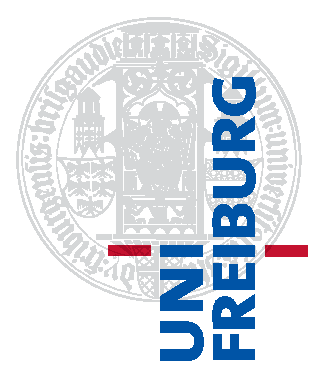
\includegraphics[width=0.5\linewidth]{logos/Uni_Logo-Grundversion_E1_A4_CMYK.eps}\\[4ex]
            {\huge \bfseries  \@title }\\[2ex] 
            {\LARGE  \@author}\\[30ex] 
            {\large \@date}
        \end{center}
    \end{titlepage}
\makeatother
\thispagestyle{empty}
\newpage



\tableofcontents

\begin{acronym}
\section*{Abbreviations}
\acro{bte}[BTE]{Boltzmann Transport Equation}
\acro{ci}[CI]{Continuous Integration}
\acro{lbm}[LBM]{Lattice Boltzmann Method}
\acro{simd}[SIMD]{Single Instruction Multiple Data}
\acro{mpi}[MPI]{Message Passing Interface}
\end{acronym}
\mainmatter

\chapter{Introduction}
The \acf{lbm} is a numerical, parallelizable and efficient scheme for simulating fluid flows based on the discretization of (continuous) \acf{bte}.\cite{McNamara.1988} In addition, the \ac{lbm} can be extended with boundary conditions. The key property of the \ac{lbm} is that it is a discrete kinetic theory approach featuring a mescoscale description of the microstructure of the fluid instead of discretizing macroscopic continuum equations. Other key advantages of the \ac{lbm} include: efficient implementation by parallelization and the \ac{lbm} can be applied to different kind of lattices.

We show in several two-dimensional (i.e. planar) test cases, i.e. \textit{Couette flow}, \textit{Poiseuille flow} and \textit{Von K\'{a}rm\'{a}n's vortex street}, the correctness of our implementation as well as the significant reduction of computational time of the von K\'{a}rm\'{a}n's vortex street simulation by means of parallelization by spatial domain decomposition using \textit{Python} as programming language with its highly efficient \textit{numpy} library \cite{Oliphant.2006,vanderWalt.2011} and the \acf{mpi} \cite{Dalcin.2005, Dalcin.2008, Dalcin.2011}.

All code is available at \url{https://github.com/infomon/lattice_boltzmann_parallel_solver} under BSD license. We give the instructions how to reproduce the results of the experiments conducted in this report in the \textit{README}.

\section*{Structure of report}
The remainder of the report is organized as follows:
\begin{itemize}
\item \textbf{Chapter \ref{ch-method}} describes the \ac{lbm}. More specifically, we describe how we discretize the \textit{\acf{bte}} resulting in the \ac{lbm}. We also show how macroscopic quantities, e.g. density and velocity, can be calculated from the microscopic simulation. In addition, we describe several boundary conditions that can be applied in the \ac{lbm}.
\item \textbf{Chapter \ref{ch-implementation}} describes how the \ac{lbm} is implemented using \textit{Python} as programming language. We also show how we parallelized the implementation and how we ensured software quality by unit testing.
\item \textbf{Chapter \ref{ch-results}} conducts extensive experiments showing the applicability and correctness of the implementation of the solver for the \ac{lbm}. 
\item \textbf{Chapter \ref{ch-conclusion}} concludes this report.
\end{itemize}
\chapter{Lattice Boltzmann Method}\label{ch-method}
\section{Overview}
In this chapter we describe the \acf{lbm}. The main idea of the \ac{lbm} is to \textit{simulate a fluid density statistically on a lattice} instead of solving (and also discretizing) the Navier-Stokes equations.
\section{Boltzmann Transport Equation}\label{sec-bte}
The \acf{bte} $\frac{df}{dt}$ defines the fundamental differential equation of kinematic gas theory. It describes the evolution of the probability density function $f_(\mathbf{r},\mathbf{v},t)$ for finding a molecule with mass $m$ and velocity $\mathbf{v}$ at position $\mathbf{r}$ over time $t$. Huang \cite{Huang.1987} shows that the \ac{bte} relaxes to the Maxwell velociy distribution function. Bhatnagar et al. \cite{Bhatnagar.1954} approximate the relaxation of $f$ towards $f^{eq}$ as follows:
\begin{equation}
\label{eq-bte}
\frac{df(\mathbf{r},\mathbf{v},t)}{dt}=-\frac{f(\mathbf{r},\mathbf{v},t)-f^{eq}(\mathbf{v};\rho(\mathbf{r,t}),\mathbf{u}(\mathbf{r},t),T(\mathbf{x},t))}{\tau}
\end{equation}
where $\tau$ is the so-called characteristic time, $\rho$ is the mass density, $u$ is the average velocity at position $\mathbf{x}$ and $T$ is the temperature (see section \ref{sec-momentUpdate} for more details). The characteristic time determines how fast the fluid converges towards the equilibrium depending on the viscosity of the fluid. The higher the viscosity, the slower it converges towards the equilibrium. Note, that eq. \ref{eq-bte} satisfies the Navier-Stokes equations.
\subsection*{Discretization of the \ac{bte}}
The \ac{bte} of eq. \ref{eq-bte} is defined in the continuous domain. In order to work with the \ac{bte} on the computer we have to discretize it in space, velocity and time. The space discretization can be done by just using a discrete lattice (e.g. two-dimensional array). To discretize the velocity and time we have to impose that the velocity multiplied with the time is equal to some integer, i.e. the particle can only travel on the given lattice and not in-between lattice nodes. 

We discretize the velocity directions with the D2Q9 scheme (see fig. \ref{fig:mesh}), which is two-dimensional and consists of nine discrete velocity directions. The velocity directions point to each of its neighbors in the Moore neighborhood. Note, that at the central lattice node the particle is at rest. We define the velocity vectors as follows:
\begin{equation}
\mathbf{c_i}=\begin{pmatrix}
0 & 1 & 0 & -1 & 0 & 1 & -1 & -1 & 1\\
0 & 0 & 1 & 0 & -1 & 1 & 1 & -1 & -1
\end{pmatrix}.
\end{equation}
Therefore, we discretize the probability density function $f(\mathbf{r},\mathbf{v},t)$ to obtain the discrete probability density function $f_{i}(\mathbf{x},t)$, where the subscript $i$ indicates the direction and $\mathbf{x}$ is the discrete lattice.
\begin{figure}
  \begin{center}
   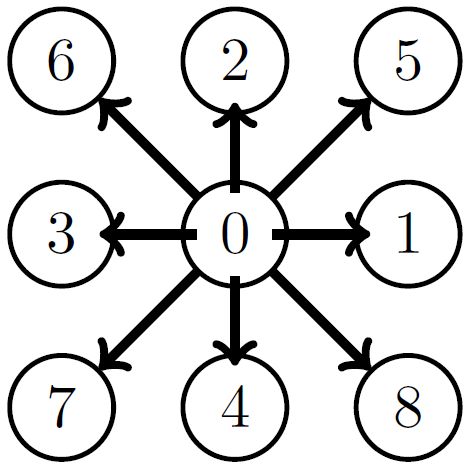
\includegraphics[width=.3\textwidth]{../figures/lbm/d2q9.png}
   \caption{Discretization of the velocity space into nine discrete directions (D2Q9). The numbers $0,...,9$ uniquely identify the direction.}
  \label{fig:mesh}
  \end{center}
\end{figure}

Finally, we get the discretized version of eq. \ref{eq-bte}:
\begin{equation}
\label{eq-discretizedBTE}
\underbrace{f_{i}(\mathbf{x}+\mathbf{c}_{i}\Delta t, t+\Delta t) - f_{i}(\mathbf{x})}_{streaming}
=\underbrace{-\omega(f_{i}(\mathbf{x})-f_{i}^{eq}(\mathbf{x},t))}_{collision},
\end{equation}
where the \textit{streaming} and \textit{collision process} are the key steps in the \ac{lbm} and $\omega=\frac{\Delta t}{\tau}$ is a relaxation parameter.

The equilibrium probability density function $f_{i}^{eq}$ can be computed as follows:
\begin{equation}
\label{eq-equilibrium}
f_{i}^{eq}=w_{i}\rho(x,t)(1+3\mathbf{c}_{i}\mathbf{u}(\mathbf{x},t)+\frac{9}{2}(\mathbf{c}_{i}\mathbf{u}(\mathbf{x},t))^{2}-\frac{3}{2}\mathbf{u}^{2}(\mathbf{x},t)),
\end{equation}
where $w_{i}=
\begin{cases}
\frac{4}{9}, ~if~i=0\\
\frac{1}{9}, ~if~i=1,2,3,4\\
\frac{1}{36}, ~if~i=5,6,7,8
\end{cases}$. Fig. \ref{fig:streamingCollisionVis} gives an example for eq. \ref{eq-discretizedBTE} for a single node. In the streaming step, the node receives direction-specific probability density function values $f_{i}(\mathbf{x},t)$ from its nine neighbors. In the collision step, we relax the new probability density function values $f_{i}(\mathbf{x},t\Delta t)$ towards the equilibrium probability density function $f^{eq}_{i}$ and thereby take into account collisions between particles.
\begin{figure}
  \begin{center}
   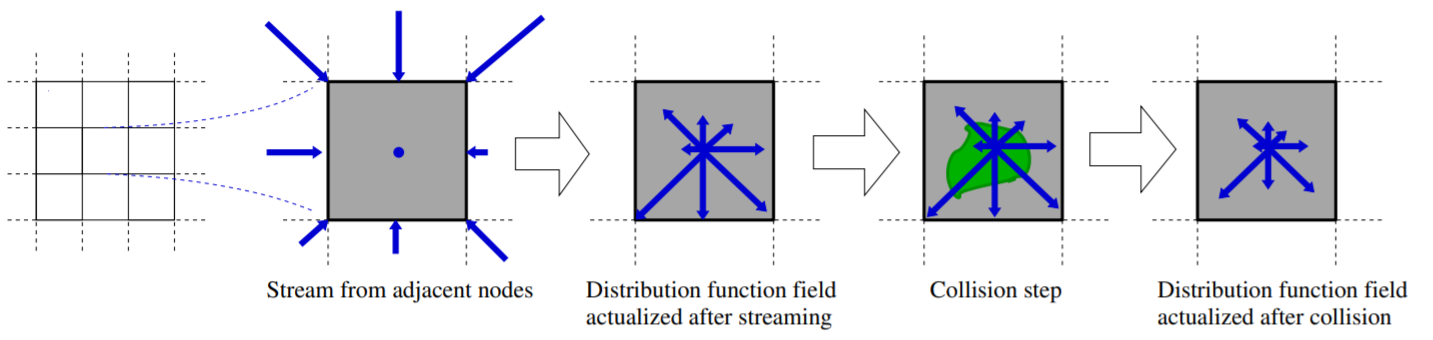
\includegraphics[width=\textwidth]{../figures/lbm/vis.png}
   \caption{Visualization of the streaming and collision step. The arrows' length represent the normalized values of the distribution function for every discrete direction. Figure from \cite{Boix.2013}.}
  \label{fig:streamingCollisionVis}
  \end{center}
\end{figure}
\section{Moment update}\label{sec-momentUpdate}
In the \ac{lbm}, the density $\rho$ and velocity $\mathbf{u}$ are defined by the zeroth and first moments of the probability distribution function $f$, respectively:
\begin{align} 
\rho(\mathbf{x},t) &=  \int f(\mathbf{x}, \mathbf{u},t)~d^{3}\mathbf{u}, \\ 
\mathbf{u}(\mathbf{x},t) &=  \frac{1}{\rho(\mathbf{x})}\int f(\mathbf{x}, \mathbf{u},t)\cdot\mathbf{c}(\mathbf{u})~d^{3}\mathbf{u}.
\end{align}
The discretization of those equations yields
\begin{align}
\label{eq-density}
\rho(\mathbf{x}) &=  \sum\limits_{i} f_{i}, \\ 
\label{eq-velocity}
\mathbf{u}(\mathbf{x}) &=  \sum\limits_{i} f_{i}\mathbf{c}_{i}.
\end{align}
\section{Boundary conditions}\label{sec-boundaryConditions}
The boundary condition describes how the fluid flow behaves during streaming at the boundaries. We define the boundary node $\mathbf{x}_{b}$ to have at least one link to a solid or fluid node. 
Note, that the boundary conditions have to be placed in the correct step inside the \ac{lbm} (see code listing \ref{algo-pseudeocode}). For this reason we differentiate between the \textit{pre-streaming} probability density function $f_{i}^{\ast}$ and the \textit{post-streaming} probability density function $f_{i}$.
To apply boundary conditions the probability density function after the streaming $f_i$ is modified at each boundary node $\mathbf{x}_{b}$ given the pre-streaming probability density function $f_{i}^{\ast}$ in each time step:
\begin{equation}
f_i(\mathbf{x}_{b}+c_{i}\Delta t, t+\Delta t)=f_{i}^{\ast}(\mathbf{x}_b,t).
\end{equation}

One question that arises is where the boundary nodes $\mathbf{x}_b$ are defined. We distinguish between so called \textit{wet nodes} and \textit{dry nodes} due to different domains, i.e. computational and physical domain. In the former, the computation and physical domain is the same (i.e. the boundaries are placed on the lattice nodes) but this comes with a increased difficulty for the implementation. In the latter the physical domain is half a cell away from the computational domain (i.e. the boundaries are located between the lattice nodes) retaining second order accuracy as long as the boundary is placed exactly in the middle of the lattice nodes.

Below we describe several boundary conditions. One key advantage of the \ac{lbm} is its easy implementation of boundary conditions and in particular the arbitrary combination of boundary conditions as long as they do not contradict themselves.
\subsection*{Periodic boundary conditions}
For a periodic boundary condition the flow leaving a boundary re-enters the domain on the opposite side of the domain
\begin{equation}
f_{i}(\mathbf{x}_{1},t)=f_{i}(\mathbf{x}_{N},t),
\end{equation}
where $\mathbf{x}_{1}$ and $\mathbf{x}_{N}$ are the first and last node in the physical domain, respectively. Visually, we can imagine the bounce-back boundary conditions as if we have a cylindrical shape. Note, that therefore periodic boundary conditions conserve mass and momentum.
The periodic boundary condition is implicitly implemented by the streaming function.
\subsection*{Periodic boundary conditions with pressure variation}
The periodic boundary conditions with pressure variation add a density drop $\Delta\rho$ (or pressure drop $\Delta p$) between inlet and outlet. Note, that the pressure and density are related through the ideal gas of state $p=c_{s}^2\rho$, where $c_{s}$ is the speed of sound. \cite{CLAPEYRON.}
Let's assume that we want to model a pressure drop in x-direction, then it holds $\forall y\in\lbrace 1,...,l_{y}\rbrace$ that $p(x_{1},y,t)=p(x_{N},y,t)+\Delta\rho$, where $l_{y}$ denotes the diameter in y-direction and $x_1$ and $x_{N}$ denote the left-most and right-most node in the \ac{lbm}, respectively. Thus, we get $\rho_{out}=\frac{p_{out}}{c_{s}^2}$ and $\rho_{in}=\frac{p_{out}+\Delta p}{c_{s}^2}$, where the subscripts $in$ and $out$ denote the pressure values at the periodic boundaries.
Note, that the velocity is the same at the periodic boundaries: $\mathbf{u}(x_{1},y,t)=\mathbf{u}(x_{N},y,t)$.

Let's now assume virtual nodes $\mathbf{x}_{0}$ and $\mathbf{x}_{N+1}$ at both ends of the periodic boundaries. Note, that the virtual nodes $\mathbf{x}_{0}$ and $\mathbf{x}_{N}$ correspond to $\mathbf{x}_{N}$ and $\mathbf{x}_{1}$, respectively. Visually we can imagine this like (infinitely) many pipes connected to each other. We decompose the probability density function into a equilibrium part $f_{i}^{eq}$ and non-equilibrium part $f_{i}^{neq}$. The non-equilibrium probability density function is computed by $f_{i}^{neq}=f_{i}-f_{i}^{eq}$. Combining the correspondences of virtual nodes and nodes in the physical domain as well as the decomposition into (non)-equilibrium probability density function parts we obtain the inlet and outlet boundary condition, respectively:
\begin{align}
f_{i}^{\ast}(x_0,y,t)&=f_{i}^{eq}(\rho_{in},\mathbf{u_N})+\underbrace{(f_{i}^{\ast}(x_N,y,t)-f_{i}^{eq}(x_N,y,t)}_{f_i^{neq}(x_N,y,t)},~and\\
f_{i}^{\ast}(x_{N+1},y,t)&=f_{i}^{eq}(\rho_{out},\mathbf{u_1})+\underbrace{(f_{i}^{\ast}(x_1,y,t)-f_{i}^{eq}(x_1,y,t)}_{f_i^{neq}(x_1,y,t)}.
\end{align}
\subsection*{Bounce-back boundary}
The bounce-back boundary condition applies a no-slip condition at the boundary. It simulates the interaction between the fluid with a non-moving wall without slip. It can also be applied to a stationary obstacle such as a plate.
\begin{equation}
f_{\bar{i}}(\mathbf{x}_{b},t+\Delta t)=f_{i}^{\ast}(\mathbf{x}_{b},t),
\end{equation}
where the index $\bar{i}$ denotes the conjugate channel of $i$, e.g. the conjugate channel of $1$ is equal to $3$.
\subsection*{Moving wall}
The moving wall extends the bounce-back boundary condition by taking into account the gain or lose of momentum of particles during interaction with the moving wall. Thus, we extend the bounce-back boundary condition with an extra term for the momentum change
\begin{equation}
f_{\bar{i}}(\mathbf{x}_{b},t+\Delta t)=f_{i}^{\ast}(\mathbf{x}_{b},t)-2\omega_{i}\rho_{w}\frac{\mathbf{c}_{i}\cdot\mathbf{u}_{w}}{c_{s}^{2}},
\end{equation}
where $c_{s}$ is the speed of sound, $\rho_{w}$ and $\mathbf{u}_{w}$ are the density and velocity at the wall, respectively. The velocity at the wall $\mathbf{u}_{w}$ is equal to $\begin{pmatrix}U_{w}\\0\end{pmatrix}$ for a tangentially moving wall in x-direction with wall velocity $U_{w}$.  
There are two main options for the estimation of the density at the wall $\rho_{w}$:
\begin{enumerate}
\item The density at the wall $\rho_{w}$ is equal to the \textit{average} density $\bar{\rho}$.
\item The density at the wall $\rho_{w}$ is \textit{extrapolated} from the densities $\rho$ next to the wall. Depending on the order of the extrapolation, we use more or less nodes.
\end{enumerate}
\subsection*{Open boundary}
\cite{Kruger.2016} describe open boundaries consist of inlets and outlets where the flow can either enter or leave the computation domain and where we typically \textit{impose velocity or density profiles}. We implement the inlet as follows:
\begin{equation}
f_{i}(\mathbf{x}_{b},t+\Delta t)=f_{i}^{eq}(\rho_{in},\mathbf{u}_{in})~\forall i\in\lbrace 0,...,8\rbrace,
\end{equation}
where $\rho_{in}$ and $\mathbf{u}_{in}$ are the density and velocity at the inlet, respectively.

For the outlet, we implement a first-order extrapolation scheme by using the information from the second last node $\mathbf{x}_{b_{2}}=\mathbf{x}_{b}-\Delta\mathbf{x}$
\begin{equation}
f_{i}(\mathbf{x}_{b},t+\Delta t)=f_{i}(\mathbf{x}_{b_{2}},t),
\end{equation}
where $i$ denotes the indices pointing into the domain.
\chapter{Implementation}\label{ch-implementation}
In this chapter we will describe how we implement the algorithm using \textit{Python} as programming language.
\section{Overview}
Code listing \ref{algo-pseudeocode} shows the pseudocode of the iteration loop of the \ac{lbm}. As input we can specify the geometry of the physical domain, the boundary conditions (see section \ref{sec-boundaryConditions} for more details) as well as the initial conditions. 

First we initialize the density $\rho$ and velocity $\mathbf{u}$ and compute the initial value of the probability density function $f_{i}^{eq}=f_{i}$. 

Then we iterate in a loop over several steps as long as the stopping criterion (e.g. maximum time steps) is not satisfied. Note, that there is some flexibility when to apply which step. \cite{Kruger.2016, Succi.2018} The following order of steps corresponds to the order in the implementation of the \ac{lbm}. We first compute the equilibrium function $f_{i}^{eq}$ given the current density $\rho$ and velocity $\mathbf{u}$. In the collision step we simulate the effects of collisions between particles (see section \ref{sec-bte} for more details). After that, we simulate the streaming of $f_i$, i.e. we simulate the movement of particles to the nearest neighbour lattice nodes using the D2Q9 discretization. Then we apply potential boundary conditions on the probability density function $f_i$. Note, that we first apply the streaming operation at every node (including the boundary nodes $\mathbf{x}_{b}$) and then correct the boundary nodes $\mathbf{x}_{f}$ after the streaming. This has the advantage that the implementation of the streaming is easier. Lastly, we compute the density $\rho$ and velocity $\mathbf{u}$ (see section \ref{sec-momentUpdate} for details on the formulas on how to compute the macroscopic quantities).

After running the \ac{lbm} we can obtain the density $\rho$ and velocity $\mathbf{u}$ as macroscopic quantities.

\begin{algorithm}
 \caption{\label{algo-pseudeocode}Pseudocode of the iteration loop of the \ac{lbm}.}
     \SetAlgoLined
     \KwInput{Geometry and parameters $l$, $h$, $U$, $\nu$,...; boundary conditions; initial conditions}
     \KwOutput{Final density $\rho$ and velocity $\mathbf{u}$}
     initialize $\rho$ and $\mathbf{u}$ \\
     compute $f_i$ and $f_i^{eq}$ \\
     \While{stopping criterion is not satisfied}{
      compute equilibrium function $\rho,~\mathbf{u}\rightarrow f_{i}^{eq}$\Comment*[f]{eq. \ref{eq-equilibrium}}\\
      collision step $f_{i}^{\ast}=f_{i}(\mathbf{x},t)-\frac{\Delta t}{\tau}(f_{i}(\mathbf{x},t)-f_{i}^{eq}(\mathbf{x},t))$ \Comment*[f]{eq. \ref{eq-discretizedBTE}}\\
      streaming $f_{i}(\mathbf{x}+c_{i}\Delta t, t+\Delta t)=f_{i}^{\ast}(\mathbf{x},t)$ \Comment*[f]{eq. \ref{eq-discretizedBTE}}\\
      apply boundary conditions $f_i(\mathbf{x}_{b}+c_{i}\Delta t, t+\Delta t)=f_{i}^{\ast}(\mathbf{x}_b,t)$ \Comment*[f]{section \ref{sec-boundaryConditions}}\\
      moment update $f_i \rightarrow \rho,~\mathbf{u}$ \Comment*[f]{eq. \ref{eq-density} \& \ref{eq-velocity}}
     }
\end{algorithm}
\section{Basic implementation in Python}
In this section we show how we implemented the basic equations and data structures introduced in chapter \ref{ch-method}. We use Python as programming language and use the python libraries \textit{numpy} \cite{Oliphant.2006,vanderWalt.2011} for array operations, \textit{scipy} \cite{Virtanen.2020} for some more complex scientific computations and \textit{matplotlib} \cite{Hunter.2007} for visualizing the obtained results. And key advantage of numpy is to vectorize arrays, which lowers the computational time.

We represent the (discrete) probability density function $f_{i}(\mathbf{x})$ as a numpy array of size $l_{x}\times l_{y}\times 9$, where $l_{x}$ and $l_{y}$ are the size of the lattice in x- and y-direction, respectively. The last dimension (e.g. $9$) of the numpy array corresponds to the discretized velocity direction.
We represent the velocity directions $\mathbf{c}$ and the weights $w_{i}$ as numpy arrays with size $9\times 2$ and $9$, respectively.

In steps 4 and 5 of code listing \ref{algo-pseudeocode} we simulate the collision part of eq. \ref{eq-discretizedBTE}. We implement the computation of the equilibrium probability density function $f_{i}^{eq}$ of eq. \ref{eq-equilibrium} and the right-hand side of eq. \ref{eq-discretizedBTE} with vectorized numpy code. 

Code listing \ref{algo-collision} shows the implementation of the collision step, separated into equilibrium probability density function computation and the collision.
\begin{algorithm}
 \caption{\label{algo-collision}Python implementation of the collision step. Note that the symbol $@$ is a shorthand for the matrix multiplication in NumPy.}
     \SetAlgoLined
     \KwInput{density $\rho$; velocity $\mathbf{u}$, relaxation parameter omega $\omega$}
     \KwOutput{Probability density function before streaming $f_{i}^{\ast}$}
     w\textunderscore i = np.array([4/9, 1/9, 1/9, 1/9, 1/9, 1/36, 1/36, 1/36, 1/36])\\
     \SetKwFunction{FEq}{f\textunderscore eq}
\Fn{\FEq{rho:np.ndarray, u:np.ndarray}$\rightarrow$np.ndarray}{
w\textunderscore i = w\textunderscore i[np.newaxis, np.newaxis, ...]\\
		ci\textunderscore u = u @ c\textunderscore i.T\\
		uu = (np.linalg.norm(u, axis=-1) ** 2)[..., np.newaxis]\\
		rho = rho[..., np.newaxis]\\
        \KwRet w\textunderscore i * rho * 
        (1 +
            3 * ci\textunderscore u +
            9/2 * ci\textunderscore u ** 2 -
            3/2 * uu)
  }
  f\textunderscore pre = f + (f\textunderscore eq(rho, u) - f) * omega
\end{algorithm}

In steps 6 of code listing \ref{algo-pseudeocode} we simulate the streaming part of eq. \ref{eq-discretizedBTE}. Code listing \ref{algo-streaming} shows the implementation using \textit{np.roll}.  The function rolls the the data in the direction specified by the \textit{axis} argument. With the argument $shift$ we specify the number of places elements are shifted according to the discrete velocity directions $\mathbf{c}$. Note, that the function automatically implements the periodic boundary condition.
\begin{algorithm}
 \caption{\label{algo-streaming}Python implementation of the streaming step.}
     \SetAlgoLined
     \KwInput{Probability density function before streaming $f_{i}^{\ast}$}
     \KwOutput{Probability density function after streaming $f_{i}$}
     c\textunderscore i = np.array([[0,0],[1,0],[0,1],[-1,0],[0,-1],[1,1],[-1,1],[-1,-1],[1,-1]])\\
     \SetKwFunction{FStream}{streaming}
\Fn{\FStream{f\textunderscore pre:np.ndarray}$\rightarrow$np.ndarray}{
f\textunderscore post = np.zeros\textunderscore like(f\textunderscore pre)\\
\For{$i$ \KwTo\Range $(9)$}{
f\textunderscore post[..., i]=np.roll(f\textunderscore pre[...,i], shift=c\textunderscore i[i], axis=(0,1))
}
\KwRet f\textunderscore post
}
\end{algorithm}

For the other boundary conditions we implement additional functions which correct the boundary nodes as described in section \ref{sec-boundaryConditions}. Code listing \ref{algo-boundaryConditions} gives an overview of the different implementations.
The implementation of the boundary conditions follows directly from the formulas. For example when we implement the bounce-back boundary condition on a non-moving wall at the bottom, we bounce back channels $4$, $7$ and $8$. That is, we assign the pre-streaming probability density function at the boundary nodes $f_{i}^{\ast}(\mathbf{x}_{b},t)$ to the conjugate channels (e.g. $2$, $5$, $6$) of the post-streaming probability density function at the boundary nodes $f_{i}(\mathbf{x}_{b},t+\Delta t)$. 
For the implementation of the bounce-back condition for a object inside the domain such as a vertical plate we apply the bounce-back conditions on the corresponding two columns. We have to take corner nodes into special consideration. There we just bounce-back two channels. For example consider the lattice node at the top corner on the left side of the plate. There we only bounce back channels $1$ and $8$.
We implement the moving wall boundary condition in a similar way but with the additional term $-2\omega_{i}\rho_{w}\frac{\mathbf{c}_{i}\cdot \mathbf{u}_{w}}{c_{s}^{2}}$ to take the momentum change into account. For the density at the wall $\rho_{w}$ we use the average density.
For the inlet boundary condition we assign the equilibrium probability density function given the inlet density $\rho_{in}$ and inlet velocity $\mathbf{u}_{in}$. 
For the outlet boundary condition we assign the second last nodes of the probability density function of the previous time step to the last nodes of the probability density function of the current time step.
For the periodic boundary conditions with pressure variation we extend the domain with virtual nodes at both ends of the periodic boundaries. The implementation then is straightforward. 
\begin{algorithm}
 \caption{\label{algo-boundaryConditions}Exemplar Python implementation of the boundary condition. Note that the index i refers to specific channels depending on the boundary conditions. For details see section \ref{sec-boundaryConditions}. Note that $@$ and $.T$ are shorthands for matrix multiplication and transpose in NumPy.}
     \SetAlgoLined
     \# Bounce-back\\
     f\textunderscore post[$\mathbf{x}$\textunderscore b, conjugate[i]]=f\textunderscore pre[$\mathbf{x}$\textunderscore b,i] \\
     \# Moving wall\\
          f\textunderscore post[$\mathbf{x}$\textunderscore b, conjugate[i]]=f\textunderscore pre[$\mathbf{x}$\textunderscore b,i] - 2$\cdot$ w\textunderscore i[i]$\cdot$ avg\textunderscore rho $\cdot$ (c\textunderscore i[i] @ u\textunderscore w) /(c\textunderscore s **2) \\
          \# Inlet\\
     f\textunderscore post[0,:, i]=f\textunderscore eq(rho\textunderscore in,u\textunderscore in)[0,:,i]\\
     \# Outlet\\
     f\textunderscore post[-1,:, i]=f\textunderscore previous[-2,:,i]\\
     \# Periodic boundary condition with pressure variation\\
  f\textunderscore pre[0,:,i]=f\textunderscore eq(rho\textunderscore in, u[-2,...])[...,i].T + (f\textunderscore pre[-2,:,i]-f\textunderscore eq(rho, u)[-2,:,i])
\end{algorithm}
\section{Parallelization}\label{sec-parallelization}
We parallelize the \ac{lbm} using spatial domain decomposition and \acf{mpi} \cite{Dalcin.2005, Dalcin.2008, Dalcin.2011}. \ac{mpi} is a \textit{communication protocol} for programming parallel computers, i.e. \ac{simd} \cite{Flynn.1972} by executing the same operation on multiple data points simultaneously.

We decompose the computational domain into sub domain using a cartesian topology. To implement this we use the \ac{mpi} function \textsf{Create\textunderscore cart} creating a cartesian topology.
We decompose the full computational domain into sub domains of roughly equal size (see fig. \ref{fig:parallelizationScheme} for an example).
If the domain is not exactly divisible into the subdomains we extend the rightmost or topmost process with the division remainder. Note that this could lead to imbalanced subdomains, but comes with an easier transformation from global coordinates into local (i.e. process-level) coordinates. For the communication we extend the sub domains with ghost cells around the actual computational domain.

The collision step of the \ac{lbm} is embarrassingly parallel, since the collision step operates only locally and thus requires no communication between processes.

For the streaming step we have to consider particles moving from one domain to a neighboring domain (i.e. another process) corresponding the the channel. We implement this by extending each domain by \textit{ghost cells} around the actual computational domain. Before streaming we communicate the lattice nodes adjacent to the ghost region into the ghost points of the neighboring domain according to the specific channel. 

\begin{figure}
  \begin{center}
  \subfigure[Communication in x direction.]{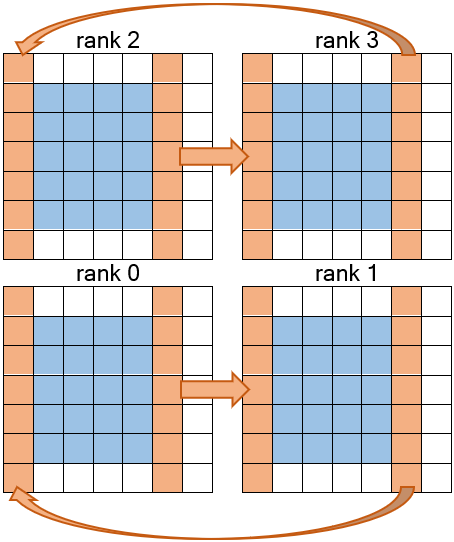
\includegraphics[width=0.4\textwidth]{../figures/parallelization_strategy/parallelization_scheme_x.png}}
\rulesep
    \subfigure[Communication in y direction.]{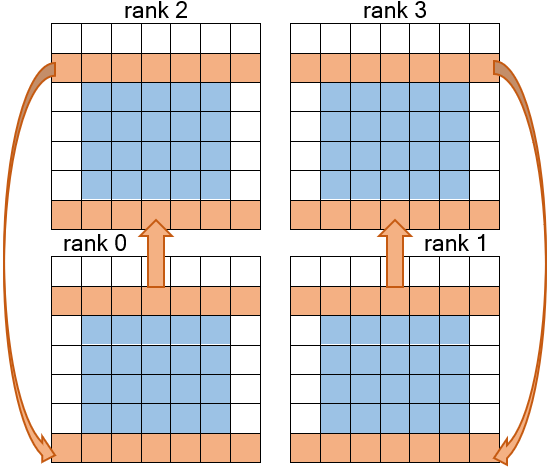
\includegraphics[width=0.5\textwidth]{../figures/parallelization_strategy/parallelization_scheme_y.png}}
   \caption{Example of spatial domain decomposition and communication strategy. We decompose the original domain into a $2\times 2$ grid of sub domains of roughly equal size (blue lattice points). We add additional ghost nodes around the actual computational domain (white lattice points). In the communication step, we communicate the rightmost, leftmost, bottommost and topmost lattice points in the actual computational domain into the neighboring ghost lattice points. In the left subfigure (a) we show the communication step in the right direction, i.e. respective  right neighbors except for the edge domains. In the right subfigure (b) we show the communication step in the top direction.}
  \label{fig:parallelizationScheme}
  \end{center}
\end{figure}
Let's consider the example of fig. \ref{fig:parallelizationScheme}. We consider a $2\times 2$ decomposition of the original computational domain and we denote the lower left subdomain with rank $0$, upper left with rank $1$, lower right with rank $2$ and upper right with rank $3$. W.l.o.g., we first consider the rightmost nodes $\mathbf{x}_r$ of each sub domain. We communicate the rightmost nodes $\mathbf{x}_r$ from each process to the neighboring process on the right. In our particular example this means that we communicate the rightmost nodes $\mathbf{x}_r$ of the process with rank $0$ to the ghost cells on the left side of process with rank $1$. Accordingly, we communicate from process $2$ to process $3$, $2$ to $1$ and $3$ to $1$. Note that we do communicate from process $2$ to $0$ and $3$ to $1$ or more generally we do communicate outer boundaries of edge domains, since we set \textsf{periods=(True, True)} when calling the \ac{mpi} function \textsf{Create\textunderscore cart}.\footnote{Note, that we could set \textsf{periods=(False, True)} for the von K\'{a}rm\'{a}n's vortex street experiment, since we set the inlet and outlet boundary nodes in every time step. However, for sake of generality we set \textsf{periods=(True, True)}.} This implicitly implements the periodic boundary conditions.
We repeat this procedure for the leftmost nodes $\mathbf{x}_l$, bottommost nodes $\mathbf{x}_b$ and topmost nodes $\mathbf{x}_t$ (see right subfigure of fig. \ref{fig:parallelizationScheme}) accordingly. This totals in four communication steps. Code listing \ref{algo-communication} shows the implementation of the communication step. We call the communication step right before the streaming step in code listing \ref{algo-pseudeocode}.
\begin{algorithm}
 \caption{\label{algo-communication}Python implementation of the communication step.}
     \SetAlgoLined
     \SetKwFunction{OuterComm}{communication}
\textbf{from} mpi4py \textbf{import} MPI\\
\textbf{from} typing \textbf{import} Callable\\
\Fn{\OuterComm{comm: MPI.Intracomm}$\rightarrow$Callable[[np.ndarray], np.ndarray]}{
    left\textunderscore src, left\textunderscore dst = comm.Shift(direction=0, disp=-1)\\
    right\textunderscore src, right\textunderscore dst = comm.Shift(direction=0, disp=1)\\
    bottom\textunderscore src, bottom\textunderscore dst = comm.Shift(direction=1, disp=-1)\\
    top\textunderscore src, top\textunderscore dst = comm.Shift(direction=1, disp=1)\\
    
    	\SetKwFunction{InnerComm}{communicate}
	\Fn{\InnerComm{f: np.ndarray}$\rightarrow$np.ndarray}{
	        \# send to left\\
        recvbuf = f[-1, ...].copy()\\
        comm.Sendrecv(f[1, ...].copy(), left\textunderscore dst, recvbuf=recvbuf, source=left\textunderscore src)\\
        f[-1, ...] = recvbuf\\
        \# send to right\\
        recvbuf = f[0, ...].copy()\\
        comm.Sendrecv(f[-2, ...].copy(), right\textunderscore dst, recvbuf=recvbuf, source=right\textunderscore src)\\
        f[0, ...] = recvbuf\\
        \# send to bottom\\
        recvbuf = f[:, -1, :].copy()\\
        comm.Sendrecv(f[:, 1, :].copy(), bottom\textunderscore dst, recvbuf=recvbuf, source=bottom\textunderscore src)\\
        f[:, -1, :] = recvbuf\\
        \# send to top\\
        recvbuf = f[:, 0, :].copy()\\
        comm.Sendrecv(f[:, -2, :].copy(), top\textunderscore dst, recvbuf=recvbuf, source=top\textunderscore src)\\
        f[:, 0, :] = recvbuf\\
        \KwRet f

}
    \KwRet \InnerComm
    }

\end{algorithm}

In the boundary conditions we transform global coordinates $global\textunderscore coord$ into local (i.e. process-level) coordinates $local\textunderscore coord$ in order to apply the boundary conditions at the correct global position in the lattice grid. Since we only increase the size of sub domains on the right or top, we can compute local coordinates straightforward. From the \ac{mpi} function \textsf{Get\textunderscore coords} we get the process coordinates $proc\textunderscore coord$ of the cartesian topology. We compute the local $x$ coordinate $local\textunderscore coord_{x}$ as follows:
\begin{equation}
local\textunderscore coord_{x}=global\textunderscore coord_{x}-proc\textunderscore coord_{x}*(l_{x}//proc\textunderscore size_{x}) +1,
\end{equation}
where $l_{x}$ is the lattice grid size in $x$ direction and $//$ denotes the integer division. Note, that we add $1$, since we have to take the ghost cell in the specific process into account. We can apply computation similarly for the local $x$ coordinate $local\textunderscore coord_{y}$.
\section{Software quality}
\subsection*{Static typing}
Python is a dynamically typed language. That is that the Python interpreter does type checking only in runtime and the type of a variable is allowed to change. The opposite of dynamic typing is static typing. It is introduced by \textit{PEP 484}\footnote{\url{https://www.python.org/dev/peps/pep-0484/}} in Python. In static typing, the types of the variables are checked before runtime and the change of types is generally not allowed. Note, as an exception type casting is a way to change the type of a variable in many languages.

Dynamic typing allows for rapid prototyping and thus it enables fast software development. On the other side static typing can help to catch errors due to type errors, document the code and help to build a cleaner software architecture. The last point in particular ensures that the programmer thinks about the types of the variables and uses the correct types. Thus, in any larger project typing is critical to build and maintain clean code.
\subsection*{Unit testing}
One key component of every software project is extensive testing of the software. To this end, we implement several unit tests in order to validate the expected behavior of the implemented functions. 
More specifically, we test the computation of the density and velocity, the streaming function, mass preservation (i.e. first and second mass conservation equation and first and second impulse conservation equation from the Navier-Stokes Equations as well as a long run mass conservation test over $10000$ time steps) and the boundary conditions.
Additionally, we validate the parallelized implementation by comparing it to the serial implementation of the von K\'{a}rm\'{a}n's vortex street over $400$ time steps using different number of nodes. 

We integrate the unit tests into \ac{ci} using \textit{Travis CI} as build server so that the implementation and its potential unintentional modifications are validated for each commit to the repository.
\chapter{Numerical results}\label{ch-results}
To demonstrate the \ac{lbm} implementation we conduct several experiments with different combinations of boundary conditions. First we consider a \textit{shear wave decay} (section \ref{sec-shearWave}) to validate whether our implementation preserves mass as well as to show how $\omega$ relates to the kinematic viscosity $\nu$. In sections \ref{sec-Couette} and \ref{sec-pouseuille} we implement well known laminar flows, i.e. \textit{Couette} and \textit{pouiseuille} flow, from the literature and compare it to their analytical solutions, respectively. In section \ref{sec-karman} we implement the \textit{von K\'{a}rm\'{a}n's vortex street} and in the following section \ref{sec-scaling} how we can reduce computational complexity by spatial domain decomposition as introduced in section \ref{sec-parallelization}.
\section{Shear wave decay}\label{sec-shearWave}
The shear wave decay simulates a physical domain with only periodic boundary conditions which is in a initial state and its incremental steps towards the equilibrium state. One common practical and illustrative application of it, is the simulation of the breaking of a water dam. This exemplar application also shows the importance of simulations as the \ac{lbm} to simulate rather than applying it in a real-world setting potentially causing mass destruction and high costs.

We choose the following simulation parameters for our experiments:
\begin{itemize}
\setlength\itemsep{0.15em}
\item lattice grid shape $=50\times 50$
\item relaxation parameter $\omega=1.0$
\item Sinusoidal density in x-direction $\rho(\mathbf{x},0)=\rho_{0}+\epsilon_{\rho}\sin(\frac{2\pi x}{l_x})$
\begin{itemize}
\setlength\itemsep{0.1em}
\item Shift of density in y-direction $\rho_{0}(\mathbf{x})=0.5$
\item amplitude $\epsilon_{\rho}=0.08$
\item initial velocity $\mathbf{u}_{initial}(\mathbf{x})=0.0$
\end{itemize}
\item Sinusoidal velocity in y-direction $\mathbf{u}_{x}(\mathbf{x},0)=\epsilon_{\mathbf{u}}\sin(\frac{2\pi y}{l_y})$
\begin{itemize}
\setlength\itemsep{0.1em}
\item initial density $\rho_{initial}(\mathbf{x})=0.0$
\item amplitude $\epsilon_{\mathbf{u}}=0.08$
\end{itemize}
\end{itemize}

In our experiments we only use periodic boundary conditions and we set the initial density and velocity as described in the above bullet list.

Fig. \ref{fig:evolution_density_surface} and \ref{fig:evolution_velocity_surface} show results for the two experiments. For the first experiment shown in the fig. \ref{fig:evolution_density_surface} we can imagine this as a wave in a swimming pool at an arbitrary. When we neglect environmental influences, such as wind, the wave will flatten out to an equilibrium state (without any wave). For sake of simplicity we neglect the periodic boundary condition here for the intuition. We can observe the same behavior in fig. \ref{fig:evolution_density_surface}. The wave has a smaller amplitude every time step until its reaches the equilibrium state. We can observe the same behavior in fig. \ref{fig:evolution_velocity_surface} when we have an initial sinusoidal velocity. The experiment validates that our \ac{lbm} implementation works correctly.
\begin{figure}
  \begin{center}
	\scalebox{0.7}{%% Creator: Matplotlib, PGF backend
%%
%% To include the figure in your LaTeX document, write
%%   \input{<filename>.pgf}
%%
%% Make sure the required packages are loaded in your preamble
%%   \usepackage{pgf}
%%
%% and, on pdftex
%%   \usepackage[utf8]{inputenc}\DeclareUnicodeCharacter{2212}{-}
%%
%% or, on luatex and xetex
%%   \usepackage{unicode-math}
%%
%% Figures using additional raster images can only be included by \input if
%% they are in the same directory as the main LaTeX file. For loading figures
%% from other directories you can use the `import` package
%%   \usepackage{import}
%%
%% and then include the figures with
%%   \import{<path to file>}{<filename>.pgf}
%%
%% Matplotlib used the following preamble
%%   \usepackage[utf8x]{inputenc}
%%   \usepackage{amsmath}
%%
\begingroup%
\makeatletter%
\begin{pgfpicture}%
\pgfpathrectangle{\pgfpointorigin}{\pgfqpoint{6.400000in}{4.800000in}}%
\pgfusepath{use as bounding box, clip}%
\begin{pgfscope}%
\pgfsetbuttcap%
\pgfsetmiterjoin%
\definecolor{currentfill}{rgb}{1.000000,1.000000,1.000000}%
\pgfsetfillcolor{currentfill}%
\pgfsetlinewidth{0.000000pt}%
\definecolor{currentstroke}{rgb}{1.000000,1.000000,1.000000}%
\pgfsetstrokecolor{currentstroke}%
\pgfsetdash{}{0pt}%
\pgfpathmoveto{\pgfqpoint{0.000000in}{0.000000in}}%
\pgfpathlineto{\pgfqpoint{6.400000in}{0.000000in}}%
\pgfpathlineto{\pgfqpoint{6.400000in}{4.800000in}}%
\pgfpathlineto{\pgfqpoint{0.000000in}{4.800000in}}%
\pgfpathclose%
\pgfusepath{fill}%
\end{pgfscope}%
\begin{pgfscope}%
\pgfsetbuttcap%
\pgfsetmiterjoin%
\definecolor{currentfill}{rgb}{1.000000,1.000000,1.000000}%
\pgfsetfillcolor{currentfill}%
\pgfsetlinewidth{0.000000pt}%
\definecolor{currentstroke}{rgb}{0.000000,0.000000,0.000000}%
\pgfsetstrokecolor{currentstroke}%
\pgfsetstrokeopacity{0.000000}%
\pgfsetdash{}{0pt}%
\pgfpathmoveto{\pgfqpoint{0.800000in}{3.621818in}}%
\pgfpathlineto{\pgfqpoint{1.420000in}{3.621818in}}%
\pgfpathlineto{\pgfqpoint{1.420000in}{4.320000in}}%
\pgfpathlineto{\pgfqpoint{0.800000in}{4.320000in}}%
\pgfpathclose%
\pgfusepath{fill}%
\end{pgfscope}%
\begin{pgfscope}%
\pgfsetbuttcap%
\pgfsetroundjoin%
\definecolor{currentfill}{rgb}{0.000000,0.000000,0.000000}%
\pgfsetfillcolor{currentfill}%
\pgfsetlinewidth{0.803000pt}%
\definecolor{currentstroke}{rgb}{0.000000,0.000000,0.000000}%
\pgfsetstrokecolor{currentstroke}%
\pgfsetdash{}{0pt}%
\pgfsys@defobject{currentmarker}{\pgfqpoint{0.000000in}{-0.048611in}}{\pgfqpoint{0.000000in}{0.000000in}}{%
\pgfpathmoveto{\pgfqpoint{0.000000in}{0.000000in}}%
\pgfpathlineto{\pgfqpoint{0.000000in}{-0.048611in}}%
\pgfusepath{stroke,fill}%
}%
\begin{pgfscope}%
\pgfsys@transformshift{0.828182in}{3.621818in}%
\pgfsys@useobject{currentmarker}{}%
\end{pgfscope}%
\end{pgfscope}%
\begin{pgfscope}%
\pgfsetbuttcap%
\pgfsetroundjoin%
\definecolor{currentfill}{rgb}{0.000000,0.000000,0.000000}%
\pgfsetfillcolor{currentfill}%
\pgfsetlinewidth{0.803000pt}%
\definecolor{currentstroke}{rgb}{0.000000,0.000000,0.000000}%
\pgfsetstrokecolor{currentstroke}%
\pgfsetdash{}{0pt}%
\pgfsys@defobject{currentmarker}{\pgfqpoint{0.000000in}{-0.048611in}}{\pgfqpoint{0.000000in}{0.000000in}}{%
\pgfpathmoveto{\pgfqpoint{0.000000in}{0.000000in}}%
\pgfpathlineto{\pgfqpoint{0.000000in}{-0.048611in}}%
\pgfusepath{stroke,fill}%
}%
\begin{pgfscope}%
\pgfsys@transformshift{1.403321in}{3.621818in}%
\pgfsys@useobject{currentmarker}{}%
\end{pgfscope}%
\end{pgfscope}%
\begin{pgfscope}%
\pgfsetbuttcap%
\pgfsetroundjoin%
\definecolor{currentfill}{rgb}{0.000000,0.000000,0.000000}%
\pgfsetfillcolor{currentfill}%
\pgfsetlinewidth{0.803000pt}%
\definecolor{currentstroke}{rgb}{0.000000,0.000000,0.000000}%
\pgfsetstrokecolor{currentstroke}%
\pgfsetdash{}{0pt}%
\pgfsys@defobject{currentmarker}{\pgfqpoint{-0.048611in}{0.000000in}}{\pgfqpoint{0.000000in}{0.000000in}}{%
\pgfpathmoveto{\pgfqpoint{-0.000000in}{0.000000in}}%
\pgfpathlineto{\pgfqpoint{-0.048611in}{0.000000in}}%
\pgfusepath{stroke,fill}%
}%
\begin{pgfscope}%
\pgfsys@transformshift{0.800000in}{3.772170in}%
\pgfsys@useobject{currentmarker}{}%
\end{pgfscope}%
\end{pgfscope}%
\begin{pgfscope}%
\definecolor{textcolor}{rgb}{0.000000,0.000000,0.000000}%
\pgfsetstrokecolor{textcolor}%
\pgfsetfillcolor{textcolor}%
\pgftext[x=0.455863in, y=3.723945in, left, base]{\color{textcolor}\rmfamily\fontsize{10.000000}{12.000000}\selectfont \(\displaystyle {0.45}\)}%
\end{pgfscope}%
\begin{pgfscope}%
\pgfsetbuttcap%
\pgfsetroundjoin%
\definecolor{currentfill}{rgb}{0.000000,0.000000,0.000000}%
\pgfsetfillcolor{currentfill}%
\pgfsetlinewidth{0.803000pt}%
\definecolor{currentstroke}{rgb}{0.000000,0.000000,0.000000}%
\pgfsetstrokecolor{currentstroke}%
\pgfsetdash{}{0pt}%
\pgfsys@defobject{currentmarker}{\pgfqpoint{-0.048611in}{0.000000in}}{\pgfqpoint{0.000000in}{0.000000in}}{%
\pgfpathmoveto{\pgfqpoint{-0.000000in}{0.000000in}}%
\pgfpathlineto{\pgfqpoint{-0.048611in}{0.000000in}}%
\pgfusepath{stroke,fill}%
}%
\begin{pgfscope}%
\pgfsys@transformshift{0.800000in}{3.970909in}%
\pgfsys@useobject{currentmarker}{}%
\end{pgfscope}%
\end{pgfscope}%
\begin{pgfscope}%
\definecolor{textcolor}{rgb}{0.000000,0.000000,0.000000}%
\pgfsetstrokecolor{textcolor}%
\pgfsetfillcolor{textcolor}%
\pgftext[x=0.455863in, y=3.922684in, left, base]{\color{textcolor}\rmfamily\fontsize{10.000000}{12.000000}\selectfont \(\displaystyle {0.50}\)}%
\end{pgfscope}%
\begin{pgfscope}%
\pgfsetbuttcap%
\pgfsetroundjoin%
\definecolor{currentfill}{rgb}{0.000000,0.000000,0.000000}%
\pgfsetfillcolor{currentfill}%
\pgfsetlinewidth{0.803000pt}%
\definecolor{currentstroke}{rgb}{0.000000,0.000000,0.000000}%
\pgfsetstrokecolor{currentstroke}%
\pgfsetdash{}{0pt}%
\pgfsys@defobject{currentmarker}{\pgfqpoint{-0.048611in}{0.000000in}}{\pgfqpoint{0.000000in}{0.000000in}}{%
\pgfpathmoveto{\pgfqpoint{-0.000000in}{0.000000in}}%
\pgfpathlineto{\pgfqpoint{-0.048611in}{0.000000in}}%
\pgfusepath{stroke,fill}%
}%
\begin{pgfscope}%
\pgfsys@transformshift{0.800000in}{4.169648in}%
\pgfsys@useobject{currentmarker}{}%
\end{pgfscope}%
\end{pgfscope}%
\begin{pgfscope}%
\definecolor{textcolor}{rgb}{0.000000,0.000000,0.000000}%
\pgfsetstrokecolor{textcolor}%
\pgfsetfillcolor{textcolor}%
\pgftext[x=0.455863in, y=4.121423in, left, base]{\color{textcolor}\rmfamily\fontsize{10.000000}{12.000000}\selectfont \(\displaystyle {0.55}\)}%
\end{pgfscope}%
\begin{pgfscope}%
\pgfpathrectangle{\pgfqpoint{0.800000in}{3.621818in}}{\pgfqpoint{0.620000in}{0.698182in}}%
\pgfusepath{clip}%
\pgfsetrectcap%
\pgfsetroundjoin%
\pgfsetlinewidth{1.505625pt}%
\definecolor{currentstroke}{rgb}{0.121569,0.466667,0.705882}%
\pgfsetstrokecolor{currentstroke}%
\pgfsetdash{}{0pt}%
\pgfpathmoveto{\pgfqpoint{0.828182in}{3.970909in}}%
\pgfpathlineto{\pgfqpoint{0.839685in}{4.010763in}}%
\pgfpathlineto{\pgfqpoint{0.851187in}{4.049988in}}%
\pgfpathlineto{\pgfqpoint{0.862690in}{4.087966in}}%
\pgfpathlineto{\pgfqpoint{0.874193in}{4.124098in}}%
\pgfpathlineto{\pgfqpoint{0.885696in}{4.157815in}}%
\pgfpathlineto{\pgfqpoint{0.897199in}{4.188583in}}%
\pgfpathlineto{\pgfqpoint{0.908701in}{4.215919in}}%
\pgfpathlineto{\pgfqpoint{0.920204in}{4.239391in}}%
\pgfpathlineto{\pgfqpoint{0.931707in}{4.258629in}}%
\pgfpathlineto{\pgfqpoint{0.943210in}{4.273329in}}%
\pgfpathlineto{\pgfqpoint{0.954712in}{4.283260in}}%
\pgfpathlineto{\pgfqpoint{0.966215in}{4.288264in}}%
\pgfpathlineto{\pgfqpoint{0.977718in}{4.288264in}}%
\pgfpathlineto{\pgfqpoint{0.989221in}{4.283260in}}%
\pgfpathlineto{\pgfqpoint{1.000724in}{4.273329in}}%
\pgfpathlineto{\pgfqpoint{1.012226in}{4.258629in}}%
\pgfpathlineto{\pgfqpoint{1.023729in}{4.239391in}}%
\pgfpathlineto{\pgfqpoint{1.035232in}{4.215919in}}%
\pgfpathlineto{\pgfqpoint{1.046735in}{4.188583in}}%
\pgfpathlineto{\pgfqpoint{1.058237in}{4.157815in}}%
\pgfpathlineto{\pgfqpoint{1.069740in}{4.124098in}}%
\pgfpathlineto{\pgfqpoint{1.081243in}{4.087966in}}%
\pgfpathlineto{\pgfqpoint{1.092746in}{4.049988in}}%
\pgfpathlineto{\pgfqpoint{1.104249in}{4.010763in}}%
\pgfpathlineto{\pgfqpoint{1.115751in}{3.970909in}}%
\pgfpathlineto{\pgfqpoint{1.127254in}{3.931055in}}%
\pgfpathlineto{\pgfqpoint{1.138757in}{3.891830in}}%
\pgfpathlineto{\pgfqpoint{1.150260in}{3.853852in}}%
\pgfpathlineto{\pgfqpoint{1.161763in}{3.817720in}}%
\pgfpathlineto{\pgfqpoint{1.173265in}{3.784003in}}%
\pgfpathlineto{\pgfqpoint{1.184768in}{3.753235in}}%
\pgfpathlineto{\pgfqpoint{1.196271in}{3.725899in}}%
\pgfpathlineto{\pgfqpoint{1.207774in}{3.702427in}}%
\pgfpathlineto{\pgfqpoint{1.219276in}{3.683190in}}%
\pgfpathlineto{\pgfqpoint{1.230779in}{3.668489in}}%
\pgfpathlineto{\pgfqpoint{1.242282in}{3.658559in}}%
\pgfpathlineto{\pgfqpoint{1.253785in}{3.653554in}}%
\pgfpathlineto{\pgfqpoint{1.265288in}{3.653554in}}%
\pgfpathlineto{\pgfqpoint{1.276790in}{3.658559in}}%
\pgfpathlineto{\pgfqpoint{1.288293in}{3.668489in}}%
\pgfpathlineto{\pgfqpoint{1.299796in}{3.683190in}}%
\pgfpathlineto{\pgfqpoint{1.311299in}{3.702427in}}%
\pgfpathlineto{\pgfqpoint{1.322801in}{3.725899in}}%
\pgfpathlineto{\pgfqpoint{1.334304in}{3.753235in}}%
\pgfpathlineto{\pgfqpoint{1.345807in}{3.784003in}}%
\pgfpathlineto{\pgfqpoint{1.357310in}{3.817720in}}%
\pgfpathlineto{\pgfqpoint{1.368813in}{3.853852in}}%
\pgfpathlineto{\pgfqpoint{1.380315in}{3.891830in}}%
\pgfpathlineto{\pgfqpoint{1.391818in}{3.931055in}}%
\pgfusepath{stroke}%
\end{pgfscope}%
\begin{pgfscope}%
\pgfsetrectcap%
\pgfsetmiterjoin%
\pgfsetlinewidth{0.803000pt}%
\definecolor{currentstroke}{rgb}{0.000000,0.000000,0.000000}%
\pgfsetstrokecolor{currentstroke}%
\pgfsetdash{}{0pt}%
\pgfpathmoveto{\pgfqpoint{0.800000in}{3.621818in}}%
\pgfpathlineto{\pgfqpoint{0.800000in}{4.320000in}}%
\pgfusepath{stroke}%
\end{pgfscope}%
\begin{pgfscope}%
\pgfsetrectcap%
\pgfsetmiterjoin%
\pgfsetlinewidth{0.803000pt}%
\definecolor{currentstroke}{rgb}{0.000000,0.000000,0.000000}%
\pgfsetstrokecolor{currentstroke}%
\pgfsetdash{}{0pt}%
\pgfpathmoveto{\pgfqpoint{1.420000in}{3.621818in}}%
\pgfpathlineto{\pgfqpoint{1.420000in}{4.320000in}}%
\pgfusepath{stroke}%
\end{pgfscope}%
\begin{pgfscope}%
\pgfsetrectcap%
\pgfsetmiterjoin%
\pgfsetlinewidth{0.803000pt}%
\definecolor{currentstroke}{rgb}{0.000000,0.000000,0.000000}%
\pgfsetstrokecolor{currentstroke}%
\pgfsetdash{}{0pt}%
\pgfpathmoveto{\pgfqpoint{0.800000in}{3.621818in}}%
\pgfpathlineto{\pgfqpoint{1.420000in}{3.621818in}}%
\pgfusepath{stroke}%
\end{pgfscope}%
\begin{pgfscope}%
\pgfsetrectcap%
\pgfsetmiterjoin%
\pgfsetlinewidth{0.803000pt}%
\definecolor{currentstroke}{rgb}{0.000000,0.000000,0.000000}%
\pgfsetstrokecolor{currentstroke}%
\pgfsetdash{}{0pt}%
\pgfpathmoveto{\pgfqpoint{0.800000in}{4.320000in}}%
\pgfpathlineto{\pgfqpoint{1.420000in}{4.320000in}}%
\pgfusepath{stroke}%
\end{pgfscope}%
\begin{pgfscope}%
\definecolor{textcolor}{rgb}{0.000000,0.000000,0.000000}%
\pgfsetstrokecolor{textcolor}%
\pgfsetfillcolor{textcolor}%
\pgftext[x=1.110000in,y=4.403333in,,base]{\color{textcolor}\rmfamily\fontsize{12.000000}{14.400000}\selectfont initial}%
\end{pgfscope}%
\begin{pgfscope}%
\pgfsetbuttcap%
\pgfsetmiterjoin%
\definecolor{currentfill}{rgb}{1.000000,1.000000,1.000000}%
\pgfsetfillcolor{currentfill}%
\pgfsetlinewidth{0.000000pt}%
\definecolor{currentstroke}{rgb}{0.000000,0.000000,0.000000}%
\pgfsetstrokecolor{currentstroke}%
\pgfsetstrokeopacity{0.000000}%
\pgfsetdash{}{0pt}%
\pgfpathmoveto{\pgfqpoint{1.885000in}{3.621818in}}%
\pgfpathlineto{\pgfqpoint{2.505000in}{3.621818in}}%
\pgfpathlineto{\pgfqpoint{2.505000in}{4.320000in}}%
\pgfpathlineto{\pgfqpoint{1.885000in}{4.320000in}}%
\pgfpathclose%
\pgfusepath{fill}%
\end{pgfscope}%
\begin{pgfscope}%
\pgfsetbuttcap%
\pgfsetroundjoin%
\definecolor{currentfill}{rgb}{0.000000,0.000000,0.000000}%
\pgfsetfillcolor{currentfill}%
\pgfsetlinewidth{0.803000pt}%
\definecolor{currentstroke}{rgb}{0.000000,0.000000,0.000000}%
\pgfsetstrokecolor{currentstroke}%
\pgfsetdash{}{0pt}%
\pgfsys@defobject{currentmarker}{\pgfqpoint{0.000000in}{-0.048611in}}{\pgfqpoint{0.000000in}{0.000000in}}{%
\pgfpathmoveto{\pgfqpoint{0.000000in}{0.000000in}}%
\pgfpathlineto{\pgfqpoint{0.000000in}{-0.048611in}}%
\pgfusepath{stroke,fill}%
}%
\begin{pgfscope}%
\pgfsys@transformshift{1.913182in}{3.621818in}%
\pgfsys@useobject{currentmarker}{}%
\end{pgfscope}%
\end{pgfscope}%
\begin{pgfscope}%
\pgfsetbuttcap%
\pgfsetroundjoin%
\definecolor{currentfill}{rgb}{0.000000,0.000000,0.000000}%
\pgfsetfillcolor{currentfill}%
\pgfsetlinewidth{0.803000pt}%
\definecolor{currentstroke}{rgb}{0.000000,0.000000,0.000000}%
\pgfsetstrokecolor{currentstroke}%
\pgfsetdash{}{0pt}%
\pgfsys@defobject{currentmarker}{\pgfqpoint{0.000000in}{-0.048611in}}{\pgfqpoint{0.000000in}{0.000000in}}{%
\pgfpathmoveto{\pgfqpoint{0.000000in}{0.000000in}}%
\pgfpathlineto{\pgfqpoint{0.000000in}{-0.048611in}}%
\pgfusepath{stroke,fill}%
}%
\begin{pgfscope}%
\pgfsys@transformshift{2.488321in}{3.621818in}%
\pgfsys@useobject{currentmarker}{}%
\end{pgfscope}%
\end{pgfscope}%
\begin{pgfscope}%
\pgfsetbuttcap%
\pgfsetroundjoin%
\definecolor{currentfill}{rgb}{0.000000,0.000000,0.000000}%
\pgfsetfillcolor{currentfill}%
\pgfsetlinewidth{0.803000pt}%
\definecolor{currentstroke}{rgb}{0.000000,0.000000,0.000000}%
\pgfsetstrokecolor{currentstroke}%
\pgfsetdash{}{0pt}%
\pgfsys@defobject{currentmarker}{\pgfqpoint{-0.048611in}{0.000000in}}{\pgfqpoint{0.000000in}{0.000000in}}{%
\pgfpathmoveto{\pgfqpoint{-0.000000in}{0.000000in}}%
\pgfpathlineto{\pgfqpoint{-0.048611in}{0.000000in}}%
\pgfusepath{stroke,fill}%
}%
\begin{pgfscope}%
\pgfsys@transformshift{1.885000in}{3.772170in}%
\pgfsys@useobject{currentmarker}{}%
\end{pgfscope}%
\end{pgfscope}%
\begin{pgfscope}%
\pgfsetbuttcap%
\pgfsetroundjoin%
\definecolor{currentfill}{rgb}{0.000000,0.000000,0.000000}%
\pgfsetfillcolor{currentfill}%
\pgfsetlinewidth{0.803000pt}%
\definecolor{currentstroke}{rgb}{0.000000,0.000000,0.000000}%
\pgfsetstrokecolor{currentstroke}%
\pgfsetdash{}{0pt}%
\pgfsys@defobject{currentmarker}{\pgfqpoint{-0.048611in}{0.000000in}}{\pgfqpoint{0.000000in}{0.000000in}}{%
\pgfpathmoveto{\pgfqpoint{-0.000000in}{0.000000in}}%
\pgfpathlineto{\pgfqpoint{-0.048611in}{0.000000in}}%
\pgfusepath{stroke,fill}%
}%
\begin{pgfscope}%
\pgfsys@transformshift{1.885000in}{3.970909in}%
\pgfsys@useobject{currentmarker}{}%
\end{pgfscope}%
\end{pgfscope}%
\begin{pgfscope}%
\pgfsetbuttcap%
\pgfsetroundjoin%
\definecolor{currentfill}{rgb}{0.000000,0.000000,0.000000}%
\pgfsetfillcolor{currentfill}%
\pgfsetlinewidth{0.803000pt}%
\definecolor{currentstroke}{rgb}{0.000000,0.000000,0.000000}%
\pgfsetstrokecolor{currentstroke}%
\pgfsetdash{}{0pt}%
\pgfsys@defobject{currentmarker}{\pgfqpoint{-0.048611in}{0.000000in}}{\pgfqpoint{0.000000in}{0.000000in}}{%
\pgfpathmoveto{\pgfqpoint{-0.000000in}{0.000000in}}%
\pgfpathlineto{\pgfqpoint{-0.048611in}{0.000000in}}%
\pgfusepath{stroke,fill}%
}%
\begin{pgfscope}%
\pgfsys@transformshift{1.885000in}{4.169648in}%
\pgfsys@useobject{currentmarker}{}%
\end{pgfscope}%
\end{pgfscope}%
\begin{pgfscope}%
\pgfpathrectangle{\pgfqpoint{1.885000in}{3.621818in}}{\pgfqpoint{0.620000in}{0.698182in}}%
\pgfusepath{clip}%
\pgfsetrectcap%
\pgfsetroundjoin%
\pgfsetlinewidth{1.505625pt}%
\definecolor{currentstroke}{rgb}{0.121569,0.466667,0.705882}%
\pgfsetstrokecolor{currentstroke}%
\pgfsetdash{}{0pt}%
\pgfpathmoveto{\pgfqpoint{1.913182in}{3.935402in}}%
\pgfpathlineto{\pgfqpoint{1.924685in}{3.909901in}}%
\pgfpathlineto{\pgfqpoint{1.936187in}{3.887583in}}%
\pgfpathlineto{\pgfqpoint{1.947690in}{3.868548in}}%
\pgfpathlineto{\pgfqpoint{1.959193in}{3.852662in}}%
\pgfpathlineto{\pgfqpoint{1.970696in}{3.839646in}}%
\pgfpathlineto{\pgfqpoint{1.982199in}{3.829158in}}%
\pgfpathlineto{\pgfqpoint{1.993701in}{3.820851in}}%
\pgfpathlineto{\pgfqpoint{2.005204in}{3.814410in}}%
\pgfpathlineto{\pgfqpoint{2.016707in}{3.809568in}}%
\pgfpathlineto{\pgfqpoint{2.028210in}{3.806115in}}%
\pgfpathlineto{\pgfqpoint{2.039712in}{3.803896in}}%
\pgfpathlineto{\pgfqpoint{2.051215in}{3.802812in}}%
\pgfpathlineto{\pgfqpoint{2.062718in}{3.802812in}}%
\pgfpathlineto{\pgfqpoint{2.074221in}{3.803896in}}%
\pgfpathlineto{\pgfqpoint{2.085724in}{3.806115in}}%
\pgfpathlineto{\pgfqpoint{2.097226in}{3.809568in}}%
\pgfpathlineto{\pgfqpoint{2.108729in}{3.814410in}}%
\pgfpathlineto{\pgfqpoint{2.120232in}{3.820851in}}%
\pgfpathlineto{\pgfqpoint{2.131735in}{3.829158in}}%
\pgfpathlineto{\pgfqpoint{2.143237in}{3.839646in}}%
\pgfpathlineto{\pgfqpoint{2.154740in}{3.852662in}}%
\pgfpathlineto{\pgfqpoint{2.166243in}{3.868548in}}%
\pgfpathlineto{\pgfqpoint{2.177746in}{3.887583in}}%
\pgfpathlineto{\pgfqpoint{2.189249in}{3.909901in}}%
\pgfpathlineto{\pgfqpoint{2.200751in}{3.935402in}}%
\pgfpathlineto{\pgfqpoint{2.212254in}{3.963677in}}%
\pgfpathlineto{\pgfqpoint{2.223757in}{3.993985in}}%
\pgfpathlineto{\pgfqpoint{2.235260in}{4.025302in}}%
\pgfpathlineto{\pgfqpoint{2.246763in}{4.056444in}}%
\pgfpathlineto{\pgfqpoint{2.258265in}{4.086226in}}%
\pgfpathlineto{\pgfqpoint{2.269768in}{4.113615in}}%
\pgfpathlineto{\pgfqpoint{2.281271in}{4.137817in}}%
\pgfpathlineto{\pgfqpoint{2.292774in}{4.158307in}}%
\pgfpathlineto{\pgfqpoint{2.304276in}{4.174793in}}%
\pgfpathlineto{\pgfqpoint{2.315779in}{4.187157in}}%
\pgfpathlineto{\pgfqpoint{2.327282in}{4.195377in}}%
\pgfpathlineto{\pgfqpoint{2.338785in}{4.199477in}}%
\pgfpathlineto{\pgfqpoint{2.350288in}{4.199477in}}%
\pgfpathlineto{\pgfqpoint{2.361790in}{4.195377in}}%
\pgfpathlineto{\pgfqpoint{2.373293in}{4.187157in}}%
\pgfpathlineto{\pgfqpoint{2.384796in}{4.174793in}}%
\pgfpathlineto{\pgfqpoint{2.396299in}{4.158307in}}%
\pgfpathlineto{\pgfqpoint{2.407801in}{4.137817in}}%
\pgfpathlineto{\pgfqpoint{2.419304in}{4.113615in}}%
\pgfpathlineto{\pgfqpoint{2.430807in}{4.086226in}}%
\pgfpathlineto{\pgfqpoint{2.442310in}{4.056444in}}%
\pgfpathlineto{\pgfqpoint{2.453813in}{4.025302in}}%
\pgfpathlineto{\pgfqpoint{2.465315in}{3.993985in}}%
\pgfpathlineto{\pgfqpoint{2.476818in}{3.963677in}}%
\pgfusepath{stroke}%
\end{pgfscope}%
\begin{pgfscope}%
\pgfsetrectcap%
\pgfsetmiterjoin%
\pgfsetlinewidth{0.803000pt}%
\definecolor{currentstroke}{rgb}{0.000000,0.000000,0.000000}%
\pgfsetstrokecolor{currentstroke}%
\pgfsetdash{}{0pt}%
\pgfpathmoveto{\pgfqpoint{1.885000in}{3.621818in}}%
\pgfpathlineto{\pgfqpoint{1.885000in}{4.320000in}}%
\pgfusepath{stroke}%
\end{pgfscope}%
\begin{pgfscope}%
\pgfsetrectcap%
\pgfsetmiterjoin%
\pgfsetlinewidth{0.803000pt}%
\definecolor{currentstroke}{rgb}{0.000000,0.000000,0.000000}%
\pgfsetstrokecolor{currentstroke}%
\pgfsetdash{}{0pt}%
\pgfpathmoveto{\pgfqpoint{2.505000in}{3.621818in}}%
\pgfpathlineto{\pgfqpoint{2.505000in}{4.320000in}}%
\pgfusepath{stroke}%
\end{pgfscope}%
\begin{pgfscope}%
\pgfsetrectcap%
\pgfsetmiterjoin%
\pgfsetlinewidth{0.803000pt}%
\definecolor{currentstroke}{rgb}{0.000000,0.000000,0.000000}%
\pgfsetstrokecolor{currentstroke}%
\pgfsetdash{}{0pt}%
\pgfpathmoveto{\pgfqpoint{1.885000in}{3.621818in}}%
\pgfpathlineto{\pgfqpoint{2.505000in}{3.621818in}}%
\pgfusepath{stroke}%
\end{pgfscope}%
\begin{pgfscope}%
\pgfsetrectcap%
\pgfsetmiterjoin%
\pgfsetlinewidth{0.803000pt}%
\definecolor{currentstroke}{rgb}{0.000000,0.000000,0.000000}%
\pgfsetstrokecolor{currentstroke}%
\pgfsetdash{}{0pt}%
\pgfpathmoveto{\pgfqpoint{1.885000in}{4.320000in}}%
\pgfpathlineto{\pgfqpoint{2.505000in}{4.320000in}}%
\pgfusepath{stroke}%
\end{pgfscope}%
\begin{pgfscope}%
\definecolor{textcolor}{rgb}{0.000000,0.000000,0.000000}%
\pgfsetstrokecolor{textcolor}%
\pgfsetfillcolor{textcolor}%
\pgftext[x=2.195000in,y=4.403333in,,base]{\color{textcolor}\rmfamily\fontsize{12.000000}{14.400000}\selectfont step 124}%
\end{pgfscope}%
\begin{pgfscope}%
\pgfsetbuttcap%
\pgfsetmiterjoin%
\definecolor{currentfill}{rgb}{1.000000,1.000000,1.000000}%
\pgfsetfillcolor{currentfill}%
\pgfsetlinewidth{0.000000pt}%
\definecolor{currentstroke}{rgb}{0.000000,0.000000,0.000000}%
\pgfsetstrokecolor{currentstroke}%
\pgfsetstrokeopacity{0.000000}%
\pgfsetdash{}{0pt}%
\pgfpathmoveto{\pgfqpoint{2.970000in}{3.621818in}}%
\pgfpathlineto{\pgfqpoint{3.590000in}{3.621818in}}%
\pgfpathlineto{\pgfqpoint{3.590000in}{4.320000in}}%
\pgfpathlineto{\pgfqpoint{2.970000in}{4.320000in}}%
\pgfpathclose%
\pgfusepath{fill}%
\end{pgfscope}%
\begin{pgfscope}%
\pgfsetbuttcap%
\pgfsetroundjoin%
\definecolor{currentfill}{rgb}{0.000000,0.000000,0.000000}%
\pgfsetfillcolor{currentfill}%
\pgfsetlinewidth{0.803000pt}%
\definecolor{currentstroke}{rgb}{0.000000,0.000000,0.000000}%
\pgfsetstrokecolor{currentstroke}%
\pgfsetdash{}{0pt}%
\pgfsys@defobject{currentmarker}{\pgfqpoint{0.000000in}{-0.048611in}}{\pgfqpoint{0.000000in}{0.000000in}}{%
\pgfpathmoveto{\pgfqpoint{0.000000in}{0.000000in}}%
\pgfpathlineto{\pgfqpoint{0.000000in}{-0.048611in}}%
\pgfusepath{stroke,fill}%
}%
\begin{pgfscope}%
\pgfsys@transformshift{2.998182in}{3.621818in}%
\pgfsys@useobject{currentmarker}{}%
\end{pgfscope}%
\end{pgfscope}%
\begin{pgfscope}%
\pgfsetbuttcap%
\pgfsetroundjoin%
\definecolor{currentfill}{rgb}{0.000000,0.000000,0.000000}%
\pgfsetfillcolor{currentfill}%
\pgfsetlinewidth{0.803000pt}%
\definecolor{currentstroke}{rgb}{0.000000,0.000000,0.000000}%
\pgfsetstrokecolor{currentstroke}%
\pgfsetdash{}{0pt}%
\pgfsys@defobject{currentmarker}{\pgfqpoint{0.000000in}{-0.048611in}}{\pgfqpoint{0.000000in}{0.000000in}}{%
\pgfpathmoveto{\pgfqpoint{0.000000in}{0.000000in}}%
\pgfpathlineto{\pgfqpoint{0.000000in}{-0.048611in}}%
\pgfusepath{stroke,fill}%
}%
\begin{pgfscope}%
\pgfsys@transformshift{3.573321in}{3.621818in}%
\pgfsys@useobject{currentmarker}{}%
\end{pgfscope}%
\end{pgfscope}%
\begin{pgfscope}%
\pgfsetbuttcap%
\pgfsetroundjoin%
\definecolor{currentfill}{rgb}{0.000000,0.000000,0.000000}%
\pgfsetfillcolor{currentfill}%
\pgfsetlinewidth{0.803000pt}%
\definecolor{currentstroke}{rgb}{0.000000,0.000000,0.000000}%
\pgfsetstrokecolor{currentstroke}%
\pgfsetdash{}{0pt}%
\pgfsys@defobject{currentmarker}{\pgfqpoint{-0.048611in}{0.000000in}}{\pgfqpoint{0.000000in}{0.000000in}}{%
\pgfpathmoveto{\pgfqpoint{-0.000000in}{0.000000in}}%
\pgfpathlineto{\pgfqpoint{-0.048611in}{0.000000in}}%
\pgfusepath{stroke,fill}%
}%
\begin{pgfscope}%
\pgfsys@transformshift{2.970000in}{3.772170in}%
\pgfsys@useobject{currentmarker}{}%
\end{pgfscope}%
\end{pgfscope}%
\begin{pgfscope}%
\pgfsetbuttcap%
\pgfsetroundjoin%
\definecolor{currentfill}{rgb}{0.000000,0.000000,0.000000}%
\pgfsetfillcolor{currentfill}%
\pgfsetlinewidth{0.803000pt}%
\definecolor{currentstroke}{rgb}{0.000000,0.000000,0.000000}%
\pgfsetstrokecolor{currentstroke}%
\pgfsetdash{}{0pt}%
\pgfsys@defobject{currentmarker}{\pgfqpoint{-0.048611in}{0.000000in}}{\pgfqpoint{0.000000in}{0.000000in}}{%
\pgfpathmoveto{\pgfqpoint{-0.000000in}{0.000000in}}%
\pgfpathlineto{\pgfqpoint{-0.048611in}{0.000000in}}%
\pgfusepath{stroke,fill}%
}%
\begin{pgfscope}%
\pgfsys@transformshift{2.970000in}{3.970909in}%
\pgfsys@useobject{currentmarker}{}%
\end{pgfscope}%
\end{pgfscope}%
\begin{pgfscope}%
\pgfsetbuttcap%
\pgfsetroundjoin%
\definecolor{currentfill}{rgb}{0.000000,0.000000,0.000000}%
\pgfsetfillcolor{currentfill}%
\pgfsetlinewidth{0.803000pt}%
\definecolor{currentstroke}{rgb}{0.000000,0.000000,0.000000}%
\pgfsetstrokecolor{currentstroke}%
\pgfsetdash{}{0pt}%
\pgfsys@defobject{currentmarker}{\pgfqpoint{-0.048611in}{0.000000in}}{\pgfqpoint{0.000000in}{0.000000in}}{%
\pgfpathmoveto{\pgfqpoint{-0.000000in}{0.000000in}}%
\pgfpathlineto{\pgfqpoint{-0.048611in}{0.000000in}}%
\pgfusepath{stroke,fill}%
}%
\begin{pgfscope}%
\pgfsys@transformshift{2.970000in}{4.169648in}%
\pgfsys@useobject{currentmarker}{}%
\end{pgfscope}%
\end{pgfscope}%
\begin{pgfscope}%
\pgfpathrectangle{\pgfqpoint{2.970000in}{3.621818in}}{\pgfqpoint{0.620000in}{0.698182in}}%
\pgfusepath{clip}%
\pgfsetrectcap%
\pgfsetroundjoin%
\pgfsetlinewidth{1.505625pt}%
\definecolor{currentstroke}{rgb}{0.121569,0.466667,0.705882}%
\pgfsetstrokecolor{currentstroke}%
\pgfsetdash{}{0pt}%
\pgfpathmoveto{\pgfqpoint{2.998182in}{3.938790in}}%
\pgfpathlineto{\pgfqpoint{3.009685in}{3.951855in}}%
\pgfpathlineto{\pgfqpoint{3.021187in}{3.966981in}}%
\pgfpathlineto{\pgfqpoint{3.032690in}{3.984007in}}%
\pgfpathlineto{\pgfqpoint{3.044193in}{4.002559in}}%
\pgfpathlineto{\pgfqpoint{3.055696in}{4.022038in}}%
\pgfpathlineto{\pgfqpoint{3.067199in}{4.041663in}}%
\pgfpathlineto{\pgfqpoint{3.078701in}{4.060545in}}%
\pgfpathlineto{\pgfqpoint{3.090204in}{4.077784in}}%
\pgfpathlineto{\pgfqpoint{3.101707in}{4.092562in}}%
\pgfpathlineto{\pgfqpoint{3.113210in}{4.104212in}}%
\pgfpathlineto{\pgfqpoint{3.124712in}{4.112239in}}%
\pgfpathlineto{\pgfqpoint{3.136215in}{4.116329in}}%
\pgfpathlineto{\pgfqpoint{3.147718in}{4.116329in}}%
\pgfpathlineto{\pgfqpoint{3.159221in}{4.112239in}}%
\pgfpathlineto{\pgfqpoint{3.170724in}{4.104212in}}%
\pgfpathlineto{\pgfqpoint{3.182226in}{4.092562in}}%
\pgfpathlineto{\pgfqpoint{3.193729in}{4.077784in}}%
\pgfpathlineto{\pgfqpoint{3.205232in}{4.060545in}}%
\pgfpathlineto{\pgfqpoint{3.216735in}{4.041663in}}%
\pgfpathlineto{\pgfqpoint{3.228237in}{4.022038in}}%
\pgfpathlineto{\pgfqpoint{3.239740in}{4.002559in}}%
\pgfpathlineto{\pgfqpoint{3.251243in}{3.984007in}}%
\pgfpathlineto{\pgfqpoint{3.262746in}{3.966981in}}%
\pgfpathlineto{\pgfqpoint{3.274249in}{3.951855in}}%
\pgfpathlineto{\pgfqpoint{3.285751in}{3.938790in}}%
\pgfpathlineto{\pgfqpoint{3.297254in}{3.927768in}}%
\pgfpathlineto{\pgfqpoint{3.308757in}{3.918652in}}%
\pgfpathlineto{\pgfqpoint{3.320260in}{3.911230in}}%
\pgfpathlineto{\pgfqpoint{3.331763in}{3.905268in}}%
\pgfpathlineto{\pgfqpoint{3.343265in}{3.900534in}}%
\pgfpathlineto{\pgfqpoint{3.354768in}{3.896817in}}%
\pgfpathlineto{\pgfqpoint{3.366271in}{3.893936in}}%
\pgfpathlineto{\pgfqpoint{3.377774in}{3.891742in}}%
\pgfpathlineto{\pgfqpoint{3.389276in}{3.890117in}}%
\pgfpathlineto{\pgfqpoint{3.400779in}{3.888971in}}%
\pgfpathlineto{\pgfqpoint{3.412282in}{3.888242in}}%
\pgfpathlineto{\pgfqpoint{3.423785in}{3.887887in}}%
\pgfpathlineto{\pgfqpoint{3.435288in}{3.887887in}}%
\pgfpathlineto{\pgfqpoint{3.446790in}{3.888242in}}%
\pgfpathlineto{\pgfqpoint{3.458293in}{3.888971in}}%
\pgfpathlineto{\pgfqpoint{3.469796in}{3.890117in}}%
\pgfpathlineto{\pgfqpoint{3.481299in}{3.891742in}}%
\pgfpathlineto{\pgfqpoint{3.492801in}{3.893936in}}%
\pgfpathlineto{\pgfqpoint{3.504304in}{3.896817in}}%
\pgfpathlineto{\pgfqpoint{3.515807in}{3.900534in}}%
\pgfpathlineto{\pgfqpoint{3.527310in}{3.905268in}}%
\pgfpathlineto{\pgfqpoint{3.538813in}{3.911230in}}%
\pgfpathlineto{\pgfqpoint{3.550315in}{3.918652in}}%
\pgfpathlineto{\pgfqpoint{3.561818in}{3.927768in}}%
\pgfusepath{stroke}%
\end{pgfscope}%
\begin{pgfscope}%
\pgfsetrectcap%
\pgfsetmiterjoin%
\pgfsetlinewidth{0.803000pt}%
\definecolor{currentstroke}{rgb}{0.000000,0.000000,0.000000}%
\pgfsetstrokecolor{currentstroke}%
\pgfsetdash{}{0pt}%
\pgfpathmoveto{\pgfqpoint{2.970000in}{3.621818in}}%
\pgfpathlineto{\pgfqpoint{2.970000in}{4.320000in}}%
\pgfusepath{stroke}%
\end{pgfscope}%
\begin{pgfscope}%
\pgfsetrectcap%
\pgfsetmiterjoin%
\pgfsetlinewidth{0.803000pt}%
\definecolor{currentstroke}{rgb}{0.000000,0.000000,0.000000}%
\pgfsetstrokecolor{currentstroke}%
\pgfsetdash{}{0pt}%
\pgfpathmoveto{\pgfqpoint{3.590000in}{3.621818in}}%
\pgfpathlineto{\pgfqpoint{3.590000in}{4.320000in}}%
\pgfusepath{stroke}%
\end{pgfscope}%
\begin{pgfscope}%
\pgfsetrectcap%
\pgfsetmiterjoin%
\pgfsetlinewidth{0.803000pt}%
\definecolor{currentstroke}{rgb}{0.000000,0.000000,0.000000}%
\pgfsetstrokecolor{currentstroke}%
\pgfsetdash{}{0pt}%
\pgfpathmoveto{\pgfqpoint{2.970000in}{3.621818in}}%
\pgfpathlineto{\pgfqpoint{3.590000in}{3.621818in}}%
\pgfusepath{stroke}%
\end{pgfscope}%
\begin{pgfscope}%
\pgfsetrectcap%
\pgfsetmiterjoin%
\pgfsetlinewidth{0.803000pt}%
\definecolor{currentstroke}{rgb}{0.000000,0.000000,0.000000}%
\pgfsetstrokecolor{currentstroke}%
\pgfsetdash{}{0pt}%
\pgfpathmoveto{\pgfqpoint{2.970000in}{4.320000in}}%
\pgfpathlineto{\pgfqpoint{3.590000in}{4.320000in}}%
\pgfusepath{stroke}%
\end{pgfscope}%
\begin{pgfscope}%
\definecolor{textcolor}{rgb}{0.000000,0.000000,0.000000}%
\pgfsetstrokecolor{textcolor}%
\pgfsetfillcolor{textcolor}%
\pgftext[x=3.280000in,y=4.403333in,,base]{\color{textcolor}\rmfamily\fontsize{12.000000}{14.400000}\selectfont step 249}%
\end{pgfscope}%
\begin{pgfscope}%
\pgfsetbuttcap%
\pgfsetmiterjoin%
\definecolor{currentfill}{rgb}{1.000000,1.000000,1.000000}%
\pgfsetfillcolor{currentfill}%
\pgfsetlinewidth{0.000000pt}%
\definecolor{currentstroke}{rgb}{0.000000,0.000000,0.000000}%
\pgfsetstrokecolor{currentstroke}%
\pgfsetstrokeopacity{0.000000}%
\pgfsetdash{}{0pt}%
\pgfpathmoveto{\pgfqpoint{4.055000in}{3.621818in}}%
\pgfpathlineto{\pgfqpoint{4.675000in}{3.621818in}}%
\pgfpathlineto{\pgfqpoint{4.675000in}{4.320000in}}%
\pgfpathlineto{\pgfqpoint{4.055000in}{4.320000in}}%
\pgfpathclose%
\pgfusepath{fill}%
\end{pgfscope}%
\begin{pgfscope}%
\pgfsetbuttcap%
\pgfsetroundjoin%
\definecolor{currentfill}{rgb}{0.000000,0.000000,0.000000}%
\pgfsetfillcolor{currentfill}%
\pgfsetlinewidth{0.803000pt}%
\definecolor{currentstroke}{rgb}{0.000000,0.000000,0.000000}%
\pgfsetstrokecolor{currentstroke}%
\pgfsetdash{}{0pt}%
\pgfsys@defobject{currentmarker}{\pgfqpoint{0.000000in}{-0.048611in}}{\pgfqpoint{0.000000in}{0.000000in}}{%
\pgfpathmoveto{\pgfqpoint{0.000000in}{0.000000in}}%
\pgfpathlineto{\pgfqpoint{0.000000in}{-0.048611in}}%
\pgfusepath{stroke,fill}%
}%
\begin{pgfscope}%
\pgfsys@transformshift{4.083182in}{3.621818in}%
\pgfsys@useobject{currentmarker}{}%
\end{pgfscope}%
\end{pgfscope}%
\begin{pgfscope}%
\pgfsetbuttcap%
\pgfsetroundjoin%
\definecolor{currentfill}{rgb}{0.000000,0.000000,0.000000}%
\pgfsetfillcolor{currentfill}%
\pgfsetlinewidth{0.803000pt}%
\definecolor{currentstroke}{rgb}{0.000000,0.000000,0.000000}%
\pgfsetstrokecolor{currentstroke}%
\pgfsetdash{}{0pt}%
\pgfsys@defobject{currentmarker}{\pgfqpoint{0.000000in}{-0.048611in}}{\pgfqpoint{0.000000in}{0.000000in}}{%
\pgfpathmoveto{\pgfqpoint{0.000000in}{0.000000in}}%
\pgfpathlineto{\pgfqpoint{0.000000in}{-0.048611in}}%
\pgfusepath{stroke,fill}%
}%
\begin{pgfscope}%
\pgfsys@transformshift{4.658321in}{3.621818in}%
\pgfsys@useobject{currentmarker}{}%
\end{pgfscope}%
\end{pgfscope}%
\begin{pgfscope}%
\pgfsetbuttcap%
\pgfsetroundjoin%
\definecolor{currentfill}{rgb}{0.000000,0.000000,0.000000}%
\pgfsetfillcolor{currentfill}%
\pgfsetlinewidth{0.803000pt}%
\definecolor{currentstroke}{rgb}{0.000000,0.000000,0.000000}%
\pgfsetstrokecolor{currentstroke}%
\pgfsetdash{}{0pt}%
\pgfsys@defobject{currentmarker}{\pgfqpoint{-0.048611in}{0.000000in}}{\pgfqpoint{0.000000in}{0.000000in}}{%
\pgfpathmoveto{\pgfqpoint{-0.000000in}{0.000000in}}%
\pgfpathlineto{\pgfqpoint{-0.048611in}{0.000000in}}%
\pgfusepath{stroke,fill}%
}%
\begin{pgfscope}%
\pgfsys@transformshift{4.055000in}{3.772170in}%
\pgfsys@useobject{currentmarker}{}%
\end{pgfscope}%
\end{pgfscope}%
\begin{pgfscope}%
\pgfsetbuttcap%
\pgfsetroundjoin%
\definecolor{currentfill}{rgb}{0.000000,0.000000,0.000000}%
\pgfsetfillcolor{currentfill}%
\pgfsetlinewidth{0.803000pt}%
\definecolor{currentstroke}{rgb}{0.000000,0.000000,0.000000}%
\pgfsetstrokecolor{currentstroke}%
\pgfsetdash{}{0pt}%
\pgfsys@defobject{currentmarker}{\pgfqpoint{-0.048611in}{0.000000in}}{\pgfqpoint{0.000000in}{0.000000in}}{%
\pgfpathmoveto{\pgfqpoint{-0.000000in}{0.000000in}}%
\pgfpathlineto{\pgfqpoint{-0.048611in}{0.000000in}}%
\pgfusepath{stroke,fill}%
}%
\begin{pgfscope}%
\pgfsys@transformshift{4.055000in}{3.970909in}%
\pgfsys@useobject{currentmarker}{}%
\end{pgfscope}%
\end{pgfscope}%
\begin{pgfscope}%
\pgfsetbuttcap%
\pgfsetroundjoin%
\definecolor{currentfill}{rgb}{0.000000,0.000000,0.000000}%
\pgfsetfillcolor{currentfill}%
\pgfsetlinewidth{0.803000pt}%
\definecolor{currentstroke}{rgb}{0.000000,0.000000,0.000000}%
\pgfsetstrokecolor{currentstroke}%
\pgfsetdash{}{0pt}%
\pgfsys@defobject{currentmarker}{\pgfqpoint{-0.048611in}{0.000000in}}{\pgfqpoint{0.000000in}{0.000000in}}{%
\pgfpathmoveto{\pgfqpoint{-0.000000in}{0.000000in}}%
\pgfpathlineto{\pgfqpoint{-0.048611in}{0.000000in}}%
\pgfusepath{stroke,fill}%
}%
\begin{pgfscope}%
\pgfsys@transformshift{4.055000in}{4.169648in}%
\pgfsys@useobject{currentmarker}{}%
\end{pgfscope}%
\end{pgfscope}%
\begin{pgfscope}%
\pgfpathrectangle{\pgfqpoint{4.055000in}{3.621818in}}{\pgfqpoint{0.620000in}{0.698182in}}%
\pgfusepath{clip}%
\pgfsetrectcap%
\pgfsetroundjoin%
\pgfsetlinewidth{1.505625pt}%
\definecolor{currentstroke}{rgb}{0.121569,0.466667,0.705882}%
\pgfsetstrokecolor{currentstroke}%
\pgfsetdash{}{0pt}%
\pgfpathmoveto{\pgfqpoint{4.083182in}{3.956272in}}%
\pgfpathlineto{\pgfqpoint{4.094685in}{3.951935in}}%
\pgfpathlineto{\pgfqpoint{4.106187in}{3.948343in}}%
\pgfpathlineto{\pgfqpoint{4.117690in}{3.945407in}}%
\pgfpathlineto{\pgfqpoint{4.129193in}{3.943033in}}%
\pgfpathlineto{\pgfqpoint{4.140696in}{3.941136in}}%
\pgfpathlineto{\pgfqpoint{4.152199in}{3.939637in}}%
\pgfpathlineto{\pgfqpoint{4.163701in}{3.938469in}}%
\pgfpathlineto{\pgfqpoint{4.175204in}{3.937576in}}%
\pgfpathlineto{\pgfqpoint{4.186707in}{3.936913in}}%
\pgfpathlineto{\pgfqpoint{4.198210in}{3.936444in}}%
\pgfpathlineto{\pgfqpoint{4.209712in}{3.936146in}}%
\pgfpathlineto{\pgfqpoint{4.221215in}{3.936000in}}%
\pgfpathlineto{\pgfqpoint{4.232718in}{3.936000in}}%
\pgfpathlineto{\pgfqpoint{4.244221in}{3.936146in}}%
\pgfpathlineto{\pgfqpoint{4.255724in}{3.936444in}}%
\pgfpathlineto{\pgfqpoint{4.267226in}{3.936913in}}%
\pgfpathlineto{\pgfqpoint{4.278729in}{3.937576in}}%
\pgfpathlineto{\pgfqpoint{4.290232in}{3.938469in}}%
\pgfpathlineto{\pgfqpoint{4.301735in}{3.939637in}}%
\pgfpathlineto{\pgfqpoint{4.313237in}{3.941136in}}%
\pgfpathlineto{\pgfqpoint{4.324740in}{3.943033in}}%
\pgfpathlineto{\pgfqpoint{4.336243in}{3.945407in}}%
\pgfpathlineto{\pgfqpoint{4.347746in}{3.948343in}}%
\pgfpathlineto{\pgfqpoint{4.359249in}{3.951935in}}%
\pgfpathlineto{\pgfqpoint{4.370751in}{3.956272in}}%
\pgfpathlineto{\pgfqpoint{4.382254in}{3.961430in}}%
\pgfpathlineto{\pgfqpoint{4.393757in}{3.967460in}}%
\pgfpathlineto{\pgfqpoint{4.405260in}{3.974363in}}%
\pgfpathlineto{\pgfqpoint{4.416763in}{3.982075in}}%
\pgfpathlineto{\pgfqpoint{4.428265in}{3.990443in}}%
\pgfpathlineto{\pgfqpoint{4.439768in}{3.999215in}}%
\pgfpathlineto{\pgfqpoint{4.451271in}{4.008039in}}%
\pgfpathlineto{\pgfqpoint{4.462774in}{4.016478in}}%
\pgfpathlineto{\pgfqpoint{4.474276in}{4.024044in}}%
\pgfpathlineto{\pgfqpoint{4.485779in}{4.030251in}}%
\pgfpathlineto{\pgfqpoint{4.497282in}{4.034663in}}%
\pgfpathlineto{\pgfqpoint{4.508785in}{4.036956in}}%
\pgfpathlineto{\pgfqpoint{4.520288in}{4.036956in}}%
\pgfpathlineto{\pgfqpoint{4.531790in}{4.034663in}}%
\pgfpathlineto{\pgfqpoint{4.543293in}{4.030251in}}%
\pgfpathlineto{\pgfqpoint{4.554796in}{4.024044in}}%
\pgfpathlineto{\pgfqpoint{4.566299in}{4.016478in}}%
\pgfpathlineto{\pgfqpoint{4.577801in}{4.008039in}}%
\pgfpathlineto{\pgfqpoint{4.589304in}{3.999215in}}%
\pgfpathlineto{\pgfqpoint{4.600807in}{3.990443in}}%
\pgfpathlineto{\pgfqpoint{4.612310in}{3.982075in}}%
\pgfpathlineto{\pgfqpoint{4.623813in}{3.974363in}}%
\pgfpathlineto{\pgfqpoint{4.635315in}{3.967460in}}%
\pgfpathlineto{\pgfqpoint{4.646818in}{3.961430in}}%
\pgfusepath{stroke}%
\end{pgfscope}%
\begin{pgfscope}%
\pgfsetrectcap%
\pgfsetmiterjoin%
\pgfsetlinewidth{0.803000pt}%
\definecolor{currentstroke}{rgb}{0.000000,0.000000,0.000000}%
\pgfsetstrokecolor{currentstroke}%
\pgfsetdash{}{0pt}%
\pgfpathmoveto{\pgfqpoint{4.055000in}{3.621818in}}%
\pgfpathlineto{\pgfqpoint{4.055000in}{4.320000in}}%
\pgfusepath{stroke}%
\end{pgfscope}%
\begin{pgfscope}%
\pgfsetrectcap%
\pgfsetmiterjoin%
\pgfsetlinewidth{0.803000pt}%
\definecolor{currentstroke}{rgb}{0.000000,0.000000,0.000000}%
\pgfsetstrokecolor{currentstroke}%
\pgfsetdash{}{0pt}%
\pgfpathmoveto{\pgfqpoint{4.675000in}{3.621818in}}%
\pgfpathlineto{\pgfqpoint{4.675000in}{4.320000in}}%
\pgfusepath{stroke}%
\end{pgfscope}%
\begin{pgfscope}%
\pgfsetrectcap%
\pgfsetmiterjoin%
\pgfsetlinewidth{0.803000pt}%
\definecolor{currentstroke}{rgb}{0.000000,0.000000,0.000000}%
\pgfsetstrokecolor{currentstroke}%
\pgfsetdash{}{0pt}%
\pgfpathmoveto{\pgfqpoint{4.055000in}{3.621818in}}%
\pgfpathlineto{\pgfqpoint{4.675000in}{3.621818in}}%
\pgfusepath{stroke}%
\end{pgfscope}%
\begin{pgfscope}%
\pgfsetrectcap%
\pgfsetmiterjoin%
\pgfsetlinewidth{0.803000pt}%
\definecolor{currentstroke}{rgb}{0.000000,0.000000,0.000000}%
\pgfsetstrokecolor{currentstroke}%
\pgfsetdash{}{0pt}%
\pgfpathmoveto{\pgfqpoint{4.055000in}{4.320000in}}%
\pgfpathlineto{\pgfqpoint{4.675000in}{4.320000in}}%
\pgfusepath{stroke}%
\end{pgfscope}%
\begin{pgfscope}%
\definecolor{textcolor}{rgb}{0.000000,0.000000,0.000000}%
\pgfsetstrokecolor{textcolor}%
\pgfsetfillcolor{textcolor}%
\pgftext[x=4.365000in,y=4.403333in,,base]{\color{textcolor}\rmfamily\fontsize{12.000000}{14.400000}\selectfont step 374}%
\end{pgfscope}%
\begin{pgfscope}%
\pgfsetbuttcap%
\pgfsetmiterjoin%
\definecolor{currentfill}{rgb}{1.000000,1.000000,1.000000}%
\pgfsetfillcolor{currentfill}%
\pgfsetlinewidth{0.000000pt}%
\definecolor{currentstroke}{rgb}{0.000000,0.000000,0.000000}%
\pgfsetstrokecolor{currentstroke}%
\pgfsetstrokeopacity{0.000000}%
\pgfsetdash{}{0pt}%
\pgfpathmoveto{\pgfqpoint{5.140000in}{3.621818in}}%
\pgfpathlineto{\pgfqpoint{5.760000in}{3.621818in}}%
\pgfpathlineto{\pgfqpoint{5.760000in}{4.320000in}}%
\pgfpathlineto{\pgfqpoint{5.140000in}{4.320000in}}%
\pgfpathclose%
\pgfusepath{fill}%
\end{pgfscope}%
\begin{pgfscope}%
\pgfsetbuttcap%
\pgfsetroundjoin%
\definecolor{currentfill}{rgb}{0.000000,0.000000,0.000000}%
\pgfsetfillcolor{currentfill}%
\pgfsetlinewidth{0.803000pt}%
\definecolor{currentstroke}{rgb}{0.000000,0.000000,0.000000}%
\pgfsetstrokecolor{currentstroke}%
\pgfsetdash{}{0pt}%
\pgfsys@defobject{currentmarker}{\pgfqpoint{0.000000in}{-0.048611in}}{\pgfqpoint{0.000000in}{0.000000in}}{%
\pgfpathmoveto{\pgfqpoint{0.000000in}{0.000000in}}%
\pgfpathlineto{\pgfqpoint{0.000000in}{-0.048611in}}%
\pgfusepath{stroke,fill}%
}%
\begin{pgfscope}%
\pgfsys@transformshift{5.168182in}{3.621818in}%
\pgfsys@useobject{currentmarker}{}%
\end{pgfscope}%
\end{pgfscope}%
\begin{pgfscope}%
\pgfsetbuttcap%
\pgfsetroundjoin%
\definecolor{currentfill}{rgb}{0.000000,0.000000,0.000000}%
\pgfsetfillcolor{currentfill}%
\pgfsetlinewidth{0.803000pt}%
\definecolor{currentstroke}{rgb}{0.000000,0.000000,0.000000}%
\pgfsetstrokecolor{currentstroke}%
\pgfsetdash{}{0pt}%
\pgfsys@defobject{currentmarker}{\pgfqpoint{0.000000in}{-0.048611in}}{\pgfqpoint{0.000000in}{0.000000in}}{%
\pgfpathmoveto{\pgfqpoint{0.000000in}{0.000000in}}%
\pgfpathlineto{\pgfqpoint{0.000000in}{-0.048611in}}%
\pgfusepath{stroke,fill}%
}%
\begin{pgfscope}%
\pgfsys@transformshift{5.743321in}{3.621818in}%
\pgfsys@useobject{currentmarker}{}%
\end{pgfscope}%
\end{pgfscope}%
\begin{pgfscope}%
\pgfsetbuttcap%
\pgfsetroundjoin%
\definecolor{currentfill}{rgb}{0.000000,0.000000,0.000000}%
\pgfsetfillcolor{currentfill}%
\pgfsetlinewidth{0.803000pt}%
\definecolor{currentstroke}{rgb}{0.000000,0.000000,0.000000}%
\pgfsetstrokecolor{currentstroke}%
\pgfsetdash{}{0pt}%
\pgfsys@defobject{currentmarker}{\pgfqpoint{-0.048611in}{0.000000in}}{\pgfqpoint{0.000000in}{0.000000in}}{%
\pgfpathmoveto{\pgfqpoint{-0.000000in}{0.000000in}}%
\pgfpathlineto{\pgfqpoint{-0.048611in}{0.000000in}}%
\pgfusepath{stroke,fill}%
}%
\begin{pgfscope}%
\pgfsys@transformshift{5.140000in}{3.772170in}%
\pgfsys@useobject{currentmarker}{}%
\end{pgfscope}%
\end{pgfscope}%
\begin{pgfscope}%
\pgfsetbuttcap%
\pgfsetroundjoin%
\definecolor{currentfill}{rgb}{0.000000,0.000000,0.000000}%
\pgfsetfillcolor{currentfill}%
\pgfsetlinewidth{0.803000pt}%
\definecolor{currentstroke}{rgb}{0.000000,0.000000,0.000000}%
\pgfsetstrokecolor{currentstroke}%
\pgfsetdash{}{0pt}%
\pgfsys@defobject{currentmarker}{\pgfqpoint{-0.048611in}{0.000000in}}{\pgfqpoint{0.000000in}{0.000000in}}{%
\pgfpathmoveto{\pgfqpoint{-0.000000in}{0.000000in}}%
\pgfpathlineto{\pgfqpoint{-0.048611in}{0.000000in}}%
\pgfusepath{stroke,fill}%
}%
\begin{pgfscope}%
\pgfsys@transformshift{5.140000in}{3.970909in}%
\pgfsys@useobject{currentmarker}{}%
\end{pgfscope}%
\end{pgfscope}%
\begin{pgfscope}%
\pgfsetbuttcap%
\pgfsetroundjoin%
\definecolor{currentfill}{rgb}{0.000000,0.000000,0.000000}%
\pgfsetfillcolor{currentfill}%
\pgfsetlinewidth{0.803000pt}%
\definecolor{currentstroke}{rgb}{0.000000,0.000000,0.000000}%
\pgfsetstrokecolor{currentstroke}%
\pgfsetdash{}{0pt}%
\pgfsys@defobject{currentmarker}{\pgfqpoint{-0.048611in}{0.000000in}}{\pgfqpoint{0.000000in}{0.000000in}}{%
\pgfpathmoveto{\pgfqpoint{-0.000000in}{0.000000in}}%
\pgfpathlineto{\pgfqpoint{-0.048611in}{0.000000in}}%
\pgfusepath{stroke,fill}%
}%
\begin{pgfscope}%
\pgfsys@transformshift{5.140000in}{4.169648in}%
\pgfsys@useobject{currentmarker}{}%
\end{pgfscope}%
\end{pgfscope}%
\begin{pgfscope}%
\pgfpathrectangle{\pgfqpoint{5.140000in}{3.621818in}}{\pgfqpoint{0.620000in}{0.698182in}}%
\pgfusepath{clip}%
\pgfsetrectcap%
\pgfsetroundjoin%
\pgfsetlinewidth{1.505625pt}%
\definecolor{currentstroke}{rgb}{0.121569,0.466667,0.705882}%
\pgfsetstrokecolor{currentstroke}%
\pgfsetdash{}{0pt}%
\pgfpathmoveto{\pgfqpoint{5.168182in}{3.968082in}}%
\pgfpathlineto{\pgfqpoint{5.179685in}{3.968935in}}%
\pgfpathlineto{\pgfqpoint{5.191187in}{3.969957in}}%
\pgfpathlineto{\pgfqpoint{5.202690in}{3.971149in}}%
\pgfpathlineto{\pgfqpoint{5.214193in}{3.972503in}}%
\pgfpathlineto{\pgfqpoint{5.225696in}{3.973993in}}%
\pgfpathlineto{\pgfqpoint{5.237199in}{3.975576in}}%
\pgfpathlineto{\pgfqpoint{5.248701in}{3.977187in}}%
\pgfpathlineto{\pgfqpoint{5.260204in}{3.978746in}}%
\pgfpathlineto{\pgfqpoint{5.271707in}{3.980158in}}%
\pgfpathlineto{\pgfqpoint{5.283210in}{3.981327in}}%
\pgfpathlineto{\pgfqpoint{5.294712in}{3.982164in}}%
\pgfpathlineto{\pgfqpoint{5.306215in}{3.982601in}}%
\pgfpathlineto{\pgfqpoint{5.317718in}{3.982601in}}%
\pgfpathlineto{\pgfqpoint{5.329221in}{3.982164in}}%
\pgfpathlineto{\pgfqpoint{5.340724in}{3.981327in}}%
\pgfpathlineto{\pgfqpoint{5.352226in}{3.980158in}}%
\pgfpathlineto{\pgfqpoint{5.363729in}{3.978746in}}%
\pgfpathlineto{\pgfqpoint{5.375232in}{3.977187in}}%
\pgfpathlineto{\pgfqpoint{5.386735in}{3.975576in}}%
\pgfpathlineto{\pgfqpoint{5.398237in}{3.973993in}}%
\pgfpathlineto{\pgfqpoint{5.409740in}{3.972503in}}%
\pgfpathlineto{\pgfqpoint{5.421243in}{3.971149in}}%
\pgfpathlineto{\pgfqpoint{5.432746in}{3.969957in}}%
\pgfpathlineto{\pgfqpoint{5.444249in}{3.968935in}}%
\pgfpathlineto{\pgfqpoint{5.455751in}{3.968082in}}%
\pgfpathlineto{\pgfqpoint{5.467254in}{3.967386in}}%
\pgfpathlineto{\pgfqpoint{5.478757in}{3.966830in}}%
\pgfpathlineto{\pgfqpoint{5.490260in}{3.966397in}}%
\pgfpathlineto{\pgfqpoint{5.501763in}{3.966066in}}%
\pgfpathlineto{\pgfqpoint{5.513265in}{3.965818in}}%
\pgfpathlineto{\pgfqpoint{5.524768in}{3.965638in}}%
\pgfpathlineto{\pgfqpoint{5.536271in}{3.965510in}}%
\pgfpathlineto{\pgfqpoint{5.547774in}{3.965421in}}%
\pgfpathlineto{\pgfqpoint{5.559276in}{3.965362in}}%
\pgfpathlineto{\pgfqpoint{5.570779in}{3.965325in}}%
\pgfpathlineto{\pgfqpoint{5.582282in}{3.965303in}}%
\pgfpathlineto{\pgfqpoint{5.593785in}{3.965293in}}%
\pgfpathlineto{\pgfqpoint{5.605288in}{3.965293in}}%
\pgfpathlineto{\pgfqpoint{5.616790in}{3.965303in}}%
\pgfpathlineto{\pgfqpoint{5.628293in}{3.965325in}}%
\pgfpathlineto{\pgfqpoint{5.639796in}{3.965362in}}%
\pgfpathlineto{\pgfqpoint{5.651299in}{3.965421in}}%
\pgfpathlineto{\pgfqpoint{5.662801in}{3.965510in}}%
\pgfpathlineto{\pgfqpoint{5.674304in}{3.965638in}}%
\pgfpathlineto{\pgfqpoint{5.685807in}{3.965818in}}%
\pgfpathlineto{\pgfqpoint{5.697310in}{3.966066in}}%
\pgfpathlineto{\pgfqpoint{5.708813in}{3.966397in}}%
\pgfpathlineto{\pgfqpoint{5.720315in}{3.966830in}}%
\pgfpathlineto{\pgfqpoint{5.731818in}{3.967386in}}%
\pgfusepath{stroke}%
\end{pgfscope}%
\begin{pgfscope}%
\pgfsetrectcap%
\pgfsetmiterjoin%
\pgfsetlinewidth{0.803000pt}%
\definecolor{currentstroke}{rgb}{0.000000,0.000000,0.000000}%
\pgfsetstrokecolor{currentstroke}%
\pgfsetdash{}{0pt}%
\pgfpathmoveto{\pgfqpoint{5.140000in}{3.621818in}}%
\pgfpathlineto{\pgfqpoint{5.140000in}{4.320000in}}%
\pgfusepath{stroke}%
\end{pgfscope}%
\begin{pgfscope}%
\pgfsetrectcap%
\pgfsetmiterjoin%
\pgfsetlinewidth{0.803000pt}%
\definecolor{currentstroke}{rgb}{0.000000,0.000000,0.000000}%
\pgfsetstrokecolor{currentstroke}%
\pgfsetdash{}{0pt}%
\pgfpathmoveto{\pgfqpoint{5.760000in}{3.621818in}}%
\pgfpathlineto{\pgfqpoint{5.760000in}{4.320000in}}%
\pgfusepath{stroke}%
\end{pgfscope}%
\begin{pgfscope}%
\pgfsetrectcap%
\pgfsetmiterjoin%
\pgfsetlinewidth{0.803000pt}%
\definecolor{currentstroke}{rgb}{0.000000,0.000000,0.000000}%
\pgfsetstrokecolor{currentstroke}%
\pgfsetdash{}{0pt}%
\pgfpathmoveto{\pgfqpoint{5.140000in}{3.621818in}}%
\pgfpathlineto{\pgfqpoint{5.760000in}{3.621818in}}%
\pgfusepath{stroke}%
\end{pgfscope}%
\begin{pgfscope}%
\pgfsetrectcap%
\pgfsetmiterjoin%
\pgfsetlinewidth{0.803000pt}%
\definecolor{currentstroke}{rgb}{0.000000,0.000000,0.000000}%
\pgfsetstrokecolor{currentstroke}%
\pgfsetdash{}{0pt}%
\pgfpathmoveto{\pgfqpoint{5.140000in}{4.320000in}}%
\pgfpathlineto{\pgfqpoint{5.760000in}{4.320000in}}%
\pgfusepath{stroke}%
\end{pgfscope}%
\begin{pgfscope}%
\definecolor{textcolor}{rgb}{0.000000,0.000000,0.000000}%
\pgfsetstrokecolor{textcolor}%
\pgfsetfillcolor{textcolor}%
\pgftext[x=5.450000in,y=4.403333in,,base]{\color{textcolor}\rmfamily\fontsize{12.000000}{14.400000}\selectfont step 499}%
\end{pgfscope}%
\begin{pgfscope}%
\pgfsetbuttcap%
\pgfsetmiterjoin%
\definecolor{currentfill}{rgb}{1.000000,1.000000,1.000000}%
\pgfsetfillcolor{currentfill}%
\pgfsetlinewidth{0.000000pt}%
\definecolor{currentstroke}{rgb}{0.000000,0.000000,0.000000}%
\pgfsetstrokecolor{currentstroke}%
\pgfsetstrokeopacity{0.000000}%
\pgfsetdash{}{0pt}%
\pgfpathmoveto{\pgfqpoint{0.800000in}{2.574545in}}%
\pgfpathlineto{\pgfqpoint{1.420000in}{2.574545in}}%
\pgfpathlineto{\pgfqpoint{1.420000in}{3.272727in}}%
\pgfpathlineto{\pgfqpoint{0.800000in}{3.272727in}}%
\pgfpathclose%
\pgfusepath{fill}%
\end{pgfscope}%
\begin{pgfscope}%
\pgfsetbuttcap%
\pgfsetroundjoin%
\definecolor{currentfill}{rgb}{0.000000,0.000000,0.000000}%
\pgfsetfillcolor{currentfill}%
\pgfsetlinewidth{0.803000pt}%
\definecolor{currentstroke}{rgb}{0.000000,0.000000,0.000000}%
\pgfsetstrokecolor{currentstroke}%
\pgfsetdash{}{0pt}%
\pgfsys@defobject{currentmarker}{\pgfqpoint{0.000000in}{-0.048611in}}{\pgfqpoint{0.000000in}{0.000000in}}{%
\pgfpathmoveto{\pgfqpoint{0.000000in}{0.000000in}}%
\pgfpathlineto{\pgfqpoint{0.000000in}{-0.048611in}}%
\pgfusepath{stroke,fill}%
}%
\begin{pgfscope}%
\pgfsys@transformshift{0.828182in}{2.574545in}%
\pgfsys@useobject{currentmarker}{}%
\end{pgfscope}%
\end{pgfscope}%
\begin{pgfscope}%
\pgfsetbuttcap%
\pgfsetroundjoin%
\definecolor{currentfill}{rgb}{0.000000,0.000000,0.000000}%
\pgfsetfillcolor{currentfill}%
\pgfsetlinewidth{0.803000pt}%
\definecolor{currentstroke}{rgb}{0.000000,0.000000,0.000000}%
\pgfsetstrokecolor{currentstroke}%
\pgfsetdash{}{0pt}%
\pgfsys@defobject{currentmarker}{\pgfqpoint{0.000000in}{-0.048611in}}{\pgfqpoint{0.000000in}{0.000000in}}{%
\pgfpathmoveto{\pgfqpoint{0.000000in}{0.000000in}}%
\pgfpathlineto{\pgfqpoint{0.000000in}{-0.048611in}}%
\pgfusepath{stroke,fill}%
}%
\begin{pgfscope}%
\pgfsys@transformshift{1.403321in}{2.574545in}%
\pgfsys@useobject{currentmarker}{}%
\end{pgfscope}%
\end{pgfscope}%
\begin{pgfscope}%
\pgfsetbuttcap%
\pgfsetroundjoin%
\definecolor{currentfill}{rgb}{0.000000,0.000000,0.000000}%
\pgfsetfillcolor{currentfill}%
\pgfsetlinewidth{0.803000pt}%
\definecolor{currentstroke}{rgb}{0.000000,0.000000,0.000000}%
\pgfsetstrokecolor{currentstroke}%
\pgfsetdash{}{0pt}%
\pgfsys@defobject{currentmarker}{\pgfqpoint{-0.048611in}{0.000000in}}{\pgfqpoint{0.000000in}{0.000000in}}{%
\pgfpathmoveto{\pgfqpoint{-0.000000in}{0.000000in}}%
\pgfpathlineto{\pgfqpoint{-0.048611in}{0.000000in}}%
\pgfusepath{stroke,fill}%
}%
\begin{pgfscope}%
\pgfsys@transformshift{0.800000in}{2.724897in}%
\pgfsys@useobject{currentmarker}{}%
\end{pgfscope}%
\end{pgfscope}%
\begin{pgfscope}%
\definecolor{textcolor}{rgb}{0.000000,0.000000,0.000000}%
\pgfsetstrokecolor{textcolor}%
\pgfsetfillcolor{textcolor}%
\pgftext[x=0.455863in, y=2.676672in, left, base]{\color{textcolor}\rmfamily\fontsize{10.000000}{12.000000}\selectfont \(\displaystyle {0.45}\)}%
\end{pgfscope}%
\begin{pgfscope}%
\pgfsetbuttcap%
\pgfsetroundjoin%
\definecolor{currentfill}{rgb}{0.000000,0.000000,0.000000}%
\pgfsetfillcolor{currentfill}%
\pgfsetlinewidth{0.803000pt}%
\definecolor{currentstroke}{rgb}{0.000000,0.000000,0.000000}%
\pgfsetstrokecolor{currentstroke}%
\pgfsetdash{}{0pt}%
\pgfsys@defobject{currentmarker}{\pgfqpoint{-0.048611in}{0.000000in}}{\pgfqpoint{0.000000in}{0.000000in}}{%
\pgfpathmoveto{\pgfqpoint{-0.000000in}{0.000000in}}%
\pgfpathlineto{\pgfqpoint{-0.048611in}{0.000000in}}%
\pgfusepath{stroke,fill}%
}%
\begin{pgfscope}%
\pgfsys@transformshift{0.800000in}{2.923636in}%
\pgfsys@useobject{currentmarker}{}%
\end{pgfscope}%
\end{pgfscope}%
\begin{pgfscope}%
\definecolor{textcolor}{rgb}{0.000000,0.000000,0.000000}%
\pgfsetstrokecolor{textcolor}%
\pgfsetfillcolor{textcolor}%
\pgftext[x=0.455863in, y=2.875411in, left, base]{\color{textcolor}\rmfamily\fontsize{10.000000}{12.000000}\selectfont \(\displaystyle {0.50}\)}%
\end{pgfscope}%
\begin{pgfscope}%
\pgfsetbuttcap%
\pgfsetroundjoin%
\definecolor{currentfill}{rgb}{0.000000,0.000000,0.000000}%
\pgfsetfillcolor{currentfill}%
\pgfsetlinewidth{0.803000pt}%
\definecolor{currentstroke}{rgb}{0.000000,0.000000,0.000000}%
\pgfsetstrokecolor{currentstroke}%
\pgfsetdash{}{0pt}%
\pgfsys@defobject{currentmarker}{\pgfqpoint{-0.048611in}{0.000000in}}{\pgfqpoint{0.000000in}{0.000000in}}{%
\pgfpathmoveto{\pgfqpoint{-0.000000in}{0.000000in}}%
\pgfpathlineto{\pgfqpoint{-0.048611in}{0.000000in}}%
\pgfusepath{stroke,fill}%
}%
\begin{pgfscope}%
\pgfsys@transformshift{0.800000in}{3.122376in}%
\pgfsys@useobject{currentmarker}{}%
\end{pgfscope}%
\end{pgfscope}%
\begin{pgfscope}%
\definecolor{textcolor}{rgb}{0.000000,0.000000,0.000000}%
\pgfsetstrokecolor{textcolor}%
\pgfsetfillcolor{textcolor}%
\pgftext[x=0.455863in, y=3.074150in, left, base]{\color{textcolor}\rmfamily\fontsize{10.000000}{12.000000}\selectfont \(\displaystyle {0.55}\)}%
\end{pgfscope}%
\begin{pgfscope}%
\pgfpathrectangle{\pgfqpoint{0.800000in}{2.574545in}}{\pgfqpoint{0.620000in}{0.698182in}}%
\pgfusepath{clip}%
\pgfsetrectcap%
\pgfsetroundjoin%
\pgfsetlinewidth{1.505625pt}%
\definecolor{currentstroke}{rgb}{0.121569,0.466667,0.705882}%
\pgfsetstrokecolor{currentstroke}%
\pgfsetdash{}{0pt}%
\pgfpathmoveto{\pgfqpoint{0.828182in}{2.925405in}}%
\pgfpathlineto{\pgfqpoint{0.839685in}{2.926936in}}%
\pgfpathlineto{\pgfqpoint{0.851187in}{2.928345in}}%
\pgfpathlineto{\pgfqpoint{0.862690in}{2.929625in}}%
\pgfpathlineto{\pgfqpoint{0.874193in}{2.930771in}}%
\pgfpathlineto{\pgfqpoint{0.885696in}{2.931782in}}%
\pgfpathlineto{\pgfqpoint{0.897199in}{2.932657in}}%
\pgfpathlineto{\pgfqpoint{0.908701in}{2.933401in}}%
\pgfpathlineto{\pgfqpoint{0.920204in}{2.934014in}}%
\pgfpathlineto{\pgfqpoint{0.931707in}{2.934500in}}%
\pgfpathlineto{\pgfqpoint{0.943210in}{2.934861in}}%
\pgfpathlineto{\pgfqpoint{0.954712in}{2.935101in}}%
\pgfpathlineto{\pgfqpoint{0.966215in}{2.935220in}}%
\pgfpathlineto{\pgfqpoint{0.977718in}{2.935220in}}%
\pgfpathlineto{\pgfqpoint{0.989221in}{2.935101in}}%
\pgfpathlineto{\pgfqpoint{1.000724in}{2.934861in}}%
\pgfpathlineto{\pgfqpoint{1.012226in}{2.934500in}}%
\pgfpathlineto{\pgfqpoint{1.023729in}{2.934014in}}%
\pgfpathlineto{\pgfqpoint{1.035232in}{2.933401in}}%
\pgfpathlineto{\pgfqpoint{1.046735in}{2.932657in}}%
\pgfpathlineto{\pgfqpoint{1.058237in}{2.931782in}}%
\pgfpathlineto{\pgfqpoint{1.069740in}{2.930771in}}%
\pgfpathlineto{\pgfqpoint{1.081243in}{2.929625in}}%
\pgfpathlineto{\pgfqpoint{1.092746in}{2.928345in}}%
\pgfpathlineto{\pgfqpoint{1.104249in}{2.926936in}}%
\pgfpathlineto{\pgfqpoint{1.115751in}{2.925405in}}%
\pgfpathlineto{\pgfqpoint{1.127254in}{2.923767in}}%
\pgfpathlineto{\pgfqpoint{1.138757in}{2.922041in}}%
\pgfpathlineto{\pgfqpoint{1.150260in}{2.920252in}}%
\pgfpathlineto{\pgfqpoint{1.161763in}{2.918435in}}%
\pgfpathlineto{\pgfqpoint{1.173265in}{2.916628in}}%
\pgfpathlineto{\pgfqpoint{1.184768in}{2.914879in}}%
\pgfpathlineto{\pgfqpoint{1.196271in}{2.913239in}}%
\pgfpathlineto{\pgfqpoint{1.207774in}{2.911762in}}%
\pgfpathlineto{\pgfqpoint{1.219276in}{2.910501in}}%
\pgfpathlineto{\pgfqpoint{1.230779in}{2.909506in}}%
\pgfpathlineto{\pgfqpoint{1.242282in}{2.908818in}}%
\pgfpathlineto{\pgfqpoint{1.253785in}{2.908466in}}%
\pgfpathlineto{\pgfqpoint{1.265288in}{2.908466in}}%
\pgfpathlineto{\pgfqpoint{1.276790in}{2.908818in}}%
\pgfpathlineto{\pgfqpoint{1.288293in}{2.909506in}}%
\pgfpathlineto{\pgfqpoint{1.299796in}{2.910501in}}%
\pgfpathlineto{\pgfqpoint{1.311299in}{2.911762in}}%
\pgfpathlineto{\pgfqpoint{1.322801in}{2.913239in}}%
\pgfpathlineto{\pgfqpoint{1.334304in}{2.914879in}}%
\pgfpathlineto{\pgfqpoint{1.345807in}{2.916628in}}%
\pgfpathlineto{\pgfqpoint{1.357310in}{2.918435in}}%
\pgfpathlineto{\pgfqpoint{1.368813in}{2.920252in}}%
\pgfpathlineto{\pgfqpoint{1.380315in}{2.922041in}}%
\pgfpathlineto{\pgfqpoint{1.391818in}{2.923767in}}%
\pgfusepath{stroke}%
\end{pgfscope}%
\begin{pgfscope}%
\pgfsetrectcap%
\pgfsetmiterjoin%
\pgfsetlinewidth{0.803000pt}%
\definecolor{currentstroke}{rgb}{0.000000,0.000000,0.000000}%
\pgfsetstrokecolor{currentstroke}%
\pgfsetdash{}{0pt}%
\pgfpathmoveto{\pgfqpoint{0.800000in}{2.574545in}}%
\pgfpathlineto{\pgfqpoint{0.800000in}{3.272727in}}%
\pgfusepath{stroke}%
\end{pgfscope}%
\begin{pgfscope}%
\pgfsetrectcap%
\pgfsetmiterjoin%
\pgfsetlinewidth{0.803000pt}%
\definecolor{currentstroke}{rgb}{0.000000,0.000000,0.000000}%
\pgfsetstrokecolor{currentstroke}%
\pgfsetdash{}{0pt}%
\pgfpathmoveto{\pgfqpoint{1.420000in}{2.574545in}}%
\pgfpathlineto{\pgfqpoint{1.420000in}{3.272727in}}%
\pgfusepath{stroke}%
\end{pgfscope}%
\begin{pgfscope}%
\pgfsetrectcap%
\pgfsetmiterjoin%
\pgfsetlinewidth{0.803000pt}%
\definecolor{currentstroke}{rgb}{0.000000,0.000000,0.000000}%
\pgfsetstrokecolor{currentstroke}%
\pgfsetdash{}{0pt}%
\pgfpathmoveto{\pgfqpoint{0.800000in}{2.574545in}}%
\pgfpathlineto{\pgfqpoint{1.420000in}{2.574545in}}%
\pgfusepath{stroke}%
\end{pgfscope}%
\begin{pgfscope}%
\pgfsetrectcap%
\pgfsetmiterjoin%
\pgfsetlinewidth{0.803000pt}%
\definecolor{currentstroke}{rgb}{0.000000,0.000000,0.000000}%
\pgfsetstrokecolor{currentstroke}%
\pgfsetdash{}{0pt}%
\pgfpathmoveto{\pgfqpoint{0.800000in}{3.272727in}}%
\pgfpathlineto{\pgfqpoint{1.420000in}{3.272727in}}%
\pgfusepath{stroke}%
\end{pgfscope}%
\begin{pgfscope}%
\definecolor{textcolor}{rgb}{0.000000,0.000000,0.000000}%
\pgfsetstrokecolor{textcolor}%
\pgfsetfillcolor{textcolor}%
\pgftext[x=1.110000in,y=3.356061in,,base]{\color{textcolor}\rmfamily\fontsize{12.000000}{14.400000}\selectfont step 624}%
\end{pgfscope}%
\begin{pgfscope}%
\pgfsetbuttcap%
\pgfsetmiterjoin%
\definecolor{currentfill}{rgb}{1.000000,1.000000,1.000000}%
\pgfsetfillcolor{currentfill}%
\pgfsetlinewidth{0.000000pt}%
\definecolor{currentstroke}{rgb}{0.000000,0.000000,0.000000}%
\pgfsetstrokecolor{currentstroke}%
\pgfsetstrokeopacity{0.000000}%
\pgfsetdash{}{0pt}%
\pgfpathmoveto{\pgfqpoint{1.885000in}{2.574545in}}%
\pgfpathlineto{\pgfqpoint{2.505000in}{2.574545in}}%
\pgfpathlineto{\pgfqpoint{2.505000in}{3.272727in}}%
\pgfpathlineto{\pgfqpoint{1.885000in}{3.272727in}}%
\pgfpathclose%
\pgfusepath{fill}%
\end{pgfscope}%
\begin{pgfscope}%
\pgfsetbuttcap%
\pgfsetroundjoin%
\definecolor{currentfill}{rgb}{0.000000,0.000000,0.000000}%
\pgfsetfillcolor{currentfill}%
\pgfsetlinewidth{0.803000pt}%
\definecolor{currentstroke}{rgb}{0.000000,0.000000,0.000000}%
\pgfsetstrokecolor{currentstroke}%
\pgfsetdash{}{0pt}%
\pgfsys@defobject{currentmarker}{\pgfqpoint{0.000000in}{-0.048611in}}{\pgfqpoint{0.000000in}{0.000000in}}{%
\pgfpathmoveto{\pgfqpoint{0.000000in}{0.000000in}}%
\pgfpathlineto{\pgfqpoint{0.000000in}{-0.048611in}}%
\pgfusepath{stroke,fill}%
}%
\begin{pgfscope}%
\pgfsys@transformshift{1.913182in}{2.574545in}%
\pgfsys@useobject{currentmarker}{}%
\end{pgfscope}%
\end{pgfscope}%
\begin{pgfscope}%
\pgfsetbuttcap%
\pgfsetroundjoin%
\definecolor{currentfill}{rgb}{0.000000,0.000000,0.000000}%
\pgfsetfillcolor{currentfill}%
\pgfsetlinewidth{0.803000pt}%
\definecolor{currentstroke}{rgb}{0.000000,0.000000,0.000000}%
\pgfsetstrokecolor{currentstroke}%
\pgfsetdash{}{0pt}%
\pgfsys@defobject{currentmarker}{\pgfqpoint{0.000000in}{-0.048611in}}{\pgfqpoint{0.000000in}{0.000000in}}{%
\pgfpathmoveto{\pgfqpoint{0.000000in}{0.000000in}}%
\pgfpathlineto{\pgfqpoint{0.000000in}{-0.048611in}}%
\pgfusepath{stroke,fill}%
}%
\begin{pgfscope}%
\pgfsys@transformshift{2.488321in}{2.574545in}%
\pgfsys@useobject{currentmarker}{}%
\end{pgfscope}%
\end{pgfscope}%
\begin{pgfscope}%
\pgfsetbuttcap%
\pgfsetroundjoin%
\definecolor{currentfill}{rgb}{0.000000,0.000000,0.000000}%
\pgfsetfillcolor{currentfill}%
\pgfsetlinewidth{0.803000pt}%
\definecolor{currentstroke}{rgb}{0.000000,0.000000,0.000000}%
\pgfsetstrokecolor{currentstroke}%
\pgfsetdash{}{0pt}%
\pgfsys@defobject{currentmarker}{\pgfqpoint{-0.048611in}{0.000000in}}{\pgfqpoint{0.000000in}{0.000000in}}{%
\pgfpathmoveto{\pgfqpoint{-0.000000in}{0.000000in}}%
\pgfpathlineto{\pgfqpoint{-0.048611in}{0.000000in}}%
\pgfusepath{stroke,fill}%
}%
\begin{pgfscope}%
\pgfsys@transformshift{1.885000in}{2.724897in}%
\pgfsys@useobject{currentmarker}{}%
\end{pgfscope}%
\end{pgfscope}%
\begin{pgfscope}%
\pgfsetbuttcap%
\pgfsetroundjoin%
\definecolor{currentfill}{rgb}{0.000000,0.000000,0.000000}%
\pgfsetfillcolor{currentfill}%
\pgfsetlinewidth{0.803000pt}%
\definecolor{currentstroke}{rgb}{0.000000,0.000000,0.000000}%
\pgfsetstrokecolor{currentstroke}%
\pgfsetdash{}{0pt}%
\pgfsys@defobject{currentmarker}{\pgfqpoint{-0.048611in}{0.000000in}}{\pgfqpoint{0.000000in}{0.000000in}}{%
\pgfpathmoveto{\pgfqpoint{-0.000000in}{0.000000in}}%
\pgfpathlineto{\pgfqpoint{-0.048611in}{0.000000in}}%
\pgfusepath{stroke,fill}%
}%
\begin{pgfscope}%
\pgfsys@transformshift{1.885000in}{2.923636in}%
\pgfsys@useobject{currentmarker}{}%
\end{pgfscope}%
\end{pgfscope}%
\begin{pgfscope}%
\pgfsetbuttcap%
\pgfsetroundjoin%
\definecolor{currentfill}{rgb}{0.000000,0.000000,0.000000}%
\pgfsetfillcolor{currentfill}%
\pgfsetlinewidth{0.803000pt}%
\definecolor{currentstroke}{rgb}{0.000000,0.000000,0.000000}%
\pgfsetstrokecolor{currentstroke}%
\pgfsetdash{}{0pt}%
\pgfsys@defobject{currentmarker}{\pgfqpoint{-0.048611in}{0.000000in}}{\pgfqpoint{0.000000in}{0.000000in}}{%
\pgfpathmoveto{\pgfqpoint{-0.000000in}{0.000000in}}%
\pgfpathlineto{\pgfqpoint{-0.048611in}{0.000000in}}%
\pgfusepath{stroke,fill}%
}%
\begin{pgfscope}%
\pgfsys@transformshift{1.885000in}{3.122376in}%
\pgfsys@useobject{currentmarker}{}%
\end{pgfscope}%
\end{pgfscope}%
\begin{pgfscope}%
\pgfpathrectangle{\pgfqpoint{1.885000in}{2.574545in}}{\pgfqpoint{0.620000in}{0.698182in}}%
\pgfusepath{clip}%
\pgfsetrectcap%
\pgfsetroundjoin%
\pgfsetlinewidth{1.505625pt}%
\definecolor{currentstroke}{rgb}{0.121569,0.466667,0.705882}%
\pgfsetstrokecolor{currentstroke}%
\pgfsetdash{}{0pt}%
\pgfpathmoveto{\pgfqpoint{1.913182in}{2.925769in}}%
\pgfpathlineto{\pgfqpoint{1.924685in}{2.923017in}}%
\pgfpathlineto{\pgfqpoint{1.936187in}{2.920173in}}%
\pgfpathlineto{\pgfqpoint{1.947690in}{2.917283in}}%
\pgfpathlineto{\pgfqpoint{1.959193in}{2.914404in}}%
\pgfpathlineto{\pgfqpoint{1.970696in}{2.911598in}}%
\pgfpathlineto{\pgfqpoint{1.982199in}{2.908933in}}%
\pgfpathlineto{\pgfqpoint{1.993701in}{2.906477in}}%
\pgfpathlineto{\pgfqpoint{2.005204in}{2.904301in}}%
\pgfpathlineto{\pgfqpoint{2.016707in}{2.902470in}}%
\pgfpathlineto{\pgfqpoint{2.028210in}{2.901041in}}%
\pgfpathlineto{\pgfqpoint{2.039712in}{2.900060in}}%
\pgfpathlineto{\pgfqpoint{2.051215in}{2.899561in}}%
\pgfpathlineto{\pgfqpoint{2.062718in}{2.899561in}}%
\pgfpathlineto{\pgfqpoint{2.074221in}{2.900060in}}%
\pgfpathlineto{\pgfqpoint{2.085724in}{2.901041in}}%
\pgfpathlineto{\pgfqpoint{2.097226in}{2.902470in}}%
\pgfpathlineto{\pgfqpoint{2.108729in}{2.904301in}}%
\pgfpathlineto{\pgfqpoint{2.120232in}{2.906477in}}%
\pgfpathlineto{\pgfqpoint{2.131735in}{2.908933in}}%
\pgfpathlineto{\pgfqpoint{2.143237in}{2.911598in}}%
\pgfpathlineto{\pgfqpoint{2.154740in}{2.914404in}}%
\pgfpathlineto{\pgfqpoint{2.166243in}{2.917283in}}%
\pgfpathlineto{\pgfqpoint{2.177746in}{2.920173in}}%
\pgfpathlineto{\pgfqpoint{2.189249in}{2.923017in}}%
\pgfpathlineto{\pgfqpoint{2.200751in}{2.925769in}}%
\pgfpathlineto{\pgfqpoint{2.212254in}{2.928389in}}%
\pgfpathlineto{\pgfqpoint{2.223757in}{2.930843in}}%
\pgfpathlineto{\pgfqpoint{2.235260in}{2.933109in}}%
\pgfpathlineto{\pgfqpoint{2.246763in}{2.935168in}}%
\pgfpathlineto{\pgfqpoint{2.258265in}{2.937009in}}%
\pgfpathlineto{\pgfqpoint{2.269768in}{2.938623in}}%
\pgfpathlineto{\pgfqpoint{2.281271in}{2.940006in}}%
\pgfpathlineto{\pgfqpoint{2.292774in}{2.941158in}}%
\pgfpathlineto{\pgfqpoint{2.304276in}{2.942077in}}%
\pgfpathlineto{\pgfqpoint{2.315779in}{2.942765in}}%
\pgfpathlineto{\pgfqpoint{2.327282in}{2.943223in}}%
\pgfpathlineto{\pgfqpoint{2.338785in}{2.943451in}}%
\pgfpathlineto{\pgfqpoint{2.350288in}{2.943451in}}%
\pgfpathlineto{\pgfqpoint{2.361790in}{2.943223in}}%
\pgfpathlineto{\pgfqpoint{2.373293in}{2.942765in}}%
\pgfpathlineto{\pgfqpoint{2.384796in}{2.942077in}}%
\pgfpathlineto{\pgfqpoint{2.396299in}{2.941158in}}%
\pgfpathlineto{\pgfqpoint{2.407801in}{2.940006in}}%
\pgfpathlineto{\pgfqpoint{2.419304in}{2.938623in}}%
\pgfpathlineto{\pgfqpoint{2.430807in}{2.937009in}}%
\pgfpathlineto{\pgfqpoint{2.442310in}{2.935168in}}%
\pgfpathlineto{\pgfqpoint{2.453813in}{2.933109in}}%
\pgfpathlineto{\pgfqpoint{2.465315in}{2.930843in}}%
\pgfpathlineto{\pgfqpoint{2.476818in}{2.928389in}}%
\pgfusepath{stroke}%
\end{pgfscope}%
\begin{pgfscope}%
\pgfsetrectcap%
\pgfsetmiterjoin%
\pgfsetlinewidth{0.803000pt}%
\definecolor{currentstroke}{rgb}{0.000000,0.000000,0.000000}%
\pgfsetstrokecolor{currentstroke}%
\pgfsetdash{}{0pt}%
\pgfpathmoveto{\pgfqpoint{1.885000in}{2.574545in}}%
\pgfpathlineto{\pgfqpoint{1.885000in}{3.272727in}}%
\pgfusepath{stroke}%
\end{pgfscope}%
\begin{pgfscope}%
\pgfsetrectcap%
\pgfsetmiterjoin%
\pgfsetlinewidth{0.803000pt}%
\definecolor{currentstroke}{rgb}{0.000000,0.000000,0.000000}%
\pgfsetstrokecolor{currentstroke}%
\pgfsetdash{}{0pt}%
\pgfpathmoveto{\pgfqpoint{2.505000in}{2.574545in}}%
\pgfpathlineto{\pgfqpoint{2.505000in}{3.272727in}}%
\pgfusepath{stroke}%
\end{pgfscope}%
\begin{pgfscope}%
\pgfsetrectcap%
\pgfsetmiterjoin%
\pgfsetlinewidth{0.803000pt}%
\definecolor{currentstroke}{rgb}{0.000000,0.000000,0.000000}%
\pgfsetstrokecolor{currentstroke}%
\pgfsetdash{}{0pt}%
\pgfpathmoveto{\pgfqpoint{1.885000in}{2.574545in}}%
\pgfpathlineto{\pgfqpoint{2.505000in}{2.574545in}}%
\pgfusepath{stroke}%
\end{pgfscope}%
\begin{pgfscope}%
\pgfsetrectcap%
\pgfsetmiterjoin%
\pgfsetlinewidth{0.803000pt}%
\definecolor{currentstroke}{rgb}{0.000000,0.000000,0.000000}%
\pgfsetstrokecolor{currentstroke}%
\pgfsetdash{}{0pt}%
\pgfpathmoveto{\pgfqpoint{1.885000in}{3.272727in}}%
\pgfpathlineto{\pgfqpoint{2.505000in}{3.272727in}}%
\pgfusepath{stroke}%
\end{pgfscope}%
\begin{pgfscope}%
\definecolor{textcolor}{rgb}{0.000000,0.000000,0.000000}%
\pgfsetstrokecolor{textcolor}%
\pgfsetfillcolor{textcolor}%
\pgftext[x=2.195000in,y=3.356061in,,base]{\color{textcolor}\rmfamily\fontsize{12.000000}{14.400000}\selectfont step 749}%
\end{pgfscope}%
\begin{pgfscope}%
\pgfsetbuttcap%
\pgfsetmiterjoin%
\definecolor{currentfill}{rgb}{1.000000,1.000000,1.000000}%
\pgfsetfillcolor{currentfill}%
\pgfsetlinewidth{0.000000pt}%
\definecolor{currentstroke}{rgb}{0.000000,0.000000,0.000000}%
\pgfsetstrokecolor{currentstroke}%
\pgfsetstrokeopacity{0.000000}%
\pgfsetdash{}{0pt}%
\pgfpathmoveto{\pgfqpoint{2.970000in}{2.574545in}}%
\pgfpathlineto{\pgfqpoint{3.590000in}{2.574545in}}%
\pgfpathlineto{\pgfqpoint{3.590000in}{3.272727in}}%
\pgfpathlineto{\pgfqpoint{2.970000in}{3.272727in}}%
\pgfpathclose%
\pgfusepath{fill}%
\end{pgfscope}%
\begin{pgfscope}%
\pgfsetbuttcap%
\pgfsetroundjoin%
\definecolor{currentfill}{rgb}{0.000000,0.000000,0.000000}%
\pgfsetfillcolor{currentfill}%
\pgfsetlinewidth{0.803000pt}%
\definecolor{currentstroke}{rgb}{0.000000,0.000000,0.000000}%
\pgfsetstrokecolor{currentstroke}%
\pgfsetdash{}{0pt}%
\pgfsys@defobject{currentmarker}{\pgfqpoint{0.000000in}{-0.048611in}}{\pgfqpoint{0.000000in}{0.000000in}}{%
\pgfpathmoveto{\pgfqpoint{0.000000in}{0.000000in}}%
\pgfpathlineto{\pgfqpoint{0.000000in}{-0.048611in}}%
\pgfusepath{stroke,fill}%
}%
\begin{pgfscope}%
\pgfsys@transformshift{2.998182in}{2.574545in}%
\pgfsys@useobject{currentmarker}{}%
\end{pgfscope}%
\end{pgfscope}%
\begin{pgfscope}%
\pgfsetbuttcap%
\pgfsetroundjoin%
\definecolor{currentfill}{rgb}{0.000000,0.000000,0.000000}%
\pgfsetfillcolor{currentfill}%
\pgfsetlinewidth{0.803000pt}%
\definecolor{currentstroke}{rgb}{0.000000,0.000000,0.000000}%
\pgfsetstrokecolor{currentstroke}%
\pgfsetdash{}{0pt}%
\pgfsys@defobject{currentmarker}{\pgfqpoint{0.000000in}{-0.048611in}}{\pgfqpoint{0.000000in}{0.000000in}}{%
\pgfpathmoveto{\pgfqpoint{0.000000in}{0.000000in}}%
\pgfpathlineto{\pgfqpoint{0.000000in}{-0.048611in}}%
\pgfusepath{stroke,fill}%
}%
\begin{pgfscope}%
\pgfsys@transformshift{3.573321in}{2.574545in}%
\pgfsys@useobject{currentmarker}{}%
\end{pgfscope}%
\end{pgfscope}%
\begin{pgfscope}%
\pgfsetbuttcap%
\pgfsetroundjoin%
\definecolor{currentfill}{rgb}{0.000000,0.000000,0.000000}%
\pgfsetfillcolor{currentfill}%
\pgfsetlinewidth{0.803000pt}%
\definecolor{currentstroke}{rgb}{0.000000,0.000000,0.000000}%
\pgfsetstrokecolor{currentstroke}%
\pgfsetdash{}{0pt}%
\pgfsys@defobject{currentmarker}{\pgfqpoint{-0.048611in}{0.000000in}}{\pgfqpoint{0.000000in}{0.000000in}}{%
\pgfpathmoveto{\pgfqpoint{-0.000000in}{0.000000in}}%
\pgfpathlineto{\pgfqpoint{-0.048611in}{0.000000in}}%
\pgfusepath{stroke,fill}%
}%
\begin{pgfscope}%
\pgfsys@transformshift{2.970000in}{2.724897in}%
\pgfsys@useobject{currentmarker}{}%
\end{pgfscope}%
\end{pgfscope}%
\begin{pgfscope}%
\pgfsetbuttcap%
\pgfsetroundjoin%
\definecolor{currentfill}{rgb}{0.000000,0.000000,0.000000}%
\pgfsetfillcolor{currentfill}%
\pgfsetlinewidth{0.803000pt}%
\definecolor{currentstroke}{rgb}{0.000000,0.000000,0.000000}%
\pgfsetstrokecolor{currentstroke}%
\pgfsetdash{}{0pt}%
\pgfsys@defobject{currentmarker}{\pgfqpoint{-0.048611in}{0.000000in}}{\pgfqpoint{0.000000in}{0.000000in}}{%
\pgfpathmoveto{\pgfqpoint{-0.000000in}{0.000000in}}%
\pgfpathlineto{\pgfqpoint{-0.048611in}{0.000000in}}%
\pgfusepath{stroke,fill}%
}%
\begin{pgfscope}%
\pgfsys@transformshift{2.970000in}{2.923636in}%
\pgfsys@useobject{currentmarker}{}%
\end{pgfscope}%
\end{pgfscope}%
\begin{pgfscope}%
\pgfsetbuttcap%
\pgfsetroundjoin%
\definecolor{currentfill}{rgb}{0.000000,0.000000,0.000000}%
\pgfsetfillcolor{currentfill}%
\pgfsetlinewidth{0.803000pt}%
\definecolor{currentstroke}{rgb}{0.000000,0.000000,0.000000}%
\pgfsetstrokecolor{currentstroke}%
\pgfsetdash{}{0pt}%
\pgfsys@defobject{currentmarker}{\pgfqpoint{-0.048611in}{0.000000in}}{\pgfqpoint{0.000000in}{0.000000in}}{%
\pgfpathmoveto{\pgfqpoint{-0.000000in}{0.000000in}}%
\pgfpathlineto{\pgfqpoint{-0.048611in}{0.000000in}}%
\pgfusepath{stroke,fill}%
}%
\begin{pgfscope}%
\pgfsys@transformshift{2.970000in}{3.122376in}%
\pgfsys@useobject{currentmarker}{}%
\end{pgfscope}%
\end{pgfscope}%
\begin{pgfscope}%
\pgfpathrectangle{\pgfqpoint{2.970000in}{2.574545in}}{\pgfqpoint{0.620000in}{0.698182in}}%
\pgfusepath{clip}%
\pgfsetrectcap%
\pgfsetroundjoin%
\pgfsetlinewidth{1.505625pt}%
\definecolor{currentstroke}{rgb}{0.121569,0.466667,0.705882}%
\pgfsetstrokecolor{currentstroke}%
\pgfsetdash{}{0pt}%
\pgfpathmoveto{\pgfqpoint{2.998182in}{2.924796in}}%
\pgfpathlineto{\pgfqpoint{3.009685in}{2.927589in}}%
\pgfpathlineto{\pgfqpoint{3.021187in}{2.930268in}}%
\pgfpathlineto{\pgfqpoint{3.032690in}{2.932795in}}%
\pgfpathlineto{\pgfqpoint{3.044193in}{2.935140in}}%
\pgfpathlineto{\pgfqpoint{3.055696in}{2.937277in}}%
\pgfpathlineto{\pgfqpoint{3.067199in}{2.939184in}}%
\pgfpathlineto{\pgfqpoint{3.078701in}{2.940844in}}%
\pgfpathlineto{\pgfqpoint{3.090204in}{2.942245in}}%
\pgfpathlineto{\pgfqpoint{3.101707in}{2.943375in}}%
\pgfpathlineto{\pgfqpoint{3.113210in}{2.944229in}}%
\pgfpathlineto{\pgfqpoint{3.124712in}{2.944801in}}%
\pgfpathlineto{\pgfqpoint{3.136215in}{2.945087in}}%
\pgfpathlineto{\pgfqpoint{3.147718in}{2.945087in}}%
\pgfpathlineto{\pgfqpoint{3.159221in}{2.944801in}}%
\pgfpathlineto{\pgfqpoint{3.170724in}{2.944229in}}%
\pgfpathlineto{\pgfqpoint{3.182226in}{2.943375in}}%
\pgfpathlineto{\pgfqpoint{3.193729in}{2.942245in}}%
\pgfpathlineto{\pgfqpoint{3.205232in}{2.940844in}}%
\pgfpathlineto{\pgfqpoint{3.216735in}{2.939184in}}%
\pgfpathlineto{\pgfqpoint{3.228237in}{2.937277in}}%
\pgfpathlineto{\pgfqpoint{3.239740in}{2.935140in}}%
\pgfpathlineto{\pgfqpoint{3.251243in}{2.932795in}}%
\pgfpathlineto{\pgfqpoint{3.262746in}{2.930268in}}%
\pgfpathlineto{\pgfqpoint{3.274249in}{2.927589in}}%
\pgfpathlineto{\pgfqpoint{3.285751in}{2.924796in}}%
\pgfpathlineto{\pgfqpoint{3.297254in}{2.921930in}}%
\pgfpathlineto{\pgfqpoint{3.308757in}{2.919037in}}%
\pgfpathlineto{\pgfqpoint{3.320260in}{2.916167in}}%
\pgfpathlineto{\pgfqpoint{3.331763in}{2.913373in}}%
\pgfpathlineto{\pgfqpoint{3.343265in}{2.910709in}}%
\pgfpathlineto{\pgfqpoint{3.354768in}{2.908231in}}%
\pgfpathlineto{\pgfqpoint{3.366271in}{2.905992in}}%
\pgfpathlineto{\pgfqpoint{3.377774in}{2.904040in}}%
\pgfpathlineto{\pgfqpoint{3.389276in}{2.902420in}}%
\pgfpathlineto{\pgfqpoint{3.400779in}{2.901170in}}%
\pgfpathlineto{\pgfqpoint{3.412282in}{2.900320in}}%
\pgfpathlineto{\pgfqpoint{3.423785in}{2.899890in}}%
\pgfpathlineto{\pgfqpoint{3.435288in}{2.899890in}}%
\pgfpathlineto{\pgfqpoint{3.446790in}{2.900320in}}%
\pgfpathlineto{\pgfqpoint{3.458293in}{2.901170in}}%
\pgfpathlineto{\pgfqpoint{3.469796in}{2.902420in}}%
\pgfpathlineto{\pgfqpoint{3.481299in}{2.904040in}}%
\pgfpathlineto{\pgfqpoint{3.492801in}{2.905992in}}%
\pgfpathlineto{\pgfqpoint{3.504304in}{2.908231in}}%
\pgfpathlineto{\pgfqpoint{3.515807in}{2.910709in}}%
\pgfpathlineto{\pgfqpoint{3.527310in}{2.913373in}}%
\pgfpathlineto{\pgfqpoint{3.538813in}{2.916167in}}%
\pgfpathlineto{\pgfqpoint{3.550315in}{2.919037in}}%
\pgfpathlineto{\pgfqpoint{3.561818in}{2.921930in}}%
\pgfusepath{stroke}%
\end{pgfscope}%
\begin{pgfscope}%
\pgfsetrectcap%
\pgfsetmiterjoin%
\pgfsetlinewidth{0.803000pt}%
\definecolor{currentstroke}{rgb}{0.000000,0.000000,0.000000}%
\pgfsetstrokecolor{currentstroke}%
\pgfsetdash{}{0pt}%
\pgfpathmoveto{\pgfqpoint{2.970000in}{2.574545in}}%
\pgfpathlineto{\pgfqpoint{2.970000in}{3.272727in}}%
\pgfusepath{stroke}%
\end{pgfscope}%
\begin{pgfscope}%
\pgfsetrectcap%
\pgfsetmiterjoin%
\pgfsetlinewidth{0.803000pt}%
\definecolor{currentstroke}{rgb}{0.000000,0.000000,0.000000}%
\pgfsetstrokecolor{currentstroke}%
\pgfsetdash{}{0pt}%
\pgfpathmoveto{\pgfqpoint{3.590000in}{2.574545in}}%
\pgfpathlineto{\pgfqpoint{3.590000in}{3.272727in}}%
\pgfusepath{stroke}%
\end{pgfscope}%
\begin{pgfscope}%
\pgfsetrectcap%
\pgfsetmiterjoin%
\pgfsetlinewidth{0.803000pt}%
\definecolor{currentstroke}{rgb}{0.000000,0.000000,0.000000}%
\pgfsetstrokecolor{currentstroke}%
\pgfsetdash{}{0pt}%
\pgfpathmoveto{\pgfqpoint{2.970000in}{2.574545in}}%
\pgfpathlineto{\pgfqpoint{3.590000in}{2.574545in}}%
\pgfusepath{stroke}%
\end{pgfscope}%
\begin{pgfscope}%
\pgfsetrectcap%
\pgfsetmiterjoin%
\pgfsetlinewidth{0.803000pt}%
\definecolor{currentstroke}{rgb}{0.000000,0.000000,0.000000}%
\pgfsetstrokecolor{currentstroke}%
\pgfsetdash{}{0pt}%
\pgfpathmoveto{\pgfqpoint{2.970000in}{3.272727in}}%
\pgfpathlineto{\pgfqpoint{3.590000in}{3.272727in}}%
\pgfusepath{stroke}%
\end{pgfscope}%
\begin{pgfscope}%
\definecolor{textcolor}{rgb}{0.000000,0.000000,0.000000}%
\pgfsetstrokecolor{textcolor}%
\pgfsetfillcolor{textcolor}%
\pgftext[x=3.280000in,y=3.356061in,,base]{\color{textcolor}\rmfamily\fontsize{12.000000}{14.400000}\selectfont step 874}%
\end{pgfscope}%
\begin{pgfscope}%
\pgfsetbuttcap%
\pgfsetmiterjoin%
\definecolor{currentfill}{rgb}{1.000000,1.000000,1.000000}%
\pgfsetfillcolor{currentfill}%
\pgfsetlinewidth{0.000000pt}%
\definecolor{currentstroke}{rgb}{0.000000,0.000000,0.000000}%
\pgfsetstrokecolor{currentstroke}%
\pgfsetstrokeopacity{0.000000}%
\pgfsetdash{}{0pt}%
\pgfpathmoveto{\pgfqpoint{4.055000in}{2.574545in}}%
\pgfpathlineto{\pgfqpoint{4.675000in}{2.574545in}}%
\pgfpathlineto{\pgfqpoint{4.675000in}{3.272727in}}%
\pgfpathlineto{\pgfqpoint{4.055000in}{3.272727in}}%
\pgfpathclose%
\pgfusepath{fill}%
\end{pgfscope}%
\begin{pgfscope}%
\pgfsetbuttcap%
\pgfsetroundjoin%
\definecolor{currentfill}{rgb}{0.000000,0.000000,0.000000}%
\pgfsetfillcolor{currentfill}%
\pgfsetlinewidth{0.803000pt}%
\definecolor{currentstroke}{rgb}{0.000000,0.000000,0.000000}%
\pgfsetstrokecolor{currentstroke}%
\pgfsetdash{}{0pt}%
\pgfsys@defobject{currentmarker}{\pgfqpoint{0.000000in}{-0.048611in}}{\pgfqpoint{0.000000in}{0.000000in}}{%
\pgfpathmoveto{\pgfqpoint{0.000000in}{0.000000in}}%
\pgfpathlineto{\pgfqpoint{0.000000in}{-0.048611in}}%
\pgfusepath{stroke,fill}%
}%
\begin{pgfscope}%
\pgfsys@transformshift{4.083182in}{2.574545in}%
\pgfsys@useobject{currentmarker}{}%
\end{pgfscope}%
\end{pgfscope}%
\begin{pgfscope}%
\pgfsetbuttcap%
\pgfsetroundjoin%
\definecolor{currentfill}{rgb}{0.000000,0.000000,0.000000}%
\pgfsetfillcolor{currentfill}%
\pgfsetlinewidth{0.803000pt}%
\definecolor{currentstroke}{rgb}{0.000000,0.000000,0.000000}%
\pgfsetstrokecolor{currentstroke}%
\pgfsetdash{}{0pt}%
\pgfsys@defobject{currentmarker}{\pgfqpoint{0.000000in}{-0.048611in}}{\pgfqpoint{0.000000in}{0.000000in}}{%
\pgfpathmoveto{\pgfqpoint{0.000000in}{0.000000in}}%
\pgfpathlineto{\pgfqpoint{0.000000in}{-0.048611in}}%
\pgfusepath{stroke,fill}%
}%
\begin{pgfscope}%
\pgfsys@transformshift{4.658321in}{2.574545in}%
\pgfsys@useobject{currentmarker}{}%
\end{pgfscope}%
\end{pgfscope}%
\begin{pgfscope}%
\pgfsetbuttcap%
\pgfsetroundjoin%
\definecolor{currentfill}{rgb}{0.000000,0.000000,0.000000}%
\pgfsetfillcolor{currentfill}%
\pgfsetlinewidth{0.803000pt}%
\definecolor{currentstroke}{rgb}{0.000000,0.000000,0.000000}%
\pgfsetstrokecolor{currentstroke}%
\pgfsetdash{}{0pt}%
\pgfsys@defobject{currentmarker}{\pgfqpoint{-0.048611in}{0.000000in}}{\pgfqpoint{0.000000in}{0.000000in}}{%
\pgfpathmoveto{\pgfqpoint{-0.000000in}{0.000000in}}%
\pgfpathlineto{\pgfqpoint{-0.048611in}{0.000000in}}%
\pgfusepath{stroke,fill}%
}%
\begin{pgfscope}%
\pgfsys@transformshift{4.055000in}{2.724897in}%
\pgfsys@useobject{currentmarker}{}%
\end{pgfscope}%
\end{pgfscope}%
\begin{pgfscope}%
\pgfsetbuttcap%
\pgfsetroundjoin%
\definecolor{currentfill}{rgb}{0.000000,0.000000,0.000000}%
\pgfsetfillcolor{currentfill}%
\pgfsetlinewidth{0.803000pt}%
\definecolor{currentstroke}{rgb}{0.000000,0.000000,0.000000}%
\pgfsetstrokecolor{currentstroke}%
\pgfsetdash{}{0pt}%
\pgfsys@defobject{currentmarker}{\pgfqpoint{-0.048611in}{0.000000in}}{\pgfqpoint{0.000000in}{0.000000in}}{%
\pgfpathmoveto{\pgfqpoint{-0.000000in}{0.000000in}}%
\pgfpathlineto{\pgfqpoint{-0.048611in}{0.000000in}}%
\pgfusepath{stroke,fill}%
}%
\begin{pgfscope}%
\pgfsys@transformshift{4.055000in}{2.923636in}%
\pgfsys@useobject{currentmarker}{}%
\end{pgfscope}%
\end{pgfscope}%
\begin{pgfscope}%
\pgfsetbuttcap%
\pgfsetroundjoin%
\definecolor{currentfill}{rgb}{0.000000,0.000000,0.000000}%
\pgfsetfillcolor{currentfill}%
\pgfsetlinewidth{0.803000pt}%
\definecolor{currentstroke}{rgb}{0.000000,0.000000,0.000000}%
\pgfsetstrokecolor{currentstroke}%
\pgfsetdash{}{0pt}%
\pgfsys@defobject{currentmarker}{\pgfqpoint{-0.048611in}{0.000000in}}{\pgfqpoint{0.000000in}{0.000000in}}{%
\pgfpathmoveto{\pgfqpoint{-0.000000in}{0.000000in}}%
\pgfpathlineto{\pgfqpoint{-0.048611in}{0.000000in}}%
\pgfusepath{stroke,fill}%
}%
\begin{pgfscope}%
\pgfsys@transformshift{4.055000in}{3.122376in}%
\pgfsys@useobject{currentmarker}{}%
\end{pgfscope}%
\end{pgfscope}%
\begin{pgfscope}%
\pgfpathrectangle{\pgfqpoint{4.055000in}{2.574545in}}{\pgfqpoint{0.620000in}{0.698182in}}%
\pgfusepath{clip}%
\pgfsetrectcap%
\pgfsetroundjoin%
\pgfsetlinewidth{1.505625pt}%
\definecolor{currentstroke}{rgb}{0.121569,0.466667,0.705882}%
\pgfsetstrokecolor{currentstroke}%
\pgfsetdash{}{0pt}%
\pgfpathmoveto{\pgfqpoint{4.083182in}{2.923949in}}%
\pgfpathlineto{\pgfqpoint{4.094685in}{2.921522in}}%
\pgfpathlineto{\pgfqpoint{4.106187in}{2.919116in}}%
\pgfpathlineto{\pgfqpoint{4.117690in}{2.916769in}}%
\pgfpathlineto{\pgfqpoint{4.129193in}{2.914521in}}%
\pgfpathlineto{\pgfqpoint{4.140696in}{2.912412in}}%
\pgfpathlineto{\pgfqpoint{4.152199in}{2.910477in}}%
\pgfpathlineto{\pgfqpoint{4.163701in}{2.908750in}}%
\pgfpathlineto{\pgfqpoint{4.175204in}{2.907262in}}%
\pgfpathlineto{\pgfqpoint{4.186707in}{2.906038in}}%
\pgfpathlineto{\pgfqpoint{4.198210in}{2.905101in}}%
\pgfpathlineto{\pgfqpoint{4.209712in}{2.904467in}}%
\pgfpathlineto{\pgfqpoint{4.221215in}{2.904147in}}%
\pgfpathlineto{\pgfqpoint{4.232718in}{2.904147in}}%
\pgfpathlineto{\pgfqpoint{4.244221in}{2.904467in}}%
\pgfpathlineto{\pgfqpoint{4.255724in}{2.905101in}}%
\pgfpathlineto{\pgfqpoint{4.267226in}{2.906038in}}%
\pgfpathlineto{\pgfqpoint{4.278729in}{2.907262in}}%
\pgfpathlineto{\pgfqpoint{4.290232in}{2.908750in}}%
\pgfpathlineto{\pgfqpoint{4.301735in}{2.910477in}}%
\pgfpathlineto{\pgfqpoint{4.313237in}{2.912412in}}%
\pgfpathlineto{\pgfqpoint{4.324740in}{2.914521in}}%
\pgfpathlineto{\pgfqpoint{4.336243in}{2.916769in}}%
\pgfpathlineto{\pgfqpoint{4.347746in}{2.919116in}}%
\pgfpathlineto{\pgfqpoint{4.359249in}{2.921522in}}%
\pgfpathlineto{\pgfqpoint{4.370751in}{2.923949in}}%
\pgfpathlineto{\pgfqpoint{4.382254in}{2.926355in}}%
\pgfpathlineto{\pgfqpoint{4.393757in}{2.928704in}}%
\pgfpathlineto{\pgfqpoint{4.405260in}{2.930958in}}%
\pgfpathlineto{\pgfqpoint{4.416763in}{2.933085in}}%
\pgfpathlineto{\pgfqpoint{4.428265in}{2.935053in}}%
\pgfpathlineto{\pgfqpoint{4.439768in}{2.936834in}}%
\pgfpathlineto{\pgfqpoint{4.451271in}{2.938405in}}%
\pgfpathlineto{\pgfqpoint{4.462774in}{2.939745in}}%
\pgfpathlineto{\pgfqpoint{4.474276in}{2.940837in}}%
\pgfpathlineto{\pgfqpoint{4.485779in}{2.941667in}}%
\pgfpathlineto{\pgfqpoint{4.497282in}{2.942227in}}%
\pgfpathlineto{\pgfqpoint{4.508785in}{2.942508in}}%
\pgfpathlineto{\pgfqpoint{4.520288in}{2.942508in}}%
\pgfpathlineto{\pgfqpoint{4.531790in}{2.942227in}}%
\pgfpathlineto{\pgfqpoint{4.543293in}{2.941667in}}%
\pgfpathlineto{\pgfqpoint{4.554796in}{2.940837in}}%
\pgfpathlineto{\pgfqpoint{4.566299in}{2.939745in}}%
\pgfpathlineto{\pgfqpoint{4.577801in}{2.938405in}}%
\pgfpathlineto{\pgfqpoint{4.589304in}{2.936834in}}%
\pgfpathlineto{\pgfqpoint{4.600807in}{2.935053in}}%
\pgfpathlineto{\pgfqpoint{4.612310in}{2.933085in}}%
\pgfpathlineto{\pgfqpoint{4.623813in}{2.930958in}}%
\pgfpathlineto{\pgfqpoint{4.635315in}{2.928704in}}%
\pgfpathlineto{\pgfqpoint{4.646818in}{2.926355in}}%
\pgfusepath{stroke}%
\end{pgfscope}%
\begin{pgfscope}%
\pgfsetrectcap%
\pgfsetmiterjoin%
\pgfsetlinewidth{0.803000pt}%
\definecolor{currentstroke}{rgb}{0.000000,0.000000,0.000000}%
\pgfsetstrokecolor{currentstroke}%
\pgfsetdash{}{0pt}%
\pgfpathmoveto{\pgfqpoint{4.055000in}{2.574545in}}%
\pgfpathlineto{\pgfqpoint{4.055000in}{3.272727in}}%
\pgfusepath{stroke}%
\end{pgfscope}%
\begin{pgfscope}%
\pgfsetrectcap%
\pgfsetmiterjoin%
\pgfsetlinewidth{0.803000pt}%
\definecolor{currentstroke}{rgb}{0.000000,0.000000,0.000000}%
\pgfsetstrokecolor{currentstroke}%
\pgfsetdash{}{0pt}%
\pgfpathmoveto{\pgfqpoint{4.675000in}{2.574545in}}%
\pgfpathlineto{\pgfqpoint{4.675000in}{3.272727in}}%
\pgfusepath{stroke}%
\end{pgfscope}%
\begin{pgfscope}%
\pgfsetrectcap%
\pgfsetmiterjoin%
\pgfsetlinewidth{0.803000pt}%
\definecolor{currentstroke}{rgb}{0.000000,0.000000,0.000000}%
\pgfsetstrokecolor{currentstroke}%
\pgfsetdash{}{0pt}%
\pgfpathmoveto{\pgfqpoint{4.055000in}{2.574545in}}%
\pgfpathlineto{\pgfqpoint{4.675000in}{2.574545in}}%
\pgfusepath{stroke}%
\end{pgfscope}%
\begin{pgfscope}%
\pgfsetrectcap%
\pgfsetmiterjoin%
\pgfsetlinewidth{0.803000pt}%
\definecolor{currentstroke}{rgb}{0.000000,0.000000,0.000000}%
\pgfsetstrokecolor{currentstroke}%
\pgfsetdash{}{0pt}%
\pgfpathmoveto{\pgfqpoint{4.055000in}{3.272727in}}%
\pgfpathlineto{\pgfqpoint{4.675000in}{3.272727in}}%
\pgfusepath{stroke}%
\end{pgfscope}%
\begin{pgfscope}%
\definecolor{textcolor}{rgb}{0.000000,0.000000,0.000000}%
\pgfsetstrokecolor{textcolor}%
\pgfsetfillcolor{textcolor}%
\pgftext[x=4.365000in,y=3.356061in,,base]{\color{textcolor}\rmfamily\fontsize{12.000000}{14.400000}\selectfont step 999}%
\end{pgfscope}%
\begin{pgfscope}%
\pgfsetbuttcap%
\pgfsetmiterjoin%
\definecolor{currentfill}{rgb}{1.000000,1.000000,1.000000}%
\pgfsetfillcolor{currentfill}%
\pgfsetlinewidth{0.000000pt}%
\definecolor{currentstroke}{rgb}{0.000000,0.000000,0.000000}%
\pgfsetstrokecolor{currentstroke}%
\pgfsetstrokeopacity{0.000000}%
\pgfsetdash{}{0pt}%
\pgfpathmoveto{\pgfqpoint{5.140000in}{2.574545in}}%
\pgfpathlineto{\pgfqpoint{5.760000in}{2.574545in}}%
\pgfpathlineto{\pgfqpoint{5.760000in}{3.272727in}}%
\pgfpathlineto{\pgfqpoint{5.140000in}{3.272727in}}%
\pgfpathclose%
\pgfusepath{fill}%
\end{pgfscope}%
\begin{pgfscope}%
\pgfsetbuttcap%
\pgfsetroundjoin%
\definecolor{currentfill}{rgb}{0.000000,0.000000,0.000000}%
\pgfsetfillcolor{currentfill}%
\pgfsetlinewidth{0.803000pt}%
\definecolor{currentstroke}{rgb}{0.000000,0.000000,0.000000}%
\pgfsetstrokecolor{currentstroke}%
\pgfsetdash{}{0pt}%
\pgfsys@defobject{currentmarker}{\pgfqpoint{0.000000in}{-0.048611in}}{\pgfqpoint{0.000000in}{0.000000in}}{%
\pgfpathmoveto{\pgfqpoint{0.000000in}{0.000000in}}%
\pgfpathlineto{\pgfqpoint{0.000000in}{-0.048611in}}%
\pgfusepath{stroke,fill}%
}%
\begin{pgfscope}%
\pgfsys@transformshift{5.168182in}{2.574545in}%
\pgfsys@useobject{currentmarker}{}%
\end{pgfscope}%
\end{pgfscope}%
\begin{pgfscope}%
\pgfsetbuttcap%
\pgfsetroundjoin%
\definecolor{currentfill}{rgb}{0.000000,0.000000,0.000000}%
\pgfsetfillcolor{currentfill}%
\pgfsetlinewidth{0.803000pt}%
\definecolor{currentstroke}{rgb}{0.000000,0.000000,0.000000}%
\pgfsetstrokecolor{currentstroke}%
\pgfsetdash{}{0pt}%
\pgfsys@defobject{currentmarker}{\pgfqpoint{0.000000in}{-0.048611in}}{\pgfqpoint{0.000000in}{0.000000in}}{%
\pgfpathmoveto{\pgfqpoint{0.000000in}{0.000000in}}%
\pgfpathlineto{\pgfqpoint{0.000000in}{-0.048611in}}%
\pgfusepath{stroke,fill}%
}%
\begin{pgfscope}%
\pgfsys@transformshift{5.743321in}{2.574545in}%
\pgfsys@useobject{currentmarker}{}%
\end{pgfscope}%
\end{pgfscope}%
\begin{pgfscope}%
\pgfsetbuttcap%
\pgfsetroundjoin%
\definecolor{currentfill}{rgb}{0.000000,0.000000,0.000000}%
\pgfsetfillcolor{currentfill}%
\pgfsetlinewidth{0.803000pt}%
\definecolor{currentstroke}{rgb}{0.000000,0.000000,0.000000}%
\pgfsetstrokecolor{currentstroke}%
\pgfsetdash{}{0pt}%
\pgfsys@defobject{currentmarker}{\pgfqpoint{-0.048611in}{0.000000in}}{\pgfqpoint{0.000000in}{0.000000in}}{%
\pgfpathmoveto{\pgfqpoint{-0.000000in}{0.000000in}}%
\pgfpathlineto{\pgfqpoint{-0.048611in}{0.000000in}}%
\pgfusepath{stroke,fill}%
}%
\begin{pgfscope}%
\pgfsys@transformshift{5.140000in}{2.724897in}%
\pgfsys@useobject{currentmarker}{}%
\end{pgfscope}%
\end{pgfscope}%
\begin{pgfscope}%
\pgfsetbuttcap%
\pgfsetroundjoin%
\definecolor{currentfill}{rgb}{0.000000,0.000000,0.000000}%
\pgfsetfillcolor{currentfill}%
\pgfsetlinewidth{0.803000pt}%
\definecolor{currentstroke}{rgb}{0.000000,0.000000,0.000000}%
\pgfsetstrokecolor{currentstroke}%
\pgfsetdash{}{0pt}%
\pgfsys@defobject{currentmarker}{\pgfqpoint{-0.048611in}{0.000000in}}{\pgfqpoint{0.000000in}{0.000000in}}{%
\pgfpathmoveto{\pgfqpoint{-0.000000in}{0.000000in}}%
\pgfpathlineto{\pgfqpoint{-0.048611in}{0.000000in}}%
\pgfusepath{stroke,fill}%
}%
\begin{pgfscope}%
\pgfsys@transformshift{5.140000in}{2.923636in}%
\pgfsys@useobject{currentmarker}{}%
\end{pgfscope}%
\end{pgfscope}%
\begin{pgfscope}%
\pgfsetbuttcap%
\pgfsetroundjoin%
\definecolor{currentfill}{rgb}{0.000000,0.000000,0.000000}%
\pgfsetfillcolor{currentfill}%
\pgfsetlinewidth{0.803000pt}%
\definecolor{currentstroke}{rgb}{0.000000,0.000000,0.000000}%
\pgfsetstrokecolor{currentstroke}%
\pgfsetdash{}{0pt}%
\pgfsys@defobject{currentmarker}{\pgfqpoint{-0.048611in}{0.000000in}}{\pgfqpoint{0.000000in}{0.000000in}}{%
\pgfpathmoveto{\pgfqpoint{-0.000000in}{0.000000in}}%
\pgfpathlineto{\pgfqpoint{-0.048611in}{0.000000in}}%
\pgfusepath{stroke,fill}%
}%
\begin{pgfscope}%
\pgfsys@transformshift{5.140000in}{3.122376in}%
\pgfsys@useobject{currentmarker}{}%
\end{pgfscope}%
\end{pgfscope}%
\begin{pgfscope}%
\pgfpathrectangle{\pgfqpoint{5.140000in}{2.574545in}}{\pgfqpoint{0.620000in}{0.698182in}}%
\pgfusepath{clip}%
\pgfsetrectcap%
\pgfsetroundjoin%
\pgfsetlinewidth{1.505625pt}%
\definecolor{currentstroke}{rgb}{0.121569,0.466667,0.705882}%
\pgfsetstrokecolor{currentstroke}%
\pgfsetdash{}{0pt}%
\pgfpathmoveto{\pgfqpoint{5.168182in}{2.923558in}}%
\pgfpathlineto{\pgfqpoint{5.179685in}{2.925350in}}%
\pgfpathlineto{\pgfqpoint{5.191187in}{2.927118in}}%
\pgfpathlineto{\pgfqpoint{5.202690in}{2.928834in}}%
\pgfpathlineto{\pgfqpoint{5.214193in}{2.930470in}}%
\pgfpathlineto{\pgfqpoint{5.225696in}{2.931999in}}%
\pgfpathlineto{\pgfqpoint{5.237199in}{2.933396in}}%
\pgfpathlineto{\pgfqpoint{5.248701in}{2.934638in}}%
\pgfpathlineto{\pgfqpoint{5.260204in}{2.935706in}}%
\pgfpathlineto{\pgfqpoint{5.271707in}{2.936582in}}%
\pgfpathlineto{\pgfqpoint{5.283210in}{2.937251in}}%
\pgfpathlineto{\pgfqpoint{5.294712in}{2.937704in}}%
\pgfpathlineto{\pgfqpoint{5.306215in}{2.937932in}}%
\pgfpathlineto{\pgfqpoint{5.317718in}{2.937932in}}%
\pgfpathlineto{\pgfqpoint{5.329221in}{2.937704in}}%
\pgfpathlineto{\pgfqpoint{5.340724in}{2.937251in}}%
\pgfpathlineto{\pgfqpoint{5.352226in}{2.936582in}}%
\pgfpathlineto{\pgfqpoint{5.363729in}{2.935706in}}%
\pgfpathlineto{\pgfqpoint{5.375232in}{2.934638in}}%
\pgfpathlineto{\pgfqpoint{5.386735in}{2.933396in}}%
\pgfpathlineto{\pgfqpoint{5.398237in}{2.931999in}}%
\pgfpathlineto{\pgfqpoint{5.409740in}{2.930470in}}%
\pgfpathlineto{\pgfqpoint{5.421243in}{2.928834in}}%
\pgfpathlineto{\pgfqpoint{5.432746in}{2.927118in}}%
\pgfpathlineto{\pgfqpoint{5.444249in}{2.925350in}}%
\pgfpathlineto{\pgfqpoint{5.455751in}{2.923558in}}%
\pgfpathlineto{\pgfqpoint{5.467254in}{2.921771in}}%
\pgfpathlineto{\pgfqpoint{5.478757in}{2.920017in}}%
\pgfpathlineto{\pgfqpoint{5.490260in}{2.918324in}}%
\pgfpathlineto{\pgfqpoint{5.501763in}{2.916719in}}%
\pgfpathlineto{\pgfqpoint{5.513265in}{2.915226in}}%
\pgfpathlineto{\pgfqpoint{5.524768in}{2.913867in}}%
\pgfpathlineto{\pgfqpoint{5.536271in}{2.912664in}}%
\pgfpathlineto{\pgfqpoint{5.547774in}{2.911633in}}%
\pgfpathlineto{\pgfqpoint{5.559276in}{2.910791in}}%
\pgfpathlineto{\pgfqpoint{5.570779in}{2.910148in}}%
\pgfpathlineto{\pgfqpoint{5.582282in}{2.909715in}}%
\pgfpathlineto{\pgfqpoint{5.593785in}{2.909496in}}%
\pgfpathlineto{\pgfqpoint{5.605288in}{2.909496in}}%
\pgfpathlineto{\pgfqpoint{5.616790in}{2.909715in}}%
\pgfpathlineto{\pgfqpoint{5.628293in}{2.910148in}}%
\pgfpathlineto{\pgfqpoint{5.639796in}{2.910791in}}%
\pgfpathlineto{\pgfqpoint{5.651299in}{2.911633in}}%
\pgfpathlineto{\pgfqpoint{5.662801in}{2.912664in}}%
\pgfpathlineto{\pgfqpoint{5.674304in}{2.913867in}}%
\pgfpathlineto{\pgfqpoint{5.685807in}{2.915226in}}%
\pgfpathlineto{\pgfqpoint{5.697310in}{2.916719in}}%
\pgfpathlineto{\pgfqpoint{5.708813in}{2.918324in}}%
\pgfpathlineto{\pgfqpoint{5.720315in}{2.920017in}}%
\pgfpathlineto{\pgfqpoint{5.731818in}{2.921771in}}%
\pgfusepath{stroke}%
\end{pgfscope}%
\begin{pgfscope}%
\pgfsetrectcap%
\pgfsetmiterjoin%
\pgfsetlinewidth{0.803000pt}%
\definecolor{currentstroke}{rgb}{0.000000,0.000000,0.000000}%
\pgfsetstrokecolor{currentstroke}%
\pgfsetdash{}{0pt}%
\pgfpathmoveto{\pgfqpoint{5.140000in}{2.574545in}}%
\pgfpathlineto{\pgfqpoint{5.140000in}{3.272727in}}%
\pgfusepath{stroke}%
\end{pgfscope}%
\begin{pgfscope}%
\pgfsetrectcap%
\pgfsetmiterjoin%
\pgfsetlinewidth{0.803000pt}%
\definecolor{currentstroke}{rgb}{0.000000,0.000000,0.000000}%
\pgfsetstrokecolor{currentstroke}%
\pgfsetdash{}{0pt}%
\pgfpathmoveto{\pgfqpoint{5.760000in}{2.574545in}}%
\pgfpathlineto{\pgfqpoint{5.760000in}{3.272727in}}%
\pgfusepath{stroke}%
\end{pgfscope}%
\begin{pgfscope}%
\pgfsetrectcap%
\pgfsetmiterjoin%
\pgfsetlinewidth{0.803000pt}%
\definecolor{currentstroke}{rgb}{0.000000,0.000000,0.000000}%
\pgfsetstrokecolor{currentstroke}%
\pgfsetdash{}{0pt}%
\pgfpathmoveto{\pgfqpoint{5.140000in}{2.574545in}}%
\pgfpathlineto{\pgfqpoint{5.760000in}{2.574545in}}%
\pgfusepath{stroke}%
\end{pgfscope}%
\begin{pgfscope}%
\pgfsetrectcap%
\pgfsetmiterjoin%
\pgfsetlinewidth{0.803000pt}%
\definecolor{currentstroke}{rgb}{0.000000,0.000000,0.000000}%
\pgfsetstrokecolor{currentstroke}%
\pgfsetdash{}{0pt}%
\pgfpathmoveto{\pgfqpoint{5.140000in}{3.272727in}}%
\pgfpathlineto{\pgfqpoint{5.760000in}{3.272727in}}%
\pgfusepath{stroke}%
\end{pgfscope}%
\begin{pgfscope}%
\definecolor{textcolor}{rgb}{0.000000,0.000000,0.000000}%
\pgfsetstrokecolor{textcolor}%
\pgfsetfillcolor{textcolor}%
\pgftext[x=5.450000in,y=3.356061in,,base]{\color{textcolor}\rmfamily\fontsize{12.000000}{14.400000}\selectfont step 1124}%
\end{pgfscope}%
\begin{pgfscope}%
\pgfsetbuttcap%
\pgfsetmiterjoin%
\definecolor{currentfill}{rgb}{1.000000,1.000000,1.000000}%
\pgfsetfillcolor{currentfill}%
\pgfsetlinewidth{0.000000pt}%
\definecolor{currentstroke}{rgb}{0.000000,0.000000,0.000000}%
\pgfsetstrokecolor{currentstroke}%
\pgfsetstrokeopacity{0.000000}%
\pgfsetdash{}{0pt}%
\pgfpathmoveto{\pgfqpoint{0.800000in}{1.527273in}}%
\pgfpathlineto{\pgfqpoint{1.420000in}{1.527273in}}%
\pgfpathlineto{\pgfqpoint{1.420000in}{2.225455in}}%
\pgfpathlineto{\pgfqpoint{0.800000in}{2.225455in}}%
\pgfpathclose%
\pgfusepath{fill}%
\end{pgfscope}%
\begin{pgfscope}%
\pgfsetbuttcap%
\pgfsetroundjoin%
\definecolor{currentfill}{rgb}{0.000000,0.000000,0.000000}%
\pgfsetfillcolor{currentfill}%
\pgfsetlinewidth{0.803000pt}%
\definecolor{currentstroke}{rgb}{0.000000,0.000000,0.000000}%
\pgfsetstrokecolor{currentstroke}%
\pgfsetdash{}{0pt}%
\pgfsys@defobject{currentmarker}{\pgfqpoint{0.000000in}{-0.048611in}}{\pgfqpoint{0.000000in}{0.000000in}}{%
\pgfpathmoveto{\pgfqpoint{0.000000in}{0.000000in}}%
\pgfpathlineto{\pgfqpoint{0.000000in}{-0.048611in}}%
\pgfusepath{stroke,fill}%
}%
\begin{pgfscope}%
\pgfsys@transformshift{0.828182in}{1.527273in}%
\pgfsys@useobject{currentmarker}{}%
\end{pgfscope}%
\end{pgfscope}%
\begin{pgfscope}%
\pgfsetbuttcap%
\pgfsetroundjoin%
\definecolor{currentfill}{rgb}{0.000000,0.000000,0.000000}%
\pgfsetfillcolor{currentfill}%
\pgfsetlinewidth{0.803000pt}%
\definecolor{currentstroke}{rgb}{0.000000,0.000000,0.000000}%
\pgfsetstrokecolor{currentstroke}%
\pgfsetdash{}{0pt}%
\pgfsys@defobject{currentmarker}{\pgfqpoint{0.000000in}{-0.048611in}}{\pgfqpoint{0.000000in}{0.000000in}}{%
\pgfpathmoveto{\pgfqpoint{0.000000in}{0.000000in}}%
\pgfpathlineto{\pgfqpoint{0.000000in}{-0.048611in}}%
\pgfusepath{stroke,fill}%
}%
\begin{pgfscope}%
\pgfsys@transformshift{1.403321in}{1.527273in}%
\pgfsys@useobject{currentmarker}{}%
\end{pgfscope}%
\end{pgfscope}%
\begin{pgfscope}%
\pgfsetbuttcap%
\pgfsetroundjoin%
\definecolor{currentfill}{rgb}{0.000000,0.000000,0.000000}%
\pgfsetfillcolor{currentfill}%
\pgfsetlinewidth{0.803000pt}%
\definecolor{currentstroke}{rgb}{0.000000,0.000000,0.000000}%
\pgfsetstrokecolor{currentstroke}%
\pgfsetdash{}{0pt}%
\pgfsys@defobject{currentmarker}{\pgfqpoint{-0.048611in}{0.000000in}}{\pgfqpoint{0.000000in}{0.000000in}}{%
\pgfpathmoveto{\pgfqpoint{-0.000000in}{0.000000in}}%
\pgfpathlineto{\pgfqpoint{-0.048611in}{0.000000in}}%
\pgfusepath{stroke,fill}%
}%
\begin{pgfscope}%
\pgfsys@transformshift{0.800000in}{1.677624in}%
\pgfsys@useobject{currentmarker}{}%
\end{pgfscope}%
\end{pgfscope}%
\begin{pgfscope}%
\definecolor{textcolor}{rgb}{0.000000,0.000000,0.000000}%
\pgfsetstrokecolor{textcolor}%
\pgfsetfillcolor{textcolor}%
\pgftext[x=0.455863in, y=1.629399in, left, base]{\color{textcolor}\rmfamily\fontsize{10.000000}{12.000000}\selectfont \(\displaystyle {0.45}\)}%
\end{pgfscope}%
\begin{pgfscope}%
\pgfsetbuttcap%
\pgfsetroundjoin%
\definecolor{currentfill}{rgb}{0.000000,0.000000,0.000000}%
\pgfsetfillcolor{currentfill}%
\pgfsetlinewidth{0.803000pt}%
\definecolor{currentstroke}{rgb}{0.000000,0.000000,0.000000}%
\pgfsetstrokecolor{currentstroke}%
\pgfsetdash{}{0pt}%
\pgfsys@defobject{currentmarker}{\pgfqpoint{-0.048611in}{0.000000in}}{\pgfqpoint{0.000000in}{0.000000in}}{%
\pgfpathmoveto{\pgfqpoint{-0.000000in}{0.000000in}}%
\pgfpathlineto{\pgfqpoint{-0.048611in}{0.000000in}}%
\pgfusepath{stroke,fill}%
}%
\begin{pgfscope}%
\pgfsys@transformshift{0.800000in}{1.876364in}%
\pgfsys@useobject{currentmarker}{}%
\end{pgfscope}%
\end{pgfscope}%
\begin{pgfscope}%
\definecolor{textcolor}{rgb}{0.000000,0.000000,0.000000}%
\pgfsetstrokecolor{textcolor}%
\pgfsetfillcolor{textcolor}%
\pgftext[x=0.455863in, y=1.828138in, left, base]{\color{textcolor}\rmfamily\fontsize{10.000000}{12.000000}\selectfont \(\displaystyle {0.50}\)}%
\end{pgfscope}%
\begin{pgfscope}%
\pgfsetbuttcap%
\pgfsetroundjoin%
\definecolor{currentfill}{rgb}{0.000000,0.000000,0.000000}%
\pgfsetfillcolor{currentfill}%
\pgfsetlinewidth{0.803000pt}%
\definecolor{currentstroke}{rgb}{0.000000,0.000000,0.000000}%
\pgfsetstrokecolor{currentstroke}%
\pgfsetdash{}{0pt}%
\pgfsys@defobject{currentmarker}{\pgfqpoint{-0.048611in}{0.000000in}}{\pgfqpoint{0.000000in}{0.000000in}}{%
\pgfpathmoveto{\pgfqpoint{-0.000000in}{0.000000in}}%
\pgfpathlineto{\pgfqpoint{-0.048611in}{0.000000in}}%
\pgfusepath{stroke,fill}%
}%
\begin{pgfscope}%
\pgfsys@transformshift{0.800000in}{2.075103in}%
\pgfsys@useobject{currentmarker}{}%
\end{pgfscope}%
\end{pgfscope}%
\begin{pgfscope}%
\definecolor{textcolor}{rgb}{0.000000,0.000000,0.000000}%
\pgfsetstrokecolor{textcolor}%
\pgfsetfillcolor{textcolor}%
\pgftext[x=0.455863in, y=2.026878in, left, base]{\color{textcolor}\rmfamily\fontsize{10.000000}{12.000000}\selectfont \(\displaystyle {0.55}\)}%
\end{pgfscope}%
\begin{pgfscope}%
\pgfpathrectangle{\pgfqpoint{0.800000in}{1.527273in}}{\pgfqpoint{0.620000in}{0.698182in}}%
\pgfusepath{clip}%
\pgfsetrectcap%
\pgfsetroundjoin%
\pgfsetlinewidth{1.505625pt}%
\definecolor{currentstroke}{rgb}{0.121569,0.466667,0.705882}%
\pgfsetstrokecolor{currentstroke}%
\pgfsetdash{}{0pt}%
\pgfpathmoveto{\pgfqpoint{0.828182in}{1.876212in}}%
\pgfpathlineto{\pgfqpoint{0.839685in}{1.875052in}}%
\pgfpathlineto{\pgfqpoint{0.851187in}{1.873920in}}%
\pgfpathlineto{\pgfqpoint{0.862690in}{1.872833in}}%
\pgfpathlineto{\pgfqpoint{0.874193in}{1.871807in}}%
\pgfpathlineto{\pgfqpoint{0.885696in}{1.870857in}}%
\pgfpathlineto{\pgfqpoint{0.897199in}{1.869996in}}%
\pgfpathlineto{\pgfqpoint{0.908701in}{1.869235in}}%
\pgfpathlineto{\pgfqpoint{0.920204in}{1.868586in}}%
\pgfpathlineto{\pgfqpoint{0.931707in}{1.868057in}}%
\pgfpathlineto{\pgfqpoint{0.943210in}{1.867654in}}%
\pgfpathlineto{\pgfqpoint{0.954712in}{1.867382in}}%
\pgfpathlineto{\pgfqpoint{0.966215in}{1.867246in}}%
\pgfpathlineto{\pgfqpoint{0.977718in}{1.867246in}}%
\pgfpathlineto{\pgfqpoint{0.989221in}{1.867382in}}%
\pgfpathlineto{\pgfqpoint{1.000724in}{1.867654in}}%
\pgfpathlineto{\pgfqpoint{1.012226in}{1.868057in}}%
\pgfpathlineto{\pgfqpoint{1.023729in}{1.868586in}}%
\pgfpathlineto{\pgfqpoint{1.035232in}{1.869235in}}%
\pgfpathlineto{\pgfqpoint{1.046735in}{1.869996in}}%
\pgfpathlineto{\pgfqpoint{1.058237in}{1.870857in}}%
\pgfpathlineto{\pgfqpoint{1.069740in}{1.871807in}}%
\pgfpathlineto{\pgfqpoint{1.081243in}{1.872833in}}%
\pgfpathlineto{\pgfqpoint{1.092746in}{1.873920in}}%
\pgfpathlineto{\pgfqpoint{1.104249in}{1.875052in}}%
\pgfpathlineto{\pgfqpoint{1.115751in}{1.876212in}}%
\pgfpathlineto{\pgfqpoint{1.127254in}{1.877381in}}%
\pgfpathlineto{\pgfqpoint{1.138757in}{1.878541in}}%
\pgfpathlineto{\pgfqpoint{1.150260in}{1.879673in}}%
\pgfpathlineto{\pgfqpoint{1.161763in}{1.880758in}}%
\pgfpathlineto{\pgfqpoint{1.173265in}{1.881777in}}%
\pgfpathlineto{\pgfqpoint{1.184768in}{1.882713in}}%
\pgfpathlineto{\pgfqpoint{1.196271in}{1.883549in}}%
\pgfpathlineto{\pgfqpoint{1.207774in}{1.884270in}}%
\pgfpathlineto{\pgfqpoint{1.219276in}{1.884864in}}%
\pgfpathlineto{\pgfqpoint{1.230779in}{1.885319in}}%
\pgfpathlineto{\pgfqpoint{1.242282in}{1.885627in}}%
\pgfpathlineto{\pgfqpoint{1.253785in}{1.885783in}}%
\pgfpathlineto{\pgfqpoint{1.265288in}{1.885783in}}%
\pgfpathlineto{\pgfqpoint{1.276790in}{1.885627in}}%
\pgfpathlineto{\pgfqpoint{1.288293in}{1.885319in}}%
\pgfpathlineto{\pgfqpoint{1.299796in}{1.884864in}}%
\pgfpathlineto{\pgfqpoint{1.311299in}{1.884270in}}%
\pgfpathlineto{\pgfqpoint{1.322801in}{1.883549in}}%
\pgfpathlineto{\pgfqpoint{1.334304in}{1.882713in}}%
\pgfpathlineto{\pgfqpoint{1.345807in}{1.881777in}}%
\pgfpathlineto{\pgfqpoint{1.357310in}{1.880758in}}%
\pgfpathlineto{\pgfqpoint{1.368813in}{1.879673in}}%
\pgfpathlineto{\pgfqpoint{1.380315in}{1.878541in}}%
\pgfpathlineto{\pgfqpoint{1.391818in}{1.877381in}}%
\pgfusepath{stroke}%
\end{pgfscope}%
\begin{pgfscope}%
\pgfsetrectcap%
\pgfsetmiterjoin%
\pgfsetlinewidth{0.803000pt}%
\definecolor{currentstroke}{rgb}{0.000000,0.000000,0.000000}%
\pgfsetstrokecolor{currentstroke}%
\pgfsetdash{}{0pt}%
\pgfpathmoveto{\pgfqpoint{0.800000in}{1.527273in}}%
\pgfpathlineto{\pgfqpoint{0.800000in}{2.225455in}}%
\pgfusepath{stroke}%
\end{pgfscope}%
\begin{pgfscope}%
\pgfsetrectcap%
\pgfsetmiterjoin%
\pgfsetlinewidth{0.803000pt}%
\definecolor{currentstroke}{rgb}{0.000000,0.000000,0.000000}%
\pgfsetstrokecolor{currentstroke}%
\pgfsetdash{}{0pt}%
\pgfpathmoveto{\pgfqpoint{1.420000in}{1.527273in}}%
\pgfpathlineto{\pgfqpoint{1.420000in}{2.225455in}}%
\pgfusepath{stroke}%
\end{pgfscope}%
\begin{pgfscope}%
\pgfsetrectcap%
\pgfsetmiterjoin%
\pgfsetlinewidth{0.803000pt}%
\definecolor{currentstroke}{rgb}{0.000000,0.000000,0.000000}%
\pgfsetstrokecolor{currentstroke}%
\pgfsetdash{}{0pt}%
\pgfpathmoveto{\pgfqpoint{0.800000in}{1.527273in}}%
\pgfpathlineto{\pgfqpoint{1.420000in}{1.527273in}}%
\pgfusepath{stroke}%
\end{pgfscope}%
\begin{pgfscope}%
\pgfsetrectcap%
\pgfsetmiterjoin%
\pgfsetlinewidth{0.803000pt}%
\definecolor{currentstroke}{rgb}{0.000000,0.000000,0.000000}%
\pgfsetstrokecolor{currentstroke}%
\pgfsetdash{}{0pt}%
\pgfpathmoveto{\pgfqpoint{0.800000in}{2.225455in}}%
\pgfpathlineto{\pgfqpoint{1.420000in}{2.225455in}}%
\pgfusepath{stroke}%
\end{pgfscope}%
\begin{pgfscope}%
\definecolor{textcolor}{rgb}{0.000000,0.000000,0.000000}%
\pgfsetstrokecolor{textcolor}%
\pgfsetfillcolor{textcolor}%
\pgftext[x=1.110000in,y=2.308788in,,base]{\color{textcolor}\rmfamily\fontsize{12.000000}{14.400000}\selectfont step 1249}%
\end{pgfscope}%
\begin{pgfscope}%
\pgfsetbuttcap%
\pgfsetmiterjoin%
\definecolor{currentfill}{rgb}{1.000000,1.000000,1.000000}%
\pgfsetfillcolor{currentfill}%
\pgfsetlinewidth{0.000000pt}%
\definecolor{currentstroke}{rgb}{0.000000,0.000000,0.000000}%
\pgfsetstrokecolor{currentstroke}%
\pgfsetstrokeopacity{0.000000}%
\pgfsetdash{}{0pt}%
\pgfpathmoveto{\pgfqpoint{1.885000in}{1.527273in}}%
\pgfpathlineto{\pgfqpoint{2.505000in}{1.527273in}}%
\pgfpathlineto{\pgfqpoint{2.505000in}{2.225455in}}%
\pgfpathlineto{\pgfqpoint{1.885000in}{2.225455in}}%
\pgfpathclose%
\pgfusepath{fill}%
\end{pgfscope}%
\begin{pgfscope}%
\pgfsetbuttcap%
\pgfsetroundjoin%
\definecolor{currentfill}{rgb}{0.000000,0.000000,0.000000}%
\pgfsetfillcolor{currentfill}%
\pgfsetlinewidth{0.803000pt}%
\definecolor{currentstroke}{rgb}{0.000000,0.000000,0.000000}%
\pgfsetstrokecolor{currentstroke}%
\pgfsetdash{}{0pt}%
\pgfsys@defobject{currentmarker}{\pgfqpoint{0.000000in}{-0.048611in}}{\pgfqpoint{0.000000in}{0.000000in}}{%
\pgfpathmoveto{\pgfqpoint{0.000000in}{0.000000in}}%
\pgfpathlineto{\pgfqpoint{0.000000in}{-0.048611in}}%
\pgfusepath{stroke,fill}%
}%
\begin{pgfscope}%
\pgfsys@transformshift{1.913182in}{1.527273in}%
\pgfsys@useobject{currentmarker}{}%
\end{pgfscope}%
\end{pgfscope}%
\begin{pgfscope}%
\pgfsetbuttcap%
\pgfsetroundjoin%
\definecolor{currentfill}{rgb}{0.000000,0.000000,0.000000}%
\pgfsetfillcolor{currentfill}%
\pgfsetlinewidth{0.803000pt}%
\definecolor{currentstroke}{rgb}{0.000000,0.000000,0.000000}%
\pgfsetstrokecolor{currentstroke}%
\pgfsetdash{}{0pt}%
\pgfsys@defobject{currentmarker}{\pgfqpoint{0.000000in}{-0.048611in}}{\pgfqpoint{0.000000in}{0.000000in}}{%
\pgfpathmoveto{\pgfqpoint{0.000000in}{0.000000in}}%
\pgfpathlineto{\pgfqpoint{0.000000in}{-0.048611in}}%
\pgfusepath{stroke,fill}%
}%
\begin{pgfscope}%
\pgfsys@transformshift{2.488321in}{1.527273in}%
\pgfsys@useobject{currentmarker}{}%
\end{pgfscope}%
\end{pgfscope}%
\begin{pgfscope}%
\pgfsetbuttcap%
\pgfsetroundjoin%
\definecolor{currentfill}{rgb}{0.000000,0.000000,0.000000}%
\pgfsetfillcolor{currentfill}%
\pgfsetlinewidth{0.803000pt}%
\definecolor{currentstroke}{rgb}{0.000000,0.000000,0.000000}%
\pgfsetstrokecolor{currentstroke}%
\pgfsetdash{}{0pt}%
\pgfsys@defobject{currentmarker}{\pgfqpoint{-0.048611in}{0.000000in}}{\pgfqpoint{0.000000in}{0.000000in}}{%
\pgfpathmoveto{\pgfqpoint{-0.000000in}{0.000000in}}%
\pgfpathlineto{\pgfqpoint{-0.048611in}{0.000000in}}%
\pgfusepath{stroke,fill}%
}%
\begin{pgfscope}%
\pgfsys@transformshift{1.885000in}{1.677624in}%
\pgfsys@useobject{currentmarker}{}%
\end{pgfscope}%
\end{pgfscope}%
\begin{pgfscope}%
\pgfsetbuttcap%
\pgfsetroundjoin%
\definecolor{currentfill}{rgb}{0.000000,0.000000,0.000000}%
\pgfsetfillcolor{currentfill}%
\pgfsetlinewidth{0.803000pt}%
\definecolor{currentstroke}{rgb}{0.000000,0.000000,0.000000}%
\pgfsetstrokecolor{currentstroke}%
\pgfsetdash{}{0pt}%
\pgfsys@defobject{currentmarker}{\pgfqpoint{-0.048611in}{0.000000in}}{\pgfqpoint{0.000000in}{0.000000in}}{%
\pgfpathmoveto{\pgfqpoint{-0.000000in}{0.000000in}}%
\pgfpathlineto{\pgfqpoint{-0.048611in}{0.000000in}}%
\pgfusepath{stroke,fill}%
}%
\begin{pgfscope}%
\pgfsys@transformshift{1.885000in}{1.876364in}%
\pgfsys@useobject{currentmarker}{}%
\end{pgfscope}%
\end{pgfscope}%
\begin{pgfscope}%
\pgfsetbuttcap%
\pgfsetroundjoin%
\definecolor{currentfill}{rgb}{0.000000,0.000000,0.000000}%
\pgfsetfillcolor{currentfill}%
\pgfsetlinewidth{0.803000pt}%
\definecolor{currentstroke}{rgb}{0.000000,0.000000,0.000000}%
\pgfsetstrokecolor{currentstroke}%
\pgfsetdash{}{0pt}%
\pgfsys@defobject{currentmarker}{\pgfqpoint{-0.048611in}{0.000000in}}{\pgfqpoint{0.000000in}{0.000000in}}{%
\pgfpathmoveto{\pgfqpoint{-0.000000in}{0.000000in}}%
\pgfpathlineto{\pgfqpoint{-0.048611in}{0.000000in}}%
\pgfusepath{stroke,fill}%
}%
\begin{pgfscope}%
\pgfsys@transformshift{1.885000in}{2.075103in}%
\pgfsys@useobject{currentmarker}{}%
\end{pgfscope}%
\end{pgfscope}%
\begin{pgfscope}%
\pgfpathrectangle{\pgfqpoint{1.885000in}{1.527273in}}{\pgfqpoint{0.620000in}{0.698182in}}%
\pgfusepath{clip}%
\pgfsetrectcap%
\pgfsetroundjoin%
\pgfsetlinewidth{1.505625pt}%
\definecolor{currentstroke}{rgb}{0.121569,0.466667,0.705882}%
\pgfsetstrokecolor{currentstroke}%
\pgfsetdash{}{0pt}%
\pgfpathmoveto{\pgfqpoint{1.913182in}{1.876262in}}%
\pgfpathlineto{\pgfqpoint{1.924685in}{1.876911in}}%
\pgfpathlineto{\pgfqpoint{1.936187in}{1.877557in}}%
\pgfpathlineto{\pgfqpoint{1.947690in}{1.878188in}}%
\pgfpathlineto{\pgfqpoint{1.959193in}{1.878794in}}%
\pgfpathlineto{\pgfqpoint{1.970696in}{1.879364in}}%
\pgfpathlineto{\pgfqpoint{1.982199in}{1.879889in}}%
\pgfpathlineto{\pgfqpoint{1.993701in}{1.880358in}}%
\pgfpathlineto{\pgfqpoint{2.005204in}{1.880764in}}%
\pgfpathlineto{\pgfqpoint{2.016707in}{1.881098in}}%
\pgfpathlineto{\pgfqpoint{2.028210in}{1.881354in}}%
\pgfpathlineto{\pgfqpoint{2.039712in}{1.881528in}}%
\pgfpathlineto{\pgfqpoint{2.051215in}{1.881615in}}%
\pgfpathlineto{\pgfqpoint{2.062718in}{1.881615in}}%
\pgfpathlineto{\pgfqpoint{2.074221in}{1.881528in}}%
\pgfpathlineto{\pgfqpoint{2.085724in}{1.881354in}}%
\pgfpathlineto{\pgfqpoint{2.097226in}{1.881098in}}%
\pgfpathlineto{\pgfqpoint{2.108729in}{1.880764in}}%
\pgfpathlineto{\pgfqpoint{2.120232in}{1.880358in}}%
\pgfpathlineto{\pgfqpoint{2.131735in}{1.879889in}}%
\pgfpathlineto{\pgfqpoint{2.143237in}{1.879364in}}%
\pgfpathlineto{\pgfqpoint{2.154740in}{1.878794in}}%
\pgfpathlineto{\pgfqpoint{2.166243in}{1.878188in}}%
\pgfpathlineto{\pgfqpoint{2.177746in}{1.877557in}}%
\pgfpathlineto{\pgfqpoint{2.189249in}{1.876911in}}%
\pgfpathlineto{\pgfqpoint{2.200751in}{1.876262in}}%
\pgfpathlineto{\pgfqpoint{2.212254in}{1.875619in}}%
\pgfpathlineto{\pgfqpoint{2.223757in}{1.874992in}}%
\pgfpathlineto{\pgfqpoint{2.235260in}{1.874391in}}%
\pgfpathlineto{\pgfqpoint{2.246763in}{1.873824in}}%
\pgfpathlineto{\pgfqpoint{2.258265in}{1.873300in}}%
\pgfpathlineto{\pgfqpoint{2.269768in}{1.872826in}}%
\pgfpathlineto{\pgfqpoint{2.281271in}{1.872407in}}%
\pgfpathlineto{\pgfqpoint{2.292774in}{1.872050in}}%
\pgfpathlineto{\pgfqpoint{2.304276in}{1.871759in}}%
\pgfpathlineto{\pgfqpoint{2.315779in}{1.871538in}}%
\pgfpathlineto{\pgfqpoint{2.327282in}{1.871389in}}%
\pgfpathlineto{\pgfqpoint{2.338785in}{1.871314in}}%
\pgfpathlineto{\pgfqpoint{2.350288in}{1.871314in}}%
\pgfpathlineto{\pgfqpoint{2.361790in}{1.871389in}}%
\pgfpathlineto{\pgfqpoint{2.373293in}{1.871538in}}%
\pgfpathlineto{\pgfqpoint{2.384796in}{1.871759in}}%
\pgfpathlineto{\pgfqpoint{2.396299in}{1.872050in}}%
\pgfpathlineto{\pgfqpoint{2.407801in}{1.872407in}}%
\pgfpathlineto{\pgfqpoint{2.419304in}{1.872826in}}%
\pgfpathlineto{\pgfqpoint{2.430807in}{1.873300in}}%
\pgfpathlineto{\pgfqpoint{2.442310in}{1.873824in}}%
\pgfpathlineto{\pgfqpoint{2.453813in}{1.874391in}}%
\pgfpathlineto{\pgfqpoint{2.465315in}{1.874992in}}%
\pgfpathlineto{\pgfqpoint{2.476818in}{1.875619in}}%
\pgfusepath{stroke}%
\end{pgfscope}%
\begin{pgfscope}%
\pgfsetrectcap%
\pgfsetmiterjoin%
\pgfsetlinewidth{0.803000pt}%
\definecolor{currentstroke}{rgb}{0.000000,0.000000,0.000000}%
\pgfsetstrokecolor{currentstroke}%
\pgfsetdash{}{0pt}%
\pgfpathmoveto{\pgfqpoint{1.885000in}{1.527273in}}%
\pgfpathlineto{\pgfqpoint{1.885000in}{2.225455in}}%
\pgfusepath{stroke}%
\end{pgfscope}%
\begin{pgfscope}%
\pgfsetrectcap%
\pgfsetmiterjoin%
\pgfsetlinewidth{0.803000pt}%
\definecolor{currentstroke}{rgb}{0.000000,0.000000,0.000000}%
\pgfsetstrokecolor{currentstroke}%
\pgfsetdash{}{0pt}%
\pgfpathmoveto{\pgfqpoint{2.505000in}{1.527273in}}%
\pgfpathlineto{\pgfqpoint{2.505000in}{2.225455in}}%
\pgfusepath{stroke}%
\end{pgfscope}%
\begin{pgfscope}%
\pgfsetrectcap%
\pgfsetmiterjoin%
\pgfsetlinewidth{0.803000pt}%
\definecolor{currentstroke}{rgb}{0.000000,0.000000,0.000000}%
\pgfsetstrokecolor{currentstroke}%
\pgfsetdash{}{0pt}%
\pgfpathmoveto{\pgfqpoint{1.885000in}{1.527273in}}%
\pgfpathlineto{\pgfqpoint{2.505000in}{1.527273in}}%
\pgfusepath{stroke}%
\end{pgfscope}%
\begin{pgfscope}%
\pgfsetrectcap%
\pgfsetmiterjoin%
\pgfsetlinewidth{0.803000pt}%
\definecolor{currentstroke}{rgb}{0.000000,0.000000,0.000000}%
\pgfsetstrokecolor{currentstroke}%
\pgfsetdash{}{0pt}%
\pgfpathmoveto{\pgfqpoint{1.885000in}{2.225455in}}%
\pgfpathlineto{\pgfqpoint{2.505000in}{2.225455in}}%
\pgfusepath{stroke}%
\end{pgfscope}%
\begin{pgfscope}%
\definecolor{textcolor}{rgb}{0.000000,0.000000,0.000000}%
\pgfsetstrokecolor{textcolor}%
\pgfsetfillcolor{textcolor}%
\pgftext[x=2.195000in,y=2.308788in,,base]{\color{textcolor}\rmfamily\fontsize{12.000000}{14.400000}\selectfont step 1374}%
\end{pgfscope}%
\begin{pgfscope}%
\pgfsetbuttcap%
\pgfsetmiterjoin%
\definecolor{currentfill}{rgb}{1.000000,1.000000,1.000000}%
\pgfsetfillcolor{currentfill}%
\pgfsetlinewidth{0.000000pt}%
\definecolor{currentstroke}{rgb}{0.000000,0.000000,0.000000}%
\pgfsetstrokecolor{currentstroke}%
\pgfsetstrokeopacity{0.000000}%
\pgfsetdash{}{0pt}%
\pgfpathmoveto{\pgfqpoint{2.970000in}{1.527273in}}%
\pgfpathlineto{\pgfqpoint{3.590000in}{1.527273in}}%
\pgfpathlineto{\pgfqpoint{3.590000in}{2.225455in}}%
\pgfpathlineto{\pgfqpoint{2.970000in}{2.225455in}}%
\pgfpathclose%
\pgfusepath{fill}%
\end{pgfscope}%
\begin{pgfscope}%
\pgfsetbuttcap%
\pgfsetroundjoin%
\definecolor{currentfill}{rgb}{0.000000,0.000000,0.000000}%
\pgfsetfillcolor{currentfill}%
\pgfsetlinewidth{0.803000pt}%
\definecolor{currentstroke}{rgb}{0.000000,0.000000,0.000000}%
\pgfsetstrokecolor{currentstroke}%
\pgfsetdash{}{0pt}%
\pgfsys@defobject{currentmarker}{\pgfqpoint{0.000000in}{-0.048611in}}{\pgfqpoint{0.000000in}{0.000000in}}{%
\pgfpathmoveto{\pgfqpoint{0.000000in}{0.000000in}}%
\pgfpathlineto{\pgfqpoint{0.000000in}{-0.048611in}}%
\pgfusepath{stroke,fill}%
}%
\begin{pgfscope}%
\pgfsys@transformshift{2.998182in}{1.527273in}%
\pgfsys@useobject{currentmarker}{}%
\end{pgfscope}%
\end{pgfscope}%
\begin{pgfscope}%
\pgfsetbuttcap%
\pgfsetroundjoin%
\definecolor{currentfill}{rgb}{0.000000,0.000000,0.000000}%
\pgfsetfillcolor{currentfill}%
\pgfsetlinewidth{0.803000pt}%
\definecolor{currentstroke}{rgb}{0.000000,0.000000,0.000000}%
\pgfsetstrokecolor{currentstroke}%
\pgfsetdash{}{0pt}%
\pgfsys@defobject{currentmarker}{\pgfqpoint{0.000000in}{-0.048611in}}{\pgfqpoint{0.000000in}{0.000000in}}{%
\pgfpathmoveto{\pgfqpoint{0.000000in}{0.000000in}}%
\pgfpathlineto{\pgfqpoint{0.000000in}{-0.048611in}}%
\pgfusepath{stroke,fill}%
}%
\begin{pgfscope}%
\pgfsys@transformshift{3.573321in}{1.527273in}%
\pgfsys@useobject{currentmarker}{}%
\end{pgfscope}%
\end{pgfscope}%
\begin{pgfscope}%
\pgfsetbuttcap%
\pgfsetroundjoin%
\definecolor{currentfill}{rgb}{0.000000,0.000000,0.000000}%
\pgfsetfillcolor{currentfill}%
\pgfsetlinewidth{0.803000pt}%
\definecolor{currentstroke}{rgb}{0.000000,0.000000,0.000000}%
\pgfsetstrokecolor{currentstroke}%
\pgfsetdash{}{0pt}%
\pgfsys@defobject{currentmarker}{\pgfqpoint{-0.048611in}{0.000000in}}{\pgfqpoint{0.000000in}{0.000000in}}{%
\pgfpathmoveto{\pgfqpoint{-0.000000in}{0.000000in}}%
\pgfpathlineto{\pgfqpoint{-0.048611in}{0.000000in}}%
\pgfusepath{stroke,fill}%
}%
\begin{pgfscope}%
\pgfsys@transformshift{2.970000in}{1.677624in}%
\pgfsys@useobject{currentmarker}{}%
\end{pgfscope}%
\end{pgfscope}%
\begin{pgfscope}%
\pgfsetbuttcap%
\pgfsetroundjoin%
\definecolor{currentfill}{rgb}{0.000000,0.000000,0.000000}%
\pgfsetfillcolor{currentfill}%
\pgfsetlinewidth{0.803000pt}%
\definecolor{currentstroke}{rgb}{0.000000,0.000000,0.000000}%
\pgfsetstrokecolor{currentstroke}%
\pgfsetdash{}{0pt}%
\pgfsys@defobject{currentmarker}{\pgfqpoint{-0.048611in}{0.000000in}}{\pgfqpoint{0.000000in}{0.000000in}}{%
\pgfpathmoveto{\pgfqpoint{-0.000000in}{0.000000in}}%
\pgfpathlineto{\pgfqpoint{-0.048611in}{0.000000in}}%
\pgfusepath{stroke,fill}%
}%
\begin{pgfscope}%
\pgfsys@transformshift{2.970000in}{1.876364in}%
\pgfsys@useobject{currentmarker}{}%
\end{pgfscope}%
\end{pgfscope}%
\begin{pgfscope}%
\pgfsetbuttcap%
\pgfsetroundjoin%
\definecolor{currentfill}{rgb}{0.000000,0.000000,0.000000}%
\pgfsetfillcolor{currentfill}%
\pgfsetlinewidth{0.803000pt}%
\definecolor{currentstroke}{rgb}{0.000000,0.000000,0.000000}%
\pgfsetstrokecolor{currentstroke}%
\pgfsetdash{}{0pt}%
\pgfsys@defobject{currentmarker}{\pgfqpoint{-0.048611in}{0.000000in}}{\pgfqpoint{0.000000in}{0.000000in}}{%
\pgfpathmoveto{\pgfqpoint{-0.000000in}{0.000000in}}%
\pgfpathlineto{\pgfqpoint{-0.048611in}{0.000000in}}%
\pgfusepath{stroke,fill}%
}%
\begin{pgfscope}%
\pgfsys@transformshift{2.970000in}{2.075103in}%
\pgfsys@useobject{currentmarker}{}%
\end{pgfscope}%
\end{pgfscope}%
\begin{pgfscope}%
\pgfpathrectangle{\pgfqpoint{2.970000in}{1.527273in}}{\pgfqpoint{0.620000in}{0.698182in}}%
\pgfusepath{clip}%
\pgfsetrectcap%
\pgfsetroundjoin%
\pgfsetlinewidth{1.505625pt}%
\definecolor{currentstroke}{rgb}{0.121569,0.466667,0.705882}%
\pgfsetstrokecolor{currentstroke}%
\pgfsetdash{}{0pt}%
\pgfpathmoveto{\pgfqpoint{2.998182in}{1.876323in}}%
\pgfpathlineto{\pgfqpoint{3.009685in}{1.876053in}}%
\pgfpathlineto{\pgfqpoint{3.021187in}{1.875791in}}%
\pgfpathlineto{\pgfqpoint{3.032690in}{1.875539in}}%
\pgfpathlineto{\pgfqpoint{3.044193in}{1.875302in}}%
\pgfpathlineto{\pgfqpoint{3.055696in}{1.875083in}}%
\pgfpathlineto{\pgfqpoint{3.067199in}{1.874884in}}%
\pgfpathlineto{\pgfqpoint{3.078701in}{1.874708in}}%
\pgfpathlineto{\pgfqpoint{3.090204in}{1.874559in}}%
\pgfpathlineto{\pgfqpoint{3.101707in}{1.874437in}}%
\pgfpathlineto{\pgfqpoint{3.113210in}{1.874344in}}%
\pgfpathlineto{\pgfqpoint{3.124712in}{1.874281in}}%
\pgfpathlineto{\pgfqpoint{3.136215in}{1.874250in}}%
\pgfpathlineto{\pgfqpoint{3.147718in}{1.874250in}}%
\pgfpathlineto{\pgfqpoint{3.159221in}{1.874281in}}%
\pgfpathlineto{\pgfqpoint{3.170724in}{1.874344in}}%
\pgfpathlineto{\pgfqpoint{3.182226in}{1.874437in}}%
\pgfpathlineto{\pgfqpoint{3.193729in}{1.874559in}}%
\pgfpathlineto{\pgfqpoint{3.205232in}{1.874708in}}%
\pgfpathlineto{\pgfqpoint{3.216735in}{1.874884in}}%
\pgfpathlineto{\pgfqpoint{3.228237in}{1.875083in}}%
\pgfpathlineto{\pgfqpoint{3.239740in}{1.875302in}}%
\pgfpathlineto{\pgfqpoint{3.251243in}{1.875539in}}%
\pgfpathlineto{\pgfqpoint{3.262746in}{1.875791in}}%
\pgfpathlineto{\pgfqpoint{3.274249in}{1.876053in}}%
\pgfpathlineto{\pgfqpoint{3.285751in}{1.876323in}}%
\pgfpathlineto{\pgfqpoint{3.297254in}{1.876594in}}%
\pgfpathlineto{\pgfqpoint{3.308757in}{1.876864in}}%
\pgfpathlineto{\pgfqpoint{3.320260in}{1.877128in}}%
\pgfpathlineto{\pgfqpoint{3.331763in}{1.877381in}}%
\pgfpathlineto{\pgfqpoint{3.343265in}{1.877619in}}%
\pgfpathlineto{\pgfqpoint{3.354768in}{1.877838in}}%
\pgfpathlineto{\pgfqpoint{3.366271in}{1.878034in}}%
\pgfpathlineto{\pgfqpoint{3.377774in}{1.878204in}}%
\pgfpathlineto{\pgfqpoint{3.389276in}{1.878343in}}%
\pgfpathlineto{\pgfqpoint{3.400779in}{1.878450in}}%
\pgfpathlineto{\pgfqpoint{3.412282in}{1.878523in}}%
\pgfpathlineto{\pgfqpoint{3.423785in}{1.878559in}}%
\pgfpathlineto{\pgfqpoint{3.435288in}{1.878559in}}%
\pgfpathlineto{\pgfqpoint{3.446790in}{1.878523in}}%
\pgfpathlineto{\pgfqpoint{3.458293in}{1.878450in}}%
\pgfpathlineto{\pgfqpoint{3.469796in}{1.878343in}}%
\pgfpathlineto{\pgfqpoint{3.481299in}{1.878204in}}%
\pgfpathlineto{\pgfqpoint{3.492801in}{1.878034in}}%
\pgfpathlineto{\pgfqpoint{3.504304in}{1.877838in}}%
\pgfpathlineto{\pgfqpoint{3.515807in}{1.877619in}}%
\pgfpathlineto{\pgfqpoint{3.527310in}{1.877381in}}%
\pgfpathlineto{\pgfqpoint{3.538813in}{1.877128in}}%
\pgfpathlineto{\pgfqpoint{3.550315in}{1.876864in}}%
\pgfpathlineto{\pgfqpoint{3.561818in}{1.876594in}}%
\pgfusepath{stroke}%
\end{pgfscope}%
\begin{pgfscope}%
\pgfsetrectcap%
\pgfsetmiterjoin%
\pgfsetlinewidth{0.803000pt}%
\definecolor{currentstroke}{rgb}{0.000000,0.000000,0.000000}%
\pgfsetstrokecolor{currentstroke}%
\pgfsetdash{}{0pt}%
\pgfpathmoveto{\pgfqpoint{2.970000in}{1.527273in}}%
\pgfpathlineto{\pgfqpoint{2.970000in}{2.225455in}}%
\pgfusepath{stroke}%
\end{pgfscope}%
\begin{pgfscope}%
\pgfsetrectcap%
\pgfsetmiterjoin%
\pgfsetlinewidth{0.803000pt}%
\definecolor{currentstroke}{rgb}{0.000000,0.000000,0.000000}%
\pgfsetstrokecolor{currentstroke}%
\pgfsetdash{}{0pt}%
\pgfpathmoveto{\pgfqpoint{3.590000in}{1.527273in}}%
\pgfpathlineto{\pgfqpoint{3.590000in}{2.225455in}}%
\pgfusepath{stroke}%
\end{pgfscope}%
\begin{pgfscope}%
\pgfsetrectcap%
\pgfsetmiterjoin%
\pgfsetlinewidth{0.803000pt}%
\definecolor{currentstroke}{rgb}{0.000000,0.000000,0.000000}%
\pgfsetstrokecolor{currentstroke}%
\pgfsetdash{}{0pt}%
\pgfpathmoveto{\pgfqpoint{2.970000in}{1.527273in}}%
\pgfpathlineto{\pgfqpoint{3.590000in}{1.527273in}}%
\pgfusepath{stroke}%
\end{pgfscope}%
\begin{pgfscope}%
\pgfsetrectcap%
\pgfsetmiterjoin%
\pgfsetlinewidth{0.803000pt}%
\definecolor{currentstroke}{rgb}{0.000000,0.000000,0.000000}%
\pgfsetstrokecolor{currentstroke}%
\pgfsetdash{}{0pt}%
\pgfpathmoveto{\pgfqpoint{2.970000in}{2.225455in}}%
\pgfpathlineto{\pgfqpoint{3.590000in}{2.225455in}}%
\pgfusepath{stroke}%
\end{pgfscope}%
\begin{pgfscope}%
\definecolor{textcolor}{rgb}{0.000000,0.000000,0.000000}%
\pgfsetstrokecolor{textcolor}%
\pgfsetfillcolor{textcolor}%
\pgftext[x=3.280000in,y=2.308788in,,base]{\color{textcolor}\rmfamily\fontsize{12.000000}{14.400000}\selectfont step 1499}%
\end{pgfscope}%
\begin{pgfscope}%
\pgfsetbuttcap%
\pgfsetmiterjoin%
\definecolor{currentfill}{rgb}{1.000000,1.000000,1.000000}%
\pgfsetfillcolor{currentfill}%
\pgfsetlinewidth{0.000000pt}%
\definecolor{currentstroke}{rgb}{0.000000,0.000000,0.000000}%
\pgfsetstrokecolor{currentstroke}%
\pgfsetstrokeopacity{0.000000}%
\pgfsetdash{}{0pt}%
\pgfpathmoveto{\pgfqpoint{4.055000in}{1.527273in}}%
\pgfpathlineto{\pgfqpoint{4.675000in}{1.527273in}}%
\pgfpathlineto{\pgfqpoint{4.675000in}{2.225455in}}%
\pgfpathlineto{\pgfqpoint{4.055000in}{2.225455in}}%
\pgfpathclose%
\pgfusepath{fill}%
\end{pgfscope}%
\begin{pgfscope}%
\pgfsetbuttcap%
\pgfsetroundjoin%
\definecolor{currentfill}{rgb}{0.000000,0.000000,0.000000}%
\pgfsetfillcolor{currentfill}%
\pgfsetlinewidth{0.803000pt}%
\definecolor{currentstroke}{rgb}{0.000000,0.000000,0.000000}%
\pgfsetstrokecolor{currentstroke}%
\pgfsetdash{}{0pt}%
\pgfsys@defobject{currentmarker}{\pgfqpoint{0.000000in}{-0.048611in}}{\pgfqpoint{0.000000in}{0.000000in}}{%
\pgfpathmoveto{\pgfqpoint{0.000000in}{0.000000in}}%
\pgfpathlineto{\pgfqpoint{0.000000in}{-0.048611in}}%
\pgfusepath{stroke,fill}%
}%
\begin{pgfscope}%
\pgfsys@transformshift{4.083182in}{1.527273in}%
\pgfsys@useobject{currentmarker}{}%
\end{pgfscope}%
\end{pgfscope}%
\begin{pgfscope}%
\pgfsetbuttcap%
\pgfsetroundjoin%
\definecolor{currentfill}{rgb}{0.000000,0.000000,0.000000}%
\pgfsetfillcolor{currentfill}%
\pgfsetlinewidth{0.803000pt}%
\definecolor{currentstroke}{rgb}{0.000000,0.000000,0.000000}%
\pgfsetstrokecolor{currentstroke}%
\pgfsetdash{}{0pt}%
\pgfsys@defobject{currentmarker}{\pgfqpoint{0.000000in}{-0.048611in}}{\pgfqpoint{0.000000in}{0.000000in}}{%
\pgfpathmoveto{\pgfqpoint{0.000000in}{0.000000in}}%
\pgfpathlineto{\pgfqpoint{0.000000in}{-0.048611in}}%
\pgfusepath{stroke,fill}%
}%
\begin{pgfscope}%
\pgfsys@transformshift{4.658321in}{1.527273in}%
\pgfsys@useobject{currentmarker}{}%
\end{pgfscope}%
\end{pgfscope}%
\begin{pgfscope}%
\pgfsetbuttcap%
\pgfsetroundjoin%
\definecolor{currentfill}{rgb}{0.000000,0.000000,0.000000}%
\pgfsetfillcolor{currentfill}%
\pgfsetlinewidth{0.803000pt}%
\definecolor{currentstroke}{rgb}{0.000000,0.000000,0.000000}%
\pgfsetstrokecolor{currentstroke}%
\pgfsetdash{}{0pt}%
\pgfsys@defobject{currentmarker}{\pgfqpoint{-0.048611in}{0.000000in}}{\pgfqpoint{0.000000in}{0.000000in}}{%
\pgfpathmoveto{\pgfqpoint{-0.000000in}{0.000000in}}%
\pgfpathlineto{\pgfqpoint{-0.048611in}{0.000000in}}%
\pgfusepath{stroke,fill}%
}%
\begin{pgfscope}%
\pgfsys@transformshift{4.055000in}{1.677624in}%
\pgfsys@useobject{currentmarker}{}%
\end{pgfscope}%
\end{pgfscope}%
\begin{pgfscope}%
\pgfsetbuttcap%
\pgfsetroundjoin%
\definecolor{currentfill}{rgb}{0.000000,0.000000,0.000000}%
\pgfsetfillcolor{currentfill}%
\pgfsetlinewidth{0.803000pt}%
\definecolor{currentstroke}{rgb}{0.000000,0.000000,0.000000}%
\pgfsetstrokecolor{currentstroke}%
\pgfsetdash{}{0pt}%
\pgfsys@defobject{currentmarker}{\pgfqpoint{-0.048611in}{0.000000in}}{\pgfqpoint{0.000000in}{0.000000in}}{%
\pgfpathmoveto{\pgfqpoint{-0.000000in}{0.000000in}}%
\pgfpathlineto{\pgfqpoint{-0.048611in}{0.000000in}}%
\pgfusepath{stroke,fill}%
}%
\begin{pgfscope}%
\pgfsys@transformshift{4.055000in}{1.876364in}%
\pgfsys@useobject{currentmarker}{}%
\end{pgfscope}%
\end{pgfscope}%
\begin{pgfscope}%
\pgfsetbuttcap%
\pgfsetroundjoin%
\definecolor{currentfill}{rgb}{0.000000,0.000000,0.000000}%
\pgfsetfillcolor{currentfill}%
\pgfsetlinewidth{0.803000pt}%
\definecolor{currentstroke}{rgb}{0.000000,0.000000,0.000000}%
\pgfsetstrokecolor{currentstroke}%
\pgfsetdash{}{0pt}%
\pgfsys@defobject{currentmarker}{\pgfqpoint{-0.048611in}{0.000000in}}{\pgfqpoint{0.000000in}{0.000000in}}{%
\pgfpathmoveto{\pgfqpoint{-0.000000in}{0.000000in}}%
\pgfpathlineto{\pgfqpoint{-0.048611in}{0.000000in}}%
\pgfusepath{stroke,fill}%
}%
\begin{pgfscope}%
\pgfsys@transformshift{4.055000in}{2.075103in}%
\pgfsys@useobject{currentmarker}{}%
\end{pgfscope}%
\end{pgfscope}%
\begin{pgfscope}%
\pgfpathrectangle{\pgfqpoint{4.055000in}{1.527273in}}{\pgfqpoint{0.620000in}{0.698182in}}%
\pgfusepath{clip}%
\pgfsetrectcap%
\pgfsetroundjoin%
\pgfsetlinewidth{1.505625pt}%
\definecolor{currentstroke}{rgb}{0.121569,0.466667,0.705882}%
\pgfsetstrokecolor{currentstroke}%
\pgfsetdash{}{0pt}%
\pgfpathmoveto{\pgfqpoint{4.083182in}{1.876358in}}%
\pgfpathlineto{\pgfqpoint{4.094685in}{1.876388in}}%
\pgfpathlineto{\pgfqpoint{4.106187in}{1.876419in}}%
\pgfpathlineto{\pgfqpoint{4.117690in}{1.876449in}}%
\pgfpathlineto{\pgfqpoint{4.129193in}{1.876478in}}%
\pgfpathlineto{\pgfqpoint{4.140696in}{1.876505in}}%
\pgfpathlineto{\pgfqpoint{4.152199in}{1.876530in}}%
\pgfpathlineto{\pgfqpoint{4.163701in}{1.876552in}}%
\pgfpathlineto{\pgfqpoint{4.175204in}{1.876572in}}%
\pgfpathlineto{\pgfqpoint{4.186707in}{1.876588in}}%
\pgfpathlineto{\pgfqpoint{4.198210in}{1.876600in}}%
\pgfpathlineto{\pgfqpoint{4.209712in}{1.876608in}}%
\pgfpathlineto{\pgfqpoint{4.221215in}{1.876612in}}%
\pgfpathlineto{\pgfqpoint{4.232718in}{1.876612in}}%
\pgfpathlineto{\pgfqpoint{4.244221in}{1.876608in}}%
\pgfpathlineto{\pgfqpoint{4.255724in}{1.876600in}}%
\pgfpathlineto{\pgfqpoint{4.267226in}{1.876588in}}%
\pgfpathlineto{\pgfqpoint{4.278729in}{1.876572in}}%
\pgfpathlineto{\pgfqpoint{4.290232in}{1.876552in}}%
\pgfpathlineto{\pgfqpoint{4.301735in}{1.876530in}}%
\pgfpathlineto{\pgfqpoint{4.313237in}{1.876505in}}%
\pgfpathlineto{\pgfqpoint{4.324740in}{1.876478in}}%
\pgfpathlineto{\pgfqpoint{4.336243in}{1.876449in}}%
\pgfpathlineto{\pgfqpoint{4.347746in}{1.876419in}}%
\pgfpathlineto{\pgfqpoint{4.359249in}{1.876388in}}%
\pgfpathlineto{\pgfqpoint{4.370751in}{1.876358in}}%
\pgfpathlineto{\pgfqpoint{4.382254in}{1.876327in}}%
\pgfpathlineto{\pgfqpoint{4.393757in}{1.876298in}}%
\pgfpathlineto{\pgfqpoint{4.405260in}{1.876270in}}%
\pgfpathlineto{\pgfqpoint{4.416763in}{1.876243in}}%
\pgfpathlineto{\pgfqpoint{4.428265in}{1.876219in}}%
\pgfpathlineto{\pgfqpoint{4.439768in}{1.876197in}}%
\pgfpathlineto{\pgfqpoint{4.451271in}{1.876177in}}%
\pgfpathlineto{\pgfqpoint{4.462774in}{1.876161in}}%
\pgfpathlineto{\pgfqpoint{4.474276in}{1.876147in}}%
\pgfpathlineto{\pgfqpoint{4.485779in}{1.876137in}}%
\pgfpathlineto{\pgfqpoint{4.497282in}{1.876130in}}%
\pgfpathlineto{\pgfqpoint{4.508785in}{1.876127in}}%
\pgfpathlineto{\pgfqpoint{4.520288in}{1.876127in}}%
\pgfpathlineto{\pgfqpoint{4.531790in}{1.876130in}}%
\pgfpathlineto{\pgfqpoint{4.543293in}{1.876137in}}%
\pgfpathlineto{\pgfqpoint{4.554796in}{1.876147in}}%
\pgfpathlineto{\pgfqpoint{4.566299in}{1.876161in}}%
\pgfpathlineto{\pgfqpoint{4.577801in}{1.876177in}}%
\pgfpathlineto{\pgfqpoint{4.589304in}{1.876197in}}%
\pgfpathlineto{\pgfqpoint{4.600807in}{1.876219in}}%
\pgfpathlineto{\pgfqpoint{4.612310in}{1.876243in}}%
\pgfpathlineto{\pgfqpoint{4.623813in}{1.876270in}}%
\pgfpathlineto{\pgfqpoint{4.635315in}{1.876298in}}%
\pgfpathlineto{\pgfqpoint{4.646818in}{1.876327in}}%
\pgfusepath{stroke}%
\end{pgfscope}%
\begin{pgfscope}%
\pgfsetrectcap%
\pgfsetmiterjoin%
\pgfsetlinewidth{0.803000pt}%
\definecolor{currentstroke}{rgb}{0.000000,0.000000,0.000000}%
\pgfsetstrokecolor{currentstroke}%
\pgfsetdash{}{0pt}%
\pgfpathmoveto{\pgfqpoint{4.055000in}{1.527273in}}%
\pgfpathlineto{\pgfqpoint{4.055000in}{2.225455in}}%
\pgfusepath{stroke}%
\end{pgfscope}%
\begin{pgfscope}%
\pgfsetrectcap%
\pgfsetmiterjoin%
\pgfsetlinewidth{0.803000pt}%
\definecolor{currentstroke}{rgb}{0.000000,0.000000,0.000000}%
\pgfsetstrokecolor{currentstroke}%
\pgfsetdash{}{0pt}%
\pgfpathmoveto{\pgfqpoint{4.675000in}{1.527273in}}%
\pgfpathlineto{\pgfqpoint{4.675000in}{2.225455in}}%
\pgfusepath{stroke}%
\end{pgfscope}%
\begin{pgfscope}%
\pgfsetrectcap%
\pgfsetmiterjoin%
\pgfsetlinewidth{0.803000pt}%
\definecolor{currentstroke}{rgb}{0.000000,0.000000,0.000000}%
\pgfsetstrokecolor{currentstroke}%
\pgfsetdash{}{0pt}%
\pgfpathmoveto{\pgfqpoint{4.055000in}{1.527273in}}%
\pgfpathlineto{\pgfqpoint{4.675000in}{1.527273in}}%
\pgfusepath{stroke}%
\end{pgfscope}%
\begin{pgfscope}%
\pgfsetrectcap%
\pgfsetmiterjoin%
\pgfsetlinewidth{0.803000pt}%
\definecolor{currentstroke}{rgb}{0.000000,0.000000,0.000000}%
\pgfsetstrokecolor{currentstroke}%
\pgfsetdash{}{0pt}%
\pgfpathmoveto{\pgfqpoint{4.055000in}{2.225455in}}%
\pgfpathlineto{\pgfqpoint{4.675000in}{2.225455in}}%
\pgfusepath{stroke}%
\end{pgfscope}%
\begin{pgfscope}%
\definecolor{textcolor}{rgb}{0.000000,0.000000,0.000000}%
\pgfsetstrokecolor{textcolor}%
\pgfsetfillcolor{textcolor}%
\pgftext[x=4.365000in,y=2.308788in,,base]{\color{textcolor}\rmfamily\fontsize{12.000000}{14.400000}\selectfont step 1624}%
\end{pgfscope}%
\begin{pgfscope}%
\pgfsetbuttcap%
\pgfsetmiterjoin%
\definecolor{currentfill}{rgb}{1.000000,1.000000,1.000000}%
\pgfsetfillcolor{currentfill}%
\pgfsetlinewidth{0.000000pt}%
\definecolor{currentstroke}{rgb}{0.000000,0.000000,0.000000}%
\pgfsetstrokecolor{currentstroke}%
\pgfsetstrokeopacity{0.000000}%
\pgfsetdash{}{0pt}%
\pgfpathmoveto{\pgfqpoint{5.140000in}{1.527273in}}%
\pgfpathlineto{\pgfqpoint{5.760000in}{1.527273in}}%
\pgfpathlineto{\pgfqpoint{5.760000in}{2.225455in}}%
\pgfpathlineto{\pgfqpoint{5.140000in}{2.225455in}}%
\pgfpathclose%
\pgfusepath{fill}%
\end{pgfscope}%
\begin{pgfscope}%
\pgfsetbuttcap%
\pgfsetroundjoin%
\definecolor{currentfill}{rgb}{0.000000,0.000000,0.000000}%
\pgfsetfillcolor{currentfill}%
\pgfsetlinewidth{0.803000pt}%
\definecolor{currentstroke}{rgb}{0.000000,0.000000,0.000000}%
\pgfsetstrokecolor{currentstroke}%
\pgfsetdash{}{0pt}%
\pgfsys@defobject{currentmarker}{\pgfqpoint{0.000000in}{-0.048611in}}{\pgfqpoint{0.000000in}{0.000000in}}{%
\pgfpathmoveto{\pgfqpoint{0.000000in}{0.000000in}}%
\pgfpathlineto{\pgfqpoint{0.000000in}{-0.048611in}}%
\pgfusepath{stroke,fill}%
}%
\begin{pgfscope}%
\pgfsys@transformshift{5.168182in}{1.527273in}%
\pgfsys@useobject{currentmarker}{}%
\end{pgfscope}%
\end{pgfscope}%
\begin{pgfscope}%
\pgfsetbuttcap%
\pgfsetroundjoin%
\definecolor{currentfill}{rgb}{0.000000,0.000000,0.000000}%
\pgfsetfillcolor{currentfill}%
\pgfsetlinewidth{0.803000pt}%
\definecolor{currentstroke}{rgb}{0.000000,0.000000,0.000000}%
\pgfsetstrokecolor{currentstroke}%
\pgfsetdash{}{0pt}%
\pgfsys@defobject{currentmarker}{\pgfqpoint{0.000000in}{-0.048611in}}{\pgfqpoint{0.000000in}{0.000000in}}{%
\pgfpathmoveto{\pgfqpoint{0.000000in}{0.000000in}}%
\pgfpathlineto{\pgfqpoint{0.000000in}{-0.048611in}}%
\pgfusepath{stroke,fill}%
}%
\begin{pgfscope}%
\pgfsys@transformshift{5.743321in}{1.527273in}%
\pgfsys@useobject{currentmarker}{}%
\end{pgfscope}%
\end{pgfscope}%
\begin{pgfscope}%
\pgfsetbuttcap%
\pgfsetroundjoin%
\definecolor{currentfill}{rgb}{0.000000,0.000000,0.000000}%
\pgfsetfillcolor{currentfill}%
\pgfsetlinewidth{0.803000pt}%
\definecolor{currentstroke}{rgb}{0.000000,0.000000,0.000000}%
\pgfsetstrokecolor{currentstroke}%
\pgfsetdash{}{0pt}%
\pgfsys@defobject{currentmarker}{\pgfqpoint{-0.048611in}{0.000000in}}{\pgfqpoint{0.000000in}{0.000000in}}{%
\pgfpathmoveto{\pgfqpoint{-0.000000in}{0.000000in}}%
\pgfpathlineto{\pgfqpoint{-0.048611in}{0.000000in}}%
\pgfusepath{stroke,fill}%
}%
\begin{pgfscope}%
\pgfsys@transformshift{5.140000in}{1.677624in}%
\pgfsys@useobject{currentmarker}{}%
\end{pgfscope}%
\end{pgfscope}%
\begin{pgfscope}%
\pgfsetbuttcap%
\pgfsetroundjoin%
\definecolor{currentfill}{rgb}{0.000000,0.000000,0.000000}%
\pgfsetfillcolor{currentfill}%
\pgfsetlinewidth{0.803000pt}%
\definecolor{currentstroke}{rgb}{0.000000,0.000000,0.000000}%
\pgfsetstrokecolor{currentstroke}%
\pgfsetdash{}{0pt}%
\pgfsys@defobject{currentmarker}{\pgfqpoint{-0.048611in}{0.000000in}}{\pgfqpoint{0.000000in}{0.000000in}}{%
\pgfpathmoveto{\pgfqpoint{-0.000000in}{0.000000in}}%
\pgfpathlineto{\pgfqpoint{-0.048611in}{0.000000in}}%
\pgfusepath{stroke,fill}%
}%
\begin{pgfscope}%
\pgfsys@transformshift{5.140000in}{1.876364in}%
\pgfsys@useobject{currentmarker}{}%
\end{pgfscope}%
\end{pgfscope}%
\begin{pgfscope}%
\pgfsetbuttcap%
\pgfsetroundjoin%
\definecolor{currentfill}{rgb}{0.000000,0.000000,0.000000}%
\pgfsetfillcolor{currentfill}%
\pgfsetlinewidth{0.803000pt}%
\definecolor{currentstroke}{rgb}{0.000000,0.000000,0.000000}%
\pgfsetstrokecolor{currentstroke}%
\pgfsetdash{}{0pt}%
\pgfsys@defobject{currentmarker}{\pgfqpoint{-0.048611in}{0.000000in}}{\pgfqpoint{0.000000in}{0.000000in}}{%
\pgfpathmoveto{\pgfqpoint{-0.000000in}{0.000000in}}%
\pgfpathlineto{\pgfqpoint{-0.048611in}{0.000000in}}%
\pgfusepath{stroke,fill}%
}%
\begin{pgfscope}%
\pgfsys@transformshift{5.140000in}{2.075103in}%
\pgfsys@useobject{currentmarker}{}%
\end{pgfscope}%
\end{pgfscope}%
\begin{pgfscope}%
\pgfpathrectangle{\pgfqpoint{5.140000in}{1.527273in}}{\pgfqpoint{0.620000in}{0.698182in}}%
\pgfusepath{clip}%
\pgfsetrectcap%
\pgfsetroundjoin%
\pgfsetlinewidth{1.505625pt}%
\definecolor{currentstroke}{rgb}{0.121569,0.466667,0.705882}%
\pgfsetstrokecolor{currentstroke}%
\pgfsetdash{}{0pt}%
\pgfpathmoveto{\pgfqpoint{5.168182in}{1.876369in}}%
\pgfpathlineto{\pgfqpoint{5.179685in}{1.876468in}}%
\pgfpathlineto{\pgfqpoint{5.191187in}{1.876565in}}%
\pgfpathlineto{\pgfqpoint{5.202690in}{1.876658in}}%
\pgfpathlineto{\pgfqpoint{5.214193in}{1.876747in}}%
\pgfpathlineto{\pgfqpoint{5.225696in}{1.876829in}}%
\pgfpathlineto{\pgfqpoint{5.237199in}{1.876904in}}%
\pgfpathlineto{\pgfqpoint{5.248701in}{1.876970in}}%
\pgfpathlineto{\pgfqpoint{5.260204in}{1.877027in}}%
\pgfpathlineto{\pgfqpoint{5.271707in}{1.877073in}}%
\pgfpathlineto{\pgfqpoint{5.283210in}{1.877109in}}%
\pgfpathlineto{\pgfqpoint{5.294712in}{1.877133in}}%
\pgfpathlineto{\pgfqpoint{5.306215in}{1.877145in}}%
\pgfpathlineto{\pgfqpoint{5.317718in}{1.877145in}}%
\pgfpathlineto{\pgfqpoint{5.329221in}{1.877133in}}%
\pgfpathlineto{\pgfqpoint{5.340724in}{1.877109in}}%
\pgfpathlineto{\pgfqpoint{5.352226in}{1.877073in}}%
\pgfpathlineto{\pgfqpoint{5.363729in}{1.877027in}}%
\pgfpathlineto{\pgfqpoint{5.375232in}{1.876970in}}%
\pgfpathlineto{\pgfqpoint{5.386735in}{1.876904in}}%
\pgfpathlineto{\pgfqpoint{5.398237in}{1.876829in}}%
\pgfpathlineto{\pgfqpoint{5.409740in}{1.876747in}}%
\pgfpathlineto{\pgfqpoint{5.421243in}{1.876658in}}%
\pgfpathlineto{\pgfqpoint{5.432746in}{1.876565in}}%
\pgfpathlineto{\pgfqpoint{5.444249in}{1.876468in}}%
\pgfpathlineto{\pgfqpoint{5.455751in}{1.876369in}}%
\pgfpathlineto{\pgfqpoint{5.467254in}{1.876270in}}%
\pgfpathlineto{\pgfqpoint{5.478757in}{1.876173in}}%
\pgfpathlineto{\pgfqpoint{5.490260in}{1.876078in}}%
\pgfpathlineto{\pgfqpoint{5.501763in}{1.875987in}}%
\pgfpathlineto{\pgfqpoint{5.513265in}{1.875902in}}%
\pgfpathlineto{\pgfqpoint{5.524768in}{1.875824in}}%
\pgfpathlineto{\pgfqpoint{5.536271in}{1.875755in}}%
\pgfpathlineto{\pgfqpoint{5.547774in}{1.875695in}}%
\pgfpathlineto{\pgfqpoint{5.559276in}{1.875646in}}%
\pgfpathlineto{\pgfqpoint{5.570779in}{1.875609in}}%
\pgfpathlineto{\pgfqpoint{5.582282in}{1.875584in}}%
\pgfpathlineto{\pgfqpoint{5.593785in}{1.875571in}}%
\pgfpathlineto{\pgfqpoint{5.605288in}{1.875571in}}%
\pgfpathlineto{\pgfqpoint{5.616790in}{1.875584in}}%
\pgfpathlineto{\pgfqpoint{5.628293in}{1.875609in}}%
\pgfpathlineto{\pgfqpoint{5.639796in}{1.875646in}}%
\pgfpathlineto{\pgfqpoint{5.651299in}{1.875695in}}%
\pgfpathlineto{\pgfqpoint{5.662801in}{1.875755in}}%
\pgfpathlineto{\pgfqpoint{5.674304in}{1.875824in}}%
\pgfpathlineto{\pgfqpoint{5.685807in}{1.875902in}}%
\pgfpathlineto{\pgfqpoint{5.697310in}{1.875987in}}%
\pgfpathlineto{\pgfqpoint{5.708813in}{1.876078in}}%
\pgfpathlineto{\pgfqpoint{5.720315in}{1.876173in}}%
\pgfpathlineto{\pgfqpoint{5.731818in}{1.876270in}}%
\pgfusepath{stroke}%
\end{pgfscope}%
\begin{pgfscope}%
\pgfsetrectcap%
\pgfsetmiterjoin%
\pgfsetlinewidth{0.803000pt}%
\definecolor{currentstroke}{rgb}{0.000000,0.000000,0.000000}%
\pgfsetstrokecolor{currentstroke}%
\pgfsetdash{}{0pt}%
\pgfpathmoveto{\pgfqpoint{5.140000in}{1.527273in}}%
\pgfpathlineto{\pgfqpoint{5.140000in}{2.225455in}}%
\pgfusepath{stroke}%
\end{pgfscope}%
\begin{pgfscope}%
\pgfsetrectcap%
\pgfsetmiterjoin%
\pgfsetlinewidth{0.803000pt}%
\definecolor{currentstroke}{rgb}{0.000000,0.000000,0.000000}%
\pgfsetstrokecolor{currentstroke}%
\pgfsetdash{}{0pt}%
\pgfpathmoveto{\pgfqpoint{5.760000in}{1.527273in}}%
\pgfpathlineto{\pgfqpoint{5.760000in}{2.225455in}}%
\pgfusepath{stroke}%
\end{pgfscope}%
\begin{pgfscope}%
\pgfsetrectcap%
\pgfsetmiterjoin%
\pgfsetlinewidth{0.803000pt}%
\definecolor{currentstroke}{rgb}{0.000000,0.000000,0.000000}%
\pgfsetstrokecolor{currentstroke}%
\pgfsetdash{}{0pt}%
\pgfpathmoveto{\pgfqpoint{5.140000in}{1.527273in}}%
\pgfpathlineto{\pgfqpoint{5.760000in}{1.527273in}}%
\pgfusepath{stroke}%
\end{pgfscope}%
\begin{pgfscope}%
\pgfsetrectcap%
\pgfsetmiterjoin%
\pgfsetlinewidth{0.803000pt}%
\definecolor{currentstroke}{rgb}{0.000000,0.000000,0.000000}%
\pgfsetstrokecolor{currentstroke}%
\pgfsetdash{}{0pt}%
\pgfpathmoveto{\pgfqpoint{5.140000in}{2.225455in}}%
\pgfpathlineto{\pgfqpoint{5.760000in}{2.225455in}}%
\pgfusepath{stroke}%
\end{pgfscope}%
\begin{pgfscope}%
\definecolor{textcolor}{rgb}{0.000000,0.000000,0.000000}%
\pgfsetstrokecolor{textcolor}%
\pgfsetfillcolor{textcolor}%
\pgftext[x=5.450000in,y=2.308788in,,base]{\color{textcolor}\rmfamily\fontsize{12.000000}{14.400000}\selectfont step 1749}%
\end{pgfscope}%
\begin{pgfscope}%
\pgfsetbuttcap%
\pgfsetmiterjoin%
\definecolor{currentfill}{rgb}{1.000000,1.000000,1.000000}%
\pgfsetfillcolor{currentfill}%
\pgfsetlinewidth{0.000000pt}%
\definecolor{currentstroke}{rgb}{0.000000,0.000000,0.000000}%
\pgfsetstrokecolor{currentstroke}%
\pgfsetstrokeopacity{0.000000}%
\pgfsetdash{}{0pt}%
\pgfpathmoveto{\pgfqpoint{0.800000in}{0.480000in}}%
\pgfpathlineto{\pgfqpoint{1.420000in}{0.480000in}}%
\pgfpathlineto{\pgfqpoint{1.420000in}{1.178182in}}%
\pgfpathlineto{\pgfqpoint{0.800000in}{1.178182in}}%
\pgfpathclose%
\pgfusepath{fill}%
\end{pgfscope}%
\begin{pgfscope}%
\pgfsetbuttcap%
\pgfsetroundjoin%
\definecolor{currentfill}{rgb}{0.000000,0.000000,0.000000}%
\pgfsetfillcolor{currentfill}%
\pgfsetlinewidth{0.803000pt}%
\definecolor{currentstroke}{rgb}{0.000000,0.000000,0.000000}%
\pgfsetstrokecolor{currentstroke}%
\pgfsetdash{}{0pt}%
\pgfsys@defobject{currentmarker}{\pgfqpoint{0.000000in}{-0.048611in}}{\pgfqpoint{0.000000in}{0.000000in}}{%
\pgfpathmoveto{\pgfqpoint{0.000000in}{0.000000in}}%
\pgfpathlineto{\pgfqpoint{0.000000in}{-0.048611in}}%
\pgfusepath{stroke,fill}%
}%
\begin{pgfscope}%
\pgfsys@transformshift{0.828182in}{0.480000in}%
\pgfsys@useobject{currentmarker}{}%
\end{pgfscope}%
\end{pgfscope}%
\begin{pgfscope}%
\definecolor{textcolor}{rgb}{0.000000,0.000000,0.000000}%
\pgfsetstrokecolor{textcolor}%
\pgfsetfillcolor{textcolor}%
\pgftext[x=0.828182in,y=0.382778in,,top]{\color{textcolor}\rmfamily\fontsize{10.000000}{12.000000}\selectfont \(\displaystyle {0}\)}%
\end{pgfscope}%
\begin{pgfscope}%
\pgfsetbuttcap%
\pgfsetroundjoin%
\definecolor{currentfill}{rgb}{0.000000,0.000000,0.000000}%
\pgfsetfillcolor{currentfill}%
\pgfsetlinewidth{0.803000pt}%
\definecolor{currentstroke}{rgb}{0.000000,0.000000,0.000000}%
\pgfsetstrokecolor{currentstroke}%
\pgfsetdash{}{0pt}%
\pgfsys@defobject{currentmarker}{\pgfqpoint{0.000000in}{-0.048611in}}{\pgfqpoint{0.000000in}{0.000000in}}{%
\pgfpathmoveto{\pgfqpoint{0.000000in}{0.000000in}}%
\pgfpathlineto{\pgfqpoint{0.000000in}{-0.048611in}}%
\pgfusepath{stroke,fill}%
}%
\begin{pgfscope}%
\pgfsys@transformshift{1.403321in}{0.480000in}%
\pgfsys@useobject{currentmarker}{}%
\end{pgfscope}%
\end{pgfscope}%
\begin{pgfscope}%
\definecolor{textcolor}{rgb}{0.000000,0.000000,0.000000}%
\pgfsetstrokecolor{textcolor}%
\pgfsetfillcolor{textcolor}%
\pgftext[x=1.403321in,y=0.382778in,,top]{\color{textcolor}\rmfamily\fontsize{10.000000}{12.000000}\selectfont \(\displaystyle {50}\)}%
\end{pgfscope}%
\begin{pgfscope}%
\pgfsetbuttcap%
\pgfsetroundjoin%
\definecolor{currentfill}{rgb}{0.000000,0.000000,0.000000}%
\pgfsetfillcolor{currentfill}%
\pgfsetlinewidth{0.803000pt}%
\definecolor{currentstroke}{rgb}{0.000000,0.000000,0.000000}%
\pgfsetstrokecolor{currentstroke}%
\pgfsetdash{}{0pt}%
\pgfsys@defobject{currentmarker}{\pgfqpoint{-0.048611in}{0.000000in}}{\pgfqpoint{0.000000in}{0.000000in}}{%
\pgfpathmoveto{\pgfqpoint{-0.000000in}{0.000000in}}%
\pgfpathlineto{\pgfqpoint{-0.048611in}{0.000000in}}%
\pgfusepath{stroke,fill}%
}%
\begin{pgfscope}%
\pgfsys@transformshift{0.800000in}{0.630352in}%
\pgfsys@useobject{currentmarker}{}%
\end{pgfscope}%
\end{pgfscope}%
\begin{pgfscope}%
\definecolor{textcolor}{rgb}{0.000000,0.000000,0.000000}%
\pgfsetstrokecolor{textcolor}%
\pgfsetfillcolor{textcolor}%
\pgftext[x=0.455863in, y=0.582126in, left, base]{\color{textcolor}\rmfamily\fontsize{10.000000}{12.000000}\selectfont \(\displaystyle {0.45}\)}%
\end{pgfscope}%
\begin{pgfscope}%
\pgfsetbuttcap%
\pgfsetroundjoin%
\definecolor{currentfill}{rgb}{0.000000,0.000000,0.000000}%
\pgfsetfillcolor{currentfill}%
\pgfsetlinewidth{0.803000pt}%
\definecolor{currentstroke}{rgb}{0.000000,0.000000,0.000000}%
\pgfsetstrokecolor{currentstroke}%
\pgfsetdash{}{0pt}%
\pgfsys@defobject{currentmarker}{\pgfqpoint{-0.048611in}{0.000000in}}{\pgfqpoint{0.000000in}{0.000000in}}{%
\pgfpathmoveto{\pgfqpoint{-0.000000in}{0.000000in}}%
\pgfpathlineto{\pgfqpoint{-0.048611in}{0.000000in}}%
\pgfusepath{stroke,fill}%
}%
\begin{pgfscope}%
\pgfsys@transformshift{0.800000in}{0.829091in}%
\pgfsys@useobject{currentmarker}{}%
\end{pgfscope}%
\end{pgfscope}%
\begin{pgfscope}%
\definecolor{textcolor}{rgb}{0.000000,0.000000,0.000000}%
\pgfsetstrokecolor{textcolor}%
\pgfsetfillcolor{textcolor}%
\pgftext[x=0.455863in, y=0.780866in, left, base]{\color{textcolor}\rmfamily\fontsize{10.000000}{12.000000}\selectfont \(\displaystyle {0.50}\)}%
\end{pgfscope}%
\begin{pgfscope}%
\pgfsetbuttcap%
\pgfsetroundjoin%
\definecolor{currentfill}{rgb}{0.000000,0.000000,0.000000}%
\pgfsetfillcolor{currentfill}%
\pgfsetlinewidth{0.803000pt}%
\definecolor{currentstroke}{rgb}{0.000000,0.000000,0.000000}%
\pgfsetstrokecolor{currentstroke}%
\pgfsetdash{}{0pt}%
\pgfsys@defobject{currentmarker}{\pgfqpoint{-0.048611in}{0.000000in}}{\pgfqpoint{0.000000in}{0.000000in}}{%
\pgfpathmoveto{\pgfqpoint{-0.000000in}{0.000000in}}%
\pgfpathlineto{\pgfqpoint{-0.048611in}{0.000000in}}%
\pgfusepath{stroke,fill}%
}%
\begin{pgfscope}%
\pgfsys@transformshift{0.800000in}{1.027830in}%
\pgfsys@useobject{currentmarker}{}%
\end{pgfscope}%
\end{pgfscope}%
\begin{pgfscope}%
\definecolor{textcolor}{rgb}{0.000000,0.000000,0.000000}%
\pgfsetstrokecolor{textcolor}%
\pgfsetfillcolor{textcolor}%
\pgftext[x=0.455863in, y=0.979605in, left, base]{\color{textcolor}\rmfamily\fontsize{10.000000}{12.000000}\selectfont \(\displaystyle {0.55}\)}%
\end{pgfscope}%
\begin{pgfscope}%
\pgfpathrectangle{\pgfqpoint{0.800000in}{0.480000in}}{\pgfqpoint{0.620000in}{0.698182in}}%
\pgfusepath{clip}%
\pgfsetrectcap%
\pgfsetroundjoin%
\pgfsetlinewidth{1.505625pt}%
\definecolor{currentstroke}{rgb}{0.121569,0.466667,0.705882}%
\pgfsetstrokecolor{currentstroke}%
\pgfsetdash{}{0pt}%
\pgfpathmoveto{\pgfqpoint{0.828182in}{0.829097in}}%
\pgfpathlineto{\pgfqpoint{0.839685in}{0.828948in}}%
\pgfpathlineto{\pgfqpoint{0.851187in}{0.828800in}}%
\pgfpathlineto{\pgfqpoint{0.862690in}{0.828657in}}%
\pgfpathlineto{\pgfqpoint{0.874193in}{0.828521in}}%
\pgfpathlineto{\pgfqpoint{0.885696in}{0.828393in}}%
\pgfpathlineto{\pgfqpoint{0.897199in}{0.828277in}}%
\pgfpathlineto{\pgfqpoint{0.908701in}{0.828173in}}%
\pgfpathlineto{\pgfqpoint{0.920204in}{0.828084in}}%
\pgfpathlineto{\pgfqpoint{0.931707in}{0.828010in}}%
\pgfpathlineto{\pgfqpoint{0.943210in}{0.827954in}}%
\pgfpathlineto{\pgfqpoint{0.954712in}{0.827916in}}%
\pgfpathlineto{\pgfqpoint{0.966215in}{0.827897in}}%
\pgfpathlineto{\pgfqpoint{0.977718in}{0.827897in}}%
\pgfpathlineto{\pgfqpoint{0.989221in}{0.827916in}}%
\pgfpathlineto{\pgfqpoint{1.000724in}{0.827954in}}%
\pgfpathlineto{\pgfqpoint{1.012226in}{0.828010in}}%
\pgfpathlineto{\pgfqpoint{1.023729in}{0.828084in}}%
\pgfpathlineto{\pgfqpoint{1.035232in}{0.828173in}}%
\pgfpathlineto{\pgfqpoint{1.046735in}{0.828277in}}%
\pgfpathlineto{\pgfqpoint{1.058237in}{0.828393in}}%
\pgfpathlineto{\pgfqpoint{1.069740in}{0.828521in}}%
\pgfpathlineto{\pgfqpoint{1.081243in}{0.828657in}}%
\pgfpathlineto{\pgfqpoint{1.092746in}{0.828800in}}%
\pgfpathlineto{\pgfqpoint{1.104249in}{0.828948in}}%
\pgfpathlineto{\pgfqpoint{1.115751in}{0.829097in}}%
\pgfpathlineto{\pgfqpoint{1.127254in}{0.829246in}}%
\pgfpathlineto{\pgfqpoint{1.138757in}{0.829392in}}%
\pgfpathlineto{\pgfqpoint{1.150260in}{0.829533in}}%
\pgfpathlineto{\pgfqpoint{1.161763in}{0.829667in}}%
\pgfpathlineto{\pgfqpoint{1.173265in}{0.829792in}}%
\pgfpathlineto{\pgfqpoint{1.184768in}{0.829906in}}%
\pgfpathlineto{\pgfqpoint{1.196271in}{0.830007in}}%
\pgfpathlineto{\pgfqpoint{1.207774in}{0.830093in}}%
\pgfpathlineto{\pgfqpoint{1.219276in}{0.830164in}}%
\pgfpathlineto{\pgfqpoint{1.230779in}{0.830218in}}%
\pgfpathlineto{\pgfqpoint{1.242282in}{0.830254in}}%
\pgfpathlineto{\pgfqpoint{1.253785in}{0.830273in}}%
\pgfpathlineto{\pgfqpoint{1.265288in}{0.830273in}}%
\pgfpathlineto{\pgfqpoint{1.276790in}{0.830254in}}%
\pgfpathlineto{\pgfqpoint{1.288293in}{0.830218in}}%
\pgfpathlineto{\pgfqpoint{1.299796in}{0.830164in}}%
\pgfpathlineto{\pgfqpoint{1.311299in}{0.830093in}}%
\pgfpathlineto{\pgfqpoint{1.322801in}{0.830007in}}%
\pgfpathlineto{\pgfqpoint{1.334304in}{0.829906in}}%
\pgfpathlineto{\pgfqpoint{1.345807in}{0.829792in}}%
\pgfpathlineto{\pgfqpoint{1.357310in}{0.829667in}}%
\pgfpathlineto{\pgfqpoint{1.368813in}{0.829533in}}%
\pgfpathlineto{\pgfqpoint{1.380315in}{0.829392in}}%
\pgfpathlineto{\pgfqpoint{1.391818in}{0.829246in}}%
\pgfusepath{stroke}%
\end{pgfscope}%
\begin{pgfscope}%
\pgfsetrectcap%
\pgfsetmiterjoin%
\pgfsetlinewidth{0.803000pt}%
\definecolor{currentstroke}{rgb}{0.000000,0.000000,0.000000}%
\pgfsetstrokecolor{currentstroke}%
\pgfsetdash{}{0pt}%
\pgfpathmoveto{\pgfqpoint{0.800000in}{0.480000in}}%
\pgfpathlineto{\pgfqpoint{0.800000in}{1.178182in}}%
\pgfusepath{stroke}%
\end{pgfscope}%
\begin{pgfscope}%
\pgfsetrectcap%
\pgfsetmiterjoin%
\pgfsetlinewidth{0.803000pt}%
\definecolor{currentstroke}{rgb}{0.000000,0.000000,0.000000}%
\pgfsetstrokecolor{currentstroke}%
\pgfsetdash{}{0pt}%
\pgfpathmoveto{\pgfqpoint{1.420000in}{0.480000in}}%
\pgfpathlineto{\pgfqpoint{1.420000in}{1.178182in}}%
\pgfusepath{stroke}%
\end{pgfscope}%
\begin{pgfscope}%
\pgfsetrectcap%
\pgfsetmiterjoin%
\pgfsetlinewidth{0.803000pt}%
\definecolor{currentstroke}{rgb}{0.000000,0.000000,0.000000}%
\pgfsetstrokecolor{currentstroke}%
\pgfsetdash{}{0pt}%
\pgfpathmoveto{\pgfqpoint{0.800000in}{0.480000in}}%
\pgfpathlineto{\pgfqpoint{1.420000in}{0.480000in}}%
\pgfusepath{stroke}%
\end{pgfscope}%
\begin{pgfscope}%
\pgfsetrectcap%
\pgfsetmiterjoin%
\pgfsetlinewidth{0.803000pt}%
\definecolor{currentstroke}{rgb}{0.000000,0.000000,0.000000}%
\pgfsetstrokecolor{currentstroke}%
\pgfsetdash{}{0pt}%
\pgfpathmoveto{\pgfqpoint{0.800000in}{1.178182in}}%
\pgfpathlineto{\pgfqpoint{1.420000in}{1.178182in}}%
\pgfusepath{stroke}%
\end{pgfscope}%
\begin{pgfscope}%
\definecolor{textcolor}{rgb}{0.000000,0.000000,0.000000}%
\pgfsetstrokecolor{textcolor}%
\pgfsetfillcolor{textcolor}%
\pgftext[x=1.110000in,y=1.261515in,,base]{\color{textcolor}\rmfamily\fontsize{12.000000}{14.400000}\selectfont step 1874}%
\end{pgfscope}%
\begin{pgfscope}%
\pgfsetbuttcap%
\pgfsetmiterjoin%
\definecolor{currentfill}{rgb}{1.000000,1.000000,1.000000}%
\pgfsetfillcolor{currentfill}%
\pgfsetlinewidth{0.000000pt}%
\definecolor{currentstroke}{rgb}{0.000000,0.000000,0.000000}%
\pgfsetstrokecolor{currentstroke}%
\pgfsetstrokeopacity{0.000000}%
\pgfsetdash{}{0pt}%
\pgfpathmoveto{\pgfqpoint{1.885000in}{0.480000in}}%
\pgfpathlineto{\pgfqpoint{2.505000in}{0.480000in}}%
\pgfpathlineto{\pgfqpoint{2.505000in}{1.178182in}}%
\pgfpathlineto{\pgfqpoint{1.885000in}{1.178182in}}%
\pgfpathclose%
\pgfusepath{fill}%
\end{pgfscope}%
\begin{pgfscope}%
\pgfsetbuttcap%
\pgfsetroundjoin%
\definecolor{currentfill}{rgb}{0.000000,0.000000,0.000000}%
\pgfsetfillcolor{currentfill}%
\pgfsetlinewidth{0.803000pt}%
\definecolor{currentstroke}{rgb}{0.000000,0.000000,0.000000}%
\pgfsetstrokecolor{currentstroke}%
\pgfsetdash{}{0pt}%
\pgfsys@defobject{currentmarker}{\pgfqpoint{0.000000in}{-0.048611in}}{\pgfqpoint{0.000000in}{0.000000in}}{%
\pgfpathmoveto{\pgfqpoint{0.000000in}{0.000000in}}%
\pgfpathlineto{\pgfqpoint{0.000000in}{-0.048611in}}%
\pgfusepath{stroke,fill}%
}%
\begin{pgfscope}%
\pgfsys@transformshift{1.913182in}{0.480000in}%
\pgfsys@useobject{currentmarker}{}%
\end{pgfscope}%
\end{pgfscope}%
\begin{pgfscope}%
\definecolor{textcolor}{rgb}{0.000000,0.000000,0.000000}%
\pgfsetstrokecolor{textcolor}%
\pgfsetfillcolor{textcolor}%
\pgftext[x=1.913182in,y=0.382778in,,top]{\color{textcolor}\rmfamily\fontsize{10.000000}{12.000000}\selectfont \(\displaystyle {0}\)}%
\end{pgfscope}%
\begin{pgfscope}%
\pgfsetbuttcap%
\pgfsetroundjoin%
\definecolor{currentfill}{rgb}{0.000000,0.000000,0.000000}%
\pgfsetfillcolor{currentfill}%
\pgfsetlinewidth{0.803000pt}%
\definecolor{currentstroke}{rgb}{0.000000,0.000000,0.000000}%
\pgfsetstrokecolor{currentstroke}%
\pgfsetdash{}{0pt}%
\pgfsys@defobject{currentmarker}{\pgfqpoint{0.000000in}{-0.048611in}}{\pgfqpoint{0.000000in}{0.000000in}}{%
\pgfpathmoveto{\pgfqpoint{0.000000in}{0.000000in}}%
\pgfpathlineto{\pgfqpoint{0.000000in}{-0.048611in}}%
\pgfusepath{stroke,fill}%
}%
\begin{pgfscope}%
\pgfsys@transformshift{2.488321in}{0.480000in}%
\pgfsys@useobject{currentmarker}{}%
\end{pgfscope}%
\end{pgfscope}%
\begin{pgfscope}%
\definecolor{textcolor}{rgb}{0.000000,0.000000,0.000000}%
\pgfsetstrokecolor{textcolor}%
\pgfsetfillcolor{textcolor}%
\pgftext[x=2.488321in,y=0.382778in,,top]{\color{textcolor}\rmfamily\fontsize{10.000000}{12.000000}\selectfont \(\displaystyle {50}\)}%
\end{pgfscope}%
\begin{pgfscope}%
\pgfsetbuttcap%
\pgfsetroundjoin%
\definecolor{currentfill}{rgb}{0.000000,0.000000,0.000000}%
\pgfsetfillcolor{currentfill}%
\pgfsetlinewidth{0.803000pt}%
\definecolor{currentstroke}{rgb}{0.000000,0.000000,0.000000}%
\pgfsetstrokecolor{currentstroke}%
\pgfsetdash{}{0pt}%
\pgfsys@defobject{currentmarker}{\pgfqpoint{-0.048611in}{0.000000in}}{\pgfqpoint{0.000000in}{0.000000in}}{%
\pgfpathmoveto{\pgfqpoint{-0.000000in}{0.000000in}}%
\pgfpathlineto{\pgfqpoint{-0.048611in}{0.000000in}}%
\pgfusepath{stroke,fill}%
}%
\begin{pgfscope}%
\pgfsys@transformshift{1.885000in}{0.630352in}%
\pgfsys@useobject{currentmarker}{}%
\end{pgfscope}%
\end{pgfscope}%
\begin{pgfscope}%
\pgfsetbuttcap%
\pgfsetroundjoin%
\definecolor{currentfill}{rgb}{0.000000,0.000000,0.000000}%
\pgfsetfillcolor{currentfill}%
\pgfsetlinewidth{0.803000pt}%
\definecolor{currentstroke}{rgb}{0.000000,0.000000,0.000000}%
\pgfsetstrokecolor{currentstroke}%
\pgfsetdash{}{0pt}%
\pgfsys@defobject{currentmarker}{\pgfqpoint{-0.048611in}{0.000000in}}{\pgfqpoint{0.000000in}{0.000000in}}{%
\pgfpathmoveto{\pgfqpoint{-0.000000in}{0.000000in}}%
\pgfpathlineto{\pgfqpoint{-0.048611in}{0.000000in}}%
\pgfusepath{stroke,fill}%
}%
\begin{pgfscope}%
\pgfsys@transformshift{1.885000in}{0.829091in}%
\pgfsys@useobject{currentmarker}{}%
\end{pgfscope}%
\end{pgfscope}%
\begin{pgfscope}%
\pgfsetbuttcap%
\pgfsetroundjoin%
\definecolor{currentfill}{rgb}{0.000000,0.000000,0.000000}%
\pgfsetfillcolor{currentfill}%
\pgfsetlinewidth{0.803000pt}%
\definecolor{currentstroke}{rgb}{0.000000,0.000000,0.000000}%
\pgfsetstrokecolor{currentstroke}%
\pgfsetdash{}{0pt}%
\pgfsys@defobject{currentmarker}{\pgfqpoint{-0.048611in}{0.000000in}}{\pgfqpoint{0.000000in}{0.000000in}}{%
\pgfpathmoveto{\pgfqpoint{-0.000000in}{0.000000in}}%
\pgfpathlineto{\pgfqpoint{-0.048611in}{0.000000in}}%
\pgfusepath{stroke,fill}%
}%
\begin{pgfscope}%
\pgfsys@transformshift{1.885000in}{1.027830in}%
\pgfsys@useobject{currentmarker}{}%
\end{pgfscope}%
\end{pgfscope}%
\begin{pgfscope}%
\pgfpathrectangle{\pgfqpoint{1.885000in}{0.480000in}}{\pgfqpoint{0.620000in}{0.698182in}}%
\pgfusepath{clip}%
\pgfsetrectcap%
\pgfsetroundjoin%
\pgfsetlinewidth{1.505625pt}%
\definecolor{currentstroke}{rgb}{0.121569,0.466667,0.705882}%
\pgfsetstrokecolor{currentstroke}%
\pgfsetdash{}{0pt}%
\pgfpathmoveto{\pgfqpoint{1.913182in}{0.829094in}}%
\pgfpathlineto{\pgfqpoint{1.924685in}{0.829244in}}%
\pgfpathlineto{\pgfqpoint{1.936187in}{0.829391in}}%
\pgfpathlineto{\pgfqpoint{1.947690in}{0.829534in}}%
\pgfpathlineto{\pgfqpoint{1.959193in}{0.829670in}}%
\pgfpathlineto{\pgfqpoint{1.970696in}{0.829796in}}%
\pgfpathlineto{\pgfqpoint{1.982199in}{0.829911in}}%
\pgfpathlineto{\pgfqpoint{1.993701in}{0.830013in}}%
\pgfpathlineto{\pgfqpoint{2.005204in}{0.830101in}}%
\pgfpathlineto{\pgfqpoint{2.016707in}{0.830173in}}%
\pgfpathlineto{\pgfqpoint{2.028210in}{0.830228in}}%
\pgfpathlineto{\pgfqpoint{2.039712in}{0.830265in}}%
\pgfpathlineto{\pgfqpoint{2.051215in}{0.830284in}}%
\pgfpathlineto{\pgfqpoint{2.062718in}{0.830284in}}%
\pgfpathlineto{\pgfqpoint{2.074221in}{0.830265in}}%
\pgfpathlineto{\pgfqpoint{2.085724in}{0.830228in}}%
\pgfpathlineto{\pgfqpoint{2.097226in}{0.830173in}}%
\pgfpathlineto{\pgfqpoint{2.108729in}{0.830101in}}%
\pgfpathlineto{\pgfqpoint{2.120232in}{0.830013in}}%
\pgfpathlineto{\pgfqpoint{2.131735in}{0.829911in}}%
\pgfpathlineto{\pgfqpoint{2.143237in}{0.829796in}}%
\pgfpathlineto{\pgfqpoint{2.154740in}{0.829670in}}%
\pgfpathlineto{\pgfqpoint{2.166243in}{0.829534in}}%
\pgfpathlineto{\pgfqpoint{2.177746in}{0.829391in}}%
\pgfpathlineto{\pgfqpoint{2.189249in}{0.829244in}}%
\pgfpathlineto{\pgfqpoint{2.200751in}{0.829094in}}%
\pgfpathlineto{\pgfqpoint{2.212254in}{0.828944in}}%
\pgfpathlineto{\pgfqpoint{2.223757in}{0.828796in}}%
\pgfpathlineto{\pgfqpoint{2.235260in}{0.828652in}}%
\pgfpathlineto{\pgfqpoint{2.246763in}{0.828515in}}%
\pgfpathlineto{\pgfqpoint{2.258265in}{0.828388in}}%
\pgfpathlineto{\pgfqpoint{2.269768in}{0.828271in}}%
\pgfpathlineto{\pgfqpoint{2.281271in}{0.828167in}}%
\pgfpathlineto{\pgfqpoint{2.292774in}{0.828078in}}%
\pgfpathlineto{\pgfqpoint{2.304276in}{0.828005in}}%
\pgfpathlineto{\pgfqpoint{2.315779in}{0.827949in}}%
\pgfpathlineto{\pgfqpoint{2.327282in}{0.827911in}}%
\pgfpathlineto{\pgfqpoint{2.338785in}{0.827892in}}%
\pgfpathlineto{\pgfqpoint{2.350288in}{0.827892in}}%
\pgfpathlineto{\pgfqpoint{2.361790in}{0.827911in}}%
\pgfpathlineto{\pgfqpoint{2.373293in}{0.827949in}}%
\pgfpathlineto{\pgfqpoint{2.384796in}{0.828005in}}%
\pgfpathlineto{\pgfqpoint{2.396299in}{0.828078in}}%
\pgfpathlineto{\pgfqpoint{2.407801in}{0.828167in}}%
\pgfpathlineto{\pgfqpoint{2.419304in}{0.828271in}}%
\pgfpathlineto{\pgfqpoint{2.430807in}{0.828388in}}%
\pgfpathlineto{\pgfqpoint{2.442310in}{0.828515in}}%
\pgfpathlineto{\pgfqpoint{2.453813in}{0.828652in}}%
\pgfpathlineto{\pgfqpoint{2.465315in}{0.828796in}}%
\pgfpathlineto{\pgfqpoint{2.476818in}{0.828944in}}%
\pgfusepath{stroke}%
\end{pgfscope}%
\begin{pgfscope}%
\pgfsetrectcap%
\pgfsetmiterjoin%
\pgfsetlinewidth{0.803000pt}%
\definecolor{currentstroke}{rgb}{0.000000,0.000000,0.000000}%
\pgfsetstrokecolor{currentstroke}%
\pgfsetdash{}{0pt}%
\pgfpathmoveto{\pgfqpoint{1.885000in}{0.480000in}}%
\pgfpathlineto{\pgfqpoint{1.885000in}{1.178182in}}%
\pgfusepath{stroke}%
\end{pgfscope}%
\begin{pgfscope}%
\pgfsetrectcap%
\pgfsetmiterjoin%
\pgfsetlinewidth{0.803000pt}%
\definecolor{currentstroke}{rgb}{0.000000,0.000000,0.000000}%
\pgfsetstrokecolor{currentstroke}%
\pgfsetdash{}{0pt}%
\pgfpathmoveto{\pgfqpoint{2.505000in}{0.480000in}}%
\pgfpathlineto{\pgfqpoint{2.505000in}{1.178182in}}%
\pgfusepath{stroke}%
\end{pgfscope}%
\begin{pgfscope}%
\pgfsetrectcap%
\pgfsetmiterjoin%
\pgfsetlinewidth{0.803000pt}%
\definecolor{currentstroke}{rgb}{0.000000,0.000000,0.000000}%
\pgfsetstrokecolor{currentstroke}%
\pgfsetdash{}{0pt}%
\pgfpathmoveto{\pgfqpoint{1.885000in}{0.480000in}}%
\pgfpathlineto{\pgfqpoint{2.505000in}{0.480000in}}%
\pgfusepath{stroke}%
\end{pgfscope}%
\begin{pgfscope}%
\pgfsetrectcap%
\pgfsetmiterjoin%
\pgfsetlinewidth{0.803000pt}%
\definecolor{currentstroke}{rgb}{0.000000,0.000000,0.000000}%
\pgfsetstrokecolor{currentstroke}%
\pgfsetdash{}{0pt}%
\pgfpathmoveto{\pgfqpoint{1.885000in}{1.178182in}}%
\pgfpathlineto{\pgfqpoint{2.505000in}{1.178182in}}%
\pgfusepath{stroke}%
\end{pgfscope}%
\begin{pgfscope}%
\definecolor{textcolor}{rgb}{0.000000,0.000000,0.000000}%
\pgfsetstrokecolor{textcolor}%
\pgfsetfillcolor{textcolor}%
\pgftext[x=2.195000in,y=1.261515in,,base]{\color{textcolor}\rmfamily\fontsize{12.000000}{14.400000}\selectfont step 1999}%
\end{pgfscope}%
\begin{pgfscope}%
\pgfsetbuttcap%
\pgfsetmiterjoin%
\definecolor{currentfill}{rgb}{1.000000,1.000000,1.000000}%
\pgfsetfillcolor{currentfill}%
\pgfsetlinewidth{0.000000pt}%
\definecolor{currentstroke}{rgb}{0.000000,0.000000,0.000000}%
\pgfsetstrokecolor{currentstroke}%
\pgfsetstrokeopacity{0.000000}%
\pgfsetdash{}{0pt}%
\pgfpathmoveto{\pgfqpoint{2.970000in}{0.480000in}}%
\pgfpathlineto{\pgfqpoint{3.590000in}{0.480000in}}%
\pgfpathlineto{\pgfqpoint{3.590000in}{1.178182in}}%
\pgfpathlineto{\pgfqpoint{2.970000in}{1.178182in}}%
\pgfpathclose%
\pgfusepath{fill}%
\end{pgfscope}%
\begin{pgfscope}%
\pgfsetbuttcap%
\pgfsetroundjoin%
\definecolor{currentfill}{rgb}{0.000000,0.000000,0.000000}%
\pgfsetfillcolor{currentfill}%
\pgfsetlinewidth{0.803000pt}%
\definecolor{currentstroke}{rgb}{0.000000,0.000000,0.000000}%
\pgfsetstrokecolor{currentstroke}%
\pgfsetdash{}{0pt}%
\pgfsys@defobject{currentmarker}{\pgfqpoint{0.000000in}{-0.048611in}}{\pgfqpoint{0.000000in}{0.000000in}}{%
\pgfpathmoveto{\pgfqpoint{0.000000in}{0.000000in}}%
\pgfpathlineto{\pgfqpoint{0.000000in}{-0.048611in}}%
\pgfusepath{stroke,fill}%
}%
\begin{pgfscope}%
\pgfsys@transformshift{2.998182in}{0.480000in}%
\pgfsys@useobject{currentmarker}{}%
\end{pgfscope}%
\end{pgfscope}%
\begin{pgfscope}%
\definecolor{textcolor}{rgb}{0.000000,0.000000,0.000000}%
\pgfsetstrokecolor{textcolor}%
\pgfsetfillcolor{textcolor}%
\pgftext[x=2.998182in,y=0.382778in,,top]{\color{textcolor}\rmfamily\fontsize{10.000000}{12.000000}\selectfont \(\displaystyle {0}\)}%
\end{pgfscope}%
\begin{pgfscope}%
\pgfsetbuttcap%
\pgfsetroundjoin%
\definecolor{currentfill}{rgb}{0.000000,0.000000,0.000000}%
\pgfsetfillcolor{currentfill}%
\pgfsetlinewidth{0.803000pt}%
\definecolor{currentstroke}{rgb}{0.000000,0.000000,0.000000}%
\pgfsetstrokecolor{currentstroke}%
\pgfsetdash{}{0pt}%
\pgfsys@defobject{currentmarker}{\pgfqpoint{0.000000in}{-0.048611in}}{\pgfqpoint{0.000000in}{0.000000in}}{%
\pgfpathmoveto{\pgfqpoint{0.000000in}{0.000000in}}%
\pgfpathlineto{\pgfqpoint{0.000000in}{-0.048611in}}%
\pgfusepath{stroke,fill}%
}%
\begin{pgfscope}%
\pgfsys@transformshift{3.573321in}{0.480000in}%
\pgfsys@useobject{currentmarker}{}%
\end{pgfscope}%
\end{pgfscope}%
\begin{pgfscope}%
\definecolor{textcolor}{rgb}{0.000000,0.000000,0.000000}%
\pgfsetstrokecolor{textcolor}%
\pgfsetfillcolor{textcolor}%
\pgftext[x=3.573321in,y=0.382778in,,top]{\color{textcolor}\rmfamily\fontsize{10.000000}{12.000000}\selectfont \(\displaystyle {50}\)}%
\end{pgfscope}%
\begin{pgfscope}%
\pgfsetbuttcap%
\pgfsetroundjoin%
\definecolor{currentfill}{rgb}{0.000000,0.000000,0.000000}%
\pgfsetfillcolor{currentfill}%
\pgfsetlinewidth{0.803000pt}%
\definecolor{currentstroke}{rgb}{0.000000,0.000000,0.000000}%
\pgfsetstrokecolor{currentstroke}%
\pgfsetdash{}{0pt}%
\pgfsys@defobject{currentmarker}{\pgfqpoint{-0.048611in}{0.000000in}}{\pgfqpoint{0.000000in}{0.000000in}}{%
\pgfpathmoveto{\pgfqpoint{-0.000000in}{0.000000in}}%
\pgfpathlineto{\pgfqpoint{-0.048611in}{0.000000in}}%
\pgfusepath{stroke,fill}%
}%
\begin{pgfscope}%
\pgfsys@transformshift{2.970000in}{0.630352in}%
\pgfsys@useobject{currentmarker}{}%
\end{pgfscope}%
\end{pgfscope}%
\begin{pgfscope}%
\pgfsetbuttcap%
\pgfsetroundjoin%
\definecolor{currentfill}{rgb}{0.000000,0.000000,0.000000}%
\pgfsetfillcolor{currentfill}%
\pgfsetlinewidth{0.803000pt}%
\definecolor{currentstroke}{rgb}{0.000000,0.000000,0.000000}%
\pgfsetstrokecolor{currentstroke}%
\pgfsetdash{}{0pt}%
\pgfsys@defobject{currentmarker}{\pgfqpoint{-0.048611in}{0.000000in}}{\pgfqpoint{0.000000in}{0.000000in}}{%
\pgfpathmoveto{\pgfqpoint{-0.000000in}{0.000000in}}%
\pgfpathlineto{\pgfqpoint{-0.048611in}{0.000000in}}%
\pgfusepath{stroke,fill}%
}%
\begin{pgfscope}%
\pgfsys@transformshift{2.970000in}{0.829091in}%
\pgfsys@useobject{currentmarker}{}%
\end{pgfscope}%
\end{pgfscope}%
\begin{pgfscope}%
\pgfsetbuttcap%
\pgfsetroundjoin%
\definecolor{currentfill}{rgb}{0.000000,0.000000,0.000000}%
\pgfsetfillcolor{currentfill}%
\pgfsetlinewidth{0.803000pt}%
\definecolor{currentstroke}{rgb}{0.000000,0.000000,0.000000}%
\pgfsetstrokecolor{currentstroke}%
\pgfsetdash{}{0pt}%
\pgfsys@defobject{currentmarker}{\pgfqpoint{-0.048611in}{0.000000in}}{\pgfqpoint{0.000000in}{0.000000in}}{%
\pgfpathmoveto{\pgfqpoint{-0.000000in}{0.000000in}}%
\pgfpathlineto{\pgfqpoint{-0.048611in}{0.000000in}}%
\pgfusepath{stroke,fill}%
}%
\begin{pgfscope}%
\pgfsys@transformshift{2.970000in}{1.027830in}%
\pgfsys@useobject{currentmarker}{}%
\end{pgfscope}%
\end{pgfscope}%
\begin{pgfscope}%
\pgfpathrectangle{\pgfqpoint{2.970000in}{0.480000in}}{\pgfqpoint{0.620000in}{0.698182in}}%
\pgfusepath{clip}%
\pgfsetrectcap%
\pgfsetroundjoin%
\pgfsetlinewidth{1.505625pt}%
\definecolor{currentstroke}{rgb}{0.121569,0.466667,0.705882}%
\pgfsetstrokecolor{currentstroke}%
\pgfsetdash{}{0pt}%
\pgfpathmoveto{\pgfqpoint{2.998182in}{0.829092in}}%
\pgfpathlineto{\pgfqpoint{3.009685in}{0.828966in}}%
\pgfpathlineto{\pgfqpoint{3.021187in}{0.828843in}}%
\pgfpathlineto{\pgfqpoint{3.032690in}{0.828723in}}%
\pgfpathlineto{\pgfqpoint{3.044193in}{0.828609in}}%
\pgfpathlineto{\pgfqpoint{3.055696in}{0.828503in}}%
\pgfpathlineto{\pgfqpoint{3.067199in}{0.828406in}}%
\pgfpathlineto{\pgfqpoint{3.078701in}{0.828319in}}%
\pgfpathlineto{\pgfqpoint{3.090204in}{0.828245in}}%
\pgfpathlineto{\pgfqpoint{3.101707in}{0.828185in}}%
\pgfpathlineto{\pgfqpoint{3.113210in}{0.828138in}}%
\pgfpathlineto{\pgfqpoint{3.124712in}{0.828107in}}%
\pgfpathlineto{\pgfqpoint{3.136215in}{0.828091in}}%
\pgfpathlineto{\pgfqpoint{3.147718in}{0.828091in}}%
\pgfpathlineto{\pgfqpoint{3.159221in}{0.828107in}}%
\pgfpathlineto{\pgfqpoint{3.170724in}{0.828138in}}%
\pgfpathlineto{\pgfqpoint{3.182226in}{0.828185in}}%
\pgfpathlineto{\pgfqpoint{3.193729in}{0.828245in}}%
\pgfpathlineto{\pgfqpoint{3.205232in}{0.828319in}}%
\pgfpathlineto{\pgfqpoint{3.216735in}{0.828406in}}%
\pgfpathlineto{\pgfqpoint{3.228237in}{0.828503in}}%
\pgfpathlineto{\pgfqpoint{3.239740in}{0.828609in}}%
\pgfpathlineto{\pgfqpoint{3.251243in}{0.828723in}}%
\pgfpathlineto{\pgfqpoint{3.262746in}{0.828843in}}%
\pgfpathlineto{\pgfqpoint{3.274249in}{0.828966in}}%
\pgfpathlineto{\pgfqpoint{3.285751in}{0.829092in}}%
\pgfpathlineto{\pgfqpoint{3.297254in}{0.829217in}}%
\pgfpathlineto{\pgfqpoint{3.308757in}{0.829340in}}%
\pgfpathlineto{\pgfqpoint{3.320260in}{0.829460in}}%
\pgfpathlineto{\pgfqpoint{3.331763in}{0.829574in}}%
\pgfpathlineto{\pgfqpoint{3.343265in}{0.829680in}}%
\pgfpathlineto{\pgfqpoint{3.354768in}{0.829776in}}%
\pgfpathlineto{\pgfqpoint{3.366271in}{0.829862in}}%
\pgfpathlineto{\pgfqpoint{3.377774in}{0.829936in}}%
\pgfpathlineto{\pgfqpoint{3.389276in}{0.829996in}}%
\pgfpathlineto{\pgfqpoint{3.400779in}{0.830042in}}%
\pgfpathlineto{\pgfqpoint{3.412282in}{0.830074in}}%
\pgfpathlineto{\pgfqpoint{3.423785in}{0.830089in}}%
\pgfpathlineto{\pgfqpoint{3.435288in}{0.830089in}}%
\pgfpathlineto{\pgfqpoint{3.446790in}{0.830074in}}%
\pgfpathlineto{\pgfqpoint{3.458293in}{0.830042in}}%
\pgfpathlineto{\pgfqpoint{3.469796in}{0.829996in}}%
\pgfpathlineto{\pgfqpoint{3.481299in}{0.829936in}}%
\pgfpathlineto{\pgfqpoint{3.492801in}{0.829862in}}%
\pgfpathlineto{\pgfqpoint{3.504304in}{0.829776in}}%
\pgfpathlineto{\pgfqpoint{3.515807in}{0.829680in}}%
\pgfpathlineto{\pgfqpoint{3.527310in}{0.829574in}}%
\pgfpathlineto{\pgfqpoint{3.538813in}{0.829460in}}%
\pgfpathlineto{\pgfqpoint{3.550315in}{0.829340in}}%
\pgfpathlineto{\pgfqpoint{3.561818in}{0.829217in}}%
\pgfusepath{stroke}%
\end{pgfscope}%
\begin{pgfscope}%
\pgfsetrectcap%
\pgfsetmiterjoin%
\pgfsetlinewidth{0.803000pt}%
\definecolor{currentstroke}{rgb}{0.000000,0.000000,0.000000}%
\pgfsetstrokecolor{currentstroke}%
\pgfsetdash{}{0pt}%
\pgfpathmoveto{\pgfqpoint{2.970000in}{0.480000in}}%
\pgfpathlineto{\pgfqpoint{2.970000in}{1.178182in}}%
\pgfusepath{stroke}%
\end{pgfscope}%
\begin{pgfscope}%
\pgfsetrectcap%
\pgfsetmiterjoin%
\pgfsetlinewidth{0.803000pt}%
\definecolor{currentstroke}{rgb}{0.000000,0.000000,0.000000}%
\pgfsetstrokecolor{currentstroke}%
\pgfsetdash{}{0pt}%
\pgfpathmoveto{\pgfqpoint{3.590000in}{0.480000in}}%
\pgfpathlineto{\pgfqpoint{3.590000in}{1.178182in}}%
\pgfusepath{stroke}%
\end{pgfscope}%
\begin{pgfscope}%
\pgfsetrectcap%
\pgfsetmiterjoin%
\pgfsetlinewidth{0.803000pt}%
\definecolor{currentstroke}{rgb}{0.000000,0.000000,0.000000}%
\pgfsetstrokecolor{currentstroke}%
\pgfsetdash{}{0pt}%
\pgfpathmoveto{\pgfqpoint{2.970000in}{0.480000in}}%
\pgfpathlineto{\pgfqpoint{3.590000in}{0.480000in}}%
\pgfusepath{stroke}%
\end{pgfscope}%
\begin{pgfscope}%
\pgfsetrectcap%
\pgfsetmiterjoin%
\pgfsetlinewidth{0.803000pt}%
\definecolor{currentstroke}{rgb}{0.000000,0.000000,0.000000}%
\pgfsetstrokecolor{currentstroke}%
\pgfsetdash{}{0pt}%
\pgfpathmoveto{\pgfqpoint{2.970000in}{1.178182in}}%
\pgfpathlineto{\pgfqpoint{3.590000in}{1.178182in}}%
\pgfusepath{stroke}%
\end{pgfscope}%
\begin{pgfscope}%
\definecolor{textcolor}{rgb}{0.000000,0.000000,0.000000}%
\pgfsetstrokecolor{textcolor}%
\pgfsetfillcolor{textcolor}%
\pgftext[x=3.280000in,y=1.261515in,,base]{\color{textcolor}\rmfamily\fontsize{12.000000}{14.400000}\selectfont step 2124}%
\end{pgfscope}%
\begin{pgfscope}%
\pgfsetbuttcap%
\pgfsetmiterjoin%
\definecolor{currentfill}{rgb}{1.000000,1.000000,1.000000}%
\pgfsetfillcolor{currentfill}%
\pgfsetlinewidth{0.000000pt}%
\definecolor{currentstroke}{rgb}{0.000000,0.000000,0.000000}%
\pgfsetstrokecolor{currentstroke}%
\pgfsetstrokeopacity{0.000000}%
\pgfsetdash{}{0pt}%
\pgfpathmoveto{\pgfqpoint{4.055000in}{0.480000in}}%
\pgfpathlineto{\pgfqpoint{4.675000in}{0.480000in}}%
\pgfpathlineto{\pgfqpoint{4.675000in}{1.178182in}}%
\pgfpathlineto{\pgfqpoint{4.055000in}{1.178182in}}%
\pgfpathclose%
\pgfusepath{fill}%
\end{pgfscope}%
\begin{pgfscope}%
\pgfsetbuttcap%
\pgfsetroundjoin%
\definecolor{currentfill}{rgb}{0.000000,0.000000,0.000000}%
\pgfsetfillcolor{currentfill}%
\pgfsetlinewidth{0.803000pt}%
\definecolor{currentstroke}{rgb}{0.000000,0.000000,0.000000}%
\pgfsetstrokecolor{currentstroke}%
\pgfsetdash{}{0pt}%
\pgfsys@defobject{currentmarker}{\pgfqpoint{0.000000in}{-0.048611in}}{\pgfqpoint{0.000000in}{0.000000in}}{%
\pgfpathmoveto{\pgfqpoint{0.000000in}{0.000000in}}%
\pgfpathlineto{\pgfqpoint{0.000000in}{-0.048611in}}%
\pgfusepath{stroke,fill}%
}%
\begin{pgfscope}%
\pgfsys@transformshift{4.083182in}{0.480000in}%
\pgfsys@useobject{currentmarker}{}%
\end{pgfscope}%
\end{pgfscope}%
\begin{pgfscope}%
\definecolor{textcolor}{rgb}{0.000000,0.000000,0.000000}%
\pgfsetstrokecolor{textcolor}%
\pgfsetfillcolor{textcolor}%
\pgftext[x=4.083182in,y=0.382778in,,top]{\color{textcolor}\rmfamily\fontsize{10.000000}{12.000000}\selectfont \(\displaystyle {0}\)}%
\end{pgfscope}%
\begin{pgfscope}%
\pgfsetbuttcap%
\pgfsetroundjoin%
\definecolor{currentfill}{rgb}{0.000000,0.000000,0.000000}%
\pgfsetfillcolor{currentfill}%
\pgfsetlinewidth{0.803000pt}%
\definecolor{currentstroke}{rgb}{0.000000,0.000000,0.000000}%
\pgfsetstrokecolor{currentstroke}%
\pgfsetdash{}{0pt}%
\pgfsys@defobject{currentmarker}{\pgfqpoint{0.000000in}{-0.048611in}}{\pgfqpoint{0.000000in}{0.000000in}}{%
\pgfpathmoveto{\pgfqpoint{0.000000in}{0.000000in}}%
\pgfpathlineto{\pgfqpoint{0.000000in}{-0.048611in}}%
\pgfusepath{stroke,fill}%
}%
\begin{pgfscope}%
\pgfsys@transformshift{4.658321in}{0.480000in}%
\pgfsys@useobject{currentmarker}{}%
\end{pgfscope}%
\end{pgfscope}%
\begin{pgfscope}%
\definecolor{textcolor}{rgb}{0.000000,0.000000,0.000000}%
\pgfsetstrokecolor{textcolor}%
\pgfsetfillcolor{textcolor}%
\pgftext[x=4.658321in,y=0.382778in,,top]{\color{textcolor}\rmfamily\fontsize{10.000000}{12.000000}\selectfont \(\displaystyle {50}\)}%
\end{pgfscope}%
\begin{pgfscope}%
\pgfsetbuttcap%
\pgfsetroundjoin%
\definecolor{currentfill}{rgb}{0.000000,0.000000,0.000000}%
\pgfsetfillcolor{currentfill}%
\pgfsetlinewidth{0.803000pt}%
\definecolor{currentstroke}{rgb}{0.000000,0.000000,0.000000}%
\pgfsetstrokecolor{currentstroke}%
\pgfsetdash{}{0pt}%
\pgfsys@defobject{currentmarker}{\pgfqpoint{-0.048611in}{0.000000in}}{\pgfqpoint{0.000000in}{0.000000in}}{%
\pgfpathmoveto{\pgfqpoint{-0.000000in}{0.000000in}}%
\pgfpathlineto{\pgfqpoint{-0.048611in}{0.000000in}}%
\pgfusepath{stroke,fill}%
}%
\begin{pgfscope}%
\pgfsys@transformshift{4.055000in}{0.630352in}%
\pgfsys@useobject{currentmarker}{}%
\end{pgfscope}%
\end{pgfscope}%
\begin{pgfscope}%
\pgfsetbuttcap%
\pgfsetroundjoin%
\definecolor{currentfill}{rgb}{0.000000,0.000000,0.000000}%
\pgfsetfillcolor{currentfill}%
\pgfsetlinewidth{0.803000pt}%
\definecolor{currentstroke}{rgb}{0.000000,0.000000,0.000000}%
\pgfsetstrokecolor{currentstroke}%
\pgfsetdash{}{0pt}%
\pgfsys@defobject{currentmarker}{\pgfqpoint{-0.048611in}{0.000000in}}{\pgfqpoint{0.000000in}{0.000000in}}{%
\pgfpathmoveto{\pgfqpoint{-0.000000in}{0.000000in}}%
\pgfpathlineto{\pgfqpoint{-0.048611in}{0.000000in}}%
\pgfusepath{stroke,fill}%
}%
\begin{pgfscope}%
\pgfsys@transformshift{4.055000in}{0.829091in}%
\pgfsys@useobject{currentmarker}{}%
\end{pgfscope}%
\end{pgfscope}%
\begin{pgfscope}%
\pgfsetbuttcap%
\pgfsetroundjoin%
\definecolor{currentfill}{rgb}{0.000000,0.000000,0.000000}%
\pgfsetfillcolor{currentfill}%
\pgfsetlinewidth{0.803000pt}%
\definecolor{currentstroke}{rgb}{0.000000,0.000000,0.000000}%
\pgfsetstrokecolor{currentstroke}%
\pgfsetdash{}{0pt}%
\pgfsys@defobject{currentmarker}{\pgfqpoint{-0.048611in}{0.000000in}}{\pgfqpoint{0.000000in}{0.000000in}}{%
\pgfpathmoveto{\pgfqpoint{-0.000000in}{0.000000in}}%
\pgfpathlineto{\pgfqpoint{-0.048611in}{0.000000in}}%
\pgfusepath{stroke,fill}%
}%
\begin{pgfscope}%
\pgfsys@transformshift{4.055000in}{1.027830in}%
\pgfsys@useobject{currentmarker}{}%
\end{pgfscope}%
\end{pgfscope}%
\begin{pgfscope}%
\pgfpathrectangle{\pgfqpoint{4.055000in}{0.480000in}}{\pgfqpoint{0.620000in}{0.698182in}}%
\pgfusepath{clip}%
\pgfsetrectcap%
\pgfsetroundjoin%
\pgfsetlinewidth{1.505625pt}%
\definecolor{currentstroke}{rgb}{0.121569,0.466667,0.705882}%
\pgfsetstrokecolor{currentstroke}%
\pgfsetdash{}{0pt}%
\pgfpathmoveto{\pgfqpoint{4.083182in}{0.829091in}}%
\pgfpathlineto{\pgfqpoint{4.094685in}{0.829182in}}%
\pgfpathlineto{\pgfqpoint{4.106187in}{0.829272in}}%
\pgfpathlineto{\pgfqpoint{4.117690in}{0.829360in}}%
\pgfpathlineto{\pgfqpoint{4.129193in}{0.829443in}}%
\pgfpathlineto{\pgfqpoint{4.140696in}{0.829521in}}%
\pgfpathlineto{\pgfqpoint{4.152199in}{0.829591in}}%
\pgfpathlineto{\pgfqpoint{4.163701in}{0.829654in}}%
\pgfpathlineto{\pgfqpoint{4.175204in}{0.829708in}}%
\pgfpathlineto{\pgfqpoint{4.186707in}{0.829753in}}%
\pgfpathlineto{\pgfqpoint{4.198210in}{0.829786in}}%
\pgfpathlineto{\pgfqpoint{4.209712in}{0.829809in}}%
\pgfpathlineto{\pgfqpoint{4.221215in}{0.829821in}}%
\pgfpathlineto{\pgfqpoint{4.232718in}{0.829821in}}%
\pgfpathlineto{\pgfqpoint{4.244221in}{0.829809in}}%
\pgfpathlineto{\pgfqpoint{4.255724in}{0.829786in}}%
\pgfpathlineto{\pgfqpoint{4.267226in}{0.829753in}}%
\pgfpathlineto{\pgfqpoint{4.278729in}{0.829708in}}%
\pgfpathlineto{\pgfqpoint{4.290232in}{0.829654in}}%
\pgfpathlineto{\pgfqpoint{4.301735in}{0.829591in}}%
\pgfpathlineto{\pgfqpoint{4.313237in}{0.829521in}}%
\pgfpathlineto{\pgfqpoint{4.324740in}{0.829443in}}%
\pgfpathlineto{\pgfqpoint{4.336243in}{0.829360in}}%
\pgfpathlineto{\pgfqpoint{4.347746in}{0.829272in}}%
\pgfpathlineto{\pgfqpoint{4.359249in}{0.829182in}}%
\pgfpathlineto{\pgfqpoint{4.370751in}{0.829091in}}%
\pgfpathlineto{\pgfqpoint{4.382254in}{0.828999in}}%
\pgfpathlineto{\pgfqpoint{4.393757in}{0.828909in}}%
\pgfpathlineto{\pgfqpoint{4.405260in}{0.828822in}}%
\pgfpathlineto{\pgfqpoint{4.416763in}{0.828739in}}%
\pgfpathlineto{\pgfqpoint{4.428265in}{0.828661in}}%
\pgfpathlineto{\pgfqpoint{4.439768in}{0.828590in}}%
\pgfpathlineto{\pgfqpoint{4.451271in}{0.828528in}}%
\pgfpathlineto{\pgfqpoint{4.462774in}{0.828474in}}%
\pgfpathlineto{\pgfqpoint{4.474276in}{0.828430in}}%
\pgfpathlineto{\pgfqpoint{4.485779in}{0.828396in}}%
\pgfpathlineto{\pgfqpoint{4.497282in}{0.828373in}}%
\pgfpathlineto{\pgfqpoint{4.508785in}{0.828362in}}%
\pgfpathlineto{\pgfqpoint{4.520288in}{0.828362in}}%
\pgfpathlineto{\pgfqpoint{4.531790in}{0.828373in}}%
\pgfpathlineto{\pgfqpoint{4.543293in}{0.828396in}}%
\pgfpathlineto{\pgfqpoint{4.554796in}{0.828430in}}%
\pgfpathlineto{\pgfqpoint{4.566299in}{0.828474in}}%
\pgfpathlineto{\pgfqpoint{4.577801in}{0.828528in}}%
\pgfpathlineto{\pgfqpoint{4.589304in}{0.828590in}}%
\pgfpathlineto{\pgfqpoint{4.600807in}{0.828661in}}%
\pgfpathlineto{\pgfqpoint{4.612310in}{0.828739in}}%
\pgfpathlineto{\pgfqpoint{4.623813in}{0.828822in}}%
\pgfpathlineto{\pgfqpoint{4.635315in}{0.828909in}}%
\pgfpathlineto{\pgfqpoint{4.646818in}{0.828999in}}%
\pgfusepath{stroke}%
\end{pgfscope}%
\begin{pgfscope}%
\pgfsetrectcap%
\pgfsetmiterjoin%
\pgfsetlinewidth{0.803000pt}%
\definecolor{currentstroke}{rgb}{0.000000,0.000000,0.000000}%
\pgfsetstrokecolor{currentstroke}%
\pgfsetdash{}{0pt}%
\pgfpathmoveto{\pgfqpoint{4.055000in}{0.480000in}}%
\pgfpathlineto{\pgfqpoint{4.055000in}{1.178182in}}%
\pgfusepath{stroke}%
\end{pgfscope}%
\begin{pgfscope}%
\pgfsetrectcap%
\pgfsetmiterjoin%
\pgfsetlinewidth{0.803000pt}%
\definecolor{currentstroke}{rgb}{0.000000,0.000000,0.000000}%
\pgfsetstrokecolor{currentstroke}%
\pgfsetdash{}{0pt}%
\pgfpathmoveto{\pgfqpoint{4.675000in}{0.480000in}}%
\pgfpathlineto{\pgfqpoint{4.675000in}{1.178182in}}%
\pgfusepath{stroke}%
\end{pgfscope}%
\begin{pgfscope}%
\pgfsetrectcap%
\pgfsetmiterjoin%
\pgfsetlinewidth{0.803000pt}%
\definecolor{currentstroke}{rgb}{0.000000,0.000000,0.000000}%
\pgfsetstrokecolor{currentstroke}%
\pgfsetdash{}{0pt}%
\pgfpathmoveto{\pgfqpoint{4.055000in}{0.480000in}}%
\pgfpathlineto{\pgfqpoint{4.675000in}{0.480000in}}%
\pgfusepath{stroke}%
\end{pgfscope}%
\begin{pgfscope}%
\pgfsetrectcap%
\pgfsetmiterjoin%
\pgfsetlinewidth{0.803000pt}%
\definecolor{currentstroke}{rgb}{0.000000,0.000000,0.000000}%
\pgfsetstrokecolor{currentstroke}%
\pgfsetdash{}{0pt}%
\pgfpathmoveto{\pgfqpoint{4.055000in}{1.178182in}}%
\pgfpathlineto{\pgfqpoint{4.675000in}{1.178182in}}%
\pgfusepath{stroke}%
\end{pgfscope}%
\begin{pgfscope}%
\definecolor{textcolor}{rgb}{0.000000,0.000000,0.000000}%
\pgfsetstrokecolor{textcolor}%
\pgfsetfillcolor{textcolor}%
\pgftext[x=4.365000in,y=1.261515in,,base]{\color{textcolor}\rmfamily\fontsize{12.000000}{14.400000}\selectfont step 2249}%
\end{pgfscope}%
\begin{pgfscope}%
\pgfsetbuttcap%
\pgfsetmiterjoin%
\definecolor{currentfill}{rgb}{1.000000,1.000000,1.000000}%
\pgfsetfillcolor{currentfill}%
\pgfsetlinewidth{0.000000pt}%
\definecolor{currentstroke}{rgb}{0.000000,0.000000,0.000000}%
\pgfsetstrokecolor{currentstroke}%
\pgfsetstrokeopacity{0.000000}%
\pgfsetdash{}{0pt}%
\pgfpathmoveto{\pgfqpoint{5.140000in}{0.480000in}}%
\pgfpathlineto{\pgfqpoint{5.760000in}{0.480000in}}%
\pgfpathlineto{\pgfqpoint{5.760000in}{1.178182in}}%
\pgfpathlineto{\pgfqpoint{5.140000in}{1.178182in}}%
\pgfpathclose%
\pgfusepath{fill}%
\end{pgfscope}%
\begin{pgfscope}%
\pgfsetbuttcap%
\pgfsetroundjoin%
\definecolor{currentfill}{rgb}{0.000000,0.000000,0.000000}%
\pgfsetfillcolor{currentfill}%
\pgfsetlinewidth{0.803000pt}%
\definecolor{currentstroke}{rgb}{0.000000,0.000000,0.000000}%
\pgfsetstrokecolor{currentstroke}%
\pgfsetdash{}{0pt}%
\pgfsys@defobject{currentmarker}{\pgfqpoint{0.000000in}{-0.048611in}}{\pgfqpoint{0.000000in}{0.000000in}}{%
\pgfpathmoveto{\pgfqpoint{0.000000in}{0.000000in}}%
\pgfpathlineto{\pgfqpoint{0.000000in}{-0.048611in}}%
\pgfusepath{stroke,fill}%
}%
\begin{pgfscope}%
\pgfsys@transformshift{5.168182in}{0.480000in}%
\pgfsys@useobject{currentmarker}{}%
\end{pgfscope}%
\end{pgfscope}%
\begin{pgfscope}%
\definecolor{textcolor}{rgb}{0.000000,0.000000,0.000000}%
\pgfsetstrokecolor{textcolor}%
\pgfsetfillcolor{textcolor}%
\pgftext[x=5.168182in,y=0.382778in,,top]{\color{textcolor}\rmfamily\fontsize{10.000000}{12.000000}\selectfont \(\displaystyle {0}\)}%
\end{pgfscope}%
\begin{pgfscope}%
\pgfsetbuttcap%
\pgfsetroundjoin%
\definecolor{currentfill}{rgb}{0.000000,0.000000,0.000000}%
\pgfsetfillcolor{currentfill}%
\pgfsetlinewidth{0.803000pt}%
\definecolor{currentstroke}{rgb}{0.000000,0.000000,0.000000}%
\pgfsetstrokecolor{currentstroke}%
\pgfsetdash{}{0pt}%
\pgfsys@defobject{currentmarker}{\pgfqpoint{0.000000in}{-0.048611in}}{\pgfqpoint{0.000000in}{0.000000in}}{%
\pgfpathmoveto{\pgfqpoint{0.000000in}{0.000000in}}%
\pgfpathlineto{\pgfqpoint{0.000000in}{-0.048611in}}%
\pgfusepath{stroke,fill}%
}%
\begin{pgfscope}%
\pgfsys@transformshift{5.743321in}{0.480000in}%
\pgfsys@useobject{currentmarker}{}%
\end{pgfscope}%
\end{pgfscope}%
\begin{pgfscope}%
\definecolor{textcolor}{rgb}{0.000000,0.000000,0.000000}%
\pgfsetstrokecolor{textcolor}%
\pgfsetfillcolor{textcolor}%
\pgftext[x=5.743321in,y=0.382778in,,top]{\color{textcolor}\rmfamily\fontsize{10.000000}{12.000000}\selectfont \(\displaystyle {50}\)}%
\end{pgfscope}%
\begin{pgfscope}%
\pgfsetbuttcap%
\pgfsetroundjoin%
\definecolor{currentfill}{rgb}{0.000000,0.000000,0.000000}%
\pgfsetfillcolor{currentfill}%
\pgfsetlinewidth{0.803000pt}%
\definecolor{currentstroke}{rgb}{0.000000,0.000000,0.000000}%
\pgfsetstrokecolor{currentstroke}%
\pgfsetdash{}{0pt}%
\pgfsys@defobject{currentmarker}{\pgfqpoint{-0.048611in}{0.000000in}}{\pgfqpoint{0.000000in}{0.000000in}}{%
\pgfpathmoveto{\pgfqpoint{-0.000000in}{0.000000in}}%
\pgfpathlineto{\pgfqpoint{-0.048611in}{0.000000in}}%
\pgfusepath{stroke,fill}%
}%
\begin{pgfscope}%
\pgfsys@transformshift{5.140000in}{0.630352in}%
\pgfsys@useobject{currentmarker}{}%
\end{pgfscope}%
\end{pgfscope}%
\begin{pgfscope}%
\pgfsetbuttcap%
\pgfsetroundjoin%
\definecolor{currentfill}{rgb}{0.000000,0.000000,0.000000}%
\pgfsetfillcolor{currentfill}%
\pgfsetlinewidth{0.803000pt}%
\definecolor{currentstroke}{rgb}{0.000000,0.000000,0.000000}%
\pgfsetstrokecolor{currentstroke}%
\pgfsetdash{}{0pt}%
\pgfsys@defobject{currentmarker}{\pgfqpoint{-0.048611in}{0.000000in}}{\pgfqpoint{0.000000in}{0.000000in}}{%
\pgfpathmoveto{\pgfqpoint{-0.000000in}{0.000000in}}%
\pgfpathlineto{\pgfqpoint{-0.048611in}{0.000000in}}%
\pgfusepath{stroke,fill}%
}%
\begin{pgfscope}%
\pgfsys@transformshift{5.140000in}{0.829091in}%
\pgfsys@useobject{currentmarker}{}%
\end{pgfscope}%
\end{pgfscope}%
\begin{pgfscope}%
\pgfsetbuttcap%
\pgfsetroundjoin%
\definecolor{currentfill}{rgb}{0.000000,0.000000,0.000000}%
\pgfsetfillcolor{currentfill}%
\pgfsetlinewidth{0.803000pt}%
\definecolor{currentstroke}{rgb}{0.000000,0.000000,0.000000}%
\pgfsetstrokecolor{currentstroke}%
\pgfsetdash{}{0pt}%
\pgfsys@defobject{currentmarker}{\pgfqpoint{-0.048611in}{0.000000in}}{\pgfqpoint{0.000000in}{0.000000in}}{%
\pgfpathmoveto{\pgfqpoint{-0.000000in}{0.000000in}}%
\pgfpathlineto{\pgfqpoint{-0.048611in}{0.000000in}}%
\pgfusepath{stroke,fill}%
}%
\begin{pgfscope}%
\pgfsys@transformshift{5.140000in}{1.027830in}%
\pgfsys@useobject{currentmarker}{}%
\end{pgfscope}%
\end{pgfscope}%
\begin{pgfscope}%
\pgfpathrectangle{\pgfqpoint{5.140000in}{0.480000in}}{\pgfqpoint{0.620000in}{0.698182in}}%
\pgfusepath{clip}%
\pgfsetrectcap%
\pgfsetroundjoin%
\pgfsetlinewidth{1.505625pt}%
\definecolor{currentstroke}{rgb}{0.121569,0.466667,0.705882}%
\pgfsetstrokecolor{currentstroke}%
\pgfsetdash{}{0pt}%
\pgfpathmoveto{\pgfqpoint{5.168182in}{0.829090in}}%
\pgfpathlineto{\pgfqpoint{5.179685in}{0.829032in}}%
\pgfpathlineto{\pgfqpoint{5.191187in}{0.828974in}}%
\pgfpathlineto{\pgfqpoint{5.202690in}{0.828918in}}%
\pgfpathlineto{\pgfqpoint{5.214193in}{0.828865in}}%
\pgfpathlineto{\pgfqpoint{5.225696in}{0.828815in}}%
\pgfpathlineto{\pgfqpoint{5.237199in}{0.828770in}}%
\pgfpathlineto{\pgfqpoint{5.248701in}{0.828730in}}%
\pgfpathlineto{\pgfqpoint{5.260204in}{0.828695in}}%
\pgfpathlineto{\pgfqpoint{5.271707in}{0.828667in}}%
\pgfpathlineto{\pgfqpoint{5.283210in}{0.828646in}}%
\pgfpathlineto{\pgfqpoint{5.294712in}{0.828631in}}%
\pgfpathlineto{\pgfqpoint{5.306215in}{0.828624in}}%
\pgfpathlineto{\pgfqpoint{5.317718in}{0.828624in}}%
\pgfpathlineto{\pgfqpoint{5.329221in}{0.828631in}}%
\pgfpathlineto{\pgfqpoint{5.340724in}{0.828646in}}%
\pgfpathlineto{\pgfqpoint{5.352226in}{0.828667in}}%
\pgfpathlineto{\pgfqpoint{5.363729in}{0.828695in}}%
\pgfpathlineto{\pgfqpoint{5.375232in}{0.828730in}}%
\pgfpathlineto{\pgfqpoint{5.386735in}{0.828770in}}%
\pgfpathlineto{\pgfqpoint{5.398237in}{0.828815in}}%
\pgfpathlineto{\pgfqpoint{5.409740in}{0.828865in}}%
\pgfpathlineto{\pgfqpoint{5.421243in}{0.828918in}}%
\pgfpathlineto{\pgfqpoint{5.432746in}{0.828974in}}%
\pgfpathlineto{\pgfqpoint{5.444249in}{0.829032in}}%
\pgfpathlineto{\pgfqpoint{5.455751in}{0.829090in}}%
\pgfpathlineto{\pgfqpoint{5.467254in}{0.829149in}}%
\pgfpathlineto{\pgfqpoint{5.478757in}{0.829207in}}%
\pgfpathlineto{\pgfqpoint{5.490260in}{0.829263in}}%
\pgfpathlineto{\pgfqpoint{5.501763in}{0.829316in}}%
\pgfpathlineto{\pgfqpoint{5.513265in}{0.829366in}}%
\pgfpathlineto{\pgfqpoint{5.524768in}{0.829412in}}%
\pgfpathlineto{\pgfqpoint{5.536271in}{0.829452in}}%
\pgfpathlineto{\pgfqpoint{5.547774in}{0.829487in}}%
\pgfpathlineto{\pgfqpoint{5.559276in}{0.829515in}}%
\pgfpathlineto{\pgfqpoint{5.570779in}{0.829537in}}%
\pgfpathlineto{\pgfqpoint{5.582282in}{0.829552in}}%
\pgfpathlineto{\pgfqpoint{5.593785in}{0.829559in}}%
\pgfpathlineto{\pgfqpoint{5.605288in}{0.829559in}}%
\pgfpathlineto{\pgfqpoint{5.616790in}{0.829552in}}%
\pgfpathlineto{\pgfqpoint{5.628293in}{0.829537in}}%
\pgfpathlineto{\pgfqpoint{5.639796in}{0.829515in}}%
\pgfpathlineto{\pgfqpoint{5.651299in}{0.829487in}}%
\pgfpathlineto{\pgfqpoint{5.662801in}{0.829452in}}%
\pgfpathlineto{\pgfqpoint{5.674304in}{0.829412in}}%
\pgfpathlineto{\pgfqpoint{5.685807in}{0.829366in}}%
\pgfpathlineto{\pgfqpoint{5.697310in}{0.829316in}}%
\pgfpathlineto{\pgfqpoint{5.708813in}{0.829263in}}%
\pgfpathlineto{\pgfqpoint{5.720315in}{0.829207in}}%
\pgfpathlineto{\pgfqpoint{5.731818in}{0.829149in}}%
\pgfusepath{stroke}%
\end{pgfscope}%
\begin{pgfscope}%
\pgfsetrectcap%
\pgfsetmiterjoin%
\pgfsetlinewidth{0.803000pt}%
\definecolor{currentstroke}{rgb}{0.000000,0.000000,0.000000}%
\pgfsetstrokecolor{currentstroke}%
\pgfsetdash{}{0pt}%
\pgfpathmoveto{\pgfqpoint{5.140000in}{0.480000in}}%
\pgfpathlineto{\pgfqpoint{5.140000in}{1.178182in}}%
\pgfusepath{stroke}%
\end{pgfscope}%
\begin{pgfscope}%
\pgfsetrectcap%
\pgfsetmiterjoin%
\pgfsetlinewidth{0.803000pt}%
\definecolor{currentstroke}{rgb}{0.000000,0.000000,0.000000}%
\pgfsetstrokecolor{currentstroke}%
\pgfsetdash{}{0pt}%
\pgfpathmoveto{\pgfqpoint{5.760000in}{0.480000in}}%
\pgfpathlineto{\pgfqpoint{5.760000in}{1.178182in}}%
\pgfusepath{stroke}%
\end{pgfscope}%
\begin{pgfscope}%
\pgfsetrectcap%
\pgfsetmiterjoin%
\pgfsetlinewidth{0.803000pt}%
\definecolor{currentstroke}{rgb}{0.000000,0.000000,0.000000}%
\pgfsetstrokecolor{currentstroke}%
\pgfsetdash{}{0pt}%
\pgfpathmoveto{\pgfqpoint{5.140000in}{0.480000in}}%
\pgfpathlineto{\pgfqpoint{5.760000in}{0.480000in}}%
\pgfusepath{stroke}%
\end{pgfscope}%
\begin{pgfscope}%
\pgfsetrectcap%
\pgfsetmiterjoin%
\pgfsetlinewidth{0.803000pt}%
\definecolor{currentstroke}{rgb}{0.000000,0.000000,0.000000}%
\pgfsetstrokecolor{currentstroke}%
\pgfsetdash{}{0pt}%
\pgfpathmoveto{\pgfqpoint{5.140000in}{1.178182in}}%
\pgfpathlineto{\pgfqpoint{5.760000in}{1.178182in}}%
\pgfusepath{stroke}%
\end{pgfscope}%
\begin{pgfscope}%
\definecolor{textcolor}{rgb}{0.000000,0.000000,0.000000}%
\pgfsetstrokecolor{textcolor}%
\pgfsetfillcolor{textcolor}%
\pgftext[x=5.450000in,y=1.261515in,,base]{\color{textcolor}\rmfamily\fontsize{12.000000}{14.400000}\selectfont step 2374}%
\end{pgfscope}%
\end{pgfpicture}%
\makeatother%
\endgroup%
}
   \caption{Evolution of the initial sinusoidal density over $2500$ time steps.}
  \label{fig:evolution_density_surface}
  \end{center}
\end{figure}
\begin{figure}
  \begin{center}
	\scalebox{0.7}{%% Creator: Matplotlib, PGF backend
%%
%% To include the figure in your LaTeX document, write
%%   \input{<filename>.pgf}
%%
%% Make sure the required packages are loaded in your preamble
%%   \usepackage{pgf}
%%
%% and, on pdftex
%%   \usepackage[utf8]{inputenc}\DeclareUnicodeCharacter{2212}{-}
%%
%% or, on luatex and xetex
%%   \usepackage{unicode-math}
%%
%% Figures using additional raster images can only be included by \input if
%% they are in the same directory as the main LaTeX file. For loading figures
%% from other directories you can use the `import` package
%%   \usepackage{import}
%%
%% and then include the figures with
%%   \import{<path to file>}{<filename>.pgf}
%%
%% Matplotlib used the following preamble
%%   \usepackage[utf8x]{inputenc}
%%   \usepackage{amsmath}
%%
\begingroup%
\makeatletter%
\begin{pgfpicture}%
\pgfpathrectangle{\pgfpointorigin}{\pgfqpoint{6.400000in}{4.800000in}}%
\pgfusepath{use as bounding box, clip}%
\begin{pgfscope}%
\pgfsetbuttcap%
\pgfsetmiterjoin%
\definecolor{currentfill}{rgb}{1.000000,1.000000,1.000000}%
\pgfsetfillcolor{currentfill}%
\pgfsetlinewidth{0.000000pt}%
\definecolor{currentstroke}{rgb}{1.000000,1.000000,1.000000}%
\pgfsetstrokecolor{currentstroke}%
\pgfsetdash{}{0pt}%
\pgfpathmoveto{\pgfqpoint{0.000000in}{0.000000in}}%
\pgfpathlineto{\pgfqpoint{6.400000in}{0.000000in}}%
\pgfpathlineto{\pgfqpoint{6.400000in}{4.800000in}}%
\pgfpathlineto{\pgfqpoint{0.000000in}{4.800000in}}%
\pgfpathclose%
\pgfusepath{fill}%
\end{pgfscope}%
\begin{pgfscope}%
\pgfsetbuttcap%
\pgfsetmiterjoin%
\definecolor{currentfill}{rgb}{1.000000,1.000000,1.000000}%
\pgfsetfillcolor{currentfill}%
\pgfsetlinewidth{0.000000pt}%
\definecolor{currentstroke}{rgb}{0.000000,0.000000,0.000000}%
\pgfsetstrokecolor{currentstroke}%
\pgfsetstrokeopacity{0.000000}%
\pgfsetdash{}{0pt}%
\pgfpathmoveto{\pgfqpoint{0.800000in}{3.621818in}}%
\pgfpathlineto{\pgfqpoint{1.420000in}{3.621818in}}%
\pgfpathlineto{\pgfqpoint{1.420000in}{4.320000in}}%
\pgfpathlineto{\pgfqpoint{0.800000in}{4.320000in}}%
\pgfpathclose%
\pgfusepath{fill}%
\end{pgfscope}%
\begin{pgfscope}%
\pgfsetbuttcap%
\pgfsetroundjoin%
\definecolor{currentfill}{rgb}{0.000000,0.000000,0.000000}%
\pgfsetfillcolor{currentfill}%
\pgfsetlinewidth{0.803000pt}%
\definecolor{currentstroke}{rgb}{0.000000,0.000000,0.000000}%
\pgfsetstrokecolor{currentstroke}%
\pgfsetdash{}{0pt}%
\pgfsys@defobject{currentmarker}{\pgfqpoint{0.000000in}{-0.048611in}}{\pgfqpoint{0.000000in}{0.000000in}}{%
\pgfpathmoveto{\pgfqpoint{0.000000in}{0.000000in}}%
\pgfpathlineto{\pgfqpoint{0.000000in}{-0.048611in}}%
\pgfusepath{stroke,fill}%
}%
\begin{pgfscope}%
\pgfsys@transformshift{0.828182in}{3.621818in}%
\pgfsys@useobject{currentmarker}{}%
\end{pgfscope}%
\end{pgfscope}%
\begin{pgfscope}%
\pgfsetbuttcap%
\pgfsetroundjoin%
\definecolor{currentfill}{rgb}{0.000000,0.000000,0.000000}%
\pgfsetfillcolor{currentfill}%
\pgfsetlinewidth{0.803000pt}%
\definecolor{currentstroke}{rgb}{0.000000,0.000000,0.000000}%
\pgfsetstrokecolor{currentstroke}%
\pgfsetdash{}{0pt}%
\pgfsys@defobject{currentmarker}{\pgfqpoint{0.000000in}{-0.048611in}}{\pgfqpoint{0.000000in}{0.000000in}}{%
\pgfpathmoveto{\pgfqpoint{0.000000in}{0.000000in}}%
\pgfpathlineto{\pgfqpoint{0.000000in}{-0.048611in}}%
\pgfusepath{stroke,fill}%
}%
\begin{pgfscope}%
\pgfsys@transformshift{1.403321in}{3.621818in}%
\pgfsys@useobject{currentmarker}{}%
\end{pgfscope}%
\end{pgfscope}%
\begin{pgfscope}%
\pgfsetbuttcap%
\pgfsetroundjoin%
\definecolor{currentfill}{rgb}{0.000000,0.000000,0.000000}%
\pgfsetfillcolor{currentfill}%
\pgfsetlinewidth{0.803000pt}%
\definecolor{currentstroke}{rgb}{0.000000,0.000000,0.000000}%
\pgfsetstrokecolor{currentstroke}%
\pgfsetdash{}{0pt}%
\pgfsys@defobject{currentmarker}{\pgfqpoint{-0.048611in}{0.000000in}}{\pgfqpoint{0.000000in}{0.000000in}}{%
\pgfpathmoveto{\pgfqpoint{-0.000000in}{0.000000in}}%
\pgfpathlineto{\pgfqpoint{-0.048611in}{0.000000in}}%
\pgfusepath{stroke,fill}%
}%
\begin{pgfscope}%
\pgfsys@transformshift{0.800000in}{3.652926in}%
\pgfsys@useobject{currentmarker}{}%
\end{pgfscope}%
\end{pgfscope}%
\begin{pgfscope}%
\definecolor{textcolor}{rgb}{0.000000,0.000000,0.000000}%
\pgfsetstrokecolor{textcolor}%
\pgfsetfillcolor{textcolor}%
\pgftext[x=0.347838in, y=3.604701in, left, base]{\color{textcolor}\rmfamily\fontsize{10.000000}{12.000000}\selectfont \(\displaystyle {−0.01}\)}%
\end{pgfscope}%
\begin{pgfscope}%
\pgfsetbuttcap%
\pgfsetroundjoin%
\definecolor{currentfill}{rgb}{0.000000,0.000000,0.000000}%
\pgfsetfillcolor{currentfill}%
\pgfsetlinewidth{0.803000pt}%
\definecolor{currentstroke}{rgb}{0.000000,0.000000,0.000000}%
\pgfsetstrokecolor{currentstroke}%
\pgfsetdash{}{0pt}%
\pgfsys@defobject{currentmarker}{\pgfqpoint{-0.048611in}{0.000000in}}{\pgfqpoint{0.000000in}{0.000000in}}{%
\pgfpathmoveto{\pgfqpoint{-0.000000in}{0.000000in}}%
\pgfpathlineto{\pgfqpoint{-0.048611in}{0.000000in}}%
\pgfusepath{stroke,fill}%
}%
\begin{pgfscope}%
\pgfsys@transformshift{0.800000in}{3.970909in}%
\pgfsys@useobject{currentmarker}{}%
\end{pgfscope}%
\end{pgfscope}%
\begin{pgfscope}%
\definecolor{textcolor}{rgb}{0.000000,0.000000,0.000000}%
\pgfsetstrokecolor{textcolor}%
\pgfsetfillcolor{textcolor}%
\pgftext[x=0.455863in, y=3.922684in, left, base]{\color{textcolor}\rmfamily\fontsize{10.000000}{12.000000}\selectfont \(\displaystyle {0.00}\)}%
\end{pgfscope}%
\begin{pgfscope}%
\pgfsetbuttcap%
\pgfsetroundjoin%
\definecolor{currentfill}{rgb}{0.000000,0.000000,0.000000}%
\pgfsetfillcolor{currentfill}%
\pgfsetlinewidth{0.803000pt}%
\definecolor{currentstroke}{rgb}{0.000000,0.000000,0.000000}%
\pgfsetstrokecolor{currentstroke}%
\pgfsetdash{}{0pt}%
\pgfsys@defobject{currentmarker}{\pgfqpoint{-0.048611in}{0.000000in}}{\pgfqpoint{0.000000in}{0.000000in}}{%
\pgfpathmoveto{\pgfqpoint{-0.000000in}{0.000000in}}%
\pgfpathlineto{\pgfqpoint{-0.048611in}{0.000000in}}%
\pgfusepath{stroke,fill}%
}%
\begin{pgfscope}%
\pgfsys@transformshift{0.800000in}{4.288892in}%
\pgfsys@useobject{currentmarker}{}%
\end{pgfscope}%
\end{pgfscope}%
\begin{pgfscope}%
\definecolor{textcolor}{rgb}{0.000000,0.000000,0.000000}%
\pgfsetstrokecolor{textcolor}%
\pgfsetfillcolor{textcolor}%
\pgftext[x=0.455863in, y=4.240667in, left, base]{\color{textcolor}\rmfamily\fontsize{10.000000}{12.000000}\selectfont \(\displaystyle {0.01}\)}%
\end{pgfscope}%
\begin{pgfscope}%
\pgfpathrectangle{\pgfqpoint{0.800000in}{3.621818in}}{\pgfqpoint{0.620000in}{0.698182in}}%
\pgfusepath{clip}%
\pgfsetrectcap%
\pgfsetroundjoin%
\pgfsetlinewidth{1.505625pt}%
\definecolor{currentstroke}{rgb}{0.121569,0.466667,0.705882}%
\pgfsetstrokecolor{currentstroke}%
\pgfsetdash{}{0pt}%
\pgfpathmoveto{\pgfqpoint{0.828182in}{3.970909in}}%
\pgfpathlineto{\pgfqpoint{0.839685in}{4.010763in}}%
\pgfpathlineto{\pgfqpoint{0.851187in}{4.049988in}}%
\pgfpathlineto{\pgfqpoint{0.862690in}{4.087966in}}%
\pgfpathlineto{\pgfqpoint{0.874193in}{4.124098in}}%
\pgfpathlineto{\pgfqpoint{0.885696in}{4.157815in}}%
\pgfpathlineto{\pgfqpoint{0.897199in}{4.188583in}}%
\pgfpathlineto{\pgfqpoint{0.908701in}{4.215919in}}%
\pgfpathlineto{\pgfqpoint{0.920204in}{4.239391in}}%
\pgfpathlineto{\pgfqpoint{0.931707in}{4.258629in}}%
\pgfpathlineto{\pgfqpoint{0.943210in}{4.273329in}}%
\pgfpathlineto{\pgfqpoint{0.954712in}{4.283260in}}%
\pgfpathlineto{\pgfqpoint{0.966215in}{4.288264in}}%
\pgfpathlineto{\pgfqpoint{0.977718in}{4.288264in}}%
\pgfpathlineto{\pgfqpoint{0.989221in}{4.283260in}}%
\pgfpathlineto{\pgfqpoint{1.000724in}{4.273329in}}%
\pgfpathlineto{\pgfqpoint{1.012226in}{4.258629in}}%
\pgfpathlineto{\pgfqpoint{1.023729in}{4.239391in}}%
\pgfpathlineto{\pgfqpoint{1.035232in}{4.215919in}}%
\pgfpathlineto{\pgfqpoint{1.046735in}{4.188583in}}%
\pgfpathlineto{\pgfqpoint{1.058237in}{4.157815in}}%
\pgfpathlineto{\pgfqpoint{1.069740in}{4.124098in}}%
\pgfpathlineto{\pgfqpoint{1.081243in}{4.087966in}}%
\pgfpathlineto{\pgfqpoint{1.092746in}{4.049988in}}%
\pgfpathlineto{\pgfqpoint{1.104249in}{4.010763in}}%
\pgfpathlineto{\pgfqpoint{1.115751in}{3.970909in}}%
\pgfpathlineto{\pgfqpoint{1.127254in}{3.931055in}}%
\pgfpathlineto{\pgfqpoint{1.138757in}{3.891830in}}%
\pgfpathlineto{\pgfqpoint{1.150260in}{3.853852in}}%
\pgfpathlineto{\pgfqpoint{1.161763in}{3.817720in}}%
\pgfpathlineto{\pgfqpoint{1.173265in}{3.784003in}}%
\pgfpathlineto{\pgfqpoint{1.184768in}{3.753235in}}%
\pgfpathlineto{\pgfqpoint{1.196271in}{3.725899in}}%
\pgfpathlineto{\pgfqpoint{1.207774in}{3.702427in}}%
\pgfpathlineto{\pgfqpoint{1.219276in}{3.683190in}}%
\pgfpathlineto{\pgfqpoint{1.230779in}{3.668489in}}%
\pgfpathlineto{\pgfqpoint{1.242282in}{3.658559in}}%
\pgfpathlineto{\pgfqpoint{1.253785in}{3.653554in}}%
\pgfpathlineto{\pgfqpoint{1.265288in}{3.653554in}}%
\pgfpathlineto{\pgfqpoint{1.276790in}{3.658559in}}%
\pgfpathlineto{\pgfqpoint{1.288293in}{3.668489in}}%
\pgfpathlineto{\pgfqpoint{1.299796in}{3.683190in}}%
\pgfpathlineto{\pgfqpoint{1.311299in}{3.702427in}}%
\pgfpathlineto{\pgfqpoint{1.322801in}{3.725899in}}%
\pgfpathlineto{\pgfqpoint{1.334304in}{3.753235in}}%
\pgfpathlineto{\pgfqpoint{1.345807in}{3.784003in}}%
\pgfpathlineto{\pgfqpoint{1.357310in}{3.817720in}}%
\pgfpathlineto{\pgfqpoint{1.368813in}{3.853852in}}%
\pgfpathlineto{\pgfqpoint{1.380315in}{3.891830in}}%
\pgfpathlineto{\pgfqpoint{1.391818in}{3.931055in}}%
\pgfusepath{stroke}%
\end{pgfscope}%
\begin{pgfscope}%
\pgfsetrectcap%
\pgfsetmiterjoin%
\pgfsetlinewidth{0.803000pt}%
\definecolor{currentstroke}{rgb}{0.000000,0.000000,0.000000}%
\pgfsetstrokecolor{currentstroke}%
\pgfsetdash{}{0pt}%
\pgfpathmoveto{\pgfqpoint{0.800000in}{3.621818in}}%
\pgfpathlineto{\pgfqpoint{0.800000in}{4.320000in}}%
\pgfusepath{stroke}%
\end{pgfscope}%
\begin{pgfscope}%
\pgfsetrectcap%
\pgfsetmiterjoin%
\pgfsetlinewidth{0.803000pt}%
\definecolor{currentstroke}{rgb}{0.000000,0.000000,0.000000}%
\pgfsetstrokecolor{currentstroke}%
\pgfsetdash{}{0pt}%
\pgfpathmoveto{\pgfqpoint{1.420000in}{3.621818in}}%
\pgfpathlineto{\pgfqpoint{1.420000in}{4.320000in}}%
\pgfusepath{stroke}%
\end{pgfscope}%
\begin{pgfscope}%
\pgfsetrectcap%
\pgfsetmiterjoin%
\pgfsetlinewidth{0.803000pt}%
\definecolor{currentstroke}{rgb}{0.000000,0.000000,0.000000}%
\pgfsetstrokecolor{currentstroke}%
\pgfsetdash{}{0pt}%
\pgfpathmoveto{\pgfqpoint{0.800000in}{3.621818in}}%
\pgfpathlineto{\pgfqpoint{1.420000in}{3.621818in}}%
\pgfusepath{stroke}%
\end{pgfscope}%
\begin{pgfscope}%
\pgfsetrectcap%
\pgfsetmiterjoin%
\pgfsetlinewidth{0.803000pt}%
\definecolor{currentstroke}{rgb}{0.000000,0.000000,0.000000}%
\pgfsetstrokecolor{currentstroke}%
\pgfsetdash{}{0pt}%
\pgfpathmoveto{\pgfqpoint{0.800000in}{4.320000in}}%
\pgfpathlineto{\pgfqpoint{1.420000in}{4.320000in}}%
\pgfusepath{stroke}%
\end{pgfscope}%
\begin{pgfscope}%
\definecolor{textcolor}{rgb}{0.000000,0.000000,0.000000}%
\pgfsetstrokecolor{textcolor}%
\pgfsetfillcolor{textcolor}%
\pgftext[x=1.110000in,y=4.403333in,,base]{\color{textcolor}\rmfamily\fontsize{12.000000}{14.400000}\selectfont initial}%
\end{pgfscope}%
\begin{pgfscope}%
\pgfsetbuttcap%
\pgfsetmiterjoin%
\definecolor{currentfill}{rgb}{1.000000,1.000000,1.000000}%
\pgfsetfillcolor{currentfill}%
\pgfsetlinewidth{0.000000pt}%
\definecolor{currentstroke}{rgb}{0.000000,0.000000,0.000000}%
\pgfsetstrokecolor{currentstroke}%
\pgfsetstrokeopacity{0.000000}%
\pgfsetdash{}{0pt}%
\pgfpathmoveto{\pgfqpoint{1.885000in}{3.621818in}}%
\pgfpathlineto{\pgfqpoint{2.505000in}{3.621818in}}%
\pgfpathlineto{\pgfqpoint{2.505000in}{4.320000in}}%
\pgfpathlineto{\pgfqpoint{1.885000in}{4.320000in}}%
\pgfpathclose%
\pgfusepath{fill}%
\end{pgfscope}%
\begin{pgfscope}%
\pgfsetbuttcap%
\pgfsetroundjoin%
\definecolor{currentfill}{rgb}{0.000000,0.000000,0.000000}%
\pgfsetfillcolor{currentfill}%
\pgfsetlinewidth{0.803000pt}%
\definecolor{currentstroke}{rgb}{0.000000,0.000000,0.000000}%
\pgfsetstrokecolor{currentstroke}%
\pgfsetdash{}{0pt}%
\pgfsys@defobject{currentmarker}{\pgfqpoint{0.000000in}{-0.048611in}}{\pgfqpoint{0.000000in}{0.000000in}}{%
\pgfpathmoveto{\pgfqpoint{0.000000in}{0.000000in}}%
\pgfpathlineto{\pgfqpoint{0.000000in}{-0.048611in}}%
\pgfusepath{stroke,fill}%
}%
\begin{pgfscope}%
\pgfsys@transformshift{1.913182in}{3.621818in}%
\pgfsys@useobject{currentmarker}{}%
\end{pgfscope}%
\end{pgfscope}%
\begin{pgfscope}%
\pgfsetbuttcap%
\pgfsetroundjoin%
\definecolor{currentfill}{rgb}{0.000000,0.000000,0.000000}%
\pgfsetfillcolor{currentfill}%
\pgfsetlinewidth{0.803000pt}%
\definecolor{currentstroke}{rgb}{0.000000,0.000000,0.000000}%
\pgfsetstrokecolor{currentstroke}%
\pgfsetdash{}{0pt}%
\pgfsys@defobject{currentmarker}{\pgfqpoint{0.000000in}{-0.048611in}}{\pgfqpoint{0.000000in}{0.000000in}}{%
\pgfpathmoveto{\pgfqpoint{0.000000in}{0.000000in}}%
\pgfpathlineto{\pgfqpoint{0.000000in}{-0.048611in}}%
\pgfusepath{stroke,fill}%
}%
\begin{pgfscope}%
\pgfsys@transformshift{2.488321in}{3.621818in}%
\pgfsys@useobject{currentmarker}{}%
\end{pgfscope}%
\end{pgfscope}%
\begin{pgfscope}%
\pgfsetbuttcap%
\pgfsetroundjoin%
\definecolor{currentfill}{rgb}{0.000000,0.000000,0.000000}%
\pgfsetfillcolor{currentfill}%
\pgfsetlinewidth{0.803000pt}%
\definecolor{currentstroke}{rgb}{0.000000,0.000000,0.000000}%
\pgfsetstrokecolor{currentstroke}%
\pgfsetdash{}{0pt}%
\pgfsys@defobject{currentmarker}{\pgfqpoint{-0.048611in}{0.000000in}}{\pgfqpoint{0.000000in}{0.000000in}}{%
\pgfpathmoveto{\pgfqpoint{-0.000000in}{0.000000in}}%
\pgfpathlineto{\pgfqpoint{-0.048611in}{0.000000in}}%
\pgfusepath{stroke,fill}%
}%
\begin{pgfscope}%
\pgfsys@transformshift{1.885000in}{3.652926in}%
\pgfsys@useobject{currentmarker}{}%
\end{pgfscope}%
\end{pgfscope}%
\begin{pgfscope}%
\pgfsetbuttcap%
\pgfsetroundjoin%
\definecolor{currentfill}{rgb}{0.000000,0.000000,0.000000}%
\pgfsetfillcolor{currentfill}%
\pgfsetlinewidth{0.803000pt}%
\definecolor{currentstroke}{rgb}{0.000000,0.000000,0.000000}%
\pgfsetstrokecolor{currentstroke}%
\pgfsetdash{}{0pt}%
\pgfsys@defobject{currentmarker}{\pgfqpoint{-0.048611in}{0.000000in}}{\pgfqpoint{0.000000in}{0.000000in}}{%
\pgfpathmoveto{\pgfqpoint{-0.000000in}{0.000000in}}%
\pgfpathlineto{\pgfqpoint{-0.048611in}{0.000000in}}%
\pgfusepath{stroke,fill}%
}%
\begin{pgfscope}%
\pgfsys@transformshift{1.885000in}{3.970909in}%
\pgfsys@useobject{currentmarker}{}%
\end{pgfscope}%
\end{pgfscope}%
\begin{pgfscope}%
\pgfsetbuttcap%
\pgfsetroundjoin%
\definecolor{currentfill}{rgb}{0.000000,0.000000,0.000000}%
\pgfsetfillcolor{currentfill}%
\pgfsetlinewidth{0.803000pt}%
\definecolor{currentstroke}{rgb}{0.000000,0.000000,0.000000}%
\pgfsetstrokecolor{currentstroke}%
\pgfsetdash{}{0pt}%
\pgfsys@defobject{currentmarker}{\pgfqpoint{-0.048611in}{0.000000in}}{\pgfqpoint{0.000000in}{0.000000in}}{%
\pgfpathmoveto{\pgfqpoint{-0.000000in}{0.000000in}}%
\pgfpathlineto{\pgfqpoint{-0.048611in}{0.000000in}}%
\pgfusepath{stroke,fill}%
}%
\begin{pgfscope}%
\pgfsys@transformshift{1.885000in}{4.288892in}%
\pgfsys@useobject{currentmarker}{}%
\end{pgfscope}%
\end{pgfscope}%
\begin{pgfscope}%
\pgfpathrectangle{\pgfqpoint{1.885000in}{3.621818in}}{\pgfqpoint{0.620000in}{0.698182in}}%
\pgfusepath{clip}%
\pgfsetrectcap%
\pgfsetroundjoin%
\pgfsetlinewidth{1.505625pt}%
\definecolor{currentstroke}{rgb}{0.121569,0.466667,0.705882}%
\pgfsetstrokecolor{currentstroke}%
\pgfsetdash{}{0pt}%
\pgfpathmoveto{\pgfqpoint{1.913182in}{3.970909in}}%
\pgfpathlineto{\pgfqpoint{1.924685in}{3.999590in}}%
\pgfpathlineto{\pgfqpoint{1.936187in}{4.027819in}}%
\pgfpathlineto{\pgfqpoint{1.947690in}{4.055150in}}%
\pgfpathlineto{\pgfqpoint{1.959193in}{4.081152in}}%
\pgfpathlineto{\pgfqpoint{1.970696in}{4.105416in}}%
\pgfpathlineto{\pgfqpoint{1.982199in}{4.127559in}}%
\pgfpathlineto{\pgfqpoint{1.993701in}{4.147231in}}%
\pgfpathlineto{\pgfqpoint{2.005204in}{4.164123in}}%
\pgfpathlineto{\pgfqpoint{2.016707in}{4.177967in}}%
\pgfpathlineto{\pgfqpoint{2.028210in}{4.188546in}}%
\pgfpathlineto{\pgfqpoint{2.039712in}{4.195693in}}%
\pgfpathlineto{\pgfqpoint{2.051215in}{4.199295in}}%
\pgfpathlineto{\pgfqpoint{2.062718in}{4.199295in}}%
\pgfpathlineto{\pgfqpoint{2.074221in}{4.195693in}}%
\pgfpathlineto{\pgfqpoint{2.085724in}{4.188546in}}%
\pgfpathlineto{\pgfqpoint{2.097226in}{4.177967in}}%
\pgfpathlineto{\pgfqpoint{2.108729in}{4.164123in}}%
\pgfpathlineto{\pgfqpoint{2.120232in}{4.147231in}}%
\pgfpathlineto{\pgfqpoint{2.131735in}{4.127559in}}%
\pgfpathlineto{\pgfqpoint{2.143237in}{4.105416in}}%
\pgfpathlineto{\pgfqpoint{2.154740in}{4.081152in}}%
\pgfpathlineto{\pgfqpoint{2.166243in}{4.055150in}}%
\pgfpathlineto{\pgfqpoint{2.177746in}{4.027819in}}%
\pgfpathlineto{\pgfqpoint{2.189249in}{3.999590in}}%
\pgfpathlineto{\pgfqpoint{2.200751in}{3.970909in}}%
\pgfpathlineto{\pgfqpoint{2.212254in}{3.942228in}}%
\pgfpathlineto{\pgfqpoint{2.223757in}{3.914000in}}%
\pgfpathlineto{\pgfqpoint{2.235260in}{3.886669in}}%
\pgfpathlineto{\pgfqpoint{2.246763in}{3.860666in}}%
\pgfpathlineto{\pgfqpoint{2.258265in}{3.836402in}}%
\pgfpathlineto{\pgfqpoint{2.269768in}{3.814259in}}%
\pgfpathlineto{\pgfqpoint{2.281271in}{3.794587in}}%
\pgfpathlineto{\pgfqpoint{2.292774in}{3.777695in}}%
\pgfpathlineto{\pgfqpoint{2.304276in}{3.763851in}}%
\pgfpathlineto{\pgfqpoint{2.315779in}{3.753272in}}%
\pgfpathlineto{\pgfqpoint{2.327282in}{3.746125in}}%
\pgfpathlineto{\pgfqpoint{2.338785in}{3.742523in}}%
\pgfpathlineto{\pgfqpoint{2.350288in}{3.742523in}}%
\pgfpathlineto{\pgfqpoint{2.361790in}{3.746125in}}%
\pgfpathlineto{\pgfqpoint{2.373293in}{3.753272in}}%
\pgfpathlineto{\pgfqpoint{2.384796in}{3.763851in}}%
\pgfpathlineto{\pgfqpoint{2.396299in}{3.777695in}}%
\pgfpathlineto{\pgfqpoint{2.407801in}{3.794587in}}%
\pgfpathlineto{\pgfqpoint{2.419304in}{3.814259in}}%
\pgfpathlineto{\pgfqpoint{2.430807in}{3.836402in}}%
\pgfpathlineto{\pgfqpoint{2.442310in}{3.860666in}}%
\pgfpathlineto{\pgfqpoint{2.453813in}{3.886669in}}%
\pgfpathlineto{\pgfqpoint{2.465315in}{3.914000in}}%
\pgfpathlineto{\pgfqpoint{2.476818in}{3.942228in}}%
\pgfusepath{stroke}%
\end{pgfscope}%
\begin{pgfscope}%
\pgfsetrectcap%
\pgfsetmiterjoin%
\pgfsetlinewidth{0.803000pt}%
\definecolor{currentstroke}{rgb}{0.000000,0.000000,0.000000}%
\pgfsetstrokecolor{currentstroke}%
\pgfsetdash{}{0pt}%
\pgfpathmoveto{\pgfqpoint{1.885000in}{3.621818in}}%
\pgfpathlineto{\pgfqpoint{1.885000in}{4.320000in}}%
\pgfusepath{stroke}%
\end{pgfscope}%
\begin{pgfscope}%
\pgfsetrectcap%
\pgfsetmiterjoin%
\pgfsetlinewidth{0.803000pt}%
\definecolor{currentstroke}{rgb}{0.000000,0.000000,0.000000}%
\pgfsetstrokecolor{currentstroke}%
\pgfsetdash{}{0pt}%
\pgfpathmoveto{\pgfqpoint{2.505000in}{3.621818in}}%
\pgfpathlineto{\pgfqpoint{2.505000in}{4.320000in}}%
\pgfusepath{stroke}%
\end{pgfscope}%
\begin{pgfscope}%
\pgfsetrectcap%
\pgfsetmiterjoin%
\pgfsetlinewidth{0.803000pt}%
\definecolor{currentstroke}{rgb}{0.000000,0.000000,0.000000}%
\pgfsetstrokecolor{currentstroke}%
\pgfsetdash{}{0pt}%
\pgfpathmoveto{\pgfqpoint{1.885000in}{3.621818in}}%
\pgfpathlineto{\pgfqpoint{2.505000in}{3.621818in}}%
\pgfusepath{stroke}%
\end{pgfscope}%
\begin{pgfscope}%
\pgfsetrectcap%
\pgfsetmiterjoin%
\pgfsetlinewidth{0.803000pt}%
\definecolor{currentstroke}{rgb}{0.000000,0.000000,0.000000}%
\pgfsetstrokecolor{currentstroke}%
\pgfsetdash{}{0pt}%
\pgfpathmoveto{\pgfqpoint{1.885000in}{4.320000in}}%
\pgfpathlineto{\pgfqpoint{2.505000in}{4.320000in}}%
\pgfusepath{stroke}%
\end{pgfscope}%
\begin{pgfscope}%
\definecolor{textcolor}{rgb}{0.000000,0.000000,0.000000}%
\pgfsetstrokecolor{textcolor}%
\pgfsetfillcolor{textcolor}%
\pgftext[x=2.195000in,y=4.403333in,,base]{\color{textcolor}\rmfamily\fontsize{12.000000}{14.400000}\selectfont step 124}%
\end{pgfscope}%
\begin{pgfscope}%
\pgfsetbuttcap%
\pgfsetmiterjoin%
\definecolor{currentfill}{rgb}{1.000000,1.000000,1.000000}%
\pgfsetfillcolor{currentfill}%
\pgfsetlinewidth{0.000000pt}%
\definecolor{currentstroke}{rgb}{0.000000,0.000000,0.000000}%
\pgfsetstrokecolor{currentstroke}%
\pgfsetstrokeopacity{0.000000}%
\pgfsetdash{}{0pt}%
\pgfpathmoveto{\pgfqpoint{2.970000in}{3.621818in}}%
\pgfpathlineto{\pgfqpoint{3.590000in}{3.621818in}}%
\pgfpathlineto{\pgfqpoint{3.590000in}{4.320000in}}%
\pgfpathlineto{\pgfqpoint{2.970000in}{4.320000in}}%
\pgfpathclose%
\pgfusepath{fill}%
\end{pgfscope}%
\begin{pgfscope}%
\pgfsetbuttcap%
\pgfsetroundjoin%
\definecolor{currentfill}{rgb}{0.000000,0.000000,0.000000}%
\pgfsetfillcolor{currentfill}%
\pgfsetlinewidth{0.803000pt}%
\definecolor{currentstroke}{rgb}{0.000000,0.000000,0.000000}%
\pgfsetstrokecolor{currentstroke}%
\pgfsetdash{}{0pt}%
\pgfsys@defobject{currentmarker}{\pgfqpoint{0.000000in}{-0.048611in}}{\pgfqpoint{0.000000in}{0.000000in}}{%
\pgfpathmoveto{\pgfqpoint{0.000000in}{0.000000in}}%
\pgfpathlineto{\pgfqpoint{0.000000in}{-0.048611in}}%
\pgfusepath{stroke,fill}%
}%
\begin{pgfscope}%
\pgfsys@transformshift{2.998182in}{3.621818in}%
\pgfsys@useobject{currentmarker}{}%
\end{pgfscope}%
\end{pgfscope}%
\begin{pgfscope}%
\pgfsetbuttcap%
\pgfsetroundjoin%
\definecolor{currentfill}{rgb}{0.000000,0.000000,0.000000}%
\pgfsetfillcolor{currentfill}%
\pgfsetlinewidth{0.803000pt}%
\definecolor{currentstroke}{rgb}{0.000000,0.000000,0.000000}%
\pgfsetstrokecolor{currentstroke}%
\pgfsetdash{}{0pt}%
\pgfsys@defobject{currentmarker}{\pgfqpoint{0.000000in}{-0.048611in}}{\pgfqpoint{0.000000in}{0.000000in}}{%
\pgfpathmoveto{\pgfqpoint{0.000000in}{0.000000in}}%
\pgfpathlineto{\pgfqpoint{0.000000in}{-0.048611in}}%
\pgfusepath{stroke,fill}%
}%
\begin{pgfscope}%
\pgfsys@transformshift{3.573321in}{3.621818in}%
\pgfsys@useobject{currentmarker}{}%
\end{pgfscope}%
\end{pgfscope}%
\begin{pgfscope}%
\pgfsetbuttcap%
\pgfsetroundjoin%
\definecolor{currentfill}{rgb}{0.000000,0.000000,0.000000}%
\pgfsetfillcolor{currentfill}%
\pgfsetlinewidth{0.803000pt}%
\definecolor{currentstroke}{rgb}{0.000000,0.000000,0.000000}%
\pgfsetstrokecolor{currentstroke}%
\pgfsetdash{}{0pt}%
\pgfsys@defobject{currentmarker}{\pgfqpoint{-0.048611in}{0.000000in}}{\pgfqpoint{0.000000in}{0.000000in}}{%
\pgfpathmoveto{\pgfqpoint{-0.000000in}{0.000000in}}%
\pgfpathlineto{\pgfqpoint{-0.048611in}{0.000000in}}%
\pgfusepath{stroke,fill}%
}%
\begin{pgfscope}%
\pgfsys@transformshift{2.970000in}{3.652926in}%
\pgfsys@useobject{currentmarker}{}%
\end{pgfscope}%
\end{pgfscope}%
\begin{pgfscope}%
\pgfsetbuttcap%
\pgfsetroundjoin%
\definecolor{currentfill}{rgb}{0.000000,0.000000,0.000000}%
\pgfsetfillcolor{currentfill}%
\pgfsetlinewidth{0.803000pt}%
\definecolor{currentstroke}{rgb}{0.000000,0.000000,0.000000}%
\pgfsetstrokecolor{currentstroke}%
\pgfsetdash{}{0pt}%
\pgfsys@defobject{currentmarker}{\pgfqpoint{-0.048611in}{0.000000in}}{\pgfqpoint{0.000000in}{0.000000in}}{%
\pgfpathmoveto{\pgfqpoint{-0.000000in}{0.000000in}}%
\pgfpathlineto{\pgfqpoint{-0.048611in}{0.000000in}}%
\pgfusepath{stroke,fill}%
}%
\begin{pgfscope}%
\pgfsys@transformshift{2.970000in}{3.970909in}%
\pgfsys@useobject{currentmarker}{}%
\end{pgfscope}%
\end{pgfscope}%
\begin{pgfscope}%
\pgfsetbuttcap%
\pgfsetroundjoin%
\definecolor{currentfill}{rgb}{0.000000,0.000000,0.000000}%
\pgfsetfillcolor{currentfill}%
\pgfsetlinewidth{0.803000pt}%
\definecolor{currentstroke}{rgb}{0.000000,0.000000,0.000000}%
\pgfsetstrokecolor{currentstroke}%
\pgfsetdash{}{0pt}%
\pgfsys@defobject{currentmarker}{\pgfqpoint{-0.048611in}{0.000000in}}{\pgfqpoint{0.000000in}{0.000000in}}{%
\pgfpathmoveto{\pgfqpoint{-0.000000in}{0.000000in}}%
\pgfpathlineto{\pgfqpoint{-0.048611in}{0.000000in}}%
\pgfusepath{stroke,fill}%
}%
\begin{pgfscope}%
\pgfsys@transformshift{2.970000in}{4.288892in}%
\pgfsys@useobject{currentmarker}{}%
\end{pgfscope}%
\end{pgfscope}%
\begin{pgfscope}%
\pgfpathrectangle{\pgfqpoint{2.970000in}{3.621818in}}{\pgfqpoint{0.620000in}{0.698182in}}%
\pgfusepath{clip}%
\pgfsetrectcap%
\pgfsetroundjoin%
\pgfsetlinewidth{1.505625pt}%
\definecolor{currentstroke}{rgb}{0.121569,0.466667,0.705882}%
\pgfsetstrokecolor{currentstroke}%
\pgfsetdash{}{0pt}%
\pgfpathmoveto{\pgfqpoint{2.998182in}{3.970909in}}%
\pgfpathlineto{\pgfqpoint{3.009685in}{3.991549in}}%
\pgfpathlineto{\pgfqpoint{3.021187in}{4.011864in}}%
\pgfpathlineto{\pgfqpoint{3.032690in}{4.031533in}}%
\pgfpathlineto{\pgfqpoint{3.044193in}{4.050246in}}%
\pgfpathlineto{\pgfqpoint{3.055696in}{4.067707in}}%
\pgfpathlineto{\pgfqpoint{3.067199in}{4.083643in}}%
\pgfpathlineto{\pgfqpoint{3.078701in}{4.097800in}}%
\pgfpathlineto{\pgfqpoint{3.090204in}{4.109956in}}%
\pgfpathlineto{\pgfqpoint{3.101707in}{4.119919in}}%
\pgfpathlineto{\pgfqpoint{3.113210in}{4.127532in}}%
\pgfpathlineto{\pgfqpoint{3.124712in}{4.132675in}}%
\pgfpathlineto{\pgfqpoint{3.136215in}{4.135267in}}%
\pgfpathlineto{\pgfqpoint{3.147718in}{4.135267in}}%
\pgfpathlineto{\pgfqpoint{3.159221in}{4.132675in}}%
\pgfpathlineto{\pgfqpoint{3.170724in}{4.127532in}}%
\pgfpathlineto{\pgfqpoint{3.182226in}{4.119919in}}%
\pgfpathlineto{\pgfqpoint{3.193729in}{4.109956in}}%
\pgfpathlineto{\pgfqpoint{3.205232in}{4.097800in}}%
\pgfpathlineto{\pgfqpoint{3.216735in}{4.083643in}}%
\pgfpathlineto{\pgfqpoint{3.228237in}{4.067707in}}%
\pgfpathlineto{\pgfqpoint{3.239740in}{4.050246in}}%
\pgfpathlineto{\pgfqpoint{3.251243in}{4.031533in}}%
\pgfpathlineto{\pgfqpoint{3.262746in}{4.011864in}}%
\pgfpathlineto{\pgfqpoint{3.274249in}{3.991549in}}%
\pgfpathlineto{\pgfqpoint{3.285751in}{3.970909in}}%
\pgfpathlineto{\pgfqpoint{3.297254in}{3.950269in}}%
\pgfpathlineto{\pgfqpoint{3.308757in}{3.929954in}}%
\pgfpathlineto{\pgfqpoint{3.320260in}{3.910285in}}%
\pgfpathlineto{\pgfqpoint{3.331763in}{3.891572in}}%
\pgfpathlineto{\pgfqpoint{3.343265in}{3.874111in}}%
\pgfpathlineto{\pgfqpoint{3.354768in}{3.858176in}}%
\pgfpathlineto{\pgfqpoint{3.366271in}{3.844018in}}%
\pgfpathlineto{\pgfqpoint{3.377774in}{3.831862in}}%
\pgfpathlineto{\pgfqpoint{3.389276in}{3.821899in}}%
\pgfpathlineto{\pgfqpoint{3.400779in}{3.814286in}}%
\pgfpathlineto{\pgfqpoint{3.412282in}{3.809143in}}%
\pgfpathlineto{\pgfqpoint{3.423785in}{3.806551in}}%
\pgfpathlineto{\pgfqpoint{3.435288in}{3.806551in}}%
\pgfpathlineto{\pgfqpoint{3.446790in}{3.809143in}}%
\pgfpathlineto{\pgfqpoint{3.458293in}{3.814286in}}%
\pgfpathlineto{\pgfqpoint{3.469796in}{3.821899in}}%
\pgfpathlineto{\pgfqpoint{3.481299in}{3.831862in}}%
\pgfpathlineto{\pgfqpoint{3.492801in}{3.844018in}}%
\pgfpathlineto{\pgfqpoint{3.504304in}{3.858176in}}%
\pgfpathlineto{\pgfqpoint{3.515807in}{3.874111in}}%
\pgfpathlineto{\pgfqpoint{3.527310in}{3.891572in}}%
\pgfpathlineto{\pgfqpoint{3.538813in}{3.910285in}}%
\pgfpathlineto{\pgfqpoint{3.550315in}{3.929954in}}%
\pgfpathlineto{\pgfqpoint{3.561818in}{3.950269in}}%
\pgfusepath{stroke}%
\end{pgfscope}%
\begin{pgfscope}%
\pgfsetrectcap%
\pgfsetmiterjoin%
\pgfsetlinewidth{0.803000pt}%
\definecolor{currentstroke}{rgb}{0.000000,0.000000,0.000000}%
\pgfsetstrokecolor{currentstroke}%
\pgfsetdash{}{0pt}%
\pgfpathmoveto{\pgfqpoint{2.970000in}{3.621818in}}%
\pgfpathlineto{\pgfqpoint{2.970000in}{4.320000in}}%
\pgfusepath{stroke}%
\end{pgfscope}%
\begin{pgfscope}%
\pgfsetrectcap%
\pgfsetmiterjoin%
\pgfsetlinewidth{0.803000pt}%
\definecolor{currentstroke}{rgb}{0.000000,0.000000,0.000000}%
\pgfsetstrokecolor{currentstroke}%
\pgfsetdash{}{0pt}%
\pgfpathmoveto{\pgfqpoint{3.590000in}{3.621818in}}%
\pgfpathlineto{\pgfqpoint{3.590000in}{4.320000in}}%
\pgfusepath{stroke}%
\end{pgfscope}%
\begin{pgfscope}%
\pgfsetrectcap%
\pgfsetmiterjoin%
\pgfsetlinewidth{0.803000pt}%
\definecolor{currentstroke}{rgb}{0.000000,0.000000,0.000000}%
\pgfsetstrokecolor{currentstroke}%
\pgfsetdash{}{0pt}%
\pgfpathmoveto{\pgfqpoint{2.970000in}{3.621818in}}%
\pgfpathlineto{\pgfqpoint{3.590000in}{3.621818in}}%
\pgfusepath{stroke}%
\end{pgfscope}%
\begin{pgfscope}%
\pgfsetrectcap%
\pgfsetmiterjoin%
\pgfsetlinewidth{0.803000pt}%
\definecolor{currentstroke}{rgb}{0.000000,0.000000,0.000000}%
\pgfsetstrokecolor{currentstroke}%
\pgfsetdash{}{0pt}%
\pgfpathmoveto{\pgfqpoint{2.970000in}{4.320000in}}%
\pgfpathlineto{\pgfqpoint{3.590000in}{4.320000in}}%
\pgfusepath{stroke}%
\end{pgfscope}%
\begin{pgfscope}%
\definecolor{textcolor}{rgb}{0.000000,0.000000,0.000000}%
\pgfsetstrokecolor{textcolor}%
\pgfsetfillcolor{textcolor}%
\pgftext[x=3.280000in,y=4.403333in,,base]{\color{textcolor}\rmfamily\fontsize{12.000000}{14.400000}\selectfont step 249}%
\end{pgfscope}%
\begin{pgfscope}%
\pgfsetbuttcap%
\pgfsetmiterjoin%
\definecolor{currentfill}{rgb}{1.000000,1.000000,1.000000}%
\pgfsetfillcolor{currentfill}%
\pgfsetlinewidth{0.000000pt}%
\definecolor{currentstroke}{rgb}{0.000000,0.000000,0.000000}%
\pgfsetstrokecolor{currentstroke}%
\pgfsetstrokeopacity{0.000000}%
\pgfsetdash{}{0pt}%
\pgfpathmoveto{\pgfqpoint{4.055000in}{3.621818in}}%
\pgfpathlineto{\pgfqpoint{4.675000in}{3.621818in}}%
\pgfpathlineto{\pgfqpoint{4.675000in}{4.320000in}}%
\pgfpathlineto{\pgfqpoint{4.055000in}{4.320000in}}%
\pgfpathclose%
\pgfusepath{fill}%
\end{pgfscope}%
\begin{pgfscope}%
\pgfsetbuttcap%
\pgfsetroundjoin%
\definecolor{currentfill}{rgb}{0.000000,0.000000,0.000000}%
\pgfsetfillcolor{currentfill}%
\pgfsetlinewidth{0.803000pt}%
\definecolor{currentstroke}{rgb}{0.000000,0.000000,0.000000}%
\pgfsetstrokecolor{currentstroke}%
\pgfsetdash{}{0pt}%
\pgfsys@defobject{currentmarker}{\pgfqpoint{0.000000in}{-0.048611in}}{\pgfqpoint{0.000000in}{0.000000in}}{%
\pgfpathmoveto{\pgfqpoint{0.000000in}{0.000000in}}%
\pgfpathlineto{\pgfqpoint{0.000000in}{-0.048611in}}%
\pgfusepath{stroke,fill}%
}%
\begin{pgfscope}%
\pgfsys@transformshift{4.083182in}{3.621818in}%
\pgfsys@useobject{currentmarker}{}%
\end{pgfscope}%
\end{pgfscope}%
\begin{pgfscope}%
\pgfsetbuttcap%
\pgfsetroundjoin%
\definecolor{currentfill}{rgb}{0.000000,0.000000,0.000000}%
\pgfsetfillcolor{currentfill}%
\pgfsetlinewidth{0.803000pt}%
\definecolor{currentstroke}{rgb}{0.000000,0.000000,0.000000}%
\pgfsetstrokecolor{currentstroke}%
\pgfsetdash{}{0pt}%
\pgfsys@defobject{currentmarker}{\pgfqpoint{0.000000in}{-0.048611in}}{\pgfqpoint{0.000000in}{0.000000in}}{%
\pgfpathmoveto{\pgfqpoint{0.000000in}{0.000000in}}%
\pgfpathlineto{\pgfqpoint{0.000000in}{-0.048611in}}%
\pgfusepath{stroke,fill}%
}%
\begin{pgfscope}%
\pgfsys@transformshift{4.658321in}{3.621818in}%
\pgfsys@useobject{currentmarker}{}%
\end{pgfscope}%
\end{pgfscope}%
\begin{pgfscope}%
\pgfsetbuttcap%
\pgfsetroundjoin%
\definecolor{currentfill}{rgb}{0.000000,0.000000,0.000000}%
\pgfsetfillcolor{currentfill}%
\pgfsetlinewidth{0.803000pt}%
\definecolor{currentstroke}{rgb}{0.000000,0.000000,0.000000}%
\pgfsetstrokecolor{currentstroke}%
\pgfsetdash{}{0pt}%
\pgfsys@defobject{currentmarker}{\pgfqpoint{-0.048611in}{0.000000in}}{\pgfqpoint{0.000000in}{0.000000in}}{%
\pgfpathmoveto{\pgfqpoint{-0.000000in}{0.000000in}}%
\pgfpathlineto{\pgfqpoint{-0.048611in}{0.000000in}}%
\pgfusepath{stroke,fill}%
}%
\begin{pgfscope}%
\pgfsys@transformshift{4.055000in}{3.652926in}%
\pgfsys@useobject{currentmarker}{}%
\end{pgfscope}%
\end{pgfscope}%
\begin{pgfscope}%
\pgfsetbuttcap%
\pgfsetroundjoin%
\definecolor{currentfill}{rgb}{0.000000,0.000000,0.000000}%
\pgfsetfillcolor{currentfill}%
\pgfsetlinewidth{0.803000pt}%
\definecolor{currentstroke}{rgb}{0.000000,0.000000,0.000000}%
\pgfsetstrokecolor{currentstroke}%
\pgfsetdash{}{0pt}%
\pgfsys@defobject{currentmarker}{\pgfqpoint{-0.048611in}{0.000000in}}{\pgfqpoint{0.000000in}{0.000000in}}{%
\pgfpathmoveto{\pgfqpoint{-0.000000in}{0.000000in}}%
\pgfpathlineto{\pgfqpoint{-0.048611in}{0.000000in}}%
\pgfusepath{stroke,fill}%
}%
\begin{pgfscope}%
\pgfsys@transformshift{4.055000in}{3.970909in}%
\pgfsys@useobject{currentmarker}{}%
\end{pgfscope}%
\end{pgfscope}%
\begin{pgfscope}%
\pgfsetbuttcap%
\pgfsetroundjoin%
\definecolor{currentfill}{rgb}{0.000000,0.000000,0.000000}%
\pgfsetfillcolor{currentfill}%
\pgfsetlinewidth{0.803000pt}%
\definecolor{currentstroke}{rgb}{0.000000,0.000000,0.000000}%
\pgfsetstrokecolor{currentstroke}%
\pgfsetdash{}{0pt}%
\pgfsys@defobject{currentmarker}{\pgfqpoint{-0.048611in}{0.000000in}}{\pgfqpoint{0.000000in}{0.000000in}}{%
\pgfpathmoveto{\pgfqpoint{-0.000000in}{0.000000in}}%
\pgfpathlineto{\pgfqpoint{-0.048611in}{0.000000in}}%
\pgfusepath{stroke,fill}%
}%
\begin{pgfscope}%
\pgfsys@transformshift{4.055000in}{4.288892in}%
\pgfsys@useobject{currentmarker}{}%
\end{pgfscope}%
\end{pgfscope}%
\begin{pgfscope}%
\pgfpathrectangle{\pgfqpoint{4.055000in}{3.621818in}}{\pgfqpoint{0.620000in}{0.698182in}}%
\pgfusepath{clip}%
\pgfsetrectcap%
\pgfsetroundjoin%
\pgfsetlinewidth{1.505625pt}%
\definecolor{currentstroke}{rgb}{0.121569,0.466667,0.705882}%
\pgfsetstrokecolor{currentstroke}%
\pgfsetdash{}{0pt}%
\pgfpathmoveto{\pgfqpoint{4.083182in}{3.970909in}}%
\pgfpathlineto{\pgfqpoint{4.094685in}{3.985763in}}%
\pgfpathlineto{\pgfqpoint{4.106187in}{4.000383in}}%
\pgfpathlineto{\pgfqpoint{4.117690in}{4.014537in}}%
\pgfpathlineto{\pgfqpoint{4.129193in}{4.028004in}}%
\pgfpathlineto{\pgfqpoint{4.140696in}{4.040570in}}%
\pgfpathlineto{\pgfqpoint{4.152199in}{4.052038in}}%
\pgfpathlineto{\pgfqpoint{4.163701in}{4.062226in}}%
\pgfpathlineto{\pgfqpoint{4.175204in}{4.070974in}}%
\pgfpathlineto{\pgfqpoint{4.186707in}{4.078144in}}%
\pgfpathlineto{\pgfqpoint{4.198210in}{4.083623in}}%
\pgfpathlineto{\pgfqpoint{4.209712in}{4.087325in}}%
\pgfpathlineto{\pgfqpoint{4.221215in}{4.089190in}}%
\pgfpathlineto{\pgfqpoint{4.232718in}{4.089190in}}%
\pgfpathlineto{\pgfqpoint{4.244221in}{4.087325in}}%
\pgfpathlineto{\pgfqpoint{4.255724in}{4.083623in}}%
\pgfpathlineto{\pgfqpoint{4.267226in}{4.078144in}}%
\pgfpathlineto{\pgfqpoint{4.278729in}{4.070974in}}%
\pgfpathlineto{\pgfqpoint{4.290232in}{4.062226in}}%
\pgfpathlineto{\pgfqpoint{4.301735in}{4.052038in}}%
\pgfpathlineto{\pgfqpoint{4.313237in}{4.040570in}}%
\pgfpathlineto{\pgfqpoint{4.324740in}{4.028004in}}%
\pgfpathlineto{\pgfqpoint{4.336243in}{4.014537in}}%
\pgfpathlineto{\pgfqpoint{4.347746in}{4.000383in}}%
\pgfpathlineto{\pgfqpoint{4.359249in}{3.985763in}}%
\pgfpathlineto{\pgfqpoint{4.370751in}{3.970909in}}%
\pgfpathlineto{\pgfqpoint{4.382254in}{3.956055in}}%
\pgfpathlineto{\pgfqpoint{4.393757in}{3.941436in}}%
\pgfpathlineto{\pgfqpoint{4.405260in}{3.927281in}}%
\pgfpathlineto{\pgfqpoint{4.416763in}{3.913814in}}%
\pgfpathlineto{\pgfqpoint{4.428265in}{3.901248in}}%
\pgfpathlineto{\pgfqpoint{4.439768in}{3.889780in}}%
\pgfpathlineto{\pgfqpoint{4.451271in}{3.879592in}}%
\pgfpathlineto{\pgfqpoint{4.462774in}{3.870844in}}%
\pgfpathlineto{\pgfqpoint{4.474276in}{3.863674in}}%
\pgfpathlineto{\pgfqpoint{4.485779in}{3.858195in}}%
\pgfpathlineto{\pgfqpoint{4.497282in}{3.854494in}}%
\pgfpathlineto{\pgfqpoint{4.508785in}{3.852628in}}%
\pgfpathlineto{\pgfqpoint{4.520288in}{3.852628in}}%
\pgfpathlineto{\pgfqpoint{4.531790in}{3.854494in}}%
\pgfpathlineto{\pgfqpoint{4.543293in}{3.858195in}}%
\pgfpathlineto{\pgfqpoint{4.554796in}{3.863674in}}%
\pgfpathlineto{\pgfqpoint{4.566299in}{3.870844in}}%
\pgfpathlineto{\pgfqpoint{4.577801in}{3.879592in}}%
\pgfpathlineto{\pgfqpoint{4.589304in}{3.889780in}}%
\pgfpathlineto{\pgfqpoint{4.600807in}{3.901248in}}%
\pgfpathlineto{\pgfqpoint{4.612310in}{3.913814in}}%
\pgfpathlineto{\pgfqpoint{4.623813in}{3.927281in}}%
\pgfpathlineto{\pgfqpoint{4.635315in}{3.941436in}}%
\pgfpathlineto{\pgfqpoint{4.646818in}{3.956055in}}%
\pgfusepath{stroke}%
\end{pgfscope}%
\begin{pgfscope}%
\pgfsetrectcap%
\pgfsetmiterjoin%
\pgfsetlinewidth{0.803000pt}%
\definecolor{currentstroke}{rgb}{0.000000,0.000000,0.000000}%
\pgfsetstrokecolor{currentstroke}%
\pgfsetdash{}{0pt}%
\pgfpathmoveto{\pgfqpoint{4.055000in}{3.621818in}}%
\pgfpathlineto{\pgfqpoint{4.055000in}{4.320000in}}%
\pgfusepath{stroke}%
\end{pgfscope}%
\begin{pgfscope}%
\pgfsetrectcap%
\pgfsetmiterjoin%
\pgfsetlinewidth{0.803000pt}%
\definecolor{currentstroke}{rgb}{0.000000,0.000000,0.000000}%
\pgfsetstrokecolor{currentstroke}%
\pgfsetdash{}{0pt}%
\pgfpathmoveto{\pgfqpoint{4.675000in}{3.621818in}}%
\pgfpathlineto{\pgfqpoint{4.675000in}{4.320000in}}%
\pgfusepath{stroke}%
\end{pgfscope}%
\begin{pgfscope}%
\pgfsetrectcap%
\pgfsetmiterjoin%
\pgfsetlinewidth{0.803000pt}%
\definecolor{currentstroke}{rgb}{0.000000,0.000000,0.000000}%
\pgfsetstrokecolor{currentstroke}%
\pgfsetdash{}{0pt}%
\pgfpathmoveto{\pgfqpoint{4.055000in}{3.621818in}}%
\pgfpathlineto{\pgfqpoint{4.675000in}{3.621818in}}%
\pgfusepath{stroke}%
\end{pgfscope}%
\begin{pgfscope}%
\pgfsetrectcap%
\pgfsetmiterjoin%
\pgfsetlinewidth{0.803000pt}%
\definecolor{currentstroke}{rgb}{0.000000,0.000000,0.000000}%
\pgfsetstrokecolor{currentstroke}%
\pgfsetdash{}{0pt}%
\pgfpathmoveto{\pgfqpoint{4.055000in}{4.320000in}}%
\pgfpathlineto{\pgfqpoint{4.675000in}{4.320000in}}%
\pgfusepath{stroke}%
\end{pgfscope}%
\begin{pgfscope}%
\definecolor{textcolor}{rgb}{0.000000,0.000000,0.000000}%
\pgfsetstrokecolor{textcolor}%
\pgfsetfillcolor{textcolor}%
\pgftext[x=4.365000in,y=4.403333in,,base]{\color{textcolor}\rmfamily\fontsize{12.000000}{14.400000}\selectfont step 374}%
\end{pgfscope}%
\begin{pgfscope}%
\pgfsetbuttcap%
\pgfsetmiterjoin%
\definecolor{currentfill}{rgb}{1.000000,1.000000,1.000000}%
\pgfsetfillcolor{currentfill}%
\pgfsetlinewidth{0.000000pt}%
\definecolor{currentstroke}{rgb}{0.000000,0.000000,0.000000}%
\pgfsetstrokecolor{currentstroke}%
\pgfsetstrokeopacity{0.000000}%
\pgfsetdash{}{0pt}%
\pgfpathmoveto{\pgfqpoint{5.140000in}{3.621818in}}%
\pgfpathlineto{\pgfqpoint{5.760000in}{3.621818in}}%
\pgfpathlineto{\pgfqpoint{5.760000in}{4.320000in}}%
\pgfpathlineto{\pgfqpoint{5.140000in}{4.320000in}}%
\pgfpathclose%
\pgfusepath{fill}%
\end{pgfscope}%
\begin{pgfscope}%
\pgfsetbuttcap%
\pgfsetroundjoin%
\definecolor{currentfill}{rgb}{0.000000,0.000000,0.000000}%
\pgfsetfillcolor{currentfill}%
\pgfsetlinewidth{0.803000pt}%
\definecolor{currentstroke}{rgb}{0.000000,0.000000,0.000000}%
\pgfsetstrokecolor{currentstroke}%
\pgfsetdash{}{0pt}%
\pgfsys@defobject{currentmarker}{\pgfqpoint{0.000000in}{-0.048611in}}{\pgfqpoint{0.000000in}{0.000000in}}{%
\pgfpathmoveto{\pgfqpoint{0.000000in}{0.000000in}}%
\pgfpathlineto{\pgfqpoint{0.000000in}{-0.048611in}}%
\pgfusepath{stroke,fill}%
}%
\begin{pgfscope}%
\pgfsys@transformshift{5.168182in}{3.621818in}%
\pgfsys@useobject{currentmarker}{}%
\end{pgfscope}%
\end{pgfscope}%
\begin{pgfscope}%
\pgfsetbuttcap%
\pgfsetroundjoin%
\definecolor{currentfill}{rgb}{0.000000,0.000000,0.000000}%
\pgfsetfillcolor{currentfill}%
\pgfsetlinewidth{0.803000pt}%
\definecolor{currentstroke}{rgb}{0.000000,0.000000,0.000000}%
\pgfsetstrokecolor{currentstroke}%
\pgfsetdash{}{0pt}%
\pgfsys@defobject{currentmarker}{\pgfqpoint{0.000000in}{-0.048611in}}{\pgfqpoint{0.000000in}{0.000000in}}{%
\pgfpathmoveto{\pgfqpoint{0.000000in}{0.000000in}}%
\pgfpathlineto{\pgfqpoint{0.000000in}{-0.048611in}}%
\pgfusepath{stroke,fill}%
}%
\begin{pgfscope}%
\pgfsys@transformshift{5.743321in}{3.621818in}%
\pgfsys@useobject{currentmarker}{}%
\end{pgfscope}%
\end{pgfscope}%
\begin{pgfscope}%
\pgfsetbuttcap%
\pgfsetroundjoin%
\definecolor{currentfill}{rgb}{0.000000,0.000000,0.000000}%
\pgfsetfillcolor{currentfill}%
\pgfsetlinewidth{0.803000pt}%
\definecolor{currentstroke}{rgb}{0.000000,0.000000,0.000000}%
\pgfsetstrokecolor{currentstroke}%
\pgfsetdash{}{0pt}%
\pgfsys@defobject{currentmarker}{\pgfqpoint{-0.048611in}{0.000000in}}{\pgfqpoint{0.000000in}{0.000000in}}{%
\pgfpathmoveto{\pgfqpoint{-0.000000in}{0.000000in}}%
\pgfpathlineto{\pgfqpoint{-0.048611in}{0.000000in}}%
\pgfusepath{stroke,fill}%
}%
\begin{pgfscope}%
\pgfsys@transformshift{5.140000in}{3.652926in}%
\pgfsys@useobject{currentmarker}{}%
\end{pgfscope}%
\end{pgfscope}%
\begin{pgfscope}%
\pgfsetbuttcap%
\pgfsetroundjoin%
\definecolor{currentfill}{rgb}{0.000000,0.000000,0.000000}%
\pgfsetfillcolor{currentfill}%
\pgfsetlinewidth{0.803000pt}%
\definecolor{currentstroke}{rgb}{0.000000,0.000000,0.000000}%
\pgfsetstrokecolor{currentstroke}%
\pgfsetdash{}{0pt}%
\pgfsys@defobject{currentmarker}{\pgfqpoint{-0.048611in}{0.000000in}}{\pgfqpoint{0.000000in}{0.000000in}}{%
\pgfpathmoveto{\pgfqpoint{-0.000000in}{0.000000in}}%
\pgfpathlineto{\pgfqpoint{-0.048611in}{0.000000in}}%
\pgfusepath{stroke,fill}%
}%
\begin{pgfscope}%
\pgfsys@transformshift{5.140000in}{3.970909in}%
\pgfsys@useobject{currentmarker}{}%
\end{pgfscope}%
\end{pgfscope}%
\begin{pgfscope}%
\pgfsetbuttcap%
\pgfsetroundjoin%
\definecolor{currentfill}{rgb}{0.000000,0.000000,0.000000}%
\pgfsetfillcolor{currentfill}%
\pgfsetlinewidth{0.803000pt}%
\definecolor{currentstroke}{rgb}{0.000000,0.000000,0.000000}%
\pgfsetstrokecolor{currentstroke}%
\pgfsetdash{}{0pt}%
\pgfsys@defobject{currentmarker}{\pgfqpoint{-0.048611in}{0.000000in}}{\pgfqpoint{0.000000in}{0.000000in}}{%
\pgfpathmoveto{\pgfqpoint{-0.000000in}{0.000000in}}%
\pgfpathlineto{\pgfqpoint{-0.048611in}{0.000000in}}%
\pgfusepath{stroke,fill}%
}%
\begin{pgfscope}%
\pgfsys@transformshift{5.140000in}{4.288892in}%
\pgfsys@useobject{currentmarker}{}%
\end{pgfscope}%
\end{pgfscope}%
\begin{pgfscope}%
\pgfpathrectangle{\pgfqpoint{5.140000in}{3.621818in}}{\pgfqpoint{0.620000in}{0.698182in}}%
\pgfusepath{clip}%
\pgfsetrectcap%
\pgfsetroundjoin%
\pgfsetlinewidth{1.505625pt}%
\definecolor{currentstroke}{rgb}{0.121569,0.466667,0.705882}%
\pgfsetstrokecolor{currentstroke}%
\pgfsetdash{}{0pt}%
\pgfpathmoveto{\pgfqpoint{5.168182in}{3.970909in}}%
\pgfpathlineto{\pgfqpoint{5.179685in}{3.981599in}}%
\pgfpathlineto{\pgfqpoint{5.191187in}{3.992120in}}%
\pgfpathlineto{\pgfqpoint{5.202690in}{4.002306in}}%
\pgfpathlineto{\pgfqpoint{5.214193in}{4.011998in}}%
\pgfpathlineto{\pgfqpoint{5.225696in}{4.021041in}}%
\pgfpathlineto{\pgfqpoint{5.237199in}{4.029294in}}%
\pgfpathlineto{\pgfqpoint{5.248701in}{4.036626in}}%
\pgfpathlineto{\pgfqpoint{5.260204in}{4.042921in}}%
\pgfpathlineto{\pgfqpoint{5.271707in}{4.048081in}}%
\pgfpathlineto{\pgfqpoint{5.283210in}{4.052024in}}%
\pgfpathlineto{\pgfqpoint{5.294712in}{4.054688in}}%
\pgfpathlineto{\pgfqpoint{5.306215in}{4.056030in}}%
\pgfpathlineto{\pgfqpoint{5.317718in}{4.056030in}}%
\pgfpathlineto{\pgfqpoint{5.329221in}{4.054688in}}%
\pgfpathlineto{\pgfqpoint{5.340724in}{4.052024in}}%
\pgfpathlineto{\pgfqpoint{5.352226in}{4.048081in}}%
\pgfpathlineto{\pgfqpoint{5.363729in}{4.042921in}}%
\pgfpathlineto{\pgfqpoint{5.375232in}{4.036626in}}%
\pgfpathlineto{\pgfqpoint{5.386735in}{4.029294in}}%
\pgfpathlineto{\pgfqpoint{5.398237in}{4.021041in}}%
\pgfpathlineto{\pgfqpoint{5.409740in}{4.011998in}}%
\pgfpathlineto{\pgfqpoint{5.421243in}{4.002306in}}%
\pgfpathlineto{\pgfqpoint{5.432746in}{3.992120in}}%
\pgfpathlineto{\pgfqpoint{5.444249in}{3.981599in}}%
\pgfpathlineto{\pgfqpoint{5.455751in}{3.970909in}}%
\pgfpathlineto{\pgfqpoint{5.467254in}{3.960219in}}%
\pgfpathlineto{\pgfqpoint{5.478757in}{3.949698in}}%
\pgfpathlineto{\pgfqpoint{5.490260in}{3.939512in}}%
\pgfpathlineto{\pgfqpoint{5.501763in}{3.929821in}}%
\pgfpathlineto{\pgfqpoint{5.513265in}{3.920777in}}%
\pgfpathlineto{\pgfqpoint{5.524768in}{3.912524in}}%
\pgfpathlineto{\pgfqpoint{5.536271in}{3.905192in}}%
\pgfpathlineto{\pgfqpoint{5.547774in}{3.898897in}}%
\pgfpathlineto{\pgfqpoint{5.559276in}{3.893737in}}%
\pgfpathlineto{\pgfqpoint{5.570779in}{3.889794in}}%
\pgfpathlineto{\pgfqpoint{5.582282in}{3.887130in}}%
\pgfpathlineto{\pgfqpoint{5.593785in}{3.885788in}}%
\pgfpathlineto{\pgfqpoint{5.605288in}{3.885788in}}%
\pgfpathlineto{\pgfqpoint{5.616790in}{3.887130in}}%
\pgfpathlineto{\pgfqpoint{5.628293in}{3.889794in}}%
\pgfpathlineto{\pgfqpoint{5.639796in}{3.893737in}}%
\pgfpathlineto{\pgfqpoint{5.651299in}{3.898897in}}%
\pgfpathlineto{\pgfqpoint{5.662801in}{3.905192in}}%
\pgfpathlineto{\pgfqpoint{5.674304in}{3.912524in}}%
\pgfpathlineto{\pgfqpoint{5.685807in}{3.920777in}}%
\pgfpathlineto{\pgfqpoint{5.697310in}{3.929821in}}%
\pgfpathlineto{\pgfqpoint{5.708813in}{3.939512in}}%
\pgfpathlineto{\pgfqpoint{5.720315in}{3.949698in}}%
\pgfpathlineto{\pgfqpoint{5.731818in}{3.960219in}}%
\pgfusepath{stroke}%
\end{pgfscope}%
\begin{pgfscope}%
\pgfsetrectcap%
\pgfsetmiterjoin%
\pgfsetlinewidth{0.803000pt}%
\definecolor{currentstroke}{rgb}{0.000000,0.000000,0.000000}%
\pgfsetstrokecolor{currentstroke}%
\pgfsetdash{}{0pt}%
\pgfpathmoveto{\pgfqpoint{5.140000in}{3.621818in}}%
\pgfpathlineto{\pgfqpoint{5.140000in}{4.320000in}}%
\pgfusepath{stroke}%
\end{pgfscope}%
\begin{pgfscope}%
\pgfsetrectcap%
\pgfsetmiterjoin%
\pgfsetlinewidth{0.803000pt}%
\definecolor{currentstroke}{rgb}{0.000000,0.000000,0.000000}%
\pgfsetstrokecolor{currentstroke}%
\pgfsetdash{}{0pt}%
\pgfpathmoveto{\pgfqpoint{5.760000in}{3.621818in}}%
\pgfpathlineto{\pgfqpoint{5.760000in}{4.320000in}}%
\pgfusepath{stroke}%
\end{pgfscope}%
\begin{pgfscope}%
\pgfsetrectcap%
\pgfsetmiterjoin%
\pgfsetlinewidth{0.803000pt}%
\definecolor{currentstroke}{rgb}{0.000000,0.000000,0.000000}%
\pgfsetstrokecolor{currentstroke}%
\pgfsetdash{}{0pt}%
\pgfpathmoveto{\pgfqpoint{5.140000in}{3.621818in}}%
\pgfpathlineto{\pgfqpoint{5.760000in}{3.621818in}}%
\pgfusepath{stroke}%
\end{pgfscope}%
\begin{pgfscope}%
\pgfsetrectcap%
\pgfsetmiterjoin%
\pgfsetlinewidth{0.803000pt}%
\definecolor{currentstroke}{rgb}{0.000000,0.000000,0.000000}%
\pgfsetstrokecolor{currentstroke}%
\pgfsetdash{}{0pt}%
\pgfpathmoveto{\pgfqpoint{5.140000in}{4.320000in}}%
\pgfpathlineto{\pgfqpoint{5.760000in}{4.320000in}}%
\pgfusepath{stroke}%
\end{pgfscope}%
\begin{pgfscope}%
\definecolor{textcolor}{rgb}{0.000000,0.000000,0.000000}%
\pgfsetstrokecolor{textcolor}%
\pgfsetfillcolor{textcolor}%
\pgftext[x=5.450000in,y=4.403333in,,base]{\color{textcolor}\rmfamily\fontsize{12.000000}{14.400000}\selectfont step 499}%
\end{pgfscope}%
\begin{pgfscope}%
\pgfsetbuttcap%
\pgfsetmiterjoin%
\definecolor{currentfill}{rgb}{1.000000,1.000000,1.000000}%
\pgfsetfillcolor{currentfill}%
\pgfsetlinewidth{0.000000pt}%
\definecolor{currentstroke}{rgb}{0.000000,0.000000,0.000000}%
\pgfsetstrokecolor{currentstroke}%
\pgfsetstrokeopacity{0.000000}%
\pgfsetdash{}{0pt}%
\pgfpathmoveto{\pgfqpoint{0.800000in}{2.574545in}}%
\pgfpathlineto{\pgfqpoint{1.420000in}{2.574545in}}%
\pgfpathlineto{\pgfqpoint{1.420000in}{3.272727in}}%
\pgfpathlineto{\pgfqpoint{0.800000in}{3.272727in}}%
\pgfpathclose%
\pgfusepath{fill}%
\end{pgfscope}%
\begin{pgfscope}%
\pgfsetbuttcap%
\pgfsetroundjoin%
\definecolor{currentfill}{rgb}{0.000000,0.000000,0.000000}%
\pgfsetfillcolor{currentfill}%
\pgfsetlinewidth{0.803000pt}%
\definecolor{currentstroke}{rgb}{0.000000,0.000000,0.000000}%
\pgfsetstrokecolor{currentstroke}%
\pgfsetdash{}{0pt}%
\pgfsys@defobject{currentmarker}{\pgfqpoint{0.000000in}{-0.048611in}}{\pgfqpoint{0.000000in}{0.000000in}}{%
\pgfpathmoveto{\pgfqpoint{0.000000in}{0.000000in}}%
\pgfpathlineto{\pgfqpoint{0.000000in}{-0.048611in}}%
\pgfusepath{stroke,fill}%
}%
\begin{pgfscope}%
\pgfsys@transformshift{0.828182in}{2.574545in}%
\pgfsys@useobject{currentmarker}{}%
\end{pgfscope}%
\end{pgfscope}%
\begin{pgfscope}%
\pgfsetbuttcap%
\pgfsetroundjoin%
\definecolor{currentfill}{rgb}{0.000000,0.000000,0.000000}%
\pgfsetfillcolor{currentfill}%
\pgfsetlinewidth{0.803000pt}%
\definecolor{currentstroke}{rgb}{0.000000,0.000000,0.000000}%
\pgfsetstrokecolor{currentstroke}%
\pgfsetdash{}{0pt}%
\pgfsys@defobject{currentmarker}{\pgfqpoint{0.000000in}{-0.048611in}}{\pgfqpoint{0.000000in}{0.000000in}}{%
\pgfpathmoveto{\pgfqpoint{0.000000in}{0.000000in}}%
\pgfpathlineto{\pgfqpoint{0.000000in}{-0.048611in}}%
\pgfusepath{stroke,fill}%
}%
\begin{pgfscope}%
\pgfsys@transformshift{1.403321in}{2.574545in}%
\pgfsys@useobject{currentmarker}{}%
\end{pgfscope}%
\end{pgfscope}%
\begin{pgfscope}%
\pgfsetbuttcap%
\pgfsetroundjoin%
\definecolor{currentfill}{rgb}{0.000000,0.000000,0.000000}%
\pgfsetfillcolor{currentfill}%
\pgfsetlinewidth{0.803000pt}%
\definecolor{currentstroke}{rgb}{0.000000,0.000000,0.000000}%
\pgfsetstrokecolor{currentstroke}%
\pgfsetdash{}{0pt}%
\pgfsys@defobject{currentmarker}{\pgfqpoint{-0.048611in}{0.000000in}}{\pgfqpoint{0.000000in}{0.000000in}}{%
\pgfpathmoveto{\pgfqpoint{-0.000000in}{0.000000in}}%
\pgfpathlineto{\pgfqpoint{-0.048611in}{0.000000in}}%
\pgfusepath{stroke,fill}%
}%
\begin{pgfscope}%
\pgfsys@transformshift{0.800000in}{2.605654in}%
\pgfsys@useobject{currentmarker}{}%
\end{pgfscope}%
\end{pgfscope}%
\begin{pgfscope}%
\definecolor{textcolor}{rgb}{0.000000,0.000000,0.000000}%
\pgfsetstrokecolor{textcolor}%
\pgfsetfillcolor{textcolor}%
\pgftext[x=0.347838in, y=2.557428in, left, base]{\color{textcolor}\rmfamily\fontsize{10.000000}{12.000000}\selectfont \(\displaystyle {−0.01}\)}%
\end{pgfscope}%
\begin{pgfscope}%
\pgfsetbuttcap%
\pgfsetroundjoin%
\definecolor{currentfill}{rgb}{0.000000,0.000000,0.000000}%
\pgfsetfillcolor{currentfill}%
\pgfsetlinewidth{0.803000pt}%
\definecolor{currentstroke}{rgb}{0.000000,0.000000,0.000000}%
\pgfsetstrokecolor{currentstroke}%
\pgfsetdash{}{0pt}%
\pgfsys@defobject{currentmarker}{\pgfqpoint{-0.048611in}{0.000000in}}{\pgfqpoint{0.000000in}{0.000000in}}{%
\pgfpathmoveto{\pgfqpoint{-0.000000in}{0.000000in}}%
\pgfpathlineto{\pgfqpoint{-0.048611in}{0.000000in}}%
\pgfusepath{stroke,fill}%
}%
\begin{pgfscope}%
\pgfsys@transformshift{0.800000in}{2.923636in}%
\pgfsys@useobject{currentmarker}{}%
\end{pgfscope}%
\end{pgfscope}%
\begin{pgfscope}%
\definecolor{textcolor}{rgb}{0.000000,0.000000,0.000000}%
\pgfsetstrokecolor{textcolor}%
\pgfsetfillcolor{textcolor}%
\pgftext[x=0.455863in, y=2.875411in, left, base]{\color{textcolor}\rmfamily\fontsize{10.000000}{12.000000}\selectfont \(\displaystyle {0.00}\)}%
\end{pgfscope}%
\begin{pgfscope}%
\pgfsetbuttcap%
\pgfsetroundjoin%
\definecolor{currentfill}{rgb}{0.000000,0.000000,0.000000}%
\pgfsetfillcolor{currentfill}%
\pgfsetlinewidth{0.803000pt}%
\definecolor{currentstroke}{rgb}{0.000000,0.000000,0.000000}%
\pgfsetstrokecolor{currentstroke}%
\pgfsetdash{}{0pt}%
\pgfsys@defobject{currentmarker}{\pgfqpoint{-0.048611in}{0.000000in}}{\pgfqpoint{0.000000in}{0.000000in}}{%
\pgfpathmoveto{\pgfqpoint{-0.000000in}{0.000000in}}%
\pgfpathlineto{\pgfqpoint{-0.048611in}{0.000000in}}%
\pgfusepath{stroke,fill}%
}%
\begin{pgfscope}%
\pgfsys@transformshift{0.800000in}{3.241619in}%
\pgfsys@useobject{currentmarker}{}%
\end{pgfscope}%
\end{pgfscope}%
\begin{pgfscope}%
\definecolor{textcolor}{rgb}{0.000000,0.000000,0.000000}%
\pgfsetstrokecolor{textcolor}%
\pgfsetfillcolor{textcolor}%
\pgftext[x=0.455863in, y=3.193394in, left, base]{\color{textcolor}\rmfamily\fontsize{10.000000}{12.000000}\selectfont \(\displaystyle {0.01}\)}%
\end{pgfscope}%
\begin{pgfscope}%
\pgfpathrectangle{\pgfqpoint{0.800000in}{2.574545in}}{\pgfqpoint{0.620000in}{0.698182in}}%
\pgfusepath{clip}%
\pgfsetrectcap%
\pgfsetroundjoin%
\pgfsetlinewidth{1.505625pt}%
\definecolor{currentstroke}{rgb}{0.121569,0.466667,0.705882}%
\pgfsetstrokecolor{currentstroke}%
\pgfsetdash{}{0pt}%
\pgfpathmoveto{\pgfqpoint{0.828182in}{2.923636in}}%
\pgfpathlineto{\pgfqpoint{0.839685in}{2.931329in}}%
\pgfpathlineto{\pgfqpoint{0.851187in}{2.938901in}}%
\pgfpathlineto{\pgfqpoint{0.862690in}{2.946231in}}%
\pgfpathlineto{\pgfqpoint{0.874193in}{2.953206in}}%
\pgfpathlineto{\pgfqpoint{0.885696in}{2.959714in}}%
\pgfpathlineto{\pgfqpoint{0.897199in}{2.965653in}}%
\pgfpathlineto{\pgfqpoint{0.908701in}{2.970930in}}%
\pgfpathlineto{\pgfqpoint{0.920204in}{2.975460in}}%
\pgfpathlineto{\pgfqpoint{0.931707in}{2.979174in}}%
\pgfpathlineto{\pgfqpoint{0.943210in}{2.982011in}}%
\pgfpathlineto{\pgfqpoint{0.954712in}{2.983928in}}%
\pgfpathlineto{\pgfqpoint{0.966215in}{2.984894in}}%
\pgfpathlineto{\pgfqpoint{0.977718in}{2.984894in}}%
\pgfpathlineto{\pgfqpoint{0.989221in}{2.983928in}}%
\pgfpathlineto{\pgfqpoint{1.000724in}{2.982011in}}%
\pgfpathlineto{\pgfqpoint{1.012226in}{2.979174in}}%
\pgfpathlineto{\pgfqpoint{1.023729in}{2.975460in}}%
\pgfpathlineto{\pgfqpoint{1.035232in}{2.970930in}}%
\pgfpathlineto{\pgfqpoint{1.046735in}{2.965653in}}%
\pgfpathlineto{\pgfqpoint{1.058237in}{2.959714in}}%
\pgfpathlineto{\pgfqpoint{1.069740in}{2.953206in}}%
\pgfpathlineto{\pgfqpoint{1.081243in}{2.946231in}}%
\pgfpathlineto{\pgfqpoint{1.092746in}{2.938901in}}%
\pgfpathlineto{\pgfqpoint{1.104249in}{2.931329in}}%
\pgfpathlineto{\pgfqpoint{1.115751in}{2.923636in}}%
\pgfpathlineto{\pgfqpoint{1.127254in}{2.915944in}}%
\pgfpathlineto{\pgfqpoint{1.138757in}{2.908372in}}%
\pgfpathlineto{\pgfqpoint{1.150260in}{2.901041in}}%
\pgfpathlineto{\pgfqpoint{1.161763in}{2.894067in}}%
\pgfpathlineto{\pgfqpoint{1.173265in}{2.887559in}}%
\pgfpathlineto{\pgfqpoint{1.184768in}{2.881620in}}%
\pgfpathlineto{\pgfqpoint{1.196271in}{2.876343in}}%
\pgfpathlineto{\pgfqpoint{1.207774in}{2.871813in}}%
\pgfpathlineto{\pgfqpoint{1.219276in}{2.868099in}}%
\pgfpathlineto{\pgfqpoint{1.230779in}{2.865262in}}%
\pgfpathlineto{\pgfqpoint{1.242282in}{2.863345in}}%
\pgfpathlineto{\pgfqpoint{1.253785in}{2.862379in}}%
\pgfpathlineto{\pgfqpoint{1.265288in}{2.862379in}}%
\pgfpathlineto{\pgfqpoint{1.276790in}{2.863345in}}%
\pgfpathlineto{\pgfqpoint{1.288293in}{2.865262in}}%
\pgfpathlineto{\pgfqpoint{1.299796in}{2.868099in}}%
\pgfpathlineto{\pgfqpoint{1.311299in}{2.871813in}}%
\pgfpathlineto{\pgfqpoint{1.322801in}{2.876343in}}%
\pgfpathlineto{\pgfqpoint{1.334304in}{2.881620in}}%
\pgfpathlineto{\pgfqpoint{1.345807in}{2.887559in}}%
\pgfpathlineto{\pgfqpoint{1.357310in}{2.894067in}}%
\pgfpathlineto{\pgfqpoint{1.368813in}{2.901041in}}%
\pgfpathlineto{\pgfqpoint{1.380315in}{2.908372in}}%
\pgfpathlineto{\pgfqpoint{1.391818in}{2.915944in}}%
\pgfusepath{stroke}%
\end{pgfscope}%
\begin{pgfscope}%
\pgfsetrectcap%
\pgfsetmiterjoin%
\pgfsetlinewidth{0.803000pt}%
\definecolor{currentstroke}{rgb}{0.000000,0.000000,0.000000}%
\pgfsetstrokecolor{currentstroke}%
\pgfsetdash{}{0pt}%
\pgfpathmoveto{\pgfqpoint{0.800000in}{2.574545in}}%
\pgfpathlineto{\pgfqpoint{0.800000in}{3.272727in}}%
\pgfusepath{stroke}%
\end{pgfscope}%
\begin{pgfscope}%
\pgfsetrectcap%
\pgfsetmiterjoin%
\pgfsetlinewidth{0.803000pt}%
\definecolor{currentstroke}{rgb}{0.000000,0.000000,0.000000}%
\pgfsetstrokecolor{currentstroke}%
\pgfsetdash{}{0pt}%
\pgfpathmoveto{\pgfqpoint{1.420000in}{2.574545in}}%
\pgfpathlineto{\pgfqpoint{1.420000in}{3.272727in}}%
\pgfusepath{stroke}%
\end{pgfscope}%
\begin{pgfscope}%
\pgfsetrectcap%
\pgfsetmiterjoin%
\pgfsetlinewidth{0.803000pt}%
\definecolor{currentstroke}{rgb}{0.000000,0.000000,0.000000}%
\pgfsetstrokecolor{currentstroke}%
\pgfsetdash{}{0pt}%
\pgfpathmoveto{\pgfqpoint{0.800000in}{2.574545in}}%
\pgfpathlineto{\pgfqpoint{1.420000in}{2.574545in}}%
\pgfusepath{stroke}%
\end{pgfscope}%
\begin{pgfscope}%
\pgfsetrectcap%
\pgfsetmiterjoin%
\pgfsetlinewidth{0.803000pt}%
\definecolor{currentstroke}{rgb}{0.000000,0.000000,0.000000}%
\pgfsetstrokecolor{currentstroke}%
\pgfsetdash{}{0pt}%
\pgfpathmoveto{\pgfqpoint{0.800000in}{3.272727in}}%
\pgfpathlineto{\pgfqpoint{1.420000in}{3.272727in}}%
\pgfusepath{stroke}%
\end{pgfscope}%
\begin{pgfscope}%
\definecolor{textcolor}{rgb}{0.000000,0.000000,0.000000}%
\pgfsetstrokecolor{textcolor}%
\pgfsetfillcolor{textcolor}%
\pgftext[x=1.110000in,y=3.356061in,,base]{\color{textcolor}\rmfamily\fontsize{12.000000}{14.400000}\selectfont step 624}%
\end{pgfscope}%
\begin{pgfscope}%
\pgfsetbuttcap%
\pgfsetmiterjoin%
\definecolor{currentfill}{rgb}{1.000000,1.000000,1.000000}%
\pgfsetfillcolor{currentfill}%
\pgfsetlinewidth{0.000000pt}%
\definecolor{currentstroke}{rgb}{0.000000,0.000000,0.000000}%
\pgfsetstrokecolor{currentstroke}%
\pgfsetstrokeopacity{0.000000}%
\pgfsetdash{}{0pt}%
\pgfpathmoveto{\pgfqpoint{1.885000in}{2.574545in}}%
\pgfpathlineto{\pgfqpoint{2.505000in}{2.574545in}}%
\pgfpathlineto{\pgfqpoint{2.505000in}{3.272727in}}%
\pgfpathlineto{\pgfqpoint{1.885000in}{3.272727in}}%
\pgfpathclose%
\pgfusepath{fill}%
\end{pgfscope}%
\begin{pgfscope}%
\pgfsetbuttcap%
\pgfsetroundjoin%
\definecolor{currentfill}{rgb}{0.000000,0.000000,0.000000}%
\pgfsetfillcolor{currentfill}%
\pgfsetlinewidth{0.803000pt}%
\definecolor{currentstroke}{rgb}{0.000000,0.000000,0.000000}%
\pgfsetstrokecolor{currentstroke}%
\pgfsetdash{}{0pt}%
\pgfsys@defobject{currentmarker}{\pgfqpoint{0.000000in}{-0.048611in}}{\pgfqpoint{0.000000in}{0.000000in}}{%
\pgfpathmoveto{\pgfqpoint{0.000000in}{0.000000in}}%
\pgfpathlineto{\pgfqpoint{0.000000in}{-0.048611in}}%
\pgfusepath{stroke,fill}%
}%
\begin{pgfscope}%
\pgfsys@transformshift{1.913182in}{2.574545in}%
\pgfsys@useobject{currentmarker}{}%
\end{pgfscope}%
\end{pgfscope}%
\begin{pgfscope}%
\pgfsetbuttcap%
\pgfsetroundjoin%
\definecolor{currentfill}{rgb}{0.000000,0.000000,0.000000}%
\pgfsetfillcolor{currentfill}%
\pgfsetlinewidth{0.803000pt}%
\definecolor{currentstroke}{rgb}{0.000000,0.000000,0.000000}%
\pgfsetstrokecolor{currentstroke}%
\pgfsetdash{}{0pt}%
\pgfsys@defobject{currentmarker}{\pgfqpoint{0.000000in}{-0.048611in}}{\pgfqpoint{0.000000in}{0.000000in}}{%
\pgfpathmoveto{\pgfqpoint{0.000000in}{0.000000in}}%
\pgfpathlineto{\pgfqpoint{0.000000in}{-0.048611in}}%
\pgfusepath{stroke,fill}%
}%
\begin{pgfscope}%
\pgfsys@transformshift{2.488321in}{2.574545in}%
\pgfsys@useobject{currentmarker}{}%
\end{pgfscope}%
\end{pgfscope}%
\begin{pgfscope}%
\pgfsetbuttcap%
\pgfsetroundjoin%
\definecolor{currentfill}{rgb}{0.000000,0.000000,0.000000}%
\pgfsetfillcolor{currentfill}%
\pgfsetlinewidth{0.803000pt}%
\definecolor{currentstroke}{rgb}{0.000000,0.000000,0.000000}%
\pgfsetstrokecolor{currentstroke}%
\pgfsetdash{}{0pt}%
\pgfsys@defobject{currentmarker}{\pgfqpoint{-0.048611in}{0.000000in}}{\pgfqpoint{0.000000in}{0.000000in}}{%
\pgfpathmoveto{\pgfqpoint{-0.000000in}{0.000000in}}%
\pgfpathlineto{\pgfqpoint{-0.048611in}{0.000000in}}%
\pgfusepath{stroke,fill}%
}%
\begin{pgfscope}%
\pgfsys@transformshift{1.885000in}{2.605654in}%
\pgfsys@useobject{currentmarker}{}%
\end{pgfscope}%
\end{pgfscope}%
\begin{pgfscope}%
\pgfsetbuttcap%
\pgfsetroundjoin%
\definecolor{currentfill}{rgb}{0.000000,0.000000,0.000000}%
\pgfsetfillcolor{currentfill}%
\pgfsetlinewidth{0.803000pt}%
\definecolor{currentstroke}{rgb}{0.000000,0.000000,0.000000}%
\pgfsetstrokecolor{currentstroke}%
\pgfsetdash{}{0pt}%
\pgfsys@defobject{currentmarker}{\pgfqpoint{-0.048611in}{0.000000in}}{\pgfqpoint{0.000000in}{0.000000in}}{%
\pgfpathmoveto{\pgfqpoint{-0.000000in}{0.000000in}}%
\pgfpathlineto{\pgfqpoint{-0.048611in}{0.000000in}}%
\pgfusepath{stroke,fill}%
}%
\begin{pgfscope}%
\pgfsys@transformshift{1.885000in}{2.923636in}%
\pgfsys@useobject{currentmarker}{}%
\end{pgfscope}%
\end{pgfscope}%
\begin{pgfscope}%
\pgfsetbuttcap%
\pgfsetroundjoin%
\definecolor{currentfill}{rgb}{0.000000,0.000000,0.000000}%
\pgfsetfillcolor{currentfill}%
\pgfsetlinewidth{0.803000pt}%
\definecolor{currentstroke}{rgb}{0.000000,0.000000,0.000000}%
\pgfsetstrokecolor{currentstroke}%
\pgfsetdash{}{0pt}%
\pgfsys@defobject{currentmarker}{\pgfqpoint{-0.048611in}{0.000000in}}{\pgfqpoint{0.000000in}{0.000000in}}{%
\pgfpathmoveto{\pgfqpoint{-0.000000in}{0.000000in}}%
\pgfpathlineto{\pgfqpoint{-0.048611in}{0.000000in}}%
\pgfusepath{stroke,fill}%
}%
\begin{pgfscope}%
\pgfsys@transformshift{1.885000in}{3.241619in}%
\pgfsys@useobject{currentmarker}{}%
\end{pgfscope}%
\end{pgfscope}%
\begin{pgfscope}%
\pgfpathrectangle{\pgfqpoint{1.885000in}{2.574545in}}{\pgfqpoint{0.620000in}{0.698182in}}%
\pgfusepath{clip}%
\pgfsetrectcap%
\pgfsetroundjoin%
\pgfsetlinewidth{1.505625pt}%
\definecolor{currentstroke}{rgb}{0.121569,0.466667,0.705882}%
\pgfsetstrokecolor{currentstroke}%
\pgfsetdash{}{0pt}%
\pgfpathmoveto{\pgfqpoint{1.913182in}{2.923636in}}%
\pgfpathlineto{\pgfqpoint{1.924685in}{2.929173in}}%
\pgfpathlineto{\pgfqpoint{1.936187in}{2.934621in}}%
\pgfpathlineto{\pgfqpoint{1.947690in}{2.939897in}}%
\pgfpathlineto{\pgfqpoint{1.959193in}{2.944916in}}%
\pgfpathlineto{\pgfqpoint{1.970696in}{2.949600in}}%
\pgfpathlineto{\pgfqpoint{1.982199in}{2.953874in}}%
\pgfpathlineto{\pgfqpoint{1.993701in}{2.957671in}}%
\pgfpathlineto{\pgfqpoint{2.005204in}{2.960932in}}%
\pgfpathlineto{\pgfqpoint{2.016707in}{2.963604in}}%
\pgfpathlineto{\pgfqpoint{2.028210in}{2.965646in}}%
\pgfpathlineto{\pgfqpoint{2.039712in}{2.967025in}}%
\pgfpathlineto{\pgfqpoint{2.051215in}{2.967721in}}%
\pgfpathlineto{\pgfqpoint{2.062718in}{2.967721in}}%
\pgfpathlineto{\pgfqpoint{2.074221in}{2.967025in}}%
\pgfpathlineto{\pgfqpoint{2.085724in}{2.965646in}}%
\pgfpathlineto{\pgfqpoint{2.097226in}{2.963604in}}%
\pgfpathlineto{\pgfqpoint{2.108729in}{2.960932in}}%
\pgfpathlineto{\pgfqpoint{2.120232in}{2.957671in}}%
\pgfpathlineto{\pgfqpoint{2.131735in}{2.953874in}}%
\pgfpathlineto{\pgfqpoint{2.143237in}{2.949600in}}%
\pgfpathlineto{\pgfqpoint{2.154740in}{2.944916in}}%
\pgfpathlineto{\pgfqpoint{2.166243in}{2.939897in}}%
\pgfpathlineto{\pgfqpoint{2.177746in}{2.934621in}}%
\pgfpathlineto{\pgfqpoint{2.189249in}{2.929173in}}%
\pgfpathlineto{\pgfqpoint{2.200751in}{2.923636in}}%
\pgfpathlineto{\pgfqpoint{2.212254in}{2.918100in}}%
\pgfpathlineto{\pgfqpoint{2.223757in}{2.912651in}}%
\pgfpathlineto{\pgfqpoint{2.235260in}{2.907376in}}%
\pgfpathlineto{\pgfqpoint{2.246763in}{2.902357in}}%
\pgfpathlineto{\pgfqpoint{2.258265in}{2.897673in}}%
\pgfpathlineto{\pgfqpoint{2.269768in}{2.893399in}}%
\pgfpathlineto{\pgfqpoint{2.281271in}{2.889602in}}%
\pgfpathlineto{\pgfqpoint{2.292774in}{2.886341in}}%
\pgfpathlineto{\pgfqpoint{2.304276in}{2.883669in}}%
\pgfpathlineto{\pgfqpoint{2.315779in}{2.881627in}}%
\pgfpathlineto{\pgfqpoint{2.327282in}{2.880247in}}%
\pgfpathlineto{\pgfqpoint{2.338785in}{2.879552in}}%
\pgfpathlineto{\pgfqpoint{2.350288in}{2.879552in}}%
\pgfpathlineto{\pgfqpoint{2.361790in}{2.880247in}}%
\pgfpathlineto{\pgfqpoint{2.373293in}{2.881627in}}%
\pgfpathlineto{\pgfqpoint{2.384796in}{2.883669in}}%
\pgfpathlineto{\pgfqpoint{2.396299in}{2.886341in}}%
\pgfpathlineto{\pgfqpoint{2.407801in}{2.889602in}}%
\pgfpathlineto{\pgfqpoint{2.419304in}{2.893399in}}%
\pgfpathlineto{\pgfqpoint{2.430807in}{2.897673in}}%
\pgfpathlineto{\pgfqpoint{2.442310in}{2.902357in}}%
\pgfpathlineto{\pgfqpoint{2.453813in}{2.907376in}}%
\pgfpathlineto{\pgfqpoint{2.465315in}{2.912651in}}%
\pgfpathlineto{\pgfqpoint{2.476818in}{2.918100in}}%
\pgfusepath{stroke}%
\end{pgfscope}%
\begin{pgfscope}%
\pgfsetrectcap%
\pgfsetmiterjoin%
\pgfsetlinewidth{0.803000pt}%
\definecolor{currentstroke}{rgb}{0.000000,0.000000,0.000000}%
\pgfsetstrokecolor{currentstroke}%
\pgfsetdash{}{0pt}%
\pgfpathmoveto{\pgfqpoint{1.885000in}{2.574545in}}%
\pgfpathlineto{\pgfqpoint{1.885000in}{3.272727in}}%
\pgfusepath{stroke}%
\end{pgfscope}%
\begin{pgfscope}%
\pgfsetrectcap%
\pgfsetmiterjoin%
\pgfsetlinewidth{0.803000pt}%
\definecolor{currentstroke}{rgb}{0.000000,0.000000,0.000000}%
\pgfsetstrokecolor{currentstroke}%
\pgfsetdash{}{0pt}%
\pgfpathmoveto{\pgfqpoint{2.505000in}{2.574545in}}%
\pgfpathlineto{\pgfqpoint{2.505000in}{3.272727in}}%
\pgfusepath{stroke}%
\end{pgfscope}%
\begin{pgfscope}%
\pgfsetrectcap%
\pgfsetmiterjoin%
\pgfsetlinewidth{0.803000pt}%
\definecolor{currentstroke}{rgb}{0.000000,0.000000,0.000000}%
\pgfsetstrokecolor{currentstroke}%
\pgfsetdash{}{0pt}%
\pgfpathmoveto{\pgfqpoint{1.885000in}{2.574545in}}%
\pgfpathlineto{\pgfqpoint{2.505000in}{2.574545in}}%
\pgfusepath{stroke}%
\end{pgfscope}%
\begin{pgfscope}%
\pgfsetrectcap%
\pgfsetmiterjoin%
\pgfsetlinewidth{0.803000pt}%
\definecolor{currentstroke}{rgb}{0.000000,0.000000,0.000000}%
\pgfsetstrokecolor{currentstroke}%
\pgfsetdash{}{0pt}%
\pgfpathmoveto{\pgfqpoint{1.885000in}{3.272727in}}%
\pgfpathlineto{\pgfqpoint{2.505000in}{3.272727in}}%
\pgfusepath{stroke}%
\end{pgfscope}%
\begin{pgfscope}%
\definecolor{textcolor}{rgb}{0.000000,0.000000,0.000000}%
\pgfsetstrokecolor{textcolor}%
\pgfsetfillcolor{textcolor}%
\pgftext[x=2.195000in,y=3.356061in,,base]{\color{textcolor}\rmfamily\fontsize{12.000000}{14.400000}\selectfont step 749}%
\end{pgfscope}%
\begin{pgfscope}%
\pgfsetbuttcap%
\pgfsetmiterjoin%
\definecolor{currentfill}{rgb}{1.000000,1.000000,1.000000}%
\pgfsetfillcolor{currentfill}%
\pgfsetlinewidth{0.000000pt}%
\definecolor{currentstroke}{rgb}{0.000000,0.000000,0.000000}%
\pgfsetstrokecolor{currentstroke}%
\pgfsetstrokeopacity{0.000000}%
\pgfsetdash{}{0pt}%
\pgfpathmoveto{\pgfqpoint{2.970000in}{2.574545in}}%
\pgfpathlineto{\pgfqpoint{3.590000in}{2.574545in}}%
\pgfpathlineto{\pgfqpoint{3.590000in}{3.272727in}}%
\pgfpathlineto{\pgfqpoint{2.970000in}{3.272727in}}%
\pgfpathclose%
\pgfusepath{fill}%
\end{pgfscope}%
\begin{pgfscope}%
\pgfsetbuttcap%
\pgfsetroundjoin%
\definecolor{currentfill}{rgb}{0.000000,0.000000,0.000000}%
\pgfsetfillcolor{currentfill}%
\pgfsetlinewidth{0.803000pt}%
\definecolor{currentstroke}{rgb}{0.000000,0.000000,0.000000}%
\pgfsetstrokecolor{currentstroke}%
\pgfsetdash{}{0pt}%
\pgfsys@defobject{currentmarker}{\pgfqpoint{0.000000in}{-0.048611in}}{\pgfqpoint{0.000000in}{0.000000in}}{%
\pgfpathmoveto{\pgfqpoint{0.000000in}{0.000000in}}%
\pgfpathlineto{\pgfqpoint{0.000000in}{-0.048611in}}%
\pgfusepath{stroke,fill}%
}%
\begin{pgfscope}%
\pgfsys@transformshift{2.998182in}{2.574545in}%
\pgfsys@useobject{currentmarker}{}%
\end{pgfscope}%
\end{pgfscope}%
\begin{pgfscope}%
\pgfsetbuttcap%
\pgfsetroundjoin%
\definecolor{currentfill}{rgb}{0.000000,0.000000,0.000000}%
\pgfsetfillcolor{currentfill}%
\pgfsetlinewidth{0.803000pt}%
\definecolor{currentstroke}{rgb}{0.000000,0.000000,0.000000}%
\pgfsetstrokecolor{currentstroke}%
\pgfsetdash{}{0pt}%
\pgfsys@defobject{currentmarker}{\pgfqpoint{0.000000in}{-0.048611in}}{\pgfqpoint{0.000000in}{0.000000in}}{%
\pgfpathmoveto{\pgfqpoint{0.000000in}{0.000000in}}%
\pgfpathlineto{\pgfqpoint{0.000000in}{-0.048611in}}%
\pgfusepath{stroke,fill}%
}%
\begin{pgfscope}%
\pgfsys@transformshift{3.573321in}{2.574545in}%
\pgfsys@useobject{currentmarker}{}%
\end{pgfscope}%
\end{pgfscope}%
\begin{pgfscope}%
\pgfsetbuttcap%
\pgfsetroundjoin%
\definecolor{currentfill}{rgb}{0.000000,0.000000,0.000000}%
\pgfsetfillcolor{currentfill}%
\pgfsetlinewidth{0.803000pt}%
\definecolor{currentstroke}{rgb}{0.000000,0.000000,0.000000}%
\pgfsetstrokecolor{currentstroke}%
\pgfsetdash{}{0pt}%
\pgfsys@defobject{currentmarker}{\pgfqpoint{-0.048611in}{0.000000in}}{\pgfqpoint{0.000000in}{0.000000in}}{%
\pgfpathmoveto{\pgfqpoint{-0.000000in}{0.000000in}}%
\pgfpathlineto{\pgfqpoint{-0.048611in}{0.000000in}}%
\pgfusepath{stroke,fill}%
}%
\begin{pgfscope}%
\pgfsys@transformshift{2.970000in}{2.605654in}%
\pgfsys@useobject{currentmarker}{}%
\end{pgfscope}%
\end{pgfscope}%
\begin{pgfscope}%
\pgfsetbuttcap%
\pgfsetroundjoin%
\definecolor{currentfill}{rgb}{0.000000,0.000000,0.000000}%
\pgfsetfillcolor{currentfill}%
\pgfsetlinewidth{0.803000pt}%
\definecolor{currentstroke}{rgb}{0.000000,0.000000,0.000000}%
\pgfsetstrokecolor{currentstroke}%
\pgfsetdash{}{0pt}%
\pgfsys@defobject{currentmarker}{\pgfqpoint{-0.048611in}{0.000000in}}{\pgfqpoint{0.000000in}{0.000000in}}{%
\pgfpathmoveto{\pgfqpoint{-0.000000in}{0.000000in}}%
\pgfpathlineto{\pgfqpoint{-0.048611in}{0.000000in}}%
\pgfusepath{stroke,fill}%
}%
\begin{pgfscope}%
\pgfsys@transformshift{2.970000in}{2.923636in}%
\pgfsys@useobject{currentmarker}{}%
\end{pgfscope}%
\end{pgfscope}%
\begin{pgfscope}%
\pgfsetbuttcap%
\pgfsetroundjoin%
\definecolor{currentfill}{rgb}{0.000000,0.000000,0.000000}%
\pgfsetfillcolor{currentfill}%
\pgfsetlinewidth{0.803000pt}%
\definecolor{currentstroke}{rgb}{0.000000,0.000000,0.000000}%
\pgfsetstrokecolor{currentstroke}%
\pgfsetdash{}{0pt}%
\pgfsys@defobject{currentmarker}{\pgfqpoint{-0.048611in}{0.000000in}}{\pgfqpoint{0.000000in}{0.000000in}}{%
\pgfpathmoveto{\pgfqpoint{-0.000000in}{0.000000in}}%
\pgfpathlineto{\pgfqpoint{-0.048611in}{0.000000in}}%
\pgfusepath{stroke,fill}%
}%
\begin{pgfscope}%
\pgfsys@transformshift{2.970000in}{3.241619in}%
\pgfsys@useobject{currentmarker}{}%
\end{pgfscope}%
\end{pgfscope}%
\begin{pgfscope}%
\pgfpathrectangle{\pgfqpoint{2.970000in}{2.574545in}}{\pgfqpoint{0.620000in}{0.698182in}}%
\pgfusepath{clip}%
\pgfsetrectcap%
\pgfsetroundjoin%
\pgfsetlinewidth{1.505625pt}%
\definecolor{currentstroke}{rgb}{0.121569,0.466667,0.705882}%
\pgfsetstrokecolor{currentstroke}%
\pgfsetdash{}{0pt}%
\pgfpathmoveto{\pgfqpoint{2.998182in}{2.923636in}}%
\pgfpathlineto{\pgfqpoint{3.009685in}{2.927620in}}%
\pgfpathlineto{\pgfqpoint{3.021187in}{2.931542in}}%
\pgfpathlineto{\pgfqpoint{3.032690in}{2.935338in}}%
\pgfpathlineto{\pgfqpoint{3.044193in}{2.938950in}}%
\pgfpathlineto{\pgfqpoint{3.055696in}{2.942321in}}%
\pgfpathlineto{\pgfqpoint{3.067199in}{2.945397in}}%
\pgfpathlineto{\pgfqpoint{3.078701in}{2.948129in}}%
\pgfpathlineto{\pgfqpoint{3.090204in}{2.950476in}}%
\pgfpathlineto{\pgfqpoint{3.101707in}{2.952399in}}%
\pgfpathlineto{\pgfqpoint{3.113210in}{2.953869in}}%
\pgfpathlineto{\pgfqpoint{3.124712in}{2.954861in}}%
\pgfpathlineto{\pgfqpoint{3.136215in}{2.955362in}}%
\pgfpathlineto{\pgfqpoint{3.147718in}{2.955362in}}%
\pgfpathlineto{\pgfqpoint{3.159221in}{2.954861in}}%
\pgfpathlineto{\pgfqpoint{3.170724in}{2.953869in}}%
\pgfpathlineto{\pgfqpoint{3.182226in}{2.952399in}}%
\pgfpathlineto{\pgfqpoint{3.193729in}{2.950476in}}%
\pgfpathlineto{\pgfqpoint{3.205232in}{2.948129in}}%
\pgfpathlineto{\pgfqpoint{3.216735in}{2.945397in}}%
\pgfpathlineto{\pgfqpoint{3.228237in}{2.942321in}}%
\pgfpathlineto{\pgfqpoint{3.239740in}{2.938950in}}%
\pgfpathlineto{\pgfqpoint{3.251243in}{2.935338in}}%
\pgfpathlineto{\pgfqpoint{3.262746in}{2.931542in}}%
\pgfpathlineto{\pgfqpoint{3.274249in}{2.927620in}}%
\pgfpathlineto{\pgfqpoint{3.285751in}{2.923636in}}%
\pgfpathlineto{\pgfqpoint{3.297254in}{2.919652in}}%
\pgfpathlineto{\pgfqpoint{3.308757in}{2.915731in}}%
\pgfpathlineto{\pgfqpoint{3.320260in}{2.911934in}}%
\pgfpathlineto{\pgfqpoint{3.331763in}{2.908322in}}%
\pgfpathlineto{\pgfqpoint{3.343265in}{2.904952in}}%
\pgfpathlineto{\pgfqpoint{3.354768in}{2.901876in}}%
\pgfpathlineto{\pgfqpoint{3.366271in}{2.899143in}}%
\pgfpathlineto{\pgfqpoint{3.377774in}{2.896797in}}%
\pgfpathlineto{\pgfqpoint{3.389276in}{2.894874in}}%
\pgfpathlineto{\pgfqpoint{3.400779in}{2.893404in}}%
\pgfpathlineto{\pgfqpoint{3.412282in}{2.892411in}}%
\pgfpathlineto{\pgfqpoint{3.423785in}{2.891911in}}%
\pgfpathlineto{\pgfqpoint{3.435288in}{2.891911in}}%
\pgfpathlineto{\pgfqpoint{3.446790in}{2.892411in}}%
\pgfpathlineto{\pgfqpoint{3.458293in}{2.893404in}}%
\pgfpathlineto{\pgfqpoint{3.469796in}{2.894874in}}%
\pgfpathlineto{\pgfqpoint{3.481299in}{2.896797in}}%
\pgfpathlineto{\pgfqpoint{3.492801in}{2.899143in}}%
\pgfpathlineto{\pgfqpoint{3.504304in}{2.901876in}}%
\pgfpathlineto{\pgfqpoint{3.515807in}{2.904952in}}%
\pgfpathlineto{\pgfqpoint{3.527310in}{2.908322in}}%
\pgfpathlineto{\pgfqpoint{3.538813in}{2.911934in}}%
\pgfpathlineto{\pgfqpoint{3.550315in}{2.915731in}}%
\pgfpathlineto{\pgfqpoint{3.561818in}{2.919652in}}%
\pgfusepath{stroke}%
\end{pgfscope}%
\begin{pgfscope}%
\pgfsetrectcap%
\pgfsetmiterjoin%
\pgfsetlinewidth{0.803000pt}%
\definecolor{currentstroke}{rgb}{0.000000,0.000000,0.000000}%
\pgfsetstrokecolor{currentstroke}%
\pgfsetdash{}{0pt}%
\pgfpathmoveto{\pgfqpoint{2.970000in}{2.574545in}}%
\pgfpathlineto{\pgfqpoint{2.970000in}{3.272727in}}%
\pgfusepath{stroke}%
\end{pgfscope}%
\begin{pgfscope}%
\pgfsetrectcap%
\pgfsetmiterjoin%
\pgfsetlinewidth{0.803000pt}%
\definecolor{currentstroke}{rgb}{0.000000,0.000000,0.000000}%
\pgfsetstrokecolor{currentstroke}%
\pgfsetdash{}{0pt}%
\pgfpathmoveto{\pgfqpoint{3.590000in}{2.574545in}}%
\pgfpathlineto{\pgfqpoint{3.590000in}{3.272727in}}%
\pgfusepath{stroke}%
\end{pgfscope}%
\begin{pgfscope}%
\pgfsetrectcap%
\pgfsetmiterjoin%
\pgfsetlinewidth{0.803000pt}%
\definecolor{currentstroke}{rgb}{0.000000,0.000000,0.000000}%
\pgfsetstrokecolor{currentstroke}%
\pgfsetdash{}{0pt}%
\pgfpathmoveto{\pgfqpoint{2.970000in}{2.574545in}}%
\pgfpathlineto{\pgfqpoint{3.590000in}{2.574545in}}%
\pgfusepath{stroke}%
\end{pgfscope}%
\begin{pgfscope}%
\pgfsetrectcap%
\pgfsetmiterjoin%
\pgfsetlinewidth{0.803000pt}%
\definecolor{currentstroke}{rgb}{0.000000,0.000000,0.000000}%
\pgfsetstrokecolor{currentstroke}%
\pgfsetdash{}{0pt}%
\pgfpathmoveto{\pgfqpoint{2.970000in}{3.272727in}}%
\pgfpathlineto{\pgfqpoint{3.590000in}{3.272727in}}%
\pgfusepath{stroke}%
\end{pgfscope}%
\begin{pgfscope}%
\definecolor{textcolor}{rgb}{0.000000,0.000000,0.000000}%
\pgfsetstrokecolor{textcolor}%
\pgfsetfillcolor{textcolor}%
\pgftext[x=3.280000in,y=3.356061in,,base]{\color{textcolor}\rmfamily\fontsize{12.000000}{14.400000}\selectfont step 874}%
\end{pgfscope}%
\begin{pgfscope}%
\pgfsetbuttcap%
\pgfsetmiterjoin%
\definecolor{currentfill}{rgb}{1.000000,1.000000,1.000000}%
\pgfsetfillcolor{currentfill}%
\pgfsetlinewidth{0.000000pt}%
\definecolor{currentstroke}{rgb}{0.000000,0.000000,0.000000}%
\pgfsetstrokecolor{currentstroke}%
\pgfsetstrokeopacity{0.000000}%
\pgfsetdash{}{0pt}%
\pgfpathmoveto{\pgfqpoint{4.055000in}{2.574545in}}%
\pgfpathlineto{\pgfqpoint{4.675000in}{2.574545in}}%
\pgfpathlineto{\pgfqpoint{4.675000in}{3.272727in}}%
\pgfpathlineto{\pgfqpoint{4.055000in}{3.272727in}}%
\pgfpathclose%
\pgfusepath{fill}%
\end{pgfscope}%
\begin{pgfscope}%
\pgfsetbuttcap%
\pgfsetroundjoin%
\definecolor{currentfill}{rgb}{0.000000,0.000000,0.000000}%
\pgfsetfillcolor{currentfill}%
\pgfsetlinewidth{0.803000pt}%
\definecolor{currentstroke}{rgb}{0.000000,0.000000,0.000000}%
\pgfsetstrokecolor{currentstroke}%
\pgfsetdash{}{0pt}%
\pgfsys@defobject{currentmarker}{\pgfqpoint{0.000000in}{-0.048611in}}{\pgfqpoint{0.000000in}{0.000000in}}{%
\pgfpathmoveto{\pgfqpoint{0.000000in}{0.000000in}}%
\pgfpathlineto{\pgfqpoint{0.000000in}{-0.048611in}}%
\pgfusepath{stroke,fill}%
}%
\begin{pgfscope}%
\pgfsys@transformshift{4.083182in}{2.574545in}%
\pgfsys@useobject{currentmarker}{}%
\end{pgfscope}%
\end{pgfscope}%
\begin{pgfscope}%
\pgfsetbuttcap%
\pgfsetroundjoin%
\definecolor{currentfill}{rgb}{0.000000,0.000000,0.000000}%
\pgfsetfillcolor{currentfill}%
\pgfsetlinewidth{0.803000pt}%
\definecolor{currentstroke}{rgb}{0.000000,0.000000,0.000000}%
\pgfsetstrokecolor{currentstroke}%
\pgfsetdash{}{0pt}%
\pgfsys@defobject{currentmarker}{\pgfqpoint{0.000000in}{-0.048611in}}{\pgfqpoint{0.000000in}{0.000000in}}{%
\pgfpathmoveto{\pgfqpoint{0.000000in}{0.000000in}}%
\pgfpathlineto{\pgfqpoint{0.000000in}{-0.048611in}}%
\pgfusepath{stroke,fill}%
}%
\begin{pgfscope}%
\pgfsys@transformshift{4.658321in}{2.574545in}%
\pgfsys@useobject{currentmarker}{}%
\end{pgfscope}%
\end{pgfscope}%
\begin{pgfscope}%
\pgfsetbuttcap%
\pgfsetroundjoin%
\definecolor{currentfill}{rgb}{0.000000,0.000000,0.000000}%
\pgfsetfillcolor{currentfill}%
\pgfsetlinewidth{0.803000pt}%
\definecolor{currentstroke}{rgb}{0.000000,0.000000,0.000000}%
\pgfsetstrokecolor{currentstroke}%
\pgfsetdash{}{0pt}%
\pgfsys@defobject{currentmarker}{\pgfqpoint{-0.048611in}{0.000000in}}{\pgfqpoint{0.000000in}{0.000000in}}{%
\pgfpathmoveto{\pgfqpoint{-0.000000in}{0.000000in}}%
\pgfpathlineto{\pgfqpoint{-0.048611in}{0.000000in}}%
\pgfusepath{stroke,fill}%
}%
\begin{pgfscope}%
\pgfsys@transformshift{4.055000in}{2.605654in}%
\pgfsys@useobject{currentmarker}{}%
\end{pgfscope}%
\end{pgfscope}%
\begin{pgfscope}%
\pgfsetbuttcap%
\pgfsetroundjoin%
\definecolor{currentfill}{rgb}{0.000000,0.000000,0.000000}%
\pgfsetfillcolor{currentfill}%
\pgfsetlinewidth{0.803000pt}%
\definecolor{currentstroke}{rgb}{0.000000,0.000000,0.000000}%
\pgfsetstrokecolor{currentstroke}%
\pgfsetdash{}{0pt}%
\pgfsys@defobject{currentmarker}{\pgfqpoint{-0.048611in}{0.000000in}}{\pgfqpoint{0.000000in}{0.000000in}}{%
\pgfpathmoveto{\pgfqpoint{-0.000000in}{0.000000in}}%
\pgfpathlineto{\pgfqpoint{-0.048611in}{0.000000in}}%
\pgfusepath{stroke,fill}%
}%
\begin{pgfscope}%
\pgfsys@transformshift{4.055000in}{2.923636in}%
\pgfsys@useobject{currentmarker}{}%
\end{pgfscope}%
\end{pgfscope}%
\begin{pgfscope}%
\pgfsetbuttcap%
\pgfsetroundjoin%
\definecolor{currentfill}{rgb}{0.000000,0.000000,0.000000}%
\pgfsetfillcolor{currentfill}%
\pgfsetlinewidth{0.803000pt}%
\definecolor{currentstroke}{rgb}{0.000000,0.000000,0.000000}%
\pgfsetstrokecolor{currentstroke}%
\pgfsetdash{}{0pt}%
\pgfsys@defobject{currentmarker}{\pgfqpoint{-0.048611in}{0.000000in}}{\pgfqpoint{0.000000in}{0.000000in}}{%
\pgfpathmoveto{\pgfqpoint{-0.000000in}{0.000000in}}%
\pgfpathlineto{\pgfqpoint{-0.048611in}{0.000000in}}%
\pgfusepath{stroke,fill}%
}%
\begin{pgfscope}%
\pgfsys@transformshift{4.055000in}{3.241619in}%
\pgfsys@useobject{currentmarker}{}%
\end{pgfscope}%
\end{pgfscope}%
\begin{pgfscope}%
\pgfpathrectangle{\pgfqpoint{4.055000in}{2.574545in}}{\pgfqpoint{0.620000in}{0.698182in}}%
\pgfusepath{clip}%
\pgfsetrectcap%
\pgfsetroundjoin%
\pgfsetlinewidth{1.505625pt}%
\definecolor{currentstroke}{rgb}{0.121569,0.466667,0.705882}%
\pgfsetstrokecolor{currentstroke}%
\pgfsetdash{}{0pt}%
\pgfpathmoveto{\pgfqpoint{4.083182in}{2.923636in}}%
\pgfpathlineto{\pgfqpoint{4.094685in}{2.926504in}}%
\pgfpathlineto{\pgfqpoint{4.106187in}{2.929325in}}%
\pgfpathlineto{\pgfqpoint{4.117690in}{2.932058in}}%
\pgfpathlineto{\pgfqpoint{4.129193in}{2.934657in}}%
\pgfpathlineto{\pgfqpoint{4.140696in}{2.937083in}}%
\pgfpathlineto{\pgfqpoint{4.152199in}{2.939296in}}%
\pgfpathlineto{\pgfqpoint{4.163701in}{2.941263in}}%
\pgfpathlineto{\pgfqpoint{4.175204in}{2.942952in}}%
\pgfpathlineto{\pgfqpoint{4.186707in}{2.944336in}}%
\pgfpathlineto{\pgfqpoint{4.198210in}{2.945393in}}%
\pgfpathlineto{\pgfqpoint{4.209712in}{2.946108in}}%
\pgfpathlineto{\pgfqpoint{4.221215in}{2.946468in}}%
\pgfpathlineto{\pgfqpoint{4.232718in}{2.946468in}}%
\pgfpathlineto{\pgfqpoint{4.244221in}{2.946108in}}%
\pgfpathlineto{\pgfqpoint{4.255724in}{2.945393in}}%
\pgfpathlineto{\pgfqpoint{4.267226in}{2.944336in}}%
\pgfpathlineto{\pgfqpoint{4.278729in}{2.942952in}}%
\pgfpathlineto{\pgfqpoint{4.290232in}{2.941263in}}%
\pgfpathlineto{\pgfqpoint{4.301735in}{2.939296in}}%
\pgfpathlineto{\pgfqpoint{4.313237in}{2.937083in}}%
\pgfpathlineto{\pgfqpoint{4.324740in}{2.934657in}}%
\pgfpathlineto{\pgfqpoint{4.336243in}{2.932058in}}%
\pgfpathlineto{\pgfqpoint{4.347746in}{2.929325in}}%
\pgfpathlineto{\pgfqpoint{4.359249in}{2.926504in}}%
\pgfpathlineto{\pgfqpoint{4.370751in}{2.923636in}}%
\pgfpathlineto{\pgfqpoint{4.382254in}{2.920769in}}%
\pgfpathlineto{\pgfqpoint{4.393757in}{2.917947in}}%
\pgfpathlineto{\pgfqpoint{4.405260in}{2.915215in}}%
\pgfpathlineto{\pgfqpoint{4.416763in}{2.912616in}}%
\pgfpathlineto{\pgfqpoint{4.428265in}{2.910190in}}%
\pgfpathlineto{\pgfqpoint{4.439768in}{2.907976in}}%
\pgfpathlineto{\pgfqpoint{4.451271in}{2.906010in}}%
\pgfpathlineto{\pgfqpoint{4.462774in}{2.904321in}}%
\pgfpathlineto{\pgfqpoint{4.474276in}{2.902937in}}%
\pgfpathlineto{\pgfqpoint{4.485779in}{2.901880in}}%
\pgfpathlineto{\pgfqpoint{4.497282in}{2.901165in}}%
\pgfpathlineto{\pgfqpoint{4.508785in}{2.900805in}}%
\pgfpathlineto{\pgfqpoint{4.520288in}{2.900805in}}%
\pgfpathlineto{\pgfqpoint{4.531790in}{2.901165in}}%
\pgfpathlineto{\pgfqpoint{4.543293in}{2.901880in}}%
\pgfpathlineto{\pgfqpoint{4.554796in}{2.902937in}}%
\pgfpathlineto{\pgfqpoint{4.566299in}{2.904321in}}%
\pgfpathlineto{\pgfqpoint{4.577801in}{2.906010in}}%
\pgfpathlineto{\pgfqpoint{4.589304in}{2.907976in}}%
\pgfpathlineto{\pgfqpoint{4.600807in}{2.910190in}}%
\pgfpathlineto{\pgfqpoint{4.612310in}{2.912616in}}%
\pgfpathlineto{\pgfqpoint{4.623813in}{2.915215in}}%
\pgfpathlineto{\pgfqpoint{4.635315in}{2.917947in}}%
\pgfpathlineto{\pgfqpoint{4.646818in}{2.920769in}}%
\pgfusepath{stroke}%
\end{pgfscope}%
\begin{pgfscope}%
\pgfsetrectcap%
\pgfsetmiterjoin%
\pgfsetlinewidth{0.803000pt}%
\definecolor{currentstroke}{rgb}{0.000000,0.000000,0.000000}%
\pgfsetstrokecolor{currentstroke}%
\pgfsetdash{}{0pt}%
\pgfpathmoveto{\pgfqpoint{4.055000in}{2.574545in}}%
\pgfpathlineto{\pgfqpoint{4.055000in}{3.272727in}}%
\pgfusepath{stroke}%
\end{pgfscope}%
\begin{pgfscope}%
\pgfsetrectcap%
\pgfsetmiterjoin%
\pgfsetlinewidth{0.803000pt}%
\definecolor{currentstroke}{rgb}{0.000000,0.000000,0.000000}%
\pgfsetstrokecolor{currentstroke}%
\pgfsetdash{}{0pt}%
\pgfpathmoveto{\pgfqpoint{4.675000in}{2.574545in}}%
\pgfpathlineto{\pgfqpoint{4.675000in}{3.272727in}}%
\pgfusepath{stroke}%
\end{pgfscope}%
\begin{pgfscope}%
\pgfsetrectcap%
\pgfsetmiterjoin%
\pgfsetlinewidth{0.803000pt}%
\definecolor{currentstroke}{rgb}{0.000000,0.000000,0.000000}%
\pgfsetstrokecolor{currentstroke}%
\pgfsetdash{}{0pt}%
\pgfpathmoveto{\pgfqpoint{4.055000in}{2.574545in}}%
\pgfpathlineto{\pgfqpoint{4.675000in}{2.574545in}}%
\pgfusepath{stroke}%
\end{pgfscope}%
\begin{pgfscope}%
\pgfsetrectcap%
\pgfsetmiterjoin%
\pgfsetlinewidth{0.803000pt}%
\definecolor{currentstroke}{rgb}{0.000000,0.000000,0.000000}%
\pgfsetstrokecolor{currentstroke}%
\pgfsetdash{}{0pt}%
\pgfpathmoveto{\pgfqpoint{4.055000in}{3.272727in}}%
\pgfpathlineto{\pgfqpoint{4.675000in}{3.272727in}}%
\pgfusepath{stroke}%
\end{pgfscope}%
\begin{pgfscope}%
\definecolor{textcolor}{rgb}{0.000000,0.000000,0.000000}%
\pgfsetstrokecolor{textcolor}%
\pgfsetfillcolor{textcolor}%
\pgftext[x=4.365000in,y=3.356061in,,base]{\color{textcolor}\rmfamily\fontsize{12.000000}{14.400000}\selectfont step 999}%
\end{pgfscope}%
\begin{pgfscope}%
\pgfsetbuttcap%
\pgfsetmiterjoin%
\definecolor{currentfill}{rgb}{1.000000,1.000000,1.000000}%
\pgfsetfillcolor{currentfill}%
\pgfsetlinewidth{0.000000pt}%
\definecolor{currentstroke}{rgb}{0.000000,0.000000,0.000000}%
\pgfsetstrokecolor{currentstroke}%
\pgfsetstrokeopacity{0.000000}%
\pgfsetdash{}{0pt}%
\pgfpathmoveto{\pgfqpoint{5.140000in}{2.574545in}}%
\pgfpathlineto{\pgfqpoint{5.760000in}{2.574545in}}%
\pgfpathlineto{\pgfqpoint{5.760000in}{3.272727in}}%
\pgfpathlineto{\pgfqpoint{5.140000in}{3.272727in}}%
\pgfpathclose%
\pgfusepath{fill}%
\end{pgfscope}%
\begin{pgfscope}%
\pgfsetbuttcap%
\pgfsetroundjoin%
\definecolor{currentfill}{rgb}{0.000000,0.000000,0.000000}%
\pgfsetfillcolor{currentfill}%
\pgfsetlinewidth{0.803000pt}%
\definecolor{currentstroke}{rgb}{0.000000,0.000000,0.000000}%
\pgfsetstrokecolor{currentstroke}%
\pgfsetdash{}{0pt}%
\pgfsys@defobject{currentmarker}{\pgfqpoint{0.000000in}{-0.048611in}}{\pgfqpoint{0.000000in}{0.000000in}}{%
\pgfpathmoveto{\pgfqpoint{0.000000in}{0.000000in}}%
\pgfpathlineto{\pgfqpoint{0.000000in}{-0.048611in}}%
\pgfusepath{stroke,fill}%
}%
\begin{pgfscope}%
\pgfsys@transformshift{5.168182in}{2.574545in}%
\pgfsys@useobject{currentmarker}{}%
\end{pgfscope}%
\end{pgfscope}%
\begin{pgfscope}%
\pgfsetbuttcap%
\pgfsetroundjoin%
\definecolor{currentfill}{rgb}{0.000000,0.000000,0.000000}%
\pgfsetfillcolor{currentfill}%
\pgfsetlinewidth{0.803000pt}%
\definecolor{currentstroke}{rgb}{0.000000,0.000000,0.000000}%
\pgfsetstrokecolor{currentstroke}%
\pgfsetdash{}{0pt}%
\pgfsys@defobject{currentmarker}{\pgfqpoint{0.000000in}{-0.048611in}}{\pgfqpoint{0.000000in}{0.000000in}}{%
\pgfpathmoveto{\pgfqpoint{0.000000in}{0.000000in}}%
\pgfpathlineto{\pgfqpoint{0.000000in}{-0.048611in}}%
\pgfusepath{stroke,fill}%
}%
\begin{pgfscope}%
\pgfsys@transformshift{5.743321in}{2.574545in}%
\pgfsys@useobject{currentmarker}{}%
\end{pgfscope}%
\end{pgfscope}%
\begin{pgfscope}%
\pgfsetbuttcap%
\pgfsetroundjoin%
\definecolor{currentfill}{rgb}{0.000000,0.000000,0.000000}%
\pgfsetfillcolor{currentfill}%
\pgfsetlinewidth{0.803000pt}%
\definecolor{currentstroke}{rgb}{0.000000,0.000000,0.000000}%
\pgfsetstrokecolor{currentstroke}%
\pgfsetdash{}{0pt}%
\pgfsys@defobject{currentmarker}{\pgfqpoint{-0.048611in}{0.000000in}}{\pgfqpoint{0.000000in}{0.000000in}}{%
\pgfpathmoveto{\pgfqpoint{-0.000000in}{0.000000in}}%
\pgfpathlineto{\pgfqpoint{-0.048611in}{0.000000in}}%
\pgfusepath{stroke,fill}%
}%
\begin{pgfscope}%
\pgfsys@transformshift{5.140000in}{2.605654in}%
\pgfsys@useobject{currentmarker}{}%
\end{pgfscope}%
\end{pgfscope}%
\begin{pgfscope}%
\pgfsetbuttcap%
\pgfsetroundjoin%
\definecolor{currentfill}{rgb}{0.000000,0.000000,0.000000}%
\pgfsetfillcolor{currentfill}%
\pgfsetlinewidth{0.803000pt}%
\definecolor{currentstroke}{rgb}{0.000000,0.000000,0.000000}%
\pgfsetstrokecolor{currentstroke}%
\pgfsetdash{}{0pt}%
\pgfsys@defobject{currentmarker}{\pgfqpoint{-0.048611in}{0.000000in}}{\pgfqpoint{0.000000in}{0.000000in}}{%
\pgfpathmoveto{\pgfqpoint{-0.000000in}{0.000000in}}%
\pgfpathlineto{\pgfqpoint{-0.048611in}{0.000000in}}%
\pgfusepath{stroke,fill}%
}%
\begin{pgfscope}%
\pgfsys@transformshift{5.140000in}{2.923636in}%
\pgfsys@useobject{currentmarker}{}%
\end{pgfscope}%
\end{pgfscope}%
\begin{pgfscope}%
\pgfsetbuttcap%
\pgfsetroundjoin%
\definecolor{currentfill}{rgb}{0.000000,0.000000,0.000000}%
\pgfsetfillcolor{currentfill}%
\pgfsetlinewidth{0.803000pt}%
\definecolor{currentstroke}{rgb}{0.000000,0.000000,0.000000}%
\pgfsetstrokecolor{currentstroke}%
\pgfsetdash{}{0pt}%
\pgfsys@defobject{currentmarker}{\pgfqpoint{-0.048611in}{0.000000in}}{\pgfqpoint{0.000000in}{0.000000in}}{%
\pgfpathmoveto{\pgfqpoint{-0.000000in}{0.000000in}}%
\pgfpathlineto{\pgfqpoint{-0.048611in}{0.000000in}}%
\pgfusepath{stroke,fill}%
}%
\begin{pgfscope}%
\pgfsys@transformshift{5.140000in}{3.241619in}%
\pgfsys@useobject{currentmarker}{}%
\end{pgfscope}%
\end{pgfscope}%
\begin{pgfscope}%
\pgfpathrectangle{\pgfqpoint{5.140000in}{2.574545in}}{\pgfqpoint{0.620000in}{0.698182in}}%
\pgfusepath{clip}%
\pgfsetrectcap%
\pgfsetroundjoin%
\pgfsetlinewidth{1.505625pt}%
\definecolor{currentstroke}{rgb}{0.121569,0.466667,0.705882}%
\pgfsetstrokecolor{currentstroke}%
\pgfsetdash{}{0pt}%
\pgfpathmoveto{\pgfqpoint{5.168182in}{2.923636in}}%
\pgfpathlineto{\pgfqpoint{5.179685in}{2.925700in}}%
\pgfpathlineto{\pgfqpoint{5.191187in}{2.927731in}}%
\pgfpathlineto{\pgfqpoint{5.202690in}{2.929697in}}%
\pgfpathlineto{\pgfqpoint{5.214193in}{2.931567in}}%
\pgfpathlineto{\pgfqpoint{5.225696in}{2.933313in}}%
\pgfpathlineto{\pgfqpoint{5.237199in}{2.934906in}}%
\pgfpathlineto{\pgfqpoint{5.248701in}{2.936321in}}%
\pgfpathlineto{\pgfqpoint{5.260204in}{2.937537in}}%
\pgfpathlineto{\pgfqpoint{5.271707in}{2.938533in}}%
\pgfpathlineto{\pgfqpoint{5.283210in}{2.939294in}}%
\pgfpathlineto{\pgfqpoint{5.294712in}{2.939808in}}%
\pgfpathlineto{\pgfqpoint{5.306215in}{2.940067in}}%
\pgfpathlineto{\pgfqpoint{5.317718in}{2.940067in}}%
\pgfpathlineto{\pgfqpoint{5.329221in}{2.939808in}}%
\pgfpathlineto{\pgfqpoint{5.340724in}{2.939294in}}%
\pgfpathlineto{\pgfqpoint{5.352226in}{2.938533in}}%
\pgfpathlineto{\pgfqpoint{5.363729in}{2.937537in}}%
\pgfpathlineto{\pgfqpoint{5.375232in}{2.936321in}}%
\pgfpathlineto{\pgfqpoint{5.386735in}{2.934906in}}%
\pgfpathlineto{\pgfqpoint{5.398237in}{2.933313in}}%
\pgfpathlineto{\pgfqpoint{5.409740in}{2.931567in}}%
\pgfpathlineto{\pgfqpoint{5.421243in}{2.929697in}}%
\pgfpathlineto{\pgfqpoint{5.432746in}{2.927731in}}%
\pgfpathlineto{\pgfqpoint{5.444249in}{2.925700in}}%
\pgfpathlineto{\pgfqpoint{5.455751in}{2.923636in}}%
\pgfpathlineto{\pgfqpoint{5.467254in}{2.921573in}}%
\pgfpathlineto{\pgfqpoint{5.478757in}{2.919542in}}%
\pgfpathlineto{\pgfqpoint{5.490260in}{2.917576in}}%
\pgfpathlineto{\pgfqpoint{5.501763in}{2.915705in}}%
\pgfpathlineto{\pgfqpoint{5.513265in}{2.913960in}}%
\pgfpathlineto{\pgfqpoint{5.524768in}{2.912367in}}%
\pgfpathlineto{\pgfqpoint{5.536271in}{2.910951in}}%
\pgfpathlineto{\pgfqpoint{5.547774in}{2.909736in}}%
\pgfpathlineto{\pgfqpoint{5.559276in}{2.908740in}}%
\pgfpathlineto{\pgfqpoint{5.570779in}{2.907979in}}%
\pgfpathlineto{\pgfqpoint{5.582282in}{2.907465in}}%
\pgfpathlineto{\pgfqpoint{5.593785in}{2.907206in}}%
\pgfpathlineto{\pgfqpoint{5.605288in}{2.907206in}}%
\pgfpathlineto{\pgfqpoint{5.616790in}{2.907465in}}%
\pgfpathlineto{\pgfqpoint{5.628293in}{2.907979in}}%
\pgfpathlineto{\pgfqpoint{5.639796in}{2.908740in}}%
\pgfpathlineto{\pgfqpoint{5.651299in}{2.909736in}}%
\pgfpathlineto{\pgfqpoint{5.662801in}{2.910951in}}%
\pgfpathlineto{\pgfqpoint{5.674304in}{2.912367in}}%
\pgfpathlineto{\pgfqpoint{5.685807in}{2.913960in}}%
\pgfpathlineto{\pgfqpoint{5.697310in}{2.915705in}}%
\pgfpathlineto{\pgfqpoint{5.708813in}{2.917576in}}%
\pgfpathlineto{\pgfqpoint{5.720315in}{2.919542in}}%
\pgfpathlineto{\pgfqpoint{5.731818in}{2.921573in}}%
\pgfusepath{stroke}%
\end{pgfscope}%
\begin{pgfscope}%
\pgfsetrectcap%
\pgfsetmiterjoin%
\pgfsetlinewidth{0.803000pt}%
\definecolor{currentstroke}{rgb}{0.000000,0.000000,0.000000}%
\pgfsetstrokecolor{currentstroke}%
\pgfsetdash{}{0pt}%
\pgfpathmoveto{\pgfqpoint{5.140000in}{2.574545in}}%
\pgfpathlineto{\pgfqpoint{5.140000in}{3.272727in}}%
\pgfusepath{stroke}%
\end{pgfscope}%
\begin{pgfscope}%
\pgfsetrectcap%
\pgfsetmiterjoin%
\pgfsetlinewidth{0.803000pt}%
\definecolor{currentstroke}{rgb}{0.000000,0.000000,0.000000}%
\pgfsetstrokecolor{currentstroke}%
\pgfsetdash{}{0pt}%
\pgfpathmoveto{\pgfqpoint{5.760000in}{2.574545in}}%
\pgfpathlineto{\pgfqpoint{5.760000in}{3.272727in}}%
\pgfusepath{stroke}%
\end{pgfscope}%
\begin{pgfscope}%
\pgfsetrectcap%
\pgfsetmiterjoin%
\pgfsetlinewidth{0.803000pt}%
\definecolor{currentstroke}{rgb}{0.000000,0.000000,0.000000}%
\pgfsetstrokecolor{currentstroke}%
\pgfsetdash{}{0pt}%
\pgfpathmoveto{\pgfqpoint{5.140000in}{2.574545in}}%
\pgfpathlineto{\pgfqpoint{5.760000in}{2.574545in}}%
\pgfusepath{stroke}%
\end{pgfscope}%
\begin{pgfscope}%
\pgfsetrectcap%
\pgfsetmiterjoin%
\pgfsetlinewidth{0.803000pt}%
\definecolor{currentstroke}{rgb}{0.000000,0.000000,0.000000}%
\pgfsetstrokecolor{currentstroke}%
\pgfsetdash{}{0pt}%
\pgfpathmoveto{\pgfqpoint{5.140000in}{3.272727in}}%
\pgfpathlineto{\pgfqpoint{5.760000in}{3.272727in}}%
\pgfusepath{stroke}%
\end{pgfscope}%
\begin{pgfscope}%
\definecolor{textcolor}{rgb}{0.000000,0.000000,0.000000}%
\pgfsetstrokecolor{textcolor}%
\pgfsetfillcolor{textcolor}%
\pgftext[x=5.450000in,y=3.356061in,,base]{\color{textcolor}\rmfamily\fontsize{12.000000}{14.400000}\selectfont step 1124}%
\end{pgfscope}%
\begin{pgfscope}%
\pgfsetbuttcap%
\pgfsetmiterjoin%
\definecolor{currentfill}{rgb}{1.000000,1.000000,1.000000}%
\pgfsetfillcolor{currentfill}%
\pgfsetlinewidth{0.000000pt}%
\definecolor{currentstroke}{rgb}{0.000000,0.000000,0.000000}%
\pgfsetstrokecolor{currentstroke}%
\pgfsetstrokeopacity{0.000000}%
\pgfsetdash{}{0pt}%
\pgfpathmoveto{\pgfqpoint{0.800000in}{1.527273in}}%
\pgfpathlineto{\pgfqpoint{1.420000in}{1.527273in}}%
\pgfpathlineto{\pgfqpoint{1.420000in}{2.225455in}}%
\pgfpathlineto{\pgfqpoint{0.800000in}{2.225455in}}%
\pgfpathclose%
\pgfusepath{fill}%
\end{pgfscope}%
\begin{pgfscope}%
\pgfsetbuttcap%
\pgfsetroundjoin%
\definecolor{currentfill}{rgb}{0.000000,0.000000,0.000000}%
\pgfsetfillcolor{currentfill}%
\pgfsetlinewidth{0.803000pt}%
\definecolor{currentstroke}{rgb}{0.000000,0.000000,0.000000}%
\pgfsetstrokecolor{currentstroke}%
\pgfsetdash{}{0pt}%
\pgfsys@defobject{currentmarker}{\pgfqpoint{0.000000in}{-0.048611in}}{\pgfqpoint{0.000000in}{0.000000in}}{%
\pgfpathmoveto{\pgfqpoint{0.000000in}{0.000000in}}%
\pgfpathlineto{\pgfqpoint{0.000000in}{-0.048611in}}%
\pgfusepath{stroke,fill}%
}%
\begin{pgfscope}%
\pgfsys@transformshift{0.828182in}{1.527273in}%
\pgfsys@useobject{currentmarker}{}%
\end{pgfscope}%
\end{pgfscope}%
\begin{pgfscope}%
\pgfsetbuttcap%
\pgfsetroundjoin%
\definecolor{currentfill}{rgb}{0.000000,0.000000,0.000000}%
\pgfsetfillcolor{currentfill}%
\pgfsetlinewidth{0.803000pt}%
\definecolor{currentstroke}{rgb}{0.000000,0.000000,0.000000}%
\pgfsetstrokecolor{currentstroke}%
\pgfsetdash{}{0pt}%
\pgfsys@defobject{currentmarker}{\pgfqpoint{0.000000in}{-0.048611in}}{\pgfqpoint{0.000000in}{0.000000in}}{%
\pgfpathmoveto{\pgfqpoint{0.000000in}{0.000000in}}%
\pgfpathlineto{\pgfqpoint{0.000000in}{-0.048611in}}%
\pgfusepath{stroke,fill}%
}%
\begin{pgfscope}%
\pgfsys@transformshift{1.403321in}{1.527273in}%
\pgfsys@useobject{currentmarker}{}%
\end{pgfscope}%
\end{pgfscope}%
\begin{pgfscope}%
\pgfsetbuttcap%
\pgfsetroundjoin%
\definecolor{currentfill}{rgb}{0.000000,0.000000,0.000000}%
\pgfsetfillcolor{currentfill}%
\pgfsetlinewidth{0.803000pt}%
\definecolor{currentstroke}{rgb}{0.000000,0.000000,0.000000}%
\pgfsetstrokecolor{currentstroke}%
\pgfsetdash{}{0pt}%
\pgfsys@defobject{currentmarker}{\pgfqpoint{-0.048611in}{0.000000in}}{\pgfqpoint{0.000000in}{0.000000in}}{%
\pgfpathmoveto{\pgfqpoint{-0.000000in}{0.000000in}}%
\pgfpathlineto{\pgfqpoint{-0.048611in}{0.000000in}}%
\pgfusepath{stroke,fill}%
}%
\begin{pgfscope}%
\pgfsys@transformshift{0.800000in}{1.558381in}%
\pgfsys@useobject{currentmarker}{}%
\end{pgfscope}%
\end{pgfscope}%
\begin{pgfscope}%
\definecolor{textcolor}{rgb}{0.000000,0.000000,0.000000}%
\pgfsetstrokecolor{textcolor}%
\pgfsetfillcolor{textcolor}%
\pgftext[x=0.347838in, y=1.510156in, left, base]{\color{textcolor}\rmfamily\fontsize{10.000000}{12.000000}\selectfont \(\displaystyle {−0.01}\)}%
\end{pgfscope}%
\begin{pgfscope}%
\pgfsetbuttcap%
\pgfsetroundjoin%
\definecolor{currentfill}{rgb}{0.000000,0.000000,0.000000}%
\pgfsetfillcolor{currentfill}%
\pgfsetlinewidth{0.803000pt}%
\definecolor{currentstroke}{rgb}{0.000000,0.000000,0.000000}%
\pgfsetstrokecolor{currentstroke}%
\pgfsetdash{}{0pt}%
\pgfsys@defobject{currentmarker}{\pgfqpoint{-0.048611in}{0.000000in}}{\pgfqpoint{0.000000in}{0.000000in}}{%
\pgfpathmoveto{\pgfqpoint{-0.000000in}{0.000000in}}%
\pgfpathlineto{\pgfqpoint{-0.048611in}{0.000000in}}%
\pgfusepath{stroke,fill}%
}%
\begin{pgfscope}%
\pgfsys@transformshift{0.800000in}{1.876364in}%
\pgfsys@useobject{currentmarker}{}%
\end{pgfscope}%
\end{pgfscope}%
\begin{pgfscope}%
\definecolor{textcolor}{rgb}{0.000000,0.000000,0.000000}%
\pgfsetstrokecolor{textcolor}%
\pgfsetfillcolor{textcolor}%
\pgftext[x=0.455863in, y=1.828138in, left, base]{\color{textcolor}\rmfamily\fontsize{10.000000}{12.000000}\selectfont \(\displaystyle {0.00}\)}%
\end{pgfscope}%
\begin{pgfscope}%
\pgfsetbuttcap%
\pgfsetroundjoin%
\definecolor{currentfill}{rgb}{0.000000,0.000000,0.000000}%
\pgfsetfillcolor{currentfill}%
\pgfsetlinewidth{0.803000pt}%
\definecolor{currentstroke}{rgb}{0.000000,0.000000,0.000000}%
\pgfsetstrokecolor{currentstroke}%
\pgfsetdash{}{0pt}%
\pgfsys@defobject{currentmarker}{\pgfqpoint{-0.048611in}{0.000000in}}{\pgfqpoint{0.000000in}{0.000000in}}{%
\pgfpathmoveto{\pgfqpoint{-0.000000in}{0.000000in}}%
\pgfpathlineto{\pgfqpoint{-0.048611in}{0.000000in}}%
\pgfusepath{stroke,fill}%
}%
\begin{pgfscope}%
\pgfsys@transformshift{0.800000in}{2.194346in}%
\pgfsys@useobject{currentmarker}{}%
\end{pgfscope}%
\end{pgfscope}%
\begin{pgfscope}%
\definecolor{textcolor}{rgb}{0.000000,0.000000,0.000000}%
\pgfsetstrokecolor{textcolor}%
\pgfsetfillcolor{textcolor}%
\pgftext[x=0.455863in, y=2.146121in, left, base]{\color{textcolor}\rmfamily\fontsize{10.000000}{12.000000}\selectfont \(\displaystyle {0.01}\)}%
\end{pgfscope}%
\begin{pgfscope}%
\pgfpathrectangle{\pgfqpoint{0.800000in}{1.527273in}}{\pgfqpoint{0.620000in}{0.698182in}}%
\pgfusepath{clip}%
\pgfsetrectcap%
\pgfsetroundjoin%
\pgfsetlinewidth{1.505625pt}%
\definecolor{currentstroke}{rgb}{0.121569,0.466667,0.705882}%
\pgfsetstrokecolor{currentstroke}%
\pgfsetdash{}{0pt}%
\pgfpathmoveto{\pgfqpoint{0.828182in}{1.876364in}}%
\pgfpathlineto{\pgfqpoint{0.839685in}{1.877849in}}%
\pgfpathlineto{\pgfqpoint{0.851187in}{1.879310in}}%
\pgfpathlineto{\pgfqpoint{0.862690in}{1.880725in}}%
\pgfpathlineto{\pgfqpoint{0.874193in}{1.882071in}}%
\pgfpathlineto{\pgfqpoint{0.885696in}{1.883328in}}%
\pgfpathlineto{\pgfqpoint{0.897199in}{1.884474in}}%
\pgfpathlineto{\pgfqpoint{0.908701in}{1.885492in}}%
\pgfpathlineto{\pgfqpoint{0.920204in}{1.886367in}}%
\pgfpathlineto{\pgfqpoint{0.931707in}{1.887084in}}%
\pgfpathlineto{\pgfqpoint{0.943210in}{1.887631in}}%
\pgfpathlineto{\pgfqpoint{0.954712in}{1.888001in}}%
\pgfpathlineto{\pgfqpoint{0.966215in}{1.888188in}}%
\pgfpathlineto{\pgfqpoint{0.977718in}{1.888188in}}%
\pgfpathlineto{\pgfqpoint{0.989221in}{1.888001in}}%
\pgfpathlineto{\pgfqpoint{1.000724in}{1.887631in}}%
\pgfpathlineto{\pgfqpoint{1.012226in}{1.887084in}}%
\pgfpathlineto{\pgfqpoint{1.023729in}{1.886367in}}%
\pgfpathlineto{\pgfqpoint{1.035232in}{1.885492in}}%
\pgfpathlineto{\pgfqpoint{1.046735in}{1.884474in}}%
\pgfpathlineto{\pgfqpoint{1.058237in}{1.883328in}}%
\pgfpathlineto{\pgfqpoint{1.069740in}{1.882071in}}%
\pgfpathlineto{\pgfqpoint{1.081243in}{1.880725in}}%
\pgfpathlineto{\pgfqpoint{1.092746in}{1.879310in}}%
\pgfpathlineto{\pgfqpoint{1.104249in}{1.877849in}}%
\pgfpathlineto{\pgfqpoint{1.115751in}{1.876364in}}%
\pgfpathlineto{\pgfqpoint{1.127254in}{1.874879in}}%
\pgfpathlineto{\pgfqpoint{1.138757in}{1.873417in}}%
\pgfpathlineto{\pgfqpoint{1.150260in}{1.872002in}}%
\pgfpathlineto{\pgfqpoint{1.161763in}{1.870656in}}%
\pgfpathlineto{\pgfqpoint{1.173265in}{1.869400in}}%
\pgfpathlineto{\pgfqpoint{1.184768in}{1.868253in}}%
\pgfpathlineto{\pgfqpoint{1.196271in}{1.867235in}}%
\pgfpathlineto{\pgfqpoint{1.207774in}{1.866360in}}%
\pgfpathlineto{\pgfqpoint{1.219276in}{1.865644in}}%
\pgfpathlineto{\pgfqpoint{1.230779in}{1.865096in}}%
\pgfpathlineto{\pgfqpoint{1.242282in}{1.864726in}}%
\pgfpathlineto{\pgfqpoint{1.253785in}{1.864539in}}%
\pgfpathlineto{\pgfqpoint{1.265288in}{1.864539in}}%
\pgfpathlineto{\pgfqpoint{1.276790in}{1.864726in}}%
\pgfpathlineto{\pgfqpoint{1.288293in}{1.865096in}}%
\pgfpathlineto{\pgfqpoint{1.299796in}{1.865644in}}%
\pgfpathlineto{\pgfqpoint{1.311299in}{1.866360in}}%
\pgfpathlineto{\pgfqpoint{1.322801in}{1.867235in}}%
\pgfpathlineto{\pgfqpoint{1.334304in}{1.868253in}}%
\pgfpathlineto{\pgfqpoint{1.345807in}{1.869400in}}%
\pgfpathlineto{\pgfqpoint{1.357310in}{1.870656in}}%
\pgfpathlineto{\pgfqpoint{1.368813in}{1.872002in}}%
\pgfpathlineto{\pgfqpoint{1.380315in}{1.873417in}}%
\pgfpathlineto{\pgfqpoint{1.391818in}{1.874879in}}%
\pgfusepath{stroke}%
\end{pgfscope}%
\begin{pgfscope}%
\pgfsetrectcap%
\pgfsetmiterjoin%
\pgfsetlinewidth{0.803000pt}%
\definecolor{currentstroke}{rgb}{0.000000,0.000000,0.000000}%
\pgfsetstrokecolor{currentstroke}%
\pgfsetdash{}{0pt}%
\pgfpathmoveto{\pgfqpoint{0.800000in}{1.527273in}}%
\pgfpathlineto{\pgfqpoint{0.800000in}{2.225455in}}%
\pgfusepath{stroke}%
\end{pgfscope}%
\begin{pgfscope}%
\pgfsetrectcap%
\pgfsetmiterjoin%
\pgfsetlinewidth{0.803000pt}%
\definecolor{currentstroke}{rgb}{0.000000,0.000000,0.000000}%
\pgfsetstrokecolor{currentstroke}%
\pgfsetdash{}{0pt}%
\pgfpathmoveto{\pgfqpoint{1.420000in}{1.527273in}}%
\pgfpathlineto{\pgfqpoint{1.420000in}{2.225455in}}%
\pgfusepath{stroke}%
\end{pgfscope}%
\begin{pgfscope}%
\pgfsetrectcap%
\pgfsetmiterjoin%
\pgfsetlinewidth{0.803000pt}%
\definecolor{currentstroke}{rgb}{0.000000,0.000000,0.000000}%
\pgfsetstrokecolor{currentstroke}%
\pgfsetdash{}{0pt}%
\pgfpathmoveto{\pgfqpoint{0.800000in}{1.527273in}}%
\pgfpathlineto{\pgfqpoint{1.420000in}{1.527273in}}%
\pgfusepath{stroke}%
\end{pgfscope}%
\begin{pgfscope}%
\pgfsetrectcap%
\pgfsetmiterjoin%
\pgfsetlinewidth{0.803000pt}%
\definecolor{currentstroke}{rgb}{0.000000,0.000000,0.000000}%
\pgfsetstrokecolor{currentstroke}%
\pgfsetdash{}{0pt}%
\pgfpathmoveto{\pgfqpoint{0.800000in}{2.225455in}}%
\pgfpathlineto{\pgfqpoint{1.420000in}{2.225455in}}%
\pgfusepath{stroke}%
\end{pgfscope}%
\begin{pgfscope}%
\definecolor{textcolor}{rgb}{0.000000,0.000000,0.000000}%
\pgfsetstrokecolor{textcolor}%
\pgfsetfillcolor{textcolor}%
\pgftext[x=1.110000in,y=2.308788in,,base]{\color{textcolor}\rmfamily\fontsize{12.000000}{14.400000}\selectfont step 1249}%
\end{pgfscope}%
\begin{pgfscope}%
\pgfsetbuttcap%
\pgfsetmiterjoin%
\definecolor{currentfill}{rgb}{1.000000,1.000000,1.000000}%
\pgfsetfillcolor{currentfill}%
\pgfsetlinewidth{0.000000pt}%
\definecolor{currentstroke}{rgb}{0.000000,0.000000,0.000000}%
\pgfsetstrokecolor{currentstroke}%
\pgfsetstrokeopacity{0.000000}%
\pgfsetdash{}{0pt}%
\pgfpathmoveto{\pgfqpoint{1.885000in}{1.527273in}}%
\pgfpathlineto{\pgfqpoint{2.505000in}{1.527273in}}%
\pgfpathlineto{\pgfqpoint{2.505000in}{2.225455in}}%
\pgfpathlineto{\pgfqpoint{1.885000in}{2.225455in}}%
\pgfpathclose%
\pgfusepath{fill}%
\end{pgfscope}%
\begin{pgfscope}%
\pgfsetbuttcap%
\pgfsetroundjoin%
\definecolor{currentfill}{rgb}{0.000000,0.000000,0.000000}%
\pgfsetfillcolor{currentfill}%
\pgfsetlinewidth{0.803000pt}%
\definecolor{currentstroke}{rgb}{0.000000,0.000000,0.000000}%
\pgfsetstrokecolor{currentstroke}%
\pgfsetdash{}{0pt}%
\pgfsys@defobject{currentmarker}{\pgfqpoint{0.000000in}{-0.048611in}}{\pgfqpoint{0.000000in}{0.000000in}}{%
\pgfpathmoveto{\pgfqpoint{0.000000in}{0.000000in}}%
\pgfpathlineto{\pgfqpoint{0.000000in}{-0.048611in}}%
\pgfusepath{stroke,fill}%
}%
\begin{pgfscope}%
\pgfsys@transformshift{1.913182in}{1.527273in}%
\pgfsys@useobject{currentmarker}{}%
\end{pgfscope}%
\end{pgfscope}%
\begin{pgfscope}%
\pgfsetbuttcap%
\pgfsetroundjoin%
\definecolor{currentfill}{rgb}{0.000000,0.000000,0.000000}%
\pgfsetfillcolor{currentfill}%
\pgfsetlinewidth{0.803000pt}%
\definecolor{currentstroke}{rgb}{0.000000,0.000000,0.000000}%
\pgfsetstrokecolor{currentstroke}%
\pgfsetdash{}{0pt}%
\pgfsys@defobject{currentmarker}{\pgfqpoint{0.000000in}{-0.048611in}}{\pgfqpoint{0.000000in}{0.000000in}}{%
\pgfpathmoveto{\pgfqpoint{0.000000in}{0.000000in}}%
\pgfpathlineto{\pgfqpoint{0.000000in}{-0.048611in}}%
\pgfusepath{stroke,fill}%
}%
\begin{pgfscope}%
\pgfsys@transformshift{2.488321in}{1.527273in}%
\pgfsys@useobject{currentmarker}{}%
\end{pgfscope}%
\end{pgfscope}%
\begin{pgfscope}%
\pgfsetbuttcap%
\pgfsetroundjoin%
\definecolor{currentfill}{rgb}{0.000000,0.000000,0.000000}%
\pgfsetfillcolor{currentfill}%
\pgfsetlinewidth{0.803000pt}%
\definecolor{currentstroke}{rgb}{0.000000,0.000000,0.000000}%
\pgfsetstrokecolor{currentstroke}%
\pgfsetdash{}{0pt}%
\pgfsys@defobject{currentmarker}{\pgfqpoint{-0.048611in}{0.000000in}}{\pgfqpoint{0.000000in}{0.000000in}}{%
\pgfpathmoveto{\pgfqpoint{-0.000000in}{0.000000in}}%
\pgfpathlineto{\pgfqpoint{-0.048611in}{0.000000in}}%
\pgfusepath{stroke,fill}%
}%
\begin{pgfscope}%
\pgfsys@transformshift{1.885000in}{1.558381in}%
\pgfsys@useobject{currentmarker}{}%
\end{pgfscope}%
\end{pgfscope}%
\begin{pgfscope}%
\pgfsetbuttcap%
\pgfsetroundjoin%
\definecolor{currentfill}{rgb}{0.000000,0.000000,0.000000}%
\pgfsetfillcolor{currentfill}%
\pgfsetlinewidth{0.803000pt}%
\definecolor{currentstroke}{rgb}{0.000000,0.000000,0.000000}%
\pgfsetstrokecolor{currentstroke}%
\pgfsetdash{}{0pt}%
\pgfsys@defobject{currentmarker}{\pgfqpoint{-0.048611in}{0.000000in}}{\pgfqpoint{0.000000in}{0.000000in}}{%
\pgfpathmoveto{\pgfqpoint{-0.000000in}{0.000000in}}%
\pgfpathlineto{\pgfqpoint{-0.048611in}{0.000000in}}%
\pgfusepath{stroke,fill}%
}%
\begin{pgfscope}%
\pgfsys@transformshift{1.885000in}{1.876364in}%
\pgfsys@useobject{currentmarker}{}%
\end{pgfscope}%
\end{pgfscope}%
\begin{pgfscope}%
\pgfsetbuttcap%
\pgfsetroundjoin%
\definecolor{currentfill}{rgb}{0.000000,0.000000,0.000000}%
\pgfsetfillcolor{currentfill}%
\pgfsetlinewidth{0.803000pt}%
\definecolor{currentstroke}{rgb}{0.000000,0.000000,0.000000}%
\pgfsetstrokecolor{currentstroke}%
\pgfsetdash{}{0pt}%
\pgfsys@defobject{currentmarker}{\pgfqpoint{-0.048611in}{0.000000in}}{\pgfqpoint{0.000000in}{0.000000in}}{%
\pgfpathmoveto{\pgfqpoint{-0.000000in}{0.000000in}}%
\pgfpathlineto{\pgfqpoint{-0.048611in}{0.000000in}}%
\pgfusepath{stroke,fill}%
}%
\begin{pgfscope}%
\pgfsys@transformshift{1.885000in}{2.194346in}%
\pgfsys@useobject{currentmarker}{}%
\end{pgfscope}%
\end{pgfscope}%
\begin{pgfscope}%
\pgfpathrectangle{\pgfqpoint{1.885000in}{1.527273in}}{\pgfqpoint{0.620000in}{0.698182in}}%
\pgfusepath{clip}%
\pgfsetrectcap%
\pgfsetroundjoin%
\pgfsetlinewidth{1.505625pt}%
\definecolor{currentstroke}{rgb}{0.121569,0.466667,0.705882}%
\pgfsetstrokecolor{currentstroke}%
\pgfsetdash{}{0pt}%
\pgfpathmoveto{\pgfqpoint{1.913182in}{1.876364in}}%
\pgfpathlineto{\pgfqpoint{1.924685in}{1.877432in}}%
\pgfpathlineto{\pgfqpoint{1.936187in}{1.878484in}}%
\pgfpathlineto{\pgfqpoint{1.947690in}{1.879502in}}%
\pgfpathlineto{\pgfqpoint{1.959193in}{1.880471in}}%
\pgfpathlineto{\pgfqpoint{1.970696in}{1.881375in}}%
\pgfpathlineto{\pgfqpoint{1.982199in}{1.882200in}}%
\pgfpathlineto{\pgfqpoint{1.993701in}{1.882933in}}%
\pgfpathlineto{\pgfqpoint{2.005204in}{1.883563in}}%
\pgfpathlineto{\pgfqpoint{2.016707in}{1.884078in}}%
\pgfpathlineto{\pgfqpoint{2.028210in}{1.884473in}}%
\pgfpathlineto{\pgfqpoint{2.039712in}{1.884739in}}%
\pgfpathlineto{\pgfqpoint{2.051215in}{1.884873in}}%
\pgfpathlineto{\pgfqpoint{2.062718in}{1.884873in}}%
\pgfpathlineto{\pgfqpoint{2.074221in}{1.884739in}}%
\pgfpathlineto{\pgfqpoint{2.085724in}{1.884473in}}%
\pgfpathlineto{\pgfqpoint{2.097226in}{1.884078in}}%
\pgfpathlineto{\pgfqpoint{2.108729in}{1.883563in}}%
\pgfpathlineto{\pgfqpoint{2.120232in}{1.882933in}}%
\pgfpathlineto{\pgfqpoint{2.131735in}{1.882200in}}%
\pgfpathlineto{\pgfqpoint{2.143237in}{1.881375in}}%
\pgfpathlineto{\pgfqpoint{2.154740in}{1.880471in}}%
\pgfpathlineto{\pgfqpoint{2.166243in}{1.879502in}}%
\pgfpathlineto{\pgfqpoint{2.177746in}{1.878484in}}%
\pgfpathlineto{\pgfqpoint{2.189249in}{1.877432in}}%
\pgfpathlineto{\pgfqpoint{2.200751in}{1.876364in}}%
\pgfpathlineto{\pgfqpoint{2.212254in}{1.875295in}}%
\pgfpathlineto{\pgfqpoint{2.223757in}{1.874243in}}%
\pgfpathlineto{\pgfqpoint{2.235260in}{1.873225in}}%
\pgfpathlineto{\pgfqpoint{2.246763in}{1.872256in}}%
\pgfpathlineto{\pgfqpoint{2.258265in}{1.871352in}}%
\pgfpathlineto{\pgfqpoint{2.269768in}{1.870527in}}%
\pgfpathlineto{\pgfqpoint{2.281271in}{1.869794in}}%
\pgfpathlineto{\pgfqpoint{2.292774in}{1.869165in}}%
\pgfpathlineto{\pgfqpoint{2.304276in}{1.868649in}}%
\pgfpathlineto{\pgfqpoint{2.315779in}{1.868255in}}%
\pgfpathlineto{\pgfqpoint{2.327282in}{1.867988in}}%
\pgfpathlineto{\pgfqpoint{2.338785in}{1.867854in}}%
\pgfpathlineto{\pgfqpoint{2.350288in}{1.867854in}}%
\pgfpathlineto{\pgfqpoint{2.361790in}{1.867988in}}%
\pgfpathlineto{\pgfqpoint{2.373293in}{1.868255in}}%
\pgfpathlineto{\pgfqpoint{2.384796in}{1.868649in}}%
\pgfpathlineto{\pgfqpoint{2.396299in}{1.869165in}}%
\pgfpathlineto{\pgfqpoint{2.407801in}{1.869794in}}%
\pgfpathlineto{\pgfqpoint{2.419304in}{1.870527in}}%
\pgfpathlineto{\pgfqpoint{2.430807in}{1.871352in}}%
\pgfpathlineto{\pgfqpoint{2.442310in}{1.872256in}}%
\pgfpathlineto{\pgfqpoint{2.453813in}{1.873225in}}%
\pgfpathlineto{\pgfqpoint{2.465315in}{1.874243in}}%
\pgfpathlineto{\pgfqpoint{2.476818in}{1.875295in}}%
\pgfusepath{stroke}%
\end{pgfscope}%
\begin{pgfscope}%
\pgfsetrectcap%
\pgfsetmiterjoin%
\pgfsetlinewidth{0.803000pt}%
\definecolor{currentstroke}{rgb}{0.000000,0.000000,0.000000}%
\pgfsetstrokecolor{currentstroke}%
\pgfsetdash{}{0pt}%
\pgfpathmoveto{\pgfqpoint{1.885000in}{1.527273in}}%
\pgfpathlineto{\pgfqpoint{1.885000in}{2.225455in}}%
\pgfusepath{stroke}%
\end{pgfscope}%
\begin{pgfscope}%
\pgfsetrectcap%
\pgfsetmiterjoin%
\pgfsetlinewidth{0.803000pt}%
\definecolor{currentstroke}{rgb}{0.000000,0.000000,0.000000}%
\pgfsetstrokecolor{currentstroke}%
\pgfsetdash{}{0pt}%
\pgfpathmoveto{\pgfqpoint{2.505000in}{1.527273in}}%
\pgfpathlineto{\pgfqpoint{2.505000in}{2.225455in}}%
\pgfusepath{stroke}%
\end{pgfscope}%
\begin{pgfscope}%
\pgfsetrectcap%
\pgfsetmiterjoin%
\pgfsetlinewidth{0.803000pt}%
\definecolor{currentstroke}{rgb}{0.000000,0.000000,0.000000}%
\pgfsetstrokecolor{currentstroke}%
\pgfsetdash{}{0pt}%
\pgfpathmoveto{\pgfqpoint{1.885000in}{1.527273in}}%
\pgfpathlineto{\pgfqpoint{2.505000in}{1.527273in}}%
\pgfusepath{stroke}%
\end{pgfscope}%
\begin{pgfscope}%
\pgfsetrectcap%
\pgfsetmiterjoin%
\pgfsetlinewidth{0.803000pt}%
\definecolor{currentstroke}{rgb}{0.000000,0.000000,0.000000}%
\pgfsetstrokecolor{currentstroke}%
\pgfsetdash{}{0pt}%
\pgfpathmoveto{\pgfqpoint{1.885000in}{2.225455in}}%
\pgfpathlineto{\pgfqpoint{2.505000in}{2.225455in}}%
\pgfusepath{stroke}%
\end{pgfscope}%
\begin{pgfscope}%
\definecolor{textcolor}{rgb}{0.000000,0.000000,0.000000}%
\pgfsetstrokecolor{textcolor}%
\pgfsetfillcolor{textcolor}%
\pgftext[x=2.195000in,y=2.308788in,,base]{\color{textcolor}\rmfamily\fontsize{12.000000}{14.400000}\selectfont step 1374}%
\end{pgfscope}%
\begin{pgfscope}%
\pgfsetbuttcap%
\pgfsetmiterjoin%
\definecolor{currentfill}{rgb}{1.000000,1.000000,1.000000}%
\pgfsetfillcolor{currentfill}%
\pgfsetlinewidth{0.000000pt}%
\definecolor{currentstroke}{rgb}{0.000000,0.000000,0.000000}%
\pgfsetstrokecolor{currentstroke}%
\pgfsetstrokeopacity{0.000000}%
\pgfsetdash{}{0pt}%
\pgfpathmoveto{\pgfqpoint{2.970000in}{1.527273in}}%
\pgfpathlineto{\pgfqpoint{3.590000in}{1.527273in}}%
\pgfpathlineto{\pgfqpoint{3.590000in}{2.225455in}}%
\pgfpathlineto{\pgfqpoint{2.970000in}{2.225455in}}%
\pgfpathclose%
\pgfusepath{fill}%
\end{pgfscope}%
\begin{pgfscope}%
\pgfsetbuttcap%
\pgfsetroundjoin%
\definecolor{currentfill}{rgb}{0.000000,0.000000,0.000000}%
\pgfsetfillcolor{currentfill}%
\pgfsetlinewidth{0.803000pt}%
\definecolor{currentstroke}{rgb}{0.000000,0.000000,0.000000}%
\pgfsetstrokecolor{currentstroke}%
\pgfsetdash{}{0pt}%
\pgfsys@defobject{currentmarker}{\pgfqpoint{0.000000in}{-0.048611in}}{\pgfqpoint{0.000000in}{0.000000in}}{%
\pgfpathmoveto{\pgfqpoint{0.000000in}{0.000000in}}%
\pgfpathlineto{\pgfqpoint{0.000000in}{-0.048611in}}%
\pgfusepath{stroke,fill}%
}%
\begin{pgfscope}%
\pgfsys@transformshift{2.998182in}{1.527273in}%
\pgfsys@useobject{currentmarker}{}%
\end{pgfscope}%
\end{pgfscope}%
\begin{pgfscope}%
\pgfsetbuttcap%
\pgfsetroundjoin%
\definecolor{currentfill}{rgb}{0.000000,0.000000,0.000000}%
\pgfsetfillcolor{currentfill}%
\pgfsetlinewidth{0.803000pt}%
\definecolor{currentstroke}{rgb}{0.000000,0.000000,0.000000}%
\pgfsetstrokecolor{currentstroke}%
\pgfsetdash{}{0pt}%
\pgfsys@defobject{currentmarker}{\pgfqpoint{0.000000in}{-0.048611in}}{\pgfqpoint{0.000000in}{0.000000in}}{%
\pgfpathmoveto{\pgfqpoint{0.000000in}{0.000000in}}%
\pgfpathlineto{\pgfqpoint{0.000000in}{-0.048611in}}%
\pgfusepath{stroke,fill}%
}%
\begin{pgfscope}%
\pgfsys@transformshift{3.573321in}{1.527273in}%
\pgfsys@useobject{currentmarker}{}%
\end{pgfscope}%
\end{pgfscope}%
\begin{pgfscope}%
\pgfsetbuttcap%
\pgfsetroundjoin%
\definecolor{currentfill}{rgb}{0.000000,0.000000,0.000000}%
\pgfsetfillcolor{currentfill}%
\pgfsetlinewidth{0.803000pt}%
\definecolor{currentstroke}{rgb}{0.000000,0.000000,0.000000}%
\pgfsetstrokecolor{currentstroke}%
\pgfsetdash{}{0pt}%
\pgfsys@defobject{currentmarker}{\pgfqpoint{-0.048611in}{0.000000in}}{\pgfqpoint{0.000000in}{0.000000in}}{%
\pgfpathmoveto{\pgfqpoint{-0.000000in}{0.000000in}}%
\pgfpathlineto{\pgfqpoint{-0.048611in}{0.000000in}}%
\pgfusepath{stroke,fill}%
}%
\begin{pgfscope}%
\pgfsys@transformshift{2.970000in}{1.558381in}%
\pgfsys@useobject{currentmarker}{}%
\end{pgfscope}%
\end{pgfscope}%
\begin{pgfscope}%
\pgfsetbuttcap%
\pgfsetroundjoin%
\definecolor{currentfill}{rgb}{0.000000,0.000000,0.000000}%
\pgfsetfillcolor{currentfill}%
\pgfsetlinewidth{0.803000pt}%
\definecolor{currentstroke}{rgb}{0.000000,0.000000,0.000000}%
\pgfsetstrokecolor{currentstroke}%
\pgfsetdash{}{0pt}%
\pgfsys@defobject{currentmarker}{\pgfqpoint{-0.048611in}{0.000000in}}{\pgfqpoint{0.000000in}{0.000000in}}{%
\pgfpathmoveto{\pgfqpoint{-0.000000in}{0.000000in}}%
\pgfpathlineto{\pgfqpoint{-0.048611in}{0.000000in}}%
\pgfusepath{stroke,fill}%
}%
\begin{pgfscope}%
\pgfsys@transformshift{2.970000in}{1.876364in}%
\pgfsys@useobject{currentmarker}{}%
\end{pgfscope}%
\end{pgfscope}%
\begin{pgfscope}%
\pgfsetbuttcap%
\pgfsetroundjoin%
\definecolor{currentfill}{rgb}{0.000000,0.000000,0.000000}%
\pgfsetfillcolor{currentfill}%
\pgfsetlinewidth{0.803000pt}%
\definecolor{currentstroke}{rgb}{0.000000,0.000000,0.000000}%
\pgfsetstrokecolor{currentstroke}%
\pgfsetdash{}{0pt}%
\pgfsys@defobject{currentmarker}{\pgfqpoint{-0.048611in}{0.000000in}}{\pgfqpoint{0.000000in}{0.000000in}}{%
\pgfpathmoveto{\pgfqpoint{-0.000000in}{0.000000in}}%
\pgfpathlineto{\pgfqpoint{-0.048611in}{0.000000in}}%
\pgfusepath{stroke,fill}%
}%
\begin{pgfscope}%
\pgfsys@transformshift{2.970000in}{2.194346in}%
\pgfsys@useobject{currentmarker}{}%
\end{pgfscope}%
\end{pgfscope}%
\begin{pgfscope}%
\pgfpathrectangle{\pgfqpoint{2.970000in}{1.527273in}}{\pgfqpoint{0.620000in}{0.698182in}}%
\pgfusepath{clip}%
\pgfsetrectcap%
\pgfsetroundjoin%
\pgfsetlinewidth{1.505625pt}%
\definecolor{currentstroke}{rgb}{0.121569,0.466667,0.705882}%
\pgfsetstrokecolor{currentstroke}%
\pgfsetdash{}{0pt}%
\pgfpathmoveto{\pgfqpoint{2.998182in}{1.876364in}}%
\pgfpathlineto{\pgfqpoint{3.009685in}{1.877133in}}%
\pgfpathlineto{\pgfqpoint{3.021187in}{1.877890in}}%
\pgfpathlineto{\pgfqpoint{3.032690in}{1.878622in}}%
\pgfpathlineto{\pgfqpoint{3.044193in}{1.879320in}}%
\pgfpathlineto{\pgfqpoint{3.055696in}{1.879970in}}%
\pgfpathlineto{\pgfqpoint{3.067199in}{1.880564in}}%
\pgfpathlineto{\pgfqpoint{3.078701in}{1.881091in}}%
\pgfpathlineto{\pgfqpoint{3.090204in}{1.881544in}}%
\pgfpathlineto{\pgfqpoint{3.101707in}{1.881916in}}%
\pgfpathlineto{\pgfqpoint{3.113210in}{1.882199in}}%
\pgfpathlineto{\pgfqpoint{3.124712in}{1.882391in}}%
\pgfpathlineto{\pgfqpoint{3.136215in}{1.882487in}}%
\pgfpathlineto{\pgfqpoint{3.147718in}{1.882487in}}%
\pgfpathlineto{\pgfqpoint{3.159221in}{1.882391in}}%
\pgfpathlineto{\pgfqpoint{3.170724in}{1.882199in}}%
\pgfpathlineto{\pgfqpoint{3.182226in}{1.881916in}}%
\pgfpathlineto{\pgfqpoint{3.193729in}{1.881544in}}%
\pgfpathlineto{\pgfqpoint{3.205232in}{1.881091in}}%
\pgfpathlineto{\pgfqpoint{3.216735in}{1.880564in}}%
\pgfpathlineto{\pgfqpoint{3.228237in}{1.879970in}}%
\pgfpathlineto{\pgfqpoint{3.239740in}{1.879320in}}%
\pgfpathlineto{\pgfqpoint{3.251243in}{1.878622in}}%
\pgfpathlineto{\pgfqpoint{3.262746in}{1.877890in}}%
\pgfpathlineto{\pgfqpoint{3.274249in}{1.877133in}}%
\pgfpathlineto{\pgfqpoint{3.285751in}{1.876364in}}%
\pgfpathlineto{\pgfqpoint{3.297254in}{1.875595in}}%
\pgfpathlineto{\pgfqpoint{3.308757in}{1.874838in}}%
\pgfpathlineto{\pgfqpoint{3.320260in}{1.874105in}}%
\pgfpathlineto{\pgfqpoint{3.331763in}{1.873408in}}%
\pgfpathlineto{\pgfqpoint{3.343265in}{1.872757in}}%
\pgfpathlineto{\pgfqpoint{3.354768in}{1.872163in}}%
\pgfpathlineto{\pgfqpoint{3.366271in}{1.871636in}}%
\pgfpathlineto{\pgfqpoint{3.377774in}{1.871183in}}%
\pgfpathlineto{\pgfqpoint{3.389276in}{1.870812in}}%
\pgfpathlineto{\pgfqpoint{3.400779in}{1.870528in}}%
\pgfpathlineto{\pgfqpoint{3.412282in}{1.870336in}}%
\pgfpathlineto{\pgfqpoint{3.423785in}{1.870240in}}%
\pgfpathlineto{\pgfqpoint{3.435288in}{1.870240in}}%
\pgfpathlineto{\pgfqpoint{3.446790in}{1.870336in}}%
\pgfpathlineto{\pgfqpoint{3.458293in}{1.870528in}}%
\pgfpathlineto{\pgfqpoint{3.469796in}{1.870812in}}%
\pgfpathlineto{\pgfqpoint{3.481299in}{1.871183in}}%
\pgfpathlineto{\pgfqpoint{3.492801in}{1.871636in}}%
\pgfpathlineto{\pgfqpoint{3.504304in}{1.872163in}}%
\pgfpathlineto{\pgfqpoint{3.515807in}{1.872757in}}%
\pgfpathlineto{\pgfqpoint{3.527310in}{1.873408in}}%
\pgfpathlineto{\pgfqpoint{3.538813in}{1.874105in}}%
\pgfpathlineto{\pgfqpoint{3.550315in}{1.874838in}}%
\pgfpathlineto{\pgfqpoint{3.561818in}{1.875595in}}%
\pgfusepath{stroke}%
\end{pgfscope}%
\begin{pgfscope}%
\pgfsetrectcap%
\pgfsetmiterjoin%
\pgfsetlinewidth{0.803000pt}%
\definecolor{currentstroke}{rgb}{0.000000,0.000000,0.000000}%
\pgfsetstrokecolor{currentstroke}%
\pgfsetdash{}{0pt}%
\pgfpathmoveto{\pgfqpoint{2.970000in}{1.527273in}}%
\pgfpathlineto{\pgfqpoint{2.970000in}{2.225455in}}%
\pgfusepath{stroke}%
\end{pgfscope}%
\begin{pgfscope}%
\pgfsetrectcap%
\pgfsetmiterjoin%
\pgfsetlinewidth{0.803000pt}%
\definecolor{currentstroke}{rgb}{0.000000,0.000000,0.000000}%
\pgfsetstrokecolor{currentstroke}%
\pgfsetdash{}{0pt}%
\pgfpathmoveto{\pgfqpoint{3.590000in}{1.527273in}}%
\pgfpathlineto{\pgfqpoint{3.590000in}{2.225455in}}%
\pgfusepath{stroke}%
\end{pgfscope}%
\begin{pgfscope}%
\pgfsetrectcap%
\pgfsetmiterjoin%
\pgfsetlinewidth{0.803000pt}%
\definecolor{currentstroke}{rgb}{0.000000,0.000000,0.000000}%
\pgfsetstrokecolor{currentstroke}%
\pgfsetdash{}{0pt}%
\pgfpathmoveto{\pgfqpoint{2.970000in}{1.527273in}}%
\pgfpathlineto{\pgfqpoint{3.590000in}{1.527273in}}%
\pgfusepath{stroke}%
\end{pgfscope}%
\begin{pgfscope}%
\pgfsetrectcap%
\pgfsetmiterjoin%
\pgfsetlinewidth{0.803000pt}%
\definecolor{currentstroke}{rgb}{0.000000,0.000000,0.000000}%
\pgfsetstrokecolor{currentstroke}%
\pgfsetdash{}{0pt}%
\pgfpathmoveto{\pgfqpoint{2.970000in}{2.225455in}}%
\pgfpathlineto{\pgfqpoint{3.590000in}{2.225455in}}%
\pgfusepath{stroke}%
\end{pgfscope}%
\begin{pgfscope}%
\definecolor{textcolor}{rgb}{0.000000,0.000000,0.000000}%
\pgfsetstrokecolor{textcolor}%
\pgfsetfillcolor{textcolor}%
\pgftext[x=3.280000in,y=2.308788in,,base]{\color{textcolor}\rmfamily\fontsize{12.000000}{14.400000}\selectfont step 1499}%
\end{pgfscope}%
\begin{pgfscope}%
\pgfsetbuttcap%
\pgfsetmiterjoin%
\definecolor{currentfill}{rgb}{1.000000,1.000000,1.000000}%
\pgfsetfillcolor{currentfill}%
\pgfsetlinewidth{0.000000pt}%
\definecolor{currentstroke}{rgb}{0.000000,0.000000,0.000000}%
\pgfsetstrokecolor{currentstroke}%
\pgfsetstrokeopacity{0.000000}%
\pgfsetdash{}{0pt}%
\pgfpathmoveto{\pgfqpoint{4.055000in}{1.527273in}}%
\pgfpathlineto{\pgfqpoint{4.675000in}{1.527273in}}%
\pgfpathlineto{\pgfqpoint{4.675000in}{2.225455in}}%
\pgfpathlineto{\pgfqpoint{4.055000in}{2.225455in}}%
\pgfpathclose%
\pgfusepath{fill}%
\end{pgfscope}%
\begin{pgfscope}%
\pgfsetbuttcap%
\pgfsetroundjoin%
\definecolor{currentfill}{rgb}{0.000000,0.000000,0.000000}%
\pgfsetfillcolor{currentfill}%
\pgfsetlinewidth{0.803000pt}%
\definecolor{currentstroke}{rgb}{0.000000,0.000000,0.000000}%
\pgfsetstrokecolor{currentstroke}%
\pgfsetdash{}{0pt}%
\pgfsys@defobject{currentmarker}{\pgfqpoint{0.000000in}{-0.048611in}}{\pgfqpoint{0.000000in}{0.000000in}}{%
\pgfpathmoveto{\pgfqpoint{0.000000in}{0.000000in}}%
\pgfpathlineto{\pgfqpoint{0.000000in}{-0.048611in}}%
\pgfusepath{stroke,fill}%
}%
\begin{pgfscope}%
\pgfsys@transformshift{4.083182in}{1.527273in}%
\pgfsys@useobject{currentmarker}{}%
\end{pgfscope}%
\end{pgfscope}%
\begin{pgfscope}%
\pgfsetbuttcap%
\pgfsetroundjoin%
\definecolor{currentfill}{rgb}{0.000000,0.000000,0.000000}%
\pgfsetfillcolor{currentfill}%
\pgfsetlinewidth{0.803000pt}%
\definecolor{currentstroke}{rgb}{0.000000,0.000000,0.000000}%
\pgfsetstrokecolor{currentstroke}%
\pgfsetdash{}{0pt}%
\pgfsys@defobject{currentmarker}{\pgfqpoint{0.000000in}{-0.048611in}}{\pgfqpoint{0.000000in}{0.000000in}}{%
\pgfpathmoveto{\pgfqpoint{0.000000in}{0.000000in}}%
\pgfpathlineto{\pgfqpoint{0.000000in}{-0.048611in}}%
\pgfusepath{stroke,fill}%
}%
\begin{pgfscope}%
\pgfsys@transformshift{4.658321in}{1.527273in}%
\pgfsys@useobject{currentmarker}{}%
\end{pgfscope}%
\end{pgfscope}%
\begin{pgfscope}%
\pgfsetbuttcap%
\pgfsetroundjoin%
\definecolor{currentfill}{rgb}{0.000000,0.000000,0.000000}%
\pgfsetfillcolor{currentfill}%
\pgfsetlinewidth{0.803000pt}%
\definecolor{currentstroke}{rgb}{0.000000,0.000000,0.000000}%
\pgfsetstrokecolor{currentstroke}%
\pgfsetdash{}{0pt}%
\pgfsys@defobject{currentmarker}{\pgfqpoint{-0.048611in}{0.000000in}}{\pgfqpoint{0.000000in}{0.000000in}}{%
\pgfpathmoveto{\pgfqpoint{-0.000000in}{0.000000in}}%
\pgfpathlineto{\pgfqpoint{-0.048611in}{0.000000in}}%
\pgfusepath{stroke,fill}%
}%
\begin{pgfscope}%
\pgfsys@transformshift{4.055000in}{1.558381in}%
\pgfsys@useobject{currentmarker}{}%
\end{pgfscope}%
\end{pgfscope}%
\begin{pgfscope}%
\pgfsetbuttcap%
\pgfsetroundjoin%
\definecolor{currentfill}{rgb}{0.000000,0.000000,0.000000}%
\pgfsetfillcolor{currentfill}%
\pgfsetlinewidth{0.803000pt}%
\definecolor{currentstroke}{rgb}{0.000000,0.000000,0.000000}%
\pgfsetstrokecolor{currentstroke}%
\pgfsetdash{}{0pt}%
\pgfsys@defobject{currentmarker}{\pgfqpoint{-0.048611in}{0.000000in}}{\pgfqpoint{0.000000in}{0.000000in}}{%
\pgfpathmoveto{\pgfqpoint{-0.000000in}{0.000000in}}%
\pgfpathlineto{\pgfqpoint{-0.048611in}{0.000000in}}%
\pgfusepath{stroke,fill}%
}%
\begin{pgfscope}%
\pgfsys@transformshift{4.055000in}{1.876364in}%
\pgfsys@useobject{currentmarker}{}%
\end{pgfscope}%
\end{pgfscope}%
\begin{pgfscope}%
\pgfsetbuttcap%
\pgfsetroundjoin%
\definecolor{currentfill}{rgb}{0.000000,0.000000,0.000000}%
\pgfsetfillcolor{currentfill}%
\pgfsetlinewidth{0.803000pt}%
\definecolor{currentstroke}{rgb}{0.000000,0.000000,0.000000}%
\pgfsetstrokecolor{currentstroke}%
\pgfsetdash{}{0pt}%
\pgfsys@defobject{currentmarker}{\pgfqpoint{-0.048611in}{0.000000in}}{\pgfqpoint{0.000000in}{0.000000in}}{%
\pgfpathmoveto{\pgfqpoint{-0.000000in}{0.000000in}}%
\pgfpathlineto{\pgfqpoint{-0.048611in}{0.000000in}}%
\pgfusepath{stroke,fill}%
}%
\begin{pgfscope}%
\pgfsys@transformshift{4.055000in}{2.194346in}%
\pgfsys@useobject{currentmarker}{}%
\end{pgfscope}%
\end{pgfscope}%
\begin{pgfscope}%
\pgfpathrectangle{\pgfqpoint{4.055000in}{1.527273in}}{\pgfqpoint{0.620000in}{0.698182in}}%
\pgfusepath{clip}%
\pgfsetrectcap%
\pgfsetroundjoin%
\pgfsetlinewidth{1.505625pt}%
\definecolor{currentstroke}{rgb}{0.121569,0.466667,0.705882}%
\pgfsetstrokecolor{currentstroke}%
\pgfsetdash{}{0pt}%
\pgfpathmoveto{\pgfqpoint{4.083182in}{1.876364in}}%
\pgfpathlineto{\pgfqpoint{4.094685in}{1.876917in}}%
\pgfpathlineto{\pgfqpoint{4.106187in}{1.877462in}}%
\pgfpathlineto{\pgfqpoint{4.117690in}{1.877989in}}%
\pgfpathlineto{\pgfqpoint{4.129193in}{1.878491in}}%
\pgfpathlineto{\pgfqpoint{4.140696in}{1.878959in}}%
\pgfpathlineto{\pgfqpoint{4.152199in}{1.879386in}}%
\pgfpathlineto{\pgfqpoint{4.163701in}{1.879766in}}%
\pgfpathlineto{\pgfqpoint{4.175204in}{1.880092in}}%
\pgfpathlineto{\pgfqpoint{4.186707in}{1.880359in}}%
\pgfpathlineto{\pgfqpoint{4.198210in}{1.880563in}}%
\pgfpathlineto{\pgfqpoint{4.209712in}{1.880701in}}%
\pgfpathlineto{\pgfqpoint{4.221215in}{1.880771in}}%
\pgfpathlineto{\pgfqpoint{4.232718in}{1.880771in}}%
\pgfpathlineto{\pgfqpoint{4.244221in}{1.880701in}}%
\pgfpathlineto{\pgfqpoint{4.255724in}{1.880563in}}%
\pgfpathlineto{\pgfqpoint{4.267226in}{1.880359in}}%
\pgfpathlineto{\pgfqpoint{4.278729in}{1.880092in}}%
\pgfpathlineto{\pgfqpoint{4.290232in}{1.879766in}}%
\pgfpathlineto{\pgfqpoint{4.301735in}{1.879386in}}%
\pgfpathlineto{\pgfqpoint{4.313237in}{1.878959in}}%
\pgfpathlineto{\pgfqpoint{4.324740in}{1.878491in}}%
\pgfpathlineto{\pgfqpoint{4.336243in}{1.877989in}}%
\pgfpathlineto{\pgfqpoint{4.347746in}{1.877462in}}%
\pgfpathlineto{\pgfqpoint{4.359249in}{1.876917in}}%
\pgfpathlineto{\pgfqpoint{4.370751in}{1.876364in}}%
\pgfpathlineto{\pgfqpoint{4.382254in}{1.875810in}}%
\pgfpathlineto{\pgfqpoint{4.393757in}{1.875265in}}%
\pgfpathlineto{\pgfqpoint{4.405260in}{1.874738in}}%
\pgfpathlineto{\pgfqpoint{4.416763in}{1.874236in}}%
\pgfpathlineto{\pgfqpoint{4.428265in}{1.873768in}}%
\pgfpathlineto{\pgfqpoint{4.439768in}{1.873341in}}%
\pgfpathlineto{\pgfqpoint{4.451271in}{1.872961in}}%
\pgfpathlineto{\pgfqpoint{4.462774in}{1.872635in}}%
\pgfpathlineto{\pgfqpoint{4.474276in}{1.872368in}}%
\pgfpathlineto{\pgfqpoint{4.485779in}{1.872164in}}%
\pgfpathlineto{\pgfqpoint{4.497282in}{1.872026in}}%
\pgfpathlineto{\pgfqpoint{4.508785in}{1.871957in}}%
\pgfpathlineto{\pgfqpoint{4.520288in}{1.871957in}}%
\pgfpathlineto{\pgfqpoint{4.531790in}{1.872026in}}%
\pgfpathlineto{\pgfqpoint{4.543293in}{1.872164in}}%
\pgfpathlineto{\pgfqpoint{4.554796in}{1.872368in}}%
\pgfpathlineto{\pgfqpoint{4.566299in}{1.872635in}}%
\pgfpathlineto{\pgfqpoint{4.577801in}{1.872961in}}%
\pgfpathlineto{\pgfqpoint{4.589304in}{1.873341in}}%
\pgfpathlineto{\pgfqpoint{4.600807in}{1.873768in}}%
\pgfpathlineto{\pgfqpoint{4.612310in}{1.874236in}}%
\pgfpathlineto{\pgfqpoint{4.623813in}{1.874738in}}%
\pgfpathlineto{\pgfqpoint{4.635315in}{1.875265in}}%
\pgfpathlineto{\pgfqpoint{4.646818in}{1.875810in}}%
\pgfusepath{stroke}%
\end{pgfscope}%
\begin{pgfscope}%
\pgfsetrectcap%
\pgfsetmiterjoin%
\pgfsetlinewidth{0.803000pt}%
\definecolor{currentstroke}{rgb}{0.000000,0.000000,0.000000}%
\pgfsetstrokecolor{currentstroke}%
\pgfsetdash{}{0pt}%
\pgfpathmoveto{\pgfqpoint{4.055000in}{1.527273in}}%
\pgfpathlineto{\pgfqpoint{4.055000in}{2.225455in}}%
\pgfusepath{stroke}%
\end{pgfscope}%
\begin{pgfscope}%
\pgfsetrectcap%
\pgfsetmiterjoin%
\pgfsetlinewidth{0.803000pt}%
\definecolor{currentstroke}{rgb}{0.000000,0.000000,0.000000}%
\pgfsetstrokecolor{currentstroke}%
\pgfsetdash{}{0pt}%
\pgfpathmoveto{\pgfqpoint{4.675000in}{1.527273in}}%
\pgfpathlineto{\pgfqpoint{4.675000in}{2.225455in}}%
\pgfusepath{stroke}%
\end{pgfscope}%
\begin{pgfscope}%
\pgfsetrectcap%
\pgfsetmiterjoin%
\pgfsetlinewidth{0.803000pt}%
\definecolor{currentstroke}{rgb}{0.000000,0.000000,0.000000}%
\pgfsetstrokecolor{currentstroke}%
\pgfsetdash{}{0pt}%
\pgfpathmoveto{\pgfqpoint{4.055000in}{1.527273in}}%
\pgfpathlineto{\pgfqpoint{4.675000in}{1.527273in}}%
\pgfusepath{stroke}%
\end{pgfscope}%
\begin{pgfscope}%
\pgfsetrectcap%
\pgfsetmiterjoin%
\pgfsetlinewidth{0.803000pt}%
\definecolor{currentstroke}{rgb}{0.000000,0.000000,0.000000}%
\pgfsetstrokecolor{currentstroke}%
\pgfsetdash{}{0pt}%
\pgfpathmoveto{\pgfqpoint{4.055000in}{2.225455in}}%
\pgfpathlineto{\pgfqpoint{4.675000in}{2.225455in}}%
\pgfusepath{stroke}%
\end{pgfscope}%
\begin{pgfscope}%
\definecolor{textcolor}{rgb}{0.000000,0.000000,0.000000}%
\pgfsetstrokecolor{textcolor}%
\pgfsetfillcolor{textcolor}%
\pgftext[x=4.365000in,y=2.308788in,,base]{\color{textcolor}\rmfamily\fontsize{12.000000}{14.400000}\selectfont step 1624}%
\end{pgfscope}%
\begin{pgfscope}%
\pgfsetbuttcap%
\pgfsetmiterjoin%
\definecolor{currentfill}{rgb}{1.000000,1.000000,1.000000}%
\pgfsetfillcolor{currentfill}%
\pgfsetlinewidth{0.000000pt}%
\definecolor{currentstroke}{rgb}{0.000000,0.000000,0.000000}%
\pgfsetstrokecolor{currentstroke}%
\pgfsetstrokeopacity{0.000000}%
\pgfsetdash{}{0pt}%
\pgfpathmoveto{\pgfqpoint{5.140000in}{1.527273in}}%
\pgfpathlineto{\pgfqpoint{5.760000in}{1.527273in}}%
\pgfpathlineto{\pgfqpoint{5.760000in}{2.225455in}}%
\pgfpathlineto{\pgfqpoint{5.140000in}{2.225455in}}%
\pgfpathclose%
\pgfusepath{fill}%
\end{pgfscope}%
\begin{pgfscope}%
\pgfsetbuttcap%
\pgfsetroundjoin%
\definecolor{currentfill}{rgb}{0.000000,0.000000,0.000000}%
\pgfsetfillcolor{currentfill}%
\pgfsetlinewidth{0.803000pt}%
\definecolor{currentstroke}{rgb}{0.000000,0.000000,0.000000}%
\pgfsetstrokecolor{currentstroke}%
\pgfsetdash{}{0pt}%
\pgfsys@defobject{currentmarker}{\pgfqpoint{0.000000in}{-0.048611in}}{\pgfqpoint{0.000000in}{0.000000in}}{%
\pgfpathmoveto{\pgfqpoint{0.000000in}{0.000000in}}%
\pgfpathlineto{\pgfqpoint{0.000000in}{-0.048611in}}%
\pgfusepath{stroke,fill}%
}%
\begin{pgfscope}%
\pgfsys@transformshift{5.168182in}{1.527273in}%
\pgfsys@useobject{currentmarker}{}%
\end{pgfscope}%
\end{pgfscope}%
\begin{pgfscope}%
\pgfsetbuttcap%
\pgfsetroundjoin%
\definecolor{currentfill}{rgb}{0.000000,0.000000,0.000000}%
\pgfsetfillcolor{currentfill}%
\pgfsetlinewidth{0.803000pt}%
\definecolor{currentstroke}{rgb}{0.000000,0.000000,0.000000}%
\pgfsetstrokecolor{currentstroke}%
\pgfsetdash{}{0pt}%
\pgfsys@defobject{currentmarker}{\pgfqpoint{0.000000in}{-0.048611in}}{\pgfqpoint{0.000000in}{0.000000in}}{%
\pgfpathmoveto{\pgfqpoint{0.000000in}{0.000000in}}%
\pgfpathlineto{\pgfqpoint{0.000000in}{-0.048611in}}%
\pgfusepath{stroke,fill}%
}%
\begin{pgfscope}%
\pgfsys@transformshift{5.743321in}{1.527273in}%
\pgfsys@useobject{currentmarker}{}%
\end{pgfscope}%
\end{pgfscope}%
\begin{pgfscope}%
\pgfsetbuttcap%
\pgfsetroundjoin%
\definecolor{currentfill}{rgb}{0.000000,0.000000,0.000000}%
\pgfsetfillcolor{currentfill}%
\pgfsetlinewidth{0.803000pt}%
\definecolor{currentstroke}{rgb}{0.000000,0.000000,0.000000}%
\pgfsetstrokecolor{currentstroke}%
\pgfsetdash{}{0pt}%
\pgfsys@defobject{currentmarker}{\pgfqpoint{-0.048611in}{0.000000in}}{\pgfqpoint{0.000000in}{0.000000in}}{%
\pgfpathmoveto{\pgfqpoint{-0.000000in}{0.000000in}}%
\pgfpathlineto{\pgfqpoint{-0.048611in}{0.000000in}}%
\pgfusepath{stroke,fill}%
}%
\begin{pgfscope}%
\pgfsys@transformshift{5.140000in}{1.558381in}%
\pgfsys@useobject{currentmarker}{}%
\end{pgfscope}%
\end{pgfscope}%
\begin{pgfscope}%
\pgfsetbuttcap%
\pgfsetroundjoin%
\definecolor{currentfill}{rgb}{0.000000,0.000000,0.000000}%
\pgfsetfillcolor{currentfill}%
\pgfsetlinewidth{0.803000pt}%
\definecolor{currentstroke}{rgb}{0.000000,0.000000,0.000000}%
\pgfsetstrokecolor{currentstroke}%
\pgfsetdash{}{0pt}%
\pgfsys@defobject{currentmarker}{\pgfqpoint{-0.048611in}{0.000000in}}{\pgfqpoint{0.000000in}{0.000000in}}{%
\pgfpathmoveto{\pgfqpoint{-0.000000in}{0.000000in}}%
\pgfpathlineto{\pgfqpoint{-0.048611in}{0.000000in}}%
\pgfusepath{stroke,fill}%
}%
\begin{pgfscope}%
\pgfsys@transformshift{5.140000in}{1.876364in}%
\pgfsys@useobject{currentmarker}{}%
\end{pgfscope}%
\end{pgfscope}%
\begin{pgfscope}%
\pgfsetbuttcap%
\pgfsetroundjoin%
\definecolor{currentfill}{rgb}{0.000000,0.000000,0.000000}%
\pgfsetfillcolor{currentfill}%
\pgfsetlinewidth{0.803000pt}%
\definecolor{currentstroke}{rgb}{0.000000,0.000000,0.000000}%
\pgfsetstrokecolor{currentstroke}%
\pgfsetdash{}{0pt}%
\pgfsys@defobject{currentmarker}{\pgfqpoint{-0.048611in}{0.000000in}}{\pgfqpoint{0.000000in}{0.000000in}}{%
\pgfpathmoveto{\pgfqpoint{-0.000000in}{0.000000in}}%
\pgfpathlineto{\pgfqpoint{-0.048611in}{0.000000in}}%
\pgfusepath{stroke,fill}%
}%
\begin{pgfscope}%
\pgfsys@transformshift{5.140000in}{2.194346in}%
\pgfsys@useobject{currentmarker}{}%
\end{pgfscope}%
\end{pgfscope}%
\begin{pgfscope}%
\pgfpathrectangle{\pgfqpoint{5.140000in}{1.527273in}}{\pgfqpoint{0.620000in}{0.698182in}}%
\pgfusepath{clip}%
\pgfsetrectcap%
\pgfsetroundjoin%
\pgfsetlinewidth{1.505625pt}%
\definecolor{currentstroke}{rgb}{0.121569,0.466667,0.705882}%
\pgfsetstrokecolor{currentstroke}%
\pgfsetdash{}{0pt}%
\pgfpathmoveto{\pgfqpoint{5.168182in}{1.876364in}}%
\pgfpathlineto{\pgfqpoint{5.179685in}{1.876762in}}%
\pgfpathlineto{\pgfqpoint{5.191187in}{1.877154in}}%
\pgfpathlineto{\pgfqpoint{5.202690in}{1.877533in}}%
\pgfpathlineto{\pgfqpoint{5.214193in}{1.877895in}}%
\pgfpathlineto{\pgfqpoint{5.225696in}{1.878231in}}%
\pgfpathlineto{\pgfqpoint{5.237199in}{1.878539in}}%
\pgfpathlineto{\pgfqpoint{5.248701in}{1.878812in}}%
\pgfpathlineto{\pgfqpoint{5.260204in}{1.879047in}}%
\pgfpathlineto{\pgfqpoint{5.271707in}{1.879239in}}%
\pgfpathlineto{\pgfqpoint{5.283210in}{1.879386in}}%
\pgfpathlineto{\pgfqpoint{5.294712in}{1.879485in}}%
\pgfpathlineto{\pgfqpoint{5.306215in}{1.879535in}}%
\pgfpathlineto{\pgfqpoint{5.317718in}{1.879535in}}%
\pgfpathlineto{\pgfqpoint{5.329221in}{1.879485in}}%
\pgfpathlineto{\pgfqpoint{5.340724in}{1.879386in}}%
\pgfpathlineto{\pgfqpoint{5.352226in}{1.879239in}}%
\pgfpathlineto{\pgfqpoint{5.363729in}{1.879047in}}%
\pgfpathlineto{\pgfqpoint{5.375232in}{1.878812in}}%
\pgfpathlineto{\pgfqpoint{5.386735in}{1.878539in}}%
\pgfpathlineto{\pgfqpoint{5.398237in}{1.878231in}}%
\pgfpathlineto{\pgfqpoint{5.409740in}{1.877895in}}%
\pgfpathlineto{\pgfqpoint{5.421243in}{1.877533in}}%
\pgfpathlineto{\pgfqpoint{5.432746in}{1.877154in}}%
\pgfpathlineto{\pgfqpoint{5.444249in}{1.876762in}}%
\pgfpathlineto{\pgfqpoint{5.455751in}{1.876364in}}%
\pgfpathlineto{\pgfqpoint{5.467254in}{1.875965in}}%
\pgfpathlineto{\pgfqpoint{5.478757in}{1.875573in}}%
\pgfpathlineto{\pgfqpoint{5.490260in}{1.875194in}}%
\pgfpathlineto{\pgfqpoint{5.501763in}{1.874833in}}%
\pgfpathlineto{\pgfqpoint{5.513265in}{1.874496in}}%
\pgfpathlineto{\pgfqpoint{5.524768in}{1.874188in}}%
\pgfpathlineto{\pgfqpoint{5.536271in}{1.873915in}}%
\pgfpathlineto{\pgfqpoint{5.547774in}{1.873681in}}%
\pgfpathlineto{\pgfqpoint{5.559276in}{1.873488in}}%
\pgfpathlineto{\pgfqpoint{5.570779in}{1.873341in}}%
\pgfpathlineto{\pgfqpoint{5.582282in}{1.873242in}}%
\pgfpathlineto{\pgfqpoint{5.593785in}{1.873192in}}%
\pgfpathlineto{\pgfqpoint{5.605288in}{1.873192in}}%
\pgfpathlineto{\pgfqpoint{5.616790in}{1.873242in}}%
\pgfpathlineto{\pgfqpoint{5.628293in}{1.873341in}}%
\pgfpathlineto{\pgfqpoint{5.639796in}{1.873488in}}%
\pgfpathlineto{\pgfqpoint{5.651299in}{1.873681in}}%
\pgfpathlineto{\pgfqpoint{5.662801in}{1.873915in}}%
\pgfpathlineto{\pgfqpoint{5.674304in}{1.874188in}}%
\pgfpathlineto{\pgfqpoint{5.685807in}{1.874496in}}%
\pgfpathlineto{\pgfqpoint{5.697310in}{1.874833in}}%
\pgfpathlineto{\pgfqpoint{5.708813in}{1.875194in}}%
\pgfpathlineto{\pgfqpoint{5.720315in}{1.875573in}}%
\pgfpathlineto{\pgfqpoint{5.731818in}{1.875965in}}%
\pgfusepath{stroke}%
\end{pgfscope}%
\begin{pgfscope}%
\pgfsetrectcap%
\pgfsetmiterjoin%
\pgfsetlinewidth{0.803000pt}%
\definecolor{currentstroke}{rgb}{0.000000,0.000000,0.000000}%
\pgfsetstrokecolor{currentstroke}%
\pgfsetdash{}{0pt}%
\pgfpathmoveto{\pgfqpoint{5.140000in}{1.527273in}}%
\pgfpathlineto{\pgfqpoint{5.140000in}{2.225455in}}%
\pgfusepath{stroke}%
\end{pgfscope}%
\begin{pgfscope}%
\pgfsetrectcap%
\pgfsetmiterjoin%
\pgfsetlinewidth{0.803000pt}%
\definecolor{currentstroke}{rgb}{0.000000,0.000000,0.000000}%
\pgfsetstrokecolor{currentstroke}%
\pgfsetdash{}{0pt}%
\pgfpathmoveto{\pgfqpoint{5.760000in}{1.527273in}}%
\pgfpathlineto{\pgfqpoint{5.760000in}{2.225455in}}%
\pgfusepath{stroke}%
\end{pgfscope}%
\begin{pgfscope}%
\pgfsetrectcap%
\pgfsetmiterjoin%
\pgfsetlinewidth{0.803000pt}%
\definecolor{currentstroke}{rgb}{0.000000,0.000000,0.000000}%
\pgfsetstrokecolor{currentstroke}%
\pgfsetdash{}{0pt}%
\pgfpathmoveto{\pgfqpoint{5.140000in}{1.527273in}}%
\pgfpathlineto{\pgfqpoint{5.760000in}{1.527273in}}%
\pgfusepath{stroke}%
\end{pgfscope}%
\begin{pgfscope}%
\pgfsetrectcap%
\pgfsetmiterjoin%
\pgfsetlinewidth{0.803000pt}%
\definecolor{currentstroke}{rgb}{0.000000,0.000000,0.000000}%
\pgfsetstrokecolor{currentstroke}%
\pgfsetdash{}{0pt}%
\pgfpathmoveto{\pgfqpoint{5.140000in}{2.225455in}}%
\pgfpathlineto{\pgfqpoint{5.760000in}{2.225455in}}%
\pgfusepath{stroke}%
\end{pgfscope}%
\begin{pgfscope}%
\definecolor{textcolor}{rgb}{0.000000,0.000000,0.000000}%
\pgfsetstrokecolor{textcolor}%
\pgfsetfillcolor{textcolor}%
\pgftext[x=5.450000in,y=2.308788in,,base]{\color{textcolor}\rmfamily\fontsize{12.000000}{14.400000}\selectfont step 1749}%
\end{pgfscope}%
\begin{pgfscope}%
\pgfsetbuttcap%
\pgfsetmiterjoin%
\definecolor{currentfill}{rgb}{1.000000,1.000000,1.000000}%
\pgfsetfillcolor{currentfill}%
\pgfsetlinewidth{0.000000pt}%
\definecolor{currentstroke}{rgb}{0.000000,0.000000,0.000000}%
\pgfsetstrokecolor{currentstroke}%
\pgfsetstrokeopacity{0.000000}%
\pgfsetdash{}{0pt}%
\pgfpathmoveto{\pgfqpoint{0.800000in}{0.480000in}}%
\pgfpathlineto{\pgfqpoint{1.420000in}{0.480000in}}%
\pgfpathlineto{\pgfqpoint{1.420000in}{1.178182in}}%
\pgfpathlineto{\pgfqpoint{0.800000in}{1.178182in}}%
\pgfpathclose%
\pgfusepath{fill}%
\end{pgfscope}%
\begin{pgfscope}%
\pgfsetbuttcap%
\pgfsetroundjoin%
\definecolor{currentfill}{rgb}{0.000000,0.000000,0.000000}%
\pgfsetfillcolor{currentfill}%
\pgfsetlinewidth{0.803000pt}%
\definecolor{currentstroke}{rgb}{0.000000,0.000000,0.000000}%
\pgfsetstrokecolor{currentstroke}%
\pgfsetdash{}{0pt}%
\pgfsys@defobject{currentmarker}{\pgfqpoint{0.000000in}{-0.048611in}}{\pgfqpoint{0.000000in}{0.000000in}}{%
\pgfpathmoveto{\pgfqpoint{0.000000in}{0.000000in}}%
\pgfpathlineto{\pgfqpoint{0.000000in}{-0.048611in}}%
\pgfusepath{stroke,fill}%
}%
\begin{pgfscope}%
\pgfsys@transformshift{0.828182in}{0.480000in}%
\pgfsys@useobject{currentmarker}{}%
\end{pgfscope}%
\end{pgfscope}%
\begin{pgfscope}%
\definecolor{textcolor}{rgb}{0.000000,0.000000,0.000000}%
\pgfsetstrokecolor{textcolor}%
\pgfsetfillcolor{textcolor}%
\pgftext[x=0.828182in,y=0.382778in,,top]{\color{textcolor}\rmfamily\fontsize{10.000000}{12.000000}\selectfont \(\displaystyle {0}\)}%
\end{pgfscope}%
\begin{pgfscope}%
\pgfsetbuttcap%
\pgfsetroundjoin%
\definecolor{currentfill}{rgb}{0.000000,0.000000,0.000000}%
\pgfsetfillcolor{currentfill}%
\pgfsetlinewidth{0.803000pt}%
\definecolor{currentstroke}{rgb}{0.000000,0.000000,0.000000}%
\pgfsetstrokecolor{currentstroke}%
\pgfsetdash{}{0pt}%
\pgfsys@defobject{currentmarker}{\pgfqpoint{0.000000in}{-0.048611in}}{\pgfqpoint{0.000000in}{0.000000in}}{%
\pgfpathmoveto{\pgfqpoint{0.000000in}{0.000000in}}%
\pgfpathlineto{\pgfqpoint{0.000000in}{-0.048611in}}%
\pgfusepath{stroke,fill}%
}%
\begin{pgfscope}%
\pgfsys@transformshift{1.403321in}{0.480000in}%
\pgfsys@useobject{currentmarker}{}%
\end{pgfscope}%
\end{pgfscope}%
\begin{pgfscope}%
\definecolor{textcolor}{rgb}{0.000000,0.000000,0.000000}%
\pgfsetstrokecolor{textcolor}%
\pgfsetfillcolor{textcolor}%
\pgftext[x=1.403321in,y=0.382778in,,top]{\color{textcolor}\rmfamily\fontsize{10.000000}{12.000000}\selectfont \(\displaystyle {50}\)}%
\end{pgfscope}%
\begin{pgfscope}%
\pgfsetbuttcap%
\pgfsetroundjoin%
\definecolor{currentfill}{rgb}{0.000000,0.000000,0.000000}%
\pgfsetfillcolor{currentfill}%
\pgfsetlinewidth{0.803000pt}%
\definecolor{currentstroke}{rgb}{0.000000,0.000000,0.000000}%
\pgfsetstrokecolor{currentstroke}%
\pgfsetdash{}{0pt}%
\pgfsys@defobject{currentmarker}{\pgfqpoint{-0.048611in}{0.000000in}}{\pgfqpoint{0.000000in}{0.000000in}}{%
\pgfpathmoveto{\pgfqpoint{-0.000000in}{0.000000in}}%
\pgfpathlineto{\pgfqpoint{-0.048611in}{0.000000in}}%
\pgfusepath{stroke,fill}%
}%
\begin{pgfscope}%
\pgfsys@transformshift{0.800000in}{0.511108in}%
\pgfsys@useobject{currentmarker}{}%
\end{pgfscope}%
\end{pgfscope}%
\begin{pgfscope}%
\definecolor{textcolor}{rgb}{0.000000,0.000000,0.000000}%
\pgfsetstrokecolor{textcolor}%
\pgfsetfillcolor{textcolor}%
\pgftext[x=0.347838in, y=0.462883in, left, base]{\color{textcolor}\rmfamily\fontsize{10.000000}{12.000000}\selectfont \(\displaystyle {−0.01}\)}%
\end{pgfscope}%
\begin{pgfscope}%
\pgfsetbuttcap%
\pgfsetroundjoin%
\definecolor{currentfill}{rgb}{0.000000,0.000000,0.000000}%
\pgfsetfillcolor{currentfill}%
\pgfsetlinewidth{0.803000pt}%
\definecolor{currentstroke}{rgb}{0.000000,0.000000,0.000000}%
\pgfsetstrokecolor{currentstroke}%
\pgfsetdash{}{0pt}%
\pgfsys@defobject{currentmarker}{\pgfqpoint{-0.048611in}{0.000000in}}{\pgfqpoint{0.000000in}{0.000000in}}{%
\pgfpathmoveto{\pgfqpoint{-0.000000in}{0.000000in}}%
\pgfpathlineto{\pgfqpoint{-0.048611in}{0.000000in}}%
\pgfusepath{stroke,fill}%
}%
\begin{pgfscope}%
\pgfsys@transformshift{0.800000in}{0.829091in}%
\pgfsys@useobject{currentmarker}{}%
\end{pgfscope}%
\end{pgfscope}%
\begin{pgfscope}%
\definecolor{textcolor}{rgb}{0.000000,0.000000,0.000000}%
\pgfsetstrokecolor{textcolor}%
\pgfsetfillcolor{textcolor}%
\pgftext[x=0.455863in, y=0.780866in, left, base]{\color{textcolor}\rmfamily\fontsize{10.000000}{12.000000}\selectfont \(\displaystyle {0.00}\)}%
\end{pgfscope}%
\begin{pgfscope}%
\pgfsetbuttcap%
\pgfsetroundjoin%
\definecolor{currentfill}{rgb}{0.000000,0.000000,0.000000}%
\pgfsetfillcolor{currentfill}%
\pgfsetlinewidth{0.803000pt}%
\definecolor{currentstroke}{rgb}{0.000000,0.000000,0.000000}%
\pgfsetstrokecolor{currentstroke}%
\pgfsetdash{}{0pt}%
\pgfsys@defobject{currentmarker}{\pgfqpoint{-0.048611in}{0.000000in}}{\pgfqpoint{0.000000in}{0.000000in}}{%
\pgfpathmoveto{\pgfqpoint{-0.000000in}{0.000000in}}%
\pgfpathlineto{\pgfqpoint{-0.048611in}{0.000000in}}%
\pgfusepath{stroke,fill}%
}%
\begin{pgfscope}%
\pgfsys@transformshift{0.800000in}{1.147074in}%
\pgfsys@useobject{currentmarker}{}%
\end{pgfscope}%
\end{pgfscope}%
\begin{pgfscope}%
\definecolor{textcolor}{rgb}{0.000000,0.000000,0.000000}%
\pgfsetstrokecolor{textcolor}%
\pgfsetfillcolor{textcolor}%
\pgftext[x=0.455863in, y=1.098848in, left, base]{\color{textcolor}\rmfamily\fontsize{10.000000}{12.000000}\selectfont \(\displaystyle {0.01}\)}%
\end{pgfscope}%
\begin{pgfscope}%
\pgfpathrectangle{\pgfqpoint{0.800000in}{0.480000in}}{\pgfqpoint{0.620000in}{0.698182in}}%
\pgfusepath{clip}%
\pgfsetrectcap%
\pgfsetroundjoin%
\pgfsetlinewidth{1.505625pt}%
\definecolor{currentstroke}{rgb}{0.121569,0.466667,0.705882}%
\pgfsetstrokecolor{currentstroke}%
\pgfsetdash{}{0pt}%
\pgfpathmoveto{\pgfqpoint{0.828182in}{0.829091in}}%
\pgfpathlineto{\pgfqpoint{0.839685in}{0.829378in}}%
\pgfpathlineto{\pgfqpoint{0.851187in}{0.829660in}}%
\pgfpathlineto{\pgfqpoint{0.862690in}{0.829933in}}%
\pgfpathlineto{\pgfqpoint{0.874193in}{0.830193in}}%
\pgfpathlineto{\pgfqpoint{0.885696in}{0.830435in}}%
\pgfpathlineto{\pgfqpoint{0.897199in}{0.830656in}}%
\pgfpathlineto{\pgfqpoint{0.908701in}{0.830853in}}%
\pgfpathlineto{\pgfqpoint{0.920204in}{0.831022in}}%
\pgfpathlineto{\pgfqpoint{0.931707in}{0.831160in}}%
\pgfpathlineto{\pgfqpoint{0.943210in}{0.831266in}}%
\pgfpathlineto{\pgfqpoint{0.954712in}{0.831337in}}%
\pgfpathlineto{\pgfqpoint{0.966215in}{0.831373in}}%
\pgfpathlineto{\pgfqpoint{0.977718in}{0.831373in}}%
\pgfpathlineto{\pgfqpoint{0.989221in}{0.831337in}}%
\pgfpathlineto{\pgfqpoint{1.000724in}{0.831266in}}%
\pgfpathlineto{\pgfqpoint{1.012226in}{0.831160in}}%
\pgfpathlineto{\pgfqpoint{1.023729in}{0.831022in}}%
\pgfpathlineto{\pgfqpoint{1.035232in}{0.830853in}}%
\pgfpathlineto{\pgfqpoint{1.046735in}{0.830656in}}%
\pgfpathlineto{\pgfqpoint{1.058237in}{0.830435in}}%
\pgfpathlineto{\pgfqpoint{1.069740in}{0.830193in}}%
\pgfpathlineto{\pgfqpoint{1.081243in}{0.829933in}}%
\pgfpathlineto{\pgfqpoint{1.092746in}{0.829660in}}%
\pgfpathlineto{\pgfqpoint{1.104249in}{0.829378in}}%
\pgfpathlineto{\pgfqpoint{1.115751in}{0.829091in}}%
\pgfpathlineto{\pgfqpoint{1.127254in}{0.828804in}}%
\pgfpathlineto{\pgfqpoint{1.138757in}{0.828522in}}%
\pgfpathlineto{\pgfqpoint{1.150260in}{0.828249in}}%
\pgfpathlineto{\pgfqpoint{1.161763in}{0.827989in}}%
\pgfpathlineto{\pgfqpoint{1.173265in}{0.827747in}}%
\pgfpathlineto{\pgfqpoint{1.184768in}{0.827525in}}%
\pgfpathlineto{\pgfqpoint{1.196271in}{0.827329in}}%
\pgfpathlineto{\pgfqpoint{1.207774in}{0.827160in}}%
\pgfpathlineto{\pgfqpoint{1.219276in}{0.827022in}}%
\pgfpathlineto{\pgfqpoint{1.230779in}{0.826916in}}%
\pgfpathlineto{\pgfqpoint{1.242282in}{0.826845in}}%
\pgfpathlineto{\pgfqpoint{1.253785in}{0.826809in}}%
\pgfpathlineto{\pgfqpoint{1.265288in}{0.826809in}}%
\pgfpathlineto{\pgfqpoint{1.276790in}{0.826845in}}%
\pgfpathlineto{\pgfqpoint{1.288293in}{0.826916in}}%
\pgfpathlineto{\pgfqpoint{1.299796in}{0.827022in}}%
\pgfpathlineto{\pgfqpoint{1.311299in}{0.827160in}}%
\pgfpathlineto{\pgfqpoint{1.322801in}{0.827329in}}%
\pgfpathlineto{\pgfqpoint{1.334304in}{0.827525in}}%
\pgfpathlineto{\pgfqpoint{1.345807in}{0.827747in}}%
\pgfpathlineto{\pgfqpoint{1.357310in}{0.827989in}}%
\pgfpathlineto{\pgfqpoint{1.368813in}{0.828249in}}%
\pgfpathlineto{\pgfqpoint{1.380315in}{0.828522in}}%
\pgfpathlineto{\pgfqpoint{1.391818in}{0.828804in}}%
\pgfusepath{stroke}%
\end{pgfscope}%
\begin{pgfscope}%
\pgfsetrectcap%
\pgfsetmiterjoin%
\pgfsetlinewidth{0.803000pt}%
\definecolor{currentstroke}{rgb}{0.000000,0.000000,0.000000}%
\pgfsetstrokecolor{currentstroke}%
\pgfsetdash{}{0pt}%
\pgfpathmoveto{\pgfqpoint{0.800000in}{0.480000in}}%
\pgfpathlineto{\pgfqpoint{0.800000in}{1.178182in}}%
\pgfusepath{stroke}%
\end{pgfscope}%
\begin{pgfscope}%
\pgfsetrectcap%
\pgfsetmiterjoin%
\pgfsetlinewidth{0.803000pt}%
\definecolor{currentstroke}{rgb}{0.000000,0.000000,0.000000}%
\pgfsetstrokecolor{currentstroke}%
\pgfsetdash{}{0pt}%
\pgfpathmoveto{\pgfqpoint{1.420000in}{0.480000in}}%
\pgfpathlineto{\pgfqpoint{1.420000in}{1.178182in}}%
\pgfusepath{stroke}%
\end{pgfscope}%
\begin{pgfscope}%
\pgfsetrectcap%
\pgfsetmiterjoin%
\pgfsetlinewidth{0.803000pt}%
\definecolor{currentstroke}{rgb}{0.000000,0.000000,0.000000}%
\pgfsetstrokecolor{currentstroke}%
\pgfsetdash{}{0pt}%
\pgfpathmoveto{\pgfqpoint{0.800000in}{0.480000in}}%
\pgfpathlineto{\pgfqpoint{1.420000in}{0.480000in}}%
\pgfusepath{stroke}%
\end{pgfscope}%
\begin{pgfscope}%
\pgfsetrectcap%
\pgfsetmiterjoin%
\pgfsetlinewidth{0.803000pt}%
\definecolor{currentstroke}{rgb}{0.000000,0.000000,0.000000}%
\pgfsetstrokecolor{currentstroke}%
\pgfsetdash{}{0pt}%
\pgfpathmoveto{\pgfqpoint{0.800000in}{1.178182in}}%
\pgfpathlineto{\pgfqpoint{1.420000in}{1.178182in}}%
\pgfusepath{stroke}%
\end{pgfscope}%
\begin{pgfscope}%
\definecolor{textcolor}{rgb}{0.000000,0.000000,0.000000}%
\pgfsetstrokecolor{textcolor}%
\pgfsetfillcolor{textcolor}%
\pgftext[x=1.110000in,y=1.261515in,,base]{\color{textcolor}\rmfamily\fontsize{12.000000}{14.400000}\selectfont step 1874}%
\end{pgfscope}%
\begin{pgfscope}%
\pgfsetbuttcap%
\pgfsetmiterjoin%
\definecolor{currentfill}{rgb}{1.000000,1.000000,1.000000}%
\pgfsetfillcolor{currentfill}%
\pgfsetlinewidth{0.000000pt}%
\definecolor{currentstroke}{rgb}{0.000000,0.000000,0.000000}%
\pgfsetstrokecolor{currentstroke}%
\pgfsetstrokeopacity{0.000000}%
\pgfsetdash{}{0pt}%
\pgfpathmoveto{\pgfqpoint{1.885000in}{0.480000in}}%
\pgfpathlineto{\pgfqpoint{2.505000in}{0.480000in}}%
\pgfpathlineto{\pgfqpoint{2.505000in}{1.178182in}}%
\pgfpathlineto{\pgfqpoint{1.885000in}{1.178182in}}%
\pgfpathclose%
\pgfusepath{fill}%
\end{pgfscope}%
\begin{pgfscope}%
\pgfsetbuttcap%
\pgfsetroundjoin%
\definecolor{currentfill}{rgb}{0.000000,0.000000,0.000000}%
\pgfsetfillcolor{currentfill}%
\pgfsetlinewidth{0.803000pt}%
\definecolor{currentstroke}{rgb}{0.000000,0.000000,0.000000}%
\pgfsetstrokecolor{currentstroke}%
\pgfsetdash{}{0pt}%
\pgfsys@defobject{currentmarker}{\pgfqpoint{0.000000in}{-0.048611in}}{\pgfqpoint{0.000000in}{0.000000in}}{%
\pgfpathmoveto{\pgfqpoint{0.000000in}{0.000000in}}%
\pgfpathlineto{\pgfqpoint{0.000000in}{-0.048611in}}%
\pgfusepath{stroke,fill}%
}%
\begin{pgfscope}%
\pgfsys@transformshift{1.913182in}{0.480000in}%
\pgfsys@useobject{currentmarker}{}%
\end{pgfscope}%
\end{pgfscope}%
\begin{pgfscope}%
\definecolor{textcolor}{rgb}{0.000000,0.000000,0.000000}%
\pgfsetstrokecolor{textcolor}%
\pgfsetfillcolor{textcolor}%
\pgftext[x=1.913182in,y=0.382778in,,top]{\color{textcolor}\rmfamily\fontsize{10.000000}{12.000000}\selectfont \(\displaystyle {0}\)}%
\end{pgfscope}%
\begin{pgfscope}%
\pgfsetbuttcap%
\pgfsetroundjoin%
\definecolor{currentfill}{rgb}{0.000000,0.000000,0.000000}%
\pgfsetfillcolor{currentfill}%
\pgfsetlinewidth{0.803000pt}%
\definecolor{currentstroke}{rgb}{0.000000,0.000000,0.000000}%
\pgfsetstrokecolor{currentstroke}%
\pgfsetdash{}{0pt}%
\pgfsys@defobject{currentmarker}{\pgfqpoint{0.000000in}{-0.048611in}}{\pgfqpoint{0.000000in}{0.000000in}}{%
\pgfpathmoveto{\pgfqpoint{0.000000in}{0.000000in}}%
\pgfpathlineto{\pgfqpoint{0.000000in}{-0.048611in}}%
\pgfusepath{stroke,fill}%
}%
\begin{pgfscope}%
\pgfsys@transformshift{2.488321in}{0.480000in}%
\pgfsys@useobject{currentmarker}{}%
\end{pgfscope}%
\end{pgfscope}%
\begin{pgfscope}%
\definecolor{textcolor}{rgb}{0.000000,0.000000,0.000000}%
\pgfsetstrokecolor{textcolor}%
\pgfsetfillcolor{textcolor}%
\pgftext[x=2.488321in,y=0.382778in,,top]{\color{textcolor}\rmfamily\fontsize{10.000000}{12.000000}\selectfont \(\displaystyle {50}\)}%
\end{pgfscope}%
\begin{pgfscope}%
\pgfsetbuttcap%
\pgfsetroundjoin%
\definecolor{currentfill}{rgb}{0.000000,0.000000,0.000000}%
\pgfsetfillcolor{currentfill}%
\pgfsetlinewidth{0.803000pt}%
\definecolor{currentstroke}{rgb}{0.000000,0.000000,0.000000}%
\pgfsetstrokecolor{currentstroke}%
\pgfsetdash{}{0pt}%
\pgfsys@defobject{currentmarker}{\pgfqpoint{-0.048611in}{0.000000in}}{\pgfqpoint{0.000000in}{0.000000in}}{%
\pgfpathmoveto{\pgfqpoint{-0.000000in}{0.000000in}}%
\pgfpathlineto{\pgfqpoint{-0.048611in}{0.000000in}}%
\pgfusepath{stroke,fill}%
}%
\begin{pgfscope}%
\pgfsys@transformshift{1.885000in}{0.511108in}%
\pgfsys@useobject{currentmarker}{}%
\end{pgfscope}%
\end{pgfscope}%
\begin{pgfscope}%
\pgfsetbuttcap%
\pgfsetroundjoin%
\definecolor{currentfill}{rgb}{0.000000,0.000000,0.000000}%
\pgfsetfillcolor{currentfill}%
\pgfsetlinewidth{0.803000pt}%
\definecolor{currentstroke}{rgb}{0.000000,0.000000,0.000000}%
\pgfsetstrokecolor{currentstroke}%
\pgfsetdash{}{0pt}%
\pgfsys@defobject{currentmarker}{\pgfqpoint{-0.048611in}{0.000000in}}{\pgfqpoint{0.000000in}{0.000000in}}{%
\pgfpathmoveto{\pgfqpoint{-0.000000in}{0.000000in}}%
\pgfpathlineto{\pgfqpoint{-0.048611in}{0.000000in}}%
\pgfusepath{stroke,fill}%
}%
\begin{pgfscope}%
\pgfsys@transformshift{1.885000in}{0.829091in}%
\pgfsys@useobject{currentmarker}{}%
\end{pgfscope}%
\end{pgfscope}%
\begin{pgfscope}%
\pgfsetbuttcap%
\pgfsetroundjoin%
\definecolor{currentfill}{rgb}{0.000000,0.000000,0.000000}%
\pgfsetfillcolor{currentfill}%
\pgfsetlinewidth{0.803000pt}%
\definecolor{currentstroke}{rgb}{0.000000,0.000000,0.000000}%
\pgfsetstrokecolor{currentstroke}%
\pgfsetdash{}{0pt}%
\pgfsys@defobject{currentmarker}{\pgfqpoint{-0.048611in}{0.000000in}}{\pgfqpoint{0.000000in}{0.000000in}}{%
\pgfpathmoveto{\pgfqpoint{-0.000000in}{0.000000in}}%
\pgfpathlineto{\pgfqpoint{-0.048611in}{0.000000in}}%
\pgfusepath{stroke,fill}%
}%
\begin{pgfscope}%
\pgfsys@transformshift{1.885000in}{1.147074in}%
\pgfsys@useobject{currentmarker}{}%
\end{pgfscope}%
\end{pgfscope}%
\begin{pgfscope}%
\pgfpathrectangle{\pgfqpoint{1.885000in}{0.480000in}}{\pgfqpoint{0.620000in}{0.698182in}}%
\pgfusepath{clip}%
\pgfsetrectcap%
\pgfsetroundjoin%
\pgfsetlinewidth{1.505625pt}%
\definecolor{currentstroke}{rgb}{0.121569,0.466667,0.705882}%
\pgfsetstrokecolor{currentstroke}%
\pgfsetdash{}{0pt}%
\pgfpathmoveto{\pgfqpoint{1.913182in}{0.829091in}}%
\pgfpathlineto{\pgfqpoint{1.924685in}{0.829297in}}%
\pgfpathlineto{\pgfqpoint{1.936187in}{0.829500in}}%
\pgfpathlineto{\pgfqpoint{1.947690in}{0.829697in}}%
\pgfpathlineto{\pgfqpoint{1.959193in}{0.829884in}}%
\pgfpathlineto{\pgfqpoint{1.970696in}{0.830058in}}%
\pgfpathlineto{\pgfqpoint{1.982199in}{0.830218in}}%
\pgfpathlineto{\pgfqpoint{1.993701in}{0.830359in}}%
\pgfpathlineto{\pgfqpoint{2.005204in}{0.830480in}}%
\pgfpathlineto{\pgfqpoint{2.016707in}{0.830580in}}%
\pgfpathlineto{\pgfqpoint{2.028210in}{0.830656in}}%
\pgfpathlineto{\pgfqpoint{2.039712in}{0.830708in}}%
\pgfpathlineto{\pgfqpoint{2.051215in}{0.830733in}}%
\pgfpathlineto{\pgfqpoint{2.062718in}{0.830733in}}%
\pgfpathlineto{\pgfqpoint{2.074221in}{0.830708in}}%
\pgfpathlineto{\pgfqpoint{2.085724in}{0.830656in}}%
\pgfpathlineto{\pgfqpoint{2.097226in}{0.830580in}}%
\pgfpathlineto{\pgfqpoint{2.108729in}{0.830480in}}%
\pgfpathlineto{\pgfqpoint{2.120232in}{0.830359in}}%
\pgfpathlineto{\pgfqpoint{2.131735in}{0.830218in}}%
\pgfpathlineto{\pgfqpoint{2.143237in}{0.830058in}}%
\pgfpathlineto{\pgfqpoint{2.154740in}{0.829884in}}%
\pgfpathlineto{\pgfqpoint{2.166243in}{0.829697in}}%
\pgfpathlineto{\pgfqpoint{2.177746in}{0.829500in}}%
\pgfpathlineto{\pgfqpoint{2.189249in}{0.829297in}}%
\pgfpathlineto{\pgfqpoint{2.200751in}{0.829091in}}%
\pgfpathlineto{\pgfqpoint{2.212254in}{0.828885in}}%
\pgfpathlineto{\pgfqpoint{2.223757in}{0.828682in}}%
\pgfpathlineto{\pgfqpoint{2.235260in}{0.828485in}}%
\pgfpathlineto{\pgfqpoint{2.246763in}{0.828298in}}%
\pgfpathlineto{\pgfqpoint{2.258265in}{0.828124in}}%
\pgfpathlineto{\pgfqpoint{2.269768in}{0.827964in}}%
\pgfpathlineto{\pgfqpoint{2.281271in}{0.827823in}}%
\pgfpathlineto{\pgfqpoint{2.292774in}{0.827701in}}%
\pgfpathlineto{\pgfqpoint{2.304276in}{0.827602in}}%
\pgfpathlineto{\pgfqpoint{2.315779in}{0.827526in}}%
\pgfpathlineto{\pgfqpoint{2.327282in}{0.827474in}}%
\pgfpathlineto{\pgfqpoint{2.338785in}{0.827448in}}%
\pgfpathlineto{\pgfqpoint{2.350288in}{0.827448in}}%
\pgfpathlineto{\pgfqpoint{2.361790in}{0.827474in}}%
\pgfpathlineto{\pgfqpoint{2.373293in}{0.827526in}}%
\pgfpathlineto{\pgfqpoint{2.384796in}{0.827602in}}%
\pgfpathlineto{\pgfqpoint{2.396299in}{0.827701in}}%
\pgfpathlineto{\pgfqpoint{2.407801in}{0.827823in}}%
\pgfpathlineto{\pgfqpoint{2.419304in}{0.827964in}}%
\pgfpathlineto{\pgfqpoint{2.430807in}{0.828124in}}%
\pgfpathlineto{\pgfqpoint{2.442310in}{0.828298in}}%
\pgfpathlineto{\pgfqpoint{2.453813in}{0.828485in}}%
\pgfpathlineto{\pgfqpoint{2.465315in}{0.828682in}}%
\pgfpathlineto{\pgfqpoint{2.476818in}{0.828885in}}%
\pgfusepath{stroke}%
\end{pgfscope}%
\begin{pgfscope}%
\pgfsetrectcap%
\pgfsetmiterjoin%
\pgfsetlinewidth{0.803000pt}%
\definecolor{currentstroke}{rgb}{0.000000,0.000000,0.000000}%
\pgfsetstrokecolor{currentstroke}%
\pgfsetdash{}{0pt}%
\pgfpathmoveto{\pgfqpoint{1.885000in}{0.480000in}}%
\pgfpathlineto{\pgfqpoint{1.885000in}{1.178182in}}%
\pgfusepath{stroke}%
\end{pgfscope}%
\begin{pgfscope}%
\pgfsetrectcap%
\pgfsetmiterjoin%
\pgfsetlinewidth{0.803000pt}%
\definecolor{currentstroke}{rgb}{0.000000,0.000000,0.000000}%
\pgfsetstrokecolor{currentstroke}%
\pgfsetdash{}{0pt}%
\pgfpathmoveto{\pgfqpoint{2.505000in}{0.480000in}}%
\pgfpathlineto{\pgfqpoint{2.505000in}{1.178182in}}%
\pgfusepath{stroke}%
\end{pgfscope}%
\begin{pgfscope}%
\pgfsetrectcap%
\pgfsetmiterjoin%
\pgfsetlinewidth{0.803000pt}%
\definecolor{currentstroke}{rgb}{0.000000,0.000000,0.000000}%
\pgfsetstrokecolor{currentstroke}%
\pgfsetdash{}{0pt}%
\pgfpathmoveto{\pgfqpoint{1.885000in}{0.480000in}}%
\pgfpathlineto{\pgfqpoint{2.505000in}{0.480000in}}%
\pgfusepath{stroke}%
\end{pgfscope}%
\begin{pgfscope}%
\pgfsetrectcap%
\pgfsetmiterjoin%
\pgfsetlinewidth{0.803000pt}%
\definecolor{currentstroke}{rgb}{0.000000,0.000000,0.000000}%
\pgfsetstrokecolor{currentstroke}%
\pgfsetdash{}{0pt}%
\pgfpathmoveto{\pgfqpoint{1.885000in}{1.178182in}}%
\pgfpathlineto{\pgfqpoint{2.505000in}{1.178182in}}%
\pgfusepath{stroke}%
\end{pgfscope}%
\begin{pgfscope}%
\definecolor{textcolor}{rgb}{0.000000,0.000000,0.000000}%
\pgfsetstrokecolor{textcolor}%
\pgfsetfillcolor{textcolor}%
\pgftext[x=2.195000in,y=1.261515in,,base]{\color{textcolor}\rmfamily\fontsize{12.000000}{14.400000}\selectfont step 1999}%
\end{pgfscope}%
\begin{pgfscope}%
\pgfsetbuttcap%
\pgfsetmiterjoin%
\definecolor{currentfill}{rgb}{1.000000,1.000000,1.000000}%
\pgfsetfillcolor{currentfill}%
\pgfsetlinewidth{0.000000pt}%
\definecolor{currentstroke}{rgb}{0.000000,0.000000,0.000000}%
\pgfsetstrokecolor{currentstroke}%
\pgfsetstrokeopacity{0.000000}%
\pgfsetdash{}{0pt}%
\pgfpathmoveto{\pgfqpoint{2.970000in}{0.480000in}}%
\pgfpathlineto{\pgfqpoint{3.590000in}{0.480000in}}%
\pgfpathlineto{\pgfqpoint{3.590000in}{1.178182in}}%
\pgfpathlineto{\pgfqpoint{2.970000in}{1.178182in}}%
\pgfpathclose%
\pgfusepath{fill}%
\end{pgfscope}%
\begin{pgfscope}%
\pgfsetbuttcap%
\pgfsetroundjoin%
\definecolor{currentfill}{rgb}{0.000000,0.000000,0.000000}%
\pgfsetfillcolor{currentfill}%
\pgfsetlinewidth{0.803000pt}%
\definecolor{currentstroke}{rgb}{0.000000,0.000000,0.000000}%
\pgfsetstrokecolor{currentstroke}%
\pgfsetdash{}{0pt}%
\pgfsys@defobject{currentmarker}{\pgfqpoint{0.000000in}{-0.048611in}}{\pgfqpoint{0.000000in}{0.000000in}}{%
\pgfpathmoveto{\pgfqpoint{0.000000in}{0.000000in}}%
\pgfpathlineto{\pgfqpoint{0.000000in}{-0.048611in}}%
\pgfusepath{stroke,fill}%
}%
\begin{pgfscope}%
\pgfsys@transformshift{2.998182in}{0.480000in}%
\pgfsys@useobject{currentmarker}{}%
\end{pgfscope}%
\end{pgfscope}%
\begin{pgfscope}%
\definecolor{textcolor}{rgb}{0.000000,0.000000,0.000000}%
\pgfsetstrokecolor{textcolor}%
\pgfsetfillcolor{textcolor}%
\pgftext[x=2.998182in,y=0.382778in,,top]{\color{textcolor}\rmfamily\fontsize{10.000000}{12.000000}\selectfont \(\displaystyle {0}\)}%
\end{pgfscope}%
\begin{pgfscope}%
\pgfsetbuttcap%
\pgfsetroundjoin%
\definecolor{currentfill}{rgb}{0.000000,0.000000,0.000000}%
\pgfsetfillcolor{currentfill}%
\pgfsetlinewidth{0.803000pt}%
\definecolor{currentstroke}{rgb}{0.000000,0.000000,0.000000}%
\pgfsetstrokecolor{currentstroke}%
\pgfsetdash{}{0pt}%
\pgfsys@defobject{currentmarker}{\pgfqpoint{0.000000in}{-0.048611in}}{\pgfqpoint{0.000000in}{0.000000in}}{%
\pgfpathmoveto{\pgfqpoint{0.000000in}{0.000000in}}%
\pgfpathlineto{\pgfqpoint{0.000000in}{-0.048611in}}%
\pgfusepath{stroke,fill}%
}%
\begin{pgfscope}%
\pgfsys@transformshift{3.573321in}{0.480000in}%
\pgfsys@useobject{currentmarker}{}%
\end{pgfscope}%
\end{pgfscope}%
\begin{pgfscope}%
\definecolor{textcolor}{rgb}{0.000000,0.000000,0.000000}%
\pgfsetstrokecolor{textcolor}%
\pgfsetfillcolor{textcolor}%
\pgftext[x=3.573321in,y=0.382778in,,top]{\color{textcolor}\rmfamily\fontsize{10.000000}{12.000000}\selectfont \(\displaystyle {50}\)}%
\end{pgfscope}%
\begin{pgfscope}%
\pgfsetbuttcap%
\pgfsetroundjoin%
\definecolor{currentfill}{rgb}{0.000000,0.000000,0.000000}%
\pgfsetfillcolor{currentfill}%
\pgfsetlinewidth{0.803000pt}%
\definecolor{currentstroke}{rgb}{0.000000,0.000000,0.000000}%
\pgfsetstrokecolor{currentstroke}%
\pgfsetdash{}{0pt}%
\pgfsys@defobject{currentmarker}{\pgfqpoint{-0.048611in}{0.000000in}}{\pgfqpoint{0.000000in}{0.000000in}}{%
\pgfpathmoveto{\pgfqpoint{-0.000000in}{0.000000in}}%
\pgfpathlineto{\pgfqpoint{-0.048611in}{0.000000in}}%
\pgfusepath{stroke,fill}%
}%
\begin{pgfscope}%
\pgfsys@transformshift{2.970000in}{0.511108in}%
\pgfsys@useobject{currentmarker}{}%
\end{pgfscope}%
\end{pgfscope}%
\begin{pgfscope}%
\pgfsetbuttcap%
\pgfsetroundjoin%
\definecolor{currentfill}{rgb}{0.000000,0.000000,0.000000}%
\pgfsetfillcolor{currentfill}%
\pgfsetlinewidth{0.803000pt}%
\definecolor{currentstroke}{rgb}{0.000000,0.000000,0.000000}%
\pgfsetstrokecolor{currentstroke}%
\pgfsetdash{}{0pt}%
\pgfsys@defobject{currentmarker}{\pgfqpoint{-0.048611in}{0.000000in}}{\pgfqpoint{0.000000in}{0.000000in}}{%
\pgfpathmoveto{\pgfqpoint{-0.000000in}{0.000000in}}%
\pgfpathlineto{\pgfqpoint{-0.048611in}{0.000000in}}%
\pgfusepath{stroke,fill}%
}%
\begin{pgfscope}%
\pgfsys@transformshift{2.970000in}{0.829091in}%
\pgfsys@useobject{currentmarker}{}%
\end{pgfscope}%
\end{pgfscope}%
\begin{pgfscope}%
\pgfsetbuttcap%
\pgfsetroundjoin%
\definecolor{currentfill}{rgb}{0.000000,0.000000,0.000000}%
\pgfsetfillcolor{currentfill}%
\pgfsetlinewidth{0.803000pt}%
\definecolor{currentstroke}{rgb}{0.000000,0.000000,0.000000}%
\pgfsetstrokecolor{currentstroke}%
\pgfsetdash{}{0pt}%
\pgfsys@defobject{currentmarker}{\pgfqpoint{-0.048611in}{0.000000in}}{\pgfqpoint{0.000000in}{0.000000in}}{%
\pgfpathmoveto{\pgfqpoint{-0.000000in}{0.000000in}}%
\pgfpathlineto{\pgfqpoint{-0.048611in}{0.000000in}}%
\pgfusepath{stroke,fill}%
}%
\begin{pgfscope}%
\pgfsys@transformshift{2.970000in}{1.147074in}%
\pgfsys@useobject{currentmarker}{}%
\end{pgfscope}%
\end{pgfscope}%
\begin{pgfscope}%
\pgfpathrectangle{\pgfqpoint{2.970000in}{0.480000in}}{\pgfqpoint{0.620000in}{0.698182in}}%
\pgfusepath{clip}%
\pgfsetrectcap%
\pgfsetroundjoin%
\pgfsetlinewidth{1.505625pt}%
\definecolor{currentstroke}{rgb}{0.121569,0.466667,0.705882}%
\pgfsetstrokecolor{currentstroke}%
\pgfsetdash{}{0pt}%
\pgfpathmoveto{\pgfqpoint{2.998182in}{0.829091in}}%
\pgfpathlineto{\pgfqpoint{3.009685in}{0.829239in}}%
\pgfpathlineto{\pgfqpoint{3.021187in}{0.829385in}}%
\pgfpathlineto{\pgfqpoint{3.032690in}{0.829527in}}%
\pgfpathlineto{\pgfqpoint{3.044193in}{0.829661in}}%
\pgfpathlineto{\pgfqpoint{3.055696in}{0.829787in}}%
\pgfpathlineto{\pgfqpoint{3.067199in}{0.829902in}}%
\pgfpathlineto{\pgfqpoint{3.078701in}{0.830003in}}%
\pgfpathlineto{\pgfqpoint{3.090204in}{0.830091in}}%
\pgfpathlineto{\pgfqpoint{3.101707in}{0.830163in}}%
\pgfpathlineto{\pgfqpoint{3.113210in}{0.830217in}}%
\pgfpathlineto{\pgfqpoint{3.124712in}{0.830254in}}%
\pgfpathlineto{\pgfqpoint{3.136215in}{0.830273in}}%
\pgfpathlineto{\pgfqpoint{3.147718in}{0.830273in}}%
\pgfpathlineto{\pgfqpoint{3.159221in}{0.830254in}}%
\pgfpathlineto{\pgfqpoint{3.170724in}{0.830217in}}%
\pgfpathlineto{\pgfqpoint{3.182226in}{0.830163in}}%
\pgfpathlineto{\pgfqpoint{3.193729in}{0.830091in}}%
\pgfpathlineto{\pgfqpoint{3.205232in}{0.830003in}}%
\pgfpathlineto{\pgfqpoint{3.216735in}{0.829902in}}%
\pgfpathlineto{\pgfqpoint{3.228237in}{0.829787in}}%
\pgfpathlineto{\pgfqpoint{3.239740in}{0.829661in}}%
\pgfpathlineto{\pgfqpoint{3.251243in}{0.829527in}}%
\pgfpathlineto{\pgfqpoint{3.262746in}{0.829385in}}%
\pgfpathlineto{\pgfqpoint{3.274249in}{0.829239in}}%
\pgfpathlineto{\pgfqpoint{3.285751in}{0.829091in}}%
\pgfpathlineto{\pgfqpoint{3.297254in}{0.828942in}}%
\pgfpathlineto{\pgfqpoint{3.308757in}{0.828796in}}%
\pgfpathlineto{\pgfqpoint{3.320260in}{0.828655in}}%
\pgfpathlineto{\pgfqpoint{3.331763in}{0.828520in}}%
\pgfpathlineto{\pgfqpoint{3.343265in}{0.828395in}}%
\pgfpathlineto{\pgfqpoint{3.354768in}{0.828280in}}%
\pgfpathlineto{\pgfqpoint{3.366271in}{0.828178in}}%
\pgfpathlineto{\pgfqpoint{3.377774in}{0.828091in}}%
\pgfpathlineto{\pgfqpoint{3.389276in}{0.828019in}}%
\pgfpathlineto{\pgfqpoint{3.400779in}{0.827964in}}%
\pgfpathlineto{\pgfqpoint{3.412282in}{0.827928in}}%
\pgfpathlineto{\pgfqpoint{3.423785in}{0.827909in}}%
\pgfpathlineto{\pgfqpoint{3.435288in}{0.827909in}}%
\pgfpathlineto{\pgfqpoint{3.446790in}{0.827928in}}%
\pgfpathlineto{\pgfqpoint{3.458293in}{0.827964in}}%
\pgfpathlineto{\pgfqpoint{3.469796in}{0.828019in}}%
\pgfpathlineto{\pgfqpoint{3.481299in}{0.828091in}}%
\pgfpathlineto{\pgfqpoint{3.492801in}{0.828178in}}%
\pgfpathlineto{\pgfqpoint{3.504304in}{0.828280in}}%
\pgfpathlineto{\pgfqpoint{3.515807in}{0.828395in}}%
\pgfpathlineto{\pgfqpoint{3.527310in}{0.828520in}}%
\pgfpathlineto{\pgfqpoint{3.538813in}{0.828655in}}%
\pgfpathlineto{\pgfqpoint{3.550315in}{0.828796in}}%
\pgfpathlineto{\pgfqpoint{3.561818in}{0.828942in}}%
\pgfusepath{stroke}%
\end{pgfscope}%
\begin{pgfscope}%
\pgfsetrectcap%
\pgfsetmiterjoin%
\pgfsetlinewidth{0.803000pt}%
\definecolor{currentstroke}{rgb}{0.000000,0.000000,0.000000}%
\pgfsetstrokecolor{currentstroke}%
\pgfsetdash{}{0pt}%
\pgfpathmoveto{\pgfqpoint{2.970000in}{0.480000in}}%
\pgfpathlineto{\pgfqpoint{2.970000in}{1.178182in}}%
\pgfusepath{stroke}%
\end{pgfscope}%
\begin{pgfscope}%
\pgfsetrectcap%
\pgfsetmiterjoin%
\pgfsetlinewidth{0.803000pt}%
\definecolor{currentstroke}{rgb}{0.000000,0.000000,0.000000}%
\pgfsetstrokecolor{currentstroke}%
\pgfsetdash{}{0pt}%
\pgfpathmoveto{\pgfqpoint{3.590000in}{0.480000in}}%
\pgfpathlineto{\pgfqpoint{3.590000in}{1.178182in}}%
\pgfusepath{stroke}%
\end{pgfscope}%
\begin{pgfscope}%
\pgfsetrectcap%
\pgfsetmiterjoin%
\pgfsetlinewidth{0.803000pt}%
\definecolor{currentstroke}{rgb}{0.000000,0.000000,0.000000}%
\pgfsetstrokecolor{currentstroke}%
\pgfsetdash{}{0pt}%
\pgfpathmoveto{\pgfqpoint{2.970000in}{0.480000in}}%
\pgfpathlineto{\pgfqpoint{3.590000in}{0.480000in}}%
\pgfusepath{stroke}%
\end{pgfscope}%
\begin{pgfscope}%
\pgfsetrectcap%
\pgfsetmiterjoin%
\pgfsetlinewidth{0.803000pt}%
\definecolor{currentstroke}{rgb}{0.000000,0.000000,0.000000}%
\pgfsetstrokecolor{currentstroke}%
\pgfsetdash{}{0pt}%
\pgfpathmoveto{\pgfqpoint{2.970000in}{1.178182in}}%
\pgfpathlineto{\pgfqpoint{3.590000in}{1.178182in}}%
\pgfusepath{stroke}%
\end{pgfscope}%
\begin{pgfscope}%
\definecolor{textcolor}{rgb}{0.000000,0.000000,0.000000}%
\pgfsetstrokecolor{textcolor}%
\pgfsetfillcolor{textcolor}%
\pgftext[x=3.280000in,y=1.261515in,,base]{\color{textcolor}\rmfamily\fontsize{12.000000}{14.400000}\selectfont step 2124}%
\end{pgfscope}%
\begin{pgfscope}%
\pgfsetbuttcap%
\pgfsetmiterjoin%
\definecolor{currentfill}{rgb}{1.000000,1.000000,1.000000}%
\pgfsetfillcolor{currentfill}%
\pgfsetlinewidth{0.000000pt}%
\definecolor{currentstroke}{rgb}{0.000000,0.000000,0.000000}%
\pgfsetstrokecolor{currentstroke}%
\pgfsetstrokeopacity{0.000000}%
\pgfsetdash{}{0pt}%
\pgfpathmoveto{\pgfqpoint{4.055000in}{0.480000in}}%
\pgfpathlineto{\pgfqpoint{4.675000in}{0.480000in}}%
\pgfpathlineto{\pgfqpoint{4.675000in}{1.178182in}}%
\pgfpathlineto{\pgfqpoint{4.055000in}{1.178182in}}%
\pgfpathclose%
\pgfusepath{fill}%
\end{pgfscope}%
\begin{pgfscope}%
\pgfsetbuttcap%
\pgfsetroundjoin%
\definecolor{currentfill}{rgb}{0.000000,0.000000,0.000000}%
\pgfsetfillcolor{currentfill}%
\pgfsetlinewidth{0.803000pt}%
\definecolor{currentstroke}{rgb}{0.000000,0.000000,0.000000}%
\pgfsetstrokecolor{currentstroke}%
\pgfsetdash{}{0pt}%
\pgfsys@defobject{currentmarker}{\pgfqpoint{0.000000in}{-0.048611in}}{\pgfqpoint{0.000000in}{0.000000in}}{%
\pgfpathmoveto{\pgfqpoint{0.000000in}{0.000000in}}%
\pgfpathlineto{\pgfqpoint{0.000000in}{-0.048611in}}%
\pgfusepath{stroke,fill}%
}%
\begin{pgfscope}%
\pgfsys@transformshift{4.083182in}{0.480000in}%
\pgfsys@useobject{currentmarker}{}%
\end{pgfscope}%
\end{pgfscope}%
\begin{pgfscope}%
\definecolor{textcolor}{rgb}{0.000000,0.000000,0.000000}%
\pgfsetstrokecolor{textcolor}%
\pgfsetfillcolor{textcolor}%
\pgftext[x=4.083182in,y=0.382778in,,top]{\color{textcolor}\rmfamily\fontsize{10.000000}{12.000000}\selectfont \(\displaystyle {0}\)}%
\end{pgfscope}%
\begin{pgfscope}%
\pgfsetbuttcap%
\pgfsetroundjoin%
\definecolor{currentfill}{rgb}{0.000000,0.000000,0.000000}%
\pgfsetfillcolor{currentfill}%
\pgfsetlinewidth{0.803000pt}%
\definecolor{currentstroke}{rgb}{0.000000,0.000000,0.000000}%
\pgfsetstrokecolor{currentstroke}%
\pgfsetdash{}{0pt}%
\pgfsys@defobject{currentmarker}{\pgfqpoint{0.000000in}{-0.048611in}}{\pgfqpoint{0.000000in}{0.000000in}}{%
\pgfpathmoveto{\pgfqpoint{0.000000in}{0.000000in}}%
\pgfpathlineto{\pgfqpoint{0.000000in}{-0.048611in}}%
\pgfusepath{stroke,fill}%
}%
\begin{pgfscope}%
\pgfsys@transformshift{4.658321in}{0.480000in}%
\pgfsys@useobject{currentmarker}{}%
\end{pgfscope}%
\end{pgfscope}%
\begin{pgfscope}%
\definecolor{textcolor}{rgb}{0.000000,0.000000,0.000000}%
\pgfsetstrokecolor{textcolor}%
\pgfsetfillcolor{textcolor}%
\pgftext[x=4.658321in,y=0.382778in,,top]{\color{textcolor}\rmfamily\fontsize{10.000000}{12.000000}\selectfont \(\displaystyle {50}\)}%
\end{pgfscope}%
\begin{pgfscope}%
\pgfsetbuttcap%
\pgfsetroundjoin%
\definecolor{currentfill}{rgb}{0.000000,0.000000,0.000000}%
\pgfsetfillcolor{currentfill}%
\pgfsetlinewidth{0.803000pt}%
\definecolor{currentstroke}{rgb}{0.000000,0.000000,0.000000}%
\pgfsetstrokecolor{currentstroke}%
\pgfsetdash{}{0pt}%
\pgfsys@defobject{currentmarker}{\pgfqpoint{-0.048611in}{0.000000in}}{\pgfqpoint{0.000000in}{0.000000in}}{%
\pgfpathmoveto{\pgfqpoint{-0.000000in}{0.000000in}}%
\pgfpathlineto{\pgfqpoint{-0.048611in}{0.000000in}}%
\pgfusepath{stroke,fill}%
}%
\begin{pgfscope}%
\pgfsys@transformshift{4.055000in}{0.511108in}%
\pgfsys@useobject{currentmarker}{}%
\end{pgfscope}%
\end{pgfscope}%
\begin{pgfscope}%
\pgfsetbuttcap%
\pgfsetroundjoin%
\definecolor{currentfill}{rgb}{0.000000,0.000000,0.000000}%
\pgfsetfillcolor{currentfill}%
\pgfsetlinewidth{0.803000pt}%
\definecolor{currentstroke}{rgb}{0.000000,0.000000,0.000000}%
\pgfsetstrokecolor{currentstroke}%
\pgfsetdash{}{0pt}%
\pgfsys@defobject{currentmarker}{\pgfqpoint{-0.048611in}{0.000000in}}{\pgfqpoint{0.000000in}{0.000000in}}{%
\pgfpathmoveto{\pgfqpoint{-0.000000in}{0.000000in}}%
\pgfpathlineto{\pgfqpoint{-0.048611in}{0.000000in}}%
\pgfusepath{stroke,fill}%
}%
\begin{pgfscope}%
\pgfsys@transformshift{4.055000in}{0.829091in}%
\pgfsys@useobject{currentmarker}{}%
\end{pgfscope}%
\end{pgfscope}%
\begin{pgfscope}%
\pgfsetbuttcap%
\pgfsetroundjoin%
\definecolor{currentfill}{rgb}{0.000000,0.000000,0.000000}%
\pgfsetfillcolor{currentfill}%
\pgfsetlinewidth{0.803000pt}%
\definecolor{currentstroke}{rgb}{0.000000,0.000000,0.000000}%
\pgfsetstrokecolor{currentstroke}%
\pgfsetdash{}{0pt}%
\pgfsys@defobject{currentmarker}{\pgfqpoint{-0.048611in}{0.000000in}}{\pgfqpoint{0.000000in}{0.000000in}}{%
\pgfpathmoveto{\pgfqpoint{-0.000000in}{0.000000in}}%
\pgfpathlineto{\pgfqpoint{-0.048611in}{0.000000in}}%
\pgfusepath{stroke,fill}%
}%
\begin{pgfscope}%
\pgfsys@transformshift{4.055000in}{1.147074in}%
\pgfsys@useobject{currentmarker}{}%
\end{pgfscope}%
\end{pgfscope}%
\begin{pgfscope}%
\pgfpathrectangle{\pgfqpoint{4.055000in}{0.480000in}}{\pgfqpoint{0.620000in}{0.698182in}}%
\pgfusepath{clip}%
\pgfsetrectcap%
\pgfsetroundjoin%
\pgfsetlinewidth{1.505625pt}%
\definecolor{currentstroke}{rgb}{0.121569,0.466667,0.705882}%
\pgfsetstrokecolor{currentstroke}%
\pgfsetdash{}{0pt}%
\pgfpathmoveto{\pgfqpoint{4.083182in}{0.829091in}}%
\pgfpathlineto{\pgfqpoint{4.094685in}{0.829198in}}%
\pgfpathlineto{\pgfqpoint{4.106187in}{0.829303in}}%
\pgfpathlineto{\pgfqpoint{4.117690in}{0.829405in}}%
\pgfpathlineto{\pgfqpoint{4.129193in}{0.829502in}}%
\pgfpathlineto{\pgfqpoint{4.140696in}{0.829592in}}%
\pgfpathlineto{\pgfqpoint{4.152199in}{0.829674in}}%
\pgfpathlineto{\pgfqpoint{4.163701in}{0.829748in}}%
\pgfpathlineto{\pgfqpoint{4.175204in}{0.829811in}}%
\pgfpathlineto{\pgfqpoint{4.186707in}{0.829862in}}%
\pgfpathlineto{\pgfqpoint{4.198210in}{0.829902in}}%
\pgfpathlineto{\pgfqpoint{4.209712in}{0.829928in}}%
\pgfpathlineto{\pgfqpoint{4.221215in}{0.829942in}}%
\pgfpathlineto{\pgfqpoint{4.232718in}{0.829942in}}%
\pgfpathlineto{\pgfqpoint{4.244221in}{0.829928in}}%
\pgfpathlineto{\pgfqpoint{4.255724in}{0.829902in}}%
\pgfpathlineto{\pgfqpoint{4.267226in}{0.829862in}}%
\pgfpathlineto{\pgfqpoint{4.278729in}{0.829811in}}%
\pgfpathlineto{\pgfqpoint{4.290232in}{0.829748in}}%
\pgfpathlineto{\pgfqpoint{4.301735in}{0.829674in}}%
\pgfpathlineto{\pgfqpoint{4.313237in}{0.829592in}}%
\pgfpathlineto{\pgfqpoint{4.324740in}{0.829502in}}%
\pgfpathlineto{\pgfqpoint{4.336243in}{0.829405in}}%
\pgfpathlineto{\pgfqpoint{4.347746in}{0.829303in}}%
\pgfpathlineto{\pgfqpoint{4.359249in}{0.829198in}}%
\pgfpathlineto{\pgfqpoint{4.370751in}{0.829091in}}%
\pgfpathlineto{\pgfqpoint{4.382254in}{0.828984in}}%
\pgfpathlineto{\pgfqpoint{4.393757in}{0.828879in}}%
\pgfpathlineto{\pgfqpoint{4.405260in}{0.828777in}}%
\pgfpathlineto{\pgfqpoint{4.416763in}{0.828680in}}%
\pgfpathlineto{\pgfqpoint{4.428265in}{0.828590in}}%
\pgfpathlineto{\pgfqpoint{4.439768in}{0.828507in}}%
\pgfpathlineto{\pgfqpoint{4.451271in}{0.828434in}}%
\pgfpathlineto{\pgfqpoint{4.462774in}{0.828371in}}%
\pgfpathlineto{\pgfqpoint{4.474276in}{0.828320in}}%
\pgfpathlineto{\pgfqpoint{4.485779in}{0.828280in}}%
\pgfpathlineto{\pgfqpoint{4.497282in}{0.828254in}}%
\pgfpathlineto{\pgfqpoint{4.508785in}{0.828240in}}%
\pgfpathlineto{\pgfqpoint{4.520288in}{0.828240in}}%
\pgfpathlineto{\pgfqpoint{4.531790in}{0.828254in}}%
\pgfpathlineto{\pgfqpoint{4.543293in}{0.828280in}}%
\pgfpathlineto{\pgfqpoint{4.554796in}{0.828320in}}%
\pgfpathlineto{\pgfqpoint{4.566299in}{0.828371in}}%
\pgfpathlineto{\pgfqpoint{4.577801in}{0.828434in}}%
\pgfpathlineto{\pgfqpoint{4.589304in}{0.828507in}}%
\pgfpathlineto{\pgfqpoint{4.600807in}{0.828590in}}%
\pgfpathlineto{\pgfqpoint{4.612310in}{0.828680in}}%
\pgfpathlineto{\pgfqpoint{4.623813in}{0.828777in}}%
\pgfpathlineto{\pgfqpoint{4.635315in}{0.828879in}}%
\pgfpathlineto{\pgfqpoint{4.646818in}{0.828984in}}%
\pgfusepath{stroke}%
\end{pgfscope}%
\begin{pgfscope}%
\pgfsetrectcap%
\pgfsetmiterjoin%
\pgfsetlinewidth{0.803000pt}%
\definecolor{currentstroke}{rgb}{0.000000,0.000000,0.000000}%
\pgfsetstrokecolor{currentstroke}%
\pgfsetdash{}{0pt}%
\pgfpathmoveto{\pgfqpoint{4.055000in}{0.480000in}}%
\pgfpathlineto{\pgfqpoint{4.055000in}{1.178182in}}%
\pgfusepath{stroke}%
\end{pgfscope}%
\begin{pgfscope}%
\pgfsetrectcap%
\pgfsetmiterjoin%
\pgfsetlinewidth{0.803000pt}%
\definecolor{currentstroke}{rgb}{0.000000,0.000000,0.000000}%
\pgfsetstrokecolor{currentstroke}%
\pgfsetdash{}{0pt}%
\pgfpathmoveto{\pgfqpoint{4.675000in}{0.480000in}}%
\pgfpathlineto{\pgfqpoint{4.675000in}{1.178182in}}%
\pgfusepath{stroke}%
\end{pgfscope}%
\begin{pgfscope}%
\pgfsetrectcap%
\pgfsetmiterjoin%
\pgfsetlinewidth{0.803000pt}%
\definecolor{currentstroke}{rgb}{0.000000,0.000000,0.000000}%
\pgfsetstrokecolor{currentstroke}%
\pgfsetdash{}{0pt}%
\pgfpathmoveto{\pgfqpoint{4.055000in}{0.480000in}}%
\pgfpathlineto{\pgfqpoint{4.675000in}{0.480000in}}%
\pgfusepath{stroke}%
\end{pgfscope}%
\begin{pgfscope}%
\pgfsetrectcap%
\pgfsetmiterjoin%
\pgfsetlinewidth{0.803000pt}%
\definecolor{currentstroke}{rgb}{0.000000,0.000000,0.000000}%
\pgfsetstrokecolor{currentstroke}%
\pgfsetdash{}{0pt}%
\pgfpathmoveto{\pgfqpoint{4.055000in}{1.178182in}}%
\pgfpathlineto{\pgfqpoint{4.675000in}{1.178182in}}%
\pgfusepath{stroke}%
\end{pgfscope}%
\begin{pgfscope}%
\definecolor{textcolor}{rgb}{0.000000,0.000000,0.000000}%
\pgfsetstrokecolor{textcolor}%
\pgfsetfillcolor{textcolor}%
\pgftext[x=4.365000in,y=1.261515in,,base]{\color{textcolor}\rmfamily\fontsize{12.000000}{14.400000}\selectfont step 2249}%
\end{pgfscope}%
\begin{pgfscope}%
\pgfsetbuttcap%
\pgfsetmiterjoin%
\definecolor{currentfill}{rgb}{1.000000,1.000000,1.000000}%
\pgfsetfillcolor{currentfill}%
\pgfsetlinewidth{0.000000pt}%
\definecolor{currentstroke}{rgb}{0.000000,0.000000,0.000000}%
\pgfsetstrokecolor{currentstroke}%
\pgfsetstrokeopacity{0.000000}%
\pgfsetdash{}{0pt}%
\pgfpathmoveto{\pgfqpoint{5.140000in}{0.480000in}}%
\pgfpathlineto{\pgfqpoint{5.760000in}{0.480000in}}%
\pgfpathlineto{\pgfqpoint{5.760000in}{1.178182in}}%
\pgfpathlineto{\pgfqpoint{5.140000in}{1.178182in}}%
\pgfpathclose%
\pgfusepath{fill}%
\end{pgfscope}%
\begin{pgfscope}%
\pgfsetbuttcap%
\pgfsetroundjoin%
\definecolor{currentfill}{rgb}{0.000000,0.000000,0.000000}%
\pgfsetfillcolor{currentfill}%
\pgfsetlinewidth{0.803000pt}%
\definecolor{currentstroke}{rgb}{0.000000,0.000000,0.000000}%
\pgfsetstrokecolor{currentstroke}%
\pgfsetdash{}{0pt}%
\pgfsys@defobject{currentmarker}{\pgfqpoint{0.000000in}{-0.048611in}}{\pgfqpoint{0.000000in}{0.000000in}}{%
\pgfpathmoveto{\pgfqpoint{0.000000in}{0.000000in}}%
\pgfpathlineto{\pgfqpoint{0.000000in}{-0.048611in}}%
\pgfusepath{stroke,fill}%
}%
\begin{pgfscope}%
\pgfsys@transformshift{5.168182in}{0.480000in}%
\pgfsys@useobject{currentmarker}{}%
\end{pgfscope}%
\end{pgfscope}%
\begin{pgfscope}%
\definecolor{textcolor}{rgb}{0.000000,0.000000,0.000000}%
\pgfsetstrokecolor{textcolor}%
\pgfsetfillcolor{textcolor}%
\pgftext[x=5.168182in,y=0.382778in,,top]{\color{textcolor}\rmfamily\fontsize{10.000000}{12.000000}\selectfont \(\displaystyle {0}\)}%
\end{pgfscope}%
\begin{pgfscope}%
\pgfsetbuttcap%
\pgfsetroundjoin%
\definecolor{currentfill}{rgb}{0.000000,0.000000,0.000000}%
\pgfsetfillcolor{currentfill}%
\pgfsetlinewidth{0.803000pt}%
\definecolor{currentstroke}{rgb}{0.000000,0.000000,0.000000}%
\pgfsetstrokecolor{currentstroke}%
\pgfsetdash{}{0pt}%
\pgfsys@defobject{currentmarker}{\pgfqpoint{0.000000in}{-0.048611in}}{\pgfqpoint{0.000000in}{0.000000in}}{%
\pgfpathmoveto{\pgfqpoint{0.000000in}{0.000000in}}%
\pgfpathlineto{\pgfqpoint{0.000000in}{-0.048611in}}%
\pgfusepath{stroke,fill}%
}%
\begin{pgfscope}%
\pgfsys@transformshift{5.743321in}{0.480000in}%
\pgfsys@useobject{currentmarker}{}%
\end{pgfscope}%
\end{pgfscope}%
\begin{pgfscope}%
\definecolor{textcolor}{rgb}{0.000000,0.000000,0.000000}%
\pgfsetstrokecolor{textcolor}%
\pgfsetfillcolor{textcolor}%
\pgftext[x=5.743321in,y=0.382778in,,top]{\color{textcolor}\rmfamily\fontsize{10.000000}{12.000000}\selectfont \(\displaystyle {50}\)}%
\end{pgfscope}%
\begin{pgfscope}%
\pgfsetbuttcap%
\pgfsetroundjoin%
\definecolor{currentfill}{rgb}{0.000000,0.000000,0.000000}%
\pgfsetfillcolor{currentfill}%
\pgfsetlinewidth{0.803000pt}%
\definecolor{currentstroke}{rgb}{0.000000,0.000000,0.000000}%
\pgfsetstrokecolor{currentstroke}%
\pgfsetdash{}{0pt}%
\pgfsys@defobject{currentmarker}{\pgfqpoint{-0.048611in}{0.000000in}}{\pgfqpoint{0.000000in}{0.000000in}}{%
\pgfpathmoveto{\pgfqpoint{-0.000000in}{0.000000in}}%
\pgfpathlineto{\pgfqpoint{-0.048611in}{0.000000in}}%
\pgfusepath{stroke,fill}%
}%
\begin{pgfscope}%
\pgfsys@transformshift{5.140000in}{0.511108in}%
\pgfsys@useobject{currentmarker}{}%
\end{pgfscope}%
\end{pgfscope}%
\begin{pgfscope}%
\pgfsetbuttcap%
\pgfsetroundjoin%
\definecolor{currentfill}{rgb}{0.000000,0.000000,0.000000}%
\pgfsetfillcolor{currentfill}%
\pgfsetlinewidth{0.803000pt}%
\definecolor{currentstroke}{rgb}{0.000000,0.000000,0.000000}%
\pgfsetstrokecolor{currentstroke}%
\pgfsetdash{}{0pt}%
\pgfsys@defobject{currentmarker}{\pgfqpoint{-0.048611in}{0.000000in}}{\pgfqpoint{0.000000in}{0.000000in}}{%
\pgfpathmoveto{\pgfqpoint{-0.000000in}{0.000000in}}%
\pgfpathlineto{\pgfqpoint{-0.048611in}{0.000000in}}%
\pgfusepath{stroke,fill}%
}%
\begin{pgfscope}%
\pgfsys@transformshift{5.140000in}{0.829091in}%
\pgfsys@useobject{currentmarker}{}%
\end{pgfscope}%
\end{pgfscope}%
\begin{pgfscope}%
\pgfsetbuttcap%
\pgfsetroundjoin%
\definecolor{currentfill}{rgb}{0.000000,0.000000,0.000000}%
\pgfsetfillcolor{currentfill}%
\pgfsetlinewidth{0.803000pt}%
\definecolor{currentstroke}{rgb}{0.000000,0.000000,0.000000}%
\pgfsetstrokecolor{currentstroke}%
\pgfsetdash{}{0pt}%
\pgfsys@defobject{currentmarker}{\pgfqpoint{-0.048611in}{0.000000in}}{\pgfqpoint{0.000000in}{0.000000in}}{%
\pgfpathmoveto{\pgfqpoint{-0.000000in}{0.000000in}}%
\pgfpathlineto{\pgfqpoint{-0.048611in}{0.000000in}}%
\pgfusepath{stroke,fill}%
}%
\begin{pgfscope}%
\pgfsys@transformshift{5.140000in}{1.147074in}%
\pgfsys@useobject{currentmarker}{}%
\end{pgfscope}%
\end{pgfscope}%
\begin{pgfscope}%
\pgfpathrectangle{\pgfqpoint{5.140000in}{0.480000in}}{\pgfqpoint{0.620000in}{0.698182in}}%
\pgfusepath{clip}%
\pgfsetrectcap%
\pgfsetroundjoin%
\pgfsetlinewidth{1.505625pt}%
\definecolor{currentstroke}{rgb}{0.121569,0.466667,0.705882}%
\pgfsetstrokecolor{currentstroke}%
\pgfsetdash{}{0pt}%
\pgfpathmoveto{\pgfqpoint{5.168182in}{0.829091in}}%
\pgfpathlineto{\pgfqpoint{5.179685in}{0.829168in}}%
\pgfpathlineto{\pgfqpoint{5.191187in}{0.829243in}}%
\pgfpathlineto{\pgfqpoint{5.202690in}{0.829317in}}%
\pgfpathlineto{\pgfqpoint{5.214193in}{0.829386in}}%
\pgfpathlineto{\pgfqpoint{5.225696in}{0.829451in}}%
\pgfpathlineto{\pgfqpoint{5.237199in}{0.829511in}}%
\pgfpathlineto{\pgfqpoint{5.248701in}{0.829564in}}%
\pgfpathlineto{\pgfqpoint{5.260204in}{0.829609in}}%
\pgfpathlineto{\pgfqpoint{5.271707in}{0.829646in}}%
\pgfpathlineto{\pgfqpoint{5.283210in}{0.829674in}}%
\pgfpathlineto{\pgfqpoint{5.294712in}{0.829693in}}%
\pgfpathlineto{\pgfqpoint{5.306215in}{0.829703in}}%
\pgfpathlineto{\pgfqpoint{5.317718in}{0.829703in}}%
\pgfpathlineto{\pgfqpoint{5.329221in}{0.829693in}}%
\pgfpathlineto{\pgfqpoint{5.340724in}{0.829674in}}%
\pgfpathlineto{\pgfqpoint{5.352226in}{0.829646in}}%
\pgfpathlineto{\pgfqpoint{5.363729in}{0.829609in}}%
\pgfpathlineto{\pgfqpoint{5.375232in}{0.829564in}}%
\pgfpathlineto{\pgfqpoint{5.386735in}{0.829511in}}%
\pgfpathlineto{\pgfqpoint{5.398237in}{0.829451in}}%
\pgfpathlineto{\pgfqpoint{5.409740in}{0.829386in}}%
\pgfpathlineto{\pgfqpoint{5.421243in}{0.829317in}}%
\pgfpathlineto{\pgfqpoint{5.432746in}{0.829243in}}%
\pgfpathlineto{\pgfqpoint{5.444249in}{0.829168in}}%
\pgfpathlineto{\pgfqpoint{5.455751in}{0.829091in}}%
\pgfpathlineto{\pgfqpoint{5.467254in}{0.829014in}}%
\pgfpathlineto{\pgfqpoint{5.478757in}{0.828938in}}%
\pgfpathlineto{\pgfqpoint{5.490260in}{0.828865in}}%
\pgfpathlineto{\pgfqpoint{5.501763in}{0.828795in}}%
\pgfpathlineto{\pgfqpoint{5.513265in}{0.828730in}}%
\pgfpathlineto{\pgfqpoint{5.524768in}{0.828671in}}%
\pgfpathlineto{\pgfqpoint{5.536271in}{0.828618in}}%
\pgfpathlineto{\pgfqpoint{5.547774in}{0.828573in}}%
\pgfpathlineto{\pgfqpoint{5.559276in}{0.828536in}}%
\pgfpathlineto{\pgfqpoint{5.570779in}{0.828508in}}%
\pgfpathlineto{\pgfqpoint{5.582282in}{0.828488in}}%
\pgfpathlineto{\pgfqpoint{5.593785in}{0.828479in}}%
\pgfpathlineto{\pgfqpoint{5.605288in}{0.828479in}}%
\pgfpathlineto{\pgfqpoint{5.616790in}{0.828488in}}%
\pgfpathlineto{\pgfqpoint{5.628293in}{0.828508in}}%
\pgfpathlineto{\pgfqpoint{5.639796in}{0.828536in}}%
\pgfpathlineto{\pgfqpoint{5.651299in}{0.828573in}}%
\pgfpathlineto{\pgfqpoint{5.662801in}{0.828618in}}%
\pgfpathlineto{\pgfqpoint{5.674304in}{0.828671in}}%
\pgfpathlineto{\pgfqpoint{5.685807in}{0.828730in}}%
\pgfpathlineto{\pgfqpoint{5.697310in}{0.828795in}}%
\pgfpathlineto{\pgfqpoint{5.708813in}{0.828865in}}%
\pgfpathlineto{\pgfqpoint{5.720315in}{0.828938in}}%
\pgfpathlineto{\pgfqpoint{5.731818in}{0.829014in}}%
\pgfusepath{stroke}%
\end{pgfscope}%
\begin{pgfscope}%
\pgfsetrectcap%
\pgfsetmiterjoin%
\pgfsetlinewidth{0.803000pt}%
\definecolor{currentstroke}{rgb}{0.000000,0.000000,0.000000}%
\pgfsetstrokecolor{currentstroke}%
\pgfsetdash{}{0pt}%
\pgfpathmoveto{\pgfqpoint{5.140000in}{0.480000in}}%
\pgfpathlineto{\pgfqpoint{5.140000in}{1.178182in}}%
\pgfusepath{stroke}%
\end{pgfscope}%
\begin{pgfscope}%
\pgfsetrectcap%
\pgfsetmiterjoin%
\pgfsetlinewidth{0.803000pt}%
\definecolor{currentstroke}{rgb}{0.000000,0.000000,0.000000}%
\pgfsetstrokecolor{currentstroke}%
\pgfsetdash{}{0pt}%
\pgfpathmoveto{\pgfqpoint{5.760000in}{0.480000in}}%
\pgfpathlineto{\pgfqpoint{5.760000in}{1.178182in}}%
\pgfusepath{stroke}%
\end{pgfscope}%
\begin{pgfscope}%
\pgfsetrectcap%
\pgfsetmiterjoin%
\pgfsetlinewidth{0.803000pt}%
\definecolor{currentstroke}{rgb}{0.000000,0.000000,0.000000}%
\pgfsetstrokecolor{currentstroke}%
\pgfsetdash{}{0pt}%
\pgfpathmoveto{\pgfqpoint{5.140000in}{0.480000in}}%
\pgfpathlineto{\pgfqpoint{5.760000in}{0.480000in}}%
\pgfusepath{stroke}%
\end{pgfscope}%
\begin{pgfscope}%
\pgfsetrectcap%
\pgfsetmiterjoin%
\pgfsetlinewidth{0.803000pt}%
\definecolor{currentstroke}{rgb}{0.000000,0.000000,0.000000}%
\pgfsetstrokecolor{currentstroke}%
\pgfsetdash{}{0pt}%
\pgfpathmoveto{\pgfqpoint{5.140000in}{1.178182in}}%
\pgfpathlineto{\pgfqpoint{5.760000in}{1.178182in}}%
\pgfusepath{stroke}%
\end{pgfscope}%
\begin{pgfscope}%
\definecolor{textcolor}{rgb}{0.000000,0.000000,0.000000}%
\pgfsetstrokecolor{textcolor}%
\pgfsetfillcolor{textcolor}%
\pgftext[x=5.450000in,y=1.261515in,,base]{\color{textcolor}\rmfamily\fontsize{12.000000}{14.400000}\selectfont step 2374}%
\end{pgfscope}%
\end{pgfpicture}%
\makeatother%
\endgroup%
}
   \caption{Evolution of the initial sinusoidal velocity over $2500$ time steps.}
  \label{fig:evolution_velocity_surface}
  \end{center}
\end{figure}

Fig. \ref{fig:omega_vs_viscosity} shows the effect on the viscosity $\nu$ when we vary the relaxation parameter $\omega$ for a given sinusoidal density or velocity. For the experiment we compute the simulated viscosity based on the exponential decay curve of the density and velocity using SciPy's function \textsf{curve\textunderscore fit}, respectively. Note, since the densities swing quite a lot and we thus do not have a smooth exponential decay curve we only take the maximums of the swinging into account. To obtain them we use SciPy's function \textsf{argrelextrema}. We can obtain the analytical solution for a given $\omega$ as follows
\begin{equation}
\nu = \frac{1}{3}(\frac{1}{\omega}-\frac{1}{2}).
\end{equation}
Note that we use the log scale on the y-axis for plotting. Thus, one has take the scaling into account, when arguing about the results.

\begin{figure}
  \begin{center}
	\scalebox{0.7}{%% Creator: Matplotlib, PGF backend
%%
%% To include the figure in your LaTeX document, write
%%   \input{<filename>.pgf}
%%
%% Make sure the required packages are loaded in your preamble
%%   \usepackage{pgf}
%%
%% and, on pdftex
%%   \usepackage[utf8]{inputenc}\DeclareUnicodeCharacter{2212}{-}
%%
%% or, on luatex and xetex
%%   \usepackage{unicode-math}
%%
%% Figures using additional raster images can only be included by \input if
%% they are in the same directory as the main LaTeX file. For loading figures
%% from other directories you can use the `import` package
%%   \usepackage{import}
%%
%% and then include the figures with
%%   \import{<path to file>}{<filename>.pgf}
%%
%% Matplotlib used the following preamble
%%   \usepackage[utf8x]{inputenc}
%%   \usepackage{amsmath}
%%
\begingroup%
\makeatletter%
\begin{pgfpicture}%
\pgfpathrectangle{\pgfpointorigin}{\pgfqpoint{6.400000in}{4.800000in}}%
\pgfusepath{use as bounding box, clip}%
\begin{pgfscope}%
\pgfsetbuttcap%
\pgfsetmiterjoin%
\definecolor{currentfill}{rgb}{1.000000,1.000000,1.000000}%
\pgfsetfillcolor{currentfill}%
\pgfsetlinewidth{0.000000pt}%
\definecolor{currentstroke}{rgb}{1.000000,1.000000,1.000000}%
\pgfsetstrokecolor{currentstroke}%
\pgfsetdash{}{0pt}%
\pgfpathmoveto{\pgfqpoint{0.000000in}{0.000000in}}%
\pgfpathlineto{\pgfqpoint{6.400000in}{0.000000in}}%
\pgfpathlineto{\pgfqpoint{6.400000in}{4.800000in}}%
\pgfpathlineto{\pgfqpoint{0.000000in}{4.800000in}}%
\pgfpathclose%
\pgfusepath{fill}%
\end{pgfscope}%
\begin{pgfscope}%
\pgfsetbuttcap%
\pgfsetmiterjoin%
\definecolor{currentfill}{rgb}{1.000000,1.000000,1.000000}%
\pgfsetfillcolor{currentfill}%
\pgfsetlinewidth{0.000000pt}%
\definecolor{currentstroke}{rgb}{0.000000,0.000000,0.000000}%
\pgfsetstrokecolor{currentstroke}%
\pgfsetstrokeopacity{0.000000}%
\pgfsetdash{}{0pt}%
\pgfpathmoveto{\pgfqpoint{0.800000in}{0.528000in}}%
\pgfpathlineto{\pgfqpoint{3.054545in}{0.528000in}}%
\pgfpathlineto{\pgfqpoint{3.054545in}{4.224000in}}%
\pgfpathlineto{\pgfqpoint{0.800000in}{4.224000in}}%
\pgfpathclose%
\pgfusepath{fill}%
\end{pgfscope}%
\begin{pgfscope}%
\pgfsetbuttcap%
\pgfsetroundjoin%
\definecolor{currentfill}{rgb}{0.000000,0.000000,0.000000}%
\pgfsetfillcolor{currentfill}%
\pgfsetlinewidth{0.803000pt}%
\definecolor{currentstroke}{rgb}{0.000000,0.000000,0.000000}%
\pgfsetstrokecolor{currentstroke}%
\pgfsetdash{}{0pt}%
\pgfsys@defobject{currentmarker}{\pgfqpoint{0.000000in}{-0.048611in}}{\pgfqpoint{0.000000in}{0.000000in}}{%
\pgfpathmoveto{\pgfqpoint{0.000000in}{0.000000in}}%
\pgfpathlineto{\pgfqpoint{0.000000in}{-0.048611in}}%
\pgfusepath{stroke,fill}%
}%
\begin{pgfscope}%
\pgfsys@transformshift{0.892128in}{0.528000in}%
\pgfsys@useobject{currentmarker}{}%
\end{pgfscope}%
\end{pgfscope}%
\begin{pgfscope}%
\definecolor{textcolor}{rgb}{0.000000,0.000000,0.000000}%
\pgfsetstrokecolor{textcolor}%
\pgfsetfillcolor{textcolor}%
\pgftext[x=0.892128in,y=0.430778in,,top]{\color{textcolor}\rmfamily\fontsize{10.000000}{12.000000}\selectfont \(\displaystyle {0.0}\)}%
\end{pgfscope}%
\begin{pgfscope}%
\pgfsetbuttcap%
\pgfsetroundjoin%
\definecolor{currentfill}{rgb}{0.000000,0.000000,0.000000}%
\pgfsetfillcolor{currentfill}%
\pgfsetlinewidth{0.803000pt}%
\definecolor{currentstroke}{rgb}{0.000000,0.000000,0.000000}%
\pgfsetstrokecolor{currentstroke}%
\pgfsetdash{}{0pt}%
\pgfsys@defobject{currentmarker}{\pgfqpoint{0.000000in}{-0.048611in}}{\pgfqpoint{0.000000in}{0.000000in}}{%
\pgfpathmoveto{\pgfqpoint{0.000000in}{0.000000in}}%
\pgfpathlineto{\pgfqpoint{0.000000in}{-0.048611in}}%
\pgfusepath{stroke,fill}%
}%
\begin{pgfscope}%
\pgfsys@transformshift{1.409700in}{0.528000in}%
\pgfsys@useobject{currentmarker}{}%
\end{pgfscope}%
\end{pgfscope}%
\begin{pgfscope}%
\definecolor{textcolor}{rgb}{0.000000,0.000000,0.000000}%
\pgfsetstrokecolor{textcolor}%
\pgfsetfillcolor{textcolor}%
\pgftext[x=1.409700in,y=0.430778in,,top]{\color{textcolor}\rmfamily\fontsize{10.000000}{12.000000}\selectfont \(\displaystyle {0.5}\)}%
\end{pgfscope}%
\begin{pgfscope}%
\pgfsetbuttcap%
\pgfsetroundjoin%
\definecolor{currentfill}{rgb}{0.000000,0.000000,0.000000}%
\pgfsetfillcolor{currentfill}%
\pgfsetlinewidth{0.803000pt}%
\definecolor{currentstroke}{rgb}{0.000000,0.000000,0.000000}%
\pgfsetstrokecolor{currentstroke}%
\pgfsetdash{}{0pt}%
\pgfsys@defobject{currentmarker}{\pgfqpoint{0.000000in}{-0.048611in}}{\pgfqpoint{0.000000in}{0.000000in}}{%
\pgfpathmoveto{\pgfqpoint{0.000000in}{0.000000in}}%
\pgfpathlineto{\pgfqpoint{0.000000in}{-0.048611in}}%
\pgfusepath{stroke,fill}%
}%
\begin{pgfscope}%
\pgfsys@transformshift{1.927273in}{0.528000in}%
\pgfsys@useobject{currentmarker}{}%
\end{pgfscope}%
\end{pgfscope}%
\begin{pgfscope}%
\definecolor{textcolor}{rgb}{0.000000,0.000000,0.000000}%
\pgfsetstrokecolor{textcolor}%
\pgfsetfillcolor{textcolor}%
\pgftext[x=1.927273in,y=0.430778in,,top]{\color{textcolor}\rmfamily\fontsize{10.000000}{12.000000}\selectfont \(\displaystyle {1.0}\)}%
\end{pgfscope}%
\begin{pgfscope}%
\pgfsetbuttcap%
\pgfsetroundjoin%
\definecolor{currentfill}{rgb}{0.000000,0.000000,0.000000}%
\pgfsetfillcolor{currentfill}%
\pgfsetlinewidth{0.803000pt}%
\definecolor{currentstroke}{rgb}{0.000000,0.000000,0.000000}%
\pgfsetstrokecolor{currentstroke}%
\pgfsetdash{}{0pt}%
\pgfsys@defobject{currentmarker}{\pgfqpoint{0.000000in}{-0.048611in}}{\pgfqpoint{0.000000in}{0.000000in}}{%
\pgfpathmoveto{\pgfqpoint{0.000000in}{0.000000in}}%
\pgfpathlineto{\pgfqpoint{0.000000in}{-0.048611in}}%
\pgfusepath{stroke,fill}%
}%
\begin{pgfscope}%
\pgfsys@transformshift{2.444845in}{0.528000in}%
\pgfsys@useobject{currentmarker}{}%
\end{pgfscope}%
\end{pgfscope}%
\begin{pgfscope}%
\definecolor{textcolor}{rgb}{0.000000,0.000000,0.000000}%
\pgfsetstrokecolor{textcolor}%
\pgfsetfillcolor{textcolor}%
\pgftext[x=2.444845in,y=0.430778in,,top]{\color{textcolor}\rmfamily\fontsize{10.000000}{12.000000}\selectfont \(\displaystyle {1.5}\)}%
\end{pgfscope}%
\begin{pgfscope}%
\pgfsetbuttcap%
\pgfsetroundjoin%
\definecolor{currentfill}{rgb}{0.000000,0.000000,0.000000}%
\pgfsetfillcolor{currentfill}%
\pgfsetlinewidth{0.803000pt}%
\definecolor{currentstroke}{rgb}{0.000000,0.000000,0.000000}%
\pgfsetstrokecolor{currentstroke}%
\pgfsetdash{}{0pt}%
\pgfsys@defobject{currentmarker}{\pgfqpoint{0.000000in}{-0.048611in}}{\pgfqpoint{0.000000in}{0.000000in}}{%
\pgfpathmoveto{\pgfqpoint{0.000000in}{0.000000in}}%
\pgfpathlineto{\pgfqpoint{0.000000in}{-0.048611in}}%
\pgfusepath{stroke,fill}%
}%
\begin{pgfscope}%
\pgfsys@transformshift{2.962418in}{0.528000in}%
\pgfsys@useobject{currentmarker}{}%
\end{pgfscope}%
\end{pgfscope}%
\begin{pgfscope}%
\definecolor{textcolor}{rgb}{0.000000,0.000000,0.000000}%
\pgfsetstrokecolor{textcolor}%
\pgfsetfillcolor{textcolor}%
\pgftext[x=2.962418in,y=0.430778in,,top]{\color{textcolor}\rmfamily\fontsize{10.000000}{12.000000}\selectfont \(\displaystyle {2.0}\)}%
\end{pgfscope}%
\begin{pgfscope}%
\definecolor{textcolor}{rgb}{0.000000,0.000000,0.000000}%
\pgfsetstrokecolor{textcolor}%
\pgfsetfillcolor{textcolor}%
\pgftext[x=1.927273in,y=0.251766in,,top]{\color{textcolor}\rmfamily\fontsize{10.000000}{12.000000}\selectfont relaxation parameter \(\displaystyle \omega\)}%
\end{pgfscope}%
\begin{pgfscope}%
\pgfsetbuttcap%
\pgfsetroundjoin%
\definecolor{currentfill}{rgb}{0.000000,0.000000,0.000000}%
\pgfsetfillcolor{currentfill}%
\pgfsetlinewidth{0.803000pt}%
\definecolor{currentstroke}{rgb}{0.000000,0.000000,0.000000}%
\pgfsetstrokecolor{currentstroke}%
\pgfsetdash{}{0pt}%
\pgfsys@defobject{currentmarker}{\pgfqpoint{-0.048611in}{0.000000in}}{\pgfqpoint{0.000000in}{0.000000in}}{%
\pgfpathmoveto{\pgfqpoint{-0.000000in}{0.000000in}}%
\pgfpathlineto{\pgfqpoint{-0.048611in}{0.000000in}}%
\pgfusepath{stroke,fill}%
}%
\begin{pgfscope}%
\pgfsys@transformshift{0.800000in}{0.752275in}%
\pgfsys@useobject{currentmarker}{}%
\end{pgfscope}%
\end{pgfscope}%
\begin{pgfscope}%
\definecolor{textcolor}{rgb}{0.000000,0.000000,0.000000}%
\pgfsetstrokecolor{textcolor}%
\pgfsetfillcolor{textcolor}%
\pgftext[x=0.414775in, y=0.704049in, left, base]{\color{textcolor}\rmfamily\fontsize{10.000000}{12.000000}\selectfont \(\displaystyle {10^{-3}}\)}%
\end{pgfscope}%
\begin{pgfscope}%
\pgfsetbuttcap%
\pgfsetroundjoin%
\definecolor{currentfill}{rgb}{0.000000,0.000000,0.000000}%
\pgfsetfillcolor{currentfill}%
\pgfsetlinewidth{0.803000pt}%
\definecolor{currentstroke}{rgb}{0.000000,0.000000,0.000000}%
\pgfsetstrokecolor{currentstroke}%
\pgfsetdash{}{0pt}%
\pgfsys@defobject{currentmarker}{\pgfqpoint{-0.048611in}{0.000000in}}{\pgfqpoint{0.000000in}{0.000000in}}{%
\pgfpathmoveto{\pgfqpoint{-0.000000in}{0.000000in}}%
\pgfpathlineto{\pgfqpoint{-0.048611in}{0.000000in}}%
\pgfusepath{stroke,fill}%
}%
\begin{pgfscope}%
\pgfsys@transformshift{0.800000in}{1.483074in}%
\pgfsys@useobject{currentmarker}{}%
\end{pgfscope}%
\end{pgfscope}%
\begin{pgfscope}%
\definecolor{textcolor}{rgb}{0.000000,0.000000,0.000000}%
\pgfsetstrokecolor{textcolor}%
\pgfsetfillcolor{textcolor}%
\pgftext[x=0.414775in, y=1.434849in, left, base]{\color{textcolor}\rmfamily\fontsize{10.000000}{12.000000}\selectfont \(\displaystyle {10^{-2}}\)}%
\end{pgfscope}%
\begin{pgfscope}%
\pgfsetbuttcap%
\pgfsetroundjoin%
\definecolor{currentfill}{rgb}{0.000000,0.000000,0.000000}%
\pgfsetfillcolor{currentfill}%
\pgfsetlinewidth{0.803000pt}%
\definecolor{currentstroke}{rgb}{0.000000,0.000000,0.000000}%
\pgfsetstrokecolor{currentstroke}%
\pgfsetdash{}{0pt}%
\pgfsys@defobject{currentmarker}{\pgfqpoint{-0.048611in}{0.000000in}}{\pgfqpoint{0.000000in}{0.000000in}}{%
\pgfpathmoveto{\pgfqpoint{-0.000000in}{0.000000in}}%
\pgfpathlineto{\pgfqpoint{-0.048611in}{0.000000in}}%
\pgfusepath{stroke,fill}%
}%
\begin{pgfscope}%
\pgfsys@transformshift{0.800000in}{2.213873in}%
\pgfsys@useobject{currentmarker}{}%
\end{pgfscope}%
\end{pgfscope}%
\begin{pgfscope}%
\definecolor{textcolor}{rgb}{0.000000,0.000000,0.000000}%
\pgfsetstrokecolor{textcolor}%
\pgfsetfillcolor{textcolor}%
\pgftext[x=0.414775in, y=2.165648in, left, base]{\color{textcolor}\rmfamily\fontsize{10.000000}{12.000000}\selectfont \(\displaystyle {10^{-1}}\)}%
\end{pgfscope}%
\begin{pgfscope}%
\pgfsetbuttcap%
\pgfsetroundjoin%
\definecolor{currentfill}{rgb}{0.000000,0.000000,0.000000}%
\pgfsetfillcolor{currentfill}%
\pgfsetlinewidth{0.803000pt}%
\definecolor{currentstroke}{rgb}{0.000000,0.000000,0.000000}%
\pgfsetstrokecolor{currentstroke}%
\pgfsetdash{}{0pt}%
\pgfsys@defobject{currentmarker}{\pgfqpoint{-0.048611in}{0.000000in}}{\pgfqpoint{0.000000in}{0.000000in}}{%
\pgfpathmoveto{\pgfqpoint{-0.000000in}{0.000000in}}%
\pgfpathlineto{\pgfqpoint{-0.048611in}{0.000000in}}%
\pgfusepath{stroke,fill}%
}%
\begin{pgfscope}%
\pgfsys@transformshift{0.800000in}{2.944672in}%
\pgfsys@useobject{currentmarker}{}%
\end{pgfscope}%
\end{pgfscope}%
\begin{pgfscope}%
\definecolor{textcolor}{rgb}{0.000000,0.000000,0.000000}%
\pgfsetstrokecolor{textcolor}%
\pgfsetfillcolor{textcolor}%
\pgftext[x=0.501581in, y=2.896447in, left, base]{\color{textcolor}\rmfamily\fontsize{10.000000}{12.000000}\selectfont \(\displaystyle {10^{0}}\)}%
\end{pgfscope}%
\begin{pgfscope}%
\pgfsetbuttcap%
\pgfsetroundjoin%
\definecolor{currentfill}{rgb}{0.000000,0.000000,0.000000}%
\pgfsetfillcolor{currentfill}%
\pgfsetlinewidth{0.803000pt}%
\definecolor{currentstroke}{rgb}{0.000000,0.000000,0.000000}%
\pgfsetstrokecolor{currentstroke}%
\pgfsetdash{}{0pt}%
\pgfsys@defobject{currentmarker}{\pgfqpoint{-0.048611in}{0.000000in}}{\pgfqpoint{0.000000in}{0.000000in}}{%
\pgfpathmoveto{\pgfqpoint{-0.000000in}{0.000000in}}%
\pgfpathlineto{\pgfqpoint{-0.048611in}{0.000000in}}%
\pgfusepath{stroke,fill}%
}%
\begin{pgfscope}%
\pgfsys@transformshift{0.800000in}{3.675472in}%
\pgfsys@useobject{currentmarker}{}%
\end{pgfscope}%
\end{pgfscope}%
\begin{pgfscope}%
\definecolor{textcolor}{rgb}{0.000000,0.000000,0.000000}%
\pgfsetstrokecolor{textcolor}%
\pgfsetfillcolor{textcolor}%
\pgftext[x=0.501581in, y=3.627246in, left, base]{\color{textcolor}\rmfamily\fontsize{10.000000}{12.000000}\selectfont \(\displaystyle {10^{1}}\)}%
\end{pgfscope}%
\begin{pgfscope}%
\pgfsetbuttcap%
\pgfsetroundjoin%
\definecolor{currentfill}{rgb}{0.000000,0.000000,0.000000}%
\pgfsetfillcolor{currentfill}%
\pgfsetlinewidth{0.602250pt}%
\definecolor{currentstroke}{rgb}{0.000000,0.000000,0.000000}%
\pgfsetstrokecolor{currentstroke}%
\pgfsetdash{}{0pt}%
\pgfsys@defobject{currentmarker}{\pgfqpoint{-0.027778in}{0.000000in}}{\pgfqpoint{0.000000in}{0.000000in}}{%
\pgfpathmoveto{\pgfqpoint{-0.000000in}{0.000000in}}%
\pgfpathlineto{\pgfqpoint{-0.027778in}{0.000000in}}%
\pgfusepath{stroke,fill}%
}%
\begin{pgfscope}%
\pgfsys@transformshift{0.800000in}{0.532282in}%
\pgfsys@useobject{currentmarker}{}%
\end{pgfscope}%
\end{pgfscope}%
\begin{pgfscope}%
\pgfsetbuttcap%
\pgfsetroundjoin%
\definecolor{currentfill}{rgb}{0.000000,0.000000,0.000000}%
\pgfsetfillcolor{currentfill}%
\pgfsetlinewidth{0.602250pt}%
\definecolor{currentstroke}{rgb}{0.000000,0.000000,0.000000}%
\pgfsetstrokecolor{currentstroke}%
\pgfsetdash{}{0pt}%
\pgfsys@defobject{currentmarker}{\pgfqpoint{-0.027778in}{0.000000in}}{\pgfqpoint{0.000000in}{0.000000in}}{%
\pgfpathmoveto{\pgfqpoint{-0.000000in}{0.000000in}}%
\pgfpathlineto{\pgfqpoint{-0.027778in}{0.000000in}}%
\pgfusepath{stroke,fill}%
}%
\begin{pgfscope}%
\pgfsys@transformshift{0.800000in}{0.590148in}%
\pgfsys@useobject{currentmarker}{}%
\end{pgfscope}%
\end{pgfscope}%
\begin{pgfscope}%
\pgfsetbuttcap%
\pgfsetroundjoin%
\definecolor{currentfill}{rgb}{0.000000,0.000000,0.000000}%
\pgfsetfillcolor{currentfill}%
\pgfsetlinewidth{0.602250pt}%
\definecolor{currentstroke}{rgb}{0.000000,0.000000,0.000000}%
\pgfsetstrokecolor{currentstroke}%
\pgfsetdash{}{0pt}%
\pgfsys@defobject{currentmarker}{\pgfqpoint{-0.027778in}{0.000000in}}{\pgfqpoint{0.000000in}{0.000000in}}{%
\pgfpathmoveto{\pgfqpoint{-0.000000in}{0.000000in}}%
\pgfpathlineto{\pgfqpoint{-0.027778in}{0.000000in}}%
\pgfusepath{stroke,fill}%
}%
\begin{pgfscope}%
\pgfsys@transformshift{0.800000in}{0.639072in}%
\pgfsys@useobject{currentmarker}{}%
\end{pgfscope}%
\end{pgfscope}%
\begin{pgfscope}%
\pgfsetbuttcap%
\pgfsetroundjoin%
\definecolor{currentfill}{rgb}{0.000000,0.000000,0.000000}%
\pgfsetfillcolor{currentfill}%
\pgfsetlinewidth{0.602250pt}%
\definecolor{currentstroke}{rgb}{0.000000,0.000000,0.000000}%
\pgfsetstrokecolor{currentstroke}%
\pgfsetdash{}{0pt}%
\pgfsys@defobject{currentmarker}{\pgfqpoint{-0.027778in}{0.000000in}}{\pgfqpoint{0.000000in}{0.000000in}}{%
\pgfpathmoveto{\pgfqpoint{-0.000000in}{0.000000in}}%
\pgfpathlineto{\pgfqpoint{-0.027778in}{0.000000in}}%
\pgfusepath{stroke,fill}%
}%
\begin{pgfscope}%
\pgfsys@transformshift{0.800000in}{0.681453in}%
\pgfsys@useobject{currentmarker}{}%
\end{pgfscope}%
\end{pgfscope}%
\begin{pgfscope}%
\pgfsetbuttcap%
\pgfsetroundjoin%
\definecolor{currentfill}{rgb}{0.000000,0.000000,0.000000}%
\pgfsetfillcolor{currentfill}%
\pgfsetlinewidth{0.602250pt}%
\definecolor{currentstroke}{rgb}{0.000000,0.000000,0.000000}%
\pgfsetstrokecolor{currentstroke}%
\pgfsetdash{}{0pt}%
\pgfsys@defobject{currentmarker}{\pgfqpoint{-0.027778in}{0.000000in}}{\pgfqpoint{0.000000in}{0.000000in}}{%
\pgfpathmoveto{\pgfqpoint{-0.000000in}{0.000000in}}%
\pgfpathlineto{\pgfqpoint{-0.027778in}{0.000000in}}%
\pgfusepath{stroke,fill}%
}%
\begin{pgfscope}%
\pgfsys@transformshift{0.800000in}{0.718835in}%
\pgfsys@useobject{currentmarker}{}%
\end{pgfscope}%
\end{pgfscope}%
\begin{pgfscope}%
\pgfsetbuttcap%
\pgfsetroundjoin%
\definecolor{currentfill}{rgb}{0.000000,0.000000,0.000000}%
\pgfsetfillcolor{currentfill}%
\pgfsetlinewidth{0.602250pt}%
\definecolor{currentstroke}{rgb}{0.000000,0.000000,0.000000}%
\pgfsetstrokecolor{currentstroke}%
\pgfsetdash{}{0pt}%
\pgfsys@defobject{currentmarker}{\pgfqpoint{-0.027778in}{0.000000in}}{\pgfqpoint{0.000000in}{0.000000in}}{%
\pgfpathmoveto{\pgfqpoint{-0.000000in}{0.000000in}}%
\pgfpathlineto{\pgfqpoint{-0.027778in}{0.000000in}}%
\pgfusepath{stroke,fill}%
}%
\begin{pgfscope}%
\pgfsys@transformshift{0.800000in}{0.972267in}%
\pgfsys@useobject{currentmarker}{}%
\end{pgfscope}%
\end{pgfscope}%
\begin{pgfscope}%
\pgfsetbuttcap%
\pgfsetroundjoin%
\definecolor{currentfill}{rgb}{0.000000,0.000000,0.000000}%
\pgfsetfillcolor{currentfill}%
\pgfsetlinewidth{0.602250pt}%
\definecolor{currentstroke}{rgb}{0.000000,0.000000,0.000000}%
\pgfsetstrokecolor{currentstroke}%
\pgfsetdash{}{0pt}%
\pgfsys@defobject{currentmarker}{\pgfqpoint{-0.027778in}{0.000000in}}{\pgfqpoint{0.000000in}{0.000000in}}{%
\pgfpathmoveto{\pgfqpoint{-0.000000in}{0.000000in}}%
\pgfpathlineto{\pgfqpoint{-0.027778in}{0.000000in}}%
\pgfusepath{stroke,fill}%
}%
\begin{pgfscope}%
\pgfsys@transformshift{0.800000in}{1.100955in}%
\pgfsys@useobject{currentmarker}{}%
\end{pgfscope}%
\end{pgfscope}%
\begin{pgfscope}%
\pgfsetbuttcap%
\pgfsetroundjoin%
\definecolor{currentfill}{rgb}{0.000000,0.000000,0.000000}%
\pgfsetfillcolor{currentfill}%
\pgfsetlinewidth{0.602250pt}%
\definecolor{currentstroke}{rgb}{0.000000,0.000000,0.000000}%
\pgfsetstrokecolor{currentstroke}%
\pgfsetdash{}{0pt}%
\pgfsys@defobject{currentmarker}{\pgfqpoint{-0.027778in}{0.000000in}}{\pgfqpoint{0.000000in}{0.000000in}}{%
\pgfpathmoveto{\pgfqpoint{-0.000000in}{0.000000in}}%
\pgfpathlineto{\pgfqpoint{-0.027778in}{0.000000in}}%
\pgfusepath{stroke,fill}%
}%
\begin{pgfscope}%
\pgfsys@transformshift{0.800000in}{1.192260in}%
\pgfsys@useobject{currentmarker}{}%
\end{pgfscope}%
\end{pgfscope}%
\begin{pgfscope}%
\pgfsetbuttcap%
\pgfsetroundjoin%
\definecolor{currentfill}{rgb}{0.000000,0.000000,0.000000}%
\pgfsetfillcolor{currentfill}%
\pgfsetlinewidth{0.602250pt}%
\definecolor{currentstroke}{rgb}{0.000000,0.000000,0.000000}%
\pgfsetstrokecolor{currentstroke}%
\pgfsetdash{}{0pt}%
\pgfsys@defobject{currentmarker}{\pgfqpoint{-0.027778in}{0.000000in}}{\pgfqpoint{0.000000in}{0.000000in}}{%
\pgfpathmoveto{\pgfqpoint{-0.000000in}{0.000000in}}%
\pgfpathlineto{\pgfqpoint{-0.027778in}{0.000000in}}%
\pgfusepath{stroke,fill}%
}%
\begin{pgfscope}%
\pgfsys@transformshift{0.800000in}{1.263081in}%
\pgfsys@useobject{currentmarker}{}%
\end{pgfscope}%
\end{pgfscope}%
\begin{pgfscope}%
\pgfsetbuttcap%
\pgfsetroundjoin%
\definecolor{currentfill}{rgb}{0.000000,0.000000,0.000000}%
\pgfsetfillcolor{currentfill}%
\pgfsetlinewidth{0.602250pt}%
\definecolor{currentstroke}{rgb}{0.000000,0.000000,0.000000}%
\pgfsetstrokecolor{currentstroke}%
\pgfsetdash{}{0pt}%
\pgfsys@defobject{currentmarker}{\pgfqpoint{-0.027778in}{0.000000in}}{\pgfqpoint{0.000000in}{0.000000in}}{%
\pgfpathmoveto{\pgfqpoint{-0.000000in}{0.000000in}}%
\pgfpathlineto{\pgfqpoint{-0.027778in}{0.000000in}}%
\pgfusepath{stroke,fill}%
}%
\begin{pgfscope}%
\pgfsys@transformshift{0.800000in}{1.320947in}%
\pgfsys@useobject{currentmarker}{}%
\end{pgfscope}%
\end{pgfscope}%
\begin{pgfscope}%
\pgfsetbuttcap%
\pgfsetroundjoin%
\definecolor{currentfill}{rgb}{0.000000,0.000000,0.000000}%
\pgfsetfillcolor{currentfill}%
\pgfsetlinewidth{0.602250pt}%
\definecolor{currentstroke}{rgb}{0.000000,0.000000,0.000000}%
\pgfsetstrokecolor{currentstroke}%
\pgfsetdash{}{0pt}%
\pgfsys@defobject{currentmarker}{\pgfqpoint{-0.027778in}{0.000000in}}{\pgfqpoint{0.000000in}{0.000000in}}{%
\pgfpathmoveto{\pgfqpoint{-0.000000in}{0.000000in}}%
\pgfpathlineto{\pgfqpoint{-0.027778in}{0.000000in}}%
\pgfusepath{stroke,fill}%
}%
\begin{pgfscope}%
\pgfsys@transformshift{0.800000in}{1.369872in}%
\pgfsys@useobject{currentmarker}{}%
\end{pgfscope}%
\end{pgfscope}%
\begin{pgfscope}%
\pgfsetbuttcap%
\pgfsetroundjoin%
\definecolor{currentfill}{rgb}{0.000000,0.000000,0.000000}%
\pgfsetfillcolor{currentfill}%
\pgfsetlinewidth{0.602250pt}%
\definecolor{currentstroke}{rgb}{0.000000,0.000000,0.000000}%
\pgfsetstrokecolor{currentstroke}%
\pgfsetdash{}{0pt}%
\pgfsys@defobject{currentmarker}{\pgfqpoint{-0.027778in}{0.000000in}}{\pgfqpoint{0.000000in}{0.000000in}}{%
\pgfpathmoveto{\pgfqpoint{-0.000000in}{0.000000in}}%
\pgfpathlineto{\pgfqpoint{-0.027778in}{0.000000in}}%
\pgfusepath{stroke,fill}%
}%
\begin{pgfscope}%
\pgfsys@transformshift{0.800000in}{1.412252in}%
\pgfsys@useobject{currentmarker}{}%
\end{pgfscope}%
\end{pgfscope}%
\begin{pgfscope}%
\pgfsetbuttcap%
\pgfsetroundjoin%
\definecolor{currentfill}{rgb}{0.000000,0.000000,0.000000}%
\pgfsetfillcolor{currentfill}%
\pgfsetlinewidth{0.602250pt}%
\definecolor{currentstroke}{rgb}{0.000000,0.000000,0.000000}%
\pgfsetstrokecolor{currentstroke}%
\pgfsetdash{}{0pt}%
\pgfsys@defobject{currentmarker}{\pgfqpoint{-0.027778in}{0.000000in}}{\pgfqpoint{0.000000in}{0.000000in}}{%
\pgfpathmoveto{\pgfqpoint{-0.000000in}{0.000000in}}%
\pgfpathlineto{\pgfqpoint{-0.027778in}{0.000000in}}%
\pgfusepath{stroke,fill}%
}%
\begin{pgfscope}%
\pgfsys@transformshift{0.800000in}{1.449634in}%
\pgfsys@useobject{currentmarker}{}%
\end{pgfscope}%
\end{pgfscope}%
\begin{pgfscope}%
\pgfsetbuttcap%
\pgfsetroundjoin%
\definecolor{currentfill}{rgb}{0.000000,0.000000,0.000000}%
\pgfsetfillcolor{currentfill}%
\pgfsetlinewidth{0.602250pt}%
\definecolor{currentstroke}{rgb}{0.000000,0.000000,0.000000}%
\pgfsetstrokecolor{currentstroke}%
\pgfsetdash{}{0pt}%
\pgfsys@defobject{currentmarker}{\pgfqpoint{-0.027778in}{0.000000in}}{\pgfqpoint{0.000000in}{0.000000in}}{%
\pgfpathmoveto{\pgfqpoint{-0.000000in}{0.000000in}}%
\pgfpathlineto{\pgfqpoint{-0.027778in}{0.000000in}}%
\pgfusepath{stroke,fill}%
}%
\begin{pgfscope}%
\pgfsys@transformshift{0.800000in}{1.703066in}%
\pgfsys@useobject{currentmarker}{}%
\end{pgfscope}%
\end{pgfscope}%
\begin{pgfscope}%
\pgfsetbuttcap%
\pgfsetroundjoin%
\definecolor{currentfill}{rgb}{0.000000,0.000000,0.000000}%
\pgfsetfillcolor{currentfill}%
\pgfsetlinewidth{0.602250pt}%
\definecolor{currentstroke}{rgb}{0.000000,0.000000,0.000000}%
\pgfsetstrokecolor{currentstroke}%
\pgfsetdash{}{0pt}%
\pgfsys@defobject{currentmarker}{\pgfqpoint{-0.027778in}{0.000000in}}{\pgfqpoint{0.000000in}{0.000000in}}{%
\pgfpathmoveto{\pgfqpoint{-0.000000in}{0.000000in}}%
\pgfpathlineto{\pgfqpoint{-0.027778in}{0.000000in}}%
\pgfusepath{stroke,fill}%
}%
\begin{pgfscope}%
\pgfsys@transformshift{0.800000in}{1.831754in}%
\pgfsys@useobject{currentmarker}{}%
\end{pgfscope}%
\end{pgfscope}%
\begin{pgfscope}%
\pgfsetbuttcap%
\pgfsetroundjoin%
\definecolor{currentfill}{rgb}{0.000000,0.000000,0.000000}%
\pgfsetfillcolor{currentfill}%
\pgfsetlinewidth{0.602250pt}%
\definecolor{currentstroke}{rgb}{0.000000,0.000000,0.000000}%
\pgfsetstrokecolor{currentstroke}%
\pgfsetdash{}{0pt}%
\pgfsys@defobject{currentmarker}{\pgfqpoint{-0.027778in}{0.000000in}}{\pgfqpoint{0.000000in}{0.000000in}}{%
\pgfpathmoveto{\pgfqpoint{-0.000000in}{0.000000in}}%
\pgfpathlineto{\pgfqpoint{-0.027778in}{0.000000in}}%
\pgfusepath{stroke,fill}%
}%
\begin{pgfscope}%
\pgfsys@transformshift{0.800000in}{1.923059in}%
\pgfsys@useobject{currentmarker}{}%
\end{pgfscope}%
\end{pgfscope}%
\begin{pgfscope}%
\pgfsetbuttcap%
\pgfsetroundjoin%
\definecolor{currentfill}{rgb}{0.000000,0.000000,0.000000}%
\pgfsetfillcolor{currentfill}%
\pgfsetlinewidth{0.602250pt}%
\definecolor{currentstroke}{rgb}{0.000000,0.000000,0.000000}%
\pgfsetstrokecolor{currentstroke}%
\pgfsetdash{}{0pt}%
\pgfsys@defobject{currentmarker}{\pgfqpoint{-0.027778in}{0.000000in}}{\pgfqpoint{0.000000in}{0.000000in}}{%
\pgfpathmoveto{\pgfqpoint{-0.000000in}{0.000000in}}%
\pgfpathlineto{\pgfqpoint{-0.027778in}{0.000000in}}%
\pgfusepath{stroke,fill}%
}%
\begin{pgfscope}%
\pgfsys@transformshift{0.800000in}{1.993881in}%
\pgfsys@useobject{currentmarker}{}%
\end{pgfscope}%
\end{pgfscope}%
\begin{pgfscope}%
\pgfsetbuttcap%
\pgfsetroundjoin%
\definecolor{currentfill}{rgb}{0.000000,0.000000,0.000000}%
\pgfsetfillcolor{currentfill}%
\pgfsetlinewidth{0.602250pt}%
\definecolor{currentstroke}{rgb}{0.000000,0.000000,0.000000}%
\pgfsetstrokecolor{currentstroke}%
\pgfsetdash{}{0pt}%
\pgfsys@defobject{currentmarker}{\pgfqpoint{-0.027778in}{0.000000in}}{\pgfqpoint{0.000000in}{0.000000in}}{%
\pgfpathmoveto{\pgfqpoint{-0.000000in}{0.000000in}}%
\pgfpathlineto{\pgfqpoint{-0.027778in}{0.000000in}}%
\pgfusepath{stroke,fill}%
}%
\begin{pgfscope}%
\pgfsys@transformshift{0.800000in}{2.051746in}%
\pgfsys@useobject{currentmarker}{}%
\end{pgfscope}%
\end{pgfscope}%
\begin{pgfscope}%
\pgfsetbuttcap%
\pgfsetroundjoin%
\definecolor{currentfill}{rgb}{0.000000,0.000000,0.000000}%
\pgfsetfillcolor{currentfill}%
\pgfsetlinewidth{0.602250pt}%
\definecolor{currentstroke}{rgb}{0.000000,0.000000,0.000000}%
\pgfsetstrokecolor{currentstroke}%
\pgfsetdash{}{0pt}%
\pgfsys@defobject{currentmarker}{\pgfqpoint{-0.027778in}{0.000000in}}{\pgfqpoint{0.000000in}{0.000000in}}{%
\pgfpathmoveto{\pgfqpoint{-0.000000in}{0.000000in}}%
\pgfpathlineto{\pgfqpoint{-0.027778in}{0.000000in}}%
\pgfusepath{stroke,fill}%
}%
\begin{pgfscope}%
\pgfsys@transformshift{0.800000in}{2.100671in}%
\pgfsys@useobject{currentmarker}{}%
\end{pgfscope}%
\end{pgfscope}%
\begin{pgfscope}%
\pgfsetbuttcap%
\pgfsetroundjoin%
\definecolor{currentfill}{rgb}{0.000000,0.000000,0.000000}%
\pgfsetfillcolor{currentfill}%
\pgfsetlinewidth{0.602250pt}%
\definecolor{currentstroke}{rgb}{0.000000,0.000000,0.000000}%
\pgfsetstrokecolor{currentstroke}%
\pgfsetdash{}{0pt}%
\pgfsys@defobject{currentmarker}{\pgfqpoint{-0.027778in}{0.000000in}}{\pgfqpoint{0.000000in}{0.000000in}}{%
\pgfpathmoveto{\pgfqpoint{-0.000000in}{0.000000in}}%
\pgfpathlineto{\pgfqpoint{-0.027778in}{0.000000in}}%
\pgfusepath{stroke,fill}%
}%
\begin{pgfscope}%
\pgfsys@transformshift{0.800000in}{2.143051in}%
\pgfsys@useobject{currentmarker}{}%
\end{pgfscope}%
\end{pgfscope}%
\begin{pgfscope}%
\pgfsetbuttcap%
\pgfsetroundjoin%
\definecolor{currentfill}{rgb}{0.000000,0.000000,0.000000}%
\pgfsetfillcolor{currentfill}%
\pgfsetlinewidth{0.602250pt}%
\definecolor{currentstroke}{rgb}{0.000000,0.000000,0.000000}%
\pgfsetstrokecolor{currentstroke}%
\pgfsetdash{}{0pt}%
\pgfsys@defobject{currentmarker}{\pgfqpoint{-0.027778in}{0.000000in}}{\pgfqpoint{0.000000in}{0.000000in}}{%
\pgfpathmoveto{\pgfqpoint{-0.000000in}{0.000000in}}%
\pgfpathlineto{\pgfqpoint{-0.027778in}{0.000000in}}%
\pgfusepath{stroke,fill}%
}%
\begin{pgfscope}%
\pgfsys@transformshift{0.800000in}{2.180434in}%
\pgfsys@useobject{currentmarker}{}%
\end{pgfscope}%
\end{pgfscope}%
\begin{pgfscope}%
\pgfsetbuttcap%
\pgfsetroundjoin%
\definecolor{currentfill}{rgb}{0.000000,0.000000,0.000000}%
\pgfsetfillcolor{currentfill}%
\pgfsetlinewidth{0.602250pt}%
\definecolor{currentstroke}{rgb}{0.000000,0.000000,0.000000}%
\pgfsetstrokecolor{currentstroke}%
\pgfsetdash{}{0pt}%
\pgfsys@defobject{currentmarker}{\pgfqpoint{-0.027778in}{0.000000in}}{\pgfqpoint{0.000000in}{0.000000in}}{%
\pgfpathmoveto{\pgfqpoint{-0.000000in}{0.000000in}}%
\pgfpathlineto{\pgfqpoint{-0.027778in}{0.000000in}}%
\pgfusepath{stroke,fill}%
}%
\begin{pgfscope}%
\pgfsys@transformshift{0.800000in}{2.433866in}%
\pgfsys@useobject{currentmarker}{}%
\end{pgfscope}%
\end{pgfscope}%
\begin{pgfscope}%
\pgfsetbuttcap%
\pgfsetroundjoin%
\definecolor{currentfill}{rgb}{0.000000,0.000000,0.000000}%
\pgfsetfillcolor{currentfill}%
\pgfsetlinewidth{0.602250pt}%
\definecolor{currentstroke}{rgb}{0.000000,0.000000,0.000000}%
\pgfsetstrokecolor{currentstroke}%
\pgfsetdash{}{0pt}%
\pgfsys@defobject{currentmarker}{\pgfqpoint{-0.027778in}{0.000000in}}{\pgfqpoint{0.000000in}{0.000000in}}{%
\pgfpathmoveto{\pgfqpoint{-0.000000in}{0.000000in}}%
\pgfpathlineto{\pgfqpoint{-0.027778in}{0.000000in}}%
\pgfusepath{stroke,fill}%
}%
\begin{pgfscope}%
\pgfsys@transformshift{0.800000in}{2.562553in}%
\pgfsys@useobject{currentmarker}{}%
\end{pgfscope}%
\end{pgfscope}%
\begin{pgfscope}%
\pgfsetbuttcap%
\pgfsetroundjoin%
\definecolor{currentfill}{rgb}{0.000000,0.000000,0.000000}%
\pgfsetfillcolor{currentfill}%
\pgfsetlinewidth{0.602250pt}%
\definecolor{currentstroke}{rgb}{0.000000,0.000000,0.000000}%
\pgfsetstrokecolor{currentstroke}%
\pgfsetdash{}{0pt}%
\pgfsys@defobject{currentmarker}{\pgfqpoint{-0.027778in}{0.000000in}}{\pgfqpoint{0.000000in}{0.000000in}}{%
\pgfpathmoveto{\pgfqpoint{-0.000000in}{0.000000in}}%
\pgfpathlineto{\pgfqpoint{-0.027778in}{0.000000in}}%
\pgfusepath{stroke,fill}%
}%
\begin{pgfscope}%
\pgfsys@transformshift{0.800000in}{2.653858in}%
\pgfsys@useobject{currentmarker}{}%
\end{pgfscope}%
\end{pgfscope}%
\begin{pgfscope}%
\pgfsetbuttcap%
\pgfsetroundjoin%
\definecolor{currentfill}{rgb}{0.000000,0.000000,0.000000}%
\pgfsetfillcolor{currentfill}%
\pgfsetlinewidth{0.602250pt}%
\definecolor{currentstroke}{rgb}{0.000000,0.000000,0.000000}%
\pgfsetstrokecolor{currentstroke}%
\pgfsetdash{}{0pt}%
\pgfsys@defobject{currentmarker}{\pgfqpoint{-0.027778in}{0.000000in}}{\pgfqpoint{0.000000in}{0.000000in}}{%
\pgfpathmoveto{\pgfqpoint{-0.000000in}{0.000000in}}%
\pgfpathlineto{\pgfqpoint{-0.027778in}{0.000000in}}%
\pgfusepath{stroke,fill}%
}%
\begin{pgfscope}%
\pgfsys@transformshift{0.800000in}{2.724680in}%
\pgfsys@useobject{currentmarker}{}%
\end{pgfscope}%
\end{pgfscope}%
\begin{pgfscope}%
\pgfsetbuttcap%
\pgfsetroundjoin%
\definecolor{currentfill}{rgb}{0.000000,0.000000,0.000000}%
\pgfsetfillcolor{currentfill}%
\pgfsetlinewidth{0.602250pt}%
\definecolor{currentstroke}{rgb}{0.000000,0.000000,0.000000}%
\pgfsetstrokecolor{currentstroke}%
\pgfsetdash{}{0pt}%
\pgfsys@defobject{currentmarker}{\pgfqpoint{-0.027778in}{0.000000in}}{\pgfqpoint{0.000000in}{0.000000in}}{%
\pgfpathmoveto{\pgfqpoint{-0.000000in}{0.000000in}}%
\pgfpathlineto{\pgfqpoint{-0.027778in}{0.000000in}}%
\pgfusepath{stroke,fill}%
}%
\begin{pgfscope}%
\pgfsys@transformshift{0.800000in}{2.782545in}%
\pgfsys@useobject{currentmarker}{}%
\end{pgfscope}%
\end{pgfscope}%
\begin{pgfscope}%
\pgfsetbuttcap%
\pgfsetroundjoin%
\definecolor{currentfill}{rgb}{0.000000,0.000000,0.000000}%
\pgfsetfillcolor{currentfill}%
\pgfsetlinewidth{0.602250pt}%
\definecolor{currentstroke}{rgb}{0.000000,0.000000,0.000000}%
\pgfsetstrokecolor{currentstroke}%
\pgfsetdash{}{0pt}%
\pgfsys@defobject{currentmarker}{\pgfqpoint{-0.027778in}{0.000000in}}{\pgfqpoint{0.000000in}{0.000000in}}{%
\pgfpathmoveto{\pgfqpoint{-0.000000in}{0.000000in}}%
\pgfpathlineto{\pgfqpoint{-0.027778in}{0.000000in}}%
\pgfusepath{stroke,fill}%
}%
\begin{pgfscope}%
\pgfsys@transformshift{0.800000in}{2.831470in}%
\pgfsys@useobject{currentmarker}{}%
\end{pgfscope}%
\end{pgfscope}%
\begin{pgfscope}%
\pgfsetbuttcap%
\pgfsetroundjoin%
\definecolor{currentfill}{rgb}{0.000000,0.000000,0.000000}%
\pgfsetfillcolor{currentfill}%
\pgfsetlinewidth{0.602250pt}%
\definecolor{currentstroke}{rgb}{0.000000,0.000000,0.000000}%
\pgfsetstrokecolor{currentstroke}%
\pgfsetdash{}{0pt}%
\pgfsys@defobject{currentmarker}{\pgfqpoint{-0.027778in}{0.000000in}}{\pgfqpoint{0.000000in}{0.000000in}}{%
\pgfpathmoveto{\pgfqpoint{-0.000000in}{0.000000in}}%
\pgfpathlineto{\pgfqpoint{-0.027778in}{0.000000in}}%
\pgfusepath{stroke,fill}%
}%
\begin{pgfscope}%
\pgfsys@transformshift{0.800000in}{2.873851in}%
\pgfsys@useobject{currentmarker}{}%
\end{pgfscope}%
\end{pgfscope}%
\begin{pgfscope}%
\pgfsetbuttcap%
\pgfsetroundjoin%
\definecolor{currentfill}{rgb}{0.000000,0.000000,0.000000}%
\pgfsetfillcolor{currentfill}%
\pgfsetlinewidth{0.602250pt}%
\definecolor{currentstroke}{rgb}{0.000000,0.000000,0.000000}%
\pgfsetstrokecolor{currentstroke}%
\pgfsetdash{}{0pt}%
\pgfsys@defobject{currentmarker}{\pgfqpoint{-0.027778in}{0.000000in}}{\pgfqpoint{0.000000in}{0.000000in}}{%
\pgfpathmoveto{\pgfqpoint{-0.000000in}{0.000000in}}%
\pgfpathlineto{\pgfqpoint{-0.027778in}{0.000000in}}%
\pgfusepath{stroke,fill}%
}%
\begin{pgfscope}%
\pgfsys@transformshift{0.800000in}{2.911233in}%
\pgfsys@useobject{currentmarker}{}%
\end{pgfscope}%
\end{pgfscope}%
\begin{pgfscope}%
\pgfsetbuttcap%
\pgfsetroundjoin%
\definecolor{currentfill}{rgb}{0.000000,0.000000,0.000000}%
\pgfsetfillcolor{currentfill}%
\pgfsetlinewidth{0.602250pt}%
\definecolor{currentstroke}{rgb}{0.000000,0.000000,0.000000}%
\pgfsetstrokecolor{currentstroke}%
\pgfsetdash{}{0pt}%
\pgfsys@defobject{currentmarker}{\pgfqpoint{-0.027778in}{0.000000in}}{\pgfqpoint{0.000000in}{0.000000in}}{%
\pgfpathmoveto{\pgfqpoint{-0.000000in}{0.000000in}}%
\pgfpathlineto{\pgfqpoint{-0.027778in}{0.000000in}}%
\pgfusepath{stroke,fill}%
}%
\begin{pgfscope}%
\pgfsys@transformshift{0.800000in}{3.164665in}%
\pgfsys@useobject{currentmarker}{}%
\end{pgfscope}%
\end{pgfscope}%
\begin{pgfscope}%
\pgfsetbuttcap%
\pgfsetroundjoin%
\definecolor{currentfill}{rgb}{0.000000,0.000000,0.000000}%
\pgfsetfillcolor{currentfill}%
\pgfsetlinewidth{0.602250pt}%
\definecolor{currentstroke}{rgb}{0.000000,0.000000,0.000000}%
\pgfsetstrokecolor{currentstroke}%
\pgfsetdash{}{0pt}%
\pgfsys@defobject{currentmarker}{\pgfqpoint{-0.027778in}{0.000000in}}{\pgfqpoint{0.000000in}{0.000000in}}{%
\pgfpathmoveto{\pgfqpoint{-0.000000in}{0.000000in}}%
\pgfpathlineto{\pgfqpoint{-0.027778in}{0.000000in}}%
\pgfusepath{stroke,fill}%
}%
\begin{pgfscope}%
\pgfsys@transformshift{0.800000in}{3.293352in}%
\pgfsys@useobject{currentmarker}{}%
\end{pgfscope}%
\end{pgfscope}%
\begin{pgfscope}%
\pgfsetbuttcap%
\pgfsetroundjoin%
\definecolor{currentfill}{rgb}{0.000000,0.000000,0.000000}%
\pgfsetfillcolor{currentfill}%
\pgfsetlinewidth{0.602250pt}%
\definecolor{currentstroke}{rgb}{0.000000,0.000000,0.000000}%
\pgfsetstrokecolor{currentstroke}%
\pgfsetdash{}{0pt}%
\pgfsys@defobject{currentmarker}{\pgfqpoint{-0.027778in}{0.000000in}}{\pgfqpoint{0.000000in}{0.000000in}}{%
\pgfpathmoveto{\pgfqpoint{-0.000000in}{0.000000in}}%
\pgfpathlineto{\pgfqpoint{-0.027778in}{0.000000in}}%
\pgfusepath{stroke,fill}%
}%
\begin{pgfscope}%
\pgfsys@transformshift{0.800000in}{3.384657in}%
\pgfsys@useobject{currentmarker}{}%
\end{pgfscope}%
\end{pgfscope}%
\begin{pgfscope}%
\pgfsetbuttcap%
\pgfsetroundjoin%
\definecolor{currentfill}{rgb}{0.000000,0.000000,0.000000}%
\pgfsetfillcolor{currentfill}%
\pgfsetlinewidth{0.602250pt}%
\definecolor{currentstroke}{rgb}{0.000000,0.000000,0.000000}%
\pgfsetstrokecolor{currentstroke}%
\pgfsetdash{}{0pt}%
\pgfsys@defobject{currentmarker}{\pgfqpoint{-0.027778in}{0.000000in}}{\pgfqpoint{0.000000in}{0.000000in}}{%
\pgfpathmoveto{\pgfqpoint{-0.000000in}{0.000000in}}%
\pgfpathlineto{\pgfqpoint{-0.027778in}{0.000000in}}%
\pgfusepath{stroke,fill}%
}%
\begin{pgfscope}%
\pgfsys@transformshift{0.800000in}{3.455479in}%
\pgfsys@useobject{currentmarker}{}%
\end{pgfscope}%
\end{pgfscope}%
\begin{pgfscope}%
\pgfsetbuttcap%
\pgfsetroundjoin%
\definecolor{currentfill}{rgb}{0.000000,0.000000,0.000000}%
\pgfsetfillcolor{currentfill}%
\pgfsetlinewidth{0.602250pt}%
\definecolor{currentstroke}{rgb}{0.000000,0.000000,0.000000}%
\pgfsetstrokecolor{currentstroke}%
\pgfsetdash{}{0pt}%
\pgfsys@defobject{currentmarker}{\pgfqpoint{-0.027778in}{0.000000in}}{\pgfqpoint{0.000000in}{0.000000in}}{%
\pgfpathmoveto{\pgfqpoint{-0.000000in}{0.000000in}}%
\pgfpathlineto{\pgfqpoint{-0.027778in}{0.000000in}}%
\pgfusepath{stroke,fill}%
}%
\begin{pgfscope}%
\pgfsys@transformshift{0.800000in}{3.513345in}%
\pgfsys@useobject{currentmarker}{}%
\end{pgfscope}%
\end{pgfscope}%
\begin{pgfscope}%
\pgfsetbuttcap%
\pgfsetroundjoin%
\definecolor{currentfill}{rgb}{0.000000,0.000000,0.000000}%
\pgfsetfillcolor{currentfill}%
\pgfsetlinewidth{0.602250pt}%
\definecolor{currentstroke}{rgb}{0.000000,0.000000,0.000000}%
\pgfsetstrokecolor{currentstroke}%
\pgfsetdash{}{0pt}%
\pgfsys@defobject{currentmarker}{\pgfqpoint{-0.027778in}{0.000000in}}{\pgfqpoint{0.000000in}{0.000000in}}{%
\pgfpathmoveto{\pgfqpoint{-0.000000in}{0.000000in}}%
\pgfpathlineto{\pgfqpoint{-0.027778in}{0.000000in}}%
\pgfusepath{stroke,fill}%
}%
\begin{pgfscope}%
\pgfsys@transformshift{0.800000in}{3.562269in}%
\pgfsys@useobject{currentmarker}{}%
\end{pgfscope}%
\end{pgfscope}%
\begin{pgfscope}%
\pgfsetbuttcap%
\pgfsetroundjoin%
\definecolor{currentfill}{rgb}{0.000000,0.000000,0.000000}%
\pgfsetfillcolor{currentfill}%
\pgfsetlinewidth{0.602250pt}%
\definecolor{currentstroke}{rgb}{0.000000,0.000000,0.000000}%
\pgfsetstrokecolor{currentstroke}%
\pgfsetdash{}{0pt}%
\pgfsys@defobject{currentmarker}{\pgfqpoint{-0.027778in}{0.000000in}}{\pgfqpoint{0.000000in}{0.000000in}}{%
\pgfpathmoveto{\pgfqpoint{-0.000000in}{0.000000in}}%
\pgfpathlineto{\pgfqpoint{-0.027778in}{0.000000in}}%
\pgfusepath{stroke,fill}%
}%
\begin{pgfscope}%
\pgfsys@transformshift{0.800000in}{3.604650in}%
\pgfsys@useobject{currentmarker}{}%
\end{pgfscope}%
\end{pgfscope}%
\begin{pgfscope}%
\pgfsetbuttcap%
\pgfsetroundjoin%
\definecolor{currentfill}{rgb}{0.000000,0.000000,0.000000}%
\pgfsetfillcolor{currentfill}%
\pgfsetlinewidth{0.602250pt}%
\definecolor{currentstroke}{rgb}{0.000000,0.000000,0.000000}%
\pgfsetstrokecolor{currentstroke}%
\pgfsetdash{}{0pt}%
\pgfsys@defobject{currentmarker}{\pgfqpoint{-0.027778in}{0.000000in}}{\pgfqpoint{0.000000in}{0.000000in}}{%
\pgfpathmoveto{\pgfqpoint{-0.000000in}{0.000000in}}%
\pgfpathlineto{\pgfqpoint{-0.027778in}{0.000000in}}%
\pgfusepath{stroke,fill}%
}%
\begin{pgfscope}%
\pgfsys@transformshift{0.800000in}{3.642032in}%
\pgfsys@useobject{currentmarker}{}%
\end{pgfscope}%
\end{pgfscope}%
\begin{pgfscope}%
\pgfsetbuttcap%
\pgfsetroundjoin%
\definecolor{currentfill}{rgb}{0.000000,0.000000,0.000000}%
\pgfsetfillcolor{currentfill}%
\pgfsetlinewidth{0.602250pt}%
\definecolor{currentstroke}{rgb}{0.000000,0.000000,0.000000}%
\pgfsetstrokecolor{currentstroke}%
\pgfsetdash{}{0pt}%
\pgfsys@defobject{currentmarker}{\pgfqpoint{-0.027778in}{0.000000in}}{\pgfqpoint{0.000000in}{0.000000in}}{%
\pgfpathmoveto{\pgfqpoint{-0.000000in}{0.000000in}}%
\pgfpathlineto{\pgfqpoint{-0.027778in}{0.000000in}}%
\pgfusepath{stroke,fill}%
}%
\begin{pgfscope}%
\pgfsys@transformshift{0.800000in}{3.895464in}%
\pgfsys@useobject{currentmarker}{}%
\end{pgfscope}%
\end{pgfscope}%
\begin{pgfscope}%
\pgfsetbuttcap%
\pgfsetroundjoin%
\definecolor{currentfill}{rgb}{0.000000,0.000000,0.000000}%
\pgfsetfillcolor{currentfill}%
\pgfsetlinewidth{0.602250pt}%
\definecolor{currentstroke}{rgb}{0.000000,0.000000,0.000000}%
\pgfsetstrokecolor{currentstroke}%
\pgfsetdash{}{0pt}%
\pgfsys@defobject{currentmarker}{\pgfqpoint{-0.027778in}{0.000000in}}{\pgfqpoint{0.000000in}{0.000000in}}{%
\pgfpathmoveto{\pgfqpoint{-0.000000in}{0.000000in}}%
\pgfpathlineto{\pgfqpoint{-0.027778in}{0.000000in}}%
\pgfusepath{stroke,fill}%
}%
\begin{pgfscope}%
\pgfsys@transformshift{0.800000in}{4.024151in}%
\pgfsys@useobject{currentmarker}{}%
\end{pgfscope}%
\end{pgfscope}%
\begin{pgfscope}%
\pgfsetbuttcap%
\pgfsetroundjoin%
\definecolor{currentfill}{rgb}{0.000000,0.000000,0.000000}%
\pgfsetfillcolor{currentfill}%
\pgfsetlinewidth{0.602250pt}%
\definecolor{currentstroke}{rgb}{0.000000,0.000000,0.000000}%
\pgfsetstrokecolor{currentstroke}%
\pgfsetdash{}{0pt}%
\pgfsys@defobject{currentmarker}{\pgfqpoint{-0.027778in}{0.000000in}}{\pgfqpoint{0.000000in}{0.000000in}}{%
\pgfpathmoveto{\pgfqpoint{-0.000000in}{0.000000in}}%
\pgfpathlineto{\pgfqpoint{-0.027778in}{0.000000in}}%
\pgfusepath{stroke,fill}%
}%
\begin{pgfscope}%
\pgfsys@transformshift{0.800000in}{4.115456in}%
\pgfsys@useobject{currentmarker}{}%
\end{pgfscope}%
\end{pgfscope}%
\begin{pgfscope}%
\pgfsetbuttcap%
\pgfsetroundjoin%
\definecolor{currentfill}{rgb}{0.000000,0.000000,0.000000}%
\pgfsetfillcolor{currentfill}%
\pgfsetlinewidth{0.602250pt}%
\definecolor{currentstroke}{rgb}{0.000000,0.000000,0.000000}%
\pgfsetstrokecolor{currentstroke}%
\pgfsetdash{}{0pt}%
\pgfsys@defobject{currentmarker}{\pgfqpoint{-0.027778in}{0.000000in}}{\pgfqpoint{0.000000in}{0.000000in}}{%
\pgfpathmoveto{\pgfqpoint{-0.000000in}{0.000000in}}%
\pgfpathlineto{\pgfqpoint{-0.027778in}{0.000000in}}%
\pgfusepath{stroke,fill}%
}%
\begin{pgfscope}%
\pgfsys@transformshift{0.800000in}{4.186278in}%
\pgfsys@useobject{currentmarker}{}%
\end{pgfscope}%
\end{pgfscope}%
\begin{pgfscope}%
\definecolor{textcolor}{rgb}{0.000000,0.000000,0.000000}%
\pgfsetstrokecolor{textcolor}%
\pgfsetfillcolor{textcolor}%
\pgftext[x=0.359220in,y=2.376000in,,bottom,rotate=90.000000]{\color{textcolor}\rmfamily\fontsize{10.000000}{12.000000}\selectfont viscosity \(\displaystyle \nu\) [\(\displaystyle \frac{lu²}{s}\)]}%
\end{pgfscope}%
\begin{pgfscope}%
\pgfpathrectangle{\pgfqpoint{0.800000in}{0.528000in}}{\pgfqpoint{2.254545in}{3.696000in}}%
\pgfusepath{clip}%
\pgfsetrectcap%
\pgfsetroundjoin%
\pgfsetlinewidth{1.505625pt}%
\definecolor{currentstroke}{rgb}{0.121569,0.466667,0.705882}%
\pgfsetstrokecolor{currentstroke}%
\pgfsetdash{}{0pt}%
\pgfpathmoveto{\pgfqpoint{0.902479in}{2.451149in}}%
\pgfpathlineto{\pgfqpoint{0.944308in}{2.977094in}}%
\pgfpathlineto{\pgfqpoint{0.986136in}{3.194666in}}%
\pgfpathlineto{\pgfqpoint{1.027964in}{3.310601in}}%
\pgfpathlineto{\pgfqpoint{1.069793in}{3.180454in}}%
\pgfpathlineto{\pgfqpoint{1.111621in}{3.086089in}}%
\pgfpathlineto{\pgfqpoint{1.153449in}{3.015455in}}%
\pgfpathlineto{\pgfqpoint{1.195277in}{2.954368in}}%
\pgfpathlineto{\pgfqpoint{1.237106in}{2.902487in}}%
\pgfpathlineto{\pgfqpoint{1.278934in}{2.855269in}}%
\pgfpathlineto{\pgfqpoint{1.320762in}{2.812933in}}%
\pgfpathlineto{\pgfqpoint{1.362591in}{2.773829in}}%
\pgfpathlineto{\pgfqpoint{1.404419in}{2.737522in}}%
\pgfpathlineto{\pgfqpoint{1.446247in}{2.703820in}}%
\pgfpathlineto{\pgfqpoint{1.488076in}{2.671389in}}%
\pgfpathlineto{\pgfqpoint{1.529904in}{2.640566in}}%
\pgfpathlineto{\pgfqpoint{1.571732in}{2.611338in}}%
\pgfpathlineto{\pgfqpoint{1.613560in}{2.583436in}}%
\pgfpathlineto{\pgfqpoint{1.655389in}{2.556339in}}%
\pgfpathlineto{\pgfqpoint{1.697217in}{2.529789in}}%
\pgfpathlineto{\pgfqpoint{1.739045in}{2.504288in}}%
\pgfpathlineto{\pgfqpoint{1.780874in}{2.479264in}}%
\pgfpathlineto{\pgfqpoint{1.822702in}{2.454940in}}%
\pgfpathlineto{\pgfqpoint{1.864530in}{2.431073in}}%
\pgfpathlineto{\pgfqpoint{1.906359in}{2.407782in}}%
\pgfpathlineto{\pgfqpoint{1.948187in}{2.384692in}}%
\pgfpathlineto{\pgfqpoint{1.990015in}{2.362260in}}%
\pgfpathlineto{\pgfqpoint{2.031843in}{2.339900in}}%
\pgfpathlineto{\pgfqpoint{2.073672in}{2.317955in}}%
\pgfpathlineto{\pgfqpoint{2.115500in}{2.296428in}}%
\pgfpathlineto{\pgfqpoint{2.157328in}{2.275100in}}%
\pgfpathlineto{\pgfqpoint{2.199157in}{2.254188in}}%
\pgfpathlineto{\pgfqpoint{2.240985in}{2.233530in}}%
\pgfpathlineto{\pgfqpoint{2.282813in}{2.213300in}}%
\pgfpathlineto{\pgfqpoint{2.324642in}{2.193278in}}%
\pgfpathlineto{\pgfqpoint{2.366470in}{2.173706in}}%
\pgfpathlineto{\pgfqpoint{2.408298in}{2.154366in}}%
\pgfpathlineto{\pgfqpoint{2.450126in}{2.135314in}}%
\pgfpathlineto{\pgfqpoint{2.491955in}{2.116413in}}%
\pgfpathlineto{\pgfqpoint{2.533783in}{2.097438in}}%
\pgfpathlineto{\pgfqpoint{2.575611in}{2.077933in}}%
\pgfpathlineto{\pgfqpoint{2.617440in}{2.057253in}}%
\pgfpathlineto{\pgfqpoint{2.659268in}{2.034545in}}%
\pgfpathlineto{\pgfqpoint{2.701096in}{2.007949in}}%
\pgfpathlineto{\pgfqpoint{2.742925in}{1.982788in}}%
\pgfpathlineto{\pgfqpoint{2.784753in}{2.026371in}}%
\pgfpathlineto{\pgfqpoint{2.826581in}{2.050690in}}%
\pgfpathlineto{\pgfqpoint{2.868410in}{2.043048in}}%
\pgfpathlineto{\pgfqpoint{2.910238in}{1.995781in}}%
\pgfpathlineto{\pgfqpoint{2.952066in}{1.493747in}}%
\pgfusepath{stroke}%
\end{pgfscope}%
\begin{pgfscope}%
\pgfpathrectangle{\pgfqpoint{0.800000in}{0.528000in}}{\pgfqpoint{2.254545in}{3.696000in}}%
\pgfusepath{clip}%
\pgfsetrectcap%
\pgfsetroundjoin%
\pgfsetlinewidth{1.505625pt}%
\definecolor{currentstroke}{rgb}{1.000000,0.498039,0.054902}%
\pgfsetstrokecolor{currentstroke}%
\pgfsetdash{}{0pt}%
\pgfpathmoveto{\pgfqpoint{0.902479in}{4.056000in}}%
\pgfpathlineto{\pgfqpoint{0.944308in}{3.536102in}}%
\pgfpathlineto{\pgfqpoint{0.986136in}{3.342616in}}%
\pgfpathlineto{\pgfqpoint{1.027964in}{3.219008in}}%
\pgfpathlineto{\pgfqpoint{1.069793in}{3.126870in}}%
\pgfpathlineto{\pgfqpoint{1.111621in}{3.052675in}}%
\pgfpathlineto{\pgfqpoint{1.153449in}{2.990059in}}%
\pgfpathlineto{\pgfqpoint{1.195277in}{2.935510in}}%
\pgfpathlineto{\pgfqpoint{1.237106in}{2.886884in}}%
\pgfpathlineto{\pgfqpoint{1.278934in}{2.842773in}}%
\pgfpathlineto{\pgfqpoint{1.320762in}{2.802198in}}%
\pgfpathlineto{\pgfqpoint{1.362591in}{2.764455in}}%
\pgfpathlineto{\pgfqpoint{1.404419in}{2.729013in}}%
\pgfpathlineto{\pgfqpoint{1.446247in}{2.695465in}}%
\pgfpathlineto{\pgfqpoint{1.488076in}{2.663489in}}%
\pgfpathlineto{\pgfqpoint{1.529904in}{2.632825in}}%
\pgfpathlineto{\pgfqpoint{1.571732in}{2.603259in}}%
\pgfpathlineto{\pgfqpoint{1.613560in}{2.574609in}}%
\pgfpathlineto{\pgfqpoint{1.655389in}{2.546724in}}%
\pgfpathlineto{\pgfqpoint{1.697217in}{2.519467in}}%
\pgfpathlineto{\pgfqpoint{1.739045in}{2.492721in}}%
\pgfpathlineto{\pgfqpoint{1.780874in}{2.466380in}}%
\pgfpathlineto{\pgfqpoint{1.822702in}{2.440344in}}%
\pgfpathlineto{\pgfqpoint{1.864530in}{2.414522in}}%
\pgfpathlineto{\pgfqpoint{1.906359in}{2.388827in}}%
\pgfpathlineto{\pgfqpoint{1.948187in}{2.363173in}}%
\pgfpathlineto{\pgfqpoint{1.990015in}{2.337478in}}%
\pgfpathlineto{\pgfqpoint{2.031843in}{2.311656in}}%
\pgfpathlineto{\pgfqpoint{2.073672in}{2.285620in}}%
\pgfpathlineto{\pgfqpoint{2.115500in}{2.259279in}}%
\pgfpathlineto{\pgfqpoint{2.157328in}{2.232533in}}%
\pgfpathlineto{\pgfqpoint{2.199157in}{2.205276in}}%
\pgfpathlineto{\pgfqpoint{2.240985in}{2.177391in}}%
\pgfpathlineto{\pgfqpoint{2.282813in}{2.148741in}}%
\pgfpathlineto{\pgfqpoint{2.324642in}{2.119175in}}%
\pgfpathlineto{\pgfqpoint{2.366470in}{2.088511in}}%
\pgfpathlineto{\pgfqpoint{2.408298in}{2.056535in}}%
\pgfpathlineto{\pgfqpoint{2.450126in}{2.022987in}}%
\pgfpathlineto{\pgfqpoint{2.491955in}{1.987545in}}%
\pgfpathlineto{\pgfqpoint{2.533783in}{1.949802in}}%
\pgfpathlineto{\pgfqpoint{2.575611in}{1.909227in}}%
\pgfpathlineto{\pgfqpoint{2.617440in}{1.865116in}}%
\pgfpathlineto{\pgfqpoint{2.659268in}{1.816490in}}%
\pgfpathlineto{\pgfqpoint{2.701096in}{1.761941in}}%
\pgfpathlineto{\pgfqpoint{2.742925in}{1.699325in}}%
\pgfpathlineto{\pgfqpoint{2.784753in}{1.625130in}}%
\pgfpathlineto{\pgfqpoint{2.826581in}{1.532992in}}%
\pgfpathlineto{\pgfqpoint{2.868410in}{1.409384in}}%
\pgfpathlineto{\pgfqpoint{2.910238in}{1.215898in}}%
\pgfpathlineto{\pgfqpoint{2.952066in}{0.696000in}}%
\pgfusepath{stroke}%
\end{pgfscope}%
\begin{pgfscope}%
\pgfsetrectcap%
\pgfsetmiterjoin%
\pgfsetlinewidth{0.803000pt}%
\definecolor{currentstroke}{rgb}{0.000000,0.000000,0.000000}%
\pgfsetstrokecolor{currentstroke}%
\pgfsetdash{}{0pt}%
\pgfpathmoveto{\pgfqpoint{0.800000in}{0.528000in}}%
\pgfpathlineto{\pgfqpoint{0.800000in}{4.224000in}}%
\pgfusepath{stroke}%
\end{pgfscope}%
\begin{pgfscope}%
\pgfsetrectcap%
\pgfsetmiterjoin%
\pgfsetlinewidth{0.803000pt}%
\definecolor{currentstroke}{rgb}{0.000000,0.000000,0.000000}%
\pgfsetstrokecolor{currentstroke}%
\pgfsetdash{}{0pt}%
\pgfpathmoveto{\pgfqpoint{3.054545in}{0.528000in}}%
\pgfpathlineto{\pgfqpoint{3.054545in}{4.224000in}}%
\pgfusepath{stroke}%
\end{pgfscope}%
\begin{pgfscope}%
\pgfsetrectcap%
\pgfsetmiterjoin%
\pgfsetlinewidth{0.803000pt}%
\definecolor{currentstroke}{rgb}{0.000000,0.000000,0.000000}%
\pgfsetstrokecolor{currentstroke}%
\pgfsetdash{}{0pt}%
\pgfpathmoveto{\pgfqpoint{0.800000in}{0.528000in}}%
\pgfpathlineto{\pgfqpoint{3.054545in}{0.528000in}}%
\pgfusepath{stroke}%
\end{pgfscope}%
\begin{pgfscope}%
\pgfsetrectcap%
\pgfsetmiterjoin%
\pgfsetlinewidth{0.803000pt}%
\definecolor{currentstroke}{rgb}{0.000000,0.000000,0.000000}%
\pgfsetstrokecolor{currentstroke}%
\pgfsetdash{}{0pt}%
\pgfpathmoveto{\pgfqpoint{0.800000in}{4.224000in}}%
\pgfpathlineto{\pgfqpoint{3.054545in}{4.224000in}}%
\pgfusepath{stroke}%
\end{pgfscope}%
\begin{pgfscope}%
\definecolor{textcolor}{rgb}{0.000000,0.000000,0.000000}%
\pgfsetstrokecolor{textcolor}%
\pgfsetfillcolor{textcolor}%
\pgftext[x=1.927273in,y=4.307333in,,base]{\color{textcolor}\rmfamily\fontsize{12.000000}{14.400000}\selectfont Sinusoidal Density}%
\end{pgfscope}%
\begin{pgfscope}%
\pgfsetbuttcap%
\pgfsetmiterjoin%
\definecolor{currentfill}{rgb}{1.000000,1.000000,1.000000}%
\pgfsetfillcolor{currentfill}%
\pgfsetfillopacity{0.800000}%
\pgfsetlinewidth{1.003750pt}%
\definecolor{currentstroke}{rgb}{0.800000,0.800000,0.800000}%
\pgfsetstrokecolor{currentstroke}%
\pgfsetstrokeopacity{0.800000}%
\pgfsetdash{}{0pt}%
\pgfpathmoveto{\pgfqpoint{1.728926in}{3.725543in}}%
\pgfpathlineto{\pgfqpoint{2.957323in}{3.725543in}}%
\pgfpathquadraticcurveto{\pgfqpoint{2.985101in}{3.725543in}}{\pgfqpoint{2.985101in}{3.753321in}}%
\pgfpathlineto{\pgfqpoint{2.985101in}{4.126778in}}%
\pgfpathquadraticcurveto{\pgfqpoint{2.985101in}{4.154556in}}{\pgfqpoint{2.957323in}{4.154556in}}%
\pgfpathlineto{\pgfqpoint{1.728926in}{4.154556in}}%
\pgfpathquadraticcurveto{\pgfqpoint{1.701149in}{4.154556in}}{\pgfqpoint{1.701149in}{4.126778in}}%
\pgfpathlineto{\pgfqpoint{1.701149in}{3.753321in}}%
\pgfpathquadraticcurveto{\pgfqpoint{1.701149in}{3.725543in}}{\pgfqpoint{1.728926in}{3.725543in}}%
\pgfpathclose%
\pgfusepath{stroke,fill}%
\end{pgfscope}%
\begin{pgfscope}%
\pgfsetrectcap%
\pgfsetroundjoin%
\pgfsetlinewidth{1.505625pt}%
\definecolor{currentstroke}{rgb}{0.121569,0.466667,0.705882}%
\pgfsetstrokecolor{currentstroke}%
\pgfsetdash{}{0pt}%
\pgfpathmoveto{\pgfqpoint{1.756704in}{4.050389in}}%
\pgfpathlineto{\pgfqpoint{2.034482in}{4.050389in}}%
\pgfusepath{stroke}%
\end{pgfscope}%
\begin{pgfscope}%
\definecolor{textcolor}{rgb}{0.000000,0.000000,0.000000}%
\pgfsetstrokecolor{textcolor}%
\pgfsetfillcolor{textcolor}%
\pgftext[x=2.145593in,y=4.001778in,left,base]{\color{textcolor}\rmfamily\fontsize{10.000000}{12.000000}\selectfont Simul. visc.}%
\end{pgfscope}%
\begin{pgfscope}%
\pgfsetrectcap%
\pgfsetroundjoin%
\pgfsetlinewidth{1.505625pt}%
\definecolor{currentstroke}{rgb}{1.000000,0.498039,0.054902}%
\pgfsetstrokecolor{currentstroke}%
\pgfsetdash{}{0pt}%
\pgfpathmoveto{\pgfqpoint{1.756704in}{3.856716in}}%
\pgfpathlineto{\pgfqpoint{2.034482in}{3.856716in}}%
\pgfusepath{stroke}%
\end{pgfscope}%
\begin{pgfscope}%
\definecolor{textcolor}{rgb}{0.000000,0.000000,0.000000}%
\pgfsetstrokecolor{textcolor}%
\pgfsetfillcolor{textcolor}%
\pgftext[x=2.145593in,y=3.808105in,left,base]{\color{textcolor}\rmfamily\fontsize{10.000000}{12.000000}\selectfont Analyt. visc.}%
\end{pgfscope}%
\begin{pgfscope}%
\pgfsetbuttcap%
\pgfsetmiterjoin%
\definecolor{currentfill}{rgb}{1.000000,1.000000,1.000000}%
\pgfsetfillcolor{currentfill}%
\pgfsetlinewidth{0.000000pt}%
\definecolor{currentstroke}{rgb}{0.000000,0.000000,0.000000}%
\pgfsetstrokecolor{currentstroke}%
\pgfsetstrokeopacity{0.000000}%
\pgfsetdash{}{0pt}%
\pgfpathmoveto{\pgfqpoint{3.505455in}{0.528000in}}%
\pgfpathlineto{\pgfqpoint{5.760000in}{0.528000in}}%
\pgfpathlineto{\pgfqpoint{5.760000in}{4.224000in}}%
\pgfpathlineto{\pgfqpoint{3.505455in}{4.224000in}}%
\pgfpathclose%
\pgfusepath{fill}%
\end{pgfscope}%
\begin{pgfscope}%
\pgfsetbuttcap%
\pgfsetroundjoin%
\definecolor{currentfill}{rgb}{0.000000,0.000000,0.000000}%
\pgfsetfillcolor{currentfill}%
\pgfsetlinewidth{0.803000pt}%
\definecolor{currentstroke}{rgb}{0.000000,0.000000,0.000000}%
\pgfsetstrokecolor{currentstroke}%
\pgfsetdash{}{0pt}%
\pgfsys@defobject{currentmarker}{\pgfqpoint{0.000000in}{-0.048611in}}{\pgfqpoint{0.000000in}{0.000000in}}{%
\pgfpathmoveto{\pgfqpoint{0.000000in}{0.000000in}}%
\pgfpathlineto{\pgfqpoint{0.000000in}{-0.048611in}}%
\pgfusepath{stroke,fill}%
}%
\begin{pgfscope}%
\pgfsys@transformshift{3.597582in}{0.528000in}%
\pgfsys@useobject{currentmarker}{}%
\end{pgfscope}%
\end{pgfscope}%
\begin{pgfscope}%
\definecolor{textcolor}{rgb}{0.000000,0.000000,0.000000}%
\pgfsetstrokecolor{textcolor}%
\pgfsetfillcolor{textcolor}%
\pgftext[x=3.597582in,y=0.430778in,,top]{\color{textcolor}\rmfamily\fontsize{10.000000}{12.000000}\selectfont \(\displaystyle {0.0}\)}%
\end{pgfscope}%
\begin{pgfscope}%
\pgfsetbuttcap%
\pgfsetroundjoin%
\definecolor{currentfill}{rgb}{0.000000,0.000000,0.000000}%
\pgfsetfillcolor{currentfill}%
\pgfsetlinewidth{0.803000pt}%
\definecolor{currentstroke}{rgb}{0.000000,0.000000,0.000000}%
\pgfsetstrokecolor{currentstroke}%
\pgfsetdash{}{0pt}%
\pgfsys@defobject{currentmarker}{\pgfqpoint{0.000000in}{-0.048611in}}{\pgfqpoint{0.000000in}{0.000000in}}{%
\pgfpathmoveto{\pgfqpoint{0.000000in}{0.000000in}}%
\pgfpathlineto{\pgfqpoint{0.000000in}{-0.048611in}}%
\pgfusepath{stroke,fill}%
}%
\begin{pgfscope}%
\pgfsys@transformshift{4.115155in}{0.528000in}%
\pgfsys@useobject{currentmarker}{}%
\end{pgfscope}%
\end{pgfscope}%
\begin{pgfscope}%
\definecolor{textcolor}{rgb}{0.000000,0.000000,0.000000}%
\pgfsetstrokecolor{textcolor}%
\pgfsetfillcolor{textcolor}%
\pgftext[x=4.115155in,y=0.430778in,,top]{\color{textcolor}\rmfamily\fontsize{10.000000}{12.000000}\selectfont \(\displaystyle {0.5}\)}%
\end{pgfscope}%
\begin{pgfscope}%
\pgfsetbuttcap%
\pgfsetroundjoin%
\definecolor{currentfill}{rgb}{0.000000,0.000000,0.000000}%
\pgfsetfillcolor{currentfill}%
\pgfsetlinewidth{0.803000pt}%
\definecolor{currentstroke}{rgb}{0.000000,0.000000,0.000000}%
\pgfsetstrokecolor{currentstroke}%
\pgfsetdash{}{0pt}%
\pgfsys@defobject{currentmarker}{\pgfqpoint{0.000000in}{-0.048611in}}{\pgfqpoint{0.000000in}{0.000000in}}{%
\pgfpathmoveto{\pgfqpoint{0.000000in}{0.000000in}}%
\pgfpathlineto{\pgfqpoint{0.000000in}{-0.048611in}}%
\pgfusepath{stroke,fill}%
}%
\begin{pgfscope}%
\pgfsys@transformshift{4.632727in}{0.528000in}%
\pgfsys@useobject{currentmarker}{}%
\end{pgfscope}%
\end{pgfscope}%
\begin{pgfscope}%
\definecolor{textcolor}{rgb}{0.000000,0.000000,0.000000}%
\pgfsetstrokecolor{textcolor}%
\pgfsetfillcolor{textcolor}%
\pgftext[x=4.632727in,y=0.430778in,,top]{\color{textcolor}\rmfamily\fontsize{10.000000}{12.000000}\selectfont \(\displaystyle {1.0}\)}%
\end{pgfscope}%
\begin{pgfscope}%
\pgfsetbuttcap%
\pgfsetroundjoin%
\definecolor{currentfill}{rgb}{0.000000,0.000000,0.000000}%
\pgfsetfillcolor{currentfill}%
\pgfsetlinewidth{0.803000pt}%
\definecolor{currentstroke}{rgb}{0.000000,0.000000,0.000000}%
\pgfsetstrokecolor{currentstroke}%
\pgfsetdash{}{0pt}%
\pgfsys@defobject{currentmarker}{\pgfqpoint{0.000000in}{-0.048611in}}{\pgfqpoint{0.000000in}{0.000000in}}{%
\pgfpathmoveto{\pgfqpoint{0.000000in}{0.000000in}}%
\pgfpathlineto{\pgfqpoint{0.000000in}{-0.048611in}}%
\pgfusepath{stroke,fill}%
}%
\begin{pgfscope}%
\pgfsys@transformshift{5.150300in}{0.528000in}%
\pgfsys@useobject{currentmarker}{}%
\end{pgfscope}%
\end{pgfscope}%
\begin{pgfscope}%
\definecolor{textcolor}{rgb}{0.000000,0.000000,0.000000}%
\pgfsetstrokecolor{textcolor}%
\pgfsetfillcolor{textcolor}%
\pgftext[x=5.150300in,y=0.430778in,,top]{\color{textcolor}\rmfamily\fontsize{10.000000}{12.000000}\selectfont \(\displaystyle {1.5}\)}%
\end{pgfscope}%
\begin{pgfscope}%
\pgfsetbuttcap%
\pgfsetroundjoin%
\definecolor{currentfill}{rgb}{0.000000,0.000000,0.000000}%
\pgfsetfillcolor{currentfill}%
\pgfsetlinewidth{0.803000pt}%
\definecolor{currentstroke}{rgb}{0.000000,0.000000,0.000000}%
\pgfsetstrokecolor{currentstroke}%
\pgfsetdash{}{0pt}%
\pgfsys@defobject{currentmarker}{\pgfqpoint{0.000000in}{-0.048611in}}{\pgfqpoint{0.000000in}{0.000000in}}{%
\pgfpathmoveto{\pgfqpoint{0.000000in}{0.000000in}}%
\pgfpathlineto{\pgfqpoint{0.000000in}{-0.048611in}}%
\pgfusepath{stroke,fill}%
}%
\begin{pgfscope}%
\pgfsys@transformshift{5.667872in}{0.528000in}%
\pgfsys@useobject{currentmarker}{}%
\end{pgfscope}%
\end{pgfscope}%
\begin{pgfscope}%
\definecolor{textcolor}{rgb}{0.000000,0.000000,0.000000}%
\pgfsetstrokecolor{textcolor}%
\pgfsetfillcolor{textcolor}%
\pgftext[x=5.667872in,y=0.430778in,,top]{\color{textcolor}\rmfamily\fontsize{10.000000}{12.000000}\selectfont \(\displaystyle {2.0}\)}%
\end{pgfscope}%
\begin{pgfscope}%
\definecolor{textcolor}{rgb}{0.000000,0.000000,0.000000}%
\pgfsetstrokecolor{textcolor}%
\pgfsetfillcolor{textcolor}%
\pgftext[x=4.632727in,y=0.251766in,,top]{\color{textcolor}\rmfamily\fontsize{10.000000}{12.000000}\selectfont relaxation parameter \(\displaystyle \omega\)}%
\end{pgfscope}%
\begin{pgfscope}%
\pgfsetbuttcap%
\pgfsetroundjoin%
\definecolor{currentfill}{rgb}{0.000000,0.000000,0.000000}%
\pgfsetfillcolor{currentfill}%
\pgfsetlinewidth{0.803000pt}%
\definecolor{currentstroke}{rgb}{0.000000,0.000000,0.000000}%
\pgfsetstrokecolor{currentstroke}%
\pgfsetdash{}{0pt}%
\pgfsys@defobject{currentmarker}{\pgfqpoint{-0.048611in}{0.000000in}}{\pgfqpoint{0.000000in}{0.000000in}}{%
\pgfpathmoveto{\pgfqpoint{-0.000000in}{0.000000in}}%
\pgfpathlineto{\pgfqpoint{-0.048611in}{0.000000in}}%
\pgfusepath{stroke,fill}%
}%
\begin{pgfscope}%
\pgfsys@transformshift{3.505455in}{0.752275in}%
\pgfsys@useobject{currentmarker}{}%
\end{pgfscope}%
\end{pgfscope}%
\begin{pgfscope}%
\pgfsetbuttcap%
\pgfsetroundjoin%
\definecolor{currentfill}{rgb}{0.000000,0.000000,0.000000}%
\pgfsetfillcolor{currentfill}%
\pgfsetlinewidth{0.803000pt}%
\definecolor{currentstroke}{rgb}{0.000000,0.000000,0.000000}%
\pgfsetstrokecolor{currentstroke}%
\pgfsetdash{}{0pt}%
\pgfsys@defobject{currentmarker}{\pgfqpoint{-0.048611in}{0.000000in}}{\pgfqpoint{0.000000in}{0.000000in}}{%
\pgfpathmoveto{\pgfqpoint{-0.000000in}{0.000000in}}%
\pgfpathlineto{\pgfqpoint{-0.048611in}{0.000000in}}%
\pgfusepath{stroke,fill}%
}%
\begin{pgfscope}%
\pgfsys@transformshift{3.505455in}{1.483074in}%
\pgfsys@useobject{currentmarker}{}%
\end{pgfscope}%
\end{pgfscope}%
\begin{pgfscope}%
\pgfsetbuttcap%
\pgfsetroundjoin%
\definecolor{currentfill}{rgb}{0.000000,0.000000,0.000000}%
\pgfsetfillcolor{currentfill}%
\pgfsetlinewidth{0.803000pt}%
\definecolor{currentstroke}{rgb}{0.000000,0.000000,0.000000}%
\pgfsetstrokecolor{currentstroke}%
\pgfsetdash{}{0pt}%
\pgfsys@defobject{currentmarker}{\pgfqpoint{-0.048611in}{0.000000in}}{\pgfqpoint{0.000000in}{0.000000in}}{%
\pgfpathmoveto{\pgfqpoint{-0.000000in}{0.000000in}}%
\pgfpathlineto{\pgfqpoint{-0.048611in}{0.000000in}}%
\pgfusepath{stroke,fill}%
}%
\begin{pgfscope}%
\pgfsys@transformshift{3.505455in}{2.213873in}%
\pgfsys@useobject{currentmarker}{}%
\end{pgfscope}%
\end{pgfscope}%
\begin{pgfscope}%
\pgfsetbuttcap%
\pgfsetroundjoin%
\definecolor{currentfill}{rgb}{0.000000,0.000000,0.000000}%
\pgfsetfillcolor{currentfill}%
\pgfsetlinewidth{0.803000pt}%
\definecolor{currentstroke}{rgb}{0.000000,0.000000,0.000000}%
\pgfsetstrokecolor{currentstroke}%
\pgfsetdash{}{0pt}%
\pgfsys@defobject{currentmarker}{\pgfqpoint{-0.048611in}{0.000000in}}{\pgfqpoint{0.000000in}{0.000000in}}{%
\pgfpathmoveto{\pgfqpoint{-0.000000in}{0.000000in}}%
\pgfpathlineto{\pgfqpoint{-0.048611in}{0.000000in}}%
\pgfusepath{stroke,fill}%
}%
\begin{pgfscope}%
\pgfsys@transformshift{3.505455in}{2.944672in}%
\pgfsys@useobject{currentmarker}{}%
\end{pgfscope}%
\end{pgfscope}%
\begin{pgfscope}%
\pgfsetbuttcap%
\pgfsetroundjoin%
\definecolor{currentfill}{rgb}{0.000000,0.000000,0.000000}%
\pgfsetfillcolor{currentfill}%
\pgfsetlinewidth{0.803000pt}%
\definecolor{currentstroke}{rgb}{0.000000,0.000000,0.000000}%
\pgfsetstrokecolor{currentstroke}%
\pgfsetdash{}{0pt}%
\pgfsys@defobject{currentmarker}{\pgfqpoint{-0.048611in}{0.000000in}}{\pgfqpoint{0.000000in}{0.000000in}}{%
\pgfpathmoveto{\pgfqpoint{-0.000000in}{0.000000in}}%
\pgfpathlineto{\pgfqpoint{-0.048611in}{0.000000in}}%
\pgfusepath{stroke,fill}%
}%
\begin{pgfscope}%
\pgfsys@transformshift{3.505455in}{3.675472in}%
\pgfsys@useobject{currentmarker}{}%
\end{pgfscope}%
\end{pgfscope}%
\begin{pgfscope}%
\pgfsetbuttcap%
\pgfsetroundjoin%
\definecolor{currentfill}{rgb}{0.000000,0.000000,0.000000}%
\pgfsetfillcolor{currentfill}%
\pgfsetlinewidth{0.602250pt}%
\definecolor{currentstroke}{rgb}{0.000000,0.000000,0.000000}%
\pgfsetstrokecolor{currentstroke}%
\pgfsetdash{}{0pt}%
\pgfsys@defobject{currentmarker}{\pgfqpoint{-0.027778in}{0.000000in}}{\pgfqpoint{0.000000in}{0.000000in}}{%
\pgfpathmoveto{\pgfqpoint{-0.000000in}{0.000000in}}%
\pgfpathlineto{\pgfqpoint{-0.027778in}{0.000000in}}%
\pgfusepath{stroke,fill}%
}%
\begin{pgfscope}%
\pgfsys@transformshift{3.505455in}{0.532282in}%
\pgfsys@useobject{currentmarker}{}%
\end{pgfscope}%
\end{pgfscope}%
\begin{pgfscope}%
\pgfsetbuttcap%
\pgfsetroundjoin%
\definecolor{currentfill}{rgb}{0.000000,0.000000,0.000000}%
\pgfsetfillcolor{currentfill}%
\pgfsetlinewidth{0.602250pt}%
\definecolor{currentstroke}{rgb}{0.000000,0.000000,0.000000}%
\pgfsetstrokecolor{currentstroke}%
\pgfsetdash{}{0pt}%
\pgfsys@defobject{currentmarker}{\pgfqpoint{-0.027778in}{0.000000in}}{\pgfqpoint{0.000000in}{0.000000in}}{%
\pgfpathmoveto{\pgfqpoint{-0.000000in}{0.000000in}}%
\pgfpathlineto{\pgfqpoint{-0.027778in}{0.000000in}}%
\pgfusepath{stroke,fill}%
}%
\begin{pgfscope}%
\pgfsys@transformshift{3.505455in}{0.590148in}%
\pgfsys@useobject{currentmarker}{}%
\end{pgfscope}%
\end{pgfscope}%
\begin{pgfscope}%
\pgfsetbuttcap%
\pgfsetroundjoin%
\definecolor{currentfill}{rgb}{0.000000,0.000000,0.000000}%
\pgfsetfillcolor{currentfill}%
\pgfsetlinewidth{0.602250pt}%
\definecolor{currentstroke}{rgb}{0.000000,0.000000,0.000000}%
\pgfsetstrokecolor{currentstroke}%
\pgfsetdash{}{0pt}%
\pgfsys@defobject{currentmarker}{\pgfqpoint{-0.027778in}{0.000000in}}{\pgfqpoint{0.000000in}{0.000000in}}{%
\pgfpathmoveto{\pgfqpoint{-0.000000in}{0.000000in}}%
\pgfpathlineto{\pgfqpoint{-0.027778in}{0.000000in}}%
\pgfusepath{stroke,fill}%
}%
\begin{pgfscope}%
\pgfsys@transformshift{3.505455in}{0.639072in}%
\pgfsys@useobject{currentmarker}{}%
\end{pgfscope}%
\end{pgfscope}%
\begin{pgfscope}%
\pgfsetbuttcap%
\pgfsetroundjoin%
\definecolor{currentfill}{rgb}{0.000000,0.000000,0.000000}%
\pgfsetfillcolor{currentfill}%
\pgfsetlinewidth{0.602250pt}%
\definecolor{currentstroke}{rgb}{0.000000,0.000000,0.000000}%
\pgfsetstrokecolor{currentstroke}%
\pgfsetdash{}{0pt}%
\pgfsys@defobject{currentmarker}{\pgfqpoint{-0.027778in}{0.000000in}}{\pgfqpoint{0.000000in}{0.000000in}}{%
\pgfpathmoveto{\pgfqpoint{-0.000000in}{0.000000in}}%
\pgfpathlineto{\pgfqpoint{-0.027778in}{0.000000in}}%
\pgfusepath{stroke,fill}%
}%
\begin{pgfscope}%
\pgfsys@transformshift{3.505455in}{0.681453in}%
\pgfsys@useobject{currentmarker}{}%
\end{pgfscope}%
\end{pgfscope}%
\begin{pgfscope}%
\pgfsetbuttcap%
\pgfsetroundjoin%
\definecolor{currentfill}{rgb}{0.000000,0.000000,0.000000}%
\pgfsetfillcolor{currentfill}%
\pgfsetlinewidth{0.602250pt}%
\definecolor{currentstroke}{rgb}{0.000000,0.000000,0.000000}%
\pgfsetstrokecolor{currentstroke}%
\pgfsetdash{}{0pt}%
\pgfsys@defobject{currentmarker}{\pgfqpoint{-0.027778in}{0.000000in}}{\pgfqpoint{0.000000in}{0.000000in}}{%
\pgfpathmoveto{\pgfqpoint{-0.000000in}{0.000000in}}%
\pgfpathlineto{\pgfqpoint{-0.027778in}{0.000000in}}%
\pgfusepath{stroke,fill}%
}%
\begin{pgfscope}%
\pgfsys@transformshift{3.505455in}{0.718835in}%
\pgfsys@useobject{currentmarker}{}%
\end{pgfscope}%
\end{pgfscope}%
\begin{pgfscope}%
\pgfsetbuttcap%
\pgfsetroundjoin%
\definecolor{currentfill}{rgb}{0.000000,0.000000,0.000000}%
\pgfsetfillcolor{currentfill}%
\pgfsetlinewidth{0.602250pt}%
\definecolor{currentstroke}{rgb}{0.000000,0.000000,0.000000}%
\pgfsetstrokecolor{currentstroke}%
\pgfsetdash{}{0pt}%
\pgfsys@defobject{currentmarker}{\pgfqpoint{-0.027778in}{0.000000in}}{\pgfqpoint{0.000000in}{0.000000in}}{%
\pgfpathmoveto{\pgfqpoint{-0.000000in}{0.000000in}}%
\pgfpathlineto{\pgfqpoint{-0.027778in}{0.000000in}}%
\pgfusepath{stroke,fill}%
}%
\begin{pgfscope}%
\pgfsys@transformshift{3.505455in}{0.972267in}%
\pgfsys@useobject{currentmarker}{}%
\end{pgfscope}%
\end{pgfscope}%
\begin{pgfscope}%
\pgfsetbuttcap%
\pgfsetroundjoin%
\definecolor{currentfill}{rgb}{0.000000,0.000000,0.000000}%
\pgfsetfillcolor{currentfill}%
\pgfsetlinewidth{0.602250pt}%
\definecolor{currentstroke}{rgb}{0.000000,0.000000,0.000000}%
\pgfsetstrokecolor{currentstroke}%
\pgfsetdash{}{0pt}%
\pgfsys@defobject{currentmarker}{\pgfqpoint{-0.027778in}{0.000000in}}{\pgfqpoint{0.000000in}{0.000000in}}{%
\pgfpathmoveto{\pgfqpoint{-0.000000in}{0.000000in}}%
\pgfpathlineto{\pgfqpoint{-0.027778in}{0.000000in}}%
\pgfusepath{stroke,fill}%
}%
\begin{pgfscope}%
\pgfsys@transformshift{3.505455in}{1.100955in}%
\pgfsys@useobject{currentmarker}{}%
\end{pgfscope}%
\end{pgfscope}%
\begin{pgfscope}%
\pgfsetbuttcap%
\pgfsetroundjoin%
\definecolor{currentfill}{rgb}{0.000000,0.000000,0.000000}%
\pgfsetfillcolor{currentfill}%
\pgfsetlinewidth{0.602250pt}%
\definecolor{currentstroke}{rgb}{0.000000,0.000000,0.000000}%
\pgfsetstrokecolor{currentstroke}%
\pgfsetdash{}{0pt}%
\pgfsys@defobject{currentmarker}{\pgfqpoint{-0.027778in}{0.000000in}}{\pgfqpoint{0.000000in}{0.000000in}}{%
\pgfpathmoveto{\pgfqpoint{-0.000000in}{0.000000in}}%
\pgfpathlineto{\pgfqpoint{-0.027778in}{0.000000in}}%
\pgfusepath{stroke,fill}%
}%
\begin{pgfscope}%
\pgfsys@transformshift{3.505455in}{1.192260in}%
\pgfsys@useobject{currentmarker}{}%
\end{pgfscope}%
\end{pgfscope}%
\begin{pgfscope}%
\pgfsetbuttcap%
\pgfsetroundjoin%
\definecolor{currentfill}{rgb}{0.000000,0.000000,0.000000}%
\pgfsetfillcolor{currentfill}%
\pgfsetlinewidth{0.602250pt}%
\definecolor{currentstroke}{rgb}{0.000000,0.000000,0.000000}%
\pgfsetstrokecolor{currentstroke}%
\pgfsetdash{}{0pt}%
\pgfsys@defobject{currentmarker}{\pgfqpoint{-0.027778in}{0.000000in}}{\pgfqpoint{0.000000in}{0.000000in}}{%
\pgfpathmoveto{\pgfqpoint{-0.000000in}{0.000000in}}%
\pgfpathlineto{\pgfqpoint{-0.027778in}{0.000000in}}%
\pgfusepath{stroke,fill}%
}%
\begin{pgfscope}%
\pgfsys@transformshift{3.505455in}{1.263081in}%
\pgfsys@useobject{currentmarker}{}%
\end{pgfscope}%
\end{pgfscope}%
\begin{pgfscope}%
\pgfsetbuttcap%
\pgfsetroundjoin%
\definecolor{currentfill}{rgb}{0.000000,0.000000,0.000000}%
\pgfsetfillcolor{currentfill}%
\pgfsetlinewidth{0.602250pt}%
\definecolor{currentstroke}{rgb}{0.000000,0.000000,0.000000}%
\pgfsetstrokecolor{currentstroke}%
\pgfsetdash{}{0pt}%
\pgfsys@defobject{currentmarker}{\pgfqpoint{-0.027778in}{0.000000in}}{\pgfqpoint{0.000000in}{0.000000in}}{%
\pgfpathmoveto{\pgfqpoint{-0.000000in}{0.000000in}}%
\pgfpathlineto{\pgfqpoint{-0.027778in}{0.000000in}}%
\pgfusepath{stroke,fill}%
}%
\begin{pgfscope}%
\pgfsys@transformshift{3.505455in}{1.320947in}%
\pgfsys@useobject{currentmarker}{}%
\end{pgfscope}%
\end{pgfscope}%
\begin{pgfscope}%
\pgfsetbuttcap%
\pgfsetroundjoin%
\definecolor{currentfill}{rgb}{0.000000,0.000000,0.000000}%
\pgfsetfillcolor{currentfill}%
\pgfsetlinewidth{0.602250pt}%
\definecolor{currentstroke}{rgb}{0.000000,0.000000,0.000000}%
\pgfsetstrokecolor{currentstroke}%
\pgfsetdash{}{0pt}%
\pgfsys@defobject{currentmarker}{\pgfqpoint{-0.027778in}{0.000000in}}{\pgfqpoint{0.000000in}{0.000000in}}{%
\pgfpathmoveto{\pgfqpoint{-0.000000in}{0.000000in}}%
\pgfpathlineto{\pgfqpoint{-0.027778in}{0.000000in}}%
\pgfusepath{stroke,fill}%
}%
\begin{pgfscope}%
\pgfsys@transformshift{3.505455in}{1.369872in}%
\pgfsys@useobject{currentmarker}{}%
\end{pgfscope}%
\end{pgfscope}%
\begin{pgfscope}%
\pgfsetbuttcap%
\pgfsetroundjoin%
\definecolor{currentfill}{rgb}{0.000000,0.000000,0.000000}%
\pgfsetfillcolor{currentfill}%
\pgfsetlinewidth{0.602250pt}%
\definecolor{currentstroke}{rgb}{0.000000,0.000000,0.000000}%
\pgfsetstrokecolor{currentstroke}%
\pgfsetdash{}{0pt}%
\pgfsys@defobject{currentmarker}{\pgfqpoint{-0.027778in}{0.000000in}}{\pgfqpoint{0.000000in}{0.000000in}}{%
\pgfpathmoveto{\pgfqpoint{-0.000000in}{0.000000in}}%
\pgfpathlineto{\pgfqpoint{-0.027778in}{0.000000in}}%
\pgfusepath{stroke,fill}%
}%
\begin{pgfscope}%
\pgfsys@transformshift{3.505455in}{1.412252in}%
\pgfsys@useobject{currentmarker}{}%
\end{pgfscope}%
\end{pgfscope}%
\begin{pgfscope}%
\pgfsetbuttcap%
\pgfsetroundjoin%
\definecolor{currentfill}{rgb}{0.000000,0.000000,0.000000}%
\pgfsetfillcolor{currentfill}%
\pgfsetlinewidth{0.602250pt}%
\definecolor{currentstroke}{rgb}{0.000000,0.000000,0.000000}%
\pgfsetstrokecolor{currentstroke}%
\pgfsetdash{}{0pt}%
\pgfsys@defobject{currentmarker}{\pgfqpoint{-0.027778in}{0.000000in}}{\pgfqpoint{0.000000in}{0.000000in}}{%
\pgfpathmoveto{\pgfqpoint{-0.000000in}{0.000000in}}%
\pgfpathlineto{\pgfqpoint{-0.027778in}{0.000000in}}%
\pgfusepath{stroke,fill}%
}%
\begin{pgfscope}%
\pgfsys@transformshift{3.505455in}{1.449634in}%
\pgfsys@useobject{currentmarker}{}%
\end{pgfscope}%
\end{pgfscope}%
\begin{pgfscope}%
\pgfsetbuttcap%
\pgfsetroundjoin%
\definecolor{currentfill}{rgb}{0.000000,0.000000,0.000000}%
\pgfsetfillcolor{currentfill}%
\pgfsetlinewidth{0.602250pt}%
\definecolor{currentstroke}{rgb}{0.000000,0.000000,0.000000}%
\pgfsetstrokecolor{currentstroke}%
\pgfsetdash{}{0pt}%
\pgfsys@defobject{currentmarker}{\pgfqpoint{-0.027778in}{0.000000in}}{\pgfqpoint{0.000000in}{0.000000in}}{%
\pgfpathmoveto{\pgfqpoint{-0.000000in}{0.000000in}}%
\pgfpathlineto{\pgfqpoint{-0.027778in}{0.000000in}}%
\pgfusepath{stroke,fill}%
}%
\begin{pgfscope}%
\pgfsys@transformshift{3.505455in}{1.703066in}%
\pgfsys@useobject{currentmarker}{}%
\end{pgfscope}%
\end{pgfscope}%
\begin{pgfscope}%
\pgfsetbuttcap%
\pgfsetroundjoin%
\definecolor{currentfill}{rgb}{0.000000,0.000000,0.000000}%
\pgfsetfillcolor{currentfill}%
\pgfsetlinewidth{0.602250pt}%
\definecolor{currentstroke}{rgb}{0.000000,0.000000,0.000000}%
\pgfsetstrokecolor{currentstroke}%
\pgfsetdash{}{0pt}%
\pgfsys@defobject{currentmarker}{\pgfqpoint{-0.027778in}{0.000000in}}{\pgfqpoint{0.000000in}{0.000000in}}{%
\pgfpathmoveto{\pgfqpoint{-0.000000in}{0.000000in}}%
\pgfpathlineto{\pgfqpoint{-0.027778in}{0.000000in}}%
\pgfusepath{stroke,fill}%
}%
\begin{pgfscope}%
\pgfsys@transformshift{3.505455in}{1.831754in}%
\pgfsys@useobject{currentmarker}{}%
\end{pgfscope}%
\end{pgfscope}%
\begin{pgfscope}%
\pgfsetbuttcap%
\pgfsetroundjoin%
\definecolor{currentfill}{rgb}{0.000000,0.000000,0.000000}%
\pgfsetfillcolor{currentfill}%
\pgfsetlinewidth{0.602250pt}%
\definecolor{currentstroke}{rgb}{0.000000,0.000000,0.000000}%
\pgfsetstrokecolor{currentstroke}%
\pgfsetdash{}{0pt}%
\pgfsys@defobject{currentmarker}{\pgfqpoint{-0.027778in}{0.000000in}}{\pgfqpoint{0.000000in}{0.000000in}}{%
\pgfpathmoveto{\pgfqpoint{-0.000000in}{0.000000in}}%
\pgfpathlineto{\pgfqpoint{-0.027778in}{0.000000in}}%
\pgfusepath{stroke,fill}%
}%
\begin{pgfscope}%
\pgfsys@transformshift{3.505455in}{1.923059in}%
\pgfsys@useobject{currentmarker}{}%
\end{pgfscope}%
\end{pgfscope}%
\begin{pgfscope}%
\pgfsetbuttcap%
\pgfsetroundjoin%
\definecolor{currentfill}{rgb}{0.000000,0.000000,0.000000}%
\pgfsetfillcolor{currentfill}%
\pgfsetlinewidth{0.602250pt}%
\definecolor{currentstroke}{rgb}{0.000000,0.000000,0.000000}%
\pgfsetstrokecolor{currentstroke}%
\pgfsetdash{}{0pt}%
\pgfsys@defobject{currentmarker}{\pgfqpoint{-0.027778in}{0.000000in}}{\pgfqpoint{0.000000in}{0.000000in}}{%
\pgfpathmoveto{\pgfqpoint{-0.000000in}{0.000000in}}%
\pgfpathlineto{\pgfqpoint{-0.027778in}{0.000000in}}%
\pgfusepath{stroke,fill}%
}%
\begin{pgfscope}%
\pgfsys@transformshift{3.505455in}{1.993881in}%
\pgfsys@useobject{currentmarker}{}%
\end{pgfscope}%
\end{pgfscope}%
\begin{pgfscope}%
\pgfsetbuttcap%
\pgfsetroundjoin%
\definecolor{currentfill}{rgb}{0.000000,0.000000,0.000000}%
\pgfsetfillcolor{currentfill}%
\pgfsetlinewidth{0.602250pt}%
\definecolor{currentstroke}{rgb}{0.000000,0.000000,0.000000}%
\pgfsetstrokecolor{currentstroke}%
\pgfsetdash{}{0pt}%
\pgfsys@defobject{currentmarker}{\pgfqpoint{-0.027778in}{0.000000in}}{\pgfqpoint{0.000000in}{0.000000in}}{%
\pgfpathmoveto{\pgfqpoint{-0.000000in}{0.000000in}}%
\pgfpathlineto{\pgfqpoint{-0.027778in}{0.000000in}}%
\pgfusepath{stroke,fill}%
}%
\begin{pgfscope}%
\pgfsys@transformshift{3.505455in}{2.051746in}%
\pgfsys@useobject{currentmarker}{}%
\end{pgfscope}%
\end{pgfscope}%
\begin{pgfscope}%
\pgfsetbuttcap%
\pgfsetroundjoin%
\definecolor{currentfill}{rgb}{0.000000,0.000000,0.000000}%
\pgfsetfillcolor{currentfill}%
\pgfsetlinewidth{0.602250pt}%
\definecolor{currentstroke}{rgb}{0.000000,0.000000,0.000000}%
\pgfsetstrokecolor{currentstroke}%
\pgfsetdash{}{0pt}%
\pgfsys@defobject{currentmarker}{\pgfqpoint{-0.027778in}{0.000000in}}{\pgfqpoint{0.000000in}{0.000000in}}{%
\pgfpathmoveto{\pgfqpoint{-0.000000in}{0.000000in}}%
\pgfpathlineto{\pgfqpoint{-0.027778in}{0.000000in}}%
\pgfusepath{stroke,fill}%
}%
\begin{pgfscope}%
\pgfsys@transformshift{3.505455in}{2.100671in}%
\pgfsys@useobject{currentmarker}{}%
\end{pgfscope}%
\end{pgfscope}%
\begin{pgfscope}%
\pgfsetbuttcap%
\pgfsetroundjoin%
\definecolor{currentfill}{rgb}{0.000000,0.000000,0.000000}%
\pgfsetfillcolor{currentfill}%
\pgfsetlinewidth{0.602250pt}%
\definecolor{currentstroke}{rgb}{0.000000,0.000000,0.000000}%
\pgfsetstrokecolor{currentstroke}%
\pgfsetdash{}{0pt}%
\pgfsys@defobject{currentmarker}{\pgfqpoint{-0.027778in}{0.000000in}}{\pgfqpoint{0.000000in}{0.000000in}}{%
\pgfpathmoveto{\pgfqpoint{-0.000000in}{0.000000in}}%
\pgfpathlineto{\pgfqpoint{-0.027778in}{0.000000in}}%
\pgfusepath{stroke,fill}%
}%
\begin{pgfscope}%
\pgfsys@transformshift{3.505455in}{2.143051in}%
\pgfsys@useobject{currentmarker}{}%
\end{pgfscope}%
\end{pgfscope}%
\begin{pgfscope}%
\pgfsetbuttcap%
\pgfsetroundjoin%
\definecolor{currentfill}{rgb}{0.000000,0.000000,0.000000}%
\pgfsetfillcolor{currentfill}%
\pgfsetlinewidth{0.602250pt}%
\definecolor{currentstroke}{rgb}{0.000000,0.000000,0.000000}%
\pgfsetstrokecolor{currentstroke}%
\pgfsetdash{}{0pt}%
\pgfsys@defobject{currentmarker}{\pgfqpoint{-0.027778in}{0.000000in}}{\pgfqpoint{0.000000in}{0.000000in}}{%
\pgfpathmoveto{\pgfqpoint{-0.000000in}{0.000000in}}%
\pgfpathlineto{\pgfqpoint{-0.027778in}{0.000000in}}%
\pgfusepath{stroke,fill}%
}%
\begin{pgfscope}%
\pgfsys@transformshift{3.505455in}{2.180434in}%
\pgfsys@useobject{currentmarker}{}%
\end{pgfscope}%
\end{pgfscope}%
\begin{pgfscope}%
\pgfsetbuttcap%
\pgfsetroundjoin%
\definecolor{currentfill}{rgb}{0.000000,0.000000,0.000000}%
\pgfsetfillcolor{currentfill}%
\pgfsetlinewidth{0.602250pt}%
\definecolor{currentstroke}{rgb}{0.000000,0.000000,0.000000}%
\pgfsetstrokecolor{currentstroke}%
\pgfsetdash{}{0pt}%
\pgfsys@defobject{currentmarker}{\pgfqpoint{-0.027778in}{0.000000in}}{\pgfqpoint{0.000000in}{0.000000in}}{%
\pgfpathmoveto{\pgfqpoint{-0.000000in}{0.000000in}}%
\pgfpathlineto{\pgfqpoint{-0.027778in}{0.000000in}}%
\pgfusepath{stroke,fill}%
}%
\begin{pgfscope}%
\pgfsys@transformshift{3.505455in}{2.433866in}%
\pgfsys@useobject{currentmarker}{}%
\end{pgfscope}%
\end{pgfscope}%
\begin{pgfscope}%
\pgfsetbuttcap%
\pgfsetroundjoin%
\definecolor{currentfill}{rgb}{0.000000,0.000000,0.000000}%
\pgfsetfillcolor{currentfill}%
\pgfsetlinewidth{0.602250pt}%
\definecolor{currentstroke}{rgb}{0.000000,0.000000,0.000000}%
\pgfsetstrokecolor{currentstroke}%
\pgfsetdash{}{0pt}%
\pgfsys@defobject{currentmarker}{\pgfqpoint{-0.027778in}{0.000000in}}{\pgfqpoint{0.000000in}{0.000000in}}{%
\pgfpathmoveto{\pgfqpoint{-0.000000in}{0.000000in}}%
\pgfpathlineto{\pgfqpoint{-0.027778in}{0.000000in}}%
\pgfusepath{stroke,fill}%
}%
\begin{pgfscope}%
\pgfsys@transformshift{3.505455in}{2.562553in}%
\pgfsys@useobject{currentmarker}{}%
\end{pgfscope}%
\end{pgfscope}%
\begin{pgfscope}%
\pgfsetbuttcap%
\pgfsetroundjoin%
\definecolor{currentfill}{rgb}{0.000000,0.000000,0.000000}%
\pgfsetfillcolor{currentfill}%
\pgfsetlinewidth{0.602250pt}%
\definecolor{currentstroke}{rgb}{0.000000,0.000000,0.000000}%
\pgfsetstrokecolor{currentstroke}%
\pgfsetdash{}{0pt}%
\pgfsys@defobject{currentmarker}{\pgfqpoint{-0.027778in}{0.000000in}}{\pgfqpoint{0.000000in}{0.000000in}}{%
\pgfpathmoveto{\pgfqpoint{-0.000000in}{0.000000in}}%
\pgfpathlineto{\pgfqpoint{-0.027778in}{0.000000in}}%
\pgfusepath{stroke,fill}%
}%
\begin{pgfscope}%
\pgfsys@transformshift{3.505455in}{2.653858in}%
\pgfsys@useobject{currentmarker}{}%
\end{pgfscope}%
\end{pgfscope}%
\begin{pgfscope}%
\pgfsetbuttcap%
\pgfsetroundjoin%
\definecolor{currentfill}{rgb}{0.000000,0.000000,0.000000}%
\pgfsetfillcolor{currentfill}%
\pgfsetlinewidth{0.602250pt}%
\definecolor{currentstroke}{rgb}{0.000000,0.000000,0.000000}%
\pgfsetstrokecolor{currentstroke}%
\pgfsetdash{}{0pt}%
\pgfsys@defobject{currentmarker}{\pgfqpoint{-0.027778in}{0.000000in}}{\pgfqpoint{0.000000in}{0.000000in}}{%
\pgfpathmoveto{\pgfqpoint{-0.000000in}{0.000000in}}%
\pgfpathlineto{\pgfqpoint{-0.027778in}{0.000000in}}%
\pgfusepath{stroke,fill}%
}%
\begin{pgfscope}%
\pgfsys@transformshift{3.505455in}{2.724680in}%
\pgfsys@useobject{currentmarker}{}%
\end{pgfscope}%
\end{pgfscope}%
\begin{pgfscope}%
\pgfsetbuttcap%
\pgfsetroundjoin%
\definecolor{currentfill}{rgb}{0.000000,0.000000,0.000000}%
\pgfsetfillcolor{currentfill}%
\pgfsetlinewidth{0.602250pt}%
\definecolor{currentstroke}{rgb}{0.000000,0.000000,0.000000}%
\pgfsetstrokecolor{currentstroke}%
\pgfsetdash{}{0pt}%
\pgfsys@defobject{currentmarker}{\pgfqpoint{-0.027778in}{0.000000in}}{\pgfqpoint{0.000000in}{0.000000in}}{%
\pgfpathmoveto{\pgfqpoint{-0.000000in}{0.000000in}}%
\pgfpathlineto{\pgfqpoint{-0.027778in}{0.000000in}}%
\pgfusepath{stroke,fill}%
}%
\begin{pgfscope}%
\pgfsys@transformshift{3.505455in}{2.782545in}%
\pgfsys@useobject{currentmarker}{}%
\end{pgfscope}%
\end{pgfscope}%
\begin{pgfscope}%
\pgfsetbuttcap%
\pgfsetroundjoin%
\definecolor{currentfill}{rgb}{0.000000,0.000000,0.000000}%
\pgfsetfillcolor{currentfill}%
\pgfsetlinewidth{0.602250pt}%
\definecolor{currentstroke}{rgb}{0.000000,0.000000,0.000000}%
\pgfsetstrokecolor{currentstroke}%
\pgfsetdash{}{0pt}%
\pgfsys@defobject{currentmarker}{\pgfqpoint{-0.027778in}{0.000000in}}{\pgfqpoint{0.000000in}{0.000000in}}{%
\pgfpathmoveto{\pgfqpoint{-0.000000in}{0.000000in}}%
\pgfpathlineto{\pgfqpoint{-0.027778in}{0.000000in}}%
\pgfusepath{stroke,fill}%
}%
\begin{pgfscope}%
\pgfsys@transformshift{3.505455in}{2.831470in}%
\pgfsys@useobject{currentmarker}{}%
\end{pgfscope}%
\end{pgfscope}%
\begin{pgfscope}%
\pgfsetbuttcap%
\pgfsetroundjoin%
\definecolor{currentfill}{rgb}{0.000000,0.000000,0.000000}%
\pgfsetfillcolor{currentfill}%
\pgfsetlinewidth{0.602250pt}%
\definecolor{currentstroke}{rgb}{0.000000,0.000000,0.000000}%
\pgfsetstrokecolor{currentstroke}%
\pgfsetdash{}{0pt}%
\pgfsys@defobject{currentmarker}{\pgfqpoint{-0.027778in}{0.000000in}}{\pgfqpoint{0.000000in}{0.000000in}}{%
\pgfpathmoveto{\pgfqpoint{-0.000000in}{0.000000in}}%
\pgfpathlineto{\pgfqpoint{-0.027778in}{0.000000in}}%
\pgfusepath{stroke,fill}%
}%
\begin{pgfscope}%
\pgfsys@transformshift{3.505455in}{2.873851in}%
\pgfsys@useobject{currentmarker}{}%
\end{pgfscope}%
\end{pgfscope}%
\begin{pgfscope}%
\pgfsetbuttcap%
\pgfsetroundjoin%
\definecolor{currentfill}{rgb}{0.000000,0.000000,0.000000}%
\pgfsetfillcolor{currentfill}%
\pgfsetlinewidth{0.602250pt}%
\definecolor{currentstroke}{rgb}{0.000000,0.000000,0.000000}%
\pgfsetstrokecolor{currentstroke}%
\pgfsetdash{}{0pt}%
\pgfsys@defobject{currentmarker}{\pgfqpoint{-0.027778in}{0.000000in}}{\pgfqpoint{0.000000in}{0.000000in}}{%
\pgfpathmoveto{\pgfqpoint{-0.000000in}{0.000000in}}%
\pgfpathlineto{\pgfqpoint{-0.027778in}{0.000000in}}%
\pgfusepath{stroke,fill}%
}%
\begin{pgfscope}%
\pgfsys@transformshift{3.505455in}{2.911233in}%
\pgfsys@useobject{currentmarker}{}%
\end{pgfscope}%
\end{pgfscope}%
\begin{pgfscope}%
\pgfsetbuttcap%
\pgfsetroundjoin%
\definecolor{currentfill}{rgb}{0.000000,0.000000,0.000000}%
\pgfsetfillcolor{currentfill}%
\pgfsetlinewidth{0.602250pt}%
\definecolor{currentstroke}{rgb}{0.000000,0.000000,0.000000}%
\pgfsetstrokecolor{currentstroke}%
\pgfsetdash{}{0pt}%
\pgfsys@defobject{currentmarker}{\pgfqpoint{-0.027778in}{0.000000in}}{\pgfqpoint{0.000000in}{0.000000in}}{%
\pgfpathmoveto{\pgfqpoint{-0.000000in}{0.000000in}}%
\pgfpathlineto{\pgfqpoint{-0.027778in}{0.000000in}}%
\pgfusepath{stroke,fill}%
}%
\begin{pgfscope}%
\pgfsys@transformshift{3.505455in}{3.164665in}%
\pgfsys@useobject{currentmarker}{}%
\end{pgfscope}%
\end{pgfscope}%
\begin{pgfscope}%
\pgfsetbuttcap%
\pgfsetroundjoin%
\definecolor{currentfill}{rgb}{0.000000,0.000000,0.000000}%
\pgfsetfillcolor{currentfill}%
\pgfsetlinewidth{0.602250pt}%
\definecolor{currentstroke}{rgb}{0.000000,0.000000,0.000000}%
\pgfsetstrokecolor{currentstroke}%
\pgfsetdash{}{0pt}%
\pgfsys@defobject{currentmarker}{\pgfqpoint{-0.027778in}{0.000000in}}{\pgfqpoint{0.000000in}{0.000000in}}{%
\pgfpathmoveto{\pgfqpoint{-0.000000in}{0.000000in}}%
\pgfpathlineto{\pgfqpoint{-0.027778in}{0.000000in}}%
\pgfusepath{stroke,fill}%
}%
\begin{pgfscope}%
\pgfsys@transformshift{3.505455in}{3.293352in}%
\pgfsys@useobject{currentmarker}{}%
\end{pgfscope}%
\end{pgfscope}%
\begin{pgfscope}%
\pgfsetbuttcap%
\pgfsetroundjoin%
\definecolor{currentfill}{rgb}{0.000000,0.000000,0.000000}%
\pgfsetfillcolor{currentfill}%
\pgfsetlinewidth{0.602250pt}%
\definecolor{currentstroke}{rgb}{0.000000,0.000000,0.000000}%
\pgfsetstrokecolor{currentstroke}%
\pgfsetdash{}{0pt}%
\pgfsys@defobject{currentmarker}{\pgfqpoint{-0.027778in}{0.000000in}}{\pgfqpoint{0.000000in}{0.000000in}}{%
\pgfpathmoveto{\pgfqpoint{-0.000000in}{0.000000in}}%
\pgfpathlineto{\pgfqpoint{-0.027778in}{0.000000in}}%
\pgfusepath{stroke,fill}%
}%
\begin{pgfscope}%
\pgfsys@transformshift{3.505455in}{3.384657in}%
\pgfsys@useobject{currentmarker}{}%
\end{pgfscope}%
\end{pgfscope}%
\begin{pgfscope}%
\pgfsetbuttcap%
\pgfsetroundjoin%
\definecolor{currentfill}{rgb}{0.000000,0.000000,0.000000}%
\pgfsetfillcolor{currentfill}%
\pgfsetlinewidth{0.602250pt}%
\definecolor{currentstroke}{rgb}{0.000000,0.000000,0.000000}%
\pgfsetstrokecolor{currentstroke}%
\pgfsetdash{}{0pt}%
\pgfsys@defobject{currentmarker}{\pgfqpoint{-0.027778in}{0.000000in}}{\pgfqpoint{0.000000in}{0.000000in}}{%
\pgfpathmoveto{\pgfqpoint{-0.000000in}{0.000000in}}%
\pgfpathlineto{\pgfqpoint{-0.027778in}{0.000000in}}%
\pgfusepath{stroke,fill}%
}%
\begin{pgfscope}%
\pgfsys@transformshift{3.505455in}{3.455479in}%
\pgfsys@useobject{currentmarker}{}%
\end{pgfscope}%
\end{pgfscope}%
\begin{pgfscope}%
\pgfsetbuttcap%
\pgfsetroundjoin%
\definecolor{currentfill}{rgb}{0.000000,0.000000,0.000000}%
\pgfsetfillcolor{currentfill}%
\pgfsetlinewidth{0.602250pt}%
\definecolor{currentstroke}{rgb}{0.000000,0.000000,0.000000}%
\pgfsetstrokecolor{currentstroke}%
\pgfsetdash{}{0pt}%
\pgfsys@defobject{currentmarker}{\pgfqpoint{-0.027778in}{0.000000in}}{\pgfqpoint{0.000000in}{0.000000in}}{%
\pgfpathmoveto{\pgfqpoint{-0.000000in}{0.000000in}}%
\pgfpathlineto{\pgfqpoint{-0.027778in}{0.000000in}}%
\pgfusepath{stroke,fill}%
}%
\begin{pgfscope}%
\pgfsys@transformshift{3.505455in}{3.513345in}%
\pgfsys@useobject{currentmarker}{}%
\end{pgfscope}%
\end{pgfscope}%
\begin{pgfscope}%
\pgfsetbuttcap%
\pgfsetroundjoin%
\definecolor{currentfill}{rgb}{0.000000,0.000000,0.000000}%
\pgfsetfillcolor{currentfill}%
\pgfsetlinewidth{0.602250pt}%
\definecolor{currentstroke}{rgb}{0.000000,0.000000,0.000000}%
\pgfsetstrokecolor{currentstroke}%
\pgfsetdash{}{0pt}%
\pgfsys@defobject{currentmarker}{\pgfqpoint{-0.027778in}{0.000000in}}{\pgfqpoint{0.000000in}{0.000000in}}{%
\pgfpathmoveto{\pgfqpoint{-0.000000in}{0.000000in}}%
\pgfpathlineto{\pgfqpoint{-0.027778in}{0.000000in}}%
\pgfusepath{stroke,fill}%
}%
\begin{pgfscope}%
\pgfsys@transformshift{3.505455in}{3.562269in}%
\pgfsys@useobject{currentmarker}{}%
\end{pgfscope}%
\end{pgfscope}%
\begin{pgfscope}%
\pgfsetbuttcap%
\pgfsetroundjoin%
\definecolor{currentfill}{rgb}{0.000000,0.000000,0.000000}%
\pgfsetfillcolor{currentfill}%
\pgfsetlinewidth{0.602250pt}%
\definecolor{currentstroke}{rgb}{0.000000,0.000000,0.000000}%
\pgfsetstrokecolor{currentstroke}%
\pgfsetdash{}{0pt}%
\pgfsys@defobject{currentmarker}{\pgfqpoint{-0.027778in}{0.000000in}}{\pgfqpoint{0.000000in}{0.000000in}}{%
\pgfpathmoveto{\pgfqpoint{-0.000000in}{0.000000in}}%
\pgfpathlineto{\pgfqpoint{-0.027778in}{0.000000in}}%
\pgfusepath{stroke,fill}%
}%
\begin{pgfscope}%
\pgfsys@transformshift{3.505455in}{3.604650in}%
\pgfsys@useobject{currentmarker}{}%
\end{pgfscope}%
\end{pgfscope}%
\begin{pgfscope}%
\pgfsetbuttcap%
\pgfsetroundjoin%
\definecolor{currentfill}{rgb}{0.000000,0.000000,0.000000}%
\pgfsetfillcolor{currentfill}%
\pgfsetlinewidth{0.602250pt}%
\definecolor{currentstroke}{rgb}{0.000000,0.000000,0.000000}%
\pgfsetstrokecolor{currentstroke}%
\pgfsetdash{}{0pt}%
\pgfsys@defobject{currentmarker}{\pgfqpoint{-0.027778in}{0.000000in}}{\pgfqpoint{0.000000in}{0.000000in}}{%
\pgfpathmoveto{\pgfqpoint{-0.000000in}{0.000000in}}%
\pgfpathlineto{\pgfqpoint{-0.027778in}{0.000000in}}%
\pgfusepath{stroke,fill}%
}%
\begin{pgfscope}%
\pgfsys@transformshift{3.505455in}{3.642032in}%
\pgfsys@useobject{currentmarker}{}%
\end{pgfscope}%
\end{pgfscope}%
\begin{pgfscope}%
\pgfsetbuttcap%
\pgfsetroundjoin%
\definecolor{currentfill}{rgb}{0.000000,0.000000,0.000000}%
\pgfsetfillcolor{currentfill}%
\pgfsetlinewidth{0.602250pt}%
\definecolor{currentstroke}{rgb}{0.000000,0.000000,0.000000}%
\pgfsetstrokecolor{currentstroke}%
\pgfsetdash{}{0pt}%
\pgfsys@defobject{currentmarker}{\pgfqpoint{-0.027778in}{0.000000in}}{\pgfqpoint{0.000000in}{0.000000in}}{%
\pgfpathmoveto{\pgfqpoint{-0.000000in}{0.000000in}}%
\pgfpathlineto{\pgfqpoint{-0.027778in}{0.000000in}}%
\pgfusepath{stroke,fill}%
}%
\begin{pgfscope}%
\pgfsys@transformshift{3.505455in}{3.895464in}%
\pgfsys@useobject{currentmarker}{}%
\end{pgfscope}%
\end{pgfscope}%
\begin{pgfscope}%
\pgfsetbuttcap%
\pgfsetroundjoin%
\definecolor{currentfill}{rgb}{0.000000,0.000000,0.000000}%
\pgfsetfillcolor{currentfill}%
\pgfsetlinewidth{0.602250pt}%
\definecolor{currentstroke}{rgb}{0.000000,0.000000,0.000000}%
\pgfsetstrokecolor{currentstroke}%
\pgfsetdash{}{0pt}%
\pgfsys@defobject{currentmarker}{\pgfqpoint{-0.027778in}{0.000000in}}{\pgfqpoint{0.000000in}{0.000000in}}{%
\pgfpathmoveto{\pgfqpoint{-0.000000in}{0.000000in}}%
\pgfpathlineto{\pgfqpoint{-0.027778in}{0.000000in}}%
\pgfusepath{stroke,fill}%
}%
\begin{pgfscope}%
\pgfsys@transformshift{3.505455in}{4.024151in}%
\pgfsys@useobject{currentmarker}{}%
\end{pgfscope}%
\end{pgfscope}%
\begin{pgfscope}%
\pgfsetbuttcap%
\pgfsetroundjoin%
\definecolor{currentfill}{rgb}{0.000000,0.000000,0.000000}%
\pgfsetfillcolor{currentfill}%
\pgfsetlinewidth{0.602250pt}%
\definecolor{currentstroke}{rgb}{0.000000,0.000000,0.000000}%
\pgfsetstrokecolor{currentstroke}%
\pgfsetdash{}{0pt}%
\pgfsys@defobject{currentmarker}{\pgfqpoint{-0.027778in}{0.000000in}}{\pgfqpoint{0.000000in}{0.000000in}}{%
\pgfpathmoveto{\pgfqpoint{-0.000000in}{0.000000in}}%
\pgfpathlineto{\pgfqpoint{-0.027778in}{0.000000in}}%
\pgfusepath{stroke,fill}%
}%
\begin{pgfscope}%
\pgfsys@transformshift{3.505455in}{4.115456in}%
\pgfsys@useobject{currentmarker}{}%
\end{pgfscope}%
\end{pgfscope}%
\begin{pgfscope}%
\pgfsetbuttcap%
\pgfsetroundjoin%
\definecolor{currentfill}{rgb}{0.000000,0.000000,0.000000}%
\pgfsetfillcolor{currentfill}%
\pgfsetlinewidth{0.602250pt}%
\definecolor{currentstroke}{rgb}{0.000000,0.000000,0.000000}%
\pgfsetstrokecolor{currentstroke}%
\pgfsetdash{}{0pt}%
\pgfsys@defobject{currentmarker}{\pgfqpoint{-0.027778in}{0.000000in}}{\pgfqpoint{0.000000in}{0.000000in}}{%
\pgfpathmoveto{\pgfqpoint{-0.000000in}{0.000000in}}%
\pgfpathlineto{\pgfqpoint{-0.027778in}{0.000000in}}%
\pgfusepath{stroke,fill}%
}%
\begin{pgfscope}%
\pgfsys@transformshift{3.505455in}{4.186278in}%
\pgfsys@useobject{currentmarker}{}%
\end{pgfscope}%
\end{pgfscope}%
\begin{pgfscope}%
\definecolor{textcolor}{rgb}{0.000000,0.000000,0.000000}%
\pgfsetstrokecolor{textcolor}%
\pgfsetfillcolor{textcolor}%
\pgftext[x=3.449899in,y=2.376000in,,bottom,rotate=90.000000]{\color{textcolor}\rmfamily\fontsize{10.000000}{12.000000}\selectfont viscosity \(\displaystyle \nu\) [\(\displaystyle \frac{lu²}{s}\)]}%
\end{pgfscope}%
\begin{pgfscope}%
\pgfpathrectangle{\pgfqpoint{3.505455in}{0.528000in}}{\pgfqpoint{2.254545in}{3.696000in}}%
\pgfusepath{clip}%
\pgfsetrectcap%
\pgfsetroundjoin%
\pgfsetlinewidth{1.505625pt}%
\definecolor{currentstroke}{rgb}{0.121569,0.466667,0.705882}%
\pgfsetstrokecolor{currentstroke}%
\pgfsetdash{}{0pt}%
\pgfpathmoveto{\pgfqpoint{3.607934in}{2.598181in}}%
\pgfpathlineto{\pgfqpoint{3.649762in}{3.059168in}}%
\pgfpathlineto{\pgfqpoint{3.691590in}{3.115404in}}%
\pgfpathlineto{\pgfqpoint{3.733419in}{3.093958in}}%
\pgfpathlineto{\pgfqpoint{3.775247in}{3.052075in}}%
\pgfpathlineto{\pgfqpoint{3.817075in}{3.005243in}}%
\pgfpathlineto{\pgfqpoint{3.858904in}{2.958650in}}%
\pgfpathlineto{\pgfqpoint{3.900732in}{2.914048in}}%
\pgfpathlineto{\pgfqpoint{3.942560in}{2.871898in}}%
\pgfpathlineto{\pgfqpoint{3.984389in}{2.832171in}}%
\pgfpathlineto{\pgfqpoint{4.026217in}{2.794664in}}%
\pgfpathlineto{\pgfqpoint{4.068045in}{2.759124in}}%
\pgfpathlineto{\pgfqpoint{4.109874in}{2.725300in}}%
\pgfpathlineto{\pgfqpoint{4.151702in}{2.692962in}}%
\pgfpathlineto{\pgfqpoint{4.193530in}{2.661905in}}%
\pgfpathlineto{\pgfqpoint{4.235358in}{2.631948in}}%
\pgfpathlineto{\pgfqpoint{4.277187in}{2.602931in}}%
\pgfpathlineto{\pgfqpoint{4.319015in}{2.574712in}}%
\pgfpathlineto{\pgfqpoint{4.360843in}{2.547166in}}%
\pgfpathlineto{\pgfqpoint{4.402672in}{2.520178in}}%
\pgfpathlineto{\pgfqpoint{4.444500in}{2.493647in}}%
\pgfpathlineto{\pgfqpoint{4.486328in}{2.467476in}}%
\pgfpathlineto{\pgfqpoint{4.528157in}{2.441577in}}%
\pgfpathlineto{\pgfqpoint{4.569985in}{2.415863in}}%
\pgfpathlineto{\pgfqpoint{4.611813in}{2.390254in}}%
\pgfpathlineto{\pgfqpoint{4.653641in}{2.364669in}}%
\pgfpathlineto{\pgfqpoint{4.695470in}{2.339028in}}%
\pgfpathlineto{\pgfqpoint{4.737298in}{2.313248in}}%
\pgfpathlineto{\pgfqpoint{4.779126in}{2.287244in}}%
\pgfpathlineto{\pgfqpoint{4.820955in}{2.260927in}}%
\pgfpathlineto{\pgfqpoint{4.862783in}{2.234202in}}%
\pgfpathlineto{\pgfqpoint{4.904611in}{2.206963in}}%
\pgfpathlineto{\pgfqpoint{4.946440in}{2.179093in}}%
\pgfpathlineto{\pgfqpoint{4.988268in}{2.150461in}}%
\pgfpathlineto{\pgfqpoint{5.030096in}{2.120915in}}%
\pgfpathlineto{\pgfqpoint{5.071924in}{2.090276in}}%
\pgfpathlineto{\pgfqpoint{5.113753in}{2.058334in}}%
\pgfpathlineto{\pgfqpoint{5.155581in}{2.024829in}}%
\pgfpathlineto{\pgfqpoint{5.197409in}{1.989445in}}%
\pgfpathlineto{\pgfqpoint{5.239238in}{1.951776in}}%
\pgfpathlineto{\pgfqpoint{5.281066in}{1.911299in}}%
\pgfpathlineto{\pgfqpoint{5.322894in}{1.867317in}}%
\pgfpathlineto{\pgfqpoint{5.364723in}{1.818865in}}%
\pgfpathlineto{\pgfqpoint{5.406551in}{1.764555in}}%
\pgfpathlineto{\pgfqpoint{5.448379in}{1.702276in}}%
\pgfpathlineto{\pgfqpoint{5.490207in}{1.628587in}}%
\pgfpathlineto{\pgfqpoint{5.532036in}{1.537278in}}%
\pgfpathlineto{\pgfqpoint{5.573864in}{1.415246in}}%
\pgfpathlineto{\pgfqpoint{5.615692in}{1.225853in}}%
\pgfpathlineto{\pgfqpoint{5.657521in}{0.740993in}}%
\pgfusepath{stroke}%
\end{pgfscope}%
\begin{pgfscope}%
\pgfpathrectangle{\pgfqpoint{3.505455in}{0.528000in}}{\pgfqpoint{2.254545in}{3.696000in}}%
\pgfusepath{clip}%
\pgfsetrectcap%
\pgfsetroundjoin%
\pgfsetlinewidth{1.505625pt}%
\definecolor{currentstroke}{rgb}{1.000000,0.498039,0.054902}%
\pgfsetstrokecolor{currentstroke}%
\pgfsetdash{}{0pt}%
\pgfpathmoveto{\pgfqpoint{3.607934in}{4.056000in}}%
\pgfpathlineto{\pgfqpoint{3.649762in}{3.536102in}}%
\pgfpathlineto{\pgfqpoint{3.691590in}{3.342616in}}%
\pgfpathlineto{\pgfqpoint{3.733419in}{3.219008in}}%
\pgfpathlineto{\pgfqpoint{3.775247in}{3.126870in}}%
\pgfpathlineto{\pgfqpoint{3.817075in}{3.052675in}}%
\pgfpathlineto{\pgfqpoint{3.858904in}{2.990059in}}%
\pgfpathlineto{\pgfqpoint{3.900732in}{2.935510in}}%
\pgfpathlineto{\pgfqpoint{3.942560in}{2.886884in}}%
\pgfpathlineto{\pgfqpoint{3.984389in}{2.842773in}}%
\pgfpathlineto{\pgfqpoint{4.026217in}{2.802198in}}%
\pgfpathlineto{\pgfqpoint{4.068045in}{2.764455in}}%
\pgfpathlineto{\pgfqpoint{4.109874in}{2.729013in}}%
\pgfpathlineto{\pgfqpoint{4.151702in}{2.695465in}}%
\pgfpathlineto{\pgfqpoint{4.193530in}{2.663489in}}%
\pgfpathlineto{\pgfqpoint{4.235358in}{2.632825in}}%
\pgfpathlineto{\pgfqpoint{4.277187in}{2.603259in}}%
\pgfpathlineto{\pgfqpoint{4.319015in}{2.574609in}}%
\pgfpathlineto{\pgfqpoint{4.360843in}{2.546724in}}%
\pgfpathlineto{\pgfqpoint{4.402672in}{2.519467in}}%
\pgfpathlineto{\pgfqpoint{4.444500in}{2.492721in}}%
\pgfpathlineto{\pgfqpoint{4.486328in}{2.466380in}}%
\pgfpathlineto{\pgfqpoint{4.528157in}{2.440344in}}%
\pgfpathlineto{\pgfqpoint{4.569985in}{2.414522in}}%
\pgfpathlineto{\pgfqpoint{4.611813in}{2.388827in}}%
\pgfpathlineto{\pgfqpoint{4.653641in}{2.363173in}}%
\pgfpathlineto{\pgfqpoint{4.695470in}{2.337478in}}%
\pgfpathlineto{\pgfqpoint{4.737298in}{2.311656in}}%
\pgfpathlineto{\pgfqpoint{4.779126in}{2.285620in}}%
\pgfpathlineto{\pgfqpoint{4.820955in}{2.259279in}}%
\pgfpathlineto{\pgfqpoint{4.862783in}{2.232533in}}%
\pgfpathlineto{\pgfqpoint{4.904611in}{2.205276in}}%
\pgfpathlineto{\pgfqpoint{4.946440in}{2.177391in}}%
\pgfpathlineto{\pgfqpoint{4.988268in}{2.148741in}}%
\pgfpathlineto{\pgfqpoint{5.030096in}{2.119175in}}%
\pgfpathlineto{\pgfqpoint{5.071924in}{2.088511in}}%
\pgfpathlineto{\pgfqpoint{5.113753in}{2.056535in}}%
\pgfpathlineto{\pgfqpoint{5.155581in}{2.022987in}}%
\pgfpathlineto{\pgfqpoint{5.197409in}{1.987545in}}%
\pgfpathlineto{\pgfqpoint{5.239238in}{1.949802in}}%
\pgfpathlineto{\pgfqpoint{5.281066in}{1.909227in}}%
\pgfpathlineto{\pgfqpoint{5.322894in}{1.865116in}}%
\pgfpathlineto{\pgfqpoint{5.364723in}{1.816490in}}%
\pgfpathlineto{\pgfqpoint{5.406551in}{1.761941in}}%
\pgfpathlineto{\pgfqpoint{5.448379in}{1.699325in}}%
\pgfpathlineto{\pgfqpoint{5.490207in}{1.625130in}}%
\pgfpathlineto{\pgfqpoint{5.532036in}{1.532992in}}%
\pgfpathlineto{\pgfqpoint{5.573864in}{1.409384in}}%
\pgfpathlineto{\pgfqpoint{5.615692in}{1.215898in}}%
\pgfpathlineto{\pgfqpoint{5.657521in}{0.696000in}}%
\pgfusepath{stroke}%
\end{pgfscope}%
\begin{pgfscope}%
\pgfsetrectcap%
\pgfsetmiterjoin%
\pgfsetlinewidth{0.803000pt}%
\definecolor{currentstroke}{rgb}{0.000000,0.000000,0.000000}%
\pgfsetstrokecolor{currentstroke}%
\pgfsetdash{}{0pt}%
\pgfpathmoveto{\pgfqpoint{3.505455in}{0.528000in}}%
\pgfpathlineto{\pgfqpoint{3.505455in}{4.224000in}}%
\pgfusepath{stroke}%
\end{pgfscope}%
\begin{pgfscope}%
\pgfsetrectcap%
\pgfsetmiterjoin%
\pgfsetlinewidth{0.803000pt}%
\definecolor{currentstroke}{rgb}{0.000000,0.000000,0.000000}%
\pgfsetstrokecolor{currentstroke}%
\pgfsetdash{}{0pt}%
\pgfpathmoveto{\pgfqpoint{5.760000in}{0.528000in}}%
\pgfpathlineto{\pgfqpoint{5.760000in}{4.224000in}}%
\pgfusepath{stroke}%
\end{pgfscope}%
\begin{pgfscope}%
\pgfsetrectcap%
\pgfsetmiterjoin%
\pgfsetlinewidth{0.803000pt}%
\definecolor{currentstroke}{rgb}{0.000000,0.000000,0.000000}%
\pgfsetstrokecolor{currentstroke}%
\pgfsetdash{}{0pt}%
\pgfpathmoveto{\pgfqpoint{3.505455in}{0.528000in}}%
\pgfpathlineto{\pgfqpoint{5.760000in}{0.528000in}}%
\pgfusepath{stroke}%
\end{pgfscope}%
\begin{pgfscope}%
\pgfsetrectcap%
\pgfsetmiterjoin%
\pgfsetlinewidth{0.803000pt}%
\definecolor{currentstroke}{rgb}{0.000000,0.000000,0.000000}%
\pgfsetstrokecolor{currentstroke}%
\pgfsetdash{}{0pt}%
\pgfpathmoveto{\pgfqpoint{3.505455in}{4.224000in}}%
\pgfpathlineto{\pgfqpoint{5.760000in}{4.224000in}}%
\pgfusepath{stroke}%
\end{pgfscope}%
\begin{pgfscope}%
\definecolor{textcolor}{rgb}{0.000000,0.000000,0.000000}%
\pgfsetstrokecolor{textcolor}%
\pgfsetfillcolor{textcolor}%
\pgftext[x=4.632727in,y=4.307333in,,base]{\color{textcolor}\rmfamily\fontsize{12.000000}{14.400000}\selectfont Sinusoidal Velocity}%
\end{pgfscope}%
\begin{pgfscope}%
\pgfsetbuttcap%
\pgfsetmiterjoin%
\definecolor{currentfill}{rgb}{1.000000,1.000000,1.000000}%
\pgfsetfillcolor{currentfill}%
\pgfsetfillopacity{0.800000}%
\pgfsetlinewidth{1.003750pt}%
\definecolor{currentstroke}{rgb}{0.800000,0.800000,0.800000}%
\pgfsetstrokecolor{currentstroke}%
\pgfsetstrokeopacity{0.800000}%
\pgfsetdash{}{0pt}%
\pgfpathmoveto{\pgfqpoint{4.434381in}{3.725543in}}%
\pgfpathlineto{\pgfqpoint{5.662778in}{3.725543in}}%
\pgfpathquadraticcurveto{\pgfqpoint{5.690556in}{3.725543in}}{\pgfqpoint{5.690556in}{3.753321in}}%
\pgfpathlineto{\pgfqpoint{5.690556in}{4.126778in}}%
\pgfpathquadraticcurveto{\pgfqpoint{5.690556in}{4.154556in}}{\pgfqpoint{5.662778in}{4.154556in}}%
\pgfpathlineto{\pgfqpoint{4.434381in}{4.154556in}}%
\pgfpathquadraticcurveto{\pgfqpoint{4.406603in}{4.154556in}}{\pgfqpoint{4.406603in}{4.126778in}}%
\pgfpathlineto{\pgfqpoint{4.406603in}{3.753321in}}%
\pgfpathquadraticcurveto{\pgfqpoint{4.406603in}{3.725543in}}{\pgfqpoint{4.434381in}{3.725543in}}%
\pgfpathclose%
\pgfusepath{stroke,fill}%
\end{pgfscope}%
\begin{pgfscope}%
\pgfsetrectcap%
\pgfsetroundjoin%
\pgfsetlinewidth{1.505625pt}%
\definecolor{currentstroke}{rgb}{0.121569,0.466667,0.705882}%
\pgfsetstrokecolor{currentstroke}%
\pgfsetdash{}{0pt}%
\pgfpathmoveto{\pgfqpoint{4.462159in}{4.050389in}}%
\pgfpathlineto{\pgfqpoint{4.739936in}{4.050389in}}%
\pgfusepath{stroke}%
\end{pgfscope}%
\begin{pgfscope}%
\definecolor{textcolor}{rgb}{0.000000,0.000000,0.000000}%
\pgfsetstrokecolor{textcolor}%
\pgfsetfillcolor{textcolor}%
\pgftext[x=4.851047in,y=4.001778in,left,base]{\color{textcolor}\rmfamily\fontsize{10.000000}{12.000000}\selectfont Simul. visc.}%
\end{pgfscope}%
\begin{pgfscope}%
\pgfsetrectcap%
\pgfsetroundjoin%
\pgfsetlinewidth{1.505625pt}%
\definecolor{currentstroke}{rgb}{1.000000,0.498039,0.054902}%
\pgfsetstrokecolor{currentstroke}%
\pgfsetdash{}{0pt}%
\pgfpathmoveto{\pgfqpoint{4.462159in}{3.856716in}}%
\pgfpathlineto{\pgfqpoint{4.739936in}{3.856716in}}%
\pgfusepath{stroke}%
\end{pgfscope}%
\begin{pgfscope}%
\definecolor{textcolor}{rgb}{0.000000,0.000000,0.000000}%
\pgfsetstrokecolor{textcolor}%
\pgfsetfillcolor{textcolor}%
\pgftext[x=4.851047in,y=3.808105in,left,base]{\color{textcolor}\rmfamily\fontsize{10.000000}{12.000000}\selectfont Analyt. visc.}%
\end{pgfscope}%
\end{pgfpicture}%
\makeatother%
\endgroup%
}
   \caption{Viscosity $\nu$ over different relaxation parameters $\omega$ using $2500$ time steps for each run. In the left subfigure, we set a sinusoidal density as described above and set all velocities to zero as initial condition. In the right subfigure, we set a sinusoidal velocity given the parameters as described above and set all densities to zero. Note, that the y-axis is in log scale.}
  \label{fig:omega_vs_viscosity}
  \end{center}
\end{figure}
We can observe that the analytical viscosity matches the simulated viscosity quite well. However, when the relaxation parameter $\omega$ gets closer to $0$ or $2$ the error between analytical viscosity and simulated viscosity tends to increase. In other words, we can observe that our \ac{lbm} implementation gets numerically unstable when $\omega$ moves towards its minimum or maximum. We have to take this finding into consideration for our other experiments, because choosing an unsuited relaxation parameter $\omega$ can lead to wrong results just because of numerical instabilities.
\section{Planar Couette flow}\label{sec-Couette}
The planar Couette flow is a steady, laminar flow between two infinitely long, parallel plates with a fixed distance. One of those plates moves tangentially at a velocity of $U$ relative to the other plate, which itself is stationary. The flow is caused by the viscous drag force acting on the fluid. For the Couette flow exists an analytical solution, so that we can test the numerical simulation results of our implementation of the \ac{lbm}. The analytical solution is given by
\begin{equation}
\label{eq:couetteEq}
u(y)=-U\frac{y}{h},
\end{equation}
where $h$ is distance between the two plates and $u(y)$ is the velocity distribution for a given spatial coordinate normal to the plates $y$. For sake of clarity we use $h$ instead of $ly$ in eq. \ref{eq:couetteEq}. In the implementation those values are equal.

In our experiment, we apply the bounce-back boundary condition at the top wall, the moving wall at the bottom wall and periodic boundary conditions at the inlet and outlet. We choose the following simulation parameters for our experiments about the planar Couette flow:
\begin{itemize}
\setlength\itemsep{0.15em}
\item lattice grid shape $=20\times 30$
\item relaxation parameter $\omega=1.0$
\item velocity of the wall $U=0.05$
\item initial density $\rho_{initial}(\mathbf{x})=1.0$
\item initial velocity $\mathbf{u}_{initial}(\mathbf{x})=0.0$
\end{itemize}

Fig. \ref{fig:Couette_vectors}(a) shows the visual results of the experiment. We can observe that the maximum velocity in x-direction is maximal at the bottom wall and minimal at the top wall. At the bottom wall the velocity in x-direction is exactly the same as the tangential velocity of $0.05\frac{lu}{s}$ of the moving wall. At the top wall the velocity in x-direction is equal to $0$. Other velocities at position $y$ can be linearly interpolated. When we linearly interpolate those points we get a slope of $m=-\frac{1}{600}$ and intercept of $c=0.05$. When comparing this to the analytical solution from eq. \ref{eq:couetteEq}, this is exactly the same. This results is verified by fig. \ref{fig:Couette_vectors}(b) which shows no absolute error (i.e. $0$). Note, that we set values less than $10^{-4}$ to $0$, since we attribute those tiny absolute errors to numerical instabilities.
\begin{figure}
  \begin{center}
  \subfigure[Visual result]{
	\scalebox{0.4}{%% Creator: Matplotlib, PGF backend
%%
%% To include the figure in your LaTeX document, write
%%   \input{<filename>.pgf}
%%
%% Make sure the required packages are loaded in your preamble
%%   \usepackage{pgf}
%%
%% and, on pdftex
%%   \usepackage[utf8]{inputenc}\DeclareUnicodeCharacter{2212}{-}
%%
%% or, on luatex and xetex
%%   \usepackage{unicode-math}
%%
%% Figures using additional raster images can only be included by \input if
%% they are in the same directory as the main LaTeX file. For loading figures
%% from other directories you can use the `import` package
%%   \usepackage{import}
%%
%% and then include the figures with
%%   \import{<path to file>}{<filename>.pgf}
%%
%% Matplotlib used the following preamble
%%   \usepackage[utf8x]{inputenc}
%%   \usepackage{amsmath}
%%
\begingroup%
\makeatletter%
\begin{pgfpicture}%
\pgfpathrectangle{\pgfpointorigin}{\pgfqpoint{5.590556in}{4.457915in}}%
\pgfusepath{use as bounding box, clip}%
\begin{pgfscope}%
\pgfsetbuttcap%
\pgfsetmiterjoin%
\definecolor{currentfill}{rgb}{1.000000,1.000000,1.000000}%
\pgfsetfillcolor{currentfill}%
\pgfsetlinewidth{0.000000pt}%
\definecolor{currentstroke}{rgb}{1.000000,1.000000,1.000000}%
\pgfsetstrokecolor{currentstroke}%
\pgfsetdash{}{0pt}%
\pgfpathmoveto{\pgfqpoint{0.000000in}{0.000000in}}%
\pgfpathlineto{\pgfqpoint{5.590556in}{0.000000in}}%
\pgfpathlineto{\pgfqpoint{5.590556in}{4.457915in}}%
\pgfpathlineto{\pgfqpoint{0.000000in}{4.457915in}}%
\pgfpathclose%
\pgfusepath{fill}%
\end{pgfscope}%
\begin{pgfscope}%
\pgfsetbuttcap%
\pgfsetmiterjoin%
\definecolor{currentfill}{rgb}{1.000000,1.000000,1.000000}%
\pgfsetfillcolor{currentfill}%
\pgfsetlinewidth{0.000000pt}%
\definecolor{currentstroke}{rgb}{0.000000,0.000000,0.000000}%
\pgfsetstrokecolor{currentstroke}%
\pgfsetstrokeopacity{0.000000}%
\pgfsetdash{}{0pt}%
\pgfpathmoveto{\pgfqpoint{0.530556in}{0.661915in}}%
\pgfpathlineto{\pgfqpoint{5.490556in}{0.661915in}}%
\pgfpathlineto{\pgfqpoint{5.490556in}{4.357915in}}%
\pgfpathlineto{\pgfqpoint{0.530556in}{4.357915in}}%
\pgfpathclose%
\pgfusepath{fill}%
\end{pgfscope}%
\begin{pgfscope}%
\pgfpathrectangle{\pgfqpoint{0.530556in}{0.661915in}}{\pgfqpoint{4.960000in}{3.696000in}}%
\pgfusepath{clip}%
\pgfsetbuttcap%
\pgfsetroundjoin%
\definecolor{currentfill}{rgb}{0.000000,0.000000,1.000000}%
\pgfsetfillcolor{currentfill}%
\pgfsetlinewidth{0.000000pt}%
\definecolor{currentstroke}{rgb}{0.000000,0.000000,0.000000}%
\pgfsetstrokecolor{currentstroke}%
\pgfsetdash{}{0pt}%
\pgfpathmoveto{\pgfqpoint{0.756011in}{0.892115in}}%
\pgfpathlineto{\pgfqpoint{5.134049in}{0.892115in}}%
\pgfpathlineto{\pgfqpoint{5.127849in}{0.904515in}}%
\pgfpathlineto{\pgfqpoint{5.189849in}{0.885915in}}%
\pgfpathlineto{\pgfqpoint{5.127849in}{0.867315in}}%
\pgfpathlineto{\pgfqpoint{5.134049in}{0.879715in}}%
\pgfpathlineto{\pgfqpoint{0.756011in}{0.879715in}}%
\pgfpathlineto{\pgfqpoint{0.756011in}{0.892115in}}%
\pgfusepath{fill}%
\end{pgfscope}%
\begin{pgfscope}%
\pgfpathrectangle{\pgfqpoint{0.530556in}{0.661915in}}{\pgfqpoint{4.960000in}{3.696000in}}%
\pgfusepath{clip}%
\pgfsetbuttcap%
\pgfsetroundjoin%
\definecolor{currentfill}{rgb}{0.000000,0.000000,1.000000}%
\pgfsetfillcolor{currentfill}%
\pgfsetlinewidth{0.000000pt}%
\definecolor{currentstroke}{rgb}{0.000000,0.000000,0.000000}%
\pgfsetstrokecolor{currentstroke}%
\pgfsetdash{}{0pt}%
\pgfpathmoveto{\pgfqpoint{0.756011in}{1.004115in}}%
\pgfpathlineto{\pgfqpoint{4.983547in}{1.004115in}}%
\pgfpathlineto{\pgfqpoint{4.977347in}{1.016515in}}%
\pgfpathlineto{\pgfqpoint{5.039347in}{0.997915in}}%
\pgfpathlineto{\pgfqpoint{4.977347in}{0.979315in}}%
\pgfpathlineto{\pgfqpoint{4.983547in}{0.991715in}}%
\pgfpathlineto{\pgfqpoint{0.756011in}{0.991715in}}%
\pgfpathlineto{\pgfqpoint{0.756011in}{1.004115in}}%
\pgfusepath{fill}%
\end{pgfscope}%
\begin{pgfscope}%
\pgfpathrectangle{\pgfqpoint{0.530556in}{0.661915in}}{\pgfqpoint{4.960000in}{3.696000in}}%
\pgfusepath{clip}%
\pgfsetbuttcap%
\pgfsetroundjoin%
\definecolor{currentfill}{rgb}{0.000000,0.000000,1.000000}%
\pgfsetfillcolor{currentfill}%
\pgfsetlinewidth{0.000000pt}%
\definecolor{currentstroke}{rgb}{0.000000,0.000000,0.000000}%
\pgfsetstrokecolor{currentstroke}%
\pgfsetdash{}{0pt}%
\pgfpathmoveto{\pgfqpoint{0.756011in}{1.116115in}}%
\pgfpathlineto{\pgfqpoint{4.833047in}{1.116115in}}%
\pgfpathlineto{\pgfqpoint{4.826847in}{1.128515in}}%
\pgfpathlineto{\pgfqpoint{4.888847in}{1.109915in}}%
\pgfpathlineto{\pgfqpoint{4.826847in}{1.091315in}}%
\pgfpathlineto{\pgfqpoint{4.833047in}{1.103715in}}%
\pgfpathlineto{\pgfqpoint{0.756011in}{1.103715in}}%
\pgfpathlineto{\pgfqpoint{0.756011in}{1.116115in}}%
\pgfusepath{fill}%
\end{pgfscope}%
\begin{pgfscope}%
\pgfpathrectangle{\pgfqpoint{0.530556in}{0.661915in}}{\pgfqpoint{4.960000in}{3.696000in}}%
\pgfusepath{clip}%
\pgfsetbuttcap%
\pgfsetroundjoin%
\definecolor{currentfill}{rgb}{0.000000,0.000000,1.000000}%
\pgfsetfillcolor{currentfill}%
\pgfsetlinewidth{0.000000pt}%
\definecolor{currentstroke}{rgb}{0.000000,0.000000,0.000000}%
\pgfsetstrokecolor{currentstroke}%
\pgfsetdash{}{0pt}%
\pgfpathmoveto{\pgfqpoint{0.756011in}{1.228115in}}%
\pgfpathlineto{\pgfqpoint{4.682553in}{1.228115in}}%
\pgfpathlineto{\pgfqpoint{4.676353in}{1.240515in}}%
\pgfpathlineto{\pgfqpoint{4.738353in}{1.221915in}}%
\pgfpathlineto{\pgfqpoint{4.676353in}{1.203315in}}%
\pgfpathlineto{\pgfqpoint{4.682553in}{1.215715in}}%
\pgfpathlineto{\pgfqpoint{0.756011in}{1.215715in}}%
\pgfpathlineto{\pgfqpoint{0.756011in}{1.228115in}}%
\pgfusepath{fill}%
\end{pgfscope}%
\begin{pgfscope}%
\pgfpathrectangle{\pgfqpoint{0.530556in}{0.661915in}}{\pgfqpoint{4.960000in}{3.696000in}}%
\pgfusepath{clip}%
\pgfsetbuttcap%
\pgfsetroundjoin%
\definecolor{currentfill}{rgb}{0.000000,0.000000,1.000000}%
\pgfsetfillcolor{currentfill}%
\pgfsetlinewidth{0.000000pt}%
\definecolor{currentstroke}{rgb}{0.000000,0.000000,0.000000}%
\pgfsetstrokecolor{currentstroke}%
\pgfsetdash{}{0pt}%
\pgfpathmoveto{\pgfqpoint{0.756011in}{1.340115in}}%
\pgfpathlineto{\pgfqpoint{4.532066in}{1.340115in}}%
\pgfpathlineto{\pgfqpoint{4.525866in}{1.352515in}}%
\pgfpathlineto{\pgfqpoint{4.587866in}{1.333915in}}%
\pgfpathlineto{\pgfqpoint{4.525866in}{1.315315in}}%
\pgfpathlineto{\pgfqpoint{4.532066in}{1.327715in}}%
\pgfpathlineto{\pgfqpoint{0.756011in}{1.327715in}}%
\pgfpathlineto{\pgfqpoint{0.756011in}{1.340115in}}%
\pgfusepath{fill}%
\end{pgfscope}%
\begin{pgfscope}%
\pgfpathrectangle{\pgfqpoint{0.530556in}{0.661915in}}{\pgfqpoint{4.960000in}{3.696000in}}%
\pgfusepath{clip}%
\pgfsetbuttcap%
\pgfsetroundjoin%
\definecolor{currentfill}{rgb}{0.000000,0.000000,1.000000}%
\pgfsetfillcolor{currentfill}%
\pgfsetlinewidth{0.000000pt}%
\definecolor{currentstroke}{rgb}{0.000000,0.000000,0.000000}%
\pgfsetstrokecolor{currentstroke}%
\pgfsetdash{}{0pt}%
\pgfpathmoveto{\pgfqpoint{0.756011in}{1.452115in}}%
\pgfpathlineto{\pgfqpoint{4.381589in}{1.452115in}}%
\pgfpathlineto{\pgfqpoint{4.375389in}{1.464515in}}%
\pgfpathlineto{\pgfqpoint{4.437389in}{1.445915in}}%
\pgfpathlineto{\pgfqpoint{4.375389in}{1.427315in}}%
\pgfpathlineto{\pgfqpoint{4.381589in}{1.439715in}}%
\pgfpathlineto{\pgfqpoint{0.756011in}{1.439715in}}%
\pgfpathlineto{\pgfqpoint{0.756011in}{1.452115in}}%
\pgfusepath{fill}%
\end{pgfscope}%
\begin{pgfscope}%
\pgfpathrectangle{\pgfqpoint{0.530556in}{0.661915in}}{\pgfqpoint{4.960000in}{3.696000in}}%
\pgfusepath{clip}%
\pgfsetbuttcap%
\pgfsetroundjoin%
\definecolor{currentfill}{rgb}{0.000000,0.000000,1.000000}%
\pgfsetfillcolor{currentfill}%
\pgfsetlinewidth{0.000000pt}%
\definecolor{currentstroke}{rgb}{0.000000,0.000000,0.000000}%
\pgfsetstrokecolor{currentstroke}%
\pgfsetdash{}{0pt}%
\pgfpathmoveto{\pgfqpoint{0.756011in}{1.564115in}}%
\pgfpathlineto{\pgfqpoint{4.231124in}{1.564115in}}%
\pgfpathlineto{\pgfqpoint{4.224924in}{1.576515in}}%
\pgfpathlineto{\pgfqpoint{4.286924in}{1.557915in}}%
\pgfpathlineto{\pgfqpoint{4.224924in}{1.539315in}}%
\pgfpathlineto{\pgfqpoint{4.231124in}{1.551715in}}%
\pgfpathlineto{\pgfqpoint{0.756011in}{1.551715in}}%
\pgfpathlineto{\pgfqpoint{0.756011in}{1.564115in}}%
\pgfusepath{fill}%
\end{pgfscope}%
\begin{pgfscope}%
\pgfpathrectangle{\pgfqpoint{0.530556in}{0.661915in}}{\pgfqpoint{4.960000in}{3.696000in}}%
\pgfusepath{clip}%
\pgfsetbuttcap%
\pgfsetroundjoin%
\definecolor{currentfill}{rgb}{0.000000,0.000000,1.000000}%
\pgfsetfillcolor{currentfill}%
\pgfsetlinewidth{0.000000pt}%
\definecolor{currentstroke}{rgb}{0.000000,0.000000,0.000000}%
\pgfsetstrokecolor{currentstroke}%
\pgfsetdash{}{0pt}%
\pgfpathmoveto{\pgfqpoint{0.756011in}{1.676115in}}%
\pgfpathlineto{\pgfqpoint{4.080672in}{1.676115in}}%
\pgfpathlineto{\pgfqpoint{4.074472in}{1.688515in}}%
\pgfpathlineto{\pgfqpoint{4.136472in}{1.669915in}}%
\pgfpathlineto{\pgfqpoint{4.074472in}{1.651315in}}%
\pgfpathlineto{\pgfqpoint{4.080672in}{1.663715in}}%
\pgfpathlineto{\pgfqpoint{0.756011in}{1.663715in}}%
\pgfpathlineto{\pgfqpoint{0.756011in}{1.676115in}}%
\pgfusepath{fill}%
\end{pgfscope}%
\begin{pgfscope}%
\pgfpathrectangle{\pgfqpoint{0.530556in}{0.661915in}}{\pgfqpoint{4.960000in}{3.696000in}}%
\pgfusepath{clip}%
\pgfsetbuttcap%
\pgfsetroundjoin%
\definecolor{currentfill}{rgb}{0.000000,0.000000,1.000000}%
\pgfsetfillcolor{currentfill}%
\pgfsetlinewidth{0.000000pt}%
\definecolor{currentstroke}{rgb}{0.000000,0.000000,0.000000}%
\pgfsetstrokecolor{currentstroke}%
\pgfsetdash{}{0pt}%
\pgfpathmoveto{\pgfqpoint{0.756011in}{1.788115in}}%
\pgfpathlineto{\pgfqpoint{3.930234in}{1.788115in}}%
\pgfpathlineto{\pgfqpoint{3.924034in}{1.800515in}}%
\pgfpathlineto{\pgfqpoint{3.986034in}{1.781915in}}%
\pgfpathlineto{\pgfqpoint{3.924034in}{1.763315in}}%
\pgfpathlineto{\pgfqpoint{3.930234in}{1.775715in}}%
\pgfpathlineto{\pgfqpoint{0.756011in}{1.775715in}}%
\pgfpathlineto{\pgfqpoint{0.756011in}{1.788115in}}%
\pgfusepath{fill}%
\end{pgfscope}%
\begin{pgfscope}%
\pgfpathrectangle{\pgfqpoint{0.530556in}{0.661915in}}{\pgfqpoint{4.960000in}{3.696000in}}%
\pgfusepath{clip}%
\pgfsetbuttcap%
\pgfsetroundjoin%
\definecolor{currentfill}{rgb}{0.000000,0.000000,1.000000}%
\pgfsetfillcolor{currentfill}%
\pgfsetlinewidth{0.000000pt}%
\definecolor{currentstroke}{rgb}{0.000000,0.000000,0.000000}%
\pgfsetstrokecolor{currentstroke}%
\pgfsetdash{}{0pt}%
\pgfpathmoveto{\pgfqpoint{0.756011in}{1.900115in}}%
\pgfpathlineto{\pgfqpoint{3.779813in}{1.900115in}}%
\pgfpathlineto{\pgfqpoint{3.773613in}{1.912515in}}%
\pgfpathlineto{\pgfqpoint{3.835613in}{1.893915in}}%
\pgfpathlineto{\pgfqpoint{3.773613in}{1.875315in}}%
\pgfpathlineto{\pgfqpoint{3.779813in}{1.887715in}}%
\pgfpathlineto{\pgfqpoint{0.756011in}{1.887715in}}%
\pgfpathlineto{\pgfqpoint{0.756011in}{1.900115in}}%
\pgfusepath{fill}%
\end{pgfscope}%
\begin{pgfscope}%
\pgfpathrectangle{\pgfqpoint{0.530556in}{0.661915in}}{\pgfqpoint{4.960000in}{3.696000in}}%
\pgfusepath{clip}%
\pgfsetbuttcap%
\pgfsetroundjoin%
\definecolor{currentfill}{rgb}{0.000000,0.000000,1.000000}%
\pgfsetfillcolor{currentfill}%
\pgfsetlinewidth{0.000000pt}%
\definecolor{currentstroke}{rgb}{0.000000,0.000000,0.000000}%
\pgfsetstrokecolor{currentstroke}%
\pgfsetdash{}{0pt}%
\pgfpathmoveto{\pgfqpoint{0.756011in}{2.012115in}}%
\pgfpathlineto{\pgfqpoint{3.629410in}{2.012115in}}%
\pgfpathlineto{\pgfqpoint{3.623210in}{2.024515in}}%
\pgfpathlineto{\pgfqpoint{3.685210in}{2.005915in}}%
\pgfpathlineto{\pgfqpoint{3.623210in}{1.987315in}}%
\pgfpathlineto{\pgfqpoint{3.629410in}{1.999715in}}%
\pgfpathlineto{\pgfqpoint{0.756011in}{1.999715in}}%
\pgfpathlineto{\pgfqpoint{0.756011in}{2.012115in}}%
\pgfusepath{fill}%
\end{pgfscope}%
\begin{pgfscope}%
\pgfpathrectangle{\pgfqpoint{0.530556in}{0.661915in}}{\pgfqpoint{4.960000in}{3.696000in}}%
\pgfusepath{clip}%
\pgfsetbuttcap%
\pgfsetroundjoin%
\definecolor{currentfill}{rgb}{0.000000,0.000000,1.000000}%
\pgfsetfillcolor{currentfill}%
\pgfsetlinewidth{0.000000pt}%
\definecolor{currentstroke}{rgb}{0.000000,0.000000,0.000000}%
\pgfsetstrokecolor{currentstroke}%
\pgfsetdash{}{0pt}%
\pgfpathmoveto{\pgfqpoint{0.756011in}{2.124115in}}%
\pgfpathlineto{\pgfqpoint{3.479025in}{2.124115in}}%
\pgfpathlineto{\pgfqpoint{3.472825in}{2.136515in}}%
\pgfpathlineto{\pgfqpoint{3.534825in}{2.117915in}}%
\pgfpathlineto{\pgfqpoint{3.472825in}{2.099315in}}%
\pgfpathlineto{\pgfqpoint{3.479025in}{2.111715in}}%
\pgfpathlineto{\pgfqpoint{0.756011in}{2.111715in}}%
\pgfpathlineto{\pgfqpoint{0.756011in}{2.124115in}}%
\pgfusepath{fill}%
\end{pgfscope}%
\begin{pgfscope}%
\pgfpathrectangle{\pgfqpoint{0.530556in}{0.661915in}}{\pgfqpoint{4.960000in}{3.696000in}}%
\pgfusepath{clip}%
\pgfsetbuttcap%
\pgfsetroundjoin%
\definecolor{currentfill}{rgb}{0.000000,0.000000,1.000000}%
\pgfsetfillcolor{currentfill}%
\pgfsetlinewidth{0.000000pt}%
\definecolor{currentstroke}{rgb}{0.000000,0.000000,0.000000}%
\pgfsetstrokecolor{currentstroke}%
\pgfsetdash{}{0pt}%
\pgfpathmoveto{\pgfqpoint{0.756011in}{2.236115in}}%
\pgfpathlineto{\pgfqpoint{3.328660in}{2.236115in}}%
\pgfpathlineto{\pgfqpoint{3.322460in}{2.248515in}}%
\pgfpathlineto{\pgfqpoint{3.384460in}{2.229915in}}%
\pgfpathlineto{\pgfqpoint{3.322460in}{2.211315in}}%
\pgfpathlineto{\pgfqpoint{3.328660in}{2.223715in}}%
\pgfpathlineto{\pgfqpoint{0.756011in}{2.223715in}}%
\pgfpathlineto{\pgfqpoint{0.756011in}{2.236115in}}%
\pgfusepath{fill}%
\end{pgfscope}%
\begin{pgfscope}%
\pgfpathrectangle{\pgfqpoint{0.530556in}{0.661915in}}{\pgfqpoint{4.960000in}{3.696000in}}%
\pgfusepath{clip}%
\pgfsetbuttcap%
\pgfsetroundjoin%
\definecolor{currentfill}{rgb}{0.000000,0.000000,1.000000}%
\pgfsetfillcolor{currentfill}%
\pgfsetlinewidth{0.000000pt}%
\definecolor{currentstroke}{rgb}{0.000000,0.000000,0.000000}%
\pgfsetstrokecolor{currentstroke}%
\pgfsetdash{}{0pt}%
\pgfpathmoveto{\pgfqpoint{0.756011in}{2.348115in}}%
\pgfpathlineto{\pgfqpoint{3.178315in}{2.348115in}}%
\pgfpathlineto{\pgfqpoint{3.172115in}{2.360515in}}%
\pgfpathlineto{\pgfqpoint{3.234115in}{2.341915in}}%
\pgfpathlineto{\pgfqpoint{3.172115in}{2.323315in}}%
\pgfpathlineto{\pgfqpoint{3.178315in}{2.335715in}}%
\pgfpathlineto{\pgfqpoint{0.756011in}{2.335715in}}%
\pgfpathlineto{\pgfqpoint{0.756011in}{2.348115in}}%
\pgfusepath{fill}%
\end{pgfscope}%
\begin{pgfscope}%
\pgfpathrectangle{\pgfqpoint{0.530556in}{0.661915in}}{\pgfqpoint{4.960000in}{3.696000in}}%
\pgfusepath{clip}%
\pgfsetbuttcap%
\pgfsetroundjoin%
\definecolor{currentfill}{rgb}{0.000000,0.000000,1.000000}%
\pgfsetfillcolor{currentfill}%
\pgfsetlinewidth{0.000000pt}%
\definecolor{currentstroke}{rgb}{0.000000,0.000000,0.000000}%
\pgfsetstrokecolor{currentstroke}%
\pgfsetdash{}{0pt}%
\pgfpathmoveto{\pgfqpoint{0.756011in}{2.460115in}}%
\pgfpathlineto{\pgfqpoint{3.027991in}{2.460115in}}%
\pgfpathlineto{\pgfqpoint{3.021791in}{2.472515in}}%
\pgfpathlineto{\pgfqpoint{3.083791in}{2.453915in}}%
\pgfpathlineto{\pgfqpoint{3.021791in}{2.435315in}}%
\pgfpathlineto{\pgfqpoint{3.027991in}{2.447715in}}%
\pgfpathlineto{\pgfqpoint{0.756011in}{2.447715in}}%
\pgfpathlineto{\pgfqpoint{0.756011in}{2.460115in}}%
\pgfusepath{fill}%
\end{pgfscope}%
\begin{pgfscope}%
\pgfpathrectangle{\pgfqpoint{0.530556in}{0.661915in}}{\pgfqpoint{4.960000in}{3.696000in}}%
\pgfusepath{clip}%
\pgfsetbuttcap%
\pgfsetroundjoin%
\definecolor{currentfill}{rgb}{0.000000,0.000000,1.000000}%
\pgfsetfillcolor{currentfill}%
\pgfsetlinewidth{0.000000pt}%
\definecolor{currentstroke}{rgb}{0.000000,0.000000,0.000000}%
\pgfsetstrokecolor{currentstroke}%
\pgfsetdash{}{0pt}%
\pgfpathmoveto{\pgfqpoint{0.756011in}{2.572115in}}%
\pgfpathlineto{\pgfqpoint{2.877688in}{2.572115in}}%
\pgfpathlineto{\pgfqpoint{2.871488in}{2.584515in}}%
\pgfpathlineto{\pgfqpoint{2.933488in}{2.565915in}}%
\pgfpathlineto{\pgfqpoint{2.871488in}{2.547315in}}%
\pgfpathlineto{\pgfqpoint{2.877688in}{2.559715in}}%
\pgfpathlineto{\pgfqpoint{0.756011in}{2.559715in}}%
\pgfpathlineto{\pgfqpoint{0.756011in}{2.572115in}}%
\pgfusepath{fill}%
\end{pgfscope}%
\begin{pgfscope}%
\pgfpathrectangle{\pgfqpoint{0.530556in}{0.661915in}}{\pgfqpoint{4.960000in}{3.696000in}}%
\pgfusepath{clip}%
\pgfsetbuttcap%
\pgfsetroundjoin%
\definecolor{currentfill}{rgb}{0.000000,0.000000,1.000000}%
\pgfsetfillcolor{currentfill}%
\pgfsetlinewidth{0.000000pt}%
\definecolor{currentstroke}{rgb}{0.000000,0.000000,0.000000}%
\pgfsetstrokecolor{currentstroke}%
\pgfsetdash{}{0pt}%
\pgfpathmoveto{\pgfqpoint{0.756011in}{2.684115in}}%
\pgfpathlineto{\pgfqpoint{2.727406in}{2.684115in}}%
\pgfpathlineto{\pgfqpoint{2.721206in}{2.696515in}}%
\pgfpathlineto{\pgfqpoint{2.783206in}{2.677915in}}%
\pgfpathlineto{\pgfqpoint{2.721206in}{2.659315in}}%
\pgfpathlineto{\pgfqpoint{2.727406in}{2.671715in}}%
\pgfpathlineto{\pgfqpoint{0.756011in}{2.671715in}}%
\pgfpathlineto{\pgfqpoint{0.756011in}{2.684115in}}%
\pgfusepath{fill}%
\end{pgfscope}%
\begin{pgfscope}%
\pgfpathrectangle{\pgfqpoint{0.530556in}{0.661915in}}{\pgfqpoint{4.960000in}{3.696000in}}%
\pgfusepath{clip}%
\pgfsetbuttcap%
\pgfsetroundjoin%
\definecolor{currentfill}{rgb}{0.000000,0.000000,1.000000}%
\pgfsetfillcolor{currentfill}%
\pgfsetlinewidth{0.000000pt}%
\definecolor{currentstroke}{rgb}{0.000000,0.000000,0.000000}%
\pgfsetstrokecolor{currentstroke}%
\pgfsetdash{}{0pt}%
\pgfpathmoveto{\pgfqpoint{0.756011in}{2.796115in}}%
\pgfpathlineto{\pgfqpoint{2.577145in}{2.796115in}}%
\pgfpathlineto{\pgfqpoint{2.570945in}{2.808515in}}%
\pgfpathlineto{\pgfqpoint{2.632945in}{2.789915in}}%
\pgfpathlineto{\pgfqpoint{2.570945in}{2.771315in}}%
\pgfpathlineto{\pgfqpoint{2.577145in}{2.783715in}}%
\pgfpathlineto{\pgfqpoint{0.756011in}{2.783715in}}%
\pgfpathlineto{\pgfqpoint{0.756011in}{2.796115in}}%
\pgfusepath{fill}%
\end{pgfscope}%
\begin{pgfscope}%
\pgfpathrectangle{\pgfqpoint{0.530556in}{0.661915in}}{\pgfqpoint{4.960000in}{3.696000in}}%
\pgfusepath{clip}%
\pgfsetbuttcap%
\pgfsetroundjoin%
\definecolor{currentfill}{rgb}{0.000000,0.000000,1.000000}%
\pgfsetfillcolor{currentfill}%
\pgfsetlinewidth{0.000000pt}%
\definecolor{currentstroke}{rgb}{0.000000,0.000000,0.000000}%
\pgfsetstrokecolor{currentstroke}%
\pgfsetdash{}{0pt}%
\pgfpathmoveto{\pgfqpoint{0.756011in}{2.908115in}}%
\pgfpathlineto{\pgfqpoint{2.426904in}{2.908115in}}%
\pgfpathlineto{\pgfqpoint{2.420704in}{2.920515in}}%
\pgfpathlineto{\pgfqpoint{2.482704in}{2.901915in}}%
\pgfpathlineto{\pgfqpoint{2.420704in}{2.883315in}}%
\pgfpathlineto{\pgfqpoint{2.426904in}{2.895715in}}%
\pgfpathlineto{\pgfqpoint{0.756011in}{2.895715in}}%
\pgfpathlineto{\pgfqpoint{0.756011in}{2.908115in}}%
\pgfusepath{fill}%
\end{pgfscope}%
\begin{pgfscope}%
\pgfpathrectangle{\pgfqpoint{0.530556in}{0.661915in}}{\pgfqpoint{4.960000in}{3.696000in}}%
\pgfusepath{clip}%
\pgfsetbuttcap%
\pgfsetroundjoin%
\definecolor{currentfill}{rgb}{0.000000,0.000000,1.000000}%
\pgfsetfillcolor{currentfill}%
\pgfsetlinewidth{0.000000pt}%
\definecolor{currentstroke}{rgb}{0.000000,0.000000,0.000000}%
\pgfsetstrokecolor{currentstroke}%
\pgfsetdash{}{0pt}%
\pgfpathmoveto{\pgfqpoint{0.756011in}{3.020115in}}%
\pgfpathlineto{\pgfqpoint{2.276682in}{3.020115in}}%
\pgfpathlineto{\pgfqpoint{2.270482in}{3.032515in}}%
\pgfpathlineto{\pgfqpoint{2.332482in}{3.013915in}}%
\pgfpathlineto{\pgfqpoint{2.270482in}{2.995315in}}%
\pgfpathlineto{\pgfqpoint{2.276682in}{3.007715in}}%
\pgfpathlineto{\pgfqpoint{0.756011in}{3.007715in}}%
\pgfpathlineto{\pgfqpoint{0.756011in}{3.020115in}}%
\pgfusepath{fill}%
\end{pgfscope}%
\begin{pgfscope}%
\pgfpathrectangle{\pgfqpoint{0.530556in}{0.661915in}}{\pgfqpoint{4.960000in}{3.696000in}}%
\pgfusepath{clip}%
\pgfsetbuttcap%
\pgfsetroundjoin%
\definecolor{currentfill}{rgb}{0.000000,0.000000,1.000000}%
\pgfsetfillcolor{currentfill}%
\pgfsetlinewidth{0.000000pt}%
\definecolor{currentstroke}{rgb}{0.000000,0.000000,0.000000}%
\pgfsetstrokecolor{currentstroke}%
\pgfsetdash{}{0pt}%
\pgfpathmoveto{\pgfqpoint{0.756011in}{3.132115in}}%
\pgfpathlineto{\pgfqpoint{2.126480in}{3.132115in}}%
\pgfpathlineto{\pgfqpoint{2.120280in}{3.144515in}}%
\pgfpathlineto{\pgfqpoint{2.182280in}{3.125915in}}%
\pgfpathlineto{\pgfqpoint{2.120280in}{3.107315in}}%
\pgfpathlineto{\pgfqpoint{2.126480in}{3.119715in}}%
\pgfpathlineto{\pgfqpoint{0.756011in}{3.119715in}}%
\pgfpathlineto{\pgfqpoint{0.756011in}{3.132115in}}%
\pgfusepath{fill}%
\end{pgfscope}%
\begin{pgfscope}%
\pgfpathrectangle{\pgfqpoint{0.530556in}{0.661915in}}{\pgfqpoint{4.960000in}{3.696000in}}%
\pgfusepath{clip}%
\pgfsetbuttcap%
\pgfsetroundjoin%
\definecolor{currentfill}{rgb}{0.000000,0.000000,1.000000}%
\pgfsetfillcolor{currentfill}%
\pgfsetlinewidth{0.000000pt}%
\definecolor{currentstroke}{rgb}{0.000000,0.000000,0.000000}%
\pgfsetstrokecolor{currentstroke}%
\pgfsetdash{}{0pt}%
\pgfpathmoveto{\pgfqpoint{0.756011in}{3.244115in}}%
\pgfpathlineto{\pgfqpoint{1.976295in}{3.244115in}}%
\pgfpathlineto{\pgfqpoint{1.970095in}{3.256515in}}%
\pgfpathlineto{\pgfqpoint{2.032095in}{3.237915in}}%
\pgfpathlineto{\pgfqpoint{1.970095in}{3.219315in}}%
\pgfpathlineto{\pgfqpoint{1.976295in}{3.231715in}}%
\pgfpathlineto{\pgfqpoint{0.756011in}{3.231715in}}%
\pgfpathlineto{\pgfqpoint{0.756011in}{3.244115in}}%
\pgfusepath{fill}%
\end{pgfscope}%
\begin{pgfscope}%
\pgfpathrectangle{\pgfqpoint{0.530556in}{0.661915in}}{\pgfqpoint{4.960000in}{3.696000in}}%
\pgfusepath{clip}%
\pgfsetbuttcap%
\pgfsetroundjoin%
\definecolor{currentfill}{rgb}{0.000000,0.000000,1.000000}%
\pgfsetfillcolor{currentfill}%
\pgfsetlinewidth{0.000000pt}%
\definecolor{currentstroke}{rgb}{0.000000,0.000000,0.000000}%
\pgfsetstrokecolor{currentstroke}%
\pgfsetdash{}{0pt}%
\pgfpathmoveto{\pgfqpoint{0.756011in}{3.356115in}}%
\pgfpathlineto{\pgfqpoint{1.826126in}{3.356115in}}%
\pgfpathlineto{\pgfqpoint{1.819926in}{3.368515in}}%
\pgfpathlineto{\pgfqpoint{1.881926in}{3.349915in}}%
\pgfpathlineto{\pgfqpoint{1.819926in}{3.331315in}}%
\pgfpathlineto{\pgfqpoint{1.826126in}{3.343715in}}%
\pgfpathlineto{\pgfqpoint{0.756011in}{3.343715in}}%
\pgfpathlineto{\pgfqpoint{0.756011in}{3.356115in}}%
\pgfusepath{fill}%
\end{pgfscope}%
\begin{pgfscope}%
\pgfpathrectangle{\pgfqpoint{0.530556in}{0.661915in}}{\pgfqpoint{4.960000in}{3.696000in}}%
\pgfusepath{clip}%
\pgfsetbuttcap%
\pgfsetroundjoin%
\definecolor{currentfill}{rgb}{0.000000,0.000000,1.000000}%
\pgfsetfillcolor{currentfill}%
\pgfsetlinewidth{0.000000pt}%
\definecolor{currentstroke}{rgb}{0.000000,0.000000,0.000000}%
\pgfsetstrokecolor{currentstroke}%
\pgfsetdash{}{0pt}%
\pgfpathmoveto{\pgfqpoint{0.756011in}{3.468115in}}%
\pgfpathlineto{\pgfqpoint{1.675972in}{3.468115in}}%
\pgfpathlineto{\pgfqpoint{1.669772in}{3.480515in}}%
\pgfpathlineto{\pgfqpoint{1.731772in}{3.461915in}}%
\pgfpathlineto{\pgfqpoint{1.669772in}{3.443315in}}%
\pgfpathlineto{\pgfqpoint{1.675972in}{3.455715in}}%
\pgfpathlineto{\pgfqpoint{0.756011in}{3.455715in}}%
\pgfpathlineto{\pgfqpoint{0.756011in}{3.468115in}}%
\pgfusepath{fill}%
\end{pgfscope}%
\begin{pgfscope}%
\pgfpathrectangle{\pgfqpoint{0.530556in}{0.661915in}}{\pgfqpoint{4.960000in}{3.696000in}}%
\pgfusepath{clip}%
\pgfsetbuttcap%
\pgfsetroundjoin%
\definecolor{currentfill}{rgb}{0.000000,0.000000,1.000000}%
\pgfsetfillcolor{currentfill}%
\pgfsetlinewidth{0.000000pt}%
\definecolor{currentstroke}{rgb}{0.000000,0.000000,0.000000}%
\pgfsetstrokecolor{currentstroke}%
\pgfsetdash{}{0pt}%
\pgfpathmoveto{\pgfqpoint{0.756011in}{3.580115in}}%
\pgfpathlineto{\pgfqpoint{1.525832in}{3.580115in}}%
\pgfpathlineto{\pgfqpoint{1.519632in}{3.592515in}}%
\pgfpathlineto{\pgfqpoint{1.581632in}{3.573915in}}%
\pgfpathlineto{\pgfqpoint{1.519632in}{3.555315in}}%
\pgfpathlineto{\pgfqpoint{1.525832in}{3.567715in}}%
\pgfpathlineto{\pgfqpoint{0.756011in}{3.567715in}}%
\pgfpathlineto{\pgfqpoint{0.756011in}{3.580115in}}%
\pgfusepath{fill}%
\end{pgfscope}%
\begin{pgfscope}%
\pgfpathrectangle{\pgfqpoint{0.530556in}{0.661915in}}{\pgfqpoint{4.960000in}{3.696000in}}%
\pgfusepath{clip}%
\pgfsetbuttcap%
\pgfsetroundjoin%
\definecolor{currentfill}{rgb}{0.000000,0.000000,1.000000}%
\pgfsetfillcolor{currentfill}%
\pgfsetlinewidth{0.000000pt}%
\definecolor{currentstroke}{rgb}{0.000000,0.000000,0.000000}%
\pgfsetstrokecolor{currentstroke}%
\pgfsetdash{}{0pt}%
\pgfpathmoveto{\pgfqpoint{0.756011in}{3.692115in}}%
\pgfpathlineto{\pgfqpoint{1.375703in}{3.692115in}}%
\pgfpathlineto{\pgfqpoint{1.369503in}{3.704515in}}%
\pgfpathlineto{\pgfqpoint{1.431503in}{3.685915in}}%
\pgfpathlineto{\pgfqpoint{1.369503in}{3.667315in}}%
\pgfpathlineto{\pgfqpoint{1.375703in}{3.679715in}}%
\pgfpathlineto{\pgfqpoint{0.756011in}{3.679715in}}%
\pgfpathlineto{\pgfqpoint{0.756011in}{3.692115in}}%
\pgfusepath{fill}%
\end{pgfscope}%
\begin{pgfscope}%
\pgfpathrectangle{\pgfqpoint{0.530556in}{0.661915in}}{\pgfqpoint{4.960000in}{3.696000in}}%
\pgfusepath{clip}%
\pgfsetbuttcap%
\pgfsetroundjoin%
\definecolor{currentfill}{rgb}{0.000000,0.000000,1.000000}%
\pgfsetfillcolor{currentfill}%
\pgfsetlinewidth{0.000000pt}%
\definecolor{currentstroke}{rgb}{0.000000,0.000000,0.000000}%
\pgfsetstrokecolor{currentstroke}%
\pgfsetdash{}{0pt}%
\pgfpathmoveto{\pgfqpoint{0.756011in}{3.804115in}}%
\pgfpathlineto{\pgfqpoint{1.225583in}{3.804115in}}%
\pgfpathlineto{\pgfqpoint{1.219383in}{3.816515in}}%
\pgfpathlineto{\pgfqpoint{1.281383in}{3.797915in}}%
\pgfpathlineto{\pgfqpoint{1.219383in}{3.779315in}}%
\pgfpathlineto{\pgfqpoint{1.225583in}{3.791715in}}%
\pgfpathlineto{\pgfqpoint{0.756011in}{3.791715in}}%
\pgfpathlineto{\pgfqpoint{0.756011in}{3.804115in}}%
\pgfusepath{fill}%
\end{pgfscope}%
\begin{pgfscope}%
\pgfpathrectangle{\pgfqpoint{0.530556in}{0.661915in}}{\pgfqpoint{4.960000in}{3.696000in}}%
\pgfusepath{clip}%
\pgfsetbuttcap%
\pgfsetroundjoin%
\definecolor{currentfill}{rgb}{0.000000,0.000000,1.000000}%
\pgfsetfillcolor{currentfill}%
\pgfsetlinewidth{0.000000pt}%
\definecolor{currentstroke}{rgb}{0.000000,0.000000,0.000000}%
\pgfsetstrokecolor{currentstroke}%
\pgfsetdash{}{0pt}%
\pgfpathmoveto{\pgfqpoint{0.756011in}{3.916115in}}%
\pgfpathlineto{\pgfqpoint{1.075471in}{3.916115in}}%
\pgfpathlineto{\pgfqpoint{1.069271in}{3.928515in}}%
\pgfpathlineto{\pgfqpoint{1.131271in}{3.909915in}}%
\pgfpathlineto{\pgfqpoint{1.069271in}{3.891315in}}%
\pgfpathlineto{\pgfqpoint{1.075471in}{3.903715in}}%
\pgfpathlineto{\pgfqpoint{0.756011in}{3.903715in}}%
\pgfpathlineto{\pgfqpoint{0.756011in}{3.916115in}}%
\pgfusepath{fill}%
\end{pgfscope}%
\begin{pgfscope}%
\pgfpathrectangle{\pgfqpoint{0.530556in}{0.661915in}}{\pgfqpoint{4.960000in}{3.696000in}}%
\pgfusepath{clip}%
\pgfsetbuttcap%
\pgfsetroundjoin%
\definecolor{currentfill}{rgb}{0.000000,0.000000,1.000000}%
\pgfsetfillcolor{currentfill}%
\pgfsetlinewidth{0.000000pt}%
\definecolor{currentstroke}{rgb}{0.000000,0.000000,0.000000}%
\pgfsetstrokecolor{currentstroke}%
\pgfsetdash{}{0pt}%
\pgfpathmoveto{\pgfqpoint{0.756011in}{4.028115in}}%
\pgfpathlineto{\pgfqpoint{0.925365in}{4.028115in}}%
\pgfpathlineto{\pgfqpoint{0.919165in}{4.040515in}}%
\pgfpathlineto{\pgfqpoint{0.981165in}{4.021915in}}%
\pgfpathlineto{\pgfqpoint{0.919165in}{4.003315in}}%
\pgfpathlineto{\pgfqpoint{0.925365in}{4.015715in}}%
\pgfpathlineto{\pgfqpoint{0.756011in}{4.015715in}}%
\pgfpathlineto{\pgfqpoint{0.756011in}{4.028115in}}%
\pgfusepath{fill}%
\end{pgfscope}%
\begin{pgfscope}%
\pgfpathrectangle{\pgfqpoint{0.530556in}{0.661915in}}{\pgfqpoint{4.960000in}{3.696000in}}%
\pgfusepath{clip}%
\pgfsetbuttcap%
\pgfsetroundjoin%
\definecolor{currentfill}{rgb}{0.000000,0.000000,1.000000}%
\pgfsetfillcolor{currentfill}%
\pgfsetlinewidth{0.000000pt}%
\definecolor{currentstroke}{rgb}{0.000000,0.000000,0.000000}%
\pgfsetstrokecolor{currentstroke}%
\pgfsetdash{}{0pt}%
\pgfpathmoveto{\pgfqpoint{0.756011in}{4.140115in}}%
\pgfpathlineto{\pgfqpoint{0.775262in}{4.140115in}}%
\pgfpathlineto{\pgfqpoint{0.769062in}{4.152515in}}%
\pgfpathlineto{\pgfqpoint{0.831062in}{4.133915in}}%
\pgfpathlineto{\pgfqpoint{0.769062in}{4.115315in}}%
\pgfpathlineto{\pgfqpoint{0.775262in}{4.127715in}}%
\pgfpathlineto{\pgfqpoint{0.756011in}{4.127715in}}%
\pgfpathlineto{\pgfqpoint{0.756011in}{4.140115in}}%
\pgfusepath{fill}%
\end{pgfscope}%
\begin{pgfscope}%
\pgfsetbuttcap%
\pgfsetroundjoin%
\definecolor{currentfill}{rgb}{0.000000,0.000000,0.000000}%
\pgfsetfillcolor{currentfill}%
\pgfsetlinewidth{0.803000pt}%
\definecolor{currentstroke}{rgb}{0.000000,0.000000,0.000000}%
\pgfsetstrokecolor{currentstroke}%
\pgfsetdash{}{0pt}%
\pgfsys@defobject{currentmarker}{\pgfqpoint{0.000000in}{-0.048611in}}{\pgfqpoint{0.000000in}{0.000000in}}{%
\pgfpathmoveto{\pgfqpoint{0.000000in}{0.000000in}}%
\pgfpathlineto{\pgfqpoint{0.000000in}{-0.048611in}}%
\pgfusepath{stroke,fill}%
}%
\begin{pgfscope}%
\pgfsys@transformshift{0.756011in}{0.661915in}%
\pgfsys@useobject{currentmarker}{}%
\end{pgfscope}%
\end{pgfscope}%
\begin{pgfscope}%
\definecolor{textcolor}{rgb}{0.000000,0.000000,0.000000}%
\pgfsetstrokecolor{textcolor}%
\pgfsetfillcolor{textcolor}%
\pgftext[x=0.756011in,y=0.564693in,,top]{\color{textcolor}\rmfamily\fontsize{10.000000}{12.000000}\selectfont \(\displaystyle {0.00}\)}%
\end{pgfscope}%
\begin{pgfscope}%
\pgfsetbuttcap%
\pgfsetroundjoin%
\definecolor{currentfill}{rgb}{0.000000,0.000000,0.000000}%
\pgfsetfillcolor{currentfill}%
\pgfsetlinewidth{0.803000pt}%
\definecolor{currentstroke}{rgb}{0.000000,0.000000,0.000000}%
\pgfsetstrokecolor{currentstroke}%
\pgfsetdash{}{0pt}%
\pgfsys@defobject{currentmarker}{\pgfqpoint{0.000000in}{-0.048611in}}{\pgfqpoint{0.000000in}{0.000000in}}{%
\pgfpathmoveto{\pgfqpoint{0.000000in}{0.000000in}}%
\pgfpathlineto{\pgfqpoint{0.000000in}{-0.048611in}}%
\pgfusepath{stroke,fill}%
}%
\begin{pgfscope}%
\pgfsys@transformshift{1.657829in}{0.661915in}%
\pgfsys@useobject{currentmarker}{}%
\end{pgfscope}%
\end{pgfscope}%
\begin{pgfscope}%
\definecolor{textcolor}{rgb}{0.000000,0.000000,0.000000}%
\pgfsetstrokecolor{textcolor}%
\pgfsetfillcolor{textcolor}%
\pgftext[x=1.657829in,y=0.564693in,,top]{\color{textcolor}\rmfamily\fontsize{10.000000}{12.000000}\selectfont \(\displaystyle {0.01}\)}%
\end{pgfscope}%
\begin{pgfscope}%
\pgfsetbuttcap%
\pgfsetroundjoin%
\definecolor{currentfill}{rgb}{0.000000,0.000000,0.000000}%
\pgfsetfillcolor{currentfill}%
\pgfsetlinewidth{0.803000pt}%
\definecolor{currentstroke}{rgb}{0.000000,0.000000,0.000000}%
\pgfsetstrokecolor{currentstroke}%
\pgfsetdash{}{0pt}%
\pgfsys@defobject{currentmarker}{\pgfqpoint{0.000000in}{-0.048611in}}{\pgfqpoint{0.000000in}{0.000000in}}{%
\pgfpathmoveto{\pgfqpoint{0.000000in}{0.000000in}}%
\pgfpathlineto{\pgfqpoint{0.000000in}{-0.048611in}}%
\pgfusepath{stroke,fill}%
}%
\begin{pgfscope}%
\pgfsys@transformshift{2.559647in}{0.661915in}%
\pgfsys@useobject{currentmarker}{}%
\end{pgfscope}%
\end{pgfscope}%
\begin{pgfscope}%
\definecolor{textcolor}{rgb}{0.000000,0.000000,0.000000}%
\pgfsetstrokecolor{textcolor}%
\pgfsetfillcolor{textcolor}%
\pgftext[x=2.559647in,y=0.564693in,,top]{\color{textcolor}\rmfamily\fontsize{10.000000}{12.000000}\selectfont \(\displaystyle {0.02}\)}%
\end{pgfscope}%
\begin{pgfscope}%
\pgfsetbuttcap%
\pgfsetroundjoin%
\definecolor{currentfill}{rgb}{0.000000,0.000000,0.000000}%
\pgfsetfillcolor{currentfill}%
\pgfsetlinewidth{0.803000pt}%
\definecolor{currentstroke}{rgb}{0.000000,0.000000,0.000000}%
\pgfsetstrokecolor{currentstroke}%
\pgfsetdash{}{0pt}%
\pgfsys@defobject{currentmarker}{\pgfqpoint{0.000000in}{-0.048611in}}{\pgfqpoint{0.000000in}{0.000000in}}{%
\pgfpathmoveto{\pgfqpoint{0.000000in}{0.000000in}}%
\pgfpathlineto{\pgfqpoint{0.000000in}{-0.048611in}}%
\pgfusepath{stroke,fill}%
}%
\begin{pgfscope}%
\pgfsys@transformshift{3.461465in}{0.661915in}%
\pgfsys@useobject{currentmarker}{}%
\end{pgfscope}%
\end{pgfscope}%
\begin{pgfscope}%
\definecolor{textcolor}{rgb}{0.000000,0.000000,0.000000}%
\pgfsetstrokecolor{textcolor}%
\pgfsetfillcolor{textcolor}%
\pgftext[x=3.461465in,y=0.564693in,,top]{\color{textcolor}\rmfamily\fontsize{10.000000}{12.000000}\selectfont \(\displaystyle {0.03}\)}%
\end{pgfscope}%
\begin{pgfscope}%
\pgfsetbuttcap%
\pgfsetroundjoin%
\definecolor{currentfill}{rgb}{0.000000,0.000000,0.000000}%
\pgfsetfillcolor{currentfill}%
\pgfsetlinewidth{0.803000pt}%
\definecolor{currentstroke}{rgb}{0.000000,0.000000,0.000000}%
\pgfsetstrokecolor{currentstroke}%
\pgfsetdash{}{0pt}%
\pgfsys@defobject{currentmarker}{\pgfqpoint{0.000000in}{-0.048611in}}{\pgfqpoint{0.000000in}{0.000000in}}{%
\pgfpathmoveto{\pgfqpoint{0.000000in}{0.000000in}}%
\pgfpathlineto{\pgfqpoint{0.000000in}{-0.048611in}}%
\pgfusepath{stroke,fill}%
}%
\begin{pgfscope}%
\pgfsys@transformshift{4.363283in}{0.661915in}%
\pgfsys@useobject{currentmarker}{}%
\end{pgfscope}%
\end{pgfscope}%
\begin{pgfscope}%
\definecolor{textcolor}{rgb}{0.000000,0.000000,0.000000}%
\pgfsetstrokecolor{textcolor}%
\pgfsetfillcolor{textcolor}%
\pgftext[x=4.363283in,y=0.564693in,,top]{\color{textcolor}\rmfamily\fontsize{10.000000}{12.000000}\selectfont \(\displaystyle {0.04}\)}%
\end{pgfscope}%
\begin{pgfscope}%
\pgfsetbuttcap%
\pgfsetroundjoin%
\definecolor{currentfill}{rgb}{0.000000,0.000000,0.000000}%
\pgfsetfillcolor{currentfill}%
\pgfsetlinewidth{0.803000pt}%
\definecolor{currentstroke}{rgb}{0.000000,0.000000,0.000000}%
\pgfsetstrokecolor{currentstroke}%
\pgfsetdash{}{0pt}%
\pgfsys@defobject{currentmarker}{\pgfqpoint{0.000000in}{-0.048611in}}{\pgfqpoint{0.000000in}{0.000000in}}{%
\pgfpathmoveto{\pgfqpoint{0.000000in}{0.000000in}}%
\pgfpathlineto{\pgfqpoint{0.000000in}{-0.048611in}}%
\pgfusepath{stroke,fill}%
}%
\begin{pgfscope}%
\pgfsys@transformshift{5.265101in}{0.661915in}%
\pgfsys@useobject{currentmarker}{}%
\end{pgfscope}%
\end{pgfscope}%
\begin{pgfscope}%
\definecolor{textcolor}{rgb}{0.000000,0.000000,0.000000}%
\pgfsetstrokecolor{textcolor}%
\pgfsetfillcolor{textcolor}%
\pgftext[x=5.265101in,y=0.564693in,,top]{\color{textcolor}\rmfamily\fontsize{10.000000}{12.000000}\selectfont \(\displaystyle {0.05}\)}%
\end{pgfscope}%
\begin{pgfscope}%
\definecolor{textcolor}{rgb}{0.000000,0.000000,0.000000}%
\pgfsetstrokecolor{textcolor}%
\pgfsetfillcolor{textcolor}%
\pgftext[x=3.010556in,y=0.385681in,,top]{\color{textcolor}\rmfamily\fontsize{10.000000}{12.000000}\selectfont velocity in y-direction \(\displaystyle u\) [\(\displaystyle \frac{lu}{s}\)]}%
\end{pgfscope}%
\begin{pgfscope}%
\pgfsetbuttcap%
\pgfsetroundjoin%
\definecolor{currentfill}{rgb}{0.000000,0.000000,0.000000}%
\pgfsetfillcolor{currentfill}%
\pgfsetlinewidth{0.803000pt}%
\definecolor{currentstroke}{rgb}{0.000000,0.000000,0.000000}%
\pgfsetstrokecolor{currentstroke}%
\pgfsetdash{}{0pt}%
\pgfsys@defobject{currentmarker}{\pgfqpoint{-0.048611in}{0.000000in}}{\pgfqpoint{0.000000in}{0.000000in}}{%
\pgfpathmoveto{\pgfqpoint{-0.000000in}{0.000000in}}%
\pgfpathlineto{\pgfqpoint{-0.048611in}{0.000000in}}%
\pgfusepath{stroke,fill}%
}%
\begin{pgfscope}%
\pgfsys@transformshift{0.530556in}{0.885915in}%
\pgfsys@useobject{currentmarker}{}%
\end{pgfscope}%
\end{pgfscope}%
\begin{pgfscope}%
\definecolor{textcolor}{rgb}{0.000000,0.000000,0.000000}%
\pgfsetstrokecolor{textcolor}%
\pgfsetfillcolor{textcolor}%
\pgftext[x=0.363889in, y=0.837690in, left, base]{\color{textcolor}\rmfamily\fontsize{10.000000}{12.000000}\selectfont \(\displaystyle {0}\)}%
\end{pgfscope}%
\begin{pgfscope}%
\pgfsetbuttcap%
\pgfsetroundjoin%
\definecolor{currentfill}{rgb}{0.000000,0.000000,0.000000}%
\pgfsetfillcolor{currentfill}%
\pgfsetlinewidth{0.803000pt}%
\definecolor{currentstroke}{rgb}{0.000000,0.000000,0.000000}%
\pgfsetstrokecolor{currentstroke}%
\pgfsetdash{}{0pt}%
\pgfsys@defobject{currentmarker}{\pgfqpoint{-0.048611in}{0.000000in}}{\pgfqpoint{0.000000in}{0.000000in}}{%
\pgfpathmoveto{\pgfqpoint{-0.000000in}{0.000000in}}%
\pgfpathlineto{\pgfqpoint{-0.048611in}{0.000000in}}%
\pgfusepath{stroke,fill}%
}%
\begin{pgfscope}%
\pgfsys@transformshift{0.530556in}{1.445915in}%
\pgfsys@useobject{currentmarker}{}%
\end{pgfscope}%
\end{pgfscope}%
\begin{pgfscope}%
\definecolor{textcolor}{rgb}{0.000000,0.000000,0.000000}%
\pgfsetstrokecolor{textcolor}%
\pgfsetfillcolor{textcolor}%
\pgftext[x=0.363889in, y=1.397690in, left, base]{\color{textcolor}\rmfamily\fontsize{10.000000}{12.000000}\selectfont \(\displaystyle {5}\)}%
\end{pgfscope}%
\begin{pgfscope}%
\pgfsetbuttcap%
\pgfsetroundjoin%
\definecolor{currentfill}{rgb}{0.000000,0.000000,0.000000}%
\pgfsetfillcolor{currentfill}%
\pgfsetlinewidth{0.803000pt}%
\definecolor{currentstroke}{rgb}{0.000000,0.000000,0.000000}%
\pgfsetstrokecolor{currentstroke}%
\pgfsetdash{}{0pt}%
\pgfsys@defobject{currentmarker}{\pgfqpoint{-0.048611in}{0.000000in}}{\pgfqpoint{0.000000in}{0.000000in}}{%
\pgfpathmoveto{\pgfqpoint{-0.000000in}{0.000000in}}%
\pgfpathlineto{\pgfqpoint{-0.048611in}{0.000000in}}%
\pgfusepath{stroke,fill}%
}%
\begin{pgfscope}%
\pgfsys@transformshift{0.530556in}{2.005915in}%
\pgfsys@useobject{currentmarker}{}%
\end{pgfscope}%
\end{pgfscope}%
\begin{pgfscope}%
\definecolor{textcolor}{rgb}{0.000000,0.000000,0.000000}%
\pgfsetstrokecolor{textcolor}%
\pgfsetfillcolor{textcolor}%
\pgftext[x=0.294444in, y=1.957690in, left, base]{\color{textcolor}\rmfamily\fontsize{10.000000}{12.000000}\selectfont \(\displaystyle {10}\)}%
\end{pgfscope}%
\begin{pgfscope}%
\pgfsetbuttcap%
\pgfsetroundjoin%
\definecolor{currentfill}{rgb}{0.000000,0.000000,0.000000}%
\pgfsetfillcolor{currentfill}%
\pgfsetlinewidth{0.803000pt}%
\definecolor{currentstroke}{rgb}{0.000000,0.000000,0.000000}%
\pgfsetstrokecolor{currentstroke}%
\pgfsetdash{}{0pt}%
\pgfsys@defobject{currentmarker}{\pgfqpoint{-0.048611in}{0.000000in}}{\pgfqpoint{0.000000in}{0.000000in}}{%
\pgfpathmoveto{\pgfqpoint{-0.000000in}{0.000000in}}%
\pgfpathlineto{\pgfqpoint{-0.048611in}{0.000000in}}%
\pgfusepath{stroke,fill}%
}%
\begin{pgfscope}%
\pgfsys@transformshift{0.530556in}{2.565915in}%
\pgfsys@useobject{currentmarker}{}%
\end{pgfscope}%
\end{pgfscope}%
\begin{pgfscope}%
\definecolor{textcolor}{rgb}{0.000000,0.000000,0.000000}%
\pgfsetstrokecolor{textcolor}%
\pgfsetfillcolor{textcolor}%
\pgftext[x=0.294444in, y=2.517690in, left, base]{\color{textcolor}\rmfamily\fontsize{10.000000}{12.000000}\selectfont \(\displaystyle {15}\)}%
\end{pgfscope}%
\begin{pgfscope}%
\pgfsetbuttcap%
\pgfsetroundjoin%
\definecolor{currentfill}{rgb}{0.000000,0.000000,0.000000}%
\pgfsetfillcolor{currentfill}%
\pgfsetlinewidth{0.803000pt}%
\definecolor{currentstroke}{rgb}{0.000000,0.000000,0.000000}%
\pgfsetstrokecolor{currentstroke}%
\pgfsetdash{}{0pt}%
\pgfsys@defobject{currentmarker}{\pgfqpoint{-0.048611in}{0.000000in}}{\pgfqpoint{0.000000in}{0.000000in}}{%
\pgfpathmoveto{\pgfqpoint{-0.000000in}{0.000000in}}%
\pgfpathlineto{\pgfqpoint{-0.048611in}{0.000000in}}%
\pgfusepath{stroke,fill}%
}%
\begin{pgfscope}%
\pgfsys@transformshift{0.530556in}{3.125915in}%
\pgfsys@useobject{currentmarker}{}%
\end{pgfscope}%
\end{pgfscope}%
\begin{pgfscope}%
\definecolor{textcolor}{rgb}{0.000000,0.000000,0.000000}%
\pgfsetstrokecolor{textcolor}%
\pgfsetfillcolor{textcolor}%
\pgftext[x=0.294444in, y=3.077690in, left, base]{\color{textcolor}\rmfamily\fontsize{10.000000}{12.000000}\selectfont \(\displaystyle {20}\)}%
\end{pgfscope}%
\begin{pgfscope}%
\pgfsetbuttcap%
\pgfsetroundjoin%
\definecolor{currentfill}{rgb}{0.000000,0.000000,0.000000}%
\pgfsetfillcolor{currentfill}%
\pgfsetlinewidth{0.803000pt}%
\definecolor{currentstroke}{rgb}{0.000000,0.000000,0.000000}%
\pgfsetstrokecolor{currentstroke}%
\pgfsetdash{}{0pt}%
\pgfsys@defobject{currentmarker}{\pgfqpoint{-0.048611in}{0.000000in}}{\pgfqpoint{0.000000in}{0.000000in}}{%
\pgfpathmoveto{\pgfqpoint{-0.000000in}{0.000000in}}%
\pgfpathlineto{\pgfqpoint{-0.048611in}{0.000000in}}%
\pgfusepath{stroke,fill}%
}%
\begin{pgfscope}%
\pgfsys@transformshift{0.530556in}{3.685915in}%
\pgfsys@useobject{currentmarker}{}%
\end{pgfscope}%
\end{pgfscope}%
\begin{pgfscope}%
\definecolor{textcolor}{rgb}{0.000000,0.000000,0.000000}%
\pgfsetstrokecolor{textcolor}%
\pgfsetfillcolor{textcolor}%
\pgftext[x=0.294444in, y=3.637690in, left, base]{\color{textcolor}\rmfamily\fontsize{10.000000}{12.000000}\selectfont \(\displaystyle {25}\)}%
\end{pgfscope}%
\begin{pgfscope}%
\pgfsetbuttcap%
\pgfsetroundjoin%
\definecolor{currentfill}{rgb}{0.000000,0.000000,0.000000}%
\pgfsetfillcolor{currentfill}%
\pgfsetlinewidth{0.803000pt}%
\definecolor{currentstroke}{rgb}{0.000000,0.000000,0.000000}%
\pgfsetstrokecolor{currentstroke}%
\pgfsetdash{}{0pt}%
\pgfsys@defobject{currentmarker}{\pgfqpoint{-0.048611in}{0.000000in}}{\pgfqpoint{0.000000in}{0.000000in}}{%
\pgfpathmoveto{\pgfqpoint{-0.000000in}{0.000000in}}%
\pgfpathlineto{\pgfqpoint{-0.048611in}{0.000000in}}%
\pgfusepath{stroke,fill}%
}%
\begin{pgfscope}%
\pgfsys@transformshift{0.530556in}{4.245915in}%
\pgfsys@useobject{currentmarker}{}%
\end{pgfscope}%
\end{pgfscope}%
\begin{pgfscope}%
\definecolor{textcolor}{rgb}{0.000000,0.000000,0.000000}%
\pgfsetstrokecolor{textcolor}%
\pgfsetfillcolor{textcolor}%
\pgftext[x=0.294444in, y=4.197690in, left, base]{\color{textcolor}\rmfamily\fontsize{10.000000}{12.000000}\selectfont \(\displaystyle {30}\)}%
\end{pgfscope}%
\begin{pgfscope}%
\definecolor{textcolor}{rgb}{0.000000,0.000000,0.000000}%
\pgfsetstrokecolor{textcolor}%
\pgfsetfillcolor{textcolor}%
\pgftext[x=0.238889in,y=2.509915in,,bottom,rotate=90.000000]{\color{textcolor}\rmfamily\fontsize{10.000000}{12.000000}\selectfont y position [lu]}%
\end{pgfscope}%
\begin{pgfscope}%
\pgfpathrectangle{\pgfqpoint{0.530556in}{0.661915in}}{\pgfqpoint{4.960000in}{3.696000in}}%
\pgfusepath{clip}%
\pgfsetbuttcap%
\pgfsetroundjoin%
\pgfsetlinewidth{1.003750pt}%
\definecolor{currentstroke}{rgb}{0.000000,0.000000,1.000000}%
\pgfsetstrokecolor{currentstroke}%
\pgfsetdash{{1.000000pt}{1.650000pt}}{0.000000pt}%
\pgfpathmoveto{\pgfqpoint{5.189849in}{0.885915in}}%
\pgfpathlineto{\pgfqpoint{5.039347in}{0.997915in}}%
\pgfpathlineto{\pgfqpoint{4.888847in}{1.109915in}}%
\pgfpathlineto{\pgfqpoint{4.738353in}{1.221915in}}%
\pgfpathlineto{\pgfqpoint{4.587866in}{1.333915in}}%
\pgfpathlineto{\pgfqpoint{4.437389in}{1.445915in}}%
\pgfpathlineto{\pgfqpoint{4.286924in}{1.557915in}}%
\pgfpathlineto{\pgfqpoint{4.136472in}{1.669915in}}%
\pgfpathlineto{\pgfqpoint{3.986034in}{1.781915in}}%
\pgfpathlineto{\pgfqpoint{3.835613in}{1.893915in}}%
\pgfpathlineto{\pgfqpoint{3.685210in}{2.005915in}}%
\pgfpathlineto{\pgfqpoint{3.534825in}{2.117915in}}%
\pgfpathlineto{\pgfqpoint{3.384460in}{2.229915in}}%
\pgfpathlineto{\pgfqpoint{3.234115in}{2.341915in}}%
\pgfpathlineto{\pgfqpoint{3.083791in}{2.453915in}}%
\pgfpathlineto{\pgfqpoint{2.933488in}{2.565915in}}%
\pgfpathlineto{\pgfqpoint{2.783206in}{2.677915in}}%
\pgfpathlineto{\pgfqpoint{2.632945in}{2.789915in}}%
\pgfpathlineto{\pgfqpoint{2.482704in}{2.901915in}}%
\pgfpathlineto{\pgfqpoint{2.332482in}{3.013915in}}%
\pgfpathlineto{\pgfqpoint{2.182280in}{3.125915in}}%
\pgfpathlineto{\pgfqpoint{2.032095in}{3.237915in}}%
\pgfpathlineto{\pgfqpoint{1.881926in}{3.349915in}}%
\pgfpathlineto{\pgfqpoint{1.731772in}{3.461915in}}%
\pgfpathlineto{\pgfqpoint{1.581632in}{3.573915in}}%
\pgfpathlineto{\pgfqpoint{1.431503in}{3.685915in}}%
\pgfpathlineto{\pgfqpoint{1.281383in}{3.797915in}}%
\pgfpathlineto{\pgfqpoint{1.131271in}{3.909915in}}%
\pgfpathlineto{\pgfqpoint{0.981165in}{4.021915in}}%
\pgfpathlineto{\pgfqpoint{0.831062in}{4.133915in}}%
\pgfusepath{stroke}%
\end{pgfscope}%
\begin{pgfscope}%
\pgfpathrectangle{\pgfqpoint{0.530556in}{0.661915in}}{\pgfqpoint{4.960000in}{3.696000in}}%
\pgfusepath{clip}%
\pgfsetbuttcap%
\pgfsetroundjoin%
\pgfsetlinewidth{1.505625pt}%
\definecolor{currentstroke}{rgb}{1.000000,0.000000,0.000000}%
\pgfsetstrokecolor{currentstroke}%
\pgfsetdash{{5.550000pt}{2.400000pt}}{0.000000pt}%
\pgfpathmoveto{\pgfqpoint{5.265101in}{0.829915in}}%
\pgfpathlineto{\pgfqpoint{5.114798in}{0.941915in}}%
\pgfpathlineto{\pgfqpoint{4.964495in}{1.053915in}}%
\pgfpathlineto{\pgfqpoint{4.814192in}{1.165915in}}%
\pgfpathlineto{\pgfqpoint{4.663889in}{1.277915in}}%
\pgfpathlineto{\pgfqpoint{4.513586in}{1.389915in}}%
\pgfpathlineto{\pgfqpoint{4.363283in}{1.501915in}}%
\pgfpathlineto{\pgfqpoint{4.212980in}{1.613915in}}%
\pgfpathlineto{\pgfqpoint{4.062677in}{1.725915in}}%
\pgfpathlineto{\pgfqpoint{3.912374in}{1.837915in}}%
\pgfpathlineto{\pgfqpoint{3.762071in}{1.949915in}}%
\pgfpathlineto{\pgfqpoint{3.611768in}{2.061915in}}%
\pgfpathlineto{\pgfqpoint{3.461465in}{2.173915in}}%
\pgfpathlineto{\pgfqpoint{3.311162in}{2.285915in}}%
\pgfpathlineto{\pgfqpoint{3.160859in}{2.397915in}}%
\pgfpathlineto{\pgfqpoint{3.010556in}{2.509915in}}%
\pgfpathlineto{\pgfqpoint{2.860253in}{2.621915in}}%
\pgfpathlineto{\pgfqpoint{2.709950in}{2.733915in}}%
\pgfpathlineto{\pgfqpoint{2.559647in}{2.845915in}}%
\pgfpathlineto{\pgfqpoint{2.409344in}{2.957915in}}%
\pgfpathlineto{\pgfqpoint{2.259041in}{3.069915in}}%
\pgfpathlineto{\pgfqpoint{2.108738in}{3.181915in}}%
\pgfpathlineto{\pgfqpoint{1.958435in}{3.293915in}}%
\pgfpathlineto{\pgfqpoint{1.808132in}{3.405915in}}%
\pgfpathlineto{\pgfqpoint{1.657829in}{3.517915in}}%
\pgfpathlineto{\pgfqpoint{1.507526in}{3.629915in}}%
\pgfpathlineto{\pgfqpoint{1.357223in}{3.741915in}}%
\pgfpathlineto{\pgfqpoint{1.206920in}{3.853915in}}%
\pgfpathlineto{\pgfqpoint{1.056617in}{3.965915in}}%
\pgfpathlineto{\pgfqpoint{0.906314in}{4.077915in}}%
\pgfpathlineto{\pgfqpoint{0.756011in}{4.189915in}}%
\pgfusepath{stroke}%
\end{pgfscope}%
\begin{pgfscope}%
\pgfpathrectangle{\pgfqpoint{0.530556in}{0.661915in}}{\pgfqpoint{4.960000in}{3.696000in}}%
\pgfusepath{clip}%
\pgfsetbuttcap%
\pgfsetroundjoin%
\pgfsetlinewidth{1.505625pt}%
\definecolor{currentstroke}{rgb}{1.000000,0.647059,0.000000}%
\pgfsetstrokecolor{currentstroke}%
\pgfsetdash{{9.600000pt}{2.400000pt}{1.500000pt}{2.400000pt}}{0.000000pt}%
\pgfpathmoveto{\pgfqpoint{0.756011in}{4.189915in}}%
\pgfpathlineto{\pgfqpoint{0.801557in}{4.189915in}}%
\pgfpathlineto{\pgfqpoint{0.847103in}{4.189915in}}%
\pgfpathlineto{\pgfqpoint{0.892650in}{4.189915in}}%
\pgfpathlineto{\pgfqpoint{0.938196in}{4.189915in}}%
\pgfpathlineto{\pgfqpoint{0.983742in}{4.189915in}}%
\pgfpathlineto{\pgfqpoint{1.029289in}{4.189915in}}%
\pgfpathlineto{\pgfqpoint{1.074835in}{4.189915in}}%
\pgfpathlineto{\pgfqpoint{1.120382in}{4.189915in}}%
\pgfpathlineto{\pgfqpoint{1.165928in}{4.189915in}}%
\pgfpathlineto{\pgfqpoint{1.211474in}{4.189915in}}%
\pgfpathlineto{\pgfqpoint{1.257021in}{4.189915in}}%
\pgfpathlineto{\pgfqpoint{1.302567in}{4.189915in}}%
\pgfpathlineto{\pgfqpoint{1.348113in}{4.189915in}}%
\pgfpathlineto{\pgfqpoint{1.393660in}{4.189915in}}%
\pgfpathlineto{\pgfqpoint{1.439206in}{4.189915in}}%
\pgfpathlineto{\pgfqpoint{1.484752in}{4.189915in}}%
\pgfpathlineto{\pgfqpoint{1.530299in}{4.189915in}}%
\pgfpathlineto{\pgfqpoint{1.575845in}{4.189915in}}%
\pgfpathlineto{\pgfqpoint{1.621392in}{4.189915in}}%
\pgfpathlineto{\pgfqpoint{1.666938in}{4.189915in}}%
\pgfpathlineto{\pgfqpoint{1.712484in}{4.189915in}}%
\pgfpathlineto{\pgfqpoint{1.758031in}{4.189915in}}%
\pgfpathlineto{\pgfqpoint{1.803577in}{4.189915in}}%
\pgfpathlineto{\pgfqpoint{1.849123in}{4.189915in}}%
\pgfpathlineto{\pgfqpoint{1.894670in}{4.189915in}}%
\pgfpathlineto{\pgfqpoint{1.940216in}{4.189915in}}%
\pgfpathlineto{\pgfqpoint{1.985763in}{4.189915in}}%
\pgfpathlineto{\pgfqpoint{2.031309in}{4.189915in}}%
\pgfpathlineto{\pgfqpoint{2.076855in}{4.189915in}}%
\pgfpathlineto{\pgfqpoint{2.122402in}{4.189915in}}%
\pgfpathlineto{\pgfqpoint{2.167948in}{4.189915in}}%
\pgfpathlineto{\pgfqpoint{2.213494in}{4.189915in}}%
\pgfpathlineto{\pgfqpoint{2.259041in}{4.189915in}}%
\pgfpathlineto{\pgfqpoint{2.304587in}{4.189915in}}%
\pgfpathlineto{\pgfqpoint{2.350134in}{4.189915in}}%
\pgfpathlineto{\pgfqpoint{2.395680in}{4.189915in}}%
\pgfpathlineto{\pgfqpoint{2.441226in}{4.189915in}}%
\pgfpathlineto{\pgfqpoint{2.486773in}{4.189915in}}%
\pgfpathlineto{\pgfqpoint{2.532319in}{4.189915in}}%
\pgfpathlineto{\pgfqpoint{2.577865in}{4.189915in}}%
\pgfpathlineto{\pgfqpoint{2.623412in}{4.189915in}}%
\pgfpathlineto{\pgfqpoint{2.668958in}{4.189915in}}%
\pgfpathlineto{\pgfqpoint{2.714505in}{4.189915in}}%
\pgfpathlineto{\pgfqpoint{2.760051in}{4.189915in}}%
\pgfpathlineto{\pgfqpoint{2.805597in}{4.189915in}}%
\pgfpathlineto{\pgfqpoint{2.851144in}{4.189915in}}%
\pgfpathlineto{\pgfqpoint{2.896690in}{4.189915in}}%
\pgfpathlineto{\pgfqpoint{2.942236in}{4.189915in}}%
\pgfpathlineto{\pgfqpoint{2.987783in}{4.189915in}}%
\pgfpathlineto{\pgfqpoint{3.033329in}{4.189915in}}%
\pgfpathlineto{\pgfqpoint{3.078876in}{4.189915in}}%
\pgfpathlineto{\pgfqpoint{3.124422in}{4.189915in}}%
\pgfpathlineto{\pgfqpoint{3.169968in}{4.189915in}}%
\pgfpathlineto{\pgfqpoint{3.215515in}{4.189915in}}%
\pgfpathlineto{\pgfqpoint{3.261061in}{4.189915in}}%
\pgfpathlineto{\pgfqpoint{3.306607in}{4.189915in}}%
\pgfpathlineto{\pgfqpoint{3.352154in}{4.189915in}}%
\pgfpathlineto{\pgfqpoint{3.397700in}{4.189915in}}%
\pgfpathlineto{\pgfqpoint{3.443247in}{4.189915in}}%
\pgfpathlineto{\pgfqpoint{3.488793in}{4.189915in}}%
\pgfpathlineto{\pgfqpoint{3.534339in}{4.189915in}}%
\pgfpathlineto{\pgfqpoint{3.579886in}{4.189915in}}%
\pgfpathlineto{\pgfqpoint{3.625432in}{4.189915in}}%
\pgfpathlineto{\pgfqpoint{3.670978in}{4.189915in}}%
\pgfpathlineto{\pgfqpoint{3.716525in}{4.189915in}}%
\pgfpathlineto{\pgfqpoint{3.762071in}{4.189915in}}%
\pgfpathlineto{\pgfqpoint{3.807617in}{4.189915in}}%
\pgfpathlineto{\pgfqpoint{3.853164in}{4.189915in}}%
\pgfpathlineto{\pgfqpoint{3.898710in}{4.189915in}}%
\pgfpathlineto{\pgfqpoint{3.944257in}{4.189915in}}%
\pgfpathlineto{\pgfqpoint{3.989803in}{4.189915in}}%
\pgfpathlineto{\pgfqpoint{4.035349in}{4.189915in}}%
\pgfpathlineto{\pgfqpoint{4.080896in}{4.189915in}}%
\pgfpathlineto{\pgfqpoint{4.126442in}{4.189915in}}%
\pgfpathlineto{\pgfqpoint{4.171988in}{4.189915in}}%
\pgfpathlineto{\pgfqpoint{4.217535in}{4.189915in}}%
\pgfpathlineto{\pgfqpoint{4.263081in}{4.189915in}}%
\pgfpathlineto{\pgfqpoint{4.308628in}{4.189915in}}%
\pgfpathlineto{\pgfqpoint{4.354174in}{4.189915in}}%
\pgfpathlineto{\pgfqpoint{4.399720in}{4.189915in}}%
\pgfpathlineto{\pgfqpoint{4.445267in}{4.189915in}}%
\pgfpathlineto{\pgfqpoint{4.490813in}{4.189915in}}%
\pgfpathlineto{\pgfqpoint{4.536359in}{4.189915in}}%
\pgfpathlineto{\pgfqpoint{4.581906in}{4.189915in}}%
\pgfpathlineto{\pgfqpoint{4.627452in}{4.189915in}}%
\pgfpathlineto{\pgfqpoint{4.672999in}{4.189915in}}%
\pgfpathlineto{\pgfqpoint{4.718545in}{4.189915in}}%
\pgfpathlineto{\pgfqpoint{4.764091in}{4.189915in}}%
\pgfpathlineto{\pgfqpoint{4.809638in}{4.189915in}}%
\pgfpathlineto{\pgfqpoint{4.855184in}{4.189915in}}%
\pgfpathlineto{\pgfqpoint{4.900730in}{4.189915in}}%
\pgfpathlineto{\pgfqpoint{4.946277in}{4.189915in}}%
\pgfpathlineto{\pgfqpoint{4.991823in}{4.189915in}}%
\pgfpathlineto{\pgfqpoint{5.037370in}{4.189915in}}%
\pgfpathlineto{\pgfqpoint{5.082916in}{4.189915in}}%
\pgfpathlineto{\pgfqpoint{5.128462in}{4.189915in}}%
\pgfpathlineto{\pgfqpoint{5.174009in}{4.189915in}}%
\pgfpathlineto{\pgfqpoint{5.219555in}{4.189915in}}%
\pgfpathlineto{\pgfqpoint{5.265101in}{4.189915in}}%
\pgfusepath{stroke}%
\end{pgfscope}%
\begin{pgfscope}%
\pgfpathrectangle{\pgfqpoint{0.530556in}{0.661915in}}{\pgfqpoint{4.960000in}{3.696000in}}%
\pgfusepath{clip}%
\pgfsetrectcap%
\pgfsetroundjoin%
\pgfsetlinewidth{1.505625pt}%
\definecolor{currentstroke}{rgb}{0.000000,0.501961,0.000000}%
\pgfsetstrokecolor{currentstroke}%
\pgfsetdash{}{0pt}%
\pgfpathmoveto{\pgfqpoint{0.756011in}{0.829915in}}%
\pgfpathlineto{\pgfqpoint{0.801557in}{0.829915in}}%
\pgfpathlineto{\pgfqpoint{0.847103in}{0.829915in}}%
\pgfpathlineto{\pgfqpoint{0.892650in}{0.829915in}}%
\pgfpathlineto{\pgfqpoint{0.938196in}{0.829915in}}%
\pgfpathlineto{\pgfqpoint{0.983742in}{0.829915in}}%
\pgfpathlineto{\pgfqpoint{1.029289in}{0.829915in}}%
\pgfpathlineto{\pgfqpoint{1.074835in}{0.829915in}}%
\pgfpathlineto{\pgfqpoint{1.120382in}{0.829915in}}%
\pgfpathlineto{\pgfqpoint{1.165928in}{0.829915in}}%
\pgfpathlineto{\pgfqpoint{1.211474in}{0.829915in}}%
\pgfpathlineto{\pgfqpoint{1.257021in}{0.829915in}}%
\pgfpathlineto{\pgfqpoint{1.302567in}{0.829915in}}%
\pgfpathlineto{\pgfqpoint{1.348113in}{0.829915in}}%
\pgfpathlineto{\pgfqpoint{1.393660in}{0.829915in}}%
\pgfpathlineto{\pgfqpoint{1.439206in}{0.829915in}}%
\pgfpathlineto{\pgfqpoint{1.484752in}{0.829915in}}%
\pgfpathlineto{\pgfqpoint{1.530299in}{0.829915in}}%
\pgfpathlineto{\pgfqpoint{1.575845in}{0.829915in}}%
\pgfpathlineto{\pgfqpoint{1.621392in}{0.829915in}}%
\pgfpathlineto{\pgfqpoint{1.666938in}{0.829915in}}%
\pgfpathlineto{\pgfqpoint{1.712484in}{0.829915in}}%
\pgfpathlineto{\pgfqpoint{1.758031in}{0.829915in}}%
\pgfpathlineto{\pgfqpoint{1.803577in}{0.829915in}}%
\pgfpathlineto{\pgfqpoint{1.849123in}{0.829915in}}%
\pgfpathlineto{\pgfqpoint{1.894670in}{0.829915in}}%
\pgfpathlineto{\pgfqpoint{1.940216in}{0.829915in}}%
\pgfpathlineto{\pgfqpoint{1.985763in}{0.829915in}}%
\pgfpathlineto{\pgfqpoint{2.031309in}{0.829915in}}%
\pgfpathlineto{\pgfqpoint{2.076855in}{0.829915in}}%
\pgfpathlineto{\pgfqpoint{2.122402in}{0.829915in}}%
\pgfpathlineto{\pgfqpoint{2.167948in}{0.829915in}}%
\pgfpathlineto{\pgfqpoint{2.213494in}{0.829915in}}%
\pgfpathlineto{\pgfqpoint{2.259041in}{0.829915in}}%
\pgfpathlineto{\pgfqpoint{2.304587in}{0.829915in}}%
\pgfpathlineto{\pgfqpoint{2.350134in}{0.829915in}}%
\pgfpathlineto{\pgfqpoint{2.395680in}{0.829915in}}%
\pgfpathlineto{\pgfqpoint{2.441226in}{0.829915in}}%
\pgfpathlineto{\pgfqpoint{2.486773in}{0.829915in}}%
\pgfpathlineto{\pgfqpoint{2.532319in}{0.829915in}}%
\pgfpathlineto{\pgfqpoint{2.577865in}{0.829915in}}%
\pgfpathlineto{\pgfqpoint{2.623412in}{0.829915in}}%
\pgfpathlineto{\pgfqpoint{2.668958in}{0.829915in}}%
\pgfpathlineto{\pgfqpoint{2.714505in}{0.829915in}}%
\pgfpathlineto{\pgfqpoint{2.760051in}{0.829915in}}%
\pgfpathlineto{\pgfqpoint{2.805597in}{0.829915in}}%
\pgfpathlineto{\pgfqpoint{2.851144in}{0.829915in}}%
\pgfpathlineto{\pgfqpoint{2.896690in}{0.829915in}}%
\pgfpathlineto{\pgfqpoint{2.942236in}{0.829915in}}%
\pgfpathlineto{\pgfqpoint{2.987783in}{0.829915in}}%
\pgfpathlineto{\pgfqpoint{3.033329in}{0.829915in}}%
\pgfpathlineto{\pgfqpoint{3.078876in}{0.829915in}}%
\pgfpathlineto{\pgfqpoint{3.124422in}{0.829915in}}%
\pgfpathlineto{\pgfqpoint{3.169968in}{0.829915in}}%
\pgfpathlineto{\pgfqpoint{3.215515in}{0.829915in}}%
\pgfpathlineto{\pgfqpoint{3.261061in}{0.829915in}}%
\pgfpathlineto{\pgfqpoint{3.306607in}{0.829915in}}%
\pgfpathlineto{\pgfqpoint{3.352154in}{0.829915in}}%
\pgfpathlineto{\pgfqpoint{3.397700in}{0.829915in}}%
\pgfpathlineto{\pgfqpoint{3.443247in}{0.829915in}}%
\pgfpathlineto{\pgfqpoint{3.488793in}{0.829915in}}%
\pgfpathlineto{\pgfqpoint{3.534339in}{0.829915in}}%
\pgfpathlineto{\pgfqpoint{3.579886in}{0.829915in}}%
\pgfpathlineto{\pgfqpoint{3.625432in}{0.829915in}}%
\pgfpathlineto{\pgfqpoint{3.670978in}{0.829915in}}%
\pgfpathlineto{\pgfqpoint{3.716525in}{0.829915in}}%
\pgfpathlineto{\pgfqpoint{3.762071in}{0.829915in}}%
\pgfpathlineto{\pgfqpoint{3.807617in}{0.829915in}}%
\pgfpathlineto{\pgfqpoint{3.853164in}{0.829915in}}%
\pgfpathlineto{\pgfqpoint{3.898710in}{0.829915in}}%
\pgfpathlineto{\pgfqpoint{3.944257in}{0.829915in}}%
\pgfpathlineto{\pgfqpoint{3.989803in}{0.829915in}}%
\pgfpathlineto{\pgfqpoint{4.035349in}{0.829915in}}%
\pgfpathlineto{\pgfqpoint{4.080896in}{0.829915in}}%
\pgfpathlineto{\pgfqpoint{4.126442in}{0.829915in}}%
\pgfpathlineto{\pgfqpoint{4.171988in}{0.829915in}}%
\pgfpathlineto{\pgfqpoint{4.217535in}{0.829915in}}%
\pgfpathlineto{\pgfqpoint{4.263081in}{0.829915in}}%
\pgfpathlineto{\pgfqpoint{4.308628in}{0.829915in}}%
\pgfpathlineto{\pgfqpoint{4.354174in}{0.829915in}}%
\pgfpathlineto{\pgfqpoint{4.399720in}{0.829915in}}%
\pgfpathlineto{\pgfqpoint{4.445267in}{0.829915in}}%
\pgfpathlineto{\pgfqpoint{4.490813in}{0.829915in}}%
\pgfpathlineto{\pgfqpoint{4.536359in}{0.829915in}}%
\pgfpathlineto{\pgfqpoint{4.581906in}{0.829915in}}%
\pgfpathlineto{\pgfqpoint{4.627452in}{0.829915in}}%
\pgfpathlineto{\pgfqpoint{4.672999in}{0.829915in}}%
\pgfpathlineto{\pgfqpoint{4.718545in}{0.829915in}}%
\pgfpathlineto{\pgfqpoint{4.764091in}{0.829915in}}%
\pgfpathlineto{\pgfqpoint{4.809638in}{0.829915in}}%
\pgfpathlineto{\pgfqpoint{4.855184in}{0.829915in}}%
\pgfpathlineto{\pgfqpoint{4.900730in}{0.829915in}}%
\pgfpathlineto{\pgfqpoint{4.946277in}{0.829915in}}%
\pgfpathlineto{\pgfqpoint{4.991823in}{0.829915in}}%
\pgfpathlineto{\pgfqpoint{5.037370in}{0.829915in}}%
\pgfpathlineto{\pgfqpoint{5.082916in}{0.829915in}}%
\pgfpathlineto{\pgfqpoint{5.128462in}{0.829915in}}%
\pgfpathlineto{\pgfqpoint{5.174009in}{0.829915in}}%
\pgfpathlineto{\pgfqpoint{5.219555in}{0.829915in}}%
\pgfpathlineto{\pgfqpoint{5.265101in}{0.829915in}}%
\pgfusepath{stroke}%
\end{pgfscope}%
\begin{pgfscope}%
\pgfsetrectcap%
\pgfsetmiterjoin%
\pgfsetlinewidth{0.803000pt}%
\definecolor{currentstroke}{rgb}{0.000000,0.000000,0.000000}%
\pgfsetstrokecolor{currentstroke}%
\pgfsetdash{}{0pt}%
\pgfpathmoveto{\pgfqpoint{0.530556in}{0.661915in}}%
\pgfpathlineto{\pgfqpoint{0.530556in}{4.357915in}}%
\pgfusepath{stroke}%
\end{pgfscope}%
\begin{pgfscope}%
\pgfsetrectcap%
\pgfsetmiterjoin%
\pgfsetlinewidth{0.803000pt}%
\definecolor{currentstroke}{rgb}{0.000000,0.000000,0.000000}%
\pgfsetstrokecolor{currentstroke}%
\pgfsetdash{}{0pt}%
\pgfpathmoveto{\pgfqpoint{5.490556in}{0.661915in}}%
\pgfpathlineto{\pgfqpoint{5.490556in}{4.357915in}}%
\pgfusepath{stroke}%
\end{pgfscope}%
\begin{pgfscope}%
\pgfsetrectcap%
\pgfsetmiterjoin%
\pgfsetlinewidth{0.803000pt}%
\definecolor{currentstroke}{rgb}{0.000000,0.000000,0.000000}%
\pgfsetstrokecolor{currentstroke}%
\pgfsetdash{}{0pt}%
\pgfpathmoveto{\pgfqpoint{0.530556in}{0.661915in}}%
\pgfpathlineto{\pgfqpoint{5.490556in}{0.661915in}}%
\pgfusepath{stroke}%
\end{pgfscope}%
\begin{pgfscope}%
\pgfsetrectcap%
\pgfsetmiterjoin%
\pgfsetlinewidth{0.803000pt}%
\definecolor{currentstroke}{rgb}{0.000000,0.000000,0.000000}%
\pgfsetstrokecolor{currentstroke}%
\pgfsetdash{}{0pt}%
\pgfpathmoveto{\pgfqpoint{0.530556in}{4.357915in}}%
\pgfpathlineto{\pgfqpoint{5.490556in}{4.357915in}}%
\pgfusepath{stroke}%
\end{pgfscope}%
\begin{pgfscope}%
\pgfsetbuttcap%
\pgfsetmiterjoin%
\definecolor{currentfill}{rgb}{1.000000,1.000000,1.000000}%
\pgfsetfillcolor{currentfill}%
\pgfsetfillopacity{0.800000}%
\pgfsetlinewidth{1.003750pt}%
\definecolor{currentstroke}{rgb}{0.800000,0.800000,0.800000}%
\pgfsetstrokecolor{currentstroke}%
\pgfsetstrokeopacity{0.800000}%
\pgfsetdash{}{0pt}%
\pgfpathmoveto{\pgfqpoint{4.208147in}{2.101737in}}%
\pgfpathlineto{\pgfqpoint{5.393334in}{2.101737in}}%
\pgfpathquadraticcurveto{\pgfqpoint{5.421112in}{2.101737in}}{\pgfqpoint{5.421112in}{2.129514in}}%
\pgfpathlineto{\pgfqpoint{5.421112in}{2.890317in}}%
\pgfpathquadraticcurveto{\pgfqpoint{5.421112in}{2.918094in}}{\pgfqpoint{5.393334in}{2.918094in}}%
\pgfpathlineto{\pgfqpoint{4.208147in}{2.918094in}}%
\pgfpathquadraticcurveto{\pgfqpoint{4.180369in}{2.918094in}}{\pgfqpoint{4.180369in}{2.890317in}}%
\pgfpathlineto{\pgfqpoint{4.180369in}{2.129514in}}%
\pgfpathquadraticcurveto{\pgfqpoint{4.180369in}{2.101737in}}{\pgfqpoint{4.208147in}{2.101737in}}%
\pgfpathclose%
\pgfusepath{stroke,fill}%
\end{pgfscope}%
\begin{pgfscope}%
\pgfsetbuttcap%
\pgfsetroundjoin%
\pgfsetlinewidth{1.003750pt}%
\definecolor{currentstroke}{rgb}{0.000000,0.000000,1.000000}%
\pgfsetstrokecolor{currentstroke}%
\pgfsetdash{{1.000000pt}{1.650000pt}}{0.000000pt}%
\pgfpathmoveto{\pgfqpoint{4.235925in}{2.813928in}}%
\pgfpathlineto{\pgfqpoint{4.513702in}{2.813928in}}%
\pgfusepath{stroke}%
\end{pgfscope}%
\begin{pgfscope}%
\definecolor{textcolor}{rgb}{0.000000,0.000000,0.000000}%
\pgfsetstrokecolor{textcolor}%
\pgfsetfillcolor{textcolor}%
\pgftext[x=4.624814in,y=2.765317in,left,base]{\color{textcolor}\rmfamily\fontsize{10.000000}{12.000000}\selectfont Simul. sol.}%
\end{pgfscope}%
\begin{pgfscope}%
\pgfsetbuttcap%
\pgfsetroundjoin%
\pgfsetlinewidth{1.505625pt}%
\definecolor{currentstroke}{rgb}{1.000000,0.000000,0.000000}%
\pgfsetstrokecolor{currentstroke}%
\pgfsetdash{{5.550000pt}{2.400000pt}}{0.000000pt}%
\pgfpathmoveto{\pgfqpoint{4.235925in}{2.620255in}}%
\pgfpathlineto{\pgfqpoint{4.513702in}{2.620255in}}%
\pgfusepath{stroke}%
\end{pgfscope}%
\begin{pgfscope}%
\definecolor{textcolor}{rgb}{0.000000,0.000000,0.000000}%
\pgfsetstrokecolor{textcolor}%
\pgfsetfillcolor{textcolor}%
\pgftext[x=4.624814in,y=2.571644in,left,base]{\color{textcolor}\rmfamily\fontsize{10.000000}{12.000000}\selectfont Analyt. sol.}%
\end{pgfscope}%
\begin{pgfscope}%
\pgfsetbuttcap%
\pgfsetroundjoin%
\pgfsetlinewidth{1.505625pt}%
\definecolor{currentstroke}{rgb}{1.000000,0.647059,0.000000}%
\pgfsetstrokecolor{currentstroke}%
\pgfsetdash{{9.600000pt}{2.400000pt}{1.500000pt}{2.400000pt}}{0.000000pt}%
\pgfpathmoveto{\pgfqpoint{4.235925in}{2.426582in}}%
\pgfpathlineto{\pgfqpoint{4.513702in}{2.426582in}}%
\pgfusepath{stroke}%
\end{pgfscope}%
\begin{pgfscope}%
\definecolor{textcolor}{rgb}{0.000000,0.000000,0.000000}%
\pgfsetstrokecolor{textcolor}%
\pgfsetfillcolor{textcolor}%
\pgftext[x=4.624814in,y=2.377971in,left,base]{\color{textcolor}\rmfamily\fontsize{10.000000}{12.000000}\selectfont Rigid wall}%
\end{pgfscope}%
\begin{pgfscope}%
\pgfsetrectcap%
\pgfsetroundjoin%
\pgfsetlinewidth{1.505625pt}%
\definecolor{currentstroke}{rgb}{0.000000,0.501961,0.000000}%
\pgfsetstrokecolor{currentstroke}%
\pgfsetdash{}{0pt}%
\pgfpathmoveto{\pgfqpoint{4.235925in}{2.232909in}}%
\pgfpathlineto{\pgfqpoint{4.513702in}{2.232909in}}%
\pgfusepath{stroke}%
\end{pgfscope}%
\begin{pgfscope}%
\definecolor{textcolor}{rgb}{0.000000,0.000000,0.000000}%
\pgfsetstrokecolor{textcolor}%
\pgfsetfillcolor{textcolor}%
\pgftext[x=4.624814in,y=2.184298in,left,base]{\color{textcolor}\rmfamily\fontsize{10.000000}{12.000000}\selectfont Moving wall}%
\end{pgfscope}%
\end{pgfpicture}%
\makeatother%
\endgroup%
}}
	  \subfigure[Absolute error]{
	\scalebox{0.4}{%% Creator: Matplotlib, PGF backend
%%
%% To include the figure in your LaTeX document, write
%%   \input{<filename>.pgf}
%%
%% Make sure the required packages are loaded in your preamble
%%   \usepackage{pgf}
%%
%% and, on pdftex
%%   \usepackage[utf8]{inputenc}\DeclareUnicodeCharacter{2212}{-}
%%
%% or, on luatex and xetex
%%   \usepackage{unicode-math}
%%
%% Figures using additional raster images can only be included by \input if
%% they are in the same directory as the main LaTeX file. For loading figures
%% from other directories you can use the `import` package
%%   \usepackage{import}
%%
%% and then include the figures with
%%   \import{<path to file>}{<filename>.pgf}
%%
%% Matplotlib used the following preamble
%%   \usepackage[utf8x]{inputenc}
%%   \usepackage{amsmath}
%%
\begingroup%
\makeatletter%
\begin{pgfpicture}%
\pgfpathrectangle{\pgfpointorigin}{\pgfqpoint{5.806606in}{4.311123in}}%
\pgfusepath{use as bounding box, clip}%
\begin{pgfscope}%
\pgfsetbuttcap%
\pgfsetmiterjoin%
\definecolor{currentfill}{rgb}{1.000000,1.000000,1.000000}%
\pgfsetfillcolor{currentfill}%
\pgfsetlinewidth{0.000000pt}%
\definecolor{currentstroke}{rgb}{1.000000,1.000000,1.000000}%
\pgfsetstrokecolor{currentstroke}%
\pgfsetdash{}{0pt}%
\pgfpathmoveto{\pgfqpoint{0.000000in}{0.000000in}}%
\pgfpathlineto{\pgfqpoint{5.806606in}{0.000000in}}%
\pgfpathlineto{\pgfqpoint{5.806606in}{4.311123in}}%
\pgfpathlineto{\pgfqpoint{0.000000in}{4.311123in}}%
\pgfpathclose%
\pgfusepath{fill}%
\end{pgfscope}%
\begin{pgfscope}%
\pgfsetbuttcap%
\pgfsetmiterjoin%
\definecolor{currentfill}{rgb}{1.000000,1.000000,1.000000}%
\pgfsetfillcolor{currentfill}%
\pgfsetlinewidth{0.000000pt}%
\definecolor{currentstroke}{rgb}{0.000000,0.000000,0.000000}%
\pgfsetstrokecolor{currentstroke}%
\pgfsetstrokeopacity{0.000000}%
\pgfsetdash{}{0pt}%
\pgfpathmoveto{\pgfqpoint{0.746606in}{0.515123in}}%
\pgfpathlineto{\pgfqpoint{5.706606in}{0.515123in}}%
\pgfpathlineto{\pgfqpoint{5.706606in}{4.211123in}}%
\pgfpathlineto{\pgfqpoint{0.746606in}{4.211123in}}%
\pgfpathclose%
\pgfusepath{fill}%
\end{pgfscope}%
\begin{pgfscope}%
\pgfsetbuttcap%
\pgfsetroundjoin%
\definecolor{currentfill}{rgb}{0.000000,0.000000,0.000000}%
\pgfsetfillcolor{currentfill}%
\pgfsetlinewidth{0.803000pt}%
\definecolor{currentstroke}{rgb}{0.000000,0.000000,0.000000}%
\pgfsetstrokecolor{currentstroke}%
\pgfsetdash{}{0pt}%
\pgfsys@defobject{currentmarker}{\pgfqpoint{0.000000in}{-0.048611in}}{\pgfqpoint{0.000000in}{0.000000in}}{%
\pgfpathmoveto{\pgfqpoint{0.000000in}{0.000000in}}%
\pgfpathlineto{\pgfqpoint{0.000000in}{-0.048611in}}%
\pgfusepath{stroke,fill}%
}%
\begin{pgfscope}%
\pgfsys@transformshift{0.972061in}{0.515123in}%
\pgfsys@useobject{currentmarker}{}%
\end{pgfscope}%
\end{pgfscope}%
\begin{pgfscope}%
\definecolor{textcolor}{rgb}{0.000000,0.000000,0.000000}%
\pgfsetstrokecolor{textcolor}%
\pgfsetfillcolor{textcolor}%
\pgftext[x=0.972061in,y=0.417901in,,top]{\color{textcolor}\rmfamily\fontsize{10.000000}{12.000000}\selectfont \(\displaystyle {0}\)}%
\end{pgfscope}%
\begin{pgfscope}%
\pgfsetbuttcap%
\pgfsetroundjoin%
\definecolor{currentfill}{rgb}{0.000000,0.000000,0.000000}%
\pgfsetfillcolor{currentfill}%
\pgfsetlinewidth{0.803000pt}%
\definecolor{currentstroke}{rgb}{0.000000,0.000000,0.000000}%
\pgfsetstrokecolor{currentstroke}%
\pgfsetdash{}{0pt}%
\pgfsys@defobject{currentmarker}{\pgfqpoint{0.000000in}{-0.048611in}}{\pgfqpoint{0.000000in}{0.000000in}}{%
\pgfpathmoveto{\pgfqpoint{0.000000in}{0.000000in}}%
\pgfpathlineto{\pgfqpoint{0.000000in}{-0.048611in}}%
\pgfusepath{stroke,fill}%
}%
\begin{pgfscope}%
\pgfsys@transformshift{1.749490in}{0.515123in}%
\pgfsys@useobject{currentmarker}{}%
\end{pgfscope}%
\end{pgfscope}%
\begin{pgfscope}%
\definecolor{textcolor}{rgb}{0.000000,0.000000,0.000000}%
\pgfsetstrokecolor{textcolor}%
\pgfsetfillcolor{textcolor}%
\pgftext[x=1.749490in,y=0.417901in,,top]{\color{textcolor}\rmfamily\fontsize{10.000000}{12.000000}\selectfont \(\displaystyle {5}\)}%
\end{pgfscope}%
\begin{pgfscope}%
\pgfsetbuttcap%
\pgfsetroundjoin%
\definecolor{currentfill}{rgb}{0.000000,0.000000,0.000000}%
\pgfsetfillcolor{currentfill}%
\pgfsetlinewidth{0.803000pt}%
\definecolor{currentstroke}{rgb}{0.000000,0.000000,0.000000}%
\pgfsetstrokecolor{currentstroke}%
\pgfsetdash{}{0pt}%
\pgfsys@defobject{currentmarker}{\pgfqpoint{0.000000in}{-0.048611in}}{\pgfqpoint{0.000000in}{0.000000in}}{%
\pgfpathmoveto{\pgfqpoint{0.000000in}{0.000000in}}%
\pgfpathlineto{\pgfqpoint{0.000000in}{-0.048611in}}%
\pgfusepath{stroke,fill}%
}%
\begin{pgfscope}%
\pgfsys@transformshift{2.526919in}{0.515123in}%
\pgfsys@useobject{currentmarker}{}%
\end{pgfscope}%
\end{pgfscope}%
\begin{pgfscope}%
\definecolor{textcolor}{rgb}{0.000000,0.000000,0.000000}%
\pgfsetstrokecolor{textcolor}%
\pgfsetfillcolor{textcolor}%
\pgftext[x=2.526919in,y=0.417901in,,top]{\color{textcolor}\rmfamily\fontsize{10.000000}{12.000000}\selectfont \(\displaystyle {10}\)}%
\end{pgfscope}%
\begin{pgfscope}%
\pgfsetbuttcap%
\pgfsetroundjoin%
\definecolor{currentfill}{rgb}{0.000000,0.000000,0.000000}%
\pgfsetfillcolor{currentfill}%
\pgfsetlinewidth{0.803000pt}%
\definecolor{currentstroke}{rgb}{0.000000,0.000000,0.000000}%
\pgfsetstrokecolor{currentstroke}%
\pgfsetdash{}{0pt}%
\pgfsys@defobject{currentmarker}{\pgfqpoint{0.000000in}{-0.048611in}}{\pgfqpoint{0.000000in}{0.000000in}}{%
\pgfpathmoveto{\pgfqpoint{0.000000in}{0.000000in}}%
\pgfpathlineto{\pgfqpoint{0.000000in}{-0.048611in}}%
\pgfusepath{stroke,fill}%
}%
\begin{pgfscope}%
\pgfsys@transformshift{3.304349in}{0.515123in}%
\pgfsys@useobject{currentmarker}{}%
\end{pgfscope}%
\end{pgfscope}%
\begin{pgfscope}%
\definecolor{textcolor}{rgb}{0.000000,0.000000,0.000000}%
\pgfsetstrokecolor{textcolor}%
\pgfsetfillcolor{textcolor}%
\pgftext[x=3.304349in,y=0.417901in,,top]{\color{textcolor}\rmfamily\fontsize{10.000000}{12.000000}\selectfont \(\displaystyle {15}\)}%
\end{pgfscope}%
\begin{pgfscope}%
\pgfsetbuttcap%
\pgfsetroundjoin%
\definecolor{currentfill}{rgb}{0.000000,0.000000,0.000000}%
\pgfsetfillcolor{currentfill}%
\pgfsetlinewidth{0.803000pt}%
\definecolor{currentstroke}{rgb}{0.000000,0.000000,0.000000}%
\pgfsetstrokecolor{currentstroke}%
\pgfsetdash{}{0pt}%
\pgfsys@defobject{currentmarker}{\pgfqpoint{0.000000in}{-0.048611in}}{\pgfqpoint{0.000000in}{0.000000in}}{%
\pgfpathmoveto{\pgfqpoint{0.000000in}{0.000000in}}%
\pgfpathlineto{\pgfqpoint{0.000000in}{-0.048611in}}%
\pgfusepath{stroke,fill}%
}%
\begin{pgfscope}%
\pgfsys@transformshift{4.081778in}{0.515123in}%
\pgfsys@useobject{currentmarker}{}%
\end{pgfscope}%
\end{pgfscope}%
\begin{pgfscope}%
\definecolor{textcolor}{rgb}{0.000000,0.000000,0.000000}%
\pgfsetstrokecolor{textcolor}%
\pgfsetfillcolor{textcolor}%
\pgftext[x=4.081778in,y=0.417901in,,top]{\color{textcolor}\rmfamily\fontsize{10.000000}{12.000000}\selectfont \(\displaystyle {20}\)}%
\end{pgfscope}%
\begin{pgfscope}%
\pgfsetbuttcap%
\pgfsetroundjoin%
\definecolor{currentfill}{rgb}{0.000000,0.000000,0.000000}%
\pgfsetfillcolor{currentfill}%
\pgfsetlinewidth{0.803000pt}%
\definecolor{currentstroke}{rgb}{0.000000,0.000000,0.000000}%
\pgfsetstrokecolor{currentstroke}%
\pgfsetdash{}{0pt}%
\pgfsys@defobject{currentmarker}{\pgfqpoint{0.000000in}{-0.048611in}}{\pgfqpoint{0.000000in}{0.000000in}}{%
\pgfpathmoveto{\pgfqpoint{0.000000in}{0.000000in}}%
\pgfpathlineto{\pgfqpoint{0.000000in}{-0.048611in}}%
\pgfusepath{stroke,fill}%
}%
\begin{pgfscope}%
\pgfsys@transformshift{4.859208in}{0.515123in}%
\pgfsys@useobject{currentmarker}{}%
\end{pgfscope}%
\end{pgfscope}%
\begin{pgfscope}%
\definecolor{textcolor}{rgb}{0.000000,0.000000,0.000000}%
\pgfsetstrokecolor{textcolor}%
\pgfsetfillcolor{textcolor}%
\pgftext[x=4.859208in,y=0.417901in,,top]{\color{textcolor}\rmfamily\fontsize{10.000000}{12.000000}\selectfont \(\displaystyle {25}\)}%
\end{pgfscope}%
\begin{pgfscope}%
\pgfsetbuttcap%
\pgfsetroundjoin%
\definecolor{currentfill}{rgb}{0.000000,0.000000,0.000000}%
\pgfsetfillcolor{currentfill}%
\pgfsetlinewidth{0.803000pt}%
\definecolor{currentstroke}{rgb}{0.000000,0.000000,0.000000}%
\pgfsetstrokecolor{currentstroke}%
\pgfsetdash{}{0pt}%
\pgfsys@defobject{currentmarker}{\pgfqpoint{0.000000in}{-0.048611in}}{\pgfqpoint{0.000000in}{0.000000in}}{%
\pgfpathmoveto{\pgfqpoint{0.000000in}{0.000000in}}%
\pgfpathlineto{\pgfqpoint{0.000000in}{-0.048611in}}%
\pgfusepath{stroke,fill}%
}%
\begin{pgfscope}%
\pgfsys@transformshift{5.636637in}{0.515123in}%
\pgfsys@useobject{currentmarker}{}%
\end{pgfscope}%
\end{pgfscope}%
\begin{pgfscope}%
\definecolor{textcolor}{rgb}{0.000000,0.000000,0.000000}%
\pgfsetstrokecolor{textcolor}%
\pgfsetfillcolor{textcolor}%
\pgftext[x=5.636637in,y=0.417901in,,top]{\color{textcolor}\rmfamily\fontsize{10.000000}{12.000000}\selectfont \(\displaystyle {30}\)}%
\end{pgfscope}%
\begin{pgfscope}%
\definecolor{textcolor}{rgb}{0.000000,0.000000,0.000000}%
\pgfsetstrokecolor{textcolor}%
\pgfsetfillcolor{textcolor}%
\pgftext[x=3.226606in,y=0.238889in,,top]{\color{textcolor}\rmfamily\fontsize{10.000000}{12.000000}\selectfont y position [lu]}%
\end{pgfscope}%
\begin{pgfscope}%
\pgfsetbuttcap%
\pgfsetroundjoin%
\definecolor{currentfill}{rgb}{0.000000,0.000000,0.000000}%
\pgfsetfillcolor{currentfill}%
\pgfsetlinewidth{0.803000pt}%
\definecolor{currentstroke}{rgb}{0.000000,0.000000,0.000000}%
\pgfsetstrokecolor{currentstroke}%
\pgfsetdash{}{0pt}%
\pgfsys@defobject{currentmarker}{\pgfqpoint{-0.048611in}{0.000000in}}{\pgfqpoint{0.000000in}{0.000000in}}{%
\pgfpathmoveto{\pgfqpoint{-0.000000in}{0.000000in}}%
\pgfpathlineto{\pgfqpoint{-0.048611in}{0.000000in}}%
\pgfusepath{stroke,fill}%
}%
\begin{pgfscope}%
\pgfsys@transformshift{0.746606in}{1.019123in}%
\pgfsys@useobject{currentmarker}{}%
\end{pgfscope}%
\end{pgfscope}%
\begin{pgfscope}%
\definecolor{textcolor}{rgb}{0.000000,0.000000,0.000000}%
\pgfsetstrokecolor{textcolor}%
\pgfsetfillcolor{textcolor}%
\pgftext[x=0.294444in, y=0.970898in, left, base]{\color{textcolor}\rmfamily\fontsize{10.000000}{12.000000}\selectfont \(\displaystyle {−0.04}\)}%
\end{pgfscope}%
\begin{pgfscope}%
\pgfsetbuttcap%
\pgfsetroundjoin%
\definecolor{currentfill}{rgb}{0.000000,0.000000,0.000000}%
\pgfsetfillcolor{currentfill}%
\pgfsetlinewidth{0.803000pt}%
\definecolor{currentstroke}{rgb}{0.000000,0.000000,0.000000}%
\pgfsetstrokecolor{currentstroke}%
\pgfsetdash{}{0pt}%
\pgfsys@defobject{currentmarker}{\pgfqpoint{-0.048611in}{0.000000in}}{\pgfqpoint{0.000000in}{0.000000in}}{%
\pgfpathmoveto{\pgfqpoint{-0.000000in}{0.000000in}}%
\pgfpathlineto{\pgfqpoint{-0.048611in}{0.000000in}}%
\pgfusepath{stroke,fill}%
}%
\begin{pgfscope}%
\pgfsys@transformshift{0.746606in}{1.691123in}%
\pgfsys@useobject{currentmarker}{}%
\end{pgfscope}%
\end{pgfscope}%
\begin{pgfscope}%
\definecolor{textcolor}{rgb}{0.000000,0.000000,0.000000}%
\pgfsetstrokecolor{textcolor}%
\pgfsetfillcolor{textcolor}%
\pgftext[x=0.294444in, y=1.642898in, left, base]{\color{textcolor}\rmfamily\fontsize{10.000000}{12.000000}\selectfont \(\displaystyle {−0.02}\)}%
\end{pgfscope}%
\begin{pgfscope}%
\pgfsetbuttcap%
\pgfsetroundjoin%
\definecolor{currentfill}{rgb}{0.000000,0.000000,0.000000}%
\pgfsetfillcolor{currentfill}%
\pgfsetlinewidth{0.803000pt}%
\definecolor{currentstroke}{rgb}{0.000000,0.000000,0.000000}%
\pgfsetstrokecolor{currentstroke}%
\pgfsetdash{}{0pt}%
\pgfsys@defobject{currentmarker}{\pgfqpoint{-0.048611in}{0.000000in}}{\pgfqpoint{0.000000in}{0.000000in}}{%
\pgfpathmoveto{\pgfqpoint{-0.000000in}{0.000000in}}%
\pgfpathlineto{\pgfqpoint{-0.048611in}{0.000000in}}%
\pgfusepath{stroke,fill}%
}%
\begin{pgfscope}%
\pgfsys@transformshift{0.746606in}{2.363123in}%
\pgfsys@useobject{currentmarker}{}%
\end{pgfscope}%
\end{pgfscope}%
\begin{pgfscope}%
\definecolor{textcolor}{rgb}{0.000000,0.000000,0.000000}%
\pgfsetstrokecolor{textcolor}%
\pgfsetfillcolor{textcolor}%
\pgftext[x=0.402469in, y=2.314898in, left, base]{\color{textcolor}\rmfamily\fontsize{10.000000}{12.000000}\selectfont \(\displaystyle {0.00}\)}%
\end{pgfscope}%
\begin{pgfscope}%
\pgfsetbuttcap%
\pgfsetroundjoin%
\definecolor{currentfill}{rgb}{0.000000,0.000000,0.000000}%
\pgfsetfillcolor{currentfill}%
\pgfsetlinewidth{0.803000pt}%
\definecolor{currentstroke}{rgb}{0.000000,0.000000,0.000000}%
\pgfsetstrokecolor{currentstroke}%
\pgfsetdash{}{0pt}%
\pgfsys@defobject{currentmarker}{\pgfqpoint{-0.048611in}{0.000000in}}{\pgfqpoint{0.000000in}{0.000000in}}{%
\pgfpathmoveto{\pgfqpoint{-0.000000in}{0.000000in}}%
\pgfpathlineto{\pgfqpoint{-0.048611in}{0.000000in}}%
\pgfusepath{stroke,fill}%
}%
\begin{pgfscope}%
\pgfsys@transformshift{0.746606in}{3.035123in}%
\pgfsys@useobject{currentmarker}{}%
\end{pgfscope}%
\end{pgfscope}%
\begin{pgfscope}%
\definecolor{textcolor}{rgb}{0.000000,0.000000,0.000000}%
\pgfsetstrokecolor{textcolor}%
\pgfsetfillcolor{textcolor}%
\pgftext[x=0.402469in, y=2.986898in, left, base]{\color{textcolor}\rmfamily\fontsize{10.000000}{12.000000}\selectfont \(\displaystyle {0.02}\)}%
\end{pgfscope}%
\begin{pgfscope}%
\pgfsetbuttcap%
\pgfsetroundjoin%
\definecolor{currentfill}{rgb}{0.000000,0.000000,0.000000}%
\pgfsetfillcolor{currentfill}%
\pgfsetlinewidth{0.803000pt}%
\definecolor{currentstroke}{rgb}{0.000000,0.000000,0.000000}%
\pgfsetstrokecolor{currentstroke}%
\pgfsetdash{}{0pt}%
\pgfsys@defobject{currentmarker}{\pgfqpoint{-0.048611in}{0.000000in}}{\pgfqpoint{0.000000in}{0.000000in}}{%
\pgfpathmoveto{\pgfqpoint{-0.000000in}{0.000000in}}%
\pgfpathlineto{\pgfqpoint{-0.048611in}{0.000000in}}%
\pgfusepath{stroke,fill}%
}%
\begin{pgfscope}%
\pgfsys@transformshift{0.746606in}{3.707123in}%
\pgfsys@useobject{currentmarker}{}%
\end{pgfscope}%
\end{pgfscope}%
\begin{pgfscope}%
\definecolor{textcolor}{rgb}{0.000000,0.000000,0.000000}%
\pgfsetstrokecolor{textcolor}%
\pgfsetfillcolor{textcolor}%
\pgftext[x=0.402469in, y=3.658898in, left, base]{\color{textcolor}\rmfamily\fontsize{10.000000}{12.000000}\selectfont \(\displaystyle {0.04}\)}%
\end{pgfscope}%
\begin{pgfscope}%
\definecolor{textcolor}{rgb}{0.000000,0.000000,0.000000}%
\pgfsetstrokecolor{textcolor}%
\pgfsetfillcolor{textcolor}%
\pgftext[x=0.238889in,y=2.363123in,,bottom,rotate=90.000000]{\color{textcolor}\rmfamily\fontsize{10.000000}{12.000000}\selectfont absolute error [\%]}%
\end{pgfscope}%
\begin{pgfscope}%
\pgfpathrectangle{\pgfqpoint{0.746606in}{0.515123in}}{\pgfqpoint{4.960000in}{3.696000in}}%
\pgfusepath{clip}%
\pgfsetrectcap%
\pgfsetroundjoin%
\pgfsetlinewidth{1.505625pt}%
\definecolor{currentstroke}{rgb}{0.121569,0.466667,0.705882}%
\pgfsetstrokecolor{currentstroke}%
\pgfsetdash{}{0pt}%
\pgfpathmoveto{\pgfqpoint{0.972061in}{2.363123in}}%
\pgfpathlineto{\pgfqpoint{1.127546in}{2.363123in}}%
\pgfpathlineto{\pgfqpoint{1.283032in}{2.363123in}}%
\pgfpathlineto{\pgfqpoint{1.438518in}{2.363123in}}%
\pgfpathlineto{\pgfqpoint{1.594004in}{2.363123in}}%
\pgfpathlineto{\pgfqpoint{1.749490in}{2.363123in}}%
\pgfpathlineto{\pgfqpoint{1.904976in}{2.363123in}}%
\pgfpathlineto{\pgfqpoint{2.060462in}{2.363123in}}%
\pgfpathlineto{\pgfqpoint{2.215948in}{2.363123in}}%
\pgfpathlineto{\pgfqpoint{2.371434in}{2.363123in}}%
\pgfpathlineto{\pgfqpoint{2.526919in}{2.363123in}}%
\pgfpathlineto{\pgfqpoint{2.682405in}{2.363123in}}%
\pgfpathlineto{\pgfqpoint{2.837891in}{2.363123in}}%
\pgfpathlineto{\pgfqpoint{2.993377in}{2.363123in}}%
\pgfpathlineto{\pgfqpoint{3.148863in}{2.363123in}}%
\pgfpathlineto{\pgfqpoint{3.304349in}{2.363123in}}%
\pgfpathlineto{\pgfqpoint{3.459835in}{2.363123in}}%
\pgfpathlineto{\pgfqpoint{3.615321in}{2.363123in}}%
\pgfpathlineto{\pgfqpoint{3.770807in}{2.363123in}}%
\pgfpathlineto{\pgfqpoint{3.926292in}{2.363123in}}%
\pgfpathlineto{\pgfqpoint{4.081778in}{2.363123in}}%
\pgfpathlineto{\pgfqpoint{4.237264in}{2.363123in}}%
\pgfpathlineto{\pgfqpoint{4.392750in}{2.363123in}}%
\pgfpathlineto{\pgfqpoint{4.548236in}{2.363123in}}%
\pgfpathlineto{\pgfqpoint{4.703722in}{2.363123in}}%
\pgfpathlineto{\pgfqpoint{4.859208in}{2.363123in}}%
\pgfpathlineto{\pgfqpoint{5.014694in}{2.363123in}}%
\pgfpathlineto{\pgfqpoint{5.170180in}{2.363123in}}%
\pgfpathlineto{\pgfqpoint{5.325666in}{2.363123in}}%
\pgfpathlineto{\pgfqpoint{5.481151in}{2.363123in}}%
\pgfusepath{stroke}%
\end{pgfscope}%
\begin{pgfscope}%
\pgfsetrectcap%
\pgfsetmiterjoin%
\pgfsetlinewidth{0.803000pt}%
\definecolor{currentstroke}{rgb}{0.000000,0.000000,0.000000}%
\pgfsetstrokecolor{currentstroke}%
\pgfsetdash{}{0pt}%
\pgfpathmoveto{\pgfqpoint{0.746606in}{0.515123in}}%
\pgfpathlineto{\pgfqpoint{0.746606in}{4.211123in}}%
\pgfusepath{stroke}%
\end{pgfscope}%
\begin{pgfscope}%
\pgfsetrectcap%
\pgfsetmiterjoin%
\pgfsetlinewidth{0.803000pt}%
\definecolor{currentstroke}{rgb}{0.000000,0.000000,0.000000}%
\pgfsetstrokecolor{currentstroke}%
\pgfsetdash{}{0pt}%
\pgfpathmoveto{\pgfqpoint{5.706606in}{0.515123in}}%
\pgfpathlineto{\pgfqpoint{5.706606in}{4.211123in}}%
\pgfusepath{stroke}%
\end{pgfscope}%
\begin{pgfscope}%
\pgfsetrectcap%
\pgfsetmiterjoin%
\pgfsetlinewidth{0.803000pt}%
\definecolor{currentstroke}{rgb}{0.000000,0.000000,0.000000}%
\pgfsetstrokecolor{currentstroke}%
\pgfsetdash{}{0pt}%
\pgfpathmoveto{\pgfqpoint{0.746606in}{0.515123in}}%
\pgfpathlineto{\pgfqpoint{5.706606in}{0.515123in}}%
\pgfusepath{stroke}%
\end{pgfscope}%
\begin{pgfscope}%
\pgfsetrectcap%
\pgfsetmiterjoin%
\pgfsetlinewidth{0.803000pt}%
\definecolor{currentstroke}{rgb}{0.000000,0.000000,0.000000}%
\pgfsetstrokecolor{currentstroke}%
\pgfsetdash{}{0pt}%
\pgfpathmoveto{\pgfqpoint{0.746606in}{4.211123in}}%
\pgfpathlineto{\pgfqpoint{5.706606in}{4.211123in}}%
\pgfusepath{stroke}%
\end{pgfscope}%
\end{pgfpicture}%
\makeatother%
\endgroup%
}}
   \caption{Results of the simulation of the couette flow for our \ac{lbm} implementation after $4000$ time steps. In (a) we show the results of the velocity front to which the system is converged. In (b) we show the absolute error of the simulation results compared to the analytical solution.}
  \label{fig:Couette_vectors}
  \end{center}
\end{figure}

Fig. \ref{fig:Couette_evolution} shows the evolution of the Couette flow. As we can see, the moving wall drags nearby particles, which in turn drag neighboring particles (with less force). In the first time steps particles nearby the moving wall accelerate to the velocity of the moving wall. Those particles in turn accelerate adjacent particles. However, we can see that the acceleration of the other particles is less rapid the further away the particle from the moving wall. After around the $600$th time step the velocities in x-direction are almost exactly the same as the analytical solution given in eq. \ref{eq:couetteEq}. However, after those time steps there are minor improvements of the simulation results towards the true analytical solution.
\begin{figure}
  \begin{center}
	\scalebox{0.7}{%% Creator: Matplotlib, PGF backend
%%
%% To include the figure in your LaTeX document, write
%%   \input{<filename>.pgf}
%%
%% Make sure the required packages are loaded in your preamble
%%   \usepackage{pgf}
%%
%% and, on pdftex
%%   \usepackage[utf8]{inputenc}\DeclareUnicodeCharacter{2212}{-}
%%
%% or, on luatex and xetex
%%   \usepackage{unicode-math}
%%
%% Figures using additional raster images can only be included by \input if
%% they are in the same directory as the main LaTeX file. For loading figures
%% from other directories you can use the `import` package
%%   \usepackage{import}
%%
%% and then include the figures with
%%   \import{<path to file>}{<filename>.pgf}
%%
%% Matplotlib used the following preamble
%%   \usepackage[utf8x]{inputenc}
%%   \usepackage{amsmath}
%%
\begingroup%
\makeatletter%
\begin{pgfpicture}%
\pgfpathrectangle{\pgfpointorigin}{\pgfqpoint{6.022223in}{4.459753in}}%
\pgfusepath{use as bounding box, clip}%
\begin{pgfscope}%
\pgfsetbuttcap%
\pgfsetmiterjoin%
\definecolor{currentfill}{rgb}{1.000000,1.000000,1.000000}%
\pgfsetfillcolor{currentfill}%
\pgfsetlinewidth{0.000000pt}%
\definecolor{currentstroke}{rgb}{1.000000,1.000000,1.000000}%
\pgfsetstrokecolor{currentstroke}%
\pgfsetdash{}{0pt}%
\pgfpathmoveto{\pgfqpoint{0.000000in}{0.000000in}}%
\pgfpathlineto{\pgfqpoint{6.022223in}{0.000000in}}%
\pgfpathlineto{\pgfqpoint{6.022223in}{4.459753in}}%
\pgfpathlineto{\pgfqpoint{0.000000in}{4.459753in}}%
\pgfpathclose%
\pgfusepath{fill}%
\end{pgfscope}%
\begin{pgfscope}%
\pgfsetbuttcap%
\pgfsetmiterjoin%
\definecolor{currentfill}{rgb}{1.000000,1.000000,1.000000}%
\pgfsetfillcolor{currentfill}%
\pgfsetlinewidth{0.000000pt}%
\definecolor{currentstroke}{rgb}{0.000000,0.000000,0.000000}%
\pgfsetstrokecolor{currentstroke}%
\pgfsetstrokeopacity{0.000000}%
\pgfsetdash{}{0pt}%
\pgfpathmoveto{\pgfqpoint{0.336112in}{3.876234in}}%
\pgfpathlineto{\pgfqpoint{0.852112in}{3.876234in}}%
\pgfpathlineto{\pgfqpoint{0.852112in}{4.160679in}}%
\pgfpathlineto{\pgfqpoint{0.336112in}{4.160679in}}%
\pgfpathclose%
\pgfusepath{fill}%
\end{pgfscope}%
\begin{pgfscope}%
\pgfpathrectangle{\pgfqpoint{0.336112in}{3.876234in}}{\pgfqpoint{0.516000in}{0.284444in}}%
\pgfusepath{clip}%
\pgfsetbuttcap%
\pgfsetroundjoin%
\definecolor{currentfill}{rgb}{0.000000,0.000000,1.000000}%
\pgfsetfillcolor{currentfill}%
\pgfsetlinewidth{0.000000pt}%
\definecolor{currentstroke}{rgb}{0.000000,0.000000,0.000000}%
\pgfsetstrokecolor{currentstroke}%
\pgfsetdash{}{0pt}%
\pgfpathmoveto{\pgfqpoint{0.360211in}{3.895628in}}%
\pgfpathlineto{\pgfqpoint{0.359889in}{3.896187in}}%
\pgfpathlineto{\pgfqpoint{0.359244in}{3.896187in}}%
\pgfpathlineto{\pgfqpoint{0.358921in}{3.895628in}}%
\pgfpathlineto{\pgfqpoint{0.359244in}{3.895070in}}%
\pgfpathlineto{\pgfqpoint{0.359889in}{3.895070in}}%
\pgfpathlineto{\pgfqpoint{0.360211in}{3.895628in}}%
\pgfpathlineto{\pgfqpoint{0.359889in}{3.896187in}}%
\pgfusepath{fill}%
\end{pgfscope}%
\begin{pgfscope}%
\pgfpathrectangle{\pgfqpoint{0.336112in}{3.876234in}}{\pgfqpoint{0.516000in}{0.284444in}}%
\pgfusepath{clip}%
\pgfsetbuttcap%
\pgfsetroundjoin%
\definecolor{currentfill}{rgb}{0.000000,0.000000,1.000000}%
\pgfsetfillcolor{currentfill}%
\pgfsetlinewidth{0.000000pt}%
\definecolor{currentstroke}{rgb}{0.000000,0.000000,0.000000}%
\pgfsetstrokecolor{currentstroke}%
\pgfsetdash{}{0pt}%
\pgfpathmoveto{\pgfqpoint{0.360211in}{3.908558in}}%
\pgfpathlineto{\pgfqpoint{0.359889in}{3.909116in}}%
\pgfpathlineto{\pgfqpoint{0.359244in}{3.909116in}}%
\pgfpathlineto{\pgfqpoint{0.358921in}{3.908558in}}%
\pgfpathlineto{\pgfqpoint{0.359244in}{3.907999in}}%
\pgfpathlineto{\pgfqpoint{0.359889in}{3.907999in}}%
\pgfpathlineto{\pgfqpoint{0.360211in}{3.908558in}}%
\pgfpathlineto{\pgfqpoint{0.359889in}{3.909116in}}%
\pgfusepath{fill}%
\end{pgfscope}%
\begin{pgfscope}%
\pgfpathrectangle{\pgfqpoint{0.336112in}{3.876234in}}{\pgfqpoint{0.516000in}{0.284444in}}%
\pgfusepath{clip}%
\pgfsetbuttcap%
\pgfsetroundjoin%
\definecolor{currentfill}{rgb}{0.000000,0.000000,1.000000}%
\pgfsetfillcolor{currentfill}%
\pgfsetlinewidth{0.000000pt}%
\definecolor{currentstroke}{rgb}{0.000000,0.000000,0.000000}%
\pgfsetstrokecolor{currentstroke}%
\pgfsetdash{}{0pt}%
\pgfpathmoveto{\pgfqpoint{0.360211in}{3.921487in}}%
\pgfpathlineto{\pgfqpoint{0.359889in}{3.922046in}}%
\pgfpathlineto{\pgfqpoint{0.359244in}{3.922046in}}%
\pgfpathlineto{\pgfqpoint{0.358921in}{3.921487in}}%
\pgfpathlineto{\pgfqpoint{0.359244in}{3.920928in}}%
\pgfpathlineto{\pgfqpoint{0.359889in}{3.920928in}}%
\pgfpathlineto{\pgfqpoint{0.360211in}{3.921487in}}%
\pgfpathlineto{\pgfqpoint{0.359889in}{3.922046in}}%
\pgfusepath{fill}%
\end{pgfscope}%
\begin{pgfscope}%
\pgfpathrectangle{\pgfqpoint{0.336112in}{3.876234in}}{\pgfqpoint{0.516000in}{0.284444in}}%
\pgfusepath{clip}%
\pgfsetbuttcap%
\pgfsetroundjoin%
\definecolor{currentfill}{rgb}{0.000000,0.000000,1.000000}%
\pgfsetfillcolor{currentfill}%
\pgfsetlinewidth{0.000000pt}%
\definecolor{currentstroke}{rgb}{0.000000,0.000000,0.000000}%
\pgfsetstrokecolor{currentstroke}%
\pgfsetdash{}{0pt}%
\pgfpathmoveto{\pgfqpoint{0.360211in}{3.934416in}}%
\pgfpathlineto{\pgfqpoint{0.359889in}{3.934975in}}%
\pgfpathlineto{\pgfqpoint{0.359244in}{3.934975in}}%
\pgfpathlineto{\pgfqpoint{0.358921in}{3.934416in}}%
\pgfpathlineto{\pgfqpoint{0.359244in}{3.933858in}}%
\pgfpathlineto{\pgfqpoint{0.359889in}{3.933858in}}%
\pgfpathlineto{\pgfqpoint{0.360211in}{3.934416in}}%
\pgfpathlineto{\pgfqpoint{0.359889in}{3.934975in}}%
\pgfusepath{fill}%
\end{pgfscope}%
\begin{pgfscope}%
\pgfpathrectangle{\pgfqpoint{0.336112in}{3.876234in}}{\pgfqpoint{0.516000in}{0.284444in}}%
\pgfusepath{clip}%
\pgfsetbuttcap%
\pgfsetroundjoin%
\definecolor{currentfill}{rgb}{0.000000,0.000000,1.000000}%
\pgfsetfillcolor{currentfill}%
\pgfsetlinewidth{0.000000pt}%
\definecolor{currentstroke}{rgb}{0.000000,0.000000,0.000000}%
\pgfsetstrokecolor{currentstroke}%
\pgfsetdash{}{0pt}%
\pgfpathmoveto{\pgfqpoint{0.360211in}{3.947346in}}%
\pgfpathlineto{\pgfqpoint{0.359889in}{3.947904in}}%
\pgfpathlineto{\pgfqpoint{0.359244in}{3.947904in}}%
\pgfpathlineto{\pgfqpoint{0.358921in}{3.947346in}}%
\pgfpathlineto{\pgfqpoint{0.359244in}{3.946787in}}%
\pgfpathlineto{\pgfqpoint{0.359889in}{3.946787in}}%
\pgfpathlineto{\pgfqpoint{0.360211in}{3.947346in}}%
\pgfpathlineto{\pgfqpoint{0.359889in}{3.947904in}}%
\pgfusepath{fill}%
\end{pgfscope}%
\begin{pgfscope}%
\pgfpathrectangle{\pgfqpoint{0.336112in}{3.876234in}}{\pgfqpoint{0.516000in}{0.284444in}}%
\pgfusepath{clip}%
\pgfsetbuttcap%
\pgfsetroundjoin%
\definecolor{currentfill}{rgb}{0.000000,0.000000,1.000000}%
\pgfsetfillcolor{currentfill}%
\pgfsetlinewidth{0.000000pt}%
\definecolor{currentstroke}{rgb}{0.000000,0.000000,0.000000}%
\pgfsetstrokecolor{currentstroke}%
\pgfsetdash{}{0pt}%
\pgfpathmoveto{\pgfqpoint{0.360211in}{3.960275in}}%
\pgfpathlineto{\pgfqpoint{0.359889in}{3.960833in}}%
\pgfpathlineto{\pgfqpoint{0.359244in}{3.960833in}}%
\pgfpathlineto{\pgfqpoint{0.358921in}{3.960275in}}%
\pgfpathlineto{\pgfqpoint{0.359244in}{3.959716in}}%
\pgfpathlineto{\pgfqpoint{0.359889in}{3.959716in}}%
\pgfpathlineto{\pgfqpoint{0.360211in}{3.960275in}}%
\pgfpathlineto{\pgfqpoint{0.359889in}{3.960833in}}%
\pgfusepath{fill}%
\end{pgfscope}%
\begin{pgfscope}%
\pgfpathrectangle{\pgfqpoint{0.336112in}{3.876234in}}{\pgfqpoint{0.516000in}{0.284444in}}%
\pgfusepath{clip}%
\pgfsetbuttcap%
\pgfsetroundjoin%
\definecolor{currentfill}{rgb}{0.000000,0.000000,1.000000}%
\pgfsetfillcolor{currentfill}%
\pgfsetlinewidth{0.000000pt}%
\definecolor{currentstroke}{rgb}{0.000000,0.000000,0.000000}%
\pgfsetstrokecolor{currentstroke}%
\pgfsetdash{}{0pt}%
\pgfpathmoveto{\pgfqpoint{0.360211in}{3.973204in}}%
\pgfpathlineto{\pgfqpoint{0.359889in}{3.973763in}}%
\pgfpathlineto{\pgfqpoint{0.359244in}{3.973763in}}%
\pgfpathlineto{\pgfqpoint{0.358921in}{3.973204in}}%
\pgfpathlineto{\pgfqpoint{0.359244in}{3.972646in}}%
\pgfpathlineto{\pgfqpoint{0.359889in}{3.972646in}}%
\pgfpathlineto{\pgfqpoint{0.360211in}{3.973204in}}%
\pgfpathlineto{\pgfqpoint{0.359889in}{3.973763in}}%
\pgfusepath{fill}%
\end{pgfscope}%
\begin{pgfscope}%
\pgfpathrectangle{\pgfqpoint{0.336112in}{3.876234in}}{\pgfqpoint{0.516000in}{0.284444in}}%
\pgfusepath{clip}%
\pgfsetbuttcap%
\pgfsetroundjoin%
\definecolor{currentfill}{rgb}{0.000000,0.000000,1.000000}%
\pgfsetfillcolor{currentfill}%
\pgfsetlinewidth{0.000000pt}%
\definecolor{currentstroke}{rgb}{0.000000,0.000000,0.000000}%
\pgfsetstrokecolor{currentstroke}%
\pgfsetdash{}{0pt}%
\pgfpathmoveto{\pgfqpoint{0.360211in}{3.986133in}}%
\pgfpathlineto{\pgfqpoint{0.359889in}{3.986692in}}%
\pgfpathlineto{\pgfqpoint{0.359244in}{3.986692in}}%
\pgfpathlineto{\pgfqpoint{0.358921in}{3.986133in}}%
\pgfpathlineto{\pgfqpoint{0.359244in}{3.985575in}}%
\pgfpathlineto{\pgfqpoint{0.359889in}{3.985575in}}%
\pgfpathlineto{\pgfqpoint{0.360211in}{3.986133in}}%
\pgfpathlineto{\pgfqpoint{0.359889in}{3.986692in}}%
\pgfusepath{fill}%
\end{pgfscope}%
\begin{pgfscope}%
\pgfpathrectangle{\pgfqpoint{0.336112in}{3.876234in}}{\pgfqpoint{0.516000in}{0.284444in}}%
\pgfusepath{clip}%
\pgfsetbuttcap%
\pgfsetroundjoin%
\definecolor{currentfill}{rgb}{0.000000,0.000000,1.000000}%
\pgfsetfillcolor{currentfill}%
\pgfsetlinewidth{0.000000pt}%
\definecolor{currentstroke}{rgb}{0.000000,0.000000,0.000000}%
\pgfsetstrokecolor{currentstroke}%
\pgfsetdash{}{0pt}%
\pgfpathmoveto{\pgfqpoint{0.360211in}{3.999063in}}%
\pgfpathlineto{\pgfqpoint{0.359889in}{3.999621in}}%
\pgfpathlineto{\pgfqpoint{0.359244in}{3.999621in}}%
\pgfpathlineto{\pgfqpoint{0.358921in}{3.999063in}}%
\pgfpathlineto{\pgfqpoint{0.359244in}{3.998504in}}%
\pgfpathlineto{\pgfqpoint{0.359889in}{3.998504in}}%
\pgfpathlineto{\pgfqpoint{0.360211in}{3.999063in}}%
\pgfpathlineto{\pgfqpoint{0.359889in}{3.999621in}}%
\pgfusepath{fill}%
\end{pgfscope}%
\begin{pgfscope}%
\pgfpathrectangle{\pgfqpoint{0.336112in}{3.876234in}}{\pgfqpoint{0.516000in}{0.284444in}}%
\pgfusepath{clip}%
\pgfsetbuttcap%
\pgfsetroundjoin%
\definecolor{currentfill}{rgb}{0.000000,0.000000,1.000000}%
\pgfsetfillcolor{currentfill}%
\pgfsetlinewidth{0.000000pt}%
\definecolor{currentstroke}{rgb}{0.000000,0.000000,0.000000}%
\pgfsetstrokecolor{currentstroke}%
\pgfsetdash{}{0pt}%
\pgfpathmoveto{\pgfqpoint{0.360211in}{4.011992in}}%
\pgfpathlineto{\pgfqpoint{0.359889in}{4.012551in}}%
\pgfpathlineto{\pgfqpoint{0.359244in}{4.012551in}}%
\pgfpathlineto{\pgfqpoint{0.358921in}{4.011992in}}%
\pgfpathlineto{\pgfqpoint{0.359244in}{4.011433in}}%
\pgfpathlineto{\pgfqpoint{0.359889in}{4.011433in}}%
\pgfpathlineto{\pgfqpoint{0.360211in}{4.011992in}}%
\pgfpathlineto{\pgfqpoint{0.359889in}{4.012551in}}%
\pgfusepath{fill}%
\end{pgfscope}%
\begin{pgfscope}%
\pgfpathrectangle{\pgfqpoint{0.336112in}{3.876234in}}{\pgfqpoint{0.516000in}{0.284444in}}%
\pgfusepath{clip}%
\pgfsetbuttcap%
\pgfsetroundjoin%
\definecolor{currentfill}{rgb}{0.000000,0.000000,1.000000}%
\pgfsetfillcolor{currentfill}%
\pgfsetlinewidth{0.000000pt}%
\definecolor{currentstroke}{rgb}{0.000000,0.000000,0.000000}%
\pgfsetstrokecolor{currentstroke}%
\pgfsetdash{}{0pt}%
\pgfpathmoveto{\pgfqpoint{0.360211in}{4.024921in}}%
\pgfpathlineto{\pgfqpoint{0.359889in}{4.025480in}}%
\pgfpathlineto{\pgfqpoint{0.359244in}{4.025480in}}%
\pgfpathlineto{\pgfqpoint{0.358921in}{4.024921in}}%
\pgfpathlineto{\pgfqpoint{0.359244in}{4.024363in}}%
\pgfpathlineto{\pgfqpoint{0.359889in}{4.024363in}}%
\pgfpathlineto{\pgfqpoint{0.360211in}{4.024921in}}%
\pgfpathlineto{\pgfqpoint{0.359889in}{4.025480in}}%
\pgfusepath{fill}%
\end{pgfscope}%
\begin{pgfscope}%
\pgfpathrectangle{\pgfqpoint{0.336112in}{3.876234in}}{\pgfqpoint{0.516000in}{0.284444in}}%
\pgfusepath{clip}%
\pgfsetbuttcap%
\pgfsetroundjoin%
\definecolor{currentfill}{rgb}{0.000000,0.000000,1.000000}%
\pgfsetfillcolor{currentfill}%
\pgfsetlinewidth{0.000000pt}%
\definecolor{currentstroke}{rgb}{0.000000,0.000000,0.000000}%
\pgfsetstrokecolor{currentstroke}%
\pgfsetdash{}{0pt}%
\pgfpathmoveto{\pgfqpoint{0.360211in}{4.037851in}}%
\pgfpathlineto{\pgfqpoint{0.359889in}{4.038409in}}%
\pgfpathlineto{\pgfqpoint{0.359244in}{4.038409in}}%
\pgfpathlineto{\pgfqpoint{0.358921in}{4.037851in}}%
\pgfpathlineto{\pgfqpoint{0.359244in}{4.037292in}}%
\pgfpathlineto{\pgfqpoint{0.359889in}{4.037292in}}%
\pgfpathlineto{\pgfqpoint{0.360211in}{4.037851in}}%
\pgfpathlineto{\pgfqpoint{0.359889in}{4.038409in}}%
\pgfusepath{fill}%
\end{pgfscope}%
\begin{pgfscope}%
\pgfpathrectangle{\pgfqpoint{0.336112in}{3.876234in}}{\pgfqpoint{0.516000in}{0.284444in}}%
\pgfusepath{clip}%
\pgfsetbuttcap%
\pgfsetroundjoin%
\definecolor{currentfill}{rgb}{0.000000,0.000000,1.000000}%
\pgfsetfillcolor{currentfill}%
\pgfsetlinewidth{0.000000pt}%
\definecolor{currentstroke}{rgb}{0.000000,0.000000,0.000000}%
\pgfsetstrokecolor{currentstroke}%
\pgfsetdash{}{0pt}%
\pgfpathmoveto{\pgfqpoint{0.360211in}{4.050780in}}%
\pgfpathlineto{\pgfqpoint{0.359889in}{4.051338in}}%
\pgfpathlineto{\pgfqpoint{0.359244in}{4.051338in}}%
\pgfpathlineto{\pgfqpoint{0.358921in}{4.050780in}}%
\pgfpathlineto{\pgfqpoint{0.359244in}{4.050221in}}%
\pgfpathlineto{\pgfqpoint{0.359889in}{4.050221in}}%
\pgfpathlineto{\pgfqpoint{0.360211in}{4.050780in}}%
\pgfpathlineto{\pgfqpoint{0.359889in}{4.051338in}}%
\pgfusepath{fill}%
\end{pgfscope}%
\begin{pgfscope}%
\pgfpathrectangle{\pgfqpoint{0.336112in}{3.876234in}}{\pgfqpoint{0.516000in}{0.284444in}}%
\pgfusepath{clip}%
\pgfsetbuttcap%
\pgfsetroundjoin%
\definecolor{currentfill}{rgb}{0.000000,0.000000,1.000000}%
\pgfsetfillcolor{currentfill}%
\pgfsetlinewidth{0.000000pt}%
\definecolor{currentstroke}{rgb}{0.000000,0.000000,0.000000}%
\pgfsetstrokecolor{currentstroke}%
\pgfsetdash{}{0pt}%
\pgfpathmoveto{\pgfqpoint{0.360211in}{4.063709in}}%
\pgfpathlineto{\pgfqpoint{0.359889in}{4.064268in}}%
\pgfpathlineto{\pgfqpoint{0.359244in}{4.064268in}}%
\pgfpathlineto{\pgfqpoint{0.358921in}{4.063709in}}%
\pgfpathlineto{\pgfqpoint{0.359244in}{4.063151in}}%
\pgfpathlineto{\pgfqpoint{0.359889in}{4.063151in}}%
\pgfpathlineto{\pgfqpoint{0.360211in}{4.063709in}}%
\pgfpathlineto{\pgfqpoint{0.359889in}{4.064268in}}%
\pgfusepath{fill}%
\end{pgfscope}%
\begin{pgfscope}%
\pgfpathrectangle{\pgfqpoint{0.336112in}{3.876234in}}{\pgfqpoint{0.516000in}{0.284444in}}%
\pgfusepath{clip}%
\pgfsetbuttcap%
\pgfsetroundjoin%
\definecolor{currentfill}{rgb}{0.000000,0.000000,1.000000}%
\pgfsetfillcolor{currentfill}%
\pgfsetlinewidth{0.000000pt}%
\definecolor{currentstroke}{rgb}{0.000000,0.000000,0.000000}%
\pgfsetstrokecolor{currentstroke}%
\pgfsetdash{}{0pt}%
\pgfpathmoveto{\pgfqpoint{0.360211in}{4.076638in}}%
\pgfpathlineto{\pgfqpoint{0.359889in}{4.077197in}}%
\pgfpathlineto{\pgfqpoint{0.359244in}{4.077197in}}%
\pgfpathlineto{\pgfqpoint{0.358921in}{4.076638in}}%
\pgfpathlineto{\pgfqpoint{0.359244in}{4.076080in}}%
\pgfpathlineto{\pgfqpoint{0.359889in}{4.076080in}}%
\pgfpathlineto{\pgfqpoint{0.360211in}{4.076638in}}%
\pgfpathlineto{\pgfqpoint{0.359889in}{4.077197in}}%
\pgfusepath{fill}%
\end{pgfscope}%
\begin{pgfscope}%
\pgfpathrectangle{\pgfqpoint{0.336112in}{3.876234in}}{\pgfqpoint{0.516000in}{0.284444in}}%
\pgfusepath{clip}%
\pgfsetbuttcap%
\pgfsetroundjoin%
\definecolor{currentfill}{rgb}{0.000000,0.000000,1.000000}%
\pgfsetfillcolor{currentfill}%
\pgfsetlinewidth{0.000000pt}%
\definecolor{currentstroke}{rgb}{0.000000,0.000000,0.000000}%
\pgfsetstrokecolor{currentstroke}%
\pgfsetdash{}{0pt}%
\pgfpathmoveto{\pgfqpoint{0.360211in}{4.089568in}}%
\pgfpathlineto{\pgfqpoint{0.359889in}{4.090126in}}%
\pgfpathlineto{\pgfqpoint{0.359244in}{4.090126in}}%
\pgfpathlineto{\pgfqpoint{0.358921in}{4.089568in}}%
\pgfpathlineto{\pgfqpoint{0.359244in}{4.089009in}}%
\pgfpathlineto{\pgfqpoint{0.359889in}{4.089009in}}%
\pgfpathlineto{\pgfqpoint{0.360211in}{4.089568in}}%
\pgfpathlineto{\pgfqpoint{0.359889in}{4.090126in}}%
\pgfusepath{fill}%
\end{pgfscope}%
\begin{pgfscope}%
\pgfpathrectangle{\pgfqpoint{0.336112in}{3.876234in}}{\pgfqpoint{0.516000in}{0.284444in}}%
\pgfusepath{clip}%
\pgfsetbuttcap%
\pgfsetroundjoin%
\definecolor{currentfill}{rgb}{0.000000,0.000000,1.000000}%
\pgfsetfillcolor{currentfill}%
\pgfsetlinewidth{0.000000pt}%
\definecolor{currentstroke}{rgb}{0.000000,0.000000,0.000000}%
\pgfsetstrokecolor{currentstroke}%
\pgfsetdash{}{0pt}%
\pgfpathmoveto{\pgfqpoint{0.360211in}{4.102497in}}%
\pgfpathlineto{\pgfqpoint{0.359889in}{4.103056in}}%
\pgfpathlineto{\pgfqpoint{0.359244in}{4.103056in}}%
\pgfpathlineto{\pgfqpoint{0.358921in}{4.102497in}}%
\pgfpathlineto{\pgfqpoint{0.359244in}{4.101938in}}%
\pgfpathlineto{\pgfqpoint{0.359889in}{4.101938in}}%
\pgfpathlineto{\pgfqpoint{0.360211in}{4.102497in}}%
\pgfpathlineto{\pgfqpoint{0.359889in}{4.103056in}}%
\pgfusepath{fill}%
\end{pgfscope}%
\begin{pgfscope}%
\pgfpathrectangle{\pgfqpoint{0.336112in}{3.876234in}}{\pgfqpoint{0.516000in}{0.284444in}}%
\pgfusepath{clip}%
\pgfsetbuttcap%
\pgfsetroundjoin%
\definecolor{currentfill}{rgb}{0.000000,0.000000,1.000000}%
\pgfsetfillcolor{currentfill}%
\pgfsetlinewidth{0.000000pt}%
\definecolor{currentstroke}{rgb}{0.000000,0.000000,0.000000}%
\pgfsetstrokecolor{currentstroke}%
\pgfsetdash{}{0pt}%
\pgfpathmoveto{\pgfqpoint{0.360211in}{4.115426in}}%
\pgfpathlineto{\pgfqpoint{0.359889in}{4.115985in}}%
\pgfpathlineto{\pgfqpoint{0.359244in}{4.115985in}}%
\pgfpathlineto{\pgfqpoint{0.358921in}{4.115426in}}%
\pgfpathlineto{\pgfqpoint{0.359244in}{4.114868in}}%
\pgfpathlineto{\pgfqpoint{0.359889in}{4.114868in}}%
\pgfpathlineto{\pgfqpoint{0.360211in}{4.115426in}}%
\pgfpathlineto{\pgfqpoint{0.359889in}{4.115985in}}%
\pgfusepath{fill}%
\end{pgfscope}%
\begin{pgfscope}%
\pgfpathrectangle{\pgfqpoint{0.336112in}{3.876234in}}{\pgfqpoint{0.516000in}{0.284444in}}%
\pgfusepath{clip}%
\pgfsetbuttcap%
\pgfsetroundjoin%
\definecolor{currentfill}{rgb}{0.000000,0.000000,1.000000}%
\pgfsetfillcolor{currentfill}%
\pgfsetlinewidth{0.000000pt}%
\definecolor{currentstroke}{rgb}{0.000000,0.000000,0.000000}%
\pgfsetstrokecolor{currentstroke}%
\pgfsetdash{}{0pt}%
\pgfpathmoveto{\pgfqpoint{0.360211in}{4.128356in}}%
\pgfpathlineto{\pgfqpoint{0.359889in}{4.128914in}}%
\pgfpathlineto{\pgfqpoint{0.359244in}{4.128914in}}%
\pgfpathlineto{\pgfqpoint{0.358921in}{4.128356in}}%
\pgfpathlineto{\pgfqpoint{0.359244in}{4.127797in}}%
\pgfpathlineto{\pgfqpoint{0.359889in}{4.127797in}}%
\pgfpathlineto{\pgfqpoint{0.360211in}{4.128356in}}%
\pgfpathlineto{\pgfqpoint{0.359889in}{4.128914in}}%
\pgfusepath{fill}%
\end{pgfscope}%
\begin{pgfscope}%
\pgfpathrectangle{\pgfqpoint{0.336112in}{3.876234in}}{\pgfqpoint{0.516000in}{0.284444in}}%
\pgfusepath{clip}%
\pgfsetbuttcap%
\pgfsetroundjoin%
\definecolor{currentfill}{rgb}{0.000000,0.000000,1.000000}%
\pgfsetfillcolor{currentfill}%
\pgfsetlinewidth{0.000000pt}%
\definecolor{currentstroke}{rgb}{0.000000,0.000000,0.000000}%
\pgfsetstrokecolor{currentstroke}%
\pgfsetdash{}{0pt}%
\pgfpathmoveto{\pgfqpoint{0.360211in}{4.141285in}}%
\pgfpathlineto{\pgfqpoint{0.359889in}{4.141844in}}%
\pgfpathlineto{\pgfqpoint{0.359244in}{4.141844in}}%
\pgfpathlineto{\pgfqpoint{0.358921in}{4.141285in}}%
\pgfpathlineto{\pgfqpoint{0.359244in}{4.140726in}}%
\pgfpathlineto{\pgfqpoint{0.359889in}{4.140726in}}%
\pgfpathlineto{\pgfqpoint{0.360211in}{4.141285in}}%
\pgfpathlineto{\pgfqpoint{0.359889in}{4.141844in}}%
\pgfusepath{fill}%
\end{pgfscope}%
\begin{pgfscope}%
\pgfsetbuttcap%
\pgfsetroundjoin%
\definecolor{currentfill}{rgb}{0.000000,0.000000,0.000000}%
\pgfsetfillcolor{currentfill}%
\pgfsetlinewidth{0.803000pt}%
\definecolor{currentstroke}{rgb}{0.000000,0.000000,0.000000}%
\pgfsetstrokecolor{currentstroke}%
\pgfsetdash{}{0pt}%
\pgfsys@defobject{currentmarker}{\pgfqpoint{0.000000in}{-0.048611in}}{\pgfqpoint{0.000000in}{0.000000in}}{%
\pgfpathmoveto{\pgfqpoint{0.000000in}{0.000000in}}%
\pgfpathlineto{\pgfqpoint{0.000000in}{-0.048611in}}%
\pgfusepath{stroke,fill}%
}%
\begin{pgfscope}%
\pgfsys@transformshift{0.359566in}{3.876234in}%
\pgfsys@useobject{currentmarker}{}%
\end{pgfscope}%
\end{pgfscope}%
\begin{pgfscope}%
\pgfsetbuttcap%
\pgfsetroundjoin%
\definecolor{currentfill}{rgb}{0.000000,0.000000,0.000000}%
\pgfsetfillcolor{currentfill}%
\pgfsetlinewidth{0.803000pt}%
\definecolor{currentstroke}{rgb}{0.000000,0.000000,0.000000}%
\pgfsetstrokecolor{currentstroke}%
\pgfsetdash{}{0pt}%
\pgfsys@defobject{currentmarker}{\pgfqpoint{0.000000in}{-0.048611in}}{\pgfqpoint{0.000000in}{0.000000in}}{%
\pgfpathmoveto{\pgfqpoint{0.000000in}{0.000000in}}%
\pgfpathlineto{\pgfqpoint{0.000000in}{-0.048611in}}%
\pgfusepath{stroke,fill}%
}%
\begin{pgfscope}%
\pgfsys@transformshift{0.796947in}{3.876234in}%
\pgfsys@useobject{currentmarker}{}%
\end{pgfscope}%
\end{pgfscope}%
\begin{pgfscope}%
\pgfsetbuttcap%
\pgfsetroundjoin%
\definecolor{currentfill}{rgb}{0.000000,0.000000,0.000000}%
\pgfsetfillcolor{currentfill}%
\pgfsetlinewidth{0.803000pt}%
\definecolor{currentstroke}{rgb}{0.000000,0.000000,0.000000}%
\pgfsetstrokecolor{currentstroke}%
\pgfsetdash{}{0pt}%
\pgfsys@defobject{currentmarker}{\pgfqpoint{-0.048611in}{0.000000in}}{\pgfqpoint{0.000000in}{0.000000in}}{%
\pgfpathmoveto{\pgfqpoint{-0.000000in}{0.000000in}}%
\pgfpathlineto{\pgfqpoint{-0.048611in}{0.000000in}}%
\pgfusepath{stroke,fill}%
}%
\begin{pgfscope}%
\pgfsys@transformshift{0.336112in}{3.895628in}%
\pgfsys@useobject{currentmarker}{}%
\end{pgfscope}%
\end{pgfscope}%
\begin{pgfscope}%
\definecolor{textcolor}{rgb}{0.000000,0.000000,0.000000}%
\pgfsetstrokecolor{textcolor}%
\pgfsetfillcolor{textcolor}%
\pgftext[x=0.169445in, y=3.847403in, left, base]{\color{textcolor}\rmfamily\fontsize{10.000000}{12.000000}\selectfont \(\displaystyle {0}\)}%
\end{pgfscope}%
\begin{pgfscope}%
\pgfsetbuttcap%
\pgfsetroundjoin%
\definecolor{currentfill}{rgb}{0.000000,0.000000,0.000000}%
\pgfsetfillcolor{currentfill}%
\pgfsetlinewidth{0.803000pt}%
\definecolor{currentstroke}{rgb}{0.000000,0.000000,0.000000}%
\pgfsetstrokecolor{currentstroke}%
\pgfsetdash{}{0pt}%
\pgfsys@defobject{currentmarker}{\pgfqpoint{-0.048611in}{0.000000in}}{\pgfqpoint{0.000000in}{0.000000in}}{%
\pgfpathmoveto{\pgfqpoint{-0.000000in}{0.000000in}}%
\pgfpathlineto{\pgfqpoint{-0.048611in}{0.000000in}}%
\pgfusepath{stroke,fill}%
}%
\begin{pgfscope}%
\pgfsys@transformshift{0.336112in}{4.154214in}%
\pgfsys@useobject{currentmarker}{}%
\end{pgfscope}%
\end{pgfscope}%
\begin{pgfscope}%
\definecolor{textcolor}{rgb}{0.000000,0.000000,0.000000}%
\pgfsetstrokecolor{textcolor}%
\pgfsetfillcolor{textcolor}%
\pgftext[x=0.100000in, y=4.105989in, left, base]{\color{textcolor}\rmfamily\fontsize{10.000000}{12.000000}\selectfont \(\displaystyle {20}\)}%
\end{pgfscope}%
\begin{pgfscope}%
\pgfpathrectangle{\pgfqpoint{0.336112in}{3.876234in}}{\pgfqpoint{0.516000in}{0.284444in}}%
\pgfusepath{clip}%
\pgfsetbuttcap%
\pgfsetroundjoin%
\pgfsetlinewidth{1.003750pt}%
\definecolor{currentstroke}{rgb}{0.000000,0.000000,1.000000}%
\pgfsetstrokecolor{currentstroke}%
\pgfsetdash{{1.000000pt}{1.650000pt}}{0.000000pt}%
\pgfpathmoveto{\pgfqpoint{0.359566in}{3.895628in}}%
\pgfpathlineto{\pgfqpoint{0.359566in}{3.908558in}}%
\pgfpathlineto{\pgfqpoint{0.359566in}{3.921487in}}%
\pgfpathlineto{\pgfqpoint{0.359566in}{3.934416in}}%
\pgfpathlineto{\pgfqpoint{0.359566in}{3.947346in}}%
\pgfpathlineto{\pgfqpoint{0.359566in}{3.960275in}}%
\pgfpathlineto{\pgfqpoint{0.359566in}{3.973204in}}%
\pgfpathlineto{\pgfqpoint{0.359566in}{3.986133in}}%
\pgfpathlineto{\pgfqpoint{0.359566in}{3.999063in}}%
\pgfpathlineto{\pgfqpoint{0.359566in}{4.011992in}}%
\pgfpathlineto{\pgfqpoint{0.359566in}{4.024921in}}%
\pgfpathlineto{\pgfqpoint{0.359566in}{4.037851in}}%
\pgfpathlineto{\pgfqpoint{0.359566in}{4.050780in}}%
\pgfpathlineto{\pgfqpoint{0.359566in}{4.063709in}}%
\pgfpathlineto{\pgfqpoint{0.359566in}{4.076638in}}%
\pgfpathlineto{\pgfqpoint{0.359566in}{4.089568in}}%
\pgfpathlineto{\pgfqpoint{0.359566in}{4.102497in}}%
\pgfpathlineto{\pgfqpoint{0.359566in}{4.115426in}}%
\pgfpathlineto{\pgfqpoint{0.359566in}{4.128356in}}%
\pgfpathlineto{\pgfqpoint{0.359566in}{4.141285in}}%
\pgfusepath{stroke}%
\end{pgfscope}%
\begin{pgfscope}%
\pgfpathrectangle{\pgfqpoint{0.336112in}{3.876234in}}{\pgfqpoint{0.516000in}{0.284444in}}%
\pgfusepath{clip}%
\pgfsetbuttcap%
\pgfsetroundjoin%
\pgfsetlinewidth{1.505625pt}%
\definecolor{currentstroke}{rgb}{1.000000,0.000000,0.000000}%
\pgfsetstrokecolor{currentstroke}%
\pgfsetdash{{5.550000pt}{2.400000pt}}{0.000000pt}%
\pgfpathmoveto{\pgfqpoint{0.796947in}{3.889164in}}%
\pgfpathlineto{\pgfqpoint{0.775078in}{3.902093in}}%
\pgfpathlineto{\pgfqpoint{0.753209in}{3.915022in}}%
\pgfpathlineto{\pgfqpoint{0.731340in}{3.927952in}}%
\pgfpathlineto{\pgfqpoint{0.709471in}{3.940881in}}%
\pgfpathlineto{\pgfqpoint{0.687602in}{3.953810in}}%
\pgfpathlineto{\pgfqpoint{0.665733in}{3.966739in}}%
\pgfpathlineto{\pgfqpoint{0.643864in}{3.979669in}}%
\pgfpathlineto{\pgfqpoint{0.621995in}{3.992598in}}%
\pgfpathlineto{\pgfqpoint{0.600126in}{4.005527in}}%
\pgfpathlineto{\pgfqpoint{0.578256in}{4.018457in}}%
\pgfpathlineto{\pgfqpoint{0.556387in}{4.031386in}}%
\pgfpathlineto{\pgfqpoint{0.534518in}{4.044315in}}%
\pgfpathlineto{\pgfqpoint{0.512649in}{4.057245in}}%
\pgfpathlineto{\pgfqpoint{0.490780in}{4.070174in}}%
\pgfpathlineto{\pgfqpoint{0.468911in}{4.083103in}}%
\pgfpathlineto{\pgfqpoint{0.447042in}{4.096032in}}%
\pgfpathlineto{\pgfqpoint{0.425173in}{4.108962in}}%
\pgfpathlineto{\pgfqpoint{0.403304in}{4.121891in}}%
\pgfpathlineto{\pgfqpoint{0.381435in}{4.134820in}}%
\pgfpathlineto{\pgfqpoint{0.359566in}{4.147750in}}%
\pgfusepath{stroke}%
\end{pgfscope}%
\begin{pgfscope}%
\pgfpathrectangle{\pgfqpoint{0.336112in}{3.876234in}}{\pgfqpoint{0.516000in}{0.284444in}}%
\pgfusepath{clip}%
\pgfsetbuttcap%
\pgfsetroundjoin%
\pgfsetlinewidth{1.505625pt}%
\definecolor{currentstroke}{rgb}{1.000000,0.647059,0.000000}%
\pgfsetstrokecolor{currentstroke}%
\pgfsetdash{{9.600000pt}{2.400000pt}{1.500000pt}{2.400000pt}}{0.000000pt}%
\pgfpathmoveto{\pgfqpoint{0.359566in}{4.147750in}}%
\pgfpathlineto{\pgfqpoint{0.364304in}{4.147750in}}%
\pgfpathlineto{\pgfqpoint{0.369043in}{4.147750in}}%
\pgfpathlineto{\pgfqpoint{0.373781in}{4.147750in}}%
\pgfpathlineto{\pgfqpoint{0.378519in}{4.147750in}}%
\pgfpathlineto{\pgfqpoint{0.383258in}{4.147750in}}%
\pgfpathlineto{\pgfqpoint{0.387996in}{4.147750in}}%
\pgfpathlineto{\pgfqpoint{0.392734in}{4.147750in}}%
\pgfpathlineto{\pgfqpoint{0.397472in}{4.147750in}}%
\pgfpathlineto{\pgfqpoint{0.402211in}{4.147750in}}%
\pgfpathlineto{\pgfqpoint{0.406949in}{4.147750in}}%
\pgfpathlineto{\pgfqpoint{0.411687in}{4.147750in}}%
\pgfpathlineto{\pgfqpoint{0.416426in}{4.147750in}}%
\pgfpathlineto{\pgfqpoint{0.421164in}{4.147750in}}%
\pgfpathlineto{\pgfqpoint{0.425902in}{4.147750in}}%
\pgfpathlineto{\pgfqpoint{0.430640in}{4.147750in}}%
\pgfpathlineto{\pgfqpoint{0.435379in}{4.147750in}}%
\pgfpathlineto{\pgfqpoint{0.440117in}{4.147750in}}%
\pgfpathlineto{\pgfqpoint{0.444855in}{4.147750in}}%
\pgfpathlineto{\pgfqpoint{0.449594in}{4.147750in}}%
\pgfpathlineto{\pgfqpoint{0.454332in}{4.147750in}}%
\pgfpathlineto{\pgfqpoint{0.459070in}{4.147750in}}%
\pgfpathlineto{\pgfqpoint{0.463808in}{4.147750in}}%
\pgfpathlineto{\pgfqpoint{0.468547in}{4.147750in}}%
\pgfpathlineto{\pgfqpoint{0.473285in}{4.147750in}}%
\pgfpathlineto{\pgfqpoint{0.478023in}{4.147750in}}%
\pgfpathlineto{\pgfqpoint{0.482762in}{4.147750in}}%
\pgfpathlineto{\pgfqpoint{0.487500in}{4.147750in}}%
\pgfpathlineto{\pgfqpoint{0.492238in}{4.147750in}}%
\pgfpathlineto{\pgfqpoint{0.496977in}{4.147750in}}%
\pgfpathlineto{\pgfqpoint{0.501715in}{4.147750in}}%
\pgfpathlineto{\pgfqpoint{0.506453in}{4.147750in}}%
\pgfpathlineto{\pgfqpoint{0.511191in}{4.147750in}}%
\pgfpathlineto{\pgfqpoint{0.515930in}{4.147750in}}%
\pgfpathlineto{\pgfqpoint{0.520668in}{4.147750in}}%
\pgfpathlineto{\pgfqpoint{0.525406in}{4.147750in}}%
\pgfpathlineto{\pgfqpoint{0.530145in}{4.147750in}}%
\pgfpathlineto{\pgfqpoint{0.534883in}{4.147750in}}%
\pgfpathlineto{\pgfqpoint{0.539621in}{4.147750in}}%
\pgfpathlineto{\pgfqpoint{0.544359in}{4.147750in}}%
\pgfpathlineto{\pgfqpoint{0.549098in}{4.147750in}}%
\pgfpathlineto{\pgfqpoint{0.553836in}{4.147750in}}%
\pgfpathlineto{\pgfqpoint{0.558574in}{4.147750in}}%
\pgfpathlineto{\pgfqpoint{0.563313in}{4.147750in}}%
\pgfpathlineto{\pgfqpoint{0.568051in}{4.147750in}}%
\pgfpathlineto{\pgfqpoint{0.572789in}{4.147750in}}%
\pgfpathlineto{\pgfqpoint{0.577528in}{4.147750in}}%
\pgfpathlineto{\pgfqpoint{0.582266in}{4.147750in}}%
\pgfpathlineto{\pgfqpoint{0.587004in}{4.147750in}}%
\pgfpathlineto{\pgfqpoint{0.591742in}{4.147750in}}%
\pgfpathlineto{\pgfqpoint{0.596481in}{4.147750in}}%
\pgfpathlineto{\pgfqpoint{0.601219in}{4.147750in}}%
\pgfpathlineto{\pgfqpoint{0.605957in}{4.147750in}}%
\pgfpathlineto{\pgfqpoint{0.610696in}{4.147750in}}%
\pgfpathlineto{\pgfqpoint{0.615434in}{4.147750in}}%
\pgfpathlineto{\pgfqpoint{0.620172in}{4.147750in}}%
\pgfpathlineto{\pgfqpoint{0.624910in}{4.147750in}}%
\pgfpathlineto{\pgfqpoint{0.629649in}{4.147750in}}%
\pgfpathlineto{\pgfqpoint{0.634387in}{4.147750in}}%
\pgfpathlineto{\pgfqpoint{0.639125in}{4.147750in}}%
\pgfpathlineto{\pgfqpoint{0.643864in}{4.147750in}}%
\pgfpathlineto{\pgfqpoint{0.648602in}{4.147750in}}%
\pgfpathlineto{\pgfqpoint{0.653340in}{4.147750in}}%
\pgfpathlineto{\pgfqpoint{0.658078in}{4.147750in}}%
\pgfpathlineto{\pgfqpoint{0.662817in}{4.147750in}}%
\pgfpathlineto{\pgfqpoint{0.667555in}{4.147750in}}%
\pgfpathlineto{\pgfqpoint{0.672293in}{4.147750in}}%
\pgfpathlineto{\pgfqpoint{0.677032in}{4.147750in}}%
\pgfpathlineto{\pgfqpoint{0.681770in}{4.147750in}}%
\pgfpathlineto{\pgfqpoint{0.686508in}{4.147750in}}%
\pgfpathlineto{\pgfqpoint{0.691247in}{4.147750in}}%
\pgfpathlineto{\pgfqpoint{0.695985in}{4.147750in}}%
\pgfpathlineto{\pgfqpoint{0.700723in}{4.147750in}}%
\pgfpathlineto{\pgfqpoint{0.705461in}{4.147750in}}%
\pgfpathlineto{\pgfqpoint{0.710200in}{4.147750in}}%
\pgfpathlineto{\pgfqpoint{0.714938in}{4.147750in}}%
\pgfpathlineto{\pgfqpoint{0.719676in}{4.147750in}}%
\pgfpathlineto{\pgfqpoint{0.724415in}{4.147750in}}%
\pgfpathlineto{\pgfqpoint{0.729153in}{4.147750in}}%
\pgfpathlineto{\pgfqpoint{0.733891in}{4.147750in}}%
\pgfpathlineto{\pgfqpoint{0.738629in}{4.147750in}}%
\pgfpathlineto{\pgfqpoint{0.743368in}{4.147750in}}%
\pgfpathlineto{\pgfqpoint{0.748106in}{4.147750in}}%
\pgfpathlineto{\pgfqpoint{0.752844in}{4.147750in}}%
\pgfpathlineto{\pgfqpoint{0.757583in}{4.147750in}}%
\pgfpathlineto{\pgfqpoint{0.762321in}{4.147750in}}%
\pgfpathlineto{\pgfqpoint{0.767059in}{4.147750in}}%
\pgfpathlineto{\pgfqpoint{0.771797in}{4.147750in}}%
\pgfpathlineto{\pgfqpoint{0.776536in}{4.147750in}}%
\pgfpathlineto{\pgfqpoint{0.781274in}{4.147750in}}%
\pgfpathlineto{\pgfqpoint{0.786012in}{4.147750in}}%
\pgfpathlineto{\pgfqpoint{0.790751in}{4.147750in}}%
\pgfpathlineto{\pgfqpoint{0.795489in}{4.147750in}}%
\pgfpathlineto{\pgfqpoint{0.800227in}{4.147750in}}%
\pgfpathlineto{\pgfqpoint{0.804966in}{4.147750in}}%
\pgfpathlineto{\pgfqpoint{0.809704in}{4.147750in}}%
\pgfpathlineto{\pgfqpoint{0.814442in}{4.147750in}}%
\pgfpathlineto{\pgfqpoint{0.819180in}{4.147750in}}%
\pgfpathlineto{\pgfqpoint{0.823919in}{4.147750in}}%
\pgfpathlineto{\pgfqpoint{0.828657in}{4.147750in}}%
\pgfusepath{stroke}%
\end{pgfscope}%
\begin{pgfscope}%
\pgfpathrectangle{\pgfqpoint{0.336112in}{3.876234in}}{\pgfqpoint{0.516000in}{0.284444in}}%
\pgfusepath{clip}%
\pgfsetrectcap%
\pgfsetroundjoin%
\pgfsetlinewidth{1.505625pt}%
\definecolor{currentstroke}{rgb}{0.000000,0.501961,0.000000}%
\pgfsetstrokecolor{currentstroke}%
\pgfsetdash{}{0pt}%
\pgfpathmoveto{\pgfqpoint{0.359566in}{3.889164in}}%
\pgfpathlineto{\pgfqpoint{0.364304in}{3.889164in}}%
\pgfpathlineto{\pgfqpoint{0.369043in}{3.889164in}}%
\pgfpathlineto{\pgfqpoint{0.373781in}{3.889164in}}%
\pgfpathlineto{\pgfqpoint{0.378519in}{3.889164in}}%
\pgfpathlineto{\pgfqpoint{0.383258in}{3.889164in}}%
\pgfpathlineto{\pgfqpoint{0.387996in}{3.889164in}}%
\pgfpathlineto{\pgfqpoint{0.392734in}{3.889164in}}%
\pgfpathlineto{\pgfqpoint{0.397472in}{3.889164in}}%
\pgfpathlineto{\pgfqpoint{0.402211in}{3.889164in}}%
\pgfpathlineto{\pgfqpoint{0.406949in}{3.889164in}}%
\pgfpathlineto{\pgfqpoint{0.411687in}{3.889164in}}%
\pgfpathlineto{\pgfqpoint{0.416426in}{3.889164in}}%
\pgfpathlineto{\pgfqpoint{0.421164in}{3.889164in}}%
\pgfpathlineto{\pgfqpoint{0.425902in}{3.889164in}}%
\pgfpathlineto{\pgfqpoint{0.430640in}{3.889164in}}%
\pgfpathlineto{\pgfqpoint{0.435379in}{3.889164in}}%
\pgfpathlineto{\pgfqpoint{0.440117in}{3.889164in}}%
\pgfpathlineto{\pgfqpoint{0.444855in}{3.889164in}}%
\pgfpathlineto{\pgfqpoint{0.449594in}{3.889164in}}%
\pgfpathlineto{\pgfqpoint{0.454332in}{3.889164in}}%
\pgfpathlineto{\pgfqpoint{0.459070in}{3.889164in}}%
\pgfpathlineto{\pgfqpoint{0.463808in}{3.889164in}}%
\pgfpathlineto{\pgfqpoint{0.468547in}{3.889164in}}%
\pgfpathlineto{\pgfqpoint{0.473285in}{3.889164in}}%
\pgfpathlineto{\pgfqpoint{0.478023in}{3.889164in}}%
\pgfpathlineto{\pgfqpoint{0.482762in}{3.889164in}}%
\pgfpathlineto{\pgfqpoint{0.487500in}{3.889164in}}%
\pgfpathlineto{\pgfqpoint{0.492238in}{3.889164in}}%
\pgfpathlineto{\pgfqpoint{0.496977in}{3.889164in}}%
\pgfpathlineto{\pgfqpoint{0.501715in}{3.889164in}}%
\pgfpathlineto{\pgfqpoint{0.506453in}{3.889164in}}%
\pgfpathlineto{\pgfqpoint{0.511191in}{3.889164in}}%
\pgfpathlineto{\pgfqpoint{0.515930in}{3.889164in}}%
\pgfpathlineto{\pgfqpoint{0.520668in}{3.889164in}}%
\pgfpathlineto{\pgfqpoint{0.525406in}{3.889164in}}%
\pgfpathlineto{\pgfqpoint{0.530145in}{3.889164in}}%
\pgfpathlineto{\pgfqpoint{0.534883in}{3.889164in}}%
\pgfpathlineto{\pgfqpoint{0.539621in}{3.889164in}}%
\pgfpathlineto{\pgfqpoint{0.544359in}{3.889164in}}%
\pgfpathlineto{\pgfqpoint{0.549098in}{3.889164in}}%
\pgfpathlineto{\pgfqpoint{0.553836in}{3.889164in}}%
\pgfpathlineto{\pgfqpoint{0.558574in}{3.889164in}}%
\pgfpathlineto{\pgfqpoint{0.563313in}{3.889164in}}%
\pgfpathlineto{\pgfqpoint{0.568051in}{3.889164in}}%
\pgfpathlineto{\pgfqpoint{0.572789in}{3.889164in}}%
\pgfpathlineto{\pgfqpoint{0.577528in}{3.889164in}}%
\pgfpathlineto{\pgfqpoint{0.582266in}{3.889164in}}%
\pgfpathlineto{\pgfqpoint{0.587004in}{3.889164in}}%
\pgfpathlineto{\pgfqpoint{0.591742in}{3.889164in}}%
\pgfpathlineto{\pgfqpoint{0.596481in}{3.889164in}}%
\pgfpathlineto{\pgfqpoint{0.601219in}{3.889164in}}%
\pgfpathlineto{\pgfqpoint{0.605957in}{3.889164in}}%
\pgfpathlineto{\pgfqpoint{0.610696in}{3.889164in}}%
\pgfpathlineto{\pgfqpoint{0.615434in}{3.889164in}}%
\pgfpathlineto{\pgfqpoint{0.620172in}{3.889164in}}%
\pgfpathlineto{\pgfqpoint{0.624910in}{3.889164in}}%
\pgfpathlineto{\pgfqpoint{0.629649in}{3.889164in}}%
\pgfpathlineto{\pgfqpoint{0.634387in}{3.889164in}}%
\pgfpathlineto{\pgfqpoint{0.639125in}{3.889164in}}%
\pgfpathlineto{\pgfqpoint{0.643864in}{3.889164in}}%
\pgfpathlineto{\pgfqpoint{0.648602in}{3.889164in}}%
\pgfpathlineto{\pgfqpoint{0.653340in}{3.889164in}}%
\pgfpathlineto{\pgfqpoint{0.658078in}{3.889164in}}%
\pgfpathlineto{\pgfqpoint{0.662817in}{3.889164in}}%
\pgfpathlineto{\pgfqpoint{0.667555in}{3.889164in}}%
\pgfpathlineto{\pgfqpoint{0.672293in}{3.889164in}}%
\pgfpathlineto{\pgfqpoint{0.677032in}{3.889164in}}%
\pgfpathlineto{\pgfqpoint{0.681770in}{3.889164in}}%
\pgfpathlineto{\pgfqpoint{0.686508in}{3.889164in}}%
\pgfpathlineto{\pgfqpoint{0.691247in}{3.889164in}}%
\pgfpathlineto{\pgfqpoint{0.695985in}{3.889164in}}%
\pgfpathlineto{\pgfqpoint{0.700723in}{3.889164in}}%
\pgfpathlineto{\pgfqpoint{0.705461in}{3.889164in}}%
\pgfpathlineto{\pgfqpoint{0.710200in}{3.889164in}}%
\pgfpathlineto{\pgfqpoint{0.714938in}{3.889164in}}%
\pgfpathlineto{\pgfqpoint{0.719676in}{3.889164in}}%
\pgfpathlineto{\pgfqpoint{0.724415in}{3.889164in}}%
\pgfpathlineto{\pgfqpoint{0.729153in}{3.889164in}}%
\pgfpathlineto{\pgfqpoint{0.733891in}{3.889164in}}%
\pgfpathlineto{\pgfqpoint{0.738629in}{3.889164in}}%
\pgfpathlineto{\pgfqpoint{0.743368in}{3.889164in}}%
\pgfpathlineto{\pgfqpoint{0.748106in}{3.889164in}}%
\pgfpathlineto{\pgfqpoint{0.752844in}{3.889164in}}%
\pgfpathlineto{\pgfqpoint{0.757583in}{3.889164in}}%
\pgfpathlineto{\pgfqpoint{0.762321in}{3.889164in}}%
\pgfpathlineto{\pgfqpoint{0.767059in}{3.889164in}}%
\pgfpathlineto{\pgfqpoint{0.771797in}{3.889164in}}%
\pgfpathlineto{\pgfqpoint{0.776536in}{3.889164in}}%
\pgfpathlineto{\pgfqpoint{0.781274in}{3.889164in}}%
\pgfpathlineto{\pgfqpoint{0.786012in}{3.889164in}}%
\pgfpathlineto{\pgfqpoint{0.790751in}{3.889164in}}%
\pgfpathlineto{\pgfqpoint{0.795489in}{3.889164in}}%
\pgfpathlineto{\pgfqpoint{0.800227in}{3.889164in}}%
\pgfpathlineto{\pgfqpoint{0.804966in}{3.889164in}}%
\pgfpathlineto{\pgfqpoint{0.809704in}{3.889164in}}%
\pgfpathlineto{\pgfqpoint{0.814442in}{3.889164in}}%
\pgfpathlineto{\pgfqpoint{0.819180in}{3.889164in}}%
\pgfpathlineto{\pgfqpoint{0.823919in}{3.889164in}}%
\pgfpathlineto{\pgfqpoint{0.828657in}{3.889164in}}%
\pgfusepath{stroke}%
\end{pgfscope}%
\begin{pgfscope}%
\pgfsetrectcap%
\pgfsetmiterjoin%
\pgfsetlinewidth{0.803000pt}%
\definecolor{currentstroke}{rgb}{0.000000,0.000000,0.000000}%
\pgfsetstrokecolor{currentstroke}%
\pgfsetdash{}{0pt}%
\pgfpathmoveto{\pgfqpoint{0.336112in}{3.876234in}}%
\pgfpathlineto{\pgfqpoint{0.336112in}{4.160679in}}%
\pgfusepath{stroke}%
\end{pgfscope}%
\begin{pgfscope}%
\pgfsetrectcap%
\pgfsetmiterjoin%
\pgfsetlinewidth{0.803000pt}%
\definecolor{currentstroke}{rgb}{0.000000,0.000000,0.000000}%
\pgfsetstrokecolor{currentstroke}%
\pgfsetdash{}{0pt}%
\pgfpathmoveto{\pgfqpoint{0.852112in}{3.876234in}}%
\pgfpathlineto{\pgfqpoint{0.852112in}{4.160679in}}%
\pgfusepath{stroke}%
\end{pgfscope}%
\begin{pgfscope}%
\pgfsetrectcap%
\pgfsetmiterjoin%
\pgfsetlinewidth{0.803000pt}%
\definecolor{currentstroke}{rgb}{0.000000,0.000000,0.000000}%
\pgfsetstrokecolor{currentstroke}%
\pgfsetdash{}{0pt}%
\pgfpathmoveto{\pgfqpoint{0.336112in}{3.876234in}}%
\pgfpathlineto{\pgfqpoint{0.852112in}{3.876234in}}%
\pgfusepath{stroke}%
\end{pgfscope}%
\begin{pgfscope}%
\pgfsetrectcap%
\pgfsetmiterjoin%
\pgfsetlinewidth{0.803000pt}%
\definecolor{currentstroke}{rgb}{0.000000,0.000000,0.000000}%
\pgfsetstrokecolor{currentstroke}%
\pgfsetdash{}{0pt}%
\pgfpathmoveto{\pgfqpoint{0.336112in}{4.160679in}}%
\pgfpathlineto{\pgfqpoint{0.852112in}{4.160679in}}%
\pgfusepath{stroke}%
\end{pgfscope}%
\begin{pgfscope}%
\definecolor{textcolor}{rgb}{0.000000,0.000000,0.000000}%
\pgfsetstrokecolor{textcolor}%
\pgfsetfillcolor{textcolor}%
\pgftext[x=0.594112in,y=4.244012in,,base]{\color{textcolor}\rmfamily\fontsize{12.000000}{14.400000}\selectfont initial}%
\end{pgfscope}%
\begin{pgfscope}%
\pgfsetbuttcap%
\pgfsetmiterjoin%
\definecolor{currentfill}{rgb}{1.000000,1.000000,1.000000}%
\pgfsetfillcolor{currentfill}%
\pgfsetlinewidth{0.000000pt}%
\definecolor{currentstroke}{rgb}{0.000000,0.000000,0.000000}%
\pgfsetstrokecolor{currentstroke}%
\pgfsetstrokeopacity{0.000000}%
\pgfsetdash{}{0pt}%
\pgfpathmoveto{\pgfqpoint{1.239112in}{3.876234in}}%
\pgfpathlineto{\pgfqpoint{1.755112in}{3.876234in}}%
\pgfpathlineto{\pgfqpoint{1.755112in}{4.160679in}}%
\pgfpathlineto{\pgfqpoint{1.239112in}{4.160679in}}%
\pgfpathclose%
\pgfusepath{fill}%
\end{pgfscope}%
\begin{pgfscope}%
\pgfpathrectangle{\pgfqpoint{1.239112in}{3.876234in}}{\pgfqpoint{0.516000in}{0.284444in}}%
\pgfusepath{clip}%
\pgfsetbuttcap%
\pgfsetroundjoin%
\definecolor{currentfill}{rgb}{0.000000,0.000000,1.000000}%
\pgfsetfillcolor{currentfill}%
\pgfsetlinewidth{0.000000pt}%
\definecolor{currentstroke}{rgb}{0.000000,0.000000,0.000000}%
\pgfsetstrokecolor{currentstroke}%
\pgfsetdash{}{0pt}%
\pgfpathmoveto{\pgfqpoint{1.262566in}{3.896273in}}%
\pgfpathlineto{\pgfqpoint{1.668321in}{3.896273in}}%
\pgfpathlineto{\pgfqpoint{1.667676in}{3.897563in}}%
\pgfpathlineto{\pgfqpoint{1.674126in}{3.895628in}}%
\pgfpathlineto{\pgfqpoint{1.667676in}{3.893693in}}%
\pgfpathlineto{\pgfqpoint{1.668321in}{3.894983in}}%
\pgfpathlineto{\pgfqpoint{1.262566in}{3.894983in}}%
\pgfpathlineto{\pgfqpoint{1.262566in}{3.896273in}}%
\pgfusepath{fill}%
\end{pgfscope}%
\begin{pgfscope}%
\pgfpathrectangle{\pgfqpoint{1.239112in}{3.876234in}}{\pgfqpoint{0.516000in}{0.284444in}}%
\pgfusepath{clip}%
\pgfsetbuttcap%
\pgfsetroundjoin%
\definecolor{currentfill}{rgb}{0.000000,0.000000,1.000000}%
\pgfsetfillcolor{currentfill}%
\pgfsetlinewidth{0.000000pt}%
\definecolor{currentstroke}{rgb}{0.000000,0.000000,0.000000}%
\pgfsetstrokecolor{currentstroke}%
\pgfsetdash{}{0pt}%
\pgfpathmoveto{\pgfqpoint{1.262566in}{3.909203in}}%
\pgfpathlineto{\pgfqpoint{1.617241in}{3.909203in}}%
\pgfpathlineto{\pgfqpoint{1.616596in}{3.910493in}}%
\pgfpathlineto{\pgfqpoint{1.623046in}{3.908558in}}%
\pgfpathlineto{\pgfqpoint{1.616596in}{3.906623in}}%
\pgfpathlineto{\pgfqpoint{1.617241in}{3.907913in}}%
\pgfpathlineto{\pgfqpoint{1.262566in}{3.907913in}}%
\pgfpathlineto{\pgfqpoint{1.262566in}{3.909203in}}%
\pgfusepath{fill}%
\end{pgfscope}%
\begin{pgfscope}%
\pgfpathrectangle{\pgfqpoint{1.239112in}{3.876234in}}{\pgfqpoint{0.516000in}{0.284444in}}%
\pgfusepath{clip}%
\pgfsetbuttcap%
\pgfsetroundjoin%
\definecolor{currentfill}{rgb}{0.000000,0.000000,1.000000}%
\pgfsetfillcolor{currentfill}%
\pgfsetlinewidth{0.000000pt}%
\definecolor{currentstroke}{rgb}{0.000000,0.000000,0.000000}%
\pgfsetstrokecolor{currentstroke}%
\pgfsetdash{}{0pt}%
\pgfpathmoveto{\pgfqpoint{1.262566in}{3.922132in}}%
\pgfpathlineto{\pgfqpoint{1.567812in}{3.922132in}}%
\pgfpathlineto{\pgfqpoint{1.567167in}{3.923422in}}%
\pgfpathlineto{\pgfqpoint{1.573617in}{3.921487in}}%
\pgfpathlineto{\pgfqpoint{1.567167in}{3.919552in}}%
\pgfpathlineto{\pgfqpoint{1.567812in}{3.920842in}}%
\pgfpathlineto{\pgfqpoint{1.262566in}{3.920842in}}%
\pgfpathlineto{\pgfqpoint{1.262566in}{3.922132in}}%
\pgfusepath{fill}%
\end{pgfscope}%
\begin{pgfscope}%
\pgfpathrectangle{\pgfqpoint{1.239112in}{3.876234in}}{\pgfqpoint{0.516000in}{0.284444in}}%
\pgfusepath{clip}%
\pgfsetbuttcap%
\pgfsetroundjoin%
\definecolor{currentfill}{rgb}{0.000000,0.000000,1.000000}%
\pgfsetfillcolor{currentfill}%
\pgfsetlinewidth{0.000000pt}%
\definecolor{currentstroke}{rgb}{0.000000,0.000000,0.000000}%
\pgfsetstrokecolor{currentstroke}%
\pgfsetdash{}{0pt}%
\pgfpathmoveto{\pgfqpoint{1.262566in}{3.935061in}}%
\pgfpathlineto{\pgfqpoint{1.521016in}{3.935061in}}%
\pgfpathlineto{\pgfqpoint{1.520371in}{3.936351in}}%
\pgfpathlineto{\pgfqpoint{1.526821in}{3.934416in}}%
\pgfpathlineto{\pgfqpoint{1.520371in}{3.932481in}}%
\pgfpathlineto{\pgfqpoint{1.521016in}{3.933771in}}%
\pgfpathlineto{\pgfqpoint{1.262566in}{3.933771in}}%
\pgfpathlineto{\pgfqpoint{1.262566in}{3.935061in}}%
\pgfusepath{fill}%
\end{pgfscope}%
\begin{pgfscope}%
\pgfpathrectangle{\pgfqpoint{1.239112in}{3.876234in}}{\pgfqpoint{0.516000in}{0.284444in}}%
\pgfusepath{clip}%
\pgfsetbuttcap%
\pgfsetroundjoin%
\definecolor{currentfill}{rgb}{0.000000,0.000000,1.000000}%
\pgfsetfillcolor{currentfill}%
\pgfsetlinewidth{0.000000pt}%
\definecolor{currentstroke}{rgb}{0.000000,0.000000,0.000000}%
\pgfsetstrokecolor{currentstroke}%
\pgfsetdash{}{0pt}%
\pgfpathmoveto{\pgfqpoint{1.262566in}{3.947991in}}%
\pgfpathlineto{\pgfqpoint{1.477673in}{3.947991in}}%
\pgfpathlineto{\pgfqpoint{1.477028in}{3.949281in}}%
\pgfpathlineto{\pgfqpoint{1.483478in}{3.947346in}}%
\pgfpathlineto{\pgfqpoint{1.477028in}{3.945411in}}%
\pgfpathlineto{\pgfqpoint{1.477673in}{3.946701in}}%
\pgfpathlineto{\pgfqpoint{1.262566in}{3.946701in}}%
\pgfpathlineto{\pgfqpoint{1.262566in}{3.947991in}}%
\pgfusepath{fill}%
\end{pgfscope}%
\begin{pgfscope}%
\pgfpathrectangle{\pgfqpoint{1.239112in}{3.876234in}}{\pgfqpoint{0.516000in}{0.284444in}}%
\pgfusepath{clip}%
\pgfsetbuttcap%
\pgfsetroundjoin%
\definecolor{currentfill}{rgb}{0.000000,0.000000,1.000000}%
\pgfsetfillcolor{currentfill}%
\pgfsetlinewidth{0.000000pt}%
\definecolor{currentstroke}{rgb}{0.000000,0.000000,0.000000}%
\pgfsetstrokecolor{currentstroke}%
\pgfsetdash{}{0pt}%
\pgfpathmoveto{\pgfqpoint{1.262566in}{3.960920in}}%
\pgfpathlineto{\pgfqpoint{1.438398in}{3.960920in}}%
\pgfpathlineto{\pgfqpoint{1.437753in}{3.962210in}}%
\pgfpathlineto{\pgfqpoint{1.444203in}{3.960275in}}%
\pgfpathlineto{\pgfqpoint{1.437753in}{3.958340in}}%
\pgfpathlineto{\pgfqpoint{1.438398in}{3.959630in}}%
\pgfpathlineto{\pgfqpoint{1.262566in}{3.959630in}}%
\pgfpathlineto{\pgfqpoint{1.262566in}{3.960920in}}%
\pgfusepath{fill}%
\end{pgfscope}%
\begin{pgfscope}%
\pgfpathrectangle{\pgfqpoint{1.239112in}{3.876234in}}{\pgfqpoint{0.516000in}{0.284444in}}%
\pgfusepath{clip}%
\pgfsetbuttcap%
\pgfsetroundjoin%
\definecolor{currentfill}{rgb}{0.000000,0.000000,1.000000}%
\pgfsetfillcolor{currentfill}%
\pgfsetlinewidth{0.000000pt}%
\definecolor{currentstroke}{rgb}{0.000000,0.000000,0.000000}%
\pgfsetstrokecolor{currentstroke}%
\pgfsetdash{}{0pt}%
\pgfpathmoveto{\pgfqpoint{1.262566in}{3.973849in}}%
\pgfpathlineto{\pgfqpoint{1.403579in}{3.973849in}}%
\pgfpathlineto{\pgfqpoint{1.402934in}{3.975139in}}%
\pgfpathlineto{\pgfqpoint{1.409384in}{3.973204in}}%
\pgfpathlineto{\pgfqpoint{1.402934in}{3.971269in}}%
\pgfpathlineto{\pgfqpoint{1.403579in}{3.972559in}}%
\pgfpathlineto{\pgfqpoint{1.262566in}{3.972559in}}%
\pgfpathlineto{\pgfqpoint{1.262566in}{3.973849in}}%
\pgfusepath{fill}%
\end{pgfscope}%
\begin{pgfscope}%
\pgfpathrectangle{\pgfqpoint{1.239112in}{3.876234in}}{\pgfqpoint{0.516000in}{0.284444in}}%
\pgfusepath{clip}%
\pgfsetbuttcap%
\pgfsetroundjoin%
\definecolor{currentfill}{rgb}{0.000000,0.000000,1.000000}%
\pgfsetfillcolor{currentfill}%
\pgfsetlinewidth{0.000000pt}%
\definecolor{currentstroke}{rgb}{0.000000,0.000000,0.000000}%
\pgfsetstrokecolor{currentstroke}%
\pgfsetdash{}{0pt}%
\pgfpathmoveto{\pgfqpoint{1.262566in}{3.986778in}}%
\pgfpathlineto{\pgfqpoint{1.373379in}{3.986778in}}%
\pgfpathlineto{\pgfqpoint{1.372734in}{3.988068in}}%
\pgfpathlineto{\pgfqpoint{1.379184in}{3.986133in}}%
\pgfpathlineto{\pgfqpoint{1.372734in}{3.984198in}}%
\pgfpathlineto{\pgfqpoint{1.373379in}{3.985488in}}%
\pgfpathlineto{\pgfqpoint{1.262566in}{3.985488in}}%
\pgfpathlineto{\pgfqpoint{1.262566in}{3.986778in}}%
\pgfusepath{fill}%
\end{pgfscope}%
\begin{pgfscope}%
\pgfpathrectangle{\pgfqpoint{1.239112in}{3.876234in}}{\pgfqpoint{0.516000in}{0.284444in}}%
\pgfusepath{clip}%
\pgfsetbuttcap%
\pgfsetroundjoin%
\definecolor{currentfill}{rgb}{0.000000,0.000000,1.000000}%
\pgfsetfillcolor{currentfill}%
\pgfsetlinewidth{0.000000pt}%
\definecolor{currentstroke}{rgb}{0.000000,0.000000,0.000000}%
\pgfsetstrokecolor{currentstroke}%
\pgfsetdash{}{0pt}%
\pgfpathmoveto{\pgfqpoint{1.262566in}{3.999708in}}%
\pgfpathlineto{\pgfqpoint{1.347753in}{3.999708in}}%
\pgfpathlineto{\pgfqpoint{1.347108in}{4.000998in}}%
\pgfpathlineto{\pgfqpoint{1.353558in}{3.999063in}}%
\pgfpathlineto{\pgfqpoint{1.347108in}{3.997128in}}%
\pgfpathlineto{\pgfqpoint{1.347753in}{3.998418in}}%
\pgfpathlineto{\pgfqpoint{1.262566in}{3.998418in}}%
\pgfpathlineto{\pgfqpoint{1.262566in}{3.999708in}}%
\pgfusepath{fill}%
\end{pgfscope}%
\begin{pgfscope}%
\pgfpathrectangle{\pgfqpoint{1.239112in}{3.876234in}}{\pgfqpoint{0.516000in}{0.284444in}}%
\pgfusepath{clip}%
\pgfsetbuttcap%
\pgfsetroundjoin%
\definecolor{currentfill}{rgb}{0.000000,0.000000,1.000000}%
\pgfsetfillcolor{currentfill}%
\pgfsetlinewidth{0.000000pt}%
\definecolor{currentstroke}{rgb}{0.000000,0.000000,0.000000}%
\pgfsetstrokecolor{currentstroke}%
\pgfsetdash{}{0pt}%
\pgfpathmoveto{\pgfqpoint{1.262566in}{4.012637in}}%
\pgfpathlineto{\pgfqpoint{1.326478in}{4.012637in}}%
\pgfpathlineto{\pgfqpoint{1.325833in}{4.013927in}}%
\pgfpathlineto{\pgfqpoint{1.332283in}{4.011992in}}%
\pgfpathlineto{\pgfqpoint{1.325833in}{4.010057in}}%
\pgfpathlineto{\pgfqpoint{1.326478in}{4.011347in}}%
\pgfpathlineto{\pgfqpoint{1.262566in}{4.011347in}}%
\pgfpathlineto{\pgfqpoint{1.262566in}{4.012637in}}%
\pgfusepath{fill}%
\end{pgfscope}%
\begin{pgfscope}%
\pgfpathrectangle{\pgfqpoint{1.239112in}{3.876234in}}{\pgfqpoint{0.516000in}{0.284444in}}%
\pgfusepath{clip}%
\pgfsetbuttcap%
\pgfsetroundjoin%
\definecolor{currentfill}{rgb}{0.000000,0.000000,1.000000}%
\pgfsetfillcolor{currentfill}%
\pgfsetlinewidth{0.000000pt}%
\definecolor{currentstroke}{rgb}{0.000000,0.000000,0.000000}%
\pgfsetstrokecolor{currentstroke}%
\pgfsetdash{}{0pt}%
\pgfpathmoveto{\pgfqpoint{1.262566in}{4.025566in}}%
\pgfpathlineto{\pgfqpoint{1.309197in}{4.025566in}}%
\pgfpathlineto{\pgfqpoint{1.308552in}{4.026856in}}%
\pgfpathlineto{\pgfqpoint{1.315002in}{4.024921in}}%
\pgfpathlineto{\pgfqpoint{1.308552in}{4.022986in}}%
\pgfpathlineto{\pgfqpoint{1.309197in}{4.024276in}}%
\pgfpathlineto{\pgfqpoint{1.262566in}{4.024276in}}%
\pgfpathlineto{\pgfqpoint{1.262566in}{4.025566in}}%
\pgfusepath{fill}%
\end{pgfscope}%
\begin{pgfscope}%
\pgfpathrectangle{\pgfqpoint{1.239112in}{3.876234in}}{\pgfqpoint{0.516000in}{0.284444in}}%
\pgfusepath{clip}%
\pgfsetbuttcap%
\pgfsetroundjoin%
\definecolor{currentfill}{rgb}{0.000000,0.000000,1.000000}%
\pgfsetfillcolor{currentfill}%
\pgfsetlinewidth{0.000000pt}%
\definecolor{currentstroke}{rgb}{0.000000,0.000000,0.000000}%
\pgfsetstrokecolor{currentstroke}%
\pgfsetdash{}{0pt}%
\pgfpathmoveto{\pgfqpoint{1.262566in}{4.038496in}}%
\pgfpathlineto{\pgfqpoint{1.295463in}{4.038496in}}%
\pgfpathlineto{\pgfqpoint{1.294818in}{4.039786in}}%
\pgfpathlineto{\pgfqpoint{1.301268in}{4.037851in}}%
\pgfpathlineto{\pgfqpoint{1.294818in}{4.035916in}}%
\pgfpathlineto{\pgfqpoint{1.295463in}{4.037206in}}%
\pgfpathlineto{\pgfqpoint{1.262566in}{4.037206in}}%
\pgfpathlineto{\pgfqpoint{1.262566in}{4.038496in}}%
\pgfusepath{fill}%
\end{pgfscope}%
\begin{pgfscope}%
\pgfpathrectangle{\pgfqpoint{1.239112in}{3.876234in}}{\pgfqpoint{0.516000in}{0.284444in}}%
\pgfusepath{clip}%
\pgfsetbuttcap%
\pgfsetroundjoin%
\definecolor{currentfill}{rgb}{0.000000,0.000000,1.000000}%
\pgfsetfillcolor{currentfill}%
\pgfsetlinewidth{0.000000pt}%
\definecolor{currentstroke}{rgb}{0.000000,0.000000,0.000000}%
\pgfsetstrokecolor{currentstroke}%
\pgfsetdash{}{0pt}%
\pgfpathmoveto{\pgfqpoint{1.262566in}{4.051425in}}%
\pgfpathlineto{\pgfqpoint{1.284781in}{4.051425in}}%
\pgfpathlineto{\pgfqpoint{1.284136in}{4.052715in}}%
\pgfpathlineto{\pgfqpoint{1.290586in}{4.050780in}}%
\pgfpathlineto{\pgfqpoint{1.284136in}{4.048845in}}%
\pgfpathlineto{\pgfqpoint{1.284781in}{4.050135in}}%
\pgfpathlineto{\pgfqpoint{1.262566in}{4.050135in}}%
\pgfpathlineto{\pgfqpoint{1.262566in}{4.051425in}}%
\pgfusepath{fill}%
\end{pgfscope}%
\begin{pgfscope}%
\pgfpathrectangle{\pgfqpoint{1.239112in}{3.876234in}}{\pgfqpoint{0.516000in}{0.284444in}}%
\pgfusepath{clip}%
\pgfsetbuttcap%
\pgfsetroundjoin%
\definecolor{currentfill}{rgb}{0.000000,0.000000,1.000000}%
\pgfsetfillcolor{currentfill}%
\pgfsetlinewidth{0.000000pt}%
\definecolor{currentstroke}{rgb}{0.000000,0.000000,0.000000}%
\pgfsetstrokecolor{currentstroke}%
\pgfsetdash{}{0pt}%
\pgfpathmoveto{\pgfqpoint{1.262566in}{4.064354in}}%
\pgfpathlineto{\pgfqpoint{1.276646in}{4.064354in}}%
\pgfpathlineto{\pgfqpoint{1.276001in}{4.065644in}}%
\pgfpathlineto{\pgfqpoint{1.282451in}{4.063709in}}%
\pgfpathlineto{\pgfqpoint{1.276001in}{4.061774in}}%
\pgfpathlineto{\pgfqpoint{1.276646in}{4.063064in}}%
\pgfpathlineto{\pgfqpoint{1.262566in}{4.063064in}}%
\pgfpathlineto{\pgfqpoint{1.262566in}{4.064354in}}%
\pgfusepath{fill}%
\end{pgfscope}%
\begin{pgfscope}%
\pgfpathrectangle{\pgfqpoint{1.239112in}{3.876234in}}{\pgfqpoint{0.516000in}{0.284444in}}%
\pgfusepath{clip}%
\pgfsetbuttcap%
\pgfsetroundjoin%
\definecolor{currentfill}{rgb}{0.000000,0.000000,1.000000}%
\pgfsetfillcolor{currentfill}%
\pgfsetlinewidth{0.000000pt}%
\definecolor{currentstroke}{rgb}{0.000000,0.000000,0.000000}%
\pgfsetstrokecolor{currentstroke}%
\pgfsetdash{}{0pt}%
\pgfpathmoveto{\pgfqpoint{1.262566in}{4.077283in}}%
\pgfpathlineto{\pgfqpoint{1.270575in}{4.077283in}}%
\pgfpathlineto{\pgfqpoint{1.269930in}{4.078573in}}%
\pgfpathlineto{\pgfqpoint{1.276380in}{4.076638in}}%
\pgfpathlineto{\pgfqpoint{1.269930in}{4.074703in}}%
\pgfpathlineto{\pgfqpoint{1.270575in}{4.075993in}}%
\pgfpathlineto{\pgfqpoint{1.262566in}{4.075993in}}%
\pgfpathlineto{\pgfqpoint{1.262566in}{4.077283in}}%
\pgfusepath{fill}%
\end{pgfscope}%
\begin{pgfscope}%
\pgfpathrectangle{\pgfqpoint{1.239112in}{3.876234in}}{\pgfqpoint{0.516000in}{0.284444in}}%
\pgfusepath{clip}%
\pgfsetbuttcap%
\pgfsetroundjoin%
\definecolor{currentfill}{rgb}{0.000000,0.000000,1.000000}%
\pgfsetfillcolor{currentfill}%
\pgfsetlinewidth{0.000000pt}%
\definecolor{currentstroke}{rgb}{0.000000,0.000000,0.000000}%
\pgfsetstrokecolor{currentstroke}%
\pgfsetdash{}{0pt}%
\pgfpathmoveto{\pgfqpoint{1.262566in}{4.090213in}}%
\pgfpathlineto{\pgfqpoint{1.266123in}{4.090213in}}%
\pgfpathlineto{\pgfqpoint{1.265478in}{4.091503in}}%
\pgfpathlineto{\pgfqpoint{1.271928in}{4.089568in}}%
\pgfpathlineto{\pgfqpoint{1.265478in}{4.087633in}}%
\pgfpathlineto{\pgfqpoint{1.266123in}{4.088923in}}%
\pgfpathlineto{\pgfqpoint{1.262566in}{4.088923in}}%
\pgfpathlineto{\pgfqpoint{1.262566in}{4.090213in}}%
\pgfusepath{fill}%
\end{pgfscope}%
\begin{pgfscope}%
\pgfpathrectangle{\pgfqpoint{1.239112in}{3.876234in}}{\pgfqpoint{0.516000in}{0.284444in}}%
\pgfusepath{clip}%
\pgfsetbuttcap%
\pgfsetroundjoin%
\definecolor{currentfill}{rgb}{0.000000,0.000000,1.000000}%
\pgfsetfillcolor{currentfill}%
\pgfsetlinewidth{0.000000pt}%
\definecolor{currentstroke}{rgb}{0.000000,0.000000,0.000000}%
\pgfsetstrokecolor{currentstroke}%
\pgfsetdash{}{0pt}%
\pgfpathmoveto{\pgfqpoint{1.262566in}{4.103111in}}%
\pgfpathlineto{\pgfqpoint{1.263180in}{4.103111in}}%
\pgfpathlineto{\pgfqpoint{1.262566in}{4.104338in}}%
\pgfpathlineto{\pgfqpoint{1.268703in}{4.102497in}}%
\pgfpathlineto{\pgfqpoint{1.262566in}{4.100656in}}%
\pgfpathlineto{\pgfqpoint{1.263180in}{4.101883in}}%
\pgfpathlineto{\pgfqpoint{1.262566in}{4.101883in}}%
\pgfpathlineto{\pgfqpoint{1.262566in}{4.103111in}}%
\pgfusepath{fill}%
\end{pgfscope}%
\begin{pgfscope}%
\pgfpathrectangle{\pgfqpoint{1.239112in}{3.876234in}}{\pgfqpoint{0.516000in}{0.284444in}}%
\pgfusepath{clip}%
\pgfsetbuttcap%
\pgfsetroundjoin%
\definecolor{currentfill}{rgb}{0.000000,0.000000,1.000000}%
\pgfsetfillcolor{currentfill}%
\pgfsetlinewidth{0.000000pt}%
\definecolor{currentstroke}{rgb}{0.000000,0.000000,0.000000}%
\pgfsetstrokecolor{currentstroke}%
\pgfsetdash{}{0pt}%
\pgfpathmoveto{\pgfqpoint{1.262566in}{4.115806in}}%
\pgfpathlineto{\pgfqpoint{1.262946in}{4.115806in}}%
\pgfpathlineto{\pgfqpoint{1.262566in}{4.116566in}}%
\pgfpathlineto{\pgfqpoint{1.266363in}{4.115426in}}%
\pgfpathlineto{\pgfqpoint{1.262566in}{4.114287in}}%
\pgfpathlineto{\pgfqpoint{1.262946in}{4.115047in}}%
\pgfpathlineto{\pgfqpoint{1.262566in}{4.115047in}}%
\pgfpathlineto{\pgfqpoint{1.262566in}{4.115806in}}%
\pgfusepath{fill}%
\end{pgfscope}%
\begin{pgfscope}%
\pgfpathrectangle{\pgfqpoint{1.239112in}{3.876234in}}{\pgfqpoint{0.516000in}{0.284444in}}%
\pgfusepath{clip}%
\pgfsetbuttcap%
\pgfsetroundjoin%
\definecolor{currentfill}{rgb}{0.000000,0.000000,1.000000}%
\pgfsetfillcolor{currentfill}%
\pgfsetlinewidth{0.000000pt}%
\definecolor{currentstroke}{rgb}{0.000000,0.000000,0.000000}%
\pgfsetstrokecolor{currentstroke}%
\pgfsetdash{}{0pt}%
\pgfpathmoveto{\pgfqpoint{1.262566in}{4.128561in}}%
\pgfpathlineto{\pgfqpoint{1.262771in}{4.128561in}}%
\pgfpathlineto{\pgfqpoint{1.262566in}{4.128971in}}%
\pgfpathlineto{\pgfqpoint{1.264618in}{4.128356in}}%
\pgfpathlineto{\pgfqpoint{1.262566in}{4.127740in}}%
\pgfpathlineto{\pgfqpoint{1.262771in}{4.128150in}}%
\pgfpathlineto{\pgfqpoint{1.262566in}{4.128150in}}%
\pgfpathlineto{\pgfqpoint{1.262566in}{4.128561in}}%
\pgfusepath{fill}%
\end{pgfscope}%
\begin{pgfscope}%
\pgfpathrectangle{\pgfqpoint{1.239112in}{3.876234in}}{\pgfqpoint{0.516000in}{0.284444in}}%
\pgfusepath{clip}%
\pgfsetbuttcap%
\pgfsetroundjoin%
\definecolor{currentfill}{rgb}{0.000000,0.000000,1.000000}%
\pgfsetfillcolor{currentfill}%
\pgfsetlinewidth{0.000000pt}%
\definecolor{currentstroke}{rgb}{0.000000,0.000000,0.000000}%
\pgfsetstrokecolor{currentstroke}%
\pgfsetdash{}{0pt}%
\pgfpathmoveto{\pgfqpoint{1.263211in}{4.141285in}}%
\pgfpathlineto{\pgfqpoint{1.262889in}{4.141844in}}%
\pgfpathlineto{\pgfqpoint{1.262244in}{4.141844in}}%
\pgfpathlineto{\pgfqpoint{1.261921in}{4.141285in}}%
\pgfpathlineto{\pgfqpoint{1.262244in}{4.140726in}}%
\pgfpathlineto{\pgfqpoint{1.262889in}{4.140726in}}%
\pgfpathlineto{\pgfqpoint{1.263211in}{4.141285in}}%
\pgfpathlineto{\pgfqpoint{1.262889in}{4.141844in}}%
\pgfusepath{fill}%
\end{pgfscope}%
\begin{pgfscope}%
\pgfsetbuttcap%
\pgfsetroundjoin%
\definecolor{currentfill}{rgb}{0.000000,0.000000,0.000000}%
\pgfsetfillcolor{currentfill}%
\pgfsetlinewidth{0.803000pt}%
\definecolor{currentstroke}{rgb}{0.000000,0.000000,0.000000}%
\pgfsetstrokecolor{currentstroke}%
\pgfsetdash{}{0pt}%
\pgfsys@defobject{currentmarker}{\pgfqpoint{0.000000in}{-0.048611in}}{\pgfqpoint{0.000000in}{0.000000in}}{%
\pgfpathmoveto{\pgfqpoint{0.000000in}{0.000000in}}%
\pgfpathlineto{\pgfqpoint{0.000000in}{-0.048611in}}%
\pgfusepath{stroke,fill}%
}%
\begin{pgfscope}%
\pgfsys@transformshift{1.262566in}{3.876234in}%
\pgfsys@useobject{currentmarker}{}%
\end{pgfscope}%
\end{pgfscope}%
\begin{pgfscope}%
\pgfsetbuttcap%
\pgfsetroundjoin%
\definecolor{currentfill}{rgb}{0.000000,0.000000,0.000000}%
\pgfsetfillcolor{currentfill}%
\pgfsetlinewidth{0.803000pt}%
\definecolor{currentstroke}{rgb}{0.000000,0.000000,0.000000}%
\pgfsetstrokecolor{currentstroke}%
\pgfsetdash{}{0pt}%
\pgfsys@defobject{currentmarker}{\pgfqpoint{0.000000in}{-0.048611in}}{\pgfqpoint{0.000000in}{0.000000in}}{%
\pgfpathmoveto{\pgfqpoint{0.000000in}{0.000000in}}%
\pgfpathlineto{\pgfqpoint{0.000000in}{-0.048611in}}%
\pgfusepath{stroke,fill}%
}%
\begin{pgfscope}%
\pgfsys@transformshift{1.699947in}{3.876234in}%
\pgfsys@useobject{currentmarker}{}%
\end{pgfscope}%
\end{pgfscope}%
\begin{pgfscope}%
\pgfsetbuttcap%
\pgfsetroundjoin%
\definecolor{currentfill}{rgb}{0.000000,0.000000,0.000000}%
\pgfsetfillcolor{currentfill}%
\pgfsetlinewidth{0.803000pt}%
\definecolor{currentstroke}{rgb}{0.000000,0.000000,0.000000}%
\pgfsetstrokecolor{currentstroke}%
\pgfsetdash{}{0pt}%
\pgfsys@defobject{currentmarker}{\pgfqpoint{-0.048611in}{0.000000in}}{\pgfqpoint{0.000000in}{0.000000in}}{%
\pgfpathmoveto{\pgfqpoint{-0.000000in}{0.000000in}}%
\pgfpathlineto{\pgfqpoint{-0.048611in}{0.000000in}}%
\pgfusepath{stroke,fill}%
}%
\begin{pgfscope}%
\pgfsys@transformshift{1.239112in}{3.895628in}%
\pgfsys@useobject{currentmarker}{}%
\end{pgfscope}%
\end{pgfscope}%
\begin{pgfscope}%
\pgfsetbuttcap%
\pgfsetroundjoin%
\definecolor{currentfill}{rgb}{0.000000,0.000000,0.000000}%
\pgfsetfillcolor{currentfill}%
\pgfsetlinewidth{0.803000pt}%
\definecolor{currentstroke}{rgb}{0.000000,0.000000,0.000000}%
\pgfsetstrokecolor{currentstroke}%
\pgfsetdash{}{0pt}%
\pgfsys@defobject{currentmarker}{\pgfqpoint{-0.048611in}{0.000000in}}{\pgfqpoint{0.000000in}{0.000000in}}{%
\pgfpathmoveto{\pgfqpoint{-0.000000in}{0.000000in}}%
\pgfpathlineto{\pgfqpoint{-0.048611in}{0.000000in}}%
\pgfusepath{stroke,fill}%
}%
\begin{pgfscope}%
\pgfsys@transformshift{1.239112in}{4.154214in}%
\pgfsys@useobject{currentmarker}{}%
\end{pgfscope}%
\end{pgfscope}%
\begin{pgfscope}%
\pgfpathrectangle{\pgfqpoint{1.239112in}{3.876234in}}{\pgfqpoint{0.516000in}{0.284444in}}%
\pgfusepath{clip}%
\pgfsetbuttcap%
\pgfsetroundjoin%
\pgfsetlinewidth{1.003750pt}%
\definecolor{currentstroke}{rgb}{0.000000,0.000000,1.000000}%
\pgfsetstrokecolor{currentstroke}%
\pgfsetdash{{1.000000pt}{1.650000pt}}{0.000000pt}%
\pgfpathmoveto{\pgfqpoint{1.674126in}{3.895628in}}%
\pgfpathlineto{\pgfqpoint{1.623046in}{3.908558in}}%
\pgfpathlineto{\pgfqpoint{1.573617in}{3.921487in}}%
\pgfpathlineto{\pgfqpoint{1.526821in}{3.934416in}}%
\pgfpathlineto{\pgfqpoint{1.483478in}{3.947346in}}%
\pgfpathlineto{\pgfqpoint{1.444203in}{3.960275in}}%
\pgfpathlineto{\pgfqpoint{1.409384in}{3.973204in}}%
\pgfpathlineto{\pgfqpoint{1.379184in}{3.986133in}}%
\pgfpathlineto{\pgfqpoint{1.353558in}{3.999063in}}%
\pgfpathlineto{\pgfqpoint{1.332283in}{4.011992in}}%
\pgfpathlineto{\pgfqpoint{1.315002in}{4.024921in}}%
\pgfpathlineto{\pgfqpoint{1.301268in}{4.037851in}}%
\pgfpathlineto{\pgfqpoint{1.290586in}{4.050780in}}%
\pgfpathlineto{\pgfqpoint{1.282451in}{4.063709in}}%
\pgfpathlineto{\pgfqpoint{1.276380in}{4.076638in}}%
\pgfpathlineto{\pgfqpoint{1.271928in}{4.089568in}}%
\pgfpathlineto{\pgfqpoint{1.268703in}{4.102497in}}%
\pgfpathlineto{\pgfqpoint{1.266363in}{4.115426in}}%
\pgfpathlineto{\pgfqpoint{1.264618in}{4.128356in}}%
\pgfpathlineto{\pgfqpoint{1.263213in}{4.141285in}}%
\pgfusepath{stroke}%
\end{pgfscope}%
\begin{pgfscope}%
\pgfpathrectangle{\pgfqpoint{1.239112in}{3.876234in}}{\pgfqpoint{0.516000in}{0.284444in}}%
\pgfusepath{clip}%
\pgfsetbuttcap%
\pgfsetroundjoin%
\pgfsetlinewidth{1.505625pt}%
\definecolor{currentstroke}{rgb}{1.000000,0.000000,0.000000}%
\pgfsetstrokecolor{currentstroke}%
\pgfsetdash{{5.550000pt}{2.400000pt}}{0.000000pt}%
\pgfpathmoveto{\pgfqpoint{1.699947in}{3.889164in}}%
\pgfpathlineto{\pgfqpoint{1.678078in}{3.902093in}}%
\pgfpathlineto{\pgfqpoint{1.656209in}{3.915022in}}%
\pgfpathlineto{\pgfqpoint{1.634340in}{3.927952in}}%
\pgfpathlineto{\pgfqpoint{1.612471in}{3.940881in}}%
\pgfpathlineto{\pgfqpoint{1.590602in}{3.953810in}}%
\pgfpathlineto{\pgfqpoint{1.568733in}{3.966739in}}%
\pgfpathlineto{\pgfqpoint{1.546864in}{3.979669in}}%
\pgfpathlineto{\pgfqpoint{1.524995in}{3.992598in}}%
\pgfpathlineto{\pgfqpoint{1.503126in}{4.005527in}}%
\pgfpathlineto{\pgfqpoint{1.481256in}{4.018457in}}%
\pgfpathlineto{\pgfqpoint{1.459387in}{4.031386in}}%
\pgfpathlineto{\pgfqpoint{1.437518in}{4.044315in}}%
\pgfpathlineto{\pgfqpoint{1.415649in}{4.057245in}}%
\pgfpathlineto{\pgfqpoint{1.393780in}{4.070174in}}%
\pgfpathlineto{\pgfqpoint{1.371911in}{4.083103in}}%
\pgfpathlineto{\pgfqpoint{1.350042in}{4.096032in}}%
\pgfpathlineto{\pgfqpoint{1.328173in}{4.108962in}}%
\pgfpathlineto{\pgfqpoint{1.306304in}{4.121891in}}%
\pgfpathlineto{\pgfqpoint{1.284435in}{4.134820in}}%
\pgfpathlineto{\pgfqpoint{1.262566in}{4.147750in}}%
\pgfusepath{stroke}%
\end{pgfscope}%
\begin{pgfscope}%
\pgfpathrectangle{\pgfqpoint{1.239112in}{3.876234in}}{\pgfqpoint{0.516000in}{0.284444in}}%
\pgfusepath{clip}%
\pgfsetbuttcap%
\pgfsetroundjoin%
\pgfsetlinewidth{1.505625pt}%
\definecolor{currentstroke}{rgb}{1.000000,0.647059,0.000000}%
\pgfsetstrokecolor{currentstroke}%
\pgfsetdash{{9.600000pt}{2.400000pt}{1.500000pt}{2.400000pt}}{0.000000pt}%
\pgfpathmoveto{\pgfqpoint{1.262566in}{4.147750in}}%
\pgfpathlineto{\pgfqpoint{1.267304in}{4.147750in}}%
\pgfpathlineto{\pgfqpoint{1.272043in}{4.147750in}}%
\pgfpathlineto{\pgfqpoint{1.276781in}{4.147750in}}%
\pgfpathlineto{\pgfqpoint{1.281519in}{4.147750in}}%
\pgfpathlineto{\pgfqpoint{1.286258in}{4.147750in}}%
\pgfpathlineto{\pgfqpoint{1.290996in}{4.147750in}}%
\pgfpathlineto{\pgfqpoint{1.295734in}{4.147750in}}%
\pgfpathlineto{\pgfqpoint{1.300472in}{4.147750in}}%
\pgfpathlineto{\pgfqpoint{1.305211in}{4.147750in}}%
\pgfpathlineto{\pgfqpoint{1.309949in}{4.147750in}}%
\pgfpathlineto{\pgfqpoint{1.314687in}{4.147750in}}%
\pgfpathlineto{\pgfqpoint{1.319426in}{4.147750in}}%
\pgfpathlineto{\pgfqpoint{1.324164in}{4.147750in}}%
\pgfpathlineto{\pgfqpoint{1.328902in}{4.147750in}}%
\pgfpathlineto{\pgfqpoint{1.333640in}{4.147750in}}%
\pgfpathlineto{\pgfqpoint{1.338379in}{4.147750in}}%
\pgfpathlineto{\pgfqpoint{1.343117in}{4.147750in}}%
\pgfpathlineto{\pgfqpoint{1.347855in}{4.147750in}}%
\pgfpathlineto{\pgfqpoint{1.352594in}{4.147750in}}%
\pgfpathlineto{\pgfqpoint{1.357332in}{4.147750in}}%
\pgfpathlineto{\pgfqpoint{1.362070in}{4.147750in}}%
\pgfpathlineto{\pgfqpoint{1.366808in}{4.147750in}}%
\pgfpathlineto{\pgfqpoint{1.371547in}{4.147750in}}%
\pgfpathlineto{\pgfqpoint{1.376285in}{4.147750in}}%
\pgfpathlineto{\pgfqpoint{1.381023in}{4.147750in}}%
\pgfpathlineto{\pgfqpoint{1.385762in}{4.147750in}}%
\pgfpathlineto{\pgfqpoint{1.390500in}{4.147750in}}%
\pgfpathlineto{\pgfqpoint{1.395238in}{4.147750in}}%
\pgfpathlineto{\pgfqpoint{1.399977in}{4.147750in}}%
\pgfpathlineto{\pgfqpoint{1.404715in}{4.147750in}}%
\pgfpathlineto{\pgfqpoint{1.409453in}{4.147750in}}%
\pgfpathlineto{\pgfqpoint{1.414191in}{4.147750in}}%
\pgfpathlineto{\pgfqpoint{1.418930in}{4.147750in}}%
\pgfpathlineto{\pgfqpoint{1.423668in}{4.147750in}}%
\pgfpathlineto{\pgfqpoint{1.428406in}{4.147750in}}%
\pgfpathlineto{\pgfqpoint{1.433145in}{4.147750in}}%
\pgfpathlineto{\pgfqpoint{1.437883in}{4.147750in}}%
\pgfpathlineto{\pgfqpoint{1.442621in}{4.147750in}}%
\pgfpathlineto{\pgfqpoint{1.447359in}{4.147750in}}%
\pgfpathlineto{\pgfqpoint{1.452098in}{4.147750in}}%
\pgfpathlineto{\pgfqpoint{1.456836in}{4.147750in}}%
\pgfpathlineto{\pgfqpoint{1.461574in}{4.147750in}}%
\pgfpathlineto{\pgfqpoint{1.466313in}{4.147750in}}%
\pgfpathlineto{\pgfqpoint{1.471051in}{4.147750in}}%
\pgfpathlineto{\pgfqpoint{1.475789in}{4.147750in}}%
\pgfpathlineto{\pgfqpoint{1.480528in}{4.147750in}}%
\pgfpathlineto{\pgfqpoint{1.485266in}{4.147750in}}%
\pgfpathlineto{\pgfqpoint{1.490004in}{4.147750in}}%
\pgfpathlineto{\pgfqpoint{1.494742in}{4.147750in}}%
\pgfpathlineto{\pgfqpoint{1.499481in}{4.147750in}}%
\pgfpathlineto{\pgfqpoint{1.504219in}{4.147750in}}%
\pgfpathlineto{\pgfqpoint{1.508957in}{4.147750in}}%
\pgfpathlineto{\pgfqpoint{1.513696in}{4.147750in}}%
\pgfpathlineto{\pgfqpoint{1.518434in}{4.147750in}}%
\pgfpathlineto{\pgfqpoint{1.523172in}{4.147750in}}%
\pgfpathlineto{\pgfqpoint{1.527910in}{4.147750in}}%
\pgfpathlineto{\pgfqpoint{1.532649in}{4.147750in}}%
\pgfpathlineto{\pgfqpoint{1.537387in}{4.147750in}}%
\pgfpathlineto{\pgfqpoint{1.542125in}{4.147750in}}%
\pgfpathlineto{\pgfqpoint{1.546864in}{4.147750in}}%
\pgfpathlineto{\pgfqpoint{1.551602in}{4.147750in}}%
\pgfpathlineto{\pgfqpoint{1.556340in}{4.147750in}}%
\pgfpathlineto{\pgfqpoint{1.561078in}{4.147750in}}%
\pgfpathlineto{\pgfqpoint{1.565817in}{4.147750in}}%
\pgfpathlineto{\pgfqpoint{1.570555in}{4.147750in}}%
\pgfpathlineto{\pgfqpoint{1.575293in}{4.147750in}}%
\pgfpathlineto{\pgfqpoint{1.580032in}{4.147750in}}%
\pgfpathlineto{\pgfqpoint{1.584770in}{4.147750in}}%
\pgfpathlineto{\pgfqpoint{1.589508in}{4.147750in}}%
\pgfpathlineto{\pgfqpoint{1.594247in}{4.147750in}}%
\pgfpathlineto{\pgfqpoint{1.598985in}{4.147750in}}%
\pgfpathlineto{\pgfqpoint{1.603723in}{4.147750in}}%
\pgfpathlineto{\pgfqpoint{1.608461in}{4.147750in}}%
\pgfpathlineto{\pgfqpoint{1.613200in}{4.147750in}}%
\pgfpathlineto{\pgfqpoint{1.617938in}{4.147750in}}%
\pgfpathlineto{\pgfqpoint{1.622676in}{4.147750in}}%
\pgfpathlineto{\pgfqpoint{1.627415in}{4.147750in}}%
\pgfpathlineto{\pgfqpoint{1.632153in}{4.147750in}}%
\pgfpathlineto{\pgfqpoint{1.636891in}{4.147750in}}%
\pgfpathlineto{\pgfqpoint{1.641629in}{4.147750in}}%
\pgfpathlineto{\pgfqpoint{1.646368in}{4.147750in}}%
\pgfpathlineto{\pgfqpoint{1.651106in}{4.147750in}}%
\pgfpathlineto{\pgfqpoint{1.655844in}{4.147750in}}%
\pgfpathlineto{\pgfqpoint{1.660583in}{4.147750in}}%
\pgfpathlineto{\pgfqpoint{1.665321in}{4.147750in}}%
\pgfpathlineto{\pgfqpoint{1.670059in}{4.147750in}}%
\pgfpathlineto{\pgfqpoint{1.674797in}{4.147750in}}%
\pgfpathlineto{\pgfqpoint{1.679536in}{4.147750in}}%
\pgfpathlineto{\pgfqpoint{1.684274in}{4.147750in}}%
\pgfpathlineto{\pgfqpoint{1.689012in}{4.147750in}}%
\pgfpathlineto{\pgfqpoint{1.693751in}{4.147750in}}%
\pgfpathlineto{\pgfqpoint{1.698489in}{4.147750in}}%
\pgfpathlineto{\pgfqpoint{1.703227in}{4.147750in}}%
\pgfpathlineto{\pgfqpoint{1.707966in}{4.147750in}}%
\pgfpathlineto{\pgfqpoint{1.712704in}{4.147750in}}%
\pgfpathlineto{\pgfqpoint{1.717442in}{4.147750in}}%
\pgfpathlineto{\pgfqpoint{1.722180in}{4.147750in}}%
\pgfpathlineto{\pgfqpoint{1.726919in}{4.147750in}}%
\pgfpathlineto{\pgfqpoint{1.731657in}{4.147750in}}%
\pgfusepath{stroke}%
\end{pgfscope}%
\begin{pgfscope}%
\pgfpathrectangle{\pgfqpoint{1.239112in}{3.876234in}}{\pgfqpoint{0.516000in}{0.284444in}}%
\pgfusepath{clip}%
\pgfsetrectcap%
\pgfsetroundjoin%
\pgfsetlinewidth{1.505625pt}%
\definecolor{currentstroke}{rgb}{0.000000,0.501961,0.000000}%
\pgfsetstrokecolor{currentstroke}%
\pgfsetdash{}{0pt}%
\pgfpathmoveto{\pgfqpoint{1.262566in}{3.889164in}}%
\pgfpathlineto{\pgfqpoint{1.267304in}{3.889164in}}%
\pgfpathlineto{\pgfqpoint{1.272043in}{3.889164in}}%
\pgfpathlineto{\pgfqpoint{1.276781in}{3.889164in}}%
\pgfpathlineto{\pgfqpoint{1.281519in}{3.889164in}}%
\pgfpathlineto{\pgfqpoint{1.286258in}{3.889164in}}%
\pgfpathlineto{\pgfqpoint{1.290996in}{3.889164in}}%
\pgfpathlineto{\pgfqpoint{1.295734in}{3.889164in}}%
\pgfpathlineto{\pgfqpoint{1.300472in}{3.889164in}}%
\pgfpathlineto{\pgfqpoint{1.305211in}{3.889164in}}%
\pgfpathlineto{\pgfqpoint{1.309949in}{3.889164in}}%
\pgfpathlineto{\pgfqpoint{1.314687in}{3.889164in}}%
\pgfpathlineto{\pgfqpoint{1.319426in}{3.889164in}}%
\pgfpathlineto{\pgfqpoint{1.324164in}{3.889164in}}%
\pgfpathlineto{\pgfqpoint{1.328902in}{3.889164in}}%
\pgfpathlineto{\pgfqpoint{1.333640in}{3.889164in}}%
\pgfpathlineto{\pgfqpoint{1.338379in}{3.889164in}}%
\pgfpathlineto{\pgfqpoint{1.343117in}{3.889164in}}%
\pgfpathlineto{\pgfqpoint{1.347855in}{3.889164in}}%
\pgfpathlineto{\pgfqpoint{1.352594in}{3.889164in}}%
\pgfpathlineto{\pgfqpoint{1.357332in}{3.889164in}}%
\pgfpathlineto{\pgfqpoint{1.362070in}{3.889164in}}%
\pgfpathlineto{\pgfqpoint{1.366808in}{3.889164in}}%
\pgfpathlineto{\pgfqpoint{1.371547in}{3.889164in}}%
\pgfpathlineto{\pgfqpoint{1.376285in}{3.889164in}}%
\pgfpathlineto{\pgfqpoint{1.381023in}{3.889164in}}%
\pgfpathlineto{\pgfqpoint{1.385762in}{3.889164in}}%
\pgfpathlineto{\pgfqpoint{1.390500in}{3.889164in}}%
\pgfpathlineto{\pgfqpoint{1.395238in}{3.889164in}}%
\pgfpathlineto{\pgfqpoint{1.399977in}{3.889164in}}%
\pgfpathlineto{\pgfqpoint{1.404715in}{3.889164in}}%
\pgfpathlineto{\pgfqpoint{1.409453in}{3.889164in}}%
\pgfpathlineto{\pgfqpoint{1.414191in}{3.889164in}}%
\pgfpathlineto{\pgfqpoint{1.418930in}{3.889164in}}%
\pgfpathlineto{\pgfqpoint{1.423668in}{3.889164in}}%
\pgfpathlineto{\pgfqpoint{1.428406in}{3.889164in}}%
\pgfpathlineto{\pgfqpoint{1.433145in}{3.889164in}}%
\pgfpathlineto{\pgfqpoint{1.437883in}{3.889164in}}%
\pgfpathlineto{\pgfqpoint{1.442621in}{3.889164in}}%
\pgfpathlineto{\pgfqpoint{1.447359in}{3.889164in}}%
\pgfpathlineto{\pgfqpoint{1.452098in}{3.889164in}}%
\pgfpathlineto{\pgfqpoint{1.456836in}{3.889164in}}%
\pgfpathlineto{\pgfqpoint{1.461574in}{3.889164in}}%
\pgfpathlineto{\pgfqpoint{1.466313in}{3.889164in}}%
\pgfpathlineto{\pgfqpoint{1.471051in}{3.889164in}}%
\pgfpathlineto{\pgfqpoint{1.475789in}{3.889164in}}%
\pgfpathlineto{\pgfqpoint{1.480528in}{3.889164in}}%
\pgfpathlineto{\pgfqpoint{1.485266in}{3.889164in}}%
\pgfpathlineto{\pgfqpoint{1.490004in}{3.889164in}}%
\pgfpathlineto{\pgfqpoint{1.494742in}{3.889164in}}%
\pgfpathlineto{\pgfqpoint{1.499481in}{3.889164in}}%
\pgfpathlineto{\pgfqpoint{1.504219in}{3.889164in}}%
\pgfpathlineto{\pgfqpoint{1.508957in}{3.889164in}}%
\pgfpathlineto{\pgfqpoint{1.513696in}{3.889164in}}%
\pgfpathlineto{\pgfqpoint{1.518434in}{3.889164in}}%
\pgfpathlineto{\pgfqpoint{1.523172in}{3.889164in}}%
\pgfpathlineto{\pgfqpoint{1.527910in}{3.889164in}}%
\pgfpathlineto{\pgfqpoint{1.532649in}{3.889164in}}%
\pgfpathlineto{\pgfqpoint{1.537387in}{3.889164in}}%
\pgfpathlineto{\pgfqpoint{1.542125in}{3.889164in}}%
\pgfpathlineto{\pgfqpoint{1.546864in}{3.889164in}}%
\pgfpathlineto{\pgfqpoint{1.551602in}{3.889164in}}%
\pgfpathlineto{\pgfqpoint{1.556340in}{3.889164in}}%
\pgfpathlineto{\pgfqpoint{1.561078in}{3.889164in}}%
\pgfpathlineto{\pgfqpoint{1.565817in}{3.889164in}}%
\pgfpathlineto{\pgfqpoint{1.570555in}{3.889164in}}%
\pgfpathlineto{\pgfqpoint{1.575293in}{3.889164in}}%
\pgfpathlineto{\pgfqpoint{1.580032in}{3.889164in}}%
\pgfpathlineto{\pgfqpoint{1.584770in}{3.889164in}}%
\pgfpathlineto{\pgfqpoint{1.589508in}{3.889164in}}%
\pgfpathlineto{\pgfqpoint{1.594247in}{3.889164in}}%
\pgfpathlineto{\pgfqpoint{1.598985in}{3.889164in}}%
\pgfpathlineto{\pgfqpoint{1.603723in}{3.889164in}}%
\pgfpathlineto{\pgfqpoint{1.608461in}{3.889164in}}%
\pgfpathlineto{\pgfqpoint{1.613200in}{3.889164in}}%
\pgfpathlineto{\pgfqpoint{1.617938in}{3.889164in}}%
\pgfpathlineto{\pgfqpoint{1.622676in}{3.889164in}}%
\pgfpathlineto{\pgfqpoint{1.627415in}{3.889164in}}%
\pgfpathlineto{\pgfqpoint{1.632153in}{3.889164in}}%
\pgfpathlineto{\pgfqpoint{1.636891in}{3.889164in}}%
\pgfpathlineto{\pgfqpoint{1.641629in}{3.889164in}}%
\pgfpathlineto{\pgfqpoint{1.646368in}{3.889164in}}%
\pgfpathlineto{\pgfqpoint{1.651106in}{3.889164in}}%
\pgfpathlineto{\pgfqpoint{1.655844in}{3.889164in}}%
\pgfpathlineto{\pgfqpoint{1.660583in}{3.889164in}}%
\pgfpathlineto{\pgfqpoint{1.665321in}{3.889164in}}%
\pgfpathlineto{\pgfqpoint{1.670059in}{3.889164in}}%
\pgfpathlineto{\pgfqpoint{1.674797in}{3.889164in}}%
\pgfpathlineto{\pgfqpoint{1.679536in}{3.889164in}}%
\pgfpathlineto{\pgfqpoint{1.684274in}{3.889164in}}%
\pgfpathlineto{\pgfqpoint{1.689012in}{3.889164in}}%
\pgfpathlineto{\pgfqpoint{1.693751in}{3.889164in}}%
\pgfpathlineto{\pgfqpoint{1.698489in}{3.889164in}}%
\pgfpathlineto{\pgfqpoint{1.703227in}{3.889164in}}%
\pgfpathlineto{\pgfqpoint{1.707966in}{3.889164in}}%
\pgfpathlineto{\pgfqpoint{1.712704in}{3.889164in}}%
\pgfpathlineto{\pgfqpoint{1.717442in}{3.889164in}}%
\pgfpathlineto{\pgfqpoint{1.722180in}{3.889164in}}%
\pgfpathlineto{\pgfqpoint{1.726919in}{3.889164in}}%
\pgfpathlineto{\pgfqpoint{1.731657in}{3.889164in}}%
\pgfusepath{stroke}%
\end{pgfscope}%
\begin{pgfscope}%
\pgfsetrectcap%
\pgfsetmiterjoin%
\pgfsetlinewidth{0.803000pt}%
\definecolor{currentstroke}{rgb}{0.000000,0.000000,0.000000}%
\pgfsetstrokecolor{currentstroke}%
\pgfsetdash{}{0pt}%
\pgfpathmoveto{\pgfqpoint{1.239112in}{3.876234in}}%
\pgfpathlineto{\pgfqpoint{1.239112in}{4.160679in}}%
\pgfusepath{stroke}%
\end{pgfscope}%
\begin{pgfscope}%
\pgfsetrectcap%
\pgfsetmiterjoin%
\pgfsetlinewidth{0.803000pt}%
\definecolor{currentstroke}{rgb}{0.000000,0.000000,0.000000}%
\pgfsetstrokecolor{currentstroke}%
\pgfsetdash{}{0pt}%
\pgfpathmoveto{\pgfqpoint{1.755112in}{3.876234in}}%
\pgfpathlineto{\pgfqpoint{1.755112in}{4.160679in}}%
\pgfusepath{stroke}%
\end{pgfscope}%
\begin{pgfscope}%
\pgfsetrectcap%
\pgfsetmiterjoin%
\pgfsetlinewidth{0.803000pt}%
\definecolor{currentstroke}{rgb}{0.000000,0.000000,0.000000}%
\pgfsetstrokecolor{currentstroke}%
\pgfsetdash{}{0pt}%
\pgfpathmoveto{\pgfqpoint{1.239112in}{3.876234in}}%
\pgfpathlineto{\pgfqpoint{1.755112in}{3.876234in}}%
\pgfusepath{stroke}%
\end{pgfscope}%
\begin{pgfscope}%
\pgfsetrectcap%
\pgfsetmiterjoin%
\pgfsetlinewidth{0.803000pt}%
\definecolor{currentstroke}{rgb}{0.000000,0.000000,0.000000}%
\pgfsetstrokecolor{currentstroke}%
\pgfsetdash{}{0pt}%
\pgfpathmoveto{\pgfqpoint{1.239112in}{4.160679in}}%
\pgfpathlineto{\pgfqpoint{1.755112in}{4.160679in}}%
\pgfusepath{stroke}%
\end{pgfscope}%
\begin{pgfscope}%
\definecolor{textcolor}{rgb}{0.000000,0.000000,0.000000}%
\pgfsetstrokecolor{textcolor}%
\pgfsetfillcolor{textcolor}%
\pgftext[x=1.497112in,y=4.244012in,,base]{\color{textcolor}\rmfamily\fontsize{12.000000}{14.400000}\selectfont step 137}%
\end{pgfscope}%
\begin{pgfscope}%
\pgfsetbuttcap%
\pgfsetmiterjoin%
\definecolor{currentfill}{rgb}{1.000000,1.000000,1.000000}%
\pgfsetfillcolor{currentfill}%
\pgfsetlinewidth{0.000000pt}%
\definecolor{currentstroke}{rgb}{0.000000,0.000000,0.000000}%
\pgfsetstrokecolor{currentstroke}%
\pgfsetstrokeopacity{0.000000}%
\pgfsetdash{}{0pt}%
\pgfpathmoveto{\pgfqpoint{2.142112in}{3.876234in}}%
\pgfpathlineto{\pgfqpoint{2.658112in}{3.876234in}}%
\pgfpathlineto{\pgfqpoint{2.658112in}{4.160679in}}%
\pgfpathlineto{\pgfqpoint{2.142112in}{4.160679in}}%
\pgfpathclose%
\pgfusepath{fill}%
\end{pgfscope}%
\begin{pgfscope}%
\pgfpathrectangle{\pgfqpoint{2.142112in}{3.876234in}}{\pgfqpoint{0.516000in}{0.284444in}}%
\pgfusepath{clip}%
\pgfsetbuttcap%
\pgfsetroundjoin%
\definecolor{currentfill}{rgb}{0.000000,0.000000,1.000000}%
\pgfsetfillcolor{currentfill}%
\pgfsetlinewidth{0.000000pt}%
\definecolor{currentstroke}{rgb}{0.000000,0.000000,0.000000}%
\pgfsetstrokecolor{currentstroke}%
\pgfsetdash{}{0pt}%
\pgfpathmoveto{\pgfqpoint{2.165566in}{3.896273in}}%
\pgfpathlineto{\pgfqpoint{2.578878in}{3.896273in}}%
\pgfpathlineto{\pgfqpoint{2.578233in}{3.897563in}}%
\pgfpathlineto{\pgfqpoint{2.584683in}{3.895628in}}%
\pgfpathlineto{\pgfqpoint{2.578233in}{3.893693in}}%
\pgfpathlineto{\pgfqpoint{2.578878in}{3.894983in}}%
\pgfpathlineto{\pgfqpoint{2.165566in}{3.894983in}}%
\pgfpathlineto{\pgfqpoint{2.165566in}{3.896273in}}%
\pgfusepath{fill}%
\end{pgfscope}%
\begin{pgfscope}%
\pgfpathrectangle{\pgfqpoint{2.142112in}{3.876234in}}{\pgfqpoint{0.516000in}{0.284444in}}%
\pgfusepath{clip}%
\pgfsetbuttcap%
\pgfsetroundjoin%
\definecolor{currentfill}{rgb}{0.000000,0.000000,1.000000}%
\pgfsetfillcolor{currentfill}%
\pgfsetlinewidth{0.000000pt}%
\definecolor{currentstroke}{rgb}{0.000000,0.000000,0.000000}%
\pgfsetstrokecolor{currentstroke}%
\pgfsetdash{}{0pt}%
\pgfpathmoveto{\pgfqpoint{2.165566in}{3.909203in}}%
\pgfpathlineto{\pgfqpoint{2.542549in}{3.909203in}}%
\pgfpathlineto{\pgfqpoint{2.541904in}{3.910493in}}%
\pgfpathlineto{\pgfqpoint{2.548354in}{3.908558in}}%
\pgfpathlineto{\pgfqpoint{2.541904in}{3.906623in}}%
\pgfpathlineto{\pgfqpoint{2.542549in}{3.907913in}}%
\pgfpathlineto{\pgfqpoint{2.165566in}{3.907913in}}%
\pgfpathlineto{\pgfqpoint{2.165566in}{3.909203in}}%
\pgfusepath{fill}%
\end{pgfscope}%
\begin{pgfscope}%
\pgfpathrectangle{\pgfqpoint{2.142112in}{3.876234in}}{\pgfqpoint{0.516000in}{0.284444in}}%
\pgfusepath{clip}%
\pgfsetbuttcap%
\pgfsetroundjoin%
\definecolor{currentfill}{rgb}{0.000000,0.000000,1.000000}%
\pgfsetfillcolor{currentfill}%
\pgfsetlinewidth{0.000000pt}%
\definecolor{currentstroke}{rgb}{0.000000,0.000000,0.000000}%
\pgfsetstrokecolor{currentstroke}%
\pgfsetdash{}{0pt}%
\pgfpathmoveto{\pgfqpoint{2.165566in}{3.922132in}}%
\pgfpathlineto{\pgfqpoint{2.506808in}{3.922132in}}%
\pgfpathlineto{\pgfqpoint{2.506163in}{3.923422in}}%
\pgfpathlineto{\pgfqpoint{2.512613in}{3.921487in}}%
\pgfpathlineto{\pgfqpoint{2.506163in}{3.919552in}}%
\pgfpathlineto{\pgfqpoint{2.506808in}{3.920842in}}%
\pgfpathlineto{\pgfqpoint{2.165566in}{3.920842in}}%
\pgfpathlineto{\pgfqpoint{2.165566in}{3.922132in}}%
\pgfusepath{fill}%
\end{pgfscope}%
\begin{pgfscope}%
\pgfpathrectangle{\pgfqpoint{2.142112in}{3.876234in}}{\pgfqpoint{0.516000in}{0.284444in}}%
\pgfusepath{clip}%
\pgfsetbuttcap%
\pgfsetroundjoin%
\definecolor{currentfill}{rgb}{0.000000,0.000000,1.000000}%
\pgfsetfillcolor{currentfill}%
\pgfsetlinewidth{0.000000pt}%
\definecolor{currentstroke}{rgb}{0.000000,0.000000,0.000000}%
\pgfsetstrokecolor{currentstroke}%
\pgfsetdash{}{0pt}%
\pgfpathmoveto{\pgfqpoint{2.165566in}{3.935061in}}%
\pgfpathlineto{\pgfqpoint{2.472025in}{3.935061in}}%
\pgfpathlineto{\pgfqpoint{2.471380in}{3.936351in}}%
\pgfpathlineto{\pgfqpoint{2.477830in}{3.934416in}}%
\pgfpathlineto{\pgfqpoint{2.471380in}{3.932481in}}%
\pgfpathlineto{\pgfqpoint{2.472025in}{3.933771in}}%
\pgfpathlineto{\pgfqpoint{2.165566in}{3.933771in}}%
\pgfpathlineto{\pgfqpoint{2.165566in}{3.935061in}}%
\pgfusepath{fill}%
\end{pgfscope}%
\begin{pgfscope}%
\pgfpathrectangle{\pgfqpoint{2.142112in}{3.876234in}}{\pgfqpoint{0.516000in}{0.284444in}}%
\pgfusepath{clip}%
\pgfsetbuttcap%
\pgfsetroundjoin%
\definecolor{currentfill}{rgb}{0.000000,0.000000,1.000000}%
\pgfsetfillcolor{currentfill}%
\pgfsetlinewidth{0.000000pt}%
\definecolor{currentstroke}{rgb}{0.000000,0.000000,0.000000}%
\pgfsetstrokecolor{currentstroke}%
\pgfsetdash{}{0pt}%
\pgfpathmoveto{\pgfqpoint{2.165566in}{3.947991in}}%
\pgfpathlineto{\pgfqpoint{2.438540in}{3.947991in}}%
\pgfpathlineto{\pgfqpoint{2.437895in}{3.949281in}}%
\pgfpathlineto{\pgfqpoint{2.444345in}{3.947346in}}%
\pgfpathlineto{\pgfqpoint{2.437895in}{3.945411in}}%
\pgfpathlineto{\pgfqpoint{2.438540in}{3.946701in}}%
\pgfpathlineto{\pgfqpoint{2.165566in}{3.946701in}}%
\pgfpathlineto{\pgfqpoint{2.165566in}{3.947991in}}%
\pgfusepath{fill}%
\end{pgfscope}%
\begin{pgfscope}%
\pgfpathrectangle{\pgfqpoint{2.142112in}{3.876234in}}{\pgfqpoint{0.516000in}{0.284444in}}%
\pgfusepath{clip}%
\pgfsetbuttcap%
\pgfsetroundjoin%
\definecolor{currentfill}{rgb}{0.000000,0.000000,1.000000}%
\pgfsetfillcolor{currentfill}%
\pgfsetlinewidth{0.000000pt}%
\definecolor{currentstroke}{rgb}{0.000000,0.000000,0.000000}%
\pgfsetstrokecolor{currentstroke}%
\pgfsetdash{}{0pt}%
\pgfpathmoveto{\pgfqpoint{2.165566in}{3.960920in}}%
\pgfpathlineto{\pgfqpoint{2.406650in}{3.960920in}}%
\pgfpathlineto{\pgfqpoint{2.406005in}{3.962210in}}%
\pgfpathlineto{\pgfqpoint{2.412455in}{3.960275in}}%
\pgfpathlineto{\pgfqpoint{2.406005in}{3.958340in}}%
\pgfpathlineto{\pgfqpoint{2.406650in}{3.959630in}}%
\pgfpathlineto{\pgfqpoint{2.165566in}{3.959630in}}%
\pgfpathlineto{\pgfqpoint{2.165566in}{3.960920in}}%
\pgfusepath{fill}%
\end{pgfscope}%
\begin{pgfscope}%
\pgfpathrectangle{\pgfqpoint{2.142112in}{3.876234in}}{\pgfqpoint{0.516000in}{0.284444in}}%
\pgfusepath{clip}%
\pgfsetbuttcap%
\pgfsetroundjoin%
\definecolor{currentfill}{rgb}{0.000000,0.000000,1.000000}%
\pgfsetfillcolor{currentfill}%
\pgfsetlinewidth{0.000000pt}%
\definecolor{currentstroke}{rgb}{0.000000,0.000000,0.000000}%
\pgfsetstrokecolor{currentstroke}%
\pgfsetdash{}{0pt}%
\pgfpathmoveto{\pgfqpoint{2.165566in}{3.973849in}}%
\pgfpathlineto{\pgfqpoint{2.376600in}{3.973849in}}%
\pgfpathlineto{\pgfqpoint{2.375955in}{3.975139in}}%
\pgfpathlineto{\pgfqpoint{2.382405in}{3.973204in}}%
\pgfpathlineto{\pgfqpoint{2.375955in}{3.971269in}}%
\pgfpathlineto{\pgfqpoint{2.376600in}{3.972559in}}%
\pgfpathlineto{\pgfqpoint{2.165566in}{3.972559in}}%
\pgfpathlineto{\pgfqpoint{2.165566in}{3.973849in}}%
\pgfusepath{fill}%
\end{pgfscope}%
\begin{pgfscope}%
\pgfpathrectangle{\pgfqpoint{2.142112in}{3.876234in}}{\pgfqpoint{0.516000in}{0.284444in}}%
\pgfusepath{clip}%
\pgfsetbuttcap%
\pgfsetroundjoin%
\definecolor{currentfill}{rgb}{0.000000,0.000000,1.000000}%
\pgfsetfillcolor{currentfill}%
\pgfsetlinewidth{0.000000pt}%
\definecolor{currentstroke}{rgb}{0.000000,0.000000,0.000000}%
\pgfsetstrokecolor{currentstroke}%
\pgfsetdash{}{0pt}%
\pgfpathmoveto{\pgfqpoint{2.165566in}{3.986778in}}%
\pgfpathlineto{\pgfqpoint{2.348581in}{3.986778in}}%
\pgfpathlineto{\pgfqpoint{2.347936in}{3.988068in}}%
\pgfpathlineto{\pgfqpoint{2.354386in}{3.986133in}}%
\pgfpathlineto{\pgfqpoint{2.347936in}{3.984198in}}%
\pgfpathlineto{\pgfqpoint{2.348581in}{3.985488in}}%
\pgfpathlineto{\pgfqpoint{2.165566in}{3.985488in}}%
\pgfpathlineto{\pgfqpoint{2.165566in}{3.986778in}}%
\pgfusepath{fill}%
\end{pgfscope}%
\begin{pgfscope}%
\pgfpathrectangle{\pgfqpoint{2.142112in}{3.876234in}}{\pgfqpoint{0.516000in}{0.284444in}}%
\pgfusepath{clip}%
\pgfsetbuttcap%
\pgfsetroundjoin%
\definecolor{currentfill}{rgb}{0.000000,0.000000,1.000000}%
\pgfsetfillcolor{currentfill}%
\pgfsetlinewidth{0.000000pt}%
\definecolor{currentstroke}{rgb}{0.000000,0.000000,0.000000}%
\pgfsetstrokecolor{currentstroke}%
\pgfsetdash{}{0pt}%
\pgfpathmoveto{\pgfqpoint{2.165566in}{3.999708in}}%
\pgfpathlineto{\pgfqpoint{2.322723in}{3.999708in}}%
\pgfpathlineto{\pgfqpoint{2.322078in}{4.000998in}}%
\pgfpathlineto{\pgfqpoint{2.328528in}{3.999063in}}%
\pgfpathlineto{\pgfqpoint{2.322078in}{3.997128in}}%
\pgfpathlineto{\pgfqpoint{2.322723in}{3.998418in}}%
\pgfpathlineto{\pgfqpoint{2.165566in}{3.998418in}}%
\pgfpathlineto{\pgfqpoint{2.165566in}{3.999708in}}%
\pgfusepath{fill}%
\end{pgfscope}%
\begin{pgfscope}%
\pgfpathrectangle{\pgfqpoint{2.142112in}{3.876234in}}{\pgfqpoint{0.516000in}{0.284444in}}%
\pgfusepath{clip}%
\pgfsetbuttcap%
\pgfsetroundjoin%
\definecolor{currentfill}{rgb}{0.000000,0.000000,1.000000}%
\pgfsetfillcolor{currentfill}%
\pgfsetlinewidth{0.000000pt}%
\definecolor{currentstroke}{rgb}{0.000000,0.000000,0.000000}%
\pgfsetstrokecolor{currentstroke}%
\pgfsetdash{}{0pt}%
\pgfpathmoveto{\pgfqpoint{2.165566in}{4.012637in}}%
\pgfpathlineto{\pgfqpoint{2.299097in}{4.012637in}}%
\pgfpathlineto{\pgfqpoint{2.298452in}{4.013927in}}%
\pgfpathlineto{\pgfqpoint{2.304902in}{4.011992in}}%
\pgfpathlineto{\pgfqpoint{2.298452in}{4.010057in}}%
\pgfpathlineto{\pgfqpoint{2.299097in}{4.011347in}}%
\pgfpathlineto{\pgfqpoint{2.165566in}{4.011347in}}%
\pgfpathlineto{\pgfqpoint{2.165566in}{4.012637in}}%
\pgfusepath{fill}%
\end{pgfscope}%
\begin{pgfscope}%
\pgfpathrectangle{\pgfqpoint{2.142112in}{3.876234in}}{\pgfqpoint{0.516000in}{0.284444in}}%
\pgfusepath{clip}%
\pgfsetbuttcap%
\pgfsetroundjoin%
\definecolor{currentfill}{rgb}{0.000000,0.000000,1.000000}%
\pgfsetfillcolor{currentfill}%
\pgfsetlinewidth{0.000000pt}%
\definecolor{currentstroke}{rgb}{0.000000,0.000000,0.000000}%
\pgfsetstrokecolor{currentstroke}%
\pgfsetdash{}{0pt}%
\pgfpathmoveto{\pgfqpoint{2.165566in}{4.025566in}}%
\pgfpathlineto{\pgfqpoint{2.277710in}{4.025566in}}%
\pgfpathlineto{\pgfqpoint{2.277065in}{4.026856in}}%
\pgfpathlineto{\pgfqpoint{2.283515in}{4.024921in}}%
\pgfpathlineto{\pgfqpoint{2.277065in}{4.022986in}}%
\pgfpathlineto{\pgfqpoint{2.277710in}{4.024276in}}%
\pgfpathlineto{\pgfqpoint{2.165566in}{4.024276in}}%
\pgfpathlineto{\pgfqpoint{2.165566in}{4.025566in}}%
\pgfusepath{fill}%
\end{pgfscope}%
\begin{pgfscope}%
\pgfpathrectangle{\pgfqpoint{2.142112in}{3.876234in}}{\pgfqpoint{0.516000in}{0.284444in}}%
\pgfusepath{clip}%
\pgfsetbuttcap%
\pgfsetroundjoin%
\definecolor{currentfill}{rgb}{0.000000,0.000000,1.000000}%
\pgfsetfillcolor{currentfill}%
\pgfsetlinewidth{0.000000pt}%
\definecolor{currentstroke}{rgb}{0.000000,0.000000,0.000000}%
\pgfsetstrokecolor{currentstroke}%
\pgfsetdash{}{0pt}%
\pgfpathmoveto{\pgfqpoint{2.165566in}{4.038496in}}%
\pgfpathlineto{\pgfqpoint{2.258517in}{4.038496in}}%
\pgfpathlineto{\pgfqpoint{2.257872in}{4.039786in}}%
\pgfpathlineto{\pgfqpoint{2.264322in}{4.037851in}}%
\pgfpathlineto{\pgfqpoint{2.257872in}{4.035916in}}%
\pgfpathlineto{\pgfqpoint{2.258517in}{4.037206in}}%
\pgfpathlineto{\pgfqpoint{2.165566in}{4.037206in}}%
\pgfpathlineto{\pgfqpoint{2.165566in}{4.038496in}}%
\pgfusepath{fill}%
\end{pgfscope}%
\begin{pgfscope}%
\pgfpathrectangle{\pgfqpoint{2.142112in}{3.876234in}}{\pgfqpoint{0.516000in}{0.284444in}}%
\pgfusepath{clip}%
\pgfsetbuttcap%
\pgfsetroundjoin%
\definecolor{currentfill}{rgb}{0.000000,0.000000,1.000000}%
\pgfsetfillcolor{currentfill}%
\pgfsetlinewidth{0.000000pt}%
\definecolor{currentstroke}{rgb}{0.000000,0.000000,0.000000}%
\pgfsetstrokecolor{currentstroke}%
\pgfsetdash{}{0pt}%
\pgfpathmoveto{\pgfqpoint{2.165566in}{4.051425in}}%
\pgfpathlineto{\pgfqpoint{2.241417in}{4.051425in}}%
\pgfpathlineto{\pgfqpoint{2.240772in}{4.052715in}}%
\pgfpathlineto{\pgfqpoint{2.247222in}{4.050780in}}%
\pgfpathlineto{\pgfqpoint{2.240772in}{4.048845in}}%
\pgfpathlineto{\pgfqpoint{2.241417in}{4.050135in}}%
\pgfpathlineto{\pgfqpoint{2.165566in}{4.050135in}}%
\pgfpathlineto{\pgfqpoint{2.165566in}{4.051425in}}%
\pgfusepath{fill}%
\end{pgfscope}%
\begin{pgfscope}%
\pgfpathrectangle{\pgfqpoint{2.142112in}{3.876234in}}{\pgfqpoint{0.516000in}{0.284444in}}%
\pgfusepath{clip}%
\pgfsetbuttcap%
\pgfsetroundjoin%
\definecolor{currentfill}{rgb}{0.000000,0.000000,1.000000}%
\pgfsetfillcolor{currentfill}%
\pgfsetlinewidth{0.000000pt}%
\definecolor{currentstroke}{rgb}{0.000000,0.000000,0.000000}%
\pgfsetstrokecolor{currentstroke}%
\pgfsetdash{}{0pt}%
\pgfpathmoveto{\pgfqpoint{2.165566in}{4.064354in}}%
\pgfpathlineto{\pgfqpoint{2.226264in}{4.064354in}}%
\pgfpathlineto{\pgfqpoint{2.225619in}{4.065644in}}%
\pgfpathlineto{\pgfqpoint{2.232069in}{4.063709in}}%
\pgfpathlineto{\pgfqpoint{2.225619in}{4.061774in}}%
\pgfpathlineto{\pgfqpoint{2.226264in}{4.063064in}}%
\pgfpathlineto{\pgfqpoint{2.165566in}{4.063064in}}%
\pgfpathlineto{\pgfqpoint{2.165566in}{4.064354in}}%
\pgfusepath{fill}%
\end{pgfscope}%
\begin{pgfscope}%
\pgfpathrectangle{\pgfqpoint{2.142112in}{3.876234in}}{\pgfqpoint{0.516000in}{0.284444in}}%
\pgfusepath{clip}%
\pgfsetbuttcap%
\pgfsetroundjoin%
\definecolor{currentfill}{rgb}{0.000000,0.000000,1.000000}%
\pgfsetfillcolor{currentfill}%
\pgfsetlinewidth{0.000000pt}%
\definecolor{currentstroke}{rgb}{0.000000,0.000000,0.000000}%
\pgfsetstrokecolor{currentstroke}%
\pgfsetdash{}{0pt}%
\pgfpathmoveto{\pgfqpoint{2.165566in}{4.077283in}}%
\pgfpathlineto{\pgfqpoint{2.212874in}{4.077283in}}%
\pgfpathlineto{\pgfqpoint{2.212229in}{4.078573in}}%
\pgfpathlineto{\pgfqpoint{2.218679in}{4.076638in}}%
\pgfpathlineto{\pgfqpoint{2.212229in}{4.074703in}}%
\pgfpathlineto{\pgfqpoint{2.212874in}{4.075993in}}%
\pgfpathlineto{\pgfqpoint{2.165566in}{4.075993in}}%
\pgfpathlineto{\pgfqpoint{2.165566in}{4.077283in}}%
\pgfusepath{fill}%
\end{pgfscope}%
\begin{pgfscope}%
\pgfpathrectangle{\pgfqpoint{2.142112in}{3.876234in}}{\pgfqpoint{0.516000in}{0.284444in}}%
\pgfusepath{clip}%
\pgfsetbuttcap%
\pgfsetroundjoin%
\definecolor{currentfill}{rgb}{0.000000,0.000000,1.000000}%
\pgfsetfillcolor{currentfill}%
\pgfsetlinewidth{0.000000pt}%
\definecolor{currentstroke}{rgb}{0.000000,0.000000,0.000000}%
\pgfsetstrokecolor{currentstroke}%
\pgfsetdash{}{0pt}%
\pgfpathmoveto{\pgfqpoint{2.165566in}{4.090213in}}%
\pgfpathlineto{\pgfqpoint{2.201027in}{4.090213in}}%
\pgfpathlineto{\pgfqpoint{2.200382in}{4.091503in}}%
\pgfpathlineto{\pgfqpoint{2.206832in}{4.089568in}}%
\pgfpathlineto{\pgfqpoint{2.200382in}{4.087633in}}%
\pgfpathlineto{\pgfqpoint{2.201027in}{4.088923in}}%
\pgfpathlineto{\pgfqpoint{2.165566in}{4.088923in}}%
\pgfpathlineto{\pgfqpoint{2.165566in}{4.090213in}}%
\pgfusepath{fill}%
\end{pgfscope}%
\begin{pgfscope}%
\pgfpathrectangle{\pgfqpoint{2.142112in}{3.876234in}}{\pgfqpoint{0.516000in}{0.284444in}}%
\pgfusepath{clip}%
\pgfsetbuttcap%
\pgfsetroundjoin%
\definecolor{currentfill}{rgb}{0.000000,0.000000,1.000000}%
\pgfsetfillcolor{currentfill}%
\pgfsetlinewidth{0.000000pt}%
\definecolor{currentstroke}{rgb}{0.000000,0.000000,0.000000}%
\pgfsetstrokecolor{currentstroke}%
\pgfsetdash{}{0pt}%
\pgfpathmoveto{\pgfqpoint{2.165566in}{4.103142in}}%
\pgfpathlineto{\pgfqpoint{2.190476in}{4.103142in}}%
\pgfpathlineto{\pgfqpoint{2.189831in}{4.104432in}}%
\pgfpathlineto{\pgfqpoint{2.196281in}{4.102497in}}%
\pgfpathlineto{\pgfqpoint{2.189831in}{4.100562in}}%
\pgfpathlineto{\pgfqpoint{2.190476in}{4.101852in}}%
\pgfpathlineto{\pgfqpoint{2.165566in}{4.101852in}}%
\pgfpathlineto{\pgfqpoint{2.165566in}{4.103142in}}%
\pgfusepath{fill}%
\end{pgfscope}%
\begin{pgfscope}%
\pgfpathrectangle{\pgfqpoint{2.142112in}{3.876234in}}{\pgfqpoint{0.516000in}{0.284444in}}%
\pgfusepath{clip}%
\pgfsetbuttcap%
\pgfsetroundjoin%
\definecolor{currentfill}{rgb}{0.000000,0.000000,1.000000}%
\pgfsetfillcolor{currentfill}%
\pgfsetlinewidth{0.000000pt}%
\definecolor{currentstroke}{rgb}{0.000000,0.000000,0.000000}%
\pgfsetstrokecolor{currentstroke}%
\pgfsetdash{}{0pt}%
\pgfpathmoveto{\pgfqpoint{2.165566in}{4.116071in}}%
\pgfpathlineto{\pgfqpoint{2.180953in}{4.116071in}}%
\pgfpathlineto{\pgfqpoint{2.180308in}{4.117361in}}%
\pgfpathlineto{\pgfqpoint{2.186758in}{4.115426in}}%
\pgfpathlineto{\pgfqpoint{2.180308in}{4.113491in}}%
\pgfpathlineto{\pgfqpoint{2.180953in}{4.114781in}}%
\pgfpathlineto{\pgfqpoint{2.165566in}{4.114781in}}%
\pgfpathlineto{\pgfqpoint{2.165566in}{4.116071in}}%
\pgfusepath{fill}%
\end{pgfscope}%
\begin{pgfscope}%
\pgfpathrectangle{\pgfqpoint{2.142112in}{3.876234in}}{\pgfqpoint{0.516000in}{0.284444in}}%
\pgfusepath{clip}%
\pgfsetbuttcap%
\pgfsetroundjoin%
\definecolor{currentfill}{rgb}{0.000000,0.000000,1.000000}%
\pgfsetfillcolor{currentfill}%
\pgfsetlinewidth{0.000000pt}%
\definecolor{currentstroke}{rgb}{0.000000,0.000000,0.000000}%
\pgfsetstrokecolor{currentstroke}%
\pgfsetdash{}{0pt}%
\pgfpathmoveto{\pgfqpoint{2.165566in}{4.129001in}}%
\pgfpathlineto{\pgfqpoint{2.172175in}{4.129001in}}%
\pgfpathlineto{\pgfqpoint{2.171530in}{4.130291in}}%
\pgfpathlineto{\pgfqpoint{2.177980in}{4.128356in}}%
\pgfpathlineto{\pgfqpoint{2.171530in}{4.126421in}}%
\pgfpathlineto{\pgfqpoint{2.172175in}{4.127711in}}%
\pgfpathlineto{\pgfqpoint{2.165566in}{4.127711in}}%
\pgfpathlineto{\pgfqpoint{2.165566in}{4.129001in}}%
\pgfusepath{fill}%
\end{pgfscope}%
\begin{pgfscope}%
\pgfpathrectangle{\pgfqpoint{2.142112in}{3.876234in}}{\pgfqpoint{0.516000in}{0.284444in}}%
\pgfusepath{clip}%
\pgfsetbuttcap%
\pgfsetroundjoin%
\definecolor{currentfill}{rgb}{0.000000,0.000000,1.000000}%
\pgfsetfillcolor{currentfill}%
\pgfsetlinewidth{0.000000pt}%
\definecolor{currentstroke}{rgb}{0.000000,0.000000,0.000000}%
\pgfsetstrokecolor{currentstroke}%
\pgfsetdash{}{0pt}%
\pgfpathmoveto{\pgfqpoint{2.165566in}{4.141694in}}%
\pgfpathlineto{\pgfqpoint{2.165975in}{4.141694in}}%
\pgfpathlineto{\pgfqpoint{2.165566in}{4.142511in}}%
\pgfpathlineto{\pgfqpoint{2.169654in}{4.141285in}}%
\pgfpathlineto{\pgfqpoint{2.165566in}{4.140059in}}%
\pgfpathlineto{\pgfqpoint{2.165975in}{4.140876in}}%
\pgfpathlineto{\pgfqpoint{2.165566in}{4.140876in}}%
\pgfpathlineto{\pgfqpoint{2.165566in}{4.141694in}}%
\pgfusepath{fill}%
\end{pgfscope}%
\begin{pgfscope}%
\pgfsetbuttcap%
\pgfsetroundjoin%
\definecolor{currentfill}{rgb}{0.000000,0.000000,0.000000}%
\pgfsetfillcolor{currentfill}%
\pgfsetlinewidth{0.803000pt}%
\definecolor{currentstroke}{rgb}{0.000000,0.000000,0.000000}%
\pgfsetstrokecolor{currentstroke}%
\pgfsetdash{}{0pt}%
\pgfsys@defobject{currentmarker}{\pgfqpoint{0.000000in}{-0.048611in}}{\pgfqpoint{0.000000in}{0.000000in}}{%
\pgfpathmoveto{\pgfqpoint{0.000000in}{0.000000in}}%
\pgfpathlineto{\pgfqpoint{0.000000in}{-0.048611in}}%
\pgfusepath{stroke,fill}%
}%
\begin{pgfscope}%
\pgfsys@transformshift{2.165566in}{3.876234in}%
\pgfsys@useobject{currentmarker}{}%
\end{pgfscope}%
\end{pgfscope}%
\begin{pgfscope}%
\pgfsetbuttcap%
\pgfsetroundjoin%
\definecolor{currentfill}{rgb}{0.000000,0.000000,0.000000}%
\pgfsetfillcolor{currentfill}%
\pgfsetlinewidth{0.803000pt}%
\definecolor{currentstroke}{rgb}{0.000000,0.000000,0.000000}%
\pgfsetstrokecolor{currentstroke}%
\pgfsetdash{}{0pt}%
\pgfsys@defobject{currentmarker}{\pgfqpoint{0.000000in}{-0.048611in}}{\pgfqpoint{0.000000in}{0.000000in}}{%
\pgfpathmoveto{\pgfqpoint{0.000000in}{0.000000in}}%
\pgfpathlineto{\pgfqpoint{0.000000in}{-0.048611in}}%
\pgfusepath{stroke,fill}%
}%
\begin{pgfscope}%
\pgfsys@transformshift{2.602947in}{3.876234in}%
\pgfsys@useobject{currentmarker}{}%
\end{pgfscope}%
\end{pgfscope}%
\begin{pgfscope}%
\pgfsetbuttcap%
\pgfsetroundjoin%
\definecolor{currentfill}{rgb}{0.000000,0.000000,0.000000}%
\pgfsetfillcolor{currentfill}%
\pgfsetlinewidth{0.803000pt}%
\definecolor{currentstroke}{rgb}{0.000000,0.000000,0.000000}%
\pgfsetstrokecolor{currentstroke}%
\pgfsetdash{}{0pt}%
\pgfsys@defobject{currentmarker}{\pgfqpoint{-0.048611in}{0.000000in}}{\pgfqpoint{0.000000in}{0.000000in}}{%
\pgfpathmoveto{\pgfqpoint{-0.000000in}{0.000000in}}%
\pgfpathlineto{\pgfqpoint{-0.048611in}{0.000000in}}%
\pgfusepath{stroke,fill}%
}%
\begin{pgfscope}%
\pgfsys@transformshift{2.142112in}{3.895628in}%
\pgfsys@useobject{currentmarker}{}%
\end{pgfscope}%
\end{pgfscope}%
\begin{pgfscope}%
\pgfsetbuttcap%
\pgfsetroundjoin%
\definecolor{currentfill}{rgb}{0.000000,0.000000,0.000000}%
\pgfsetfillcolor{currentfill}%
\pgfsetlinewidth{0.803000pt}%
\definecolor{currentstroke}{rgb}{0.000000,0.000000,0.000000}%
\pgfsetstrokecolor{currentstroke}%
\pgfsetdash{}{0pt}%
\pgfsys@defobject{currentmarker}{\pgfqpoint{-0.048611in}{0.000000in}}{\pgfqpoint{0.000000in}{0.000000in}}{%
\pgfpathmoveto{\pgfqpoint{-0.000000in}{0.000000in}}%
\pgfpathlineto{\pgfqpoint{-0.048611in}{0.000000in}}%
\pgfusepath{stroke,fill}%
}%
\begin{pgfscope}%
\pgfsys@transformshift{2.142112in}{4.154214in}%
\pgfsys@useobject{currentmarker}{}%
\end{pgfscope}%
\end{pgfscope}%
\begin{pgfscope}%
\pgfpathrectangle{\pgfqpoint{2.142112in}{3.876234in}}{\pgfqpoint{0.516000in}{0.284444in}}%
\pgfusepath{clip}%
\pgfsetbuttcap%
\pgfsetroundjoin%
\pgfsetlinewidth{1.003750pt}%
\definecolor{currentstroke}{rgb}{0.000000,0.000000,1.000000}%
\pgfsetstrokecolor{currentstroke}%
\pgfsetdash{{1.000000pt}{1.650000pt}}{0.000000pt}%
\pgfpathmoveto{\pgfqpoint{2.584683in}{3.895628in}}%
\pgfpathlineto{\pgfqpoint{2.548354in}{3.908558in}}%
\pgfpathlineto{\pgfqpoint{2.512613in}{3.921487in}}%
\pgfpathlineto{\pgfqpoint{2.477830in}{3.934416in}}%
\pgfpathlineto{\pgfqpoint{2.444345in}{3.947346in}}%
\pgfpathlineto{\pgfqpoint{2.412455in}{3.960275in}}%
\pgfpathlineto{\pgfqpoint{2.382405in}{3.973204in}}%
\pgfpathlineto{\pgfqpoint{2.354386in}{3.986133in}}%
\pgfpathlineto{\pgfqpoint{2.328528in}{3.999063in}}%
\pgfpathlineto{\pgfqpoint{2.304902in}{4.011992in}}%
\pgfpathlineto{\pgfqpoint{2.283515in}{4.024921in}}%
\pgfpathlineto{\pgfqpoint{2.264322in}{4.037851in}}%
\pgfpathlineto{\pgfqpoint{2.247222in}{4.050780in}}%
\pgfpathlineto{\pgfqpoint{2.232069in}{4.063709in}}%
\pgfpathlineto{\pgfqpoint{2.218679in}{4.076638in}}%
\pgfpathlineto{\pgfqpoint{2.206832in}{4.089568in}}%
\pgfpathlineto{\pgfqpoint{2.196281in}{4.102497in}}%
\pgfpathlineto{\pgfqpoint{2.186758in}{4.115426in}}%
\pgfpathlineto{\pgfqpoint{2.177980in}{4.128356in}}%
\pgfpathlineto{\pgfqpoint{2.169654in}{4.141285in}}%
\pgfusepath{stroke}%
\end{pgfscope}%
\begin{pgfscope}%
\pgfpathrectangle{\pgfqpoint{2.142112in}{3.876234in}}{\pgfqpoint{0.516000in}{0.284444in}}%
\pgfusepath{clip}%
\pgfsetbuttcap%
\pgfsetroundjoin%
\pgfsetlinewidth{1.505625pt}%
\definecolor{currentstroke}{rgb}{1.000000,0.000000,0.000000}%
\pgfsetstrokecolor{currentstroke}%
\pgfsetdash{{5.550000pt}{2.400000pt}}{0.000000pt}%
\pgfpathmoveto{\pgfqpoint{2.602947in}{3.889164in}}%
\pgfpathlineto{\pgfqpoint{2.581078in}{3.902093in}}%
\pgfpathlineto{\pgfqpoint{2.559209in}{3.915022in}}%
\pgfpathlineto{\pgfqpoint{2.537340in}{3.927952in}}%
\pgfpathlineto{\pgfqpoint{2.515471in}{3.940881in}}%
\pgfpathlineto{\pgfqpoint{2.493602in}{3.953810in}}%
\pgfpathlineto{\pgfqpoint{2.471733in}{3.966739in}}%
\pgfpathlineto{\pgfqpoint{2.449864in}{3.979669in}}%
\pgfpathlineto{\pgfqpoint{2.427995in}{3.992598in}}%
\pgfpathlineto{\pgfqpoint{2.406126in}{4.005527in}}%
\pgfpathlineto{\pgfqpoint{2.384256in}{4.018457in}}%
\pgfpathlineto{\pgfqpoint{2.362387in}{4.031386in}}%
\pgfpathlineto{\pgfqpoint{2.340518in}{4.044315in}}%
\pgfpathlineto{\pgfqpoint{2.318649in}{4.057245in}}%
\pgfpathlineto{\pgfqpoint{2.296780in}{4.070174in}}%
\pgfpathlineto{\pgfqpoint{2.274911in}{4.083103in}}%
\pgfpathlineto{\pgfqpoint{2.253042in}{4.096032in}}%
\pgfpathlineto{\pgfqpoint{2.231173in}{4.108962in}}%
\pgfpathlineto{\pgfqpoint{2.209304in}{4.121891in}}%
\pgfpathlineto{\pgfqpoint{2.187435in}{4.134820in}}%
\pgfpathlineto{\pgfqpoint{2.165566in}{4.147750in}}%
\pgfusepath{stroke}%
\end{pgfscope}%
\begin{pgfscope}%
\pgfpathrectangle{\pgfqpoint{2.142112in}{3.876234in}}{\pgfqpoint{0.516000in}{0.284444in}}%
\pgfusepath{clip}%
\pgfsetbuttcap%
\pgfsetroundjoin%
\pgfsetlinewidth{1.505625pt}%
\definecolor{currentstroke}{rgb}{1.000000,0.647059,0.000000}%
\pgfsetstrokecolor{currentstroke}%
\pgfsetdash{{9.600000pt}{2.400000pt}{1.500000pt}{2.400000pt}}{0.000000pt}%
\pgfpathmoveto{\pgfqpoint{2.165566in}{4.147750in}}%
\pgfpathlineto{\pgfqpoint{2.170304in}{4.147750in}}%
\pgfpathlineto{\pgfqpoint{2.175043in}{4.147750in}}%
\pgfpathlineto{\pgfqpoint{2.179781in}{4.147750in}}%
\pgfpathlineto{\pgfqpoint{2.184519in}{4.147750in}}%
\pgfpathlineto{\pgfqpoint{2.189258in}{4.147750in}}%
\pgfpathlineto{\pgfqpoint{2.193996in}{4.147750in}}%
\pgfpathlineto{\pgfqpoint{2.198734in}{4.147750in}}%
\pgfpathlineto{\pgfqpoint{2.203472in}{4.147750in}}%
\pgfpathlineto{\pgfqpoint{2.208211in}{4.147750in}}%
\pgfpathlineto{\pgfqpoint{2.212949in}{4.147750in}}%
\pgfpathlineto{\pgfqpoint{2.217687in}{4.147750in}}%
\pgfpathlineto{\pgfqpoint{2.222426in}{4.147750in}}%
\pgfpathlineto{\pgfqpoint{2.227164in}{4.147750in}}%
\pgfpathlineto{\pgfqpoint{2.231902in}{4.147750in}}%
\pgfpathlineto{\pgfqpoint{2.236640in}{4.147750in}}%
\pgfpathlineto{\pgfqpoint{2.241379in}{4.147750in}}%
\pgfpathlineto{\pgfqpoint{2.246117in}{4.147750in}}%
\pgfpathlineto{\pgfqpoint{2.250855in}{4.147750in}}%
\pgfpathlineto{\pgfqpoint{2.255594in}{4.147750in}}%
\pgfpathlineto{\pgfqpoint{2.260332in}{4.147750in}}%
\pgfpathlineto{\pgfqpoint{2.265070in}{4.147750in}}%
\pgfpathlineto{\pgfqpoint{2.269808in}{4.147750in}}%
\pgfpathlineto{\pgfqpoint{2.274547in}{4.147750in}}%
\pgfpathlineto{\pgfqpoint{2.279285in}{4.147750in}}%
\pgfpathlineto{\pgfqpoint{2.284023in}{4.147750in}}%
\pgfpathlineto{\pgfqpoint{2.288762in}{4.147750in}}%
\pgfpathlineto{\pgfqpoint{2.293500in}{4.147750in}}%
\pgfpathlineto{\pgfqpoint{2.298238in}{4.147750in}}%
\pgfpathlineto{\pgfqpoint{2.302977in}{4.147750in}}%
\pgfpathlineto{\pgfqpoint{2.307715in}{4.147750in}}%
\pgfpathlineto{\pgfqpoint{2.312453in}{4.147750in}}%
\pgfpathlineto{\pgfqpoint{2.317191in}{4.147750in}}%
\pgfpathlineto{\pgfqpoint{2.321930in}{4.147750in}}%
\pgfpathlineto{\pgfqpoint{2.326668in}{4.147750in}}%
\pgfpathlineto{\pgfqpoint{2.331406in}{4.147750in}}%
\pgfpathlineto{\pgfqpoint{2.336145in}{4.147750in}}%
\pgfpathlineto{\pgfqpoint{2.340883in}{4.147750in}}%
\pgfpathlineto{\pgfqpoint{2.345621in}{4.147750in}}%
\pgfpathlineto{\pgfqpoint{2.350359in}{4.147750in}}%
\pgfpathlineto{\pgfqpoint{2.355098in}{4.147750in}}%
\pgfpathlineto{\pgfqpoint{2.359836in}{4.147750in}}%
\pgfpathlineto{\pgfqpoint{2.364574in}{4.147750in}}%
\pgfpathlineto{\pgfqpoint{2.369313in}{4.147750in}}%
\pgfpathlineto{\pgfqpoint{2.374051in}{4.147750in}}%
\pgfpathlineto{\pgfqpoint{2.378789in}{4.147750in}}%
\pgfpathlineto{\pgfqpoint{2.383528in}{4.147750in}}%
\pgfpathlineto{\pgfqpoint{2.388266in}{4.147750in}}%
\pgfpathlineto{\pgfqpoint{2.393004in}{4.147750in}}%
\pgfpathlineto{\pgfqpoint{2.397742in}{4.147750in}}%
\pgfpathlineto{\pgfqpoint{2.402481in}{4.147750in}}%
\pgfpathlineto{\pgfqpoint{2.407219in}{4.147750in}}%
\pgfpathlineto{\pgfqpoint{2.411957in}{4.147750in}}%
\pgfpathlineto{\pgfqpoint{2.416696in}{4.147750in}}%
\pgfpathlineto{\pgfqpoint{2.421434in}{4.147750in}}%
\pgfpathlineto{\pgfqpoint{2.426172in}{4.147750in}}%
\pgfpathlineto{\pgfqpoint{2.430910in}{4.147750in}}%
\pgfpathlineto{\pgfqpoint{2.435649in}{4.147750in}}%
\pgfpathlineto{\pgfqpoint{2.440387in}{4.147750in}}%
\pgfpathlineto{\pgfqpoint{2.445125in}{4.147750in}}%
\pgfpathlineto{\pgfqpoint{2.449864in}{4.147750in}}%
\pgfpathlineto{\pgfqpoint{2.454602in}{4.147750in}}%
\pgfpathlineto{\pgfqpoint{2.459340in}{4.147750in}}%
\pgfpathlineto{\pgfqpoint{2.464078in}{4.147750in}}%
\pgfpathlineto{\pgfqpoint{2.468817in}{4.147750in}}%
\pgfpathlineto{\pgfqpoint{2.473555in}{4.147750in}}%
\pgfpathlineto{\pgfqpoint{2.478293in}{4.147750in}}%
\pgfpathlineto{\pgfqpoint{2.483032in}{4.147750in}}%
\pgfpathlineto{\pgfqpoint{2.487770in}{4.147750in}}%
\pgfpathlineto{\pgfqpoint{2.492508in}{4.147750in}}%
\pgfpathlineto{\pgfqpoint{2.497247in}{4.147750in}}%
\pgfpathlineto{\pgfqpoint{2.501985in}{4.147750in}}%
\pgfpathlineto{\pgfqpoint{2.506723in}{4.147750in}}%
\pgfpathlineto{\pgfqpoint{2.511461in}{4.147750in}}%
\pgfpathlineto{\pgfqpoint{2.516200in}{4.147750in}}%
\pgfpathlineto{\pgfqpoint{2.520938in}{4.147750in}}%
\pgfpathlineto{\pgfqpoint{2.525676in}{4.147750in}}%
\pgfpathlineto{\pgfqpoint{2.530415in}{4.147750in}}%
\pgfpathlineto{\pgfqpoint{2.535153in}{4.147750in}}%
\pgfpathlineto{\pgfqpoint{2.539891in}{4.147750in}}%
\pgfpathlineto{\pgfqpoint{2.544629in}{4.147750in}}%
\pgfpathlineto{\pgfqpoint{2.549368in}{4.147750in}}%
\pgfpathlineto{\pgfqpoint{2.554106in}{4.147750in}}%
\pgfpathlineto{\pgfqpoint{2.558844in}{4.147750in}}%
\pgfpathlineto{\pgfqpoint{2.563583in}{4.147750in}}%
\pgfpathlineto{\pgfqpoint{2.568321in}{4.147750in}}%
\pgfpathlineto{\pgfqpoint{2.573059in}{4.147750in}}%
\pgfpathlineto{\pgfqpoint{2.577797in}{4.147750in}}%
\pgfpathlineto{\pgfqpoint{2.582536in}{4.147750in}}%
\pgfpathlineto{\pgfqpoint{2.587274in}{4.147750in}}%
\pgfpathlineto{\pgfqpoint{2.592012in}{4.147750in}}%
\pgfpathlineto{\pgfqpoint{2.596751in}{4.147750in}}%
\pgfpathlineto{\pgfqpoint{2.601489in}{4.147750in}}%
\pgfpathlineto{\pgfqpoint{2.606227in}{4.147750in}}%
\pgfpathlineto{\pgfqpoint{2.610966in}{4.147750in}}%
\pgfpathlineto{\pgfqpoint{2.615704in}{4.147750in}}%
\pgfpathlineto{\pgfqpoint{2.620442in}{4.147750in}}%
\pgfpathlineto{\pgfqpoint{2.625180in}{4.147750in}}%
\pgfpathlineto{\pgfqpoint{2.629919in}{4.147750in}}%
\pgfpathlineto{\pgfqpoint{2.634657in}{4.147750in}}%
\pgfusepath{stroke}%
\end{pgfscope}%
\begin{pgfscope}%
\pgfpathrectangle{\pgfqpoint{2.142112in}{3.876234in}}{\pgfqpoint{0.516000in}{0.284444in}}%
\pgfusepath{clip}%
\pgfsetrectcap%
\pgfsetroundjoin%
\pgfsetlinewidth{1.505625pt}%
\definecolor{currentstroke}{rgb}{0.000000,0.501961,0.000000}%
\pgfsetstrokecolor{currentstroke}%
\pgfsetdash{}{0pt}%
\pgfpathmoveto{\pgfqpoint{2.165566in}{3.889164in}}%
\pgfpathlineto{\pgfqpoint{2.170304in}{3.889164in}}%
\pgfpathlineto{\pgfqpoint{2.175043in}{3.889164in}}%
\pgfpathlineto{\pgfqpoint{2.179781in}{3.889164in}}%
\pgfpathlineto{\pgfqpoint{2.184519in}{3.889164in}}%
\pgfpathlineto{\pgfqpoint{2.189258in}{3.889164in}}%
\pgfpathlineto{\pgfqpoint{2.193996in}{3.889164in}}%
\pgfpathlineto{\pgfqpoint{2.198734in}{3.889164in}}%
\pgfpathlineto{\pgfqpoint{2.203472in}{3.889164in}}%
\pgfpathlineto{\pgfqpoint{2.208211in}{3.889164in}}%
\pgfpathlineto{\pgfqpoint{2.212949in}{3.889164in}}%
\pgfpathlineto{\pgfqpoint{2.217687in}{3.889164in}}%
\pgfpathlineto{\pgfqpoint{2.222426in}{3.889164in}}%
\pgfpathlineto{\pgfqpoint{2.227164in}{3.889164in}}%
\pgfpathlineto{\pgfqpoint{2.231902in}{3.889164in}}%
\pgfpathlineto{\pgfqpoint{2.236640in}{3.889164in}}%
\pgfpathlineto{\pgfqpoint{2.241379in}{3.889164in}}%
\pgfpathlineto{\pgfqpoint{2.246117in}{3.889164in}}%
\pgfpathlineto{\pgfqpoint{2.250855in}{3.889164in}}%
\pgfpathlineto{\pgfqpoint{2.255594in}{3.889164in}}%
\pgfpathlineto{\pgfqpoint{2.260332in}{3.889164in}}%
\pgfpathlineto{\pgfqpoint{2.265070in}{3.889164in}}%
\pgfpathlineto{\pgfqpoint{2.269808in}{3.889164in}}%
\pgfpathlineto{\pgfqpoint{2.274547in}{3.889164in}}%
\pgfpathlineto{\pgfqpoint{2.279285in}{3.889164in}}%
\pgfpathlineto{\pgfqpoint{2.284023in}{3.889164in}}%
\pgfpathlineto{\pgfqpoint{2.288762in}{3.889164in}}%
\pgfpathlineto{\pgfqpoint{2.293500in}{3.889164in}}%
\pgfpathlineto{\pgfqpoint{2.298238in}{3.889164in}}%
\pgfpathlineto{\pgfqpoint{2.302977in}{3.889164in}}%
\pgfpathlineto{\pgfqpoint{2.307715in}{3.889164in}}%
\pgfpathlineto{\pgfqpoint{2.312453in}{3.889164in}}%
\pgfpathlineto{\pgfqpoint{2.317191in}{3.889164in}}%
\pgfpathlineto{\pgfqpoint{2.321930in}{3.889164in}}%
\pgfpathlineto{\pgfqpoint{2.326668in}{3.889164in}}%
\pgfpathlineto{\pgfqpoint{2.331406in}{3.889164in}}%
\pgfpathlineto{\pgfqpoint{2.336145in}{3.889164in}}%
\pgfpathlineto{\pgfqpoint{2.340883in}{3.889164in}}%
\pgfpathlineto{\pgfqpoint{2.345621in}{3.889164in}}%
\pgfpathlineto{\pgfqpoint{2.350359in}{3.889164in}}%
\pgfpathlineto{\pgfqpoint{2.355098in}{3.889164in}}%
\pgfpathlineto{\pgfqpoint{2.359836in}{3.889164in}}%
\pgfpathlineto{\pgfqpoint{2.364574in}{3.889164in}}%
\pgfpathlineto{\pgfqpoint{2.369313in}{3.889164in}}%
\pgfpathlineto{\pgfqpoint{2.374051in}{3.889164in}}%
\pgfpathlineto{\pgfqpoint{2.378789in}{3.889164in}}%
\pgfpathlineto{\pgfqpoint{2.383528in}{3.889164in}}%
\pgfpathlineto{\pgfqpoint{2.388266in}{3.889164in}}%
\pgfpathlineto{\pgfqpoint{2.393004in}{3.889164in}}%
\pgfpathlineto{\pgfqpoint{2.397742in}{3.889164in}}%
\pgfpathlineto{\pgfqpoint{2.402481in}{3.889164in}}%
\pgfpathlineto{\pgfqpoint{2.407219in}{3.889164in}}%
\pgfpathlineto{\pgfqpoint{2.411957in}{3.889164in}}%
\pgfpathlineto{\pgfqpoint{2.416696in}{3.889164in}}%
\pgfpathlineto{\pgfqpoint{2.421434in}{3.889164in}}%
\pgfpathlineto{\pgfqpoint{2.426172in}{3.889164in}}%
\pgfpathlineto{\pgfqpoint{2.430910in}{3.889164in}}%
\pgfpathlineto{\pgfqpoint{2.435649in}{3.889164in}}%
\pgfpathlineto{\pgfqpoint{2.440387in}{3.889164in}}%
\pgfpathlineto{\pgfqpoint{2.445125in}{3.889164in}}%
\pgfpathlineto{\pgfqpoint{2.449864in}{3.889164in}}%
\pgfpathlineto{\pgfqpoint{2.454602in}{3.889164in}}%
\pgfpathlineto{\pgfqpoint{2.459340in}{3.889164in}}%
\pgfpathlineto{\pgfqpoint{2.464078in}{3.889164in}}%
\pgfpathlineto{\pgfqpoint{2.468817in}{3.889164in}}%
\pgfpathlineto{\pgfqpoint{2.473555in}{3.889164in}}%
\pgfpathlineto{\pgfqpoint{2.478293in}{3.889164in}}%
\pgfpathlineto{\pgfqpoint{2.483032in}{3.889164in}}%
\pgfpathlineto{\pgfqpoint{2.487770in}{3.889164in}}%
\pgfpathlineto{\pgfqpoint{2.492508in}{3.889164in}}%
\pgfpathlineto{\pgfqpoint{2.497247in}{3.889164in}}%
\pgfpathlineto{\pgfqpoint{2.501985in}{3.889164in}}%
\pgfpathlineto{\pgfqpoint{2.506723in}{3.889164in}}%
\pgfpathlineto{\pgfqpoint{2.511461in}{3.889164in}}%
\pgfpathlineto{\pgfqpoint{2.516200in}{3.889164in}}%
\pgfpathlineto{\pgfqpoint{2.520938in}{3.889164in}}%
\pgfpathlineto{\pgfqpoint{2.525676in}{3.889164in}}%
\pgfpathlineto{\pgfqpoint{2.530415in}{3.889164in}}%
\pgfpathlineto{\pgfqpoint{2.535153in}{3.889164in}}%
\pgfpathlineto{\pgfqpoint{2.539891in}{3.889164in}}%
\pgfpathlineto{\pgfqpoint{2.544629in}{3.889164in}}%
\pgfpathlineto{\pgfqpoint{2.549368in}{3.889164in}}%
\pgfpathlineto{\pgfqpoint{2.554106in}{3.889164in}}%
\pgfpathlineto{\pgfqpoint{2.558844in}{3.889164in}}%
\pgfpathlineto{\pgfqpoint{2.563583in}{3.889164in}}%
\pgfpathlineto{\pgfqpoint{2.568321in}{3.889164in}}%
\pgfpathlineto{\pgfqpoint{2.573059in}{3.889164in}}%
\pgfpathlineto{\pgfqpoint{2.577797in}{3.889164in}}%
\pgfpathlineto{\pgfqpoint{2.582536in}{3.889164in}}%
\pgfpathlineto{\pgfqpoint{2.587274in}{3.889164in}}%
\pgfpathlineto{\pgfqpoint{2.592012in}{3.889164in}}%
\pgfpathlineto{\pgfqpoint{2.596751in}{3.889164in}}%
\pgfpathlineto{\pgfqpoint{2.601489in}{3.889164in}}%
\pgfpathlineto{\pgfqpoint{2.606227in}{3.889164in}}%
\pgfpathlineto{\pgfqpoint{2.610966in}{3.889164in}}%
\pgfpathlineto{\pgfqpoint{2.615704in}{3.889164in}}%
\pgfpathlineto{\pgfqpoint{2.620442in}{3.889164in}}%
\pgfpathlineto{\pgfqpoint{2.625180in}{3.889164in}}%
\pgfpathlineto{\pgfqpoint{2.629919in}{3.889164in}}%
\pgfpathlineto{\pgfqpoint{2.634657in}{3.889164in}}%
\pgfusepath{stroke}%
\end{pgfscope}%
\begin{pgfscope}%
\pgfsetrectcap%
\pgfsetmiterjoin%
\pgfsetlinewidth{0.803000pt}%
\definecolor{currentstroke}{rgb}{0.000000,0.000000,0.000000}%
\pgfsetstrokecolor{currentstroke}%
\pgfsetdash{}{0pt}%
\pgfpathmoveto{\pgfqpoint{2.142112in}{3.876234in}}%
\pgfpathlineto{\pgfqpoint{2.142112in}{4.160679in}}%
\pgfusepath{stroke}%
\end{pgfscope}%
\begin{pgfscope}%
\pgfsetrectcap%
\pgfsetmiterjoin%
\pgfsetlinewidth{0.803000pt}%
\definecolor{currentstroke}{rgb}{0.000000,0.000000,0.000000}%
\pgfsetstrokecolor{currentstroke}%
\pgfsetdash{}{0pt}%
\pgfpathmoveto{\pgfqpoint{2.658112in}{3.876234in}}%
\pgfpathlineto{\pgfqpoint{2.658112in}{4.160679in}}%
\pgfusepath{stroke}%
\end{pgfscope}%
\begin{pgfscope}%
\pgfsetrectcap%
\pgfsetmiterjoin%
\pgfsetlinewidth{0.803000pt}%
\definecolor{currentstroke}{rgb}{0.000000,0.000000,0.000000}%
\pgfsetstrokecolor{currentstroke}%
\pgfsetdash{}{0pt}%
\pgfpathmoveto{\pgfqpoint{2.142112in}{3.876234in}}%
\pgfpathlineto{\pgfqpoint{2.658112in}{3.876234in}}%
\pgfusepath{stroke}%
\end{pgfscope}%
\begin{pgfscope}%
\pgfsetrectcap%
\pgfsetmiterjoin%
\pgfsetlinewidth{0.803000pt}%
\definecolor{currentstroke}{rgb}{0.000000,0.000000,0.000000}%
\pgfsetstrokecolor{currentstroke}%
\pgfsetdash{}{0pt}%
\pgfpathmoveto{\pgfqpoint{2.142112in}{4.160679in}}%
\pgfpathlineto{\pgfqpoint{2.658112in}{4.160679in}}%
\pgfusepath{stroke}%
\end{pgfscope}%
\begin{pgfscope}%
\definecolor{textcolor}{rgb}{0.000000,0.000000,0.000000}%
\pgfsetstrokecolor{textcolor}%
\pgfsetfillcolor{textcolor}%
\pgftext[x=2.400112in,y=4.244012in,,base]{\color{textcolor}\rmfamily\fontsize{12.000000}{14.400000}\selectfont step 274}%
\end{pgfscope}%
\begin{pgfscope}%
\pgfsetbuttcap%
\pgfsetmiterjoin%
\definecolor{currentfill}{rgb}{1.000000,1.000000,1.000000}%
\pgfsetfillcolor{currentfill}%
\pgfsetlinewidth{0.000000pt}%
\definecolor{currentstroke}{rgb}{0.000000,0.000000,0.000000}%
\pgfsetstrokecolor{currentstroke}%
\pgfsetstrokeopacity{0.000000}%
\pgfsetdash{}{0pt}%
\pgfpathmoveto{\pgfqpoint{3.045112in}{3.876234in}}%
\pgfpathlineto{\pgfqpoint{3.561112in}{3.876234in}}%
\pgfpathlineto{\pgfqpoint{3.561112in}{4.160679in}}%
\pgfpathlineto{\pgfqpoint{3.045112in}{4.160679in}}%
\pgfpathclose%
\pgfusepath{fill}%
\end{pgfscope}%
\begin{pgfscope}%
\pgfpathrectangle{\pgfqpoint{3.045112in}{3.876234in}}{\pgfqpoint{0.516000in}{0.284444in}}%
\pgfusepath{clip}%
\pgfsetbuttcap%
\pgfsetroundjoin%
\definecolor{currentfill}{rgb}{0.000000,0.000000,1.000000}%
\pgfsetfillcolor{currentfill}%
\pgfsetlinewidth{0.000000pt}%
\definecolor{currentstroke}{rgb}{0.000000,0.000000,0.000000}%
\pgfsetstrokecolor{currentstroke}%
\pgfsetdash{}{0pt}%
\pgfpathmoveto{\pgfqpoint{3.068566in}{3.896273in}}%
\pgfpathlineto{\pgfqpoint{3.485147in}{3.896273in}}%
\pgfpathlineto{\pgfqpoint{3.484502in}{3.897563in}}%
\pgfpathlineto{\pgfqpoint{3.490952in}{3.895628in}}%
\pgfpathlineto{\pgfqpoint{3.484502in}{3.893693in}}%
\pgfpathlineto{\pgfqpoint{3.485147in}{3.894983in}}%
\pgfpathlineto{\pgfqpoint{3.068566in}{3.894983in}}%
\pgfpathlineto{\pgfqpoint{3.068566in}{3.896273in}}%
\pgfusepath{fill}%
\end{pgfscope}%
\begin{pgfscope}%
\pgfpathrectangle{\pgfqpoint{3.045112in}{3.876234in}}{\pgfqpoint{0.516000in}{0.284444in}}%
\pgfusepath{clip}%
\pgfsetbuttcap%
\pgfsetroundjoin%
\definecolor{currentfill}{rgb}{0.000000,0.000000,1.000000}%
\pgfsetfillcolor{currentfill}%
\pgfsetlinewidth{0.000000pt}%
\definecolor{currentstroke}{rgb}{0.000000,0.000000,0.000000}%
\pgfsetstrokecolor{currentstroke}%
\pgfsetdash{}{0pt}%
\pgfpathmoveto{\pgfqpoint{3.068566in}{3.909203in}}%
\pgfpathlineto{\pgfqpoint{3.455260in}{3.909203in}}%
\pgfpathlineto{\pgfqpoint{3.454615in}{3.910493in}}%
\pgfpathlineto{\pgfqpoint{3.461065in}{3.908558in}}%
\pgfpathlineto{\pgfqpoint{3.454615in}{3.906623in}}%
\pgfpathlineto{\pgfqpoint{3.455260in}{3.907913in}}%
\pgfpathlineto{\pgfqpoint{3.068566in}{3.907913in}}%
\pgfpathlineto{\pgfqpoint{3.068566in}{3.909203in}}%
\pgfusepath{fill}%
\end{pgfscope}%
\begin{pgfscope}%
\pgfpathrectangle{\pgfqpoint{3.045112in}{3.876234in}}{\pgfqpoint{0.516000in}{0.284444in}}%
\pgfusepath{clip}%
\pgfsetbuttcap%
\pgfsetroundjoin%
\definecolor{currentfill}{rgb}{0.000000,0.000000,1.000000}%
\pgfsetfillcolor{currentfill}%
\pgfsetlinewidth{0.000000pt}%
\definecolor{currentstroke}{rgb}{0.000000,0.000000,0.000000}%
\pgfsetstrokecolor{currentstroke}%
\pgfsetdash{}{0pt}%
\pgfpathmoveto{\pgfqpoint{3.068566in}{3.922132in}}%
\pgfpathlineto{\pgfqpoint{3.425676in}{3.922132in}}%
\pgfpathlineto{\pgfqpoint{3.425031in}{3.923422in}}%
\pgfpathlineto{\pgfqpoint{3.431481in}{3.921487in}}%
\pgfpathlineto{\pgfqpoint{3.425031in}{3.919552in}}%
\pgfpathlineto{\pgfqpoint{3.425676in}{3.920842in}}%
\pgfpathlineto{\pgfqpoint{3.068566in}{3.920842in}}%
\pgfpathlineto{\pgfqpoint{3.068566in}{3.922132in}}%
\pgfusepath{fill}%
\end{pgfscope}%
\begin{pgfscope}%
\pgfpathrectangle{\pgfqpoint{3.045112in}{3.876234in}}{\pgfqpoint{0.516000in}{0.284444in}}%
\pgfusepath{clip}%
\pgfsetbuttcap%
\pgfsetroundjoin%
\definecolor{currentfill}{rgb}{0.000000,0.000000,1.000000}%
\pgfsetfillcolor{currentfill}%
\pgfsetlinewidth{0.000000pt}%
\definecolor{currentstroke}{rgb}{0.000000,0.000000,0.000000}%
\pgfsetstrokecolor{currentstroke}%
\pgfsetdash{}{0pt}%
\pgfpathmoveto{\pgfqpoint{3.068566in}{3.935061in}}%
\pgfpathlineto{\pgfqpoint{3.396588in}{3.935061in}}%
\pgfpathlineto{\pgfqpoint{3.395943in}{3.936351in}}%
\pgfpathlineto{\pgfqpoint{3.402393in}{3.934416in}}%
\pgfpathlineto{\pgfqpoint{3.395943in}{3.932481in}}%
\pgfpathlineto{\pgfqpoint{3.396588in}{3.933771in}}%
\pgfpathlineto{\pgfqpoint{3.068566in}{3.933771in}}%
\pgfpathlineto{\pgfqpoint{3.068566in}{3.935061in}}%
\pgfusepath{fill}%
\end{pgfscope}%
\begin{pgfscope}%
\pgfpathrectangle{\pgfqpoint{3.045112in}{3.876234in}}{\pgfqpoint{0.516000in}{0.284444in}}%
\pgfusepath{clip}%
\pgfsetbuttcap%
\pgfsetroundjoin%
\definecolor{currentfill}{rgb}{0.000000,0.000000,1.000000}%
\pgfsetfillcolor{currentfill}%
\pgfsetlinewidth{0.000000pt}%
\definecolor{currentstroke}{rgb}{0.000000,0.000000,0.000000}%
\pgfsetstrokecolor{currentstroke}%
\pgfsetdash{}{0pt}%
\pgfpathmoveto{\pgfqpoint{3.068566in}{3.947991in}}%
\pgfpathlineto{\pgfqpoint{3.368175in}{3.947991in}}%
\pgfpathlineto{\pgfqpoint{3.367530in}{3.949281in}}%
\pgfpathlineto{\pgfqpoint{3.373980in}{3.947346in}}%
\pgfpathlineto{\pgfqpoint{3.367530in}{3.945411in}}%
\pgfpathlineto{\pgfqpoint{3.368175in}{3.946701in}}%
\pgfpathlineto{\pgfqpoint{3.068566in}{3.946701in}}%
\pgfpathlineto{\pgfqpoint{3.068566in}{3.947991in}}%
\pgfusepath{fill}%
\end{pgfscope}%
\begin{pgfscope}%
\pgfpathrectangle{\pgfqpoint{3.045112in}{3.876234in}}{\pgfqpoint{0.516000in}{0.284444in}}%
\pgfusepath{clip}%
\pgfsetbuttcap%
\pgfsetroundjoin%
\definecolor{currentfill}{rgb}{0.000000,0.000000,1.000000}%
\pgfsetfillcolor{currentfill}%
\pgfsetlinewidth{0.000000pt}%
\definecolor{currentstroke}{rgb}{0.000000,0.000000,0.000000}%
\pgfsetstrokecolor{currentstroke}%
\pgfsetdash{}{0pt}%
\pgfpathmoveto{\pgfqpoint{3.068566in}{3.960920in}}%
\pgfpathlineto{\pgfqpoint{3.340600in}{3.960920in}}%
\pgfpathlineto{\pgfqpoint{3.339955in}{3.962210in}}%
\pgfpathlineto{\pgfqpoint{3.346405in}{3.960275in}}%
\pgfpathlineto{\pgfqpoint{3.339955in}{3.958340in}}%
\pgfpathlineto{\pgfqpoint{3.340600in}{3.959630in}}%
\pgfpathlineto{\pgfqpoint{3.068566in}{3.959630in}}%
\pgfpathlineto{\pgfqpoint{3.068566in}{3.960920in}}%
\pgfusepath{fill}%
\end{pgfscope}%
\begin{pgfscope}%
\pgfpathrectangle{\pgfqpoint{3.045112in}{3.876234in}}{\pgfqpoint{0.516000in}{0.284444in}}%
\pgfusepath{clip}%
\pgfsetbuttcap%
\pgfsetroundjoin%
\definecolor{currentfill}{rgb}{0.000000,0.000000,1.000000}%
\pgfsetfillcolor{currentfill}%
\pgfsetlinewidth{0.000000pt}%
\definecolor{currentstroke}{rgb}{0.000000,0.000000,0.000000}%
\pgfsetstrokecolor{currentstroke}%
\pgfsetdash{}{0pt}%
\pgfpathmoveto{\pgfqpoint{3.068566in}{3.973849in}}%
\pgfpathlineto{\pgfqpoint{3.314004in}{3.973849in}}%
\pgfpathlineto{\pgfqpoint{3.313359in}{3.975139in}}%
\pgfpathlineto{\pgfqpoint{3.319809in}{3.973204in}}%
\pgfpathlineto{\pgfqpoint{3.313359in}{3.971269in}}%
\pgfpathlineto{\pgfqpoint{3.314004in}{3.972559in}}%
\pgfpathlineto{\pgfqpoint{3.068566in}{3.972559in}}%
\pgfpathlineto{\pgfqpoint{3.068566in}{3.973849in}}%
\pgfusepath{fill}%
\end{pgfscope}%
\begin{pgfscope}%
\pgfpathrectangle{\pgfqpoint{3.045112in}{3.876234in}}{\pgfqpoint{0.516000in}{0.284444in}}%
\pgfusepath{clip}%
\pgfsetbuttcap%
\pgfsetroundjoin%
\definecolor{currentfill}{rgb}{0.000000,0.000000,1.000000}%
\pgfsetfillcolor{currentfill}%
\pgfsetlinewidth{0.000000pt}%
\definecolor{currentstroke}{rgb}{0.000000,0.000000,0.000000}%
\pgfsetstrokecolor{currentstroke}%
\pgfsetdash{}{0pt}%
\pgfpathmoveto{\pgfqpoint{3.068566in}{3.986778in}}%
\pgfpathlineto{\pgfqpoint{3.288501in}{3.986778in}}%
\pgfpathlineto{\pgfqpoint{3.287856in}{3.988068in}}%
\pgfpathlineto{\pgfqpoint{3.294306in}{3.986133in}}%
\pgfpathlineto{\pgfqpoint{3.287856in}{3.984198in}}%
\pgfpathlineto{\pgfqpoint{3.288501in}{3.985488in}}%
\pgfpathlineto{\pgfqpoint{3.068566in}{3.985488in}}%
\pgfpathlineto{\pgfqpoint{3.068566in}{3.986778in}}%
\pgfusepath{fill}%
\end{pgfscope}%
\begin{pgfscope}%
\pgfpathrectangle{\pgfqpoint{3.045112in}{3.876234in}}{\pgfqpoint{0.516000in}{0.284444in}}%
\pgfusepath{clip}%
\pgfsetbuttcap%
\pgfsetroundjoin%
\definecolor{currentfill}{rgb}{0.000000,0.000000,1.000000}%
\pgfsetfillcolor{currentfill}%
\pgfsetlinewidth{0.000000pt}%
\definecolor{currentstroke}{rgb}{0.000000,0.000000,0.000000}%
\pgfsetstrokecolor{currentstroke}%
\pgfsetdash{}{0pt}%
\pgfpathmoveto{\pgfqpoint{3.068566in}{3.999708in}}%
\pgfpathlineto{\pgfqpoint{3.264180in}{3.999708in}}%
\pgfpathlineto{\pgfqpoint{3.263535in}{4.000998in}}%
\pgfpathlineto{\pgfqpoint{3.269985in}{3.999063in}}%
\pgfpathlineto{\pgfqpoint{3.263535in}{3.997128in}}%
\pgfpathlineto{\pgfqpoint{3.264180in}{3.998418in}}%
\pgfpathlineto{\pgfqpoint{3.068566in}{3.998418in}}%
\pgfpathlineto{\pgfqpoint{3.068566in}{3.999708in}}%
\pgfusepath{fill}%
\end{pgfscope}%
\begin{pgfscope}%
\pgfpathrectangle{\pgfqpoint{3.045112in}{3.876234in}}{\pgfqpoint{0.516000in}{0.284444in}}%
\pgfusepath{clip}%
\pgfsetbuttcap%
\pgfsetroundjoin%
\definecolor{currentfill}{rgb}{0.000000,0.000000,1.000000}%
\pgfsetfillcolor{currentfill}%
\pgfsetlinewidth{0.000000pt}%
\definecolor{currentstroke}{rgb}{0.000000,0.000000,0.000000}%
\pgfsetstrokecolor{currentstroke}%
\pgfsetdash{}{0pt}%
\pgfpathmoveto{\pgfqpoint{3.068566in}{4.012637in}}%
\pgfpathlineto{\pgfqpoint{3.241096in}{4.012637in}}%
\pgfpathlineto{\pgfqpoint{3.240451in}{4.013927in}}%
\pgfpathlineto{\pgfqpoint{3.246901in}{4.011992in}}%
\pgfpathlineto{\pgfqpoint{3.240451in}{4.010057in}}%
\pgfpathlineto{\pgfqpoint{3.241096in}{4.011347in}}%
\pgfpathlineto{\pgfqpoint{3.068566in}{4.011347in}}%
\pgfpathlineto{\pgfqpoint{3.068566in}{4.012637in}}%
\pgfusepath{fill}%
\end{pgfscope}%
\begin{pgfscope}%
\pgfpathrectangle{\pgfqpoint{3.045112in}{3.876234in}}{\pgfqpoint{0.516000in}{0.284444in}}%
\pgfusepath{clip}%
\pgfsetbuttcap%
\pgfsetroundjoin%
\definecolor{currentfill}{rgb}{0.000000,0.000000,1.000000}%
\pgfsetfillcolor{currentfill}%
\pgfsetlinewidth{0.000000pt}%
\definecolor{currentstroke}{rgb}{0.000000,0.000000,0.000000}%
\pgfsetstrokecolor{currentstroke}%
\pgfsetdash{}{0pt}%
\pgfpathmoveto{\pgfqpoint{3.068566in}{4.025566in}}%
\pgfpathlineto{\pgfqpoint{3.219278in}{4.025566in}}%
\pgfpathlineto{\pgfqpoint{3.218633in}{4.026856in}}%
\pgfpathlineto{\pgfqpoint{3.225083in}{4.024921in}}%
\pgfpathlineto{\pgfqpoint{3.218633in}{4.022986in}}%
\pgfpathlineto{\pgfqpoint{3.219278in}{4.024276in}}%
\pgfpathlineto{\pgfqpoint{3.068566in}{4.024276in}}%
\pgfpathlineto{\pgfqpoint{3.068566in}{4.025566in}}%
\pgfusepath{fill}%
\end{pgfscope}%
\begin{pgfscope}%
\pgfpathrectangle{\pgfqpoint{3.045112in}{3.876234in}}{\pgfqpoint{0.516000in}{0.284444in}}%
\pgfusepath{clip}%
\pgfsetbuttcap%
\pgfsetroundjoin%
\definecolor{currentfill}{rgb}{0.000000,0.000000,1.000000}%
\pgfsetfillcolor{currentfill}%
\pgfsetlinewidth{0.000000pt}%
\definecolor{currentstroke}{rgb}{0.000000,0.000000,0.000000}%
\pgfsetstrokecolor{currentstroke}%
\pgfsetdash{}{0pt}%
\pgfpathmoveto{\pgfqpoint{3.068566in}{4.038496in}}%
\pgfpathlineto{\pgfqpoint{3.198719in}{4.038496in}}%
\pgfpathlineto{\pgfqpoint{3.198074in}{4.039786in}}%
\pgfpathlineto{\pgfqpoint{3.204524in}{4.037851in}}%
\pgfpathlineto{\pgfqpoint{3.198074in}{4.035916in}}%
\pgfpathlineto{\pgfqpoint{3.198719in}{4.037206in}}%
\pgfpathlineto{\pgfqpoint{3.068566in}{4.037206in}}%
\pgfpathlineto{\pgfqpoint{3.068566in}{4.038496in}}%
\pgfusepath{fill}%
\end{pgfscope}%
\begin{pgfscope}%
\pgfpathrectangle{\pgfqpoint{3.045112in}{3.876234in}}{\pgfqpoint{0.516000in}{0.284444in}}%
\pgfusepath{clip}%
\pgfsetbuttcap%
\pgfsetroundjoin%
\definecolor{currentfill}{rgb}{0.000000,0.000000,1.000000}%
\pgfsetfillcolor{currentfill}%
\pgfsetlinewidth{0.000000pt}%
\definecolor{currentstroke}{rgb}{0.000000,0.000000,0.000000}%
\pgfsetstrokecolor{currentstroke}%
\pgfsetdash{}{0pt}%
\pgfpathmoveto{\pgfqpoint{3.068566in}{4.051425in}}%
\pgfpathlineto{\pgfqpoint{3.179385in}{4.051425in}}%
\pgfpathlineto{\pgfqpoint{3.178740in}{4.052715in}}%
\pgfpathlineto{\pgfqpoint{3.185190in}{4.050780in}}%
\pgfpathlineto{\pgfqpoint{3.178740in}{4.048845in}}%
\pgfpathlineto{\pgfqpoint{3.179385in}{4.050135in}}%
\pgfpathlineto{\pgfqpoint{3.068566in}{4.050135in}}%
\pgfpathlineto{\pgfqpoint{3.068566in}{4.051425in}}%
\pgfusepath{fill}%
\end{pgfscope}%
\begin{pgfscope}%
\pgfpathrectangle{\pgfqpoint{3.045112in}{3.876234in}}{\pgfqpoint{0.516000in}{0.284444in}}%
\pgfusepath{clip}%
\pgfsetbuttcap%
\pgfsetroundjoin%
\definecolor{currentfill}{rgb}{0.000000,0.000000,1.000000}%
\pgfsetfillcolor{currentfill}%
\pgfsetlinewidth{0.000000pt}%
\definecolor{currentstroke}{rgb}{0.000000,0.000000,0.000000}%
\pgfsetstrokecolor{currentstroke}%
\pgfsetdash{}{0pt}%
\pgfpathmoveto{\pgfqpoint{3.068566in}{4.064354in}}%
\pgfpathlineto{\pgfqpoint{3.161209in}{4.064354in}}%
\pgfpathlineto{\pgfqpoint{3.160564in}{4.065644in}}%
\pgfpathlineto{\pgfqpoint{3.167014in}{4.063709in}}%
\pgfpathlineto{\pgfqpoint{3.160564in}{4.061774in}}%
\pgfpathlineto{\pgfqpoint{3.161209in}{4.063064in}}%
\pgfpathlineto{\pgfqpoint{3.068566in}{4.063064in}}%
\pgfpathlineto{\pgfqpoint{3.068566in}{4.064354in}}%
\pgfusepath{fill}%
\end{pgfscope}%
\begin{pgfscope}%
\pgfpathrectangle{\pgfqpoint{3.045112in}{3.876234in}}{\pgfqpoint{0.516000in}{0.284444in}}%
\pgfusepath{clip}%
\pgfsetbuttcap%
\pgfsetroundjoin%
\definecolor{currentfill}{rgb}{0.000000,0.000000,1.000000}%
\pgfsetfillcolor{currentfill}%
\pgfsetlinewidth{0.000000pt}%
\definecolor{currentstroke}{rgb}{0.000000,0.000000,0.000000}%
\pgfsetstrokecolor{currentstroke}%
\pgfsetdash{}{0pt}%
\pgfpathmoveto{\pgfqpoint{3.068566in}{4.077283in}}%
\pgfpathlineto{\pgfqpoint{3.144099in}{4.077283in}}%
\pgfpathlineto{\pgfqpoint{3.143454in}{4.078573in}}%
\pgfpathlineto{\pgfqpoint{3.149904in}{4.076638in}}%
\pgfpathlineto{\pgfqpoint{3.143454in}{4.074703in}}%
\pgfpathlineto{\pgfqpoint{3.144099in}{4.075993in}}%
\pgfpathlineto{\pgfqpoint{3.068566in}{4.075993in}}%
\pgfpathlineto{\pgfqpoint{3.068566in}{4.077283in}}%
\pgfusepath{fill}%
\end{pgfscope}%
\begin{pgfscope}%
\pgfpathrectangle{\pgfqpoint{3.045112in}{3.876234in}}{\pgfqpoint{0.516000in}{0.284444in}}%
\pgfusepath{clip}%
\pgfsetbuttcap%
\pgfsetroundjoin%
\definecolor{currentfill}{rgb}{0.000000,0.000000,1.000000}%
\pgfsetfillcolor{currentfill}%
\pgfsetlinewidth{0.000000pt}%
\definecolor{currentstroke}{rgb}{0.000000,0.000000,0.000000}%
\pgfsetstrokecolor{currentstroke}%
\pgfsetdash{}{0pt}%
\pgfpathmoveto{\pgfqpoint{3.068566in}{4.090213in}}%
\pgfpathlineto{\pgfqpoint{3.127935in}{4.090213in}}%
\pgfpathlineto{\pgfqpoint{3.127290in}{4.091503in}}%
\pgfpathlineto{\pgfqpoint{3.133740in}{4.089568in}}%
\pgfpathlineto{\pgfqpoint{3.127290in}{4.087633in}}%
\pgfpathlineto{\pgfqpoint{3.127935in}{4.088923in}}%
\pgfpathlineto{\pgfqpoint{3.068566in}{4.088923in}}%
\pgfpathlineto{\pgfqpoint{3.068566in}{4.090213in}}%
\pgfusepath{fill}%
\end{pgfscope}%
\begin{pgfscope}%
\pgfpathrectangle{\pgfqpoint{3.045112in}{3.876234in}}{\pgfqpoint{0.516000in}{0.284444in}}%
\pgfusepath{clip}%
\pgfsetbuttcap%
\pgfsetroundjoin%
\definecolor{currentfill}{rgb}{0.000000,0.000000,1.000000}%
\pgfsetfillcolor{currentfill}%
\pgfsetlinewidth{0.000000pt}%
\definecolor{currentstroke}{rgb}{0.000000,0.000000,0.000000}%
\pgfsetstrokecolor{currentstroke}%
\pgfsetdash{}{0pt}%
\pgfpathmoveto{\pgfqpoint{3.068566in}{4.103142in}}%
\pgfpathlineto{\pgfqpoint{3.112579in}{4.103142in}}%
\pgfpathlineto{\pgfqpoint{3.111934in}{4.104432in}}%
\pgfpathlineto{\pgfqpoint{3.118384in}{4.102497in}}%
\pgfpathlineto{\pgfqpoint{3.111934in}{4.100562in}}%
\pgfpathlineto{\pgfqpoint{3.112579in}{4.101852in}}%
\pgfpathlineto{\pgfqpoint{3.068566in}{4.101852in}}%
\pgfpathlineto{\pgfqpoint{3.068566in}{4.103142in}}%
\pgfusepath{fill}%
\end{pgfscope}%
\begin{pgfscope}%
\pgfpathrectangle{\pgfqpoint{3.045112in}{3.876234in}}{\pgfqpoint{0.516000in}{0.284444in}}%
\pgfusepath{clip}%
\pgfsetbuttcap%
\pgfsetroundjoin%
\definecolor{currentfill}{rgb}{0.000000,0.000000,1.000000}%
\pgfsetfillcolor{currentfill}%
\pgfsetlinewidth{0.000000pt}%
\definecolor{currentstroke}{rgb}{0.000000,0.000000,0.000000}%
\pgfsetstrokecolor{currentstroke}%
\pgfsetdash{}{0pt}%
\pgfpathmoveto{\pgfqpoint{3.068566in}{4.116071in}}%
\pgfpathlineto{\pgfqpoint{3.097870in}{4.116071in}}%
\pgfpathlineto{\pgfqpoint{3.097225in}{4.117361in}}%
\pgfpathlineto{\pgfqpoint{3.103675in}{4.115426in}}%
\pgfpathlineto{\pgfqpoint{3.097225in}{4.113491in}}%
\pgfpathlineto{\pgfqpoint{3.097870in}{4.114781in}}%
\pgfpathlineto{\pgfqpoint{3.068566in}{4.114781in}}%
\pgfpathlineto{\pgfqpoint{3.068566in}{4.116071in}}%
\pgfusepath{fill}%
\end{pgfscope}%
\begin{pgfscope}%
\pgfpathrectangle{\pgfqpoint{3.045112in}{3.876234in}}{\pgfqpoint{0.516000in}{0.284444in}}%
\pgfusepath{clip}%
\pgfsetbuttcap%
\pgfsetroundjoin%
\definecolor{currentfill}{rgb}{0.000000,0.000000,1.000000}%
\pgfsetfillcolor{currentfill}%
\pgfsetlinewidth{0.000000pt}%
\definecolor{currentstroke}{rgb}{0.000000,0.000000,0.000000}%
\pgfsetstrokecolor{currentstroke}%
\pgfsetdash{}{0pt}%
\pgfpathmoveto{\pgfqpoint{3.068566in}{4.129001in}}%
\pgfpathlineto{\pgfqpoint{3.083634in}{4.129001in}}%
\pgfpathlineto{\pgfqpoint{3.082989in}{4.130291in}}%
\pgfpathlineto{\pgfqpoint{3.089439in}{4.128356in}}%
\pgfpathlineto{\pgfqpoint{3.082989in}{4.126421in}}%
\pgfpathlineto{\pgfqpoint{3.083634in}{4.127711in}}%
\pgfpathlineto{\pgfqpoint{3.068566in}{4.127711in}}%
\pgfpathlineto{\pgfqpoint{3.068566in}{4.129001in}}%
\pgfusepath{fill}%
\end{pgfscope}%
\begin{pgfscope}%
\pgfpathrectangle{\pgfqpoint{3.045112in}{3.876234in}}{\pgfqpoint{0.516000in}{0.284444in}}%
\pgfusepath{clip}%
\pgfsetbuttcap%
\pgfsetroundjoin%
\definecolor{currentfill}{rgb}{0.000000,0.000000,1.000000}%
\pgfsetfillcolor{currentfill}%
\pgfsetlinewidth{0.000000pt}%
\definecolor{currentstroke}{rgb}{0.000000,0.000000,0.000000}%
\pgfsetstrokecolor{currentstroke}%
\pgfsetdash{}{0pt}%
\pgfpathmoveto{\pgfqpoint{3.068566in}{4.141930in}}%
\pgfpathlineto{\pgfqpoint{3.069686in}{4.141930in}}%
\pgfpathlineto{\pgfqpoint{3.069041in}{4.143220in}}%
\pgfpathlineto{\pgfqpoint{3.075491in}{4.141285in}}%
\pgfpathlineto{\pgfqpoint{3.069041in}{4.139350in}}%
\pgfpathlineto{\pgfqpoint{3.069686in}{4.140640in}}%
\pgfpathlineto{\pgfqpoint{3.068566in}{4.140640in}}%
\pgfpathlineto{\pgfqpoint{3.068566in}{4.141930in}}%
\pgfusepath{fill}%
\end{pgfscope}%
\begin{pgfscope}%
\pgfsetbuttcap%
\pgfsetroundjoin%
\definecolor{currentfill}{rgb}{0.000000,0.000000,0.000000}%
\pgfsetfillcolor{currentfill}%
\pgfsetlinewidth{0.803000pt}%
\definecolor{currentstroke}{rgb}{0.000000,0.000000,0.000000}%
\pgfsetstrokecolor{currentstroke}%
\pgfsetdash{}{0pt}%
\pgfsys@defobject{currentmarker}{\pgfqpoint{0.000000in}{-0.048611in}}{\pgfqpoint{0.000000in}{0.000000in}}{%
\pgfpathmoveto{\pgfqpoint{0.000000in}{0.000000in}}%
\pgfpathlineto{\pgfqpoint{0.000000in}{-0.048611in}}%
\pgfusepath{stroke,fill}%
}%
\begin{pgfscope}%
\pgfsys@transformshift{3.068566in}{3.876234in}%
\pgfsys@useobject{currentmarker}{}%
\end{pgfscope}%
\end{pgfscope}%
\begin{pgfscope}%
\pgfsetbuttcap%
\pgfsetroundjoin%
\definecolor{currentfill}{rgb}{0.000000,0.000000,0.000000}%
\pgfsetfillcolor{currentfill}%
\pgfsetlinewidth{0.803000pt}%
\definecolor{currentstroke}{rgb}{0.000000,0.000000,0.000000}%
\pgfsetstrokecolor{currentstroke}%
\pgfsetdash{}{0pt}%
\pgfsys@defobject{currentmarker}{\pgfqpoint{0.000000in}{-0.048611in}}{\pgfqpoint{0.000000in}{0.000000in}}{%
\pgfpathmoveto{\pgfqpoint{0.000000in}{0.000000in}}%
\pgfpathlineto{\pgfqpoint{0.000000in}{-0.048611in}}%
\pgfusepath{stroke,fill}%
}%
\begin{pgfscope}%
\pgfsys@transformshift{3.505947in}{3.876234in}%
\pgfsys@useobject{currentmarker}{}%
\end{pgfscope}%
\end{pgfscope}%
\begin{pgfscope}%
\pgfsetbuttcap%
\pgfsetroundjoin%
\definecolor{currentfill}{rgb}{0.000000,0.000000,0.000000}%
\pgfsetfillcolor{currentfill}%
\pgfsetlinewidth{0.803000pt}%
\definecolor{currentstroke}{rgb}{0.000000,0.000000,0.000000}%
\pgfsetstrokecolor{currentstroke}%
\pgfsetdash{}{0pt}%
\pgfsys@defobject{currentmarker}{\pgfqpoint{-0.048611in}{0.000000in}}{\pgfqpoint{0.000000in}{0.000000in}}{%
\pgfpathmoveto{\pgfqpoint{-0.000000in}{0.000000in}}%
\pgfpathlineto{\pgfqpoint{-0.048611in}{0.000000in}}%
\pgfusepath{stroke,fill}%
}%
\begin{pgfscope}%
\pgfsys@transformshift{3.045112in}{3.895628in}%
\pgfsys@useobject{currentmarker}{}%
\end{pgfscope}%
\end{pgfscope}%
\begin{pgfscope}%
\pgfsetbuttcap%
\pgfsetroundjoin%
\definecolor{currentfill}{rgb}{0.000000,0.000000,0.000000}%
\pgfsetfillcolor{currentfill}%
\pgfsetlinewidth{0.803000pt}%
\definecolor{currentstroke}{rgb}{0.000000,0.000000,0.000000}%
\pgfsetstrokecolor{currentstroke}%
\pgfsetdash{}{0pt}%
\pgfsys@defobject{currentmarker}{\pgfqpoint{-0.048611in}{0.000000in}}{\pgfqpoint{0.000000in}{0.000000in}}{%
\pgfpathmoveto{\pgfqpoint{-0.000000in}{0.000000in}}%
\pgfpathlineto{\pgfqpoint{-0.048611in}{0.000000in}}%
\pgfusepath{stroke,fill}%
}%
\begin{pgfscope}%
\pgfsys@transformshift{3.045112in}{4.154214in}%
\pgfsys@useobject{currentmarker}{}%
\end{pgfscope}%
\end{pgfscope}%
\begin{pgfscope}%
\pgfpathrectangle{\pgfqpoint{3.045112in}{3.876234in}}{\pgfqpoint{0.516000in}{0.284444in}}%
\pgfusepath{clip}%
\pgfsetbuttcap%
\pgfsetroundjoin%
\pgfsetlinewidth{1.003750pt}%
\definecolor{currentstroke}{rgb}{0.000000,0.000000,1.000000}%
\pgfsetstrokecolor{currentstroke}%
\pgfsetdash{{1.000000pt}{1.650000pt}}{0.000000pt}%
\pgfpathmoveto{\pgfqpoint{3.490952in}{3.895628in}}%
\pgfpathlineto{\pgfqpoint{3.461065in}{3.908558in}}%
\pgfpathlineto{\pgfqpoint{3.431481in}{3.921487in}}%
\pgfpathlineto{\pgfqpoint{3.402393in}{3.934416in}}%
\pgfpathlineto{\pgfqpoint{3.373980in}{3.947346in}}%
\pgfpathlineto{\pgfqpoint{3.346405in}{3.960275in}}%
\pgfpathlineto{\pgfqpoint{3.319809in}{3.973204in}}%
\pgfpathlineto{\pgfqpoint{3.294306in}{3.986133in}}%
\pgfpathlineto{\pgfqpoint{3.269985in}{3.999063in}}%
\pgfpathlineto{\pgfqpoint{3.246901in}{4.011992in}}%
\pgfpathlineto{\pgfqpoint{3.225083in}{4.024921in}}%
\pgfpathlineto{\pgfqpoint{3.204524in}{4.037851in}}%
\pgfpathlineto{\pgfqpoint{3.185190in}{4.050780in}}%
\pgfpathlineto{\pgfqpoint{3.167014in}{4.063709in}}%
\pgfpathlineto{\pgfqpoint{3.149904in}{4.076638in}}%
\pgfpathlineto{\pgfqpoint{3.133740in}{4.089568in}}%
\pgfpathlineto{\pgfqpoint{3.118384in}{4.102497in}}%
\pgfpathlineto{\pgfqpoint{3.103675in}{4.115426in}}%
\pgfpathlineto{\pgfqpoint{3.089439in}{4.128356in}}%
\pgfpathlineto{\pgfqpoint{3.075491in}{4.141285in}}%
\pgfusepath{stroke}%
\end{pgfscope}%
\begin{pgfscope}%
\pgfpathrectangle{\pgfqpoint{3.045112in}{3.876234in}}{\pgfqpoint{0.516000in}{0.284444in}}%
\pgfusepath{clip}%
\pgfsetbuttcap%
\pgfsetroundjoin%
\pgfsetlinewidth{1.505625pt}%
\definecolor{currentstroke}{rgb}{1.000000,0.000000,0.000000}%
\pgfsetstrokecolor{currentstroke}%
\pgfsetdash{{5.550000pt}{2.400000pt}}{0.000000pt}%
\pgfpathmoveto{\pgfqpoint{3.505947in}{3.889164in}}%
\pgfpathlineto{\pgfqpoint{3.484078in}{3.902093in}}%
\pgfpathlineto{\pgfqpoint{3.462209in}{3.915022in}}%
\pgfpathlineto{\pgfqpoint{3.440340in}{3.927952in}}%
\pgfpathlineto{\pgfqpoint{3.418471in}{3.940881in}}%
\pgfpathlineto{\pgfqpoint{3.396602in}{3.953810in}}%
\pgfpathlineto{\pgfqpoint{3.374733in}{3.966739in}}%
\pgfpathlineto{\pgfqpoint{3.352864in}{3.979669in}}%
\pgfpathlineto{\pgfqpoint{3.330995in}{3.992598in}}%
\pgfpathlineto{\pgfqpoint{3.309126in}{4.005527in}}%
\pgfpathlineto{\pgfqpoint{3.287256in}{4.018457in}}%
\pgfpathlineto{\pgfqpoint{3.265387in}{4.031386in}}%
\pgfpathlineto{\pgfqpoint{3.243518in}{4.044315in}}%
\pgfpathlineto{\pgfqpoint{3.221649in}{4.057245in}}%
\pgfpathlineto{\pgfqpoint{3.199780in}{4.070174in}}%
\pgfpathlineto{\pgfqpoint{3.177911in}{4.083103in}}%
\pgfpathlineto{\pgfqpoint{3.156042in}{4.096032in}}%
\pgfpathlineto{\pgfqpoint{3.134173in}{4.108962in}}%
\pgfpathlineto{\pgfqpoint{3.112304in}{4.121891in}}%
\pgfpathlineto{\pgfqpoint{3.090435in}{4.134820in}}%
\pgfpathlineto{\pgfqpoint{3.068566in}{4.147750in}}%
\pgfusepath{stroke}%
\end{pgfscope}%
\begin{pgfscope}%
\pgfpathrectangle{\pgfqpoint{3.045112in}{3.876234in}}{\pgfqpoint{0.516000in}{0.284444in}}%
\pgfusepath{clip}%
\pgfsetbuttcap%
\pgfsetroundjoin%
\pgfsetlinewidth{1.505625pt}%
\definecolor{currentstroke}{rgb}{1.000000,0.647059,0.000000}%
\pgfsetstrokecolor{currentstroke}%
\pgfsetdash{{9.600000pt}{2.400000pt}{1.500000pt}{2.400000pt}}{0.000000pt}%
\pgfpathmoveto{\pgfqpoint{3.068566in}{4.147750in}}%
\pgfpathlineto{\pgfqpoint{3.073304in}{4.147750in}}%
\pgfpathlineto{\pgfqpoint{3.078043in}{4.147750in}}%
\pgfpathlineto{\pgfqpoint{3.082781in}{4.147750in}}%
\pgfpathlineto{\pgfqpoint{3.087519in}{4.147750in}}%
\pgfpathlineto{\pgfqpoint{3.092258in}{4.147750in}}%
\pgfpathlineto{\pgfqpoint{3.096996in}{4.147750in}}%
\pgfpathlineto{\pgfqpoint{3.101734in}{4.147750in}}%
\pgfpathlineto{\pgfqpoint{3.106472in}{4.147750in}}%
\pgfpathlineto{\pgfqpoint{3.111211in}{4.147750in}}%
\pgfpathlineto{\pgfqpoint{3.115949in}{4.147750in}}%
\pgfpathlineto{\pgfqpoint{3.120687in}{4.147750in}}%
\pgfpathlineto{\pgfqpoint{3.125426in}{4.147750in}}%
\pgfpathlineto{\pgfqpoint{3.130164in}{4.147750in}}%
\pgfpathlineto{\pgfqpoint{3.134902in}{4.147750in}}%
\pgfpathlineto{\pgfqpoint{3.139640in}{4.147750in}}%
\pgfpathlineto{\pgfqpoint{3.144379in}{4.147750in}}%
\pgfpathlineto{\pgfqpoint{3.149117in}{4.147750in}}%
\pgfpathlineto{\pgfqpoint{3.153855in}{4.147750in}}%
\pgfpathlineto{\pgfqpoint{3.158594in}{4.147750in}}%
\pgfpathlineto{\pgfqpoint{3.163332in}{4.147750in}}%
\pgfpathlineto{\pgfqpoint{3.168070in}{4.147750in}}%
\pgfpathlineto{\pgfqpoint{3.172808in}{4.147750in}}%
\pgfpathlineto{\pgfqpoint{3.177547in}{4.147750in}}%
\pgfpathlineto{\pgfqpoint{3.182285in}{4.147750in}}%
\pgfpathlineto{\pgfqpoint{3.187023in}{4.147750in}}%
\pgfpathlineto{\pgfqpoint{3.191762in}{4.147750in}}%
\pgfpathlineto{\pgfqpoint{3.196500in}{4.147750in}}%
\pgfpathlineto{\pgfqpoint{3.201238in}{4.147750in}}%
\pgfpathlineto{\pgfqpoint{3.205977in}{4.147750in}}%
\pgfpathlineto{\pgfqpoint{3.210715in}{4.147750in}}%
\pgfpathlineto{\pgfqpoint{3.215453in}{4.147750in}}%
\pgfpathlineto{\pgfqpoint{3.220191in}{4.147750in}}%
\pgfpathlineto{\pgfqpoint{3.224930in}{4.147750in}}%
\pgfpathlineto{\pgfqpoint{3.229668in}{4.147750in}}%
\pgfpathlineto{\pgfqpoint{3.234406in}{4.147750in}}%
\pgfpathlineto{\pgfqpoint{3.239145in}{4.147750in}}%
\pgfpathlineto{\pgfqpoint{3.243883in}{4.147750in}}%
\pgfpathlineto{\pgfqpoint{3.248621in}{4.147750in}}%
\pgfpathlineto{\pgfqpoint{3.253359in}{4.147750in}}%
\pgfpathlineto{\pgfqpoint{3.258098in}{4.147750in}}%
\pgfpathlineto{\pgfqpoint{3.262836in}{4.147750in}}%
\pgfpathlineto{\pgfqpoint{3.267574in}{4.147750in}}%
\pgfpathlineto{\pgfqpoint{3.272313in}{4.147750in}}%
\pgfpathlineto{\pgfqpoint{3.277051in}{4.147750in}}%
\pgfpathlineto{\pgfqpoint{3.281789in}{4.147750in}}%
\pgfpathlineto{\pgfqpoint{3.286528in}{4.147750in}}%
\pgfpathlineto{\pgfqpoint{3.291266in}{4.147750in}}%
\pgfpathlineto{\pgfqpoint{3.296004in}{4.147750in}}%
\pgfpathlineto{\pgfqpoint{3.300742in}{4.147750in}}%
\pgfpathlineto{\pgfqpoint{3.305481in}{4.147750in}}%
\pgfpathlineto{\pgfqpoint{3.310219in}{4.147750in}}%
\pgfpathlineto{\pgfqpoint{3.314957in}{4.147750in}}%
\pgfpathlineto{\pgfqpoint{3.319696in}{4.147750in}}%
\pgfpathlineto{\pgfqpoint{3.324434in}{4.147750in}}%
\pgfpathlineto{\pgfqpoint{3.329172in}{4.147750in}}%
\pgfpathlineto{\pgfqpoint{3.333910in}{4.147750in}}%
\pgfpathlineto{\pgfqpoint{3.338649in}{4.147750in}}%
\pgfpathlineto{\pgfqpoint{3.343387in}{4.147750in}}%
\pgfpathlineto{\pgfqpoint{3.348125in}{4.147750in}}%
\pgfpathlineto{\pgfqpoint{3.352864in}{4.147750in}}%
\pgfpathlineto{\pgfqpoint{3.357602in}{4.147750in}}%
\pgfpathlineto{\pgfqpoint{3.362340in}{4.147750in}}%
\pgfpathlineto{\pgfqpoint{3.367078in}{4.147750in}}%
\pgfpathlineto{\pgfqpoint{3.371817in}{4.147750in}}%
\pgfpathlineto{\pgfqpoint{3.376555in}{4.147750in}}%
\pgfpathlineto{\pgfqpoint{3.381293in}{4.147750in}}%
\pgfpathlineto{\pgfqpoint{3.386032in}{4.147750in}}%
\pgfpathlineto{\pgfqpoint{3.390770in}{4.147750in}}%
\pgfpathlineto{\pgfqpoint{3.395508in}{4.147750in}}%
\pgfpathlineto{\pgfqpoint{3.400247in}{4.147750in}}%
\pgfpathlineto{\pgfqpoint{3.404985in}{4.147750in}}%
\pgfpathlineto{\pgfqpoint{3.409723in}{4.147750in}}%
\pgfpathlineto{\pgfqpoint{3.414461in}{4.147750in}}%
\pgfpathlineto{\pgfqpoint{3.419200in}{4.147750in}}%
\pgfpathlineto{\pgfqpoint{3.423938in}{4.147750in}}%
\pgfpathlineto{\pgfqpoint{3.428676in}{4.147750in}}%
\pgfpathlineto{\pgfqpoint{3.433415in}{4.147750in}}%
\pgfpathlineto{\pgfqpoint{3.438153in}{4.147750in}}%
\pgfpathlineto{\pgfqpoint{3.442891in}{4.147750in}}%
\pgfpathlineto{\pgfqpoint{3.447629in}{4.147750in}}%
\pgfpathlineto{\pgfqpoint{3.452368in}{4.147750in}}%
\pgfpathlineto{\pgfqpoint{3.457106in}{4.147750in}}%
\pgfpathlineto{\pgfqpoint{3.461844in}{4.147750in}}%
\pgfpathlineto{\pgfqpoint{3.466583in}{4.147750in}}%
\pgfpathlineto{\pgfqpoint{3.471321in}{4.147750in}}%
\pgfpathlineto{\pgfqpoint{3.476059in}{4.147750in}}%
\pgfpathlineto{\pgfqpoint{3.480797in}{4.147750in}}%
\pgfpathlineto{\pgfqpoint{3.485536in}{4.147750in}}%
\pgfpathlineto{\pgfqpoint{3.490274in}{4.147750in}}%
\pgfpathlineto{\pgfqpoint{3.495012in}{4.147750in}}%
\pgfpathlineto{\pgfqpoint{3.499751in}{4.147750in}}%
\pgfpathlineto{\pgfqpoint{3.504489in}{4.147750in}}%
\pgfpathlineto{\pgfqpoint{3.509227in}{4.147750in}}%
\pgfpathlineto{\pgfqpoint{3.513966in}{4.147750in}}%
\pgfpathlineto{\pgfqpoint{3.518704in}{4.147750in}}%
\pgfpathlineto{\pgfqpoint{3.523442in}{4.147750in}}%
\pgfpathlineto{\pgfqpoint{3.528180in}{4.147750in}}%
\pgfpathlineto{\pgfqpoint{3.532919in}{4.147750in}}%
\pgfpathlineto{\pgfqpoint{3.537657in}{4.147750in}}%
\pgfusepath{stroke}%
\end{pgfscope}%
\begin{pgfscope}%
\pgfpathrectangle{\pgfqpoint{3.045112in}{3.876234in}}{\pgfqpoint{0.516000in}{0.284444in}}%
\pgfusepath{clip}%
\pgfsetrectcap%
\pgfsetroundjoin%
\pgfsetlinewidth{1.505625pt}%
\definecolor{currentstroke}{rgb}{0.000000,0.501961,0.000000}%
\pgfsetstrokecolor{currentstroke}%
\pgfsetdash{}{0pt}%
\pgfpathmoveto{\pgfqpoint{3.068566in}{3.889164in}}%
\pgfpathlineto{\pgfqpoint{3.073304in}{3.889164in}}%
\pgfpathlineto{\pgfqpoint{3.078043in}{3.889164in}}%
\pgfpathlineto{\pgfqpoint{3.082781in}{3.889164in}}%
\pgfpathlineto{\pgfqpoint{3.087519in}{3.889164in}}%
\pgfpathlineto{\pgfqpoint{3.092258in}{3.889164in}}%
\pgfpathlineto{\pgfqpoint{3.096996in}{3.889164in}}%
\pgfpathlineto{\pgfqpoint{3.101734in}{3.889164in}}%
\pgfpathlineto{\pgfqpoint{3.106472in}{3.889164in}}%
\pgfpathlineto{\pgfqpoint{3.111211in}{3.889164in}}%
\pgfpathlineto{\pgfqpoint{3.115949in}{3.889164in}}%
\pgfpathlineto{\pgfqpoint{3.120687in}{3.889164in}}%
\pgfpathlineto{\pgfqpoint{3.125426in}{3.889164in}}%
\pgfpathlineto{\pgfqpoint{3.130164in}{3.889164in}}%
\pgfpathlineto{\pgfqpoint{3.134902in}{3.889164in}}%
\pgfpathlineto{\pgfqpoint{3.139640in}{3.889164in}}%
\pgfpathlineto{\pgfqpoint{3.144379in}{3.889164in}}%
\pgfpathlineto{\pgfqpoint{3.149117in}{3.889164in}}%
\pgfpathlineto{\pgfqpoint{3.153855in}{3.889164in}}%
\pgfpathlineto{\pgfqpoint{3.158594in}{3.889164in}}%
\pgfpathlineto{\pgfqpoint{3.163332in}{3.889164in}}%
\pgfpathlineto{\pgfqpoint{3.168070in}{3.889164in}}%
\pgfpathlineto{\pgfqpoint{3.172808in}{3.889164in}}%
\pgfpathlineto{\pgfqpoint{3.177547in}{3.889164in}}%
\pgfpathlineto{\pgfqpoint{3.182285in}{3.889164in}}%
\pgfpathlineto{\pgfqpoint{3.187023in}{3.889164in}}%
\pgfpathlineto{\pgfqpoint{3.191762in}{3.889164in}}%
\pgfpathlineto{\pgfqpoint{3.196500in}{3.889164in}}%
\pgfpathlineto{\pgfqpoint{3.201238in}{3.889164in}}%
\pgfpathlineto{\pgfqpoint{3.205977in}{3.889164in}}%
\pgfpathlineto{\pgfqpoint{3.210715in}{3.889164in}}%
\pgfpathlineto{\pgfqpoint{3.215453in}{3.889164in}}%
\pgfpathlineto{\pgfqpoint{3.220191in}{3.889164in}}%
\pgfpathlineto{\pgfqpoint{3.224930in}{3.889164in}}%
\pgfpathlineto{\pgfqpoint{3.229668in}{3.889164in}}%
\pgfpathlineto{\pgfqpoint{3.234406in}{3.889164in}}%
\pgfpathlineto{\pgfqpoint{3.239145in}{3.889164in}}%
\pgfpathlineto{\pgfqpoint{3.243883in}{3.889164in}}%
\pgfpathlineto{\pgfqpoint{3.248621in}{3.889164in}}%
\pgfpathlineto{\pgfqpoint{3.253359in}{3.889164in}}%
\pgfpathlineto{\pgfqpoint{3.258098in}{3.889164in}}%
\pgfpathlineto{\pgfqpoint{3.262836in}{3.889164in}}%
\pgfpathlineto{\pgfqpoint{3.267574in}{3.889164in}}%
\pgfpathlineto{\pgfqpoint{3.272313in}{3.889164in}}%
\pgfpathlineto{\pgfqpoint{3.277051in}{3.889164in}}%
\pgfpathlineto{\pgfqpoint{3.281789in}{3.889164in}}%
\pgfpathlineto{\pgfqpoint{3.286528in}{3.889164in}}%
\pgfpathlineto{\pgfqpoint{3.291266in}{3.889164in}}%
\pgfpathlineto{\pgfqpoint{3.296004in}{3.889164in}}%
\pgfpathlineto{\pgfqpoint{3.300742in}{3.889164in}}%
\pgfpathlineto{\pgfqpoint{3.305481in}{3.889164in}}%
\pgfpathlineto{\pgfqpoint{3.310219in}{3.889164in}}%
\pgfpathlineto{\pgfqpoint{3.314957in}{3.889164in}}%
\pgfpathlineto{\pgfqpoint{3.319696in}{3.889164in}}%
\pgfpathlineto{\pgfqpoint{3.324434in}{3.889164in}}%
\pgfpathlineto{\pgfqpoint{3.329172in}{3.889164in}}%
\pgfpathlineto{\pgfqpoint{3.333910in}{3.889164in}}%
\pgfpathlineto{\pgfqpoint{3.338649in}{3.889164in}}%
\pgfpathlineto{\pgfqpoint{3.343387in}{3.889164in}}%
\pgfpathlineto{\pgfqpoint{3.348125in}{3.889164in}}%
\pgfpathlineto{\pgfqpoint{3.352864in}{3.889164in}}%
\pgfpathlineto{\pgfqpoint{3.357602in}{3.889164in}}%
\pgfpathlineto{\pgfqpoint{3.362340in}{3.889164in}}%
\pgfpathlineto{\pgfqpoint{3.367078in}{3.889164in}}%
\pgfpathlineto{\pgfqpoint{3.371817in}{3.889164in}}%
\pgfpathlineto{\pgfqpoint{3.376555in}{3.889164in}}%
\pgfpathlineto{\pgfqpoint{3.381293in}{3.889164in}}%
\pgfpathlineto{\pgfqpoint{3.386032in}{3.889164in}}%
\pgfpathlineto{\pgfqpoint{3.390770in}{3.889164in}}%
\pgfpathlineto{\pgfqpoint{3.395508in}{3.889164in}}%
\pgfpathlineto{\pgfqpoint{3.400247in}{3.889164in}}%
\pgfpathlineto{\pgfqpoint{3.404985in}{3.889164in}}%
\pgfpathlineto{\pgfqpoint{3.409723in}{3.889164in}}%
\pgfpathlineto{\pgfqpoint{3.414461in}{3.889164in}}%
\pgfpathlineto{\pgfqpoint{3.419200in}{3.889164in}}%
\pgfpathlineto{\pgfqpoint{3.423938in}{3.889164in}}%
\pgfpathlineto{\pgfqpoint{3.428676in}{3.889164in}}%
\pgfpathlineto{\pgfqpoint{3.433415in}{3.889164in}}%
\pgfpathlineto{\pgfqpoint{3.438153in}{3.889164in}}%
\pgfpathlineto{\pgfqpoint{3.442891in}{3.889164in}}%
\pgfpathlineto{\pgfqpoint{3.447629in}{3.889164in}}%
\pgfpathlineto{\pgfqpoint{3.452368in}{3.889164in}}%
\pgfpathlineto{\pgfqpoint{3.457106in}{3.889164in}}%
\pgfpathlineto{\pgfqpoint{3.461844in}{3.889164in}}%
\pgfpathlineto{\pgfqpoint{3.466583in}{3.889164in}}%
\pgfpathlineto{\pgfqpoint{3.471321in}{3.889164in}}%
\pgfpathlineto{\pgfqpoint{3.476059in}{3.889164in}}%
\pgfpathlineto{\pgfqpoint{3.480797in}{3.889164in}}%
\pgfpathlineto{\pgfqpoint{3.485536in}{3.889164in}}%
\pgfpathlineto{\pgfqpoint{3.490274in}{3.889164in}}%
\pgfpathlineto{\pgfqpoint{3.495012in}{3.889164in}}%
\pgfpathlineto{\pgfqpoint{3.499751in}{3.889164in}}%
\pgfpathlineto{\pgfqpoint{3.504489in}{3.889164in}}%
\pgfpathlineto{\pgfqpoint{3.509227in}{3.889164in}}%
\pgfpathlineto{\pgfqpoint{3.513966in}{3.889164in}}%
\pgfpathlineto{\pgfqpoint{3.518704in}{3.889164in}}%
\pgfpathlineto{\pgfqpoint{3.523442in}{3.889164in}}%
\pgfpathlineto{\pgfqpoint{3.528180in}{3.889164in}}%
\pgfpathlineto{\pgfqpoint{3.532919in}{3.889164in}}%
\pgfpathlineto{\pgfqpoint{3.537657in}{3.889164in}}%
\pgfusepath{stroke}%
\end{pgfscope}%
\begin{pgfscope}%
\pgfsetrectcap%
\pgfsetmiterjoin%
\pgfsetlinewidth{0.803000pt}%
\definecolor{currentstroke}{rgb}{0.000000,0.000000,0.000000}%
\pgfsetstrokecolor{currentstroke}%
\pgfsetdash{}{0pt}%
\pgfpathmoveto{\pgfqpoint{3.045112in}{3.876234in}}%
\pgfpathlineto{\pgfqpoint{3.045112in}{4.160679in}}%
\pgfusepath{stroke}%
\end{pgfscope}%
\begin{pgfscope}%
\pgfsetrectcap%
\pgfsetmiterjoin%
\pgfsetlinewidth{0.803000pt}%
\definecolor{currentstroke}{rgb}{0.000000,0.000000,0.000000}%
\pgfsetstrokecolor{currentstroke}%
\pgfsetdash{}{0pt}%
\pgfpathmoveto{\pgfqpoint{3.561112in}{3.876234in}}%
\pgfpathlineto{\pgfqpoint{3.561112in}{4.160679in}}%
\pgfusepath{stroke}%
\end{pgfscope}%
\begin{pgfscope}%
\pgfsetrectcap%
\pgfsetmiterjoin%
\pgfsetlinewidth{0.803000pt}%
\definecolor{currentstroke}{rgb}{0.000000,0.000000,0.000000}%
\pgfsetstrokecolor{currentstroke}%
\pgfsetdash{}{0pt}%
\pgfpathmoveto{\pgfqpoint{3.045112in}{3.876234in}}%
\pgfpathlineto{\pgfqpoint{3.561112in}{3.876234in}}%
\pgfusepath{stroke}%
\end{pgfscope}%
\begin{pgfscope}%
\pgfsetrectcap%
\pgfsetmiterjoin%
\pgfsetlinewidth{0.803000pt}%
\definecolor{currentstroke}{rgb}{0.000000,0.000000,0.000000}%
\pgfsetstrokecolor{currentstroke}%
\pgfsetdash{}{0pt}%
\pgfpathmoveto{\pgfqpoint{3.045112in}{4.160679in}}%
\pgfpathlineto{\pgfqpoint{3.561112in}{4.160679in}}%
\pgfusepath{stroke}%
\end{pgfscope}%
\begin{pgfscope}%
\definecolor{textcolor}{rgb}{0.000000,0.000000,0.000000}%
\pgfsetstrokecolor{textcolor}%
\pgfsetfillcolor{textcolor}%
\pgftext[x=3.303112in,y=4.244012in,,base]{\color{textcolor}\rmfamily\fontsize{12.000000}{14.400000}\selectfont step 411}%
\end{pgfscope}%
\begin{pgfscope}%
\pgfsetbuttcap%
\pgfsetmiterjoin%
\definecolor{currentfill}{rgb}{1.000000,1.000000,1.000000}%
\pgfsetfillcolor{currentfill}%
\pgfsetlinewidth{0.000000pt}%
\definecolor{currentstroke}{rgb}{0.000000,0.000000,0.000000}%
\pgfsetstrokecolor{currentstroke}%
\pgfsetstrokeopacity{0.000000}%
\pgfsetdash{}{0pt}%
\pgfpathmoveto{\pgfqpoint{3.948112in}{3.876234in}}%
\pgfpathlineto{\pgfqpoint{4.464112in}{3.876234in}}%
\pgfpathlineto{\pgfqpoint{4.464112in}{4.160679in}}%
\pgfpathlineto{\pgfqpoint{3.948112in}{4.160679in}}%
\pgfpathclose%
\pgfusepath{fill}%
\end{pgfscope}%
\begin{pgfscope}%
\pgfpathrectangle{\pgfqpoint{3.948112in}{3.876234in}}{\pgfqpoint{0.516000in}{0.284444in}}%
\pgfusepath{clip}%
\pgfsetbuttcap%
\pgfsetroundjoin%
\definecolor{currentfill}{rgb}{0.000000,0.000000,1.000000}%
\pgfsetfillcolor{currentfill}%
\pgfsetlinewidth{0.000000pt}%
\definecolor{currentstroke}{rgb}{0.000000,0.000000,0.000000}%
\pgfsetstrokecolor{currentstroke}%
\pgfsetdash{}{0pt}%
\pgfpathmoveto{\pgfqpoint{3.971566in}{3.896273in}}%
\pgfpathlineto{\pgfqpoint{4.389908in}{3.896273in}}%
\pgfpathlineto{\pgfqpoint{4.389263in}{3.897563in}}%
\pgfpathlineto{\pgfqpoint{4.395713in}{3.895628in}}%
\pgfpathlineto{\pgfqpoint{4.389263in}{3.893693in}}%
\pgfpathlineto{\pgfqpoint{4.389908in}{3.894983in}}%
\pgfpathlineto{\pgfqpoint{3.971566in}{3.894983in}}%
\pgfpathlineto{\pgfqpoint{3.971566in}{3.896273in}}%
\pgfusepath{fill}%
\end{pgfscope}%
\begin{pgfscope}%
\pgfpathrectangle{\pgfqpoint{3.948112in}{3.876234in}}{\pgfqpoint{0.516000in}{0.284444in}}%
\pgfusepath{clip}%
\pgfsetbuttcap%
\pgfsetroundjoin%
\definecolor{currentfill}{rgb}{0.000000,0.000000,1.000000}%
\pgfsetfillcolor{currentfill}%
\pgfsetlinewidth{0.000000pt}%
\definecolor{currentstroke}{rgb}{0.000000,0.000000,0.000000}%
\pgfsetstrokecolor{currentstroke}%
\pgfsetdash{}{0pt}%
\pgfpathmoveto{\pgfqpoint{3.971566in}{3.909203in}}%
\pgfpathlineto{\pgfqpoint{4.363497in}{3.909203in}}%
\pgfpathlineto{\pgfqpoint{4.362852in}{3.910493in}}%
\pgfpathlineto{\pgfqpoint{4.369302in}{3.908558in}}%
\pgfpathlineto{\pgfqpoint{4.362852in}{3.906623in}}%
\pgfpathlineto{\pgfqpoint{4.363497in}{3.907913in}}%
\pgfpathlineto{\pgfqpoint{3.971566in}{3.907913in}}%
\pgfpathlineto{\pgfqpoint{3.971566in}{3.909203in}}%
\pgfusepath{fill}%
\end{pgfscope}%
\begin{pgfscope}%
\pgfpathrectangle{\pgfqpoint{3.948112in}{3.876234in}}{\pgfqpoint{0.516000in}{0.284444in}}%
\pgfusepath{clip}%
\pgfsetbuttcap%
\pgfsetroundjoin%
\definecolor{currentfill}{rgb}{0.000000,0.000000,1.000000}%
\pgfsetfillcolor{currentfill}%
\pgfsetlinewidth{0.000000pt}%
\definecolor{currentstroke}{rgb}{0.000000,0.000000,0.000000}%
\pgfsetstrokecolor{currentstroke}%
\pgfsetdash{}{0pt}%
\pgfpathmoveto{\pgfqpoint{3.971566in}{3.922132in}}%
\pgfpathlineto{\pgfqpoint{4.337255in}{3.922132in}}%
\pgfpathlineto{\pgfqpoint{4.336610in}{3.923422in}}%
\pgfpathlineto{\pgfqpoint{4.343060in}{3.921487in}}%
\pgfpathlineto{\pgfqpoint{4.336610in}{3.919552in}}%
\pgfpathlineto{\pgfqpoint{4.337255in}{3.920842in}}%
\pgfpathlineto{\pgfqpoint{3.971566in}{3.920842in}}%
\pgfpathlineto{\pgfqpoint{3.971566in}{3.922132in}}%
\pgfusepath{fill}%
\end{pgfscope}%
\begin{pgfscope}%
\pgfpathrectangle{\pgfqpoint{3.948112in}{3.876234in}}{\pgfqpoint{0.516000in}{0.284444in}}%
\pgfusepath{clip}%
\pgfsetbuttcap%
\pgfsetroundjoin%
\definecolor{currentfill}{rgb}{0.000000,0.000000,1.000000}%
\pgfsetfillcolor{currentfill}%
\pgfsetlinewidth{0.000000pt}%
\definecolor{currentstroke}{rgb}{0.000000,0.000000,0.000000}%
\pgfsetstrokecolor{currentstroke}%
\pgfsetdash{}{0pt}%
\pgfpathmoveto{\pgfqpoint{3.971566in}{3.935061in}}%
\pgfpathlineto{\pgfqpoint{4.311290in}{3.935061in}}%
\pgfpathlineto{\pgfqpoint{4.310645in}{3.936351in}}%
\pgfpathlineto{\pgfqpoint{4.317095in}{3.934416in}}%
\pgfpathlineto{\pgfqpoint{4.310645in}{3.932481in}}%
\pgfpathlineto{\pgfqpoint{4.311290in}{3.933771in}}%
\pgfpathlineto{\pgfqpoint{3.971566in}{3.933771in}}%
\pgfpathlineto{\pgfqpoint{3.971566in}{3.935061in}}%
\pgfusepath{fill}%
\end{pgfscope}%
\begin{pgfscope}%
\pgfpathrectangle{\pgfqpoint{3.948112in}{3.876234in}}{\pgfqpoint{0.516000in}{0.284444in}}%
\pgfusepath{clip}%
\pgfsetbuttcap%
\pgfsetroundjoin%
\definecolor{currentfill}{rgb}{0.000000,0.000000,1.000000}%
\pgfsetfillcolor{currentfill}%
\pgfsetlinewidth{0.000000pt}%
\definecolor{currentstroke}{rgb}{0.000000,0.000000,0.000000}%
\pgfsetstrokecolor{currentstroke}%
\pgfsetdash{}{0pt}%
\pgfpathmoveto{\pgfqpoint{3.971566in}{3.947991in}}%
\pgfpathlineto{\pgfqpoint{4.285703in}{3.947991in}}%
\pgfpathlineto{\pgfqpoint{4.285058in}{3.949281in}}%
\pgfpathlineto{\pgfqpoint{4.291508in}{3.947346in}}%
\pgfpathlineto{\pgfqpoint{4.285058in}{3.945411in}}%
\pgfpathlineto{\pgfqpoint{4.285703in}{3.946701in}}%
\pgfpathlineto{\pgfqpoint{3.971566in}{3.946701in}}%
\pgfpathlineto{\pgfqpoint{3.971566in}{3.947991in}}%
\pgfusepath{fill}%
\end{pgfscope}%
\begin{pgfscope}%
\pgfpathrectangle{\pgfqpoint{3.948112in}{3.876234in}}{\pgfqpoint{0.516000in}{0.284444in}}%
\pgfusepath{clip}%
\pgfsetbuttcap%
\pgfsetroundjoin%
\definecolor{currentfill}{rgb}{0.000000,0.000000,1.000000}%
\pgfsetfillcolor{currentfill}%
\pgfsetlinewidth{0.000000pt}%
\definecolor{currentstroke}{rgb}{0.000000,0.000000,0.000000}%
\pgfsetstrokecolor{currentstroke}%
\pgfsetdash{}{0pt}%
\pgfpathmoveto{\pgfqpoint{3.971566in}{3.960920in}}%
\pgfpathlineto{\pgfqpoint{4.260585in}{3.960920in}}%
\pgfpathlineto{\pgfqpoint{4.259940in}{3.962210in}}%
\pgfpathlineto{\pgfqpoint{4.266390in}{3.960275in}}%
\pgfpathlineto{\pgfqpoint{4.259940in}{3.958340in}}%
\pgfpathlineto{\pgfqpoint{4.260585in}{3.959630in}}%
\pgfpathlineto{\pgfqpoint{3.971566in}{3.959630in}}%
\pgfpathlineto{\pgfqpoint{3.971566in}{3.960920in}}%
\pgfusepath{fill}%
\end{pgfscope}%
\begin{pgfscope}%
\pgfpathrectangle{\pgfqpoint{3.948112in}{3.876234in}}{\pgfqpoint{0.516000in}{0.284444in}}%
\pgfusepath{clip}%
\pgfsetbuttcap%
\pgfsetroundjoin%
\definecolor{currentfill}{rgb}{0.000000,0.000000,1.000000}%
\pgfsetfillcolor{currentfill}%
\pgfsetlinewidth{0.000000pt}%
\definecolor{currentstroke}{rgb}{0.000000,0.000000,0.000000}%
\pgfsetstrokecolor{currentstroke}%
\pgfsetdash{}{0pt}%
\pgfpathmoveto{\pgfqpoint{3.971566in}{3.973849in}}%
\pgfpathlineto{\pgfqpoint{4.236018in}{3.973849in}}%
\pgfpathlineto{\pgfqpoint{4.235373in}{3.975139in}}%
\pgfpathlineto{\pgfqpoint{4.241823in}{3.973204in}}%
\pgfpathlineto{\pgfqpoint{4.235373in}{3.971269in}}%
\pgfpathlineto{\pgfqpoint{4.236018in}{3.972559in}}%
\pgfpathlineto{\pgfqpoint{3.971566in}{3.972559in}}%
\pgfpathlineto{\pgfqpoint{3.971566in}{3.973849in}}%
\pgfusepath{fill}%
\end{pgfscope}%
\begin{pgfscope}%
\pgfpathrectangle{\pgfqpoint{3.948112in}{3.876234in}}{\pgfqpoint{0.516000in}{0.284444in}}%
\pgfusepath{clip}%
\pgfsetbuttcap%
\pgfsetroundjoin%
\definecolor{currentfill}{rgb}{0.000000,0.000000,1.000000}%
\pgfsetfillcolor{currentfill}%
\pgfsetlinewidth{0.000000pt}%
\definecolor{currentstroke}{rgb}{0.000000,0.000000,0.000000}%
\pgfsetstrokecolor{currentstroke}%
\pgfsetdash{}{0pt}%
\pgfpathmoveto{\pgfqpoint{3.971566in}{3.986778in}}%
\pgfpathlineto{\pgfqpoint{4.212067in}{3.986778in}}%
\pgfpathlineto{\pgfqpoint{4.211422in}{3.988068in}}%
\pgfpathlineto{\pgfqpoint{4.217872in}{3.986133in}}%
\pgfpathlineto{\pgfqpoint{4.211422in}{3.984198in}}%
\pgfpathlineto{\pgfqpoint{4.212067in}{3.985488in}}%
\pgfpathlineto{\pgfqpoint{3.971566in}{3.985488in}}%
\pgfpathlineto{\pgfqpoint{3.971566in}{3.986778in}}%
\pgfusepath{fill}%
\end{pgfscope}%
\begin{pgfscope}%
\pgfpathrectangle{\pgfqpoint{3.948112in}{3.876234in}}{\pgfqpoint{0.516000in}{0.284444in}}%
\pgfusepath{clip}%
\pgfsetbuttcap%
\pgfsetroundjoin%
\definecolor{currentfill}{rgb}{0.000000,0.000000,1.000000}%
\pgfsetfillcolor{currentfill}%
\pgfsetlinewidth{0.000000pt}%
\definecolor{currentstroke}{rgb}{0.000000,0.000000,0.000000}%
\pgfsetstrokecolor{currentstroke}%
\pgfsetdash{}{0pt}%
\pgfpathmoveto{\pgfqpoint{3.971566in}{3.999708in}}%
\pgfpathlineto{\pgfqpoint{4.188782in}{3.999708in}}%
\pgfpathlineto{\pgfqpoint{4.188137in}{4.000998in}}%
\pgfpathlineto{\pgfqpoint{4.194587in}{3.999063in}}%
\pgfpathlineto{\pgfqpoint{4.188137in}{3.997128in}}%
\pgfpathlineto{\pgfqpoint{4.188782in}{3.998418in}}%
\pgfpathlineto{\pgfqpoint{3.971566in}{3.998418in}}%
\pgfpathlineto{\pgfqpoint{3.971566in}{3.999708in}}%
\pgfusepath{fill}%
\end{pgfscope}%
\begin{pgfscope}%
\pgfpathrectangle{\pgfqpoint{3.948112in}{3.876234in}}{\pgfqpoint{0.516000in}{0.284444in}}%
\pgfusepath{clip}%
\pgfsetbuttcap%
\pgfsetroundjoin%
\definecolor{currentfill}{rgb}{0.000000,0.000000,1.000000}%
\pgfsetfillcolor{currentfill}%
\pgfsetlinewidth{0.000000pt}%
\definecolor{currentstroke}{rgb}{0.000000,0.000000,0.000000}%
\pgfsetstrokecolor{currentstroke}%
\pgfsetdash{}{0pt}%
\pgfpathmoveto{\pgfqpoint{3.971566in}{4.012637in}}%
\pgfpathlineto{\pgfqpoint{4.166200in}{4.012637in}}%
\pgfpathlineto{\pgfqpoint{4.165555in}{4.013927in}}%
\pgfpathlineto{\pgfqpoint{4.172005in}{4.011992in}}%
\pgfpathlineto{\pgfqpoint{4.165555in}{4.010057in}}%
\pgfpathlineto{\pgfqpoint{4.166200in}{4.011347in}}%
\pgfpathlineto{\pgfqpoint{3.971566in}{4.011347in}}%
\pgfpathlineto{\pgfqpoint{3.971566in}{4.012637in}}%
\pgfusepath{fill}%
\end{pgfscope}%
\begin{pgfscope}%
\pgfpathrectangle{\pgfqpoint{3.948112in}{3.876234in}}{\pgfqpoint{0.516000in}{0.284444in}}%
\pgfusepath{clip}%
\pgfsetbuttcap%
\pgfsetroundjoin%
\definecolor{currentfill}{rgb}{0.000000,0.000000,1.000000}%
\pgfsetfillcolor{currentfill}%
\pgfsetlinewidth{0.000000pt}%
\definecolor{currentstroke}{rgb}{0.000000,0.000000,0.000000}%
\pgfsetstrokecolor{currentstroke}%
\pgfsetdash{}{0pt}%
\pgfpathmoveto{\pgfqpoint{3.971566in}{4.025566in}}%
\pgfpathlineto{\pgfqpoint{4.144336in}{4.025566in}}%
\pgfpathlineto{\pgfqpoint{4.143691in}{4.026856in}}%
\pgfpathlineto{\pgfqpoint{4.150141in}{4.024921in}}%
\pgfpathlineto{\pgfqpoint{4.143691in}{4.022986in}}%
\pgfpathlineto{\pgfqpoint{4.144336in}{4.024276in}}%
\pgfpathlineto{\pgfqpoint{3.971566in}{4.024276in}}%
\pgfpathlineto{\pgfqpoint{3.971566in}{4.025566in}}%
\pgfusepath{fill}%
\end{pgfscope}%
\begin{pgfscope}%
\pgfpathrectangle{\pgfqpoint{3.948112in}{3.876234in}}{\pgfqpoint{0.516000in}{0.284444in}}%
\pgfusepath{clip}%
\pgfsetbuttcap%
\pgfsetroundjoin%
\definecolor{currentfill}{rgb}{0.000000,0.000000,1.000000}%
\pgfsetfillcolor{currentfill}%
\pgfsetlinewidth{0.000000pt}%
\definecolor{currentstroke}{rgb}{0.000000,0.000000,0.000000}%
\pgfsetstrokecolor{currentstroke}%
\pgfsetdash{}{0pt}%
\pgfpathmoveto{\pgfqpoint{3.971566in}{4.038496in}}%
\pgfpathlineto{\pgfqpoint{4.123191in}{4.038496in}}%
\pgfpathlineto{\pgfqpoint{4.122546in}{4.039786in}}%
\pgfpathlineto{\pgfqpoint{4.128996in}{4.037851in}}%
\pgfpathlineto{\pgfqpoint{4.122546in}{4.035916in}}%
\pgfpathlineto{\pgfqpoint{4.123191in}{4.037206in}}%
\pgfpathlineto{\pgfqpoint{3.971566in}{4.037206in}}%
\pgfpathlineto{\pgfqpoint{3.971566in}{4.038496in}}%
\pgfusepath{fill}%
\end{pgfscope}%
\begin{pgfscope}%
\pgfpathrectangle{\pgfqpoint{3.948112in}{3.876234in}}{\pgfqpoint{0.516000in}{0.284444in}}%
\pgfusepath{clip}%
\pgfsetbuttcap%
\pgfsetroundjoin%
\definecolor{currentfill}{rgb}{0.000000,0.000000,1.000000}%
\pgfsetfillcolor{currentfill}%
\pgfsetlinewidth{0.000000pt}%
\definecolor{currentstroke}{rgb}{0.000000,0.000000,0.000000}%
\pgfsetstrokecolor{currentstroke}%
\pgfsetdash{}{0pt}%
\pgfpathmoveto{\pgfqpoint{3.971566in}{4.051425in}}%
\pgfpathlineto{\pgfqpoint{4.102745in}{4.051425in}}%
\pgfpathlineto{\pgfqpoint{4.102100in}{4.052715in}}%
\pgfpathlineto{\pgfqpoint{4.108550in}{4.050780in}}%
\pgfpathlineto{\pgfqpoint{4.102100in}{4.048845in}}%
\pgfpathlineto{\pgfqpoint{4.102745in}{4.050135in}}%
\pgfpathlineto{\pgfqpoint{3.971566in}{4.050135in}}%
\pgfpathlineto{\pgfqpoint{3.971566in}{4.051425in}}%
\pgfusepath{fill}%
\end{pgfscope}%
\begin{pgfscope}%
\pgfpathrectangle{\pgfqpoint{3.948112in}{3.876234in}}{\pgfqpoint{0.516000in}{0.284444in}}%
\pgfusepath{clip}%
\pgfsetbuttcap%
\pgfsetroundjoin%
\definecolor{currentfill}{rgb}{0.000000,0.000000,1.000000}%
\pgfsetfillcolor{currentfill}%
\pgfsetlinewidth{0.000000pt}%
\definecolor{currentstroke}{rgb}{0.000000,0.000000,0.000000}%
\pgfsetstrokecolor{currentstroke}%
\pgfsetdash{}{0pt}%
\pgfpathmoveto{\pgfqpoint{3.971566in}{4.064354in}}%
\pgfpathlineto{\pgfqpoint{4.082965in}{4.064354in}}%
\pgfpathlineto{\pgfqpoint{4.082320in}{4.065644in}}%
\pgfpathlineto{\pgfqpoint{4.088770in}{4.063709in}}%
\pgfpathlineto{\pgfqpoint{4.082320in}{4.061774in}}%
\pgfpathlineto{\pgfqpoint{4.082965in}{4.063064in}}%
\pgfpathlineto{\pgfqpoint{3.971566in}{4.063064in}}%
\pgfpathlineto{\pgfqpoint{3.971566in}{4.064354in}}%
\pgfusepath{fill}%
\end{pgfscope}%
\begin{pgfscope}%
\pgfpathrectangle{\pgfqpoint{3.948112in}{3.876234in}}{\pgfqpoint{0.516000in}{0.284444in}}%
\pgfusepath{clip}%
\pgfsetbuttcap%
\pgfsetroundjoin%
\definecolor{currentfill}{rgb}{0.000000,0.000000,1.000000}%
\pgfsetfillcolor{currentfill}%
\pgfsetlinewidth{0.000000pt}%
\definecolor{currentstroke}{rgb}{0.000000,0.000000,0.000000}%
\pgfsetstrokecolor{currentstroke}%
\pgfsetdash{}{0pt}%
\pgfpathmoveto{\pgfqpoint{3.971566in}{4.077283in}}%
\pgfpathlineto{\pgfqpoint{4.063798in}{4.077283in}}%
\pgfpathlineto{\pgfqpoint{4.063153in}{4.078573in}}%
\pgfpathlineto{\pgfqpoint{4.069603in}{4.076638in}}%
\pgfpathlineto{\pgfqpoint{4.063153in}{4.074703in}}%
\pgfpathlineto{\pgfqpoint{4.063798in}{4.075993in}}%
\pgfpathlineto{\pgfqpoint{3.971566in}{4.075993in}}%
\pgfpathlineto{\pgfqpoint{3.971566in}{4.077283in}}%
\pgfusepath{fill}%
\end{pgfscope}%
\begin{pgfscope}%
\pgfpathrectangle{\pgfqpoint{3.948112in}{3.876234in}}{\pgfqpoint{0.516000in}{0.284444in}}%
\pgfusepath{clip}%
\pgfsetbuttcap%
\pgfsetroundjoin%
\definecolor{currentfill}{rgb}{0.000000,0.000000,1.000000}%
\pgfsetfillcolor{currentfill}%
\pgfsetlinewidth{0.000000pt}%
\definecolor{currentstroke}{rgb}{0.000000,0.000000,0.000000}%
\pgfsetstrokecolor{currentstroke}%
\pgfsetdash{}{0pt}%
\pgfpathmoveto{\pgfqpoint{3.971566in}{4.090213in}}%
\pgfpathlineto{\pgfqpoint{4.045177in}{4.090213in}}%
\pgfpathlineto{\pgfqpoint{4.044532in}{4.091503in}}%
\pgfpathlineto{\pgfqpoint{4.050982in}{4.089568in}}%
\pgfpathlineto{\pgfqpoint{4.044532in}{4.087633in}}%
\pgfpathlineto{\pgfqpoint{4.045177in}{4.088923in}}%
\pgfpathlineto{\pgfqpoint{3.971566in}{4.088923in}}%
\pgfpathlineto{\pgfqpoint{3.971566in}{4.090213in}}%
\pgfusepath{fill}%
\end{pgfscope}%
\begin{pgfscope}%
\pgfpathrectangle{\pgfqpoint{3.948112in}{3.876234in}}{\pgfqpoint{0.516000in}{0.284444in}}%
\pgfusepath{clip}%
\pgfsetbuttcap%
\pgfsetroundjoin%
\definecolor{currentfill}{rgb}{0.000000,0.000000,1.000000}%
\pgfsetfillcolor{currentfill}%
\pgfsetlinewidth{0.000000pt}%
\definecolor{currentstroke}{rgb}{0.000000,0.000000,0.000000}%
\pgfsetstrokecolor{currentstroke}%
\pgfsetdash{}{0pt}%
\pgfpathmoveto{\pgfqpoint{3.971566in}{4.103142in}}%
\pgfpathlineto{\pgfqpoint{4.027022in}{4.103142in}}%
\pgfpathlineto{\pgfqpoint{4.026377in}{4.104432in}}%
\pgfpathlineto{\pgfqpoint{4.032827in}{4.102497in}}%
\pgfpathlineto{\pgfqpoint{4.026377in}{4.100562in}}%
\pgfpathlineto{\pgfqpoint{4.027022in}{4.101852in}}%
\pgfpathlineto{\pgfqpoint{3.971566in}{4.101852in}}%
\pgfpathlineto{\pgfqpoint{3.971566in}{4.103142in}}%
\pgfusepath{fill}%
\end{pgfscope}%
\begin{pgfscope}%
\pgfpathrectangle{\pgfqpoint{3.948112in}{3.876234in}}{\pgfqpoint{0.516000in}{0.284444in}}%
\pgfusepath{clip}%
\pgfsetbuttcap%
\pgfsetroundjoin%
\definecolor{currentfill}{rgb}{0.000000,0.000000,1.000000}%
\pgfsetfillcolor{currentfill}%
\pgfsetlinewidth{0.000000pt}%
\definecolor{currentstroke}{rgb}{0.000000,0.000000,0.000000}%
\pgfsetstrokecolor{currentstroke}%
\pgfsetdash{}{0pt}%
\pgfpathmoveto{\pgfqpoint{3.971566in}{4.116071in}}%
\pgfpathlineto{\pgfqpoint{4.009243in}{4.116071in}}%
\pgfpathlineto{\pgfqpoint{4.008598in}{4.117361in}}%
\pgfpathlineto{\pgfqpoint{4.015048in}{4.115426in}}%
\pgfpathlineto{\pgfqpoint{4.008598in}{4.113491in}}%
\pgfpathlineto{\pgfqpoint{4.009243in}{4.114781in}}%
\pgfpathlineto{\pgfqpoint{3.971566in}{4.114781in}}%
\pgfpathlineto{\pgfqpoint{3.971566in}{4.116071in}}%
\pgfusepath{fill}%
\end{pgfscope}%
\begin{pgfscope}%
\pgfpathrectangle{\pgfqpoint{3.948112in}{3.876234in}}{\pgfqpoint{0.516000in}{0.284444in}}%
\pgfusepath{clip}%
\pgfsetbuttcap%
\pgfsetroundjoin%
\definecolor{currentfill}{rgb}{0.000000,0.000000,1.000000}%
\pgfsetfillcolor{currentfill}%
\pgfsetlinewidth{0.000000pt}%
\definecolor{currentstroke}{rgb}{0.000000,0.000000,0.000000}%
\pgfsetstrokecolor{currentstroke}%
\pgfsetdash{}{0pt}%
\pgfpathmoveto{\pgfqpoint{3.971566in}{4.129001in}}%
\pgfpathlineto{\pgfqpoint{3.991739in}{4.129001in}}%
\pgfpathlineto{\pgfqpoint{3.991094in}{4.130291in}}%
\pgfpathlineto{\pgfqpoint{3.997544in}{4.128356in}}%
\pgfpathlineto{\pgfqpoint{3.991094in}{4.126421in}}%
\pgfpathlineto{\pgfqpoint{3.991739in}{4.127711in}}%
\pgfpathlineto{\pgfqpoint{3.971566in}{4.127711in}}%
\pgfpathlineto{\pgfqpoint{3.971566in}{4.129001in}}%
\pgfusepath{fill}%
\end{pgfscope}%
\begin{pgfscope}%
\pgfpathrectangle{\pgfqpoint{3.948112in}{3.876234in}}{\pgfqpoint{0.516000in}{0.284444in}}%
\pgfusepath{clip}%
\pgfsetbuttcap%
\pgfsetroundjoin%
\definecolor{currentfill}{rgb}{0.000000,0.000000,1.000000}%
\pgfsetfillcolor{currentfill}%
\pgfsetlinewidth{0.000000pt}%
\definecolor{currentstroke}{rgb}{0.000000,0.000000,0.000000}%
\pgfsetstrokecolor{currentstroke}%
\pgfsetdash{}{0pt}%
\pgfpathmoveto{\pgfqpoint{3.971566in}{4.141930in}}%
\pgfpathlineto{\pgfqpoint{3.974401in}{4.141930in}}%
\pgfpathlineto{\pgfqpoint{3.973756in}{4.143220in}}%
\pgfpathlineto{\pgfqpoint{3.980206in}{4.141285in}}%
\pgfpathlineto{\pgfqpoint{3.973756in}{4.139350in}}%
\pgfpathlineto{\pgfqpoint{3.974401in}{4.140640in}}%
\pgfpathlineto{\pgfqpoint{3.971566in}{4.140640in}}%
\pgfpathlineto{\pgfqpoint{3.971566in}{4.141930in}}%
\pgfusepath{fill}%
\end{pgfscope}%
\begin{pgfscope}%
\pgfsetbuttcap%
\pgfsetroundjoin%
\definecolor{currentfill}{rgb}{0.000000,0.000000,0.000000}%
\pgfsetfillcolor{currentfill}%
\pgfsetlinewidth{0.803000pt}%
\definecolor{currentstroke}{rgb}{0.000000,0.000000,0.000000}%
\pgfsetstrokecolor{currentstroke}%
\pgfsetdash{}{0pt}%
\pgfsys@defobject{currentmarker}{\pgfqpoint{0.000000in}{-0.048611in}}{\pgfqpoint{0.000000in}{0.000000in}}{%
\pgfpathmoveto{\pgfqpoint{0.000000in}{0.000000in}}%
\pgfpathlineto{\pgfqpoint{0.000000in}{-0.048611in}}%
\pgfusepath{stroke,fill}%
}%
\begin{pgfscope}%
\pgfsys@transformshift{3.971566in}{3.876234in}%
\pgfsys@useobject{currentmarker}{}%
\end{pgfscope}%
\end{pgfscope}%
\begin{pgfscope}%
\pgfsetbuttcap%
\pgfsetroundjoin%
\definecolor{currentfill}{rgb}{0.000000,0.000000,0.000000}%
\pgfsetfillcolor{currentfill}%
\pgfsetlinewidth{0.803000pt}%
\definecolor{currentstroke}{rgb}{0.000000,0.000000,0.000000}%
\pgfsetstrokecolor{currentstroke}%
\pgfsetdash{}{0pt}%
\pgfsys@defobject{currentmarker}{\pgfqpoint{0.000000in}{-0.048611in}}{\pgfqpoint{0.000000in}{0.000000in}}{%
\pgfpathmoveto{\pgfqpoint{0.000000in}{0.000000in}}%
\pgfpathlineto{\pgfqpoint{0.000000in}{-0.048611in}}%
\pgfusepath{stroke,fill}%
}%
\begin{pgfscope}%
\pgfsys@transformshift{4.408947in}{3.876234in}%
\pgfsys@useobject{currentmarker}{}%
\end{pgfscope}%
\end{pgfscope}%
\begin{pgfscope}%
\pgfsetbuttcap%
\pgfsetroundjoin%
\definecolor{currentfill}{rgb}{0.000000,0.000000,0.000000}%
\pgfsetfillcolor{currentfill}%
\pgfsetlinewidth{0.803000pt}%
\definecolor{currentstroke}{rgb}{0.000000,0.000000,0.000000}%
\pgfsetstrokecolor{currentstroke}%
\pgfsetdash{}{0pt}%
\pgfsys@defobject{currentmarker}{\pgfqpoint{-0.048611in}{0.000000in}}{\pgfqpoint{0.000000in}{0.000000in}}{%
\pgfpathmoveto{\pgfqpoint{-0.000000in}{0.000000in}}%
\pgfpathlineto{\pgfqpoint{-0.048611in}{0.000000in}}%
\pgfusepath{stroke,fill}%
}%
\begin{pgfscope}%
\pgfsys@transformshift{3.948112in}{3.895628in}%
\pgfsys@useobject{currentmarker}{}%
\end{pgfscope}%
\end{pgfscope}%
\begin{pgfscope}%
\pgfsetbuttcap%
\pgfsetroundjoin%
\definecolor{currentfill}{rgb}{0.000000,0.000000,0.000000}%
\pgfsetfillcolor{currentfill}%
\pgfsetlinewidth{0.803000pt}%
\definecolor{currentstroke}{rgb}{0.000000,0.000000,0.000000}%
\pgfsetstrokecolor{currentstroke}%
\pgfsetdash{}{0pt}%
\pgfsys@defobject{currentmarker}{\pgfqpoint{-0.048611in}{0.000000in}}{\pgfqpoint{0.000000in}{0.000000in}}{%
\pgfpathmoveto{\pgfqpoint{-0.000000in}{0.000000in}}%
\pgfpathlineto{\pgfqpoint{-0.048611in}{0.000000in}}%
\pgfusepath{stroke,fill}%
}%
\begin{pgfscope}%
\pgfsys@transformshift{3.948112in}{4.154214in}%
\pgfsys@useobject{currentmarker}{}%
\end{pgfscope}%
\end{pgfscope}%
\begin{pgfscope}%
\pgfpathrectangle{\pgfqpoint{3.948112in}{3.876234in}}{\pgfqpoint{0.516000in}{0.284444in}}%
\pgfusepath{clip}%
\pgfsetbuttcap%
\pgfsetroundjoin%
\pgfsetlinewidth{1.003750pt}%
\definecolor{currentstroke}{rgb}{0.000000,0.000000,1.000000}%
\pgfsetstrokecolor{currentstroke}%
\pgfsetdash{{1.000000pt}{1.650000pt}}{0.000000pt}%
\pgfpathmoveto{\pgfqpoint{4.395713in}{3.895628in}}%
\pgfpathlineto{\pgfqpoint{4.369302in}{3.908558in}}%
\pgfpathlineto{\pgfqpoint{4.343060in}{3.921487in}}%
\pgfpathlineto{\pgfqpoint{4.317095in}{3.934416in}}%
\pgfpathlineto{\pgfqpoint{4.291508in}{3.947346in}}%
\pgfpathlineto{\pgfqpoint{4.266390in}{3.960275in}}%
\pgfpathlineto{\pgfqpoint{4.241823in}{3.973204in}}%
\pgfpathlineto{\pgfqpoint{4.217872in}{3.986133in}}%
\pgfpathlineto{\pgfqpoint{4.194587in}{3.999063in}}%
\pgfpathlineto{\pgfqpoint{4.172005in}{4.011992in}}%
\pgfpathlineto{\pgfqpoint{4.150141in}{4.024921in}}%
\pgfpathlineto{\pgfqpoint{4.128996in}{4.037851in}}%
\pgfpathlineto{\pgfqpoint{4.108550in}{4.050780in}}%
\pgfpathlineto{\pgfqpoint{4.088770in}{4.063709in}}%
\pgfpathlineto{\pgfqpoint{4.069603in}{4.076638in}}%
\pgfpathlineto{\pgfqpoint{4.050982in}{4.089568in}}%
\pgfpathlineto{\pgfqpoint{4.032827in}{4.102497in}}%
\pgfpathlineto{\pgfqpoint{4.015048in}{4.115426in}}%
\pgfpathlineto{\pgfqpoint{3.997544in}{4.128356in}}%
\pgfpathlineto{\pgfqpoint{3.980206in}{4.141285in}}%
\pgfusepath{stroke}%
\end{pgfscope}%
\begin{pgfscope}%
\pgfpathrectangle{\pgfqpoint{3.948112in}{3.876234in}}{\pgfqpoint{0.516000in}{0.284444in}}%
\pgfusepath{clip}%
\pgfsetbuttcap%
\pgfsetroundjoin%
\pgfsetlinewidth{1.505625pt}%
\definecolor{currentstroke}{rgb}{1.000000,0.000000,0.000000}%
\pgfsetstrokecolor{currentstroke}%
\pgfsetdash{{5.550000pt}{2.400000pt}}{0.000000pt}%
\pgfpathmoveto{\pgfqpoint{4.408947in}{3.889164in}}%
\pgfpathlineto{\pgfqpoint{4.387078in}{3.902093in}}%
\pgfpathlineto{\pgfqpoint{4.365209in}{3.915022in}}%
\pgfpathlineto{\pgfqpoint{4.343340in}{3.927952in}}%
\pgfpathlineto{\pgfqpoint{4.321471in}{3.940881in}}%
\pgfpathlineto{\pgfqpoint{4.299602in}{3.953810in}}%
\pgfpathlineto{\pgfqpoint{4.277733in}{3.966739in}}%
\pgfpathlineto{\pgfqpoint{4.255864in}{3.979669in}}%
\pgfpathlineto{\pgfqpoint{4.233995in}{3.992598in}}%
\pgfpathlineto{\pgfqpoint{4.212126in}{4.005527in}}%
\pgfpathlineto{\pgfqpoint{4.190256in}{4.018457in}}%
\pgfpathlineto{\pgfqpoint{4.168387in}{4.031386in}}%
\pgfpathlineto{\pgfqpoint{4.146518in}{4.044315in}}%
\pgfpathlineto{\pgfqpoint{4.124649in}{4.057245in}}%
\pgfpathlineto{\pgfqpoint{4.102780in}{4.070174in}}%
\pgfpathlineto{\pgfqpoint{4.080911in}{4.083103in}}%
\pgfpathlineto{\pgfqpoint{4.059042in}{4.096032in}}%
\pgfpathlineto{\pgfqpoint{4.037173in}{4.108962in}}%
\pgfpathlineto{\pgfqpoint{4.015304in}{4.121891in}}%
\pgfpathlineto{\pgfqpoint{3.993435in}{4.134820in}}%
\pgfpathlineto{\pgfqpoint{3.971566in}{4.147750in}}%
\pgfusepath{stroke}%
\end{pgfscope}%
\begin{pgfscope}%
\pgfpathrectangle{\pgfqpoint{3.948112in}{3.876234in}}{\pgfqpoint{0.516000in}{0.284444in}}%
\pgfusepath{clip}%
\pgfsetbuttcap%
\pgfsetroundjoin%
\pgfsetlinewidth{1.505625pt}%
\definecolor{currentstroke}{rgb}{1.000000,0.647059,0.000000}%
\pgfsetstrokecolor{currentstroke}%
\pgfsetdash{{9.600000pt}{2.400000pt}{1.500000pt}{2.400000pt}}{0.000000pt}%
\pgfpathmoveto{\pgfqpoint{3.971566in}{4.147750in}}%
\pgfpathlineto{\pgfqpoint{3.976304in}{4.147750in}}%
\pgfpathlineto{\pgfqpoint{3.981043in}{4.147750in}}%
\pgfpathlineto{\pgfqpoint{3.985781in}{4.147750in}}%
\pgfpathlineto{\pgfqpoint{3.990519in}{4.147750in}}%
\pgfpathlineto{\pgfqpoint{3.995258in}{4.147750in}}%
\pgfpathlineto{\pgfqpoint{3.999996in}{4.147750in}}%
\pgfpathlineto{\pgfqpoint{4.004734in}{4.147750in}}%
\pgfpathlineto{\pgfqpoint{4.009472in}{4.147750in}}%
\pgfpathlineto{\pgfqpoint{4.014211in}{4.147750in}}%
\pgfpathlineto{\pgfqpoint{4.018949in}{4.147750in}}%
\pgfpathlineto{\pgfqpoint{4.023687in}{4.147750in}}%
\pgfpathlineto{\pgfqpoint{4.028426in}{4.147750in}}%
\pgfpathlineto{\pgfqpoint{4.033164in}{4.147750in}}%
\pgfpathlineto{\pgfqpoint{4.037902in}{4.147750in}}%
\pgfpathlineto{\pgfqpoint{4.042640in}{4.147750in}}%
\pgfpathlineto{\pgfqpoint{4.047379in}{4.147750in}}%
\pgfpathlineto{\pgfqpoint{4.052117in}{4.147750in}}%
\pgfpathlineto{\pgfqpoint{4.056855in}{4.147750in}}%
\pgfpathlineto{\pgfqpoint{4.061594in}{4.147750in}}%
\pgfpathlineto{\pgfqpoint{4.066332in}{4.147750in}}%
\pgfpathlineto{\pgfqpoint{4.071070in}{4.147750in}}%
\pgfpathlineto{\pgfqpoint{4.075808in}{4.147750in}}%
\pgfpathlineto{\pgfqpoint{4.080547in}{4.147750in}}%
\pgfpathlineto{\pgfqpoint{4.085285in}{4.147750in}}%
\pgfpathlineto{\pgfqpoint{4.090023in}{4.147750in}}%
\pgfpathlineto{\pgfqpoint{4.094762in}{4.147750in}}%
\pgfpathlineto{\pgfqpoint{4.099500in}{4.147750in}}%
\pgfpathlineto{\pgfqpoint{4.104238in}{4.147750in}}%
\pgfpathlineto{\pgfqpoint{4.108977in}{4.147750in}}%
\pgfpathlineto{\pgfqpoint{4.113715in}{4.147750in}}%
\pgfpathlineto{\pgfqpoint{4.118453in}{4.147750in}}%
\pgfpathlineto{\pgfqpoint{4.123191in}{4.147750in}}%
\pgfpathlineto{\pgfqpoint{4.127930in}{4.147750in}}%
\pgfpathlineto{\pgfqpoint{4.132668in}{4.147750in}}%
\pgfpathlineto{\pgfqpoint{4.137406in}{4.147750in}}%
\pgfpathlineto{\pgfqpoint{4.142145in}{4.147750in}}%
\pgfpathlineto{\pgfqpoint{4.146883in}{4.147750in}}%
\pgfpathlineto{\pgfqpoint{4.151621in}{4.147750in}}%
\pgfpathlineto{\pgfqpoint{4.156359in}{4.147750in}}%
\pgfpathlineto{\pgfqpoint{4.161098in}{4.147750in}}%
\pgfpathlineto{\pgfqpoint{4.165836in}{4.147750in}}%
\pgfpathlineto{\pgfqpoint{4.170574in}{4.147750in}}%
\pgfpathlineto{\pgfqpoint{4.175313in}{4.147750in}}%
\pgfpathlineto{\pgfqpoint{4.180051in}{4.147750in}}%
\pgfpathlineto{\pgfqpoint{4.184789in}{4.147750in}}%
\pgfpathlineto{\pgfqpoint{4.189528in}{4.147750in}}%
\pgfpathlineto{\pgfqpoint{4.194266in}{4.147750in}}%
\pgfpathlineto{\pgfqpoint{4.199004in}{4.147750in}}%
\pgfpathlineto{\pgfqpoint{4.203742in}{4.147750in}}%
\pgfpathlineto{\pgfqpoint{4.208481in}{4.147750in}}%
\pgfpathlineto{\pgfqpoint{4.213219in}{4.147750in}}%
\pgfpathlineto{\pgfqpoint{4.217957in}{4.147750in}}%
\pgfpathlineto{\pgfqpoint{4.222696in}{4.147750in}}%
\pgfpathlineto{\pgfqpoint{4.227434in}{4.147750in}}%
\pgfpathlineto{\pgfqpoint{4.232172in}{4.147750in}}%
\pgfpathlineto{\pgfqpoint{4.236910in}{4.147750in}}%
\pgfpathlineto{\pgfqpoint{4.241649in}{4.147750in}}%
\pgfpathlineto{\pgfqpoint{4.246387in}{4.147750in}}%
\pgfpathlineto{\pgfqpoint{4.251125in}{4.147750in}}%
\pgfpathlineto{\pgfqpoint{4.255864in}{4.147750in}}%
\pgfpathlineto{\pgfqpoint{4.260602in}{4.147750in}}%
\pgfpathlineto{\pgfqpoint{4.265340in}{4.147750in}}%
\pgfpathlineto{\pgfqpoint{4.270078in}{4.147750in}}%
\pgfpathlineto{\pgfqpoint{4.274817in}{4.147750in}}%
\pgfpathlineto{\pgfqpoint{4.279555in}{4.147750in}}%
\pgfpathlineto{\pgfqpoint{4.284293in}{4.147750in}}%
\pgfpathlineto{\pgfqpoint{4.289032in}{4.147750in}}%
\pgfpathlineto{\pgfqpoint{4.293770in}{4.147750in}}%
\pgfpathlineto{\pgfqpoint{4.298508in}{4.147750in}}%
\pgfpathlineto{\pgfqpoint{4.303247in}{4.147750in}}%
\pgfpathlineto{\pgfqpoint{4.307985in}{4.147750in}}%
\pgfpathlineto{\pgfqpoint{4.312723in}{4.147750in}}%
\pgfpathlineto{\pgfqpoint{4.317461in}{4.147750in}}%
\pgfpathlineto{\pgfqpoint{4.322200in}{4.147750in}}%
\pgfpathlineto{\pgfqpoint{4.326938in}{4.147750in}}%
\pgfpathlineto{\pgfqpoint{4.331676in}{4.147750in}}%
\pgfpathlineto{\pgfqpoint{4.336415in}{4.147750in}}%
\pgfpathlineto{\pgfqpoint{4.341153in}{4.147750in}}%
\pgfpathlineto{\pgfqpoint{4.345891in}{4.147750in}}%
\pgfpathlineto{\pgfqpoint{4.350629in}{4.147750in}}%
\pgfpathlineto{\pgfqpoint{4.355368in}{4.147750in}}%
\pgfpathlineto{\pgfqpoint{4.360106in}{4.147750in}}%
\pgfpathlineto{\pgfqpoint{4.364844in}{4.147750in}}%
\pgfpathlineto{\pgfqpoint{4.369583in}{4.147750in}}%
\pgfpathlineto{\pgfqpoint{4.374321in}{4.147750in}}%
\pgfpathlineto{\pgfqpoint{4.379059in}{4.147750in}}%
\pgfpathlineto{\pgfqpoint{4.383797in}{4.147750in}}%
\pgfpathlineto{\pgfqpoint{4.388536in}{4.147750in}}%
\pgfpathlineto{\pgfqpoint{4.393274in}{4.147750in}}%
\pgfpathlineto{\pgfqpoint{4.398012in}{4.147750in}}%
\pgfpathlineto{\pgfqpoint{4.402751in}{4.147750in}}%
\pgfpathlineto{\pgfqpoint{4.407489in}{4.147750in}}%
\pgfpathlineto{\pgfqpoint{4.412227in}{4.147750in}}%
\pgfpathlineto{\pgfqpoint{4.416966in}{4.147750in}}%
\pgfpathlineto{\pgfqpoint{4.421704in}{4.147750in}}%
\pgfpathlineto{\pgfqpoint{4.426442in}{4.147750in}}%
\pgfpathlineto{\pgfqpoint{4.431180in}{4.147750in}}%
\pgfpathlineto{\pgfqpoint{4.435919in}{4.147750in}}%
\pgfpathlineto{\pgfqpoint{4.440657in}{4.147750in}}%
\pgfusepath{stroke}%
\end{pgfscope}%
\begin{pgfscope}%
\pgfpathrectangle{\pgfqpoint{3.948112in}{3.876234in}}{\pgfqpoint{0.516000in}{0.284444in}}%
\pgfusepath{clip}%
\pgfsetrectcap%
\pgfsetroundjoin%
\pgfsetlinewidth{1.505625pt}%
\definecolor{currentstroke}{rgb}{0.000000,0.501961,0.000000}%
\pgfsetstrokecolor{currentstroke}%
\pgfsetdash{}{0pt}%
\pgfpathmoveto{\pgfqpoint{3.971566in}{3.889164in}}%
\pgfpathlineto{\pgfqpoint{3.976304in}{3.889164in}}%
\pgfpathlineto{\pgfqpoint{3.981043in}{3.889164in}}%
\pgfpathlineto{\pgfqpoint{3.985781in}{3.889164in}}%
\pgfpathlineto{\pgfqpoint{3.990519in}{3.889164in}}%
\pgfpathlineto{\pgfqpoint{3.995258in}{3.889164in}}%
\pgfpathlineto{\pgfqpoint{3.999996in}{3.889164in}}%
\pgfpathlineto{\pgfqpoint{4.004734in}{3.889164in}}%
\pgfpathlineto{\pgfqpoint{4.009472in}{3.889164in}}%
\pgfpathlineto{\pgfqpoint{4.014211in}{3.889164in}}%
\pgfpathlineto{\pgfqpoint{4.018949in}{3.889164in}}%
\pgfpathlineto{\pgfqpoint{4.023687in}{3.889164in}}%
\pgfpathlineto{\pgfqpoint{4.028426in}{3.889164in}}%
\pgfpathlineto{\pgfqpoint{4.033164in}{3.889164in}}%
\pgfpathlineto{\pgfqpoint{4.037902in}{3.889164in}}%
\pgfpathlineto{\pgfqpoint{4.042640in}{3.889164in}}%
\pgfpathlineto{\pgfqpoint{4.047379in}{3.889164in}}%
\pgfpathlineto{\pgfqpoint{4.052117in}{3.889164in}}%
\pgfpathlineto{\pgfqpoint{4.056855in}{3.889164in}}%
\pgfpathlineto{\pgfqpoint{4.061594in}{3.889164in}}%
\pgfpathlineto{\pgfqpoint{4.066332in}{3.889164in}}%
\pgfpathlineto{\pgfqpoint{4.071070in}{3.889164in}}%
\pgfpathlineto{\pgfqpoint{4.075808in}{3.889164in}}%
\pgfpathlineto{\pgfqpoint{4.080547in}{3.889164in}}%
\pgfpathlineto{\pgfqpoint{4.085285in}{3.889164in}}%
\pgfpathlineto{\pgfqpoint{4.090023in}{3.889164in}}%
\pgfpathlineto{\pgfqpoint{4.094762in}{3.889164in}}%
\pgfpathlineto{\pgfqpoint{4.099500in}{3.889164in}}%
\pgfpathlineto{\pgfqpoint{4.104238in}{3.889164in}}%
\pgfpathlineto{\pgfqpoint{4.108977in}{3.889164in}}%
\pgfpathlineto{\pgfqpoint{4.113715in}{3.889164in}}%
\pgfpathlineto{\pgfqpoint{4.118453in}{3.889164in}}%
\pgfpathlineto{\pgfqpoint{4.123191in}{3.889164in}}%
\pgfpathlineto{\pgfqpoint{4.127930in}{3.889164in}}%
\pgfpathlineto{\pgfqpoint{4.132668in}{3.889164in}}%
\pgfpathlineto{\pgfqpoint{4.137406in}{3.889164in}}%
\pgfpathlineto{\pgfqpoint{4.142145in}{3.889164in}}%
\pgfpathlineto{\pgfqpoint{4.146883in}{3.889164in}}%
\pgfpathlineto{\pgfqpoint{4.151621in}{3.889164in}}%
\pgfpathlineto{\pgfqpoint{4.156359in}{3.889164in}}%
\pgfpathlineto{\pgfqpoint{4.161098in}{3.889164in}}%
\pgfpathlineto{\pgfqpoint{4.165836in}{3.889164in}}%
\pgfpathlineto{\pgfqpoint{4.170574in}{3.889164in}}%
\pgfpathlineto{\pgfqpoint{4.175313in}{3.889164in}}%
\pgfpathlineto{\pgfqpoint{4.180051in}{3.889164in}}%
\pgfpathlineto{\pgfqpoint{4.184789in}{3.889164in}}%
\pgfpathlineto{\pgfqpoint{4.189528in}{3.889164in}}%
\pgfpathlineto{\pgfqpoint{4.194266in}{3.889164in}}%
\pgfpathlineto{\pgfqpoint{4.199004in}{3.889164in}}%
\pgfpathlineto{\pgfqpoint{4.203742in}{3.889164in}}%
\pgfpathlineto{\pgfqpoint{4.208481in}{3.889164in}}%
\pgfpathlineto{\pgfqpoint{4.213219in}{3.889164in}}%
\pgfpathlineto{\pgfqpoint{4.217957in}{3.889164in}}%
\pgfpathlineto{\pgfqpoint{4.222696in}{3.889164in}}%
\pgfpathlineto{\pgfqpoint{4.227434in}{3.889164in}}%
\pgfpathlineto{\pgfqpoint{4.232172in}{3.889164in}}%
\pgfpathlineto{\pgfqpoint{4.236910in}{3.889164in}}%
\pgfpathlineto{\pgfqpoint{4.241649in}{3.889164in}}%
\pgfpathlineto{\pgfqpoint{4.246387in}{3.889164in}}%
\pgfpathlineto{\pgfqpoint{4.251125in}{3.889164in}}%
\pgfpathlineto{\pgfqpoint{4.255864in}{3.889164in}}%
\pgfpathlineto{\pgfqpoint{4.260602in}{3.889164in}}%
\pgfpathlineto{\pgfqpoint{4.265340in}{3.889164in}}%
\pgfpathlineto{\pgfqpoint{4.270078in}{3.889164in}}%
\pgfpathlineto{\pgfqpoint{4.274817in}{3.889164in}}%
\pgfpathlineto{\pgfqpoint{4.279555in}{3.889164in}}%
\pgfpathlineto{\pgfqpoint{4.284293in}{3.889164in}}%
\pgfpathlineto{\pgfqpoint{4.289032in}{3.889164in}}%
\pgfpathlineto{\pgfqpoint{4.293770in}{3.889164in}}%
\pgfpathlineto{\pgfqpoint{4.298508in}{3.889164in}}%
\pgfpathlineto{\pgfqpoint{4.303247in}{3.889164in}}%
\pgfpathlineto{\pgfqpoint{4.307985in}{3.889164in}}%
\pgfpathlineto{\pgfqpoint{4.312723in}{3.889164in}}%
\pgfpathlineto{\pgfqpoint{4.317461in}{3.889164in}}%
\pgfpathlineto{\pgfqpoint{4.322200in}{3.889164in}}%
\pgfpathlineto{\pgfqpoint{4.326938in}{3.889164in}}%
\pgfpathlineto{\pgfqpoint{4.331676in}{3.889164in}}%
\pgfpathlineto{\pgfqpoint{4.336415in}{3.889164in}}%
\pgfpathlineto{\pgfqpoint{4.341153in}{3.889164in}}%
\pgfpathlineto{\pgfqpoint{4.345891in}{3.889164in}}%
\pgfpathlineto{\pgfqpoint{4.350629in}{3.889164in}}%
\pgfpathlineto{\pgfqpoint{4.355368in}{3.889164in}}%
\pgfpathlineto{\pgfqpoint{4.360106in}{3.889164in}}%
\pgfpathlineto{\pgfqpoint{4.364844in}{3.889164in}}%
\pgfpathlineto{\pgfqpoint{4.369583in}{3.889164in}}%
\pgfpathlineto{\pgfqpoint{4.374321in}{3.889164in}}%
\pgfpathlineto{\pgfqpoint{4.379059in}{3.889164in}}%
\pgfpathlineto{\pgfqpoint{4.383797in}{3.889164in}}%
\pgfpathlineto{\pgfqpoint{4.388536in}{3.889164in}}%
\pgfpathlineto{\pgfqpoint{4.393274in}{3.889164in}}%
\pgfpathlineto{\pgfqpoint{4.398012in}{3.889164in}}%
\pgfpathlineto{\pgfqpoint{4.402751in}{3.889164in}}%
\pgfpathlineto{\pgfqpoint{4.407489in}{3.889164in}}%
\pgfpathlineto{\pgfqpoint{4.412227in}{3.889164in}}%
\pgfpathlineto{\pgfqpoint{4.416966in}{3.889164in}}%
\pgfpathlineto{\pgfqpoint{4.421704in}{3.889164in}}%
\pgfpathlineto{\pgfqpoint{4.426442in}{3.889164in}}%
\pgfpathlineto{\pgfqpoint{4.431180in}{3.889164in}}%
\pgfpathlineto{\pgfqpoint{4.435919in}{3.889164in}}%
\pgfpathlineto{\pgfqpoint{4.440657in}{3.889164in}}%
\pgfusepath{stroke}%
\end{pgfscope}%
\begin{pgfscope}%
\pgfsetrectcap%
\pgfsetmiterjoin%
\pgfsetlinewidth{0.803000pt}%
\definecolor{currentstroke}{rgb}{0.000000,0.000000,0.000000}%
\pgfsetstrokecolor{currentstroke}%
\pgfsetdash{}{0pt}%
\pgfpathmoveto{\pgfqpoint{3.948112in}{3.876234in}}%
\pgfpathlineto{\pgfqpoint{3.948112in}{4.160679in}}%
\pgfusepath{stroke}%
\end{pgfscope}%
\begin{pgfscope}%
\pgfsetrectcap%
\pgfsetmiterjoin%
\pgfsetlinewidth{0.803000pt}%
\definecolor{currentstroke}{rgb}{0.000000,0.000000,0.000000}%
\pgfsetstrokecolor{currentstroke}%
\pgfsetdash{}{0pt}%
\pgfpathmoveto{\pgfqpoint{4.464112in}{3.876234in}}%
\pgfpathlineto{\pgfqpoint{4.464112in}{4.160679in}}%
\pgfusepath{stroke}%
\end{pgfscope}%
\begin{pgfscope}%
\pgfsetrectcap%
\pgfsetmiterjoin%
\pgfsetlinewidth{0.803000pt}%
\definecolor{currentstroke}{rgb}{0.000000,0.000000,0.000000}%
\pgfsetstrokecolor{currentstroke}%
\pgfsetdash{}{0pt}%
\pgfpathmoveto{\pgfqpoint{3.948112in}{3.876234in}}%
\pgfpathlineto{\pgfqpoint{4.464112in}{3.876234in}}%
\pgfusepath{stroke}%
\end{pgfscope}%
\begin{pgfscope}%
\pgfsetrectcap%
\pgfsetmiterjoin%
\pgfsetlinewidth{0.803000pt}%
\definecolor{currentstroke}{rgb}{0.000000,0.000000,0.000000}%
\pgfsetstrokecolor{currentstroke}%
\pgfsetdash{}{0pt}%
\pgfpathmoveto{\pgfqpoint{3.948112in}{4.160679in}}%
\pgfpathlineto{\pgfqpoint{4.464112in}{4.160679in}}%
\pgfusepath{stroke}%
\end{pgfscope}%
\begin{pgfscope}%
\definecolor{textcolor}{rgb}{0.000000,0.000000,0.000000}%
\pgfsetstrokecolor{textcolor}%
\pgfsetfillcolor{textcolor}%
\pgftext[x=4.206112in,y=4.244012in,,base]{\color{textcolor}\rmfamily\fontsize{12.000000}{14.400000}\selectfont step 548}%
\end{pgfscope}%
\begin{pgfscope}%
\pgfsetbuttcap%
\pgfsetmiterjoin%
\definecolor{currentfill}{rgb}{1.000000,1.000000,1.000000}%
\pgfsetfillcolor{currentfill}%
\pgfsetlinewidth{0.000000pt}%
\definecolor{currentstroke}{rgb}{0.000000,0.000000,0.000000}%
\pgfsetstrokecolor{currentstroke}%
\pgfsetstrokeopacity{0.000000}%
\pgfsetdash{}{0pt}%
\pgfpathmoveto{\pgfqpoint{0.336112in}{3.165123in}}%
\pgfpathlineto{\pgfqpoint{0.852112in}{3.165123in}}%
\pgfpathlineto{\pgfqpoint{0.852112in}{3.449568in}}%
\pgfpathlineto{\pgfqpoint{0.336112in}{3.449568in}}%
\pgfpathclose%
\pgfusepath{fill}%
\end{pgfscope}%
\begin{pgfscope}%
\pgfpathrectangle{\pgfqpoint{0.336112in}{3.165123in}}{\pgfqpoint{0.516000in}{0.284444in}}%
\pgfusepath{clip}%
\pgfsetbuttcap%
\pgfsetroundjoin%
\definecolor{currentfill}{rgb}{0.000000,0.000000,1.000000}%
\pgfsetfillcolor{currentfill}%
\pgfsetlinewidth{0.000000pt}%
\definecolor{currentstroke}{rgb}{0.000000,0.000000,0.000000}%
\pgfsetstrokecolor{currentstroke}%
\pgfsetdash{}{0pt}%
\pgfpathmoveto{\pgfqpoint{0.359566in}{3.185162in}}%
\pgfpathlineto{\pgfqpoint{0.778900in}{3.185162in}}%
\pgfpathlineto{\pgfqpoint{0.778255in}{3.186452in}}%
\pgfpathlineto{\pgfqpoint{0.784705in}{3.184517in}}%
\pgfpathlineto{\pgfqpoint{0.778255in}{3.182582in}}%
\pgfpathlineto{\pgfqpoint{0.778900in}{3.183872in}}%
\pgfpathlineto{\pgfqpoint{0.359566in}{3.183872in}}%
\pgfpathlineto{\pgfqpoint{0.359566in}{3.185162in}}%
\pgfusepath{fill}%
\end{pgfscope}%
\begin{pgfscope}%
\pgfpathrectangle{\pgfqpoint{0.336112in}{3.165123in}}{\pgfqpoint{0.516000in}{0.284444in}}%
\pgfusepath{clip}%
\pgfsetbuttcap%
\pgfsetroundjoin%
\definecolor{currentfill}{rgb}{0.000000,0.000000,1.000000}%
\pgfsetfillcolor{currentfill}%
\pgfsetlinewidth{0.000000pt}%
\definecolor{currentstroke}{rgb}{0.000000,0.000000,0.000000}%
\pgfsetstrokecolor{currentstroke}%
\pgfsetdash{}{0pt}%
\pgfpathmoveto{\pgfqpoint{0.359566in}{3.198092in}}%
\pgfpathlineto{\pgfqpoint{0.754447in}{3.198092in}}%
\pgfpathlineto{\pgfqpoint{0.753802in}{3.199382in}}%
\pgfpathlineto{\pgfqpoint{0.760252in}{3.197447in}}%
\pgfpathlineto{\pgfqpoint{0.753802in}{3.195512in}}%
\pgfpathlineto{\pgfqpoint{0.754447in}{3.196802in}}%
\pgfpathlineto{\pgfqpoint{0.359566in}{3.196802in}}%
\pgfpathlineto{\pgfqpoint{0.359566in}{3.198092in}}%
\pgfusepath{fill}%
\end{pgfscope}%
\begin{pgfscope}%
\pgfpathrectangle{\pgfqpoint{0.336112in}{3.165123in}}{\pgfqpoint{0.516000in}{0.284444in}}%
\pgfusepath{clip}%
\pgfsetbuttcap%
\pgfsetroundjoin%
\definecolor{currentfill}{rgb}{0.000000,0.000000,1.000000}%
\pgfsetfillcolor{currentfill}%
\pgfsetlinewidth{0.000000pt}%
\definecolor{currentstroke}{rgb}{0.000000,0.000000,0.000000}%
\pgfsetstrokecolor{currentstroke}%
\pgfsetdash{}{0pt}%
\pgfpathmoveto{\pgfqpoint{0.359566in}{3.211021in}}%
\pgfpathlineto{\pgfqpoint{0.730091in}{3.211021in}}%
\pgfpathlineto{\pgfqpoint{0.729446in}{3.212311in}}%
\pgfpathlineto{\pgfqpoint{0.735896in}{3.210376in}}%
\pgfpathlineto{\pgfqpoint{0.729446in}{3.208441in}}%
\pgfpathlineto{\pgfqpoint{0.730091in}{3.209731in}}%
\pgfpathlineto{\pgfqpoint{0.359566in}{3.209731in}}%
\pgfpathlineto{\pgfqpoint{0.359566in}{3.211021in}}%
\pgfusepath{fill}%
\end{pgfscope}%
\begin{pgfscope}%
\pgfpathrectangle{\pgfqpoint{0.336112in}{3.165123in}}{\pgfqpoint{0.516000in}{0.284444in}}%
\pgfusepath{clip}%
\pgfsetbuttcap%
\pgfsetroundjoin%
\definecolor{currentfill}{rgb}{0.000000,0.000000,1.000000}%
\pgfsetfillcolor{currentfill}%
\pgfsetlinewidth{0.000000pt}%
\definecolor{currentstroke}{rgb}{0.000000,0.000000,0.000000}%
\pgfsetstrokecolor{currentstroke}%
\pgfsetdash{}{0pt}%
\pgfpathmoveto{\pgfqpoint{0.359566in}{3.223950in}}%
\pgfpathlineto{\pgfqpoint{0.705891in}{3.223950in}}%
\pgfpathlineto{\pgfqpoint{0.705246in}{3.225240in}}%
\pgfpathlineto{\pgfqpoint{0.711696in}{3.223305in}}%
\pgfpathlineto{\pgfqpoint{0.705246in}{3.221370in}}%
\pgfpathlineto{\pgfqpoint{0.705891in}{3.222660in}}%
\pgfpathlineto{\pgfqpoint{0.359566in}{3.222660in}}%
\pgfpathlineto{\pgfqpoint{0.359566in}{3.223950in}}%
\pgfusepath{fill}%
\end{pgfscope}%
\begin{pgfscope}%
\pgfpathrectangle{\pgfqpoint{0.336112in}{3.165123in}}{\pgfqpoint{0.516000in}{0.284444in}}%
\pgfusepath{clip}%
\pgfsetbuttcap%
\pgfsetroundjoin%
\definecolor{currentfill}{rgb}{0.000000,0.000000,1.000000}%
\pgfsetfillcolor{currentfill}%
\pgfsetlinewidth{0.000000pt}%
\definecolor{currentstroke}{rgb}{0.000000,0.000000,0.000000}%
\pgfsetstrokecolor{currentstroke}%
\pgfsetdash{}{0pt}%
\pgfpathmoveto{\pgfqpoint{0.359566in}{3.236879in}}%
\pgfpathlineto{\pgfqpoint{0.681906in}{3.236879in}}%
\pgfpathlineto{\pgfqpoint{0.681261in}{3.238169in}}%
\pgfpathlineto{\pgfqpoint{0.687711in}{3.236234in}}%
\pgfpathlineto{\pgfqpoint{0.681261in}{3.234299in}}%
\pgfpathlineto{\pgfqpoint{0.681906in}{3.235589in}}%
\pgfpathlineto{\pgfqpoint{0.359566in}{3.235589in}}%
\pgfpathlineto{\pgfqpoint{0.359566in}{3.236879in}}%
\pgfusepath{fill}%
\end{pgfscope}%
\begin{pgfscope}%
\pgfpathrectangle{\pgfqpoint{0.336112in}{3.165123in}}{\pgfqpoint{0.516000in}{0.284444in}}%
\pgfusepath{clip}%
\pgfsetbuttcap%
\pgfsetroundjoin%
\definecolor{currentfill}{rgb}{0.000000,0.000000,1.000000}%
\pgfsetfillcolor{currentfill}%
\pgfsetlinewidth{0.000000pt}%
\definecolor{currentstroke}{rgb}{0.000000,0.000000,0.000000}%
\pgfsetstrokecolor{currentstroke}%
\pgfsetdash{}{0pt}%
\pgfpathmoveto{\pgfqpoint{0.359566in}{3.249809in}}%
\pgfpathlineto{\pgfqpoint{0.658188in}{3.249809in}}%
\pgfpathlineto{\pgfqpoint{0.657543in}{3.251099in}}%
\pgfpathlineto{\pgfqpoint{0.663993in}{3.249164in}}%
\pgfpathlineto{\pgfqpoint{0.657543in}{3.247229in}}%
\pgfpathlineto{\pgfqpoint{0.658188in}{3.248519in}}%
\pgfpathlineto{\pgfqpoint{0.359566in}{3.248519in}}%
\pgfpathlineto{\pgfqpoint{0.359566in}{3.249809in}}%
\pgfusepath{fill}%
\end{pgfscope}%
\begin{pgfscope}%
\pgfpathrectangle{\pgfqpoint{0.336112in}{3.165123in}}{\pgfqpoint{0.516000in}{0.284444in}}%
\pgfusepath{clip}%
\pgfsetbuttcap%
\pgfsetroundjoin%
\definecolor{currentfill}{rgb}{0.000000,0.000000,1.000000}%
\pgfsetfillcolor{currentfill}%
\pgfsetlinewidth{0.000000pt}%
\definecolor{currentstroke}{rgb}{0.000000,0.000000,0.000000}%
\pgfsetstrokecolor{currentstroke}%
\pgfsetdash{}{0pt}%
\pgfpathmoveto{\pgfqpoint{0.359566in}{3.262738in}}%
\pgfpathlineto{\pgfqpoint{0.634782in}{3.262738in}}%
\pgfpathlineto{\pgfqpoint{0.634137in}{3.264028in}}%
\pgfpathlineto{\pgfqpoint{0.640587in}{3.262093in}}%
\pgfpathlineto{\pgfqpoint{0.634137in}{3.260158in}}%
\pgfpathlineto{\pgfqpoint{0.634782in}{3.261448in}}%
\pgfpathlineto{\pgfqpoint{0.359566in}{3.261448in}}%
\pgfpathlineto{\pgfqpoint{0.359566in}{3.262738in}}%
\pgfusepath{fill}%
\end{pgfscope}%
\begin{pgfscope}%
\pgfpathrectangle{\pgfqpoint{0.336112in}{3.165123in}}{\pgfqpoint{0.516000in}{0.284444in}}%
\pgfusepath{clip}%
\pgfsetbuttcap%
\pgfsetroundjoin%
\definecolor{currentfill}{rgb}{0.000000,0.000000,1.000000}%
\pgfsetfillcolor{currentfill}%
\pgfsetlinewidth{0.000000pt}%
\definecolor{currentstroke}{rgb}{0.000000,0.000000,0.000000}%
\pgfsetstrokecolor{currentstroke}%
\pgfsetdash{}{0pt}%
\pgfpathmoveto{\pgfqpoint{0.359566in}{3.275667in}}%
\pgfpathlineto{\pgfqpoint{0.611726in}{3.275667in}}%
\pgfpathlineto{\pgfqpoint{0.611081in}{3.276957in}}%
\pgfpathlineto{\pgfqpoint{0.617531in}{3.275022in}}%
\pgfpathlineto{\pgfqpoint{0.611081in}{3.273087in}}%
\pgfpathlineto{\pgfqpoint{0.611726in}{3.274377in}}%
\pgfpathlineto{\pgfqpoint{0.359566in}{3.274377in}}%
\pgfpathlineto{\pgfqpoint{0.359566in}{3.275667in}}%
\pgfusepath{fill}%
\end{pgfscope}%
\begin{pgfscope}%
\pgfpathrectangle{\pgfqpoint{0.336112in}{3.165123in}}{\pgfqpoint{0.516000in}{0.284444in}}%
\pgfusepath{clip}%
\pgfsetbuttcap%
\pgfsetroundjoin%
\definecolor{currentfill}{rgb}{0.000000,0.000000,1.000000}%
\pgfsetfillcolor{currentfill}%
\pgfsetlinewidth{0.000000pt}%
\definecolor{currentstroke}{rgb}{0.000000,0.000000,0.000000}%
\pgfsetstrokecolor{currentstroke}%
\pgfsetdash{}{0pt}%
\pgfpathmoveto{\pgfqpoint{0.359566in}{3.288597in}}%
\pgfpathlineto{\pgfqpoint{0.589050in}{3.288597in}}%
\pgfpathlineto{\pgfqpoint{0.588405in}{3.289887in}}%
\pgfpathlineto{\pgfqpoint{0.594855in}{3.287952in}}%
\pgfpathlineto{\pgfqpoint{0.588405in}{3.286017in}}%
\pgfpathlineto{\pgfqpoint{0.589050in}{3.287307in}}%
\pgfpathlineto{\pgfqpoint{0.359566in}{3.287307in}}%
\pgfpathlineto{\pgfqpoint{0.359566in}{3.288597in}}%
\pgfusepath{fill}%
\end{pgfscope}%
\begin{pgfscope}%
\pgfpathrectangle{\pgfqpoint{0.336112in}{3.165123in}}{\pgfqpoint{0.516000in}{0.284444in}}%
\pgfusepath{clip}%
\pgfsetbuttcap%
\pgfsetroundjoin%
\definecolor{currentfill}{rgb}{0.000000,0.000000,1.000000}%
\pgfsetfillcolor{currentfill}%
\pgfsetlinewidth{0.000000pt}%
\definecolor{currentstroke}{rgb}{0.000000,0.000000,0.000000}%
\pgfsetstrokecolor{currentstroke}%
\pgfsetdash{}{0pt}%
\pgfpathmoveto{\pgfqpoint{0.359566in}{3.301526in}}%
\pgfpathlineto{\pgfqpoint{0.566772in}{3.301526in}}%
\pgfpathlineto{\pgfqpoint{0.566127in}{3.302816in}}%
\pgfpathlineto{\pgfqpoint{0.572577in}{3.300881in}}%
\pgfpathlineto{\pgfqpoint{0.566127in}{3.298946in}}%
\pgfpathlineto{\pgfqpoint{0.566772in}{3.300236in}}%
\pgfpathlineto{\pgfqpoint{0.359566in}{3.300236in}}%
\pgfpathlineto{\pgfqpoint{0.359566in}{3.301526in}}%
\pgfusepath{fill}%
\end{pgfscope}%
\begin{pgfscope}%
\pgfpathrectangle{\pgfqpoint{0.336112in}{3.165123in}}{\pgfqpoint{0.516000in}{0.284444in}}%
\pgfusepath{clip}%
\pgfsetbuttcap%
\pgfsetroundjoin%
\definecolor{currentfill}{rgb}{0.000000,0.000000,1.000000}%
\pgfsetfillcolor{currentfill}%
\pgfsetlinewidth{0.000000pt}%
\definecolor{currentstroke}{rgb}{0.000000,0.000000,0.000000}%
\pgfsetstrokecolor{currentstroke}%
\pgfsetdash{}{0pt}%
\pgfpathmoveto{\pgfqpoint{0.359566in}{3.314455in}}%
\pgfpathlineto{\pgfqpoint{0.544904in}{3.314455in}}%
\pgfpathlineto{\pgfqpoint{0.544259in}{3.315745in}}%
\pgfpathlineto{\pgfqpoint{0.550709in}{3.313810in}}%
\pgfpathlineto{\pgfqpoint{0.544259in}{3.311875in}}%
\pgfpathlineto{\pgfqpoint{0.544904in}{3.313165in}}%
\pgfpathlineto{\pgfqpoint{0.359566in}{3.313165in}}%
\pgfpathlineto{\pgfqpoint{0.359566in}{3.314455in}}%
\pgfusepath{fill}%
\end{pgfscope}%
\begin{pgfscope}%
\pgfpathrectangle{\pgfqpoint{0.336112in}{3.165123in}}{\pgfqpoint{0.516000in}{0.284444in}}%
\pgfusepath{clip}%
\pgfsetbuttcap%
\pgfsetroundjoin%
\definecolor{currentfill}{rgb}{0.000000,0.000000,1.000000}%
\pgfsetfillcolor{currentfill}%
\pgfsetlinewidth{0.000000pt}%
\definecolor{currentstroke}{rgb}{0.000000,0.000000,0.000000}%
\pgfsetstrokecolor{currentstroke}%
\pgfsetdash{}{0pt}%
\pgfpathmoveto{\pgfqpoint{0.359566in}{3.327384in}}%
\pgfpathlineto{\pgfqpoint{0.523444in}{3.327384in}}%
\pgfpathlineto{\pgfqpoint{0.522799in}{3.328674in}}%
\pgfpathlineto{\pgfqpoint{0.529249in}{3.326739in}}%
\pgfpathlineto{\pgfqpoint{0.522799in}{3.324804in}}%
\pgfpathlineto{\pgfqpoint{0.523444in}{3.326094in}}%
\pgfpathlineto{\pgfqpoint{0.359566in}{3.326094in}}%
\pgfpathlineto{\pgfqpoint{0.359566in}{3.327384in}}%
\pgfusepath{fill}%
\end{pgfscope}%
\begin{pgfscope}%
\pgfpathrectangle{\pgfqpoint{0.336112in}{3.165123in}}{\pgfqpoint{0.516000in}{0.284444in}}%
\pgfusepath{clip}%
\pgfsetbuttcap%
\pgfsetroundjoin%
\definecolor{currentfill}{rgb}{0.000000,0.000000,1.000000}%
\pgfsetfillcolor{currentfill}%
\pgfsetlinewidth{0.000000pt}%
\definecolor{currentstroke}{rgb}{0.000000,0.000000,0.000000}%
\pgfsetstrokecolor{currentstroke}%
\pgfsetdash{}{0pt}%
\pgfpathmoveto{\pgfqpoint{0.359566in}{3.340314in}}%
\pgfpathlineto{\pgfqpoint{0.502384in}{3.340314in}}%
\pgfpathlineto{\pgfqpoint{0.501739in}{3.341604in}}%
\pgfpathlineto{\pgfqpoint{0.508189in}{3.339669in}}%
\pgfpathlineto{\pgfqpoint{0.501739in}{3.337734in}}%
\pgfpathlineto{\pgfqpoint{0.502384in}{3.339024in}}%
\pgfpathlineto{\pgfqpoint{0.359566in}{3.339024in}}%
\pgfpathlineto{\pgfqpoint{0.359566in}{3.340314in}}%
\pgfusepath{fill}%
\end{pgfscope}%
\begin{pgfscope}%
\pgfpathrectangle{\pgfqpoint{0.336112in}{3.165123in}}{\pgfqpoint{0.516000in}{0.284444in}}%
\pgfusepath{clip}%
\pgfsetbuttcap%
\pgfsetroundjoin%
\definecolor{currentfill}{rgb}{0.000000,0.000000,1.000000}%
\pgfsetfillcolor{currentfill}%
\pgfsetlinewidth{0.000000pt}%
\definecolor{currentstroke}{rgb}{0.000000,0.000000,0.000000}%
\pgfsetstrokecolor{currentstroke}%
\pgfsetdash{}{0pt}%
\pgfpathmoveto{\pgfqpoint{0.359566in}{3.353243in}}%
\pgfpathlineto{\pgfqpoint{0.481702in}{3.353243in}}%
\pgfpathlineto{\pgfqpoint{0.481057in}{3.354533in}}%
\pgfpathlineto{\pgfqpoint{0.487507in}{3.352598in}}%
\pgfpathlineto{\pgfqpoint{0.481057in}{3.350663in}}%
\pgfpathlineto{\pgfqpoint{0.481702in}{3.351953in}}%
\pgfpathlineto{\pgfqpoint{0.359566in}{3.351953in}}%
\pgfpathlineto{\pgfqpoint{0.359566in}{3.353243in}}%
\pgfusepath{fill}%
\end{pgfscope}%
\begin{pgfscope}%
\pgfpathrectangle{\pgfqpoint{0.336112in}{3.165123in}}{\pgfqpoint{0.516000in}{0.284444in}}%
\pgfusepath{clip}%
\pgfsetbuttcap%
\pgfsetroundjoin%
\definecolor{currentfill}{rgb}{0.000000,0.000000,1.000000}%
\pgfsetfillcolor{currentfill}%
\pgfsetlinewidth{0.000000pt}%
\definecolor{currentstroke}{rgb}{0.000000,0.000000,0.000000}%
\pgfsetstrokecolor{currentstroke}%
\pgfsetdash{}{0pt}%
\pgfpathmoveto{\pgfqpoint{0.359566in}{3.366172in}}%
\pgfpathlineto{\pgfqpoint{0.461370in}{3.366172in}}%
\pgfpathlineto{\pgfqpoint{0.460725in}{3.367462in}}%
\pgfpathlineto{\pgfqpoint{0.467175in}{3.365527in}}%
\pgfpathlineto{\pgfqpoint{0.460725in}{3.363592in}}%
\pgfpathlineto{\pgfqpoint{0.461370in}{3.364882in}}%
\pgfpathlineto{\pgfqpoint{0.359566in}{3.364882in}}%
\pgfpathlineto{\pgfqpoint{0.359566in}{3.366172in}}%
\pgfusepath{fill}%
\end{pgfscope}%
\begin{pgfscope}%
\pgfpathrectangle{\pgfqpoint{0.336112in}{3.165123in}}{\pgfqpoint{0.516000in}{0.284444in}}%
\pgfusepath{clip}%
\pgfsetbuttcap%
\pgfsetroundjoin%
\definecolor{currentfill}{rgb}{0.000000,0.000000,1.000000}%
\pgfsetfillcolor{currentfill}%
\pgfsetlinewidth{0.000000pt}%
\definecolor{currentstroke}{rgb}{0.000000,0.000000,0.000000}%
\pgfsetstrokecolor{currentstroke}%
\pgfsetdash{}{0pt}%
\pgfpathmoveto{\pgfqpoint{0.359566in}{3.379102in}}%
\pgfpathlineto{\pgfqpoint{0.441351in}{3.379102in}}%
\pgfpathlineto{\pgfqpoint{0.440706in}{3.380392in}}%
\pgfpathlineto{\pgfqpoint{0.447156in}{3.378457in}}%
\pgfpathlineto{\pgfqpoint{0.440706in}{3.376522in}}%
\pgfpathlineto{\pgfqpoint{0.441351in}{3.377812in}}%
\pgfpathlineto{\pgfqpoint{0.359566in}{3.377812in}}%
\pgfpathlineto{\pgfqpoint{0.359566in}{3.379102in}}%
\pgfusepath{fill}%
\end{pgfscope}%
\begin{pgfscope}%
\pgfpathrectangle{\pgfqpoint{0.336112in}{3.165123in}}{\pgfqpoint{0.516000in}{0.284444in}}%
\pgfusepath{clip}%
\pgfsetbuttcap%
\pgfsetroundjoin%
\definecolor{currentfill}{rgb}{0.000000,0.000000,1.000000}%
\pgfsetfillcolor{currentfill}%
\pgfsetlinewidth{0.000000pt}%
\definecolor{currentstroke}{rgb}{0.000000,0.000000,0.000000}%
\pgfsetstrokecolor{currentstroke}%
\pgfsetdash{}{0pt}%
\pgfpathmoveto{\pgfqpoint{0.359566in}{3.392031in}}%
\pgfpathlineto{\pgfqpoint{0.421597in}{3.392031in}}%
\pgfpathlineto{\pgfqpoint{0.420952in}{3.393321in}}%
\pgfpathlineto{\pgfqpoint{0.427402in}{3.391386in}}%
\pgfpathlineto{\pgfqpoint{0.420952in}{3.389451in}}%
\pgfpathlineto{\pgfqpoint{0.421597in}{3.390741in}}%
\pgfpathlineto{\pgfqpoint{0.359566in}{3.390741in}}%
\pgfpathlineto{\pgfqpoint{0.359566in}{3.392031in}}%
\pgfusepath{fill}%
\end{pgfscope}%
\begin{pgfscope}%
\pgfpathrectangle{\pgfqpoint{0.336112in}{3.165123in}}{\pgfqpoint{0.516000in}{0.284444in}}%
\pgfusepath{clip}%
\pgfsetbuttcap%
\pgfsetroundjoin%
\definecolor{currentfill}{rgb}{0.000000,0.000000,1.000000}%
\pgfsetfillcolor{currentfill}%
\pgfsetlinewidth{0.000000pt}%
\definecolor{currentstroke}{rgb}{0.000000,0.000000,0.000000}%
\pgfsetstrokecolor{currentstroke}%
\pgfsetdash{}{0pt}%
\pgfpathmoveto{\pgfqpoint{0.359566in}{3.404960in}}%
\pgfpathlineto{\pgfqpoint{0.402058in}{3.404960in}}%
\pgfpathlineto{\pgfqpoint{0.401413in}{3.406250in}}%
\pgfpathlineto{\pgfqpoint{0.407863in}{3.404315in}}%
\pgfpathlineto{\pgfqpoint{0.401413in}{3.402380in}}%
\pgfpathlineto{\pgfqpoint{0.402058in}{3.403670in}}%
\pgfpathlineto{\pgfqpoint{0.359566in}{3.403670in}}%
\pgfpathlineto{\pgfqpoint{0.359566in}{3.404960in}}%
\pgfusepath{fill}%
\end{pgfscope}%
\begin{pgfscope}%
\pgfpathrectangle{\pgfqpoint{0.336112in}{3.165123in}}{\pgfqpoint{0.516000in}{0.284444in}}%
\pgfusepath{clip}%
\pgfsetbuttcap%
\pgfsetroundjoin%
\definecolor{currentfill}{rgb}{0.000000,0.000000,1.000000}%
\pgfsetfillcolor{currentfill}%
\pgfsetlinewidth{0.000000pt}%
\definecolor{currentstroke}{rgb}{0.000000,0.000000,0.000000}%
\pgfsetstrokecolor{currentstroke}%
\pgfsetdash{}{0pt}%
\pgfpathmoveto{\pgfqpoint{0.359566in}{3.417890in}}%
\pgfpathlineto{\pgfqpoint{0.382675in}{3.417890in}}%
\pgfpathlineto{\pgfqpoint{0.382030in}{3.419180in}}%
\pgfpathlineto{\pgfqpoint{0.388480in}{3.417245in}}%
\pgfpathlineto{\pgfqpoint{0.382030in}{3.415310in}}%
\pgfpathlineto{\pgfqpoint{0.382675in}{3.416600in}}%
\pgfpathlineto{\pgfqpoint{0.359566in}{3.416600in}}%
\pgfpathlineto{\pgfqpoint{0.359566in}{3.417890in}}%
\pgfusepath{fill}%
\end{pgfscope}%
\begin{pgfscope}%
\pgfpathrectangle{\pgfqpoint{0.336112in}{3.165123in}}{\pgfqpoint{0.516000in}{0.284444in}}%
\pgfusepath{clip}%
\pgfsetbuttcap%
\pgfsetroundjoin%
\definecolor{currentfill}{rgb}{0.000000,0.000000,1.000000}%
\pgfsetfillcolor{currentfill}%
\pgfsetlinewidth{0.000000pt}%
\definecolor{currentstroke}{rgb}{0.000000,0.000000,0.000000}%
\pgfsetstrokecolor{currentstroke}%
\pgfsetdash{}{0pt}%
\pgfpathmoveto{\pgfqpoint{0.359566in}{3.430819in}}%
\pgfpathlineto{\pgfqpoint{0.363388in}{3.430819in}}%
\pgfpathlineto{\pgfqpoint{0.362743in}{3.432109in}}%
\pgfpathlineto{\pgfqpoint{0.369193in}{3.430174in}}%
\pgfpathlineto{\pgfqpoint{0.362743in}{3.428239in}}%
\pgfpathlineto{\pgfqpoint{0.363388in}{3.429529in}}%
\pgfpathlineto{\pgfqpoint{0.359566in}{3.429529in}}%
\pgfpathlineto{\pgfqpoint{0.359566in}{3.430819in}}%
\pgfusepath{fill}%
\end{pgfscope}%
\begin{pgfscope}%
\pgfsetbuttcap%
\pgfsetroundjoin%
\definecolor{currentfill}{rgb}{0.000000,0.000000,0.000000}%
\pgfsetfillcolor{currentfill}%
\pgfsetlinewidth{0.803000pt}%
\definecolor{currentstroke}{rgb}{0.000000,0.000000,0.000000}%
\pgfsetstrokecolor{currentstroke}%
\pgfsetdash{}{0pt}%
\pgfsys@defobject{currentmarker}{\pgfqpoint{0.000000in}{-0.048611in}}{\pgfqpoint{0.000000in}{0.000000in}}{%
\pgfpathmoveto{\pgfqpoint{0.000000in}{0.000000in}}%
\pgfpathlineto{\pgfqpoint{0.000000in}{-0.048611in}}%
\pgfusepath{stroke,fill}%
}%
\begin{pgfscope}%
\pgfsys@transformshift{0.359566in}{3.165123in}%
\pgfsys@useobject{currentmarker}{}%
\end{pgfscope}%
\end{pgfscope}%
\begin{pgfscope}%
\pgfsetbuttcap%
\pgfsetroundjoin%
\definecolor{currentfill}{rgb}{0.000000,0.000000,0.000000}%
\pgfsetfillcolor{currentfill}%
\pgfsetlinewidth{0.803000pt}%
\definecolor{currentstroke}{rgb}{0.000000,0.000000,0.000000}%
\pgfsetstrokecolor{currentstroke}%
\pgfsetdash{}{0pt}%
\pgfsys@defobject{currentmarker}{\pgfqpoint{0.000000in}{-0.048611in}}{\pgfqpoint{0.000000in}{0.000000in}}{%
\pgfpathmoveto{\pgfqpoint{0.000000in}{0.000000in}}%
\pgfpathlineto{\pgfqpoint{0.000000in}{-0.048611in}}%
\pgfusepath{stroke,fill}%
}%
\begin{pgfscope}%
\pgfsys@transformshift{0.796947in}{3.165123in}%
\pgfsys@useobject{currentmarker}{}%
\end{pgfscope}%
\end{pgfscope}%
\begin{pgfscope}%
\pgfsetbuttcap%
\pgfsetroundjoin%
\definecolor{currentfill}{rgb}{0.000000,0.000000,0.000000}%
\pgfsetfillcolor{currentfill}%
\pgfsetlinewidth{0.803000pt}%
\definecolor{currentstroke}{rgb}{0.000000,0.000000,0.000000}%
\pgfsetstrokecolor{currentstroke}%
\pgfsetdash{}{0pt}%
\pgfsys@defobject{currentmarker}{\pgfqpoint{-0.048611in}{0.000000in}}{\pgfqpoint{0.000000in}{0.000000in}}{%
\pgfpathmoveto{\pgfqpoint{-0.000000in}{0.000000in}}%
\pgfpathlineto{\pgfqpoint{-0.048611in}{0.000000in}}%
\pgfusepath{stroke,fill}%
}%
\begin{pgfscope}%
\pgfsys@transformshift{0.336112in}{3.184517in}%
\pgfsys@useobject{currentmarker}{}%
\end{pgfscope}%
\end{pgfscope}%
\begin{pgfscope}%
\definecolor{textcolor}{rgb}{0.000000,0.000000,0.000000}%
\pgfsetstrokecolor{textcolor}%
\pgfsetfillcolor{textcolor}%
\pgftext[x=0.169445in, y=3.136292in, left, base]{\color{textcolor}\rmfamily\fontsize{10.000000}{12.000000}\selectfont \(\displaystyle {0}\)}%
\end{pgfscope}%
\begin{pgfscope}%
\pgfsetbuttcap%
\pgfsetroundjoin%
\definecolor{currentfill}{rgb}{0.000000,0.000000,0.000000}%
\pgfsetfillcolor{currentfill}%
\pgfsetlinewidth{0.803000pt}%
\definecolor{currentstroke}{rgb}{0.000000,0.000000,0.000000}%
\pgfsetstrokecolor{currentstroke}%
\pgfsetdash{}{0pt}%
\pgfsys@defobject{currentmarker}{\pgfqpoint{-0.048611in}{0.000000in}}{\pgfqpoint{0.000000in}{0.000000in}}{%
\pgfpathmoveto{\pgfqpoint{-0.000000in}{0.000000in}}%
\pgfpathlineto{\pgfqpoint{-0.048611in}{0.000000in}}%
\pgfusepath{stroke,fill}%
}%
\begin{pgfscope}%
\pgfsys@transformshift{0.336112in}{3.443103in}%
\pgfsys@useobject{currentmarker}{}%
\end{pgfscope}%
\end{pgfscope}%
\begin{pgfscope}%
\definecolor{textcolor}{rgb}{0.000000,0.000000,0.000000}%
\pgfsetstrokecolor{textcolor}%
\pgfsetfillcolor{textcolor}%
\pgftext[x=0.100000in, y=3.394878in, left, base]{\color{textcolor}\rmfamily\fontsize{10.000000}{12.000000}\selectfont \(\displaystyle {20}\)}%
\end{pgfscope}%
\begin{pgfscope}%
\pgfpathrectangle{\pgfqpoint{0.336112in}{3.165123in}}{\pgfqpoint{0.516000in}{0.284444in}}%
\pgfusepath{clip}%
\pgfsetbuttcap%
\pgfsetroundjoin%
\pgfsetlinewidth{1.003750pt}%
\definecolor{currentstroke}{rgb}{0.000000,0.000000,1.000000}%
\pgfsetstrokecolor{currentstroke}%
\pgfsetdash{{1.000000pt}{1.650000pt}}{0.000000pt}%
\pgfpathmoveto{\pgfqpoint{0.784705in}{3.184517in}}%
\pgfpathlineto{\pgfqpoint{0.760252in}{3.197447in}}%
\pgfpathlineto{\pgfqpoint{0.735896in}{3.210376in}}%
\pgfpathlineto{\pgfqpoint{0.711696in}{3.223305in}}%
\pgfpathlineto{\pgfqpoint{0.687711in}{3.236234in}}%
\pgfpathlineto{\pgfqpoint{0.663993in}{3.249164in}}%
\pgfpathlineto{\pgfqpoint{0.640587in}{3.262093in}}%
\pgfpathlineto{\pgfqpoint{0.617531in}{3.275022in}}%
\pgfpathlineto{\pgfqpoint{0.594855in}{3.287952in}}%
\pgfpathlineto{\pgfqpoint{0.572577in}{3.300881in}}%
\pgfpathlineto{\pgfqpoint{0.550709in}{3.313810in}}%
\pgfpathlineto{\pgfqpoint{0.529249in}{3.326739in}}%
\pgfpathlineto{\pgfqpoint{0.508189in}{3.339669in}}%
\pgfpathlineto{\pgfqpoint{0.487507in}{3.352598in}}%
\pgfpathlineto{\pgfqpoint{0.467175in}{3.365527in}}%
\pgfpathlineto{\pgfqpoint{0.447156in}{3.378457in}}%
\pgfpathlineto{\pgfqpoint{0.427402in}{3.391386in}}%
\pgfpathlineto{\pgfqpoint{0.407863in}{3.404315in}}%
\pgfpathlineto{\pgfqpoint{0.388480in}{3.417245in}}%
\pgfpathlineto{\pgfqpoint{0.369193in}{3.430174in}}%
\pgfusepath{stroke}%
\end{pgfscope}%
\begin{pgfscope}%
\pgfpathrectangle{\pgfqpoint{0.336112in}{3.165123in}}{\pgfqpoint{0.516000in}{0.284444in}}%
\pgfusepath{clip}%
\pgfsetbuttcap%
\pgfsetroundjoin%
\pgfsetlinewidth{1.505625pt}%
\definecolor{currentstroke}{rgb}{1.000000,0.000000,0.000000}%
\pgfsetstrokecolor{currentstroke}%
\pgfsetdash{{5.550000pt}{2.400000pt}}{0.000000pt}%
\pgfpathmoveto{\pgfqpoint{0.796947in}{3.178053in}}%
\pgfpathlineto{\pgfqpoint{0.775078in}{3.190982in}}%
\pgfpathlineto{\pgfqpoint{0.753209in}{3.203911in}}%
\pgfpathlineto{\pgfqpoint{0.731340in}{3.216841in}}%
\pgfpathlineto{\pgfqpoint{0.709471in}{3.229770in}}%
\pgfpathlineto{\pgfqpoint{0.687602in}{3.242699in}}%
\pgfpathlineto{\pgfqpoint{0.665733in}{3.255628in}}%
\pgfpathlineto{\pgfqpoint{0.643864in}{3.268558in}}%
\pgfpathlineto{\pgfqpoint{0.621995in}{3.281487in}}%
\pgfpathlineto{\pgfqpoint{0.600126in}{3.294416in}}%
\pgfpathlineto{\pgfqpoint{0.578256in}{3.307346in}}%
\pgfpathlineto{\pgfqpoint{0.556387in}{3.320275in}}%
\pgfpathlineto{\pgfqpoint{0.534518in}{3.333204in}}%
\pgfpathlineto{\pgfqpoint{0.512649in}{3.346133in}}%
\pgfpathlineto{\pgfqpoint{0.490780in}{3.359063in}}%
\pgfpathlineto{\pgfqpoint{0.468911in}{3.371992in}}%
\pgfpathlineto{\pgfqpoint{0.447042in}{3.384921in}}%
\pgfpathlineto{\pgfqpoint{0.425173in}{3.397851in}}%
\pgfpathlineto{\pgfqpoint{0.403304in}{3.410780in}}%
\pgfpathlineto{\pgfqpoint{0.381435in}{3.423709in}}%
\pgfpathlineto{\pgfqpoint{0.359566in}{3.436638in}}%
\pgfusepath{stroke}%
\end{pgfscope}%
\begin{pgfscope}%
\pgfpathrectangle{\pgfqpoint{0.336112in}{3.165123in}}{\pgfqpoint{0.516000in}{0.284444in}}%
\pgfusepath{clip}%
\pgfsetbuttcap%
\pgfsetroundjoin%
\pgfsetlinewidth{1.505625pt}%
\definecolor{currentstroke}{rgb}{1.000000,0.647059,0.000000}%
\pgfsetstrokecolor{currentstroke}%
\pgfsetdash{{9.600000pt}{2.400000pt}{1.500000pt}{2.400000pt}}{0.000000pt}%
\pgfpathmoveto{\pgfqpoint{0.359566in}{3.436638in}}%
\pgfpathlineto{\pgfqpoint{0.364304in}{3.436638in}}%
\pgfpathlineto{\pgfqpoint{0.369043in}{3.436638in}}%
\pgfpathlineto{\pgfqpoint{0.373781in}{3.436638in}}%
\pgfpathlineto{\pgfqpoint{0.378519in}{3.436638in}}%
\pgfpathlineto{\pgfqpoint{0.383258in}{3.436638in}}%
\pgfpathlineto{\pgfqpoint{0.387996in}{3.436638in}}%
\pgfpathlineto{\pgfqpoint{0.392734in}{3.436638in}}%
\pgfpathlineto{\pgfqpoint{0.397472in}{3.436638in}}%
\pgfpathlineto{\pgfqpoint{0.402211in}{3.436638in}}%
\pgfpathlineto{\pgfqpoint{0.406949in}{3.436638in}}%
\pgfpathlineto{\pgfqpoint{0.411687in}{3.436638in}}%
\pgfpathlineto{\pgfqpoint{0.416426in}{3.436638in}}%
\pgfpathlineto{\pgfqpoint{0.421164in}{3.436638in}}%
\pgfpathlineto{\pgfqpoint{0.425902in}{3.436638in}}%
\pgfpathlineto{\pgfqpoint{0.430640in}{3.436638in}}%
\pgfpathlineto{\pgfqpoint{0.435379in}{3.436638in}}%
\pgfpathlineto{\pgfqpoint{0.440117in}{3.436638in}}%
\pgfpathlineto{\pgfqpoint{0.444855in}{3.436638in}}%
\pgfpathlineto{\pgfqpoint{0.449594in}{3.436638in}}%
\pgfpathlineto{\pgfqpoint{0.454332in}{3.436638in}}%
\pgfpathlineto{\pgfqpoint{0.459070in}{3.436638in}}%
\pgfpathlineto{\pgfqpoint{0.463808in}{3.436638in}}%
\pgfpathlineto{\pgfqpoint{0.468547in}{3.436638in}}%
\pgfpathlineto{\pgfqpoint{0.473285in}{3.436638in}}%
\pgfpathlineto{\pgfqpoint{0.478023in}{3.436638in}}%
\pgfpathlineto{\pgfqpoint{0.482762in}{3.436638in}}%
\pgfpathlineto{\pgfqpoint{0.487500in}{3.436638in}}%
\pgfpathlineto{\pgfqpoint{0.492238in}{3.436638in}}%
\pgfpathlineto{\pgfqpoint{0.496977in}{3.436638in}}%
\pgfpathlineto{\pgfqpoint{0.501715in}{3.436638in}}%
\pgfpathlineto{\pgfqpoint{0.506453in}{3.436638in}}%
\pgfpathlineto{\pgfqpoint{0.511191in}{3.436638in}}%
\pgfpathlineto{\pgfqpoint{0.515930in}{3.436638in}}%
\pgfpathlineto{\pgfqpoint{0.520668in}{3.436638in}}%
\pgfpathlineto{\pgfqpoint{0.525406in}{3.436638in}}%
\pgfpathlineto{\pgfqpoint{0.530145in}{3.436638in}}%
\pgfpathlineto{\pgfqpoint{0.534883in}{3.436638in}}%
\pgfpathlineto{\pgfqpoint{0.539621in}{3.436638in}}%
\pgfpathlineto{\pgfqpoint{0.544359in}{3.436638in}}%
\pgfpathlineto{\pgfqpoint{0.549098in}{3.436638in}}%
\pgfpathlineto{\pgfqpoint{0.553836in}{3.436638in}}%
\pgfpathlineto{\pgfqpoint{0.558574in}{3.436638in}}%
\pgfpathlineto{\pgfqpoint{0.563313in}{3.436638in}}%
\pgfpathlineto{\pgfqpoint{0.568051in}{3.436638in}}%
\pgfpathlineto{\pgfqpoint{0.572789in}{3.436638in}}%
\pgfpathlineto{\pgfqpoint{0.577528in}{3.436638in}}%
\pgfpathlineto{\pgfqpoint{0.582266in}{3.436638in}}%
\pgfpathlineto{\pgfqpoint{0.587004in}{3.436638in}}%
\pgfpathlineto{\pgfqpoint{0.591742in}{3.436638in}}%
\pgfpathlineto{\pgfqpoint{0.596481in}{3.436638in}}%
\pgfpathlineto{\pgfqpoint{0.601219in}{3.436638in}}%
\pgfpathlineto{\pgfqpoint{0.605957in}{3.436638in}}%
\pgfpathlineto{\pgfqpoint{0.610696in}{3.436638in}}%
\pgfpathlineto{\pgfqpoint{0.615434in}{3.436638in}}%
\pgfpathlineto{\pgfqpoint{0.620172in}{3.436638in}}%
\pgfpathlineto{\pgfqpoint{0.624910in}{3.436638in}}%
\pgfpathlineto{\pgfqpoint{0.629649in}{3.436638in}}%
\pgfpathlineto{\pgfqpoint{0.634387in}{3.436638in}}%
\pgfpathlineto{\pgfqpoint{0.639125in}{3.436638in}}%
\pgfpathlineto{\pgfqpoint{0.643864in}{3.436638in}}%
\pgfpathlineto{\pgfqpoint{0.648602in}{3.436638in}}%
\pgfpathlineto{\pgfqpoint{0.653340in}{3.436638in}}%
\pgfpathlineto{\pgfqpoint{0.658078in}{3.436638in}}%
\pgfpathlineto{\pgfqpoint{0.662817in}{3.436638in}}%
\pgfpathlineto{\pgfqpoint{0.667555in}{3.436638in}}%
\pgfpathlineto{\pgfqpoint{0.672293in}{3.436638in}}%
\pgfpathlineto{\pgfqpoint{0.677032in}{3.436638in}}%
\pgfpathlineto{\pgfqpoint{0.681770in}{3.436638in}}%
\pgfpathlineto{\pgfqpoint{0.686508in}{3.436638in}}%
\pgfpathlineto{\pgfqpoint{0.691247in}{3.436638in}}%
\pgfpathlineto{\pgfqpoint{0.695985in}{3.436638in}}%
\pgfpathlineto{\pgfqpoint{0.700723in}{3.436638in}}%
\pgfpathlineto{\pgfqpoint{0.705461in}{3.436638in}}%
\pgfpathlineto{\pgfqpoint{0.710200in}{3.436638in}}%
\pgfpathlineto{\pgfqpoint{0.714938in}{3.436638in}}%
\pgfpathlineto{\pgfqpoint{0.719676in}{3.436638in}}%
\pgfpathlineto{\pgfqpoint{0.724415in}{3.436638in}}%
\pgfpathlineto{\pgfqpoint{0.729153in}{3.436638in}}%
\pgfpathlineto{\pgfqpoint{0.733891in}{3.436638in}}%
\pgfpathlineto{\pgfqpoint{0.738629in}{3.436638in}}%
\pgfpathlineto{\pgfqpoint{0.743368in}{3.436638in}}%
\pgfpathlineto{\pgfqpoint{0.748106in}{3.436638in}}%
\pgfpathlineto{\pgfqpoint{0.752844in}{3.436638in}}%
\pgfpathlineto{\pgfqpoint{0.757583in}{3.436638in}}%
\pgfpathlineto{\pgfqpoint{0.762321in}{3.436638in}}%
\pgfpathlineto{\pgfqpoint{0.767059in}{3.436638in}}%
\pgfpathlineto{\pgfqpoint{0.771797in}{3.436638in}}%
\pgfpathlineto{\pgfqpoint{0.776536in}{3.436638in}}%
\pgfpathlineto{\pgfqpoint{0.781274in}{3.436638in}}%
\pgfpathlineto{\pgfqpoint{0.786012in}{3.436638in}}%
\pgfpathlineto{\pgfqpoint{0.790751in}{3.436638in}}%
\pgfpathlineto{\pgfqpoint{0.795489in}{3.436638in}}%
\pgfpathlineto{\pgfqpoint{0.800227in}{3.436638in}}%
\pgfpathlineto{\pgfqpoint{0.804966in}{3.436638in}}%
\pgfpathlineto{\pgfqpoint{0.809704in}{3.436638in}}%
\pgfpathlineto{\pgfqpoint{0.814442in}{3.436638in}}%
\pgfpathlineto{\pgfqpoint{0.819180in}{3.436638in}}%
\pgfpathlineto{\pgfqpoint{0.823919in}{3.436638in}}%
\pgfpathlineto{\pgfqpoint{0.828657in}{3.436638in}}%
\pgfusepath{stroke}%
\end{pgfscope}%
\begin{pgfscope}%
\pgfpathrectangle{\pgfqpoint{0.336112in}{3.165123in}}{\pgfqpoint{0.516000in}{0.284444in}}%
\pgfusepath{clip}%
\pgfsetrectcap%
\pgfsetroundjoin%
\pgfsetlinewidth{1.505625pt}%
\definecolor{currentstroke}{rgb}{0.000000,0.501961,0.000000}%
\pgfsetstrokecolor{currentstroke}%
\pgfsetdash{}{0pt}%
\pgfpathmoveto{\pgfqpoint{0.359566in}{3.178053in}}%
\pgfpathlineto{\pgfqpoint{0.364304in}{3.178053in}}%
\pgfpathlineto{\pgfqpoint{0.369043in}{3.178053in}}%
\pgfpathlineto{\pgfqpoint{0.373781in}{3.178053in}}%
\pgfpathlineto{\pgfqpoint{0.378519in}{3.178053in}}%
\pgfpathlineto{\pgfqpoint{0.383258in}{3.178053in}}%
\pgfpathlineto{\pgfqpoint{0.387996in}{3.178053in}}%
\pgfpathlineto{\pgfqpoint{0.392734in}{3.178053in}}%
\pgfpathlineto{\pgfqpoint{0.397472in}{3.178053in}}%
\pgfpathlineto{\pgfqpoint{0.402211in}{3.178053in}}%
\pgfpathlineto{\pgfqpoint{0.406949in}{3.178053in}}%
\pgfpathlineto{\pgfqpoint{0.411687in}{3.178053in}}%
\pgfpathlineto{\pgfqpoint{0.416426in}{3.178053in}}%
\pgfpathlineto{\pgfqpoint{0.421164in}{3.178053in}}%
\pgfpathlineto{\pgfqpoint{0.425902in}{3.178053in}}%
\pgfpathlineto{\pgfqpoint{0.430640in}{3.178053in}}%
\pgfpathlineto{\pgfqpoint{0.435379in}{3.178053in}}%
\pgfpathlineto{\pgfqpoint{0.440117in}{3.178053in}}%
\pgfpathlineto{\pgfqpoint{0.444855in}{3.178053in}}%
\pgfpathlineto{\pgfqpoint{0.449594in}{3.178053in}}%
\pgfpathlineto{\pgfqpoint{0.454332in}{3.178053in}}%
\pgfpathlineto{\pgfqpoint{0.459070in}{3.178053in}}%
\pgfpathlineto{\pgfqpoint{0.463808in}{3.178053in}}%
\pgfpathlineto{\pgfqpoint{0.468547in}{3.178053in}}%
\pgfpathlineto{\pgfqpoint{0.473285in}{3.178053in}}%
\pgfpathlineto{\pgfqpoint{0.478023in}{3.178053in}}%
\pgfpathlineto{\pgfqpoint{0.482762in}{3.178053in}}%
\pgfpathlineto{\pgfqpoint{0.487500in}{3.178053in}}%
\pgfpathlineto{\pgfqpoint{0.492238in}{3.178053in}}%
\pgfpathlineto{\pgfqpoint{0.496977in}{3.178053in}}%
\pgfpathlineto{\pgfqpoint{0.501715in}{3.178053in}}%
\pgfpathlineto{\pgfqpoint{0.506453in}{3.178053in}}%
\pgfpathlineto{\pgfqpoint{0.511191in}{3.178053in}}%
\pgfpathlineto{\pgfqpoint{0.515930in}{3.178053in}}%
\pgfpathlineto{\pgfqpoint{0.520668in}{3.178053in}}%
\pgfpathlineto{\pgfqpoint{0.525406in}{3.178053in}}%
\pgfpathlineto{\pgfqpoint{0.530145in}{3.178053in}}%
\pgfpathlineto{\pgfqpoint{0.534883in}{3.178053in}}%
\pgfpathlineto{\pgfqpoint{0.539621in}{3.178053in}}%
\pgfpathlineto{\pgfqpoint{0.544359in}{3.178053in}}%
\pgfpathlineto{\pgfqpoint{0.549098in}{3.178053in}}%
\pgfpathlineto{\pgfqpoint{0.553836in}{3.178053in}}%
\pgfpathlineto{\pgfqpoint{0.558574in}{3.178053in}}%
\pgfpathlineto{\pgfqpoint{0.563313in}{3.178053in}}%
\pgfpathlineto{\pgfqpoint{0.568051in}{3.178053in}}%
\pgfpathlineto{\pgfqpoint{0.572789in}{3.178053in}}%
\pgfpathlineto{\pgfqpoint{0.577528in}{3.178053in}}%
\pgfpathlineto{\pgfqpoint{0.582266in}{3.178053in}}%
\pgfpathlineto{\pgfqpoint{0.587004in}{3.178053in}}%
\pgfpathlineto{\pgfqpoint{0.591742in}{3.178053in}}%
\pgfpathlineto{\pgfqpoint{0.596481in}{3.178053in}}%
\pgfpathlineto{\pgfqpoint{0.601219in}{3.178053in}}%
\pgfpathlineto{\pgfqpoint{0.605957in}{3.178053in}}%
\pgfpathlineto{\pgfqpoint{0.610696in}{3.178053in}}%
\pgfpathlineto{\pgfqpoint{0.615434in}{3.178053in}}%
\pgfpathlineto{\pgfqpoint{0.620172in}{3.178053in}}%
\pgfpathlineto{\pgfqpoint{0.624910in}{3.178053in}}%
\pgfpathlineto{\pgfqpoint{0.629649in}{3.178053in}}%
\pgfpathlineto{\pgfqpoint{0.634387in}{3.178053in}}%
\pgfpathlineto{\pgfqpoint{0.639125in}{3.178053in}}%
\pgfpathlineto{\pgfqpoint{0.643864in}{3.178053in}}%
\pgfpathlineto{\pgfqpoint{0.648602in}{3.178053in}}%
\pgfpathlineto{\pgfqpoint{0.653340in}{3.178053in}}%
\pgfpathlineto{\pgfqpoint{0.658078in}{3.178053in}}%
\pgfpathlineto{\pgfqpoint{0.662817in}{3.178053in}}%
\pgfpathlineto{\pgfqpoint{0.667555in}{3.178053in}}%
\pgfpathlineto{\pgfqpoint{0.672293in}{3.178053in}}%
\pgfpathlineto{\pgfqpoint{0.677032in}{3.178053in}}%
\pgfpathlineto{\pgfqpoint{0.681770in}{3.178053in}}%
\pgfpathlineto{\pgfqpoint{0.686508in}{3.178053in}}%
\pgfpathlineto{\pgfqpoint{0.691247in}{3.178053in}}%
\pgfpathlineto{\pgfqpoint{0.695985in}{3.178053in}}%
\pgfpathlineto{\pgfqpoint{0.700723in}{3.178053in}}%
\pgfpathlineto{\pgfqpoint{0.705461in}{3.178053in}}%
\pgfpathlineto{\pgfqpoint{0.710200in}{3.178053in}}%
\pgfpathlineto{\pgfqpoint{0.714938in}{3.178053in}}%
\pgfpathlineto{\pgfqpoint{0.719676in}{3.178053in}}%
\pgfpathlineto{\pgfqpoint{0.724415in}{3.178053in}}%
\pgfpathlineto{\pgfqpoint{0.729153in}{3.178053in}}%
\pgfpathlineto{\pgfqpoint{0.733891in}{3.178053in}}%
\pgfpathlineto{\pgfqpoint{0.738629in}{3.178053in}}%
\pgfpathlineto{\pgfqpoint{0.743368in}{3.178053in}}%
\pgfpathlineto{\pgfqpoint{0.748106in}{3.178053in}}%
\pgfpathlineto{\pgfqpoint{0.752844in}{3.178053in}}%
\pgfpathlineto{\pgfqpoint{0.757583in}{3.178053in}}%
\pgfpathlineto{\pgfqpoint{0.762321in}{3.178053in}}%
\pgfpathlineto{\pgfqpoint{0.767059in}{3.178053in}}%
\pgfpathlineto{\pgfqpoint{0.771797in}{3.178053in}}%
\pgfpathlineto{\pgfqpoint{0.776536in}{3.178053in}}%
\pgfpathlineto{\pgfqpoint{0.781274in}{3.178053in}}%
\pgfpathlineto{\pgfqpoint{0.786012in}{3.178053in}}%
\pgfpathlineto{\pgfqpoint{0.790751in}{3.178053in}}%
\pgfpathlineto{\pgfqpoint{0.795489in}{3.178053in}}%
\pgfpathlineto{\pgfqpoint{0.800227in}{3.178053in}}%
\pgfpathlineto{\pgfqpoint{0.804966in}{3.178053in}}%
\pgfpathlineto{\pgfqpoint{0.809704in}{3.178053in}}%
\pgfpathlineto{\pgfqpoint{0.814442in}{3.178053in}}%
\pgfpathlineto{\pgfqpoint{0.819180in}{3.178053in}}%
\pgfpathlineto{\pgfqpoint{0.823919in}{3.178053in}}%
\pgfpathlineto{\pgfqpoint{0.828657in}{3.178053in}}%
\pgfusepath{stroke}%
\end{pgfscope}%
\begin{pgfscope}%
\pgfsetrectcap%
\pgfsetmiterjoin%
\pgfsetlinewidth{0.803000pt}%
\definecolor{currentstroke}{rgb}{0.000000,0.000000,0.000000}%
\pgfsetstrokecolor{currentstroke}%
\pgfsetdash{}{0pt}%
\pgfpathmoveto{\pgfqpoint{0.336112in}{3.165123in}}%
\pgfpathlineto{\pgfqpoint{0.336112in}{3.449568in}}%
\pgfusepath{stroke}%
\end{pgfscope}%
\begin{pgfscope}%
\pgfsetrectcap%
\pgfsetmiterjoin%
\pgfsetlinewidth{0.803000pt}%
\definecolor{currentstroke}{rgb}{0.000000,0.000000,0.000000}%
\pgfsetstrokecolor{currentstroke}%
\pgfsetdash{}{0pt}%
\pgfpathmoveto{\pgfqpoint{0.852112in}{3.165123in}}%
\pgfpathlineto{\pgfqpoint{0.852112in}{3.449568in}}%
\pgfusepath{stroke}%
\end{pgfscope}%
\begin{pgfscope}%
\pgfsetrectcap%
\pgfsetmiterjoin%
\pgfsetlinewidth{0.803000pt}%
\definecolor{currentstroke}{rgb}{0.000000,0.000000,0.000000}%
\pgfsetstrokecolor{currentstroke}%
\pgfsetdash{}{0pt}%
\pgfpathmoveto{\pgfqpoint{0.336112in}{3.165123in}}%
\pgfpathlineto{\pgfqpoint{0.852112in}{3.165123in}}%
\pgfusepath{stroke}%
\end{pgfscope}%
\begin{pgfscope}%
\pgfsetrectcap%
\pgfsetmiterjoin%
\pgfsetlinewidth{0.803000pt}%
\definecolor{currentstroke}{rgb}{0.000000,0.000000,0.000000}%
\pgfsetstrokecolor{currentstroke}%
\pgfsetdash{}{0pt}%
\pgfpathmoveto{\pgfqpoint{0.336112in}{3.449568in}}%
\pgfpathlineto{\pgfqpoint{0.852112in}{3.449568in}}%
\pgfusepath{stroke}%
\end{pgfscope}%
\begin{pgfscope}%
\definecolor{textcolor}{rgb}{0.000000,0.000000,0.000000}%
\pgfsetstrokecolor{textcolor}%
\pgfsetfillcolor{textcolor}%
\pgftext[x=0.594112in,y=3.532901in,,base]{\color{textcolor}\rmfamily\fontsize{12.000000}{14.400000}\selectfont step 685}%
\end{pgfscope}%
\begin{pgfscope}%
\pgfsetbuttcap%
\pgfsetmiterjoin%
\definecolor{currentfill}{rgb}{1.000000,1.000000,1.000000}%
\pgfsetfillcolor{currentfill}%
\pgfsetlinewidth{0.000000pt}%
\definecolor{currentstroke}{rgb}{0.000000,0.000000,0.000000}%
\pgfsetstrokecolor{currentstroke}%
\pgfsetstrokeopacity{0.000000}%
\pgfsetdash{}{0pt}%
\pgfpathmoveto{\pgfqpoint{1.239112in}{3.165123in}}%
\pgfpathlineto{\pgfqpoint{1.755112in}{3.165123in}}%
\pgfpathlineto{\pgfqpoint{1.755112in}{3.449568in}}%
\pgfpathlineto{\pgfqpoint{1.239112in}{3.449568in}}%
\pgfpathclose%
\pgfusepath{fill}%
\end{pgfscope}%
\begin{pgfscope}%
\pgfpathrectangle{\pgfqpoint{1.239112in}{3.165123in}}{\pgfqpoint{0.516000in}{0.284444in}}%
\pgfusepath{clip}%
\pgfsetbuttcap%
\pgfsetroundjoin%
\definecolor{currentfill}{rgb}{0.000000,0.000000,1.000000}%
\pgfsetfillcolor{currentfill}%
\pgfsetlinewidth{0.000000pt}%
\definecolor{currentstroke}{rgb}{0.000000,0.000000,0.000000}%
\pgfsetstrokecolor{currentstroke}%
\pgfsetdash{}{0pt}%
\pgfpathmoveto{\pgfqpoint{1.262566in}{3.185162in}}%
\pgfpathlineto{\pgfqpoint{1.682463in}{3.185162in}}%
\pgfpathlineto{\pgfqpoint{1.681818in}{3.186452in}}%
\pgfpathlineto{\pgfqpoint{1.688268in}{3.184517in}}%
\pgfpathlineto{\pgfqpoint{1.681818in}{3.182582in}}%
\pgfpathlineto{\pgfqpoint{1.682463in}{3.183872in}}%
\pgfpathlineto{\pgfqpoint{1.262566in}{3.183872in}}%
\pgfpathlineto{\pgfqpoint{1.262566in}{3.185162in}}%
\pgfusepath{fill}%
\end{pgfscope}%
\begin{pgfscope}%
\pgfpathrectangle{\pgfqpoint{1.239112in}{3.165123in}}{\pgfqpoint{0.516000in}{0.284444in}}%
\pgfusepath{clip}%
\pgfsetbuttcap%
\pgfsetroundjoin%
\definecolor{currentfill}{rgb}{0.000000,0.000000,1.000000}%
\pgfsetfillcolor{currentfill}%
\pgfsetlinewidth{0.000000pt}%
\definecolor{currentstroke}{rgb}{0.000000,0.000000,0.000000}%
\pgfsetstrokecolor{currentstroke}%
\pgfsetdash{}{0pt}%
\pgfpathmoveto{\pgfqpoint{1.262566in}{3.198092in}}%
\pgfpathlineto{\pgfqpoint{1.659124in}{3.198092in}}%
\pgfpathlineto{\pgfqpoint{1.658479in}{3.199382in}}%
\pgfpathlineto{\pgfqpoint{1.664929in}{3.197447in}}%
\pgfpathlineto{\pgfqpoint{1.658479in}{3.195512in}}%
\pgfpathlineto{\pgfqpoint{1.659124in}{3.196802in}}%
\pgfpathlineto{\pgfqpoint{1.262566in}{3.196802in}}%
\pgfpathlineto{\pgfqpoint{1.262566in}{3.198092in}}%
\pgfusepath{fill}%
\end{pgfscope}%
\begin{pgfscope}%
\pgfpathrectangle{\pgfqpoint{1.239112in}{3.165123in}}{\pgfqpoint{0.516000in}{0.284444in}}%
\pgfusepath{clip}%
\pgfsetbuttcap%
\pgfsetroundjoin%
\definecolor{currentfill}{rgb}{0.000000,0.000000,1.000000}%
\pgfsetfillcolor{currentfill}%
\pgfsetlinewidth{0.000000pt}%
\definecolor{currentstroke}{rgb}{0.000000,0.000000,0.000000}%
\pgfsetstrokecolor{currentstroke}%
\pgfsetdash{}{0pt}%
\pgfpathmoveto{\pgfqpoint{1.262566in}{3.211021in}}%
\pgfpathlineto{\pgfqpoint{1.635839in}{3.211021in}}%
\pgfpathlineto{\pgfqpoint{1.635194in}{3.212311in}}%
\pgfpathlineto{\pgfqpoint{1.641644in}{3.210376in}}%
\pgfpathlineto{\pgfqpoint{1.635194in}{3.208441in}}%
\pgfpathlineto{\pgfqpoint{1.635839in}{3.209731in}}%
\pgfpathlineto{\pgfqpoint{1.262566in}{3.209731in}}%
\pgfpathlineto{\pgfqpoint{1.262566in}{3.211021in}}%
\pgfusepath{fill}%
\end{pgfscope}%
\begin{pgfscope}%
\pgfpathrectangle{\pgfqpoint{1.239112in}{3.165123in}}{\pgfqpoint{0.516000in}{0.284444in}}%
\pgfusepath{clip}%
\pgfsetbuttcap%
\pgfsetroundjoin%
\definecolor{currentfill}{rgb}{0.000000,0.000000,1.000000}%
\pgfsetfillcolor{currentfill}%
\pgfsetlinewidth{0.000000pt}%
\definecolor{currentstroke}{rgb}{0.000000,0.000000,0.000000}%
\pgfsetstrokecolor{currentstroke}%
\pgfsetdash{}{0pt}%
\pgfpathmoveto{\pgfqpoint{1.262566in}{3.223950in}}%
\pgfpathlineto{\pgfqpoint{1.612643in}{3.223950in}}%
\pgfpathlineto{\pgfqpoint{1.611998in}{3.225240in}}%
\pgfpathlineto{\pgfqpoint{1.618448in}{3.223305in}}%
\pgfpathlineto{\pgfqpoint{1.611998in}{3.221370in}}%
\pgfpathlineto{\pgfqpoint{1.612643in}{3.222660in}}%
\pgfpathlineto{\pgfqpoint{1.262566in}{3.222660in}}%
\pgfpathlineto{\pgfqpoint{1.262566in}{3.223950in}}%
\pgfusepath{fill}%
\end{pgfscope}%
\begin{pgfscope}%
\pgfpathrectangle{\pgfqpoint{1.239112in}{3.165123in}}{\pgfqpoint{0.516000in}{0.284444in}}%
\pgfusepath{clip}%
\pgfsetbuttcap%
\pgfsetroundjoin%
\definecolor{currentfill}{rgb}{0.000000,0.000000,1.000000}%
\pgfsetfillcolor{currentfill}%
\pgfsetlinewidth{0.000000pt}%
\definecolor{currentstroke}{rgb}{0.000000,0.000000,0.000000}%
\pgfsetstrokecolor{currentstroke}%
\pgfsetdash{}{0pt}%
\pgfpathmoveto{\pgfqpoint{1.262566in}{3.236879in}}%
\pgfpathlineto{\pgfqpoint{1.589570in}{3.236879in}}%
\pgfpathlineto{\pgfqpoint{1.588925in}{3.238169in}}%
\pgfpathlineto{\pgfqpoint{1.595375in}{3.236234in}}%
\pgfpathlineto{\pgfqpoint{1.588925in}{3.234299in}}%
\pgfpathlineto{\pgfqpoint{1.589570in}{3.235589in}}%
\pgfpathlineto{\pgfqpoint{1.262566in}{3.235589in}}%
\pgfpathlineto{\pgfqpoint{1.262566in}{3.236879in}}%
\pgfusepath{fill}%
\end{pgfscope}%
\begin{pgfscope}%
\pgfpathrectangle{\pgfqpoint{1.239112in}{3.165123in}}{\pgfqpoint{0.516000in}{0.284444in}}%
\pgfusepath{clip}%
\pgfsetbuttcap%
\pgfsetroundjoin%
\definecolor{currentfill}{rgb}{0.000000,0.000000,1.000000}%
\pgfsetfillcolor{currentfill}%
\pgfsetlinewidth{0.000000pt}%
\definecolor{currentstroke}{rgb}{0.000000,0.000000,0.000000}%
\pgfsetstrokecolor{currentstroke}%
\pgfsetdash{}{0pt}%
\pgfpathmoveto{\pgfqpoint{1.262566in}{3.249809in}}%
\pgfpathlineto{\pgfqpoint{1.566648in}{3.249809in}}%
\pgfpathlineto{\pgfqpoint{1.566003in}{3.251099in}}%
\pgfpathlineto{\pgfqpoint{1.572453in}{3.249164in}}%
\pgfpathlineto{\pgfqpoint{1.566003in}{3.247229in}}%
\pgfpathlineto{\pgfqpoint{1.566648in}{3.248519in}}%
\pgfpathlineto{\pgfqpoint{1.262566in}{3.248519in}}%
\pgfpathlineto{\pgfqpoint{1.262566in}{3.249809in}}%
\pgfusepath{fill}%
\end{pgfscope}%
\begin{pgfscope}%
\pgfpathrectangle{\pgfqpoint{1.239112in}{3.165123in}}{\pgfqpoint{0.516000in}{0.284444in}}%
\pgfusepath{clip}%
\pgfsetbuttcap%
\pgfsetroundjoin%
\definecolor{currentfill}{rgb}{0.000000,0.000000,1.000000}%
\pgfsetfillcolor{currentfill}%
\pgfsetlinewidth{0.000000pt}%
\definecolor{currentstroke}{rgb}{0.000000,0.000000,0.000000}%
\pgfsetstrokecolor{currentstroke}%
\pgfsetdash{}{0pt}%
\pgfpathmoveto{\pgfqpoint{1.262566in}{3.262738in}}%
\pgfpathlineto{\pgfqpoint{1.543904in}{3.262738in}}%
\pgfpathlineto{\pgfqpoint{1.543259in}{3.264028in}}%
\pgfpathlineto{\pgfqpoint{1.549709in}{3.262093in}}%
\pgfpathlineto{\pgfqpoint{1.543259in}{3.260158in}}%
\pgfpathlineto{\pgfqpoint{1.543904in}{3.261448in}}%
\pgfpathlineto{\pgfqpoint{1.262566in}{3.261448in}}%
\pgfpathlineto{\pgfqpoint{1.262566in}{3.262738in}}%
\pgfusepath{fill}%
\end{pgfscope}%
\begin{pgfscope}%
\pgfpathrectangle{\pgfqpoint{1.239112in}{3.165123in}}{\pgfqpoint{0.516000in}{0.284444in}}%
\pgfusepath{clip}%
\pgfsetbuttcap%
\pgfsetroundjoin%
\definecolor{currentfill}{rgb}{0.000000,0.000000,1.000000}%
\pgfsetfillcolor{currentfill}%
\pgfsetlinewidth{0.000000pt}%
\definecolor{currentstroke}{rgb}{0.000000,0.000000,0.000000}%
\pgfsetstrokecolor{currentstroke}%
\pgfsetdash{}{0pt}%
\pgfpathmoveto{\pgfqpoint{1.262566in}{3.275667in}}%
\pgfpathlineto{\pgfqpoint{1.521359in}{3.275667in}}%
\pgfpathlineto{\pgfqpoint{1.520714in}{3.276957in}}%
\pgfpathlineto{\pgfqpoint{1.527164in}{3.275022in}}%
\pgfpathlineto{\pgfqpoint{1.520714in}{3.273087in}}%
\pgfpathlineto{\pgfqpoint{1.521359in}{3.274377in}}%
\pgfpathlineto{\pgfqpoint{1.262566in}{3.274377in}}%
\pgfpathlineto{\pgfqpoint{1.262566in}{3.275667in}}%
\pgfusepath{fill}%
\end{pgfscope}%
\begin{pgfscope}%
\pgfpathrectangle{\pgfqpoint{1.239112in}{3.165123in}}{\pgfqpoint{0.516000in}{0.284444in}}%
\pgfusepath{clip}%
\pgfsetbuttcap%
\pgfsetroundjoin%
\definecolor{currentfill}{rgb}{0.000000,0.000000,1.000000}%
\pgfsetfillcolor{currentfill}%
\pgfsetlinewidth{0.000000pt}%
\definecolor{currentstroke}{rgb}{0.000000,0.000000,0.000000}%
\pgfsetstrokecolor{currentstroke}%
\pgfsetdash{}{0pt}%
\pgfpathmoveto{\pgfqpoint{1.262566in}{3.288597in}}%
\pgfpathlineto{\pgfqpoint{1.499030in}{3.288597in}}%
\pgfpathlineto{\pgfqpoint{1.498385in}{3.289887in}}%
\pgfpathlineto{\pgfqpoint{1.504835in}{3.287952in}}%
\pgfpathlineto{\pgfqpoint{1.498385in}{3.286017in}}%
\pgfpathlineto{\pgfqpoint{1.499030in}{3.287307in}}%
\pgfpathlineto{\pgfqpoint{1.262566in}{3.287307in}}%
\pgfpathlineto{\pgfqpoint{1.262566in}{3.288597in}}%
\pgfusepath{fill}%
\end{pgfscope}%
\begin{pgfscope}%
\pgfpathrectangle{\pgfqpoint{1.239112in}{3.165123in}}{\pgfqpoint{0.516000in}{0.284444in}}%
\pgfusepath{clip}%
\pgfsetbuttcap%
\pgfsetroundjoin%
\definecolor{currentfill}{rgb}{0.000000,0.000000,1.000000}%
\pgfsetfillcolor{currentfill}%
\pgfsetlinewidth{0.000000pt}%
\definecolor{currentstroke}{rgb}{0.000000,0.000000,0.000000}%
\pgfsetstrokecolor{currentstroke}%
\pgfsetdash{}{0pt}%
\pgfpathmoveto{\pgfqpoint{1.262566in}{3.301526in}}%
\pgfpathlineto{\pgfqpoint{1.476928in}{3.301526in}}%
\pgfpathlineto{\pgfqpoint{1.476283in}{3.302816in}}%
\pgfpathlineto{\pgfqpoint{1.482733in}{3.300881in}}%
\pgfpathlineto{\pgfqpoint{1.476283in}{3.298946in}}%
\pgfpathlineto{\pgfqpoint{1.476928in}{3.300236in}}%
\pgfpathlineto{\pgfqpoint{1.262566in}{3.300236in}}%
\pgfpathlineto{\pgfqpoint{1.262566in}{3.301526in}}%
\pgfusepath{fill}%
\end{pgfscope}%
\begin{pgfscope}%
\pgfpathrectangle{\pgfqpoint{1.239112in}{3.165123in}}{\pgfqpoint{0.516000in}{0.284444in}}%
\pgfusepath{clip}%
\pgfsetbuttcap%
\pgfsetroundjoin%
\definecolor{currentfill}{rgb}{0.000000,0.000000,1.000000}%
\pgfsetfillcolor{currentfill}%
\pgfsetlinewidth{0.000000pt}%
\definecolor{currentstroke}{rgb}{0.000000,0.000000,0.000000}%
\pgfsetstrokecolor{currentstroke}%
\pgfsetdash{}{0pt}%
\pgfpathmoveto{\pgfqpoint{1.262566in}{3.314455in}}%
\pgfpathlineto{\pgfqpoint{1.455059in}{3.314455in}}%
\pgfpathlineto{\pgfqpoint{1.454414in}{3.315745in}}%
\pgfpathlineto{\pgfqpoint{1.460864in}{3.313810in}}%
\pgfpathlineto{\pgfqpoint{1.454414in}{3.311875in}}%
\pgfpathlineto{\pgfqpoint{1.455059in}{3.313165in}}%
\pgfpathlineto{\pgfqpoint{1.262566in}{3.313165in}}%
\pgfpathlineto{\pgfqpoint{1.262566in}{3.314455in}}%
\pgfusepath{fill}%
\end{pgfscope}%
\begin{pgfscope}%
\pgfpathrectangle{\pgfqpoint{1.239112in}{3.165123in}}{\pgfqpoint{0.516000in}{0.284444in}}%
\pgfusepath{clip}%
\pgfsetbuttcap%
\pgfsetroundjoin%
\definecolor{currentfill}{rgb}{0.000000,0.000000,1.000000}%
\pgfsetfillcolor{currentfill}%
\pgfsetlinewidth{0.000000pt}%
\definecolor{currentstroke}{rgb}{0.000000,0.000000,0.000000}%
\pgfsetstrokecolor{currentstroke}%
\pgfsetdash{}{0pt}%
\pgfpathmoveto{\pgfqpoint{1.262566in}{3.327384in}}%
\pgfpathlineto{\pgfqpoint{1.433423in}{3.327384in}}%
\pgfpathlineto{\pgfqpoint{1.432778in}{3.328674in}}%
\pgfpathlineto{\pgfqpoint{1.439228in}{3.326739in}}%
\pgfpathlineto{\pgfqpoint{1.432778in}{3.324804in}}%
\pgfpathlineto{\pgfqpoint{1.433423in}{3.326094in}}%
\pgfpathlineto{\pgfqpoint{1.262566in}{3.326094in}}%
\pgfpathlineto{\pgfqpoint{1.262566in}{3.327384in}}%
\pgfusepath{fill}%
\end{pgfscope}%
\begin{pgfscope}%
\pgfpathrectangle{\pgfqpoint{1.239112in}{3.165123in}}{\pgfqpoint{0.516000in}{0.284444in}}%
\pgfusepath{clip}%
\pgfsetbuttcap%
\pgfsetroundjoin%
\definecolor{currentfill}{rgb}{0.000000,0.000000,1.000000}%
\pgfsetfillcolor{currentfill}%
\pgfsetlinewidth{0.000000pt}%
\definecolor{currentstroke}{rgb}{0.000000,0.000000,0.000000}%
\pgfsetstrokecolor{currentstroke}%
\pgfsetdash{}{0pt}%
\pgfpathmoveto{\pgfqpoint{1.262566in}{3.340314in}}%
\pgfpathlineto{\pgfqpoint{1.412014in}{3.340314in}}%
\pgfpathlineto{\pgfqpoint{1.411369in}{3.341604in}}%
\pgfpathlineto{\pgfqpoint{1.417819in}{3.339669in}}%
\pgfpathlineto{\pgfqpoint{1.411369in}{3.337734in}}%
\pgfpathlineto{\pgfqpoint{1.412014in}{3.339024in}}%
\pgfpathlineto{\pgfqpoint{1.262566in}{3.339024in}}%
\pgfpathlineto{\pgfqpoint{1.262566in}{3.340314in}}%
\pgfusepath{fill}%
\end{pgfscope}%
\begin{pgfscope}%
\pgfpathrectangle{\pgfqpoint{1.239112in}{3.165123in}}{\pgfqpoint{0.516000in}{0.284444in}}%
\pgfusepath{clip}%
\pgfsetbuttcap%
\pgfsetroundjoin%
\definecolor{currentfill}{rgb}{0.000000,0.000000,1.000000}%
\pgfsetfillcolor{currentfill}%
\pgfsetlinewidth{0.000000pt}%
\definecolor{currentstroke}{rgb}{0.000000,0.000000,0.000000}%
\pgfsetstrokecolor{currentstroke}%
\pgfsetdash{}{0pt}%
\pgfpathmoveto{\pgfqpoint{1.262566in}{3.353243in}}%
\pgfpathlineto{\pgfqpoint{1.390821in}{3.353243in}}%
\pgfpathlineto{\pgfqpoint{1.390176in}{3.354533in}}%
\pgfpathlineto{\pgfqpoint{1.396626in}{3.352598in}}%
\pgfpathlineto{\pgfqpoint{1.390176in}{3.350663in}}%
\pgfpathlineto{\pgfqpoint{1.390821in}{3.351953in}}%
\pgfpathlineto{\pgfqpoint{1.262566in}{3.351953in}}%
\pgfpathlineto{\pgfqpoint{1.262566in}{3.353243in}}%
\pgfusepath{fill}%
\end{pgfscope}%
\begin{pgfscope}%
\pgfpathrectangle{\pgfqpoint{1.239112in}{3.165123in}}{\pgfqpoint{0.516000in}{0.284444in}}%
\pgfusepath{clip}%
\pgfsetbuttcap%
\pgfsetroundjoin%
\definecolor{currentfill}{rgb}{0.000000,0.000000,1.000000}%
\pgfsetfillcolor{currentfill}%
\pgfsetlinewidth{0.000000pt}%
\definecolor{currentstroke}{rgb}{0.000000,0.000000,0.000000}%
\pgfsetstrokecolor{currentstroke}%
\pgfsetdash{}{0pt}%
\pgfpathmoveto{\pgfqpoint{1.262566in}{3.366172in}}%
\pgfpathlineto{\pgfqpoint{1.369827in}{3.366172in}}%
\pgfpathlineto{\pgfqpoint{1.369182in}{3.367462in}}%
\pgfpathlineto{\pgfqpoint{1.375632in}{3.365527in}}%
\pgfpathlineto{\pgfqpoint{1.369182in}{3.363592in}}%
\pgfpathlineto{\pgfqpoint{1.369827in}{3.364882in}}%
\pgfpathlineto{\pgfqpoint{1.262566in}{3.364882in}}%
\pgfpathlineto{\pgfqpoint{1.262566in}{3.366172in}}%
\pgfusepath{fill}%
\end{pgfscope}%
\begin{pgfscope}%
\pgfpathrectangle{\pgfqpoint{1.239112in}{3.165123in}}{\pgfqpoint{0.516000in}{0.284444in}}%
\pgfusepath{clip}%
\pgfsetbuttcap%
\pgfsetroundjoin%
\definecolor{currentfill}{rgb}{0.000000,0.000000,1.000000}%
\pgfsetfillcolor{currentfill}%
\pgfsetlinewidth{0.000000pt}%
\definecolor{currentstroke}{rgb}{0.000000,0.000000,0.000000}%
\pgfsetstrokecolor{currentstroke}%
\pgfsetdash{}{0pt}%
\pgfpathmoveto{\pgfqpoint{1.262566in}{3.379102in}}%
\pgfpathlineto{\pgfqpoint{1.349011in}{3.379102in}}%
\pgfpathlineto{\pgfqpoint{1.348366in}{3.380392in}}%
\pgfpathlineto{\pgfqpoint{1.354816in}{3.378457in}}%
\pgfpathlineto{\pgfqpoint{1.348366in}{3.376522in}}%
\pgfpathlineto{\pgfqpoint{1.349011in}{3.377812in}}%
\pgfpathlineto{\pgfqpoint{1.262566in}{3.377812in}}%
\pgfpathlineto{\pgfqpoint{1.262566in}{3.379102in}}%
\pgfusepath{fill}%
\end{pgfscope}%
\begin{pgfscope}%
\pgfpathrectangle{\pgfqpoint{1.239112in}{3.165123in}}{\pgfqpoint{0.516000in}{0.284444in}}%
\pgfusepath{clip}%
\pgfsetbuttcap%
\pgfsetroundjoin%
\definecolor{currentfill}{rgb}{0.000000,0.000000,1.000000}%
\pgfsetfillcolor{currentfill}%
\pgfsetlinewidth{0.000000pt}%
\definecolor{currentstroke}{rgb}{0.000000,0.000000,0.000000}%
\pgfsetstrokecolor{currentstroke}%
\pgfsetdash{}{0pt}%
\pgfpathmoveto{\pgfqpoint{1.262566in}{3.392031in}}%
\pgfpathlineto{\pgfqpoint{1.328346in}{3.392031in}}%
\pgfpathlineto{\pgfqpoint{1.327701in}{3.393321in}}%
\pgfpathlineto{\pgfqpoint{1.334151in}{3.391386in}}%
\pgfpathlineto{\pgfqpoint{1.327701in}{3.389451in}}%
\pgfpathlineto{\pgfqpoint{1.328346in}{3.390741in}}%
\pgfpathlineto{\pgfqpoint{1.262566in}{3.390741in}}%
\pgfpathlineto{\pgfqpoint{1.262566in}{3.392031in}}%
\pgfusepath{fill}%
\end{pgfscope}%
\begin{pgfscope}%
\pgfpathrectangle{\pgfqpoint{1.239112in}{3.165123in}}{\pgfqpoint{0.516000in}{0.284444in}}%
\pgfusepath{clip}%
\pgfsetbuttcap%
\pgfsetroundjoin%
\definecolor{currentfill}{rgb}{0.000000,0.000000,1.000000}%
\pgfsetfillcolor{currentfill}%
\pgfsetlinewidth{0.000000pt}%
\definecolor{currentstroke}{rgb}{0.000000,0.000000,0.000000}%
\pgfsetstrokecolor{currentstroke}%
\pgfsetdash{}{0pt}%
\pgfpathmoveto{\pgfqpoint{1.262566in}{3.404960in}}%
\pgfpathlineto{\pgfqpoint{1.307803in}{3.404960in}}%
\pgfpathlineto{\pgfqpoint{1.307158in}{3.406250in}}%
\pgfpathlineto{\pgfqpoint{1.313608in}{3.404315in}}%
\pgfpathlineto{\pgfqpoint{1.307158in}{3.402380in}}%
\pgfpathlineto{\pgfqpoint{1.307803in}{3.403670in}}%
\pgfpathlineto{\pgfqpoint{1.262566in}{3.403670in}}%
\pgfpathlineto{\pgfqpoint{1.262566in}{3.404960in}}%
\pgfusepath{fill}%
\end{pgfscope}%
\begin{pgfscope}%
\pgfpathrectangle{\pgfqpoint{1.239112in}{3.165123in}}{\pgfqpoint{0.516000in}{0.284444in}}%
\pgfusepath{clip}%
\pgfsetbuttcap%
\pgfsetroundjoin%
\definecolor{currentfill}{rgb}{0.000000,0.000000,1.000000}%
\pgfsetfillcolor{currentfill}%
\pgfsetlinewidth{0.000000pt}%
\definecolor{currentstroke}{rgb}{0.000000,0.000000,0.000000}%
\pgfsetstrokecolor{currentstroke}%
\pgfsetdash{}{0pt}%
\pgfpathmoveto{\pgfqpoint{1.262566in}{3.417890in}}%
\pgfpathlineto{\pgfqpoint{1.287350in}{3.417890in}}%
\pgfpathlineto{\pgfqpoint{1.286705in}{3.419180in}}%
\pgfpathlineto{\pgfqpoint{1.293155in}{3.417245in}}%
\pgfpathlineto{\pgfqpoint{1.286705in}{3.415310in}}%
\pgfpathlineto{\pgfqpoint{1.287350in}{3.416600in}}%
\pgfpathlineto{\pgfqpoint{1.262566in}{3.416600in}}%
\pgfpathlineto{\pgfqpoint{1.262566in}{3.417890in}}%
\pgfusepath{fill}%
\end{pgfscope}%
\begin{pgfscope}%
\pgfpathrectangle{\pgfqpoint{1.239112in}{3.165123in}}{\pgfqpoint{0.516000in}{0.284444in}}%
\pgfusepath{clip}%
\pgfsetbuttcap%
\pgfsetroundjoin%
\definecolor{currentfill}{rgb}{0.000000,0.000000,1.000000}%
\pgfsetfillcolor{currentfill}%
\pgfsetlinewidth{0.000000pt}%
\definecolor{currentstroke}{rgb}{0.000000,0.000000,0.000000}%
\pgfsetstrokecolor{currentstroke}%
\pgfsetdash{}{0pt}%
\pgfpathmoveto{\pgfqpoint{1.262566in}{3.430819in}}%
\pgfpathlineto{\pgfqpoint{1.266951in}{3.430819in}}%
\pgfpathlineto{\pgfqpoint{1.266306in}{3.432109in}}%
\pgfpathlineto{\pgfqpoint{1.272756in}{3.430174in}}%
\pgfpathlineto{\pgfqpoint{1.266306in}{3.428239in}}%
\pgfpathlineto{\pgfqpoint{1.266951in}{3.429529in}}%
\pgfpathlineto{\pgfqpoint{1.262566in}{3.429529in}}%
\pgfpathlineto{\pgfqpoint{1.262566in}{3.430819in}}%
\pgfusepath{fill}%
\end{pgfscope}%
\begin{pgfscope}%
\pgfsetbuttcap%
\pgfsetroundjoin%
\definecolor{currentfill}{rgb}{0.000000,0.000000,0.000000}%
\pgfsetfillcolor{currentfill}%
\pgfsetlinewidth{0.803000pt}%
\definecolor{currentstroke}{rgb}{0.000000,0.000000,0.000000}%
\pgfsetstrokecolor{currentstroke}%
\pgfsetdash{}{0pt}%
\pgfsys@defobject{currentmarker}{\pgfqpoint{0.000000in}{-0.048611in}}{\pgfqpoint{0.000000in}{0.000000in}}{%
\pgfpathmoveto{\pgfqpoint{0.000000in}{0.000000in}}%
\pgfpathlineto{\pgfqpoint{0.000000in}{-0.048611in}}%
\pgfusepath{stroke,fill}%
}%
\begin{pgfscope}%
\pgfsys@transformshift{1.262566in}{3.165123in}%
\pgfsys@useobject{currentmarker}{}%
\end{pgfscope}%
\end{pgfscope}%
\begin{pgfscope}%
\pgfsetbuttcap%
\pgfsetroundjoin%
\definecolor{currentfill}{rgb}{0.000000,0.000000,0.000000}%
\pgfsetfillcolor{currentfill}%
\pgfsetlinewidth{0.803000pt}%
\definecolor{currentstroke}{rgb}{0.000000,0.000000,0.000000}%
\pgfsetstrokecolor{currentstroke}%
\pgfsetdash{}{0pt}%
\pgfsys@defobject{currentmarker}{\pgfqpoint{0.000000in}{-0.048611in}}{\pgfqpoint{0.000000in}{0.000000in}}{%
\pgfpathmoveto{\pgfqpoint{0.000000in}{0.000000in}}%
\pgfpathlineto{\pgfqpoint{0.000000in}{-0.048611in}}%
\pgfusepath{stroke,fill}%
}%
\begin{pgfscope}%
\pgfsys@transformshift{1.699947in}{3.165123in}%
\pgfsys@useobject{currentmarker}{}%
\end{pgfscope}%
\end{pgfscope}%
\begin{pgfscope}%
\pgfsetbuttcap%
\pgfsetroundjoin%
\definecolor{currentfill}{rgb}{0.000000,0.000000,0.000000}%
\pgfsetfillcolor{currentfill}%
\pgfsetlinewidth{0.803000pt}%
\definecolor{currentstroke}{rgb}{0.000000,0.000000,0.000000}%
\pgfsetstrokecolor{currentstroke}%
\pgfsetdash{}{0pt}%
\pgfsys@defobject{currentmarker}{\pgfqpoint{-0.048611in}{0.000000in}}{\pgfqpoint{0.000000in}{0.000000in}}{%
\pgfpathmoveto{\pgfqpoint{-0.000000in}{0.000000in}}%
\pgfpathlineto{\pgfqpoint{-0.048611in}{0.000000in}}%
\pgfusepath{stroke,fill}%
}%
\begin{pgfscope}%
\pgfsys@transformshift{1.239112in}{3.184517in}%
\pgfsys@useobject{currentmarker}{}%
\end{pgfscope}%
\end{pgfscope}%
\begin{pgfscope}%
\pgfsetbuttcap%
\pgfsetroundjoin%
\definecolor{currentfill}{rgb}{0.000000,0.000000,0.000000}%
\pgfsetfillcolor{currentfill}%
\pgfsetlinewidth{0.803000pt}%
\definecolor{currentstroke}{rgb}{0.000000,0.000000,0.000000}%
\pgfsetstrokecolor{currentstroke}%
\pgfsetdash{}{0pt}%
\pgfsys@defobject{currentmarker}{\pgfqpoint{-0.048611in}{0.000000in}}{\pgfqpoint{0.000000in}{0.000000in}}{%
\pgfpathmoveto{\pgfqpoint{-0.000000in}{0.000000in}}%
\pgfpathlineto{\pgfqpoint{-0.048611in}{0.000000in}}%
\pgfusepath{stroke,fill}%
}%
\begin{pgfscope}%
\pgfsys@transformshift{1.239112in}{3.443103in}%
\pgfsys@useobject{currentmarker}{}%
\end{pgfscope}%
\end{pgfscope}%
\begin{pgfscope}%
\pgfpathrectangle{\pgfqpoint{1.239112in}{3.165123in}}{\pgfqpoint{0.516000in}{0.284444in}}%
\pgfusepath{clip}%
\pgfsetbuttcap%
\pgfsetroundjoin%
\pgfsetlinewidth{1.003750pt}%
\definecolor{currentstroke}{rgb}{0.000000,0.000000,1.000000}%
\pgfsetstrokecolor{currentstroke}%
\pgfsetdash{{1.000000pt}{1.650000pt}}{0.000000pt}%
\pgfpathmoveto{\pgfqpoint{1.688268in}{3.184517in}}%
\pgfpathlineto{\pgfqpoint{1.664929in}{3.197447in}}%
\pgfpathlineto{\pgfqpoint{1.641644in}{3.210376in}}%
\pgfpathlineto{\pgfqpoint{1.618448in}{3.223305in}}%
\pgfpathlineto{\pgfqpoint{1.595375in}{3.236234in}}%
\pgfpathlineto{\pgfqpoint{1.572453in}{3.249164in}}%
\pgfpathlineto{\pgfqpoint{1.549709in}{3.262093in}}%
\pgfpathlineto{\pgfqpoint{1.527164in}{3.275022in}}%
\pgfpathlineto{\pgfqpoint{1.504835in}{3.287952in}}%
\pgfpathlineto{\pgfqpoint{1.482733in}{3.300881in}}%
\pgfpathlineto{\pgfqpoint{1.460864in}{3.313810in}}%
\pgfpathlineto{\pgfqpoint{1.439228in}{3.326739in}}%
\pgfpathlineto{\pgfqpoint{1.417819in}{3.339669in}}%
\pgfpathlineto{\pgfqpoint{1.396626in}{3.352598in}}%
\pgfpathlineto{\pgfqpoint{1.375632in}{3.365527in}}%
\pgfpathlineto{\pgfqpoint{1.354816in}{3.378457in}}%
\pgfpathlineto{\pgfqpoint{1.334151in}{3.391386in}}%
\pgfpathlineto{\pgfqpoint{1.313608in}{3.404315in}}%
\pgfpathlineto{\pgfqpoint{1.293155in}{3.417245in}}%
\pgfpathlineto{\pgfqpoint{1.272756in}{3.430174in}}%
\pgfusepath{stroke}%
\end{pgfscope}%
\begin{pgfscope}%
\pgfpathrectangle{\pgfqpoint{1.239112in}{3.165123in}}{\pgfqpoint{0.516000in}{0.284444in}}%
\pgfusepath{clip}%
\pgfsetbuttcap%
\pgfsetroundjoin%
\pgfsetlinewidth{1.505625pt}%
\definecolor{currentstroke}{rgb}{1.000000,0.000000,0.000000}%
\pgfsetstrokecolor{currentstroke}%
\pgfsetdash{{5.550000pt}{2.400000pt}}{0.000000pt}%
\pgfpathmoveto{\pgfqpoint{1.699947in}{3.178053in}}%
\pgfpathlineto{\pgfqpoint{1.678078in}{3.190982in}}%
\pgfpathlineto{\pgfqpoint{1.656209in}{3.203911in}}%
\pgfpathlineto{\pgfqpoint{1.634340in}{3.216841in}}%
\pgfpathlineto{\pgfqpoint{1.612471in}{3.229770in}}%
\pgfpathlineto{\pgfqpoint{1.590602in}{3.242699in}}%
\pgfpathlineto{\pgfqpoint{1.568733in}{3.255628in}}%
\pgfpathlineto{\pgfqpoint{1.546864in}{3.268558in}}%
\pgfpathlineto{\pgfqpoint{1.524995in}{3.281487in}}%
\pgfpathlineto{\pgfqpoint{1.503126in}{3.294416in}}%
\pgfpathlineto{\pgfqpoint{1.481256in}{3.307346in}}%
\pgfpathlineto{\pgfqpoint{1.459387in}{3.320275in}}%
\pgfpathlineto{\pgfqpoint{1.437518in}{3.333204in}}%
\pgfpathlineto{\pgfqpoint{1.415649in}{3.346133in}}%
\pgfpathlineto{\pgfqpoint{1.393780in}{3.359063in}}%
\pgfpathlineto{\pgfqpoint{1.371911in}{3.371992in}}%
\pgfpathlineto{\pgfqpoint{1.350042in}{3.384921in}}%
\pgfpathlineto{\pgfqpoint{1.328173in}{3.397851in}}%
\pgfpathlineto{\pgfqpoint{1.306304in}{3.410780in}}%
\pgfpathlineto{\pgfqpoint{1.284435in}{3.423709in}}%
\pgfpathlineto{\pgfqpoint{1.262566in}{3.436638in}}%
\pgfusepath{stroke}%
\end{pgfscope}%
\begin{pgfscope}%
\pgfpathrectangle{\pgfqpoint{1.239112in}{3.165123in}}{\pgfqpoint{0.516000in}{0.284444in}}%
\pgfusepath{clip}%
\pgfsetbuttcap%
\pgfsetroundjoin%
\pgfsetlinewidth{1.505625pt}%
\definecolor{currentstroke}{rgb}{1.000000,0.647059,0.000000}%
\pgfsetstrokecolor{currentstroke}%
\pgfsetdash{{9.600000pt}{2.400000pt}{1.500000pt}{2.400000pt}}{0.000000pt}%
\pgfpathmoveto{\pgfqpoint{1.262566in}{3.436638in}}%
\pgfpathlineto{\pgfqpoint{1.267304in}{3.436638in}}%
\pgfpathlineto{\pgfqpoint{1.272043in}{3.436638in}}%
\pgfpathlineto{\pgfqpoint{1.276781in}{3.436638in}}%
\pgfpathlineto{\pgfqpoint{1.281519in}{3.436638in}}%
\pgfpathlineto{\pgfqpoint{1.286258in}{3.436638in}}%
\pgfpathlineto{\pgfqpoint{1.290996in}{3.436638in}}%
\pgfpathlineto{\pgfqpoint{1.295734in}{3.436638in}}%
\pgfpathlineto{\pgfqpoint{1.300472in}{3.436638in}}%
\pgfpathlineto{\pgfqpoint{1.305211in}{3.436638in}}%
\pgfpathlineto{\pgfqpoint{1.309949in}{3.436638in}}%
\pgfpathlineto{\pgfqpoint{1.314687in}{3.436638in}}%
\pgfpathlineto{\pgfqpoint{1.319426in}{3.436638in}}%
\pgfpathlineto{\pgfqpoint{1.324164in}{3.436638in}}%
\pgfpathlineto{\pgfqpoint{1.328902in}{3.436638in}}%
\pgfpathlineto{\pgfqpoint{1.333640in}{3.436638in}}%
\pgfpathlineto{\pgfqpoint{1.338379in}{3.436638in}}%
\pgfpathlineto{\pgfqpoint{1.343117in}{3.436638in}}%
\pgfpathlineto{\pgfqpoint{1.347855in}{3.436638in}}%
\pgfpathlineto{\pgfqpoint{1.352594in}{3.436638in}}%
\pgfpathlineto{\pgfqpoint{1.357332in}{3.436638in}}%
\pgfpathlineto{\pgfqpoint{1.362070in}{3.436638in}}%
\pgfpathlineto{\pgfqpoint{1.366808in}{3.436638in}}%
\pgfpathlineto{\pgfqpoint{1.371547in}{3.436638in}}%
\pgfpathlineto{\pgfqpoint{1.376285in}{3.436638in}}%
\pgfpathlineto{\pgfqpoint{1.381023in}{3.436638in}}%
\pgfpathlineto{\pgfqpoint{1.385762in}{3.436638in}}%
\pgfpathlineto{\pgfqpoint{1.390500in}{3.436638in}}%
\pgfpathlineto{\pgfqpoint{1.395238in}{3.436638in}}%
\pgfpathlineto{\pgfqpoint{1.399977in}{3.436638in}}%
\pgfpathlineto{\pgfqpoint{1.404715in}{3.436638in}}%
\pgfpathlineto{\pgfqpoint{1.409453in}{3.436638in}}%
\pgfpathlineto{\pgfqpoint{1.414191in}{3.436638in}}%
\pgfpathlineto{\pgfqpoint{1.418930in}{3.436638in}}%
\pgfpathlineto{\pgfqpoint{1.423668in}{3.436638in}}%
\pgfpathlineto{\pgfqpoint{1.428406in}{3.436638in}}%
\pgfpathlineto{\pgfqpoint{1.433145in}{3.436638in}}%
\pgfpathlineto{\pgfqpoint{1.437883in}{3.436638in}}%
\pgfpathlineto{\pgfqpoint{1.442621in}{3.436638in}}%
\pgfpathlineto{\pgfqpoint{1.447359in}{3.436638in}}%
\pgfpathlineto{\pgfqpoint{1.452098in}{3.436638in}}%
\pgfpathlineto{\pgfqpoint{1.456836in}{3.436638in}}%
\pgfpathlineto{\pgfqpoint{1.461574in}{3.436638in}}%
\pgfpathlineto{\pgfqpoint{1.466313in}{3.436638in}}%
\pgfpathlineto{\pgfqpoint{1.471051in}{3.436638in}}%
\pgfpathlineto{\pgfqpoint{1.475789in}{3.436638in}}%
\pgfpathlineto{\pgfqpoint{1.480528in}{3.436638in}}%
\pgfpathlineto{\pgfqpoint{1.485266in}{3.436638in}}%
\pgfpathlineto{\pgfqpoint{1.490004in}{3.436638in}}%
\pgfpathlineto{\pgfqpoint{1.494742in}{3.436638in}}%
\pgfpathlineto{\pgfqpoint{1.499481in}{3.436638in}}%
\pgfpathlineto{\pgfqpoint{1.504219in}{3.436638in}}%
\pgfpathlineto{\pgfqpoint{1.508957in}{3.436638in}}%
\pgfpathlineto{\pgfqpoint{1.513696in}{3.436638in}}%
\pgfpathlineto{\pgfqpoint{1.518434in}{3.436638in}}%
\pgfpathlineto{\pgfqpoint{1.523172in}{3.436638in}}%
\pgfpathlineto{\pgfqpoint{1.527910in}{3.436638in}}%
\pgfpathlineto{\pgfqpoint{1.532649in}{3.436638in}}%
\pgfpathlineto{\pgfqpoint{1.537387in}{3.436638in}}%
\pgfpathlineto{\pgfqpoint{1.542125in}{3.436638in}}%
\pgfpathlineto{\pgfqpoint{1.546864in}{3.436638in}}%
\pgfpathlineto{\pgfqpoint{1.551602in}{3.436638in}}%
\pgfpathlineto{\pgfqpoint{1.556340in}{3.436638in}}%
\pgfpathlineto{\pgfqpoint{1.561078in}{3.436638in}}%
\pgfpathlineto{\pgfqpoint{1.565817in}{3.436638in}}%
\pgfpathlineto{\pgfqpoint{1.570555in}{3.436638in}}%
\pgfpathlineto{\pgfqpoint{1.575293in}{3.436638in}}%
\pgfpathlineto{\pgfqpoint{1.580032in}{3.436638in}}%
\pgfpathlineto{\pgfqpoint{1.584770in}{3.436638in}}%
\pgfpathlineto{\pgfqpoint{1.589508in}{3.436638in}}%
\pgfpathlineto{\pgfqpoint{1.594247in}{3.436638in}}%
\pgfpathlineto{\pgfqpoint{1.598985in}{3.436638in}}%
\pgfpathlineto{\pgfqpoint{1.603723in}{3.436638in}}%
\pgfpathlineto{\pgfqpoint{1.608461in}{3.436638in}}%
\pgfpathlineto{\pgfqpoint{1.613200in}{3.436638in}}%
\pgfpathlineto{\pgfqpoint{1.617938in}{3.436638in}}%
\pgfpathlineto{\pgfqpoint{1.622676in}{3.436638in}}%
\pgfpathlineto{\pgfqpoint{1.627415in}{3.436638in}}%
\pgfpathlineto{\pgfqpoint{1.632153in}{3.436638in}}%
\pgfpathlineto{\pgfqpoint{1.636891in}{3.436638in}}%
\pgfpathlineto{\pgfqpoint{1.641629in}{3.436638in}}%
\pgfpathlineto{\pgfqpoint{1.646368in}{3.436638in}}%
\pgfpathlineto{\pgfqpoint{1.651106in}{3.436638in}}%
\pgfpathlineto{\pgfqpoint{1.655844in}{3.436638in}}%
\pgfpathlineto{\pgfqpoint{1.660583in}{3.436638in}}%
\pgfpathlineto{\pgfqpoint{1.665321in}{3.436638in}}%
\pgfpathlineto{\pgfqpoint{1.670059in}{3.436638in}}%
\pgfpathlineto{\pgfqpoint{1.674797in}{3.436638in}}%
\pgfpathlineto{\pgfqpoint{1.679536in}{3.436638in}}%
\pgfpathlineto{\pgfqpoint{1.684274in}{3.436638in}}%
\pgfpathlineto{\pgfqpoint{1.689012in}{3.436638in}}%
\pgfpathlineto{\pgfqpoint{1.693751in}{3.436638in}}%
\pgfpathlineto{\pgfqpoint{1.698489in}{3.436638in}}%
\pgfpathlineto{\pgfqpoint{1.703227in}{3.436638in}}%
\pgfpathlineto{\pgfqpoint{1.707966in}{3.436638in}}%
\pgfpathlineto{\pgfqpoint{1.712704in}{3.436638in}}%
\pgfpathlineto{\pgfqpoint{1.717442in}{3.436638in}}%
\pgfpathlineto{\pgfqpoint{1.722180in}{3.436638in}}%
\pgfpathlineto{\pgfqpoint{1.726919in}{3.436638in}}%
\pgfpathlineto{\pgfqpoint{1.731657in}{3.436638in}}%
\pgfusepath{stroke}%
\end{pgfscope}%
\begin{pgfscope}%
\pgfpathrectangle{\pgfqpoint{1.239112in}{3.165123in}}{\pgfqpoint{0.516000in}{0.284444in}}%
\pgfusepath{clip}%
\pgfsetrectcap%
\pgfsetroundjoin%
\pgfsetlinewidth{1.505625pt}%
\definecolor{currentstroke}{rgb}{0.000000,0.501961,0.000000}%
\pgfsetstrokecolor{currentstroke}%
\pgfsetdash{}{0pt}%
\pgfpathmoveto{\pgfqpoint{1.262566in}{3.178053in}}%
\pgfpathlineto{\pgfqpoint{1.267304in}{3.178053in}}%
\pgfpathlineto{\pgfqpoint{1.272043in}{3.178053in}}%
\pgfpathlineto{\pgfqpoint{1.276781in}{3.178053in}}%
\pgfpathlineto{\pgfqpoint{1.281519in}{3.178053in}}%
\pgfpathlineto{\pgfqpoint{1.286258in}{3.178053in}}%
\pgfpathlineto{\pgfqpoint{1.290996in}{3.178053in}}%
\pgfpathlineto{\pgfqpoint{1.295734in}{3.178053in}}%
\pgfpathlineto{\pgfqpoint{1.300472in}{3.178053in}}%
\pgfpathlineto{\pgfqpoint{1.305211in}{3.178053in}}%
\pgfpathlineto{\pgfqpoint{1.309949in}{3.178053in}}%
\pgfpathlineto{\pgfqpoint{1.314687in}{3.178053in}}%
\pgfpathlineto{\pgfqpoint{1.319426in}{3.178053in}}%
\pgfpathlineto{\pgfqpoint{1.324164in}{3.178053in}}%
\pgfpathlineto{\pgfqpoint{1.328902in}{3.178053in}}%
\pgfpathlineto{\pgfqpoint{1.333640in}{3.178053in}}%
\pgfpathlineto{\pgfqpoint{1.338379in}{3.178053in}}%
\pgfpathlineto{\pgfqpoint{1.343117in}{3.178053in}}%
\pgfpathlineto{\pgfqpoint{1.347855in}{3.178053in}}%
\pgfpathlineto{\pgfqpoint{1.352594in}{3.178053in}}%
\pgfpathlineto{\pgfqpoint{1.357332in}{3.178053in}}%
\pgfpathlineto{\pgfqpoint{1.362070in}{3.178053in}}%
\pgfpathlineto{\pgfqpoint{1.366808in}{3.178053in}}%
\pgfpathlineto{\pgfqpoint{1.371547in}{3.178053in}}%
\pgfpathlineto{\pgfqpoint{1.376285in}{3.178053in}}%
\pgfpathlineto{\pgfqpoint{1.381023in}{3.178053in}}%
\pgfpathlineto{\pgfqpoint{1.385762in}{3.178053in}}%
\pgfpathlineto{\pgfqpoint{1.390500in}{3.178053in}}%
\pgfpathlineto{\pgfqpoint{1.395238in}{3.178053in}}%
\pgfpathlineto{\pgfqpoint{1.399977in}{3.178053in}}%
\pgfpathlineto{\pgfqpoint{1.404715in}{3.178053in}}%
\pgfpathlineto{\pgfqpoint{1.409453in}{3.178053in}}%
\pgfpathlineto{\pgfqpoint{1.414191in}{3.178053in}}%
\pgfpathlineto{\pgfqpoint{1.418930in}{3.178053in}}%
\pgfpathlineto{\pgfqpoint{1.423668in}{3.178053in}}%
\pgfpathlineto{\pgfqpoint{1.428406in}{3.178053in}}%
\pgfpathlineto{\pgfqpoint{1.433145in}{3.178053in}}%
\pgfpathlineto{\pgfqpoint{1.437883in}{3.178053in}}%
\pgfpathlineto{\pgfqpoint{1.442621in}{3.178053in}}%
\pgfpathlineto{\pgfqpoint{1.447359in}{3.178053in}}%
\pgfpathlineto{\pgfqpoint{1.452098in}{3.178053in}}%
\pgfpathlineto{\pgfqpoint{1.456836in}{3.178053in}}%
\pgfpathlineto{\pgfqpoint{1.461574in}{3.178053in}}%
\pgfpathlineto{\pgfqpoint{1.466313in}{3.178053in}}%
\pgfpathlineto{\pgfqpoint{1.471051in}{3.178053in}}%
\pgfpathlineto{\pgfqpoint{1.475789in}{3.178053in}}%
\pgfpathlineto{\pgfqpoint{1.480528in}{3.178053in}}%
\pgfpathlineto{\pgfqpoint{1.485266in}{3.178053in}}%
\pgfpathlineto{\pgfqpoint{1.490004in}{3.178053in}}%
\pgfpathlineto{\pgfqpoint{1.494742in}{3.178053in}}%
\pgfpathlineto{\pgfqpoint{1.499481in}{3.178053in}}%
\pgfpathlineto{\pgfqpoint{1.504219in}{3.178053in}}%
\pgfpathlineto{\pgfqpoint{1.508957in}{3.178053in}}%
\pgfpathlineto{\pgfqpoint{1.513696in}{3.178053in}}%
\pgfpathlineto{\pgfqpoint{1.518434in}{3.178053in}}%
\pgfpathlineto{\pgfqpoint{1.523172in}{3.178053in}}%
\pgfpathlineto{\pgfqpoint{1.527910in}{3.178053in}}%
\pgfpathlineto{\pgfqpoint{1.532649in}{3.178053in}}%
\pgfpathlineto{\pgfqpoint{1.537387in}{3.178053in}}%
\pgfpathlineto{\pgfqpoint{1.542125in}{3.178053in}}%
\pgfpathlineto{\pgfqpoint{1.546864in}{3.178053in}}%
\pgfpathlineto{\pgfqpoint{1.551602in}{3.178053in}}%
\pgfpathlineto{\pgfqpoint{1.556340in}{3.178053in}}%
\pgfpathlineto{\pgfqpoint{1.561078in}{3.178053in}}%
\pgfpathlineto{\pgfqpoint{1.565817in}{3.178053in}}%
\pgfpathlineto{\pgfqpoint{1.570555in}{3.178053in}}%
\pgfpathlineto{\pgfqpoint{1.575293in}{3.178053in}}%
\pgfpathlineto{\pgfqpoint{1.580032in}{3.178053in}}%
\pgfpathlineto{\pgfqpoint{1.584770in}{3.178053in}}%
\pgfpathlineto{\pgfqpoint{1.589508in}{3.178053in}}%
\pgfpathlineto{\pgfqpoint{1.594247in}{3.178053in}}%
\pgfpathlineto{\pgfqpoint{1.598985in}{3.178053in}}%
\pgfpathlineto{\pgfqpoint{1.603723in}{3.178053in}}%
\pgfpathlineto{\pgfqpoint{1.608461in}{3.178053in}}%
\pgfpathlineto{\pgfqpoint{1.613200in}{3.178053in}}%
\pgfpathlineto{\pgfqpoint{1.617938in}{3.178053in}}%
\pgfpathlineto{\pgfqpoint{1.622676in}{3.178053in}}%
\pgfpathlineto{\pgfqpoint{1.627415in}{3.178053in}}%
\pgfpathlineto{\pgfqpoint{1.632153in}{3.178053in}}%
\pgfpathlineto{\pgfqpoint{1.636891in}{3.178053in}}%
\pgfpathlineto{\pgfqpoint{1.641629in}{3.178053in}}%
\pgfpathlineto{\pgfqpoint{1.646368in}{3.178053in}}%
\pgfpathlineto{\pgfqpoint{1.651106in}{3.178053in}}%
\pgfpathlineto{\pgfqpoint{1.655844in}{3.178053in}}%
\pgfpathlineto{\pgfqpoint{1.660583in}{3.178053in}}%
\pgfpathlineto{\pgfqpoint{1.665321in}{3.178053in}}%
\pgfpathlineto{\pgfqpoint{1.670059in}{3.178053in}}%
\pgfpathlineto{\pgfqpoint{1.674797in}{3.178053in}}%
\pgfpathlineto{\pgfqpoint{1.679536in}{3.178053in}}%
\pgfpathlineto{\pgfqpoint{1.684274in}{3.178053in}}%
\pgfpathlineto{\pgfqpoint{1.689012in}{3.178053in}}%
\pgfpathlineto{\pgfqpoint{1.693751in}{3.178053in}}%
\pgfpathlineto{\pgfqpoint{1.698489in}{3.178053in}}%
\pgfpathlineto{\pgfqpoint{1.703227in}{3.178053in}}%
\pgfpathlineto{\pgfqpoint{1.707966in}{3.178053in}}%
\pgfpathlineto{\pgfqpoint{1.712704in}{3.178053in}}%
\pgfpathlineto{\pgfqpoint{1.717442in}{3.178053in}}%
\pgfpathlineto{\pgfqpoint{1.722180in}{3.178053in}}%
\pgfpathlineto{\pgfqpoint{1.726919in}{3.178053in}}%
\pgfpathlineto{\pgfqpoint{1.731657in}{3.178053in}}%
\pgfusepath{stroke}%
\end{pgfscope}%
\begin{pgfscope}%
\pgfsetrectcap%
\pgfsetmiterjoin%
\pgfsetlinewidth{0.803000pt}%
\definecolor{currentstroke}{rgb}{0.000000,0.000000,0.000000}%
\pgfsetstrokecolor{currentstroke}%
\pgfsetdash{}{0pt}%
\pgfpathmoveto{\pgfqpoint{1.239112in}{3.165123in}}%
\pgfpathlineto{\pgfqpoint{1.239112in}{3.449568in}}%
\pgfusepath{stroke}%
\end{pgfscope}%
\begin{pgfscope}%
\pgfsetrectcap%
\pgfsetmiterjoin%
\pgfsetlinewidth{0.803000pt}%
\definecolor{currentstroke}{rgb}{0.000000,0.000000,0.000000}%
\pgfsetstrokecolor{currentstroke}%
\pgfsetdash{}{0pt}%
\pgfpathmoveto{\pgfqpoint{1.755112in}{3.165123in}}%
\pgfpathlineto{\pgfqpoint{1.755112in}{3.449568in}}%
\pgfusepath{stroke}%
\end{pgfscope}%
\begin{pgfscope}%
\pgfsetrectcap%
\pgfsetmiterjoin%
\pgfsetlinewidth{0.803000pt}%
\definecolor{currentstroke}{rgb}{0.000000,0.000000,0.000000}%
\pgfsetstrokecolor{currentstroke}%
\pgfsetdash{}{0pt}%
\pgfpathmoveto{\pgfqpoint{1.239112in}{3.165123in}}%
\pgfpathlineto{\pgfqpoint{1.755112in}{3.165123in}}%
\pgfusepath{stroke}%
\end{pgfscope}%
\begin{pgfscope}%
\pgfsetrectcap%
\pgfsetmiterjoin%
\pgfsetlinewidth{0.803000pt}%
\definecolor{currentstroke}{rgb}{0.000000,0.000000,0.000000}%
\pgfsetstrokecolor{currentstroke}%
\pgfsetdash{}{0pt}%
\pgfpathmoveto{\pgfqpoint{1.239112in}{3.449568in}}%
\pgfpathlineto{\pgfqpoint{1.755112in}{3.449568in}}%
\pgfusepath{stroke}%
\end{pgfscope}%
\begin{pgfscope}%
\definecolor{textcolor}{rgb}{0.000000,0.000000,0.000000}%
\pgfsetstrokecolor{textcolor}%
\pgfsetfillcolor{textcolor}%
\pgftext[x=1.497112in,y=3.532901in,,base]{\color{textcolor}\rmfamily\fontsize{12.000000}{14.400000}\selectfont step 822}%
\end{pgfscope}%
\begin{pgfscope}%
\pgfsetbuttcap%
\pgfsetmiterjoin%
\definecolor{currentfill}{rgb}{1.000000,1.000000,1.000000}%
\pgfsetfillcolor{currentfill}%
\pgfsetlinewidth{0.000000pt}%
\definecolor{currentstroke}{rgb}{0.000000,0.000000,0.000000}%
\pgfsetstrokecolor{currentstroke}%
\pgfsetstrokeopacity{0.000000}%
\pgfsetdash{}{0pt}%
\pgfpathmoveto{\pgfqpoint{2.142112in}{3.165123in}}%
\pgfpathlineto{\pgfqpoint{2.658112in}{3.165123in}}%
\pgfpathlineto{\pgfqpoint{2.658112in}{3.449568in}}%
\pgfpathlineto{\pgfqpoint{2.142112in}{3.449568in}}%
\pgfpathclose%
\pgfusepath{fill}%
\end{pgfscope}%
\begin{pgfscope}%
\pgfpathrectangle{\pgfqpoint{2.142112in}{3.165123in}}{\pgfqpoint{0.516000in}{0.284444in}}%
\pgfusepath{clip}%
\pgfsetbuttcap%
\pgfsetroundjoin%
\definecolor{currentfill}{rgb}{0.000000,0.000000,1.000000}%
\pgfsetfillcolor{currentfill}%
\pgfsetlinewidth{0.000000pt}%
\definecolor{currentstroke}{rgb}{0.000000,0.000000,0.000000}%
\pgfsetstrokecolor{currentstroke}%
\pgfsetdash{}{0pt}%
\pgfpathmoveto{\pgfqpoint{2.165566in}{3.185162in}}%
\pgfpathlineto{\pgfqpoint{2.585784in}{3.185162in}}%
\pgfpathlineto{\pgfqpoint{2.585139in}{3.186452in}}%
\pgfpathlineto{\pgfqpoint{2.591589in}{3.184517in}}%
\pgfpathlineto{\pgfqpoint{2.585139in}{3.182582in}}%
\pgfpathlineto{\pgfqpoint{2.585784in}{3.183872in}}%
\pgfpathlineto{\pgfqpoint{2.165566in}{3.183872in}}%
\pgfpathlineto{\pgfqpoint{2.165566in}{3.185162in}}%
\pgfusepath{fill}%
\end{pgfscope}%
\begin{pgfscope}%
\pgfpathrectangle{\pgfqpoint{2.142112in}{3.165123in}}{\pgfqpoint{0.516000in}{0.284444in}}%
\pgfusepath{clip}%
\pgfsetbuttcap%
\pgfsetroundjoin%
\definecolor{currentfill}{rgb}{0.000000,0.000000,1.000000}%
\pgfsetfillcolor{currentfill}%
\pgfsetlinewidth{0.000000pt}%
\definecolor{currentstroke}{rgb}{0.000000,0.000000,0.000000}%
\pgfsetstrokecolor{currentstroke}%
\pgfsetdash{}{0pt}%
\pgfpathmoveto{\pgfqpoint{2.165566in}{3.198092in}}%
\pgfpathlineto{\pgfqpoint{2.563078in}{3.198092in}}%
\pgfpathlineto{\pgfqpoint{2.562433in}{3.199382in}}%
\pgfpathlineto{\pgfqpoint{2.568883in}{3.197447in}}%
\pgfpathlineto{\pgfqpoint{2.562433in}{3.195512in}}%
\pgfpathlineto{\pgfqpoint{2.563078in}{3.196802in}}%
\pgfpathlineto{\pgfqpoint{2.165566in}{3.196802in}}%
\pgfpathlineto{\pgfqpoint{2.165566in}{3.198092in}}%
\pgfusepath{fill}%
\end{pgfscope}%
\begin{pgfscope}%
\pgfpathrectangle{\pgfqpoint{2.142112in}{3.165123in}}{\pgfqpoint{0.516000in}{0.284444in}}%
\pgfusepath{clip}%
\pgfsetbuttcap%
\pgfsetroundjoin%
\definecolor{currentfill}{rgb}{0.000000,0.000000,1.000000}%
\pgfsetfillcolor{currentfill}%
\pgfsetlinewidth{0.000000pt}%
\definecolor{currentstroke}{rgb}{0.000000,0.000000,0.000000}%
\pgfsetstrokecolor{currentstroke}%
\pgfsetdash{}{0pt}%
\pgfpathmoveto{\pgfqpoint{2.165566in}{3.211021in}}%
\pgfpathlineto{\pgfqpoint{2.540403in}{3.211021in}}%
\pgfpathlineto{\pgfqpoint{2.539758in}{3.212311in}}%
\pgfpathlineto{\pgfqpoint{2.546208in}{3.210376in}}%
\pgfpathlineto{\pgfqpoint{2.539758in}{3.208441in}}%
\pgfpathlineto{\pgfqpoint{2.540403in}{3.209731in}}%
\pgfpathlineto{\pgfqpoint{2.165566in}{3.209731in}}%
\pgfpathlineto{\pgfqpoint{2.165566in}{3.211021in}}%
\pgfusepath{fill}%
\end{pgfscope}%
\begin{pgfscope}%
\pgfpathrectangle{\pgfqpoint{2.142112in}{3.165123in}}{\pgfqpoint{0.516000in}{0.284444in}}%
\pgfusepath{clip}%
\pgfsetbuttcap%
\pgfsetroundjoin%
\definecolor{currentfill}{rgb}{0.000000,0.000000,1.000000}%
\pgfsetfillcolor{currentfill}%
\pgfsetlinewidth{0.000000pt}%
\definecolor{currentstroke}{rgb}{0.000000,0.000000,0.000000}%
\pgfsetstrokecolor{currentstroke}%
\pgfsetdash{}{0pt}%
\pgfpathmoveto{\pgfqpoint{2.165566in}{3.223950in}}%
\pgfpathlineto{\pgfqpoint{2.517778in}{3.223950in}}%
\pgfpathlineto{\pgfqpoint{2.517133in}{3.225240in}}%
\pgfpathlineto{\pgfqpoint{2.523583in}{3.223305in}}%
\pgfpathlineto{\pgfqpoint{2.517133in}{3.221370in}}%
\pgfpathlineto{\pgfqpoint{2.517778in}{3.222660in}}%
\pgfpathlineto{\pgfqpoint{2.165566in}{3.222660in}}%
\pgfpathlineto{\pgfqpoint{2.165566in}{3.223950in}}%
\pgfusepath{fill}%
\end{pgfscope}%
\begin{pgfscope}%
\pgfpathrectangle{\pgfqpoint{2.142112in}{3.165123in}}{\pgfqpoint{0.516000in}{0.284444in}}%
\pgfusepath{clip}%
\pgfsetbuttcap%
\pgfsetroundjoin%
\definecolor{currentfill}{rgb}{0.000000,0.000000,1.000000}%
\pgfsetfillcolor{currentfill}%
\pgfsetlinewidth{0.000000pt}%
\definecolor{currentstroke}{rgb}{0.000000,0.000000,0.000000}%
\pgfsetstrokecolor{currentstroke}%
\pgfsetdash{}{0pt}%
\pgfpathmoveto{\pgfqpoint{2.165566in}{3.236879in}}%
\pgfpathlineto{\pgfqpoint{2.495224in}{3.236879in}}%
\pgfpathlineto{\pgfqpoint{2.494579in}{3.238169in}}%
\pgfpathlineto{\pgfqpoint{2.501029in}{3.236234in}}%
\pgfpathlineto{\pgfqpoint{2.494579in}{3.234299in}}%
\pgfpathlineto{\pgfqpoint{2.495224in}{3.235589in}}%
\pgfpathlineto{\pgfqpoint{2.165566in}{3.235589in}}%
\pgfpathlineto{\pgfqpoint{2.165566in}{3.236879in}}%
\pgfusepath{fill}%
\end{pgfscope}%
\begin{pgfscope}%
\pgfpathrectangle{\pgfqpoint{2.142112in}{3.165123in}}{\pgfqpoint{0.516000in}{0.284444in}}%
\pgfusepath{clip}%
\pgfsetbuttcap%
\pgfsetroundjoin%
\definecolor{currentfill}{rgb}{0.000000,0.000000,1.000000}%
\pgfsetfillcolor{currentfill}%
\pgfsetlinewidth{0.000000pt}%
\definecolor{currentstroke}{rgb}{0.000000,0.000000,0.000000}%
\pgfsetstrokecolor{currentstroke}%
\pgfsetdash{}{0pt}%
\pgfpathmoveto{\pgfqpoint{2.165566in}{3.249809in}}%
\pgfpathlineto{\pgfqpoint{2.472755in}{3.249809in}}%
\pgfpathlineto{\pgfqpoint{2.472110in}{3.251099in}}%
\pgfpathlineto{\pgfqpoint{2.478560in}{3.249164in}}%
\pgfpathlineto{\pgfqpoint{2.472110in}{3.247229in}}%
\pgfpathlineto{\pgfqpoint{2.472755in}{3.248519in}}%
\pgfpathlineto{\pgfqpoint{2.165566in}{3.248519in}}%
\pgfpathlineto{\pgfqpoint{2.165566in}{3.249809in}}%
\pgfusepath{fill}%
\end{pgfscope}%
\begin{pgfscope}%
\pgfpathrectangle{\pgfqpoint{2.142112in}{3.165123in}}{\pgfqpoint{0.516000in}{0.284444in}}%
\pgfusepath{clip}%
\pgfsetbuttcap%
\pgfsetroundjoin%
\definecolor{currentfill}{rgb}{0.000000,0.000000,1.000000}%
\pgfsetfillcolor{currentfill}%
\pgfsetlinewidth{0.000000pt}%
\definecolor{currentstroke}{rgb}{0.000000,0.000000,0.000000}%
\pgfsetstrokecolor{currentstroke}%
\pgfsetdash{}{0pt}%
\pgfpathmoveto{\pgfqpoint{2.165566in}{3.262738in}}%
\pgfpathlineto{\pgfqpoint{2.450388in}{3.262738in}}%
\pgfpathlineto{\pgfqpoint{2.449743in}{3.264028in}}%
\pgfpathlineto{\pgfqpoint{2.456193in}{3.262093in}}%
\pgfpathlineto{\pgfqpoint{2.449743in}{3.260158in}}%
\pgfpathlineto{\pgfqpoint{2.450388in}{3.261448in}}%
\pgfpathlineto{\pgfqpoint{2.165566in}{3.261448in}}%
\pgfpathlineto{\pgfqpoint{2.165566in}{3.262738in}}%
\pgfusepath{fill}%
\end{pgfscope}%
\begin{pgfscope}%
\pgfpathrectangle{\pgfqpoint{2.142112in}{3.165123in}}{\pgfqpoint{0.516000in}{0.284444in}}%
\pgfusepath{clip}%
\pgfsetbuttcap%
\pgfsetroundjoin%
\definecolor{currentfill}{rgb}{0.000000,0.000000,1.000000}%
\pgfsetfillcolor{currentfill}%
\pgfsetlinewidth{0.000000pt}%
\definecolor{currentstroke}{rgb}{0.000000,0.000000,0.000000}%
\pgfsetstrokecolor{currentstroke}%
\pgfsetdash{}{0pt}%
\pgfpathmoveto{\pgfqpoint{2.165566in}{3.275667in}}%
\pgfpathlineto{\pgfqpoint{2.428134in}{3.275667in}}%
\pgfpathlineto{\pgfqpoint{2.427489in}{3.276957in}}%
\pgfpathlineto{\pgfqpoint{2.433939in}{3.275022in}}%
\pgfpathlineto{\pgfqpoint{2.427489in}{3.273087in}}%
\pgfpathlineto{\pgfqpoint{2.428134in}{3.274377in}}%
\pgfpathlineto{\pgfqpoint{2.165566in}{3.274377in}}%
\pgfpathlineto{\pgfqpoint{2.165566in}{3.275667in}}%
\pgfusepath{fill}%
\end{pgfscope}%
\begin{pgfscope}%
\pgfpathrectangle{\pgfqpoint{2.142112in}{3.165123in}}{\pgfqpoint{0.516000in}{0.284444in}}%
\pgfusepath{clip}%
\pgfsetbuttcap%
\pgfsetroundjoin%
\definecolor{currentfill}{rgb}{0.000000,0.000000,1.000000}%
\pgfsetfillcolor{currentfill}%
\pgfsetlinewidth{0.000000pt}%
\definecolor{currentstroke}{rgb}{0.000000,0.000000,0.000000}%
\pgfsetstrokecolor{currentstroke}%
\pgfsetdash{}{0pt}%
\pgfpathmoveto{\pgfqpoint{2.165566in}{3.288597in}}%
\pgfpathlineto{\pgfqpoint{2.406004in}{3.288597in}}%
\pgfpathlineto{\pgfqpoint{2.405359in}{3.289887in}}%
\pgfpathlineto{\pgfqpoint{2.411809in}{3.287952in}}%
\pgfpathlineto{\pgfqpoint{2.405359in}{3.286017in}}%
\pgfpathlineto{\pgfqpoint{2.406004in}{3.287307in}}%
\pgfpathlineto{\pgfqpoint{2.165566in}{3.287307in}}%
\pgfpathlineto{\pgfqpoint{2.165566in}{3.288597in}}%
\pgfusepath{fill}%
\end{pgfscope}%
\begin{pgfscope}%
\pgfpathrectangle{\pgfqpoint{2.142112in}{3.165123in}}{\pgfqpoint{0.516000in}{0.284444in}}%
\pgfusepath{clip}%
\pgfsetbuttcap%
\pgfsetroundjoin%
\definecolor{currentfill}{rgb}{0.000000,0.000000,1.000000}%
\pgfsetfillcolor{currentfill}%
\pgfsetlinewidth{0.000000pt}%
\definecolor{currentstroke}{rgb}{0.000000,0.000000,0.000000}%
\pgfsetstrokecolor{currentstroke}%
\pgfsetdash{}{0pt}%
\pgfpathmoveto{\pgfqpoint{2.165566in}{3.301526in}}%
\pgfpathlineto{\pgfqpoint{2.384002in}{3.301526in}}%
\pgfpathlineto{\pgfqpoint{2.383357in}{3.302816in}}%
\pgfpathlineto{\pgfqpoint{2.389807in}{3.300881in}}%
\pgfpathlineto{\pgfqpoint{2.383357in}{3.298946in}}%
\pgfpathlineto{\pgfqpoint{2.384002in}{3.300236in}}%
\pgfpathlineto{\pgfqpoint{2.165566in}{3.300236in}}%
\pgfpathlineto{\pgfqpoint{2.165566in}{3.301526in}}%
\pgfusepath{fill}%
\end{pgfscope}%
\begin{pgfscope}%
\pgfpathrectangle{\pgfqpoint{2.142112in}{3.165123in}}{\pgfqpoint{0.516000in}{0.284444in}}%
\pgfusepath{clip}%
\pgfsetbuttcap%
\pgfsetroundjoin%
\definecolor{currentfill}{rgb}{0.000000,0.000000,1.000000}%
\pgfsetfillcolor{currentfill}%
\pgfsetlinewidth{0.000000pt}%
\definecolor{currentstroke}{rgb}{0.000000,0.000000,0.000000}%
\pgfsetstrokecolor{currentstroke}%
\pgfsetdash{}{0pt}%
\pgfpathmoveto{\pgfqpoint{2.165566in}{3.314455in}}%
\pgfpathlineto{\pgfqpoint{2.362133in}{3.314455in}}%
\pgfpathlineto{\pgfqpoint{2.361488in}{3.315745in}}%
\pgfpathlineto{\pgfqpoint{2.367938in}{3.313810in}}%
\pgfpathlineto{\pgfqpoint{2.361488in}{3.311875in}}%
\pgfpathlineto{\pgfqpoint{2.362133in}{3.313165in}}%
\pgfpathlineto{\pgfqpoint{2.165566in}{3.313165in}}%
\pgfpathlineto{\pgfqpoint{2.165566in}{3.314455in}}%
\pgfusepath{fill}%
\end{pgfscope}%
\begin{pgfscope}%
\pgfpathrectangle{\pgfqpoint{2.142112in}{3.165123in}}{\pgfqpoint{0.516000in}{0.284444in}}%
\pgfusepath{clip}%
\pgfsetbuttcap%
\pgfsetroundjoin%
\definecolor{currentfill}{rgb}{0.000000,0.000000,1.000000}%
\pgfsetfillcolor{currentfill}%
\pgfsetlinewidth{0.000000pt}%
\definecolor{currentstroke}{rgb}{0.000000,0.000000,0.000000}%
\pgfsetstrokecolor{currentstroke}%
\pgfsetdash{}{0pt}%
\pgfpathmoveto{\pgfqpoint{2.165566in}{3.327384in}}%
\pgfpathlineto{\pgfqpoint{2.340396in}{3.327384in}}%
\pgfpathlineto{\pgfqpoint{2.339751in}{3.328674in}}%
\pgfpathlineto{\pgfqpoint{2.346201in}{3.326739in}}%
\pgfpathlineto{\pgfqpoint{2.339751in}{3.324804in}}%
\pgfpathlineto{\pgfqpoint{2.340396in}{3.326094in}}%
\pgfpathlineto{\pgfqpoint{2.165566in}{3.326094in}}%
\pgfpathlineto{\pgfqpoint{2.165566in}{3.327384in}}%
\pgfusepath{fill}%
\end{pgfscope}%
\begin{pgfscope}%
\pgfpathrectangle{\pgfqpoint{2.142112in}{3.165123in}}{\pgfqpoint{0.516000in}{0.284444in}}%
\pgfusepath{clip}%
\pgfsetbuttcap%
\pgfsetroundjoin%
\definecolor{currentfill}{rgb}{0.000000,0.000000,1.000000}%
\pgfsetfillcolor{currentfill}%
\pgfsetlinewidth{0.000000pt}%
\definecolor{currentstroke}{rgb}{0.000000,0.000000,0.000000}%
\pgfsetstrokecolor{currentstroke}%
\pgfsetdash{}{0pt}%
\pgfpathmoveto{\pgfqpoint{2.165566in}{3.340314in}}%
\pgfpathlineto{\pgfqpoint{2.318789in}{3.340314in}}%
\pgfpathlineto{\pgfqpoint{2.318144in}{3.341604in}}%
\pgfpathlineto{\pgfqpoint{2.324594in}{3.339669in}}%
\pgfpathlineto{\pgfqpoint{2.318144in}{3.337734in}}%
\pgfpathlineto{\pgfqpoint{2.318789in}{3.339024in}}%
\pgfpathlineto{\pgfqpoint{2.165566in}{3.339024in}}%
\pgfpathlineto{\pgfqpoint{2.165566in}{3.340314in}}%
\pgfusepath{fill}%
\end{pgfscope}%
\begin{pgfscope}%
\pgfpathrectangle{\pgfqpoint{2.142112in}{3.165123in}}{\pgfqpoint{0.516000in}{0.284444in}}%
\pgfusepath{clip}%
\pgfsetbuttcap%
\pgfsetroundjoin%
\definecolor{currentfill}{rgb}{0.000000,0.000000,1.000000}%
\pgfsetfillcolor{currentfill}%
\pgfsetlinewidth{0.000000pt}%
\definecolor{currentstroke}{rgb}{0.000000,0.000000,0.000000}%
\pgfsetstrokecolor{currentstroke}%
\pgfsetdash{}{0pt}%
\pgfpathmoveto{\pgfqpoint{2.165566in}{3.353243in}}%
\pgfpathlineto{\pgfqpoint{2.297305in}{3.353243in}}%
\pgfpathlineto{\pgfqpoint{2.296660in}{3.354533in}}%
\pgfpathlineto{\pgfqpoint{2.303110in}{3.352598in}}%
\pgfpathlineto{\pgfqpoint{2.296660in}{3.350663in}}%
\pgfpathlineto{\pgfqpoint{2.297305in}{3.351953in}}%
\pgfpathlineto{\pgfqpoint{2.165566in}{3.351953in}}%
\pgfpathlineto{\pgfqpoint{2.165566in}{3.353243in}}%
\pgfusepath{fill}%
\end{pgfscope}%
\begin{pgfscope}%
\pgfpathrectangle{\pgfqpoint{2.142112in}{3.165123in}}{\pgfqpoint{0.516000in}{0.284444in}}%
\pgfusepath{clip}%
\pgfsetbuttcap%
\pgfsetroundjoin%
\definecolor{currentfill}{rgb}{0.000000,0.000000,1.000000}%
\pgfsetfillcolor{currentfill}%
\pgfsetlinewidth{0.000000pt}%
\definecolor{currentstroke}{rgb}{0.000000,0.000000,0.000000}%
\pgfsetstrokecolor{currentstroke}%
\pgfsetdash{}{0pt}%
\pgfpathmoveto{\pgfqpoint{2.165566in}{3.366172in}}%
\pgfpathlineto{\pgfqpoint{2.275934in}{3.366172in}}%
\pgfpathlineto{\pgfqpoint{2.275289in}{3.367462in}}%
\pgfpathlineto{\pgfqpoint{2.281739in}{3.365527in}}%
\pgfpathlineto{\pgfqpoint{2.275289in}{3.363592in}}%
\pgfpathlineto{\pgfqpoint{2.275934in}{3.364882in}}%
\pgfpathlineto{\pgfqpoint{2.165566in}{3.364882in}}%
\pgfpathlineto{\pgfqpoint{2.165566in}{3.366172in}}%
\pgfusepath{fill}%
\end{pgfscope}%
\begin{pgfscope}%
\pgfpathrectangle{\pgfqpoint{2.142112in}{3.165123in}}{\pgfqpoint{0.516000in}{0.284444in}}%
\pgfusepath{clip}%
\pgfsetbuttcap%
\pgfsetroundjoin%
\definecolor{currentfill}{rgb}{0.000000,0.000000,1.000000}%
\pgfsetfillcolor{currentfill}%
\pgfsetlinewidth{0.000000pt}%
\definecolor{currentstroke}{rgb}{0.000000,0.000000,0.000000}%
\pgfsetstrokecolor{currentstroke}%
\pgfsetdash{}{0pt}%
\pgfpathmoveto{\pgfqpoint{2.165566in}{3.379102in}}%
\pgfpathlineto{\pgfqpoint{2.254664in}{3.379102in}}%
\pgfpathlineto{\pgfqpoint{2.254019in}{3.380392in}}%
\pgfpathlineto{\pgfqpoint{2.260469in}{3.378457in}}%
\pgfpathlineto{\pgfqpoint{2.254019in}{3.376522in}}%
\pgfpathlineto{\pgfqpoint{2.254664in}{3.377812in}}%
\pgfpathlineto{\pgfqpoint{2.165566in}{3.377812in}}%
\pgfpathlineto{\pgfqpoint{2.165566in}{3.379102in}}%
\pgfusepath{fill}%
\end{pgfscope}%
\begin{pgfscope}%
\pgfpathrectangle{\pgfqpoint{2.142112in}{3.165123in}}{\pgfqpoint{0.516000in}{0.284444in}}%
\pgfusepath{clip}%
\pgfsetbuttcap%
\pgfsetroundjoin%
\definecolor{currentfill}{rgb}{0.000000,0.000000,1.000000}%
\pgfsetfillcolor{currentfill}%
\pgfsetlinewidth{0.000000pt}%
\definecolor{currentstroke}{rgb}{0.000000,0.000000,0.000000}%
\pgfsetstrokecolor{currentstroke}%
\pgfsetdash{}{0pt}%
\pgfpathmoveto{\pgfqpoint{2.165566in}{3.392031in}}%
\pgfpathlineto{\pgfqpoint{2.233481in}{3.392031in}}%
\pgfpathlineto{\pgfqpoint{2.232836in}{3.393321in}}%
\pgfpathlineto{\pgfqpoint{2.239286in}{3.391386in}}%
\pgfpathlineto{\pgfqpoint{2.232836in}{3.389451in}}%
\pgfpathlineto{\pgfqpoint{2.233481in}{3.390741in}}%
\pgfpathlineto{\pgfqpoint{2.165566in}{3.390741in}}%
\pgfpathlineto{\pgfqpoint{2.165566in}{3.392031in}}%
\pgfusepath{fill}%
\end{pgfscope}%
\begin{pgfscope}%
\pgfpathrectangle{\pgfqpoint{2.142112in}{3.165123in}}{\pgfqpoint{0.516000in}{0.284444in}}%
\pgfusepath{clip}%
\pgfsetbuttcap%
\pgfsetroundjoin%
\definecolor{currentfill}{rgb}{0.000000,0.000000,1.000000}%
\pgfsetfillcolor{currentfill}%
\pgfsetlinewidth{0.000000pt}%
\definecolor{currentstroke}{rgb}{0.000000,0.000000,0.000000}%
\pgfsetstrokecolor{currentstroke}%
\pgfsetdash{}{0pt}%
\pgfpathmoveto{\pgfqpoint{2.165566in}{3.404960in}}%
\pgfpathlineto{\pgfqpoint{2.212367in}{3.404960in}}%
\pgfpathlineto{\pgfqpoint{2.211722in}{3.406250in}}%
\pgfpathlineto{\pgfqpoint{2.218172in}{3.404315in}}%
\pgfpathlineto{\pgfqpoint{2.211722in}{3.402380in}}%
\pgfpathlineto{\pgfqpoint{2.212367in}{3.403670in}}%
\pgfpathlineto{\pgfqpoint{2.165566in}{3.403670in}}%
\pgfpathlineto{\pgfqpoint{2.165566in}{3.404960in}}%
\pgfusepath{fill}%
\end{pgfscope}%
\begin{pgfscope}%
\pgfpathrectangle{\pgfqpoint{2.142112in}{3.165123in}}{\pgfqpoint{0.516000in}{0.284444in}}%
\pgfusepath{clip}%
\pgfsetbuttcap%
\pgfsetroundjoin%
\definecolor{currentfill}{rgb}{0.000000,0.000000,1.000000}%
\pgfsetfillcolor{currentfill}%
\pgfsetlinewidth{0.000000pt}%
\definecolor{currentstroke}{rgb}{0.000000,0.000000,0.000000}%
\pgfsetstrokecolor{currentstroke}%
\pgfsetdash{}{0pt}%
\pgfpathmoveto{\pgfqpoint{2.165566in}{3.417890in}}%
\pgfpathlineto{\pgfqpoint{2.191304in}{3.417890in}}%
\pgfpathlineto{\pgfqpoint{2.190659in}{3.419180in}}%
\pgfpathlineto{\pgfqpoint{2.197109in}{3.417245in}}%
\pgfpathlineto{\pgfqpoint{2.190659in}{3.415310in}}%
\pgfpathlineto{\pgfqpoint{2.191304in}{3.416600in}}%
\pgfpathlineto{\pgfqpoint{2.165566in}{3.416600in}}%
\pgfpathlineto{\pgfqpoint{2.165566in}{3.417890in}}%
\pgfusepath{fill}%
\end{pgfscope}%
\begin{pgfscope}%
\pgfpathrectangle{\pgfqpoint{2.142112in}{3.165123in}}{\pgfqpoint{0.516000in}{0.284444in}}%
\pgfusepath{clip}%
\pgfsetbuttcap%
\pgfsetroundjoin%
\definecolor{currentfill}{rgb}{0.000000,0.000000,1.000000}%
\pgfsetfillcolor{currentfill}%
\pgfsetlinewidth{0.000000pt}%
\definecolor{currentstroke}{rgb}{0.000000,0.000000,0.000000}%
\pgfsetstrokecolor{currentstroke}%
\pgfsetdash{}{0pt}%
\pgfpathmoveto{\pgfqpoint{2.165566in}{3.430819in}}%
\pgfpathlineto{\pgfqpoint{2.170272in}{3.430819in}}%
\pgfpathlineto{\pgfqpoint{2.169627in}{3.432109in}}%
\pgfpathlineto{\pgfqpoint{2.176077in}{3.430174in}}%
\pgfpathlineto{\pgfqpoint{2.169627in}{3.428239in}}%
\pgfpathlineto{\pgfqpoint{2.170272in}{3.429529in}}%
\pgfpathlineto{\pgfqpoint{2.165566in}{3.429529in}}%
\pgfpathlineto{\pgfqpoint{2.165566in}{3.430819in}}%
\pgfusepath{fill}%
\end{pgfscope}%
\begin{pgfscope}%
\pgfsetbuttcap%
\pgfsetroundjoin%
\definecolor{currentfill}{rgb}{0.000000,0.000000,0.000000}%
\pgfsetfillcolor{currentfill}%
\pgfsetlinewidth{0.803000pt}%
\definecolor{currentstroke}{rgb}{0.000000,0.000000,0.000000}%
\pgfsetstrokecolor{currentstroke}%
\pgfsetdash{}{0pt}%
\pgfsys@defobject{currentmarker}{\pgfqpoint{0.000000in}{-0.048611in}}{\pgfqpoint{0.000000in}{0.000000in}}{%
\pgfpathmoveto{\pgfqpoint{0.000000in}{0.000000in}}%
\pgfpathlineto{\pgfqpoint{0.000000in}{-0.048611in}}%
\pgfusepath{stroke,fill}%
}%
\begin{pgfscope}%
\pgfsys@transformshift{2.165566in}{3.165123in}%
\pgfsys@useobject{currentmarker}{}%
\end{pgfscope}%
\end{pgfscope}%
\begin{pgfscope}%
\pgfsetbuttcap%
\pgfsetroundjoin%
\definecolor{currentfill}{rgb}{0.000000,0.000000,0.000000}%
\pgfsetfillcolor{currentfill}%
\pgfsetlinewidth{0.803000pt}%
\definecolor{currentstroke}{rgb}{0.000000,0.000000,0.000000}%
\pgfsetstrokecolor{currentstroke}%
\pgfsetdash{}{0pt}%
\pgfsys@defobject{currentmarker}{\pgfqpoint{0.000000in}{-0.048611in}}{\pgfqpoint{0.000000in}{0.000000in}}{%
\pgfpathmoveto{\pgfqpoint{0.000000in}{0.000000in}}%
\pgfpathlineto{\pgfqpoint{0.000000in}{-0.048611in}}%
\pgfusepath{stroke,fill}%
}%
\begin{pgfscope}%
\pgfsys@transformshift{2.602947in}{3.165123in}%
\pgfsys@useobject{currentmarker}{}%
\end{pgfscope}%
\end{pgfscope}%
\begin{pgfscope}%
\pgfsetbuttcap%
\pgfsetroundjoin%
\definecolor{currentfill}{rgb}{0.000000,0.000000,0.000000}%
\pgfsetfillcolor{currentfill}%
\pgfsetlinewidth{0.803000pt}%
\definecolor{currentstroke}{rgb}{0.000000,0.000000,0.000000}%
\pgfsetstrokecolor{currentstroke}%
\pgfsetdash{}{0pt}%
\pgfsys@defobject{currentmarker}{\pgfqpoint{-0.048611in}{0.000000in}}{\pgfqpoint{0.000000in}{0.000000in}}{%
\pgfpathmoveto{\pgfqpoint{-0.000000in}{0.000000in}}%
\pgfpathlineto{\pgfqpoint{-0.048611in}{0.000000in}}%
\pgfusepath{stroke,fill}%
}%
\begin{pgfscope}%
\pgfsys@transformshift{2.142112in}{3.184517in}%
\pgfsys@useobject{currentmarker}{}%
\end{pgfscope}%
\end{pgfscope}%
\begin{pgfscope}%
\pgfsetbuttcap%
\pgfsetroundjoin%
\definecolor{currentfill}{rgb}{0.000000,0.000000,0.000000}%
\pgfsetfillcolor{currentfill}%
\pgfsetlinewidth{0.803000pt}%
\definecolor{currentstroke}{rgb}{0.000000,0.000000,0.000000}%
\pgfsetstrokecolor{currentstroke}%
\pgfsetdash{}{0pt}%
\pgfsys@defobject{currentmarker}{\pgfqpoint{-0.048611in}{0.000000in}}{\pgfqpoint{0.000000in}{0.000000in}}{%
\pgfpathmoveto{\pgfqpoint{-0.000000in}{0.000000in}}%
\pgfpathlineto{\pgfqpoint{-0.048611in}{0.000000in}}%
\pgfusepath{stroke,fill}%
}%
\begin{pgfscope}%
\pgfsys@transformshift{2.142112in}{3.443103in}%
\pgfsys@useobject{currentmarker}{}%
\end{pgfscope}%
\end{pgfscope}%
\begin{pgfscope}%
\pgfpathrectangle{\pgfqpoint{2.142112in}{3.165123in}}{\pgfqpoint{0.516000in}{0.284444in}}%
\pgfusepath{clip}%
\pgfsetbuttcap%
\pgfsetroundjoin%
\pgfsetlinewidth{1.003750pt}%
\definecolor{currentstroke}{rgb}{0.000000,0.000000,1.000000}%
\pgfsetstrokecolor{currentstroke}%
\pgfsetdash{{1.000000pt}{1.650000pt}}{0.000000pt}%
\pgfpathmoveto{\pgfqpoint{2.591589in}{3.184517in}}%
\pgfpathlineto{\pgfqpoint{2.568883in}{3.197447in}}%
\pgfpathlineto{\pgfqpoint{2.546208in}{3.210376in}}%
\pgfpathlineto{\pgfqpoint{2.523583in}{3.223305in}}%
\pgfpathlineto{\pgfqpoint{2.501029in}{3.236234in}}%
\pgfpathlineto{\pgfqpoint{2.478560in}{3.249164in}}%
\pgfpathlineto{\pgfqpoint{2.456193in}{3.262093in}}%
\pgfpathlineto{\pgfqpoint{2.433939in}{3.275022in}}%
\pgfpathlineto{\pgfqpoint{2.411809in}{3.287952in}}%
\pgfpathlineto{\pgfqpoint{2.389807in}{3.300881in}}%
\pgfpathlineto{\pgfqpoint{2.367938in}{3.313810in}}%
\pgfpathlineto{\pgfqpoint{2.346201in}{3.326739in}}%
\pgfpathlineto{\pgfqpoint{2.324594in}{3.339669in}}%
\pgfpathlineto{\pgfqpoint{2.303110in}{3.352598in}}%
\pgfpathlineto{\pgfqpoint{2.281739in}{3.365527in}}%
\pgfpathlineto{\pgfqpoint{2.260469in}{3.378457in}}%
\pgfpathlineto{\pgfqpoint{2.239286in}{3.391386in}}%
\pgfpathlineto{\pgfqpoint{2.218172in}{3.404315in}}%
\pgfpathlineto{\pgfqpoint{2.197109in}{3.417245in}}%
\pgfpathlineto{\pgfqpoint{2.176077in}{3.430174in}}%
\pgfusepath{stroke}%
\end{pgfscope}%
\begin{pgfscope}%
\pgfpathrectangle{\pgfqpoint{2.142112in}{3.165123in}}{\pgfqpoint{0.516000in}{0.284444in}}%
\pgfusepath{clip}%
\pgfsetbuttcap%
\pgfsetroundjoin%
\pgfsetlinewidth{1.505625pt}%
\definecolor{currentstroke}{rgb}{1.000000,0.000000,0.000000}%
\pgfsetstrokecolor{currentstroke}%
\pgfsetdash{{5.550000pt}{2.400000pt}}{0.000000pt}%
\pgfpathmoveto{\pgfqpoint{2.602947in}{3.178053in}}%
\pgfpathlineto{\pgfqpoint{2.581078in}{3.190982in}}%
\pgfpathlineto{\pgfqpoint{2.559209in}{3.203911in}}%
\pgfpathlineto{\pgfqpoint{2.537340in}{3.216841in}}%
\pgfpathlineto{\pgfqpoint{2.515471in}{3.229770in}}%
\pgfpathlineto{\pgfqpoint{2.493602in}{3.242699in}}%
\pgfpathlineto{\pgfqpoint{2.471733in}{3.255628in}}%
\pgfpathlineto{\pgfqpoint{2.449864in}{3.268558in}}%
\pgfpathlineto{\pgfqpoint{2.427995in}{3.281487in}}%
\pgfpathlineto{\pgfqpoint{2.406126in}{3.294416in}}%
\pgfpathlineto{\pgfqpoint{2.384256in}{3.307346in}}%
\pgfpathlineto{\pgfqpoint{2.362387in}{3.320275in}}%
\pgfpathlineto{\pgfqpoint{2.340518in}{3.333204in}}%
\pgfpathlineto{\pgfqpoint{2.318649in}{3.346133in}}%
\pgfpathlineto{\pgfqpoint{2.296780in}{3.359063in}}%
\pgfpathlineto{\pgfqpoint{2.274911in}{3.371992in}}%
\pgfpathlineto{\pgfqpoint{2.253042in}{3.384921in}}%
\pgfpathlineto{\pgfqpoint{2.231173in}{3.397851in}}%
\pgfpathlineto{\pgfqpoint{2.209304in}{3.410780in}}%
\pgfpathlineto{\pgfqpoint{2.187435in}{3.423709in}}%
\pgfpathlineto{\pgfqpoint{2.165566in}{3.436638in}}%
\pgfusepath{stroke}%
\end{pgfscope}%
\begin{pgfscope}%
\pgfpathrectangle{\pgfqpoint{2.142112in}{3.165123in}}{\pgfqpoint{0.516000in}{0.284444in}}%
\pgfusepath{clip}%
\pgfsetbuttcap%
\pgfsetroundjoin%
\pgfsetlinewidth{1.505625pt}%
\definecolor{currentstroke}{rgb}{1.000000,0.647059,0.000000}%
\pgfsetstrokecolor{currentstroke}%
\pgfsetdash{{9.600000pt}{2.400000pt}{1.500000pt}{2.400000pt}}{0.000000pt}%
\pgfpathmoveto{\pgfqpoint{2.165566in}{3.436638in}}%
\pgfpathlineto{\pgfqpoint{2.170304in}{3.436638in}}%
\pgfpathlineto{\pgfqpoint{2.175043in}{3.436638in}}%
\pgfpathlineto{\pgfqpoint{2.179781in}{3.436638in}}%
\pgfpathlineto{\pgfqpoint{2.184519in}{3.436638in}}%
\pgfpathlineto{\pgfqpoint{2.189258in}{3.436638in}}%
\pgfpathlineto{\pgfqpoint{2.193996in}{3.436638in}}%
\pgfpathlineto{\pgfqpoint{2.198734in}{3.436638in}}%
\pgfpathlineto{\pgfqpoint{2.203472in}{3.436638in}}%
\pgfpathlineto{\pgfqpoint{2.208211in}{3.436638in}}%
\pgfpathlineto{\pgfqpoint{2.212949in}{3.436638in}}%
\pgfpathlineto{\pgfqpoint{2.217687in}{3.436638in}}%
\pgfpathlineto{\pgfqpoint{2.222426in}{3.436638in}}%
\pgfpathlineto{\pgfqpoint{2.227164in}{3.436638in}}%
\pgfpathlineto{\pgfqpoint{2.231902in}{3.436638in}}%
\pgfpathlineto{\pgfqpoint{2.236640in}{3.436638in}}%
\pgfpathlineto{\pgfqpoint{2.241379in}{3.436638in}}%
\pgfpathlineto{\pgfqpoint{2.246117in}{3.436638in}}%
\pgfpathlineto{\pgfqpoint{2.250855in}{3.436638in}}%
\pgfpathlineto{\pgfqpoint{2.255594in}{3.436638in}}%
\pgfpathlineto{\pgfqpoint{2.260332in}{3.436638in}}%
\pgfpathlineto{\pgfqpoint{2.265070in}{3.436638in}}%
\pgfpathlineto{\pgfqpoint{2.269808in}{3.436638in}}%
\pgfpathlineto{\pgfqpoint{2.274547in}{3.436638in}}%
\pgfpathlineto{\pgfqpoint{2.279285in}{3.436638in}}%
\pgfpathlineto{\pgfqpoint{2.284023in}{3.436638in}}%
\pgfpathlineto{\pgfqpoint{2.288762in}{3.436638in}}%
\pgfpathlineto{\pgfqpoint{2.293500in}{3.436638in}}%
\pgfpathlineto{\pgfqpoint{2.298238in}{3.436638in}}%
\pgfpathlineto{\pgfqpoint{2.302977in}{3.436638in}}%
\pgfpathlineto{\pgfqpoint{2.307715in}{3.436638in}}%
\pgfpathlineto{\pgfqpoint{2.312453in}{3.436638in}}%
\pgfpathlineto{\pgfqpoint{2.317191in}{3.436638in}}%
\pgfpathlineto{\pgfqpoint{2.321930in}{3.436638in}}%
\pgfpathlineto{\pgfqpoint{2.326668in}{3.436638in}}%
\pgfpathlineto{\pgfqpoint{2.331406in}{3.436638in}}%
\pgfpathlineto{\pgfqpoint{2.336145in}{3.436638in}}%
\pgfpathlineto{\pgfqpoint{2.340883in}{3.436638in}}%
\pgfpathlineto{\pgfqpoint{2.345621in}{3.436638in}}%
\pgfpathlineto{\pgfqpoint{2.350359in}{3.436638in}}%
\pgfpathlineto{\pgfqpoint{2.355098in}{3.436638in}}%
\pgfpathlineto{\pgfqpoint{2.359836in}{3.436638in}}%
\pgfpathlineto{\pgfqpoint{2.364574in}{3.436638in}}%
\pgfpathlineto{\pgfqpoint{2.369313in}{3.436638in}}%
\pgfpathlineto{\pgfqpoint{2.374051in}{3.436638in}}%
\pgfpathlineto{\pgfqpoint{2.378789in}{3.436638in}}%
\pgfpathlineto{\pgfqpoint{2.383528in}{3.436638in}}%
\pgfpathlineto{\pgfqpoint{2.388266in}{3.436638in}}%
\pgfpathlineto{\pgfqpoint{2.393004in}{3.436638in}}%
\pgfpathlineto{\pgfqpoint{2.397742in}{3.436638in}}%
\pgfpathlineto{\pgfqpoint{2.402481in}{3.436638in}}%
\pgfpathlineto{\pgfqpoint{2.407219in}{3.436638in}}%
\pgfpathlineto{\pgfqpoint{2.411957in}{3.436638in}}%
\pgfpathlineto{\pgfqpoint{2.416696in}{3.436638in}}%
\pgfpathlineto{\pgfqpoint{2.421434in}{3.436638in}}%
\pgfpathlineto{\pgfqpoint{2.426172in}{3.436638in}}%
\pgfpathlineto{\pgfqpoint{2.430910in}{3.436638in}}%
\pgfpathlineto{\pgfqpoint{2.435649in}{3.436638in}}%
\pgfpathlineto{\pgfqpoint{2.440387in}{3.436638in}}%
\pgfpathlineto{\pgfqpoint{2.445125in}{3.436638in}}%
\pgfpathlineto{\pgfqpoint{2.449864in}{3.436638in}}%
\pgfpathlineto{\pgfqpoint{2.454602in}{3.436638in}}%
\pgfpathlineto{\pgfqpoint{2.459340in}{3.436638in}}%
\pgfpathlineto{\pgfqpoint{2.464078in}{3.436638in}}%
\pgfpathlineto{\pgfqpoint{2.468817in}{3.436638in}}%
\pgfpathlineto{\pgfqpoint{2.473555in}{3.436638in}}%
\pgfpathlineto{\pgfqpoint{2.478293in}{3.436638in}}%
\pgfpathlineto{\pgfqpoint{2.483032in}{3.436638in}}%
\pgfpathlineto{\pgfqpoint{2.487770in}{3.436638in}}%
\pgfpathlineto{\pgfqpoint{2.492508in}{3.436638in}}%
\pgfpathlineto{\pgfqpoint{2.497247in}{3.436638in}}%
\pgfpathlineto{\pgfqpoint{2.501985in}{3.436638in}}%
\pgfpathlineto{\pgfqpoint{2.506723in}{3.436638in}}%
\pgfpathlineto{\pgfqpoint{2.511461in}{3.436638in}}%
\pgfpathlineto{\pgfqpoint{2.516200in}{3.436638in}}%
\pgfpathlineto{\pgfqpoint{2.520938in}{3.436638in}}%
\pgfpathlineto{\pgfqpoint{2.525676in}{3.436638in}}%
\pgfpathlineto{\pgfqpoint{2.530415in}{3.436638in}}%
\pgfpathlineto{\pgfqpoint{2.535153in}{3.436638in}}%
\pgfpathlineto{\pgfqpoint{2.539891in}{3.436638in}}%
\pgfpathlineto{\pgfqpoint{2.544629in}{3.436638in}}%
\pgfpathlineto{\pgfqpoint{2.549368in}{3.436638in}}%
\pgfpathlineto{\pgfqpoint{2.554106in}{3.436638in}}%
\pgfpathlineto{\pgfqpoint{2.558844in}{3.436638in}}%
\pgfpathlineto{\pgfqpoint{2.563583in}{3.436638in}}%
\pgfpathlineto{\pgfqpoint{2.568321in}{3.436638in}}%
\pgfpathlineto{\pgfqpoint{2.573059in}{3.436638in}}%
\pgfpathlineto{\pgfqpoint{2.577797in}{3.436638in}}%
\pgfpathlineto{\pgfqpoint{2.582536in}{3.436638in}}%
\pgfpathlineto{\pgfqpoint{2.587274in}{3.436638in}}%
\pgfpathlineto{\pgfqpoint{2.592012in}{3.436638in}}%
\pgfpathlineto{\pgfqpoint{2.596751in}{3.436638in}}%
\pgfpathlineto{\pgfqpoint{2.601489in}{3.436638in}}%
\pgfpathlineto{\pgfqpoint{2.606227in}{3.436638in}}%
\pgfpathlineto{\pgfqpoint{2.610966in}{3.436638in}}%
\pgfpathlineto{\pgfqpoint{2.615704in}{3.436638in}}%
\pgfpathlineto{\pgfqpoint{2.620442in}{3.436638in}}%
\pgfpathlineto{\pgfqpoint{2.625180in}{3.436638in}}%
\pgfpathlineto{\pgfqpoint{2.629919in}{3.436638in}}%
\pgfpathlineto{\pgfqpoint{2.634657in}{3.436638in}}%
\pgfusepath{stroke}%
\end{pgfscope}%
\begin{pgfscope}%
\pgfpathrectangle{\pgfqpoint{2.142112in}{3.165123in}}{\pgfqpoint{0.516000in}{0.284444in}}%
\pgfusepath{clip}%
\pgfsetrectcap%
\pgfsetroundjoin%
\pgfsetlinewidth{1.505625pt}%
\definecolor{currentstroke}{rgb}{0.000000,0.501961,0.000000}%
\pgfsetstrokecolor{currentstroke}%
\pgfsetdash{}{0pt}%
\pgfpathmoveto{\pgfqpoint{2.165566in}{3.178053in}}%
\pgfpathlineto{\pgfqpoint{2.170304in}{3.178053in}}%
\pgfpathlineto{\pgfqpoint{2.175043in}{3.178053in}}%
\pgfpathlineto{\pgfqpoint{2.179781in}{3.178053in}}%
\pgfpathlineto{\pgfqpoint{2.184519in}{3.178053in}}%
\pgfpathlineto{\pgfqpoint{2.189258in}{3.178053in}}%
\pgfpathlineto{\pgfqpoint{2.193996in}{3.178053in}}%
\pgfpathlineto{\pgfqpoint{2.198734in}{3.178053in}}%
\pgfpathlineto{\pgfqpoint{2.203472in}{3.178053in}}%
\pgfpathlineto{\pgfqpoint{2.208211in}{3.178053in}}%
\pgfpathlineto{\pgfqpoint{2.212949in}{3.178053in}}%
\pgfpathlineto{\pgfqpoint{2.217687in}{3.178053in}}%
\pgfpathlineto{\pgfqpoint{2.222426in}{3.178053in}}%
\pgfpathlineto{\pgfqpoint{2.227164in}{3.178053in}}%
\pgfpathlineto{\pgfqpoint{2.231902in}{3.178053in}}%
\pgfpathlineto{\pgfqpoint{2.236640in}{3.178053in}}%
\pgfpathlineto{\pgfqpoint{2.241379in}{3.178053in}}%
\pgfpathlineto{\pgfqpoint{2.246117in}{3.178053in}}%
\pgfpathlineto{\pgfqpoint{2.250855in}{3.178053in}}%
\pgfpathlineto{\pgfqpoint{2.255594in}{3.178053in}}%
\pgfpathlineto{\pgfqpoint{2.260332in}{3.178053in}}%
\pgfpathlineto{\pgfqpoint{2.265070in}{3.178053in}}%
\pgfpathlineto{\pgfqpoint{2.269808in}{3.178053in}}%
\pgfpathlineto{\pgfqpoint{2.274547in}{3.178053in}}%
\pgfpathlineto{\pgfqpoint{2.279285in}{3.178053in}}%
\pgfpathlineto{\pgfqpoint{2.284023in}{3.178053in}}%
\pgfpathlineto{\pgfqpoint{2.288762in}{3.178053in}}%
\pgfpathlineto{\pgfqpoint{2.293500in}{3.178053in}}%
\pgfpathlineto{\pgfqpoint{2.298238in}{3.178053in}}%
\pgfpathlineto{\pgfqpoint{2.302977in}{3.178053in}}%
\pgfpathlineto{\pgfqpoint{2.307715in}{3.178053in}}%
\pgfpathlineto{\pgfqpoint{2.312453in}{3.178053in}}%
\pgfpathlineto{\pgfqpoint{2.317191in}{3.178053in}}%
\pgfpathlineto{\pgfqpoint{2.321930in}{3.178053in}}%
\pgfpathlineto{\pgfqpoint{2.326668in}{3.178053in}}%
\pgfpathlineto{\pgfqpoint{2.331406in}{3.178053in}}%
\pgfpathlineto{\pgfqpoint{2.336145in}{3.178053in}}%
\pgfpathlineto{\pgfqpoint{2.340883in}{3.178053in}}%
\pgfpathlineto{\pgfqpoint{2.345621in}{3.178053in}}%
\pgfpathlineto{\pgfqpoint{2.350359in}{3.178053in}}%
\pgfpathlineto{\pgfqpoint{2.355098in}{3.178053in}}%
\pgfpathlineto{\pgfqpoint{2.359836in}{3.178053in}}%
\pgfpathlineto{\pgfqpoint{2.364574in}{3.178053in}}%
\pgfpathlineto{\pgfqpoint{2.369313in}{3.178053in}}%
\pgfpathlineto{\pgfqpoint{2.374051in}{3.178053in}}%
\pgfpathlineto{\pgfqpoint{2.378789in}{3.178053in}}%
\pgfpathlineto{\pgfqpoint{2.383528in}{3.178053in}}%
\pgfpathlineto{\pgfqpoint{2.388266in}{3.178053in}}%
\pgfpathlineto{\pgfqpoint{2.393004in}{3.178053in}}%
\pgfpathlineto{\pgfqpoint{2.397742in}{3.178053in}}%
\pgfpathlineto{\pgfqpoint{2.402481in}{3.178053in}}%
\pgfpathlineto{\pgfqpoint{2.407219in}{3.178053in}}%
\pgfpathlineto{\pgfqpoint{2.411957in}{3.178053in}}%
\pgfpathlineto{\pgfqpoint{2.416696in}{3.178053in}}%
\pgfpathlineto{\pgfqpoint{2.421434in}{3.178053in}}%
\pgfpathlineto{\pgfqpoint{2.426172in}{3.178053in}}%
\pgfpathlineto{\pgfqpoint{2.430910in}{3.178053in}}%
\pgfpathlineto{\pgfqpoint{2.435649in}{3.178053in}}%
\pgfpathlineto{\pgfqpoint{2.440387in}{3.178053in}}%
\pgfpathlineto{\pgfqpoint{2.445125in}{3.178053in}}%
\pgfpathlineto{\pgfqpoint{2.449864in}{3.178053in}}%
\pgfpathlineto{\pgfqpoint{2.454602in}{3.178053in}}%
\pgfpathlineto{\pgfqpoint{2.459340in}{3.178053in}}%
\pgfpathlineto{\pgfqpoint{2.464078in}{3.178053in}}%
\pgfpathlineto{\pgfqpoint{2.468817in}{3.178053in}}%
\pgfpathlineto{\pgfqpoint{2.473555in}{3.178053in}}%
\pgfpathlineto{\pgfqpoint{2.478293in}{3.178053in}}%
\pgfpathlineto{\pgfqpoint{2.483032in}{3.178053in}}%
\pgfpathlineto{\pgfqpoint{2.487770in}{3.178053in}}%
\pgfpathlineto{\pgfqpoint{2.492508in}{3.178053in}}%
\pgfpathlineto{\pgfqpoint{2.497247in}{3.178053in}}%
\pgfpathlineto{\pgfqpoint{2.501985in}{3.178053in}}%
\pgfpathlineto{\pgfqpoint{2.506723in}{3.178053in}}%
\pgfpathlineto{\pgfqpoint{2.511461in}{3.178053in}}%
\pgfpathlineto{\pgfqpoint{2.516200in}{3.178053in}}%
\pgfpathlineto{\pgfqpoint{2.520938in}{3.178053in}}%
\pgfpathlineto{\pgfqpoint{2.525676in}{3.178053in}}%
\pgfpathlineto{\pgfqpoint{2.530415in}{3.178053in}}%
\pgfpathlineto{\pgfqpoint{2.535153in}{3.178053in}}%
\pgfpathlineto{\pgfqpoint{2.539891in}{3.178053in}}%
\pgfpathlineto{\pgfqpoint{2.544629in}{3.178053in}}%
\pgfpathlineto{\pgfqpoint{2.549368in}{3.178053in}}%
\pgfpathlineto{\pgfqpoint{2.554106in}{3.178053in}}%
\pgfpathlineto{\pgfqpoint{2.558844in}{3.178053in}}%
\pgfpathlineto{\pgfqpoint{2.563583in}{3.178053in}}%
\pgfpathlineto{\pgfqpoint{2.568321in}{3.178053in}}%
\pgfpathlineto{\pgfqpoint{2.573059in}{3.178053in}}%
\pgfpathlineto{\pgfqpoint{2.577797in}{3.178053in}}%
\pgfpathlineto{\pgfqpoint{2.582536in}{3.178053in}}%
\pgfpathlineto{\pgfqpoint{2.587274in}{3.178053in}}%
\pgfpathlineto{\pgfqpoint{2.592012in}{3.178053in}}%
\pgfpathlineto{\pgfqpoint{2.596751in}{3.178053in}}%
\pgfpathlineto{\pgfqpoint{2.601489in}{3.178053in}}%
\pgfpathlineto{\pgfqpoint{2.606227in}{3.178053in}}%
\pgfpathlineto{\pgfqpoint{2.610966in}{3.178053in}}%
\pgfpathlineto{\pgfqpoint{2.615704in}{3.178053in}}%
\pgfpathlineto{\pgfqpoint{2.620442in}{3.178053in}}%
\pgfpathlineto{\pgfqpoint{2.625180in}{3.178053in}}%
\pgfpathlineto{\pgfqpoint{2.629919in}{3.178053in}}%
\pgfpathlineto{\pgfqpoint{2.634657in}{3.178053in}}%
\pgfusepath{stroke}%
\end{pgfscope}%
\begin{pgfscope}%
\pgfsetrectcap%
\pgfsetmiterjoin%
\pgfsetlinewidth{0.803000pt}%
\definecolor{currentstroke}{rgb}{0.000000,0.000000,0.000000}%
\pgfsetstrokecolor{currentstroke}%
\pgfsetdash{}{0pt}%
\pgfpathmoveto{\pgfqpoint{2.142112in}{3.165123in}}%
\pgfpathlineto{\pgfqpoint{2.142112in}{3.449568in}}%
\pgfusepath{stroke}%
\end{pgfscope}%
\begin{pgfscope}%
\pgfsetrectcap%
\pgfsetmiterjoin%
\pgfsetlinewidth{0.803000pt}%
\definecolor{currentstroke}{rgb}{0.000000,0.000000,0.000000}%
\pgfsetstrokecolor{currentstroke}%
\pgfsetdash{}{0pt}%
\pgfpathmoveto{\pgfqpoint{2.658112in}{3.165123in}}%
\pgfpathlineto{\pgfqpoint{2.658112in}{3.449568in}}%
\pgfusepath{stroke}%
\end{pgfscope}%
\begin{pgfscope}%
\pgfsetrectcap%
\pgfsetmiterjoin%
\pgfsetlinewidth{0.803000pt}%
\definecolor{currentstroke}{rgb}{0.000000,0.000000,0.000000}%
\pgfsetstrokecolor{currentstroke}%
\pgfsetdash{}{0pt}%
\pgfpathmoveto{\pgfqpoint{2.142112in}{3.165123in}}%
\pgfpathlineto{\pgfqpoint{2.658112in}{3.165123in}}%
\pgfusepath{stroke}%
\end{pgfscope}%
\begin{pgfscope}%
\pgfsetrectcap%
\pgfsetmiterjoin%
\pgfsetlinewidth{0.803000pt}%
\definecolor{currentstroke}{rgb}{0.000000,0.000000,0.000000}%
\pgfsetstrokecolor{currentstroke}%
\pgfsetdash{}{0pt}%
\pgfpathmoveto{\pgfqpoint{2.142112in}{3.449568in}}%
\pgfpathlineto{\pgfqpoint{2.658112in}{3.449568in}}%
\pgfusepath{stroke}%
\end{pgfscope}%
\begin{pgfscope}%
\definecolor{textcolor}{rgb}{0.000000,0.000000,0.000000}%
\pgfsetstrokecolor{textcolor}%
\pgfsetfillcolor{textcolor}%
\pgftext[x=2.400112in,y=3.532901in,,base]{\color{textcolor}\rmfamily\fontsize{12.000000}{14.400000}\selectfont step 959}%
\end{pgfscope}%
\begin{pgfscope}%
\pgfsetbuttcap%
\pgfsetmiterjoin%
\definecolor{currentfill}{rgb}{1.000000,1.000000,1.000000}%
\pgfsetfillcolor{currentfill}%
\pgfsetlinewidth{0.000000pt}%
\definecolor{currentstroke}{rgb}{0.000000,0.000000,0.000000}%
\pgfsetstrokecolor{currentstroke}%
\pgfsetstrokeopacity{0.000000}%
\pgfsetdash{}{0pt}%
\pgfpathmoveto{\pgfqpoint{3.045112in}{3.165123in}}%
\pgfpathlineto{\pgfqpoint{3.561112in}{3.165123in}}%
\pgfpathlineto{\pgfqpoint{3.561112in}{3.449568in}}%
\pgfpathlineto{\pgfqpoint{3.045112in}{3.449568in}}%
\pgfpathclose%
\pgfusepath{fill}%
\end{pgfscope}%
\begin{pgfscope}%
\pgfpathrectangle{\pgfqpoint{3.045112in}{3.165123in}}{\pgfqpoint{0.516000in}{0.284444in}}%
\pgfusepath{clip}%
\pgfsetbuttcap%
\pgfsetroundjoin%
\definecolor{currentfill}{rgb}{0.000000,0.000000,1.000000}%
\pgfsetfillcolor{currentfill}%
\pgfsetlinewidth{0.000000pt}%
\definecolor{currentstroke}{rgb}{0.000000,0.000000,0.000000}%
\pgfsetstrokecolor{currentstroke}%
\pgfsetdash{}{0pt}%
\pgfpathmoveto{\pgfqpoint{3.068566in}{3.185162in}}%
\pgfpathlineto{\pgfqpoint{3.488966in}{3.185162in}}%
\pgfpathlineto{\pgfqpoint{3.488321in}{3.186452in}}%
\pgfpathlineto{\pgfqpoint{3.494771in}{3.184517in}}%
\pgfpathlineto{\pgfqpoint{3.488321in}{3.182582in}}%
\pgfpathlineto{\pgfqpoint{3.488966in}{3.183872in}}%
\pgfpathlineto{\pgfqpoint{3.068566in}{3.183872in}}%
\pgfpathlineto{\pgfqpoint{3.068566in}{3.185162in}}%
\pgfusepath{fill}%
\end{pgfscope}%
\begin{pgfscope}%
\pgfpathrectangle{\pgfqpoint{3.045112in}{3.165123in}}{\pgfqpoint{0.516000in}{0.284444in}}%
\pgfusepath{clip}%
\pgfsetbuttcap%
\pgfsetroundjoin%
\definecolor{currentfill}{rgb}{0.000000,0.000000,1.000000}%
\pgfsetfillcolor{currentfill}%
\pgfsetlinewidth{0.000000pt}%
\definecolor{currentstroke}{rgb}{0.000000,0.000000,0.000000}%
\pgfsetstrokecolor{currentstroke}%
\pgfsetdash{}{0pt}%
\pgfpathmoveto{\pgfqpoint{3.068566in}{3.198092in}}%
\pgfpathlineto{\pgfqpoint{3.466621in}{3.198092in}}%
\pgfpathlineto{\pgfqpoint{3.465976in}{3.199382in}}%
\pgfpathlineto{\pgfqpoint{3.472426in}{3.197447in}}%
\pgfpathlineto{\pgfqpoint{3.465976in}{3.195512in}}%
\pgfpathlineto{\pgfqpoint{3.466621in}{3.196802in}}%
\pgfpathlineto{\pgfqpoint{3.068566in}{3.196802in}}%
\pgfpathlineto{\pgfqpoint{3.068566in}{3.198092in}}%
\pgfusepath{fill}%
\end{pgfscope}%
\begin{pgfscope}%
\pgfpathrectangle{\pgfqpoint{3.045112in}{3.165123in}}{\pgfqpoint{0.516000in}{0.284444in}}%
\pgfusepath{clip}%
\pgfsetbuttcap%
\pgfsetroundjoin%
\definecolor{currentfill}{rgb}{0.000000,0.000000,1.000000}%
\pgfsetfillcolor{currentfill}%
\pgfsetlinewidth{0.000000pt}%
\definecolor{currentstroke}{rgb}{0.000000,0.000000,0.000000}%
\pgfsetstrokecolor{currentstroke}%
\pgfsetdash{}{0pt}%
\pgfpathmoveto{\pgfqpoint{3.068566in}{3.211021in}}%
\pgfpathlineto{\pgfqpoint{3.444293in}{3.211021in}}%
\pgfpathlineto{\pgfqpoint{3.443648in}{3.212311in}}%
\pgfpathlineto{\pgfqpoint{3.450098in}{3.210376in}}%
\pgfpathlineto{\pgfqpoint{3.443648in}{3.208441in}}%
\pgfpathlineto{\pgfqpoint{3.444293in}{3.209731in}}%
\pgfpathlineto{\pgfqpoint{3.068566in}{3.209731in}}%
\pgfpathlineto{\pgfqpoint{3.068566in}{3.211021in}}%
\pgfusepath{fill}%
\end{pgfscope}%
\begin{pgfscope}%
\pgfpathrectangle{\pgfqpoint{3.045112in}{3.165123in}}{\pgfqpoint{0.516000in}{0.284444in}}%
\pgfusepath{clip}%
\pgfsetbuttcap%
\pgfsetroundjoin%
\definecolor{currentfill}{rgb}{0.000000,0.000000,1.000000}%
\pgfsetfillcolor{currentfill}%
\pgfsetlinewidth{0.000000pt}%
\definecolor{currentstroke}{rgb}{0.000000,0.000000,0.000000}%
\pgfsetstrokecolor{currentstroke}%
\pgfsetdash{}{0pt}%
\pgfpathmoveto{\pgfqpoint{3.068566in}{3.223950in}}%
\pgfpathlineto{\pgfqpoint{3.421994in}{3.223950in}}%
\pgfpathlineto{\pgfqpoint{3.421349in}{3.225240in}}%
\pgfpathlineto{\pgfqpoint{3.427799in}{3.223305in}}%
\pgfpathlineto{\pgfqpoint{3.421349in}{3.221370in}}%
\pgfpathlineto{\pgfqpoint{3.421994in}{3.222660in}}%
\pgfpathlineto{\pgfqpoint{3.068566in}{3.222660in}}%
\pgfpathlineto{\pgfqpoint{3.068566in}{3.223950in}}%
\pgfusepath{fill}%
\end{pgfscope}%
\begin{pgfscope}%
\pgfpathrectangle{\pgfqpoint{3.045112in}{3.165123in}}{\pgfqpoint{0.516000in}{0.284444in}}%
\pgfusepath{clip}%
\pgfsetbuttcap%
\pgfsetroundjoin%
\definecolor{currentfill}{rgb}{0.000000,0.000000,1.000000}%
\pgfsetfillcolor{currentfill}%
\pgfsetlinewidth{0.000000pt}%
\definecolor{currentstroke}{rgb}{0.000000,0.000000,0.000000}%
\pgfsetstrokecolor{currentstroke}%
\pgfsetdash{}{0pt}%
\pgfpathmoveto{\pgfqpoint{3.068566in}{3.236879in}}%
\pgfpathlineto{\pgfqpoint{3.399734in}{3.236879in}}%
\pgfpathlineto{\pgfqpoint{3.399089in}{3.238169in}}%
\pgfpathlineto{\pgfqpoint{3.405539in}{3.236234in}}%
\pgfpathlineto{\pgfqpoint{3.399089in}{3.234299in}}%
\pgfpathlineto{\pgfqpoint{3.399734in}{3.235589in}}%
\pgfpathlineto{\pgfqpoint{3.068566in}{3.235589in}}%
\pgfpathlineto{\pgfqpoint{3.068566in}{3.236879in}}%
\pgfusepath{fill}%
\end{pgfscope}%
\begin{pgfscope}%
\pgfpathrectangle{\pgfqpoint{3.045112in}{3.165123in}}{\pgfqpoint{0.516000in}{0.284444in}}%
\pgfusepath{clip}%
\pgfsetbuttcap%
\pgfsetroundjoin%
\definecolor{currentfill}{rgb}{0.000000,0.000000,1.000000}%
\pgfsetfillcolor{currentfill}%
\pgfsetlinewidth{0.000000pt}%
\definecolor{currentstroke}{rgb}{0.000000,0.000000,0.000000}%
\pgfsetstrokecolor{currentstroke}%
\pgfsetdash{}{0pt}%
\pgfpathmoveto{\pgfqpoint{3.068566in}{3.249809in}}%
\pgfpathlineto{\pgfqpoint{3.377524in}{3.249809in}}%
\pgfpathlineto{\pgfqpoint{3.376879in}{3.251099in}}%
\pgfpathlineto{\pgfqpoint{3.383329in}{3.249164in}}%
\pgfpathlineto{\pgfqpoint{3.376879in}{3.247229in}}%
\pgfpathlineto{\pgfqpoint{3.377524in}{3.248519in}}%
\pgfpathlineto{\pgfqpoint{3.068566in}{3.248519in}}%
\pgfpathlineto{\pgfqpoint{3.068566in}{3.249809in}}%
\pgfusepath{fill}%
\end{pgfscope}%
\begin{pgfscope}%
\pgfpathrectangle{\pgfqpoint{3.045112in}{3.165123in}}{\pgfqpoint{0.516000in}{0.284444in}}%
\pgfusepath{clip}%
\pgfsetbuttcap%
\pgfsetroundjoin%
\definecolor{currentfill}{rgb}{0.000000,0.000000,1.000000}%
\pgfsetfillcolor{currentfill}%
\pgfsetlinewidth{0.000000pt}%
\definecolor{currentstroke}{rgb}{0.000000,0.000000,0.000000}%
\pgfsetstrokecolor{currentstroke}%
\pgfsetdash{}{0pt}%
\pgfpathmoveto{\pgfqpoint{3.068566in}{3.262738in}}%
\pgfpathlineto{\pgfqpoint{3.355372in}{3.262738in}}%
\pgfpathlineto{\pgfqpoint{3.354727in}{3.264028in}}%
\pgfpathlineto{\pgfqpoint{3.361177in}{3.262093in}}%
\pgfpathlineto{\pgfqpoint{3.354727in}{3.260158in}}%
\pgfpathlineto{\pgfqpoint{3.355372in}{3.261448in}}%
\pgfpathlineto{\pgfqpoint{3.068566in}{3.261448in}}%
\pgfpathlineto{\pgfqpoint{3.068566in}{3.262738in}}%
\pgfusepath{fill}%
\end{pgfscope}%
\begin{pgfscope}%
\pgfpathrectangle{\pgfqpoint{3.045112in}{3.165123in}}{\pgfqpoint{0.516000in}{0.284444in}}%
\pgfusepath{clip}%
\pgfsetbuttcap%
\pgfsetroundjoin%
\definecolor{currentfill}{rgb}{0.000000,0.000000,1.000000}%
\pgfsetfillcolor{currentfill}%
\pgfsetlinewidth{0.000000pt}%
\definecolor{currentstroke}{rgb}{0.000000,0.000000,0.000000}%
\pgfsetstrokecolor{currentstroke}%
\pgfsetdash{}{0pt}%
\pgfpathmoveto{\pgfqpoint{3.068566in}{3.275667in}}%
\pgfpathlineto{\pgfqpoint{3.333284in}{3.275667in}}%
\pgfpathlineto{\pgfqpoint{3.332639in}{3.276957in}}%
\pgfpathlineto{\pgfqpoint{3.339089in}{3.275022in}}%
\pgfpathlineto{\pgfqpoint{3.332639in}{3.273087in}}%
\pgfpathlineto{\pgfqpoint{3.333284in}{3.274377in}}%
\pgfpathlineto{\pgfqpoint{3.068566in}{3.274377in}}%
\pgfpathlineto{\pgfqpoint{3.068566in}{3.275667in}}%
\pgfusepath{fill}%
\end{pgfscope}%
\begin{pgfscope}%
\pgfpathrectangle{\pgfqpoint{3.045112in}{3.165123in}}{\pgfqpoint{0.516000in}{0.284444in}}%
\pgfusepath{clip}%
\pgfsetbuttcap%
\pgfsetroundjoin%
\definecolor{currentfill}{rgb}{0.000000,0.000000,1.000000}%
\pgfsetfillcolor{currentfill}%
\pgfsetlinewidth{0.000000pt}%
\definecolor{currentstroke}{rgb}{0.000000,0.000000,0.000000}%
\pgfsetstrokecolor{currentstroke}%
\pgfsetdash{}{0pt}%
\pgfpathmoveto{\pgfqpoint{3.068566in}{3.288597in}}%
\pgfpathlineto{\pgfqpoint{3.311266in}{3.288597in}}%
\pgfpathlineto{\pgfqpoint{3.310621in}{3.289887in}}%
\pgfpathlineto{\pgfqpoint{3.317071in}{3.287952in}}%
\pgfpathlineto{\pgfqpoint{3.310621in}{3.286017in}}%
\pgfpathlineto{\pgfqpoint{3.311266in}{3.287307in}}%
\pgfpathlineto{\pgfqpoint{3.068566in}{3.287307in}}%
\pgfpathlineto{\pgfqpoint{3.068566in}{3.288597in}}%
\pgfusepath{fill}%
\end{pgfscope}%
\begin{pgfscope}%
\pgfpathrectangle{\pgfqpoint{3.045112in}{3.165123in}}{\pgfqpoint{0.516000in}{0.284444in}}%
\pgfusepath{clip}%
\pgfsetbuttcap%
\pgfsetroundjoin%
\definecolor{currentfill}{rgb}{0.000000,0.000000,1.000000}%
\pgfsetfillcolor{currentfill}%
\pgfsetlinewidth{0.000000pt}%
\definecolor{currentstroke}{rgb}{0.000000,0.000000,0.000000}%
\pgfsetstrokecolor{currentstroke}%
\pgfsetdash{}{0pt}%
\pgfpathmoveto{\pgfqpoint{3.068566in}{3.301526in}}%
\pgfpathlineto{\pgfqpoint{3.289321in}{3.301526in}}%
\pgfpathlineto{\pgfqpoint{3.288676in}{3.302816in}}%
\pgfpathlineto{\pgfqpoint{3.295126in}{3.300881in}}%
\pgfpathlineto{\pgfqpoint{3.288676in}{3.298946in}}%
\pgfpathlineto{\pgfqpoint{3.289321in}{3.300236in}}%
\pgfpathlineto{\pgfqpoint{3.068566in}{3.300236in}}%
\pgfpathlineto{\pgfqpoint{3.068566in}{3.301526in}}%
\pgfusepath{fill}%
\end{pgfscope}%
\begin{pgfscope}%
\pgfpathrectangle{\pgfqpoint{3.045112in}{3.165123in}}{\pgfqpoint{0.516000in}{0.284444in}}%
\pgfusepath{clip}%
\pgfsetbuttcap%
\pgfsetroundjoin%
\definecolor{currentfill}{rgb}{0.000000,0.000000,1.000000}%
\pgfsetfillcolor{currentfill}%
\pgfsetlinewidth{0.000000pt}%
\definecolor{currentstroke}{rgb}{0.000000,0.000000,0.000000}%
\pgfsetstrokecolor{currentstroke}%
\pgfsetdash{}{0pt}%
\pgfpathmoveto{\pgfqpoint{3.068566in}{3.314455in}}%
\pgfpathlineto{\pgfqpoint{3.267452in}{3.314455in}}%
\pgfpathlineto{\pgfqpoint{3.266807in}{3.315745in}}%
\pgfpathlineto{\pgfqpoint{3.273257in}{3.313810in}}%
\pgfpathlineto{\pgfqpoint{3.266807in}{3.311875in}}%
\pgfpathlineto{\pgfqpoint{3.267452in}{3.313165in}}%
\pgfpathlineto{\pgfqpoint{3.068566in}{3.313165in}}%
\pgfpathlineto{\pgfqpoint{3.068566in}{3.314455in}}%
\pgfusepath{fill}%
\end{pgfscope}%
\begin{pgfscope}%
\pgfpathrectangle{\pgfqpoint{3.045112in}{3.165123in}}{\pgfqpoint{0.516000in}{0.284444in}}%
\pgfusepath{clip}%
\pgfsetbuttcap%
\pgfsetroundjoin%
\definecolor{currentfill}{rgb}{0.000000,0.000000,1.000000}%
\pgfsetfillcolor{currentfill}%
\pgfsetlinewidth{0.000000pt}%
\definecolor{currentstroke}{rgb}{0.000000,0.000000,0.000000}%
\pgfsetstrokecolor{currentstroke}%
\pgfsetdash{}{0pt}%
\pgfpathmoveto{\pgfqpoint{3.068566in}{3.327384in}}%
\pgfpathlineto{\pgfqpoint{3.245658in}{3.327384in}}%
\pgfpathlineto{\pgfqpoint{3.245013in}{3.328674in}}%
\pgfpathlineto{\pgfqpoint{3.251463in}{3.326739in}}%
\pgfpathlineto{\pgfqpoint{3.245013in}{3.324804in}}%
\pgfpathlineto{\pgfqpoint{3.245658in}{3.326094in}}%
\pgfpathlineto{\pgfqpoint{3.068566in}{3.326094in}}%
\pgfpathlineto{\pgfqpoint{3.068566in}{3.327384in}}%
\pgfusepath{fill}%
\end{pgfscope}%
\begin{pgfscope}%
\pgfpathrectangle{\pgfqpoint{3.045112in}{3.165123in}}{\pgfqpoint{0.516000in}{0.284444in}}%
\pgfusepath{clip}%
\pgfsetbuttcap%
\pgfsetroundjoin%
\definecolor{currentfill}{rgb}{0.000000,0.000000,1.000000}%
\pgfsetfillcolor{currentfill}%
\pgfsetlinewidth{0.000000pt}%
\definecolor{currentstroke}{rgb}{0.000000,0.000000,0.000000}%
\pgfsetstrokecolor{currentstroke}%
\pgfsetdash{}{0pt}%
\pgfpathmoveto{\pgfqpoint{3.068566in}{3.340314in}}%
\pgfpathlineto{\pgfqpoint{3.223938in}{3.340314in}}%
\pgfpathlineto{\pgfqpoint{3.223293in}{3.341604in}}%
\pgfpathlineto{\pgfqpoint{3.229743in}{3.339669in}}%
\pgfpathlineto{\pgfqpoint{3.223293in}{3.337734in}}%
\pgfpathlineto{\pgfqpoint{3.223938in}{3.339024in}}%
\pgfpathlineto{\pgfqpoint{3.068566in}{3.339024in}}%
\pgfpathlineto{\pgfqpoint{3.068566in}{3.340314in}}%
\pgfusepath{fill}%
\end{pgfscope}%
\begin{pgfscope}%
\pgfpathrectangle{\pgfqpoint{3.045112in}{3.165123in}}{\pgfqpoint{0.516000in}{0.284444in}}%
\pgfusepath{clip}%
\pgfsetbuttcap%
\pgfsetroundjoin%
\definecolor{currentfill}{rgb}{0.000000,0.000000,1.000000}%
\pgfsetfillcolor{currentfill}%
\pgfsetlinewidth{0.000000pt}%
\definecolor{currentstroke}{rgb}{0.000000,0.000000,0.000000}%
\pgfsetstrokecolor{currentstroke}%
\pgfsetdash{}{0pt}%
\pgfpathmoveto{\pgfqpoint{3.068566in}{3.353243in}}%
\pgfpathlineto{\pgfqpoint{3.202288in}{3.353243in}}%
\pgfpathlineto{\pgfqpoint{3.201643in}{3.354533in}}%
\pgfpathlineto{\pgfqpoint{3.208093in}{3.352598in}}%
\pgfpathlineto{\pgfqpoint{3.201643in}{3.350663in}}%
\pgfpathlineto{\pgfqpoint{3.202288in}{3.351953in}}%
\pgfpathlineto{\pgfqpoint{3.068566in}{3.351953in}}%
\pgfpathlineto{\pgfqpoint{3.068566in}{3.353243in}}%
\pgfusepath{fill}%
\end{pgfscope}%
\begin{pgfscope}%
\pgfpathrectangle{\pgfqpoint{3.045112in}{3.165123in}}{\pgfqpoint{0.516000in}{0.284444in}}%
\pgfusepath{clip}%
\pgfsetbuttcap%
\pgfsetroundjoin%
\definecolor{currentfill}{rgb}{0.000000,0.000000,1.000000}%
\pgfsetfillcolor{currentfill}%
\pgfsetlinewidth{0.000000pt}%
\definecolor{currentstroke}{rgb}{0.000000,0.000000,0.000000}%
\pgfsetstrokecolor{currentstroke}%
\pgfsetdash{}{0pt}%
\pgfpathmoveto{\pgfqpoint{3.068566in}{3.366172in}}%
\pgfpathlineto{\pgfqpoint{3.180703in}{3.366172in}}%
\pgfpathlineto{\pgfqpoint{3.180058in}{3.367462in}}%
\pgfpathlineto{\pgfqpoint{3.186508in}{3.365527in}}%
\pgfpathlineto{\pgfqpoint{3.180058in}{3.363592in}}%
\pgfpathlineto{\pgfqpoint{3.180703in}{3.364882in}}%
\pgfpathlineto{\pgfqpoint{3.068566in}{3.364882in}}%
\pgfpathlineto{\pgfqpoint{3.068566in}{3.366172in}}%
\pgfusepath{fill}%
\end{pgfscope}%
\begin{pgfscope}%
\pgfpathrectangle{\pgfqpoint{3.045112in}{3.165123in}}{\pgfqpoint{0.516000in}{0.284444in}}%
\pgfusepath{clip}%
\pgfsetbuttcap%
\pgfsetroundjoin%
\definecolor{currentfill}{rgb}{0.000000,0.000000,1.000000}%
\pgfsetfillcolor{currentfill}%
\pgfsetlinewidth{0.000000pt}%
\definecolor{currentstroke}{rgb}{0.000000,0.000000,0.000000}%
\pgfsetstrokecolor{currentstroke}%
\pgfsetdash{}{0pt}%
\pgfpathmoveto{\pgfqpoint{3.068566in}{3.379102in}}%
\pgfpathlineto{\pgfqpoint{3.159175in}{3.379102in}}%
\pgfpathlineto{\pgfqpoint{3.158530in}{3.380392in}}%
\pgfpathlineto{\pgfqpoint{3.164980in}{3.378457in}}%
\pgfpathlineto{\pgfqpoint{3.158530in}{3.376522in}}%
\pgfpathlineto{\pgfqpoint{3.159175in}{3.377812in}}%
\pgfpathlineto{\pgfqpoint{3.068566in}{3.377812in}}%
\pgfpathlineto{\pgfqpoint{3.068566in}{3.379102in}}%
\pgfusepath{fill}%
\end{pgfscope}%
\begin{pgfscope}%
\pgfpathrectangle{\pgfqpoint{3.045112in}{3.165123in}}{\pgfqpoint{0.516000in}{0.284444in}}%
\pgfusepath{clip}%
\pgfsetbuttcap%
\pgfsetroundjoin%
\definecolor{currentfill}{rgb}{0.000000,0.000000,1.000000}%
\pgfsetfillcolor{currentfill}%
\pgfsetlinewidth{0.000000pt}%
\definecolor{currentstroke}{rgb}{0.000000,0.000000,0.000000}%
\pgfsetstrokecolor{currentstroke}%
\pgfsetdash{}{0pt}%
\pgfpathmoveto{\pgfqpoint{3.068566in}{3.392031in}}%
\pgfpathlineto{\pgfqpoint{3.137696in}{3.392031in}}%
\pgfpathlineto{\pgfqpoint{3.137051in}{3.393321in}}%
\pgfpathlineto{\pgfqpoint{3.143501in}{3.391386in}}%
\pgfpathlineto{\pgfqpoint{3.137051in}{3.389451in}}%
\pgfpathlineto{\pgfqpoint{3.137696in}{3.390741in}}%
\pgfpathlineto{\pgfqpoint{3.068566in}{3.390741in}}%
\pgfpathlineto{\pgfqpoint{3.068566in}{3.392031in}}%
\pgfusepath{fill}%
\end{pgfscope}%
\begin{pgfscope}%
\pgfpathrectangle{\pgfqpoint{3.045112in}{3.165123in}}{\pgfqpoint{0.516000in}{0.284444in}}%
\pgfusepath{clip}%
\pgfsetbuttcap%
\pgfsetroundjoin%
\definecolor{currentfill}{rgb}{0.000000,0.000000,1.000000}%
\pgfsetfillcolor{currentfill}%
\pgfsetlinewidth{0.000000pt}%
\definecolor{currentstroke}{rgb}{0.000000,0.000000,0.000000}%
\pgfsetstrokecolor{currentstroke}%
\pgfsetdash{}{0pt}%
\pgfpathmoveto{\pgfqpoint{3.068566in}{3.404960in}}%
\pgfpathlineto{\pgfqpoint{3.116257in}{3.404960in}}%
\pgfpathlineto{\pgfqpoint{3.115612in}{3.406250in}}%
\pgfpathlineto{\pgfqpoint{3.122062in}{3.404315in}}%
\pgfpathlineto{\pgfqpoint{3.115612in}{3.402380in}}%
\pgfpathlineto{\pgfqpoint{3.116257in}{3.403670in}}%
\pgfpathlineto{\pgfqpoint{3.068566in}{3.403670in}}%
\pgfpathlineto{\pgfqpoint{3.068566in}{3.404960in}}%
\pgfusepath{fill}%
\end{pgfscope}%
\begin{pgfscope}%
\pgfpathrectangle{\pgfqpoint{3.045112in}{3.165123in}}{\pgfqpoint{0.516000in}{0.284444in}}%
\pgfusepath{clip}%
\pgfsetbuttcap%
\pgfsetroundjoin%
\definecolor{currentfill}{rgb}{0.000000,0.000000,1.000000}%
\pgfsetfillcolor{currentfill}%
\pgfsetlinewidth{0.000000pt}%
\definecolor{currentstroke}{rgb}{0.000000,0.000000,0.000000}%
\pgfsetstrokecolor{currentstroke}%
\pgfsetdash{}{0pt}%
\pgfpathmoveto{\pgfqpoint{3.068566in}{3.417890in}}%
\pgfpathlineto{\pgfqpoint{3.094847in}{3.417890in}}%
\pgfpathlineto{\pgfqpoint{3.094202in}{3.419180in}}%
\pgfpathlineto{\pgfqpoint{3.100652in}{3.417245in}}%
\pgfpathlineto{\pgfqpoint{3.094202in}{3.415310in}}%
\pgfpathlineto{\pgfqpoint{3.094847in}{3.416600in}}%
\pgfpathlineto{\pgfqpoint{3.068566in}{3.416600in}}%
\pgfpathlineto{\pgfqpoint{3.068566in}{3.417890in}}%
\pgfusepath{fill}%
\end{pgfscope}%
\begin{pgfscope}%
\pgfpathrectangle{\pgfqpoint{3.045112in}{3.165123in}}{\pgfqpoint{0.516000in}{0.284444in}}%
\pgfusepath{clip}%
\pgfsetbuttcap%
\pgfsetroundjoin%
\definecolor{currentfill}{rgb}{0.000000,0.000000,1.000000}%
\pgfsetfillcolor{currentfill}%
\pgfsetlinewidth{0.000000pt}%
\definecolor{currentstroke}{rgb}{0.000000,0.000000,0.000000}%
\pgfsetstrokecolor{currentstroke}%
\pgfsetdash{}{0pt}%
\pgfpathmoveto{\pgfqpoint{3.068566in}{3.430819in}}%
\pgfpathlineto{\pgfqpoint{3.073454in}{3.430819in}}%
\pgfpathlineto{\pgfqpoint{3.072809in}{3.432109in}}%
\pgfpathlineto{\pgfqpoint{3.079259in}{3.430174in}}%
\pgfpathlineto{\pgfqpoint{3.072809in}{3.428239in}}%
\pgfpathlineto{\pgfqpoint{3.073454in}{3.429529in}}%
\pgfpathlineto{\pgfqpoint{3.068566in}{3.429529in}}%
\pgfpathlineto{\pgfqpoint{3.068566in}{3.430819in}}%
\pgfusepath{fill}%
\end{pgfscope}%
\begin{pgfscope}%
\pgfsetbuttcap%
\pgfsetroundjoin%
\definecolor{currentfill}{rgb}{0.000000,0.000000,0.000000}%
\pgfsetfillcolor{currentfill}%
\pgfsetlinewidth{0.803000pt}%
\definecolor{currentstroke}{rgb}{0.000000,0.000000,0.000000}%
\pgfsetstrokecolor{currentstroke}%
\pgfsetdash{}{0pt}%
\pgfsys@defobject{currentmarker}{\pgfqpoint{0.000000in}{-0.048611in}}{\pgfqpoint{0.000000in}{0.000000in}}{%
\pgfpathmoveto{\pgfqpoint{0.000000in}{0.000000in}}%
\pgfpathlineto{\pgfqpoint{0.000000in}{-0.048611in}}%
\pgfusepath{stroke,fill}%
}%
\begin{pgfscope}%
\pgfsys@transformshift{3.068566in}{3.165123in}%
\pgfsys@useobject{currentmarker}{}%
\end{pgfscope}%
\end{pgfscope}%
\begin{pgfscope}%
\pgfsetbuttcap%
\pgfsetroundjoin%
\definecolor{currentfill}{rgb}{0.000000,0.000000,0.000000}%
\pgfsetfillcolor{currentfill}%
\pgfsetlinewidth{0.803000pt}%
\definecolor{currentstroke}{rgb}{0.000000,0.000000,0.000000}%
\pgfsetstrokecolor{currentstroke}%
\pgfsetdash{}{0pt}%
\pgfsys@defobject{currentmarker}{\pgfqpoint{0.000000in}{-0.048611in}}{\pgfqpoint{0.000000in}{0.000000in}}{%
\pgfpathmoveto{\pgfqpoint{0.000000in}{0.000000in}}%
\pgfpathlineto{\pgfqpoint{0.000000in}{-0.048611in}}%
\pgfusepath{stroke,fill}%
}%
\begin{pgfscope}%
\pgfsys@transformshift{3.505947in}{3.165123in}%
\pgfsys@useobject{currentmarker}{}%
\end{pgfscope}%
\end{pgfscope}%
\begin{pgfscope}%
\pgfsetbuttcap%
\pgfsetroundjoin%
\definecolor{currentfill}{rgb}{0.000000,0.000000,0.000000}%
\pgfsetfillcolor{currentfill}%
\pgfsetlinewidth{0.803000pt}%
\definecolor{currentstroke}{rgb}{0.000000,0.000000,0.000000}%
\pgfsetstrokecolor{currentstroke}%
\pgfsetdash{}{0pt}%
\pgfsys@defobject{currentmarker}{\pgfqpoint{-0.048611in}{0.000000in}}{\pgfqpoint{0.000000in}{0.000000in}}{%
\pgfpathmoveto{\pgfqpoint{-0.000000in}{0.000000in}}%
\pgfpathlineto{\pgfqpoint{-0.048611in}{0.000000in}}%
\pgfusepath{stroke,fill}%
}%
\begin{pgfscope}%
\pgfsys@transformshift{3.045112in}{3.184517in}%
\pgfsys@useobject{currentmarker}{}%
\end{pgfscope}%
\end{pgfscope}%
\begin{pgfscope}%
\pgfsetbuttcap%
\pgfsetroundjoin%
\definecolor{currentfill}{rgb}{0.000000,0.000000,0.000000}%
\pgfsetfillcolor{currentfill}%
\pgfsetlinewidth{0.803000pt}%
\definecolor{currentstroke}{rgb}{0.000000,0.000000,0.000000}%
\pgfsetstrokecolor{currentstroke}%
\pgfsetdash{}{0pt}%
\pgfsys@defobject{currentmarker}{\pgfqpoint{-0.048611in}{0.000000in}}{\pgfqpoint{0.000000in}{0.000000in}}{%
\pgfpathmoveto{\pgfqpoint{-0.000000in}{0.000000in}}%
\pgfpathlineto{\pgfqpoint{-0.048611in}{0.000000in}}%
\pgfusepath{stroke,fill}%
}%
\begin{pgfscope}%
\pgfsys@transformshift{3.045112in}{3.443103in}%
\pgfsys@useobject{currentmarker}{}%
\end{pgfscope}%
\end{pgfscope}%
\begin{pgfscope}%
\pgfpathrectangle{\pgfqpoint{3.045112in}{3.165123in}}{\pgfqpoint{0.516000in}{0.284444in}}%
\pgfusepath{clip}%
\pgfsetbuttcap%
\pgfsetroundjoin%
\pgfsetlinewidth{1.003750pt}%
\definecolor{currentstroke}{rgb}{0.000000,0.000000,1.000000}%
\pgfsetstrokecolor{currentstroke}%
\pgfsetdash{{1.000000pt}{1.650000pt}}{0.000000pt}%
\pgfpathmoveto{\pgfqpoint{3.494771in}{3.184517in}}%
\pgfpathlineto{\pgfqpoint{3.472426in}{3.197447in}}%
\pgfpathlineto{\pgfqpoint{3.450098in}{3.210376in}}%
\pgfpathlineto{\pgfqpoint{3.427799in}{3.223305in}}%
\pgfpathlineto{\pgfqpoint{3.405539in}{3.236234in}}%
\pgfpathlineto{\pgfqpoint{3.383329in}{3.249164in}}%
\pgfpathlineto{\pgfqpoint{3.361177in}{3.262093in}}%
\pgfpathlineto{\pgfqpoint{3.339089in}{3.275022in}}%
\pgfpathlineto{\pgfqpoint{3.317071in}{3.287952in}}%
\pgfpathlineto{\pgfqpoint{3.295126in}{3.300881in}}%
\pgfpathlineto{\pgfqpoint{3.273257in}{3.313810in}}%
\pgfpathlineto{\pgfqpoint{3.251463in}{3.326739in}}%
\pgfpathlineto{\pgfqpoint{3.229743in}{3.339669in}}%
\pgfpathlineto{\pgfqpoint{3.208093in}{3.352598in}}%
\pgfpathlineto{\pgfqpoint{3.186508in}{3.365527in}}%
\pgfpathlineto{\pgfqpoint{3.164980in}{3.378457in}}%
\pgfpathlineto{\pgfqpoint{3.143501in}{3.391386in}}%
\pgfpathlineto{\pgfqpoint{3.122062in}{3.404315in}}%
\pgfpathlineto{\pgfqpoint{3.100652in}{3.417245in}}%
\pgfpathlineto{\pgfqpoint{3.079259in}{3.430174in}}%
\pgfusepath{stroke}%
\end{pgfscope}%
\begin{pgfscope}%
\pgfpathrectangle{\pgfqpoint{3.045112in}{3.165123in}}{\pgfqpoint{0.516000in}{0.284444in}}%
\pgfusepath{clip}%
\pgfsetbuttcap%
\pgfsetroundjoin%
\pgfsetlinewidth{1.505625pt}%
\definecolor{currentstroke}{rgb}{1.000000,0.000000,0.000000}%
\pgfsetstrokecolor{currentstroke}%
\pgfsetdash{{5.550000pt}{2.400000pt}}{0.000000pt}%
\pgfpathmoveto{\pgfqpoint{3.505947in}{3.178053in}}%
\pgfpathlineto{\pgfqpoint{3.484078in}{3.190982in}}%
\pgfpathlineto{\pgfqpoint{3.462209in}{3.203911in}}%
\pgfpathlineto{\pgfqpoint{3.440340in}{3.216841in}}%
\pgfpathlineto{\pgfqpoint{3.418471in}{3.229770in}}%
\pgfpathlineto{\pgfqpoint{3.396602in}{3.242699in}}%
\pgfpathlineto{\pgfqpoint{3.374733in}{3.255628in}}%
\pgfpathlineto{\pgfqpoint{3.352864in}{3.268558in}}%
\pgfpathlineto{\pgfqpoint{3.330995in}{3.281487in}}%
\pgfpathlineto{\pgfqpoint{3.309126in}{3.294416in}}%
\pgfpathlineto{\pgfqpoint{3.287256in}{3.307346in}}%
\pgfpathlineto{\pgfqpoint{3.265387in}{3.320275in}}%
\pgfpathlineto{\pgfqpoint{3.243518in}{3.333204in}}%
\pgfpathlineto{\pgfqpoint{3.221649in}{3.346133in}}%
\pgfpathlineto{\pgfqpoint{3.199780in}{3.359063in}}%
\pgfpathlineto{\pgfqpoint{3.177911in}{3.371992in}}%
\pgfpathlineto{\pgfqpoint{3.156042in}{3.384921in}}%
\pgfpathlineto{\pgfqpoint{3.134173in}{3.397851in}}%
\pgfpathlineto{\pgfqpoint{3.112304in}{3.410780in}}%
\pgfpathlineto{\pgfqpoint{3.090435in}{3.423709in}}%
\pgfpathlineto{\pgfqpoint{3.068566in}{3.436638in}}%
\pgfusepath{stroke}%
\end{pgfscope}%
\begin{pgfscope}%
\pgfpathrectangle{\pgfqpoint{3.045112in}{3.165123in}}{\pgfqpoint{0.516000in}{0.284444in}}%
\pgfusepath{clip}%
\pgfsetbuttcap%
\pgfsetroundjoin%
\pgfsetlinewidth{1.505625pt}%
\definecolor{currentstroke}{rgb}{1.000000,0.647059,0.000000}%
\pgfsetstrokecolor{currentstroke}%
\pgfsetdash{{9.600000pt}{2.400000pt}{1.500000pt}{2.400000pt}}{0.000000pt}%
\pgfpathmoveto{\pgfqpoint{3.068566in}{3.436638in}}%
\pgfpathlineto{\pgfqpoint{3.073304in}{3.436638in}}%
\pgfpathlineto{\pgfqpoint{3.078043in}{3.436638in}}%
\pgfpathlineto{\pgfqpoint{3.082781in}{3.436638in}}%
\pgfpathlineto{\pgfqpoint{3.087519in}{3.436638in}}%
\pgfpathlineto{\pgfqpoint{3.092258in}{3.436638in}}%
\pgfpathlineto{\pgfqpoint{3.096996in}{3.436638in}}%
\pgfpathlineto{\pgfqpoint{3.101734in}{3.436638in}}%
\pgfpathlineto{\pgfqpoint{3.106472in}{3.436638in}}%
\pgfpathlineto{\pgfqpoint{3.111211in}{3.436638in}}%
\pgfpathlineto{\pgfqpoint{3.115949in}{3.436638in}}%
\pgfpathlineto{\pgfqpoint{3.120687in}{3.436638in}}%
\pgfpathlineto{\pgfqpoint{3.125426in}{3.436638in}}%
\pgfpathlineto{\pgfqpoint{3.130164in}{3.436638in}}%
\pgfpathlineto{\pgfqpoint{3.134902in}{3.436638in}}%
\pgfpathlineto{\pgfqpoint{3.139640in}{3.436638in}}%
\pgfpathlineto{\pgfqpoint{3.144379in}{3.436638in}}%
\pgfpathlineto{\pgfqpoint{3.149117in}{3.436638in}}%
\pgfpathlineto{\pgfqpoint{3.153855in}{3.436638in}}%
\pgfpathlineto{\pgfqpoint{3.158594in}{3.436638in}}%
\pgfpathlineto{\pgfqpoint{3.163332in}{3.436638in}}%
\pgfpathlineto{\pgfqpoint{3.168070in}{3.436638in}}%
\pgfpathlineto{\pgfqpoint{3.172808in}{3.436638in}}%
\pgfpathlineto{\pgfqpoint{3.177547in}{3.436638in}}%
\pgfpathlineto{\pgfqpoint{3.182285in}{3.436638in}}%
\pgfpathlineto{\pgfqpoint{3.187023in}{3.436638in}}%
\pgfpathlineto{\pgfqpoint{3.191762in}{3.436638in}}%
\pgfpathlineto{\pgfqpoint{3.196500in}{3.436638in}}%
\pgfpathlineto{\pgfqpoint{3.201238in}{3.436638in}}%
\pgfpathlineto{\pgfqpoint{3.205977in}{3.436638in}}%
\pgfpathlineto{\pgfqpoint{3.210715in}{3.436638in}}%
\pgfpathlineto{\pgfqpoint{3.215453in}{3.436638in}}%
\pgfpathlineto{\pgfqpoint{3.220191in}{3.436638in}}%
\pgfpathlineto{\pgfqpoint{3.224930in}{3.436638in}}%
\pgfpathlineto{\pgfqpoint{3.229668in}{3.436638in}}%
\pgfpathlineto{\pgfqpoint{3.234406in}{3.436638in}}%
\pgfpathlineto{\pgfqpoint{3.239145in}{3.436638in}}%
\pgfpathlineto{\pgfqpoint{3.243883in}{3.436638in}}%
\pgfpathlineto{\pgfqpoint{3.248621in}{3.436638in}}%
\pgfpathlineto{\pgfqpoint{3.253359in}{3.436638in}}%
\pgfpathlineto{\pgfqpoint{3.258098in}{3.436638in}}%
\pgfpathlineto{\pgfqpoint{3.262836in}{3.436638in}}%
\pgfpathlineto{\pgfqpoint{3.267574in}{3.436638in}}%
\pgfpathlineto{\pgfqpoint{3.272313in}{3.436638in}}%
\pgfpathlineto{\pgfqpoint{3.277051in}{3.436638in}}%
\pgfpathlineto{\pgfqpoint{3.281789in}{3.436638in}}%
\pgfpathlineto{\pgfqpoint{3.286528in}{3.436638in}}%
\pgfpathlineto{\pgfqpoint{3.291266in}{3.436638in}}%
\pgfpathlineto{\pgfqpoint{3.296004in}{3.436638in}}%
\pgfpathlineto{\pgfqpoint{3.300742in}{3.436638in}}%
\pgfpathlineto{\pgfqpoint{3.305481in}{3.436638in}}%
\pgfpathlineto{\pgfqpoint{3.310219in}{3.436638in}}%
\pgfpathlineto{\pgfqpoint{3.314957in}{3.436638in}}%
\pgfpathlineto{\pgfqpoint{3.319696in}{3.436638in}}%
\pgfpathlineto{\pgfqpoint{3.324434in}{3.436638in}}%
\pgfpathlineto{\pgfqpoint{3.329172in}{3.436638in}}%
\pgfpathlineto{\pgfqpoint{3.333910in}{3.436638in}}%
\pgfpathlineto{\pgfqpoint{3.338649in}{3.436638in}}%
\pgfpathlineto{\pgfqpoint{3.343387in}{3.436638in}}%
\pgfpathlineto{\pgfqpoint{3.348125in}{3.436638in}}%
\pgfpathlineto{\pgfqpoint{3.352864in}{3.436638in}}%
\pgfpathlineto{\pgfqpoint{3.357602in}{3.436638in}}%
\pgfpathlineto{\pgfqpoint{3.362340in}{3.436638in}}%
\pgfpathlineto{\pgfqpoint{3.367078in}{3.436638in}}%
\pgfpathlineto{\pgfqpoint{3.371817in}{3.436638in}}%
\pgfpathlineto{\pgfqpoint{3.376555in}{3.436638in}}%
\pgfpathlineto{\pgfqpoint{3.381293in}{3.436638in}}%
\pgfpathlineto{\pgfqpoint{3.386032in}{3.436638in}}%
\pgfpathlineto{\pgfqpoint{3.390770in}{3.436638in}}%
\pgfpathlineto{\pgfqpoint{3.395508in}{3.436638in}}%
\pgfpathlineto{\pgfqpoint{3.400247in}{3.436638in}}%
\pgfpathlineto{\pgfqpoint{3.404985in}{3.436638in}}%
\pgfpathlineto{\pgfqpoint{3.409723in}{3.436638in}}%
\pgfpathlineto{\pgfqpoint{3.414461in}{3.436638in}}%
\pgfpathlineto{\pgfqpoint{3.419200in}{3.436638in}}%
\pgfpathlineto{\pgfqpoint{3.423938in}{3.436638in}}%
\pgfpathlineto{\pgfqpoint{3.428676in}{3.436638in}}%
\pgfpathlineto{\pgfqpoint{3.433415in}{3.436638in}}%
\pgfpathlineto{\pgfqpoint{3.438153in}{3.436638in}}%
\pgfpathlineto{\pgfqpoint{3.442891in}{3.436638in}}%
\pgfpathlineto{\pgfqpoint{3.447629in}{3.436638in}}%
\pgfpathlineto{\pgfqpoint{3.452368in}{3.436638in}}%
\pgfpathlineto{\pgfqpoint{3.457106in}{3.436638in}}%
\pgfpathlineto{\pgfqpoint{3.461844in}{3.436638in}}%
\pgfpathlineto{\pgfqpoint{3.466583in}{3.436638in}}%
\pgfpathlineto{\pgfqpoint{3.471321in}{3.436638in}}%
\pgfpathlineto{\pgfqpoint{3.476059in}{3.436638in}}%
\pgfpathlineto{\pgfqpoint{3.480797in}{3.436638in}}%
\pgfpathlineto{\pgfqpoint{3.485536in}{3.436638in}}%
\pgfpathlineto{\pgfqpoint{3.490274in}{3.436638in}}%
\pgfpathlineto{\pgfqpoint{3.495012in}{3.436638in}}%
\pgfpathlineto{\pgfqpoint{3.499751in}{3.436638in}}%
\pgfpathlineto{\pgfqpoint{3.504489in}{3.436638in}}%
\pgfpathlineto{\pgfqpoint{3.509227in}{3.436638in}}%
\pgfpathlineto{\pgfqpoint{3.513966in}{3.436638in}}%
\pgfpathlineto{\pgfqpoint{3.518704in}{3.436638in}}%
\pgfpathlineto{\pgfqpoint{3.523442in}{3.436638in}}%
\pgfpathlineto{\pgfqpoint{3.528180in}{3.436638in}}%
\pgfpathlineto{\pgfqpoint{3.532919in}{3.436638in}}%
\pgfpathlineto{\pgfqpoint{3.537657in}{3.436638in}}%
\pgfusepath{stroke}%
\end{pgfscope}%
\begin{pgfscope}%
\pgfpathrectangle{\pgfqpoint{3.045112in}{3.165123in}}{\pgfqpoint{0.516000in}{0.284444in}}%
\pgfusepath{clip}%
\pgfsetrectcap%
\pgfsetroundjoin%
\pgfsetlinewidth{1.505625pt}%
\definecolor{currentstroke}{rgb}{0.000000,0.501961,0.000000}%
\pgfsetstrokecolor{currentstroke}%
\pgfsetdash{}{0pt}%
\pgfpathmoveto{\pgfqpoint{3.068566in}{3.178053in}}%
\pgfpathlineto{\pgfqpoint{3.073304in}{3.178053in}}%
\pgfpathlineto{\pgfqpoint{3.078043in}{3.178053in}}%
\pgfpathlineto{\pgfqpoint{3.082781in}{3.178053in}}%
\pgfpathlineto{\pgfqpoint{3.087519in}{3.178053in}}%
\pgfpathlineto{\pgfqpoint{3.092258in}{3.178053in}}%
\pgfpathlineto{\pgfqpoint{3.096996in}{3.178053in}}%
\pgfpathlineto{\pgfqpoint{3.101734in}{3.178053in}}%
\pgfpathlineto{\pgfqpoint{3.106472in}{3.178053in}}%
\pgfpathlineto{\pgfqpoint{3.111211in}{3.178053in}}%
\pgfpathlineto{\pgfqpoint{3.115949in}{3.178053in}}%
\pgfpathlineto{\pgfqpoint{3.120687in}{3.178053in}}%
\pgfpathlineto{\pgfqpoint{3.125426in}{3.178053in}}%
\pgfpathlineto{\pgfqpoint{3.130164in}{3.178053in}}%
\pgfpathlineto{\pgfqpoint{3.134902in}{3.178053in}}%
\pgfpathlineto{\pgfqpoint{3.139640in}{3.178053in}}%
\pgfpathlineto{\pgfqpoint{3.144379in}{3.178053in}}%
\pgfpathlineto{\pgfqpoint{3.149117in}{3.178053in}}%
\pgfpathlineto{\pgfqpoint{3.153855in}{3.178053in}}%
\pgfpathlineto{\pgfqpoint{3.158594in}{3.178053in}}%
\pgfpathlineto{\pgfqpoint{3.163332in}{3.178053in}}%
\pgfpathlineto{\pgfqpoint{3.168070in}{3.178053in}}%
\pgfpathlineto{\pgfqpoint{3.172808in}{3.178053in}}%
\pgfpathlineto{\pgfqpoint{3.177547in}{3.178053in}}%
\pgfpathlineto{\pgfqpoint{3.182285in}{3.178053in}}%
\pgfpathlineto{\pgfqpoint{3.187023in}{3.178053in}}%
\pgfpathlineto{\pgfqpoint{3.191762in}{3.178053in}}%
\pgfpathlineto{\pgfqpoint{3.196500in}{3.178053in}}%
\pgfpathlineto{\pgfqpoint{3.201238in}{3.178053in}}%
\pgfpathlineto{\pgfqpoint{3.205977in}{3.178053in}}%
\pgfpathlineto{\pgfqpoint{3.210715in}{3.178053in}}%
\pgfpathlineto{\pgfqpoint{3.215453in}{3.178053in}}%
\pgfpathlineto{\pgfqpoint{3.220191in}{3.178053in}}%
\pgfpathlineto{\pgfqpoint{3.224930in}{3.178053in}}%
\pgfpathlineto{\pgfqpoint{3.229668in}{3.178053in}}%
\pgfpathlineto{\pgfqpoint{3.234406in}{3.178053in}}%
\pgfpathlineto{\pgfqpoint{3.239145in}{3.178053in}}%
\pgfpathlineto{\pgfqpoint{3.243883in}{3.178053in}}%
\pgfpathlineto{\pgfqpoint{3.248621in}{3.178053in}}%
\pgfpathlineto{\pgfqpoint{3.253359in}{3.178053in}}%
\pgfpathlineto{\pgfqpoint{3.258098in}{3.178053in}}%
\pgfpathlineto{\pgfqpoint{3.262836in}{3.178053in}}%
\pgfpathlineto{\pgfqpoint{3.267574in}{3.178053in}}%
\pgfpathlineto{\pgfqpoint{3.272313in}{3.178053in}}%
\pgfpathlineto{\pgfqpoint{3.277051in}{3.178053in}}%
\pgfpathlineto{\pgfqpoint{3.281789in}{3.178053in}}%
\pgfpathlineto{\pgfqpoint{3.286528in}{3.178053in}}%
\pgfpathlineto{\pgfqpoint{3.291266in}{3.178053in}}%
\pgfpathlineto{\pgfqpoint{3.296004in}{3.178053in}}%
\pgfpathlineto{\pgfqpoint{3.300742in}{3.178053in}}%
\pgfpathlineto{\pgfqpoint{3.305481in}{3.178053in}}%
\pgfpathlineto{\pgfqpoint{3.310219in}{3.178053in}}%
\pgfpathlineto{\pgfqpoint{3.314957in}{3.178053in}}%
\pgfpathlineto{\pgfqpoint{3.319696in}{3.178053in}}%
\pgfpathlineto{\pgfqpoint{3.324434in}{3.178053in}}%
\pgfpathlineto{\pgfqpoint{3.329172in}{3.178053in}}%
\pgfpathlineto{\pgfqpoint{3.333910in}{3.178053in}}%
\pgfpathlineto{\pgfqpoint{3.338649in}{3.178053in}}%
\pgfpathlineto{\pgfqpoint{3.343387in}{3.178053in}}%
\pgfpathlineto{\pgfqpoint{3.348125in}{3.178053in}}%
\pgfpathlineto{\pgfqpoint{3.352864in}{3.178053in}}%
\pgfpathlineto{\pgfqpoint{3.357602in}{3.178053in}}%
\pgfpathlineto{\pgfqpoint{3.362340in}{3.178053in}}%
\pgfpathlineto{\pgfqpoint{3.367078in}{3.178053in}}%
\pgfpathlineto{\pgfqpoint{3.371817in}{3.178053in}}%
\pgfpathlineto{\pgfqpoint{3.376555in}{3.178053in}}%
\pgfpathlineto{\pgfqpoint{3.381293in}{3.178053in}}%
\pgfpathlineto{\pgfqpoint{3.386032in}{3.178053in}}%
\pgfpathlineto{\pgfqpoint{3.390770in}{3.178053in}}%
\pgfpathlineto{\pgfqpoint{3.395508in}{3.178053in}}%
\pgfpathlineto{\pgfqpoint{3.400247in}{3.178053in}}%
\pgfpathlineto{\pgfqpoint{3.404985in}{3.178053in}}%
\pgfpathlineto{\pgfqpoint{3.409723in}{3.178053in}}%
\pgfpathlineto{\pgfqpoint{3.414461in}{3.178053in}}%
\pgfpathlineto{\pgfqpoint{3.419200in}{3.178053in}}%
\pgfpathlineto{\pgfqpoint{3.423938in}{3.178053in}}%
\pgfpathlineto{\pgfqpoint{3.428676in}{3.178053in}}%
\pgfpathlineto{\pgfqpoint{3.433415in}{3.178053in}}%
\pgfpathlineto{\pgfqpoint{3.438153in}{3.178053in}}%
\pgfpathlineto{\pgfqpoint{3.442891in}{3.178053in}}%
\pgfpathlineto{\pgfqpoint{3.447629in}{3.178053in}}%
\pgfpathlineto{\pgfqpoint{3.452368in}{3.178053in}}%
\pgfpathlineto{\pgfqpoint{3.457106in}{3.178053in}}%
\pgfpathlineto{\pgfqpoint{3.461844in}{3.178053in}}%
\pgfpathlineto{\pgfqpoint{3.466583in}{3.178053in}}%
\pgfpathlineto{\pgfqpoint{3.471321in}{3.178053in}}%
\pgfpathlineto{\pgfqpoint{3.476059in}{3.178053in}}%
\pgfpathlineto{\pgfqpoint{3.480797in}{3.178053in}}%
\pgfpathlineto{\pgfqpoint{3.485536in}{3.178053in}}%
\pgfpathlineto{\pgfqpoint{3.490274in}{3.178053in}}%
\pgfpathlineto{\pgfqpoint{3.495012in}{3.178053in}}%
\pgfpathlineto{\pgfqpoint{3.499751in}{3.178053in}}%
\pgfpathlineto{\pgfqpoint{3.504489in}{3.178053in}}%
\pgfpathlineto{\pgfqpoint{3.509227in}{3.178053in}}%
\pgfpathlineto{\pgfqpoint{3.513966in}{3.178053in}}%
\pgfpathlineto{\pgfqpoint{3.518704in}{3.178053in}}%
\pgfpathlineto{\pgfqpoint{3.523442in}{3.178053in}}%
\pgfpathlineto{\pgfqpoint{3.528180in}{3.178053in}}%
\pgfpathlineto{\pgfqpoint{3.532919in}{3.178053in}}%
\pgfpathlineto{\pgfqpoint{3.537657in}{3.178053in}}%
\pgfusepath{stroke}%
\end{pgfscope}%
\begin{pgfscope}%
\pgfsetrectcap%
\pgfsetmiterjoin%
\pgfsetlinewidth{0.803000pt}%
\definecolor{currentstroke}{rgb}{0.000000,0.000000,0.000000}%
\pgfsetstrokecolor{currentstroke}%
\pgfsetdash{}{0pt}%
\pgfpathmoveto{\pgfqpoint{3.045112in}{3.165123in}}%
\pgfpathlineto{\pgfqpoint{3.045112in}{3.449568in}}%
\pgfusepath{stroke}%
\end{pgfscope}%
\begin{pgfscope}%
\pgfsetrectcap%
\pgfsetmiterjoin%
\pgfsetlinewidth{0.803000pt}%
\definecolor{currentstroke}{rgb}{0.000000,0.000000,0.000000}%
\pgfsetstrokecolor{currentstroke}%
\pgfsetdash{}{0pt}%
\pgfpathmoveto{\pgfqpoint{3.561112in}{3.165123in}}%
\pgfpathlineto{\pgfqpoint{3.561112in}{3.449568in}}%
\pgfusepath{stroke}%
\end{pgfscope}%
\begin{pgfscope}%
\pgfsetrectcap%
\pgfsetmiterjoin%
\pgfsetlinewidth{0.803000pt}%
\definecolor{currentstroke}{rgb}{0.000000,0.000000,0.000000}%
\pgfsetstrokecolor{currentstroke}%
\pgfsetdash{}{0pt}%
\pgfpathmoveto{\pgfqpoint{3.045112in}{3.165123in}}%
\pgfpathlineto{\pgfqpoint{3.561112in}{3.165123in}}%
\pgfusepath{stroke}%
\end{pgfscope}%
\begin{pgfscope}%
\pgfsetrectcap%
\pgfsetmiterjoin%
\pgfsetlinewidth{0.803000pt}%
\definecolor{currentstroke}{rgb}{0.000000,0.000000,0.000000}%
\pgfsetstrokecolor{currentstroke}%
\pgfsetdash{}{0pt}%
\pgfpathmoveto{\pgfqpoint{3.045112in}{3.449568in}}%
\pgfpathlineto{\pgfqpoint{3.561112in}{3.449568in}}%
\pgfusepath{stroke}%
\end{pgfscope}%
\begin{pgfscope}%
\definecolor{textcolor}{rgb}{0.000000,0.000000,0.000000}%
\pgfsetstrokecolor{textcolor}%
\pgfsetfillcolor{textcolor}%
\pgftext[x=3.303112in,y=3.532901in,,base]{\color{textcolor}\rmfamily\fontsize{12.000000}{14.400000}\selectfont step 1096}%
\end{pgfscope}%
\begin{pgfscope}%
\pgfsetbuttcap%
\pgfsetmiterjoin%
\definecolor{currentfill}{rgb}{1.000000,1.000000,1.000000}%
\pgfsetfillcolor{currentfill}%
\pgfsetlinewidth{0.000000pt}%
\definecolor{currentstroke}{rgb}{0.000000,0.000000,0.000000}%
\pgfsetstrokecolor{currentstroke}%
\pgfsetstrokeopacity{0.000000}%
\pgfsetdash{}{0pt}%
\pgfpathmoveto{\pgfqpoint{3.948112in}{3.165123in}}%
\pgfpathlineto{\pgfqpoint{4.464112in}{3.165123in}}%
\pgfpathlineto{\pgfqpoint{4.464112in}{3.449568in}}%
\pgfpathlineto{\pgfqpoint{3.948112in}{3.449568in}}%
\pgfpathclose%
\pgfusepath{fill}%
\end{pgfscope}%
\begin{pgfscope}%
\pgfpathrectangle{\pgfqpoint{3.948112in}{3.165123in}}{\pgfqpoint{0.516000in}{0.284444in}}%
\pgfusepath{clip}%
\pgfsetbuttcap%
\pgfsetroundjoin%
\definecolor{currentfill}{rgb}{0.000000,0.000000,1.000000}%
\pgfsetfillcolor{currentfill}%
\pgfsetlinewidth{0.000000pt}%
\definecolor{currentstroke}{rgb}{0.000000,0.000000,0.000000}%
\pgfsetstrokecolor{currentstroke}%
\pgfsetdash{}{0pt}%
\pgfpathmoveto{\pgfqpoint{3.971566in}{3.185162in}}%
\pgfpathlineto{\pgfqpoint{4.392070in}{3.185162in}}%
\pgfpathlineto{\pgfqpoint{4.391425in}{3.186452in}}%
\pgfpathlineto{\pgfqpoint{4.397875in}{3.184517in}}%
\pgfpathlineto{\pgfqpoint{4.391425in}{3.182582in}}%
\pgfpathlineto{\pgfqpoint{4.392070in}{3.183872in}}%
\pgfpathlineto{\pgfqpoint{3.971566in}{3.183872in}}%
\pgfpathlineto{\pgfqpoint{3.971566in}{3.185162in}}%
\pgfusepath{fill}%
\end{pgfscope}%
\begin{pgfscope}%
\pgfpathrectangle{\pgfqpoint{3.948112in}{3.165123in}}{\pgfqpoint{0.516000in}{0.284444in}}%
\pgfusepath{clip}%
\pgfsetbuttcap%
\pgfsetroundjoin%
\definecolor{currentfill}{rgb}{0.000000,0.000000,1.000000}%
\pgfsetfillcolor{currentfill}%
\pgfsetlinewidth{0.000000pt}%
\definecolor{currentstroke}{rgb}{0.000000,0.000000,0.000000}%
\pgfsetstrokecolor{currentstroke}%
\pgfsetdash{}{0pt}%
\pgfpathmoveto{\pgfqpoint{3.971566in}{3.198092in}}%
\pgfpathlineto{\pgfqpoint{4.369930in}{3.198092in}}%
\pgfpathlineto{\pgfqpoint{4.369285in}{3.199382in}}%
\pgfpathlineto{\pgfqpoint{4.375735in}{3.197447in}}%
\pgfpathlineto{\pgfqpoint{4.369285in}{3.195512in}}%
\pgfpathlineto{\pgfqpoint{4.369930in}{3.196802in}}%
\pgfpathlineto{\pgfqpoint{3.971566in}{3.196802in}}%
\pgfpathlineto{\pgfqpoint{3.971566in}{3.198092in}}%
\pgfusepath{fill}%
\end{pgfscope}%
\begin{pgfscope}%
\pgfpathrectangle{\pgfqpoint{3.948112in}{3.165123in}}{\pgfqpoint{0.516000in}{0.284444in}}%
\pgfusepath{clip}%
\pgfsetbuttcap%
\pgfsetroundjoin%
\definecolor{currentfill}{rgb}{0.000000,0.000000,1.000000}%
\pgfsetfillcolor{currentfill}%
\pgfsetlinewidth{0.000000pt}%
\definecolor{currentstroke}{rgb}{0.000000,0.000000,0.000000}%
\pgfsetstrokecolor{currentstroke}%
\pgfsetdash{}{0pt}%
\pgfpathmoveto{\pgfqpoint{3.971566in}{3.211021in}}%
\pgfpathlineto{\pgfqpoint{4.347799in}{3.211021in}}%
\pgfpathlineto{\pgfqpoint{4.347154in}{3.212311in}}%
\pgfpathlineto{\pgfqpoint{4.353604in}{3.210376in}}%
\pgfpathlineto{\pgfqpoint{4.347154in}{3.208441in}}%
\pgfpathlineto{\pgfqpoint{4.347799in}{3.209731in}}%
\pgfpathlineto{\pgfqpoint{3.971566in}{3.209731in}}%
\pgfpathlineto{\pgfqpoint{3.971566in}{3.211021in}}%
\pgfusepath{fill}%
\end{pgfscope}%
\begin{pgfscope}%
\pgfpathrectangle{\pgfqpoint{3.948112in}{3.165123in}}{\pgfqpoint{0.516000in}{0.284444in}}%
\pgfusepath{clip}%
\pgfsetbuttcap%
\pgfsetroundjoin%
\definecolor{currentfill}{rgb}{0.000000,0.000000,1.000000}%
\pgfsetfillcolor{currentfill}%
\pgfsetlinewidth{0.000000pt}%
\definecolor{currentstroke}{rgb}{0.000000,0.000000,0.000000}%
\pgfsetstrokecolor{currentstroke}%
\pgfsetdash{}{0pt}%
\pgfpathmoveto{\pgfqpoint{3.971566in}{3.223950in}}%
\pgfpathlineto{\pgfqpoint{4.325686in}{3.223950in}}%
\pgfpathlineto{\pgfqpoint{4.325041in}{3.225240in}}%
\pgfpathlineto{\pgfqpoint{4.331491in}{3.223305in}}%
\pgfpathlineto{\pgfqpoint{4.325041in}{3.221370in}}%
\pgfpathlineto{\pgfqpoint{4.325686in}{3.222660in}}%
\pgfpathlineto{\pgfqpoint{3.971566in}{3.222660in}}%
\pgfpathlineto{\pgfqpoint{3.971566in}{3.223950in}}%
\pgfusepath{fill}%
\end{pgfscope}%
\begin{pgfscope}%
\pgfpathrectangle{\pgfqpoint{3.948112in}{3.165123in}}{\pgfqpoint{0.516000in}{0.284444in}}%
\pgfusepath{clip}%
\pgfsetbuttcap%
\pgfsetroundjoin%
\definecolor{currentfill}{rgb}{0.000000,0.000000,1.000000}%
\pgfsetfillcolor{currentfill}%
\pgfsetlinewidth{0.000000pt}%
\definecolor{currentstroke}{rgb}{0.000000,0.000000,0.000000}%
\pgfsetstrokecolor{currentstroke}%
\pgfsetdash{}{0pt}%
\pgfpathmoveto{\pgfqpoint{3.971566in}{3.236879in}}%
\pgfpathlineto{\pgfqpoint{4.303595in}{3.236879in}}%
\pgfpathlineto{\pgfqpoint{4.302950in}{3.238169in}}%
\pgfpathlineto{\pgfqpoint{4.309400in}{3.236234in}}%
\pgfpathlineto{\pgfqpoint{4.302950in}{3.234299in}}%
\pgfpathlineto{\pgfqpoint{4.303595in}{3.235589in}}%
\pgfpathlineto{\pgfqpoint{3.971566in}{3.235589in}}%
\pgfpathlineto{\pgfqpoint{3.971566in}{3.236879in}}%
\pgfusepath{fill}%
\end{pgfscope}%
\begin{pgfscope}%
\pgfpathrectangle{\pgfqpoint{3.948112in}{3.165123in}}{\pgfqpoint{0.516000in}{0.284444in}}%
\pgfusepath{clip}%
\pgfsetbuttcap%
\pgfsetroundjoin%
\definecolor{currentfill}{rgb}{0.000000,0.000000,1.000000}%
\pgfsetfillcolor{currentfill}%
\pgfsetlinewidth{0.000000pt}%
\definecolor{currentstroke}{rgb}{0.000000,0.000000,0.000000}%
\pgfsetstrokecolor{currentstroke}%
\pgfsetdash{}{0pt}%
\pgfpathmoveto{\pgfqpoint{3.971566in}{3.249809in}}%
\pgfpathlineto{\pgfqpoint{4.281531in}{3.249809in}}%
\pgfpathlineto{\pgfqpoint{4.280886in}{3.251099in}}%
\pgfpathlineto{\pgfqpoint{4.287336in}{3.249164in}}%
\pgfpathlineto{\pgfqpoint{4.280886in}{3.247229in}}%
\pgfpathlineto{\pgfqpoint{4.281531in}{3.248519in}}%
\pgfpathlineto{\pgfqpoint{3.971566in}{3.248519in}}%
\pgfpathlineto{\pgfqpoint{3.971566in}{3.249809in}}%
\pgfusepath{fill}%
\end{pgfscope}%
\begin{pgfscope}%
\pgfpathrectangle{\pgfqpoint{3.948112in}{3.165123in}}{\pgfqpoint{0.516000in}{0.284444in}}%
\pgfusepath{clip}%
\pgfsetbuttcap%
\pgfsetroundjoin%
\definecolor{currentfill}{rgb}{0.000000,0.000000,1.000000}%
\pgfsetfillcolor{currentfill}%
\pgfsetlinewidth{0.000000pt}%
\definecolor{currentstroke}{rgb}{0.000000,0.000000,0.000000}%
\pgfsetstrokecolor{currentstroke}%
\pgfsetdash{}{0pt}%
\pgfpathmoveto{\pgfqpoint{3.971566in}{3.262738in}}%
\pgfpathlineto{\pgfqpoint{4.259501in}{3.262738in}}%
\pgfpathlineto{\pgfqpoint{4.258856in}{3.264028in}}%
\pgfpathlineto{\pgfqpoint{4.265306in}{3.262093in}}%
\pgfpathlineto{\pgfqpoint{4.258856in}{3.260158in}}%
\pgfpathlineto{\pgfqpoint{4.259501in}{3.261448in}}%
\pgfpathlineto{\pgfqpoint{3.971566in}{3.261448in}}%
\pgfpathlineto{\pgfqpoint{3.971566in}{3.262738in}}%
\pgfusepath{fill}%
\end{pgfscope}%
\begin{pgfscope}%
\pgfpathrectangle{\pgfqpoint{3.948112in}{3.165123in}}{\pgfqpoint{0.516000in}{0.284444in}}%
\pgfusepath{clip}%
\pgfsetbuttcap%
\pgfsetroundjoin%
\definecolor{currentfill}{rgb}{0.000000,0.000000,1.000000}%
\pgfsetfillcolor{currentfill}%
\pgfsetlinewidth{0.000000pt}%
\definecolor{currentstroke}{rgb}{0.000000,0.000000,0.000000}%
\pgfsetstrokecolor{currentstroke}%
\pgfsetdash{}{0pt}%
\pgfpathmoveto{\pgfqpoint{3.971566in}{3.275667in}}%
\pgfpathlineto{\pgfqpoint{4.237507in}{3.275667in}}%
\pgfpathlineto{\pgfqpoint{4.236862in}{3.276957in}}%
\pgfpathlineto{\pgfqpoint{4.243312in}{3.275022in}}%
\pgfpathlineto{\pgfqpoint{4.236862in}{3.273087in}}%
\pgfpathlineto{\pgfqpoint{4.237507in}{3.274377in}}%
\pgfpathlineto{\pgfqpoint{3.971566in}{3.274377in}}%
\pgfpathlineto{\pgfqpoint{3.971566in}{3.275667in}}%
\pgfusepath{fill}%
\end{pgfscope}%
\begin{pgfscope}%
\pgfpathrectangle{\pgfqpoint{3.948112in}{3.165123in}}{\pgfqpoint{0.516000in}{0.284444in}}%
\pgfusepath{clip}%
\pgfsetbuttcap%
\pgfsetroundjoin%
\definecolor{currentfill}{rgb}{0.000000,0.000000,1.000000}%
\pgfsetfillcolor{currentfill}%
\pgfsetlinewidth{0.000000pt}%
\definecolor{currentstroke}{rgb}{0.000000,0.000000,0.000000}%
\pgfsetstrokecolor{currentstroke}%
\pgfsetdash{}{0pt}%
\pgfpathmoveto{\pgfqpoint{3.971566in}{3.288597in}}%
\pgfpathlineto{\pgfqpoint{4.215553in}{3.288597in}}%
\pgfpathlineto{\pgfqpoint{4.214908in}{3.289887in}}%
\pgfpathlineto{\pgfqpoint{4.221358in}{3.287952in}}%
\pgfpathlineto{\pgfqpoint{4.214908in}{3.286017in}}%
\pgfpathlineto{\pgfqpoint{4.215553in}{3.287307in}}%
\pgfpathlineto{\pgfqpoint{3.971566in}{3.287307in}}%
\pgfpathlineto{\pgfqpoint{3.971566in}{3.288597in}}%
\pgfusepath{fill}%
\end{pgfscope}%
\begin{pgfscope}%
\pgfpathrectangle{\pgfqpoint{3.948112in}{3.165123in}}{\pgfqpoint{0.516000in}{0.284444in}}%
\pgfusepath{clip}%
\pgfsetbuttcap%
\pgfsetroundjoin%
\definecolor{currentfill}{rgb}{0.000000,0.000000,1.000000}%
\pgfsetfillcolor{currentfill}%
\pgfsetlinewidth{0.000000pt}%
\definecolor{currentstroke}{rgb}{0.000000,0.000000,0.000000}%
\pgfsetstrokecolor{currentstroke}%
\pgfsetdash{}{0pt}%
\pgfpathmoveto{\pgfqpoint{3.971566in}{3.301526in}}%
\pgfpathlineto{\pgfqpoint{4.193641in}{3.301526in}}%
\pgfpathlineto{\pgfqpoint{4.192996in}{3.302816in}}%
\pgfpathlineto{\pgfqpoint{4.199446in}{3.300881in}}%
\pgfpathlineto{\pgfqpoint{4.192996in}{3.298946in}}%
\pgfpathlineto{\pgfqpoint{4.193641in}{3.300236in}}%
\pgfpathlineto{\pgfqpoint{3.971566in}{3.300236in}}%
\pgfpathlineto{\pgfqpoint{3.971566in}{3.301526in}}%
\pgfusepath{fill}%
\end{pgfscope}%
\begin{pgfscope}%
\pgfpathrectangle{\pgfqpoint{3.948112in}{3.165123in}}{\pgfqpoint{0.516000in}{0.284444in}}%
\pgfusepath{clip}%
\pgfsetbuttcap%
\pgfsetroundjoin%
\definecolor{currentfill}{rgb}{0.000000,0.000000,1.000000}%
\pgfsetfillcolor{currentfill}%
\pgfsetlinewidth{0.000000pt}%
\definecolor{currentstroke}{rgb}{0.000000,0.000000,0.000000}%
\pgfsetstrokecolor{currentstroke}%
\pgfsetdash{}{0pt}%
\pgfpathmoveto{\pgfqpoint{3.971566in}{3.314455in}}%
\pgfpathlineto{\pgfqpoint{4.171772in}{3.314455in}}%
\pgfpathlineto{\pgfqpoint{4.171127in}{3.315745in}}%
\pgfpathlineto{\pgfqpoint{4.177577in}{3.313810in}}%
\pgfpathlineto{\pgfqpoint{4.171127in}{3.311875in}}%
\pgfpathlineto{\pgfqpoint{4.171772in}{3.313165in}}%
\pgfpathlineto{\pgfqpoint{3.971566in}{3.313165in}}%
\pgfpathlineto{\pgfqpoint{3.971566in}{3.314455in}}%
\pgfusepath{fill}%
\end{pgfscope}%
\begin{pgfscope}%
\pgfpathrectangle{\pgfqpoint{3.948112in}{3.165123in}}{\pgfqpoint{0.516000in}{0.284444in}}%
\pgfusepath{clip}%
\pgfsetbuttcap%
\pgfsetroundjoin%
\definecolor{currentfill}{rgb}{0.000000,0.000000,1.000000}%
\pgfsetfillcolor{currentfill}%
\pgfsetlinewidth{0.000000pt}%
\definecolor{currentstroke}{rgb}{0.000000,0.000000,0.000000}%
\pgfsetstrokecolor{currentstroke}%
\pgfsetdash{}{0pt}%
\pgfpathmoveto{\pgfqpoint{3.971566in}{3.327384in}}%
\pgfpathlineto{\pgfqpoint{4.149946in}{3.327384in}}%
\pgfpathlineto{\pgfqpoint{4.149301in}{3.328674in}}%
\pgfpathlineto{\pgfqpoint{4.155751in}{3.326739in}}%
\pgfpathlineto{\pgfqpoint{4.149301in}{3.324804in}}%
\pgfpathlineto{\pgfqpoint{4.149946in}{3.326094in}}%
\pgfpathlineto{\pgfqpoint{3.971566in}{3.326094in}}%
\pgfpathlineto{\pgfqpoint{3.971566in}{3.327384in}}%
\pgfusepath{fill}%
\end{pgfscope}%
\begin{pgfscope}%
\pgfpathrectangle{\pgfqpoint{3.948112in}{3.165123in}}{\pgfqpoint{0.516000in}{0.284444in}}%
\pgfusepath{clip}%
\pgfsetbuttcap%
\pgfsetroundjoin%
\definecolor{currentfill}{rgb}{0.000000,0.000000,1.000000}%
\pgfsetfillcolor{currentfill}%
\pgfsetlinewidth{0.000000pt}%
\definecolor{currentstroke}{rgb}{0.000000,0.000000,0.000000}%
\pgfsetstrokecolor{currentstroke}%
\pgfsetdash{}{0pt}%
\pgfpathmoveto{\pgfqpoint{3.971566in}{3.340314in}}%
\pgfpathlineto{\pgfqpoint{4.128162in}{3.340314in}}%
\pgfpathlineto{\pgfqpoint{4.127517in}{3.341604in}}%
\pgfpathlineto{\pgfqpoint{4.133967in}{3.339669in}}%
\pgfpathlineto{\pgfqpoint{4.127517in}{3.337734in}}%
\pgfpathlineto{\pgfqpoint{4.128162in}{3.339024in}}%
\pgfpathlineto{\pgfqpoint{3.971566in}{3.339024in}}%
\pgfpathlineto{\pgfqpoint{3.971566in}{3.340314in}}%
\pgfusepath{fill}%
\end{pgfscope}%
\begin{pgfscope}%
\pgfpathrectangle{\pgfqpoint{3.948112in}{3.165123in}}{\pgfqpoint{0.516000in}{0.284444in}}%
\pgfusepath{clip}%
\pgfsetbuttcap%
\pgfsetroundjoin%
\definecolor{currentfill}{rgb}{0.000000,0.000000,1.000000}%
\pgfsetfillcolor{currentfill}%
\pgfsetlinewidth{0.000000pt}%
\definecolor{currentstroke}{rgb}{0.000000,0.000000,0.000000}%
\pgfsetstrokecolor{currentstroke}%
\pgfsetdash{}{0pt}%
\pgfpathmoveto{\pgfqpoint{3.971566in}{3.353243in}}%
\pgfpathlineto{\pgfqpoint{4.106418in}{3.353243in}}%
\pgfpathlineto{\pgfqpoint{4.105773in}{3.354533in}}%
\pgfpathlineto{\pgfqpoint{4.112223in}{3.352598in}}%
\pgfpathlineto{\pgfqpoint{4.105773in}{3.350663in}}%
\pgfpathlineto{\pgfqpoint{4.106418in}{3.351953in}}%
\pgfpathlineto{\pgfqpoint{3.971566in}{3.351953in}}%
\pgfpathlineto{\pgfqpoint{3.971566in}{3.353243in}}%
\pgfusepath{fill}%
\end{pgfscope}%
\begin{pgfscope}%
\pgfpathrectangle{\pgfqpoint{3.948112in}{3.165123in}}{\pgfqpoint{0.516000in}{0.284444in}}%
\pgfusepath{clip}%
\pgfsetbuttcap%
\pgfsetroundjoin%
\definecolor{currentfill}{rgb}{0.000000,0.000000,1.000000}%
\pgfsetfillcolor{currentfill}%
\pgfsetlinewidth{0.000000pt}%
\definecolor{currentstroke}{rgb}{0.000000,0.000000,0.000000}%
\pgfsetstrokecolor{currentstroke}%
\pgfsetdash{}{0pt}%
\pgfpathmoveto{\pgfqpoint{3.971566in}{3.366172in}}%
\pgfpathlineto{\pgfqpoint{4.084710in}{3.366172in}}%
\pgfpathlineto{\pgfqpoint{4.084065in}{3.367462in}}%
\pgfpathlineto{\pgfqpoint{4.090515in}{3.365527in}}%
\pgfpathlineto{\pgfqpoint{4.084065in}{3.363592in}}%
\pgfpathlineto{\pgfqpoint{4.084710in}{3.364882in}}%
\pgfpathlineto{\pgfqpoint{3.971566in}{3.364882in}}%
\pgfpathlineto{\pgfqpoint{3.971566in}{3.366172in}}%
\pgfusepath{fill}%
\end{pgfscope}%
\begin{pgfscope}%
\pgfpathrectangle{\pgfqpoint{3.948112in}{3.165123in}}{\pgfqpoint{0.516000in}{0.284444in}}%
\pgfusepath{clip}%
\pgfsetbuttcap%
\pgfsetroundjoin%
\definecolor{currentfill}{rgb}{0.000000,0.000000,1.000000}%
\pgfsetfillcolor{currentfill}%
\pgfsetlinewidth{0.000000pt}%
\definecolor{currentstroke}{rgb}{0.000000,0.000000,0.000000}%
\pgfsetstrokecolor{currentstroke}%
\pgfsetdash{}{0pt}%
\pgfpathmoveto{\pgfqpoint{3.971566in}{3.379102in}}%
\pgfpathlineto{\pgfqpoint{4.063035in}{3.379102in}}%
\pgfpathlineto{\pgfqpoint{4.062390in}{3.380392in}}%
\pgfpathlineto{\pgfqpoint{4.068840in}{3.378457in}}%
\pgfpathlineto{\pgfqpoint{4.062390in}{3.376522in}}%
\pgfpathlineto{\pgfqpoint{4.063035in}{3.377812in}}%
\pgfpathlineto{\pgfqpoint{3.971566in}{3.377812in}}%
\pgfpathlineto{\pgfqpoint{3.971566in}{3.379102in}}%
\pgfusepath{fill}%
\end{pgfscope}%
\begin{pgfscope}%
\pgfpathrectangle{\pgfqpoint{3.948112in}{3.165123in}}{\pgfqpoint{0.516000in}{0.284444in}}%
\pgfusepath{clip}%
\pgfsetbuttcap%
\pgfsetroundjoin%
\definecolor{currentfill}{rgb}{0.000000,0.000000,1.000000}%
\pgfsetfillcolor{currentfill}%
\pgfsetlinewidth{0.000000pt}%
\definecolor{currentstroke}{rgb}{0.000000,0.000000,0.000000}%
\pgfsetstrokecolor{currentstroke}%
\pgfsetdash{}{0pt}%
\pgfpathmoveto{\pgfqpoint{3.971566in}{3.392031in}}%
\pgfpathlineto{\pgfqpoint{4.041388in}{3.392031in}}%
\pgfpathlineto{\pgfqpoint{4.040743in}{3.393321in}}%
\pgfpathlineto{\pgfqpoint{4.047193in}{3.391386in}}%
\pgfpathlineto{\pgfqpoint{4.040743in}{3.389451in}}%
\pgfpathlineto{\pgfqpoint{4.041388in}{3.390741in}}%
\pgfpathlineto{\pgfqpoint{3.971566in}{3.390741in}}%
\pgfpathlineto{\pgfqpoint{3.971566in}{3.392031in}}%
\pgfusepath{fill}%
\end{pgfscope}%
\begin{pgfscope}%
\pgfpathrectangle{\pgfqpoint{3.948112in}{3.165123in}}{\pgfqpoint{0.516000in}{0.284444in}}%
\pgfusepath{clip}%
\pgfsetbuttcap%
\pgfsetroundjoin%
\definecolor{currentfill}{rgb}{0.000000,0.000000,1.000000}%
\pgfsetfillcolor{currentfill}%
\pgfsetlinewidth{0.000000pt}%
\definecolor{currentstroke}{rgb}{0.000000,0.000000,0.000000}%
\pgfsetstrokecolor{currentstroke}%
\pgfsetdash{}{0pt}%
\pgfpathmoveto{\pgfqpoint{3.971566in}{3.404960in}}%
\pgfpathlineto{\pgfqpoint{4.019764in}{3.404960in}}%
\pgfpathlineto{\pgfqpoint{4.019119in}{3.406250in}}%
\pgfpathlineto{\pgfqpoint{4.025569in}{3.404315in}}%
\pgfpathlineto{\pgfqpoint{4.019119in}{3.402380in}}%
\pgfpathlineto{\pgfqpoint{4.019764in}{3.403670in}}%
\pgfpathlineto{\pgfqpoint{3.971566in}{3.403670in}}%
\pgfpathlineto{\pgfqpoint{3.971566in}{3.404960in}}%
\pgfusepath{fill}%
\end{pgfscope}%
\begin{pgfscope}%
\pgfpathrectangle{\pgfqpoint{3.948112in}{3.165123in}}{\pgfqpoint{0.516000in}{0.284444in}}%
\pgfusepath{clip}%
\pgfsetbuttcap%
\pgfsetroundjoin%
\definecolor{currentfill}{rgb}{0.000000,0.000000,1.000000}%
\pgfsetfillcolor{currentfill}%
\pgfsetlinewidth{0.000000pt}%
\definecolor{currentstroke}{rgb}{0.000000,0.000000,0.000000}%
\pgfsetstrokecolor{currentstroke}%
\pgfsetdash{}{0pt}%
\pgfpathmoveto{\pgfqpoint{3.971566in}{3.417890in}}%
\pgfpathlineto{\pgfqpoint{3.998156in}{3.417890in}}%
\pgfpathlineto{\pgfqpoint{3.997511in}{3.419180in}}%
\pgfpathlineto{\pgfqpoint{4.003961in}{3.417245in}}%
\pgfpathlineto{\pgfqpoint{3.997511in}{3.415310in}}%
\pgfpathlineto{\pgfqpoint{3.998156in}{3.416600in}}%
\pgfpathlineto{\pgfqpoint{3.971566in}{3.416600in}}%
\pgfpathlineto{\pgfqpoint{3.971566in}{3.417890in}}%
\pgfusepath{fill}%
\end{pgfscope}%
\begin{pgfscope}%
\pgfpathrectangle{\pgfqpoint{3.948112in}{3.165123in}}{\pgfqpoint{0.516000in}{0.284444in}}%
\pgfusepath{clip}%
\pgfsetbuttcap%
\pgfsetroundjoin%
\definecolor{currentfill}{rgb}{0.000000,0.000000,1.000000}%
\pgfsetfillcolor{currentfill}%
\pgfsetlinewidth{0.000000pt}%
\definecolor{currentstroke}{rgb}{0.000000,0.000000,0.000000}%
\pgfsetstrokecolor{currentstroke}%
\pgfsetdash{}{0pt}%
\pgfpathmoveto{\pgfqpoint{3.971566in}{3.430819in}}%
\pgfpathlineto{\pgfqpoint{3.976558in}{3.430819in}}%
\pgfpathlineto{\pgfqpoint{3.975913in}{3.432109in}}%
\pgfpathlineto{\pgfqpoint{3.982363in}{3.430174in}}%
\pgfpathlineto{\pgfqpoint{3.975913in}{3.428239in}}%
\pgfpathlineto{\pgfqpoint{3.976558in}{3.429529in}}%
\pgfpathlineto{\pgfqpoint{3.971566in}{3.429529in}}%
\pgfpathlineto{\pgfqpoint{3.971566in}{3.430819in}}%
\pgfusepath{fill}%
\end{pgfscope}%
\begin{pgfscope}%
\pgfsetbuttcap%
\pgfsetroundjoin%
\definecolor{currentfill}{rgb}{0.000000,0.000000,0.000000}%
\pgfsetfillcolor{currentfill}%
\pgfsetlinewidth{0.803000pt}%
\definecolor{currentstroke}{rgb}{0.000000,0.000000,0.000000}%
\pgfsetstrokecolor{currentstroke}%
\pgfsetdash{}{0pt}%
\pgfsys@defobject{currentmarker}{\pgfqpoint{0.000000in}{-0.048611in}}{\pgfqpoint{0.000000in}{0.000000in}}{%
\pgfpathmoveto{\pgfqpoint{0.000000in}{0.000000in}}%
\pgfpathlineto{\pgfqpoint{0.000000in}{-0.048611in}}%
\pgfusepath{stroke,fill}%
}%
\begin{pgfscope}%
\pgfsys@transformshift{3.971566in}{3.165123in}%
\pgfsys@useobject{currentmarker}{}%
\end{pgfscope}%
\end{pgfscope}%
\begin{pgfscope}%
\pgfsetbuttcap%
\pgfsetroundjoin%
\definecolor{currentfill}{rgb}{0.000000,0.000000,0.000000}%
\pgfsetfillcolor{currentfill}%
\pgfsetlinewidth{0.803000pt}%
\definecolor{currentstroke}{rgb}{0.000000,0.000000,0.000000}%
\pgfsetstrokecolor{currentstroke}%
\pgfsetdash{}{0pt}%
\pgfsys@defobject{currentmarker}{\pgfqpoint{0.000000in}{-0.048611in}}{\pgfqpoint{0.000000in}{0.000000in}}{%
\pgfpathmoveto{\pgfqpoint{0.000000in}{0.000000in}}%
\pgfpathlineto{\pgfqpoint{0.000000in}{-0.048611in}}%
\pgfusepath{stroke,fill}%
}%
\begin{pgfscope}%
\pgfsys@transformshift{4.408947in}{3.165123in}%
\pgfsys@useobject{currentmarker}{}%
\end{pgfscope}%
\end{pgfscope}%
\begin{pgfscope}%
\pgfsetbuttcap%
\pgfsetroundjoin%
\definecolor{currentfill}{rgb}{0.000000,0.000000,0.000000}%
\pgfsetfillcolor{currentfill}%
\pgfsetlinewidth{0.803000pt}%
\definecolor{currentstroke}{rgb}{0.000000,0.000000,0.000000}%
\pgfsetstrokecolor{currentstroke}%
\pgfsetdash{}{0pt}%
\pgfsys@defobject{currentmarker}{\pgfqpoint{-0.048611in}{0.000000in}}{\pgfqpoint{0.000000in}{0.000000in}}{%
\pgfpathmoveto{\pgfqpoint{-0.000000in}{0.000000in}}%
\pgfpathlineto{\pgfqpoint{-0.048611in}{0.000000in}}%
\pgfusepath{stroke,fill}%
}%
\begin{pgfscope}%
\pgfsys@transformshift{3.948112in}{3.184517in}%
\pgfsys@useobject{currentmarker}{}%
\end{pgfscope}%
\end{pgfscope}%
\begin{pgfscope}%
\pgfsetbuttcap%
\pgfsetroundjoin%
\definecolor{currentfill}{rgb}{0.000000,0.000000,0.000000}%
\pgfsetfillcolor{currentfill}%
\pgfsetlinewidth{0.803000pt}%
\definecolor{currentstroke}{rgb}{0.000000,0.000000,0.000000}%
\pgfsetstrokecolor{currentstroke}%
\pgfsetdash{}{0pt}%
\pgfsys@defobject{currentmarker}{\pgfqpoint{-0.048611in}{0.000000in}}{\pgfqpoint{0.000000in}{0.000000in}}{%
\pgfpathmoveto{\pgfqpoint{-0.000000in}{0.000000in}}%
\pgfpathlineto{\pgfqpoint{-0.048611in}{0.000000in}}%
\pgfusepath{stroke,fill}%
}%
\begin{pgfscope}%
\pgfsys@transformshift{3.948112in}{3.443103in}%
\pgfsys@useobject{currentmarker}{}%
\end{pgfscope}%
\end{pgfscope}%
\begin{pgfscope}%
\pgfpathrectangle{\pgfqpoint{3.948112in}{3.165123in}}{\pgfqpoint{0.516000in}{0.284444in}}%
\pgfusepath{clip}%
\pgfsetbuttcap%
\pgfsetroundjoin%
\pgfsetlinewidth{1.003750pt}%
\definecolor{currentstroke}{rgb}{0.000000,0.000000,1.000000}%
\pgfsetstrokecolor{currentstroke}%
\pgfsetdash{{1.000000pt}{1.650000pt}}{0.000000pt}%
\pgfpathmoveto{\pgfqpoint{4.397875in}{3.184517in}}%
\pgfpathlineto{\pgfqpoint{4.375735in}{3.197447in}}%
\pgfpathlineto{\pgfqpoint{4.353604in}{3.210376in}}%
\pgfpathlineto{\pgfqpoint{4.331491in}{3.223305in}}%
\pgfpathlineto{\pgfqpoint{4.309400in}{3.236234in}}%
\pgfpathlineto{\pgfqpoint{4.287336in}{3.249164in}}%
\pgfpathlineto{\pgfqpoint{4.265306in}{3.262093in}}%
\pgfpathlineto{\pgfqpoint{4.243312in}{3.275022in}}%
\pgfpathlineto{\pgfqpoint{4.221358in}{3.287952in}}%
\pgfpathlineto{\pgfqpoint{4.199446in}{3.300881in}}%
\pgfpathlineto{\pgfqpoint{4.177577in}{3.313810in}}%
\pgfpathlineto{\pgfqpoint{4.155751in}{3.326739in}}%
\pgfpathlineto{\pgfqpoint{4.133967in}{3.339669in}}%
\pgfpathlineto{\pgfqpoint{4.112223in}{3.352598in}}%
\pgfpathlineto{\pgfqpoint{4.090515in}{3.365527in}}%
\pgfpathlineto{\pgfqpoint{4.068840in}{3.378457in}}%
\pgfpathlineto{\pgfqpoint{4.047193in}{3.391386in}}%
\pgfpathlineto{\pgfqpoint{4.025569in}{3.404315in}}%
\pgfpathlineto{\pgfqpoint{4.003961in}{3.417245in}}%
\pgfpathlineto{\pgfqpoint{3.982363in}{3.430174in}}%
\pgfusepath{stroke}%
\end{pgfscope}%
\begin{pgfscope}%
\pgfpathrectangle{\pgfqpoint{3.948112in}{3.165123in}}{\pgfqpoint{0.516000in}{0.284444in}}%
\pgfusepath{clip}%
\pgfsetbuttcap%
\pgfsetroundjoin%
\pgfsetlinewidth{1.505625pt}%
\definecolor{currentstroke}{rgb}{1.000000,0.000000,0.000000}%
\pgfsetstrokecolor{currentstroke}%
\pgfsetdash{{5.550000pt}{2.400000pt}}{0.000000pt}%
\pgfpathmoveto{\pgfqpoint{4.408947in}{3.178053in}}%
\pgfpathlineto{\pgfqpoint{4.387078in}{3.190982in}}%
\pgfpathlineto{\pgfqpoint{4.365209in}{3.203911in}}%
\pgfpathlineto{\pgfqpoint{4.343340in}{3.216841in}}%
\pgfpathlineto{\pgfqpoint{4.321471in}{3.229770in}}%
\pgfpathlineto{\pgfqpoint{4.299602in}{3.242699in}}%
\pgfpathlineto{\pgfqpoint{4.277733in}{3.255628in}}%
\pgfpathlineto{\pgfqpoint{4.255864in}{3.268558in}}%
\pgfpathlineto{\pgfqpoint{4.233995in}{3.281487in}}%
\pgfpathlineto{\pgfqpoint{4.212126in}{3.294416in}}%
\pgfpathlineto{\pgfqpoint{4.190256in}{3.307346in}}%
\pgfpathlineto{\pgfqpoint{4.168387in}{3.320275in}}%
\pgfpathlineto{\pgfqpoint{4.146518in}{3.333204in}}%
\pgfpathlineto{\pgfqpoint{4.124649in}{3.346133in}}%
\pgfpathlineto{\pgfqpoint{4.102780in}{3.359063in}}%
\pgfpathlineto{\pgfqpoint{4.080911in}{3.371992in}}%
\pgfpathlineto{\pgfqpoint{4.059042in}{3.384921in}}%
\pgfpathlineto{\pgfqpoint{4.037173in}{3.397851in}}%
\pgfpathlineto{\pgfqpoint{4.015304in}{3.410780in}}%
\pgfpathlineto{\pgfqpoint{3.993435in}{3.423709in}}%
\pgfpathlineto{\pgfqpoint{3.971566in}{3.436638in}}%
\pgfusepath{stroke}%
\end{pgfscope}%
\begin{pgfscope}%
\pgfpathrectangle{\pgfqpoint{3.948112in}{3.165123in}}{\pgfqpoint{0.516000in}{0.284444in}}%
\pgfusepath{clip}%
\pgfsetbuttcap%
\pgfsetroundjoin%
\pgfsetlinewidth{1.505625pt}%
\definecolor{currentstroke}{rgb}{1.000000,0.647059,0.000000}%
\pgfsetstrokecolor{currentstroke}%
\pgfsetdash{{9.600000pt}{2.400000pt}{1.500000pt}{2.400000pt}}{0.000000pt}%
\pgfpathmoveto{\pgfqpoint{3.971566in}{3.436638in}}%
\pgfpathlineto{\pgfqpoint{3.976304in}{3.436638in}}%
\pgfpathlineto{\pgfqpoint{3.981043in}{3.436638in}}%
\pgfpathlineto{\pgfqpoint{3.985781in}{3.436638in}}%
\pgfpathlineto{\pgfqpoint{3.990519in}{3.436638in}}%
\pgfpathlineto{\pgfqpoint{3.995258in}{3.436638in}}%
\pgfpathlineto{\pgfqpoint{3.999996in}{3.436638in}}%
\pgfpathlineto{\pgfqpoint{4.004734in}{3.436638in}}%
\pgfpathlineto{\pgfqpoint{4.009472in}{3.436638in}}%
\pgfpathlineto{\pgfqpoint{4.014211in}{3.436638in}}%
\pgfpathlineto{\pgfqpoint{4.018949in}{3.436638in}}%
\pgfpathlineto{\pgfqpoint{4.023687in}{3.436638in}}%
\pgfpathlineto{\pgfqpoint{4.028426in}{3.436638in}}%
\pgfpathlineto{\pgfqpoint{4.033164in}{3.436638in}}%
\pgfpathlineto{\pgfqpoint{4.037902in}{3.436638in}}%
\pgfpathlineto{\pgfqpoint{4.042640in}{3.436638in}}%
\pgfpathlineto{\pgfqpoint{4.047379in}{3.436638in}}%
\pgfpathlineto{\pgfqpoint{4.052117in}{3.436638in}}%
\pgfpathlineto{\pgfqpoint{4.056855in}{3.436638in}}%
\pgfpathlineto{\pgfqpoint{4.061594in}{3.436638in}}%
\pgfpathlineto{\pgfqpoint{4.066332in}{3.436638in}}%
\pgfpathlineto{\pgfqpoint{4.071070in}{3.436638in}}%
\pgfpathlineto{\pgfqpoint{4.075808in}{3.436638in}}%
\pgfpathlineto{\pgfqpoint{4.080547in}{3.436638in}}%
\pgfpathlineto{\pgfqpoint{4.085285in}{3.436638in}}%
\pgfpathlineto{\pgfqpoint{4.090023in}{3.436638in}}%
\pgfpathlineto{\pgfqpoint{4.094762in}{3.436638in}}%
\pgfpathlineto{\pgfqpoint{4.099500in}{3.436638in}}%
\pgfpathlineto{\pgfqpoint{4.104238in}{3.436638in}}%
\pgfpathlineto{\pgfqpoint{4.108977in}{3.436638in}}%
\pgfpathlineto{\pgfqpoint{4.113715in}{3.436638in}}%
\pgfpathlineto{\pgfqpoint{4.118453in}{3.436638in}}%
\pgfpathlineto{\pgfqpoint{4.123191in}{3.436638in}}%
\pgfpathlineto{\pgfqpoint{4.127930in}{3.436638in}}%
\pgfpathlineto{\pgfqpoint{4.132668in}{3.436638in}}%
\pgfpathlineto{\pgfqpoint{4.137406in}{3.436638in}}%
\pgfpathlineto{\pgfqpoint{4.142145in}{3.436638in}}%
\pgfpathlineto{\pgfqpoint{4.146883in}{3.436638in}}%
\pgfpathlineto{\pgfqpoint{4.151621in}{3.436638in}}%
\pgfpathlineto{\pgfqpoint{4.156359in}{3.436638in}}%
\pgfpathlineto{\pgfqpoint{4.161098in}{3.436638in}}%
\pgfpathlineto{\pgfqpoint{4.165836in}{3.436638in}}%
\pgfpathlineto{\pgfqpoint{4.170574in}{3.436638in}}%
\pgfpathlineto{\pgfqpoint{4.175313in}{3.436638in}}%
\pgfpathlineto{\pgfqpoint{4.180051in}{3.436638in}}%
\pgfpathlineto{\pgfqpoint{4.184789in}{3.436638in}}%
\pgfpathlineto{\pgfqpoint{4.189528in}{3.436638in}}%
\pgfpathlineto{\pgfqpoint{4.194266in}{3.436638in}}%
\pgfpathlineto{\pgfqpoint{4.199004in}{3.436638in}}%
\pgfpathlineto{\pgfqpoint{4.203742in}{3.436638in}}%
\pgfpathlineto{\pgfqpoint{4.208481in}{3.436638in}}%
\pgfpathlineto{\pgfqpoint{4.213219in}{3.436638in}}%
\pgfpathlineto{\pgfqpoint{4.217957in}{3.436638in}}%
\pgfpathlineto{\pgfqpoint{4.222696in}{3.436638in}}%
\pgfpathlineto{\pgfqpoint{4.227434in}{3.436638in}}%
\pgfpathlineto{\pgfqpoint{4.232172in}{3.436638in}}%
\pgfpathlineto{\pgfqpoint{4.236910in}{3.436638in}}%
\pgfpathlineto{\pgfqpoint{4.241649in}{3.436638in}}%
\pgfpathlineto{\pgfqpoint{4.246387in}{3.436638in}}%
\pgfpathlineto{\pgfqpoint{4.251125in}{3.436638in}}%
\pgfpathlineto{\pgfqpoint{4.255864in}{3.436638in}}%
\pgfpathlineto{\pgfqpoint{4.260602in}{3.436638in}}%
\pgfpathlineto{\pgfqpoint{4.265340in}{3.436638in}}%
\pgfpathlineto{\pgfqpoint{4.270078in}{3.436638in}}%
\pgfpathlineto{\pgfqpoint{4.274817in}{3.436638in}}%
\pgfpathlineto{\pgfqpoint{4.279555in}{3.436638in}}%
\pgfpathlineto{\pgfqpoint{4.284293in}{3.436638in}}%
\pgfpathlineto{\pgfqpoint{4.289032in}{3.436638in}}%
\pgfpathlineto{\pgfqpoint{4.293770in}{3.436638in}}%
\pgfpathlineto{\pgfqpoint{4.298508in}{3.436638in}}%
\pgfpathlineto{\pgfqpoint{4.303247in}{3.436638in}}%
\pgfpathlineto{\pgfqpoint{4.307985in}{3.436638in}}%
\pgfpathlineto{\pgfqpoint{4.312723in}{3.436638in}}%
\pgfpathlineto{\pgfqpoint{4.317461in}{3.436638in}}%
\pgfpathlineto{\pgfqpoint{4.322200in}{3.436638in}}%
\pgfpathlineto{\pgfqpoint{4.326938in}{3.436638in}}%
\pgfpathlineto{\pgfqpoint{4.331676in}{3.436638in}}%
\pgfpathlineto{\pgfqpoint{4.336415in}{3.436638in}}%
\pgfpathlineto{\pgfqpoint{4.341153in}{3.436638in}}%
\pgfpathlineto{\pgfqpoint{4.345891in}{3.436638in}}%
\pgfpathlineto{\pgfqpoint{4.350629in}{3.436638in}}%
\pgfpathlineto{\pgfqpoint{4.355368in}{3.436638in}}%
\pgfpathlineto{\pgfqpoint{4.360106in}{3.436638in}}%
\pgfpathlineto{\pgfqpoint{4.364844in}{3.436638in}}%
\pgfpathlineto{\pgfqpoint{4.369583in}{3.436638in}}%
\pgfpathlineto{\pgfqpoint{4.374321in}{3.436638in}}%
\pgfpathlineto{\pgfqpoint{4.379059in}{3.436638in}}%
\pgfpathlineto{\pgfqpoint{4.383797in}{3.436638in}}%
\pgfpathlineto{\pgfqpoint{4.388536in}{3.436638in}}%
\pgfpathlineto{\pgfqpoint{4.393274in}{3.436638in}}%
\pgfpathlineto{\pgfqpoint{4.398012in}{3.436638in}}%
\pgfpathlineto{\pgfqpoint{4.402751in}{3.436638in}}%
\pgfpathlineto{\pgfqpoint{4.407489in}{3.436638in}}%
\pgfpathlineto{\pgfqpoint{4.412227in}{3.436638in}}%
\pgfpathlineto{\pgfqpoint{4.416966in}{3.436638in}}%
\pgfpathlineto{\pgfqpoint{4.421704in}{3.436638in}}%
\pgfpathlineto{\pgfqpoint{4.426442in}{3.436638in}}%
\pgfpathlineto{\pgfqpoint{4.431180in}{3.436638in}}%
\pgfpathlineto{\pgfqpoint{4.435919in}{3.436638in}}%
\pgfpathlineto{\pgfqpoint{4.440657in}{3.436638in}}%
\pgfusepath{stroke}%
\end{pgfscope}%
\begin{pgfscope}%
\pgfpathrectangle{\pgfqpoint{3.948112in}{3.165123in}}{\pgfqpoint{0.516000in}{0.284444in}}%
\pgfusepath{clip}%
\pgfsetrectcap%
\pgfsetroundjoin%
\pgfsetlinewidth{1.505625pt}%
\definecolor{currentstroke}{rgb}{0.000000,0.501961,0.000000}%
\pgfsetstrokecolor{currentstroke}%
\pgfsetdash{}{0pt}%
\pgfpathmoveto{\pgfqpoint{3.971566in}{3.178053in}}%
\pgfpathlineto{\pgfqpoint{3.976304in}{3.178053in}}%
\pgfpathlineto{\pgfqpoint{3.981043in}{3.178053in}}%
\pgfpathlineto{\pgfqpoint{3.985781in}{3.178053in}}%
\pgfpathlineto{\pgfqpoint{3.990519in}{3.178053in}}%
\pgfpathlineto{\pgfqpoint{3.995258in}{3.178053in}}%
\pgfpathlineto{\pgfqpoint{3.999996in}{3.178053in}}%
\pgfpathlineto{\pgfqpoint{4.004734in}{3.178053in}}%
\pgfpathlineto{\pgfqpoint{4.009472in}{3.178053in}}%
\pgfpathlineto{\pgfqpoint{4.014211in}{3.178053in}}%
\pgfpathlineto{\pgfqpoint{4.018949in}{3.178053in}}%
\pgfpathlineto{\pgfqpoint{4.023687in}{3.178053in}}%
\pgfpathlineto{\pgfqpoint{4.028426in}{3.178053in}}%
\pgfpathlineto{\pgfqpoint{4.033164in}{3.178053in}}%
\pgfpathlineto{\pgfqpoint{4.037902in}{3.178053in}}%
\pgfpathlineto{\pgfqpoint{4.042640in}{3.178053in}}%
\pgfpathlineto{\pgfqpoint{4.047379in}{3.178053in}}%
\pgfpathlineto{\pgfqpoint{4.052117in}{3.178053in}}%
\pgfpathlineto{\pgfqpoint{4.056855in}{3.178053in}}%
\pgfpathlineto{\pgfqpoint{4.061594in}{3.178053in}}%
\pgfpathlineto{\pgfqpoint{4.066332in}{3.178053in}}%
\pgfpathlineto{\pgfqpoint{4.071070in}{3.178053in}}%
\pgfpathlineto{\pgfqpoint{4.075808in}{3.178053in}}%
\pgfpathlineto{\pgfqpoint{4.080547in}{3.178053in}}%
\pgfpathlineto{\pgfqpoint{4.085285in}{3.178053in}}%
\pgfpathlineto{\pgfqpoint{4.090023in}{3.178053in}}%
\pgfpathlineto{\pgfqpoint{4.094762in}{3.178053in}}%
\pgfpathlineto{\pgfqpoint{4.099500in}{3.178053in}}%
\pgfpathlineto{\pgfqpoint{4.104238in}{3.178053in}}%
\pgfpathlineto{\pgfqpoint{4.108977in}{3.178053in}}%
\pgfpathlineto{\pgfqpoint{4.113715in}{3.178053in}}%
\pgfpathlineto{\pgfqpoint{4.118453in}{3.178053in}}%
\pgfpathlineto{\pgfqpoint{4.123191in}{3.178053in}}%
\pgfpathlineto{\pgfqpoint{4.127930in}{3.178053in}}%
\pgfpathlineto{\pgfqpoint{4.132668in}{3.178053in}}%
\pgfpathlineto{\pgfqpoint{4.137406in}{3.178053in}}%
\pgfpathlineto{\pgfqpoint{4.142145in}{3.178053in}}%
\pgfpathlineto{\pgfqpoint{4.146883in}{3.178053in}}%
\pgfpathlineto{\pgfqpoint{4.151621in}{3.178053in}}%
\pgfpathlineto{\pgfqpoint{4.156359in}{3.178053in}}%
\pgfpathlineto{\pgfqpoint{4.161098in}{3.178053in}}%
\pgfpathlineto{\pgfqpoint{4.165836in}{3.178053in}}%
\pgfpathlineto{\pgfqpoint{4.170574in}{3.178053in}}%
\pgfpathlineto{\pgfqpoint{4.175313in}{3.178053in}}%
\pgfpathlineto{\pgfqpoint{4.180051in}{3.178053in}}%
\pgfpathlineto{\pgfqpoint{4.184789in}{3.178053in}}%
\pgfpathlineto{\pgfqpoint{4.189528in}{3.178053in}}%
\pgfpathlineto{\pgfqpoint{4.194266in}{3.178053in}}%
\pgfpathlineto{\pgfqpoint{4.199004in}{3.178053in}}%
\pgfpathlineto{\pgfqpoint{4.203742in}{3.178053in}}%
\pgfpathlineto{\pgfqpoint{4.208481in}{3.178053in}}%
\pgfpathlineto{\pgfqpoint{4.213219in}{3.178053in}}%
\pgfpathlineto{\pgfqpoint{4.217957in}{3.178053in}}%
\pgfpathlineto{\pgfqpoint{4.222696in}{3.178053in}}%
\pgfpathlineto{\pgfqpoint{4.227434in}{3.178053in}}%
\pgfpathlineto{\pgfqpoint{4.232172in}{3.178053in}}%
\pgfpathlineto{\pgfqpoint{4.236910in}{3.178053in}}%
\pgfpathlineto{\pgfqpoint{4.241649in}{3.178053in}}%
\pgfpathlineto{\pgfqpoint{4.246387in}{3.178053in}}%
\pgfpathlineto{\pgfqpoint{4.251125in}{3.178053in}}%
\pgfpathlineto{\pgfqpoint{4.255864in}{3.178053in}}%
\pgfpathlineto{\pgfqpoint{4.260602in}{3.178053in}}%
\pgfpathlineto{\pgfqpoint{4.265340in}{3.178053in}}%
\pgfpathlineto{\pgfqpoint{4.270078in}{3.178053in}}%
\pgfpathlineto{\pgfqpoint{4.274817in}{3.178053in}}%
\pgfpathlineto{\pgfqpoint{4.279555in}{3.178053in}}%
\pgfpathlineto{\pgfqpoint{4.284293in}{3.178053in}}%
\pgfpathlineto{\pgfqpoint{4.289032in}{3.178053in}}%
\pgfpathlineto{\pgfqpoint{4.293770in}{3.178053in}}%
\pgfpathlineto{\pgfqpoint{4.298508in}{3.178053in}}%
\pgfpathlineto{\pgfqpoint{4.303247in}{3.178053in}}%
\pgfpathlineto{\pgfqpoint{4.307985in}{3.178053in}}%
\pgfpathlineto{\pgfqpoint{4.312723in}{3.178053in}}%
\pgfpathlineto{\pgfqpoint{4.317461in}{3.178053in}}%
\pgfpathlineto{\pgfqpoint{4.322200in}{3.178053in}}%
\pgfpathlineto{\pgfqpoint{4.326938in}{3.178053in}}%
\pgfpathlineto{\pgfqpoint{4.331676in}{3.178053in}}%
\pgfpathlineto{\pgfqpoint{4.336415in}{3.178053in}}%
\pgfpathlineto{\pgfqpoint{4.341153in}{3.178053in}}%
\pgfpathlineto{\pgfqpoint{4.345891in}{3.178053in}}%
\pgfpathlineto{\pgfqpoint{4.350629in}{3.178053in}}%
\pgfpathlineto{\pgfqpoint{4.355368in}{3.178053in}}%
\pgfpathlineto{\pgfqpoint{4.360106in}{3.178053in}}%
\pgfpathlineto{\pgfqpoint{4.364844in}{3.178053in}}%
\pgfpathlineto{\pgfqpoint{4.369583in}{3.178053in}}%
\pgfpathlineto{\pgfqpoint{4.374321in}{3.178053in}}%
\pgfpathlineto{\pgfqpoint{4.379059in}{3.178053in}}%
\pgfpathlineto{\pgfqpoint{4.383797in}{3.178053in}}%
\pgfpathlineto{\pgfqpoint{4.388536in}{3.178053in}}%
\pgfpathlineto{\pgfqpoint{4.393274in}{3.178053in}}%
\pgfpathlineto{\pgfqpoint{4.398012in}{3.178053in}}%
\pgfpathlineto{\pgfqpoint{4.402751in}{3.178053in}}%
\pgfpathlineto{\pgfqpoint{4.407489in}{3.178053in}}%
\pgfpathlineto{\pgfqpoint{4.412227in}{3.178053in}}%
\pgfpathlineto{\pgfqpoint{4.416966in}{3.178053in}}%
\pgfpathlineto{\pgfqpoint{4.421704in}{3.178053in}}%
\pgfpathlineto{\pgfqpoint{4.426442in}{3.178053in}}%
\pgfpathlineto{\pgfqpoint{4.431180in}{3.178053in}}%
\pgfpathlineto{\pgfqpoint{4.435919in}{3.178053in}}%
\pgfpathlineto{\pgfqpoint{4.440657in}{3.178053in}}%
\pgfusepath{stroke}%
\end{pgfscope}%
\begin{pgfscope}%
\pgfsetrectcap%
\pgfsetmiterjoin%
\pgfsetlinewidth{0.803000pt}%
\definecolor{currentstroke}{rgb}{0.000000,0.000000,0.000000}%
\pgfsetstrokecolor{currentstroke}%
\pgfsetdash{}{0pt}%
\pgfpathmoveto{\pgfqpoint{3.948112in}{3.165123in}}%
\pgfpathlineto{\pgfqpoint{3.948112in}{3.449568in}}%
\pgfusepath{stroke}%
\end{pgfscope}%
\begin{pgfscope}%
\pgfsetrectcap%
\pgfsetmiterjoin%
\pgfsetlinewidth{0.803000pt}%
\definecolor{currentstroke}{rgb}{0.000000,0.000000,0.000000}%
\pgfsetstrokecolor{currentstroke}%
\pgfsetdash{}{0pt}%
\pgfpathmoveto{\pgfqpoint{4.464112in}{3.165123in}}%
\pgfpathlineto{\pgfqpoint{4.464112in}{3.449568in}}%
\pgfusepath{stroke}%
\end{pgfscope}%
\begin{pgfscope}%
\pgfsetrectcap%
\pgfsetmiterjoin%
\pgfsetlinewidth{0.803000pt}%
\definecolor{currentstroke}{rgb}{0.000000,0.000000,0.000000}%
\pgfsetstrokecolor{currentstroke}%
\pgfsetdash{}{0pt}%
\pgfpathmoveto{\pgfqpoint{3.948112in}{3.165123in}}%
\pgfpathlineto{\pgfqpoint{4.464112in}{3.165123in}}%
\pgfusepath{stroke}%
\end{pgfscope}%
\begin{pgfscope}%
\pgfsetrectcap%
\pgfsetmiterjoin%
\pgfsetlinewidth{0.803000pt}%
\definecolor{currentstroke}{rgb}{0.000000,0.000000,0.000000}%
\pgfsetstrokecolor{currentstroke}%
\pgfsetdash{}{0pt}%
\pgfpathmoveto{\pgfqpoint{3.948112in}{3.449568in}}%
\pgfpathlineto{\pgfqpoint{4.464112in}{3.449568in}}%
\pgfusepath{stroke}%
\end{pgfscope}%
\begin{pgfscope}%
\definecolor{textcolor}{rgb}{0.000000,0.000000,0.000000}%
\pgfsetstrokecolor{textcolor}%
\pgfsetfillcolor{textcolor}%
\pgftext[x=4.206112in,y=3.532901in,,base]{\color{textcolor}\rmfamily\fontsize{12.000000}{14.400000}\selectfont step 1233}%
\end{pgfscope}%
\begin{pgfscope}%
\pgfsetbuttcap%
\pgfsetmiterjoin%
\definecolor{currentfill}{rgb}{1.000000,1.000000,1.000000}%
\pgfsetfillcolor{currentfill}%
\pgfsetlinewidth{0.000000pt}%
\definecolor{currentstroke}{rgb}{0.000000,0.000000,0.000000}%
\pgfsetstrokecolor{currentstroke}%
\pgfsetstrokeopacity{0.000000}%
\pgfsetdash{}{0pt}%
\pgfpathmoveto{\pgfqpoint{0.336112in}{2.454012in}}%
\pgfpathlineto{\pgfqpoint{0.852112in}{2.454012in}}%
\pgfpathlineto{\pgfqpoint{0.852112in}{2.738457in}}%
\pgfpathlineto{\pgfqpoint{0.336112in}{2.738457in}}%
\pgfpathclose%
\pgfusepath{fill}%
\end{pgfscope}%
\begin{pgfscope}%
\pgfpathrectangle{\pgfqpoint{0.336112in}{2.454012in}}{\pgfqpoint{0.516000in}{0.284444in}}%
\pgfusepath{clip}%
\pgfsetbuttcap%
\pgfsetroundjoin%
\definecolor{currentfill}{rgb}{0.000000,0.000000,1.000000}%
\pgfsetfillcolor{currentfill}%
\pgfsetlinewidth{0.000000pt}%
\definecolor{currentstroke}{rgb}{0.000000,0.000000,0.000000}%
\pgfsetstrokecolor{currentstroke}%
\pgfsetdash{}{0pt}%
\pgfpathmoveto{\pgfqpoint{0.359566in}{2.474051in}}%
\pgfpathlineto{\pgfqpoint{0.780129in}{2.474051in}}%
\pgfpathlineto{\pgfqpoint{0.779484in}{2.475341in}}%
\pgfpathlineto{\pgfqpoint{0.785934in}{2.473406in}}%
\pgfpathlineto{\pgfqpoint{0.779484in}{2.471471in}}%
\pgfpathlineto{\pgfqpoint{0.780129in}{2.472761in}}%
\pgfpathlineto{\pgfqpoint{0.359566in}{2.472761in}}%
\pgfpathlineto{\pgfqpoint{0.359566in}{2.474051in}}%
\pgfusepath{fill}%
\end{pgfscope}%
\begin{pgfscope}%
\pgfpathrectangle{\pgfqpoint{0.336112in}{2.454012in}}{\pgfqpoint{0.516000in}{0.284444in}}%
\pgfusepath{clip}%
\pgfsetbuttcap%
\pgfsetroundjoin%
\definecolor{currentfill}{rgb}{0.000000,0.000000,1.000000}%
\pgfsetfillcolor{currentfill}%
\pgfsetlinewidth{0.000000pt}%
\definecolor{currentstroke}{rgb}{0.000000,0.000000,0.000000}%
\pgfsetstrokecolor{currentstroke}%
\pgfsetdash{}{0pt}%
\pgfpathmoveto{\pgfqpoint{0.359566in}{2.486980in}}%
\pgfpathlineto{\pgfqpoint{0.758106in}{2.486980in}}%
\pgfpathlineto{\pgfqpoint{0.757461in}{2.488270in}}%
\pgfpathlineto{\pgfqpoint{0.763911in}{2.486335in}}%
\pgfpathlineto{\pgfqpoint{0.757461in}{2.484400in}}%
\pgfpathlineto{\pgfqpoint{0.758106in}{2.485690in}}%
\pgfpathlineto{\pgfqpoint{0.359566in}{2.485690in}}%
\pgfpathlineto{\pgfqpoint{0.359566in}{2.486980in}}%
\pgfusepath{fill}%
\end{pgfscope}%
\begin{pgfscope}%
\pgfpathrectangle{\pgfqpoint{0.336112in}{2.454012in}}{\pgfqpoint{0.516000in}{0.284444in}}%
\pgfusepath{clip}%
\pgfsetbuttcap%
\pgfsetroundjoin%
\definecolor{currentfill}{rgb}{0.000000,0.000000,1.000000}%
\pgfsetfillcolor{currentfill}%
\pgfsetlinewidth{0.000000pt}%
\definecolor{currentstroke}{rgb}{0.000000,0.000000,0.000000}%
\pgfsetstrokecolor{currentstroke}%
\pgfsetdash{}{0pt}%
\pgfpathmoveto{\pgfqpoint{0.359566in}{2.499910in}}%
\pgfpathlineto{\pgfqpoint{0.736088in}{2.499910in}}%
\pgfpathlineto{\pgfqpoint{0.735443in}{2.501200in}}%
\pgfpathlineto{\pgfqpoint{0.741893in}{2.499265in}}%
\pgfpathlineto{\pgfqpoint{0.735443in}{2.497330in}}%
\pgfpathlineto{\pgfqpoint{0.736088in}{2.498620in}}%
\pgfpathlineto{\pgfqpoint{0.359566in}{2.498620in}}%
\pgfpathlineto{\pgfqpoint{0.359566in}{2.499910in}}%
\pgfusepath{fill}%
\end{pgfscope}%
\begin{pgfscope}%
\pgfpathrectangle{\pgfqpoint{0.336112in}{2.454012in}}{\pgfqpoint{0.516000in}{0.284444in}}%
\pgfusepath{clip}%
\pgfsetbuttcap%
\pgfsetroundjoin%
\definecolor{currentfill}{rgb}{0.000000,0.000000,1.000000}%
\pgfsetfillcolor{currentfill}%
\pgfsetlinewidth{0.000000pt}%
\definecolor{currentstroke}{rgb}{0.000000,0.000000,0.000000}%
\pgfsetstrokecolor{currentstroke}%
\pgfsetdash{}{0pt}%
\pgfpathmoveto{\pgfqpoint{0.359566in}{2.512839in}}%
\pgfpathlineto{\pgfqpoint{0.714080in}{2.512839in}}%
\pgfpathlineto{\pgfqpoint{0.713435in}{2.514129in}}%
\pgfpathlineto{\pgfqpoint{0.719885in}{2.512194in}}%
\pgfpathlineto{\pgfqpoint{0.713435in}{2.510259in}}%
\pgfpathlineto{\pgfqpoint{0.714080in}{2.511549in}}%
\pgfpathlineto{\pgfqpoint{0.359566in}{2.511549in}}%
\pgfpathlineto{\pgfqpoint{0.359566in}{2.512839in}}%
\pgfusepath{fill}%
\end{pgfscope}%
\begin{pgfscope}%
\pgfpathrectangle{\pgfqpoint{0.336112in}{2.454012in}}{\pgfqpoint{0.516000in}{0.284444in}}%
\pgfusepath{clip}%
\pgfsetbuttcap%
\pgfsetroundjoin%
\definecolor{currentfill}{rgb}{0.000000,0.000000,1.000000}%
\pgfsetfillcolor{currentfill}%
\pgfsetlinewidth{0.000000pt}%
\definecolor{currentstroke}{rgb}{0.000000,0.000000,0.000000}%
\pgfsetstrokecolor{currentstroke}%
\pgfsetdash{}{0pt}%
\pgfpathmoveto{\pgfqpoint{0.359566in}{2.525768in}}%
\pgfpathlineto{\pgfqpoint{0.692084in}{2.525768in}}%
\pgfpathlineto{\pgfqpoint{0.691439in}{2.527058in}}%
\pgfpathlineto{\pgfqpoint{0.697889in}{2.525123in}}%
\pgfpathlineto{\pgfqpoint{0.691439in}{2.523188in}}%
\pgfpathlineto{\pgfqpoint{0.692084in}{2.524478in}}%
\pgfpathlineto{\pgfqpoint{0.359566in}{2.524478in}}%
\pgfpathlineto{\pgfqpoint{0.359566in}{2.525768in}}%
\pgfusepath{fill}%
\end{pgfscope}%
\begin{pgfscope}%
\pgfpathrectangle{\pgfqpoint{0.336112in}{2.454012in}}{\pgfqpoint{0.516000in}{0.284444in}}%
\pgfusepath{clip}%
\pgfsetbuttcap%
\pgfsetroundjoin%
\definecolor{currentfill}{rgb}{0.000000,0.000000,1.000000}%
\pgfsetfillcolor{currentfill}%
\pgfsetlinewidth{0.000000pt}%
\definecolor{currentstroke}{rgb}{0.000000,0.000000,0.000000}%
\pgfsetstrokecolor{currentstroke}%
\pgfsetdash{}{0pt}%
\pgfpathmoveto{\pgfqpoint{0.359566in}{2.538698in}}%
\pgfpathlineto{\pgfqpoint{0.670105in}{2.538698in}}%
\pgfpathlineto{\pgfqpoint{0.669460in}{2.539988in}}%
\pgfpathlineto{\pgfqpoint{0.675910in}{2.538053in}}%
\pgfpathlineto{\pgfqpoint{0.669460in}{2.536118in}}%
\pgfpathlineto{\pgfqpoint{0.670105in}{2.537408in}}%
\pgfpathlineto{\pgfqpoint{0.359566in}{2.537408in}}%
\pgfpathlineto{\pgfqpoint{0.359566in}{2.538698in}}%
\pgfusepath{fill}%
\end{pgfscope}%
\begin{pgfscope}%
\pgfpathrectangle{\pgfqpoint{0.336112in}{2.454012in}}{\pgfqpoint{0.516000in}{0.284444in}}%
\pgfusepath{clip}%
\pgfsetbuttcap%
\pgfsetroundjoin%
\definecolor{currentfill}{rgb}{0.000000,0.000000,1.000000}%
\pgfsetfillcolor{currentfill}%
\pgfsetlinewidth{0.000000pt}%
\definecolor{currentstroke}{rgb}{0.000000,0.000000,0.000000}%
\pgfsetstrokecolor{currentstroke}%
\pgfsetdash{}{0pt}%
\pgfpathmoveto{\pgfqpoint{0.359566in}{2.551627in}}%
\pgfpathlineto{\pgfqpoint{0.648144in}{2.551627in}}%
\pgfpathlineto{\pgfqpoint{0.647499in}{2.552917in}}%
\pgfpathlineto{\pgfqpoint{0.653949in}{2.550982in}}%
\pgfpathlineto{\pgfqpoint{0.647499in}{2.549047in}}%
\pgfpathlineto{\pgfqpoint{0.648144in}{2.550337in}}%
\pgfpathlineto{\pgfqpoint{0.359566in}{2.550337in}}%
\pgfpathlineto{\pgfqpoint{0.359566in}{2.551627in}}%
\pgfusepath{fill}%
\end{pgfscope}%
\begin{pgfscope}%
\pgfpathrectangle{\pgfqpoint{0.336112in}{2.454012in}}{\pgfqpoint{0.516000in}{0.284444in}}%
\pgfusepath{clip}%
\pgfsetbuttcap%
\pgfsetroundjoin%
\definecolor{currentfill}{rgb}{0.000000,0.000000,1.000000}%
\pgfsetfillcolor{currentfill}%
\pgfsetlinewidth{0.000000pt}%
\definecolor{currentstroke}{rgb}{0.000000,0.000000,0.000000}%
\pgfsetstrokecolor{currentstroke}%
\pgfsetdash{}{0pt}%
\pgfpathmoveto{\pgfqpoint{0.359566in}{2.564556in}}%
\pgfpathlineto{\pgfqpoint{0.626204in}{2.564556in}}%
\pgfpathlineto{\pgfqpoint{0.625559in}{2.565846in}}%
\pgfpathlineto{\pgfqpoint{0.632009in}{2.563911in}}%
\pgfpathlineto{\pgfqpoint{0.625559in}{2.561976in}}%
\pgfpathlineto{\pgfqpoint{0.626204in}{2.563266in}}%
\pgfpathlineto{\pgfqpoint{0.359566in}{2.563266in}}%
\pgfpathlineto{\pgfqpoint{0.359566in}{2.564556in}}%
\pgfusepath{fill}%
\end{pgfscope}%
\begin{pgfscope}%
\pgfpathrectangle{\pgfqpoint{0.336112in}{2.454012in}}{\pgfqpoint{0.516000in}{0.284444in}}%
\pgfusepath{clip}%
\pgfsetbuttcap%
\pgfsetroundjoin%
\definecolor{currentfill}{rgb}{0.000000,0.000000,1.000000}%
\pgfsetfillcolor{currentfill}%
\pgfsetlinewidth{0.000000pt}%
\definecolor{currentstroke}{rgb}{0.000000,0.000000,0.000000}%
\pgfsetstrokecolor{currentstroke}%
\pgfsetdash{}{0pt}%
\pgfpathmoveto{\pgfqpoint{0.359566in}{2.577486in}}%
\pgfpathlineto{\pgfqpoint{0.604286in}{2.577486in}}%
\pgfpathlineto{\pgfqpoint{0.603641in}{2.578776in}}%
\pgfpathlineto{\pgfqpoint{0.610091in}{2.576841in}}%
\pgfpathlineto{\pgfqpoint{0.603641in}{2.574906in}}%
\pgfpathlineto{\pgfqpoint{0.604286in}{2.576196in}}%
\pgfpathlineto{\pgfqpoint{0.359566in}{2.576196in}}%
\pgfpathlineto{\pgfqpoint{0.359566in}{2.577486in}}%
\pgfusepath{fill}%
\end{pgfscope}%
\begin{pgfscope}%
\pgfpathrectangle{\pgfqpoint{0.336112in}{2.454012in}}{\pgfqpoint{0.516000in}{0.284444in}}%
\pgfusepath{clip}%
\pgfsetbuttcap%
\pgfsetroundjoin%
\definecolor{currentfill}{rgb}{0.000000,0.000000,1.000000}%
\pgfsetfillcolor{currentfill}%
\pgfsetlinewidth{0.000000pt}%
\definecolor{currentstroke}{rgb}{0.000000,0.000000,0.000000}%
\pgfsetstrokecolor{currentstroke}%
\pgfsetdash{}{0pt}%
\pgfpathmoveto{\pgfqpoint{0.359566in}{2.590415in}}%
\pgfpathlineto{\pgfqpoint{0.582393in}{2.590415in}}%
\pgfpathlineto{\pgfqpoint{0.581748in}{2.591705in}}%
\pgfpathlineto{\pgfqpoint{0.588198in}{2.589770in}}%
\pgfpathlineto{\pgfqpoint{0.581748in}{2.587835in}}%
\pgfpathlineto{\pgfqpoint{0.582393in}{2.589125in}}%
\pgfpathlineto{\pgfqpoint{0.359566in}{2.589125in}}%
\pgfpathlineto{\pgfqpoint{0.359566in}{2.590415in}}%
\pgfusepath{fill}%
\end{pgfscope}%
\begin{pgfscope}%
\pgfpathrectangle{\pgfqpoint{0.336112in}{2.454012in}}{\pgfqpoint{0.516000in}{0.284444in}}%
\pgfusepath{clip}%
\pgfsetbuttcap%
\pgfsetroundjoin%
\definecolor{currentfill}{rgb}{0.000000,0.000000,1.000000}%
\pgfsetfillcolor{currentfill}%
\pgfsetlinewidth{0.000000pt}%
\definecolor{currentstroke}{rgb}{0.000000,0.000000,0.000000}%
\pgfsetstrokecolor{currentstroke}%
\pgfsetdash{}{0pt}%
\pgfpathmoveto{\pgfqpoint{0.359566in}{2.603344in}}%
\pgfpathlineto{\pgfqpoint{0.560524in}{2.603344in}}%
\pgfpathlineto{\pgfqpoint{0.559879in}{2.604634in}}%
\pgfpathlineto{\pgfqpoint{0.566329in}{2.602699in}}%
\pgfpathlineto{\pgfqpoint{0.559879in}{2.600764in}}%
\pgfpathlineto{\pgfqpoint{0.560524in}{2.602054in}}%
\pgfpathlineto{\pgfqpoint{0.359566in}{2.602054in}}%
\pgfpathlineto{\pgfqpoint{0.359566in}{2.603344in}}%
\pgfusepath{fill}%
\end{pgfscope}%
\begin{pgfscope}%
\pgfpathrectangle{\pgfqpoint{0.336112in}{2.454012in}}{\pgfqpoint{0.516000in}{0.284444in}}%
\pgfusepath{clip}%
\pgfsetbuttcap%
\pgfsetroundjoin%
\definecolor{currentfill}{rgb}{0.000000,0.000000,1.000000}%
\pgfsetfillcolor{currentfill}%
\pgfsetlinewidth{0.000000pt}%
\definecolor{currentstroke}{rgb}{0.000000,0.000000,0.000000}%
\pgfsetstrokecolor{currentstroke}%
\pgfsetdash{}{0pt}%
\pgfpathmoveto{\pgfqpoint{0.359566in}{2.616273in}}%
\pgfpathlineto{\pgfqpoint{0.538679in}{2.616273in}}%
\pgfpathlineto{\pgfqpoint{0.538034in}{2.617563in}}%
\pgfpathlineto{\pgfqpoint{0.544484in}{2.615628in}}%
\pgfpathlineto{\pgfqpoint{0.538034in}{2.613693in}}%
\pgfpathlineto{\pgfqpoint{0.538679in}{2.614983in}}%
\pgfpathlineto{\pgfqpoint{0.359566in}{2.614983in}}%
\pgfpathlineto{\pgfqpoint{0.359566in}{2.616273in}}%
\pgfusepath{fill}%
\end{pgfscope}%
\begin{pgfscope}%
\pgfpathrectangle{\pgfqpoint{0.336112in}{2.454012in}}{\pgfqpoint{0.516000in}{0.284444in}}%
\pgfusepath{clip}%
\pgfsetbuttcap%
\pgfsetroundjoin%
\definecolor{currentfill}{rgb}{0.000000,0.000000,1.000000}%
\pgfsetfillcolor{currentfill}%
\pgfsetlinewidth{0.000000pt}%
\definecolor{currentstroke}{rgb}{0.000000,0.000000,0.000000}%
\pgfsetstrokecolor{currentstroke}%
\pgfsetdash{}{0pt}%
\pgfpathmoveto{\pgfqpoint{0.359566in}{2.629203in}}%
\pgfpathlineto{\pgfqpoint{0.516858in}{2.629203in}}%
\pgfpathlineto{\pgfqpoint{0.516213in}{2.630493in}}%
\pgfpathlineto{\pgfqpoint{0.522663in}{2.628558in}}%
\pgfpathlineto{\pgfqpoint{0.516213in}{2.626623in}}%
\pgfpathlineto{\pgfqpoint{0.516858in}{2.627913in}}%
\pgfpathlineto{\pgfqpoint{0.359566in}{2.627913in}}%
\pgfpathlineto{\pgfqpoint{0.359566in}{2.629203in}}%
\pgfusepath{fill}%
\end{pgfscope}%
\begin{pgfscope}%
\pgfpathrectangle{\pgfqpoint{0.336112in}{2.454012in}}{\pgfqpoint{0.516000in}{0.284444in}}%
\pgfusepath{clip}%
\pgfsetbuttcap%
\pgfsetroundjoin%
\definecolor{currentfill}{rgb}{0.000000,0.000000,1.000000}%
\pgfsetfillcolor{currentfill}%
\pgfsetlinewidth{0.000000pt}%
\definecolor{currentstroke}{rgb}{0.000000,0.000000,0.000000}%
\pgfsetstrokecolor{currentstroke}%
\pgfsetdash{}{0pt}%
\pgfpathmoveto{\pgfqpoint{0.359566in}{2.642132in}}%
\pgfpathlineto{\pgfqpoint{0.495060in}{2.642132in}}%
\pgfpathlineto{\pgfqpoint{0.494415in}{2.643422in}}%
\pgfpathlineto{\pgfqpoint{0.500865in}{2.641487in}}%
\pgfpathlineto{\pgfqpoint{0.494415in}{2.639552in}}%
\pgfpathlineto{\pgfqpoint{0.495060in}{2.640842in}}%
\pgfpathlineto{\pgfqpoint{0.359566in}{2.640842in}}%
\pgfpathlineto{\pgfqpoint{0.359566in}{2.642132in}}%
\pgfusepath{fill}%
\end{pgfscope}%
\begin{pgfscope}%
\pgfpathrectangle{\pgfqpoint{0.336112in}{2.454012in}}{\pgfqpoint{0.516000in}{0.284444in}}%
\pgfusepath{clip}%
\pgfsetbuttcap%
\pgfsetroundjoin%
\definecolor{currentfill}{rgb}{0.000000,0.000000,1.000000}%
\pgfsetfillcolor{currentfill}%
\pgfsetlinewidth{0.000000pt}%
\definecolor{currentstroke}{rgb}{0.000000,0.000000,0.000000}%
\pgfsetstrokecolor{currentstroke}%
\pgfsetdash{}{0pt}%
\pgfpathmoveto{\pgfqpoint{0.359566in}{2.655061in}}%
\pgfpathlineto{\pgfqpoint{0.473283in}{2.655061in}}%
\pgfpathlineto{\pgfqpoint{0.472638in}{2.656351in}}%
\pgfpathlineto{\pgfqpoint{0.479088in}{2.654416in}}%
\pgfpathlineto{\pgfqpoint{0.472638in}{2.652481in}}%
\pgfpathlineto{\pgfqpoint{0.473283in}{2.653771in}}%
\pgfpathlineto{\pgfqpoint{0.359566in}{2.653771in}}%
\pgfpathlineto{\pgfqpoint{0.359566in}{2.655061in}}%
\pgfusepath{fill}%
\end{pgfscope}%
\begin{pgfscope}%
\pgfpathrectangle{\pgfqpoint{0.336112in}{2.454012in}}{\pgfqpoint{0.516000in}{0.284444in}}%
\pgfusepath{clip}%
\pgfsetbuttcap%
\pgfsetroundjoin%
\definecolor{currentfill}{rgb}{0.000000,0.000000,1.000000}%
\pgfsetfillcolor{currentfill}%
\pgfsetlinewidth{0.000000pt}%
\definecolor{currentstroke}{rgb}{0.000000,0.000000,0.000000}%
\pgfsetstrokecolor{currentstroke}%
\pgfsetdash{}{0pt}%
\pgfpathmoveto{\pgfqpoint{0.359566in}{2.667991in}}%
\pgfpathlineto{\pgfqpoint{0.451525in}{2.667991in}}%
\pgfpathlineto{\pgfqpoint{0.450880in}{2.669281in}}%
\pgfpathlineto{\pgfqpoint{0.457330in}{2.667346in}}%
\pgfpathlineto{\pgfqpoint{0.450880in}{2.665411in}}%
\pgfpathlineto{\pgfqpoint{0.451525in}{2.666701in}}%
\pgfpathlineto{\pgfqpoint{0.359566in}{2.666701in}}%
\pgfpathlineto{\pgfqpoint{0.359566in}{2.667991in}}%
\pgfusepath{fill}%
\end{pgfscope}%
\begin{pgfscope}%
\pgfpathrectangle{\pgfqpoint{0.336112in}{2.454012in}}{\pgfqpoint{0.516000in}{0.284444in}}%
\pgfusepath{clip}%
\pgfsetbuttcap%
\pgfsetroundjoin%
\definecolor{currentfill}{rgb}{0.000000,0.000000,1.000000}%
\pgfsetfillcolor{currentfill}%
\pgfsetlinewidth{0.000000pt}%
\definecolor{currentstroke}{rgb}{0.000000,0.000000,0.000000}%
\pgfsetstrokecolor{currentstroke}%
\pgfsetdash{}{0pt}%
\pgfpathmoveto{\pgfqpoint{0.359566in}{2.680920in}}%
\pgfpathlineto{\pgfqpoint{0.429782in}{2.680920in}}%
\pgfpathlineto{\pgfqpoint{0.429137in}{2.682210in}}%
\pgfpathlineto{\pgfqpoint{0.435587in}{2.680275in}}%
\pgfpathlineto{\pgfqpoint{0.429137in}{2.678340in}}%
\pgfpathlineto{\pgfqpoint{0.429782in}{2.679630in}}%
\pgfpathlineto{\pgfqpoint{0.359566in}{2.679630in}}%
\pgfpathlineto{\pgfqpoint{0.359566in}{2.680920in}}%
\pgfusepath{fill}%
\end{pgfscope}%
\begin{pgfscope}%
\pgfpathrectangle{\pgfqpoint{0.336112in}{2.454012in}}{\pgfqpoint{0.516000in}{0.284444in}}%
\pgfusepath{clip}%
\pgfsetbuttcap%
\pgfsetroundjoin%
\definecolor{currentfill}{rgb}{0.000000,0.000000,1.000000}%
\pgfsetfillcolor{currentfill}%
\pgfsetlinewidth{0.000000pt}%
\definecolor{currentstroke}{rgb}{0.000000,0.000000,0.000000}%
\pgfsetstrokecolor{currentstroke}%
\pgfsetdash{}{0pt}%
\pgfpathmoveto{\pgfqpoint{0.359566in}{2.693849in}}%
\pgfpathlineto{\pgfqpoint{0.408052in}{2.693849in}}%
\pgfpathlineto{\pgfqpoint{0.407407in}{2.695139in}}%
\pgfpathlineto{\pgfqpoint{0.413857in}{2.693204in}}%
\pgfpathlineto{\pgfqpoint{0.407407in}{2.691269in}}%
\pgfpathlineto{\pgfqpoint{0.408052in}{2.692559in}}%
\pgfpathlineto{\pgfqpoint{0.359566in}{2.692559in}}%
\pgfpathlineto{\pgfqpoint{0.359566in}{2.693849in}}%
\pgfusepath{fill}%
\end{pgfscope}%
\begin{pgfscope}%
\pgfpathrectangle{\pgfqpoint{0.336112in}{2.454012in}}{\pgfqpoint{0.516000in}{0.284444in}}%
\pgfusepath{clip}%
\pgfsetbuttcap%
\pgfsetroundjoin%
\definecolor{currentfill}{rgb}{0.000000,0.000000,1.000000}%
\pgfsetfillcolor{currentfill}%
\pgfsetlinewidth{0.000000pt}%
\definecolor{currentstroke}{rgb}{0.000000,0.000000,0.000000}%
\pgfsetstrokecolor{currentstroke}%
\pgfsetdash{}{0pt}%
\pgfpathmoveto{\pgfqpoint{0.359566in}{2.706778in}}%
\pgfpathlineto{\pgfqpoint{0.386332in}{2.706778in}}%
\pgfpathlineto{\pgfqpoint{0.385687in}{2.708068in}}%
\pgfpathlineto{\pgfqpoint{0.392137in}{2.706133in}}%
\pgfpathlineto{\pgfqpoint{0.385687in}{2.704198in}}%
\pgfpathlineto{\pgfqpoint{0.386332in}{2.705488in}}%
\pgfpathlineto{\pgfqpoint{0.359566in}{2.705488in}}%
\pgfpathlineto{\pgfqpoint{0.359566in}{2.706778in}}%
\pgfusepath{fill}%
\end{pgfscope}%
\begin{pgfscope}%
\pgfpathrectangle{\pgfqpoint{0.336112in}{2.454012in}}{\pgfqpoint{0.516000in}{0.284444in}}%
\pgfusepath{clip}%
\pgfsetbuttcap%
\pgfsetroundjoin%
\definecolor{currentfill}{rgb}{0.000000,0.000000,1.000000}%
\pgfsetfillcolor{currentfill}%
\pgfsetlinewidth{0.000000pt}%
\definecolor{currentstroke}{rgb}{0.000000,0.000000,0.000000}%
\pgfsetstrokecolor{currentstroke}%
\pgfsetdash{}{0pt}%
\pgfpathmoveto{\pgfqpoint{0.359566in}{2.719708in}}%
\pgfpathlineto{\pgfqpoint{0.364617in}{2.719708in}}%
\pgfpathlineto{\pgfqpoint{0.363972in}{2.720998in}}%
\pgfpathlineto{\pgfqpoint{0.370422in}{2.719063in}}%
\pgfpathlineto{\pgfqpoint{0.363972in}{2.717128in}}%
\pgfpathlineto{\pgfqpoint{0.364617in}{2.718418in}}%
\pgfpathlineto{\pgfqpoint{0.359566in}{2.718418in}}%
\pgfpathlineto{\pgfqpoint{0.359566in}{2.719708in}}%
\pgfusepath{fill}%
\end{pgfscope}%
\begin{pgfscope}%
\pgfsetbuttcap%
\pgfsetroundjoin%
\definecolor{currentfill}{rgb}{0.000000,0.000000,0.000000}%
\pgfsetfillcolor{currentfill}%
\pgfsetlinewidth{0.803000pt}%
\definecolor{currentstroke}{rgb}{0.000000,0.000000,0.000000}%
\pgfsetstrokecolor{currentstroke}%
\pgfsetdash{}{0pt}%
\pgfsys@defobject{currentmarker}{\pgfqpoint{0.000000in}{-0.048611in}}{\pgfqpoint{0.000000in}{0.000000in}}{%
\pgfpathmoveto{\pgfqpoint{0.000000in}{0.000000in}}%
\pgfpathlineto{\pgfqpoint{0.000000in}{-0.048611in}}%
\pgfusepath{stroke,fill}%
}%
\begin{pgfscope}%
\pgfsys@transformshift{0.359566in}{2.454012in}%
\pgfsys@useobject{currentmarker}{}%
\end{pgfscope}%
\end{pgfscope}%
\begin{pgfscope}%
\pgfsetbuttcap%
\pgfsetroundjoin%
\definecolor{currentfill}{rgb}{0.000000,0.000000,0.000000}%
\pgfsetfillcolor{currentfill}%
\pgfsetlinewidth{0.803000pt}%
\definecolor{currentstroke}{rgb}{0.000000,0.000000,0.000000}%
\pgfsetstrokecolor{currentstroke}%
\pgfsetdash{}{0pt}%
\pgfsys@defobject{currentmarker}{\pgfqpoint{0.000000in}{-0.048611in}}{\pgfqpoint{0.000000in}{0.000000in}}{%
\pgfpathmoveto{\pgfqpoint{0.000000in}{0.000000in}}%
\pgfpathlineto{\pgfqpoint{0.000000in}{-0.048611in}}%
\pgfusepath{stroke,fill}%
}%
\begin{pgfscope}%
\pgfsys@transformshift{0.796947in}{2.454012in}%
\pgfsys@useobject{currentmarker}{}%
\end{pgfscope}%
\end{pgfscope}%
\begin{pgfscope}%
\pgfsetbuttcap%
\pgfsetroundjoin%
\definecolor{currentfill}{rgb}{0.000000,0.000000,0.000000}%
\pgfsetfillcolor{currentfill}%
\pgfsetlinewidth{0.803000pt}%
\definecolor{currentstroke}{rgb}{0.000000,0.000000,0.000000}%
\pgfsetstrokecolor{currentstroke}%
\pgfsetdash{}{0pt}%
\pgfsys@defobject{currentmarker}{\pgfqpoint{-0.048611in}{0.000000in}}{\pgfqpoint{0.000000in}{0.000000in}}{%
\pgfpathmoveto{\pgfqpoint{-0.000000in}{0.000000in}}%
\pgfpathlineto{\pgfqpoint{-0.048611in}{0.000000in}}%
\pgfusepath{stroke,fill}%
}%
\begin{pgfscope}%
\pgfsys@transformshift{0.336112in}{2.473406in}%
\pgfsys@useobject{currentmarker}{}%
\end{pgfscope}%
\end{pgfscope}%
\begin{pgfscope}%
\definecolor{textcolor}{rgb}{0.000000,0.000000,0.000000}%
\pgfsetstrokecolor{textcolor}%
\pgfsetfillcolor{textcolor}%
\pgftext[x=0.169445in, y=2.425181in, left, base]{\color{textcolor}\rmfamily\fontsize{10.000000}{12.000000}\selectfont \(\displaystyle {0}\)}%
\end{pgfscope}%
\begin{pgfscope}%
\pgfsetbuttcap%
\pgfsetroundjoin%
\definecolor{currentfill}{rgb}{0.000000,0.000000,0.000000}%
\pgfsetfillcolor{currentfill}%
\pgfsetlinewidth{0.803000pt}%
\definecolor{currentstroke}{rgb}{0.000000,0.000000,0.000000}%
\pgfsetstrokecolor{currentstroke}%
\pgfsetdash{}{0pt}%
\pgfsys@defobject{currentmarker}{\pgfqpoint{-0.048611in}{0.000000in}}{\pgfqpoint{0.000000in}{0.000000in}}{%
\pgfpathmoveto{\pgfqpoint{-0.000000in}{0.000000in}}%
\pgfpathlineto{\pgfqpoint{-0.048611in}{0.000000in}}%
\pgfusepath{stroke,fill}%
}%
\begin{pgfscope}%
\pgfsys@transformshift{0.336112in}{2.731992in}%
\pgfsys@useobject{currentmarker}{}%
\end{pgfscope}%
\end{pgfscope}%
\begin{pgfscope}%
\definecolor{textcolor}{rgb}{0.000000,0.000000,0.000000}%
\pgfsetstrokecolor{textcolor}%
\pgfsetfillcolor{textcolor}%
\pgftext[x=0.100000in, y=2.683767in, left, base]{\color{textcolor}\rmfamily\fontsize{10.000000}{12.000000}\selectfont \(\displaystyle {20}\)}%
\end{pgfscope}%
\begin{pgfscope}%
\pgfpathrectangle{\pgfqpoint{0.336112in}{2.454012in}}{\pgfqpoint{0.516000in}{0.284444in}}%
\pgfusepath{clip}%
\pgfsetbuttcap%
\pgfsetroundjoin%
\pgfsetlinewidth{1.003750pt}%
\definecolor{currentstroke}{rgb}{0.000000,0.000000,1.000000}%
\pgfsetstrokecolor{currentstroke}%
\pgfsetdash{{1.000000pt}{1.650000pt}}{0.000000pt}%
\pgfpathmoveto{\pgfqpoint{0.785934in}{2.473406in}}%
\pgfpathlineto{\pgfqpoint{0.763911in}{2.486335in}}%
\pgfpathlineto{\pgfqpoint{0.741893in}{2.499265in}}%
\pgfpathlineto{\pgfqpoint{0.719885in}{2.512194in}}%
\pgfpathlineto{\pgfqpoint{0.697889in}{2.525123in}}%
\pgfpathlineto{\pgfqpoint{0.675910in}{2.538053in}}%
\pgfpathlineto{\pgfqpoint{0.653949in}{2.550982in}}%
\pgfpathlineto{\pgfqpoint{0.632009in}{2.563911in}}%
\pgfpathlineto{\pgfqpoint{0.610091in}{2.576841in}}%
\pgfpathlineto{\pgfqpoint{0.588198in}{2.589770in}}%
\pgfpathlineto{\pgfqpoint{0.566329in}{2.602699in}}%
\pgfpathlineto{\pgfqpoint{0.544484in}{2.615628in}}%
\pgfpathlineto{\pgfqpoint{0.522663in}{2.628558in}}%
\pgfpathlineto{\pgfqpoint{0.500865in}{2.641487in}}%
\pgfpathlineto{\pgfqpoint{0.479088in}{2.654416in}}%
\pgfpathlineto{\pgfqpoint{0.457330in}{2.667346in}}%
\pgfpathlineto{\pgfqpoint{0.435587in}{2.680275in}}%
\pgfpathlineto{\pgfqpoint{0.413857in}{2.693204in}}%
\pgfpathlineto{\pgfqpoint{0.392137in}{2.706133in}}%
\pgfpathlineto{\pgfqpoint{0.370422in}{2.719063in}}%
\pgfusepath{stroke}%
\end{pgfscope}%
\begin{pgfscope}%
\pgfpathrectangle{\pgfqpoint{0.336112in}{2.454012in}}{\pgfqpoint{0.516000in}{0.284444in}}%
\pgfusepath{clip}%
\pgfsetbuttcap%
\pgfsetroundjoin%
\pgfsetlinewidth{1.505625pt}%
\definecolor{currentstroke}{rgb}{1.000000,0.000000,0.000000}%
\pgfsetstrokecolor{currentstroke}%
\pgfsetdash{{5.550000pt}{2.400000pt}}{0.000000pt}%
\pgfpathmoveto{\pgfqpoint{0.796947in}{2.466942in}}%
\pgfpathlineto{\pgfqpoint{0.775078in}{2.479871in}}%
\pgfpathlineto{\pgfqpoint{0.753209in}{2.492800in}}%
\pgfpathlineto{\pgfqpoint{0.731340in}{2.505729in}}%
\pgfpathlineto{\pgfqpoint{0.709471in}{2.518659in}}%
\pgfpathlineto{\pgfqpoint{0.687602in}{2.531588in}}%
\pgfpathlineto{\pgfqpoint{0.665733in}{2.544517in}}%
\pgfpathlineto{\pgfqpoint{0.643864in}{2.557447in}}%
\pgfpathlineto{\pgfqpoint{0.621995in}{2.570376in}}%
\pgfpathlineto{\pgfqpoint{0.600126in}{2.583305in}}%
\pgfpathlineto{\pgfqpoint{0.578256in}{2.596234in}}%
\pgfpathlineto{\pgfqpoint{0.556387in}{2.609164in}}%
\pgfpathlineto{\pgfqpoint{0.534518in}{2.622093in}}%
\pgfpathlineto{\pgfqpoint{0.512649in}{2.635022in}}%
\pgfpathlineto{\pgfqpoint{0.490780in}{2.647952in}}%
\pgfpathlineto{\pgfqpoint{0.468911in}{2.660881in}}%
\pgfpathlineto{\pgfqpoint{0.447042in}{2.673810in}}%
\pgfpathlineto{\pgfqpoint{0.425173in}{2.686739in}}%
\pgfpathlineto{\pgfqpoint{0.403304in}{2.699669in}}%
\pgfpathlineto{\pgfqpoint{0.381435in}{2.712598in}}%
\pgfpathlineto{\pgfqpoint{0.359566in}{2.725527in}}%
\pgfusepath{stroke}%
\end{pgfscope}%
\begin{pgfscope}%
\pgfpathrectangle{\pgfqpoint{0.336112in}{2.454012in}}{\pgfqpoint{0.516000in}{0.284444in}}%
\pgfusepath{clip}%
\pgfsetbuttcap%
\pgfsetroundjoin%
\pgfsetlinewidth{1.505625pt}%
\definecolor{currentstroke}{rgb}{1.000000,0.647059,0.000000}%
\pgfsetstrokecolor{currentstroke}%
\pgfsetdash{{9.600000pt}{2.400000pt}{1.500000pt}{2.400000pt}}{0.000000pt}%
\pgfpathmoveto{\pgfqpoint{0.359566in}{2.725527in}}%
\pgfpathlineto{\pgfqpoint{0.364304in}{2.725527in}}%
\pgfpathlineto{\pgfqpoint{0.369043in}{2.725527in}}%
\pgfpathlineto{\pgfqpoint{0.373781in}{2.725527in}}%
\pgfpathlineto{\pgfqpoint{0.378519in}{2.725527in}}%
\pgfpathlineto{\pgfqpoint{0.383258in}{2.725527in}}%
\pgfpathlineto{\pgfqpoint{0.387996in}{2.725527in}}%
\pgfpathlineto{\pgfqpoint{0.392734in}{2.725527in}}%
\pgfpathlineto{\pgfqpoint{0.397472in}{2.725527in}}%
\pgfpathlineto{\pgfqpoint{0.402211in}{2.725527in}}%
\pgfpathlineto{\pgfqpoint{0.406949in}{2.725527in}}%
\pgfpathlineto{\pgfqpoint{0.411687in}{2.725527in}}%
\pgfpathlineto{\pgfqpoint{0.416426in}{2.725527in}}%
\pgfpathlineto{\pgfqpoint{0.421164in}{2.725527in}}%
\pgfpathlineto{\pgfqpoint{0.425902in}{2.725527in}}%
\pgfpathlineto{\pgfqpoint{0.430640in}{2.725527in}}%
\pgfpathlineto{\pgfqpoint{0.435379in}{2.725527in}}%
\pgfpathlineto{\pgfqpoint{0.440117in}{2.725527in}}%
\pgfpathlineto{\pgfqpoint{0.444855in}{2.725527in}}%
\pgfpathlineto{\pgfqpoint{0.449594in}{2.725527in}}%
\pgfpathlineto{\pgfqpoint{0.454332in}{2.725527in}}%
\pgfpathlineto{\pgfqpoint{0.459070in}{2.725527in}}%
\pgfpathlineto{\pgfqpoint{0.463808in}{2.725527in}}%
\pgfpathlineto{\pgfqpoint{0.468547in}{2.725527in}}%
\pgfpathlineto{\pgfqpoint{0.473285in}{2.725527in}}%
\pgfpathlineto{\pgfqpoint{0.478023in}{2.725527in}}%
\pgfpathlineto{\pgfqpoint{0.482762in}{2.725527in}}%
\pgfpathlineto{\pgfqpoint{0.487500in}{2.725527in}}%
\pgfpathlineto{\pgfqpoint{0.492238in}{2.725527in}}%
\pgfpathlineto{\pgfqpoint{0.496977in}{2.725527in}}%
\pgfpathlineto{\pgfqpoint{0.501715in}{2.725527in}}%
\pgfpathlineto{\pgfqpoint{0.506453in}{2.725527in}}%
\pgfpathlineto{\pgfqpoint{0.511191in}{2.725527in}}%
\pgfpathlineto{\pgfqpoint{0.515930in}{2.725527in}}%
\pgfpathlineto{\pgfqpoint{0.520668in}{2.725527in}}%
\pgfpathlineto{\pgfqpoint{0.525406in}{2.725527in}}%
\pgfpathlineto{\pgfqpoint{0.530145in}{2.725527in}}%
\pgfpathlineto{\pgfqpoint{0.534883in}{2.725527in}}%
\pgfpathlineto{\pgfqpoint{0.539621in}{2.725527in}}%
\pgfpathlineto{\pgfqpoint{0.544359in}{2.725527in}}%
\pgfpathlineto{\pgfqpoint{0.549098in}{2.725527in}}%
\pgfpathlineto{\pgfqpoint{0.553836in}{2.725527in}}%
\pgfpathlineto{\pgfqpoint{0.558574in}{2.725527in}}%
\pgfpathlineto{\pgfqpoint{0.563313in}{2.725527in}}%
\pgfpathlineto{\pgfqpoint{0.568051in}{2.725527in}}%
\pgfpathlineto{\pgfqpoint{0.572789in}{2.725527in}}%
\pgfpathlineto{\pgfqpoint{0.577528in}{2.725527in}}%
\pgfpathlineto{\pgfqpoint{0.582266in}{2.725527in}}%
\pgfpathlineto{\pgfqpoint{0.587004in}{2.725527in}}%
\pgfpathlineto{\pgfqpoint{0.591742in}{2.725527in}}%
\pgfpathlineto{\pgfqpoint{0.596481in}{2.725527in}}%
\pgfpathlineto{\pgfqpoint{0.601219in}{2.725527in}}%
\pgfpathlineto{\pgfqpoint{0.605957in}{2.725527in}}%
\pgfpathlineto{\pgfqpoint{0.610696in}{2.725527in}}%
\pgfpathlineto{\pgfqpoint{0.615434in}{2.725527in}}%
\pgfpathlineto{\pgfqpoint{0.620172in}{2.725527in}}%
\pgfpathlineto{\pgfqpoint{0.624910in}{2.725527in}}%
\pgfpathlineto{\pgfqpoint{0.629649in}{2.725527in}}%
\pgfpathlineto{\pgfqpoint{0.634387in}{2.725527in}}%
\pgfpathlineto{\pgfqpoint{0.639125in}{2.725527in}}%
\pgfpathlineto{\pgfqpoint{0.643864in}{2.725527in}}%
\pgfpathlineto{\pgfqpoint{0.648602in}{2.725527in}}%
\pgfpathlineto{\pgfqpoint{0.653340in}{2.725527in}}%
\pgfpathlineto{\pgfqpoint{0.658078in}{2.725527in}}%
\pgfpathlineto{\pgfqpoint{0.662817in}{2.725527in}}%
\pgfpathlineto{\pgfqpoint{0.667555in}{2.725527in}}%
\pgfpathlineto{\pgfqpoint{0.672293in}{2.725527in}}%
\pgfpathlineto{\pgfqpoint{0.677032in}{2.725527in}}%
\pgfpathlineto{\pgfqpoint{0.681770in}{2.725527in}}%
\pgfpathlineto{\pgfqpoint{0.686508in}{2.725527in}}%
\pgfpathlineto{\pgfqpoint{0.691247in}{2.725527in}}%
\pgfpathlineto{\pgfqpoint{0.695985in}{2.725527in}}%
\pgfpathlineto{\pgfqpoint{0.700723in}{2.725527in}}%
\pgfpathlineto{\pgfqpoint{0.705461in}{2.725527in}}%
\pgfpathlineto{\pgfqpoint{0.710200in}{2.725527in}}%
\pgfpathlineto{\pgfqpoint{0.714938in}{2.725527in}}%
\pgfpathlineto{\pgfqpoint{0.719676in}{2.725527in}}%
\pgfpathlineto{\pgfqpoint{0.724415in}{2.725527in}}%
\pgfpathlineto{\pgfqpoint{0.729153in}{2.725527in}}%
\pgfpathlineto{\pgfqpoint{0.733891in}{2.725527in}}%
\pgfpathlineto{\pgfqpoint{0.738629in}{2.725527in}}%
\pgfpathlineto{\pgfqpoint{0.743368in}{2.725527in}}%
\pgfpathlineto{\pgfqpoint{0.748106in}{2.725527in}}%
\pgfpathlineto{\pgfqpoint{0.752844in}{2.725527in}}%
\pgfpathlineto{\pgfqpoint{0.757583in}{2.725527in}}%
\pgfpathlineto{\pgfqpoint{0.762321in}{2.725527in}}%
\pgfpathlineto{\pgfqpoint{0.767059in}{2.725527in}}%
\pgfpathlineto{\pgfqpoint{0.771797in}{2.725527in}}%
\pgfpathlineto{\pgfqpoint{0.776536in}{2.725527in}}%
\pgfpathlineto{\pgfqpoint{0.781274in}{2.725527in}}%
\pgfpathlineto{\pgfqpoint{0.786012in}{2.725527in}}%
\pgfpathlineto{\pgfqpoint{0.790751in}{2.725527in}}%
\pgfpathlineto{\pgfqpoint{0.795489in}{2.725527in}}%
\pgfpathlineto{\pgfqpoint{0.800227in}{2.725527in}}%
\pgfpathlineto{\pgfqpoint{0.804966in}{2.725527in}}%
\pgfpathlineto{\pgfqpoint{0.809704in}{2.725527in}}%
\pgfpathlineto{\pgfqpoint{0.814442in}{2.725527in}}%
\pgfpathlineto{\pgfqpoint{0.819180in}{2.725527in}}%
\pgfpathlineto{\pgfqpoint{0.823919in}{2.725527in}}%
\pgfpathlineto{\pgfqpoint{0.828657in}{2.725527in}}%
\pgfusepath{stroke}%
\end{pgfscope}%
\begin{pgfscope}%
\pgfpathrectangle{\pgfqpoint{0.336112in}{2.454012in}}{\pgfqpoint{0.516000in}{0.284444in}}%
\pgfusepath{clip}%
\pgfsetrectcap%
\pgfsetroundjoin%
\pgfsetlinewidth{1.505625pt}%
\definecolor{currentstroke}{rgb}{0.000000,0.501961,0.000000}%
\pgfsetstrokecolor{currentstroke}%
\pgfsetdash{}{0pt}%
\pgfpathmoveto{\pgfqpoint{0.359566in}{2.466942in}}%
\pgfpathlineto{\pgfqpoint{0.364304in}{2.466942in}}%
\pgfpathlineto{\pgfqpoint{0.369043in}{2.466942in}}%
\pgfpathlineto{\pgfqpoint{0.373781in}{2.466942in}}%
\pgfpathlineto{\pgfqpoint{0.378519in}{2.466942in}}%
\pgfpathlineto{\pgfqpoint{0.383258in}{2.466942in}}%
\pgfpathlineto{\pgfqpoint{0.387996in}{2.466942in}}%
\pgfpathlineto{\pgfqpoint{0.392734in}{2.466942in}}%
\pgfpathlineto{\pgfqpoint{0.397472in}{2.466942in}}%
\pgfpathlineto{\pgfqpoint{0.402211in}{2.466942in}}%
\pgfpathlineto{\pgfqpoint{0.406949in}{2.466942in}}%
\pgfpathlineto{\pgfqpoint{0.411687in}{2.466942in}}%
\pgfpathlineto{\pgfqpoint{0.416426in}{2.466942in}}%
\pgfpathlineto{\pgfqpoint{0.421164in}{2.466942in}}%
\pgfpathlineto{\pgfqpoint{0.425902in}{2.466942in}}%
\pgfpathlineto{\pgfqpoint{0.430640in}{2.466942in}}%
\pgfpathlineto{\pgfqpoint{0.435379in}{2.466942in}}%
\pgfpathlineto{\pgfqpoint{0.440117in}{2.466942in}}%
\pgfpathlineto{\pgfqpoint{0.444855in}{2.466942in}}%
\pgfpathlineto{\pgfqpoint{0.449594in}{2.466942in}}%
\pgfpathlineto{\pgfqpoint{0.454332in}{2.466942in}}%
\pgfpathlineto{\pgfqpoint{0.459070in}{2.466942in}}%
\pgfpathlineto{\pgfqpoint{0.463808in}{2.466942in}}%
\pgfpathlineto{\pgfqpoint{0.468547in}{2.466942in}}%
\pgfpathlineto{\pgfqpoint{0.473285in}{2.466942in}}%
\pgfpathlineto{\pgfqpoint{0.478023in}{2.466942in}}%
\pgfpathlineto{\pgfqpoint{0.482762in}{2.466942in}}%
\pgfpathlineto{\pgfqpoint{0.487500in}{2.466942in}}%
\pgfpathlineto{\pgfqpoint{0.492238in}{2.466942in}}%
\pgfpathlineto{\pgfqpoint{0.496977in}{2.466942in}}%
\pgfpathlineto{\pgfqpoint{0.501715in}{2.466942in}}%
\pgfpathlineto{\pgfqpoint{0.506453in}{2.466942in}}%
\pgfpathlineto{\pgfqpoint{0.511191in}{2.466942in}}%
\pgfpathlineto{\pgfqpoint{0.515930in}{2.466942in}}%
\pgfpathlineto{\pgfqpoint{0.520668in}{2.466942in}}%
\pgfpathlineto{\pgfqpoint{0.525406in}{2.466942in}}%
\pgfpathlineto{\pgfqpoint{0.530145in}{2.466942in}}%
\pgfpathlineto{\pgfqpoint{0.534883in}{2.466942in}}%
\pgfpathlineto{\pgfqpoint{0.539621in}{2.466942in}}%
\pgfpathlineto{\pgfqpoint{0.544359in}{2.466942in}}%
\pgfpathlineto{\pgfqpoint{0.549098in}{2.466942in}}%
\pgfpathlineto{\pgfqpoint{0.553836in}{2.466942in}}%
\pgfpathlineto{\pgfqpoint{0.558574in}{2.466942in}}%
\pgfpathlineto{\pgfqpoint{0.563313in}{2.466942in}}%
\pgfpathlineto{\pgfqpoint{0.568051in}{2.466942in}}%
\pgfpathlineto{\pgfqpoint{0.572789in}{2.466942in}}%
\pgfpathlineto{\pgfqpoint{0.577528in}{2.466942in}}%
\pgfpathlineto{\pgfqpoint{0.582266in}{2.466942in}}%
\pgfpathlineto{\pgfqpoint{0.587004in}{2.466942in}}%
\pgfpathlineto{\pgfqpoint{0.591742in}{2.466942in}}%
\pgfpathlineto{\pgfqpoint{0.596481in}{2.466942in}}%
\pgfpathlineto{\pgfqpoint{0.601219in}{2.466942in}}%
\pgfpathlineto{\pgfqpoint{0.605957in}{2.466942in}}%
\pgfpathlineto{\pgfqpoint{0.610696in}{2.466942in}}%
\pgfpathlineto{\pgfqpoint{0.615434in}{2.466942in}}%
\pgfpathlineto{\pgfqpoint{0.620172in}{2.466942in}}%
\pgfpathlineto{\pgfqpoint{0.624910in}{2.466942in}}%
\pgfpathlineto{\pgfqpoint{0.629649in}{2.466942in}}%
\pgfpathlineto{\pgfqpoint{0.634387in}{2.466942in}}%
\pgfpathlineto{\pgfqpoint{0.639125in}{2.466942in}}%
\pgfpathlineto{\pgfqpoint{0.643864in}{2.466942in}}%
\pgfpathlineto{\pgfqpoint{0.648602in}{2.466942in}}%
\pgfpathlineto{\pgfqpoint{0.653340in}{2.466942in}}%
\pgfpathlineto{\pgfqpoint{0.658078in}{2.466942in}}%
\pgfpathlineto{\pgfqpoint{0.662817in}{2.466942in}}%
\pgfpathlineto{\pgfqpoint{0.667555in}{2.466942in}}%
\pgfpathlineto{\pgfqpoint{0.672293in}{2.466942in}}%
\pgfpathlineto{\pgfqpoint{0.677032in}{2.466942in}}%
\pgfpathlineto{\pgfqpoint{0.681770in}{2.466942in}}%
\pgfpathlineto{\pgfqpoint{0.686508in}{2.466942in}}%
\pgfpathlineto{\pgfqpoint{0.691247in}{2.466942in}}%
\pgfpathlineto{\pgfqpoint{0.695985in}{2.466942in}}%
\pgfpathlineto{\pgfqpoint{0.700723in}{2.466942in}}%
\pgfpathlineto{\pgfqpoint{0.705461in}{2.466942in}}%
\pgfpathlineto{\pgfqpoint{0.710200in}{2.466942in}}%
\pgfpathlineto{\pgfqpoint{0.714938in}{2.466942in}}%
\pgfpathlineto{\pgfqpoint{0.719676in}{2.466942in}}%
\pgfpathlineto{\pgfqpoint{0.724415in}{2.466942in}}%
\pgfpathlineto{\pgfqpoint{0.729153in}{2.466942in}}%
\pgfpathlineto{\pgfqpoint{0.733891in}{2.466942in}}%
\pgfpathlineto{\pgfqpoint{0.738629in}{2.466942in}}%
\pgfpathlineto{\pgfqpoint{0.743368in}{2.466942in}}%
\pgfpathlineto{\pgfqpoint{0.748106in}{2.466942in}}%
\pgfpathlineto{\pgfqpoint{0.752844in}{2.466942in}}%
\pgfpathlineto{\pgfqpoint{0.757583in}{2.466942in}}%
\pgfpathlineto{\pgfqpoint{0.762321in}{2.466942in}}%
\pgfpathlineto{\pgfqpoint{0.767059in}{2.466942in}}%
\pgfpathlineto{\pgfqpoint{0.771797in}{2.466942in}}%
\pgfpathlineto{\pgfqpoint{0.776536in}{2.466942in}}%
\pgfpathlineto{\pgfqpoint{0.781274in}{2.466942in}}%
\pgfpathlineto{\pgfqpoint{0.786012in}{2.466942in}}%
\pgfpathlineto{\pgfqpoint{0.790751in}{2.466942in}}%
\pgfpathlineto{\pgfqpoint{0.795489in}{2.466942in}}%
\pgfpathlineto{\pgfqpoint{0.800227in}{2.466942in}}%
\pgfpathlineto{\pgfqpoint{0.804966in}{2.466942in}}%
\pgfpathlineto{\pgfqpoint{0.809704in}{2.466942in}}%
\pgfpathlineto{\pgfqpoint{0.814442in}{2.466942in}}%
\pgfpathlineto{\pgfqpoint{0.819180in}{2.466942in}}%
\pgfpathlineto{\pgfqpoint{0.823919in}{2.466942in}}%
\pgfpathlineto{\pgfqpoint{0.828657in}{2.466942in}}%
\pgfusepath{stroke}%
\end{pgfscope}%
\begin{pgfscope}%
\pgfsetrectcap%
\pgfsetmiterjoin%
\pgfsetlinewidth{0.803000pt}%
\definecolor{currentstroke}{rgb}{0.000000,0.000000,0.000000}%
\pgfsetstrokecolor{currentstroke}%
\pgfsetdash{}{0pt}%
\pgfpathmoveto{\pgfqpoint{0.336112in}{2.454012in}}%
\pgfpathlineto{\pgfqpoint{0.336112in}{2.738457in}}%
\pgfusepath{stroke}%
\end{pgfscope}%
\begin{pgfscope}%
\pgfsetrectcap%
\pgfsetmiterjoin%
\pgfsetlinewidth{0.803000pt}%
\definecolor{currentstroke}{rgb}{0.000000,0.000000,0.000000}%
\pgfsetstrokecolor{currentstroke}%
\pgfsetdash{}{0pt}%
\pgfpathmoveto{\pgfqpoint{0.852112in}{2.454012in}}%
\pgfpathlineto{\pgfqpoint{0.852112in}{2.738457in}}%
\pgfusepath{stroke}%
\end{pgfscope}%
\begin{pgfscope}%
\pgfsetrectcap%
\pgfsetmiterjoin%
\pgfsetlinewidth{0.803000pt}%
\definecolor{currentstroke}{rgb}{0.000000,0.000000,0.000000}%
\pgfsetstrokecolor{currentstroke}%
\pgfsetdash{}{0pt}%
\pgfpathmoveto{\pgfqpoint{0.336112in}{2.454012in}}%
\pgfpathlineto{\pgfqpoint{0.852112in}{2.454012in}}%
\pgfusepath{stroke}%
\end{pgfscope}%
\begin{pgfscope}%
\pgfsetrectcap%
\pgfsetmiterjoin%
\pgfsetlinewidth{0.803000pt}%
\definecolor{currentstroke}{rgb}{0.000000,0.000000,0.000000}%
\pgfsetstrokecolor{currentstroke}%
\pgfsetdash{}{0pt}%
\pgfpathmoveto{\pgfqpoint{0.336112in}{2.738457in}}%
\pgfpathlineto{\pgfqpoint{0.852112in}{2.738457in}}%
\pgfusepath{stroke}%
\end{pgfscope}%
\begin{pgfscope}%
\definecolor{textcolor}{rgb}{0.000000,0.000000,0.000000}%
\pgfsetstrokecolor{textcolor}%
\pgfsetfillcolor{textcolor}%
\pgftext[x=0.594112in,y=2.821790in,,base]{\color{textcolor}\rmfamily\fontsize{12.000000}{14.400000}\selectfont step 1370}%
\end{pgfscope}%
\begin{pgfscope}%
\pgfsetbuttcap%
\pgfsetmiterjoin%
\definecolor{currentfill}{rgb}{1.000000,1.000000,1.000000}%
\pgfsetfillcolor{currentfill}%
\pgfsetlinewidth{0.000000pt}%
\definecolor{currentstroke}{rgb}{0.000000,0.000000,0.000000}%
\pgfsetstrokecolor{currentstroke}%
\pgfsetstrokeopacity{0.000000}%
\pgfsetdash{}{0pt}%
\pgfpathmoveto{\pgfqpoint{1.239112in}{2.454012in}}%
\pgfpathlineto{\pgfqpoint{1.755112in}{2.454012in}}%
\pgfpathlineto{\pgfqpoint{1.755112in}{2.738457in}}%
\pgfpathlineto{\pgfqpoint{1.239112in}{2.738457in}}%
\pgfpathclose%
\pgfusepath{fill}%
\end{pgfscope}%
\begin{pgfscope}%
\pgfpathrectangle{\pgfqpoint{1.239112in}{2.454012in}}{\pgfqpoint{0.516000in}{0.284444in}}%
\pgfusepath{clip}%
\pgfsetbuttcap%
\pgfsetroundjoin%
\definecolor{currentfill}{rgb}{0.000000,0.000000,1.000000}%
\pgfsetfillcolor{currentfill}%
\pgfsetlinewidth{0.000000pt}%
\definecolor{currentstroke}{rgb}{0.000000,0.000000,0.000000}%
\pgfsetstrokecolor{currentstroke}%
\pgfsetdash{}{0pt}%
\pgfpathmoveto{\pgfqpoint{1.262566in}{2.474051in}}%
\pgfpathlineto{\pgfqpoint{1.683163in}{2.474051in}}%
\pgfpathlineto{\pgfqpoint{1.682518in}{2.475341in}}%
\pgfpathlineto{\pgfqpoint{1.688968in}{2.473406in}}%
\pgfpathlineto{\pgfqpoint{1.682518in}{2.471471in}}%
\pgfpathlineto{\pgfqpoint{1.683163in}{2.472761in}}%
\pgfpathlineto{\pgfqpoint{1.262566in}{2.472761in}}%
\pgfpathlineto{\pgfqpoint{1.262566in}{2.474051in}}%
\pgfusepath{fill}%
\end{pgfscope}%
\begin{pgfscope}%
\pgfpathrectangle{\pgfqpoint{1.239112in}{2.454012in}}{\pgfqpoint{0.516000in}{0.284444in}}%
\pgfusepath{clip}%
\pgfsetbuttcap%
\pgfsetroundjoin%
\definecolor{currentfill}{rgb}{0.000000,0.000000,1.000000}%
\pgfsetfillcolor{currentfill}%
\pgfsetlinewidth{0.000000pt}%
\definecolor{currentstroke}{rgb}{0.000000,0.000000,0.000000}%
\pgfsetstrokecolor{currentstroke}%
\pgfsetdash{}{0pt}%
\pgfpathmoveto{\pgfqpoint{1.262566in}{2.486980in}}%
\pgfpathlineto{\pgfqpoint{1.661206in}{2.486980in}}%
\pgfpathlineto{\pgfqpoint{1.660561in}{2.488270in}}%
\pgfpathlineto{\pgfqpoint{1.667011in}{2.486335in}}%
\pgfpathlineto{\pgfqpoint{1.660561in}{2.484400in}}%
\pgfpathlineto{\pgfqpoint{1.661206in}{2.485690in}}%
\pgfpathlineto{\pgfqpoint{1.262566in}{2.485690in}}%
\pgfpathlineto{\pgfqpoint{1.262566in}{2.486980in}}%
\pgfusepath{fill}%
\end{pgfscope}%
\begin{pgfscope}%
\pgfpathrectangle{\pgfqpoint{1.239112in}{2.454012in}}{\pgfqpoint{0.516000in}{0.284444in}}%
\pgfusepath{clip}%
\pgfsetbuttcap%
\pgfsetroundjoin%
\definecolor{currentfill}{rgb}{0.000000,0.000000,1.000000}%
\pgfsetfillcolor{currentfill}%
\pgfsetlinewidth{0.000000pt}%
\definecolor{currentstroke}{rgb}{0.000000,0.000000,0.000000}%
\pgfsetstrokecolor{currentstroke}%
\pgfsetdash{}{0pt}%
\pgfpathmoveto{\pgfqpoint{1.262566in}{2.499910in}}%
\pgfpathlineto{\pgfqpoint{1.639252in}{2.499910in}}%
\pgfpathlineto{\pgfqpoint{1.638607in}{2.501200in}}%
\pgfpathlineto{\pgfqpoint{1.645057in}{2.499265in}}%
\pgfpathlineto{\pgfqpoint{1.638607in}{2.497330in}}%
\pgfpathlineto{\pgfqpoint{1.639252in}{2.498620in}}%
\pgfpathlineto{\pgfqpoint{1.262566in}{2.498620in}}%
\pgfpathlineto{\pgfqpoint{1.262566in}{2.499910in}}%
\pgfusepath{fill}%
\end{pgfscope}%
\begin{pgfscope}%
\pgfpathrectangle{\pgfqpoint{1.239112in}{2.454012in}}{\pgfqpoint{0.516000in}{0.284444in}}%
\pgfusepath{clip}%
\pgfsetbuttcap%
\pgfsetroundjoin%
\definecolor{currentfill}{rgb}{0.000000,0.000000,1.000000}%
\pgfsetfillcolor{currentfill}%
\pgfsetlinewidth{0.000000pt}%
\definecolor{currentstroke}{rgb}{0.000000,0.000000,0.000000}%
\pgfsetstrokecolor{currentstroke}%
\pgfsetdash{}{0pt}%
\pgfpathmoveto{\pgfqpoint{1.262566in}{2.512839in}}%
\pgfpathlineto{\pgfqpoint{1.617304in}{2.512839in}}%
\pgfpathlineto{\pgfqpoint{1.616659in}{2.514129in}}%
\pgfpathlineto{\pgfqpoint{1.623109in}{2.512194in}}%
\pgfpathlineto{\pgfqpoint{1.616659in}{2.510259in}}%
\pgfpathlineto{\pgfqpoint{1.617304in}{2.511549in}}%
\pgfpathlineto{\pgfqpoint{1.262566in}{2.511549in}}%
\pgfpathlineto{\pgfqpoint{1.262566in}{2.512839in}}%
\pgfusepath{fill}%
\end{pgfscope}%
\begin{pgfscope}%
\pgfpathrectangle{\pgfqpoint{1.239112in}{2.454012in}}{\pgfqpoint{0.516000in}{0.284444in}}%
\pgfusepath{clip}%
\pgfsetbuttcap%
\pgfsetroundjoin%
\definecolor{currentfill}{rgb}{0.000000,0.000000,1.000000}%
\pgfsetfillcolor{currentfill}%
\pgfsetlinewidth{0.000000pt}%
\definecolor{currentstroke}{rgb}{0.000000,0.000000,0.000000}%
\pgfsetstrokecolor{currentstroke}%
\pgfsetdash{}{0pt}%
\pgfpathmoveto{\pgfqpoint{1.262566in}{2.525768in}}%
\pgfpathlineto{\pgfqpoint{1.595363in}{2.525768in}}%
\pgfpathlineto{\pgfqpoint{1.594718in}{2.527058in}}%
\pgfpathlineto{\pgfqpoint{1.601168in}{2.525123in}}%
\pgfpathlineto{\pgfqpoint{1.594718in}{2.523188in}}%
\pgfpathlineto{\pgfqpoint{1.595363in}{2.524478in}}%
\pgfpathlineto{\pgfqpoint{1.262566in}{2.524478in}}%
\pgfpathlineto{\pgfqpoint{1.262566in}{2.525768in}}%
\pgfusepath{fill}%
\end{pgfscope}%
\begin{pgfscope}%
\pgfpathrectangle{\pgfqpoint{1.239112in}{2.454012in}}{\pgfqpoint{0.516000in}{0.284444in}}%
\pgfusepath{clip}%
\pgfsetbuttcap%
\pgfsetroundjoin%
\definecolor{currentfill}{rgb}{0.000000,0.000000,1.000000}%
\pgfsetfillcolor{currentfill}%
\pgfsetlinewidth{0.000000pt}%
\definecolor{currentstroke}{rgb}{0.000000,0.000000,0.000000}%
\pgfsetstrokecolor{currentstroke}%
\pgfsetdash{}{0pt}%
\pgfpathmoveto{\pgfqpoint{1.262566in}{2.538698in}}%
\pgfpathlineto{\pgfqpoint{1.573431in}{2.538698in}}%
\pgfpathlineto{\pgfqpoint{1.572786in}{2.539988in}}%
\pgfpathlineto{\pgfqpoint{1.579236in}{2.538053in}}%
\pgfpathlineto{\pgfqpoint{1.572786in}{2.536118in}}%
\pgfpathlineto{\pgfqpoint{1.573431in}{2.537408in}}%
\pgfpathlineto{\pgfqpoint{1.262566in}{2.537408in}}%
\pgfpathlineto{\pgfqpoint{1.262566in}{2.538698in}}%
\pgfusepath{fill}%
\end{pgfscope}%
\begin{pgfscope}%
\pgfpathrectangle{\pgfqpoint{1.239112in}{2.454012in}}{\pgfqpoint{0.516000in}{0.284444in}}%
\pgfusepath{clip}%
\pgfsetbuttcap%
\pgfsetroundjoin%
\definecolor{currentfill}{rgb}{0.000000,0.000000,1.000000}%
\pgfsetfillcolor{currentfill}%
\pgfsetlinewidth{0.000000pt}%
\definecolor{currentstroke}{rgb}{0.000000,0.000000,0.000000}%
\pgfsetstrokecolor{currentstroke}%
\pgfsetdash{}{0pt}%
\pgfpathmoveto{\pgfqpoint{1.262566in}{2.551627in}}%
\pgfpathlineto{\pgfqpoint{1.551509in}{2.551627in}}%
\pgfpathlineto{\pgfqpoint{1.550864in}{2.552917in}}%
\pgfpathlineto{\pgfqpoint{1.557314in}{2.550982in}}%
\pgfpathlineto{\pgfqpoint{1.550864in}{2.549047in}}%
\pgfpathlineto{\pgfqpoint{1.551509in}{2.550337in}}%
\pgfpathlineto{\pgfqpoint{1.262566in}{2.550337in}}%
\pgfpathlineto{\pgfqpoint{1.262566in}{2.551627in}}%
\pgfusepath{fill}%
\end{pgfscope}%
\begin{pgfscope}%
\pgfpathrectangle{\pgfqpoint{1.239112in}{2.454012in}}{\pgfqpoint{0.516000in}{0.284444in}}%
\pgfusepath{clip}%
\pgfsetbuttcap%
\pgfsetroundjoin%
\definecolor{currentfill}{rgb}{0.000000,0.000000,1.000000}%
\pgfsetfillcolor{currentfill}%
\pgfsetlinewidth{0.000000pt}%
\definecolor{currentstroke}{rgb}{0.000000,0.000000,0.000000}%
\pgfsetstrokecolor{currentstroke}%
\pgfsetdash{}{0pt}%
\pgfpathmoveto{\pgfqpoint{1.262566in}{2.564556in}}%
\pgfpathlineto{\pgfqpoint{1.529600in}{2.564556in}}%
\pgfpathlineto{\pgfqpoint{1.528955in}{2.565846in}}%
\pgfpathlineto{\pgfqpoint{1.535405in}{2.563911in}}%
\pgfpathlineto{\pgfqpoint{1.528955in}{2.561976in}}%
\pgfpathlineto{\pgfqpoint{1.529600in}{2.563266in}}%
\pgfpathlineto{\pgfqpoint{1.262566in}{2.563266in}}%
\pgfpathlineto{\pgfqpoint{1.262566in}{2.564556in}}%
\pgfusepath{fill}%
\end{pgfscope}%
\begin{pgfscope}%
\pgfpathrectangle{\pgfqpoint{1.239112in}{2.454012in}}{\pgfqpoint{0.516000in}{0.284444in}}%
\pgfusepath{clip}%
\pgfsetbuttcap%
\pgfsetroundjoin%
\definecolor{currentfill}{rgb}{0.000000,0.000000,1.000000}%
\pgfsetfillcolor{currentfill}%
\pgfsetlinewidth{0.000000pt}%
\definecolor{currentstroke}{rgb}{0.000000,0.000000,0.000000}%
\pgfsetstrokecolor{currentstroke}%
\pgfsetdash{}{0pt}%
\pgfpathmoveto{\pgfqpoint{1.262566in}{2.577486in}}%
\pgfpathlineto{\pgfqpoint{1.507704in}{2.577486in}}%
\pgfpathlineto{\pgfqpoint{1.507059in}{2.578776in}}%
\pgfpathlineto{\pgfqpoint{1.513509in}{2.576841in}}%
\pgfpathlineto{\pgfqpoint{1.507059in}{2.574906in}}%
\pgfpathlineto{\pgfqpoint{1.507704in}{2.576196in}}%
\pgfpathlineto{\pgfqpoint{1.262566in}{2.576196in}}%
\pgfpathlineto{\pgfqpoint{1.262566in}{2.577486in}}%
\pgfusepath{fill}%
\end{pgfscope}%
\begin{pgfscope}%
\pgfpathrectangle{\pgfqpoint{1.239112in}{2.454012in}}{\pgfqpoint{0.516000in}{0.284444in}}%
\pgfusepath{clip}%
\pgfsetbuttcap%
\pgfsetroundjoin%
\definecolor{currentfill}{rgb}{0.000000,0.000000,1.000000}%
\pgfsetfillcolor{currentfill}%
\pgfsetlinewidth{0.000000pt}%
\definecolor{currentstroke}{rgb}{0.000000,0.000000,0.000000}%
\pgfsetstrokecolor{currentstroke}%
\pgfsetdash{}{0pt}%
\pgfpathmoveto{\pgfqpoint{1.262566in}{2.590415in}}%
\pgfpathlineto{\pgfqpoint{1.485821in}{2.590415in}}%
\pgfpathlineto{\pgfqpoint{1.485176in}{2.591705in}}%
\pgfpathlineto{\pgfqpoint{1.491626in}{2.589770in}}%
\pgfpathlineto{\pgfqpoint{1.485176in}{2.587835in}}%
\pgfpathlineto{\pgfqpoint{1.485821in}{2.589125in}}%
\pgfpathlineto{\pgfqpoint{1.262566in}{2.589125in}}%
\pgfpathlineto{\pgfqpoint{1.262566in}{2.590415in}}%
\pgfusepath{fill}%
\end{pgfscope}%
\begin{pgfscope}%
\pgfpathrectangle{\pgfqpoint{1.239112in}{2.454012in}}{\pgfqpoint{0.516000in}{0.284444in}}%
\pgfusepath{clip}%
\pgfsetbuttcap%
\pgfsetroundjoin%
\definecolor{currentfill}{rgb}{0.000000,0.000000,1.000000}%
\pgfsetfillcolor{currentfill}%
\pgfsetlinewidth{0.000000pt}%
\definecolor{currentstroke}{rgb}{0.000000,0.000000,0.000000}%
\pgfsetstrokecolor{currentstroke}%
\pgfsetdash{}{0pt}%
\pgfpathmoveto{\pgfqpoint{1.262566in}{2.603344in}}%
\pgfpathlineto{\pgfqpoint{1.463951in}{2.603344in}}%
\pgfpathlineto{\pgfqpoint{1.463306in}{2.604634in}}%
\pgfpathlineto{\pgfqpoint{1.469756in}{2.602699in}}%
\pgfpathlineto{\pgfqpoint{1.463306in}{2.600764in}}%
\pgfpathlineto{\pgfqpoint{1.463951in}{2.602054in}}%
\pgfpathlineto{\pgfqpoint{1.262566in}{2.602054in}}%
\pgfpathlineto{\pgfqpoint{1.262566in}{2.603344in}}%
\pgfusepath{fill}%
\end{pgfscope}%
\begin{pgfscope}%
\pgfpathrectangle{\pgfqpoint{1.239112in}{2.454012in}}{\pgfqpoint{0.516000in}{0.284444in}}%
\pgfusepath{clip}%
\pgfsetbuttcap%
\pgfsetroundjoin%
\definecolor{currentfill}{rgb}{0.000000,0.000000,1.000000}%
\pgfsetfillcolor{currentfill}%
\pgfsetlinewidth{0.000000pt}%
\definecolor{currentstroke}{rgb}{0.000000,0.000000,0.000000}%
\pgfsetstrokecolor{currentstroke}%
\pgfsetdash{}{0pt}%
\pgfpathmoveto{\pgfqpoint{1.262566in}{2.616273in}}%
\pgfpathlineto{\pgfqpoint{1.442096in}{2.616273in}}%
\pgfpathlineto{\pgfqpoint{1.441451in}{2.617563in}}%
\pgfpathlineto{\pgfqpoint{1.447901in}{2.615628in}}%
\pgfpathlineto{\pgfqpoint{1.441451in}{2.613693in}}%
\pgfpathlineto{\pgfqpoint{1.442096in}{2.614983in}}%
\pgfpathlineto{\pgfqpoint{1.262566in}{2.614983in}}%
\pgfpathlineto{\pgfqpoint{1.262566in}{2.616273in}}%
\pgfusepath{fill}%
\end{pgfscope}%
\begin{pgfscope}%
\pgfpathrectangle{\pgfqpoint{1.239112in}{2.454012in}}{\pgfqpoint{0.516000in}{0.284444in}}%
\pgfusepath{clip}%
\pgfsetbuttcap%
\pgfsetroundjoin%
\definecolor{currentfill}{rgb}{0.000000,0.000000,1.000000}%
\pgfsetfillcolor{currentfill}%
\pgfsetlinewidth{0.000000pt}%
\definecolor{currentstroke}{rgb}{0.000000,0.000000,0.000000}%
\pgfsetstrokecolor{currentstroke}%
\pgfsetdash{}{0pt}%
\pgfpathmoveto{\pgfqpoint{1.262566in}{2.629203in}}%
\pgfpathlineto{\pgfqpoint{1.420255in}{2.629203in}}%
\pgfpathlineto{\pgfqpoint{1.419610in}{2.630493in}}%
\pgfpathlineto{\pgfqpoint{1.426060in}{2.628558in}}%
\pgfpathlineto{\pgfqpoint{1.419610in}{2.626623in}}%
\pgfpathlineto{\pgfqpoint{1.420255in}{2.627913in}}%
\pgfpathlineto{\pgfqpoint{1.262566in}{2.627913in}}%
\pgfpathlineto{\pgfqpoint{1.262566in}{2.629203in}}%
\pgfusepath{fill}%
\end{pgfscope}%
\begin{pgfscope}%
\pgfpathrectangle{\pgfqpoint{1.239112in}{2.454012in}}{\pgfqpoint{0.516000in}{0.284444in}}%
\pgfusepath{clip}%
\pgfsetbuttcap%
\pgfsetroundjoin%
\definecolor{currentfill}{rgb}{0.000000,0.000000,1.000000}%
\pgfsetfillcolor{currentfill}%
\pgfsetlinewidth{0.000000pt}%
\definecolor{currentstroke}{rgb}{0.000000,0.000000,0.000000}%
\pgfsetstrokecolor{currentstroke}%
\pgfsetdash{}{0pt}%
\pgfpathmoveto{\pgfqpoint{1.262566in}{2.642132in}}%
\pgfpathlineto{\pgfqpoint{1.398426in}{2.642132in}}%
\pgfpathlineto{\pgfqpoint{1.397781in}{2.643422in}}%
\pgfpathlineto{\pgfqpoint{1.404231in}{2.641487in}}%
\pgfpathlineto{\pgfqpoint{1.397781in}{2.639552in}}%
\pgfpathlineto{\pgfqpoint{1.398426in}{2.640842in}}%
\pgfpathlineto{\pgfqpoint{1.262566in}{2.640842in}}%
\pgfpathlineto{\pgfqpoint{1.262566in}{2.642132in}}%
\pgfusepath{fill}%
\end{pgfscope}%
\begin{pgfscope}%
\pgfpathrectangle{\pgfqpoint{1.239112in}{2.454012in}}{\pgfqpoint{0.516000in}{0.284444in}}%
\pgfusepath{clip}%
\pgfsetbuttcap%
\pgfsetroundjoin%
\definecolor{currentfill}{rgb}{0.000000,0.000000,1.000000}%
\pgfsetfillcolor{currentfill}%
\pgfsetlinewidth{0.000000pt}%
\definecolor{currentstroke}{rgb}{0.000000,0.000000,0.000000}%
\pgfsetstrokecolor{currentstroke}%
\pgfsetdash{}{0pt}%
\pgfpathmoveto{\pgfqpoint{1.262566in}{2.655061in}}%
\pgfpathlineto{\pgfqpoint{1.376609in}{2.655061in}}%
\pgfpathlineto{\pgfqpoint{1.375964in}{2.656351in}}%
\pgfpathlineto{\pgfqpoint{1.382414in}{2.654416in}}%
\pgfpathlineto{\pgfqpoint{1.375964in}{2.652481in}}%
\pgfpathlineto{\pgfqpoint{1.376609in}{2.653771in}}%
\pgfpathlineto{\pgfqpoint{1.262566in}{2.653771in}}%
\pgfpathlineto{\pgfqpoint{1.262566in}{2.655061in}}%
\pgfusepath{fill}%
\end{pgfscope}%
\begin{pgfscope}%
\pgfpathrectangle{\pgfqpoint{1.239112in}{2.454012in}}{\pgfqpoint{0.516000in}{0.284444in}}%
\pgfusepath{clip}%
\pgfsetbuttcap%
\pgfsetroundjoin%
\definecolor{currentfill}{rgb}{0.000000,0.000000,1.000000}%
\pgfsetfillcolor{currentfill}%
\pgfsetlinewidth{0.000000pt}%
\definecolor{currentstroke}{rgb}{0.000000,0.000000,0.000000}%
\pgfsetstrokecolor{currentstroke}%
\pgfsetdash{}{0pt}%
\pgfpathmoveto{\pgfqpoint{1.262566in}{2.667991in}}%
\pgfpathlineto{\pgfqpoint{1.354803in}{2.667991in}}%
\pgfpathlineto{\pgfqpoint{1.354158in}{2.669281in}}%
\pgfpathlineto{\pgfqpoint{1.360608in}{2.667346in}}%
\pgfpathlineto{\pgfqpoint{1.354158in}{2.665411in}}%
\pgfpathlineto{\pgfqpoint{1.354803in}{2.666701in}}%
\pgfpathlineto{\pgfqpoint{1.262566in}{2.666701in}}%
\pgfpathlineto{\pgfqpoint{1.262566in}{2.667991in}}%
\pgfusepath{fill}%
\end{pgfscope}%
\begin{pgfscope}%
\pgfpathrectangle{\pgfqpoint{1.239112in}{2.454012in}}{\pgfqpoint{0.516000in}{0.284444in}}%
\pgfusepath{clip}%
\pgfsetbuttcap%
\pgfsetroundjoin%
\definecolor{currentfill}{rgb}{0.000000,0.000000,1.000000}%
\pgfsetfillcolor{currentfill}%
\pgfsetlinewidth{0.000000pt}%
\definecolor{currentstroke}{rgb}{0.000000,0.000000,0.000000}%
\pgfsetstrokecolor{currentstroke}%
\pgfsetdash{}{0pt}%
\pgfpathmoveto{\pgfqpoint{1.262566in}{2.680920in}}%
\pgfpathlineto{\pgfqpoint{1.333006in}{2.680920in}}%
\pgfpathlineto{\pgfqpoint{1.332361in}{2.682210in}}%
\pgfpathlineto{\pgfqpoint{1.338811in}{2.680275in}}%
\pgfpathlineto{\pgfqpoint{1.332361in}{2.678340in}}%
\pgfpathlineto{\pgfqpoint{1.333006in}{2.679630in}}%
\pgfpathlineto{\pgfqpoint{1.262566in}{2.679630in}}%
\pgfpathlineto{\pgfqpoint{1.262566in}{2.680920in}}%
\pgfusepath{fill}%
\end{pgfscope}%
\begin{pgfscope}%
\pgfpathrectangle{\pgfqpoint{1.239112in}{2.454012in}}{\pgfqpoint{0.516000in}{0.284444in}}%
\pgfusepath{clip}%
\pgfsetbuttcap%
\pgfsetroundjoin%
\definecolor{currentfill}{rgb}{0.000000,0.000000,1.000000}%
\pgfsetfillcolor{currentfill}%
\pgfsetlinewidth{0.000000pt}%
\definecolor{currentstroke}{rgb}{0.000000,0.000000,0.000000}%
\pgfsetstrokecolor{currentstroke}%
\pgfsetdash{}{0pt}%
\pgfpathmoveto{\pgfqpoint{1.262566in}{2.693849in}}%
\pgfpathlineto{\pgfqpoint{1.311217in}{2.693849in}}%
\pgfpathlineto{\pgfqpoint{1.310572in}{2.695139in}}%
\pgfpathlineto{\pgfqpoint{1.317022in}{2.693204in}}%
\pgfpathlineto{\pgfqpoint{1.310572in}{2.691269in}}%
\pgfpathlineto{\pgfqpoint{1.311217in}{2.692559in}}%
\pgfpathlineto{\pgfqpoint{1.262566in}{2.692559in}}%
\pgfpathlineto{\pgfqpoint{1.262566in}{2.693849in}}%
\pgfusepath{fill}%
\end{pgfscope}%
\begin{pgfscope}%
\pgfpathrectangle{\pgfqpoint{1.239112in}{2.454012in}}{\pgfqpoint{0.516000in}{0.284444in}}%
\pgfusepath{clip}%
\pgfsetbuttcap%
\pgfsetroundjoin%
\definecolor{currentfill}{rgb}{0.000000,0.000000,1.000000}%
\pgfsetfillcolor{currentfill}%
\pgfsetlinewidth{0.000000pt}%
\definecolor{currentstroke}{rgb}{0.000000,0.000000,0.000000}%
\pgfsetstrokecolor{currentstroke}%
\pgfsetdash{}{0pt}%
\pgfpathmoveto{\pgfqpoint{1.262566in}{2.706778in}}%
\pgfpathlineto{\pgfqpoint{1.289432in}{2.706778in}}%
\pgfpathlineto{\pgfqpoint{1.288787in}{2.708068in}}%
\pgfpathlineto{\pgfqpoint{1.295237in}{2.706133in}}%
\pgfpathlineto{\pgfqpoint{1.288787in}{2.704198in}}%
\pgfpathlineto{\pgfqpoint{1.289432in}{2.705488in}}%
\pgfpathlineto{\pgfqpoint{1.262566in}{2.705488in}}%
\pgfpathlineto{\pgfqpoint{1.262566in}{2.706778in}}%
\pgfusepath{fill}%
\end{pgfscope}%
\begin{pgfscope}%
\pgfpathrectangle{\pgfqpoint{1.239112in}{2.454012in}}{\pgfqpoint{0.516000in}{0.284444in}}%
\pgfusepath{clip}%
\pgfsetbuttcap%
\pgfsetroundjoin%
\definecolor{currentfill}{rgb}{0.000000,0.000000,1.000000}%
\pgfsetfillcolor{currentfill}%
\pgfsetlinewidth{0.000000pt}%
\definecolor{currentstroke}{rgb}{0.000000,0.000000,0.000000}%
\pgfsetstrokecolor{currentstroke}%
\pgfsetdash{}{0pt}%
\pgfpathmoveto{\pgfqpoint{1.262566in}{2.719708in}}%
\pgfpathlineto{\pgfqpoint{1.267651in}{2.719708in}}%
\pgfpathlineto{\pgfqpoint{1.267006in}{2.720998in}}%
\pgfpathlineto{\pgfqpoint{1.273456in}{2.719063in}}%
\pgfpathlineto{\pgfqpoint{1.267006in}{2.717128in}}%
\pgfpathlineto{\pgfqpoint{1.267651in}{2.718418in}}%
\pgfpathlineto{\pgfqpoint{1.262566in}{2.718418in}}%
\pgfpathlineto{\pgfqpoint{1.262566in}{2.719708in}}%
\pgfusepath{fill}%
\end{pgfscope}%
\begin{pgfscope}%
\pgfsetbuttcap%
\pgfsetroundjoin%
\definecolor{currentfill}{rgb}{0.000000,0.000000,0.000000}%
\pgfsetfillcolor{currentfill}%
\pgfsetlinewidth{0.803000pt}%
\definecolor{currentstroke}{rgb}{0.000000,0.000000,0.000000}%
\pgfsetstrokecolor{currentstroke}%
\pgfsetdash{}{0pt}%
\pgfsys@defobject{currentmarker}{\pgfqpoint{0.000000in}{-0.048611in}}{\pgfqpoint{0.000000in}{0.000000in}}{%
\pgfpathmoveto{\pgfqpoint{0.000000in}{0.000000in}}%
\pgfpathlineto{\pgfqpoint{0.000000in}{-0.048611in}}%
\pgfusepath{stroke,fill}%
}%
\begin{pgfscope}%
\pgfsys@transformshift{1.262566in}{2.454012in}%
\pgfsys@useobject{currentmarker}{}%
\end{pgfscope}%
\end{pgfscope}%
\begin{pgfscope}%
\pgfsetbuttcap%
\pgfsetroundjoin%
\definecolor{currentfill}{rgb}{0.000000,0.000000,0.000000}%
\pgfsetfillcolor{currentfill}%
\pgfsetlinewidth{0.803000pt}%
\definecolor{currentstroke}{rgb}{0.000000,0.000000,0.000000}%
\pgfsetstrokecolor{currentstroke}%
\pgfsetdash{}{0pt}%
\pgfsys@defobject{currentmarker}{\pgfqpoint{0.000000in}{-0.048611in}}{\pgfqpoint{0.000000in}{0.000000in}}{%
\pgfpathmoveto{\pgfqpoint{0.000000in}{0.000000in}}%
\pgfpathlineto{\pgfqpoint{0.000000in}{-0.048611in}}%
\pgfusepath{stroke,fill}%
}%
\begin{pgfscope}%
\pgfsys@transformshift{1.699947in}{2.454012in}%
\pgfsys@useobject{currentmarker}{}%
\end{pgfscope}%
\end{pgfscope}%
\begin{pgfscope}%
\pgfsetbuttcap%
\pgfsetroundjoin%
\definecolor{currentfill}{rgb}{0.000000,0.000000,0.000000}%
\pgfsetfillcolor{currentfill}%
\pgfsetlinewidth{0.803000pt}%
\definecolor{currentstroke}{rgb}{0.000000,0.000000,0.000000}%
\pgfsetstrokecolor{currentstroke}%
\pgfsetdash{}{0pt}%
\pgfsys@defobject{currentmarker}{\pgfqpoint{-0.048611in}{0.000000in}}{\pgfqpoint{0.000000in}{0.000000in}}{%
\pgfpathmoveto{\pgfqpoint{-0.000000in}{0.000000in}}%
\pgfpathlineto{\pgfqpoint{-0.048611in}{0.000000in}}%
\pgfusepath{stroke,fill}%
}%
\begin{pgfscope}%
\pgfsys@transformshift{1.239112in}{2.473406in}%
\pgfsys@useobject{currentmarker}{}%
\end{pgfscope}%
\end{pgfscope}%
\begin{pgfscope}%
\pgfsetbuttcap%
\pgfsetroundjoin%
\definecolor{currentfill}{rgb}{0.000000,0.000000,0.000000}%
\pgfsetfillcolor{currentfill}%
\pgfsetlinewidth{0.803000pt}%
\definecolor{currentstroke}{rgb}{0.000000,0.000000,0.000000}%
\pgfsetstrokecolor{currentstroke}%
\pgfsetdash{}{0pt}%
\pgfsys@defobject{currentmarker}{\pgfqpoint{-0.048611in}{0.000000in}}{\pgfqpoint{0.000000in}{0.000000in}}{%
\pgfpathmoveto{\pgfqpoint{-0.000000in}{0.000000in}}%
\pgfpathlineto{\pgfqpoint{-0.048611in}{0.000000in}}%
\pgfusepath{stroke,fill}%
}%
\begin{pgfscope}%
\pgfsys@transformshift{1.239112in}{2.731992in}%
\pgfsys@useobject{currentmarker}{}%
\end{pgfscope}%
\end{pgfscope}%
\begin{pgfscope}%
\pgfpathrectangle{\pgfqpoint{1.239112in}{2.454012in}}{\pgfqpoint{0.516000in}{0.284444in}}%
\pgfusepath{clip}%
\pgfsetbuttcap%
\pgfsetroundjoin%
\pgfsetlinewidth{1.003750pt}%
\definecolor{currentstroke}{rgb}{0.000000,0.000000,1.000000}%
\pgfsetstrokecolor{currentstroke}%
\pgfsetdash{{1.000000pt}{1.650000pt}}{0.000000pt}%
\pgfpathmoveto{\pgfqpoint{1.688968in}{2.473406in}}%
\pgfpathlineto{\pgfqpoint{1.667011in}{2.486335in}}%
\pgfpathlineto{\pgfqpoint{1.645057in}{2.499265in}}%
\pgfpathlineto{\pgfqpoint{1.623109in}{2.512194in}}%
\pgfpathlineto{\pgfqpoint{1.601168in}{2.525123in}}%
\pgfpathlineto{\pgfqpoint{1.579236in}{2.538053in}}%
\pgfpathlineto{\pgfqpoint{1.557314in}{2.550982in}}%
\pgfpathlineto{\pgfqpoint{1.535405in}{2.563911in}}%
\pgfpathlineto{\pgfqpoint{1.513509in}{2.576841in}}%
\pgfpathlineto{\pgfqpoint{1.491626in}{2.589770in}}%
\pgfpathlineto{\pgfqpoint{1.469756in}{2.602699in}}%
\pgfpathlineto{\pgfqpoint{1.447901in}{2.615628in}}%
\pgfpathlineto{\pgfqpoint{1.426060in}{2.628558in}}%
\pgfpathlineto{\pgfqpoint{1.404231in}{2.641487in}}%
\pgfpathlineto{\pgfqpoint{1.382414in}{2.654416in}}%
\pgfpathlineto{\pgfqpoint{1.360608in}{2.667346in}}%
\pgfpathlineto{\pgfqpoint{1.338811in}{2.680275in}}%
\pgfpathlineto{\pgfqpoint{1.317022in}{2.693204in}}%
\pgfpathlineto{\pgfqpoint{1.295237in}{2.706133in}}%
\pgfpathlineto{\pgfqpoint{1.273456in}{2.719063in}}%
\pgfusepath{stroke}%
\end{pgfscope}%
\begin{pgfscope}%
\pgfpathrectangle{\pgfqpoint{1.239112in}{2.454012in}}{\pgfqpoint{0.516000in}{0.284444in}}%
\pgfusepath{clip}%
\pgfsetbuttcap%
\pgfsetroundjoin%
\pgfsetlinewidth{1.505625pt}%
\definecolor{currentstroke}{rgb}{1.000000,0.000000,0.000000}%
\pgfsetstrokecolor{currentstroke}%
\pgfsetdash{{5.550000pt}{2.400000pt}}{0.000000pt}%
\pgfpathmoveto{\pgfqpoint{1.699947in}{2.466942in}}%
\pgfpathlineto{\pgfqpoint{1.678078in}{2.479871in}}%
\pgfpathlineto{\pgfqpoint{1.656209in}{2.492800in}}%
\pgfpathlineto{\pgfqpoint{1.634340in}{2.505729in}}%
\pgfpathlineto{\pgfqpoint{1.612471in}{2.518659in}}%
\pgfpathlineto{\pgfqpoint{1.590602in}{2.531588in}}%
\pgfpathlineto{\pgfqpoint{1.568733in}{2.544517in}}%
\pgfpathlineto{\pgfqpoint{1.546864in}{2.557447in}}%
\pgfpathlineto{\pgfqpoint{1.524995in}{2.570376in}}%
\pgfpathlineto{\pgfqpoint{1.503126in}{2.583305in}}%
\pgfpathlineto{\pgfqpoint{1.481256in}{2.596234in}}%
\pgfpathlineto{\pgfqpoint{1.459387in}{2.609164in}}%
\pgfpathlineto{\pgfqpoint{1.437518in}{2.622093in}}%
\pgfpathlineto{\pgfqpoint{1.415649in}{2.635022in}}%
\pgfpathlineto{\pgfqpoint{1.393780in}{2.647952in}}%
\pgfpathlineto{\pgfqpoint{1.371911in}{2.660881in}}%
\pgfpathlineto{\pgfqpoint{1.350042in}{2.673810in}}%
\pgfpathlineto{\pgfqpoint{1.328173in}{2.686739in}}%
\pgfpathlineto{\pgfqpoint{1.306304in}{2.699669in}}%
\pgfpathlineto{\pgfqpoint{1.284435in}{2.712598in}}%
\pgfpathlineto{\pgfqpoint{1.262566in}{2.725527in}}%
\pgfusepath{stroke}%
\end{pgfscope}%
\begin{pgfscope}%
\pgfpathrectangle{\pgfqpoint{1.239112in}{2.454012in}}{\pgfqpoint{0.516000in}{0.284444in}}%
\pgfusepath{clip}%
\pgfsetbuttcap%
\pgfsetroundjoin%
\pgfsetlinewidth{1.505625pt}%
\definecolor{currentstroke}{rgb}{1.000000,0.647059,0.000000}%
\pgfsetstrokecolor{currentstroke}%
\pgfsetdash{{9.600000pt}{2.400000pt}{1.500000pt}{2.400000pt}}{0.000000pt}%
\pgfpathmoveto{\pgfqpoint{1.262566in}{2.725527in}}%
\pgfpathlineto{\pgfqpoint{1.267304in}{2.725527in}}%
\pgfpathlineto{\pgfqpoint{1.272043in}{2.725527in}}%
\pgfpathlineto{\pgfqpoint{1.276781in}{2.725527in}}%
\pgfpathlineto{\pgfqpoint{1.281519in}{2.725527in}}%
\pgfpathlineto{\pgfqpoint{1.286258in}{2.725527in}}%
\pgfpathlineto{\pgfqpoint{1.290996in}{2.725527in}}%
\pgfpathlineto{\pgfqpoint{1.295734in}{2.725527in}}%
\pgfpathlineto{\pgfqpoint{1.300472in}{2.725527in}}%
\pgfpathlineto{\pgfqpoint{1.305211in}{2.725527in}}%
\pgfpathlineto{\pgfqpoint{1.309949in}{2.725527in}}%
\pgfpathlineto{\pgfqpoint{1.314687in}{2.725527in}}%
\pgfpathlineto{\pgfqpoint{1.319426in}{2.725527in}}%
\pgfpathlineto{\pgfqpoint{1.324164in}{2.725527in}}%
\pgfpathlineto{\pgfqpoint{1.328902in}{2.725527in}}%
\pgfpathlineto{\pgfqpoint{1.333640in}{2.725527in}}%
\pgfpathlineto{\pgfqpoint{1.338379in}{2.725527in}}%
\pgfpathlineto{\pgfqpoint{1.343117in}{2.725527in}}%
\pgfpathlineto{\pgfqpoint{1.347855in}{2.725527in}}%
\pgfpathlineto{\pgfqpoint{1.352594in}{2.725527in}}%
\pgfpathlineto{\pgfqpoint{1.357332in}{2.725527in}}%
\pgfpathlineto{\pgfqpoint{1.362070in}{2.725527in}}%
\pgfpathlineto{\pgfqpoint{1.366808in}{2.725527in}}%
\pgfpathlineto{\pgfqpoint{1.371547in}{2.725527in}}%
\pgfpathlineto{\pgfqpoint{1.376285in}{2.725527in}}%
\pgfpathlineto{\pgfqpoint{1.381023in}{2.725527in}}%
\pgfpathlineto{\pgfqpoint{1.385762in}{2.725527in}}%
\pgfpathlineto{\pgfqpoint{1.390500in}{2.725527in}}%
\pgfpathlineto{\pgfqpoint{1.395238in}{2.725527in}}%
\pgfpathlineto{\pgfqpoint{1.399977in}{2.725527in}}%
\pgfpathlineto{\pgfqpoint{1.404715in}{2.725527in}}%
\pgfpathlineto{\pgfqpoint{1.409453in}{2.725527in}}%
\pgfpathlineto{\pgfqpoint{1.414191in}{2.725527in}}%
\pgfpathlineto{\pgfqpoint{1.418930in}{2.725527in}}%
\pgfpathlineto{\pgfqpoint{1.423668in}{2.725527in}}%
\pgfpathlineto{\pgfqpoint{1.428406in}{2.725527in}}%
\pgfpathlineto{\pgfqpoint{1.433145in}{2.725527in}}%
\pgfpathlineto{\pgfqpoint{1.437883in}{2.725527in}}%
\pgfpathlineto{\pgfqpoint{1.442621in}{2.725527in}}%
\pgfpathlineto{\pgfqpoint{1.447359in}{2.725527in}}%
\pgfpathlineto{\pgfqpoint{1.452098in}{2.725527in}}%
\pgfpathlineto{\pgfqpoint{1.456836in}{2.725527in}}%
\pgfpathlineto{\pgfqpoint{1.461574in}{2.725527in}}%
\pgfpathlineto{\pgfqpoint{1.466313in}{2.725527in}}%
\pgfpathlineto{\pgfqpoint{1.471051in}{2.725527in}}%
\pgfpathlineto{\pgfqpoint{1.475789in}{2.725527in}}%
\pgfpathlineto{\pgfqpoint{1.480528in}{2.725527in}}%
\pgfpathlineto{\pgfqpoint{1.485266in}{2.725527in}}%
\pgfpathlineto{\pgfqpoint{1.490004in}{2.725527in}}%
\pgfpathlineto{\pgfqpoint{1.494742in}{2.725527in}}%
\pgfpathlineto{\pgfqpoint{1.499481in}{2.725527in}}%
\pgfpathlineto{\pgfqpoint{1.504219in}{2.725527in}}%
\pgfpathlineto{\pgfqpoint{1.508957in}{2.725527in}}%
\pgfpathlineto{\pgfqpoint{1.513696in}{2.725527in}}%
\pgfpathlineto{\pgfqpoint{1.518434in}{2.725527in}}%
\pgfpathlineto{\pgfqpoint{1.523172in}{2.725527in}}%
\pgfpathlineto{\pgfqpoint{1.527910in}{2.725527in}}%
\pgfpathlineto{\pgfqpoint{1.532649in}{2.725527in}}%
\pgfpathlineto{\pgfqpoint{1.537387in}{2.725527in}}%
\pgfpathlineto{\pgfqpoint{1.542125in}{2.725527in}}%
\pgfpathlineto{\pgfqpoint{1.546864in}{2.725527in}}%
\pgfpathlineto{\pgfqpoint{1.551602in}{2.725527in}}%
\pgfpathlineto{\pgfqpoint{1.556340in}{2.725527in}}%
\pgfpathlineto{\pgfqpoint{1.561078in}{2.725527in}}%
\pgfpathlineto{\pgfqpoint{1.565817in}{2.725527in}}%
\pgfpathlineto{\pgfqpoint{1.570555in}{2.725527in}}%
\pgfpathlineto{\pgfqpoint{1.575293in}{2.725527in}}%
\pgfpathlineto{\pgfqpoint{1.580032in}{2.725527in}}%
\pgfpathlineto{\pgfqpoint{1.584770in}{2.725527in}}%
\pgfpathlineto{\pgfqpoint{1.589508in}{2.725527in}}%
\pgfpathlineto{\pgfqpoint{1.594247in}{2.725527in}}%
\pgfpathlineto{\pgfqpoint{1.598985in}{2.725527in}}%
\pgfpathlineto{\pgfqpoint{1.603723in}{2.725527in}}%
\pgfpathlineto{\pgfqpoint{1.608461in}{2.725527in}}%
\pgfpathlineto{\pgfqpoint{1.613200in}{2.725527in}}%
\pgfpathlineto{\pgfqpoint{1.617938in}{2.725527in}}%
\pgfpathlineto{\pgfqpoint{1.622676in}{2.725527in}}%
\pgfpathlineto{\pgfqpoint{1.627415in}{2.725527in}}%
\pgfpathlineto{\pgfqpoint{1.632153in}{2.725527in}}%
\pgfpathlineto{\pgfqpoint{1.636891in}{2.725527in}}%
\pgfpathlineto{\pgfqpoint{1.641629in}{2.725527in}}%
\pgfpathlineto{\pgfqpoint{1.646368in}{2.725527in}}%
\pgfpathlineto{\pgfqpoint{1.651106in}{2.725527in}}%
\pgfpathlineto{\pgfqpoint{1.655844in}{2.725527in}}%
\pgfpathlineto{\pgfqpoint{1.660583in}{2.725527in}}%
\pgfpathlineto{\pgfqpoint{1.665321in}{2.725527in}}%
\pgfpathlineto{\pgfqpoint{1.670059in}{2.725527in}}%
\pgfpathlineto{\pgfqpoint{1.674797in}{2.725527in}}%
\pgfpathlineto{\pgfqpoint{1.679536in}{2.725527in}}%
\pgfpathlineto{\pgfqpoint{1.684274in}{2.725527in}}%
\pgfpathlineto{\pgfqpoint{1.689012in}{2.725527in}}%
\pgfpathlineto{\pgfqpoint{1.693751in}{2.725527in}}%
\pgfpathlineto{\pgfqpoint{1.698489in}{2.725527in}}%
\pgfpathlineto{\pgfqpoint{1.703227in}{2.725527in}}%
\pgfpathlineto{\pgfqpoint{1.707966in}{2.725527in}}%
\pgfpathlineto{\pgfqpoint{1.712704in}{2.725527in}}%
\pgfpathlineto{\pgfqpoint{1.717442in}{2.725527in}}%
\pgfpathlineto{\pgfqpoint{1.722180in}{2.725527in}}%
\pgfpathlineto{\pgfqpoint{1.726919in}{2.725527in}}%
\pgfpathlineto{\pgfqpoint{1.731657in}{2.725527in}}%
\pgfusepath{stroke}%
\end{pgfscope}%
\begin{pgfscope}%
\pgfpathrectangle{\pgfqpoint{1.239112in}{2.454012in}}{\pgfqpoint{0.516000in}{0.284444in}}%
\pgfusepath{clip}%
\pgfsetrectcap%
\pgfsetroundjoin%
\pgfsetlinewidth{1.505625pt}%
\definecolor{currentstroke}{rgb}{0.000000,0.501961,0.000000}%
\pgfsetstrokecolor{currentstroke}%
\pgfsetdash{}{0pt}%
\pgfpathmoveto{\pgfqpoint{1.262566in}{2.466942in}}%
\pgfpathlineto{\pgfqpoint{1.267304in}{2.466942in}}%
\pgfpathlineto{\pgfqpoint{1.272043in}{2.466942in}}%
\pgfpathlineto{\pgfqpoint{1.276781in}{2.466942in}}%
\pgfpathlineto{\pgfqpoint{1.281519in}{2.466942in}}%
\pgfpathlineto{\pgfqpoint{1.286258in}{2.466942in}}%
\pgfpathlineto{\pgfqpoint{1.290996in}{2.466942in}}%
\pgfpathlineto{\pgfqpoint{1.295734in}{2.466942in}}%
\pgfpathlineto{\pgfqpoint{1.300472in}{2.466942in}}%
\pgfpathlineto{\pgfqpoint{1.305211in}{2.466942in}}%
\pgfpathlineto{\pgfqpoint{1.309949in}{2.466942in}}%
\pgfpathlineto{\pgfqpoint{1.314687in}{2.466942in}}%
\pgfpathlineto{\pgfqpoint{1.319426in}{2.466942in}}%
\pgfpathlineto{\pgfqpoint{1.324164in}{2.466942in}}%
\pgfpathlineto{\pgfqpoint{1.328902in}{2.466942in}}%
\pgfpathlineto{\pgfqpoint{1.333640in}{2.466942in}}%
\pgfpathlineto{\pgfqpoint{1.338379in}{2.466942in}}%
\pgfpathlineto{\pgfqpoint{1.343117in}{2.466942in}}%
\pgfpathlineto{\pgfqpoint{1.347855in}{2.466942in}}%
\pgfpathlineto{\pgfqpoint{1.352594in}{2.466942in}}%
\pgfpathlineto{\pgfqpoint{1.357332in}{2.466942in}}%
\pgfpathlineto{\pgfqpoint{1.362070in}{2.466942in}}%
\pgfpathlineto{\pgfqpoint{1.366808in}{2.466942in}}%
\pgfpathlineto{\pgfqpoint{1.371547in}{2.466942in}}%
\pgfpathlineto{\pgfqpoint{1.376285in}{2.466942in}}%
\pgfpathlineto{\pgfqpoint{1.381023in}{2.466942in}}%
\pgfpathlineto{\pgfqpoint{1.385762in}{2.466942in}}%
\pgfpathlineto{\pgfqpoint{1.390500in}{2.466942in}}%
\pgfpathlineto{\pgfqpoint{1.395238in}{2.466942in}}%
\pgfpathlineto{\pgfqpoint{1.399977in}{2.466942in}}%
\pgfpathlineto{\pgfqpoint{1.404715in}{2.466942in}}%
\pgfpathlineto{\pgfqpoint{1.409453in}{2.466942in}}%
\pgfpathlineto{\pgfqpoint{1.414191in}{2.466942in}}%
\pgfpathlineto{\pgfqpoint{1.418930in}{2.466942in}}%
\pgfpathlineto{\pgfqpoint{1.423668in}{2.466942in}}%
\pgfpathlineto{\pgfqpoint{1.428406in}{2.466942in}}%
\pgfpathlineto{\pgfqpoint{1.433145in}{2.466942in}}%
\pgfpathlineto{\pgfqpoint{1.437883in}{2.466942in}}%
\pgfpathlineto{\pgfqpoint{1.442621in}{2.466942in}}%
\pgfpathlineto{\pgfqpoint{1.447359in}{2.466942in}}%
\pgfpathlineto{\pgfqpoint{1.452098in}{2.466942in}}%
\pgfpathlineto{\pgfqpoint{1.456836in}{2.466942in}}%
\pgfpathlineto{\pgfqpoint{1.461574in}{2.466942in}}%
\pgfpathlineto{\pgfqpoint{1.466313in}{2.466942in}}%
\pgfpathlineto{\pgfqpoint{1.471051in}{2.466942in}}%
\pgfpathlineto{\pgfqpoint{1.475789in}{2.466942in}}%
\pgfpathlineto{\pgfqpoint{1.480528in}{2.466942in}}%
\pgfpathlineto{\pgfqpoint{1.485266in}{2.466942in}}%
\pgfpathlineto{\pgfqpoint{1.490004in}{2.466942in}}%
\pgfpathlineto{\pgfqpoint{1.494742in}{2.466942in}}%
\pgfpathlineto{\pgfqpoint{1.499481in}{2.466942in}}%
\pgfpathlineto{\pgfqpoint{1.504219in}{2.466942in}}%
\pgfpathlineto{\pgfqpoint{1.508957in}{2.466942in}}%
\pgfpathlineto{\pgfqpoint{1.513696in}{2.466942in}}%
\pgfpathlineto{\pgfqpoint{1.518434in}{2.466942in}}%
\pgfpathlineto{\pgfqpoint{1.523172in}{2.466942in}}%
\pgfpathlineto{\pgfqpoint{1.527910in}{2.466942in}}%
\pgfpathlineto{\pgfqpoint{1.532649in}{2.466942in}}%
\pgfpathlineto{\pgfqpoint{1.537387in}{2.466942in}}%
\pgfpathlineto{\pgfqpoint{1.542125in}{2.466942in}}%
\pgfpathlineto{\pgfqpoint{1.546864in}{2.466942in}}%
\pgfpathlineto{\pgfqpoint{1.551602in}{2.466942in}}%
\pgfpathlineto{\pgfqpoint{1.556340in}{2.466942in}}%
\pgfpathlineto{\pgfqpoint{1.561078in}{2.466942in}}%
\pgfpathlineto{\pgfqpoint{1.565817in}{2.466942in}}%
\pgfpathlineto{\pgfqpoint{1.570555in}{2.466942in}}%
\pgfpathlineto{\pgfqpoint{1.575293in}{2.466942in}}%
\pgfpathlineto{\pgfqpoint{1.580032in}{2.466942in}}%
\pgfpathlineto{\pgfqpoint{1.584770in}{2.466942in}}%
\pgfpathlineto{\pgfqpoint{1.589508in}{2.466942in}}%
\pgfpathlineto{\pgfqpoint{1.594247in}{2.466942in}}%
\pgfpathlineto{\pgfqpoint{1.598985in}{2.466942in}}%
\pgfpathlineto{\pgfqpoint{1.603723in}{2.466942in}}%
\pgfpathlineto{\pgfqpoint{1.608461in}{2.466942in}}%
\pgfpathlineto{\pgfqpoint{1.613200in}{2.466942in}}%
\pgfpathlineto{\pgfqpoint{1.617938in}{2.466942in}}%
\pgfpathlineto{\pgfqpoint{1.622676in}{2.466942in}}%
\pgfpathlineto{\pgfqpoint{1.627415in}{2.466942in}}%
\pgfpathlineto{\pgfqpoint{1.632153in}{2.466942in}}%
\pgfpathlineto{\pgfqpoint{1.636891in}{2.466942in}}%
\pgfpathlineto{\pgfqpoint{1.641629in}{2.466942in}}%
\pgfpathlineto{\pgfqpoint{1.646368in}{2.466942in}}%
\pgfpathlineto{\pgfqpoint{1.651106in}{2.466942in}}%
\pgfpathlineto{\pgfqpoint{1.655844in}{2.466942in}}%
\pgfpathlineto{\pgfqpoint{1.660583in}{2.466942in}}%
\pgfpathlineto{\pgfqpoint{1.665321in}{2.466942in}}%
\pgfpathlineto{\pgfqpoint{1.670059in}{2.466942in}}%
\pgfpathlineto{\pgfqpoint{1.674797in}{2.466942in}}%
\pgfpathlineto{\pgfqpoint{1.679536in}{2.466942in}}%
\pgfpathlineto{\pgfqpoint{1.684274in}{2.466942in}}%
\pgfpathlineto{\pgfqpoint{1.689012in}{2.466942in}}%
\pgfpathlineto{\pgfqpoint{1.693751in}{2.466942in}}%
\pgfpathlineto{\pgfqpoint{1.698489in}{2.466942in}}%
\pgfpathlineto{\pgfqpoint{1.703227in}{2.466942in}}%
\pgfpathlineto{\pgfqpoint{1.707966in}{2.466942in}}%
\pgfpathlineto{\pgfqpoint{1.712704in}{2.466942in}}%
\pgfpathlineto{\pgfqpoint{1.717442in}{2.466942in}}%
\pgfpathlineto{\pgfqpoint{1.722180in}{2.466942in}}%
\pgfpathlineto{\pgfqpoint{1.726919in}{2.466942in}}%
\pgfpathlineto{\pgfqpoint{1.731657in}{2.466942in}}%
\pgfusepath{stroke}%
\end{pgfscope}%
\begin{pgfscope}%
\pgfsetrectcap%
\pgfsetmiterjoin%
\pgfsetlinewidth{0.803000pt}%
\definecolor{currentstroke}{rgb}{0.000000,0.000000,0.000000}%
\pgfsetstrokecolor{currentstroke}%
\pgfsetdash{}{0pt}%
\pgfpathmoveto{\pgfqpoint{1.239112in}{2.454012in}}%
\pgfpathlineto{\pgfqpoint{1.239112in}{2.738457in}}%
\pgfusepath{stroke}%
\end{pgfscope}%
\begin{pgfscope}%
\pgfsetrectcap%
\pgfsetmiterjoin%
\pgfsetlinewidth{0.803000pt}%
\definecolor{currentstroke}{rgb}{0.000000,0.000000,0.000000}%
\pgfsetstrokecolor{currentstroke}%
\pgfsetdash{}{0pt}%
\pgfpathmoveto{\pgfqpoint{1.755112in}{2.454012in}}%
\pgfpathlineto{\pgfqpoint{1.755112in}{2.738457in}}%
\pgfusepath{stroke}%
\end{pgfscope}%
\begin{pgfscope}%
\pgfsetrectcap%
\pgfsetmiterjoin%
\pgfsetlinewidth{0.803000pt}%
\definecolor{currentstroke}{rgb}{0.000000,0.000000,0.000000}%
\pgfsetstrokecolor{currentstroke}%
\pgfsetdash{}{0pt}%
\pgfpathmoveto{\pgfqpoint{1.239112in}{2.454012in}}%
\pgfpathlineto{\pgfqpoint{1.755112in}{2.454012in}}%
\pgfusepath{stroke}%
\end{pgfscope}%
\begin{pgfscope}%
\pgfsetrectcap%
\pgfsetmiterjoin%
\pgfsetlinewidth{0.803000pt}%
\definecolor{currentstroke}{rgb}{0.000000,0.000000,0.000000}%
\pgfsetstrokecolor{currentstroke}%
\pgfsetdash{}{0pt}%
\pgfpathmoveto{\pgfqpoint{1.239112in}{2.738457in}}%
\pgfpathlineto{\pgfqpoint{1.755112in}{2.738457in}}%
\pgfusepath{stroke}%
\end{pgfscope}%
\begin{pgfscope}%
\definecolor{textcolor}{rgb}{0.000000,0.000000,0.000000}%
\pgfsetstrokecolor{textcolor}%
\pgfsetfillcolor{textcolor}%
\pgftext[x=1.497112in,y=2.821790in,,base]{\color{textcolor}\rmfamily\fontsize{12.000000}{14.400000}\selectfont step 1507}%
\end{pgfscope}%
\begin{pgfscope}%
\pgfsetbuttcap%
\pgfsetmiterjoin%
\definecolor{currentfill}{rgb}{1.000000,1.000000,1.000000}%
\pgfsetfillcolor{currentfill}%
\pgfsetlinewidth{0.000000pt}%
\definecolor{currentstroke}{rgb}{0.000000,0.000000,0.000000}%
\pgfsetstrokecolor{currentstroke}%
\pgfsetstrokeopacity{0.000000}%
\pgfsetdash{}{0pt}%
\pgfpathmoveto{\pgfqpoint{2.142112in}{2.454012in}}%
\pgfpathlineto{\pgfqpoint{2.658112in}{2.454012in}}%
\pgfpathlineto{\pgfqpoint{2.658112in}{2.738457in}}%
\pgfpathlineto{\pgfqpoint{2.142112in}{2.738457in}}%
\pgfpathclose%
\pgfusepath{fill}%
\end{pgfscope}%
\begin{pgfscope}%
\pgfpathrectangle{\pgfqpoint{2.142112in}{2.454012in}}{\pgfqpoint{0.516000in}{0.284444in}}%
\pgfusepath{clip}%
\pgfsetbuttcap%
\pgfsetroundjoin%
\definecolor{currentfill}{rgb}{0.000000,0.000000,1.000000}%
\pgfsetfillcolor{currentfill}%
\pgfsetlinewidth{0.000000pt}%
\definecolor{currentstroke}{rgb}{0.000000,0.000000,0.000000}%
\pgfsetstrokecolor{currentstroke}%
\pgfsetdash{}{0pt}%
\pgfpathmoveto{\pgfqpoint{2.165566in}{2.474051in}}%
\pgfpathlineto{\pgfqpoint{2.586182in}{2.474051in}}%
\pgfpathlineto{\pgfqpoint{2.585537in}{2.475341in}}%
\pgfpathlineto{\pgfqpoint{2.591987in}{2.473406in}}%
\pgfpathlineto{\pgfqpoint{2.585537in}{2.471471in}}%
\pgfpathlineto{\pgfqpoint{2.586182in}{2.472761in}}%
\pgfpathlineto{\pgfqpoint{2.165566in}{2.472761in}}%
\pgfpathlineto{\pgfqpoint{2.165566in}{2.474051in}}%
\pgfusepath{fill}%
\end{pgfscope}%
\begin{pgfscope}%
\pgfpathrectangle{\pgfqpoint{2.142112in}{2.454012in}}{\pgfqpoint{0.516000in}{0.284444in}}%
\pgfusepath{clip}%
\pgfsetbuttcap%
\pgfsetroundjoin%
\definecolor{currentfill}{rgb}{0.000000,0.000000,1.000000}%
\pgfsetfillcolor{currentfill}%
\pgfsetlinewidth{0.000000pt}%
\definecolor{currentstroke}{rgb}{0.000000,0.000000,0.000000}%
\pgfsetstrokecolor{currentstroke}%
\pgfsetdash{}{0pt}%
\pgfpathmoveto{\pgfqpoint{2.165566in}{2.486980in}}%
\pgfpathlineto{\pgfqpoint{2.564263in}{2.486980in}}%
\pgfpathlineto{\pgfqpoint{2.563618in}{2.488270in}}%
\pgfpathlineto{\pgfqpoint{2.570068in}{2.486335in}}%
\pgfpathlineto{\pgfqpoint{2.563618in}{2.484400in}}%
\pgfpathlineto{\pgfqpoint{2.564263in}{2.485690in}}%
\pgfpathlineto{\pgfqpoint{2.165566in}{2.485690in}}%
\pgfpathlineto{\pgfqpoint{2.165566in}{2.486980in}}%
\pgfusepath{fill}%
\end{pgfscope}%
\begin{pgfscope}%
\pgfpathrectangle{\pgfqpoint{2.142112in}{2.454012in}}{\pgfqpoint{0.516000in}{0.284444in}}%
\pgfusepath{clip}%
\pgfsetbuttcap%
\pgfsetroundjoin%
\definecolor{currentfill}{rgb}{0.000000,0.000000,1.000000}%
\pgfsetfillcolor{currentfill}%
\pgfsetlinewidth{0.000000pt}%
\definecolor{currentstroke}{rgb}{0.000000,0.000000,0.000000}%
\pgfsetstrokecolor{currentstroke}%
\pgfsetdash{}{0pt}%
\pgfpathmoveto{\pgfqpoint{2.165566in}{2.499910in}}%
\pgfpathlineto{\pgfqpoint{2.542346in}{2.499910in}}%
\pgfpathlineto{\pgfqpoint{2.541701in}{2.501200in}}%
\pgfpathlineto{\pgfqpoint{2.548151in}{2.499265in}}%
\pgfpathlineto{\pgfqpoint{2.541701in}{2.497330in}}%
\pgfpathlineto{\pgfqpoint{2.542346in}{2.498620in}}%
\pgfpathlineto{\pgfqpoint{2.165566in}{2.498620in}}%
\pgfpathlineto{\pgfqpoint{2.165566in}{2.499910in}}%
\pgfusepath{fill}%
\end{pgfscope}%
\begin{pgfscope}%
\pgfpathrectangle{\pgfqpoint{2.142112in}{2.454012in}}{\pgfqpoint{0.516000in}{0.284444in}}%
\pgfusepath{clip}%
\pgfsetbuttcap%
\pgfsetroundjoin%
\definecolor{currentfill}{rgb}{0.000000,0.000000,1.000000}%
\pgfsetfillcolor{currentfill}%
\pgfsetlinewidth{0.000000pt}%
\definecolor{currentstroke}{rgb}{0.000000,0.000000,0.000000}%
\pgfsetstrokecolor{currentstroke}%
\pgfsetdash{}{0pt}%
\pgfpathmoveto{\pgfqpoint{2.165566in}{2.512839in}}%
\pgfpathlineto{\pgfqpoint{2.520432in}{2.512839in}}%
\pgfpathlineto{\pgfqpoint{2.519787in}{2.514129in}}%
\pgfpathlineto{\pgfqpoint{2.526237in}{2.512194in}}%
\pgfpathlineto{\pgfqpoint{2.519787in}{2.510259in}}%
\pgfpathlineto{\pgfqpoint{2.520432in}{2.511549in}}%
\pgfpathlineto{\pgfqpoint{2.165566in}{2.511549in}}%
\pgfpathlineto{\pgfqpoint{2.165566in}{2.512839in}}%
\pgfusepath{fill}%
\end{pgfscope}%
\begin{pgfscope}%
\pgfpathrectangle{\pgfqpoint{2.142112in}{2.454012in}}{\pgfqpoint{0.516000in}{0.284444in}}%
\pgfusepath{clip}%
\pgfsetbuttcap%
\pgfsetroundjoin%
\definecolor{currentfill}{rgb}{0.000000,0.000000,1.000000}%
\pgfsetfillcolor{currentfill}%
\pgfsetlinewidth{0.000000pt}%
\definecolor{currentstroke}{rgb}{0.000000,0.000000,0.000000}%
\pgfsetstrokecolor{currentstroke}%
\pgfsetdash{}{0pt}%
\pgfpathmoveto{\pgfqpoint{2.165566in}{2.525768in}}%
\pgfpathlineto{\pgfqpoint{2.498521in}{2.525768in}}%
\pgfpathlineto{\pgfqpoint{2.497876in}{2.527058in}}%
\pgfpathlineto{\pgfqpoint{2.504326in}{2.525123in}}%
\pgfpathlineto{\pgfqpoint{2.497876in}{2.523188in}}%
\pgfpathlineto{\pgfqpoint{2.498521in}{2.524478in}}%
\pgfpathlineto{\pgfqpoint{2.165566in}{2.524478in}}%
\pgfpathlineto{\pgfqpoint{2.165566in}{2.525768in}}%
\pgfusepath{fill}%
\end{pgfscope}%
\begin{pgfscope}%
\pgfpathrectangle{\pgfqpoint{2.142112in}{2.454012in}}{\pgfqpoint{0.516000in}{0.284444in}}%
\pgfusepath{clip}%
\pgfsetbuttcap%
\pgfsetroundjoin%
\definecolor{currentfill}{rgb}{0.000000,0.000000,1.000000}%
\pgfsetfillcolor{currentfill}%
\pgfsetlinewidth{0.000000pt}%
\definecolor{currentstroke}{rgb}{0.000000,0.000000,0.000000}%
\pgfsetstrokecolor{currentstroke}%
\pgfsetdash{}{0pt}%
\pgfpathmoveto{\pgfqpoint{2.165566in}{2.538698in}}%
\pgfpathlineto{\pgfqpoint{2.476617in}{2.538698in}}%
\pgfpathlineto{\pgfqpoint{2.475972in}{2.539988in}}%
\pgfpathlineto{\pgfqpoint{2.482422in}{2.538053in}}%
\pgfpathlineto{\pgfqpoint{2.475972in}{2.536118in}}%
\pgfpathlineto{\pgfqpoint{2.476617in}{2.537408in}}%
\pgfpathlineto{\pgfqpoint{2.165566in}{2.537408in}}%
\pgfpathlineto{\pgfqpoint{2.165566in}{2.538698in}}%
\pgfusepath{fill}%
\end{pgfscope}%
\begin{pgfscope}%
\pgfpathrectangle{\pgfqpoint{2.142112in}{2.454012in}}{\pgfqpoint{0.516000in}{0.284444in}}%
\pgfusepath{clip}%
\pgfsetbuttcap%
\pgfsetroundjoin%
\definecolor{currentfill}{rgb}{0.000000,0.000000,1.000000}%
\pgfsetfillcolor{currentfill}%
\pgfsetlinewidth{0.000000pt}%
\definecolor{currentstroke}{rgb}{0.000000,0.000000,0.000000}%
\pgfsetstrokecolor{currentstroke}%
\pgfsetdash{}{0pt}%
\pgfpathmoveto{\pgfqpoint{2.165566in}{2.551627in}}%
\pgfpathlineto{\pgfqpoint{2.454718in}{2.551627in}}%
\pgfpathlineto{\pgfqpoint{2.454073in}{2.552917in}}%
\pgfpathlineto{\pgfqpoint{2.460523in}{2.550982in}}%
\pgfpathlineto{\pgfqpoint{2.454073in}{2.549047in}}%
\pgfpathlineto{\pgfqpoint{2.454718in}{2.550337in}}%
\pgfpathlineto{\pgfqpoint{2.165566in}{2.550337in}}%
\pgfpathlineto{\pgfqpoint{2.165566in}{2.551627in}}%
\pgfusepath{fill}%
\end{pgfscope}%
\begin{pgfscope}%
\pgfpathrectangle{\pgfqpoint{2.142112in}{2.454012in}}{\pgfqpoint{0.516000in}{0.284444in}}%
\pgfusepath{clip}%
\pgfsetbuttcap%
\pgfsetroundjoin%
\definecolor{currentfill}{rgb}{0.000000,0.000000,1.000000}%
\pgfsetfillcolor{currentfill}%
\pgfsetlinewidth{0.000000pt}%
\definecolor{currentstroke}{rgb}{0.000000,0.000000,0.000000}%
\pgfsetstrokecolor{currentstroke}%
\pgfsetdash{}{0pt}%
\pgfpathmoveto{\pgfqpoint{2.165566in}{2.564556in}}%
\pgfpathlineto{\pgfqpoint{2.432826in}{2.564556in}}%
\pgfpathlineto{\pgfqpoint{2.432181in}{2.565846in}}%
\pgfpathlineto{\pgfqpoint{2.438631in}{2.563911in}}%
\pgfpathlineto{\pgfqpoint{2.432181in}{2.561976in}}%
\pgfpathlineto{\pgfqpoint{2.432826in}{2.563266in}}%
\pgfpathlineto{\pgfqpoint{2.165566in}{2.563266in}}%
\pgfpathlineto{\pgfqpoint{2.165566in}{2.564556in}}%
\pgfusepath{fill}%
\end{pgfscope}%
\begin{pgfscope}%
\pgfpathrectangle{\pgfqpoint{2.142112in}{2.454012in}}{\pgfqpoint{0.516000in}{0.284444in}}%
\pgfusepath{clip}%
\pgfsetbuttcap%
\pgfsetroundjoin%
\definecolor{currentfill}{rgb}{0.000000,0.000000,1.000000}%
\pgfsetfillcolor{currentfill}%
\pgfsetlinewidth{0.000000pt}%
\definecolor{currentstroke}{rgb}{0.000000,0.000000,0.000000}%
\pgfsetstrokecolor{currentstroke}%
\pgfsetdash{}{0pt}%
\pgfpathmoveto{\pgfqpoint{2.165566in}{2.577486in}}%
\pgfpathlineto{\pgfqpoint{2.410941in}{2.577486in}}%
\pgfpathlineto{\pgfqpoint{2.410296in}{2.578776in}}%
\pgfpathlineto{\pgfqpoint{2.416746in}{2.576841in}}%
\pgfpathlineto{\pgfqpoint{2.410296in}{2.574906in}}%
\pgfpathlineto{\pgfqpoint{2.410941in}{2.576196in}}%
\pgfpathlineto{\pgfqpoint{2.165566in}{2.576196in}}%
\pgfpathlineto{\pgfqpoint{2.165566in}{2.577486in}}%
\pgfusepath{fill}%
\end{pgfscope}%
\begin{pgfscope}%
\pgfpathrectangle{\pgfqpoint{2.142112in}{2.454012in}}{\pgfqpoint{0.516000in}{0.284444in}}%
\pgfusepath{clip}%
\pgfsetbuttcap%
\pgfsetroundjoin%
\definecolor{currentfill}{rgb}{0.000000,0.000000,1.000000}%
\pgfsetfillcolor{currentfill}%
\pgfsetlinewidth{0.000000pt}%
\definecolor{currentstroke}{rgb}{0.000000,0.000000,0.000000}%
\pgfsetstrokecolor{currentstroke}%
\pgfsetdash{}{0pt}%
\pgfpathmoveto{\pgfqpoint{2.165566in}{2.590415in}}%
\pgfpathlineto{\pgfqpoint{2.389064in}{2.590415in}}%
\pgfpathlineto{\pgfqpoint{2.388419in}{2.591705in}}%
\pgfpathlineto{\pgfqpoint{2.394869in}{2.589770in}}%
\pgfpathlineto{\pgfqpoint{2.388419in}{2.587835in}}%
\pgfpathlineto{\pgfqpoint{2.389064in}{2.589125in}}%
\pgfpathlineto{\pgfqpoint{2.165566in}{2.589125in}}%
\pgfpathlineto{\pgfqpoint{2.165566in}{2.590415in}}%
\pgfusepath{fill}%
\end{pgfscope}%
\begin{pgfscope}%
\pgfpathrectangle{\pgfqpoint{2.142112in}{2.454012in}}{\pgfqpoint{0.516000in}{0.284444in}}%
\pgfusepath{clip}%
\pgfsetbuttcap%
\pgfsetroundjoin%
\definecolor{currentfill}{rgb}{0.000000,0.000000,1.000000}%
\pgfsetfillcolor{currentfill}%
\pgfsetlinewidth{0.000000pt}%
\definecolor{currentstroke}{rgb}{0.000000,0.000000,0.000000}%
\pgfsetstrokecolor{currentstroke}%
\pgfsetdash{}{0pt}%
\pgfpathmoveto{\pgfqpoint{2.165566in}{2.603344in}}%
\pgfpathlineto{\pgfqpoint{2.367195in}{2.603344in}}%
\pgfpathlineto{\pgfqpoint{2.366550in}{2.604634in}}%
\pgfpathlineto{\pgfqpoint{2.373000in}{2.602699in}}%
\pgfpathlineto{\pgfqpoint{2.366550in}{2.600764in}}%
\pgfpathlineto{\pgfqpoint{2.367195in}{2.602054in}}%
\pgfpathlineto{\pgfqpoint{2.165566in}{2.602054in}}%
\pgfpathlineto{\pgfqpoint{2.165566in}{2.603344in}}%
\pgfusepath{fill}%
\end{pgfscope}%
\begin{pgfscope}%
\pgfpathrectangle{\pgfqpoint{2.142112in}{2.454012in}}{\pgfqpoint{0.516000in}{0.284444in}}%
\pgfusepath{clip}%
\pgfsetbuttcap%
\pgfsetroundjoin%
\definecolor{currentfill}{rgb}{0.000000,0.000000,1.000000}%
\pgfsetfillcolor{currentfill}%
\pgfsetlinewidth{0.000000pt}%
\definecolor{currentstroke}{rgb}{0.000000,0.000000,0.000000}%
\pgfsetstrokecolor{currentstroke}%
\pgfsetdash{}{0pt}%
\pgfpathmoveto{\pgfqpoint{2.165566in}{2.616273in}}%
\pgfpathlineto{\pgfqpoint{2.345334in}{2.616273in}}%
\pgfpathlineto{\pgfqpoint{2.344689in}{2.617563in}}%
\pgfpathlineto{\pgfqpoint{2.351139in}{2.615628in}}%
\pgfpathlineto{\pgfqpoint{2.344689in}{2.613693in}}%
\pgfpathlineto{\pgfqpoint{2.345334in}{2.614983in}}%
\pgfpathlineto{\pgfqpoint{2.165566in}{2.614983in}}%
\pgfpathlineto{\pgfqpoint{2.165566in}{2.616273in}}%
\pgfusepath{fill}%
\end{pgfscope}%
\begin{pgfscope}%
\pgfpathrectangle{\pgfqpoint{2.142112in}{2.454012in}}{\pgfqpoint{0.516000in}{0.284444in}}%
\pgfusepath{clip}%
\pgfsetbuttcap%
\pgfsetroundjoin%
\definecolor{currentfill}{rgb}{0.000000,0.000000,1.000000}%
\pgfsetfillcolor{currentfill}%
\pgfsetlinewidth{0.000000pt}%
\definecolor{currentstroke}{rgb}{0.000000,0.000000,0.000000}%
\pgfsetstrokecolor{currentstroke}%
\pgfsetdash{}{0pt}%
\pgfpathmoveto{\pgfqpoint{2.165566in}{2.629203in}}%
\pgfpathlineto{\pgfqpoint{2.323481in}{2.629203in}}%
\pgfpathlineto{\pgfqpoint{2.322836in}{2.630493in}}%
\pgfpathlineto{\pgfqpoint{2.329286in}{2.628558in}}%
\pgfpathlineto{\pgfqpoint{2.322836in}{2.626623in}}%
\pgfpathlineto{\pgfqpoint{2.323481in}{2.627913in}}%
\pgfpathlineto{\pgfqpoint{2.165566in}{2.627913in}}%
\pgfpathlineto{\pgfqpoint{2.165566in}{2.629203in}}%
\pgfusepath{fill}%
\end{pgfscope}%
\begin{pgfscope}%
\pgfpathrectangle{\pgfqpoint{2.142112in}{2.454012in}}{\pgfqpoint{0.516000in}{0.284444in}}%
\pgfusepath{clip}%
\pgfsetbuttcap%
\pgfsetroundjoin%
\definecolor{currentfill}{rgb}{0.000000,0.000000,1.000000}%
\pgfsetfillcolor{currentfill}%
\pgfsetlinewidth{0.000000pt}%
\definecolor{currentstroke}{rgb}{0.000000,0.000000,0.000000}%
\pgfsetstrokecolor{currentstroke}%
\pgfsetdash{}{0pt}%
\pgfpathmoveto{\pgfqpoint{2.165566in}{2.642132in}}%
\pgfpathlineto{\pgfqpoint{2.301635in}{2.642132in}}%
\pgfpathlineto{\pgfqpoint{2.300990in}{2.643422in}}%
\pgfpathlineto{\pgfqpoint{2.307440in}{2.641487in}}%
\pgfpathlineto{\pgfqpoint{2.300990in}{2.639552in}}%
\pgfpathlineto{\pgfqpoint{2.301635in}{2.640842in}}%
\pgfpathlineto{\pgfqpoint{2.165566in}{2.640842in}}%
\pgfpathlineto{\pgfqpoint{2.165566in}{2.642132in}}%
\pgfusepath{fill}%
\end{pgfscope}%
\begin{pgfscope}%
\pgfpathrectangle{\pgfqpoint{2.142112in}{2.454012in}}{\pgfqpoint{0.516000in}{0.284444in}}%
\pgfusepath{clip}%
\pgfsetbuttcap%
\pgfsetroundjoin%
\definecolor{currentfill}{rgb}{0.000000,0.000000,1.000000}%
\pgfsetfillcolor{currentfill}%
\pgfsetlinewidth{0.000000pt}%
\definecolor{currentstroke}{rgb}{0.000000,0.000000,0.000000}%
\pgfsetstrokecolor{currentstroke}%
\pgfsetdash{}{0pt}%
\pgfpathmoveto{\pgfqpoint{2.165566in}{2.655061in}}%
\pgfpathlineto{\pgfqpoint{2.279795in}{2.655061in}}%
\pgfpathlineto{\pgfqpoint{2.279150in}{2.656351in}}%
\pgfpathlineto{\pgfqpoint{2.285600in}{2.654416in}}%
\pgfpathlineto{\pgfqpoint{2.279150in}{2.652481in}}%
\pgfpathlineto{\pgfqpoint{2.279795in}{2.653771in}}%
\pgfpathlineto{\pgfqpoint{2.165566in}{2.653771in}}%
\pgfpathlineto{\pgfqpoint{2.165566in}{2.655061in}}%
\pgfusepath{fill}%
\end{pgfscope}%
\begin{pgfscope}%
\pgfpathrectangle{\pgfqpoint{2.142112in}{2.454012in}}{\pgfqpoint{0.516000in}{0.284444in}}%
\pgfusepath{clip}%
\pgfsetbuttcap%
\pgfsetroundjoin%
\definecolor{currentfill}{rgb}{0.000000,0.000000,1.000000}%
\pgfsetfillcolor{currentfill}%
\pgfsetlinewidth{0.000000pt}%
\definecolor{currentstroke}{rgb}{0.000000,0.000000,0.000000}%
\pgfsetstrokecolor{currentstroke}%
\pgfsetdash{}{0pt}%
\pgfpathmoveto{\pgfqpoint{2.165566in}{2.667991in}}%
\pgfpathlineto{\pgfqpoint{2.257962in}{2.667991in}}%
\pgfpathlineto{\pgfqpoint{2.257317in}{2.669281in}}%
\pgfpathlineto{\pgfqpoint{2.263767in}{2.667346in}}%
\pgfpathlineto{\pgfqpoint{2.257317in}{2.665411in}}%
\pgfpathlineto{\pgfqpoint{2.257962in}{2.666701in}}%
\pgfpathlineto{\pgfqpoint{2.165566in}{2.666701in}}%
\pgfpathlineto{\pgfqpoint{2.165566in}{2.667991in}}%
\pgfusepath{fill}%
\end{pgfscope}%
\begin{pgfscope}%
\pgfpathrectangle{\pgfqpoint{2.142112in}{2.454012in}}{\pgfqpoint{0.516000in}{0.284444in}}%
\pgfusepath{clip}%
\pgfsetbuttcap%
\pgfsetroundjoin%
\definecolor{currentfill}{rgb}{0.000000,0.000000,1.000000}%
\pgfsetfillcolor{currentfill}%
\pgfsetlinewidth{0.000000pt}%
\definecolor{currentstroke}{rgb}{0.000000,0.000000,0.000000}%
\pgfsetstrokecolor{currentstroke}%
\pgfsetdash{}{0pt}%
\pgfpathmoveto{\pgfqpoint{2.165566in}{2.680920in}}%
\pgfpathlineto{\pgfqpoint{2.236134in}{2.680920in}}%
\pgfpathlineto{\pgfqpoint{2.235489in}{2.682210in}}%
\pgfpathlineto{\pgfqpoint{2.241939in}{2.680275in}}%
\pgfpathlineto{\pgfqpoint{2.235489in}{2.678340in}}%
\pgfpathlineto{\pgfqpoint{2.236134in}{2.679630in}}%
\pgfpathlineto{\pgfqpoint{2.165566in}{2.679630in}}%
\pgfpathlineto{\pgfqpoint{2.165566in}{2.680920in}}%
\pgfusepath{fill}%
\end{pgfscope}%
\begin{pgfscope}%
\pgfpathrectangle{\pgfqpoint{2.142112in}{2.454012in}}{\pgfqpoint{0.516000in}{0.284444in}}%
\pgfusepath{clip}%
\pgfsetbuttcap%
\pgfsetroundjoin%
\definecolor{currentfill}{rgb}{0.000000,0.000000,1.000000}%
\pgfsetfillcolor{currentfill}%
\pgfsetlinewidth{0.000000pt}%
\definecolor{currentstroke}{rgb}{0.000000,0.000000,0.000000}%
\pgfsetstrokecolor{currentstroke}%
\pgfsetdash{}{0pt}%
\pgfpathmoveto{\pgfqpoint{2.165566in}{2.693849in}}%
\pgfpathlineto{\pgfqpoint{2.214310in}{2.693849in}}%
\pgfpathlineto{\pgfqpoint{2.213665in}{2.695139in}}%
\pgfpathlineto{\pgfqpoint{2.220115in}{2.693204in}}%
\pgfpathlineto{\pgfqpoint{2.213665in}{2.691269in}}%
\pgfpathlineto{\pgfqpoint{2.214310in}{2.692559in}}%
\pgfpathlineto{\pgfqpoint{2.165566in}{2.692559in}}%
\pgfpathlineto{\pgfqpoint{2.165566in}{2.693849in}}%
\pgfusepath{fill}%
\end{pgfscope}%
\begin{pgfscope}%
\pgfpathrectangle{\pgfqpoint{2.142112in}{2.454012in}}{\pgfqpoint{0.516000in}{0.284444in}}%
\pgfusepath{clip}%
\pgfsetbuttcap%
\pgfsetroundjoin%
\definecolor{currentfill}{rgb}{0.000000,0.000000,1.000000}%
\pgfsetfillcolor{currentfill}%
\pgfsetlinewidth{0.000000pt}%
\definecolor{currentstroke}{rgb}{0.000000,0.000000,0.000000}%
\pgfsetstrokecolor{currentstroke}%
\pgfsetdash{}{0pt}%
\pgfpathmoveto{\pgfqpoint{2.165566in}{2.706778in}}%
\pgfpathlineto{\pgfqpoint{2.192489in}{2.706778in}}%
\pgfpathlineto{\pgfqpoint{2.191844in}{2.708068in}}%
\pgfpathlineto{\pgfqpoint{2.198294in}{2.706133in}}%
\pgfpathlineto{\pgfqpoint{2.191844in}{2.704198in}}%
\pgfpathlineto{\pgfqpoint{2.192489in}{2.705488in}}%
\pgfpathlineto{\pgfqpoint{2.165566in}{2.705488in}}%
\pgfpathlineto{\pgfqpoint{2.165566in}{2.706778in}}%
\pgfusepath{fill}%
\end{pgfscope}%
\begin{pgfscope}%
\pgfpathrectangle{\pgfqpoint{2.142112in}{2.454012in}}{\pgfqpoint{0.516000in}{0.284444in}}%
\pgfusepath{clip}%
\pgfsetbuttcap%
\pgfsetroundjoin%
\definecolor{currentfill}{rgb}{0.000000,0.000000,1.000000}%
\pgfsetfillcolor{currentfill}%
\pgfsetlinewidth{0.000000pt}%
\definecolor{currentstroke}{rgb}{0.000000,0.000000,0.000000}%
\pgfsetstrokecolor{currentstroke}%
\pgfsetdash{}{0pt}%
\pgfpathmoveto{\pgfqpoint{2.165566in}{2.719708in}}%
\pgfpathlineto{\pgfqpoint{2.170670in}{2.719708in}}%
\pgfpathlineto{\pgfqpoint{2.170025in}{2.720998in}}%
\pgfpathlineto{\pgfqpoint{2.176475in}{2.719063in}}%
\pgfpathlineto{\pgfqpoint{2.170025in}{2.717128in}}%
\pgfpathlineto{\pgfqpoint{2.170670in}{2.718418in}}%
\pgfpathlineto{\pgfqpoint{2.165566in}{2.718418in}}%
\pgfpathlineto{\pgfqpoint{2.165566in}{2.719708in}}%
\pgfusepath{fill}%
\end{pgfscope}%
\begin{pgfscope}%
\pgfsetbuttcap%
\pgfsetroundjoin%
\definecolor{currentfill}{rgb}{0.000000,0.000000,0.000000}%
\pgfsetfillcolor{currentfill}%
\pgfsetlinewidth{0.803000pt}%
\definecolor{currentstroke}{rgb}{0.000000,0.000000,0.000000}%
\pgfsetstrokecolor{currentstroke}%
\pgfsetdash{}{0pt}%
\pgfsys@defobject{currentmarker}{\pgfqpoint{0.000000in}{-0.048611in}}{\pgfqpoint{0.000000in}{0.000000in}}{%
\pgfpathmoveto{\pgfqpoint{0.000000in}{0.000000in}}%
\pgfpathlineto{\pgfqpoint{0.000000in}{-0.048611in}}%
\pgfusepath{stroke,fill}%
}%
\begin{pgfscope}%
\pgfsys@transformshift{2.165566in}{2.454012in}%
\pgfsys@useobject{currentmarker}{}%
\end{pgfscope}%
\end{pgfscope}%
\begin{pgfscope}%
\pgfsetbuttcap%
\pgfsetroundjoin%
\definecolor{currentfill}{rgb}{0.000000,0.000000,0.000000}%
\pgfsetfillcolor{currentfill}%
\pgfsetlinewidth{0.803000pt}%
\definecolor{currentstroke}{rgb}{0.000000,0.000000,0.000000}%
\pgfsetstrokecolor{currentstroke}%
\pgfsetdash{}{0pt}%
\pgfsys@defobject{currentmarker}{\pgfqpoint{0.000000in}{-0.048611in}}{\pgfqpoint{0.000000in}{0.000000in}}{%
\pgfpathmoveto{\pgfqpoint{0.000000in}{0.000000in}}%
\pgfpathlineto{\pgfqpoint{0.000000in}{-0.048611in}}%
\pgfusepath{stroke,fill}%
}%
\begin{pgfscope}%
\pgfsys@transformshift{2.602947in}{2.454012in}%
\pgfsys@useobject{currentmarker}{}%
\end{pgfscope}%
\end{pgfscope}%
\begin{pgfscope}%
\pgfsetbuttcap%
\pgfsetroundjoin%
\definecolor{currentfill}{rgb}{0.000000,0.000000,0.000000}%
\pgfsetfillcolor{currentfill}%
\pgfsetlinewidth{0.803000pt}%
\definecolor{currentstroke}{rgb}{0.000000,0.000000,0.000000}%
\pgfsetstrokecolor{currentstroke}%
\pgfsetdash{}{0pt}%
\pgfsys@defobject{currentmarker}{\pgfqpoint{-0.048611in}{0.000000in}}{\pgfqpoint{0.000000in}{0.000000in}}{%
\pgfpathmoveto{\pgfqpoint{-0.000000in}{0.000000in}}%
\pgfpathlineto{\pgfqpoint{-0.048611in}{0.000000in}}%
\pgfusepath{stroke,fill}%
}%
\begin{pgfscope}%
\pgfsys@transformshift{2.142112in}{2.473406in}%
\pgfsys@useobject{currentmarker}{}%
\end{pgfscope}%
\end{pgfscope}%
\begin{pgfscope}%
\pgfsetbuttcap%
\pgfsetroundjoin%
\definecolor{currentfill}{rgb}{0.000000,0.000000,0.000000}%
\pgfsetfillcolor{currentfill}%
\pgfsetlinewidth{0.803000pt}%
\definecolor{currentstroke}{rgb}{0.000000,0.000000,0.000000}%
\pgfsetstrokecolor{currentstroke}%
\pgfsetdash{}{0pt}%
\pgfsys@defobject{currentmarker}{\pgfqpoint{-0.048611in}{0.000000in}}{\pgfqpoint{0.000000in}{0.000000in}}{%
\pgfpathmoveto{\pgfqpoint{-0.000000in}{0.000000in}}%
\pgfpathlineto{\pgfqpoint{-0.048611in}{0.000000in}}%
\pgfusepath{stroke,fill}%
}%
\begin{pgfscope}%
\pgfsys@transformshift{2.142112in}{2.731992in}%
\pgfsys@useobject{currentmarker}{}%
\end{pgfscope}%
\end{pgfscope}%
\begin{pgfscope}%
\pgfpathrectangle{\pgfqpoint{2.142112in}{2.454012in}}{\pgfqpoint{0.516000in}{0.284444in}}%
\pgfusepath{clip}%
\pgfsetbuttcap%
\pgfsetroundjoin%
\pgfsetlinewidth{1.003750pt}%
\definecolor{currentstroke}{rgb}{0.000000,0.000000,1.000000}%
\pgfsetstrokecolor{currentstroke}%
\pgfsetdash{{1.000000pt}{1.650000pt}}{0.000000pt}%
\pgfpathmoveto{\pgfqpoint{2.591987in}{2.473406in}}%
\pgfpathlineto{\pgfqpoint{2.570068in}{2.486335in}}%
\pgfpathlineto{\pgfqpoint{2.548151in}{2.499265in}}%
\pgfpathlineto{\pgfqpoint{2.526237in}{2.512194in}}%
\pgfpathlineto{\pgfqpoint{2.504326in}{2.525123in}}%
\pgfpathlineto{\pgfqpoint{2.482422in}{2.538053in}}%
\pgfpathlineto{\pgfqpoint{2.460523in}{2.550982in}}%
\pgfpathlineto{\pgfqpoint{2.438631in}{2.563911in}}%
\pgfpathlineto{\pgfqpoint{2.416746in}{2.576841in}}%
\pgfpathlineto{\pgfqpoint{2.394869in}{2.589770in}}%
\pgfpathlineto{\pgfqpoint{2.373000in}{2.602699in}}%
\pgfpathlineto{\pgfqpoint{2.351139in}{2.615628in}}%
\pgfpathlineto{\pgfqpoint{2.329286in}{2.628558in}}%
\pgfpathlineto{\pgfqpoint{2.307440in}{2.641487in}}%
\pgfpathlineto{\pgfqpoint{2.285600in}{2.654416in}}%
\pgfpathlineto{\pgfqpoint{2.263767in}{2.667346in}}%
\pgfpathlineto{\pgfqpoint{2.241939in}{2.680275in}}%
\pgfpathlineto{\pgfqpoint{2.220115in}{2.693204in}}%
\pgfpathlineto{\pgfqpoint{2.198294in}{2.706133in}}%
\pgfpathlineto{\pgfqpoint{2.176475in}{2.719063in}}%
\pgfusepath{stroke}%
\end{pgfscope}%
\begin{pgfscope}%
\pgfpathrectangle{\pgfqpoint{2.142112in}{2.454012in}}{\pgfqpoint{0.516000in}{0.284444in}}%
\pgfusepath{clip}%
\pgfsetbuttcap%
\pgfsetroundjoin%
\pgfsetlinewidth{1.505625pt}%
\definecolor{currentstroke}{rgb}{1.000000,0.000000,0.000000}%
\pgfsetstrokecolor{currentstroke}%
\pgfsetdash{{5.550000pt}{2.400000pt}}{0.000000pt}%
\pgfpathmoveto{\pgfqpoint{2.602947in}{2.466942in}}%
\pgfpathlineto{\pgfqpoint{2.581078in}{2.479871in}}%
\pgfpathlineto{\pgfqpoint{2.559209in}{2.492800in}}%
\pgfpathlineto{\pgfqpoint{2.537340in}{2.505729in}}%
\pgfpathlineto{\pgfqpoint{2.515471in}{2.518659in}}%
\pgfpathlineto{\pgfqpoint{2.493602in}{2.531588in}}%
\pgfpathlineto{\pgfqpoint{2.471733in}{2.544517in}}%
\pgfpathlineto{\pgfqpoint{2.449864in}{2.557447in}}%
\pgfpathlineto{\pgfqpoint{2.427995in}{2.570376in}}%
\pgfpathlineto{\pgfqpoint{2.406126in}{2.583305in}}%
\pgfpathlineto{\pgfqpoint{2.384256in}{2.596234in}}%
\pgfpathlineto{\pgfqpoint{2.362387in}{2.609164in}}%
\pgfpathlineto{\pgfqpoint{2.340518in}{2.622093in}}%
\pgfpathlineto{\pgfqpoint{2.318649in}{2.635022in}}%
\pgfpathlineto{\pgfqpoint{2.296780in}{2.647952in}}%
\pgfpathlineto{\pgfqpoint{2.274911in}{2.660881in}}%
\pgfpathlineto{\pgfqpoint{2.253042in}{2.673810in}}%
\pgfpathlineto{\pgfqpoint{2.231173in}{2.686739in}}%
\pgfpathlineto{\pgfqpoint{2.209304in}{2.699669in}}%
\pgfpathlineto{\pgfqpoint{2.187435in}{2.712598in}}%
\pgfpathlineto{\pgfqpoint{2.165566in}{2.725527in}}%
\pgfusepath{stroke}%
\end{pgfscope}%
\begin{pgfscope}%
\pgfpathrectangle{\pgfqpoint{2.142112in}{2.454012in}}{\pgfqpoint{0.516000in}{0.284444in}}%
\pgfusepath{clip}%
\pgfsetbuttcap%
\pgfsetroundjoin%
\pgfsetlinewidth{1.505625pt}%
\definecolor{currentstroke}{rgb}{1.000000,0.647059,0.000000}%
\pgfsetstrokecolor{currentstroke}%
\pgfsetdash{{9.600000pt}{2.400000pt}{1.500000pt}{2.400000pt}}{0.000000pt}%
\pgfpathmoveto{\pgfqpoint{2.165566in}{2.725527in}}%
\pgfpathlineto{\pgfqpoint{2.170304in}{2.725527in}}%
\pgfpathlineto{\pgfqpoint{2.175043in}{2.725527in}}%
\pgfpathlineto{\pgfqpoint{2.179781in}{2.725527in}}%
\pgfpathlineto{\pgfqpoint{2.184519in}{2.725527in}}%
\pgfpathlineto{\pgfqpoint{2.189258in}{2.725527in}}%
\pgfpathlineto{\pgfqpoint{2.193996in}{2.725527in}}%
\pgfpathlineto{\pgfqpoint{2.198734in}{2.725527in}}%
\pgfpathlineto{\pgfqpoint{2.203472in}{2.725527in}}%
\pgfpathlineto{\pgfqpoint{2.208211in}{2.725527in}}%
\pgfpathlineto{\pgfqpoint{2.212949in}{2.725527in}}%
\pgfpathlineto{\pgfqpoint{2.217687in}{2.725527in}}%
\pgfpathlineto{\pgfqpoint{2.222426in}{2.725527in}}%
\pgfpathlineto{\pgfqpoint{2.227164in}{2.725527in}}%
\pgfpathlineto{\pgfqpoint{2.231902in}{2.725527in}}%
\pgfpathlineto{\pgfqpoint{2.236640in}{2.725527in}}%
\pgfpathlineto{\pgfqpoint{2.241379in}{2.725527in}}%
\pgfpathlineto{\pgfqpoint{2.246117in}{2.725527in}}%
\pgfpathlineto{\pgfqpoint{2.250855in}{2.725527in}}%
\pgfpathlineto{\pgfqpoint{2.255594in}{2.725527in}}%
\pgfpathlineto{\pgfqpoint{2.260332in}{2.725527in}}%
\pgfpathlineto{\pgfqpoint{2.265070in}{2.725527in}}%
\pgfpathlineto{\pgfqpoint{2.269808in}{2.725527in}}%
\pgfpathlineto{\pgfqpoint{2.274547in}{2.725527in}}%
\pgfpathlineto{\pgfqpoint{2.279285in}{2.725527in}}%
\pgfpathlineto{\pgfqpoint{2.284023in}{2.725527in}}%
\pgfpathlineto{\pgfqpoint{2.288762in}{2.725527in}}%
\pgfpathlineto{\pgfqpoint{2.293500in}{2.725527in}}%
\pgfpathlineto{\pgfqpoint{2.298238in}{2.725527in}}%
\pgfpathlineto{\pgfqpoint{2.302977in}{2.725527in}}%
\pgfpathlineto{\pgfqpoint{2.307715in}{2.725527in}}%
\pgfpathlineto{\pgfqpoint{2.312453in}{2.725527in}}%
\pgfpathlineto{\pgfqpoint{2.317191in}{2.725527in}}%
\pgfpathlineto{\pgfqpoint{2.321930in}{2.725527in}}%
\pgfpathlineto{\pgfqpoint{2.326668in}{2.725527in}}%
\pgfpathlineto{\pgfqpoint{2.331406in}{2.725527in}}%
\pgfpathlineto{\pgfqpoint{2.336145in}{2.725527in}}%
\pgfpathlineto{\pgfqpoint{2.340883in}{2.725527in}}%
\pgfpathlineto{\pgfqpoint{2.345621in}{2.725527in}}%
\pgfpathlineto{\pgfqpoint{2.350359in}{2.725527in}}%
\pgfpathlineto{\pgfqpoint{2.355098in}{2.725527in}}%
\pgfpathlineto{\pgfqpoint{2.359836in}{2.725527in}}%
\pgfpathlineto{\pgfqpoint{2.364574in}{2.725527in}}%
\pgfpathlineto{\pgfqpoint{2.369313in}{2.725527in}}%
\pgfpathlineto{\pgfqpoint{2.374051in}{2.725527in}}%
\pgfpathlineto{\pgfqpoint{2.378789in}{2.725527in}}%
\pgfpathlineto{\pgfqpoint{2.383528in}{2.725527in}}%
\pgfpathlineto{\pgfqpoint{2.388266in}{2.725527in}}%
\pgfpathlineto{\pgfqpoint{2.393004in}{2.725527in}}%
\pgfpathlineto{\pgfqpoint{2.397742in}{2.725527in}}%
\pgfpathlineto{\pgfqpoint{2.402481in}{2.725527in}}%
\pgfpathlineto{\pgfqpoint{2.407219in}{2.725527in}}%
\pgfpathlineto{\pgfqpoint{2.411957in}{2.725527in}}%
\pgfpathlineto{\pgfqpoint{2.416696in}{2.725527in}}%
\pgfpathlineto{\pgfqpoint{2.421434in}{2.725527in}}%
\pgfpathlineto{\pgfqpoint{2.426172in}{2.725527in}}%
\pgfpathlineto{\pgfqpoint{2.430910in}{2.725527in}}%
\pgfpathlineto{\pgfqpoint{2.435649in}{2.725527in}}%
\pgfpathlineto{\pgfqpoint{2.440387in}{2.725527in}}%
\pgfpathlineto{\pgfqpoint{2.445125in}{2.725527in}}%
\pgfpathlineto{\pgfqpoint{2.449864in}{2.725527in}}%
\pgfpathlineto{\pgfqpoint{2.454602in}{2.725527in}}%
\pgfpathlineto{\pgfqpoint{2.459340in}{2.725527in}}%
\pgfpathlineto{\pgfqpoint{2.464078in}{2.725527in}}%
\pgfpathlineto{\pgfqpoint{2.468817in}{2.725527in}}%
\pgfpathlineto{\pgfqpoint{2.473555in}{2.725527in}}%
\pgfpathlineto{\pgfqpoint{2.478293in}{2.725527in}}%
\pgfpathlineto{\pgfqpoint{2.483032in}{2.725527in}}%
\pgfpathlineto{\pgfqpoint{2.487770in}{2.725527in}}%
\pgfpathlineto{\pgfqpoint{2.492508in}{2.725527in}}%
\pgfpathlineto{\pgfqpoint{2.497247in}{2.725527in}}%
\pgfpathlineto{\pgfqpoint{2.501985in}{2.725527in}}%
\pgfpathlineto{\pgfqpoint{2.506723in}{2.725527in}}%
\pgfpathlineto{\pgfqpoint{2.511461in}{2.725527in}}%
\pgfpathlineto{\pgfqpoint{2.516200in}{2.725527in}}%
\pgfpathlineto{\pgfqpoint{2.520938in}{2.725527in}}%
\pgfpathlineto{\pgfqpoint{2.525676in}{2.725527in}}%
\pgfpathlineto{\pgfqpoint{2.530415in}{2.725527in}}%
\pgfpathlineto{\pgfqpoint{2.535153in}{2.725527in}}%
\pgfpathlineto{\pgfqpoint{2.539891in}{2.725527in}}%
\pgfpathlineto{\pgfqpoint{2.544629in}{2.725527in}}%
\pgfpathlineto{\pgfqpoint{2.549368in}{2.725527in}}%
\pgfpathlineto{\pgfqpoint{2.554106in}{2.725527in}}%
\pgfpathlineto{\pgfqpoint{2.558844in}{2.725527in}}%
\pgfpathlineto{\pgfqpoint{2.563583in}{2.725527in}}%
\pgfpathlineto{\pgfqpoint{2.568321in}{2.725527in}}%
\pgfpathlineto{\pgfqpoint{2.573059in}{2.725527in}}%
\pgfpathlineto{\pgfqpoint{2.577797in}{2.725527in}}%
\pgfpathlineto{\pgfqpoint{2.582536in}{2.725527in}}%
\pgfpathlineto{\pgfqpoint{2.587274in}{2.725527in}}%
\pgfpathlineto{\pgfqpoint{2.592012in}{2.725527in}}%
\pgfpathlineto{\pgfqpoint{2.596751in}{2.725527in}}%
\pgfpathlineto{\pgfqpoint{2.601489in}{2.725527in}}%
\pgfpathlineto{\pgfqpoint{2.606227in}{2.725527in}}%
\pgfpathlineto{\pgfqpoint{2.610966in}{2.725527in}}%
\pgfpathlineto{\pgfqpoint{2.615704in}{2.725527in}}%
\pgfpathlineto{\pgfqpoint{2.620442in}{2.725527in}}%
\pgfpathlineto{\pgfqpoint{2.625180in}{2.725527in}}%
\pgfpathlineto{\pgfqpoint{2.629919in}{2.725527in}}%
\pgfpathlineto{\pgfqpoint{2.634657in}{2.725527in}}%
\pgfusepath{stroke}%
\end{pgfscope}%
\begin{pgfscope}%
\pgfpathrectangle{\pgfqpoint{2.142112in}{2.454012in}}{\pgfqpoint{0.516000in}{0.284444in}}%
\pgfusepath{clip}%
\pgfsetrectcap%
\pgfsetroundjoin%
\pgfsetlinewidth{1.505625pt}%
\definecolor{currentstroke}{rgb}{0.000000,0.501961,0.000000}%
\pgfsetstrokecolor{currentstroke}%
\pgfsetdash{}{0pt}%
\pgfpathmoveto{\pgfqpoint{2.165566in}{2.466942in}}%
\pgfpathlineto{\pgfqpoint{2.170304in}{2.466942in}}%
\pgfpathlineto{\pgfqpoint{2.175043in}{2.466942in}}%
\pgfpathlineto{\pgfqpoint{2.179781in}{2.466942in}}%
\pgfpathlineto{\pgfqpoint{2.184519in}{2.466942in}}%
\pgfpathlineto{\pgfqpoint{2.189258in}{2.466942in}}%
\pgfpathlineto{\pgfqpoint{2.193996in}{2.466942in}}%
\pgfpathlineto{\pgfqpoint{2.198734in}{2.466942in}}%
\pgfpathlineto{\pgfqpoint{2.203472in}{2.466942in}}%
\pgfpathlineto{\pgfqpoint{2.208211in}{2.466942in}}%
\pgfpathlineto{\pgfqpoint{2.212949in}{2.466942in}}%
\pgfpathlineto{\pgfqpoint{2.217687in}{2.466942in}}%
\pgfpathlineto{\pgfqpoint{2.222426in}{2.466942in}}%
\pgfpathlineto{\pgfqpoint{2.227164in}{2.466942in}}%
\pgfpathlineto{\pgfqpoint{2.231902in}{2.466942in}}%
\pgfpathlineto{\pgfqpoint{2.236640in}{2.466942in}}%
\pgfpathlineto{\pgfqpoint{2.241379in}{2.466942in}}%
\pgfpathlineto{\pgfqpoint{2.246117in}{2.466942in}}%
\pgfpathlineto{\pgfqpoint{2.250855in}{2.466942in}}%
\pgfpathlineto{\pgfqpoint{2.255594in}{2.466942in}}%
\pgfpathlineto{\pgfqpoint{2.260332in}{2.466942in}}%
\pgfpathlineto{\pgfqpoint{2.265070in}{2.466942in}}%
\pgfpathlineto{\pgfqpoint{2.269808in}{2.466942in}}%
\pgfpathlineto{\pgfqpoint{2.274547in}{2.466942in}}%
\pgfpathlineto{\pgfqpoint{2.279285in}{2.466942in}}%
\pgfpathlineto{\pgfqpoint{2.284023in}{2.466942in}}%
\pgfpathlineto{\pgfqpoint{2.288762in}{2.466942in}}%
\pgfpathlineto{\pgfqpoint{2.293500in}{2.466942in}}%
\pgfpathlineto{\pgfqpoint{2.298238in}{2.466942in}}%
\pgfpathlineto{\pgfqpoint{2.302977in}{2.466942in}}%
\pgfpathlineto{\pgfqpoint{2.307715in}{2.466942in}}%
\pgfpathlineto{\pgfqpoint{2.312453in}{2.466942in}}%
\pgfpathlineto{\pgfqpoint{2.317191in}{2.466942in}}%
\pgfpathlineto{\pgfqpoint{2.321930in}{2.466942in}}%
\pgfpathlineto{\pgfqpoint{2.326668in}{2.466942in}}%
\pgfpathlineto{\pgfqpoint{2.331406in}{2.466942in}}%
\pgfpathlineto{\pgfqpoint{2.336145in}{2.466942in}}%
\pgfpathlineto{\pgfqpoint{2.340883in}{2.466942in}}%
\pgfpathlineto{\pgfqpoint{2.345621in}{2.466942in}}%
\pgfpathlineto{\pgfqpoint{2.350359in}{2.466942in}}%
\pgfpathlineto{\pgfqpoint{2.355098in}{2.466942in}}%
\pgfpathlineto{\pgfqpoint{2.359836in}{2.466942in}}%
\pgfpathlineto{\pgfqpoint{2.364574in}{2.466942in}}%
\pgfpathlineto{\pgfqpoint{2.369313in}{2.466942in}}%
\pgfpathlineto{\pgfqpoint{2.374051in}{2.466942in}}%
\pgfpathlineto{\pgfqpoint{2.378789in}{2.466942in}}%
\pgfpathlineto{\pgfqpoint{2.383528in}{2.466942in}}%
\pgfpathlineto{\pgfqpoint{2.388266in}{2.466942in}}%
\pgfpathlineto{\pgfqpoint{2.393004in}{2.466942in}}%
\pgfpathlineto{\pgfqpoint{2.397742in}{2.466942in}}%
\pgfpathlineto{\pgfqpoint{2.402481in}{2.466942in}}%
\pgfpathlineto{\pgfqpoint{2.407219in}{2.466942in}}%
\pgfpathlineto{\pgfqpoint{2.411957in}{2.466942in}}%
\pgfpathlineto{\pgfqpoint{2.416696in}{2.466942in}}%
\pgfpathlineto{\pgfqpoint{2.421434in}{2.466942in}}%
\pgfpathlineto{\pgfqpoint{2.426172in}{2.466942in}}%
\pgfpathlineto{\pgfqpoint{2.430910in}{2.466942in}}%
\pgfpathlineto{\pgfqpoint{2.435649in}{2.466942in}}%
\pgfpathlineto{\pgfqpoint{2.440387in}{2.466942in}}%
\pgfpathlineto{\pgfqpoint{2.445125in}{2.466942in}}%
\pgfpathlineto{\pgfqpoint{2.449864in}{2.466942in}}%
\pgfpathlineto{\pgfqpoint{2.454602in}{2.466942in}}%
\pgfpathlineto{\pgfqpoint{2.459340in}{2.466942in}}%
\pgfpathlineto{\pgfqpoint{2.464078in}{2.466942in}}%
\pgfpathlineto{\pgfqpoint{2.468817in}{2.466942in}}%
\pgfpathlineto{\pgfqpoint{2.473555in}{2.466942in}}%
\pgfpathlineto{\pgfqpoint{2.478293in}{2.466942in}}%
\pgfpathlineto{\pgfqpoint{2.483032in}{2.466942in}}%
\pgfpathlineto{\pgfqpoint{2.487770in}{2.466942in}}%
\pgfpathlineto{\pgfqpoint{2.492508in}{2.466942in}}%
\pgfpathlineto{\pgfqpoint{2.497247in}{2.466942in}}%
\pgfpathlineto{\pgfqpoint{2.501985in}{2.466942in}}%
\pgfpathlineto{\pgfqpoint{2.506723in}{2.466942in}}%
\pgfpathlineto{\pgfqpoint{2.511461in}{2.466942in}}%
\pgfpathlineto{\pgfqpoint{2.516200in}{2.466942in}}%
\pgfpathlineto{\pgfqpoint{2.520938in}{2.466942in}}%
\pgfpathlineto{\pgfqpoint{2.525676in}{2.466942in}}%
\pgfpathlineto{\pgfqpoint{2.530415in}{2.466942in}}%
\pgfpathlineto{\pgfqpoint{2.535153in}{2.466942in}}%
\pgfpathlineto{\pgfqpoint{2.539891in}{2.466942in}}%
\pgfpathlineto{\pgfqpoint{2.544629in}{2.466942in}}%
\pgfpathlineto{\pgfqpoint{2.549368in}{2.466942in}}%
\pgfpathlineto{\pgfqpoint{2.554106in}{2.466942in}}%
\pgfpathlineto{\pgfqpoint{2.558844in}{2.466942in}}%
\pgfpathlineto{\pgfqpoint{2.563583in}{2.466942in}}%
\pgfpathlineto{\pgfqpoint{2.568321in}{2.466942in}}%
\pgfpathlineto{\pgfqpoint{2.573059in}{2.466942in}}%
\pgfpathlineto{\pgfqpoint{2.577797in}{2.466942in}}%
\pgfpathlineto{\pgfqpoint{2.582536in}{2.466942in}}%
\pgfpathlineto{\pgfqpoint{2.587274in}{2.466942in}}%
\pgfpathlineto{\pgfqpoint{2.592012in}{2.466942in}}%
\pgfpathlineto{\pgfqpoint{2.596751in}{2.466942in}}%
\pgfpathlineto{\pgfqpoint{2.601489in}{2.466942in}}%
\pgfpathlineto{\pgfqpoint{2.606227in}{2.466942in}}%
\pgfpathlineto{\pgfqpoint{2.610966in}{2.466942in}}%
\pgfpathlineto{\pgfqpoint{2.615704in}{2.466942in}}%
\pgfpathlineto{\pgfqpoint{2.620442in}{2.466942in}}%
\pgfpathlineto{\pgfqpoint{2.625180in}{2.466942in}}%
\pgfpathlineto{\pgfqpoint{2.629919in}{2.466942in}}%
\pgfpathlineto{\pgfqpoint{2.634657in}{2.466942in}}%
\pgfusepath{stroke}%
\end{pgfscope}%
\begin{pgfscope}%
\pgfsetrectcap%
\pgfsetmiterjoin%
\pgfsetlinewidth{0.803000pt}%
\definecolor{currentstroke}{rgb}{0.000000,0.000000,0.000000}%
\pgfsetstrokecolor{currentstroke}%
\pgfsetdash{}{0pt}%
\pgfpathmoveto{\pgfqpoint{2.142112in}{2.454012in}}%
\pgfpathlineto{\pgfqpoint{2.142112in}{2.738457in}}%
\pgfusepath{stroke}%
\end{pgfscope}%
\begin{pgfscope}%
\pgfsetrectcap%
\pgfsetmiterjoin%
\pgfsetlinewidth{0.803000pt}%
\definecolor{currentstroke}{rgb}{0.000000,0.000000,0.000000}%
\pgfsetstrokecolor{currentstroke}%
\pgfsetdash{}{0pt}%
\pgfpathmoveto{\pgfqpoint{2.658112in}{2.454012in}}%
\pgfpathlineto{\pgfqpoint{2.658112in}{2.738457in}}%
\pgfusepath{stroke}%
\end{pgfscope}%
\begin{pgfscope}%
\pgfsetrectcap%
\pgfsetmiterjoin%
\pgfsetlinewidth{0.803000pt}%
\definecolor{currentstroke}{rgb}{0.000000,0.000000,0.000000}%
\pgfsetstrokecolor{currentstroke}%
\pgfsetdash{}{0pt}%
\pgfpathmoveto{\pgfqpoint{2.142112in}{2.454012in}}%
\pgfpathlineto{\pgfqpoint{2.658112in}{2.454012in}}%
\pgfusepath{stroke}%
\end{pgfscope}%
\begin{pgfscope}%
\pgfsetrectcap%
\pgfsetmiterjoin%
\pgfsetlinewidth{0.803000pt}%
\definecolor{currentstroke}{rgb}{0.000000,0.000000,0.000000}%
\pgfsetstrokecolor{currentstroke}%
\pgfsetdash{}{0pt}%
\pgfpathmoveto{\pgfqpoint{2.142112in}{2.738457in}}%
\pgfpathlineto{\pgfqpoint{2.658112in}{2.738457in}}%
\pgfusepath{stroke}%
\end{pgfscope}%
\begin{pgfscope}%
\definecolor{textcolor}{rgb}{0.000000,0.000000,0.000000}%
\pgfsetstrokecolor{textcolor}%
\pgfsetfillcolor{textcolor}%
\pgftext[x=2.400112in,y=2.821790in,,base]{\color{textcolor}\rmfamily\fontsize{12.000000}{14.400000}\selectfont step 1644}%
\end{pgfscope}%
\begin{pgfscope}%
\pgfsetbuttcap%
\pgfsetmiterjoin%
\definecolor{currentfill}{rgb}{1.000000,1.000000,1.000000}%
\pgfsetfillcolor{currentfill}%
\pgfsetlinewidth{0.000000pt}%
\definecolor{currentstroke}{rgb}{0.000000,0.000000,0.000000}%
\pgfsetstrokecolor{currentstroke}%
\pgfsetstrokeopacity{0.000000}%
\pgfsetdash{}{0pt}%
\pgfpathmoveto{\pgfqpoint{3.045112in}{2.454012in}}%
\pgfpathlineto{\pgfqpoint{3.561112in}{2.454012in}}%
\pgfpathlineto{\pgfqpoint{3.561112in}{2.738457in}}%
\pgfpathlineto{\pgfqpoint{3.045112in}{2.738457in}}%
\pgfpathclose%
\pgfusepath{fill}%
\end{pgfscope}%
\begin{pgfscope}%
\pgfpathrectangle{\pgfqpoint{3.045112in}{2.454012in}}{\pgfqpoint{0.516000in}{0.284444in}}%
\pgfusepath{clip}%
\pgfsetbuttcap%
\pgfsetroundjoin%
\definecolor{currentfill}{rgb}{0.000000,0.000000,1.000000}%
\pgfsetfillcolor{currentfill}%
\pgfsetlinewidth{0.000000pt}%
\definecolor{currentstroke}{rgb}{0.000000,0.000000,0.000000}%
\pgfsetstrokecolor{currentstroke}%
\pgfsetdash{}{0pt}%
\pgfpathmoveto{\pgfqpoint{3.068566in}{2.474051in}}%
\pgfpathlineto{\pgfqpoint{3.489193in}{2.474051in}}%
\pgfpathlineto{\pgfqpoint{3.488548in}{2.475341in}}%
\pgfpathlineto{\pgfqpoint{3.494998in}{2.473406in}}%
\pgfpathlineto{\pgfqpoint{3.488548in}{2.471471in}}%
\pgfpathlineto{\pgfqpoint{3.489193in}{2.472761in}}%
\pgfpathlineto{\pgfqpoint{3.068566in}{2.472761in}}%
\pgfpathlineto{\pgfqpoint{3.068566in}{2.474051in}}%
\pgfusepath{fill}%
\end{pgfscope}%
\begin{pgfscope}%
\pgfpathrectangle{\pgfqpoint{3.045112in}{2.454012in}}{\pgfqpoint{0.516000in}{0.284444in}}%
\pgfusepath{clip}%
\pgfsetbuttcap%
\pgfsetroundjoin%
\definecolor{currentfill}{rgb}{0.000000,0.000000,1.000000}%
\pgfsetfillcolor{currentfill}%
\pgfsetlinewidth{0.000000pt}%
\definecolor{currentstroke}{rgb}{0.000000,0.000000,0.000000}%
\pgfsetstrokecolor{currentstroke}%
\pgfsetdash{}{0pt}%
\pgfpathmoveto{\pgfqpoint{3.068566in}{2.486980in}}%
\pgfpathlineto{\pgfqpoint{3.467295in}{2.486980in}}%
\pgfpathlineto{\pgfqpoint{3.466650in}{2.488270in}}%
\pgfpathlineto{\pgfqpoint{3.473100in}{2.486335in}}%
\pgfpathlineto{\pgfqpoint{3.466650in}{2.484400in}}%
\pgfpathlineto{\pgfqpoint{3.467295in}{2.485690in}}%
\pgfpathlineto{\pgfqpoint{3.068566in}{2.485690in}}%
\pgfpathlineto{\pgfqpoint{3.068566in}{2.486980in}}%
\pgfusepath{fill}%
\end{pgfscope}%
\begin{pgfscope}%
\pgfpathrectangle{\pgfqpoint{3.045112in}{2.454012in}}{\pgfqpoint{0.516000in}{0.284444in}}%
\pgfusepath{clip}%
\pgfsetbuttcap%
\pgfsetroundjoin%
\definecolor{currentfill}{rgb}{0.000000,0.000000,1.000000}%
\pgfsetfillcolor{currentfill}%
\pgfsetlinewidth{0.000000pt}%
\definecolor{currentstroke}{rgb}{0.000000,0.000000,0.000000}%
\pgfsetstrokecolor{currentstroke}%
\pgfsetdash{}{0pt}%
\pgfpathmoveto{\pgfqpoint{3.068566in}{2.499910in}}%
\pgfpathlineto{\pgfqpoint{3.445399in}{2.499910in}}%
\pgfpathlineto{\pgfqpoint{3.444754in}{2.501200in}}%
\pgfpathlineto{\pgfqpoint{3.451204in}{2.499265in}}%
\pgfpathlineto{\pgfqpoint{3.444754in}{2.497330in}}%
\pgfpathlineto{\pgfqpoint{3.445399in}{2.498620in}}%
\pgfpathlineto{\pgfqpoint{3.068566in}{2.498620in}}%
\pgfpathlineto{\pgfqpoint{3.068566in}{2.499910in}}%
\pgfusepath{fill}%
\end{pgfscope}%
\begin{pgfscope}%
\pgfpathrectangle{\pgfqpoint{3.045112in}{2.454012in}}{\pgfqpoint{0.516000in}{0.284444in}}%
\pgfusepath{clip}%
\pgfsetbuttcap%
\pgfsetroundjoin%
\definecolor{currentfill}{rgb}{0.000000,0.000000,1.000000}%
\pgfsetfillcolor{currentfill}%
\pgfsetlinewidth{0.000000pt}%
\definecolor{currentstroke}{rgb}{0.000000,0.000000,0.000000}%
\pgfsetstrokecolor{currentstroke}%
\pgfsetdash{}{0pt}%
\pgfpathmoveto{\pgfqpoint{3.068566in}{2.512839in}}%
\pgfpathlineto{\pgfqpoint{3.423504in}{2.512839in}}%
\pgfpathlineto{\pgfqpoint{3.422859in}{2.514129in}}%
\pgfpathlineto{\pgfqpoint{3.429309in}{2.512194in}}%
\pgfpathlineto{\pgfqpoint{3.422859in}{2.510259in}}%
\pgfpathlineto{\pgfqpoint{3.423504in}{2.511549in}}%
\pgfpathlineto{\pgfqpoint{3.068566in}{2.511549in}}%
\pgfpathlineto{\pgfqpoint{3.068566in}{2.512839in}}%
\pgfusepath{fill}%
\end{pgfscope}%
\begin{pgfscope}%
\pgfpathrectangle{\pgfqpoint{3.045112in}{2.454012in}}{\pgfqpoint{0.516000in}{0.284444in}}%
\pgfusepath{clip}%
\pgfsetbuttcap%
\pgfsetroundjoin%
\definecolor{currentfill}{rgb}{0.000000,0.000000,1.000000}%
\pgfsetfillcolor{currentfill}%
\pgfsetlinewidth{0.000000pt}%
\definecolor{currentstroke}{rgb}{0.000000,0.000000,0.000000}%
\pgfsetstrokecolor{currentstroke}%
\pgfsetdash{}{0pt}%
\pgfpathmoveto{\pgfqpoint{3.068566in}{2.525768in}}%
\pgfpathlineto{\pgfqpoint{3.401612in}{2.525768in}}%
\pgfpathlineto{\pgfqpoint{3.400967in}{2.527058in}}%
\pgfpathlineto{\pgfqpoint{3.407417in}{2.525123in}}%
\pgfpathlineto{\pgfqpoint{3.400967in}{2.523188in}}%
\pgfpathlineto{\pgfqpoint{3.401612in}{2.524478in}}%
\pgfpathlineto{\pgfqpoint{3.068566in}{2.524478in}}%
\pgfpathlineto{\pgfqpoint{3.068566in}{2.525768in}}%
\pgfusepath{fill}%
\end{pgfscope}%
\begin{pgfscope}%
\pgfpathrectangle{\pgfqpoint{3.045112in}{2.454012in}}{\pgfqpoint{0.516000in}{0.284444in}}%
\pgfusepath{clip}%
\pgfsetbuttcap%
\pgfsetroundjoin%
\definecolor{currentfill}{rgb}{0.000000,0.000000,1.000000}%
\pgfsetfillcolor{currentfill}%
\pgfsetlinewidth{0.000000pt}%
\definecolor{currentstroke}{rgb}{0.000000,0.000000,0.000000}%
\pgfsetstrokecolor{currentstroke}%
\pgfsetdash{}{0pt}%
\pgfpathmoveto{\pgfqpoint{3.068566in}{2.538698in}}%
\pgfpathlineto{\pgfqpoint{3.379722in}{2.538698in}}%
\pgfpathlineto{\pgfqpoint{3.379077in}{2.539988in}}%
\pgfpathlineto{\pgfqpoint{3.385527in}{2.538053in}}%
\pgfpathlineto{\pgfqpoint{3.379077in}{2.536118in}}%
\pgfpathlineto{\pgfqpoint{3.379722in}{2.537408in}}%
\pgfpathlineto{\pgfqpoint{3.068566in}{2.537408in}}%
\pgfpathlineto{\pgfqpoint{3.068566in}{2.538698in}}%
\pgfusepath{fill}%
\end{pgfscope}%
\begin{pgfscope}%
\pgfpathrectangle{\pgfqpoint{3.045112in}{2.454012in}}{\pgfqpoint{0.516000in}{0.284444in}}%
\pgfusepath{clip}%
\pgfsetbuttcap%
\pgfsetroundjoin%
\definecolor{currentfill}{rgb}{0.000000,0.000000,1.000000}%
\pgfsetfillcolor{currentfill}%
\pgfsetlinewidth{0.000000pt}%
\definecolor{currentstroke}{rgb}{0.000000,0.000000,0.000000}%
\pgfsetstrokecolor{currentstroke}%
\pgfsetdash{}{0pt}%
\pgfpathmoveto{\pgfqpoint{3.068566in}{2.551627in}}%
\pgfpathlineto{\pgfqpoint{3.357836in}{2.551627in}}%
\pgfpathlineto{\pgfqpoint{3.357191in}{2.552917in}}%
\pgfpathlineto{\pgfqpoint{3.363641in}{2.550982in}}%
\pgfpathlineto{\pgfqpoint{3.357191in}{2.549047in}}%
\pgfpathlineto{\pgfqpoint{3.357836in}{2.550337in}}%
\pgfpathlineto{\pgfqpoint{3.068566in}{2.550337in}}%
\pgfpathlineto{\pgfqpoint{3.068566in}{2.551627in}}%
\pgfusepath{fill}%
\end{pgfscope}%
\begin{pgfscope}%
\pgfpathrectangle{\pgfqpoint{3.045112in}{2.454012in}}{\pgfqpoint{0.516000in}{0.284444in}}%
\pgfusepath{clip}%
\pgfsetbuttcap%
\pgfsetroundjoin%
\definecolor{currentfill}{rgb}{0.000000,0.000000,1.000000}%
\pgfsetfillcolor{currentfill}%
\pgfsetlinewidth{0.000000pt}%
\definecolor{currentstroke}{rgb}{0.000000,0.000000,0.000000}%
\pgfsetstrokecolor{currentstroke}%
\pgfsetdash{}{0pt}%
\pgfpathmoveto{\pgfqpoint{3.068566in}{2.564556in}}%
\pgfpathlineto{\pgfqpoint{3.335954in}{2.564556in}}%
\pgfpathlineto{\pgfqpoint{3.335309in}{2.565846in}}%
\pgfpathlineto{\pgfqpoint{3.341759in}{2.563911in}}%
\pgfpathlineto{\pgfqpoint{3.335309in}{2.561976in}}%
\pgfpathlineto{\pgfqpoint{3.335954in}{2.563266in}}%
\pgfpathlineto{\pgfqpoint{3.068566in}{2.563266in}}%
\pgfpathlineto{\pgfqpoint{3.068566in}{2.564556in}}%
\pgfusepath{fill}%
\end{pgfscope}%
\begin{pgfscope}%
\pgfpathrectangle{\pgfqpoint{3.045112in}{2.454012in}}{\pgfqpoint{0.516000in}{0.284444in}}%
\pgfusepath{clip}%
\pgfsetbuttcap%
\pgfsetroundjoin%
\definecolor{currentfill}{rgb}{0.000000,0.000000,1.000000}%
\pgfsetfillcolor{currentfill}%
\pgfsetlinewidth{0.000000pt}%
\definecolor{currentstroke}{rgb}{0.000000,0.000000,0.000000}%
\pgfsetstrokecolor{currentstroke}%
\pgfsetdash{}{0pt}%
\pgfpathmoveto{\pgfqpoint{3.068566in}{2.577486in}}%
\pgfpathlineto{\pgfqpoint{3.314076in}{2.577486in}}%
\pgfpathlineto{\pgfqpoint{3.313431in}{2.578776in}}%
\pgfpathlineto{\pgfqpoint{3.319881in}{2.576841in}}%
\pgfpathlineto{\pgfqpoint{3.313431in}{2.574906in}}%
\pgfpathlineto{\pgfqpoint{3.314076in}{2.576196in}}%
\pgfpathlineto{\pgfqpoint{3.068566in}{2.576196in}}%
\pgfpathlineto{\pgfqpoint{3.068566in}{2.577486in}}%
\pgfusepath{fill}%
\end{pgfscope}%
\begin{pgfscope}%
\pgfpathrectangle{\pgfqpoint{3.045112in}{2.454012in}}{\pgfqpoint{0.516000in}{0.284444in}}%
\pgfusepath{clip}%
\pgfsetbuttcap%
\pgfsetroundjoin%
\definecolor{currentfill}{rgb}{0.000000,0.000000,1.000000}%
\pgfsetfillcolor{currentfill}%
\pgfsetlinewidth{0.000000pt}%
\definecolor{currentstroke}{rgb}{0.000000,0.000000,0.000000}%
\pgfsetstrokecolor{currentstroke}%
\pgfsetdash{}{0pt}%
\pgfpathmoveto{\pgfqpoint{3.068566in}{2.590415in}}%
\pgfpathlineto{\pgfqpoint{3.292203in}{2.590415in}}%
\pgfpathlineto{\pgfqpoint{3.291558in}{2.591705in}}%
\pgfpathlineto{\pgfqpoint{3.298008in}{2.589770in}}%
\pgfpathlineto{\pgfqpoint{3.291558in}{2.587835in}}%
\pgfpathlineto{\pgfqpoint{3.292203in}{2.589125in}}%
\pgfpathlineto{\pgfqpoint{3.068566in}{2.589125in}}%
\pgfpathlineto{\pgfqpoint{3.068566in}{2.590415in}}%
\pgfusepath{fill}%
\end{pgfscope}%
\begin{pgfscope}%
\pgfpathrectangle{\pgfqpoint{3.045112in}{2.454012in}}{\pgfqpoint{0.516000in}{0.284444in}}%
\pgfusepath{clip}%
\pgfsetbuttcap%
\pgfsetroundjoin%
\definecolor{currentfill}{rgb}{0.000000,0.000000,1.000000}%
\pgfsetfillcolor{currentfill}%
\pgfsetlinewidth{0.000000pt}%
\definecolor{currentstroke}{rgb}{0.000000,0.000000,0.000000}%
\pgfsetstrokecolor{currentstroke}%
\pgfsetdash{}{0pt}%
\pgfpathmoveto{\pgfqpoint{3.068566in}{2.603344in}}%
\pgfpathlineto{\pgfqpoint{3.270334in}{2.603344in}}%
\pgfpathlineto{\pgfqpoint{3.269689in}{2.604634in}}%
\pgfpathlineto{\pgfqpoint{3.276139in}{2.602699in}}%
\pgfpathlineto{\pgfqpoint{3.269689in}{2.600764in}}%
\pgfpathlineto{\pgfqpoint{3.270334in}{2.602054in}}%
\pgfpathlineto{\pgfqpoint{3.068566in}{2.602054in}}%
\pgfpathlineto{\pgfqpoint{3.068566in}{2.603344in}}%
\pgfusepath{fill}%
\end{pgfscope}%
\begin{pgfscope}%
\pgfpathrectangle{\pgfqpoint{3.045112in}{2.454012in}}{\pgfqpoint{0.516000in}{0.284444in}}%
\pgfusepath{clip}%
\pgfsetbuttcap%
\pgfsetroundjoin%
\definecolor{currentfill}{rgb}{0.000000,0.000000,1.000000}%
\pgfsetfillcolor{currentfill}%
\pgfsetlinewidth{0.000000pt}%
\definecolor{currentstroke}{rgb}{0.000000,0.000000,0.000000}%
\pgfsetstrokecolor{currentstroke}%
\pgfsetdash{}{0pt}%
\pgfpathmoveto{\pgfqpoint{3.068566in}{2.616273in}}%
\pgfpathlineto{\pgfqpoint{3.248469in}{2.616273in}}%
\pgfpathlineto{\pgfqpoint{3.247824in}{2.617563in}}%
\pgfpathlineto{\pgfqpoint{3.254274in}{2.615628in}}%
\pgfpathlineto{\pgfqpoint{3.247824in}{2.613693in}}%
\pgfpathlineto{\pgfqpoint{3.248469in}{2.614983in}}%
\pgfpathlineto{\pgfqpoint{3.068566in}{2.614983in}}%
\pgfpathlineto{\pgfqpoint{3.068566in}{2.616273in}}%
\pgfusepath{fill}%
\end{pgfscope}%
\begin{pgfscope}%
\pgfpathrectangle{\pgfqpoint{3.045112in}{2.454012in}}{\pgfqpoint{0.516000in}{0.284444in}}%
\pgfusepath{clip}%
\pgfsetbuttcap%
\pgfsetroundjoin%
\definecolor{currentfill}{rgb}{0.000000,0.000000,1.000000}%
\pgfsetfillcolor{currentfill}%
\pgfsetlinewidth{0.000000pt}%
\definecolor{currentstroke}{rgb}{0.000000,0.000000,0.000000}%
\pgfsetstrokecolor{currentstroke}%
\pgfsetdash{}{0pt}%
\pgfpathmoveto{\pgfqpoint{3.068566in}{2.629203in}}%
\pgfpathlineto{\pgfqpoint{3.226609in}{2.629203in}}%
\pgfpathlineto{\pgfqpoint{3.225964in}{2.630493in}}%
\pgfpathlineto{\pgfqpoint{3.232414in}{2.628558in}}%
\pgfpathlineto{\pgfqpoint{3.225964in}{2.626623in}}%
\pgfpathlineto{\pgfqpoint{3.226609in}{2.627913in}}%
\pgfpathlineto{\pgfqpoint{3.068566in}{2.627913in}}%
\pgfpathlineto{\pgfqpoint{3.068566in}{2.629203in}}%
\pgfusepath{fill}%
\end{pgfscope}%
\begin{pgfscope}%
\pgfpathrectangle{\pgfqpoint{3.045112in}{2.454012in}}{\pgfqpoint{0.516000in}{0.284444in}}%
\pgfusepath{clip}%
\pgfsetbuttcap%
\pgfsetroundjoin%
\definecolor{currentfill}{rgb}{0.000000,0.000000,1.000000}%
\pgfsetfillcolor{currentfill}%
\pgfsetlinewidth{0.000000pt}%
\definecolor{currentstroke}{rgb}{0.000000,0.000000,0.000000}%
\pgfsetstrokecolor{currentstroke}%
\pgfsetdash{}{0pt}%
\pgfpathmoveto{\pgfqpoint{3.068566in}{2.642132in}}%
\pgfpathlineto{\pgfqpoint{3.204753in}{2.642132in}}%
\pgfpathlineto{\pgfqpoint{3.204108in}{2.643422in}}%
\pgfpathlineto{\pgfqpoint{3.210558in}{2.641487in}}%
\pgfpathlineto{\pgfqpoint{3.204108in}{2.639552in}}%
\pgfpathlineto{\pgfqpoint{3.204753in}{2.640842in}}%
\pgfpathlineto{\pgfqpoint{3.068566in}{2.640842in}}%
\pgfpathlineto{\pgfqpoint{3.068566in}{2.642132in}}%
\pgfusepath{fill}%
\end{pgfscope}%
\begin{pgfscope}%
\pgfpathrectangle{\pgfqpoint{3.045112in}{2.454012in}}{\pgfqpoint{0.516000in}{0.284444in}}%
\pgfusepath{clip}%
\pgfsetbuttcap%
\pgfsetroundjoin%
\definecolor{currentfill}{rgb}{0.000000,0.000000,1.000000}%
\pgfsetfillcolor{currentfill}%
\pgfsetlinewidth{0.000000pt}%
\definecolor{currentstroke}{rgb}{0.000000,0.000000,0.000000}%
\pgfsetstrokecolor{currentstroke}%
\pgfsetdash{}{0pt}%
\pgfpathmoveto{\pgfqpoint{3.068566in}{2.655061in}}%
\pgfpathlineto{\pgfqpoint{3.182901in}{2.655061in}}%
\pgfpathlineto{\pgfqpoint{3.182256in}{2.656351in}}%
\pgfpathlineto{\pgfqpoint{3.188706in}{2.654416in}}%
\pgfpathlineto{\pgfqpoint{3.182256in}{2.652481in}}%
\pgfpathlineto{\pgfqpoint{3.182901in}{2.653771in}}%
\pgfpathlineto{\pgfqpoint{3.068566in}{2.653771in}}%
\pgfpathlineto{\pgfqpoint{3.068566in}{2.655061in}}%
\pgfusepath{fill}%
\end{pgfscope}%
\begin{pgfscope}%
\pgfpathrectangle{\pgfqpoint{3.045112in}{2.454012in}}{\pgfqpoint{0.516000in}{0.284444in}}%
\pgfusepath{clip}%
\pgfsetbuttcap%
\pgfsetroundjoin%
\definecolor{currentfill}{rgb}{0.000000,0.000000,1.000000}%
\pgfsetfillcolor{currentfill}%
\pgfsetlinewidth{0.000000pt}%
\definecolor{currentstroke}{rgb}{0.000000,0.000000,0.000000}%
\pgfsetstrokecolor{currentstroke}%
\pgfsetdash{}{0pt}%
\pgfpathmoveto{\pgfqpoint{3.068566in}{2.667991in}}%
\pgfpathlineto{\pgfqpoint{3.161052in}{2.667991in}}%
\pgfpathlineto{\pgfqpoint{3.160407in}{2.669281in}}%
\pgfpathlineto{\pgfqpoint{3.166857in}{2.667346in}}%
\pgfpathlineto{\pgfqpoint{3.160407in}{2.665411in}}%
\pgfpathlineto{\pgfqpoint{3.161052in}{2.666701in}}%
\pgfpathlineto{\pgfqpoint{3.068566in}{2.666701in}}%
\pgfpathlineto{\pgfqpoint{3.068566in}{2.667991in}}%
\pgfusepath{fill}%
\end{pgfscope}%
\begin{pgfscope}%
\pgfpathrectangle{\pgfqpoint{3.045112in}{2.454012in}}{\pgfqpoint{0.516000in}{0.284444in}}%
\pgfusepath{clip}%
\pgfsetbuttcap%
\pgfsetroundjoin%
\definecolor{currentfill}{rgb}{0.000000,0.000000,1.000000}%
\pgfsetfillcolor{currentfill}%
\pgfsetlinewidth{0.000000pt}%
\definecolor{currentstroke}{rgb}{0.000000,0.000000,0.000000}%
\pgfsetstrokecolor{currentstroke}%
\pgfsetdash{}{0pt}%
\pgfpathmoveto{\pgfqpoint{3.068566in}{2.680920in}}%
\pgfpathlineto{\pgfqpoint{3.139207in}{2.680920in}}%
\pgfpathlineto{\pgfqpoint{3.138562in}{2.682210in}}%
\pgfpathlineto{\pgfqpoint{3.145012in}{2.680275in}}%
\pgfpathlineto{\pgfqpoint{3.138562in}{2.678340in}}%
\pgfpathlineto{\pgfqpoint{3.139207in}{2.679630in}}%
\pgfpathlineto{\pgfqpoint{3.068566in}{2.679630in}}%
\pgfpathlineto{\pgfqpoint{3.068566in}{2.680920in}}%
\pgfusepath{fill}%
\end{pgfscope}%
\begin{pgfscope}%
\pgfpathrectangle{\pgfqpoint{3.045112in}{2.454012in}}{\pgfqpoint{0.516000in}{0.284444in}}%
\pgfusepath{clip}%
\pgfsetbuttcap%
\pgfsetroundjoin%
\definecolor{currentfill}{rgb}{0.000000,0.000000,1.000000}%
\pgfsetfillcolor{currentfill}%
\pgfsetlinewidth{0.000000pt}%
\definecolor{currentstroke}{rgb}{0.000000,0.000000,0.000000}%
\pgfsetstrokecolor{currentstroke}%
\pgfsetdash{}{0pt}%
\pgfpathmoveto{\pgfqpoint{3.068566in}{2.693849in}}%
\pgfpathlineto{\pgfqpoint{3.117363in}{2.693849in}}%
\pgfpathlineto{\pgfqpoint{3.116718in}{2.695139in}}%
\pgfpathlineto{\pgfqpoint{3.123168in}{2.693204in}}%
\pgfpathlineto{\pgfqpoint{3.116718in}{2.691269in}}%
\pgfpathlineto{\pgfqpoint{3.117363in}{2.692559in}}%
\pgfpathlineto{\pgfqpoint{3.068566in}{2.692559in}}%
\pgfpathlineto{\pgfqpoint{3.068566in}{2.693849in}}%
\pgfusepath{fill}%
\end{pgfscope}%
\begin{pgfscope}%
\pgfpathrectangle{\pgfqpoint{3.045112in}{2.454012in}}{\pgfqpoint{0.516000in}{0.284444in}}%
\pgfusepath{clip}%
\pgfsetbuttcap%
\pgfsetroundjoin%
\definecolor{currentfill}{rgb}{0.000000,0.000000,1.000000}%
\pgfsetfillcolor{currentfill}%
\pgfsetlinewidth{0.000000pt}%
\definecolor{currentstroke}{rgb}{0.000000,0.000000,0.000000}%
\pgfsetstrokecolor{currentstroke}%
\pgfsetdash{}{0pt}%
\pgfpathmoveto{\pgfqpoint{3.068566in}{2.706778in}}%
\pgfpathlineto{\pgfqpoint{3.095522in}{2.706778in}}%
\pgfpathlineto{\pgfqpoint{3.094877in}{2.708068in}}%
\pgfpathlineto{\pgfqpoint{3.101327in}{2.706133in}}%
\pgfpathlineto{\pgfqpoint{3.094877in}{2.704198in}}%
\pgfpathlineto{\pgfqpoint{3.095522in}{2.705488in}}%
\pgfpathlineto{\pgfqpoint{3.068566in}{2.705488in}}%
\pgfpathlineto{\pgfqpoint{3.068566in}{2.706778in}}%
\pgfusepath{fill}%
\end{pgfscope}%
\begin{pgfscope}%
\pgfpathrectangle{\pgfqpoint{3.045112in}{2.454012in}}{\pgfqpoint{0.516000in}{0.284444in}}%
\pgfusepath{clip}%
\pgfsetbuttcap%
\pgfsetroundjoin%
\definecolor{currentfill}{rgb}{0.000000,0.000000,1.000000}%
\pgfsetfillcolor{currentfill}%
\pgfsetlinewidth{0.000000pt}%
\definecolor{currentstroke}{rgb}{0.000000,0.000000,0.000000}%
\pgfsetstrokecolor{currentstroke}%
\pgfsetdash{}{0pt}%
\pgfpathmoveto{\pgfqpoint{3.068566in}{2.719708in}}%
\pgfpathlineto{\pgfqpoint{3.073681in}{2.719708in}}%
\pgfpathlineto{\pgfqpoint{3.073036in}{2.720998in}}%
\pgfpathlineto{\pgfqpoint{3.079486in}{2.719063in}}%
\pgfpathlineto{\pgfqpoint{3.073036in}{2.717128in}}%
\pgfpathlineto{\pgfqpoint{3.073681in}{2.718418in}}%
\pgfpathlineto{\pgfqpoint{3.068566in}{2.718418in}}%
\pgfpathlineto{\pgfqpoint{3.068566in}{2.719708in}}%
\pgfusepath{fill}%
\end{pgfscope}%
\begin{pgfscope}%
\pgfsetbuttcap%
\pgfsetroundjoin%
\definecolor{currentfill}{rgb}{0.000000,0.000000,0.000000}%
\pgfsetfillcolor{currentfill}%
\pgfsetlinewidth{0.803000pt}%
\definecolor{currentstroke}{rgb}{0.000000,0.000000,0.000000}%
\pgfsetstrokecolor{currentstroke}%
\pgfsetdash{}{0pt}%
\pgfsys@defobject{currentmarker}{\pgfqpoint{0.000000in}{-0.048611in}}{\pgfqpoint{0.000000in}{0.000000in}}{%
\pgfpathmoveto{\pgfqpoint{0.000000in}{0.000000in}}%
\pgfpathlineto{\pgfqpoint{0.000000in}{-0.048611in}}%
\pgfusepath{stroke,fill}%
}%
\begin{pgfscope}%
\pgfsys@transformshift{3.068566in}{2.454012in}%
\pgfsys@useobject{currentmarker}{}%
\end{pgfscope}%
\end{pgfscope}%
\begin{pgfscope}%
\pgfsetbuttcap%
\pgfsetroundjoin%
\definecolor{currentfill}{rgb}{0.000000,0.000000,0.000000}%
\pgfsetfillcolor{currentfill}%
\pgfsetlinewidth{0.803000pt}%
\definecolor{currentstroke}{rgb}{0.000000,0.000000,0.000000}%
\pgfsetstrokecolor{currentstroke}%
\pgfsetdash{}{0pt}%
\pgfsys@defobject{currentmarker}{\pgfqpoint{0.000000in}{-0.048611in}}{\pgfqpoint{0.000000in}{0.000000in}}{%
\pgfpathmoveto{\pgfqpoint{0.000000in}{0.000000in}}%
\pgfpathlineto{\pgfqpoint{0.000000in}{-0.048611in}}%
\pgfusepath{stroke,fill}%
}%
\begin{pgfscope}%
\pgfsys@transformshift{3.505947in}{2.454012in}%
\pgfsys@useobject{currentmarker}{}%
\end{pgfscope}%
\end{pgfscope}%
\begin{pgfscope}%
\pgfsetbuttcap%
\pgfsetroundjoin%
\definecolor{currentfill}{rgb}{0.000000,0.000000,0.000000}%
\pgfsetfillcolor{currentfill}%
\pgfsetlinewidth{0.803000pt}%
\definecolor{currentstroke}{rgb}{0.000000,0.000000,0.000000}%
\pgfsetstrokecolor{currentstroke}%
\pgfsetdash{}{0pt}%
\pgfsys@defobject{currentmarker}{\pgfqpoint{-0.048611in}{0.000000in}}{\pgfqpoint{0.000000in}{0.000000in}}{%
\pgfpathmoveto{\pgfqpoint{-0.000000in}{0.000000in}}%
\pgfpathlineto{\pgfqpoint{-0.048611in}{0.000000in}}%
\pgfusepath{stroke,fill}%
}%
\begin{pgfscope}%
\pgfsys@transformshift{3.045112in}{2.473406in}%
\pgfsys@useobject{currentmarker}{}%
\end{pgfscope}%
\end{pgfscope}%
\begin{pgfscope}%
\pgfsetbuttcap%
\pgfsetroundjoin%
\definecolor{currentfill}{rgb}{0.000000,0.000000,0.000000}%
\pgfsetfillcolor{currentfill}%
\pgfsetlinewidth{0.803000pt}%
\definecolor{currentstroke}{rgb}{0.000000,0.000000,0.000000}%
\pgfsetstrokecolor{currentstroke}%
\pgfsetdash{}{0pt}%
\pgfsys@defobject{currentmarker}{\pgfqpoint{-0.048611in}{0.000000in}}{\pgfqpoint{0.000000in}{0.000000in}}{%
\pgfpathmoveto{\pgfqpoint{-0.000000in}{0.000000in}}%
\pgfpathlineto{\pgfqpoint{-0.048611in}{0.000000in}}%
\pgfusepath{stroke,fill}%
}%
\begin{pgfscope}%
\pgfsys@transformshift{3.045112in}{2.731992in}%
\pgfsys@useobject{currentmarker}{}%
\end{pgfscope}%
\end{pgfscope}%
\begin{pgfscope}%
\pgfpathrectangle{\pgfqpoint{3.045112in}{2.454012in}}{\pgfqpoint{0.516000in}{0.284444in}}%
\pgfusepath{clip}%
\pgfsetbuttcap%
\pgfsetroundjoin%
\pgfsetlinewidth{1.003750pt}%
\definecolor{currentstroke}{rgb}{0.000000,0.000000,1.000000}%
\pgfsetstrokecolor{currentstroke}%
\pgfsetdash{{1.000000pt}{1.650000pt}}{0.000000pt}%
\pgfpathmoveto{\pgfqpoint{3.494998in}{2.473406in}}%
\pgfpathlineto{\pgfqpoint{3.473100in}{2.486335in}}%
\pgfpathlineto{\pgfqpoint{3.451204in}{2.499265in}}%
\pgfpathlineto{\pgfqpoint{3.429309in}{2.512194in}}%
\pgfpathlineto{\pgfqpoint{3.407417in}{2.525123in}}%
\pgfpathlineto{\pgfqpoint{3.385527in}{2.538053in}}%
\pgfpathlineto{\pgfqpoint{3.363641in}{2.550982in}}%
\pgfpathlineto{\pgfqpoint{3.341759in}{2.563911in}}%
\pgfpathlineto{\pgfqpoint{3.319881in}{2.576841in}}%
\pgfpathlineto{\pgfqpoint{3.298008in}{2.589770in}}%
\pgfpathlineto{\pgfqpoint{3.276139in}{2.602699in}}%
\pgfpathlineto{\pgfqpoint{3.254274in}{2.615628in}}%
\pgfpathlineto{\pgfqpoint{3.232414in}{2.628558in}}%
\pgfpathlineto{\pgfqpoint{3.210558in}{2.641487in}}%
\pgfpathlineto{\pgfqpoint{3.188706in}{2.654416in}}%
\pgfpathlineto{\pgfqpoint{3.166857in}{2.667346in}}%
\pgfpathlineto{\pgfqpoint{3.145012in}{2.680275in}}%
\pgfpathlineto{\pgfqpoint{3.123168in}{2.693204in}}%
\pgfpathlineto{\pgfqpoint{3.101327in}{2.706133in}}%
\pgfpathlineto{\pgfqpoint{3.079486in}{2.719063in}}%
\pgfusepath{stroke}%
\end{pgfscope}%
\begin{pgfscope}%
\pgfpathrectangle{\pgfqpoint{3.045112in}{2.454012in}}{\pgfqpoint{0.516000in}{0.284444in}}%
\pgfusepath{clip}%
\pgfsetbuttcap%
\pgfsetroundjoin%
\pgfsetlinewidth{1.505625pt}%
\definecolor{currentstroke}{rgb}{1.000000,0.000000,0.000000}%
\pgfsetstrokecolor{currentstroke}%
\pgfsetdash{{5.550000pt}{2.400000pt}}{0.000000pt}%
\pgfpathmoveto{\pgfqpoint{3.505947in}{2.466942in}}%
\pgfpathlineto{\pgfqpoint{3.484078in}{2.479871in}}%
\pgfpathlineto{\pgfqpoint{3.462209in}{2.492800in}}%
\pgfpathlineto{\pgfqpoint{3.440340in}{2.505729in}}%
\pgfpathlineto{\pgfqpoint{3.418471in}{2.518659in}}%
\pgfpathlineto{\pgfqpoint{3.396602in}{2.531588in}}%
\pgfpathlineto{\pgfqpoint{3.374733in}{2.544517in}}%
\pgfpathlineto{\pgfqpoint{3.352864in}{2.557447in}}%
\pgfpathlineto{\pgfqpoint{3.330995in}{2.570376in}}%
\pgfpathlineto{\pgfqpoint{3.309126in}{2.583305in}}%
\pgfpathlineto{\pgfqpoint{3.287256in}{2.596234in}}%
\pgfpathlineto{\pgfqpoint{3.265387in}{2.609164in}}%
\pgfpathlineto{\pgfqpoint{3.243518in}{2.622093in}}%
\pgfpathlineto{\pgfqpoint{3.221649in}{2.635022in}}%
\pgfpathlineto{\pgfqpoint{3.199780in}{2.647952in}}%
\pgfpathlineto{\pgfqpoint{3.177911in}{2.660881in}}%
\pgfpathlineto{\pgfqpoint{3.156042in}{2.673810in}}%
\pgfpathlineto{\pgfqpoint{3.134173in}{2.686739in}}%
\pgfpathlineto{\pgfqpoint{3.112304in}{2.699669in}}%
\pgfpathlineto{\pgfqpoint{3.090435in}{2.712598in}}%
\pgfpathlineto{\pgfqpoint{3.068566in}{2.725527in}}%
\pgfusepath{stroke}%
\end{pgfscope}%
\begin{pgfscope}%
\pgfpathrectangle{\pgfqpoint{3.045112in}{2.454012in}}{\pgfqpoint{0.516000in}{0.284444in}}%
\pgfusepath{clip}%
\pgfsetbuttcap%
\pgfsetroundjoin%
\pgfsetlinewidth{1.505625pt}%
\definecolor{currentstroke}{rgb}{1.000000,0.647059,0.000000}%
\pgfsetstrokecolor{currentstroke}%
\pgfsetdash{{9.600000pt}{2.400000pt}{1.500000pt}{2.400000pt}}{0.000000pt}%
\pgfpathmoveto{\pgfqpoint{3.068566in}{2.725527in}}%
\pgfpathlineto{\pgfqpoint{3.073304in}{2.725527in}}%
\pgfpathlineto{\pgfqpoint{3.078043in}{2.725527in}}%
\pgfpathlineto{\pgfqpoint{3.082781in}{2.725527in}}%
\pgfpathlineto{\pgfqpoint{3.087519in}{2.725527in}}%
\pgfpathlineto{\pgfqpoint{3.092258in}{2.725527in}}%
\pgfpathlineto{\pgfqpoint{3.096996in}{2.725527in}}%
\pgfpathlineto{\pgfqpoint{3.101734in}{2.725527in}}%
\pgfpathlineto{\pgfqpoint{3.106472in}{2.725527in}}%
\pgfpathlineto{\pgfqpoint{3.111211in}{2.725527in}}%
\pgfpathlineto{\pgfqpoint{3.115949in}{2.725527in}}%
\pgfpathlineto{\pgfqpoint{3.120687in}{2.725527in}}%
\pgfpathlineto{\pgfqpoint{3.125426in}{2.725527in}}%
\pgfpathlineto{\pgfqpoint{3.130164in}{2.725527in}}%
\pgfpathlineto{\pgfqpoint{3.134902in}{2.725527in}}%
\pgfpathlineto{\pgfqpoint{3.139640in}{2.725527in}}%
\pgfpathlineto{\pgfqpoint{3.144379in}{2.725527in}}%
\pgfpathlineto{\pgfqpoint{3.149117in}{2.725527in}}%
\pgfpathlineto{\pgfqpoint{3.153855in}{2.725527in}}%
\pgfpathlineto{\pgfqpoint{3.158594in}{2.725527in}}%
\pgfpathlineto{\pgfqpoint{3.163332in}{2.725527in}}%
\pgfpathlineto{\pgfqpoint{3.168070in}{2.725527in}}%
\pgfpathlineto{\pgfqpoint{3.172808in}{2.725527in}}%
\pgfpathlineto{\pgfqpoint{3.177547in}{2.725527in}}%
\pgfpathlineto{\pgfqpoint{3.182285in}{2.725527in}}%
\pgfpathlineto{\pgfqpoint{3.187023in}{2.725527in}}%
\pgfpathlineto{\pgfqpoint{3.191762in}{2.725527in}}%
\pgfpathlineto{\pgfqpoint{3.196500in}{2.725527in}}%
\pgfpathlineto{\pgfqpoint{3.201238in}{2.725527in}}%
\pgfpathlineto{\pgfqpoint{3.205977in}{2.725527in}}%
\pgfpathlineto{\pgfqpoint{3.210715in}{2.725527in}}%
\pgfpathlineto{\pgfqpoint{3.215453in}{2.725527in}}%
\pgfpathlineto{\pgfqpoint{3.220191in}{2.725527in}}%
\pgfpathlineto{\pgfqpoint{3.224930in}{2.725527in}}%
\pgfpathlineto{\pgfqpoint{3.229668in}{2.725527in}}%
\pgfpathlineto{\pgfqpoint{3.234406in}{2.725527in}}%
\pgfpathlineto{\pgfqpoint{3.239145in}{2.725527in}}%
\pgfpathlineto{\pgfqpoint{3.243883in}{2.725527in}}%
\pgfpathlineto{\pgfqpoint{3.248621in}{2.725527in}}%
\pgfpathlineto{\pgfqpoint{3.253359in}{2.725527in}}%
\pgfpathlineto{\pgfqpoint{3.258098in}{2.725527in}}%
\pgfpathlineto{\pgfqpoint{3.262836in}{2.725527in}}%
\pgfpathlineto{\pgfqpoint{3.267574in}{2.725527in}}%
\pgfpathlineto{\pgfqpoint{3.272313in}{2.725527in}}%
\pgfpathlineto{\pgfqpoint{3.277051in}{2.725527in}}%
\pgfpathlineto{\pgfqpoint{3.281789in}{2.725527in}}%
\pgfpathlineto{\pgfqpoint{3.286528in}{2.725527in}}%
\pgfpathlineto{\pgfqpoint{3.291266in}{2.725527in}}%
\pgfpathlineto{\pgfqpoint{3.296004in}{2.725527in}}%
\pgfpathlineto{\pgfqpoint{3.300742in}{2.725527in}}%
\pgfpathlineto{\pgfqpoint{3.305481in}{2.725527in}}%
\pgfpathlineto{\pgfqpoint{3.310219in}{2.725527in}}%
\pgfpathlineto{\pgfqpoint{3.314957in}{2.725527in}}%
\pgfpathlineto{\pgfqpoint{3.319696in}{2.725527in}}%
\pgfpathlineto{\pgfqpoint{3.324434in}{2.725527in}}%
\pgfpathlineto{\pgfqpoint{3.329172in}{2.725527in}}%
\pgfpathlineto{\pgfqpoint{3.333910in}{2.725527in}}%
\pgfpathlineto{\pgfqpoint{3.338649in}{2.725527in}}%
\pgfpathlineto{\pgfqpoint{3.343387in}{2.725527in}}%
\pgfpathlineto{\pgfqpoint{3.348125in}{2.725527in}}%
\pgfpathlineto{\pgfqpoint{3.352864in}{2.725527in}}%
\pgfpathlineto{\pgfqpoint{3.357602in}{2.725527in}}%
\pgfpathlineto{\pgfqpoint{3.362340in}{2.725527in}}%
\pgfpathlineto{\pgfqpoint{3.367078in}{2.725527in}}%
\pgfpathlineto{\pgfqpoint{3.371817in}{2.725527in}}%
\pgfpathlineto{\pgfqpoint{3.376555in}{2.725527in}}%
\pgfpathlineto{\pgfqpoint{3.381293in}{2.725527in}}%
\pgfpathlineto{\pgfqpoint{3.386032in}{2.725527in}}%
\pgfpathlineto{\pgfqpoint{3.390770in}{2.725527in}}%
\pgfpathlineto{\pgfqpoint{3.395508in}{2.725527in}}%
\pgfpathlineto{\pgfqpoint{3.400247in}{2.725527in}}%
\pgfpathlineto{\pgfqpoint{3.404985in}{2.725527in}}%
\pgfpathlineto{\pgfqpoint{3.409723in}{2.725527in}}%
\pgfpathlineto{\pgfqpoint{3.414461in}{2.725527in}}%
\pgfpathlineto{\pgfqpoint{3.419200in}{2.725527in}}%
\pgfpathlineto{\pgfqpoint{3.423938in}{2.725527in}}%
\pgfpathlineto{\pgfqpoint{3.428676in}{2.725527in}}%
\pgfpathlineto{\pgfqpoint{3.433415in}{2.725527in}}%
\pgfpathlineto{\pgfqpoint{3.438153in}{2.725527in}}%
\pgfpathlineto{\pgfqpoint{3.442891in}{2.725527in}}%
\pgfpathlineto{\pgfqpoint{3.447629in}{2.725527in}}%
\pgfpathlineto{\pgfqpoint{3.452368in}{2.725527in}}%
\pgfpathlineto{\pgfqpoint{3.457106in}{2.725527in}}%
\pgfpathlineto{\pgfqpoint{3.461844in}{2.725527in}}%
\pgfpathlineto{\pgfqpoint{3.466583in}{2.725527in}}%
\pgfpathlineto{\pgfqpoint{3.471321in}{2.725527in}}%
\pgfpathlineto{\pgfqpoint{3.476059in}{2.725527in}}%
\pgfpathlineto{\pgfqpoint{3.480797in}{2.725527in}}%
\pgfpathlineto{\pgfqpoint{3.485536in}{2.725527in}}%
\pgfpathlineto{\pgfqpoint{3.490274in}{2.725527in}}%
\pgfpathlineto{\pgfqpoint{3.495012in}{2.725527in}}%
\pgfpathlineto{\pgfqpoint{3.499751in}{2.725527in}}%
\pgfpathlineto{\pgfqpoint{3.504489in}{2.725527in}}%
\pgfpathlineto{\pgfqpoint{3.509227in}{2.725527in}}%
\pgfpathlineto{\pgfqpoint{3.513966in}{2.725527in}}%
\pgfpathlineto{\pgfqpoint{3.518704in}{2.725527in}}%
\pgfpathlineto{\pgfqpoint{3.523442in}{2.725527in}}%
\pgfpathlineto{\pgfqpoint{3.528180in}{2.725527in}}%
\pgfpathlineto{\pgfqpoint{3.532919in}{2.725527in}}%
\pgfpathlineto{\pgfqpoint{3.537657in}{2.725527in}}%
\pgfusepath{stroke}%
\end{pgfscope}%
\begin{pgfscope}%
\pgfpathrectangle{\pgfqpoint{3.045112in}{2.454012in}}{\pgfqpoint{0.516000in}{0.284444in}}%
\pgfusepath{clip}%
\pgfsetrectcap%
\pgfsetroundjoin%
\pgfsetlinewidth{1.505625pt}%
\definecolor{currentstroke}{rgb}{0.000000,0.501961,0.000000}%
\pgfsetstrokecolor{currentstroke}%
\pgfsetdash{}{0pt}%
\pgfpathmoveto{\pgfqpoint{3.068566in}{2.466942in}}%
\pgfpathlineto{\pgfqpoint{3.073304in}{2.466942in}}%
\pgfpathlineto{\pgfqpoint{3.078043in}{2.466942in}}%
\pgfpathlineto{\pgfqpoint{3.082781in}{2.466942in}}%
\pgfpathlineto{\pgfqpoint{3.087519in}{2.466942in}}%
\pgfpathlineto{\pgfqpoint{3.092258in}{2.466942in}}%
\pgfpathlineto{\pgfqpoint{3.096996in}{2.466942in}}%
\pgfpathlineto{\pgfqpoint{3.101734in}{2.466942in}}%
\pgfpathlineto{\pgfqpoint{3.106472in}{2.466942in}}%
\pgfpathlineto{\pgfqpoint{3.111211in}{2.466942in}}%
\pgfpathlineto{\pgfqpoint{3.115949in}{2.466942in}}%
\pgfpathlineto{\pgfqpoint{3.120687in}{2.466942in}}%
\pgfpathlineto{\pgfqpoint{3.125426in}{2.466942in}}%
\pgfpathlineto{\pgfqpoint{3.130164in}{2.466942in}}%
\pgfpathlineto{\pgfqpoint{3.134902in}{2.466942in}}%
\pgfpathlineto{\pgfqpoint{3.139640in}{2.466942in}}%
\pgfpathlineto{\pgfqpoint{3.144379in}{2.466942in}}%
\pgfpathlineto{\pgfqpoint{3.149117in}{2.466942in}}%
\pgfpathlineto{\pgfqpoint{3.153855in}{2.466942in}}%
\pgfpathlineto{\pgfqpoint{3.158594in}{2.466942in}}%
\pgfpathlineto{\pgfqpoint{3.163332in}{2.466942in}}%
\pgfpathlineto{\pgfqpoint{3.168070in}{2.466942in}}%
\pgfpathlineto{\pgfqpoint{3.172808in}{2.466942in}}%
\pgfpathlineto{\pgfqpoint{3.177547in}{2.466942in}}%
\pgfpathlineto{\pgfqpoint{3.182285in}{2.466942in}}%
\pgfpathlineto{\pgfqpoint{3.187023in}{2.466942in}}%
\pgfpathlineto{\pgfqpoint{3.191762in}{2.466942in}}%
\pgfpathlineto{\pgfqpoint{3.196500in}{2.466942in}}%
\pgfpathlineto{\pgfqpoint{3.201238in}{2.466942in}}%
\pgfpathlineto{\pgfqpoint{3.205977in}{2.466942in}}%
\pgfpathlineto{\pgfqpoint{3.210715in}{2.466942in}}%
\pgfpathlineto{\pgfqpoint{3.215453in}{2.466942in}}%
\pgfpathlineto{\pgfqpoint{3.220191in}{2.466942in}}%
\pgfpathlineto{\pgfqpoint{3.224930in}{2.466942in}}%
\pgfpathlineto{\pgfqpoint{3.229668in}{2.466942in}}%
\pgfpathlineto{\pgfqpoint{3.234406in}{2.466942in}}%
\pgfpathlineto{\pgfqpoint{3.239145in}{2.466942in}}%
\pgfpathlineto{\pgfqpoint{3.243883in}{2.466942in}}%
\pgfpathlineto{\pgfqpoint{3.248621in}{2.466942in}}%
\pgfpathlineto{\pgfqpoint{3.253359in}{2.466942in}}%
\pgfpathlineto{\pgfqpoint{3.258098in}{2.466942in}}%
\pgfpathlineto{\pgfqpoint{3.262836in}{2.466942in}}%
\pgfpathlineto{\pgfqpoint{3.267574in}{2.466942in}}%
\pgfpathlineto{\pgfqpoint{3.272313in}{2.466942in}}%
\pgfpathlineto{\pgfqpoint{3.277051in}{2.466942in}}%
\pgfpathlineto{\pgfqpoint{3.281789in}{2.466942in}}%
\pgfpathlineto{\pgfqpoint{3.286528in}{2.466942in}}%
\pgfpathlineto{\pgfqpoint{3.291266in}{2.466942in}}%
\pgfpathlineto{\pgfqpoint{3.296004in}{2.466942in}}%
\pgfpathlineto{\pgfqpoint{3.300742in}{2.466942in}}%
\pgfpathlineto{\pgfqpoint{3.305481in}{2.466942in}}%
\pgfpathlineto{\pgfqpoint{3.310219in}{2.466942in}}%
\pgfpathlineto{\pgfqpoint{3.314957in}{2.466942in}}%
\pgfpathlineto{\pgfqpoint{3.319696in}{2.466942in}}%
\pgfpathlineto{\pgfqpoint{3.324434in}{2.466942in}}%
\pgfpathlineto{\pgfqpoint{3.329172in}{2.466942in}}%
\pgfpathlineto{\pgfqpoint{3.333910in}{2.466942in}}%
\pgfpathlineto{\pgfqpoint{3.338649in}{2.466942in}}%
\pgfpathlineto{\pgfqpoint{3.343387in}{2.466942in}}%
\pgfpathlineto{\pgfqpoint{3.348125in}{2.466942in}}%
\pgfpathlineto{\pgfqpoint{3.352864in}{2.466942in}}%
\pgfpathlineto{\pgfqpoint{3.357602in}{2.466942in}}%
\pgfpathlineto{\pgfqpoint{3.362340in}{2.466942in}}%
\pgfpathlineto{\pgfqpoint{3.367078in}{2.466942in}}%
\pgfpathlineto{\pgfqpoint{3.371817in}{2.466942in}}%
\pgfpathlineto{\pgfqpoint{3.376555in}{2.466942in}}%
\pgfpathlineto{\pgfqpoint{3.381293in}{2.466942in}}%
\pgfpathlineto{\pgfqpoint{3.386032in}{2.466942in}}%
\pgfpathlineto{\pgfqpoint{3.390770in}{2.466942in}}%
\pgfpathlineto{\pgfqpoint{3.395508in}{2.466942in}}%
\pgfpathlineto{\pgfqpoint{3.400247in}{2.466942in}}%
\pgfpathlineto{\pgfqpoint{3.404985in}{2.466942in}}%
\pgfpathlineto{\pgfqpoint{3.409723in}{2.466942in}}%
\pgfpathlineto{\pgfqpoint{3.414461in}{2.466942in}}%
\pgfpathlineto{\pgfqpoint{3.419200in}{2.466942in}}%
\pgfpathlineto{\pgfqpoint{3.423938in}{2.466942in}}%
\pgfpathlineto{\pgfqpoint{3.428676in}{2.466942in}}%
\pgfpathlineto{\pgfqpoint{3.433415in}{2.466942in}}%
\pgfpathlineto{\pgfqpoint{3.438153in}{2.466942in}}%
\pgfpathlineto{\pgfqpoint{3.442891in}{2.466942in}}%
\pgfpathlineto{\pgfqpoint{3.447629in}{2.466942in}}%
\pgfpathlineto{\pgfqpoint{3.452368in}{2.466942in}}%
\pgfpathlineto{\pgfqpoint{3.457106in}{2.466942in}}%
\pgfpathlineto{\pgfqpoint{3.461844in}{2.466942in}}%
\pgfpathlineto{\pgfqpoint{3.466583in}{2.466942in}}%
\pgfpathlineto{\pgfqpoint{3.471321in}{2.466942in}}%
\pgfpathlineto{\pgfqpoint{3.476059in}{2.466942in}}%
\pgfpathlineto{\pgfqpoint{3.480797in}{2.466942in}}%
\pgfpathlineto{\pgfqpoint{3.485536in}{2.466942in}}%
\pgfpathlineto{\pgfqpoint{3.490274in}{2.466942in}}%
\pgfpathlineto{\pgfqpoint{3.495012in}{2.466942in}}%
\pgfpathlineto{\pgfqpoint{3.499751in}{2.466942in}}%
\pgfpathlineto{\pgfqpoint{3.504489in}{2.466942in}}%
\pgfpathlineto{\pgfqpoint{3.509227in}{2.466942in}}%
\pgfpathlineto{\pgfqpoint{3.513966in}{2.466942in}}%
\pgfpathlineto{\pgfqpoint{3.518704in}{2.466942in}}%
\pgfpathlineto{\pgfqpoint{3.523442in}{2.466942in}}%
\pgfpathlineto{\pgfqpoint{3.528180in}{2.466942in}}%
\pgfpathlineto{\pgfqpoint{3.532919in}{2.466942in}}%
\pgfpathlineto{\pgfqpoint{3.537657in}{2.466942in}}%
\pgfusepath{stroke}%
\end{pgfscope}%
\begin{pgfscope}%
\pgfsetrectcap%
\pgfsetmiterjoin%
\pgfsetlinewidth{0.803000pt}%
\definecolor{currentstroke}{rgb}{0.000000,0.000000,0.000000}%
\pgfsetstrokecolor{currentstroke}%
\pgfsetdash{}{0pt}%
\pgfpathmoveto{\pgfqpoint{3.045112in}{2.454012in}}%
\pgfpathlineto{\pgfqpoint{3.045112in}{2.738457in}}%
\pgfusepath{stroke}%
\end{pgfscope}%
\begin{pgfscope}%
\pgfsetrectcap%
\pgfsetmiterjoin%
\pgfsetlinewidth{0.803000pt}%
\definecolor{currentstroke}{rgb}{0.000000,0.000000,0.000000}%
\pgfsetstrokecolor{currentstroke}%
\pgfsetdash{}{0pt}%
\pgfpathmoveto{\pgfqpoint{3.561112in}{2.454012in}}%
\pgfpathlineto{\pgfqpoint{3.561112in}{2.738457in}}%
\pgfusepath{stroke}%
\end{pgfscope}%
\begin{pgfscope}%
\pgfsetrectcap%
\pgfsetmiterjoin%
\pgfsetlinewidth{0.803000pt}%
\definecolor{currentstroke}{rgb}{0.000000,0.000000,0.000000}%
\pgfsetstrokecolor{currentstroke}%
\pgfsetdash{}{0pt}%
\pgfpathmoveto{\pgfqpoint{3.045112in}{2.454012in}}%
\pgfpathlineto{\pgfqpoint{3.561112in}{2.454012in}}%
\pgfusepath{stroke}%
\end{pgfscope}%
\begin{pgfscope}%
\pgfsetrectcap%
\pgfsetmiterjoin%
\pgfsetlinewidth{0.803000pt}%
\definecolor{currentstroke}{rgb}{0.000000,0.000000,0.000000}%
\pgfsetstrokecolor{currentstroke}%
\pgfsetdash{}{0pt}%
\pgfpathmoveto{\pgfqpoint{3.045112in}{2.738457in}}%
\pgfpathlineto{\pgfqpoint{3.561112in}{2.738457in}}%
\pgfusepath{stroke}%
\end{pgfscope}%
\begin{pgfscope}%
\definecolor{textcolor}{rgb}{0.000000,0.000000,0.000000}%
\pgfsetstrokecolor{textcolor}%
\pgfsetfillcolor{textcolor}%
\pgftext[x=3.303112in,y=2.821790in,,base]{\color{textcolor}\rmfamily\fontsize{12.000000}{14.400000}\selectfont step 1781}%
\end{pgfscope}%
\begin{pgfscope}%
\pgfsetbuttcap%
\pgfsetmiterjoin%
\definecolor{currentfill}{rgb}{1.000000,1.000000,1.000000}%
\pgfsetfillcolor{currentfill}%
\pgfsetlinewidth{0.000000pt}%
\definecolor{currentstroke}{rgb}{0.000000,0.000000,0.000000}%
\pgfsetstrokecolor{currentstroke}%
\pgfsetstrokeopacity{0.000000}%
\pgfsetdash{}{0pt}%
\pgfpathmoveto{\pgfqpoint{3.948112in}{2.454012in}}%
\pgfpathlineto{\pgfqpoint{4.464112in}{2.454012in}}%
\pgfpathlineto{\pgfqpoint{4.464112in}{2.738457in}}%
\pgfpathlineto{\pgfqpoint{3.948112in}{2.738457in}}%
\pgfpathclose%
\pgfusepath{fill}%
\end{pgfscope}%
\begin{pgfscope}%
\pgfpathrectangle{\pgfqpoint{3.948112in}{2.454012in}}{\pgfqpoint{0.516000in}{0.284444in}}%
\pgfusepath{clip}%
\pgfsetbuttcap%
\pgfsetroundjoin%
\definecolor{currentfill}{rgb}{0.000000,0.000000,1.000000}%
\pgfsetfillcolor{currentfill}%
\pgfsetlinewidth{0.000000pt}%
\definecolor{currentstroke}{rgb}{0.000000,0.000000,0.000000}%
\pgfsetstrokecolor{currentstroke}%
\pgfsetdash{}{0pt}%
\pgfpathmoveto{\pgfqpoint{3.971566in}{2.474051in}}%
\pgfpathlineto{\pgfqpoint{4.392199in}{2.474051in}}%
\pgfpathlineto{\pgfqpoint{4.391554in}{2.475341in}}%
\pgfpathlineto{\pgfqpoint{4.398004in}{2.473406in}}%
\pgfpathlineto{\pgfqpoint{4.391554in}{2.471471in}}%
\pgfpathlineto{\pgfqpoint{4.392199in}{2.472761in}}%
\pgfpathlineto{\pgfqpoint{3.971566in}{2.472761in}}%
\pgfpathlineto{\pgfqpoint{3.971566in}{2.474051in}}%
\pgfusepath{fill}%
\end{pgfscope}%
\begin{pgfscope}%
\pgfpathrectangle{\pgfqpoint{3.948112in}{2.454012in}}{\pgfqpoint{0.516000in}{0.284444in}}%
\pgfusepath{clip}%
\pgfsetbuttcap%
\pgfsetroundjoin%
\definecolor{currentfill}{rgb}{0.000000,0.000000,1.000000}%
\pgfsetfillcolor{currentfill}%
\pgfsetlinewidth{0.000000pt}%
\definecolor{currentstroke}{rgb}{0.000000,0.000000,0.000000}%
\pgfsetstrokecolor{currentstroke}%
\pgfsetdash{}{0pt}%
\pgfpathmoveto{\pgfqpoint{3.971566in}{2.486980in}}%
\pgfpathlineto{\pgfqpoint{4.370314in}{2.486980in}}%
\pgfpathlineto{\pgfqpoint{4.369669in}{2.488270in}}%
\pgfpathlineto{\pgfqpoint{4.376119in}{2.486335in}}%
\pgfpathlineto{\pgfqpoint{4.369669in}{2.484400in}}%
\pgfpathlineto{\pgfqpoint{4.370314in}{2.485690in}}%
\pgfpathlineto{\pgfqpoint{3.971566in}{2.485690in}}%
\pgfpathlineto{\pgfqpoint{3.971566in}{2.486980in}}%
\pgfusepath{fill}%
\end{pgfscope}%
\begin{pgfscope}%
\pgfpathrectangle{\pgfqpoint{3.948112in}{2.454012in}}{\pgfqpoint{0.516000in}{0.284444in}}%
\pgfusepath{clip}%
\pgfsetbuttcap%
\pgfsetroundjoin%
\definecolor{currentfill}{rgb}{0.000000,0.000000,1.000000}%
\pgfsetfillcolor{currentfill}%
\pgfsetlinewidth{0.000000pt}%
\definecolor{currentstroke}{rgb}{0.000000,0.000000,0.000000}%
\pgfsetstrokecolor{currentstroke}%
\pgfsetdash{}{0pt}%
\pgfpathmoveto{\pgfqpoint{3.971566in}{2.499910in}}%
\pgfpathlineto{\pgfqpoint{4.348429in}{2.499910in}}%
\pgfpathlineto{\pgfqpoint{4.347784in}{2.501200in}}%
\pgfpathlineto{\pgfqpoint{4.354234in}{2.499265in}}%
\pgfpathlineto{\pgfqpoint{4.347784in}{2.497330in}}%
\pgfpathlineto{\pgfqpoint{4.348429in}{2.498620in}}%
\pgfpathlineto{\pgfqpoint{3.971566in}{2.498620in}}%
\pgfpathlineto{\pgfqpoint{3.971566in}{2.499910in}}%
\pgfusepath{fill}%
\end{pgfscope}%
\begin{pgfscope}%
\pgfpathrectangle{\pgfqpoint{3.948112in}{2.454012in}}{\pgfqpoint{0.516000in}{0.284444in}}%
\pgfusepath{clip}%
\pgfsetbuttcap%
\pgfsetroundjoin%
\definecolor{currentfill}{rgb}{0.000000,0.000000,1.000000}%
\pgfsetfillcolor{currentfill}%
\pgfsetlinewidth{0.000000pt}%
\definecolor{currentstroke}{rgb}{0.000000,0.000000,0.000000}%
\pgfsetstrokecolor{currentstroke}%
\pgfsetdash{}{0pt}%
\pgfpathmoveto{\pgfqpoint{3.971566in}{2.512839in}}%
\pgfpathlineto{\pgfqpoint{4.326546in}{2.512839in}}%
\pgfpathlineto{\pgfqpoint{4.325901in}{2.514129in}}%
\pgfpathlineto{\pgfqpoint{4.332351in}{2.512194in}}%
\pgfpathlineto{\pgfqpoint{4.325901in}{2.510259in}}%
\pgfpathlineto{\pgfqpoint{4.326546in}{2.511549in}}%
\pgfpathlineto{\pgfqpoint{3.971566in}{2.511549in}}%
\pgfpathlineto{\pgfqpoint{3.971566in}{2.512839in}}%
\pgfusepath{fill}%
\end{pgfscope}%
\begin{pgfscope}%
\pgfpathrectangle{\pgfqpoint{3.948112in}{2.454012in}}{\pgfqpoint{0.516000in}{0.284444in}}%
\pgfusepath{clip}%
\pgfsetbuttcap%
\pgfsetroundjoin%
\definecolor{currentfill}{rgb}{0.000000,0.000000,1.000000}%
\pgfsetfillcolor{currentfill}%
\pgfsetlinewidth{0.000000pt}%
\definecolor{currentstroke}{rgb}{0.000000,0.000000,0.000000}%
\pgfsetstrokecolor{currentstroke}%
\pgfsetdash{}{0pt}%
\pgfpathmoveto{\pgfqpoint{3.971566in}{2.525768in}}%
\pgfpathlineto{\pgfqpoint{4.304663in}{2.525768in}}%
\pgfpathlineto{\pgfqpoint{4.304018in}{2.527058in}}%
\pgfpathlineto{\pgfqpoint{4.310468in}{2.525123in}}%
\pgfpathlineto{\pgfqpoint{4.304018in}{2.523188in}}%
\pgfpathlineto{\pgfqpoint{4.304663in}{2.524478in}}%
\pgfpathlineto{\pgfqpoint{3.971566in}{2.524478in}}%
\pgfpathlineto{\pgfqpoint{3.971566in}{2.525768in}}%
\pgfusepath{fill}%
\end{pgfscope}%
\begin{pgfscope}%
\pgfpathrectangle{\pgfqpoint{3.948112in}{2.454012in}}{\pgfqpoint{0.516000in}{0.284444in}}%
\pgfusepath{clip}%
\pgfsetbuttcap%
\pgfsetroundjoin%
\definecolor{currentfill}{rgb}{0.000000,0.000000,1.000000}%
\pgfsetfillcolor{currentfill}%
\pgfsetlinewidth{0.000000pt}%
\definecolor{currentstroke}{rgb}{0.000000,0.000000,0.000000}%
\pgfsetstrokecolor{currentstroke}%
\pgfsetdash{}{0pt}%
\pgfpathmoveto{\pgfqpoint{3.971566in}{2.538698in}}%
\pgfpathlineto{\pgfqpoint{4.282783in}{2.538698in}}%
\pgfpathlineto{\pgfqpoint{4.282138in}{2.539988in}}%
\pgfpathlineto{\pgfqpoint{4.288588in}{2.538053in}}%
\pgfpathlineto{\pgfqpoint{4.282138in}{2.536118in}}%
\pgfpathlineto{\pgfqpoint{4.282783in}{2.537408in}}%
\pgfpathlineto{\pgfqpoint{3.971566in}{2.537408in}}%
\pgfpathlineto{\pgfqpoint{3.971566in}{2.538698in}}%
\pgfusepath{fill}%
\end{pgfscope}%
\begin{pgfscope}%
\pgfpathrectangle{\pgfqpoint{3.948112in}{2.454012in}}{\pgfqpoint{0.516000in}{0.284444in}}%
\pgfusepath{clip}%
\pgfsetbuttcap%
\pgfsetroundjoin%
\definecolor{currentfill}{rgb}{0.000000,0.000000,1.000000}%
\pgfsetfillcolor{currentfill}%
\pgfsetlinewidth{0.000000pt}%
\definecolor{currentstroke}{rgb}{0.000000,0.000000,0.000000}%
\pgfsetstrokecolor{currentstroke}%
\pgfsetdash{}{0pt}%
\pgfpathmoveto{\pgfqpoint{3.971566in}{2.551627in}}%
\pgfpathlineto{\pgfqpoint{4.260904in}{2.551627in}}%
\pgfpathlineto{\pgfqpoint{4.260259in}{2.552917in}}%
\pgfpathlineto{\pgfqpoint{4.266709in}{2.550982in}}%
\pgfpathlineto{\pgfqpoint{4.260259in}{2.549047in}}%
\pgfpathlineto{\pgfqpoint{4.260904in}{2.550337in}}%
\pgfpathlineto{\pgfqpoint{3.971566in}{2.550337in}}%
\pgfpathlineto{\pgfqpoint{3.971566in}{2.551627in}}%
\pgfusepath{fill}%
\end{pgfscope}%
\begin{pgfscope}%
\pgfpathrectangle{\pgfqpoint{3.948112in}{2.454012in}}{\pgfqpoint{0.516000in}{0.284444in}}%
\pgfusepath{clip}%
\pgfsetbuttcap%
\pgfsetroundjoin%
\definecolor{currentfill}{rgb}{0.000000,0.000000,1.000000}%
\pgfsetfillcolor{currentfill}%
\pgfsetlinewidth{0.000000pt}%
\definecolor{currentstroke}{rgb}{0.000000,0.000000,0.000000}%
\pgfsetstrokecolor{currentstroke}%
\pgfsetdash{}{0pt}%
\pgfpathmoveto{\pgfqpoint{3.971566in}{2.564556in}}%
\pgfpathlineto{\pgfqpoint{4.239027in}{2.564556in}}%
\pgfpathlineto{\pgfqpoint{4.238382in}{2.565846in}}%
\pgfpathlineto{\pgfqpoint{4.244832in}{2.563911in}}%
\pgfpathlineto{\pgfqpoint{4.238382in}{2.561976in}}%
\pgfpathlineto{\pgfqpoint{4.239027in}{2.563266in}}%
\pgfpathlineto{\pgfqpoint{3.971566in}{2.563266in}}%
\pgfpathlineto{\pgfqpoint{3.971566in}{2.564556in}}%
\pgfusepath{fill}%
\end{pgfscope}%
\begin{pgfscope}%
\pgfpathrectangle{\pgfqpoint{3.948112in}{2.454012in}}{\pgfqpoint{0.516000in}{0.284444in}}%
\pgfusepath{clip}%
\pgfsetbuttcap%
\pgfsetroundjoin%
\definecolor{currentfill}{rgb}{0.000000,0.000000,1.000000}%
\pgfsetfillcolor{currentfill}%
\pgfsetlinewidth{0.000000pt}%
\definecolor{currentstroke}{rgb}{0.000000,0.000000,0.000000}%
\pgfsetstrokecolor{currentstroke}%
\pgfsetdash{}{0pt}%
\pgfpathmoveto{\pgfqpoint{3.971566in}{2.577486in}}%
\pgfpathlineto{\pgfqpoint{4.217153in}{2.577486in}}%
\pgfpathlineto{\pgfqpoint{4.216508in}{2.578776in}}%
\pgfpathlineto{\pgfqpoint{4.222958in}{2.576841in}}%
\pgfpathlineto{\pgfqpoint{4.216508in}{2.574906in}}%
\pgfpathlineto{\pgfqpoint{4.217153in}{2.576196in}}%
\pgfpathlineto{\pgfqpoint{3.971566in}{2.576196in}}%
\pgfpathlineto{\pgfqpoint{3.971566in}{2.577486in}}%
\pgfusepath{fill}%
\end{pgfscope}%
\begin{pgfscope}%
\pgfpathrectangle{\pgfqpoint{3.948112in}{2.454012in}}{\pgfqpoint{0.516000in}{0.284444in}}%
\pgfusepath{clip}%
\pgfsetbuttcap%
\pgfsetroundjoin%
\definecolor{currentfill}{rgb}{0.000000,0.000000,1.000000}%
\pgfsetfillcolor{currentfill}%
\pgfsetlinewidth{0.000000pt}%
\definecolor{currentstroke}{rgb}{0.000000,0.000000,0.000000}%
\pgfsetstrokecolor{currentstroke}%
\pgfsetdash{}{0pt}%
\pgfpathmoveto{\pgfqpoint{3.971566in}{2.590415in}}%
\pgfpathlineto{\pgfqpoint{4.195282in}{2.590415in}}%
\pgfpathlineto{\pgfqpoint{4.194637in}{2.591705in}}%
\pgfpathlineto{\pgfqpoint{4.201087in}{2.589770in}}%
\pgfpathlineto{\pgfqpoint{4.194637in}{2.587835in}}%
\pgfpathlineto{\pgfqpoint{4.195282in}{2.589125in}}%
\pgfpathlineto{\pgfqpoint{3.971566in}{2.589125in}}%
\pgfpathlineto{\pgfqpoint{3.971566in}{2.590415in}}%
\pgfusepath{fill}%
\end{pgfscope}%
\begin{pgfscope}%
\pgfpathrectangle{\pgfqpoint{3.948112in}{2.454012in}}{\pgfqpoint{0.516000in}{0.284444in}}%
\pgfusepath{clip}%
\pgfsetbuttcap%
\pgfsetroundjoin%
\definecolor{currentfill}{rgb}{0.000000,0.000000,1.000000}%
\pgfsetfillcolor{currentfill}%
\pgfsetlinewidth{0.000000pt}%
\definecolor{currentstroke}{rgb}{0.000000,0.000000,0.000000}%
\pgfsetstrokecolor{currentstroke}%
\pgfsetdash{}{0pt}%
\pgfpathmoveto{\pgfqpoint{3.971566in}{2.603344in}}%
\pgfpathlineto{\pgfqpoint{4.173413in}{2.603344in}}%
\pgfpathlineto{\pgfqpoint{4.172768in}{2.604634in}}%
\pgfpathlineto{\pgfqpoint{4.179218in}{2.602699in}}%
\pgfpathlineto{\pgfqpoint{4.172768in}{2.600764in}}%
\pgfpathlineto{\pgfqpoint{4.173413in}{2.602054in}}%
\pgfpathlineto{\pgfqpoint{3.971566in}{2.602054in}}%
\pgfpathlineto{\pgfqpoint{3.971566in}{2.603344in}}%
\pgfusepath{fill}%
\end{pgfscope}%
\begin{pgfscope}%
\pgfpathrectangle{\pgfqpoint{3.948112in}{2.454012in}}{\pgfqpoint{0.516000in}{0.284444in}}%
\pgfusepath{clip}%
\pgfsetbuttcap%
\pgfsetroundjoin%
\definecolor{currentfill}{rgb}{0.000000,0.000000,1.000000}%
\pgfsetfillcolor{currentfill}%
\pgfsetlinewidth{0.000000pt}%
\definecolor{currentstroke}{rgb}{0.000000,0.000000,0.000000}%
\pgfsetstrokecolor{currentstroke}%
\pgfsetdash{}{0pt}%
\pgfpathmoveto{\pgfqpoint{3.971566in}{2.616273in}}%
\pgfpathlineto{\pgfqpoint{4.151546in}{2.616273in}}%
\pgfpathlineto{\pgfqpoint{4.150901in}{2.617563in}}%
\pgfpathlineto{\pgfqpoint{4.157351in}{2.615628in}}%
\pgfpathlineto{\pgfqpoint{4.150901in}{2.613693in}}%
\pgfpathlineto{\pgfqpoint{4.151546in}{2.614983in}}%
\pgfpathlineto{\pgfqpoint{3.971566in}{2.614983in}}%
\pgfpathlineto{\pgfqpoint{3.971566in}{2.616273in}}%
\pgfusepath{fill}%
\end{pgfscope}%
\begin{pgfscope}%
\pgfpathrectangle{\pgfqpoint{3.948112in}{2.454012in}}{\pgfqpoint{0.516000in}{0.284444in}}%
\pgfusepath{clip}%
\pgfsetbuttcap%
\pgfsetroundjoin%
\definecolor{currentfill}{rgb}{0.000000,0.000000,1.000000}%
\pgfsetfillcolor{currentfill}%
\pgfsetlinewidth{0.000000pt}%
\definecolor{currentstroke}{rgb}{0.000000,0.000000,0.000000}%
\pgfsetstrokecolor{currentstroke}%
\pgfsetdash{}{0pt}%
\pgfpathmoveto{\pgfqpoint{3.971566in}{2.629203in}}%
\pgfpathlineto{\pgfqpoint{4.129682in}{2.629203in}}%
\pgfpathlineto{\pgfqpoint{4.129037in}{2.630493in}}%
\pgfpathlineto{\pgfqpoint{4.135487in}{2.628558in}}%
\pgfpathlineto{\pgfqpoint{4.129037in}{2.626623in}}%
\pgfpathlineto{\pgfqpoint{4.129682in}{2.627913in}}%
\pgfpathlineto{\pgfqpoint{3.971566in}{2.627913in}}%
\pgfpathlineto{\pgfqpoint{3.971566in}{2.629203in}}%
\pgfusepath{fill}%
\end{pgfscope}%
\begin{pgfscope}%
\pgfpathrectangle{\pgfqpoint{3.948112in}{2.454012in}}{\pgfqpoint{0.516000in}{0.284444in}}%
\pgfusepath{clip}%
\pgfsetbuttcap%
\pgfsetroundjoin%
\definecolor{currentfill}{rgb}{0.000000,0.000000,1.000000}%
\pgfsetfillcolor{currentfill}%
\pgfsetlinewidth{0.000000pt}%
\definecolor{currentstroke}{rgb}{0.000000,0.000000,0.000000}%
\pgfsetstrokecolor{currentstroke}%
\pgfsetdash{}{0pt}%
\pgfpathmoveto{\pgfqpoint{3.971566in}{2.642132in}}%
\pgfpathlineto{\pgfqpoint{4.107821in}{2.642132in}}%
\pgfpathlineto{\pgfqpoint{4.107176in}{2.643422in}}%
\pgfpathlineto{\pgfqpoint{4.113626in}{2.641487in}}%
\pgfpathlineto{\pgfqpoint{4.107176in}{2.639552in}}%
\pgfpathlineto{\pgfqpoint{4.107821in}{2.640842in}}%
\pgfpathlineto{\pgfqpoint{3.971566in}{2.640842in}}%
\pgfpathlineto{\pgfqpoint{3.971566in}{2.642132in}}%
\pgfusepath{fill}%
\end{pgfscope}%
\begin{pgfscope}%
\pgfpathrectangle{\pgfqpoint{3.948112in}{2.454012in}}{\pgfqpoint{0.516000in}{0.284444in}}%
\pgfusepath{clip}%
\pgfsetbuttcap%
\pgfsetroundjoin%
\definecolor{currentfill}{rgb}{0.000000,0.000000,1.000000}%
\pgfsetfillcolor{currentfill}%
\pgfsetlinewidth{0.000000pt}%
\definecolor{currentstroke}{rgb}{0.000000,0.000000,0.000000}%
\pgfsetstrokecolor{currentstroke}%
\pgfsetdash{}{0pt}%
\pgfpathmoveto{\pgfqpoint{3.971566in}{2.655061in}}%
\pgfpathlineto{\pgfqpoint{4.085961in}{2.655061in}}%
\pgfpathlineto{\pgfqpoint{4.085316in}{2.656351in}}%
\pgfpathlineto{\pgfqpoint{4.091766in}{2.654416in}}%
\pgfpathlineto{\pgfqpoint{4.085316in}{2.652481in}}%
\pgfpathlineto{\pgfqpoint{4.085961in}{2.653771in}}%
\pgfpathlineto{\pgfqpoint{3.971566in}{2.653771in}}%
\pgfpathlineto{\pgfqpoint{3.971566in}{2.655061in}}%
\pgfusepath{fill}%
\end{pgfscope}%
\begin{pgfscope}%
\pgfpathrectangle{\pgfqpoint{3.948112in}{2.454012in}}{\pgfqpoint{0.516000in}{0.284444in}}%
\pgfusepath{clip}%
\pgfsetbuttcap%
\pgfsetroundjoin%
\definecolor{currentfill}{rgb}{0.000000,0.000000,1.000000}%
\pgfsetfillcolor{currentfill}%
\pgfsetlinewidth{0.000000pt}%
\definecolor{currentstroke}{rgb}{0.000000,0.000000,0.000000}%
\pgfsetstrokecolor{currentstroke}%
\pgfsetdash{}{0pt}%
\pgfpathmoveto{\pgfqpoint{3.971566in}{2.667991in}}%
\pgfpathlineto{\pgfqpoint{4.064104in}{2.667991in}}%
\pgfpathlineto{\pgfqpoint{4.063459in}{2.669281in}}%
\pgfpathlineto{\pgfqpoint{4.069909in}{2.667346in}}%
\pgfpathlineto{\pgfqpoint{4.063459in}{2.665411in}}%
\pgfpathlineto{\pgfqpoint{4.064104in}{2.666701in}}%
\pgfpathlineto{\pgfqpoint{3.971566in}{2.666701in}}%
\pgfpathlineto{\pgfqpoint{3.971566in}{2.667991in}}%
\pgfusepath{fill}%
\end{pgfscope}%
\begin{pgfscope}%
\pgfpathrectangle{\pgfqpoint{3.948112in}{2.454012in}}{\pgfqpoint{0.516000in}{0.284444in}}%
\pgfusepath{clip}%
\pgfsetbuttcap%
\pgfsetroundjoin%
\definecolor{currentfill}{rgb}{0.000000,0.000000,1.000000}%
\pgfsetfillcolor{currentfill}%
\pgfsetlinewidth{0.000000pt}%
\definecolor{currentstroke}{rgb}{0.000000,0.000000,0.000000}%
\pgfsetstrokecolor{currentstroke}%
\pgfsetdash{}{0pt}%
\pgfpathmoveto{\pgfqpoint{3.971566in}{2.680920in}}%
\pgfpathlineto{\pgfqpoint{4.042248in}{2.680920in}}%
\pgfpathlineto{\pgfqpoint{4.041603in}{2.682210in}}%
\pgfpathlineto{\pgfqpoint{4.048053in}{2.680275in}}%
\pgfpathlineto{\pgfqpoint{4.041603in}{2.678340in}}%
\pgfpathlineto{\pgfqpoint{4.042248in}{2.679630in}}%
\pgfpathlineto{\pgfqpoint{3.971566in}{2.679630in}}%
\pgfpathlineto{\pgfqpoint{3.971566in}{2.680920in}}%
\pgfusepath{fill}%
\end{pgfscope}%
\begin{pgfscope}%
\pgfpathrectangle{\pgfqpoint{3.948112in}{2.454012in}}{\pgfqpoint{0.516000in}{0.284444in}}%
\pgfusepath{clip}%
\pgfsetbuttcap%
\pgfsetroundjoin%
\definecolor{currentfill}{rgb}{0.000000,0.000000,1.000000}%
\pgfsetfillcolor{currentfill}%
\pgfsetlinewidth{0.000000pt}%
\definecolor{currentstroke}{rgb}{0.000000,0.000000,0.000000}%
\pgfsetstrokecolor{currentstroke}%
\pgfsetdash{}{0pt}%
\pgfpathmoveto{\pgfqpoint{3.971566in}{2.693849in}}%
\pgfpathlineto{\pgfqpoint{4.020394in}{2.693849in}}%
\pgfpathlineto{\pgfqpoint{4.019749in}{2.695139in}}%
\pgfpathlineto{\pgfqpoint{4.026199in}{2.693204in}}%
\pgfpathlineto{\pgfqpoint{4.019749in}{2.691269in}}%
\pgfpathlineto{\pgfqpoint{4.020394in}{2.692559in}}%
\pgfpathlineto{\pgfqpoint{3.971566in}{2.692559in}}%
\pgfpathlineto{\pgfqpoint{3.971566in}{2.693849in}}%
\pgfusepath{fill}%
\end{pgfscope}%
\begin{pgfscope}%
\pgfpathrectangle{\pgfqpoint{3.948112in}{2.454012in}}{\pgfqpoint{0.516000in}{0.284444in}}%
\pgfusepath{clip}%
\pgfsetbuttcap%
\pgfsetroundjoin%
\definecolor{currentfill}{rgb}{0.000000,0.000000,1.000000}%
\pgfsetfillcolor{currentfill}%
\pgfsetlinewidth{0.000000pt}%
\definecolor{currentstroke}{rgb}{0.000000,0.000000,0.000000}%
\pgfsetstrokecolor{currentstroke}%
\pgfsetdash{}{0pt}%
\pgfpathmoveto{\pgfqpoint{3.971566in}{2.706778in}}%
\pgfpathlineto{\pgfqpoint{3.998540in}{2.706778in}}%
\pgfpathlineto{\pgfqpoint{3.997895in}{2.708068in}}%
\pgfpathlineto{\pgfqpoint{4.004345in}{2.706133in}}%
\pgfpathlineto{\pgfqpoint{3.997895in}{2.704198in}}%
\pgfpathlineto{\pgfqpoint{3.998540in}{2.705488in}}%
\pgfpathlineto{\pgfqpoint{3.971566in}{2.705488in}}%
\pgfpathlineto{\pgfqpoint{3.971566in}{2.706778in}}%
\pgfusepath{fill}%
\end{pgfscope}%
\begin{pgfscope}%
\pgfpathrectangle{\pgfqpoint{3.948112in}{2.454012in}}{\pgfqpoint{0.516000in}{0.284444in}}%
\pgfusepath{clip}%
\pgfsetbuttcap%
\pgfsetroundjoin%
\definecolor{currentfill}{rgb}{0.000000,0.000000,1.000000}%
\pgfsetfillcolor{currentfill}%
\pgfsetlinewidth{0.000000pt}%
\definecolor{currentstroke}{rgb}{0.000000,0.000000,0.000000}%
\pgfsetstrokecolor{currentstroke}%
\pgfsetdash{}{0pt}%
\pgfpathmoveto{\pgfqpoint{3.971566in}{2.719708in}}%
\pgfpathlineto{\pgfqpoint{3.976687in}{2.719708in}}%
\pgfpathlineto{\pgfqpoint{3.976042in}{2.720998in}}%
\pgfpathlineto{\pgfqpoint{3.982492in}{2.719063in}}%
\pgfpathlineto{\pgfqpoint{3.976042in}{2.717128in}}%
\pgfpathlineto{\pgfqpoint{3.976687in}{2.718418in}}%
\pgfpathlineto{\pgfqpoint{3.971566in}{2.718418in}}%
\pgfpathlineto{\pgfqpoint{3.971566in}{2.719708in}}%
\pgfusepath{fill}%
\end{pgfscope}%
\begin{pgfscope}%
\pgfsetbuttcap%
\pgfsetroundjoin%
\definecolor{currentfill}{rgb}{0.000000,0.000000,0.000000}%
\pgfsetfillcolor{currentfill}%
\pgfsetlinewidth{0.803000pt}%
\definecolor{currentstroke}{rgb}{0.000000,0.000000,0.000000}%
\pgfsetstrokecolor{currentstroke}%
\pgfsetdash{}{0pt}%
\pgfsys@defobject{currentmarker}{\pgfqpoint{0.000000in}{-0.048611in}}{\pgfqpoint{0.000000in}{0.000000in}}{%
\pgfpathmoveto{\pgfqpoint{0.000000in}{0.000000in}}%
\pgfpathlineto{\pgfqpoint{0.000000in}{-0.048611in}}%
\pgfusepath{stroke,fill}%
}%
\begin{pgfscope}%
\pgfsys@transformshift{3.971566in}{2.454012in}%
\pgfsys@useobject{currentmarker}{}%
\end{pgfscope}%
\end{pgfscope}%
\begin{pgfscope}%
\pgfsetbuttcap%
\pgfsetroundjoin%
\definecolor{currentfill}{rgb}{0.000000,0.000000,0.000000}%
\pgfsetfillcolor{currentfill}%
\pgfsetlinewidth{0.803000pt}%
\definecolor{currentstroke}{rgb}{0.000000,0.000000,0.000000}%
\pgfsetstrokecolor{currentstroke}%
\pgfsetdash{}{0pt}%
\pgfsys@defobject{currentmarker}{\pgfqpoint{0.000000in}{-0.048611in}}{\pgfqpoint{0.000000in}{0.000000in}}{%
\pgfpathmoveto{\pgfqpoint{0.000000in}{0.000000in}}%
\pgfpathlineto{\pgfqpoint{0.000000in}{-0.048611in}}%
\pgfusepath{stroke,fill}%
}%
\begin{pgfscope}%
\pgfsys@transformshift{4.408947in}{2.454012in}%
\pgfsys@useobject{currentmarker}{}%
\end{pgfscope}%
\end{pgfscope}%
\begin{pgfscope}%
\pgfsetbuttcap%
\pgfsetroundjoin%
\definecolor{currentfill}{rgb}{0.000000,0.000000,0.000000}%
\pgfsetfillcolor{currentfill}%
\pgfsetlinewidth{0.803000pt}%
\definecolor{currentstroke}{rgb}{0.000000,0.000000,0.000000}%
\pgfsetstrokecolor{currentstroke}%
\pgfsetdash{}{0pt}%
\pgfsys@defobject{currentmarker}{\pgfqpoint{-0.048611in}{0.000000in}}{\pgfqpoint{0.000000in}{0.000000in}}{%
\pgfpathmoveto{\pgfqpoint{-0.000000in}{0.000000in}}%
\pgfpathlineto{\pgfqpoint{-0.048611in}{0.000000in}}%
\pgfusepath{stroke,fill}%
}%
\begin{pgfscope}%
\pgfsys@transformshift{3.948112in}{2.473406in}%
\pgfsys@useobject{currentmarker}{}%
\end{pgfscope}%
\end{pgfscope}%
\begin{pgfscope}%
\pgfsetbuttcap%
\pgfsetroundjoin%
\definecolor{currentfill}{rgb}{0.000000,0.000000,0.000000}%
\pgfsetfillcolor{currentfill}%
\pgfsetlinewidth{0.803000pt}%
\definecolor{currentstroke}{rgb}{0.000000,0.000000,0.000000}%
\pgfsetstrokecolor{currentstroke}%
\pgfsetdash{}{0pt}%
\pgfsys@defobject{currentmarker}{\pgfqpoint{-0.048611in}{0.000000in}}{\pgfqpoint{0.000000in}{0.000000in}}{%
\pgfpathmoveto{\pgfqpoint{-0.000000in}{0.000000in}}%
\pgfpathlineto{\pgfqpoint{-0.048611in}{0.000000in}}%
\pgfusepath{stroke,fill}%
}%
\begin{pgfscope}%
\pgfsys@transformshift{3.948112in}{2.731992in}%
\pgfsys@useobject{currentmarker}{}%
\end{pgfscope}%
\end{pgfscope}%
\begin{pgfscope}%
\pgfpathrectangle{\pgfqpoint{3.948112in}{2.454012in}}{\pgfqpoint{0.516000in}{0.284444in}}%
\pgfusepath{clip}%
\pgfsetbuttcap%
\pgfsetroundjoin%
\pgfsetlinewidth{1.003750pt}%
\definecolor{currentstroke}{rgb}{0.000000,0.000000,1.000000}%
\pgfsetstrokecolor{currentstroke}%
\pgfsetdash{{1.000000pt}{1.650000pt}}{0.000000pt}%
\pgfpathmoveto{\pgfqpoint{4.398004in}{2.473406in}}%
\pgfpathlineto{\pgfqpoint{4.376119in}{2.486335in}}%
\pgfpathlineto{\pgfqpoint{4.354234in}{2.499265in}}%
\pgfpathlineto{\pgfqpoint{4.332351in}{2.512194in}}%
\pgfpathlineto{\pgfqpoint{4.310468in}{2.525123in}}%
\pgfpathlineto{\pgfqpoint{4.288588in}{2.538053in}}%
\pgfpathlineto{\pgfqpoint{4.266709in}{2.550982in}}%
\pgfpathlineto{\pgfqpoint{4.244832in}{2.563911in}}%
\pgfpathlineto{\pgfqpoint{4.222958in}{2.576841in}}%
\pgfpathlineto{\pgfqpoint{4.201087in}{2.589770in}}%
\pgfpathlineto{\pgfqpoint{4.179218in}{2.602699in}}%
\pgfpathlineto{\pgfqpoint{4.157351in}{2.615628in}}%
\pgfpathlineto{\pgfqpoint{4.135487in}{2.628558in}}%
\pgfpathlineto{\pgfqpoint{4.113626in}{2.641487in}}%
\pgfpathlineto{\pgfqpoint{4.091766in}{2.654416in}}%
\pgfpathlineto{\pgfqpoint{4.069909in}{2.667346in}}%
\pgfpathlineto{\pgfqpoint{4.048053in}{2.680275in}}%
\pgfpathlineto{\pgfqpoint{4.026199in}{2.693204in}}%
\pgfpathlineto{\pgfqpoint{4.004345in}{2.706133in}}%
\pgfpathlineto{\pgfqpoint{3.982492in}{2.719063in}}%
\pgfusepath{stroke}%
\end{pgfscope}%
\begin{pgfscope}%
\pgfpathrectangle{\pgfqpoint{3.948112in}{2.454012in}}{\pgfqpoint{0.516000in}{0.284444in}}%
\pgfusepath{clip}%
\pgfsetbuttcap%
\pgfsetroundjoin%
\pgfsetlinewidth{1.505625pt}%
\definecolor{currentstroke}{rgb}{1.000000,0.000000,0.000000}%
\pgfsetstrokecolor{currentstroke}%
\pgfsetdash{{5.550000pt}{2.400000pt}}{0.000000pt}%
\pgfpathmoveto{\pgfqpoint{4.408947in}{2.466942in}}%
\pgfpathlineto{\pgfqpoint{4.387078in}{2.479871in}}%
\pgfpathlineto{\pgfqpoint{4.365209in}{2.492800in}}%
\pgfpathlineto{\pgfqpoint{4.343340in}{2.505729in}}%
\pgfpathlineto{\pgfqpoint{4.321471in}{2.518659in}}%
\pgfpathlineto{\pgfqpoint{4.299602in}{2.531588in}}%
\pgfpathlineto{\pgfqpoint{4.277733in}{2.544517in}}%
\pgfpathlineto{\pgfqpoint{4.255864in}{2.557447in}}%
\pgfpathlineto{\pgfqpoint{4.233995in}{2.570376in}}%
\pgfpathlineto{\pgfqpoint{4.212126in}{2.583305in}}%
\pgfpathlineto{\pgfqpoint{4.190256in}{2.596234in}}%
\pgfpathlineto{\pgfqpoint{4.168387in}{2.609164in}}%
\pgfpathlineto{\pgfqpoint{4.146518in}{2.622093in}}%
\pgfpathlineto{\pgfqpoint{4.124649in}{2.635022in}}%
\pgfpathlineto{\pgfqpoint{4.102780in}{2.647952in}}%
\pgfpathlineto{\pgfqpoint{4.080911in}{2.660881in}}%
\pgfpathlineto{\pgfqpoint{4.059042in}{2.673810in}}%
\pgfpathlineto{\pgfqpoint{4.037173in}{2.686739in}}%
\pgfpathlineto{\pgfqpoint{4.015304in}{2.699669in}}%
\pgfpathlineto{\pgfqpoint{3.993435in}{2.712598in}}%
\pgfpathlineto{\pgfqpoint{3.971566in}{2.725527in}}%
\pgfusepath{stroke}%
\end{pgfscope}%
\begin{pgfscope}%
\pgfpathrectangle{\pgfqpoint{3.948112in}{2.454012in}}{\pgfqpoint{0.516000in}{0.284444in}}%
\pgfusepath{clip}%
\pgfsetbuttcap%
\pgfsetroundjoin%
\pgfsetlinewidth{1.505625pt}%
\definecolor{currentstroke}{rgb}{1.000000,0.647059,0.000000}%
\pgfsetstrokecolor{currentstroke}%
\pgfsetdash{{9.600000pt}{2.400000pt}{1.500000pt}{2.400000pt}}{0.000000pt}%
\pgfpathmoveto{\pgfqpoint{3.971566in}{2.725527in}}%
\pgfpathlineto{\pgfqpoint{3.976304in}{2.725527in}}%
\pgfpathlineto{\pgfqpoint{3.981043in}{2.725527in}}%
\pgfpathlineto{\pgfqpoint{3.985781in}{2.725527in}}%
\pgfpathlineto{\pgfqpoint{3.990519in}{2.725527in}}%
\pgfpathlineto{\pgfqpoint{3.995258in}{2.725527in}}%
\pgfpathlineto{\pgfqpoint{3.999996in}{2.725527in}}%
\pgfpathlineto{\pgfqpoint{4.004734in}{2.725527in}}%
\pgfpathlineto{\pgfqpoint{4.009472in}{2.725527in}}%
\pgfpathlineto{\pgfqpoint{4.014211in}{2.725527in}}%
\pgfpathlineto{\pgfqpoint{4.018949in}{2.725527in}}%
\pgfpathlineto{\pgfqpoint{4.023687in}{2.725527in}}%
\pgfpathlineto{\pgfqpoint{4.028426in}{2.725527in}}%
\pgfpathlineto{\pgfqpoint{4.033164in}{2.725527in}}%
\pgfpathlineto{\pgfqpoint{4.037902in}{2.725527in}}%
\pgfpathlineto{\pgfqpoint{4.042640in}{2.725527in}}%
\pgfpathlineto{\pgfqpoint{4.047379in}{2.725527in}}%
\pgfpathlineto{\pgfqpoint{4.052117in}{2.725527in}}%
\pgfpathlineto{\pgfqpoint{4.056855in}{2.725527in}}%
\pgfpathlineto{\pgfqpoint{4.061594in}{2.725527in}}%
\pgfpathlineto{\pgfqpoint{4.066332in}{2.725527in}}%
\pgfpathlineto{\pgfqpoint{4.071070in}{2.725527in}}%
\pgfpathlineto{\pgfqpoint{4.075808in}{2.725527in}}%
\pgfpathlineto{\pgfqpoint{4.080547in}{2.725527in}}%
\pgfpathlineto{\pgfqpoint{4.085285in}{2.725527in}}%
\pgfpathlineto{\pgfqpoint{4.090023in}{2.725527in}}%
\pgfpathlineto{\pgfqpoint{4.094762in}{2.725527in}}%
\pgfpathlineto{\pgfqpoint{4.099500in}{2.725527in}}%
\pgfpathlineto{\pgfqpoint{4.104238in}{2.725527in}}%
\pgfpathlineto{\pgfqpoint{4.108977in}{2.725527in}}%
\pgfpathlineto{\pgfqpoint{4.113715in}{2.725527in}}%
\pgfpathlineto{\pgfqpoint{4.118453in}{2.725527in}}%
\pgfpathlineto{\pgfqpoint{4.123191in}{2.725527in}}%
\pgfpathlineto{\pgfqpoint{4.127930in}{2.725527in}}%
\pgfpathlineto{\pgfqpoint{4.132668in}{2.725527in}}%
\pgfpathlineto{\pgfqpoint{4.137406in}{2.725527in}}%
\pgfpathlineto{\pgfqpoint{4.142145in}{2.725527in}}%
\pgfpathlineto{\pgfqpoint{4.146883in}{2.725527in}}%
\pgfpathlineto{\pgfqpoint{4.151621in}{2.725527in}}%
\pgfpathlineto{\pgfqpoint{4.156359in}{2.725527in}}%
\pgfpathlineto{\pgfqpoint{4.161098in}{2.725527in}}%
\pgfpathlineto{\pgfqpoint{4.165836in}{2.725527in}}%
\pgfpathlineto{\pgfqpoint{4.170574in}{2.725527in}}%
\pgfpathlineto{\pgfqpoint{4.175313in}{2.725527in}}%
\pgfpathlineto{\pgfqpoint{4.180051in}{2.725527in}}%
\pgfpathlineto{\pgfqpoint{4.184789in}{2.725527in}}%
\pgfpathlineto{\pgfqpoint{4.189528in}{2.725527in}}%
\pgfpathlineto{\pgfqpoint{4.194266in}{2.725527in}}%
\pgfpathlineto{\pgfqpoint{4.199004in}{2.725527in}}%
\pgfpathlineto{\pgfqpoint{4.203742in}{2.725527in}}%
\pgfpathlineto{\pgfqpoint{4.208481in}{2.725527in}}%
\pgfpathlineto{\pgfqpoint{4.213219in}{2.725527in}}%
\pgfpathlineto{\pgfqpoint{4.217957in}{2.725527in}}%
\pgfpathlineto{\pgfqpoint{4.222696in}{2.725527in}}%
\pgfpathlineto{\pgfqpoint{4.227434in}{2.725527in}}%
\pgfpathlineto{\pgfqpoint{4.232172in}{2.725527in}}%
\pgfpathlineto{\pgfqpoint{4.236910in}{2.725527in}}%
\pgfpathlineto{\pgfqpoint{4.241649in}{2.725527in}}%
\pgfpathlineto{\pgfqpoint{4.246387in}{2.725527in}}%
\pgfpathlineto{\pgfqpoint{4.251125in}{2.725527in}}%
\pgfpathlineto{\pgfqpoint{4.255864in}{2.725527in}}%
\pgfpathlineto{\pgfqpoint{4.260602in}{2.725527in}}%
\pgfpathlineto{\pgfqpoint{4.265340in}{2.725527in}}%
\pgfpathlineto{\pgfqpoint{4.270078in}{2.725527in}}%
\pgfpathlineto{\pgfqpoint{4.274817in}{2.725527in}}%
\pgfpathlineto{\pgfqpoint{4.279555in}{2.725527in}}%
\pgfpathlineto{\pgfqpoint{4.284293in}{2.725527in}}%
\pgfpathlineto{\pgfqpoint{4.289032in}{2.725527in}}%
\pgfpathlineto{\pgfqpoint{4.293770in}{2.725527in}}%
\pgfpathlineto{\pgfqpoint{4.298508in}{2.725527in}}%
\pgfpathlineto{\pgfqpoint{4.303247in}{2.725527in}}%
\pgfpathlineto{\pgfqpoint{4.307985in}{2.725527in}}%
\pgfpathlineto{\pgfqpoint{4.312723in}{2.725527in}}%
\pgfpathlineto{\pgfqpoint{4.317461in}{2.725527in}}%
\pgfpathlineto{\pgfqpoint{4.322200in}{2.725527in}}%
\pgfpathlineto{\pgfqpoint{4.326938in}{2.725527in}}%
\pgfpathlineto{\pgfqpoint{4.331676in}{2.725527in}}%
\pgfpathlineto{\pgfqpoint{4.336415in}{2.725527in}}%
\pgfpathlineto{\pgfqpoint{4.341153in}{2.725527in}}%
\pgfpathlineto{\pgfqpoint{4.345891in}{2.725527in}}%
\pgfpathlineto{\pgfqpoint{4.350629in}{2.725527in}}%
\pgfpathlineto{\pgfqpoint{4.355368in}{2.725527in}}%
\pgfpathlineto{\pgfqpoint{4.360106in}{2.725527in}}%
\pgfpathlineto{\pgfqpoint{4.364844in}{2.725527in}}%
\pgfpathlineto{\pgfqpoint{4.369583in}{2.725527in}}%
\pgfpathlineto{\pgfqpoint{4.374321in}{2.725527in}}%
\pgfpathlineto{\pgfqpoint{4.379059in}{2.725527in}}%
\pgfpathlineto{\pgfqpoint{4.383797in}{2.725527in}}%
\pgfpathlineto{\pgfqpoint{4.388536in}{2.725527in}}%
\pgfpathlineto{\pgfqpoint{4.393274in}{2.725527in}}%
\pgfpathlineto{\pgfqpoint{4.398012in}{2.725527in}}%
\pgfpathlineto{\pgfqpoint{4.402751in}{2.725527in}}%
\pgfpathlineto{\pgfqpoint{4.407489in}{2.725527in}}%
\pgfpathlineto{\pgfqpoint{4.412227in}{2.725527in}}%
\pgfpathlineto{\pgfqpoint{4.416966in}{2.725527in}}%
\pgfpathlineto{\pgfqpoint{4.421704in}{2.725527in}}%
\pgfpathlineto{\pgfqpoint{4.426442in}{2.725527in}}%
\pgfpathlineto{\pgfqpoint{4.431180in}{2.725527in}}%
\pgfpathlineto{\pgfqpoint{4.435919in}{2.725527in}}%
\pgfpathlineto{\pgfqpoint{4.440657in}{2.725527in}}%
\pgfusepath{stroke}%
\end{pgfscope}%
\begin{pgfscope}%
\pgfpathrectangle{\pgfqpoint{3.948112in}{2.454012in}}{\pgfqpoint{0.516000in}{0.284444in}}%
\pgfusepath{clip}%
\pgfsetrectcap%
\pgfsetroundjoin%
\pgfsetlinewidth{1.505625pt}%
\definecolor{currentstroke}{rgb}{0.000000,0.501961,0.000000}%
\pgfsetstrokecolor{currentstroke}%
\pgfsetdash{}{0pt}%
\pgfpathmoveto{\pgfqpoint{3.971566in}{2.466942in}}%
\pgfpathlineto{\pgfqpoint{3.976304in}{2.466942in}}%
\pgfpathlineto{\pgfqpoint{3.981043in}{2.466942in}}%
\pgfpathlineto{\pgfqpoint{3.985781in}{2.466942in}}%
\pgfpathlineto{\pgfqpoint{3.990519in}{2.466942in}}%
\pgfpathlineto{\pgfqpoint{3.995258in}{2.466942in}}%
\pgfpathlineto{\pgfqpoint{3.999996in}{2.466942in}}%
\pgfpathlineto{\pgfqpoint{4.004734in}{2.466942in}}%
\pgfpathlineto{\pgfqpoint{4.009472in}{2.466942in}}%
\pgfpathlineto{\pgfqpoint{4.014211in}{2.466942in}}%
\pgfpathlineto{\pgfqpoint{4.018949in}{2.466942in}}%
\pgfpathlineto{\pgfqpoint{4.023687in}{2.466942in}}%
\pgfpathlineto{\pgfqpoint{4.028426in}{2.466942in}}%
\pgfpathlineto{\pgfqpoint{4.033164in}{2.466942in}}%
\pgfpathlineto{\pgfqpoint{4.037902in}{2.466942in}}%
\pgfpathlineto{\pgfqpoint{4.042640in}{2.466942in}}%
\pgfpathlineto{\pgfqpoint{4.047379in}{2.466942in}}%
\pgfpathlineto{\pgfqpoint{4.052117in}{2.466942in}}%
\pgfpathlineto{\pgfqpoint{4.056855in}{2.466942in}}%
\pgfpathlineto{\pgfqpoint{4.061594in}{2.466942in}}%
\pgfpathlineto{\pgfqpoint{4.066332in}{2.466942in}}%
\pgfpathlineto{\pgfqpoint{4.071070in}{2.466942in}}%
\pgfpathlineto{\pgfqpoint{4.075808in}{2.466942in}}%
\pgfpathlineto{\pgfqpoint{4.080547in}{2.466942in}}%
\pgfpathlineto{\pgfqpoint{4.085285in}{2.466942in}}%
\pgfpathlineto{\pgfqpoint{4.090023in}{2.466942in}}%
\pgfpathlineto{\pgfqpoint{4.094762in}{2.466942in}}%
\pgfpathlineto{\pgfqpoint{4.099500in}{2.466942in}}%
\pgfpathlineto{\pgfqpoint{4.104238in}{2.466942in}}%
\pgfpathlineto{\pgfqpoint{4.108977in}{2.466942in}}%
\pgfpathlineto{\pgfqpoint{4.113715in}{2.466942in}}%
\pgfpathlineto{\pgfqpoint{4.118453in}{2.466942in}}%
\pgfpathlineto{\pgfqpoint{4.123191in}{2.466942in}}%
\pgfpathlineto{\pgfqpoint{4.127930in}{2.466942in}}%
\pgfpathlineto{\pgfqpoint{4.132668in}{2.466942in}}%
\pgfpathlineto{\pgfqpoint{4.137406in}{2.466942in}}%
\pgfpathlineto{\pgfqpoint{4.142145in}{2.466942in}}%
\pgfpathlineto{\pgfqpoint{4.146883in}{2.466942in}}%
\pgfpathlineto{\pgfqpoint{4.151621in}{2.466942in}}%
\pgfpathlineto{\pgfqpoint{4.156359in}{2.466942in}}%
\pgfpathlineto{\pgfqpoint{4.161098in}{2.466942in}}%
\pgfpathlineto{\pgfqpoint{4.165836in}{2.466942in}}%
\pgfpathlineto{\pgfqpoint{4.170574in}{2.466942in}}%
\pgfpathlineto{\pgfqpoint{4.175313in}{2.466942in}}%
\pgfpathlineto{\pgfqpoint{4.180051in}{2.466942in}}%
\pgfpathlineto{\pgfqpoint{4.184789in}{2.466942in}}%
\pgfpathlineto{\pgfqpoint{4.189528in}{2.466942in}}%
\pgfpathlineto{\pgfqpoint{4.194266in}{2.466942in}}%
\pgfpathlineto{\pgfqpoint{4.199004in}{2.466942in}}%
\pgfpathlineto{\pgfqpoint{4.203742in}{2.466942in}}%
\pgfpathlineto{\pgfqpoint{4.208481in}{2.466942in}}%
\pgfpathlineto{\pgfqpoint{4.213219in}{2.466942in}}%
\pgfpathlineto{\pgfqpoint{4.217957in}{2.466942in}}%
\pgfpathlineto{\pgfqpoint{4.222696in}{2.466942in}}%
\pgfpathlineto{\pgfqpoint{4.227434in}{2.466942in}}%
\pgfpathlineto{\pgfqpoint{4.232172in}{2.466942in}}%
\pgfpathlineto{\pgfqpoint{4.236910in}{2.466942in}}%
\pgfpathlineto{\pgfqpoint{4.241649in}{2.466942in}}%
\pgfpathlineto{\pgfqpoint{4.246387in}{2.466942in}}%
\pgfpathlineto{\pgfqpoint{4.251125in}{2.466942in}}%
\pgfpathlineto{\pgfqpoint{4.255864in}{2.466942in}}%
\pgfpathlineto{\pgfqpoint{4.260602in}{2.466942in}}%
\pgfpathlineto{\pgfqpoint{4.265340in}{2.466942in}}%
\pgfpathlineto{\pgfqpoint{4.270078in}{2.466942in}}%
\pgfpathlineto{\pgfqpoint{4.274817in}{2.466942in}}%
\pgfpathlineto{\pgfqpoint{4.279555in}{2.466942in}}%
\pgfpathlineto{\pgfqpoint{4.284293in}{2.466942in}}%
\pgfpathlineto{\pgfqpoint{4.289032in}{2.466942in}}%
\pgfpathlineto{\pgfqpoint{4.293770in}{2.466942in}}%
\pgfpathlineto{\pgfqpoint{4.298508in}{2.466942in}}%
\pgfpathlineto{\pgfqpoint{4.303247in}{2.466942in}}%
\pgfpathlineto{\pgfqpoint{4.307985in}{2.466942in}}%
\pgfpathlineto{\pgfqpoint{4.312723in}{2.466942in}}%
\pgfpathlineto{\pgfqpoint{4.317461in}{2.466942in}}%
\pgfpathlineto{\pgfqpoint{4.322200in}{2.466942in}}%
\pgfpathlineto{\pgfqpoint{4.326938in}{2.466942in}}%
\pgfpathlineto{\pgfqpoint{4.331676in}{2.466942in}}%
\pgfpathlineto{\pgfqpoint{4.336415in}{2.466942in}}%
\pgfpathlineto{\pgfqpoint{4.341153in}{2.466942in}}%
\pgfpathlineto{\pgfqpoint{4.345891in}{2.466942in}}%
\pgfpathlineto{\pgfqpoint{4.350629in}{2.466942in}}%
\pgfpathlineto{\pgfqpoint{4.355368in}{2.466942in}}%
\pgfpathlineto{\pgfqpoint{4.360106in}{2.466942in}}%
\pgfpathlineto{\pgfqpoint{4.364844in}{2.466942in}}%
\pgfpathlineto{\pgfqpoint{4.369583in}{2.466942in}}%
\pgfpathlineto{\pgfqpoint{4.374321in}{2.466942in}}%
\pgfpathlineto{\pgfqpoint{4.379059in}{2.466942in}}%
\pgfpathlineto{\pgfqpoint{4.383797in}{2.466942in}}%
\pgfpathlineto{\pgfqpoint{4.388536in}{2.466942in}}%
\pgfpathlineto{\pgfqpoint{4.393274in}{2.466942in}}%
\pgfpathlineto{\pgfqpoint{4.398012in}{2.466942in}}%
\pgfpathlineto{\pgfqpoint{4.402751in}{2.466942in}}%
\pgfpathlineto{\pgfqpoint{4.407489in}{2.466942in}}%
\pgfpathlineto{\pgfqpoint{4.412227in}{2.466942in}}%
\pgfpathlineto{\pgfqpoint{4.416966in}{2.466942in}}%
\pgfpathlineto{\pgfqpoint{4.421704in}{2.466942in}}%
\pgfpathlineto{\pgfqpoint{4.426442in}{2.466942in}}%
\pgfpathlineto{\pgfqpoint{4.431180in}{2.466942in}}%
\pgfpathlineto{\pgfqpoint{4.435919in}{2.466942in}}%
\pgfpathlineto{\pgfqpoint{4.440657in}{2.466942in}}%
\pgfusepath{stroke}%
\end{pgfscope}%
\begin{pgfscope}%
\pgfsetrectcap%
\pgfsetmiterjoin%
\pgfsetlinewidth{0.803000pt}%
\definecolor{currentstroke}{rgb}{0.000000,0.000000,0.000000}%
\pgfsetstrokecolor{currentstroke}%
\pgfsetdash{}{0pt}%
\pgfpathmoveto{\pgfqpoint{3.948112in}{2.454012in}}%
\pgfpathlineto{\pgfqpoint{3.948112in}{2.738457in}}%
\pgfusepath{stroke}%
\end{pgfscope}%
\begin{pgfscope}%
\pgfsetrectcap%
\pgfsetmiterjoin%
\pgfsetlinewidth{0.803000pt}%
\definecolor{currentstroke}{rgb}{0.000000,0.000000,0.000000}%
\pgfsetstrokecolor{currentstroke}%
\pgfsetdash{}{0pt}%
\pgfpathmoveto{\pgfqpoint{4.464112in}{2.454012in}}%
\pgfpathlineto{\pgfqpoint{4.464112in}{2.738457in}}%
\pgfusepath{stroke}%
\end{pgfscope}%
\begin{pgfscope}%
\pgfsetrectcap%
\pgfsetmiterjoin%
\pgfsetlinewidth{0.803000pt}%
\definecolor{currentstroke}{rgb}{0.000000,0.000000,0.000000}%
\pgfsetstrokecolor{currentstroke}%
\pgfsetdash{}{0pt}%
\pgfpathmoveto{\pgfqpoint{3.948112in}{2.454012in}}%
\pgfpathlineto{\pgfqpoint{4.464112in}{2.454012in}}%
\pgfusepath{stroke}%
\end{pgfscope}%
\begin{pgfscope}%
\pgfsetrectcap%
\pgfsetmiterjoin%
\pgfsetlinewidth{0.803000pt}%
\definecolor{currentstroke}{rgb}{0.000000,0.000000,0.000000}%
\pgfsetstrokecolor{currentstroke}%
\pgfsetdash{}{0pt}%
\pgfpathmoveto{\pgfqpoint{3.948112in}{2.738457in}}%
\pgfpathlineto{\pgfqpoint{4.464112in}{2.738457in}}%
\pgfusepath{stroke}%
\end{pgfscope}%
\begin{pgfscope}%
\definecolor{textcolor}{rgb}{0.000000,0.000000,0.000000}%
\pgfsetstrokecolor{textcolor}%
\pgfsetfillcolor{textcolor}%
\pgftext[x=4.206112in,y=2.821790in,,base]{\color{textcolor}\rmfamily\fontsize{12.000000}{14.400000}\selectfont step 1918}%
\end{pgfscope}%
\begin{pgfscope}%
\pgfsetbuttcap%
\pgfsetmiterjoin%
\definecolor{currentfill}{rgb}{1.000000,1.000000,1.000000}%
\pgfsetfillcolor{currentfill}%
\pgfsetlinewidth{0.000000pt}%
\definecolor{currentstroke}{rgb}{0.000000,0.000000,0.000000}%
\pgfsetstrokecolor{currentstroke}%
\pgfsetstrokeopacity{0.000000}%
\pgfsetdash{}{0pt}%
\pgfpathmoveto{\pgfqpoint{0.336112in}{1.742901in}}%
\pgfpathlineto{\pgfqpoint{0.852112in}{1.742901in}}%
\pgfpathlineto{\pgfqpoint{0.852112in}{2.027346in}}%
\pgfpathlineto{\pgfqpoint{0.336112in}{2.027346in}}%
\pgfpathclose%
\pgfusepath{fill}%
\end{pgfscope}%
\begin{pgfscope}%
\pgfpathrectangle{\pgfqpoint{0.336112in}{1.742901in}}{\pgfqpoint{0.516000in}{0.284444in}}%
\pgfusepath{clip}%
\pgfsetbuttcap%
\pgfsetroundjoin%
\definecolor{currentfill}{rgb}{0.000000,0.000000,1.000000}%
\pgfsetfillcolor{currentfill}%
\pgfsetlinewidth{0.000000pt}%
\definecolor{currentstroke}{rgb}{0.000000,0.000000,0.000000}%
\pgfsetstrokecolor{currentstroke}%
\pgfsetdash{}{0pt}%
\pgfpathmoveto{\pgfqpoint{0.359566in}{1.762940in}}%
\pgfpathlineto{\pgfqpoint{0.780203in}{1.762940in}}%
\pgfpathlineto{\pgfqpoint{0.779558in}{1.764230in}}%
\pgfpathlineto{\pgfqpoint{0.786008in}{1.762295in}}%
\pgfpathlineto{\pgfqpoint{0.779558in}{1.760360in}}%
\pgfpathlineto{\pgfqpoint{0.780203in}{1.761650in}}%
\pgfpathlineto{\pgfqpoint{0.359566in}{1.761650in}}%
\pgfpathlineto{\pgfqpoint{0.359566in}{1.762940in}}%
\pgfusepath{fill}%
\end{pgfscope}%
\begin{pgfscope}%
\pgfpathrectangle{\pgfqpoint{0.336112in}{1.742901in}}{\pgfqpoint{0.516000in}{0.284444in}}%
\pgfusepath{clip}%
\pgfsetbuttcap%
\pgfsetroundjoin%
\definecolor{currentfill}{rgb}{0.000000,0.000000,1.000000}%
\pgfsetfillcolor{currentfill}%
\pgfsetlinewidth{0.000000pt}%
\definecolor{currentstroke}{rgb}{0.000000,0.000000,0.000000}%
\pgfsetstrokecolor{currentstroke}%
\pgfsetdash{}{0pt}%
\pgfpathmoveto{\pgfqpoint{0.359566in}{1.775869in}}%
\pgfpathlineto{\pgfqpoint{0.758324in}{1.775869in}}%
\pgfpathlineto{\pgfqpoint{0.757679in}{1.777159in}}%
\pgfpathlineto{\pgfqpoint{0.764129in}{1.775224in}}%
\pgfpathlineto{\pgfqpoint{0.757679in}{1.773289in}}%
\pgfpathlineto{\pgfqpoint{0.758324in}{1.774579in}}%
\pgfpathlineto{\pgfqpoint{0.359566in}{1.774579in}}%
\pgfpathlineto{\pgfqpoint{0.359566in}{1.775869in}}%
\pgfusepath{fill}%
\end{pgfscope}%
\begin{pgfscope}%
\pgfpathrectangle{\pgfqpoint{0.336112in}{1.742901in}}{\pgfqpoint{0.516000in}{0.284444in}}%
\pgfusepath{clip}%
\pgfsetbuttcap%
\pgfsetroundjoin%
\definecolor{currentfill}{rgb}{0.000000,0.000000,1.000000}%
\pgfsetfillcolor{currentfill}%
\pgfsetlinewidth{0.000000pt}%
\definecolor{currentstroke}{rgb}{0.000000,0.000000,0.000000}%
\pgfsetstrokecolor{currentstroke}%
\pgfsetdash{}{0pt}%
\pgfpathmoveto{\pgfqpoint{0.359566in}{1.788799in}}%
\pgfpathlineto{\pgfqpoint{0.736446in}{1.788799in}}%
\pgfpathlineto{\pgfqpoint{0.735801in}{1.790089in}}%
\pgfpathlineto{\pgfqpoint{0.742251in}{1.788154in}}%
\pgfpathlineto{\pgfqpoint{0.735801in}{1.786219in}}%
\pgfpathlineto{\pgfqpoint{0.736446in}{1.787509in}}%
\pgfpathlineto{\pgfqpoint{0.359566in}{1.787509in}}%
\pgfpathlineto{\pgfqpoint{0.359566in}{1.788799in}}%
\pgfusepath{fill}%
\end{pgfscope}%
\begin{pgfscope}%
\pgfpathrectangle{\pgfqpoint{0.336112in}{1.742901in}}{\pgfqpoint{0.516000in}{0.284444in}}%
\pgfusepath{clip}%
\pgfsetbuttcap%
\pgfsetroundjoin%
\definecolor{currentfill}{rgb}{0.000000,0.000000,1.000000}%
\pgfsetfillcolor{currentfill}%
\pgfsetlinewidth{0.000000pt}%
\definecolor{currentstroke}{rgb}{0.000000,0.000000,0.000000}%
\pgfsetstrokecolor{currentstroke}%
\pgfsetdash{}{0pt}%
\pgfpathmoveto{\pgfqpoint{0.359566in}{1.801728in}}%
\pgfpathlineto{\pgfqpoint{0.714569in}{1.801728in}}%
\pgfpathlineto{\pgfqpoint{0.713924in}{1.803018in}}%
\pgfpathlineto{\pgfqpoint{0.720374in}{1.801083in}}%
\pgfpathlineto{\pgfqpoint{0.713924in}{1.799148in}}%
\pgfpathlineto{\pgfqpoint{0.714569in}{1.800438in}}%
\pgfpathlineto{\pgfqpoint{0.359566in}{1.800438in}}%
\pgfpathlineto{\pgfqpoint{0.359566in}{1.801728in}}%
\pgfusepath{fill}%
\end{pgfscope}%
\begin{pgfscope}%
\pgfpathrectangle{\pgfqpoint{0.336112in}{1.742901in}}{\pgfqpoint{0.516000in}{0.284444in}}%
\pgfusepath{clip}%
\pgfsetbuttcap%
\pgfsetroundjoin%
\definecolor{currentfill}{rgb}{0.000000,0.000000,1.000000}%
\pgfsetfillcolor{currentfill}%
\pgfsetlinewidth{0.000000pt}%
\definecolor{currentstroke}{rgb}{0.000000,0.000000,0.000000}%
\pgfsetstrokecolor{currentstroke}%
\pgfsetdash{}{0pt}%
\pgfpathmoveto{\pgfqpoint{0.359566in}{1.814657in}}%
\pgfpathlineto{\pgfqpoint{0.692693in}{1.814657in}}%
\pgfpathlineto{\pgfqpoint{0.692048in}{1.815947in}}%
\pgfpathlineto{\pgfqpoint{0.698498in}{1.814012in}}%
\pgfpathlineto{\pgfqpoint{0.692048in}{1.812077in}}%
\pgfpathlineto{\pgfqpoint{0.692693in}{1.813367in}}%
\pgfpathlineto{\pgfqpoint{0.359566in}{1.813367in}}%
\pgfpathlineto{\pgfqpoint{0.359566in}{1.814657in}}%
\pgfusepath{fill}%
\end{pgfscope}%
\begin{pgfscope}%
\pgfpathrectangle{\pgfqpoint{0.336112in}{1.742901in}}{\pgfqpoint{0.516000in}{0.284444in}}%
\pgfusepath{clip}%
\pgfsetbuttcap%
\pgfsetroundjoin%
\definecolor{currentfill}{rgb}{0.000000,0.000000,1.000000}%
\pgfsetfillcolor{currentfill}%
\pgfsetlinewidth{0.000000pt}%
\definecolor{currentstroke}{rgb}{0.000000,0.000000,0.000000}%
\pgfsetstrokecolor{currentstroke}%
\pgfsetdash{}{0pt}%
\pgfpathmoveto{\pgfqpoint{0.359566in}{1.827587in}}%
\pgfpathlineto{\pgfqpoint{0.670817in}{1.827587in}}%
\pgfpathlineto{\pgfqpoint{0.670172in}{1.828877in}}%
\pgfpathlineto{\pgfqpoint{0.676622in}{1.826942in}}%
\pgfpathlineto{\pgfqpoint{0.670172in}{1.825007in}}%
\pgfpathlineto{\pgfqpoint{0.670817in}{1.826297in}}%
\pgfpathlineto{\pgfqpoint{0.359566in}{1.826297in}}%
\pgfpathlineto{\pgfqpoint{0.359566in}{1.827587in}}%
\pgfusepath{fill}%
\end{pgfscope}%
\begin{pgfscope}%
\pgfpathrectangle{\pgfqpoint{0.336112in}{1.742901in}}{\pgfqpoint{0.516000in}{0.284444in}}%
\pgfusepath{clip}%
\pgfsetbuttcap%
\pgfsetroundjoin%
\definecolor{currentfill}{rgb}{0.000000,0.000000,1.000000}%
\pgfsetfillcolor{currentfill}%
\pgfsetlinewidth{0.000000pt}%
\definecolor{currentstroke}{rgb}{0.000000,0.000000,0.000000}%
\pgfsetstrokecolor{currentstroke}%
\pgfsetdash{}{0pt}%
\pgfpathmoveto{\pgfqpoint{0.359566in}{1.840516in}}%
\pgfpathlineto{\pgfqpoint{0.648942in}{1.840516in}}%
\pgfpathlineto{\pgfqpoint{0.648297in}{1.841806in}}%
\pgfpathlineto{\pgfqpoint{0.654747in}{1.839871in}}%
\pgfpathlineto{\pgfqpoint{0.648297in}{1.837936in}}%
\pgfpathlineto{\pgfqpoint{0.648942in}{1.839226in}}%
\pgfpathlineto{\pgfqpoint{0.359566in}{1.839226in}}%
\pgfpathlineto{\pgfqpoint{0.359566in}{1.840516in}}%
\pgfusepath{fill}%
\end{pgfscope}%
\begin{pgfscope}%
\pgfpathrectangle{\pgfqpoint{0.336112in}{1.742901in}}{\pgfqpoint{0.516000in}{0.284444in}}%
\pgfusepath{clip}%
\pgfsetbuttcap%
\pgfsetroundjoin%
\definecolor{currentfill}{rgb}{0.000000,0.000000,1.000000}%
\pgfsetfillcolor{currentfill}%
\pgfsetlinewidth{0.000000pt}%
\definecolor{currentstroke}{rgb}{0.000000,0.000000,0.000000}%
\pgfsetstrokecolor{currentstroke}%
\pgfsetdash{}{0pt}%
\pgfpathmoveto{\pgfqpoint{0.359566in}{1.853445in}}%
\pgfpathlineto{\pgfqpoint{0.627069in}{1.853445in}}%
\pgfpathlineto{\pgfqpoint{0.626424in}{1.854735in}}%
\pgfpathlineto{\pgfqpoint{0.632874in}{1.852800in}}%
\pgfpathlineto{\pgfqpoint{0.626424in}{1.850865in}}%
\pgfpathlineto{\pgfqpoint{0.627069in}{1.852155in}}%
\pgfpathlineto{\pgfqpoint{0.359566in}{1.852155in}}%
\pgfpathlineto{\pgfqpoint{0.359566in}{1.853445in}}%
\pgfusepath{fill}%
\end{pgfscope}%
\begin{pgfscope}%
\pgfpathrectangle{\pgfqpoint{0.336112in}{1.742901in}}{\pgfqpoint{0.516000in}{0.284444in}}%
\pgfusepath{clip}%
\pgfsetbuttcap%
\pgfsetroundjoin%
\definecolor{currentfill}{rgb}{0.000000,0.000000,1.000000}%
\pgfsetfillcolor{currentfill}%
\pgfsetlinewidth{0.000000pt}%
\definecolor{currentstroke}{rgb}{0.000000,0.000000,0.000000}%
\pgfsetstrokecolor{currentstroke}%
\pgfsetdash{}{0pt}%
\pgfpathmoveto{\pgfqpoint{0.359566in}{1.866374in}}%
\pgfpathlineto{\pgfqpoint{0.605197in}{1.866374in}}%
\pgfpathlineto{\pgfqpoint{0.604552in}{1.867664in}}%
\pgfpathlineto{\pgfqpoint{0.611002in}{1.865729in}}%
\pgfpathlineto{\pgfqpoint{0.604552in}{1.863794in}}%
\pgfpathlineto{\pgfqpoint{0.605197in}{1.865084in}}%
\pgfpathlineto{\pgfqpoint{0.359566in}{1.865084in}}%
\pgfpathlineto{\pgfqpoint{0.359566in}{1.866374in}}%
\pgfusepath{fill}%
\end{pgfscope}%
\begin{pgfscope}%
\pgfpathrectangle{\pgfqpoint{0.336112in}{1.742901in}}{\pgfqpoint{0.516000in}{0.284444in}}%
\pgfusepath{clip}%
\pgfsetbuttcap%
\pgfsetroundjoin%
\definecolor{currentfill}{rgb}{0.000000,0.000000,1.000000}%
\pgfsetfillcolor{currentfill}%
\pgfsetlinewidth{0.000000pt}%
\definecolor{currentstroke}{rgb}{0.000000,0.000000,0.000000}%
\pgfsetstrokecolor{currentstroke}%
\pgfsetdash{}{0pt}%
\pgfpathmoveto{\pgfqpoint{0.359566in}{1.879304in}}%
\pgfpathlineto{\pgfqpoint{0.583327in}{1.879304in}}%
\pgfpathlineto{\pgfqpoint{0.582682in}{1.880594in}}%
\pgfpathlineto{\pgfqpoint{0.589132in}{1.878659in}}%
\pgfpathlineto{\pgfqpoint{0.582682in}{1.876724in}}%
\pgfpathlineto{\pgfqpoint{0.583327in}{1.878014in}}%
\pgfpathlineto{\pgfqpoint{0.359566in}{1.878014in}}%
\pgfpathlineto{\pgfqpoint{0.359566in}{1.879304in}}%
\pgfusepath{fill}%
\end{pgfscope}%
\begin{pgfscope}%
\pgfpathrectangle{\pgfqpoint{0.336112in}{1.742901in}}{\pgfqpoint{0.516000in}{0.284444in}}%
\pgfusepath{clip}%
\pgfsetbuttcap%
\pgfsetroundjoin%
\definecolor{currentfill}{rgb}{0.000000,0.000000,1.000000}%
\pgfsetfillcolor{currentfill}%
\pgfsetlinewidth{0.000000pt}%
\definecolor{currentstroke}{rgb}{0.000000,0.000000,0.000000}%
\pgfsetstrokecolor{currentstroke}%
\pgfsetdash{}{0pt}%
\pgfpathmoveto{\pgfqpoint{0.359566in}{1.892233in}}%
\pgfpathlineto{\pgfqpoint{0.561458in}{1.892233in}}%
\pgfpathlineto{\pgfqpoint{0.560813in}{1.893523in}}%
\pgfpathlineto{\pgfqpoint{0.567263in}{1.891588in}}%
\pgfpathlineto{\pgfqpoint{0.560813in}{1.889653in}}%
\pgfpathlineto{\pgfqpoint{0.561458in}{1.890943in}}%
\pgfpathlineto{\pgfqpoint{0.359566in}{1.890943in}}%
\pgfpathlineto{\pgfqpoint{0.359566in}{1.892233in}}%
\pgfusepath{fill}%
\end{pgfscope}%
\begin{pgfscope}%
\pgfpathrectangle{\pgfqpoint{0.336112in}{1.742901in}}{\pgfqpoint{0.516000in}{0.284444in}}%
\pgfusepath{clip}%
\pgfsetbuttcap%
\pgfsetroundjoin%
\definecolor{currentfill}{rgb}{0.000000,0.000000,1.000000}%
\pgfsetfillcolor{currentfill}%
\pgfsetlinewidth{0.000000pt}%
\definecolor{currentstroke}{rgb}{0.000000,0.000000,0.000000}%
\pgfsetstrokecolor{currentstroke}%
\pgfsetdash{}{0pt}%
\pgfpathmoveto{\pgfqpoint{0.359566in}{1.905162in}}%
\pgfpathlineto{\pgfqpoint{0.539590in}{1.905162in}}%
\pgfpathlineto{\pgfqpoint{0.538945in}{1.906452in}}%
\pgfpathlineto{\pgfqpoint{0.545395in}{1.904517in}}%
\pgfpathlineto{\pgfqpoint{0.538945in}{1.902582in}}%
\pgfpathlineto{\pgfqpoint{0.539590in}{1.903872in}}%
\pgfpathlineto{\pgfqpoint{0.359566in}{1.903872in}}%
\pgfpathlineto{\pgfqpoint{0.359566in}{1.905162in}}%
\pgfusepath{fill}%
\end{pgfscope}%
\begin{pgfscope}%
\pgfpathrectangle{\pgfqpoint{0.336112in}{1.742901in}}{\pgfqpoint{0.516000in}{0.284444in}}%
\pgfusepath{clip}%
\pgfsetbuttcap%
\pgfsetroundjoin%
\definecolor{currentfill}{rgb}{0.000000,0.000000,1.000000}%
\pgfsetfillcolor{currentfill}%
\pgfsetlinewidth{0.000000pt}%
\definecolor{currentstroke}{rgb}{0.000000,0.000000,0.000000}%
\pgfsetstrokecolor{currentstroke}%
\pgfsetdash{}{0pt}%
\pgfpathmoveto{\pgfqpoint{0.359566in}{1.918092in}}%
\pgfpathlineto{\pgfqpoint{0.517724in}{1.918092in}}%
\pgfpathlineto{\pgfqpoint{0.517079in}{1.919382in}}%
\pgfpathlineto{\pgfqpoint{0.523529in}{1.917447in}}%
\pgfpathlineto{\pgfqpoint{0.517079in}{1.915512in}}%
\pgfpathlineto{\pgfqpoint{0.517724in}{1.916802in}}%
\pgfpathlineto{\pgfqpoint{0.359566in}{1.916802in}}%
\pgfpathlineto{\pgfqpoint{0.359566in}{1.918092in}}%
\pgfusepath{fill}%
\end{pgfscope}%
\begin{pgfscope}%
\pgfpathrectangle{\pgfqpoint{0.336112in}{1.742901in}}{\pgfqpoint{0.516000in}{0.284444in}}%
\pgfusepath{clip}%
\pgfsetbuttcap%
\pgfsetroundjoin%
\definecolor{currentfill}{rgb}{0.000000,0.000000,1.000000}%
\pgfsetfillcolor{currentfill}%
\pgfsetlinewidth{0.000000pt}%
\definecolor{currentstroke}{rgb}{0.000000,0.000000,0.000000}%
\pgfsetstrokecolor{currentstroke}%
\pgfsetdash{}{0pt}%
\pgfpathmoveto{\pgfqpoint{0.359566in}{1.931021in}}%
\pgfpathlineto{\pgfqpoint{0.495859in}{1.931021in}}%
\pgfpathlineto{\pgfqpoint{0.495214in}{1.932311in}}%
\pgfpathlineto{\pgfqpoint{0.501664in}{1.930376in}}%
\pgfpathlineto{\pgfqpoint{0.495214in}{1.928441in}}%
\pgfpathlineto{\pgfqpoint{0.495859in}{1.929731in}}%
\pgfpathlineto{\pgfqpoint{0.359566in}{1.929731in}}%
\pgfpathlineto{\pgfqpoint{0.359566in}{1.931021in}}%
\pgfusepath{fill}%
\end{pgfscope}%
\begin{pgfscope}%
\pgfpathrectangle{\pgfqpoint{0.336112in}{1.742901in}}{\pgfqpoint{0.516000in}{0.284444in}}%
\pgfusepath{clip}%
\pgfsetbuttcap%
\pgfsetroundjoin%
\definecolor{currentfill}{rgb}{0.000000,0.000000,1.000000}%
\pgfsetfillcolor{currentfill}%
\pgfsetlinewidth{0.000000pt}%
\definecolor{currentstroke}{rgb}{0.000000,0.000000,0.000000}%
\pgfsetstrokecolor{currentstroke}%
\pgfsetdash{}{0pt}%
\pgfpathmoveto{\pgfqpoint{0.359566in}{1.943950in}}%
\pgfpathlineto{\pgfqpoint{0.473995in}{1.943950in}}%
\pgfpathlineto{\pgfqpoint{0.473350in}{1.945240in}}%
\pgfpathlineto{\pgfqpoint{0.479800in}{1.943305in}}%
\pgfpathlineto{\pgfqpoint{0.473350in}{1.941370in}}%
\pgfpathlineto{\pgfqpoint{0.473995in}{1.942660in}}%
\pgfpathlineto{\pgfqpoint{0.359566in}{1.942660in}}%
\pgfpathlineto{\pgfqpoint{0.359566in}{1.943950in}}%
\pgfusepath{fill}%
\end{pgfscope}%
\begin{pgfscope}%
\pgfpathrectangle{\pgfqpoint{0.336112in}{1.742901in}}{\pgfqpoint{0.516000in}{0.284444in}}%
\pgfusepath{clip}%
\pgfsetbuttcap%
\pgfsetroundjoin%
\definecolor{currentfill}{rgb}{0.000000,0.000000,1.000000}%
\pgfsetfillcolor{currentfill}%
\pgfsetlinewidth{0.000000pt}%
\definecolor{currentstroke}{rgb}{0.000000,0.000000,0.000000}%
\pgfsetstrokecolor{currentstroke}%
\pgfsetdash{}{0pt}%
\pgfpathmoveto{\pgfqpoint{0.359566in}{1.956879in}}%
\pgfpathlineto{\pgfqpoint{0.452133in}{1.956879in}}%
\pgfpathlineto{\pgfqpoint{0.451488in}{1.958169in}}%
\pgfpathlineto{\pgfqpoint{0.457938in}{1.956234in}}%
\pgfpathlineto{\pgfqpoint{0.451488in}{1.954299in}}%
\pgfpathlineto{\pgfqpoint{0.452133in}{1.955589in}}%
\pgfpathlineto{\pgfqpoint{0.359566in}{1.955589in}}%
\pgfpathlineto{\pgfqpoint{0.359566in}{1.956879in}}%
\pgfusepath{fill}%
\end{pgfscope}%
\begin{pgfscope}%
\pgfpathrectangle{\pgfqpoint{0.336112in}{1.742901in}}{\pgfqpoint{0.516000in}{0.284444in}}%
\pgfusepath{clip}%
\pgfsetbuttcap%
\pgfsetroundjoin%
\definecolor{currentfill}{rgb}{0.000000,0.000000,1.000000}%
\pgfsetfillcolor{currentfill}%
\pgfsetlinewidth{0.000000pt}%
\definecolor{currentstroke}{rgb}{0.000000,0.000000,0.000000}%
\pgfsetstrokecolor{currentstroke}%
\pgfsetdash{}{0pt}%
\pgfpathmoveto{\pgfqpoint{0.359566in}{1.969809in}}%
\pgfpathlineto{\pgfqpoint{0.430272in}{1.969809in}}%
\pgfpathlineto{\pgfqpoint{0.429627in}{1.971099in}}%
\pgfpathlineto{\pgfqpoint{0.436077in}{1.969164in}}%
\pgfpathlineto{\pgfqpoint{0.429627in}{1.967229in}}%
\pgfpathlineto{\pgfqpoint{0.430272in}{1.968519in}}%
\pgfpathlineto{\pgfqpoint{0.359566in}{1.968519in}}%
\pgfpathlineto{\pgfqpoint{0.359566in}{1.969809in}}%
\pgfusepath{fill}%
\end{pgfscope}%
\begin{pgfscope}%
\pgfpathrectangle{\pgfqpoint{0.336112in}{1.742901in}}{\pgfqpoint{0.516000in}{0.284444in}}%
\pgfusepath{clip}%
\pgfsetbuttcap%
\pgfsetroundjoin%
\definecolor{currentfill}{rgb}{0.000000,0.000000,1.000000}%
\pgfsetfillcolor{currentfill}%
\pgfsetlinewidth{0.000000pt}%
\definecolor{currentstroke}{rgb}{0.000000,0.000000,0.000000}%
\pgfsetstrokecolor{currentstroke}%
\pgfsetdash{}{0pt}%
\pgfpathmoveto{\pgfqpoint{0.359566in}{1.982738in}}%
\pgfpathlineto{\pgfqpoint{0.408411in}{1.982738in}}%
\pgfpathlineto{\pgfqpoint{0.407766in}{1.984028in}}%
\pgfpathlineto{\pgfqpoint{0.414216in}{1.982093in}}%
\pgfpathlineto{\pgfqpoint{0.407766in}{1.980158in}}%
\pgfpathlineto{\pgfqpoint{0.408411in}{1.981448in}}%
\pgfpathlineto{\pgfqpoint{0.359566in}{1.981448in}}%
\pgfpathlineto{\pgfqpoint{0.359566in}{1.982738in}}%
\pgfusepath{fill}%
\end{pgfscope}%
\begin{pgfscope}%
\pgfpathrectangle{\pgfqpoint{0.336112in}{1.742901in}}{\pgfqpoint{0.516000in}{0.284444in}}%
\pgfusepath{clip}%
\pgfsetbuttcap%
\pgfsetroundjoin%
\definecolor{currentfill}{rgb}{0.000000,0.000000,1.000000}%
\pgfsetfillcolor{currentfill}%
\pgfsetlinewidth{0.000000pt}%
\definecolor{currentstroke}{rgb}{0.000000,0.000000,0.000000}%
\pgfsetstrokecolor{currentstroke}%
\pgfsetdash{}{0pt}%
\pgfpathmoveto{\pgfqpoint{0.359566in}{1.995667in}}%
\pgfpathlineto{\pgfqpoint{0.386551in}{1.995667in}}%
\pgfpathlineto{\pgfqpoint{0.385906in}{1.996957in}}%
\pgfpathlineto{\pgfqpoint{0.392356in}{1.995022in}}%
\pgfpathlineto{\pgfqpoint{0.385906in}{1.993087in}}%
\pgfpathlineto{\pgfqpoint{0.386551in}{1.994377in}}%
\pgfpathlineto{\pgfqpoint{0.359566in}{1.994377in}}%
\pgfpathlineto{\pgfqpoint{0.359566in}{1.995667in}}%
\pgfusepath{fill}%
\end{pgfscope}%
\begin{pgfscope}%
\pgfpathrectangle{\pgfqpoint{0.336112in}{1.742901in}}{\pgfqpoint{0.516000in}{0.284444in}}%
\pgfusepath{clip}%
\pgfsetbuttcap%
\pgfsetroundjoin%
\definecolor{currentfill}{rgb}{0.000000,0.000000,1.000000}%
\pgfsetfillcolor{currentfill}%
\pgfsetlinewidth{0.000000pt}%
\definecolor{currentstroke}{rgb}{0.000000,0.000000,0.000000}%
\pgfsetstrokecolor{currentstroke}%
\pgfsetdash{}{0pt}%
\pgfpathmoveto{\pgfqpoint{0.359566in}{2.008597in}}%
\pgfpathlineto{\pgfqpoint{0.364691in}{2.008597in}}%
\pgfpathlineto{\pgfqpoint{0.364046in}{2.009887in}}%
\pgfpathlineto{\pgfqpoint{0.370496in}{2.007952in}}%
\pgfpathlineto{\pgfqpoint{0.364046in}{2.006017in}}%
\pgfpathlineto{\pgfqpoint{0.364691in}{2.007307in}}%
\pgfpathlineto{\pgfqpoint{0.359566in}{2.007307in}}%
\pgfpathlineto{\pgfqpoint{0.359566in}{2.008597in}}%
\pgfusepath{fill}%
\end{pgfscope}%
\begin{pgfscope}%
\pgfsetbuttcap%
\pgfsetroundjoin%
\definecolor{currentfill}{rgb}{0.000000,0.000000,0.000000}%
\pgfsetfillcolor{currentfill}%
\pgfsetlinewidth{0.803000pt}%
\definecolor{currentstroke}{rgb}{0.000000,0.000000,0.000000}%
\pgfsetstrokecolor{currentstroke}%
\pgfsetdash{}{0pt}%
\pgfsys@defobject{currentmarker}{\pgfqpoint{0.000000in}{-0.048611in}}{\pgfqpoint{0.000000in}{0.000000in}}{%
\pgfpathmoveto{\pgfqpoint{0.000000in}{0.000000in}}%
\pgfpathlineto{\pgfqpoint{0.000000in}{-0.048611in}}%
\pgfusepath{stroke,fill}%
}%
\begin{pgfscope}%
\pgfsys@transformshift{0.359566in}{1.742901in}%
\pgfsys@useobject{currentmarker}{}%
\end{pgfscope}%
\end{pgfscope}%
\begin{pgfscope}%
\pgfsetbuttcap%
\pgfsetroundjoin%
\definecolor{currentfill}{rgb}{0.000000,0.000000,0.000000}%
\pgfsetfillcolor{currentfill}%
\pgfsetlinewidth{0.803000pt}%
\definecolor{currentstroke}{rgb}{0.000000,0.000000,0.000000}%
\pgfsetstrokecolor{currentstroke}%
\pgfsetdash{}{0pt}%
\pgfsys@defobject{currentmarker}{\pgfqpoint{0.000000in}{-0.048611in}}{\pgfqpoint{0.000000in}{0.000000in}}{%
\pgfpathmoveto{\pgfqpoint{0.000000in}{0.000000in}}%
\pgfpathlineto{\pgfqpoint{0.000000in}{-0.048611in}}%
\pgfusepath{stroke,fill}%
}%
\begin{pgfscope}%
\pgfsys@transformshift{0.796947in}{1.742901in}%
\pgfsys@useobject{currentmarker}{}%
\end{pgfscope}%
\end{pgfscope}%
\begin{pgfscope}%
\pgfsetbuttcap%
\pgfsetroundjoin%
\definecolor{currentfill}{rgb}{0.000000,0.000000,0.000000}%
\pgfsetfillcolor{currentfill}%
\pgfsetlinewidth{0.803000pt}%
\definecolor{currentstroke}{rgb}{0.000000,0.000000,0.000000}%
\pgfsetstrokecolor{currentstroke}%
\pgfsetdash{}{0pt}%
\pgfsys@defobject{currentmarker}{\pgfqpoint{-0.048611in}{0.000000in}}{\pgfqpoint{0.000000in}{0.000000in}}{%
\pgfpathmoveto{\pgfqpoint{-0.000000in}{0.000000in}}%
\pgfpathlineto{\pgfqpoint{-0.048611in}{0.000000in}}%
\pgfusepath{stroke,fill}%
}%
\begin{pgfscope}%
\pgfsys@transformshift{0.336112in}{1.762295in}%
\pgfsys@useobject{currentmarker}{}%
\end{pgfscope}%
\end{pgfscope}%
\begin{pgfscope}%
\definecolor{textcolor}{rgb}{0.000000,0.000000,0.000000}%
\pgfsetstrokecolor{textcolor}%
\pgfsetfillcolor{textcolor}%
\pgftext[x=0.169445in, y=1.714070in, left, base]{\color{textcolor}\rmfamily\fontsize{10.000000}{12.000000}\selectfont \(\displaystyle {0}\)}%
\end{pgfscope}%
\begin{pgfscope}%
\pgfsetbuttcap%
\pgfsetroundjoin%
\definecolor{currentfill}{rgb}{0.000000,0.000000,0.000000}%
\pgfsetfillcolor{currentfill}%
\pgfsetlinewidth{0.803000pt}%
\definecolor{currentstroke}{rgb}{0.000000,0.000000,0.000000}%
\pgfsetstrokecolor{currentstroke}%
\pgfsetdash{}{0pt}%
\pgfsys@defobject{currentmarker}{\pgfqpoint{-0.048611in}{0.000000in}}{\pgfqpoint{0.000000in}{0.000000in}}{%
\pgfpathmoveto{\pgfqpoint{-0.000000in}{0.000000in}}%
\pgfpathlineto{\pgfqpoint{-0.048611in}{0.000000in}}%
\pgfusepath{stroke,fill}%
}%
\begin{pgfscope}%
\pgfsys@transformshift{0.336112in}{2.020881in}%
\pgfsys@useobject{currentmarker}{}%
\end{pgfscope}%
\end{pgfscope}%
\begin{pgfscope}%
\definecolor{textcolor}{rgb}{0.000000,0.000000,0.000000}%
\pgfsetstrokecolor{textcolor}%
\pgfsetfillcolor{textcolor}%
\pgftext[x=0.100000in, y=1.972656in, left, base]{\color{textcolor}\rmfamily\fontsize{10.000000}{12.000000}\selectfont \(\displaystyle {20}\)}%
\end{pgfscope}%
\begin{pgfscope}%
\pgfpathrectangle{\pgfqpoint{0.336112in}{1.742901in}}{\pgfqpoint{0.516000in}{0.284444in}}%
\pgfusepath{clip}%
\pgfsetbuttcap%
\pgfsetroundjoin%
\pgfsetlinewidth{1.003750pt}%
\definecolor{currentstroke}{rgb}{0.000000,0.000000,1.000000}%
\pgfsetstrokecolor{currentstroke}%
\pgfsetdash{{1.000000pt}{1.650000pt}}{0.000000pt}%
\pgfpathmoveto{\pgfqpoint{0.786008in}{1.762295in}}%
\pgfpathlineto{\pgfqpoint{0.764129in}{1.775224in}}%
\pgfpathlineto{\pgfqpoint{0.742251in}{1.788154in}}%
\pgfpathlineto{\pgfqpoint{0.720374in}{1.801083in}}%
\pgfpathlineto{\pgfqpoint{0.698498in}{1.814012in}}%
\pgfpathlineto{\pgfqpoint{0.676622in}{1.826942in}}%
\pgfpathlineto{\pgfqpoint{0.654747in}{1.839871in}}%
\pgfpathlineto{\pgfqpoint{0.632874in}{1.852800in}}%
\pgfpathlineto{\pgfqpoint{0.611002in}{1.865729in}}%
\pgfpathlineto{\pgfqpoint{0.589132in}{1.878659in}}%
\pgfpathlineto{\pgfqpoint{0.567263in}{1.891588in}}%
\pgfpathlineto{\pgfqpoint{0.545395in}{1.904517in}}%
\pgfpathlineto{\pgfqpoint{0.523529in}{1.917447in}}%
\pgfpathlineto{\pgfqpoint{0.501664in}{1.930376in}}%
\pgfpathlineto{\pgfqpoint{0.479800in}{1.943305in}}%
\pgfpathlineto{\pgfqpoint{0.457938in}{1.956234in}}%
\pgfpathlineto{\pgfqpoint{0.436077in}{1.969164in}}%
\pgfpathlineto{\pgfqpoint{0.414216in}{1.982093in}}%
\pgfpathlineto{\pgfqpoint{0.392356in}{1.995022in}}%
\pgfpathlineto{\pgfqpoint{0.370496in}{2.007952in}}%
\pgfusepath{stroke}%
\end{pgfscope}%
\begin{pgfscope}%
\pgfpathrectangle{\pgfqpoint{0.336112in}{1.742901in}}{\pgfqpoint{0.516000in}{0.284444in}}%
\pgfusepath{clip}%
\pgfsetbuttcap%
\pgfsetroundjoin%
\pgfsetlinewidth{1.505625pt}%
\definecolor{currentstroke}{rgb}{1.000000,0.000000,0.000000}%
\pgfsetstrokecolor{currentstroke}%
\pgfsetdash{{5.550000pt}{2.400000pt}}{0.000000pt}%
\pgfpathmoveto{\pgfqpoint{0.796947in}{1.755830in}}%
\pgfpathlineto{\pgfqpoint{0.775078in}{1.768760in}}%
\pgfpathlineto{\pgfqpoint{0.753209in}{1.781689in}}%
\pgfpathlineto{\pgfqpoint{0.731340in}{1.794618in}}%
\pgfpathlineto{\pgfqpoint{0.709471in}{1.807548in}}%
\pgfpathlineto{\pgfqpoint{0.687602in}{1.820477in}}%
\pgfpathlineto{\pgfqpoint{0.665733in}{1.833406in}}%
\pgfpathlineto{\pgfqpoint{0.643864in}{1.846335in}}%
\pgfpathlineto{\pgfqpoint{0.621995in}{1.859265in}}%
\pgfpathlineto{\pgfqpoint{0.600126in}{1.872194in}}%
\pgfpathlineto{\pgfqpoint{0.578256in}{1.885123in}}%
\pgfpathlineto{\pgfqpoint{0.556387in}{1.898053in}}%
\pgfpathlineto{\pgfqpoint{0.534518in}{1.910982in}}%
\pgfpathlineto{\pgfqpoint{0.512649in}{1.923911in}}%
\pgfpathlineto{\pgfqpoint{0.490780in}{1.936841in}}%
\pgfpathlineto{\pgfqpoint{0.468911in}{1.949770in}}%
\pgfpathlineto{\pgfqpoint{0.447042in}{1.962699in}}%
\pgfpathlineto{\pgfqpoint{0.425173in}{1.975628in}}%
\pgfpathlineto{\pgfqpoint{0.403304in}{1.988558in}}%
\pgfpathlineto{\pgfqpoint{0.381435in}{2.001487in}}%
\pgfpathlineto{\pgfqpoint{0.359566in}{2.014416in}}%
\pgfusepath{stroke}%
\end{pgfscope}%
\begin{pgfscope}%
\pgfpathrectangle{\pgfqpoint{0.336112in}{1.742901in}}{\pgfqpoint{0.516000in}{0.284444in}}%
\pgfusepath{clip}%
\pgfsetbuttcap%
\pgfsetroundjoin%
\pgfsetlinewidth{1.505625pt}%
\definecolor{currentstroke}{rgb}{1.000000,0.647059,0.000000}%
\pgfsetstrokecolor{currentstroke}%
\pgfsetdash{{9.600000pt}{2.400000pt}{1.500000pt}{2.400000pt}}{0.000000pt}%
\pgfpathmoveto{\pgfqpoint{0.359566in}{2.014416in}}%
\pgfpathlineto{\pgfqpoint{0.364304in}{2.014416in}}%
\pgfpathlineto{\pgfqpoint{0.369043in}{2.014416in}}%
\pgfpathlineto{\pgfqpoint{0.373781in}{2.014416in}}%
\pgfpathlineto{\pgfqpoint{0.378519in}{2.014416in}}%
\pgfpathlineto{\pgfqpoint{0.383258in}{2.014416in}}%
\pgfpathlineto{\pgfqpoint{0.387996in}{2.014416in}}%
\pgfpathlineto{\pgfqpoint{0.392734in}{2.014416in}}%
\pgfpathlineto{\pgfqpoint{0.397472in}{2.014416in}}%
\pgfpathlineto{\pgfqpoint{0.402211in}{2.014416in}}%
\pgfpathlineto{\pgfqpoint{0.406949in}{2.014416in}}%
\pgfpathlineto{\pgfqpoint{0.411687in}{2.014416in}}%
\pgfpathlineto{\pgfqpoint{0.416426in}{2.014416in}}%
\pgfpathlineto{\pgfqpoint{0.421164in}{2.014416in}}%
\pgfpathlineto{\pgfqpoint{0.425902in}{2.014416in}}%
\pgfpathlineto{\pgfqpoint{0.430640in}{2.014416in}}%
\pgfpathlineto{\pgfqpoint{0.435379in}{2.014416in}}%
\pgfpathlineto{\pgfqpoint{0.440117in}{2.014416in}}%
\pgfpathlineto{\pgfqpoint{0.444855in}{2.014416in}}%
\pgfpathlineto{\pgfqpoint{0.449594in}{2.014416in}}%
\pgfpathlineto{\pgfqpoint{0.454332in}{2.014416in}}%
\pgfpathlineto{\pgfqpoint{0.459070in}{2.014416in}}%
\pgfpathlineto{\pgfqpoint{0.463808in}{2.014416in}}%
\pgfpathlineto{\pgfqpoint{0.468547in}{2.014416in}}%
\pgfpathlineto{\pgfqpoint{0.473285in}{2.014416in}}%
\pgfpathlineto{\pgfqpoint{0.478023in}{2.014416in}}%
\pgfpathlineto{\pgfqpoint{0.482762in}{2.014416in}}%
\pgfpathlineto{\pgfqpoint{0.487500in}{2.014416in}}%
\pgfpathlineto{\pgfqpoint{0.492238in}{2.014416in}}%
\pgfpathlineto{\pgfqpoint{0.496977in}{2.014416in}}%
\pgfpathlineto{\pgfqpoint{0.501715in}{2.014416in}}%
\pgfpathlineto{\pgfqpoint{0.506453in}{2.014416in}}%
\pgfpathlineto{\pgfqpoint{0.511191in}{2.014416in}}%
\pgfpathlineto{\pgfqpoint{0.515930in}{2.014416in}}%
\pgfpathlineto{\pgfqpoint{0.520668in}{2.014416in}}%
\pgfpathlineto{\pgfqpoint{0.525406in}{2.014416in}}%
\pgfpathlineto{\pgfqpoint{0.530145in}{2.014416in}}%
\pgfpathlineto{\pgfqpoint{0.534883in}{2.014416in}}%
\pgfpathlineto{\pgfqpoint{0.539621in}{2.014416in}}%
\pgfpathlineto{\pgfqpoint{0.544359in}{2.014416in}}%
\pgfpathlineto{\pgfqpoint{0.549098in}{2.014416in}}%
\pgfpathlineto{\pgfqpoint{0.553836in}{2.014416in}}%
\pgfpathlineto{\pgfqpoint{0.558574in}{2.014416in}}%
\pgfpathlineto{\pgfqpoint{0.563313in}{2.014416in}}%
\pgfpathlineto{\pgfqpoint{0.568051in}{2.014416in}}%
\pgfpathlineto{\pgfqpoint{0.572789in}{2.014416in}}%
\pgfpathlineto{\pgfqpoint{0.577528in}{2.014416in}}%
\pgfpathlineto{\pgfqpoint{0.582266in}{2.014416in}}%
\pgfpathlineto{\pgfqpoint{0.587004in}{2.014416in}}%
\pgfpathlineto{\pgfqpoint{0.591742in}{2.014416in}}%
\pgfpathlineto{\pgfqpoint{0.596481in}{2.014416in}}%
\pgfpathlineto{\pgfqpoint{0.601219in}{2.014416in}}%
\pgfpathlineto{\pgfqpoint{0.605957in}{2.014416in}}%
\pgfpathlineto{\pgfqpoint{0.610696in}{2.014416in}}%
\pgfpathlineto{\pgfqpoint{0.615434in}{2.014416in}}%
\pgfpathlineto{\pgfqpoint{0.620172in}{2.014416in}}%
\pgfpathlineto{\pgfqpoint{0.624910in}{2.014416in}}%
\pgfpathlineto{\pgfqpoint{0.629649in}{2.014416in}}%
\pgfpathlineto{\pgfqpoint{0.634387in}{2.014416in}}%
\pgfpathlineto{\pgfqpoint{0.639125in}{2.014416in}}%
\pgfpathlineto{\pgfqpoint{0.643864in}{2.014416in}}%
\pgfpathlineto{\pgfqpoint{0.648602in}{2.014416in}}%
\pgfpathlineto{\pgfqpoint{0.653340in}{2.014416in}}%
\pgfpathlineto{\pgfqpoint{0.658078in}{2.014416in}}%
\pgfpathlineto{\pgfqpoint{0.662817in}{2.014416in}}%
\pgfpathlineto{\pgfqpoint{0.667555in}{2.014416in}}%
\pgfpathlineto{\pgfqpoint{0.672293in}{2.014416in}}%
\pgfpathlineto{\pgfqpoint{0.677032in}{2.014416in}}%
\pgfpathlineto{\pgfqpoint{0.681770in}{2.014416in}}%
\pgfpathlineto{\pgfqpoint{0.686508in}{2.014416in}}%
\pgfpathlineto{\pgfqpoint{0.691247in}{2.014416in}}%
\pgfpathlineto{\pgfqpoint{0.695985in}{2.014416in}}%
\pgfpathlineto{\pgfqpoint{0.700723in}{2.014416in}}%
\pgfpathlineto{\pgfqpoint{0.705461in}{2.014416in}}%
\pgfpathlineto{\pgfqpoint{0.710200in}{2.014416in}}%
\pgfpathlineto{\pgfqpoint{0.714938in}{2.014416in}}%
\pgfpathlineto{\pgfqpoint{0.719676in}{2.014416in}}%
\pgfpathlineto{\pgfqpoint{0.724415in}{2.014416in}}%
\pgfpathlineto{\pgfqpoint{0.729153in}{2.014416in}}%
\pgfpathlineto{\pgfqpoint{0.733891in}{2.014416in}}%
\pgfpathlineto{\pgfqpoint{0.738629in}{2.014416in}}%
\pgfpathlineto{\pgfqpoint{0.743368in}{2.014416in}}%
\pgfpathlineto{\pgfqpoint{0.748106in}{2.014416in}}%
\pgfpathlineto{\pgfqpoint{0.752844in}{2.014416in}}%
\pgfpathlineto{\pgfqpoint{0.757583in}{2.014416in}}%
\pgfpathlineto{\pgfqpoint{0.762321in}{2.014416in}}%
\pgfpathlineto{\pgfqpoint{0.767059in}{2.014416in}}%
\pgfpathlineto{\pgfqpoint{0.771797in}{2.014416in}}%
\pgfpathlineto{\pgfqpoint{0.776536in}{2.014416in}}%
\pgfpathlineto{\pgfqpoint{0.781274in}{2.014416in}}%
\pgfpathlineto{\pgfqpoint{0.786012in}{2.014416in}}%
\pgfpathlineto{\pgfqpoint{0.790751in}{2.014416in}}%
\pgfpathlineto{\pgfqpoint{0.795489in}{2.014416in}}%
\pgfpathlineto{\pgfqpoint{0.800227in}{2.014416in}}%
\pgfpathlineto{\pgfqpoint{0.804966in}{2.014416in}}%
\pgfpathlineto{\pgfqpoint{0.809704in}{2.014416in}}%
\pgfpathlineto{\pgfqpoint{0.814442in}{2.014416in}}%
\pgfpathlineto{\pgfqpoint{0.819180in}{2.014416in}}%
\pgfpathlineto{\pgfqpoint{0.823919in}{2.014416in}}%
\pgfpathlineto{\pgfqpoint{0.828657in}{2.014416in}}%
\pgfusepath{stroke}%
\end{pgfscope}%
\begin{pgfscope}%
\pgfpathrectangle{\pgfqpoint{0.336112in}{1.742901in}}{\pgfqpoint{0.516000in}{0.284444in}}%
\pgfusepath{clip}%
\pgfsetrectcap%
\pgfsetroundjoin%
\pgfsetlinewidth{1.505625pt}%
\definecolor{currentstroke}{rgb}{0.000000,0.501961,0.000000}%
\pgfsetstrokecolor{currentstroke}%
\pgfsetdash{}{0pt}%
\pgfpathmoveto{\pgfqpoint{0.359566in}{1.755830in}}%
\pgfpathlineto{\pgfqpoint{0.364304in}{1.755830in}}%
\pgfpathlineto{\pgfqpoint{0.369043in}{1.755830in}}%
\pgfpathlineto{\pgfqpoint{0.373781in}{1.755830in}}%
\pgfpathlineto{\pgfqpoint{0.378519in}{1.755830in}}%
\pgfpathlineto{\pgfqpoint{0.383258in}{1.755830in}}%
\pgfpathlineto{\pgfqpoint{0.387996in}{1.755830in}}%
\pgfpathlineto{\pgfqpoint{0.392734in}{1.755830in}}%
\pgfpathlineto{\pgfqpoint{0.397472in}{1.755830in}}%
\pgfpathlineto{\pgfqpoint{0.402211in}{1.755830in}}%
\pgfpathlineto{\pgfqpoint{0.406949in}{1.755830in}}%
\pgfpathlineto{\pgfqpoint{0.411687in}{1.755830in}}%
\pgfpathlineto{\pgfqpoint{0.416426in}{1.755830in}}%
\pgfpathlineto{\pgfqpoint{0.421164in}{1.755830in}}%
\pgfpathlineto{\pgfqpoint{0.425902in}{1.755830in}}%
\pgfpathlineto{\pgfqpoint{0.430640in}{1.755830in}}%
\pgfpathlineto{\pgfqpoint{0.435379in}{1.755830in}}%
\pgfpathlineto{\pgfqpoint{0.440117in}{1.755830in}}%
\pgfpathlineto{\pgfqpoint{0.444855in}{1.755830in}}%
\pgfpathlineto{\pgfqpoint{0.449594in}{1.755830in}}%
\pgfpathlineto{\pgfqpoint{0.454332in}{1.755830in}}%
\pgfpathlineto{\pgfqpoint{0.459070in}{1.755830in}}%
\pgfpathlineto{\pgfqpoint{0.463808in}{1.755830in}}%
\pgfpathlineto{\pgfqpoint{0.468547in}{1.755830in}}%
\pgfpathlineto{\pgfqpoint{0.473285in}{1.755830in}}%
\pgfpathlineto{\pgfqpoint{0.478023in}{1.755830in}}%
\pgfpathlineto{\pgfqpoint{0.482762in}{1.755830in}}%
\pgfpathlineto{\pgfqpoint{0.487500in}{1.755830in}}%
\pgfpathlineto{\pgfqpoint{0.492238in}{1.755830in}}%
\pgfpathlineto{\pgfqpoint{0.496977in}{1.755830in}}%
\pgfpathlineto{\pgfqpoint{0.501715in}{1.755830in}}%
\pgfpathlineto{\pgfqpoint{0.506453in}{1.755830in}}%
\pgfpathlineto{\pgfqpoint{0.511191in}{1.755830in}}%
\pgfpathlineto{\pgfqpoint{0.515930in}{1.755830in}}%
\pgfpathlineto{\pgfqpoint{0.520668in}{1.755830in}}%
\pgfpathlineto{\pgfqpoint{0.525406in}{1.755830in}}%
\pgfpathlineto{\pgfqpoint{0.530145in}{1.755830in}}%
\pgfpathlineto{\pgfqpoint{0.534883in}{1.755830in}}%
\pgfpathlineto{\pgfqpoint{0.539621in}{1.755830in}}%
\pgfpathlineto{\pgfqpoint{0.544359in}{1.755830in}}%
\pgfpathlineto{\pgfqpoint{0.549098in}{1.755830in}}%
\pgfpathlineto{\pgfqpoint{0.553836in}{1.755830in}}%
\pgfpathlineto{\pgfqpoint{0.558574in}{1.755830in}}%
\pgfpathlineto{\pgfqpoint{0.563313in}{1.755830in}}%
\pgfpathlineto{\pgfqpoint{0.568051in}{1.755830in}}%
\pgfpathlineto{\pgfqpoint{0.572789in}{1.755830in}}%
\pgfpathlineto{\pgfqpoint{0.577528in}{1.755830in}}%
\pgfpathlineto{\pgfqpoint{0.582266in}{1.755830in}}%
\pgfpathlineto{\pgfqpoint{0.587004in}{1.755830in}}%
\pgfpathlineto{\pgfqpoint{0.591742in}{1.755830in}}%
\pgfpathlineto{\pgfqpoint{0.596481in}{1.755830in}}%
\pgfpathlineto{\pgfqpoint{0.601219in}{1.755830in}}%
\pgfpathlineto{\pgfqpoint{0.605957in}{1.755830in}}%
\pgfpathlineto{\pgfqpoint{0.610696in}{1.755830in}}%
\pgfpathlineto{\pgfqpoint{0.615434in}{1.755830in}}%
\pgfpathlineto{\pgfqpoint{0.620172in}{1.755830in}}%
\pgfpathlineto{\pgfqpoint{0.624910in}{1.755830in}}%
\pgfpathlineto{\pgfqpoint{0.629649in}{1.755830in}}%
\pgfpathlineto{\pgfqpoint{0.634387in}{1.755830in}}%
\pgfpathlineto{\pgfqpoint{0.639125in}{1.755830in}}%
\pgfpathlineto{\pgfqpoint{0.643864in}{1.755830in}}%
\pgfpathlineto{\pgfqpoint{0.648602in}{1.755830in}}%
\pgfpathlineto{\pgfqpoint{0.653340in}{1.755830in}}%
\pgfpathlineto{\pgfqpoint{0.658078in}{1.755830in}}%
\pgfpathlineto{\pgfqpoint{0.662817in}{1.755830in}}%
\pgfpathlineto{\pgfqpoint{0.667555in}{1.755830in}}%
\pgfpathlineto{\pgfqpoint{0.672293in}{1.755830in}}%
\pgfpathlineto{\pgfqpoint{0.677032in}{1.755830in}}%
\pgfpathlineto{\pgfqpoint{0.681770in}{1.755830in}}%
\pgfpathlineto{\pgfqpoint{0.686508in}{1.755830in}}%
\pgfpathlineto{\pgfqpoint{0.691247in}{1.755830in}}%
\pgfpathlineto{\pgfqpoint{0.695985in}{1.755830in}}%
\pgfpathlineto{\pgfqpoint{0.700723in}{1.755830in}}%
\pgfpathlineto{\pgfqpoint{0.705461in}{1.755830in}}%
\pgfpathlineto{\pgfqpoint{0.710200in}{1.755830in}}%
\pgfpathlineto{\pgfqpoint{0.714938in}{1.755830in}}%
\pgfpathlineto{\pgfqpoint{0.719676in}{1.755830in}}%
\pgfpathlineto{\pgfqpoint{0.724415in}{1.755830in}}%
\pgfpathlineto{\pgfqpoint{0.729153in}{1.755830in}}%
\pgfpathlineto{\pgfqpoint{0.733891in}{1.755830in}}%
\pgfpathlineto{\pgfqpoint{0.738629in}{1.755830in}}%
\pgfpathlineto{\pgfqpoint{0.743368in}{1.755830in}}%
\pgfpathlineto{\pgfqpoint{0.748106in}{1.755830in}}%
\pgfpathlineto{\pgfqpoint{0.752844in}{1.755830in}}%
\pgfpathlineto{\pgfqpoint{0.757583in}{1.755830in}}%
\pgfpathlineto{\pgfqpoint{0.762321in}{1.755830in}}%
\pgfpathlineto{\pgfqpoint{0.767059in}{1.755830in}}%
\pgfpathlineto{\pgfqpoint{0.771797in}{1.755830in}}%
\pgfpathlineto{\pgfqpoint{0.776536in}{1.755830in}}%
\pgfpathlineto{\pgfqpoint{0.781274in}{1.755830in}}%
\pgfpathlineto{\pgfqpoint{0.786012in}{1.755830in}}%
\pgfpathlineto{\pgfqpoint{0.790751in}{1.755830in}}%
\pgfpathlineto{\pgfqpoint{0.795489in}{1.755830in}}%
\pgfpathlineto{\pgfqpoint{0.800227in}{1.755830in}}%
\pgfpathlineto{\pgfqpoint{0.804966in}{1.755830in}}%
\pgfpathlineto{\pgfqpoint{0.809704in}{1.755830in}}%
\pgfpathlineto{\pgfqpoint{0.814442in}{1.755830in}}%
\pgfpathlineto{\pgfqpoint{0.819180in}{1.755830in}}%
\pgfpathlineto{\pgfqpoint{0.823919in}{1.755830in}}%
\pgfpathlineto{\pgfqpoint{0.828657in}{1.755830in}}%
\pgfusepath{stroke}%
\end{pgfscope}%
\begin{pgfscope}%
\pgfsetrectcap%
\pgfsetmiterjoin%
\pgfsetlinewidth{0.803000pt}%
\definecolor{currentstroke}{rgb}{0.000000,0.000000,0.000000}%
\pgfsetstrokecolor{currentstroke}%
\pgfsetdash{}{0pt}%
\pgfpathmoveto{\pgfqpoint{0.336112in}{1.742901in}}%
\pgfpathlineto{\pgfqpoint{0.336112in}{2.027346in}}%
\pgfusepath{stroke}%
\end{pgfscope}%
\begin{pgfscope}%
\pgfsetrectcap%
\pgfsetmiterjoin%
\pgfsetlinewidth{0.803000pt}%
\definecolor{currentstroke}{rgb}{0.000000,0.000000,0.000000}%
\pgfsetstrokecolor{currentstroke}%
\pgfsetdash{}{0pt}%
\pgfpathmoveto{\pgfqpoint{0.852112in}{1.742901in}}%
\pgfpathlineto{\pgfqpoint{0.852112in}{2.027346in}}%
\pgfusepath{stroke}%
\end{pgfscope}%
\begin{pgfscope}%
\pgfsetrectcap%
\pgfsetmiterjoin%
\pgfsetlinewidth{0.803000pt}%
\definecolor{currentstroke}{rgb}{0.000000,0.000000,0.000000}%
\pgfsetstrokecolor{currentstroke}%
\pgfsetdash{}{0pt}%
\pgfpathmoveto{\pgfqpoint{0.336112in}{1.742901in}}%
\pgfpathlineto{\pgfqpoint{0.852112in}{1.742901in}}%
\pgfusepath{stroke}%
\end{pgfscope}%
\begin{pgfscope}%
\pgfsetrectcap%
\pgfsetmiterjoin%
\pgfsetlinewidth{0.803000pt}%
\definecolor{currentstroke}{rgb}{0.000000,0.000000,0.000000}%
\pgfsetstrokecolor{currentstroke}%
\pgfsetdash{}{0pt}%
\pgfpathmoveto{\pgfqpoint{0.336112in}{2.027346in}}%
\pgfpathlineto{\pgfqpoint{0.852112in}{2.027346in}}%
\pgfusepath{stroke}%
\end{pgfscope}%
\begin{pgfscope}%
\definecolor{textcolor}{rgb}{0.000000,0.000000,0.000000}%
\pgfsetstrokecolor{textcolor}%
\pgfsetfillcolor{textcolor}%
\pgftext[x=0.594112in,y=2.110679in,,base]{\color{textcolor}\rmfamily\fontsize{12.000000}{14.400000}\selectfont step 2055}%
\end{pgfscope}%
\begin{pgfscope}%
\pgfsetbuttcap%
\pgfsetmiterjoin%
\definecolor{currentfill}{rgb}{1.000000,1.000000,1.000000}%
\pgfsetfillcolor{currentfill}%
\pgfsetlinewidth{0.000000pt}%
\definecolor{currentstroke}{rgb}{0.000000,0.000000,0.000000}%
\pgfsetstrokecolor{currentstroke}%
\pgfsetstrokeopacity{0.000000}%
\pgfsetdash{}{0pt}%
\pgfpathmoveto{\pgfqpoint{1.239112in}{1.742901in}}%
\pgfpathlineto{\pgfqpoint{1.755112in}{1.742901in}}%
\pgfpathlineto{\pgfqpoint{1.755112in}{2.027346in}}%
\pgfpathlineto{\pgfqpoint{1.239112in}{2.027346in}}%
\pgfpathclose%
\pgfusepath{fill}%
\end{pgfscope}%
\begin{pgfscope}%
\pgfpathrectangle{\pgfqpoint{1.239112in}{1.742901in}}{\pgfqpoint{0.516000in}{0.284444in}}%
\pgfusepath{clip}%
\pgfsetbuttcap%
\pgfsetroundjoin%
\definecolor{currentfill}{rgb}{0.000000,0.000000,1.000000}%
\pgfsetfillcolor{currentfill}%
\pgfsetlinewidth{0.000000pt}%
\definecolor{currentstroke}{rgb}{0.000000,0.000000,0.000000}%
\pgfsetstrokecolor{currentstroke}%
\pgfsetdash{}{0pt}%
\pgfpathmoveto{\pgfqpoint{1.262566in}{1.762940in}}%
\pgfpathlineto{\pgfqpoint{1.683205in}{1.762940in}}%
\pgfpathlineto{\pgfqpoint{1.682560in}{1.764230in}}%
\pgfpathlineto{\pgfqpoint{1.689010in}{1.762295in}}%
\pgfpathlineto{\pgfqpoint{1.682560in}{1.760360in}}%
\pgfpathlineto{\pgfqpoint{1.683205in}{1.761650in}}%
\pgfpathlineto{\pgfqpoint{1.262566in}{1.761650in}}%
\pgfpathlineto{\pgfqpoint{1.262566in}{1.762940in}}%
\pgfusepath{fill}%
\end{pgfscope}%
\begin{pgfscope}%
\pgfpathrectangle{\pgfqpoint{1.239112in}{1.742901in}}{\pgfqpoint{0.516000in}{0.284444in}}%
\pgfusepath{clip}%
\pgfsetbuttcap%
\pgfsetroundjoin%
\definecolor{currentfill}{rgb}{0.000000,0.000000,1.000000}%
\pgfsetfillcolor{currentfill}%
\pgfsetlinewidth{0.000000pt}%
\definecolor{currentstroke}{rgb}{0.000000,0.000000,0.000000}%
\pgfsetstrokecolor{currentstroke}%
\pgfsetdash{}{0pt}%
\pgfpathmoveto{\pgfqpoint{1.262566in}{1.775869in}}%
\pgfpathlineto{\pgfqpoint{1.661330in}{1.775869in}}%
\pgfpathlineto{\pgfqpoint{1.660685in}{1.777159in}}%
\pgfpathlineto{\pgfqpoint{1.667135in}{1.775224in}}%
\pgfpathlineto{\pgfqpoint{1.660685in}{1.773289in}}%
\pgfpathlineto{\pgfqpoint{1.661330in}{1.774579in}}%
\pgfpathlineto{\pgfqpoint{1.262566in}{1.774579in}}%
\pgfpathlineto{\pgfqpoint{1.262566in}{1.775869in}}%
\pgfusepath{fill}%
\end{pgfscope}%
\begin{pgfscope}%
\pgfpathrectangle{\pgfqpoint{1.239112in}{1.742901in}}{\pgfqpoint{0.516000in}{0.284444in}}%
\pgfusepath{clip}%
\pgfsetbuttcap%
\pgfsetroundjoin%
\definecolor{currentfill}{rgb}{0.000000,0.000000,1.000000}%
\pgfsetfillcolor{currentfill}%
\pgfsetlinewidth{0.000000pt}%
\definecolor{currentstroke}{rgb}{0.000000,0.000000,0.000000}%
\pgfsetstrokecolor{currentstroke}%
\pgfsetdash{}{0pt}%
\pgfpathmoveto{\pgfqpoint{1.262566in}{1.788799in}}%
\pgfpathlineto{\pgfqpoint{1.639456in}{1.788799in}}%
\pgfpathlineto{\pgfqpoint{1.638811in}{1.790089in}}%
\pgfpathlineto{\pgfqpoint{1.645261in}{1.788154in}}%
\pgfpathlineto{\pgfqpoint{1.638811in}{1.786219in}}%
\pgfpathlineto{\pgfqpoint{1.639456in}{1.787509in}}%
\pgfpathlineto{\pgfqpoint{1.262566in}{1.787509in}}%
\pgfpathlineto{\pgfqpoint{1.262566in}{1.788799in}}%
\pgfusepath{fill}%
\end{pgfscope}%
\begin{pgfscope}%
\pgfpathrectangle{\pgfqpoint{1.239112in}{1.742901in}}{\pgfqpoint{0.516000in}{0.284444in}}%
\pgfusepath{clip}%
\pgfsetbuttcap%
\pgfsetroundjoin%
\definecolor{currentfill}{rgb}{0.000000,0.000000,1.000000}%
\pgfsetfillcolor{currentfill}%
\pgfsetlinewidth{0.000000pt}%
\definecolor{currentstroke}{rgb}{0.000000,0.000000,0.000000}%
\pgfsetstrokecolor{currentstroke}%
\pgfsetdash{}{0pt}%
\pgfpathmoveto{\pgfqpoint{1.262566in}{1.801728in}}%
\pgfpathlineto{\pgfqpoint{1.617583in}{1.801728in}}%
\pgfpathlineto{\pgfqpoint{1.616938in}{1.803018in}}%
\pgfpathlineto{\pgfqpoint{1.623388in}{1.801083in}}%
\pgfpathlineto{\pgfqpoint{1.616938in}{1.799148in}}%
\pgfpathlineto{\pgfqpoint{1.617583in}{1.800438in}}%
\pgfpathlineto{\pgfqpoint{1.262566in}{1.800438in}}%
\pgfpathlineto{\pgfqpoint{1.262566in}{1.801728in}}%
\pgfusepath{fill}%
\end{pgfscope}%
\begin{pgfscope}%
\pgfpathrectangle{\pgfqpoint{1.239112in}{1.742901in}}{\pgfqpoint{0.516000in}{0.284444in}}%
\pgfusepath{clip}%
\pgfsetbuttcap%
\pgfsetroundjoin%
\definecolor{currentfill}{rgb}{0.000000,0.000000,1.000000}%
\pgfsetfillcolor{currentfill}%
\pgfsetlinewidth{0.000000pt}%
\definecolor{currentstroke}{rgb}{0.000000,0.000000,0.000000}%
\pgfsetstrokecolor{currentstroke}%
\pgfsetdash{}{0pt}%
\pgfpathmoveto{\pgfqpoint{1.262566in}{1.814657in}}%
\pgfpathlineto{\pgfqpoint{1.595709in}{1.814657in}}%
\pgfpathlineto{\pgfqpoint{1.595064in}{1.815947in}}%
\pgfpathlineto{\pgfqpoint{1.601514in}{1.814012in}}%
\pgfpathlineto{\pgfqpoint{1.595064in}{1.812077in}}%
\pgfpathlineto{\pgfqpoint{1.595709in}{1.813367in}}%
\pgfpathlineto{\pgfqpoint{1.262566in}{1.813367in}}%
\pgfpathlineto{\pgfqpoint{1.262566in}{1.814657in}}%
\pgfusepath{fill}%
\end{pgfscope}%
\begin{pgfscope}%
\pgfpathrectangle{\pgfqpoint{1.239112in}{1.742901in}}{\pgfqpoint{0.516000in}{0.284444in}}%
\pgfusepath{clip}%
\pgfsetbuttcap%
\pgfsetroundjoin%
\definecolor{currentfill}{rgb}{0.000000,0.000000,1.000000}%
\pgfsetfillcolor{currentfill}%
\pgfsetlinewidth{0.000000pt}%
\definecolor{currentstroke}{rgb}{0.000000,0.000000,0.000000}%
\pgfsetstrokecolor{currentstroke}%
\pgfsetdash{}{0pt}%
\pgfpathmoveto{\pgfqpoint{1.262566in}{1.827587in}}%
\pgfpathlineto{\pgfqpoint{1.573836in}{1.827587in}}%
\pgfpathlineto{\pgfqpoint{1.573191in}{1.828877in}}%
\pgfpathlineto{\pgfqpoint{1.579641in}{1.826942in}}%
\pgfpathlineto{\pgfqpoint{1.573191in}{1.825007in}}%
\pgfpathlineto{\pgfqpoint{1.573836in}{1.826297in}}%
\pgfpathlineto{\pgfqpoint{1.262566in}{1.826297in}}%
\pgfpathlineto{\pgfqpoint{1.262566in}{1.827587in}}%
\pgfusepath{fill}%
\end{pgfscope}%
\begin{pgfscope}%
\pgfpathrectangle{\pgfqpoint{1.239112in}{1.742901in}}{\pgfqpoint{0.516000in}{0.284444in}}%
\pgfusepath{clip}%
\pgfsetbuttcap%
\pgfsetroundjoin%
\definecolor{currentfill}{rgb}{0.000000,0.000000,1.000000}%
\pgfsetfillcolor{currentfill}%
\pgfsetlinewidth{0.000000pt}%
\definecolor{currentstroke}{rgb}{0.000000,0.000000,0.000000}%
\pgfsetstrokecolor{currentstroke}%
\pgfsetdash{}{0pt}%
\pgfpathmoveto{\pgfqpoint{1.262566in}{1.840516in}}%
\pgfpathlineto{\pgfqpoint{1.551964in}{1.840516in}}%
\pgfpathlineto{\pgfqpoint{1.551319in}{1.841806in}}%
\pgfpathlineto{\pgfqpoint{1.557769in}{1.839871in}}%
\pgfpathlineto{\pgfqpoint{1.551319in}{1.837936in}}%
\pgfpathlineto{\pgfqpoint{1.551964in}{1.839226in}}%
\pgfpathlineto{\pgfqpoint{1.262566in}{1.839226in}}%
\pgfpathlineto{\pgfqpoint{1.262566in}{1.840516in}}%
\pgfusepath{fill}%
\end{pgfscope}%
\begin{pgfscope}%
\pgfpathrectangle{\pgfqpoint{1.239112in}{1.742901in}}{\pgfqpoint{0.516000in}{0.284444in}}%
\pgfusepath{clip}%
\pgfsetbuttcap%
\pgfsetroundjoin%
\definecolor{currentfill}{rgb}{0.000000,0.000000,1.000000}%
\pgfsetfillcolor{currentfill}%
\pgfsetlinewidth{0.000000pt}%
\definecolor{currentstroke}{rgb}{0.000000,0.000000,0.000000}%
\pgfsetstrokecolor{currentstroke}%
\pgfsetdash{}{0pt}%
\pgfpathmoveto{\pgfqpoint{1.262566in}{1.853445in}}%
\pgfpathlineto{\pgfqpoint{1.530093in}{1.853445in}}%
\pgfpathlineto{\pgfqpoint{1.529448in}{1.854735in}}%
\pgfpathlineto{\pgfqpoint{1.535898in}{1.852800in}}%
\pgfpathlineto{\pgfqpoint{1.529448in}{1.850865in}}%
\pgfpathlineto{\pgfqpoint{1.530093in}{1.852155in}}%
\pgfpathlineto{\pgfqpoint{1.262566in}{1.852155in}}%
\pgfpathlineto{\pgfqpoint{1.262566in}{1.853445in}}%
\pgfusepath{fill}%
\end{pgfscope}%
\begin{pgfscope}%
\pgfpathrectangle{\pgfqpoint{1.239112in}{1.742901in}}{\pgfqpoint{0.516000in}{0.284444in}}%
\pgfusepath{clip}%
\pgfsetbuttcap%
\pgfsetroundjoin%
\definecolor{currentfill}{rgb}{0.000000,0.000000,1.000000}%
\pgfsetfillcolor{currentfill}%
\pgfsetlinewidth{0.000000pt}%
\definecolor{currentstroke}{rgb}{0.000000,0.000000,0.000000}%
\pgfsetstrokecolor{currentstroke}%
\pgfsetdash{}{0pt}%
\pgfpathmoveto{\pgfqpoint{1.262566in}{1.866374in}}%
\pgfpathlineto{\pgfqpoint{1.508222in}{1.866374in}}%
\pgfpathlineto{\pgfqpoint{1.507577in}{1.867664in}}%
\pgfpathlineto{\pgfqpoint{1.514027in}{1.865729in}}%
\pgfpathlineto{\pgfqpoint{1.507577in}{1.863794in}}%
\pgfpathlineto{\pgfqpoint{1.508222in}{1.865084in}}%
\pgfpathlineto{\pgfqpoint{1.262566in}{1.865084in}}%
\pgfpathlineto{\pgfqpoint{1.262566in}{1.866374in}}%
\pgfusepath{fill}%
\end{pgfscope}%
\begin{pgfscope}%
\pgfpathrectangle{\pgfqpoint{1.239112in}{1.742901in}}{\pgfqpoint{0.516000in}{0.284444in}}%
\pgfusepath{clip}%
\pgfsetbuttcap%
\pgfsetroundjoin%
\definecolor{currentfill}{rgb}{0.000000,0.000000,1.000000}%
\pgfsetfillcolor{currentfill}%
\pgfsetlinewidth{0.000000pt}%
\definecolor{currentstroke}{rgb}{0.000000,0.000000,0.000000}%
\pgfsetstrokecolor{currentstroke}%
\pgfsetdash{}{0pt}%
\pgfpathmoveto{\pgfqpoint{1.262566in}{1.879304in}}%
\pgfpathlineto{\pgfqpoint{1.486352in}{1.879304in}}%
\pgfpathlineto{\pgfqpoint{1.485707in}{1.880594in}}%
\pgfpathlineto{\pgfqpoint{1.492157in}{1.878659in}}%
\pgfpathlineto{\pgfqpoint{1.485707in}{1.876724in}}%
\pgfpathlineto{\pgfqpoint{1.486352in}{1.878014in}}%
\pgfpathlineto{\pgfqpoint{1.262566in}{1.878014in}}%
\pgfpathlineto{\pgfqpoint{1.262566in}{1.879304in}}%
\pgfusepath{fill}%
\end{pgfscope}%
\begin{pgfscope}%
\pgfpathrectangle{\pgfqpoint{1.239112in}{1.742901in}}{\pgfqpoint{0.516000in}{0.284444in}}%
\pgfusepath{clip}%
\pgfsetbuttcap%
\pgfsetroundjoin%
\definecolor{currentfill}{rgb}{0.000000,0.000000,1.000000}%
\pgfsetfillcolor{currentfill}%
\pgfsetlinewidth{0.000000pt}%
\definecolor{currentstroke}{rgb}{0.000000,0.000000,0.000000}%
\pgfsetstrokecolor{currentstroke}%
\pgfsetdash{}{0pt}%
\pgfpathmoveto{\pgfqpoint{1.262566in}{1.892233in}}%
\pgfpathlineto{\pgfqpoint{1.464483in}{1.892233in}}%
\pgfpathlineto{\pgfqpoint{1.463838in}{1.893523in}}%
\pgfpathlineto{\pgfqpoint{1.470288in}{1.891588in}}%
\pgfpathlineto{\pgfqpoint{1.463838in}{1.889653in}}%
\pgfpathlineto{\pgfqpoint{1.464483in}{1.890943in}}%
\pgfpathlineto{\pgfqpoint{1.262566in}{1.890943in}}%
\pgfpathlineto{\pgfqpoint{1.262566in}{1.892233in}}%
\pgfusepath{fill}%
\end{pgfscope}%
\begin{pgfscope}%
\pgfpathrectangle{\pgfqpoint{1.239112in}{1.742901in}}{\pgfqpoint{0.516000in}{0.284444in}}%
\pgfusepath{clip}%
\pgfsetbuttcap%
\pgfsetroundjoin%
\definecolor{currentfill}{rgb}{0.000000,0.000000,1.000000}%
\pgfsetfillcolor{currentfill}%
\pgfsetlinewidth{0.000000pt}%
\definecolor{currentstroke}{rgb}{0.000000,0.000000,0.000000}%
\pgfsetstrokecolor{currentstroke}%
\pgfsetdash{}{0pt}%
\pgfpathmoveto{\pgfqpoint{1.262566in}{1.905162in}}%
\pgfpathlineto{\pgfqpoint{1.442615in}{1.905162in}}%
\pgfpathlineto{\pgfqpoint{1.441970in}{1.906452in}}%
\pgfpathlineto{\pgfqpoint{1.448420in}{1.904517in}}%
\pgfpathlineto{\pgfqpoint{1.441970in}{1.902582in}}%
\pgfpathlineto{\pgfqpoint{1.442615in}{1.903872in}}%
\pgfpathlineto{\pgfqpoint{1.262566in}{1.903872in}}%
\pgfpathlineto{\pgfqpoint{1.262566in}{1.905162in}}%
\pgfusepath{fill}%
\end{pgfscope}%
\begin{pgfscope}%
\pgfpathrectangle{\pgfqpoint{1.239112in}{1.742901in}}{\pgfqpoint{0.516000in}{0.284444in}}%
\pgfusepath{clip}%
\pgfsetbuttcap%
\pgfsetroundjoin%
\definecolor{currentfill}{rgb}{0.000000,0.000000,1.000000}%
\pgfsetfillcolor{currentfill}%
\pgfsetlinewidth{0.000000pt}%
\definecolor{currentstroke}{rgb}{0.000000,0.000000,0.000000}%
\pgfsetstrokecolor{currentstroke}%
\pgfsetdash{}{0pt}%
\pgfpathmoveto{\pgfqpoint{1.262566in}{1.918092in}}%
\pgfpathlineto{\pgfqpoint{1.420748in}{1.918092in}}%
\pgfpathlineto{\pgfqpoint{1.420103in}{1.919382in}}%
\pgfpathlineto{\pgfqpoint{1.426553in}{1.917447in}}%
\pgfpathlineto{\pgfqpoint{1.420103in}{1.915512in}}%
\pgfpathlineto{\pgfqpoint{1.420748in}{1.916802in}}%
\pgfpathlineto{\pgfqpoint{1.262566in}{1.916802in}}%
\pgfpathlineto{\pgfqpoint{1.262566in}{1.918092in}}%
\pgfusepath{fill}%
\end{pgfscope}%
\begin{pgfscope}%
\pgfpathrectangle{\pgfqpoint{1.239112in}{1.742901in}}{\pgfqpoint{0.516000in}{0.284444in}}%
\pgfusepath{clip}%
\pgfsetbuttcap%
\pgfsetroundjoin%
\definecolor{currentfill}{rgb}{0.000000,0.000000,1.000000}%
\pgfsetfillcolor{currentfill}%
\pgfsetlinewidth{0.000000pt}%
\definecolor{currentstroke}{rgb}{0.000000,0.000000,0.000000}%
\pgfsetstrokecolor{currentstroke}%
\pgfsetdash{}{0pt}%
\pgfpathmoveto{\pgfqpoint{1.262566in}{1.931021in}}%
\pgfpathlineto{\pgfqpoint{1.398881in}{1.931021in}}%
\pgfpathlineto{\pgfqpoint{1.398236in}{1.932311in}}%
\pgfpathlineto{\pgfqpoint{1.404686in}{1.930376in}}%
\pgfpathlineto{\pgfqpoint{1.398236in}{1.928441in}}%
\pgfpathlineto{\pgfqpoint{1.398881in}{1.929731in}}%
\pgfpathlineto{\pgfqpoint{1.262566in}{1.929731in}}%
\pgfpathlineto{\pgfqpoint{1.262566in}{1.931021in}}%
\pgfusepath{fill}%
\end{pgfscope}%
\begin{pgfscope}%
\pgfpathrectangle{\pgfqpoint{1.239112in}{1.742901in}}{\pgfqpoint{0.516000in}{0.284444in}}%
\pgfusepath{clip}%
\pgfsetbuttcap%
\pgfsetroundjoin%
\definecolor{currentfill}{rgb}{0.000000,0.000000,1.000000}%
\pgfsetfillcolor{currentfill}%
\pgfsetlinewidth{0.000000pt}%
\definecolor{currentstroke}{rgb}{0.000000,0.000000,0.000000}%
\pgfsetstrokecolor{currentstroke}%
\pgfsetdash{}{0pt}%
\pgfpathmoveto{\pgfqpoint{1.262566in}{1.943950in}}%
\pgfpathlineto{\pgfqpoint{1.377015in}{1.943950in}}%
\pgfpathlineto{\pgfqpoint{1.376370in}{1.945240in}}%
\pgfpathlineto{\pgfqpoint{1.382820in}{1.943305in}}%
\pgfpathlineto{\pgfqpoint{1.376370in}{1.941370in}}%
\pgfpathlineto{\pgfqpoint{1.377015in}{1.942660in}}%
\pgfpathlineto{\pgfqpoint{1.262566in}{1.942660in}}%
\pgfpathlineto{\pgfqpoint{1.262566in}{1.943950in}}%
\pgfusepath{fill}%
\end{pgfscope}%
\begin{pgfscope}%
\pgfpathrectangle{\pgfqpoint{1.239112in}{1.742901in}}{\pgfqpoint{0.516000in}{0.284444in}}%
\pgfusepath{clip}%
\pgfsetbuttcap%
\pgfsetroundjoin%
\definecolor{currentfill}{rgb}{0.000000,0.000000,1.000000}%
\pgfsetfillcolor{currentfill}%
\pgfsetlinewidth{0.000000pt}%
\definecolor{currentstroke}{rgb}{0.000000,0.000000,0.000000}%
\pgfsetstrokecolor{currentstroke}%
\pgfsetdash{}{0pt}%
\pgfpathmoveto{\pgfqpoint{1.262566in}{1.956879in}}%
\pgfpathlineto{\pgfqpoint{1.355150in}{1.956879in}}%
\pgfpathlineto{\pgfqpoint{1.354505in}{1.958169in}}%
\pgfpathlineto{\pgfqpoint{1.360955in}{1.956234in}}%
\pgfpathlineto{\pgfqpoint{1.354505in}{1.954299in}}%
\pgfpathlineto{\pgfqpoint{1.355150in}{1.955589in}}%
\pgfpathlineto{\pgfqpoint{1.262566in}{1.955589in}}%
\pgfpathlineto{\pgfqpoint{1.262566in}{1.956879in}}%
\pgfusepath{fill}%
\end{pgfscope}%
\begin{pgfscope}%
\pgfpathrectangle{\pgfqpoint{1.239112in}{1.742901in}}{\pgfqpoint{0.516000in}{0.284444in}}%
\pgfusepath{clip}%
\pgfsetbuttcap%
\pgfsetroundjoin%
\definecolor{currentfill}{rgb}{0.000000,0.000000,1.000000}%
\pgfsetfillcolor{currentfill}%
\pgfsetlinewidth{0.000000pt}%
\definecolor{currentstroke}{rgb}{0.000000,0.000000,0.000000}%
\pgfsetstrokecolor{currentstroke}%
\pgfsetdash{}{0pt}%
\pgfpathmoveto{\pgfqpoint{1.262566in}{1.969809in}}%
\pgfpathlineto{\pgfqpoint{1.333285in}{1.969809in}}%
\pgfpathlineto{\pgfqpoint{1.332640in}{1.971099in}}%
\pgfpathlineto{\pgfqpoint{1.339090in}{1.969164in}}%
\pgfpathlineto{\pgfqpoint{1.332640in}{1.967229in}}%
\pgfpathlineto{\pgfqpoint{1.333285in}{1.968519in}}%
\pgfpathlineto{\pgfqpoint{1.262566in}{1.968519in}}%
\pgfpathlineto{\pgfqpoint{1.262566in}{1.969809in}}%
\pgfusepath{fill}%
\end{pgfscope}%
\begin{pgfscope}%
\pgfpathrectangle{\pgfqpoint{1.239112in}{1.742901in}}{\pgfqpoint{0.516000in}{0.284444in}}%
\pgfusepath{clip}%
\pgfsetbuttcap%
\pgfsetroundjoin%
\definecolor{currentfill}{rgb}{0.000000,0.000000,1.000000}%
\pgfsetfillcolor{currentfill}%
\pgfsetlinewidth{0.000000pt}%
\definecolor{currentstroke}{rgb}{0.000000,0.000000,0.000000}%
\pgfsetstrokecolor{currentstroke}%
\pgfsetdash{}{0pt}%
\pgfpathmoveto{\pgfqpoint{1.262566in}{1.982738in}}%
\pgfpathlineto{\pgfqpoint{1.311421in}{1.982738in}}%
\pgfpathlineto{\pgfqpoint{1.310776in}{1.984028in}}%
\pgfpathlineto{\pgfqpoint{1.317226in}{1.982093in}}%
\pgfpathlineto{\pgfqpoint{1.310776in}{1.980158in}}%
\pgfpathlineto{\pgfqpoint{1.311421in}{1.981448in}}%
\pgfpathlineto{\pgfqpoint{1.262566in}{1.981448in}}%
\pgfpathlineto{\pgfqpoint{1.262566in}{1.982738in}}%
\pgfusepath{fill}%
\end{pgfscope}%
\begin{pgfscope}%
\pgfpathrectangle{\pgfqpoint{1.239112in}{1.742901in}}{\pgfqpoint{0.516000in}{0.284444in}}%
\pgfusepath{clip}%
\pgfsetbuttcap%
\pgfsetroundjoin%
\definecolor{currentfill}{rgb}{0.000000,0.000000,1.000000}%
\pgfsetfillcolor{currentfill}%
\pgfsetlinewidth{0.000000pt}%
\definecolor{currentstroke}{rgb}{0.000000,0.000000,0.000000}%
\pgfsetstrokecolor{currentstroke}%
\pgfsetdash{}{0pt}%
\pgfpathmoveto{\pgfqpoint{1.262566in}{1.995667in}}%
\pgfpathlineto{\pgfqpoint{1.289557in}{1.995667in}}%
\pgfpathlineto{\pgfqpoint{1.288912in}{1.996957in}}%
\pgfpathlineto{\pgfqpoint{1.295362in}{1.995022in}}%
\pgfpathlineto{\pgfqpoint{1.288912in}{1.993087in}}%
\pgfpathlineto{\pgfqpoint{1.289557in}{1.994377in}}%
\pgfpathlineto{\pgfqpoint{1.262566in}{1.994377in}}%
\pgfpathlineto{\pgfqpoint{1.262566in}{1.995667in}}%
\pgfusepath{fill}%
\end{pgfscope}%
\begin{pgfscope}%
\pgfpathrectangle{\pgfqpoint{1.239112in}{1.742901in}}{\pgfqpoint{0.516000in}{0.284444in}}%
\pgfusepath{clip}%
\pgfsetbuttcap%
\pgfsetroundjoin%
\definecolor{currentfill}{rgb}{0.000000,0.000000,1.000000}%
\pgfsetfillcolor{currentfill}%
\pgfsetlinewidth{0.000000pt}%
\definecolor{currentstroke}{rgb}{0.000000,0.000000,0.000000}%
\pgfsetstrokecolor{currentstroke}%
\pgfsetdash{}{0pt}%
\pgfpathmoveto{\pgfqpoint{1.262566in}{2.008597in}}%
\pgfpathlineto{\pgfqpoint{1.267693in}{2.008597in}}%
\pgfpathlineto{\pgfqpoint{1.267048in}{2.009887in}}%
\pgfpathlineto{\pgfqpoint{1.273498in}{2.007952in}}%
\pgfpathlineto{\pgfqpoint{1.267048in}{2.006017in}}%
\pgfpathlineto{\pgfqpoint{1.267693in}{2.007307in}}%
\pgfpathlineto{\pgfqpoint{1.262566in}{2.007307in}}%
\pgfpathlineto{\pgfqpoint{1.262566in}{2.008597in}}%
\pgfusepath{fill}%
\end{pgfscope}%
\begin{pgfscope}%
\pgfsetbuttcap%
\pgfsetroundjoin%
\definecolor{currentfill}{rgb}{0.000000,0.000000,0.000000}%
\pgfsetfillcolor{currentfill}%
\pgfsetlinewidth{0.803000pt}%
\definecolor{currentstroke}{rgb}{0.000000,0.000000,0.000000}%
\pgfsetstrokecolor{currentstroke}%
\pgfsetdash{}{0pt}%
\pgfsys@defobject{currentmarker}{\pgfqpoint{0.000000in}{-0.048611in}}{\pgfqpoint{0.000000in}{0.000000in}}{%
\pgfpathmoveto{\pgfqpoint{0.000000in}{0.000000in}}%
\pgfpathlineto{\pgfqpoint{0.000000in}{-0.048611in}}%
\pgfusepath{stroke,fill}%
}%
\begin{pgfscope}%
\pgfsys@transformshift{1.262566in}{1.742901in}%
\pgfsys@useobject{currentmarker}{}%
\end{pgfscope}%
\end{pgfscope}%
\begin{pgfscope}%
\pgfsetbuttcap%
\pgfsetroundjoin%
\definecolor{currentfill}{rgb}{0.000000,0.000000,0.000000}%
\pgfsetfillcolor{currentfill}%
\pgfsetlinewidth{0.803000pt}%
\definecolor{currentstroke}{rgb}{0.000000,0.000000,0.000000}%
\pgfsetstrokecolor{currentstroke}%
\pgfsetdash{}{0pt}%
\pgfsys@defobject{currentmarker}{\pgfqpoint{0.000000in}{-0.048611in}}{\pgfqpoint{0.000000in}{0.000000in}}{%
\pgfpathmoveto{\pgfqpoint{0.000000in}{0.000000in}}%
\pgfpathlineto{\pgfqpoint{0.000000in}{-0.048611in}}%
\pgfusepath{stroke,fill}%
}%
\begin{pgfscope}%
\pgfsys@transformshift{1.699947in}{1.742901in}%
\pgfsys@useobject{currentmarker}{}%
\end{pgfscope}%
\end{pgfscope}%
\begin{pgfscope}%
\pgfsetbuttcap%
\pgfsetroundjoin%
\definecolor{currentfill}{rgb}{0.000000,0.000000,0.000000}%
\pgfsetfillcolor{currentfill}%
\pgfsetlinewidth{0.803000pt}%
\definecolor{currentstroke}{rgb}{0.000000,0.000000,0.000000}%
\pgfsetstrokecolor{currentstroke}%
\pgfsetdash{}{0pt}%
\pgfsys@defobject{currentmarker}{\pgfqpoint{-0.048611in}{0.000000in}}{\pgfqpoint{0.000000in}{0.000000in}}{%
\pgfpathmoveto{\pgfqpoint{-0.000000in}{0.000000in}}%
\pgfpathlineto{\pgfqpoint{-0.048611in}{0.000000in}}%
\pgfusepath{stroke,fill}%
}%
\begin{pgfscope}%
\pgfsys@transformshift{1.239112in}{1.762295in}%
\pgfsys@useobject{currentmarker}{}%
\end{pgfscope}%
\end{pgfscope}%
\begin{pgfscope}%
\pgfsetbuttcap%
\pgfsetroundjoin%
\definecolor{currentfill}{rgb}{0.000000,0.000000,0.000000}%
\pgfsetfillcolor{currentfill}%
\pgfsetlinewidth{0.803000pt}%
\definecolor{currentstroke}{rgb}{0.000000,0.000000,0.000000}%
\pgfsetstrokecolor{currentstroke}%
\pgfsetdash{}{0pt}%
\pgfsys@defobject{currentmarker}{\pgfqpoint{-0.048611in}{0.000000in}}{\pgfqpoint{0.000000in}{0.000000in}}{%
\pgfpathmoveto{\pgfqpoint{-0.000000in}{0.000000in}}%
\pgfpathlineto{\pgfqpoint{-0.048611in}{0.000000in}}%
\pgfusepath{stroke,fill}%
}%
\begin{pgfscope}%
\pgfsys@transformshift{1.239112in}{2.020881in}%
\pgfsys@useobject{currentmarker}{}%
\end{pgfscope}%
\end{pgfscope}%
\begin{pgfscope}%
\pgfpathrectangle{\pgfqpoint{1.239112in}{1.742901in}}{\pgfqpoint{0.516000in}{0.284444in}}%
\pgfusepath{clip}%
\pgfsetbuttcap%
\pgfsetroundjoin%
\pgfsetlinewidth{1.003750pt}%
\definecolor{currentstroke}{rgb}{0.000000,0.000000,1.000000}%
\pgfsetstrokecolor{currentstroke}%
\pgfsetdash{{1.000000pt}{1.650000pt}}{0.000000pt}%
\pgfpathmoveto{\pgfqpoint{1.689010in}{1.762295in}}%
\pgfpathlineto{\pgfqpoint{1.667135in}{1.775224in}}%
\pgfpathlineto{\pgfqpoint{1.645261in}{1.788154in}}%
\pgfpathlineto{\pgfqpoint{1.623388in}{1.801083in}}%
\pgfpathlineto{\pgfqpoint{1.601514in}{1.814012in}}%
\pgfpathlineto{\pgfqpoint{1.579641in}{1.826942in}}%
\pgfpathlineto{\pgfqpoint{1.557769in}{1.839871in}}%
\pgfpathlineto{\pgfqpoint{1.535898in}{1.852800in}}%
\pgfpathlineto{\pgfqpoint{1.514027in}{1.865729in}}%
\pgfpathlineto{\pgfqpoint{1.492157in}{1.878659in}}%
\pgfpathlineto{\pgfqpoint{1.470288in}{1.891588in}}%
\pgfpathlineto{\pgfqpoint{1.448420in}{1.904517in}}%
\pgfpathlineto{\pgfqpoint{1.426553in}{1.917447in}}%
\pgfpathlineto{\pgfqpoint{1.404686in}{1.930376in}}%
\pgfpathlineto{\pgfqpoint{1.382820in}{1.943305in}}%
\pgfpathlineto{\pgfqpoint{1.360955in}{1.956234in}}%
\pgfpathlineto{\pgfqpoint{1.339090in}{1.969164in}}%
\pgfpathlineto{\pgfqpoint{1.317226in}{1.982093in}}%
\pgfpathlineto{\pgfqpoint{1.295362in}{1.995022in}}%
\pgfpathlineto{\pgfqpoint{1.273498in}{2.007952in}}%
\pgfusepath{stroke}%
\end{pgfscope}%
\begin{pgfscope}%
\pgfpathrectangle{\pgfqpoint{1.239112in}{1.742901in}}{\pgfqpoint{0.516000in}{0.284444in}}%
\pgfusepath{clip}%
\pgfsetbuttcap%
\pgfsetroundjoin%
\pgfsetlinewidth{1.505625pt}%
\definecolor{currentstroke}{rgb}{1.000000,0.000000,0.000000}%
\pgfsetstrokecolor{currentstroke}%
\pgfsetdash{{5.550000pt}{2.400000pt}}{0.000000pt}%
\pgfpathmoveto{\pgfqpoint{1.699947in}{1.755830in}}%
\pgfpathlineto{\pgfqpoint{1.678078in}{1.768760in}}%
\pgfpathlineto{\pgfqpoint{1.656209in}{1.781689in}}%
\pgfpathlineto{\pgfqpoint{1.634340in}{1.794618in}}%
\pgfpathlineto{\pgfqpoint{1.612471in}{1.807548in}}%
\pgfpathlineto{\pgfqpoint{1.590602in}{1.820477in}}%
\pgfpathlineto{\pgfqpoint{1.568733in}{1.833406in}}%
\pgfpathlineto{\pgfqpoint{1.546864in}{1.846335in}}%
\pgfpathlineto{\pgfqpoint{1.524995in}{1.859265in}}%
\pgfpathlineto{\pgfqpoint{1.503126in}{1.872194in}}%
\pgfpathlineto{\pgfqpoint{1.481256in}{1.885123in}}%
\pgfpathlineto{\pgfqpoint{1.459387in}{1.898053in}}%
\pgfpathlineto{\pgfqpoint{1.437518in}{1.910982in}}%
\pgfpathlineto{\pgfqpoint{1.415649in}{1.923911in}}%
\pgfpathlineto{\pgfqpoint{1.393780in}{1.936841in}}%
\pgfpathlineto{\pgfqpoint{1.371911in}{1.949770in}}%
\pgfpathlineto{\pgfqpoint{1.350042in}{1.962699in}}%
\pgfpathlineto{\pgfqpoint{1.328173in}{1.975628in}}%
\pgfpathlineto{\pgfqpoint{1.306304in}{1.988558in}}%
\pgfpathlineto{\pgfqpoint{1.284435in}{2.001487in}}%
\pgfpathlineto{\pgfqpoint{1.262566in}{2.014416in}}%
\pgfusepath{stroke}%
\end{pgfscope}%
\begin{pgfscope}%
\pgfpathrectangle{\pgfqpoint{1.239112in}{1.742901in}}{\pgfqpoint{0.516000in}{0.284444in}}%
\pgfusepath{clip}%
\pgfsetbuttcap%
\pgfsetroundjoin%
\pgfsetlinewidth{1.505625pt}%
\definecolor{currentstroke}{rgb}{1.000000,0.647059,0.000000}%
\pgfsetstrokecolor{currentstroke}%
\pgfsetdash{{9.600000pt}{2.400000pt}{1.500000pt}{2.400000pt}}{0.000000pt}%
\pgfpathmoveto{\pgfqpoint{1.262566in}{2.014416in}}%
\pgfpathlineto{\pgfqpoint{1.267304in}{2.014416in}}%
\pgfpathlineto{\pgfqpoint{1.272043in}{2.014416in}}%
\pgfpathlineto{\pgfqpoint{1.276781in}{2.014416in}}%
\pgfpathlineto{\pgfqpoint{1.281519in}{2.014416in}}%
\pgfpathlineto{\pgfqpoint{1.286258in}{2.014416in}}%
\pgfpathlineto{\pgfqpoint{1.290996in}{2.014416in}}%
\pgfpathlineto{\pgfqpoint{1.295734in}{2.014416in}}%
\pgfpathlineto{\pgfqpoint{1.300472in}{2.014416in}}%
\pgfpathlineto{\pgfqpoint{1.305211in}{2.014416in}}%
\pgfpathlineto{\pgfqpoint{1.309949in}{2.014416in}}%
\pgfpathlineto{\pgfqpoint{1.314687in}{2.014416in}}%
\pgfpathlineto{\pgfqpoint{1.319426in}{2.014416in}}%
\pgfpathlineto{\pgfqpoint{1.324164in}{2.014416in}}%
\pgfpathlineto{\pgfqpoint{1.328902in}{2.014416in}}%
\pgfpathlineto{\pgfqpoint{1.333640in}{2.014416in}}%
\pgfpathlineto{\pgfqpoint{1.338379in}{2.014416in}}%
\pgfpathlineto{\pgfqpoint{1.343117in}{2.014416in}}%
\pgfpathlineto{\pgfqpoint{1.347855in}{2.014416in}}%
\pgfpathlineto{\pgfqpoint{1.352594in}{2.014416in}}%
\pgfpathlineto{\pgfqpoint{1.357332in}{2.014416in}}%
\pgfpathlineto{\pgfqpoint{1.362070in}{2.014416in}}%
\pgfpathlineto{\pgfqpoint{1.366808in}{2.014416in}}%
\pgfpathlineto{\pgfqpoint{1.371547in}{2.014416in}}%
\pgfpathlineto{\pgfqpoint{1.376285in}{2.014416in}}%
\pgfpathlineto{\pgfqpoint{1.381023in}{2.014416in}}%
\pgfpathlineto{\pgfqpoint{1.385762in}{2.014416in}}%
\pgfpathlineto{\pgfqpoint{1.390500in}{2.014416in}}%
\pgfpathlineto{\pgfqpoint{1.395238in}{2.014416in}}%
\pgfpathlineto{\pgfqpoint{1.399977in}{2.014416in}}%
\pgfpathlineto{\pgfqpoint{1.404715in}{2.014416in}}%
\pgfpathlineto{\pgfqpoint{1.409453in}{2.014416in}}%
\pgfpathlineto{\pgfqpoint{1.414191in}{2.014416in}}%
\pgfpathlineto{\pgfqpoint{1.418930in}{2.014416in}}%
\pgfpathlineto{\pgfqpoint{1.423668in}{2.014416in}}%
\pgfpathlineto{\pgfqpoint{1.428406in}{2.014416in}}%
\pgfpathlineto{\pgfqpoint{1.433145in}{2.014416in}}%
\pgfpathlineto{\pgfqpoint{1.437883in}{2.014416in}}%
\pgfpathlineto{\pgfqpoint{1.442621in}{2.014416in}}%
\pgfpathlineto{\pgfqpoint{1.447359in}{2.014416in}}%
\pgfpathlineto{\pgfqpoint{1.452098in}{2.014416in}}%
\pgfpathlineto{\pgfqpoint{1.456836in}{2.014416in}}%
\pgfpathlineto{\pgfqpoint{1.461574in}{2.014416in}}%
\pgfpathlineto{\pgfqpoint{1.466313in}{2.014416in}}%
\pgfpathlineto{\pgfqpoint{1.471051in}{2.014416in}}%
\pgfpathlineto{\pgfqpoint{1.475789in}{2.014416in}}%
\pgfpathlineto{\pgfqpoint{1.480528in}{2.014416in}}%
\pgfpathlineto{\pgfqpoint{1.485266in}{2.014416in}}%
\pgfpathlineto{\pgfqpoint{1.490004in}{2.014416in}}%
\pgfpathlineto{\pgfqpoint{1.494742in}{2.014416in}}%
\pgfpathlineto{\pgfqpoint{1.499481in}{2.014416in}}%
\pgfpathlineto{\pgfqpoint{1.504219in}{2.014416in}}%
\pgfpathlineto{\pgfqpoint{1.508957in}{2.014416in}}%
\pgfpathlineto{\pgfqpoint{1.513696in}{2.014416in}}%
\pgfpathlineto{\pgfqpoint{1.518434in}{2.014416in}}%
\pgfpathlineto{\pgfqpoint{1.523172in}{2.014416in}}%
\pgfpathlineto{\pgfqpoint{1.527910in}{2.014416in}}%
\pgfpathlineto{\pgfqpoint{1.532649in}{2.014416in}}%
\pgfpathlineto{\pgfqpoint{1.537387in}{2.014416in}}%
\pgfpathlineto{\pgfqpoint{1.542125in}{2.014416in}}%
\pgfpathlineto{\pgfqpoint{1.546864in}{2.014416in}}%
\pgfpathlineto{\pgfqpoint{1.551602in}{2.014416in}}%
\pgfpathlineto{\pgfqpoint{1.556340in}{2.014416in}}%
\pgfpathlineto{\pgfqpoint{1.561078in}{2.014416in}}%
\pgfpathlineto{\pgfqpoint{1.565817in}{2.014416in}}%
\pgfpathlineto{\pgfqpoint{1.570555in}{2.014416in}}%
\pgfpathlineto{\pgfqpoint{1.575293in}{2.014416in}}%
\pgfpathlineto{\pgfqpoint{1.580032in}{2.014416in}}%
\pgfpathlineto{\pgfqpoint{1.584770in}{2.014416in}}%
\pgfpathlineto{\pgfqpoint{1.589508in}{2.014416in}}%
\pgfpathlineto{\pgfqpoint{1.594247in}{2.014416in}}%
\pgfpathlineto{\pgfqpoint{1.598985in}{2.014416in}}%
\pgfpathlineto{\pgfqpoint{1.603723in}{2.014416in}}%
\pgfpathlineto{\pgfqpoint{1.608461in}{2.014416in}}%
\pgfpathlineto{\pgfqpoint{1.613200in}{2.014416in}}%
\pgfpathlineto{\pgfqpoint{1.617938in}{2.014416in}}%
\pgfpathlineto{\pgfqpoint{1.622676in}{2.014416in}}%
\pgfpathlineto{\pgfqpoint{1.627415in}{2.014416in}}%
\pgfpathlineto{\pgfqpoint{1.632153in}{2.014416in}}%
\pgfpathlineto{\pgfqpoint{1.636891in}{2.014416in}}%
\pgfpathlineto{\pgfqpoint{1.641629in}{2.014416in}}%
\pgfpathlineto{\pgfqpoint{1.646368in}{2.014416in}}%
\pgfpathlineto{\pgfqpoint{1.651106in}{2.014416in}}%
\pgfpathlineto{\pgfqpoint{1.655844in}{2.014416in}}%
\pgfpathlineto{\pgfqpoint{1.660583in}{2.014416in}}%
\pgfpathlineto{\pgfqpoint{1.665321in}{2.014416in}}%
\pgfpathlineto{\pgfqpoint{1.670059in}{2.014416in}}%
\pgfpathlineto{\pgfqpoint{1.674797in}{2.014416in}}%
\pgfpathlineto{\pgfqpoint{1.679536in}{2.014416in}}%
\pgfpathlineto{\pgfqpoint{1.684274in}{2.014416in}}%
\pgfpathlineto{\pgfqpoint{1.689012in}{2.014416in}}%
\pgfpathlineto{\pgfqpoint{1.693751in}{2.014416in}}%
\pgfpathlineto{\pgfqpoint{1.698489in}{2.014416in}}%
\pgfpathlineto{\pgfqpoint{1.703227in}{2.014416in}}%
\pgfpathlineto{\pgfqpoint{1.707966in}{2.014416in}}%
\pgfpathlineto{\pgfqpoint{1.712704in}{2.014416in}}%
\pgfpathlineto{\pgfqpoint{1.717442in}{2.014416in}}%
\pgfpathlineto{\pgfqpoint{1.722180in}{2.014416in}}%
\pgfpathlineto{\pgfqpoint{1.726919in}{2.014416in}}%
\pgfpathlineto{\pgfqpoint{1.731657in}{2.014416in}}%
\pgfusepath{stroke}%
\end{pgfscope}%
\begin{pgfscope}%
\pgfpathrectangle{\pgfqpoint{1.239112in}{1.742901in}}{\pgfqpoint{0.516000in}{0.284444in}}%
\pgfusepath{clip}%
\pgfsetrectcap%
\pgfsetroundjoin%
\pgfsetlinewidth{1.505625pt}%
\definecolor{currentstroke}{rgb}{0.000000,0.501961,0.000000}%
\pgfsetstrokecolor{currentstroke}%
\pgfsetdash{}{0pt}%
\pgfpathmoveto{\pgfqpoint{1.262566in}{1.755830in}}%
\pgfpathlineto{\pgfqpoint{1.267304in}{1.755830in}}%
\pgfpathlineto{\pgfqpoint{1.272043in}{1.755830in}}%
\pgfpathlineto{\pgfqpoint{1.276781in}{1.755830in}}%
\pgfpathlineto{\pgfqpoint{1.281519in}{1.755830in}}%
\pgfpathlineto{\pgfqpoint{1.286258in}{1.755830in}}%
\pgfpathlineto{\pgfqpoint{1.290996in}{1.755830in}}%
\pgfpathlineto{\pgfqpoint{1.295734in}{1.755830in}}%
\pgfpathlineto{\pgfqpoint{1.300472in}{1.755830in}}%
\pgfpathlineto{\pgfqpoint{1.305211in}{1.755830in}}%
\pgfpathlineto{\pgfqpoint{1.309949in}{1.755830in}}%
\pgfpathlineto{\pgfqpoint{1.314687in}{1.755830in}}%
\pgfpathlineto{\pgfqpoint{1.319426in}{1.755830in}}%
\pgfpathlineto{\pgfqpoint{1.324164in}{1.755830in}}%
\pgfpathlineto{\pgfqpoint{1.328902in}{1.755830in}}%
\pgfpathlineto{\pgfqpoint{1.333640in}{1.755830in}}%
\pgfpathlineto{\pgfqpoint{1.338379in}{1.755830in}}%
\pgfpathlineto{\pgfqpoint{1.343117in}{1.755830in}}%
\pgfpathlineto{\pgfqpoint{1.347855in}{1.755830in}}%
\pgfpathlineto{\pgfqpoint{1.352594in}{1.755830in}}%
\pgfpathlineto{\pgfqpoint{1.357332in}{1.755830in}}%
\pgfpathlineto{\pgfqpoint{1.362070in}{1.755830in}}%
\pgfpathlineto{\pgfqpoint{1.366808in}{1.755830in}}%
\pgfpathlineto{\pgfqpoint{1.371547in}{1.755830in}}%
\pgfpathlineto{\pgfqpoint{1.376285in}{1.755830in}}%
\pgfpathlineto{\pgfqpoint{1.381023in}{1.755830in}}%
\pgfpathlineto{\pgfqpoint{1.385762in}{1.755830in}}%
\pgfpathlineto{\pgfqpoint{1.390500in}{1.755830in}}%
\pgfpathlineto{\pgfqpoint{1.395238in}{1.755830in}}%
\pgfpathlineto{\pgfqpoint{1.399977in}{1.755830in}}%
\pgfpathlineto{\pgfqpoint{1.404715in}{1.755830in}}%
\pgfpathlineto{\pgfqpoint{1.409453in}{1.755830in}}%
\pgfpathlineto{\pgfqpoint{1.414191in}{1.755830in}}%
\pgfpathlineto{\pgfqpoint{1.418930in}{1.755830in}}%
\pgfpathlineto{\pgfqpoint{1.423668in}{1.755830in}}%
\pgfpathlineto{\pgfqpoint{1.428406in}{1.755830in}}%
\pgfpathlineto{\pgfqpoint{1.433145in}{1.755830in}}%
\pgfpathlineto{\pgfqpoint{1.437883in}{1.755830in}}%
\pgfpathlineto{\pgfqpoint{1.442621in}{1.755830in}}%
\pgfpathlineto{\pgfqpoint{1.447359in}{1.755830in}}%
\pgfpathlineto{\pgfqpoint{1.452098in}{1.755830in}}%
\pgfpathlineto{\pgfqpoint{1.456836in}{1.755830in}}%
\pgfpathlineto{\pgfqpoint{1.461574in}{1.755830in}}%
\pgfpathlineto{\pgfqpoint{1.466313in}{1.755830in}}%
\pgfpathlineto{\pgfqpoint{1.471051in}{1.755830in}}%
\pgfpathlineto{\pgfqpoint{1.475789in}{1.755830in}}%
\pgfpathlineto{\pgfqpoint{1.480528in}{1.755830in}}%
\pgfpathlineto{\pgfqpoint{1.485266in}{1.755830in}}%
\pgfpathlineto{\pgfqpoint{1.490004in}{1.755830in}}%
\pgfpathlineto{\pgfqpoint{1.494742in}{1.755830in}}%
\pgfpathlineto{\pgfqpoint{1.499481in}{1.755830in}}%
\pgfpathlineto{\pgfqpoint{1.504219in}{1.755830in}}%
\pgfpathlineto{\pgfqpoint{1.508957in}{1.755830in}}%
\pgfpathlineto{\pgfqpoint{1.513696in}{1.755830in}}%
\pgfpathlineto{\pgfqpoint{1.518434in}{1.755830in}}%
\pgfpathlineto{\pgfqpoint{1.523172in}{1.755830in}}%
\pgfpathlineto{\pgfqpoint{1.527910in}{1.755830in}}%
\pgfpathlineto{\pgfqpoint{1.532649in}{1.755830in}}%
\pgfpathlineto{\pgfqpoint{1.537387in}{1.755830in}}%
\pgfpathlineto{\pgfqpoint{1.542125in}{1.755830in}}%
\pgfpathlineto{\pgfqpoint{1.546864in}{1.755830in}}%
\pgfpathlineto{\pgfqpoint{1.551602in}{1.755830in}}%
\pgfpathlineto{\pgfqpoint{1.556340in}{1.755830in}}%
\pgfpathlineto{\pgfqpoint{1.561078in}{1.755830in}}%
\pgfpathlineto{\pgfqpoint{1.565817in}{1.755830in}}%
\pgfpathlineto{\pgfqpoint{1.570555in}{1.755830in}}%
\pgfpathlineto{\pgfqpoint{1.575293in}{1.755830in}}%
\pgfpathlineto{\pgfqpoint{1.580032in}{1.755830in}}%
\pgfpathlineto{\pgfqpoint{1.584770in}{1.755830in}}%
\pgfpathlineto{\pgfqpoint{1.589508in}{1.755830in}}%
\pgfpathlineto{\pgfqpoint{1.594247in}{1.755830in}}%
\pgfpathlineto{\pgfqpoint{1.598985in}{1.755830in}}%
\pgfpathlineto{\pgfqpoint{1.603723in}{1.755830in}}%
\pgfpathlineto{\pgfqpoint{1.608461in}{1.755830in}}%
\pgfpathlineto{\pgfqpoint{1.613200in}{1.755830in}}%
\pgfpathlineto{\pgfqpoint{1.617938in}{1.755830in}}%
\pgfpathlineto{\pgfqpoint{1.622676in}{1.755830in}}%
\pgfpathlineto{\pgfqpoint{1.627415in}{1.755830in}}%
\pgfpathlineto{\pgfqpoint{1.632153in}{1.755830in}}%
\pgfpathlineto{\pgfqpoint{1.636891in}{1.755830in}}%
\pgfpathlineto{\pgfqpoint{1.641629in}{1.755830in}}%
\pgfpathlineto{\pgfqpoint{1.646368in}{1.755830in}}%
\pgfpathlineto{\pgfqpoint{1.651106in}{1.755830in}}%
\pgfpathlineto{\pgfqpoint{1.655844in}{1.755830in}}%
\pgfpathlineto{\pgfqpoint{1.660583in}{1.755830in}}%
\pgfpathlineto{\pgfqpoint{1.665321in}{1.755830in}}%
\pgfpathlineto{\pgfqpoint{1.670059in}{1.755830in}}%
\pgfpathlineto{\pgfqpoint{1.674797in}{1.755830in}}%
\pgfpathlineto{\pgfqpoint{1.679536in}{1.755830in}}%
\pgfpathlineto{\pgfqpoint{1.684274in}{1.755830in}}%
\pgfpathlineto{\pgfqpoint{1.689012in}{1.755830in}}%
\pgfpathlineto{\pgfqpoint{1.693751in}{1.755830in}}%
\pgfpathlineto{\pgfqpoint{1.698489in}{1.755830in}}%
\pgfpathlineto{\pgfqpoint{1.703227in}{1.755830in}}%
\pgfpathlineto{\pgfqpoint{1.707966in}{1.755830in}}%
\pgfpathlineto{\pgfqpoint{1.712704in}{1.755830in}}%
\pgfpathlineto{\pgfqpoint{1.717442in}{1.755830in}}%
\pgfpathlineto{\pgfqpoint{1.722180in}{1.755830in}}%
\pgfpathlineto{\pgfqpoint{1.726919in}{1.755830in}}%
\pgfpathlineto{\pgfqpoint{1.731657in}{1.755830in}}%
\pgfusepath{stroke}%
\end{pgfscope}%
\begin{pgfscope}%
\pgfsetrectcap%
\pgfsetmiterjoin%
\pgfsetlinewidth{0.803000pt}%
\definecolor{currentstroke}{rgb}{0.000000,0.000000,0.000000}%
\pgfsetstrokecolor{currentstroke}%
\pgfsetdash{}{0pt}%
\pgfpathmoveto{\pgfqpoint{1.239112in}{1.742901in}}%
\pgfpathlineto{\pgfqpoint{1.239112in}{2.027346in}}%
\pgfusepath{stroke}%
\end{pgfscope}%
\begin{pgfscope}%
\pgfsetrectcap%
\pgfsetmiterjoin%
\pgfsetlinewidth{0.803000pt}%
\definecolor{currentstroke}{rgb}{0.000000,0.000000,0.000000}%
\pgfsetstrokecolor{currentstroke}%
\pgfsetdash{}{0pt}%
\pgfpathmoveto{\pgfqpoint{1.755112in}{1.742901in}}%
\pgfpathlineto{\pgfqpoint{1.755112in}{2.027346in}}%
\pgfusepath{stroke}%
\end{pgfscope}%
\begin{pgfscope}%
\pgfsetrectcap%
\pgfsetmiterjoin%
\pgfsetlinewidth{0.803000pt}%
\definecolor{currentstroke}{rgb}{0.000000,0.000000,0.000000}%
\pgfsetstrokecolor{currentstroke}%
\pgfsetdash{}{0pt}%
\pgfpathmoveto{\pgfqpoint{1.239112in}{1.742901in}}%
\pgfpathlineto{\pgfqpoint{1.755112in}{1.742901in}}%
\pgfusepath{stroke}%
\end{pgfscope}%
\begin{pgfscope}%
\pgfsetrectcap%
\pgfsetmiterjoin%
\pgfsetlinewidth{0.803000pt}%
\definecolor{currentstroke}{rgb}{0.000000,0.000000,0.000000}%
\pgfsetstrokecolor{currentstroke}%
\pgfsetdash{}{0pt}%
\pgfpathmoveto{\pgfqpoint{1.239112in}{2.027346in}}%
\pgfpathlineto{\pgfqpoint{1.755112in}{2.027346in}}%
\pgfusepath{stroke}%
\end{pgfscope}%
\begin{pgfscope}%
\definecolor{textcolor}{rgb}{0.000000,0.000000,0.000000}%
\pgfsetstrokecolor{textcolor}%
\pgfsetfillcolor{textcolor}%
\pgftext[x=1.497112in,y=2.110679in,,base]{\color{textcolor}\rmfamily\fontsize{12.000000}{14.400000}\selectfont step 2192}%
\end{pgfscope}%
\begin{pgfscope}%
\pgfsetbuttcap%
\pgfsetmiterjoin%
\definecolor{currentfill}{rgb}{1.000000,1.000000,1.000000}%
\pgfsetfillcolor{currentfill}%
\pgfsetlinewidth{0.000000pt}%
\definecolor{currentstroke}{rgb}{0.000000,0.000000,0.000000}%
\pgfsetstrokecolor{currentstroke}%
\pgfsetstrokeopacity{0.000000}%
\pgfsetdash{}{0pt}%
\pgfpathmoveto{\pgfqpoint{2.142112in}{1.742901in}}%
\pgfpathlineto{\pgfqpoint{2.658112in}{1.742901in}}%
\pgfpathlineto{\pgfqpoint{2.658112in}{2.027346in}}%
\pgfpathlineto{\pgfqpoint{2.142112in}{2.027346in}}%
\pgfpathclose%
\pgfusepath{fill}%
\end{pgfscope}%
\begin{pgfscope}%
\pgfpathrectangle{\pgfqpoint{2.142112in}{1.742901in}}{\pgfqpoint{0.516000in}{0.284444in}}%
\pgfusepath{clip}%
\pgfsetbuttcap%
\pgfsetroundjoin%
\definecolor{currentfill}{rgb}{0.000000,0.000000,1.000000}%
\pgfsetfillcolor{currentfill}%
\pgfsetlinewidth{0.000000pt}%
\definecolor{currentstroke}{rgb}{0.000000,0.000000,0.000000}%
\pgfsetstrokecolor{currentstroke}%
\pgfsetdash{}{0pt}%
\pgfpathmoveto{\pgfqpoint{2.165566in}{1.762940in}}%
\pgfpathlineto{\pgfqpoint{2.586206in}{1.762940in}}%
\pgfpathlineto{\pgfqpoint{2.585561in}{1.764230in}}%
\pgfpathlineto{\pgfqpoint{2.592011in}{1.762295in}}%
\pgfpathlineto{\pgfqpoint{2.585561in}{1.760360in}}%
\pgfpathlineto{\pgfqpoint{2.586206in}{1.761650in}}%
\pgfpathlineto{\pgfqpoint{2.165566in}{1.761650in}}%
\pgfpathlineto{\pgfqpoint{2.165566in}{1.762940in}}%
\pgfusepath{fill}%
\end{pgfscope}%
\begin{pgfscope}%
\pgfpathrectangle{\pgfqpoint{2.142112in}{1.742901in}}{\pgfqpoint{0.516000in}{0.284444in}}%
\pgfusepath{clip}%
\pgfsetbuttcap%
\pgfsetroundjoin%
\definecolor{currentfill}{rgb}{0.000000,0.000000,1.000000}%
\pgfsetfillcolor{currentfill}%
\pgfsetlinewidth{0.000000pt}%
\definecolor{currentstroke}{rgb}{0.000000,0.000000,0.000000}%
\pgfsetstrokecolor{currentstroke}%
\pgfsetdash{}{0pt}%
\pgfpathmoveto{\pgfqpoint{2.165566in}{1.775869in}}%
\pgfpathlineto{\pgfqpoint{2.564334in}{1.775869in}}%
\pgfpathlineto{\pgfqpoint{2.563689in}{1.777159in}}%
\pgfpathlineto{\pgfqpoint{2.570139in}{1.775224in}}%
\pgfpathlineto{\pgfqpoint{2.563689in}{1.773289in}}%
\pgfpathlineto{\pgfqpoint{2.564334in}{1.774579in}}%
\pgfpathlineto{\pgfqpoint{2.165566in}{1.774579in}}%
\pgfpathlineto{\pgfqpoint{2.165566in}{1.775869in}}%
\pgfusepath{fill}%
\end{pgfscope}%
\begin{pgfscope}%
\pgfpathrectangle{\pgfqpoint{2.142112in}{1.742901in}}{\pgfqpoint{0.516000in}{0.284444in}}%
\pgfusepath{clip}%
\pgfsetbuttcap%
\pgfsetroundjoin%
\definecolor{currentfill}{rgb}{0.000000,0.000000,1.000000}%
\pgfsetfillcolor{currentfill}%
\pgfsetlinewidth{0.000000pt}%
\definecolor{currentstroke}{rgb}{0.000000,0.000000,0.000000}%
\pgfsetstrokecolor{currentstroke}%
\pgfsetdash{}{0pt}%
\pgfpathmoveto{\pgfqpoint{2.165566in}{1.788799in}}%
\pgfpathlineto{\pgfqpoint{2.542462in}{1.788799in}}%
\pgfpathlineto{\pgfqpoint{2.541817in}{1.790089in}}%
\pgfpathlineto{\pgfqpoint{2.548267in}{1.788154in}}%
\pgfpathlineto{\pgfqpoint{2.541817in}{1.786219in}}%
\pgfpathlineto{\pgfqpoint{2.542462in}{1.787509in}}%
\pgfpathlineto{\pgfqpoint{2.165566in}{1.787509in}}%
\pgfpathlineto{\pgfqpoint{2.165566in}{1.788799in}}%
\pgfusepath{fill}%
\end{pgfscope}%
\begin{pgfscope}%
\pgfpathrectangle{\pgfqpoint{2.142112in}{1.742901in}}{\pgfqpoint{0.516000in}{0.284444in}}%
\pgfusepath{clip}%
\pgfsetbuttcap%
\pgfsetroundjoin%
\definecolor{currentfill}{rgb}{0.000000,0.000000,1.000000}%
\pgfsetfillcolor{currentfill}%
\pgfsetlinewidth{0.000000pt}%
\definecolor{currentstroke}{rgb}{0.000000,0.000000,0.000000}%
\pgfsetstrokecolor{currentstroke}%
\pgfsetdash{}{0pt}%
\pgfpathmoveto{\pgfqpoint{2.165566in}{1.801728in}}%
\pgfpathlineto{\pgfqpoint{2.520590in}{1.801728in}}%
\pgfpathlineto{\pgfqpoint{2.519945in}{1.803018in}}%
\pgfpathlineto{\pgfqpoint{2.526395in}{1.801083in}}%
\pgfpathlineto{\pgfqpoint{2.519945in}{1.799148in}}%
\pgfpathlineto{\pgfqpoint{2.520590in}{1.800438in}}%
\pgfpathlineto{\pgfqpoint{2.165566in}{1.800438in}}%
\pgfpathlineto{\pgfqpoint{2.165566in}{1.801728in}}%
\pgfusepath{fill}%
\end{pgfscope}%
\begin{pgfscope}%
\pgfpathrectangle{\pgfqpoint{2.142112in}{1.742901in}}{\pgfqpoint{0.516000in}{0.284444in}}%
\pgfusepath{clip}%
\pgfsetbuttcap%
\pgfsetroundjoin%
\definecolor{currentfill}{rgb}{0.000000,0.000000,1.000000}%
\pgfsetfillcolor{currentfill}%
\pgfsetlinewidth{0.000000pt}%
\definecolor{currentstroke}{rgb}{0.000000,0.000000,0.000000}%
\pgfsetstrokecolor{currentstroke}%
\pgfsetdash{}{0pt}%
\pgfpathmoveto{\pgfqpoint{2.165566in}{1.814657in}}%
\pgfpathlineto{\pgfqpoint{2.498719in}{1.814657in}}%
\pgfpathlineto{\pgfqpoint{2.498074in}{1.815947in}}%
\pgfpathlineto{\pgfqpoint{2.504524in}{1.814012in}}%
\pgfpathlineto{\pgfqpoint{2.498074in}{1.812077in}}%
\pgfpathlineto{\pgfqpoint{2.498719in}{1.813367in}}%
\pgfpathlineto{\pgfqpoint{2.165566in}{1.813367in}}%
\pgfpathlineto{\pgfqpoint{2.165566in}{1.814657in}}%
\pgfusepath{fill}%
\end{pgfscope}%
\begin{pgfscope}%
\pgfpathrectangle{\pgfqpoint{2.142112in}{1.742901in}}{\pgfqpoint{0.516000in}{0.284444in}}%
\pgfusepath{clip}%
\pgfsetbuttcap%
\pgfsetroundjoin%
\definecolor{currentfill}{rgb}{0.000000,0.000000,1.000000}%
\pgfsetfillcolor{currentfill}%
\pgfsetlinewidth{0.000000pt}%
\definecolor{currentstroke}{rgb}{0.000000,0.000000,0.000000}%
\pgfsetstrokecolor{currentstroke}%
\pgfsetdash{}{0pt}%
\pgfpathmoveto{\pgfqpoint{2.165566in}{1.827587in}}%
\pgfpathlineto{\pgfqpoint{2.476847in}{1.827587in}}%
\pgfpathlineto{\pgfqpoint{2.476202in}{1.828877in}}%
\pgfpathlineto{\pgfqpoint{2.482652in}{1.826942in}}%
\pgfpathlineto{\pgfqpoint{2.476202in}{1.825007in}}%
\pgfpathlineto{\pgfqpoint{2.476847in}{1.826297in}}%
\pgfpathlineto{\pgfqpoint{2.165566in}{1.826297in}}%
\pgfpathlineto{\pgfqpoint{2.165566in}{1.827587in}}%
\pgfusepath{fill}%
\end{pgfscope}%
\begin{pgfscope}%
\pgfpathrectangle{\pgfqpoint{2.142112in}{1.742901in}}{\pgfqpoint{0.516000in}{0.284444in}}%
\pgfusepath{clip}%
\pgfsetbuttcap%
\pgfsetroundjoin%
\definecolor{currentfill}{rgb}{0.000000,0.000000,1.000000}%
\pgfsetfillcolor{currentfill}%
\pgfsetlinewidth{0.000000pt}%
\definecolor{currentstroke}{rgb}{0.000000,0.000000,0.000000}%
\pgfsetstrokecolor{currentstroke}%
\pgfsetdash{}{0pt}%
\pgfpathmoveto{\pgfqpoint{2.165566in}{1.840516in}}%
\pgfpathlineto{\pgfqpoint{2.454977in}{1.840516in}}%
\pgfpathlineto{\pgfqpoint{2.454332in}{1.841806in}}%
\pgfpathlineto{\pgfqpoint{2.460782in}{1.839871in}}%
\pgfpathlineto{\pgfqpoint{2.454332in}{1.837936in}}%
\pgfpathlineto{\pgfqpoint{2.454977in}{1.839226in}}%
\pgfpathlineto{\pgfqpoint{2.165566in}{1.839226in}}%
\pgfpathlineto{\pgfqpoint{2.165566in}{1.840516in}}%
\pgfusepath{fill}%
\end{pgfscope}%
\begin{pgfscope}%
\pgfpathrectangle{\pgfqpoint{2.142112in}{1.742901in}}{\pgfqpoint{0.516000in}{0.284444in}}%
\pgfusepath{clip}%
\pgfsetbuttcap%
\pgfsetroundjoin%
\definecolor{currentfill}{rgb}{0.000000,0.000000,1.000000}%
\pgfsetfillcolor{currentfill}%
\pgfsetlinewidth{0.000000pt}%
\definecolor{currentstroke}{rgb}{0.000000,0.000000,0.000000}%
\pgfsetstrokecolor{currentstroke}%
\pgfsetdash{}{0pt}%
\pgfpathmoveto{\pgfqpoint{2.165566in}{1.853445in}}%
\pgfpathlineto{\pgfqpoint{2.433106in}{1.853445in}}%
\pgfpathlineto{\pgfqpoint{2.432461in}{1.854735in}}%
\pgfpathlineto{\pgfqpoint{2.438911in}{1.852800in}}%
\pgfpathlineto{\pgfqpoint{2.432461in}{1.850865in}}%
\pgfpathlineto{\pgfqpoint{2.433106in}{1.852155in}}%
\pgfpathlineto{\pgfqpoint{2.165566in}{1.852155in}}%
\pgfpathlineto{\pgfqpoint{2.165566in}{1.853445in}}%
\pgfusepath{fill}%
\end{pgfscope}%
\begin{pgfscope}%
\pgfpathrectangle{\pgfqpoint{2.142112in}{1.742901in}}{\pgfqpoint{0.516000in}{0.284444in}}%
\pgfusepath{clip}%
\pgfsetbuttcap%
\pgfsetroundjoin%
\definecolor{currentfill}{rgb}{0.000000,0.000000,1.000000}%
\pgfsetfillcolor{currentfill}%
\pgfsetlinewidth{0.000000pt}%
\definecolor{currentstroke}{rgb}{0.000000,0.000000,0.000000}%
\pgfsetstrokecolor{currentstroke}%
\pgfsetdash{}{0pt}%
\pgfpathmoveto{\pgfqpoint{2.165566in}{1.866374in}}%
\pgfpathlineto{\pgfqpoint{2.411236in}{1.866374in}}%
\pgfpathlineto{\pgfqpoint{2.410591in}{1.867664in}}%
\pgfpathlineto{\pgfqpoint{2.417041in}{1.865729in}}%
\pgfpathlineto{\pgfqpoint{2.410591in}{1.863794in}}%
\pgfpathlineto{\pgfqpoint{2.411236in}{1.865084in}}%
\pgfpathlineto{\pgfqpoint{2.165566in}{1.865084in}}%
\pgfpathlineto{\pgfqpoint{2.165566in}{1.866374in}}%
\pgfusepath{fill}%
\end{pgfscope}%
\begin{pgfscope}%
\pgfpathrectangle{\pgfqpoint{2.142112in}{1.742901in}}{\pgfqpoint{0.516000in}{0.284444in}}%
\pgfusepath{clip}%
\pgfsetbuttcap%
\pgfsetroundjoin%
\definecolor{currentfill}{rgb}{0.000000,0.000000,1.000000}%
\pgfsetfillcolor{currentfill}%
\pgfsetlinewidth{0.000000pt}%
\definecolor{currentstroke}{rgb}{0.000000,0.000000,0.000000}%
\pgfsetstrokecolor{currentstroke}%
\pgfsetdash{}{0pt}%
\pgfpathmoveto{\pgfqpoint{2.165566in}{1.879304in}}%
\pgfpathlineto{\pgfqpoint{2.389367in}{1.879304in}}%
\pgfpathlineto{\pgfqpoint{2.388722in}{1.880594in}}%
\pgfpathlineto{\pgfqpoint{2.395172in}{1.878659in}}%
\pgfpathlineto{\pgfqpoint{2.388722in}{1.876724in}}%
\pgfpathlineto{\pgfqpoint{2.389367in}{1.878014in}}%
\pgfpathlineto{\pgfqpoint{2.165566in}{1.878014in}}%
\pgfpathlineto{\pgfqpoint{2.165566in}{1.879304in}}%
\pgfusepath{fill}%
\end{pgfscope}%
\begin{pgfscope}%
\pgfpathrectangle{\pgfqpoint{2.142112in}{1.742901in}}{\pgfqpoint{0.516000in}{0.284444in}}%
\pgfusepath{clip}%
\pgfsetbuttcap%
\pgfsetroundjoin%
\definecolor{currentfill}{rgb}{0.000000,0.000000,1.000000}%
\pgfsetfillcolor{currentfill}%
\pgfsetlinewidth{0.000000pt}%
\definecolor{currentstroke}{rgb}{0.000000,0.000000,0.000000}%
\pgfsetstrokecolor{currentstroke}%
\pgfsetdash{}{0pt}%
\pgfpathmoveto{\pgfqpoint{2.165566in}{1.892233in}}%
\pgfpathlineto{\pgfqpoint{2.367498in}{1.892233in}}%
\pgfpathlineto{\pgfqpoint{2.366853in}{1.893523in}}%
\pgfpathlineto{\pgfqpoint{2.373303in}{1.891588in}}%
\pgfpathlineto{\pgfqpoint{2.366853in}{1.889653in}}%
\pgfpathlineto{\pgfqpoint{2.367498in}{1.890943in}}%
\pgfpathlineto{\pgfqpoint{2.165566in}{1.890943in}}%
\pgfpathlineto{\pgfqpoint{2.165566in}{1.892233in}}%
\pgfusepath{fill}%
\end{pgfscope}%
\begin{pgfscope}%
\pgfpathrectangle{\pgfqpoint{2.142112in}{1.742901in}}{\pgfqpoint{0.516000in}{0.284444in}}%
\pgfusepath{clip}%
\pgfsetbuttcap%
\pgfsetroundjoin%
\definecolor{currentfill}{rgb}{0.000000,0.000000,1.000000}%
\pgfsetfillcolor{currentfill}%
\pgfsetlinewidth{0.000000pt}%
\definecolor{currentstroke}{rgb}{0.000000,0.000000,0.000000}%
\pgfsetstrokecolor{currentstroke}%
\pgfsetdash{}{0pt}%
\pgfpathmoveto{\pgfqpoint{2.165566in}{1.905162in}}%
\pgfpathlineto{\pgfqpoint{2.345629in}{1.905162in}}%
\pgfpathlineto{\pgfqpoint{2.344984in}{1.906452in}}%
\pgfpathlineto{\pgfqpoint{2.351434in}{1.904517in}}%
\pgfpathlineto{\pgfqpoint{2.344984in}{1.902582in}}%
\pgfpathlineto{\pgfqpoint{2.345629in}{1.903872in}}%
\pgfpathlineto{\pgfqpoint{2.165566in}{1.903872in}}%
\pgfpathlineto{\pgfqpoint{2.165566in}{1.905162in}}%
\pgfusepath{fill}%
\end{pgfscope}%
\begin{pgfscope}%
\pgfpathrectangle{\pgfqpoint{2.142112in}{1.742901in}}{\pgfqpoint{0.516000in}{0.284444in}}%
\pgfusepath{clip}%
\pgfsetbuttcap%
\pgfsetroundjoin%
\definecolor{currentfill}{rgb}{0.000000,0.000000,1.000000}%
\pgfsetfillcolor{currentfill}%
\pgfsetlinewidth{0.000000pt}%
\definecolor{currentstroke}{rgb}{0.000000,0.000000,0.000000}%
\pgfsetstrokecolor{currentstroke}%
\pgfsetdash{}{0pt}%
\pgfpathmoveto{\pgfqpoint{2.165566in}{1.918092in}}%
\pgfpathlineto{\pgfqpoint{2.323761in}{1.918092in}}%
\pgfpathlineto{\pgfqpoint{2.323116in}{1.919382in}}%
\pgfpathlineto{\pgfqpoint{2.329566in}{1.917447in}}%
\pgfpathlineto{\pgfqpoint{2.323116in}{1.915512in}}%
\pgfpathlineto{\pgfqpoint{2.323761in}{1.916802in}}%
\pgfpathlineto{\pgfqpoint{2.165566in}{1.916802in}}%
\pgfpathlineto{\pgfqpoint{2.165566in}{1.918092in}}%
\pgfusepath{fill}%
\end{pgfscope}%
\begin{pgfscope}%
\pgfpathrectangle{\pgfqpoint{2.142112in}{1.742901in}}{\pgfqpoint{0.516000in}{0.284444in}}%
\pgfusepath{clip}%
\pgfsetbuttcap%
\pgfsetroundjoin%
\definecolor{currentfill}{rgb}{0.000000,0.000000,1.000000}%
\pgfsetfillcolor{currentfill}%
\pgfsetlinewidth{0.000000pt}%
\definecolor{currentstroke}{rgb}{0.000000,0.000000,0.000000}%
\pgfsetstrokecolor{currentstroke}%
\pgfsetdash{}{0pt}%
\pgfpathmoveto{\pgfqpoint{2.165566in}{1.931021in}}%
\pgfpathlineto{\pgfqpoint{2.301893in}{1.931021in}}%
\pgfpathlineto{\pgfqpoint{2.301248in}{1.932311in}}%
\pgfpathlineto{\pgfqpoint{2.307698in}{1.930376in}}%
\pgfpathlineto{\pgfqpoint{2.301248in}{1.928441in}}%
\pgfpathlineto{\pgfqpoint{2.301893in}{1.929731in}}%
\pgfpathlineto{\pgfqpoint{2.165566in}{1.929731in}}%
\pgfpathlineto{\pgfqpoint{2.165566in}{1.931021in}}%
\pgfusepath{fill}%
\end{pgfscope}%
\begin{pgfscope}%
\pgfpathrectangle{\pgfqpoint{2.142112in}{1.742901in}}{\pgfqpoint{0.516000in}{0.284444in}}%
\pgfusepath{clip}%
\pgfsetbuttcap%
\pgfsetroundjoin%
\definecolor{currentfill}{rgb}{0.000000,0.000000,1.000000}%
\pgfsetfillcolor{currentfill}%
\pgfsetlinewidth{0.000000pt}%
\definecolor{currentstroke}{rgb}{0.000000,0.000000,0.000000}%
\pgfsetstrokecolor{currentstroke}%
\pgfsetdash{}{0pt}%
\pgfpathmoveto{\pgfqpoint{2.165566in}{1.943950in}}%
\pgfpathlineto{\pgfqpoint{2.280026in}{1.943950in}}%
\pgfpathlineto{\pgfqpoint{2.279381in}{1.945240in}}%
\pgfpathlineto{\pgfqpoint{2.285831in}{1.943305in}}%
\pgfpathlineto{\pgfqpoint{2.279381in}{1.941370in}}%
\pgfpathlineto{\pgfqpoint{2.280026in}{1.942660in}}%
\pgfpathlineto{\pgfqpoint{2.165566in}{1.942660in}}%
\pgfpathlineto{\pgfqpoint{2.165566in}{1.943950in}}%
\pgfusepath{fill}%
\end{pgfscope}%
\begin{pgfscope}%
\pgfpathrectangle{\pgfqpoint{2.142112in}{1.742901in}}{\pgfqpoint{0.516000in}{0.284444in}}%
\pgfusepath{clip}%
\pgfsetbuttcap%
\pgfsetroundjoin%
\definecolor{currentfill}{rgb}{0.000000,0.000000,1.000000}%
\pgfsetfillcolor{currentfill}%
\pgfsetlinewidth{0.000000pt}%
\definecolor{currentstroke}{rgb}{0.000000,0.000000,0.000000}%
\pgfsetstrokecolor{currentstroke}%
\pgfsetdash{}{0pt}%
\pgfpathmoveto{\pgfqpoint{2.165566in}{1.956879in}}%
\pgfpathlineto{\pgfqpoint{2.258159in}{1.956879in}}%
\pgfpathlineto{\pgfqpoint{2.257514in}{1.958169in}}%
\pgfpathlineto{\pgfqpoint{2.263964in}{1.956234in}}%
\pgfpathlineto{\pgfqpoint{2.257514in}{1.954299in}}%
\pgfpathlineto{\pgfqpoint{2.258159in}{1.955589in}}%
\pgfpathlineto{\pgfqpoint{2.165566in}{1.955589in}}%
\pgfpathlineto{\pgfqpoint{2.165566in}{1.956879in}}%
\pgfusepath{fill}%
\end{pgfscope}%
\begin{pgfscope}%
\pgfpathrectangle{\pgfqpoint{2.142112in}{1.742901in}}{\pgfqpoint{0.516000in}{0.284444in}}%
\pgfusepath{clip}%
\pgfsetbuttcap%
\pgfsetroundjoin%
\definecolor{currentfill}{rgb}{0.000000,0.000000,1.000000}%
\pgfsetfillcolor{currentfill}%
\pgfsetlinewidth{0.000000pt}%
\definecolor{currentstroke}{rgb}{0.000000,0.000000,0.000000}%
\pgfsetstrokecolor{currentstroke}%
\pgfsetdash{}{0pt}%
\pgfpathmoveto{\pgfqpoint{2.165566in}{1.969809in}}%
\pgfpathlineto{\pgfqpoint{2.236293in}{1.969809in}}%
\pgfpathlineto{\pgfqpoint{2.235648in}{1.971099in}}%
\pgfpathlineto{\pgfqpoint{2.242098in}{1.969164in}}%
\pgfpathlineto{\pgfqpoint{2.235648in}{1.967229in}}%
\pgfpathlineto{\pgfqpoint{2.236293in}{1.968519in}}%
\pgfpathlineto{\pgfqpoint{2.165566in}{1.968519in}}%
\pgfpathlineto{\pgfqpoint{2.165566in}{1.969809in}}%
\pgfusepath{fill}%
\end{pgfscope}%
\begin{pgfscope}%
\pgfpathrectangle{\pgfqpoint{2.142112in}{1.742901in}}{\pgfqpoint{0.516000in}{0.284444in}}%
\pgfusepath{clip}%
\pgfsetbuttcap%
\pgfsetroundjoin%
\definecolor{currentfill}{rgb}{0.000000,0.000000,1.000000}%
\pgfsetfillcolor{currentfill}%
\pgfsetlinewidth{0.000000pt}%
\definecolor{currentstroke}{rgb}{0.000000,0.000000,0.000000}%
\pgfsetstrokecolor{currentstroke}%
\pgfsetdash{}{0pt}%
\pgfpathmoveto{\pgfqpoint{2.165566in}{1.982738in}}%
\pgfpathlineto{\pgfqpoint{2.214426in}{1.982738in}}%
\pgfpathlineto{\pgfqpoint{2.213781in}{1.984028in}}%
\pgfpathlineto{\pgfqpoint{2.220231in}{1.982093in}}%
\pgfpathlineto{\pgfqpoint{2.213781in}{1.980158in}}%
\pgfpathlineto{\pgfqpoint{2.214426in}{1.981448in}}%
\pgfpathlineto{\pgfqpoint{2.165566in}{1.981448in}}%
\pgfpathlineto{\pgfqpoint{2.165566in}{1.982738in}}%
\pgfusepath{fill}%
\end{pgfscope}%
\begin{pgfscope}%
\pgfpathrectangle{\pgfqpoint{2.142112in}{1.742901in}}{\pgfqpoint{0.516000in}{0.284444in}}%
\pgfusepath{clip}%
\pgfsetbuttcap%
\pgfsetroundjoin%
\definecolor{currentfill}{rgb}{0.000000,0.000000,1.000000}%
\pgfsetfillcolor{currentfill}%
\pgfsetlinewidth{0.000000pt}%
\definecolor{currentstroke}{rgb}{0.000000,0.000000,0.000000}%
\pgfsetstrokecolor{currentstroke}%
\pgfsetdash{}{0pt}%
\pgfpathmoveto{\pgfqpoint{2.165566in}{1.995667in}}%
\pgfpathlineto{\pgfqpoint{2.192560in}{1.995667in}}%
\pgfpathlineto{\pgfqpoint{2.191915in}{1.996957in}}%
\pgfpathlineto{\pgfqpoint{2.198365in}{1.995022in}}%
\pgfpathlineto{\pgfqpoint{2.191915in}{1.993087in}}%
\pgfpathlineto{\pgfqpoint{2.192560in}{1.994377in}}%
\pgfpathlineto{\pgfqpoint{2.165566in}{1.994377in}}%
\pgfpathlineto{\pgfqpoint{2.165566in}{1.995667in}}%
\pgfusepath{fill}%
\end{pgfscope}%
\begin{pgfscope}%
\pgfpathrectangle{\pgfqpoint{2.142112in}{1.742901in}}{\pgfqpoint{0.516000in}{0.284444in}}%
\pgfusepath{clip}%
\pgfsetbuttcap%
\pgfsetroundjoin%
\definecolor{currentfill}{rgb}{0.000000,0.000000,1.000000}%
\pgfsetfillcolor{currentfill}%
\pgfsetlinewidth{0.000000pt}%
\definecolor{currentstroke}{rgb}{0.000000,0.000000,0.000000}%
\pgfsetstrokecolor{currentstroke}%
\pgfsetdash{}{0pt}%
\pgfpathmoveto{\pgfqpoint{2.165566in}{2.008597in}}%
\pgfpathlineto{\pgfqpoint{2.170694in}{2.008597in}}%
\pgfpathlineto{\pgfqpoint{2.170049in}{2.009887in}}%
\pgfpathlineto{\pgfqpoint{2.176499in}{2.007952in}}%
\pgfpathlineto{\pgfqpoint{2.170049in}{2.006017in}}%
\pgfpathlineto{\pgfqpoint{2.170694in}{2.007307in}}%
\pgfpathlineto{\pgfqpoint{2.165566in}{2.007307in}}%
\pgfpathlineto{\pgfqpoint{2.165566in}{2.008597in}}%
\pgfusepath{fill}%
\end{pgfscope}%
\begin{pgfscope}%
\pgfsetbuttcap%
\pgfsetroundjoin%
\definecolor{currentfill}{rgb}{0.000000,0.000000,0.000000}%
\pgfsetfillcolor{currentfill}%
\pgfsetlinewidth{0.803000pt}%
\definecolor{currentstroke}{rgb}{0.000000,0.000000,0.000000}%
\pgfsetstrokecolor{currentstroke}%
\pgfsetdash{}{0pt}%
\pgfsys@defobject{currentmarker}{\pgfqpoint{0.000000in}{-0.048611in}}{\pgfqpoint{0.000000in}{0.000000in}}{%
\pgfpathmoveto{\pgfqpoint{0.000000in}{0.000000in}}%
\pgfpathlineto{\pgfqpoint{0.000000in}{-0.048611in}}%
\pgfusepath{stroke,fill}%
}%
\begin{pgfscope}%
\pgfsys@transformshift{2.165566in}{1.742901in}%
\pgfsys@useobject{currentmarker}{}%
\end{pgfscope}%
\end{pgfscope}%
\begin{pgfscope}%
\pgfsetbuttcap%
\pgfsetroundjoin%
\definecolor{currentfill}{rgb}{0.000000,0.000000,0.000000}%
\pgfsetfillcolor{currentfill}%
\pgfsetlinewidth{0.803000pt}%
\definecolor{currentstroke}{rgb}{0.000000,0.000000,0.000000}%
\pgfsetstrokecolor{currentstroke}%
\pgfsetdash{}{0pt}%
\pgfsys@defobject{currentmarker}{\pgfqpoint{0.000000in}{-0.048611in}}{\pgfqpoint{0.000000in}{0.000000in}}{%
\pgfpathmoveto{\pgfqpoint{0.000000in}{0.000000in}}%
\pgfpathlineto{\pgfqpoint{0.000000in}{-0.048611in}}%
\pgfusepath{stroke,fill}%
}%
\begin{pgfscope}%
\pgfsys@transformshift{2.602947in}{1.742901in}%
\pgfsys@useobject{currentmarker}{}%
\end{pgfscope}%
\end{pgfscope}%
\begin{pgfscope}%
\pgfsetbuttcap%
\pgfsetroundjoin%
\definecolor{currentfill}{rgb}{0.000000,0.000000,0.000000}%
\pgfsetfillcolor{currentfill}%
\pgfsetlinewidth{0.803000pt}%
\definecolor{currentstroke}{rgb}{0.000000,0.000000,0.000000}%
\pgfsetstrokecolor{currentstroke}%
\pgfsetdash{}{0pt}%
\pgfsys@defobject{currentmarker}{\pgfqpoint{-0.048611in}{0.000000in}}{\pgfqpoint{0.000000in}{0.000000in}}{%
\pgfpathmoveto{\pgfqpoint{-0.000000in}{0.000000in}}%
\pgfpathlineto{\pgfqpoint{-0.048611in}{0.000000in}}%
\pgfusepath{stroke,fill}%
}%
\begin{pgfscope}%
\pgfsys@transformshift{2.142112in}{1.762295in}%
\pgfsys@useobject{currentmarker}{}%
\end{pgfscope}%
\end{pgfscope}%
\begin{pgfscope}%
\pgfsetbuttcap%
\pgfsetroundjoin%
\definecolor{currentfill}{rgb}{0.000000,0.000000,0.000000}%
\pgfsetfillcolor{currentfill}%
\pgfsetlinewidth{0.803000pt}%
\definecolor{currentstroke}{rgb}{0.000000,0.000000,0.000000}%
\pgfsetstrokecolor{currentstroke}%
\pgfsetdash{}{0pt}%
\pgfsys@defobject{currentmarker}{\pgfqpoint{-0.048611in}{0.000000in}}{\pgfqpoint{0.000000in}{0.000000in}}{%
\pgfpathmoveto{\pgfqpoint{-0.000000in}{0.000000in}}%
\pgfpathlineto{\pgfqpoint{-0.048611in}{0.000000in}}%
\pgfusepath{stroke,fill}%
}%
\begin{pgfscope}%
\pgfsys@transformshift{2.142112in}{2.020881in}%
\pgfsys@useobject{currentmarker}{}%
\end{pgfscope}%
\end{pgfscope}%
\begin{pgfscope}%
\pgfpathrectangle{\pgfqpoint{2.142112in}{1.742901in}}{\pgfqpoint{0.516000in}{0.284444in}}%
\pgfusepath{clip}%
\pgfsetbuttcap%
\pgfsetroundjoin%
\pgfsetlinewidth{1.003750pt}%
\definecolor{currentstroke}{rgb}{0.000000,0.000000,1.000000}%
\pgfsetstrokecolor{currentstroke}%
\pgfsetdash{{1.000000pt}{1.650000pt}}{0.000000pt}%
\pgfpathmoveto{\pgfqpoint{2.592011in}{1.762295in}}%
\pgfpathlineto{\pgfqpoint{2.570139in}{1.775224in}}%
\pgfpathlineto{\pgfqpoint{2.548267in}{1.788154in}}%
\pgfpathlineto{\pgfqpoint{2.526395in}{1.801083in}}%
\pgfpathlineto{\pgfqpoint{2.504524in}{1.814012in}}%
\pgfpathlineto{\pgfqpoint{2.482652in}{1.826942in}}%
\pgfpathlineto{\pgfqpoint{2.460782in}{1.839871in}}%
\pgfpathlineto{\pgfqpoint{2.438911in}{1.852800in}}%
\pgfpathlineto{\pgfqpoint{2.417041in}{1.865729in}}%
\pgfpathlineto{\pgfqpoint{2.395172in}{1.878659in}}%
\pgfpathlineto{\pgfqpoint{2.373303in}{1.891588in}}%
\pgfpathlineto{\pgfqpoint{2.351434in}{1.904517in}}%
\pgfpathlineto{\pgfqpoint{2.329566in}{1.917447in}}%
\pgfpathlineto{\pgfqpoint{2.307698in}{1.930376in}}%
\pgfpathlineto{\pgfqpoint{2.285831in}{1.943305in}}%
\pgfpathlineto{\pgfqpoint{2.263964in}{1.956234in}}%
\pgfpathlineto{\pgfqpoint{2.242098in}{1.969164in}}%
\pgfpathlineto{\pgfqpoint{2.220231in}{1.982093in}}%
\pgfpathlineto{\pgfqpoint{2.198365in}{1.995022in}}%
\pgfpathlineto{\pgfqpoint{2.176499in}{2.007952in}}%
\pgfusepath{stroke}%
\end{pgfscope}%
\begin{pgfscope}%
\pgfpathrectangle{\pgfqpoint{2.142112in}{1.742901in}}{\pgfqpoint{0.516000in}{0.284444in}}%
\pgfusepath{clip}%
\pgfsetbuttcap%
\pgfsetroundjoin%
\pgfsetlinewidth{1.505625pt}%
\definecolor{currentstroke}{rgb}{1.000000,0.000000,0.000000}%
\pgfsetstrokecolor{currentstroke}%
\pgfsetdash{{5.550000pt}{2.400000pt}}{0.000000pt}%
\pgfpathmoveto{\pgfqpoint{2.602947in}{1.755830in}}%
\pgfpathlineto{\pgfqpoint{2.581078in}{1.768760in}}%
\pgfpathlineto{\pgfqpoint{2.559209in}{1.781689in}}%
\pgfpathlineto{\pgfqpoint{2.537340in}{1.794618in}}%
\pgfpathlineto{\pgfqpoint{2.515471in}{1.807548in}}%
\pgfpathlineto{\pgfqpoint{2.493602in}{1.820477in}}%
\pgfpathlineto{\pgfqpoint{2.471733in}{1.833406in}}%
\pgfpathlineto{\pgfqpoint{2.449864in}{1.846335in}}%
\pgfpathlineto{\pgfqpoint{2.427995in}{1.859265in}}%
\pgfpathlineto{\pgfqpoint{2.406126in}{1.872194in}}%
\pgfpathlineto{\pgfqpoint{2.384256in}{1.885123in}}%
\pgfpathlineto{\pgfqpoint{2.362387in}{1.898053in}}%
\pgfpathlineto{\pgfqpoint{2.340518in}{1.910982in}}%
\pgfpathlineto{\pgfqpoint{2.318649in}{1.923911in}}%
\pgfpathlineto{\pgfqpoint{2.296780in}{1.936841in}}%
\pgfpathlineto{\pgfqpoint{2.274911in}{1.949770in}}%
\pgfpathlineto{\pgfqpoint{2.253042in}{1.962699in}}%
\pgfpathlineto{\pgfqpoint{2.231173in}{1.975628in}}%
\pgfpathlineto{\pgfqpoint{2.209304in}{1.988558in}}%
\pgfpathlineto{\pgfqpoint{2.187435in}{2.001487in}}%
\pgfpathlineto{\pgfqpoint{2.165566in}{2.014416in}}%
\pgfusepath{stroke}%
\end{pgfscope}%
\begin{pgfscope}%
\pgfpathrectangle{\pgfqpoint{2.142112in}{1.742901in}}{\pgfqpoint{0.516000in}{0.284444in}}%
\pgfusepath{clip}%
\pgfsetbuttcap%
\pgfsetroundjoin%
\pgfsetlinewidth{1.505625pt}%
\definecolor{currentstroke}{rgb}{1.000000,0.647059,0.000000}%
\pgfsetstrokecolor{currentstroke}%
\pgfsetdash{{9.600000pt}{2.400000pt}{1.500000pt}{2.400000pt}}{0.000000pt}%
\pgfpathmoveto{\pgfqpoint{2.165566in}{2.014416in}}%
\pgfpathlineto{\pgfqpoint{2.170304in}{2.014416in}}%
\pgfpathlineto{\pgfqpoint{2.175043in}{2.014416in}}%
\pgfpathlineto{\pgfqpoint{2.179781in}{2.014416in}}%
\pgfpathlineto{\pgfqpoint{2.184519in}{2.014416in}}%
\pgfpathlineto{\pgfqpoint{2.189258in}{2.014416in}}%
\pgfpathlineto{\pgfqpoint{2.193996in}{2.014416in}}%
\pgfpathlineto{\pgfqpoint{2.198734in}{2.014416in}}%
\pgfpathlineto{\pgfqpoint{2.203472in}{2.014416in}}%
\pgfpathlineto{\pgfqpoint{2.208211in}{2.014416in}}%
\pgfpathlineto{\pgfqpoint{2.212949in}{2.014416in}}%
\pgfpathlineto{\pgfqpoint{2.217687in}{2.014416in}}%
\pgfpathlineto{\pgfqpoint{2.222426in}{2.014416in}}%
\pgfpathlineto{\pgfqpoint{2.227164in}{2.014416in}}%
\pgfpathlineto{\pgfqpoint{2.231902in}{2.014416in}}%
\pgfpathlineto{\pgfqpoint{2.236640in}{2.014416in}}%
\pgfpathlineto{\pgfqpoint{2.241379in}{2.014416in}}%
\pgfpathlineto{\pgfqpoint{2.246117in}{2.014416in}}%
\pgfpathlineto{\pgfqpoint{2.250855in}{2.014416in}}%
\pgfpathlineto{\pgfqpoint{2.255594in}{2.014416in}}%
\pgfpathlineto{\pgfqpoint{2.260332in}{2.014416in}}%
\pgfpathlineto{\pgfqpoint{2.265070in}{2.014416in}}%
\pgfpathlineto{\pgfqpoint{2.269808in}{2.014416in}}%
\pgfpathlineto{\pgfqpoint{2.274547in}{2.014416in}}%
\pgfpathlineto{\pgfqpoint{2.279285in}{2.014416in}}%
\pgfpathlineto{\pgfqpoint{2.284023in}{2.014416in}}%
\pgfpathlineto{\pgfqpoint{2.288762in}{2.014416in}}%
\pgfpathlineto{\pgfqpoint{2.293500in}{2.014416in}}%
\pgfpathlineto{\pgfqpoint{2.298238in}{2.014416in}}%
\pgfpathlineto{\pgfqpoint{2.302977in}{2.014416in}}%
\pgfpathlineto{\pgfqpoint{2.307715in}{2.014416in}}%
\pgfpathlineto{\pgfqpoint{2.312453in}{2.014416in}}%
\pgfpathlineto{\pgfqpoint{2.317191in}{2.014416in}}%
\pgfpathlineto{\pgfqpoint{2.321930in}{2.014416in}}%
\pgfpathlineto{\pgfqpoint{2.326668in}{2.014416in}}%
\pgfpathlineto{\pgfqpoint{2.331406in}{2.014416in}}%
\pgfpathlineto{\pgfqpoint{2.336145in}{2.014416in}}%
\pgfpathlineto{\pgfqpoint{2.340883in}{2.014416in}}%
\pgfpathlineto{\pgfqpoint{2.345621in}{2.014416in}}%
\pgfpathlineto{\pgfqpoint{2.350359in}{2.014416in}}%
\pgfpathlineto{\pgfqpoint{2.355098in}{2.014416in}}%
\pgfpathlineto{\pgfqpoint{2.359836in}{2.014416in}}%
\pgfpathlineto{\pgfqpoint{2.364574in}{2.014416in}}%
\pgfpathlineto{\pgfqpoint{2.369313in}{2.014416in}}%
\pgfpathlineto{\pgfqpoint{2.374051in}{2.014416in}}%
\pgfpathlineto{\pgfqpoint{2.378789in}{2.014416in}}%
\pgfpathlineto{\pgfqpoint{2.383528in}{2.014416in}}%
\pgfpathlineto{\pgfqpoint{2.388266in}{2.014416in}}%
\pgfpathlineto{\pgfqpoint{2.393004in}{2.014416in}}%
\pgfpathlineto{\pgfqpoint{2.397742in}{2.014416in}}%
\pgfpathlineto{\pgfqpoint{2.402481in}{2.014416in}}%
\pgfpathlineto{\pgfqpoint{2.407219in}{2.014416in}}%
\pgfpathlineto{\pgfqpoint{2.411957in}{2.014416in}}%
\pgfpathlineto{\pgfqpoint{2.416696in}{2.014416in}}%
\pgfpathlineto{\pgfqpoint{2.421434in}{2.014416in}}%
\pgfpathlineto{\pgfqpoint{2.426172in}{2.014416in}}%
\pgfpathlineto{\pgfqpoint{2.430910in}{2.014416in}}%
\pgfpathlineto{\pgfqpoint{2.435649in}{2.014416in}}%
\pgfpathlineto{\pgfqpoint{2.440387in}{2.014416in}}%
\pgfpathlineto{\pgfqpoint{2.445125in}{2.014416in}}%
\pgfpathlineto{\pgfqpoint{2.449864in}{2.014416in}}%
\pgfpathlineto{\pgfqpoint{2.454602in}{2.014416in}}%
\pgfpathlineto{\pgfqpoint{2.459340in}{2.014416in}}%
\pgfpathlineto{\pgfqpoint{2.464078in}{2.014416in}}%
\pgfpathlineto{\pgfqpoint{2.468817in}{2.014416in}}%
\pgfpathlineto{\pgfqpoint{2.473555in}{2.014416in}}%
\pgfpathlineto{\pgfqpoint{2.478293in}{2.014416in}}%
\pgfpathlineto{\pgfqpoint{2.483032in}{2.014416in}}%
\pgfpathlineto{\pgfqpoint{2.487770in}{2.014416in}}%
\pgfpathlineto{\pgfqpoint{2.492508in}{2.014416in}}%
\pgfpathlineto{\pgfqpoint{2.497247in}{2.014416in}}%
\pgfpathlineto{\pgfqpoint{2.501985in}{2.014416in}}%
\pgfpathlineto{\pgfqpoint{2.506723in}{2.014416in}}%
\pgfpathlineto{\pgfqpoint{2.511461in}{2.014416in}}%
\pgfpathlineto{\pgfqpoint{2.516200in}{2.014416in}}%
\pgfpathlineto{\pgfqpoint{2.520938in}{2.014416in}}%
\pgfpathlineto{\pgfqpoint{2.525676in}{2.014416in}}%
\pgfpathlineto{\pgfqpoint{2.530415in}{2.014416in}}%
\pgfpathlineto{\pgfqpoint{2.535153in}{2.014416in}}%
\pgfpathlineto{\pgfqpoint{2.539891in}{2.014416in}}%
\pgfpathlineto{\pgfqpoint{2.544629in}{2.014416in}}%
\pgfpathlineto{\pgfqpoint{2.549368in}{2.014416in}}%
\pgfpathlineto{\pgfqpoint{2.554106in}{2.014416in}}%
\pgfpathlineto{\pgfqpoint{2.558844in}{2.014416in}}%
\pgfpathlineto{\pgfqpoint{2.563583in}{2.014416in}}%
\pgfpathlineto{\pgfqpoint{2.568321in}{2.014416in}}%
\pgfpathlineto{\pgfqpoint{2.573059in}{2.014416in}}%
\pgfpathlineto{\pgfqpoint{2.577797in}{2.014416in}}%
\pgfpathlineto{\pgfqpoint{2.582536in}{2.014416in}}%
\pgfpathlineto{\pgfqpoint{2.587274in}{2.014416in}}%
\pgfpathlineto{\pgfqpoint{2.592012in}{2.014416in}}%
\pgfpathlineto{\pgfqpoint{2.596751in}{2.014416in}}%
\pgfpathlineto{\pgfqpoint{2.601489in}{2.014416in}}%
\pgfpathlineto{\pgfqpoint{2.606227in}{2.014416in}}%
\pgfpathlineto{\pgfqpoint{2.610966in}{2.014416in}}%
\pgfpathlineto{\pgfqpoint{2.615704in}{2.014416in}}%
\pgfpathlineto{\pgfqpoint{2.620442in}{2.014416in}}%
\pgfpathlineto{\pgfqpoint{2.625180in}{2.014416in}}%
\pgfpathlineto{\pgfqpoint{2.629919in}{2.014416in}}%
\pgfpathlineto{\pgfqpoint{2.634657in}{2.014416in}}%
\pgfusepath{stroke}%
\end{pgfscope}%
\begin{pgfscope}%
\pgfpathrectangle{\pgfqpoint{2.142112in}{1.742901in}}{\pgfqpoint{0.516000in}{0.284444in}}%
\pgfusepath{clip}%
\pgfsetrectcap%
\pgfsetroundjoin%
\pgfsetlinewidth{1.505625pt}%
\definecolor{currentstroke}{rgb}{0.000000,0.501961,0.000000}%
\pgfsetstrokecolor{currentstroke}%
\pgfsetdash{}{0pt}%
\pgfpathmoveto{\pgfqpoint{2.165566in}{1.755830in}}%
\pgfpathlineto{\pgfqpoint{2.170304in}{1.755830in}}%
\pgfpathlineto{\pgfqpoint{2.175043in}{1.755830in}}%
\pgfpathlineto{\pgfqpoint{2.179781in}{1.755830in}}%
\pgfpathlineto{\pgfqpoint{2.184519in}{1.755830in}}%
\pgfpathlineto{\pgfqpoint{2.189258in}{1.755830in}}%
\pgfpathlineto{\pgfqpoint{2.193996in}{1.755830in}}%
\pgfpathlineto{\pgfqpoint{2.198734in}{1.755830in}}%
\pgfpathlineto{\pgfqpoint{2.203472in}{1.755830in}}%
\pgfpathlineto{\pgfqpoint{2.208211in}{1.755830in}}%
\pgfpathlineto{\pgfqpoint{2.212949in}{1.755830in}}%
\pgfpathlineto{\pgfqpoint{2.217687in}{1.755830in}}%
\pgfpathlineto{\pgfqpoint{2.222426in}{1.755830in}}%
\pgfpathlineto{\pgfqpoint{2.227164in}{1.755830in}}%
\pgfpathlineto{\pgfqpoint{2.231902in}{1.755830in}}%
\pgfpathlineto{\pgfqpoint{2.236640in}{1.755830in}}%
\pgfpathlineto{\pgfqpoint{2.241379in}{1.755830in}}%
\pgfpathlineto{\pgfqpoint{2.246117in}{1.755830in}}%
\pgfpathlineto{\pgfqpoint{2.250855in}{1.755830in}}%
\pgfpathlineto{\pgfqpoint{2.255594in}{1.755830in}}%
\pgfpathlineto{\pgfqpoint{2.260332in}{1.755830in}}%
\pgfpathlineto{\pgfqpoint{2.265070in}{1.755830in}}%
\pgfpathlineto{\pgfqpoint{2.269808in}{1.755830in}}%
\pgfpathlineto{\pgfqpoint{2.274547in}{1.755830in}}%
\pgfpathlineto{\pgfqpoint{2.279285in}{1.755830in}}%
\pgfpathlineto{\pgfqpoint{2.284023in}{1.755830in}}%
\pgfpathlineto{\pgfqpoint{2.288762in}{1.755830in}}%
\pgfpathlineto{\pgfqpoint{2.293500in}{1.755830in}}%
\pgfpathlineto{\pgfqpoint{2.298238in}{1.755830in}}%
\pgfpathlineto{\pgfqpoint{2.302977in}{1.755830in}}%
\pgfpathlineto{\pgfqpoint{2.307715in}{1.755830in}}%
\pgfpathlineto{\pgfqpoint{2.312453in}{1.755830in}}%
\pgfpathlineto{\pgfqpoint{2.317191in}{1.755830in}}%
\pgfpathlineto{\pgfqpoint{2.321930in}{1.755830in}}%
\pgfpathlineto{\pgfqpoint{2.326668in}{1.755830in}}%
\pgfpathlineto{\pgfqpoint{2.331406in}{1.755830in}}%
\pgfpathlineto{\pgfqpoint{2.336145in}{1.755830in}}%
\pgfpathlineto{\pgfqpoint{2.340883in}{1.755830in}}%
\pgfpathlineto{\pgfqpoint{2.345621in}{1.755830in}}%
\pgfpathlineto{\pgfqpoint{2.350359in}{1.755830in}}%
\pgfpathlineto{\pgfqpoint{2.355098in}{1.755830in}}%
\pgfpathlineto{\pgfqpoint{2.359836in}{1.755830in}}%
\pgfpathlineto{\pgfqpoint{2.364574in}{1.755830in}}%
\pgfpathlineto{\pgfqpoint{2.369313in}{1.755830in}}%
\pgfpathlineto{\pgfqpoint{2.374051in}{1.755830in}}%
\pgfpathlineto{\pgfqpoint{2.378789in}{1.755830in}}%
\pgfpathlineto{\pgfqpoint{2.383528in}{1.755830in}}%
\pgfpathlineto{\pgfqpoint{2.388266in}{1.755830in}}%
\pgfpathlineto{\pgfqpoint{2.393004in}{1.755830in}}%
\pgfpathlineto{\pgfqpoint{2.397742in}{1.755830in}}%
\pgfpathlineto{\pgfqpoint{2.402481in}{1.755830in}}%
\pgfpathlineto{\pgfqpoint{2.407219in}{1.755830in}}%
\pgfpathlineto{\pgfqpoint{2.411957in}{1.755830in}}%
\pgfpathlineto{\pgfqpoint{2.416696in}{1.755830in}}%
\pgfpathlineto{\pgfqpoint{2.421434in}{1.755830in}}%
\pgfpathlineto{\pgfqpoint{2.426172in}{1.755830in}}%
\pgfpathlineto{\pgfqpoint{2.430910in}{1.755830in}}%
\pgfpathlineto{\pgfqpoint{2.435649in}{1.755830in}}%
\pgfpathlineto{\pgfqpoint{2.440387in}{1.755830in}}%
\pgfpathlineto{\pgfqpoint{2.445125in}{1.755830in}}%
\pgfpathlineto{\pgfqpoint{2.449864in}{1.755830in}}%
\pgfpathlineto{\pgfqpoint{2.454602in}{1.755830in}}%
\pgfpathlineto{\pgfqpoint{2.459340in}{1.755830in}}%
\pgfpathlineto{\pgfqpoint{2.464078in}{1.755830in}}%
\pgfpathlineto{\pgfqpoint{2.468817in}{1.755830in}}%
\pgfpathlineto{\pgfqpoint{2.473555in}{1.755830in}}%
\pgfpathlineto{\pgfqpoint{2.478293in}{1.755830in}}%
\pgfpathlineto{\pgfqpoint{2.483032in}{1.755830in}}%
\pgfpathlineto{\pgfqpoint{2.487770in}{1.755830in}}%
\pgfpathlineto{\pgfqpoint{2.492508in}{1.755830in}}%
\pgfpathlineto{\pgfqpoint{2.497247in}{1.755830in}}%
\pgfpathlineto{\pgfqpoint{2.501985in}{1.755830in}}%
\pgfpathlineto{\pgfqpoint{2.506723in}{1.755830in}}%
\pgfpathlineto{\pgfqpoint{2.511461in}{1.755830in}}%
\pgfpathlineto{\pgfqpoint{2.516200in}{1.755830in}}%
\pgfpathlineto{\pgfqpoint{2.520938in}{1.755830in}}%
\pgfpathlineto{\pgfqpoint{2.525676in}{1.755830in}}%
\pgfpathlineto{\pgfqpoint{2.530415in}{1.755830in}}%
\pgfpathlineto{\pgfqpoint{2.535153in}{1.755830in}}%
\pgfpathlineto{\pgfqpoint{2.539891in}{1.755830in}}%
\pgfpathlineto{\pgfqpoint{2.544629in}{1.755830in}}%
\pgfpathlineto{\pgfqpoint{2.549368in}{1.755830in}}%
\pgfpathlineto{\pgfqpoint{2.554106in}{1.755830in}}%
\pgfpathlineto{\pgfqpoint{2.558844in}{1.755830in}}%
\pgfpathlineto{\pgfqpoint{2.563583in}{1.755830in}}%
\pgfpathlineto{\pgfqpoint{2.568321in}{1.755830in}}%
\pgfpathlineto{\pgfqpoint{2.573059in}{1.755830in}}%
\pgfpathlineto{\pgfqpoint{2.577797in}{1.755830in}}%
\pgfpathlineto{\pgfqpoint{2.582536in}{1.755830in}}%
\pgfpathlineto{\pgfqpoint{2.587274in}{1.755830in}}%
\pgfpathlineto{\pgfqpoint{2.592012in}{1.755830in}}%
\pgfpathlineto{\pgfqpoint{2.596751in}{1.755830in}}%
\pgfpathlineto{\pgfqpoint{2.601489in}{1.755830in}}%
\pgfpathlineto{\pgfqpoint{2.606227in}{1.755830in}}%
\pgfpathlineto{\pgfqpoint{2.610966in}{1.755830in}}%
\pgfpathlineto{\pgfqpoint{2.615704in}{1.755830in}}%
\pgfpathlineto{\pgfqpoint{2.620442in}{1.755830in}}%
\pgfpathlineto{\pgfqpoint{2.625180in}{1.755830in}}%
\pgfpathlineto{\pgfqpoint{2.629919in}{1.755830in}}%
\pgfpathlineto{\pgfqpoint{2.634657in}{1.755830in}}%
\pgfusepath{stroke}%
\end{pgfscope}%
\begin{pgfscope}%
\pgfsetrectcap%
\pgfsetmiterjoin%
\pgfsetlinewidth{0.803000pt}%
\definecolor{currentstroke}{rgb}{0.000000,0.000000,0.000000}%
\pgfsetstrokecolor{currentstroke}%
\pgfsetdash{}{0pt}%
\pgfpathmoveto{\pgfqpoint{2.142112in}{1.742901in}}%
\pgfpathlineto{\pgfqpoint{2.142112in}{2.027346in}}%
\pgfusepath{stroke}%
\end{pgfscope}%
\begin{pgfscope}%
\pgfsetrectcap%
\pgfsetmiterjoin%
\pgfsetlinewidth{0.803000pt}%
\definecolor{currentstroke}{rgb}{0.000000,0.000000,0.000000}%
\pgfsetstrokecolor{currentstroke}%
\pgfsetdash{}{0pt}%
\pgfpathmoveto{\pgfqpoint{2.658112in}{1.742901in}}%
\pgfpathlineto{\pgfqpoint{2.658112in}{2.027346in}}%
\pgfusepath{stroke}%
\end{pgfscope}%
\begin{pgfscope}%
\pgfsetrectcap%
\pgfsetmiterjoin%
\pgfsetlinewidth{0.803000pt}%
\definecolor{currentstroke}{rgb}{0.000000,0.000000,0.000000}%
\pgfsetstrokecolor{currentstroke}%
\pgfsetdash{}{0pt}%
\pgfpathmoveto{\pgfqpoint{2.142112in}{1.742901in}}%
\pgfpathlineto{\pgfqpoint{2.658112in}{1.742901in}}%
\pgfusepath{stroke}%
\end{pgfscope}%
\begin{pgfscope}%
\pgfsetrectcap%
\pgfsetmiterjoin%
\pgfsetlinewidth{0.803000pt}%
\definecolor{currentstroke}{rgb}{0.000000,0.000000,0.000000}%
\pgfsetstrokecolor{currentstroke}%
\pgfsetdash{}{0pt}%
\pgfpathmoveto{\pgfqpoint{2.142112in}{2.027346in}}%
\pgfpathlineto{\pgfqpoint{2.658112in}{2.027346in}}%
\pgfusepath{stroke}%
\end{pgfscope}%
\begin{pgfscope}%
\definecolor{textcolor}{rgb}{0.000000,0.000000,0.000000}%
\pgfsetstrokecolor{textcolor}%
\pgfsetfillcolor{textcolor}%
\pgftext[x=2.400112in,y=2.110679in,,base]{\color{textcolor}\rmfamily\fontsize{12.000000}{14.400000}\selectfont step 2329}%
\end{pgfscope}%
\begin{pgfscope}%
\pgfsetbuttcap%
\pgfsetmiterjoin%
\definecolor{currentfill}{rgb}{1.000000,1.000000,1.000000}%
\pgfsetfillcolor{currentfill}%
\pgfsetlinewidth{0.000000pt}%
\definecolor{currentstroke}{rgb}{0.000000,0.000000,0.000000}%
\pgfsetstrokecolor{currentstroke}%
\pgfsetstrokeopacity{0.000000}%
\pgfsetdash{}{0pt}%
\pgfpathmoveto{\pgfqpoint{3.045112in}{1.742901in}}%
\pgfpathlineto{\pgfqpoint{3.561112in}{1.742901in}}%
\pgfpathlineto{\pgfqpoint{3.561112in}{2.027346in}}%
\pgfpathlineto{\pgfqpoint{3.045112in}{2.027346in}}%
\pgfpathclose%
\pgfusepath{fill}%
\end{pgfscope}%
\begin{pgfscope}%
\pgfpathrectangle{\pgfqpoint{3.045112in}{1.742901in}}{\pgfqpoint{0.516000in}{0.284444in}}%
\pgfusepath{clip}%
\pgfsetbuttcap%
\pgfsetroundjoin%
\definecolor{currentfill}{rgb}{0.000000,0.000000,1.000000}%
\pgfsetfillcolor{currentfill}%
\pgfsetlinewidth{0.000000pt}%
\definecolor{currentstroke}{rgb}{0.000000,0.000000,0.000000}%
\pgfsetstrokecolor{currentstroke}%
\pgfsetdash{}{0pt}%
\pgfpathmoveto{\pgfqpoint{3.068566in}{1.762940in}}%
\pgfpathlineto{\pgfqpoint{3.489206in}{1.762940in}}%
\pgfpathlineto{\pgfqpoint{3.488561in}{1.764230in}}%
\pgfpathlineto{\pgfqpoint{3.495011in}{1.762295in}}%
\pgfpathlineto{\pgfqpoint{3.488561in}{1.760360in}}%
\pgfpathlineto{\pgfqpoint{3.489206in}{1.761650in}}%
\pgfpathlineto{\pgfqpoint{3.068566in}{1.761650in}}%
\pgfpathlineto{\pgfqpoint{3.068566in}{1.762940in}}%
\pgfusepath{fill}%
\end{pgfscope}%
\begin{pgfscope}%
\pgfpathrectangle{\pgfqpoint{3.045112in}{1.742901in}}{\pgfqpoint{0.516000in}{0.284444in}}%
\pgfusepath{clip}%
\pgfsetbuttcap%
\pgfsetroundjoin%
\definecolor{currentfill}{rgb}{0.000000,0.000000,1.000000}%
\pgfsetfillcolor{currentfill}%
\pgfsetlinewidth{0.000000pt}%
\definecolor{currentstroke}{rgb}{0.000000,0.000000,0.000000}%
\pgfsetstrokecolor{currentstroke}%
\pgfsetdash{}{0pt}%
\pgfpathmoveto{\pgfqpoint{3.068566in}{1.775869in}}%
\pgfpathlineto{\pgfqpoint{3.467336in}{1.775869in}}%
\pgfpathlineto{\pgfqpoint{3.466691in}{1.777159in}}%
\pgfpathlineto{\pgfqpoint{3.473141in}{1.775224in}}%
\pgfpathlineto{\pgfqpoint{3.466691in}{1.773289in}}%
\pgfpathlineto{\pgfqpoint{3.467336in}{1.774579in}}%
\pgfpathlineto{\pgfqpoint{3.068566in}{1.774579in}}%
\pgfpathlineto{\pgfqpoint{3.068566in}{1.775869in}}%
\pgfusepath{fill}%
\end{pgfscope}%
\begin{pgfscope}%
\pgfpathrectangle{\pgfqpoint{3.045112in}{1.742901in}}{\pgfqpoint{0.516000in}{0.284444in}}%
\pgfusepath{clip}%
\pgfsetbuttcap%
\pgfsetroundjoin%
\definecolor{currentfill}{rgb}{0.000000,0.000000,1.000000}%
\pgfsetfillcolor{currentfill}%
\pgfsetlinewidth{0.000000pt}%
\definecolor{currentstroke}{rgb}{0.000000,0.000000,0.000000}%
\pgfsetstrokecolor{currentstroke}%
\pgfsetdash{}{0pt}%
\pgfpathmoveto{\pgfqpoint{3.068566in}{1.788799in}}%
\pgfpathlineto{\pgfqpoint{3.445465in}{1.788799in}}%
\pgfpathlineto{\pgfqpoint{3.444820in}{1.790089in}}%
\pgfpathlineto{\pgfqpoint{3.451270in}{1.788154in}}%
\pgfpathlineto{\pgfqpoint{3.444820in}{1.786219in}}%
\pgfpathlineto{\pgfqpoint{3.445465in}{1.787509in}}%
\pgfpathlineto{\pgfqpoint{3.068566in}{1.787509in}}%
\pgfpathlineto{\pgfqpoint{3.068566in}{1.788799in}}%
\pgfusepath{fill}%
\end{pgfscope}%
\begin{pgfscope}%
\pgfpathrectangle{\pgfqpoint{3.045112in}{1.742901in}}{\pgfqpoint{0.516000in}{0.284444in}}%
\pgfusepath{clip}%
\pgfsetbuttcap%
\pgfsetroundjoin%
\definecolor{currentfill}{rgb}{0.000000,0.000000,1.000000}%
\pgfsetfillcolor{currentfill}%
\pgfsetlinewidth{0.000000pt}%
\definecolor{currentstroke}{rgb}{0.000000,0.000000,0.000000}%
\pgfsetstrokecolor{currentstroke}%
\pgfsetdash{}{0pt}%
\pgfpathmoveto{\pgfqpoint{3.068566in}{1.801728in}}%
\pgfpathlineto{\pgfqpoint{3.423594in}{1.801728in}}%
\pgfpathlineto{\pgfqpoint{3.422949in}{1.803018in}}%
\pgfpathlineto{\pgfqpoint{3.429399in}{1.801083in}}%
\pgfpathlineto{\pgfqpoint{3.422949in}{1.799148in}}%
\pgfpathlineto{\pgfqpoint{3.423594in}{1.800438in}}%
\pgfpathlineto{\pgfqpoint{3.068566in}{1.800438in}}%
\pgfpathlineto{\pgfqpoint{3.068566in}{1.801728in}}%
\pgfusepath{fill}%
\end{pgfscope}%
\begin{pgfscope}%
\pgfpathrectangle{\pgfqpoint{3.045112in}{1.742901in}}{\pgfqpoint{0.516000in}{0.284444in}}%
\pgfusepath{clip}%
\pgfsetbuttcap%
\pgfsetroundjoin%
\definecolor{currentfill}{rgb}{0.000000,0.000000,1.000000}%
\pgfsetfillcolor{currentfill}%
\pgfsetlinewidth{0.000000pt}%
\definecolor{currentstroke}{rgb}{0.000000,0.000000,0.000000}%
\pgfsetstrokecolor{currentstroke}%
\pgfsetdash{}{0pt}%
\pgfpathmoveto{\pgfqpoint{3.068566in}{1.814657in}}%
\pgfpathlineto{\pgfqpoint{3.401724in}{1.814657in}}%
\pgfpathlineto{\pgfqpoint{3.401079in}{1.815947in}}%
\pgfpathlineto{\pgfqpoint{3.407529in}{1.814012in}}%
\pgfpathlineto{\pgfqpoint{3.401079in}{1.812077in}}%
\pgfpathlineto{\pgfqpoint{3.401724in}{1.813367in}}%
\pgfpathlineto{\pgfqpoint{3.068566in}{1.813367in}}%
\pgfpathlineto{\pgfqpoint{3.068566in}{1.814657in}}%
\pgfusepath{fill}%
\end{pgfscope}%
\begin{pgfscope}%
\pgfpathrectangle{\pgfqpoint{3.045112in}{1.742901in}}{\pgfqpoint{0.516000in}{0.284444in}}%
\pgfusepath{clip}%
\pgfsetbuttcap%
\pgfsetroundjoin%
\definecolor{currentfill}{rgb}{0.000000,0.000000,1.000000}%
\pgfsetfillcolor{currentfill}%
\pgfsetlinewidth{0.000000pt}%
\definecolor{currentstroke}{rgb}{0.000000,0.000000,0.000000}%
\pgfsetstrokecolor{currentstroke}%
\pgfsetdash{}{0pt}%
\pgfpathmoveto{\pgfqpoint{3.068566in}{1.827587in}}%
\pgfpathlineto{\pgfqpoint{3.379854in}{1.827587in}}%
\pgfpathlineto{\pgfqpoint{3.379209in}{1.828877in}}%
\pgfpathlineto{\pgfqpoint{3.385659in}{1.826942in}}%
\pgfpathlineto{\pgfqpoint{3.379209in}{1.825007in}}%
\pgfpathlineto{\pgfqpoint{3.379854in}{1.826297in}}%
\pgfpathlineto{\pgfqpoint{3.068566in}{1.826297in}}%
\pgfpathlineto{\pgfqpoint{3.068566in}{1.827587in}}%
\pgfusepath{fill}%
\end{pgfscope}%
\begin{pgfscope}%
\pgfpathrectangle{\pgfqpoint{3.045112in}{1.742901in}}{\pgfqpoint{0.516000in}{0.284444in}}%
\pgfusepath{clip}%
\pgfsetbuttcap%
\pgfsetroundjoin%
\definecolor{currentfill}{rgb}{0.000000,0.000000,1.000000}%
\pgfsetfillcolor{currentfill}%
\pgfsetlinewidth{0.000000pt}%
\definecolor{currentstroke}{rgb}{0.000000,0.000000,0.000000}%
\pgfsetstrokecolor{currentstroke}%
\pgfsetdash{}{0pt}%
\pgfpathmoveto{\pgfqpoint{3.068566in}{1.840516in}}%
\pgfpathlineto{\pgfqpoint{3.357984in}{1.840516in}}%
\pgfpathlineto{\pgfqpoint{3.357339in}{1.841806in}}%
\pgfpathlineto{\pgfqpoint{3.363789in}{1.839871in}}%
\pgfpathlineto{\pgfqpoint{3.357339in}{1.837936in}}%
\pgfpathlineto{\pgfqpoint{3.357984in}{1.839226in}}%
\pgfpathlineto{\pgfqpoint{3.068566in}{1.839226in}}%
\pgfpathlineto{\pgfqpoint{3.068566in}{1.840516in}}%
\pgfusepath{fill}%
\end{pgfscope}%
\begin{pgfscope}%
\pgfpathrectangle{\pgfqpoint{3.045112in}{1.742901in}}{\pgfqpoint{0.516000in}{0.284444in}}%
\pgfusepath{clip}%
\pgfsetbuttcap%
\pgfsetroundjoin%
\definecolor{currentfill}{rgb}{0.000000,0.000000,1.000000}%
\pgfsetfillcolor{currentfill}%
\pgfsetlinewidth{0.000000pt}%
\definecolor{currentstroke}{rgb}{0.000000,0.000000,0.000000}%
\pgfsetstrokecolor{currentstroke}%
\pgfsetdash{}{0pt}%
\pgfpathmoveto{\pgfqpoint{3.068566in}{1.853445in}}%
\pgfpathlineto{\pgfqpoint{3.336114in}{1.853445in}}%
\pgfpathlineto{\pgfqpoint{3.335469in}{1.854735in}}%
\pgfpathlineto{\pgfqpoint{3.341919in}{1.852800in}}%
\pgfpathlineto{\pgfqpoint{3.335469in}{1.850865in}}%
\pgfpathlineto{\pgfqpoint{3.336114in}{1.852155in}}%
\pgfpathlineto{\pgfqpoint{3.068566in}{1.852155in}}%
\pgfpathlineto{\pgfqpoint{3.068566in}{1.853445in}}%
\pgfusepath{fill}%
\end{pgfscope}%
\begin{pgfscope}%
\pgfpathrectangle{\pgfqpoint{3.045112in}{1.742901in}}{\pgfqpoint{0.516000in}{0.284444in}}%
\pgfusepath{clip}%
\pgfsetbuttcap%
\pgfsetroundjoin%
\definecolor{currentfill}{rgb}{0.000000,0.000000,1.000000}%
\pgfsetfillcolor{currentfill}%
\pgfsetlinewidth{0.000000pt}%
\definecolor{currentstroke}{rgb}{0.000000,0.000000,0.000000}%
\pgfsetstrokecolor{currentstroke}%
\pgfsetdash{}{0pt}%
\pgfpathmoveto{\pgfqpoint{3.068566in}{1.866374in}}%
\pgfpathlineto{\pgfqpoint{3.314244in}{1.866374in}}%
\pgfpathlineto{\pgfqpoint{3.313599in}{1.867664in}}%
\pgfpathlineto{\pgfqpoint{3.320049in}{1.865729in}}%
\pgfpathlineto{\pgfqpoint{3.313599in}{1.863794in}}%
\pgfpathlineto{\pgfqpoint{3.314244in}{1.865084in}}%
\pgfpathlineto{\pgfqpoint{3.068566in}{1.865084in}}%
\pgfpathlineto{\pgfqpoint{3.068566in}{1.866374in}}%
\pgfusepath{fill}%
\end{pgfscope}%
\begin{pgfscope}%
\pgfpathrectangle{\pgfqpoint{3.045112in}{1.742901in}}{\pgfqpoint{0.516000in}{0.284444in}}%
\pgfusepath{clip}%
\pgfsetbuttcap%
\pgfsetroundjoin%
\definecolor{currentfill}{rgb}{0.000000,0.000000,1.000000}%
\pgfsetfillcolor{currentfill}%
\pgfsetlinewidth{0.000000pt}%
\definecolor{currentstroke}{rgb}{0.000000,0.000000,0.000000}%
\pgfsetstrokecolor{currentstroke}%
\pgfsetdash{}{0pt}%
\pgfpathmoveto{\pgfqpoint{3.068566in}{1.879304in}}%
\pgfpathlineto{\pgfqpoint{3.292375in}{1.879304in}}%
\pgfpathlineto{\pgfqpoint{3.291730in}{1.880594in}}%
\pgfpathlineto{\pgfqpoint{3.298180in}{1.878659in}}%
\pgfpathlineto{\pgfqpoint{3.291730in}{1.876724in}}%
\pgfpathlineto{\pgfqpoint{3.292375in}{1.878014in}}%
\pgfpathlineto{\pgfqpoint{3.068566in}{1.878014in}}%
\pgfpathlineto{\pgfqpoint{3.068566in}{1.879304in}}%
\pgfusepath{fill}%
\end{pgfscope}%
\begin{pgfscope}%
\pgfpathrectangle{\pgfqpoint{3.045112in}{1.742901in}}{\pgfqpoint{0.516000in}{0.284444in}}%
\pgfusepath{clip}%
\pgfsetbuttcap%
\pgfsetroundjoin%
\definecolor{currentfill}{rgb}{0.000000,0.000000,1.000000}%
\pgfsetfillcolor{currentfill}%
\pgfsetlinewidth{0.000000pt}%
\definecolor{currentstroke}{rgb}{0.000000,0.000000,0.000000}%
\pgfsetstrokecolor{currentstroke}%
\pgfsetdash{}{0pt}%
\pgfpathmoveto{\pgfqpoint{3.068566in}{1.892233in}}%
\pgfpathlineto{\pgfqpoint{3.270506in}{1.892233in}}%
\pgfpathlineto{\pgfqpoint{3.269861in}{1.893523in}}%
\pgfpathlineto{\pgfqpoint{3.276311in}{1.891588in}}%
\pgfpathlineto{\pgfqpoint{3.269861in}{1.889653in}}%
\pgfpathlineto{\pgfqpoint{3.270506in}{1.890943in}}%
\pgfpathlineto{\pgfqpoint{3.068566in}{1.890943in}}%
\pgfpathlineto{\pgfqpoint{3.068566in}{1.892233in}}%
\pgfusepath{fill}%
\end{pgfscope}%
\begin{pgfscope}%
\pgfpathrectangle{\pgfqpoint{3.045112in}{1.742901in}}{\pgfqpoint{0.516000in}{0.284444in}}%
\pgfusepath{clip}%
\pgfsetbuttcap%
\pgfsetroundjoin%
\definecolor{currentfill}{rgb}{0.000000,0.000000,1.000000}%
\pgfsetfillcolor{currentfill}%
\pgfsetlinewidth{0.000000pt}%
\definecolor{currentstroke}{rgb}{0.000000,0.000000,0.000000}%
\pgfsetstrokecolor{currentstroke}%
\pgfsetdash{}{0pt}%
\pgfpathmoveto{\pgfqpoint{3.068566in}{1.905162in}}%
\pgfpathlineto{\pgfqpoint{3.248637in}{1.905162in}}%
\pgfpathlineto{\pgfqpoint{3.247992in}{1.906452in}}%
\pgfpathlineto{\pgfqpoint{3.254442in}{1.904517in}}%
\pgfpathlineto{\pgfqpoint{3.247992in}{1.902582in}}%
\pgfpathlineto{\pgfqpoint{3.248637in}{1.903872in}}%
\pgfpathlineto{\pgfqpoint{3.068566in}{1.903872in}}%
\pgfpathlineto{\pgfqpoint{3.068566in}{1.905162in}}%
\pgfusepath{fill}%
\end{pgfscope}%
\begin{pgfscope}%
\pgfpathrectangle{\pgfqpoint{3.045112in}{1.742901in}}{\pgfqpoint{0.516000in}{0.284444in}}%
\pgfusepath{clip}%
\pgfsetbuttcap%
\pgfsetroundjoin%
\definecolor{currentfill}{rgb}{0.000000,0.000000,1.000000}%
\pgfsetfillcolor{currentfill}%
\pgfsetlinewidth{0.000000pt}%
\definecolor{currentstroke}{rgb}{0.000000,0.000000,0.000000}%
\pgfsetstrokecolor{currentstroke}%
\pgfsetdash{}{0pt}%
\pgfpathmoveto{\pgfqpoint{3.068566in}{1.918092in}}%
\pgfpathlineto{\pgfqpoint{3.226769in}{1.918092in}}%
\pgfpathlineto{\pgfqpoint{3.226124in}{1.919382in}}%
\pgfpathlineto{\pgfqpoint{3.232574in}{1.917447in}}%
\pgfpathlineto{\pgfqpoint{3.226124in}{1.915512in}}%
\pgfpathlineto{\pgfqpoint{3.226769in}{1.916802in}}%
\pgfpathlineto{\pgfqpoint{3.068566in}{1.916802in}}%
\pgfpathlineto{\pgfqpoint{3.068566in}{1.918092in}}%
\pgfusepath{fill}%
\end{pgfscope}%
\begin{pgfscope}%
\pgfpathrectangle{\pgfqpoint{3.045112in}{1.742901in}}{\pgfqpoint{0.516000in}{0.284444in}}%
\pgfusepath{clip}%
\pgfsetbuttcap%
\pgfsetroundjoin%
\definecolor{currentfill}{rgb}{0.000000,0.000000,1.000000}%
\pgfsetfillcolor{currentfill}%
\pgfsetlinewidth{0.000000pt}%
\definecolor{currentstroke}{rgb}{0.000000,0.000000,0.000000}%
\pgfsetstrokecolor{currentstroke}%
\pgfsetdash{}{0pt}%
\pgfpathmoveto{\pgfqpoint{3.068566in}{1.931021in}}%
\pgfpathlineto{\pgfqpoint{3.204900in}{1.931021in}}%
\pgfpathlineto{\pgfqpoint{3.204255in}{1.932311in}}%
\pgfpathlineto{\pgfqpoint{3.210705in}{1.930376in}}%
\pgfpathlineto{\pgfqpoint{3.204255in}{1.928441in}}%
\pgfpathlineto{\pgfqpoint{3.204900in}{1.929731in}}%
\pgfpathlineto{\pgfqpoint{3.068566in}{1.929731in}}%
\pgfpathlineto{\pgfqpoint{3.068566in}{1.931021in}}%
\pgfusepath{fill}%
\end{pgfscope}%
\begin{pgfscope}%
\pgfpathrectangle{\pgfqpoint{3.045112in}{1.742901in}}{\pgfqpoint{0.516000in}{0.284444in}}%
\pgfusepath{clip}%
\pgfsetbuttcap%
\pgfsetroundjoin%
\definecolor{currentfill}{rgb}{0.000000,0.000000,1.000000}%
\pgfsetfillcolor{currentfill}%
\pgfsetlinewidth{0.000000pt}%
\definecolor{currentstroke}{rgb}{0.000000,0.000000,0.000000}%
\pgfsetstrokecolor{currentstroke}%
\pgfsetdash{}{0pt}%
\pgfpathmoveto{\pgfqpoint{3.068566in}{1.943950in}}%
\pgfpathlineto{\pgfqpoint{3.183032in}{1.943950in}}%
\pgfpathlineto{\pgfqpoint{3.182387in}{1.945240in}}%
\pgfpathlineto{\pgfqpoint{3.188837in}{1.943305in}}%
\pgfpathlineto{\pgfqpoint{3.182387in}{1.941370in}}%
\pgfpathlineto{\pgfqpoint{3.183032in}{1.942660in}}%
\pgfpathlineto{\pgfqpoint{3.068566in}{1.942660in}}%
\pgfpathlineto{\pgfqpoint{3.068566in}{1.943950in}}%
\pgfusepath{fill}%
\end{pgfscope}%
\begin{pgfscope}%
\pgfpathrectangle{\pgfqpoint{3.045112in}{1.742901in}}{\pgfqpoint{0.516000in}{0.284444in}}%
\pgfusepath{clip}%
\pgfsetbuttcap%
\pgfsetroundjoin%
\definecolor{currentfill}{rgb}{0.000000,0.000000,1.000000}%
\pgfsetfillcolor{currentfill}%
\pgfsetlinewidth{0.000000pt}%
\definecolor{currentstroke}{rgb}{0.000000,0.000000,0.000000}%
\pgfsetstrokecolor{currentstroke}%
\pgfsetdash{}{0pt}%
\pgfpathmoveto{\pgfqpoint{3.068566in}{1.956879in}}%
\pgfpathlineto{\pgfqpoint{3.161165in}{1.956879in}}%
\pgfpathlineto{\pgfqpoint{3.160520in}{1.958169in}}%
\pgfpathlineto{\pgfqpoint{3.166970in}{1.956234in}}%
\pgfpathlineto{\pgfqpoint{3.160520in}{1.954299in}}%
\pgfpathlineto{\pgfqpoint{3.161165in}{1.955589in}}%
\pgfpathlineto{\pgfqpoint{3.068566in}{1.955589in}}%
\pgfpathlineto{\pgfqpoint{3.068566in}{1.956879in}}%
\pgfusepath{fill}%
\end{pgfscope}%
\begin{pgfscope}%
\pgfpathrectangle{\pgfqpoint{3.045112in}{1.742901in}}{\pgfqpoint{0.516000in}{0.284444in}}%
\pgfusepath{clip}%
\pgfsetbuttcap%
\pgfsetroundjoin%
\definecolor{currentfill}{rgb}{0.000000,0.000000,1.000000}%
\pgfsetfillcolor{currentfill}%
\pgfsetlinewidth{0.000000pt}%
\definecolor{currentstroke}{rgb}{0.000000,0.000000,0.000000}%
\pgfsetstrokecolor{currentstroke}%
\pgfsetdash{}{0pt}%
\pgfpathmoveto{\pgfqpoint{3.068566in}{1.969809in}}%
\pgfpathlineto{\pgfqpoint{3.139297in}{1.969809in}}%
\pgfpathlineto{\pgfqpoint{3.138652in}{1.971099in}}%
\pgfpathlineto{\pgfqpoint{3.145102in}{1.969164in}}%
\pgfpathlineto{\pgfqpoint{3.138652in}{1.967229in}}%
\pgfpathlineto{\pgfqpoint{3.139297in}{1.968519in}}%
\pgfpathlineto{\pgfqpoint{3.068566in}{1.968519in}}%
\pgfpathlineto{\pgfqpoint{3.068566in}{1.969809in}}%
\pgfusepath{fill}%
\end{pgfscope}%
\begin{pgfscope}%
\pgfpathrectangle{\pgfqpoint{3.045112in}{1.742901in}}{\pgfqpoint{0.516000in}{0.284444in}}%
\pgfusepath{clip}%
\pgfsetbuttcap%
\pgfsetroundjoin%
\definecolor{currentfill}{rgb}{0.000000,0.000000,1.000000}%
\pgfsetfillcolor{currentfill}%
\pgfsetlinewidth{0.000000pt}%
\definecolor{currentstroke}{rgb}{0.000000,0.000000,0.000000}%
\pgfsetstrokecolor{currentstroke}%
\pgfsetdash{}{0pt}%
\pgfpathmoveto{\pgfqpoint{3.068566in}{1.982738in}}%
\pgfpathlineto{\pgfqpoint{3.117429in}{1.982738in}}%
\pgfpathlineto{\pgfqpoint{3.116784in}{1.984028in}}%
\pgfpathlineto{\pgfqpoint{3.123234in}{1.982093in}}%
\pgfpathlineto{\pgfqpoint{3.116784in}{1.980158in}}%
\pgfpathlineto{\pgfqpoint{3.117429in}{1.981448in}}%
\pgfpathlineto{\pgfqpoint{3.068566in}{1.981448in}}%
\pgfpathlineto{\pgfqpoint{3.068566in}{1.982738in}}%
\pgfusepath{fill}%
\end{pgfscope}%
\begin{pgfscope}%
\pgfpathrectangle{\pgfqpoint{3.045112in}{1.742901in}}{\pgfqpoint{0.516000in}{0.284444in}}%
\pgfusepath{clip}%
\pgfsetbuttcap%
\pgfsetroundjoin%
\definecolor{currentfill}{rgb}{0.000000,0.000000,1.000000}%
\pgfsetfillcolor{currentfill}%
\pgfsetlinewidth{0.000000pt}%
\definecolor{currentstroke}{rgb}{0.000000,0.000000,0.000000}%
\pgfsetstrokecolor{currentstroke}%
\pgfsetdash{}{0pt}%
\pgfpathmoveto{\pgfqpoint{3.068566in}{1.995667in}}%
\pgfpathlineto{\pgfqpoint{3.095562in}{1.995667in}}%
\pgfpathlineto{\pgfqpoint{3.094917in}{1.996957in}}%
\pgfpathlineto{\pgfqpoint{3.101367in}{1.995022in}}%
\pgfpathlineto{\pgfqpoint{3.094917in}{1.993087in}}%
\pgfpathlineto{\pgfqpoint{3.095562in}{1.994377in}}%
\pgfpathlineto{\pgfqpoint{3.068566in}{1.994377in}}%
\pgfpathlineto{\pgfqpoint{3.068566in}{1.995667in}}%
\pgfusepath{fill}%
\end{pgfscope}%
\begin{pgfscope}%
\pgfpathrectangle{\pgfqpoint{3.045112in}{1.742901in}}{\pgfqpoint{0.516000in}{0.284444in}}%
\pgfusepath{clip}%
\pgfsetbuttcap%
\pgfsetroundjoin%
\definecolor{currentfill}{rgb}{0.000000,0.000000,1.000000}%
\pgfsetfillcolor{currentfill}%
\pgfsetlinewidth{0.000000pt}%
\definecolor{currentstroke}{rgb}{0.000000,0.000000,0.000000}%
\pgfsetstrokecolor{currentstroke}%
\pgfsetdash{}{0pt}%
\pgfpathmoveto{\pgfqpoint{3.068566in}{2.008597in}}%
\pgfpathlineto{\pgfqpoint{3.073695in}{2.008597in}}%
\pgfpathlineto{\pgfqpoint{3.073050in}{2.009887in}}%
\pgfpathlineto{\pgfqpoint{3.079500in}{2.007952in}}%
\pgfpathlineto{\pgfqpoint{3.073050in}{2.006017in}}%
\pgfpathlineto{\pgfqpoint{3.073695in}{2.007307in}}%
\pgfpathlineto{\pgfqpoint{3.068566in}{2.007307in}}%
\pgfpathlineto{\pgfqpoint{3.068566in}{2.008597in}}%
\pgfusepath{fill}%
\end{pgfscope}%
\begin{pgfscope}%
\pgfsetbuttcap%
\pgfsetroundjoin%
\definecolor{currentfill}{rgb}{0.000000,0.000000,0.000000}%
\pgfsetfillcolor{currentfill}%
\pgfsetlinewidth{0.803000pt}%
\definecolor{currentstroke}{rgb}{0.000000,0.000000,0.000000}%
\pgfsetstrokecolor{currentstroke}%
\pgfsetdash{}{0pt}%
\pgfsys@defobject{currentmarker}{\pgfqpoint{0.000000in}{-0.048611in}}{\pgfqpoint{0.000000in}{0.000000in}}{%
\pgfpathmoveto{\pgfqpoint{0.000000in}{0.000000in}}%
\pgfpathlineto{\pgfqpoint{0.000000in}{-0.048611in}}%
\pgfusepath{stroke,fill}%
}%
\begin{pgfscope}%
\pgfsys@transformshift{3.068566in}{1.742901in}%
\pgfsys@useobject{currentmarker}{}%
\end{pgfscope}%
\end{pgfscope}%
\begin{pgfscope}%
\pgfsetbuttcap%
\pgfsetroundjoin%
\definecolor{currentfill}{rgb}{0.000000,0.000000,0.000000}%
\pgfsetfillcolor{currentfill}%
\pgfsetlinewidth{0.803000pt}%
\definecolor{currentstroke}{rgb}{0.000000,0.000000,0.000000}%
\pgfsetstrokecolor{currentstroke}%
\pgfsetdash{}{0pt}%
\pgfsys@defobject{currentmarker}{\pgfqpoint{0.000000in}{-0.048611in}}{\pgfqpoint{0.000000in}{0.000000in}}{%
\pgfpathmoveto{\pgfqpoint{0.000000in}{0.000000in}}%
\pgfpathlineto{\pgfqpoint{0.000000in}{-0.048611in}}%
\pgfusepath{stroke,fill}%
}%
\begin{pgfscope}%
\pgfsys@transformshift{3.505947in}{1.742901in}%
\pgfsys@useobject{currentmarker}{}%
\end{pgfscope}%
\end{pgfscope}%
\begin{pgfscope}%
\pgfsetbuttcap%
\pgfsetroundjoin%
\definecolor{currentfill}{rgb}{0.000000,0.000000,0.000000}%
\pgfsetfillcolor{currentfill}%
\pgfsetlinewidth{0.803000pt}%
\definecolor{currentstroke}{rgb}{0.000000,0.000000,0.000000}%
\pgfsetstrokecolor{currentstroke}%
\pgfsetdash{}{0pt}%
\pgfsys@defobject{currentmarker}{\pgfqpoint{-0.048611in}{0.000000in}}{\pgfqpoint{0.000000in}{0.000000in}}{%
\pgfpathmoveto{\pgfqpoint{-0.000000in}{0.000000in}}%
\pgfpathlineto{\pgfqpoint{-0.048611in}{0.000000in}}%
\pgfusepath{stroke,fill}%
}%
\begin{pgfscope}%
\pgfsys@transformshift{3.045112in}{1.762295in}%
\pgfsys@useobject{currentmarker}{}%
\end{pgfscope}%
\end{pgfscope}%
\begin{pgfscope}%
\pgfsetbuttcap%
\pgfsetroundjoin%
\definecolor{currentfill}{rgb}{0.000000,0.000000,0.000000}%
\pgfsetfillcolor{currentfill}%
\pgfsetlinewidth{0.803000pt}%
\definecolor{currentstroke}{rgb}{0.000000,0.000000,0.000000}%
\pgfsetstrokecolor{currentstroke}%
\pgfsetdash{}{0pt}%
\pgfsys@defobject{currentmarker}{\pgfqpoint{-0.048611in}{0.000000in}}{\pgfqpoint{0.000000in}{0.000000in}}{%
\pgfpathmoveto{\pgfqpoint{-0.000000in}{0.000000in}}%
\pgfpathlineto{\pgfqpoint{-0.048611in}{0.000000in}}%
\pgfusepath{stroke,fill}%
}%
\begin{pgfscope}%
\pgfsys@transformshift{3.045112in}{2.020881in}%
\pgfsys@useobject{currentmarker}{}%
\end{pgfscope}%
\end{pgfscope}%
\begin{pgfscope}%
\pgfpathrectangle{\pgfqpoint{3.045112in}{1.742901in}}{\pgfqpoint{0.516000in}{0.284444in}}%
\pgfusepath{clip}%
\pgfsetbuttcap%
\pgfsetroundjoin%
\pgfsetlinewidth{1.003750pt}%
\definecolor{currentstroke}{rgb}{0.000000,0.000000,1.000000}%
\pgfsetstrokecolor{currentstroke}%
\pgfsetdash{{1.000000pt}{1.650000pt}}{0.000000pt}%
\pgfpathmoveto{\pgfqpoint{3.495011in}{1.762295in}}%
\pgfpathlineto{\pgfqpoint{3.473141in}{1.775224in}}%
\pgfpathlineto{\pgfqpoint{3.451270in}{1.788154in}}%
\pgfpathlineto{\pgfqpoint{3.429399in}{1.801083in}}%
\pgfpathlineto{\pgfqpoint{3.407529in}{1.814012in}}%
\pgfpathlineto{\pgfqpoint{3.385659in}{1.826942in}}%
\pgfpathlineto{\pgfqpoint{3.363789in}{1.839871in}}%
\pgfpathlineto{\pgfqpoint{3.341919in}{1.852800in}}%
\pgfpathlineto{\pgfqpoint{3.320049in}{1.865729in}}%
\pgfpathlineto{\pgfqpoint{3.298180in}{1.878659in}}%
\pgfpathlineto{\pgfqpoint{3.276311in}{1.891588in}}%
\pgfpathlineto{\pgfqpoint{3.254442in}{1.904517in}}%
\pgfpathlineto{\pgfqpoint{3.232574in}{1.917447in}}%
\pgfpathlineto{\pgfqpoint{3.210705in}{1.930376in}}%
\pgfpathlineto{\pgfqpoint{3.188837in}{1.943305in}}%
\pgfpathlineto{\pgfqpoint{3.166970in}{1.956234in}}%
\pgfpathlineto{\pgfqpoint{3.145102in}{1.969164in}}%
\pgfpathlineto{\pgfqpoint{3.123234in}{1.982093in}}%
\pgfpathlineto{\pgfqpoint{3.101367in}{1.995022in}}%
\pgfpathlineto{\pgfqpoint{3.079500in}{2.007952in}}%
\pgfusepath{stroke}%
\end{pgfscope}%
\begin{pgfscope}%
\pgfpathrectangle{\pgfqpoint{3.045112in}{1.742901in}}{\pgfqpoint{0.516000in}{0.284444in}}%
\pgfusepath{clip}%
\pgfsetbuttcap%
\pgfsetroundjoin%
\pgfsetlinewidth{1.505625pt}%
\definecolor{currentstroke}{rgb}{1.000000,0.000000,0.000000}%
\pgfsetstrokecolor{currentstroke}%
\pgfsetdash{{5.550000pt}{2.400000pt}}{0.000000pt}%
\pgfpathmoveto{\pgfqpoint{3.505947in}{1.755830in}}%
\pgfpathlineto{\pgfqpoint{3.484078in}{1.768760in}}%
\pgfpathlineto{\pgfqpoint{3.462209in}{1.781689in}}%
\pgfpathlineto{\pgfqpoint{3.440340in}{1.794618in}}%
\pgfpathlineto{\pgfqpoint{3.418471in}{1.807548in}}%
\pgfpathlineto{\pgfqpoint{3.396602in}{1.820477in}}%
\pgfpathlineto{\pgfqpoint{3.374733in}{1.833406in}}%
\pgfpathlineto{\pgfqpoint{3.352864in}{1.846335in}}%
\pgfpathlineto{\pgfqpoint{3.330995in}{1.859265in}}%
\pgfpathlineto{\pgfqpoint{3.309126in}{1.872194in}}%
\pgfpathlineto{\pgfqpoint{3.287256in}{1.885123in}}%
\pgfpathlineto{\pgfqpoint{3.265387in}{1.898053in}}%
\pgfpathlineto{\pgfqpoint{3.243518in}{1.910982in}}%
\pgfpathlineto{\pgfqpoint{3.221649in}{1.923911in}}%
\pgfpathlineto{\pgfqpoint{3.199780in}{1.936841in}}%
\pgfpathlineto{\pgfqpoint{3.177911in}{1.949770in}}%
\pgfpathlineto{\pgfqpoint{3.156042in}{1.962699in}}%
\pgfpathlineto{\pgfqpoint{3.134173in}{1.975628in}}%
\pgfpathlineto{\pgfqpoint{3.112304in}{1.988558in}}%
\pgfpathlineto{\pgfqpoint{3.090435in}{2.001487in}}%
\pgfpathlineto{\pgfqpoint{3.068566in}{2.014416in}}%
\pgfusepath{stroke}%
\end{pgfscope}%
\begin{pgfscope}%
\pgfpathrectangle{\pgfqpoint{3.045112in}{1.742901in}}{\pgfqpoint{0.516000in}{0.284444in}}%
\pgfusepath{clip}%
\pgfsetbuttcap%
\pgfsetroundjoin%
\pgfsetlinewidth{1.505625pt}%
\definecolor{currentstroke}{rgb}{1.000000,0.647059,0.000000}%
\pgfsetstrokecolor{currentstroke}%
\pgfsetdash{{9.600000pt}{2.400000pt}{1.500000pt}{2.400000pt}}{0.000000pt}%
\pgfpathmoveto{\pgfqpoint{3.068566in}{2.014416in}}%
\pgfpathlineto{\pgfqpoint{3.073304in}{2.014416in}}%
\pgfpathlineto{\pgfqpoint{3.078043in}{2.014416in}}%
\pgfpathlineto{\pgfqpoint{3.082781in}{2.014416in}}%
\pgfpathlineto{\pgfqpoint{3.087519in}{2.014416in}}%
\pgfpathlineto{\pgfqpoint{3.092258in}{2.014416in}}%
\pgfpathlineto{\pgfqpoint{3.096996in}{2.014416in}}%
\pgfpathlineto{\pgfqpoint{3.101734in}{2.014416in}}%
\pgfpathlineto{\pgfqpoint{3.106472in}{2.014416in}}%
\pgfpathlineto{\pgfqpoint{3.111211in}{2.014416in}}%
\pgfpathlineto{\pgfqpoint{3.115949in}{2.014416in}}%
\pgfpathlineto{\pgfqpoint{3.120687in}{2.014416in}}%
\pgfpathlineto{\pgfqpoint{3.125426in}{2.014416in}}%
\pgfpathlineto{\pgfqpoint{3.130164in}{2.014416in}}%
\pgfpathlineto{\pgfqpoint{3.134902in}{2.014416in}}%
\pgfpathlineto{\pgfqpoint{3.139640in}{2.014416in}}%
\pgfpathlineto{\pgfqpoint{3.144379in}{2.014416in}}%
\pgfpathlineto{\pgfqpoint{3.149117in}{2.014416in}}%
\pgfpathlineto{\pgfqpoint{3.153855in}{2.014416in}}%
\pgfpathlineto{\pgfqpoint{3.158594in}{2.014416in}}%
\pgfpathlineto{\pgfqpoint{3.163332in}{2.014416in}}%
\pgfpathlineto{\pgfqpoint{3.168070in}{2.014416in}}%
\pgfpathlineto{\pgfqpoint{3.172808in}{2.014416in}}%
\pgfpathlineto{\pgfqpoint{3.177547in}{2.014416in}}%
\pgfpathlineto{\pgfqpoint{3.182285in}{2.014416in}}%
\pgfpathlineto{\pgfqpoint{3.187023in}{2.014416in}}%
\pgfpathlineto{\pgfqpoint{3.191762in}{2.014416in}}%
\pgfpathlineto{\pgfqpoint{3.196500in}{2.014416in}}%
\pgfpathlineto{\pgfqpoint{3.201238in}{2.014416in}}%
\pgfpathlineto{\pgfqpoint{3.205977in}{2.014416in}}%
\pgfpathlineto{\pgfqpoint{3.210715in}{2.014416in}}%
\pgfpathlineto{\pgfqpoint{3.215453in}{2.014416in}}%
\pgfpathlineto{\pgfqpoint{3.220191in}{2.014416in}}%
\pgfpathlineto{\pgfqpoint{3.224930in}{2.014416in}}%
\pgfpathlineto{\pgfqpoint{3.229668in}{2.014416in}}%
\pgfpathlineto{\pgfqpoint{3.234406in}{2.014416in}}%
\pgfpathlineto{\pgfqpoint{3.239145in}{2.014416in}}%
\pgfpathlineto{\pgfqpoint{3.243883in}{2.014416in}}%
\pgfpathlineto{\pgfqpoint{3.248621in}{2.014416in}}%
\pgfpathlineto{\pgfqpoint{3.253359in}{2.014416in}}%
\pgfpathlineto{\pgfqpoint{3.258098in}{2.014416in}}%
\pgfpathlineto{\pgfqpoint{3.262836in}{2.014416in}}%
\pgfpathlineto{\pgfqpoint{3.267574in}{2.014416in}}%
\pgfpathlineto{\pgfqpoint{3.272313in}{2.014416in}}%
\pgfpathlineto{\pgfqpoint{3.277051in}{2.014416in}}%
\pgfpathlineto{\pgfqpoint{3.281789in}{2.014416in}}%
\pgfpathlineto{\pgfqpoint{3.286528in}{2.014416in}}%
\pgfpathlineto{\pgfqpoint{3.291266in}{2.014416in}}%
\pgfpathlineto{\pgfqpoint{3.296004in}{2.014416in}}%
\pgfpathlineto{\pgfqpoint{3.300742in}{2.014416in}}%
\pgfpathlineto{\pgfqpoint{3.305481in}{2.014416in}}%
\pgfpathlineto{\pgfqpoint{3.310219in}{2.014416in}}%
\pgfpathlineto{\pgfqpoint{3.314957in}{2.014416in}}%
\pgfpathlineto{\pgfqpoint{3.319696in}{2.014416in}}%
\pgfpathlineto{\pgfqpoint{3.324434in}{2.014416in}}%
\pgfpathlineto{\pgfqpoint{3.329172in}{2.014416in}}%
\pgfpathlineto{\pgfqpoint{3.333910in}{2.014416in}}%
\pgfpathlineto{\pgfqpoint{3.338649in}{2.014416in}}%
\pgfpathlineto{\pgfqpoint{3.343387in}{2.014416in}}%
\pgfpathlineto{\pgfqpoint{3.348125in}{2.014416in}}%
\pgfpathlineto{\pgfqpoint{3.352864in}{2.014416in}}%
\pgfpathlineto{\pgfqpoint{3.357602in}{2.014416in}}%
\pgfpathlineto{\pgfqpoint{3.362340in}{2.014416in}}%
\pgfpathlineto{\pgfqpoint{3.367078in}{2.014416in}}%
\pgfpathlineto{\pgfqpoint{3.371817in}{2.014416in}}%
\pgfpathlineto{\pgfqpoint{3.376555in}{2.014416in}}%
\pgfpathlineto{\pgfqpoint{3.381293in}{2.014416in}}%
\pgfpathlineto{\pgfqpoint{3.386032in}{2.014416in}}%
\pgfpathlineto{\pgfqpoint{3.390770in}{2.014416in}}%
\pgfpathlineto{\pgfqpoint{3.395508in}{2.014416in}}%
\pgfpathlineto{\pgfqpoint{3.400247in}{2.014416in}}%
\pgfpathlineto{\pgfqpoint{3.404985in}{2.014416in}}%
\pgfpathlineto{\pgfqpoint{3.409723in}{2.014416in}}%
\pgfpathlineto{\pgfqpoint{3.414461in}{2.014416in}}%
\pgfpathlineto{\pgfqpoint{3.419200in}{2.014416in}}%
\pgfpathlineto{\pgfqpoint{3.423938in}{2.014416in}}%
\pgfpathlineto{\pgfqpoint{3.428676in}{2.014416in}}%
\pgfpathlineto{\pgfqpoint{3.433415in}{2.014416in}}%
\pgfpathlineto{\pgfqpoint{3.438153in}{2.014416in}}%
\pgfpathlineto{\pgfqpoint{3.442891in}{2.014416in}}%
\pgfpathlineto{\pgfqpoint{3.447629in}{2.014416in}}%
\pgfpathlineto{\pgfqpoint{3.452368in}{2.014416in}}%
\pgfpathlineto{\pgfqpoint{3.457106in}{2.014416in}}%
\pgfpathlineto{\pgfqpoint{3.461844in}{2.014416in}}%
\pgfpathlineto{\pgfqpoint{3.466583in}{2.014416in}}%
\pgfpathlineto{\pgfqpoint{3.471321in}{2.014416in}}%
\pgfpathlineto{\pgfqpoint{3.476059in}{2.014416in}}%
\pgfpathlineto{\pgfqpoint{3.480797in}{2.014416in}}%
\pgfpathlineto{\pgfqpoint{3.485536in}{2.014416in}}%
\pgfpathlineto{\pgfqpoint{3.490274in}{2.014416in}}%
\pgfpathlineto{\pgfqpoint{3.495012in}{2.014416in}}%
\pgfpathlineto{\pgfqpoint{3.499751in}{2.014416in}}%
\pgfpathlineto{\pgfqpoint{3.504489in}{2.014416in}}%
\pgfpathlineto{\pgfqpoint{3.509227in}{2.014416in}}%
\pgfpathlineto{\pgfqpoint{3.513966in}{2.014416in}}%
\pgfpathlineto{\pgfqpoint{3.518704in}{2.014416in}}%
\pgfpathlineto{\pgfqpoint{3.523442in}{2.014416in}}%
\pgfpathlineto{\pgfqpoint{3.528180in}{2.014416in}}%
\pgfpathlineto{\pgfqpoint{3.532919in}{2.014416in}}%
\pgfpathlineto{\pgfqpoint{3.537657in}{2.014416in}}%
\pgfusepath{stroke}%
\end{pgfscope}%
\begin{pgfscope}%
\pgfpathrectangle{\pgfqpoint{3.045112in}{1.742901in}}{\pgfqpoint{0.516000in}{0.284444in}}%
\pgfusepath{clip}%
\pgfsetrectcap%
\pgfsetroundjoin%
\pgfsetlinewidth{1.505625pt}%
\definecolor{currentstroke}{rgb}{0.000000,0.501961,0.000000}%
\pgfsetstrokecolor{currentstroke}%
\pgfsetdash{}{0pt}%
\pgfpathmoveto{\pgfqpoint{3.068566in}{1.755830in}}%
\pgfpathlineto{\pgfqpoint{3.073304in}{1.755830in}}%
\pgfpathlineto{\pgfqpoint{3.078043in}{1.755830in}}%
\pgfpathlineto{\pgfqpoint{3.082781in}{1.755830in}}%
\pgfpathlineto{\pgfqpoint{3.087519in}{1.755830in}}%
\pgfpathlineto{\pgfqpoint{3.092258in}{1.755830in}}%
\pgfpathlineto{\pgfqpoint{3.096996in}{1.755830in}}%
\pgfpathlineto{\pgfqpoint{3.101734in}{1.755830in}}%
\pgfpathlineto{\pgfqpoint{3.106472in}{1.755830in}}%
\pgfpathlineto{\pgfqpoint{3.111211in}{1.755830in}}%
\pgfpathlineto{\pgfqpoint{3.115949in}{1.755830in}}%
\pgfpathlineto{\pgfqpoint{3.120687in}{1.755830in}}%
\pgfpathlineto{\pgfqpoint{3.125426in}{1.755830in}}%
\pgfpathlineto{\pgfqpoint{3.130164in}{1.755830in}}%
\pgfpathlineto{\pgfqpoint{3.134902in}{1.755830in}}%
\pgfpathlineto{\pgfqpoint{3.139640in}{1.755830in}}%
\pgfpathlineto{\pgfqpoint{3.144379in}{1.755830in}}%
\pgfpathlineto{\pgfqpoint{3.149117in}{1.755830in}}%
\pgfpathlineto{\pgfqpoint{3.153855in}{1.755830in}}%
\pgfpathlineto{\pgfqpoint{3.158594in}{1.755830in}}%
\pgfpathlineto{\pgfqpoint{3.163332in}{1.755830in}}%
\pgfpathlineto{\pgfqpoint{3.168070in}{1.755830in}}%
\pgfpathlineto{\pgfqpoint{3.172808in}{1.755830in}}%
\pgfpathlineto{\pgfqpoint{3.177547in}{1.755830in}}%
\pgfpathlineto{\pgfqpoint{3.182285in}{1.755830in}}%
\pgfpathlineto{\pgfqpoint{3.187023in}{1.755830in}}%
\pgfpathlineto{\pgfqpoint{3.191762in}{1.755830in}}%
\pgfpathlineto{\pgfqpoint{3.196500in}{1.755830in}}%
\pgfpathlineto{\pgfqpoint{3.201238in}{1.755830in}}%
\pgfpathlineto{\pgfqpoint{3.205977in}{1.755830in}}%
\pgfpathlineto{\pgfqpoint{3.210715in}{1.755830in}}%
\pgfpathlineto{\pgfqpoint{3.215453in}{1.755830in}}%
\pgfpathlineto{\pgfqpoint{3.220191in}{1.755830in}}%
\pgfpathlineto{\pgfqpoint{3.224930in}{1.755830in}}%
\pgfpathlineto{\pgfqpoint{3.229668in}{1.755830in}}%
\pgfpathlineto{\pgfqpoint{3.234406in}{1.755830in}}%
\pgfpathlineto{\pgfqpoint{3.239145in}{1.755830in}}%
\pgfpathlineto{\pgfqpoint{3.243883in}{1.755830in}}%
\pgfpathlineto{\pgfqpoint{3.248621in}{1.755830in}}%
\pgfpathlineto{\pgfqpoint{3.253359in}{1.755830in}}%
\pgfpathlineto{\pgfqpoint{3.258098in}{1.755830in}}%
\pgfpathlineto{\pgfqpoint{3.262836in}{1.755830in}}%
\pgfpathlineto{\pgfqpoint{3.267574in}{1.755830in}}%
\pgfpathlineto{\pgfqpoint{3.272313in}{1.755830in}}%
\pgfpathlineto{\pgfqpoint{3.277051in}{1.755830in}}%
\pgfpathlineto{\pgfqpoint{3.281789in}{1.755830in}}%
\pgfpathlineto{\pgfqpoint{3.286528in}{1.755830in}}%
\pgfpathlineto{\pgfqpoint{3.291266in}{1.755830in}}%
\pgfpathlineto{\pgfqpoint{3.296004in}{1.755830in}}%
\pgfpathlineto{\pgfqpoint{3.300742in}{1.755830in}}%
\pgfpathlineto{\pgfqpoint{3.305481in}{1.755830in}}%
\pgfpathlineto{\pgfqpoint{3.310219in}{1.755830in}}%
\pgfpathlineto{\pgfqpoint{3.314957in}{1.755830in}}%
\pgfpathlineto{\pgfqpoint{3.319696in}{1.755830in}}%
\pgfpathlineto{\pgfqpoint{3.324434in}{1.755830in}}%
\pgfpathlineto{\pgfqpoint{3.329172in}{1.755830in}}%
\pgfpathlineto{\pgfqpoint{3.333910in}{1.755830in}}%
\pgfpathlineto{\pgfqpoint{3.338649in}{1.755830in}}%
\pgfpathlineto{\pgfqpoint{3.343387in}{1.755830in}}%
\pgfpathlineto{\pgfqpoint{3.348125in}{1.755830in}}%
\pgfpathlineto{\pgfqpoint{3.352864in}{1.755830in}}%
\pgfpathlineto{\pgfqpoint{3.357602in}{1.755830in}}%
\pgfpathlineto{\pgfqpoint{3.362340in}{1.755830in}}%
\pgfpathlineto{\pgfqpoint{3.367078in}{1.755830in}}%
\pgfpathlineto{\pgfqpoint{3.371817in}{1.755830in}}%
\pgfpathlineto{\pgfqpoint{3.376555in}{1.755830in}}%
\pgfpathlineto{\pgfqpoint{3.381293in}{1.755830in}}%
\pgfpathlineto{\pgfqpoint{3.386032in}{1.755830in}}%
\pgfpathlineto{\pgfqpoint{3.390770in}{1.755830in}}%
\pgfpathlineto{\pgfqpoint{3.395508in}{1.755830in}}%
\pgfpathlineto{\pgfqpoint{3.400247in}{1.755830in}}%
\pgfpathlineto{\pgfqpoint{3.404985in}{1.755830in}}%
\pgfpathlineto{\pgfqpoint{3.409723in}{1.755830in}}%
\pgfpathlineto{\pgfqpoint{3.414461in}{1.755830in}}%
\pgfpathlineto{\pgfqpoint{3.419200in}{1.755830in}}%
\pgfpathlineto{\pgfqpoint{3.423938in}{1.755830in}}%
\pgfpathlineto{\pgfqpoint{3.428676in}{1.755830in}}%
\pgfpathlineto{\pgfqpoint{3.433415in}{1.755830in}}%
\pgfpathlineto{\pgfqpoint{3.438153in}{1.755830in}}%
\pgfpathlineto{\pgfqpoint{3.442891in}{1.755830in}}%
\pgfpathlineto{\pgfqpoint{3.447629in}{1.755830in}}%
\pgfpathlineto{\pgfqpoint{3.452368in}{1.755830in}}%
\pgfpathlineto{\pgfqpoint{3.457106in}{1.755830in}}%
\pgfpathlineto{\pgfqpoint{3.461844in}{1.755830in}}%
\pgfpathlineto{\pgfqpoint{3.466583in}{1.755830in}}%
\pgfpathlineto{\pgfqpoint{3.471321in}{1.755830in}}%
\pgfpathlineto{\pgfqpoint{3.476059in}{1.755830in}}%
\pgfpathlineto{\pgfqpoint{3.480797in}{1.755830in}}%
\pgfpathlineto{\pgfqpoint{3.485536in}{1.755830in}}%
\pgfpathlineto{\pgfqpoint{3.490274in}{1.755830in}}%
\pgfpathlineto{\pgfqpoint{3.495012in}{1.755830in}}%
\pgfpathlineto{\pgfqpoint{3.499751in}{1.755830in}}%
\pgfpathlineto{\pgfqpoint{3.504489in}{1.755830in}}%
\pgfpathlineto{\pgfqpoint{3.509227in}{1.755830in}}%
\pgfpathlineto{\pgfqpoint{3.513966in}{1.755830in}}%
\pgfpathlineto{\pgfqpoint{3.518704in}{1.755830in}}%
\pgfpathlineto{\pgfqpoint{3.523442in}{1.755830in}}%
\pgfpathlineto{\pgfqpoint{3.528180in}{1.755830in}}%
\pgfpathlineto{\pgfqpoint{3.532919in}{1.755830in}}%
\pgfpathlineto{\pgfqpoint{3.537657in}{1.755830in}}%
\pgfusepath{stroke}%
\end{pgfscope}%
\begin{pgfscope}%
\pgfsetrectcap%
\pgfsetmiterjoin%
\pgfsetlinewidth{0.803000pt}%
\definecolor{currentstroke}{rgb}{0.000000,0.000000,0.000000}%
\pgfsetstrokecolor{currentstroke}%
\pgfsetdash{}{0pt}%
\pgfpathmoveto{\pgfqpoint{3.045112in}{1.742901in}}%
\pgfpathlineto{\pgfqpoint{3.045112in}{2.027346in}}%
\pgfusepath{stroke}%
\end{pgfscope}%
\begin{pgfscope}%
\pgfsetrectcap%
\pgfsetmiterjoin%
\pgfsetlinewidth{0.803000pt}%
\definecolor{currentstroke}{rgb}{0.000000,0.000000,0.000000}%
\pgfsetstrokecolor{currentstroke}%
\pgfsetdash{}{0pt}%
\pgfpathmoveto{\pgfqpoint{3.561112in}{1.742901in}}%
\pgfpathlineto{\pgfqpoint{3.561112in}{2.027346in}}%
\pgfusepath{stroke}%
\end{pgfscope}%
\begin{pgfscope}%
\pgfsetrectcap%
\pgfsetmiterjoin%
\pgfsetlinewidth{0.803000pt}%
\definecolor{currentstroke}{rgb}{0.000000,0.000000,0.000000}%
\pgfsetstrokecolor{currentstroke}%
\pgfsetdash{}{0pt}%
\pgfpathmoveto{\pgfqpoint{3.045112in}{1.742901in}}%
\pgfpathlineto{\pgfqpoint{3.561112in}{1.742901in}}%
\pgfusepath{stroke}%
\end{pgfscope}%
\begin{pgfscope}%
\pgfsetrectcap%
\pgfsetmiterjoin%
\pgfsetlinewidth{0.803000pt}%
\definecolor{currentstroke}{rgb}{0.000000,0.000000,0.000000}%
\pgfsetstrokecolor{currentstroke}%
\pgfsetdash{}{0pt}%
\pgfpathmoveto{\pgfqpoint{3.045112in}{2.027346in}}%
\pgfpathlineto{\pgfqpoint{3.561112in}{2.027346in}}%
\pgfusepath{stroke}%
\end{pgfscope}%
\begin{pgfscope}%
\definecolor{textcolor}{rgb}{0.000000,0.000000,0.000000}%
\pgfsetstrokecolor{textcolor}%
\pgfsetfillcolor{textcolor}%
\pgftext[x=3.303112in,y=2.110679in,,base]{\color{textcolor}\rmfamily\fontsize{12.000000}{14.400000}\selectfont step 2466}%
\end{pgfscope}%
\begin{pgfscope}%
\pgfsetbuttcap%
\pgfsetmiterjoin%
\definecolor{currentfill}{rgb}{1.000000,1.000000,1.000000}%
\pgfsetfillcolor{currentfill}%
\pgfsetlinewidth{0.000000pt}%
\definecolor{currentstroke}{rgb}{0.000000,0.000000,0.000000}%
\pgfsetstrokecolor{currentstroke}%
\pgfsetstrokeopacity{0.000000}%
\pgfsetdash{}{0pt}%
\pgfpathmoveto{\pgfqpoint{3.948112in}{1.742901in}}%
\pgfpathlineto{\pgfqpoint{4.464112in}{1.742901in}}%
\pgfpathlineto{\pgfqpoint{4.464112in}{2.027346in}}%
\pgfpathlineto{\pgfqpoint{3.948112in}{2.027346in}}%
\pgfpathclose%
\pgfusepath{fill}%
\end{pgfscope}%
\begin{pgfscope}%
\pgfpathrectangle{\pgfqpoint{3.948112in}{1.742901in}}{\pgfqpoint{0.516000in}{0.284444in}}%
\pgfusepath{clip}%
\pgfsetbuttcap%
\pgfsetroundjoin%
\definecolor{currentfill}{rgb}{0.000000,0.000000,1.000000}%
\pgfsetfillcolor{currentfill}%
\pgfsetlinewidth{0.000000pt}%
\definecolor{currentstroke}{rgb}{0.000000,0.000000,0.000000}%
\pgfsetstrokecolor{currentstroke}%
\pgfsetdash{}{0pt}%
\pgfpathmoveto{\pgfqpoint{3.971566in}{1.762940in}}%
\pgfpathlineto{\pgfqpoint{4.392207in}{1.762940in}}%
\pgfpathlineto{\pgfqpoint{4.391562in}{1.764230in}}%
\pgfpathlineto{\pgfqpoint{4.398012in}{1.762295in}}%
\pgfpathlineto{\pgfqpoint{4.391562in}{1.760360in}}%
\pgfpathlineto{\pgfqpoint{4.392207in}{1.761650in}}%
\pgfpathlineto{\pgfqpoint{3.971566in}{1.761650in}}%
\pgfpathlineto{\pgfqpoint{3.971566in}{1.762940in}}%
\pgfusepath{fill}%
\end{pgfscope}%
\begin{pgfscope}%
\pgfpathrectangle{\pgfqpoint{3.948112in}{1.742901in}}{\pgfqpoint{0.516000in}{0.284444in}}%
\pgfusepath{clip}%
\pgfsetbuttcap%
\pgfsetroundjoin%
\definecolor{currentfill}{rgb}{0.000000,0.000000,1.000000}%
\pgfsetfillcolor{currentfill}%
\pgfsetlinewidth{0.000000pt}%
\definecolor{currentstroke}{rgb}{0.000000,0.000000,0.000000}%
\pgfsetstrokecolor{currentstroke}%
\pgfsetdash{}{0pt}%
\pgfpathmoveto{\pgfqpoint{3.971566in}{1.775869in}}%
\pgfpathlineto{\pgfqpoint{4.370337in}{1.775869in}}%
\pgfpathlineto{\pgfqpoint{4.369692in}{1.777159in}}%
\pgfpathlineto{\pgfqpoint{4.376142in}{1.775224in}}%
\pgfpathlineto{\pgfqpoint{4.369692in}{1.773289in}}%
\pgfpathlineto{\pgfqpoint{4.370337in}{1.774579in}}%
\pgfpathlineto{\pgfqpoint{3.971566in}{1.774579in}}%
\pgfpathlineto{\pgfqpoint{3.971566in}{1.775869in}}%
\pgfusepath{fill}%
\end{pgfscope}%
\begin{pgfscope}%
\pgfpathrectangle{\pgfqpoint{3.948112in}{1.742901in}}{\pgfqpoint{0.516000in}{0.284444in}}%
\pgfusepath{clip}%
\pgfsetbuttcap%
\pgfsetroundjoin%
\definecolor{currentfill}{rgb}{0.000000,0.000000,1.000000}%
\pgfsetfillcolor{currentfill}%
\pgfsetlinewidth{0.000000pt}%
\definecolor{currentstroke}{rgb}{0.000000,0.000000,0.000000}%
\pgfsetstrokecolor{currentstroke}%
\pgfsetdash{}{0pt}%
\pgfpathmoveto{\pgfqpoint{3.971566in}{1.788799in}}%
\pgfpathlineto{\pgfqpoint{4.348467in}{1.788799in}}%
\pgfpathlineto{\pgfqpoint{4.347822in}{1.790089in}}%
\pgfpathlineto{\pgfqpoint{4.354272in}{1.788154in}}%
\pgfpathlineto{\pgfqpoint{4.347822in}{1.786219in}}%
\pgfpathlineto{\pgfqpoint{4.348467in}{1.787509in}}%
\pgfpathlineto{\pgfqpoint{3.971566in}{1.787509in}}%
\pgfpathlineto{\pgfqpoint{3.971566in}{1.788799in}}%
\pgfusepath{fill}%
\end{pgfscope}%
\begin{pgfscope}%
\pgfpathrectangle{\pgfqpoint{3.948112in}{1.742901in}}{\pgfqpoint{0.516000in}{0.284444in}}%
\pgfusepath{clip}%
\pgfsetbuttcap%
\pgfsetroundjoin%
\definecolor{currentfill}{rgb}{0.000000,0.000000,1.000000}%
\pgfsetfillcolor{currentfill}%
\pgfsetlinewidth{0.000000pt}%
\definecolor{currentstroke}{rgb}{0.000000,0.000000,0.000000}%
\pgfsetstrokecolor{currentstroke}%
\pgfsetdash{}{0pt}%
\pgfpathmoveto{\pgfqpoint{3.971566in}{1.801728in}}%
\pgfpathlineto{\pgfqpoint{4.326597in}{1.801728in}}%
\pgfpathlineto{\pgfqpoint{4.325952in}{1.803018in}}%
\pgfpathlineto{\pgfqpoint{4.332402in}{1.801083in}}%
\pgfpathlineto{\pgfqpoint{4.325952in}{1.799148in}}%
\pgfpathlineto{\pgfqpoint{4.326597in}{1.800438in}}%
\pgfpathlineto{\pgfqpoint{3.971566in}{1.800438in}}%
\pgfpathlineto{\pgfqpoint{3.971566in}{1.801728in}}%
\pgfusepath{fill}%
\end{pgfscope}%
\begin{pgfscope}%
\pgfpathrectangle{\pgfqpoint{3.948112in}{1.742901in}}{\pgfqpoint{0.516000in}{0.284444in}}%
\pgfusepath{clip}%
\pgfsetbuttcap%
\pgfsetroundjoin%
\definecolor{currentfill}{rgb}{0.000000,0.000000,1.000000}%
\pgfsetfillcolor{currentfill}%
\pgfsetlinewidth{0.000000pt}%
\definecolor{currentstroke}{rgb}{0.000000,0.000000,0.000000}%
\pgfsetstrokecolor{currentstroke}%
\pgfsetdash{}{0pt}%
\pgfpathmoveto{\pgfqpoint{3.971566in}{1.814657in}}%
\pgfpathlineto{\pgfqpoint{4.304727in}{1.814657in}}%
\pgfpathlineto{\pgfqpoint{4.304082in}{1.815947in}}%
\pgfpathlineto{\pgfqpoint{4.310532in}{1.814012in}}%
\pgfpathlineto{\pgfqpoint{4.304082in}{1.812077in}}%
\pgfpathlineto{\pgfqpoint{4.304727in}{1.813367in}}%
\pgfpathlineto{\pgfqpoint{3.971566in}{1.813367in}}%
\pgfpathlineto{\pgfqpoint{3.971566in}{1.814657in}}%
\pgfusepath{fill}%
\end{pgfscope}%
\begin{pgfscope}%
\pgfpathrectangle{\pgfqpoint{3.948112in}{1.742901in}}{\pgfqpoint{0.516000in}{0.284444in}}%
\pgfusepath{clip}%
\pgfsetbuttcap%
\pgfsetroundjoin%
\definecolor{currentfill}{rgb}{0.000000,0.000000,1.000000}%
\pgfsetfillcolor{currentfill}%
\pgfsetlinewidth{0.000000pt}%
\definecolor{currentstroke}{rgb}{0.000000,0.000000,0.000000}%
\pgfsetstrokecolor{currentstroke}%
\pgfsetdash{}{0pt}%
\pgfpathmoveto{\pgfqpoint{3.971566in}{1.827587in}}%
\pgfpathlineto{\pgfqpoint{4.282857in}{1.827587in}}%
\pgfpathlineto{\pgfqpoint{4.282212in}{1.828877in}}%
\pgfpathlineto{\pgfqpoint{4.288662in}{1.826942in}}%
\pgfpathlineto{\pgfqpoint{4.282212in}{1.825007in}}%
\pgfpathlineto{\pgfqpoint{4.282857in}{1.826297in}}%
\pgfpathlineto{\pgfqpoint{3.971566in}{1.826297in}}%
\pgfpathlineto{\pgfqpoint{3.971566in}{1.827587in}}%
\pgfusepath{fill}%
\end{pgfscope}%
\begin{pgfscope}%
\pgfpathrectangle{\pgfqpoint{3.948112in}{1.742901in}}{\pgfqpoint{0.516000in}{0.284444in}}%
\pgfusepath{clip}%
\pgfsetbuttcap%
\pgfsetroundjoin%
\definecolor{currentfill}{rgb}{0.000000,0.000000,1.000000}%
\pgfsetfillcolor{currentfill}%
\pgfsetlinewidth{0.000000pt}%
\definecolor{currentstroke}{rgb}{0.000000,0.000000,0.000000}%
\pgfsetstrokecolor{currentstroke}%
\pgfsetdash{}{0pt}%
\pgfpathmoveto{\pgfqpoint{3.971566in}{1.840516in}}%
\pgfpathlineto{\pgfqpoint{4.260988in}{1.840516in}}%
\pgfpathlineto{\pgfqpoint{4.260343in}{1.841806in}}%
\pgfpathlineto{\pgfqpoint{4.266793in}{1.839871in}}%
\pgfpathlineto{\pgfqpoint{4.260343in}{1.837936in}}%
\pgfpathlineto{\pgfqpoint{4.260988in}{1.839226in}}%
\pgfpathlineto{\pgfqpoint{3.971566in}{1.839226in}}%
\pgfpathlineto{\pgfqpoint{3.971566in}{1.840516in}}%
\pgfusepath{fill}%
\end{pgfscope}%
\begin{pgfscope}%
\pgfpathrectangle{\pgfqpoint{3.948112in}{1.742901in}}{\pgfqpoint{0.516000in}{0.284444in}}%
\pgfusepath{clip}%
\pgfsetbuttcap%
\pgfsetroundjoin%
\definecolor{currentfill}{rgb}{0.000000,0.000000,1.000000}%
\pgfsetfillcolor{currentfill}%
\pgfsetlinewidth{0.000000pt}%
\definecolor{currentstroke}{rgb}{0.000000,0.000000,0.000000}%
\pgfsetstrokecolor{currentstroke}%
\pgfsetdash{}{0pt}%
\pgfpathmoveto{\pgfqpoint{3.971566in}{1.853445in}}%
\pgfpathlineto{\pgfqpoint{4.239118in}{1.853445in}}%
\pgfpathlineto{\pgfqpoint{4.238473in}{1.854735in}}%
\pgfpathlineto{\pgfqpoint{4.244923in}{1.852800in}}%
\pgfpathlineto{\pgfqpoint{4.238473in}{1.850865in}}%
\pgfpathlineto{\pgfqpoint{4.239118in}{1.852155in}}%
\pgfpathlineto{\pgfqpoint{3.971566in}{1.852155in}}%
\pgfpathlineto{\pgfqpoint{3.971566in}{1.853445in}}%
\pgfusepath{fill}%
\end{pgfscope}%
\begin{pgfscope}%
\pgfpathrectangle{\pgfqpoint{3.948112in}{1.742901in}}{\pgfqpoint{0.516000in}{0.284444in}}%
\pgfusepath{clip}%
\pgfsetbuttcap%
\pgfsetroundjoin%
\definecolor{currentfill}{rgb}{0.000000,0.000000,1.000000}%
\pgfsetfillcolor{currentfill}%
\pgfsetlinewidth{0.000000pt}%
\definecolor{currentstroke}{rgb}{0.000000,0.000000,0.000000}%
\pgfsetstrokecolor{currentstroke}%
\pgfsetdash{}{0pt}%
\pgfpathmoveto{\pgfqpoint{3.971566in}{1.866374in}}%
\pgfpathlineto{\pgfqpoint{4.217249in}{1.866374in}}%
\pgfpathlineto{\pgfqpoint{4.216604in}{1.867664in}}%
\pgfpathlineto{\pgfqpoint{4.223054in}{1.865729in}}%
\pgfpathlineto{\pgfqpoint{4.216604in}{1.863794in}}%
\pgfpathlineto{\pgfqpoint{4.217249in}{1.865084in}}%
\pgfpathlineto{\pgfqpoint{3.971566in}{1.865084in}}%
\pgfpathlineto{\pgfqpoint{3.971566in}{1.866374in}}%
\pgfusepath{fill}%
\end{pgfscope}%
\begin{pgfscope}%
\pgfpathrectangle{\pgfqpoint{3.948112in}{1.742901in}}{\pgfqpoint{0.516000in}{0.284444in}}%
\pgfusepath{clip}%
\pgfsetbuttcap%
\pgfsetroundjoin%
\definecolor{currentfill}{rgb}{0.000000,0.000000,1.000000}%
\pgfsetfillcolor{currentfill}%
\pgfsetlinewidth{0.000000pt}%
\definecolor{currentstroke}{rgb}{0.000000,0.000000,0.000000}%
\pgfsetstrokecolor{currentstroke}%
\pgfsetdash{}{0pt}%
\pgfpathmoveto{\pgfqpoint{3.971566in}{1.879304in}}%
\pgfpathlineto{\pgfqpoint{4.195380in}{1.879304in}}%
\pgfpathlineto{\pgfqpoint{4.194735in}{1.880594in}}%
\pgfpathlineto{\pgfqpoint{4.201185in}{1.878659in}}%
\pgfpathlineto{\pgfqpoint{4.194735in}{1.876724in}}%
\pgfpathlineto{\pgfqpoint{4.195380in}{1.878014in}}%
\pgfpathlineto{\pgfqpoint{3.971566in}{1.878014in}}%
\pgfpathlineto{\pgfqpoint{3.971566in}{1.879304in}}%
\pgfusepath{fill}%
\end{pgfscope}%
\begin{pgfscope}%
\pgfpathrectangle{\pgfqpoint{3.948112in}{1.742901in}}{\pgfqpoint{0.516000in}{0.284444in}}%
\pgfusepath{clip}%
\pgfsetbuttcap%
\pgfsetroundjoin%
\definecolor{currentfill}{rgb}{0.000000,0.000000,1.000000}%
\pgfsetfillcolor{currentfill}%
\pgfsetlinewidth{0.000000pt}%
\definecolor{currentstroke}{rgb}{0.000000,0.000000,0.000000}%
\pgfsetstrokecolor{currentstroke}%
\pgfsetdash{}{0pt}%
\pgfpathmoveto{\pgfqpoint{3.971566in}{1.892233in}}%
\pgfpathlineto{\pgfqpoint{4.173511in}{1.892233in}}%
\pgfpathlineto{\pgfqpoint{4.172866in}{1.893523in}}%
\pgfpathlineto{\pgfqpoint{4.179316in}{1.891588in}}%
\pgfpathlineto{\pgfqpoint{4.172866in}{1.889653in}}%
\pgfpathlineto{\pgfqpoint{4.173511in}{1.890943in}}%
\pgfpathlineto{\pgfqpoint{3.971566in}{1.890943in}}%
\pgfpathlineto{\pgfqpoint{3.971566in}{1.892233in}}%
\pgfusepath{fill}%
\end{pgfscope}%
\begin{pgfscope}%
\pgfpathrectangle{\pgfqpoint{3.948112in}{1.742901in}}{\pgfqpoint{0.516000in}{0.284444in}}%
\pgfusepath{clip}%
\pgfsetbuttcap%
\pgfsetroundjoin%
\definecolor{currentfill}{rgb}{0.000000,0.000000,1.000000}%
\pgfsetfillcolor{currentfill}%
\pgfsetlinewidth{0.000000pt}%
\definecolor{currentstroke}{rgb}{0.000000,0.000000,0.000000}%
\pgfsetstrokecolor{currentstroke}%
\pgfsetdash{}{0pt}%
\pgfpathmoveto{\pgfqpoint{3.971566in}{1.905162in}}%
\pgfpathlineto{\pgfqpoint{4.151642in}{1.905162in}}%
\pgfpathlineto{\pgfqpoint{4.150997in}{1.906452in}}%
\pgfpathlineto{\pgfqpoint{4.157447in}{1.904517in}}%
\pgfpathlineto{\pgfqpoint{4.150997in}{1.902582in}}%
\pgfpathlineto{\pgfqpoint{4.151642in}{1.903872in}}%
\pgfpathlineto{\pgfqpoint{3.971566in}{1.903872in}}%
\pgfpathlineto{\pgfqpoint{3.971566in}{1.905162in}}%
\pgfusepath{fill}%
\end{pgfscope}%
\begin{pgfscope}%
\pgfpathrectangle{\pgfqpoint{3.948112in}{1.742901in}}{\pgfqpoint{0.516000in}{0.284444in}}%
\pgfusepath{clip}%
\pgfsetbuttcap%
\pgfsetroundjoin%
\definecolor{currentfill}{rgb}{0.000000,0.000000,1.000000}%
\pgfsetfillcolor{currentfill}%
\pgfsetlinewidth{0.000000pt}%
\definecolor{currentstroke}{rgb}{0.000000,0.000000,0.000000}%
\pgfsetstrokecolor{currentstroke}%
\pgfsetdash{}{0pt}%
\pgfpathmoveto{\pgfqpoint{3.971566in}{1.918092in}}%
\pgfpathlineto{\pgfqpoint{4.129773in}{1.918092in}}%
\pgfpathlineto{\pgfqpoint{4.129128in}{1.919382in}}%
\pgfpathlineto{\pgfqpoint{4.135578in}{1.917447in}}%
\pgfpathlineto{\pgfqpoint{4.129128in}{1.915512in}}%
\pgfpathlineto{\pgfqpoint{4.129773in}{1.916802in}}%
\pgfpathlineto{\pgfqpoint{3.971566in}{1.916802in}}%
\pgfpathlineto{\pgfqpoint{3.971566in}{1.918092in}}%
\pgfusepath{fill}%
\end{pgfscope}%
\begin{pgfscope}%
\pgfpathrectangle{\pgfqpoint{3.948112in}{1.742901in}}{\pgfqpoint{0.516000in}{0.284444in}}%
\pgfusepath{clip}%
\pgfsetbuttcap%
\pgfsetroundjoin%
\definecolor{currentfill}{rgb}{0.000000,0.000000,1.000000}%
\pgfsetfillcolor{currentfill}%
\pgfsetlinewidth{0.000000pt}%
\definecolor{currentstroke}{rgb}{0.000000,0.000000,0.000000}%
\pgfsetstrokecolor{currentstroke}%
\pgfsetdash{}{0pt}%
\pgfpathmoveto{\pgfqpoint{3.971566in}{1.931021in}}%
\pgfpathlineto{\pgfqpoint{4.107904in}{1.931021in}}%
\pgfpathlineto{\pgfqpoint{4.107259in}{1.932311in}}%
\pgfpathlineto{\pgfqpoint{4.113709in}{1.930376in}}%
\pgfpathlineto{\pgfqpoint{4.107259in}{1.928441in}}%
\pgfpathlineto{\pgfqpoint{4.107904in}{1.929731in}}%
\pgfpathlineto{\pgfqpoint{3.971566in}{1.929731in}}%
\pgfpathlineto{\pgfqpoint{3.971566in}{1.931021in}}%
\pgfusepath{fill}%
\end{pgfscope}%
\begin{pgfscope}%
\pgfpathrectangle{\pgfqpoint{3.948112in}{1.742901in}}{\pgfqpoint{0.516000in}{0.284444in}}%
\pgfusepath{clip}%
\pgfsetbuttcap%
\pgfsetroundjoin%
\definecolor{currentfill}{rgb}{0.000000,0.000000,1.000000}%
\pgfsetfillcolor{currentfill}%
\pgfsetlinewidth{0.000000pt}%
\definecolor{currentstroke}{rgb}{0.000000,0.000000,0.000000}%
\pgfsetstrokecolor{currentstroke}%
\pgfsetdash{}{0pt}%
\pgfpathmoveto{\pgfqpoint{3.971566in}{1.943950in}}%
\pgfpathlineto{\pgfqpoint{4.086036in}{1.943950in}}%
\pgfpathlineto{\pgfqpoint{4.085391in}{1.945240in}}%
\pgfpathlineto{\pgfqpoint{4.091841in}{1.943305in}}%
\pgfpathlineto{\pgfqpoint{4.085391in}{1.941370in}}%
\pgfpathlineto{\pgfqpoint{4.086036in}{1.942660in}}%
\pgfpathlineto{\pgfqpoint{3.971566in}{1.942660in}}%
\pgfpathlineto{\pgfqpoint{3.971566in}{1.943950in}}%
\pgfusepath{fill}%
\end{pgfscope}%
\begin{pgfscope}%
\pgfpathrectangle{\pgfqpoint{3.948112in}{1.742901in}}{\pgfqpoint{0.516000in}{0.284444in}}%
\pgfusepath{clip}%
\pgfsetbuttcap%
\pgfsetroundjoin%
\definecolor{currentfill}{rgb}{0.000000,0.000000,1.000000}%
\pgfsetfillcolor{currentfill}%
\pgfsetlinewidth{0.000000pt}%
\definecolor{currentstroke}{rgb}{0.000000,0.000000,0.000000}%
\pgfsetstrokecolor{currentstroke}%
\pgfsetdash{}{0pt}%
\pgfpathmoveto{\pgfqpoint{3.971566in}{1.956879in}}%
\pgfpathlineto{\pgfqpoint{4.064168in}{1.956879in}}%
\pgfpathlineto{\pgfqpoint{4.063523in}{1.958169in}}%
\pgfpathlineto{\pgfqpoint{4.069973in}{1.956234in}}%
\pgfpathlineto{\pgfqpoint{4.063523in}{1.954299in}}%
\pgfpathlineto{\pgfqpoint{4.064168in}{1.955589in}}%
\pgfpathlineto{\pgfqpoint{3.971566in}{1.955589in}}%
\pgfpathlineto{\pgfqpoint{3.971566in}{1.956879in}}%
\pgfusepath{fill}%
\end{pgfscope}%
\begin{pgfscope}%
\pgfpathrectangle{\pgfqpoint{3.948112in}{1.742901in}}{\pgfqpoint{0.516000in}{0.284444in}}%
\pgfusepath{clip}%
\pgfsetbuttcap%
\pgfsetroundjoin%
\definecolor{currentfill}{rgb}{0.000000,0.000000,1.000000}%
\pgfsetfillcolor{currentfill}%
\pgfsetlinewidth{0.000000pt}%
\definecolor{currentstroke}{rgb}{0.000000,0.000000,0.000000}%
\pgfsetstrokecolor{currentstroke}%
\pgfsetdash{}{0pt}%
\pgfpathmoveto{\pgfqpoint{3.971566in}{1.969809in}}%
\pgfpathlineto{\pgfqpoint{4.042299in}{1.969809in}}%
\pgfpathlineto{\pgfqpoint{4.041654in}{1.971099in}}%
\pgfpathlineto{\pgfqpoint{4.048104in}{1.969164in}}%
\pgfpathlineto{\pgfqpoint{4.041654in}{1.967229in}}%
\pgfpathlineto{\pgfqpoint{4.042299in}{1.968519in}}%
\pgfpathlineto{\pgfqpoint{3.971566in}{1.968519in}}%
\pgfpathlineto{\pgfqpoint{3.971566in}{1.969809in}}%
\pgfusepath{fill}%
\end{pgfscope}%
\begin{pgfscope}%
\pgfpathrectangle{\pgfqpoint{3.948112in}{1.742901in}}{\pgfqpoint{0.516000in}{0.284444in}}%
\pgfusepath{clip}%
\pgfsetbuttcap%
\pgfsetroundjoin%
\definecolor{currentfill}{rgb}{0.000000,0.000000,1.000000}%
\pgfsetfillcolor{currentfill}%
\pgfsetlinewidth{0.000000pt}%
\definecolor{currentstroke}{rgb}{0.000000,0.000000,0.000000}%
\pgfsetstrokecolor{currentstroke}%
\pgfsetdash{}{0pt}%
\pgfpathmoveto{\pgfqpoint{3.971566in}{1.982738in}}%
\pgfpathlineto{\pgfqpoint{4.020431in}{1.982738in}}%
\pgfpathlineto{\pgfqpoint{4.019786in}{1.984028in}}%
\pgfpathlineto{\pgfqpoint{4.026236in}{1.982093in}}%
\pgfpathlineto{\pgfqpoint{4.019786in}{1.980158in}}%
\pgfpathlineto{\pgfqpoint{4.020431in}{1.981448in}}%
\pgfpathlineto{\pgfqpoint{3.971566in}{1.981448in}}%
\pgfpathlineto{\pgfqpoint{3.971566in}{1.982738in}}%
\pgfusepath{fill}%
\end{pgfscope}%
\begin{pgfscope}%
\pgfpathrectangle{\pgfqpoint{3.948112in}{1.742901in}}{\pgfqpoint{0.516000in}{0.284444in}}%
\pgfusepath{clip}%
\pgfsetbuttcap%
\pgfsetroundjoin%
\definecolor{currentfill}{rgb}{0.000000,0.000000,1.000000}%
\pgfsetfillcolor{currentfill}%
\pgfsetlinewidth{0.000000pt}%
\definecolor{currentstroke}{rgb}{0.000000,0.000000,0.000000}%
\pgfsetstrokecolor{currentstroke}%
\pgfsetdash{}{0pt}%
\pgfpathmoveto{\pgfqpoint{3.971566in}{1.995667in}}%
\pgfpathlineto{\pgfqpoint{3.998563in}{1.995667in}}%
\pgfpathlineto{\pgfqpoint{3.997918in}{1.996957in}}%
\pgfpathlineto{\pgfqpoint{4.004368in}{1.995022in}}%
\pgfpathlineto{\pgfqpoint{3.997918in}{1.993087in}}%
\pgfpathlineto{\pgfqpoint{3.998563in}{1.994377in}}%
\pgfpathlineto{\pgfqpoint{3.971566in}{1.994377in}}%
\pgfpathlineto{\pgfqpoint{3.971566in}{1.995667in}}%
\pgfusepath{fill}%
\end{pgfscope}%
\begin{pgfscope}%
\pgfpathrectangle{\pgfqpoint{3.948112in}{1.742901in}}{\pgfqpoint{0.516000in}{0.284444in}}%
\pgfusepath{clip}%
\pgfsetbuttcap%
\pgfsetroundjoin%
\definecolor{currentfill}{rgb}{0.000000,0.000000,1.000000}%
\pgfsetfillcolor{currentfill}%
\pgfsetlinewidth{0.000000pt}%
\definecolor{currentstroke}{rgb}{0.000000,0.000000,0.000000}%
\pgfsetstrokecolor{currentstroke}%
\pgfsetdash{}{0pt}%
\pgfpathmoveto{\pgfqpoint{3.971566in}{2.008597in}}%
\pgfpathlineto{\pgfqpoint{3.976695in}{2.008597in}}%
\pgfpathlineto{\pgfqpoint{3.976050in}{2.009887in}}%
\pgfpathlineto{\pgfqpoint{3.982500in}{2.007952in}}%
\pgfpathlineto{\pgfqpoint{3.976050in}{2.006017in}}%
\pgfpathlineto{\pgfqpoint{3.976695in}{2.007307in}}%
\pgfpathlineto{\pgfqpoint{3.971566in}{2.007307in}}%
\pgfpathlineto{\pgfqpoint{3.971566in}{2.008597in}}%
\pgfusepath{fill}%
\end{pgfscope}%
\begin{pgfscope}%
\pgfsetbuttcap%
\pgfsetroundjoin%
\definecolor{currentfill}{rgb}{0.000000,0.000000,0.000000}%
\pgfsetfillcolor{currentfill}%
\pgfsetlinewidth{0.803000pt}%
\definecolor{currentstroke}{rgb}{0.000000,0.000000,0.000000}%
\pgfsetstrokecolor{currentstroke}%
\pgfsetdash{}{0pt}%
\pgfsys@defobject{currentmarker}{\pgfqpoint{0.000000in}{-0.048611in}}{\pgfqpoint{0.000000in}{0.000000in}}{%
\pgfpathmoveto{\pgfqpoint{0.000000in}{0.000000in}}%
\pgfpathlineto{\pgfqpoint{0.000000in}{-0.048611in}}%
\pgfusepath{stroke,fill}%
}%
\begin{pgfscope}%
\pgfsys@transformshift{3.971566in}{1.742901in}%
\pgfsys@useobject{currentmarker}{}%
\end{pgfscope}%
\end{pgfscope}%
\begin{pgfscope}%
\pgfsetbuttcap%
\pgfsetroundjoin%
\definecolor{currentfill}{rgb}{0.000000,0.000000,0.000000}%
\pgfsetfillcolor{currentfill}%
\pgfsetlinewidth{0.803000pt}%
\definecolor{currentstroke}{rgb}{0.000000,0.000000,0.000000}%
\pgfsetstrokecolor{currentstroke}%
\pgfsetdash{}{0pt}%
\pgfsys@defobject{currentmarker}{\pgfqpoint{0.000000in}{-0.048611in}}{\pgfqpoint{0.000000in}{0.000000in}}{%
\pgfpathmoveto{\pgfqpoint{0.000000in}{0.000000in}}%
\pgfpathlineto{\pgfqpoint{0.000000in}{-0.048611in}}%
\pgfusepath{stroke,fill}%
}%
\begin{pgfscope}%
\pgfsys@transformshift{4.408947in}{1.742901in}%
\pgfsys@useobject{currentmarker}{}%
\end{pgfscope}%
\end{pgfscope}%
\begin{pgfscope}%
\pgfsetbuttcap%
\pgfsetroundjoin%
\definecolor{currentfill}{rgb}{0.000000,0.000000,0.000000}%
\pgfsetfillcolor{currentfill}%
\pgfsetlinewidth{0.803000pt}%
\definecolor{currentstroke}{rgb}{0.000000,0.000000,0.000000}%
\pgfsetstrokecolor{currentstroke}%
\pgfsetdash{}{0pt}%
\pgfsys@defobject{currentmarker}{\pgfqpoint{-0.048611in}{0.000000in}}{\pgfqpoint{0.000000in}{0.000000in}}{%
\pgfpathmoveto{\pgfqpoint{-0.000000in}{0.000000in}}%
\pgfpathlineto{\pgfqpoint{-0.048611in}{0.000000in}}%
\pgfusepath{stroke,fill}%
}%
\begin{pgfscope}%
\pgfsys@transformshift{3.948112in}{1.762295in}%
\pgfsys@useobject{currentmarker}{}%
\end{pgfscope}%
\end{pgfscope}%
\begin{pgfscope}%
\pgfsetbuttcap%
\pgfsetroundjoin%
\definecolor{currentfill}{rgb}{0.000000,0.000000,0.000000}%
\pgfsetfillcolor{currentfill}%
\pgfsetlinewidth{0.803000pt}%
\definecolor{currentstroke}{rgb}{0.000000,0.000000,0.000000}%
\pgfsetstrokecolor{currentstroke}%
\pgfsetdash{}{0pt}%
\pgfsys@defobject{currentmarker}{\pgfqpoint{-0.048611in}{0.000000in}}{\pgfqpoint{0.000000in}{0.000000in}}{%
\pgfpathmoveto{\pgfqpoint{-0.000000in}{0.000000in}}%
\pgfpathlineto{\pgfqpoint{-0.048611in}{0.000000in}}%
\pgfusepath{stroke,fill}%
}%
\begin{pgfscope}%
\pgfsys@transformshift{3.948112in}{2.020881in}%
\pgfsys@useobject{currentmarker}{}%
\end{pgfscope}%
\end{pgfscope}%
\begin{pgfscope}%
\pgfpathrectangle{\pgfqpoint{3.948112in}{1.742901in}}{\pgfqpoint{0.516000in}{0.284444in}}%
\pgfusepath{clip}%
\pgfsetbuttcap%
\pgfsetroundjoin%
\pgfsetlinewidth{1.003750pt}%
\definecolor{currentstroke}{rgb}{0.000000,0.000000,1.000000}%
\pgfsetstrokecolor{currentstroke}%
\pgfsetdash{{1.000000pt}{1.650000pt}}{0.000000pt}%
\pgfpathmoveto{\pgfqpoint{4.398012in}{1.762295in}}%
\pgfpathlineto{\pgfqpoint{4.376142in}{1.775224in}}%
\pgfpathlineto{\pgfqpoint{4.354272in}{1.788154in}}%
\pgfpathlineto{\pgfqpoint{4.332402in}{1.801083in}}%
\pgfpathlineto{\pgfqpoint{4.310532in}{1.814012in}}%
\pgfpathlineto{\pgfqpoint{4.288662in}{1.826942in}}%
\pgfpathlineto{\pgfqpoint{4.266793in}{1.839871in}}%
\pgfpathlineto{\pgfqpoint{4.244923in}{1.852800in}}%
\pgfpathlineto{\pgfqpoint{4.223054in}{1.865729in}}%
\pgfpathlineto{\pgfqpoint{4.201185in}{1.878659in}}%
\pgfpathlineto{\pgfqpoint{4.179316in}{1.891588in}}%
\pgfpathlineto{\pgfqpoint{4.157447in}{1.904517in}}%
\pgfpathlineto{\pgfqpoint{4.135578in}{1.917447in}}%
\pgfpathlineto{\pgfqpoint{4.113709in}{1.930376in}}%
\pgfpathlineto{\pgfqpoint{4.091841in}{1.943305in}}%
\pgfpathlineto{\pgfqpoint{4.069973in}{1.956234in}}%
\pgfpathlineto{\pgfqpoint{4.048104in}{1.969164in}}%
\pgfpathlineto{\pgfqpoint{4.026236in}{1.982093in}}%
\pgfpathlineto{\pgfqpoint{4.004368in}{1.995022in}}%
\pgfpathlineto{\pgfqpoint{3.982500in}{2.007952in}}%
\pgfusepath{stroke}%
\end{pgfscope}%
\begin{pgfscope}%
\pgfpathrectangle{\pgfqpoint{3.948112in}{1.742901in}}{\pgfqpoint{0.516000in}{0.284444in}}%
\pgfusepath{clip}%
\pgfsetbuttcap%
\pgfsetroundjoin%
\pgfsetlinewidth{1.505625pt}%
\definecolor{currentstroke}{rgb}{1.000000,0.000000,0.000000}%
\pgfsetstrokecolor{currentstroke}%
\pgfsetdash{{5.550000pt}{2.400000pt}}{0.000000pt}%
\pgfpathmoveto{\pgfqpoint{4.408947in}{1.755830in}}%
\pgfpathlineto{\pgfqpoint{4.387078in}{1.768760in}}%
\pgfpathlineto{\pgfqpoint{4.365209in}{1.781689in}}%
\pgfpathlineto{\pgfqpoint{4.343340in}{1.794618in}}%
\pgfpathlineto{\pgfqpoint{4.321471in}{1.807548in}}%
\pgfpathlineto{\pgfqpoint{4.299602in}{1.820477in}}%
\pgfpathlineto{\pgfqpoint{4.277733in}{1.833406in}}%
\pgfpathlineto{\pgfqpoint{4.255864in}{1.846335in}}%
\pgfpathlineto{\pgfqpoint{4.233995in}{1.859265in}}%
\pgfpathlineto{\pgfqpoint{4.212126in}{1.872194in}}%
\pgfpathlineto{\pgfqpoint{4.190256in}{1.885123in}}%
\pgfpathlineto{\pgfqpoint{4.168387in}{1.898053in}}%
\pgfpathlineto{\pgfqpoint{4.146518in}{1.910982in}}%
\pgfpathlineto{\pgfqpoint{4.124649in}{1.923911in}}%
\pgfpathlineto{\pgfqpoint{4.102780in}{1.936841in}}%
\pgfpathlineto{\pgfqpoint{4.080911in}{1.949770in}}%
\pgfpathlineto{\pgfqpoint{4.059042in}{1.962699in}}%
\pgfpathlineto{\pgfqpoint{4.037173in}{1.975628in}}%
\pgfpathlineto{\pgfqpoint{4.015304in}{1.988558in}}%
\pgfpathlineto{\pgfqpoint{3.993435in}{2.001487in}}%
\pgfpathlineto{\pgfqpoint{3.971566in}{2.014416in}}%
\pgfusepath{stroke}%
\end{pgfscope}%
\begin{pgfscope}%
\pgfpathrectangle{\pgfqpoint{3.948112in}{1.742901in}}{\pgfqpoint{0.516000in}{0.284444in}}%
\pgfusepath{clip}%
\pgfsetbuttcap%
\pgfsetroundjoin%
\pgfsetlinewidth{1.505625pt}%
\definecolor{currentstroke}{rgb}{1.000000,0.647059,0.000000}%
\pgfsetstrokecolor{currentstroke}%
\pgfsetdash{{9.600000pt}{2.400000pt}{1.500000pt}{2.400000pt}}{0.000000pt}%
\pgfpathmoveto{\pgfqpoint{3.971566in}{2.014416in}}%
\pgfpathlineto{\pgfqpoint{3.976304in}{2.014416in}}%
\pgfpathlineto{\pgfqpoint{3.981043in}{2.014416in}}%
\pgfpathlineto{\pgfqpoint{3.985781in}{2.014416in}}%
\pgfpathlineto{\pgfqpoint{3.990519in}{2.014416in}}%
\pgfpathlineto{\pgfqpoint{3.995258in}{2.014416in}}%
\pgfpathlineto{\pgfqpoint{3.999996in}{2.014416in}}%
\pgfpathlineto{\pgfqpoint{4.004734in}{2.014416in}}%
\pgfpathlineto{\pgfqpoint{4.009472in}{2.014416in}}%
\pgfpathlineto{\pgfqpoint{4.014211in}{2.014416in}}%
\pgfpathlineto{\pgfqpoint{4.018949in}{2.014416in}}%
\pgfpathlineto{\pgfqpoint{4.023687in}{2.014416in}}%
\pgfpathlineto{\pgfqpoint{4.028426in}{2.014416in}}%
\pgfpathlineto{\pgfqpoint{4.033164in}{2.014416in}}%
\pgfpathlineto{\pgfqpoint{4.037902in}{2.014416in}}%
\pgfpathlineto{\pgfqpoint{4.042640in}{2.014416in}}%
\pgfpathlineto{\pgfqpoint{4.047379in}{2.014416in}}%
\pgfpathlineto{\pgfqpoint{4.052117in}{2.014416in}}%
\pgfpathlineto{\pgfqpoint{4.056855in}{2.014416in}}%
\pgfpathlineto{\pgfqpoint{4.061594in}{2.014416in}}%
\pgfpathlineto{\pgfqpoint{4.066332in}{2.014416in}}%
\pgfpathlineto{\pgfqpoint{4.071070in}{2.014416in}}%
\pgfpathlineto{\pgfqpoint{4.075808in}{2.014416in}}%
\pgfpathlineto{\pgfqpoint{4.080547in}{2.014416in}}%
\pgfpathlineto{\pgfqpoint{4.085285in}{2.014416in}}%
\pgfpathlineto{\pgfqpoint{4.090023in}{2.014416in}}%
\pgfpathlineto{\pgfqpoint{4.094762in}{2.014416in}}%
\pgfpathlineto{\pgfqpoint{4.099500in}{2.014416in}}%
\pgfpathlineto{\pgfqpoint{4.104238in}{2.014416in}}%
\pgfpathlineto{\pgfqpoint{4.108977in}{2.014416in}}%
\pgfpathlineto{\pgfqpoint{4.113715in}{2.014416in}}%
\pgfpathlineto{\pgfqpoint{4.118453in}{2.014416in}}%
\pgfpathlineto{\pgfqpoint{4.123191in}{2.014416in}}%
\pgfpathlineto{\pgfqpoint{4.127930in}{2.014416in}}%
\pgfpathlineto{\pgfqpoint{4.132668in}{2.014416in}}%
\pgfpathlineto{\pgfqpoint{4.137406in}{2.014416in}}%
\pgfpathlineto{\pgfqpoint{4.142145in}{2.014416in}}%
\pgfpathlineto{\pgfqpoint{4.146883in}{2.014416in}}%
\pgfpathlineto{\pgfqpoint{4.151621in}{2.014416in}}%
\pgfpathlineto{\pgfqpoint{4.156359in}{2.014416in}}%
\pgfpathlineto{\pgfqpoint{4.161098in}{2.014416in}}%
\pgfpathlineto{\pgfqpoint{4.165836in}{2.014416in}}%
\pgfpathlineto{\pgfqpoint{4.170574in}{2.014416in}}%
\pgfpathlineto{\pgfqpoint{4.175313in}{2.014416in}}%
\pgfpathlineto{\pgfqpoint{4.180051in}{2.014416in}}%
\pgfpathlineto{\pgfqpoint{4.184789in}{2.014416in}}%
\pgfpathlineto{\pgfqpoint{4.189528in}{2.014416in}}%
\pgfpathlineto{\pgfqpoint{4.194266in}{2.014416in}}%
\pgfpathlineto{\pgfqpoint{4.199004in}{2.014416in}}%
\pgfpathlineto{\pgfqpoint{4.203742in}{2.014416in}}%
\pgfpathlineto{\pgfqpoint{4.208481in}{2.014416in}}%
\pgfpathlineto{\pgfqpoint{4.213219in}{2.014416in}}%
\pgfpathlineto{\pgfqpoint{4.217957in}{2.014416in}}%
\pgfpathlineto{\pgfqpoint{4.222696in}{2.014416in}}%
\pgfpathlineto{\pgfqpoint{4.227434in}{2.014416in}}%
\pgfpathlineto{\pgfqpoint{4.232172in}{2.014416in}}%
\pgfpathlineto{\pgfqpoint{4.236910in}{2.014416in}}%
\pgfpathlineto{\pgfqpoint{4.241649in}{2.014416in}}%
\pgfpathlineto{\pgfqpoint{4.246387in}{2.014416in}}%
\pgfpathlineto{\pgfqpoint{4.251125in}{2.014416in}}%
\pgfpathlineto{\pgfqpoint{4.255864in}{2.014416in}}%
\pgfpathlineto{\pgfqpoint{4.260602in}{2.014416in}}%
\pgfpathlineto{\pgfqpoint{4.265340in}{2.014416in}}%
\pgfpathlineto{\pgfqpoint{4.270078in}{2.014416in}}%
\pgfpathlineto{\pgfqpoint{4.274817in}{2.014416in}}%
\pgfpathlineto{\pgfqpoint{4.279555in}{2.014416in}}%
\pgfpathlineto{\pgfqpoint{4.284293in}{2.014416in}}%
\pgfpathlineto{\pgfqpoint{4.289032in}{2.014416in}}%
\pgfpathlineto{\pgfqpoint{4.293770in}{2.014416in}}%
\pgfpathlineto{\pgfqpoint{4.298508in}{2.014416in}}%
\pgfpathlineto{\pgfqpoint{4.303247in}{2.014416in}}%
\pgfpathlineto{\pgfqpoint{4.307985in}{2.014416in}}%
\pgfpathlineto{\pgfqpoint{4.312723in}{2.014416in}}%
\pgfpathlineto{\pgfqpoint{4.317461in}{2.014416in}}%
\pgfpathlineto{\pgfqpoint{4.322200in}{2.014416in}}%
\pgfpathlineto{\pgfqpoint{4.326938in}{2.014416in}}%
\pgfpathlineto{\pgfqpoint{4.331676in}{2.014416in}}%
\pgfpathlineto{\pgfqpoint{4.336415in}{2.014416in}}%
\pgfpathlineto{\pgfqpoint{4.341153in}{2.014416in}}%
\pgfpathlineto{\pgfqpoint{4.345891in}{2.014416in}}%
\pgfpathlineto{\pgfqpoint{4.350629in}{2.014416in}}%
\pgfpathlineto{\pgfqpoint{4.355368in}{2.014416in}}%
\pgfpathlineto{\pgfqpoint{4.360106in}{2.014416in}}%
\pgfpathlineto{\pgfqpoint{4.364844in}{2.014416in}}%
\pgfpathlineto{\pgfqpoint{4.369583in}{2.014416in}}%
\pgfpathlineto{\pgfqpoint{4.374321in}{2.014416in}}%
\pgfpathlineto{\pgfqpoint{4.379059in}{2.014416in}}%
\pgfpathlineto{\pgfqpoint{4.383797in}{2.014416in}}%
\pgfpathlineto{\pgfqpoint{4.388536in}{2.014416in}}%
\pgfpathlineto{\pgfqpoint{4.393274in}{2.014416in}}%
\pgfpathlineto{\pgfqpoint{4.398012in}{2.014416in}}%
\pgfpathlineto{\pgfqpoint{4.402751in}{2.014416in}}%
\pgfpathlineto{\pgfqpoint{4.407489in}{2.014416in}}%
\pgfpathlineto{\pgfqpoint{4.412227in}{2.014416in}}%
\pgfpathlineto{\pgfqpoint{4.416966in}{2.014416in}}%
\pgfpathlineto{\pgfqpoint{4.421704in}{2.014416in}}%
\pgfpathlineto{\pgfqpoint{4.426442in}{2.014416in}}%
\pgfpathlineto{\pgfqpoint{4.431180in}{2.014416in}}%
\pgfpathlineto{\pgfqpoint{4.435919in}{2.014416in}}%
\pgfpathlineto{\pgfqpoint{4.440657in}{2.014416in}}%
\pgfusepath{stroke}%
\end{pgfscope}%
\begin{pgfscope}%
\pgfpathrectangle{\pgfqpoint{3.948112in}{1.742901in}}{\pgfqpoint{0.516000in}{0.284444in}}%
\pgfusepath{clip}%
\pgfsetrectcap%
\pgfsetroundjoin%
\pgfsetlinewidth{1.505625pt}%
\definecolor{currentstroke}{rgb}{0.000000,0.501961,0.000000}%
\pgfsetstrokecolor{currentstroke}%
\pgfsetdash{}{0pt}%
\pgfpathmoveto{\pgfqpoint{3.971566in}{1.755830in}}%
\pgfpathlineto{\pgfqpoint{3.976304in}{1.755830in}}%
\pgfpathlineto{\pgfqpoint{3.981043in}{1.755830in}}%
\pgfpathlineto{\pgfqpoint{3.985781in}{1.755830in}}%
\pgfpathlineto{\pgfqpoint{3.990519in}{1.755830in}}%
\pgfpathlineto{\pgfqpoint{3.995258in}{1.755830in}}%
\pgfpathlineto{\pgfqpoint{3.999996in}{1.755830in}}%
\pgfpathlineto{\pgfqpoint{4.004734in}{1.755830in}}%
\pgfpathlineto{\pgfqpoint{4.009472in}{1.755830in}}%
\pgfpathlineto{\pgfqpoint{4.014211in}{1.755830in}}%
\pgfpathlineto{\pgfqpoint{4.018949in}{1.755830in}}%
\pgfpathlineto{\pgfqpoint{4.023687in}{1.755830in}}%
\pgfpathlineto{\pgfqpoint{4.028426in}{1.755830in}}%
\pgfpathlineto{\pgfqpoint{4.033164in}{1.755830in}}%
\pgfpathlineto{\pgfqpoint{4.037902in}{1.755830in}}%
\pgfpathlineto{\pgfqpoint{4.042640in}{1.755830in}}%
\pgfpathlineto{\pgfqpoint{4.047379in}{1.755830in}}%
\pgfpathlineto{\pgfqpoint{4.052117in}{1.755830in}}%
\pgfpathlineto{\pgfqpoint{4.056855in}{1.755830in}}%
\pgfpathlineto{\pgfqpoint{4.061594in}{1.755830in}}%
\pgfpathlineto{\pgfqpoint{4.066332in}{1.755830in}}%
\pgfpathlineto{\pgfqpoint{4.071070in}{1.755830in}}%
\pgfpathlineto{\pgfqpoint{4.075808in}{1.755830in}}%
\pgfpathlineto{\pgfqpoint{4.080547in}{1.755830in}}%
\pgfpathlineto{\pgfqpoint{4.085285in}{1.755830in}}%
\pgfpathlineto{\pgfqpoint{4.090023in}{1.755830in}}%
\pgfpathlineto{\pgfqpoint{4.094762in}{1.755830in}}%
\pgfpathlineto{\pgfqpoint{4.099500in}{1.755830in}}%
\pgfpathlineto{\pgfqpoint{4.104238in}{1.755830in}}%
\pgfpathlineto{\pgfqpoint{4.108977in}{1.755830in}}%
\pgfpathlineto{\pgfqpoint{4.113715in}{1.755830in}}%
\pgfpathlineto{\pgfqpoint{4.118453in}{1.755830in}}%
\pgfpathlineto{\pgfqpoint{4.123191in}{1.755830in}}%
\pgfpathlineto{\pgfqpoint{4.127930in}{1.755830in}}%
\pgfpathlineto{\pgfqpoint{4.132668in}{1.755830in}}%
\pgfpathlineto{\pgfqpoint{4.137406in}{1.755830in}}%
\pgfpathlineto{\pgfqpoint{4.142145in}{1.755830in}}%
\pgfpathlineto{\pgfqpoint{4.146883in}{1.755830in}}%
\pgfpathlineto{\pgfqpoint{4.151621in}{1.755830in}}%
\pgfpathlineto{\pgfqpoint{4.156359in}{1.755830in}}%
\pgfpathlineto{\pgfqpoint{4.161098in}{1.755830in}}%
\pgfpathlineto{\pgfqpoint{4.165836in}{1.755830in}}%
\pgfpathlineto{\pgfqpoint{4.170574in}{1.755830in}}%
\pgfpathlineto{\pgfqpoint{4.175313in}{1.755830in}}%
\pgfpathlineto{\pgfqpoint{4.180051in}{1.755830in}}%
\pgfpathlineto{\pgfqpoint{4.184789in}{1.755830in}}%
\pgfpathlineto{\pgfqpoint{4.189528in}{1.755830in}}%
\pgfpathlineto{\pgfqpoint{4.194266in}{1.755830in}}%
\pgfpathlineto{\pgfqpoint{4.199004in}{1.755830in}}%
\pgfpathlineto{\pgfqpoint{4.203742in}{1.755830in}}%
\pgfpathlineto{\pgfqpoint{4.208481in}{1.755830in}}%
\pgfpathlineto{\pgfqpoint{4.213219in}{1.755830in}}%
\pgfpathlineto{\pgfqpoint{4.217957in}{1.755830in}}%
\pgfpathlineto{\pgfqpoint{4.222696in}{1.755830in}}%
\pgfpathlineto{\pgfqpoint{4.227434in}{1.755830in}}%
\pgfpathlineto{\pgfqpoint{4.232172in}{1.755830in}}%
\pgfpathlineto{\pgfqpoint{4.236910in}{1.755830in}}%
\pgfpathlineto{\pgfqpoint{4.241649in}{1.755830in}}%
\pgfpathlineto{\pgfqpoint{4.246387in}{1.755830in}}%
\pgfpathlineto{\pgfqpoint{4.251125in}{1.755830in}}%
\pgfpathlineto{\pgfqpoint{4.255864in}{1.755830in}}%
\pgfpathlineto{\pgfqpoint{4.260602in}{1.755830in}}%
\pgfpathlineto{\pgfqpoint{4.265340in}{1.755830in}}%
\pgfpathlineto{\pgfqpoint{4.270078in}{1.755830in}}%
\pgfpathlineto{\pgfqpoint{4.274817in}{1.755830in}}%
\pgfpathlineto{\pgfqpoint{4.279555in}{1.755830in}}%
\pgfpathlineto{\pgfqpoint{4.284293in}{1.755830in}}%
\pgfpathlineto{\pgfqpoint{4.289032in}{1.755830in}}%
\pgfpathlineto{\pgfqpoint{4.293770in}{1.755830in}}%
\pgfpathlineto{\pgfqpoint{4.298508in}{1.755830in}}%
\pgfpathlineto{\pgfqpoint{4.303247in}{1.755830in}}%
\pgfpathlineto{\pgfqpoint{4.307985in}{1.755830in}}%
\pgfpathlineto{\pgfqpoint{4.312723in}{1.755830in}}%
\pgfpathlineto{\pgfqpoint{4.317461in}{1.755830in}}%
\pgfpathlineto{\pgfqpoint{4.322200in}{1.755830in}}%
\pgfpathlineto{\pgfqpoint{4.326938in}{1.755830in}}%
\pgfpathlineto{\pgfqpoint{4.331676in}{1.755830in}}%
\pgfpathlineto{\pgfqpoint{4.336415in}{1.755830in}}%
\pgfpathlineto{\pgfqpoint{4.341153in}{1.755830in}}%
\pgfpathlineto{\pgfqpoint{4.345891in}{1.755830in}}%
\pgfpathlineto{\pgfqpoint{4.350629in}{1.755830in}}%
\pgfpathlineto{\pgfqpoint{4.355368in}{1.755830in}}%
\pgfpathlineto{\pgfqpoint{4.360106in}{1.755830in}}%
\pgfpathlineto{\pgfqpoint{4.364844in}{1.755830in}}%
\pgfpathlineto{\pgfqpoint{4.369583in}{1.755830in}}%
\pgfpathlineto{\pgfqpoint{4.374321in}{1.755830in}}%
\pgfpathlineto{\pgfqpoint{4.379059in}{1.755830in}}%
\pgfpathlineto{\pgfqpoint{4.383797in}{1.755830in}}%
\pgfpathlineto{\pgfqpoint{4.388536in}{1.755830in}}%
\pgfpathlineto{\pgfqpoint{4.393274in}{1.755830in}}%
\pgfpathlineto{\pgfqpoint{4.398012in}{1.755830in}}%
\pgfpathlineto{\pgfqpoint{4.402751in}{1.755830in}}%
\pgfpathlineto{\pgfqpoint{4.407489in}{1.755830in}}%
\pgfpathlineto{\pgfqpoint{4.412227in}{1.755830in}}%
\pgfpathlineto{\pgfqpoint{4.416966in}{1.755830in}}%
\pgfpathlineto{\pgfqpoint{4.421704in}{1.755830in}}%
\pgfpathlineto{\pgfqpoint{4.426442in}{1.755830in}}%
\pgfpathlineto{\pgfqpoint{4.431180in}{1.755830in}}%
\pgfpathlineto{\pgfqpoint{4.435919in}{1.755830in}}%
\pgfpathlineto{\pgfqpoint{4.440657in}{1.755830in}}%
\pgfusepath{stroke}%
\end{pgfscope}%
\begin{pgfscope}%
\pgfsetrectcap%
\pgfsetmiterjoin%
\pgfsetlinewidth{0.803000pt}%
\definecolor{currentstroke}{rgb}{0.000000,0.000000,0.000000}%
\pgfsetstrokecolor{currentstroke}%
\pgfsetdash{}{0pt}%
\pgfpathmoveto{\pgfqpoint{3.948112in}{1.742901in}}%
\pgfpathlineto{\pgfqpoint{3.948112in}{2.027346in}}%
\pgfusepath{stroke}%
\end{pgfscope}%
\begin{pgfscope}%
\pgfsetrectcap%
\pgfsetmiterjoin%
\pgfsetlinewidth{0.803000pt}%
\definecolor{currentstroke}{rgb}{0.000000,0.000000,0.000000}%
\pgfsetstrokecolor{currentstroke}%
\pgfsetdash{}{0pt}%
\pgfpathmoveto{\pgfqpoint{4.464112in}{1.742901in}}%
\pgfpathlineto{\pgfqpoint{4.464112in}{2.027346in}}%
\pgfusepath{stroke}%
\end{pgfscope}%
\begin{pgfscope}%
\pgfsetrectcap%
\pgfsetmiterjoin%
\pgfsetlinewidth{0.803000pt}%
\definecolor{currentstroke}{rgb}{0.000000,0.000000,0.000000}%
\pgfsetstrokecolor{currentstroke}%
\pgfsetdash{}{0pt}%
\pgfpathmoveto{\pgfqpoint{3.948112in}{1.742901in}}%
\pgfpathlineto{\pgfqpoint{4.464112in}{1.742901in}}%
\pgfusepath{stroke}%
\end{pgfscope}%
\begin{pgfscope}%
\pgfsetrectcap%
\pgfsetmiterjoin%
\pgfsetlinewidth{0.803000pt}%
\definecolor{currentstroke}{rgb}{0.000000,0.000000,0.000000}%
\pgfsetstrokecolor{currentstroke}%
\pgfsetdash{}{0pt}%
\pgfpathmoveto{\pgfqpoint{3.948112in}{2.027346in}}%
\pgfpathlineto{\pgfqpoint{4.464112in}{2.027346in}}%
\pgfusepath{stroke}%
\end{pgfscope}%
\begin{pgfscope}%
\definecolor{textcolor}{rgb}{0.000000,0.000000,0.000000}%
\pgfsetstrokecolor{textcolor}%
\pgfsetfillcolor{textcolor}%
\pgftext[x=4.206112in,y=2.110679in,,base]{\color{textcolor}\rmfamily\fontsize{12.000000}{14.400000}\selectfont step 2603}%
\end{pgfscope}%
\begin{pgfscope}%
\pgfsetbuttcap%
\pgfsetmiterjoin%
\definecolor{currentfill}{rgb}{1.000000,1.000000,1.000000}%
\pgfsetfillcolor{currentfill}%
\pgfsetlinewidth{0.000000pt}%
\definecolor{currentstroke}{rgb}{0.000000,0.000000,0.000000}%
\pgfsetstrokecolor{currentstroke}%
\pgfsetstrokeopacity{0.000000}%
\pgfsetdash{}{0pt}%
\pgfpathmoveto{\pgfqpoint{0.336112in}{1.031790in}}%
\pgfpathlineto{\pgfqpoint{0.852112in}{1.031790in}}%
\pgfpathlineto{\pgfqpoint{0.852112in}{1.316234in}}%
\pgfpathlineto{\pgfqpoint{0.336112in}{1.316234in}}%
\pgfpathclose%
\pgfusepath{fill}%
\end{pgfscope}%
\begin{pgfscope}%
\pgfpathrectangle{\pgfqpoint{0.336112in}{1.031790in}}{\pgfqpoint{0.516000in}{0.284444in}}%
\pgfusepath{clip}%
\pgfsetbuttcap%
\pgfsetroundjoin%
\definecolor{currentfill}{rgb}{0.000000,0.000000,1.000000}%
\pgfsetfillcolor{currentfill}%
\pgfsetlinewidth{0.000000pt}%
\definecolor{currentstroke}{rgb}{0.000000,0.000000,0.000000}%
\pgfsetstrokecolor{currentstroke}%
\pgfsetdash{}{0pt}%
\pgfpathmoveto{\pgfqpoint{0.359566in}{1.051829in}}%
\pgfpathlineto{\pgfqpoint{0.780207in}{1.051829in}}%
\pgfpathlineto{\pgfqpoint{0.779562in}{1.053119in}}%
\pgfpathlineto{\pgfqpoint{0.786012in}{1.051184in}}%
\pgfpathlineto{\pgfqpoint{0.779562in}{1.049249in}}%
\pgfpathlineto{\pgfqpoint{0.780207in}{1.050539in}}%
\pgfpathlineto{\pgfqpoint{0.359566in}{1.050539in}}%
\pgfpathlineto{\pgfqpoint{0.359566in}{1.051829in}}%
\pgfusepath{fill}%
\end{pgfscope}%
\begin{pgfscope}%
\pgfpathrectangle{\pgfqpoint{0.336112in}{1.031790in}}{\pgfqpoint{0.516000in}{0.284444in}}%
\pgfusepath{clip}%
\pgfsetbuttcap%
\pgfsetroundjoin%
\definecolor{currentfill}{rgb}{0.000000,0.000000,1.000000}%
\pgfsetfillcolor{currentfill}%
\pgfsetlinewidth{0.000000pt}%
\definecolor{currentstroke}{rgb}{0.000000,0.000000,0.000000}%
\pgfsetstrokecolor{currentstroke}%
\pgfsetdash{}{0pt}%
\pgfpathmoveto{\pgfqpoint{0.359566in}{1.064758in}}%
\pgfpathlineto{\pgfqpoint{0.758337in}{1.064758in}}%
\pgfpathlineto{\pgfqpoint{0.757692in}{1.066048in}}%
\pgfpathlineto{\pgfqpoint{0.764142in}{1.064113in}}%
\pgfpathlineto{\pgfqpoint{0.757692in}{1.062178in}}%
\pgfpathlineto{\pgfqpoint{0.758337in}{1.063468in}}%
\pgfpathlineto{\pgfqpoint{0.359566in}{1.063468in}}%
\pgfpathlineto{\pgfqpoint{0.359566in}{1.064758in}}%
\pgfusepath{fill}%
\end{pgfscope}%
\begin{pgfscope}%
\pgfpathrectangle{\pgfqpoint{0.336112in}{1.031790in}}{\pgfqpoint{0.516000in}{0.284444in}}%
\pgfusepath{clip}%
\pgfsetbuttcap%
\pgfsetroundjoin%
\definecolor{currentfill}{rgb}{0.000000,0.000000,1.000000}%
\pgfsetfillcolor{currentfill}%
\pgfsetlinewidth{0.000000pt}%
\definecolor{currentstroke}{rgb}{0.000000,0.000000,0.000000}%
\pgfsetstrokecolor{currentstroke}%
\pgfsetdash{}{0pt}%
\pgfpathmoveto{\pgfqpoint{0.359566in}{1.077688in}}%
\pgfpathlineto{\pgfqpoint{0.736468in}{1.077688in}}%
\pgfpathlineto{\pgfqpoint{0.735823in}{1.078978in}}%
\pgfpathlineto{\pgfqpoint{0.742273in}{1.077043in}}%
\pgfpathlineto{\pgfqpoint{0.735823in}{1.075108in}}%
\pgfpathlineto{\pgfqpoint{0.736468in}{1.076398in}}%
\pgfpathlineto{\pgfqpoint{0.359566in}{1.076398in}}%
\pgfpathlineto{\pgfqpoint{0.359566in}{1.077688in}}%
\pgfusepath{fill}%
\end{pgfscope}%
\begin{pgfscope}%
\pgfpathrectangle{\pgfqpoint{0.336112in}{1.031790in}}{\pgfqpoint{0.516000in}{0.284444in}}%
\pgfusepath{clip}%
\pgfsetbuttcap%
\pgfsetroundjoin%
\definecolor{currentfill}{rgb}{0.000000,0.000000,1.000000}%
\pgfsetfillcolor{currentfill}%
\pgfsetlinewidth{0.000000pt}%
\definecolor{currentstroke}{rgb}{0.000000,0.000000,0.000000}%
\pgfsetstrokecolor{currentstroke}%
\pgfsetdash{}{0pt}%
\pgfpathmoveto{\pgfqpoint{0.359566in}{1.090617in}}%
\pgfpathlineto{\pgfqpoint{0.714598in}{1.090617in}}%
\pgfpathlineto{\pgfqpoint{0.713953in}{1.091907in}}%
\pgfpathlineto{\pgfqpoint{0.720403in}{1.089972in}}%
\pgfpathlineto{\pgfqpoint{0.713953in}{1.088037in}}%
\pgfpathlineto{\pgfqpoint{0.714598in}{1.089327in}}%
\pgfpathlineto{\pgfqpoint{0.359566in}{1.089327in}}%
\pgfpathlineto{\pgfqpoint{0.359566in}{1.090617in}}%
\pgfusepath{fill}%
\end{pgfscope}%
\begin{pgfscope}%
\pgfpathrectangle{\pgfqpoint{0.336112in}{1.031790in}}{\pgfqpoint{0.516000in}{0.284444in}}%
\pgfusepath{clip}%
\pgfsetbuttcap%
\pgfsetroundjoin%
\definecolor{currentfill}{rgb}{0.000000,0.000000,1.000000}%
\pgfsetfillcolor{currentfill}%
\pgfsetlinewidth{0.000000pt}%
\definecolor{currentstroke}{rgb}{0.000000,0.000000,0.000000}%
\pgfsetstrokecolor{currentstroke}%
\pgfsetdash{}{0pt}%
\pgfpathmoveto{\pgfqpoint{0.359566in}{1.103546in}}%
\pgfpathlineto{\pgfqpoint{0.692729in}{1.103546in}}%
\pgfpathlineto{\pgfqpoint{0.692084in}{1.104836in}}%
\pgfpathlineto{\pgfqpoint{0.698534in}{1.102901in}}%
\pgfpathlineto{\pgfqpoint{0.692084in}{1.100966in}}%
\pgfpathlineto{\pgfqpoint{0.692729in}{1.102256in}}%
\pgfpathlineto{\pgfqpoint{0.359566in}{1.102256in}}%
\pgfpathlineto{\pgfqpoint{0.359566in}{1.103546in}}%
\pgfusepath{fill}%
\end{pgfscope}%
\begin{pgfscope}%
\pgfpathrectangle{\pgfqpoint{0.336112in}{1.031790in}}{\pgfqpoint{0.516000in}{0.284444in}}%
\pgfusepath{clip}%
\pgfsetbuttcap%
\pgfsetroundjoin%
\definecolor{currentfill}{rgb}{0.000000,0.000000,1.000000}%
\pgfsetfillcolor{currentfill}%
\pgfsetlinewidth{0.000000pt}%
\definecolor{currentstroke}{rgb}{0.000000,0.000000,0.000000}%
\pgfsetstrokecolor{currentstroke}%
\pgfsetdash{}{0pt}%
\pgfpathmoveto{\pgfqpoint{0.359566in}{1.116475in}}%
\pgfpathlineto{\pgfqpoint{0.670859in}{1.116475in}}%
\pgfpathlineto{\pgfqpoint{0.670214in}{1.117765in}}%
\pgfpathlineto{\pgfqpoint{0.676664in}{1.115830in}}%
\pgfpathlineto{\pgfqpoint{0.670214in}{1.113895in}}%
\pgfpathlineto{\pgfqpoint{0.670859in}{1.115185in}}%
\pgfpathlineto{\pgfqpoint{0.359566in}{1.115185in}}%
\pgfpathlineto{\pgfqpoint{0.359566in}{1.116475in}}%
\pgfusepath{fill}%
\end{pgfscope}%
\begin{pgfscope}%
\pgfpathrectangle{\pgfqpoint{0.336112in}{1.031790in}}{\pgfqpoint{0.516000in}{0.284444in}}%
\pgfusepath{clip}%
\pgfsetbuttcap%
\pgfsetroundjoin%
\definecolor{currentfill}{rgb}{0.000000,0.000000,1.000000}%
\pgfsetfillcolor{currentfill}%
\pgfsetlinewidth{0.000000pt}%
\definecolor{currentstroke}{rgb}{0.000000,0.000000,0.000000}%
\pgfsetstrokecolor{currentstroke}%
\pgfsetdash{}{0pt}%
\pgfpathmoveto{\pgfqpoint{0.359566in}{1.129405in}}%
\pgfpathlineto{\pgfqpoint{0.648990in}{1.129405in}}%
\pgfpathlineto{\pgfqpoint{0.648345in}{1.130695in}}%
\pgfpathlineto{\pgfqpoint{0.654795in}{1.128760in}}%
\pgfpathlineto{\pgfqpoint{0.648345in}{1.126825in}}%
\pgfpathlineto{\pgfqpoint{0.648990in}{1.128115in}}%
\pgfpathlineto{\pgfqpoint{0.359566in}{1.128115in}}%
\pgfpathlineto{\pgfqpoint{0.359566in}{1.129405in}}%
\pgfusepath{fill}%
\end{pgfscope}%
\begin{pgfscope}%
\pgfpathrectangle{\pgfqpoint{0.336112in}{1.031790in}}{\pgfqpoint{0.516000in}{0.284444in}}%
\pgfusepath{clip}%
\pgfsetbuttcap%
\pgfsetroundjoin%
\definecolor{currentfill}{rgb}{0.000000,0.000000,1.000000}%
\pgfsetfillcolor{currentfill}%
\pgfsetlinewidth{0.000000pt}%
\definecolor{currentstroke}{rgb}{0.000000,0.000000,0.000000}%
\pgfsetstrokecolor{currentstroke}%
\pgfsetdash{}{0pt}%
\pgfpathmoveto{\pgfqpoint{0.359566in}{1.142334in}}%
\pgfpathlineto{\pgfqpoint{0.627121in}{1.142334in}}%
\pgfpathlineto{\pgfqpoint{0.626476in}{1.143624in}}%
\pgfpathlineto{\pgfqpoint{0.632926in}{1.141689in}}%
\pgfpathlineto{\pgfqpoint{0.626476in}{1.139754in}}%
\pgfpathlineto{\pgfqpoint{0.627121in}{1.141044in}}%
\pgfpathlineto{\pgfqpoint{0.359566in}{1.141044in}}%
\pgfpathlineto{\pgfqpoint{0.359566in}{1.142334in}}%
\pgfusepath{fill}%
\end{pgfscope}%
\begin{pgfscope}%
\pgfpathrectangle{\pgfqpoint{0.336112in}{1.031790in}}{\pgfqpoint{0.516000in}{0.284444in}}%
\pgfusepath{clip}%
\pgfsetbuttcap%
\pgfsetroundjoin%
\definecolor{currentfill}{rgb}{0.000000,0.000000,1.000000}%
\pgfsetfillcolor{currentfill}%
\pgfsetlinewidth{0.000000pt}%
\definecolor{currentstroke}{rgb}{0.000000,0.000000,0.000000}%
\pgfsetstrokecolor{currentstroke}%
\pgfsetdash{}{0pt}%
\pgfpathmoveto{\pgfqpoint{0.359566in}{1.155263in}}%
\pgfpathlineto{\pgfqpoint{0.605252in}{1.155263in}}%
\pgfpathlineto{\pgfqpoint{0.604607in}{1.156553in}}%
\pgfpathlineto{\pgfqpoint{0.611057in}{1.154618in}}%
\pgfpathlineto{\pgfqpoint{0.604607in}{1.152683in}}%
\pgfpathlineto{\pgfqpoint{0.605252in}{1.153973in}}%
\pgfpathlineto{\pgfqpoint{0.359566in}{1.153973in}}%
\pgfpathlineto{\pgfqpoint{0.359566in}{1.155263in}}%
\pgfusepath{fill}%
\end{pgfscope}%
\begin{pgfscope}%
\pgfpathrectangle{\pgfqpoint{0.336112in}{1.031790in}}{\pgfqpoint{0.516000in}{0.284444in}}%
\pgfusepath{clip}%
\pgfsetbuttcap%
\pgfsetroundjoin%
\definecolor{currentfill}{rgb}{0.000000,0.000000,1.000000}%
\pgfsetfillcolor{currentfill}%
\pgfsetlinewidth{0.000000pt}%
\definecolor{currentstroke}{rgb}{0.000000,0.000000,0.000000}%
\pgfsetstrokecolor{currentstroke}%
\pgfsetdash{}{0pt}%
\pgfpathmoveto{\pgfqpoint{0.359566in}{1.168193in}}%
\pgfpathlineto{\pgfqpoint{0.583382in}{1.168193in}}%
\pgfpathlineto{\pgfqpoint{0.582737in}{1.169483in}}%
\pgfpathlineto{\pgfqpoint{0.589187in}{1.167548in}}%
\pgfpathlineto{\pgfqpoint{0.582737in}{1.165613in}}%
\pgfpathlineto{\pgfqpoint{0.583382in}{1.166903in}}%
\pgfpathlineto{\pgfqpoint{0.359566in}{1.166903in}}%
\pgfpathlineto{\pgfqpoint{0.359566in}{1.168193in}}%
\pgfusepath{fill}%
\end{pgfscope}%
\begin{pgfscope}%
\pgfpathrectangle{\pgfqpoint{0.336112in}{1.031790in}}{\pgfqpoint{0.516000in}{0.284444in}}%
\pgfusepath{clip}%
\pgfsetbuttcap%
\pgfsetroundjoin%
\definecolor{currentfill}{rgb}{0.000000,0.000000,1.000000}%
\pgfsetfillcolor{currentfill}%
\pgfsetlinewidth{0.000000pt}%
\definecolor{currentstroke}{rgb}{0.000000,0.000000,0.000000}%
\pgfsetstrokecolor{currentstroke}%
\pgfsetdash{}{0pt}%
\pgfpathmoveto{\pgfqpoint{0.359566in}{1.181122in}}%
\pgfpathlineto{\pgfqpoint{0.561513in}{1.181122in}}%
\pgfpathlineto{\pgfqpoint{0.560868in}{1.182412in}}%
\pgfpathlineto{\pgfqpoint{0.567318in}{1.180477in}}%
\pgfpathlineto{\pgfqpoint{0.560868in}{1.178542in}}%
\pgfpathlineto{\pgfqpoint{0.561513in}{1.179832in}}%
\pgfpathlineto{\pgfqpoint{0.359566in}{1.179832in}}%
\pgfpathlineto{\pgfqpoint{0.359566in}{1.181122in}}%
\pgfusepath{fill}%
\end{pgfscope}%
\begin{pgfscope}%
\pgfpathrectangle{\pgfqpoint{0.336112in}{1.031790in}}{\pgfqpoint{0.516000in}{0.284444in}}%
\pgfusepath{clip}%
\pgfsetbuttcap%
\pgfsetroundjoin%
\definecolor{currentfill}{rgb}{0.000000,0.000000,1.000000}%
\pgfsetfillcolor{currentfill}%
\pgfsetlinewidth{0.000000pt}%
\definecolor{currentstroke}{rgb}{0.000000,0.000000,0.000000}%
\pgfsetstrokecolor{currentstroke}%
\pgfsetdash{}{0pt}%
\pgfpathmoveto{\pgfqpoint{0.359566in}{1.194051in}}%
\pgfpathlineto{\pgfqpoint{0.539644in}{1.194051in}}%
\pgfpathlineto{\pgfqpoint{0.538999in}{1.195341in}}%
\pgfpathlineto{\pgfqpoint{0.545449in}{1.193406in}}%
\pgfpathlineto{\pgfqpoint{0.538999in}{1.191471in}}%
\pgfpathlineto{\pgfqpoint{0.539644in}{1.192761in}}%
\pgfpathlineto{\pgfqpoint{0.359566in}{1.192761in}}%
\pgfpathlineto{\pgfqpoint{0.359566in}{1.194051in}}%
\pgfusepath{fill}%
\end{pgfscope}%
\begin{pgfscope}%
\pgfpathrectangle{\pgfqpoint{0.336112in}{1.031790in}}{\pgfqpoint{0.516000in}{0.284444in}}%
\pgfusepath{clip}%
\pgfsetbuttcap%
\pgfsetroundjoin%
\definecolor{currentfill}{rgb}{0.000000,0.000000,1.000000}%
\pgfsetfillcolor{currentfill}%
\pgfsetlinewidth{0.000000pt}%
\definecolor{currentstroke}{rgb}{0.000000,0.000000,0.000000}%
\pgfsetstrokecolor{currentstroke}%
\pgfsetdash{}{0pt}%
\pgfpathmoveto{\pgfqpoint{0.359566in}{1.206980in}}%
\pgfpathlineto{\pgfqpoint{0.517776in}{1.206980in}}%
\pgfpathlineto{\pgfqpoint{0.517131in}{1.208270in}}%
\pgfpathlineto{\pgfqpoint{0.523581in}{1.206335in}}%
\pgfpathlineto{\pgfqpoint{0.517131in}{1.204400in}}%
\pgfpathlineto{\pgfqpoint{0.517776in}{1.205690in}}%
\pgfpathlineto{\pgfqpoint{0.359566in}{1.205690in}}%
\pgfpathlineto{\pgfqpoint{0.359566in}{1.206980in}}%
\pgfusepath{fill}%
\end{pgfscope}%
\begin{pgfscope}%
\pgfpathrectangle{\pgfqpoint{0.336112in}{1.031790in}}{\pgfqpoint{0.516000in}{0.284444in}}%
\pgfusepath{clip}%
\pgfsetbuttcap%
\pgfsetroundjoin%
\definecolor{currentfill}{rgb}{0.000000,0.000000,1.000000}%
\pgfsetfillcolor{currentfill}%
\pgfsetlinewidth{0.000000pt}%
\definecolor{currentstroke}{rgb}{0.000000,0.000000,0.000000}%
\pgfsetstrokecolor{currentstroke}%
\pgfsetdash{}{0pt}%
\pgfpathmoveto{\pgfqpoint{0.359566in}{1.219910in}}%
\pgfpathlineto{\pgfqpoint{0.495907in}{1.219910in}}%
\pgfpathlineto{\pgfqpoint{0.495262in}{1.221200in}}%
\pgfpathlineto{\pgfqpoint{0.501712in}{1.219265in}}%
\pgfpathlineto{\pgfqpoint{0.495262in}{1.217330in}}%
\pgfpathlineto{\pgfqpoint{0.495907in}{1.218620in}}%
\pgfpathlineto{\pgfqpoint{0.359566in}{1.218620in}}%
\pgfpathlineto{\pgfqpoint{0.359566in}{1.219910in}}%
\pgfusepath{fill}%
\end{pgfscope}%
\begin{pgfscope}%
\pgfpathrectangle{\pgfqpoint{0.336112in}{1.031790in}}{\pgfqpoint{0.516000in}{0.284444in}}%
\pgfusepath{clip}%
\pgfsetbuttcap%
\pgfsetroundjoin%
\definecolor{currentfill}{rgb}{0.000000,0.000000,1.000000}%
\pgfsetfillcolor{currentfill}%
\pgfsetlinewidth{0.000000pt}%
\definecolor{currentstroke}{rgb}{0.000000,0.000000,0.000000}%
\pgfsetstrokecolor{currentstroke}%
\pgfsetdash{}{0pt}%
\pgfpathmoveto{\pgfqpoint{0.359566in}{1.232839in}}%
\pgfpathlineto{\pgfqpoint{0.474038in}{1.232839in}}%
\pgfpathlineto{\pgfqpoint{0.473393in}{1.234129in}}%
\pgfpathlineto{\pgfqpoint{0.479843in}{1.232194in}}%
\pgfpathlineto{\pgfqpoint{0.473393in}{1.230259in}}%
\pgfpathlineto{\pgfqpoint{0.474038in}{1.231549in}}%
\pgfpathlineto{\pgfqpoint{0.359566in}{1.231549in}}%
\pgfpathlineto{\pgfqpoint{0.359566in}{1.232839in}}%
\pgfusepath{fill}%
\end{pgfscope}%
\begin{pgfscope}%
\pgfpathrectangle{\pgfqpoint{0.336112in}{1.031790in}}{\pgfqpoint{0.516000in}{0.284444in}}%
\pgfusepath{clip}%
\pgfsetbuttcap%
\pgfsetroundjoin%
\definecolor{currentfill}{rgb}{0.000000,0.000000,1.000000}%
\pgfsetfillcolor{currentfill}%
\pgfsetlinewidth{0.000000pt}%
\definecolor{currentstroke}{rgb}{0.000000,0.000000,0.000000}%
\pgfsetstrokecolor{currentstroke}%
\pgfsetdash{}{0pt}%
\pgfpathmoveto{\pgfqpoint{0.359566in}{1.245768in}}%
\pgfpathlineto{\pgfqpoint{0.452169in}{1.245768in}}%
\pgfpathlineto{\pgfqpoint{0.451524in}{1.247058in}}%
\pgfpathlineto{\pgfqpoint{0.457974in}{1.245123in}}%
\pgfpathlineto{\pgfqpoint{0.451524in}{1.243188in}}%
\pgfpathlineto{\pgfqpoint{0.452169in}{1.244478in}}%
\pgfpathlineto{\pgfqpoint{0.359566in}{1.244478in}}%
\pgfpathlineto{\pgfqpoint{0.359566in}{1.245768in}}%
\pgfusepath{fill}%
\end{pgfscope}%
\begin{pgfscope}%
\pgfpathrectangle{\pgfqpoint{0.336112in}{1.031790in}}{\pgfqpoint{0.516000in}{0.284444in}}%
\pgfusepath{clip}%
\pgfsetbuttcap%
\pgfsetroundjoin%
\definecolor{currentfill}{rgb}{0.000000,0.000000,1.000000}%
\pgfsetfillcolor{currentfill}%
\pgfsetlinewidth{0.000000pt}%
\definecolor{currentstroke}{rgb}{0.000000,0.000000,0.000000}%
\pgfsetstrokecolor{currentstroke}%
\pgfsetdash{}{0pt}%
\pgfpathmoveto{\pgfqpoint{0.359566in}{1.258698in}}%
\pgfpathlineto{\pgfqpoint{0.430301in}{1.258698in}}%
\pgfpathlineto{\pgfqpoint{0.429656in}{1.259988in}}%
\pgfpathlineto{\pgfqpoint{0.436106in}{1.258053in}}%
\pgfpathlineto{\pgfqpoint{0.429656in}{1.256118in}}%
\pgfpathlineto{\pgfqpoint{0.430301in}{1.257408in}}%
\pgfpathlineto{\pgfqpoint{0.359566in}{1.257408in}}%
\pgfpathlineto{\pgfqpoint{0.359566in}{1.258698in}}%
\pgfusepath{fill}%
\end{pgfscope}%
\begin{pgfscope}%
\pgfpathrectangle{\pgfqpoint{0.336112in}{1.031790in}}{\pgfqpoint{0.516000in}{0.284444in}}%
\pgfusepath{clip}%
\pgfsetbuttcap%
\pgfsetroundjoin%
\definecolor{currentfill}{rgb}{0.000000,0.000000,1.000000}%
\pgfsetfillcolor{currentfill}%
\pgfsetlinewidth{0.000000pt}%
\definecolor{currentstroke}{rgb}{0.000000,0.000000,0.000000}%
\pgfsetstrokecolor{currentstroke}%
\pgfsetdash{}{0pt}%
\pgfpathmoveto{\pgfqpoint{0.359566in}{1.271627in}}%
\pgfpathlineto{\pgfqpoint{0.408432in}{1.271627in}}%
\pgfpathlineto{\pgfqpoint{0.407787in}{1.272917in}}%
\pgfpathlineto{\pgfqpoint{0.414237in}{1.270982in}}%
\pgfpathlineto{\pgfqpoint{0.407787in}{1.269047in}}%
\pgfpathlineto{\pgfqpoint{0.408432in}{1.270337in}}%
\pgfpathlineto{\pgfqpoint{0.359566in}{1.270337in}}%
\pgfpathlineto{\pgfqpoint{0.359566in}{1.271627in}}%
\pgfusepath{fill}%
\end{pgfscope}%
\begin{pgfscope}%
\pgfpathrectangle{\pgfqpoint{0.336112in}{1.031790in}}{\pgfqpoint{0.516000in}{0.284444in}}%
\pgfusepath{clip}%
\pgfsetbuttcap%
\pgfsetroundjoin%
\definecolor{currentfill}{rgb}{0.000000,0.000000,1.000000}%
\pgfsetfillcolor{currentfill}%
\pgfsetlinewidth{0.000000pt}%
\definecolor{currentstroke}{rgb}{0.000000,0.000000,0.000000}%
\pgfsetstrokecolor{currentstroke}%
\pgfsetdash{}{0pt}%
\pgfpathmoveto{\pgfqpoint{0.359566in}{1.284556in}}%
\pgfpathlineto{\pgfqpoint{0.386564in}{1.284556in}}%
\pgfpathlineto{\pgfqpoint{0.385919in}{1.285846in}}%
\pgfpathlineto{\pgfqpoint{0.392369in}{1.283911in}}%
\pgfpathlineto{\pgfqpoint{0.385919in}{1.281976in}}%
\pgfpathlineto{\pgfqpoint{0.386564in}{1.283266in}}%
\pgfpathlineto{\pgfqpoint{0.359566in}{1.283266in}}%
\pgfpathlineto{\pgfqpoint{0.359566in}{1.284556in}}%
\pgfusepath{fill}%
\end{pgfscope}%
\begin{pgfscope}%
\pgfpathrectangle{\pgfqpoint{0.336112in}{1.031790in}}{\pgfqpoint{0.516000in}{0.284444in}}%
\pgfusepath{clip}%
\pgfsetbuttcap%
\pgfsetroundjoin%
\definecolor{currentfill}{rgb}{0.000000,0.000000,1.000000}%
\pgfsetfillcolor{currentfill}%
\pgfsetlinewidth{0.000000pt}%
\definecolor{currentstroke}{rgb}{0.000000,0.000000,0.000000}%
\pgfsetstrokecolor{currentstroke}%
\pgfsetdash{}{0pt}%
\pgfpathmoveto{\pgfqpoint{0.359566in}{1.297486in}}%
\pgfpathlineto{\pgfqpoint{0.364695in}{1.297486in}}%
\pgfpathlineto{\pgfqpoint{0.364050in}{1.298776in}}%
\pgfpathlineto{\pgfqpoint{0.370500in}{1.296841in}}%
\pgfpathlineto{\pgfqpoint{0.364050in}{1.294906in}}%
\pgfpathlineto{\pgfqpoint{0.364695in}{1.296196in}}%
\pgfpathlineto{\pgfqpoint{0.359566in}{1.296196in}}%
\pgfpathlineto{\pgfqpoint{0.359566in}{1.297486in}}%
\pgfusepath{fill}%
\end{pgfscope}%
\begin{pgfscope}%
\pgfsetbuttcap%
\pgfsetroundjoin%
\definecolor{currentfill}{rgb}{0.000000,0.000000,0.000000}%
\pgfsetfillcolor{currentfill}%
\pgfsetlinewidth{0.803000pt}%
\definecolor{currentstroke}{rgb}{0.000000,0.000000,0.000000}%
\pgfsetstrokecolor{currentstroke}%
\pgfsetdash{}{0pt}%
\pgfsys@defobject{currentmarker}{\pgfqpoint{0.000000in}{-0.048611in}}{\pgfqpoint{0.000000in}{0.000000in}}{%
\pgfpathmoveto{\pgfqpoint{0.000000in}{0.000000in}}%
\pgfpathlineto{\pgfqpoint{0.000000in}{-0.048611in}}%
\pgfusepath{stroke,fill}%
}%
\begin{pgfscope}%
\pgfsys@transformshift{0.359566in}{1.031790in}%
\pgfsys@useobject{currentmarker}{}%
\end{pgfscope}%
\end{pgfscope}%
\begin{pgfscope}%
\pgfsetbuttcap%
\pgfsetroundjoin%
\definecolor{currentfill}{rgb}{0.000000,0.000000,0.000000}%
\pgfsetfillcolor{currentfill}%
\pgfsetlinewidth{0.803000pt}%
\definecolor{currentstroke}{rgb}{0.000000,0.000000,0.000000}%
\pgfsetstrokecolor{currentstroke}%
\pgfsetdash{}{0pt}%
\pgfsys@defobject{currentmarker}{\pgfqpoint{0.000000in}{-0.048611in}}{\pgfqpoint{0.000000in}{0.000000in}}{%
\pgfpathmoveto{\pgfqpoint{0.000000in}{0.000000in}}%
\pgfpathlineto{\pgfqpoint{0.000000in}{-0.048611in}}%
\pgfusepath{stroke,fill}%
}%
\begin{pgfscope}%
\pgfsys@transformshift{0.796947in}{1.031790in}%
\pgfsys@useobject{currentmarker}{}%
\end{pgfscope}%
\end{pgfscope}%
\begin{pgfscope}%
\pgfsetbuttcap%
\pgfsetroundjoin%
\definecolor{currentfill}{rgb}{0.000000,0.000000,0.000000}%
\pgfsetfillcolor{currentfill}%
\pgfsetlinewidth{0.803000pt}%
\definecolor{currentstroke}{rgb}{0.000000,0.000000,0.000000}%
\pgfsetstrokecolor{currentstroke}%
\pgfsetdash{}{0pt}%
\pgfsys@defobject{currentmarker}{\pgfqpoint{-0.048611in}{0.000000in}}{\pgfqpoint{0.000000in}{0.000000in}}{%
\pgfpathmoveto{\pgfqpoint{-0.000000in}{0.000000in}}%
\pgfpathlineto{\pgfqpoint{-0.048611in}{0.000000in}}%
\pgfusepath{stroke,fill}%
}%
\begin{pgfscope}%
\pgfsys@transformshift{0.336112in}{1.051184in}%
\pgfsys@useobject{currentmarker}{}%
\end{pgfscope}%
\end{pgfscope}%
\begin{pgfscope}%
\definecolor{textcolor}{rgb}{0.000000,0.000000,0.000000}%
\pgfsetstrokecolor{textcolor}%
\pgfsetfillcolor{textcolor}%
\pgftext[x=0.169445in, y=1.002959in, left, base]{\color{textcolor}\rmfamily\fontsize{10.000000}{12.000000}\selectfont \(\displaystyle {0}\)}%
\end{pgfscope}%
\begin{pgfscope}%
\pgfsetbuttcap%
\pgfsetroundjoin%
\definecolor{currentfill}{rgb}{0.000000,0.000000,0.000000}%
\pgfsetfillcolor{currentfill}%
\pgfsetlinewidth{0.803000pt}%
\definecolor{currentstroke}{rgb}{0.000000,0.000000,0.000000}%
\pgfsetstrokecolor{currentstroke}%
\pgfsetdash{}{0pt}%
\pgfsys@defobject{currentmarker}{\pgfqpoint{-0.048611in}{0.000000in}}{\pgfqpoint{0.000000in}{0.000000in}}{%
\pgfpathmoveto{\pgfqpoint{-0.000000in}{0.000000in}}%
\pgfpathlineto{\pgfqpoint{-0.048611in}{0.000000in}}%
\pgfusepath{stroke,fill}%
}%
\begin{pgfscope}%
\pgfsys@transformshift{0.336112in}{1.309770in}%
\pgfsys@useobject{currentmarker}{}%
\end{pgfscope}%
\end{pgfscope}%
\begin{pgfscope}%
\definecolor{textcolor}{rgb}{0.000000,0.000000,0.000000}%
\pgfsetstrokecolor{textcolor}%
\pgfsetfillcolor{textcolor}%
\pgftext[x=0.100000in, y=1.261545in, left, base]{\color{textcolor}\rmfamily\fontsize{10.000000}{12.000000}\selectfont \(\displaystyle {20}\)}%
\end{pgfscope}%
\begin{pgfscope}%
\pgfpathrectangle{\pgfqpoint{0.336112in}{1.031790in}}{\pgfqpoint{0.516000in}{0.284444in}}%
\pgfusepath{clip}%
\pgfsetbuttcap%
\pgfsetroundjoin%
\pgfsetlinewidth{1.003750pt}%
\definecolor{currentstroke}{rgb}{0.000000,0.000000,1.000000}%
\pgfsetstrokecolor{currentstroke}%
\pgfsetdash{{1.000000pt}{1.650000pt}}{0.000000pt}%
\pgfpathmoveto{\pgfqpoint{0.786012in}{1.051184in}}%
\pgfpathlineto{\pgfqpoint{0.764142in}{1.064113in}}%
\pgfpathlineto{\pgfqpoint{0.742273in}{1.077043in}}%
\pgfpathlineto{\pgfqpoint{0.720403in}{1.089972in}}%
\pgfpathlineto{\pgfqpoint{0.698534in}{1.102901in}}%
\pgfpathlineto{\pgfqpoint{0.676664in}{1.115830in}}%
\pgfpathlineto{\pgfqpoint{0.654795in}{1.128760in}}%
\pgfpathlineto{\pgfqpoint{0.632926in}{1.141689in}}%
\pgfpathlineto{\pgfqpoint{0.611057in}{1.154618in}}%
\pgfpathlineto{\pgfqpoint{0.589187in}{1.167548in}}%
\pgfpathlineto{\pgfqpoint{0.567318in}{1.180477in}}%
\pgfpathlineto{\pgfqpoint{0.545449in}{1.193406in}}%
\pgfpathlineto{\pgfqpoint{0.523581in}{1.206335in}}%
\pgfpathlineto{\pgfqpoint{0.501712in}{1.219265in}}%
\pgfpathlineto{\pgfqpoint{0.479843in}{1.232194in}}%
\pgfpathlineto{\pgfqpoint{0.457974in}{1.245123in}}%
\pgfpathlineto{\pgfqpoint{0.436106in}{1.258053in}}%
\pgfpathlineto{\pgfqpoint{0.414237in}{1.270982in}}%
\pgfpathlineto{\pgfqpoint{0.392369in}{1.283911in}}%
\pgfpathlineto{\pgfqpoint{0.370500in}{1.296841in}}%
\pgfusepath{stroke}%
\end{pgfscope}%
\begin{pgfscope}%
\pgfpathrectangle{\pgfqpoint{0.336112in}{1.031790in}}{\pgfqpoint{0.516000in}{0.284444in}}%
\pgfusepath{clip}%
\pgfsetbuttcap%
\pgfsetroundjoin%
\pgfsetlinewidth{1.505625pt}%
\definecolor{currentstroke}{rgb}{1.000000,0.000000,0.000000}%
\pgfsetstrokecolor{currentstroke}%
\pgfsetdash{{5.550000pt}{2.400000pt}}{0.000000pt}%
\pgfpathmoveto{\pgfqpoint{0.796947in}{1.044719in}}%
\pgfpathlineto{\pgfqpoint{0.775078in}{1.057649in}}%
\pgfpathlineto{\pgfqpoint{0.753209in}{1.070578in}}%
\pgfpathlineto{\pgfqpoint{0.731340in}{1.083507in}}%
\pgfpathlineto{\pgfqpoint{0.709471in}{1.096436in}}%
\pgfpathlineto{\pgfqpoint{0.687602in}{1.109366in}}%
\pgfpathlineto{\pgfqpoint{0.665733in}{1.122295in}}%
\pgfpathlineto{\pgfqpoint{0.643864in}{1.135224in}}%
\pgfpathlineto{\pgfqpoint{0.621995in}{1.148154in}}%
\pgfpathlineto{\pgfqpoint{0.600126in}{1.161083in}}%
\pgfpathlineto{\pgfqpoint{0.578256in}{1.174012in}}%
\pgfpathlineto{\pgfqpoint{0.556387in}{1.186942in}}%
\pgfpathlineto{\pgfqpoint{0.534518in}{1.199871in}}%
\pgfpathlineto{\pgfqpoint{0.512649in}{1.212800in}}%
\pgfpathlineto{\pgfqpoint{0.490780in}{1.225729in}}%
\pgfpathlineto{\pgfqpoint{0.468911in}{1.238659in}}%
\pgfpathlineto{\pgfqpoint{0.447042in}{1.251588in}}%
\pgfpathlineto{\pgfqpoint{0.425173in}{1.264517in}}%
\pgfpathlineto{\pgfqpoint{0.403304in}{1.277447in}}%
\pgfpathlineto{\pgfqpoint{0.381435in}{1.290376in}}%
\pgfpathlineto{\pgfqpoint{0.359566in}{1.303305in}}%
\pgfusepath{stroke}%
\end{pgfscope}%
\begin{pgfscope}%
\pgfpathrectangle{\pgfqpoint{0.336112in}{1.031790in}}{\pgfqpoint{0.516000in}{0.284444in}}%
\pgfusepath{clip}%
\pgfsetbuttcap%
\pgfsetroundjoin%
\pgfsetlinewidth{1.505625pt}%
\definecolor{currentstroke}{rgb}{1.000000,0.647059,0.000000}%
\pgfsetstrokecolor{currentstroke}%
\pgfsetdash{{9.600000pt}{2.400000pt}{1.500000pt}{2.400000pt}}{0.000000pt}%
\pgfpathmoveto{\pgfqpoint{0.359566in}{1.303305in}}%
\pgfpathlineto{\pgfqpoint{0.364304in}{1.303305in}}%
\pgfpathlineto{\pgfqpoint{0.369043in}{1.303305in}}%
\pgfpathlineto{\pgfqpoint{0.373781in}{1.303305in}}%
\pgfpathlineto{\pgfqpoint{0.378519in}{1.303305in}}%
\pgfpathlineto{\pgfqpoint{0.383258in}{1.303305in}}%
\pgfpathlineto{\pgfqpoint{0.387996in}{1.303305in}}%
\pgfpathlineto{\pgfqpoint{0.392734in}{1.303305in}}%
\pgfpathlineto{\pgfqpoint{0.397472in}{1.303305in}}%
\pgfpathlineto{\pgfqpoint{0.402211in}{1.303305in}}%
\pgfpathlineto{\pgfqpoint{0.406949in}{1.303305in}}%
\pgfpathlineto{\pgfqpoint{0.411687in}{1.303305in}}%
\pgfpathlineto{\pgfqpoint{0.416426in}{1.303305in}}%
\pgfpathlineto{\pgfqpoint{0.421164in}{1.303305in}}%
\pgfpathlineto{\pgfqpoint{0.425902in}{1.303305in}}%
\pgfpathlineto{\pgfqpoint{0.430640in}{1.303305in}}%
\pgfpathlineto{\pgfqpoint{0.435379in}{1.303305in}}%
\pgfpathlineto{\pgfqpoint{0.440117in}{1.303305in}}%
\pgfpathlineto{\pgfqpoint{0.444855in}{1.303305in}}%
\pgfpathlineto{\pgfqpoint{0.449594in}{1.303305in}}%
\pgfpathlineto{\pgfqpoint{0.454332in}{1.303305in}}%
\pgfpathlineto{\pgfqpoint{0.459070in}{1.303305in}}%
\pgfpathlineto{\pgfqpoint{0.463808in}{1.303305in}}%
\pgfpathlineto{\pgfqpoint{0.468547in}{1.303305in}}%
\pgfpathlineto{\pgfqpoint{0.473285in}{1.303305in}}%
\pgfpathlineto{\pgfqpoint{0.478023in}{1.303305in}}%
\pgfpathlineto{\pgfqpoint{0.482762in}{1.303305in}}%
\pgfpathlineto{\pgfqpoint{0.487500in}{1.303305in}}%
\pgfpathlineto{\pgfqpoint{0.492238in}{1.303305in}}%
\pgfpathlineto{\pgfqpoint{0.496977in}{1.303305in}}%
\pgfpathlineto{\pgfqpoint{0.501715in}{1.303305in}}%
\pgfpathlineto{\pgfqpoint{0.506453in}{1.303305in}}%
\pgfpathlineto{\pgfqpoint{0.511191in}{1.303305in}}%
\pgfpathlineto{\pgfqpoint{0.515930in}{1.303305in}}%
\pgfpathlineto{\pgfqpoint{0.520668in}{1.303305in}}%
\pgfpathlineto{\pgfqpoint{0.525406in}{1.303305in}}%
\pgfpathlineto{\pgfqpoint{0.530145in}{1.303305in}}%
\pgfpathlineto{\pgfqpoint{0.534883in}{1.303305in}}%
\pgfpathlineto{\pgfqpoint{0.539621in}{1.303305in}}%
\pgfpathlineto{\pgfqpoint{0.544359in}{1.303305in}}%
\pgfpathlineto{\pgfqpoint{0.549098in}{1.303305in}}%
\pgfpathlineto{\pgfqpoint{0.553836in}{1.303305in}}%
\pgfpathlineto{\pgfqpoint{0.558574in}{1.303305in}}%
\pgfpathlineto{\pgfqpoint{0.563313in}{1.303305in}}%
\pgfpathlineto{\pgfqpoint{0.568051in}{1.303305in}}%
\pgfpathlineto{\pgfqpoint{0.572789in}{1.303305in}}%
\pgfpathlineto{\pgfqpoint{0.577528in}{1.303305in}}%
\pgfpathlineto{\pgfqpoint{0.582266in}{1.303305in}}%
\pgfpathlineto{\pgfqpoint{0.587004in}{1.303305in}}%
\pgfpathlineto{\pgfqpoint{0.591742in}{1.303305in}}%
\pgfpathlineto{\pgfqpoint{0.596481in}{1.303305in}}%
\pgfpathlineto{\pgfqpoint{0.601219in}{1.303305in}}%
\pgfpathlineto{\pgfqpoint{0.605957in}{1.303305in}}%
\pgfpathlineto{\pgfqpoint{0.610696in}{1.303305in}}%
\pgfpathlineto{\pgfqpoint{0.615434in}{1.303305in}}%
\pgfpathlineto{\pgfqpoint{0.620172in}{1.303305in}}%
\pgfpathlineto{\pgfqpoint{0.624910in}{1.303305in}}%
\pgfpathlineto{\pgfqpoint{0.629649in}{1.303305in}}%
\pgfpathlineto{\pgfqpoint{0.634387in}{1.303305in}}%
\pgfpathlineto{\pgfqpoint{0.639125in}{1.303305in}}%
\pgfpathlineto{\pgfqpoint{0.643864in}{1.303305in}}%
\pgfpathlineto{\pgfqpoint{0.648602in}{1.303305in}}%
\pgfpathlineto{\pgfqpoint{0.653340in}{1.303305in}}%
\pgfpathlineto{\pgfqpoint{0.658078in}{1.303305in}}%
\pgfpathlineto{\pgfqpoint{0.662817in}{1.303305in}}%
\pgfpathlineto{\pgfqpoint{0.667555in}{1.303305in}}%
\pgfpathlineto{\pgfqpoint{0.672293in}{1.303305in}}%
\pgfpathlineto{\pgfqpoint{0.677032in}{1.303305in}}%
\pgfpathlineto{\pgfqpoint{0.681770in}{1.303305in}}%
\pgfpathlineto{\pgfqpoint{0.686508in}{1.303305in}}%
\pgfpathlineto{\pgfqpoint{0.691247in}{1.303305in}}%
\pgfpathlineto{\pgfqpoint{0.695985in}{1.303305in}}%
\pgfpathlineto{\pgfqpoint{0.700723in}{1.303305in}}%
\pgfpathlineto{\pgfqpoint{0.705461in}{1.303305in}}%
\pgfpathlineto{\pgfqpoint{0.710200in}{1.303305in}}%
\pgfpathlineto{\pgfqpoint{0.714938in}{1.303305in}}%
\pgfpathlineto{\pgfqpoint{0.719676in}{1.303305in}}%
\pgfpathlineto{\pgfqpoint{0.724415in}{1.303305in}}%
\pgfpathlineto{\pgfqpoint{0.729153in}{1.303305in}}%
\pgfpathlineto{\pgfqpoint{0.733891in}{1.303305in}}%
\pgfpathlineto{\pgfqpoint{0.738629in}{1.303305in}}%
\pgfpathlineto{\pgfqpoint{0.743368in}{1.303305in}}%
\pgfpathlineto{\pgfqpoint{0.748106in}{1.303305in}}%
\pgfpathlineto{\pgfqpoint{0.752844in}{1.303305in}}%
\pgfpathlineto{\pgfqpoint{0.757583in}{1.303305in}}%
\pgfpathlineto{\pgfqpoint{0.762321in}{1.303305in}}%
\pgfpathlineto{\pgfqpoint{0.767059in}{1.303305in}}%
\pgfpathlineto{\pgfqpoint{0.771797in}{1.303305in}}%
\pgfpathlineto{\pgfqpoint{0.776536in}{1.303305in}}%
\pgfpathlineto{\pgfqpoint{0.781274in}{1.303305in}}%
\pgfpathlineto{\pgfqpoint{0.786012in}{1.303305in}}%
\pgfpathlineto{\pgfqpoint{0.790751in}{1.303305in}}%
\pgfpathlineto{\pgfqpoint{0.795489in}{1.303305in}}%
\pgfpathlineto{\pgfqpoint{0.800227in}{1.303305in}}%
\pgfpathlineto{\pgfqpoint{0.804966in}{1.303305in}}%
\pgfpathlineto{\pgfqpoint{0.809704in}{1.303305in}}%
\pgfpathlineto{\pgfqpoint{0.814442in}{1.303305in}}%
\pgfpathlineto{\pgfqpoint{0.819180in}{1.303305in}}%
\pgfpathlineto{\pgfqpoint{0.823919in}{1.303305in}}%
\pgfpathlineto{\pgfqpoint{0.828657in}{1.303305in}}%
\pgfusepath{stroke}%
\end{pgfscope}%
\begin{pgfscope}%
\pgfpathrectangle{\pgfqpoint{0.336112in}{1.031790in}}{\pgfqpoint{0.516000in}{0.284444in}}%
\pgfusepath{clip}%
\pgfsetrectcap%
\pgfsetroundjoin%
\pgfsetlinewidth{1.505625pt}%
\definecolor{currentstroke}{rgb}{0.000000,0.501961,0.000000}%
\pgfsetstrokecolor{currentstroke}%
\pgfsetdash{}{0pt}%
\pgfpathmoveto{\pgfqpoint{0.359566in}{1.044719in}}%
\pgfpathlineto{\pgfqpoint{0.364304in}{1.044719in}}%
\pgfpathlineto{\pgfqpoint{0.369043in}{1.044719in}}%
\pgfpathlineto{\pgfqpoint{0.373781in}{1.044719in}}%
\pgfpathlineto{\pgfqpoint{0.378519in}{1.044719in}}%
\pgfpathlineto{\pgfqpoint{0.383258in}{1.044719in}}%
\pgfpathlineto{\pgfqpoint{0.387996in}{1.044719in}}%
\pgfpathlineto{\pgfqpoint{0.392734in}{1.044719in}}%
\pgfpathlineto{\pgfqpoint{0.397472in}{1.044719in}}%
\pgfpathlineto{\pgfqpoint{0.402211in}{1.044719in}}%
\pgfpathlineto{\pgfqpoint{0.406949in}{1.044719in}}%
\pgfpathlineto{\pgfqpoint{0.411687in}{1.044719in}}%
\pgfpathlineto{\pgfqpoint{0.416426in}{1.044719in}}%
\pgfpathlineto{\pgfqpoint{0.421164in}{1.044719in}}%
\pgfpathlineto{\pgfqpoint{0.425902in}{1.044719in}}%
\pgfpathlineto{\pgfqpoint{0.430640in}{1.044719in}}%
\pgfpathlineto{\pgfqpoint{0.435379in}{1.044719in}}%
\pgfpathlineto{\pgfqpoint{0.440117in}{1.044719in}}%
\pgfpathlineto{\pgfqpoint{0.444855in}{1.044719in}}%
\pgfpathlineto{\pgfqpoint{0.449594in}{1.044719in}}%
\pgfpathlineto{\pgfqpoint{0.454332in}{1.044719in}}%
\pgfpathlineto{\pgfqpoint{0.459070in}{1.044719in}}%
\pgfpathlineto{\pgfqpoint{0.463808in}{1.044719in}}%
\pgfpathlineto{\pgfqpoint{0.468547in}{1.044719in}}%
\pgfpathlineto{\pgfqpoint{0.473285in}{1.044719in}}%
\pgfpathlineto{\pgfqpoint{0.478023in}{1.044719in}}%
\pgfpathlineto{\pgfqpoint{0.482762in}{1.044719in}}%
\pgfpathlineto{\pgfqpoint{0.487500in}{1.044719in}}%
\pgfpathlineto{\pgfqpoint{0.492238in}{1.044719in}}%
\pgfpathlineto{\pgfqpoint{0.496977in}{1.044719in}}%
\pgfpathlineto{\pgfqpoint{0.501715in}{1.044719in}}%
\pgfpathlineto{\pgfqpoint{0.506453in}{1.044719in}}%
\pgfpathlineto{\pgfqpoint{0.511191in}{1.044719in}}%
\pgfpathlineto{\pgfqpoint{0.515930in}{1.044719in}}%
\pgfpathlineto{\pgfqpoint{0.520668in}{1.044719in}}%
\pgfpathlineto{\pgfqpoint{0.525406in}{1.044719in}}%
\pgfpathlineto{\pgfqpoint{0.530145in}{1.044719in}}%
\pgfpathlineto{\pgfqpoint{0.534883in}{1.044719in}}%
\pgfpathlineto{\pgfqpoint{0.539621in}{1.044719in}}%
\pgfpathlineto{\pgfqpoint{0.544359in}{1.044719in}}%
\pgfpathlineto{\pgfqpoint{0.549098in}{1.044719in}}%
\pgfpathlineto{\pgfqpoint{0.553836in}{1.044719in}}%
\pgfpathlineto{\pgfqpoint{0.558574in}{1.044719in}}%
\pgfpathlineto{\pgfqpoint{0.563313in}{1.044719in}}%
\pgfpathlineto{\pgfqpoint{0.568051in}{1.044719in}}%
\pgfpathlineto{\pgfqpoint{0.572789in}{1.044719in}}%
\pgfpathlineto{\pgfqpoint{0.577528in}{1.044719in}}%
\pgfpathlineto{\pgfqpoint{0.582266in}{1.044719in}}%
\pgfpathlineto{\pgfqpoint{0.587004in}{1.044719in}}%
\pgfpathlineto{\pgfqpoint{0.591742in}{1.044719in}}%
\pgfpathlineto{\pgfqpoint{0.596481in}{1.044719in}}%
\pgfpathlineto{\pgfqpoint{0.601219in}{1.044719in}}%
\pgfpathlineto{\pgfqpoint{0.605957in}{1.044719in}}%
\pgfpathlineto{\pgfqpoint{0.610696in}{1.044719in}}%
\pgfpathlineto{\pgfqpoint{0.615434in}{1.044719in}}%
\pgfpathlineto{\pgfqpoint{0.620172in}{1.044719in}}%
\pgfpathlineto{\pgfqpoint{0.624910in}{1.044719in}}%
\pgfpathlineto{\pgfqpoint{0.629649in}{1.044719in}}%
\pgfpathlineto{\pgfqpoint{0.634387in}{1.044719in}}%
\pgfpathlineto{\pgfqpoint{0.639125in}{1.044719in}}%
\pgfpathlineto{\pgfqpoint{0.643864in}{1.044719in}}%
\pgfpathlineto{\pgfqpoint{0.648602in}{1.044719in}}%
\pgfpathlineto{\pgfqpoint{0.653340in}{1.044719in}}%
\pgfpathlineto{\pgfqpoint{0.658078in}{1.044719in}}%
\pgfpathlineto{\pgfqpoint{0.662817in}{1.044719in}}%
\pgfpathlineto{\pgfqpoint{0.667555in}{1.044719in}}%
\pgfpathlineto{\pgfqpoint{0.672293in}{1.044719in}}%
\pgfpathlineto{\pgfqpoint{0.677032in}{1.044719in}}%
\pgfpathlineto{\pgfqpoint{0.681770in}{1.044719in}}%
\pgfpathlineto{\pgfqpoint{0.686508in}{1.044719in}}%
\pgfpathlineto{\pgfqpoint{0.691247in}{1.044719in}}%
\pgfpathlineto{\pgfqpoint{0.695985in}{1.044719in}}%
\pgfpathlineto{\pgfqpoint{0.700723in}{1.044719in}}%
\pgfpathlineto{\pgfqpoint{0.705461in}{1.044719in}}%
\pgfpathlineto{\pgfqpoint{0.710200in}{1.044719in}}%
\pgfpathlineto{\pgfqpoint{0.714938in}{1.044719in}}%
\pgfpathlineto{\pgfqpoint{0.719676in}{1.044719in}}%
\pgfpathlineto{\pgfqpoint{0.724415in}{1.044719in}}%
\pgfpathlineto{\pgfqpoint{0.729153in}{1.044719in}}%
\pgfpathlineto{\pgfqpoint{0.733891in}{1.044719in}}%
\pgfpathlineto{\pgfqpoint{0.738629in}{1.044719in}}%
\pgfpathlineto{\pgfqpoint{0.743368in}{1.044719in}}%
\pgfpathlineto{\pgfqpoint{0.748106in}{1.044719in}}%
\pgfpathlineto{\pgfqpoint{0.752844in}{1.044719in}}%
\pgfpathlineto{\pgfqpoint{0.757583in}{1.044719in}}%
\pgfpathlineto{\pgfqpoint{0.762321in}{1.044719in}}%
\pgfpathlineto{\pgfqpoint{0.767059in}{1.044719in}}%
\pgfpathlineto{\pgfqpoint{0.771797in}{1.044719in}}%
\pgfpathlineto{\pgfqpoint{0.776536in}{1.044719in}}%
\pgfpathlineto{\pgfqpoint{0.781274in}{1.044719in}}%
\pgfpathlineto{\pgfqpoint{0.786012in}{1.044719in}}%
\pgfpathlineto{\pgfqpoint{0.790751in}{1.044719in}}%
\pgfpathlineto{\pgfqpoint{0.795489in}{1.044719in}}%
\pgfpathlineto{\pgfqpoint{0.800227in}{1.044719in}}%
\pgfpathlineto{\pgfqpoint{0.804966in}{1.044719in}}%
\pgfpathlineto{\pgfqpoint{0.809704in}{1.044719in}}%
\pgfpathlineto{\pgfqpoint{0.814442in}{1.044719in}}%
\pgfpathlineto{\pgfqpoint{0.819180in}{1.044719in}}%
\pgfpathlineto{\pgfqpoint{0.823919in}{1.044719in}}%
\pgfpathlineto{\pgfqpoint{0.828657in}{1.044719in}}%
\pgfusepath{stroke}%
\end{pgfscope}%
\begin{pgfscope}%
\pgfsetrectcap%
\pgfsetmiterjoin%
\pgfsetlinewidth{0.803000pt}%
\definecolor{currentstroke}{rgb}{0.000000,0.000000,0.000000}%
\pgfsetstrokecolor{currentstroke}%
\pgfsetdash{}{0pt}%
\pgfpathmoveto{\pgfqpoint{0.336112in}{1.031790in}}%
\pgfpathlineto{\pgfqpoint{0.336112in}{1.316234in}}%
\pgfusepath{stroke}%
\end{pgfscope}%
\begin{pgfscope}%
\pgfsetrectcap%
\pgfsetmiterjoin%
\pgfsetlinewidth{0.803000pt}%
\definecolor{currentstroke}{rgb}{0.000000,0.000000,0.000000}%
\pgfsetstrokecolor{currentstroke}%
\pgfsetdash{}{0pt}%
\pgfpathmoveto{\pgfqpoint{0.852112in}{1.031790in}}%
\pgfpathlineto{\pgfqpoint{0.852112in}{1.316234in}}%
\pgfusepath{stroke}%
\end{pgfscope}%
\begin{pgfscope}%
\pgfsetrectcap%
\pgfsetmiterjoin%
\pgfsetlinewidth{0.803000pt}%
\definecolor{currentstroke}{rgb}{0.000000,0.000000,0.000000}%
\pgfsetstrokecolor{currentstroke}%
\pgfsetdash{}{0pt}%
\pgfpathmoveto{\pgfqpoint{0.336112in}{1.031790in}}%
\pgfpathlineto{\pgfqpoint{0.852112in}{1.031790in}}%
\pgfusepath{stroke}%
\end{pgfscope}%
\begin{pgfscope}%
\pgfsetrectcap%
\pgfsetmiterjoin%
\pgfsetlinewidth{0.803000pt}%
\definecolor{currentstroke}{rgb}{0.000000,0.000000,0.000000}%
\pgfsetstrokecolor{currentstroke}%
\pgfsetdash{}{0pt}%
\pgfpathmoveto{\pgfqpoint{0.336112in}{1.316234in}}%
\pgfpathlineto{\pgfqpoint{0.852112in}{1.316234in}}%
\pgfusepath{stroke}%
\end{pgfscope}%
\begin{pgfscope}%
\definecolor{textcolor}{rgb}{0.000000,0.000000,0.000000}%
\pgfsetstrokecolor{textcolor}%
\pgfsetfillcolor{textcolor}%
\pgftext[x=0.594112in,y=1.399568in,,base]{\color{textcolor}\rmfamily\fontsize{12.000000}{14.400000}\selectfont step 2740}%
\end{pgfscope}%
\begin{pgfscope}%
\pgfsetbuttcap%
\pgfsetmiterjoin%
\definecolor{currentfill}{rgb}{1.000000,1.000000,1.000000}%
\pgfsetfillcolor{currentfill}%
\pgfsetlinewidth{0.000000pt}%
\definecolor{currentstroke}{rgb}{0.000000,0.000000,0.000000}%
\pgfsetstrokecolor{currentstroke}%
\pgfsetstrokeopacity{0.000000}%
\pgfsetdash{}{0pt}%
\pgfpathmoveto{\pgfqpoint{1.239112in}{1.031790in}}%
\pgfpathlineto{\pgfqpoint{1.755112in}{1.031790in}}%
\pgfpathlineto{\pgfqpoint{1.755112in}{1.316234in}}%
\pgfpathlineto{\pgfqpoint{1.239112in}{1.316234in}}%
\pgfpathclose%
\pgfusepath{fill}%
\end{pgfscope}%
\begin{pgfscope}%
\pgfpathrectangle{\pgfqpoint{1.239112in}{1.031790in}}{\pgfqpoint{0.516000in}{0.284444in}}%
\pgfusepath{clip}%
\pgfsetbuttcap%
\pgfsetroundjoin%
\definecolor{currentfill}{rgb}{0.000000,0.000000,1.000000}%
\pgfsetfillcolor{currentfill}%
\pgfsetlinewidth{0.000000pt}%
\definecolor{currentstroke}{rgb}{0.000000,0.000000,0.000000}%
\pgfsetstrokecolor{currentstroke}%
\pgfsetdash{}{0pt}%
\pgfpathmoveto{\pgfqpoint{1.262566in}{1.051829in}}%
\pgfpathlineto{\pgfqpoint{1.683207in}{1.051829in}}%
\pgfpathlineto{\pgfqpoint{1.682562in}{1.053119in}}%
\pgfpathlineto{\pgfqpoint{1.689012in}{1.051184in}}%
\pgfpathlineto{\pgfqpoint{1.682562in}{1.049249in}}%
\pgfpathlineto{\pgfqpoint{1.683207in}{1.050539in}}%
\pgfpathlineto{\pgfqpoint{1.262566in}{1.050539in}}%
\pgfpathlineto{\pgfqpoint{1.262566in}{1.051829in}}%
\pgfusepath{fill}%
\end{pgfscope}%
\begin{pgfscope}%
\pgfpathrectangle{\pgfqpoint{1.239112in}{1.031790in}}{\pgfqpoint{0.516000in}{0.284444in}}%
\pgfusepath{clip}%
\pgfsetbuttcap%
\pgfsetroundjoin%
\definecolor{currentfill}{rgb}{0.000000,0.000000,1.000000}%
\pgfsetfillcolor{currentfill}%
\pgfsetlinewidth{0.000000pt}%
\definecolor{currentstroke}{rgb}{0.000000,0.000000,0.000000}%
\pgfsetstrokecolor{currentstroke}%
\pgfsetdash{}{0pt}%
\pgfpathmoveto{\pgfqpoint{1.262566in}{1.064758in}}%
\pgfpathlineto{\pgfqpoint{1.661338in}{1.064758in}}%
\pgfpathlineto{\pgfqpoint{1.660693in}{1.066048in}}%
\pgfpathlineto{\pgfqpoint{1.667143in}{1.064113in}}%
\pgfpathlineto{\pgfqpoint{1.660693in}{1.062178in}}%
\pgfpathlineto{\pgfqpoint{1.661338in}{1.063468in}}%
\pgfpathlineto{\pgfqpoint{1.262566in}{1.063468in}}%
\pgfpathlineto{\pgfqpoint{1.262566in}{1.064758in}}%
\pgfusepath{fill}%
\end{pgfscope}%
\begin{pgfscope}%
\pgfpathrectangle{\pgfqpoint{1.239112in}{1.031790in}}{\pgfqpoint{0.516000in}{0.284444in}}%
\pgfusepath{clip}%
\pgfsetbuttcap%
\pgfsetroundjoin%
\definecolor{currentfill}{rgb}{0.000000,0.000000,1.000000}%
\pgfsetfillcolor{currentfill}%
\pgfsetlinewidth{0.000000pt}%
\definecolor{currentstroke}{rgb}{0.000000,0.000000,0.000000}%
\pgfsetstrokecolor{currentstroke}%
\pgfsetdash{}{0pt}%
\pgfpathmoveto{\pgfqpoint{1.262566in}{1.077688in}}%
\pgfpathlineto{\pgfqpoint{1.639468in}{1.077688in}}%
\pgfpathlineto{\pgfqpoint{1.638823in}{1.078978in}}%
\pgfpathlineto{\pgfqpoint{1.645273in}{1.077043in}}%
\pgfpathlineto{\pgfqpoint{1.638823in}{1.075108in}}%
\pgfpathlineto{\pgfqpoint{1.639468in}{1.076398in}}%
\pgfpathlineto{\pgfqpoint{1.262566in}{1.076398in}}%
\pgfpathlineto{\pgfqpoint{1.262566in}{1.077688in}}%
\pgfusepath{fill}%
\end{pgfscope}%
\begin{pgfscope}%
\pgfpathrectangle{\pgfqpoint{1.239112in}{1.031790in}}{\pgfqpoint{0.516000in}{0.284444in}}%
\pgfusepath{clip}%
\pgfsetbuttcap%
\pgfsetroundjoin%
\definecolor{currentfill}{rgb}{0.000000,0.000000,1.000000}%
\pgfsetfillcolor{currentfill}%
\pgfsetlinewidth{0.000000pt}%
\definecolor{currentstroke}{rgb}{0.000000,0.000000,0.000000}%
\pgfsetstrokecolor{currentstroke}%
\pgfsetdash{}{0pt}%
\pgfpathmoveto{\pgfqpoint{1.262566in}{1.090617in}}%
\pgfpathlineto{\pgfqpoint{1.617599in}{1.090617in}}%
\pgfpathlineto{\pgfqpoint{1.616954in}{1.091907in}}%
\pgfpathlineto{\pgfqpoint{1.623404in}{1.089972in}}%
\pgfpathlineto{\pgfqpoint{1.616954in}{1.088037in}}%
\pgfpathlineto{\pgfqpoint{1.617599in}{1.089327in}}%
\pgfpathlineto{\pgfqpoint{1.262566in}{1.089327in}}%
\pgfpathlineto{\pgfqpoint{1.262566in}{1.090617in}}%
\pgfusepath{fill}%
\end{pgfscope}%
\begin{pgfscope}%
\pgfpathrectangle{\pgfqpoint{1.239112in}{1.031790in}}{\pgfqpoint{0.516000in}{0.284444in}}%
\pgfusepath{clip}%
\pgfsetbuttcap%
\pgfsetroundjoin%
\definecolor{currentfill}{rgb}{0.000000,0.000000,1.000000}%
\pgfsetfillcolor{currentfill}%
\pgfsetlinewidth{0.000000pt}%
\definecolor{currentstroke}{rgb}{0.000000,0.000000,0.000000}%
\pgfsetstrokecolor{currentstroke}%
\pgfsetdash{}{0pt}%
\pgfpathmoveto{\pgfqpoint{1.262566in}{1.103546in}}%
\pgfpathlineto{\pgfqpoint{1.595730in}{1.103546in}}%
\pgfpathlineto{\pgfqpoint{1.595085in}{1.104836in}}%
\pgfpathlineto{\pgfqpoint{1.601535in}{1.102901in}}%
\pgfpathlineto{\pgfqpoint{1.595085in}{1.100966in}}%
\pgfpathlineto{\pgfqpoint{1.595730in}{1.102256in}}%
\pgfpathlineto{\pgfqpoint{1.262566in}{1.102256in}}%
\pgfpathlineto{\pgfqpoint{1.262566in}{1.103546in}}%
\pgfusepath{fill}%
\end{pgfscope}%
\begin{pgfscope}%
\pgfpathrectangle{\pgfqpoint{1.239112in}{1.031790in}}{\pgfqpoint{0.516000in}{0.284444in}}%
\pgfusepath{clip}%
\pgfsetbuttcap%
\pgfsetroundjoin%
\definecolor{currentfill}{rgb}{0.000000,0.000000,1.000000}%
\pgfsetfillcolor{currentfill}%
\pgfsetlinewidth{0.000000pt}%
\definecolor{currentstroke}{rgb}{0.000000,0.000000,0.000000}%
\pgfsetstrokecolor{currentstroke}%
\pgfsetdash{}{0pt}%
\pgfpathmoveto{\pgfqpoint{1.262566in}{1.116475in}}%
\pgfpathlineto{\pgfqpoint{1.573861in}{1.116475in}}%
\pgfpathlineto{\pgfqpoint{1.573216in}{1.117765in}}%
\pgfpathlineto{\pgfqpoint{1.579666in}{1.115830in}}%
\pgfpathlineto{\pgfqpoint{1.573216in}{1.113895in}}%
\pgfpathlineto{\pgfqpoint{1.573861in}{1.115185in}}%
\pgfpathlineto{\pgfqpoint{1.262566in}{1.115185in}}%
\pgfpathlineto{\pgfqpoint{1.262566in}{1.116475in}}%
\pgfusepath{fill}%
\end{pgfscope}%
\begin{pgfscope}%
\pgfpathrectangle{\pgfqpoint{1.239112in}{1.031790in}}{\pgfqpoint{0.516000in}{0.284444in}}%
\pgfusepath{clip}%
\pgfsetbuttcap%
\pgfsetroundjoin%
\definecolor{currentfill}{rgb}{0.000000,0.000000,1.000000}%
\pgfsetfillcolor{currentfill}%
\pgfsetlinewidth{0.000000pt}%
\definecolor{currentstroke}{rgb}{0.000000,0.000000,0.000000}%
\pgfsetstrokecolor{currentstroke}%
\pgfsetdash{}{0pt}%
\pgfpathmoveto{\pgfqpoint{1.262566in}{1.129405in}}%
\pgfpathlineto{\pgfqpoint{1.551991in}{1.129405in}}%
\pgfpathlineto{\pgfqpoint{1.551346in}{1.130695in}}%
\pgfpathlineto{\pgfqpoint{1.557796in}{1.128760in}}%
\pgfpathlineto{\pgfqpoint{1.551346in}{1.126825in}}%
\pgfpathlineto{\pgfqpoint{1.551991in}{1.128115in}}%
\pgfpathlineto{\pgfqpoint{1.262566in}{1.128115in}}%
\pgfpathlineto{\pgfqpoint{1.262566in}{1.129405in}}%
\pgfusepath{fill}%
\end{pgfscope}%
\begin{pgfscope}%
\pgfpathrectangle{\pgfqpoint{1.239112in}{1.031790in}}{\pgfqpoint{0.516000in}{0.284444in}}%
\pgfusepath{clip}%
\pgfsetbuttcap%
\pgfsetroundjoin%
\definecolor{currentfill}{rgb}{0.000000,0.000000,1.000000}%
\pgfsetfillcolor{currentfill}%
\pgfsetlinewidth{0.000000pt}%
\definecolor{currentstroke}{rgb}{0.000000,0.000000,0.000000}%
\pgfsetstrokecolor{currentstroke}%
\pgfsetdash{}{0pt}%
\pgfpathmoveto{\pgfqpoint{1.262566in}{1.142334in}}%
\pgfpathlineto{\pgfqpoint{1.530122in}{1.142334in}}%
\pgfpathlineto{\pgfqpoint{1.529477in}{1.143624in}}%
\pgfpathlineto{\pgfqpoint{1.535927in}{1.141689in}}%
\pgfpathlineto{\pgfqpoint{1.529477in}{1.139754in}}%
\pgfpathlineto{\pgfqpoint{1.530122in}{1.141044in}}%
\pgfpathlineto{\pgfqpoint{1.262566in}{1.141044in}}%
\pgfpathlineto{\pgfqpoint{1.262566in}{1.142334in}}%
\pgfusepath{fill}%
\end{pgfscope}%
\begin{pgfscope}%
\pgfpathrectangle{\pgfqpoint{1.239112in}{1.031790in}}{\pgfqpoint{0.516000in}{0.284444in}}%
\pgfusepath{clip}%
\pgfsetbuttcap%
\pgfsetroundjoin%
\definecolor{currentfill}{rgb}{0.000000,0.000000,1.000000}%
\pgfsetfillcolor{currentfill}%
\pgfsetlinewidth{0.000000pt}%
\definecolor{currentstroke}{rgb}{0.000000,0.000000,0.000000}%
\pgfsetstrokecolor{currentstroke}%
\pgfsetdash{}{0pt}%
\pgfpathmoveto{\pgfqpoint{1.262566in}{1.155263in}}%
\pgfpathlineto{\pgfqpoint{1.508253in}{1.155263in}}%
\pgfpathlineto{\pgfqpoint{1.507608in}{1.156553in}}%
\pgfpathlineto{\pgfqpoint{1.514058in}{1.154618in}}%
\pgfpathlineto{\pgfqpoint{1.507608in}{1.152683in}}%
\pgfpathlineto{\pgfqpoint{1.508253in}{1.153973in}}%
\pgfpathlineto{\pgfqpoint{1.262566in}{1.153973in}}%
\pgfpathlineto{\pgfqpoint{1.262566in}{1.155263in}}%
\pgfusepath{fill}%
\end{pgfscope}%
\begin{pgfscope}%
\pgfpathrectangle{\pgfqpoint{1.239112in}{1.031790in}}{\pgfqpoint{0.516000in}{0.284444in}}%
\pgfusepath{clip}%
\pgfsetbuttcap%
\pgfsetroundjoin%
\definecolor{currentfill}{rgb}{0.000000,0.000000,1.000000}%
\pgfsetfillcolor{currentfill}%
\pgfsetlinewidth{0.000000pt}%
\definecolor{currentstroke}{rgb}{0.000000,0.000000,0.000000}%
\pgfsetstrokecolor{currentstroke}%
\pgfsetdash{}{0pt}%
\pgfpathmoveto{\pgfqpoint{1.262566in}{1.168193in}}%
\pgfpathlineto{\pgfqpoint{1.486384in}{1.168193in}}%
\pgfpathlineto{\pgfqpoint{1.485739in}{1.169483in}}%
\pgfpathlineto{\pgfqpoint{1.492189in}{1.167548in}}%
\pgfpathlineto{\pgfqpoint{1.485739in}{1.165613in}}%
\pgfpathlineto{\pgfqpoint{1.486384in}{1.166903in}}%
\pgfpathlineto{\pgfqpoint{1.262566in}{1.166903in}}%
\pgfpathlineto{\pgfqpoint{1.262566in}{1.168193in}}%
\pgfusepath{fill}%
\end{pgfscope}%
\begin{pgfscope}%
\pgfpathrectangle{\pgfqpoint{1.239112in}{1.031790in}}{\pgfqpoint{0.516000in}{0.284444in}}%
\pgfusepath{clip}%
\pgfsetbuttcap%
\pgfsetroundjoin%
\definecolor{currentfill}{rgb}{0.000000,0.000000,1.000000}%
\pgfsetfillcolor{currentfill}%
\pgfsetlinewidth{0.000000pt}%
\definecolor{currentstroke}{rgb}{0.000000,0.000000,0.000000}%
\pgfsetstrokecolor{currentstroke}%
\pgfsetdash{}{0pt}%
\pgfpathmoveto{\pgfqpoint{1.262566in}{1.181122in}}%
\pgfpathlineto{\pgfqpoint{1.464515in}{1.181122in}}%
\pgfpathlineto{\pgfqpoint{1.463870in}{1.182412in}}%
\pgfpathlineto{\pgfqpoint{1.470320in}{1.180477in}}%
\pgfpathlineto{\pgfqpoint{1.463870in}{1.178542in}}%
\pgfpathlineto{\pgfqpoint{1.464515in}{1.179832in}}%
\pgfpathlineto{\pgfqpoint{1.262566in}{1.179832in}}%
\pgfpathlineto{\pgfqpoint{1.262566in}{1.181122in}}%
\pgfusepath{fill}%
\end{pgfscope}%
\begin{pgfscope}%
\pgfpathrectangle{\pgfqpoint{1.239112in}{1.031790in}}{\pgfqpoint{0.516000in}{0.284444in}}%
\pgfusepath{clip}%
\pgfsetbuttcap%
\pgfsetroundjoin%
\definecolor{currentfill}{rgb}{0.000000,0.000000,1.000000}%
\pgfsetfillcolor{currentfill}%
\pgfsetlinewidth{0.000000pt}%
\definecolor{currentstroke}{rgb}{0.000000,0.000000,0.000000}%
\pgfsetstrokecolor{currentstroke}%
\pgfsetdash{}{0pt}%
\pgfpathmoveto{\pgfqpoint{1.262566in}{1.194051in}}%
\pgfpathlineto{\pgfqpoint{1.442646in}{1.194051in}}%
\pgfpathlineto{\pgfqpoint{1.442001in}{1.195341in}}%
\pgfpathlineto{\pgfqpoint{1.448451in}{1.193406in}}%
\pgfpathlineto{\pgfqpoint{1.442001in}{1.191471in}}%
\pgfpathlineto{\pgfqpoint{1.442646in}{1.192761in}}%
\pgfpathlineto{\pgfqpoint{1.262566in}{1.192761in}}%
\pgfpathlineto{\pgfqpoint{1.262566in}{1.194051in}}%
\pgfusepath{fill}%
\end{pgfscope}%
\begin{pgfscope}%
\pgfpathrectangle{\pgfqpoint{1.239112in}{1.031790in}}{\pgfqpoint{0.516000in}{0.284444in}}%
\pgfusepath{clip}%
\pgfsetbuttcap%
\pgfsetroundjoin%
\definecolor{currentfill}{rgb}{0.000000,0.000000,1.000000}%
\pgfsetfillcolor{currentfill}%
\pgfsetlinewidth{0.000000pt}%
\definecolor{currentstroke}{rgb}{0.000000,0.000000,0.000000}%
\pgfsetstrokecolor{currentstroke}%
\pgfsetdash{}{0pt}%
\pgfpathmoveto{\pgfqpoint{1.262566in}{1.206980in}}%
\pgfpathlineto{\pgfqpoint{1.420777in}{1.206980in}}%
\pgfpathlineto{\pgfqpoint{1.420132in}{1.208270in}}%
\pgfpathlineto{\pgfqpoint{1.426582in}{1.206335in}}%
\pgfpathlineto{\pgfqpoint{1.420132in}{1.204400in}}%
\pgfpathlineto{\pgfqpoint{1.420777in}{1.205690in}}%
\pgfpathlineto{\pgfqpoint{1.262566in}{1.205690in}}%
\pgfpathlineto{\pgfqpoint{1.262566in}{1.206980in}}%
\pgfusepath{fill}%
\end{pgfscope}%
\begin{pgfscope}%
\pgfpathrectangle{\pgfqpoint{1.239112in}{1.031790in}}{\pgfqpoint{0.516000in}{0.284444in}}%
\pgfusepath{clip}%
\pgfsetbuttcap%
\pgfsetroundjoin%
\definecolor{currentfill}{rgb}{0.000000,0.000000,1.000000}%
\pgfsetfillcolor{currentfill}%
\pgfsetlinewidth{0.000000pt}%
\definecolor{currentstroke}{rgb}{0.000000,0.000000,0.000000}%
\pgfsetstrokecolor{currentstroke}%
\pgfsetdash{}{0pt}%
\pgfpathmoveto{\pgfqpoint{1.262566in}{1.219910in}}%
\pgfpathlineto{\pgfqpoint{1.398908in}{1.219910in}}%
\pgfpathlineto{\pgfqpoint{1.398263in}{1.221200in}}%
\pgfpathlineto{\pgfqpoint{1.404713in}{1.219265in}}%
\pgfpathlineto{\pgfqpoint{1.398263in}{1.217330in}}%
\pgfpathlineto{\pgfqpoint{1.398908in}{1.218620in}}%
\pgfpathlineto{\pgfqpoint{1.262566in}{1.218620in}}%
\pgfpathlineto{\pgfqpoint{1.262566in}{1.219910in}}%
\pgfusepath{fill}%
\end{pgfscope}%
\begin{pgfscope}%
\pgfpathrectangle{\pgfqpoint{1.239112in}{1.031790in}}{\pgfqpoint{0.516000in}{0.284444in}}%
\pgfusepath{clip}%
\pgfsetbuttcap%
\pgfsetroundjoin%
\definecolor{currentfill}{rgb}{0.000000,0.000000,1.000000}%
\pgfsetfillcolor{currentfill}%
\pgfsetlinewidth{0.000000pt}%
\definecolor{currentstroke}{rgb}{0.000000,0.000000,0.000000}%
\pgfsetstrokecolor{currentstroke}%
\pgfsetdash{}{0pt}%
\pgfpathmoveto{\pgfqpoint{1.262566in}{1.232839in}}%
\pgfpathlineto{\pgfqpoint{1.377039in}{1.232839in}}%
\pgfpathlineto{\pgfqpoint{1.376394in}{1.234129in}}%
\pgfpathlineto{\pgfqpoint{1.382844in}{1.232194in}}%
\pgfpathlineto{\pgfqpoint{1.376394in}{1.230259in}}%
\pgfpathlineto{\pgfqpoint{1.377039in}{1.231549in}}%
\pgfpathlineto{\pgfqpoint{1.262566in}{1.231549in}}%
\pgfpathlineto{\pgfqpoint{1.262566in}{1.232839in}}%
\pgfusepath{fill}%
\end{pgfscope}%
\begin{pgfscope}%
\pgfpathrectangle{\pgfqpoint{1.239112in}{1.031790in}}{\pgfqpoint{0.516000in}{0.284444in}}%
\pgfusepath{clip}%
\pgfsetbuttcap%
\pgfsetroundjoin%
\definecolor{currentfill}{rgb}{0.000000,0.000000,1.000000}%
\pgfsetfillcolor{currentfill}%
\pgfsetlinewidth{0.000000pt}%
\definecolor{currentstroke}{rgb}{0.000000,0.000000,0.000000}%
\pgfsetstrokecolor{currentstroke}%
\pgfsetdash{}{0pt}%
\pgfpathmoveto{\pgfqpoint{1.262566in}{1.245768in}}%
\pgfpathlineto{\pgfqpoint{1.355170in}{1.245768in}}%
\pgfpathlineto{\pgfqpoint{1.354525in}{1.247058in}}%
\pgfpathlineto{\pgfqpoint{1.360975in}{1.245123in}}%
\pgfpathlineto{\pgfqpoint{1.354525in}{1.243188in}}%
\pgfpathlineto{\pgfqpoint{1.355170in}{1.244478in}}%
\pgfpathlineto{\pgfqpoint{1.262566in}{1.244478in}}%
\pgfpathlineto{\pgfqpoint{1.262566in}{1.245768in}}%
\pgfusepath{fill}%
\end{pgfscope}%
\begin{pgfscope}%
\pgfpathrectangle{\pgfqpoint{1.239112in}{1.031790in}}{\pgfqpoint{0.516000in}{0.284444in}}%
\pgfusepath{clip}%
\pgfsetbuttcap%
\pgfsetroundjoin%
\definecolor{currentfill}{rgb}{0.000000,0.000000,1.000000}%
\pgfsetfillcolor{currentfill}%
\pgfsetlinewidth{0.000000pt}%
\definecolor{currentstroke}{rgb}{0.000000,0.000000,0.000000}%
\pgfsetstrokecolor{currentstroke}%
\pgfsetdash{}{0pt}%
\pgfpathmoveto{\pgfqpoint{1.262566in}{1.258698in}}%
\pgfpathlineto{\pgfqpoint{1.333302in}{1.258698in}}%
\pgfpathlineto{\pgfqpoint{1.332657in}{1.259988in}}%
\pgfpathlineto{\pgfqpoint{1.339107in}{1.258053in}}%
\pgfpathlineto{\pgfqpoint{1.332657in}{1.256118in}}%
\pgfpathlineto{\pgfqpoint{1.333302in}{1.257408in}}%
\pgfpathlineto{\pgfqpoint{1.262566in}{1.257408in}}%
\pgfpathlineto{\pgfqpoint{1.262566in}{1.258698in}}%
\pgfusepath{fill}%
\end{pgfscope}%
\begin{pgfscope}%
\pgfpathrectangle{\pgfqpoint{1.239112in}{1.031790in}}{\pgfqpoint{0.516000in}{0.284444in}}%
\pgfusepath{clip}%
\pgfsetbuttcap%
\pgfsetroundjoin%
\definecolor{currentfill}{rgb}{0.000000,0.000000,1.000000}%
\pgfsetfillcolor{currentfill}%
\pgfsetlinewidth{0.000000pt}%
\definecolor{currentstroke}{rgb}{0.000000,0.000000,0.000000}%
\pgfsetstrokecolor{currentstroke}%
\pgfsetdash{}{0pt}%
\pgfpathmoveto{\pgfqpoint{1.262566in}{1.271627in}}%
\pgfpathlineto{\pgfqpoint{1.311433in}{1.271627in}}%
\pgfpathlineto{\pgfqpoint{1.310788in}{1.272917in}}%
\pgfpathlineto{\pgfqpoint{1.317238in}{1.270982in}}%
\pgfpathlineto{\pgfqpoint{1.310788in}{1.269047in}}%
\pgfpathlineto{\pgfqpoint{1.311433in}{1.270337in}}%
\pgfpathlineto{\pgfqpoint{1.262566in}{1.270337in}}%
\pgfpathlineto{\pgfqpoint{1.262566in}{1.271627in}}%
\pgfusepath{fill}%
\end{pgfscope}%
\begin{pgfscope}%
\pgfpathrectangle{\pgfqpoint{1.239112in}{1.031790in}}{\pgfqpoint{0.516000in}{0.284444in}}%
\pgfusepath{clip}%
\pgfsetbuttcap%
\pgfsetroundjoin%
\definecolor{currentfill}{rgb}{0.000000,0.000000,1.000000}%
\pgfsetfillcolor{currentfill}%
\pgfsetlinewidth{0.000000pt}%
\definecolor{currentstroke}{rgb}{0.000000,0.000000,0.000000}%
\pgfsetstrokecolor{currentstroke}%
\pgfsetdash{}{0pt}%
\pgfpathmoveto{\pgfqpoint{1.262566in}{1.284556in}}%
\pgfpathlineto{\pgfqpoint{1.289564in}{1.284556in}}%
\pgfpathlineto{\pgfqpoint{1.288919in}{1.285846in}}%
\pgfpathlineto{\pgfqpoint{1.295369in}{1.283911in}}%
\pgfpathlineto{\pgfqpoint{1.288919in}{1.281976in}}%
\pgfpathlineto{\pgfqpoint{1.289564in}{1.283266in}}%
\pgfpathlineto{\pgfqpoint{1.262566in}{1.283266in}}%
\pgfpathlineto{\pgfqpoint{1.262566in}{1.284556in}}%
\pgfusepath{fill}%
\end{pgfscope}%
\begin{pgfscope}%
\pgfpathrectangle{\pgfqpoint{1.239112in}{1.031790in}}{\pgfqpoint{0.516000in}{0.284444in}}%
\pgfusepath{clip}%
\pgfsetbuttcap%
\pgfsetroundjoin%
\definecolor{currentfill}{rgb}{0.000000,0.000000,1.000000}%
\pgfsetfillcolor{currentfill}%
\pgfsetlinewidth{0.000000pt}%
\definecolor{currentstroke}{rgb}{0.000000,0.000000,0.000000}%
\pgfsetstrokecolor{currentstroke}%
\pgfsetdash{}{0pt}%
\pgfpathmoveto{\pgfqpoint{1.262566in}{1.297486in}}%
\pgfpathlineto{\pgfqpoint{1.267695in}{1.297486in}}%
\pgfpathlineto{\pgfqpoint{1.267050in}{1.298776in}}%
\pgfpathlineto{\pgfqpoint{1.273500in}{1.296841in}}%
\pgfpathlineto{\pgfqpoint{1.267050in}{1.294906in}}%
\pgfpathlineto{\pgfqpoint{1.267695in}{1.296196in}}%
\pgfpathlineto{\pgfqpoint{1.262566in}{1.296196in}}%
\pgfpathlineto{\pgfqpoint{1.262566in}{1.297486in}}%
\pgfusepath{fill}%
\end{pgfscope}%
\begin{pgfscope}%
\pgfsetbuttcap%
\pgfsetroundjoin%
\definecolor{currentfill}{rgb}{0.000000,0.000000,0.000000}%
\pgfsetfillcolor{currentfill}%
\pgfsetlinewidth{0.803000pt}%
\definecolor{currentstroke}{rgb}{0.000000,0.000000,0.000000}%
\pgfsetstrokecolor{currentstroke}%
\pgfsetdash{}{0pt}%
\pgfsys@defobject{currentmarker}{\pgfqpoint{0.000000in}{-0.048611in}}{\pgfqpoint{0.000000in}{0.000000in}}{%
\pgfpathmoveto{\pgfqpoint{0.000000in}{0.000000in}}%
\pgfpathlineto{\pgfqpoint{0.000000in}{-0.048611in}}%
\pgfusepath{stroke,fill}%
}%
\begin{pgfscope}%
\pgfsys@transformshift{1.262566in}{1.031790in}%
\pgfsys@useobject{currentmarker}{}%
\end{pgfscope}%
\end{pgfscope}%
\begin{pgfscope}%
\pgfsetbuttcap%
\pgfsetroundjoin%
\definecolor{currentfill}{rgb}{0.000000,0.000000,0.000000}%
\pgfsetfillcolor{currentfill}%
\pgfsetlinewidth{0.803000pt}%
\definecolor{currentstroke}{rgb}{0.000000,0.000000,0.000000}%
\pgfsetstrokecolor{currentstroke}%
\pgfsetdash{}{0pt}%
\pgfsys@defobject{currentmarker}{\pgfqpoint{0.000000in}{-0.048611in}}{\pgfqpoint{0.000000in}{0.000000in}}{%
\pgfpathmoveto{\pgfqpoint{0.000000in}{0.000000in}}%
\pgfpathlineto{\pgfqpoint{0.000000in}{-0.048611in}}%
\pgfusepath{stroke,fill}%
}%
\begin{pgfscope}%
\pgfsys@transformshift{1.699947in}{1.031790in}%
\pgfsys@useobject{currentmarker}{}%
\end{pgfscope}%
\end{pgfscope}%
\begin{pgfscope}%
\pgfsetbuttcap%
\pgfsetroundjoin%
\definecolor{currentfill}{rgb}{0.000000,0.000000,0.000000}%
\pgfsetfillcolor{currentfill}%
\pgfsetlinewidth{0.803000pt}%
\definecolor{currentstroke}{rgb}{0.000000,0.000000,0.000000}%
\pgfsetstrokecolor{currentstroke}%
\pgfsetdash{}{0pt}%
\pgfsys@defobject{currentmarker}{\pgfqpoint{-0.048611in}{0.000000in}}{\pgfqpoint{0.000000in}{0.000000in}}{%
\pgfpathmoveto{\pgfqpoint{-0.000000in}{0.000000in}}%
\pgfpathlineto{\pgfqpoint{-0.048611in}{0.000000in}}%
\pgfusepath{stroke,fill}%
}%
\begin{pgfscope}%
\pgfsys@transformshift{1.239112in}{1.051184in}%
\pgfsys@useobject{currentmarker}{}%
\end{pgfscope}%
\end{pgfscope}%
\begin{pgfscope}%
\pgfsetbuttcap%
\pgfsetroundjoin%
\definecolor{currentfill}{rgb}{0.000000,0.000000,0.000000}%
\pgfsetfillcolor{currentfill}%
\pgfsetlinewidth{0.803000pt}%
\definecolor{currentstroke}{rgb}{0.000000,0.000000,0.000000}%
\pgfsetstrokecolor{currentstroke}%
\pgfsetdash{}{0pt}%
\pgfsys@defobject{currentmarker}{\pgfqpoint{-0.048611in}{0.000000in}}{\pgfqpoint{0.000000in}{0.000000in}}{%
\pgfpathmoveto{\pgfqpoint{-0.000000in}{0.000000in}}%
\pgfpathlineto{\pgfqpoint{-0.048611in}{0.000000in}}%
\pgfusepath{stroke,fill}%
}%
\begin{pgfscope}%
\pgfsys@transformshift{1.239112in}{1.309770in}%
\pgfsys@useobject{currentmarker}{}%
\end{pgfscope}%
\end{pgfscope}%
\begin{pgfscope}%
\pgfpathrectangle{\pgfqpoint{1.239112in}{1.031790in}}{\pgfqpoint{0.516000in}{0.284444in}}%
\pgfusepath{clip}%
\pgfsetbuttcap%
\pgfsetroundjoin%
\pgfsetlinewidth{1.003750pt}%
\definecolor{currentstroke}{rgb}{0.000000,0.000000,1.000000}%
\pgfsetstrokecolor{currentstroke}%
\pgfsetdash{{1.000000pt}{1.650000pt}}{0.000000pt}%
\pgfpathmoveto{\pgfqpoint{1.689012in}{1.051184in}}%
\pgfpathlineto{\pgfqpoint{1.667143in}{1.064113in}}%
\pgfpathlineto{\pgfqpoint{1.645273in}{1.077043in}}%
\pgfpathlineto{\pgfqpoint{1.623404in}{1.089972in}}%
\pgfpathlineto{\pgfqpoint{1.601535in}{1.102901in}}%
\pgfpathlineto{\pgfqpoint{1.579666in}{1.115830in}}%
\pgfpathlineto{\pgfqpoint{1.557796in}{1.128760in}}%
\pgfpathlineto{\pgfqpoint{1.535927in}{1.141689in}}%
\pgfpathlineto{\pgfqpoint{1.514058in}{1.154618in}}%
\pgfpathlineto{\pgfqpoint{1.492189in}{1.167548in}}%
\pgfpathlineto{\pgfqpoint{1.470320in}{1.180477in}}%
\pgfpathlineto{\pgfqpoint{1.448451in}{1.193406in}}%
\pgfpathlineto{\pgfqpoint{1.426582in}{1.206335in}}%
\pgfpathlineto{\pgfqpoint{1.404713in}{1.219265in}}%
\pgfpathlineto{\pgfqpoint{1.382844in}{1.232194in}}%
\pgfpathlineto{\pgfqpoint{1.360975in}{1.245123in}}%
\pgfpathlineto{\pgfqpoint{1.339107in}{1.258053in}}%
\pgfpathlineto{\pgfqpoint{1.317238in}{1.270982in}}%
\pgfpathlineto{\pgfqpoint{1.295369in}{1.283911in}}%
\pgfpathlineto{\pgfqpoint{1.273500in}{1.296841in}}%
\pgfusepath{stroke}%
\end{pgfscope}%
\begin{pgfscope}%
\pgfpathrectangle{\pgfqpoint{1.239112in}{1.031790in}}{\pgfqpoint{0.516000in}{0.284444in}}%
\pgfusepath{clip}%
\pgfsetbuttcap%
\pgfsetroundjoin%
\pgfsetlinewidth{1.505625pt}%
\definecolor{currentstroke}{rgb}{1.000000,0.000000,0.000000}%
\pgfsetstrokecolor{currentstroke}%
\pgfsetdash{{5.550000pt}{2.400000pt}}{0.000000pt}%
\pgfpathmoveto{\pgfqpoint{1.699947in}{1.044719in}}%
\pgfpathlineto{\pgfqpoint{1.678078in}{1.057649in}}%
\pgfpathlineto{\pgfqpoint{1.656209in}{1.070578in}}%
\pgfpathlineto{\pgfqpoint{1.634340in}{1.083507in}}%
\pgfpathlineto{\pgfqpoint{1.612471in}{1.096436in}}%
\pgfpathlineto{\pgfqpoint{1.590602in}{1.109366in}}%
\pgfpathlineto{\pgfqpoint{1.568733in}{1.122295in}}%
\pgfpathlineto{\pgfqpoint{1.546864in}{1.135224in}}%
\pgfpathlineto{\pgfqpoint{1.524995in}{1.148154in}}%
\pgfpathlineto{\pgfqpoint{1.503126in}{1.161083in}}%
\pgfpathlineto{\pgfqpoint{1.481256in}{1.174012in}}%
\pgfpathlineto{\pgfqpoint{1.459387in}{1.186942in}}%
\pgfpathlineto{\pgfqpoint{1.437518in}{1.199871in}}%
\pgfpathlineto{\pgfqpoint{1.415649in}{1.212800in}}%
\pgfpathlineto{\pgfqpoint{1.393780in}{1.225729in}}%
\pgfpathlineto{\pgfqpoint{1.371911in}{1.238659in}}%
\pgfpathlineto{\pgfqpoint{1.350042in}{1.251588in}}%
\pgfpathlineto{\pgfqpoint{1.328173in}{1.264517in}}%
\pgfpathlineto{\pgfqpoint{1.306304in}{1.277447in}}%
\pgfpathlineto{\pgfqpoint{1.284435in}{1.290376in}}%
\pgfpathlineto{\pgfqpoint{1.262566in}{1.303305in}}%
\pgfusepath{stroke}%
\end{pgfscope}%
\begin{pgfscope}%
\pgfpathrectangle{\pgfqpoint{1.239112in}{1.031790in}}{\pgfqpoint{0.516000in}{0.284444in}}%
\pgfusepath{clip}%
\pgfsetbuttcap%
\pgfsetroundjoin%
\pgfsetlinewidth{1.505625pt}%
\definecolor{currentstroke}{rgb}{1.000000,0.647059,0.000000}%
\pgfsetstrokecolor{currentstroke}%
\pgfsetdash{{9.600000pt}{2.400000pt}{1.500000pt}{2.400000pt}}{0.000000pt}%
\pgfpathmoveto{\pgfqpoint{1.262566in}{1.303305in}}%
\pgfpathlineto{\pgfqpoint{1.267304in}{1.303305in}}%
\pgfpathlineto{\pgfqpoint{1.272043in}{1.303305in}}%
\pgfpathlineto{\pgfqpoint{1.276781in}{1.303305in}}%
\pgfpathlineto{\pgfqpoint{1.281519in}{1.303305in}}%
\pgfpathlineto{\pgfqpoint{1.286258in}{1.303305in}}%
\pgfpathlineto{\pgfqpoint{1.290996in}{1.303305in}}%
\pgfpathlineto{\pgfqpoint{1.295734in}{1.303305in}}%
\pgfpathlineto{\pgfqpoint{1.300472in}{1.303305in}}%
\pgfpathlineto{\pgfqpoint{1.305211in}{1.303305in}}%
\pgfpathlineto{\pgfqpoint{1.309949in}{1.303305in}}%
\pgfpathlineto{\pgfqpoint{1.314687in}{1.303305in}}%
\pgfpathlineto{\pgfqpoint{1.319426in}{1.303305in}}%
\pgfpathlineto{\pgfqpoint{1.324164in}{1.303305in}}%
\pgfpathlineto{\pgfqpoint{1.328902in}{1.303305in}}%
\pgfpathlineto{\pgfqpoint{1.333640in}{1.303305in}}%
\pgfpathlineto{\pgfqpoint{1.338379in}{1.303305in}}%
\pgfpathlineto{\pgfqpoint{1.343117in}{1.303305in}}%
\pgfpathlineto{\pgfqpoint{1.347855in}{1.303305in}}%
\pgfpathlineto{\pgfqpoint{1.352594in}{1.303305in}}%
\pgfpathlineto{\pgfqpoint{1.357332in}{1.303305in}}%
\pgfpathlineto{\pgfqpoint{1.362070in}{1.303305in}}%
\pgfpathlineto{\pgfqpoint{1.366808in}{1.303305in}}%
\pgfpathlineto{\pgfqpoint{1.371547in}{1.303305in}}%
\pgfpathlineto{\pgfqpoint{1.376285in}{1.303305in}}%
\pgfpathlineto{\pgfqpoint{1.381023in}{1.303305in}}%
\pgfpathlineto{\pgfqpoint{1.385762in}{1.303305in}}%
\pgfpathlineto{\pgfqpoint{1.390500in}{1.303305in}}%
\pgfpathlineto{\pgfqpoint{1.395238in}{1.303305in}}%
\pgfpathlineto{\pgfqpoint{1.399977in}{1.303305in}}%
\pgfpathlineto{\pgfqpoint{1.404715in}{1.303305in}}%
\pgfpathlineto{\pgfqpoint{1.409453in}{1.303305in}}%
\pgfpathlineto{\pgfqpoint{1.414191in}{1.303305in}}%
\pgfpathlineto{\pgfqpoint{1.418930in}{1.303305in}}%
\pgfpathlineto{\pgfqpoint{1.423668in}{1.303305in}}%
\pgfpathlineto{\pgfqpoint{1.428406in}{1.303305in}}%
\pgfpathlineto{\pgfqpoint{1.433145in}{1.303305in}}%
\pgfpathlineto{\pgfqpoint{1.437883in}{1.303305in}}%
\pgfpathlineto{\pgfqpoint{1.442621in}{1.303305in}}%
\pgfpathlineto{\pgfqpoint{1.447359in}{1.303305in}}%
\pgfpathlineto{\pgfqpoint{1.452098in}{1.303305in}}%
\pgfpathlineto{\pgfqpoint{1.456836in}{1.303305in}}%
\pgfpathlineto{\pgfqpoint{1.461574in}{1.303305in}}%
\pgfpathlineto{\pgfqpoint{1.466313in}{1.303305in}}%
\pgfpathlineto{\pgfqpoint{1.471051in}{1.303305in}}%
\pgfpathlineto{\pgfqpoint{1.475789in}{1.303305in}}%
\pgfpathlineto{\pgfqpoint{1.480528in}{1.303305in}}%
\pgfpathlineto{\pgfqpoint{1.485266in}{1.303305in}}%
\pgfpathlineto{\pgfqpoint{1.490004in}{1.303305in}}%
\pgfpathlineto{\pgfqpoint{1.494742in}{1.303305in}}%
\pgfpathlineto{\pgfqpoint{1.499481in}{1.303305in}}%
\pgfpathlineto{\pgfqpoint{1.504219in}{1.303305in}}%
\pgfpathlineto{\pgfqpoint{1.508957in}{1.303305in}}%
\pgfpathlineto{\pgfqpoint{1.513696in}{1.303305in}}%
\pgfpathlineto{\pgfqpoint{1.518434in}{1.303305in}}%
\pgfpathlineto{\pgfqpoint{1.523172in}{1.303305in}}%
\pgfpathlineto{\pgfqpoint{1.527910in}{1.303305in}}%
\pgfpathlineto{\pgfqpoint{1.532649in}{1.303305in}}%
\pgfpathlineto{\pgfqpoint{1.537387in}{1.303305in}}%
\pgfpathlineto{\pgfqpoint{1.542125in}{1.303305in}}%
\pgfpathlineto{\pgfqpoint{1.546864in}{1.303305in}}%
\pgfpathlineto{\pgfqpoint{1.551602in}{1.303305in}}%
\pgfpathlineto{\pgfqpoint{1.556340in}{1.303305in}}%
\pgfpathlineto{\pgfqpoint{1.561078in}{1.303305in}}%
\pgfpathlineto{\pgfqpoint{1.565817in}{1.303305in}}%
\pgfpathlineto{\pgfqpoint{1.570555in}{1.303305in}}%
\pgfpathlineto{\pgfqpoint{1.575293in}{1.303305in}}%
\pgfpathlineto{\pgfqpoint{1.580032in}{1.303305in}}%
\pgfpathlineto{\pgfqpoint{1.584770in}{1.303305in}}%
\pgfpathlineto{\pgfqpoint{1.589508in}{1.303305in}}%
\pgfpathlineto{\pgfqpoint{1.594247in}{1.303305in}}%
\pgfpathlineto{\pgfqpoint{1.598985in}{1.303305in}}%
\pgfpathlineto{\pgfqpoint{1.603723in}{1.303305in}}%
\pgfpathlineto{\pgfqpoint{1.608461in}{1.303305in}}%
\pgfpathlineto{\pgfqpoint{1.613200in}{1.303305in}}%
\pgfpathlineto{\pgfqpoint{1.617938in}{1.303305in}}%
\pgfpathlineto{\pgfqpoint{1.622676in}{1.303305in}}%
\pgfpathlineto{\pgfqpoint{1.627415in}{1.303305in}}%
\pgfpathlineto{\pgfqpoint{1.632153in}{1.303305in}}%
\pgfpathlineto{\pgfqpoint{1.636891in}{1.303305in}}%
\pgfpathlineto{\pgfqpoint{1.641629in}{1.303305in}}%
\pgfpathlineto{\pgfqpoint{1.646368in}{1.303305in}}%
\pgfpathlineto{\pgfqpoint{1.651106in}{1.303305in}}%
\pgfpathlineto{\pgfqpoint{1.655844in}{1.303305in}}%
\pgfpathlineto{\pgfqpoint{1.660583in}{1.303305in}}%
\pgfpathlineto{\pgfqpoint{1.665321in}{1.303305in}}%
\pgfpathlineto{\pgfqpoint{1.670059in}{1.303305in}}%
\pgfpathlineto{\pgfqpoint{1.674797in}{1.303305in}}%
\pgfpathlineto{\pgfqpoint{1.679536in}{1.303305in}}%
\pgfpathlineto{\pgfqpoint{1.684274in}{1.303305in}}%
\pgfpathlineto{\pgfqpoint{1.689012in}{1.303305in}}%
\pgfpathlineto{\pgfqpoint{1.693751in}{1.303305in}}%
\pgfpathlineto{\pgfqpoint{1.698489in}{1.303305in}}%
\pgfpathlineto{\pgfqpoint{1.703227in}{1.303305in}}%
\pgfpathlineto{\pgfqpoint{1.707966in}{1.303305in}}%
\pgfpathlineto{\pgfqpoint{1.712704in}{1.303305in}}%
\pgfpathlineto{\pgfqpoint{1.717442in}{1.303305in}}%
\pgfpathlineto{\pgfqpoint{1.722180in}{1.303305in}}%
\pgfpathlineto{\pgfqpoint{1.726919in}{1.303305in}}%
\pgfpathlineto{\pgfqpoint{1.731657in}{1.303305in}}%
\pgfusepath{stroke}%
\end{pgfscope}%
\begin{pgfscope}%
\pgfpathrectangle{\pgfqpoint{1.239112in}{1.031790in}}{\pgfqpoint{0.516000in}{0.284444in}}%
\pgfusepath{clip}%
\pgfsetrectcap%
\pgfsetroundjoin%
\pgfsetlinewidth{1.505625pt}%
\definecolor{currentstroke}{rgb}{0.000000,0.501961,0.000000}%
\pgfsetstrokecolor{currentstroke}%
\pgfsetdash{}{0pt}%
\pgfpathmoveto{\pgfqpoint{1.262566in}{1.044719in}}%
\pgfpathlineto{\pgfqpoint{1.267304in}{1.044719in}}%
\pgfpathlineto{\pgfqpoint{1.272043in}{1.044719in}}%
\pgfpathlineto{\pgfqpoint{1.276781in}{1.044719in}}%
\pgfpathlineto{\pgfqpoint{1.281519in}{1.044719in}}%
\pgfpathlineto{\pgfqpoint{1.286258in}{1.044719in}}%
\pgfpathlineto{\pgfqpoint{1.290996in}{1.044719in}}%
\pgfpathlineto{\pgfqpoint{1.295734in}{1.044719in}}%
\pgfpathlineto{\pgfqpoint{1.300472in}{1.044719in}}%
\pgfpathlineto{\pgfqpoint{1.305211in}{1.044719in}}%
\pgfpathlineto{\pgfqpoint{1.309949in}{1.044719in}}%
\pgfpathlineto{\pgfqpoint{1.314687in}{1.044719in}}%
\pgfpathlineto{\pgfqpoint{1.319426in}{1.044719in}}%
\pgfpathlineto{\pgfqpoint{1.324164in}{1.044719in}}%
\pgfpathlineto{\pgfqpoint{1.328902in}{1.044719in}}%
\pgfpathlineto{\pgfqpoint{1.333640in}{1.044719in}}%
\pgfpathlineto{\pgfqpoint{1.338379in}{1.044719in}}%
\pgfpathlineto{\pgfqpoint{1.343117in}{1.044719in}}%
\pgfpathlineto{\pgfqpoint{1.347855in}{1.044719in}}%
\pgfpathlineto{\pgfqpoint{1.352594in}{1.044719in}}%
\pgfpathlineto{\pgfqpoint{1.357332in}{1.044719in}}%
\pgfpathlineto{\pgfqpoint{1.362070in}{1.044719in}}%
\pgfpathlineto{\pgfqpoint{1.366808in}{1.044719in}}%
\pgfpathlineto{\pgfqpoint{1.371547in}{1.044719in}}%
\pgfpathlineto{\pgfqpoint{1.376285in}{1.044719in}}%
\pgfpathlineto{\pgfqpoint{1.381023in}{1.044719in}}%
\pgfpathlineto{\pgfqpoint{1.385762in}{1.044719in}}%
\pgfpathlineto{\pgfqpoint{1.390500in}{1.044719in}}%
\pgfpathlineto{\pgfqpoint{1.395238in}{1.044719in}}%
\pgfpathlineto{\pgfqpoint{1.399977in}{1.044719in}}%
\pgfpathlineto{\pgfqpoint{1.404715in}{1.044719in}}%
\pgfpathlineto{\pgfqpoint{1.409453in}{1.044719in}}%
\pgfpathlineto{\pgfqpoint{1.414191in}{1.044719in}}%
\pgfpathlineto{\pgfqpoint{1.418930in}{1.044719in}}%
\pgfpathlineto{\pgfqpoint{1.423668in}{1.044719in}}%
\pgfpathlineto{\pgfqpoint{1.428406in}{1.044719in}}%
\pgfpathlineto{\pgfqpoint{1.433145in}{1.044719in}}%
\pgfpathlineto{\pgfqpoint{1.437883in}{1.044719in}}%
\pgfpathlineto{\pgfqpoint{1.442621in}{1.044719in}}%
\pgfpathlineto{\pgfqpoint{1.447359in}{1.044719in}}%
\pgfpathlineto{\pgfqpoint{1.452098in}{1.044719in}}%
\pgfpathlineto{\pgfqpoint{1.456836in}{1.044719in}}%
\pgfpathlineto{\pgfqpoint{1.461574in}{1.044719in}}%
\pgfpathlineto{\pgfqpoint{1.466313in}{1.044719in}}%
\pgfpathlineto{\pgfqpoint{1.471051in}{1.044719in}}%
\pgfpathlineto{\pgfqpoint{1.475789in}{1.044719in}}%
\pgfpathlineto{\pgfqpoint{1.480528in}{1.044719in}}%
\pgfpathlineto{\pgfqpoint{1.485266in}{1.044719in}}%
\pgfpathlineto{\pgfqpoint{1.490004in}{1.044719in}}%
\pgfpathlineto{\pgfqpoint{1.494742in}{1.044719in}}%
\pgfpathlineto{\pgfqpoint{1.499481in}{1.044719in}}%
\pgfpathlineto{\pgfqpoint{1.504219in}{1.044719in}}%
\pgfpathlineto{\pgfqpoint{1.508957in}{1.044719in}}%
\pgfpathlineto{\pgfqpoint{1.513696in}{1.044719in}}%
\pgfpathlineto{\pgfqpoint{1.518434in}{1.044719in}}%
\pgfpathlineto{\pgfqpoint{1.523172in}{1.044719in}}%
\pgfpathlineto{\pgfqpoint{1.527910in}{1.044719in}}%
\pgfpathlineto{\pgfqpoint{1.532649in}{1.044719in}}%
\pgfpathlineto{\pgfqpoint{1.537387in}{1.044719in}}%
\pgfpathlineto{\pgfqpoint{1.542125in}{1.044719in}}%
\pgfpathlineto{\pgfqpoint{1.546864in}{1.044719in}}%
\pgfpathlineto{\pgfqpoint{1.551602in}{1.044719in}}%
\pgfpathlineto{\pgfqpoint{1.556340in}{1.044719in}}%
\pgfpathlineto{\pgfqpoint{1.561078in}{1.044719in}}%
\pgfpathlineto{\pgfqpoint{1.565817in}{1.044719in}}%
\pgfpathlineto{\pgfqpoint{1.570555in}{1.044719in}}%
\pgfpathlineto{\pgfqpoint{1.575293in}{1.044719in}}%
\pgfpathlineto{\pgfqpoint{1.580032in}{1.044719in}}%
\pgfpathlineto{\pgfqpoint{1.584770in}{1.044719in}}%
\pgfpathlineto{\pgfqpoint{1.589508in}{1.044719in}}%
\pgfpathlineto{\pgfqpoint{1.594247in}{1.044719in}}%
\pgfpathlineto{\pgfqpoint{1.598985in}{1.044719in}}%
\pgfpathlineto{\pgfqpoint{1.603723in}{1.044719in}}%
\pgfpathlineto{\pgfqpoint{1.608461in}{1.044719in}}%
\pgfpathlineto{\pgfqpoint{1.613200in}{1.044719in}}%
\pgfpathlineto{\pgfqpoint{1.617938in}{1.044719in}}%
\pgfpathlineto{\pgfqpoint{1.622676in}{1.044719in}}%
\pgfpathlineto{\pgfqpoint{1.627415in}{1.044719in}}%
\pgfpathlineto{\pgfqpoint{1.632153in}{1.044719in}}%
\pgfpathlineto{\pgfqpoint{1.636891in}{1.044719in}}%
\pgfpathlineto{\pgfqpoint{1.641629in}{1.044719in}}%
\pgfpathlineto{\pgfqpoint{1.646368in}{1.044719in}}%
\pgfpathlineto{\pgfqpoint{1.651106in}{1.044719in}}%
\pgfpathlineto{\pgfqpoint{1.655844in}{1.044719in}}%
\pgfpathlineto{\pgfqpoint{1.660583in}{1.044719in}}%
\pgfpathlineto{\pgfqpoint{1.665321in}{1.044719in}}%
\pgfpathlineto{\pgfqpoint{1.670059in}{1.044719in}}%
\pgfpathlineto{\pgfqpoint{1.674797in}{1.044719in}}%
\pgfpathlineto{\pgfqpoint{1.679536in}{1.044719in}}%
\pgfpathlineto{\pgfqpoint{1.684274in}{1.044719in}}%
\pgfpathlineto{\pgfqpoint{1.689012in}{1.044719in}}%
\pgfpathlineto{\pgfqpoint{1.693751in}{1.044719in}}%
\pgfpathlineto{\pgfqpoint{1.698489in}{1.044719in}}%
\pgfpathlineto{\pgfqpoint{1.703227in}{1.044719in}}%
\pgfpathlineto{\pgfqpoint{1.707966in}{1.044719in}}%
\pgfpathlineto{\pgfqpoint{1.712704in}{1.044719in}}%
\pgfpathlineto{\pgfqpoint{1.717442in}{1.044719in}}%
\pgfpathlineto{\pgfqpoint{1.722180in}{1.044719in}}%
\pgfpathlineto{\pgfqpoint{1.726919in}{1.044719in}}%
\pgfpathlineto{\pgfqpoint{1.731657in}{1.044719in}}%
\pgfusepath{stroke}%
\end{pgfscope}%
\begin{pgfscope}%
\pgfsetrectcap%
\pgfsetmiterjoin%
\pgfsetlinewidth{0.803000pt}%
\definecolor{currentstroke}{rgb}{0.000000,0.000000,0.000000}%
\pgfsetstrokecolor{currentstroke}%
\pgfsetdash{}{0pt}%
\pgfpathmoveto{\pgfqpoint{1.239112in}{1.031790in}}%
\pgfpathlineto{\pgfqpoint{1.239112in}{1.316234in}}%
\pgfusepath{stroke}%
\end{pgfscope}%
\begin{pgfscope}%
\pgfsetrectcap%
\pgfsetmiterjoin%
\pgfsetlinewidth{0.803000pt}%
\definecolor{currentstroke}{rgb}{0.000000,0.000000,0.000000}%
\pgfsetstrokecolor{currentstroke}%
\pgfsetdash{}{0pt}%
\pgfpathmoveto{\pgfqpoint{1.755112in}{1.031790in}}%
\pgfpathlineto{\pgfqpoint{1.755112in}{1.316234in}}%
\pgfusepath{stroke}%
\end{pgfscope}%
\begin{pgfscope}%
\pgfsetrectcap%
\pgfsetmiterjoin%
\pgfsetlinewidth{0.803000pt}%
\definecolor{currentstroke}{rgb}{0.000000,0.000000,0.000000}%
\pgfsetstrokecolor{currentstroke}%
\pgfsetdash{}{0pt}%
\pgfpathmoveto{\pgfqpoint{1.239112in}{1.031790in}}%
\pgfpathlineto{\pgfqpoint{1.755112in}{1.031790in}}%
\pgfusepath{stroke}%
\end{pgfscope}%
\begin{pgfscope}%
\pgfsetrectcap%
\pgfsetmiterjoin%
\pgfsetlinewidth{0.803000pt}%
\definecolor{currentstroke}{rgb}{0.000000,0.000000,0.000000}%
\pgfsetstrokecolor{currentstroke}%
\pgfsetdash{}{0pt}%
\pgfpathmoveto{\pgfqpoint{1.239112in}{1.316234in}}%
\pgfpathlineto{\pgfqpoint{1.755112in}{1.316234in}}%
\pgfusepath{stroke}%
\end{pgfscope}%
\begin{pgfscope}%
\definecolor{textcolor}{rgb}{0.000000,0.000000,0.000000}%
\pgfsetstrokecolor{textcolor}%
\pgfsetfillcolor{textcolor}%
\pgftext[x=1.497112in,y=1.399568in,,base]{\color{textcolor}\rmfamily\fontsize{12.000000}{14.400000}\selectfont step 2877}%
\end{pgfscope}%
\begin{pgfscope}%
\pgfsetbuttcap%
\pgfsetmiterjoin%
\definecolor{currentfill}{rgb}{1.000000,1.000000,1.000000}%
\pgfsetfillcolor{currentfill}%
\pgfsetlinewidth{0.000000pt}%
\definecolor{currentstroke}{rgb}{0.000000,0.000000,0.000000}%
\pgfsetstrokecolor{currentstroke}%
\pgfsetstrokeopacity{0.000000}%
\pgfsetdash{}{0pt}%
\pgfpathmoveto{\pgfqpoint{2.142112in}{1.031790in}}%
\pgfpathlineto{\pgfqpoint{2.658112in}{1.031790in}}%
\pgfpathlineto{\pgfqpoint{2.658112in}{1.316234in}}%
\pgfpathlineto{\pgfqpoint{2.142112in}{1.316234in}}%
\pgfpathclose%
\pgfusepath{fill}%
\end{pgfscope}%
\begin{pgfscope}%
\pgfpathrectangle{\pgfqpoint{2.142112in}{1.031790in}}{\pgfqpoint{0.516000in}{0.284444in}}%
\pgfusepath{clip}%
\pgfsetbuttcap%
\pgfsetroundjoin%
\definecolor{currentfill}{rgb}{0.000000,0.000000,1.000000}%
\pgfsetfillcolor{currentfill}%
\pgfsetlinewidth{0.000000pt}%
\definecolor{currentstroke}{rgb}{0.000000,0.000000,0.000000}%
\pgfsetstrokecolor{currentstroke}%
\pgfsetdash{}{0pt}%
\pgfpathmoveto{\pgfqpoint{2.165566in}{1.051829in}}%
\pgfpathlineto{\pgfqpoint{2.586207in}{1.051829in}}%
\pgfpathlineto{\pgfqpoint{2.585562in}{1.053119in}}%
\pgfpathlineto{\pgfqpoint{2.592012in}{1.051184in}}%
\pgfpathlineto{\pgfqpoint{2.585562in}{1.049249in}}%
\pgfpathlineto{\pgfqpoint{2.586207in}{1.050539in}}%
\pgfpathlineto{\pgfqpoint{2.165566in}{1.050539in}}%
\pgfpathlineto{\pgfqpoint{2.165566in}{1.051829in}}%
\pgfusepath{fill}%
\end{pgfscope}%
\begin{pgfscope}%
\pgfpathrectangle{\pgfqpoint{2.142112in}{1.031790in}}{\pgfqpoint{0.516000in}{0.284444in}}%
\pgfusepath{clip}%
\pgfsetbuttcap%
\pgfsetroundjoin%
\definecolor{currentfill}{rgb}{0.000000,0.000000,1.000000}%
\pgfsetfillcolor{currentfill}%
\pgfsetlinewidth{0.000000pt}%
\definecolor{currentstroke}{rgb}{0.000000,0.000000,0.000000}%
\pgfsetstrokecolor{currentstroke}%
\pgfsetdash{}{0pt}%
\pgfpathmoveto{\pgfqpoint{2.165566in}{1.064758in}}%
\pgfpathlineto{\pgfqpoint{2.564338in}{1.064758in}}%
\pgfpathlineto{\pgfqpoint{2.563693in}{1.066048in}}%
\pgfpathlineto{\pgfqpoint{2.570143in}{1.064113in}}%
\pgfpathlineto{\pgfqpoint{2.563693in}{1.062178in}}%
\pgfpathlineto{\pgfqpoint{2.564338in}{1.063468in}}%
\pgfpathlineto{\pgfqpoint{2.165566in}{1.063468in}}%
\pgfpathlineto{\pgfqpoint{2.165566in}{1.064758in}}%
\pgfusepath{fill}%
\end{pgfscope}%
\begin{pgfscope}%
\pgfpathrectangle{\pgfqpoint{2.142112in}{1.031790in}}{\pgfqpoint{0.516000in}{0.284444in}}%
\pgfusepath{clip}%
\pgfsetbuttcap%
\pgfsetroundjoin%
\definecolor{currentfill}{rgb}{0.000000,0.000000,1.000000}%
\pgfsetfillcolor{currentfill}%
\pgfsetlinewidth{0.000000pt}%
\definecolor{currentstroke}{rgb}{0.000000,0.000000,0.000000}%
\pgfsetstrokecolor{currentstroke}%
\pgfsetdash{}{0pt}%
\pgfpathmoveto{\pgfqpoint{2.165566in}{1.077688in}}%
\pgfpathlineto{\pgfqpoint{2.542469in}{1.077688in}}%
\pgfpathlineto{\pgfqpoint{2.541824in}{1.078978in}}%
\pgfpathlineto{\pgfqpoint{2.548274in}{1.077043in}}%
\pgfpathlineto{\pgfqpoint{2.541824in}{1.075108in}}%
\pgfpathlineto{\pgfqpoint{2.542469in}{1.076398in}}%
\pgfpathlineto{\pgfqpoint{2.165566in}{1.076398in}}%
\pgfpathlineto{\pgfqpoint{2.165566in}{1.077688in}}%
\pgfusepath{fill}%
\end{pgfscope}%
\begin{pgfscope}%
\pgfpathrectangle{\pgfqpoint{2.142112in}{1.031790in}}{\pgfqpoint{0.516000in}{0.284444in}}%
\pgfusepath{clip}%
\pgfsetbuttcap%
\pgfsetroundjoin%
\definecolor{currentfill}{rgb}{0.000000,0.000000,1.000000}%
\pgfsetfillcolor{currentfill}%
\pgfsetlinewidth{0.000000pt}%
\definecolor{currentstroke}{rgb}{0.000000,0.000000,0.000000}%
\pgfsetstrokecolor{currentstroke}%
\pgfsetdash{}{0pt}%
\pgfpathmoveto{\pgfqpoint{2.165566in}{1.090617in}}%
\pgfpathlineto{\pgfqpoint{2.520600in}{1.090617in}}%
\pgfpathlineto{\pgfqpoint{2.519955in}{1.091907in}}%
\pgfpathlineto{\pgfqpoint{2.526405in}{1.089972in}}%
\pgfpathlineto{\pgfqpoint{2.519955in}{1.088037in}}%
\pgfpathlineto{\pgfqpoint{2.520600in}{1.089327in}}%
\pgfpathlineto{\pgfqpoint{2.165566in}{1.089327in}}%
\pgfpathlineto{\pgfqpoint{2.165566in}{1.090617in}}%
\pgfusepath{fill}%
\end{pgfscope}%
\begin{pgfscope}%
\pgfpathrectangle{\pgfqpoint{2.142112in}{1.031790in}}{\pgfqpoint{0.516000in}{0.284444in}}%
\pgfusepath{clip}%
\pgfsetbuttcap%
\pgfsetroundjoin%
\definecolor{currentfill}{rgb}{0.000000,0.000000,1.000000}%
\pgfsetfillcolor{currentfill}%
\pgfsetlinewidth{0.000000pt}%
\definecolor{currentstroke}{rgb}{0.000000,0.000000,0.000000}%
\pgfsetstrokecolor{currentstroke}%
\pgfsetdash{}{0pt}%
\pgfpathmoveto{\pgfqpoint{2.165566in}{1.103546in}}%
\pgfpathlineto{\pgfqpoint{2.498730in}{1.103546in}}%
\pgfpathlineto{\pgfqpoint{2.498085in}{1.104836in}}%
\pgfpathlineto{\pgfqpoint{2.504535in}{1.102901in}}%
\pgfpathlineto{\pgfqpoint{2.498085in}{1.100966in}}%
\pgfpathlineto{\pgfqpoint{2.498730in}{1.102256in}}%
\pgfpathlineto{\pgfqpoint{2.165566in}{1.102256in}}%
\pgfpathlineto{\pgfqpoint{2.165566in}{1.103546in}}%
\pgfusepath{fill}%
\end{pgfscope}%
\begin{pgfscope}%
\pgfpathrectangle{\pgfqpoint{2.142112in}{1.031790in}}{\pgfqpoint{0.516000in}{0.284444in}}%
\pgfusepath{clip}%
\pgfsetbuttcap%
\pgfsetroundjoin%
\definecolor{currentfill}{rgb}{0.000000,0.000000,1.000000}%
\pgfsetfillcolor{currentfill}%
\pgfsetlinewidth{0.000000pt}%
\definecolor{currentstroke}{rgb}{0.000000,0.000000,0.000000}%
\pgfsetstrokecolor{currentstroke}%
\pgfsetdash{}{0pt}%
\pgfpathmoveto{\pgfqpoint{2.165566in}{1.116475in}}%
\pgfpathlineto{\pgfqpoint{2.476861in}{1.116475in}}%
\pgfpathlineto{\pgfqpoint{2.476216in}{1.117765in}}%
\pgfpathlineto{\pgfqpoint{2.482666in}{1.115830in}}%
\pgfpathlineto{\pgfqpoint{2.476216in}{1.113895in}}%
\pgfpathlineto{\pgfqpoint{2.476861in}{1.115185in}}%
\pgfpathlineto{\pgfqpoint{2.165566in}{1.115185in}}%
\pgfpathlineto{\pgfqpoint{2.165566in}{1.116475in}}%
\pgfusepath{fill}%
\end{pgfscope}%
\begin{pgfscope}%
\pgfpathrectangle{\pgfqpoint{2.142112in}{1.031790in}}{\pgfqpoint{0.516000in}{0.284444in}}%
\pgfusepath{clip}%
\pgfsetbuttcap%
\pgfsetroundjoin%
\definecolor{currentfill}{rgb}{0.000000,0.000000,1.000000}%
\pgfsetfillcolor{currentfill}%
\pgfsetlinewidth{0.000000pt}%
\definecolor{currentstroke}{rgb}{0.000000,0.000000,0.000000}%
\pgfsetstrokecolor{currentstroke}%
\pgfsetdash{}{0pt}%
\pgfpathmoveto{\pgfqpoint{2.165566in}{1.129405in}}%
\pgfpathlineto{\pgfqpoint{2.454992in}{1.129405in}}%
\pgfpathlineto{\pgfqpoint{2.454347in}{1.130695in}}%
\pgfpathlineto{\pgfqpoint{2.460797in}{1.128760in}}%
\pgfpathlineto{\pgfqpoint{2.454347in}{1.126825in}}%
\pgfpathlineto{\pgfqpoint{2.454992in}{1.128115in}}%
\pgfpathlineto{\pgfqpoint{2.165566in}{1.128115in}}%
\pgfpathlineto{\pgfqpoint{2.165566in}{1.129405in}}%
\pgfusepath{fill}%
\end{pgfscope}%
\begin{pgfscope}%
\pgfpathrectangle{\pgfqpoint{2.142112in}{1.031790in}}{\pgfqpoint{0.516000in}{0.284444in}}%
\pgfusepath{clip}%
\pgfsetbuttcap%
\pgfsetroundjoin%
\definecolor{currentfill}{rgb}{0.000000,0.000000,1.000000}%
\pgfsetfillcolor{currentfill}%
\pgfsetlinewidth{0.000000pt}%
\definecolor{currentstroke}{rgb}{0.000000,0.000000,0.000000}%
\pgfsetstrokecolor{currentstroke}%
\pgfsetdash{}{0pt}%
\pgfpathmoveto{\pgfqpoint{2.165566in}{1.142334in}}%
\pgfpathlineto{\pgfqpoint{2.433123in}{1.142334in}}%
\pgfpathlineto{\pgfqpoint{2.432478in}{1.143624in}}%
\pgfpathlineto{\pgfqpoint{2.438928in}{1.141689in}}%
\pgfpathlineto{\pgfqpoint{2.432478in}{1.139754in}}%
\pgfpathlineto{\pgfqpoint{2.433123in}{1.141044in}}%
\pgfpathlineto{\pgfqpoint{2.165566in}{1.141044in}}%
\pgfpathlineto{\pgfqpoint{2.165566in}{1.142334in}}%
\pgfusepath{fill}%
\end{pgfscope}%
\begin{pgfscope}%
\pgfpathrectangle{\pgfqpoint{2.142112in}{1.031790in}}{\pgfqpoint{0.516000in}{0.284444in}}%
\pgfusepath{clip}%
\pgfsetbuttcap%
\pgfsetroundjoin%
\definecolor{currentfill}{rgb}{0.000000,0.000000,1.000000}%
\pgfsetfillcolor{currentfill}%
\pgfsetlinewidth{0.000000pt}%
\definecolor{currentstroke}{rgb}{0.000000,0.000000,0.000000}%
\pgfsetstrokecolor{currentstroke}%
\pgfsetdash{}{0pt}%
\pgfpathmoveto{\pgfqpoint{2.165566in}{1.155263in}}%
\pgfpathlineto{\pgfqpoint{2.411254in}{1.155263in}}%
\pgfpathlineto{\pgfqpoint{2.410609in}{1.156553in}}%
\pgfpathlineto{\pgfqpoint{2.417059in}{1.154618in}}%
\pgfpathlineto{\pgfqpoint{2.410609in}{1.152683in}}%
\pgfpathlineto{\pgfqpoint{2.411254in}{1.153973in}}%
\pgfpathlineto{\pgfqpoint{2.165566in}{1.153973in}}%
\pgfpathlineto{\pgfqpoint{2.165566in}{1.155263in}}%
\pgfusepath{fill}%
\end{pgfscope}%
\begin{pgfscope}%
\pgfpathrectangle{\pgfqpoint{2.142112in}{1.031790in}}{\pgfqpoint{0.516000in}{0.284444in}}%
\pgfusepath{clip}%
\pgfsetbuttcap%
\pgfsetroundjoin%
\definecolor{currentfill}{rgb}{0.000000,0.000000,1.000000}%
\pgfsetfillcolor{currentfill}%
\pgfsetlinewidth{0.000000pt}%
\definecolor{currentstroke}{rgb}{0.000000,0.000000,0.000000}%
\pgfsetstrokecolor{currentstroke}%
\pgfsetdash{}{0pt}%
\pgfpathmoveto{\pgfqpoint{2.165566in}{1.168193in}}%
\pgfpathlineto{\pgfqpoint{2.389385in}{1.168193in}}%
\pgfpathlineto{\pgfqpoint{2.388740in}{1.169483in}}%
\pgfpathlineto{\pgfqpoint{2.395190in}{1.167548in}}%
\pgfpathlineto{\pgfqpoint{2.388740in}{1.165613in}}%
\pgfpathlineto{\pgfqpoint{2.389385in}{1.166903in}}%
\pgfpathlineto{\pgfqpoint{2.165566in}{1.166903in}}%
\pgfpathlineto{\pgfqpoint{2.165566in}{1.168193in}}%
\pgfusepath{fill}%
\end{pgfscope}%
\begin{pgfscope}%
\pgfpathrectangle{\pgfqpoint{2.142112in}{1.031790in}}{\pgfqpoint{0.516000in}{0.284444in}}%
\pgfusepath{clip}%
\pgfsetbuttcap%
\pgfsetroundjoin%
\definecolor{currentfill}{rgb}{0.000000,0.000000,1.000000}%
\pgfsetfillcolor{currentfill}%
\pgfsetlinewidth{0.000000pt}%
\definecolor{currentstroke}{rgb}{0.000000,0.000000,0.000000}%
\pgfsetstrokecolor{currentstroke}%
\pgfsetdash{}{0pt}%
\pgfpathmoveto{\pgfqpoint{2.165566in}{1.181122in}}%
\pgfpathlineto{\pgfqpoint{2.367516in}{1.181122in}}%
\pgfpathlineto{\pgfqpoint{2.366871in}{1.182412in}}%
\pgfpathlineto{\pgfqpoint{2.373321in}{1.180477in}}%
\pgfpathlineto{\pgfqpoint{2.366871in}{1.178542in}}%
\pgfpathlineto{\pgfqpoint{2.367516in}{1.179832in}}%
\pgfpathlineto{\pgfqpoint{2.165566in}{1.179832in}}%
\pgfpathlineto{\pgfqpoint{2.165566in}{1.181122in}}%
\pgfusepath{fill}%
\end{pgfscope}%
\begin{pgfscope}%
\pgfpathrectangle{\pgfqpoint{2.142112in}{1.031790in}}{\pgfqpoint{0.516000in}{0.284444in}}%
\pgfusepath{clip}%
\pgfsetbuttcap%
\pgfsetroundjoin%
\definecolor{currentfill}{rgb}{0.000000,0.000000,1.000000}%
\pgfsetfillcolor{currentfill}%
\pgfsetlinewidth{0.000000pt}%
\definecolor{currentstroke}{rgb}{0.000000,0.000000,0.000000}%
\pgfsetstrokecolor{currentstroke}%
\pgfsetdash{}{0pt}%
\pgfpathmoveto{\pgfqpoint{2.165566in}{1.194051in}}%
\pgfpathlineto{\pgfqpoint{2.345647in}{1.194051in}}%
\pgfpathlineto{\pgfqpoint{2.345002in}{1.195341in}}%
\pgfpathlineto{\pgfqpoint{2.351452in}{1.193406in}}%
\pgfpathlineto{\pgfqpoint{2.345002in}{1.191471in}}%
\pgfpathlineto{\pgfqpoint{2.345647in}{1.192761in}}%
\pgfpathlineto{\pgfqpoint{2.165566in}{1.192761in}}%
\pgfpathlineto{\pgfqpoint{2.165566in}{1.194051in}}%
\pgfusepath{fill}%
\end{pgfscope}%
\begin{pgfscope}%
\pgfpathrectangle{\pgfqpoint{2.142112in}{1.031790in}}{\pgfqpoint{0.516000in}{0.284444in}}%
\pgfusepath{clip}%
\pgfsetbuttcap%
\pgfsetroundjoin%
\definecolor{currentfill}{rgb}{0.000000,0.000000,1.000000}%
\pgfsetfillcolor{currentfill}%
\pgfsetlinewidth{0.000000pt}%
\definecolor{currentstroke}{rgb}{0.000000,0.000000,0.000000}%
\pgfsetstrokecolor{currentstroke}%
\pgfsetdash{}{0pt}%
\pgfpathmoveto{\pgfqpoint{2.165566in}{1.206980in}}%
\pgfpathlineto{\pgfqpoint{2.323778in}{1.206980in}}%
\pgfpathlineto{\pgfqpoint{2.323133in}{1.208270in}}%
\pgfpathlineto{\pgfqpoint{2.329583in}{1.206335in}}%
\pgfpathlineto{\pgfqpoint{2.323133in}{1.204400in}}%
\pgfpathlineto{\pgfqpoint{2.323778in}{1.205690in}}%
\pgfpathlineto{\pgfqpoint{2.165566in}{1.205690in}}%
\pgfpathlineto{\pgfqpoint{2.165566in}{1.206980in}}%
\pgfusepath{fill}%
\end{pgfscope}%
\begin{pgfscope}%
\pgfpathrectangle{\pgfqpoint{2.142112in}{1.031790in}}{\pgfqpoint{0.516000in}{0.284444in}}%
\pgfusepath{clip}%
\pgfsetbuttcap%
\pgfsetroundjoin%
\definecolor{currentfill}{rgb}{0.000000,0.000000,1.000000}%
\pgfsetfillcolor{currentfill}%
\pgfsetlinewidth{0.000000pt}%
\definecolor{currentstroke}{rgb}{0.000000,0.000000,0.000000}%
\pgfsetstrokecolor{currentstroke}%
\pgfsetdash{}{0pt}%
\pgfpathmoveto{\pgfqpoint{2.165566in}{1.219910in}}%
\pgfpathlineto{\pgfqpoint{2.301909in}{1.219910in}}%
\pgfpathlineto{\pgfqpoint{2.301264in}{1.221200in}}%
\pgfpathlineto{\pgfqpoint{2.307714in}{1.219265in}}%
\pgfpathlineto{\pgfqpoint{2.301264in}{1.217330in}}%
\pgfpathlineto{\pgfqpoint{2.301909in}{1.218620in}}%
\pgfpathlineto{\pgfqpoint{2.165566in}{1.218620in}}%
\pgfpathlineto{\pgfqpoint{2.165566in}{1.219910in}}%
\pgfusepath{fill}%
\end{pgfscope}%
\begin{pgfscope}%
\pgfpathrectangle{\pgfqpoint{2.142112in}{1.031790in}}{\pgfqpoint{0.516000in}{0.284444in}}%
\pgfusepath{clip}%
\pgfsetbuttcap%
\pgfsetroundjoin%
\definecolor{currentfill}{rgb}{0.000000,0.000000,1.000000}%
\pgfsetfillcolor{currentfill}%
\pgfsetlinewidth{0.000000pt}%
\definecolor{currentstroke}{rgb}{0.000000,0.000000,0.000000}%
\pgfsetstrokecolor{currentstroke}%
\pgfsetdash{}{0pt}%
\pgfpathmoveto{\pgfqpoint{2.165566in}{1.232839in}}%
\pgfpathlineto{\pgfqpoint{2.280040in}{1.232839in}}%
\pgfpathlineto{\pgfqpoint{2.279395in}{1.234129in}}%
\pgfpathlineto{\pgfqpoint{2.285845in}{1.232194in}}%
\pgfpathlineto{\pgfqpoint{2.279395in}{1.230259in}}%
\pgfpathlineto{\pgfqpoint{2.280040in}{1.231549in}}%
\pgfpathlineto{\pgfqpoint{2.165566in}{1.231549in}}%
\pgfpathlineto{\pgfqpoint{2.165566in}{1.232839in}}%
\pgfusepath{fill}%
\end{pgfscope}%
\begin{pgfscope}%
\pgfpathrectangle{\pgfqpoint{2.142112in}{1.031790in}}{\pgfqpoint{0.516000in}{0.284444in}}%
\pgfusepath{clip}%
\pgfsetbuttcap%
\pgfsetroundjoin%
\definecolor{currentfill}{rgb}{0.000000,0.000000,1.000000}%
\pgfsetfillcolor{currentfill}%
\pgfsetlinewidth{0.000000pt}%
\definecolor{currentstroke}{rgb}{0.000000,0.000000,0.000000}%
\pgfsetstrokecolor{currentstroke}%
\pgfsetdash{}{0pt}%
\pgfpathmoveto{\pgfqpoint{2.165566in}{1.245768in}}%
\pgfpathlineto{\pgfqpoint{2.258171in}{1.245768in}}%
\pgfpathlineto{\pgfqpoint{2.257526in}{1.247058in}}%
\pgfpathlineto{\pgfqpoint{2.263976in}{1.245123in}}%
\pgfpathlineto{\pgfqpoint{2.257526in}{1.243188in}}%
\pgfpathlineto{\pgfqpoint{2.258171in}{1.244478in}}%
\pgfpathlineto{\pgfqpoint{2.165566in}{1.244478in}}%
\pgfpathlineto{\pgfqpoint{2.165566in}{1.245768in}}%
\pgfusepath{fill}%
\end{pgfscope}%
\begin{pgfscope}%
\pgfpathrectangle{\pgfqpoint{2.142112in}{1.031790in}}{\pgfqpoint{0.516000in}{0.284444in}}%
\pgfusepath{clip}%
\pgfsetbuttcap%
\pgfsetroundjoin%
\definecolor{currentfill}{rgb}{0.000000,0.000000,1.000000}%
\pgfsetfillcolor{currentfill}%
\pgfsetlinewidth{0.000000pt}%
\definecolor{currentstroke}{rgb}{0.000000,0.000000,0.000000}%
\pgfsetstrokecolor{currentstroke}%
\pgfsetdash{}{0pt}%
\pgfpathmoveto{\pgfqpoint{2.165566in}{1.258698in}}%
\pgfpathlineto{\pgfqpoint{2.236302in}{1.258698in}}%
\pgfpathlineto{\pgfqpoint{2.235657in}{1.259988in}}%
\pgfpathlineto{\pgfqpoint{2.242107in}{1.258053in}}%
\pgfpathlineto{\pgfqpoint{2.235657in}{1.256118in}}%
\pgfpathlineto{\pgfqpoint{2.236302in}{1.257408in}}%
\pgfpathlineto{\pgfqpoint{2.165566in}{1.257408in}}%
\pgfpathlineto{\pgfqpoint{2.165566in}{1.258698in}}%
\pgfusepath{fill}%
\end{pgfscope}%
\begin{pgfscope}%
\pgfpathrectangle{\pgfqpoint{2.142112in}{1.031790in}}{\pgfqpoint{0.516000in}{0.284444in}}%
\pgfusepath{clip}%
\pgfsetbuttcap%
\pgfsetroundjoin%
\definecolor{currentfill}{rgb}{0.000000,0.000000,1.000000}%
\pgfsetfillcolor{currentfill}%
\pgfsetlinewidth{0.000000pt}%
\definecolor{currentstroke}{rgb}{0.000000,0.000000,0.000000}%
\pgfsetstrokecolor{currentstroke}%
\pgfsetdash{}{0pt}%
\pgfpathmoveto{\pgfqpoint{2.165566in}{1.271627in}}%
\pgfpathlineto{\pgfqpoint{2.214433in}{1.271627in}}%
\pgfpathlineto{\pgfqpoint{2.213788in}{1.272917in}}%
\pgfpathlineto{\pgfqpoint{2.220238in}{1.270982in}}%
\pgfpathlineto{\pgfqpoint{2.213788in}{1.269047in}}%
\pgfpathlineto{\pgfqpoint{2.214433in}{1.270337in}}%
\pgfpathlineto{\pgfqpoint{2.165566in}{1.270337in}}%
\pgfpathlineto{\pgfqpoint{2.165566in}{1.271627in}}%
\pgfusepath{fill}%
\end{pgfscope}%
\begin{pgfscope}%
\pgfpathrectangle{\pgfqpoint{2.142112in}{1.031790in}}{\pgfqpoint{0.516000in}{0.284444in}}%
\pgfusepath{clip}%
\pgfsetbuttcap%
\pgfsetroundjoin%
\definecolor{currentfill}{rgb}{0.000000,0.000000,1.000000}%
\pgfsetfillcolor{currentfill}%
\pgfsetlinewidth{0.000000pt}%
\definecolor{currentstroke}{rgb}{0.000000,0.000000,0.000000}%
\pgfsetstrokecolor{currentstroke}%
\pgfsetdash{}{0pt}%
\pgfpathmoveto{\pgfqpoint{2.165566in}{1.284556in}}%
\pgfpathlineto{\pgfqpoint{2.192564in}{1.284556in}}%
\pgfpathlineto{\pgfqpoint{2.191919in}{1.285846in}}%
\pgfpathlineto{\pgfqpoint{2.198369in}{1.283911in}}%
\pgfpathlineto{\pgfqpoint{2.191919in}{1.281976in}}%
\pgfpathlineto{\pgfqpoint{2.192564in}{1.283266in}}%
\pgfpathlineto{\pgfqpoint{2.165566in}{1.283266in}}%
\pgfpathlineto{\pgfqpoint{2.165566in}{1.284556in}}%
\pgfusepath{fill}%
\end{pgfscope}%
\begin{pgfscope}%
\pgfpathrectangle{\pgfqpoint{2.142112in}{1.031790in}}{\pgfqpoint{0.516000in}{0.284444in}}%
\pgfusepath{clip}%
\pgfsetbuttcap%
\pgfsetroundjoin%
\definecolor{currentfill}{rgb}{0.000000,0.000000,1.000000}%
\pgfsetfillcolor{currentfill}%
\pgfsetlinewidth{0.000000pt}%
\definecolor{currentstroke}{rgb}{0.000000,0.000000,0.000000}%
\pgfsetstrokecolor{currentstroke}%
\pgfsetdash{}{0pt}%
\pgfpathmoveto{\pgfqpoint{2.165566in}{1.297486in}}%
\pgfpathlineto{\pgfqpoint{2.170696in}{1.297486in}}%
\pgfpathlineto{\pgfqpoint{2.170051in}{1.298776in}}%
\pgfpathlineto{\pgfqpoint{2.176501in}{1.296841in}}%
\pgfpathlineto{\pgfqpoint{2.170051in}{1.294906in}}%
\pgfpathlineto{\pgfqpoint{2.170696in}{1.296196in}}%
\pgfpathlineto{\pgfqpoint{2.165566in}{1.296196in}}%
\pgfpathlineto{\pgfqpoint{2.165566in}{1.297486in}}%
\pgfusepath{fill}%
\end{pgfscope}%
\begin{pgfscope}%
\pgfsetbuttcap%
\pgfsetroundjoin%
\definecolor{currentfill}{rgb}{0.000000,0.000000,0.000000}%
\pgfsetfillcolor{currentfill}%
\pgfsetlinewidth{0.803000pt}%
\definecolor{currentstroke}{rgb}{0.000000,0.000000,0.000000}%
\pgfsetstrokecolor{currentstroke}%
\pgfsetdash{}{0pt}%
\pgfsys@defobject{currentmarker}{\pgfqpoint{0.000000in}{-0.048611in}}{\pgfqpoint{0.000000in}{0.000000in}}{%
\pgfpathmoveto{\pgfqpoint{0.000000in}{0.000000in}}%
\pgfpathlineto{\pgfqpoint{0.000000in}{-0.048611in}}%
\pgfusepath{stroke,fill}%
}%
\begin{pgfscope}%
\pgfsys@transformshift{2.165566in}{1.031790in}%
\pgfsys@useobject{currentmarker}{}%
\end{pgfscope}%
\end{pgfscope}%
\begin{pgfscope}%
\pgfsetbuttcap%
\pgfsetroundjoin%
\definecolor{currentfill}{rgb}{0.000000,0.000000,0.000000}%
\pgfsetfillcolor{currentfill}%
\pgfsetlinewidth{0.803000pt}%
\definecolor{currentstroke}{rgb}{0.000000,0.000000,0.000000}%
\pgfsetstrokecolor{currentstroke}%
\pgfsetdash{}{0pt}%
\pgfsys@defobject{currentmarker}{\pgfqpoint{0.000000in}{-0.048611in}}{\pgfqpoint{0.000000in}{0.000000in}}{%
\pgfpathmoveto{\pgfqpoint{0.000000in}{0.000000in}}%
\pgfpathlineto{\pgfqpoint{0.000000in}{-0.048611in}}%
\pgfusepath{stroke,fill}%
}%
\begin{pgfscope}%
\pgfsys@transformshift{2.602947in}{1.031790in}%
\pgfsys@useobject{currentmarker}{}%
\end{pgfscope}%
\end{pgfscope}%
\begin{pgfscope}%
\pgfsetbuttcap%
\pgfsetroundjoin%
\definecolor{currentfill}{rgb}{0.000000,0.000000,0.000000}%
\pgfsetfillcolor{currentfill}%
\pgfsetlinewidth{0.803000pt}%
\definecolor{currentstroke}{rgb}{0.000000,0.000000,0.000000}%
\pgfsetstrokecolor{currentstroke}%
\pgfsetdash{}{0pt}%
\pgfsys@defobject{currentmarker}{\pgfqpoint{-0.048611in}{0.000000in}}{\pgfqpoint{0.000000in}{0.000000in}}{%
\pgfpathmoveto{\pgfqpoint{-0.000000in}{0.000000in}}%
\pgfpathlineto{\pgfqpoint{-0.048611in}{0.000000in}}%
\pgfusepath{stroke,fill}%
}%
\begin{pgfscope}%
\pgfsys@transformshift{2.142112in}{1.051184in}%
\pgfsys@useobject{currentmarker}{}%
\end{pgfscope}%
\end{pgfscope}%
\begin{pgfscope}%
\pgfsetbuttcap%
\pgfsetroundjoin%
\definecolor{currentfill}{rgb}{0.000000,0.000000,0.000000}%
\pgfsetfillcolor{currentfill}%
\pgfsetlinewidth{0.803000pt}%
\definecolor{currentstroke}{rgb}{0.000000,0.000000,0.000000}%
\pgfsetstrokecolor{currentstroke}%
\pgfsetdash{}{0pt}%
\pgfsys@defobject{currentmarker}{\pgfqpoint{-0.048611in}{0.000000in}}{\pgfqpoint{0.000000in}{0.000000in}}{%
\pgfpathmoveto{\pgfqpoint{-0.000000in}{0.000000in}}%
\pgfpathlineto{\pgfqpoint{-0.048611in}{0.000000in}}%
\pgfusepath{stroke,fill}%
}%
\begin{pgfscope}%
\pgfsys@transformshift{2.142112in}{1.309770in}%
\pgfsys@useobject{currentmarker}{}%
\end{pgfscope}%
\end{pgfscope}%
\begin{pgfscope}%
\pgfpathrectangle{\pgfqpoint{2.142112in}{1.031790in}}{\pgfqpoint{0.516000in}{0.284444in}}%
\pgfusepath{clip}%
\pgfsetbuttcap%
\pgfsetroundjoin%
\pgfsetlinewidth{1.003750pt}%
\definecolor{currentstroke}{rgb}{0.000000,0.000000,1.000000}%
\pgfsetstrokecolor{currentstroke}%
\pgfsetdash{{1.000000pt}{1.650000pt}}{0.000000pt}%
\pgfpathmoveto{\pgfqpoint{2.592012in}{1.051184in}}%
\pgfpathlineto{\pgfqpoint{2.570143in}{1.064113in}}%
\pgfpathlineto{\pgfqpoint{2.548274in}{1.077043in}}%
\pgfpathlineto{\pgfqpoint{2.526405in}{1.089972in}}%
\pgfpathlineto{\pgfqpoint{2.504535in}{1.102901in}}%
\pgfpathlineto{\pgfqpoint{2.482666in}{1.115830in}}%
\pgfpathlineto{\pgfqpoint{2.460797in}{1.128760in}}%
\pgfpathlineto{\pgfqpoint{2.438928in}{1.141689in}}%
\pgfpathlineto{\pgfqpoint{2.417059in}{1.154618in}}%
\pgfpathlineto{\pgfqpoint{2.395190in}{1.167548in}}%
\pgfpathlineto{\pgfqpoint{2.373321in}{1.180477in}}%
\pgfpathlineto{\pgfqpoint{2.351452in}{1.193406in}}%
\pgfpathlineto{\pgfqpoint{2.329583in}{1.206335in}}%
\pgfpathlineto{\pgfqpoint{2.307714in}{1.219265in}}%
\pgfpathlineto{\pgfqpoint{2.285845in}{1.232194in}}%
\pgfpathlineto{\pgfqpoint{2.263976in}{1.245123in}}%
\pgfpathlineto{\pgfqpoint{2.242107in}{1.258053in}}%
\pgfpathlineto{\pgfqpoint{2.220238in}{1.270982in}}%
\pgfpathlineto{\pgfqpoint{2.198369in}{1.283911in}}%
\pgfpathlineto{\pgfqpoint{2.176501in}{1.296841in}}%
\pgfusepath{stroke}%
\end{pgfscope}%
\begin{pgfscope}%
\pgfpathrectangle{\pgfqpoint{2.142112in}{1.031790in}}{\pgfqpoint{0.516000in}{0.284444in}}%
\pgfusepath{clip}%
\pgfsetbuttcap%
\pgfsetroundjoin%
\pgfsetlinewidth{1.505625pt}%
\definecolor{currentstroke}{rgb}{1.000000,0.000000,0.000000}%
\pgfsetstrokecolor{currentstroke}%
\pgfsetdash{{5.550000pt}{2.400000pt}}{0.000000pt}%
\pgfpathmoveto{\pgfqpoint{2.602947in}{1.044719in}}%
\pgfpathlineto{\pgfqpoint{2.581078in}{1.057649in}}%
\pgfpathlineto{\pgfqpoint{2.559209in}{1.070578in}}%
\pgfpathlineto{\pgfqpoint{2.537340in}{1.083507in}}%
\pgfpathlineto{\pgfqpoint{2.515471in}{1.096436in}}%
\pgfpathlineto{\pgfqpoint{2.493602in}{1.109366in}}%
\pgfpathlineto{\pgfqpoint{2.471733in}{1.122295in}}%
\pgfpathlineto{\pgfqpoint{2.449864in}{1.135224in}}%
\pgfpathlineto{\pgfqpoint{2.427995in}{1.148154in}}%
\pgfpathlineto{\pgfqpoint{2.406126in}{1.161083in}}%
\pgfpathlineto{\pgfqpoint{2.384256in}{1.174012in}}%
\pgfpathlineto{\pgfqpoint{2.362387in}{1.186942in}}%
\pgfpathlineto{\pgfqpoint{2.340518in}{1.199871in}}%
\pgfpathlineto{\pgfqpoint{2.318649in}{1.212800in}}%
\pgfpathlineto{\pgfqpoint{2.296780in}{1.225729in}}%
\pgfpathlineto{\pgfqpoint{2.274911in}{1.238659in}}%
\pgfpathlineto{\pgfqpoint{2.253042in}{1.251588in}}%
\pgfpathlineto{\pgfqpoint{2.231173in}{1.264517in}}%
\pgfpathlineto{\pgfqpoint{2.209304in}{1.277447in}}%
\pgfpathlineto{\pgfqpoint{2.187435in}{1.290376in}}%
\pgfpathlineto{\pgfqpoint{2.165566in}{1.303305in}}%
\pgfusepath{stroke}%
\end{pgfscope}%
\begin{pgfscope}%
\pgfpathrectangle{\pgfqpoint{2.142112in}{1.031790in}}{\pgfqpoint{0.516000in}{0.284444in}}%
\pgfusepath{clip}%
\pgfsetbuttcap%
\pgfsetroundjoin%
\pgfsetlinewidth{1.505625pt}%
\definecolor{currentstroke}{rgb}{1.000000,0.647059,0.000000}%
\pgfsetstrokecolor{currentstroke}%
\pgfsetdash{{9.600000pt}{2.400000pt}{1.500000pt}{2.400000pt}}{0.000000pt}%
\pgfpathmoveto{\pgfqpoint{2.165566in}{1.303305in}}%
\pgfpathlineto{\pgfqpoint{2.170304in}{1.303305in}}%
\pgfpathlineto{\pgfqpoint{2.175043in}{1.303305in}}%
\pgfpathlineto{\pgfqpoint{2.179781in}{1.303305in}}%
\pgfpathlineto{\pgfqpoint{2.184519in}{1.303305in}}%
\pgfpathlineto{\pgfqpoint{2.189258in}{1.303305in}}%
\pgfpathlineto{\pgfqpoint{2.193996in}{1.303305in}}%
\pgfpathlineto{\pgfqpoint{2.198734in}{1.303305in}}%
\pgfpathlineto{\pgfqpoint{2.203472in}{1.303305in}}%
\pgfpathlineto{\pgfqpoint{2.208211in}{1.303305in}}%
\pgfpathlineto{\pgfqpoint{2.212949in}{1.303305in}}%
\pgfpathlineto{\pgfqpoint{2.217687in}{1.303305in}}%
\pgfpathlineto{\pgfqpoint{2.222426in}{1.303305in}}%
\pgfpathlineto{\pgfqpoint{2.227164in}{1.303305in}}%
\pgfpathlineto{\pgfqpoint{2.231902in}{1.303305in}}%
\pgfpathlineto{\pgfqpoint{2.236640in}{1.303305in}}%
\pgfpathlineto{\pgfqpoint{2.241379in}{1.303305in}}%
\pgfpathlineto{\pgfqpoint{2.246117in}{1.303305in}}%
\pgfpathlineto{\pgfqpoint{2.250855in}{1.303305in}}%
\pgfpathlineto{\pgfqpoint{2.255594in}{1.303305in}}%
\pgfpathlineto{\pgfqpoint{2.260332in}{1.303305in}}%
\pgfpathlineto{\pgfqpoint{2.265070in}{1.303305in}}%
\pgfpathlineto{\pgfqpoint{2.269808in}{1.303305in}}%
\pgfpathlineto{\pgfqpoint{2.274547in}{1.303305in}}%
\pgfpathlineto{\pgfqpoint{2.279285in}{1.303305in}}%
\pgfpathlineto{\pgfqpoint{2.284023in}{1.303305in}}%
\pgfpathlineto{\pgfqpoint{2.288762in}{1.303305in}}%
\pgfpathlineto{\pgfqpoint{2.293500in}{1.303305in}}%
\pgfpathlineto{\pgfqpoint{2.298238in}{1.303305in}}%
\pgfpathlineto{\pgfqpoint{2.302977in}{1.303305in}}%
\pgfpathlineto{\pgfqpoint{2.307715in}{1.303305in}}%
\pgfpathlineto{\pgfqpoint{2.312453in}{1.303305in}}%
\pgfpathlineto{\pgfqpoint{2.317191in}{1.303305in}}%
\pgfpathlineto{\pgfqpoint{2.321930in}{1.303305in}}%
\pgfpathlineto{\pgfqpoint{2.326668in}{1.303305in}}%
\pgfpathlineto{\pgfqpoint{2.331406in}{1.303305in}}%
\pgfpathlineto{\pgfqpoint{2.336145in}{1.303305in}}%
\pgfpathlineto{\pgfqpoint{2.340883in}{1.303305in}}%
\pgfpathlineto{\pgfqpoint{2.345621in}{1.303305in}}%
\pgfpathlineto{\pgfqpoint{2.350359in}{1.303305in}}%
\pgfpathlineto{\pgfqpoint{2.355098in}{1.303305in}}%
\pgfpathlineto{\pgfqpoint{2.359836in}{1.303305in}}%
\pgfpathlineto{\pgfqpoint{2.364574in}{1.303305in}}%
\pgfpathlineto{\pgfqpoint{2.369313in}{1.303305in}}%
\pgfpathlineto{\pgfqpoint{2.374051in}{1.303305in}}%
\pgfpathlineto{\pgfqpoint{2.378789in}{1.303305in}}%
\pgfpathlineto{\pgfqpoint{2.383528in}{1.303305in}}%
\pgfpathlineto{\pgfqpoint{2.388266in}{1.303305in}}%
\pgfpathlineto{\pgfqpoint{2.393004in}{1.303305in}}%
\pgfpathlineto{\pgfqpoint{2.397742in}{1.303305in}}%
\pgfpathlineto{\pgfqpoint{2.402481in}{1.303305in}}%
\pgfpathlineto{\pgfqpoint{2.407219in}{1.303305in}}%
\pgfpathlineto{\pgfqpoint{2.411957in}{1.303305in}}%
\pgfpathlineto{\pgfqpoint{2.416696in}{1.303305in}}%
\pgfpathlineto{\pgfqpoint{2.421434in}{1.303305in}}%
\pgfpathlineto{\pgfqpoint{2.426172in}{1.303305in}}%
\pgfpathlineto{\pgfqpoint{2.430910in}{1.303305in}}%
\pgfpathlineto{\pgfqpoint{2.435649in}{1.303305in}}%
\pgfpathlineto{\pgfqpoint{2.440387in}{1.303305in}}%
\pgfpathlineto{\pgfqpoint{2.445125in}{1.303305in}}%
\pgfpathlineto{\pgfqpoint{2.449864in}{1.303305in}}%
\pgfpathlineto{\pgfqpoint{2.454602in}{1.303305in}}%
\pgfpathlineto{\pgfqpoint{2.459340in}{1.303305in}}%
\pgfpathlineto{\pgfqpoint{2.464078in}{1.303305in}}%
\pgfpathlineto{\pgfqpoint{2.468817in}{1.303305in}}%
\pgfpathlineto{\pgfqpoint{2.473555in}{1.303305in}}%
\pgfpathlineto{\pgfqpoint{2.478293in}{1.303305in}}%
\pgfpathlineto{\pgfqpoint{2.483032in}{1.303305in}}%
\pgfpathlineto{\pgfqpoint{2.487770in}{1.303305in}}%
\pgfpathlineto{\pgfqpoint{2.492508in}{1.303305in}}%
\pgfpathlineto{\pgfqpoint{2.497247in}{1.303305in}}%
\pgfpathlineto{\pgfqpoint{2.501985in}{1.303305in}}%
\pgfpathlineto{\pgfqpoint{2.506723in}{1.303305in}}%
\pgfpathlineto{\pgfqpoint{2.511461in}{1.303305in}}%
\pgfpathlineto{\pgfqpoint{2.516200in}{1.303305in}}%
\pgfpathlineto{\pgfqpoint{2.520938in}{1.303305in}}%
\pgfpathlineto{\pgfqpoint{2.525676in}{1.303305in}}%
\pgfpathlineto{\pgfqpoint{2.530415in}{1.303305in}}%
\pgfpathlineto{\pgfqpoint{2.535153in}{1.303305in}}%
\pgfpathlineto{\pgfqpoint{2.539891in}{1.303305in}}%
\pgfpathlineto{\pgfqpoint{2.544629in}{1.303305in}}%
\pgfpathlineto{\pgfqpoint{2.549368in}{1.303305in}}%
\pgfpathlineto{\pgfqpoint{2.554106in}{1.303305in}}%
\pgfpathlineto{\pgfqpoint{2.558844in}{1.303305in}}%
\pgfpathlineto{\pgfqpoint{2.563583in}{1.303305in}}%
\pgfpathlineto{\pgfqpoint{2.568321in}{1.303305in}}%
\pgfpathlineto{\pgfqpoint{2.573059in}{1.303305in}}%
\pgfpathlineto{\pgfqpoint{2.577797in}{1.303305in}}%
\pgfpathlineto{\pgfqpoint{2.582536in}{1.303305in}}%
\pgfpathlineto{\pgfqpoint{2.587274in}{1.303305in}}%
\pgfpathlineto{\pgfqpoint{2.592012in}{1.303305in}}%
\pgfpathlineto{\pgfqpoint{2.596751in}{1.303305in}}%
\pgfpathlineto{\pgfqpoint{2.601489in}{1.303305in}}%
\pgfpathlineto{\pgfqpoint{2.606227in}{1.303305in}}%
\pgfpathlineto{\pgfqpoint{2.610966in}{1.303305in}}%
\pgfpathlineto{\pgfqpoint{2.615704in}{1.303305in}}%
\pgfpathlineto{\pgfqpoint{2.620442in}{1.303305in}}%
\pgfpathlineto{\pgfqpoint{2.625180in}{1.303305in}}%
\pgfpathlineto{\pgfqpoint{2.629919in}{1.303305in}}%
\pgfpathlineto{\pgfqpoint{2.634657in}{1.303305in}}%
\pgfusepath{stroke}%
\end{pgfscope}%
\begin{pgfscope}%
\pgfpathrectangle{\pgfqpoint{2.142112in}{1.031790in}}{\pgfqpoint{0.516000in}{0.284444in}}%
\pgfusepath{clip}%
\pgfsetrectcap%
\pgfsetroundjoin%
\pgfsetlinewidth{1.505625pt}%
\definecolor{currentstroke}{rgb}{0.000000,0.501961,0.000000}%
\pgfsetstrokecolor{currentstroke}%
\pgfsetdash{}{0pt}%
\pgfpathmoveto{\pgfqpoint{2.165566in}{1.044719in}}%
\pgfpathlineto{\pgfqpoint{2.170304in}{1.044719in}}%
\pgfpathlineto{\pgfqpoint{2.175043in}{1.044719in}}%
\pgfpathlineto{\pgfqpoint{2.179781in}{1.044719in}}%
\pgfpathlineto{\pgfqpoint{2.184519in}{1.044719in}}%
\pgfpathlineto{\pgfqpoint{2.189258in}{1.044719in}}%
\pgfpathlineto{\pgfqpoint{2.193996in}{1.044719in}}%
\pgfpathlineto{\pgfqpoint{2.198734in}{1.044719in}}%
\pgfpathlineto{\pgfqpoint{2.203472in}{1.044719in}}%
\pgfpathlineto{\pgfqpoint{2.208211in}{1.044719in}}%
\pgfpathlineto{\pgfqpoint{2.212949in}{1.044719in}}%
\pgfpathlineto{\pgfqpoint{2.217687in}{1.044719in}}%
\pgfpathlineto{\pgfqpoint{2.222426in}{1.044719in}}%
\pgfpathlineto{\pgfqpoint{2.227164in}{1.044719in}}%
\pgfpathlineto{\pgfqpoint{2.231902in}{1.044719in}}%
\pgfpathlineto{\pgfqpoint{2.236640in}{1.044719in}}%
\pgfpathlineto{\pgfqpoint{2.241379in}{1.044719in}}%
\pgfpathlineto{\pgfqpoint{2.246117in}{1.044719in}}%
\pgfpathlineto{\pgfqpoint{2.250855in}{1.044719in}}%
\pgfpathlineto{\pgfqpoint{2.255594in}{1.044719in}}%
\pgfpathlineto{\pgfqpoint{2.260332in}{1.044719in}}%
\pgfpathlineto{\pgfqpoint{2.265070in}{1.044719in}}%
\pgfpathlineto{\pgfqpoint{2.269808in}{1.044719in}}%
\pgfpathlineto{\pgfqpoint{2.274547in}{1.044719in}}%
\pgfpathlineto{\pgfqpoint{2.279285in}{1.044719in}}%
\pgfpathlineto{\pgfqpoint{2.284023in}{1.044719in}}%
\pgfpathlineto{\pgfqpoint{2.288762in}{1.044719in}}%
\pgfpathlineto{\pgfqpoint{2.293500in}{1.044719in}}%
\pgfpathlineto{\pgfqpoint{2.298238in}{1.044719in}}%
\pgfpathlineto{\pgfqpoint{2.302977in}{1.044719in}}%
\pgfpathlineto{\pgfqpoint{2.307715in}{1.044719in}}%
\pgfpathlineto{\pgfqpoint{2.312453in}{1.044719in}}%
\pgfpathlineto{\pgfqpoint{2.317191in}{1.044719in}}%
\pgfpathlineto{\pgfqpoint{2.321930in}{1.044719in}}%
\pgfpathlineto{\pgfqpoint{2.326668in}{1.044719in}}%
\pgfpathlineto{\pgfqpoint{2.331406in}{1.044719in}}%
\pgfpathlineto{\pgfqpoint{2.336145in}{1.044719in}}%
\pgfpathlineto{\pgfqpoint{2.340883in}{1.044719in}}%
\pgfpathlineto{\pgfqpoint{2.345621in}{1.044719in}}%
\pgfpathlineto{\pgfqpoint{2.350359in}{1.044719in}}%
\pgfpathlineto{\pgfqpoint{2.355098in}{1.044719in}}%
\pgfpathlineto{\pgfqpoint{2.359836in}{1.044719in}}%
\pgfpathlineto{\pgfqpoint{2.364574in}{1.044719in}}%
\pgfpathlineto{\pgfqpoint{2.369313in}{1.044719in}}%
\pgfpathlineto{\pgfqpoint{2.374051in}{1.044719in}}%
\pgfpathlineto{\pgfqpoint{2.378789in}{1.044719in}}%
\pgfpathlineto{\pgfqpoint{2.383528in}{1.044719in}}%
\pgfpathlineto{\pgfqpoint{2.388266in}{1.044719in}}%
\pgfpathlineto{\pgfqpoint{2.393004in}{1.044719in}}%
\pgfpathlineto{\pgfqpoint{2.397742in}{1.044719in}}%
\pgfpathlineto{\pgfqpoint{2.402481in}{1.044719in}}%
\pgfpathlineto{\pgfqpoint{2.407219in}{1.044719in}}%
\pgfpathlineto{\pgfqpoint{2.411957in}{1.044719in}}%
\pgfpathlineto{\pgfqpoint{2.416696in}{1.044719in}}%
\pgfpathlineto{\pgfqpoint{2.421434in}{1.044719in}}%
\pgfpathlineto{\pgfqpoint{2.426172in}{1.044719in}}%
\pgfpathlineto{\pgfqpoint{2.430910in}{1.044719in}}%
\pgfpathlineto{\pgfqpoint{2.435649in}{1.044719in}}%
\pgfpathlineto{\pgfqpoint{2.440387in}{1.044719in}}%
\pgfpathlineto{\pgfqpoint{2.445125in}{1.044719in}}%
\pgfpathlineto{\pgfqpoint{2.449864in}{1.044719in}}%
\pgfpathlineto{\pgfqpoint{2.454602in}{1.044719in}}%
\pgfpathlineto{\pgfqpoint{2.459340in}{1.044719in}}%
\pgfpathlineto{\pgfqpoint{2.464078in}{1.044719in}}%
\pgfpathlineto{\pgfqpoint{2.468817in}{1.044719in}}%
\pgfpathlineto{\pgfqpoint{2.473555in}{1.044719in}}%
\pgfpathlineto{\pgfqpoint{2.478293in}{1.044719in}}%
\pgfpathlineto{\pgfqpoint{2.483032in}{1.044719in}}%
\pgfpathlineto{\pgfqpoint{2.487770in}{1.044719in}}%
\pgfpathlineto{\pgfqpoint{2.492508in}{1.044719in}}%
\pgfpathlineto{\pgfqpoint{2.497247in}{1.044719in}}%
\pgfpathlineto{\pgfqpoint{2.501985in}{1.044719in}}%
\pgfpathlineto{\pgfqpoint{2.506723in}{1.044719in}}%
\pgfpathlineto{\pgfqpoint{2.511461in}{1.044719in}}%
\pgfpathlineto{\pgfqpoint{2.516200in}{1.044719in}}%
\pgfpathlineto{\pgfqpoint{2.520938in}{1.044719in}}%
\pgfpathlineto{\pgfqpoint{2.525676in}{1.044719in}}%
\pgfpathlineto{\pgfqpoint{2.530415in}{1.044719in}}%
\pgfpathlineto{\pgfqpoint{2.535153in}{1.044719in}}%
\pgfpathlineto{\pgfqpoint{2.539891in}{1.044719in}}%
\pgfpathlineto{\pgfqpoint{2.544629in}{1.044719in}}%
\pgfpathlineto{\pgfqpoint{2.549368in}{1.044719in}}%
\pgfpathlineto{\pgfqpoint{2.554106in}{1.044719in}}%
\pgfpathlineto{\pgfqpoint{2.558844in}{1.044719in}}%
\pgfpathlineto{\pgfqpoint{2.563583in}{1.044719in}}%
\pgfpathlineto{\pgfqpoint{2.568321in}{1.044719in}}%
\pgfpathlineto{\pgfqpoint{2.573059in}{1.044719in}}%
\pgfpathlineto{\pgfqpoint{2.577797in}{1.044719in}}%
\pgfpathlineto{\pgfqpoint{2.582536in}{1.044719in}}%
\pgfpathlineto{\pgfqpoint{2.587274in}{1.044719in}}%
\pgfpathlineto{\pgfqpoint{2.592012in}{1.044719in}}%
\pgfpathlineto{\pgfqpoint{2.596751in}{1.044719in}}%
\pgfpathlineto{\pgfqpoint{2.601489in}{1.044719in}}%
\pgfpathlineto{\pgfqpoint{2.606227in}{1.044719in}}%
\pgfpathlineto{\pgfqpoint{2.610966in}{1.044719in}}%
\pgfpathlineto{\pgfqpoint{2.615704in}{1.044719in}}%
\pgfpathlineto{\pgfqpoint{2.620442in}{1.044719in}}%
\pgfpathlineto{\pgfqpoint{2.625180in}{1.044719in}}%
\pgfpathlineto{\pgfqpoint{2.629919in}{1.044719in}}%
\pgfpathlineto{\pgfqpoint{2.634657in}{1.044719in}}%
\pgfusepath{stroke}%
\end{pgfscope}%
\begin{pgfscope}%
\pgfsetrectcap%
\pgfsetmiterjoin%
\pgfsetlinewidth{0.803000pt}%
\definecolor{currentstroke}{rgb}{0.000000,0.000000,0.000000}%
\pgfsetstrokecolor{currentstroke}%
\pgfsetdash{}{0pt}%
\pgfpathmoveto{\pgfqpoint{2.142112in}{1.031790in}}%
\pgfpathlineto{\pgfqpoint{2.142112in}{1.316234in}}%
\pgfusepath{stroke}%
\end{pgfscope}%
\begin{pgfscope}%
\pgfsetrectcap%
\pgfsetmiterjoin%
\pgfsetlinewidth{0.803000pt}%
\definecolor{currentstroke}{rgb}{0.000000,0.000000,0.000000}%
\pgfsetstrokecolor{currentstroke}%
\pgfsetdash{}{0pt}%
\pgfpathmoveto{\pgfqpoint{2.658112in}{1.031790in}}%
\pgfpathlineto{\pgfqpoint{2.658112in}{1.316234in}}%
\pgfusepath{stroke}%
\end{pgfscope}%
\begin{pgfscope}%
\pgfsetrectcap%
\pgfsetmiterjoin%
\pgfsetlinewidth{0.803000pt}%
\definecolor{currentstroke}{rgb}{0.000000,0.000000,0.000000}%
\pgfsetstrokecolor{currentstroke}%
\pgfsetdash{}{0pt}%
\pgfpathmoveto{\pgfqpoint{2.142112in}{1.031790in}}%
\pgfpathlineto{\pgfqpoint{2.658112in}{1.031790in}}%
\pgfusepath{stroke}%
\end{pgfscope}%
\begin{pgfscope}%
\pgfsetrectcap%
\pgfsetmiterjoin%
\pgfsetlinewidth{0.803000pt}%
\definecolor{currentstroke}{rgb}{0.000000,0.000000,0.000000}%
\pgfsetstrokecolor{currentstroke}%
\pgfsetdash{}{0pt}%
\pgfpathmoveto{\pgfqpoint{2.142112in}{1.316234in}}%
\pgfpathlineto{\pgfqpoint{2.658112in}{1.316234in}}%
\pgfusepath{stroke}%
\end{pgfscope}%
\begin{pgfscope}%
\definecolor{textcolor}{rgb}{0.000000,0.000000,0.000000}%
\pgfsetstrokecolor{textcolor}%
\pgfsetfillcolor{textcolor}%
\pgftext[x=2.400112in,y=1.399568in,,base]{\color{textcolor}\rmfamily\fontsize{12.000000}{14.400000}\selectfont step 3014}%
\end{pgfscope}%
\begin{pgfscope}%
\pgfsetbuttcap%
\pgfsetmiterjoin%
\definecolor{currentfill}{rgb}{1.000000,1.000000,1.000000}%
\pgfsetfillcolor{currentfill}%
\pgfsetlinewidth{0.000000pt}%
\definecolor{currentstroke}{rgb}{0.000000,0.000000,0.000000}%
\pgfsetstrokecolor{currentstroke}%
\pgfsetstrokeopacity{0.000000}%
\pgfsetdash{}{0pt}%
\pgfpathmoveto{\pgfqpoint{3.045112in}{1.031790in}}%
\pgfpathlineto{\pgfqpoint{3.561112in}{1.031790in}}%
\pgfpathlineto{\pgfqpoint{3.561112in}{1.316234in}}%
\pgfpathlineto{\pgfqpoint{3.045112in}{1.316234in}}%
\pgfpathclose%
\pgfusepath{fill}%
\end{pgfscope}%
\begin{pgfscope}%
\pgfpathrectangle{\pgfqpoint{3.045112in}{1.031790in}}{\pgfqpoint{0.516000in}{0.284444in}}%
\pgfusepath{clip}%
\pgfsetbuttcap%
\pgfsetroundjoin%
\definecolor{currentfill}{rgb}{0.000000,0.000000,1.000000}%
\pgfsetfillcolor{currentfill}%
\pgfsetlinewidth{0.000000pt}%
\definecolor{currentstroke}{rgb}{0.000000,0.000000,0.000000}%
\pgfsetstrokecolor{currentstroke}%
\pgfsetdash{}{0pt}%
\pgfpathmoveto{\pgfqpoint{3.068566in}{1.051829in}}%
\pgfpathlineto{\pgfqpoint{3.489207in}{1.051829in}}%
\pgfpathlineto{\pgfqpoint{3.488562in}{1.053119in}}%
\pgfpathlineto{\pgfqpoint{3.495012in}{1.051184in}}%
\pgfpathlineto{\pgfqpoint{3.488562in}{1.049249in}}%
\pgfpathlineto{\pgfqpoint{3.489207in}{1.050539in}}%
\pgfpathlineto{\pgfqpoint{3.068566in}{1.050539in}}%
\pgfpathlineto{\pgfqpoint{3.068566in}{1.051829in}}%
\pgfusepath{fill}%
\end{pgfscope}%
\begin{pgfscope}%
\pgfpathrectangle{\pgfqpoint{3.045112in}{1.031790in}}{\pgfqpoint{0.516000in}{0.284444in}}%
\pgfusepath{clip}%
\pgfsetbuttcap%
\pgfsetroundjoin%
\definecolor{currentfill}{rgb}{0.000000,0.000000,1.000000}%
\pgfsetfillcolor{currentfill}%
\pgfsetlinewidth{0.000000pt}%
\definecolor{currentstroke}{rgb}{0.000000,0.000000,0.000000}%
\pgfsetstrokecolor{currentstroke}%
\pgfsetdash{}{0pt}%
\pgfpathmoveto{\pgfqpoint{3.068566in}{1.064758in}}%
\pgfpathlineto{\pgfqpoint{3.467338in}{1.064758in}}%
\pgfpathlineto{\pgfqpoint{3.466693in}{1.066048in}}%
\pgfpathlineto{\pgfqpoint{3.473143in}{1.064113in}}%
\pgfpathlineto{\pgfqpoint{3.466693in}{1.062178in}}%
\pgfpathlineto{\pgfqpoint{3.467338in}{1.063468in}}%
\pgfpathlineto{\pgfqpoint{3.068566in}{1.063468in}}%
\pgfpathlineto{\pgfqpoint{3.068566in}{1.064758in}}%
\pgfusepath{fill}%
\end{pgfscope}%
\begin{pgfscope}%
\pgfpathrectangle{\pgfqpoint{3.045112in}{1.031790in}}{\pgfqpoint{0.516000in}{0.284444in}}%
\pgfusepath{clip}%
\pgfsetbuttcap%
\pgfsetroundjoin%
\definecolor{currentfill}{rgb}{0.000000,0.000000,1.000000}%
\pgfsetfillcolor{currentfill}%
\pgfsetlinewidth{0.000000pt}%
\definecolor{currentstroke}{rgb}{0.000000,0.000000,0.000000}%
\pgfsetstrokecolor{currentstroke}%
\pgfsetdash{}{0pt}%
\pgfpathmoveto{\pgfqpoint{3.068566in}{1.077688in}}%
\pgfpathlineto{\pgfqpoint{3.445469in}{1.077688in}}%
\pgfpathlineto{\pgfqpoint{3.444824in}{1.078978in}}%
\pgfpathlineto{\pgfqpoint{3.451274in}{1.077043in}}%
\pgfpathlineto{\pgfqpoint{3.444824in}{1.075108in}}%
\pgfpathlineto{\pgfqpoint{3.445469in}{1.076398in}}%
\pgfpathlineto{\pgfqpoint{3.068566in}{1.076398in}}%
\pgfpathlineto{\pgfqpoint{3.068566in}{1.077688in}}%
\pgfusepath{fill}%
\end{pgfscope}%
\begin{pgfscope}%
\pgfpathrectangle{\pgfqpoint{3.045112in}{1.031790in}}{\pgfqpoint{0.516000in}{0.284444in}}%
\pgfusepath{clip}%
\pgfsetbuttcap%
\pgfsetroundjoin%
\definecolor{currentfill}{rgb}{0.000000,0.000000,1.000000}%
\pgfsetfillcolor{currentfill}%
\pgfsetlinewidth{0.000000pt}%
\definecolor{currentstroke}{rgb}{0.000000,0.000000,0.000000}%
\pgfsetstrokecolor{currentstroke}%
\pgfsetdash{}{0pt}%
\pgfpathmoveto{\pgfqpoint{3.068566in}{1.090617in}}%
\pgfpathlineto{\pgfqpoint{3.423600in}{1.090617in}}%
\pgfpathlineto{\pgfqpoint{3.422955in}{1.091907in}}%
\pgfpathlineto{\pgfqpoint{3.429405in}{1.089972in}}%
\pgfpathlineto{\pgfqpoint{3.422955in}{1.088037in}}%
\pgfpathlineto{\pgfqpoint{3.423600in}{1.089327in}}%
\pgfpathlineto{\pgfqpoint{3.068566in}{1.089327in}}%
\pgfpathlineto{\pgfqpoint{3.068566in}{1.090617in}}%
\pgfusepath{fill}%
\end{pgfscope}%
\begin{pgfscope}%
\pgfpathrectangle{\pgfqpoint{3.045112in}{1.031790in}}{\pgfqpoint{0.516000in}{0.284444in}}%
\pgfusepath{clip}%
\pgfsetbuttcap%
\pgfsetroundjoin%
\definecolor{currentfill}{rgb}{0.000000,0.000000,1.000000}%
\pgfsetfillcolor{currentfill}%
\pgfsetlinewidth{0.000000pt}%
\definecolor{currentstroke}{rgb}{0.000000,0.000000,0.000000}%
\pgfsetstrokecolor{currentstroke}%
\pgfsetdash{}{0pt}%
\pgfpathmoveto{\pgfqpoint{3.068566in}{1.103546in}}%
\pgfpathlineto{\pgfqpoint{3.401731in}{1.103546in}}%
\pgfpathlineto{\pgfqpoint{3.401086in}{1.104836in}}%
\pgfpathlineto{\pgfqpoint{3.407536in}{1.102901in}}%
\pgfpathlineto{\pgfqpoint{3.401086in}{1.100966in}}%
\pgfpathlineto{\pgfqpoint{3.401731in}{1.102256in}}%
\pgfpathlineto{\pgfqpoint{3.068566in}{1.102256in}}%
\pgfpathlineto{\pgfqpoint{3.068566in}{1.103546in}}%
\pgfusepath{fill}%
\end{pgfscope}%
\begin{pgfscope}%
\pgfpathrectangle{\pgfqpoint{3.045112in}{1.031790in}}{\pgfqpoint{0.516000in}{0.284444in}}%
\pgfusepath{clip}%
\pgfsetbuttcap%
\pgfsetroundjoin%
\definecolor{currentfill}{rgb}{0.000000,0.000000,1.000000}%
\pgfsetfillcolor{currentfill}%
\pgfsetlinewidth{0.000000pt}%
\definecolor{currentstroke}{rgb}{0.000000,0.000000,0.000000}%
\pgfsetstrokecolor{currentstroke}%
\pgfsetdash{}{0pt}%
\pgfpathmoveto{\pgfqpoint{3.068566in}{1.116475in}}%
\pgfpathlineto{\pgfqpoint{3.379862in}{1.116475in}}%
\pgfpathlineto{\pgfqpoint{3.379217in}{1.117765in}}%
\pgfpathlineto{\pgfqpoint{3.385667in}{1.115830in}}%
\pgfpathlineto{\pgfqpoint{3.379217in}{1.113895in}}%
\pgfpathlineto{\pgfqpoint{3.379862in}{1.115185in}}%
\pgfpathlineto{\pgfqpoint{3.068566in}{1.115185in}}%
\pgfpathlineto{\pgfqpoint{3.068566in}{1.116475in}}%
\pgfusepath{fill}%
\end{pgfscope}%
\begin{pgfscope}%
\pgfpathrectangle{\pgfqpoint{3.045112in}{1.031790in}}{\pgfqpoint{0.516000in}{0.284444in}}%
\pgfusepath{clip}%
\pgfsetbuttcap%
\pgfsetroundjoin%
\definecolor{currentfill}{rgb}{0.000000,0.000000,1.000000}%
\pgfsetfillcolor{currentfill}%
\pgfsetlinewidth{0.000000pt}%
\definecolor{currentstroke}{rgb}{0.000000,0.000000,0.000000}%
\pgfsetstrokecolor{currentstroke}%
\pgfsetdash{}{0pt}%
\pgfpathmoveto{\pgfqpoint{3.068566in}{1.129405in}}%
\pgfpathlineto{\pgfqpoint{3.357993in}{1.129405in}}%
\pgfpathlineto{\pgfqpoint{3.357348in}{1.130695in}}%
\pgfpathlineto{\pgfqpoint{3.363798in}{1.128760in}}%
\pgfpathlineto{\pgfqpoint{3.357348in}{1.126825in}}%
\pgfpathlineto{\pgfqpoint{3.357993in}{1.128115in}}%
\pgfpathlineto{\pgfqpoint{3.068566in}{1.128115in}}%
\pgfpathlineto{\pgfqpoint{3.068566in}{1.129405in}}%
\pgfusepath{fill}%
\end{pgfscope}%
\begin{pgfscope}%
\pgfpathrectangle{\pgfqpoint{3.045112in}{1.031790in}}{\pgfqpoint{0.516000in}{0.284444in}}%
\pgfusepath{clip}%
\pgfsetbuttcap%
\pgfsetroundjoin%
\definecolor{currentfill}{rgb}{0.000000,0.000000,1.000000}%
\pgfsetfillcolor{currentfill}%
\pgfsetlinewidth{0.000000pt}%
\definecolor{currentstroke}{rgb}{0.000000,0.000000,0.000000}%
\pgfsetstrokecolor{currentstroke}%
\pgfsetdash{}{0pt}%
\pgfpathmoveto{\pgfqpoint{3.068566in}{1.142334in}}%
\pgfpathlineto{\pgfqpoint{3.336123in}{1.142334in}}%
\pgfpathlineto{\pgfqpoint{3.335478in}{1.143624in}}%
\pgfpathlineto{\pgfqpoint{3.341928in}{1.141689in}}%
\pgfpathlineto{\pgfqpoint{3.335478in}{1.139754in}}%
\pgfpathlineto{\pgfqpoint{3.336123in}{1.141044in}}%
\pgfpathlineto{\pgfqpoint{3.068566in}{1.141044in}}%
\pgfpathlineto{\pgfqpoint{3.068566in}{1.142334in}}%
\pgfusepath{fill}%
\end{pgfscope}%
\begin{pgfscope}%
\pgfpathrectangle{\pgfqpoint{3.045112in}{1.031790in}}{\pgfqpoint{0.516000in}{0.284444in}}%
\pgfusepath{clip}%
\pgfsetbuttcap%
\pgfsetroundjoin%
\definecolor{currentfill}{rgb}{0.000000,0.000000,1.000000}%
\pgfsetfillcolor{currentfill}%
\pgfsetlinewidth{0.000000pt}%
\definecolor{currentstroke}{rgb}{0.000000,0.000000,0.000000}%
\pgfsetstrokecolor{currentstroke}%
\pgfsetdash{}{0pt}%
\pgfpathmoveto{\pgfqpoint{3.068566in}{1.155263in}}%
\pgfpathlineto{\pgfqpoint{3.314254in}{1.155263in}}%
\pgfpathlineto{\pgfqpoint{3.313609in}{1.156553in}}%
\pgfpathlineto{\pgfqpoint{3.320059in}{1.154618in}}%
\pgfpathlineto{\pgfqpoint{3.313609in}{1.152683in}}%
\pgfpathlineto{\pgfqpoint{3.314254in}{1.153973in}}%
\pgfpathlineto{\pgfqpoint{3.068566in}{1.153973in}}%
\pgfpathlineto{\pgfqpoint{3.068566in}{1.155263in}}%
\pgfusepath{fill}%
\end{pgfscope}%
\begin{pgfscope}%
\pgfpathrectangle{\pgfqpoint{3.045112in}{1.031790in}}{\pgfqpoint{0.516000in}{0.284444in}}%
\pgfusepath{clip}%
\pgfsetbuttcap%
\pgfsetroundjoin%
\definecolor{currentfill}{rgb}{0.000000,0.000000,1.000000}%
\pgfsetfillcolor{currentfill}%
\pgfsetlinewidth{0.000000pt}%
\definecolor{currentstroke}{rgb}{0.000000,0.000000,0.000000}%
\pgfsetstrokecolor{currentstroke}%
\pgfsetdash{}{0pt}%
\pgfpathmoveto{\pgfqpoint{3.068566in}{1.168193in}}%
\pgfpathlineto{\pgfqpoint{3.292385in}{1.168193in}}%
\pgfpathlineto{\pgfqpoint{3.291740in}{1.169483in}}%
\pgfpathlineto{\pgfqpoint{3.298190in}{1.167548in}}%
\pgfpathlineto{\pgfqpoint{3.291740in}{1.165613in}}%
\pgfpathlineto{\pgfqpoint{3.292385in}{1.166903in}}%
\pgfpathlineto{\pgfqpoint{3.068566in}{1.166903in}}%
\pgfpathlineto{\pgfqpoint{3.068566in}{1.168193in}}%
\pgfusepath{fill}%
\end{pgfscope}%
\begin{pgfscope}%
\pgfpathrectangle{\pgfqpoint{3.045112in}{1.031790in}}{\pgfqpoint{0.516000in}{0.284444in}}%
\pgfusepath{clip}%
\pgfsetbuttcap%
\pgfsetroundjoin%
\definecolor{currentfill}{rgb}{0.000000,0.000000,1.000000}%
\pgfsetfillcolor{currentfill}%
\pgfsetlinewidth{0.000000pt}%
\definecolor{currentstroke}{rgb}{0.000000,0.000000,0.000000}%
\pgfsetstrokecolor{currentstroke}%
\pgfsetdash{}{0pt}%
\pgfpathmoveto{\pgfqpoint{3.068566in}{1.181122in}}%
\pgfpathlineto{\pgfqpoint{3.270516in}{1.181122in}}%
\pgfpathlineto{\pgfqpoint{3.269871in}{1.182412in}}%
\pgfpathlineto{\pgfqpoint{3.276321in}{1.180477in}}%
\pgfpathlineto{\pgfqpoint{3.269871in}{1.178542in}}%
\pgfpathlineto{\pgfqpoint{3.270516in}{1.179832in}}%
\pgfpathlineto{\pgfqpoint{3.068566in}{1.179832in}}%
\pgfpathlineto{\pgfqpoint{3.068566in}{1.181122in}}%
\pgfusepath{fill}%
\end{pgfscope}%
\begin{pgfscope}%
\pgfpathrectangle{\pgfqpoint{3.045112in}{1.031790in}}{\pgfqpoint{0.516000in}{0.284444in}}%
\pgfusepath{clip}%
\pgfsetbuttcap%
\pgfsetroundjoin%
\definecolor{currentfill}{rgb}{0.000000,0.000000,1.000000}%
\pgfsetfillcolor{currentfill}%
\pgfsetlinewidth{0.000000pt}%
\definecolor{currentstroke}{rgb}{0.000000,0.000000,0.000000}%
\pgfsetstrokecolor{currentstroke}%
\pgfsetdash{}{0pt}%
\pgfpathmoveto{\pgfqpoint{3.068566in}{1.194051in}}%
\pgfpathlineto{\pgfqpoint{3.248647in}{1.194051in}}%
\pgfpathlineto{\pgfqpoint{3.248002in}{1.195341in}}%
\pgfpathlineto{\pgfqpoint{3.254452in}{1.193406in}}%
\pgfpathlineto{\pgfqpoint{3.248002in}{1.191471in}}%
\pgfpathlineto{\pgfqpoint{3.248647in}{1.192761in}}%
\pgfpathlineto{\pgfqpoint{3.068566in}{1.192761in}}%
\pgfpathlineto{\pgfqpoint{3.068566in}{1.194051in}}%
\pgfusepath{fill}%
\end{pgfscope}%
\begin{pgfscope}%
\pgfpathrectangle{\pgfqpoint{3.045112in}{1.031790in}}{\pgfqpoint{0.516000in}{0.284444in}}%
\pgfusepath{clip}%
\pgfsetbuttcap%
\pgfsetroundjoin%
\definecolor{currentfill}{rgb}{0.000000,0.000000,1.000000}%
\pgfsetfillcolor{currentfill}%
\pgfsetlinewidth{0.000000pt}%
\definecolor{currentstroke}{rgb}{0.000000,0.000000,0.000000}%
\pgfsetstrokecolor{currentstroke}%
\pgfsetdash{}{0pt}%
\pgfpathmoveto{\pgfqpoint{3.068566in}{1.206980in}}%
\pgfpathlineto{\pgfqpoint{3.226778in}{1.206980in}}%
\pgfpathlineto{\pgfqpoint{3.226133in}{1.208270in}}%
\pgfpathlineto{\pgfqpoint{3.232583in}{1.206335in}}%
\pgfpathlineto{\pgfqpoint{3.226133in}{1.204400in}}%
\pgfpathlineto{\pgfqpoint{3.226778in}{1.205690in}}%
\pgfpathlineto{\pgfqpoint{3.068566in}{1.205690in}}%
\pgfpathlineto{\pgfqpoint{3.068566in}{1.206980in}}%
\pgfusepath{fill}%
\end{pgfscope}%
\begin{pgfscope}%
\pgfpathrectangle{\pgfqpoint{3.045112in}{1.031790in}}{\pgfqpoint{0.516000in}{0.284444in}}%
\pgfusepath{clip}%
\pgfsetbuttcap%
\pgfsetroundjoin%
\definecolor{currentfill}{rgb}{0.000000,0.000000,1.000000}%
\pgfsetfillcolor{currentfill}%
\pgfsetlinewidth{0.000000pt}%
\definecolor{currentstroke}{rgb}{0.000000,0.000000,0.000000}%
\pgfsetstrokecolor{currentstroke}%
\pgfsetdash{}{0pt}%
\pgfpathmoveto{\pgfqpoint{3.068566in}{1.219910in}}%
\pgfpathlineto{\pgfqpoint{3.204909in}{1.219910in}}%
\pgfpathlineto{\pgfqpoint{3.204264in}{1.221200in}}%
\pgfpathlineto{\pgfqpoint{3.210714in}{1.219265in}}%
\pgfpathlineto{\pgfqpoint{3.204264in}{1.217330in}}%
\pgfpathlineto{\pgfqpoint{3.204909in}{1.218620in}}%
\pgfpathlineto{\pgfqpoint{3.068566in}{1.218620in}}%
\pgfpathlineto{\pgfqpoint{3.068566in}{1.219910in}}%
\pgfusepath{fill}%
\end{pgfscope}%
\begin{pgfscope}%
\pgfpathrectangle{\pgfqpoint{3.045112in}{1.031790in}}{\pgfqpoint{0.516000in}{0.284444in}}%
\pgfusepath{clip}%
\pgfsetbuttcap%
\pgfsetroundjoin%
\definecolor{currentfill}{rgb}{0.000000,0.000000,1.000000}%
\pgfsetfillcolor{currentfill}%
\pgfsetlinewidth{0.000000pt}%
\definecolor{currentstroke}{rgb}{0.000000,0.000000,0.000000}%
\pgfsetstrokecolor{currentstroke}%
\pgfsetdash{}{0pt}%
\pgfpathmoveto{\pgfqpoint{3.068566in}{1.232839in}}%
\pgfpathlineto{\pgfqpoint{3.183040in}{1.232839in}}%
\pgfpathlineto{\pgfqpoint{3.182395in}{1.234129in}}%
\pgfpathlineto{\pgfqpoint{3.188845in}{1.232194in}}%
\pgfpathlineto{\pgfqpoint{3.182395in}{1.230259in}}%
\pgfpathlineto{\pgfqpoint{3.183040in}{1.231549in}}%
\pgfpathlineto{\pgfqpoint{3.068566in}{1.231549in}}%
\pgfpathlineto{\pgfqpoint{3.068566in}{1.232839in}}%
\pgfusepath{fill}%
\end{pgfscope}%
\begin{pgfscope}%
\pgfpathrectangle{\pgfqpoint{3.045112in}{1.031790in}}{\pgfqpoint{0.516000in}{0.284444in}}%
\pgfusepath{clip}%
\pgfsetbuttcap%
\pgfsetroundjoin%
\definecolor{currentfill}{rgb}{0.000000,0.000000,1.000000}%
\pgfsetfillcolor{currentfill}%
\pgfsetlinewidth{0.000000pt}%
\definecolor{currentstroke}{rgb}{0.000000,0.000000,0.000000}%
\pgfsetstrokecolor{currentstroke}%
\pgfsetdash{}{0pt}%
\pgfpathmoveto{\pgfqpoint{3.068566in}{1.245768in}}%
\pgfpathlineto{\pgfqpoint{3.161171in}{1.245768in}}%
\pgfpathlineto{\pgfqpoint{3.160526in}{1.247058in}}%
\pgfpathlineto{\pgfqpoint{3.166976in}{1.245123in}}%
\pgfpathlineto{\pgfqpoint{3.160526in}{1.243188in}}%
\pgfpathlineto{\pgfqpoint{3.161171in}{1.244478in}}%
\pgfpathlineto{\pgfqpoint{3.068566in}{1.244478in}}%
\pgfpathlineto{\pgfqpoint{3.068566in}{1.245768in}}%
\pgfusepath{fill}%
\end{pgfscope}%
\begin{pgfscope}%
\pgfpathrectangle{\pgfqpoint{3.045112in}{1.031790in}}{\pgfqpoint{0.516000in}{0.284444in}}%
\pgfusepath{clip}%
\pgfsetbuttcap%
\pgfsetroundjoin%
\definecolor{currentfill}{rgb}{0.000000,0.000000,1.000000}%
\pgfsetfillcolor{currentfill}%
\pgfsetlinewidth{0.000000pt}%
\definecolor{currentstroke}{rgb}{0.000000,0.000000,0.000000}%
\pgfsetstrokecolor{currentstroke}%
\pgfsetdash{}{0pt}%
\pgfpathmoveto{\pgfqpoint{3.068566in}{1.258698in}}%
\pgfpathlineto{\pgfqpoint{3.139302in}{1.258698in}}%
\pgfpathlineto{\pgfqpoint{3.138657in}{1.259988in}}%
\pgfpathlineto{\pgfqpoint{3.145107in}{1.258053in}}%
\pgfpathlineto{\pgfqpoint{3.138657in}{1.256118in}}%
\pgfpathlineto{\pgfqpoint{3.139302in}{1.257408in}}%
\pgfpathlineto{\pgfqpoint{3.068566in}{1.257408in}}%
\pgfpathlineto{\pgfqpoint{3.068566in}{1.258698in}}%
\pgfusepath{fill}%
\end{pgfscope}%
\begin{pgfscope}%
\pgfpathrectangle{\pgfqpoint{3.045112in}{1.031790in}}{\pgfqpoint{0.516000in}{0.284444in}}%
\pgfusepath{clip}%
\pgfsetbuttcap%
\pgfsetroundjoin%
\definecolor{currentfill}{rgb}{0.000000,0.000000,1.000000}%
\pgfsetfillcolor{currentfill}%
\pgfsetlinewidth{0.000000pt}%
\definecolor{currentstroke}{rgb}{0.000000,0.000000,0.000000}%
\pgfsetstrokecolor{currentstroke}%
\pgfsetdash{}{0pt}%
\pgfpathmoveto{\pgfqpoint{3.068566in}{1.271627in}}%
\pgfpathlineto{\pgfqpoint{3.117433in}{1.271627in}}%
\pgfpathlineto{\pgfqpoint{3.116788in}{1.272917in}}%
\pgfpathlineto{\pgfqpoint{3.123238in}{1.270982in}}%
\pgfpathlineto{\pgfqpoint{3.116788in}{1.269047in}}%
\pgfpathlineto{\pgfqpoint{3.117433in}{1.270337in}}%
\pgfpathlineto{\pgfqpoint{3.068566in}{1.270337in}}%
\pgfpathlineto{\pgfqpoint{3.068566in}{1.271627in}}%
\pgfusepath{fill}%
\end{pgfscope}%
\begin{pgfscope}%
\pgfpathrectangle{\pgfqpoint{3.045112in}{1.031790in}}{\pgfqpoint{0.516000in}{0.284444in}}%
\pgfusepath{clip}%
\pgfsetbuttcap%
\pgfsetroundjoin%
\definecolor{currentfill}{rgb}{0.000000,0.000000,1.000000}%
\pgfsetfillcolor{currentfill}%
\pgfsetlinewidth{0.000000pt}%
\definecolor{currentstroke}{rgb}{0.000000,0.000000,0.000000}%
\pgfsetstrokecolor{currentstroke}%
\pgfsetdash{}{0pt}%
\pgfpathmoveto{\pgfqpoint{3.068566in}{1.284556in}}%
\pgfpathlineto{\pgfqpoint{3.095564in}{1.284556in}}%
\pgfpathlineto{\pgfqpoint{3.094919in}{1.285846in}}%
\pgfpathlineto{\pgfqpoint{3.101369in}{1.283911in}}%
\pgfpathlineto{\pgfqpoint{3.094919in}{1.281976in}}%
\pgfpathlineto{\pgfqpoint{3.095564in}{1.283266in}}%
\pgfpathlineto{\pgfqpoint{3.068566in}{1.283266in}}%
\pgfpathlineto{\pgfqpoint{3.068566in}{1.284556in}}%
\pgfusepath{fill}%
\end{pgfscope}%
\begin{pgfscope}%
\pgfpathrectangle{\pgfqpoint{3.045112in}{1.031790in}}{\pgfqpoint{0.516000in}{0.284444in}}%
\pgfusepath{clip}%
\pgfsetbuttcap%
\pgfsetroundjoin%
\definecolor{currentfill}{rgb}{0.000000,0.000000,1.000000}%
\pgfsetfillcolor{currentfill}%
\pgfsetlinewidth{0.000000pt}%
\definecolor{currentstroke}{rgb}{0.000000,0.000000,0.000000}%
\pgfsetstrokecolor{currentstroke}%
\pgfsetdash{}{0pt}%
\pgfpathmoveto{\pgfqpoint{3.068566in}{1.297486in}}%
\pgfpathlineto{\pgfqpoint{3.073696in}{1.297486in}}%
\pgfpathlineto{\pgfqpoint{3.073051in}{1.298776in}}%
\pgfpathlineto{\pgfqpoint{3.079501in}{1.296841in}}%
\pgfpathlineto{\pgfqpoint{3.073051in}{1.294906in}}%
\pgfpathlineto{\pgfqpoint{3.073696in}{1.296196in}}%
\pgfpathlineto{\pgfqpoint{3.068566in}{1.296196in}}%
\pgfpathlineto{\pgfqpoint{3.068566in}{1.297486in}}%
\pgfusepath{fill}%
\end{pgfscope}%
\begin{pgfscope}%
\pgfsetbuttcap%
\pgfsetroundjoin%
\definecolor{currentfill}{rgb}{0.000000,0.000000,0.000000}%
\pgfsetfillcolor{currentfill}%
\pgfsetlinewidth{0.803000pt}%
\definecolor{currentstroke}{rgb}{0.000000,0.000000,0.000000}%
\pgfsetstrokecolor{currentstroke}%
\pgfsetdash{}{0pt}%
\pgfsys@defobject{currentmarker}{\pgfqpoint{0.000000in}{-0.048611in}}{\pgfqpoint{0.000000in}{0.000000in}}{%
\pgfpathmoveto{\pgfqpoint{0.000000in}{0.000000in}}%
\pgfpathlineto{\pgfqpoint{0.000000in}{-0.048611in}}%
\pgfusepath{stroke,fill}%
}%
\begin{pgfscope}%
\pgfsys@transformshift{3.068566in}{1.031790in}%
\pgfsys@useobject{currentmarker}{}%
\end{pgfscope}%
\end{pgfscope}%
\begin{pgfscope}%
\pgfsetbuttcap%
\pgfsetroundjoin%
\definecolor{currentfill}{rgb}{0.000000,0.000000,0.000000}%
\pgfsetfillcolor{currentfill}%
\pgfsetlinewidth{0.803000pt}%
\definecolor{currentstroke}{rgb}{0.000000,0.000000,0.000000}%
\pgfsetstrokecolor{currentstroke}%
\pgfsetdash{}{0pt}%
\pgfsys@defobject{currentmarker}{\pgfqpoint{0.000000in}{-0.048611in}}{\pgfqpoint{0.000000in}{0.000000in}}{%
\pgfpathmoveto{\pgfqpoint{0.000000in}{0.000000in}}%
\pgfpathlineto{\pgfqpoint{0.000000in}{-0.048611in}}%
\pgfusepath{stroke,fill}%
}%
\begin{pgfscope}%
\pgfsys@transformshift{3.505947in}{1.031790in}%
\pgfsys@useobject{currentmarker}{}%
\end{pgfscope}%
\end{pgfscope}%
\begin{pgfscope}%
\pgfsetbuttcap%
\pgfsetroundjoin%
\definecolor{currentfill}{rgb}{0.000000,0.000000,0.000000}%
\pgfsetfillcolor{currentfill}%
\pgfsetlinewidth{0.803000pt}%
\definecolor{currentstroke}{rgb}{0.000000,0.000000,0.000000}%
\pgfsetstrokecolor{currentstroke}%
\pgfsetdash{}{0pt}%
\pgfsys@defobject{currentmarker}{\pgfqpoint{-0.048611in}{0.000000in}}{\pgfqpoint{0.000000in}{0.000000in}}{%
\pgfpathmoveto{\pgfqpoint{-0.000000in}{0.000000in}}%
\pgfpathlineto{\pgfqpoint{-0.048611in}{0.000000in}}%
\pgfusepath{stroke,fill}%
}%
\begin{pgfscope}%
\pgfsys@transformshift{3.045112in}{1.051184in}%
\pgfsys@useobject{currentmarker}{}%
\end{pgfscope}%
\end{pgfscope}%
\begin{pgfscope}%
\pgfsetbuttcap%
\pgfsetroundjoin%
\definecolor{currentfill}{rgb}{0.000000,0.000000,0.000000}%
\pgfsetfillcolor{currentfill}%
\pgfsetlinewidth{0.803000pt}%
\definecolor{currentstroke}{rgb}{0.000000,0.000000,0.000000}%
\pgfsetstrokecolor{currentstroke}%
\pgfsetdash{}{0pt}%
\pgfsys@defobject{currentmarker}{\pgfqpoint{-0.048611in}{0.000000in}}{\pgfqpoint{0.000000in}{0.000000in}}{%
\pgfpathmoveto{\pgfqpoint{-0.000000in}{0.000000in}}%
\pgfpathlineto{\pgfqpoint{-0.048611in}{0.000000in}}%
\pgfusepath{stroke,fill}%
}%
\begin{pgfscope}%
\pgfsys@transformshift{3.045112in}{1.309770in}%
\pgfsys@useobject{currentmarker}{}%
\end{pgfscope}%
\end{pgfscope}%
\begin{pgfscope}%
\pgfpathrectangle{\pgfqpoint{3.045112in}{1.031790in}}{\pgfqpoint{0.516000in}{0.284444in}}%
\pgfusepath{clip}%
\pgfsetbuttcap%
\pgfsetroundjoin%
\pgfsetlinewidth{1.003750pt}%
\definecolor{currentstroke}{rgb}{0.000000,0.000000,1.000000}%
\pgfsetstrokecolor{currentstroke}%
\pgfsetdash{{1.000000pt}{1.650000pt}}{0.000000pt}%
\pgfpathmoveto{\pgfqpoint{3.495012in}{1.051184in}}%
\pgfpathlineto{\pgfqpoint{3.473143in}{1.064113in}}%
\pgfpathlineto{\pgfqpoint{3.451274in}{1.077043in}}%
\pgfpathlineto{\pgfqpoint{3.429405in}{1.089972in}}%
\pgfpathlineto{\pgfqpoint{3.407536in}{1.102901in}}%
\pgfpathlineto{\pgfqpoint{3.385667in}{1.115830in}}%
\pgfpathlineto{\pgfqpoint{3.363798in}{1.128760in}}%
\pgfpathlineto{\pgfqpoint{3.341928in}{1.141689in}}%
\pgfpathlineto{\pgfqpoint{3.320059in}{1.154618in}}%
\pgfpathlineto{\pgfqpoint{3.298190in}{1.167548in}}%
\pgfpathlineto{\pgfqpoint{3.276321in}{1.180477in}}%
\pgfpathlineto{\pgfqpoint{3.254452in}{1.193406in}}%
\pgfpathlineto{\pgfqpoint{3.232583in}{1.206335in}}%
\pgfpathlineto{\pgfqpoint{3.210714in}{1.219265in}}%
\pgfpathlineto{\pgfqpoint{3.188845in}{1.232194in}}%
\pgfpathlineto{\pgfqpoint{3.166976in}{1.245123in}}%
\pgfpathlineto{\pgfqpoint{3.145107in}{1.258053in}}%
\pgfpathlineto{\pgfqpoint{3.123238in}{1.270982in}}%
\pgfpathlineto{\pgfqpoint{3.101369in}{1.283911in}}%
\pgfpathlineto{\pgfqpoint{3.079501in}{1.296841in}}%
\pgfusepath{stroke}%
\end{pgfscope}%
\begin{pgfscope}%
\pgfpathrectangle{\pgfqpoint{3.045112in}{1.031790in}}{\pgfqpoint{0.516000in}{0.284444in}}%
\pgfusepath{clip}%
\pgfsetbuttcap%
\pgfsetroundjoin%
\pgfsetlinewidth{1.505625pt}%
\definecolor{currentstroke}{rgb}{1.000000,0.000000,0.000000}%
\pgfsetstrokecolor{currentstroke}%
\pgfsetdash{{5.550000pt}{2.400000pt}}{0.000000pt}%
\pgfpathmoveto{\pgfqpoint{3.505947in}{1.044719in}}%
\pgfpathlineto{\pgfqpoint{3.484078in}{1.057649in}}%
\pgfpathlineto{\pgfqpoint{3.462209in}{1.070578in}}%
\pgfpathlineto{\pgfqpoint{3.440340in}{1.083507in}}%
\pgfpathlineto{\pgfqpoint{3.418471in}{1.096436in}}%
\pgfpathlineto{\pgfqpoint{3.396602in}{1.109366in}}%
\pgfpathlineto{\pgfqpoint{3.374733in}{1.122295in}}%
\pgfpathlineto{\pgfqpoint{3.352864in}{1.135224in}}%
\pgfpathlineto{\pgfqpoint{3.330995in}{1.148154in}}%
\pgfpathlineto{\pgfqpoint{3.309126in}{1.161083in}}%
\pgfpathlineto{\pgfqpoint{3.287256in}{1.174012in}}%
\pgfpathlineto{\pgfqpoint{3.265387in}{1.186942in}}%
\pgfpathlineto{\pgfqpoint{3.243518in}{1.199871in}}%
\pgfpathlineto{\pgfqpoint{3.221649in}{1.212800in}}%
\pgfpathlineto{\pgfqpoint{3.199780in}{1.225729in}}%
\pgfpathlineto{\pgfqpoint{3.177911in}{1.238659in}}%
\pgfpathlineto{\pgfqpoint{3.156042in}{1.251588in}}%
\pgfpathlineto{\pgfqpoint{3.134173in}{1.264517in}}%
\pgfpathlineto{\pgfqpoint{3.112304in}{1.277447in}}%
\pgfpathlineto{\pgfqpoint{3.090435in}{1.290376in}}%
\pgfpathlineto{\pgfqpoint{3.068566in}{1.303305in}}%
\pgfusepath{stroke}%
\end{pgfscope}%
\begin{pgfscope}%
\pgfpathrectangle{\pgfqpoint{3.045112in}{1.031790in}}{\pgfqpoint{0.516000in}{0.284444in}}%
\pgfusepath{clip}%
\pgfsetbuttcap%
\pgfsetroundjoin%
\pgfsetlinewidth{1.505625pt}%
\definecolor{currentstroke}{rgb}{1.000000,0.647059,0.000000}%
\pgfsetstrokecolor{currentstroke}%
\pgfsetdash{{9.600000pt}{2.400000pt}{1.500000pt}{2.400000pt}}{0.000000pt}%
\pgfpathmoveto{\pgfqpoint{3.068566in}{1.303305in}}%
\pgfpathlineto{\pgfqpoint{3.073304in}{1.303305in}}%
\pgfpathlineto{\pgfqpoint{3.078043in}{1.303305in}}%
\pgfpathlineto{\pgfqpoint{3.082781in}{1.303305in}}%
\pgfpathlineto{\pgfqpoint{3.087519in}{1.303305in}}%
\pgfpathlineto{\pgfqpoint{3.092258in}{1.303305in}}%
\pgfpathlineto{\pgfqpoint{3.096996in}{1.303305in}}%
\pgfpathlineto{\pgfqpoint{3.101734in}{1.303305in}}%
\pgfpathlineto{\pgfqpoint{3.106472in}{1.303305in}}%
\pgfpathlineto{\pgfqpoint{3.111211in}{1.303305in}}%
\pgfpathlineto{\pgfqpoint{3.115949in}{1.303305in}}%
\pgfpathlineto{\pgfqpoint{3.120687in}{1.303305in}}%
\pgfpathlineto{\pgfqpoint{3.125426in}{1.303305in}}%
\pgfpathlineto{\pgfqpoint{3.130164in}{1.303305in}}%
\pgfpathlineto{\pgfqpoint{3.134902in}{1.303305in}}%
\pgfpathlineto{\pgfqpoint{3.139640in}{1.303305in}}%
\pgfpathlineto{\pgfqpoint{3.144379in}{1.303305in}}%
\pgfpathlineto{\pgfqpoint{3.149117in}{1.303305in}}%
\pgfpathlineto{\pgfqpoint{3.153855in}{1.303305in}}%
\pgfpathlineto{\pgfqpoint{3.158594in}{1.303305in}}%
\pgfpathlineto{\pgfqpoint{3.163332in}{1.303305in}}%
\pgfpathlineto{\pgfqpoint{3.168070in}{1.303305in}}%
\pgfpathlineto{\pgfqpoint{3.172808in}{1.303305in}}%
\pgfpathlineto{\pgfqpoint{3.177547in}{1.303305in}}%
\pgfpathlineto{\pgfqpoint{3.182285in}{1.303305in}}%
\pgfpathlineto{\pgfqpoint{3.187023in}{1.303305in}}%
\pgfpathlineto{\pgfqpoint{3.191762in}{1.303305in}}%
\pgfpathlineto{\pgfqpoint{3.196500in}{1.303305in}}%
\pgfpathlineto{\pgfqpoint{3.201238in}{1.303305in}}%
\pgfpathlineto{\pgfqpoint{3.205977in}{1.303305in}}%
\pgfpathlineto{\pgfqpoint{3.210715in}{1.303305in}}%
\pgfpathlineto{\pgfqpoint{3.215453in}{1.303305in}}%
\pgfpathlineto{\pgfqpoint{3.220191in}{1.303305in}}%
\pgfpathlineto{\pgfqpoint{3.224930in}{1.303305in}}%
\pgfpathlineto{\pgfqpoint{3.229668in}{1.303305in}}%
\pgfpathlineto{\pgfqpoint{3.234406in}{1.303305in}}%
\pgfpathlineto{\pgfqpoint{3.239145in}{1.303305in}}%
\pgfpathlineto{\pgfqpoint{3.243883in}{1.303305in}}%
\pgfpathlineto{\pgfqpoint{3.248621in}{1.303305in}}%
\pgfpathlineto{\pgfqpoint{3.253359in}{1.303305in}}%
\pgfpathlineto{\pgfqpoint{3.258098in}{1.303305in}}%
\pgfpathlineto{\pgfqpoint{3.262836in}{1.303305in}}%
\pgfpathlineto{\pgfqpoint{3.267574in}{1.303305in}}%
\pgfpathlineto{\pgfqpoint{3.272313in}{1.303305in}}%
\pgfpathlineto{\pgfqpoint{3.277051in}{1.303305in}}%
\pgfpathlineto{\pgfqpoint{3.281789in}{1.303305in}}%
\pgfpathlineto{\pgfqpoint{3.286528in}{1.303305in}}%
\pgfpathlineto{\pgfqpoint{3.291266in}{1.303305in}}%
\pgfpathlineto{\pgfqpoint{3.296004in}{1.303305in}}%
\pgfpathlineto{\pgfqpoint{3.300742in}{1.303305in}}%
\pgfpathlineto{\pgfqpoint{3.305481in}{1.303305in}}%
\pgfpathlineto{\pgfqpoint{3.310219in}{1.303305in}}%
\pgfpathlineto{\pgfqpoint{3.314957in}{1.303305in}}%
\pgfpathlineto{\pgfqpoint{3.319696in}{1.303305in}}%
\pgfpathlineto{\pgfqpoint{3.324434in}{1.303305in}}%
\pgfpathlineto{\pgfqpoint{3.329172in}{1.303305in}}%
\pgfpathlineto{\pgfqpoint{3.333910in}{1.303305in}}%
\pgfpathlineto{\pgfqpoint{3.338649in}{1.303305in}}%
\pgfpathlineto{\pgfqpoint{3.343387in}{1.303305in}}%
\pgfpathlineto{\pgfqpoint{3.348125in}{1.303305in}}%
\pgfpathlineto{\pgfqpoint{3.352864in}{1.303305in}}%
\pgfpathlineto{\pgfqpoint{3.357602in}{1.303305in}}%
\pgfpathlineto{\pgfqpoint{3.362340in}{1.303305in}}%
\pgfpathlineto{\pgfqpoint{3.367078in}{1.303305in}}%
\pgfpathlineto{\pgfqpoint{3.371817in}{1.303305in}}%
\pgfpathlineto{\pgfqpoint{3.376555in}{1.303305in}}%
\pgfpathlineto{\pgfqpoint{3.381293in}{1.303305in}}%
\pgfpathlineto{\pgfqpoint{3.386032in}{1.303305in}}%
\pgfpathlineto{\pgfqpoint{3.390770in}{1.303305in}}%
\pgfpathlineto{\pgfqpoint{3.395508in}{1.303305in}}%
\pgfpathlineto{\pgfqpoint{3.400247in}{1.303305in}}%
\pgfpathlineto{\pgfqpoint{3.404985in}{1.303305in}}%
\pgfpathlineto{\pgfqpoint{3.409723in}{1.303305in}}%
\pgfpathlineto{\pgfqpoint{3.414461in}{1.303305in}}%
\pgfpathlineto{\pgfqpoint{3.419200in}{1.303305in}}%
\pgfpathlineto{\pgfqpoint{3.423938in}{1.303305in}}%
\pgfpathlineto{\pgfqpoint{3.428676in}{1.303305in}}%
\pgfpathlineto{\pgfqpoint{3.433415in}{1.303305in}}%
\pgfpathlineto{\pgfqpoint{3.438153in}{1.303305in}}%
\pgfpathlineto{\pgfqpoint{3.442891in}{1.303305in}}%
\pgfpathlineto{\pgfqpoint{3.447629in}{1.303305in}}%
\pgfpathlineto{\pgfqpoint{3.452368in}{1.303305in}}%
\pgfpathlineto{\pgfqpoint{3.457106in}{1.303305in}}%
\pgfpathlineto{\pgfqpoint{3.461844in}{1.303305in}}%
\pgfpathlineto{\pgfqpoint{3.466583in}{1.303305in}}%
\pgfpathlineto{\pgfqpoint{3.471321in}{1.303305in}}%
\pgfpathlineto{\pgfqpoint{3.476059in}{1.303305in}}%
\pgfpathlineto{\pgfqpoint{3.480797in}{1.303305in}}%
\pgfpathlineto{\pgfqpoint{3.485536in}{1.303305in}}%
\pgfpathlineto{\pgfqpoint{3.490274in}{1.303305in}}%
\pgfpathlineto{\pgfqpoint{3.495012in}{1.303305in}}%
\pgfpathlineto{\pgfqpoint{3.499751in}{1.303305in}}%
\pgfpathlineto{\pgfqpoint{3.504489in}{1.303305in}}%
\pgfpathlineto{\pgfqpoint{3.509227in}{1.303305in}}%
\pgfpathlineto{\pgfqpoint{3.513966in}{1.303305in}}%
\pgfpathlineto{\pgfqpoint{3.518704in}{1.303305in}}%
\pgfpathlineto{\pgfqpoint{3.523442in}{1.303305in}}%
\pgfpathlineto{\pgfqpoint{3.528180in}{1.303305in}}%
\pgfpathlineto{\pgfqpoint{3.532919in}{1.303305in}}%
\pgfpathlineto{\pgfqpoint{3.537657in}{1.303305in}}%
\pgfusepath{stroke}%
\end{pgfscope}%
\begin{pgfscope}%
\pgfpathrectangle{\pgfqpoint{3.045112in}{1.031790in}}{\pgfqpoint{0.516000in}{0.284444in}}%
\pgfusepath{clip}%
\pgfsetrectcap%
\pgfsetroundjoin%
\pgfsetlinewidth{1.505625pt}%
\definecolor{currentstroke}{rgb}{0.000000,0.501961,0.000000}%
\pgfsetstrokecolor{currentstroke}%
\pgfsetdash{}{0pt}%
\pgfpathmoveto{\pgfqpoint{3.068566in}{1.044719in}}%
\pgfpathlineto{\pgfqpoint{3.073304in}{1.044719in}}%
\pgfpathlineto{\pgfqpoint{3.078043in}{1.044719in}}%
\pgfpathlineto{\pgfqpoint{3.082781in}{1.044719in}}%
\pgfpathlineto{\pgfqpoint{3.087519in}{1.044719in}}%
\pgfpathlineto{\pgfqpoint{3.092258in}{1.044719in}}%
\pgfpathlineto{\pgfqpoint{3.096996in}{1.044719in}}%
\pgfpathlineto{\pgfqpoint{3.101734in}{1.044719in}}%
\pgfpathlineto{\pgfqpoint{3.106472in}{1.044719in}}%
\pgfpathlineto{\pgfqpoint{3.111211in}{1.044719in}}%
\pgfpathlineto{\pgfqpoint{3.115949in}{1.044719in}}%
\pgfpathlineto{\pgfqpoint{3.120687in}{1.044719in}}%
\pgfpathlineto{\pgfqpoint{3.125426in}{1.044719in}}%
\pgfpathlineto{\pgfqpoint{3.130164in}{1.044719in}}%
\pgfpathlineto{\pgfqpoint{3.134902in}{1.044719in}}%
\pgfpathlineto{\pgfqpoint{3.139640in}{1.044719in}}%
\pgfpathlineto{\pgfqpoint{3.144379in}{1.044719in}}%
\pgfpathlineto{\pgfqpoint{3.149117in}{1.044719in}}%
\pgfpathlineto{\pgfqpoint{3.153855in}{1.044719in}}%
\pgfpathlineto{\pgfqpoint{3.158594in}{1.044719in}}%
\pgfpathlineto{\pgfqpoint{3.163332in}{1.044719in}}%
\pgfpathlineto{\pgfqpoint{3.168070in}{1.044719in}}%
\pgfpathlineto{\pgfqpoint{3.172808in}{1.044719in}}%
\pgfpathlineto{\pgfqpoint{3.177547in}{1.044719in}}%
\pgfpathlineto{\pgfqpoint{3.182285in}{1.044719in}}%
\pgfpathlineto{\pgfqpoint{3.187023in}{1.044719in}}%
\pgfpathlineto{\pgfqpoint{3.191762in}{1.044719in}}%
\pgfpathlineto{\pgfqpoint{3.196500in}{1.044719in}}%
\pgfpathlineto{\pgfqpoint{3.201238in}{1.044719in}}%
\pgfpathlineto{\pgfqpoint{3.205977in}{1.044719in}}%
\pgfpathlineto{\pgfqpoint{3.210715in}{1.044719in}}%
\pgfpathlineto{\pgfqpoint{3.215453in}{1.044719in}}%
\pgfpathlineto{\pgfqpoint{3.220191in}{1.044719in}}%
\pgfpathlineto{\pgfqpoint{3.224930in}{1.044719in}}%
\pgfpathlineto{\pgfqpoint{3.229668in}{1.044719in}}%
\pgfpathlineto{\pgfqpoint{3.234406in}{1.044719in}}%
\pgfpathlineto{\pgfqpoint{3.239145in}{1.044719in}}%
\pgfpathlineto{\pgfqpoint{3.243883in}{1.044719in}}%
\pgfpathlineto{\pgfqpoint{3.248621in}{1.044719in}}%
\pgfpathlineto{\pgfqpoint{3.253359in}{1.044719in}}%
\pgfpathlineto{\pgfqpoint{3.258098in}{1.044719in}}%
\pgfpathlineto{\pgfqpoint{3.262836in}{1.044719in}}%
\pgfpathlineto{\pgfqpoint{3.267574in}{1.044719in}}%
\pgfpathlineto{\pgfqpoint{3.272313in}{1.044719in}}%
\pgfpathlineto{\pgfqpoint{3.277051in}{1.044719in}}%
\pgfpathlineto{\pgfqpoint{3.281789in}{1.044719in}}%
\pgfpathlineto{\pgfqpoint{3.286528in}{1.044719in}}%
\pgfpathlineto{\pgfqpoint{3.291266in}{1.044719in}}%
\pgfpathlineto{\pgfqpoint{3.296004in}{1.044719in}}%
\pgfpathlineto{\pgfqpoint{3.300742in}{1.044719in}}%
\pgfpathlineto{\pgfqpoint{3.305481in}{1.044719in}}%
\pgfpathlineto{\pgfqpoint{3.310219in}{1.044719in}}%
\pgfpathlineto{\pgfqpoint{3.314957in}{1.044719in}}%
\pgfpathlineto{\pgfqpoint{3.319696in}{1.044719in}}%
\pgfpathlineto{\pgfqpoint{3.324434in}{1.044719in}}%
\pgfpathlineto{\pgfqpoint{3.329172in}{1.044719in}}%
\pgfpathlineto{\pgfqpoint{3.333910in}{1.044719in}}%
\pgfpathlineto{\pgfqpoint{3.338649in}{1.044719in}}%
\pgfpathlineto{\pgfqpoint{3.343387in}{1.044719in}}%
\pgfpathlineto{\pgfqpoint{3.348125in}{1.044719in}}%
\pgfpathlineto{\pgfqpoint{3.352864in}{1.044719in}}%
\pgfpathlineto{\pgfqpoint{3.357602in}{1.044719in}}%
\pgfpathlineto{\pgfqpoint{3.362340in}{1.044719in}}%
\pgfpathlineto{\pgfqpoint{3.367078in}{1.044719in}}%
\pgfpathlineto{\pgfqpoint{3.371817in}{1.044719in}}%
\pgfpathlineto{\pgfqpoint{3.376555in}{1.044719in}}%
\pgfpathlineto{\pgfqpoint{3.381293in}{1.044719in}}%
\pgfpathlineto{\pgfqpoint{3.386032in}{1.044719in}}%
\pgfpathlineto{\pgfqpoint{3.390770in}{1.044719in}}%
\pgfpathlineto{\pgfqpoint{3.395508in}{1.044719in}}%
\pgfpathlineto{\pgfqpoint{3.400247in}{1.044719in}}%
\pgfpathlineto{\pgfqpoint{3.404985in}{1.044719in}}%
\pgfpathlineto{\pgfqpoint{3.409723in}{1.044719in}}%
\pgfpathlineto{\pgfqpoint{3.414461in}{1.044719in}}%
\pgfpathlineto{\pgfqpoint{3.419200in}{1.044719in}}%
\pgfpathlineto{\pgfqpoint{3.423938in}{1.044719in}}%
\pgfpathlineto{\pgfqpoint{3.428676in}{1.044719in}}%
\pgfpathlineto{\pgfqpoint{3.433415in}{1.044719in}}%
\pgfpathlineto{\pgfqpoint{3.438153in}{1.044719in}}%
\pgfpathlineto{\pgfqpoint{3.442891in}{1.044719in}}%
\pgfpathlineto{\pgfqpoint{3.447629in}{1.044719in}}%
\pgfpathlineto{\pgfqpoint{3.452368in}{1.044719in}}%
\pgfpathlineto{\pgfqpoint{3.457106in}{1.044719in}}%
\pgfpathlineto{\pgfqpoint{3.461844in}{1.044719in}}%
\pgfpathlineto{\pgfqpoint{3.466583in}{1.044719in}}%
\pgfpathlineto{\pgfqpoint{3.471321in}{1.044719in}}%
\pgfpathlineto{\pgfqpoint{3.476059in}{1.044719in}}%
\pgfpathlineto{\pgfqpoint{3.480797in}{1.044719in}}%
\pgfpathlineto{\pgfqpoint{3.485536in}{1.044719in}}%
\pgfpathlineto{\pgfqpoint{3.490274in}{1.044719in}}%
\pgfpathlineto{\pgfqpoint{3.495012in}{1.044719in}}%
\pgfpathlineto{\pgfqpoint{3.499751in}{1.044719in}}%
\pgfpathlineto{\pgfqpoint{3.504489in}{1.044719in}}%
\pgfpathlineto{\pgfqpoint{3.509227in}{1.044719in}}%
\pgfpathlineto{\pgfqpoint{3.513966in}{1.044719in}}%
\pgfpathlineto{\pgfqpoint{3.518704in}{1.044719in}}%
\pgfpathlineto{\pgfqpoint{3.523442in}{1.044719in}}%
\pgfpathlineto{\pgfqpoint{3.528180in}{1.044719in}}%
\pgfpathlineto{\pgfqpoint{3.532919in}{1.044719in}}%
\pgfpathlineto{\pgfqpoint{3.537657in}{1.044719in}}%
\pgfusepath{stroke}%
\end{pgfscope}%
\begin{pgfscope}%
\pgfsetrectcap%
\pgfsetmiterjoin%
\pgfsetlinewidth{0.803000pt}%
\definecolor{currentstroke}{rgb}{0.000000,0.000000,0.000000}%
\pgfsetstrokecolor{currentstroke}%
\pgfsetdash{}{0pt}%
\pgfpathmoveto{\pgfqpoint{3.045112in}{1.031790in}}%
\pgfpathlineto{\pgfqpoint{3.045112in}{1.316234in}}%
\pgfusepath{stroke}%
\end{pgfscope}%
\begin{pgfscope}%
\pgfsetrectcap%
\pgfsetmiterjoin%
\pgfsetlinewidth{0.803000pt}%
\definecolor{currentstroke}{rgb}{0.000000,0.000000,0.000000}%
\pgfsetstrokecolor{currentstroke}%
\pgfsetdash{}{0pt}%
\pgfpathmoveto{\pgfqpoint{3.561112in}{1.031790in}}%
\pgfpathlineto{\pgfqpoint{3.561112in}{1.316234in}}%
\pgfusepath{stroke}%
\end{pgfscope}%
\begin{pgfscope}%
\pgfsetrectcap%
\pgfsetmiterjoin%
\pgfsetlinewidth{0.803000pt}%
\definecolor{currentstroke}{rgb}{0.000000,0.000000,0.000000}%
\pgfsetstrokecolor{currentstroke}%
\pgfsetdash{}{0pt}%
\pgfpathmoveto{\pgfqpoint{3.045112in}{1.031790in}}%
\pgfpathlineto{\pgfqpoint{3.561112in}{1.031790in}}%
\pgfusepath{stroke}%
\end{pgfscope}%
\begin{pgfscope}%
\pgfsetrectcap%
\pgfsetmiterjoin%
\pgfsetlinewidth{0.803000pt}%
\definecolor{currentstroke}{rgb}{0.000000,0.000000,0.000000}%
\pgfsetstrokecolor{currentstroke}%
\pgfsetdash{}{0pt}%
\pgfpathmoveto{\pgfqpoint{3.045112in}{1.316234in}}%
\pgfpathlineto{\pgfqpoint{3.561112in}{1.316234in}}%
\pgfusepath{stroke}%
\end{pgfscope}%
\begin{pgfscope}%
\definecolor{textcolor}{rgb}{0.000000,0.000000,0.000000}%
\pgfsetstrokecolor{textcolor}%
\pgfsetfillcolor{textcolor}%
\pgftext[x=3.303112in,y=1.399568in,,base]{\color{textcolor}\rmfamily\fontsize{12.000000}{14.400000}\selectfont step 3151}%
\end{pgfscope}%
\begin{pgfscope}%
\pgfsetbuttcap%
\pgfsetmiterjoin%
\definecolor{currentfill}{rgb}{1.000000,1.000000,1.000000}%
\pgfsetfillcolor{currentfill}%
\pgfsetlinewidth{0.000000pt}%
\definecolor{currentstroke}{rgb}{0.000000,0.000000,0.000000}%
\pgfsetstrokecolor{currentstroke}%
\pgfsetstrokeopacity{0.000000}%
\pgfsetdash{}{0pt}%
\pgfpathmoveto{\pgfqpoint{3.948112in}{1.031790in}}%
\pgfpathlineto{\pgfqpoint{4.464112in}{1.031790in}}%
\pgfpathlineto{\pgfqpoint{4.464112in}{1.316234in}}%
\pgfpathlineto{\pgfqpoint{3.948112in}{1.316234in}}%
\pgfpathclose%
\pgfusepath{fill}%
\end{pgfscope}%
\begin{pgfscope}%
\pgfpathrectangle{\pgfqpoint{3.948112in}{1.031790in}}{\pgfqpoint{0.516000in}{0.284444in}}%
\pgfusepath{clip}%
\pgfsetbuttcap%
\pgfsetroundjoin%
\definecolor{currentfill}{rgb}{0.000000,0.000000,1.000000}%
\pgfsetfillcolor{currentfill}%
\pgfsetlinewidth{0.000000pt}%
\definecolor{currentstroke}{rgb}{0.000000,0.000000,0.000000}%
\pgfsetstrokecolor{currentstroke}%
\pgfsetdash{}{0pt}%
\pgfpathmoveto{\pgfqpoint{3.971566in}{1.051829in}}%
\pgfpathlineto{\pgfqpoint{4.392207in}{1.051829in}}%
\pgfpathlineto{\pgfqpoint{4.391562in}{1.053119in}}%
\pgfpathlineto{\pgfqpoint{4.398012in}{1.051184in}}%
\pgfpathlineto{\pgfqpoint{4.391562in}{1.049249in}}%
\pgfpathlineto{\pgfqpoint{4.392207in}{1.050539in}}%
\pgfpathlineto{\pgfqpoint{3.971566in}{1.050539in}}%
\pgfpathlineto{\pgfqpoint{3.971566in}{1.051829in}}%
\pgfusepath{fill}%
\end{pgfscope}%
\begin{pgfscope}%
\pgfpathrectangle{\pgfqpoint{3.948112in}{1.031790in}}{\pgfqpoint{0.516000in}{0.284444in}}%
\pgfusepath{clip}%
\pgfsetbuttcap%
\pgfsetroundjoin%
\definecolor{currentfill}{rgb}{0.000000,0.000000,1.000000}%
\pgfsetfillcolor{currentfill}%
\pgfsetlinewidth{0.000000pt}%
\definecolor{currentstroke}{rgb}{0.000000,0.000000,0.000000}%
\pgfsetstrokecolor{currentstroke}%
\pgfsetdash{}{0pt}%
\pgfpathmoveto{\pgfqpoint{3.971566in}{1.064758in}}%
\pgfpathlineto{\pgfqpoint{4.370338in}{1.064758in}}%
\pgfpathlineto{\pgfqpoint{4.369693in}{1.066048in}}%
\pgfpathlineto{\pgfqpoint{4.376143in}{1.064113in}}%
\pgfpathlineto{\pgfqpoint{4.369693in}{1.062178in}}%
\pgfpathlineto{\pgfqpoint{4.370338in}{1.063468in}}%
\pgfpathlineto{\pgfqpoint{3.971566in}{1.063468in}}%
\pgfpathlineto{\pgfqpoint{3.971566in}{1.064758in}}%
\pgfusepath{fill}%
\end{pgfscope}%
\begin{pgfscope}%
\pgfpathrectangle{\pgfqpoint{3.948112in}{1.031790in}}{\pgfqpoint{0.516000in}{0.284444in}}%
\pgfusepath{clip}%
\pgfsetbuttcap%
\pgfsetroundjoin%
\definecolor{currentfill}{rgb}{0.000000,0.000000,1.000000}%
\pgfsetfillcolor{currentfill}%
\pgfsetlinewidth{0.000000pt}%
\definecolor{currentstroke}{rgb}{0.000000,0.000000,0.000000}%
\pgfsetstrokecolor{currentstroke}%
\pgfsetdash{}{0pt}%
\pgfpathmoveto{\pgfqpoint{3.971566in}{1.077688in}}%
\pgfpathlineto{\pgfqpoint{4.348469in}{1.077688in}}%
\pgfpathlineto{\pgfqpoint{4.347824in}{1.078978in}}%
\pgfpathlineto{\pgfqpoint{4.354274in}{1.077043in}}%
\pgfpathlineto{\pgfqpoint{4.347824in}{1.075108in}}%
\pgfpathlineto{\pgfqpoint{4.348469in}{1.076398in}}%
\pgfpathlineto{\pgfqpoint{3.971566in}{1.076398in}}%
\pgfpathlineto{\pgfqpoint{3.971566in}{1.077688in}}%
\pgfusepath{fill}%
\end{pgfscope}%
\begin{pgfscope}%
\pgfpathrectangle{\pgfqpoint{3.948112in}{1.031790in}}{\pgfqpoint{0.516000in}{0.284444in}}%
\pgfusepath{clip}%
\pgfsetbuttcap%
\pgfsetroundjoin%
\definecolor{currentfill}{rgb}{0.000000,0.000000,1.000000}%
\pgfsetfillcolor{currentfill}%
\pgfsetlinewidth{0.000000pt}%
\definecolor{currentstroke}{rgb}{0.000000,0.000000,0.000000}%
\pgfsetstrokecolor{currentstroke}%
\pgfsetdash{}{0pt}%
\pgfpathmoveto{\pgfqpoint{3.971566in}{1.090617in}}%
\pgfpathlineto{\pgfqpoint{4.326600in}{1.090617in}}%
\pgfpathlineto{\pgfqpoint{4.325955in}{1.091907in}}%
\pgfpathlineto{\pgfqpoint{4.332405in}{1.089972in}}%
\pgfpathlineto{\pgfqpoint{4.325955in}{1.088037in}}%
\pgfpathlineto{\pgfqpoint{4.326600in}{1.089327in}}%
\pgfpathlineto{\pgfqpoint{3.971566in}{1.089327in}}%
\pgfpathlineto{\pgfqpoint{3.971566in}{1.090617in}}%
\pgfusepath{fill}%
\end{pgfscope}%
\begin{pgfscope}%
\pgfpathrectangle{\pgfqpoint{3.948112in}{1.031790in}}{\pgfqpoint{0.516000in}{0.284444in}}%
\pgfusepath{clip}%
\pgfsetbuttcap%
\pgfsetroundjoin%
\definecolor{currentfill}{rgb}{0.000000,0.000000,1.000000}%
\pgfsetfillcolor{currentfill}%
\pgfsetlinewidth{0.000000pt}%
\definecolor{currentstroke}{rgb}{0.000000,0.000000,0.000000}%
\pgfsetstrokecolor{currentstroke}%
\pgfsetdash{}{0pt}%
\pgfpathmoveto{\pgfqpoint{3.971566in}{1.103546in}}%
\pgfpathlineto{\pgfqpoint{4.304731in}{1.103546in}}%
\pgfpathlineto{\pgfqpoint{4.304086in}{1.104836in}}%
\pgfpathlineto{\pgfqpoint{4.310536in}{1.102901in}}%
\pgfpathlineto{\pgfqpoint{4.304086in}{1.100966in}}%
\pgfpathlineto{\pgfqpoint{4.304731in}{1.102256in}}%
\pgfpathlineto{\pgfqpoint{3.971566in}{1.102256in}}%
\pgfpathlineto{\pgfqpoint{3.971566in}{1.103546in}}%
\pgfusepath{fill}%
\end{pgfscope}%
\begin{pgfscope}%
\pgfpathrectangle{\pgfqpoint{3.948112in}{1.031790in}}{\pgfqpoint{0.516000in}{0.284444in}}%
\pgfusepath{clip}%
\pgfsetbuttcap%
\pgfsetroundjoin%
\definecolor{currentfill}{rgb}{0.000000,0.000000,1.000000}%
\pgfsetfillcolor{currentfill}%
\pgfsetlinewidth{0.000000pt}%
\definecolor{currentstroke}{rgb}{0.000000,0.000000,0.000000}%
\pgfsetstrokecolor{currentstroke}%
\pgfsetdash{}{0pt}%
\pgfpathmoveto{\pgfqpoint{3.971566in}{1.116475in}}%
\pgfpathlineto{\pgfqpoint{4.282862in}{1.116475in}}%
\pgfpathlineto{\pgfqpoint{4.282217in}{1.117765in}}%
\pgfpathlineto{\pgfqpoint{4.288667in}{1.115830in}}%
\pgfpathlineto{\pgfqpoint{4.282217in}{1.113895in}}%
\pgfpathlineto{\pgfqpoint{4.282862in}{1.115185in}}%
\pgfpathlineto{\pgfqpoint{3.971566in}{1.115185in}}%
\pgfpathlineto{\pgfqpoint{3.971566in}{1.116475in}}%
\pgfusepath{fill}%
\end{pgfscope}%
\begin{pgfscope}%
\pgfpathrectangle{\pgfqpoint{3.948112in}{1.031790in}}{\pgfqpoint{0.516000in}{0.284444in}}%
\pgfusepath{clip}%
\pgfsetbuttcap%
\pgfsetroundjoin%
\definecolor{currentfill}{rgb}{0.000000,0.000000,1.000000}%
\pgfsetfillcolor{currentfill}%
\pgfsetlinewidth{0.000000pt}%
\definecolor{currentstroke}{rgb}{0.000000,0.000000,0.000000}%
\pgfsetstrokecolor{currentstroke}%
\pgfsetdash{}{0pt}%
\pgfpathmoveto{\pgfqpoint{3.971566in}{1.129405in}}%
\pgfpathlineto{\pgfqpoint{4.260993in}{1.129405in}}%
\pgfpathlineto{\pgfqpoint{4.260348in}{1.130695in}}%
\pgfpathlineto{\pgfqpoint{4.266798in}{1.128760in}}%
\pgfpathlineto{\pgfqpoint{4.260348in}{1.126825in}}%
\pgfpathlineto{\pgfqpoint{4.260993in}{1.128115in}}%
\pgfpathlineto{\pgfqpoint{3.971566in}{1.128115in}}%
\pgfpathlineto{\pgfqpoint{3.971566in}{1.129405in}}%
\pgfusepath{fill}%
\end{pgfscope}%
\begin{pgfscope}%
\pgfpathrectangle{\pgfqpoint{3.948112in}{1.031790in}}{\pgfqpoint{0.516000in}{0.284444in}}%
\pgfusepath{clip}%
\pgfsetbuttcap%
\pgfsetroundjoin%
\definecolor{currentfill}{rgb}{0.000000,0.000000,1.000000}%
\pgfsetfillcolor{currentfill}%
\pgfsetlinewidth{0.000000pt}%
\definecolor{currentstroke}{rgb}{0.000000,0.000000,0.000000}%
\pgfsetstrokecolor{currentstroke}%
\pgfsetdash{}{0pt}%
\pgfpathmoveto{\pgfqpoint{3.971566in}{1.142334in}}%
\pgfpathlineto{\pgfqpoint{4.239124in}{1.142334in}}%
\pgfpathlineto{\pgfqpoint{4.238479in}{1.143624in}}%
\pgfpathlineto{\pgfqpoint{4.244929in}{1.141689in}}%
\pgfpathlineto{\pgfqpoint{4.238479in}{1.139754in}}%
\pgfpathlineto{\pgfqpoint{4.239124in}{1.141044in}}%
\pgfpathlineto{\pgfqpoint{3.971566in}{1.141044in}}%
\pgfpathlineto{\pgfqpoint{3.971566in}{1.142334in}}%
\pgfusepath{fill}%
\end{pgfscope}%
\begin{pgfscope}%
\pgfpathrectangle{\pgfqpoint{3.948112in}{1.031790in}}{\pgfqpoint{0.516000in}{0.284444in}}%
\pgfusepath{clip}%
\pgfsetbuttcap%
\pgfsetroundjoin%
\definecolor{currentfill}{rgb}{0.000000,0.000000,1.000000}%
\pgfsetfillcolor{currentfill}%
\pgfsetlinewidth{0.000000pt}%
\definecolor{currentstroke}{rgb}{0.000000,0.000000,0.000000}%
\pgfsetstrokecolor{currentstroke}%
\pgfsetdash{}{0pt}%
\pgfpathmoveto{\pgfqpoint{3.971566in}{1.155263in}}%
\pgfpathlineto{\pgfqpoint{4.217255in}{1.155263in}}%
\pgfpathlineto{\pgfqpoint{4.216610in}{1.156553in}}%
\pgfpathlineto{\pgfqpoint{4.223060in}{1.154618in}}%
\pgfpathlineto{\pgfqpoint{4.216610in}{1.152683in}}%
\pgfpathlineto{\pgfqpoint{4.217255in}{1.153973in}}%
\pgfpathlineto{\pgfqpoint{3.971566in}{1.153973in}}%
\pgfpathlineto{\pgfqpoint{3.971566in}{1.155263in}}%
\pgfusepath{fill}%
\end{pgfscope}%
\begin{pgfscope}%
\pgfpathrectangle{\pgfqpoint{3.948112in}{1.031790in}}{\pgfqpoint{0.516000in}{0.284444in}}%
\pgfusepath{clip}%
\pgfsetbuttcap%
\pgfsetroundjoin%
\definecolor{currentfill}{rgb}{0.000000,0.000000,1.000000}%
\pgfsetfillcolor{currentfill}%
\pgfsetlinewidth{0.000000pt}%
\definecolor{currentstroke}{rgb}{0.000000,0.000000,0.000000}%
\pgfsetstrokecolor{currentstroke}%
\pgfsetdash{}{0pt}%
\pgfpathmoveto{\pgfqpoint{3.971566in}{1.168193in}}%
\pgfpathlineto{\pgfqpoint{4.195386in}{1.168193in}}%
\pgfpathlineto{\pgfqpoint{4.194741in}{1.169483in}}%
\pgfpathlineto{\pgfqpoint{4.201191in}{1.167548in}}%
\pgfpathlineto{\pgfqpoint{4.194741in}{1.165613in}}%
\pgfpathlineto{\pgfqpoint{4.195386in}{1.166903in}}%
\pgfpathlineto{\pgfqpoint{3.971566in}{1.166903in}}%
\pgfpathlineto{\pgfqpoint{3.971566in}{1.168193in}}%
\pgfusepath{fill}%
\end{pgfscope}%
\begin{pgfscope}%
\pgfpathrectangle{\pgfqpoint{3.948112in}{1.031790in}}{\pgfqpoint{0.516000in}{0.284444in}}%
\pgfusepath{clip}%
\pgfsetbuttcap%
\pgfsetroundjoin%
\definecolor{currentfill}{rgb}{0.000000,0.000000,1.000000}%
\pgfsetfillcolor{currentfill}%
\pgfsetlinewidth{0.000000pt}%
\definecolor{currentstroke}{rgb}{0.000000,0.000000,0.000000}%
\pgfsetstrokecolor{currentstroke}%
\pgfsetdash{}{0pt}%
\pgfpathmoveto{\pgfqpoint{3.971566in}{1.181122in}}%
\pgfpathlineto{\pgfqpoint{4.173517in}{1.181122in}}%
\pgfpathlineto{\pgfqpoint{4.172872in}{1.182412in}}%
\pgfpathlineto{\pgfqpoint{4.179322in}{1.180477in}}%
\pgfpathlineto{\pgfqpoint{4.172872in}{1.178542in}}%
\pgfpathlineto{\pgfqpoint{4.173517in}{1.179832in}}%
\pgfpathlineto{\pgfqpoint{3.971566in}{1.179832in}}%
\pgfpathlineto{\pgfqpoint{3.971566in}{1.181122in}}%
\pgfusepath{fill}%
\end{pgfscope}%
\begin{pgfscope}%
\pgfpathrectangle{\pgfqpoint{3.948112in}{1.031790in}}{\pgfqpoint{0.516000in}{0.284444in}}%
\pgfusepath{clip}%
\pgfsetbuttcap%
\pgfsetroundjoin%
\definecolor{currentfill}{rgb}{0.000000,0.000000,1.000000}%
\pgfsetfillcolor{currentfill}%
\pgfsetlinewidth{0.000000pt}%
\definecolor{currentstroke}{rgb}{0.000000,0.000000,0.000000}%
\pgfsetstrokecolor{currentstroke}%
\pgfsetdash{}{0pt}%
\pgfpathmoveto{\pgfqpoint{3.971566in}{1.194051in}}%
\pgfpathlineto{\pgfqpoint{4.151648in}{1.194051in}}%
\pgfpathlineto{\pgfqpoint{4.151003in}{1.195341in}}%
\pgfpathlineto{\pgfqpoint{4.157453in}{1.193406in}}%
\pgfpathlineto{\pgfqpoint{4.151003in}{1.191471in}}%
\pgfpathlineto{\pgfqpoint{4.151648in}{1.192761in}}%
\pgfpathlineto{\pgfqpoint{3.971566in}{1.192761in}}%
\pgfpathlineto{\pgfqpoint{3.971566in}{1.194051in}}%
\pgfusepath{fill}%
\end{pgfscope}%
\begin{pgfscope}%
\pgfpathrectangle{\pgfqpoint{3.948112in}{1.031790in}}{\pgfqpoint{0.516000in}{0.284444in}}%
\pgfusepath{clip}%
\pgfsetbuttcap%
\pgfsetroundjoin%
\definecolor{currentfill}{rgb}{0.000000,0.000000,1.000000}%
\pgfsetfillcolor{currentfill}%
\pgfsetlinewidth{0.000000pt}%
\definecolor{currentstroke}{rgb}{0.000000,0.000000,0.000000}%
\pgfsetstrokecolor{currentstroke}%
\pgfsetdash{}{0pt}%
\pgfpathmoveto{\pgfqpoint{3.971566in}{1.206980in}}%
\pgfpathlineto{\pgfqpoint{4.129779in}{1.206980in}}%
\pgfpathlineto{\pgfqpoint{4.129134in}{1.208270in}}%
\pgfpathlineto{\pgfqpoint{4.135584in}{1.206335in}}%
\pgfpathlineto{\pgfqpoint{4.129134in}{1.204400in}}%
\pgfpathlineto{\pgfqpoint{4.129779in}{1.205690in}}%
\pgfpathlineto{\pgfqpoint{3.971566in}{1.205690in}}%
\pgfpathlineto{\pgfqpoint{3.971566in}{1.206980in}}%
\pgfusepath{fill}%
\end{pgfscope}%
\begin{pgfscope}%
\pgfpathrectangle{\pgfqpoint{3.948112in}{1.031790in}}{\pgfqpoint{0.516000in}{0.284444in}}%
\pgfusepath{clip}%
\pgfsetbuttcap%
\pgfsetroundjoin%
\definecolor{currentfill}{rgb}{0.000000,0.000000,1.000000}%
\pgfsetfillcolor{currentfill}%
\pgfsetlinewidth{0.000000pt}%
\definecolor{currentstroke}{rgb}{0.000000,0.000000,0.000000}%
\pgfsetstrokecolor{currentstroke}%
\pgfsetdash{}{0pt}%
\pgfpathmoveto{\pgfqpoint{3.971566in}{1.219910in}}%
\pgfpathlineto{\pgfqpoint{4.107910in}{1.219910in}}%
\pgfpathlineto{\pgfqpoint{4.107265in}{1.221200in}}%
\pgfpathlineto{\pgfqpoint{4.113715in}{1.219265in}}%
\pgfpathlineto{\pgfqpoint{4.107265in}{1.217330in}}%
\pgfpathlineto{\pgfqpoint{4.107910in}{1.218620in}}%
\pgfpathlineto{\pgfqpoint{3.971566in}{1.218620in}}%
\pgfpathlineto{\pgfqpoint{3.971566in}{1.219910in}}%
\pgfusepath{fill}%
\end{pgfscope}%
\begin{pgfscope}%
\pgfpathrectangle{\pgfqpoint{3.948112in}{1.031790in}}{\pgfqpoint{0.516000in}{0.284444in}}%
\pgfusepath{clip}%
\pgfsetbuttcap%
\pgfsetroundjoin%
\definecolor{currentfill}{rgb}{0.000000,0.000000,1.000000}%
\pgfsetfillcolor{currentfill}%
\pgfsetlinewidth{0.000000pt}%
\definecolor{currentstroke}{rgb}{0.000000,0.000000,0.000000}%
\pgfsetstrokecolor{currentstroke}%
\pgfsetdash{}{0pt}%
\pgfpathmoveto{\pgfqpoint{3.971566in}{1.232839in}}%
\pgfpathlineto{\pgfqpoint{4.086041in}{1.232839in}}%
\pgfpathlineto{\pgfqpoint{4.085396in}{1.234129in}}%
\pgfpathlineto{\pgfqpoint{4.091846in}{1.232194in}}%
\pgfpathlineto{\pgfqpoint{4.085396in}{1.230259in}}%
\pgfpathlineto{\pgfqpoint{4.086041in}{1.231549in}}%
\pgfpathlineto{\pgfqpoint{3.971566in}{1.231549in}}%
\pgfpathlineto{\pgfqpoint{3.971566in}{1.232839in}}%
\pgfusepath{fill}%
\end{pgfscope}%
\begin{pgfscope}%
\pgfpathrectangle{\pgfqpoint{3.948112in}{1.031790in}}{\pgfqpoint{0.516000in}{0.284444in}}%
\pgfusepath{clip}%
\pgfsetbuttcap%
\pgfsetroundjoin%
\definecolor{currentfill}{rgb}{0.000000,0.000000,1.000000}%
\pgfsetfillcolor{currentfill}%
\pgfsetlinewidth{0.000000pt}%
\definecolor{currentstroke}{rgb}{0.000000,0.000000,0.000000}%
\pgfsetstrokecolor{currentstroke}%
\pgfsetdash{}{0pt}%
\pgfpathmoveto{\pgfqpoint{3.971566in}{1.245768in}}%
\pgfpathlineto{\pgfqpoint{4.064172in}{1.245768in}}%
\pgfpathlineto{\pgfqpoint{4.063527in}{1.247058in}}%
\pgfpathlineto{\pgfqpoint{4.069977in}{1.245123in}}%
\pgfpathlineto{\pgfqpoint{4.063527in}{1.243188in}}%
\pgfpathlineto{\pgfqpoint{4.064172in}{1.244478in}}%
\pgfpathlineto{\pgfqpoint{3.971566in}{1.244478in}}%
\pgfpathlineto{\pgfqpoint{3.971566in}{1.245768in}}%
\pgfusepath{fill}%
\end{pgfscope}%
\begin{pgfscope}%
\pgfpathrectangle{\pgfqpoint{3.948112in}{1.031790in}}{\pgfqpoint{0.516000in}{0.284444in}}%
\pgfusepath{clip}%
\pgfsetbuttcap%
\pgfsetroundjoin%
\definecolor{currentfill}{rgb}{0.000000,0.000000,1.000000}%
\pgfsetfillcolor{currentfill}%
\pgfsetlinewidth{0.000000pt}%
\definecolor{currentstroke}{rgb}{0.000000,0.000000,0.000000}%
\pgfsetstrokecolor{currentstroke}%
\pgfsetdash{}{0pt}%
\pgfpathmoveto{\pgfqpoint{3.971566in}{1.258698in}}%
\pgfpathlineto{\pgfqpoint{4.042303in}{1.258698in}}%
\pgfpathlineto{\pgfqpoint{4.041658in}{1.259988in}}%
\pgfpathlineto{\pgfqpoint{4.048108in}{1.258053in}}%
\pgfpathlineto{\pgfqpoint{4.041658in}{1.256118in}}%
\pgfpathlineto{\pgfqpoint{4.042303in}{1.257408in}}%
\pgfpathlineto{\pgfqpoint{3.971566in}{1.257408in}}%
\pgfpathlineto{\pgfqpoint{3.971566in}{1.258698in}}%
\pgfusepath{fill}%
\end{pgfscope}%
\begin{pgfscope}%
\pgfpathrectangle{\pgfqpoint{3.948112in}{1.031790in}}{\pgfqpoint{0.516000in}{0.284444in}}%
\pgfusepath{clip}%
\pgfsetbuttcap%
\pgfsetroundjoin%
\definecolor{currentfill}{rgb}{0.000000,0.000000,1.000000}%
\pgfsetfillcolor{currentfill}%
\pgfsetlinewidth{0.000000pt}%
\definecolor{currentstroke}{rgb}{0.000000,0.000000,0.000000}%
\pgfsetstrokecolor{currentstroke}%
\pgfsetdash{}{0pt}%
\pgfpathmoveto{\pgfqpoint{3.971566in}{1.271627in}}%
\pgfpathlineto{\pgfqpoint{4.020434in}{1.271627in}}%
\pgfpathlineto{\pgfqpoint{4.019789in}{1.272917in}}%
\pgfpathlineto{\pgfqpoint{4.026239in}{1.270982in}}%
\pgfpathlineto{\pgfqpoint{4.019789in}{1.269047in}}%
\pgfpathlineto{\pgfqpoint{4.020434in}{1.270337in}}%
\pgfpathlineto{\pgfqpoint{3.971566in}{1.270337in}}%
\pgfpathlineto{\pgfqpoint{3.971566in}{1.271627in}}%
\pgfusepath{fill}%
\end{pgfscope}%
\begin{pgfscope}%
\pgfpathrectangle{\pgfqpoint{3.948112in}{1.031790in}}{\pgfqpoint{0.516000in}{0.284444in}}%
\pgfusepath{clip}%
\pgfsetbuttcap%
\pgfsetroundjoin%
\definecolor{currentfill}{rgb}{0.000000,0.000000,1.000000}%
\pgfsetfillcolor{currentfill}%
\pgfsetlinewidth{0.000000pt}%
\definecolor{currentstroke}{rgb}{0.000000,0.000000,0.000000}%
\pgfsetstrokecolor{currentstroke}%
\pgfsetdash{}{0pt}%
\pgfpathmoveto{\pgfqpoint{3.971566in}{1.284556in}}%
\pgfpathlineto{\pgfqpoint{3.998565in}{1.284556in}}%
\pgfpathlineto{\pgfqpoint{3.997920in}{1.285846in}}%
\pgfpathlineto{\pgfqpoint{4.004370in}{1.283911in}}%
\pgfpathlineto{\pgfqpoint{3.997920in}{1.281976in}}%
\pgfpathlineto{\pgfqpoint{3.998565in}{1.283266in}}%
\pgfpathlineto{\pgfqpoint{3.971566in}{1.283266in}}%
\pgfpathlineto{\pgfqpoint{3.971566in}{1.284556in}}%
\pgfusepath{fill}%
\end{pgfscope}%
\begin{pgfscope}%
\pgfpathrectangle{\pgfqpoint{3.948112in}{1.031790in}}{\pgfqpoint{0.516000in}{0.284444in}}%
\pgfusepath{clip}%
\pgfsetbuttcap%
\pgfsetroundjoin%
\definecolor{currentfill}{rgb}{0.000000,0.000000,1.000000}%
\pgfsetfillcolor{currentfill}%
\pgfsetlinewidth{0.000000pt}%
\definecolor{currentstroke}{rgb}{0.000000,0.000000,0.000000}%
\pgfsetstrokecolor{currentstroke}%
\pgfsetdash{}{0pt}%
\pgfpathmoveto{\pgfqpoint{3.971566in}{1.297486in}}%
\pgfpathlineto{\pgfqpoint{3.976696in}{1.297486in}}%
\pgfpathlineto{\pgfqpoint{3.976051in}{1.298776in}}%
\pgfpathlineto{\pgfqpoint{3.982501in}{1.296841in}}%
\pgfpathlineto{\pgfqpoint{3.976051in}{1.294906in}}%
\pgfpathlineto{\pgfqpoint{3.976696in}{1.296196in}}%
\pgfpathlineto{\pgfqpoint{3.971566in}{1.296196in}}%
\pgfpathlineto{\pgfqpoint{3.971566in}{1.297486in}}%
\pgfusepath{fill}%
\end{pgfscope}%
\begin{pgfscope}%
\pgfsetbuttcap%
\pgfsetroundjoin%
\definecolor{currentfill}{rgb}{0.000000,0.000000,0.000000}%
\pgfsetfillcolor{currentfill}%
\pgfsetlinewidth{0.803000pt}%
\definecolor{currentstroke}{rgb}{0.000000,0.000000,0.000000}%
\pgfsetstrokecolor{currentstroke}%
\pgfsetdash{}{0pt}%
\pgfsys@defobject{currentmarker}{\pgfqpoint{0.000000in}{-0.048611in}}{\pgfqpoint{0.000000in}{0.000000in}}{%
\pgfpathmoveto{\pgfqpoint{0.000000in}{0.000000in}}%
\pgfpathlineto{\pgfqpoint{0.000000in}{-0.048611in}}%
\pgfusepath{stroke,fill}%
}%
\begin{pgfscope}%
\pgfsys@transformshift{3.971566in}{1.031790in}%
\pgfsys@useobject{currentmarker}{}%
\end{pgfscope}%
\end{pgfscope}%
\begin{pgfscope}%
\pgfsetbuttcap%
\pgfsetroundjoin%
\definecolor{currentfill}{rgb}{0.000000,0.000000,0.000000}%
\pgfsetfillcolor{currentfill}%
\pgfsetlinewidth{0.803000pt}%
\definecolor{currentstroke}{rgb}{0.000000,0.000000,0.000000}%
\pgfsetstrokecolor{currentstroke}%
\pgfsetdash{}{0pt}%
\pgfsys@defobject{currentmarker}{\pgfqpoint{0.000000in}{-0.048611in}}{\pgfqpoint{0.000000in}{0.000000in}}{%
\pgfpathmoveto{\pgfqpoint{0.000000in}{0.000000in}}%
\pgfpathlineto{\pgfqpoint{0.000000in}{-0.048611in}}%
\pgfusepath{stroke,fill}%
}%
\begin{pgfscope}%
\pgfsys@transformshift{4.408947in}{1.031790in}%
\pgfsys@useobject{currentmarker}{}%
\end{pgfscope}%
\end{pgfscope}%
\begin{pgfscope}%
\pgfsetbuttcap%
\pgfsetroundjoin%
\definecolor{currentfill}{rgb}{0.000000,0.000000,0.000000}%
\pgfsetfillcolor{currentfill}%
\pgfsetlinewidth{0.803000pt}%
\definecolor{currentstroke}{rgb}{0.000000,0.000000,0.000000}%
\pgfsetstrokecolor{currentstroke}%
\pgfsetdash{}{0pt}%
\pgfsys@defobject{currentmarker}{\pgfqpoint{-0.048611in}{0.000000in}}{\pgfqpoint{0.000000in}{0.000000in}}{%
\pgfpathmoveto{\pgfqpoint{-0.000000in}{0.000000in}}%
\pgfpathlineto{\pgfqpoint{-0.048611in}{0.000000in}}%
\pgfusepath{stroke,fill}%
}%
\begin{pgfscope}%
\pgfsys@transformshift{3.948112in}{1.051184in}%
\pgfsys@useobject{currentmarker}{}%
\end{pgfscope}%
\end{pgfscope}%
\begin{pgfscope}%
\pgfsetbuttcap%
\pgfsetroundjoin%
\definecolor{currentfill}{rgb}{0.000000,0.000000,0.000000}%
\pgfsetfillcolor{currentfill}%
\pgfsetlinewidth{0.803000pt}%
\definecolor{currentstroke}{rgb}{0.000000,0.000000,0.000000}%
\pgfsetstrokecolor{currentstroke}%
\pgfsetdash{}{0pt}%
\pgfsys@defobject{currentmarker}{\pgfqpoint{-0.048611in}{0.000000in}}{\pgfqpoint{0.000000in}{0.000000in}}{%
\pgfpathmoveto{\pgfqpoint{-0.000000in}{0.000000in}}%
\pgfpathlineto{\pgfqpoint{-0.048611in}{0.000000in}}%
\pgfusepath{stroke,fill}%
}%
\begin{pgfscope}%
\pgfsys@transformshift{3.948112in}{1.309770in}%
\pgfsys@useobject{currentmarker}{}%
\end{pgfscope}%
\end{pgfscope}%
\begin{pgfscope}%
\pgfpathrectangle{\pgfqpoint{3.948112in}{1.031790in}}{\pgfqpoint{0.516000in}{0.284444in}}%
\pgfusepath{clip}%
\pgfsetbuttcap%
\pgfsetroundjoin%
\pgfsetlinewidth{1.003750pt}%
\definecolor{currentstroke}{rgb}{0.000000,0.000000,1.000000}%
\pgfsetstrokecolor{currentstroke}%
\pgfsetdash{{1.000000pt}{1.650000pt}}{0.000000pt}%
\pgfpathmoveto{\pgfqpoint{4.398012in}{1.051184in}}%
\pgfpathlineto{\pgfqpoint{4.376143in}{1.064113in}}%
\pgfpathlineto{\pgfqpoint{4.354274in}{1.077043in}}%
\pgfpathlineto{\pgfqpoint{4.332405in}{1.089972in}}%
\pgfpathlineto{\pgfqpoint{4.310536in}{1.102901in}}%
\pgfpathlineto{\pgfqpoint{4.288667in}{1.115830in}}%
\pgfpathlineto{\pgfqpoint{4.266798in}{1.128760in}}%
\pgfpathlineto{\pgfqpoint{4.244929in}{1.141689in}}%
\pgfpathlineto{\pgfqpoint{4.223060in}{1.154618in}}%
\pgfpathlineto{\pgfqpoint{4.201191in}{1.167548in}}%
\pgfpathlineto{\pgfqpoint{4.179322in}{1.180477in}}%
\pgfpathlineto{\pgfqpoint{4.157453in}{1.193406in}}%
\pgfpathlineto{\pgfqpoint{4.135584in}{1.206335in}}%
\pgfpathlineto{\pgfqpoint{4.113715in}{1.219265in}}%
\pgfpathlineto{\pgfqpoint{4.091846in}{1.232194in}}%
\pgfpathlineto{\pgfqpoint{4.069977in}{1.245123in}}%
\pgfpathlineto{\pgfqpoint{4.048108in}{1.258053in}}%
\pgfpathlineto{\pgfqpoint{4.026239in}{1.270982in}}%
\pgfpathlineto{\pgfqpoint{4.004370in}{1.283911in}}%
\pgfpathlineto{\pgfqpoint{3.982501in}{1.296841in}}%
\pgfusepath{stroke}%
\end{pgfscope}%
\begin{pgfscope}%
\pgfpathrectangle{\pgfqpoint{3.948112in}{1.031790in}}{\pgfqpoint{0.516000in}{0.284444in}}%
\pgfusepath{clip}%
\pgfsetbuttcap%
\pgfsetroundjoin%
\pgfsetlinewidth{1.505625pt}%
\definecolor{currentstroke}{rgb}{1.000000,0.000000,0.000000}%
\pgfsetstrokecolor{currentstroke}%
\pgfsetdash{{5.550000pt}{2.400000pt}}{0.000000pt}%
\pgfpathmoveto{\pgfqpoint{4.408947in}{1.044719in}}%
\pgfpathlineto{\pgfqpoint{4.387078in}{1.057649in}}%
\pgfpathlineto{\pgfqpoint{4.365209in}{1.070578in}}%
\pgfpathlineto{\pgfqpoint{4.343340in}{1.083507in}}%
\pgfpathlineto{\pgfqpoint{4.321471in}{1.096436in}}%
\pgfpathlineto{\pgfqpoint{4.299602in}{1.109366in}}%
\pgfpathlineto{\pgfqpoint{4.277733in}{1.122295in}}%
\pgfpathlineto{\pgfqpoint{4.255864in}{1.135224in}}%
\pgfpathlineto{\pgfqpoint{4.233995in}{1.148154in}}%
\pgfpathlineto{\pgfqpoint{4.212126in}{1.161083in}}%
\pgfpathlineto{\pgfqpoint{4.190256in}{1.174012in}}%
\pgfpathlineto{\pgfqpoint{4.168387in}{1.186942in}}%
\pgfpathlineto{\pgfqpoint{4.146518in}{1.199871in}}%
\pgfpathlineto{\pgfqpoint{4.124649in}{1.212800in}}%
\pgfpathlineto{\pgfqpoint{4.102780in}{1.225729in}}%
\pgfpathlineto{\pgfqpoint{4.080911in}{1.238659in}}%
\pgfpathlineto{\pgfqpoint{4.059042in}{1.251588in}}%
\pgfpathlineto{\pgfqpoint{4.037173in}{1.264517in}}%
\pgfpathlineto{\pgfqpoint{4.015304in}{1.277447in}}%
\pgfpathlineto{\pgfqpoint{3.993435in}{1.290376in}}%
\pgfpathlineto{\pgfqpoint{3.971566in}{1.303305in}}%
\pgfusepath{stroke}%
\end{pgfscope}%
\begin{pgfscope}%
\pgfpathrectangle{\pgfqpoint{3.948112in}{1.031790in}}{\pgfqpoint{0.516000in}{0.284444in}}%
\pgfusepath{clip}%
\pgfsetbuttcap%
\pgfsetroundjoin%
\pgfsetlinewidth{1.505625pt}%
\definecolor{currentstroke}{rgb}{1.000000,0.647059,0.000000}%
\pgfsetstrokecolor{currentstroke}%
\pgfsetdash{{9.600000pt}{2.400000pt}{1.500000pt}{2.400000pt}}{0.000000pt}%
\pgfpathmoveto{\pgfqpoint{3.971566in}{1.303305in}}%
\pgfpathlineto{\pgfqpoint{3.976304in}{1.303305in}}%
\pgfpathlineto{\pgfqpoint{3.981043in}{1.303305in}}%
\pgfpathlineto{\pgfqpoint{3.985781in}{1.303305in}}%
\pgfpathlineto{\pgfqpoint{3.990519in}{1.303305in}}%
\pgfpathlineto{\pgfqpoint{3.995258in}{1.303305in}}%
\pgfpathlineto{\pgfqpoint{3.999996in}{1.303305in}}%
\pgfpathlineto{\pgfqpoint{4.004734in}{1.303305in}}%
\pgfpathlineto{\pgfqpoint{4.009472in}{1.303305in}}%
\pgfpathlineto{\pgfqpoint{4.014211in}{1.303305in}}%
\pgfpathlineto{\pgfqpoint{4.018949in}{1.303305in}}%
\pgfpathlineto{\pgfqpoint{4.023687in}{1.303305in}}%
\pgfpathlineto{\pgfqpoint{4.028426in}{1.303305in}}%
\pgfpathlineto{\pgfqpoint{4.033164in}{1.303305in}}%
\pgfpathlineto{\pgfqpoint{4.037902in}{1.303305in}}%
\pgfpathlineto{\pgfqpoint{4.042640in}{1.303305in}}%
\pgfpathlineto{\pgfqpoint{4.047379in}{1.303305in}}%
\pgfpathlineto{\pgfqpoint{4.052117in}{1.303305in}}%
\pgfpathlineto{\pgfqpoint{4.056855in}{1.303305in}}%
\pgfpathlineto{\pgfqpoint{4.061594in}{1.303305in}}%
\pgfpathlineto{\pgfqpoint{4.066332in}{1.303305in}}%
\pgfpathlineto{\pgfqpoint{4.071070in}{1.303305in}}%
\pgfpathlineto{\pgfqpoint{4.075808in}{1.303305in}}%
\pgfpathlineto{\pgfqpoint{4.080547in}{1.303305in}}%
\pgfpathlineto{\pgfqpoint{4.085285in}{1.303305in}}%
\pgfpathlineto{\pgfqpoint{4.090023in}{1.303305in}}%
\pgfpathlineto{\pgfqpoint{4.094762in}{1.303305in}}%
\pgfpathlineto{\pgfqpoint{4.099500in}{1.303305in}}%
\pgfpathlineto{\pgfqpoint{4.104238in}{1.303305in}}%
\pgfpathlineto{\pgfqpoint{4.108977in}{1.303305in}}%
\pgfpathlineto{\pgfqpoint{4.113715in}{1.303305in}}%
\pgfpathlineto{\pgfqpoint{4.118453in}{1.303305in}}%
\pgfpathlineto{\pgfqpoint{4.123191in}{1.303305in}}%
\pgfpathlineto{\pgfqpoint{4.127930in}{1.303305in}}%
\pgfpathlineto{\pgfqpoint{4.132668in}{1.303305in}}%
\pgfpathlineto{\pgfqpoint{4.137406in}{1.303305in}}%
\pgfpathlineto{\pgfqpoint{4.142145in}{1.303305in}}%
\pgfpathlineto{\pgfqpoint{4.146883in}{1.303305in}}%
\pgfpathlineto{\pgfqpoint{4.151621in}{1.303305in}}%
\pgfpathlineto{\pgfqpoint{4.156359in}{1.303305in}}%
\pgfpathlineto{\pgfqpoint{4.161098in}{1.303305in}}%
\pgfpathlineto{\pgfqpoint{4.165836in}{1.303305in}}%
\pgfpathlineto{\pgfqpoint{4.170574in}{1.303305in}}%
\pgfpathlineto{\pgfqpoint{4.175313in}{1.303305in}}%
\pgfpathlineto{\pgfqpoint{4.180051in}{1.303305in}}%
\pgfpathlineto{\pgfqpoint{4.184789in}{1.303305in}}%
\pgfpathlineto{\pgfqpoint{4.189528in}{1.303305in}}%
\pgfpathlineto{\pgfqpoint{4.194266in}{1.303305in}}%
\pgfpathlineto{\pgfqpoint{4.199004in}{1.303305in}}%
\pgfpathlineto{\pgfqpoint{4.203742in}{1.303305in}}%
\pgfpathlineto{\pgfqpoint{4.208481in}{1.303305in}}%
\pgfpathlineto{\pgfqpoint{4.213219in}{1.303305in}}%
\pgfpathlineto{\pgfqpoint{4.217957in}{1.303305in}}%
\pgfpathlineto{\pgfqpoint{4.222696in}{1.303305in}}%
\pgfpathlineto{\pgfqpoint{4.227434in}{1.303305in}}%
\pgfpathlineto{\pgfqpoint{4.232172in}{1.303305in}}%
\pgfpathlineto{\pgfqpoint{4.236910in}{1.303305in}}%
\pgfpathlineto{\pgfqpoint{4.241649in}{1.303305in}}%
\pgfpathlineto{\pgfqpoint{4.246387in}{1.303305in}}%
\pgfpathlineto{\pgfqpoint{4.251125in}{1.303305in}}%
\pgfpathlineto{\pgfqpoint{4.255864in}{1.303305in}}%
\pgfpathlineto{\pgfqpoint{4.260602in}{1.303305in}}%
\pgfpathlineto{\pgfqpoint{4.265340in}{1.303305in}}%
\pgfpathlineto{\pgfqpoint{4.270078in}{1.303305in}}%
\pgfpathlineto{\pgfqpoint{4.274817in}{1.303305in}}%
\pgfpathlineto{\pgfqpoint{4.279555in}{1.303305in}}%
\pgfpathlineto{\pgfqpoint{4.284293in}{1.303305in}}%
\pgfpathlineto{\pgfqpoint{4.289032in}{1.303305in}}%
\pgfpathlineto{\pgfqpoint{4.293770in}{1.303305in}}%
\pgfpathlineto{\pgfqpoint{4.298508in}{1.303305in}}%
\pgfpathlineto{\pgfqpoint{4.303247in}{1.303305in}}%
\pgfpathlineto{\pgfqpoint{4.307985in}{1.303305in}}%
\pgfpathlineto{\pgfqpoint{4.312723in}{1.303305in}}%
\pgfpathlineto{\pgfqpoint{4.317461in}{1.303305in}}%
\pgfpathlineto{\pgfqpoint{4.322200in}{1.303305in}}%
\pgfpathlineto{\pgfqpoint{4.326938in}{1.303305in}}%
\pgfpathlineto{\pgfqpoint{4.331676in}{1.303305in}}%
\pgfpathlineto{\pgfqpoint{4.336415in}{1.303305in}}%
\pgfpathlineto{\pgfqpoint{4.341153in}{1.303305in}}%
\pgfpathlineto{\pgfqpoint{4.345891in}{1.303305in}}%
\pgfpathlineto{\pgfqpoint{4.350629in}{1.303305in}}%
\pgfpathlineto{\pgfqpoint{4.355368in}{1.303305in}}%
\pgfpathlineto{\pgfqpoint{4.360106in}{1.303305in}}%
\pgfpathlineto{\pgfqpoint{4.364844in}{1.303305in}}%
\pgfpathlineto{\pgfqpoint{4.369583in}{1.303305in}}%
\pgfpathlineto{\pgfqpoint{4.374321in}{1.303305in}}%
\pgfpathlineto{\pgfqpoint{4.379059in}{1.303305in}}%
\pgfpathlineto{\pgfqpoint{4.383797in}{1.303305in}}%
\pgfpathlineto{\pgfqpoint{4.388536in}{1.303305in}}%
\pgfpathlineto{\pgfqpoint{4.393274in}{1.303305in}}%
\pgfpathlineto{\pgfqpoint{4.398012in}{1.303305in}}%
\pgfpathlineto{\pgfqpoint{4.402751in}{1.303305in}}%
\pgfpathlineto{\pgfqpoint{4.407489in}{1.303305in}}%
\pgfpathlineto{\pgfqpoint{4.412227in}{1.303305in}}%
\pgfpathlineto{\pgfqpoint{4.416966in}{1.303305in}}%
\pgfpathlineto{\pgfqpoint{4.421704in}{1.303305in}}%
\pgfpathlineto{\pgfqpoint{4.426442in}{1.303305in}}%
\pgfpathlineto{\pgfqpoint{4.431180in}{1.303305in}}%
\pgfpathlineto{\pgfqpoint{4.435919in}{1.303305in}}%
\pgfpathlineto{\pgfqpoint{4.440657in}{1.303305in}}%
\pgfusepath{stroke}%
\end{pgfscope}%
\begin{pgfscope}%
\pgfpathrectangle{\pgfqpoint{3.948112in}{1.031790in}}{\pgfqpoint{0.516000in}{0.284444in}}%
\pgfusepath{clip}%
\pgfsetrectcap%
\pgfsetroundjoin%
\pgfsetlinewidth{1.505625pt}%
\definecolor{currentstroke}{rgb}{0.000000,0.501961,0.000000}%
\pgfsetstrokecolor{currentstroke}%
\pgfsetdash{}{0pt}%
\pgfpathmoveto{\pgfqpoint{3.971566in}{1.044719in}}%
\pgfpathlineto{\pgfqpoint{3.976304in}{1.044719in}}%
\pgfpathlineto{\pgfqpoint{3.981043in}{1.044719in}}%
\pgfpathlineto{\pgfqpoint{3.985781in}{1.044719in}}%
\pgfpathlineto{\pgfqpoint{3.990519in}{1.044719in}}%
\pgfpathlineto{\pgfqpoint{3.995258in}{1.044719in}}%
\pgfpathlineto{\pgfqpoint{3.999996in}{1.044719in}}%
\pgfpathlineto{\pgfqpoint{4.004734in}{1.044719in}}%
\pgfpathlineto{\pgfqpoint{4.009472in}{1.044719in}}%
\pgfpathlineto{\pgfqpoint{4.014211in}{1.044719in}}%
\pgfpathlineto{\pgfqpoint{4.018949in}{1.044719in}}%
\pgfpathlineto{\pgfqpoint{4.023687in}{1.044719in}}%
\pgfpathlineto{\pgfqpoint{4.028426in}{1.044719in}}%
\pgfpathlineto{\pgfqpoint{4.033164in}{1.044719in}}%
\pgfpathlineto{\pgfqpoint{4.037902in}{1.044719in}}%
\pgfpathlineto{\pgfqpoint{4.042640in}{1.044719in}}%
\pgfpathlineto{\pgfqpoint{4.047379in}{1.044719in}}%
\pgfpathlineto{\pgfqpoint{4.052117in}{1.044719in}}%
\pgfpathlineto{\pgfqpoint{4.056855in}{1.044719in}}%
\pgfpathlineto{\pgfqpoint{4.061594in}{1.044719in}}%
\pgfpathlineto{\pgfqpoint{4.066332in}{1.044719in}}%
\pgfpathlineto{\pgfqpoint{4.071070in}{1.044719in}}%
\pgfpathlineto{\pgfqpoint{4.075808in}{1.044719in}}%
\pgfpathlineto{\pgfqpoint{4.080547in}{1.044719in}}%
\pgfpathlineto{\pgfqpoint{4.085285in}{1.044719in}}%
\pgfpathlineto{\pgfqpoint{4.090023in}{1.044719in}}%
\pgfpathlineto{\pgfqpoint{4.094762in}{1.044719in}}%
\pgfpathlineto{\pgfqpoint{4.099500in}{1.044719in}}%
\pgfpathlineto{\pgfqpoint{4.104238in}{1.044719in}}%
\pgfpathlineto{\pgfqpoint{4.108977in}{1.044719in}}%
\pgfpathlineto{\pgfqpoint{4.113715in}{1.044719in}}%
\pgfpathlineto{\pgfqpoint{4.118453in}{1.044719in}}%
\pgfpathlineto{\pgfqpoint{4.123191in}{1.044719in}}%
\pgfpathlineto{\pgfqpoint{4.127930in}{1.044719in}}%
\pgfpathlineto{\pgfqpoint{4.132668in}{1.044719in}}%
\pgfpathlineto{\pgfqpoint{4.137406in}{1.044719in}}%
\pgfpathlineto{\pgfqpoint{4.142145in}{1.044719in}}%
\pgfpathlineto{\pgfqpoint{4.146883in}{1.044719in}}%
\pgfpathlineto{\pgfqpoint{4.151621in}{1.044719in}}%
\pgfpathlineto{\pgfqpoint{4.156359in}{1.044719in}}%
\pgfpathlineto{\pgfqpoint{4.161098in}{1.044719in}}%
\pgfpathlineto{\pgfqpoint{4.165836in}{1.044719in}}%
\pgfpathlineto{\pgfqpoint{4.170574in}{1.044719in}}%
\pgfpathlineto{\pgfqpoint{4.175313in}{1.044719in}}%
\pgfpathlineto{\pgfqpoint{4.180051in}{1.044719in}}%
\pgfpathlineto{\pgfqpoint{4.184789in}{1.044719in}}%
\pgfpathlineto{\pgfqpoint{4.189528in}{1.044719in}}%
\pgfpathlineto{\pgfqpoint{4.194266in}{1.044719in}}%
\pgfpathlineto{\pgfqpoint{4.199004in}{1.044719in}}%
\pgfpathlineto{\pgfqpoint{4.203742in}{1.044719in}}%
\pgfpathlineto{\pgfqpoint{4.208481in}{1.044719in}}%
\pgfpathlineto{\pgfqpoint{4.213219in}{1.044719in}}%
\pgfpathlineto{\pgfqpoint{4.217957in}{1.044719in}}%
\pgfpathlineto{\pgfqpoint{4.222696in}{1.044719in}}%
\pgfpathlineto{\pgfqpoint{4.227434in}{1.044719in}}%
\pgfpathlineto{\pgfqpoint{4.232172in}{1.044719in}}%
\pgfpathlineto{\pgfqpoint{4.236910in}{1.044719in}}%
\pgfpathlineto{\pgfqpoint{4.241649in}{1.044719in}}%
\pgfpathlineto{\pgfqpoint{4.246387in}{1.044719in}}%
\pgfpathlineto{\pgfqpoint{4.251125in}{1.044719in}}%
\pgfpathlineto{\pgfqpoint{4.255864in}{1.044719in}}%
\pgfpathlineto{\pgfqpoint{4.260602in}{1.044719in}}%
\pgfpathlineto{\pgfqpoint{4.265340in}{1.044719in}}%
\pgfpathlineto{\pgfqpoint{4.270078in}{1.044719in}}%
\pgfpathlineto{\pgfqpoint{4.274817in}{1.044719in}}%
\pgfpathlineto{\pgfqpoint{4.279555in}{1.044719in}}%
\pgfpathlineto{\pgfqpoint{4.284293in}{1.044719in}}%
\pgfpathlineto{\pgfqpoint{4.289032in}{1.044719in}}%
\pgfpathlineto{\pgfqpoint{4.293770in}{1.044719in}}%
\pgfpathlineto{\pgfqpoint{4.298508in}{1.044719in}}%
\pgfpathlineto{\pgfqpoint{4.303247in}{1.044719in}}%
\pgfpathlineto{\pgfqpoint{4.307985in}{1.044719in}}%
\pgfpathlineto{\pgfqpoint{4.312723in}{1.044719in}}%
\pgfpathlineto{\pgfqpoint{4.317461in}{1.044719in}}%
\pgfpathlineto{\pgfqpoint{4.322200in}{1.044719in}}%
\pgfpathlineto{\pgfqpoint{4.326938in}{1.044719in}}%
\pgfpathlineto{\pgfqpoint{4.331676in}{1.044719in}}%
\pgfpathlineto{\pgfqpoint{4.336415in}{1.044719in}}%
\pgfpathlineto{\pgfqpoint{4.341153in}{1.044719in}}%
\pgfpathlineto{\pgfqpoint{4.345891in}{1.044719in}}%
\pgfpathlineto{\pgfqpoint{4.350629in}{1.044719in}}%
\pgfpathlineto{\pgfqpoint{4.355368in}{1.044719in}}%
\pgfpathlineto{\pgfqpoint{4.360106in}{1.044719in}}%
\pgfpathlineto{\pgfqpoint{4.364844in}{1.044719in}}%
\pgfpathlineto{\pgfqpoint{4.369583in}{1.044719in}}%
\pgfpathlineto{\pgfqpoint{4.374321in}{1.044719in}}%
\pgfpathlineto{\pgfqpoint{4.379059in}{1.044719in}}%
\pgfpathlineto{\pgfqpoint{4.383797in}{1.044719in}}%
\pgfpathlineto{\pgfqpoint{4.388536in}{1.044719in}}%
\pgfpathlineto{\pgfqpoint{4.393274in}{1.044719in}}%
\pgfpathlineto{\pgfqpoint{4.398012in}{1.044719in}}%
\pgfpathlineto{\pgfqpoint{4.402751in}{1.044719in}}%
\pgfpathlineto{\pgfqpoint{4.407489in}{1.044719in}}%
\pgfpathlineto{\pgfqpoint{4.412227in}{1.044719in}}%
\pgfpathlineto{\pgfqpoint{4.416966in}{1.044719in}}%
\pgfpathlineto{\pgfqpoint{4.421704in}{1.044719in}}%
\pgfpathlineto{\pgfqpoint{4.426442in}{1.044719in}}%
\pgfpathlineto{\pgfqpoint{4.431180in}{1.044719in}}%
\pgfpathlineto{\pgfqpoint{4.435919in}{1.044719in}}%
\pgfpathlineto{\pgfqpoint{4.440657in}{1.044719in}}%
\pgfusepath{stroke}%
\end{pgfscope}%
\begin{pgfscope}%
\pgfsetrectcap%
\pgfsetmiterjoin%
\pgfsetlinewidth{0.803000pt}%
\definecolor{currentstroke}{rgb}{0.000000,0.000000,0.000000}%
\pgfsetstrokecolor{currentstroke}%
\pgfsetdash{}{0pt}%
\pgfpathmoveto{\pgfqpoint{3.948112in}{1.031790in}}%
\pgfpathlineto{\pgfqpoint{3.948112in}{1.316234in}}%
\pgfusepath{stroke}%
\end{pgfscope}%
\begin{pgfscope}%
\pgfsetrectcap%
\pgfsetmiterjoin%
\pgfsetlinewidth{0.803000pt}%
\definecolor{currentstroke}{rgb}{0.000000,0.000000,0.000000}%
\pgfsetstrokecolor{currentstroke}%
\pgfsetdash{}{0pt}%
\pgfpathmoveto{\pgfqpoint{4.464112in}{1.031790in}}%
\pgfpathlineto{\pgfqpoint{4.464112in}{1.316234in}}%
\pgfusepath{stroke}%
\end{pgfscope}%
\begin{pgfscope}%
\pgfsetrectcap%
\pgfsetmiterjoin%
\pgfsetlinewidth{0.803000pt}%
\definecolor{currentstroke}{rgb}{0.000000,0.000000,0.000000}%
\pgfsetstrokecolor{currentstroke}%
\pgfsetdash{}{0pt}%
\pgfpathmoveto{\pgfqpoint{3.948112in}{1.031790in}}%
\pgfpathlineto{\pgfqpoint{4.464112in}{1.031790in}}%
\pgfusepath{stroke}%
\end{pgfscope}%
\begin{pgfscope}%
\pgfsetrectcap%
\pgfsetmiterjoin%
\pgfsetlinewidth{0.803000pt}%
\definecolor{currentstroke}{rgb}{0.000000,0.000000,0.000000}%
\pgfsetstrokecolor{currentstroke}%
\pgfsetdash{}{0pt}%
\pgfpathmoveto{\pgfqpoint{3.948112in}{1.316234in}}%
\pgfpathlineto{\pgfqpoint{4.464112in}{1.316234in}}%
\pgfusepath{stroke}%
\end{pgfscope}%
\begin{pgfscope}%
\definecolor{textcolor}{rgb}{0.000000,0.000000,0.000000}%
\pgfsetstrokecolor{textcolor}%
\pgfsetfillcolor{textcolor}%
\pgftext[x=4.206112in,y=1.399568in,,base]{\color{textcolor}\rmfamily\fontsize{12.000000}{14.400000}\selectfont step 3288}%
\end{pgfscope}%
\begin{pgfscope}%
\pgfsetbuttcap%
\pgfsetmiterjoin%
\definecolor{currentfill}{rgb}{1.000000,1.000000,1.000000}%
\pgfsetfillcolor{currentfill}%
\pgfsetlinewidth{0.000000pt}%
\definecolor{currentstroke}{rgb}{0.000000,0.000000,0.000000}%
\pgfsetstrokecolor{currentstroke}%
\pgfsetstrokeopacity{0.000000}%
\pgfsetdash{}{0pt}%
\pgfpathmoveto{\pgfqpoint{0.336112in}{0.320679in}}%
\pgfpathlineto{\pgfqpoint{0.852112in}{0.320679in}}%
\pgfpathlineto{\pgfqpoint{0.852112in}{0.605123in}}%
\pgfpathlineto{\pgfqpoint{0.336112in}{0.605123in}}%
\pgfpathclose%
\pgfusepath{fill}%
\end{pgfscope}%
\begin{pgfscope}%
\pgfpathrectangle{\pgfqpoint{0.336112in}{0.320679in}}{\pgfqpoint{0.516000in}{0.284444in}}%
\pgfusepath{clip}%
\pgfsetbuttcap%
\pgfsetroundjoin%
\definecolor{currentfill}{rgb}{0.000000,0.000000,1.000000}%
\pgfsetfillcolor{currentfill}%
\pgfsetlinewidth{0.000000pt}%
\definecolor{currentstroke}{rgb}{0.000000,0.000000,0.000000}%
\pgfsetstrokecolor{currentstroke}%
\pgfsetdash{}{0pt}%
\pgfpathmoveto{\pgfqpoint{0.359566in}{0.340718in}}%
\pgfpathlineto{\pgfqpoint{0.780207in}{0.340718in}}%
\pgfpathlineto{\pgfqpoint{0.779562in}{0.342008in}}%
\pgfpathlineto{\pgfqpoint{0.786012in}{0.340073in}}%
\pgfpathlineto{\pgfqpoint{0.779562in}{0.338138in}}%
\pgfpathlineto{\pgfqpoint{0.780207in}{0.339428in}}%
\pgfpathlineto{\pgfqpoint{0.359566in}{0.339428in}}%
\pgfpathlineto{\pgfqpoint{0.359566in}{0.340718in}}%
\pgfusepath{fill}%
\end{pgfscope}%
\begin{pgfscope}%
\pgfpathrectangle{\pgfqpoint{0.336112in}{0.320679in}}{\pgfqpoint{0.516000in}{0.284444in}}%
\pgfusepath{clip}%
\pgfsetbuttcap%
\pgfsetroundjoin%
\definecolor{currentfill}{rgb}{0.000000,0.000000,1.000000}%
\pgfsetfillcolor{currentfill}%
\pgfsetlinewidth{0.000000pt}%
\definecolor{currentstroke}{rgb}{0.000000,0.000000,0.000000}%
\pgfsetstrokecolor{currentstroke}%
\pgfsetdash{}{0pt}%
\pgfpathmoveto{\pgfqpoint{0.359566in}{0.353647in}}%
\pgfpathlineto{\pgfqpoint{0.758338in}{0.353647in}}%
\pgfpathlineto{\pgfqpoint{0.757693in}{0.354937in}}%
\pgfpathlineto{\pgfqpoint{0.764143in}{0.353002in}}%
\pgfpathlineto{\pgfqpoint{0.757693in}{0.351067in}}%
\pgfpathlineto{\pgfqpoint{0.758338in}{0.352357in}}%
\pgfpathlineto{\pgfqpoint{0.359566in}{0.352357in}}%
\pgfpathlineto{\pgfqpoint{0.359566in}{0.353647in}}%
\pgfusepath{fill}%
\end{pgfscope}%
\begin{pgfscope}%
\pgfpathrectangle{\pgfqpoint{0.336112in}{0.320679in}}{\pgfqpoint{0.516000in}{0.284444in}}%
\pgfusepath{clip}%
\pgfsetbuttcap%
\pgfsetroundjoin%
\definecolor{currentfill}{rgb}{0.000000,0.000000,1.000000}%
\pgfsetfillcolor{currentfill}%
\pgfsetlinewidth{0.000000pt}%
\definecolor{currentstroke}{rgb}{0.000000,0.000000,0.000000}%
\pgfsetstrokecolor{currentstroke}%
\pgfsetdash{}{0pt}%
\pgfpathmoveto{\pgfqpoint{0.359566in}{0.366576in}}%
\pgfpathlineto{\pgfqpoint{0.736469in}{0.366576in}}%
\pgfpathlineto{\pgfqpoint{0.735824in}{0.367866in}}%
\pgfpathlineto{\pgfqpoint{0.742274in}{0.365931in}}%
\pgfpathlineto{\pgfqpoint{0.735824in}{0.363996in}}%
\pgfpathlineto{\pgfqpoint{0.736469in}{0.365286in}}%
\pgfpathlineto{\pgfqpoint{0.359566in}{0.365286in}}%
\pgfpathlineto{\pgfqpoint{0.359566in}{0.366576in}}%
\pgfusepath{fill}%
\end{pgfscope}%
\begin{pgfscope}%
\pgfpathrectangle{\pgfqpoint{0.336112in}{0.320679in}}{\pgfqpoint{0.516000in}{0.284444in}}%
\pgfusepath{clip}%
\pgfsetbuttcap%
\pgfsetroundjoin%
\definecolor{currentfill}{rgb}{0.000000,0.000000,1.000000}%
\pgfsetfillcolor{currentfill}%
\pgfsetlinewidth{0.000000pt}%
\definecolor{currentstroke}{rgb}{0.000000,0.000000,0.000000}%
\pgfsetstrokecolor{currentstroke}%
\pgfsetdash{}{0pt}%
\pgfpathmoveto{\pgfqpoint{0.359566in}{0.379506in}}%
\pgfpathlineto{\pgfqpoint{0.714600in}{0.379506in}}%
\pgfpathlineto{\pgfqpoint{0.713955in}{0.380796in}}%
\pgfpathlineto{\pgfqpoint{0.720405in}{0.378861in}}%
\pgfpathlineto{\pgfqpoint{0.713955in}{0.376926in}}%
\pgfpathlineto{\pgfqpoint{0.714600in}{0.378216in}}%
\pgfpathlineto{\pgfqpoint{0.359566in}{0.378216in}}%
\pgfpathlineto{\pgfqpoint{0.359566in}{0.379506in}}%
\pgfusepath{fill}%
\end{pgfscope}%
\begin{pgfscope}%
\pgfpathrectangle{\pgfqpoint{0.336112in}{0.320679in}}{\pgfqpoint{0.516000in}{0.284444in}}%
\pgfusepath{clip}%
\pgfsetbuttcap%
\pgfsetroundjoin%
\definecolor{currentfill}{rgb}{0.000000,0.000000,1.000000}%
\pgfsetfillcolor{currentfill}%
\pgfsetlinewidth{0.000000pt}%
\definecolor{currentstroke}{rgb}{0.000000,0.000000,0.000000}%
\pgfsetstrokecolor{currentstroke}%
\pgfsetdash{}{0pt}%
\pgfpathmoveto{\pgfqpoint{0.359566in}{0.392435in}}%
\pgfpathlineto{\pgfqpoint{0.692731in}{0.392435in}}%
\pgfpathlineto{\pgfqpoint{0.692086in}{0.393725in}}%
\pgfpathlineto{\pgfqpoint{0.698536in}{0.391790in}}%
\pgfpathlineto{\pgfqpoint{0.692086in}{0.389855in}}%
\pgfpathlineto{\pgfqpoint{0.692731in}{0.391145in}}%
\pgfpathlineto{\pgfqpoint{0.359566in}{0.391145in}}%
\pgfpathlineto{\pgfqpoint{0.359566in}{0.392435in}}%
\pgfusepath{fill}%
\end{pgfscope}%
\begin{pgfscope}%
\pgfpathrectangle{\pgfqpoint{0.336112in}{0.320679in}}{\pgfqpoint{0.516000in}{0.284444in}}%
\pgfusepath{clip}%
\pgfsetbuttcap%
\pgfsetroundjoin%
\definecolor{currentfill}{rgb}{0.000000,0.000000,1.000000}%
\pgfsetfillcolor{currentfill}%
\pgfsetlinewidth{0.000000pt}%
\definecolor{currentstroke}{rgb}{0.000000,0.000000,0.000000}%
\pgfsetstrokecolor{currentstroke}%
\pgfsetdash{}{0pt}%
\pgfpathmoveto{\pgfqpoint{0.359566in}{0.405364in}}%
\pgfpathlineto{\pgfqpoint{0.670862in}{0.405364in}}%
\pgfpathlineto{\pgfqpoint{0.670217in}{0.406654in}}%
\pgfpathlineto{\pgfqpoint{0.676667in}{0.404719in}}%
\pgfpathlineto{\pgfqpoint{0.670217in}{0.402784in}}%
\pgfpathlineto{\pgfqpoint{0.670862in}{0.404074in}}%
\pgfpathlineto{\pgfqpoint{0.359566in}{0.404074in}}%
\pgfpathlineto{\pgfqpoint{0.359566in}{0.405364in}}%
\pgfusepath{fill}%
\end{pgfscope}%
\begin{pgfscope}%
\pgfpathrectangle{\pgfqpoint{0.336112in}{0.320679in}}{\pgfqpoint{0.516000in}{0.284444in}}%
\pgfusepath{clip}%
\pgfsetbuttcap%
\pgfsetroundjoin%
\definecolor{currentfill}{rgb}{0.000000,0.000000,1.000000}%
\pgfsetfillcolor{currentfill}%
\pgfsetlinewidth{0.000000pt}%
\definecolor{currentstroke}{rgb}{0.000000,0.000000,0.000000}%
\pgfsetstrokecolor{currentstroke}%
\pgfsetdash{}{0pt}%
\pgfpathmoveto{\pgfqpoint{0.359566in}{0.418294in}}%
\pgfpathlineto{\pgfqpoint{0.648993in}{0.418294in}}%
\pgfpathlineto{\pgfqpoint{0.648348in}{0.419584in}}%
\pgfpathlineto{\pgfqpoint{0.654798in}{0.417649in}}%
\pgfpathlineto{\pgfqpoint{0.648348in}{0.415714in}}%
\pgfpathlineto{\pgfqpoint{0.648993in}{0.417004in}}%
\pgfpathlineto{\pgfqpoint{0.359566in}{0.417004in}}%
\pgfpathlineto{\pgfqpoint{0.359566in}{0.418294in}}%
\pgfusepath{fill}%
\end{pgfscope}%
\begin{pgfscope}%
\pgfpathrectangle{\pgfqpoint{0.336112in}{0.320679in}}{\pgfqpoint{0.516000in}{0.284444in}}%
\pgfusepath{clip}%
\pgfsetbuttcap%
\pgfsetroundjoin%
\definecolor{currentfill}{rgb}{0.000000,0.000000,1.000000}%
\pgfsetfillcolor{currentfill}%
\pgfsetlinewidth{0.000000pt}%
\definecolor{currentstroke}{rgb}{0.000000,0.000000,0.000000}%
\pgfsetstrokecolor{currentstroke}%
\pgfsetdash{}{0pt}%
\pgfpathmoveto{\pgfqpoint{0.359566in}{0.431223in}}%
\pgfpathlineto{\pgfqpoint{0.627124in}{0.431223in}}%
\pgfpathlineto{\pgfqpoint{0.626479in}{0.432513in}}%
\pgfpathlineto{\pgfqpoint{0.632929in}{0.430578in}}%
\pgfpathlineto{\pgfqpoint{0.626479in}{0.428643in}}%
\pgfpathlineto{\pgfqpoint{0.627124in}{0.429933in}}%
\pgfpathlineto{\pgfqpoint{0.359566in}{0.429933in}}%
\pgfpathlineto{\pgfqpoint{0.359566in}{0.431223in}}%
\pgfusepath{fill}%
\end{pgfscope}%
\begin{pgfscope}%
\pgfpathrectangle{\pgfqpoint{0.336112in}{0.320679in}}{\pgfqpoint{0.516000in}{0.284444in}}%
\pgfusepath{clip}%
\pgfsetbuttcap%
\pgfsetroundjoin%
\definecolor{currentfill}{rgb}{0.000000,0.000000,1.000000}%
\pgfsetfillcolor{currentfill}%
\pgfsetlinewidth{0.000000pt}%
\definecolor{currentstroke}{rgb}{0.000000,0.000000,0.000000}%
\pgfsetstrokecolor{currentstroke}%
\pgfsetdash{}{0pt}%
\pgfpathmoveto{\pgfqpoint{0.359566in}{0.444152in}}%
\pgfpathlineto{\pgfqpoint{0.605255in}{0.444152in}}%
\pgfpathlineto{\pgfqpoint{0.604610in}{0.445442in}}%
\pgfpathlineto{\pgfqpoint{0.611060in}{0.443507in}}%
\pgfpathlineto{\pgfqpoint{0.604610in}{0.441572in}}%
\pgfpathlineto{\pgfqpoint{0.605255in}{0.442862in}}%
\pgfpathlineto{\pgfqpoint{0.359566in}{0.442862in}}%
\pgfpathlineto{\pgfqpoint{0.359566in}{0.444152in}}%
\pgfusepath{fill}%
\end{pgfscope}%
\begin{pgfscope}%
\pgfpathrectangle{\pgfqpoint{0.336112in}{0.320679in}}{\pgfqpoint{0.516000in}{0.284444in}}%
\pgfusepath{clip}%
\pgfsetbuttcap%
\pgfsetroundjoin%
\definecolor{currentfill}{rgb}{0.000000,0.000000,1.000000}%
\pgfsetfillcolor{currentfill}%
\pgfsetlinewidth{0.000000pt}%
\definecolor{currentstroke}{rgb}{0.000000,0.000000,0.000000}%
\pgfsetstrokecolor{currentstroke}%
\pgfsetdash{}{0pt}%
\pgfpathmoveto{\pgfqpoint{0.359566in}{0.457081in}}%
\pgfpathlineto{\pgfqpoint{0.583386in}{0.457081in}}%
\pgfpathlineto{\pgfqpoint{0.582741in}{0.458371in}}%
\pgfpathlineto{\pgfqpoint{0.589191in}{0.456436in}}%
\pgfpathlineto{\pgfqpoint{0.582741in}{0.454501in}}%
\pgfpathlineto{\pgfqpoint{0.583386in}{0.455791in}}%
\pgfpathlineto{\pgfqpoint{0.359566in}{0.455791in}}%
\pgfpathlineto{\pgfqpoint{0.359566in}{0.457081in}}%
\pgfusepath{fill}%
\end{pgfscope}%
\begin{pgfscope}%
\pgfpathrectangle{\pgfqpoint{0.336112in}{0.320679in}}{\pgfqpoint{0.516000in}{0.284444in}}%
\pgfusepath{clip}%
\pgfsetbuttcap%
\pgfsetroundjoin%
\definecolor{currentfill}{rgb}{0.000000,0.000000,1.000000}%
\pgfsetfillcolor{currentfill}%
\pgfsetlinewidth{0.000000pt}%
\definecolor{currentstroke}{rgb}{0.000000,0.000000,0.000000}%
\pgfsetstrokecolor{currentstroke}%
\pgfsetdash{}{0pt}%
\pgfpathmoveto{\pgfqpoint{0.359566in}{0.470011in}}%
\pgfpathlineto{\pgfqpoint{0.561517in}{0.470011in}}%
\pgfpathlineto{\pgfqpoint{0.560872in}{0.471301in}}%
\pgfpathlineto{\pgfqpoint{0.567322in}{0.469366in}}%
\pgfpathlineto{\pgfqpoint{0.560872in}{0.467431in}}%
\pgfpathlineto{\pgfqpoint{0.561517in}{0.468721in}}%
\pgfpathlineto{\pgfqpoint{0.359566in}{0.468721in}}%
\pgfpathlineto{\pgfqpoint{0.359566in}{0.470011in}}%
\pgfusepath{fill}%
\end{pgfscope}%
\begin{pgfscope}%
\pgfpathrectangle{\pgfqpoint{0.336112in}{0.320679in}}{\pgfqpoint{0.516000in}{0.284444in}}%
\pgfusepath{clip}%
\pgfsetbuttcap%
\pgfsetroundjoin%
\definecolor{currentfill}{rgb}{0.000000,0.000000,1.000000}%
\pgfsetfillcolor{currentfill}%
\pgfsetlinewidth{0.000000pt}%
\definecolor{currentstroke}{rgb}{0.000000,0.000000,0.000000}%
\pgfsetstrokecolor{currentstroke}%
\pgfsetdash{}{0pt}%
\pgfpathmoveto{\pgfqpoint{0.359566in}{0.482940in}}%
\pgfpathlineto{\pgfqpoint{0.539648in}{0.482940in}}%
\pgfpathlineto{\pgfqpoint{0.539003in}{0.484230in}}%
\pgfpathlineto{\pgfqpoint{0.545453in}{0.482295in}}%
\pgfpathlineto{\pgfqpoint{0.539003in}{0.480360in}}%
\pgfpathlineto{\pgfqpoint{0.539648in}{0.481650in}}%
\pgfpathlineto{\pgfqpoint{0.359566in}{0.481650in}}%
\pgfpathlineto{\pgfqpoint{0.359566in}{0.482940in}}%
\pgfusepath{fill}%
\end{pgfscope}%
\begin{pgfscope}%
\pgfpathrectangle{\pgfqpoint{0.336112in}{0.320679in}}{\pgfqpoint{0.516000in}{0.284444in}}%
\pgfusepath{clip}%
\pgfsetbuttcap%
\pgfsetroundjoin%
\definecolor{currentfill}{rgb}{0.000000,0.000000,1.000000}%
\pgfsetfillcolor{currentfill}%
\pgfsetlinewidth{0.000000pt}%
\definecolor{currentstroke}{rgb}{0.000000,0.000000,0.000000}%
\pgfsetstrokecolor{currentstroke}%
\pgfsetdash{}{0pt}%
\pgfpathmoveto{\pgfqpoint{0.359566in}{0.495869in}}%
\pgfpathlineto{\pgfqpoint{0.517779in}{0.495869in}}%
\pgfpathlineto{\pgfqpoint{0.517134in}{0.497159in}}%
\pgfpathlineto{\pgfqpoint{0.523584in}{0.495224in}}%
\pgfpathlineto{\pgfqpoint{0.517134in}{0.493289in}}%
\pgfpathlineto{\pgfqpoint{0.517779in}{0.494579in}}%
\pgfpathlineto{\pgfqpoint{0.359566in}{0.494579in}}%
\pgfpathlineto{\pgfqpoint{0.359566in}{0.495869in}}%
\pgfusepath{fill}%
\end{pgfscope}%
\begin{pgfscope}%
\pgfpathrectangle{\pgfqpoint{0.336112in}{0.320679in}}{\pgfqpoint{0.516000in}{0.284444in}}%
\pgfusepath{clip}%
\pgfsetbuttcap%
\pgfsetroundjoin%
\definecolor{currentfill}{rgb}{0.000000,0.000000,1.000000}%
\pgfsetfillcolor{currentfill}%
\pgfsetlinewidth{0.000000pt}%
\definecolor{currentstroke}{rgb}{0.000000,0.000000,0.000000}%
\pgfsetstrokecolor{currentstroke}%
\pgfsetdash{}{0pt}%
\pgfpathmoveto{\pgfqpoint{0.359566in}{0.508799in}}%
\pgfpathlineto{\pgfqpoint{0.495910in}{0.508799in}}%
\pgfpathlineto{\pgfqpoint{0.495265in}{0.510089in}}%
\pgfpathlineto{\pgfqpoint{0.501715in}{0.508154in}}%
\pgfpathlineto{\pgfqpoint{0.495265in}{0.506219in}}%
\pgfpathlineto{\pgfqpoint{0.495910in}{0.507509in}}%
\pgfpathlineto{\pgfqpoint{0.359566in}{0.507509in}}%
\pgfpathlineto{\pgfqpoint{0.359566in}{0.508799in}}%
\pgfusepath{fill}%
\end{pgfscope}%
\begin{pgfscope}%
\pgfpathrectangle{\pgfqpoint{0.336112in}{0.320679in}}{\pgfqpoint{0.516000in}{0.284444in}}%
\pgfusepath{clip}%
\pgfsetbuttcap%
\pgfsetroundjoin%
\definecolor{currentfill}{rgb}{0.000000,0.000000,1.000000}%
\pgfsetfillcolor{currentfill}%
\pgfsetlinewidth{0.000000pt}%
\definecolor{currentstroke}{rgb}{0.000000,0.000000,0.000000}%
\pgfsetstrokecolor{currentstroke}%
\pgfsetdash{}{0pt}%
\pgfpathmoveto{\pgfqpoint{0.359566in}{0.521728in}}%
\pgfpathlineto{\pgfqpoint{0.474041in}{0.521728in}}%
\pgfpathlineto{\pgfqpoint{0.473396in}{0.523018in}}%
\pgfpathlineto{\pgfqpoint{0.479846in}{0.521083in}}%
\pgfpathlineto{\pgfqpoint{0.473396in}{0.519148in}}%
\pgfpathlineto{\pgfqpoint{0.474041in}{0.520438in}}%
\pgfpathlineto{\pgfqpoint{0.359566in}{0.520438in}}%
\pgfpathlineto{\pgfqpoint{0.359566in}{0.521728in}}%
\pgfusepath{fill}%
\end{pgfscope}%
\begin{pgfscope}%
\pgfpathrectangle{\pgfqpoint{0.336112in}{0.320679in}}{\pgfqpoint{0.516000in}{0.284444in}}%
\pgfusepath{clip}%
\pgfsetbuttcap%
\pgfsetroundjoin%
\definecolor{currentfill}{rgb}{0.000000,0.000000,1.000000}%
\pgfsetfillcolor{currentfill}%
\pgfsetlinewidth{0.000000pt}%
\definecolor{currentstroke}{rgb}{0.000000,0.000000,0.000000}%
\pgfsetstrokecolor{currentstroke}%
\pgfsetdash{}{0pt}%
\pgfpathmoveto{\pgfqpoint{0.359566in}{0.534657in}}%
\pgfpathlineto{\pgfqpoint{0.452172in}{0.534657in}}%
\pgfpathlineto{\pgfqpoint{0.451527in}{0.535947in}}%
\pgfpathlineto{\pgfqpoint{0.457977in}{0.534012in}}%
\pgfpathlineto{\pgfqpoint{0.451527in}{0.532077in}}%
\pgfpathlineto{\pgfqpoint{0.452172in}{0.533367in}}%
\pgfpathlineto{\pgfqpoint{0.359566in}{0.533367in}}%
\pgfpathlineto{\pgfqpoint{0.359566in}{0.534657in}}%
\pgfusepath{fill}%
\end{pgfscope}%
\begin{pgfscope}%
\pgfpathrectangle{\pgfqpoint{0.336112in}{0.320679in}}{\pgfqpoint{0.516000in}{0.284444in}}%
\pgfusepath{clip}%
\pgfsetbuttcap%
\pgfsetroundjoin%
\definecolor{currentfill}{rgb}{0.000000,0.000000,1.000000}%
\pgfsetfillcolor{currentfill}%
\pgfsetlinewidth{0.000000pt}%
\definecolor{currentstroke}{rgb}{0.000000,0.000000,0.000000}%
\pgfsetstrokecolor{currentstroke}%
\pgfsetdash{}{0pt}%
\pgfpathmoveto{\pgfqpoint{0.359566in}{0.547587in}}%
\pgfpathlineto{\pgfqpoint{0.430303in}{0.547587in}}%
\pgfpathlineto{\pgfqpoint{0.429658in}{0.548877in}}%
\pgfpathlineto{\pgfqpoint{0.436108in}{0.546942in}}%
\pgfpathlineto{\pgfqpoint{0.429658in}{0.545007in}}%
\pgfpathlineto{\pgfqpoint{0.430303in}{0.546297in}}%
\pgfpathlineto{\pgfqpoint{0.359566in}{0.546297in}}%
\pgfpathlineto{\pgfqpoint{0.359566in}{0.547587in}}%
\pgfusepath{fill}%
\end{pgfscope}%
\begin{pgfscope}%
\pgfpathrectangle{\pgfqpoint{0.336112in}{0.320679in}}{\pgfqpoint{0.516000in}{0.284444in}}%
\pgfusepath{clip}%
\pgfsetbuttcap%
\pgfsetroundjoin%
\definecolor{currentfill}{rgb}{0.000000,0.000000,1.000000}%
\pgfsetfillcolor{currentfill}%
\pgfsetlinewidth{0.000000pt}%
\definecolor{currentstroke}{rgb}{0.000000,0.000000,0.000000}%
\pgfsetstrokecolor{currentstroke}%
\pgfsetdash{}{0pt}%
\pgfpathmoveto{\pgfqpoint{0.359566in}{0.560516in}}%
\pgfpathlineto{\pgfqpoint{0.408434in}{0.560516in}}%
\pgfpathlineto{\pgfqpoint{0.407789in}{0.561806in}}%
\pgfpathlineto{\pgfqpoint{0.414239in}{0.559871in}}%
\pgfpathlineto{\pgfqpoint{0.407789in}{0.557936in}}%
\pgfpathlineto{\pgfqpoint{0.408434in}{0.559226in}}%
\pgfpathlineto{\pgfqpoint{0.359566in}{0.559226in}}%
\pgfpathlineto{\pgfqpoint{0.359566in}{0.560516in}}%
\pgfusepath{fill}%
\end{pgfscope}%
\begin{pgfscope}%
\pgfpathrectangle{\pgfqpoint{0.336112in}{0.320679in}}{\pgfqpoint{0.516000in}{0.284444in}}%
\pgfusepath{clip}%
\pgfsetbuttcap%
\pgfsetroundjoin%
\definecolor{currentfill}{rgb}{0.000000,0.000000,1.000000}%
\pgfsetfillcolor{currentfill}%
\pgfsetlinewidth{0.000000pt}%
\definecolor{currentstroke}{rgb}{0.000000,0.000000,0.000000}%
\pgfsetstrokecolor{currentstroke}%
\pgfsetdash{}{0pt}%
\pgfpathmoveto{\pgfqpoint{0.359566in}{0.573445in}}%
\pgfpathlineto{\pgfqpoint{0.386565in}{0.573445in}}%
\pgfpathlineto{\pgfqpoint{0.385920in}{0.574735in}}%
\pgfpathlineto{\pgfqpoint{0.392370in}{0.572800in}}%
\pgfpathlineto{\pgfqpoint{0.385920in}{0.570865in}}%
\pgfpathlineto{\pgfqpoint{0.386565in}{0.572155in}}%
\pgfpathlineto{\pgfqpoint{0.359566in}{0.572155in}}%
\pgfpathlineto{\pgfqpoint{0.359566in}{0.573445in}}%
\pgfusepath{fill}%
\end{pgfscope}%
\begin{pgfscope}%
\pgfpathrectangle{\pgfqpoint{0.336112in}{0.320679in}}{\pgfqpoint{0.516000in}{0.284444in}}%
\pgfusepath{clip}%
\pgfsetbuttcap%
\pgfsetroundjoin%
\definecolor{currentfill}{rgb}{0.000000,0.000000,1.000000}%
\pgfsetfillcolor{currentfill}%
\pgfsetlinewidth{0.000000pt}%
\definecolor{currentstroke}{rgb}{0.000000,0.000000,0.000000}%
\pgfsetstrokecolor{currentstroke}%
\pgfsetdash{}{0pt}%
\pgfpathmoveto{\pgfqpoint{0.359566in}{0.586374in}}%
\pgfpathlineto{\pgfqpoint{0.364696in}{0.586374in}}%
\pgfpathlineto{\pgfqpoint{0.364051in}{0.587664in}}%
\pgfpathlineto{\pgfqpoint{0.370501in}{0.585729in}}%
\pgfpathlineto{\pgfqpoint{0.364051in}{0.583794in}}%
\pgfpathlineto{\pgfqpoint{0.364696in}{0.585084in}}%
\pgfpathlineto{\pgfqpoint{0.359566in}{0.585084in}}%
\pgfpathlineto{\pgfqpoint{0.359566in}{0.586374in}}%
\pgfusepath{fill}%
\end{pgfscope}%
\begin{pgfscope}%
\pgfsetbuttcap%
\pgfsetroundjoin%
\definecolor{currentfill}{rgb}{0.000000,0.000000,0.000000}%
\pgfsetfillcolor{currentfill}%
\pgfsetlinewidth{0.803000pt}%
\definecolor{currentstroke}{rgb}{0.000000,0.000000,0.000000}%
\pgfsetstrokecolor{currentstroke}%
\pgfsetdash{}{0pt}%
\pgfsys@defobject{currentmarker}{\pgfqpoint{0.000000in}{-0.048611in}}{\pgfqpoint{0.000000in}{0.000000in}}{%
\pgfpathmoveto{\pgfqpoint{0.000000in}{0.000000in}}%
\pgfpathlineto{\pgfqpoint{0.000000in}{-0.048611in}}%
\pgfusepath{stroke,fill}%
}%
\begin{pgfscope}%
\pgfsys@transformshift{0.359566in}{0.320679in}%
\pgfsys@useobject{currentmarker}{}%
\end{pgfscope}%
\end{pgfscope}%
\begin{pgfscope}%
\definecolor{textcolor}{rgb}{0.000000,0.000000,0.000000}%
\pgfsetstrokecolor{textcolor}%
\pgfsetfillcolor{textcolor}%
\pgftext[x=0.359566in,y=0.223457in,,top]{\color{textcolor}\rmfamily\fontsize{10.000000}{12.000000}\selectfont \(\displaystyle {0.00}\)}%
\end{pgfscope}%
\begin{pgfscope}%
\pgfsetbuttcap%
\pgfsetroundjoin%
\definecolor{currentfill}{rgb}{0.000000,0.000000,0.000000}%
\pgfsetfillcolor{currentfill}%
\pgfsetlinewidth{0.803000pt}%
\definecolor{currentstroke}{rgb}{0.000000,0.000000,0.000000}%
\pgfsetstrokecolor{currentstroke}%
\pgfsetdash{}{0pt}%
\pgfsys@defobject{currentmarker}{\pgfqpoint{0.000000in}{-0.048611in}}{\pgfqpoint{0.000000in}{0.000000in}}{%
\pgfpathmoveto{\pgfqpoint{0.000000in}{0.000000in}}%
\pgfpathlineto{\pgfqpoint{0.000000in}{-0.048611in}}%
\pgfusepath{stroke,fill}%
}%
\begin{pgfscope}%
\pgfsys@transformshift{0.796947in}{0.320679in}%
\pgfsys@useobject{currentmarker}{}%
\end{pgfscope}%
\end{pgfscope}%
\begin{pgfscope}%
\definecolor{textcolor}{rgb}{0.000000,0.000000,0.000000}%
\pgfsetstrokecolor{textcolor}%
\pgfsetfillcolor{textcolor}%
\pgftext[x=0.796947in,y=0.223457in,,top]{\color{textcolor}\rmfamily\fontsize{10.000000}{12.000000}\selectfont \(\displaystyle {0.01}\)}%
\end{pgfscope}%
\begin{pgfscope}%
\pgfsetbuttcap%
\pgfsetroundjoin%
\definecolor{currentfill}{rgb}{0.000000,0.000000,0.000000}%
\pgfsetfillcolor{currentfill}%
\pgfsetlinewidth{0.803000pt}%
\definecolor{currentstroke}{rgb}{0.000000,0.000000,0.000000}%
\pgfsetstrokecolor{currentstroke}%
\pgfsetdash{}{0pt}%
\pgfsys@defobject{currentmarker}{\pgfqpoint{-0.048611in}{0.000000in}}{\pgfqpoint{0.000000in}{0.000000in}}{%
\pgfpathmoveto{\pgfqpoint{-0.000000in}{0.000000in}}%
\pgfpathlineto{\pgfqpoint{-0.048611in}{0.000000in}}%
\pgfusepath{stroke,fill}%
}%
\begin{pgfscope}%
\pgfsys@transformshift{0.336112in}{0.340073in}%
\pgfsys@useobject{currentmarker}{}%
\end{pgfscope}%
\end{pgfscope}%
\begin{pgfscope}%
\definecolor{textcolor}{rgb}{0.000000,0.000000,0.000000}%
\pgfsetstrokecolor{textcolor}%
\pgfsetfillcolor{textcolor}%
\pgftext[x=0.169445in, y=0.291848in, left, base]{\color{textcolor}\rmfamily\fontsize{10.000000}{12.000000}\selectfont \(\displaystyle {0}\)}%
\end{pgfscope}%
\begin{pgfscope}%
\pgfsetbuttcap%
\pgfsetroundjoin%
\definecolor{currentfill}{rgb}{0.000000,0.000000,0.000000}%
\pgfsetfillcolor{currentfill}%
\pgfsetlinewidth{0.803000pt}%
\definecolor{currentstroke}{rgb}{0.000000,0.000000,0.000000}%
\pgfsetstrokecolor{currentstroke}%
\pgfsetdash{}{0pt}%
\pgfsys@defobject{currentmarker}{\pgfqpoint{-0.048611in}{0.000000in}}{\pgfqpoint{0.000000in}{0.000000in}}{%
\pgfpathmoveto{\pgfqpoint{-0.000000in}{0.000000in}}%
\pgfpathlineto{\pgfqpoint{-0.048611in}{0.000000in}}%
\pgfusepath{stroke,fill}%
}%
\begin{pgfscope}%
\pgfsys@transformshift{0.336112in}{0.598659in}%
\pgfsys@useobject{currentmarker}{}%
\end{pgfscope}%
\end{pgfscope}%
\begin{pgfscope}%
\definecolor{textcolor}{rgb}{0.000000,0.000000,0.000000}%
\pgfsetstrokecolor{textcolor}%
\pgfsetfillcolor{textcolor}%
\pgftext[x=0.100000in, y=0.550433in, left, base]{\color{textcolor}\rmfamily\fontsize{10.000000}{12.000000}\selectfont \(\displaystyle {20}\)}%
\end{pgfscope}%
\begin{pgfscope}%
\pgfpathrectangle{\pgfqpoint{0.336112in}{0.320679in}}{\pgfqpoint{0.516000in}{0.284444in}}%
\pgfusepath{clip}%
\pgfsetbuttcap%
\pgfsetroundjoin%
\pgfsetlinewidth{1.003750pt}%
\definecolor{currentstroke}{rgb}{0.000000,0.000000,1.000000}%
\pgfsetstrokecolor{currentstroke}%
\pgfsetdash{{1.000000pt}{1.650000pt}}{0.000000pt}%
\pgfpathmoveto{\pgfqpoint{0.786012in}{0.340073in}}%
\pgfpathlineto{\pgfqpoint{0.764143in}{0.353002in}}%
\pgfpathlineto{\pgfqpoint{0.742274in}{0.365931in}}%
\pgfpathlineto{\pgfqpoint{0.720405in}{0.378861in}}%
\pgfpathlineto{\pgfqpoint{0.698536in}{0.391790in}}%
\pgfpathlineto{\pgfqpoint{0.676667in}{0.404719in}}%
\pgfpathlineto{\pgfqpoint{0.654798in}{0.417649in}}%
\pgfpathlineto{\pgfqpoint{0.632929in}{0.430578in}}%
\pgfpathlineto{\pgfqpoint{0.611060in}{0.443507in}}%
\pgfpathlineto{\pgfqpoint{0.589191in}{0.456436in}}%
\pgfpathlineto{\pgfqpoint{0.567322in}{0.469366in}}%
\pgfpathlineto{\pgfqpoint{0.545453in}{0.482295in}}%
\pgfpathlineto{\pgfqpoint{0.523584in}{0.495224in}}%
\pgfpathlineto{\pgfqpoint{0.501715in}{0.508154in}}%
\pgfpathlineto{\pgfqpoint{0.479846in}{0.521083in}}%
\pgfpathlineto{\pgfqpoint{0.457977in}{0.534012in}}%
\pgfpathlineto{\pgfqpoint{0.436108in}{0.546942in}}%
\pgfpathlineto{\pgfqpoint{0.414239in}{0.559871in}}%
\pgfpathlineto{\pgfqpoint{0.392370in}{0.572800in}}%
\pgfpathlineto{\pgfqpoint{0.370501in}{0.585729in}}%
\pgfusepath{stroke}%
\end{pgfscope}%
\begin{pgfscope}%
\pgfpathrectangle{\pgfqpoint{0.336112in}{0.320679in}}{\pgfqpoint{0.516000in}{0.284444in}}%
\pgfusepath{clip}%
\pgfsetbuttcap%
\pgfsetroundjoin%
\pgfsetlinewidth{1.505625pt}%
\definecolor{currentstroke}{rgb}{1.000000,0.000000,0.000000}%
\pgfsetstrokecolor{currentstroke}%
\pgfsetdash{{5.550000pt}{2.400000pt}}{0.000000pt}%
\pgfpathmoveto{\pgfqpoint{0.796947in}{0.333608in}}%
\pgfpathlineto{\pgfqpoint{0.775078in}{0.346537in}}%
\pgfpathlineto{\pgfqpoint{0.753209in}{0.359467in}}%
\pgfpathlineto{\pgfqpoint{0.731340in}{0.372396in}}%
\pgfpathlineto{\pgfqpoint{0.709471in}{0.385325in}}%
\pgfpathlineto{\pgfqpoint{0.687602in}{0.398255in}}%
\pgfpathlineto{\pgfqpoint{0.665733in}{0.411184in}}%
\pgfpathlineto{\pgfqpoint{0.643864in}{0.424113in}}%
\pgfpathlineto{\pgfqpoint{0.621995in}{0.437043in}}%
\pgfpathlineto{\pgfqpoint{0.600126in}{0.449972in}}%
\pgfpathlineto{\pgfqpoint{0.578256in}{0.462901in}}%
\pgfpathlineto{\pgfqpoint{0.556387in}{0.475830in}}%
\pgfpathlineto{\pgfqpoint{0.534518in}{0.488760in}}%
\pgfpathlineto{\pgfqpoint{0.512649in}{0.501689in}}%
\pgfpathlineto{\pgfqpoint{0.490780in}{0.514618in}}%
\pgfpathlineto{\pgfqpoint{0.468911in}{0.527548in}}%
\pgfpathlineto{\pgfqpoint{0.447042in}{0.540477in}}%
\pgfpathlineto{\pgfqpoint{0.425173in}{0.553406in}}%
\pgfpathlineto{\pgfqpoint{0.403304in}{0.566335in}}%
\pgfpathlineto{\pgfqpoint{0.381435in}{0.579265in}}%
\pgfpathlineto{\pgfqpoint{0.359566in}{0.592194in}}%
\pgfusepath{stroke}%
\end{pgfscope}%
\begin{pgfscope}%
\pgfpathrectangle{\pgfqpoint{0.336112in}{0.320679in}}{\pgfqpoint{0.516000in}{0.284444in}}%
\pgfusepath{clip}%
\pgfsetbuttcap%
\pgfsetroundjoin%
\pgfsetlinewidth{1.505625pt}%
\definecolor{currentstroke}{rgb}{1.000000,0.647059,0.000000}%
\pgfsetstrokecolor{currentstroke}%
\pgfsetdash{{9.600000pt}{2.400000pt}{1.500000pt}{2.400000pt}}{0.000000pt}%
\pgfpathmoveto{\pgfqpoint{0.359566in}{0.592194in}}%
\pgfpathlineto{\pgfqpoint{0.364304in}{0.592194in}}%
\pgfpathlineto{\pgfqpoint{0.369043in}{0.592194in}}%
\pgfpathlineto{\pgfqpoint{0.373781in}{0.592194in}}%
\pgfpathlineto{\pgfqpoint{0.378519in}{0.592194in}}%
\pgfpathlineto{\pgfqpoint{0.383258in}{0.592194in}}%
\pgfpathlineto{\pgfqpoint{0.387996in}{0.592194in}}%
\pgfpathlineto{\pgfqpoint{0.392734in}{0.592194in}}%
\pgfpathlineto{\pgfqpoint{0.397472in}{0.592194in}}%
\pgfpathlineto{\pgfqpoint{0.402211in}{0.592194in}}%
\pgfpathlineto{\pgfqpoint{0.406949in}{0.592194in}}%
\pgfpathlineto{\pgfqpoint{0.411687in}{0.592194in}}%
\pgfpathlineto{\pgfqpoint{0.416426in}{0.592194in}}%
\pgfpathlineto{\pgfqpoint{0.421164in}{0.592194in}}%
\pgfpathlineto{\pgfqpoint{0.425902in}{0.592194in}}%
\pgfpathlineto{\pgfqpoint{0.430640in}{0.592194in}}%
\pgfpathlineto{\pgfqpoint{0.435379in}{0.592194in}}%
\pgfpathlineto{\pgfqpoint{0.440117in}{0.592194in}}%
\pgfpathlineto{\pgfqpoint{0.444855in}{0.592194in}}%
\pgfpathlineto{\pgfqpoint{0.449594in}{0.592194in}}%
\pgfpathlineto{\pgfqpoint{0.454332in}{0.592194in}}%
\pgfpathlineto{\pgfqpoint{0.459070in}{0.592194in}}%
\pgfpathlineto{\pgfqpoint{0.463808in}{0.592194in}}%
\pgfpathlineto{\pgfqpoint{0.468547in}{0.592194in}}%
\pgfpathlineto{\pgfqpoint{0.473285in}{0.592194in}}%
\pgfpathlineto{\pgfqpoint{0.478023in}{0.592194in}}%
\pgfpathlineto{\pgfqpoint{0.482762in}{0.592194in}}%
\pgfpathlineto{\pgfqpoint{0.487500in}{0.592194in}}%
\pgfpathlineto{\pgfqpoint{0.492238in}{0.592194in}}%
\pgfpathlineto{\pgfqpoint{0.496977in}{0.592194in}}%
\pgfpathlineto{\pgfqpoint{0.501715in}{0.592194in}}%
\pgfpathlineto{\pgfqpoint{0.506453in}{0.592194in}}%
\pgfpathlineto{\pgfqpoint{0.511191in}{0.592194in}}%
\pgfpathlineto{\pgfqpoint{0.515930in}{0.592194in}}%
\pgfpathlineto{\pgfqpoint{0.520668in}{0.592194in}}%
\pgfpathlineto{\pgfqpoint{0.525406in}{0.592194in}}%
\pgfpathlineto{\pgfqpoint{0.530145in}{0.592194in}}%
\pgfpathlineto{\pgfqpoint{0.534883in}{0.592194in}}%
\pgfpathlineto{\pgfqpoint{0.539621in}{0.592194in}}%
\pgfpathlineto{\pgfqpoint{0.544359in}{0.592194in}}%
\pgfpathlineto{\pgfqpoint{0.549098in}{0.592194in}}%
\pgfpathlineto{\pgfqpoint{0.553836in}{0.592194in}}%
\pgfpathlineto{\pgfqpoint{0.558574in}{0.592194in}}%
\pgfpathlineto{\pgfqpoint{0.563313in}{0.592194in}}%
\pgfpathlineto{\pgfqpoint{0.568051in}{0.592194in}}%
\pgfpathlineto{\pgfqpoint{0.572789in}{0.592194in}}%
\pgfpathlineto{\pgfqpoint{0.577528in}{0.592194in}}%
\pgfpathlineto{\pgfqpoint{0.582266in}{0.592194in}}%
\pgfpathlineto{\pgfqpoint{0.587004in}{0.592194in}}%
\pgfpathlineto{\pgfqpoint{0.591742in}{0.592194in}}%
\pgfpathlineto{\pgfqpoint{0.596481in}{0.592194in}}%
\pgfpathlineto{\pgfqpoint{0.601219in}{0.592194in}}%
\pgfpathlineto{\pgfqpoint{0.605957in}{0.592194in}}%
\pgfpathlineto{\pgfqpoint{0.610696in}{0.592194in}}%
\pgfpathlineto{\pgfqpoint{0.615434in}{0.592194in}}%
\pgfpathlineto{\pgfqpoint{0.620172in}{0.592194in}}%
\pgfpathlineto{\pgfqpoint{0.624910in}{0.592194in}}%
\pgfpathlineto{\pgfqpoint{0.629649in}{0.592194in}}%
\pgfpathlineto{\pgfqpoint{0.634387in}{0.592194in}}%
\pgfpathlineto{\pgfqpoint{0.639125in}{0.592194in}}%
\pgfpathlineto{\pgfqpoint{0.643864in}{0.592194in}}%
\pgfpathlineto{\pgfqpoint{0.648602in}{0.592194in}}%
\pgfpathlineto{\pgfqpoint{0.653340in}{0.592194in}}%
\pgfpathlineto{\pgfqpoint{0.658078in}{0.592194in}}%
\pgfpathlineto{\pgfqpoint{0.662817in}{0.592194in}}%
\pgfpathlineto{\pgfqpoint{0.667555in}{0.592194in}}%
\pgfpathlineto{\pgfqpoint{0.672293in}{0.592194in}}%
\pgfpathlineto{\pgfqpoint{0.677032in}{0.592194in}}%
\pgfpathlineto{\pgfqpoint{0.681770in}{0.592194in}}%
\pgfpathlineto{\pgfqpoint{0.686508in}{0.592194in}}%
\pgfpathlineto{\pgfqpoint{0.691247in}{0.592194in}}%
\pgfpathlineto{\pgfqpoint{0.695985in}{0.592194in}}%
\pgfpathlineto{\pgfqpoint{0.700723in}{0.592194in}}%
\pgfpathlineto{\pgfqpoint{0.705461in}{0.592194in}}%
\pgfpathlineto{\pgfqpoint{0.710200in}{0.592194in}}%
\pgfpathlineto{\pgfqpoint{0.714938in}{0.592194in}}%
\pgfpathlineto{\pgfqpoint{0.719676in}{0.592194in}}%
\pgfpathlineto{\pgfqpoint{0.724415in}{0.592194in}}%
\pgfpathlineto{\pgfqpoint{0.729153in}{0.592194in}}%
\pgfpathlineto{\pgfqpoint{0.733891in}{0.592194in}}%
\pgfpathlineto{\pgfqpoint{0.738629in}{0.592194in}}%
\pgfpathlineto{\pgfqpoint{0.743368in}{0.592194in}}%
\pgfpathlineto{\pgfqpoint{0.748106in}{0.592194in}}%
\pgfpathlineto{\pgfqpoint{0.752844in}{0.592194in}}%
\pgfpathlineto{\pgfqpoint{0.757583in}{0.592194in}}%
\pgfpathlineto{\pgfqpoint{0.762321in}{0.592194in}}%
\pgfpathlineto{\pgfqpoint{0.767059in}{0.592194in}}%
\pgfpathlineto{\pgfqpoint{0.771797in}{0.592194in}}%
\pgfpathlineto{\pgfqpoint{0.776536in}{0.592194in}}%
\pgfpathlineto{\pgfqpoint{0.781274in}{0.592194in}}%
\pgfpathlineto{\pgfqpoint{0.786012in}{0.592194in}}%
\pgfpathlineto{\pgfqpoint{0.790751in}{0.592194in}}%
\pgfpathlineto{\pgfqpoint{0.795489in}{0.592194in}}%
\pgfpathlineto{\pgfqpoint{0.800227in}{0.592194in}}%
\pgfpathlineto{\pgfqpoint{0.804966in}{0.592194in}}%
\pgfpathlineto{\pgfqpoint{0.809704in}{0.592194in}}%
\pgfpathlineto{\pgfqpoint{0.814442in}{0.592194in}}%
\pgfpathlineto{\pgfqpoint{0.819180in}{0.592194in}}%
\pgfpathlineto{\pgfqpoint{0.823919in}{0.592194in}}%
\pgfpathlineto{\pgfqpoint{0.828657in}{0.592194in}}%
\pgfusepath{stroke}%
\end{pgfscope}%
\begin{pgfscope}%
\pgfpathrectangle{\pgfqpoint{0.336112in}{0.320679in}}{\pgfqpoint{0.516000in}{0.284444in}}%
\pgfusepath{clip}%
\pgfsetrectcap%
\pgfsetroundjoin%
\pgfsetlinewidth{1.505625pt}%
\definecolor{currentstroke}{rgb}{0.000000,0.501961,0.000000}%
\pgfsetstrokecolor{currentstroke}%
\pgfsetdash{}{0pt}%
\pgfpathmoveto{\pgfqpoint{0.359566in}{0.333608in}}%
\pgfpathlineto{\pgfqpoint{0.364304in}{0.333608in}}%
\pgfpathlineto{\pgfqpoint{0.369043in}{0.333608in}}%
\pgfpathlineto{\pgfqpoint{0.373781in}{0.333608in}}%
\pgfpathlineto{\pgfqpoint{0.378519in}{0.333608in}}%
\pgfpathlineto{\pgfqpoint{0.383258in}{0.333608in}}%
\pgfpathlineto{\pgfqpoint{0.387996in}{0.333608in}}%
\pgfpathlineto{\pgfqpoint{0.392734in}{0.333608in}}%
\pgfpathlineto{\pgfqpoint{0.397472in}{0.333608in}}%
\pgfpathlineto{\pgfqpoint{0.402211in}{0.333608in}}%
\pgfpathlineto{\pgfqpoint{0.406949in}{0.333608in}}%
\pgfpathlineto{\pgfqpoint{0.411687in}{0.333608in}}%
\pgfpathlineto{\pgfqpoint{0.416426in}{0.333608in}}%
\pgfpathlineto{\pgfqpoint{0.421164in}{0.333608in}}%
\pgfpathlineto{\pgfqpoint{0.425902in}{0.333608in}}%
\pgfpathlineto{\pgfqpoint{0.430640in}{0.333608in}}%
\pgfpathlineto{\pgfqpoint{0.435379in}{0.333608in}}%
\pgfpathlineto{\pgfqpoint{0.440117in}{0.333608in}}%
\pgfpathlineto{\pgfqpoint{0.444855in}{0.333608in}}%
\pgfpathlineto{\pgfqpoint{0.449594in}{0.333608in}}%
\pgfpathlineto{\pgfqpoint{0.454332in}{0.333608in}}%
\pgfpathlineto{\pgfqpoint{0.459070in}{0.333608in}}%
\pgfpathlineto{\pgfqpoint{0.463808in}{0.333608in}}%
\pgfpathlineto{\pgfqpoint{0.468547in}{0.333608in}}%
\pgfpathlineto{\pgfqpoint{0.473285in}{0.333608in}}%
\pgfpathlineto{\pgfqpoint{0.478023in}{0.333608in}}%
\pgfpathlineto{\pgfqpoint{0.482762in}{0.333608in}}%
\pgfpathlineto{\pgfqpoint{0.487500in}{0.333608in}}%
\pgfpathlineto{\pgfqpoint{0.492238in}{0.333608in}}%
\pgfpathlineto{\pgfqpoint{0.496977in}{0.333608in}}%
\pgfpathlineto{\pgfqpoint{0.501715in}{0.333608in}}%
\pgfpathlineto{\pgfqpoint{0.506453in}{0.333608in}}%
\pgfpathlineto{\pgfqpoint{0.511191in}{0.333608in}}%
\pgfpathlineto{\pgfqpoint{0.515930in}{0.333608in}}%
\pgfpathlineto{\pgfqpoint{0.520668in}{0.333608in}}%
\pgfpathlineto{\pgfqpoint{0.525406in}{0.333608in}}%
\pgfpathlineto{\pgfqpoint{0.530145in}{0.333608in}}%
\pgfpathlineto{\pgfqpoint{0.534883in}{0.333608in}}%
\pgfpathlineto{\pgfqpoint{0.539621in}{0.333608in}}%
\pgfpathlineto{\pgfqpoint{0.544359in}{0.333608in}}%
\pgfpathlineto{\pgfqpoint{0.549098in}{0.333608in}}%
\pgfpathlineto{\pgfqpoint{0.553836in}{0.333608in}}%
\pgfpathlineto{\pgfqpoint{0.558574in}{0.333608in}}%
\pgfpathlineto{\pgfqpoint{0.563313in}{0.333608in}}%
\pgfpathlineto{\pgfqpoint{0.568051in}{0.333608in}}%
\pgfpathlineto{\pgfqpoint{0.572789in}{0.333608in}}%
\pgfpathlineto{\pgfqpoint{0.577528in}{0.333608in}}%
\pgfpathlineto{\pgfqpoint{0.582266in}{0.333608in}}%
\pgfpathlineto{\pgfqpoint{0.587004in}{0.333608in}}%
\pgfpathlineto{\pgfqpoint{0.591742in}{0.333608in}}%
\pgfpathlineto{\pgfqpoint{0.596481in}{0.333608in}}%
\pgfpathlineto{\pgfqpoint{0.601219in}{0.333608in}}%
\pgfpathlineto{\pgfqpoint{0.605957in}{0.333608in}}%
\pgfpathlineto{\pgfqpoint{0.610696in}{0.333608in}}%
\pgfpathlineto{\pgfqpoint{0.615434in}{0.333608in}}%
\pgfpathlineto{\pgfqpoint{0.620172in}{0.333608in}}%
\pgfpathlineto{\pgfqpoint{0.624910in}{0.333608in}}%
\pgfpathlineto{\pgfqpoint{0.629649in}{0.333608in}}%
\pgfpathlineto{\pgfqpoint{0.634387in}{0.333608in}}%
\pgfpathlineto{\pgfqpoint{0.639125in}{0.333608in}}%
\pgfpathlineto{\pgfqpoint{0.643864in}{0.333608in}}%
\pgfpathlineto{\pgfqpoint{0.648602in}{0.333608in}}%
\pgfpathlineto{\pgfqpoint{0.653340in}{0.333608in}}%
\pgfpathlineto{\pgfqpoint{0.658078in}{0.333608in}}%
\pgfpathlineto{\pgfqpoint{0.662817in}{0.333608in}}%
\pgfpathlineto{\pgfqpoint{0.667555in}{0.333608in}}%
\pgfpathlineto{\pgfqpoint{0.672293in}{0.333608in}}%
\pgfpathlineto{\pgfqpoint{0.677032in}{0.333608in}}%
\pgfpathlineto{\pgfqpoint{0.681770in}{0.333608in}}%
\pgfpathlineto{\pgfqpoint{0.686508in}{0.333608in}}%
\pgfpathlineto{\pgfqpoint{0.691247in}{0.333608in}}%
\pgfpathlineto{\pgfqpoint{0.695985in}{0.333608in}}%
\pgfpathlineto{\pgfqpoint{0.700723in}{0.333608in}}%
\pgfpathlineto{\pgfqpoint{0.705461in}{0.333608in}}%
\pgfpathlineto{\pgfqpoint{0.710200in}{0.333608in}}%
\pgfpathlineto{\pgfqpoint{0.714938in}{0.333608in}}%
\pgfpathlineto{\pgfqpoint{0.719676in}{0.333608in}}%
\pgfpathlineto{\pgfqpoint{0.724415in}{0.333608in}}%
\pgfpathlineto{\pgfqpoint{0.729153in}{0.333608in}}%
\pgfpathlineto{\pgfqpoint{0.733891in}{0.333608in}}%
\pgfpathlineto{\pgfqpoint{0.738629in}{0.333608in}}%
\pgfpathlineto{\pgfqpoint{0.743368in}{0.333608in}}%
\pgfpathlineto{\pgfqpoint{0.748106in}{0.333608in}}%
\pgfpathlineto{\pgfqpoint{0.752844in}{0.333608in}}%
\pgfpathlineto{\pgfqpoint{0.757583in}{0.333608in}}%
\pgfpathlineto{\pgfqpoint{0.762321in}{0.333608in}}%
\pgfpathlineto{\pgfqpoint{0.767059in}{0.333608in}}%
\pgfpathlineto{\pgfqpoint{0.771797in}{0.333608in}}%
\pgfpathlineto{\pgfqpoint{0.776536in}{0.333608in}}%
\pgfpathlineto{\pgfqpoint{0.781274in}{0.333608in}}%
\pgfpathlineto{\pgfqpoint{0.786012in}{0.333608in}}%
\pgfpathlineto{\pgfqpoint{0.790751in}{0.333608in}}%
\pgfpathlineto{\pgfqpoint{0.795489in}{0.333608in}}%
\pgfpathlineto{\pgfqpoint{0.800227in}{0.333608in}}%
\pgfpathlineto{\pgfqpoint{0.804966in}{0.333608in}}%
\pgfpathlineto{\pgfqpoint{0.809704in}{0.333608in}}%
\pgfpathlineto{\pgfqpoint{0.814442in}{0.333608in}}%
\pgfpathlineto{\pgfqpoint{0.819180in}{0.333608in}}%
\pgfpathlineto{\pgfqpoint{0.823919in}{0.333608in}}%
\pgfpathlineto{\pgfqpoint{0.828657in}{0.333608in}}%
\pgfusepath{stroke}%
\end{pgfscope}%
\begin{pgfscope}%
\pgfsetrectcap%
\pgfsetmiterjoin%
\pgfsetlinewidth{0.803000pt}%
\definecolor{currentstroke}{rgb}{0.000000,0.000000,0.000000}%
\pgfsetstrokecolor{currentstroke}%
\pgfsetdash{}{0pt}%
\pgfpathmoveto{\pgfqpoint{0.336112in}{0.320679in}}%
\pgfpathlineto{\pgfqpoint{0.336112in}{0.605123in}}%
\pgfusepath{stroke}%
\end{pgfscope}%
\begin{pgfscope}%
\pgfsetrectcap%
\pgfsetmiterjoin%
\pgfsetlinewidth{0.803000pt}%
\definecolor{currentstroke}{rgb}{0.000000,0.000000,0.000000}%
\pgfsetstrokecolor{currentstroke}%
\pgfsetdash{}{0pt}%
\pgfpathmoveto{\pgfqpoint{0.852112in}{0.320679in}}%
\pgfpathlineto{\pgfqpoint{0.852112in}{0.605123in}}%
\pgfusepath{stroke}%
\end{pgfscope}%
\begin{pgfscope}%
\pgfsetrectcap%
\pgfsetmiterjoin%
\pgfsetlinewidth{0.803000pt}%
\definecolor{currentstroke}{rgb}{0.000000,0.000000,0.000000}%
\pgfsetstrokecolor{currentstroke}%
\pgfsetdash{}{0pt}%
\pgfpathmoveto{\pgfqpoint{0.336112in}{0.320679in}}%
\pgfpathlineto{\pgfqpoint{0.852112in}{0.320679in}}%
\pgfusepath{stroke}%
\end{pgfscope}%
\begin{pgfscope}%
\pgfsetrectcap%
\pgfsetmiterjoin%
\pgfsetlinewidth{0.803000pt}%
\definecolor{currentstroke}{rgb}{0.000000,0.000000,0.000000}%
\pgfsetstrokecolor{currentstroke}%
\pgfsetdash{}{0pt}%
\pgfpathmoveto{\pgfqpoint{0.336112in}{0.605123in}}%
\pgfpathlineto{\pgfqpoint{0.852112in}{0.605123in}}%
\pgfusepath{stroke}%
\end{pgfscope}%
\begin{pgfscope}%
\definecolor{textcolor}{rgb}{0.000000,0.000000,0.000000}%
\pgfsetstrokecolor{textcolor}%
\pgfsetfillcolor{textcolor}%
\pgftext[x=0.594112in,y=0.688457in,,base]{\color{textcolor}\rmfamily\fontsize{12.000000}{14.400000}\selectfont step 3425}%
\end{pgfscope}%
\begin{pgfscope}%
\pgfsetbuttcap%
\pgfsetmiterjoin%
\definecolor{currentfill}{rgb}{1.000000,1.000000,1.000000}%
\pgfsetfillcolor{currentfill}%
\pgfsetlinewidth{0.000000pt}%
\definecolor{currentstroke}{rgb}{0.000000,0.000000,0.000000}%
\pgfsetstrokecolor{currentstroke}%
\pgfsetstrokeopacity{0.000000}%
\pgfsetdash{}{0pt}%
\pgfpathmoveto{\pgfqpoint{1.239112in}{0.320679in}}%
\pgfpathlineto{\pgfqpoint{1.755112in}{0.320679in}}%
\pgfpathlineto{\pgfqpoint{1.755112in}{0.605123in}}%
\pgfpathlineto{\pgfqpoint{1.239112in}{0.605123in}}%
\pgfpathclose%
\pgfusepath{fill}%
\end{pgfscope}%
\begin{pgfscope}%
\pgfpathrectangle{\pgfqpoint{1.239112in}{0.320679in}}{\pgfqpoint{0.516000in}{0.284444in}}%
\pgfusepath{clip}%
\pgfsetbuttcap%
\pgfsetroundjoin%
\definecolor{currentfill}{rgb}{0.000000,0.000000,1.000000}%
\pgfsetfillcolor{currentfill}%
\pgfsetlinewidth{0.000000pt}%
\definecolor{currentstroke}{rgb}{0.000000,0.000000,0.000000}%
\pgfsetstrokecolor{currentstroke}%
\pgfsetdash{}{0pt}%
\pgfpathmoveto{\pgfqpoint{1.262566in}{0.340718in}}%
\pgfpathlineto{\pgfqpoint{1.683207in}{0.340718in}}%
\pgfpathlineto{\pgfqpoint{1.682562in}{0.342008in}}%
\pgfpathlineto{\pgfqpoint{1.689012in}{0.340073in}}%
\pgfpathlineto{\pgfqpoint{1.682562in}{0.338138in}}%
\pgfpathlineto{\pgfqpoint{1.683207in}{0.339428in}}%
\pgfpathlineto{\pgfqpoint{1.262566in}{0.339428in}}%
\pgfpathlineto{\pgfqpoint{1.262566in}{0.340718in}}%
\pgfusepath{fill}%
\end{pgfscope}%
\begin{pgfscope}%
\pgfpathrectangle{\pgfqpoint{1.239112in}{0.320679in}}{\pgfqpoint{0.516000in}{0.284444in}}%
\pgfusepath{clip}%
\pgfsetbuttcap%
\pgfsetroundjoin%
\definecolor{currentfill}{rgb}{0.000000,0.000000,1.000000}%
\pgfsetfillcolor{currentfill}%
\pgfsetlinewidth{0.000000pt}%
\definecolor{currentstroke}{rgb}{0.000000,0.000000,0.000000}%
\pgfsetstrokecolor{currentstroke}%
\pgfsetdash{}{0pt}%
\pgfpathmoveto{\pgfqpoint{1.262566in}{0.353647in}}%
\pgfpathlineto{\pgfqpoint{1.661338in}{0.353647in}}%
\pgfpathlineto{\pgfqpoint{1.660693in}{0.354937in}}%
\pgfpathlineto{\pgfqpoint{1.667143in}{0.353002in}}%
\pgfpathlineto{\pgfqpoint{1.660693in}{0.351067in}}%
\pgfpathlineto{\pgfqpoint{1.661338in}{0.352357in}}%
\pgfpathlineto{\pgfqpoint{1.262566in}{0.352357in}}%
\pgfpathlineto{\pgfqpoint{1.262566in}{0.353647in}}%
\pgfusepath{fill}%
\end{pgfscope}%
\begin{pgfscope}%
\pgfpathrectangle{\pgfqpoint{1.239112in}{0.320679in}}{\pgfqpoint{0.516000in}{0.284444in}}%
\pgfusepath{clip}%
\pgfsetbuttcap%
\pgfsetroundjoin%
\definecolor{currentfill}{rgb}{0.000000,0.000000,1.000000}%
\pgfsetfillcolor{currentfill}%
\pgfsetlinewidth{0.000000pt}%
\definecolor{currentstroke}{rgb}{0.000000,0.000000,0.000000}%
\pgfsetstrokecolor{currentstroke}%
\pgfsetdash{}{0pt}%
\pgfpathmoveto{\pgfqpoint{1.262566in}{0.366576in}}%
\pgfpathlineto{\pgfqpoint{1.639469in}{0.366576in}}%
\pgfpathlineto{\pgfqpoint{1.638824in}{0.367866in}}%
\pgfpathlineto{\pgfqpoint{1.645274in}{0.365931in}}%
\pgfpathlineto{\pgfqpoint{1.638824in}{0.363996in}}%
\pgfpathlineto{\pgfqpoint{1.639469in}{0.365286in}}%
\pgfpathlineto{\pgfqpoint{1.262566in}{0.365286in}}%
\pgfpathlineto{\pgfqpoint{1.262566in}{0.366576in}}%
\pgfusepath{fill}%
\end{pgfscope}%
\begin{pgfscope}%
\pgfpathrectangle{\pgfqpoint{1.239112in}{0.320679in}}{\pgfqpoint{0.516000in}{0.284444in}}%
\pgfusepath{clip}%
\pgfsetbuttcap%
\pgfsetroundjoin%
\definecolor{currentfill}{rgb}{0.000000,0.000000,1.000000}%
\pgfsetfillcolor{currentfill}%
\pgfsetlinewidth{0.000000pt}%
\definecolor{currentstroke}{rgb}{0.000000,0.000000,0.000000}%
\pgfsetstrokecolor{currentstroke}%
\pgfsetdash{}{0pt}%
\pgfpathmoveto{\pgfqpoint{1.262566in}{0.379506in}}%
\pgfpathlineto{\pgfqpoint{1.617600in}{0.379506in}}%
\pgfpathlineto{\pgfqpoint{1.616955in}{0.380796in}}%
\pgfpathlineto{\pgfqpoint{1.623405in}{0.378861in}}%
\pgfpathlineto{\pgfqpoint{1.616955in}{0.376926in}}%
\pgfpathlineto{\pgfqpoint{1.617600in}{0.378216in}}%
\pgfpathlineto{\pgfqpoint{1.262566in}{0.378216in}}%
\pgfpathlineto{\pgfqpoint{1.262566in}{0.379506in}}%
\pgfusepath{fill}%
\end{pgfscope}%
\begin{pgfscope}%
\pgfpathrectangle{\pgfqpoint{1.239112in}{0.320679in}}{\pgfqpoint{0.516000in}{0.284444in}}%
\pgfusepath{clip}%
\pgfsetbuttcap%
\pgfsetroundjoin%
\definecolor{currentfill}{rgb}{0.000000,0.000000,1.000000}%
\pgfsetfillcolor{currentfill}%
\pgfsetlinewidth{0.000000pt}%
\definecolor{currentstroke}{rgb}{0.000000,0.000000,0.000000}%
\pgfsetstrokecolor{currentstroke}%
\pgfsetdash{}{0pt}%
\pgfpathmoveto{\pgfqpoint{1.262566in}{0.392435in}}%
\pgfpathlineto{\pgfqpoint{1.595731in}{0.392435in}}%
\pgfpathlineto{\pgfqpoint{1.595086in}{0.393725in}}%
\pgfpathlineto{\pgfqpoint{1.601536in}{0.391790in}}%
\pgfpathlineto{\pgfqpoint{1.595086in}{0.389855in}}%
\pgfpathlineto{\pgfqpoint{1.595731in}{0.391145in}}%
\pgfpathlineto{\pgfqpoint{1.262566in}{0.391145in}}%
\pgfpathlineto{\pgfqpoint{1.262566in}{0.392435in}}%
\pgfusepath{fill}%
\end{pgfscope}%
\begin{pgfscope}%
\pgfpathrectangle{\pgfqpoint{1.239112in}{0.320679in}}{\pgfqpoint{0.516000in}{0.284444in}}%
\pgfusepath{clip}%
\pgfsetbuttcap%
\pgfsetroundjoin%
\definecolor{currentfill}{rgb}{0.000000,0.000000,1.000000}%
\pgfsetfillcolor{currentfill}%
\pgfsetlinewidth{0.000000pt}%
\definecolor{currentstroke}{rgb}{0.000000,0.000000,0.000000}%
\pgfsetstrokecolor{currentstroke}%
\pgfsetdash{}{0pt}%
\pgfpathmoveto{\pgfqpoint{1.262566in}{0.405364in}}%
\pgfpathlineto{\pgfqpoint{1.573862in}{0.405364in}}%
\pgfpathlineto{\pgfqpoint{1.573217in}{0.406654in}}%
\pgfpathlineto{\pgfqpoint{1.579667in}{0.404719in}}%
\pgfpathlineto{\pgfqpoint{1.573217in}{0.402784in}}%
\pgfpathlineto{\pgfqpoint{1.573862in}{0.404074in}}%
\pgfpathlineto{\pgfqpoint{1.262566in}{0.404074in}}%
\pgfpathlineto{\pgfqpoint{1.262566in}{0.405364in}}%
\pgfusepath{fill}%
\end{pgfscope}%
\begin{pgfscope}%
\pgfpathrectangle{\pgfqpoint{1.239112in}{0.320679in}}{\pgfqpoint{0.516000in}{0.284444in}}%
\pgfusepath{clip}%
\pgfsetbuttcap%
\pgfsetroundjoin%
\definecolor{currentfill}{rgb}{0.000000,0.000000,1.000000}%
\pgfsetfillcolor{currentfill}%
\pgfsetlinewidth{0.000000pt}%
\definecolor{currentstroke}{rgb}{0.000000,0.000000,0.000000}%
\pgfsetstrokecolor{currentstroke}%
\pgfsetdash{}{0pt}%
\pgfpathmoveto{\pgfqpoint{1.262566in}{0.418294in}}%
\pgfpathlineto{\pgfqpoint{1.551993in}{0.418294in}}%
\pgfpathlineto{\pgfqpoint{1.551348in}{0.419584in}}%
\pgfpathlineto{\pgfqpoint{1.557798in}{0.417649in}}%
\pgfpathlineto{\pgfqpoint{1.551348in}{0.415714in}}%
\pgfpathlineto{\pgfqpoint{1.551993in}{0.417004in}}%
\pgfpathlineto{\pgfqpoint{1.262566in}{0.417004in}}%
\pgfpathlineto{\pgfqpoint{1.262566in}{0.418294in}}%
\pgfusepath{fill}%
\end{pgfscope}%
\begin{pgfscope}%
\pgfpathrectangle{\pgfqpoint{1.239112in}{0.320679in}}{\pgfqpoint{0.516000in}{0.284444in}}%
\pgfusepath{clip}%
\pgfsetbuttcap%
\pgfsetroundjoin%
\definecolor{currentfill}{rgb}{0.000000,0.000000,1.000000}%
\pgfsetfillcolor{currentfill}%
\pgfsetlinewidth{0.000000pt}%
\definecolor{currentstroke}{rgb}{0.000000,0.000000,0.000000}%
\pgfsetstrokecolor{currentstroke}%
\pgfsetdash{}{0pt}%
\pgfpathmoveto{\pgfqpoint{1.262566in}{0.431223in}}%
\pgfpathlineto{\pgfqpoint{1.530124in}{0.431223in}}%
\pgfpathlineto{\pgfqpoint{1.529479in}{0.432513in}}%
\pgfpathlineto{\pgfqpoint{1.535929in}{0.430578in}}%
\pgfpathlineto{\pgfqpoint{1.529479in}{0.428643in}}%
\pgfpathlineto{\pgfqpoint{1.530124in}{0.429933in}}%
\pgfpathlineto{\pgfqpoint{1.262566in}{0.429933in}}%
\pgfpathlineto{\pgfqpoint{1.262566in}{0.431223in}}%
\pgfusepath{fill}%
\end{pgfscope}%
\begin{pgfscope}%
\pgfpathrectangle{\pgfqpoint{1.239112in}{0.320679in}}{\pgfqpoint{0.516000in}{0.284444in}}%
\pgfusepath{clip}%
\pgfsetbuttcap%
\pgfsetroundjoin%
\definecolor{currentfill}{rgb}{0.000000,0.000000,1.000000}%
\pgfsetfillcolor{currentfill}%
\pgfsetlinewidth{0.000000pt}%
\definecolor{currentstroke}{rgb}{0.000000,0.000000,0.000000}%
\pgfsetstrokecolor{currentstroke}%
\pgfsetdash{}{0pt}%
\pgfpathmoveto{\pgfqpoint{1.262566in}{0.444152in}}%
\pgfpathlineto{\pgfqpoint{1.508255in}{0.444152in}}%
\pgfpathlineto{\pgfqpoint{1.507610in}{0.445442in}}%
\pgfpathlineto{\pgfqpoint{1.514060in}{0.443507in}}%
\pgfpathlineto{\pgfqpoint{1.507610in}{0.441572in}}%
\pgfpathlineto{\pgfqpoint{1.508255in}{0.442862in}}%
\pgfpathlineto{\pgfqpoint{1.262566in}{0.442862in}}%
\pgfpathlineto{\pgfqpoint{1.262566in}{0.444152in}}%
\pgfusepath{fill}%
\end{pgfscope}%
\begin{pgfscope}%
\pgfpathrectangle{\pgfqpoint{1.239112in}{0.320679in}}{\pgfqpoint{0.516000in}{0.284444in}}%
\pgfusepath{clip}%
\pgfsetbuttcap%
\pgfsetroundjoin%
\definecolor{currentfill}{rgb}{0.000000,0.000000,1.000000}%
\pgfsetfillcolor{currentfill}%
\pgfsetlinewidth{0.000000pt}%
\definecolor{currentstroke}{rgb}{0.000000,0.000000,0.000000}%
\pgfsetstrokecolor{currentstroke}%
\pgfsetdash{}{0pt}%
\pgfpathmoveto{\pgfqpoint{1.262566in}{0.457081in}}%
\pgfpathlineto{\pgfqpoint{1.486386in}{0.457081in}}%
\pgfpathlineto{\pgfqpoint{1.485741in}{0.458371in}}%
\pgfpathlineto{\pgfqpoint{1.492191in}{0.456436in}}%
\pgfpathlineto{\pgfqpoint{1.485741in}{0.454501in}}%
\pgfpathlineto{\pgfqpoint{1.486386in}{0.455791in}}%
\pgfpathlineto{\pgfqpoint{1.262566in}{0.455791in}}%
\pgfpathlineto{\pgfqpoint{1.262566in}{0.457081in}}%
\pgfusepath{fill}%
\end{pgfscope}%
\begin{pgfscope}%
\pgfpathrectangle{\pgfqpoint{1.239112in}{0.320679in}}{\pgfqpoint{0.516000in}{0.284444in}}%
\pgfusepath{clip}%
\pgfsetbuttcap%
\pgfsetroundjoin%
\definecolor{currentfill}{rgb}{0.000000,0.000000,1.000000}%
\pgfsetfillcolor{currentfill}%
\pgfsetlinewidth{0.000000pt}%
\definecolor{currentstroke}{rgb}{0.000000,0.000000,0.000000}%
\pgfsetstrokecolor{currentstroke}%
\pgfsetdash{}{0pt}%
\pgfpathmoveto{\pgfqpoint{1.262566in}{0.470011in}}%
\pgfpathlineto{\pgfqpoint{1.464517in}{0.470011in}}%
\pgfpathlineto{\pgfqpoint{1.463872in}{0.471301in}}%
\pgfpathlineto{\pgfqpoint{1.470322in}{0.469366in}}%
\pgfpathlineto{\pgfqpoint{1.463872in}{0.467431in}}%
\pgfpathlineto{\pgfqpoint{1.464517in}{0.468721in}}%
\pgfpathlineto{\pgfqpoint{1.262566in}{0.468721in}}%
\pgfpathlineto{\pgfqpoint{1.262566in}{0.470011in}}%
\pgfusepath{fill}%
\end{pgfscope}%
\begin{pgfscope}%
\pgfpathrectangle{\pgfqpoint{1.239112in}{0.320679in}}{\pgfqpoint{0.516000in}{0.284444in}}%
\pgfusepath{clip}%
\pgfsetbuttcap%
\pgfsetroundjoin%
\definecolor{currentfill}{rgb}{0.000000,0.000000,1.000000}%
\pgfsetfillcolor{currentfill}%
\pgfsetlinewidth{0.000000pt}%
\definecolor{currentstroke}{rgb}{0.000000,0.000000,0.000000}%
\pgfsetstrokecolor{currentstroke}%
\pgfsetdash{}{0pt}%
\pgfpathmoveto{\pgfqpoint{1.262566in}{0.482940in}}%
\pgfpathlineto{\pgfqpoint{1.442648in}{0.482940in}}%
\pgfpathlineto{\pgfqpoint{1.442003in}{0.484230in}}%
\pgfpathlineto{\pgfqpoint{1.448453in}{0.482295in}}%
\pgfpathlineto{\pgfqpoint{1.442003in}{0.480360in}}%
\pgfpathlineto{\pgfqpoint{1.442648in}{0.481650in}}%
\pgfpathlineto{\pgfqpoint{1.262566in}{0.481650in}}%
\pgfpathlineto{\pgfqpoint{1.262566in}{0.482940in}}%
\pgfusepath{fill}%
\end{pgfscope}%
\begin{pgfscope}%
\pgfpathrectangle{\pgfqpoint{1.239112in}{0.320679in}}{\pgfqpoint{0.516000in}{0.284444in}}%
\pgfusepath{clip}%
\pgfsetbuttcap%
\pgfsetroundjoin%
\definecolor{currentfill}{rgb}{0.000000,0.000000,1.000000}%
\pgfsetfillcolor{currentfill}%
\pgfsetlinewidth{0.000000pt}%
\definecolor{currentstroke}{rgb}{0.000000,0.000000,0.000000}%
\pgfsetstrokecolor{currentstroke}%
\pgfsetdash{}{0pt}%
\pgfpathmoveto{\pgfqpoint{1.262566in}{0.495869in}}%
\pgfpathlineto{\pgfqpoint{1.420779in}{0.495869in}}%
\pgfpathlineto{\pgfqpoint{1.420134in}{0.497159in}}%
\pgfpathlineto{\pgfqpoint{1.426584in}{0.495224in}}%
\pgfpathlineto{\pgfqpoint{1.420134in}{0.493289in}}%
\pgfpathlineto{\pgfqpoint{1.420779in}{0.494579in}}%
\pgfpathlineto{\pgfqpoint{1.262566in}{0.494579in}}%
\pgfpathlineto{\pgfqpoint{1.262566in}{0.495869in}}%
\pgfusepath{fill}%
\end{pgfscope}%
\begin{pgfscope}%
\pgfpathrectangle{\pgfqpoint{1.239112in}{0.320679in}}{\pgfqpoint{0.516000in}{0.284444in}}%
\pgfusepath{clip}%
\pgfsetbuttcap%
\pgfsetroundjoin%
\definecolor{currentfill}{rgb}{0.000000,0.000000,1.000000}%
\pgfsetfillcolor{currentfill}%
\pgfsetlinewidth{0.000000pt}%
\definecolor{currentstroke}{rgb}{0.000000,0.000000,0.000000}%
\pgfsetstrokecolor{currentstroke}%
\pgfsetdash{}{0pt}%
\pgfpathmoveto{\pgfqpoint{1.262566in}{0.508799in}}%
\pgfpathlineto{\pgfqpoint{1.398910in}{0.508799in}}%
\pgfpathlineto{\pgfqpoint{1.398265in}{0.510089in}}%
\pgfpathlineto{\pgfqpoint{1.404715in}{0.508154in}}%
\pgfpathlineto{\pgfqpoint{1.398265in}{0.506219in}}%
\pgfpathlineto{\pgfqpoint{1.398910in}{0.507509in}}%
\pgfpathlineto{\pgfqpoint{1.262566in}{0.507509in}}%
\pgfpathlineto{\pgfqpoint{1.262566in}{0.508799in}}%
\pgfusepath{fill}%
\end{pgfscope}%
\begin{pgfscope}%
\pgfpathrectangle{\pgfqpoint{1.239112in}{0.320679in}}{\pgfqpoint{0.516000in}{0.284444in}}%
\pgfusepath{clip}%
\pgfsetbuttcap%
\pgfsetroundjoin%
\definecolor{currentfill}{rgb}{0.000000,0.000000,1.000000}%
\pgfsetfillcolor{currentfill}%
\pgfsetlinewidth{0.000000pt}%
\definecolor{currentstroke}{rgb}{0.000000,0.000000,0.000000}%
\pgfsetstrokecolor{currentstroke}%
\pgfsetdash{}{0pt}%
\pgfpathmoveto{\pgfqpoint{1.262566in}{0.521728in}}%
\pgfpathlineto{\pgfqpoint{1.377041in}{0.521728in}}%
\pgfpathlineto{\pgfqpoint{1.376396in}{0.523018in}}%
\pgfpathlineto{\pgfqpoint{1.382846in}{0.521083in}}%
\pgfpathlineto{\pgfqpoint{1.376396in}{0.519148in}}%
\pgfpathlineto{\pgfqpoint{1.377041in}{0.520438in}}%
\pgfpathlineto{\pgfqpoint{1.262566in}{0.520438in}}%
\pgfpathlineto{\pgfqpoint{1.262566in}{0.521728in}}%
\pgfusepath{fill}%
\end{pgfscope}%
\begin{pgfscope}%
\pgfpathrectangle{\pgfqpoint{1.239112in}{0.320679in}}{\pgfqpoint{0.516000in}{0.284444in}}%
\pgfusepath{clip}%
\pgfsetbuttcap%
\pgfsetroundjoin%
\definecolor{currentfill}{rgb}{0.000000,0.000000,1.000000}%
\pgfsetfillcolor{currentfill}%
\pgfsetlinewidth{0.000000pt}%
\definecolor{currentstroke}{rgb}{0.000000,0.000000,0.000000}%
\pgfsetstrokecolor{currentstroke}%
\pgfsetdash{}{0pt}%
\pgfpathmoveto{\pgfqpoint{1.262566in}{0.534657in}}%
\pgfpathlineto{\pgfqpoint{1.355172in}{0.534657in}}%
\pgfpathlineto{\pgfqpoint{1.354527in}{0.535947in}}%
\pgfpathlineto{\pgfqpoint{1.360977in}{0.534012in}}%
\pgfpathlineto{\pgfqpoint{1.354527in}{0.532077in}}%
\pgfpathlineto{\pgfqpoint{1.355172in}{0.533367in}}%
\pgfpathlineto{\pgfqpoint{1.262566in}{0.533367in}}%
\pgfpathlineto{\pgfqpoint{1.262566in}{0.534657in}}%
\pgfusepath{fill}%
\end{pgfscope}%
\begin{pgfscope}%
\pgfpathrectangle{\pgfqpoint{1.239112in}{0.320679in}}{\pgfqpoint{0.516000in}{0.284444in}}%
\pgfusepath{clip}%
\pgfsetbuttcap%
\pgfsetroundjoin%
\definecolor{currentfill}{rgb}{0.000000,0.000000,1.000000}%
\pgfsetfillcolor{currentfill}%
\pgfsetlinewidth{0.000000pt}%
\definecolor{currentstroke}{rgb}{0.000000,0.000000,0.000000}%
\pgfsetstrokecolor{currentstroke}%
\pgfsetdash{}{0pt}%
\pgfpathmoveto{\pgfqpoint{1.262566in}{0.547587in}}%
\pgfpathlineto{\pgfqpoint{1.333303in}{0.547587in}}%
\pgfpathlineto{\pgfqpoint{1.332658in}{0.548877in}}%
\pgfpathlineto{\pgfqpoint{1.339108in}{0.546942in}}%
\pgfpathlineto{\pgfqpoint{1.332658in}{0.545007in}}%
\pgfpathlineto{\pgfqpoint{1.333303in}{0.546297in}}%
\pgfpathlineto{\pgfqpoint{1.262566in}{0.546297in}}%
\pgfpathlineto{\pgfqpoint{1.262566in}{0.547587in}}%
\pgfusepath{fill}%
\end{pgfscope}%
\begin{pgfscope}%
\pgfpathrectangle{\pgfqpoint{1.239112in}{0.320679in}}{\pgfqpoint{0.516000in}{0.284444in}}%
\pgfusepath{clip}%
\pgfsetbuttcap%
\pgfsetroundjoin%
\definecolor{currentfill}{rgb}{0.000000,0.000000,1.000000}%
\pgfsetfillcolor{currentfill}%
\pgfsetlinewidth{0.000000pt}%
\definecolor{currentstroke}{rgb}{0.000000,0.000000,0.000000}%
\pgfsetstrokecolor{currentstroke}%
\pgfsetdash{}{0pt}%
\pgfpathmoveto{\pgfqpoint{1.262566in}{0.560516in}}%
\pgfpathlineto{\pgfqpoint{1.311434in}{0.560516in}}%
\pgfpathlineto{\pgfqpoint{1.310789in}{0.561806in}}%
\pgfpathlineto{\pgfqpoint{1.317239in}{0.559871in}}%
\pgfpathlineto{\pgfqpoint{1.310789in}{0.557936in}}%
\pgfpathlineto{\pgfqpoint{1.311434in}{0.559226in}}%
\pgfpathlineto{\pgfqpoint{1.262566in}{0.559226in}}%
\pgfpathlineto{\pgfqpoint{1.262566in}{0.560516in}}%
\pgfusepath{fill}%
\end{pgfscope}%
\begin{pgfscope}%
\pgfpathrectangle{\pgfqpoint{1.239112in}{0.320679in}}{\pgfqpoint{0.516000in}{0.284444in}}%
\pgfusepath{clip}%
\pgfsetbuttcap%
\pgfsetroundjoin%
\definecolor{currentfill}{rgb}{0.000000,0.000000,1.000000}%
\pgfsetfillcolor{currentfill}%
\pgfsetlinewidth{0.000000pt}%
\definecolor{currentstroke}{rgb}{0.000000,0.000000,0.000000}%
\pgfsetstrokecolor{currentstroke}%
\pgfsetdash{}{0pt}%
\pgfpathmoveto{\pgfqpoint{1.262566in}{0.573445in}}%
\pgfpathlineto{\pgfqpoint{1.289565in}{0.573445in}}%
\pgfpathlineto{\pgfqpoint{1.288920in}{0.574735in}}%
\pgfpathlineto{\pgfqpoint{1.295370in}{0.572800in}}%
\pgfpathlineto{\pgfqpoint{1.288920in}{0.570865in}}%
\pgfpathlineto{\pgfqpoint{1.289565in}{0.572155in}}%
\pgfpathlineto{\pgfqpoint{1.262566in}{0.572155in}}%
\pgfpathlineto{\pgfqpoint{1.262566in}{0.573445in}}%
\pgfusepath{fill}%
\end{pgfscope}%
\begin{pgfscope}%
\pgfpathrectangle{\pgfqpoint{1.239112in}{0.320679in}}{\pgfqpoint{0.516000in}{0.284444in}}%
\pgfusepath{clip}%
\pgfsetbuttcap%
\pgfsetroundjoin%
\definecolor{currentfill}{rgb}{0.000000,0.000000,1.000000}%
\pgfsetfillcolor{currentfill}%
\pgfsetlinewidth{0.000000pt}%
\definecolor{currentstroke}{rgb}{0.000000,0.000000,0.000000}%
\pgfsetstrokecolor{currentstroke}%
\pgfsetdash{}{0pt}%
\pgfpathmoveto{\pgfqpoint{1.262566in}{0.586374in}}%
\pgfpathlineto{\pgfqpoint{1.267696in}{0.586374in}}%
\pgfpathlineto{\pgfqpoint{1.267051in}{0.587664in}}%
\pgfpathlineto{\pgfqpoint{1.273501in}{0.585729in}}%
\pgfpathlineto{\pgfqpoint{1.267051in}{0.583794in}}%
\pgfpathlineto{\pgfqpoint{1.267696in}{0.585084in}}%
\pgfpathlineto{\pgfqpoint{1.262566in}{0.585084in}}%
\pgfpathlineto{\pgfqpoint{1.262566in}{0.586374in}}%
\pgfusepath{fill}%
\end{pgfscope}%
\begin{pgfscope}%
\pgfsetbuttcap%
\pgfsetroundjoin%
\definecolor{currentfill}{rgb}{0.000000,0.000000,0.000000}%
\pgfsetfillcolor{currentfill}%
\pgfsetlinewidth{0.803000pt}%
\definecolor{currentstroke}{rgb}{0.000000,0.000000,0.000000}%
\pgfsetstrokecolor{currentstroke}%
\pgfsetdash{}{0pt}%
\pgfsys@defobject{currentmarker}{\pgfqpoint{0.000000in}{-0.048611in}}{\pgfqpoint{0.000000in}{0.000000in}}{%
\pgfpathmoveto{\pgfqpoint{0.000000in}{0.000000in}}%
\pgfpathlineto{\pgfqpoint{0.000000in}{-0.048611in}}%
\pgfusepath{stroke,fill}%
}%
\begin{pgfscope}%
\pgfsys@transformshift{1.262566in}{0.320679in}%
\pgfsys@useobject{currentmarker}{}%
\end{pgfscope}%
\end{pgfscope}%
\begin{pgfscope}%
\definecolor{textcolor}{rgb}{0.000000,0.000000,0.000000}%
\pgfsetstrokecolor{textcolor}%
\pgfsetfillcolor{textcolor}%
\pgftext[x=1.262566in,y=0.223457in,,top]{\color{textcolor}\rmfamily\fontsize{10.000000}{12.000000}\selectfont \(\displaystyle {0.00}\)}%
\end{pgfscope}%
\begin{pgfscope}%
\pgfsetbuttcap%
\pgfsetroundjoin%
\definecolor{currentfill}{rgb}{0.000000,0.000000,0.000000}%
\pgfsetfillcolor{currentfill}%
\pgfsetlinewidth{0.803000pt}%
\definecolor{currentstroke}{rgb}{0.000000,0.000000,0.000000}%
\pgfsetstrokecolor{currentstroke}%
\pgfsetdash{}{0pt}%
\pgfsys@defobject{currentmarker}{\pgfqpoint{0.000000in}{-0.048611in}}{\pgfqpoint{0.000000in}{0.000000in}}{%
\pgfpathmoveto{\pgfqpoint{0.000000in}{0.000000in}}%
\pgfpathlineto{\pgfqpoint{0.000000in}{-0.048611in}}%
\pgfusepath{stroke,fill}%
}%
\begin{pgfscope}%
\pgfsys@transformshift{1.699947in}{0.320679in}%
\pgfsys@useobject{currentmarker}{}%
\end{pgfscope}%
\end{pgfscope}%
\begin{pgfscope}%
\definecolor{textcolor}{rgb}{0.000000,0.000000,0.000000}%
\pgfsetstrokecolor{textcolor}%
\pgfsetfillcolor{textcolor}%
\pgftext[x=1.699947in,y=0.223457in,,top]{\color{textcolor}\rmfamily\fontsize{10.000000}{12.000000}\selectfont \(\displaystyle {0.01}\)}%
\end{pgfscope}%
\begin{pgfscope}%
\pgfsetbuttcap%
\pgfsetroundjoin%
\definecolor{currentfill}{rgb}{0.000000,0.000000,0.000000}%
\pgfsetfillcolor{currentfill}%
\pgfsetlinewidth{0.803000pt}%
\definecolor{currentstroke}{rgb}{0.000000,0.000000,0.000000}%
\pgfsetstrokecolor{currentstroke}%
\pgfsetdash{}{0pt}%
\pgfsys@defobject{currentmarker}{\pgfqpoint{-0.048611in}{0.000000in}}{\pgfqpoint{0.000000in}{0.000000in}}{%
\pgfpathmoveto{\pgfqpoint{-0.000000in}{0.000000in}}%
\pgfpathlineto{\pgfqpoint{-0.048611in}{0.000000in}}%
\pgfusepath{stroke,fill}%
}%
\begin{pgfscope}%
\pgfsys@transformshift{1.239112in}{0.340073in}%
\pgfsys@useobject{currentmarker}{}%
\end{pgfscope}%
\end{pgfscope}%
\begin{pgfscope}%
\pgfsetbuttcap%
\pgfsetroundjoin%
\definecolor{currentfill}{rgb}{0.000000,0.000000,0.000000}%
\pgfsetfillcolor{currentfill}%
\pgfsetlinewidth{0.803000pt}%
\definecolor{currentstroke}{rgb}{0.000000,0.000000,0.000000}%
\pgfsetstrokecolor{currentstroke}%
\pgfsetdash{}{0pt}%
\pgfsys@defobject{currentmarker}{\pgfqpoint{-0.048611in}{0.000000in}}{\pgfqpoint{0.000000in}{0.000000in}}{%
\pgfpathmoveto{\pgfqpoint{-0.000000in}{0.000000in}}%
\pgfpathlineto{\pgfqpoint{-0.048611in}{0.000000in}}%
\pgfusepath{stroke,fill}%
}%
\begin{pgfscope}%
\pgfsys@transformshift{1.239112in}{0.598659in}%
\pgfsys@useobject{currentmarker}{}%
\end{pgfscope}%
\end{pgfscope}%
\begin{pgfscope}%
\pgfpathrectangle{\pgfqpoint{1.239112in}{0.320679in}}{\pgfqpoint{0.516000in}{0.284444in}}%
\pgfusepath{clip}%
\pgfsetbuttcap%
\pgfsetroundjoin%
\pgfsetlinewidth{1.003750pt}%
\definecolor{currentstroke}{rgb}{0.000000,0.000000,1.000000}%
\pgfsetstrokecolor{currentstroke}%
\pgfsetdash{{1.000000pt}{1.650000pt}}{0.000000pt}%
\pgfpathmoveto{\pgfqpoint{1.689012in}{0.340073in}}%
\pgfpathlineto{\pgfqpoint{1.667143in}{0.353002in}}%
\pgfpathlineto{\pgfqpoint{1.645274in}{0.365931in}}%
\pgfpathlineto{\pgfqpoint{1.623405in}{0.378861in}}%
\pgfpathlineto{\pgfqpoint{1.601536in}{0.391790in}}%
\pgfpathlineto{\pgfqpoint{1.579667in}{0.404719in}}%
\pgfpathlineto{\pgfqpoint{1.557798in}{0.417649in}}%
\pgfpathlineto{\pgfqpoint{1.535929in}{0.430578in}}%
\pgfpathlineto{\pgfqpoint{1.514060in}{0.443507in}}%
\pgfpathlineto{\pgfqpoint{1.492191in}{0.456436in}}%
\pgfpathlineto{\pgfqpoint{1.470322in}{0.469366in}}%
\pgfpathlineto{\pgfqpoint{1.448453in}{0.482295in}}%
\pgfpathlineto{\pgfqpoint{1.426584in}{0.495224in}}%
\pgfpathlineto{\pgfqpoint{1.404715in}{0.508154in}}%
\pgfpathlineto{\pgfqpoint{1.382846in}{0.521083in}}%
\pgfpathlineto{\pgfqpoint{1.360977in}{0.534012in}}%
\pgfpathlineto{\pgfqpoint{1.339108in}{0.546942in}}%
\pgfpathlineto{\pgfqpoint{1.317239in}{0.559871in}}%
\pgfpathlineto{\pgfqpoint{1.295370in}{0.572800in}}%
\pgfpathlineto{\pgfqpoint{1.273501in}{0.585729in}}%
\pgfusepath{stroke}%
\end{pgfscope}%
\begin{pgfscope}%
\pgfpathrectangle{\pgfqpoint{1.239112in}{0.320679in}}{\pgfqpoint{0.516000in}{0.284444in}}%
\pgfusepath{clip}%
\pgfsetbuttcap%
\pgfsetroundjoin%
\pgfsetlinewidth{1.505625pt}%
\definecolor{currentstroke}{rgb}{1.000000,0.000000,0.000000}%
\pgfsetstrokecolor{currentstroke}%
\pgfsetdash{{5.550000pt}{2.400000pt}}{0.000000pt}%
\pgfpathmoveto{\pgfqpoint{1.699947in}{0.333608in}}%
\pgfpathlineto{\pgfqpoint{1.678078in}{0.346537in}}%
\pgfpathlineto{\pgfqpoint{1.656209in}{0.359467in}}%
\pgfpathlineto{\pgfqpoint{1.634340in}{0.372396in}}%
\pgfpathlineto{\pgfqpoint{1.612471in}{0.385325in}}%
\pgfpathlineto{\pgfqpoint{1.590602in}{0.398255in}}%
\pgfpathlineto{\pgfqpoint{1.568733in}{0.411184in}}%
\pgfpathlineto{\pgfqpoint{1.546864in}{0.424113in}}%
\pgfpathlineto{\pgfqpoint{1.524995in}{0.437043in}}%
\pgfpathlineto{\pgfqpoint{1.503126in}{0.449972in}}%
\pgfpathlineto{\pgfqpoint{1.481256in}{0.462901in}}%
\pgfpathlineto{\pgfqpoint{1.459387in}{0.475830in}}%
\pgfpathlineto{\pgfqpoint{1.437518in}{0.488760in}}%
\pgfpathlineto{\pgfqpoint{1.415649in}{0.501689in}}%
\pgfpathlineto{\pgfqpoint{1.393780in}{0.514618in}}%
\pgfpathlineto{\pgfqpoint{1.371911in}{0.527548in}}%
\pgfpathlineto{\pgfqpoint{1.350042in}{0.540477in}}%
\pgfpathlineto{\pgfqpoint{1.328173in}{0.553406in}}%
\pgfpathlineto{\pgfqpoint{1.306304in}{0.566335in}}%
\pgfpathlineto{\pgfqpoint{1.284435in}{0.579265in}}%
\pgfpathlineto{\pgfqpoint{1.262566in}{0.592194in}}%
\pgfusepath{stroke}%
\end{pgfscope}%
\begin{pgfscope}%
\pgfpathrectangle{\pgfqpoint{1.239112in}{0.320679in}}{\pgfqpoint{0.516000in}{0.284444in}}%
\pgfusepath{clip}%
\pgfsetbuttcap%
\pgfsetroundjoin%
\pgfsetlinewidth{1.505625pt}%
\definecolor{currentstroke}{rgb}{1.000000,0.647059,0.000000}%
\pgfsetstrokecolor{currentstroke}%
\pgfsetdash{{9.600000pt}{2.400000pt}{1.500000pt}{2.400000pt}}{0.000000pt}%
\pgfpathmoveto{\pgfqpoint{1.262566in}{0.592194in}}%
\pgfpathlineto{\pgfqpoint{1.267304in}{0.592194in}}%
\pgfpathlineto{\pgfqpoint{1.272043in}{0.592194in}}%
\pgfpathlineto{\pgfqpoint{1.276781in}{0.592194in}}%
\pgfpathlineto{\pgfqpoint{1.281519in}{0.592194in}}%
\pgfpathlineto{\pgfqpoint{1.286258in}{0.592194in}}%
\pgfpathlineto{\pgfqpoint{1.290996in}{0.592194in}}%
\pgfpathlineto{\pgfqpoint{1.295734in}{0.592194in}}%
\pgfpathlineto{\pgfqpoint{1.300472in}{0.592194in}}%
\pgfpathlineto{\pgfqpoint{1.305211in}{0.592194in}}%
\pgfpathlineto{\pgfqpoint{1.309949in}{0.592194in}}%
\pgfpathlineto{\pgfqpoint{1.314687in}{0.592194in}}%
\pgfpathlineto{\pgfqpoint{1.319426in}{0.592194in}}%
\pgfpathlineto{\pgfqpoint{1.324164in}{0.592194in}}%
\pgfpathlineto{\pgfqpoint{1.328902in}{0.592194in}}%
\pgfpathlineto{\pgfqpoint{1.333640in}{0.592194in}}%
\pgfpathlineto{\pgfqpoint{1.338379in}{0.592194in}}%
\pgfpathlineto{\pgfqpoint{1.343117in}{0.592194in}}%
\pgfpathlineto{\pgfqpoint{1.347855in}{0.592194in}}%
\pgfpathlineto{\pgfqpoint{1.352594in}{0.592194in}}%
\pgfpathlineto{\pgfqpoint{1.357332in}{0.592194in}}%
\pgfpathlineto{\pgfqpoint{1.362070in}{0.592194in}}%
\pgfpathlineto{\pgfqpoint{1.366808in}{0.592194in}}%
\pgfpathlineto{\pgfqpoint{1.371547in}{0.592194in}}%
\pgfpathlineto{\pgfqpoint{1.376285in}{0.592194in}}%
\pgfpathlineto{\pgfqpoint{1.381023in}{0.592194in}}%
\pgfpathlineto{\pgfqpoint{1.385762in}{0.592194in}}%
\pgfpathlineto{\pgfqpoint{1.390500in}{0.592194in}}%
\pgfpathlineto{\pgfqpoint{1.395238in}{0.592194in}}%
\pgfpathlineto{\pgfqpoint{1.399977in}{0.592194in}}%
\pgfpathlineto{\pgfqpoint{1.404715in}{0.592194in}}%
\pgfpathlineto{\pgfqpoint{1.409453in}{0.592194in}}%
\pgfpathlineto{\pgfqpoint{1.414191in}{0.592194in}}%
\pgfpathlineto{\pgfqpoint{1.418930in}{0.592194in}}%
\pgfpathlineto{\pgfqpoint{1.423668in}{0.592194in}}%
\pgfpathlineto{\pgfqpoint{1.428406in}{0.592194in}}%
\pgfpathlineto{\pgfqpoint{1.433145in}{0.592194in}}%
\pgfpathlineto{\pgfqpoint{1.437883in}{0.592194in}}%
\pgfpathlineto{\pgfqpoint{1.442621in}{0.592194in}}%
\pgfpathlineto{\pgfqpoint{1.447359in}{0.592194in}}%
\pgfpathlineto{\pgfqpoint{1.452098in}{0.592194in}}%
\pgfpathlineto{\pgfqpoint{1.456836in}{0.592194in}}%
\pgfpathlineto{\pgfqpoint{1.461574in}{0.592194in}}%
\pgfpathlineto{\pgfqpoint{1.466313in}{0.592194in}}%
\pgfpathlineto{\pgfqpoint{1.471051in}{0.592194in}}%
\pgfpathlineto{\pgfqpoint{1.475789in}{0.592194in}}%
\pgfpathlineto{\pgfqpoint{1.480528in}{0.592194in}}%
\pgfpathlineto{\pgfqpoint{1.485266in}{0.592194in}}%
\pgfpathlineto{\pgfqpoint{1.490004in}{0.592194in}}%
\pgfpathlineto{\pgfqpoint{1.494742in}{0.592194in}}%
\pgfpathlineto{\pgfqpoint{1.499481in}{0.592194in}}%
\pgfpathlineto{\pgfqpoint{1.504219in}{0.592194in}}%
\pgfpathlineto{\pgfqpoint{1.508957in}{0.592194in}}%
\pgfpathlineto{\pgfqpoint{1.513696in}{0.592194in}}%
\pgfpathlineto{\pgfqpoint{1.518434in}{0.592194in}}%
\pgfpathlineto{\pgfqpoint{1.523172in}{0.592194in}}%
\pgfpathlineto{\pgfqpoint{1.527910in}{0.592194in}}%
\pgfpathlineto{\pgfqpoint{1.532649in}{0.592194in}}%
\pgfpathlineto{\pgfqpoint{1.537387in}{0.592194in}}%
\pgfpathlineto{\pgfqpoint{1.542125in}{0.592194in}}%
\pgfpathlineto{\pgfqpoint{1.546864in}{0.592194in}}%
\pgfpathlineto{\pgfqpoint{1.551602in}{0.592194in}}%
\pgfpathlineto{\pgfqpoint{1.556340in}{0.592194in}}%
\pgfpathlineto{\pgfqpoint{1.561078in}{0.592194in}}%
\pgfpathlineto{\pgfqpoint{1.565817in}{0.592194in}}%
\pgfpathlineto{\pgfqpoint{1.570555in}{0.592194in}}%
\pgfpathlineto{\pgfqpoint{1.575293in}{0.592194in}}%
\pgfpathlineto{\pgfqpoint{1.580032in}{0.592194in}}%
\pgfpathlineto{\pgfqpoint{1.584770in}{0.592194in}}%
\pgfpathlineto{\pgfqpoint{1.589508in}{0.592194in}}%
\pgfpathlineto{\pgfqpoint{1.594247in}{0.592194in}}%
\pgfpathlineto{\pgfqpoint{1.598985in}{0.592194in}}%
\pgfpathlineto{\pgfqpoint{1.603723in}{0.592194in}}%
\pgfpathlineto{\pgfqpoint{1.608461in}{0.592194in}}%
\pgfpathlineto{\pgfqpoint{1.613200in}{0.592194in}}%
\pgfpathlineto{\pgfqpoint{1.617938in}{0.592194in}}%
\pgfpathlineto{\pgfqpoint{1.622676in}{0.592194in}}%
\pgfpathlineto{\pgfqpoint{1.627415in}{0.592194in}}%
\pgfpathlineto{\pgfqpoint{1.632153in}{0.592194in}}%
\pgfpathlineto{\pgfqpoint{1.636891in}{0.592194in}}%
\pgfpathlineto{\pgfqpoint{1.641629in}{0.592194in}}%
\pgfpathlineto{\pgfqpoint{1.646368in}{0.592194in}}%
\pgfpathlineto{\pgfqpoint{1.651106in}{0.592194in}}%
\pgfpathlineto{\pgfqpoint{1.655844in}{0.592194in}}%
\pgfpathlineto{\pgfqpoint{1.660583in}{0.592194in}}%
\pgfpathlineto{\pgfqpoint{1.665321in}{0.592194in}}%
\pgfpathlineto{\pgfqpoint{1.670059in}{0.592194in}}%
\pgfpathlineto{\pgfqpoint{1.674797in}{0.592194in}}%
\pgfpathlineto{\pgfqpoint{1.679536in}{0.592194in}}%
\pgfpathlineto{\pgfqpoint{1.684274in}{0.592194in}}%
\pgfpathlineto{\pgfqpoint{1.689012in}{0.592194in}}%
\pgfpathlineto{\pgfqpoint{1.693751in}{0.592194in}}%
\pgfpathlineto{\pgfqpoint{1.698489in}{0.592194in}}%
\pgfpathlineto{\pgfqpoint{1.703227in}{0.592194in}}%
\pgfpathlineto{\pgfqpoint{1.707966in}{0.592194in}}%
\pgfpathlineto{\pgfqpoint{1.712704in}{0.592194in}}%
\pgfpathlineto{\pgfqpoint{1.717442in}{0.592194in}}%
\pgfpathlineto{\pgfqpoint{1.722180in}{0.592194in}}%
\pgfpathlineto{\pgfqpoint{1.726919in}{0.592194in}}%
\pgfpathlineto{\pgfqpoint{1.731657in}{0.592194in}}%
\pgfusepath{stroke}%
\end{pgfscope}%
\begin{pgfscope}%
\pgfpathrectangle{\pgfqpoint{1.239112in}{0.320679in}}{\pgfqpoint{0.516000in}{0.284444in}}%
\pgfusepath{clip}%
\pgfsetrectcap%
\pgfsetroundjoin%
\pgfsetlinewidth{1.505625pt}%
\definecolor{currentstroke}{rgb}{0.000000,0.501961,0.000000}%
\pgfsetstrokecolor{currentstroke}%
\pgfsetdash{}{0pt}%
\pgfpathmoveto{\pgfqpoint{1.262566in}{0.333608in}}%
\pgfpathlineto{\pgfqpoint{1.267304in}{0.333608in}}%
\pgfpathlineto{\pgfqpoint{1.272043in}{0.333608in}}%
\pgfpathlineto{\pgfqpoint{1.276781in}{0.333608in}}%
\pgfpathlineto{\pgfqpoint{1.281519in}{0.333608in}}%
\pgfpathlineto{\pgfqpoint{1.286258in}{0.333608in}}%
\pgfpathlineto{\pgfqpoint{1.290996in}{0.333608in}}%
\pgfpathlineto{\pgfqpoint{1.295734in}{0.333608in}}%
\pgfpathlineto{\pgfqpoint{1.300472in}{0.333608in}}%
\pgfpathlineto{\pgfqpoint{1.305211in}{0.333608in}}%
\pgfpathlineto{\pgfqpoint{1.309949in}{0.333608in}}%
\pgfpathlineto{\pgfqpoint{1.314687in}{0.333608in}}%
\pgfpathlineto{\pgfqpoint{1.319426in}{0.333608in}}%
\pgfpathlineto{\pgfqpoint{1.324164in}{0.333608in}}%
\pgfpathlineto{\pgfqpoint{1.328902in}{0.333608in}}%
\pgfpathlineto{\pgfqpoint{1.333640in}{0.333608in}}%
\pgfpathlineto{\pgfqpoint{1.338379in}{0.333608in}}%
\pgfpathlineto{\pgfqpoint{1.343117in}{0.333608in}}%
\pgfpathlineto{\pgfqpoint{1.347855in}{0.333608in}}%
\pgfpathlineto{\pgfqpoint{1.352594in}{0.333608in}}%
\pgfpathlineto{\pgfqpoint{1.357332in}{0.333608in}}%
\pgfpathlineto{\pgfqpoint{1.362070in}{0.333608in}}%
\pgfpathlineto{\pgfqpoint{1.366808in}{0.333608in}}%
\pgfpathlineto{\pgfqpoint{1.371547in}{0.333608in}}%
\pgfpathlineto{\pgfqpoint{1.376285in}{0.333608in}}%
\pgfpathlineto{\pgfqpoint{1.381023in}{0.333608in}}%
\pgfpathlineto{\pgfqpoint{1.385762in}{0.333608in}}%
\pgfpathlineto{\pgfqpoint{1.390500in}{0.333608in}}%
\pgfpathlineto{\pgfqpoint{1.395238in}{0.333608in}}%
\pgfpathlineto{\pgfqpoint{1.399977in}{0.333608in}}%
\pgfpathlineto{\pgfqpoint{1.404715in}{0.333608in}}%
\pgfpathlineto{\pgfqpoint{1.409453in}{0.333608in}}%
\pgfpathlineto{\pgfqpoint{1.414191in}{0.333608in}}%
\pgfpathlineto{\pgfqpoint{1.418930in}{0.333608in}}%
\pgfpathlineto{\pgfqpoint{1.423668in}{0.333608in}}%
\pgfpathlineto{\pgfqpoint{1.428406in}{0.333608in}}%
\pgfpathlineto{\pgfqpoint{1.433145in}{0.333608in}}%
\pgfpathlineto{\pgfqpoint{1.437883in}{0.333608in}}%
\pgfpathlineto{\pgfqpoint{1.442621in}{0.333608in}}%
\pgfpathlineto{\pgfqpoint{1.447359in}{0.333608in}}%
\pgfpathlineto{\pgfqpoint{1.452098in}{0.333608in}}%
\pgfpathlineto{\pgfqpoint{1.456836in}{0.333608in}}%
\pgfpathlineto{\pgfqpoint{1.461574in}{0.333608in}}%
\pgfpathlineto{\pgfqpoint{1.466313in}{0.333608in}}%
\pgfpathlineto{\pgfqpoint{1.471051in}{0.333608in}}%
\pgfpathlineto{\pgfqpoint{1.475789in}{0.333608in}}%
\pgfpathlineto{\pgfqpoint{1.480528in}{0.333608in}}%
\pgfpathlineto{\pgfqpoint{1.485266in}{0.333608in}}%
\pgfpathlineto{\pgfqpoint{1.490004in}{0.333608in}}%
\pgfpathlineto{\pgfqpoint{1.494742in}{0.333608in}}%
\pgfpathlineto{\pgfqpoint{1.499481in}{0.333608in}}%
\pgfpathlineto{\pgfqpoint{1.504219in}{0.333608in}}%
\pgfpathlineto{\pgfqpoint{1.508957in}{0.333608in}}%
\pgfpathlineto{\pgfqpoint{1.513696in}{0.333608in}}%
\pgfpathlineto{\pgfqpoint{1.518434in}{0.333608in}}%
\pgfpathlineto{\pgfqpoint{1.523172in}{0.333608in}}%
\pgfpathlineto{\pgfqpoint{1.527910in}{0.333608in}}%
\pgfpathlineto{\pgfqpoint{1.532649in}{0.333608in}}%
\pgfpathlineto{\pgfqpoint{1.537387in}{0.333608in}}%
\pgfpathlineto{\pgfqpoint{1.542125in}{0.333608in}}%
\pgfpathlineto{\pgfqpoint{1.546864in}{0.333608in}}%
\pgfpathlineto{\pgfqpoint{1.551602in}{0.333608in}}%
\pgfpathlineto{\pgfqpoint{1.556340in}{0.333608in}}%
\pgfpathlineto{\pgfqpoint{1.561078in}{0.333608in}}%
\pgfpathlineto{\pgfqpoint{1.565817in}{0.333608in}}%
\pgfpathlineto{\pgfqpoint{1.570555in}{0.333608in}}%
\pgfpathlineto{\pgfqpoint{1.575293in}{0.333608in}}%
\pgfpathlineto{\pgfqpoint{1.580032in}{0.333608in}}%
\pgfpathlineto{\pgfqpoint{1.584770in}{0.333608in}}%
\pgfpathlineto{\pgfqpoint{1.589508in}{0.333608in}}%
\pgfpathlineto{\pgfqpoint{1.594247in}{0.333608in}}%
\pgfpathlineto{\pgfqpoint{1.598985in}{0.333608in}}%
\pgfpathlineto{\pgfqpoint{1.603723in}{0.333608in}}%
\pgfpathlineto{\pgfqpoint{1.608461in}{0.333608in}}%
\pgfpathlineto{\pgfqpoint{1.613200in}{0.333608in}}%
\pgfpathlineto{\pgfqpoint{1.617938in}{0.333608in}}%
\pgfpathlineto{\pgfqpoint{1.622676in}{0.333608in}}%
\pgfpathlineto{\pgfqpoint{1.627415in}{0.333608in}}%
\pgfpathlineto{\pgfqpoint{1.632153in}{0.333608in}}%
\pgfpathlineto{\pgfqpoint{1.636891in}{0.333608in}}%
\pgfpathlineto{\pgfqpoint{1.641629in}{0.333608in}}%
\pgfpathlineto{\pgfqpoint{1.646368in}{0.333608in}}%
\pgfpathlineto{\pgfqpoint{1.651106in}{0.333608in}}%
\pgfpathlineto{\pgfqpoint{1.655844in}{0.333608in}}%
\pgfpathlineto{\pgfqpoint{1.660583in}{0.333608in}}%
\pgfpathlineto{\pgfqpoint{1.665321in}{0.333608in}}%
\pgfpathlineto{\pgfqpoint{1.670059in}{0.333608in}}%
\pgfpathlineto{\pgfqpoint{1.674797in}{0.333608in}}%
\pgfpathlineto{\pgfqpoint{1.679536in}{0.333608in}}%
\pgfpathlineto{\pgfqpoint{1.684274in}{0.333608in}}%
\pgfpathlineto{\pgfqpoint{1.689012in}{0.333608in}}%
\pgfpathlineto{\pgfqpoint{1.693751in}{0.333608in}}%
\pgfpathlineto{\pgfqpoint{1.698489in}{0.333608in}}%
\pgfpathlineto{\pgfqpoint{1.703227in}{0.333608in}}%
\pgfpathlineto{\pgfqpoint{1.707966in}{0.333608in}}%
\pgfpathlineto{\pgfqpoint{1.712704in}{0.333608in}}%
\pgfpathlineto{\pgfqpoint{1.717442in}{0.333608in}}%
\pgfpathlineto{\pgfqpoint{1.722180in}{0.333608in}}%
\pgfpathlineto{\pgfqpoint{1.726919in}{0.333608in}}%
\pgfpathlineto{\pgfqpoint{1.731657in}{0.333608in}}%
\pgfusepath{stroke}%
\end{pgfscope}%
\begin{pgfscope}%
\pgfsetrectcap%
\pgfsetmiterjoin%
\pgfsetlinewidth{0.803000pt}%
\definecolor{currentstroke}{rgb}{0.000000,0.000000,0.000000}%
\pgfsetstrokecolor{currentstroke}%
\pgfsetdash{}{0pt}%
\pgfpathmoveto{\pgfqpoint{1.239112in}{0.320679in}}%
\pgfpathlineto{\pgfqpoint{1.239112in}{0.605123in}}%
\pgfusepath{stroke}%
\end{pgfscope}%
\begin{pgfscope}%
\pgfsetrectcap%
\pgfsetmiterjoin%
\pgfsetlinewidth{0.803000pt}%
\definecolor{currentstroke}{rgb}{0.000000,0.000000,0.000000}%
\pgfsetstrokecolor{currentstroke}%
\pgfsetdash{}{0pt}%
\pgfpathmoveto{\pgfqpoint{1.755112in}{0.320679in}}%
\pgfpathlineto{\pgfqpoint{1.755112in}{0.605123in}}%
\pgfusepath{stroke}%
\end{pgfscope}%
\begin{pgfscope}%
\pgfsetrectcap%
\pgfsetmiterjoin%
\pgfsetlinewidth{0.803000pt}%
\definecolor{currentstroke}{rgb}{0.000000,0.000000,0.000000}%
\pgfsetstrokecolor{currentstroke}%
\pgfsetdash{}{0pt}%
\pgfpathmoveto{\pgfqpoint{1.239112in}{0.320679in}}%
\pgfpathlineto{\pgfqpoint{1.755112in}{0.320679in}}%
\pgfusepath{stroke}%
\end{pgfscope}%
\begin{pgfscope}%
\pgfsetrectcap%
\pgfsetmiterjoin%
\pgfsetlinewidth{0.803000pt}%
\definecolor{currentstroke}{rgb}{0.000000,0.000000,0.000000}%
\pgfsetstrokecolor{currentstroke}%
\pgfsetdash{}{0pt}%
\pgfpathmoveto{\pgfqpoint{1.239112in}{0.605123in}}%
\pgfpathlineto{\pgfqpoint{1.755112in}{0.605123in}}%
\pgfusepath{stroke}%
\end{pgfscope}%
\begin{pgfscope}%
\definecolor{textcolor}{rgb}{0.000000,0.000000,0.000000}%
\pgfsetstrokecolor{textcolor}%
\pgfsetfillcolor{textcolor}%
\pgftext[x=1.497112in,y=0.688457in,,base]{\color{textcolor}\rmfamily\fontsize{12.000000}{14.400000}\selectfont step 3562}%
\end{pgfscope}%
\begin{pgfscope}%
\pgfsetbuttcap%
\pgfsetmiterjoin%
\definecolor{currentfill}{rgb}{1.000000,1.000000,1.000000}%
\pgfsetfillcolor{currentfill}%
\pgfsetlinewidth{0.000000pt}%
\definecolor{currentstroke}{rgb}{0.000000,0.000000,0.000000}%
\pgfsetstrokecolor{currentstroke}%
\pgfsetstrokeopacity{0.000000}%
\pgfsetdash{}{0pt}%
\pgfpathmoveto{\pgfqpoint{2.142112in}{0.320679in}}%
\pgfpathlineto{\pgfqpoint{2.658112in}{0.320679in}}%
\pgfpathlineto{\pgfqpoint{2.658112in}{0.605123in}}%
\pgfpathlineto{\pgfqpoint{2.142112in}{0.605123in}}%
\pgfpathclose%
\pgfusepath{fill}%
\end{pgfscope}%
\begin{pgfscope}%
\pgfpathrectangle{\pgfqpoint{2.142112in}{0.320679in}}{\pgfqpoint{0.516000in}{0.284444in}}%
\pgfusepath{clip}%
\pgfsetbuttcap%
\pgfsetroundjoin%
\definecolor{currentfill}{rgb}{0.000000,0.000000,1.000000}%
\pgfsetfillcolor{currentfill}%
\pgfsetlinewidth{0.000000pt}%
\definecolor{currentstroke}{rgb}{0.000000,0.000000,0.000000}%
\pgfsetstrokecolor{currentstroke}%
\pgfsetdash{}{0pt}%
\pgfpathmoveto{\pgfqpoint{2.165566in}{0.340718in}}%
\pgfpathlineto{\pgfqpoint{2.586207in}{0.340718in}}%
\pgfpathlineto{\pgfqpoint{2.585562in}{0.342008in}}%
\pgfpathlineto{\pgfqpoint{2.592012in}{0.340073in}}%
\pgfpathlineto{\pgfqpoint{2.585562in}{0.338138in}}%
\pgfpathlineto{\pgfqpoint{2.586207in}{0.339428in}}%
\pgfpathlineto{\pgfqpoint{2.165566in}{0.339428in}}%
\pgfpathlineto{\pgfqpoint{2.165566in}{0.340718in}}%
\pgfusepath{fill}%
\end{pgfscope}%
\begin{pgfscope}%
\pgfpathrectangle{\pgfqpoint{2.142112in}{0.320679in}}{\pgfqpoint{0.516000in}{0.284444in}}%
\pgfusepath{clip}%
\pgfsetbuttcap%
\pgfsetroundjoin%
\definecolor{currentfill}{rgb}{0.000000,0.000000,1.000000}%
\pgfsetfillcolor{currentfill}%
\pgfsetlinewidth{0.000000pt}%
\definecolor{currentstroke}{rgb}{0.000000,0.000000,0.000000}%
\pgfsetstrokecolor{currentstroke}%
\pgfsetdash{}{0pt}%
\pgfpathmoveto{\pgfqpoint{2.165566in}{0.353647in}}%
\pgfpathlineto{\pgfqpoint{2.564338in}{0.353647in}}%
\pgfpathlineto{\pgfqpoint{2.563693in}{0.354937in}}%
\pgfpathlineto{\pgfqpoint{2.570143in}{0.353002in}}%
\pgfpathlineto{\pgfqpoint{2.563693in}{0.351067in}}%
\pgfpathlineto{\pgfqpoint{2.564338in}{0.352357in}}%
\pgfpathlineto{\pgfqpoint{2.165566in}{0.352357in}}%
\pgfpathlineto{\pgfqpoint{2.165566in}{0.353647in}}%
\pgfusepath{fill}%
\end{pgfscope}%
\begin{pgfscope}%
\pgfpathrectangle{\pgfqpoint{2.142112in}{0.320679in}}{\pgfqpoint{0.516000in}{0.284444in}}%
\pgfusepath{clip}%
\pgfsetbuttcap%
\pgfsetroundjoin%
\definecolor{currentfill}{rgb}{0.000000,0.000000,1.000000}%
\pgfsetfillcolor{currentfill}%
\pgfsetlinewidth{0.000000pt}%
\definecolor{currentstroke}{rgb}{0.000000,0.000000,0.000000}%
\pgfsetstrokecolor{currentstroke}%
\pgfsetdash{}{0pt}%
\pgfpathmoveto{\pgfqpoint{2.165566in}{0.366576in}}%
\pgfpathlineto{\pgfqpoint{2.542469in}{0.366576in}}%
\pgfpathlineto{\pgfqpoint{2.541824in}{0.367866in}}%
\pgfpathlineto{\pgfqpoint{2.548274in}{0.365931in}}%
\pgfpathlineto{\pgfqpoint{2.541824in}{0.363996in}}%
\pgfpathlineto{\pgfqpoint{2.542469in}{0.365286in}}%
\pgfpathlineto{\pgfqpoint{2.165566in}{0.365286in}}%
\pgfpathlineto{\pgfqpoint{2.165566in}{0.366576in}}%
\pgfusepath{fill}%
\end{pgfscope}%
\begin{pgfscope}%
\pgfpathrectangle{\pgfqpoint{2.142112in}{0.320679in}}{\pgfqpoint{0.516000in}{0.284444in}}%
\pgfusepath{clip}%
\pgfsetbuttcap%
\pgfsetroundjoin%
\definecolor{currentfill}{rgb}{0.000000,0.000000,1.000000}%
\pgfsetfillcolor{currentfill}%
\pgfsetlinewidth{0.000000pt}%
\definecolor{currentstroke}{rgb}{0.000000,0.000000,0.000000}%
\pgfsetstrokecolor{currentstroke}%
\pgfsetdash{}{0pt}%
\pgfpathmoveto{\pgfqpoint{2.165566in}{0.379506in}}%
\pgfpathlineto{\pgfqpoint{2.520600in}{0.379506in}}%
\pgfpathlineto{\pgfqpoint{2.519955in}{0.380796in}}%
\pgfpathlineto{\pgfqpoint{2.526405in}{0.378861in}}%
\pgfpathlineto{\pgfqpoint{2.519955in}{0.376926in}}%
\pgfpathlineto{\pgfqpoint{2.520600in}{0.378216in}}%
\pgfpathlineto{\pgfqpoint{2.165566in}{0.378216in}}%
\pgfpathlineto{\pgfqpoint{2.165566in}{0.379506in}}%
\pgfusepath{fill}%
\end{pgfscope}%
\begin{pgfscope}%
\pgfpathrectangle{\pgfqpoint{2.142112in}{0.320679in}}{\pgfqpoint{0.516000in}{0.284444in}}%
\pgfusepath{clip}%
\pgfsetbuttcap%
\pgfsetroundjoin%
\definecolor{currentfill}{rgb}{0.000000,0.000000,1.000000}%
\pgfsetfillcolor{currentfill}%
\pgfsetlinewidth{0.000000pt}%
\definecolor{currentstroke}{rgb}{0.000000,0.000000,0.000000}%
\pgfsetstrokecolor{currentstroke}%
\pgfsetdash{}{0pt}%
\pgfpathmoveto{\pgfqpoint{2.165566in}{0.392435in}}%
\pgfpathlineto{\pgfqpoint{2.498731in}{0.392435in}}%
\pgfpathlineto{\pgfqpoint{2.498086in}{0.393725in}}%
\pgfpathlineto{\pgfqpoint{2.504536in}{0.391790in}}%
\pgfpathlineto{\pgfqpoint{2.498086in}{0.389855in}}%
\pgfpathlineto{\pgfqpoint{2.498731in}{0.391145in}}%
\pgfpathlineto{\pgfqpoint{2.165566in}{0.391145in}}%
\pgfpathlineto{\pgfqpoint{2.165566in}{0.392435in}}%
\pgfusepath{fill}%
\end{pgfscope}%
\begin{pgfscope}%
\pgfpathrectangle{\pgfqpoint{2.142112in}{0.320679in}}{\pgfqpoint{0.516000in}{0.284444in}}%
\pgfusepath{clip}%
\pgfsetbuttcap%
\pgfsetroundjoin%
\definecolor{currentfill}{rgb}{0.000000,0.000000,1.000000}%
\pgfsetfillcolor{currentfill}%
\pgfsetlinewidth{0.000000pt}%
\definecolor{currentstroke}{rgb}{0.000000,0.000000,0.000000}%
\pgfsetstrokecolor{currentstroke}%
\pgfsetdash{}{0pt}%
\pgfpathmoveto{\pgfqpoint{2.165566in}{0.405364in}}%
\pgfpathlineto{\pgfqpoint{2.476862in}{0.405364in}}%
\pgfpathlineto{\pgfqpoint{2.476217in}{0.406654in}}%
\pgfpathlineto{\pgfqpoint{2.482667in}{0.404719in}}%
\pgfpathlineto{\pgfqpoint{2.476217in}{0.402784in}}%
\pgfpathlineto{\pgfqpoint{2.476862in}{0.404074in}}%
\pgfpathlineto{\pgfqpoint{2.165566in}{0.404074in}}%
\pgfpathlineto{\pgfqpoint{2.165566in}{0.405364in}}%
\pgfusepath{fill}%
\end{pgfscope}%
\begin{pgfscope}%
\pgfpathrectangle{\pgfqpoint{2.142112in}{0.320679in}}{\pgfqpoint{0.516000in}{0.284444in}}%
\pgfusepath{clip}%
\pgfsetbuttcap%
\pgfsetroundjoin%
\definecolor{currentfill}{rgb}{0.000000,0.000000,1.000000}%
\pgfsetfillcolor{currentfill}%
\pgfsetlinewidth{0.000000pt}%
\definecolor{currentstroke}{rgb}{0.000000,0.000000,0.000000}%
\pgfsetstrokecolor{currentstroke}%
\pgfsetdash{}{0pt}%
\pgfpathmoveto{\pgfqpoint{2.165566in}{0.418294in}}%
\pgfpathlineto{\pgfqpoint{2.454993in}{0.418294in}}%
\pgfpathlineto{\pgfqpoint{2.454348in}{0.419584in}}%
\pgfpathlineto{\pgfqpoint{2.460798in}{0.417649in}}%
\pgfpathlineto{\pgfqpoint{2.454348in}{0.415714in}}%
\pgfpathlineto{\pgfqpoint{2.454993in}{0.417004in}}%
\pgfpathlineto{\pgfqpoint{2.165566in}{0.417004in}}%
\pgfpathlineto{\pgfqpoint{2.165566in}{0.418294in}}%
\pgfusepath{fill}%
\end{pgfscope}%
\begin{pgfscope}%
\pgfpathrectangle{\pgfqpoint{2.142112in}{0.320679in}}{\pgfqpoint{0.516000in}{0.284444in}}%
\pgfusepath{clip}%
\pgfsetbuttcap%
\pgfsetroundjoin%
\definecolor{currentfill}{rgb}{0.000000,0.000000,1.000000}%
\pgfsetfillcolor{currentfill}%
\pgfsetlinewidth{0.000000pt}%
\definecolor{currentstroke}{rgb}{0.000000,0.000000,0.000000}%
\pgfsetstrokecolor{currentstroke}%
\pgfsetdash{}{0pt}%
\pgfpathmoveto{\pgfqpoint{2.165566in}{0.431223in}}%
\pgfpathlineto{\pgfqpoint{2.433124in}{0.431223in}}%
\pgfpathlineto{\pgfqpoint{2.432479in}{0.432513in}}%
\pgfpathlineto{\pgfqpoint{2.438929in}{0.430578in}}%
\pgfpathlineto{\pgfqpoint{2.432479in}{0.428643in}}%
\pgfpathlineto{\pgfqpoint{2.433124in}{0.429933in}}%
\pgfpathlineto{\pgfqpoint{2.165566in}{0.429933in}}%
\pgfpathlineto{\pgfqpoint{2.165566in}{0.431223in}}%
\pgfusepath{fill}%
\end{pgfscope}%
\begin{pgfscope}%
\pgfpathrectangle{\pgfqpoint{2.142112in}{0.320679in}}{\pgfqpoint{0.516000in}{0.284444in}}%
\pgfusepath{clip}%
\pgfsetbuttcap%
\pgfsetroundjoin%
\definecolor{currentfill}{rgb}{0.000000,0.000000,1.000000}%
\pgfsetfillcolor{currentfill}%
\pgfsetlinewidth{0.000000pt}%
\definecolor{currentstroke}{rgb}{0.000000,0.000000,0.000000}%
\pgfsetstrokecolor{currentstroke}%
\pgfsetdash{}{0pt}%
\pgfpathmoveto{\pgfqpoint{2.165566in}{0.444152in}}%
\pgfpathlineto{\pgfqpoint{2.411255in}{0.444152in}}%
\pgfpathlineto{\pgfqpoint{2.410610in}{0.445442in}}%
\pgfpathlineto{\pgfqpoint{2.417060in}{0.443507in}}%
\pgfpathlineto{\pgfqpoint{2.410610in}{0.441572in}}%
\pgfpathlineto{\pgfqpoint{2.411255in}{0.442862in}}%
\pgfpathlineto{\pgfqpoint{2.165566in}{0.442862in}}%
\pgfpathlineto{\pgfqpoint{2.165566in}{0.444152in}}%
\pgfusepath{fill}%
\end{pgfscope}%
\begin{pgfscope}%
\pgfpathrectangle{\pgfqpoint{2.142112in}{0.320679in}}{\pgfqpoint{0.516000in}{0.284444in}}%
\pgfusepath{clip}%
\pgfsetbuttcap%
\pgfsetroundjoin%
\definecolor{currentfill}{rgb}{0.000000,0.000000,1.000000}%
\pgfsetfillcolor{currentfill}%
\pgfsetlinewidth{0.000000pt}%
\definecolor{currentstroke}{rgb}{0.000000,0.000000,0.000000}%
\pgfsetstrokecolor{currentstroke}%
\pgfsetdash{}{0pt}%
\pgfpathmoveto{\pgfqpoint{2.165566in}{0.457081in}}%
\pgfpathlineto{\pgfqpoint{2.389386in}{0.457081in}}%
\pgfpathlineto{\pgfqpoint{2.388741in}{0.458371in}}%
\pgfpathlineto{\pgfqpoint{2.395191in}{0.456436in}}%
\pgfpathlineto{\pgfqpoint{2.388741in}{0.454501in}}%
\pgfpathlineto{\pgfqpoint{2.389386in}{0.455791in}}%
\pgfpathlineto{\pgfqpoint{2.165566in}{0.455791in}}%
\pgfpathlineto{\pgfqpoint{2.165566in}{0.457081in}}%
\pgfusepath{fill}%
\end{pgfscope}%
\begin{pgfscope}%
\pgfpathrectangle{\pgfqpoint{2.142112in}{0.320679in}}{\pgfqpoint{0.516000in}{0.284444in}}%
\pgfusepath{clip}%
\pgfsetbuttcap%
\pgfsetroundjoin%
\definecolor{currentfill}{rgb}{0.000000,0.000000,1.000000}%
\pgfsetfillcolor{currentfill}%
\pgfsetlinewidth{0.000000pt}%
\definecolor{currentstroke}{rgb}{0.000000,0.000000,0.000000}%
\pgfsetstrokecolor{currentstroke}%
\pgfsetdash{}{0pt}%
\pgfpathmoveto{\pgfqpoint{2.165566in}{0.470011in}}%
\pgfpathlineto{\pgfqpoint{2.367517in}{0.470011in}}%
\pgfpathlineto{\pgfqpoint{2.366872in}{0.471301in}}%
\pgfpathlineto{\pgfqpoint{2.373322in}{0.469366in}}%
\pgfpathlineto{\pgfqpoint{2.366872in}{0.467431in}}%
\pgfpathlineto{\pgfqpoint{2.367517in}{0.468721in}}%
\pgfpathlineto{\pgfqpoint{2.165566in}{0.468721in}}%
\pgfpathlineto{\pgfqpoint{2.165566in}{0.470011in}}%
\pgfusepath{fill}%
\end{pgfscope}%
\begin{pgfscope}%
\pgfpathrectangle{\pgfqpoint{2.142112in}{0.320679in}}{\pgfqpoint{0.516000in}{0.284444in}}%
\pgfusepath{clip}%
\pgfsetbuttcap%
\pgfsetroundjoin%
\definecolor{currentfill}{rgb}{0.000000,0.000000,1.000000}%
\pgfsetfillcolor{currentfill}%
\pgfsetlinewidth{0.000000pt}%
\definecolor{currentstroke}{rgb}{0.000000,0.000000,0.000000}%
\pgfsetstrokecolor{currentstroke}%
\pgfsetdash{}{0pt}%
\pgfpathmoveto{\pgfqpoint{2.165566in}{0.482940in}}%
\pgfpathlineto{\pgfqpoint{2.345648in}{0.482940in}}%
\pgfpathlineto{\pgfqpoint{2.345003in}{0.484230in}}%
\pgfpathlineto{\pgfqpoint{2.351453in}{0.482295in}}%
\pgfpathlineto{\pgfqpoint{2.345003in}{0.480360in}}%
\pgfpathlineto{\pgfqpoint{2.345648in}{0.481650in}}%
\pgfpathlineto{\pgfqpoint{2.165566in}{0.481650in}}%
\pgfpathlineto{\pgfqpoint{2.165566in}{0.482940in}}%
\pgfusepath{fill}%
\end{pgfscope}%
\begin{pgfscope}%
\pgfpathrectangle{\pgfqpoint{2.142112in}{0.320679in}}{\pgfqpoint{0.516000in}{0.284444in}}%
\pgfusepath{clip}%
\pgfsetbuttcap%
\pgfsetroundjoin%
\definecolor{currentfill}{rgb}{0.000000,0.000000,1.000000}%
\pgfsetfillcolor{currentfill}%
\pgfsetlinewidth{0.000000pt}%
\definecolor{currentstroke}{rgb}{0.000000,0.000000,0.000000}%
\pgfsetstrokecolor{currentstroke}%
\pgfsetdash{}{0pt}%
\pgfpathmoveto{\pgfqpoint{2.165566in}{0.495869in}}%
\pgfpathlineto{\pgfqpoint{2.323779in}{0.495869in}}%
\pgfpathlineto{\pgfqpoint{2.323134in}{0.497159in}}%
\pgfpathlineto{\pgfqpoint{2.329584in}{0.495224in}}%
\pgfpathlineto{\pgfqpoint{2.323134in}{0.493289in}}%
\pgfpathlineto{\pgfqpoint{2.323779in}{0.494579in}}%
\pgfpathlineto{\pgfqpoint{2.165566in}{0.494579in}}%
\pgfpathlineto{\pgfqpoint{2.165566in}{0.495869in}}%
\pgfusepath{fill}%
\end{pgfscope}%
\begin{pgfscope}%
\pgfpathrectangle{\pgfqpoint{2.142112in}{0.320679in}}{\pgfqpoint{0.516000in}{0.284444in}}%
\pgfusepath{clip}%
\pgfsetbuttcap%
\pgfsetroundjoin%
\definecolor{currentfill}{rgb}{0.000000,0.000000,1.000000}%
\pgfsetfillcolor{currentfill}%
\pgfsetlinewidth{0.000000pt}%
\definecolor{currentstroke}{rgb}{0.000000,0.000000,0.000000}%
\pgfsetstrokecolor{currentstroke}%
\pgfsetdash{}{0pt}%
\pgfpathmoveto{\pgfqpoint{2.165566in}{0.508799in}}%
\pgfpathlineto{\pgfqpoint{2.301910in}{0.508799in}}%
\pgfpathlineto{\pgfqpoint{2.301265in}{0.510089in}}%
\pgfpathlineto{\pgfqpoint{2.307715in}{0.508154in}}%
\pgfpathlineto{\pgfqpoint{2.301265in}{0.506219in}}%
\pgfpathlineto{\pgfqpoint{2.301910in}{0.507509in}}%
\pgfpathlineto{\pgfqpoint{2.165566in}{0.507509in}}%
\pgfpathlineto{\pgfqpoint{2.165566in}{0.508799in}}%
\pgfusepath{fill}%
\end{pgfscope}%
\begin{pgfscope}%
\pgfpathrectangle{\pgfqpoint{2.142112in}{0.320679in}}{\pgfqpoint{0.516000in}{0.284444in}}%
\pgfusepath{clip}%
\pgfsetbuttcap%
\pgfsetroundjoin%
\definecolor{currentfill}{rgb}{0.000000,0.000000,1.000000}%
\pgfsetfillcolor{currentfill}%
\pgfsetlinewidth{0.000000pt}%
\definecolor{currentstroke}{rgb}{0.000000,0.000000,0.000000}%
\pgfsetstrokecolor{currentstroke}%
\pgfsetdash{}{0pt}%
\pgfpathmoveto{\pgfqpoint{2.165566in}{0.521728in}}%
\pgfpathlineto{\pgfqpoint{2.280041in}{0.521728in}}%
\pgfpathlineto{\pgfqpoint{2.279396in}{0.523018in}}%
\pgfpathlineto{\pgfqpoint{2.285846in}{0.521083in}}%
\pgfpathlineto{\pgfqpoint{2.279396in}{0.519148in}}%
\pgfpathlineto{\pgfqpoint{2.280041in}{0.520438in}}%
\pgfpathlineto{\pgfqpoint{2.165566in}{0.520438in}}%
\pgfpathlineto{\pgfqpoint{2.165566in}{0.521728in}}%
\pgfusepath{fill}%
\end{pgfscope}%
\begin{pgfscope}%
\pgfpathrectangle{\pgfqpoint{2.142112in}{0.320679in}}{\pgfqpoint{0.516000in}{0.284444in}}%
\pgfusepath{clip}%
\pgfsetbuttcap%
\pgfsetroundjoin%
\definecolor{currentfill}{rgb}{0.000000,0.000000,1.000000}%
\pgfsetfillcolor{currentfill}%
\pgfsetlinewidth{0.000000pt}%
\definecolor{currentstroke}{rgb}{0.000000,0.000000,0.000000}%
\pgfsetstrokecolor{currentstroke}%
\pgfsetdash{}{0pt}%
\pgfpathmoveto{\pgfqpoint{2.165566in}{0.534657in}}%
\pgfpathlineto{\pgfqpoint{2.258172in}{0.534657in}}%
\pgfpathlineto{\pgfqpoint{2.257527in}{0.535947in}}%
\pgfpathlineto{\pgfqpoint{2.263977in}{0.534012in}}%
\pgfpathlineto{\pgfqpoint{2.257527in}{0.532077in}}%
\pgfpathlineto{\pgfqpoint{2.258172in}{0.533367in}}%
\pgfpathlineto{\pgfqpoint{2.165566in}{0.533367in}}%
\pgfpathlineto{\pgfqpoint{2.165566in}{0.534657in}}%
\pgfusepath{fill}%
\end{pgfscope}%
\begin{pgfscope}%
\pgfpathrectangle{\pgfqpoint{2.142112in}{0.320679in}}{\pgfqpoint{0.516000in}{0.284444in}}%
\pgfusepath{clip}%
\pgfsetbuttcap%
\pgfsetroundjoin%
\definecolor{currentfill}{rgb}{0.000000,0.000000,1.000000}%
\pgfsetfillcolor{currentfill}%
\pgfsetlinewidth{0.000000pt}%
\definecolor{currentstroke}{rgb}{0.000000,0.000000,0.000000}%
\pgfsetstrokecolor{currentstroke}%
\pgfsetdash{}{0pt}%
\pgfpathmoveto{\pgfqpoint{2.165566in}{0.547587in}}%
\pgfpathlineto{\pgfqpoint{2.236303in}{0.547587in}}%
\pgfpathlineto{\pgfqpoint{2.235658in}{0.548877in}}%
\pgfpathlineto{\pgfqpoint{2.242108in}{0.546942in}}%
\pgfpathlineto{\pgfqpoint{2.235658in}{0.545007in}}%
\pgfpathlineto{\pgfqpoint{2.236303in}{0.546297in}}%
\pgfpathlineto{\pgfqpoint{2.165566in}{0.546297in}}%
\pgfpathlineto{\pgfqpoint{2.165566in}{0.547587in}}%
\pgfusepath{fill}%
\end{pgfscope}%
\begin{pgfscope}%
\pgfpathrectangle{\pgfqpoint{2.142112in}{0.320679in}}{\pgfqpoint{0.516000in}{0.284444in}}%
\pgfusepath{clip}%
\pgfsetbuttcap%
\pgfsetroundjoin%
\definecolor{currentfill}{rgb}{0.000000,0.000000,1.000000}%
\pgfsetfillcolor{currentfill}%
\pgfsetlinewidth{0.000000pt}%
\definecolor{currentstroke}{rgb}{0.000000,0.000000,0.000000}%
\pgfsetstrokecolor{currentstroke}%
\pgfsetdash{}{0pt}%
\pgfpathmoveto{\pgfqpoint{2.165566in}{0.560516in}}%
\pgfpathlineto{\pgfqpoint{2.214434in}{0.560516in}}%
\pgfpathlineto{\pgfqpoint{2.213789in}{0.561806in}}%
\pgfpathlineto{\pgfqpoint{2.220239in}{0.559871in}}%
\pgfpathlineto{\pgfqpoint{2.213789in}{0.557936in}}%
\pgfpathlineto{\pgfqpoint{2.214434in}{0.559226in}}%
\pgfpathlineto{\pgfqpoint{2.165566in}{0.559226in}}%
\pgfpathlineto{\pgfqpoint{2.165566in}{0.560516in}}%
\pgfusepath{fill}%
\end{pgfscope}%
\begin{pgfscope}%
\pgfpathrectangle{\pgfqpoint{2.142112in}{0.320679in}}{\pgfqpoint{0.516000in}{0.284444in}}%
\pgfusepath{clip}%
\pgfsetbuttcap%
\pgfsetroundjoin%
\definecolor{currentfill}{rgb}{0.000000,0.000000,1.000000}%
\pgfsetfillcolor{currentfill}%
\pgfsetlinewidth{0.000000pt}%
\definecolor{currentstroke}{rgb}{0.000000,0.000000,0.000000}%
\pgfsetstrokecolor{currentstroke}%
\pgfsetdash{}{0pt}%
\pgfpathmoveto{\pgfqpoint{2.165566in}{0.573445in}}%
\pgfpathlineto{\pgfqpoint{2.192565in}{0.573445in}}%
\pgfpathlineto{\pgfqpoint{2.191920in}{0.574735in}}%
\pgfpathlineto{\pgfqpoint{2.198370in}{0.572800in}}%
\pgfpathlineto{\pgfqpoint{2.191920in}{0.570865in}}%
\pgfpathlineto{\pgfqpoint{2.192565in}{0.572155in}}%
\pgfpathlineto{\pgfqpoint{2.165566in}{0.572155in}}%
\pgfpathlineto{\pgfqpoint{2.165566in}{0.573445in}}%
\pgfusepath{fill}%
\end{pgfscope}%
\begin{pgfscope}%
\pgfpathrectangle{\pgfqpoint{2.142112in}{0.320679in}}{\pgfqpoint{0.516000in}{0.284444in}}%
\pgfusepath{clip}%
\pgfsetbuttcap%
\pgfsetroundjoin%
\definecolor{currentfill}{rgb}{0.000000,0.000000,1.000000}%
\pgfsetfillcolor{currentfill}%
\pgfsetlinewidth{0.000000pt}%
\definecolor{currentstroke}{rgb}{0.000000,0.000000,0.000000}%
\pgfsetstrokecolor{currentstroke}%
\pgfsetdash{}{0pt}%
\pgfpathmoveto{\pgfqpoint{2.165566in}{0.586374in}}%
\pgfpathlineto{\pgfqpoint{2.170696in}{0.586374in}}%
\pgfpathlineto{\pgfqpoint{2.170051in}{0.587664in}}%
\pgfpathlineto{\pgfqpoint{2.176501in}{0.585729in}}%
\pgfpathlineto{\pgfqpoint{2.170051in}{0.583794in}}%
\pgfpathlineto{\pgfqpoint{2.170696in}{0.585084in}}%
\pgfpathlineto{\pgfqpoint{2.165566in}{0.585084in}}%
\pgfpathlineto{\pgfqpoint{2.165566in}{0.586374in}}%
\pgfusepath{fill}%
\end{pgfscope}%
\begin{pgfscope}%
\pgfsetbuttcap%
\pgfsetroundjoin%
\definecolor{currentfill}{rgb}{0.000000,0.000000,0.000000}%
\pgfsetfillcolor{currentfill}%
\pgfsetlinewidth{0.803000pt}%
\definecolor{currentstroke}{rgb}{0.000000,0.000000,0.000000}%
\pgfsetstrokecolor{currentstroke}%
\pgfsetdash{}{0pt}%
\pgfsys@defobject{currentmarker}{\pgfqpoint{0.000000in}{-0.048611in}}{\pgfqpoint{0.000000in}{0.000000in}}{%
\pgfpathmoveto{\pgfqpoint{0.000000in}{0.000000in}}%
\pgfpathlineto{\pgfqpoint{0.000000in}{-0.048611in}}%
\pgfusepath{stroke,fill}%
}%
\begin{pgfscope}%
\pgfsys@transformshift{2.165566in}{0.320679in}%
\pgfsys@useobject{currentmarker}{}%
\end{pgfscope}%
\end{pgfscope}%
\begin{pgfscope}%
\definecolor{textcolor}{rgb}{0.000000,0.000000,0.000000}%
\pgfsetstrokecolor{textcolor}%
\pgfsetfillcolor{textcolor}%
\pgftext[x=2.165566in,y=0.223457in,,top]{\color{textcolor}\rmfamily\fontsize{10.000000}{12.000000}\selectfont \(\displaystyle {0.00}\)}%
\end{pgfscope}%
\begin{pgfscope}%
\pgfsetbuttcap%
\pgfsetroundjoin%
\definecolor{currentfill}{rgb}{0.000000,0.000000,0.000000}%
\pgfsetfillcolor{currentfill}%
\pgfsetlinewidth{0.803000pt}%
\definecolor{currentstroke}{rgb}{0.000000,0.000000,0.000000}%
\pgfsetstrokecolor{currentstroke}%
\pgfsetdash{}{0pt}%
\pgfsys@defobject{currentmarker}{\pgfqpoint{0.000000in}{-0.048611in}}{\pgfqpoint{0.000000in}{0.000000in}}{%
\pgfpathmoveto{\pgfqpoint{0.000000in}{0.000000in}}%
\pgfpathlineto{\pgfqpoint{0.000000in}{-0.048611in}}%
\pgfusepath{stroke,fill}%
}%
\begin{pgfscope}%
\pgfsys@transformshift{2.602947in}{0.320679in}%
\pgfsys@useobject{currentmarker}{}%
\end{pgfscope}%
\end{pgfscope}%
\begin{pgfscope}%
\definecolor{textcolor}{rgb}{0.000000,0.000000,0.000000}%
\pgfsetstrokecolor{textcolor}%
\pgfsetfillcolor{textcolor}%
\pgftext[x=2.602947in,y=0.223457in,,top]{\color{textcolor}\rmfamily\fontsize{10.000000}{12.000000}\selectfont \(\displaystyle {0.01}\)}%
\end{pgfscope}%
\begin{pgfscope}%
\pgfsetbuttcap%
\pgfsetroundjoin%
\definecolor{currentfill}{rgb}{0.000000,0.000000,0.000000}%
\pgfsetfillcolor{currentfill}%
\pgfsetlinewidth{0.803000pt}%
\definecolor{currentstroke}{rgb}{0.000000,0.000000,0.000000}%
\pgfsetstrokecolor{currentstroke}%
\pgfsetdash{}{0pt}%
\pgfsys@defobject{currentmarker}{\pgfqpoint{-0.048611in}{0.000000in}}{\pgfqpoint{0.000000in}{0.000000in}}{%
\pgfpathmoveto{\pgfqpoint{-0.000000in}{0.000000in}}%
\pgfpathlineto{\pgfqpoint{-0.048611in}{0.000000in}}%
\pgfusepath{stroke,fill}%
}%
\begin{pgfscope}%
\pgfsys@transformshift{2.142112in}{0.340073in}%
\pgfsys@useobject{currentmarker}{}%
\end{pgfscope}%
\end{pgfscope}%
\begin{pgfscope}%
\pgfsetbuttcap%
\pgfsetroundjoin%
\definecolor{currentfill}{rgb}{0.000000,0.000000,0.000000}%
\pgfsetfillcolor{currentfill}%
\pgfsetlinewidth{0.803000pt}%
\definecolor{currentstroke}{rgb}{0.000000,0.000000,0.000000}%
\pgfsetstrokecolor{currentstroke}%
\pgfsetdash{}{0pt}%
\pgfsys@defobject{currentmarker}{\pgfqpoint{-0.048611in}{0.000000in}}{\pgfqpoint{0.000000in}{0.000000in}}{%
\pgfpathmoveto{\pgfqpoint{-0.000000in}{0.000000in}}%
\pgfpathlineto{\pgfqpoint{-0.048611in}{0.000000in}}%
\pgfusepath{stroke,fill}%
}%
\begin{pgfscope}%
\pgfsys@transformshift{2.142112in}{0.598659in}%
\pgfsys@useobject{currentmarker}{}%
\end{pgfscope}%
\end{pgfscope}%
\begin{pgfscope}%
\pgfpathrectangle{\pgfqpoint{2.142112in}{0.320679in}}{\pgfqpoint{0.516000in}{0.284444in}}%
\pgfusepath{clip}%
\pgfsetbuttcap%
\pgfsetroundjoin%
\pgfsetlinewidth{1.003750pt}%
\definecolor{currentstroke}{rgb}{0.000000,0.000000,1.000000}%
\pgfsetstrokecolor{currentstroke}%
\pgfsetdash{{1.000000pt}{1.650000pt}}{0.000000pt}%
\pgfpathmoveto{\pgfqpoint{2.592012in}{0.340073in}}%
\pgfpathlineto{\pgfqpoint{2.570143in}{0.353002in}}%
\pgfpathlineto{\pgfqpoint{2.548274in}{0.365931in}}%
\pgfpathlineto{\pgfqpoint{2.526405in}{0.378861in}}%
\pgfpathlineto{\pgfqpoint{2.504536in}{0.391790in}}%
\pgfpathlineto{\pgfqpoint{2.482667in}{0.404719in}}%
\pgfpathlineto{\pgfqpoint{2.460798in}{0.417649in}}%
\pgfpathlineto{\pgfqpoint{2.438929in}{0.430578in}}%
\pgfpathlineto{\pgfqpoint{2.417060in}{0.443507in}}%
\pgfpathlineto{\pgfqpoint{2.395191in}{0.456436in}}%
\pgfpathlineto{\pgfqpoint{2.373322in}{0.469366in}}%
\pgfpathlineto{\pgfqpoint{2.351453in}{0.482295in}}%
\pgfpathlineto{\pgfqpoint{2.329584in}{0.495224in}}%
\pgfpathlineto{\pgfqpoint{2.307715in}{0.508154in}}%
\pgfpathlineto{\pgfqpoint{2.285846in}{0.521083in}}%
\pgfpathlineto{\pgfqpoint{2.263977in}{0.534012in}}%
\pgfpathlineto{\pgfqpoint{2.242108in}{0.546942in}}%
\pgfpathlineto{\pgfqpoint{2.220239in}{0.559871in}}%
\pgfpathlineto{\pgfqpoint{2.198370in}{0.572800in}}%
\pgfpathlineto{\pgfqpoint{2.176501in}{0.585729in}}%
\pgfusepath{stroke}%
\end{pgfscope}%
\begin{pgfscope}%
\pgfpathrectangle{\pgfqpoint{2.142112in}{0.320679in}}{\pgfqpoint{0.516000in}{0.284444in}}%
\pgfusepath{clip}%
\pgfsetbuttcap%
\pgfsetroundjoin%
\pgfsetlinewidth{1.505625pt}%
\definecolor{currentstroke}{rgb}{1.000000,0.000000,0.000000}%
\pgfsetstrokecolor{currentstroke}%
\pgfsetdash{{5.550000pt}{2.400000pt}}{0.000000pt}%
\pgfpathmoveto{\pgfqpoint{2.602947in}{0.333608in}}%
\pgfpathlineto{\pgfqpoint{2.581078in}{0.346537in}}%
\pgfpathlineto{\pgfqpoint{2.559209in}{0.359467in}}%
\pgfpathlineto{\pgfqpoint{2.537340in}{0.372396in}}%
\pgfpathlineto{\pgfqpoint{2.515471in}{0.385325in}}%
\pgfpathlineto{\pgfqpoint{2.493602in}{0.398255in}}%
\pgfpathlineto{\pgfqpoint{2.471733in}{0.411184in}}%
\pgfpathlineto{\pgfqpoint{2.449864in}{0.424113in}}%
\pgfpathlineto{\pgfqpoint{2.427995in}{0.437043in}}%
\pgfpathlineto{\pgfqpoint{2.406126in}{0.449972in}}%
\pgfpathlineto{\pgfqpoint{2.384256in}{0.462901in}}%
\pgfpathlineto{\pgfqpoint{2.362387in}{0.475830in}}%
\pgfpathlineto{\pgfqpoint{2.340518in}{0.488760in}}%
\pgfpathlineto{\pgfqpoint{2.318649in}{0.501689in}}%
\pgfpathlineto{\pgfqpoint{2.296780in}{0.514618in}}%
\pgfpathlineto{\pgfqpoint{2.274911in}{0.527548in}}%
\pgfpathlineto{\pgfqpoint{2.253042in}{0.540477in}}%
\pgfpathlineto{\pgfqpoint{2.231173in}{0.553406in}}%
\pgfpathlineto{\pgfqpoint{2.209304in}{0.566335in}}%
\pgfpathlineto{\pgfqpoint{2.187435in}{0.579265in}}%
\pgfpathlineto{\pgfqpoint{2.165566in}{0.592194in}}%
\pgfusepath{stroke}%
\end{pgfscope}%
\begin{pgfscope}%
\pgfpathrectangle{\pgfqpoint{2.142112in}{0.320679in}}{\pgfqpoint{0.516000in}{0.284444in}}%
\pgfusepath{clip}%
\pgfsetbuttcap%
\pgfsetroundjoin%
\pgfsetlinewidth{1.505625pt}%
\definecolor{currentstroke}{rgb}{1.000000,0.647059,0.000000}%
\pgfsetstrokecolor{currentstroke}%
\pgfsetdash{{9.600000pt}{2.400000pt}{1.500000pt}{2.400000pt}}{0.000000pt}%
\pgfpathmoveto{\pgfqpoint{2.165566in}{0.592194in}}%
\pgfpathlineto{\pgfqpoint{2.170304in}{0.592194in}}%
\pgfpathlineto{\pgfqpoint{2.175043in}{0.592194in}}%
\pgfpathlineto{\pgfqpoint{2.179781in}{0.592194in}}%
\pgfpathlineto{\pgfqpoint{2.184519in}{0.592194in}}%
\pgfpathlineto{\pgfqpoint{2.189258in}{0.592194in}}%
\pgfpathlineto{\pgfqpoint{2.193996in}{0.592194in}}%
\pgfpathlineto{\pgfqpoint{2.198734in}{0.592194in}}%
\pgfpathlineto{\pgfqpoint{2.203472in}{0.592194in}}%
\pgfpathlineto{\pgfqpoint{2.208211in}{0.592194in}}%
\pgfpathlineto{\pgfqpoint{2.212949in}{0.592194in}}%
\pgfpathlineto{\pgfqpoint{2.217687in}{0.592194in}}%
\pgfpathlineto{\pgfqpoint{2.222426in}{0.592194in}}%
\pgfpathlineto{\pgfqpoint{2.227164in}{0.592194in}}%
\pgfpathlineto{\pgfqpoint{2.231902in}{0.592194in}}%
\pgfpathlineto{\pgfqpoint{2.236640in}{0.592194in}}%
\pgfpathlineto{\pgfqpoint{2.241379in}{0.592194in}}%
\pgfpathlineto{\pgfqpoint{2.246117in}{0.592194in}}%
\pgfpathlineto{\pgfqpoint{2.250855in}{0.592194in}}%
\pgfpathlineto{\pgfqpoint{2.255594in}{0.592194in}}%
\pgfpathlineto{\pgfqpoint{2.260332in}{0.592194in}}%
\pgfpathlineto{\pgfqpoint{2.265070in}{0.592194in}}%
\pgfpathlineto{\pgfqpoint{2.269808in}{0.592194in}}%
\pgfpathlineto{\pgfqpoint{2.274547in}{0.592194in}}%
\pgfpathlineto{\pgfqpoint{2.279285in}{0.592194in}}%
\pgfpathlineto{\pgfqpoint{2.284023in}{0.592194in}}%
\pgfpathlineto{\pgfqpoint{2.288762in}{0.592194in}}%
\pgfpathlineto{\pgfqpoint{2.293500in}{0.592194in}}%
\pgfpathlineto{\pgfqpoint{2.298238in}{0.592194in}}%
\pgfpathlineto{\pgfqpoint{2.302977in}{0.592194in}}%
\pgfpathlineto{\pgfqpoint{2.307715in}{0.592194in}}%
\pgfpathlineto{\pgfqpoint{2.312453in}{0.592194in}}%
\pgfpathlineto{\pgfqpoint{2.317191in}{0.592194in}}%
\pgfpathlineto{\pgfqpoint{2.321930in}{0.592194in}}%
\pgfpathlineto{\pgfqpoint{2.326668in}{0.592194in}}%
\pgfpathlineto{\pgfqpoint{2.331406in}{0.592194in}}%
\pgfpathlineto{\pgfqpoint{2.336145in}{0.592194in}}%
\pgfpathlineto{\pgfqpoint{2.340883in}{0.592194in}}%
\pgfpathlineto{\pgfqpoint{2.345621in}{0.592194in}}%
\pgfpathlineto{\pgfqpoint{2.350359in}{0.592194in}}%
\pgfpathlineto{\pgfqpoint{2.355098in}{0.592194in}}%
\pgfpathlineto{\pgfqpoint{2.359836in}{0.592194in}}%
\pgfpathlineto{\pgfqpoint{2.364574in}{0.592194in}}%
\pgfpathlineto{\pgfqpoint{2.369313in}{0.592194in}}%
\pgfpathlineto{\pgfqpoint{2.374051in}{0.592194in}}%
\pgfpathlineto{\pgfqpoint{2.378789in}{0.592194in}}%
\pgfpathlineto{\pgfqpoint{2.383528in}{0.592194in}}%
\pgfpathlineto{\pgfqpoint{2.388266in}{0.592194in}}%
\pgfpathlineto{\pgfqpoint{2.393004in}{0.592194in}}%
\pgfpathlineto{\pgfqpoint{2.397742in}{0.592194in}}%
\pgfpathlineto{\pgfqpoint{2.402481in}{0.592194in}}%
\pgfpathlineto{\pgfqpoint{2.407219in}{0.592194in}}%
\pgfpathlineto{\pgfqpoint{2.411957in}{0.592194in}}%
\pgfpathlineto{\pgfqpoint{2.416696in}{0.592194in}}%
\pgfpathlineto{\pgfqpoint{2.421434in}{0.592194in}}%
\pgfpathlineto{\pgfqpoint{2.426172in}{0.592194in}}%
\pgfpathlineto{\pgfqpoint{2.430910in}{0.592194in}}%
\pgfpathlineto{\pgfqpoint{2.435649in}{0.592194in}}%
\pgfpathlineto{\pgfqpoint{2.440387in}{0.592194in}}%
\pgfpathlineto{\pgfqpoint{2.445125in}{0.592194in}}%
\pgfpathlineto{\pgfqpoint{2.449864in}{0.592194in}}%
\pgfpathlineto{\pgfqpoint{2.454602in}{0.592194in}}%
\pgfpathlineto{\pgfqpoint{2.459340in}{0.592194in}}%
\pgfpathlineto{\pgfqpoint{2.464078in}{0.592194in}}%
\pgfpathlineto{\pgfqpoint{2.468817in}{0.592194in}}%
\pgfpathlineto{\pgfqpoint{2.473555in}{0.592194in}}%
\pgfpathlineto{\pgfqpoint{2.478293in}{0.592194in}}%
\pgfpathlineto{\pgfqpoint{2.483032in}{0.592194in}}%
\pgfpathlineto{\pgfqpoint{2.487770in}{0.592194in}}%
\pgfpathlineto{\pgfqpoint{2.492508in}{0.592194in}}%
\pgfpathlineto{\pgfqpoint{2.497247in}{0.592194in}}%
\pgfpathlineto{\pgfqpoint{2.501985in}{0.592194in}}%
\pgfpathlineto{\pgfqpoint{2.506723in}{0.592194in}}%
\pgfpathlineto{\pgfqpoint{2.511461in}{0.592194in}}%
\pgfpathlineto{\pgfqpoint{2.516200in}{0.592194in}}%
\pgfpathlineto{\pgfqpoint{2.520938in}{0.592194in}}%
\pgfpathlineto{\pgfqpoint{2.525676in}{0.592194in}}%
\pgfpathlineto{\pgfqpoint{2.530415in}{0.592194in}}%
\pgfpathlineto{\pgfqpoint{2.535153in}{0.592194in}}%
\pgfpathlineto{\pgfqpoint{2.539891in}{0.592194in}}%
\pgfpathlineto{\pgfqpoint{2.544629in}{0.592194in}}%
\pgfpathlineto{\pgfqpoint{2.549368in}{0.592194in}}%
\pgfpathlineto{\pgfqpoint{2.554106in}{0.592194in}}%
\pgfpathlineto{\pgfqpoint{2.558844in}{0.592194in}}%
\pgfpathlineto{\pgfqpoint{2.563583in}{0.592194in}}%
\pgfpathlineto{\pgfqpoint{2.568321in}{0.592194in}}%
\pgfpathlineto{\pgfqpoint{2.573059in}{0.592194in}}%
\pgfpathlineto{\pgfqpoint{2.577797in}{0.592194in}}%
\pgfpathlineto{\pgfqpoint{2.582536in}{0.592194in}}%
\pgfpathlineto{\pgfqpoint{2.587274in}{0.592194in}}%
\pgfpathlineto{\pgfqpoint{2.592012in}{0.592194in}}%
\pgfpathlineto{\pgfqpoint{2.596751in}{0.592194in}}%
\pgfpathlineto{\pgfqpoint{2.601489in}{0.592194in}}%
\pgfpathlineto{\pgfqpoint{2.606227in}{0.592194in}}%
\pgfpathlineto{\pgfqpoint{2.610966in}{0.592194in}}%
\pgfpathlineto{\pgfqpoint{2.615704in}{0.592194in}}%
\pgfpathlineto{\pgfqpoint{2.620442in}{0.592194in}}%
\pgfpathlineto{\pgfqpoint{2.625180in}{0.592194in}}%
\pgfpathlineto{\pgfqpoint{2.629919in}{0.592194in}}%
\pgfpathlineto{\pgfqpoint{2.634657in}{0.592194in}}%
\pgfusepath{stroke}%
\end{pgfscope}%
\begin{pgfscope}%
\pgfpathrectangle{\pgfqpoint{2.142112in}{0.320679in}}{\pgfqpoint{0.516000in}{0.284444in}}%
\pgfusepath{clip}%
\pgfsetrectcap%
\pgfsetroundjoin%
\pgfsetlinewidth{1.505625pt}%
\definecolor{currentstroke}{rgb}{0.000000,0.501961,0.000000}%
\pgfsetstrokecolor{currentstroke}%
\pgfsetdash{}{0pt}%
\pgfpathmoveto{\pgfqpoint{2.165566in}{0.333608in}}%
\pgfpathlineto{\pgfqpoint{2.170304in}{0.333608in}}%
\pgfpathlineto{\pgfqpoint{2.175043in}{0.333608in}}%
\pgfpathlineto{\pgfqpoint{2.179781in}{0.333608in}}%
\pgfpathlineto{\pgfqpoint{2.184519in}{0.333608in}}%
\pgfpathlineto{\pgfqpoint{2.189258in}{0.333608in}}%
\pgfpathlineto{\pgfqpoint{2.193996in}{0.333608in}}%
\pgfpathlineto{\pgfqpoint{2.198734in}{0.333608in}}%
\pgfpathlineto{\pgfqpoint{2.203472in}{0.333608in}}%
\pgfpathlineto{\pgfqpoint{2.208211in}{0.333608in}}%
\pgfpathlineto{\pgfqpoint{2.212949in}{0.333608in}}%
\pgfpathlineto{\pgfqpoint{2.217687in}{0.333608in}}%
\pgfpathlineto{\pgfqpoint{2.222426in}{0.333608in}}%
\pgfpathlineto{\pgfqpoint{2.227164in}{0.333608in}}%
\pgfpathlineto{\pgfqpoint{2.231902in}{0.333608in}}%
\pgfpathlineto{\pgfqpoint{2.236640in}{0.333608in}}%
\pgfpathlineto{\pgfqpoint{2.241379in}{0.333608in}}%
\pgfpathlineto{\pgfqpoint{2.246117in}{0.333608in}}%
\pgfpathlineto{\pgfqpoint{2.250855in}{0.333608in}}%
\pgfpathlineto{\pgfqpoint{2.255594in}{0.333608in}}%
\pgfpathlineto{\pgfqpoint{2.260332in}{0.333608in}}%
\pgfpathlineto{\pgfqpoint{2.265070in}{0.333608in}}%
\pgfpathlineto{\pgfqpoint{2.269808in}{0.333608in}}%
\pgfpathlineto{\pgfqpoint{2.274547in}{0.333608in}}%
\pgfpathlineto{\pgfqpoint{2.279285in}{0.333608in}}%
\pgfpathlineto{\pgfqpoint{2.284023in}{0.333608in}}%
\pgfpathlineto{\pgfqpoint{2.288762in}{0.333608in}}%
\pgfpathlineto{\pgfqpoint{2.293500in}{0.333608in}}%
\pgfpathlineto{\pgfqpoint{2.298238in}{0.333608in}}%
\pgfpathlineto{\pgfqpoint{2.302977in}{0.333608in}}%
\pgfpathlineto{\pgfqpoint{2.307715in}{0.333608in}}%
\pgfpathlineto{\pgfqpoint{2.312453in}{0.333608in}}%
\pgfpathlineto{\pgfqpoint{2.317191in}{0.333608in}}%
\pgfpathlineto{\pgfqpoint{2.321930in}{0.333608in}}%
\pgfpathlineto{\pgfqpoint{2.326668in}{0.333608in}}%
\pgfpathlineto{\pgfqpoint{2.331406in}{0.333608in}}%
\pgfpathlineto{\pgfqpoint{2.336145in}{0.333608in}}%
\pgfpathlineto{\pgfqpoint{2.340883in}{0.333608in}}%
\pgfpathlineto{\pgfqpoint{2.345621in}{0.333608in}}%
\pgfpathlineto{\pgfqpoint{2.350359in}{0.333608in}}%
\pgfpathlineto{\pgfqpoint{2.355098in}{0.333608in}}%
\pgfpathlineto{\pgfqpoint{2.359836in}{0.333608in}}%
\pgfpathlineto{\pgfqpoint{2.364574in}{0.333608in}}%
\pgfpathlineto{\pgfqpoint{2.369313in}{0.333608in}}%
\pgfpathlineto{\pgfqpoint{2.374051in}{0.333608in}}%
\pgfpathlineto{\pgfqpoint{2.378789in}{0.333608in}}%
\pgfpathlineto{\pgfqpoint{2.383528in}{0.333608in}}%
\pgfpathlineto{\pgfqpoint{2.388266in}{0.333608in}}%
\pgfpathlineto{\pgfqpoint{2.393004in}{0.333608in}}%
\pgfpathlineto{\pgfqpoint{2.397742in}{0.333608in}}%
\pgfpathlineto{\pgfqpoint{2.402481in}{0.333608in}}%
\pgfpathlineto{\pgfqpoint{2.407219in}{0.333608in}}%
\pgfpathlineto{\pgfqpoint{2.411957in}{0.333608in}}%
\pgfpathlineto{\pgfqpoint{2.416696in}{0.333608in}}%
\pgfpathlineto{\pgfqpoint{2.421434in}{0.333608in}}%
\pgfpathlineto{\pgfqpoint{2.426172in}{0.333608in}}%
\pgfpathlineto{\pgfqpoint{2.430910in}{0.333608in}}%
\pgfpathlineto{\pgfqpoint{2.435649in}{0.333608in}}%
\pgfpathlineto{\pgfqpoint{2.440387in}{0.333608in}}%
\pgfpathlineto{\pgfqpoint{2.445125in}{0.333608in}}%
\pgfpathlineto{\pgfqpoint{2.449864in}{0.333608in}}%
\pgfpathlineto{\pgfqpoint{2.454602in}{0.333608in}}%
\pgfpathlineto{\pgfqpoint{2.459340in}{0.333608in}}%
\pgfpathlineto{\pgfqpoint{2.464078in}{0.333608in}}%
\pgfpathlineto{\pgfqpoint{2.468817in}{0.333608in}}%
\pgfpathlineto{\pgfqpoint{2.473555in}{0.333608in}}%
\pgfpathlineto{\pgfqpoint{2.478293in}{0.333608in}}%
\pgfpathlineto{\pgfqpoint{2.483032in}{0.333608in}}%
\pgfpathlineto{\pgfqpoint{2.487770in}{0.333608in}}%
\pgfpathlineto{\pgfqpoint{2.492508in}{0.333608in}}%
\pgfpathlineto{\pgfqpoint{2.497247in}{0.333608in}}%
\pgfpathlineto{\pgfqpoint{2.501985in}{0.333608in}}%
\pgfpathlineto{\pgfqpoint{2.506723in}{0.333608in}}%
\pgfpathlineto{\pgfqpoint{2.511461in}{0.333608in}}%
\pgfpathlineto{\pgfqpoint{2.516200in}{0.333608in}}%
\pgfpathlineto{\pgfqpoint{2.520938in}{0.333608in}}%
\pgfpathlineto{\pgfqpoint{2.525676in}{0.333608in}}%
\pgfpathlineto{\pgfqpoint{2.530415in}{0.333608in}}%
\pgfpathlineto{\pgfqpoint{2.535153in}{0.333608in}}%
\pgfpathlineto{\pgfqpoint{2.539891in}{0.333608in}}%
\pgfpathlineto{\pgfqpoint{2.544629in}{0.333608in}}%
\pgfpathlineto{\pgfqpoint{2.549368in}{0.333608in}}%
\pgfpathlineto{\pgfqpoint{2.554106in}{0.333608in}}%
\pgfpathlineto{\pgfqpoint{2.558844in}{0.333608in}}%
\pgfpathlineto{\pgfqpoint{2.563583in}{0.333608in}}%
\pgfpathlineto{\pgfqpoint{2.568321in}{0.333608in}}%
\pgfpathlineto{\pgfqpoint{2.573059in}{0.333608in}}%
\pgfpathlineto{\pgfqpoint{2.577797in}{0.333608in}}%
\pgfpathlineto{\pgfqpoint{2.582536in}{0.333608in}}%
\pgfpathlineto{\pgfqpoint{2.587274in}{0.333608in}}%
\pgfpathlineto{\pgfqpoint{2.592012in}{0.333608in}}%
\pgfpathlineto{\pgfqpoint{2.596751in}{0.333608in}}%
\pgfpathlineto{\pgfqpoint{2.601489in}{0.333608in}}%
\pgfpathlineto{\pgfqpoint{2.606227in}{0.333608in}}%
\pgfpathlineto{\pgfqpoint{2.610966in}{0.333608in}}%
\pgfpathlineto{\pgfqpoint{2.615704in}{0.333608in}}%
\pgfpathlineto{\pgfqpoint{2.620442in}{0.333608in}}%
\pgfpathlineto{\pgfqpoint{2.625180in}{0.333608in}}%
\pgfpathlineto{\pgfqpoint{2.629919in}{0.333608in}}%
\pgfpathlineto{\pgfqpoint{2.634657in}{0.333608in}}%
\pgfusepath{stroke}%
\end{pgfscope}%
\begin{pgfscope}%
\pgfsetrectcap%
\pgfsetmiterjoin%
\pgfsetlinewidth{0.803000pt}%
\definecolor{currentstroke}{rgb}{0.000000,0.000000,0.000000}%
\pgfsetstrokecolor{currentstroke}%
\pgfsetdash{}{0pt}%
\pgfpathmoveto{\pgfqpoint{2.142112in}{0.320679in}}%
\pgfpathlineto{\pgfqpoint{2.142112in}{0.605123in}}%
\pgfusepath{stroke}%
\end{pgfscope}%
\begin{pgfscope}%
\pgfsetrectcap%
\pgfsetmiterjoin%
\pgfsetlinewidth{0.803000pt}%
\definecolor{currentstroke}{rgb}{0.000000,0.000000,0.000000}%
\pgfsetstrokecolor{currentstroke}%
\pgfsetdash{}{0pt}%
\pgfpathmoveto{\pgfqpoint{2.658112in}{0.320679in}}%
\pgfpathlineto{\pgfqpoint{2.658112in}{0.605123in}}%
\pgfusepath{stroke}%
\end{pgfscope}%
\begin{pgfscope}%
\pgfsetrectcap%
\pgfsetmiterjoin%
\pgfsetlinewidth{0.803000pt}%
\definecolor{currentstroke}{rgb}{0.000000,0.000000,0.000000}%
\pgfsetstrokecolor{currentstroke}%
\pgfsetdash{}{0pt}%
\pgfpathmoveto{\pgfqpoint{2.142112in}{0.320679in}}%
\pgfpathlineto{\pgfqpoint{2.658112in}{0.320679in}}%
\pgfusepath{stroke}%
\end{pgfscope}%
\begin{pgfscope}%
\pgfsetrectcap%
\pgfsetmiterjoin%
\pgfsetlinewidth{0.803000pt}%
\definecolor{currentstroke}{rgb}{0.000000,0.000000,0.000000}%
\pgfsetstrokecolor{currentstroke}%
\pgfsetdash{}{0pt}%
\pgfpathmoveto{\pgfqpoint{2.142112in}{0.605123in}}%
\pgfpathlineto{\pgfqpoint{2.658112in}{0.605123in}}%
\pgfusepath{stroke}%
\end{pgfscope}%
\begin{pgfscope}%
\definecolor{textcolor}{rgb}{0.000000,0.000000,0.000000}%
\pgfsetstrokecolor{textcolor}%
\pgfsetfillcolor{textcolor}%
\pgftext[x=2.400112in,y=0.688457in,,base]{\color{textcolor}\rmfamily\fontsize{12.000000}{14.400000}\selectfont step 3699}%
\end{pgfscope}%
\begin{pgfscope}%
\pgfsetbuttcap%
\pgfsetmiterjoin%
\definecolor{currentfill}{rgb}{1.000000,1.000000,1.000000}%
\pgfsetfillcolor{currentfill}%
\pgfsetlinewidth{0.000000pt}%
\definecolor{currentstroke}{rgb}{0.000000,0.000000,0.000000}%
\pgfsetstrokecolor{currentstroke}%
\pgfsetstrokeopacity{0.000000}%
\pgfsetdash{}{0pt}%
\pgfpathmoveto{\pgfqpoint{3.045112in}{0.320679in}}%
\pgfpathlineto{\pgfqpoint{3.561112in}{0.320679in}}%
\pgfpathlineto{\pgfqpoint{3.561112in}{0.605123in}}%
\pgfpathlineto{\pgfqpoint{3.045112in}{0.605123in}}%
\pgfpathclose%
\pgfusepath{fill}%
\end{pgfscope}%
\begin{pgfscope}%
\pgfpathrectangle{\pgfqpoint{3.045112in}{0.320679in}}{\pgfqpoint{0.516000in}{0.284444in}}%
\pgfusepath{clip}%
\pgfsetbuttcap%
\pgfsetroundjoin%
\definecolor{currentfill}{rgb}{0.000000,0.000000,1.000000}%
\pgfsetfillcolor{currentfill}%
\pgfsetlinewidth{0.000000pt}%
\definecolor{currentstroke}{rgb}{0.000000,0.000000,0.000000}%
\pgfsetstrokecolor{currentstroke}%
\pgfsetdash{}{0pt}%
\pgfpathmoveto{\pgfqpoint{3.068566in}{0.340718in}}%
\pgfpathlineto{\pgfqpoint{3.489207in}{0.340718in}}%
\pgfpathlineto{\pgfqpoint{3.488562in}{0.342008in}}%
\pgfpathlineto{\pgfqpoint{3.495012in}{0.340073in}}%
\pgfpathlineto{\pgfqpoint{3.488562in}{0.338138in}}%
\pgfpathlineto{\pgfqpoint{3.489207in}{0.339428in}}%
\pgfpathlineto{\pgfqpoint{3.068566in}{0.339428in}}%
\pgfpathlineto{\pgfqpoint{3.068566in}{0.340718in}}%
\pgfusepath{fill}%
\end{pgfscope}%
\begin{pgfscope}%
\pgfpathrectangle{\pgfqpoint{3.045112in}{0.320679in}}{\pgfqpoint{0.516000in}{0.284444in}}%
\pgfusepath{clip}%
\pgfsetbuttcap%
\pgfsetroundjoin%
\definecolor{currentfill}{rgb}{0.000000,0.000000,1.000000}%
\pgfsetfillcolor{currentfill}%
\pgfsetlinewidth{0.000000pt}%
\definecolor{currentstroke}{rgb}{0.000000,0.000000,0.000000}%
\pgfsetstrokecolor{currentstroke}%
\pgfsetdash{}{0pt}%
\pgfpathmoveto{\pgfqpoint{3.068566in}{0.353647in}}%
\pgfpathlineto{\pgfqpoint{3.467338in}{0.353647in}}%
\pgfpathlineto{\pgfqpoint{3.466693in}{0.354937in}}%
\pgfpathlineto{\pgfqpoint{3.473143in}{0.353002in}}%
\pgfpathlineto{\pgfqpoint{3.466693in}{0.351067in}}%
\pgfpathlineto{\pgfqpoint{3.467338in}{0.352357in}}%
\pgfpathlineto{\pgfqpoint{3.068566in}{0.352357in}}%
\pgfpathlineto{\pgfqpoint{3.068566in}{0.353647in}}%
\pgfusepath{fill}%
\end{pgfscope}%
\begin{pgfscope}%
\pgfpathrectangle{\pgfqpoint{3.045112in}{0.320679in}}{\pgfqpoint{0.516000in}{0.284444in}}%
\pgfusepath{clip}%
\pgfsetbuttcap%
\pgfsetroundjoin%
\definecolor{currentfill}{rgb}{0.000000,0.000000,1.000000}%
\pgfsetfillcolor{currentfill}%
\pgfsetlinewidth{0.000000pt}%
\definecolor{currentstroke}{rgb}{0.000000,0.000000,0.000000}%
\pgfsetstrokecolor{currentstroke}%
\pgfsetdash{}{0pt}%
\pgfpathmoveto{\pgfqpoint{3.068566in}{0.366576in}}%
\pgfpathlineto{\pgfqpoint{3.445469in}{0.366576in}}%
\pgfpathlineto{\pgfqpoint{3.444824in}{0.367866in}}%
\pgfpathlineto{\pgfqpoint{3.451274in}{0.365931in}}%
\pgfpathlineto{\pgfqpoint{3.444824in}{0.363996in}}%
\pgfpathlineto{\pgfqpoint{3.445469in}{0.365286in}}%
\pgfpathlineto{\pgfqpoint{3.068566in}{0.365286in}}%
\pgfpathlineto{\pgfqpoint{3.068566in}{0.366576in}}%
\pgfusepath{fill}%
\end{pgfscope}%
\begin{pgfscope}%
\pgfpathrectangle{\pgfqpoint{3.045112in}{0.320679in}}{\pgfqpoint{0.516000in}{0.284444in}}%
\pgfusepath{clip}%
\pgfsetbuttcap%
\pgfsetroundjoin%
\definecolor{currentfill}{rgb}{0.000000,0.000000,1.000000}%
\pgfsetfillcolor{currentfill}%
\pgfsetlinewidth{0.000000pt}%
\definecolor{currentstroke}{rgb}{0.000000,0.000000,0.000000}%
\pgfsetstrokecolor{currentstroke}%
\pgfsetdash{}{0pt}%
\pgfpathmoveto{\pgfqpoint{3.068566in}{0.379506in}}%
\pgfpathlineto{\pgfqpoint{3.423600in}{0.379506in}}%
\pgfpathlineto{\pgfqpoint{3.422955in}{0.380796in}}%
\pgfpathlineto{\pgfqpoint{3.429405in}{0.378861in}}%
\pgfpathlineto{\pgfqpoint{3.422955in}{0.376926in}}%
\pgfpathlineto{\pgfqpoint{3.423600in}{0.378216in}}%
\pgfpathlineto{\pgfqpoint{3.068566in}{0.378216in}}%
\pgfpathlineto{\pgfqpoint{3.068566in}{0.379506in}}%
\pgfusepath{fill}%
\end{pgfscope}%
\begin{pgfscope}%
\pgfpathrectangle{\pgfqpoint{3.045112in}{0.320679in}}{\pgfqpoint{0.516000in}{0.284444in}}%
\pgfusepath{clip}%
\pgfsetbuttcap%
\pgfsetroundjoin%
\definecolor{currentfill}{rgb}{0.000000,0.000000,1.000000}%
\pgfsetfillcolor{currentfill}%
\pgfsetlinewidth{0.000000pt}%
\definecolor{currentstroke}{rgb}{0.000000,0.000000,0.000000}%
\pgfsetstrokecolor{currentstroke}%
\pgfsetdash{}{0pt}%
\pgfpathmoveto{\pgfqpoint{3.068566in}{0.392435in}}%
\pgfpathlineto{\pgfqpoint{3.401731in}{0.392435in}}%
\pgfpathlineto{\pgfqpoint{3.401086in}{0.393725in}}%
\pgfpathlineto{\pgfqpoint{3.407536in}{0.391790in}}%
\pgfpathlineto{\pgfqpoint{3.401086in}{0.389855in}}%
\pgfpathlineto{\pgfqpoint{3.401731in}{0.391145in}}%
\pgfpathlineto{\pgfqpoint{3.068566in}{0.391145in}}%
\pgfpathlineto{\pgfqpoint{3.068566in}{0.392435in}}%
\pgfusepath{fill}%
\end{pgfscope}%
\begin{pgfscope}%
\pgfpathrectangle{\pgfqpoint{3.045112in}{0.320679in}}{\pgfqpoint{0.516000in}{0.284444in}}%
\pgfusepath{clip}%
\pgfsetbuttcap%
\pgfsetroundjoin%
\definecolor{currentfill}{rgb}{0.000000,0.000000,1.000000}%
\pgfsetfillcolor{currentfill}%
\pgfsetlinewidth{0.000000pt}%
\definecolor{currentstroke}{rgb}{0.000000,0.000000,0.000000}%
\pgfsetstrokecolor{currentstroke}%
\pgfsetdash{}{0pt}%
\pgfpathmoveto{\pgfqpoint{3.068566in}{0.405364in}}%
\pgfpathlineto{\pgfqpoint{3.379862in}{0.405364in}}%
\pgfpathlineto{\pgfqpoint{3.379217in}{0.406654in}}%
\pgfpathlineto{\pgfqpoint{3.385667in}{0.404719in}}%
\pgfpathlineto{\pgfqpoint{3.379217in}{0.402784in}}%
\pgfpathlineto{\pgfqpoint{3.379862in}{0.404074in}}%
\pgfpathlineto{\pgfqpoint{3.068566in}{0.404074in}}%
\pgfpathlineto{\pgfqpoint{3.068566in}{0.405364in}}%
\pgfusepath{fill}%
\end{pgfscope}%
\begin{pgfscope}%
\pgfpathrectangle{\pgfqpoint{3.045112in}{0.320679in}}{\pgfqpoint{0.516000in}{0.284444in}}%
\pgfusepath{clip}%
\pgfsetbuttcap%
\pgfsetroundjoin%
\definecolor{currentfill}{rgb}{0.000000,0.000000,1.000000}%
\pgfsetfillcolor{currentfill}%
\pgfsetlinewidth{0.000000pt}%
\definecolor{currentstroke}{rgb}{0.000000,0.000000,0.000000}%
\pgfsetstrokecolor{currentstroke}%
\pgfsetdash{}{0pt}%
\pgfpathmoveto{\pgfqpoint{3.068566in}{0.418294in}}%
\pgfpathlineto{\pgfqpoint{3.357993in}{0.418294in}}%
\pgfpathlineto{\pgfqpoint{3.357348in}{0.419584in}}%
\pgfpathlineto{\pgfqpoint{3.363798in}{0.417649in}}%
\pgfpathlineto{\pgfqpoint{3.357348in}{0.415714in}}%
\pgfpathlineto{\pgfqpoint{3.357993in}{0.417004in}}%
\pgfpathlineto{\pgfqpoint{3.068566in}{0.417004in}}%
\pgfpathlineto{\pgfqpoint{3.068566in}{0.418294in}}%
\pgfusepath{fill}%
\end{pgfscope}%
\begin{pgfscope}%
\pgfpathrectangle{\pgfqpoint{3.045112in}{0.320679in}}{\pgfqpoint{0.516000in}{0.284444in}}%
\pgfusepath{clip}%
\pgfsetbuttcap%
\pgfsetroundjoin%
\definecolor{currentfill}{rgb}{0.000000,0.000000,1.000000}%
\pgfsetfillcolor{currentfill}%
\pgfsetlinewidth{0.000000pt}%
\definecolor{currentstroke}{rgb}{0.000000,0.000000,0.000000}%
\pgfsetstrokecolor{currentstroke}%
\pgfsetdash{}{0pt}%
\pgfpathmoveto{\pgfqpoint{3.068566in}{0.431223in}}%
\pgfpathlineto{\pgfqpoint{3.336124in}{0.431223in}}%
\pgfpathlineto{\pgfqpoint{3.335479in}{0.432513in}}%
\pgfpathlineto{\pgfqpoint{3.341929in}{0.430578in}}%
\pgfpathlineto{\pgfqpoint{3.335479in}{0.428643in}}%
\pgfpathlineto{\pgfqpoint{3.336124in}{0.429933in}}%
\pgfpathlineto{\pgfqpoint{3.068566in}{0.429933in}}%
\pgfpathlineto{\pgfqpoint{3.068566in}{0.431223in}}%
\pgfusepath{fill}%
\end{pgfscope}%
\begin{pgfscope}%
\pgfpathrectangle{\pgfqpoint{3.045112in}{0.320679in}}{\pgfqpoint{0.516000in}{0.284444in}}%
\pgfusepath{clip}%
\pgfsetbuttcap%
\pgfsetroundjoin%
\definecolor{currentfill}{rgb}{0.000000,0.000000,1.000000}%
\pgfsetfillcolor{currentfill}%
\pgfsetlinewidth{0.000000pt}%
\definecolor{currentstroke}{rgb}{0.000000,0.000000,0.000000}%
\pgfsetstrokecolor{currentstroke}%
\pgfsetdash{}{0pt}%
\pgfpathmoveto{\pgfqpoint{3.068566in}{0.444152in}}%
\pgfpathlineto{\pgfqpoint{3.314255in}{0.444152in}}%
\pgfpathlineto{\pgfqpoint{3.313610in}{0.445442in}}%
\pgfpathlineto{\pgfqpoint{3.320060in}{0.443507in}}%
\pgfpathlineto{\pgfqpoint{3.313610in}{0.441572in}}%
\pgfpathlineto{\pgfqpoint{3.314255in}{0.442862in}}%
\pgfpathlineto{\pgfqpoint{3.068566in}{0.442862in}}%
\pgfpathlineto{\pgfqpoint{3.068566in}{0.444152in}}%
\pgfusepath{fill}%
\end{pgfscope}%
\begin{pgfscope}%
\pgfpathrectangle{\pgfqpoint{3.045112in}{0.320679in}}{\pgfqpoint{0.516000in}{0.284444in}}%
\pgfusepath{clip}%
\pgfsetbuttcap%
\pgfsetroundjoin%
\definecolor{currentfill}{rgb}{0.000000,0.000000,1.000000}%
\pgfsetfillcolor{currentfill}%
\pgfsetlinewidth{0.000000pt}%
\definecolor{currentstroke}{rgb}{0.000000,0.000000,0.000000}%
\pgfsetstrokecolor{currentstroke}%
\pgfsetdash{}{0pt}%
\pgfpathmoveto{\pgfqpoint{3.068566in}{0.457081in}}%
\pgfpathlineto{\pgfqpoint{3.292386in}{0.457081in}}%
\pgfpathlineto{\pgfqpoint{3.291741in}{0.458371in}}%
\pgfpathlineto{\pgfqpoint{3.298191in}{0.456436in}}%
\pgfpathlineto{\pgfqpoint{3.291741in}{0.454501in}}%
\pgfpathlineto{\pgfqpoint{3.292386in}{0.455791in}}%
\pgfpathlineto{\pgfqpoint{3.068566in}{0.455791in}}%
\pgfpathlineto{\pgfqpoint{3.068566in}{0.457081in}}%
\pgfusepath{fill}%
\end{pgfscope}%
\begin{pgfscope}%
\pgfpathrectangle{\pgfqpoint{3.045112in}{0.320679in}}{\pgfqpoint{0.516000in}{0.284444in}}%
\pgfusepath{clip}%
\pgfsetbuttcap%
\pgfsetroundjoin%
\definecolor{currentfill}{rgb}{0.000000,0.000000,1.000000}%
\pgfsetfillcolor{currentfill}%
\pgfsetlinewidth{0.000000pt}%
\definecolor{currentstroke}{rgb}{0.000000,0.000000,0.000000}%
\pgfsetstrokecolor{currentstroke}%
\pgfsetdash{}{0pt}%
\pgfpathmoveto{\pgfqpoint{3.068566in}{0.470011in}}%
\pgfpathlineto{\pgfqpoint{3.270517in}{0.470011in}}%
\pgfpathlineto{\pgfqpoint{3.269872in}{0.471301in}}%
\pgfpathlineto{\pgfqpoint{3.276322in}{0.469366in}}%
\pgfpathlineto{\pgfqpoint{3.269872in}{0.467431in}}%
\pgfpathlineto{\pgfqpoint{3.270517in}{0.468721in}}%
\pgfpathlineto{\pgfqpoint{3.068566in}{0.468721in}}%
\pgfpathlineto{\pgfqpoint{3.068566in}{0.470011in}}%
\pgfusepath{fill}%
\end{pgfscope}%
\begin{pgfscope}%
\pgfpathrectangle{\pgfqpoint{3.045112in}{0.320679in}}{\pgfqpoint{0.516000in}{0.284444in}}%
\pgfusepath{clip}%
\pgfsetbuttcap%
\pgfsetroundjoin%
\definecolor{currentfill}{rgb}{0.000000,0.000000,1.000000}%
\pgfsetfillcolor{currentfill}%
\pgfsetlinewidth{0.000000pt}%
\definecolor{currentstroke}{rgb}{0.000000,0.000000,0.000000}%
\pgfsetstrokecolor{currentstroke}%
\pgfsetdash{}{0pt}%
\pgfpathmoveto{\pgfqpoint{3.068566in}{0.482940in}}%
\pgfpathlineto{\pgfqpoint{3.248648in}{0.482940in}}%
\pgfpathlineto{\pgfqpoint{3.248003in}{0.484230in}}%
\pgfpathlineto{\pgfqpoint{3.254453in}{0.482295in}}%
\pgfpathlineto{\pgfqpoint{3.248003in}{0.480360in}}%
\pgfpathlineto{\pgfqpoint{3.248648in}{0.481650in}}%
\pgfpathlineto{\pgfqpoint{3.068566in}{0.481650in}}%
\pgfpathlineto{\pgfqpoint{3.068566in}{0.482940in}}%
\pgfusepath{fill}%
\end{pgfscope}%
\begin{pgfscope}%
\pgfpathrectangle{\pgfqpoint{3.045112in}{0.320679in}}{\pgfqpoint{0.516000in}{0.284444in}}%
\pgfusepath{clip}%
\pgfsetbuttcap%
\pgfsetroundjoin%
\definecolor{currentfill}{rgb}{0.000000,0.000000,1.000000}%
\pgfsetfillcolor{currentfill}%
\pgfsetlinewidth{0.000000pt}%
\definecolor{currentstroke}{rgb}{0.000000,0.000000,0.000000}%
\pgfsetstrokecolor{currentstroke}%
\pgfsetdash{}{0pt}%
\pgfpathmoveto{\pgfqpoint{3.068566in}{0.495869in}}%
\pgfpathlineto{\pgfqpoint{3.226779in}{0.495869in}}%
\pgfpathlineto{\pgfqpoint{3.226134in}{0.497159in}}%
\pgfpathlineto{\pgfqpoint{3.232584in}{0.495224in}}%
\pgfpathlineto{\pgfqpoint{3.226134in}{0.493289in}}%
\pgfpathlineto{\pgfqpoint{3.226779in}{0.494579in}}%
\pgfpathlineto{\pgfqpoint{3.068566in}{0.494579in}}%
\pgfpathlineto{\pgfqpoint{3.068566in}{0.495869in}}%
\pgfusepath{fill}%
\end{pgfscope}%
\begin{pgfscope}%
\pgfpathrectangle{\pgfqpoint{3.045112in}{0.320679in}}{\pgfqpoint{0.516000in}{0.284444in}}%
\pgfusepath{clip}%
\pgfsetbuttcap%
\pgfsetroundjoin%
\definecolor{currentfill}{rgb}{0.000000,0.000000,1.000000}%
\pgfsetfillcolor{currentfill}%
\pgfsetlinewidth{0.000000pt}%
\definecolor{currentstroke}{rgb}{0.000000,0.000000,0.000000}%
\pgfsetstrokecolor{currentstroke}%
\pgfsetdash{}{0pt}%
\pgfpathmoveto{\pgfqpoint{3.068566in}{0.508799in}}%
\pgfpathlineto{\pgfqpoint{3.204910in}{0.508799in}}%
\pgfpathlineto{\pgfqpoint{3.204265in}{0.510089in}}%
\pgfpathlineto{\pgfqpoint{3.210715in}{0.508154in}}%
\pgfpathlineto{\pgfqpoint{3.204265in}{0.506219in}}%
\pgfpathlineto{\pgfqpoint{3.204910in}{0.507509in}}%
\pgfpathlineto{\pgfqpoint{3.068566in}{0.507509in}}%
\pgfpathlineto{\pgfqpoint{3.068566in}{0.508799in}}%
\pgfusepath{fill}%
\end{pgfscope}%
\begin{pgfscope}%
\pgfpathrectangle{\pgfqpoint{3.045112in}{0.320679in}}{\pgfqpoint{0.516000in}{0.284444in}}%
\pgfusepath{clip}%
\pgfsetbuttcap%
\pgfsetroundjoin%
\definecolor{currentfill}{rgb}{0.000000,0.000000,1.000000}%
\pgfsetfillcolor{currentfill}%
\pgfsetlinewidth{0.000000pt}%
\definecolor{currentstroke}{rgb}{0.000000,0.000000,0.000000}%
\pgfsetstrokecolor{currentstroke}%
\pgfsetdash{}{0pt}%
\pgfpathmoveto{\pgfqpoint{3.068566in}{0.521728in}}%
\pgfpathlineto{\pgfqpoint{3.183041in}{0.521728in}}%
\pgfpathlineto{\pgfqpoint{3.182396in}{0.523018in}}%
\pgfpathlineto{\pgfqpoint{3.188846in}{0.521083in}}%
\pgfpathlineto{\pgfqpoint{3.182396in}{0.519148in}}%
\pgfpathlineto{\pgfqpoint{3.183041in}{0.520438in}}%
\pgfpathlineto{\pgfqpoint{3.068566in}{0.520438in}}%
\pgfpathlineto{\pgfqpoint{3.068566in}{0.521728in}}%
\pgfusepath{fill}%
\end{pgfscope}%
\begin{pgfscope}%
\pgfpathrectangle{\pgfqpoint{3.045112in}{0.320679in}}{\pgfqpoint{0.516000in}{0.284444in}}%
\pgfusepath{clip}%
\pgfsetbuttcap%
\pgfsetroundjoin%
\definecolor{currentfill}{rgb}{0.000000,0.000000,1.000000}%
\pgfsetfillcolor{currentfill}%
\pgfsetlinewidth{0.000000pt}%
\definecolor{currentstroke}{rgb}{0.000000,0.000000,0.000000}%
\pgfsetstrokecolor{currentstroke}%
\pgfsetdash{}{0pt}%
\pgfpathmoveto{\pgfqpoint{3.068566in}{0.534657in}}%
\pgfpathlineto{\pgfqpoint{3.161172in}{0.534657in}}%
\pgfpathlineto{\pgfqpoint{3.160527in}{0.535947in}}%
\pgfpathlineto{\pgfqpoint{3.166977in}{0.534012in}}%
\pgfpathlineto{\pgfqpoint{3.160527in}{0.532077in}}%
\pgfpathlineto{\pgfqpoint{3.161172in}{0.533367in}}%
\pgfpathlineto{\pgfqpoint{3.068566in}{0.533367in}}%
\pgfpathlineto{\pgfqpoint{3.068566in}{0.534657in}}%
\pgfusepath{fill}%
\end{pgfscope}%
\begin{pgfscope}%
\pgfpathrectangle{\pgfqpoint{3.045112in}{0.320679in}}{\pgfqpoint{0.516000in}{0.284444in}}%
\pgfusepath{clip}%
\pgfsetbuttcap%
\pgfsetroundjoin%
\definecolor{currentfill}{rgb}{0.000000,0.000000,1.000000}%
\pgfsetfillcolor{currentfill}%
\pgfsetlinewidth{0.000000pt}%
\definecolor{currentstroke}{rgb}{0.000000,0.000000,0.000000}%
\pgfsetstrokecolor{currentstroke}%
\pgfsetdash{}{0pt}%
\pgfpathmoveto{\pgfqpoint{3.068566in}{0.547587in}}%
\pgfpathlineto{\pgfqpoint{3.139303in}{0.547587in}}%
\pgfpathlineto{\pgfqpoint{3.138658in}{0.548877in}}%
\pgfpathlineto{\pgfqpoint{3.145108in}{0.546942in}}%
\pgfpathlineto{\pgfqpoint{3.138658in}{0.545007in}}%
\pgfpathlineto{\pgfqpoint{3.139303in}{0.546297in}}%
\pgfpathlineto{\pgfqpoint{3.068566in}{0.546297in}}%
\pgfpathlineto{\pgfqpoint{3.068566in}{0.547587in}}%
\pgfusepath{fill}%
\end{pgfscope}%
\begin{pgfscope}%
\pgfpathrectangle{\pgfqpoint{3.045112in}{0.320679in}}{\pgfqpoint{0.516000in}{0.284444in}}%
\pgfusepath{clip}%
\pgfsetbuttcap%
\pgfsetroundjoin%
\definecolor{currentfill}{rgb}{0.000000,0.000000,1.000000}%
\pgfsetfillcolor{currentfill}%
\pgfsetlinewidth{0.000000pt}%
\definecolor{currentstroke}{rgb}{0.000000,0.000000,0.000000}%
\pgfsetstrokecolor{currentstroke}%
\pgfsetdash{}{0pt}%
\pgfpathmoveto{\pgfqpoint{3.068566in}{0.560516in}}%
\pgfpathlineto{\pgfqpoint{3.117434in}{0.560516in}}%
\pgfpathlineto{\pgfqpoint{3.116789in}{0.561806in}}%
\pgfpathlineto{\pgfqpoint{3.123239in}{0.559871in}}%
\pgfpathlineto{\pgfqpoint{3.116789in}{0.557936in}}%
\pgfpathlineto{\pgfqpoint{3.117434in}{0.559226in}}%
\pgfpathlineto{\pgfqpoint{3.068566in}{0.559226in}}%
\pgfpathlineto{\pgfqpoint{3.068566in}{0.560516in}}%
\pgfusepath{fill}%
\end{pgfscope}%
\begin{pgfscope}%
\pgfpathrectangle{\pgfqpoint{3.045112in}{0.320679in}}{\pgfqpoint{0.516000in}{0.284444in}}%
\pgfusepath{clip}%
\pgfsetbuttcap%
\pgfsetroundjoin%
\definecolor{currentfill}{rgb}{0.000000,0.000000,1.000000}%
\pgfsetfillcolor{currentfill}%
\pgfsetlinewidth{0.000000pt}%
\definecolor{currentstroke}{rgb}{0.000000,0.000000,0.000000}%
\pgfsetstrokecolor{currentstroke}%
\pgfsetdash{}{0pt}%
\pgfpathmoveto{\pgfqpoint{3.068566in}{0.573445in}}%
\pgfpathlineto{\pgfqpoint{3.095565in}{0.573445in}}%
\pgfpathlineto{\pgfqpoint{3.094920in}{0.574735in}}%
\pgfpathlineto{\pgfqpoint{3.101370in}{0.572800in}}%
\pgfpathlineto{\pgfqpoint{3.094920in}{0.570865in}}%
\pgfpathlineto{\pgfqpoint{3.095565in}{0.572155in}}%
\pgfpathlineto{\pgfqpoint{3.068566in}{0.572155in}}%
\pgfpathlineto{\pgfqpoint{3.068566in}{0.573445in}}%
\pgfusepath{fill}%
\end{pgfscope}%
\begin{pgfscope}%
\pgfpathrectangle{\pgfqpoint{3.045112in}{0.320679in}}{\pgfqpoint{0.516000in}{0.284444in}}%
\pgfusepath{clip}%
\pgfsetbuttcap%
\pgfsetroundjoin%
\definecolor{currentfill}{rgb}{0.000000,0.000000,1.000000}%
\pgfsetfillcolor{currentfill}%
\pgfsetlinewidth{0.000000pt}%
\definecolor{currentstroke}{rgb}{0.000000,0.000000,0.000000}%
\pgfsetstrokecolor{currentstroke}%
\pgfsetdash{}{0pt}%
\pgfpathmoveto{\pgfqpoint{3.068566in}{0.586374in}}%
\pgfpathlineto{\pgfqpoint{3.073696in}{0.586374in}}%
\pgfpathlineto{\pgfqpoint{3.073051in}{0.587664in}}%
\pgfpathlineto{\pgfqpoint{3.079501in}{0.585729in}}%
\pgfpathlineto{\pgfqpoint{3.073051in}{0.583794in}}%
\pgfpathlineto{\pgfqpoint{3.073696in}{0.585084in}}%
\pgfpathlineto{\pgfqpoint{3.068566in}{0.585084in}}%
\pgfpathlineto{\pgfqpoint{3.068566in}{0.586374in}}%
\pgfusepath{fill}%
\end{pgfscope}%
\begin{pgfscope}%
\pgfsetbuttcap%
\pgfsetroundjoin%
\definecolor{currentfill}{rgb}{0.000000,0.000000,0.000000}%
\pgfsetfillcolor{currentfill}%
\pgfsetlinewidth{0.803000pt}%
\definecolor{currentstroke}{rgb}{0.000000,0.000000,0.000000}%
\pgfsetstrokecolor{currentstroke}%
\pgfsetdash{}{0pt}%
\pgfsys@defobject{currentmarker}{\pgfqpoint{0.000000in}{-0.048611in}}{\pgfqpoint{0.000000in}{0.000000in}}{%
\pgfpathmoveto{\pgfqpoint{0.000000in}{0.000000in}}%
\pgfpathlineto{\pgfqpoint{0.000000in}{-0.048611in}}%
\pgfusepath{stroke,fill}%
}%
\begin{pgfscope}%
\pgfsys@transformshift{3.068566in}{0.320679in}%
\pgfsys@useobject{currentmarker}{}%
\end{pgfscope}%
\end{pgfscope}%
\begin{pgfscope}%
\definecolor{textcolor}{rgb}{0.000000,0.000000,0.000000}%
\pgfsetstrokecolor{textcolor}%
\pgfsetfillcolor{textcolor}%
\pgftext[x=3.068566in,y=0.223457in,,top]{\color{textcolor}\rmfamily\fontsize{10.000000}{12.000000}\selectfont \(\displaystyle {0.00}\)}%
\end{pgfscope}%
\begin{pgfscope}%
\pgfsetbuttcap%
\pgfsetroundjoin%
\definecolor{currentfill}{rgb}{0.000000,0.000000,0.000000}%
\pgfsetfillcolor{currentfill}%
\pgfsetlinewidth{0.803000pt}%
\definecolor{currentstroke}{rgb}{0.000000,0.000000,0.000000}%
\pgfsetstrokecolor{currentstroke}%
\pgfsetdash{}{0pt}%
\pgfsys@defobject{currentmarker}{\pgfqpoint{0.000000in}{-0.048611in}}{\pgfqpoint{0.000000in}{0.000000in}}{%
\pgfpathmoveto{\pgfqpoint{0.000000in}{0.000000in}}%
\pgfpathlineto{\pgfqpoint{0.000000in}{-0.048611in}}%
\pgfusepath{stroke,fill}%
}%
\begin{pgfscope}%
\pgfsys@transformshift{3.505947in}{0.320679in}%
\pgfsys@useobject{currentmarker}{}%
\end{pgfscope}%
\end{pgfscope}%
\begin{pgfscope}%
\definecolor{textcolor}{rgb}{0.000000,0.000000,0.000000}%
\pgfsetstrokecolor{textcolor}%
\pgfsetfillcolor{textcolor}%
\pgftext[x=3.505947in,y=0.223457in,,top]{\color{textcolor}\rmfamily\fontsize{10.000000}{12.000000}\selectfont \(\displaystyle {0.01}\)}%
\end{pgfscope}%
\begin{pgfscope}%
\pgfsetbuttcap%
\pgfsetroundjoin%
\definecolor{currentfill}{rgb}{0.000000,0.000000,0.000000}%
\pgfsetfillcolor{currentfill}%
\pgfsetlinewidth{0.803000pt}%
\definecolor{currentstroke}{rgb}{0.000000,0.000000,0.000000}%
\pgfsetstrokecolor{currentstroke}%
\pgfsetdash{}{0pt}%
\pgfsys@defobject{currentmarker}{\pgfqpoint{-0.048611in}{0.000000in}}{\pgfqpoint{0.000000in}{0.000000in}}{%
\pgfpathmoveto{\pgfqpoint{-0.000000in}{0.000000in}}%
\pgfpathlineto{\pgfqpoint{-0.048611in}{0.000000in}}%
\pgfusepath{stroke,fill}%
}%
\begin{pgfscope}%
\pgfsys@transformshift{3.045112in}{0.340073in}%
\pgfsys@useobject{currentmarker}{}%
\end{pgfscope}%
\end{pgfscope}%
\begin{pgfscope}%
\pgfsetbuttcap%
\pgfsetroundjoin%
\definecolor{currentfill}{rgb}{0.000000,0.000000,0.000000}%
\pgfsetfillcolor{currentfill}%
\pgfsetlinewidth{0.803000pt}%
\definecolor{currentstroke}{rgb}{0.000000,0.000000,0.000000}%
\pgfsetstrokecolor{currentstroke}%
\pgfsetdash{}{0pt}%
\pgfsys@defobject{currentmarker}{\pgfqpoint{-0.048611in}{0.000000in}}{\pgfqpoint{0.000000in}{0.000000in}}{%
\pgfpathmoveto{\pgfqpoint{-0.000000in}{0.000000in}}%
\pgfpathlineto{\pgfqpoint{-0.048611in}{0.000000in}}%
\pgfusepath{stroke,fill}%
}%
\begin{pgfscope}%
\pgfsys@transformshift{3.045112in}{0.598659in}%
\pgfsys@useobject{currentmarker}{}%
\end{pgfscope}%
\end{pgfscope}%
\begin{pgfscope}%
\pgfpathrectangle{\pgfqpoint{3.045112in}{0.320679in}}{\pgfqpoint{0.516000in}{0.284444in}}%
\pgfusepath{clip}%
\pgfsetbuttcap%
\pgfsetroundjoin%
\pgfsetlinewidth{1.003750pt}%
\definecolor{currentstroke}{rgb}{0.000000,0.000000,1.000000}%
\pgfsetstrokecolor{currentstroke}%
\pgfsetdash{{1.000000pt}{1.650000pt}}{0.000000pt}%
\pgfpathmoveto{\pgfqpoint{3.495012in}{0.340073in}}%
\pgfpathlineto{\pgfqpoint{3.473143in}{0.353002in}}%
\pgfpathlineto{\pgfqpoint{3.451274in}{0.365931in}}%
\pgfpathlineto{\pgfqpoint{3.429405in}{0.378861in}}%
\pgfpathlineto{\pgfqpoint{3.407536in}{0.391790in}}%
\pgfpathlineto{\pgfqpoint{3.385667in}{0.404719in}}%
\pgfpathlineto{\pgfqpoint{3.363798in}{0.417649in}}%
\pgfpathlineto{\pgfqpoint{3.341929in}{0.430578in}}%
\pgfpathlineto{\pgfqpoint{3.320060in}{0.443507in}}%
\pgfpathlineto{\pgfqpoint{3.298191in}{0.456436in}}%
\pgfpathlineto{\pgfqpoint{3.276322in}{0.469366in}}%
\pgfpathlineto{\pgfqpoint{3.254453in}{0.482295in}}%
\pgfpathlineto{\pgfqpoint{3.232584in}{0.495224in}}%
\pgfpathlineto{\pgfqpoint{3.210715in}{0.508154in}}%
\pgfpathlineto{\pgfqpoint{3.188846in}{0.521083in}}%
\pgfpathlineto{\pgfqpoint{3.166977in}{0.534012in}}%
\pgfpathlineto{\pgfqpoint{3.145108in}{0.546942in}}%
\pgfpathlineto{\pgfqpoint{3.123239in}{0.559871in}}%
\pgfpathlineto{\pgfqpoint{3.101370in}{0.572800in}}%
\pgfpathlineto{\pgfqpoint{3.079501in}{0.585729in}}%
\pgfusepath{stroke}%
\end{pgfscope}%
\begin{pgfscope}%
\pgfpathrectangle{\pgfqpoint{3.045112in}{0.320679in}}{\pgfqpoint{0.516000in}{0.284444in}}%
\pgfusepath{clip}%
\pgfsetbuttcap%
\pgfsetroundjoin%
\pgfsetlinewidth{1.505625pt}%
\definecolor{currentstroke}{rgb}{1.000000,0.000000,0.000000}%
\pgfsetstrokecolor{currentstroke}%
\pgfsetdash{{5.550000pt}{2.400000pt}}{0.000000pt}%
\pgfpathmoveto{\pgfqpoint{3.505947in}{0.333608in}}%
\pgfpathlineto{\pgfqpoint{3.484078in}{0.346537in}}%
\pgfpathlineto{\pgfqpoint{3.462209in}{0.359467in}}%
\pgfpathlineto{\pgfqpoint{3.440340in}{0.372396in}}%
\pgfpathlineto{\pgfqpoint{3.418471in}{0.385325in}}%
\pgfpathlineto{\pgfqpoint{3.396602in}{0.398255in}}%
\pgfpathlineto{\pgfqpoint{3.374733in}{0.411184in}}%
\pgfpathlineto{\pgfqpoint{3.352864in}{0.424113in}}%
\pgfpathlineto{\pgfqpoint{3.330995in}{0.437043in}}%
\pgfpathlineto{\pgfqpoint{3.309126in}{0.449972in}}%
\pgfpathlineto{\pgfqpoint{3.287256in}{0.462901in}}%
\pgfpathlineto{\pgfqpoint{3.265387in}{0.475830in}}%
\pgfpathlineto{\pgfqpoint{3.243518in}{0.488760in}}%
\pgfpathlineto{\pgfqpoint{3.221649in}{0.501689in}}%
\pgfpathlineto{\pgfqpoint{3.199780in}{0.514618in}}%
\pgfpathlineto{\pgfqpoint{3.177911in}{0.527548in}}%
\pgfpathlineto{\pgfqpoint{3.156042in}{0.540477in}}%
\pgfpathlineto{\pgfqpoint{3.134173in}{0.553406in}}%
\pgfpathlineto{\pgfqpoint{3.112304in}{0.566335in}}%
\pgfpathlineto{\pgfqpoint{3.090435in}{0.579265in}}%
\pgfpathlineto{\pgfqpoint{3.068566in}{0.592194in}}%
\pgfusepath{stroke}%
\end{pgfscope}%
\begin{pgfscope}%
\pgfpathrectangle{\pgfqpoint{3.045112in}{0.320679in}}{\pgfqpoint{0.516000in}{0.284444in}}%
\pgfusepath{clip}%
\pgfsetbuttcap%
\pgfsetroundjoin%
\pgfsetlinewidth{1.505625pt}%
\definecolor{currentstroke}{rgb}{1.000000,0.647059,0.000000}%
\pgfsetstrokecolor{currentstroke}%
\pgfsetdash{{9.600000pt}{2.400000pt}{1.500000pt}{2.400000pt}}{0.000000pt}%
\pgfpathmoveto{\pgfqpoint{3.068566in}{0.592194in}}%
\pgfpathlineto{\pgfqpoint{3.073304in}{0.592194in}}%
\pgfpathlineto{\pgfqpoint{3.078043in}{0.592194in}}%
\pgfpathlineto{\pgfqpoint{3.082781in}{0.592194in}}%
\pgfpathlineto{\pgfqpoint{3.087519in}{0.592194in}}%
\pgfpathlineto{\pgfqpoint{3.092258in}{0.592194in}}%
\pgfpathlineto{\pgfqpoint{3.096996in}{0.592194in}}%
\pgfpathlineto{\pgfqpoint{3.101734in}{0.592194in}}%
\pgfpathlineto{\pgfqpoint{3.106472in}{0.592194in}}%
\pgfpathlineto{\pgfqpoint{3.111211in}{0.592194in}}%
\pgfpathlineto{\pgfqpoint{3.115949in}{0.592194in}}%
\pgfpathlineto{\pgfqpoint{3.120687in}{0.592194in}}%
\pgfpathlineto{\pgfqpoint{3.125426in}{0.592194in}}%
\pgfpathlineto{\pgfqpoint{3.130164in}{0.592194in}}%
\pgfpathlineto{\pgfqpoint{3.134902in}{0.592194in}}%
\pgfpathlineto{\pgfqpoint{3.139640in}{0.592194in}}%
\pgfpathlineto{\pgfqpoint{3.144379in}{0.592194in}}%
\pgfpathlineto{\pgfqpoint{3.149117in}{0.592194in}}%
\pgfpathlineto{\pgfqpoint{3.153855in}{0.592194in}}%
\pgfpathlineto{\pgfqpoint{3.158594in}{0.592194in}}%
\pgfpathlineto{\pgfqpoint{3.163332in}{0.592194in}}%
\pgfpathlineto{\pgfqpoint{3.168070in}{0.592194in}}%
\pgfpathlineto{\pgfqpoint{3.172808in}{0.592194in}}%
\pgfpathlineto{\pgfqpoint{3.177547in}{0.592194in}}%
\pgfpathlineto{\pgfqpoint{3.182285in}{0.592194in}}%
\pgfpathlineto{\pgfqpoint{3.187023in}{0.592194in}}%
\pgfpathlineto{\pgfqpoint{3.191762in}{0.592194in}}%
\pgfpathlineto{\pgfqpoint{3.196500in}{0.592194in}}%
\pgfpathlineto{\pgfqpoint{3.201238in}{0.592194in}}%
\pgfpathlineto{\pgfqpoint{3.205977in}{0.592194in}}%
\pgfpathlineto{\pgfqpoint{3.210715in}{0.592194in}}%
\pgfpathlineto{\pgfqpoint{3.215453in}{0.592194in}}%
\pgfpathlineto{\pgfqpoint{3.220191in}{0.592194in}}%
\pgfpathlineto{\pgfqpoint{3.224930in}{0.592194in}}%
\pgfpathlineto{\pgfqpoint{3.229668in}{0.592194in}}%
\pgfpathlineto{\pgfqpoint{3.234406in}{0.592194in}}%
\pgfpathlineto{\pgfqpoint{3.239145in}{0.592194in}}%
\pgfpathlineto{\pgfqpoint{3.243883in}{0.592194in}}%
\pgfpathlineto{\pgfqpoint{3.248621in}{0.592194in}}%
\pgfpathlineto{\pgfqpoint{3.253359in}{0.592194in}}%
\pgfpathlineto{\pgfqpoint{3.258098in}{0.592194in}}%
\pgfpathlineto{\pgfqpoint{3.262836in}{0.592194in}}%
\pgfpathlineto{\pgfqpoint{3.267574in}{0.592194in}}%
\pgfpathlineto{\pgfqpoint{3.272313in}{0.592194in}}%
\pgfpathlineto{\pgfqpoint{3.277051in}{0.592194in}}%
\pgfpathlineto{\pgfqpoint{3.281789in}{0.592194in}}%
\pgfpathlineto{\pgfqpoint{3.286528in}{0.592194in}}%
\pgfpathlineto{\pgfqpoint{3.291266in}{0.592194in}}%
\pgfpathlineto{\pgfqpoint{3.296004in}{0.592194in}}%
\pgfpathlineto{\pgfqpoint{3.300742in}{0.592194in}}%
\pgfpathlineto{\pgfqpoint{3.305481in}{0.592194in}}%
\pgfpathlineto{\pgfqpoint{3.310219in}{0.592194in}}%
\pgfpathlineto{\pgfqpoint{3.314957in}{0.592194in}}%
\pgfpathlineto{\pgfqpoint{3.319696in}{0.592194in}}%
\pgfpathlineto{\pgfqpoint{3.324434in}{0.592194in}}%
\pgfpathlineto{\pgfqpoint{3.329172in}{0.592194in}}%
\pgfpathlineto{\pgfqpoint{3.333910in}{0.592194in}}%
\pgfpathlineto{\pgfqpoint{3.338649in}{0.592194in}}%
\pgfpathlineto{\pgfqpoint{3.343387in}{0.592194in}}%
\pgfpathlineto{\pgfqpoint{3.348125in}{0.592194in}}%
\pgfpathlineto{\pgfqpoint{3.352864in}{0.592194in}}%
\pgfpathlineto{\pgfqpoint{3.357602in}{0.592194in}}%
\pgfpathlineto{\pgfqpoint{3.362340in}{0.592194in}}%
\pgfpathlineto{\pgfqpoint{3.367078in}{0.592194in}}%
\pgfpathlineto{\pgfqpoint{3.371817in}{0.592194in}}%
\pgfpathlineto{\pgfqpoint{3.376555in}{0.592194in}}%
\pgfpathlineto{\pgfqpoint{3.381293in}{0.592194in}}%
\pgfpathlineto{\pgfqpoint{3.386032in}{0.592194in}}%
\pgfpathlineto{\pgfqpoint{3.390770in}{0.592194in}}%
\pgfpathlineto{\pgfqpoint{3.395508in}{0.592194in}}%
\pgfpathlineto{\pgfqpoint{3.400247in}{0.592194in}}%
\pgfpathlineto{\pgfqpoint{3.404985in}{0.592194in}}%
\pgfpathlineto{\pgfqpoint{3.409723in}{0.592194in}}%
\pgfpathlineto{\pgfqpoint{3.414461in}{0.592194in}}%
\pgfpathlineto{\pgfqpoint{3.419200in}{0.592194in}}%
\pgfpathlineto{\pgfqpoint{3.423938in}{0.592194in}}%
\pgfpathlineto{\pgfqpoint{3.428676in}{0.592194in}}%
\pgfpathlineto{\pgfqpoint{3.433415in}{0.592194in}}%
\pgfpathlineto{\pgfqpoint{3.438153in}{0.592194in}}%
\pgfpathlineto{\pgfqpoint{3.442891in}{0.592194in}}%
\pgfpathlineto{\pgfqpoint{3.447629in}{0.592194in}}%
\pgfpathlineto{\pgfqpoint{3.452368in}{0.592194in}}%
\pgfpathlineto{\pgfqpoint{3.457106in}{0.592194in}}%
\pgfpathlineto{\pgfqpoint{3.461844in}{0.592194in}}%
\pgfpathlineto{\pgfqpoint{3.466583in}{0.592194in}}%
\pgfpathlineto{\pgfqpoint{3.471321in}{0.592194in}}%
\pgfpathlineto{\pgfqpoint{3.476059in}{0.592194in}}%
\pgfpathlineto{\pgfqpoint{3.480797in}{0.592194in}}%
\pgfpathlineto{\pgfqpoint{3.485536in}{0.592194in}}%
\pgfpathlineto{\pgfqpoint{3.490274in}{0.592194in}}%
\pgfpathlineto{\pgfqpoint{3.495012in}{0.592194in}}%
\pgfpathlineto{\pgfqpoint{3.499751in}{0.592194in}}%
\pgfpathlineto{\pgfqpoint{3.504489in}{0.592194in}}%
\pgfpathlineto{\pgfqpoint{3.509227in}{0.592194in}}%
\pgfpathlineto{\pgfqpoint{3.513966in}{0.592194in}}%
\pgfpathlineto{\pgfqpoint{3.518704in}{0.592194in}}%
\pgfpathlineto{\pgfqpoint{3.523442in}{0.592194in}}%
\pgfpathlineto{\pgfqpoint{3.528180in}{0.592194in}}%
\pgfpathlineto{\pgfqpoint{3.532919in}{0.592194in}}%
\pgfpathlineto{\pgfqpoint{3.537657in}{0.592194in}}%
\pgfusepath{stroke}%
\end{pgfscope}%
\begin{pgfscope}%
\pgfpathrectangle{\pgfqpoint{3.045112in}{0.320679in}}{\pgfqpoint{0.516000in}{0.284444in}}%
\pgfusepath{clip}%
\pgfsetrectcap%
\pgfsetroundjoin%
\pgfsetlinewidth{1.505625pt}%
\definecolor{currentstroke}{rgb}{0.000000,0.501961,0.000000}%
\pgfsetstrokecolor{currentstroke}%
\pgfsetdash{}{0pt}%
\pgfpathmoveto{\pgfqpoint{3.068566in}{0.333608in}}%
\pgfpathlineto{\pgfqpoint{3.073304in}{0.333608in}}%
\pgfpathlineto{\pgfqpoint{3.078043in}{0.333608in}}%
\pgfpathlineto{\pgfqpoint{3.082781in}{0.333608in}}%
\pgfpathlineto{\pgfqpoint{3.087519in}{0.333608in}}%
\pgfpathlineto{\pgfqpoint{3.092258in}{0.333608in}}%
\pgfpathlineto{\pgfqpoint{3.096996in}{0.333608in}}%
\pgfpathlineto{\pgfqpoint{3.101734in}{0.333608in}}%
\pgfpathlineto{\pgfqpoint{3.106472in}{0.333608in}}%
\pgfpathlineto{\pgfqpoint{3.111211in}{0.333608in}}%
\pgfpathlineto{\pgfqpoint{3.115949in}{0.333608in}}%
\pgfpathlineto{\pgfqpoint{3.120687in}{0.333608in}}%
\pgfpathlineto{\pgfqpoint{3.125426in}{0.333608in}}%
\pgfpathlineto{\pgfqpoint{3.130164in}{0.333608in}}%
\pgfpathlineto{\pgfqpoint{3.134902in}{0.333608in}}%
\pgfpathlineto{\pgfqpoint{3.139640in}{0.333608in}}%
\pgfpathlineto{\pgfqpoint{3.144379in}{0.333608in}}%
\pgfpathlineto{\pgfqpoint{3.149117in}{0.333608in}}%
\pgfpathlineto{\pgfqpoint{3.153855in}{0.333608in}}%
\pgfpathlineto{\pgfqpoint{3.158594in}{0.333608in}}%
\pgfpathlineto{\pgfqpoint{3.163332in}{0.333608in}}%
\pgfpathlineto{\pgfqpoint{3.168070in}{0.333608in}}%
\pgfpathlineto{\pgfqpoint{3.172808in}{0.333608in}}%
\pgfpathlineto{\pgfqpoint{3.177547in}{0.333608in}}%
\pgfpathlineto{\pgfqpoint{3.182285in}{0.333608in}}%
\pgfpathlineto{\pgfqpoint{3.187023in}{0.333608in}}%
\pgfpathlineto{\pgfqpoint{3.191762in}{0.333608in}}%
\pgfpathlineto{\pgfqpoint{3.196500in}{0.333608in}}%
\pgfpathlineto{\pgfqpoint{3.201238in}{0.333608in}}%
\pgfpathlineto{\pgfqpoint{3.205977in}{0.333608in}}%
\pgfpathlineto{\pgfqpoint{3.210715in}{0.333608in}}%
\pgfpathlineto{\pgfqpoint{3.215453in}{0.333608in}}%
\pgfpathlineto{\pgfqpoint{3.220191in}{0.333608in}}%
\pgfpathlineto{\pgfqpoint{3.224930in}{0.333608in}}%
\pgfpathlineto{\pgfqpoint{3.229668in}{0.333608in}}%
\pgfpathlineto{\pgfqpoint{3.234406in}{0.333608in}}%
\pgfpathlineto{\pgfqpoint{3.239145in}{0.333608in}}%
\pgfpathlineto{\pgfqpoint{3.243883in}{0.333608in}}%
\pgfpathlineto{\pgfqpoint{3.248621in}{0.333608in}}%
\pgfpathlineto{\pgfqpoint{3.253359in}{0.333608in}}%
\pgfpathlineto{\pgfqpoint{3.258098in}{0.333608in}}%
\pgfpathlineto{\pgfqpoint{3.262836in}{0.333608in}}%
\pgfpathlineto{\pgfqpoint{3.267574in}{0.333608in}}%
\pgfpathlineto{\pgfqpoint{3.272313in}{0.333608in}}%
\pgfpathlineto{\pgfqpoint{3.277051in}{0.333608in}}%
\pgfpathlineto{\pgfqpoint{3.281789in}{0.333608in}}%
\pgfpathlineto{\pgfqpoint{3.286528in}{0.333608in}}%
\pgfpathlineto{\pgfqpoint{3.291266in}{0.333608in}}%
\pgfpathlineto{\pgfqpoint{3.296004in}{0.333608in}}%
\pgfpathlineto{\pgfqpoint{3.300742in}{0.333608in}}%
\pgfpathlineto{\pgfqpoint{3.305481in}{0.333608in}}%
\pgfpathlineto{\pgfqpoint{3.310219in}{0.333608in}}%
\pgfpathlineto{\pgfqpoint{3.314957in}{0.333608in}}%
\pgfpathlineto{\pgfqpoint{3.319696in}{0.333608in}}%
\pgfpathlineto{\pgfqpoint{3.324434in}{0.333608in}}%
\pgfpathlineto{\pgfqpoint{3.329172in}{0.333608in}}%
\pgfpathlineto{\pgfqpoint{3.333910in}{0.333608in}}%
\pgfpathlineto{\pgfqpoint{3.338649in}{0.333608in}}%
\pgfpathlineto{\pgfqpoint{3.343387in}{0.333608in}}%
\pgfpathlineto{\pgfqpoint{3.348125in}{0.333608in}}%
\pgfpathlineto{\pgfqpoint{3.352864in}{0.333608in}}%
\pgfpathlineto{\pgfqpoint{3.357602in}{0.333608in}}%
\pgfpathlineto{\pgfqpoint{3.362340in}{0.333608in}}%
\pgfpathlineto{\pgfqpoint{3.367078in}{0.333608in}}%
\pgfpathlineto{\pgfqpoint{3.371817in}{0.333608in}}%
\pgfpathlineto{\pgfqpoint{3.376555in}{0.333608in}}%
\pgfpathlineto{\pgfqpoint{3.381293in}{0.333608in}}%
\pgfpathlineto{\pgfqpoint{3.386032in}{0.333608in}}%
\pgfpathlineto{\pgfqpoint{3.390770in}{0.333608in}}%
\pgfpathlineto{\pgfqpoint{3.395508in}{0.333608in}}%
\pgfpathlineto{\pgfqpoint{3.400247in}{0.333608in}}%
\pgfpathlineto{\pgfqpoint{3.404985in}{0.333608in}}%
\pgfpathlineto{\pgfqpoint{3.409723in}{0.333608in}}%
\pgfpathlineto{\pgfqpoint{3.414461in}{0.333608in}}%
\pgfpathlineto{\pgfqpoint{3.419200in}{0.333608in}}%
\pgfpathlineto{\pgfqpoint{3.423938in}{0.333608in}}%
\pgfpathlineto{\pgfqpoint{3.428676in}{0.333608in}}%
\pgfpathlineto{\pgfqpoint{3.433415in}{0.333608in}}%
\pgfpathlineto{\pgfqpoint{3.438153in}{0.333608in}}%
\pgfpathlineto{\pgfqpoint{3.442891in}{0.333608in}}%
\pgfpathlineto{\pgfqpoint{3.447629in}{0.333608in}}%
\pgfpathlineto{\pgfqpoint{3.452368in}{0.333608in}}%
\pgfpathlineto{\pgfqpoint{3.457106in}{0.333608in}}%
\pgfpathlineto{\pgfqpoint{3.461844in}{0.333608in}}%
\pgfpathlineto{\pgfqpoint{3.466583in}{0.333608in}}%
\pgfpathlineto{\pgfqpoint{3.471321in}{0.333608in}}%
\pgfpathlineto{\pgfqpoint{3.476059in}{0.333608in}}%
\pgfpathlineto{\pgfqpoint{3.480797in}{0.333608in}}%
\pgfpathlineto{\pgfqpoint{3.485536in}{0.333608in}}%
\pgfpathlineto{\pgfqpoint{3.490274in}{0.333608in}}%
\pgfpathlineto{\pgfqpoint{3.495012in}{0.333608in}}%
\pgfpathlineto{\pgfqpoint{3.499751in}{0.333608in}}%
\pgfpathlineto{\pgfqpoint{3.504489in}{0.333608in}}%
\pgfpathlineto{\pgfqpoint{3.509227in}{0.333608in}}%
\pgfpathlineto{\pgfqpoint{3.513966in}{0.333608in}}%
\pgfpathlineto{\pgfqpoint{3.518704in}{0.333608in}}%
\pgfpathlineto{\pgfqpoint{3.523442in}{0.333608in}}%
\pgfpathlineto{\pgfqpoint{3.528180in}{0.333608in}}%
\pgfpathlineto{\pgfqpoint{3.532919in}{0.333608in}}%
\pgfpathlineto{\pgfqpoint{3.537657in}{0.333608in}}%
\pgfusepath{stroke}%
\end{pgfscope}%
\begin{pgfscope}%
\pgfsetrectcap%
\pgfsetmiterjoin%
\pgfsetlinewidth{0.803000pt}%
\definecolor{currentstroke}{rgb}{0.000000,0.000000,0.000000}%
\pgfsetstrokecolor{currentstroke}%
\pgfsetdash{}{0pt}%
\pgfpathmoveto{\pgfqpoint{3.045112in}{0.320679in}}%
\pgfpathlineto{\pgfqpoint{3.045112in}{0.605123in}}%
\pgfusepath{stroke}%
\end{pgfscope}%
\begin{pgfscope}%
\pgfsetrectcap%
\pgfsetmiterjoin%
\pgfsetlinewidth{0.803000pt}%
\definecolor{currentstroke}{rgb}{0.000000,0.000000,0.000000}%
\pgfsetstrokecolor{currentstroke}%
\pgfsetdash{}{0pt}%
\pgfpathmoveto{\pgfqpoint{3.561112in}{0.320679in}}%
\pgfpathlineto{\pgfqpoint{3.561112in}{0.605123in}}%
\pgfusepath{stroke}%
\end{pgfscope}%
\begin{pgfscope}%
\pgfsetrectcap%
\pgfsetmiterjoin%
\pgfsetlinewidth{0.803000pt}%
\definecolor{currentstroke}{rgb}{0.000000,0.000000,0.000000}%
\pgfsetstrokecolor{currentstroke}%
\pgfsetdash{}{0pt}%
\pgfpathmoveto{\pgfqpoint{3.045112in}{0.320679in}}%
\pgfpathlineto{\pgfqpoint{3.561112in}{0.320679in}}%
\pgfusepath{stroke}%
\end{pgfscope}%
\begin{pgfscope}%
\pgfsetrectcap%
\pgfsetmiterjoin%
\pgfsetlinewidth{0.803000pt}%
\definecolor{currentstroke}{rgb}{0.000000,0.000000,0.000000}%
\pgfsetstrokecolor{currentstroke}%
\pgfsetdash{}{0pt}%
\pgfpathmoveto{\pgfqpoint{3.045112in}{0.605123in}}%
\pgfpathlineto{\pgfqpoint{3.561112in}{0.605123in}}%
\pgfusepath{stroke}%
\end{pgfscope}%
\begin{pgfscope}%
\definecolor{textcolor}{rgb}{0.000000,0.000000,0.000000}%
\pgfsetstrokecolor{textcolor}%
\pgfsetfillcolor{textcolor}%
\pgftext[x=3.303112in,y=0.688457in,,base]{\color{textcolor}\rmfamily\fontsize{12.000000}{14.400000}\selectfont step 3836}%
\end{pgfscope}%
\begin{pgfscope}%
\pgfsetbuttcap%
\pgfsetmiterjoin%
\definecolor{currentfill}{rgb}{1.000000,1.000000,1.000000}%
\pgfsetfillcolor{currentfill}%
\pgfsetlinewidth{0.000000pt}%
\definecolor{currentstroke}{rgb}{0.000000,0.000000,0.000000}%
\pgfsetstrokecolor{currentstroke}%
\pgfsetstrokeopacity{0.000000}%
\pgfsetdash{}{0pt}%
\pgfpathmoveto{\pgfqpoint{3.948112in}{0.320679in}}%
\pgfpathlineto{\pgfqpoint{4.464112in}{0.320679in}}%
\pgfpathlineto{\pgfqpoint{4.464112in}{0.605123in}}%
\pgfpathlineto{\pgfqpoint{3.948112in}{0.605123in}}%
\pgfpathclose%
\pgfusepath{fill}%
\end{pgfscope}%
\begin{pgfscope}%
\pgfpathrectangle{\pgfqpoint{3.948112in}{0.320679in}}{\pgfqpoint{0.516000in}{0.284444in}}%
\pgfusepath{clip}%
\pgfsetbuttcap%
\pgfsetroundjoin%
\definecolor{currentfill}{rgb}{0.000000,0.000000,1.000000}%
\pgfsetfillcolor{currentfill}%
\pgfsetlinewidth{0.000000pt}%
\definecolor{currentstroke}{rgb}{0.000000,0.000000,0.000000}%
\pgfsetstrokecolor{currentstroke}%
\pgfsetdash{}{0pt}%
\pgfpathmoveto{\pgfqpoint{3.971566in}{0.340718in}}%
\pgfpathlineto{\pgfqpoint{4.392207in}{0.340718in}}%
\pgfpathlineto{\pgfqpoint{4.391562in}{0.342008in}}%
\pgfpathlineto{\pgfqpoint{4.398012in}{0.340073in}}%
\pgfpathlineto{\pgfqpoint{4.391562in}{0.338138in}}%
\pgfpathlineto{\pgfqpoint{4.392207in}{0.339428in}}%
\pgfpathlineto{\pgfqpoint{3.971566in}{0.339428in}}%
\pgfpathlineto{\pgfqpoint{3.971566in}{0.340718in}}%
\pgfusepath{fill}%
\end{pgfscope}%
\begin{pgfscope}%
\pgfpathrectangle{\pgfqpoint{3.948112in}{0.320679in}}{\pgfqpoint{0.516000in}{0.284444in}}%
\pgfusepath{clip}%
\pgfsetbuttcap%
\pgfsetroundjoin%
\definecolor{currentfill}{rgb}{0.000000,0.000000,1.000000}%
\pgfsetfillcolor{currentfill}%
\pgfsetlinewidth{0.000000pt}%
\definecolor{currentstroke}{rgb}{0.000000,0.000000,0.000000}%
\pgfsetstrokecolor{currentstroke}%
\pgfsetdash{}{0pt}%
\pgfpathmoveto{\pgfqpoint{3.971566in}{0.353647in}}%
\pgfpathlineto{\pgfqpoint{4.370338in}{0.353647in}}%
\pgfpathlineto{\pgfqpoint{4.369693in}{0.354937in}}%
\pgfpathlineto{\pgfqpoint{4.376143in}{0.353002in}}%
\pgfpathlineto{\pgfqpoint{4.369693in}{0.351067in}}%
\pgfpathlineto{\pgfqpoint{4.370338in}{0.352357in}}%
\pgfpathlineto{\pgfqpoint{3.971566in}{0.352357in}}%
\pgfpathlineto{\pgfqpoint{3.971566in}{0.353647in}}%
\pgfusepath{fill}%
\end{pgfscope}%
\begin{pgfscope}%
\pgfpathrectangle{\pgfqpoint{3.948112in}{0.320679in}}{\pgfqpoint{0.516000in}{0.284444in}}%
\pgfusepath{clip}%
\pgfsetbuttcap%
\pgfsetroundjoin%
\definecolor{currentfill}{rgb}{0.000000,0.000000,1.000000}%
\pgfsetfillcolor{currentfill}%
\pgfsetlinewidth{0.000000pt}%
\definecolor{currentstroke}{rgb}{0.000000,0.000000,0.000000}%
\pgfsetstrokecolor{currentstroke}%
\pgfsetdash{}{0pt}%
\pgfpathmoveto{\pgfqpoint{3.971566in}{0.366576in}}%
\pgfpathlineto{\pgfqpoint{4.348469in}{0.366576in}}%
\pgfpathlineto{\pgfqpoint{4.347824in}{0.367866in}}%
\pgfpathlineto{\pgfqpoint{4.354274in}{0.365931in}}%
\pgfpathlineto{\pgfqpoint{4.347824in}{0.363996in}}%
\pgfpathlineto{\pgfqpoint{4.348469in}{0.365286in}}%
\pgfpathlineto{\pgfqpoint{3.971566in}{0.365286in}}%
\pgfpathlineto{\pgfqpoint{3.971566in}{0.366576in}}%
\pgfusepath{fill}%
\end{pgfscope}%
\begin{pgfscope}%
\pgfpathrectangle{\pgfqpoint{3.948112in}{0.320679in}}{\pgfqpoint{0.516000in}{0.284444in}}%
\pgfusepath{clip}%
\pgfsetbuttcap%
\pgfsetroundjoin%
\definecolor{currentfill}{rgb}{0.000000,0.000000,1.000000}%
\pgfsetfillcolor{currentfill}%
\pgfsetlinewidth{0.000000pt}%
\definecolor{currentstroke}{rgb}{0.000000,0.000000,0.000000}%
\pgfsetstrokecolor{currentstroke}%
\pgfsetdash{}{0pt}%
\pgfpathmoveto{\pgfqpoint{3.971566in}{0.379506in}}%
\pgfpathlineto{\pgfqpoint{4.326600in}{0.379506in}}%
\pgfpathlineto{\pgfqpoint{4.325955in}{0.380796in}}%
\pgfpathlineto{\pgfqpoint{4.332405in}{0.378861in}}%
\pgfpathlineto{\pgfqpoint{4.325955in}{0.376926in}}%
\pgfpathlineto{\pgfqpoint{4.326600in}{0.378216in}}%
\pgfpathlineto{\pgfqpoint{3.971566in}{0.378216in}}%
\pgfpathlineto{\pgfqpoint{3.971566in}{0.379506in}}%
\pgfusepath{fill}%
\end{pgfscope}%
\begin{pgfscope}%
\pgfpathrectangle{\pgfqpoint{3.948112in}{0.320679in}}{\pgfqpoint{0.516000in}{0.284444in}}%
\pgfusepath{clip}%
\pgfsetbuttcap%
\pgfsetroundjoin%
\definecolor{currentfill}{rgb}{0.000000,0.000000,1.000000}%
\pgfsetfillcolor{currentfill}%
\pgfsetlinewidth{0.000000pt}%
\definecolor{currentstroke}{rgb}{0.000000,0.000000,0.000000}%
\pgfsetstrokecolor{currentstroke}%
\pgfsetdash{}{0pt}%
\pgfpathmoveto{\pgfqpoint{3.971566in}{0.392435in}}%
\pgfpathlineto{\pgfqpoint{4.304731in}{0.392435in}}%
\pgfpathlineto{\pgfqpoint{4.304086in}{0.393725in}}%
\pgfpathlineto{\pgfqpoint{4.310536in}{0.391790in}}%
\pgfpathlineto{\pgfqpoint{4.304086in}{0.389855in}}%
\pgfpathlineto{\pgfqpoint{4.304731in}{0.391145in}}%
\pgfpathlineto{\pgfqpoint{3.971566in}{0.391145in}}%
\pgfpathlineto{\pgfqpoint{3.971566in}{0.392435in}}%
\pgfusepath{fill}%
\end{pgfscope}%
\begin{pgfscope}%
\pgfpathrectangle{\pgfqpoint{3.948112in}{0.320679in}}{\pgfqpoint{0.516000in}{0.284444in}}%
\pgfusepath{clip}%
\pgfsetbuttcap%
\pgfsetroundjoin%
\definecolor{currentfill}{rgb}{0.000000,0.000000,1.000000}%
\pgfsetfillcolor{currentfill}%
\pgfsetlinewidth{0.000000pt}%
\definecolor{currentstroke}{rgb}{0.000000,0.000000,0.000000}%
\pgfsetstrokecolor{currentstroke}%
\pgfsetdash{}{0pt}%
\pgfpathmoveto{\pgfqpoint{3.971566in}{0.405364in}}%
\pgfpathlineto{\pgfqpoint{4.282862in}{0.405364in}}%
\pgfpathlineto{\pgfqpoint{4.282217in}{0.406654in}}%
\pgfpathlineto{\pgfqpoint{4.288667in}{0.404719in}}%
\pgfpathlineto{\pgfqpoint{4.282217in}{0.402784in}}%
\pgfpathlineto{\pgfqpoint{4.282862in}{0.404074in}}%
\pgfpathlineto{\pgfqpoint{3.971566in}{0.404074in}}%
\pgfpathlineto{\pgfqpoint{3.971566in}{0.405364in}}%
\pgfusepath{fill}%
\end{pgfscope}%
\begin{pgfscope}%
\pgfpathrectangle{\pgfqpoint{3.948112in}{0.320679in}}{\pgfqpoint{0.516000in}{0.284444in}}%
\pgfusepath{clip}%
\pgfsetbuttcap%
\pgfsetroundjoin%
\definecolor{currentfill}{rgb}{0.000000,0.000000,1.000000}%
\pgfsetfillcolor{currentfill}%
\pgfsetlinewidth{0.000000pt}%
\definecolor{currentstroke}{rgb}{0.000000,0.000000,0.000000}%
\pgfsetstrokecolor{currentstroke}%
\pgfsetdash{}{0pt}%
\pgfpathmoveto{\pgfqpoint{3.971566in}{0.418294in}}%
\pgfpathlineto{\pgfqpoint{4.260993in}{0.418294in}}%
\pgfpathlineto{\pgfqpoint{4.260348in}{0.419584in}}%
\pgfpathlineto{\pgfqpoint{4.266798in}{0.417649in}}%
\pgfpathlineto{\pgfqpoint{4.260348in}{0.415714in}}%
\pgfpathlineto{\pgfqpoint{4.260993in}{0.417004in}}%
\pgfpathlineto{\pgfqpoint{3.971566in}{0.417004in}}%
\pgfpathlineto{\pgfqpoint{3.971566in}{0.418294in}}%
\pgfusepath{fill}%
\end{pgfscope}%
\begin{pgfscope}%
\pgfpathrectangle{\pgfqpoint{3.948112in}{0.320679in}}{\pgfqpoint{0.516000in}{0.284444in}}%
\pgfusepath{clip}%
\pgfsetbuttcap%
\pgfsetroundjoin%
\definecolor{currentfill}{rgb}{0.000000,0.000000,1.000000}%
\pgfsetfillcolor{currentfill}%
\pgfsetlinewidth{0.000000pt}%
\definecolor{currentstroke}{rgb}{0.000000,0.000000,0.000000}%
\pgfsetstrokecolor{currentstroke}%
\pgfsetdash{}{0pt}%
\pgfpathmoveto{\pgfqpoint{3.971566in}{0.431223in}}%
\pgfpathlineto{\pgfqpoint{4.239124in}{0.431223in}}%
\pgfpathlineto{\pgfqpoint{4.238479in}{0.432513in}}%
\pgfpathlineto{\pgfqpoint{4.244929in}{0.430578in}}%
\pgfpathlineto{\pgfqpoint{4.238479in}{0.428643in}}%
\pgfpathlineto{\pgfqpoint{4.239124in}{0.429933in}}%
\pgfpathlineto{\pgfqpoint{3.971566in}{0.429933in}}%
\pgfpathlineto{\pgfqpoint{3.971566in}{0.431223in}}%
\pgfusepath{fill}%
\end{pgfscope}%
\begin{pgfscope}%
\pgfpathrectangle{\pgfqpoint{3.948112in}{0.320679in}}{\pgfqpoint{0.516000in}{0.284444in}}%
\pgfusepath{clip}%
\pgfsetbuttcap%
\pgfsetroundjoin%
\definecolor{currentfill}{rgb}{0.000000,0.000000,1.000000}%
\pgfsetfillcolor{currentfill}%
\pgfsetlinewidth{0.000000pt}%
\definecolor{currentstroke}{rgb}{0.000000,0.000000,0.000000}%
\pgfsetstrokecolor{currentstroke}%
\pgfsetdash{}{0pt}%
\pgfpathmoveto{\pgfqpoint{3.971566in}{0.444152in}}%
\pgfpathlineto{\pgfqpoint{4.217255in}{0.444152in}}%
\pgfpathlineto{\pgfqpoint{4.216610in}{0.445442in}}%
\pgfpathlineto{\pgfqpoint{4.223060in}{0.443507in}}%
\pgfpathlineto{\pgfqpoint{4.216610in}{0.441572in}}%
\pgfpathlineto{\pgfqpoint{4.217255in}{0.442862in}}%
\pgfpathlineto{\pgfqpoint{3.971566in}{0.442862in}}%
\pgfpathlineto{\pgfqpoint{3.971566in}{0.444152in}}%
\pgfusepath{fill}%
\end{pgfscope}%
\begin{pgfscope}%
\pgfpathrectangle{\pgfqpoint{3.948112in}{0.320679in}}{\pgfqpoint{0.516000in}{0.284444in}}%
\pgfusepath{clip}%
\pgfsetbuttcap%
\pgfsetroundjoin%
\definecolor{currentfill}{rgb}{0.000000,0.000000,1.000000}%
\pgfsetfillcolor{currentfill}%
\pgfsetlinewidth{0.000000pt}%
\definecolor{currentstroke}{rgb}{0.000000,0.000000,0.000000}%
\pgfsetstrokecolor{currentstroke}%
\pgfsetdash{}{0pt}%
\pgfpathmoveto{\pgfqpoint{3.971566in}{0.457081in}}%
\pgfpathlineto{\pgfqpoint{4.195386in}{0.457081in}}%
\pgfpathlineto{\pgfqpoint{4.194741in}{0.458371in}}%
\pgfpathlineto{\pgfqpoint{4.201191in}{0.456436in}}%
\pgfpathlineto{\pgfqpoint{4.194741in}{0.454501in}}%
\pgfpathlineto{\pgfqpoint{4.195386in}{0.455791in}}%
\pgfpathlineto{\pgfqpoint{3.971566in}{0.455791in}}%
\pgfpathlineto{\pgfqpoint{3.971566in}{0.457081in}}%
\pgfusepath{fill}%
\end{pgfscope}%
\begin{pgfscope}%
\pgfpathrectangle{\pgfqpoint{3.948112in}{0.320679in}}{\pgfqpoint{0.516000in}{0.284444in}}%
\pgfusepath{clip}%
\pgfsetbuttcap%
\pgfsetroundjoin%
\definecolor{currentfill}{rgb}{0.000000,0.000000,1.000000}%
\pgfsetfillcolor{currentfill}%
\pgfsetlinewidth{0.000000pt}%
\definecolor{currentstroke}{rgb}{0.000000,0.000000,0.000000}%
\pgfsetstrokecolor{currentstroke}%
\pgfsetdash{}{0pt}%
\pgfpathmoveto{\pgfqpoint{3.971566in}{0.470011in}}%
\pgfpathlineto{\pgfqpoint{4.173517in}{0.470011in}}%
\pgfpathlineto{\pgfqpoint{4.172872in}{0.471301in}}%
\pgfpathlineto{\pgfqpoint{4.179322in}{0.469366in}}%
\pgfpathlineto{\pgfqpoint{4.172872in}{0.467431in}}%
\pgfpathlineto{\pgfqpoint{4.173517in}{0.468721in}}%
\pgfpathlineto{\pgfqpoint{3.971566in}{0.468721in}}%
\pgfpathlineto{\pgfqpoint{3.971566in}{0.470011in}}%
\pgfusepath{fill}%
\end{pgfscope}%
\begin{pgfscope}%
\pgfpathrectangle{\pgfqpoint{3.948112in}{0.320679in}}{\pgfqpoint{0.516000in}{0.284444in}}%
\pgfusepath{clip}%
\pgfsetbuttcap%
\pgfsetroundjoin%
\definecolor{currentfill}{rgb}{0.000000,0.000000,1.000000}%
\pgfsetfillcolor{currentfill}%
\pgfsetlinewidth{0.000000pt}%
\definecolor{currentstroke}{rgb}{0.000000,0.000000,0.000000}%
\pgfsetstrokecolor{currentstroke}%
\pgfsetdash{}{0pt}%
\pgfpathmoveto{\pgfqpoint{3.971566in}{0.482940in}}%
\pgfpathlineto{\pgfqpoint{4.151648in}{0.482940in}}%
\pgfpathlineto{\pgfqpoint{4.151003in}{0.484230in}}%
\pgfpathlineto{\pgfqpoint{4.157453in}{0.482295in}}%
\pgfpathlineto{\pgfqpoint{4.151003in}{0.480360in}}%
\pgfpathlineto{\pgfqpoint{4.151648in}{0.481650in}}%
\pgfpathlineto{\pgfqpoint{3.971566in}{0.481650in}}%
\pgfpathlineto{\pgfqpoint{3.971566in}{0.482940in}}%
\pgfusepath{fill}%
\end{pgfscope}%
\begin{pgfscope}%
\pgfpathrectangle{\pgfqpoint{3.948112in}{0.320679in}}{\pgfqpoint{0.516000in}{0.284444in}}%
\pgfusepath{clip}%
\pgfsetbuttcap%
\pgfsetroundjoin%
\definecolor{currentfill}{rgb}{0.000000,0.000000,1.000000}%
\pgfsetfillcolor{currentfill}%
\pgfsetlinewidth{0.000000pt}%
\definecolor{currentstroke}{rgb}{0.000000,0.000000,0.000000}%
\pgfsetstrokecolor{currentstroke}%
\pgfsetdash{}{0pt}%
\pgfpathmoveto{\pgfqpoint{3.971566in}{0.495869in}}%
\pgfpathlineto{\pgfqpoint{4.129779in}{0.495869in}}%
\pgfpathlineto{\pgfqpoint{4.129134in}{0.497159in}}%
\pgfpathlineto{\pgfqpoint{4.135584in}{0.495224in}}%
\pgfpathlineto{\pgfqpoint{4.129134in}{0.493289in}}%
\pgfpathlineto{\pgfqpoint{4.129779in}{0.494579in}}%
\pgfpathlineto{\pgfqpoint{3.971566in}{0.494579in}}%
\pgfpathlineto{\pgfqpoint{3.971566in}{0.495869in}}%
\pgfusepath{fill}%
\end{pgfscope}%
\begin{pgfscope}%
\pgfpathrectangle{\pgfqpoint{3.948112in}{0.320679in}}{\pgfqpoint{0.516000in}{0.284444in}}%
\pgfusepath{clip}%
\pgfsetbuttcap%
\pgfsetroundjoin%
\definecolor{currentfill}{rgb}{0.000000,0.000000,1.000000}%
\pgfsetfillcolor{currentfill}%
\pgfsetlinewidth{0.000000pt}%
\definecolor{currentstroke}{rgb}{0.000000,0.000000,0.000000}%
\pgfsetstrokecolor{currentstroke}%
\pgfsetdash{}{0pt}%
\pgfpathmoveto{\pgfqpoint{3.971566in}{0.508799in}}%
\pgfpathlineto{\pgfqpoint{4.107910in}{0.508799in}}%
\pgfpathlineto{\pgfqpoint{4.107265in}{0.510089in}}%
\pgfpathlineto{\pgfqpoint{4.113715in}{0.508154in}}%
\pgfpathlineto{\pgfqpoint{4.107265in}{0.506219in}}%
\pgfpathlineto{\pgfqpoint{4.107910in}{0.507509in}}%
\pgfpathlineto{\pgfqpoint{3.971566in}{0.507509in}}%
\pgfpathlineto{\pgfqpoint{3.971566in}{0.508799in}}%
\pgfusepath{fill}%
\end{pgfscope}%
\begin{pgfscope}%
\pgfpathrectangle{\pgfqpoint{3.948112in}{0.320679in}}{\pgfqpoint{0.516000in}{0.284444in}}%
\pgfusepath{clip}%
\pgfsetbuttcap%
\pgfsetroundjoin%
\definecolor{currentfill}{rgb}{0.000000,0.000000,1.000000}%
\pgfsetfillcolor{currentfill}%
\pgfsetlinewidth{0.000000pt}%
\definecolor{currentstroke}{rgb}{0.000000,0.000000,0.000000}%
\pgfsetstrokecolor{currentstroke}%
\pgfsetdash{}{0pt}%
\pgfpathmoveto{\pgfqpoint{3.971566in}{0.521728in}}%
\pgfpathlineto{\pgfqpoint{4.086041in}{0.521728in}}%
\pgfpathlineto{\pgfqpoint{4.085396in}{0.523018in}}%
\pgfpathlineto{\pgfqpoint{4.091846in}{0.521083in}}%
\pgfpathlineto{\pgfqpoint{4.085396in}{0.519148in}}%
\pgfpathlineto{\pgfqpoint{4.086041in}{0.520438in}}%
\pgfpathlineto{\pgfqpoint{3.971566in}{0.520438in}}%
\pgfpathlineto{\pgfqpoint{3.971566in}{0.521728in}}%
\pgfusepath{fill}%
\end{pgfscope}%
\begin{pgfscope}%
\pgfpathrectangle{\pgfqpoint{3.948112in}{0.320679in}}{\pgfqpoint{0.516000in}{0.284444in}}%
\pgfusepath{clip}%
\pgfsetbuttcap%
\pgfsetroundjoin%
\definecolor{currentfill}{rgb}{0.000000,0.000000,1.000000}%
\pgfsetfillcolor{currentfill}%
\pgfsetlinewidth{0.000000pt}%
\definecolor{currentstroke}{rgb}{0.000000,0.000000,0.000000}%
\pgfsetstrokecolor{currentstroke}%
\pgfsetdash{}{0pt}%
\pgfpathmoveto{\pgfqpoint{3.971566in}{0.534657in}}%
\pgfpathlineto{\pgfqpoint{4.064172in}{0.534657in}}%
\pgfpathlineto{\pgfqpoint{4.063527in}{0.535947in}}%
\pgfpathlineto{\pgfqpoint{4.069977in}{0.534012in}}%
\pgfpathlineto{\pgfqpoint{4.063527in}{0.532077in}}%
\pgfpathlineto{\pgfqpoint{4.064172in}{0.533367in}}%
\pgfpathlineto{\pgfqpoint{3.971566in}{0.533367in}}%
\pgfpathlineto{\pgfqpoint{3.971566in}{0.534657in}}%
\pgfusepath{fill}%
\end{pgfscope}%
\begin{pgfscope}%
\pgfpathrectangle{\pgfqpoint{3.948112in}{0.320679in}}{\pgfqpoint{0.516000in}{0.284444in}}%
\pgfusepath{clip}%
\pgfsetbuttcap%
\pgfsetroundjoin%
\definecolor{currentfill}{rgb}{0.000000,0.000000,1.000000}%
\pgfsetfillcolor{currentfill}%
\pgfsetlinewidth{0.000000pt}%
\definecolor{currentstroke}{rgb}{0.000000,0.000000,0.000000}%
\pgfsetstrokecolor{currentstroke}%
\pgfsetdash{}{0pt}%
\pgfpathmoveto{\pgfqpoint{3.971566in}{0.547587in}}%
\pgfpathlineto{\pgfqpoint{4.042303in}{0.547587in}}%
\pgfpathlineto{\pgfqpoint{4.041658in}{0.548877in}}%
\pgfpathlineto{\pgfqpoint{4.048108in}{0.546942in}}%
\pgfpathlineto{\pgfqpoint{4.041658in}{0.545007in}}%
\pgfpathlineto{\pgfqpoint{4.042303in}{0.546297in}}%
\pgfpathlineto{\pgfqpoint{3.971566in}{0.546297in}}%
\pgfpathlineto{\pgfqpoint{3.971566in}{0.547587in}}%
\pgfusepath{fill}%
\end{pgfscope}%
\begin{pgfscope}%
\pgfpathrectangle{\pgfqpoint{3.948112in}{0.320679in}}{\pgfqpoint{0.516000in}{0.284444in}}%
\pgfusepath{clip}%
\pgfsetbuttcap%
\pgfsetroundjoin%
\definecolor{currentfill}{rgb}{0.000000,0.000000,1.000000}%
\pgfsetfillcolor{currentfill}%
\pgfsetlinewidth{0.000000pt}%
\definecolor{currentstroke}{rgb}{0.000000,0.000000,0.000000}%
\pgfsetstrokecolor{currentstroke}%
\pgfsetdash{}{0pt}%
\pgfpathmoveto{\pgfqpoint{3.971566in}{0.560516in}}%
\pgfpathlineto{\pgfqpoint{4.020434in}{0.560516in}}%
\pgfpathlineto{\pgfqpoint{4.019789in}{0.561806in}}%
\pgfpathlineto{\pgfqpoint{4.026239in}{0.559871in}}%
\pgfpathlineto{\pgfqpoint{4.019789in}{0.557936in}}%
\pgfpathlineto{\pgfqpoint{4.020434in}{0.559226in}}%
\pgfpathlineto{\pgfqpoint{3.971566in}{0.559226in}}%
\pgfpathlineto{\pgfqpoint{3.971566in}{0.560516in}}%
\pgfusepath{fill}%
\end{pgfscope}%
\begin{pgfscope}%
\pgfpathrectangle{\pgfqpoint{3.948112in}{0.320679in}}{\pgfqpoint{0.516000in}{0.284444in}}%
\pgfusepath{clip}%
\pgfsetbuttcap%
\pgfsetroundjoin%
\definecolor{currentfill}{rgb}{0.000000,0.000000,1.000000}%
\pgfsetfillcolor{currentfill}%
\pgfsetlinewidth{0.000000pt}%
\definecolor{currentstroke}{rgb}{0.000000,0.000000,0.000000}%
\pgfsetstrokecolor{currentstroke}%
\pgfsetdash{}{0pt}%
\pgfpathmoveto{\pgfqpoint{3.971566in}{0.573445in}}%
\pgfpathlineto{\pgfqpoint{3.998565in}{0.573445in}}%
\pgfpathlineto{\pgfqpoint{3.997920in}{0.574735in}}%
\pgfpathlineto{\pgfqpoint{4.004370in}{0.572800in}}%
\pgfpathlineto{\pgfqpoint{3.997920in}{0.570865in}}%
\pgfpathlineto{\pgfqpoint{3.998565in}{0.572155in}}%
\pgfpathlineto{\pgfqpoint{3.971566in}{0.572155in}}%
\pgfpathlineto{\pgfqpoint{3.971566in}{0.573445in}}%
\pgfusepath{fill}%
\end{pgfscope}%
\begin{pgfscope}%
\pgfpathrectangle{\pgfqpoint{3.948112in}{0.320679in}}{\pgfqpoint{0.516000in}{0.284444in}}%
\pgfusepath{clip}%
\pgfsetbuttcap%
\pgfsetroundjoin%
\definecolor{currentfill}{rgb}{0.000000,0.000000,1.000000}%
\pgfsetfillcolor{currentfill}%
\pgfsetlinewidth{0.000000pt}%
\definecolor{currentstroke}{rgb}{0.000000,0.000000,0.000000}%
\pgfsetstrokecolor{currentstroke}%
\pgfsetdash{}{0pt}%
\pgfpathmoveto{\pgfqpoint{3.971566in}{0.586374in}}%
\pgfpathlineto{\pgfqpoint{3.976696in}{0.586374in}}%
\pgfpathlineto{\pgfqpoint{3.976051in}{0.587664in}}%
\pgfpathlineto{\pgfqpoint{3.982501in}{0.585729in}}%
\pgfpathlineto{\pgfqpoint{3.976051in}{0.583794in}}%
\pgfpathlineto{\pgfqpoint{3.976696in}{0.585084in}}%
\pgfpathlineto{\pgfqpoint{3.971566in}{0.585084in}}%
\pgfpathlineto{\pgfqpoint{3.971566in}{0.586374in}}%
\pgfusepath{fill}%
\end{pgfscope}%
\begin{pgfscope}%
\pgfsetbuttcap%
\pgfsetroundjoin%
\definecolor{currentfill}{rgb}{0.000000,0.000000,0.000000}%
\pgfsetfillcolor{currentfill}%
\pgfsetlinewidth{0.803000pt}%
\definecolor{currentstroke}{rgb}{0.000000,0.000000,0.000000}%
\pgfsetstrokecolor{currentstroke}%
\pgfsetdash{}{0pt}%
\pgfsys@defobject{currentmarker}{\pgfqpoint{0.000000in}{-0.048611in}}{\pgfqpoint{0.000000in}{0.000000in}}{%
\pgfpathmoveto{\pgfqpoint{0.000000in}{0.000000in}}%
\pgfpathlineto{\pgfqpoint{0.000000in}{-0.048611in}}%
\pgfusepath{stroke,fill}%
}%
\begin{pgfscope}%
\pgfsys@transformshift{3.971566in}{0.320679in}%
\pgfsys@useobject{currentmarker}{}%
\end{pgfscope}%
\end{pgfscope}%
\begin{pgfscope}%
\definecolor{textcolor}{rgb}{0.000000,0.000000,0.000000}%
\pgfsetstrokecolor{textcolor}%
\pgfsetfillcolor{textcolor}%
\pgftext[x=3.971566in,y=0.223457in,,top]{\color{textcolor}\rmfamily\fontsize{10.000000}{12.000000}\selectfont \(\displaystyle {0.00}\)}%
\end{pgfscope}%
\begin{pgfscope}%
\pgfsetbuttcap%
\pgfsetroundjoin%
\definecolor{currentfill}{rgb}{0.000000,0.000000,0.000000}%
\pgfsetfillcolor{currentfill}%
\pgfsetlinewidth{0.803000pt}%
\definecolor{currentstroke}{rgb}{0.000000,0.000000,0.000000}%
\pgfsetstrokecolor{currentstroke}%
\pgfsetdash{}{0pt}%
\pgfsys@defobject{currentmarker}{\pgfqpoint{0.000000in}{-0.048611in}}{\pgfqpoint{0.000000in}{0.000000in}}{%
\pgfpathmoveto{\pgfqpoint{0.000000in}{0.000000in}}%
\pgfpathlineto{\pgfqpoint{0.000000in}{-0.048611in}}%
\pgfusepath{stroke,fill}%
}%
\begin{pgfscope}%
\pgfsys@transformshift{4.408947in}{0.320679in}%
\pgfsys@useobject{currentmarker}{}%
\end{pgfscope}%
\end{pgfscope}%
\begin{pgfscope}%
\definecolor{textcolor}{rgb}{0.000000,0.000000,0.000000}%
\pgfsetstrokecolor{textcolor}%
\pgfsetfillcolor{textcolor}%
\pgftext[x=4.408947in,y=0.223457in,,top]{\color{textcolor}\rmfamily\fontsize{10.000000}{12.000000}\selectfont \(\displaystyle {0.01}\)}%
\end{pgfscope}%
\begin{pgfscope}%
\pgfsetbuttcap%
\pgfsetroundjoin%
\definecolor{currentfill}{rgb}{0.000000,0.000000,0.000000}%
\pgfsetfillcolor{currentfill}%
\pgfsetlinewidth{0.803000pt}%
\definecolor{currentstroke}{rgb}{0.000000,0.000000,0.000000}%
\pgfsetstrokecolor{currentstroke}%
\pgfsetdash{}{0pt}%
\pgfsys@defobject{currentmarker}{\pgfqpoint{-0.048611in}{0.000000in}}{\pgfqpoint{0.000000in}{0.000000in}}{%
\pgfpathmoveto{\pgfqpoint{-0.000000in}{0.000000in}}%
\pgfpathlineto{\pgfqpoint{-0.048611in}{0.000000in}}%
\pgfusepath{stroke,fill}%
}%
\begin{pgfscope}%
\pgfsys@transformshift{3.948112in}{0.340073in}%
\pgfsys@useobject{currentmarker}{}%
\end{pgfscope}%
\end{pgfscope}%
\begin{pgfscope}%
\pgfsetbuttcap%
\pgfsetroundjoin%
\definecolor{currentfill}{rgb}{0.000000,0.000000,0.000000}%
\pgfsetfillcolor{currentfill}%
\pgfsetlinewidth{0.803000pt}%
\definecolor{currentstroke}{rgb}{0.000000,0.000000,0.000000}%
\pgfsetstrokecolor{currentstroke}%
\pgfsetdash{}{0pt}%
\pgfsys@defobject{currentmarker}{\pgfqpoint{-0.048611in}{0.000000in}}{\pgfqpoint{0.000000in}{0.000000in}}{%
\pgfpathmoveto{\pgfqpoint{-0.000000in}{0.000000in}}%
\pgfpathlineto{\pgfqpoint{-0.048611in}{0.000000in}}%
\pgfusepath{stroke,fill}%
}%
\begin{pgfscope}%
\pgfsys@transformshift{3.948112in}{0.598659in}%
\pgfsys@useobject{currentmarker}{}%
\end{pgfscope}%
\end{pgfscope}%
\begin{pgfscope}%
\pgfpathrectangle{\pgfqpoint{3.948112in}{0.320679in}}{\pgfqpoint{0.516000in}{0.284444in}}%
\pgfusepath{clip}%
\pgfsetbuttcap%
\pgfsetroundjoin%
\pgfsetlinewidth{1.003750pt}%
\definecolor{currentstroke}{rgb}{0.000000,0.000000,1.000000}%
\pgfsetstrokecolor{currentstroke}%
\pgfsetdash{{1.000000pt}{1.650000pt}}{0.000000pt}%
\pgfpathmoveto{\pgfqpoint{4.398012in}{0.340073in}}%
\pgfpathlineto{\pgfqpoint{4.376143in}{0.353002in}}%
\pgfpathlineto{\pgfqpoint{4.354274in}{0.365931in}}%
\pgfpathlineto{\pgfqpoint{4.332405in}{0.378861in}}%
\pgfpathlineto{\pgfqpoint{4.310536in}{0.391790in}}%
\pgfpathlineto{\pgfqpoint{4.288667in}{0.404719in}}%
\pgfpathlineto{\pgfqpoint{4.266798in}{0.417649in}}%
\pgfpathlineto{\pgfqpoint{4.244929in}{0.430578in}}%
\pgfpathlineto{\pgfqpoint{4.223060in}{0.443507in}}%
\pgfpathlineto{\pgfqpoint{4.201191in}{0.456436in}}%
\pgfpathlineto{\pgfqpoint{4.179322in}{0.469366in}}%
\pgfpathlineto{\pgfqpoint{4.157453in}{0.482295in}}%
\pgfpathlineto{\pgfqpoint{4.135584in}{0.495224in}}%
\pgfpathlineto{\pgfqpoint{4.113715in}{0.508154in}}%
\pgfpathlineto{\pgfqpoint{4.091846in}{0.521083in}}%
\pgfpathlineto{\pgfqpoint{4.069977in}{0.534012in}}%
\pgfpathlineto{\pgfqpoint{4.048108in}{0.546942in}}%
\pgfpathlineto{\pgfqpoint{4.026239in}{0.559871in}}%
\pgfpathlineto{\pgfqpoint{4.004370in}{0.572800in}}%
\pgfpathlineto{\pgfqpoint{3.982501in}{0.585729in}}%
\pgfusepath{stroke}%
\end{pgfscope}%
\begin{pgfscope}%
\pgfpathrectangle{\pgfqpoint{3.948112in}{0.320679in}}{\pgfqpoint{0.516000in}{0.284444in}}%
\pgfusepath{clip}%
\pgfsetbuttcap%
\pgfsetroundjoin%
\pgfsetlinewidth{1.505625pt}%
\definecolor{currentstroke}{rgb}{1.000000,0.000000,0.000000}%
\pgfsetstrokecolor{currentstroke}%
\pgfsetdash{{5.550000pt}{2.400000pt}}{0.000000pt}%
\pgfpathmoveto{\pgfqpoint{4.408947in}{0.333608in}}%
\pgfpathlineto{\pgfqpoint{4.387078in}{0.346537in}}%
\pgfpathlineto{\pgfqpoint{4.365209in}{0.359467in}}%
\pgfpathlineto{\pgfqpoint{4.343340in}{0.372396in}}%
\pgfpathlineto{\pgfqpoint{4.321471in}{0.385325in}}%
\pgfpathlineto{\pgfqpoint{4.299602in}{0.398255in}}%
\pgfpathlineto{\pgfqpoint{4.277733in}{0.411184in}}%
\pgfpathlineto{\pgfqpoint{4.255864in}{0.424113in}}%
\pgfpathlineto{\pgfqpoint{4.233995in}{0.437043in}}%
\pgfpathlineto{\pgfqpoint{4.212126in}{0.449972in}}%
\pgfpathlineto{\pgfqpoint{4.190256in}{0.462901in}}%
\pgfpathlineto{\pgfqpoint{4.168387in}{0.475830in}}%
\pgfpathlineto{\pgfqpoint{4.146518in}{0.488760in}}%
\pgfpathlineto{\pgfqpoint{4.124649in}{0.501689in}}%
\pgfpathlineto{\pgfqpoint{4.102780in}{0.514618in}}%
\pgfpathlineto{\pgfqpoint{4.080911in}{0.527548in}}%
\pgfpathlineto{\pgfqpoint{4.059042in}{0.540477in}}%
\pgfpathlineto{\pgfqpoint{4.037173in}{0.553406in}}%
\pgfpathlineto{\pgfqpoint{4.015304in}{0.566335in}}%
\pgfpathlineto{\pgfqpoint{3.993435in}{0.579265in}}%
\pgfpathlineto{\pgfqpoint{3.971566in}{0.592194in}}%
\pgfusepath{stroke}%
\end{pgfscope}%
\begin{pgfscope}%
\pgfpathrectangle{\pgfqpoint{3.948112in}{0.320679in}}{\pgfqpoint{0.516000in}{0.284444in}}%
\pgfusepath{clip}%
\pgfsetbuttcap%
\pgfsetroundjoin%
\pgfsetlinewidth{1.505625pt}%
\definecolor{currentstroke}{rgb}{1.000000,0.647059,0.000000}%
\pgfsetstrokecolor{currentstroke}%
\pgfsetdash{{9.600000pt}{2.400000pt}{1.500000pt}{2.400000pt}}{0.000000pt}%
\pgfpathmoveto{\pgfqpoint{3.971566in}{0.592194in}}%
\pgfpathlineto{\pgfqpoint{3.976304in}{0.592194in}}%
\pgfpathlineto{\pgfqpoint{3.981043in}{0.592194in}}%
\pgfpathlineto{\pgfqpoint{3.985781in}{0.592194in}}%
\pgfpathlineto{\pgfqpoint{3.990519in}{0.592194in}}%
\pgfpathlineto{\pgfqpoint{3.995258in}{0.592194in}}%
\pgfpathlineto{\pgfqpoint{3.999996in}{0.592194in}}%
\pgfpathlineto{\pgfqpoint{4.004734in}{0.592194in}}%
\pgfpathlineto{\pgfqpoint{4.009472in}{0.592194in}}%
\pgfpathlineto{\pgfqpoint{4.014211in}{0.592194in}}%
\pgfpathlineto{\pgfqpoint{4.018949in}{0.592194in}}%
\pgfpathlineto{\pgfqpoint{4.023687in}{0.592194in}}%
\pgfpathlineto{\pgfqpoint{4.028426in}{0.592194in}}%
\pgfpathlineto{\pgfqpoint{4.033164in}{0.592194in}}%
\pgfpathlineto{\pgfqpoint{4.037902in}{0.592194in}}%
\pgfpathlineto{\pgfqpoint{4.042640in}{0.592194in}}%
\pgfpathlineto{\pgfqpoint{4.047379in}{0.592194in}}%
\pgfpathlineto{\pgfqpoint{4.052117in}{0.592194in}}%
\pgfpathlineto{\pgfqpoint{4.056855in}{0.592194in}}%
\pgfpathlineto{\pgfqpoint{4.061594in}{0.592194in}}%
\pgfpathlineto{\pgfqpoint{4.066332in}{0.592194in}}%
\pgfpathlineto{\pgfqpoint{4.071070in}{0.592194in}}%
\pgfpathlineto{\pgfqpoint{4.075808in}{0.592194in}}%
\pgfpathlineto{\pgfqpoint{4.080547in}{0.592194in}}%
\pgfpathlineto{\pgfqpoint{4.085285in}{0.592194in}}%
\pgfpathlineto{\pgfqpoint{4.090023in}{0.592194in}}%
\pgfpathlineto{\pgfqpoint{4.094762in}{0.592194in}}%
\pgfpathlineto{\pgfqpoint{4.099500in}{0.592194in}}%
\pgfpathlineto{\pgfqpoint{4.104238in}{0.592194in}}%
\pgfpathlineto{\pgfqpoint{4.108977in}{0.592194in}}%
\pgfpathlineto{\pgfqpoint{4.113715in}{0.592194in}}%
\pgfpathlineto{\pgfqpoint{4.118453in}{0.592194in}}%
\pgfpathlineto{\pgfqpoint{4.123191in}{0.592194in}}%
\pgfpathlineto{\pgfqpoint{4.127930in}{0.592194in}}%
\pgfpathlineto{\pgfqpoint{4.132668in}{0.592194in}}%
\pgfpathlineto{\pgfqpoint{4.137406in}{0.592194in}}%
\pgfpathlineto{\pgfqpoint{4.142145in}{0.592194in}}%
\pgfpathlineto{\pgfqpoint{4.146883in}{0.592194in}}%
\pgfpathlineto{\pgfqpoint{4.151621in}{0.592194in}}%
\pgfpathlineto{\pgfqpoint{4.156359in}{0.592194in}}%
\pgfpathlineto{\pgfqpoint{4.161098in}{0.592194in}}%
\pgfpathlineto{\pgfqpoint{4.165836in}{0.592194in}}%
\pgfpathlineto{\pgfqpoint{4.170574in}{0.592194in}}%
\pgfpathlineto{\pgfqpoint{4.175313in}{0.592194in}}%
\pgfpathlineto{\pgfqpoint{4.180051in}{0.592194in}}%
\pgfpathlineto{\pgfqpoint{4.184789in}{0.592194in}}%
\pgfpathlineto{\pgfqpoint{4.189528in}{0.592194in}}%
\pgfpathlineto{\pgfqpoint{4.194266in}{0.592194in}}%
\pgfpathlineto{\pgfqpoint{4.199004in}{0.592194in}}%
\pgfpathlineto{\pgfqpoint{4.203742in}{0.592194in}}%
\pgfpathlineto{\pgfqpoint{4.208481in}{0.592194in}}%
\pgfpathlineto{\pgfqpoint{4.213219in}{0.592194in}}%
\pgfpathlineto{\pgfqpoint{4.217957in}{0.592194in}}%
\pgfpathlineto{\pgfqpoint{4.222696in}{0.592194in}}%
\pgfpathlineto{\pgfqpoint{4.227434in}{0.592194in}}%
\pgfpathlineto{\pgfqpoint{4.232172in}{0.592194in}}%
\pgfpathlineto{\pgfqpoint{4.236910in}{0.592194in}}%
\pgfpathlineto{\pgfqpoint{4.241649in}{0.592194in}}%
\pgfpathlineto{\pgfqpoint{4.246387in}{0.592194in}}%
\pgfpathlineto{\pgfqpoint{4.251125in}{0.592194in}}%
\pgfpathlineto{\pgfqpoint{4.255864in}{0.592194in}}%
\pgfpathlineto{\pgfqpoint{4.260602in}{0.592194in}}%
\pgfpathlineto{\pgfqpoint{4.265340in}{0.592194in}}%
\pgfpathlineto{\pgfqpoint{4.270078in}{0.592194in}}%
\pgfpathlineto{\pgfqpoint{4.274817in}{0.592194in}}%
\pgfpathlineto{\pgfqpoint{4.279555in}{0.592194in}}%
\pgfpathlineto{\pgfqpoint{4.284293in}{0.592194in}}%
\pgfpathlineto{\pgfqpoint{4.289032in}{0.592194in}}%
\pgfpathlineto{\pgfqpoint{4.293770in}{0.592194in}}%
\pgfpathlineto{\pgfqpoint{4.298508in}{0.592194in}}%
\pgfpathlineto{\pgfqpoint{4.303247in}{0.592194in}}%
\pgfpathlineto{\pgfqpoint{4.307985in}{0.592194in}}%
\pgfpathlineto{\pgfqpoint{4.312723in}{0.592194in}}%
\pgfpathlineto{\pgfqpoint{4.317461in}{0.592194in}}%
\pgfpathlineto{\pgfqpoint{4.322200in}{0.592194in}}%
\pgfpathlineto{\pgfqpoint{4.326938in}{0.592194in}}%
\pgfpathlineto{\pgfqpoint{4.331676in}{0.592194in}}%
\pgfpathlineto{\pgfqpoint{4.336415in}{0.592194in}}%
\pgfpathlineto{\pgfqpoint{4.341153in}{0.592194in}}%
\pgfpathlineto{\pgfqpoint{4.345891in}{0.592194in}}%
\pgfpathlineto{\pgfqpoint{4.350629in}{0.592194in}}%
\pgfpathlineto{\pgfqpoint{4.355368in}{0.592194in}}%
\pgfpathlineto{\pgfqpoint{4.360106in}{0.592194in}}%
\pgfpathlineto{\pgfqpoint{4.364844in}{0.592194in}}%
\pgfpathlineto{\pgfqpoint{4.369583in}{0.592194in}}%
\pgfpathlineto{\pgfqpoint{4.374321in}{0.592194in}}%
\pgfpathlineto{\pgfqpoint{4.379059in}{0.592194in}}%
\pgfpathlineto{\pgfqpoint{4.383797in}{0.592194in}}%
\pgfpathlineto{\pgfqpoint{4.388536in}{0.592194in}}%
\pgfpathlineto{\pgfqpoint{4.393274in}{0.592194in}}%
\pgfpathlineto{\pgfqpoint{4.398012in}{0.592194in}}%
\pgfpathlineto{\pgfqpoint{4.402751in}{0.592194in}}%
\pgfpathlineto{\pgfqpoint{4.407489in}{0.592194in}}%
\pgfpathlineto{\pgfqpoint{4.412227in}{0.592194in}}%
\pgfpathlineto{\pgfqpoint{4.416966in}{0.592194in}}%
\pgfpathlineto{\pgfqpoint{4.421704in}{0.592194in}}%
\pgfpathlineto{\pgfqpoint{4.426442in}{0.592194in}}%
\pgfpathlineto{\pgfqpoint{4.431180in}{0.592194in}}%
\pgfpathlineto{\pgfqpoint{4.435919in}{0.592194in}}%
\pgfpathlineto{\pgfqpoint{4.440657in}{0.592194in}}%
\pgfusepath{stroke}%
\end{pgfscope}%
\begin{pgfscope}%
\pgfpathrectangle{\pgfqpoint{3.948112in}{0.320679in}}{\pgfqpoint{0.516000in}{0.284444in}}%
\pgfusepath{clip}%
\pgfsetrectcap%
\pgfsetroundjoin%
\pgfsetlinewidth{1.505625pt}%
\definecolor{currentstroke}{rgb}{0.000000,0.501961,0.000000}%
\pgfsetstrokecolor{currentstroke}%
\pgfsetdash{}{0pt}%
\pgfpathmoveto{\pgfqpoint{3.971566in}{0.333608in}}%
\pgfpathlineto{\pgfqpoint{3.976304in}{0.333608in}}%
\pgfpathlineto{\pgfqpoint{3.981043in}{0.333608in}}%
\pgfpathlineto{\pgfqpoint{3.985781in}{0.333608in}}%
\pgfpathlineto{\pgfqpoint{3.990519in}{0.333608in}}%
\pgfpathlineto{\pgfqpoint{3.995258in}{0.333608in}}%
\pgfpathlineto{\pgfqpoint{3.999996in}{0.333608in}}%
\pgfpathlineto{\pgfqpoint{4.004734in}{0.333608in}}%
\pgfpathlineto{\pgfqpoint{4.009472in}{0.333608in}}%
\pgfpathlineto{\pgfqpoint{4.014211in}{0.333608in}}%
\pgfpathlineto{\pgfqpoint{4.018949in}{0.333608in}}%
\pgfpathlineto{\pgfqpoint{4.023687in}{0.333608in}}%
\pgfpathlineto{\pgfqpoint{4.028426in}{0.333608in}}%
\pgfpathlineto{\pgfqpoint{4.033164in}{0.333608in}}%
\pgfpathlineto{\pgfqpoint{4.037902in}{0.333608in}}%
\pgfpathlineto{\pgfqpoint{4.042640in}{0.333608in}}%
\pgfpathlineto{\pgfqpoint{4.047379in}{0.333608in}}%
\pgfpathlineto{\pgfqpoint{4.052117in}{0.333608in}}%
\pgfpathlineto{\pgfqpoint{4.056855in}{0.333608in}}%
\pgfpathlineto{\pgfqpoint{4.061594in}{0.333608in}}%
\pgfpathlineto{\pgfqpoint{4.066332in}{0.333608in}}%
\pgfpathlineto{\pgfqpoint{4.071070in}{0.333608in}}%
\pgfpathlineto{\pgfqpoint{4.075808in}{0.333608in}}%
\pgfpathlineto{\pgfqpoint{4.080547in}{0.333608in}}%
\pgfpathlineto{\pgfqpoint{4.085285in}{0.333608in}}%
\pgfpathlineto{\pgfqpoint{4.090023in}{0.333608in}}%
\pgfpathlineto{\pgfqpoint{4.094762in}{0.333608in}}%
\pgfpathlineto{\pgfqpoint{4.099500in}{0.333608in}}%
\pgfpathlineto{\pgfqpoint{4.104238in}{0.333608in}}%
\pgfpathlineto{\pgfqpoint{4.108977in}{0.333608in}}%
\pgfpathlineto{\pgfqpoint{4.113715in}{0.333608in}}%
\pgfpathlineto{\pgfqpoint{4.118453in}{0.333608in}}%
\pgfpathlineto{\pgfqpoint{4.123191in}{0.333608in}}%
\pgfpathlineto{\pgfqpoint{4.127930in}{0.333608in}}%
\pgfpathlineto{\pgfqpoint{4.132668in}{0.333608in}}%
\pgfpathlineto{\pgfqpoint{4.137406in}{0.333608in}}%
\pgfpathlineto{\pgfqpoint{4.142145in}{0.333608in}}%
\pgfpathlineto{\pgfqpoint{4.146883in}{0.333608in}}%
\pgfpathlineto{\pgfqpoint{4.151621in}{0.333608in}}%
\pgfpathlineto{\pgfqpoint{4.156359in}{0.333608in}}%
\pgfpathlineto{\pgfqpoint{4.161098in}{0.333608in}}%
\pgfpathlineto{\pgfqpoint{4.165836in}{0.333608in}}%
\pgfpathlineto{\pgfqpoint{4.170574in}{0.333608in}}%
\pgfpathlineto{\pgfqpoint{4.175313in}{0.333608in}}%
\pgfpathlineto{\pgfqpoint{4.180051in}{0.333608in}}%
\pgfpathlineto{\pgfqpoint{4.184789in}{0.333608in}}%
\pgfpathlineto{\pgfqpoint{4.189528in}{0.333608in}}%
\pgfpathlineto{\pgfqpoint{4.194266in}{0.333608in}}%
\pgfpathlineto{\pgfqpoint{4.199004in}{0.333608in}}%
\pgfpathlineto{\pgfqpoint{4.203742in}{0.333608in}}%
\pgfpathlineto{\pgfqpoint{4.208481in}{0.333608in}}%
\pgfpathlineto{\pgfqpoint{4.213219in}{0.333608in}}%
\pgfpathlineto{\pgfqpoint{4.217957in}{0.333608in}}%
\pgfpathlineto{\pgfqpoint{4.222696in}{0.333608in}}%
\pgfpathlineto{\pgfqpoint{4.227434in}{0.333608in}}%
\pgfpathlineto{\pgfqpoint{4.232172in}{0.333608in}}%
\pgfpathlineto{\pgfqpoint{4.236910in}{0.333608in}}%
\pgfpathlineto{\pgfqpoint{4.241649in}{0.333608in}}%
\pgfpathlineto{\pgfqpoint{4.246387in}{0.333608in}}%
\pgfpathlineto{\pgfqpoint{4.251125in}{0.333608in}}%
\pgfpathlineto{\pgfqpoint{4.255864in}{0.333608in}}%
\pgfpathlineto{\pgfqpoint{4.260602in}{0.333608in}}%
\pgfpathlineto{\pgfqpoint{4.265340in}{0.333608in}}%
\pgfpathlineto{\pgfqpoint{4.270078in}{0.333608in}}%
\pgfpathlineto{\pgfqpoint{4.274817in}{0.333608in}}%
\pgfpathlineto{\pgfqpoint{4.279555in}{0.333608in}}%
\pgfpathlineto{\pgfqpoint{4.284293in}{0.333608in}}%
\pgfpathlineto{\pgfqpoint{4.289032in}{0.333608in}}%
\pgfpathlineto{\pgfqpoint{4.293770in}{0.333608in}}%
\pgfpathlineto{\pgfqpoint{4.298508in}{0.333608in}}%
\pgfpathlineto{\pgfqpoint{4.303247in}{0.333608in}}%
\pgfpathlineto{\pgfqpoint{4.307985in}{0.333608in}}%
\pgfpathlineto{\pgfqpoint{4.312723in}{0.333608in}}%
\pgfpathlineto{\pgfqpoint{4.317461in}{0.333608in}}%
\pgfpathlineto{\pgfqpoint{4.322200in}{0.333608in}}%
\pgfpathlineto{\pgfqpoint{4.326938in}{0.333608in}}%
\pgfpathlineto{\pgfqpoint{4.331676in}{0.333608in}}%
\pgfpathlineto{\pgfqpoint{4.336415in}{0.333608in}}%
\pgfpathlineto{\pgfqpoint{4.341153in}{0.333608in}}%
\pgfpathlineto{\pgfqpoint{4.345891in}{0.333608in}}%
\pgfpathlineto{\pgfqpoint{4.350629in}{0.333608in}}%
\pgfpathlineto{\pgfqpoint{4.355368in}{0.333608in}}%
\pgfpathlineto{\pgfqpoint{4.360106in}{0.333608in}}%
\pgfpathlineto{\pgfqpoint{4.364844in}{0.333608in}}%
\pgfpathlineto{\pgfqpoint{4.369583in}{0.333608in}}%
\pgfpathlineto{\pgfqpoint{4.374321in}{0.333608in}}%
\pgfpathlineto{\pgfqpoint{4.379059in}{0.333608in}}%
\pgfpathlineto{\pgfqpoint{4.383797in}{0.333608in}}%
\pgfpathlineto{\pgfqpoint{4.388536in}{0.333608in}}%
\pgfpathlineto{\pgfqpoint{4.393274in}{0.333608in}}%
\pgfpathlineto{\pgfqpoint{4.398012in}{0.333608in}}%
\pgfpathlineto{\pgfqpoint{4.402751in}{0.333608in}}%
\pgfpathlineto{\pgfqpoint{4.407489in}{0.333608in}}%
\pgfpathlineto{\pgfqpoint{4.412227in}{0.333608in}}%
\pgfpathlineto{\pgfqpoint{4.416966in}{0.333608in}}%
\pgfpathlineto{\pgfqpoint{4.421704in}{0.333608in}}%
\pgfpathlineto{\pgfqpoint{4.426442in}{0.333608in}}%
\pgfpathlineto{\pgfqpoint{4.431180in}{0.333608in}}%
\pgfpathlineto{\pgfqpoint{4.435919in}{0.333608in}}%
\pgfpathlineto{\pgfqpoint{4.440657in}{0.333608in}}%
\pgfusepath{stroke}%
\end{pgfscope}%
\begin{pgfscope}%
\pgfsetrectcap%
\pgfsetmiterjoin%
\pgfsetlinewidth{0.803000pt}%
\definecolor{currentstroke}{rgb}{0.000000,0.000000,0.000000}%
\pgfsetstrokecolor{currentstroke}%
\pgfsetdash{}{0pt}%
\pgfpathmoveto{\pgfqpoint{3.948112in}{0.320679in}}%
\pgfpathlineto{\pgfqpoint{3.948112in}{0.605123in}}%
\pgfusepath{stroke}%
\end{pgfscope}%
\begin{pgfscope}%
\pgfsetrectcap%
\pgfsetmiterjoin%
\pgfsetlinewidth{0.803000pt}%
\definecolor{currentstroke}{rgb}{0.000000,0.000000,0.000000}%
\pgfsetstrokecolor{currentstroke}%
\pgfsetdash{}{0pt}%
\pgfpathmoveto{\pgfqpoint{4.464112in}{0.320679in}}%
\pgfpathlineto{\pgfqpoint{4.464112in}{0.605123in}}%
\pgfusepath{stroke}%
\end{pgfscope}%
\begin{pgfscope}%
\pgfsetrectcap%
\pgfsetmiterjoin%
\pgfsetlinewidth{0.803000pt}%
\definecolor{currentstroke}{rgb}{0.000000,0.000000,0.000000}%
\pgfsetstrokecolor{currentstroke}%
\pgfsetdash{}{0pt}%
\pgfpathmoveto{\pgfqpoint{3.948112in}{0.320679in}}%
\pgfpathlineto{\pgfqpoint{4.464112in}{0.320679in}}%
\pgfusepath{stroke}%
\end{pgfscope}%
\begin{pgfscope}%
\pgfsetrectcap%
\pgfsetmiterjoin%
\pgfsetlinewidth{0.803000pt}%
\definecolor{currentstroke}{rgb}{0.000000,0.000000,0.000000}%
\pgfsetstrokecolor{currentstroke}%
\pgfsetdash{}{0pt}%
\pgfpathmoveto{\pgfqpoint{3.948112in}{0.605123in}}%
\pgfpathlineto{\pgfqpoint{4.464112in}{0.605123in}}%
\pgfusepath{stroke}%
\end{pgfscope}%
\begin{pgfscope}%
\definecolor{textcolor}{rgb}{0.000000,0.000000,0.000000}%
\pgfsetstrokecolor{textcolor}%
\pgfsetfillcolor{textcolor}%
\pgftext[x=4.206112in,y=0.688457in,,base]{\color{textcolor}\rmfamily\fontsize{12.000000}{14.400000}\selectfont step 3973}%
\end{pgfscope}%
\begin{pgfscope}%
\pgfsetbuttcap%
\pgfsetmiterjoin%
\definecolor{currentfill}{rgb}{1.000000,1.000000,1.000000}%
\pgfsetfillcolor{currentfill}%
\pgfsetfillopacity{0.800000}%
\pgfsetlinewidth{1.003750pt}%
\definecolor{currentstroke}{rgb}{0.800000,0.800000,0.800000}%
\pgfsetstrokecolor{currentstroke}%
\pgfsetstrokeopacity{0.800000}%
\pgfsetdash{}{0pt}%
\pgfpathmoveto{\pgfqpoint{4.760647in}{1.821697in}}%
\pgfpathlineto{\pgfqpoint{5.980556in}{1.821697in}}%
\pgfpathquadraticcurveto{\pgfqpoint{6.008334in}{1.821697in}}{\pgfqpoint{6.008334in}{1.849475in}}%
\pgfpathlineto{\pgfqpoint{6.008334in}{2.610277in}}%
\pgfpathquadraticcurveto{\pgfqpoint{6.008334in}{2.638055in}}{\pgfqpoint{5.980556in}{2.638055in}}%
\pgfpathlineto{\pgfqpoint{4.760647in}{2.638055in}}%
\pgfpathquadraticcurveto{\pgfqpoint{4.732869in}{2.638055in}}{\pgfqpoint{4.732869in}{2.610277in}}%
\pgfpathlineto{\pgfqpoint{4.732869in}{1.849475in}}%
\pgfpathquadraticcurveto{\pgfqpoint{4.732869in}{1.821697in}}{\pgfqpoint{4.760647in}{1.821697in}}%
\pgfpathclose%
\pgfusepath{stroke,fill}%
\end{pgfscope}%
\begin{pgfscope}%
\pgfsetbuttcap%
\pgfsetroundjoin%
\pgfsetlinewidth{1.003750pt}%
\definecolor{currentstroke}{rgb}{0.000000,0.000000,1.000000}%
\pgfsetstrokecolor{currentstroke}%
\pgfsetdash{{1.000000pt}{1.650000pt}}{0.000000pt}%
\pgfpathmoveto{\pgfqpoint{4.788424in}{2.533889in}}%
\pgfpathlineto{\pgfqpoint{5.066202in}{2.533889in}}%
\pgfusepath{stroke}%
\end{pgfscope}%
\begin{pgfscope}%
\definecolor{textcolor}{rgb}{0.000000,0.000000,0.000000}%
\pgfsetstrokecolor{textcolor}%
\pgfsetfillcolor{textcolor}%
\pgftext[x=5.177313in,y=2.485277in,left,base]{\color{textcolor}\rmfamily\fontsize{10.000000}{12.000000}\selectfont Simul. Sol.}%
\end{pgfscope}%
\begin{pgfscope}%
\pgfsetbuttcap%
\pgfsetroundjoin%
\pgfsetlinewidth{1.505625pt}%
\definecolor{currentstroke}{rgb}{1.000000,0.000000,0.000000}%
\pgfsetstrokecolor{currentstroke}%
\pgfsetdash{{5.550000pt}{2.400000pt}}{0.000000pt}%
\pgfpathmoveto{\pgfqpoint{4.788424in}{2.340216in}}%
\pgfpathlineto{\pgfqpoint{5.066202in}{2.340216in}}%
\pgfusepath{stroke}%
\end{pgfscope}%
\begin{pgfscope}%
\definecolor{textcolor}{rgb}{0.000000,0.000000,0.000000}%
\pgfsetstrokecolor{textcolor}%
\pgfsetfillcolor{textcolor}%
\pgftext[x=5.177313in,y=2.291605in,left,base]{\color{textcolor}\rmfamily\fontsize{10.000000}{12.000000}\selectfont Analyt. Sol.}%
\end{pgfscope}%
\begin{pgfscope}%
\pgfsetbuttcap%
\pgfsetroundjoin%
\pgfsetlinewidth{1.505625pt}%
\definecolor{currentstroke}{rgb}{1.000000,0.647059,0.000000}%
\pgfsetstrokecolor{currentstroke}%
\pgfsetdash{{9.600000pt}{2.400000pt}{1.500000pt}{2.400000pt}}{0.000000pt}%
\pgfpathmoveto{\pgfqpoint{4.788424in}{2.146543in}}%
\pgfpathlineto{\pgfqpoint{5.066202in}{2.146543in}}%
\pgfusepath{stroke}%
\end{pgfscope}%
\begin{pgfscope}%
\definecolor{textcolor}{rgb}{0.000000,0.000000,0.000000}%
\pgfsetstrokecolor{textcolor}%
\pgfsetfillcolor{textcolor}%
\pgftext[x=5.177313in,y=2.097932in,left,base]{\color{textcolor}\rmfamily\fontsize{10.000000}{12.000000}\selectfont Rigid Wall}%
\end{pgfscope}%
\begin{pgfscope}%
\pgfsetrectcap%
\pgfsetroundjoin%
\pgfsetlinewidth{1.505625pt}%
\definecolor{currentstroke}{rgb}{0.000000,0.501961,0.000000}%
\pgfsetstrokecolor{currentstroke}%
\pgfsetdash{}{0pt}%
\pgfpathmoveto{\pgfqpoint{4.788424in}{1.952870in}}%
\pgfpathlineto{\pgfqpoint{5.066202in}{1.952870in}}%
\pgfusepath{stroke}%
\end{pgfscope}%
\begin{pgfscope}%
\definecolor{textcolor}{rgb}{0.000000,0.000000,0.000000}%
\pgfsetstrokecolor{textcolor}%
\pgfsetfillcolor{textcolor}%
\pgftext[x=5.177313in,y=1.904259in,left,base]{\color{textcolor}\rmfamily\fontsize{10.000000}{12.000000}\selectfont Moving Wall}%
\end{pgfscope}%
\end{pgfpicture}%
\makeatother%
\endgroup%
}
   \caption{Couette flow evolution over $4000$ time steps. Note that the axis correspond to the same axis in fig. \ref{fig:Couette_vectors}(a). However, we have left them out here for the sake of clarity.}
  \label{fig:Couette_evolution}
  \end{center}
\end{figure}
\section{Planar Poiseuille flow}\label{sec-pouseuille}
The planar Poiseuille flow is a steady flow between two non-moving plates. The flow is caused by a constant pressure gradient $\frac{dp}{dx}$ in the axial direction, $x$, parallel to two infinitely long parallel plates, separated by a distance $h$.
As for the Couette flow, there exists an analytical solution for the Poiseuille flow, so that we can test the numerical simulation results of our implementation of the \ac{lbm}. The analytical solution is given by
\begin{equation}
\label{eq:poiseuilleEq}
u(y)=-\frac{1}{2\mu}\frac{dp}{dx}y(h-y),
\end{equation} 

In our experiments, we apply bounce-back boundary conditions at the bottom and top wall and the periodic boundary condition with pressure variation at the inlet and outlet nodes.
We choose the following simulation parameters for our experiments about the planar Poiseuille flow:
\begin{itemize}
\setlength\itemsep{0.15em}
\item lattice grid shape $=200\times 60$
\item relaxation parameter $\omega=1.5$
\item outgoing pressure $p_{out}=\frac{1}{3}$
\item pressure gradient $\Delta p=0.001$
\item initial density $\rho_{initial}(\mathbf{x})=1.0$
\item initial velocity$\mathbf{u}_{initial}(\mathbf{x})=0.0$
\end{itemize}

Fig. \ref{fig:Poiseuille_vectors}(a) shows the visual results of our experiment. We can observe that the velocity profile has a parabolic shape. The velocity profiles of channels $x=1$ and $x=100$  match the analytical solution described in eq. \ref{eq:poiseuilleEq} almost exactly. Also we can observe that the velocities in x-direction of both channels overlap. When comparing the area under both curves we get a difference of less than $0.02\%$. This shows that the flow behaves similarly at the inlet as well as in the middle. Its maximal velocity is in the middle (i.e. $y=100$) and the minimal velocities are at the top and bottom boundary. The maximal velocity is $0.01\frac{lu}{s}$ and the minimal velocities are $0\frac{lu}{s}$. The other velocities can be fitted by a quadratic function (i.e. eq. \ref{eq:poiseuilleEq}). When we compute the quadratic function with SciPy's function \textsf{curve\textunderscore fit}, we get $-4.48*10^{-5}y^{2}+2.64*10^{-3}y+1.34*10^{-3}$. This formula exactly matches the analytical solution described in eq. \ref{eq:poiseuilleEq}. This result is verified by fig. \ref{fig:Poiseuille_vectors}(b) which shows there is almost no absolute error between the simulated solution at $x=100$ and the analytical solution but on the boundaries. Note, that we clip values smaller than $10^{-4}$ to $0$, since we attribute those small absolute errors to numerical instabilities. The slight higher absolute errors at the boundaries are probably due to the some inaccuracies that are introduced by the bounce-back boundary condition. \cite{Kruger.2016}
\begin{figure}
  \begin{center}
    \subfigure[Visual result]{
	\scalebox{0.4}{%% Creator: Matplotlib, PGF backend
%%
%% To include the figure in your LaTeX document, write
%%   \input{<filename>.pgf}
%%
%% Make sure the required packages are loaded in your preamble
%%   \usepackage{pgf}
%%
%% and, on pdftex
%%   \usepackage[utf8]{inputenc}\DeclareUnicodeCharacter{2212}{-}
%%
%% or, on luatex and xetex
%%   \usepackage{unicode-math}
%%
%% Figures using additional raster images can only be included by \input if
%% they are in the same directory as the main LaTeX file. For loading figures
%% from other directories you can use the `import` package
%%   \usepackage{import}
%%
%% and then include the figures with
%%   \import{<path to file>}{<filename>.pgf}
%%
%% Matplotlib used the following preamble
%%   \usepackage[utf8x]{inputenc}
%%   \usepackage{amsmath}
%%
\begingroup%
\makeatletter%
\begin{pgfpicture}%
\pgfpathrectangle{\pgfpointorigin}{\pgfqpoint{5.590556in}{4.457915in}}%
\pgfusepath{use as bounding box, clip}%
\begin{pgfscope}%
\pgfsetbuttcap%
\pgfsetmiterjoin%
\definecolor{currentfill}{rgb}{1.000000,1.000000,1.000000}%
\pgfsetfillcolor{currentfill}%
\pgfsetlinewidth{0.000000pt}%
\definecolor{currentstroke}{rgb}{1.000000,1.000000,1.000000}%
\pgfsetstrokecolor{currentstroke}%
\pgfsetdash{}{0pt}%
\pgfpathmoveto{\pgfqpoint{0.000000in}{0.000000in}}%
\pgfpathlineto{\pgfqpoint{5.590556in}{0.000000in}}%
\pgfpathlineto{\pgfqpoint{5.590556in}{4.457915in}}%
\pgfpathlineto{\pgfqpoint{0.000000in}{4.457915in}}%
\pgfpathclose%
\pgfusepath{fill}%
\end{pgfscope}%
\begin{pgfscope}%
\pgfsetbuttcap%
\pgfsetmiterjoin%
\definecolor{currentfill}{rgb}{1.000000,1.000000,1.000000}%
\pgfsetfillcolor{currentfill}%
\pgfsetlinewidth{0.000000pt}%
\definecolor{currentstroke}{rgb}{0.000000,0.000000,0.000000}%
\pgfsetstrokecolor{currentstroke}%
\pgfsetstrokeopacity{0.000000}%
\pgfsetdash{}{0pt}%
\pgfpathmoveto{\pgfqpoint{0.530556in}{0.661915in}}%
\pgfpathlineto{\pgfqpoint{5.490556in}{0.661915in}}%
\pgfpathlineto{\pgfqpoint{5.490556in}{4.357915in}}%
\pgfpathlineto{\pgfqpoint{0.530556in}{4.357915in}}%
\pgfpathclose%
\pgfusepath{fill}%
\end{pgfscope}%
\begin{pgfscope}%
\pgfpathrectangle{\pgfqpoint{0.530556in}{0.661915in}}{\pgfqpoint{4.960000in}{3.696000in}}%
\pgfusepath{clip}%
\pgfsetbuttcap%
\pgfsetroundjoin%
\definecolor{currentfill}{rgb}{0.000000,1.000000,1.000000}%
\pgfsetfillcolor{currentfill}%
\pgfsetlinewidth{0.000000pt}%
\definecolor{currentstroke}{rgb}{0.000000,0.000000,0.000000}%
\pgfsetstrokecolor{currentstroke}%
\pgfsetdash{}{0pt}%
\pgfpathmoveto{\pgfqpoint{0.756011in}{0.864115in}}%
\pgfpathlineto{\pgfqpoint{0.839114in}{0.864115in}}%
\pgfpathlineto{\pgfqpoint{0.832914in}{0.876515in}}%
\pgfpathlineto{\pgfqpoint{0.894914in}{0.857915in}}%
\pgfpathlineto{\pgfqpoint{0.832914in}{0.839315in}}%
\pgfpathlineto{\pgfqpoint{0.839114in}{0.851715in}}%
\pgfpathlineto{\pgfqpoint{0.756011in}{0.851715in}}%
\pgfpathlineto{\pgfqpoint{0.756011in}{0.864115in}}%
\pgfusepath{fill}%
\end{pgfscope}%
\begin{pgfscope}%
\pgfpathrectangle{\pgfqpoint{0.530556in}{0.661915in}}{\pgfqpoint{4.960000in}{3.696000in}}%
\pgfusepath{clip}%
\pgfsetbuttcap%
\pgfsetroundjoin%
\definecolor{currentfill}{rgb}{0.000000,1.000000,1.000000}%
\pgfsetfillcolor{currentfill}%
\pgfsetlinewidth{0.000000pt}%
\definecolor{currentstroke}{rgb}{0.000000,0.000000,0.000000}%
\pgfsetstrokecolor{currentstroke}%
\pgfsetdash{}{0pt}%
\pgfpathmoveto{\pgfqpoint{0.756011in}{0.920115in}}%
\pgfpathlineto{\pgfqpoint{1.115548in}{0.920115in}}%
\pgfpathlineto{\pgfqpoint{1.109348in}{0.932515in}}%
\pgfpathlineto{\pgfqpoint{1.171348in}{0.913915in}}%
\pgfpathlineto{\pgfqpoint{1.109348in}{0.895315in}}%
\pgfpathlineto{\pgfqpoint{1.115548in}{0.907715in}}%
\pgfpathlineto{\pgfqpoint{0.756011in}{0.907715in}}%
\pgfpathlineto{\pgfqpoint{0.756011in}{0.920115in}}%
\pgfusepath{fill}%
\end{pgfscope}%
\begin{pgfscope}%
\pgfpathrectangle{\pgfqpoint{0.530556in}{0.661915in}}{\pgfqpoint{4.960000in}{3.696000in}}%
\pgfusepath{clip}%
\pgfsetbuttcap%
\pgfsetroundjoin%
\definecolor{currentfill}{rgb}{0.000000,1.000000,1.000000}%
\pgfsetfillcolor{currentfill}%
\pgfsetlinewidth{0.000000pt}%
\definecolor{currentstroke}{rgb}{0.000000,0.000000,0.000000}%
\pgfsetstrokecolor{currentstroke}%
\pgfsetdash{}{0pt}%
\pgfpathmoveto{\pgfqpoint{0.756011in}{0.976115in}}%
\pgfpathlineto{\pgfqpoint{1.383142in}{0.976115in}}%
\pgfpathlineto{\pgfqpoint{1.376942in}{0.988515in}}%
\pgfpathlineto{\pgfqpoint{1.438942in}{0.969915in}}%
\pgfpathlineto{\pgfqpoint{1.376942in}{0.951315in}}%
\pgfpathlineto{\pgfqpoint{1.383142in}{0.963715in}}%
\pgfpathlineto{\pgfqpoint{0.756011in}{0.963715in}}%
\pgfpathlineto{\pgfqpoint{0.756011in}{0.976115in}}%
\pgfusepath{fill}%
\end{pgfscope}%
\begin{pgfscope}%
\pgfpathrectangle{\pgfqpoint{0.530556in}{0.661915in}}{\pgfqpoint{4.960000in}{3.696000in}}%
\pgfusepath{clip}%
\pgfsetbuttcap%
\pgfsetroundjoin%
\definecolor{currentfill}{rgb}{0.000000,1.000000,1.000000}%
\pgfsetfillcolor{currentfill}%
\pgfsetlinewidth{0.000000pt}%
\definecolor{currentstroke}{rgb}{0.000000,0.000000,0.000000}%
\pgfsetstrokecolor{currentstroke}%
\pgfsetdash{}{0pt}%
\pgfpathmoveto{\pgfqpoint{0.756011in}{1.032115in}}%
\pgfpathlineto{\pgfqpoint{1.641040in}{1.032115in}}%
\pgfpathlineto{\pgfqpoint{1.634840in}{1.044515in}}%
\pgfpathlineto{\pgfqpoint{1.696840in}{1.025915in}}%
\pgfpathlineto{\pgfqpoint{1.634840in}{1.007315in}}%
\pgfpathlineto{\pgfqpoint{1.641040in}{1.019715in}}%
\pgfpathlineto{\pgfqpoint{0.756011in}{1.019715in}}%
\pgfpathlineto{\pgfqpoint{0.756011in}{1.032115in}}%
\pgfusepath{fill}%
\end{pgfscope}%
\begin{pgfscope}%
\pgfpathrectangle{\pgfqpoint{0.530556in}{0.661915in}}{\pgfqpoint{4.960000in}{3.696000in}}%
\pgfusepath{clip}%
\pgfsetbuttcap%
\pgfsetroundjoin%
\definecolor{currentfill}{rgb}{0.000000,1.000000,1.000000}%
\pgfsetfillcolor{currentfill}%
\pgfsetlinewidth{0.000000pt}%
\definecolor{currentstroke}{rgb}{0.000000,0.000000,0.000000}%
\pgfsetstrokecolor{currentstroke}%
\pgfsetdash{}{0pt}%
\pgfpathmoveto{\pgfqpoint{0.756011in}{1.088115in}}%
\pgfpathlineto{\pgfqpoint{1.889185in}{1.088115in}}%
\pgfpathlineto{\pgfqpoint{1.882985in}{1.100515in}}%
\pgfpathlineto{\pgfqpoint{1.944985in}{1.081915in}}%
\pgfpathlineto{\pgfqpoint{1.882985in}{1.063315in}}%
\pgfpathlineto{\pgfqpoint{1.889185in}{1.075715in}}%
\pgfpathlineto{\pgfqpoint{0.756011in}{1.075715in}}%
\pgfpathlineto{\pgfqpoint{0.756011in}{1.088115in}}%
\pgfusepath{fill}%
\end{pgfscope}%
\begin{pgfscope}%
\pgfpathrectangle{\pgfqpoint{0.530556in}{0.661915in}}{\pgfqpoint{4.960000in}{3.696000in}}%
\pgfusepath{clip}%
\pgfsetbuttcap%
\pgfsetroundjoin%
\definecolor{currentfill}{rgb}{0.000000,1.000000,1.000000}%
\pgfsetfillcolor{currentfill}%
\pgfsetlinewidth{0.000000pt}%
\definecolor{currentstroke}{rgb}{0.000000,0.000000,0.000000}%
\pgfsetstrokecolor{currentstroke}%
\pgfsetdash{}{0pt}%
\pgfpathmoveto{\pgfqpoint{0.756011in}{1.144115in}}%
\pgfpathlineto{\pgfqpoint{2.127672in}{1.144115in}}%
\pgfpathlineto{\pgfqpoint{2.121472in}{1.156515in}}%
\pgfpathlineto{\pgfqpoint{2.183472in}{1.137915in}}%
\pgfpathlineto{\pgfqpoint{2.121472in}{1.119315in}}%
\pgfpathlineto{\pgfqpoint{2.127672in}{1.131715in}}%
\pgfpathlineto{\pgfqpoint{0.756011in}{1.131715in}}%
\pgfpathlineto{\pgfqpoint{0.756011in}{1.144115in}}%
\pgfusepath{fill}%
\end{pgfscope}%
\begin{pgfscope}%
\pgfpathrectangle{\pgfqpoint{0.530556in}{0.661915in}}{\pgfqpoint{4.960000in}{3.696000in}}%
\pgfusepath{clip}%
\pgfsetbuttcap%
\pgfsetroundjoin%
\definecolor{currentfill}{rgb}{0.000000,1.000000,1.000000}%
\pgfsetfillcolor{currentfill}%
\pgfsetlinewidth{0.000000pt}%
\definecolor{currentstroke}{rgb}{0.000000,0.000000,0.000000}%
\pgfsetstrokecolor{currentstroke}%
\pgfsetdash{}{0pt}%
\pgfpathmoveto{\pgfqpoint{0.756011in}{1.200115in}}%
\pgfpathlineto{\pgfqpoint{2.356538in}{1.200115in}}%
\pgfpathlineto{\pgfqpoint{2.350338in}{1.212515in}}%
\pgfpathlineto{\pgfqpoint{2.412338in}{1.193915in}}%
\pgfpathlineto{\pgfqpoint{2.350338in}{1.175315in}}%
\pgfpathlineto{\pgfqpoint{2.356538in}{1.187715in}}%
\pgfpathlineto{\pgfqpoint{0.756011in}{1.187715in}}%
\pgfpathlineto{\pgfqpoint{0.756011in}{1.200115in}}%
\pgfusepath{fill}%
\end{pgfscope}%
\begin{pgfscope}%
\pgfpathrectangle{\pgfqpoint{0.530556in}{0.661915in}}{\pgfqpoint{4.960000in}{3.696000in}}%
\pgfusepath{clip}%
\pgfsetbuttcap%
\pgfsetroundjoin%
\definecolor{currentfill}{rgb}{0.000000,1.000000,1.000000}%
\pgfsetfillcolor{currentfill}%
\pgfsetlinewidth{0.000000pt}%
\definecolor{currentstroke}{rgb}{0.000000,0.000000,0.000000}%
\pgfsetstrokecolor{currentstroke}%
\pgfsetdash{}{0pt}%
\pgfpathmoveto{\pgfqpoint{0.756011in}{1.256115in}}%
\pgfpathlineto{\pgfqpoint{2.575781in}{1.256115in}}%
\pgfpathlineto{\pgfqpoint{2.569581in}{1.268515in}}%
\pgfpathlineto{\pgfqpoint{2.631581in}{1.249915in}}%
\pgfpathlineto{\pgfqpoint{2.569581in}{1.231315in}}%
\pgfpathlineto{\pgfqpoint{2.575781in}{1.243715in}}%
\pgfpathlineto{\pgfqpoint{0.756011in}{1.243715in}}%
\pgfpathlineto{\pgfqpoint{0.756011in}{1.256115in}}%
\pgfusepath{fill}%
\end{pgfscope}%
\begin{pgfscope}%
\pgfpathrectangle{\pgfqpoint{0.530556in}{0.661915in}}{\pgfqpoint{4.960000in}{3.696000in}}%
\pgfusepath{clip}%
\pgfsetbuttcap%
\pgfsetroundjoin%
\definecolor{currentfill}{rgb}{0.000000,1.000000,1.000000}%
\pgfsetfillcolor{currentfill}%
\pgfsetlinewidth{0.000000pt}%
\definecolor{currentstroke}{rgb}{0.000000,0.000000,0.000000}%
\pgfsetstrokecolor{currentstroke}%
\pgfsetdash{}{0pt}%
\pgfpathmoveto{\pgfqpoint{0.756011in}{1.312115in}}%
\pgfpathlineto{\pgfqpoint{2.785425in}{1.312115in}}%
\pgfpathlineto{\pgfqpoint{2.779225in}{1.324515in}}%
\pgfpathlineto{\pgfqpoint{2.841225in}{1.305915in}}%
\pgfpathlineto{\pgfqpoint{2.779225in}{1.287315in}}%
\pgfpathlineto{\pgfqpoint{2.785425in}{1.299715in}}%
\pgfpathlineto{\pgfqpoint{0.756011in}{1.299715in}}%
\pgfpathlineto{\pgfqpoint{0.756011in}{1.312115in}}%
\pgfusepath{fill}%
\end{pgfscope}%
\begin{pgfscope}%
\pgfpathrectangle{\pgfqpoint{0.530556in}{0.661915in}}{\pgfqpoint{4.960000in}{3.696000in}}%
\pgfusepath{clip}%
\pgfsetbuttcap%
\pgfsetroundjoin%
\definecolor{currentfill}{rgb}{0.000000,1.000000,1.000000}%
\pgfsetfillcolor{currentfill}%
\pgfsetlinewidth{0.000000pt}%
\definecolor{currentstroke}{rgb}{0.000000,0.000000,0.000000}%
\pgfsetstrokecolor{currentstroke}%
\pgfsetdash{}{0pt}%
\pgfpathmoveto{\pgfqpoint{0.756011in}{1.368115in}}%
\pgfpathlineto{\pgfqpoint{2.985489in}{1.368115in}}%
\pgfpathlineto{\pgfqpoint{2.979289in}{1.380515in}}%
\pgfpathlineto{\pgfqpoint{3.041289in}{1.361915in}}%
\pgfpathlineto{\pgfqpoint{2.979289in}{1.343315in}}%
\pgfpathlineto{\pgfqpoint{2.985489in}{1.355715in}}%
\pgfpathlineto{\pgfqpoint{0.756011in}{1.355715in}}%
\pgfpathlineto{\pgfqpoint{0.756011in}{1.368115in}}%
\pgfusepath{fill}%
\end{pgfscope}%
\begin{pgfscope}%
\pgfpathrectangle{\pgfqpoint{0.530556in}{0.661915in}}{\pgfqpoint{4.960000in}{3.696000in}}%
\pgfusepath{clip}%
\pgfsetbuttcap%
\pgfsetroundjoin%
\definecolor{currentfill}{rgb}{0.000000,1.000000,1.000000}%
\pgfsetfillcolor{currentfill}%
\pgfsetlinewidth{0.000000pt}%
\definecolor{currentstroke}{rgb}{0.000000,0.000000,0.000000}%
\pgfsetstrokecolor{currentstroke}%
\pgfsetdash{}{0pt}%
\pgfpathmoveto{\pgfqpoint{0.756011in}{1.424115in}}%
\pgfpathlineto{\pgfqpoint{3.175984in}{1.424115in}}%
\pgfpathlineto{\pgfqpoint{3.169784in}{1.436515in}}%
\pgfpathlineto{\pgfqpoint{3.231784in}{1.417915in}}%
\pgfpathlineto{\pgfqpoint{3.169784in}{1.399315in}}%
\pgfpathlineto{\pgfqpoint{3.175984in}{1.411715in}}%
\pgfpathlineto{\pgfqpoint{0.756011in}{1.411715in}}%
\pgfpathlineto{\pgfqpoint{0.756011in}{1.424115in}}%
\pgfusepath{fill}%
\end{pgfscope}%
\begin{pgfscope}%
\pgfpathrectangle{\pgfqpoint{0.530556in}{0.661915in}}{\pgfqpoint{4.960000in}{3.696000in}}%
\pgfusepath{clip}%
\pgfsetbuttcap%
\pgfsetroundjoin%
\definecolor{currentfill}{rgb}{0.000000,1.000000,1.000000}%
\pgfsetfillcolor{currentfill}%
\pgfsetlinewidth{0.000000pt}%
\definecolor{currentstroke}{rgb}{0.000000,0.000000,0.000000}%
\pgfsetstrokecolor{currentstroke}%
\pgfsetdash{}{0pt}%
\pgfpathmoveto{\pgfqpoint{0.756011in}{1.480115in}}%
\pgfpathlineto{\pgfqpoint{3.356921in}{1.480115in}}%
\pgfpathlineto{\pgfqpoint{3.350721in}{1.492515in}}%
\pgfpathlineto{\pgfqpoint{3.412721in}{1.473915in}}%
\pgfpathlineto{\pgfqpoint{3.350721in}{1.455315in}}%
\pgfpathlineto{\pgfqpoint{3.356921in}{1.467715in}}%
\pgfpathlineto{\pgfqpoint{0.756011in}{1.467715in}}%
\pgfpathlineto{\pgfqpoint{0.756011in}{1.480115in}}%
\pgfusepath{fill}%
\end{pgfscope}%
\begin{pgfscope}%
\pgfpathrectangle{\pgfqpoint{0.530556in}{0.661915in}}{\pgfqpoint{4.960000in}{3.696000in}}%
\pgfusepath{clip}%
\pgfsetbuttcap%
\pgfsetroundjoin%
\definecolor{currentfill}{rgb}{0.000000,1.000000,1.000000}%
\pgfsetfillcolor{currentfill}%
\pgfsetlinewidth{0.000000pt}%
\definecolor{currentstroke}{rgb}{0.000000,0.000000,0.000000}%
\pgfsetstrokecolor{currentstroke}%
\pgfsetdash{}{0pt}%
\pgfpathmoveto{\pgfqpoint{0.756011in}{1.536115in}}%
\pgfpathlineto{\pgfqpoint{3.528307in}{1.536115in}}%
\pgfpathlineto{\pgfqpoint{3.522107in}{1.548515in}}%
\pgfpathlineto{\pgfqpoint{3.584107in}{1.529915in}}%
\pgfpathlineto{\pgfqpoint{3.522107in}{1.511315in}}%
\pgfpathlineto{\pgfqpoint{3.528307in}{1.523715in}}%
\pgfpathlineto{\pgfqpoint{0.756011in}{1.523715in}}%
\pgfpathlineto{\pgfqpoint{0.756011in}{1.536115in}}%
\pgfusepath{fill}%
\end{pgfscope}%
\begin{pgfscope}%
\pgfpathrectangle{\pgfqpoint{0.530556in}{0.661915in}}{\pgfqpoint{4.960000in}{3.696000in}}%
\pgfusepath{clip}%
\pgfsetbuttcap%
\pgfsetroundjoin%
\definecolor{currentfill}{rgb}{0.000000,1.000000,1.000000}%
\pgfsetfillcolor{currentfill}%
\pgfsetlinewidth{0.000000pt}%
\definecolor{currentstroke}{rgb}{0.000000,0.000000,0.000000}%
\pgfsetstrokecolor{currentstroke}%
\pgfsetdash{}{0pt}%
\pgfpathmoveto{\pgfqpoint{0.756011in}{1.592115in}}%
\pgfpathlineto{\pgfqpoint{3.690150in}{1.592115in}}%
\pgfpathlineto{\pgfqpoint{3.683950in}{1.604515in}}%
\pgfpathlineto{\pgfqpoint{3.745950in}{1.585915in}}%
\pgfpathlineto{\pgfqpoint{3.683950in}{1.567315in}}%
\pgfpathlineto{\pgfqpoint{3.690150in}{1.579715in}}%
\pgfpathlineto{\pgfqpoint{0.756011in}{1.579715in}}%
\pgfpathlineto{\pgfqpoint{0.756011in}{1.592115in}}%
\pgfusepath{fill}%
\end{pgfscope}%
\begin{pgfscope}%
\pgfpathrectangle{\pgfqpoint{0.530556in}{0.661915in}}{\pgfqpoint{4.960000in}{3.696000in}}%
\pgfusepath{clip}%
\pgfsetbuttcap%
\pgfsetroundjoin%
\definecolor{currentfill}{rgb}{0.000000,1.000000,1.000000}%
\pgfsetfillcolor{currentfill}%
\pgfsetlinewidth{0.000000pt}%
\definecolor{currentstroke}{rgb}{0.000000,0.000000,0.000000}%
\pgfsetstrokecolor{currentstroke}%
\pgfsetdash{}{0pt}%
\pgfpathmoveto{\pgfqpoint{0.756011in}{1.648115in}}%
\pgfpathlineto{\pgfqpoint{3.842453in}{1.648115in}}%
\pgfpathlineto{\pgfqpoint{3.836253in}{1.660515in}}%
\pgfpathlineto{\pgfqpoint{3.898253in}{1.641915in}}%
\pgfpathlineto{\pgfqpoint{3.836253in}{1.623315in}}%
\pgfpathlineto{\pgfqpoint{3.842453in}{1.635715in}}%
\pgfpathlineto{\pgfqpoint{0.756011in}{1.635715in}}%
\pgfpathlineto{\pgfqpoint{0.756011in}{1.648115in}}%
\pgfusepath{fill}%
\end{pgfscope}%
\begin{pgfscope}%
\pgfpathrectangle{\pgfqpoint{0.530556in}{0.661915in}}{\pgfqpoint{4.960000in}{3.696000in}}%
\pgfusepath{clip}%
\pgfsetbuttcap%
\pgfsetroundjoin%
\definecolor{currentfill}{rgb}{0.000000,1.000000,1.000000}%
\pgfsetfillcolor{currentfill}%
\pgfsetlinewidth{0.000000pt}%
\definecolor{currentstroke}{rgb}{0.000000,0.000000,0.000000}%
\pgfsetstrokecolor{currentstroke}%
\pgfsetdash{}{0pt}%
\pgfpathmoveto{\pgfqpoint{0.756011in}{1.704115in}}%
\pgfpathlineto{\pgfqpoint{3.985222in}{1.704115in}}%
\pgfpathlineto{\pgfqpoint{3.979022in}{1.716515in}}%
\pgfpathlineto{\pgfqpoint{4.041022in}{1.697915in}}%
\pgfpathlineto{\pgfqpoint{3.979022in}{1.679315in}}%
\pgfpathlineto{\pgfqpoint{3.985222in}{1.691715in}}%
\pgfpathlineto{\pgfqpoint{0.756011in}{1.691715in}}%
\pgfpathlineto{\pgfqpoint{0.756011in}{1.704115in}}%
\pgfusepath{fill}%
\end{pgfscope}%
\begin{pgfscope}%
\pgfpathrectangle{\pgfqpoint{0.530556in}{0.661915in}}{\pgfqpoint{4.960000in}{3.696000in}}%
\pgfusepath{clip}%
\pgfsetbuttcap%
\pgfsetroundjoin%
\definecolor{currentfill}{rgb}{0.000000,1.000000,1.000000}%
\pgfsetfillcolor{currentfill}%
\pgfsetlinewidth{0.000000pt}%
\definecolor{currentstroke}{rgb}{0.000000,0.000000,0.000000}%
\pgfsetstrokecolor{currentstroke}%
\pgfsetdash{}{0pt}%
\pgfpathmoveto{\pgfqpoint{0.756011in}{1.760115in}}%
\pgfpathlineto{\pgfqpoint{4.118459in}{1.760115in}}%
\pgfpathlineto{\pgfqpoint{4.112259in}{1.772515in}}%
\pgfpathlineto{\pgfqpoint{4.174259in}{1.753915in}}%
\pgfpathlineto{\pgfqpoint{4.112259in}{1.735315in}}%
\pgfpathlineto{\pgfqpoint{4.118459in}{1.747715in}}%
\pgfpathlineto{\pgfqpoint{0.756011in}{1.747715in}}%
\pgfpathlineto{\pgfqpoint{0.756011in}{1.760115in}}%
\pgfusepath{fill}%
\end{pgfscope}%
\begin{pgfscope}%
\pgfpathrectangle{\pgfqpoint{0.530556in}{0.661915in}}{\pgfqpoint{4.960000in}{3.696000in}}%
\pgfusepath{clip}%
\pgfsetbuttcap%
\pgfsetroundjoin%
\definecolor{currentfill}{rgb}{0.000000,1.000000,1.000000}%
\pgfsetfillcolor{currentfill}%
\pgfsetlinewidth{0.000000pt}%
\definecolor{currentstroke}{rgb}{0.000000,0.000000,0.000000}%
\pgfsetstrokecolor{currentstroke}%
\pgfsetdash{}{0pt}%
\pgfpathmoveto{\pgfqpoint{0.756011in}{1.816115in}}%
\pgfpathlineto{\pgfqpoint{4.242169in}{1.816115in}}%
\pgfpathlineto{\pgfqpoint{4.235969in}{1.828515in}}%
\pgfpathlineto{\pgfqpoint{4.297969in}{1.809915in}}%
\pgfpathlineto{\pgfqpoint{4.235969in}{1.791315in}}%
\pgfpathlineto{\pgfqpoint{4.242169in}{1.803715in}}%
\pgfpathlineto{\pgfqpoint{0.756011in}{1.803715in}}%
\pgfpathlineto{\pgfqpoint{0.756011in}{1.816115in}}%
\pgfusepath{fill}%
\end{pgfscope}%
\begin{pgfscope}%
\pgfpathrectangle{\pgfqpoint{0.530556in}{0.661915in}}{\pgfqpoint{4.960000in}{3.696000in}}%
\pgfusepath{clip}%
\pgfsetbuttcap%
\pgfsetroundjoin%
\definecolor{currentfill}{rgb}{0.000000,1.000000,1.000000}%
\pgfsetfillcolor{currentfill}%
\pgfsetlinewidth{0.000000pt}%
\definecolor{currentstroke}{rgb}{0.000000,0.000000,0.000000}%
\pgfsetstrokecolor{currentstroke}%
\pgfsetdash{}{0pt}%
\pgfpathmoveto{\pgfqpoint{0.756011in}{1.872115in}}%
\pgfpathlineto{\pgfqpoint{4.356352in}{1.872115in}}%
\pgfpathlineto{\pgfqpoint{4.350152in}{1.884515in}}%
\pgfpathlineto{\pgfqpoint{4.412152in}{1.865915in}}%
\pgfpathlineto{\pgfqpoint{4.350152in}{1.847315in}}%
\pgfpathlineto{\pgfqpoint{4.356352in}{1.859715in}}%
\pgfpathlineto{\pgfqpoint{0.756011in}{1.859715in}}%
\pgfpathlineto{\pgfqpoint{0.756011in}{1.872115in}}%
\pgfusepath{fill}%
\end{pgfscope}%
\begin{pgfscope}%
\pgfpathrectangle{\pgfqpoint{0.530556in}{0.661915in}}{\pgfqpoint{4.960000in}{3.696000in}}%
\pgfusepath{clip}%
\pgfsetbuttcap%
\pgfsetroundjoin%
\definecolor{currentfill}{rgb}{0.000000,1.000000,1.000000}%
\pgfsetfillcolor{currentfill}%
\pgfsetlinewidth{0.000000pt}%
\definecolor{currentstroke}{rgb}{0.000000,0.000000,0.000000}%
\pgfsetstrokecolor{currentstroke}%
\pgfsetdash{}{0pt}%
\pgfpathmoveto{\pgfqpoint{0.756011in}{1.928115in}}%
\pgfpathlineto{\pgfqpoint{4.461013in}{1.928115in}}%
\pgfpathlineto{\pgfqpoint{4.454813in}{1.940515in}}%
\pgfpathlineto{\pgfqpoint{4.516813in}{1.921915in}}%
\pgfpathlineto{\pgfqpoint{4.454813in}{1.903315in}}%
\pgfpathlineto{\pgfqpoint{4.461013in}{1.915715in}}%
\pgfpathlineto{\pgfqpoint{0.756011in}{1.915715in}}%
\pgfpathlineto{\pgfqpoint{0.756011in}{1.928115in}}%
\pgfusepath{fill}%
\end{pgfscope}%
\begin{pgfscope}%
\pgfpathrectangle{\pgfqpoint{0.530556in}{0.661915in}}{\pgfqpoint{4.960000in}{3.696000in}}%
\pgfusepath{clip}%
\pgfsetbuttcap%
\pgfsetroundjoin%
\definecolor{currentfill}{rgb}{0.000000,1.000000,1.000000}%
\pgfsetfillcolor{currentfill}%
\pgfsetlinewidth{0.000000pt}%
\definecolor{currentstroke}{rgb}{0.000000,0.000000,0.000000}%
\pgfsetstrokecolor{currentstroke}%
\pgfsetdash{}{0pt}%
\pgfpathmoveto{\pgfqpoint{0.756011in}{1.984115in}}%
\pgfpathlineto{\pgfqpoint{4.556152in}{1.984115in}}%
\pgfpathlineto{\pgfqpoint{4.549952in}{1.996515in}}%
\pgfpathlineto{\pgfqpoint{4.611952in}{1.977915in}}%
\pgfpathlineto{\pgfqpoint{4.549952in}{1.959315in}}%
\pgfpathlineto{\pgfqpoint{4.556152in}{1.971715in}}%
\pgfpathlineto{\pgfqpoint{0.756011in}{1.971715in}}%
\pgfpathlineto{\pgfqpoint{0.756011in}{1.984115in}}%
\pgfusepath{fill}%
\end{pgfscope}%
\begin{pgfscope}%
\pgfpathrectangle{\pgfqpoint{0.530556in}{0.661915in}}{\pgfqpoint{4.960000in}{3.696000in}}%
\pgfusepath{clip}%
\pgfsetbuttcap%
\pgfsetroundjoin%
\definecolor{currentfill}{rgb}{0.000000,1.000000,1.000000}%
\pgfsetfillcolor{currentfill}%
\pgfsetlinewidth{0.000000pt}%
\definecolor{currentstroke}{rgb}{0.000000,0.000000,0.000000}%
\pgfsetstrokecolor{currentstroke}%
\pgfsetdash{}{0pt}%
\pgfpathmoveto{\pgfqpoint{0.756011in}{2.040115in}}%
\pgfpathlineto{\pgfqpoint{4.641772in}{2.040115in}}%
\pgfpathlineto{\pgfqpoint{4.635572in}{2.052515in}}%
\pgfpathlineto{\pgfqpoint{4.697572in}{2.033915in}}%
\pgfpathlineto{\pgfqpoint{4.635572in}{2.015315in}}%
\pgfpathlineto{\pgfqpoint{4.641772in}{2.027715in}}%
\pgfpathlineto{\pgfqpoint{0.756011in}{2.027715in}}%
\pgfpathlineto{\pgfqpoint{0.756011in}{2.040115in}}%
\pgfusepath{fill}%
\end{pgfscope}%
\begin{pgfscope}%
\pgfpathrectangle{\pgfqpoint{0.530556in}{0.661915in}}{\pgfqpoint{4.960000in}{3.696000in}}%
\pgfusepath{clip}%
\pgfsetbuttcap%
\pgfsetroundjoin%
\definecolor{currentfill}{rgb}{0.000000,1.000000,1.000000}%
\pgfsetfillcolor{currentfill}%
\pgfsetlinewidth{0.000000pt}%
\definecolor{currentstroke}{rgb}{0.000000,0.000000,0.000000}%
\pgfsetstrokecolor{currentstroke}%
\pgfsetdash{}{0pt}%
\pgfpathmoveto{\pgfqpoint{0.756011in}{2.096115in}}%
\pgfpathlineto{\pgfqpoint{4.717874in}{2.096115in}}%
\pgfpathlineto{\pgfqpoint{4.711674in}{2.108515in}}%
\pgfpathlineto{\pgfqpoint{4.773674in}{2.089915in}}%
\pgfpathlineto{\pgfqpoint{4.711674in}{2.071315in}}%
\pgfpathlineto{\pgfqpoint{4.717874in}{2.083715in}}%
\pgfpathlineto{\pgfqpoint{0.756011in}{2.083715in}}%
\pgfpathlineto{\pgfqpoint{0.756011in}{2.096115in}}%
\pgfusepath{fill}%
\end{pgfscope}%
\begin{pgfscope}%
\pgfpathrectangle{\pgfqpoint{0.530556in}{0.661915in}}{\pgfqpoint{4.960000in}{3.696000in}}%
\pgfusepath{clip}%
\pgfsetbuttcap%
\pgfsetroundjoin%
\definecolor{currentfill}{rgb}{0.000000,1.000000,1.000000}%
\pgfsetfillcolor{currentfill}%
\pgfsetlinewidth{0.000000pt}%
\definecolor{currentstroke}{rgb}{0.000000,0.000000,0.000000}%
\pgfsetstrokecolor{currentstroke}%
\pgfsetdash{}{0pt}%
\pgfpathmoveto{\pgfqpoint{0.756011in}{2.152115in}}%
\pgfpathlineto{\pgfqpoint{4.784460in}{2.152115in}}%
\pgfpathlineto{\pgfqpoint{4.778260in}{2.164515in}}%
\pgfpathlineto{\pgfqpoint{4.840260in}{2.145915in}}%
\pgfpathlineto{\pgfqpoint{4.778260in}{2.127315in}}%
\pgfpathlineto{\pgfqpoint{4.784460in}{2.139715in}}%
\pgfpathlineto{\pgfqpoint{0.756011in}{2.139715in}}%
\pgfpathlineto{\pgfqpoint{0.756011in}{2.152115in}}%
\pgfusepath{fill}%
\end{pgfscope}%
\begin{pgfscope}%
\pgfpathrectangle{\pgfqpoint{0.530556in}{0.661915in}}{\pgfqpoint{4.960000in}{3.696000in}}%
\pgfusepath{clip}%
\pgfsetbuttcap%
\pgfsetroundjoin%
\definecolor{currentfill}{rgb}{0.000000,1.000000,1.000000}%
\pgfsetfillcolor{currentfill}%
\pgfsetlinewidth{0.000000pt}%
\definecolor{currentstroke}{rgb}{0.000000,0.000000,0.000000}%
\pgfsetstrokecolor{currentstroke}%
\pgfsetdash{}{0pt}%
\pgfpathmoveto{\pgfqpoint{0.756011in}{2.208115in}}%
\pgfpathlineto{\pgfqpoint{4.841531in}{2.208115in}}%
\pgfpathlineto{\pgfqpoint{4.835331in}{2.220515in}}%
\pgfpathlineto{\pgfqpoint{4.897331in}{2.201915in}}%
\pgfpathlineto{\pgfqpoint{4.835331in}{2.183315in}}%
\pgfpathlineto{\pgfqpoint{4.841531in}{2.195715in}}%
\pgfpathlineto{\pgfqpoint{0.756011in}{2.195715in}}%
\pgfpathlineto{\pgfqpoint{0.756011in}{2.208115in}}%
\pgfusepath{fill}%
\end{pgfscope}%
\begin{pgfscope}%
\pgfpathrectangle{\pgfqpoint{0.530556in}{0.661915in}}{\pgfqpoint{4.960000in}{3.696000in}}%
\pgfusepath{clip}%
\pgfsetbuttcap%
\pgfsetroundjoin%
\definecolor{currentfill}{rgb}{0.000000,1.000000,1.000000}%
\pgfsetfillcolor{currentfill}%
\pgfsetlinewidth{0.000000pt}%
\definecolor{currentstroke}{rgb}{0.000000,0.000000,0.000000}%
\pgfsetstrokecolor{currentstroke}%
\pgfsetdash{}{0pt}%
\pgfpathmoveto{\pgfqpoint{0.756011in}{2.264115in}}%
\pgfpathlineto{\pgfqpoint{4.889089in}{2.264115in}}%
\pgfpathlineto{\pgfqpoint{4.882889in}{2.276515in}}%
\pgfpathlineto{\pgfqpoint{4.944889in}{2.257915in}}%
\pgfpathlineto{\pgfqpoint{4.882889in}{2.239315in}}%
\pgfpathlineto{\pgfqpoint{4.889089in}{2.251715in}}%
\pgfpathlineto{\pgfqpoint{0.756011in}{2.251715in}}%
\pgfpathlineto{\pgfqpoint{0.756011in}{2.264115in}}%
\pgfusepath{fill}%
\end{pgfscope}%
\begin{pgfscope}%
\pgfpathrectangle{\pgfqpoint{0.530556in}{0.661915in}}{\pgfqpoint{4.960000in}{3.696000in}}%
\pgfusepath{clip}%
\pgfsetbuttcap%
\pgfsetroundjoin%
\definecolor{currentfill}{rgb}{0.000000,1.000000,1.000000}%
\pgfsetfillcolor{currentfill}%
\pgfsetlinewidth{0.000000pt}%
\definecolor{currentstroke}{rgb}{0.000000,0.000000,0.000000}%
\pgfsetstrokecolor{currentstroke}%
\pgfsetdash{}{0pt}%
\pgfpathmoveto{\pgfqpoint{0.756011in}{2.320115in}}%
\pgfpathlineto{\pgfqpoint{4.927133in}{2.320115in}}%
\pgfpathlineto{\pgfqpoint{4.920933in}{2.332515in}}%
\pgfpathlineto{\pgfqpoint{4.982933in}{2.313915in}}%
\pgfpathlineto{\pgfqpoint{4.920933in}{2.295315in}}%
\pgfpathlineto{\pgfqpoint{4.927133in}{2.307715in}}%
\pgfpathlineto{\pgfqpoint{0.756011in}{2.307715in}}%
\pgfpathlineto{\pgfqpoint{0.756011in}{2.320115in}}%
\pgfusepath{fill}%
\end{pgfscope}%
\begin{pgfscope}%
\pgfpathrectangle{\pgfqpoint{0.530556in}{0.661915in}}{\pgfqpoint{4.960000in}{3.696000in}}%
\pgfusepath{clip}%
\pgfsetbuttcap%
\pgfsetroundjoin%
\definecolor{currentfill}{rgb}{0.000000,1.000000,1.000000}%
\pgfsetfillcolor{currentfill}%
\pgfsetlinewidth{0.000000pt}%
\definecolor{currentstroke}{rgb}{0.000000,0.000000,0.000000}%
\pgfsetstrokecolor{currentstroke}%
\pgfsetdash{}{0pt}%
\pgfpathmoveto{\pgfqpoint{0.756011in}{2.376115in}}%
\pgfpathlineto{\pgfqpoint{4.955666in}{2.376115in}}%
\pgfpathlineto{\pgfqpoint{4.949466in}{2.388515in}}%
\pgfpathlineto{\pgfqpoint{5.011466in}{2.369915in}}%
\pgfpathlineto{\pgfqpoint{4.949466in}{2.351315in}}%
\pgfpathlineto{\pgfqpoint{4.955666in}{2.363715in}}%
\pgfpathlineto{\pgfqpoint{0.756011in}{2.363715in}}%
\pgfpathlineto{\pgfqpoint{0.756011in}{2.376115in}}%
\pgfusepath{fill}%
\end{pgfscope}%
\begin{pgfscope}%
\pgfpathrectangle{\pgfqpoint{0.530556in}{0.661915in}}{\pgfqpoint{4.960000in}{3.696000in}}%
\pgfusepath{clip}%
\pgfsetbuttcap%
\pgfsetroundjoin%
\definecolor{currentfill}{rgb}{0.000000,1.000000,1.000000}%
\pgfsetfillcolor{currentfill}%
\pgfsetlinewidth{0.000000pt}%
\definecolor{currentstroke}{rgb}{0.000000,0.000000,0.000000}%
\pgfsetstrokecolor{currentstroke}%
\pgfsetdash{}{0pt}%
\pgfpathmoveto{\pgfqpoint{0.756011in}{2.432115in}}%
\pgfpathlineto{\pgfqpoint{4.974688in}{2.432115in}}%
\pgfpathlineto{\pgfqpoint{4.968488in}{2.444515in}}%
\pgfpathlineto{\pgfqpoint{5.030488in}{2.425915in}}%
\pgfpathlineto{\pgfqpoint{4.968488in}{2.407315in}}%
\pgfpathlineto{\pgfqpoint{4.974688in}{2.419715in}}%
\pgfpathlineto{\pgfqpoint{0.756011in}{2.419715in}}%
\pgfpathlineto{\pgfqpoint{0.756011in}{2.432115in}}%
\pgfusepath{fill}%
\end{pgfscope}%
\begin{pgfscope}%
\pgfpathrectangle{\pgfqpoint{0.530556in}{0.661915in}}{\pgfqpoint{4.960000in}{3.696000in}}%
\pgfusepath{clip}%
\pgfsetbuttcap%
\pgfsetroundjoin%
\definecolor{currentfill}{rgb}{0.000000,1.000000,1.000000}%
\pgfsetfillcolor{currentfill}%
\pgfsetlinewidth{0.000000pt}%
\definecolor{currentstroke}{rgb}{0.000000,0.000000,0.000000}%
\pgfsetstrokecolor{currentstroke}%
\pgfsetdash{}{0pt}%
\pgfpathmoveto{\pgfqpoint{0.756011in}{2.488115in}}%
\pgfpathlineto{\pgfqpoint{4.984199in}{2.488115in}}%
\pgfpathlineto{\pgfqpoint{4.977999in}{2.500515in}}%
\pgfpathlineto{\pgfqpoint{5.039999in}{2.481915in}}%
\pgfpathlineto{\pgfqpoint{4.977999in}{2.463315in}}%
\pgfpathlineto{\pgfqpoint{4.984199in}{2.475715in}}%
\pgfpathlineto{\pgfqpoint{0.756011in}{2.475715in}}%
\pgfpathlineto{\pgfqpoint{0.756011in}{2.488115in}}%
\pgfusepath{fill}%
\end{pgfscope}%
\begin{pgfscope}%
\pgfpathrectangle{\pgfqpoint{0.530556in}{0.661915in}}{\pgfqpoint{4.960000in}{3.696000in}}%
\pgfusepath{clip}%
\pgfsetbuttcap%
\pgfsetroundjoin%
\definecolor{currentfill}{rgb}{0.000000,1.000000,1.000000}%
\pgfsetfillcolor{currentfill}%
\pgfsetlinewidth{0.000000pt}%
\definecolor{currentstroke}{rgb}{0.000000,0.000000,0.000000}%
\pgfsetstrokecolor{currentstroke}%
\pgfsetdash{}{0pt}%
\pgfpathmoveto{\pgfqpoint{0.756011in}{2.544115in}}%
\pgfpathlineto{\pgfqpoint{4.984199in}{2.544115in}}%
\pgfpathlineto{\pgfqpoint{4.977999in}{2.556515in}}%
\pgfpathlineto{\pgfqpoint{5.039999in}{2.537915in}}%
\pgfpathlineto{\pgfqpoint{4.977999in}{2.519315in}}%
\pgfpathlineto{\pgfqpoint{4.984199in}{2.531715in}}%
\pgfpathlineto{\pgfqpoint{0.756011in}{2.531715in}}%
\pgfpathlineto{\pgfqpoint{0.756011in}{2.544115in}}%
\pgfusepath{fill}%
\end{pgfscope}%
\begin{pgfscope}%
\pgfpathrectangle{\pgfqpoint{0.530556in}{0.661915in}}{\pgfqpoint{4.960000in}{3.696000in}}%
\pgfusepath{clip}%
\pgfsetbuttcap%
\pgfsetroundjoin%
\definecolor{currentfill}{rgb}{0.000000,1.000000,1.000000}%
\pgfsetfillcolor{currentfill}%
\pgfsetlinewidth{0.000000pt}%
\definecolor{currentstroke}{rgb}{0.000000,0.000000,0.000000}%
\pgfsetstrokecolor{currentstroke}%
\pgfsetdash{}{0pt}%
\pgfpathmoveto{\pgfqpoint{0.756011in}{2.600115in}}%
\pgfpathlineto{\pgfqpoint{4.974688in}{2.600115in}}%
\pgfpathlineto{\pgfqpoint{4.968488in}{2.612515in}}%
\pgfpathlineto{\pgfqpoint{5.030488in}{2.593915in}}%
\pgfpathlineto{\pgfqpoint{4.968488in}{2.575315in}}%
\pgfpathlineto{\pgfqpoint{4.974688in}{2.587715in}}%
\pgfpathlineto{\pgfqpoint{0.756011in}{2.587715in}}%
\pgfpathlineto{\pgfqpoint{0.756011in}{2.600115in}}%
\pgfusepath{fill}%
\end{pgfscope}%
\begin{pgfscope}%
\pgfpathrectangle{\pgfqpoint{0.530556in}{0.661915in}}{\pgfqpoint{4.960000in}{3.696000in}}%
\pgfusepath{clip}%
\pgfsetbuttcap%
\pgfsetroundjoin%
\definecolor{currentfill}{rgb}{0.000000,1.000000,1.000000}%
\pgfsetfillcolor{currentfill}%
\pgfsetlinewidth{0.000000pt}%
\definecolor{currentstroke}{rgb}{0.000000,0.000000,0.000000}%
\pgfsetstrokecolor{currentstroke}%
\pgfsetdash{}{0pt}%
\pgfpathmoveto{\pgfqpoint{0.756011in}{2.656115in}}%
\pgfpathlineto{\pgfqpoint{4.955666in}{2.656115in}}%
\pgfpathlineto{\pgfqpoint{4.949466in}{2.668515in}}%
\pgfpathlineto{\pgfqpoint{5.011466in}{2.649915in}}%
\pgfpathlineto{\pgfqpoint{4.949466in}{2.631315in}}%
\pgfpathlineto{\pgfqpoint{4.955666in}{2.643715in}}%
\pgfpathlineto{\pgfqpoint{0.756011in}{2.643715in}}%
\pgfpathlineto{\pgfqpoint{0.756011in}{2.656115in}}%
\pgfusepath{fill}%
\end{pgfscope}%
\begin{pgfscope}%
\pgfpathrectangle{\pgfqpoint{0.530556in}{0.661915in}}{\pgfqpoint{4.960000in}{3.696000in}}%
\pgfusepath{clip}%
\pgfsetbuttcap%
\pgfsetroundjoin%
\definecolor{currentfill}{rgb}{0.000000,1.000000,1.000000}%
\pgfsetfillcolor{currentfill}%
\pgfsetlinewidth{0.000000pt}%
\definecolor{currentstroke}{rgb}{0.000000,0.000000,0.000000}%
\pgfsetstrokecolor{currentstroke}%
\pgfsetdash{}{0pt}%
\pgfpathmoveto{\pgfqpoint{0.756011in}{2.712115in}}%
\pgfpathlineto{\pgfqpoint{4.927133in}{2.712115in}}%
\pgfpathlineto{\pgfqpoint{4.920933in}{2.724515in}}%
\pgfpathlineto{\pgfqpoint{4.982933in}{2.705915in}}%
\pgfpathlineto{\pgfqpoint{4.920933in}{2.687315in}}%
\pgfpathlineto{\pgfqpoint{4.927133in}{2.699715in}}%
\pgfpathlineto{\pgfqpoint{0.756011in}{2.699715in}}%
\pgfpathlineto{\pgfqpoint{0.756011in}{2.712115in}}%
\pgfusepath{fill}%
\end{pgfscope}%
\begin{pgfscope}%
\pgfpathrectangle{\pgfqpoint{0.530556in}{0.661915in}}{\pgfqpoint{4.960000in}{3.696000in}}%
\pgfusepath{clip}%
\pgfsetbuttcap%
\pgfsetroundjoin%
\definecolor{currentfill}{rgb}{0.000000,1.000000,1.000000}%
\pgfsetfillcolor{currentfill}%
\pgfsetlinewidth{0.000000pt}%
\definecolor{currentstroke}{rgb}{0.000000,0.000000,0.000000}%
\pgfsetstrokecolor{currentstroke}%
\pgfsetdash{}{0pt}%
\pgfpathmoveto{\pgfqpoint{0.756011in}{2.768115in}}%
\pgfpathlineto{\pgfqpoint{4.889089in}{2.768115in}}%
\pgfpathlineto{\pgfqpoint{4.882889in}{2.780515in}}%
\pgfpathlineto{\pgfqpoint{4.944889in}{2.761915in}}%
\pgfpathlineto{\pgfqpoint{4.882889in}{2.743315in}}%
\pgfpathlineto{\pgfqpoint{4.889089in}{2.755715in}}%
\pgfpathlineto{\pgfqpoint{0.756011in}{2.755715in}}%
\pgfpathlineto{\pgfqpoint{0.756011in}{2.768115in}}%
\pgfusepath{fill}%
\end{pgfscope}%
\begin{pgfscope}%
\pgfpathrectangle{\pgfqpoint{0.530556in}{0.661915in}}{\pgfqpoint{4.960000in}{3.696000in}}%
\pgfusepath{clip}%
\pgfsetbuttcap%
\pgfsetroundjoin%
\definecolor{currentfill}{rgb}{0.000000,1.000000,1.000000}%
\pgfsetfillcolor{currentfill}%
\pgfsetlinewidth{0.000000pt}%
\definecolor{currentstroke}{rgb}{0.000000,0.000000,0.000000}%
\pgfsetstrokecolor{currentstroke}%
\pgfsetdash{}{0pt}%
\pgfpathmoveto{\pgfqpoint{0.756011in}{2.824115in}}%
\pgfpathlineto{\pgfqpoint{4.841531in}{2.824115in}}%
\pgfpathlineto{\pgfqpoint{4.835331in}{2.836515in}}%
\pgfpathlineto{\pgfqpoint{4.897331in}{2.817915in}}%
\pgfpathlineto{\pgfqpoint{4.835331in}{2.799315in}}%
\pgfpathlineto{\pgfqpoint{4.841531in}{2.811715in}}%
\pgfpathlineto{\pgfqpoint{0.756011in}{2.811715in}}%
\pgfpathlineto{\pgfqpoint{0.756011in}{2.824115in}}%
\pgfusepath{fill}%
\end{pgfscope}%
\begin{pgfscope}%
\pgfpathrectangle{\pgfqpoint{0.530556in}{0.661915in}}{\pgfqpoint{4.960000in}{3.696000in}}%
\pgfusepath{clip}%
\pgfsetbuttcap%
\pgfsetroundjoin%
\definecolor{currentfill}{rgb}{0.000000,1.000000,1.000000}%
\pgfsetfillcolor{currentfill}%
\pgfsetlinewidth{0.000000pt}%
\definecolor{currentstroke}{rgb}{0.000000,0.000000,0.000000}%
\pgfsetstrokecolor{currentstroke}%
\pgfsetdash{}{0pt}%
\pgfpathmoveto{\pgfqpoint{0.756011in}{2.880115in}}%
\pgfpathlineto{\pgfqpoint{4.784460in}{2.880115in}}%
\pgfpathlineto{\pgfqpoint{4.778260in}{2.892515in}}%
\pgfpathlineto{\pgfqpoint{4.840260in}{2.873915in}}%
\pgfpathlineto{\pgfqpoint{4.778260in}{2.855315in}}%
\pgfpathlineto{\pgfqpoint{4.784460in}{2.867715in}}%
\pgfpathlineto{\pgfqpoint{0.756011in}{2.867715in}}%
\pgfpathlineto{\pgfqpoint{0.756011in}{2.880115in}}%
\pgfusepath{fill}%
\end{pgfscope}%
\begin{pgfscope}%
\pgfpathrectangle{\pgfqpoint{0.530556in}{0.661915in}}{\pgfqpoint{4.960000in}{3.696000in}}%
\pgfusepath{clip}%
\pgfsetbuttcap%
\pgfsetroundjoin%
\definecolor{currentfill}{rgb}{0.000000,1.000000,1.000000}%
\pgfsetfillcolor{currentfill}%
\pgfsetlinewidth{0.000000pt}%
\definecolor{currentstroke}{rgb}{0.000000,0.000000,0.000000}%
\pgfsetstrokecolor{currentstroke}%
\pgfsetdash{}{0pt}%
\pgfpathmoveto{\pgfqpoint{0.756011in}{2.936115in}}%
\pgfpathlineto{\pgfqpoint{4.717874in}{2.936115in}}%
\pgfpathlineto{\pgfqpoint{4.711674in}{2.948515in}}%
\pgfpathlineto{\pgfqpoint{4.773674in}{2.929915in}}%
\pgfpathlineto{\pgfqpoint{4.711674in}{2.911315in}}%
\pgfpathlineto{\pgfqpoint{4.717874in}{2.923715in}}%
\pgfpathlineto{\pgfqpoint{0.756011in}{2.923715in}}%
\pgfpathlineto{\pgfqpoint{0.756011in}{2.936115in}}%
\pgfusepath{fill}%
\end{pgfscope}%
\begin{pgfscope}%
\pgfpathrectangle{\pgfqpoint{0.530556in}{0.661915in}}{\pgfqpoint{4.960000in}{3.696000in}}%
\pgfusepath{clip}%
\pgfsetbuttcap%
\pgfsetroundjoin%
\definecolor{currentfill}{rgb}{0.000000,1.000000,1.000000}%
\pgfsetfillcolor{currentfill}%
\pgfsetlinewidth{0.000000pt}%
\definecolor{currentstroke}{rgb}{0.000000,0.000000,0.000000}%
\pgfsetstrokecolor{currentstroke}%
\pgfsetdash{}{0pt}%
\pgfpathmoveto{\pgfqpoint{0.756011in}{2.992115in}}%
\pgfpathlineto{\pgfqpoint{4.641772in}{2.992115in}}%
\pgfpathlineto{\pgfqpoint{4.635572in}{3.004515in}}%
\pgfpathlineto{\pgfqpoint{4.697572in}{2.985915in}}%
\pgfpathlineto{\pgfqpoint{4.635572in}{2.967315in}}%
\pgfpathlineto{\pgfqpoint{4.641772in}{2.979715in}}%
\pgfpathlineto{\pgfqpoint{0.756011in}{2.979715in}}%
\pgfpathlineto{\pgfqpoint{0.756011in}{2.992115in}}%
\pgfusepath{fill}%
\end{pgfscope}%
\begin{pgfscope}%
\pgfpathrectangle{\pgfqpoint{0.530556in}{0.661915in}}{\pgfqpoint{4.960000in}{3.696000in}}%
\pgfusepath{clip}%
\pgfsetbuttcap%
\pgfsetroundjoin%
\definecolor{currentfill}{rgb}{0.000000,1.000000,1.000000}%
\pgfsetfillcolor{currentfill}%
\pgfsetlinewidth{0.000000pt}%
\definecolor{currentstroke}{rgb}{0.000000,0.000000,0.000000}%
\pgfsetstrokecolor{currentstroke}%
\pgfsetdash{}{0pt}%
\pgfpathmoveto{\pgfqpoint{0.756011in}{3.048115in}}%
\pgfpathlineto{\pgfqpoint{4.556152in}{3.048115in}}%
\pgfpathlineto{\pgfqpoint{4.549952in}{3.060515in}}%
\pgfpathlineto{\pgfqpoint{4.611952in}{3.041915in}}%
\pgfpathlineto{\pgfqpoint{4.549952in}{3.023315in}}%
\pgfpathlineto{\pgfqpoint{4.556152in}{3.035715in}}%
\pgfpathlineto{\pgfqpoint{0.756011in}{3.035715in}}%
\pgfpathlineto{\pgfqpoint{0.756011in}{3.048115in}}%
\pgfusepath{fill}%
\end{pgfscope}%
\begin{pgfscope}%
\pgfpathrectangle{\pgfqpoint{0.530556in}{0.661915in}}{\pgfqpoint{4.960000in}{3.696000in}}%
\pgfusepath{clip}%
\pgfsetbuttcap%
\pgfsetroundjoin%
\definecolor{currentfill}{rgb}{0.000000,1.000000,1.000000}%
\pgfsetfillcolor{currentfill}%
\pgfsetlinewidth{0.000000pt}%
\definecolor{currentstroke}{rgb}{0.000000,0.000000,0.000000}%
\pgfsetstrokecolor{currentstroke}%
\pgfsetdash{}{0pt}%
\pgfpathmoveto{\pgfqpoint{0.756011in}{3.104115in}}%
\pgfpathlineto{\pgfqpoint{4.461013in}{3.104115in}}%
\pgfpathlineto{\pgfqpoint{4.454813in}{3.116515in}}%
\pgfpathlineto{\pgfqpoint{4.516813in}{3.097915in}}%
\pgfpathlineto{\pgfqpoint{4.454813in}{3.079315in}}%
\pgfpathlineto{\pgfqpoint{4.461013in}{3.091715in}}%
\pgfpathlineto{\pgfqpoint{0.756011in}{3.091715in}}%
\pgfpathlineto{\pgfqpoint{0.756011in}{3.104115in}}%
\pgfusepath{fill}%
\end{pgfscope}%
\begin{pgfscope}%
\pgfpathrectangle{\pgfqpoint{0.530556in}{0.661915in}}{\pgfqpoint{4.960000in}{3.696000in}}%
\pgfusepath{clip}%
\pgfsetbuttcap%
\pgfsetroundjoin%
\definecolor{currentfill}{rgb}{0.000000,1.000000,1.000000}%
\pgfsetfillcolor{currentfill}%
\pgfsetlinewidth{0.000000pt}%
\definecolor{currentstroke}{rgb}{0.000000,0.000000,0.000000}%
\pgfsetstrokecolor{currentstroke}%
\pgfsetdash{}{0pt}%
\pgfpathmoveto{\pgfqpoint{0.756011in}{3.160115in}}%
\pgfpathlineto{\pgfqpoint{4.356352in}{3.160115in}}%
\pgfpathlineto{\pgfqpoint{4.350152in}{3.172515in}}%
\pgfpathlineto{\pgfqpoint{4.412152in}{3.153915in}}%
\pgfpathlineto{\pgfqpoint{4.350152in}{3.135315in}}%
\pgfpathlineto{\pgfqpoint{4.356352in}{3.147715in}}%
\pgfpathlineto{\pgfqpoint{0.756011in}{3.147715in}}%
\pgfpathlineto{\pgfqpoint{0.756011in}{3.160115in}}%
\pgfusepath{fill}%
\end{pgfscope}%
\begin{pgfscope}%
\pgfpathrectangle{\pgfqpoint{0.530556in}{0.661915in}}{\pgfqpoint{4.960000in}{3.696000in}}%
\pgfusepath{clip}%
\pgfsetbuttcap%
\pgfsetroundjoin%
\definecolor{currentfill}{rgb}{0.000000,1.000000,1.000000}%
\pgfsetfillcolor{currentfill}%
\pgfsetlinewidth{0.000000pt}%
\definecolor{currentstroke}{rgb}{0.000000,0.000000,0.000000}%
\pgfsetstrokecolor{currentstroke}%
\pgfsetdash{}{0pt}%
\pgfpathmoveto{\pgfqpoint{0.756011in}{3.216115in}}%
\pgfpathlineto{\pgfqpoint{4.242169in}{3.216115in}}%
\pgfpathlineto{\pgfqpoint{4.235969in}{3.228515in}}%
\pgfpathlineto{\pgfqpoint{4.297969in}{3.209915in}}%
\pgfpathlineto{\pgfqpoint{4.235969in}{3.191315in}}%
\pgfpathlineto{\pgfqpoint{4.242169in}{3.203715in}}%
\pgfpathlineto{\pgfqpoint{0.756011in}{3.203715in}}%
\pgfpathlineto{\pgfqpoint{0.756011in}{3.216115in}}%
\pgfusepath{fill}%
\end{pgfscope}%
\begin{pgfscope}%
\pgfpathrectangle{\pgfqpoint{0.530556in}{0.661915in}}{\pgfqpoint{4.960000in}{3.696000in}}%
\pgfusepath{clip}%
\pgfsetbuttcap%
\pgfsetroundjoin%
\definecolor{currentfill}{rgb}{0.000000,1.000000,1.000000}%
\pgfsetfillcolor{currentfill}%
\pgfsetlinewidth{0.000000pt}%
\definecolor{currentstroke}{rgb}{0.000000,0.000000,0.000000}%
\pgfsetstrokecolor{currentstroke}%
\pgfsetdash{}{0pt}%
\pgfpathmoveto{\pgfqpoint{0.756011in}{3.272115in}}%
\pgfpathlineto{\pgfqpoint{4.118459in}{3.272115in}}%
\pgfpathlineto{\pgfqpoint{4.112259in}{3.284515in}}%
\pgfpathlineto{\pgfqpoint{4.174259in}{3.265915in}}%
\pgfpathlineto{\pgfqpoint{4.112259in}{3.247315in}}%
\pgfpathlineto{\pgfqpoint{4.118459in}{3.259715in}}%
\pgfpathlineto{\pgfqpoint{0.756011in}{3.259715in}}%
\pgfpathlineto{\pgfqpoint{0.756011in}{3.272115in}}%
\pgfusepath{fill}%
\end{pgfscope}%
\begin{pgfscope}%
\pgfpathrectangle{\pgfqpoint{0.530556in}{0.661915in}}{\pgfqpoint{4.960000in}{3.696000in}}%
\pgfusepath{clip}%
\pgfsetbuttcap%
\pgfsetroundjoin%
\definecolor{currentfill}{rgb}{0.000000,1.000000,1.000000}%
\pgfsetfillcolor{currentfill}%
\pgfsetlinewidth{0.000000pt}%
\definecolor{currentstroke}{rgb}{0.000000,0.000000,0.000000}%
\pgfsetstrokecolor{currentstroke}%
\pgfsetdash{}{0pt}%
\pgfpathmoveto{\pgfqpoint{0.756011in}{3.328115in}}%
\pgfpathlineto{\pgfqpoint{3.985222in}{3.328115in}}%
\pgfpathlineto{\pgfqpoint{3.979022in}{3.340515in}}%
\pgfpathlineto{\pgfqpoint{4.041022in}{3.321915in}}%
\pgfpathlineto{\pgfqpoint{3.979022in}{3.303315in}}%
\pgfpathlineto{\pgfqpoint{3.985222in}{3.315715in}}%
\pgfpathlineto{\pgfqpoint{0.756011in}{3.315715in}}%
\pgfpathlineto{\pgfqpoint{0.756011in}{3.328115in}}%
\pgfusepath{fill}%
\end{pgfscope}%
\begin{pgfscope}%
\pgfpathrectangle{\pgfqpoint{0.530556in}{0.661915in}}{\pgfqpoint{4.960000in}{3.696000in}}%
\pgfusepath{clip}%
\pgfsetbuttcap%
\pgfsetroundjoin%
\definecolor{currentfill}{rgb}{0.000000,1.000000,1.000000}%
\pgfsetfillcolor{currentfill}%
\pgfsetlinewidth{0.000000pt}%
\definecolor{currentstroke}{rgb}{0.000000,0.000000,0.000000}%
\pgfsetstrokecolor{currentstroke}%
\pgfsetdash{}{0pt}%
\pgfpathmoveto{\pgfqpoint{0.756011in}{3.384115in}}%
\pgfpathlineto{\pgfqpoint{3.842453in}{3.384115in}}%
\pgfpathlineto{\pgfqpoint{3.836253in}{3.396515in}}%
\pgfpathlineto{\pgfqpoint{3.898253in}{3.377915in}}%
\pgfpathlineto{\pgfqpoint{3.836253in}{3.359315in}}%
\pgfpathlineto{\pgfqpoint{3.842453in}{3.371715in}}%
\pgfpathlineto{\pgfqpoint{0.756011in}{3.371715in}}%
\pgfpathlineto{\pgfqpoint{0.756011in}{3.384115in}}%
\pgfusepath{fill}%
\end{pgfscope}%
\begin{pgfscope}%
\pgfpathrectangle{\pgfqpoint{0.530556in}{0.661915in}}{\pgfqpoint{4.960000in}{3.696000in}}%
\pgfusepath{clip}%
\pgfsetbuttcap%
\pgfsetroundjoin%
\definecolor{currentfill}{rgb}{0.000000,1.000000,1.000000}%
\pgfsetfillcolor{currentfill}%
\pgfsetlinewidth{0.000000pt}%
\definecolor{currentstroke}{rgb}{0.000000,0.000000,0.000000}%
\pgfsetstrokecolor{currentstroke}%
\pgfsetdash{}{0pt}%
\pgfpathmoveto{\pgfqpoint{0.756011in}{3.440115in}}%
\pgfpathlineto{\pgfqpoint{3.690150in}{3.440115in}}%
\pgfpathlineto{\pgfqpoint{3.683950in}{3.452515in}}%
\pgfpathlineto{\pgfqpoint{3.745950in}{3.433915in}}%
\pgfpathlineto{\pgfqpoint{3.683950in}{3.415315in}}%
\pgfpathlineto{\pgfqpoint{3.690150in}{3.427715in}}%
\pgfpathlineto{\pgfqpoint{0.756011in}{3.427715in}}%
\pgfpathlineto{\pgfqpoint{0.756011in}{3.440115in}}%
\pgfusepath{fill}%
\end{pgfscope}%
\begin{pgfscope}%
\pgfpathrectangle{\pgfqpoint{0.530556in}{0.661915in}}{\pgfqpoint{4.960000in}{3.696000in}}%
\pgfusepath{clip}%
\pgfsetbuttcap%
\pgfsetroundjoin%
\definecolor{currentfill}{rgb}{0.000000,1.000000,1.000000}%
\pgfsetfillcolor{currentfill}%
\pgfsetlinewidth{0.000000pt}%
\definecolor{currentstroke}{rgb}{0.000000,0.000000,0.000000}%
\pgfsetstrokecolor{currentstroke}%
\pgfsetdash{}{0pt}%
\pgfpathmoveto{\pgfqpoint{0.756011in}{3.496115in}}%
\pgfpathlineto{\pgfqpoint{3.528307in}{3.496115in}}%
\pgfpathlineto{\pgfqpoint{3.522107in}{3.508515in}}%
\pgfpathlineto{\pgfqpoint{3.584107in}{3.489915in}}%
\pgfpathlineto{\pgfqpoint{3.522107in}{3.471315in}}%
\pgfpathlineto{\pgfqpoint{3.528307in}{3.483715in}}%
\pgfpathlineto{\pgfqpoint{0.756011in}{3.483715in}}%
\pgfpathlineto{\pgfqpoint{0.756011in}{3.496115in}}%
\pgfusepath{fill}%
\end{pgfscope}%
\begin{pgfscope}%
\pgfpathrectangle{\pgfqpoint{0.530556in}{0.661915in}}{\pgfqpoint{4.960000in}{3.696000in}}%
\pgfusepath{clip}%
\pgfsetbuttcap%
\pgfsetroundjoin%
\definecolor{currentfill}{rgb}{0.000000,1.000000,1.000000}%
\pgfsetfillcolor{currentfill}%
\pgfsetlinewidth{0.000000pt}%
\definecolor{currentstroke}{rgb}{0.000000,0.000000,0.000000}%
\pgfsetstrokecolor{currentstroke}%
\pgfsetdash{}{0pt}%
\pgfpathmoveto{\pgfqpoint{0.756011in}{3.552115in}}%
\pgfpathlineto{\pgfqpoint{3.356921in}{3.552115in}}%
\pgfpathlineto{\pgfqpoint{3.350721in}{3.564515in}}%
\pgfpathlineto{\pgfqpoint{3.412721in}{3.545915in}}%
\pgfpathlineto{\pgfqpoint{3.350721in}{3.527315in}}%
\pgfpathlineto{\pgfqpoint{3.356921in}{3.539715in}}%
\pgfpathlineto{\pgfqpoint{0.756011in}{3.539715in}}%
\pgfpathlineto{\pgfqpoint{0.756011in}{3.552115in}}%
\pgfusepath{fill}%
\end{pgfscope}%
\begin{pgfscope}%
\pgfpathrectangle{\pgfqpoint{0.530556in}{0.661915in}}{\pgfqpoint{4.960000in}{3.696000in}}%
\pgfusepath{clip}%
\pgfsetbuttcap%
\pgfsetroundjoin%
\definecolor{currentfill}{rgb}{0.000000,1.000000,1.000000}%
\pgfsetfillcolor{currentfill}%
\pgfsetlinewidth{0.000000pt}%
\definecolor{currentstroke}{rgb}{0.000000,0.000000,0.000000}%
\pgfsetstrokecolor{currentstroke}%
\pgfsetdash{}{0pt}%
\pgfpathmoveto{\pgfqpoint{0.756011in}{3.608115in}}%
\pgfpathlineto{\pgfqpoint{3.175984in}{3.608115in}}%
\pgfpathlineto{\pgfqpoint{3.169784in}{3.620515in}}%
\pgfpathlineto{\pgfqpoint{3.231784in}{3.601915in}}%
\pgfpathlineto{\pgfqpoint{3.169784in}{3.583315in}}%
\pgfpathlineto{\pgfqpoint{3.175984in}{3.595715in}}%
\pgfpathlineto{\pgfqpoint{0.756011in}{3.595715in}}%
\pgfpathlineto{\pgfqpoint{0.756011in}{3.608115in}}%
\pgfusepath{fill}%
\end{pgfscope}%
\begin{pgfscope}%
\pgfpathrectangle{\pgfqpoint{0.530556in}{0.661915in}}{\pgfqpoint{4.960000in}{3.696000in}}%
\pgfusepath{clip}%
\pgfsetbuttcap%
\pgfsetroundjoin%
\definecolor{currentfill}{rgb}{0.000000,1.000000,1.000000}%
\pgfsetfillcolor{currentfill}%
\pgfsetlinewidth{0.000000pt}%
\definecolor{currentstroke}{rgb}{0.000000,0.000000,0.000000}%
\pgfsetstrokecolor{currentstroke}%
\pgfsetdash{}{0pt}%
\pgfpathmoveto{\pgfqpoint{0.756011in}{3.664115in}}%
\pgfpathlineto{\pgfqpoint{2.985489in}{3.664115in}}%
\pgfpathlineto{\pgfqpoint{2.979289in}{3.676515in}}%
\pgfpathlineto{\pgfqpoint{3.041289in}{3.657915in}}%
\pgfpathlineto{\pgfqpoint{2.979289in}{3.639315in}}%
\pgfpathlineto{\pgfqpoint{2.985489in}{3.651715in}}%
\pgfpathlineto{\pgfqpoint{0.756011in}{3.651715in}}%
\pgfpathlineto{\pgfqpoint{0.756011in}{3.664115in}}%
\pgfusepath{fill}%
\end{pgfscope}%
\begin{pgfscope}%
\pgfpathrectangle{\pgfqpoint{0.530556in}{0.661915in}}{\pgfqpoint{4.960000in}{3.696000in}}%
\pgfusepath{clip}%
\pgfsetbuttcap%
\pgfsetroundjoin%
\definecolor{currentfill}{rgb}{0.000000,1.000000,1.000000}%
\pgfsetfillcolor{currentfill}%
\pgfsetlinewidth{0.000000pt}%
\definecolor{currentstroke}{rgb}{0.000000,0.000000,0.000000}%
\pgfsetstrokecolor{currentstroke}%
\pgfsetdash{}{0pt}%
\pgfpathmoveto{\pgfqpoint{0.756011in}{3.720115in}}%
\pgfpathlineto{\pgfqpoint{2.785425in}{3.720115in}}%
\pgfpathlineto{\pgfqpoint{2.779225in}{3.732515in}}%
\pgfpathlineto{\pgfqpoint{2.841225in}{3.713915in}}%
\pgfpathlineto{\pgfqpoint{2.779225in}{3.695315in}}%
\pgfpathlineto{\pgfqpoint{2.785425in}{3.707715in}}%
\pgfpathlineto{\pgfqpoint{0.756011in}{3.707715in}}%
\pgfpathlineto{\pgfqpoint{0.756011in}{3.720115in}}%
\pgfusepath{fill}%
\end{pgfscope}%
\begin{pgfscope}%
\pgfpathrectangle{\pgfqpoint{0.530556in}{0.661915in}}{\pgfqpoint{4.960000in}{3.696000in}}%
\pgfusepath{clip}%
\pgfsetbuttcap%
\pgfsetroundjoin%
\definecolor{currentfill}{rgb}{0.000000,1.000000,1.000000}%
\pgfsetfillcolor{currentfill}%
\pgfsetlinewidth{0.000000pt}%
\definecolor{currentstroke}{rgb}{0.000000,0.000000,0.000000}%
\pgfsetstrokecolor{currentstroke}%
\pgfsetdash{}{0pt}%
\pgfpathmoveto{\pgfqpoint{0.756011in}{3.776115in}}%
\pgfpathlineto{\pgfqpoint{2.575781in}{3.776115in}}%
\pgfpathlineto{\pgfqpoint{2.569581in}{3.788515in}}%
\pgfpathlineto{\pgfqpoint{2.631581in}{3.769915in}}%
\pgfpathlineto{\pgfqpoint{2.569581in}{3.751315in}}%
\pgfpathlineto{\pgfqpoint{2.575781in}{3.763715in}}%
\pgfpathlineto{\pgfqpoint{0.756011in}{3.763715in}}%
\pgfpathlineto{\pgfqpoint{0.756011in}{3.776115in}}%
\pgfusepath{fill}%
\end{pgfscope}%
\begin{pgfscope}%
\pgfpathrectangle{\pgfqpoint{0.530556in}{0.661915in}}{\pgfqpoint{4.960000in}{3.696000in}}%
\pgfusepath{clip}%
\pgfsetbuttcap%
\pgfsetroundjoin%
\definecolor{currentfill}{rgb}{0.000000,1.000000,1.000000}%
\pgfsetfillcolor{currentfill}%
\pgfsetlinewidth{0.000000pt}%
\definecolor{currentstroke}{rgb}{0.000000,0.000000,0.000000}%
\pgfsetstrokecolor{currentstroke}%
\pgfsetdash{}{0pt}%
\pgfpathmoveto{\pgfqpoint{0.756011in}{3.832115in}}%
\pgfpathlineto{\pgfqpoint{2.356538in}{3.832115in}}%
\pgfpathlineto{\pgfqpoint{2.350338in}{3.844515in}}%
\pgfpathlineto{\pgfqpoint{2.412338in}{3.825915in}}%
\pgfpathlineto{\pgfqpoint{2.350338in}{3.807315in}}%
\pgfpathlineto{\pgfqpoint{2.356538in}{3.819715in}}%
\pgfpathlineto{\pgfqpoint{0.756011in}{3.819715in}}%
\pgfpathlineto{\pgfqpoint{0.756011in}{3.832115in}}%
\pgfusepath{fill}%
\end{pgfscope}%
\begin{pgfscope}%
\pgfpathrectangle{\pgfqpoint{0.530556in}{0.661915in}}{\pgfqpoint{4.960000in}{3.696000in}}%
\pgfusepath{clip}%
\pgfsetbuttcap%
\pgfsetroundjoin%
\definecolor{currentfill}{rgb}{0.000000,1.000000,1.000000}%
\pgfsetfillcolor{currentfill}%
\pgfsetlinewidth{0.000000pt}%
\definecolor{currentstroke}{rgb}{0.000000,0.000000,0.000000}%
\pgfsetstrokecolor{currentstroke}%
\pgfsetdash{}{0pt}%
\pgfpathmoveto{\pgfqpoint{0.756011in}{3.888115in}}%
\pgfpathlineto{\pgfqpoint{2.127672in}{3.888115in}}%
\pgfpathlineto{\pgfqpoint{2.121472in}{3.900515in}}%
\pgfpathlineto{\pgfqpoint{2.183472in}{3.881915in}}%
\pgfpathlineto{\pgfqpoint{2.121472in}{3.863315in}}%
\pgfpathlineto{\pgfqpoint{2.127672in}{3.875715in}}%
\pgfpathlineto{\pgfqpoint{0.756011in}{3.875715in}}%
\pgfpathlineto{\pgfqpoint{0.756011in}{3.888115in}}%
\pgfusepath{fill}%
\end{pgfscope}%
\begin{pgfscope}%
\pgfpathrectangle{\pgfqpoint{0.530556in}{0.661915in}}{\pgfqpoint{4.960000in}{3.696000in}}%
\pgfusepath{clip}%
\pgfsetbuttcap%
\pgfsetroundjoin%
\definecolor{currentfill}{rgb}{0.000000,1.000000,1.000000}%
\pgfsetfillcolor{currentfill}%
\pgfsetlinewidth{0.000000pt}%
\definecolor{currentstroke}{rgb}{0.000000,0.000000,0.000000}%
\pgfsetstrokecolor{currentstroke}%
\pgfsetdash{}{0pt}%
\pgfpathmoveto{\pgfqpoint{0.756011in}{3.944115in}}%
\pgfpathlineto{\pgfqpoint{1.889185in}{3.944115in}}%
\pgfpathlineto{\pgfqpoint{1.882985in}{3.956515in}}%
\pgfpathlineto{\pgfqpoint{1.944985in}{3.937915in}}%
\pgfpathlineto{\pgfqpoint{1.882985in}{3.919315in}}%
\pgfpathlineto{\pgfqpoint{1.889185in}{3.931715in}}%
\pgfpathlineto{\pgfqpoint{0.756011in}{3.931715in}}%
\pgfpathlineto{\pgfqpoint{0.756011in}{3.944115in}}%
\pgfusepath{fill}%
\end{pgfscope}%
\begin{pgfscope}%
\pgfpathrectangle{\pgfqpoint{0.530556in}{0.661915in}}{\pgfqpoint{4.960000in}{3.696000in}}%
\pgfusepath{clip}%
\pgfsetbuttcap%
\pgfsetroundjoin%
\definecolor{currentfill}{rgb}{0.000000,1.000000,1.000000}%
\pgfsetfillcolor{currentfill}%
\pgfsetlinewidth{0.000000pt}%
\definecolor{currentstroke}{rgb}{0.000000,0.000000,0.000000}%
\pgfsetstrokecolor{currentstroke}%
\pgfsetdash{}{0pt}%
\pgfpathmoveto{\pgfqpoint{0.756011in}{4.000115in}}%
\pgfpathlineto{\pgfqpoint{1.641040in}{4.000115in}}%
\pgfpathlineto{\pgfqpoint{1.634840in}{4.012515in}}%
\pgfpathlineto{\pgfqpoint{1.696840in}{3.993915in}}%
\pgfpathlineto{\pgfqpoint{1.634840in}{3.975315in}}%
\pgfpathlineto{\pgfqpoint{1.641040in}{3.987715in}}%
\pgfpathlineto{\pgfqpoint{0.756011in}{3.987715in}}%
\pgfpathlineto{\pgfqpoint{0.756011in}{4.000115in}}%
\pgfusepath{fill}%
\end{pgfscope}%
\begin{pgfscope}%
\pgfpathrectangle{\pgfqpoint{0.530556in}{0.661915in}}{\pgfqpoint{4.960000in}{3.696000in}}%
\pgfusepath{clip}%
\pgfsetbuttcap%
\pgfsetroundjoin%
\definecolor{currentfill}{rgb}{0.000000,1.000000,1.000000}%
\pgfsetfillcolor{currentfill}%
\pgfsetlinewidth{0.000000pt}%
\definecolor{currentstroke}{rgb}{0.000000,0.000000,0.000000}%
\pgfsetstrokecolor{currentstroke}%
\pgfsetdash{}{0pt}%
\pgfpathmoveto{\pgfqpoint{0.756011in}{4.056115in}}%
\pgfpathlineto{\pgfqpoint{1.383142in}{4.056115in}}%
\pgfpathlineto{\pgfqpoint{1.376942in}{4.068515in}}%
\pgfpathlineto{\pgfqpoint{1.438942in}{4.049915in}}%
\pgfpathlineto{\pgfqpoint{1.376942in}{4.031315in}}%
\pgfpathlineto{\pgfqpoint{1.383142in}{4.043715in}}%
\pgfpathlineto{\pgfqpoint{0.756011in}{4.043715in}}%
\pgfpathlineto{\pgfqpoint{0.756011in}{4.056115in}}%
\pgfusepath{fill}%
\end{pgfscope}%
\begin{pgfscope}%
\pgfpathrectangle{\pgfqpoint{0.530556in}{0.661915in}}{\pgfqpoint{4.960000in}{3.696000in}}%
\pgfusepath{clip}%
\pgfsetbuttcap%
\pgfsetroundjoin%
\definecolor{currentfill}{rgb}{0.000000,1.000000,1.000000}%
\pgfsetfillcolor{currentfill}%
\pgfsetlinewidth{0.000000pt}%
\definecolor{currentstroke}{rgb}{0.000000,0.000000,0.000000}%
\pgfsetstrokecolor{currentstroke}%
\pgfsetdash{}{0pt}%
\pgfpathmoveto{\pgfqpoint{0.756011in}{4.112115in}}%
\pgfpathlineto{\pgfqpoint{1.115548in}{4.112115in}}%
\pgfpathlineto{\pgfqpoint{1.109348in}{4.124515in}}%
\pgfpathlineto{\pgfqpoint{1.171348in}{4.105915in}}%
\pgfpathlineto{\pgfqpoint{1.109348in}{4.087315in}}%
\pgfpathlineto{\pgfqpoint{1.115548in}{4.099715in}}%
\pgfpathlineto{\pgfqpoint{0.756011in}{4.099715in}}%
\pgfpathlineto{\pgfqpoint{0.756011in}{4.112115in}}%
\pgfusepath{fill}%
\end{pgfscope}%
\begin{pgfscope}%
\pgfpathrectangle{\pgfqpoint{0.530556in}{0.661915in}}{\pgfqpoint{4.960000in}{3.696000in}}%
\pgfusepath{clip}%
\pgfsetbuttcap%
\pgfsetroundjoin%
\definecolor{currentfill}{rgb}{0.000000,1.000000,1.000000}%
\pgfsetfillcolor{currentfill}%
\pgfsetlinewidth{0.000000pt}%
\definecolor{currentstroke}{rgb}{0.000000,0.000000,0.000000}%
\pgfsetstrokecolor{currentstroke}%
\pgfsetdash{}{0pt}%
\pgfpathmoveto{\pgfqpoint{0.756011in}{4.168115in}}%
\pgfpathlineto{\pgfqpoint{0.839114in}{4.168115in}}%
\pgfpathlineto{\pgfqpoint{0.832914in}{4.180515in}}%
\pgfpathlineto{\pgfqpoint{0.894914in}{4.161915in}}%
\pgfpathlineto{\pgfqpoint{0.832914in}{4.143315in}}%
\pgfpathlineto{\pgfqpoint{0.839114in}{4.155715in}}%
\pgfpathlineto{\pgfqpoint{0.756011in}{4.155715in}}%
\pgfpathlineto{\pgfqpoint{0.756011in}{4.168115in}}%
\pgfusepath{fill}%
\end{pgfscope}%
\begin{pgfscope}%
\pgfpathrectangle{\pgfqpoint{0.530556in}{0.661915in}}{\pgfqpoint{4.960000in}{3.696000in}}%
\pgfusepath{clip}%
\pgfsetbuttcap%
\pgfsetroundjoin%
\definecolor{currentfill}{rgb}{0.000000,0.000000,1.000000}%
\pgfsetfillcolor{currentfill}%
\pgfsetlinewidth{0.000000pt}%
\definecolor{currentstroke}{rgb}{0.000000,0.000000,0.000000}%
\pgfsetstrokecolor{currentstroke}%
\pgfsetdash{}{0pt}%
\pgfpathmoveto{\pgfqpoint{0.756011in}{0.864115in}}%
\pgfpathlineto{\pgfqpoint{0.841268in}{0.864115in}}%
\pgfpathlineto{\pgfqpoint{0.835068in}{0.876515in}}%
\pgfpathlineto{\pgfqpoint{0.897068in}{0.857915in}}%
\pgfpathlineto{\pgfqpoint{0.835068in}{0.839315in}}%
\pgfpathlineto{\pgfqpoint{0.841268in}{0.851715in}}%
\pgfpathlineto{\pgfqpoint{0.756011in}{0.851715in}}%
\pgfpathlineto{\pgfqpoint{0.756011in}{0.864115in}}%
\pgfusepath{fill}%
\end{pgfscope}%
\begin{pgfscope}%
\pgfpathrectangle{\pgfqpoint{0.530556in}{0.661915in}}{\pgfqpoint{4.960000in}{3.696000in}}%
\pgfusepath{clip}%
\pgfsetbuttcap%
\pgfsetroundjoin%
\definecolor{currentfill}{rgb}{0.000000,0.000000,1.000000}%
\pgfsetfillcolor{currentfill}%
\pgfsetlinewidth{0.000000pt}%
\definecolor{currentstroke}{rgb}{0.000000,0.000000,0.000000}%
\pgfsetstrokecolor{currentstroke}%
\pgfsetdash{}{0pt}%
\pgfpathmoveto{\pgfqpoint{0.756011in}{0.920115in}}%
\pgfpathlineto{\pgfqpoint{1.118232in}{0.920115in}}%
\pgfpathlineto{\pgfqpoint{1.112032in}{0.932515in}}%
\pgfpathlineto{\pgfqpoint{1.174032in}{0.913915in}}%
\pgfpathlineto{\pgfqpoint{1.112032in}{0.895315in}}%
\pgfpathlineto{\pgfqpoint{1.118232in}{0.907715in}}%
\pgfpathlineto{\pgfqpoint{0.756011in}{0.907715in}}%
\pgfpathlineto{\pgfqpoint{0.756011in}{0.920115in}}%
\pgfusepath{fill}%
\end{pgfscope}%
\begin{pgfscope}%
\pgfpathrectangle{\pgfqpoint{0.530556in}{0.661915in}}{\pgfqpoint{4.960000in}{3.696000in}}%
\pgfusepath{clip}%
\pgfsetbuttcap%
\pgfsetroundjoin%
\definecolor{currentfill}{rgb}{0.000000,0.000000,1.000000}%
\pgfsetfillcolor{currentfill}%
\pgfsetlinewidth{0.000000pt}%
\definecolor{currentstroke}{rgb}{0.000000,0.000000,0.000000}%
\pgfsetstrokecolor{currentstroke}%
\pgfsetdash{}{0pt}%
\pgfpathmoveto{\pgfqpoint{0.756011in}{0.976115in}}%
\pgfpathlineto{\pgfqpoint{1.385605in}{0.976115in}}%
\pgfpathlineto{\pgfqpoint{1.379405in}{0.988515in}}%
\pgfpathlineto{\pgfqpoint{1.441405in}{0.969915in}}%
\pgfpathlineto{\pgfqpoint{1.379405in}{0.951315in}}%
\pgfpathlineto{\pgfqpoint{1.385605in}{0.963715in}}%
\pgfpathlineto{\pgfqpoint{0.756011in}{0.963715in}}%
\pgfpathlineto{\pgfqpoint{0.756011in}{0.976115in}}%
\pgfusepath{fill}%
\end{pgfscope}%
\begin{pgfscope}%
\pgfpathrectangle{\pgfqpoint{0.530556in}{0.661915in}}{\pgfqpoint{4.960000in}{3.696000in}}%
\pgfusepath{clip}%
\pgfsetbuttcap%
\pgfsetroundjoin%
\definecolor{currentfill}{rgb}{0.000000,0.000000,1.000000}%
\pgfsetfillcolor{currentfill}%
\pgfsetlinewidth{0.000000pt}%
\definecolor{currentstroke}{rgb}{0.000000,0.000000,0.000000}%
\pgfsetstrokecolor{currentstroke}%
\pgfsetdash{}{0pt}%
\pgfpathmoveto{\pgfqpoint{0.756011in}{1.032115in}}%
\pgfpathlineto{\pgfqpoint{1.643389in}{1.032115in}}%
\pgfpathlineto{\pgfqpoint{1.637189in}{1.044515in}}%
\pgfpathlineto{\pgfqpoint{1.699189in}{1.025915in}}%
\pgfpathlineto{\pgfqpoint{1.637189in}{1.007315in}}%
\pgfpathlineto{\pgfqpoint{1.643389in}{1.019715in}}%
\pgfpathlineto{\pgfqpoint{0.756011in}{1.019715in}}%
\pgfpathlineto{\pgfqpoint{0.756011in}{1.032115in}}%
\pgfusepath{fill}%
\end{pgfscope}%
\begin{pgfscope}%
\pgfpathrectangle{\pgfqpoint{0.530556in}{0.661915in}}{\pgfqpoint{4.960000in}{3.696000in}}%
\pgfusepath{clip}%
\pgfsetbuttcap%
\pgfsetroundjoin%
\definecolor{currentfill}{rgb}{0.000000,0.000000,1.000000}%
\pgfsetfillcolor{currentfill}%
\pgfsetlinewidth{0.000000pt}%
\definecolor{currentstroke}{rgb}{0.000000,0.000000,0.000000}%
\pgfsetstrokecolor{currentstroke}%
\pgfsetdash{}{0pt}%
\pgfpathmoveto{\pgfqpoint{0.756011in}{1.088115in}}%
\pgfpathlineto{\pgfqpoint{1.891587in}{1.088115in}}%
\pgfpathlineto{\pgfqpoint{1.885387in}{1.100515in}}%
\pgfpathlineto{\pgfqpoint{1.947387in}{1.081915in}}%
\pgfpathlineto{\pgfqpoint{1.885387in}{1.063315in}}%
\pgfpathlineto{\pgfqpoint{1.891587in}{1.075715in}}%
\pgfpathlineto{\pgfqpoint{0.756011in}{1.075715in}}%
\pgfpathlineto{\pgfqpoint{0.756011in}{1.088115in}}%
\pgfusepath{fill}%
\end{pgfscope}%
\begin{pgfscope}%
\pgfpathrectangle{\pgfqpoint{0.530556in}{0.661915in}}{\pgfqpoint{4.960000in}{3.696000in}}%
\pgfusepath{clip}%
\pgfsetbuttcap%
\pgfsetroundjoin%
\definecolor{currentfill}{rgb}{0.000000,0.000000,1.000000}%
\pgfsetfillcolor{currentfill}%
\pgfsetlinewidth{0.000000pt}%
\definecolor{currentstroke}{rgb}{0.000000,0.000000,0.000000}%
\pgfsetstrokecolor{currentstroke}%
\pgfsetdash{}{0pt}%
\pgfpathmoveto{\pgfqpoint{0.756011in}{1.144115in}}%
\pgfpathlineto{\pgfqpoint{2.130199in}{1.144115in}}%
\pgfpathlineto{\pgfqpoint{2.123999in}{1.156515in}}%
\pgfpathlineto{\pgfqpoint{2.185999in}{1.137915in}}%
\pgfpathlineto{\pgfqpoint{2.123999in}{1.119315in}}%
\pgfpathlineto{\pgfqpoint{2.130199in}{1.131715in}}%
\pgfpathlineto{\pgfqpoint{0.756011in}{1.131715in}}%
\pgfpathlineto{\pgfqpoint{0.756011in}{1.144115in}}%
\pgfusepath{fill}%
\end{pgfscope}%
\begin{pgfscope}%
\pgfpathrectangle{\pgfqpoint{0.530556in}{0.661915in}}{\pgfqpoint{4.960000in}{3.696000in}}%
\pgfusepath{clip}%
\pgfsetbuttcap%
\pgfsetroundjoin%
\definecolor{currentfill}{rgb}{0.000000,0.000000,1.000000}%
\pgfsetfillcolor{currentfill}%
\pgfsetlinewidth{0.000000pt}%
\definecolor{currentstroke}{rgb}{0.000000,0.000000,0.000000}%
\pgfsetstrokecolor{currentstroke}%
\pgfsetdash{}{0pt}%
\pgfpathmoveto{\pgfqpoint{0.756011in}{1.200115in}}%
\pgfpathlineto{\pgfqpoint{2.359231in}{1.200115in}}%
\pgfpathlineto{\pgfqpoint{2.353031in}{1.212515in}}%
\pgfpathlineto{\pgfqpoint{2.415031in}{1.193915in}}%
\pgfpathlineto{\pgfqpoint{2.353031in}{1.175315in}}%
\pgfpathlineto{\pgfqpoint{2.359231in}{1.187715in}}%
\pgfpathlineto{\pgfqpoint{0.756011in}{1.187715in}}%
\pgfpathlineto{\pgfqpoint{0.756011in}{1.200115in}}%
\pgfusepath{fill}%
\end{pgfscope}%
\begin{pgfscope}%
\pgfpathrectangle{\pgfqpoint{0.530556in}{0.661915in}}{\pgfqpoint{4.960000in}{3.696000in}}%
\pgfusepath{clip}%
\pgfsetbuttcap%
\pgfsetroundjoin%
\definecolor{currentfill}{rgb}{0.000000,0.000000,1.000000}%
\pgfsetfillcolor{currentfill}%
\pgfsetlinewidth{0.000000pt}%
\definecolor{currentstroke}{rgb}{0.000000,0.000000,0.000000}%
\pgfsetstrokecolor{currentstroke}%
\pgfsetdash{}{0pt}%
\pgfpathmoveto{\pgfqpoint{0.756011in}{1.256115in}}%
\pgfpathlineto{\pgfqpoint{2.578684in}{1.256115in}}%
\pgfpathlineto{\pgfqpoint{2.572484in}{1.268515in}}%
\pgfpathlineto{\pgfqpoint{2.634484in}{1.249915in}}%
\pgfpathlineto{\pgfqpoint{2.572484in}{1.231315in}}%
\pgfpathlineto{\pgfqpoint{2.578684in}{1.243715in}}%
\pgfpathlineto{\pgfqpoint{0.756011in}{1.243715in}}%
\pgfpathlineto{\pgfqpoint{0.756011in}{1.256115in}}%
\pgfusepath{fill}%
\end{pgfscope}%
\begin{pgfscope}%
\pgfpathrectangle{\pgfqpoint{0.530556in}{0.661915in}}{\pgfqpoint{4.960000in}{3.696000in}}%
\pgfusepath{clip}%
\pgfsetbuttcap%
\pgfsetroundjoin%
\definecolor{currentfill}{rgb}{0.000000,0.000000,1.000000}%
\pgfsetfillcolor{currentfill}%
\pgfsetlinewidth{0.000000pt}%
\definecolor{currentstroke}{rgb}{0.000000,0.000000,0.000000}%
\pgfsetstrokecolor{currentstroke}%
\pgfsetdash{}{0pt}%
\pgfpathmoveto{\pgfqpoint{0.756011in}{1.312115in}}%
\pgfpathlineto{\pgfqpoint{2.788561in}{1.312115in}}%
\pgfpathlineto{\pgfqpoint{2.782361in}{1.324515in}}%
\pgfpathlineto{\pgfqpoint{2.844361in}{1.305915in}}%
\pgfpathlineto{\pgfqpoint{2.782361in}{1.287315in}}%
\pgfpathlineto{\pgfqpoint{2.788561in}{1.299715in}}%
\pgfpathlineto{\pgfqpoint{0.756011in}{1.299715in}}%
\pgfpathlineto{\pgfqpoint{0.756011in}{1.312115in}}%
\pgfusepath{fill}%
\end{pgfscope}%
\begin{pgfscope}%
\pgfpathrectangle{\pgfqpoint{0.530556in}{0.661915in}}{\pgfqpoint{4.960000in}{3.696000in}}%
\pgfusepath{clip}%
\pgfsetbuttcap%
\pgfsetroundjoin%
\definecolor{currentfill}{rgb}{0.000000,0.000000,1.000000}%
\pgfsetfillcolor{currentfill}%
\pgfsetlinewidth{0.000000pt}%
\definecolor{currentstroke}{rgb}{0.000000,0.000000,0.000000}%
\pgfsetstrokecolor{currentstroke}%
\pgfsetdash{}{0pt}%
\pgfpathmoveto{\pgfqpoint{0.756011in}{1.368115in}}%
\pgfpathlineto{\pgfqpoint{2.988867in}{1.368115in}}%
\pgfpathlineto{\pgfqpoint{2.982667in}{1.380515in}}%
\pgfpathlineto{\pgfqpoint{3.044667in}{1.361915in}}%
\pgfpathlineto{\pgfqpoint{2.982667in}{1.343315in}}%
\pgfpathlineto{\pgfqpoint{2.988867in}{1.355715in}}%
\pgfpathlineto{\pgfqpoint{0.756011in}{1.355715in}}%
\pgfpathlineto{\pgfqpoint{0.756011in}{1.368115in}}%
\pgfusepath{fill}%
\end{pgfscope}%
\begin{pgfscope}%
\pgfpathrectangle{\pgfqpoint{0.530556in}{0.661915in}}{\pgfqpoint{4.960000in}{3.696000in}}%
\pgfusepath{clip}%
\pgfsetbuttcap%
\pgfsetroundjoin%
\definecolor{currentfill}{rgb}{0.000000,0.000000,1.000000}%
\pgfsetfillcolor{currentfill}%
\pgfsetlinewidth{0.000000pt}%
\definecolor{currentstroke}{rgb}{0.000000,0.000000,0.000000}%
\pgfsetstrokecolor{currentstroke}%
\pgfsetdash{}{0pt}%
\pgfpathmoveto{\pgfqpoint{0.756011in}{1.424115in}}%
\pgfpathlineto{\pgfqpoint{3.179604in}{1.424115in}}%
\pgfpathlineto{\pgfqpoint{3.173404in}{1.436515in}}%
\pgfpathlineto{\pgfqpoint{3.235404in}{1.417915in}}%
\pgfpathlineto{\pgfqpoint{3.173404in}{1.399315in}}%
\pgfpathlineto{\pgfqpoint{3.179604in}{1.411715in}}%
\pgfpathlineto{\pgfqpoint{0.756011in}{1.411715in}}%
\pgfpathlineto{\pgfqpoint{0.756011in}{1.424115in}}%
\pgfusepath{fill}%
\end{pgfscope}%
\begin{pgfscope}%
\pgfpathrectangle{\pgfqpoint{0.530556in}{0.661915in}}{\pgfqpoint{4.960000in}{3.696000in}}%
\pgfusepath{clip}%
\pgfsetbuttcap%
\pgfsetroundjoin%
\definecolor{currentfill}{rgb}{0.000000,0.000000,1.000000}%
\pgfsetfillcolor{currentfill}%
\pgfsetlinewidth{0.000000pt}%
\definecolor{currentstroke}{rgb}{0.000000,0.000000,0.000000}%
\pgfsetstrokecolor{currentstroke}%
\pgfsetdash{}{0pt}%
\pgfpathmoveto{\pgfqpoint{0.756011in}{1.480115in}}%
\pgfpathlineto{\pgfqpoint{3.360775in}{1.480115in}}%
\pgfpathlineto{\pgfqpoint{3.354575in}{1.492515in}}%
\pgfpathlineto{\pgfqpoint{3.416575in}{1.473915in}}%
\pgfpathlineto{\pgfqpoint{3.354575in}{1.455315in}}%
\pgfpathlineto{\pgfqpoint{3.360775in}{1.467715in}}%
\pgfpathlineto{\pgfqpoint{0.756011in}{1.467715in}}%
\pgfpathlineto{\pgfqpoint{0.756011in}{1.480115in}}%
\pgfusepath{fill}%
\end{pgfscope}%
\begin{pgfscope}%
\pgfpathrectangle{\pgfqpoint{0.530556in}{0.661915in}}{\pgfqpoint{4.960000in}{3.696000in}}%
\pgfusepath{clip}%
\pgfsetbuttcap%
\pgfsetroundjoin%
\definecolor{currentfill}{rgb}{0.000000,0.000000,1.000000}%
\pgfsetfillcolor{currentfill}%
\pgfsetlinewidth{0.000000pt}%
\definecolor{currentstroke}{rgb}{0.000000,0.000000,0.000000}%
\pgfsetstrokecolor{currentstroke}%
\pgfsetdash{}{0pt}%
\pgfpathmoveto{\pgfqpoint{0.756011in}{1.536115in}}%
\pgfpathlineto{\pgfqpoint{3.532385in}{1.536115in}}%
\pgfpathlineto{\pgfqpoint{3.526185in}{1.548515in}}%
\pgfpathlineto{\pgfqpoint{3.588185in}{1.529915in}}%
\pgfpathlineto{\pgfqpoint{3.526185in}{1.511315in}}%
\pgfpathlineto{\pgfqpoint{3.532385in}{1.523715in}}%
\pgfpathlineto{\pgfqpoint{0.756011in}{1.523715in}}%
\pgfpathlineto{\pgfqpoint{0.756011in}{1.536115in}}%
\pgfusepath{fill}%
\end{pgfscope}%
\begin{pgfscope}%
\pgfpathrectangle{\pgfqpoint{0.530556in}{0.661915in}}{\pgfqpoint{4.960000in}{3.696000in}}%
\pgfusepath{clip}%
\pgfsetbuttcap%
\pgfsetroundjoin%
\definecolor{currentfill}{rgb}{0.000000,0.000000,1.000000}%
\pgfsetfillcolor{currentfill}%
\pgfsetlinewidth{0.000000pt}%
\definecolor{currentstroke}{rgb}{0.000000,0.000000,0.000000}%
\pgfsetstrokecolor{currentstroke}%
\pgfsetdash{}{0pt}%
\pgfpathmoveto{\pgfqpoint{0.756011in}{1.592115in}}%
\pgfpathlineto{\pgfqpoint{3.694436in}{1.592115in}}%
\pgfpathlineto{\pgfqpoint{3.688236in}{1.604515in}}%
\pgfpathlineto{\pgfqpoint{3.750236in}{1.585915in}}%
\pgfpathlineto{\pgfqpoint{3.688236in}{1.567315in}}%
\pgfpathlineto{\pgfqpoint{3.694436in}{1.579715in}}%
\pgfpathlineto{\pgfqpoint{0.756011in}{1.579715in}}%
\pgfpathlineto{\pgfqpoint{0.756011in}{1.592115in}}%
\pgfusepath{fill}%
\end{pgfscope}%
\begin{pgfscope}%
\pgfpathrectangle{\pgfqpoint{0.530556in}{0.661915in}}{\pgfqpoint{4.960000in}{3.696000in}}%
\pgfusepath{clip}%
\pgfsetbuttcap%
\pgfsetroundjoin%
\definecolor{currentfill}{rgb}{0.000000,0.000000,1.000000}%
\pgfsetfillcolor{currentfill}%
\pgfsetlinewidth{0.000000pt}%
\definecolor{currentstroke}{rgb}{0.000000,0.000000,0.000000}%
\pgfsetstrokecolor{currentstroke}%
\pgfsetdash{}{0pt}%
\pgfpathmoveto{\pgfqpoint{0.756011in}{1.648115in}}%
\pgfpathlineto{\pgfqpoint{3.846933in}{1.648115in}}%
\pgfpathlineto{\pgfqpoint{3.840733in}{1.660515in}}%
\pgfpathlineto{\pgfqpoint{3.902733in}{1.641915in}}%
\pgfpathlineto{\pgfqpoint{3.840733in}{1.623315in}}%
\pgfpathlineto{\pgfqpoint{3.846933in}{1.635715in}}%
\pgfpathlineto{\pgfqpoint{0.756011in}{1.635715in}}%
\pgfpathlineto{\pgfqpoint{0.756011in}{1.648115in}}%
\pgfusepath{fill}%
\end{pgfscope}%
\begin{pgfscope}%
\pgfpathrectangle{\pgfqpoint{0.530556in}{0.661915in}}{\pgfqpoint{4.960000in}{3.696000in}}%
\pgfusepath{clip}%
\pgfsetbuttcap%
\pgfsetroundjoin%
\definecolor{currentfill}{rgb}{0.000000,0.000000,1.000000}%
\pgfsetfillcolor{currentfill}%
\pgfsetlinewidth{0.000000pt}%
\definecolor{currentstroke}{rgb}{0.000000,0.000000,0.000000}%
\pgfsetstrokecolor{currentstroke}%
\pgfsetdash{}{0pt}%
\pgfpathmoveto{\pgfqpoint{0.756011in}{1.704115in}}%
\pgfpathlineto{\pgfqpoint{3.989879in}{1.704115in}}%
\pgfpathlineto{\pgfqpoint{3.983679in}{1.716515in}}%
\pgfpathlineto{\pgfqpoint{4.045679in}{1.697915in}}%
\pgfpathlineto{\pgfqpoint{3.983679in}{1.679315in}}%
\pgfpathlineto{\pgfqpoint{3.989879in}{1.691715in}}%
\pgfpathlineto{\pgfqpoint{0.756011in}{1.691715in}}%
\pgfpathlineto{\pgfqpoint{0.756011in}{1.704115in}}%
\pgfusepath{fill}%
\end{pgfscope}%
\begin{pgfscope}%
\pgfpathrectangle{\pgfqpoint{0.530556in}{0.661915in}}{\pgfqpoint{4.960000in}{3.696000in}}%
\pgfusepath{clip}%
\pgfsetbuttcap%
\pgfsetroundjoin%
\definecolor{currentfill}{rgb}{0.000000,0.000000,1.000000}%
\pgfsetfillcolor{currentfill}%
\pgfsetlinewidth{0.000000pt}%
\definecolor{currentstroke}{rgb}{0.000000,0.000000,0.000000}%
\pgfsetstrokecolor{currentstroke}%
\pgfsetdash{}{0pt}%
\pgfpathmoveto{\pgfqpoint{0.756011in}{1.760115in}}%
\pgfpathlineto{\pgfqpoint{4.123276in}{1.760115in}}%
\pgfpathlineto{\pgfqpoint{4.117076in}{1.772515in}}%
\pgfpathlineto{\pgfqpoint{4.179076in}{1.753915in}}%
\pgfpathlineto{\pgfqpoint{4.117076in}{1.735315in}}%
\pgfpathlineto{\pgfqpoint{4.123276in}{1.747715in}}%
\pgfpathlineto{\pgfqpoint{0.756011in}{1.747715in}}%
\pgfpathlineto{\pgfqpoint{0.756011in}{1.760115in}}%
\pgfusepath{fill}%
\end{pgfscope}%
\begin{pgfscope}%
\pgfpathrectangle{\pgfqpoint{0.530556in}{0.661915in}}{\pgfqpoint{4.960000in}{3.696000in}}%
\pgfusepath{clip}%
\pgfsetbuttcap%
\pgfsetroundjoin%
\definecolor{currentfill}{rgb}{0.000000,0.000000,1.000000}%
\pgfsetfillcolor{currentfill}%
\pgfsetlinewidth{0.000000pt}%
\definecolor{currentstroke}{rgb}{0.000000,0.000000,0.000000}%
\pgfsetstrokecolor{currentstroke}%
\pgfsetdash{}{0pt}%
\pgfpathmoveto{\pgfqpoint{0.756011in}{1.816115in}}%
\pgfpathlineto{\pgfqpoint{4.247129in}{1.816115in}}%
\pgfpathlineto{\pgfqpoint{4.240929in}{1.828515in}}%
\pgfpathlineto{\pgfqpoint{4.302929in}{1.809915in}}%
\pgfpathlineto{\pgfqpoint{4.240929in}{1.791315in}}%
\pgfpathlineto{\pgfqpoint{4.247129in}{1.803715in}}%
\pgfpathlineto{\pgfqpoint{0.756011in}{1.803715in}}%
\pgfpathlineto{\pgfqpoint{0.756011in}{1.816115in}}%
\pgfusepath{fill}%
\end{pgfscope}%
\begin{pgfscope}%
\pgfpathrectangle{\pgfqpoint{0.530556in}{0.661915in}}{\pgfqpoint{4.960000in}{3.696000in}}%
\pgfusepath{clip}%
\pgfsetbuttcap%
\pgfsetroundjoin%
\definecolor{currentfill}{rgb}{0.000000,0.000000,1.000000}%
\pgfsetfillcolor{currentfill}%
\pgfsetlinewidth{0.000000pt}%
\definecolor{currentstroke}{rgb}{0.000000,0.000000,0.000000}%
\pgfsetstrokecolor{currentstroke}%
\pgfsetdash{}{0pt}%
\pgfpathmoveto{\pgfqpoint{0.756011in}{1.872115in}}%
\pgfpathlineto{\pgfqpoint{4.361441in}{1.872115in}}%
\pgfpathlineto{\pgfqpoint{4.355241in}{1.884515in}}%
\pgfpathlineto{\pgfqpoint{4.417241in}{1.865915in}}%
\pgfpathlineto{\pgfqpoint{4.355241in}{1.847315in}}%
\pgfpathlineto{\pgfqpoint{4.361441in}{1.859715in}}%
\pgfpathlineto{\pgfqpoint{0.756011in}{1.859715in}}%
\pgfpathlineto{\pgfqpoint{0.756011in}{1.872115in}}%
\pgfusepath{fill}%
\end{pgfscope}%
\begin{pgfscope}%
\pgfpathrectangle{\pgfqpoint{0.530556in}{0.661915in}}{\pgfqpoint{4.960000in}{3.696000in}}%
\pgfusepath{clip}%
\pgfsetbuttcap%
\pgfsetroundjoin%
\definecolor{currentfill}{rgb}{0.000000,0.000000,1.000000}%
\pgfsetfillcolor{currentfill}%
\pgfsetlinewidth{0.000000pt}%
\definecolor{currentstroke}{rgb}{0.000000,0.000000,0.000000}%
\pgfsetstrokecolor{currentstroke}%
\pgfsetdash{}{0pt}%
\pgfpathmoveto{\pgfqpoint{0.756011in}{1.928115in}}%
\pgfpathlineto{\pgfqpoint{4.466215in}{1.928115in}}%
\pgfpathlineto{\pgfqpoint{4.460015in}{1.940515in}}%
\pgfpathlineto{\pgfqpoint{4.522015in}{1.921915in}}%
\pgfpathlineto{\pgfqpoint{4.460015in}{1.903315in}}%
\pgfpathlineto{\pgfqpoint{4.466215in}{1.915715in}}%
\pgfpathlineto{\pgfqpoint{0.756011in}{1.915715in}}%
\pgfpathlineto{\pgfqpoint{0.756011in}{1.928115in}}%
\pgfusepath{fill}%
\end{pgfscope}%
\begin{pgfscope}%
\pgfpathrectangle{\pgfqpoint{0.530556in}{0.661915in}}{\pgfqpoint{4.960000in}{3.696000in}}%
\pgfusepath{clip}%
\pgfsetbuttcap%
\pgfsetroundjoin%
\definecolor{currentfill}{rgb}{0.000000,0.000000,1.000000}%
\pgfsetfillcolor{currentfill}%
\pgfsetlinewidth{0.000000pt}%
\definecolor{currentstroke}{rgb}{0.000000,0.000000,0.000000}%
\pgfsetstrokecolor{currentstroke}%
\pgfsetdash{}{0pt}%
\pgfpathmoveto{\pgfqpoint{0.756011in}{1.984115in}}%
\pgfpathlineto{\pgfqpoint{4.561453in}{1.984115in}}%
\pgfpathlineto{\pgfqpoint{4.555253in}{1.996515in}}%
\pgfpathlineto{\pgfqpoint{4.617253in}{1.977915in}}%
\pgfpathlineto{\pgfqpoint{4.555253in}{1.959315in}}%
\pgfpathlineto{\pgfqpoint{4.561453in}{1.971715in}}%
\pgfpathlineto{\pgfqpoint{0.756011in}{1.971715in}}%
\pgfpathlineto{\pgfqpoint{0.756011in}{1.984115in}}%
\pgfusepath{fill}%
\end{pgfscope}%
\begin{pgfscope}%
\pgfpathrectangle{\pgfqpoint{0.530556in}{0.661915in}}{\pgfqpoint{4.960000in}{3.696000in}}%
\pgfusepath{clip}%
\pgfsetbuttcap%
\pgfsetroundjoin%
\definecolor{currentfill}{rgb}{0.000000,0.000000,1.000000}%
\pgfsetfillcolor{currentfill}%
\pgfsetlinewidth{0.000000pt}%
\definecolor{currentstroke}{rgb}{0.000000,0.000000,0.000000}%
\pgfsetstrokecolor{currentstroke}%
\pgfsetdash{}{0pt}%
\pgfpathmoveto{\pgfqpoint{0.756011in}{2.040115in}}%
\pgfpathlineto{\pgfqpoint{4.647160in}{2.040115in}}%
\pgfpathlineto{\pgfqpoint{4.640960in}{2.052515in}}%
\pgfpathlineto{\pgfqpoint{4.702960in}{2.033915in}}%
\pgfpathlineto{\pgfqpoint{4.640960in}{2.015315in}}%
\pgfpathlineto{\pgfqpoint{4.647160in}{2.027715in}}%
\pgfpathlineto{\pgfqpoint{0.756011in}{2.027715in}}%
\pgfpathlineto{\pgfqpoint{0.756011in}{2.040115in}}%
\pgfusepath{fill}%
\end{pgfscope}%
\begin{pgfscope}%
\pgfpathrectangle{\pgfqpoint{0.530556in}{0.661915in}}{\pgfqpoint{4.960000in}{3.696000in}}%
\pgfusepath{clip}%
\pgfsetbuttcap%
\pgfsetroundjoin%
\definecolor{currentfill}{rgb}{0.000000,0.000000,1.000000}%
\pgfsetfillcolor{currentfill}%
\pgfsetlinewidth{0.000000pt}%
\definecolor{currentstroke}{rgb}{0.000000,0.000000,0.000000}%
\pgfsetstrokecolor{currentstroke}%
\pgfsetdash{}{0pt}%
\pgfpathmoveto{\pgfqpoint{0.756011in}{2.096115in}}%
\pgfpathlineto{\pgfqpoint{4.723336in}{2.096115in}}%
\pgfpathlineto{\pgfqpoint{4.717136in}{2.108515in}}%
\pgfpathlineto{\pgfqpoint{4.779136in}{2.089915in}}%
\pgfpathlineto{\pgfqpoint{4.717136in}{2.071315in}}%
\pgfpathlineto{\pgfqpoint{4.723336in}{2.083715in}}%
\pgfpathlineto{\pgfqpoint{0.756011in}{2.083715in}}%
\pgfpathlineto{\pgfqpoint{0.756011in}{2.096115in}}%
\pgfusepath{fill}%
\end{pgfscope}%
\begin{pgfscope}%
\pgfpathrectangle{\pgfqpoint{0.530556in}{0.661915in}}{\pgfqpoint{4.960000in}{3.696000in}}%
\pgfusepath{clip}%
\pgfsetbuttcap%
\pgfsetroundjoin%
\definecolor{currentfill}{rgb}{0.000000,0.000000,1.000000}%
\pgfsetfillcolor{currentfill}%
\pgfsetlinewidth{0.000000pt}%
\definecolor{currentstroke}{rgb}{0.000000,0.000000,0.000000}%
\pgfsetstrokecolor{currentstroke}%
\pgfsetdash{}{0pt}%
\pgfpathmoveto{\pgfqpoint{0.756011in}{2.152115in}}%
\pgfpathlineto{\pgfqpoint{4.789985in}{2.152115in}}%
\pgfpathlineto{\pgfqpoint{4.783785in}{2.164515in}}%
\pgfpathlineto{\pgfqpoint{4.845785in}{2.145915in}}%
\pgfpathlineto{\pgfqpoint{4.783785in}{2.127315in}}%
\pgfpathlineto{\pgfqpoint{4.789985in}{2.139715in}}%
\pgfpathlineto{\pgfqpoint{0.756011in}{2.139715in}}%
\pgfpathlineto{\pgfqpoint{0.756011in}{2.152115in}}%
\pgfusepath{fill}%
\end{pgfscope}%
\begin{pgfscope}%
\pgfpathrectangle{\pgfqpoint{0.530556in}{0.661915in}}{\pgfqpoint{4.960000in}{3.696000in}}%
\pgfusepath{clip}%
\pgfsetbuttcap%
\pgfsetroundjoin%
\definecolor{currentfill}{rgb}{0.000000,0.000000,1.000000}%
\pgfsetfillcolor{currentfill}%
\pgfsetlinewidth{0.000000pt}%
\definecolor{currentstroke}{rgb}{0.000000,0.000000,0.000000}%
\pgfsetstrokecolor{currentstroke}%
\pgfsetdash{}{0pt}%
\pgfpathmoveto{\pgfqpoint{0.756011in}{2.208115in}}%
\pgfpathlineto{\pgfqpoint{4.847108in}{2.208115in}}%
\pgfpathlineto{\pgfqpoint{4.840908in}{2.220515in}}%
\pgfpathlineto{\pgfqpoint{4.902908in}{2.201915in}}%
\pgfpathlineto{\pgfqpoint{4.840908in}{2.183315in}}%
\pgfpathlineto{\pgfqpoint{4.847108in}{2.195715in}}%
\pgfpathlineto{\pgfqpoint{0.756011in}{2.195715in}}%
\pgfpathlineto{\pgfqpoint{0.756011in}{2.208115in}}%
\pgfusepath{fill}%
\end{pgfscope}%
\begin{pgfscope}%
\pgfpathrectangle{\pgfqpoint{0.530556in}{0.661915in}}{\pgfqpoint{4.960000in}{3.696000in}}%
\pgfusepath{clip}%
\pgfsetbuttcap%
\pgfsetroundjoin%
\definecolor{currentfill}{rgb}{0.000000,0.000000,1.000000}%
\pgfsetfillcolor{currentfill}%
\pgfsetlinewidth{0.000000pt}%
\definecolor{currentstroke}{rgb}{0.000000,0.000000,0.000000}%
\pgfsetstrokecolor{currentstroke}%
\pgfsetdash{}{0pt}%
\pgfpathmoveto{\pgfqpoint{0.756011in}{2.264115in}}%
\pgfpathlineto{\pgfqpoint{4.894708in}{2.264115in}}%
\pgfpathlineto{\pgfqpoint{4.888508in}{2.276515in}}%
\pgfpathlineto{\pgfqpoint{4.950508in}{2.257915in}}%
\pgfpathlineto{\pgfqpoint{4.888508in}{2.239315in}}%
\pgfpathlineto{\pgfqpoint{4.894708in}{2.251715in}}%
\pgfpathlineto{\pgfqpoint{0.756011in}{2.251715in}}%
\pgfpathlineto{\pgfqpoint{0.756011in}{2.264115in}}%
\pgfusepath{fill}%
\end{pgfscope}%
\begin{pgfscope}%
\pgfpathrectangle{\pgfqpoint{0.530556in}{0.661915in}}{\pgfqpoint{4.960000in}{3.696000in}}%
\pgfusepath{clip}%
\pgfsetbuttcap%
\pgfsetroundjoin%
\definecolor{currentfill}{rgb}{0.000000,0.000000,1.000000}%
\pgfsetfillcolor{currentfill}%
\pgfsetlinewidth{0.000000pt}%
\definecolor{currentstroke}{rgb}{0.000000,0.000000,0.000000}%
\pgfsetstrokecolor{currentstroke}%
\pgfsetdash{}{0pt}%
\pgfpathmoveto{\pgfqpoint{0.756011in}{2.320115in}}%
\pgfpathlineto{\pgfqpoint{4.932786in}{2.320115in}}%
\pgfpathlineto{\pgfqpoint{4.926586in}{2.332515in}}%
\pgfpathlineto{\pgfqpoint{4.988586in}{2.313915in}}%
\pgfpathlineto{\pgfqpoint{4.926586in}{2.295315in}}%
\pgfpathlineto{\pgfqpoint{4.932786in}{2.307715in}}%
\pgfpathlineto{\pgfqpoint{0.756011in}{2.307715in}}%
\pgfpathlineto{\pgfqpoint{0.756011in}{2.320115in}}%
\pgfusepath{fill}%
\end{pgfscope}%
\begin{pgfscope}%
\pgfpathrectangle{\pgfqpoint{0.530556in}{0.661915in}}{\pgfqpoint{4.960000in}{3.696000in}}%
\pgfusepath{clip}%
\pgfsetbuttcap%
\pgfsetroundjoin%
\definecolor{currentfill}{rgb}{0.000000,0.000000,1.000000}%
\pgfsetfillcolor{currentfill}%
\pgfsetlinewidth{0.000000pt}%
\definecolor{currentstroke}{rgb}{0.000000,0.000000,0.000000}%
\pgfsetstrokecolor{currentstroke}%
\pgfsetdash{}{0pt}%
\pgfpathmoveto{\pgfqpoint{0.756011in}{2.376115in}}%
\pgfpathlineto{\pgfqpoint{4.961343in}{2.376115in}}%
\pgfpathlineto{\pgfqpoint{4.955143in}{2.388515in}}%
\pgfpathlineto{\pgfqpoint{5.017143in}{2.369915in}}%
\pgfpathlineto{\pgfqpoint{4.955143in}{2.351315in}}%
\pgfpathlineto{\pgfqpoint{4.961343in}{2.363715in}}%
\pgfpathlineto{\pgfqpoint{0.756011in}{2.363715in}}%
\pgfpathlineto{\pgfqpoint{0.756011in}{2.376115in}}%
\pgfusepath{fill}%
\end{pgfscope}%
\begin{pgfscope}%
\pgfpathrectangle{\pgfqpoint{0.530556in}{0.661915in}}{\pgfqpoint{4.960000in}{3.696000in}}%
\pgfusepath{clip}%
\pgfsetbuttcap%
\pgfsetroundjoin%
\definecolor{currentfill}{rgb}{0.000000,0.000000,1.000000}%
\pgfsetfillcolor{currentfill}%
\pgfsetlinewidth{0.000000pt}%
\definecolor{currentstroke}{rgb}{0.000000,0.000000,0.000000}%
\pgfsetstrokecolor{currentstroke}%
\pgfsetdash{}{0pt}%
\pgfpathmoveto{\pgfqpoint{0.756011in}{2.432115in}}%
\pgfpathlineto{\pgfqpoint{4.980381in}{2.432115in}}%
\pgfpathlineto{\pgfqpoint{4.974181in}{2.444515in}}%
\pgfpathlineto{\pgfqpoint{5.036181in}{2.425915in}}%
\pgfpathlineto{\pgfqpoint{4.974181in}{2.407315in}}%
\pgfpathlineto{\pgfqpoint{4.980381in}{2.419715in}}%
\pgfpathlineto{\pgfqpoint{0.756011in}{2.419715in}}%
\pgfpathlineto{\pgfqpoint{0.756011in}{2.432115in}}%
\pgfusepath{fill}%
\end{pgfscope}%
\begin{pgfscope}%
\pgfpathrectangle{\pgfqpoint{0.530556in}{0.661915in}}{\pgfqpoint{4.960000in}{3.696000in}}%
\pgfusepath{clip}%
\pgfsetbuttcap%
\pgfsetroundjoin%
\definecolor{currentfill}{rgb}{0.000000,0.000000,1.000000}%
\pgfsetfillcolor{currentfill}%
\pgfsetlinewidth{0.000000pt}%
\definecolor{currentstroke}{rgb}{0.000000,0.000000,0.000000}%
\pgfsetstrokecolor{currentstroke}%
\pgfsetdash{}{0pt}%
\pgfpathmoveto{\pgfqpoint{0.756011in}{2.488115in}}%
\pgfpathlineto{\pgfqpoint{4.989900in}{2.488115in}}%
\pgfpathlineto{\pgfqpoint{4.983700in}{2.500515in}}%
\pgfpathlineto{\pgfqpoint{5.045700in}{2.481915in}}%
\pgfpathlineto{\pgfqpoint{4.983700in}{2.463315in}}%
\pgfpathlineto{\pgfqpoint{4.989900in}{2.475715in}}%
\pgfpathlineto{\pgfqpoint{0.756011in}{2.475715in}}%
\pgfpathlineto{\pgfqpoint{0.756011in}{2.488115in}}%
\pgfusepath{fill}%
\end{pgfscope}%
\begin{pgfscope}%
\pgfpathrectangle{\pgfqpoint{0.530556in}{0.661915in}}{\pgfqpoint{4.960000in}{3.696000in}}%
\pgfusepath{clip}%
\pgfsetbuttcap%
\pgfsetroundjoin%
\definecolor{currentfill}{rgb}{0.000000,0.000000,1.000000}%
\pgfsetfillcolor{currentfill}%
\pgfsetlinewidth{0.000000pt}%
\definecolor{currentstroke}{rgb}{0.000000,0.000000,0.000000}%
\pgfsetstrokecolor{currentstroke}%
\pgfsetdash{}{0pt}%
\pgfpathmoveto{\pgfqpoint{0.756011in}{2.544115in}}%
\pgfpathlineto{\pgfqpoint{4.989900in}{2.544115in}}%
\pgfpathlineto{\pgfqpoint{4.983700in}{2.556515in}}%
\pgfpathlineto{\pgfqpoint{5.045700in}{2.537915in}}%
\pgfpathlineto{\pgfqpoint{4.983700in}{2.519315in}}%
\pgfpathlineto{\pgfqpoint{4.989900in}{2.531715in}}%
\pgfpathlineto{\pgfqpoint{0.756011in}{2.531715in}}%
\pgfpathlineto{\pgfqpoint{0.756011in}{2.544115in}}%
\pgfusepath{fill}%
\end{pgfscope}%
\begin{pgfscope}%
\pgfpathrectangle{\pgfqpoint{0.530556in}{0.661915in}}{\pgfqpoint{4.960000in}{3.696000in}}%
\pgfusepath{clip}%
\pgfsetbuttcap%
\pgfsetroundjoin%
\definecolor{currentfill}{rgb}{0.000000,0.000000,1.000000}%
\pgfsetfillcolor{currentfill}%
\pgfsetlinewidth{0.000000pt}%
\definecolor{currentstroke}{rgb}{0.000000,0.000000,0.000000}%
\pgfsetstrokecolor{currentstroke}%
\pgfsetdash{}{0pt}%
\pgfpathmoveto{\pgfqpoint{0.756011in}{2.600115in}}%
\pgfpathlineto{\pgfqpoint{4.980381in}{2.600115in}}%
\pgfpathlineto{\pgfqpoint{4.974181in}{2.612515in}}%
\pgfpathlineto{\pgfqpoint{5.036181in}{2.593915in}}%
\pgfpathlineto{\pgfqpoint{4.974181in}{2.575315in}}%
\pgfpathlineto{\pgfqpoint{4.980381in}{2.587715in}}%
\pgfpathlineto{\pgfqpoint{0.756011in}{2.587715in}}%
\pgfpathlineto{\pgfqpoint{0.756011in}{2.600115in}}%
\pgfusepath{fill}%
\end{pgfscope}%
\begin{pgfscope}%
\pgfpathrectangle{\pgfqpoint{0.530556in}{0.661915in}}{\pgfqpoint{4.960000in}{3.696000in}}%
\pgfusepath{clip}%
\pgfsetbuttcap%
\pgfsetroundjoin%
\definecolor{currentfill}{rgb}{0.000000,0.000000,1.000000}%
\pgfsetfillcolor{currentfill}%
\pgfsetlinewidth{0.000000pt}%
\definecolor{currentstroke}{rgb}{0.000000,0.000000,0.000000}%
\pgfsetstrokecolor{currentstroke}%
\pgfsetdash{}{0pt}%
\pgfpathmoveto{\pgfqpoint{0.756011in}{2.656115in}}%
\pgfpathlineto{\pgfqpoint{4.961343in}{2.656115in}}%
\pgfpathlineto{\pgfqpoint{4.955143in}{2.668515in}}%
\pgfpathlineto{\pgfqpoint{5.017143in}{2.649915in}}%
\pgfpathlineto{\pgfqpoint{4.955143in}{2.631315in}}%
\pgfpathlineto{\pgfqpoint{4.961343in}{2.643715in}}%
\pgfpathlineto{\pgfqpoint{0.756011in}{2.643715in}}%
\pgfpathlineto{\pgfqpoint{0.756011in}{2.656115in}}%
\pgfusepath{fill}%
\end{pgfscope}%
\begin{pgfscope}%
\pgfpathrectangle{\pgfqpoint{0.530556in}{0.661915in}}{\pgfqpoint{4.960000in}{3.696000in}}%
\pgfusepath{clip}%
\pgfsetbuttcap%
\pgfsetroundjoin%
\definecolor{currentfill}{rgb}{0.000000,0.000000,1.000000}%
\pgfsetfillcolor{currentfill}%
\pgfsetlinewidth{0.000000pt}%
\definecolor{currentstroke}{rgb}{0.000000,0.000000,0.000000}%
\pgfsetstrokecolor{currentstroke}%
\pgfsetdash{}{0pt}%
\pgfpathmoveto{\pgfqpoint{0.756011in}{2.712115in}}%
\pgfpathlineto{\pgfqpoint{4.932786in}{2.712115in}}%
\pgfpathlineto{\pgfqpoint{4.926586in}{2.724515in}}%
\pgfpathlineto{\pgfqpoint{4.988586in}{2.705915in}}%
\pgfpathlineto{\pgfqpoint{4.926586in}{2.687315in}}%
\pgfpathlineto{\pgfqpoint{4.932786in}{2.699715in}}%
\pgfpathlineto{\pgfqpoint{0.756011in}{2.699715in}}%
\pgfpathlineto{\pgfqpoint{0.756011in}{2.712115in}}%
\pgfusepath{fill}%
\end{pgfscope}%
\begin{pgfscope}%
\pgfpathrectangle{\pgfqpoint{0.530556in}{0.661915in}}{\pgfqpoint{4.960000in}{3.696000in}}%
\pgfusepath{clip}%
\pgfsetbuttcap%
\pgfsetroundjoin%
\definecolor{currentfill}{rgb}{0.000000,0.000000,1.000000}%
\pgfsetfillcolor{currentfill}%
\pgfsetlinewidth{0.000000pt}%
\definecolor{currentstroke}{rgb}{0.000000,0.000000,0.000000}%
\pgfsetstrokecolor{currentstroke}%
\pgfsetdash{}{0pt}%
\pgfpathmoveto{\pgfqpoint{0.756011in}{2.768115in}}%
\pgfpathlineto{\pgfqpoint{4.894708in}{2.768115in}}%
\pgfpathlineto{\pgfqpoint{4.888508in}{2.780515in}}%
\pgfpathlineto{\pgfqpoint{4.950508in}{2.761915in}}%
\pgfpathlineto{\pgfqpoint{4.888508in}{2.743315in}}%
\pgfpathlineto{\pgfqpoint{4.894708in}{2.755715in}}%
\pgfpathlineto{\pgfqpoint{0.756011in}{2.755715in}}%
\pgfpathlineto{\pgfqpoint{0.756011in}{2.768115in}}%
\pgfusepath{fill}%
\end{pgfscope}%
\begin{pgfscope}%
\pgfpathrectangle{\pgfqpoint{0.530556in}{0.661915in}}{\pgfqpoint{4.960000in}{3.696000in}}%
\pgfusepath{clip}%
\pgfsetbuttcap%
\pgfsetroundjoin%
\definecolor{currentfill}{rgb}{0.000000,0.000000,1.000000}%
\pgfsetfillcolor{currentfill}%
\pgfsetlinewidth{0.000000pt}%
\definecolor{currentstroke}{rgb}{0.000000,0.000000,0.000000}%
\pgfsetstrokecolor{currentstroke}%
\pgfsetdash{}{0pt}%
\pgfpathmoveto{\pgfqpoint{0.756011in}{2.824115in}}%
\pgfpathlineto{\pgfqpoint{4.847108in}{2.824115in}}%
\pgfpathlineto{\pgfqpoint{4.840908in}{2.836515in}}%
\pgfpathlineto{\pgfqpoint{4.902908in}{2.817915in}}%
\pgfpathlineto{\pgfqpoint{4.840908in}{2.799315in}}%
\pgfpathlineto{\pgfqpoint{4.847108in}{2.811715in}}%
\pgfpathlineto{\pgfqpoint{0.756011in}{2.811715in}}%
\pgfpathlineto{\pgfqpoint{0.756011in}{2.824115in}}%
\pgfusepath{fill}%
\end{pgfscope}%
\begin{pgfscope}%
\pgfpathrectangle{\pgfqpoint{0.530556in}{0.661915in}}{\pgfqpoint{4.960000in}{3.696000in}}%
\pgfusepath{clip}%
\pgfsetbuttcap%
\pgfsetroundjoin%
\definecolor{currentfill}{rgb}{0.000000,0.000000,1.000000}%
\pgfsetfillcolor{currentfill}%
\pgfsetlinewidth{0.000000pt}%
\definecolor{currentstroke}{rgb}{0.000000,0.000000,0.000000}%
\pgfsetstrokecolor{currentstroke}%
\pgfsetdash{}{0pt}%
\pgfpathmoveto{\pgfqpoint{0.756011in}{2.880115in}}%
\pgfpathlineto{\pgfqpoint{4.789985in}{2.880115in}}%
\pgfpathlineto{\pgfqpoint{4.783785in}{2.892515in}}%
\pgfpathlineto{\pgfqpoint{4.845785in}{2.873915in}}%
\pgfpathlineto{\pgfqpoint{4.783785in}{2.855315in}}%
\pgfpathlineto{\pgfqpoint{4.789985in}{2.867715in}}%
\pgfpathlineto{\pgfqpoint{0.756011in}{2.867715in}}%
\pgfpathlineto{\pgfqpoint{0.756011in}{2.880115in}}%
\pgfusepath{fill}%
\end{pgfscope}%
\begin{pgfscope}%
\pgfpathrectangle{\pgfqpoint{0.530556in}{0.661915in}}{\pgfqpoint{4.960000in}{3.696000in}}%
\pgfusepath{clip}%
\pgfsetbuttcap%
\pgfsetroundjoin%
\definecolor{currentfill}{rgb}{0.000000,0.000000,1.000000}%
\pgfsetfillcolor{currentfill}%
\pgfsetlinewidth{0.000000pt}%
\definecolor{currentstroke}{rgb}{0.000000,0.000000,0.000000}%
\pgfsetstrokecolor{currentstroke}%
\pgfsetdash{}{0pt}%
\pgfpathmoveto{\pgfqpoint{0.756011in}{2.936115in}}%
\pgfpathlineto{\pgfqpoint{4.723336in}{2.936115in}}%
\pgfpathlineto{\pgfqpoint{4.717136in}{2.948515in}}%
\pgfpathlineto{\pgfqpoint{4.779136in}{2.929915in}}%
\pgfpathlineto{\pgfqpoint{4.717136in}{2.911315in}}%
\pgfpathlineto{\pgfqpoint{4.723336in}{2.923715in}}%
\pgfpathlineto{\pgfqpoint{0.756011in}{2.923715in}}%
\pgfpathlineto{\pgfqpoint{0.756011in}{2.936115in}}%
\pgfusepath{fill}%
\end{pgfscope}%
\begin{pgfscope}%
\pgfpathrectangle{\pgfqpoint{0.530556in}{0.661915in}}{\pgfqpoint{4.960000in}{3.696000in}}%
\pgfusepath{clip}%
\pgfsetbuttcap%
\pgfsetroundjoin%
\definecolor{currentfill}{rgb}{0.000000,0.000000,1.000000}%
\pgfsetfillcolor{currentfill}%
\pgfsetlinewidth{0.000000pt}%
\definecolor{currentstroke}{rgb}{0.000000,0.000000,0.000000}%
\pgfsetstrokecolor{currentstroke}%
\pgfsetdash{}{0pt}%
\pgfpathmoveto{\pgfqpoint{0.756011in}{2.992115in}}%
\pgfpathlineto{\pgfqpoint{4.647160in}{2.992115in}}%
\pgfpathlineto{\pgfqpoint{4.640960in}{3.004515in}}%
\pgfpathlineto{\pgfqpoint{4.702960in}{2.985915in}}%
\pgfpathlineto{\pgfqpoint{4.640960in}{2.967315in}}%
\pgfpathlineto{\pgfqpoint{4.647160in}{2.979715in}}%
\pgfpathlineto{\pgfqpoint{0.756011in}{2.979715in}}%
\pgfpathlineto{\pgfqpoint{0.756011in}{2.992115in}}%
\pgfusepath{fill}%
\end{pgfscope}%
\begin{pgfscope}%
\pgfpathrectangle{\pgfqpoint{0.530556in}{0.661915in}}{\pgfqpoint{4.960000in}{3.696000in}}%
\pgfusepath{clip}%
\pgfsetbuttcap%
\pgfsetroundjoin%
\definecolor{currentfill}{rgb}{0.000000,0.000000,1.000000}%
\pgfsetfillcolor{currentfill}%
\pgfsetlinewidth{0.000000pt}%
\definecolor{currentstroke}{rgb}{0.000000,0.000000,0.000000}%
\pgfsetstrokecolor{currentstroke}%
\pgfsetdash{}{0pt}%
\pgfpathmoveto{\pgfqpoint{0.756011in}{3.048115in}}%
\pgfpathlineto{\pgfqpoint{4.561453in}{3.048115in}}%
\pgfpathlineto{\pgfqpoint{4.555253in}{3.060515in}}%
\pgfpathlineto{\pgfqpoint{4.617253in}{3.041915in}}%
\pgfpathlineto{\pgfqpoint{4.555253in}{3.023315in}}%
\pgfpathlineto{\pgfqpoint{4.561453in}{3.035715in}}%
\pgfpathlineto{\pgfqpoint{0.756011in}{3.035715in}}%
\pgfpathlineto{\pgfqpoint{0.756011in}{3.048115in}}%
\pgfusepath{fill}%
\end{pgfscope}%
\begin{pgfscope}%
\pgfpathrectangle{\pgfqpoint{0.530556in}{0.661915in}}{\pgfqpoint{4.960000in}{3.696000in}}%
\pgfusepath{clip}%
\pgfsetbuttcap%
\pgfsetroundjoin%
\definecolor{currentfill}{rgb}{0.000000,0.000000,1.000000}%
\pgfsetfillcolor{currentfill}%
\pgfsetlinewidth{0.000000pt}%
\definecolor{currentstroke}{rgb}{0.000000,0.000000,0.000000}%
\pgfsetstrokecolor{currentstroke}%
\pgfsetdash{}{0pt}%
\pgfpathmoveto{\pgfqpoint{0.756011in}{3.104115in}}%
\pgfpathlineto{\pgfqpoint{4.466215in}{3.104115in}}%
\pgfpathlineto{\pgfqpoint{4.460015in}{3.116515in}}%
\pgfpathlineto{\pgfqpoint{4.522015in}{3.097915in}}%
\pgfpathlineto{\pgfqpoint{4.460015in}{3.079315in}}%
\pgfpathlineto{\pgfqpoint{4.466215in}{3.091715in}}%
\pgfpathlineto{\pgfqpoint{0.756011in}{3.091715in}}%
\pgfpathlineto{\pgfqpoint{0.756011in}{3.104115in}}%
\pgfusepath{fill}%
\end{pgfscope}%
\begin{pgfscope}%
\pgfpathrectangle{\pgfqpoint{0.530556in}{0.661915in}}{\pgfqpoint{4.960000in}{3.696000in}}%
\pgfusepath{clip}%
\pgfsetbuttcap%
\pgfsetroundjoin%
\definecolor{currentfill}{rgb}{0.000000,0.000000,1.000000}%
\pgfsetfillcolor{currentfill}%
\pgfsetlinewidth{0.000000pt}%
\definecolor{currentstroke}{rgb}{0.000000,0.000000,0.000000}%
\pgfsetstrokecolor{currentstroke}%
\pgfsetdash{}{0pt}%
\pgfpathmoveto{\pgfqpoint{0.756011in}{3.160115in}}%
\pgfpathlineto{\pgfqpoint{4.361441in}{3.160115in}}%
\pgfpathlineto{\pgfqpoint{4.355241in}{3.172515in}}%
\pgfpathlineto{\pgfqpoint{4.417241in}{3.153915in}}%
\pgfpathlineto{\pgfqpoint{4.355241in}{3.135315in}}%
\pgfpathlineto{\pgfqpoint{4.361441in}{3.147715in}}%
\pgfpathlineto{\pgfqpoint{0.756011in}{3.147715in}}%
\pgfpathlineto{\pgfqpoint{0.756011in}{3.160115in}}%
\pgfusepath{fill}%
\end{pgfscope}%
\begin{pgfscope}%
\pgfpathrectangle{\pgfqpoint{0.530556in}{0.661915in}}{\pgfqpoint{4.960000in}{3.696000in}}%
\pgfusepath{clip}%
\pgfsetbuttcap%
\pgfsetroundjoin%
\definecolor{currentfill}{rgb}{0.000000,0.000000,1.000000}%
\pgfsetfillcolor{currentfill}%
\pgfsetlinewidth{0.000000pt}%
\definecolor{currentstroke}{rgb}{0.000000,0.000000,0.000000}%
\pgfsetstrokecolor{currentstroke}%
\pgfsetdash{}{0pt}%
\pgfpathmoveto{\pgfqpoint{0.756011in}{3.216115in}}%
\pgfpathlineto{\pgfqpoint{4.247129in}{3.216115in}}%
\pgfpathlineto{\pgfqpoint{4.240929in}{3.228515in}}%
\pgfpathlineto{\pgfqpoint{4.302929in}{3.209915in}}%
\pgfpathlineto{\pgfqpoint{4.240929in}{3.191315in}}%
\pgfpathlineto{\pgfqpoint{4.247129in}{3.203715in}}%
\pgfpathlineto{\pgfqpoint{0.756011in}{3.203715in}}%
\pgfpathlineto{\pgfqpoint{0.756011in}{3.216115in}}%
\pgfusepath{fill}%
\end{pgfscope}%
\begin{pgfscope}%
\pgfpathrectangle{\pgfqpoint{0.530556in}{0.661915in}}{\pgfqpoint{4.960000in}{3.696000in}}%
\pgfusepath{clip}%
\pgfsetbuttcap%
\pgfsetroundjoin%
\definecolor{currentfill}{rgb}{0.000000,0.000000,1.000000}%
\pgfsetfillcolor{currentfill}%
\pgfsetlinewidth{0.000000pt}%
\definecolor{currentstroke}{rgb}{0.000000,0.000000,0.000000}%
\pgfsetstrokecolor{currentstroke}%
\pgfsetdash{}{0pt}%
\pgfpathmoveto{\pgfqpoint{0.756011in}{3.272115in}}%
\pgfpathlineto{\pgfqpoint{4.123276in}{3.272115in}}%
\pgfpathlineto{\pgfqpoint{4.117076in}{3.284515in}}%
\pgfpathlineto{\pgfqpoint{4.179076in}{3.265915in}}%
\pgfpathlineto{\pgfqpoint{4.117076in}{3.247315in}}%
\pgfpathlineto{\pgfqpoint{4.123276in}{3.259715in}}%
\pgfpathlineto{\pgfqpoint{0.756011in}{3.259715in}}%
\pgfpathlineto{\pgfqpoint{0.756011in}{3.272115in}}%
\pgfusepath{fill}%
\end{pgfscope}%
\begin{pgfscope}%
\pgfpathrectangle{\pgfqpoint{0.530556in}{0.661915in}}{\pgfqpoint{4.960000in}{3.696000in}}%
\pgfusepath{clip}%
\pgfsetbuttcap%
\pgfsetroundjoin%
\definecolor{currentfill}{rgb}{0.000000,0.000000,1.000000}%
\pgfsetfillcolor{currentfill}%
\pgfsetlinewidth{0.000000pt}%
\definecolor{currentstroke}{rgb}{0.000000,0.000000,0.000000}%
\pgfsetstrokecolor{currentstroke}%
\pgfsetdash{}{0pt}%
\pgfpathmoveto{\pgfqpoint{0.756011in}{3.328115in}}%
\pgfpathlineto{\pgfqpoint{3.989879in}{3.328115in}}%
\pgfpathlineto{\pgfqpoint{3.983679in}{3.340515in}}%
\pgfpathlineto{\pgfqpoint{4.045679in}{3.321915in}}%
\pgfpathlineto{\pgfqpoint{3.983679in}{3.303315in}}%
\pgfpathlineto{\pgfqpoint{3.989879in}{3.315715in}}%
\pgfpathlineto{\pgfqpoint{0.756011in}{3.315715in}}%
\pgfpathlineto{\pgfqpoint{0.756011in}{3.328115in}}%
\pgfusepath{fill}%
\end{pgfscope}%
\begin{pgfscope}%
\pgfpathrectangle{\pgfqpoint{0.530556in}{0.661915in}}{\pgfqpoint{4.960000in}{3.696000in}}%
\pgfusepath{clip}%
\pgfsetbuttcap%
\pgfsetroundjoin%
\definecolor{currentfill}{rgb}{0.000000,0.000000,1.000000}%
\pgfsetfillcolor{currentfill}%
\pgfsetlinewidth{0.000000pt}%
\definecolor{currentstroke}{rgb}{0.000000,0.000000,0.000000}%
\pgfsetstrokecolor{currentstroke}%
\pgfsetdash{}{0pt}%
\pgfpathmoveto{\pgfqpoint{0.756011in}{3.384115in}}%
\pgfpathlineto{\pgfqpoint{3.846933in}{3.384115in}}%
\pgfpathlineto{\pgfqpoint{3.840733in}{3.396515in}}%
\pgfpathlineto{\pgfqpoint{3.902733in}{3.377915in}}%
\pgfpathlineto{\pgfqpoint{3.840733in}{3.359315in}}%
\pgfpathlineto{\pgfqpoint{3.846933in}{3.371715in}}%
\pgfpathlineto{\pgfqpoint{0.756011in}{3.371715in}}%
\pgfpathlineto{\pgfqpoint{0.756011in}{3.384115in}}%
\pgfusepath{fill}%
\end{pgfscope}%
\begin{pgfscope}%
\pgfpathrectangle{\pgfqpoint{0.530556in}{0.661915in}}{\pgfqpoint{4.960000in}{3.696000in}}%
\pgfusepath{clip}%
\pgfsetbuttcap%
\pgfsetroundjoin%
\definecolor{currentfill}{rgb}{0.000000,0.000000,1.000000}%
\pgfsetfillcolor{currentfill}%
\pgfsetlinewidth{0.000000pt}%
\definecolor{currentstroke}{rgb}{0.000000,0.000000,0.000000}%
\pgfsetstrokecolor{currentstroke}%
\pgfsetdash{}{0pt}%
\pgfpathmoveto{\pgfqpoint{0.756011in}{3.440115in}}%
\pgfpathlineto{\pgfqpoint{3.694436in}{3.440115in}}%
\pgfpathlineto{\pgfqpoint{3.688236in}{3.452515in}}%
\pgfpathlineto{\pgfqpoint{3.750236in}{3.433915in}}%
\pgfpathlineto{\pgfqpoint{3.688236in}{3.415315in}}%
\pgfpathlineto{\pgfqpoint{3.694436in}{3.427715in}}%
\pgfpathlineto{\pgfqpoint{0.756011in}{3.427715in}}%
\pgfpathlineto{\pgfqpoint{0.756011in}{3.440115in}}%
\pgfusepath{fill}%
\end{pgfscope}%
\begin{pgfscope}%
\pgfpathrectangle{\pgfqpoint{0.530556in}{0.661915in}}{\pgfqpoint{4.960000in}{3.696000in}}%
\pgfusepath{clip}%
\pgfsetbuttcap%
\pgfsetroundjoin%
\definecolor{currentfill}{rgb}{0.000000,0.000000,1.000000}%
\pgfsetfillcolor{currentfill}%
\pgfsetlinewidth{0.000000pt}%
\definecolor{currentstroke}{rgb}{0.000000,0.000000,0.000000}%
\pgfsetstrokecolor{currentstroke}%
\pgfsetdash{}{0pt}%
\pgfpathmoveto{\pgfqpoint{0.756011in}{3.496115in}}%
\pgfpathlineto{\pgfqpoint{3.532385in}{3.496115in}}%
\pgfpathlineto{\pgfqpoint{3.526185in}{3.508515in}}%
\pgfpathlineto{\pgfqpoint{3.588185in}{3.489915in}}%
\pgfpathlineto{\pgfqpoint{3.526185in}{3.471315in}}%
\pgfpathlineto{\pgfqpoint{3.532385in}{3.483715in}}%
\pgfpathlineto{\pgfqpoint{0.756011in}{3.483715in}}%
\pgfpathlineto{\pgfqpoint{0.756011in}{3.496115in}}%
\pgfusepath{fill}%
\end{pgfscope}%
\begin{pgfscope}%
\pgfpathrectangle{\pgfqpoint{0.530556in}{0.661915in}}{\pgfqpoint{4.960000in}{3.696000in}}%
\pgfusepath{clip}%
\pgfsetbuttcap%
\pgfsetroundjoin%
\definecolor{currentfill}{rgb}{0.000000,0.000000,1.000000}%
\pgfsetfillcolor{currentfill}%
\pgfsetlinewidth{0.000000pt}%
\definecolor{currentstroke}{rgb}{0.000000,0.000000,0.000000}%
\pgfsetstrokecolor{currentstroke}%
\pgfsetdash{}{0pt}%
\pgfpathmoveto{\pgfqpoint{0.756011in}{3.552115in}}%
\pgfpathlineto{\pgfqpoint{3.360775in}{3.552115in}}%
\pgfpathlineto{\pgfqpoint{3.354575in}{3.564515in}}%
\pgfpathlineto{\pgfqpoint{3.416575in}{3.545915in}}%
\pgfpathlineto{\pgfqpoint{3.354575in}{3.527315in}}%
\pgfpathlineto{\pgfqpoint{3.360775in}{3.539715in}}%
\pgfpathlineto{\pgfqpoint{0.756011in}{3.539715in}}%
\pgfpathlineto{\pgfqpoint{0.756011in}{3.552115in}}%
\pgfusepath{fill}%
\end{pgfscope}%
\begin{pgfscope}%
\pgfpathrectangle{\pgfqpoint{0.530556in}{0.661915in}}{\pgfqpoint{4.960000in}{3.696000in}}%
\pgfusepath{clip}%
\pgfsetbuttcap%
\pgfsetroundjoin%
\definecolor{currentfill}{rgb}{0.000000,0.000000,1.000000}%
\pgfsetfillcolor{currentfill}%
\pgfsetlinewidth{0.000000pt}%
\definecolor{currentstroke}{rgb}{0.000000,0.000000,0.000000}%
\pgfsetstrokecolor{currentstroke}%
\pgfsetdash{}{0pt}%
\pgfpathmoveto{\pgfqpoint{0.756011in}{3.608115in}}%
\pgfpathlineto{\pgfqpoint{3.179604in}{3.608115in}}%
\pgfpathlineto{\pgfqpoint{3.173404in}{3.620515in}}%
\pgfpathlineto{\pgfqpoint{3.235404in}{3.601915in}}%
\pgfpathlineto{\pgfqpoint{3.173404in}{3.583315in}}%
\pgfpathlineto{\pgfqpoint{3.179604in}{3.595715in}}%
\pgfpathlineto{\pgfqpoint{0.756011in}{3.595715in}}%
\pgfpathlineto{\pgfqpoint{0.756011in}{3.608115in}}%
\pgfusepath{fill}%
\end{pgfscope}%
\begin{pgfscope}%
\pgfpathrectangle{\pgfqpoint{0.530556in}{0.661915in}}{\pgfqpoint{4.960000in}{3.696000in}}%
\pgfusepath{clip}%
\pgfsetbuttcap%
\pgfsetroundjoin%
\definecolor{currentfill}{rgb}{0.000000,0.000000,1.000000}%
\pgfsetfillcolor{currentfill}%
\pgfsetlinewidth{0.000000pt}%
\definecolor{currentstroke}{rgb}{0.000000,0.000000,0.000000}%
\pgfsetstrokecolor{currentstroke}%
\pgfsetdash{}{0pt}%
\pgfpathmoveto{\pgfqpoint{0.756011in}{3.664115in}}%
\pgfpathlineto{\pgfqpoint{2.988867in}{3.664115in}}%
\pgfpathlineto{\pgfqpoint{2.982667in}{3.676515in}}%
\pgfpathlineto{\pgfqpoint{3.044667in}{3.657915in}}%
\pgfpathlineto{\pgfqpoint{2.982667in}{3.639315in}}%
\pgfpathlineto{\pgfqpoint{2.988867in}{3.651715in}}%
\pgfpathlineto{\pgfqpoint{0.756011in}{3.651715in}}%
\pgfpathlineto{\pgfqpoint{0.756011in}{3.664115in}}%
\pgfusepath{fill}%
\end{pgfscope}%
\begin{pgfscope}%
\pgfpathrectangle{\pgfqpoint{0.530556in}{0.661915in}}{\pgfqpoint{4.960000in}{3.696000in}}%
\pgfusepath{clip}%
\pgfsetbuttcap%
\pgfsetroundjoin%
\definecolor{currentfill}{rgb}{0.000000,0.000000,1.000000}%
\pgfsetfillcolor{currentfill}%
\pgfsetlinewidth{0.000000pt}%
\definecolor{currentstroke}{rgb}{0.000000,0.000000,0.000000}%
\pgfsetstrokecolor{currentstroke}%
\pgfsetdash{}{0pt}%
\pgfpathmoveto{\pgfqpoint{0.756011in}{3.720115in}}%
\pgfpathlineto{\pgfqpoint{2.788561in}{3.720115in}}%
\pgfpathlineto{\pgfqpoint{2.782361in}{3.732515in}}%
\pgfpathlineto{\pgfqpoint{2.844361in}{3.713915in}}%
\pgfpathlineto{\pgfqpoint{2.782361in}{3.695315in}}%
\pgfpathlineto{\pgfqpoint{2.788561in}{3.707715in}}%
\pgfpathlineto{\pgfqpoint{0.756011in}{3.707715in}}%
\pgfpathlineto{\pgfqpoint{0.756011in}{3.720115in}}%
\pgfusepath{fill}%
\end{pgfscope}%
\begin{pgfscope}%
\pgfpathrectangle{\pgfqpoint{0.530556in}{0.661915in}}{\pgfqpoint{4.960000in}{3.696000in}}%
\pgfusepath{clip}%
\pgfsetbuttcap%
\pgfsetroundjoin%
\definecolor{currentfill}{rgb}{0.000000,0.000000,1.000000}%
\pgfsetfillcolor{currentfill}%
\pgfsetlinewidth{0.000000pt}%
\definecolor{currentstroke}{rgb}{0.000000,0.000000,0.000000}%
\pgfsetstrokecolor{currentstroke}%
\pgfsetdash{}{0pt}%
\pgfpathmoveto{\pgfqpoint{0.756011in}{3.776115in}}%
\pgfpathlineto{\pgfqpoint{2.578684in}{3.776115in}}%
\pgfpathlineto{\pgfqpoint{2.572484in}{3.788515in}}%
\pgfpathlineto{\pgfqpoint{2.634484in}{3.769915in}}%
\pgfpathlineto{\pgfqpoint{2.572484in}{3.751315in}}%
\pgfpathlineto{\pgfqpoint{2.578684in}{3.763715in}}%
\pgfpathlineto{\pgfqpoint{0.756011in}{3.763715in}}%
\pgfpathlineto{\pgfqpoint{0.756011in}{3.776115in}}%
\pgfusepath{fill}%
\end{pgfscope}%
\begin{pgfscope}%
\pgfpathrectangle{\pgfqpoint{0.530556in}{0.661915in}}{\pgfqpoint{4.960000in}{3.696000in}}%
\pgfusepath{clip}%
\pgfsetbuttcap%
\pgfsetroundjoin%
\definecolor{currentfill}{rgb}{0.000000,0.000000,1.000000}%
\pgfsetfillcolor{currentfill}%
\pgfsetlinewidth{0.000000pt}%
\definecolor{currentstroke}{rgb}{0.000000,0.000000,0.000000}%
\pgfsetstrokecolor{currentstroke}%
\pgfsetdash{}{0pt}%
\pgfpathmoveto{\pgfqpoint{0.756011in}{3.832115in}}%
\pgfpathlineto{\pgfqpoint{2.359231in}{3.832115in}}%
\pgfpathlineto{\pgfqpoint{2.353031in}{3.844515in}}%
\pgfpathlineto{\pgfqpoint{2.415031in}{3.825915in}}%
\pgfpathlineto{\pgfqpoint{2.353031in}{3.807315in}}%
\pgfpathlineto{\pgfqpoint{2.359231in}{3.819715in}}%
\pgfpathlineto{\pgfqpoint{0.756011in}{3.819715in}}%
\pgfpathlineto{\pgfqpoint{0.756011in}{3.832115in}}%
\pgfusepath{fill}%
\end{pgfscope}%
\begin{pgfscope}%
\pgfpathrectangle{\pgfqpoint{0.530556in}{0.661915in}}{\pgfqpoint{4.960000in}{3.696000in}}%
\pgfusepath{clip}%
\pgfsetbuttcap%
\pgfsetroundjoin%
\definecolor{currentfill}{rgb}{0.000000,0.000000,1.000000}%
\pgfsetfillcolor{currentfill}%
\pgfsetlinewidth{0.000000pt}%
\definecolor{currentstroke}{rgb}{0.000000,0.000000,0.000000}%
\pgfsetstrokecolor{currentstroke}%
\pgfsetdash{}{0pt}%
\pgfpathmoveto{\pgfqpoint{0.756011in}{3.888115in}}%
\pgfpathlineto{\pgfqpoint{2.130199in}{3.888115in}}%
\pgfpathlineto{\pgfqpoint{2.123999in}{3.900515in}}%
\pgfpathlineto{\pgfqpoint{2.185999in}{3.881915in}}%
\pgfpathlineto{\pgfqpoint{2.123999in}{3.863315in}}%
\pgfpathlineto{\pgfqpoint{2.130199in}{3.875715in}}%
\pgfpathlineto{\pgfqpoint{0.756011in}{3.875715in}}%
\pgfpathlineto{\pgfqpoint{0.756011in}{3.888115in}}%
\pgfusepath{fill}%
\end{pgfscope}%
\begin{pgfscope}%
\pgfpathrectangle{\pgfqpoint{0.530556in}{0.661915in}}{\pgfqpoint{4.960000in}{3.696000in}}%
\pgfusepath{clip}%
\pgfsetbuttcap%
\pgfsetroundjoin%
\definecolor{currentfill}{rgb}{0.000000,0.000000,1.000000}%
\pgfsetfillcolor{currentfill}%
\pgfsetlinewidth{0.000000pt}%
\definecolor{currentstroke}{rgb}{0.000000,0.000000,0.000000}%
\pgfsetstrokecolor{currentstroke}%
\pgfsetdash{}{0pt}%
\pgfpathmoveto{\pgfqpoint{0.756011in}{3.944115in}}%
\pgfpathlineto{\pgfqpoint{1.891587in}{3.944115in}}%
\pgfpathlineto{\pgfqpoint{1.885387in}{3.956515in}}%
\pgfpathlineto{\pgfqpoint{1.947387in}{3.937915in}}%
\pgfpathlineto{\pgfqpoint{1.885387in}{3.919315in}}%
\pgfpathlineto{\pgfqpoint{1.891587in}{3.931715in}}%
\pgfpathlineto{\pgfqpoint{0.756011in}{3.931715in}}%
\pgfpathlineto{\pgfqpoint{0.756011in}{3.944115in}}%
\pgfusepath{fill}%
\end{pgfscope}%
\begin{pgfscope}%
\pgfpathrectangle{\pgfqpoint{0.530556in}{0.661915in}}{\pgfqpoint{4.960000in}{3.696000in}}%
\pgfusepath{clip}%
\pgfsetbuttcap%
\pgfsetroundjoin%
\definecolor{currentfill}{rgb}{0.000000,0.000000,1.000000}%
\pgfsetfillcolor{currentfill}%
\pgfsetlinewidth{0.000000pt}%
\definecolor{currentstroke}{rgb}{0.000000,0.000000,0.000000}%
\pgfsetstrokecolor{currentstroke}%
\pgfsetdash{}{0pt}%
\pgfpathmoveto{\pgfqpoint{0.756011in}{4.000115in}}%
\pgfpathlineto{\pgfqpoint{1.643389in}{4.000115in}}%
\pgfpathlineto{\pgfqpoint{1.637189in}{4.012515in}}%
\pgfpathlineto{\pgfqpoint{1.699189in}{3.993915in}}%
\pgfpathlineto{\pgfqpoint{1.637189in}{3.975315in}}%
\pgfpathlineto{\pgfqpoint{1.643389in}{3.987715in}}%
\pgfpathlineto{\pgfqpoint{0.756011in}{3.987715in}}%
\pgfpathlineto{\pgfqpoint{0.756011in}{4.000115in}}%
\pgfusepath{fill}%
\end{pgfscope}%
\begin{pgfscope}%
\pgfpathrectangle{\pgfqpoint{0.530556in}{0.661915in}}{\pgfqpoint{4.960000in}{3.696000in}}%
\pgfusepath{clip}%
\pgfsetbuttcap%
\pgfsetroundjoin%
\definecolor{currentfill}{rgb}{0.000000,0.000000,1.000000}%
\pgfsetfillcolor{currentfill}%
\pgfsetlinewidth{0.000000pt}%
\definecolor{currentstroke}{rgb}{0.000000,0.000000,0.000000}%
\pgfsetstrokecolor{currentstroke}%
\pgfsetdash{}{0pt}%
\pgfpathmoveto{\pgfqpoint{0.756011in}{4.056115in}}%
\pgfpathlineto{\pgfqpoint{1.385605in}{4.056115in}}%
\pgfpathlineto{\pgfqpoint{1.379405in}{4.068515in}}%
\pgfpathlineto{\pgfqpoint{1.441405in}{4.049915in}}%
\pgfpathlineto{\pgfqpoint{1.379405in}{4.031315in}}%
\pgfpathlineto{\pgfqpoint{1.385605in}{4.043715in}}%
\pgfpathlineto{\pgfqpoint{0.756011in}{4.043715in}}%
\pgfpathlineto{\pgfqpoint{0.756011in}{4.056115in}}%
\pgfusepath{fill}%
\end{pgfscope}%
\begin{pgfscope}%
\pgfpathrectangle{\pgfqpoint{0.530556in}{0.661915in}}{\pgfqpoint{4.960000in}{3.696000in}}%
\pgfusepath{clip}%
\pgfsetbuttcap%
\pgfsetroundjoin%
\definecolor{currentfill}{rgb}{0.000000,0.000000,1.000000}%
\pgfsetfillcolor{currentfill}%
\pgfsetlinewidth{0.000000pt}%
\definecolor{currentstroke}{rgb}{0.000000,0.000000,0.000000}%
\pgfsetstrokecolor{currentstroke}%
\pgfsetdash{}{0pt}%
\pgfpathmoveto{\pgfqpoint{0.756011in}{4.112115in}}%
\pgfpathlineto{\pgfqpoint{1.118232in}{4.112115in}}%
\pgfpathlineto{\pgfqpoint{1.112032in}{4.124515in}}%
\pgfpathlineto{\pgfqpoint{1.174032in}{4.105915in}}%
\pgfpathlineto{\pgfqpoint{1.112032in}{4.087315in}}%
\pgfpathlineto{\pgfqpoint{1.118232in}{4.099715in}}%
\pgfpathlineto{\pgfqpoint{0.756011in}{4.099715in}}%
\pgfpathlineto{\pgfqpoint{0.756011in}{4.112115in}}%
\pgfusepath{fill}%
\end{pgfscope}%
\begin{pgfscope}%
\pgfpathrectangle{\pgfqpoint{0.530556in}{0.661915in}}{\pgfqpoint{4.960000in}{3.696000in}}%
\pgfusepath{clip}%
\pgfsetbuttcap%
\pgfsetroundjoin%
\definecolor{currentfill}{rgb}{0.000000,0.000000,1.000000}%
\pgfsetfillcolor{currentfill}%
\pgfsetlinewidth{0.000000pt}%
\definecolor{currentstroke}{rgb}{0.000000,0.000000,0.000000}%
\pgfsetstrokecolor{currentstroke}%
\pgfsetdash{}{0pt}%
\pgfpathmoveto{\pgfqpoint{0.756011in}{4.168115in}}%
\pgfpathlineto{\pgfqpoint{0.841268in}{4.168115in}}%
\pgfpathlineto{\pgfqpoint{0.835068in}{4.180515in}}%
\pgfpathlineto{\pgfqpoint{0.897068in}{4.161915in}}%
\pgfpathlineto{\pgfqpoint{0.835068in}{4.143315in}}%
\pgfpathlineto{\pgfqpoint{0.841268in}{4.155715in}}%
\pgfpathlineto{\pgfqpoint{0.756011in}{4.155715in}}%
\pgfpathlineto{\pgfqpoint{0.756011in}{4.168115in}}%
\pgfusepath{fill}%
\end{pgfscope}%
\begin{pgfscope}%
\pgfsetbuttcap%
\pgfsetroundjoin%
\definecolor{currentfill}{rgb}{0.000000,0.000000,0.000000}%
\pgfsetfillcolor{currentfill}%
\pgfsetlinewidth{0.803000pt}%
\definecolor{currentstroke}{rgb}{0.000000,0.000000,0.000000}%
\pgfsetstrokecolor{currentstroke}%
\pgfsetdash{}{0pt}%
\pgfsys@defobject{currentmarker}{\pgfqpoint{0.000000in}{-0.048611in}}{\pgfqpoint{0.000000in}{0.000000in}}{%
\pgfpathmoveto{\pgfqpoint{0.000000in}{0.000000in}}%
\pgfpathlineto{\pgfqpoint{0.000000in}{-0.048611in}}%
\pgfusepath{stroke,fill}%
}%
\begin{pgfscope}%
\pgfsys@transformshift{0.756011in}{0.661915in}%
\pgfsys@useobject{currentmarker}{}%
\end{pgfscope}%
\end{pgfscope}%
\begin{pgfscope}%
\definecolor{textcolor}{rgb}{0.000000,0.000000,0.000000}%
\pgfsetstrokecolor{textcolor}%
\pgfsetfillcolor{textcolor}%
\pgftext[x=0.756011in,y=0.564693in,,top]{\color{textcolor}\rmfamily\fontsize{10.000000}{12.000000}\selectfont \(\displaystyle {0.00}\)}%
\end{pgfscope}%
\begin{pgfscope}%
\pgfsetbuttcap%
\pgfsetroundjoin%
\definecolor{currentfill}{rgb}{0.000000,0.000000,0.000000}%
\pgfsetfillcolor{currentfill}%
\pgfsetlinewidth{0.803000pt}%
\definecolor{currentstroke}{rgb}{0.000000,0.000000,0.000000}%
\pgfsetstrokecolor{currentstroke}%
\pgfsetdash{}{0pt}%
\pgfsys@defobject{currentmarker}{\pgfqpoint{0.000000in}{-0.048611in}}{\pgfqpoint{0.000000in}{0.000000in}}{%
\pgfpathmoveto{\pgfqpoint{0.000000in}{0.000000in}}%
\pgfpathlineto{\pgfqpoint{0.000000in}{-0.048611in}}%
\pgfusepath{stroke,fill}%
}%
\begin{pgfscope}%
\pgfsys@transformshift{1.820763in}{0.661915in}%
\pgfsys@useobject{currentmarker}{}%
\end{pgfscope}%
\end{pgfscope}%
\begin{pgfscope}%
\definecolor{textcolor}{rgb}{0.000000,0.000000,0.000000}%
\pgfsetstrokecolor{textcolor}%
\pgfsetfillcolor{textcolor}%
\pgftext[x=1.820763in,y=0.564693in,,top]{\color{textcolor}\rmfamily\fontsize{10.000000}{12.000000}\selectfont \(\displaystyle {0.01}\)}%
\end{pgfscope}%
\begin{pgfscope}%
\pgfsetbuttcap%
\pgfsetroundjoin%
\definecolor{currentfill}{rgb}{0.000000,0.000000,0.000000}%
\pgfsetfillcolor{currentfill}%
\pgfsetlinewidth{0.803000pt}%
\definecolor{currentstroke}{rgb}{0.000000,0.000000,0.000000}%
\pgfsetstrokecolor{currentstroke}%
\pgfsetdash{}{0pt}%
\pgfsys@defobject{currentmarker}{\pgfqpoint{0.000000in}{-0.048611in}}{\pgfqpoint{0.000000in}{0.000000in}}{%
\pgfpathmoveto{\pgfqpoint{0.000000in}{0.000000in}}%
\pgfpathlineto{\pgfqpoint{0.000000in}{-0.048611in}}%
\pgfusepath{stroke,fill}%
}%
\begin{pgfscope}%
\pgfsys@transformshift{2.885516in}{0.661915in}%
\pgfsys@useobject{currentmarker}{}%
\end{pgfscope}%
\end{pgfscope}%
\begin{pgfscope}%
\definecolor{textcolor}{rgb}{0.000000,0.000000,0.000000}%
\pgfsetstrokecolor{textcolor}%
\pgfsetfillcolor{textcolor}%
\pgftext[x=2.885516in,y=0.564693in,,top]{\color{textcolor}\rmfamily\fontsize{10.000000}{12.000000}\selectfont \(\displaystyle {0.02}\)}%
\end{pgfscope}%
\begin{pgfscope}%
\pgfsetbuttcap%
\pgfsetroundjoin%
\definecolor{currentfill}{rgb}{0.000000,0.000000,0.000000}%
\pgfsetfillcolor{currentfill}%
\pgfsetlinewidth{0.803000pt}%
\definecolor{currentstroke}{rgb}{0.000000,0.000000,0.000000}%
\pgfsetstrokecolor{currentstroke}%
\pgfsetdash{}{0pt}%
\pgfsys@defobject{currentmarker}{\pgfqpoint{0.000000in}{-0.048611in}}{\pgfqpoint{0.000000in}{0.000000in}}{%
\pgfpathmoveto{\pgfqpoint{0.000000in}{0.000000in}}%
\pgfpathlineto{\pgfqpoint{0.000000in}{-0.048611in}}%
\pgfusepath{stroke,fill}%
}%
\begin{pgfscope}%
\pgfsys@transformshift{3.950268in}{0.661915in}%
\pgfsys@useobject{currentmarker}{}%
\end{pgfscope}%
\end{pgfscope}%
\begin{pgfscope}%
\definecolor{textcolor}{rgb}{0.000000,0.000000,0.000000}%
\pgfsetstrokecolor{textcolor}%
\pgfsetfillcolor{textcolor}%
\pgftext[x=3.950268in,y=0.564693in,,top]{\color{textcolor}\rmfamily\fontsize{10.000000}{12.000000}\selectfont \(\displaystyle {0.03}\)}%
\end{pgfscope}%
\begin{pgfscope}%
\pgfsetbuttcap%
\pgfsetroundjoin%
\definecolor{currentfill}{rgb}{0.000000,0.000000,0.000000}%
\pgfsetfillcolor{currentfill}%
\pgfsetlinewidth{0.803000pt}%
\definecolor{currentstroke}{rgb}{0.000000,0.000000,0.000000}%
\pgfsetstrokecolor{currentstroke}%
\pgfsetdash{}{0pt}%
\pgfsys@defobject{currentmarker}{\pgfqpoint{0.000000in}{-0.048611in}}{\pgfqpoint{0.000000in}{0.000000in}}{%
\pgfpathmoveto{\pgfqpoint{0.000000in}{0.000000in}}%
\pgfpathlineto{\pgfqpoint{0.000000in}{-0.048611in}}%
\pgfusepath{stroke,fill}%
}%
\begin{pgfscope}%
\pgfsys@transformshift{5.015021in}{0.661915in}%
\pgfsys@useobject{currentmarker}{}%
\end{pgfscope}%
\end{pgfscope}%
\begin{pgfscope}%
\definecolor{textcolor}{rgb}{0.000000,0.000000,0.000000}%
\pgfsetstrokecolor{textcolor}%
\pgfsetfillcolor{textcolor}%
\pgftext[x=5.015021in,y=0.564693in,,top]{\color{textcolor}\rmfamily\fontsize{10.000000}{12.000000}\selectfont \(\displaystyle {0.04}\)}%
\end{pgfscope}%
\begin{pgfscope}%
\definecolor{textcolor}{rgb}{0.000000,0.000000,0.000000}%
\pgfsetstrokecolor{textcolor}%
\pgfsetfillcolor{textcolor}%
\pgftext[x=3.010556in,y=0.385681in,,top]{\color{textcolor}\rmfamily\fontsize{10.000000}{12.000000}\selectfont velocity in x-direction \(\displaystyle \mathbf{u}_x\) [\(\displaystyle \frac{lu}{s}\)]}%
\end{pgfscope}%
\begin{pgfscope}%
\pgfsetbuttcap%
\pgfsetroundjoin%
\definecolor{currentfill}{rgb}{0.000000,0.000000,0.000000}%
\pgfsetfillcolor{currentfill}%
\pgfsetlinewidth{0.803000pt}%
\definecolor{currentstroke}{rgb}{0.000000,0.000000,0.000000}%
\pgfsetstrokecolor{currentstroke}%
\pgfsetdash{}{0pt}%
\pgfsys@defobject{currentmarker}{\pgfqpoint{-0.048611in}{0.000000in}}{\pgfqpoint{0.000000in}{0.000000in}}{%
\pgfpathmoveto{\pgfqpoint{-0.000000in}{0.000000in}}%
\pgfpathlineto{\pgfqpoint{-0.048611in}{0.000000in}}%
\pgfusepath{stroke,fill}%
}%
\begin{pgfscope}%
\pgfsys@transformshift{0.530556in}{0.857915in}%
\pgfsys@useobject{currentmarker}{}%
\end{pgfscope}%
\end{pgfscope}%
\begin{pgfscope}%
\definecolor{textcolor}{rgb}{0.000000,0.000000,0.000000}%
\pgfsetstrokecolor{textcolor}%
\pgfsetfillcolor{textcolor}%
\pgftext[x=0.363889in, y=0.809690in, left, base]{\color{textcolor}\rmfamily\fontsize{10.000000}{12.000000}\selectfont \(\displaystyle {0}\)}%
\end{pgfscope}%
\begin{pgfscope}%
\pgfsetbuttcap%
\pgfsetroundjoin%
\definecolor{currentfill}{rgb}{0.000000,0.000000,0.000000}%
\pgfsetfillcolor{currentfill}%
\pgfsetlinewidth{0.803000pt}%
\definecolor{currentstroke}{rgb}{0.000000,0.000000,0.000000}%
\pgfsetstrokecolor{currentstroke}%
\pgfsetdash{}{0pt}%
\pgfsys@defobject{currentmarker}{\pgfqpoint{-0.048611in}{0.000000in}}{\pgfqpoint{0.000000in}{0.000000in}}{%
\pgfpathmoveto{\pgfqpoint{-0.000000in}{0.000000in}}%
\pgfpathlineto{\pgfqpoint{-0.048611in}{0.000000in}}%
\pgfusepath{stroke,fill}%
}%
\begin{pgfscope}%
\pgfsys@transformshift{0.530556in}{1.417915in}%
\pgfsys@useobject{currentmarker}{}%
\end{pgfscope}%
\end{pgfscope}%
\begin{pgfscope}%
\definecolor{textcolor}{rgb}{0.000000,0.000000,0.000000}%
\pgfsetstrokecolor{textcolor}%
\pgfsetfillcolor{textcolor}%
\pgftext[x=0.294444in, y=1.369690in, left, base]{\color{textcolor}\rmfamily\fontsize{10.000000}{12.000000}\selectfont \(\displaystyle {10}\)}%
\end{pgfscope}%
\begin{pgfscope}%
\pgfsetbuttcap%
\pgfsetroundjoin%
\definecolor{currentfill}{rgb}{0.000000,0.000000,0.000000}%
\pgfsetfillcolor{currentfill}%
\pgfsetlinewidth{0.803000pt}%
\definecolor{currentstroke}{rgb}{0.000000,0.000000,0.000000}%
\pgfsetstrokecolor{currentstroke}%
\pgfsetdash{}{0pt}%
\pgfsys@defobject{currentmarker}{\pgfqpoint{-0.048611in}{0.000000in}}{\pgfqpoint{0.000000in}{0.000000in}}{%
\pgfpathmoveto{\pgfqpoint{-0.000000in}{0.000000in}}%
\pgfpathlineto{\pgfqpoint{-0.048611in}{0.000000in}}%
\pgfusepath{stroke,fill}%
}%
\begin{pgfscope}%
\pgfsys@transformshift{0.530556in}{1.977915in}%
\pgfsys@useobject{currentmarker}{}%
\end{pgfscope}%
\end{pgfscope}%
\begin{pgfscope}%
\definecolor{textcolor}{rgb}{0.000000,0.000000,0.000000}%
\pgfsetstrokecolor{textcolor}%
\pgfsetfillcolor{textcolor}%
\pgftext[x=0.294444in, y=1.929690in, left, base]{\color{textcolor}\rmfamily\fontsize{10.000000}{12.000000}\selectfont \(\displaystyle {20}\)}%
\end{pgfscope}%
\begin{pgfscope}%
\pgfsetbuttcap%
\pgfsetroundjoin%
\definecolor{currentfill}{rgb}{0.000000,0.000000,0.000000}%
\pgfsetfillcolor{currentfill}%
\pgfsetlinewidth{0.803000pt}%
\definecolor{currentstroke}{rgb}{0.000000,0.000000,0.000000}%
\pgfsetstrokecolor{currentstroke}%
\pgfsetdash{}{0pt}%
\pgfsys@defobject{currentmarker}{\pgfqpoint{-0.048611in}{0.000000in}}{\pgfqpoint{0.000000in}{0.000000in}}{%
\pgfpathmoveto{\pgfqpoint{-0.000000in}{0.000000in}}%
\pgfpathlineto{\pgfqpoint{-0.048611in}{0.000000in}}%
\pgfusepath{stroke,fill}%
}%
\begin{pgfscope}%
\pgfsys@transformshift{0.530556in}{2.537915in}%
\pgfsys@useobject{currentmarker}{}%
\end{pgfscope}%
\end{pgfscope}%
\begin{pgfscope}%
\definecolor{textcolor}{rgb}{0.000000,0.000000,0.000000}%
\pgfsetstrokecolor{textcolor}%
\pgfsetfillcolor{textcolor}%
\pgftext[x=0.294444in, y=2.489690in, left, base]{\color{textcolor}\rmfamily\fontsize{10.000000}{12.000000}\selectfont \(\displaystyle {30}\)}%
\end{pgfscope}%
\begin{pgfscope}%
\pgfsetbuttcap%
\pgfsetroundjoin%
\definecolor{currentfill}{rgb}{0.000000,0.000000,0.000000}%
\pgfsetfillcolor{currentfill}%
\pgfsetlinewidth{0.803000pt}%
\definecolor{currentstroke}{rgb}{0.000000,0.000000,0.000000}%
\pgfsetstrokecolor{currentstroke}%
\pgfsetdash{}{0pt}%
\pgfsys@defobject{currentmarker}{\pgfqpoint{-0.048611in}{0.000000in}}{\pgfqpoint{0.000000in}{0.000000in}}{%
\pgfpathmoveto{\pgfqpoint{-0.000000in}{0.000000in}}%
\pgfpathlineto{\pgfqpoint{-0.048611in}{0.000000in}}%
\pgfusepath{stroke,fill}%
}%
\begin{pgfscope}%
\pgfsys@transformshift{0.530556in}{3.097915in}%
\pgfsys@useobject{currentmarker}{}%
\end{pgfscope}%
\end{pgfscope}%
\begin{pgfscope}%
\definecolor{textcolor}{rgb}{0.000000,0.000000,0.000000}%
\pgfsetstrokecolor{textcolor}%
\pgfsetfillcolor{textcolor}%
\pgftext[x=0.294444in, y=3.049690in, left, base]{\color{textcolor}\rmfamily\fontsize{10.000000}{12.000000}\selectfont \(\displaystyle {40}\)}%
\end{pgfscope}%
\begin{pgfscope}%
\pgfsetbuttcap%
\pgfsetroundjoin%
\definecolor{currentfill}{rgb}{0.000000,0.000000,0.000000}%
\pgfsetfillcolor{currentfill}%
\pgfsetlinewidth{0.803000pt}%
\definecolor{currentstroke}{rgb}{0.000000,0.000000,0.000000}%
\pgfsetstrokecolor{currentstroke}%
\pgfsetdash{}{0pt}%
\pgfsys@defobject{currentmarker}{\pgfqpoint{-0.048611in}{0.000000in}}{\pgfqpoint{0.000000in}{0.000000in}}{%
\pgfpathmoveto{\pgfqpoint{-0.000000in}{0.000000in}}%
\pgfpathlineto{\pgfqpoint{-0.048611in}{0.000000in}}%
\pgfusepath{stroke,fill}%
}%
\begin{pgfscope}%
\pgfsys@transformshift{0.530556in}{3.657915in}%
\pgfsys@useobject{currentmarker}{}%
\end{pgfscope}%
\end{pgfscope}%
\begin{pgfscope}%
\definecolor{textcolor}{rgb}{0.000000,0.000000,0.000000}%
\pgfsetstrokecolor{textcolor}%
\pgfsetfillcolor{textcolor}%
\pgftext[x=0.294444in, y=3.609690in, left, base]{\color{textcolor}\rmfamily\fontsize{10.000000}{12.000000}\selectfont \(\displaystyle {50}\)}%
\end{pgfscope}%
\begin{pgfscope}%
\pgfsetbuttcap%
\pgfsetroundjoin%
\definecolor{currentfill}{rgb}{0.000000,0.000000,0.000000}%
\pgfsetfillcolor{currentfill}%
\pgfsetlinewidth{0.803000pt}%
\definecolor{currentstroke}{rgb}{0.000000,0.000000,0.000000}%
\pgfsetstrokecolor{currentstroke}%
\pgfsetdash{}{0pt}%
\pgfsys@defobject{currentmarker}{\pgfqpoint{-0.048611in}{0.000000in}}{\pgfqpoint{0.000000in}{0.000000in}}{%
\pgfpathmoveto{\pgfqpoint{-0.000000in}{0.000000in}}%
\pgfpathlineto{\pgfqpoint{-0.048611in}{0.000000in}}%
\pgfusepath{stroke,fill}%
}%
\begin{pgfscope}%
\pgfsys@transformshift{0.530556in}{4.217915in}%
\pgfsys@useobject{currentmarker}{}%
\end{pgfscope}%
\end{pgfscope}%
\begin{pgfscope}%
\definecolor{textcolor}{rgb}{0.000000,0.000000,0.000000}%
\pgfsetstrokecolor{textcolor}%
\pgfsetfillcolor{textcolor}%
\pgftext[x=0.294444in, y=4.169690in, left, base]{\color{textcolor}\rmfamily\fontsize{10.000000}{12.000000}\selectfont \(\displaystyle {60}\)}%
\end{pgfscope}%
\begin{pgfscope}%
\definecolor{textcolor}{rgb}{0.000000,0.000000,0.000000}%
\pgfsetstrokecolor{textcolor}%
\pgfsetfillcolor{textcolor}%
\pgftext[x=0.238889in,y=2.509915in,,bottom,rotate=90.000000]{\color{textcolor}\rmfamily\fontsize{10.000000}{12.000000}\selectfont y position [lu]}%
\end{pgfscope}%
\begin{pgfscope}%
\pgfpathrectangle{\pgfqpoint{0.530556in}{0.661915in}}{\pgfqpoint{4.960000in}{3.696000in}}%
\pgfusepath{clip}%
\pgfsetbuttcap%
\pgfsetroundjoin%
\pgfsetlinewidth{1.003750pt}%
\definecolor{currentstroke}{rgb}{0.000000,1.000000,1.000000}%
\pgfsetstrokecolor{currentstroke}%
\pgfsetdash{{1.000000pt}{1.650000pt}}{0.000000pt}%
\pgfpathmoveto{\pgfqpoint{0.894914in}{0.857915in}}%
\pgfpathlineto{\pgfqpoint{1.171348in}{0.913915in}}%
\pgfpathlineto{\pgfqpoint{1.438942in}{0.969915in}}%
\pgfpathlineto{\pgfqpoint{1.696840in}{1.025915in}}%
\pgfpathlineto{\pgfqpoint{1.944985in}{1.081915in}}%
\pgfpathlineto{\pgfqpoint{2.183472in}{1.137915in}}%
\pgfpathlineto{\pgfqpoint{2.412338in}{1.193915in}}%
\pgfpathlineto{\pgfqpoint{2.631581in}{1.249915in}}%
\pgfpathlineto{\pgfqpoint{2.841225in}{1.305915in}}%
\pgfpathlineto{\pgfqpoint{3.041289in}{1.361915in}}%
\pgfpathlineto{\pgfqpoint{3.231784in}{1.417915in}}%
\pgfpathlineto{\pgfqpoint{3.412721in}{1.473915in}}%
\pgfpathlineto{\pgfqpoint{3.584107in}{1.529915in}}%
\pgfpathlineto{\pgfqpoint{3.745950in}{1.585915in}}%
\pgfpathlineto{\pgfqpoint{3.898253in}{1.641915in}}%
\pgfpathlineto{\pgfqpoint{4.041022in}{1.697915in}}%
\pgfpathlineto{\pgfqpoint{4.174259in}{1.753915in}}%
\pgfpathlineto{\pgfqpoint{4.297969in}{1.809915in}}%
\pgfpathlineto{\pgfqpoint{4.412152in}{1.865915in}}%
\pgfpathlineto{\pgfqpoint{4.516813in}{1.921915in}}%
\pgfpathlineto{\pgfqpoint{4.611952in}{1.977915in}}%
\pgfpathlineto{\pgfqpoint{4.697572in}{2.033915in}}%
\pgfpathlineto{\pgfqpoint{4.773674in}{2.089915in}}%
\pgfpathlineto{\pgfqpoint{4.840260in}{2.145915in}}%
\pgfpathlineto{\pgfqpoint{4.897331in}{2.201915in}}%
\pgfpathlineto{\pgfqpoint{4.944889in}{2.257915in}}%
\pgfpathlineto{\pgfqpoint{4.982933in}{2.313915in}}%
\pgfpathlineto{\pgfqpoint{5.011466in}{2.369915in}}%
\pgfpathlineto{\pgfqpoint{5.030488in}{2.425915in}}%
\pgfpathlineto{\pgfqpoint{5.039999in}{2.481915in}}%
\pgfpathlineto{\pgfqpoint{5.039999in}{2.537915in}}%
\pgfpathlineto{\pgfqpoint{5.030488in}{2.593915in}}%
\pgfpathlineto{\pgfqpoint{5.011466in}{2.649915in}}%
\pgfpathlineto{\pgfqpoint{4.982933in}{2.705915in}}%
\pgfpathlineto{\pgfqpoint{4.944889in}{2.761915in}}%
\pgfpathlineto{\pgfqpoint{4.897331in}{2.817915in}}%
\pgfpathlineto{\pgfqpoint{4.840260in}{2.873915in}}%
\pgfpathlineto{\pgfqpoint{4.773674in}{2.929915in}}%
\pgfpathlineto{\pgfqpoint{4.697572in}{2.985915in}}%
\pgfpathlineto{\pgfqpoint{4.611952in}{3.041915in}}%
\pgfpathlineto{\pgfqpoint{4.516813in}{3.097915in}}%
\pgfpathlineto{\pgfqpoint{4.412152in}{3.153915in}}%
\pgfpathlineto{\pgfqpoint{4.297969in}{3.209915in}}%
\pgfpathlineto{\pgfqpoint{4.174259in}{3.265915in}}%
\pgfpathlineto{\pgfqpoint{4.041022in}{3.321915in}}%
\pgfpathlineto{\pgfqpoint{3.898253in}{3.377915in}}%
\pgfpathlineto{\pgfqpoint{3.745950in}{3.433915in}}%
\pgfpathlineto{\pgfqpoint{3.584107in}{3.489915in}}%
\pgfpathlineto{\pgfqpoint{3.412721in}{3.545915in}}%
\pgfpathlineto{\pgfqpoint{3.231784in}{3.601915in}}%
\pgfpathlineto{\pgfqpoint{3.041289in}{3.657915in}}%
\pgfpathlineto{\pgfqpoint{2.841225in}{3.713915in}}%
\pgfpathlineto{\pgfqpoint{2.631581in}{3.769915in}}%
\pgfpathlineto{\pgfqpoint{2.412338in}{3.825915in}}%
\pgfpathlineto{\pgfqpoint{2.183472in}{3.881915in}}%
\pgfpathlineto{\pgfqpoint{1.944985in}{3.937915in}}%
\pgfpathlineto{\pgfqpoint{1.696840in}{3.993915in}}%
\pgfpathlineto{\pgfqpoint{1.438942in}{4.049915in}}%
\pgfpathlineto{\pgfqpoint{1.171348in}{4.105915in}}%
\pgfpathlineto{\pgfqpoint{0.894914in}{4.161915in}}%
\pgfusepath{stroke}%
\end{pgfscope}%
\begin{pgfscope}%
\pgfpathrectangle{\pgfqpoint{0.530556in}{0.661915in}}{\pgfqpoint{4.960000in}{3.696000in}}%
\pgfusepath{clip}%
\pgfsetbuttcap%
\pgfsetroundjoin%
\pgfsetlinewidth{1.505625pt}%
\definecolor{currentstroke}{rgb}{1.000000,0.000000,0.000000}%
\pgfsetstrokecolor{currentstroke}%
\pgfsetdash{{5.550000pt}{2.400000pt}}{0.000000pt}%
\pgfpathmoveto{\pgfqpoint{0.756011in}{0.829915in}}%
\pgfpathlineto{\pgfqpoint{1.038217in}{0.885915in}}%
\pgfpathlineto{\pgfqpoint{1.310857in}{0.941915in}}%
\pgfpathlineto{\pgfqpoint{1.573931in}{0.997915in}}%
\pgfpathlineto{\pgfqpoint{1.827439in}{1.053915in}}%
\pgfpathlineto{\pgfqpoint{2.071380in}{1.109915in}}%
\pgfpathlineto{\pgfqpoint{2.305755in}{1.165915in}}%
\pgfpathlineto{\pgfqpoint{2.530563in}{1.221915in}}%
\pgfpathlineto{\pgfqpoint{2.745805in}{1.277915in}}%
\pgfpathlineto{\pgfqpoint{2.951481in}{1.333915in}}%
\pgfpathlineto{\pgfqpoint{3.147591in}{1.389915in}}%
\pgfpathlineto{\pgfqpoint{3.334134in}{1.445915in}}%
\pgfpathlineto{\pgfqpoint{3.511111in}{1.501915in}}%
\pgfpathlineto{\pgfqpoint{3.678522in}{1.557915in}}%
\pgfpathlineto{\pgfqpoint{3.836366in}{1.613915in}}%
\pgfpathlineto{\pgfqpoint{3.984644in}{1.669915in}}%
\pgfpathlineto{\pgfqpoint{4.123356in}{1.725915in}}%
\pgfpathlineto{\pgfqpoint{4.252501in}{1.781915in}}%
\pgfpathlineto{\pgfqpoint{4.372080in}{1.837915in}}%
\pgfpathlineto{\pgfqpoint{4.482093in}{1.893915in}}%
\pgfpathlineto{\pgfqpoint{4.582539in}{1.949915in}}%
\pgfpathlineto{\pgfqpoint{4.673419in}{2.005915in}}%
\pgfpathlineto{\pgfqpoint{4.754733in}{2.061915in}}%
\pgfpathlineto{\pgfqpoint{4.826480in}{2.117915in}}%
\pgfpathlineto{\pgfqpoint{4.888662in}{2.173915in}}%
\pgfpathlineto{\pgfqpoint{4.941276in}{2.229915in}}%
\pgfpathlineto{\pgfqpoint{4.984325in}{2.285915in}}%
\pgfpathlineto{\pgfqpoint{5.017807in}{2.341915in}}%
\pgfpathlineto{\pgfqpoint{5.041723in}{2.397915in}}%
\pgfpathlineto{\pgfqpoint{5.056072in}{2.453915in}}%
\pgfpathlineto{\pgfqpoint{5.060855in}{2.509915in}}%
\pgfpathlineto{\pgfqpoint{5.056072in}{2.565915in}}%
\pgfpathlineto{\pgfqpoint{5.041723in}{2.621915in}}%
\pgfpathlineto{\pgfqpoint{5.017807in}{2.677915in}}%
\pgfpathlineto{\pgfqpoint{4.984325in}{2.733915in}}%
\pgfpathlineto{\pgfqpoint{4.941276in}{2.789915in}}%
\pgfpathlineto{\pgfqpoint{4.888662in}{2.845915in}}%
\pgfpathlineto{\pgfqpoint{4.826480in}{2.901915in}}%
\pgfpathlineto{\pgfqpoint{4.754733in}{2.957915in}}%
\pgfpathlineto{\pgfqpoint{4.673419in}{3.013915in}}%
\pgfpathlineto{\pgfqpoint{4.582539in}{3.069915in}}%
\pgfpathlineto{\pgfqpoint{4.482093in}{3.125915in}}%
\pgfpathlineto{\pgfqpoint{4.372080in}{3.181915in}}%
\pgfpathlineto{\pgfqpoint{4.252501in}{3.237915in}}%
\pgfpathlineto{\pgfqpoint{4.123356in}{3.293915in}}%
\pgfpathlineto{\pgfqpoint{3.984644in}{3.349915in}}%
\pgfpathlineto{\pgfqpoint{3.836366in}{3.405915in}}%
\pgfpathlineto{\pgfqpoint{3.678522in}{3.461915in}}%
\pgfpathlineto{\pgfqpoint{3.511111in}{3.517915in}}%
\pgfpathlineto{\pgfqpoint{3.334134in}{3.573915in}}%
\pgfpathlineto{\pgfqpoint{3.147591in}{3.629915in}}%
\pgfpathlineto{\pgfqpoint{2.951481in}{3.685915in}}%
\pgfpathlineto{\pgfqpoint{2.745805in}{3.741915in}}%
\pgfpathlineto{\pgfqpoint{2.530563in}{3.797915in}}%
\pgfpathlineto{\pgfqpoint{2.305755in}{3.853915in}}%
\pgfpathlineto{\pgfqpoint{2.071380in}{3.909915in}}%
\pgfpathlineto{\pgfqpoint{1.827439in}{3.965915in}}%
\pgfpathlineto{\pgfqpoint{1.573931in}{4.021915in}}%
\pgfpathlineto{\pgfqpoint{1.310857in}{4.077915in}}%
\pgfpathlineto{\pgfqpoint{1.038217in}{4.133915in}}%
\pgfpathlineto{\pgfqpoint{0.756011in}{4.189915in}}%
\pgfusepath{stroke}%
\end{pgfscope}%
\begin{pgfscope}%
\pgfpathrectangle{\pgfqpoint{0.530556in}{0.661915in}}{\pgfqpoint{4.960000in}{3.696000in}}%
\pgfusepath{clip}%
\pgfsetrectcap%
\pgfsetroundjoin%
\pgfsetlinewidth{1.505625pt}%
\definecolor{currentstroke}{rgb}{0.000000,0.501961,0.000000}%
\pgfsetstrokecolor{currentstroke}%
\pgfsetdash{}{0pt}%
\pgfpathmoveto{\pgfqpoint{0.756011in}{0.829915in}}%
\pgfpathlineto{\pgfqpoint{0.801557in}{0.829915in}}%
\pgfpathlineto{\pgfqpoint{0.847103in}{0.829915in}}%
\pgfpathlineto{\pgfqpoint{0.892650in}{0.829915in}}%
\pgfpathlineto{\pgfqpoint{0.938196in}{0.829915in}}%
\pgfpathlineto{\pgfqpoint{0.983742in}{0.829915in}}%
\pgfpathlineto{\pgfqpoint{1.029289in}{0.829915in}}%
\pgfpathlineto{\pgfqpoint{1.074835in}{0.829915in}}%
\pgfpathlineto{\pgfqpoint{1.120382in}{0.829915in}}%
\pgfpathlineto{\pgfqpoint{1.165928in}{0.829915in}}%
\pgfpathlineto{\pgfqpoint{1.211474in}{0.829915in}}%
\pgfpathlineto{\pgfqpoint{1.257021in}{0.829915in}}%
\pgfpathlineto{\pgfqpoint{1.302567in}{0.829915in}}%
\pgfpathlineto{\pgfqpoint{1.348113in}{0.829915in}}%
\pgfpathlineto{\pgfqpoint{1.393660in}{0.829915in}}%
\pgfpathlineto{\pgfqpoint{1.439206in}{0.829915in}}%
\pgfpathlineto{\pgfqpoint{1.484752in}{0.829915in}}%
\pgfpathlineto{\pgfqpoint{1.530299in}{0.829915in}}%
\pgfpathlineto{\pgfqpoint{1.575845in}{0.829915in}}%
\pgfpathlineto{\pgfqpoint{1.621392in}{0.829915in}}%
\pgfpathlineto{\pgfqpoint{1.666938in}{0.829915in}}%
\pgfpathlineto{\pgfqpoint{1.712484in}{0.829915in}}%
\pgfpathlineto{\pgfqpoint{1.758031in}{0.829915in}}%
\pgfpathlineto{\pgfqpoint{1.803577in}{0.829915in}}%
\pgfpathlineto{\pgfqpoint{1.849123in}{0.829915in}}%
\pgfpathlineto{\pgfqpoint{1.894670in}{0.829915in}}%
\pgfpathlineto{\pgfqpoint{1.940216in}{0.829915in}}%
\pgfpathlineto{\pgfqpoint{1.985763in}{0.829915in}}%
\pgfpathlineto{\pgfqpoint{2.031309in}{0.829915in}}%
\pgfpathlineto{\pgfqpoint{2.076855in}{0.829915in}}%
\pgfpathlineto{\pgfqpoint{2.122402in}{0.829915in}}%
\pgfpathlineto{\pgfqpoint{2.167948in}{0.829915in}}%
\pgfpathlineto{\pgfqpoint{2.213494in}{0.829915in}}%
\pgfpathlineto{\pgfqpoint{2.259041in}{0.829915in}}%
\pgfpathlineto{\pgfqpoint{2.304587in}{0.829915in}}%
\pgfpathlineto{\pgfqpoint{2.350134in}{0.829915in}}%
\pgfpathlineto{\pgfqpoint{2.395680in}{0.829915in}}%
\pgfpathlineto{\pgfqpoint{2.441226in}{0.829915in}}%
\pgfpathlineto{\pgfqpoint{2.486773in}{0.829915in}}%
\pgfpathlineto{\pgfqpoint{2.532319in}{0.829915in}}%
\pgfpathlineto{\pgfqpoint{2.577865in}{0.829915in}}%
\pgfpathlineto{\pgfqpoint{2.623412in}{0.829915in}}%
\pgfpathlineto{\pgfqpoint{2.668958in}{0.829915in}}%
\pgfpathlineto{\pgfqpoint{2.714505in}{0.829915in}}%
\pgfpathlineto{\pgfqpoint{2.760051in}{0.829915in}}%
\pgfpathlineto{\pgfqpoint{2.805597in}{0.829915in}}%
\pgfpathlineto{\pgfqpoint{2.851144in}{0.829915in}}%
\pgfpathlineto{\pgfqpoint{2.896690in}{0.829915in}}%
\pgfpathlineto{\pgfqpoint{2.942236in}{0.829915in}}%
\pgfpathlineto{\pgfqpoint{2.987783in}{0.829915in}}%
\pgfpathlineto{\pgfqpoint{3.033329in}{0.829915in}}%
\pgfpathlineto{\pgfqpoint{3.078876in}{0.829915in}}%
\pgfpathlineto{\pgfqpoint{3.124422in}{0.829915in}}%
\pgfpathlineto{\pgfqpoint{3.169968in}{0.829915in}}%
\pgfpathlineto{\pgfqpoint{3.215515in}{0.829915in}}%
\pgfpathlineto{\pgfqpoint{3.261061in}{0.829915in}}%
\pgfpathlineto{\pgfqpoint{3.306607in}{0.829915in}}%
\pgfpathlineto{\pgfqpoint{3.352154in}{0.829915in}}%
\pgfpathlineto{\pgfqpoint{3.397700in}{0.829915in}}%
\pgfpathlineto{\pgfqpoint{3.443247in}{0.829915in}}%
\pgfpathlineto{\pgfqpoint{3.488793in}{0.829915in}}%
\pgfpathlineto{\pgfqpoint{3.534339in}{0.829915in}}%
\pgfpathlineto{\pgfqpoint{3.579886in}{0.829915in}}%
\pgfpathlineto{\pgfqpoint{3.625432in}{0.829915in}}%
\pgfpathlineto{\pgfqpoint{3.670978in}{0.829915in}}%
\pgfpathlineto{\pgfqpoint{3.716525in}{0.829915in}}%
\pgfpathlineto{\pgfqpoint{3.762071in}{0.829915in}}%
\pgfpathlineto{\pgfqpoint{3.807617in}{0.829915in}}%
\pgfpathlineto{\pgfqpoint{3.853164in}{0.829915in}}%
\pgfpathlineto{\pgfqpoint{3.898710in}{0.829915in}}%
\pgfpathlineto{\pgfqpoint{3.944257in}{0.829915in}}%
\pgfpathlineto{\pgfqpoint{3.989803in}{0.829915in}}%
\pgfpathlineto{\pgfqpoint{4.035349in}{0.829915in}}%
\pgfpathlineto{\pgfqpoint{4.080896in}{0.829915in}}%
\pgfpathlineto{\pgfqpoint{4.126442in}{0.829915in}}%
\pgfpathlineto{\pgfqpoint{4.171988in}{0.829915in}}%
\pgfpathlineto{\pgfqpoint{4.217535in}{0.829915in}}%
\pgfpathlineto{\pgfqpoint{4.263081in}{0.829915in}}%
\pgfpathlineto{\pgfqpoint{4.308628in}{0.829915in}}%
\pgfpathlineto{\pgfqpoint{4.354174in}{0.829915in}}%
\pgfpathlineto{\pgfqpoint{4.399720in}{0.829915in}}%
\pgfpathlineto{\pgfqpoint{4.445267in}{0.829915in}}%
\pgfpathlineto{\pgfqpoint{4.490813in}{0.829915in}}%
\pgfpathlineto{\pgfqpoint{4.536359in}{0.829915in}}%
\pgfpathlineto{\pgfqpoint{4.581906in}{0.829915in}}%
\pgfpathlineto{\pgfqpoint{4.627452in}{0.829915in}}%
\pgfpathlineto{\pgfqpoint{4.672999in}{0.829915in}}%
\pgfpathlineto{\pgfqpoint{4.718545in}{0.829915in}}%
\pgfpathlineto{\pgfqpoint{4.764091in}{0.829915in}}%
\pgfpathlineto{\pgfqpoint{4.809638in}{0.829915in}}%
\pgfpathlineto{\pgfqpoint{4.855184in}{0.829915in}}%
\pgfpathlineto{\pgfqpoint{4.900730in}{0.829915in}}%
\pgfpathlineto{\pgfqpoint{4.946277in}{0.829915in}}%
\pgfpathlineto{\pgfqpoint{4.991823in}{0.829915in}}%
\pgfpathlineto{\pgfqpoint{5.037370in}{0.829915in}}%
\pgfpathlineto{\pgfqpoint{5.082916in}{0.829915in}}%
\pgfpathlineto{\pgfqpoint{5.128462in}{0.829915in}}%
\pgfpathlineto{\pgfqpoint{5.174009in}{0.829915in}}%
\pgfpathlineto{\pgfqpoint{5.219555in}{0.829915in}}%
\pgfpathlineto{\pgfqpoint{5.265101in}{0.829915in}}%
\pgfusepath{stroke}%
\end{pgfscope}%
\begin{pgfscope}%
\pgfpathrectangle{\pgfqpoint{0.530556in}{0.661915in}}{\pgfqpoint{4.960000in}{3.696000in}}%
\pgfusepath{clip}%
\pgfsetrectcap%
\pgfsetroundjoin%
\pgfsetlinewidth{1.505625pt}%
\definecolor{currentstroke}{rgb}{0.000000,0.501961,0.000000}%
\pgfsetstrokecolor{currentstroke}%
\pgfsetdash{}{0pt}%
\pgfpathmoveto{\pgfqpoint{0.756011in}{4.189915in}}%
\pgfpathlineto{\pgfqpoint{0.801557in}{4.189915in}}%
\pgfpathlineto{\pgfqpoint{0.847103in}{4.189915in}}%
\pgfpathlineto{\pgfqpoint{0.892650in}{4.189915in}}%
\pgfpathlineto{\pgfqpoint{0.938196in}{4.189915in}}%
\pgfpathlineto{\pgfqpoint{0.983742in}{4.189915in}}%
\pgfpathlineto{\pgfqpoint{1.029289in}{4.189915in}}%
\pgfpathlineto{\pgfqpoint{1.074835in}{4.189915in}}%
\pgfpathlineto{\pgfqpoint{1.120382in}{4.189915in}}%
\pgfpathlineto{\pgfqpoint{1.165928in}{4.189915in}}%
\pgfpathlineto{\pgfqpoint{1.211474in}{4.189915in}}%
\pgfpathlineto{\pgfqpoint{1.257021in}{4.189915in}}%
\pgfpathlineto{\pgfqpoint{1.302567in}{4.189915in}}%
\pgfpathlineto{\pgfqpoint{1.348113in}{4.189915in}}%
\pgfpathlineto{\pgfqpoint{1.393660in}{4.189915in}}%
\pgfpathlineto{\pgfqpoint{1.439206in}{4.189915in}}%
\pgfpathlineto{\pgfqpoint{1.484752in}{4.189915in}}%
\pgfpathlineto{\pgfqpoint{1.530299in}{4.189915in}}%
\pgfpathlineto{\pgfqpoint{1.575845in}{4.189915in}}%
\pgfpathlineto{\pgfqpoint{1.621392in}{4.189915in}}%
\pgfpathlineto{\pgfqpoint{1.666938in}{4.189915in}}%
\pgfpathlineto{\pgfqpoint{1.712484in}{4.189915in}}%
\pgfpathlineto{\pgfqpoint{1.758031in}{4.189915in}}%
\pgfpathlineto{\pgfqpoint{1.803577in}{4.189915in}}%
\pgfpathlineto{\pgfqpoint{1.849123in}{4.189915in}}%
\pgfpathlineto{\pgfqpoint{1.894670in}{4.189915in}}%
\pgfpathlineto{\pgfqpoint{1.940216in}{4.189915in}}%
\pgfpathlineto{\pgfqpoint{1.985763in}{4.189915in}}%
\pgfpathlineto{\pgfqpoint{2.031309in}{4.189915in}}%
\pgfpathlineto{\pgfqpoint{2.076855in}{4.189915in}}%
\pgfpathlineto{\pgfqpoint{2.122402in}{4.189915in}}%
\pgfpathlineto{\pgfqpoint{2.167948in}{4.189915in}}%
\pgfpathlineto{\pgfqpoint{2.213494in}{4.189915in}}%
\pgfpathlineto{\pgfqpoint{2.259041in}{4.189915in}}%
\pgfpathlineto{\pgfqpoint{2.304587in}{4.189915in}}%
\pgfpathlineto{\pgfqpoint{2.350134in}{4.189915in}}%
\pgfpathlineto{\pgfqpoint{2.395680in}{4.189915in}}%
\pgfpathlineto{\pgfqpoint{2.441226in}{4.189915in}}%
\pgfpathlineto{\pgfqpoint{2.486773in}{4.189915in}}%
\pgfpathlineto{\pgfqpoint{2.532319in}{4.189915in}}%
\pgfpathlineto{\pgfqpoint{2.577865in}{4.189915in}}%
\pgfpathlineto{\pgfqpoint{2.623412in}{4.189915in}}%
\pgfpathlineto{\pgfqpoint{2.668958in}{4.189915in}}%
\pgfpathlineto{\pgfqpoint{2.714505in}{4.189915in}}%
\pgfpathlineto{\pgfqpoint{2.760051in}{4.189915in}}%
\pgfpathlineto{\pgfqpoint{2.805597in}{4.189915in}}%
\pgfpathlineto{\pgfqpoint{2.851144in}{4.189915in}}%
\pgfpathlineto{\pgfqpoint{2.896690in}{4.189915in}}%
\pgfpathlineto{\pgfqpoint{2.942236in}{4.189915in}}%
\pgfpathlineto{\pgfqpoint{2.987783in}{4.189915in}}%
\pgfpathlineto{\pgfqpoint{3.033329in}{4.189915in}}%
\pgfpathlineto{\pgfqpoint{3.078876in}{4.189915in}}%
\pgfpathlineto{\pgfqpoint{3.124422in}{4.189915in}}%
\pgfpathlineto{\pgfqpoint{3.169968in}{4.189915in}}%
\pgfpathlineto{\pgfqpoint{3.215515in}{4.189915in}}%
\pgfpathlineto{\pgfqpoint{3.261061in}{4.189915in}}%
\pgfpathlineto{\pgfqpoint{3.306607in}{4.189915in}}%
\pgfpathlineto{\pgfqpoint{3.352154in}{4.189915in}}%
\pgfpathlineto{\pgfqpoint{3.397700in}{4.189915in}}%
\pgfpathlineto{\pgfqpoint{3.443247in}{4.189915in}}%
\pgfpathlineto{\pgfqpoint{3.488793in}{4.189915in}}%
\pgfpathlineto{\pgfqpoint{3.534339in}{4.189915in}}%
\pgfpathlineto{\pgfqpoint{3.579886in}{4.189915in}}%
\pgfpathlineto{\pgfqpoint{3.625432in}{4.189915in}}%
\pgfpathlineto{\pgfqpoint{3.670978in}{4.189915in}}%
\pgfpathlineto{\pgfqpoint{3.716525in}{4.189915in}}%
\pgfpathlineto{\pgfqpoint{3.762071in}{4.189915in}}%
\pgfpathlineto{\pgfqpoint{3.807617in}{4.189915in}}%
\pgfpathlineto{\pgfqpoint{3.853164in}{4.189915in}}%
\pgfpathlineto{\pgfqpoint{3.898710in}{4.189915in}}%
\pgfpathlineto{\pgfqpoint{3.944257in}{4.189915in}}%
\pgfpathlineto{\pgfqpoint{3.989803in}{4.189915in}}%
\pgfpathlineto{\pgfqpoint{4.035349in}{4.189915in}}%
\pgfpathlineto{\pgfqpoint{4.080896in}{4.189915in}}%
\pgfpathlineto{\pgfqpoint{4.126442in}{4.189915in}}%
\pgfpathlineto{\pgfqpoint{4.171988in}{4.189915in}}%
\pgfpathlineto{\pgfqpoint{4.217535in}{4.189915in}}%
\pgfpathlineto{\pgfqpoint{4.263081in}{4.189915in}}%
\pgfpathlineto{\pgfqpoint{4.308628in}{4.189915in}}%
\pgfpathlineto{\pgfqpoint{4.354174in}{4.189915in}}%
\pgfpathlineto{\pgfqpoint{4.399720in}{4.189915in}}%
\pgfpathlineto{\pgfqpoint{4.445267in}{4.189915in}}%
\pgfpathlineto{\pgfqpoint{4.490813in}{4.189915in}}%
\pgfpathlineto{\pgfqpoint{4.536359in}{4.189915in}}%
\pgfpathlineto{\pgfqpoint{4.581906in}{4.189915in}}%
\pgfpathlineto{\pgfqpoint{4.627452in}{4.189915in}}%
\pgfpathlineto{\pgfqpoint{4.672999in}{4.189915in}}%
\pgfpathlineto{\pgfqpoint{4.718545in}{4.189915in}}%
\pgfpathlineto{\pgfqpoint{4.764091in}{4.189915in}}%
\pgfpathlineto{\pgfqpoint{4.809638in}{4.189915in}}%
\pgfpathlineto{\pgfqpoint{4.855184in}{4.189915in}}%
\pgfpathlineto{\pgfqpoint{4.900730in}{4.189915in}}%
\pgfpathlineto{\pgfqpoint{4.946277in}{4.189915in}}%
\pgfpathlineto{\pgfqpoint{4.991823in}{4.189915in}}%
\pgfpathlineto{\pgfqpoint{5.037370in}{4.189915in}}%
\pgfpathlineto{\pgfqpoint{5.082916in}{4.189915in}}%
\pgfpathlineto{\pgfqpoint{5.128462in}{4.189915in}}%
\pgfpathlineto{\pgfqpoint{5.174009in}{4.189915in}}%
\pgfpathlineto{\pgfqpoint{5.219555in}{4.189915in}}%
\pgfpathlineto{\pgfqpoint{5.265101in}{4.189915in}}%
\pgfusepath{stroke}%
\end{pgfscope}%
\begin{pgfscope}%
\pgfpathrectangle{\pgfqpoint{0.530556in}{0.661915in}}{\pgfqpoint{4.960000in}{3.696000in}}%
\pgfusepath{clip}%
\pgfsetbuttcap%
\pgfsetroundjoin%
\pgfsetlinewidth{1.003750pt}%
\definecolor{currentstroke}{rgb}{0.000000,0.000000,1.000000}%
\pgfsetstrokecolor{currentstroke}%
\pgfsetdash{{6.400000pt}{1.600000pt}{1.000000pt}{1.600000pt}}{0.000000pt}%
\pgfpathmoveto{\pgfqpoint{0.897068in}{0.857915in}}%
\pgfpathlineto{\pgfqpoint{1.174032in}{0.913915in}}%
\pgfpathlineto{\pgfqpoint{1.441405in}{0.969915in}}%
\pgfpathlineto{\pgfqpoint{1.699189in}{1.025915in}}%
\pgfpathlineto{\pgfqpoint{1.947387in}{1.081915in}}%
\pgfpathlineto{\pgfqpoint{2.185999in}{1.137915in}}%
\pgfpathlineto{\pgfqpoint{2.415031in}{1.193915in}}%
\pgfpathlineto{\pgfqpoint{2.634484in}{1.249915in}}%
\pgfpathlineto{\pgfqpoint{2.844361in}{1.305915in}}%
\pgfpathlineto{\pgfqpoint{3.044667in}{1.361915in}}%
\pgfpathlineto{\pgfqpoint{3.235404in}{1.417915in}}%
\pgfpathlineto{\pgfqpoint{3.416575in}{1.473915in}}%
\pgfpathlineto{\pgfqpoint{3.588185in}{1.529915in}}%
\pgfpathlineto{\pgfqpoint{3.750236in}{1.585915in}}%
\pgfpathlineto{\pgfqpoint{3.902733in}{1.641915in}}%
\pgfpathlineto{\pgfqpoint{4.045679in}{1.697915in}}%
\pgfpathlineto{\pgfqpoint{4.179076in}{1.753915in}}%
\pgfpathlineto{\pgfqpoint{4.302929in}{1.809915in}}%
\pgfpathlineto{\pgfqpoint{4.417241in}{1.865915in}}%
\pgfpathlineto{\pgfqpoint{4.522015in}{1.921915in}}%
\pgfpathlineto{\pgfqpoint{4.617253in}{1.977915in}}%
\pgfpathlineto{\pgfqpoint{4.702960in}{2.033915in}}%
\pgfpathlineto{\pgfqpoint{4.779136in}{2.089915in}}%
\pgfpathlineto{\pgfqpoint{4.845785in}{2.145915in}}%
\pgfpathlineto{\pgfqpoint{4.902908in}{2.201915in}}%
\pgfpathlineto{\pgfqpoint{4.950508in}{2.257915in}}%
\pgfpathlineto{\pgfqpoint{4.988586in}{2.313915in}}%
\pgfpathlineto{\pgfqpoint{5.017143in}{2.369915in}}%
\pgfpathlineto{\pgfqpoint{5.036181in}{2.425915in}}%
\pgfpathlineto{\pgfqpoint{5.045700in}{2.481915in}}%
\pgfpathlineto{\pgfqpoint{5.045700in}{2.537915in}}%
\pgfpathlineto{\pgfqpoint{5.036181in}{2.593915in}}%
\pgfpathlineto{\pgfqpoint{5.017143in}{2.649915in}}%
\pgfpathlineto{\pgfqpoint{4.988586in}{2.705915in}}%
\pgfpathlineto{\pgfqpoint{4.950508in}{2.761915in}}%
\pgfpathlineto{\pgfqpoint{4.902908in}{2.817915in}}%
\pgfpathlineto{\pgfqpoint{4.845785in}{2.873915in}}%
\pgfpathlineto{\pgfqpoint{4.779136in}{2.929915in}}%
\pgfpathlineto{\pgfqpoint{4.702960in}{2.985915in}}%
\pgfpathlineto{\pgfqpoint{4.617253in}{3.041915in}}%
\pgfpathlineto{\pgfqpoint{4.522015in}{3.097915in}}%
\pgfpathlineto{\pgfqpoint{4.417241in}{3.153915in}}%
\pgfpathlineto{\pgfqpoint{4.302929in}{3.209915in}}%
\pgfpathlineto{\pgfqpoint{4.179076in}{3.265915in}}%
\pgfpathlineto{\pgfqpoint{4.045679in}{3.321915in}}%
\pgfpathlineto{\pgfqpoint{3.902733in}{3.377915in}}%
\pgfpathlineto{\pgfqpoint{3.750236in}{3.433915in}}%
\pgfpathlineto{\pgfqpoint{3.588185in}{3.489915in}}%
\pgfpathlineto{\pgfqpoint{3.416575in}{3.545915in}}%
\pgfpathlineto{\pgfqpoint{3.235404in}{3.601915in}}%
\pgfpathlineto{\pgfqpoint{3.044667in}{3.657915in}}%
\pgfpathlineto{\pgfqpoint{2.844361in}{3.713915in}}%
\pgfpathlineto{\pgfqpoint{2.634484in}{3.769915in}}%
\pgfpathlineto{\pgfqpoint{2.415031in}{3.825915in}}%
\pgfpathlineto{\pgfqpoint{2.185999in}{3.881915in}}%
\pgfpathlineto{\pgfqpoint{1.947387in}{3.937915in}}%
\pgfpathlineto{\pgfqpoint{1.699189in}{3.993915in}}%
\pgfpathlineto{\pgfqpoint{1.441405in}{4.049915in}}%
\pgfpathlineto{\pgfqpoint{1.174032in}{4.105915in}}%
\pgfpathlineto{\pgfqpoint{0.897068in}{4.161915in}}%
\pgfusepath{stroke}%
\end{pgfscope}%
\begin{pgfscope}%
\pgfpathrectangle{\pgfqpoint{0.530556in}{0.661915in}}{\pgfqpoint{4.960000in}{3.696000in}}%
\pgfusepath{clip}%
\pgfsetbuttcap%
\pgfsetroundjoin%
\pgfsetlinewidth{1.505625pt}%
\definecolor{currentstroke}{rgb}{1.000000,0.000000,0.000000}%
\pgfsetstrokecolor{currentstroke}%
\pgfsetdash{{5.550000pt}{2.400000pt}}{0.000000pt}%
\pgfpathmoveto{\pgfqpoint{0.756011in}{0.829915in}}%
\pgfpathlineto{\pgfqpoint{1.038637in}{0.885915in}}%
\pgfpathlineto{\pgfqpoint{1.311682in}{0.941915in}}%
\pgfpathlineto{\pgfqpoint{1.575147in}{0.997915in}}%
\pgfpathlineto{\pgfqpoint{1.829031in}{1.053915in}}%
\pgfpathlineto{\pgfqpoint{2.073335in}{1.109915in}}%
\pgfpathlineto{\pgfqpoint{2.308059in}{1.165915in}}%
\pgfpathlineto{\pgfqpoint{2.533201in}{1.221915in}}%
\pgfpathlineto{\pgfqpoint{2.748764in}{1.277915in}}%
\pgfpathlineto{\pgfqpoint{2.954745in}{1.333915in}}%
\pgfpathlineto{\pgfqpoint{3.151146in}{1.389915in}}%
\pgfpathlineto{\pgfqpoint{3.337967in}{1.445915in}}%
\pgfpathlineto{\pgfqpoint{3.515207in}{1.501915in}}%
\pgfpathlineto{\pgfqpoint{3.682867in}{1.557915in}}%
\pgfpathlineto{\pgfqpoint{3.840946in}{1.613915in}}%
\pgfpathlineto{\pgfqpoint{3.989444in}{1.669915in}}%
\pgfpathlineto{\pgfqpoint{4.128362in}{1.725915in}}%
\pgfpathlineto{\pgfqpoint{4.257699in}{1.781915in}}%
\pgfpathlineto{\pgfqpoint{4.377456in}{1.837915in}}%
\pgfpathlineto{\pgfqpoint{4.487632in}{1.893915in}}%
\pgfpathlineto{\pgfqpoint{4.588228in}{1.949915in}}%
\pgfpathlineto{\pgfqpoint{4.679243in}{2.005915in}}%
\pgfpathlineto{\pgfqpoint{4.760678in}{2.061915in}}%
\pgfpathlineto{\pgfqpoint{4.832532in}{2.117915in}}%
\pgfpathlineto{\pgfqpoint{4.894805in}{2.173915in}}%
\pgfpathlineto{\pgfqpoint{4.947498in}{2.229915in}}%
\pgfpathlineto{\pgfqpoint{4.990611in}{2.285915in}}%
\pgfpathlineto{\pgfqpoint{5.024143in}{2.341915in}}%
\pgfpathlineto{\pgfqpoint{5.048094in}{2.397915in}}%
\pgfpathlineto{\pgfqpoint{5.062465in}{2.453915in}}%
\pgfpathlineto{\pgfqpoint{5.067255in}{2.509915in}}%
\pgfpathlineto{\pgfqpoint{5.062465in}{2.565915in}}%
\pgfpathlineto{\pgfqpoint{5.048094in}{2.621915in}}%
\pgfpathlineto{\pgfqpoint{5.024143in}{2.677915in}}%
\pgfpathlineto{\pgfqpoint{4.990611in}{2.733915in}}%
\pgfpathlineto{\pgfqpoint{4.947498in}{2.789915in}}%
\pgfpathlineto{\pgfqpoint{4.894805in}{2.845915in}}%
\pgfpathlineto{\pgfqpoint{4.832532in}{2.901915in}}%
\pgfpathlineto{\pgfqpoint{4.760678in}{2.957915in}}%
\pgfpathlineto{\pgfqpoint{4.679243in}{3.013915in}}%
\pgfpathlineto{\pgfqpoint{4.588228in}{3.069915in}}%
\pgfpathlineto{\pgfqpoint{4.487632in}{3.125915in}}%
\pgfpathlineto{\pgfqpoint{4.377456in}{3.181915in}}%
\pgfpathlineto{\pgfqpoint{4.257699in}{3.237915in}}%
\pgfpathlineto{\pgfqpoint{4.128362in}{3.293915in}}%
\pgfpathlineto{\pgfqpoint{3.989444in}{3.349915in}}%
\pgfpathlineto{\pgfqpoint{3.840946in}{3.405915in}}%
\pgfpathlineto{\pgfqpoint{3.682867in}{3.461915in}}%
\pgfpathlineto{\pgfqpoint{3.515207in}{3.517915in}}%
\pgfpathlineto{\pgfqpoint{3.337967in}{3.573915in}}%
\pgfpathlineto{\pgfqpoint{3.151146in}{3.629915in}}%
\pgfpathlineto{\pgfqpoint{2.954745in}{3.685915in}}%
\pgfpathlineto{\pgfqpoint{2.748764in}{3.741915in}}%
\pgfpathlineto{\pgfqpoint{2.533201in}{3.797915in}}%
\pgfpathlineto{\pgfqpoint{2.308059in}{3.853915in}}%
\pgfpathlineto{\pgfqpoint{2.073335in}{3.909915in}}%
\pgfpathlineto{\pgfqpoint{1.829031in}{3.965915in}}%
\pgfpathlineto{\pgfqpoint{1.575147in}{4.021915in}}%
\pgfpathlineto{\pgfqpoint{1.311682in}{4.077915in}}%
\pgfpathlineto{\pgfqpoint{1.038637in}{4.133915in}}%
\pgfpathlineto{\pgfqpoint{0.756011in}{4.189915in}}%
\pgfusepath{stroke}%
\end{pgfscope}%
\begin{pgfscope}%
\pgfpathrectangle{\pgfqpoint{0.530556in}{0.661915in}}{\pgfqpoint{4.960000in}{3.696000in}}%
\pgfusepath{clip}%
\pgfsetrectcap%
\pgfsetroundjoin%
\pgfsetlinewidth{1.505625pt}%
\definecolor{currentstroke}{rgb}{0.000000,0.501961,0.000000}%
\pgfsetstrokecolor{currentstroke}%
\pgfsetdash{}{0pt}%
\pgfpathmoveto{\pgfqpoint{0.756011in}{0.829915in}}%
\pgfpathlineto{\pgfqpoint{0.801557in}{0.829915in}}%
\pgfpathlineto{\pgfqpoint{0.847103in}{0.829915in}}%
\pgfpathlineto{\pgfqpoint{0.892650in}{0.829915in}}%
\pgfpathlineto{\pgfqpoint{0.938196in}{0.829915in}}%
\pgfpathlineto{\pgfqpoint{0.983742in}{0.829915in}}%
\pgfpathlineto{\pgfqpoint{1.029289in}{0.829915in}}%
\pgfpathlineto{\pgfqpoint{1.074835in}{0.829915in}}%
\pgfpathlineto{\pgfqpoint{1.120382in}{0.829915in}}%
\pgfpathlineto{\pgfqpoint{1.165928in}{0.829915in}}%
\pgfpathlineto{\pgfqpoint{1.211474in}{0.829915in}}%
\pgfpathlineto{\pgfqpoint{1.257021in}{0.829915in}}%
\pgfpathlineto{\pgfqpoint{1.302567in}{0.829915in}}%
\pgfpathlineto{\pgfqpoint{1.348113in}{0.829915in}}%
\pgfpathlineto{\pgfqpoint{1.393660in}{0.829915in}}%
\pgfpathlineto{\pgfqpoint{1.439206in}{0.829915in}}%
\pgfpathlineto{\pgfqpoint{1.484752in}{0.829915in}}%
\pgfpathlineto{\pgfqpoint{1.530299in}{0.829915in}}%
\pgfpathlineto{\pgfqpoint{1.575845in}{0.829915in}}%
\pgfpathlineto{\pgfqpoint{1.621392in}{0.829915in}}%
\pgfpathlineto{\pgfqpoint{1.666938in}{0.829915in}}%
\pgfpathlineto{\pgfqpoint{1.712484in}{0.829915in}}%
\pgfpathlineto{\pgfqpoint{1.758031in}{0.829915in}}%
\pgfpathlineto{\pgfqpoint{1.803577in}{0.829915in}}%
\pgfpathlineto{\pgfqpoint{1.849123in}{0.829915in}}%
\pgfpathlineto{\pgfqpoint{1.894670in}{0.829915in}}%
\pgfpathlineto{\pgfqpoint{1.940216in}{0.829915in}}%
\pgfpathlineto{\pgfqpoint{1.985763in}{0.829915in}}%
\pgfpathlineto{\pgfqpoint{2.031309in}{0.829915in}}%
\pgfpathlineto{\pgfqpoint{2.076855in}{0.829915in}}%
\pgfpathlineto{\pgfqpoint{2.122402in}{0.829915in}}%
\pgfpathlineto{\pgfqpoint{2.167948in}{0.829915in}}%
\pgfpathlineto{\pgfqpoint{2.213494in}{0.829915in}}%
\pgfpathlineto{\pgfqpoint{2.259041in}{0.829915in}}%
\pgfpathlineto{\pgfqpoint{2.304587in}{0.829915in}}%
\pgfpathlineto{\pgfqpoint{2.350134in}{0.829915in}}%
\pgfpathlineto{\pgfqpoint{2.395680in}{0.829915in}}%
\pgfpathlineto{\pgfqpoint{2.441226in}{0.829915in}}%
\pgfpathlineto{\pgfqpoint{2.486773in}{0.829915in}}%
\pgfpathlineto{\pgfqpoint{2.532319in}{0.829915in}}%
\pgfpathlineto{\pgfqpoint{2.577865in}{0.829915in}}%
\pgfpathlineto{\pgfqpoint{2.623412in}{0.829915in}}%
\pgfpathlineto{\pgfqpoint{2.668958in}{0.829915in}}%
\pgfpathlineto{\pgfqpoint{2.714505in}{0.829915in}}%
\pgfpathlineto{\pgfqpoint{2.760051in}{0.829915in}}%
\pgfpathlineto{\pgfqpoint{2.805597in}{0.829915in}}%
\pgfpathlineto{\pgfqpoint{2.851144in}{0.829915in}}%
\pgfpathlineto{\pgfqpoint{2.896690in}{0.829915in}}%
\pgfpathlineto{\pgfqpoint{2.942236in}{0.829915in}}%
\pgfpathlineto{\pgfqpoint{2.987783in}{0.829915in}}%
\pgfpathlineto{\pgfqpoint{3.033329in}{0.829915in}}%
\pgfpathlineto{\pgfqpoint{3.078876in}{0.829915in}}%
\pgfpathlineto{\pgfqpoint{3.124422in}{0.829915in}}%
\pgfpathlineto{\pgfqpoint{3.169968in}{0.829915in}}%
\pgfpathlineto{\pgfqpoint{3.215515in}{0.829915in}}%
\pgfpathlineto{\pgfqpoint{3.261061in}{0.829915in}}%
\pgfpathlineto{\pgfqpoint{3.306607in}{0.829915in}}%
\pgfpathlineto{\pgfqpoint{3.352154in}{0.829915in}}%
\pgfpathlineto{\pgfqpoint{3.397700in}{0.829915in}}%
\pgfpathlineto{\pgfqpoint{3.443247in}{0.829915in}}%
\pgfpathlineto{\pgfqpoint{3.488793in}{0.829915in}}%
\pgfpathlineto{\pgfqpoint{3.534339in}{0.829915in}}%
\pgfpathlineto{\pgfqpoint{3.579886in}{0.829915in}}%
\pgfpathlineto{\pgfqpoint{3.625432in}{0.829915in}}%
\pgfpathlineto{\pgfqpoint{3.670978in}{0.829915in}}%
\pgfpathlineto{\pgfqpoint{3.716525in}{0.829915in}}%
\pgfpathlineto{\pgfqpoint{3.762071in}{0.829915in}}%
\pgfpathlineto{\pgfqpoint{3.807617in}{0.829915in}}%
\pgfpathlineto{\pgfqpoint{3.853164in}{0.829915in}}%
\pgfpathlineto{\pgfqpoint{3.898710in}{0.829915in}}%
\pgfpathlineto{\pgfqpoint{3.944257in}{0.829915in}}%
\pgfpathlineto{\pgfqpoint{3.989803in}{0.829915in}}%
\pgfpathlineto{\pgfqpoint{4.035349in}{0.829915in}}%
\pgfpathlineto{\pgfqpoint{4.080896in}{0.829915in}}%
\pgfpathlineto{\pgfqpoint{4.126442in}{0.829915in}}%
\pgfpathlineto{\pgfqpoint{4.171988in}{0.829915in}}%
\pgfpathlineto{\pgfqpoint{4.217535in}{0.829915in}}%
\pgfpathlineto{\pgfqpoint{4.263081in}{0.829915in}}%
\pgfpathlineto{\pgfqpoint{4.308628in}{0.829915in}}%
\pgfpathlineto{\pgfqpoint{4.354174in}{0.829915in}}%
\pgfpathlineto{\pgfqpoint{4.399720in}{0.829915in}}%
\pgfpathlineto{\pgfqpoint{4.445267in}{0.829915in}}%
\pgfpathlineto{\pgfqpoint{4.490813in}{0.829915in}}%
\pgfpathlineto{\pgfqpoint{4.536359in}{0.829915in}}%
\pgfpathlineto{\pgfqpoint{4.581906in}{0.829915in}}%
\pgfpathlineto{\pgfqpoint{4.627452in}{0.829915in}}%
\pgfpathlineto{\pgfqpoint{4.672999in}{0.829915in}}%
\pgfpathlineto{\pgfqpoint{4.718545in}{0.829915in}}%
\pgfpathlineto{\pgfqpoint{4.764091in}{0.829915in}}%
\pgfpathlineto{\pgfqpoint{4.809638in}{0.829915in}}%
\pgfpathlineto{\pgfqpoint{4.855184in}{0.829915in}}%
\pgfpathlineto{\pgfqpoint{4.900730in}{0.829915in}}%
\pgfpathlineto{\pgfqpoint{4.946277in}{0.829915in}}%
\pgfpathlineto{\pgfqpoint{4.991823in}{0.829915in}}%
\pgfpathlineto{\pgfqpoint{5.037370in}{0.829915in}}%
\pgfpathlineto{\pgfqpoint{5.082916in}{0.829915in}}%
\pgfpathlineto{\pgfqpoint{5.128462in}{0.829915in}}%
\pgfpathlineto{\pgfqpoint{5.174009in}{0.829915in}}%
\pgfpathlineto{\pgfqpoint{5.219555in}{0.829915in}}%
\pgfpathlineto{\pgfqpoint{5.265101in}{0.829915in}}%
\pgfusepath{stroke}%
\end{pgfscope}%
\begin{pgfscope}%
\pgfpathrectangle{\pgfqpoint{0.530556in}{0.661915in}}{\pgfqpoint{4.960000in}{3.696000in}}%
\pgfusepath{clip}%
\pgfsetrectcap%
\pgfsetroundjoin%
\pgfsetlinewidth{1.505625pt}%
\definecolor{currentstroke}{rgb}{0.000000,0.501961,0.000000}%
\pgfsetstrokecolor{currentstroke}%
\pgfsetdash{}{0pt}%
\pgfpathmoveto{\pgfqpoint{0.756011in}{4.189915in}}%
\pgfpathlineto{\pgfqpoint{0.801557in}{4.189915in}}%
\pgfpathlineto{\pgfqpoint{0.847103in}{4.189915in}}%
\pgfpathlineto{\pgfqpoint{0.892650in}{4.189915in}}%
\pgfpathlineto{\pgfqpoint{0.938196in}{4.189915in}}%
\pgfpathlineto{\pgfqpoint{0.983742in}{4.189915in}}%
\pgfpathlineto{\pgfqpoint{1.029289in}{4.189915in}}%
\pgfpathlineto{\pgfqpoint{1.074835in}{4.189915in}}%
\pgfpathlineto{\pgfqpoint{1.120382in}{4.189915in}}%
\pgfpathlineto{\pgfqpoint{1.165928in}{4.189915in}}%
\pgfpathlineto{\pgfqpoint{1.211474in}{4.189915in}}%
\pgfpathlineto{\pgfqpoint{1.257021in}{4.189915in}}%
\pgfpathlineto{\pgfqpoint{1.302567in}{4.189915in}}%
\pgfpathlineto{\pgfqpoint{1.348113in}{4.189915in}}%
\pgfpathlineto{\pgfqpoint{1.393660in}{4.189915in}}%
\pgfpathlineto{\pgfqpoint{1.439206in}{4.189915in}}%
\pgfpathlineto{\pgfqpoint{1.484752in}{4.189915in}}%
\pgfpathlineto{\pgfqpoint{1.530299in}{4.189915in}}%
\pgfpathlineto{\pgfqpoint{1.575845in}{4.189915in}}%
\pgfpathlineto{\pgfqpoint{1.621392in}{4.189915in}}%
\pgfpathlineto{\pgfqpoint{1.666938in}{4.189915in}}%
\pgfpathlineto{\pgfqpoint{1.712484in}{4.189915in}}%
\pgfpathlineto{\pgfqpoint{1.758031in}{4.189915in}}%
\pgfpathlineto{\pgfqpoint{1.803577in}{4.189915in}}%
\pgfpathlineto{\pgfqpoint{1.849123in}{4.189915in}}%
\pgfpathlineto{\pgfqpoint{1.894670in}{4.189915in}}%
\pgfpathlineto{\pgfqpoint{1.940216in}{4.189915in}}%
\pgfpathlineto{\pgfqpoint{1.985763in}{4.189915in}}%
\pgfpathlineto{\pgfqpoint{2.031309in}{4.189915in}}%
\pgfpathlineto{\pgfqpoint{2.076855in}{4.189915in}}%
\pgfpathlineto{\pgfqpoint{2.122402in}{4.189915in}}%
\pgfpathlineto{\pgfqpoint{2.167948in}{4.189915in}}%
\pgfpathlineto{\pgfqpoint{2.213494in}{4.189915in}}%
\pgfpathlineto{\pgfqpoint{2.259041in}{4.189915in}}%
\pgfpathlineto{\pgfqpoint{2.304587in}{4.189915in}}%
\pgfpathlineto{\pgfqpoint{2.350134in}{4.189915in}}%
\pgfpathlineto{\pgfqpoint{2.395680in}{4.189915in}}%
\pgfpathlineto{\pgfqpoint{2.441226in}{4.189915in}}%
\pgfpathlineto{\pgfqpoint{2.486773in}{4.189915in}}%
\pgfpathlineto{\pgfqpoint{2.532319in}{4.189915in}}%
\pgfpathlineto{\pgfqpoint{2.577865in}{4.189915in}}%
\pgfpathlineto{\pgfqpoint{2.623412in}{4.189915in}}%
\pgfpathlineto{\pgfqpoint{2.668958in}{4.189915in}}%
\pgfpathlineto{\pgfqpoint{2.714505in}{4.189915in}}%
\pgfpathlineto{\pgfqpoint{2.760051in}{4.189915in}}%
\pgfpathlineto{\pgfqpoint{2.805597in}{4.189915in}}%
\pgfpathlineto{\pgfqpoint{2.851144in}{4.189915in}}%
\pgfpathlineto{\pgfqpoint{2.896690in}{4.189915in}}%
\pgfpathlineto{\pgfqpoint{2.942236in}{4.189915in}}%
\pgfpathlineto{\pgfqpoint{2.987783in}{4.189915in}}%
\pgfpathlineto{\pgfqpoint{3.033329in}{4.189915in}}%
\pgfpathlineto{\pgfqpoint{3.078876in}{4.189915in}}%
\pgfpathlineto{\pgfqpoint{3.124422in}{4.189915in}}%
\pgfpathlineto{\pgfqpoint{3.169968in}{4.189915in}}%
\pgfpathlineto{\pgfqpoint{3.215515in}{4.189915in}}%
\pgfpathlineto{\pgfqpoint{3.261061in}{4.189915in}}%
\pgfpathlineto{\pgfqpoint{3.306607in}{4.189915in}}%
\pgfpathlineto{\pgfqpoint{3.352154in}{4.189915in}}%
\pgfpathlineto{\pgfqpoint{3.397700in}{4.189915in}}%
\pgfpathlineto{\pgfqpoint{3.443247in}{4.189915in}}%
\pgfpathlineto{\pgfqpoint{3.488793in}{4.189915in}}%
\pgfpathlineto{\pgfqpoint{3.534339in}{4.189915in}}%
\pgfpathlineto{\pgfqpoint{3.579886in}{4.189915in}}%
\pgfpathlineto{\pgfqpoint{3.625432in}{4.189915in}}%
\pgfpathlineto{\pgfqpoint{3.670978in}{4.189915in}}%
\pgfpathlineto{\pgfqpoint{3.716525in}{4.189915in}}%
\pgfpathlineto{\pgfqpoint{3.762071in}{4.189915in}}%
\pgfpathlineto{\pgfqpoint{3.807617in}{4.189915in}}%
\pgfpathlineto{\pgfqpoint{3.853164in}{4.189915in}}%
\pgfpathlineto{\pgfqpoint{3.898710in}{4.189915in}}%
\pgfpathlineto{\pgfqpoint{3.944257in}{4.189915in}}%
\pgfpathlineto{\pgfqpoint{3.989803in}{4.189915in}}%
\pgfpathlineto{\pgfqpoint{4.035349in}{4.189915in}}%
\pgfpathlineto{\pgfqpoint{4.080896in}{4.189915in}}%
\pgfpathlineto{\pgfqpoint{4.126442in}{4.189915in}}%
\pgfpathlineto{\pgfqpoint{4.171988in}{4.189915in}}%
\pgfpathlineto{\pgfqpoint{4.217535in}{4.189915in}}%
\pgfpathlineto{\pgfqpoint{4.263081in}{4.189915in}}%
\pgfpathlineto{\pgfqpoint{4.308628in}{4.189915in}}%
\pgfpathlineto{\pgfqpoint{4.354174in}{4.189915in}}%
\pgfpathlineto{\pgfqpoint{4.399720in}{4.189915in}}%
\pgfpathlineto{\pgfqpoint{4.445267in}{4.189915in}}%
\pgfpathlineto{\pgfqpoint{4.490813in}{4.189915in}}%
\pgfpathlineto{\pgfqpoint{4.536359in}{4.189915in}}%
\pgfpathlineto{\pgfqpoint{4.581906in}{4.189915in}}%
\pgfpathlineto{\pgfqpoint{4.627452in}{4.189915in}}%
\pgfpathlineto{\pgfqpoint{4.672999in}{4.189915in}}%
\pgfpathlineto{\pgfqpoint{4.718545in}{4.189915in}}%
\pgfpathlineto{\pgfqpoint{4.764091in}{4.189915in}}%
\pgfpathlineto{\pgfqpoint{4.809638in}{4.189915in}}%
\pgfpathlineto{\pgfqpoint{4.855184in}{4.189915in}}%
\pgfpathlineto{\pgfqpoint{4.900730in}{4.189915in}}%
\pgfpathlineto{\pgfqpoint{4.946277in}{4.189915in}}%
\pgfpathlineto{\pgfqpoint{4.991823in}{4.189915in}}%
\pgfpathlineto{\pgfqpoint{5.037370in}{4.189915in}}%
\pgfpathlineto{\pgfqpoint{5.082916in}{4.189915in}}%
\pgfpathlineto{\pgfqpoint{5.128462in}{4.189915in}}%
\pgfpathlineto{\pgfqpoint{5.174009in}{4.189915in}}%
\pgfpathlineto{\pgfqpoint{5.219555in}{4.189915in}}%
\pgfpathlineto{\pgfqpoint{5.265101in}{4.189915in}}%
\pgfusepath{stroke}%
\end{pgfscope}%
\begin{pgfscope}%
\pgfsetrectcap%
\pgfsetmiterjoin%
\pgfsetlinewidth{0.803000pt}%
\definecolor{currentstroke}{rgb}{0.000000,0.000000,0.000000}%
\pgfsetstrokecolor{currentstroke}%
\pgfsetdash{}{0pt}%
\pgfpathmoveto{\pgfqpoint{0.530556in}{0.661915in}}%
\pgfpathlineto{\pgfqpoint{0.530556in}{4.357915in}}%
\pgfusepath{stroke}%
\end{pgfscope}%
\begin{pgfscope}%
\pgfsetrectcap%
\pgfsetmiterjoin%
\pgfsetlinewidth{0.803000pt}%
\definecolor{currentstroke}{rgb}{0.000000,0.000000,0.000000}%
\pgfsetstrokecolor{currentstroke}%
\pgfsetdash{}{0pt}%
\pgfpathmoveto{\pgfqpoint{5.490556in}{0.661915in}}%
\pgfpathlineto{\pgfqpoint{5.490556in}{4.357915in}}%
\pgfusepath{stroke}%
\end{pgfscope}%
\begin{pgfscope}%
\pgfsetrectcap%
\pgfsetmiterjoin%
\pgfsetlinewidth{0.803000pt}%
\definecolor{currentstroke}{rgb}{0.000000,0.000000,0.000000}%
\pgfsetstrokecolor{currentstroke}%
\pgfsetdash{}{0pt}%
\pgfpathmoveto{\pgfqpoint{0.530556in}{0.661915in}}%
\pgfpathlineto{\pgfqpoint{5.490556in}{0.661915in}}%
\pgfusepath{stroke}%
\end{pgfscope}%
\begin{pgfscope}%
\pgfsetrectcap%
\pgfsetmiterjoin%
\pgfsetlinewidth{0.803000pt}%
\definecolor{currentstroke}{rgb}{0.000000,0.000000,0.000000}%
\pgfsetstrokecolor{currentstroke}%
\pgfsetdash{}{0pt}%
\pgfpathmoveto{\pgfqpoint{0.530556in}{4.357915in}}%
\pgfpathlineto{\pgfqpoint{5.490556in}{4.357915in}}%
\pgfusepath{stroke}%
\end{pgfscope}%
\begin{pgfscope}%
\pgfsetbuttcap%
\pgfsetmiterjoin%
\definecolor{currentfill}{rgb}{1.000000,1.000000,1.000000}%
\pgfsetfillcolor{currentfill}%
\pgfsetfillopacity{0.800000}%
\pgfsetlinewidth{1.003750pt}%
\definecolor{currentstroke}{rgb}{0.800000,0.800000,0.800000}%
\pgfsetstrokecolor{currentstroke}%
\pgfsetstrokeopacity{0.800000}%
\pgfsetdash{}{0pt}%
\pgfpathmoveto{\pgfqpoint{3.640245in}{0.731360in}}%
\pgfpathlineto{\pgfqpoint{5.393334in}{0.731360in}}%
\pgfpathquadraticcurveto{\pgfqpoint{5.421112in}{0.731360in}}{\pgfqpoint{5.421112in}{0.759138in}}%
\pgfpathlineto{\pgfqpoint{5.421112in}{1.519940in}}%
\pgfpathquadraticcurveto{\pgfqpoint{5.421112in}{1.547718in}}{\pgfqpoint{5.393334in}{1.547718in}}%
\pgfpathlineto{\pgfqpoint{3.640245in}{1.547718in}}%
\pgfpathquadraticcurveto{\pgfqpoint{3.612467in}{1.547718in}}{\pgfqpoint{3.612467in}{1.519940in}}%
\pgfpathlineto{\pgfqpoint{3.612467in}{0.759138in}}%
\pgfpathquadraticcurveto{\pgfqpoint{3.612467in}{0.731360in}}{\pgfqpoint{3.640245in}{0.731360in}}%
\pgfpathclose%
\pgfusepath{stroke,fill}%
\end{pgfscope}%
\begin{pgfscope}%
\pgfsetbuttcap%
\pgfsetroundjoin%
\pgfsetlinewidth{1.003750pt}%
\definecolor{currentstroke}{rgb}{0.000000,1.000000,1.000000}%
\pgfsetstrokecolor{currentstroke}%
\pgfsetdash{{1.000000pt}{1.650000pt}}{0.000000pt}%
\pgfpathmoveto{\pgfqpoint{3.668022in}{1.443551in}}%
\pgfpathlineto{\pgfqpoint{3.945800in}{1.443551in}}%
\pgfusepath{stroke}%
\end{pgfscope}%
\begin{pgfscope}%
\definecolor{textcolor}{rgb}{0.000000,0.000000,0.000000}%
\pgfsetstrokecolor{textcolor}%
\pgfsetfillcolor{textcolor}%
\pgftext[x=4.056911in,y=1.394940in,left,base]{\color{textcolor}\rmfamily\fontsize{10.000000}{12.000000}\selectfont Sim. sol. channel 1}%
\end{pgfscope}%
\begin{pgfscope}%
\pgfsetbuttcap%
\pgfsetroundjoin%
\pgfsetlinewidth{1.505625pt}%
\definecolor{currentstroke}{rgb}{1.000000,0.000000,0.000000}%
\pgfsetstrokecolor{currentstroke}%
\pgfsetdash{{5.550000pt}{2.400000pt}}{0.000000pt}%
\pgfpathmoveto{\pgfqpoint{3.668022in}{1.249878in}}%
\pgfpathlineto{\pgfqpoint{3.945800in}{1.249878in}}%
\pgfusepath{stroke}%
\end{pgfscope}%
\begin{pgfscope}%
\definecolor{textcolor}{rgb}{0.000000,0.000000,0.000000}%
\pgfsetstrokecolor{textcolor}%
\pgfsetfillcolor{textcolor}%
\pgftext[x=4.056911in,y=1.201267in,left,base]{\color{textcolor}\rmfamily\fontsize{10.000000}{12.000000}\selectfont Analyt. sol.}%
\end{pgfscope}%
\begin{pgfscope}%
\pgfsetrectcap%
\pgfsetroundjoin%
\pgfsetlinewidth{1.505625pt}%
\definecolor{currentstroke}{rgb}{0.000000,0.501961,0.000000}%
\pgfsetstrokecolor{currentstroke}%
\pgfsetdash{}{0pt}%
\pgfpathmoveto{\pgfqpoint{3.668022in}{1.056205in}}%
\pgfpathlineto{\pgfqpoint{3.945800in}{1.056205in}}%
\pgfusepath{stroke}%
\end{pgfscope}%
\begin{pgfscope}%
\definecolor{textcolor}{rgb}{0.000000,0.000000,0.000000}%
\pgfsetstrokecolor{textcolor}%
\pgfsetfillcolor{textcolor}%
\pgftext[x=4.056911in,y=1.007594in,left,base]{\color{textcolor}\rmfamily\fontsize{10.000000}{12.000000}\selectfont Rigid wall}%
\end{pgfscope}%
\begin{pgfscope}%
\pgfsetbuttcap%
\pgfsetroundjoin%
\pgfsetlinewidth{1.003750pt}%
\definecolor{currentstroke}{rgb}{0.000000,0.000000,1.000000}%
\pgfsetstrokecolor{currentstroke}%
\pgfsetdash{{6.400000pt}{1.600000pt}{1.000000pt}{1.600000pt}}{0.000000pt}%
\pgfpathmoveto{\pgfqpoint{3.668022in}{0.862533in}}%
\pgfpathlineto{\pgfqpoint{3.945800in}{0.862533in}}%
\pgfusepath{stroke}%
\end{pgfscope}%
\begin{pgfscope}%
\definecolor{textcolor}{rgb}{0.000000,0.000000,0.000000}%
\pgfsetstrokecolor{textcolor}%
\pgfsetfillcolor{textcolor}%
\pgftext[x=4.056911in,y=0.813922in,left,base]{\color{textcolor}\rmfamily\fontsize{10.000000}{12.000000}\selectfont Sim. sol. channel 100}%
\end{pgfscope}%
\end{pgfpicture}%
\makeatother%
\endgroup%
}}
	    \subfigure[Absolute error]{
	\scalebox{0.4}{%% Creator: Matplotlib, PGF backend
%%
%% To include the figure in your LaTeX document, write
%%   \input{<filename>.pgf}
%%
%% Make sure the required packages are loaded in your preamble
%%   \usepackage{pgf}
%%
%% and, on pdftex
%%   \usepackage[utf8]{inputenc}\DeclareUnicodeCharacter{2212}{-}
%%
%% or, on luatex and xetex
%%   \usepackage{unicode-math}
%%
%% Figures using additional raster images can only be included by \input if
%% they are in the same directory as the main LaTeX file. For loading figures
%% from other directories you can use the `import` package
%%   \usepackage{import}
%%
%% and then include the figures with
%%   \import{<path to file>}{<filename>.pgf}
%%
%% Matplotlib used the following preamble
%%   \usepackage[utf8x]{inputenc}
%%   \usepackage{amsmath}
%%
\begingroup%
\makeatletter%
\begin{pgfpicture}%
\pgfpathrectangle{\pgfpointorigin}{\pgfqpoint{5.837470in}{4.311123in}}%
\pgfusepath{use as bounding box, clip}%
\begin{pgfscope}%
\pgfsetbuttcap%
\pgfsetmiterjoin%
\definecolor{currentfill}{rgb}{1.000000,1.000000,1.000000}%
\pgfsetfillcolor{currentfill}%
\pgfsetlinewidth{0.000000pt}%
\definecolor{currentstroke}{rgb}{1.000000,1.000000,1.000000}%
\pgfsetstrokecolor{currentstroke}%
\pgfsetdash{}{0pt}%
\pgfpathmoveto{\pgfqpoint{0.000000in}{0.000000in}}%
\pgfpathlineto{\pgfqpoint{5.837470in}{0.000000in}}%
\pgfpathlineto{\pgfqpoint{5.837470in}{4.311123in}}%
\pgfpathlineto{\pgfqpoint{0.000000in}{4.311123in}}%
\pgfpathclose%
\pgfusepath{fill}%
\end{pgfscope}%
\begin{pgfscope}%
\pgfsetbuttcap%
\pgfsetmiterjoin%
\definecolor{currentfill}{rgb}{1.000000,1.000000,1.000000}%
\pgfsetfillcolor{currentfill}%
\pgfsetlinewidth{0.000000pt}%
\definecolor{currentstroke}{rgb}{0.000000,0.000000,0.000000}%
\pgfsetstrokecolor{currentstroke}%
\pgfsetstrokeopacity{0.000000}%
\pgfsetdash{}{0pt}%
\pgfpathmoveto{\pgfqpoint{0.777470in}{0.515123in}}%
\pgfpathlineto{\pgfqpoint{5.737470in}{0.515123in}}%
\pgfpathlineto{\pgfqpoint{5.737470in}{4.211123in}}%
\pgfpathlineto{\pgfqpoint{0.777470in}{4.211123in}}%
\pgfpathclose%
\pgfusepath{fill}%
\end{pgfscope}%
\begin{pgfscope}%
\pgfsetbuttcap%
\pgfsetroundjoin%
\definecolor{currentfill}{rgb}{0.000000,0.000000,0.000000}%
\pgfsetfillcolor{currentfill}%
\pgfsetlinewidth{0.803000pt}%
\definecolor{currentstroke}{rgb}{0.000000,0.000000,0.000000}%
\pgfsetstrokecolor{currentstroke}%
\pgfsetdash{}{0pt}%
\pgfsys@defobject{currentmarker}{\pgfqpoint{0.000000in}{-0.048611in}}{\pgfqpoint{0.000000in}{0.000000in}}{%
\pgfpathmoveto{\pgfqpoint{0.000000in}{0.000000in}}%
\pgfpathlineto{\pgfqpoint{0.000000in}{-0.048611in}}%
\pgfusepath{stroke,fill}%
}%
\begin{pgfscope}%
\pgfsys@transformshift{1.002925in}{0.515123in}%
\pgfsys@useobject{currentmarker}{}%
\end{pgfscope}%
\end{pgfscope}%
\begin{pgfscope}%
\definecolor{textcolor}{rgb}{0.000000,0.000000,0.000000}%
\pgfsetstrokecolor{textcolor}%
\pgfsetfillcolor{textcolor}%
\pgftext[x=1.002925in,y=0.417901in,,top]{\color{textcolor}\rmfamily\fontsize{10.000000}{12.000000}\selectfont \(\displaystyle {0}\)}%
\end{pgfscope}%
\begin{pgfscope}%
\pgfsetbuttcap%
\pgfsetroundjoin%
\definecolor{currentfill}{rgb}{0.000000,0.000000,0.000000}%
\pgfsetfillcolor{currentfill}%
\pgfsetlinewidth{0.803000pt}%
\definecolor{currentstroke}{rgb}{0.000000,0.000000,0.000000}%
\pgfsetstrokecolor{currentstroke}%
\pgfsetdash{}{0pt}%
\pgfsys@defobject{currentmarker}{\pgfqpoint{0.000000in}{-0.048611in}}{\pgfqpoint{0.000000in}{0.000000in}}{%
\pgfpathmoveto{\pgfqpoint{0.000000in}{0.000000in}}%
\pgfpathlineto{\pgfqpoint{0.000000in}{-0.048611in}}%
\pgfusepath{stroke,fill}%
}%
\begin{pgfscope}%
\pgfsys@transformshift{1.767178in}{0.515123in}%
\pgfsys@useobject{currentmarker}{}%
\end{pgfscope}%
\end{pgfscope}%
\begin{pgfscope}%
\definecolor{textcolor}{rgb}{0.000000,0.000000,0.000000}%
\pgfsetstrokecolor{textcolor}%
\pgfsetfillcolor{textcolor}%
\pgftext[x=1.767178in,y=0.417901in,,top]{\color{textcolor}\rmfamily\fontsize{10.000000}{12.000000}\selectfont \(\displaystyle {10}\)}%
\end{pgfscope}%
\begin{pgfscope}%
\pgfsetbuttcap%
\pgfsetroundjoin%
\definecolor{currentfill}{rgb}{0.000000,0.000000,0.000000}%
\pgfsetfillcolor{currentfill}%
\pgfsetlinewidth{0.803000pt}%
\definecolor{currentstroke}{rgb}{0.000000,0.000000,0.000000}%
\pgfsetstrokecolor{currentstroke}%
\pgfsetdash{}{0pt}%
\pgfsys@defobject{currentmarker}{\pgfqpoint{0.000000in}{-0.048611in}}{\pgfqpoint{0.000000in}{0.000000in}}{%
\pgfpathmoveto{\pgfqpoint{0.000000in}{0.000000in}}%
\pgfpathlineto{\pgfqpoint{0.000000in}{-0.048611in}}%
\pgfusepath{stroke,fill}%
}%
\begin{pgfscope}%
\pgfsys@transformshift{2.531430in}{0.515123in}%
\pgfsys@useobject{currentmarker}{}%
\end{pgfscope}%
\end{pgfscope}%
\begin{pgfscope}%
\definecolor{textcolor}{rgb}{0.000000,0.000000,0.000000}%
\pgfsetstrokecolor{textcolor}%
\pgfsetfillcolor{textcolor}%
\pgftext[x=2.531430in,y=0.417901in,,top]{\color{textcolor}\rmfamily\fontsize{10.000000}{12.000000}\selectfont \(\displaystyle {20}\)}%
\end{pgfscope}%
\begin{pgfscope}%
\pgfsetbuttcap%
\pgfsetroundjoin%
\definecolor{currentfill}{rgb}{0.000000,0.000000,0.000000}%
\pgfsetfillcolor{currentfill}%
\pgfsetlinewidth{0.803000pt}%
\definecolor{currentstroke}{rgb}{0.000000,0.000000,0.000000}%
\pgfsetstrokecolor{currentstroke}%
\pgfsetdash{}{0pt}%
\pgfsys@defobject{currentmarker}{\pgfqpoint{0.000000in}{-0.048611in}}{\pgfqpoint{0.000000in}{0.000000in}}{%
\pgfpathmoveto{\pgfqpoint{0.000000in}{0.000000in}}%
\pgfpathlineto{\pgfqpoint{0.000000in}{-0.048611in}}%
\pgfusepath{stroke,fill}%
}%
\begin{pgfscope}%
\pgfsys@transformshift{3.295683in}{0.515123in}%
\pgfsys@useobject{currentmarker}{}%
\end{pgfscope}%
\end{pgfscope}%
\begin{pgfscope}%
\definecolor{textcolor}{rgb}{0.000000,0.000000,0.000000}%
\pgfsetstrokecolor{textcolor}%
\pgfsetfillcolor{textcolor}%
\pgftext[x=3.295683in,y=0.417901in,,top]{\color{textcolor}\rmfamily\fontsize{10.000000}{12.000000}\selectfont \(\displaystyle {30}\)}%
\end{pgfscope}%
\begin{pgfscope}%
\pgfsetbuttcap%
\pgfsetroundjoin%
\definecolor{currentfill}{rgb}{0.000000,0.000000,0.000000}%
\pgfsetfillcolor{currentfill}%
\pgfsetlinewidth{0.803000pt}%
\definecolor{currentstroke}{rgb}{0.000000,0.000000,0.000000}%
\pgfsetstrokecolor{currentstroke}%
\pgfsetdash{}{0pt}%
\pgfsys@defobject{currentmarker}{\pgfqpoint{0.000000in}{-0.048611in}}{\pgfqpoint{0.000000in}{0.000000in}}{%
\pgfpathmoveto{\pgfqpoint{0.000000in}{0.000000in}}%
\pgfpathlineto{\pgfqpoint{0.000000in}{-0.048611in}}%
\pgfusepath{stroke,fill}%
}%
\begin{pgfscope}%
\pgfsys@transformshift{4.059936in}{0.515123in}%
\pgfsys@useobject{currentmarker}{}%
\end{pgfscope}%
\end{pgfscope}%
\begin{pgfscope}%
\definecolor{textcolor}{rgb}{0.000000,0.000000,0.000000}%
\pgfsetstrokecolor{textcolor}%
\pgfsetfillcolor{textcolor}%
\pgftext[x=4.059936in,y=0.417901in,,top]{\color{textcolor}\rmfamily\fontsize{10.000000}{12.000000}\selectfont \(\displaystyle {40}\)}%
\end{pgfscope}%
\begin{pgfscope}%
\pgfsetbuttcap%
\pgfsetroundjoin%
\definecolor{currentfill}{rgb}{0.000000,0.000000,0.000000}%
\pgfsetfillcolor{currentfill}%
\pgfsetlinewidth{0.803000pt}%
\definecolor{currentstroke}{rgb}{0.000000,0.000000,0.000000}%
\pgfsetstrokecolor{currentstroke}%
\pgfsetdash{}{0pt}%
\pgfsys@defobject{currentmarker}{\pgfqpoint{0.000000in}{-0.048611in}}{\pgfqpoint{0.000000in}{0.000000in}}{%
\pgfpathmoveto{\pgfqpoint{0.000000in}{0.000000in}}%
\pgfpathlineto{\pgfqpoint{0.000000in}{-0.048611in}}%
\pgfusepath{stroke,fill}%
}%
\begin{pgfscope}%
\pgfsys@transformshift{4.824188in}{0.515123in}%
\pgfsys@useobject{currentmarker}{}%
\end{pgfscope}%
\end{pgfscope}%
\begin{pgfscope}%
\definecolor{textcolor}{rgb}{0.000000,0.000000,0.000000}%
\pgfsetstrokecolor{textcolor}%
\pgfsetfillcolor{textcolor}%
\pgftext[x=4.824188in,y=0.417901in,,top]{\color{textcolor}\rmfamily\fontsize{10.000000}{12.000000}\selectfont \(\displaystyle {50}\)}%
\end{pgfscope}%
\begin{pgfscope}%
\pgfsetbuttcap%
\pgfsetroundjoin%
\definecolor{currentfill}{rgb}{0.000000,0.000000,0.000000}%
\pgfsetfillcolor{currentfill}%
\pgfsetlinewidth{0.803000pt}%
\definecolor{currentstroke}{rgb}{0.000000,0.000000,0.000000}%
\pgfsetstrokecolor{currentstroke}%
\pgfsetdash{}{0pt}%
\pgfsys@defobject{currentmarker}{\pgfqpoint{0.000000in}{-0.048611in}}{\pgfqpoint{0.000000in}{0.000000in}}{%
\pgfpathmoveto{\pgfqpoint{0.000000in}{0.000000in}}%
\pgfpathlineto{\pgfqpoint{0.000000in}{-0.048611in}}%
\pgfusepath{stroke,fill}%
}%
\begin{pgfscope}%
\pgfsys@transformshift{5.588441in}{0.515123in}%
\pgfsys@useobject{currentmarker}{}%
\end{pgfscope}%
\end{pgfscope}%
\begin{pgfscope}%
\definecolor{textcolor}{rgb}{0.000000,0.000000,0.000000}%
\pgfsetstrokecolor{textcolor}%
\pgfsetfillcolor{textcolor}%
\pgftext[x=5.588441in,y=0.417901in,,top]{\color{textcolor}\rmfamily\fontsize{10.000000}{12.000000}\selectfont \(\displaystyle {60}\)}%
\end{pgfscope}%
\begin{pgfscope}%
\definecolor{textcolor}{rgb}{0.000000,0.000000,0.000000}%
\pgfsetstrokecolor{textcolor}%
\pgfsetfillcolor{textcolor}%
\pgftext[x=3.257470in,y=0.238889in,,top]{\color{textcolor}\rmfamily\fontsize{10.000000}{12.000000}\selectfont y position [lu]}%
\end{pgfscope}%
\begin{pgfscope}%
\pgfsetbuttcap%
\pgfsetroundjoin%
\definecolor{currentfill}{rgb}{0.000000,0.000000,0.000000}%
\pgfsetfillcolor{currentfill}%
\pgfsetlinewidth{0.803000pt}%
\definecolor{currentstroke}{rgb}{0.000000,0.000000,0.000000}%
\pgfsetstrokecolor{currentstroke}%
\pgfsetdash{}{0pt}%
\pgfsys@defobject{currentmarker}{\pgfqpoint{-0.048611in}{0.000000in}}{\pgfqpoint{0.000000in}{0.000000in}}{%
\pgfpathmoveto{\pgfqpoint{-0.000000in}{0.000000in}}%
\pgfpathlineto{\pgfqpoint{-0.048611in}{0.000000in}}%
\pgfusepath{stroke,fill}%
}%
\begin{pgfscope}%
\pgfsys@transformshift{0.777470in}{0.683123in}%
\pgfsys@useobject{currentmarker}{}%
\end{pgfscope}%
\end{pgfscope}%
\begin{pgfscope}%
\definecolor{textcolor}{rgb}{0.000000,0.000000,0.000000}%
\pgfsetstrokecolor{textcolor}%
\pgfsetfillcolor{textcolor}%
\pgftext[x=0.294444in, y=0.634898in, left, base]{\color{textcolor}\rmfamily\fontsize{10.000000}{12.000000}\selectfont \(\displaystyle {0.0000}\)}%
\end{pgfscope}%
\begin{pgfscope}%
\pgfsetbuttcap%
\pgfsetroundjoin%
\definecolor{currentfill}{rgb}{0.000000,0.000000,0.000000}%
\pgfsetfillcolor{currentfill}%
\pgfsetlinewidth{0.803000pt}%
\definecolor{currentstroke}{rgb}{0.000000,0.000000,0.000000}%
\pgfsetstrokecolor{currentstroke}%
\pgfsetdash{}{0pt}%
\pgfsys@defobject{currentmarker}{\pgfqpoint{-0.048611in}{0.000000in}}{\pgfqpoint{0.000000in}{0.000000in}}{%
\pgfpathmoveto{\pgfqpoint{-0.000000in}{0.000000in}}%
\pgfpathlineto{\pgfqpoint{-0.048611in}{0.000000in}}%
\pgfusepath{stroke,fill}%
}%
\begin{pgfscope}%
\pgfsys@transformshift{0.777470in}{1.191161in}%
\pgfsys@useobject{currentmarker}{}%
\end{pgfscope}%
\end{pgfscope}%
\begin{pgfscope}%
\definecolor{textcolor}{rgb}{0.000000,0.000000,0.000000}%
\pgfsetstrokecolor{textcolor}%
\pgfsetfillcolor{textcolor}%
\pgftext[x=0.294444in, y=1.142936in, left, base]{\color{textcolor}\rmfamily\fontsize{10.000000}{12.000000}\selectfont \(\displaystyle {0.0002}\)}%
\end{pgfscope}%
\begin{pgfscope}%
\pgfsetbuttcap%
\pgfsetroundjoin%
\definecolor{currentfill}{rgb}{0.000000,0.000000,0.000000}%
\pgfsetfillcolor{currentfill}%
\pgfsetlinewidth{0.803000pt}%
\definecolor{currentstroke}{rgb}{0.000000,0.000000,0.000000}%
\pgfsetstrokecolor{currentstroke}%
\pgfsetdash{}{0pt}%
\pgfsys@defobject{currentmarker}{\pgfqpoint{-0.048611in}{0.000000in}}{\pgfqpoint{0.000000in}{0.000000in}}{%
\pgfpathmoveto{\pgfqpoint{-0.000000in}{0.000000in}}%
\pgfpathlineto{\pgfqpoint{-0.048611in}{0.000000in}}%
\pgfusepath{stroke,fill}%
}%
\begin{pgfscope}%
\pgfsys@transformshift{0.777470in}{1.699199in}%
\pgfsys@useobject{currentmarker}{}%
\end{pgfscope}%
\end{pgfscope}%
\begin{pgfscope}%
\definecolor{textcolor}{rgb}{0.000000,0.000000,0.000000}%
\pgfsetstrokecolor{textcolor}%
\pgfsetfillcolor{textcolor}%
\pgftext[x=0.294444in, y=1.650974in, left, base]{\color{textcolor}\rmfamily\fontsize{10.000000}{12.000000}\selectfont \(\displaystyle {0.0004}\)}%
\end{pgfscope}%
\begin{pgfscope}%
\pgfsetbuttcap%
\pgfsetroundjoin%
\definecolor{currentfill}{rgb}{0.000000,0.000000,0.000000}%
\pgfsetfillcolor{currentfill}%
\pgfsetlinewidth{0.803000pt}%
\definecolor{currentstroke}{rgb}{0.000000,0.000000,0.000000}%
\pgfsetstrokecolor{currentstroke}%
\pgfsetdash{}{0pt}%
\pgfsys@defobject{currentmarker}{\pgfqpoint{-0.048611in}{0.000000in}}{\pgfqpoint{0.000000in}{0.000000in}}{%
\pgfpathmoveto{\pgfqpoint{-0.000000in}{0.000000in}}%
\pgfpathlineto{\pgfqpoint{-0.048611in}{0.000000in}}%
\pgfusepath{stroke,fill}%
}%
\begin{pgfscope}%
\pgfsys@transformshift{0.777470in}{2.207237in}%
\pgfsys@useobject{currentmarker}{}%
\end{pgfscope}%
\end{pgfscope}%
\begin{pgfscope}%
\definecolor{textcolor}{rgb}{0.000000,0.000000,0.000000}%
\pgfsetstrokecolor{textcolor}%
\pgfsetfillcolor{textcolor}%
\pgftext[x=0.294444in, y=2.159011in, left, base]{\color{textcolor}\rmfamily\fontsize{10.000000}{12.000000}\selectfont \(\displaystyle {0.0006}\)}%
\end{pgfscope}%
\begin{pgfscope}%
\pgfsetbuttcap%
\pgfsetroundjoin%
\definecolor{currentfill}{rgb}{0.000000,0.000000,0.000000}%
\pgfsetfillcolor{currentfill}%
\pgfsetlinewidth{0.803000pt}%
\definecolor{currentstroke}{rgb}{0.000000,0.000000,0.000000}%
\pgfsetstrokecolor{currentstroke}%
\pgfsetdash{}{0pt}%
\pgfsys@defobject{currentmarker}{\pgfqpoint{-0.048611in}{0.000000in}}{\pgfqpoint{0.000000in}{0.000000in}}{%
\pgfpathmoveto{\pgfqpoint{-0.000000in}{0.000000in}}%
\pgfpathlineto{\pgfqpoint{-0.048611in}{0.000000in}}%
\pgfusepath{stroke,fill}%
}%
\begin{pgfscope}%
\pgfsys@transformshift{0.777470in}{2.715275in}%
\pgfsys@useobject{currentmarker}{}%
\end{pgfscope}%
\end{pgfscope}%
\begin{pgfscope}%
\definecolor{textcolor}{rgb}{0.000000,0.000000,0.000000}%
\pgfsetstrokecolor{textcolor}%
\pgfsetfillcolor{textcolor}%
\pgftext[x=0.294444in, y=2.667049in, left, base]{\color{textcolor}\rmfamily\fontsize{10.000000}{12.000000}\selectfont \(\displaystyle {0.0008}\)}%
\end{pgfscope}%
\begin{pgfscope}%
\pgfsetbuttcap%
\pgfsetroundjoin%
\definecolor{currentfill}{rgb}{0.000000,0.000000,0.000000}%
\pgfsetfillcolor{currentfill}%
\pgfsetlinewidth{0.803000pt}%
\definecolor{currentstroke}{rgb}{0.000000,0.000000,0.000000}%
\pgfsetstrokecolor{currentstroke}%
\pgfsetdash{}{0pt}%
\pgfsys@defobject{currentmarker}{\pgfqpoint{-0.048611in}{0.000000in}}{\pgfqpoint{0.000000in}{0.000000in}}{%
\pgfpathmoveto{\pgfqpoint{-0.000000in}{0.000000in}}%
\pgfpathlineto{\pgfqpoint{-0.048611in}{0.000000in}}%
\pgfusepath{stroke,fill}%
}%
\begin{pgfscope}%
\pgfsys@transformshift{0.777470in}{3.223312in}%
\pgfsys@useobject{currentmarker}{}%
\end{pgfscope}%
\end{pgfscope}%
\begin{pgfscope}%
\definecolor{textcolor}{rgb}{0.000000,0.000000,0.000000}%
\pgfsetstrokecolor{textcolor}%
\pgfsetfillcolor{textcolor}%
\pgftext[x=0.294444in, y=3.175087in, left, base]{\color{textcolor}\rmfamily\fontsize{10.000000}{12.000000}\selectfont \(\displaystyle {0.0010}\)}%
\end{pgfscope}%
\begin{pgfscope}%
\pgfsetbuttcap%
\pgfsetroundjoin%
\definecolor{currentfill}{rgb}{0.000000,0.000000,0.000000}%
\pgfsetfillcolor{currentfill}%
\pgfsetlinewidth{0.803000pt}%
\definecolor{currentstroke}{rgb}{0.000000,0.000000,0.000000}%
\pgfsetstrokecolor{currentstroke}%
\pgfsetdash{}{0pt}%
\pgfsys@defobject{currentmarker}{\pgfqpoint{-0.048611in}{0.000000in}}{\pgfqpoint{0.000000in}{0.000000in}}{%
\pgfpathmoveto{\pgfqpoint{-0.000000in}{0.000000in}}%
\pgfpathlineto{\pgfqpoint{-0.048611in}{0.000000in}}%
\pgfusepath{stroke,fill}%
}%
\begin{pgfscope}%
\pgfsys@transformshift{0.777470in}{3.731350in}%
\pgfsys@useobject{currentmarker}{}%
\end{pgfscope}%
\end{pgfscope}%
\begin{pgfscope}%
\definecolor{textcolor}{rgb}{0.000000,0.000000,0.000000}%
\pgfsetstrokecolor{textcolor}%
\pgfsetfillcolor{textcolor}%
\pgftext[x=0.294444in, y=3.683125in, left, base]{\color{textcolor}\rmfamily\fontsize{10.000000}{12.000000}\selectfont \(\displaystyle {0.0012}\)}%
\end{pgfscope}%
\begin{pgfscope}%
\definecolor{textcolor}{rgb}{0.000000,0.000000,0.000000}%
\pgfsetstrokecolor{textcolor}%
\pgfsetfillcolor{textcolor}%
\pgftext[x=0.238889in,y=2.363123in,,bottom,rotate=90.000000]{\color{textcolor}\rmfamily\fontsize{10.000000}{12.000000}\selectfont absolute error [\%]}%
\end{pgfscope}%
\begin{pgfscope}%
\pgfpathrectangle{\pgfqpoint{0.777470in}{0.515123in}}{\pgfqpoint{4.960000in}{3.696000in}}%
\pgfusepath{clip}%
\pgfsetrectcap%
\pgfsetroundjoin%
\pgfsetlinewidth{1.505625pt}%
\definecolor{currentstroke}{rgb}{0.121569,0.466667,0.705882}%
\pgfsetstrokecolor{currentstroke}%
\pgfsetdash{}{0pt}%
\pgfpathmoveto{\pgfqpoint{1.002925in}{4.043123in}}%
\pgfpathlineto{\pgfqpoint{1.079350in}{3.919021in}}%
\pgfpathlineto{\pgfqpoint{1.155775in}{3.796245in}}%
\pgfpathlineto{\pgfqpoint{1.232201in}{3.674748in}}%
\pgfpathlineto{\pgfqpoint{1.308626in}{3.554474in}}%
\pgfpathlineto{\pgfqpoint{1.385051in}{3.435363in}}%
\pgfpathlineto{\pgfqpoint{1.461476in}{3.317349in}}%
\pgfpathlineto{\pgfqpoint{1.537902in}{0.683123in}}%
\pgfpathlineto{\pgfqpoint{1.614327in}{0.683123in}}%
\pgfpathlineto{\pgfqpoint{1.690752in}{0.683123in}}%
\pgfpathlineto{\pgfqpoint{1.767178in}{0.683123in}}%
\pgfpathlineto{\pgfqpoint{1.843603in}{0.683123in}}%
\pgfpathlineto{\pgfqpoint{1.920028in}{0.683123in}}%
\pgfpathlineto{\pgfqpoint{1.996453in}{0.683123in}}%
\pgfpathlineto{\pgfqpoint{2.072879in}{0.683123in}}%
\pgfpathlineto{\pgfqpoint{2.149304in}{0.683123in}}%
\pgfpathlineto{\pgfqpoint{2.225729in}{0.683123in}}%
\pgfpathlineto{\pgfqpoint{2.302154in}{0.683123in}}%
\pgfpathlineto{\pgfqpoint{2.378580in}{0.683123in}}%
\pgfpathlineto{\pgfqpoint{2.455005in}{0.683123in}}%
\pgfpathlineto{\pgfqpoint{2.531430in}{0.683123in}}%
\pgfpathlineto{\pgfqpoint{2.607855in}{0.683123in}}%
\pgfpathlineto{\pgfqpoint{2.684281in}{0.683123in}}%
\pgfpathlineto{\pgfqpoint{2.760706in}{0.683123in}}%
\pgfpathlineto{\pgfqpoint{2.837131in}{0.683123in}}%
\pgfpathlineto{\pgfqpoint{2.913557in}{0.683123in}}%
\pgfpathlineto{\pgfqpoint{2.989982in}{0.683123in}}%
\pgfpathlineto{\pgfqpoint{3.066407in}{0.683123in}}%
\pgfpathlineto{\pgfqpoint{3.142832in}{0.683123in}}%
\pgfpathlineto{\pgfqpoint{3.219258in}{0.683123in}}%
\pgfpathlineto{\pgfqpoint{3.295683in}{0.683123in}}%
\pgfpathlineto{\pgfqpoint{3.372108in}{0.683123in}}%
\pgfpathlineto{\pgfqpoint{3.448533in}{0.683123in}}%
\pgfpathlineto{\pgfqpoint{3.524959in}{0.683123in}}%
\pgfpathlineto{\pgfqpoint{3.601384in}{0.683123in}}%
\pgfpathlineto{\pgfqpoint{3.677809in}{0.683123in}}%
\pgfpathlineto{\pgfqpoint{3.754235in}{0.683123in}}%
\pgfpathlineto{\pgfqpoint{3.830660in}{0.683123in}}%
\pgfpathlineto{\pgfqpoint{3.907085in}{0.683123in}}%
\pgfpathlineto{\pgfqpoint{3.983510in}{0.683123in}}%
\pgfpathlineto{\pgfqpoint{4.059936in}{0.683123in}}%
\pgfpathlineto{\pgfqpoint{4.136361in}{0.683123in}}%
\pgfpathlineto{\pgfqpoint{4.212786in}{0.683123in}}%
\pgfpathlineto{\pgfqpoint{4.289211in}{0.683123in}}%
\pgfpathlineto{\pgfqpoint{4.365637in}{0.683123in}}%
\pgfpathlineto{\pgfqpoint{4.442062in}{0.683123in}}%
\pgfpathlineto{\pgfqpoint{4.518487in}{0.683123in}}%
\pgfpathlineto{\pgfqpoint{4.594912in}{0.683123in}}%
\pgfpathlineto{\pgfqpoint{4.671338in}{0.683123in}}%
\pgfpathlineto{\pgfqpoint{4.747763in}{0.683123in}}%
\pgfpathlineto{\pgfqpoint{4.824188in}{0.683123in}}%
\pgfpathlineto{\pgfqpoint{4.900614in}{0.683123in}}%
\pgfpathlineto{\pgfqpoint{4.977039in}{3.284404in}}%
\pgfpathlineto{\pgfqpoint{5.053464in}{3.394905in}}%
\pgfpathlineto{\pgfqpoint{5.129889in}{3.504380in}}%
\pgfpathlineto{\pgfqpoint{5.206315in}{3.612758in}}%
\pgfpathlineto{\pgfqpoint{5.282740in}{3.719975in}}%
\pgfpathlineto{\pgfqpoint{5.359165in}{3.825967in}}%
\pgfpathlineto{\pgfqpoint{5.435590in}{3.930681in}}%
\pgfpathlineto{\pgfqpoint{5.512016in}{4.034068in}}%
\pgfusepath{stroke}%
\end{pgfscope}%
\begin{pgfscope}%
\pgfsetrectcap%
\pgfsetmiterjoin%
\pgfsetlinewidth{0.803000pt}%
\definecolor{currentstroke}{rgb}{0.000000,0.000000,0.000000}%
\pgfsetstrokecolor{currentstroke}%
\pgfsetdash{}{0pt}%
\pgfpathmoveto{\pgfqpoint{0.777470in}{0.515123in}}%
\pgfpathlineto{\pgfqpoint{0.777470in}{4.211123in}}%
\pgfusepath{stroke}%
\end{pgfscope}%
\begin{pgfscope}%
\pgfsetrectcap%
\pgfsetmiterjoin%
\pgfsetlinewidth{0.803000pt}%
\definecolor{currentstroke}{rgb}{0.000000,0.000000,0.000000}%
\pgfsetstrokecolor{currentstroke}%
\pgfsetdash{}{0pt}%
\pgfpathmoveto{\pgfqpoint{5.737470in}{0.515123in}}%
\pgfpathlineto{\pgfqpoint{5.737470in}{4.211123in}}%
\pgfusepath{stroke}%
\end{pgfscope}%
\begin{pgfscope}%
\pgfsetrectcap%
\pgfsetmiterjoin%
\pgfsetlinewidth{0.803000pt}%
\definecolor{currentstroke}{rgb}{0.000000,0.000000,0.000000}%
\pgfsetstrokecolor{currentstroke}%
\pgfsetdash{}{0pt}%
\pgfpathmoveto{\pgfqpoint{0.777470in}{0.515123in}}%
\pgfpathlineto{\pgfqpoint{5.737470in}{0.515123in}}%
\pgfusepath{stroke}%
\end{pgfscope}%
\begin{pgfscope}%
\pgfsetrectcap%
\pgfsetmiterjoin%
\pgfsetlinewidth{0.803000pt}%
\definecolor{currentstroke}{rgb}{0.000000,0.000000,0.000000}%
\pgfsetstrokecolor{currentstroke}%
\pgfsetdash{}{0pt}%
\pgfpathmoveto{\pgfqpoint{0.777470in}{4.211123in}}%
\pgfpathlineto{\pgfqpoint{5.737470in}{4.211123in}}%
\pgfusepath{stroke}%
\end{pgfscope}%
\end{pgfpicture}%
\makeatother%
\endgroup%
}}
	\subfigure[Pressure along centerline]{
	\scalebox{0.4}{%% Creator: Matplotlib, PGF backend
%%
%% To include the figure in your LaTeX document, write
%%   \input{<filename>.pgf}
%%
%% Make sure the required packages are loaded in your preamble
%%   \usepackage{pgf}
%%
%% and, on pdftex
%%   \usepackage[utf8]{inputenc}\DeclareUnicodeCharacter{2212}{-}
%%
%% or, on luatex and xetex
%%   \usepackage{unicode-math}
%%
%% Figures using additional raster images can only be included by \input if
%% they are in the same directory as the main LaTeX file. For loading figures
%% from other directories you can use the `import` package
%%   \usepackage{import}
%%
%% and then include the figures with
%%   \import{<path to file>}{<filename>.pgf}
%%
%% Matplotlib used the following preamble
%%   \usepackage[utf8x]{inputenc}
%%   \usepackage{amsmath}
%%
\begingroup%
\makeatletter%
\begin{pgfpicture}%
\pgfpathrectangle{\pgfpointorigin}{\pgfqpoint{5.837470in}{4.311123in}}%
\pgfusepath{use as bounding box, clip}%
\begin{pgfscope}%
\pgfsetbuttcap%
\pgfsetmiterjoin%
\definecolor{currentfill}{rgb}{1.000000,1.000000,1.000000}%
\pgfsetfillcolor{currentfill}%
\pgfsetlinewidth{0.000000pt}%
\definecolor{currentstroke}{rgb}{1.000000,1.000000,1.000000}%
\pgfsetstrokecolor{currentstroke}%
\pgfsetdash{}{0pt}%
\pgfpathmoveto{\pgfqpoint{0.000000in}{0.000000in}}%
\pgfpathlineto{\pgfqpoint{5.837470in}{0.000000in}}%
\pgfpathlineto{\pgfqpoint{5.837470in}{4.311123in}}%
\pgfpathlineto{\pgfqpoint{0.000000in}{4.311123in}}%
\pgfpathclose%
\pgfusepath{fill}%
\end{pgfscope}%
\begin{pgfscope}%
\pgfsetbuttcap%
\pgfsetmiterjoin%
\definecolor{currentfill}{rgb}{1.000000,1.000000,1.000000}%
\pgfsetfillcolor{currentfill}%
\pgfsetlinewidth{0.000000pt}%
\definecolor{currentstroke}{rgb}{0.000000,0.000000,0.000000}%
\pgfsetstrokecolor{currentstroke}%
\pgfsetstrokeopacity{0.000000}%
\pgfsetdash{}{0pt}%
\pgfpathmoveto{\pgfqpoint{0.777470in}{0.515123in}}%
\pgfpathlineto{\pgfqpoint{5.737470in}{0.515123in}}%
\pgfpathlineto{\pgfqpoint{5.737470in}{4.211123in}}%
\pgfpathlineto{\pgfqpoint{0.777470in}{4.211123in}}%
\pgfpathclose%
\pgfusepath{fill}%
\end{pgfscope}%
\begin{pgfscope}%
\pgfsetbuttcap%
\pgfsetroundjoin%
\definecolor{currentfill}{rgb}{0.000000,0.000000,0.000000}%
\pgfsetfillcolor{currentfill}%
\pgfsetlinewidth{0.803000pt}%
\definecolor{currentstroke}{rgb}{0.000000,0.000000,0.000000}%
\pgfsetstrokecolor{currentstroke}%
\pgfsetdash{}{0pt}%
\pgfsys@defobject{currentmarker}{\pgfqpoint{0.000000in}{-0.048611in}}{\pgfqpoint{0.000000in}{0.000000in}}{%
\pgfpathmoveto{\pgfqpoint{0.000000in}{0.000000in}}%
\pgfpathlineto{\pgfqpoint{0.000000in}{-0.048611in}}%
\pgfusepath{stroke,fill}%
}%
\begin{pgfscope}%
\pgfsys@transformshift{1.002925in}{0.515123in}%
\pgfsys@useobject{currentmarker}{}%
\end{pgfscope}%
\end{pgfscope}%
\begin{pgfscope}%
\definecolor{textcolor}{rgb}{0.000000,0.000000,0.000000}%
\pgfsetstrokecolor{textcolor}%
\pgfsetfillcolor{textcolor}%
\pgftext[x=1.002925in,y=0.417901in,,top]{\color{textcolor}\rmfamily\fontsize{10.000000}{12.000000}\selectfont \(\displaystyle {0}\)}%
\end{pgfscope}%
\begin{pgfscope}%
\pgfsetbuttcap%
\pgfsetroundjoin%
\definecolor{currentfill}{rgb}{0.000000,0.000000,0.000000}%
\pgfsetfillcolor{currentfill}%
\pgfsetlinewidth{0.803000pt}%
\definecolor{currentstroke}{rgb}{0.000000,0.000000,0.000000}%
\pgfsetstrokecolor{currentstroke}%
\pgfsetdash{}{0pt}%
\pgfsys@defobject{currentmarker}{\pgfqpoint{0.000000in}{-0.048611in}}{\pgfqpoint{0.000000in}{0.000000in}}{%
\pgfpathmoveto{\pgfqpoint{0.000000in}{0.000000in}}%
\pgfpathlineto{\pgfqpoint{0.000000in}{-0.048611in}}%
\pgfusepath{stroke,fill}%
}%
\begin{pgfscope}%
\pgfsys@transformshift{1.575144in}{0.515123in}%
\pgfsys@useobject{currentmarker}{}%
\end{pgfscope}%
\end{pgfscope}%
\begin{pgfscope}%
\definecolor{textcolor}{rgb}{0.000000,0.000000,0.000000}%
\pgfsetstrokecolor{textcolor}%
\pgfsetfillcolor{textcolor}%
\pgftext[x=1.575144in,y=0.417901in,,top]{\color{textcolor}\rmfamily\fontsize{10.000000}{12.000000}\selectfont \(\displaystyle {25}\)}%
\end{pgfscope}%
\begin{pgfscope}%
\pgfsetbuttcap%
\pgfsetroundjoin%
\definecolor{currentfill}{rgb}{0.000000,0.000000,0.000000}%
\pgfsetfillcolor{currentfill}%
\pgfsetlinewidth{0.803000pt}%
\definecolor{currentstroke}{rgb}{0.000000,0.000000,0.000000}%
\pgfsetstrokecolor{currentstroke}%
\pgfsetdash{}{0pt}%
\pgfsys@defobject{currentmarker}{\pgfqpoint{0.000000in}{-0.048611in}}{\pgfqpoint{0.000000in}{0.000000in}}{%
\pgfpathmoveto{\pgfqpoint{0.000000in}{0.000000in}}%
\pgfpathlineto{\pgfqpoint{0.000000in}{-0.048611in}}%
\pgfusepath{stroke,fill}%
}%
\begin{pgfscope}%
\pgfsys@transformshift{2.147364in}{0.515123in}%
\pgfsys@useobject{currentmarker}{}%
\end{pgfscope}%
\end{pgfscope}%
\begin{pgfscope}%
\definecolor{textcolor}{rgb}{0.000000,0.000000,0.000000}%
\pgfsetstrokecolor{textcolor}%
\pgfsetfillcolor{textcolor}%
\pgftext[x=2.147364in,y=0.417901in,,top]{\color{textcolor}\rmfamily\fontsize{10.000000}{12.000000}\selectfont \(\displaystyle {50}\)}%
\end{pgfscope}%
\begin{pgfscope}%
\pgfsetbuttcap%
\pgfsetroundjoin%
\definecolor{currentfill}{rgb}{0.000000,0.000000,0.000000}%
\pgfsetfillcolor{currentfill}%
\pgfsetlinewidth{0.803000pt}%
\definecolor{currentstroke}{rgb}{0.000000,0.000000,0.000000}%
\pgfsetstrokecolor{currentstroke}%
\pgfsetdash{}{0pt}%
\pgfsys@defobject{currentmarker}{\pgfqpoint{0.000000in}{-0.048611in}}{\pgfqpoint{0.000000in}{0.000000in}}{%
\pgfpathmoveto{\pgfqpoint{0.000000in}{0.000000in}}%
\pgfpathlineto{\pgfqpoint{0.000000in}{-0.048611in}}%
\pgfusepath{stroke,fill}%
}%
\begin{pgfscope}%
\pgfsys@transformshift{2.719584in}{0.515123in}%
\pgfsys@useobject{currentmarker}{}%
\end{pgfscope}%
\end{pgfscope}%
\begin{pgfscope}%
\definecolor{textcolor}{rgb}{0.000000,0.000000,0.000000}%
\pgfsetstrokecolor{textcolor}%
\pgfsetfillcolor{textcolor}%
\pgftext[x=2.719584in,y=0.417901in,,top]{\color{textcolor}\rmfamily\fontsize{10.000000}{12.000000}\selectfont \(\displaystyle {75}\)}%
\end{pgfscope}%
\begin{pgfscope}%
\pgfsetbuttcap%
\pgfsetroundjoin%
\definecolor{currentfill}{rgb}{0.000000,0.000000,0.000000}%
\pgfsetfillcolor{currentfill}%
\pgfsetlinewidth{0.803000pt}%
\definecolor{currentstroke}{rgb}{0.000000,0.000000,0.000000}%
\pgfsetstrokecolor{currentstroke}%
\pgfsetdash{}{0pt}%
\pgfsys@defobject{currentmarker}{\pgfqpoint{0.000000in}{-0.048611in}}{\pgfqpoint{0.000000in}{0.000000in}}{%
\pgfpathmoveto{\pgfqpoint{0.000000in}{0.000000in}}%
\pgfpathlineto{\pgfqpoint{0.000000in}{-0.048611in}}%
\pgfusepath{stroke,fill}%
}%
\begin{pgfscope}%
\pgfsys@transformshift{3.291803in}{0.515123in}%
\pgfsys@useobject{currentmarker}{}%
\end{pgfscope}%
\end{pgfscope}%
\begin{pgfscope}%
\definecolor{textcolor}{rgb}{0.000000,0.000000,0.000000}%
\pgfsetstrokecolor{textcolor}%
\pgfsetfillcolor{textcolor}%
\pgftext[x=3.291803in,y=0.417901in,,top]{\color{textcolor}\rmfamily\fontsize{10.000000}{12.000000}\selectfont \(\displaystyle {100}\)}%
\end{pgfscope}%
\begin{pgfscope}%
\pgfsetbuttcap%
\pgfsetroundjoin%
\definecolor{currentfill}{rgb}{0.000000,0.000000,0.000000}%
\pgfsetfillcolor{currentfill}%
\pgfsetlinewidth{0.803000pt}%
\definecolor{currentstroke}{rgb}{0.000000,0.000000,0.000000}%
\pgfsetstrokecolor{currentstroke}%
\pgfsetdash{}{0pt}%
\pgfsys@defobject{currentmarker}{\pgfqpoint{0.000000in}{-0.048611in}}{\pgfqpoint{0.000000in}{0.000000in}}{%
\pgfpathmoveto{\pgfqpoint{0.000000in}{0.000000in}}%
\pgfpathlineto{\pgfqpoint{0.000000in}{-0.048611in}}%
\pgfusepath{stroke,fill}%
}%
\begin{pgfscope}%
\pgfsys@transformshift{3.864023in}{0.515123in}%
\pgfsys@useobject{currentmarker}{}%
\end{pgfscope}%
\end{pgfscope}%
\begin{pgfscope}%
\definecolor{textcolor}{rgb}{0.000000,0.000000,0.000000}%
\pgfsetstrokecolor{textcolor}%
\pgfsetfillcolor{textcolor}%
\pgftext[x=3.864023in,y=0.417901in,,top]{\color{textcolor}\rmfamily\fontsize{10.000000}{12.000000}\selectfont \(\displaystyle {125}\)}%
\end{pgfscope}%
\begin{pgfscope}%
\pgfsetbuttcap%
\pgfsetroundjoin%
\definecolor{currentfill}{rgb}{0.000000,0.000000,0.000000}%
\pgfsetfillcolor{currentfill}%
\pgfsetlinewidth{0.803000pt}%
\definecolor{currentstroke}{rgb}{0.000000,0.000000,0.000000}%
\pgfsetstrokecolor{currentstroke}%
\pgfsetdash{}{0pt}%
\pgfsys@defobject{currentmarker}{\pgfqpoint{0.000000in}{-0.048611in}}{\pgfqpoint{0.000000in}{0.000000in}}{%
\pgfpathmoveto{\pgfqpoint{0.000000in}{0.000000in}}%
\pgfpathlineto{\pgfqpoint{0.000000in}{-0.048611in}}%
\pgfusepath{stroke,fill}%
}%
\begin{pgfscope}%
\pgfsys@transformshift{4.436243in}{0.515123in}%
\pgfsys@useobject{currentmarker}{}%
\end{pgfscope}%
\end{pgfscope}%
\begin{pgfscope}%
\definecolor{textcolor}{rgb}{0.000000,0.000000,0.000000}%
\pgfsetstrokecolor{textcolor}%
\pgfsetfillcolor{textcolor}%
\pgftext[x=4.436243in,y=0.417901in,,top]{\color{textcolor}\rmfamily\fontsize{10.000000}{12.000000}\selectfont \(\displaystyle {150}\)}%
\end{pgfscope}%
\begin{pgfscope}%
\pgfsetbuttcap%
\pgfsetroundjoin%
\definecolor{currentfill}{rgb}{0.000000,0.000000,0.000000}%
\pgfsetfillcolor{currentfill}%
\pgfsetlinewidth{0.803000pt}%
\definecolor{currentstroke}{rgb}{0.000000,0.000000,0.000000}%
\pgfsetstrokecolor{currentstroke}%
\pgfsetdash{}{0pt}%
\pgfsys@defobject{currentmarker}{\pgfqpoint{0.000000in}{-0.048611in}}{\pgfqpoint{0.000000in}{0.000000in}}{%
\pgfpathmoveto{\pgfqpoint{0.000000in}{0.000000in}}%
\pgfpathlineto{\pgfqpoint{0.000000in}{-0.048611in}}%
\pgfusepath{stroke,fill}%
}%
\begin{pgfscope}%
\pgfsys@transformshift{5.008462in}{0.515123in}%
\pgfsys@useobject{currentmarker}{}%
\end{pgfscope}%
\end{pgfscope}%
\begin{pgfscope}%
\definecolor{textcolor}{rgb}{0.000000,0.000000,0.000000}%
\pgfsetstrokecolor{textcolor}%
\pgfsetfillcolor{textcolor}%
\pgftext[x=5.008462in,y=0.417901in,,top]{\color{textcolor}\rmfamily\fontsize{10.000000}{12.000000}\selectfont \(\displaystyle {175}\)}%
\end{pgfscope}%
\begin{pgfscope}%
\pgfsetbuttcap%
\pgfsetroundjoin%
\definecolor{currentfill}{rgb}{0.000000,0.000000,0.000000}%
\pgfsetfillcolor{currentfill}%
\pgfsetlinewidth{0.803000pt}%
\definecolor{currentstroke}{rgb}{0.000000,0.000000,0.000000}%
\pgfsetstrokecolor{currentstroke}%
\pgfsetdash{}{0pt}%
\pgfsys@defobject{currentmarker}{\pgfqpoint{0.000000in}{-0.048611in}}{\pgfqpoint{0.000000in}{0.000000in}}{%
\pgfpathmoveto{\pgfqpoint{0.000000in}{0.000000in}}%
\pgfpathlineto{\pgfqpoint{0.000000in}{-0.048611in}}%
\pgfusepath{stroke,fill}%
}%
\begin{pgfscope}%
\pgfsys@transformshift{5.580682in}{0.515123in}%
\pgfsys@useobject{currentmarker}{}%
\end{pgfscope}%
\end{pgfscope}%
\begin{pgfscope}%
\definecolor{textcolor}{rgb}{0.000000,0.000000,0.000000}%
\pgfsetstrokecolor{textcolor}%
\pgfsetfillcolor{textcolor}%
\pgftext[x=5.580682in,y=0.417901in,,top]{\color{textcolor}\rmfamily\fontsize{10.000000}{12.000000}\selectfont \(\displaystyle {200}\)}%
\end{pgfscope}%
\begin{pgfscope}%
\definecolor{textcolor}{rgb}{0.000000,0.000000,0.000000}%
\pgfsetstrokecolor{textcolor}%
\pgfsetfillcolor{textcolor}%
\pgftext[x=3.257470in,y=0.238889in,,top]{\color{textcolor}\rmfamily\fontsize{10.000000}{12.000000}\selectfont x position [lu]}%
\end{pgfscope}%
\begin{pgfscope}%
\pgfsetbuttcap%
\pgfsetroundjoin%
\definecolor{currentfill}{rgb}{0.000000,0.000000,0.000000}%
\pgfsetfillcolor{currentfill}%
\pgfsetlinewidth{0.803000pt}%
\definecolor{currentstroke}{rgb}{0.000000,0.000000,0.000000}%
\pgfsetstrokecolor{currentstroke}%
\pgfsetdash{}{0pt}%
\pgfsys@defobject{currentmarker}{\pgfqpoint{-0.048611in}{0.000000in}}{\pgfqpoint{0.000000in}{0.000000in}}{%
\pgfpathmoveto{\pgfqpoint{-0.000000in}{0.000000in}}%
\pgfpathlineto{\pgfqpoint{-0.048611in}{0.000000in}}%
\pgfusepath{stroke,fill}%
}%
\begin{pgfscope}%
\pgfsys@transformshift{0.777470in}{0.578670in}%
\pgfsys@useobject{currentmarker}{}%
\end{pgfscope}%
\end{pgfscope}%
\begin{pgfscope}%
\definecolor{textcolor}{rgb}{0.000000,0.000000,0.000000}%
\pgfsetstrokecolor{textcolor}%
\pgfsetfillcolor{textcolor}%
\pgftext[x=0.294444in, y=0.530445in, left, base]{\color{textcolor}\rmfamily\fontsize{10.000000}{12.000000}\selectfont \(\displaystyle {0.3328}\)}%
\end{pgfscope}%
\begin{pgfscope}%
\pgfsetbuttcap%
\pgfsetroundjoin%
\definecolor{currentfill}{rgb}{0.000000,0.000000,0.000000}%
\pgfsetfillcolor{currentfill}%
\pgfsetlinewidth{0.803000pt}%
\definecolor{currentstroke}{rgb}{0.000000,0.000000,0.000000}%
\pgfsetstrokecolor{currentstroke}%
\pgfsetdash{}{0pt}%
\pgfsys@defobject{currentmarker}{\pgfqpoint{-0.048611in}{0.000000in}}{\pgfqpoint{0.000000in}{0.000000in}}{%
\pgfpathmoveto{\pgfqpoint{-0.000000in}{0.000000in}}%
\pgfpathlineto{\pgfqpoint{-0.048611in}{0.000000in}}%
\pgfusepath{stroke,fill}%
}%
\begin{pgfscope}%
\pgfsys@transformshift{0.777470in}{1.205390in}%
\pgfsys@useobject{currentmarker}{}%
\end{pgfscope}%
\end{pgfscope}%
\begin{pgfscope}%
\definecolor{textcolor}{rgb}{0.000000,0.000000,0.000000}%
\pgfsetstrokecolor{textcolor}%
\pgfsetfillcolor{textcolor}%
\pgftext[x=0.294444in, y=1.157165in, left, base]{\color{textcolor}\rmfamily\fontsize{10.000000}{12.000000}\selectfont \(\displaystyle {0.3330}\)}%
\end{pgfscope}%
\begin{pgfscope}%
\pgfsetbuttcap%
\pgfsetroundjoin%
\definecolor{currentfill}{rgb}{0.000000,0.000000,0.000000}%
\pgfsetfillcolor{currentfill}%
\pgfsetlinewidth{0.803000pt}%
\definecolor{currentstroke}{rgb}{0.000000,0.000000,0.000000}%
\pgfsetstrokecolor{currentstroke}%
\pgfsetdash{}{0pt}%
\pgfsys@defobject{currentmarker}{\pgfqpoint{-0.048611in}{0.000000in}}{\pgfqpoint{0.000000in}{0.000000in}}{%
\pgfpathmoveto{\pgfqpoint{-0.000000in}{0.000000in}}%
\pgfpathlineto{\pgfqpoint{-0.048611in}{0.000000in}}%
\pgfusepath{stroke,fill}%
}%
\begin{pgfscope}%
\pgfsys@transformshift{0.777470in}{1.832110in}%
\pgfsys@useobject{currentmarker}{}%
\end{pgfscope}%
\end{pgfscope}%
\begin{pgfscope}%
\definecolor{textcolor}{rgb}{0.000000,0.000000,0.000000}%
\pgfsetstrokecolor{textcolor}%
\pgfsetfillcolor{textcolor}%
\pgftext[x=0.294444in, y=1.783885in, left, base]{\color{textcolor}\rmfamily\fontsize{10.000000}{12.000000}\selectfont \(\displaystyle {0.3332}\)}%
\end{pgfscope}%
\begin{pgfscope}%
\pgfsetbuttcap%
\pgfsetroundjoin%
\definecolor{currentfill}{rgb}{0.000000,0.000000,0.000000}%
\pgfsetfillcolor{currentfill}%
\pgfsetlinewidth{0.803000pt}%
\definecolor{currentstroke}{rgb}{0.000000,0.000000,0.000000}%
\pgfsetstrokecolor{currentstroke}%
\pgfsetdash{}{0pt}%
\pgfsys@defobject{currentmarker}{\pgfqpoint{-0.048611in}{0.000000in}}{\pgfqpoint{0.000000in}{0.000000in}}{%
\pgfpathmoveto{\pgfqpoint{-0.000000in}{0.000000in}}%
\pgfpathlineto{\pgfqpoint{-0.048611in}{0.000000in}}%
\pgfusepath{stroke,fill}%
}%
\begin{pgfscope}%
\pgfsys@transformshift{0.777470in}{2.458830in}%
\pgfsys@useobject{currentmarker}{}%
\end{pgfscope}%
\end{pgfscope}%
\begin{pgfscope}%
\definecolor{textcolor}{rgb}{0.000000,0.000000,0.000000}%
\pgfsetstrokecolor{textcolor}%
\pgfsetfillcolor{textcolor}%
\pgftext[x=0.294444in, y=2.410605in, left, base]{\color{textcolor}\rmfamily\fontsize{10.000000}{12.000000}\selectfont \(\displaystyle {0.3334}\)}%
\end{pgfscope}%
\begin{pgfscope}%
\pgfsetbuttcap%
\pgfsetroundjoin%
\definecolor{currentfill}{rgb}{0.000000,0.000000,0.000000}%
\pgfsetfillcolor{currentfill}%
\pgfsetlinewidth{0.803000pt}%
\definecolor{currentstroke}{rgb}{0.000000,0.000000,0.000000}%
\pgfsetstrokecolor{currentstroke}%
\pgfsetdash{}{0pt}%
\pgfsys@defobject{currentmarker}{\pgfqpoint{-0.048611in}{0.000000in}}{\pgfqpoint{0.000000in}{0.000000in}}{%
\pgfpathmoveto{\pgfqpoint{-0.000000in}{0.000000in}}%
\pgfpathlineto{\pgfqpoint{-0.048611in}{0.000000in}}%
\pgfusepath{stroke,fill}%
}%
\begin{pgfscope}%
\pgfsys@transformshift{0.777470in}{3.085550in}%
\pgfsys@useobject{currentmarker}{}%
\end{pgfscope}%
\end{pgfscope}%
\begin{pgfscope}%
\definecolor{textcolor}{rgb}{0.000000,0.000000,0.000000}%
\pgfsetstrokecolor{textcolor}%
\pgfsetfillcolor{textcolor}%
\pgftext[x=0.294444in, y=3.037324in, left, base]{\color{textcolor}\rmfamily\fontsize{10.000000}{12.000000}\selectfont \(\displaystyle {0.3336}\)}%
\end{pgfscope}%
\begin{pgfscope}%
\pgfsetbuttcap%
\pgfsetroundjoin%
\definecolor{currentfill}{rgb}{0.000000,0.000000,0.000000}%
\pgfsetfillcolor{currentfill}%
\pgfsetlinewidth{0.803000pt}%
\definecolor{currentstroke}{rgb}{0.000000,0.000000,0.000000}%
\pgfsetstrokecolor{currentstroke}%
\pgfsetdash{}{0pt}%
\pgfsys@defobject{currentmarker}{\pgfqpoint{-0.048611in}{0.000000in}}{\pgfqpoint{0.000000in}{0.000000in}}{%
\pgfpathmoveto{\pgfqpoint{-0.000000in}{0.000000in}}%
\pgfpathlineto{\pgfqpoint{-0.048611in}{0.000000in}}%
\pgfusepath{stroke,fill}%
}%
\begin{pgfscope}%
\pgfsys@transformshift{0.777470in}{3.712270in}%
\pgfsys@useobject{currentmarker}{}%
\end{pgfscope}%
\end{pgfscope}%
\begin{pgfscope}%
\definecolor{textcolor}{rgb}{0.000000,0.000000,0.000000}%
\pgfsetstrokecolor{textcolor}%
\pgfsetfillcolor{textcolor}%
\pgftext[x=0.294444in, y=3.664044in, left, base]{\color{textcolor}\rmfamily\fontsize{10.000000}{12.000000}\selectfont \(\displaystyle {0.3338}\)}%
\end{pgfscope}%
\begin{pgfscope}%
\definecolor{textcolor}{rgb}{0.000000,0.000000,0.000000}%
\pgfsetstrokecolor{textcolor}%
\pgfsetfillcolor{textcolor}%
\pgftext[x=0.238889in,y=2.363123in,,bottom,rotate=90.000000]{\color{textcolor}\rmfamily\fontsize{10.000000}{12.000000}\selectfont pressure along centerline \(\displaystyle p\) [\(\displaystyle Pa\)]}%
\end{pgfscope}%
\begin{pgfscope}%
\pgfpathrectangle{\pgfqpoint{0.777470in}{0.515123in}}{\pgfqpoint{4.960000in}{3.696000in}}%
\pgfusepath{clip}%
\pgfsetrectcap%
\pgfsetroundjoin%
\pgfsetlinewidth{1.505625pt}%
\definecolor{currentstroke}{rgb}{0.121569,0.466667,0.705882}%
\pgfsetstrokecolor{currentstroke}%
\pgfsetdash{}{0pt}%
\pgfpathmoveto{\pgfqpoint{1.002925in}{4.043123in}}%
\pgfpathlineto{\pgfqpoint{1.254701in}{3.873357in}}%
\pgfpathlineto{\pgfqpoint{1.620922in}{3.623166in}}%
\pgfpathlineto{\pgfqpoint{5.260239in}{1.129523in}}%
\pgfpathlineto{\pgfqpoint{5.512016in}{0.959554in}}%
\pgfpathlineto{\pgfqpoint{5.512016in}{0.959554in}}%
\pgfusepath{stroke}%
\end{pgfscope}%
\begin{pgfscope}%
\pgfpathrectangle{\pgfqpoint{0.777470in}{0.515123in}}{\pgfqpoint{4.960000in}{3.696000in}}%
\pgfusepath{clip}%
\pgfsetrectcap%
\pgfsetroundjoin%
\pgfsetlinewidth{1.505625pt}%
\definecolor{currentstroke}{rgb}{1.000000,0.498039,0.054902}%
\pgfsetstrokecolor{currentstroke}%
\pgfsetdash{}{0pt}%
\pgfpathmoveto{\pgfqpoint{1.002925in}{0.683123in}}%
\pgfpathlineto{\pgfqpoint{5.512016in}{0.683123in}}%
\pgfpathlineto{\pgfqpoint{5.512016in}{0.683123in}}%
\pgfusepath{stroke}%
\end{pgfscope}%
\begin{pgfscope}%
\pgfpathrectangle{\pgfqpoint{0.777470in}{0.515123in}}{\pgfqpoint{4.960000in}{3.696000in}}%
\pgfusepath{clip}%
\pgfsetrectcap%
\pgfsetroundjoin%
\pgfsetlinewidth{1.505625pt}%
\definecolor{currentstroke}{rgb}{0.172549,0.627451,0.172549}%
\pgfsetstrokecolor{currentstroke}%
\pgfsetdash{}{0pt}%
\pgfpathmoveto{\pgfqpoint{1.002925in}{3.816723in}}%
\pgfpathlineto{\pgfqpoint{5.512016in}{3.816723in}}%
\pgfpathlineto{\pgfqpoint{5.512016in}{3.816723in}}%
\pgfusepath{stroke}%
\end{pgfscope}%
\begin{pgfscope}%
\pgfsetrectcap%
\pgfsetmiterjoin%
\pgfsetlinewidth{0.803000pt}%
\definecolor{currentstroke}{rgb}{0.000000,0.000000,0.000000}%
\pgfsetstrokecolor{currentstroke}%
\pgfsetdash{}{0pt}%
\pgfpathmoveto{\pgfqpoint{0.777470in}{0.515123in}}%
\pgfpathlineto{\pgfqpoint{0.777470in}{4.211123in}}%
\pgfusepath{stroke}%
\end{pgfscope}%
\begin{pgfscope}%
\pgfsetrectcap%
\pgfsetmiterjoin%
\pgfsetlinewidth{0.803000pt}%
\definecolor{currentstroke}{rgb}{0.000000,0.000000,0.000000}%
\pgfsetstrokecolor{currentstroke}%
\pgfsetdash{}{0pt}%
\pgfpathmoveto{\pgfqpoint{5.737470in}{0.515123in}}%
\pgfpathlineto{\pgfqpoint{5.737470in}{4.211123in}}%
\pgfusepath{stroke}%
\end{pgfscope}%
\begin{pgfscope}%
\pgfsetrectcap%
\pgfsetmiterjoin%
\pgfsetlinewidth{0.803000pt}%
\definecolor{currentstroke}{rgb}{0.000000,0.000000,0.000000}%
\pgfsetstrokecolor{currentstroke}%
\pgfsetdash{}{0pt}%
\pgfpathmoveto{\pgfqpoint{0.777470in}{0.515123in}}%
\pgfpathlineto{\pgfqpoint{5.737470in}{0.515123in}}%
\pgfusepath{stroke}%
\end{pgfscope}%
\begin{pgfscope}%
\pgfsetrectcap%
\pgfsetmiterjoin%
\pgfsetlinewidth{0.803000pt}%
\definecolor{currentstroke}{rgb}{0.000000,0.000000,0.000000}%
\pgfsetstrokecolor{currentstroke}%
\pgfsetdash{}{0pt}%
\pgfpathmoveto{\pgfqpoint{0.777470in}{4.211123in}}%
\pgfpathlineto{\pgfqpoint{5.737470in}{4.211123in}}%
\pgfusepath{stroke}%
\end{pgfscope}%
\begin{pgfscope}%
\pgfsetbuttcap%
\pgfsetmiterjoin%
\definecolor{currentfill}{rgb}{1.000000,1.000000,1.000000}%
\pgfsetfillcolor{currentfill}%
\pgfsetfillopacity{0.800000}%
\pgfsetlinewidth{1.003750pt}%
\definecolor{currentstroke}{rgb}{0.800000,0.800000,0.800000}%
\pgfsetstrokecolor{currentstroke}%
\pgfsetstrokeopacity{0.800000}%
\pgfsetdash{}{0pt}%
\pgfpathmoveto{\pgfqpoint{0.874693in}{2.051781in}}%
\pgfpathlineto{\pgfqpoint{2.832256in}{2.051781in}}%
\pgfpathquadraticcurveto{\pgfqpoint{2.860034in}{2.051781in}}{\pgfqpoint{2.860034in}{2.079559in}}%
\pgfpathlineto{\pgfqpoint{2.860034in}{2.646688in}}%
\pgfpathquadraticcurveto{\pgfqpoint{2.860034in}{2.674466in}}{\pgfqpoint{2.832256in}{2.674466in}}%
\pgfpathlineto{\pgfqpoint{0.874693in}{2.674466in}}%
\pgfpathquadraticcurveto{\pgfqpoint{0.846915in}{2.674466in}}{\pgfqpoint{0.846915in}{2.646688in}}%
\pgfpathlineto{\pgfqpoint{0.846915in}{2.079559in}}%
\pgfpathquadraticcurveto{\pgfqpoint{0.846915in}{2.051781in}}{\pgfqpoint{0.874693in}{2.051781in}}%
\pgfpathclose%
\pgfusepath{stroke,fill}%
\end{pgfscope}%
\begin{pgfscope}%
\pgfsetrectcap%
\pgfsetroundjoin%
\pgfsetlinewidth{1.505625pt}%
\definecolor{currentstroke}{rgb}{0.121569,0.466667,0.705882}%
\pgfsetstrokecolor{currentstroke}%
\pgfsetdash{}{0pt}%
\pgfpathmoveto{\pgfqpoint{0.902470in}{2.570299in}}%
\pgfpathlineto{\pgfqpoint{1.180248in}{2.570299in}}%
\pgfusepath{stroke}%
\end{pgfscope}%
\begin{pgfscope}%
\definecolor{textcolor}{rgb}{0.000000,0.000000,0.000000}%
\pgfsetstrokecolor{textcolor}%
\pgfsetfillcolor{textcolor}%
\pgftext[x=1.291359in,y=2.521688in,left,base]{\color{textcolor}\rmfamily\fontsize{10.000000}{12.000000}\selectfont Pressure along centerline}%
\end{pgfscope}%
\begin{pgfscope}%
\pgfsetrectcap%
\pgfsetroundjoin%
\pgfsetlinewidth{1.505625pt}%
\definecolor{currentstroke}{rgb}{1.000000,0.498039,0.054902}%
\pgfsetstrokecolor{currentstroke}%
\pgfsetdash{}{0pt}%
\pgfpathmoveto{\pgfqpoint{0.902470in}{2.376626in}}%
\pgfpathlineto{\pgfqpoint{1.180248in}{2.376626in}}%
\pgfusepath{stroke}%
\end{pgfscope}%
\begin{pgfscope}%
\definecolor{textcolor}{rgb}{0.000000,0.000000,0.000000}%
\pgfsetstrokecolor{textcolor}%
\pgfsetfillcolor{textcolor}%
\pgftext[x=1.291359in,y=2.328015in,left,base]{\color{textcolor}\rmfamily\fontsize{10.000000}{12.000000}\selectfont Outgoing pressure}%
\end{pgfscope}%
\begin{pgfscope}%
\pgfsetrectcap%
\pgfsetroundjoin%
\pgfsetlinewidth{1.505625pt}%
\definecolor{currentstroke}{rgb}{0.172549,0.627451,0.172549}%
\pgfsetstrokecolor{currentstroke}%
\pgfsetdash{}{0pt}%
\pgfpathmoveto{\pgfqpoint{0.902470in}{2.182954in}}%
\pgfpathlineto{\pgfqpoint{1.180248in}{2.182954in}}%
\pgfusepath{stroke}%
\end{pgfscope}%
\begin{pgfscope}%
\definecolor{textcolor}{rgb}{0.000000,0.000000,0.000000}%
\pgfsetstrokecolor{textcolor}%
\pgfsetfillcolor{textcolor}%
\pgftext[x=1.291359in,y=2.134342in,left,base]{\color{textcolor}\rmfamily\fontsize{10.000000}{12.000000}\selectfont Ingoing pressure}%
\end{pgfscope}%
\end{pgfpicture}%
\makeatother%
\endgroup%
}}
   \caption{Poiseuille flow after $40000$ time steps. In the left subfigure (a) we show the Poiseuille flow at the first channel ($x=1$, cyan) and at the middle ($x=100$, blue). Note, since they almost exactly match we do not see the first channel as well in this plot. In the right subfigure (b) we show the absolute error of the simulated solution compared to the analytical solution as describe by \ref{eq:poiseuilleEq}.}
  \label{fig:Poiseuille_vectors}
  \end{center}
\end{figure}

In fig. \ref{fig:Poiseuille_vectors}(c) we plot the pressure along the centerline (i.e. $y=30$). We can observe that the pressure drops linearly from the inlet to the outlet. Note that there is a slight shift of the straight line. This is probably due to the fact the the boundary condition of the Poiseuille flow do not preserve mass. Also note that this is just a slight shift, thus it does not effect the velocity profile at the end as much.

Fig. \ref{fig:Poiseuille_evolution} shows the evolution of the Poiseuile Flow. We can observe that the parabolic velocity profile gets faster in every time step as well as more swaged. After around $5000$ time steps the velocity profile almost exactly matches the analytical solution given by eq. \ref{eq:poiseuilleEq}. After that there are only incremental steps towards the analytical solution.
\begin{figure}
  \begin{center}
	\scalebox{0.7}{%% Creator: Matplotlib, PGF backend
%%
%% To include the figure in your LaTeX document, write
%%   \input{<filename>.pgf}
%%
%% Make sure the required packages are loaded in your preamble
%%   \usepackage{pgf}
%%
%% and, on pdftex
%%   \usepackage[utf8]{inputenc}\DeclareUnicodeCharacter{2212}{-}
%%
%% or, on luatex and xetex
%%   \usepackage{unicode-math}
%%
%% Figures using additional raster images can only be included by \input if
%% they are in the same directory as the main LaTeX file. For loading figures
%% from other directories you can use the `import` package
%%   \usepackage{import}
%%
%% and then include the figures with
%%   \import{<path to file>}{<filename>.pgf}
%%
%% Matplotlib used the following preamble
%%   \usepackage[utf8x]{inputenc}
%%   \usepackage{amsmath}
%%
\begingroup%
\makeatletter%
\begin{pgfpicture}%
\pgfpathrectangle{\pgfpointorigin}{\pgfqpoint{6.022223in}{4.459753in}}%
\pgfusepath{use as bounding box, clip}%
\begin{pgfscope}%
\pgfsetbuttcap%
\pgfsetmiterjoin%
\definecolor{currentfill}{rgb}{1.000000,1.000000,1.000000}%
\pgfsetfillcolor{currentfill}%
\pgfsetlinewidth{0.000000pt}%
\definecolor{currentstroke}{rgb}{1.000000,1.000000,1.000000}%
\pgfsetstrokecolor{currentstroke}%
\pgfsetdash{}{0pt}%
\pgfpathmoveto{\pgfqpoint{0.000000in}{0.000000in}}%
\pgfpathlineto{\pgfqpoint{6.022223in}{0.000000in}}%
\pgfpathlineto{\pgfqpoint{6.022223in}{4.459753in}}%
\pgfpathlineto{\pgfqpoint{0.000000in}{4.459753in}}%
\pgfpathclose%
\pgfusepath{fill}%
\end{pgfscope}%
\begin{pgfscope}%
\pgfsetbuttcap%
\pgfsetmiterjoin%
\definecolor{currentfill}{rgb}{1.000000,1.000000,1.000000}%
\pgfsetfillcolor{currentfill}%
\pgfsetlinewidth{0.000000pt}%
\definecolor{currentstroke}{rgb}{0.000000,0.000000,0.000000}%
\pgfsetstrokecolor{currentstroke}%
\pgfsetstrokeopacity{0.000000}%
\pgfsetdash{}{0pt}%
\pgfpathmoveto{\pgfqpoint{0.336112in}{3.876234in}}%
\pgfpathlineto{\pgfqpoint{0.852112in}{3.876234in}}%
\pgfpathlineto{\pgfqpoint{0.852112in}{4.160679in}}%
\pgfpathlineto{\pgfqpoint{0.336112in}{4.160679in}}%
\pgfpathclose%
\pgfusepath{fill}%
\end{pgfscope}%
\begin{pgfscope}%
\pgfpathrectangle{\pgfqpoint{0.336112in}{3.876234in}}{\pgfqpoint{0.516000in}{0.284444in}}%
\pgfusepath{clip}%
\pgfsetbuttcap%
\pgfsetroundjoin%
\definecolor{currentfill}{rgb}{0.000000,0.000000,1.000000}%
\pgfsetfillcolor{currentfill}%
\pgfsetlinewidth{0.000000pt}%
\definecolor{currentstroke}{rgb}{0.000000,0.000000,0.000000}%
\pgfsetstrokecolor{currentstroke}%
\pgfsetdash{}{0pt}%
\pgfpathmoveto{\pgfqpoint{0.360211in}{3.893474in}}%
\pgfpathlineto{\pgfqpoint{0.359889in}{3.894032in}}%
\pgfpathlineto{\pgfqpoint{0.359244in}{3.894032in}}%
\pgfpathlineto{\pgfqpoint{0.358921in}{3.893474in}}%
\pgfpathlineto{\pgfqpoint{0.359244in}{3.892915in}}%
\pgfpathlineto{\pgfqpoint{0.359889in}{3.892915in}}%
\pgfpathlineto{\pgfqpoint{0.360211in}{3.893474in}}%
\pgfpathlineto{\pgfqpoint{0.359889in}{3.894032in}}%
\pgfusepath{fill}%
\end{pgfscope}%
\begin{pgfscope}%
\pgfpathrectangle{\pgfqpoint{0.336112in}{3.876234in}}{\pgfqpoint{0.516000in}{0.284444in}}%
\pgfusepath{clip}%
\pgfsetbuttcap%
\pgfsetroundjoin%
\definecolor{currentfill}{rgb}{0.000000,0.000000,1.000000}%
\pgfsetfillcolor{currentfill}%
\pgfsetlinewidth{0.000000pt}%
\definecolor{currentstroke}{rgb}{0.000000,0.000000,0.000000}%
\pgfsetstrokecolor{currentstroke}%
\pgfsetdash{}{0pt}%
\pgfpathmoveto{\pgfqpoint{0.360211in}{3.902093in}}%
\pgfpathlineto{\pgfqpoint{0.359889in}{3.902652in}}%
\pgfpathlineto{\pgfqpoint{0.359244in}{3.902652in}}%
\pgfpathlineto{\pgfqpoint{0.358921in}{3.902093in}}%
\pgfpathlineto{\pgfqpoint{0.359244in}{3.901534in}}%
\pgfpathlineto{\pgfqpoint{0.359889in}{3.901534in}}%
\pgfpathlineto{\pgfqpoint{0.360211in}{3.902093in}}%
\pgfpathlineto{\pgfqpoint{0.359889in}{3.902652in}}%
\pgfusepath{fill}%
\end{pgfscope}%
\begin{pgfscope}%
\pgfpathrectangle{\pgfqpoint{0.336112in}{3.876234in}}{\pgfqpoint{0.516000in}{0.284444in}}%
\pgfusepath{clip}%
\pgfsetbuttcap%
\pgfsetroundjoin%
\definecolor{currentfill}{rgb}{0.000000,0.000000,1.000000}%
\pgfsetfillcolor{currentfill}%
\pgfsetlinewidth{0.000000pt}%
\definecolor{currentstroke}{rgb}{0.000000,0.000000,0.000000}%
\pgfsetstrokecolor{currentstroke}%
\pgfsetdash{}{0pt}%
\pgfpathmoveto{\pgfqpoint{0.360211in}{3.910713in}}%
\pgfpathlineto{\pgfqpoint{0.359889in}{3.911271in}}%
\pgfpathlineto{\pgfqpoint{0.359244in}{3.911271in}}%
\pgfpathlineto{\pgfqpoint{0.358921in}{3.910713in}}%
\pgfpathlineto{\pgfqpoint{0.359244in}{3.910154in}}%
\pgfpathlineto{\pgfqpoint{0.359889in}{3.910154in}}%
\pgfpathlineto{\pgfqpoint{0.360211in}{3.910713in}}%
\pgfpathlineto{\pgfqpoint{0.359889in}{3.911271in}}%
\pgfusepath{fill}%
\end{pgfscope}%
\begin{pgfscope}%
\pgfpathrectangle{\pgfqpoint{0.336112in}{3.876234in}}{\pgfqpoint{0.516000in}{0.284444in}}%
\pgfusepath{clip}%
\pgfsetbuttcap%
\pgfsetroundjoin%
\definecolor{currentfill}{rgb}{0.000000,0.000000,1.000000}%
\pgfsetfillcolor{currentfill}%
\pgfsetlinewidth{0.000000pt}%
\definecolor{currentstroke}{rgb}{0.000000,0.000000,0.000000}%
\pgfsetstrokecolor{currentstroke}%
\pgfsetdash{}{0pt}%
\pgfpathmoveto{\pgfqpoint{0.360211in}{3.919332in}}%
\pgfpathlineto{\pgfqpoint{0.359889in}{3.919891in}}%
\pgfpathlineto{\pgfqpoint{0.359244in}{3.919891in}}%
\pgfpathlineto{\pgfqpoint{0.358921in}{3.919332in}}%
\pgfpathlineto{\pgfqpoint{0.359244in}{3.918774in}}%
\pgfpathlineto{\pgfqpoint{0.359889in}{3.918774in}}%
\pgfpathlineto{\pgfqpoint{0.360211in}{3.919332in}}%
\pgfpathlineto{\pgfqpoint{0.359889in}{3.919891in}}%
\pgfusepath{fill}%
\end{pgfscope}%
\begin{pgfscope}%
\pgfpathrectangle{\pgfqpoint{0.336112in}{3.876234in}}{\pgfqpoint{0.516000in}{0.284444in}}%
\pgfusepath{clip}%
\pgfsetbuttcap%
\pgfsetroundjoin%
\definecolor{currentfill}{rgb}{0.000000,0.000000,1.000000}%
\pgfsetfillcolor{currentfill}%
\pgfsetlinewidth{0.000000pt}%
\definecolor{currentstroke}{rgb}{0.000000,0.000000,0.000000}%
\pgfsetstrokecolor{currentstroke}%
\pgfsetdash{}{0pt}%
\pgfpathmoveto{\pgfqpoint{0.360211in}{3.927952in}}%
\pgfpathlineto{\pgfqpoint{0.359889in}{3.928510in}}%
\pgfpathlineto{\pgfqpoint{0.359244in}{3.928510in}}%
\pgfpathlineto{\pgfqpoint{0.358921in}{3.927952in}}%
\pgfpathlineto{\pgfqpoint{0.359244in}{3.927393in}}%
\pgfpathlineto{\pgfqpoint{0.359889in}{3.927393in}}%
\pgfpathlineto{\pgfqpoint{0.360211in}{3.927952in}}%
\pgfpathlineto{\pgfqpoint{0.359889in}{3.928510in}}%
\pgfusepath{fill}%
\end{pgfscope}%
\begin{pgfscope}%
\pgfpathrectangle{\pgfqpoint{0.336112in}{3.876234in}}{\pgfqpoint{0.516000in}{0.284444in}}%
\pgfusepath{clip}%
\pgfsetbuttcap%
\pgfsetroundjoin%
\definecolor{currentfill}{rgb}{0.000000,0.000000,1.000000}%
\pgfsetfillcolor{currentfill}%
\pgfsetlinewidth{0.000000pt}%
\definecolor{currentstroke}{rgb}{0.000000,0.000000,0.000000}%
\pgfsetstrokecolor{currentstroke}%
\pgfsetdash{}{0pt}%
\pgfpathmoveto{\pgfqpoint{0.360211in}{3.936571in}}%
\pgfpathlineto{\pgfqpoint{0.359889in}{3.937130in}}%
\pgfpathlineto{\pgfqpoint{0.359244in}{3.937130in}}%
\pgfpathlineto{\pgfqpoint{0.358921in}{3.936571in}}%
\pgfpathlineto{\pgfqpoint{0.359244in}{3.936013in}}%
\pgfpathlineto{\pgfqpoint{0.359889in}{3.936013in}}%
\pgfpathlineto{\pgfqpoint{0.360211in}{3.936571in}}%
\pgfpathlineto{\pgfqpoint{0.359889in}{3.937130in}}%
\pgfusepath{fill}%
\end{pgfscope}%
\begin{pgfscope}%
\pgfpathrectangle{\pgfqpoint{0.336112in}{3.876234in}}{\pgfqpoint{0.516000in}{0.284444in}}%
\pgfusepath{clip}%
\pgfsetbuttcap%
\pgfsetroundjoin%
\definecolor{currentfill}{rgb}{0.000000,0.000000,1.000000}%
\pgfsetfillcolor{currentfill}%
\pgfsetlinewidth{0.000000pt}%
\definecolor{currentstroke}{rgb}{0.000000,0.000000,0.000000}%
\pgfsetstrokecolor{currentstroke}%
\pgfsetdash{}{0pt}%
\pgfpathmoveto{\pgfqpoint{0.360211in}{3.945191in}}%
\pgfpathlineto{\pgfqpoint{0.359889in}{3.945749in}}%
\pgfpathlineto{\pgfqpoint{0.359244in}{3.945749in}}%
\pgfpathlineto{\pgfqpoint{0.358921in}{3.945191in}}%
\pgfpathlineto{\pgfqpoint{0.359244in}{3.944632in}}%
\pgfpathlineto{\pgfqpoint{0.359889in}{3.944632in}}%
\pgfpathlineto{\pgfqpoint{0.360211in}{3.945191in}}%
\pgfpathlineto{\pgfqpoint{0.359889in}{3.945749in}}%
\pgfusepath{fill}%
\end{pgfscope}%
\begin{pgfscope}%
\pgfpathrectangle{\pgfqpoint{0.336112in}{3.876234in}}{\pgfqpoint{0.516000in}{0.284444in}}%
\pgfusepath{clip}%
\pgfsetbuttcap%
\pgfsetroundjoin%
\definecolor{currentfill}{rgb}{0.000000,0.000000,1.000000}%
\pgfsetfillcolor{currentfill}%
\pgfsetlinewidth{0.000000pt}%
\definecolor{currentstroke}{rgb}{0.000000,0.000000,0.000000}%
\pgfsetstrokecolor{currentstroke}%
\pgfsetdash{}{0pt}%
\pgfpathmoveto{\pgfqpoint{0.360211in}{3.953810in}}%
\pgfpathlineto{\pgfqpoint{0.359889in}{3.954369in}}%
\pgfpathlineto{\pgfqpoint{0.359244in}{3.954369in}}%
\pgfpathlineto{\pgfqpoint{0.358921in}{3.953810in}}%
\pgfpathlineto{\pgfqpoint{0.359244in}{3.953252in}}%
\pgfpathlineto{\pgfqpoint{0.359889in}{3.953252in}}%
\pgfpathlineto{\pgfqpoint{0.360211in}{3.953810in}}%
\pgfpathlineto{\pgfqpoint{0.359889in}{3.954369in}}%
\pgfusepath{fill}%
\end{pgfscope}%
\begin{pgfscope}%
\pgfpathrectangle{\pgfqpoint{0.336112in}{3.876234in}}{\pgfqpoint{0.516000in}{0.284444in}}%
\pgfusepath{clip}%
\pgfsetbuttcap%
\pgfsetroundjoin%
\definecolor{currentfill}{rgb}{0.000000,0.000000,1.000000}%
\pgfsetfillcolor{currentfill}%
\pgfsetlinewidth{0.000000pt}%
\definecolor{currentstroke}{rgb}{0.000000,0.000000,0.000000}%
\pgfsetstrokecolor{currentstroke}%
\pgfsetdash{}{0pt}%
\pgfpathmoveto{\pgfqpoint{0.360211in}{3.962430in}}%
\pgfpathlineto{\pgfqpoint{0.359889in}{3.962988in}}%
\pgfpathlineto{\pgfqpoint{0.359244in}{3.962988in}}%
\pgfpathlineto{\pgfqpoint{0.358921in}{3.962430in}}%
\pgfpathlineto{\pgfqpoint{0.359244in}{3.961871in}}%
\pgfpathlineto{\pgfqpoint{0.359889in}{3.961871in}}%
\pgfpathlineto{\pgfqpoint{0.360211in}{3.962430in}}%
\pgfpathlineto{\pgfqpoint{0.359889in}{3.962988in}}%
\pgfusepath{fill}%
\end{pgfscope}%
\begin{pgfscope}%
\pgfpathrectangle{\pgfqpoint{0.336112in}{3.876234in}}{\pgfqpoint{0.516000in}{0.284444in}}%
\pgfusepath{clip}%
\pgfsetbuttcap%
\pgfsetroundjoin%
\definecolor{currentfill}{rgb}{0.000000,0.000000,1.000000}%
\pgfsetfillcolor{currentfill}%
\pgfsetlinewidth{0.000000pt}%
\definecolor{currentstroke}{rgb}{0.000000,0.000000,0.000000}%
\pgfsetstrokecolor{currentstroke}%
\pgfsetdash{}{0pt}%
\pgfpathmoveto{\pgfqpoint{0.360211in}{3.971049in}}%
\pgfpathlineto{\pgfqpoint{0.359889in}{3.971608in}}%
\pgfpathlineto{\pgfqpoint{0.359244in}{3.971608in}}%
\pgfpathlineto{\pgfqpoint{0.358921in}{3.971049in}}%
\pgfpathlineto{\pgfqpoint{0.359244in}{3.970491in}}%
\pgfpathlineto{\pgfqpoint{0.359889in}{3.970491in}}%
\pgfpathlineto{\pgfqpoint{0.360211in}{3.971049in}}%
\pgfpathlineto{\pgfqpoint{0.359889in}{3.971608in}}%
\pgfusepath{fill}%
\end{pgfscope}%
\begin{pgfscope}%
\pgfpathrectangle{\pgfqpoint{0.336112in}{3.876234in}}{\pgfqpoint{0.516000in}{0.284444in}}%
\pgfusepath{clip}%
\pgfsetbuttcap%
\pgfsetroundjoin%
\definecolor{currentfill}{rgb}{0.000000,0.000000,1.000000}%
\pgfsetfillcolor{currentfill}%
\pgfsetlinewidth{0.000000pt}%
\definecolor{currentstroke}{rgb}{0.000000,0.000000,0.000000}%
\pgfsetstrokecolor{currentstroke}%
\pgfsetdash{}{0pt}%
\pgfpathmoveto{\pgfqpoint{0.360211in}{3.979669in}}%
\pgfpathlineto{\pgfqpoint{0.359889in}{3.980227in}}%
\pgfpathlineto{\pgfqpoint{0.359244in}{3.980227in}}%
\pgfpathlineto{\pgfqpoint{0.358921in}{3.979669in}}%
\pgfpathlineto{\pgfqpoint{0.359244in}{3.979110in}}%
\pgfpathlineto{\pgfqpoint{0.359889in}{3.979110in}}%
\pgfpathlineto{\pgfqpoint{0.360211in}{3.979669in}}%
\pgfpathlineto{\pgfqpoint{0.359889in}{3.980227in}}%
\pgfusepath{fill}%
\end{pgfscope}%
\begin{pgfscope}%
\pgfpathrectangle{\pgfqpoint{0.336112in}{3.876234in}}{\pgfqpoint{0.516000in}{0.284444in}}%
\pgfusepath{clip}%
\pgfsetbuttcap%
\pgfsetroundjoin%
\definecolor{currentfill}{rgb}{0.000000,0.000000,1.000000}%
\pgfsetfillcolor{currentfill}%
\pgfsetlinewidth{0.000000pt}%
\definecolor{currentstroke}{rgb}{0.000000,0.000000,0.000000}%
\pgfsetstrokecolor{currentstroke}%
\pgfsetdash{}{0pt}%
\pgfpathmoveto{\pgfqpoint{0.360211in}{3.988288in}}%
\pgfpathlineto{\pgfqpoint{0.359889in}{3.988847in}}%
\pgfpathlineto{\pgfqpoint{0.359244in}{3.988847in}}%
\pgfpathlineto{\pgfqpoint{0.358921in}{3.988288in}}%
\pgfpathlineto{\pgfqpoint{0.359244in}{3.987730in}}%
\pgfpathlineto{\pgfqpoint{0.359889in}{3.987730in}}%
\pgfpathlineto{\pgfqpoint{0.360211in}{3.988288in}}%
\pgfpathlineto{\pgfqpoint{0.359889in}{3.988847in}}%
\pgfusepath{fill}%
\end{pgfscope}%
\begin{pgfscope}%
\pgfpathrectangle{\pgfqpoint{0.336112in}{3.876234in}}{\pgfqpoint{0.516000in}{0.284444in}}%
\pgfusepath{clip}%
\pgfsetbuttcap%
\pgfsetroundjoin%
\definecolor{currentfill}{rgb}{0.000000,0.000000,1.000000}%
\pgfsetfillcolor{currentfill}%
\pgfsetlinewidth{0.000000pt}%
\definecolor{currentstroke}{rgb}{0.000000,0.000000,0.000000}%
\pgfsetstrokecolor{currentstroke}%
\pgfsetdash{}{0pt}%
\pgfpathmoveto{\pgfqpoint{0.360211in}{3.996908in}}%
\pgfpathlineto{\pgfqpoint{0.359889in}{3.997466in}}%
\pgfpathlineto{\pgfqpoint{0.359244in}{3.997466in}}%
\pgfpathlineto{\pgfqpoint{0.358921in}{3.996908in}}%
\pgfpathlineto{\pgfqpoint{0.359244in}{3.996349in}}%
\pgfpathlineto{\pgfqpoint{0.359889in}{3.996349in}}%
\pgfpathlineto{\pgfqpoint{0.360211in}{3.996908in}}%
\pgfpathlineto{\pgfqpoint{0.359889in}{3.997466in}}%
\pgfusepath{fill}%
\end{pgfscope}%
\begin{pgfscope}%
\pgfpathrectangle{\pgfqpoint{0.336112in}{3.876234in}}{\pgfqpoint{0.516000in}{0.284444in}}%
\pgfusepath{clip}%
\pgfsetbuttcap%
\pgfsetroundjoin%
\definecolor{currentfill}{rgb}{0.000000,0.000000,1.000000}%
\pgfsetfillcolor{currentfill}%
\pgfsetlinewidth{0.000000pt}%
\definecolor{currentstroke}{rgb}{0.000000,0.000000,0.000000}%
\pgfsetstrokecolor{currentstroke}%
\pgfsetdash{}{0pt}%
\pgfpathmoveto{\pgfqpoint{0.360211in}{4.005527in}}%
\pgfpathlineto{\pgfqpoint{0.359889in}{4.006086in}}%
\pgfpathlineto{\pgfqpoint{0.359244in}{4.006086in}}%
\pgfpathlineto{\pgfqpoint{0.358921in}{4.005527in}}%
\pgfpathlineto{\pgfqpoint{0.359244in}{4.004969in}}%
\pgfpathlineto{\pgfqpoint{0.359889in}{4.004969in}}%
\pgfpathlineto{\pgfqpoint{0.360211in}{4.005527in}}%
\pgfpathlineto{\pgfqpoint{0.359889in}{4.006086in}}%
\pgfusepath{fill}%
\end{pgfscope}%
\begin{pgfscope}%
\pgfpathrectangle{\pgfqpoint{0.336112in}{3.876234in}}{\pgfqpoint{0.516000in}{0.284444in}}%
\pgfusepath{clip}%
\pgfsetbuttcap%
\pgfsetroundjoin%
\definecolor{currentfill}{rgb}{0.000000,0.000000,1.000000}%
\pgfsetfillcolor{currentfill}%
\pgfsetlinewidth{0.000000pt}%
\definecolor{currentstroke}{rgb}{0.000000,0.000000,0.000000}%
\pgfsetstrokecolor{currentstroke}%
\pgfsetdash{}{0pt}%
\pgfpathmoveto{\pgfqpoint{0.360211in}{4.014147in}}%
\pgfpathlineto{\pgfqpoint{0.359889in}{4.014705in}}%
\pgfpathlineto{\pgfqpoint{0.359244in}{4.014705in}}%
\pgfpathlineto{\pgfqpoint{0.358921in}{4.014147in}}%
\pgfpathlineto{\pgfqpoint{0.359244in}{4.013588in}}%
\pgfpathlineto{\pgfqpoint{0.359889in}{4.013588in}}%
\pgfpathlineto{\pgfqpoint{0.360211in}{4.014147in}}%
\pgfpathlineto{\pgfqpoint{0.359889in}{4.014705in}}%
\pgfusepath{fill}%
\end{pgfscope}%
\begin{pgfscope}%
\pgfpathrectangle{\pgfqpoint{0.336112in}{3.876234in}}{\pgfqpoint{0.516000in}{0.284444in}}%
\pgfusepath{clip}%
\pgfsetbuttcap%
\pgfsetroundjoin%
\definecolor{currentfill}{rgb}{0.000000,0.000000,1.000000}%
\pgfsetfillcolor{currentfill}%
\pgfsetlinewidth{0.000000pt}%
\definecolor{currentstroke}{rgb}{0.000000,0.000000,0.000000}%
\pgfsetstrokecolor{currentstroke}%
\pgfsetdash{}{0pt}%
\pgfpathmoveto{\pgfqpoint{0.360211in}{4.022766in}}%
\pgfpathlineto{\pgfqpoint{0.359889in}{4.023325in}}%
\pgfpathlineto{\pgfqpoint{0.359244in}{4.023325in}}%
\pgfpathlineto{\pgfqpoint{0.358921in}{4.022766in}}%
\pgfpathlineto{\pgfqpoint{0.359244in}{4.022208in}}%
\pgfpathlineto{\pgfqpoint{0.359889in}{4.022208in}}%
\pgfpathlineto{\pgfqpoint{0.360211in}{4.022766in}}%
\pgfpathlineto{\pgfqpoint{0.359889in}{4.023325in}}%
\pgfusepath{fill}%
\end{pgfscope}%
\begin{pgfscope}%
\pgfpathrectangle{\pgfqpoint{0.336112in}{3.876234in}}{\pgfqpoint{0.516000in}{0.284444in}}%
\pgfusepath{clip}%
\pgfsetbuttcap%
\pgfsetroundjoin%
\definecolor{currentfill}{rgb}{0.000000,0.000000,1.000000}%
\pgfsetfillcolor{currentfill}%
\pgfsetlinewidth{0.000000pt}%
\definecolor{currentstroke}{rgb}{0.000000,0.000000,0.000000}%
\pgfsetstrokecolor{currentstroke}%
\pgfsetdash{}{0pt}%
\pgfpathmoveto{\pgfqpoint{0.360211in}{4.031386in}}%
\pgfpathlineto{\pgfqpoint{0.359889in}{4.031945in}}%
\pgfpathlineto{\pgfqpoint{0.359244in}{4.031945in}}%
\pgfpathlineto{\pgfqpoint{0.358921in}{4.031386in}}%
\pgfpathlineto{\pgfqpoint{0.359244in}{4.030827in}}%
\pgfpathlineto{\pgfqpoint{0.359889in}{4.030827in}}%
\pgfpathlineto{\pgfqpoint{0.360211in}{4.031386in}}%
\pgfpathlineto{\pgfqpoint{0.359889in}{4.031945in}}%
\pgfusepath{fill}%
\end{pgfscope}%
\begin{pgfscope}%
\pgfpathrectangle{\pgfqpoint{0.336112in}{3.876234in}}{\pgfqpoint{0.516000in}{0.284444in}}%
\pgfusepath{clip}%
\pgfsetbuttcap%
\pgfsetroundjoin%
\definecolor{currentfill}{rgb}{0.000000,0.000000,1.000000}%
\pgfsetfillcolor{currentfill}%
\pgfsetlinewidth{0.000000pt}%
\definecolor{currentstroke}{rgb}{0.000000,0.000000,0.000000}%
\pgfsetstrokecolor{currentstroke}%
\pgfsetdash{}{0pt}%
\pgfpathmoveto{\pgfqpoint{0.360211in}{4.040005in}}%
\pgfpathlineto{\pgfqpoint{0.359889in}{4.040564in}}%
\pgfpathlineto{\pgfqpoint{0.359244in}{4.040564in}}%
\pgfpathlineto{\pgfqpoint{0.358921in}{4.040005in}}%
\pgfpathlineto{\pgfqpoint{0.359244in}{4.039447in}}%
\pgfpathlineto{\pgfqpoint{0.359889in}{4.039447in}}%
\pgfpathlineto{\pgfqpoint{0.360211in}{4.040005in}}%
\pgfpathlineto{\pgfqpoint{0.359889in}{4.040564in}}%
\pgfusepath{fill}%
\end{pgfscope}%
\begin{pgfscope}%
\pgfpathrectangle{\pgfqpoint{0.336112in}{3.876234in}}{\pgfqpoint{0.516000in}{0.284444in}}%
\pgfusepath{clip}%
\pgfsetbuttcap%
\pgfsetroundjoin%
\definecolor{currentfill}{rgb}{0.000000,0.000000,1.000000}%
\pgfsetfillcolor{currentfill}%
\pgfsetlinewidth{0.000000pt}%
\definecolor{currentstroke}{rgb}{0.000000,0.000000,0.000000}%
\pgfsetstrokecolor{currentstroke}%
\pgfsetdash{}{0pt}%
\pgfpathmoveto{\pgfqpoint{0.360211in}{4.048625in}}%
\pgfpathlineto{\pgfqpoint{0.359889in}{4.049184in}}%
\pgfpathlineto{\pgfqpoint{0.359244in}{4.049184in}}%
\pgfpathlineto{\pgfqpoint{0.358921in}{4.048625in}}%
\pgfpathlineto{\pgfqpoint{0.359244in}{4.048066in}}%
\pgfpathlineto{\pgfqpoint{0.359889in}{4.048066in}}%
\pgfpathlineto{\pgfqpoint{0.360211in}{4.048625in}}%
\pgfpathlineto{\pgfqpoint{0.359889in}{4.049184in}}%
\pgfusepath{fill}%
\end{pgfscope}%
\begin{pgfscope}%
\pgfpathrectangle{\pgfqpoint{0.336112in}{3.876234in}}{\pgfqpoint{0.516000in}{0.284444in}}%
\pgfusepath{clip}%
\pgfsetbuttcap%
\pgfsetroundjoin%
\definecolor{currentfill}{rgb}{0.000000,0.000000,1.000000}%
\pgfsetfillcolor{currentfill}%
\pgfsetlinewidth{0.000000pt}%
\definecolor{currentstroke}{rgb}{0.000000,0.000000,0.000000}%
\pgfsetstrokecolor{currentstroke}%
\pgfsetdash{}{0pt}%
\pgfpathmoveto{\pgfqpoint{0.360211in}{4.057245in}}%
\pgfpathlineto{\pgfqpoint{0.359889in}{4.057803in}}%
\pgfpathlineto{\pgfqpoint{0.359244in}{4.057803in}}%
\pgfpathlineto{\pgfqpoint{0.358921in}{4.057245in}}%
\pgfpathlineto{\pgfqpoint{0.359244in}{4.056686in}}%
\pgfpathlineto{\pgfqpoint{0.359889in}{4.056686in}}%
\pgfpathlineto{\pgfqpoint{0.360211in}{4.057245in}}%
\pgfpathlineto{\pgfqpoint{0.359889in}{4.057803in}}%
\pgfusepath{fill}%
\end{pgfscope}%
\begin{pgfscope}%
\pgfpathrectangle{\pgfqpoint{0.336112in}{3.876234in}}{\pgfqpoint{0.516000in}{0.284444in}}%
\pgfusepath{clip}%
\pgfsetbuttcap%
\pgfsetroundjoin%
\definecolor{currentfill}{rgb}{0.000000,0.000000,1.000000}%
\pgfsetfillcolor{currentfill}%
\pgfsetlinewidth{0.000000pt}%
\definecolor{currentstroke}{rgb}{0.000000,0.000000,0.000000}%
\pgfsetstrokecolor{currentstroke}%
\pgfsetdash{}{0pt}%
\pgfpathmoveto{\pgfqpoint{0.360211in}{4.065864in}}%
\pgfpathlineto{\pgfqpoint{0.359889in}{4.066423in}}%
\pgfpathlineto{\pgfqpoint{0.359244in}{4.066423in}}%
\pgfpathlineto{\pgfqpoint{0.358921in}{4.065864in}}%
\pgfpathlineto{\pgfqpoint{0.359244in}{4.065305in}}%
\pgfpathlineto{\pgfqpoint{0.359889in}{4.065305in}}%
\pgfpathlineto{\pgfqpoint{0.360211in}{4.065864in}}%
\pgfpathlineto{\pgfqpoint{0.359889in}{4.066423in}}%
\pgfusepath{fill}%
\end{pgfscope}%
\begin{pgfscope}%
\pgfpathrectangle{\pgfqpoint{0.336112in}{3.876234in}}{\pgfqpoint{0.516000in}{0.284444in}}%
\pgfusepath{clip}%
\pgfsetbuttcap%
\pgfsetroundjoin%
\definecolor{currentfill}{rgb}{0.000000,0.000000,1.000000}%
\pgfsetfillcolor{currentfill}%
\pgfsetlinewidth{0.000000pt}%
\definecolor{currentstroke}{rgb}{0.000000,0.000000,0.000000}%
\pgfsetstrokecolor{currentstroke}%
\pgfsetdash{}{0pt}%
\pgfpathmoveto{\pgfqpoint{0.360211in}{4.074484in}}%
\pgfpathlineto{\pgfqpoint{0.359889in}{4.075042in}}%
\pgfpathlineto{\pgfqpoint{0.359244in}{4.075042in}}%
\pgfpathlineto{\pgfqpoint{0.358921in}{4.074484in}}%
\pgfpathlineto{\pgfqpoint{0.359244in}{4.073925in}}%
\pgfpathlineto{\pgfqpoint{0.359889in}{4.073925in}}%
\pgfpathlineto{\pgfqpoint{0.360211in}{4.074484in}}%
\pgfpathlineto{\pgfqpoint{0.359889in}{4.075042in}}%
\pgfusepath{fill}%
\end{pgfscope}%
\begin{pgfscope}%
\pgfpathrectangle{\pgfqpoint{0.336112in}{3.876234in}}{\pgfqpoint{0.516000in}{0.284444in}}%
\pgfusepath{clip}%
\pgfsetbuttcap%
\pgfsetroundjoin%
\definecolor{currentfill}{rgb}{0.000000,0.000000,1.000000}%
\pgfsetfillcolor{currentfill}%
\pgfsetlinewidth{0.000000pt}%
\definecolor{currentstroke}{rgb}{0.000000,0.000000,0.000000}%
\pgfsetstrokecolor{currentstroke}%
\pgfsetdash{}{0pt}%
\pgfpathmoveto{\pgfqpoint{0.360211in}{4.083103in}}%
\pgfpathlineto{\pgfqpoint{0.359889in}{4.083662in}}%
\pgfpathlineto{\pgfqpoint{0.359244in}{4.083662in}}%
\pgfpathlineto{\pgfqpoint{0.358921in}{4.083103in}}%
\pgfpathlineto{\pgfqpoint{0.359244in}{4.082545in}}%
\pgfpathlineto{\pgfqpoint{0.359889in}{4.082545in}}%
\pgfpathlineto{\pgfqpoint{0.360211in}{4.083103in}}%
\pgfpathlineto{\pgfqpoint{0.359889in}{4.083662in}}%
\pgfusepath{fill}%
\end{pgfscope}%
\begin{pgfscope}%
\pgfpathrectangle{\pgfqpoint{0.336112in}{3.876234in}}{\pgfqpoint{0.516000in}{0.284444in}}%
\pgfusepath{clip}%
\pgfsetbuttcap%
\pgfsetroundjoin%
\definecolor{currentfill}{rgb}{0.000000,0.000000,1.000000}%
\pgfsetfillcolor{currentfill}%
\pgfsetlinewidth{0.000000pt}%
\definecolor{currentstroke}{rgb}{0.000000,0.000000,0.000000}%
\pgfsetstrokecolor{currentstroke}%
\pgfsetdash{}{0pt}%
\pgfpathmoveto{\pgfqpoint{0.360211in}{4.091723in}}%
\pgfpathlineto{\pgfqpoint{0.359889in}{4.092281in}}%
\pgfpathlineto{\pgfqpoint{0.359244in}{4.092281in}}%
\pgfpathlineto{\pgfqpoint{0.358921in}{4.091723in}}%
\pgfpathlineto{\pgfqpoint{0.359244in}{4.091164in}}%
\pgfpathlineto{\pgfqpoint{0.359889in}{4.091164in}}%
\pgfpathlineto{\pgfqpoint{0.360211in}{4.091723in}}%
\pgfpathlineto{\pgfqpoint{0.359889in}{4.092281in}}%
\pgfusepath{fill}%
\end{pgfscope}%
\begin{pgfscope}%
\pgfpathrectangle{\pgfqpoint{0.336112in}{3.876234in}}{\pgfqpoint{0.516000in}{0.284444in}}%
\pgfusepath{clip}%
\pgfsetbuttcap%
\pgfsetroundjoin%
\definecolor{currentfill}{rgb}{0.000000,0.000000,1.000000}%
\pgfsetfillcolor{currentfill}%
\pgfsetlinewidth{0.000000pt}%
\definecolor{currentstroke}{rgb}{0.000000,0.000000,0.000000}%
\pgfsetstrokecolor{currentstroke}%
\pgfsetdash{}{0pt}%
\pgfpathmoveto{\pgfqpoint{0.360211in}{4.100342in}}%
\pgfpathlineto{\pgfqpoint{0.359889in}{4.100901in}}%
\pgfpathlineto{\pgfqpoint{0.359244in}{4.100901in}}%
\pgfpathlineto{\pgfqpoint{0.358921in}{4.100342in}}%
\pgfpathlineto{\pgfqpoint{0.359244in}{4.099784in}}%
\pgfpathlineto{\pgfqpoint{0.359889in}{4.099784in}}%
\pgfpathlineto{\pgfqpoint{0.360211in}{4.100342in}}%
\pgfpathlineto{\pgfqpoint{0.359889in}{4.100901in}}%
\pgfusepath{fill}%
\end{pgfscope}%
\begin{pgfscope}%
\pgfpathrectangle{\pgfqpoint{0.336112in}{3.876234in}}{\pgfqpoint{0.516000in}{0.284444in}}%
\pgfusepath{clip}%
\pgfsetbuttcap%
\pgfsetroundjoin%
\definecolor{currentfill}{rgb}{0.000000,0.000000,1.000000}%
\pgfsetfillcolor{currentfill}%
\pgfsetlinewidth{0.000000pt}%
\definecolor{currentstroke}{rgb}{0.000000,0.000000,0.000000}%
\pgfsetstrokecolor{currentstroke}%
\pgfsetdash{}{0pt}%
\pgfpathmoveto{\pgfqpoint{0.360211in}{4.108962in}}%
\pgfpathlineto{\pgfqpoint{0.359889in}{4.109520in}}%
\pgfpathlineto{\pgfqpoint{0.359244in}{4.109520in}}%
\pgfpathlineto{\pgfqpoint{0.358921in}{4.108962in}}%
\pgfpathlineto{\pgfqpoint{0.359244in}{4.108403in}}%
\pgfpathlineto{\pgfqpoint{0.359889in}{4.108403in}}%
\pgfpathlineto{\pgfqpoint{0.360211in}{4.108962in}}%
\pgfpathlineto{\pgfqpoint{0.359889in}{4.109520in}}%
\pgfusepath{fill}%
\end{pgfscope}%
\begin{pgfscope}%
\pgfpathrectangle{\pgfqpoint{0.336112in}{3.876234in}}{\pgfqpoint{0.516000in}{0.284444in}}%
\pgfusepath{clip}%
\pgfsetbuttcap%
\pgfsetroundjoin%
\definecolor{currentfill}{rgb}{0.000000,0.000000,1.000000}%
\pgfsetfillcolor{currentfill}%
\pgfsetlinewidth{0.000000pt}%
\definecolor{currentstroke}{rgb}{0.000000,0.000000,0.000000}%
\pgfsetstrokecolor{currentstroke}%
\pgfsetdash{}{0pt}%
\pgfpathmoveto{\pgfqpoint{0.360211in}{4.117581in}}%
\pgfpathlineto{\pgfqpoint{0.359889in}{4.118140in}}%
\pgfpathlineto{\pgfqpoint{0.359244in}{4.118140in}}%
\pgfpathlineto{\pgfqpoint{0.358921in}{4.117581in}}%
\pgfpathlineto{\pgfqpoint{0.359244in}{4.117023in}}%
\pgfpathlineto{\pgfqpoint{0.359889in}{4.117023in}}%
\pgfpathlineto{\pgfqpoint{0.360211in}{4.117581in}}%
\pgfpathlineto{\pgfqpoint{0.359889in}{4.118140in}}%
\pgfusepath{fill}%
\end{pgfscope}%
\begin{pgfscope}%
\pgfpathrectangle{\pgfqpoint{0.336112in}{3.876234in}}{\pgfqpoint{0.516000in}{0.284444in}}%
\pgfusepath{clip}%
\pgfsetbuttcap%
\pgfsetroundjoin%
\definecolor{currentfill}{rgb}{0.000000,0.000000,1.000000}%
\pgfsetfillcolor{currentfill}%
\pgfsetlinewidth{0.000000pt}%
\definecolor{currentstroke}{rgb}{0.000000,0.000000,0.000000}%
\pgfsetstrokecolor{currentstroke}%
\pgfsetdash{}{0pt}%
\pgfpathmoveto{\pgfqpoint{0.360211in}{4.126201in}}%
\pgfpathlineto{\pgfqpoint{0.359889in}{4.126759in}}%
\pgfpathlineto{\pgfqpoint{0.359244in}{4.126759in}}%
\pgfpathlineto{\pgfqpoint{0.358921in}{4.126201in}}%
\pgfpathlineto{\pgfqpoint{0.359244in}{4.125642in}}%
\pgfpathlineto{\pgfqpoint{0.359889in}{4.125642in}}%
\pgfpathlineto{\pgfqpoint{0.360211in}{4.126201in}}%
\pgfpathlineto{\pgfqpoint{0.359889in}{4.126759in}}%
\pgfusepath{fill}%
\end{pgfscope}%
\begin{pgfscope}%
\pgfpathrectangle{\pgfqpoint{0.336112in}{3.876234in}}{\pgfqpoint{0.516000in}{0.284444in}}%
\pgfusepath{clip}%
\pgfsetbuttcap%
\pgfsetroundjoin%
\definecolor{currentfill}{rgb}{0.000000,0.000000,1.000000}%
\pgfsetfillcolor{currentfill}%
\pgfsetlinewidth{0.000000pt}%
\definecolor{currentstroke}{rgb}{0.000000,0.000000,0.000000}%
\pgfsetstrokecolor{currentstroke}%
\pgfsetdash{}{0pt}%
\pgfpathmoveto{\pgfqpoint{0.360211in}{4.134820in}}%
\pgfpathlineto{\pgfqpoint{0.359889in}{4.135379in}}%
\pgfpathlineto{\pgfqpoint{0.359244in}{4.135379in}}%
\pgfpathlineto{\pgfqpoint{0.358921in}{4.134820in}}%
\pgfpathlineto{\pgfqpoint{0.359244in}{4.134262in}}%
\pgfpathlineto{\pgfqpoint{0.359889in}{4.134262in}}%
\pgfpathlineto{\pgfqpoint{0.360211in}{4.134820in}}%
\pgfpathlineto{\pgfqpoint{0.359889in}{4.135379in}}%
\pgfusepath{fill}%
\end{pgfscope}%
\begin{pgfscope}%
\pgfpathrectangle{\pgfqpoint{0.336112in}{3.876234in}}{\pgfqpoint{0.516000in}{0.284444in}}%
\pgfusepath{clip}%
\pgfsetbuttcap%
\pgfsetroundjoin%
\definecolor{currentfill}{rgb}{0.000000,0.000000,1.000000}%
\pgfsetfillcolor{currentfill}%
\pgfsetlinewidth{0.000000pt}%
\definecolor{currentstroke}{rgb}{0.000000,0.000000,0.000000}%
\pgfsetstrokecolor{currentstroke}%
\pgfsetdash{}{0pt}%
\pgfpathmoveto{\pgfqpoint{0.360211in}{4.143440in}}%
\pgfpathlineto{\pgfqpoint{0.359889in}{4.143998in}}%
\pgfpathlineto{\pgfqpoint{0.359244in}{4.143998in}}%
\pgfpathlineto{\pgfqpoint{0.358921in}{4.143440in}}%
\pgfpathlineto{\pgfqpoint{0.359244in}{4.142881in}}%
\pgfpathlineto{\pgfqpoint{0.359889in}{4.142881in}}%
\pgfpathlineto{\pgfqpoint{0.360211in}{4.143440in}}%
\pgfpathlineto{\pgfqpoint{0.359889in}{4.143998in}}%
\pgfusepath{fill}%
\end{pgfscope}%
\begin{pgfscope}%
\pgfsetbuttcap%
\pgfsetroundjoin%
\definecolor{currentfill}{rgb}{0.000000,0.000000,0.000000}%
\pgfsetfillcolor{currentfill}%
\pgfsetlinewidth{0.803000pt}%
\definecolor{currentstroke}{rgb}{0.000000,0.000000,0.000000}%
\pgfsetstrokecolor{currentstroke}%
\pgfsetdash{}{0pt}%
\pgfsys@defobject{currentmarker}{\pgfqpoint{0.000000in}{-0.048611in}}{\pgfqpoint{0.000000in}{0.000000in}}{%
\pgfpathmoveto{\pgfqpoint{0.000000in}{0.000000in}}%
\pgfpathlineto{\pgfqpoint{0.000000in}{-0.048611in}}%
\pgfusepath{stroke,fill}%
}%
\begin{pgfscope}%
\pgfsys@transformshift{0.359566in}{3.876234in}%
\pgfsys@useobject{currentmarker}{}%
\end{pgfscope}%
\end{pgfscope}%
\begin{pgfscope}%
\pgfsetbuttcap%
\pgfsetroundjoin%
\definecolor{currentfill}{rgb}{0.000000,0.000000,0.000000}%
\pgfsetfillcolor{currentfill}%
\pgfsetlinewidth{0.803000pt}%
\definecolor{currentstroke}{rgb}{0.000000,0.000000,0.000000}%
\pgfsetstrokecolor{currentstroke}%
\pgfsetdash{}{0pt}%
\pgfsys@defobject{currentmarker}{\pgfqpoint{0.000000in}{-0.048611in}}{\pgfqpoint{0.000000in}{0.000000in}}{%
\pgfpathmoveto{\pgfqpoint{0.000000in}{0.000000in}}%
\pgfpathlineto{\pgfqpoint{0.000000in}{-0.048611in}}%
\pgfusepath{stroke,fill}%
}%
\begin{pgfscope}%
\pgfsys@transformshift{0.823426in}{3.876234in}%
\pgfsys@useobject{currentmarker}{}%
\end{pgfscope}%
\end{pgfscope}%
\begin{pgfscope}%
\pgfsetbuttcap%
\pgfsetroundjoin%
\definecolor{currentfill}{rgb}{0.000000,0.000000,0.000000}%
\pgfsetfillcolor{currentfill}%
\pgfsetlinewidth{0.803000pt}%
\definecolor{currentstroke}{rgb}{0.000000,0.000000,0.000000}%
\pgfsetstrokecolor{currentstroke}%
\pgfsetdash{}{0pt}%
\pgfsys@defobject{currentmarker}{\pgfqpoint{-0.048611in}{0.000000in}}{\pgfqpoint{0.000000in}{0.000000in}}{%
\pgfpathmoveto{\pgfqpoint{-0.000000in}{0.000000in}}%
\pgfpathlineto{\pgfqpoint{-0.048611in}{0.000000in}}%
\pgfusepath{stroke,fill}%
}%
\begin{pgfscope}%
\pgfsys@transformshift{0.336112in}{3.893474in}%
\pgfsys@useobject{currentmarker}{}%
\end{pgfscope}%
\end{pgfscope}%
\begin{pgfscope}%
\definecolor{textcolor}{rgb}{0.000000,0.000000,0.000000}%
\pgfsetstrokecolor{textcolor}%
\pgfsetfillcolor{textcolor}%
\pgftext[x=0.169445in, y=3.845248in, left, base]{\color{textcolor}\rmfamily\fontsize{10.000000}{12.000000}\selectfont \(\displaystyle {0}\)}%
\end{pgfscope}%
\begin{pgfscope}%
\pgfsetbuttcap%
\pgfsetroundjoin%
\definecolor{currentfill}{rgb}{0.000000,0.000000,0.000000}%
\pgfsetfillcolor{currentfill}%
\pgfsetlinewidth{0.803000pt}%
\definecolor{currentstroke}{rgb}{0.000000,0.000000,0.000000}%
\pgfsetstrokecolor{currentstroke}%
\pgfsetdash{}{0pt}%
\pgfsys@defobject{currentmarker}{\pgfqpoint{-0.048611in}{0.000000in}}{\pgfqpoint{0.000000in}{0.000000in}}{%
\pgfpathmoveto{\pgfqpoint{-0.000000in}{0.000000in}}%
\pgfpathlineto{\pgfqpoint{-0.048611in}{0.000000in}}%
\pgfusepath{stroke,fill}%
}%
\begin{pgfscope}%
\pgfsys@transformshift{0.336112in}{4.108962in}%
\pgfsys@useobject{currentmarker}{}%
\end{pgfscope}%
\end{pgfscope}%
\begin{pgfscope}%
\definecolor{textcolor}{rgb}{0.000000,0.000000,0.000000}%
\pgfsetstrokecolor{textcolor}%
\pgfsetfillcolor{textcolor}%
\pgftext[x=0.100000in, y=4.060736in, left, base]{\color{textcolor}\rmfamily\fontsize{10.000000}{12.000000}\selectfont \(\displaystyle {25}\)}%
\end{pgfscope}%
\begin{pgfscope}%
\pgfpathrectangle{\pgfqpoint{0.336112in}{3.876234in}}{\pgfqpoint{0.516000in}{0.284444in}}%
\pgfusepath{clip}%
\pgfsetrectcap%
\pgfsetroundjoin%
\pgfsetlinewidth{0.501875pt}%
\definecolor{currentstroke}{rgb}{1.000000,0.000000,0.000000}%
\pgfsetstrokecolor{currentstroke}%
\pgfsetdash{}{0pt}%
\pgfpathmoveto{\pgfqpoint{0.359566in}{3.889164in}}%
\pgfpathlineto{\pgfqpoint{0.420006in}{3.897783in}}%
\pgfpathlineto{\pgfqpoint{0.476277in}{3.906403in}}%
\pgfpathlineto{\pgfqpoint{0.528381in}{3.915022in}}%
\pgfpathlineto{\pgfqpoint{0.576316in}{3.923642in}}%
\pgfpathlineto{\pgfqpoint{0.620083in}{3.932261in}}%
\pgfpathlineto{\pgfqpoint{0.659681in}{3.940881in}}%
\pgfpathlineto{\pgfqpoint{0.695111in}{3.949500in}}%
\pgfpathlineto{\pgfqpoint{0.726373in}{3.958120in}}%
\pgfpathlineto{\pgfqpoint{0.753467in}{3.966739in}}%
\pgfpathlineto{\pgfqpoint{0.776392in}{3.975359in}}%
\pgfpathlineto{\pgfqpoint{0.795150in}{3.983979in}}%
\pgfpathlineto{\pgfqpoint{0.809739in}{3.992598in}}%
\pgfpathlineto{\pgfqpoint{0.820159in}{4.001218in}}%
\pgfpathlineto{\pgfqpoint{0.826412in}{4.009837in}}%
\pgfpathlineto{\pgfqpoint{0.828496in}{4.018457in}}%
\pgfpathlineto{\pgfqpoint{0.826412in}{4.027076in}}%
\pgfpathlineto{\pgfqpoint{0.820159in}{4.035696in}}%
\pgfpathlineto{\pgfqpoint{0.809739in}{4.044315in}}%
\pgfpathlineto{\pgfqpoint{0.795150in}{4.052935in}}%
\pgfpathlineto{\pgfqpoint{0.776392in}{4.061554in}}%
\pgfpathlineto{\pgfqpoint{0.753467in}{4.070174in}}%
\pgfpathlineto{\pgfqpoint{0.726373in}{4.078793in}}%
\pgfpathlineto{\pgfqpoint{0.695111in}{4.087413in}}%
\pgfpathlineto{\pgfqpoint{0.659681in}{4.096032in}}%
\pgfpathlineto{\pgfqpoint{0.620083in}{4.104652in}}%
\pgfpathlineto{\pgfqpoint{0.576316in}{4.113271in}}%
\pgfpathlineto{\pgfqpoint{0.528381in}{4.121891in}}%
\pgfpathlineto{\pgfqpoint{0.476277in}{4.130511in}}%
\pgfpathlineto{\pgfqpoint{0.420006in}{4.139130in}}%
\pgfpathlineto{\pgfqpoint{0.359566in}{4.147750in}}%
\pgfusepath{stroke}%
\end{pgfscope}%
\begin{pgfscope}%
\pgfpathrectangle{\pgfqpoint{0.336112in}{3.876234in}}{\pgfqpoint{0.516000in}{0.284444in}}%
\pgfusepath{clip}%
\pgfsetbuttcap%
\pgfsetroundjoin%
\pgfsetlinewidth{1.003750pt}%
\definecolor{currentstroke}{rgb}{0.000000,0.000000,1.000000}%
\pgfsetstrokecolor{currentstroke}%
\pgfsetdash{{1.000000pt}{1.650000pt}}{0.000000pt}%
\pgfpathmoveto{\pgfqpoint{0.359566in}{3.893474in}}%
\pgfpathlineto{\pgfqpoint{0.359566in}{3.902093in}}%
\pgfpathlineto{\pgfqpoint{0.359566in}{3.910713in}}%
\pgfpathlineto{\pgfqpoint{0.359566in}{3.919332in}}%
\pgfpathlineto{\pgfqpoint{0.359566in}{3.927952in}}%
\pgfpathlineto{\pgfqpoint{0.359566in}{3.936571in}}%
\pgfpathlineto{\pgfqpoint{0.359566in}{3.945191in}}%
\pgfpathlineto{\pgfqpoint{0.359566in}{3.953810in}}%
\pgfpathlineto{\pgfqpoint{0.359566in}{3.962430in}}%
\pgfpathlineto{\pgfqpoint{0.359566in}{3.971049in}}%
\pgfpathlineto{\pgfqpoint{0.359566in}{3.979669in}}%
\pgfpathlineto{\pgfqpoint{0.359566in}{3.988288in}}%
\pgfpathlineto{\pgfqpoint{0.359566in}{3.996908in}}%
\pgfpathlineto{\pgfqpoint{0.359566in}{4.005527in}}%
\pgfpathlineto{\pgfqpoint{0.359566in}{4.014147in}}%
\pgfpathlineto{\pgfqpoint{0.359566in}{4.022766in}}%
\pgfpathlineto{\pgfqpoint{0.359566in}{4.031386in}}%
\pgfpathlineto{\pgfqpoint{0.359566in}{4.040005in}}%
\pgfpathlineto{\pgfqpoint{0.359566in}{4.048625in}}%
\pgfpathlineto{\pgfqpoint{0.359566in}{4.057245in}}%
\pgfpathlineto{\pgfqpoint{0.359566in}{4.065864in}}%
\pgfpathlineto{\pgfqpoint{0.359566in}{4.074484in}}%
\pgfpathlineto{\pgfqpoint{0.359566in}{4.083103in}}%
\pgfpathlineto{\pgfqpoint{0.359566in}{4.091723in}}%
\pgfpathlineto{\pgfqpoint{0.359566in}{4.100342in}}%
\pgfpathlineto{\pgfqpoint{0.359566in}{4.108962in}}%
\pgfpathlineto{\pgfqpoint{0.359566in}{4.117581in}}%
\pgfpathlineto{\pgfqpoint{0.359566in}{4.126201in}}%
\pgfpathlineto{\pgfqpoint{0.359566in}{4.134820in}}%
\pgfpathlineto{\pgfqpoint{0.359566in}{4.143440in}}%
\pgfusepath{stroke}%
\end{pgfscope}%
\begin{pgfscope}%
\pgfsetrectcap%
\pgfsetmiterjoin%
\pgfsetlinewidth{0.803000pt}%
\definecolor{currentstroke}{rgb}{0.000000,0.000000,0.000000}%
\pgfsetstrokecolor{currentstroke}%
\pgfsetdash{}{0pt}%
\pgfpathmoveto{\pgfqpoint{0.336112in}{3.876234in}}%
\pgfpathlineto{\pgfqpoint{0.336112in}{4.160679in}}%
\pgfusepath{stroke}%
\end{pgfscope}%
\begin{pgfscope}%
\pgfsetrectcap%
\pgfsetmiterjoin%
\pgfsetlinewidth{0.803000pt}%
\definecolor{currentstroke}{rgb}{0.000000,0.000000,0.000000}%
\pgfsetstrokecolor{currentstroke}%
\pgfsetdash{}{0pt}%
\pgfpathmoveto{\pgfqpoint{0.852112in}{3.876234in}}%
\pgfpathlineto{\pgfqpoint{0.852112in}{4.160679in}}%
\pgfusepath{stroke}%
\end{pgfscope}%
\begin{pgfscope}%
\pgfsetrectcap%
\pgfsetmiterjoin%
\pgfsetlinewidth{0.803000pt}%
\definecolor{currentstroke}{rgb}{0.000000,0.000000,0.000000}%
\pgfsetstrokecolor{currentstroke}%
\pgfsetdash{}{0pt}%
\pgfpathmoveto{\pgfqpoint{0.336112in}{3.876234in}}%
\pgfpathlineto{\pgfqpoint{0.852112in}{3.876234in}}%
\pgfusepath{stroke}%
\end{pgfscope}%
\begin{pgfscope}%
\pgfsetrectcap%
\pgfsetmiterjoin%
\pgfsetlinewidth{0.803000pt}%
\definecolor{currentstroke}{rgb}{0.000000,0.000000,0.000000}%
\pgfsetstrokecolor{currentstroke}%
\pgfsetdash{}{0pt}%
\pgfpathmoveto{\pgfqpoint{0.336112in}{4.160679in}}%
\pgfpathlineto{\pgfqpoint{0.852112in}{4.160679in}}%
\pgfusepath{stroke}%
\end{pgfscope}%
\begin{pgfscope}%
\definecolor{textcolor}{rgb}{0.000000,0.000000,0.000000}%
\pgfsetstrokecolor{textcolor}%
\pgfsetfillcolor{textcolor}%
\pgftext[x=0.594112in,y=4.244012in,,base]{\color{textcolor}\rmfamily\fontsize{12.000000}{14.400000}\selectfont initial}%
\end{pgfscope}%
\begin{pgfscope}%
\pgfsetbuttcap%
\pgfsetmiterjoin%
\definecolor{currentfill}{rgb}{1.000000,1.000000,1.000000}%
\pgfsetfillcolor{currentfill}%
\pgfsetlinewidth{0.000000pt}%
\definecolor{currentstroke}{rgb}{0.000000,0.000000,0.000000}%
\pgfsetstrokecolor{currentstroke}%
\pgfsetstrokeopacity{0.000000}%
\pgfsetdash{}{0pt}%
\pgfpathmoveto{\pgfqpoint{1.239112in}{3.876234in}}%
\pgfpathlineto{\pgfqpoint{1.755112in}{3.876234in}}%
\pgfpathlineto{\pgfqpoint{1.755112in}{4.160679in}}%
\pgfpathlineto{\pgfqpoint{1.239112in}{4.160679in}}%
\pgfpathclose%
\pgfusepath{fill}%
\end{pgfscope}%
\begin{pgfscope}%
\pgfpathrectangle{\pgfqpoint{1.239112in}{3.876234in}}{\pgfqpoint{0.516000in}{0.284444in}}%
\pgfusepath{clip}%
\pgfsetbuttcap%
\pgfsetroundjoin%
\definecolor{currentfill}{rgb}{0.000000,0.000000,1.000000}%
\pgfsetfillcolor{currentfill}%
\pgfsetlinewidth{0.000000pt}%
\definecolor{currentstroke}{rgb}{0.000000,0.000000,0.000000}%
\pgfsetstrokecolor{currentstroke}%
\pgfsetdash{}{0pt}%
\pgfpathmoveto{\pgfqpoint{1.262566in}{3.894119in}}%
\pgfpathlineto{\pgfqpoint{1.265201in}{3.894119in}}%
\pgfpathlineto{\pgfqpoint{1.264556in}{3.895409in}}%
\pgfpathlineto{\pgfqpoint{1.271006in}{3.893474in}}%
\pgfpathlineto{\pgfqpoint{1.264556in}{3.891539in}}%
\pgfpathlineto{\pgfqpoint{1.265201in}{3.892829in}}%
\pgfpathlineto{\pgfqpoint{1.262566in}{3.892829in}}%
\pgfpathlineto{\pgfqpoint{1.262566in}{3.894119in}}%
\pgfusepath{fill}%
\end{pgfscope}%
\begin{pgfscope}%
\pgfpathrectangle{\pgfqpoint{1.239112in}{3.876234in}}{\pgfqpoint{0.516000in}{0.284444in}}%
\pgfusepath{clip}%
\pgfsetbuttcap%
\pgfsetroundjoin%
\definecolor{currentfill}{rgb}{0.000000,0.000000,1.000000}%
\pgfsetfillcolor{currentfill}%
\pgfsetlinewidth{0.000000pt}%
\definecolor{currentstroke}{rgb}{0.000000,0.000000,0.000000}%
\pgfsetstrokecolor{currentstroke}%
\pgfsetdash{}{0pt}%
\pgfpathmoveto{\pgfqpoint{1.262566in}{3.902738in}}%
\pgfpathlineto{\pgfqpoint{1.281260in}{3.902738in}}%
\pgfpathlineto{\pgfqpoint{1.280615in}{3.904028in}}%
\pgfpathlineto{\pgfqpoint{1.287065in}{3.902093in}}%
\pgfpathlineto{\pgfqpoint{1.280615in}{3.900158in}}%
\pgfpathlineto{\pgfqpoint{1.281260in}{3.901448in}}%
\pgfpathlineto{\pgfqpoint{1.262566in}{3.901448in}}%
\pgfpathlineto{\pgfqpoint{1.262566in}{3.902738in}}%
\pgfusepath{fill}%
\end{pgfscope}%
\begin{pgfscope}%
\pgfpathrectangle{\pgfqpoint{1.239112in}{3.876234in}}{\pgfqpoint{0.516000in}{0.284444in}}%
\pgfusepath{clip}%
\pgfsetbuttcap%
\pgfsetroundjoin%
\definecolor{currentfill}{rgb}{0.000000,0.000000,1.000000}%
\pgfsetfillcolor{currentfill}%
\pgfsetlinewidth{0.000000pt}%
\definecolor{currentstroke}{rgb}{0.000000,0.000000,0.000000}%
\pgfsetstrokecolor{currentstroke}%
\pgfsetdash{}{0pt}%
\pgfpathmoveto{\pgfqpoint{1.262566in}{3.911358in}}%
\pgfpathlineto{\pgfqpoint{1.295525in}{3.911358in}}%
\pgfpathlineto{\pgfqpoint{1.294880in}{3.912648in}}%
\pgfpathlineto{\pgfqpoint{1.301330in}{3.910713in}}%
\pgfpathlineto{\pgfqpoint{1.294880in}{3.908778in}}%
\pgfpathlineto{\pgfqpoint{1.295525in}{3.910068in}}%
\pgfpathlineto{\pgfqpoint{1.262566in}{3.910068in}}%
\pgfpathlineto{\pgfqpoint{1.262566in}{3.911358in}}%
\pgfusepath{fill}%
\end{pgfscope}%
\begin{pgfscope}%
\pgfpathrectangle{\pgfqpoint{1.239112in}{3.876234in}}{\pgfqpoint{0.516000in}{0.284444in}}%
\pgfusepath{clip}%
\pgfsetbuttcap%
\pgfsetroundjoin%
\definecolor{currentfill}{rgb}{0.000000,0.000000,1.000000}%
\pgfsetfillcolor{currentfill}%
\pgfsetlinewidth{0.000000pt}%
\definecolor{currentstroke}{rgb}{0.000000,0.000000,0.000000}%
\pgfsetstrokecolor{currentstroke}%
\pgfsetdash{}{0pt}%
\pgfpathmoveto{\pgfqpoint{1.262566in}{3.919977in}}%
\pgfpathlineto{\pgfqpoint{1.307643in}{3.919977in}}%
\pgfpathlineto{\pgfqpoint{1.306998in}{3.921267in}}%
\pgfpathlineto{\pgfqpoint{1.313448in}{3.919332in}}%
\pgfpathlineto{\pgfqpoint{1.306998in}{3.917397in}}%
\pgfpathlineto{\pgfqpoint{1.307643in}{3.918687in}}%
\pgfpathlineto{\pgfqpoint{1.262566in}{3.918687in}}%
\pgfpathlineto{\pgfqpoint{1.262566in}{3.919977in}}%
\pgfusepath{fill}%
\end{pgfscope}%
\begin{pgfscope}%
\pgfpathrectangle{\pgfqpoint{1.239112in}{3.876234in}}{\pgfqpoint{0.516000in}{0.284444in}}%
\pgfusepath{clip}%
\pgfsetbuttcap%
\pgfsetroundjoin%
\definecolor{currentfill}{rgb}{0.000000,0.000000,1.000000}%
\pgfsetfillcolor{currentfill}%
\pgfsetlinewidth{0.000000pt}%
\definecolor{currentstroke}{rgb}{0.000000,0.000000,0.000000}%
\pgfsetstrokecolor{currentstroke}%
\pgfsetdash{}{0pt}%
\pgfpathmoveto{\pgfqpoint{1.262566in}{3.928597in}}%
\pgfpathlineto{\pgfqpoint{1.317452in}{3.928597in}}%
\pgfpathlineto{\pgfqpoint{1.316807in}{3.929887in}}%
\pgfpathlineto{\pgfqpoint{1.323257in}{3.927952in}}%
\pgfpathlineto{\pgfqpoint{1.316807in}{3.926017in}}%
\pgfpathlineto{\pgfqpoint{1.317452in}{3.927307in}}%
\pgfpathlineto{\pgfqpoint{1.262566in}{3.927307in}}%
\pgfpathlineto{\pgfqpoint{1.262566in}{3.928597in}}%
\pgfusepath{fill}%
\end{pgfscope}%
\begin{pgfscope}%
\pgfpathrectangle{\pgfqpoint{1.239112in}{3.876234in}}{\pgfqpoint{0.516000in}{0.284444in}}%
\pgfusepath{clip}%
\pgfsetbuttcap%
\pgfsetroundjoin%
\definecolor{currentfill}{rgb}{0.000000,0.000000,1.000000}%
\pgfsetfillcolor{currentfill}%
\pgfsetlinewidth{0.000000pt}%
\definecolor{currentstroke}{rgb}{0.000000,0.000000,0.000000}%
\pgfsetstrokecolor{currentstroke}%
\pgfsetdash{}{0pt}%
\pgfpathmoveto{\pgfqpoint{1.262566in}{3.937216in}}%
\pgfpathlineto{\pgfqpoint{1.325003in}{3.937216in}}%
\pgfpathlineto{\pgfqpoint{1.324358in}{3.938506in}}%
\pgfpathlineto{\pgfqpoint{1.330808in}{3.936571in}}%
\pgfpathlineto{\pgfqpoint{1.324358in}{3.934636in}}%
\pgfpathlineto{\pgfqpoint{1.325003in}{3.935926in}}%
\pgfpathlineto{\pgfqpoint{1.262566in}{3.935926in}}%
\pgfpathlineto{\pgfqpoint{1.262566in}{3.937216in}}%
\pgfusepath{fill}%
\end{pgfscope}%
\begin{pgfscope}%
\pgfpathrectangle{\pgfqpoint{1.239112in}{3.876234in}}{\pgfqpoint{0.516000in}{0.284444in}}%
\pgfusepath{clip}%
\pgfsetbuttcap%
\pgfsetroundjoin%
\definecolor{currentfill}{rgb}{0.000000,0.000000,1.000000}%
\pgfsetfillcolor{currentfill}%
\pgfsetlinewidth{0.000000pt}%
\definecolor{currentstroke}{rgb}{0.000000,0.000000,0.000000}%
\pgfsetstrokecolor{currentstroke}%
\pgfsetdash{}{0pt}%
\pgfpathmoveto{\pgfqpoint{1.262566in}{3.945836in}}%
\pgfpathlineto{\pgfqpoint{1.330526in}{3.945836in}}%
\pgfpathlineto{\pgfqpoint{1.329881in}{3.947126in}}%
\pgfpathlineto{\pgfqpoint{1.336331in}{3.945191in}}%
\pgfpathlineto{\pgfqpoint{1.329881in}{3.943256in}}%
\pgfpathlineto{\pgfqpoint{1.330526in}{3.944546in}}%
\pgfpathlineto{\pgfqpoint{1.262566in}{3.944546in}}%
\pgfpathlineto{\pgfqpoint{1.262566in}{3.945836in}}%
\pgfusepath{fill}%
\end{pgfscope}%
\begin{pgfscope}%
\pgfpathrectangle{\pgfqpoint{1.239112in}{3.876234in}}{\pgfqpoint{0.516000in}{0.284444in}}%
\pgfusepath{clip}%
\pgfsetbuttcap%
\pgfsetroundjoin%
\definecolor{currentfill}{rgb}{0.000000,0.000000,1.000000}%
\pgfsetfillcolor{currentfill}%
\pgfsetlinewidth{0.000000pt}%
\definecolor{currentstroke}{rgb}{0.000000,0.000000,0.000000}%
\pgfsetstrokecolor{currentstroke}%
\pgfsetdash{}{0pt}%
\pgfpathmoveto{\pgfqpoint{1.262566in}{3.954455in}}%
\pgfpathlineto{\pgfqpoint{1.334358in}{3.954455in}}%
\pgfpathlineto{\pgfqpoint{1.333713in}{3.955745in}}%
\pgfpathlineto{\pgfqpoint{1.340163in}{3.953810in}}%
\pgfpathlineto{\pgfqpoint{1.333713in}{3.951875in}}%
\pgfpathlineto{\pgfqpoint{1.334358in}{3.953165in}}%
\pgfpathlineto{\pgfqpoint{1.262566in}{3.953165in}}%
\pgfpathlineto{\pgfqpoint{1.262566in}{3.954455in}}%
\pgfusepath{fill}%
\end{pgfscope}%
\begin{pgfscope}%
\pgfpathrectangle{\pgfqpoint{1.239112in}{3.876234in}}{\pgfqpoint{0.516000in}{0.284444in}}%
\pgfusepath{clip}%
\pgfsetbuttcap%
\pgfsetroundjoin%
\definecolor{currentfill}{rgb}{0.000000,0.000000,1.000000}%
\pgfsetfillcolor{currentfill}%
\pgfsetlinewidth{0.000000pt}%
\definecolor{currentstroke}{rgb}{0.000000,0.000000,0.000000}%
\pgfsetstrokecolor{currentstroke}%
\pgfsetdash{}{0pt}%
\pgfpathmoveto{\pgfqpoint{1.262566in}{3.963075in}}%
\pgfpathlineto{\pgfqpoint{1.336880in}{3.963075in}}%
\pgfpathlineto{\pgfqpoint{1.336235in}{3.964365in}}%
\pgfpathlineto{\pgfqpoint{1.342685in}{3.962430in}}%
\pgfpathlineto{\pgfqpoint{1.336235in}{3.960495in}}%
\pgfpathlineto{\pgfqpoint{1.336880in}{3.961785in}}%
\pgfpathlineto{\pgfqpoint{1.262566in}{3.961785in}}%
\pgfpathlineto{\pgfqpoint{1.262566in}{3.963075in}}%
\pgfusepath{fill}%
\end{pgfscope}%
\begin{pgfscope}%
\pgfpathrectangle{\pgfqpoint{1.239112in}{3.876234in}}{\pgfqpoint{0.516000in}{0.284444in}}%
\pgfusepath{clip}%
\pgfsetbuttcap%
\pgfsetroundjoin%
\definecolor{currentfill}{rgb}{0.000000,0.000000,1.000000}%
\pgfsetfillcolor{currentfill}%
\pgfsetlinewidth{0.000000pt}%
\definecolor{currentstroke}{rgb}{0.000000,0.000000,0.000000}%
\pgfsetstrokecolor{currentstroke}%
\pgfsetdash{}{0pt}%
\pgfpathmoveto{\pgfqpoint{1.262566in}{3.971694in}}%
\pgfpathlineto{\pgfqpoint{1.338450in}{3.971694in}}%
\pgfpathlineto{\pgfqpoint{1.337805in}{3.972984in}}%
\pgfpathlineto{\pgfqpoint{1.344255in}{3.971049in}}%
\pgfpathlineto{\pgfqpoint{1.337805in}{3.969114in}}%
\pgfpathlineto{\pgfqpoint{1.338450in}{3.970404in}}%
\pgfpathlineto{\pgfqpoint{1.262566in}{3.970404in}}%
\pgfpathlineto{\pgfqpoint{1.262566in}{3.971694in}}%
\pgfusepath{fill}%
\end{pgfscope}%
\begin{pgfscope}%
\pgfpathrectangle{\pgfqpoint{1.239112in}{3.876234in}}{\pgfqpoint{0.516000in}{0.284444in}}%
\pgfusepath{clip}%
\pgfsetbuttcap%
\pgfsetroundjoin%
\definecolor{currentfill}{rgb}{0.000000,0.000000,1.000000}%
\pgfsetfillcolor{currentfill}%
\pgfsetlinewidth{0.000000pt}%
\definecolor{currentstroke}{rgb}{0.000000,0.000000,0.000000}%
\pgfsetstrokecolor{currentstroke}%
\pgfsetdash{}{0pt}%
\pgfpathmoveto{\pgfqpoint{1.262566in}{3.980314in}}%
\pgfpathlineto{\pgfqpoint{1.339374in}{3.980314in}}%
\pgfpathlineto{\pgfqpoint{1.338729in}{3.981604in}}%
\pgfpathlineto{\pgfqpoint{1.345179in}{3.979669in}}%
\pgfpathlineto{\pgfqpoint{1.338729in}{3.977734in}}%
\pgfpathlineto{\pgfqpoint{1.339374in}{3.979024in}}%
\pgfpathlineto{\pgfqpoint{1.262566in}{3.979024in}}%
\pgfpathlineto{\pgfqpoint{1.262566in}{3.980314in}}%
\pgfusepath{fill}%
\end{pgfscope}%
\begin{pgfscope}%
\pgfpathrectangle{\pgfqpoint{1.239112in}{3.876234in}}{\pgfqpoint{0.516000in}{0.284444in}}%
\pgfusepath{clip}%
\pgfsetbuttcap%
\pgfsetroundjoin%
\definecolor{currentfill}{rgb}{0.000000,0.000000,1.000000}%
\pgfsetfillcolor{currentfill}%
\pgfsetlinewidth{0.000000pt}%
\definecolor{currentstroke}{rgb}{0.000000,0.000000,0.000000}%
\pgfsetstrokecolor{currentstroke}%
\pgfsetdash{}{0pt}%
\pgfpathmoveto{\pgfqpoint{1.262566in}{3.988933in}}%
\pgfpathlineto{\pgfqpoint{1.339887in}{3.988933in}}%
\pgfpathlineto{\pgfqpoint{1.339242in}{3.990223in}}%
\pgfpathlineto{\pgfqpoint{1.345692in}{3.988288in}}%
\pgfpathlineto{\pgfqpoint{1.339242in}{3.986353in}}%
\pgfpathlineto{\pgfqpoint{1.339887in}{3.987643in}}%
\pgfpathlineto{\pgfqpoint{1.262566in}{3.987643in}}%
\pgfpathlineto{\pgfqpoint{1.262566in}{3.988933in}}%
\pgfusepath{fill}%
\end{pgfscope}%
\begin{pgfscope}%
\pgfpathrectangle{\pgfqpoint{1.239112in}{3.876234in}}{\pgfqpoint{0.516000in}{0.284444in}}%
\pgfusepath{clip}%
\pgfsetbuttcap%
\pgfsetroundjoin%
\definecolor{currentfill}{rgb}{0.000000,0.000000,1.000000}%
\pgfsetfillcolor{currentfill}%
\pgfsetlinewidth{0.000000pt}%
\definecolor{currentstroke}{rgb}{0.000000,0.000000,0.000000}%
\pgfsetstrokecolor{currentstroke}%
\pgfsetdash{}{0pt}%
\pgfpathmoveto{\pgfqpoint{1.262566in}{3.997553in}}%
\pgfpathlineto{\pgfqpoint{1.340153in}{3.997553in}}%
\pgfpathlineto{\pgfqpoint{1.339508in}{3.998843in}}%
\pgfpathlineto{\pgfqpoint{1.345958in}{3.996908in}}%
\pgfpathlineto{\pgfqpoint{1.339508in}{3.994973in}}%
\pgfpathlineto{\pgfqpoint{1.340153in}{3.996263in}}%
\pgfpathlineto{\pgfqpoint{1.262566in}{3.996263in}}%
\pgfpathlineto{\pgfqpoint{1.262566in}{3.997553in}}%
\pgfusepath{fill}%
\end{pgfscope}%
\begin{pgfscope}%
\pgfpathrectangle{\pgfqpoint{1.239112in}{3.876234in}}{\pgfqpoint{0.516000in}{0.284444in}}%
\pgfusepath{clip}%
\pgfsetbuttcap%
\pgfsetroundjoin%
\definecolor{currentfill}{rgb}{0.000000,0.000000,1.000000}%
\pgfsetfillcolor{currentfill}%
\pgfsetlinewidth{0.000000pt}%
\definecolor{currentstroke}{rgb}{0.000000,0.000000,0.000000}%
\pgfsetstrokecolor{currentstroke}%
\pgfsetdash{}{0pt}%
\pgfpathmoveto{\pgfqpoint{1.262566in}{4.006172in}}%
\pgfpathlineto{\pgfqpoint{1.340280in}{4.006172in}}%
\pgfpathlineto{\pgfqpoint{1.339635in}{4.007462in}}%
\pgfpathlineto{\pgfqpoint{1.346085in}{4.005527in}}%
\pgfpathlineto{\pgfqpoint{1.339635in}{4.003592in}}%
\pgfpathlineto{\pgfqpoint{1.340280in}{4.004882in}}%
\pgfpathlineto{\pgfqpoint{1.262566in}{4.004882in}}%
\pgfpathlineto{\pgfqpoint{1.262566in}{4.006172in}}%
\pgfusepath{fill}%
\end{pgfscope}%
\begin{pgfscope}%
\pgfpathrectangle{\pgfqpoint{1.239112in}{3.876234in}}{\pgfqpoint{0.516000in}{0.284444in}}%
\pgfusepath{clip}%
\pgfsetbuttcap%
\pgfsetroundjoin%
\definecolor{currentfill}{rgb}{0.000000,0.000000,1.000000}%
\pgfsetfillcolor{currentfill}%
\pgfsetlinewidth{0.000000pt}%
\definecolor{currentstroke}{rgb}{0.000000,0.000000,0.000000}%
\pgfsetstrokecolor{currentstroke}%
\pgfsetdash{}{0pt}%
\pgfpathmoveto{\pgfqpoint{1.262566in}{4.014792in}}%
\pgfpathlineto{\pgfqpoint{1.340330in}{4.014792in}}%
\pgfpathlineto{\pgfqpoint{1.339685in}{4.016082in}}%
\pgfpathlineto{\pgfqpoint{1.346135in}{4.014147in}}%
\pgfpathlineto{\pgfqpoint{1.339685in}{4.012212in}}%
\pgfpathlineto{\pgfqpoint{1.340330in}{4.013502in}}%
\pgfpathlineto{\pgfqpoint{1.262566in}{4.013502in}}%
\pgfpathlineto{\pgfqpoint{1.262566in}{4.014792in}}%
\pgfusepath{fill}%
\end{pgfscope}%
\begin{pgfscope}%
\pgfpathrectangle{\pgfqpoint{1.239112in}{3.876234in}}{\pgfqpoint{0.516000in}{0.284444in}}%
\pgfusepath{clip}%
\pgfsetbuttcap%
\pgfsetroundjoin%
\definecolor{currentfill}{rgb}{0.000000,0.000000,1.000000}%
\pgfsetfillcolor{currentfill}%
\pgfsetlinewidth{0.000000pt}%
\definecolor{currentstroke}{rgb}{0.000000,0.000000,0.000000}%
\pgfsetstrokecolor{currentstroke}%
\pgfsetdash{}{0pt}%
\pgfpathmoveto{\pgfqpoint{1.262566in}{4.023411in}}%
\pgfpathlineto{\pgfqpoint{1.340330in}{4.023411in}}%
\pgfpathlineto{\pgfqpoint{1.339685in}{4.024701in}}%
\pgfpathlineto{\pgfqpoint{1.346135in}{4.022766in}}%
\pgfpathlineto{\pgfqpoint{1.339685in}{4.020831in}}%
\pgfpathlineto{\pgfqpoint{1.340330in}{4.022121in}}%
\pgfpathlineto{\pgfqpoint{1.262566in}{4.022121in}}%
\pgfpathlineto{\pgfqpoint{1.262566in}{4.023411in}}%
\pgfusepath{fill}%
\end{pgfscope}%
\begin{pgfscope}%
\pgfpathrectangle{\pgfqpoint{1.239112in}{3.876234in}}{\pgfqpoint{0.516000in}{0.284444in}}%
\pgfusepath{clip}%
\pgfsetbuttcap%
\pgfsetroundjoin%
\definecolor{currentfill}{rgb}{0.000000,0.000000,1.000000}%
\pgfsetfillcolor{currentfill}%
\pgfsetlinewidth{0.000000pt}%
\definecolor{currentstroke}{rgb}{0.000000,0.000000,0.000000}%
\pgfsetstrokecolor{currentstroke}%
\pgfsetdash{}{0pt}%
\pgfpathmoveto{\pgfqpoint{1.262566in}{4.032031in}}%
\pgfpathlineto{\pgfqpoint{1.340280in}{4.032031in}}%
\pgfpathlineto{\pgfqpoint{1.339635in}{4.033321in}}%
\pgfpathlineto{\pgfqpoint{1.346085in}{4.031386in}}%
\pgfpathlineto{\pgfqpoint{1.339635in}{4.029451in}}%
\pgfpathlineto{\pgfqpoint{1.340280in}{4.030741in}}%
\pgfpathlineto{\pgfqpoint{1.262566in}{4.030741in}}%
\pgfpathlineto{\pgfqpoint{1.262566in}{4.032031in}}%
\pgfusepath{fill}%
\end{pgfscope}%
\begin{pgfscope}%
\pgfpathrectangle{\pgfqpoint{1.239112in}{3.876234in}}{\pgfqpoint{0.516000in}{0.284444in}}%
\pgfusepath{clip}%
\pgfsetbuttcap%
\pgfsetroundjoin%
\definecolor{currentfill}{rgb}{0.000000,0.000000,1.000000}%
\pgfsetfillcolor{currentfill}%
\pgfsetlinewidth{0.000000pt}%
\definecolor{currentstroke}{rgb}{0.000000,0.000000,0.000000}%
\pgfsetstrokecolor{currentstroke}%
\pgfsetdash{}{0pt}%
\pgfpathmoveto{\pgfqpoint{1.262566in}{4.040650in}}%
\pgfpathlineto{\pgfqpoint{1.340153in}{4.040650in}}%
\pgfpathlineto{\pgfqpoint{1.339508in}{4.041940in}}%
\pgfpathlineto{\pgfqpoint{1.345958in}{4.040005in}}%
\pgfpathlineto{\pgfqpoint{1.339508in}{4.038070in}}%
\pgfpathlineto{\pgfqpoint{1.340153in}{4.039360in}}%
\pgfpathlineto{\pgfqpoint{1.262566in}{4.039360in}}%
\pgfpathlineto{\pgfqpoint{1.262566in}{4.040650in}}%
\pgfusepath{fill}%
\end{pgfscope}%
\begin{pgfscope}%
\pgfpathrectangle{\pgfqpoint{1.239112in}{3.876234in}}{\pgfqpoint{0.516000in}{0.284444in}}%
\pgfusepath{clip}%
\pgfsetbuttcap%
\pgfsetroundjoin%
\definecolor{currentfill}{rgb}{0.000000,0.000000,1.000000}%
\pgfsetfillcolor{currentfill}%
\pgfsetlinewidth{0.000000pt}%
\definecolor{currentstroke}{rgb}{0.000000,0.000000,0.000000}%
\pgfsetstrokecolor{currentstroke}%
\pgfsetdash{}{0pt}%
\pgfpathmoveto{\pgfqpoint{1.262566in}{4.049270in}}%
\pgfpathlineto{\pgfqpoint{1.339887in}{4.049270in}}%
\pgfpathlineto{\pgfqpoint{1.339242in}{4.050560in}}%
\pgfpathlineto{\pgfqpoint{1.345692in}{4.048625in}}%
\pgfpathlineto{\pgfqpoint{1.339242in}{4.046690in}}%
\pgfpathlineto{\pgfqpoint{1.339887in}{4.047980in}}%
\pgfpathlineto{\pgfqpoint{1.262566in}{4.047980in}}%
\pgfpathlineto{\pgfqpoint{1.262566in}{4.049270in}}%
\pgfusepath{fill}%
\end{pgfscope}%
\begin{pgfscope}%
\pgfpathrectangle{\pgfqpoint{1.239112in}{3.876234in}}{\pgfqpoint{0.516000in}{0.284444in}}%
\pgfusepath{clip}%
\pgfsetbuttcap%
\pgfsetroundjoin%
\definecolor{currentfill}{rgb}{0.000000,0.000000,1.000000}%
\pgfsetfillcolor{currentfill}%
\pgfsetlinewidth{0.000000pt}%
\definecolor{currentstroke}{rgb}{0.000000,0.000000,0.000000}%
\pgfsetstrokecolor{currentstroke}%
\pgfsetdash{}{0pt}%
\pgfpathmoveto{\pgfqpoint{1.262566in}{4.057890in}}%
\pgfpathlineto{\pgfqpoint{1.339374in}{4.057890in}}%
\pgfpathlineto{\pgfqpoint{1.338729in}{4.059180in}}%
\pgfpathlineto{\pgfqpoint{1.345179in}{4.057245in}}%
\pgfpathlineto{\pgfqpoint{1.338729in}{4.055310in}}%
\pgfpathlineto{\pgfqpoint{1.339374in}{4.056600in}}%
\pgfpathlineto{\pgfqpoint{1.262566in}{4.056600in}}%
\pgfpathlineto{\pgfqpoint{1.262566in}{4.057890in}}%
\pgfusepath{fill}%
\end{pgfscope}%
\begin{pgfscope}%
\pgfpathrectangle{\pgfqpoint{1.239112in}{3.876234in}}{\pgfqpoint{0.516000in}{0.284444in}}%
\pgfusepath{clip}%
\pgfsetbuttcap%
\pgfsetroundjoin%
\definecolor{currentfill}{rgb}{0.000000,0.000000,1.000000}%
\pgfsetfillcolor{currentfill}%
\pgfsetlinewidth{0.000000pt}%
\definecolor{currentstroke}{rgb}{0.000000,0.000000,0.000000}%
\pgfsetstrokecolor{currentstroke}%
\pgfsetdash{}{0pt}%
\pgfpathmoveto{\pgfqpoint{1.262566in}{4.066509in}}%
\pgfpathlineto{\pgfqpoint{1.338450in}{4.066509in}}%
\pgfpathlineto{\pgfqpoint{1.337805in}{4.067799in}}%
\pgfpathlineto{\pgfqpoint{1.344255in}{4.065864in}}%
\pgfpathlineto{\pgfqpoint{1.337805in}{4.063929in}}%
\pgfpathlineto{\pgfqpoint{1.338450in}{4.065219in}}%
\pgfpathlineto{\pgfqpoint{1.262566in}{4.065219in}}%
\pgfpathlineto{\pgfqpoint{1.262566in}{4.066509in}}%
\pgfusepath{fill}%
\end{pgfscope}%
\begin{pgfscope}%
\pgfpathrectangle{\pgfqpoint{1.239112in}{3.876234in}}{\pgfqpoint{0.516000in}{0.284444in}}%
\pgfusepath{clip}%
\pgfsetbuttcap%
\pgfsetroundjoin%
\definecolor{currentfill}{rgb}{0.000000,0.000000,1.000000}%
\pgfsetfillcolor{currentfill}%
\pgfsetlinewidth{0.000000pt}%
\definecolor{currentstroke}{rgb}{0.000000,0.000000,0.000000}%
\pgfsetstrokecolor{currentstroke}%
\pgfsetdash{}{0pt}%
\pgfpathmoveto{\pgfqpoint{1.262566in}{4.075129in}}%
\pgfpathlineto{\pgfqpoint{1.336880in}{4.075129in}}%
\pgfpathlineto{\pgfqpoint{1.336235in}{4.076419in}}%
\pgfpathlineto{\pgfqpoint{1.342685in}{4.074484in}}%
\pgfpathlineto{\pgfqpoint{1.336235in}{4.072549in}}%
\pgfpathlineto{\pgfqpoint{1.336880in}{4.073839in}}%
\pgfpathlineto{\pgfqpoint{1.262566in}{4.073839in}}%
\pgfpathlineto{\pgfqpoint{1.262566in}{4.075129in}}%
\pgfusepath{fill}%
\end{pgfscope}%
\begin{pgfscope}%
\pgfpathrectangle{\pgfqpoint{1.239112in}{3.876234in}}{\pgfqpoint{0.516000in}{0.284444in}}%
\pgfusepath{clip}%
\pgfsetbuttcap%
\pgfsetroundjoin%
\definecolor{currentfill}{rgb}{0.000000,0.000000,1.000000}%
\pgfsetfillcolor{currentfill}%
\pgfsetlinewidth{0.000000pt}%
\definecolor{currentstroke}{rgb}{0.000000,0.000000,0.000000}%
\pgfsetstrokecolor{currentstroke}%
\pgfsetdash{}{0pt}%
\pgfpathmoveto{\pgfqpoint{1.262566in}{4.083748in}}%
\pgfpathlineto{\pgfqpoint{1.334358in}{4.083748in}}%
\pgfpathlineto{\pgfqpoint{1.333713in}{4.085038in}}%
\pgfpathlineto{\pgfqpoint{1.340163in}{4.083103in}}%
\pgfpathlineto{\pgfqpoint{1.333713in}{4.081168in}}%
\pgfpathlineto{\pgfqpoint{1.334358in}{4.082458in}}%
\pgfpathlineto{\pgfqpoint{1.262566in}{4.082458in}}%
\pgfpathlineto{\pgfqpoint{1.262566in}{4.083748in}}%
\pgfusepath{fill}%
\end{pgfscope}%
\begin{pgfscope}%
\pgfpathrectangle{\pgfqpoint{1.239112in}{3.876234in}}{\pgfqpoint{0.516000in}{0.284444in}}%
\pgfusepath{clip}%
\pgfsetbuttcap%
\pgfsetroundjoin%
\definecolor{currentfill}{rgb}{0.000000,0.000000,1.000000}%
\pgfsetfillcolor{currentfill}%
\pgfsetlinewidth{0.000000pt}%
\definecolor{currentstroke}{rgb}{0.000000,0.000000,0.000000}%
\pgfsetstrokecolor{currentstroke}%
\pgfsetdash{}{0pt}%
\pgfpathmoveto{\pgfqpoint{1.262566in}{4.092368in}}%
\pgfpathlineto{\pgfqpoint{1.330526in}{4.092368in}}%
\pgfpathlineto{\pgfqpoint{1.329881in}{4.093658in}}%
\pgfpathlineto{\pgfqpoint{1.336331in}{4.091723in}}%
\pgfpathlineto{\pgfqpoint{1.329881in}{4.089788in}}%
\pgfpathlineto{\pgfqpoint{1.330526in}{4.091078in}}%
\pgfpathlineto{\pgfqpoint{1.262566in}{4.091078in}}%
\pgfpathlineto{\pgfqpoint{1.262566in}{4.092368in}}%
\pgfusepath{fill}%
\end{pgfscope}%
\begin{pgfscope}%
\pgfpathrectangle{\pgfqpoint{1.239112in}{3.876234in}}{\pgfqpoint{0.516000in}{0.284444in}}%
\pgfusepath{clip}%
\pgfsetbuttcap%
\pgfsetroundjoin%
\definecolor{currentfill}{rgb}{0.000000,0.000000,1.000000}%
\pgfsetfillcolor{currentfill}%
\pgfsetlinewidth{0.000000pt}%
\definecolor{currentstroke}{rgb}{0.000000,0.000000,0.000000}%
\pgfsetstrokecolor{currentstroke}%
\pgfsetdash{}{0pt}%
\pgfpathmoveto{\pgfqpoint{1.262566in}{4.100987in}}%
\pgfpathlineto{\pgfqpoint{1.325003in}{4.100987in}}%
\pgfpathlineto{\pgfqpoint{1.324358in}{4.102277in}}%
\pgfpathlineto{\pgfqpoint{1.330808in}{4.100342in}}%
\pgfpathlineto{\pgfqpoint{1.324358in}{4.098407in}}%
\pgfpathlineto{\pgfqpoint{1.325003in}{4.099697in}}%
\pgfpathlineto{\pgfqpoint{1.262566in}{4.099697in}}%
\pgfpathlineto{\pgfqpoint{1.262566in}{4.100987in}}%
\pgfusepath{fill}%
\end{pgfscope}%
\begin{pgfscope}%
\pgfpathrectangle{\pgfqpoint{1.239112in}{3.876234in}}{\pgfqpoint{0.516000in}{0.284444in}}%
\pgfusepath{clip}%
\pgfsetbuttcap%
\pgfsetroundjoin%
\definecolor{currentfill}{rgb}{0.000000,0.000000,1.000000}%
\pgfsetfillcolor{currentfill}%
\pgfsetlinewidth{0.000000pt}%
\definecolor{currentstroke}{rgb}{0.000000,0.000000,0.000000}%
\pgfsetstrokecolor{currentstroke}%
\pgfsetdash{}{0pt}%
\pgfpathmoveto{\pgfqpoint{1.262566in}{4.109607in}}%
\pgfpathlineto{\pgfqpoint{1.317452in}{4.109607in}}%
\pgfpathlineto{\pgfqpoint{1.316807in}{4.110897in}}%
\pgfpathlineto{\pgfqpoint{1.323257in}{4.108962in}}%
\pgfpathlineto{\pgfqpoint{1.316807in}{4.107027in}}%
\pgfpathlineto{\pgfqpoint{1.317452in}{4.108317in}}%
\pgfpathlineto{\pgfqpoint{1.262566in}{4.108317in}}%
\pgfpathlineto{\pgfqpoint{1.262566in}{4.109607in}}%
\pgfusepath{fill}%
\end{pgfscope}%
\begin{pgfscope}%
\pgfpathrectangle{\pgfqpoint{1.239112in}{3.876234in}}{\pgfqpoint{0.516000in}{0.284444in}}%
\pgfusepath{clip}%
\pgfsetbuttcap%
\pgfsetroundjoin%
\definecolor{currentfill}{rgb}{0.000000,0.000000,1.000000}%
\pgfsetfillcolor{currentfill}%
\pgfsetlinewidth{0.000000pt}%
\definecolor{currentstroke}{rgb}{0.000000,0.000000,0.000000}%
\pgfsetstrokecolor{currentstroke}%
\pgfsetdash{}{0pt}%
\pgfpathmoveto{\pgfqpoint{1.262566in}{4.118226in}}%
\pgfpathlineto{\pgfqpoint{1.307643in}{4.118226in}}%
\pgfpathlineto{\pgfqpoint{1.306998in}{4.119516in}}%
\pgfpathlineto{\pgfqpoint{1.313448in}{4.117581in}}%
\pgfpathlineto{\pgfqpoint{1.306998in}{4.115646in}}%
\pgfpathlineto{\pgfqpoint{1.307643in}{4.116936in}}%
\pgfpathlineto{\pgfqpoint{1.262566in}{4.116936in}}%
\pgfpathlineto{\pgfqpoint{1.262566in}{4.118226in}}%
\pgfusepath{fill}%
\end{pgfscope}%
\begin{pgfscope}%
\pgfpathrectangle{\pgfqpoint{1.239112in}{3.876234in}}{\pgfqpoint{0.516000in}{0.284444in}}%
\pgfusepath{clip}%
\pgfsetbuttcap%
\pgfsetroundjoin%
\definecolor{currentfill}{rgb}{0.000000,0.000000,1.000000}%
\pgfsetfillcolor{currentfill}%
\pgfsetlinewidth{0.000000pt}%
\definecolor{currentstroke}{rgb}{0.000000,0.000000,0.000000}%
\pgfsetstrokecolor{currentstroke}%
\pgfsetdash{}{0pt}%
\pgfpathmoveto{\pgfqpoint{1.262566in}{4.126846in}}%
\pgfpathlineto{\pgfqpoint{1.295525in}{4.126846in}}%
\pgfpathlineto{\pgfqpoint{1.294880in}{4.128136in}}%
\pgfpathlineto{\pgfqpoint{1.301330in}{4.126201in}}%
\pgfpathlineto{\pgfqpoint{1.294880in}{4.124266in}}%
\pgfpathlineto{\pgfqpoint{1.295525in}{4.125556in}}%
\pgfpathlineto{\pgfqpoint{1.262566in}{4.125556in}}%
\pgfpathlineto{\pgfqpoint{1.262566in}{4.126846in}}%
\pgfusepath{fill}%
\end{pgfscope}%
\begin{pgfscope}%
\pgfpathrectangle{\pgfqpoint{1.239112in}{3.876234in}}{\pgfqpoint{0.516000in}{0.284444in}}%
\pgfusepath{clip}%
\pgfsetbuttcap%
\pgfsetroundjoin%
\definecolor{currentfill}{rgb}{0.000000,0.000000,1.000000}%
\pgfsetfillcolor{currentfill}%
\pgfsetlinewidth{0.000000pt}%
\definecolor{currentstroke}{rgb}{0.000000,0.000000,0.000000}%
\pgfsetstrokecolor{currentstroke}%
\pgfsetdash{}{0pt}%
\pgfpathmoveto{\pgfqpoint{1.262566in}{4.135465in}}%
\pgfpathlineto{\pgfqpoint{1.281260in}{4.135465in}}%
\pgfpathlineto{\pgfqpoint{1.280615in}{4.136755in}}%
\pgfpathlineto{\pgfqpoint{1.287065in}{4.134820in}}%
\pgfpathlineto{\pgfqpoint{1.280615in}{4.132885in}}%
\pgfpathlineto{\pgfqpoint{1.281260in}{4.134175in}}%
\pgfpathlineto{\pgfqpoint{1.262566in}{4.134175in}}%
\pgfpathlineto{\pgfqpoint{1.262566in}{4.135465in}}%
\pgfusepath{fill}%
\end{pgfscope}%
\begin{pgfscope}%
\pgfpathrectangle{\pgfqpoint{1.239112in}{3.876234in}}{\pgfqpoint{0.516000in}{0.284444in}}%
\pgfusepath{clip}%
\pgfsetbuttcap%
\pgfsetroundjoin%
\definecolor{currentfill}{rgb}{0.000000,0.000000,1.000000}%
\pgfsetfillcolor{currentfill}%
\pgfsetlinewidth{0.000000pt}%
\definecolor{currentstroke}{rgb}{0.000000,0.000000,0.000000}%
\pgfsetstrokecolor{currentstroke}%
\pgfsetdash{}{0pt}%
\pgfpathmoveto{\pgfqpoint{1.262566in}{4.144085in}}%
\pgfpathlineto{\pgfqpoint{1.265201in}{4.144085in}}%
\pgfpathlineto{\pgfqpoint{1.264556in}{4.145375in}}%
\pgfpathlineto{\pgfqpoint{1.271006in}{4.143440in}}%
\pgfpathlineto{\pgfqpoint{1.264556in}{4.141505in}}%
\pgfpathlineto{\pgfqpoint{1.265201in}{4.142795in}}%
\pgfpathlineto{\pgfqpoint{1.262566in}{4.142795in}}%
\pgfpathlineto{\pgfqpoint{1.262566in}{4.144085in}}%
\pgfusepath{fill}%
\end{pgfscope}%
\begin{pgfscope}%
\pgfsetbuttcap%
\pgfsetroundjoin%
\definecolor{currentfill}{rgb}{0.000000,0.000000,0.000000}%
\pgfsetfillcolor{currentfill}%
\pgfsetlinewidth{0.803000pt}%
\definecolor{currentstroke}{rgb}{0.000000,0.000000,0.000000}%
\pgfsetstrokecolor{currentstroke}%
\pgfsetdash{}{0pt}%
\pgfsys@defobject{currentmarker}{\pgfqpoint{0.000000in}{-0.048611in}}{\pgfqpoint{0.000000in}{0.000000in}}{%
\pgfpathmoveto{\pgfqpoint{0.000000in}{0.000000in}}%
\pgfpathlineto{\pgfqpoint{0.000000in}{-0.048611in}}%
\pgfusepath{stroke,fill}%
}%
\begin{pgfscope}%
\pgfsys@transformshift{1.262566in}{3.876234in}%
\pgfsys@useobject{currentmarker}{}%
\end{pgfscope}%
\end{pgfscope}%
\begin{pgfscope}%
\pgfsetbuttcap%
\pgfsetroundjoin%
\definecolor{currentfill}{rgb}{0.000000,0.000000,0.000000}%
\pgfsetfillcolor{currentfill}%
\pgfsetlinewidth{0.803000pt}%
\definecolor{currentstroke}{rgb}{0.000000,0.000000,0.000000}%
\pgfsetstrokecolor{currentstroke}%
\pgfsetdash{}{0pt}%
\pgfsys@defobject{currentmarker}{\pgfqpoint{0.000000in}{-0.048611in}}{\pgfqpoint{0.000000in}{0.000000in}}{%
\pgfpathmoveto{\pgfqpoint{0.000000in}{0.000000in}}%
\pgfpathlineto{\pgfqpoint{0.000000in}{-0.048611in}}%
\pgfusepath{stroke,fill}%
}%
\begin{pgfscope}%
\pgfsys@transformshift{1.726426in}{3.876234in}%
\pgfsys@useobject{currentmarker}{}%
\end{pgfscope}%
\end{pgfscope}%
\begin{pgfscope}%
\pgfsetbuttcap%
\pgfsetroundjoin%
\definecolor{currentfill}{rgb}{0.000000,0.000000,0.000000}%
\pgfsetfillcolor{currentfill}%
\pgfsetlinewidth{0.803000pt}%
\definecolor{currentstroke}{rgb}{0.000000,0.000000,0.000000}%
\pgfsetstrokecolor{currentstroke}%
\pgfsetdash{}{0pt}%
\pgfsys@defobject{currentmarker}{\pgfqpoint{-0.048611in}{0.000000in}}{\pgfqpoint{0.000000in}{0.000000in}}{%
\pgfpathmoveto{\pgfqpoint{-0.000000in}{0.000000in}}%
\pgfpathlineto{\pgfqpoint{-0.048611in}{0.000000in}}%
\pgfusepath{stroke,fill}%
}%
\begin{pgfscope}%
\pgfsys@transformshift{1.239112in}{3.893474in}%
\pgfsys@useobject{currentmarker}{}%
\end{pgfscope}%
\end{pgfscope}%
\begin{pgfscope}%
\pgfsetbuttcap%
\pgfsetroundjoin%
\definecolor{currentfill}{rgb}{0.000000,0.000000,0.000000}%
\pgfsetfillcolor{currentfill}%
\pgfsetlinewidth{0.803000pt}%
\definecolor{currentstroke}{rgb}{0.000000,0.000000,0.000000}%
\pgfsetstrokecolor{currentstroke}%
\pgfsetdash{}{0pt}%
\pgfsys@defobject{currentmarker}{\pgfqpoint{-0.048611in}{0.000000in}}{\pgfqpoint{0.000000in}{0.000000in}}{%
\pgfpathmoveto{\pgfqpoint{-0.000000in}{0.000000in}}%
\pgfpathlineto{\pgfqpoint{-0.048611in}{0.000000in}}%
\pgfusepath{stroke,fill}%
}%
\begin{pgfscope}%
\pgfsys@transformshift{1.239112in}{4.108962in}%
\pgfsys@useobject{currentmarker}{}%
\end{pgfscope}%
\end{pgfscope}%
\begin{pgfscope}%
\pgfpathrectangle{\pgfqpoint{1.239112in}{3.876234in}}{\pgfqpoint{0.516000in}{0.284444in}}%
\pgfusepath{clip}%
\pgfsetrectcap%
\pgfsetroundjoin%
\pgfsetlinewidth{0.501875pt}%
\definecolor{currentstroke}{rgb}{1.000000,0.000000,0.000000}%
\pgfsetstrokecolor{currentstroke}%
\pgfsetdash{}{0pt}%
\pgfpathmoveto{\pgfqpoint{1.262566in}{3.889164in}}%
\pgfpathlineto{\pgfqpoint{1.323006in}{3.897783in}}%
\pgfpathlineto{\pgfqpoint{1.379277in}{3.906403in}}%
\pgfpathlineto{\pgfqpoint{1.431381in}{3.915022in}}%
\pgfpathlineto{\pgfqpoint{1.479316in}{3.923642in}}%
\pgfpathlineto{\pgfqpoint{1.523083in}{3.932261in}}%
\pgfpathlineto{\pgfqpoint{1.562681in}{3.940881in}}%
\pgfpathlineto{\pgfqpoint{1.598111in}{3.949500in}}%
\pgfpathlineto{\pgfqpoint{1.629373in}{3.958120in}}%
\pgfpathlineto{\pgfqpoint{1.656467in}{3.966739in}}%
\pgfpathlineto{\pgfqpoint{1.679392in}{3.975359in}}%
\pgfpathlineto{\pgfqpoint{1.698150in}{3.983979in}}%
\pgfpathlineto{\pgfqpoint{1.712739in}{3.992598in}}%
\pgfpathlineto{\pgfqpoint{1.723159in}{4.001218in}}%
\pgfpathlineto{\pgfqpoint{1.729412in}{4.009837in}}%
\pgfpathlineto{\pgfqpoint{1.731496in}{4.018457in}}%
\pgfpathlineto{\pgfqpoint{1.729412in}{4.027076in}}%
\pgfpathlineto{\pgfqpoint{1.723159in}{4.035696in}}%
\pgfpathlineto{\pgfqpoint{1.712739in}{4.044315in}}%
\pgfpathlineto{\pgfqpoint{1.698150in}{4.052935in}}%
\pgfpathlineto{\pgfqpoint{1.679392in}{4.061554in}}%
\pgfpathlineto{\pgfqpoint{1.656467in}{4.070174in}}%
\pgfpathlineto{\pgfqpoint{1.629373in}{4.078793in}}%
\pgfpathlineto{\pgfqpoint{1.598111in}{4.087413in}}%
\pgfpathlineto{\pgfqpoint{1.562681in}{4.096032in}}%
\pgfpathlineto{\pgfqpoint{1.523083in}{4.104652in}}%
\pgfpathlineto{\pgfqpoint{1.479316in}{4.113271in}}%
\pgfpathlineto{\pgfqpoint{1.431381in}{4.121891in}}%
\pgfpathlineto{\pgfqpoint{1.379277in}{4.130511in}}%
\pgfpathlineto{\pgfqpoint{1.323006in}{4.139130in}}%
\pgfpathlineto{\pgfqpoint{1.262566in}{4.147750in}}%
\pgfusepath{stroke}%
\end{pgfscope}%
\begin{pgfscope}%
\pgfpathrectangle{\pgfqpoint{1.239112in}{3.876234in}}{\pgfqpoint{0.516000in}{0.284444in}}%
\pgfusepath{clip}%
\pgfsetbuttcap%
\pgfsetroundjoin%
\pgfsetlinewidth{1.003750pt}%
\definecolor{currentstroke}{rgb}{0.000000,0.000000,1.000000}%
\pgfsetstrokecolor{currentstroke}%
\pgfsetdash{{1.000000pt}{1.650000pt}}{0.000000pt}%
\pgfpathmoveto{\pgfqpoint{1.271006in}{3.893474in}}%
\pgfpathlineto{\pgfqpoint{1.287065in}{3.902093in}}%
\pgfpathlineto{\pgfqpoint{1.301330in}{3.910713in}}%
\pgfpathlineto{\pgfqpoint{1.313448in}{3.919332in}}%
\pgfpathlineto{\pgfqpoint{1.323257in}{3.927952in}}%
\pgfpathlineto{\pgfqpoint{1.330808in}{3.936571in}}%
\pgfpathlineto{\pgfqpoint{1.336331in}{3.945191in}}%
\pgfpathlineto{\pgfqpoint{1.340163in}{3.953810in}}%
\pgfpathlineto{\pgfqpoint{1.342685in}{3.962430in}}%
\pgfpathlineto{\pgfqpoint{1.344255in}{3.971049in}}%
\pgfpathlineto{\pgfqpoint{1.345179in}{3.979669in}}%
\pgfpathlineto{\pgfqpoint{1.345692in}{3.988288in}}%
\pgfpathlineto{\pgfqpoint{1.345958in}{3.996908in}}%
\pgfpathlineto{\pgfqpoint{1.346085in}{4.005527in}}%
\pgfpathlineto{\pgfqpoint{1.346135in}{4.014147in}}%
\pgfpathlineto{\pgfqpoint{1.346135in}{4.022766in}}%
\pgfpathlineto{\pgfqpoint{1.346085in}{4.031386in}}%
\pgfpathlineto{\pgfqpoint{1.345958in}{4.040005in}}%
\pgfpathlineto{\pgfqpoint{1.345692in}{4.048625in}}%
\pgfpathlineto{\pgfqpoint{1.345179in}{4.057245in}}%
\pgfpathlineto{\pgfqpoint{1.344255in}{4.065864in}}%
\pgfpathlineto{\pgfqpoint{1.342685in}{4.074484in}}%
\pgfpathlineto{\pgfqpoint{1.340163in}{4.083103in}}%
\pgfpathlineto{\pgfqpoint{1.336331in}{4.091723in}}%
\pgfpathlineto{\pgfqpoint{1.330808in}{4.100342in}}%
\pgfpathlineto{\pgfqpoint{1.323257in}{4.108962in}}%
\pgfpathlineto{\pgfqpoint{1.313448in}{4.117581in}}%
\pgfpathlineto{\pgfqpoint{1.301330in}{4.126201in}}%
\pgfpathlineto{\pgfqpoint{1.287065in}{4.134820in}}%
\pgfpathlineto{\pgfqpoint{1.271006in}{4.143440in}}%
\pgfusepath{stroke}%
\end{pgfscope}%
\begin{pgfscope}%
\pgfsetrectcap%
\pgfsetmiterjoin%
\pgfsetlinewidth{0.803000pt}%
\definecolor{currentstroke}{rgb}{0.000000,0.000000,0.000000}%
\pgfsetstrokecolor{currentstroke}%
\pgfsetdash{}{0pt}%
\pgfpathmoveto{\pgfqpoint{1.239112in}{3.876234in}}%
\pgfpathlineto{\pgfqpoint{1.239112in}{4.160679in}}%
\pgfusepath{stroke}%
\end{pgfscope}%
\begin{pgfscope}%
\pgfsetrectcap%
\pgfsetmiterjoin%
\pgfsetlinewidth{0.803000pt}%
\definecolor{currentstroke}{rgb}{0.000000,0.000000,0.000000}%
\pgfsetstrokecolor{currentstroke}%
\pgfsetdash{}{0pt}%
\pgfpathmoveto{\pgfqpoint{1.755112in}{3.876234in}}%
\pgfpathlineto{\pgfqpoint{1.755112in}{4.160679in}}%
\pgfusepath{stroke}%
\end{pgfscope}%
\begin{pgfscope}%
\pgfsetrectcap%
\pgfsetmiterjoin%
\pgfsetlinewidth{0.803000pt}%
\definecolor{currentstroke}{rgb}{0.000000,0.000000,0.000000}%
\pgfsetstrokecolor{currentstroke}%
\pgfsetdash{}{0pt}%
\pgfpathmoveto{\pgfqpoint{1.239112in}{3.876234in}}%
\pgfpathlineto{\pgfqpoint{1.755112in}{3.876234in}}%
\pgfusepath{stroke}%
\end{pgfscope}%
\begin{pgfscope}%
\pgfsetrectcap%
\pgfsetmiterjoin%
\pgfsetlinewidth{0.803000pt}%
\definecolor{currentstroke}{rgb}{0.000000,0.000000,0.000000}%
\pgfsetstrokecolor{currentstroke}%
\pgfsetdash{}{0pt}%
\pgfpathmoveto{\pgfqpoint{1.239112in}{4.160679in}}%
\pgfpathlineto{\pgfqpoint{1.755112in}{4.160679in}}%
\pgfusepath{stroke}%
\end{pgfscope}%
\begin{pgfscope}%
\definecolor{textcolor}{rgb}{0.000000,0.000000,0.000000}%
\pgfsetstrokecolor{textcolor}%
\pgfsetfillcolor{textcolor}%
\pgftext[x=1.497112in,y=4.244012in,,base]{\color{textcolor}\rmfamily\fontsize{12.000000}{14.400000}\selectfont step 344}%
\end{pgfscope}%
\begin{pgfscope}%
\pgfsetbuttcap%
\pgfsetmiterjoin%
\definecolor{currentfill}{rgb}{1.000000,1.000000,1.000000}%
\pgfsetfillcolor{currentfill}%
\pgfsetlinewidth{0.000000pt}%
\definecolor{currentstroke}{rgb}{0.000000,0.000000,0.000000}%
\pgfsetstrokecolor{currentstroke}%
\pgfsetstrokeopacity{0.000000}%
\pgfsetdash{}{0pt}%
\pgfpathmoveto{\pgfqpoint{2.142112in}{3.876234in}}%
\pgfpathlineto{\pgfqpoint{2.658112in}{3.876234in}}%
\pgfpathlineto{\pgfqpoint{2.658112in}{4.160679in}}%
\pgfpathlineto{\pgfqpoint{2.142112in}{4.160679in}}%
\pgfpathclose%
\pgfusepath{fill}%
\end{pgfscope}%
\begin{pgfscope}%
\pgfpathrectangle{\pgfqpoint{2.142112in}{3.876234in}}{\pgfqpoint{0.516000in}{0.284444in}}%
\pgfusepath{clip}%
\pgfsetbuttcap%
\pgfsetroundjoin%
\definecolor{currentfill}{rgb}{0.000000,0.000000,1.000000}%
\pgfsetfillcolor{currentfill}%
\pgfsetlinewidth{0.000000pt}%
\definecolor{currentstroke}{rgb}{0.000000,0.000000,0.000000}%
\pgfsetstrokecolor{currentstroke}%
\pgfsetdash{}{0pt}%
\pgfpathmoveto{\pgfqpoint{2.165566in}{3.894119in}}%
\pgfpathlineto{\pgfqpoint{2.173185in}{3.894119in}}%
\pgfpathlineto{\pgfqpoint{2.172540in}{3.895409in}}%
\pgfpathlineto{\pgfqpoint{2.178990in}{3.893474in}}%
\pgfpathlineto{\pgfqpoint{2.172540in}{3.891539in}}%
\pgfpathlineto{\pgfqpoint{2.173185in}{3.892829in}}%
\pgfpathlineto{\pgfqpoint{2.165566in}{3.892829in}}%
\pgfpathlineto{\pgfqpoint{2.165566in}{3.894119in}}%
\pgfusepath{fill}%
\end{pgfscope}%
\begin{pgfscope}%
\pgfpathrectangle{\pgfqpoint{2.142112in}{3.876234in}}{\pgfqpoint{0.516000in}{0.284444in}}%
\pgfusepath{clip}%
\pgfsetbuttcap%
\pgfsetroundjoin%
\definecolor{currentfill}{rgb}{0.000000,0.000000,1.000000}%
\pgfsetfillcolor{currentfill}%
\pgfsetlinewidth{0.000000pt}%
\definecolor{currentstroke}{rgb}{0.000000,0.000000,0.000000}%
\pgfsetstrokecolor{currentstroke}%
\pgfsetdash{}{0pt}%
\pgfpathmoveto{\pgfqpoint{2.165566in}{3.902738in}}%
\pgfpathlineto{\pgfqpoint{2.198780in}{3.902738in}}%
\pgfpathlineto{\pgfqpoint{2.198135in}{3.904028in}}%
\pgfpathlineto{\pgfqpoint{2.204585in}{3.902093in}}%
\pgfpathlineto{\pgfqpoint{2.198135in}{3.900158in}}%
\pgfpathlineto{\pgfqpoint{2.198780in}{3.901448in}}%
\pgfpathlineto{\pgfqpoint{2.165566in}{3.901448in}}%
\pgfpathlineto{\pgfqpoint{2.165566in}{3.902738in}}%
\pgfusepath{fill}%
\end{pgfscope}%
\begin{pgfscope}%
\pgfpathrectangle{\pgfqpoint{2.142112in}{3.876234in}}{\pgfqpoint{0.516000in}{0.284444in}}%
\pgfusepath{clip}%
\pgfsetbuttcap%
\pgfsetroundjoin%
\definecolor{currentfill}{rgb}{0.000000,0.000000,1.000000}%
\pgfsetfillcolor{currentfill}%
\pgfsetlinewidth{0.000000pt}%
\definecolor{currentstroke}{rgb}{0.000000,0.000000,0.000000}%
\pgfsetstrokecolor{currentstroke}%
\pgfsetdash{}{0pt}%
\pgfpathmoveto{\pgfqpoint{2.165566in}{3.911358in}}%
\pgfpathlineto{\pgfqpoint{2.221761in}{3.911358in}}%
\pgfpathlineto{\pgfqpoint{2.221116in}{3.912648in}}%
\pgfpathlineto{\pgfqpoint{2.227566in}{3.910713in}}%
\pgfpathlineto{\pgfqpoint{2.221116in}{3.908778in}}%
\pgfpathlineto{\pgfqpoint{2.221761in}{3.910068in}}%
\pgfpathlineto{\pgfqpoint{2.165566in}{3.910068in}}%
\pgfpathlineto{\pgfqpoint{2.165566in}{3.911358in}}%
\pgfusepath{fill}%
\end{pgfscope}%
\begin{pgfscope}%
\pgfpathrectangle{\pgfqpoint{2.142112in}{3.876234in}}{\pgfqpoint{0.516000in}{0.284444in}}%
\pgfusepath{clip}%
\pgfsetbuttcap%
\pgfsetroundjoin%
\definecolor{currentfill}{rgb}{0.000000,0.000000,1.000000}%
\pgfsetfillcolor{currentfill}%
\pgfsetlinewidth{0.000000pt}%
\definecolor{currentstroke}{rgb}{0.000000,0.000000,0.000000}%
\pgfsetstrokecolor{currentstroke}%
\pgfsetdash{}{0pt}%
\pgfpathmoveto{\pgfqpoint{2.165566in}{3.919977in}}%
\pgfpathlineto{\pgfqpoint{2.241785in}{3.919977in}}%
\pgfpathlineto{\pgfqpoint{2.241140in}{3.921267in}}%
\pgfpathlineto{\pgfqpoint{2.247590in}{3.919332in}}%
\pgfpathlineto{\pgfqpoint{2.241140in}{3.917397in}}%
\pgfpathlineto{\pgfqpoint{2.241785in}{3.918687in}}%
\pgfpathlineto{\pgfqpoint{2.165566in}{3.918687in}}%
\pgfpathlineto{\pgfqpoint{2.165566in}{3.919977in}}%
\pgfusepath{fill}%
\end{pgfscope}%
\begin{pgfscope}%
\pgfpathrectangle{\pgfqpoint{2.142112in}{3.876234in}}{\pgfqpoint{0.516000in}{0.284444in}}%
\pgfusepath{clip}%
\pgfsetbuttcap%
\pgfsetroundjoin%
\definecolor{currentfill}{rgb}{0.000000,0.000000,1.000000}%
\pgfsetfillcolor{currentfill}%
\pgfsetlinewidth{0.000000pt}%
\definecolor{currentstroke}{rgb}{0.000000,0.000000,0.000000}%
\pgfsetstrokecolor{currentstroke}%
\pgfsetdash{}{0pt}%
\pgfpathmoveto{\pgfqpoint{2.165566in}{3.928597in}}%
\pgfpathlineto{\pgfqpoint{2.258757in}{3.928597in}}%
\pgfpathlineto{\pgfqpoint{2.258112in}{3.929887in}}%
\pgfpathlineto{\pgfqpoint{2.264562in}{3.927952in}}%
\pgfpathlineto{\pgfqpoint{2.258112in}{3.926017in}}%
\pgfpathlineto{\pgfqpoint{2.258757in}{3.927307in}}%
\pgfpathlineto{\pgfqpoint{2.165566in}{3.927307in}}%
\pgfpathlineto{\pgfqpoint{2.165566in}{3.928597in}}%
\pgfusepath{fill}%
\end{pgfscope}%
\begin{pgfscope}%
\pgfpathrectangle{\pgfqpoint{2.142112in}{3.876234in}}{\pgfqpoint{0.516000in}{0.284444in}}%
\pgfusepath{clip}%
\pgfsetbuttcap%
\pgfsetroundjoin%
\definecolor{currentfill}{rgb}{0.000000,0.000000,1.000000}%
\pgfsetfillcolor{currentfill}%
\pgfsetlinewidth{0.000000pt}%
\definecolor{currentstroke}{rgb}{0.000000,0.000000,0.000000}%
\pgfsetstrokecolor{currentstroke}%
\pgfsetdash{}{0pt}%
\pgfpathmoveto{\pgfqpoint{2.165566in}{3.937216in}}%
\pgfpathlineto{\pgfqpoint{2.272792in}{3.937216in}}%
\pgfpathlineto{\pgfqpoint{2.272147in}{3.938506in}}%
\pgfpathlineto{\pgfqpoint{2.278597in}{3.936571in}}%
\pgfpathlineto{\pgfqpoint{2.272147in}{3.934636in}}%
\pgfpathlineto{\pgfqpoint{2.272792in}{3.935926in}}%
\pgfpathlineto{\pgfqpoint{2.165566in}{3.935926in}}%
\pgfpathlineto{\pgfqpoint{2.165566in}{3.937216in}}%
\pgfusepath{fill}%
\end{pgfscope}%
\begin{pgfscope}%
\pgfpathrectangle{\pgfqpoint{2.142112in}{3.876234in}}{\pgfqpoint{0.516000in}{0.284444in}}%
\pgfusepath{clip}%
\pgfsetbuttcap%
\pgfsetroundjoin%
\definecolor{currentfill}{rgb}{0.000000,0.000000,1.000000}%
\pgfsetfillcolor{currentfill}%
\pgfsetlinewidth{0.000000pt}%
\definecolor{currentstroke}{rgb}{0.000000,0.000000,0.000000}%
\pgfsetstrokecolor{currentstroke}%
\pgfsetdash{}{0pt}%
\pgfpathmoveto{\pgfqpoint{2.165566in}{3.945836in}}%
\pgfpathlineto{\pgfqpoint{2.284159in}{3.945836in}}%
\pgfpathlineto{\pgfqpoint{2.283514in}{3.947126in}}%
\pgfpathlineto{\pgfqpoint{2.289964in}{3.945191in}}%
\pgfpathlineto{\pgfqpoint{2.283514in}{3.943256in}}%
\pgfpathlineto{\pgfqpoint{2.284159in}{3.944546in}}%
\pgfpathlineto{\pgfqpoint{2.165566in}{3.944546in}}%
\pgfpathlineto{\pgfqpoint{2.165566in}{3.945836in}}%
\pgfusepath{fill}%
\end{pgfscope}%
\begin{pgfscope}%
\pgfpathrectangle{\pgfqpoint{2.142112in}{3.876234in}}{\pgfqpoint{0.516000in}{0.284444in}}%
\pgfusepath{clip}%
\pgfsetbuttcap%
\pgfsetroundjoin%
\definecolor{currentfill}{rgb}{0.000000,0.000000,1.000000}%
\pgfsetfillcolor{currentfill}%
\pgfsetlinewidth{0.000000pt}%
\definecolor{currentstroke}{rgb}{0.000000,0.000000,0.000000}%
\pgfsetstrokecolor{currentstroke}%
\pgfsetdash{}{0pt}%
\pgfpathmoveto{\pgfqpoint{2.165566in}{3.954455in}}%
\pgfpathlineto{\pgfqpoint{2.293214in}{3.954455in}}%
\pgfpathlineto{\pgfqpoint{2.292569in}{3.955745in}}%
\pgfpathlineto{\pgfqpoint{2.299019in}{3.953810in}}%
\pgfpathlineto{\pgfqpoint{2.292569in}{3.951875in}}%
\pgfpathlineto{\pgfqpoint{2.293214in}{3.953165in}}%
\pgfpathlineto{\pgfqpoint{2.165566in}{3.953165in}}%
\pgfpathlineto{\pgfqpoint{2.165566in}{3.954455in}}%
\pgfusepath{fill}%
\end{pgfscope}%
\begin{pgfscope}%
\pgfpathrectangle{\pgfqpoint{2.142112in}{3.876234in}}{\pgfqpoint{0.516000in}{0.284444in}}%
\pgfusepath{clip}%
\pgfsetbuttcap%
\pgfsetroundjoin%
\definecolor{currentfill}{rgb}{0.000000,0.000000,1.000000}%
\pgfsetfillcolor{currentfill}%
\pgfsetlinewidth{0.000000pt}%
\definecolor{currentstroke}{rgb}{0.000000,0.000000,0.000000}%
\pgfsetstrokecolor{currentstroke}%
\pgfsetdash{}{0pt}%
\pgfpathmoveto{\pgfqpoint{2.165566in}{3.963075in}}%
\pgfpathlineto{\pgfqpoint{2.300328in}{3.963075in}}%
\pgfpathlineto{\pgfqpoint{2.299683in}{3.964365in}}%
\pgfpathlineto{\pgfqpoint{2.306133in}{3.962430in}}%
\pgfpathlineto{\pgfqpoint{2.299683in}{3.960495in}}%
\pgfpathlineto{\pgfqpoint{2.300328in}{3.961785in}}%
\pgfpathlineto{\pgfqpoint{2.165566in}{3.961785in}}%
\pgfpathlineto{\pgfqpoint{2.165566in}{3.963075in}}%
\pgfusepath{fill}%
\end{pgfscope}%
\begin{pgfscope}%
\pgfpathrectangle{\pgfqpoint{2.142112in}{3.876234in}}{\pgfqpoint{0.516000in}{0.284444in}}%
\pgfusepath{clip}%
\pgfsetbuttcap%
\pgfsetroundjoin%
\definecolor{currentfill}{rgb}{0.000000,0.000000,1.000000}%
\pgfsetfillcolor{currentfill}%
\pgfsetlinewidth{0.000000pt}%
\definecolor{currentstroke}{rgb}{0.000000,0.000000,0.000000}%
\pgfsetstrokecolor{currentstroke}%
\pgfsetdash{}{0pt}%
\pgfpathmoveto{\pgfqpoint{2.165566in}{3.971694in}}%
\pgfpathlineto{\pgfqpoint{2.305845in}{3.971694in}}%
\pgfpathlineto{\pgfqpoint{2.305200in}{3.972984in}}%
\pgfpathlineto{\pgfqpoint{2.311650in}{3.971049in}}%
\pgfpathlineto{\pgfqpoint{2.305200in}{3.969114in}}%
\pgfpathlineto{\pgfqpoint{2.305845in}{3.970404in}}%
\pgfpathlineto{\pgfqpoint{2.165566in}{3.970404in}}%
\pgfpathlineto{\pgfqpoint{2.165566in}{3.971694in}}%
\pgfusepath{fill}%
\end{pgfscope}%
\begin{pgfscope}%
\pgfpathrectangle{\pgfqpoint{2.142112in}{3.876234in}}{\pgfqpoint{0.516000in}{0.284444in}}%
\pgfusepath{clip}%
\pgfsetbuttcap%
\pgfsetroundjoin%
\definecolor{currentfill}{rgb}{0.000000,0.000000,1.000000}%
\pgfsetfillcolor{currentfill}%
\pgfsetlinewidth{0.000000pt}%
\definecolor{currentstroke}{rgb}{0.000000,0.000000,0.000000}%
\pgfsetstrokecolor{currentstroke}%
\pgfsetdash{}{0pt}%
\pgfpathmoveto{\pgfqpoint{2.165566in}{3.980314in}}%
\pgfpathlineto{\pgfqpoint{2.310057in}{3.980314in}}%
\pgfpathlineto{\pgfqpoint{2.309412in}{3.981604in}}%
\pgfpathlineto{\pgfqpoint{2.315862in}{3.979669in}}%
\pgfpathlineto{\pgfqpoint{2.309412in}{3.977734in}}%
\pgfpathlineto{\pgfqpoint{2.310057in}{3.979024in}}%
\pgfpathlineto{\pgfqpoint{2.165566in}{3.979024in}}%
\pgfpathlineto{\pgfqpoint{2.165566in}{3.980314in}}%
\pgfusepath{fill}%
\end{pgfscope}%
\begin{pgfscope}%
\pgfpathrectangle{\pgfqpoint{2.142112in}{3.876234in}}{\pgfqpoint{0.516000in}{0.284444in}}%
\pgfusepath{clip}%
\pgfsetbuttcap%
\pgfsetroundjoin%
\definecolor{currentfill}{rgb}{0.000000,0.000000,1.000000}%
\pgfsetfillcolor{currentfill}%
\pgfsetlinewidth{0.000000pt}%
\definecolor{currentstroke}{rgb}{0.000000,0.000000,0.000000}%
\pgfsetstrokecolor{currentstroke}%
\pgfsetdash{}{0pt}%
\pgfpathmoveto{\pgfqpoint{2.165566in}{3.988933in}}%
\pgfpathlineto{\pgfqpoint{2.313189in}{3.988933in}}%
\pgfpathlineto{\pgfqpoint{2.312544in}{3.990223in}}%
\pgfpathlineto{\pgfqpoint{2.318994in}{3.988288in}}%
\pgfpathlineto{\pgfqpoint{2.312544in}{3.986353in}}%
\pgfpathlineto{\pgfqpoint{2.313189in}{3.987643in}}%
\pgfpathlineto{\pgfqpoint{2.165566in}{3.987643in}}%
\pgfpathlineto{\pgfqpoint{2.165566in}{3.988933in}}%
\pgfusepath{fill}%
\end{pgfscope}%
\begin{pgfscope}%
\pgfpathrectangle{\pgfqpoint{2.142112in}{3.876234in}}{\pgfqpoint{0.516000in}{0.284444in}}%
\pgfusepath{clip}%
\pgfsetbuttcap%
\pgfsetroundjoin%
\definecolor{currentfill}{rgb}{0.000000,0.000000,1.000000}%
\pgfsetfillcolor{currentfill}%
\pgfsetlinewidth{0.000000pt}%
\definecolor{currentstroke}{rgb}{0.000000,0.000000,0.000000}%
\pgfsetstrokecolor{currentstroke}%
\pgfsetdash{}{0pt}%
\pgfpathmoveto{\pgfqpoint{2.165566in}{3.997553in}}%
\pgfpathlineto{\pgfqpoint{2.315410in}{3.997553in}}%
\pgfpathlineto{\pgfqpoint{2.314765in}{3.998843in}}%
\pgfpathlineto{\pgfqpoint{2.321215in}{3.996908in}}%
\pgfpathlineto{\pgfqpoint{2.314765in}{3.994973in}}%
\pgfpathlineto{\pgfqpoint{2.315410in}{3.996263in}}%
\pgfpathlineto{\pgfqpoint{2.165566in}{3.996263in}}%
\pgfpathlineto{\pgfqpoint{2.165566in}{3.997553in}}%
\pgfusepath{fill}%
\end{pgfscope}%
\begin{pgfscope}%
\pgfpathrectangle{\pgfqpoint{2.142112in}{3.876234in}}{\pgfqpoint{0.516000in}{0.284444in}}%
\pgfusepath{clip}%
\pgfsetbuttcap%
\pgfsetroundjoin%
\definecolor{currentfill}{rgb}{0.000000,0.000000,1.000000}%
\pgfsetfillcolor{currentfill}%
\pgfsetlinewidth{0.000000pt}%
\definecolor{currentstroke}{rgb}{0.000000,0.000000,0.000000}%
\pgfsetstrokecolor{currentstroke}%
\pgfsetdash{}{0pt}%
\pgfpathmoveto{\pgfqpoint{2.165566in}{4.006172in}}%
\pgfpathlineto{\pgfqpoint{2.316833in}{4.006172in}}%
\pgfpathlineto{\pgfqpoint{2.316188in}{4.007462in}}%
\pgfpathlineto{\pgfqpoint{2.322638in}{4.005527in}}%
\pgfpathlineto{\pgfqpoint{2.316188in}{4.003592in}}%
\pgfpathlineto{\pgfqpoint{2.316833in}{4.004882in}}%
\pgfpathlineto{\pgfqpoint{2.165566in}{4.004882in}}%
\pgfpathlineto{\pgfqpoint{2.165566in}{4.006172in}}%
\pgfusepath{fill}%
\end{pgfscope}%
\begin{pgfscope}%
\pgfpathrectangle{\pgfqpoint{2.142112in}{3.876234in}}{\pgfqpoint{0.516000in}{0.284444in}}%
\pgfusepath{clip}%
\pgfsetbuttcap%
\pgfsetroundjoin%
\definecolor{currentfill}{rgb}{0.000000,0.000000,1.000000}%
\pgfsetfillcolor{currentfill}%
\pgfsetlinewidth{0.000000pt}%
\definecolor{currentstroke}{rgb}{0.000000,0.000000,0.000000}%
\pgfsetstrokecolor{currentstroke}%
\pgfsetdash{}{0pt}%
\pgfpathmoveto{\pgfqpoint{2.165566in}{4.014792in}}%
\pgfpathlineto{\pgfqpoint{2.317527in}{4.014792in}}%
\pgfpathlineto{\pgfqpoint{2.316882in}{4.016082in}}%
\pgfpathlineto{\pgfqpoint{2.323332in}{4.014147in}}%
\pgfpathlineto{\pgfqpoint{2.316882in}{4.012212in}}%
\pgfpathlineto{\pgfqpoint{2.317527in}{4.013502in}}%
\pgfpathlineto{\pgfqpoint{2.165566in}{4.013502in}}%
\pgfpathlineto{\pgfqpoint{2.165566in}{4.014792in}}%
\pgfusepath{fill}%
\end{pgfscope}%
\begin{pgfscope}%
\pgfpathrectangle{\pgfqpoint{2.142112in}{3.876234in}}{\pgfqpoint{0.516000in}{0.284444in}}%
\pgfusepath{clip}%
\pgfsetbuttcap%
\pgfsetroundjoin%
\definecolor{currentfill}{rgb}{0.000000,0.000000,1.000000}%
\pgfsetfillcolor{currentfill}%
\pgfsetlinewidth{0.000000pt}%
\definecolor{currentstroke}{rgb}{0.000000,0.000000,0.000000}%
\pgfsetstrokecolor{currentstroke}%
\pgfsetdash{}{0pt}%
\pgfpathmoveto{\pgfqpoint{2.165566in}{4.023411in}}%
\pgfpathlineto{\pgfqpoint{2.317527in}{4.023411in}}%
\pgfpathlineto{\pgfqpoint{2.316882in}{4.024701in}}%
\pgfpathlineto{\pgfqpoint{2.323332in}{4.022766in}}%
\pgfpathlineto{\pgfqpoint{2.316882in}{4.020831in}}%
\pgfpathlineto{\pgfqpoint{2.317527in}{4.022121in}}%
\pgfpathlineto{\pgfqpoint{2.165566in}{4.022121in}}%
\pgfpathlineto{\pgfqpoint{2.165566in}{4.023411in}}%
\pgfusepath{fill}%
\end{pgfscope}%
\begin{pgfscope}%
\pgfpathrectangle{\pgfqpoint{2.142112in}{3.876234in}}{\pgfqpoint{0.516000in}{0.284444in}}%
\pgfusepath{clip}%
\pgfsetbuttcap%
\pgfsetroundjoin%
\definecolor{currentfill}{rgb}{0.000000,0.000000,1.000000}%
\pgfsetfillcolor{currentfill}%
\pgfsetlinewidth{0.000000pt}%
\definecolor{currentstroke}{rgb}{0.000000,0.000000,0.000000}%
\pgfsetstrokecolor{currentstroke}%
\pgfsetdash{}{0pt}%
\pgfpathmoveto{\pgfqpoint{2.165566in}{4.032031in}}%
\pgfpathlineto{\pgfqpoint{2.316833in}{4.032031in}}%
\pgfpathlineto{\pgfqpoint{2.316188in}{4.033321in}}%
\pgfpathlineto{\pgfqpoint{2.322638in}{4.031386in}}%
\pgfpathlineto{\pgfqpoint{2.316188in}{4.029451in}}%
\pgfpathlineto{\pgfqpoint{2.316833in}{4.030741in}}%
\pgfpathlineto{\pgfqpoint{2.165566in}{4.030741in}}%
\pgfpathlineto{\pgfqpoint{2.165566in}{4.032031in}}%
\pgfusepath{fill}%
\end{pgfscope}%
\begin{pgfscope}%
\pgfpathrectangle{\pgfqpoint{2.142112in}{3.876234in}}{\pgfqpoint{0.516000in}{0.284444in}}%
\pgfusepath{clip}%
\pgfsetbuttcap%
\pgfsetroundjoin%
\definecolor{currentfill}{rgb}{0.000000,0.000000,1.000000}%
\pgfsetfillcolor{currentfill}%
\pgfsetlinewidth{0.000000pt}%
\definecolor{currentstroke}{rgb}{0.000000,0.000000,0.000000}%
\pgfsetstrokecolor{currentstroke}%
\pgfsetdash{}{0pt}%
\pgfpathmoveto{\pgfqpoint{2.165566in}{4.040650in}}%
\pgfpathlineto{\pgfqpoint{2.315410in}{4.040650in}}%
\pgfpathlineto{\pgfqpoint{2.314765in}{4.041940in}}%
\pgfpathlineto{\pgfqpoint{2.321215in}{4.040005in}}%
\pgfpathlineto{\pgfqpoint{2.314765in}{4.038070in}}%
\pgfpathlineto{\pgfqpoint{2.315410in}{4.039360in}}%
\pgfpathlineto{\pgfqpoint{2.165566in}{4.039360in}}%
\pgfpathlineto{\pgfqpoint{2.165566in}{4.040650in}}%
\pgfusepath{fill}%
\end{pgfscope}%
\begin{pgfscope}%
\pgfpathrectangle{\pgfqpoint{2.142112in}{3.876234in}}{\pgfqpoint{0.516000in}{0.284444in}}%
\pgfusepath{clip}%
\pgfsetbuttcap%
\pgfsetroundjoin%
\definecolor{currentfill}{rgb}{0.000000,0.000000,1.000000}%
\pgfsetfillcolor{currentfill}%
\pgfsetlinewidth{0.000000pt}%
\definecolor{currentstroke}{rgb}{0.000000,0.000000,0.000000}%
\pgfsetstrokecolor{currentstroke}%
\pgfsetdash{}{0pt}%
\pgfpathmoveto{\pgfqpoint{2.165566in}{4.049270in}}%
\pgfpathlineto{\pgfqpoint{2.313189in}{4.049270in}}%
\pgfpathlineto{\pgfqpoint{2.312544in}{4.050560in}}%
\pgfpathlineto{\pgfqpoint{2.318994in}{4.048625in}}%
\pgfpathlineto{\pgfqpoint{2.312544in}{4.046690in}}%
\pgfpathlineto{\pgfqpoint{2.313189in}{4.047980in}}%
\pgfpathlineto{\pgfqpoint{2.165566in}{4.047980in}}%
\pgfpathlineto{\pgfqpoint{2.165566in}{4.049270in}}%
\pgfusepath{fill}%
\end{pgfscope}%
\begin{pgfscope}%
\pgfpathrectangle{\pgfqpoint{2.142112in}{3.876234in}}{\pgfqpoint{0.516000in}{0.284444in}}%
\pgfusepath{clip}%
\pgfsetbuttcap%
\pgfsetroundjoin%
\definecolor{currentfill}{rgb}{0.000000,0.000000,1.000000}%
\pgfsetfillcolor{currentfill}%
\pgfsetlinewidth{0.000000pt}%
\definecolor{currentstroke}{rgb}{0.000000,0.000000,0.000000}%
\pgfsetstrokecolor{currentstroke}%
\pgfsetdash{}{0pt}%
\pgfpathmoveto{\pgfqpoint{2.165566in}{4.057890in}}%
\pgfpathlineto{\pgfqpoint{2.310057in}{4.057890in}}%
\pgfpathlineto{\pgfqpoint{2.309412in}{4.059180in}}%
\pgfpathlineto{\pgfqpoint{2.315862in}{4.057245in}}%
\pgfpathlineto{\pgfqpoint{2.309412in}{4.055310in}}%
\pgfpathlineto{\pgfqpoint{2.310057in}{4.056600in}}%
\pgfpathlineto{\pgfqpoint{2.165566in}{4.056600in}}%
\pgfpathlineto{\pgfqpoint{2.165566in}{4.057890in}}%
\pgfusepath{fill}%
\end{pgfscope}%
\begin{pgfscope}%
\pgfpathrectangle{\pgfqpoint{2.142112in}{3.876234in}}{\pgfqpoint{0.516000in}{0.284444in}}%
\pgfusepath{clip}%
\pgfsetbuttcap%
\pgfsetroundjoin%
\definecolor{currentfill}{rgb}{0.000000,0.000000,1.000000}%
\pgfsetfillcolor{currentfill}%
\pgfsetlinewidth{0.000000pt}%
\definecolor{currentstroke}{rgb}{0.000000,0.000000,0.000000}%
\pgfsetstrokecolor{currentstroke}%
\pgfsetdash{}{0pt}%
\pgfpathmoveto{\pgfqpoint{2.165566in}{4.066509in}}%
\pgfpathlineto{\pgfqpoint{2.305845in}{4.066509in}}%
\pgfpathlineto{\pgfqpoint{2.305200in}{4.067799in}}%
\pgfpathlineto{\pgfqpoint{2.311650in}{4.065864in}}%
\pgfpathlineto{\pgfqpoint{2.305200in}{4.063929in}}%
\pgfpathlineto{\pgfqpoint{2.305845in}{4.065219in}}%
\pgfpathlineto{\pgfqpoint{2.165566in}{4.065219in}}%
\pgfpathlineto{\pgfqpoint{2.165566in}{4.066509in}}%
\pgfusepath{fill}%
\end{pgfscope}%
\begin{pgfscope}%
\pgfpathrectangle{\pgfqpoint{2.142112in}{3.876234in}}{\pgfqpoint{0.516000in}{0.284444in}}%
\pgfusepath{clip}%
\pgfsetbuttcap%
\pgfsetroundjoin%
\definecolor{currentfill}{rgb}{0.000000,0.000000,1.000000}%
\pgfsetfillcolor{currentfill}%
\pgfsetlinewidth{0.000000pt}%
\definecolor{currentstroke}{rgb}{0.000000,0.000000,0.000000}%
\pgfsetstrokecolor{currentstroke}%
\pgfsetdash{}{0pt}%
\pgfpathmoveto{\pgfqpoint{2.165566in}{4.075129in}}%
\pgfpathlineto{\pgfqpoint{2.300328in}{4.075129in}}%
\pgfpathlineto{\pgfqpoint{2.299683in}{4.076419in}}%
\pgfpathlineto{\pgfqpoint{2.306133in}{4.074484in}}%
\pgfpathlineto{\pgfqpoint{2.299683in}{4.072549in}}%
\pgfpathlineto{\pgfqpoint{2.300328in}{4.073839in}}%
\pgfpathlineto{\pgfqpoint{2.165566in}{4.073839in}}%
\pgfpathlineto{\pgfqpoint{2.165566in}{4.075129in}}%
\pgfusepath{fill}%
\end{pgfscope}%
\begin{pgfscope}%
\pgfpathrectangle{\pgfqpoint{2.142112in}{3.876234in}}{\pgfqpoint{0.516000in}{0.284444in}}%
\pgfusepath{clip}%
\pgfsetbuttcap%
\pgfsetroundjoin%
\definecolor{currentfill}{rgb}{0.000000,0.000000,1.000000}%
\pgfsetfillcolor{currentfill}%
\pgfsetlinewidth{0.000000pt}%
\definecolor{currentstroke}{rgb}{0.000000,0.000000,0.000000}%
\pgfsetstrokecolor{currentstroke}%
\pgfsetdash{}{0pt}%
\pgfpathmoveto{\pgfqpoint{2.165566in}{4.083748in}}%
\pgfpathlineto{\pgfqpoint{2.293214in}{4.083748in}}%
\pgfpathlineto{\pgfqpoint{2.292569in}{4.085038in}}%
\pgfpathlineto{\pgfqpoint{2.299019in}{4.083103in}}%
\pgfpathlineto{\pgfqpoint{2.292569in}{4.081168in}}%
\pgfpathlineto{\pgfqpoint{2.293214in}{4.082458in}}%
\pgfpathlineto{\pgfqpoint{2.165566in}{4.082458in}}%
\pgfpathlineto{\pgfqpoint{2.165566in}{4.083748in}}%
\pgfusepath{fill}%
\end{pgfscope}%
\begin{pgfscope}%
\pgfpathrectangle{\pgfqpoint{2.142112in}{3.876234in}}{\pgfqpoint{0.516000in}{0.284444in}}%
\pgfusepath{clip}%
\pgfsetbuttcap%
\pgfsetroundjoin%
\definecolor{currentfill}{rgb}{0.000000,0.000000,1.000000}%
\pgfsetfillcolor{currentfill}%
\pgfsetlinewidth{0.000000pt}%
\definecolor{currentstroke}{rgb}{0.000000,0.000000,0.000000}%
\pgfsetstrokecolor{currentstroke}%
\pgfsetdash{}{0pt}%
\pgfpathmoveto{\pgfqpoint{2.165566in}{4.092368in}}%
\pgfpathlineto{\pgfqpoint{2.284159in}{4.092368in}}%
\pgfpathlineto{\pgfqpoint{2.283514in}{4.093658in}}%
\pgfpathlineto{\pgfqpoint{2.289964in}{4.091723in}}%
\pgfpathlineto{\pgfqpoint{2.283514in}{4.089788in}}%
\pgfpathlineto{\pgfqpoint{2.284159in}{4.091078in}}%
\pgfpathlineto{\pgfqpoint{2.165566in}{4.091078in}}%
\pgfpathlineto{\pgfqpoint{2.165566in}{4.092368in}}%
\pgfusepath{fill}%
\end{pgfscope}%
\begin{pgfscope}%
\pgfpathrectangle{\pgfqpoint{2.142112in}{3.876234in}}{\pgfqpoint{0.516000in}{0.284444in}}%
\pgfusepath{clip}%
\pgfsetbuttcap%
\pgfsetroundjoin%
\definecolor{currentfill}{rgb}{0.000000,0.000000,1.000000}%
\pgfsetfillcolor{currentfill}%
\pgfsetlinewidth{0.000000pt}%
\definecolor{currentstroke}{rgb}{0.000000,0.000000,0.000000}%
\pgfsetstrokecolor{currentstroke}%
\pgfsetdash{}{0pt}%
\pgfpathmoveto{\pgfqpoint{2.165566in}{4.100987in}}%
\pgfpathlineto{\pgfqpoint{2.272792in}{4.100987in}}%
\pgfpathlineto{\pgfqpoint{2.272147in}{4.102277in}}%
\pgfpathlineto{\pgfqpoint{2.278597in}{4.100342in}}%
\pgfpathlineto{\pgfqpoint{2.272147in}{4.098407in}}%
\pgfpathlineto{\pgfqpoint{2.272792in}{4.099697in}}%
\pgfpathlineto{\pgfqpoint{2.165566in}{4.099697in}}%
\pgfpathlineto{\pgfqpoint{2.165566in}{4.100987in}}%
\pgfusepath{fill}%
\end{pgfscope}%
\begin{pgfscope}%
\pgfpathrectangle{\pgfqpoint{2.142112in}{3.876234in}}{\pgfqpoint{0.516000in}{0.284444in}}%
\pgfusepath{clip}%
\pgfsetbuttcap%
\pgfsetroundjoin%
\definecolor{currentfill}{rgb}{0.000000,0.000000,1.000000}%
\pgfsetfillcolor{currentfill}%
\pgfsetlinewidth{0.000000pt}%
\definecolor{currentstroke}{rgb}{0.000000,0.000000,0.000000}%
\pgfsetstrokecolor{currentstroke}%
\pgfsetdash{}{0pt}%
\pgfpathmoveto{\pgfqpoint{2.165566in}{4.109607in}}%
\pgfpathlineto{\pgfqpoint{2.258757in}{4.109607in}}%
\pgfpathlineto{\pgfqpoint{2.258112in}{4.110897in}}%
\pgfpathlineto{\pgfqpoint{2.264562in}{4.108962in}}%
\pgfpathlineto{\pgfqpoint{2.258112in}{4.107027in}}%
\pgfpathlineto{\pgfqpoint{2.258757in}{4.108317in}}%
\pgfpathlineto{\pgfqpoint{2.165566in}{4.108317in}}%
\pgfpathlineto{\pgfqpoint{2.165566in}{4.109607in}}%
\pgfusepath{fill}%
\end{pgfscope}%
\begin{pgfscope}%
\pgfpathrectangle{\pgfqpoint{2.142112in}{3.876234in}}{\pgfqpoint{0.516000in}{0.284444in}}%
\pgfusepath{clip}%
\pgfsetbuttcap%
\pgfsetroundjoin%
\definecolor{currentfill}{rgb}{0.000000,0.000000,1.000000}%
\pgfsetfillcolor{currentfill}%
\pgfsetlinewidth{0.000000pt}%
\definecolor{currentstroke}{rgb}{0.000000,0.000000,0.000000}%
\pgfsetstrokecolor{currentstroke}%
\pgfsetdash{}{0pt}%
\pgfpathmoveto{\pgfqpoint{2.165566in}{4.118226in}}%
\pgfpathlineto{\pgfqpoint{2.241785in}{4.118226in}}%
\pgfpathlineto{\pgfqpoint{2.241140in}{4.119516in}}%
\pgfpathlineto{\pgfqpoint{2.247590in}{4.117581in}}%
\pgfpathlineto{\pgfqpoint{2.241140in}{4.115646in}}%
\pgfpathlineto{\pgfqpoint{2.241785in}{4.116936in}}%
\pgfpathlineto{\pgfqpoint{2.165566in}{4.116936in}}%
\pgfpathlineto{\pgfqpoint{2.165566in}{4.118226in}}%
\pgfusepath{fill}%
\end{pgfscope}%
\begin{pgfscope}%
\pgfpathrectangle{\pgfqpoint{2.142112in}{3.876234in}}{\pgfqpoint{0.516000in}{0.284444in}}%
\pgfusepath{clip}%
\pgfsetbuttcap%
\pgfsetroundjoin%
\definecolor{currentfill}{rgb}{0.000000,0.000000,1.000000}%
\pgfsetfillcolor{currentfill}%
\pgfsetlinewidth{0.000000pt}%
\definecolor{currentstroke}{rgb}{0.000000,0.000000,0.000000}%
\pgfsetstrokecolor{currentstroke}%
\pgfsetdash{}{0pt}%
\pgfpathmoveto{\pgfqpoint{2.165566in}{4.126846in}}%
\pgfpathlineto{\pgfqpoint{2.221761in}{4.126846in}}%
\pgfpathlineto{\pgfqpoint{2.221116in}{4.128136in}}%
\pgfpathlineto{\pgfqpoint{2.227566in}{4.126201in}}%
\pgfpathlineto{\pgfqpoint{2.221116in}{4.124266in}}%
\pgfpathlineto{\pgfqpoint{2.221761in}{4.125556in}}%
\pgfpathlineto{\pgfqpoint{2.165566in}{4.125556in}}%
\pgfpathlineto{\pgfqpoint{2.165566in}{4.126846in}}%
\pgfusepath{fill}%
\end{pgfscope}%
\begin{pgfscope}%
\pgfpathrectangle{\pgfqpoint{2.142112in}{3.876234in}}{\pgfqpoint{0.516000in}{0.284444in}}%
\pgfusepath{clip}%
\pgfsetbuttcap%
\pgfsetroundjoin%
\definecolor{currentfill}{rgb}{0.000000,0.000000,1.000000}%
\pgfsetfillcolor{currentfill}%
\pgfsetlinewidth{0.000000pt}%
\definecolor{currentstroke}{rgb}{0.000000,0.000000,0.000000}%
\pgfsetstrokecolor{currentstroke}%
\pgfsetdash{}{0pt}%
\pgfpathmoveto{\pgfqpoint{2.165566in}{4.135465in}}%
\pgfpathlineto{\pgfqpoint{2.198780in}{4.135465in}}%
\pgfpathlineto{\pgfqpoint{2.198135in}{4.136755in}}%
\pgfpathlineto{\pgfqpoint{2.204585in}{4.134820in}}%
\pgfpathlineto{\pgfqpoint{2.198135in}{4.132885in}}%
\pgfpathlineto{\pgfqpoint{2.198780in}{4.134175in}}%
\pgfpathlineto{\pgfqpoint{2.165566in}{4.134175in}}%
\pgfpathlineto{\pgfqpoint{2.165566in}{4.135465in}}%
\pgfusepath{fill}%
\end{pgfscope}%
\begin{pgfscope}%
\pgfpathrectangle{\pgfqpoint{2.142112in}{3.876234in}}{\pgfqpoint{0.516000in}{0.284444in}}%
\pgfusepath{clip}%
\pgfsetbuttcap%
\pgfsetroundjoin%
\definecolor{currentfill}{rgb}{0.000000,0.000000,1.000000}%
\pgfsetfillcolor{currentfill}%
\pgfsetlinewidth{0.000000pt}%
\definecolor{currentstroke}{rgb}{0.000000,0.000000,0.000000}%
\pgfsetstrokecolor{currentstroke}%
\pgfsetdash{}{0pt}%
\pgfpathmoveto{\pgfqpoint{2.165566in}{4.144085in}}%
\pgfpathlineto{\pgfqpoint{2.173185in}{4.144085in}}%
\pgfpathlineto{\pgfqpoint{2.172540in}{4.145375in}}%
\pgfpathlineto{\pgfqpoint{2.178990in}{4.143440in}}%
\pgfpathlineto{\pgfqpoint{2.172540in}{4.141505in}}%
\pgfpathlineto{\pgfqpoint{2.173185in}{4.142795in}}%
\pgfpathlineto{\pgfqpoint{2.165566in}{4.142795in}}%
\pgfpathlineto{\pgfqpoint{2.165566in}{4.144085in}}%
\pgfusepath{fill}%
\end{pgfscope}%
\begin{pgfscope}%
\pgfsetbuttcap%
\pgfsetroundjoin%
\definecolor{currentfill}{rgb}{0.000000,0.000000,0.000000}%
\pgfsetfillcolor{currentfill}%
\pgfsetlinewidth{0.803000pt}%
\definecolor{currentstroke}{rgb}{0.000000,0.000000,0.000000}%
\pgfsetstrokecolor{currentstroke}%
\pgfsetdash{}{0pt}%
\pgfsys@defobject{currentmarker}{\pgfqpoint{0.000000in}{-0.048611in}}{\pgfqpoint{0.000000in}{0.000000in}}{%
\pgfpathmoveto{\pgfqpoint{0.000000in}{0.000000in}}%
\pgfpathlineto{\pgfqpoint{0.000000in}{-0.048611in}}%
\pgfusepath{stroke,fill}%
}%
\begin{pgfscope}%
\pgfsys@transformshift{2.165566in}{3.876234in}%
\pgfsys@useobject{currentmarker}{}%
\end{pgfscope}%
\end{pgfscope}%
\begin{pgfscope}%
\pgfsetbuttcap%
\pgfsetroundjoin%
\definecolor{currentfill}{rgb}{0.000000,0.000000,0.000000}%
\pgfsetfillcolor{currentfill}%
\pgfsetlinewidth{0.803000pt}%
\definecolor{currentstroke}{rgb}{0.000000,0.000000,0.000000}%
\pgfsetstrokecolor{currentstroke}%
\pgfsetdash{}{0pt}%
\pgfsys@defobject{currentmarker}{\pgfqpoint{0.000000in}{-0.048611in}}{\pgfqpoint{0.000000in}{0.000000in}}{%
\pgfpathmoveto{\pgfqpoint{0.000000in}{0.000000in}}%
\pgfpathlineto{\pgfqpoint{0.000000in}{-0.048611in}}%
\pgfusepath{stroke,fill}%
}%
\begin{pgfscope}%
\pgfsys@transformshift{2.629426in}{3.876234in}%
\pgfsys@useobject{currentmarker}{}%
\end{pgfscope}%
\end{pgfscope}%
\begin{pgfscope}%
\pgfsetbuttcap%
\pgfsetroundjoin%
\definecolor{currentfill}{rgb}{0.000000,0.000000,0.000000}%
\pgfsetfillcolor{currentfill}%
\pgfsetlinewidth{0.803000pt}%
\definecolor{currentstroke}{rgb}{0.000000,0.000000,0.000000}%
\pgfsetstrokecolor{currentstroke}%
\pgfsetdash{}{0pt}%
\pgfsys@defobject{currentmarker}{\pgfqpoint{-0.048611in}{0.000000in}}{\pgfqpoint{0.000000in}{0.000000in}}{%
\pgfpathmoveto{\pgfqpoint{-0.000000in}{0.000000in}}%
\pgfpathlineto{\pgfqpoint{-0.048611in}{0.000000in}}%
\pgfusepath{stroke,fill}%
}%
\begin{pgfscope}%
\pgfsys@transformshift{2.142112in}{3.893474in}%
\pgfsys@useobject{currentmarker}{}%
\end{pgfscope}%
\end{pgfscope}%
\begin{pgfscope}%
\pgfsetbuttcap%
\pgfsetroundjoin%
\definecolor{currentfill}{rgb}{0.000000,0.000000,0.000000}%
\pgfsetfillcolor{currentfill}%
\pgfsetlinewidth{0.803000pt}%
\definecolor{currentstroke}{rgb}{0.000000,0.000000,0.000000}%
\pgfsetstrokecolor{currentstroke}%
\pgfsetdash{}{0pt}%
\pgfsys@defobject{currentmarker}{\pgfqpoint{-0.048611in}{0.000000in}}{\pgfqpoint{0.000000in}{0.000000in}}{%
\pgfpathmoveto{\pgfqpoint{-0.000000in}{0.000000in}}%
\pgfpathlineto{\pgfqpoint{-0.048611in}{0.000000in}}%
\pgfusepath{stroke,fill}%
}%
\begin{pgfscope}%
\pgfsys@transformshift{2.142112in}{4.108962in}%
\pgfsys@useobject{currentmarker}{}%
\end{pgfscope}%
\end{pgfscope}%
\begin{pgfscope}%
\pgfpathrectangle{\pgfqpoint{2.142112in}{3.876234in}}{\pgfqpoint{0.516000in}{0.284444in}}%
\pgfusepath{clip}%
\pgfsetrectcap%
\pgfsetroundjoin%
\pgfsetlinewidth{0.501875pt}%
\definecolor{currentstroke}{rgb}{1.000000,0.000000,0.000000}%
\pgfsetstrokecolor{currentstroke}%
\pgfsetdash{}{0pt}%
\pgfpathmoveto{\pgfqpoint{2.165566in}{3.889164in}}%
\pgfpathlineto{\pgfqpoint{2.226006in}{3.897783in}}%
\pgfpathlineto{\pgfqpoint{2.282277in}{3.906403in}}%
\pgfpathlineto{\pgfqpoint{2.334381in}{3.915022in}}%
\pgfpathlineto{\pgfqpoint{2.382316in}{3.923642in}}%
\pgfpathlineto{\pgfqpoint{2.426083in}{3.932261in}}%
\pgfpathlineto{\pgfqpoint{2.465681in}{3.940881in}}%
\pgfpathlineto{\pgfqpoint{2.501111in}{3.949500in}}%
\pgfpathlineto{\pgfqpoint{2.532373in}{3.958120in}}%
\pgfpathlineto{\pgfqpoint{2.559467in}{3.966739in}}%
\pgfpathlineto{\pgfqpoint{2.582392in}{3.975359in}}%
\pgfpathlineto{\pgfqpoint{2.601150in}{3.983979in}}%
\pgfpathlineto{\pgfqpoint{2.615739in}{3.992598in}}%
\pgfpathlineto{\pgfqpoint{2.626159in}{4.001218in}}%
\pgfpathlineto{\pgfqpoint{2.632412in}{4.009837in}}%
\pgfpathlineto{\pgfqpoint{2.634496in}{4.018457in}}%
\pgfpathlineto{\pgfqpoint{2.632412in}{4.027076in}}%
\pgfpathlineto{\pgfqpoint{2.626159in}{4.035696in}}%
\pgfpathlineto{\pgfqpoint{2.615739in}{4.044315in}}%
\pgfpathlineto{\pgfqpoint{2.601150in}{4.052935in}}%
\pgfpathlineto{\pgfqpoint{2.582392in}{4.061554in}}%
\pgfpathlineto{\pgfqpoint{2.559467in}{4.070174in}}%
\pgfpathlineto{\pgfqpoint{2.532373in}{4.078793in}}%
\pgfpathlineto{\pgfqpoint{2.501111in}{4.087413in}}%
\pgfpathlineto{\pgfqpoint{2.465681in}{4.096032in}}%
\pgfpathlineto{\pgfqpoint{2.426083in}{4.104652in}}%
\pgfpathlineto{\pgfqpoint{2.382316in}{4.113271in}}%
\pgfpathlineto{\pgfqpoint{2.334381in}{4.121891in}}%
\pgfpathlineto{\pgfqpoint{2.282277in}{4.130511in}}%
\pgfpathlineto{\pgfqpoint{2.226006in}{4.139130in}}%
\pgfpathlineto{\pgfqpoint{2.165566in}{4.147750in}}%
\pgfusepath{stroke}%
\end{pgfscope}%
\begin{pgfscope}%
\pgfpathrectangle{\pgfqpoint{2.142112in}{3.876234in}}{\pgfqpoint{0.516000in}{0.284444in}}%
\pgfusepath{clip}%
\pgfsetbuttcap%
\pgfsetroundjoin%
\pgfsetlinewidth{1.003750pt}%
\definecolor{currentstroke}{rgb}{0.000000,0.000000,1.000000}%
\pgfsetstrokecolor{currentstroke}%
\pgfsetdash{{1.000000pt}{1.650000pt}}{0.000000pt}%
\pgfpathmoveto{\pgfqpoint{2.178990in}{3.893474in}}%
\pgfpathlineto{\pgfqpoint{2.204585in}{3.902093in}}%
\pgfpathlineto{\pgfqpoint{2.227566in}{3.910713in}}%
\pgfpathlineto{\pgfqpoint{2.247590in}{3.919332in}}%
\pgfpathlineto{\pgfqpoint{2.264562in}{3.927952in}}%
\pgfpathlineto{\pgfqpoint{2.278597in}{3.936571in}}%
\pgfpathlineto{\pgfqpoint{2.289964in}{3.945191in}}%
\pgfpathlineto{\pgfqpoint{2.299019in}{3.953810in}}%
\pgfpathlineto{\pgfqpoint{2.306133in}{3.962430in}}%
\pgfpathlineto{\pgfqpoint{2.311650in}{3.971049in}}%
\pgfpathlineto{\pgfqpoint{2.315862in}{3.979669in}}%
\pgfpathlineto{\pgfqpoint{2.318994in}{3.988288in}}%
\pgfpathlineto{\pgfqpoint{2.321215in}{3.996908in}}%
\pgfpathlineto{\pgfqpoint{2.322638in}{4.005527in}}%
\pgfpathlineto{\pgfqpoint{2.323332in}{4.014147in}}%
\pgfpathlineto{\pgfqpoint{2.323332in}{4.022766in}}%
\pgfpathlineto{\pgfqpoint{2.322638in}{4.031386in}}%
\pgfpathlineto{\pgfqpoint{2.321215in}{4.040005in}}%
\pgfpathlineto{\pgfqpoint{2.318994in}{4.048625in}}%
\pgfpathlineto{\pgfqpoint{2.315862in}{4.057245in}}%
\pgfpathlineto{\pgfqpoint{2.311650in}{4.065864in}}%
\pgfpathlineto{\pgfqpoint{2.306133in}{4.074484in}}%
\pgfpathlineto{\pgfqpoint{2.299019in}{4.083103in}}%
\pgfpathlineto{\pgfqpoint{2.289964in}{4.091723in}}%
\pgfpathlineto{\pgfqpoint{2.278597in}{4.100342in}}%
\pgfpathlineto{\pgfqpoint{2.264562in}{4.108962in}}%
\pgfpathlineto{\pgfqpoint{2.247590in}{4.117581in}}%
\pgfpathlineto{\pgfqpoint{2.227566in}{4.126201in}}%
\pgfpathlineto{\pgfqpoint{2.204585in}{4.134820in}}%
\pgfpathlineto{\pgfqpoint{2.178990in}{4.143440in}}%
\pgfusepath{stroke}%
\end{pgfscope}%
\begin{pgfscope}%
\pgfsetrectcap%
\pgfsetmiterjoin%
\pgfsetlinewidth{0.803000pt}%
\definecolor{currentstroke}{rgb}{0.000000,0.000000,0.000000}%
\pgfsetstrokecolor{currentstroke}%
\pgfsetdash{}{0pt}%
\pgfpathmoveto{\pgfqpoint{2.142112in}{3.876234in}}%
\pgfpathlineto{\pgfqpoint{2.142112in}{4.160679in}}%
\pgfusepath{stroke}%
\end{pgfscope}%
\begin{pgfscope}%
\pgfsetrectcap%
\pgfsetmiterjoin%
\pgfsetlinewidth{0.803000pt}%
\definecolor{currentstroke}{rgb}{0.000000,0.000000,0.000000}%
\pgfsetstrokecolor{currentstroke}%
\pgfsetdash{}{0pt}%
\pgfpathmoveto{\pgfqpoint{2.658112in}{3.876234in}}%
\pgfpathlineto{\pgfqpoint{2.658112in}{4.160679in}}%
\pgfusepath{stroke}%
\end{pgfscope}%
\begin{pgfscope}%
\pgfsetrectcap%
\pgfsetmiterjoin%
\pgfsetlinewidth{0.803000pt}%
\definecolor{currentstroke}{rgb}{0.000000,0.000000,0.000000}%
\pgfsetstrokecolor{currentstroke}%
\pgfsetdash{}{0pt}%
\pgfpathmoveto{\pgfqpoint{2.142112in}{3.876234in}}%
\pgfpathlineto{\pgfqpoint{2.658112in}{3.876234in}}%
\pgfusepath{stroke}%
\end{pgfscope}%
\begin{pgfscope}%
\pgfsetrectcap%
\pgfsetmiterjoin%
\pgfsetlinewidth{0.803000pt}%
\definecolor{currentstroke}{rgb}{0.000000,0.000000,0.000000}%
\pgfsetstrokecolor{currentstroke}%
\pgfsetdash{}{0pt}%
\pgfpathmoveto{\pgfqpoint{2.142112in}{4.160679in}}%
\pgfpathlineto{\pgfqpoint{2.658112in}{4.160679in}}%
\pgfusepath{stroke}%
\end{pgfscope}%
\begin{pgfscope}%
\definecolor{textcolor}{rgb}{0.000000,0.000000,0.000000}%
\pgfsetstrokecolor{textcolor}%
\pgfsetfillcolor{textcolor}%
\pgftext[x=2.400112in,y=4.244012in,,base]{\color{textcolor}\rmfamily\fontsize{12.000000}{14.400000}\selectfont step 688}%
\end{pgfscope}%
\begin{pgfscope}%
\pgfsetbuttcap%
\pgfsetmiterjoin%
\definecolor{currentfill}{rgb}{1.000000,1.000000,1.000000}%
\pgfsetfillcolor{currentfill}%
\pgfsetlinewidth{0.000000pt}%
\definecolor{currentstroke}{rgb}{0.000000,0.000000,0.000000}%
\pgfsetstrokecolor{currentstroke}%
\pgfsetstrokeopacity{0.000000}%
\pgfsetdash{}{0pt}%
\pgfpathmoveto{\pgfqpoint{3.045112in}{3.876234in}}%
\pgfpathlineto{\pgfqpoint{3.561112in}{3.876234in}}%
\pgfpathlineto{\pgfqpoint{3.561112in}{4.160679in}}%
\pgfpathlineto{\pgfqpoint{3.045112in}{4.160679in}}%
\pgfpathclose%
\pgfusepath{fill}%
\end{pgfscope}%
\begin{pgfscope}%
\pgfpathrectangle{\pgfqpoint{3.045112in}{3.876234in}}{\pgfqpoint{0.516000in}{0.284444in}}%
\pgfusepath{clip}%
\pgfsetbuttcap%
\pgfsetroundjoin%
\definecolor{currentfill}{rgb}{0.000000,0.000000,1.000000}%
\pgfsetfillcolor{currentfill}%
\pgfsetlinewidth{0.000000pt}%
\definecolor{currentstroke}{rgb}{0.000000,0.000000,0.000000}%
\pgfsetstrokecolor{currentstroke}%
\pgfsetdash{}{0pt}%
\pgfpathmoveto{\pgfqpoint{3.068566in}{3.894119in}}%
\pgfpathlineto{\pgfqpoint{3.079928in}{3.894119in}}%
\pgfpathlineto{\pgfqpoint{3.079283in}{3.895409in}}%
\pgfpathlineto{\pgfqpoint{3.085733in}{3.893474in}}%
\pgfpathlineto{\pgfqpoint{3.079283in}{3.891539in}}%
\pgfpathlineto{\pgfqpoint{3.079928in}{3.892829in}}%
\pgfpathlineto{\pgfqpoint{3.068566in}{3.892829in}}%
\pgfpathlineto{\pgfqpoint{3.068566in}{3.894119in}}%
\pgfusepath{fill}%
\end{pgfscope}%
\begin{pgfscope}%
\pgfpathrectangle{\pgfqpoint{3.045112in}{3.876234in}}{\pgfqpoint{0.516000in}{0.284444in}}%
\pgfusepath{clip}%
\pgfsetbuttcap%
\pgfsetroundjoin%
\definecolor{currentfill}{rgb}{0.000000,0.000000,1.000000}%
\pgfsetfillcolor{currentfill}%
\pgfsetlinewidth{0.000000pt}%
\definecolor{currentstroke}{rgb}{0.000000,0.000000,0.000000}%
\pgfsetstrokecolor{currentstroke}%
\pgfsetdash{}{0pt}%
\pgfpathmoveto{\pgfqpoint{3.068566in}{3.902738in}}%
\pgfpathlineto{\pgfqpoint{3.112639in}{3.902738in}}%
\pgfpathlineto{\pgfqpoint{3.111994in}{3.904028in}}%
\pgfpathlineto{\pgfqpoint{3.118444in}{3.902093in}}%
\pgfpathlineto{\pgfqpoint{3.111994in}{3.900158in}}%
\pgfpathlineto{\pgfqpoint{3.112639in}{3.901448in}}%
\pgfpathlineto{\pgfqpoint{3.068566in}{3.901448in}}%
\pgfpathlineto{\pgfqpoint{3.068566in}{3.902738in}}%
\pgfusepath{fill}%
\end{pgfscope}%
\begin{pgfscope}%
\pgfpathrectangle{\pgfqpoint{3.045112in}{3.876234in}}{\pgfqpoint{0.516000in}{0.284444in}}%
\pgfusepath{clip}%
\pgfsetbuttcap%
\pgfsetroundjoin%
\definecolor{currentfill}{rgb}{0.000000,0.000000,1.000000}%
\pgfsetfillcolor{currentfill}%
\pgfsetlinewidth{0.000000pt}%
\definecolor{currentstroke}{rgb}{0.000000,0.000000,0.000000}%
\pgfsetstrokecolor{currentstroke}%
\pgfsetdash{}{0pt}%
\pgfpathmoveto{\pgfqpoint{3.068566in}{3.911358in}}%
\pgfpathlineto{\pgfqpoint{3.142107in}{3.911358in}}%
\pgfpathlineto{\pgfqpoint{3.141462in}{3.912648in}}%
\pgfpathlineto{\pgfqpoint{3.147912in}{3.910713in}}%
\pgfpathlineto{\pgfqpoint{3.141462in}{3.908778in}}%
\pgfpathlineto{\pgfqpoint{3.142107in}{3.910068in}}%
\pgfpathlineto{\pgfqpoint{3.068566in}{3.910068in}}%
\pgfpathlineto{\pgfqpoint{3.068566in}{3.911358in}}%
\pgfusepath{fill}%
\end{pgfscope}%
\begin{pgfscope}%
\pgfpathrectangle{\pgfqpoint{3.045112in}{3.876234in}}{\pgfqpoint{0.516000in}{0.284444in}}%
\pgfusepath{clip}%
\pgfsetbuttcap%
\pgfsetroundjoin%
\definecolor{currentfill}{rgb}{0.000000,0.000000,1.000000}%
\pgfsetfillcolor{currentfill}%
\pgfsetlinewidth{0.000000pt}%
\definecolor{currentstroke}{rgb}{0.000000,0.000000,0.000000}%
\pgfsetstrokecolor{currentstroke}%
\pgfsetdash{}{0pt}%
\pgfpathmoveto{\pgfqpoint{3.068566in}{3.919977in}}%
\pgfpathlineto{\pgfqpoint{3.168099in}{3.919977in}}%
\pgfpathlineto{\pgfqpoint{3.167454in}{3.921267in}}%
\pgfpathlineto{\pgfqpoint{3.173904in}{3.919332in}}%
\pgfpathlineto{\pgfqpoint{3.167454in}{3.917397in}}%
\pgfpathlineto{\pgfqpoint{3.168099in}{3.918687in}}%
\pgfpathlineto{\pgfqpoint{3.068566in}{3.918687in}}%
\pgfpathlineto{\pgfqpoint{3.068566in}{3.919977in}}%
\pgfusepath{fill}%
\end{pgfscope}%
\begin{pgfscope}%
\pgfpathrectangle{\pgfqpoint{3.045112in}{3.876234in}}{\pgfqpoint{0.516000in}{0.284444in}}%
\pgfusepath{clip}%
\pgfsetbuttcap%
\pgfsetroundjoin%
\definecolor{currentfill}{rgb}{0.000000,0.000000,1.000000}%
\pgfsetfillcolor{currentfill}%
\pgfsetlinewidth{0.000000pt}%
\definecolor{currentstroke}{rgb}{0.000000,0.000000,0.000000}%
\pgfsetstrokecolor{currentstroke}%
\pgfsetdash{}{0pt}%
\pgfpathmoveto{\pgfqpoint{3.068566in}{3.928597in}}%
\pgfpathlineto{\pgfqpoint{3.190615in}{3.928597in}}%
\pgfpathlineto{\pgfqpoint{3.189970in}{3.929887in}}%
\pgfpathlineto{\pgfqpoint{3.196420in}{3.927952in}}%
\pgfpathlineto{\pgfqpoint{3.189970in}{3.926017in}}%
\pgfpathlineto{\pgfqpoint{3.190615in}{3.927307in}}%
\pgfpathlineto{\pgfqpoint{3.068566in}{3.927307in}}%
\pgfpathlineto{\pgfqpoint{3.068566in}{3.928597in}}%
\pgfusepath{fill}%
\end{pgfscope}%
\begin{pgfscope}%
\pgfpathrectangle{\pgfqpoint{3.045112in}{3.876234in}}{\pgfqpoint{0.516000in}{0.284444in}}%
\pgfusepath{clip}%
\pgfsetbuttcap%
\pgfsetroundjoin%
\definecolor{currentfill}{rgb}{0.000000,0.000000,1.000000}%
\pgfsetfillcolor{currentfill}%
\pgfsetlinewidth{0.000000pt}%
\definecolor{currentstroke}{rgb}{0.000000,0.000000,0.000000}%
\pgfsetstrokecolor{currentstroke}%
\pgfsetdash{}{0pt}%
\pgfpathmoveto{\pgfqpoint{3.068566in}{3.937216in}}%
\pgfpathlineto{\pgfqpoint{3.209831in}{3.937216in}}%
\pgfpathlineto{\pgfqpoint{3.209186in}{3.938506in}}%
\pgfpathlineto{\pgfqpoint{3.215636in}{3.936571in}}%
\pgfpathlineto{\pgfqpoint{3.209186in}{3.934636in}}%
\pgfpathlineto{\pgfqpoint{3.209831in}{3.935926in}}%
\pgfpathlineto{\pgfqpoint{3.068566in}{3.935926in}}%
\pgfpathlineto{\pgfqpoint{3.068566in}{3.937216in}}%
\pgfusepath{fill}%
\end{pgfscope}%
\begin{pgfscope}%
\pgfpathrectangle{\pgfqpoint{3.045112in}{3.876234in}}{\pgfqpoint{0.516000in}{0.284444in}}%
\pgfusepath{clip}%
\pgfsetbuttcap%
\pgfsetroundjoin%
\definecolor{currentfill}{rgb}{0.000000,0.000000,1.000000}%
\pgfsetfillcolor{currentfill}%
\pgfsetlinewidth{0.000000pt}%
\definecolor{currentstroke}{rgb}{0.000000,0.000000,0.000000}%
\pgfsetstrokecolor{currentstroke}%
\pgfsetdash{}{0pt}%
\pgfpathmoveto{\pgfqpoint{3.068566in}{3.945836in}}%
\pgfpathlineto{\pgfqpoint{3.226037in}{3.945836in}}%
\pgfpathlineto{\pgfqpoint{3.225392in}{3.947126in}}%
\pgfpathlineto{\pgfqpoint{3.231842in}{3.945191in}}%
\pgfpathlineto{\pgfqpoint{3.225392in}{3.943256in}}%
\pgfpathlineto{\pgfqpoint{3.226037in}{3.944546in}}%
\pgfpathlineto{\pgfqpoint{3.068566in}{3.944546in}}%
\pgfpathlineto{\pgfqpoint{3.068566in}{3.945836in}}%
\pgfusepath{fill}%
\end{pgfscope}%
\begin{pgfscope}%
\pgfpathrectangle{\pgfqpoint{3.045112in}{3.876234in}}{\pgfqpoint{0.516000in}{0.284444in}}%
\pgfusepath{clip}%
\pgfsetbuttcap%
\pgfsetroundjoin%
\definecolor{currentfill}{rgb}{0.000000,0.000000,1.000000}%
\pgfsetfillcolor{currentfill}%
\pgfsetlinewidth{0.000000pt}%
\definecolor{currentstroke}{rgb}{0.000000,0.000000,0.000000}%
\pgfsetstrokecolor{currentstroke}%
\pgfsetdash{}{0pt}%
\pgfpathmoveto{\pgfqpoint{3.068566in}{3.954455in}}%
\pgfpathlineto{\pgfqpoint{3.239568in}{3.954455in}}%
\pgfpathlineto{\pgfqpoint{3.238923in}{3.955745in}}%
\pgfpathlineto{\pgfqpoint{3.245373in}{3.953810in}}%
\pgfpathlineto{\pgfqpoint{3.238923in}{3.951875in}}%
\pgfpathlineto{\pgfqpoint{3.239568in}{3.953165in}}%
\pgfpathlineto{\pgfqpoint{3.068566in}{3.953165in}}%
\pgfpathlineto{\pgfqpoint{3.068566in}{3.954455in}}%
\pgfusepath{fill}%
\end{pgfscope}%
\begin{pgfscope}%
\pgfpathrectangle{\pgfqpoint{3.045112in}{3.876234in}}{\pgfqpoint{0.516000in}{0.284444in}}%
\pgfusepath{clip}%
\pgfsetbuttcap%
\pgfsetroundjoin%
\definecolor{currentfill}{rgb}{0.000000,0.000000,1.000000}%
\pgfsetfillcolor{currentfill}%
\pgfsetlinewidth{0.000000pt}%
\definecolor{currentstroke}{rgb}{0.000000,0.000000,0.000000}%
\pgfsetstrokecolor{currentstroke}%
\pgfsetdash{}{0pt}%
\pgfpathmoveto{\pgfqpoint{3.068566in}{3.963075in}}%
\pgfpathlineto{\pgfqpoint{3.250750in}{3.963075in}}%
\pgfpathlineto{\pgfqpoint{3.250105in}{3.964365in}}%
\pgfpathlineto{\pgfqpoint{3.256555in}{3.962430in}}%
\pgfpathlineto{\pgfqpoint{3.250105in}{3.960495in}}%
\pgfpathlineto{\pgfqpoint{3.250750in}{3.961785in}}%
\pgfpathlineto{\pgfqpoint{3.068566in}{3.961785in}}%
\pgfpathlineto{\pgfqpoint{3.068566in}{3.963075in}}%
\pgfusepath{fill}%
\end{pgfscope}%
\begin{pgfscope}%
\pgfpathrectangle{\pgfqpoint{3.045112in}{3.876234in}}{\pgfqpoint{0.516000in}{0.284444in}}%
\pgfusepath{clip}%
\pgfsetbuttcap%
\pgfsetroundjoin%
\definecolor{currentfill}{rgb}{0.000000,0.000000,1.000000}%
\pgfsetfillcolor{currentfill}%
\pgfsetlinewidth{0.000000pt}%
\definecolor{currentstroke}{rgb}{0.000000,0.000000,0.000000}%
\pgfsetstrokecolor{currentstroke}%
\pgfsetdash{}{0pt}%
\pgfpathmoveto{\pgfqpoint{3.068566in}{3.971694in}}%
\pgfpathlineto{\pgfqpoint{3.259871in}{3.971694in}}%
\pgfpathlineto{\pgfqpoint{3.259226in}{3.972984in}}%
\pgfpathlineto{\pgfqpoint{3.265676in}{3.971049in}}%
\pgfpathlineto{\pgfqpoint{3.259226in}{3.969114in}}%
\pgfpathlineto{\pgfqpoint{3.259871in}{3.970404in}}%
\pgfpathlineto{\pgfqpoint{3.068566in}{3.970404in}}%
\pgfpathlineto{\pgfqpoint{3.068566in}{3.971694in}}%
\pgfusepath{fill}%
\end{pgfscope}%
\begin{pgfscope}%
\pgfpathrectangle{\pgfqpoint{3.045112in}{3.876234in}}{\pgfqpoint{0.516000in}{0.284444in}}%
\pgfusepath{clip}%
\pgfsetbuttcap%
\pgfsetroundjoin%
\definecolor{currentfill}{rgb}{0.000000,0.000000,1.000000}%
\pgfsetfillcolor{currentfill}%
\pgfsetlinewidth{0.000000pt}%
\definecolor{currentstroke}{rgb}{0.000000,0.000000,0.000000}%
\pgfsetstrokecolor{currentstroke}%
\pgfsetdash{}{0pt}%
\pgfpathmoveto{\pgfqpoint{3.068566in}{3.980314in}}%
\pgfpathlineto{\pgfqpoint{3.267167in}{3.980314in}}%
\pgfpathlineto{\pgfqpoint{3.266522in}{3.981604in}}%
\pgfpathlineto{\pgfqpoint{3.272972in}{3.979669in}}%
\pgfpathlineto{\pgfqpoint{3.266522in}{3.977734in}}%
\pgfpathlineto{\pgfqpoint{3.267167in}{3.979024in}}%
\pgfpathlineto{\pgfqpoint{3.068566in}{3.979024in}}%
\pgfpathlineto{\pgfqpoint{3.068566in}{3.980314in}}%
\pgfusepath{fill}%
\end{pgfscope}%
\begin{pgfscope}%
\pgfpathrectangle{\pgfqpoint{3.045112in}{3.876234in}}{\pgfqpoint{0.516000in}{0.284444in}}%
\pgfusepath{clip}%
\pgfsetbuttcap%
\pgfsetroundjoin%
\definecolor{currentfill}{rgb}{0.000000,0.000000,1.000000}%
\pgfsetfillcolor{currentfill}%
\pgfsetlinewidth{0.000000pt}%
\definecolor{currentstroke}{rgb}{0.000000,0.000000,0.000000}%
\pgfsetstrokecolor{currentstroke}%
\pgfsetdash{}{0pt}%
\pgfpathmoveto{\pgfqpoint{3.068566in}{3.988933in}}%
\pgfpathlineto{\pgfqpoint{3.272816in}{3.988933in}}%
\pgfpathlineto{\pgfqpoint{3.272171in}{3.990223in}}%
\pgfpathlineto{\pgfqpoint{3.278621in}{3.988288in}}%
\pgfpathlineto{\pgfqpoint{3.272171in}{3.986353in}}%
\pgfpathlineto{\pgfqpoint{3.272816in}{3.987643in}}%
\pgfpathlineto{\pgfqpoint{3.068566in}{3.987643in}}%
\pgfpathlineto{\pgfqpoint{3.068566in}{3.988933in}}%
\pgfusepath{fill}%
\end{pgfscope}%
\begin{pgfscope}%
\pgfpathrectangle{\pgfqpoint{3.045112in}{3.876234in}}{\pgfqpoint{0.516000in}{0.284444in}}%
\pgfusepath{clip}%
\pgfsetbuttcap%
\pgfsetroundjoin%
\definecolor{currentfill}{rgb}{0.000000,0.000000,1.000000}%
\pgfsetfillcolor{currentfill}%
\pgfsetlinewidth{0.000000pt}%
\definecolor{currentstroke}{rgb}{0.000000,0.000000,0.000000}%
\pgfsetstrokecolor{currentstroke}%
\pgfsetdash{}{0pt}%
\pgfpathmoveto{\pgfqpoint{3.068566in}{3.997553in}}%
\pgfpathlineto{\pgfqpoint{3.276950in}{3.997553in}}%
\pgfpathlineto{\pgfqpoint{3.276305in}{3.998843in}}%
\pgfpathlineto{\pgfqpoint{3.282755in}{3.996908in}}%
\pgfpathlineto{\pgfqpoint{3.276305in}{3.994973in}}%
\pgfpathlineto{\pgfqpoint{3.276950in}{3.996263in}}%
\pgfpathlineto{\pgfqpoint{3.068566in}{3.996263in}}%
\pgfpathlineto{\pgfqpoint{3.068566in}{3.997553in}}%
\pgfusepath{fill}%
\end{pgfscope}%
\begin{pgfscope}%
\pgfpathrectangle{\pgfqpoint{3.045112in}{3.876234in}}{\pgfqpoint{0.516000in}{0.284444in}}%
\pgfusepath{clip}%
\pgfsetbuttcap%
\pgfsetroundjoin%
\definecolor{currentfill}{rgb}{0.000000,0.000000,1.000000}%
\pgfsetfillcolor{currentfill}%
\pgfsetlinewidth{0.000000pt}%
\definecolor{currentstroke}{rgb}{0.000000,0.000000,0.000000}%
\pgfsetstrokecolor{currentstroke}%
\pgfsetdash{}{0pt}%
\pgfpathmoveto{\pgfqpoint{3.068566in}{4.006172in}}%
\pgfpathlineto{\pgfqpoint{3.279659in}{4.006172in}}%
\pgfpathlineto{\pgfqpoint{3.279014in}{4.007462in}}%
\pgfpathlineto{\pgfqpoint{3.285464in}{4.005527in}}%
\pgfpathlineto{\pgfqpoint{3.279014in}{4.003592in}}%
\pgfpathlineto{\pgfqpoint{3.279659in}{4.004882in}}%
\pgfpathlineto{\pgfqpoint{3.068566in}{4.004882in}}%
\pgfpathlineto{\pgfqpoint{3.068566in}{4.006172in}}%
\pgfusepath{fill}%
\end{pgfscope}%
\begin{pgfscope}%
\pgfpathrectangle{\pgfqpoint{3.045112in}{3.876234in}}{\pgfqpoint{0.516000in}{0.284444in}}%
\pgfusepath{clip}%
\pgfsetbuttcap%
\pgfsetroundjoin%
\definecolor{currentfill}{rgb}{0.000000,0.000000,1.000000}%
\pgfsetfillcolor{currentfill}%
\pgfsetlinewidth{0.000000pt}%
\definecolor{currentstroke}{rgb}{0.000000,0.000000,0.000000}%
\pgfsetstrokecolor{currentstroke}%
\pgfsetdash{}{0pt}%
\pgfpathmoveto{\pgfqpoint{3.068566in}{4.014792in}}%
\pgfpathlineto{\pgfqpoint{3.281000in}{4.014792in}}%
\pgfpathlineto{\pgfqpoint{3.280355in}{4.016082in}}%
\pgfpathlineto{\pgfqpoint{3.286805in}{4.014147in}}%
\pgfpathlineto{\pgfqpoint{3.280355in}{4.012212in}}%
\pgfpathlineto{\pgfqpoint{3.281000in}{4.013502in}}%
\pgfpathlineto{\pgfqpoint{3.068566in}{4.013502in}}%
\pgfpathlineto{\pgfqpoint{3.068566in}{4.014792in}}%
\pgfusepath{fill}%
\end{pgfscope}%
\begin{pgfscope}%
\pgfpathrectangle{\pgfqpoint{3.045112in}{3.876234in}}{\pgfqpoint{0.516000in}{0.284444in}}%
\pgfusepath{clip}%
\pgfsetbuttcap%
\pgfsetroundjoin%
\definecolor{currentfill}{rgb}{0.000000,0.000000,1.000000}%
\pgfsetfillcolor{currentfill}%
\pgfsetlinewidth{0.000000pt}%
\definecolor{currentstroke}{rgb}{0.000000,0.000000,0.000000}%
\pgfsetstrokecolor{currentstroke}%
\pgfsetdash{}{0pt}%
\pgfpathmoveto{\pgfqpoint{3.068566in}{4.023411in}}%
\pgfpathlineto{\pgfqpoint{3.281000in}{4.023411in}}%
\pgfpathlineto{\pgfqpoint{3.280355in}{4.024701in}}%
\pgfpathlineto{\pgfqpoint{3.286805in}{4.022766in}}%
\pgfpathlineto{\pgfqpoint{3.280355in}{4.020831in}}%
\pgfpathlineto{\pgfqpoint{3.281000in}{4.022121in}}%
\pgfpathlineto{\pgfqpoint{3.068566in}{4.022121in}}%
\pgfpathlineto{\pgfqpoint{3.068566in}{4.023411in}}%
\pgfusepath{fill}%
\end{pgfscope}%
\begin{pgfscope}%
\pgfpathrectangle{\pgfqpoint{3.045112in}{3.876234in}}{\pgfqpoint{0.516000in}{0.284444in}}%
\pgfusepath{clip}%
\pgfsetbuttcap%
\pgfsetroundjoin%
\definecolor{currentfill}{rgb}{0.000000,0.000000,1.000000}%
\pgfsetfillcolor{currentfill}%
\pgfsetlinewidth{0.000000pt}%
\definecolor{currentstroke}{rgb}{0.000000,0.000000,0.000000}%
\pgfsetstrokecolor{currentstroke}%
\pgfsetdash{}{0pt}%
\pgfpathmoveto{\pgfqpoint{3.068566in}{4.032031in}}%
\pgfpathlineto{\pgfqpoint{3.279659in}{4.032031in}}%
\pgfpathlineto{\pgfqpoint{3.279014in}{4.033321in}}%
\pgfpathlineto{\pgfqpoint{3.285464in}{4.031386in}}%
\pgfpathlineto{\pgfqpoint{3.279014in}{4.029451in}}%
\pgfpathlineto{\pgfqpoint{3.279659in}{4.030741in}}%
\pgfpathlineto{\pgfqpoint{3.068566in}{4.030741in}}%
\pgfpathlineto{\pgfqpoint{3.068566in}{4.032031in}}%
\pgfusepath{fill}%
\end{pgfscope}%
\begin{pgfscope}%
\pgfpathrectangle{\pgfqpoint{3.045112in}{3.876234in}}{\pgfqpoint{0.516000in}{0.284444in}}%
\pgfusepath{clip}%
\pgfsetbuttcap%
\pgfsetroundjoin%
\definecolor{currentfill}{rgb}{0.000000,0.000000,1.000000}%
\pgfsetfillcolor{currentfill}%
\pgfsetlinewidth{0.000000pt}%
\definecolor{currentstroke}{rgb}{0.000000,0.000000,0.000000}%
\pgfsetstrokecolor{currentstroke}%
\pgfsetdash{}{0pt}%
\pgfpathmoveto{\pgfqpoint{3.068566in}{4.040650in}}%
\pgfpathlineto{\pgfqpoint{3.276950in}{4.040650in}}%
\pgfpathlineto{\pgfqpoint{3.276305in}{4.041940in}}%
\pgfpathlineto{\pgfqpoint{3.282755in}{4.040005in}}%
\pgfpathlineto{\pgfqpoint{3.276305in}{4.038070in}}%
\pgfpathlineto{\pgfqpoint{3.276950in}{4.039360in}}%
\pgfpathlineto{\pgfqpoint{3.068566in}{4.039360in}}%
\pgfpathlineto{\pgfqpoint{3.068566in}{4.040650in}}%
\pgfusepath{fill}%
\end{pgfscope}%
\begin{pgfscope}%
\pgfpathrectangle{\pgfqpoint{3.045112in}{3.876234in}}{\pgfqpoint{0.516000in}{0.284444in}}%
\pgfusepath{clip}%
\pgfsetbuttcap%
\pgfsetroundjoin%
\definecolor{currentfill}{rgb}{0.000000,0.000000,1.000000}%
\pgfsetfillcolor{currentfill}%
\pgfsetlinewidth{0.000000pt}%
\definecolor{currentstroke}{rgb}{0.000000,0.000000,0.000000}%
\pgfsetstrokecolor{currentstroke}%
\pgfsetdash{}{0pt}%
\pgfpathmoveto{\pgfqpoint{3.068566in}{4.049270in}}%
\pgfpathlineto{\pgfqpoint{3.272816in}{4.049270in}}%
\pgfpathlineto{\pgfqpoint{3.272171in}{4.050560in}}%
\pgfpathlineto{\pgfqpoint{3.278621in}{4.048625in}}%
\pgfpathlineto{\pgfqpoint{3.272171in}{4.046690in}}%
\pgfpathlineto{\pgfqpoint{3.272816in}{4.047980in}}%
\pgfpathlineto{\pgfqpoint{3.068566in}{4.047980in}}%
\pgfpathlineto{\pgfqpoint{3.068566in}{4.049270in}}%
\pgfusepath{fill}%
\end{pgfscope}%
\begin{pgfscope}%
\pgfpathrectangle{\pgfqpoint{3.045112in}{3.876234in}}{\pgfqpoint{0.516000in}{0.284444in}}%
\pgfusepath{clip}%
\pgfsetbuttcap%
\pgfsetroundjoin%
\definecolor{currentfill}{rgb}{0.000000,0.000000,1.000000}%
\pgfsetfillcolor{currentfill}%
\pgfsetlinewidth{0.000000pt}%
\definecolor{currentstroke}{rgb}{0.000000,0.000000,0.000000}%
\pgfsetstrokecolor{currentstroke}%
\pgfsetdash{}{0pt}%
\pgfpathmoveto{\pgfqpoint{3.068566in}{4.057890in}}%
\pgfpathlineto{\pgfqpoint{3.267167in}{4.057890in}}%
\pgfpathlineto{\pgfqpoint{3.266522in}{4.059180in}}%
\pgfpathlineto{\pgfqpoint{3.272972in}{4.057245in}}%
\pgfpathlineto{\pgfqpoint{3.266522in}{4.055310in}}%
\pgfpathlineto{\pgfqpoint{3.267167in}{4.056600in}}%
\pgfpathlineto{\pgfqpoint{3.068566in}{4.056600in}}%
\pgfpathlineto{\pgfqpoint{3.068566in}{4.057890in}}%
\pgfusepath{fill}%
\end{pgfscope}%
\begin{pgfscope}%
\pgfpathrectangle{\pgfqpoint{3.045112in}{3.876234in}}{\pgfqpoint{0.516000in}{0.284444in}}%
\pgfusepath{clip}%
\pgfsetbuttcap%
\pgfsetroundjoin%
\definecolor{currentfill}{rgb}{0.000000,0.000000,1.000000}%
\pgfsetfillcolor{currentfill}%
\pgfsetlinewidth{0.000000pt}%
\definecolor{currentstroke}{rgb}{0.000000,0.000000,0.000000}%
\pgfsetstrokecolor{currentstroke}%
\pgfsetdash{}{0pt}%
\pgfpathmoveto{\pgfqpoint{3.068566in}{4.066509in}}%
\pgfpathlineto{\pgfqpoint{3.259871in}{4.066509in}}%
\pgfpathlineto{\pgfqpoint{3.259226in}{4.067799in}}%
\pgfpathlineto{\pgfqpoint{3.265676in}{4.065864in}}%
\pgfpathlineto{\pgfqpoint{3.259226in}{4.063929in}}%
\pgfpathlineto{\pgfqpoint{3.259871in}{4.065219in}}%
\pgfpathlineto{\pgfqpoint{3.068566in}{4.065219in}}%
\pgfpathlineto{\pgfqpoint{3.068566in}{4.066509in}}%
\pgfusepath{fill}%
\end{pgfscope}%
\begin{pgfscope}%
\pgfpathrectangle{\pgfqpoint{3.045112in}{3.876234in}}{\pgfqpoint{0.516000in}{0.284444in}}%
\pgfusepath{clip}%
\pgfsetbuttcap%
\pgfsetroundjoin%
\definecolor{currentfill}{rgb}{0.000000,0.000000,1.000000}%
\pgfsetfillcolor{currentfill}%
\pgfsetlinewidth{0.000000pt}%
\definecolor{currentstroke}{rgb}{0.000000,0.000000,0.000000}%
\pgfsetstrokecolor{currentstroke}%
\pgfsetdash{}{0pt}%
\pgfpathmoveto{\pgfqpoint{3.068566in}{4.075129in}}%
\pgfpathlineto{\pgfqpoint{3.250750in}{4.075129in}}%
\pgfpathlineto{\pgfqpoint{3.250105in}{4.076419in}}%
\pgfpathlineto{\pgfqpoint{3.256555in}{4.074484in}}%
\pgfpathlineto{\pgfqpoint{3.250105in}{4.072549in}}%
\pgfpathlineto{\pgfqpoint{3.250750in}{4.073839in}}%
\pgfpathlineto{\pgfqpoint{3.068566in}{4.073839in}}%
\pgfpathlineto{\pgfqpoint{3.068566in}{4.075129in}}%
\pgfusepath{fill}%
\end{pgfscope}%
\begin{pgfscope}%
\pgfpathrectangle{\pgfqpoint{3.045112in}{3.876234in}}{\pgfqpoint{0.516000in}{0.284444in}}%
\pgfusepath{clip}%
\pgfsetbuttcap%
\pgfsetroundjoin%
\definecolor{currentfill}{rgb}{0.000000,0.000000,1.000000}%
\pgfsetfillcolor{currentfill}%
\pgfsetlinewidth{0.000000pt}%
\definecolor{currentstroke}{rgb}{0.000000,0.000000,0.000000}%
\pgfsetstrokecolor{currentstroke}%
\pgfsetdash{}{0pt}%
\pgfpathmoveto{\pgfqpoint{3.068566in}{4.083748in}}%
\pgfpathlineto{\pgfqpoint{3.239568in}{4.083748in}}%
\pgfpathlineto{\pgfqpoint{3.238923in}{4.085038in}}%
\pgfpathlineto{\pgfqpoint{3.245373in}{4.083103in}}%
\pgfpathlineto{\pgfqpoint{3.238923in}{4.081168in}}%
\pgfpathlineto{\pgfqpoint{3.239568in}{4.082458in}}%
\pgfpathlineto{\pgfqpoint{3.068566in}{4.082458in}}%
\pgfpathlineto{\pgfqpoint{3.068566in}{4.083748in}}%
\pgfusepath{fill}%
\end{pgfscope}%
\begin{pgfscope}%
\pgfpathrectangle{\pgfqpoint{3.045112in}{3.876234in}}{\pgfqpoint{0.516000in}{0.284444in}}%
\pgfusepath{clip}%
\pgfsetbuttcap%
\pgfsetroundjoin%
\definecolor{currentfill}{rgb}{0.000000,0.000000,1.000000}%
\pgfsetfillcolor{currentfill}%
\pgfsetlinewidth{0.000000pt}%
\definecolor{currentstroke}{rgb}{0.000000,0.000000,0.000000}%
\pgfsetstrokecolor{currentstroke}%
\pgfsetdash{}{0pt}%
\pgfpathmoveto{\pgfqpoint{3.068566in}{4.092368in}}%
\pgfpathlineto{\pgfqpoint{3.226037in}{4.092368in}}%
\pgfpathlineto{\pgfqpoint{3.225392in}{4.093658in}}%
\pgfpathlineto{\pgfqpoint{3.231842in}{4.091723in}}%
\pgfpathlineto{\pgfqpoint{3.225392in}{4.089788in}}%
\pgfpathlineto{\pgfqpoint{3.226037in}{4.091078in}}%
\pgfpathlineto{\pgfqpoint{3.068566in}{4.091078in}}%
\pgfpathlineto{\pgfqpoint{3.068566in}{4.092368in}}%
\pgfusepath{fill}%
\end{pgfscope}%
\begin{pgfscope}%
\pgfpathrectangle{\pgfqpoint{3.045112in}{3.876234in}}{\pgfqpoint{0.516000in}{0.284444in}}%
\pgfusepath{clip}%
\pgfsetbuttcap%
\pgfsetroundjoin%
\definecolor{currentfill}{rgb}{0.000000,0.000000,1.000000}%
\pgfsetfillcolor{currentfill}%
\pgfsetlinewidth{0.000000pt}%
\definecolor{currentstroke}{rgb}{0.000000,0.000000,0.000000}%
\pgfsetstrokecolor{currentstroke}%
\pgfsetdash{}{0pt}%
\pgfpathmoveto{\pgfqpoint{3.068566in}{4.100987in}}%
\pgfpathlineto{\pgfqpoint{3.209831in}{4.100987in}}%
\pgfpathlineto{\pgfqpoint{3.209186in}{4.102277in}}%
\pgfpathlineto{\pgfqpoint{3.215636in}{4.100342in}}%
\pgfpathlineto{\pgfqpoint{3.209186in}{4.098407in}}%
\pgfpathlineto{\pgfqpoint{3.209831in}{4.099697in}}%
\pgfpathlineto{\pgfqpoint{3.068566in}{4.099697in}}%
\pgfpathlineto{\pgfqpoint{3.068566in}{4.100987in}}%
\pgfusepath{fill}%
\end{pgfscope}%
\begin{pgfscope}%
\pgfpathrectangle{\pgfqpoint{3.045112in}{3.876234in}}{\pgfqpoint{0.516000in}{0.284444in}}%
\pgfusepath{clip}%
\pgfsetbuttcap%
\pgfsetroundjoin%
\definecolor{currentfill}{rgb}{0.000000,0.000000,1.000000}%
\pgfsetfillcolor{currentfill}%
\pgfsetlinewidth{0.000000pt}%
\definecolor{currentstroke}{rgb}{0.000000,0.000000,0.000000}%
\pgfsetstrokecolor{currentstroke}%
\pgfsetdash{}{0pt}%
\pgfpathmoveto{\pgfqpoint{3.068566in}{4.109607in}}%
\pgfpathlineto{\pgfqpoint{3.190615in}{4.109607in}}%
\pgfpathlineto{\pgfqpoint{3.189970in}{4.110897in}}%
\pgfpathlineto{\pgfqpoint{3.196420in}{4.108962in}}%
\pgfpathlineto{\pgfqpoint{3.189970in}{4.107027in}}%
\pgfpathlineto{\pgfqpoint{3.190615in}{4.108317in}}%
\pgfpathlineto{\pgfqpoint{3.068566in}{4.108317in}}%
\pgfpathlineto{\pgfqpoint{3.068566in}{4.109607in}}%
\pgfusepath{fill}%
\end{pgfscope}%
\begin{pgfscope}%
\pgfpathrectangle{\pgfqpoint{3.045112in}{3.876234in}}{\pgfqpoint{0.516000in}{0.284444in}}%
\pgfusepath{clip}%
\pgfsetbuttcap%
\pgfsetroundjoin%
\definecolor{currentfill}{rgb}{0.000000,0.000000,1.000000}%
\pgfsetfillcolor{currentfill}%
\pgfsetlinewidth{0.000000pt}%
\definecolor{currentstroke}{rgb}{0.000000,0.000000,0.000000}%
\pgfsetstrokecolor{currentstroke}%
\pgfsetdash{}{0pt}%
\pgfpathmoveto{\pgfqpoint{3.068566in}{4.118226in}}%
\pgfpathlineto{\pgfqpoint{3.168099in}{4.118226in}}%
\pgfpathlineto{\pgfqpoint{3.167454in}{4.119516in}}%
\pgfpathlineto{\pgfqpoint{3.173904in}{4.117581in}}%
\pgfpathlineto{\pgfqpoint{3.167454in}{4.115646in}}%
\pgfpathlineto{\pgfqpoint{3.168099in}{4.116936in}}%
\pgfpathlineto{\pgfqpoint{3.068566in}{4.116936in}}%
\pgfpathlineto{\pgfqpoint{3.068566in}{4.118226in}}%
\pgfusepath{fill}%
\end{pgfscope}%
\begin{pgfscope}%
\pgfpathrectangle{\pgfqpoint{3.045112in}{3.876234in}}{\pgfqpoint{0.516000in}{0.284444in}}%
\pgfusepath{clip}%
\pgfsetbuttcap%
\pgfsetroundjoin%
\definecolor{currentfill}{rgb}{0.000000,0.000000,1.000000}%
\pgfsetfillcolor{currentfill}%
\pgfsetlinewidth{0.000000pt}%
\definecolor{currentstroke}{rgb}{0.000000,0.000000,0.000000}%
\pgfsetstrokecolor{currentstroke}%
\pgfsetdash{}{0pt}%
\pgfpathmoveto{\pgfqpoint{3.068566in}{4.126846in}}%
\pgfpathlineto{\pgfqpoint{3.142107in}{4.126846in}}%
\pgfpathlineto{\pgfqpoint{3.141462in}{4.128136in}}%
\pgfpathlineto{\pgfqpoint{3.147912in}{4.126201in}}%
\pgfpathlineto{\pgfqpoint{3.141462in}{4.124266in}}%
\pgfpathlineto{\pgfqpoint{3.142107in}{4.125556in}}%
\pgfpathlineto{\pgfqpoint{3.068566in}{4.125556in}}%
\pgfpathlineto{\pgfqpoint{3.068566in}{4.126846in}}%
\pgfusepath{fill}%
\end{pgfscope}%
\begin{pgfscope}%
\pgfpathrectangle{\pgfqpoint{3.045112in}{3.876234in}}{\pgfqpoint{0.516000in}{0.284444in}}%
\pgfusepath{clip}%
\pgfsetbuttcap%
\pgfsetroundjoin%
\definecolor{currentfill}{rgb}{0.000000,0.000000,1.000000}%
\pgfsetfillcolor{currentfill}%
\pgfsetlinewidth{0.000000pt}%
\definecolor{currentstroke}{rgb}{0.000000,0.000000,0.000000}%
\pgfsetstrokecolor{currentstroke}%
\pgfsetdash{}{0pt}%
\pgfpathmoveto{\pgfqpoint{3.068566in}{4.135465in}}%
\pgfpathlineto{\pgfqpoint{3.112639in}{4.135465in}}%
\pgfpathlineto{\pgfqpoint{3.111994in}{4.136755in}}%
\pgfpathlineto{\pgfqpoint{3.118444in}{4.134820in}}%
\pgfpathlineto{\pgfqpoint{3.111994in}{4.132885in}}%
\pgfpathlineto{\pgfqpoint{3.112639in}{4.134175in}}%
\pgfpathlineto{\pgfqpoint{3.068566in}{4.134175in}}%
\pgfpathlineto{\pgfqpoint{3.068566in}{4.135465in}}%
\pgfusepath{fill}%
\end{pgfscope}%
\begin{pgfscope}%
\pgfpathrectangle{\pgfqpoint{3.045112in}{3.876234in}}{\pgfqpoint{0.516000in}{0.284444in}}%
\pgfusepath{clip}%
\pgfsetbuttcap%
\pgfsetroundjoin%
\definecolor{currentfill}{rgb}{0.000000,0.000000,1.000000}%
\pgfsetfillcolor{currentfill}%
\pgfsetlinewidth{0.000000pt}%
\definecolor{currentstroke}{rgb}{0.000000,0.000000,0.000000}%
\pgfsetstrokecolor{currentstroke}%
\pgfsetdash{}{0pt}%
\pgfpathmoveto{\pgfqpoint{3.068566in}{4.144085in}}%
\pgfpathlineto{\pgfqpoint{3.079928in}{4.144085in}}%
\pgfpathlineto{\pgfqpoint{3.079283in}{4.145375in}}%
\pgfpathlineto{\pgfqpoint{3.085733in}{4.143440in}}%
\pgfpathlineto{\pgfqpoint{3.079283in}{4.141505in}}%
\pgfpathlineto{\pgfqpoint{3.079928in}{4.142795in}}%
\pgfpathlineto{\pgfqpoint{3.068566in}{4.142795in}}%
\pgfpathlineto{\pgfqpoint{3.068566in}{4.144085in}}%
\pgfusepath{fill}%
\end{pgfscope}%
\begin{pgfscope}%
\pgfsetbuttcap%
\pgfsetroundjoin%
\definecolor{currentfill}{rgb}{0.000000,0.000000,0.000000}%
\pgfsetfillcolor{currentfill}%
\pgfsetlinewidth{0.803000pt}%
\definecolor{currentstroke}{rgb}{0.000000,0.000000,0.000000}%
\pgfsetstrokecolor{currentstroke}%
\pgfsetdash{}{0pt}%
\pgfsys@defobject{currentmarker}{\pgfqpoint{0.000000in}{-0.048611in}}{\pgfqpoint{0.000000in}{0.000000in}}{%
\pgfpathmoveto{\pgfqpoint{0.000000in}{0.000000in}}%
\pgfpathlineto{\pgfqpoint{0.000000in}{-0.048611in}}%
\pgfusepath{stroke,fill}%
}%
\begin{pgfscope}%
\pgfsys@transformshift{3.068566in}{3.876234in}%
\pgfsys@useobject{currentmarker}{}%
\end{pgfscope}%
\end{pgfscope}%
\begin{pgfscope}%
\pgfsetbuttcap%
\pgfsetroundjoin%
\definecolor{currentfill}{rgb}{0.000000,0.000000,0.000000}%
\pgfsetfillcolor{currentfill}%
\pgfsetlinewidth{0.803000pt}%
\definecolor{currentstroke}{rgb}{0.000000,0.000000,0.000000}%
\pgfsetstrokecolor{currentstroke}%
\pgfsetdash{}{0pt}%
\pgfsys@defobject{currentmarker}{\pgfqpoint{0.000000in}{-0.048611in}}{\pgfqpoint{0.000000in}{0.000000in}}{%
\pgfpathmoveto{\pgfqpoint{0.000000in}{0.000000in}}%
\pgfpathlineto{\pgfqpoint{0.000000in}{-0.048611in}}%
\pgfusepath{stroke,fill}%
}%
\begin{pgfscope}%
\pgfsys@transformshift{3.532426in}{3.876234in}%
\pgfsys@useobject{currentmarker}{}%
\end{pgfscope}%
\end{pgfscope}%
\begin{pgfscope}%
\pgfsetbuttcap%
\pgfsetroundjoin%
\definecolor{currentfill}{rgb}{0.000000,0.000000,0.000000}%
\pgfsetfillcolor{currentfill}%
\pgfsetlinewidth{0.803000pt}%
\definecolor{currentstroke}{rgb}{0.000000,0.000000,0.000000}%
\pgfsetstrokecolor{currentstroke}%
\pgfsetdash{}{0pt}%
\pgfsys@defobject{currentmarker}{\pgfqpoint{-0.048611in}{0.000000in}}{\pgfqpoint{0.000000in}{0.000000in}}{%
\pgfpathmoveto{\pgfqpoint{-0.000000in}{0.000000in}}%
\pgfpathlineto{\pgfqpoint{-0.048611in}{0.000000in}}%
\pgfusepath{stroke,fill}%
}%
\begin{pgfscope}%
\pgfsys@transformshift{3.045112in}{3.893474in}%
\pgfsys@useobject{currentmarker}{}%
\end{pgfscope}%
\end{pgfscope}%
\begin{pgfscope}%
\pgfsetbuttcap%
\pgfsetroundjoin%
\definecolor{currentfill}{rgb}{0.000000,0.000000,0.000000}%
\pgfsetfillcolor{currentfill}%
\pgfsetlinewidth{0.803000pt}%
\definecolor{currentstroke}{rgb}{0.000000,0.000000,0.000000}%
\pgfsetstrokecolor{currentstroke}%
\pgfsetdash{}{0pt}%
\pgfsys@defobject{currentmarker}{\pgfqpoint{-0.048611in}{0.000000in}}{\pgfqpoint{0.000000in}{0.000000in}}{%
\pgfpathmoveto{\pgfqpoint{-0.000000in}{0.000000in}}%
\pgfpathlineto{\pgfqpoint{-0.048611in}{0.000000in}}%
\pgfusepath{stroke,fill}%
}%
\begin{pgfscope}%
\pgfsys@transformshift{3.045112in}{4.108962in}%
\pgfsys@useobject{currentmarker}{}%
\end{pgfscope}%
\end{pgfscope}%
\begin{pgfscope}%
\pgfpathrectangle{\pgfqpoint{3.045112in}{3.876234in}}{\pgfqpoint{0.516000in}{0.284444in}}%
\pgfusepath{clip}%
\pgfsetrectcap%
\pgfsetroundjoin%
\pgfsetlinewidth{0.501875pt}%
\definecolor{currentstroke}{rgb}{1.000000,0.000000,0.000000}%
\pgfsetstrokecolor{currentstroke}%
\pgfsetdash{}{0pt}%
\pgfpathmoveto{\pgfqpoint{3.068566in}{3.889164in}}%
\pgfpathlineto{\pgfqpoint{3.129006in}{3.897783in}}%
\pgfpathlineto{\pgfqpoint{3.185277in}{3.906403in}}%
\pgfpathlineto{\pgfqpoint{3.237381in}{3.915022in}}%
\pgfpathlineto{\pgfqpoint{3.285316in}{3.923642in}}%
\pgfpathlineto{\pgfqpoint{3.329083in}{3.932261in}}%
\pgfpathlineto{\pgfqpoint{3.368681in}{3.940881in}}%
\pgfpathlineto{\pgfqpoint{3.404111in}{3.949500in}}%
\pgfpathlineto{\pgfqpoint{3.435373in}{3.958120in}}%
\pgfpathlineto{\pgfqpoint{3.462467in}{3.966739in}}%
\pgfpathlineto{\pgfqpoint{3.485392in}{3.975359in}}%
\pgfpathlineto{\pgfqpoint{3.504150in}{3.983979in}}%
\pgfpathlineto{\pgfqpoint{3.518739in}{3.992598in}}%
\pgfpathlineto{\pgfqpoint{3.529159in}{4.001218in}}%
\pgfpathlineto{\pgfqpoint{3.535412in}{4.009837in}}%
\pgfpathlineto{\pgfqpoint{3.537496in}{4.018457in}}%
\pgfpathlineto{\pgfqpoint{3.535412in}{4.027076in}}%
\pgfpathlineto{\pgfqpoint{3.529159in}{4.035696in}}%
\pgfpathlineto{\pgfqpoint{3.518739in}{4.044315in}}%
\pgfpathlineto{\pgfqpoint{3.504150in}{4.052935in}}%
\pgfpathlineto{\pgfqpoint{3.485392in}{4.061554in}}%
\pgfpathlineto{\pgfqpoint{3.462467in}{4.070174in}}%
\pgfpathlineto{\pgfqpoint{3.435373in}{4.078793in}}%
\pgfpathlineto{\pgfqpoint{3.404111in}{4.087413in}}%
\pgfpathlineto{\pgfqpoint{3.368681in}{4.096032in}}%
\pgfpathlineto{\pgfqpoint{3.329083in}{4.104652in}}%
\pgfpathlineto{\pgfqpoint{3.285316in}{4.113271in}}%
\pgfpathlineto{\pgfqpoint{3.237381in}{4.121891in}}%
\pgfpathlineto{\pgfqpoint{3.185277in}{4.130511in}}%
\pgfpathlineto{\pgfqpoint{3.129006in}{4.139130in}}%
\pgfpathlineto{\pgfqpoint{3.068566in}{4.147750in}}%
\pgfusepath{stroke}%
\end{pgfscope}%
\begin{pgfscope}%
\pgfpathrectangle{\pgfqpoint{3.045112in}{3.876234in}}{\pgfqpoint{0.516000in}{0.284444in}}%
\pgfusepath{clip}%
\pgfsetbuttcap%
\pgfsetroundjoin%
\pgfsetlinewidth{1.003750pt}%
\definecolor{currentstroke}{rgb}{0.000000,0.000000,1.000000}%
\pgfsetstrokecolor{currentstroke}%
\pgfsetdash{{1.000000pt}{1.650000pt}}{0.000000pt}%
\pgfpathmoveto{\pgfqpoint{3.085733in}{3.893474in}}%
\pgfpathlineto{\pgfqpoint{3.118444in}{3.902093in}}%
\pgfpathlineto{\pgfqpoint{3.147912in}{3.910713in}}%
\pgfpathlineto{\pgfqpoint{3.173904in}{3.919332in}}%
\pgfpathlineto{\pgfqpoint{3.196420in}{3.927952in}}%
\pgfpathlineto{\pgfqpoint{3.215636in}{3.936571in}}%
\pgfpathlineto{\pgfqpoint{3.231842in}{3.945191in}}%
\pgfpathlineto{\pgfqpoint{3.245373in}{3.953810in}}%
\pgfpathlineto{\pgfqpoint{3.256555in}{3.962430in}}%
\pgfpathlineto{\pgfqpoint{3.265676in}{3.971049in}}%
\pgfpathlineto{\pgfqpoint{3.272972in}{3.979669in}}%
\pgfpathlineto{\pgfqpoint{3.278621in}{3.988288in}}%
\pgfpathlineto{\pgfqpoint{3.282755in}{3.996908in}}%
\pgfpathlineto{\pgfqpoint{3.285464in}{4.005527in}}%
\pgfpathlineto{\pgfqpoint{3.286805in}{4.014147in}}%
\pgfpathlineto{\pgfqpoint{3.286805in}{4.022766in}}%
\pgfpathlineto{\pgfqpoint{3.285464in}{4.031386in}}%
\pgfpathlineto{\pgfqpoint{3.282755in}{4.040005in}}%
\pgfpathlineto{\pgfqpoint{3.278621in}{4.048625in}}%
\pgfpathlineto{\pgfqpoint{3.272972in}{4.057245in}}%
\pgfpathlineto{\pgfqpoint{3.265676in}{4.065864in}}%
\pgfpathlineto{\pgfqpoint{3.256555in}{4.074484in}}%
\pgfpathlineto{\pgfqpoint{3.245373in}{4.083103in}}%
\pgfpathlineto{\pgfqpoint{3.231842in}{4.091723in}}%
\pgfpathlineto{\pgfqpoint{3.215636in}{4.100342in}}%
\pgfpathlineto{\pgfqpoint{3.196420in}{4.108962in}}%
\pgfpathlineto{\pgfqpoint{3.173904in}{4.117581in}}%
\pgfpathlineto{\pgfqpoint{3.147912in}{4.126201in}}%
\pgfpathlineto{\pgfqpoint{3.118444in}{4.134820in}}%
\pgfpathlineto{\pgfqpoint{3.085733in}{4.143440in}}%
\pgfusepath{stroke}%
\end{pgfscope}%
\begin{pgfscope}%
\pgfsetrectcap%
\pgfsetmiterjoin%
\pgfsetlinewidth{0.803000pt}%
\definecolor{currentstroke}{rgb}{0.000000,0.000000,0.000000}%
\pgfsetstrokecolor{currentstroke}%
\pgfsetdash{}{0pt}%
\pgfpathmoveto{\pgfqpoint{3.045112in}{3.876234in}}%
\pgfpathlineto{\pgfqpoint{3.045112in}{4.160679in}}%
\pgfusepath{stroke}%
\end{pgfscope}%
\begin{pgfscope}%
\pgfsetrectcap%
\pgfsetmiterjoin%
\pgfsetlinewidth{0.803000pt}%
\definecolor{currentstroke}{rgb}{0.000000,0.000000,0.000000}%
\pgfsetstrokecolor{currentstroke}%
\pgfsetdash{}{0pt}%
\pgfpathmoveto{\pgfqpoint{3.561112in}{3.876234in}}%
\pgfpathlineto{\pgfqpoint{3.561112in}{4.160679in}}%
\pgfusepath{stroke}%
\end{pgfscope}%
\begin{pgfscope}%
\pgfsetrectcap%
\pgfsetmiterjoin%
\pgfsetlinewidth{0.803000pt}%
\definecolor{currentstroke}{rgb}{0.000000,0.000000,0.000000}%
\pgfsetstrokecolor{currentstroke}%
\pgfsetdash{}{0pt}%
\pgfpathmoveto{\pgfqpoint{3.045112in}{3.876234in}}%
\pgfpathlineto{\pgfqpoint{3.561112in}{3.876234in}}%
\pgfusepath{stroke}%
\end{pgfscope}%
\begin{pgfscope}%
\pgfsetrectcap%
\pgfsetmiterjoin%
\pgfsetlinewidth{0.803000pt}%
\definecolor{currentstroke}{rgb}{0.000000,0.000000,0.000000}%
\pgfsetstrokecolor{currentstroke}%
\pgfsetdash{}{0pt}%
\pgfpathmoveto{\pgfqpoint{3.045112in}{4.160679in}}%
\pgfpathlineto{\pgfqpoint{3.561112in}{4.160679in}}%
\pgfusepath{stroke}%
\end{pgfscope}%
\begin{pgfscope}%
\definecolor{textcolor}{rgb}{0.000000,0.000000,0.000000}%
\pgfsetstrokecolor{textcolor}%
\pgfsetfillcolor{textcolor}%
\pgftext[x=3.303112in,y=4.244012in,,base]{\color{textcolor}\rmfamily\fontsize{12.000000}{14.400000}\selectfont step 1032}%
\end{pgfscope}%
\begin{pgfscope}%
\pgfsetbuttcap%
\pgfsetmiterjoin%
\definecolor{currentfill}{rgb}{1.000000,1.000000,1.000000}%
\pgfsetfillcolor{currentfill}%
\pgfsetlinewidth{0.000000pt}%
\definecolor{currentstroke}{rgb}{0.000000,0.000000,0.000000}%
\pgfsetstrokecolor{currentstroke}%
\pgfsetstrokeopacity{0.000000}%
\pgfsetdash{}{0pt}%
\pgfpathmoveto{\pgfqpoint{3.948112in}{3.876234in}}%
\pgfpathlineto{\pgfqpoint{4.464112in}{3.876234in}}%
\pgfpathlineto{\pgfqpoint{4.464112in}{4.160679in}}%
\pgfpathlineto{\pgfqpoint{3.948112in}{4.160679in}}%
\pgfpathclose%
\pgfusepath{fill}%
\end{pgfscope}%
\begin{pgfscope}%
\pgfpathrectangle{\pgfqpoint{3.948112in}{3.876234in}}{\pgfqpoint{0.516000in}{0.284444in}}%
\pgfusepath{clip}%
\pgfsetbuttcap%
\pgfsetroundjoin%
\definecolor{currentfill}{rgb}{0.000000,0.000000,1.000000}%
\pgfsetfillcolor{currentfill}%
\pgfsetlinewidth{0.000000pt}%
\definecolor{currentstroke}{rgb}{0.000000,0.000000,0.000000}%
\pgfsetstrokecolor{currentstroke}%
\pgfsetdash{}{0pt}%
\pgfpathmoveto{\pgfqpoint{3.971566in}{3.894119in}}%
\pgfpathlineto{\pgfqpoint{3.985812in}{3.894119in}}%
\pgfpathlineto{\pgfqpoint{3.985167in}{3.895409in}}%
\pgfpathlineto{\pgfqpoint{3.991617in}{3.893474in}}%
\pgfpathlineto{\pgfqpoint{3.985167in}{3.891539in}}%
\pgfpathlineto{\pgfqpoint{3.985812in}{3.892829in}}%
\pgfpathlineto{\pgfqpoint{3.971566in}{3.892829in}}%
\pgfpathlineto{\pgfqpoint{3.971566in}{3.894119in}}%
\pgfusepath{fill}%
\end{pgfscope}%
\begin{pgfscope}%
\pgfpathrectangle{\pgfqpoint{3.948112in}{3.876234in}}{\pgfqpoint{0.516000in}{0.284444in}}%
\pgfusepath{clip}%
\pgfsetbuttcap%
\pgfsetroundjoin%
\definecolor{currentfill}{rgb}{0.000000,0.000000,1.000000}%
\pgfsetfillcolor{currentfill}%
\pgfsetlinewidth{0.000000pt}%
\definecolor{currentstroke}{rgb}{0.000000,0.000000,0.000000}%
\pgfsetstrokecolor{currentstroke}%
\pgfsetdash{}{0pt}%
\pgfpathmoveto{\pgfqpoint{3.971566in}{3.902738in}}%
\pgfpathlineto{\pgfqpoint{4.023999in}{3.902738in}}%
\pgfpathlineto{\pgfqpoint{4.023354in}{3.904028in}}%
\pgfpathlineto{\pgfqpoint{4.029804in}{3.902093in}}%
\pgfpathlineto{\pgfqpoint{4.023354in}{3.900158in}}%
\pgfpathlineto{\pgfqpoint{4.023999in}{3.901448in}}%
\pgfpathlineto{\pgfqpoint{3.971566in}{3.901448in}}%
\pgfpathlineto{\pgfqpoint{3.971566in}{3.902738in}}%
\pgfusepath{fill}%
\end{pgfscope}%
\begin{pgfscope}%
\pgfpathrectangle{\pgfqpoint{3.948112in}{3.876234in}}{\pgfqpoint{0.516000in}{0.284444in}}%
\pgfusepath{clip}%
\pgfsetbuttcap%
\pgfsetroundjoin%
\definecolor{currentfill}{rgb}{0.000000,0.000000,1.000000}%
\pgfsetfillcolor{currentfill}%
\pgfsetlinewidth{0.000000pt}%
\definecolor{currentstroke}{rgb}{0.000000,0.000000,0.000000}%
\pgfsetstrokecolor{currentstroke}%
\pgfsetdash{}{0pt}%
\pgfpathmoveto{\pgfqpoint{3.971566in}{3.911358in}}%
\pgfpathlineto{\pgfqpoint{4.058474in}{3.911358in}}%
\pgfpathlineto{\pgfqpoint{4.057829in}{3.912648in}}%
\pgfpathlineto{\pgfqpoint{4.064279in}{3.910713in}}%
\pgfpathlineto{\pgfqpoint{4.057829in}{3.908778in}}%
\pgfpathlineto{\pgfqpoint{4.058474in}{3.910068in}}%
\pgfpathlineto{\pgfqpoint{3.971566in}{3.910068in}}%
\pgfpathlineto{\pgfqpoint{3.971566in}{3.911358in}}%
\pgfusepath{fill}%
\end{pgfscope}%
\begin{pgfscope}%
\pgfpathrectangle{\pgfqpoint{3.948112in}{3.876234in}}{\pgfqpoint{0.516000in}{0.284444in}}%
\pgfusepath{clip}%
\pgfsetbuttcap%
\pgfsetroundjoin%
\definecolor{currentfill}{rgb}{0.000000,0.000000,1.000000}%
\pgfsetfillcolor{currentfill}%
\pgfsetlinewidth{0.000000pt}%
\definecolor{currentstroke}{rgb}{0.000000,0.000000,0.000000}%
\pgfsetstrokecolor{currentstroke}%
\pgfsetdash{}{0pt}%
\pgfpathmoveto{\pgfqpoint{3.971566in}{3.919977in}}%
\pgfpathlineto{\pgfqpoint{4.089125in}{3.919977in}}%
\pgfpathlineto{\pgfqpoint{4.088480in}{3.921267in}}%
\pgfpathlineto{\pgfqpoint{4.094930in}{3.919332in}}%
\pgfpathlineto{\pgfqpoint{4.088480in}{3.917397in}}%
\pgfpathlineto{\pgfqpoint{4.089125in}{3.918687in}}%
\pgfpathlineto{\pgfqpoint{3.971566in}{3.918687in}}%
\pgfpathlineto{\pgfqpoint{3.971566in}{3.919977in}}%
\pgfusepath{fill}%
\end{pgfscope}%
\begin{pgfscope}%
\pgfpathrectangle{\pgfqpoint{3.948112in}{3.876234in}}{\pgfqpoint{0.516000in}{0.284444in}}%
\pgfusepath{clip}%
\pgfsetbuttcap%
\pgfsetroundjoin%
\definecolor{currentfill}{rgb}{0.000000,0.000000,1.000000}%
\pgfsetfillcolor{currentfill}%
\pgfsetlinewidth{0.000000pt}%
\definecolor{currentstroke}{rgb}{0.000000,0.000000,0.000000}%
\pgfsetstrokecolor{currentstroke}%
\pgfsetdash{}{0pt}%
\pgfpathmoveto{\pgfqpoint{3.971566in}{3.928597in}}%
\pgfpathlineto{\pgfqpoint{4.116033in}{3.928597in}}%
\pgfpathlineto{\pgfqpoint{4.115388in}{3.929887in}}%
\pgfpathlineto{\pgfqpoint{4.121838in}{3.927952in}}%
\pgfpathlineto{\pgfqpoint{4.115388in}{3.926017in}}%
\pgfpathlineto{\pgfqpoint{4.116033in}{3.927307in}}%
\pgfpathlineto{\pgfqpoint{3.971566in}{3.927307in}}%
\pgfpathlineto{\pgfqpoint{3.971566in}{3.928597in}}%
\pgfusepath{fill}%
\end{pgfscope}%
\begin{pgfscope}%
\pgfpathrectangle{\pgfqpoint{3.948112in}{3.876234in}}{\pgfqpoint{0.516000in}{0.284444in}}%
\pgfusepath{clip}%
\pgfsetbuttcap%
\pgfsetroundjoin%
\definecolor{currentfill}{rgb}{0.000000,0.000000,1.000000}%
\pgfsetfillcolor{currentfill}%
\pgfsetlinewidth{0.000000pt}%
\definecolor{currentstroke}{rgb}{0.000000,0.000000,0.000000}%
\pgfsetstrokecolor{currentstroke}%
\pgfsetdash{}{0pt}%
\pgfpathmoveto{\pgfqpoint{3.971566in}{3.937216in}}%
\pgfpathlineto{\pgfqpoint{4.139420in}{3.937216in}}%
\pgfpathlineto{\pgfqpoint{4.138775in}{3.938506in}}%
\pgfpathlineto{\pgfqpoint{4.145225in}{3.936571in}}%
\pgfpathlineto{\pgfqpoint{4.138775in}{3.934636in}}%
\pgfpathlineto{\pgfqpoint{4.139420in}{3.935926in}}%
\pgfpathlineto{\pgfqpoint{3.971566in}{3.935926in}}%
\pgfpathlineto{\pgfqpoint{3.971566in}{3.937216in}}%
\pgfusepath{fill}%
\end{pgfscope}%
\begin{pgfscope}%
\pgfpathrectangle{\pgfqpoint{3.948112in}{3.876234in}}{\pgfqpoint{0.516000in}{0.284444in}}%
\pgfusepath{clip}%
\pgfsetbuttcap%
\pgfsetroundjoin%
\definecolor{currentfill}{rgb}{0.000000,0.000000,1.000000}%
\pgfsetfillcolor{currentfill}%
\pgfsetlinewidth{0.000000pt}%
\definecolor{currentstroke}{rgb}{0.000000,0.000000,0.000000}%
\pgfsetstrokecolor{currentstroke}%
\pgfsetdash{}{0pt}%
\pgfpathmoveto{\pgfqpoint{3.971566in}{3.945836in}}%
\pgfpathlineto{\pgfqpoint{4.159572in}{3.945836in}}%
\pgfpathlineto{\pgfqpoint{4.158927in}{3.947126in}}%
\pgfpathlineto{\pgfqpoint{4.165377in}{3.945191in}}%
\pgfpathlineto{\pgfqpoint{4.158927in}{3.943256in}}%
\pgfpathlineto{\pgfqpoint{4.159572in}{3.944546in}}%
\pgfpathlineto{\pgfqpoint{3.971566in}{3.944546in}}%
\pgfpathlineto{\pgfqpoint{3.971566in}{3.945836in}}%
\pgfusepath{fill}%
\end{pgfscope}%
\begin{pgfscope}%
\pgfpathrectangle{\pgfqpoint{3.948112in}{3.876234in}}{\pgfqpoint{0.516000in}{0.284444in}}%
\pgfusepath{clip}%
\pgfsetbuttcap%
\pgfsetroundjoin%
\definecolor{currentfill}{rgb}{0.000000,0.000000,1.000000}%
\pgfsetfillcolor{currentfill}%
\pgfsetlinewidth{0.000000pt}%
\definecolor{currentstroke}{rgb}{0.000000,0.000000,0.000000}%
\pgfsetstrokecolor{currentstroke}%
\pgfsetdash{}{0pt}%
\pgfpathmoveto{\pgfqpoint{3.971566in}{3.954455in}}%
\pgfpathlineto{\pgfqpoint{4.176788in}{3.954455in}}%
\pgfpathlineto{\pgfqpoint{4.176143in}{3.955745in}}%
\pgfpathlineto{\pgfqpoint{4.182593in}{3.953810in}}%
\pgfpathlineto{\pgfqpoint{4.176143in}{3.951875in}}%
\pgfpathlineto{\pgfqpoint{4.176788in}{3.953165in}}%
\pgfpathlineto{\pgfqpoint{3.971566in}{3.953165in}}%
\pgfpathlineto{\pgfqpoint{3.971566in}{3.954455in}}%
\pgfusepath{fill}%
\end{pgfscope}%
\begin{pgfscope}%
\pgfpathrectangle{\pgfqpoint{3.948112in}{3.876234in}}{\pgfqpoint{0.516000in}{0.284444in}}%
\pgfusepath{clip}%
\pgfsetbuttcap%
\pgfsetroundjoin%
\definecolor{currentfill}{rgb}{0.000000,0.000000,1.000000}%
\pgfsetfillcolor{currentfill}%
\pgfsetlinewidth{0.000000pt}%
\definecolor{currentstroke}{rgb}{0.000000,0.000000,0.000000}%
\pgfsetstrokecolor{currentstroke}%
\pgfsetdash{}{0pt}%
\pgfpathmoveto{\pgfqpoint{3.971566in}{3.963075in}}%
\pgfpathlineto{\pgfqpoint{4.191341in}{3.963075in}}%
\pgfpathlineto{\pgfqpoint{4.190696in}{3.964365in}}%
\pgfpathlineto{\pgfqpoint{4.197146in}{3.962430in}}%
\pgfpathlineto{\pgfqpoint{4.190696in}{3.960495in}}%
\pgfpathlineto{\pgfqpoint{4.191341in}{3.961785in}}%
\pgfpathlineto{\pgfqpoint{3.971566in}{3.961785in}}%
\pgfpathlineto{\pgfqpoint{3.971566in}{3.963075in}}%
\pgfusepath{fill}%
\end{pgfscope}%
\begin{pgfscope}%
\pgfpathrectangle{\pgfqpoint{3.948112in}{3.876234in}}{\pgfqpoint{0.516000in}{0.284444in}}%
\pgfusepath{clip}%
\pgfsetbuttcap%
\pgfsetroundjoin%
\definecolor{currentfill}{rgb}{0.000000,0.000000,1.000000}%
\pgfsetfillcolor{currentfill}%
\pgfsetlinewidth{0.000000pt}%
\definecolor{currentstroke}{rgb}{0.000000,0.000000,0.000000}%
\pgfsetstrokecolor{currentstroke}%
\pgfsetdash{}{0pt}%
\pgfpathmoveto{\pgfqpoint{3.971566in}{3.971694in}}%
\pgfpathlineto{\pgfqpoint{4.203461in}{3.971694in}}%
\pgfpathlineto{\pgfqpoint{4.202816in}{3.972984in}}%
\pgfpathlineto{\pgfqpoint{4.209266in}{3.971049in}}%
\pgfpathlineto{\pgfqpoint{4.202816in}{3.969114in}}%
\pgfpathlineto{\pgfqpoint{4.203461in}{3.970404in}}%
\pgfpathlineto{\pgfqpoint{3.971566in}{3.970404in}}%
\pgfpathlineto{\pgfqpoint{3.971566in}{3.971694in}}%
\pgfusepath{fill}%
\end{pgfscope}%
\begin{pgfscope}%
\pgfpathrectangle{\pgfqpoint{3.948112in}{3.876234in}}{\pgfqpoint{0.516000in}{0.284444in}}%
\pgfusepath{clip}%
\pgfsetbuttcap%
\pgfsetroundjoin%
\definecolor{currentfill}{rgb}{0.000000,0.000000,1.000000}%
\pgfsetfillcolor{currentfill}%
\pgfsetlinewidth{0.000000pt}%
\definecolor{currentstroke}{rgb}{0.000000,0.000000,0.000000}%
\pgfsetstrokecolor{currentstroke}%
\pgfsetdash{}{0pt}%
\pgfpathmoveto{\pgfqpoint{3.971566in}{3.980314in}}%
\pgfpathlineto{\pgfqpoint{4.213328in}{3.980314in}}%
\pgfpathlineto{\pgfqpoint{4.212683in}{3.981604in}}%
\pgfpathlineto{\pgfqpoint{4.219133in}{3.979669in}}%
\pgfpathlineto{\pgfqpoint{4.212683in}{3.977734in}}%
\pgfpathlineto{\pgfqpoint{4.213328in}{3.979024in}}%
\pgfpathlineto{\pgfqpoint{3.971566in}{3.979024in}}%
\pgfpathlineto{\pgfqpoint{3.971566in}{3.980314in}}%
\pgfusepath{fill}%
\end{pgfscope}%
\begin{pgfscope}%
\pgfpathrectangle{\pgfqpoint{3.948112in}{3.876234in}}{\pgfqpoint{0.516000in}{0.284444in}}%
\pgfusepath{clip}%
\pgfsetbuttcap%
\pgfsetroundjoin%
\definecolor{currentfill}{rgb}{0.000000,0.000000,1.000000}%
\pgfsetfillcolor{currentfill}%
\pgfsetlinewidth{0.000000pt}%
\definecolor{currentstroke}{rgb}{0.000000,0.000000,0.000000}%
\pgfsetstrokecolor{currentstroke}%
\pgfsetdash{}{0pt}%
\pgfpathmoveto{\pgfqpoint{3.971566in}{3.988933in}}%
\pgfpathlineto{\pgfqpoint{4.221079in}{3.988933in}}%
\pgfpathlineto{\pgfqpoint{4.220434in}{3.990223in}}%
\pgfpathlineto{\pgfqpoint{4.226884in}{3.988288in}}%
\pgfpathlineto{\pgfqpoint{4.220434in}{3.986353in}}%
\pgfpathlineto{\pgfqpoint{4.221079in}{3.987643in}}%
\pgfpathlineto{\pgfqpoint{3.971566in}{3.987643in}}%
\pgfpathlineto{\pgfqpoint{3.971566in}{3.988933in}}%
\pgfusepath{fill}%
\end{pgfscope}%
\begin{pgfscope}%
\pgfpathrectangle{\pgfqpoint{3.948112in}{3.876234in}}{\pgfqpoint{0.516000in}{0.284444in}}%
\pgfusepath{clip}%
\pgfsetbuttcap%
\pgfsetroundjoin%
\definecolor{currentfill}{rgb}{0.000000,0.000000,1.000000}%
\pgfsetfillcolor{currentfill}%
\pgfsetlinewidth{0.000000pt}%
\definecolor{currentstroke}{rgb}{0.000000,0.000000,0.000000}%
\pgfsetstrokecolor{currentstroke}%
\pgfsetdash{}{0pt}%
\pgfpathmoveto{\pgfqpoint{3.971566in}{3.997553in}}%
\pgfpathlineto{\pgfqpoint{4.226813in}{3.997553in}}%
\pgfpathlineto{\pgfqpoint{4.226168in}{3.998843in}}%
\pgfpathlineto{\pgfqpoint{4.232618in}{3.996908in}}%
\pgfpathlineto{\pgfqpoint{4.226168in}{3.994973in}}%
\pgfpathlineto{\pgfqpoint{4.226813in}{3.996263in}}%
\pgfpathlineto{\pgfqpoint{3.971566in}{3.996263in}}%
\pgfpathlineto{\pgfqpoint{3.971566in}{3.997553in}}%
\pgfusepath{fill}%
\end{pgfscope}%
\begin{pgfscope}%
\pgfpathrectangle{\pgfqpoint{3.948112in}{3.876234in}}{\pgfqpoint{0.516000in}{0.284444in}}%
\pgfusepath{clip}%
\pgfsetbuttcap%
\pgfsetroundjoin%
\definecolor{currentfill}{rgb}{0.000000,0.000000,1.000000}%
\pgfsetfillcolor{currentfill}%
\pgfsetlinewidth{0.000000pt}%
\definecolor{currentstroke}{rgb}{0.000000,0.000000,0.000000}%
\pgfsetstrokecolor{currentstroke}%
\pgfsetdash{}{0pt}%
\pgfpathmoveto{\pgfqpoint{3.971566in}{4.006172in}}%
\pgfpathlineto{\pgfqpoint{4.230599in}{4.006172in}}%
\pgfpathlineto{\pgfqpoint{4.229954in}{4.007462in}}%
\pgfpathlineto{\pgfqpoint{4.236404in}{4.005527in}}%
\pgfpathlineto{\pgfqpoint{4.229954in}{4.003592in}}%
\pgfpathlineto{\pgfqpoint{4.230599in}{4.004882in}}%
\pgfpathlineto{\pgfqpoint{3.971566in}{4.004882in}}%
\pgfpathlineto{\pgfqpoint{3.971566in}{4.006172in}}%
\pgfusepath{fill}%
\end{pgfscope}%
\begin{pgfscope}%
\pgfpathrectangle{\pgfqpoint{3.948112in}{3.876234in}}{\pgfqpoint{0.516000in}{0.284444in}}%
\pgfusepath{clip}%
\pgfsetbuttcap%
\pgfsetroundjoin%
\definecolor{currentfill}{rgb}{0.000000,0.000000,1.000000}%
\pgfsetfillcolor{currentfill}%
\pgfsetlinewidth{0.000000pt}%
\definecolor{currentstroke}{rgb}{0.000000,0.000000,0.000000}%
\pgfsetstrokecolor{currentstroke}%
\pgfsetdash{}{0pt}%
\pgfpathmoveto{\pgfqpoint{3.971566in}{4.014792in}}%
\pgfpathlineto{\pgfqpoint{4.232482in}{4.014792in}}%
\pgfpathlineto{\pgfqpoint{4.231837in}{4.016082in}}%
\pgfpathlineto{\pgfqpoint{4.238287in}{4.014147in}}%
\pgfpathlineto{\pgfqpoint{4.231837in}{4.012212in}}%
\pgfpathlineto{\pgfqpoint{4.232482in}{4.013502in}}%
\pgfpathlineto{\pgfqpoint{3.971566in}{4.013502in}}%
\pgfpathlineto{\pgfqpoint{3.971566in}{4.014792in}}%
\pgfusepath{fill}%
\end{pgfscope}%
\begin{pgfscope}%
\pgfpathrectangle{\pgfqpoint{3.948112in}{3.876234in}}{\pgfqpoint{0.516000in}{0.284444in}}%
\pgfusepath{clip}%
\pgfsetbuttcap%
\pgfsetroundjoin%
\definecolor{currentfill}{rgb}{0.000000,0.000000,1.000000}%
\pgfsetfillcolor{currentfill}%
\pgfsetlinewidth{0.000000pt}%
\definecolor{currentstroke}{rgb}{0.000000,0.000000,0.000000}%
\pgfsetstrokecolor{currentstroke}%
\pgfsetdash{}{0pt}%
\pgfpathmoveto{\pgfqpoint{3.971566in}{4.023411in}}%
\pgfpathlineto{\pgfqpoint{4.232482in}{4.023411in}}%
\pgfpathlineto{\pgfqpoint{4.231837in}{4.024701in}}%
\pgfpathlineto{\pgfqpoint{4.238287in}{4.022766in}}%
\pgfpathlineto{\pgfqpoint{4.231837in}{4.020831in}}%
\pgfpathlineto{\pgfqpoint{4.232482in}{4.022121in}}%
\pgfpathlineto{\pgfqpoint{3.971566in}{4.022121in}}%
\pgfpathlineto{\pgfqpoint{3.971566in}{4.023411in}}%
\pgfusepath{fill}%
\end{pgfscope}%
\begin{pgfscope}%
\pgfpathrectangle{\pgfqpoint{3.948112in}{3.876234in}}{\pgfqpoint{0.516000in}{0.284444in}}%
\pgfusepath{clip}%
\pgfsetbuttcap%
\pgfsetroundjoin%
\definecolor{currentfill}{rgb}{0.000000,0.000000,1.000000}%
\pgfsetfillcolor{currentfill}%
\pgfsetlinewidth{0.000000pt}%
\definecolor{currentstroke}{rgb}{0.000000,0.000000,0.000000}%
\pgfsetstrokecolor{currentstroke}%
\pgfsetdash{}{0pt}%
\pgfpathmoveto{\pgfqpoint{3.971566in}{4.032031in}}%
\pgfpathlineto{\pgfqpoint{4.230599in}{4.032031in}}%
\pgfpathlineto{\pgfqpoint{4.229954in}{4.033321in}}%
\pgfpathlineto{\pgfqpoint{4.236404in}{4.031386in}}%
\pgfpathlineto{\pgfqpoint{4.229954in}{4.029451in}}%
\pgfpathlineto{\pgfqpoint{4.230599in}{4.030741in}}%
\pgfpathlineto{\pgfqpoint{3.971566in}{4.030741in}}%
\pgfpathlineto{\pgfqpoint{3.971566in}{4.032031in}}%
\pgfusepath{fill}%
\end{pgfscope}%
\begin{pgfscope}%
\pgfpathrectangle{\pgfqpoint{3.948112in}{3.876234in}}{\pgfqpoint{0.516000in}{0.284444in}}%
\pgfusepath{clip}%
\pgfsetbuttcap%
\pgfsetroundjoin%
\definecolor{currentfill}{rgb}{0.000000,0.000000,1.000000}%
\pgfsetfillcolor{currentfill}%
\pgfsetlinewidth{0.000000pt}%
\definecolor{currentstroke}{rgb}{0.000000,0.000000,0.000000}%
\pgfsetstrokecolor{currentstroke}%
\pgfsetdash{}{0pt}%
\pgfpathmoveto{\pgfqpoint{3.971566in}{4.040650in}}%
\pgfpathlineto{\pgfqpoint{4.226813in}{4.040650in}}%
\pgfpathlineto{\pgfqpoint{4.226168in}{4.041940in}}%
\pgfpathlineto{\pgfqpoint{4.232618in}{4.040005in}}%
\pgfpathlineto{\pgfqpoint{4.226168in}{4.038070in}}%
\pgfpathlineto{\pgfqpoint{4.226813in}{4.039360in}}%
\pgfpathlineto{\pgfqpoint{3.971566in}{4.039360in}}%
\pgfpathlineto{\pgfqpoint{3.971566in}{4.040650in}}%
\pgfusepath{fill}%
\end{pgfscope}%
\begin{pgfscope}%
\pgfpathrectangle{\pgfqpoint{3.948112in}{3.876234in}}{\pgfqpoint{0.516000in}{0.284444in}}%
\pgfusepath{clip}%
\pgfsetbuttcap%
\pgfsetroundjoin%
\definecolor{currentfill}{rgb}{0.000000,0.000000,1.000000}%
\pgfsetfillcolor{currentfill}%
\pgfsetlinewidth{0.000000pt}%
\definecolor{currentstroke}{rgb}{0.000000,0.000000,0.000000}%
\pgfsetstrokecolor{currentstroke}%
\pgfsetdash{}{0pt}%
\pgfpathmoveto{\pgfqpoint{3.971566in}{4.049270in}}%
\pgfpathlineto{\pgfqpoint{4.221079in}{4.049270in}}%
\pgfpathlineto{\pgfqpoint{4.220434in}{4.050560in}}%
\pgfpathlineto{\pgfqpoint{4.226884in}{4.048625in}}%
\pgfpathlineto{\pgfqpoint{4.220434in}{4.046690in}}%
\pgfpathlineto{\pgfqpoint{4.221079in}{4.047980in}}%
\pgfpathlineto{\pgfqpoint{3.971566in}{4.047980in}}%
\pgfpathlineto{\pgfqpoint{3.971566in}{4.049270in}}%
\pgfusepath{fill}%
\end{pgfscope}%
\begin{pgfscope}%
\pgfpathrectangle{\pgfqpoint{3.948112in}{3.876234in}}{\pgfqpoint{0.516000in}{0.284444in}}%
\pgfusepath{clip}%
\pgfsetbuttcap%
\pgfsetroundjoin%
\definecolor{currentfill}{rgb}{0.000000,0.000000,1.000000}%
\pgfsetfillcolor{currentfill}%
\pgfsetlinewidth{0.000000pt}%
\definecolor{currentstroke}{rgb}{0.000000,0.000000,0.000000}%
\pgfsetstrokecolor{currentstroke}%
\pgfsetdash{}{0pt}%
\pgfpathmoveto{\pgfqpoint{3.971566in}{4.057890in}}%
\pgfpathlineto{\pgfqpoint{4.213328in}{4.057890in}}%
\pgfpathlineto{\pgfqpoint{4.212683in}{4.059180in}}%
\pgfpathlineto{\pgfqpoint{4.219133in}{4.057245in}}%
\pgfpathlineto{\pgfqpoint{4.212683in}{4.055310in}}%
\pgfpathlineto{\pgfqpoint{4.213328in}{4.056600in}}%
\pgfpathlineto{\pgfqpoint{3.971566in}{4.056600in}}%
\pgfpathlineto{\pgfqpoint{3.971566in}{4.057890in}}%
\pgfusepath{fill}%
\end{pgfscope}%
\begin{pgfscope}%
\pgfpathrectangle{\pgfqpoint{3.948112in}{3.876234in}}{\pgfqpoint{0.516000in}{0.284444in}}%
\pgfusepath{clip}%
\pgfsetbuttcap%
\pgfsetroundjoin%
\definecolor{currentfill}{rgb}{0.000000,0.000000,1.000000}%
\pgfsetfillcolor{currentfill}%
\pgfsetlinewidth{0.000000pt}%
\definecolor{currentstroke}{rgb}{0.000000,0.000000,0.000000}%
\pgfsetstrokecolor{currentstroke}%
\pgfsetdash{}{0pt}%
\pgfpathmoveto{\pgfqpoint{3.971566in}{4.066509in}}%
\pgfpathlineto{\pgfqpoint{4.203461in}{4.066509in}}%
\pgfpathlineto{\pgfqpoint{4.202816in}{4.067799in}}%
\pgfpathlineto{\pgfqpoint{4.209266in}{4.065864in}}%
\pgfpathlineto{\pgfqpoint{4.202816in}{4.063929in}}%
\pgfpathlineto{\pgfqpoint{4.203461in}{4.065219in}}%
\pgfpathlineto{\pgfqpoint{3.971566in}{4.065219in}}%
\pgfpathlineto{\pgfqpoint{3.971566in}{4.066509in}}%
\pgfusepath{fill}%
\end{pgfscope}%
\begin{pgfscope}%
\pgfpathrectangle{\pgfqpoint{3.948112in}{3.876234in}}{\pgfqpoint{0.516000in}{0.284444in}}%
\pgfusepath{clip}%
\pgfsetbuttcap%
\pgfsetroundjoin%
\definecolor{currentfill}{rgb}{0.000000,0.000000,1.000000}%
\pgfsetfillcolor{currentfill}%
\pgfsetlinewidth{0.000000pt}%
\definecolor{currentstroke}{rgb}{0.000000,0.000000,0.000000}%
\pgfsetstrokecolor{currentstroke}%
\pgfsetdash{}{0pt}%
\pgfpathmoveto{\pgfqpoint{3.971566in}{4.075129in}}%
\pgfpathlineto{\pgfqpoint{4.191341in}{4.075129in}}%
\pgfpathlineto{\pgfqpoint{4.190696in}{4.076419in}}%
\pgfpathlineto{\pgfqpoint{4.197146in}{4.074484in}}%
\pgfpathlineto{\pgfqpoint{4.190696in}{4.072549in}}%
\pgfpathlineto{\pgfqpoint{4.191341in}{4.073839in}}%
\pgfpathlineto{\pgfqpoint{3.971566in}{4.073839in}}%
\pgfpathlineto{\pgfqpoint{3.971566in}{4.075129in}}%
\pgfusepath{fill}%
\end{pgfscope}%
\begin{pgfscope}%
\pgfpathrectangle{\pgfqpoint{3.948112in}{3.876234in}}{\pgfqpoint{0.516000in}{0.284444in}}%
\pgfusepath{clip}%
\pgfsetbuttcap%
\pgfsetroundjoin%
\definecolor{currentfill}{rgb}{0.000000,0.000000,1.000000}%
\pgfsetfillcolor{currentfill}%
\pgfsetlinewidth{0.000000pt}%
\definecolor{currentstroke}{rgb}{0.000000,0.000000,0.000000}%
\pgfsetstrokecolor{currentstroke}%
\pgfsetdash{}{0pt}%
\pgfpathmoveto{\pgfqpoint{3.971566in}{4.083748in}}%
\pgfpathlineto{\pgfqpoint{4.176788in}{4.083748in}}%
\pgfpathlineto{\pgfqpoint{4.176143in}{4.085038in}}%
\pgfpathlineto{\pgfqpoint{4.182593in}{4.083103in}}%
\pgfpathlineto{\pgfqpoint{4.176143in}{4.081168in}}%
\pgfpathlineto{\pgfqpoint{4.176788in}{4.082458in}}%
\pgfpathlineto{\pgfqpoint{3.971566in}{4.082458in}}%
\pgfpathlineto{\pgfqpoint{3.971566in}{4.083748in}}%
\pgfusepath{fill}%
\end{pgfscope}%
\begin{pgfscope}%
\pgfpathrectangle{\pgfqpoint{3.948112in}{3.876234in}}{\pgfqpoint{0.516000in}{0.284444in}}%
\pgfusepath{clip}%
\pgfsetbuttcap%
\pgfsetroundjoin%
\definecolor{currentfill}{rgb}{0.000000,0.000000,1.000000}%
\pgfsetfillcolor{currentfill}%
\pgfsetlinewidth{0.000000pt}%
\definecolor{currentstroke}{rgb}{0.000000,0.000000,0.000000}%
\pgfsetstrokecolor{currentstroke}%
\pgfsetdash{}{0pt}%
\pgfpathmoveto{\pgfqpoint{3.971566in}{4.092368in}}%
\pgfpathlineto{\pgfqpoint{4.159572in}{4.092368in}}%
\pgfpathlineto{\pgfqpoint{4.158927in}{4.093658in}}%
\pgfpathlineto{\pgfqpoint{4.165377in}{4.091723in}}%
\pgfpathlineto{\pgfqpoint{4.158927in}{4.089788in}}%
\pgfpathlineto{\pgfqpoint{4.159572in}{4.091078in}}%
\pgfpathlineto{\pgfqpoint{3.971566in}{4.091078in}}%
\pgfpathlineto{\pgfqpoint{3.971566in}{4.092368in}}%
\pgfusepath{fill}%
\end{pgfscope}%
\begin{pgfscope}%
\pgfpathrectangle{\pgfqpoint{3.948112in}{3.876234in}}{\pgfqpoint{0.516000in}{0.284444in}}%
\pgfusepath{clip}%
\pgfsetbuttcap%
\pgfsetroundjoin%
\definecolor{currentfill}{rgb}{0.000000,0.000000,1.000000}%
\pgfsetfillcolor{currentfill}%
\pgfsetlinewidth{0.000000pt}%
\definecolor{currentstroke}{rgb}{0.000000,0.000000,0.000000}%
\pgfsetstrokecolor{currentstroke}%
\pgfsetdash{}{0pt}%
\pgfpathmoveto{\pgfqpoint{3.971566in}{4.100987in}}%
\pgfpathlineto{\pgfqpoint{4.139420in}{4.100987in}}%
\pgfpathlineto{\pgfqpoint{4.138775in}{4.102277in}}%
\pgfpathlineto{\pgfqpoint{4.145225in}{4.100342in}}%
\pgfpathlineto{\pgfqpoint{4.138775in}{4.098407in}}%
\pgfpathlineto{\pgfqpoint{4.139420in}{4.099697in}}%
\pgfpathlineto{\pgfqpoint{3.971566in}{4.099697in}}%
\pgfpathlineto{\pgfqpoint{3.971566in}{4.100987in}}%
\pgfusepath{fill}%
\end{pgfscope}%
\begin{pgfscope}%
\pgfpathrectangle{\pgfqpoint{3.948112in}{3.876234in}}{\pgfqpoint{0.516000in}{0.284444in}}%
\pgfusepath{clip}%
\pgfsetbuttcap%
\pgfsetroundjoin%
\definecolor{currentfill}{rgb}{0.000000,0.000000,1.000000}%
\pgfsetfillcolor{currentfill}%
\pgfsetlinewidth{0.000000pt}%
\definecolor{currentstroke}{rgb}{0.000000,0.000000,0.000000}%
\pgfsetstrokecolor{currentstroke}%
\pgfsetdash{}{0pt}%
\pgfpathmoveto{\pgfqpoint{3.971566in}{4.109607in}}%
\pgfpathlineto{\pgfqpoint{4.116033in}{4.109607in}}%
\pgfpathlineto{\pgfqpoint{4.115388in}{4.110897in}}%
\pgfpathlineto{\pgfqpoint{4.121838in}{4.108962in}}%
\pgfpathlineto{\pgfqpoint{4.115388in}{4.107027in}}%
\pgfpathlineto{\pgfqpoint{4.116033in}{4.108317in}}%
\pgfpathlineto{\pgfqpoint{3.971566in}{4.108317in}}%
\pgfpathlineto{\pgfqpoint{3.971566in}{4.109607in}}%
\pgfusepath{fill}%
\end{pgfscope}%
\begin{pgfscope}%
\pgfpathrectangle{\pgfqpoint{3.948112in}{3.876234in}}{\pgfqpoint{0.516000in}{0.284444in}}%
\pgfusepath{clip}%
\pgfsetbuttcap%
\pgfsetroundjoin%
\definecolor{currentfill}{rgb}{0.000000,0.000000,1.000000}%
\pgfsetfillcolor{currentfill}%
\pgfsetlinewidth{0.000000pt}%
\definecolor{currentstroke}{rgb}{0.000000,0.000000,0.000000}%
\pgfsetstrokecolor{currentstroke}%
\pgfsetdash{}{0pt}%
\pgfpathmoveto{\pgfqpoint{3.971566in}{4.118226in}}%
\pgfpathlineto{\pgfqpoint{4.089125in}{4.118226in}}%
\pgfpathlineto{\pgfqpoint{4.088480in}{4.119516in}}%
\pgfpathlineto{\pgfqpoint{4.094930in}{4.117581in}}%
\pgfpathlineto{\pgfqpoint{4.088480in}{4.115646in}}%
\pgfpathlineto{\pgfqpoint{4.089125in}{4.116936in}}%
\pgfpathlineto{\pgfqpoint{3.971566in}{4.116936in}}%
\pgfpathlineto{\pgfqpoint{3.971566in}{4.118226in}}%
\pgfusepath{fill}%
\end{pgfscope}%
\begin{pgfscope}%
\pgfpathrectangle{\pgfqpoint{3.948112in}{3.876234in}}{\pgfqpoint{0.516000in}{0.284444in}}%
\pgfusepath{clip}%
\pgfsetbuttcap%
\pgfsetroundjoin%
\definecolor{currentfill}{rgb}{0.000000,0.000000,1.000000}%
\pgfsetfillcolor{currentfill}%
\pgfsetlinewidth{0.000000pt}%
\definecolor{currentstroke}{rgb}{0.000000,0.000000,0.000000}%
\pgfsetstrokecolor{currentstroke}%
\pgfsetdash{}{0pt}%
\pgfpathmoveto{\pgfqpoint{3.971566in}{4.126846in}}%
\pgfpathlineto{\pgfqpoint{4.058474in}{4.126846in}}%
\pgfpathlineto{\pgfqpoint{4.057829in}{4.128136in}}%
\pgfpathlineto{\pgfqpoint{4.064279in}{4.126201in}}%
\pgfpathlineto{\pgfqpoint{4.057829in}{4.124266in}}%
\pgfpathlineto{\pgfqpoint{4.058474in}{4.125556in}}%
\pgfpathlineto{\pgfqpoint{3.971566in}{4.125556in}}%
\pgfpathlineto{\pgfqpoint{3.971566in}{4.126846in}}%
\pgfusepath{fill}%
\end{pgfscope}%
\begin{pgfscope}%
\pgfpathrectangle{\pgfqpoint{3.948112in}{3.876234in}}{\pgfqpoint{0.516000in}{0.284444in}}%
\pgfusepath{clip}%
\pgfsetbuttcap%
\pgfsetroundjoin%
\definecolor{currentfill}{rgb}{0.000000,0.000000,1.000000}%
\pgfsetfillcolor{currentfill}%
\pgfsetlinewidth{0.000000pt}%
\definecolor{currentstroke}{rgb}{0.000000,0.000000,0.000000}%
\pgfsetstrokecolor{currentstroke}%
\pgfsetdash{}{0pt}%
\pgfpathmoveto{\pgfqpoint{3.971566in}{4.135465in}}%
\pgfpathlineto{\pgfqpoint{4.023999in}{4.135465in}}%
\pgfpathlineto{\pgfqpoint{4.023354in}{4.136755in}}%
\pgfpathlineto{\pgfqpoint{4.029804in}{4.134820in}}%
\pgfpathlineto{\pgfqpoint{4.023354in}{4.132885in}}%
\pgfpathlineto{\pgfqpoint{4.023999in}{4.134175in}}%
\pgfpathlineto{\pgfqpoint{3.971566in}{4.134175in}}%
\pgfpathlineto{\pgfqpoint{3.971566in}{4.135465in}}%
\pgfusepath{fill}%
\end{pgfscope}%
\begin{pgfscope}%
\pgfpathrectangle{\pgfqpoint{3.948112in}{3.876234in}}{\pgfqpoint{0.516000in}{0.284444in}}%
\pgfusepath{clip}%
\pgfsetbuttcap%
\pgfsetroundjoin%
\definecolor{currentfill}{rgb}{0.000000,0.000000,1.000000}%
\pgfsetfillcolor{currentfill}%
\pgfsetlinewidth{0.000000pt}%
\definecolor{currentstroke}{rgb}{0.000000,0.000000,0.000000}%
\pgfsetstrokecolor{currentstroke}%
\pgfsetdash{}{0pt}%
\pgfpathmoveto{\pgfqpoint{3.971566in}{4.144085in}}%
\pgfpathlineto{\pgfqpoint{3.985812in}{4.144085in}}%
\pgfpathlineto{\pgfqpoint{3.985167in}{4.145375in}}%
\pgfpathlineto{\pgfqpoint{3.991617in}{4.143440in}}%
\pgfpathlineto{\pgfqpoint{3.985167in}{4.141505in}}%
\pgfpathlineto{\pgfqpoint{3.985812in}{4.142795in}}%
\pgfpathlineto{\pgfqpoint{3.971566in}{4.142795in}}%
\pgfpathlineto{\pgfqpoint{3.971566in}{4.144085in}}%
\pgfusepath{fill}%
\end{pgfscope}%
\begin{pgfscope}%
\pgfsetbuttcap%
\pgfsetroundjoin%
\definecolor{currentfill}{rgb}{0.000000,0.000000,0.000000}%
\pgfsetfillcolor{currentfill}%
\pgfsetlinewidth{0.803000pt}%
\definecolor{currentstroke}{rgb}{0.000000,0.000000,0.000000}%
\pgfsetstrokecolor{currentstroke}%
\pgfsetdash{}{0pt}%
\pgfsys@defobject{currentmarker}{\pgfqpoint{0.000000in}{-0.048611in}}{\pgfqpoint{0.000000in}{0.000000in}}{%
\pgfpathmoveto{\pgfqpoint{0.000000in}{0.000000in}}%
\pgfpathlineto{\pgfqpoint{0.000000in}{-0.048611in}}%
\pgfusepath{stroke,fill}%
}%
\begin{pgfscope}%
\pgfsys@transformshift{3.971566in}{3.876234in}%
\pgfsys@useobject{currentmarker}{}%
\end{pgfscope}%
\end{pgfscope}%
\begin{pgfscope}%
\pgfsetbuttcap%
\pgfsetroundjoin%
\definecolor{currentfill}{rgb}{0.000000,0.000000,0.000000}%
\pgfsetfillcolor{currentfill}%
\pgfsetlinewidth{0.803000pt}%
\definecolor{currentstroke}{rgb}{0.000000,0.000000,0.000000}%
\pgfsetstrokecolor{currentstroke}%
\pgfsetdash{}{0pt}%
\pgfsys@defobject{currentmarker}{\pgfqpoint{0.000000in}{-0.048611in}}{\pgfqpoint{0.000000in}{0.000000in}}{%
\pgfpathmoveto{\pgfqpoint{0.000000in}{0.000000in}}%
\pgfpathlineto{\pgfqpoint{0.000000in}{-0.048611in}}%
\pgfusepath{stroke,fill}%
}%
\begin{pgfscope}%
\pgfsys@transformshift{4.435426in}{3.876234in}%
\pgfsys@useobject{currentmarker}{}%
\end{pgfscope}%
\end{pgfscope}%
\begin{pgfscope}%
\pgfsetbuttcap%
\pgfsetroundjoin%
\definecolor{currentfill}{rgb}{0.000000,0.000000,0.000000}%
\pgfsetfillcolor{currentfill}%
\pgfsetlinewidth{0.803000pt}%
\definecolor{currentstroke}{rgb}{0.000000,0.000000,0.000000}%
\pgfsetstrokecolor{currentstroke}%
\pgfsetdash{}{0pt}%
\pgfsys@defobject{currentmarker}{\pgfqpoint{-0.048611in}{0.000000in}}{\pgfqpoint{0.000000in}{0.000000in}}{%
\pgfpathmoveto{\pgfqpoint{-0.000000in}{0.000000in}}%
\pgfpathlineto{\pgfqpoint{-0.048611in}{0.000000in}}%
\pgfusepath{stroke,fill}%
}%
\begin{pgfscope}%
\pgfsys@transformshift{3.948112in}{3.893474in}%
\pgfsys@useobject{currentmarker}{}%
\end{pgfscope}%
\end{pgfscope}%
\begin{pgfscope}%
\pgfsetbuttcap%
\pgfsetroundjoin%
\definecolor{currentfill}{rgb}{0.000000,0.000000,0.000000}%
\pgfsetfillcolor{currentfill}%
\pgfsetlinewidth{0.803000pt}%
\definecolor{currentstroke}{rgb}{0.000000,0.000000,0.000000}%
\pgfsetstrokecolor{currentstroke}%
\pgfsetdash{}{0pt}%
\pgfsys@defobject{currentmarker}{\pgfqpoint{-0.048611in}{0.000000in}}{\pgfqpoint{0.000000in}{0.000000in}}{%
\pgfpathmoveto{\pgfqpoint{-0.000000in}{0.000000in}}%
\pgfpathlineto{\pgfqpoint{-0.048611in}{0.000000in}}%
\pgfusepath{stroke,fill}%
}%
\begin{pgfscope}%
\pgfsys@transformshift{3.948112in}{4.108962in}%
\pgfsys@useobject{currentmarker}{}%
\end{pgfscope}%
\end{pgfscope}%
\begin{pgfscope}%
\pgfpathrectangle{\pgfqpoint{3.948112in}{3.876234in}}{\pgfqpoint{0.516000in}{0.284444in}}%
\pgfusepath{clip}%
\pgfsetrectcap%
\pgfsetroundjoin%
\pgfsetlinewidth{0.501875pt}%
\definecolor{currentstroke}{rgb}{1.000000,0.000000,0.000000}%
\pgfsetstrokecolor{currentstroke}%
\pgfsetdash{}{0pt}%
\pgfpathmoveto{\pgfqpoint{3.971566in}{3.889164in}}%
\pgfpathlineto{\pgfqpoint{4.032006in}{3.897783in}}%
\pgfpathlineto{\pgfqpoint{4.088277in}{3.906403in}}%
\pgfpathlineto{\pgfqpoint{4.140381in}{3.915022in}}%
\pgfpathlineto{\pgfqpoint{4.188316in}{3.923642in}}%
\pgfpathlineto{\pgfqpoint{4.232083in}{3.932261in}}%
\pgfpathlineto{\pgfqpoint{4.271681in}{3.940881in}}%
\pgfpathlineto{\pgfqpoint{4.307111in}{3.949500in}}%
\pgfpathlineto{\pgfqpoint{4.338373in}{3.958120in}}%
\pgfpathlineto{\pgfqpoint{4.365467in}{3.966739in}}%
\pgfpathlineto{\pgfqpoint{4.388392in}{3.975359in}}%
\pgfpathlineto{\pgfqpoint{4.407150in}{3.983979in}}%
\pgfpathlineto{\pgfqpoint{4.421739in}{3.992598in}}%
\pgfpathlineto{\pgfqpoint{4.432159in}{4.001218in}}%
\pgfpathlineto{\pgfqpoint{4.438412in}{4.009837in}}%
\pgfpathlineto{\pgfqpoint{4.440496in}{4.018457in}}%
\pgfpathlineto{\pgfqpoint{4.438412in}{4.027076in}}%
\pgfpathlineto{\pgfqpoint{4.432159in}{4.035696in}}%
\pgfpathlineto{\pgfqpoint{4.421739in}{4.044315in}}%
\pgfpathlineto{\pgfqpoint{4.407150in}{4.052935in}}%
\pgfpathlineto{\pgfqpoint{4.388392in}{4.061554in}}%
\pgfpathlineto{\pgfqpoint{4.365467in}{4.070174in}}%
\pgfpathlineto{\pgfqpoint{4.338373in}{4.078793in}}%
\pgfpathlineto{\pgfqpoint{4.307111in}{4.087413in}}%
\pgfpathlineto{\pgfqpoint{4.271681in}{4.096032in}}%
\pgfpathlineto{\pgfqpoint{4.232083in}{4.104652in}}%
\pgfpathlineto{\pgfqpoint{4.188316in}{4.113271in}}%
\pgfpathlineto{\pgfqpoint{4.140381in}{4.121891in}}%
\pgfpathlineto{\pgfqpoint{4.088277in}{4.130511in}}%
\pgfpathlineto{\pgfqpoint{4.032006in}{4.139130in}}%
\pgfpathlineto{\pgfqpoint{3.971566in}{4.147750in}}%
\pgfusepath{stroke}%
\end{pgfscope}%
\begin{pgfscope}%
\pgfpathrectangle{\pgfqpoint{3.948112in}{3.876234in}}{\pgfqpoint{0.516000in}{0.284444in}}%
\pgfusepath{clip}%
\pgfsetbuttcap%
\pgfsetroundjoin%
\pgfsetlinewidth{1.003750pt}%
\definecolor{currentstroke}{rgb}{0.000000,0.000000,1.000000}%
\pgfsetstrokecolor{currentstroke}%
\pgfsetdash{{1.000000pt}{1.650000pt}}{0.000000pt}%
\pgfpathmoveto{\pgfqpoint{3.991617in}{3.893474in}}%
\pgfpathlineto{\pgfqpoint{4.029804in}{3.902093in}}%
\pgfpathlineto{\pgfqpoint{4.064279in}{3.910713in}}%
\pgfpathlineto{\pgfqpoint{4.094930in}{3.919332in}}%
\pgfpathlineto{\pgfqpoint{4.121838in}{3.927952in}}%
\pgfpathlineto{\pgfqpoint{4.145225in}{3.936571in}}%
\pgfpathlineto{\pgfqpoint{4.165377in}{3.945191in}}%
\pgfpathlineto{\pgfqpoint{4.182593in}{3.953810in}}%
\pgfpathlineto{\pgfqpoint{4.197146in}{3.962430in}}%
\pgfpathlineto{\pgfqpoint{4.209266in}{3.971049in}}%
\pgfpathlineto{\pgfqpoint{4.219133in}{3.979669in}}%
\pgfpathlineto{\pgfqpoint{4.226884in}{3.988288in}}%
\pgfpathlineto{\pgfqpoint{4.232618in}{3.996908in}}%
\pgfpathlineto{\pgfqpoint{4.236404in}{4.005527in}}%
\pgfpathlineto{\pgfqpoint{4.238287in}{4.014147in}}%
\pgfpathlineto{\pgfqpoint{4.238287in}{4.022766in}}%
\pgfpathlineto{\pgfqpoint{4.236404in}{4.031386in}}%
\pgfpathlineto{\pgfqpoint{4.232618in}{4.040005in}}%
\pgfpathlineto{\pgfqpoint{4.226884in}{4.048625in}}%
\pgfpathlineto{\pgfqpoint{4.219133in}{4.057245in}}%
\pgfpathlineto{\pgfqpoint{4.209266in}{4.065864in}}%
\pgfpathlineto{\pgfqpoint{4.197146in}{4.074484in}}%
\pgfpathlineto{\pgfqpoint{4.182593in}{4.083103in}}%
\pgfpathlineto{\pgfqpoint{4.165377in}{4.091723in}}%
\pgfpathlineto{\pgfqpoint{4.145225in}{4.100342in}}%
\pgfpathlineto{\pgfqpoint{4.121838in}{4.108962in}}%
\pgfpathlineto{\pgfqpoint{4.094930in}{4.117581in}}%
\pgfpathlineto{\pgfqpoint{4.064279in}{4.126201in}}%
\pgfpathlineto{\pgfqpoint{4.029804in}{4.134820in}}%
\pgfpathlineto{\pgfqpoint{3.991617in}{4.143440in}}%
\pgfusepath{stroke}%
\end{pgfscope}%
\begin{pgfscope}%
\pgfsetrectcap%
\pgfsetmiterjoin%
\pgfsetlinewidth{0.803000pt}%
\definecolor{currentstroke}{rgb}{0.000000,0.000000,0.000000}%
\pgfsetstrokecolor{currentstroke}%
\pgfsetdash{}{0pt}%
\pgfpathmoveto{\pgfqpoint{3.948112in}{3.876234in}}%
\pgfpathlineto{\pgfqpoint{3.948112in}{4.160679in}}%
\pgfusepath{stroke}%
\end{pgfscope}%
\begin{pgfscope}%
\pgfsetrectcap%
\pgfsetmiterjoin%
\pgfsetlinewidth{0.803000pt}%
\definecolor{currentstroke}{rgb}{0.000000,0.000000,0.000000}%
\pgfsetstrokecolor{currentstroke}%
\pgfsetdash{}{0pt}%
\pgfpathmoveto{\pgfqpoint{4.464112in}{3.876234in}}%
\pgfpathlineto{\pgfqpoint{4.464112in}{4.160679in}}%
\pgfusepath{stroke}%
\end{pgfscope}%
\begin{pgfscope}%
\pgfsetrectcap%
\pgfsetmiterjoin%
\pgfsetlinewidth{0.803000pt}%
\definecolor{currentstroke}{rgb}{0.000000,0.000000,0.000000}%
\pgfsetstrokecolor{currentstroke}%
\pgfsetdash{}{0pt}%
\pgfpathmoveto{\pgfqpoint{3.948112in}{3.876234in}}%
\pgfpathlineto{\pgfqpoint{4.464112in}{3.876234in}}%
\pgfusepath{stroke}%
\end{pgfscope}%
\begin{pgfscope}%
\pgfsetrectcap%
\pgfsetmiterjoin%
\pgfsetlinewidth{0.803000pt}%
\definecolor{currentstroke}{rgb}{0.000000,0.000000,0.000000}%
\pgfsetstrokecolor{currentstroke}%
\pgfsetdash{}{0pt}%
\pgfpathmoveto{\pgfqpoint{3.948112in}{4.160679in}}%
\pgfpathlineto{\pgfqpoint{4.464112in}{4.160679in}}%
\pgfusepath{stroke}%
\end{pgfscope}%
\begin{pgfscope}%
\definecolor{textcolor}{rgb}{0.000000,0.000000,0.000000}%
\pgfsetstrokecolor{textcolor}%
\pgfsetfillcolor{textcolor}%
\pgftext[x=4.206112in,y=4.244012in,,base]{\color{textcolor}\rmfamily\fontsize{12.000000}{14.400000}\selectfont step 1376}%
\end{pgfscope}%
\begin{pgfscope}%
\pgfsetbuttcap%
\pgfsetmiterjoin%
\definecolor{currentfill}{rgb}{1.000000,1.000000,1.000000}%
\pgfsetfillcolor{currentfill}%
\pgfsetlinewidth{0.000000pt}%
\definecolor{currentstroke}{rgb}{0.000000,0.000000,0.000000}%
\pgfsetstrokecolor{currentstroke}%
\pgfsetstrokeopacity{0.000000}%
\pgfsetdash{}{0pt}%
\pgfpathmoveto{\pgfqpoint{0.336112in}{3.165123in}}%
\pgfpathlineto{\pgfqpoint{0.852112in}{3.165123in}}%
\pgfpathlineto{\pgfqpoint{0.852112in}{3.449568in}}%
\pgfpathlineto{\pgfqpoint{0.336112in}{3.449568in}}%
\pgfpathclose%
\pgfusepath{fill}%
\end{pgfscope}%
\begin{pgfscope}%
\pgfpathrectangle{\pgfqpoint{0.336112in}{3.165123in}}{\pgfqpoint{0.516000in}{0.284444in}}%
\pgfusepath{clip}%
\pgfsetbuttcap%
\pgfsetroundjoin%
\definecolor{currentfill}{rgb}{0.000000,0.000000,1.000000}%
\pgfsetfillcolor{currentfill}%
\pgfsetlinewidth{0.000000pt}%
\definecolor{currentstroke}{rgb}{0.000000,0.000000,0.000000}%
\pgfsetstrokecolor{currentstroke}%
\pgfsetdash{}{0pt}%
\pgfpathmoveto{\pgfqpoint{0.359566in}{3.183007in}}%
\pgfpathlineto{\pgfqpoint{0.376029in}{3.183007in}}%
\pgfpathlineto{\pgfqpoint{0.375384in}{3.184297in}}%
\pgfpathlineto{\pgfqpoint{0.381834in}{3.182362in}}%
\pgfpathlineto{\pgfqpoint{0.375384in}{3.180427in}}%
\pgfpathlineto{\pgfqpoint{0.376029in}{3.181717in}}%
\pgfpathlineto{\pgfqpoint{0.359566in}{3.181717in}}%
\pgfpathlineto{\pgfqpoint{0.359566in}{3.183007in}}%
\pgfusepath{fill}%
\end{pgfscope}%
\begin{pgfscope}%
\pgfpathrectangle{\pgfqpoint{0.336112in}{3.165123in}}{\pgfqpoint{0.516000in}{0.284444in}}%
\pgfusepath{clip}%
\pgfsetbuttcap%
\pgfsetroundjoin%
\definecolor{currentfill}{rgb}{0.000000,0.000000,1.000000}%
\pgfsetfillcolor{currentfill}%
\pgfsetlinewidth{0.000000pt}%
\definecolor{currentstroke}{rgb}{0.000000,0.000000,0.000000}%
\pgfsetstrokecolor{currentstroke}%
\pgfsetdash{}{0pt}%
\pgfpathmoveto{\pgfqpoint{0.359566in}{3.191627in}}%
\pgfpathlineto{\pgfqpoint{0.418435in}{3.191627in}}%
\pgfpathlineto{\pgfqpoint{0.417790in}{3.192917in}}%
\pgfpathlineto{\pgfqpoint{0.424240in}{3.190982in}}%
\pgfpathlineto{\pgfqpoint{0.417790in}{3.189047in}}%
\pgfpathlineto{\pgfqpoint{0.418435in}{3.190337in}}%
\pgfpathlineto{\pgfqpoint{0.359566in}{3.190337in}}%
\pgfpathlineto{\pgfqpoint{0.359566in}{3.191627in}}%
\pgfusepath{fill}%
\end{pgfscope}%
\begin{pgfscope}%
\pgfpathrectangle{\pgfqpoint{0.336112in}{3.165123in}}{\pgfqpoint{0.516000in}{0.284444in}}%
\pgfusepath{clip}%
\pgfsetbuttcap%
\pgfsetroundjoin%
\definecolor{currentfill}{rgb}{0.000000,0.000000,1.000000}%
\pgfsetfillcolor{currentfill}%
\pgfsetlinewidth{0.000000pt}%
\definecolor{currentstroke}{rgb}{0.000000,0.000000,0.000000}%
\pgfsetstrokecolor{currentstroke}%
\pgfsetdash{}{0pt}%
\pgfpathmoveto{\pgfqpoint{0.359566in}{3.200246in}}%
\pgfpathlineto{\pgfqpoint{0.456803in}{3.200246in}}%
\pgfpathlineto{\pgfqpoint{0.456158in}{3.201536in}}%
\pgfpathlineto{\pgfqpoint{0.462608in}{3.199601in}}%
\pgfpathlineto{\pgfqpoint{0.456158in}{3.197666in}}%
\pgfpathlineto{\pgfqpoint{0.456803in}{3.198956in}}%
\pgfpathlineto{\pgfqpoint{0.359566in}{3.198956in}}%
\pgfpathlineto{\pgfqpoint{0.359566in}{3.200246in}}%
\pgfusepath{fill}%
\end{pgfscope}%
\begin{pgfscope}%
\pgfpathrectangle{\pgfqpoint{0.336112in}{3.165123in}}{\pgfqpoint{0.516000in}{0.284444in}}%
\pgfusepath{clip}%
\pgfsetbuttcap%
\pgfsetroundjoin%
\definecolor{currentfill}{rgb}{0.000000,0.000000,1.000000}%
\pgfsetfillcolor{currentfill}%
\pgfsetlinewidth{0.000000pt}%
\definecolor{currentstroke}{rgb}{0.000000,0.000000,0.000000}%
\pgfsetstrokecolor{currentstroke}%
\pgfsetdash{}{0pt}%
\pgfpathmoveto{\pgfqpoint{0.359566in}{3.208866in}}%
\pgfpathlineto{\pgfqpoint{0.491125in}{3.208866in}}%
\pgfpathlineto{\pgfqpoint{0.490480in}{3.210156in}}%
\pgfpathlineto{\pgfqpoint{0.496930in}{3.208221in}}%
\pgfpathlineto{\pgfqpoint{0.490480in}{3.206286in}}%
\pgfpathlineto{\pgfqpoint{0.491125in}{3.207576in}}%
\pgfpathlineto{\pgfqpoint{0.359566in}{3.207576in}}%
\pgfpathlineto{\pgfqpoint{0.359566in}{3.208866in}}%
\pgfusepath{fill}%
\end{pgfscope}%
\begin{pgfscope}%
\pgfpathrectangle{\pgfqpoint{0.336112in}{3.165123in}}{\pgfqpoint{0.516000in}{0.284444in}}%
\pgfusepath{clip}%
\pgfsetbuttcap%
\pgfsetroundjoin%
\definecolor{currentfill}{rgb}{0.000000,0.000000,1.000000}%
\pgfsetfillcolor{currentfill}%
\pgfsetlinewidth{0.000000pt}%
\definecolor{currentstroke}{rgb}{0.000000,0.000000,0.000000}%
\pgfsetstrokecolor{currentstroke}%
\pgfsetdash{}{0pt}%
\pgfpathmoveto{\pgfqpoint{0.359566in}{3.217486in}}%
\pgfpathlineto{\pgfqpoint{0.521550in}{3.217486in}}%
\pgfpathlineto{\pgfqpoint{0.520905in}{3.218776in}}%
\pgfpathlineto{\pgfqpoint{0.527355in}{3.216841in}}%
\pgfpathlineto{\pgfqpoint{0.520905in}{3.214906in}}%
\pgfpathlineto{\pgfqpoint{0.521550in}{3.216196in}}%
\pgfpathlineto{\pgfqpoint{0.359566in}{3.216196in}}%
\pgfpathlineto{\pgfqpoint{0.359566in}{3.217486in}}%
\pgfusepath{fill}%
\end{pgfscope}%
\begin{pgfscope}%
\pgfpathrectangle{\pgfqpoint{0.336112in}{3.165123in}}{\pgfqpoint{0.516000in}{0.284444in}}%
\pgfusepath{clip}%
\pgfsetbuttcap%
\pgfsetroundjoin%
\definecolor{currentfill}{rgb}{0.000000,0.000000,1.000000}%
\pgfsetfillcolor{currentfill}%
\pgfsetlinewidth{0.000000pt}%
\definecolor{currentstroke}{rgb}{0.000000,0.000000,0.000000}%
\pgfsetstrokecolor{currentstroke}%
\pgfsetdash{}{0pt}%
\pgfpathmoveto{\pgfqpoint{0.359566in}{3.226105in}}%
\pgfpathlineto{\pgfqpoint{0.548316in}{3.226105in}}%
\pgfpathlineto{\pgfqpoint{0.547671in}{3.227395in}}%
\pgfpathlineto{\pgfqpoint{0.554121in}{3.225460in}}%
\pgfpathlineto{\pgfqpoint{0.547671in}{3.223525in}}%
\pgfpathlineto{\pgfqpoint{0.548316in}{3.224815in}}%
\pgfpathlineto{\pgfqpoint{0.359566in}{3.224815in}}%
\pgfpathlineto{\pgfqpoint{0.359566in}{3.226105in}}%
\pgfusepath{fill}%
\end{pgfscope}%
\begin{pgfscope}%
\pgfpathrectangle{\pgfqpoint{0.336112in}{3.165123in}}{\pgfqpoint{0.516000in}{0.284444in}}%
\pgfusepath{clip}%
\pgfsetbuttcap%
\pgfsetroundjoin%
\definecolor{currentfill}{rgb}{0.000000,0.000000,1.000000}%
\pgfsetfillcolor{currentfill}%
\pgfsetlinewidth{0.000000pt}%
\definecolor{currentstroke}{rgb}{0.000000,0.000000,0.000000}%
\pgfsetstrokecolor{currentstroke}%
\pgfsetdash{}{0pt}%
\pgfpathmoveto{\pgfqpoint{0.359566in}{3.234725in}}%
\pgfpathlineto{\pgfqpoint{0.571688in}{3.234725in}}%
\pgfpathlineto{\pgfqpoint{0.571043in}{3.236015in}}%
\pgfpathlineto{\pgfqpoint{0.577493in}{3.234080in}}%
\pgfpathlineto{\pgfqpoint{0.571043in}{3.232145in}}%
\pgfpathlineto{\pgfqpoint{0.571688in}{3.233435in}}%
\pgfpathlineto{\pgfqpoint{0.359566in}{3.233435in}}%
\pgfpathlineto{\pgfqpoint{0.359566in}{3.234725in}}%
\pgfusepath{fill}%
\end{pgfscope}%
\begin{pgfscope}%
\pgfpathrectangle{\pgfqpoint{0.336112in}{3.165123in}}{\pgfqpoint{0.516000in}{0.284444in}}%
\pgfusepath{clip}%
\pgfsetbuttcap%
\pgfsetroundjoin%
\definecolor{currentfill}{rgb}{0.000000,0.000000,1.000000}%
\pgfsetfillcolor{currentfill}%
\pgfsetlinewidth{0.000000pt}%
\definecolor{currentstroke}{rgb}{0.000000,0.000000,0.000000}%
\pgfsetstrokecolor{currentstroke}%
\pgfsetdash{}{0pt}%
\pgfpathmoveto{\pgfqpoint{0.359566in}{3.243344in}}%
\pgfpathlineto{\pgfqpoint{0.591922in}{3.243344in}}%
\pgfpathlineto{\pgfqpoint{0.591277in}{3.244634in}}%
\pgfpathlineto{\pgfqpoint{0.597727in}{3.242699in}}%
\pgfpathlineto{\pgfqpoint{0.591277in}{3.240764in}}%
\pgfpathlineto{\pgfqpoint{0.591922in}{3.242054in}}%
\pgfpathlineto{\pgfqpoint{0.359566in}{3.242054in}}%
\pgfpathlineto{\pgfqpoint{0.359566in}{3.243344in}}%
\pgfusepath{fill}%
\end{pgfscope}%
\begin{pgfscope}%
\pgfpathrectangle{\pgfqpoint{0.336112in}{3.165123in}}{\pgfqpoint{0.516000in}{0.284444in}}%
\pgfusepath{clip}%
\pgfsetbuttcap%
\pgfsetroundjoin%
\definecolor{currentfill}{rgb}{0.000000,0.000000,1.000000}%
\pgfsetfillcolor{currentfill}%
\pgfsetlinewidth{0.000000pt}%
\definecolor{currentstroke}{rgb}{0.000000,0.000000,0.000000}%
\pgfsetstrokecolor{currentstroke}%
\pgfsetdash{}{0pt}%
\pgfpathmoveto{\pgfqpoint{0.359566in}{3.251964in}}%
\pgfpathlineto{\pgfqpoint{0.609237in}{3.251964in}}%
\pgfpathlineto{\pgfqpoint{0.608592in}{3.253254in}}%
\pgfpathlineto{\pgfqpoint{0.615042in}{3.251319in}}%
\pgfpathlineto{\pgfqpoint{0.608592in}{3.249384in}}%
\pgfpathlineto{\pgfqpoint{0.609237in}{3.250674in}}%
\pgfpathlineto{\pgfqpoint{0.359566in}{3.250674in}}%
\pgfpathlineto{\pgfqpoint{0.359566in}{3.251964in}}%
\pgfusepath{fill}%
\end{pgfscope}%
\begin{pgfscope}%
\pgfpathrectangle{\pgfqpoint{0.336112in}{3.165123in}}{\pgfqpoint{0.516000in}{0.284444in}}%
\pgfusepath{clip}%
\pgfsetbuttcap%
\pgfsetroundjoin%
\definecolor{currentfill}{rgb}{0.000000,0.000000,1.000000}%
\pgfsetfillcolor{currentfill}%
\pgfsetlinewidth{0.000000pt}%
\definecolor{currentstroke}{rgb}{0.000000,0.000000,0.000000}%
\pgfsetstrokecolor{currentstroke}%
\pgfsetdash{}{0pt}%
\pgfpathmoveto{\pgfqpoint{0.359566in}{3.260583in}}%
\pgfpathlineto{\pgfqpoint{0.623809in}{3.260583in}}%
\pgfpathlineto{\pgfqpoint{0.623164in}{3.261873in}}%
\pgfpathlineto{\pgfqpoint{0.629614in}{3.259938in}}%
\pgfpathlineto{\pgfqpoint{0.623164in}{3.258003in}}%
\pgfpathlineto{\pgfqpoint{0.623809in}{3.259293in}}%
\pgfpathlineto{\pgfqpoint{0.359566in}{3.259293in}}%
\pgfpathlineto{\pgfqpoint{0.359566in}{3.260583in}}%
\pgfusepath{fill}%
\end{pgfscope}%
\begin{pgfscope}%
\pgfpathrectangle{\pgfqpoint{0.336112in}{3.165123in}}{\pgfqpoint{0.516000in}{0.284444in}}%
\pgfusepath{clip}%
\pgfsetbuttcap%
\pgfsetroundjoin%
\definecolor{currentfill}{rgb}{0.000000,0.000000,1.000000}%
\pgfsetfillcolor{currentfill}%
\pgfsetlinewidth{0.000000pt}%
\definecolor{currentstroke}{rgb}{0.000000,0.000000,0.000000}%
\pgfsetstrokecolor{currentstroke}%
\pgfsetdash{}{0pt}%
\pgfpathmoveto{\pgfqpoint{0.359566in}{3.269203in}}%
\pgfpathlineto{\pgfqpoint{0.635777in}{3.269203in}}%
\pgfpathlineto{\pgfqpoint{0.635132in}{3.270493in}}%
\pgfpathlineto{\pgfqpoint{0.641582in}{3.268558in}}%
\pgfpathlineto{\pgfqpoint{0.635132in}{3.266623in}}%
\pgfpathlineto{\pgfqpoint{0.635777in}{3.267913in}}%
\pgfpathlineto{\pgfqpoint{0.359566in}{3.267913in}}%
\pgfpathlineto{\pgfqpoint{0.359566in}{3.269203in}}%
\pgfusepath{fill}%
\end{pgfscope}%
\begin{pgfscope}%
\pgfpathrectangle{\pgfqpoint{0.336112in}{3.165123in}}{\pgfqpoint{0.516000in}{0.284444in}}%
\pgfusepath{clip}%
\pgfsetbuttcap%
\pgfsetroundjoin%
\definecolor{currentfill}{rgb}{0.000000,0.000000,1.000000}%
\pgfsetfillcolor{currentfill}%
\pgfsetlinewidth{0.000000pt}%
\definecolor{currentstroke}{rgb}{0.000000,0.000000,0.000000}%
\pgfsetstrokecolor{currentstroke}%
\pgfsetdash{}{0pt}%
\pgfpathmoveto{\pgfqpoint{0.359566in}{3.277822in}}%
\pgfpathlineto{\pgfqpoint{0.645242in}{3.277822in}}%
\pgfpathlineto{\pgfqpoint{0.644597in}{3.279112in}}%
\pgfpathlineto{\pgfqpoint{0.651047in}{3.277177in}}%
\pgfpathlineto{\pgfqpoint{0.644597in}{3.275242in}}%
\pgfpathlineto{\pgfqpoint{0.645242in}{3.276532in}}%
\pgfpathlineto{\pgfqpoint{0.359566in}{3.276532in}}%
\pgfpathlineto{\pgfqpoint{0.359566in}{3.277822in}}%
\pgfusepath{fill}%
\end{pgfscope}%
\begin{pgfscope}%
\pgfpathrectangle{\pgfqpoint{0.336112in}{3.165123in}}{\pgfqpoint{0.516000in}{0.284444in}}%
\pgfusepath{clip}%
\pgfsetbuttcap%
\pgfsetroundjoin%
\definecolor{currentfill}{rgb}{0.000000,0.000000,1.000000}%
\pgfsetfillcolor{currentfill}%
\pgfsetlinewidth{0.000000pt}%
\definecolor{currentstroke}{rgb}{0.000000,0.000000,0.000000}%
\pgfsetstrokecolor{currentstroke}%
\pgfsetdash{}{0pt}%
\pgfpathmoveto{\pgfqpoint{0.359566in}{3.286442in}}%
\pgfpathlineto{\pgfqpoint{0.652279in}{3.286442in}}%
\pgfpathlineto{\pgfqpoint{0.651634in}{3.287732in}}%
\pgfpathlineto{\pgfqpoint{0.658084in}{3.285797in}}%
\pgfpathlineto{\pgfqpoint{0.651634in}{3.283862in}}%
\pgfpathlineto{\pgfqpoint{0.652279in}{3.285152in}}%
\pgfpathlineto{\pgfqpoint{0.359566in}{3.285152in}}%
\pgfpathlineto{\pgfqpoint{0.359566in}{3.286442in}}%
\pgfusepath{fill}%
\end{pgfscope}%
\begin{pgfscope}%
\pgfpathrectangle{\pgfqpoint{0.336112in}{3.165123in}}{\pgfqpoint{0.516000in}{0.284444in}}%
\pgfusepath{clip}%
\pgfsetbuttcap%
\pgfsetroundjoin%
\definecolor{currentfill}{rgb}{0.000000,0.000000,1.000000}%
\pgfsetfillcolor{currentfill}%
\pgfsetlinewidth{0.000000pt}%
\definecolor{currentstroke}{rgb}{0.000000,0.000000,0.000000}%
\pgfsetstrokecolor{currentstroke}%
\pgfsetdash{}{0pt}%
\pgfpathmoveto{\pgfqpoint{0.359566in}{3.295061in}}%
\pgfpathlineto{\pgfqpoint{0.656942in}{3.295061in}}%
\pgfpathlineto{\pgfqpoint{0.656297in}{3.296351in}}%
\pgfpathlineto{\pgfqpoint{0.662747in}{3.294416in}}%
\pgfpathlineto{\pgfqpoint{0.656297in}{3.292481in}}%
\pgfpathlineto{\pgfqpoint{0.656942in}{3.293771in}}%
\pgfpathlineto{\pgfqpoint{0.359566in}{3.293771in}}%
\pgfpathlineto{\pgfqpoint{0.359566in}{3.295061in}}%
\pgfusepath{fill}%
\end{pgfscope}%
\begin{pgfscope}%
\pgfpathrectangle{\pgfqpoint{0.336112in}{3.165123in}}{\pgfqpoint{0.516000in}{0.284444in}}%
\pgfusepath{clip}%
\pgfsetbuttcap%
\pgfsetroundjoin%
\definecolor{currentfill}{rgb}{0.000000,0.000000,1.000000}%
\pgfsetfillcolor{currentfill}%
\pgfsetlinewidth{0.000000pt}%
\definecolor{currentstroke}{rgb}{0.000000,0.000000,0.000000}%
\pgfsetstrokecolor{currentstroke}%
\pgfsetdash{}{0pt}%
\pgfpathmoveto{\pgfqpoint{0.359566in}{3.303681in}}%
\pgfpathlineto{\pgfqpoint{0.659265in}{3.303681in}}%
\pgfpathlineto{\pgfqpoint{0.658620in}{3.304971in}}%
\pgfpathlineto{\pgfqpoint{0.665070in}{3.303036in}}%
\pgfpathlineto{\pgfqpoint{0.658620in}{3.301101in}}%
\pgfpathlineto{\pgfqpoint{0.659265in}{3.302391in}}%
\pgfpathlineto{\pgfqpoint{0.359566in}{3.302391in}}%
\pgfpathlineto{\pgfqpoint{0.359566in}{3.303681in}}%
\pgfusepath{fill}%
\end{pgfscope}%
\begin{pgfscope}%
\pgfpathrectangle{\pgfqpoint{0.336112in}{3.165123in}}{\pgfqpoint{0.516000in}{0.284444in}}%
\pgfusepath{clip}%
\pgfsetbuttcap%
\pgfsetroundjoin%
\definecolor{currentfill}{rgb}{0.000000,0.000000,1.000000}%
\pgfsetfillcolor{currentfill}%
\pgfsetlinewidth{0.000000pt}%
\definecolor{currentstroke}{rgb}{0.000000,0.000000,0.000000}%
\pgfsetstrokecolor{currentstroke}%
\pgfsetdash{}{0pt}%
\pgfpathmoveto{\pgfqpoint{0.359566in}{3.312300in}}%
\pgfpathlineto{\pgfqpoint{0.659265in}{3.312300in}}%
\pgfpathlineto{\pgfqpoint{0.658620in}{3.313590in}}%
\pgfpathlineto{\pgfqpoint{0.665070in}{3.311655in}}%
\pgfpathlineto{\pgfqpoint{0.658620in}{3.309720in}}%
\pgfpathlineto{\pgfqpoint{0.659265in}{3.311010in}}%
\pgfpathlineto{\pgfqpoint{0.359566in}{3.311010in}}%
\pgfpathlineto{\pgfqpoint{0.359566in}{3.312300in}}%
\pgfusepath{fill}%
\end{pgfscope}%
\begin{pgfscope}%
\pgfpathrectangle{\pgfqpoint{0.336112in}{3.165123in}}{\pgfqpoint{0.516000in}{0.284444in}}%
\pgfusepath{clip}%
\pgfsetbuttcap%
\pgfsetroundjoin%
\definecolor{currentfill}{rgb}{0.000000,0.000000,1.000000}%
\pgfsetfillcolor{currentfill}%
\pgfsetlinewidth{0.000000pt}%
\definecolor{currentstroke}{rgb}{0.000000,0.000000,0.000000}%
\pgfsetstrokecolor{currentstroke}%
\pgfsetdash{}{0pt}%
\pgfpathmoveto{\pgfqpoint{0.359566in}{3.320920in}}%
\pgfpathlineto{\pgfqpoint{0.656942in}{3.320920in}}%
\pgfpathlineto{\pgfqpoint{0.656297in}{3.322210in}}%
\pgfpathlineto{\pgfqpoint{0.662747in}{3.320275in}}%
\pgfpathlineto{\pgfqpoint{0.656297in}{3.318340in}}%
\pgfpathlineto{\pgfqpoint{0.656942in}{3.319630in}}%
\pgfpathlineto{\pgfqpoint{0.359566in}{3.319630in}}%
\pgfpathlineto{\pgfqpoint{0.359566in}{3.320920in}}%
\pgfusepath{fill}%
\end{pgfscope}%
\begin{pgfscope}%
\pgfpathrectangle{\pgfqpoint{0.336112in}{3.165123in}}{\pgfqpoint{0.516000in}{0.284444in}}%
\pgfusepath{clip}%
\pgfsetbuttcap%
\pgfsetroundjoin%
\definecolor{currentfill}{rgb}{0.000000,0.000000,1.000000}%
\pgfsetfillcolor{currentfill}%
\pgfsetlinewidth{0.000000pt}%
\definecolor{currentstroke}{rgb}{0.000000,0.000000,0.000000}%
\pgfsetstrokecolor{currentstroke}%
\pgfsetdash{}{0pt}%
\pgfpathmoveto{\pgfqpoint{0.359566in}{3.329539in}}%
\pgfpathlineto{\pgfqpoint{0.652279in}{3.329539in}}%
\pgfpathlineto{\pgfqpoint{0.651634in}{3.330829in}}%
\pgfpathlineto{\pgfqpoint{0.658084in}{3.328894in}}%
\pgfpathlineto{\pgfqpoint{0.651634in}{3.326959in}}%
\pgfpathlineto{\pgfqpoint{0.652279in}{3.328249in}}%
\pgfpathlineto{\pgfqpoint{0.359566in}{3.328249in}}%
\pgfpathlineto{\pgfqpoint{0.359566in}{3.329539in}}%
\pgfusepath{fill}%
\end{pgfscope}%
\begin{pgfscope}%
\pgfpathrectangle{\pgfqpoint{0.336112in}{3.165123in}}{\pgfqpoint{0.516000in}{0.284444in}}%
\pgfusepath{clip}%
\pgfsetbuttcap%
\pgfsetroundjoin%
\definecolor{currentfill}{rgb}{0.000000,0.000000,1.000000}%
\pgfsetfillcolor{currentfill}%
\pgfsetlinewidth{0.000000pt}%
\definecolor{currentstroke}{rgb}{0.000000,0.000000,0.000000}%
\pgfsetstrokecolor{currentstroke}%
\pgfsetdash{}{0pt}%
\pgfpathmoveto{\pgfqpoint{0.359566in}{3.338159in}}%
\pgfpathlineto{\pgfqpoint{0.645242in}{3.338159in}}%
\pgfpathlineto{\pgfqpoint{0.644597in}{3.339449in}}%
\pgfpathlineto{\pgfqpoint{0.651047in}{3.337514in}}%
\pgfpathlineto{\pgfqpoint{0.644597in}{3.335579in}}%
\pgfpathlineto{\pgfqpoint{0.645242in}{3.336869in}}%
\pgfpathlineto{\pgfqpoint{0.359566in}{3.336869in}}%
\pgfpathlineto{\pgfqpoint{0.359566in}{3.338159in}}%
\pgfusepath{fill}%
\end{pgfscope}%
\begin{pgfscope}%
\pgfpathrectangle{\pgfqpoint{0.336112in}{3.165123in}}{\pgfqpoint{0.516000in}{0.284444in}}%
\pgfusepath{clip}%
\pgfsetbuttcap%
\pgfsetroundjoin%
\definecolor{currentfill}{rgb}{0.000000,0.000000,1.000000}%
\pgfsetfillcolor{currentfill}%
\pgfsetlinewidth{0.000000pt}%
\definecolor{currentstroke}{rgb}{0.000000,0.000000,0.000000}%
\pgfsetstrokecolor{currentstroke}%
\pgfsetdash{}{0pt}%
\pgfpathmoveto{\pgfqpoint{0.359566in}{3.346778in}}%
\pgfpathlineto{\pgfqpoint{0.635777in}{3.346778in}}%
\pgfpathlineto{\pgfqpoint{0.635132in}{3.348068in}}%
\pgfpathlineto{\pgfqpoint{0.641582in}{3.346133in}}%
\pgfpathlineto{\pgfqpoint{0.635132in}{3.344198in}}%
\pgfpathlineto{\pgfqpoint{0.635777in}{3.345488in}}%
\pgfpathlineto{\pgfqpoint{0.359566in}{3.345488in}}%
\pgfpathlineto{\pgfqpoint{0.359566in}{3.346778in}}%
\pgfusepath{fill}%
\end{pgfscope}%
\begin{pgfscope}%
\pgfpathrectangle{\pgfqpoint{0.336112in}{3.165123in}}{\pgfqpoint{0.516000in}{0.284444in}}%
\pgfusepath{clip}%
\pgfsetbuttcap%
\pgfsetroundjoin%
\definecolor{currentfill}{rgb}{0.000000,0.000000,1.000000}%
\pgfsetfillcolor{currentfill}%
\pgfsetlinewidth{0.000000pt}%
\definecolor{currentstroke}{rgb}{0.000000,0.000000,0.000000}%
\pgfsetstrokecolor{currentstroke}%
\pgfsetdash{}{0pt}%
\pgfpathmoveto{\pgfqpoint{0.359566in}{3.355398in}}%
\pgfpathlineto{\pgfqpoint{0.623809in}{3.355398in}}%
\pgfpathlineto{\pgfqpoint{0.623164in}{3.356688in}}%
\pgfpathlineto{\pgfqpoint{0.629614in}{3.354753in}}%
\pgfpathlineto{\pgfqpoint{0.623164in}{3.352818in}}%
\pgfpathlineto{\pgfqpoint{0.623809in}{3.354108in}}%
\pgfpathlineto{\pgfqpoint{0.359566in}{3.354108in}}%
\pgfpathlineto{\pgfqpoint{0.359566in}{3.355398in}}%
\pgfusepath{fill}%
\end{pgfscope}%
\begin{pgfscope}%
\pgfpathrectangle{\pgfqpoint{0.336112in}{3.165123in}}{\pgfqpoint{0.516000in}{0.284444in}}%
\pgfusepath{clip}%
\pgfsetbuttcap%
\pgfsetroundjoin%
\definecolor{currentfill}{rgb}{0.000000,0.000000,1.000000}%
\pgfsetfillcolor{currentfill}%
\pgfsetlinewidth{0.000000pt}%
\definecolor{currentstroke}{rgb}{0.000000,0.000000,0.000000}%
\pgfsetstrokecolor{currentstroke}%
\pgfsetdash{}{0pt}%
\pgfpathmoveto{\pgfqpoint{0.359566in}{3.364017in}}%
\pgfpathlineto{\pgfqpoint{0.609237in}{3.364017in}}%
\pgfpathlineto{\pgfqpoint{0.608592in}{3.365307in}}%
\pgfpathlineto{\pgfqpoint{0.615042in}{3.363372in}}%
\pgfpathlineto{\pgfqpoint{0.608592in}{3.361437in}}%
\pgfpathlineto{\pgfqpoint{0.609237in}{3.362727in}}%
\pgfpathlineto{\pgfqpoint{0.359566in}{3.362727in}}%
\pgfpathlineto{\pgfqpoint{0.359566in}{3.364017in}}%
\pgfusepath{fill}%
\end{pgfscope}%
\begin{pgfscope}%
\pgfpathrectangle{\pgfqpoint{0.336112in}{3.165123in}}{\pgfqpoint{0.516000in}{0.284444in}}%
\pgfusepath{clip}%
\pgfsetbuttcap%
\pgfsetroundjoin%
\definecolor{currentfill}{rgb}{0.000000,0.000000,1.000000}%
\pgfsetfillcolor{currentfill}%
\pgfsetlinewidth{0.000000pt}%
\definecolor{currentstroke}{rgb}{0.000000,0.000000,0.000000}%
\pgfsetstrokecolor{currentstroke}%
\pgfsetdash{}{0pt}%
\pgfpathmoveto{\pgfqpoint{0.359566in}{3.372637in}}%
\pgfpathlineto{\pgfqpoint{0.591922in}{3.372637in}}%
\pgfpathlineto{\pgfqpoint{0.591277in}{3.373927in}}%
\pgfpathlineto{\pgfqpoint{0.597727in}{3.371992in}}%
\pgfpathlineto{\pgfqpoint{0.591277in}{3.370057in}}%
\pgfpathlineto{\pgfqpoint{0.591922in}{3.371347in}}%
\pgfpathlineto{\pgfqpoint{0.359566in}{3.371347in}}%
\pgfpathlineto{\pgfqpoint{0.359566in}{3.372637in}}%
\pgfusepath{fill}%
\end{pgfscope}%
\begin{pgfscope}%
\pgfpathrectangle{\pgfqpoint{0.336112in}{3.165123in}}{\pgfqpoint{0.516000in}{0.284444in}}%
\pgfusepath{clip}%
\pgfsetbuttcap%
\pgfsetroundjoin%
\definecolor{currentfill}{rgb}{0.000000,0.000000,1.000000}%
\pgfsetfillcolor{currentfill}%
\pgfsetlinewidth{0.000000pt}%
\definecolor{currentstroke}{rgb}{0.000000,0.000000,0.000000}%
\pgfsetstrokecolor{currentstroke}%
\pgfsetdash{}{0pt}%
\pgfpathmoveto{\pgfqpoint{0.359566in}{3.381257in}}%
\pgfpathlineto{\pgfqpoint{0.571688in}{3.381257in}}%
\pgfpathlineto{\pgfqpoint{0.571043in}{3.382547in}}%
\pgfpathlineto{\pgfqpoint{0.577493in}{3.380612in}}%
\pgfpathlineto{\pgfqpoint{0.571043in}{3.378677in}}%
\pgfpathlineto{\pgfqpoint{0.571688in}{3.379967in}}%
\pgfpathlineto{\pgfqpoint{0.359566in}{3.379967in}}%
\pgfpathlineto{\pgfqpoint{0.359566in}{3.381257in}}%
\pgfusepath{fill}%
\end{pgfscope}%
\begin{pgfscope}%
\pgfpathrectangle{\pgfqpoint{0.336112in}{3.165123in}}{\pgfqpoint{0.516000in}{0.284444in}}%
\pgfusepath{clip}%
\pgfsetbuttcap%
\pgfsetroundjoin%
\definecolor{currentfill}{rgb}{0.000000,0.000000,1.000000}%
\pgfsetfillcolor{currentfill}%
\pgfsetlinewidth{0.000000pt}%
\definecolor{currentstroke}{rgb}{0.000000,0.000000,0.000000}%
\pgfsetstrokecolor{currentstroke}%
\pgfsetdash{}{0pt}%
\pgfpathmoveto{\pgfqpoint{0.359566in}{3.389876in}}%
\pgfpathlineto{\pgfqpoint{0.548316in}{3.389876in}}%
\pgfpathlineto{\pgfqpoint{0.547671in}{3.391166in}}%
\pgfpathlineto{\pgfqpoint{0.554121in}{3.389231in}}%
\pgfpathlineto{\pgfqpoint{0.547671in}{3.387296in}}%
\pgfpathlineto{\pgfqpoint{0.548316in}{3.388586in}}%
\pgfpathlineto{\pgfqpoint{0.359566in}{3.388586in}}%
\pgfpathlineto{\pgfqpoint{0.359566in}{3.389876in}}%
\pgfusepath{fill}%
\end{pgfscope}%
\begin{pgfscope}%
\pgfpathrectangle{\pgfqpoint{0.336112in}{3.165123in}}{\pgfqpoint{0.516000in}{0.284444in}}%
\pgfusepath{clip}%
\pgfsetbuttcap%
\pgfsetroundjoin%
\definecolor{currentfill}{rgb}{0.000000,0.000000,1.000000}%
\pgfsetfillcolor{currentfill}%
\pgfsetlinewidth{0.000000pt}%
\definecolor{currentstroke}{rgb}{0.000000,0.000000,0.000000}%
\pgfsetstrokecolor{currentstroke}%
\pgfsetdash{}{0pt}%
\pgfpathmoveto{\pgfqpoint{0.359566in}{3.398496in}}%
\pgfpathlineto{\pgfqpoint{0.521550in}{3.398496in}}%
\pgfpathlineto{\pgfqpoint{0.520905in}{3.399786in}}%
\pgfpathlineto{\pgfqpoint{0.527355in}{3.397851in}}%
\pgfpathlineto{\pgfqpoint{0.520905in}{3.395916in}}%
\pgfpathlineto{\pgfqpoint{0.521550in}{3.397206in}}%
\pgfpathlineto{\pgfqpoint{0.359566in}{3.397206in}}%
\pgfpathlineto{\pgfqpoint{0.359566in}{3.398496in}}%
\pgfusepath{fill}%
\end{pgfscope}%
\begin{pgfscope}%
\pgfpathrectangle{\pgfqpoint{0.336112in}{3.165123in}}{\pgfqpoint{0.516000in}{0.284444in}}%
\pgfusepath{clip}%
\pgfsetbuttcap%
\pgfsetroundjoin%
\definecolor{currentfill}{rgb}{0.000000,0.000000,1.000000}%
\pgfsetfillcolor{currentfill}%
\pgfsetlinewidth{0.000000pt}%
\definecolor{currentstroke}{rgb}{0.000000,0.000000,0.000000}%
\pgfsetstrokecolor{currentstroke}%
\pgfsetdash{}{0pt}%
\pgfpathmoveto{\pgfqpoint{0.359566in}{3.407115in}}%
\pgfpathlineto{\pgfqpoint{0.491125in}{3.407115in}}%
\pgfpathlineto{\pgfqpoint{0.490480in}{3.408405in}}%
\pgfpathlineto{\pgfqpoint{0.496930in}{3.406470in}}%
\pgfpathlineto{\pgfqpoint{0.490480in}{3.404535in}}%
\pgfpathlineto{\pgfqpoint{0.491125in}{3.405825in}}%
\pgfpathlineto{\pgfqpoint{0.359566in}{3.405825in}}%
\pgfpathlineto{\pgfqpoint{0.359566in}{3.407115in}}%
\pgfusepath{fill}%
\end{pgfscope}%
\begin{pgfscope}%
\pgfpathrectangle{\pgfqpoint{0.336112in}{3.165123in}}{\pgfqpoint{0.516000in}{0.284444in}}%
\pgfusepath{clip}%
\pgfsetbuttcap%
\pgfsetroundjoin%
\definecolor{currentfill}{rgb}{0.000000,0.000000,1.000000}%
\pgfsetfillcolor{currentfill}%
\pgfsetlinewidth{0.000000pt}%
\definecolor{currentstroke}{rgb}{0.000000,0.000000,0.000000}%
\pgfsetstrokecolor{currentstroke}%
\pgfsetdash{}{0pt}%
\pgfpathmoveto{\pgfqpoint{0.359566in}{3.415735in}}%
\pgfpathlineto{\pgfqpoint{0.456803in}{3.415735in}}%
\pgfpathlineto{\pgfqpoint{0.456158in}{3.417025in}}%
\pgfpathlineto{\pgfqpoint{0.462608in}{3.415090in}}%
\pgfpathlineto{\pgfqpoint{0.456158in}{3.413155in}}%
\pgfpathlineto{\pgfqpoint{0.456803in}{3.414445in}}%
\pgfpathlineto{\pgfqpoint{0.359566in}{3.414445in}}%
\pgfpathlineto{\pgfqpoint{0.359566in}{3.415735in}}%
\pgfusepath{fill}%
\end{pgfscope}%
\begin{pgfscope}%
\pgfpathrectangle{\pgfqpoint{0.336112in}{3.165123in}}{\pgfqpoint{0.516000in}{0.284444in}}%
\pgfusepath{clip}%
\pgfsetbuttcap%
\pgfsetroundjoin%
\definecolor{currentfill}{rgb}{0.000000,0.000000,1.000000}%
\pgfsetfillcolor{currentfill}%
\pgfsetlinewidth{0.000000pt}%
\definecolor{currentstroke}{rgb}{0.000000,0.000000,0.000000}%
\pgfsetstrokecolor{currentstroke}%
\pgfsetdash{}{0pt}%
\pgfpathmoveto{\pgfqpoint{0.359566in}{3.424354in}}%
\pgfpathlineto{\pgfqpoint{0.418435in}{3.424354in}}%
\pgfpathlineto{\pgfqpoint{0.417790in}{3.425644in}}%
\pgfpathlineto{\pgfqpoint{0.424240in}{3.423709in}}%
\pgfpathlineto{\pgfqpoint{0.417790in}{3.421774in}}%
\pgfpathlineto{\pgfqpoint{0.418435in}{3.423064in}}%
\pgfpathlineto{\pgfqpoint{0.359566in}{3.423064in}}%
\pgfpathlineto{\pgfqpoint{0.359566in}{3.424354in}}%
\pgfusepath{fill}%
\end{pgfscope}%
\begin{pgfscope}%
\pgfpathrectangle{\pgfqpoint{0.336112in}{3.165123in}}{\pgfqpoint{0.516000in}{0.284444in}}%
\pgfusepath{clip}%
\pgfsetbuttcap%
\pgfsetroundjoin%
\definecolor{currentfill}{rgb}{0.000000,0.000000,1.000000}%
\pgfsetfillcolor{currentfill}%
\pgfsetlinewidth{0.000000pt}%
\definecolor{currentstroke}{rgb}{0.000000,0.000000,0.000000}%
\pgfsetstrokecolor{currentstroke}%
\pgfsetdash{}{0pt}%
\pgfpathmoveto{\pgfqpoint{0.359566in}{3.432974in}}%
\pgfpathlineto{\pgfqpoint{0.376029in}{3.432974in}}%
\pgfpathlineto{\pgfqpoint{0.375384in}{3.434264in}}%
\pgfpathlineto{\pgfqpoint{0.381834in}{3.432329in}}%
\pgfpathlineto{\pgfqpoint{0.375384in}{3.430394in}}%
\pgfpathlineto{\pgfqpoint{0.376029in}{3.431684in}}%
\pgfpathlineto{\pgfqpoint{0.359566in}{3.431684in}}%
\pgfpathlineto{\pgfqpoint{0.359566in}{3.432974in}}%
\pgfusepath{fill}%
\end{pgfscope}%
\begin{pgfscope}%
\pgfsetbuttcap%
\pgfsetroundjoin%
\definecolor{currentfill}{rgb}{0.000000,0.000000,0.000000}%
\pgfsetfillcolor{currentfill}%
\pgfsetlinewidth{0.803000pt}%
\definecolor{currentstroke}{rgb}{0.000000,0.000000,0.000000}%
\pgfsetstrokecolor{currentstroke}%
\pgfsetdash{}{0pt}%
\pgfsys@defobject{currentmarker}{\pgfqpoint{0.000000in}{-0.048611in}}{\pgfqpoint{0.000000in}{0.000000in}}{%
\pgfpathmoveto{\pgfqpoint{0.000000in}{0.000000in}}%
\pgfpathlineto{\pgfqpoint{0.000000in}{-0.048611in}}%
\pgfusepath{stroke,fill}%
}%
\begin{pgfscope}%
\pgfsys@transformshift{0.359566in}{3.165123in}%
\pgfsys@useobject{currentmarker}{}%
\end{pgfscope}%
\end{pgfscope}%
\begin{pgfscope}%
\pgfsetbuttcap%
\pgfsetroundjoin%
\definecolor{currentfill}{rgb}{0.000000,0.000000,0.000000}%
\pgfsetfillcolor{currentfill}%
\pgfsetlinewidth{0.803000pt}%
\definecolor{currentstroke}{rgb}{0.000000,0.000000,0.000000}%
\pgfsetstrokecolor{currentstroke}%
\pgfsetdash{}{0pt}%
\pgfsys@defobject{currentmarker}{\pgfqpoint{0.000000in}{-0.048611in}}{\pgfqpoint{0.000000in}{0.000000in}}{%
\pgfpathmoveto{\pgfqpoint{0.000000in}{0.000000in}}%
\pgfpathlineto{\pgfqpoint{0.000000in}{-0.048611in}}%
\pgfusepath{stroke,fill}%
}%
\begin{pgfscope}%
\pgfsys@transformshift{0.823426in}{3.165123in}%
\pgfsys@useobject{currentmarker}{}%
\end{pgfscope}%
\end{pgfscope}%
\begin{pgfscope}%
\pgfsetbuttcap%
\pgfsetroundjoin%
\definecolor{currentfill}{rgb}{0.000000,0.000000,0.000000}%
\pgfsetfillcolor{currentfill}%
\pgfsetlinewidth{0.803000pt}%
\definecolor{currentstroke}{rgb}{0.000000,0.000000,0.000000}%
\pgfsetstrokecolor{currentstroke}%
\pgfsetdash{}{0pt}%
\pgfsys@defobject{currentmarker}{\pgfqpoint{-0.048611in}{0.000000in}}{\pgfqpoint{0.000000in}{0.000000in}}{%
\pgfpathmoveto{\pgfqpoint{-0.000000in}{0.000000in}}%
\pgfpathlineto{\pgfqpoint{-0.048611in}{0.000000in}}%
\pgfusepath{stroke,fill}%
}%
\begin{pgfscope}%
\pgfsys@transformshift{0.336112in}{3.182362in}%
\pgfsys@useobject{currentmarker}{}%
\end{pgfscope}%
\end{pgfscope}%
\begin{pgfscope}%
\definecolor{textcolor}{rgb}{0.000000,0.000000,0.000000}%
\pgfsetstrokecolor{textcolor}%
\pgfsetfillcolor{textcolor}%
\pgftext[x=0.169445in, y=3.134137in, left, base]{\color{textcolor}\rmfamily\fontsize{10.000000}{12.000000}\selectfont \(\displaystyle {0}\)}%
\end{pgfscope}%
\begin{pgfscope}%
\pgfsetbuttcap%
\pgfsetroundjoin%
\definecolor{currentfill}{rgb}{0.000000,0.000000,0.000000}%
\pgfsetfillcolor{currentfill}%
\pgfsetlinewidth{0.803000pt}%
\definecolor{currentstroke}{rgb}{0.000000,0.000000,0.000000}%
\pgfsetstrokecolor{currentstroke}%
\pgfsetdash{}{0pt}%
\pgfsys@defobject{currentmarker}{\pgfqpoint{-0.048611in}{0.000000in}}{\pgfqpoint{0.000000in}{0.000000in}}{%
\pgfpathmoveto{\pgfqpoint{-0.000000in}{0.000000in}}%
\pgfpathlineto{\pgfqpoint{-0.048611in}{0.000000in}}%
\pgfusepath{stroke,fill}%
}%
\begin{pgfscope}%
\pgfsys@transformshift{0.336112in}{3.397851in}%
\pgfsys@useobject{currentmarker}{}%
\end{pgfscope}%
\end{pgfscope}%
\begin{pgfscope}%
\definecolor{textcolor}{rgb}{0.000000,0.000000,0.000000}%
\pgfsetstrokecolor{textcolor}%
\pgfsetfillcolor{textcolor}%
\pgftext[x=0.100000in, y=3.349625in, left, base]{\color{textcolor}\rmfamily\fontsize{10.000000}{12.000000}\selectfont \(\displaystyle {25}\)}%
\end{pgfscope}%
\begin{pgfscope}%
\pgfpathrectangle{\pgfqpoint{0.336112in}{3.165123in}}{\pgfqpoint{0.516000in}{0.284444in}}%
\pgfusepath{clip}%
\pgfsetrectcap%
\pgfsetroundjoin%
\pgfsetlinewidth{0.501875pt}%
\definecolor{currentstroke}{rgb}{1.000000,0.000000,0.000000}%
\pgfsetstrokecolor{currentstroke}%
\pgfsetdash{}{0pt}%
\pgfpathmoveto{\pgfqpoint{0.359566in}{3.178053in}}%
\pgfpathlineto{\pgfqpoint{0.420006in}{3.186672in}}%
\pgfpathlineto{\pgfqpoint{0.476277in}{3.195292in}}%
\pgfpathlineto{\pgfqpoint{0.528381in}{3.203911in}}%
\pgfpathlineto{\pgfqpoint{0.576316in}{3.212531in}}%
\pgfpathlineto{\pgfqpoint{0.620083in}{3.221150in}}%
\pgfpathlineto{\pgfqpoint{0.659681in}{3.229770in}}%
\pgfpathlineto{\pgfqpoint{0.695111in}{3.238389in}}%
\pgfpathlineto{\pgfqpoint{0.726373in}{3.247009in}}%
\pgfpathlineto{\pgfqpoint{0.753467in}{3.255628in}}%
\pgfpathlineto{\pgfqpoint{0.776392in}{3.264248in}}%
\pgfpathlineto{\pgfqpoint{0.795150in}{3.272867in}}%
\pgfpathlineto{\pgfqpoint{0.809739in}{3.281487in}}%
\pgfpathlineto{\pgfqpoint{0.820159in}{3.290106in}}%
\pgfpathlineto{\pgfqpoint{0.826412in}{3.298726in}}%
\pgfpathlineto{\pgfqpoint{0.828496in}{3.307346in}}%
\pgfpathlineto{\pgfqpoint{0.826412in}{3.315965in}}%
\pgfpathlineto{\pgfqpoint{0.820159in}{3.324585in}}%
\pgfpathlineto{\pgfqpoint{0.809739in}{3.333204in}}%
\pgfpathlineto{\pgfqpoint{0.795150in}{3.341824in}}%
\pgfpathlineto{\pgfqpoint{0.776392in}{3.350443in}}%
\pgfpathlineto{\pgfqpoint{0.753467in}{3.359063in}}%
\pgfpathlineto{\pgfqpoint{0.726373in}{3.367682in}}%
\pgfpathlineto{\pgfqpoint{0.695111in}{3.376302in}}%
\pgfpathlineto{\pgfqpoint{0.659681in}{3.384921in}}%
\pgfpathlineto{\pgfqpoint{0.620083in}{3.393541in}}%
\pgfpathlineto{\pgfqpoint{0.576316in}{3.402160in}}%
\pgfpathlineto{\pgfqpoint{0.528381in}{3.410780in}}%
\pgfpathlineto{\pgfqpoint{0.476277in}{3.419399in}}%
\pgfpathlineto{\pgfqpoint{0.420006in}{3.428019in}}%
\pgfpathlineto{\pgfqpoint{0.359566in}{3.436638in}}%
\pgfusepath{stroke}%
\end{pgfscope}%
\begin{pgfscope}%
\pgfpathrectangle{\pgfqpoint{0.336112in}{3.165123in}}{\pgfqpoint{0.516000in}{0.284444in}}%
\pgfusepath{clip}%
\pgfsetbuttcap%
\pgfsetroundjoin%
\pgfsetlinewidth{1.003750pt}%
\definecolor{currentstroke}{rgb}{0.000000,0.000000,1.000000}%
\pgfsetstrokecolor{currentstroke}%
\pgfsetdash{{1.000000pt}{1.650000pt}}{0.000000pt}%
\pgfpathmoveto{\pgfqpoint{0.381834in}{3.182362in}}%
\pgfpathlineto{\pgfqpoint{0.424240in}{3.190982in}}%
\pgfpathlineto{\pgfqpoint{0.462608in}{3.199601in}}%
\pgfpathlineto{\pgfqpoint{0.496930in}{3.208221in}}%
\pgfpathlineto{\pgfqpoint{0.527355in}{3.216841in}}%
\pgfpathlineto{\pgfqpoint{0.554121in}{3.225460in}}%
\pgfpathlineto{\pgfqpoint{0.577493in}{3.234080in}}%
\pgfpathlineto{\pgfqpoint{0.597727in}{3.242699in}}%
\pgfpathlineto{\pgfqpoint{0.615042in}{3.251319in}}%
\pgfpathlineto{\pgfqpoint{0.629614in}{3.259938in}}%
\pgfpathlineto{\pgfqpoint{0.641582in}{3.268558in}}%
\pgfpathlineto{\pgfqpoint{0.651047in}{3.277177in}}%
\pgfpathlineto{\pgfqpoint{0.658084in}{3.285797in}}%
\pgfpathlineto{\pgfqpoint{0.662747in}{3.294416in}}%
\pgfpathlineto{\pgfqpoint{0.665070in}{3.303036in}}%
\pgfpathlineto{\pgfqpoint{0.665070in}{3.311655in}}%
\pgfpathlineto{\pgfqpoint{0.662747in}{3.320275in}}%
\pgfpathlineto{\pgfqpoint{0.658084in}{3.328894in}}%
\pgfpathlineto{\pgfqpoint{0.651047in}{3.337514in}}%
\pgfpathlineto{\pgfqpoint{0.641582in}{3.346133in}}%
\pgfpathlineto{\pgfqpoint{0.629614in}{3.354753in}}%
\pgfpathlineto{\pgfqpoint{0.615042in}{3.363372in}}%
\pgfpathlineto{\pgfqpoint{0.597727in}{3.371992in}}%
\pgfpathlineto{\pgfqpoint{0.577493in}{3.380612in}}%
\pgfpathlineto{\pgfqpoint{0.554121in}{3.389231in}}%
\pgfpathlineto{\pgfqpoint{0.527355in}{3.397851in}}%
\pgfpathlineto{\pgfqpoint{0.496930in}{3.406470in}}%
\pgfpathlineto{\pgfqpoint{0.462608in}{3.415090in}}%
\pgfpathlineto{\pgfqpoint{0.424240in}{3.423709in}}%
\pgfpathlineto{\pgfqpoint{0.381834in}{3.432329in}}%
\pgfusepath{stroke}%
\end{pgfscope}%
\begin{pgfscope}%
\pgfsetrectcap%
\pgfsetmiterjoin%
\pgfsetlinewidth{0.803000pt}%
\definecolor{currentstroke}{rgb}{0.000000,0.000000,0.000000}%
\pgfsetstrokecolor{currentstroke}%
\pgfsetdash{}{0pt}%
\pgfpathmoveto{\pgfqpoint{0.336112in}{3.165123in}}%
\pgfpathlineto{\pgfqpoint{0.336112in}{3.449568in}}%
\pgfusepath{stroke}%
\end{pgfscope}%
\begin{pgfscope}%
\pgfsetrectcap%
\pgfsetmiterjoin%
\pgfsetlinewidth{0.803000pt}%
\definecolor{currentstroke}{rgb}{0.000000,0.000000,0.000000}%
\pgfsetstrokecolor{currentstroke}%
\pgfsetdash{}{0pt}%
\pgfpathmoveto{\pgfqpoint{0.852112in}{3.165123in}}%
\pgfpathlineto{\pgfqpoint{0.852112in}{3.449568in}}%
\pgfusepath{stroke}%
\end{pgfscope}%
\begin{pgfscope}%
\pgfsetrectcap%
\pgfsetmiterjoin%
\pgfsetlinewidth{0.803000pt}%
\definecolor{currentstroke}{rgb}{0.000000,0.000000,0.000000}%
\pgfsetstrokecolor{currentstroke}%
\pgfsetdash{}{0pt}%
\pgfpathmoveto{\pgfqpoint{0.336112in}{3.165123in}}%
\pgfpathlineto{\pgfqpoint{0.852112in}{3.165123in}}%
\pgfusepath{stroke}%
\end{pgfscope}%
\begin{pgfscope}%
\pgfsetrectcap%
\pgfsetmiterjoin%
\pgfsetlinewidth{0.803000pt}%
\definecolor{currentstroke}{rgb}{0.000000,0.000000,0.000000}%
\pgfsetstrokecolor{currentstroke}%
\pgfsetdash{}{0pt}%
\pgfpathmoveto{\pgfqpoint{0.336112in}{3.449568in}}%
\pgfpathlineto{\pgfqpoint{0.852112in}{3.449568in}}%
\pgfusepath{stroke}%
\end{pgfscope}%
\begin{pgfscope}%
\definecolor{textcolor}{rgb}{0.000000,0.000000,0.000000}%
\pgfsetstrokecolor{textcolor}%
\pgfsetfillcolor{textcolor}%
\pgftext[x=0.594112in,y=3.532901in,,base]{\color{textcolor}\rmfamily\fontsize{12.000000}{14.400000}\selectfont step 1720}%
\end{pgfscope}%
\begin{pgfscope}%
\pgfsetbuttcap%
\pgfsetmiterjoin%
\definecolor{currentfill}{rgb}{1.000000,1.000000,1.000000}%
\pgfsetfillcolor{currentfill}%
\pgfsetlinewidth{0.000000pt}%
\definecolor{currentstroke}{rgb}{0.000000,0.000000,0.000000}%
\pgfsetstrokecolor{currentstroke}%
\pgfsetstrokeopacity{0.000000}%
\pgfsetdash{}{0pt}%
\pgfpathmoveto{\pgfqpoint{1.239112in}{3.165123in}}%
\pgfpathlineto{\pgfqpoint{1.755112in}{3.165123in}}%
\pgfpathlineto{\pgfqpoint{1.755112in}{3.449568in}}%
\pgfpathlineto{\pgfqpoint{1.239112in}{3.449568in}}%
\pgfpathclose%
\pgfusepath{fill}%
\end{pgfscope}%
\begin{pgfscope}%
\pgfpathrectangle{\pgfqpoint{1.239112in}{3.165123in}}{\pgfqpoint{0.516000in}{0.284444in}}%
\pgfusepath{clip}%
\pgfsetbuttcap%
\pgfsetroundjoin%
\definecolor{currentfill}{rgb}{0.000000,0.000000,1.000000}%
\pgfsetfillcolor{currentfill}%
\pgfsetlinewidth{0.000000pt}%
\definecolor{currentstroke}{rgb}{0.000000,0.000000,0.000000}%
\pgfsetstrokecolor{currentstroke}%
\pgfsetdash{}{0pt}%
\pgfpathmoveto{\pgfqpoint{1.262566in}{3.183007in}}%
\pgfpathlineto{\pgfqpoint{1.280725in}{3.183007in}}%
\pgfpathlineto{\pgfqpoint{1.280080in}{3.184297in}}%
\pgfpathlineto{\pgfqpoint{1.286530in}{3.182362in}}%
\pgfpathlineto{\pgfqpoint{1.280080in}{3.180427in}}%
\pgfpathlineto{\pgfqpoint{1.280725in}{3.181717in}}%
\pgfpathlineto{\pgfqpoint{1.262566in}{3.181717in}}%
\pgfpathlineto{\pgfqpoint{1.262566in}{3.183007in}}%
\pgfusepath{fill}%
\end{pgfscope}%
\begin{pgfscope}%
\pgfpathrectangle{\pgfqpoint{1.239112in}{3.165123in}}{\pgfqpoint{0.516000in}{0.284444in}}%
\pgfusepath{clip}%
\pgfsetbuttcap%
\pgfsetroundjoin%
\definecolor{currentfill}{rgb}{0.000000,0.000000,1.000000}%
\pgfsetfillcolor{currentfill}%
\pgfsetlinewidth{0.000000pt}%
\definecolor{currentstroke}{rgb}{0.000000,0.000000,0.000000}%
\pgfsetstrokecolor{currentstroke}%
\pgfsetdash{}{0pt}%
\pgfpathmoveto{\pgfqpoint{1.262566in}{3.191627in}}%
\pgfpathlineto{\pgfqpoint{1.326372in}{3.191627in}}%
\pgfpathlineto{\pgfqpoint{1.325727in}{3.192917in}}%
\pgfpathlineto{\pgfqpoint{1.332177in}{3.190982in}}%
\pgfpathlineto{\pgfqpoint{1.325727in}{3.189047in}}%
\pgfpathlineto{\pgfqpoint{1.326372in}{3.190337in}}%
\pgfpathlineto{\pgfqpoint{1.262566in}{3.190337in}}%
\pgfpathlineto{\pgfqpoint{1.262566in}{3.191627in}}%
\pgfusepath{fill}%
\end{pgfscope}%
\begin{pgfscope}%
\pgfpathrectangle{\pgfqpoint{1.239112in}{3.165123in}}{\pgfqpoint{0.516000in}{0.284444in}}%
\pgfusepath{clip}%
\pgfsetbuttcap%
\pgfsetroundjoin%
\definecolor{currentfill}{rgb}{0.000000,0.000000,1.000000}%
\pgfsetfillcolor{currentfill}%
\pgfsetlinewidth{0.000000pt}%
\definecolor{currentstroke}{rgb}{0.000000,0.000000,0.000000}%
\pgfsetstrokecolor{currentstroke}%
\pgfsetdash{}{0pt}%
\pgfpathmoveto{\pgfqpoint{1.262566in}{3.200246in}}%
\pgfpathlineto{\pgfqpoint{1.367779in}{3.200246in}}%
\pgfpathlineto{\pgfqpoint{1.367134in}{3.201536in}}%
\pgfpathlineto{\pgfqpoint{1.373584in}{3.199601in}}%
\pgfpathlineto{\pgfqpoint{1.367134in}{3.197666in}}%
\pgfpathlineto{\pgfqpoint{1.367779in}{3.198956in}}%
\pgfpathlineto{\pgfqpoint{1.262566in}{3.198956in}}%
\pgfpathlineto{\pgfqpoint{1.262566in}{3.200246in}}%
\pgfusepath{fill}%
\end{pgfscope}%
\begin{pgfscope}%
\pgfpathrectangle{\pgfqpoint{1.239112in}{3.165123in}}{\pgfqpoint{0.516000in}{0.284444in}}%
\pgfusepath{clip}%
\pgfsetbuttcap%
\pgfsetroundjoin%
\definecolor{currentfill}{rgb}{0.000000,0.000000,1.000000}%
\pgfsetfillcolor{currentfill}%
\pgfsetlinewidth{0.000000pt}%
\definecolor{currentstroke}{rgb}{0.000000,0.000000,0.000000}%
\pgfsetstrokecolor{currentstroke}%
\pgfsetdash{}{0pt}%
\pgfpathmoveto{\pgfqpoint{1.262566in}{3.208866in}}%
\pgfpathlineto{\pgfqpoint{1.405022in}{3.208866in}}%
\pgfpathlineto{\pgfqpoint{1.404377in}{3.210156in}}%
\pgfpathlineto{\pgfqpoint{1.410827in}{3.208221in}}%
\pgfpathlineto{\pgfqpoint{1.404377in}{3.206286in}}%
\pgfpathlineto{\pgfqpoint{1.405022in}{3.207576in}}%
\pgfpathlineto{\pgfqpoint{1.262566in}{3.207576in}}%
\pgfpathlineto{\pgfqpoint{1.262566in}{3.208866in}}%
\pgfusepath{fill}%
\end{pgfscope}%
\begin{pgfscope}%
\pgfpathrectangle{\pgfqpoint{1.239112in}{3.165123in}}{\pgfqpoint{0.516000in}{0.284444in}}%
\pgfusepath{clip}%
\pgfsetbuttcap%
\pgfsetroundjoin%
\definecolor{currentfill}{rgb}{0.000000,0.000000,1.000000}%
\pgfsetfillcolor{currentfill}%
\pgfsetlinewidth{0.000000pt}%
\definecolor{currentstroke}{rgb}{0.000000,0.000000,0.000000}%
\pgfsetstrokecolor{currentstroke}%
\pgfsetdash{}{0pt}%
\pgfpathmoveto{\pgfqpoint{1.262566in}{3.217486in}}%
\pgfpathlineto{\pgfqpoint{1.438287in}{3.217486in}}%
\pgfpathlineto{\pgfqpoint{1.437642in}{3.218776in}}%
\pgfpathlineto{\pgfqpoint{1.444092in}{3.216841in}}%
\pgfpathlineto{\pgfqpoint{1.437642in}{3.214906in}}%
\pgfpathlineto{\pgfqpoint{1.438287in}{3.216196in}}%
\pgfpathlineto{\pgfqpoint{1.262566in}{3.216196in}}%
\pgfpathlineto{\pgfqpoint{1.262566in}{3.217486in}}%
\pgfusepath{fill}%
\end{pgfscope}%
\begin{pgfscope}%
\pgfpathrectangle{\pgfqpoint{1.239112in}{3.165123in}}{\pgfqpoint{0.516000in}{0.284444in}}%
\pgfusepath{clip}%
\pgfsetbuttcap%
\pgfsetroundjoin%
\definecolor{currentfill}{rgb}{0.000000,0.000000,1.000000}%
\pgfsetfillcolor{currentfill}%
\pgfsetlinewidth{0.000000pt}%
\definecolor{currentstroke}{rgb}{0.000000,0.000000,0.000000}%
\pgfsetstrokecolor{currentstroke}%
\pgfsetdash{}{0pt}%
\pgfpathmoveto{\pgfqpoint{1.262566in}{3.226105in}}%
\pgfpathlineto{\pgfqpoint{1.467806in}{3.226105in}}%
\pgfpathlineto{\pgfqpoint{1.467161in}{3.227395in}}%
\pgfpathlineto{\pgfqpoint{1.473611in}{3.225460in}}%
\pgfpathlineto{\pgfqpoint{1.467161in}{3.223525in}}%
\pgfpathlineto{\pgfqpoint{1.467806in}{3.224815in}}%
\pgfpathlineto{\pgfqpoint{1.262566in}{3.224815in}}%
\pgfpathlineto{\pgfqpoint{1.262566in}{3.226105in}}%
\pgfusepath{fill}%
\end{pgfscope}%
\begin{pgfscope}%
\pgfpathrectangle{\pgfqpoint{1.239112in}{3.165123in}}{\pgfqpoint{0.516000in}{0.284444in}}%
\pgfusepath{clip}%
\pgfsetbuttcap%
\pgfsetroundjoin%
\definecolor{currentfill}{rgb}{0.000000,0.000000,1.000000}%
\pgfsetfillcolor{currentfill}%
\pgfsetlinewidth{0.000000pt}%
\definecolor{currentstroke}{rgb}{0.000000,0.000000,0.000000}%
\pgfsetstrokecolor{currentstroke}%
\pgfsetdash{}{0pt}%
\pgfpathmoveto{\pgfqpoint{1.262566in}{3.234725in}}%
\pgfpathlineto{\pgfqpoint{1.493815in}{3.234725in}}%
\pgfpathlineto{\pgfqpoint{1.493170in}{3.236015in}}%
\pgfpathlineto{\pgfqpoint{1.499620in}{3.234080in}}%
\pgfpathlineto{\pgfqpoint{1.493170in}{3.232145in}}%
\pgfpathlineto{\pgfqpoint{1.493815in}{3.233435in}}%
\pgfpathlineto{\pgfqpoint{1.262566in}{3.233435in}}%
\pgfpathlineto{\pgfqpoint{1.262566in}{3.234725in}}%
\pgfusepath{fill}%
\end{pgfscope}%
\begin{pgfscope}%
\pgfpathrectangle{\pgfqpoint{1.239112in}{3.165123in}}{\pgfqpoint{0.516000in}{0.284444in}}%
\pgfusepath{clip}%
\pgfsetbuttcap%
\pgfsetroundjoin%
\definecolor{currentfill}{rgb}{0.000000,0.000000,1.000000}%
\pgfsetfillcolor{currentfill}%
\pgfsetlinewidth{0.000000pt}%
\definecolor{currentstroke}{rgb}{0.000000,0.000000,0.000000}%
\pgfsetstrokecolor{currentstroke}%
\pgfsetdash{}{0pt}%
\pgfpathmoveto{\pgfqpoint{1.262566in}{3.243344in}}%
\pgfpathlineto{\pgfqpoint{1.516520in}{3.243344in}}%
\pgfpathlineto{\pgfqpoint{1.515875in}{3.244634in}}%
\pgfpathlineto{\pgfqpoint{1.522325in}{3.242699in}}%
\pgfpathlineto{\pgfqpoint{1.515875in}{3.240764in}}%
\pgfpathlineto{\pgfqpoint{1.516520in}{3.242054in}}%
\pgfpathlineto{\pgfqpoint{1.262566in}{3.242054in}}%
\pgfpathlineto{\pgfqpoint{1.262566in}{3.243344in}}%
\pgfusepath{fill}%
\end{pgfscope}%
\begin{pgfscope}%
\pgfpathrectangle{\pgfqpoint{1.239112in}{3.165123in}}{\pgfqpoint{0.516000in}{0.284444in}}%
\pgfusepath{clip}%
\pgfsetbuttcap%
\pgfsetroundjoin%
\definecolor{currentfill}{rgb}{0.000000,0.000000,1.000000}%
\pgfsetfillcolor{currentfill}%
\pgfsetlinewidth{0.000000pt}%
\definecolor{currentstroke}{rgb}{0.000000,0.000000,0.000000}%
\pgfsetstrokecolor{currentstroke}%
\pgfsetdash{}{0pt}%
\pgfpathmoveto{\pgfqpoint{1.262566in}{3.251964in}}%
\pgfpathlineto{\pgfqpoint{1.536092in}{3.251964in}}%
\pgfpathlineto{\pgfqpoint{1.535447in}{3.253254in}}%
\pgfpathlineto{\pgfqpoint{1.541897in}{3.251319in}}%
\pgfpathlineto{\pgfqpoint{1.535447in}{3.249384in}}%
\pgfpathlineto{\pgfqpoint{1.536092in}{3.250674in}}%
\pgfpathlineto{\pgfqpoint{1.262566in}{3.250674in}}%
\pgfpathlineto{\pgfqpoint{1.262566in}{3.251964in}}%
\pgfusepath{fill}%
\end{pgfscope}%
\begin{pgfscope}%
\pgfpathrectangle{\pgfqpoint{1.239112in}{3.165123in}}{\pgfqpoint{0.516000in}{0.284444in}}%
\pgfusepath{clip}%
\pgfsetbuttcap%
\pgfsetroundjoin%
\definecolor{currentfill}{rgb}{0.000000,0.000000,1.000000}%
\pgfsetfillcolor{currentfill}%
\pgfsetlinewidth{0.000000pt}%
\definecolor{currentstroke}{rgb}{0.000000,0.000000,0.000000}%
\pgfsetstrokecolor{currentstroke}%
\pgfsetdash{}{0pt}%
\pgfpathmoveto{\pgfqpoint{1.262566in}{3.260583in}}%
\pgfpathlineto{\pgfqpoint{1.552665in}{3.260583in}}%
\pgfpathlineto{\pgfqpoint{1.552020in}{3.261873in}}%
\pgfpathlineto{\pgfqpoint{1.558470in}{3.259938in}}%
\pgfpathlineto{\pgfqpoint{1.552020in}{3.258003in}}%
\pgfpathlineto{\pgfqpoint{1.552665in}{3.259293in}}%
\pgfpathlineto{\pgfqpoint{1.262566in}{3.259293in}}%
\pgfpathlineto{\pgfqpoint{1.262566in}{3.260583in}}%
\pgfusepath{fill}%
\end{pgfscope}%
\begin{pgfscope}%
\pgfpathrectangle{\pgfqpoint{1.239112in}{3.165123in}}{\pgfqpoint{0.516000in}{0.284444in}}%
\pgfusepath{clip}%
\pgfsetbuttcap%
\pgfsetroundjoin%
\definecolor{currentfill}{rgb}{0.000000,0.000000,1.000000}%
\pgfsetfillcolor{currentfill}%
\pgfsetlinewidth{0.000000pt}%
\definecolor{currentstroke}{rgb}{0.000000,0.000000,0.000000}%
\pgfsetstrokecolor{currentstroke}%
\pgfsetdash{}{0pt}%
\pgfpathmoveto{\pgfqpoint{1.262566in}{3.269203in}}%
\pgfpathlineto{\pgfqpoint{1.566340in}{3.269203in}}%
\pgfpathlineto{\pgfqpoint{1.565695in}{3.270493in}}%
\pgfpathlineto{\pgfqpoint{1.572145in}{3.268558in}}%
\pgfpathlineto{\pgfqpoint{1.565695in}{3.266623in}}%
\pgfpathlineto{\pgfqpoint{1.566340in}{3.267913in}}%
\pgfpathlineto{\pgfqpoint{1.262566in}{3.267913in}}%
\pgfpathlineto{\pgfqpoint{1.262566in}{3.269203in}}%
\pgfusepath{fill}%
\end{pgfscope}%
\begin{pgfscope}%
\pgfpathrectangle{\pgfqpoint{1.239112in}{3.165123in}}{\pgfqpoint{0.516000in}{0.284444in}}%
\pgfusepath{clip}%
\pgfsetbuttcap%
\pgfsetroundjoin%
\definecolor{currentfill}{rgb}{0.000000,0.000000,1.000000}%
\pgfsetfillcolor{currentfill}%
\pgfsetlinewidth{0.000000pt}%
\definecolor{currentstroke}{rgb}{0.000000,0.000000,0.000000}%
\pgfsetstrokecolor{currentstroke}%
\pgfsetdash{}{0pt}%
\pgfpathmoveto{\pgfqpoint{1.262566in}{3.277822in}}%
\pgfpathlineto{\pgfqpoint{1.577195in}{3.277822in}}%
\pgfpathlineto{\pgfqpoint{1.576550in}{3.279112in}}%
\pgfpathlineto{\pgfqpoint{1.583000in}{3.277177in}}%
\pgfpathlineto{\pgfqpoint{1.576550in}{3.275242in}}%
\pgfpathlineto{\pgfqpoint{1.577195in}{3.276532in}}%
\pgfpathlineto{\pgfqpoint{1.262566in}{3.276532in}}%
\pgfpathlineto{\pgfqpoint{1.262566in}{3.277822in}}%
\pgfusepath{fill}%
\end{pgfscope}%
\begin{pgfscope}%
\pgfpathrectangle{\pgfqpoint{1.239112in}{3.165123in}}{\pgfqpoint{0.516000in}{0.284444in}}%
\pgfusepath{clip}%
\pgfsetbuttcap%
\pgfsetroundjoin%
\definecolor{currentfill}{rgb}{0.000000,0.000000,1.000000}%
\pgfsetfillcolor{currentfill}%
\pgfsetlinewidth{0.000000pt}%
\definecolor{currentstroke}{rgb}{0.000000,0.000000,0.000000}%
\pgfsetstrokecolor{currentstroke}%
\pgfsetdash{}{0pt}%
\pgfpathmoveto{\pgfqpoint{1.262566in}{3.286442in}}%
\pgfpathlineto{\pgfqpoint{1.585288in}{3.286442in}}%
\pgfpathlineto{\pgfqpoint{1.584643in}{3.287732in}}%
\pgfpathlineto{\pgfqpoint{1.591093in}{3.285797in}}%
\pgfpathlineto{\pgfqpoint{1.584643in}{3.283862in}}%
\pgfpathlineto{\pgfqpoint{1.585288in}{3.285152in}}%
\pgfpathlineto{\pgfqpoint{1.262566in}{3.285152in}}%
\pgfpathlineto{\pgfqpoint{1.262566in}{3.286442in}}%
\pgfusepath{fill}%
\end{pgfscope}%
\begin{pgfscope}%
\pgfpathrectangle{\pgfqpoint{1.239112in}{3.165123in}}{\pgfqpoint{0.516000in}{0.284444in}}%
\pgfusepath{clip}%
\pgfsetbuttcap%
\pgfsetroundjoin%
\definecolor{currentfill}{rgb}{0.000000,0.000000,1.000000}%
\pgfsetfillcolor{currentfill}%
\pgfsetlinewidth{0.000000pt}%
\definecolor{currentstroke}{rgb}{0.000000,0.000000,0.000000}%
\pgfsetstrokecolor{currentstroke}%
\pgfsetdash{}{0pt}%
\pgfpathmoveto{\pgfqpoint{1.262566in}{3.295061in}}%
\pgfpathlineto{\pgfqpoint{1.590661in}{3.295061in}}%
\pgfpathlineto{\pgfqpoint{1.590016in}{3.296351in}}%
\pgfpathlineto{\pgfqpoint{1.596466in}{3.294416in}}%
\pgfpathlineto{\pgfqpoint{1.590016in}{3.292481in}}%
\pgfpathlineto{\pgfqpoint{1.590661in}{3.293771in}}%
\pgfpathlineto{\pgfqpoint{1.262566in}{3.293771in}}%
\pgfpathlineto{\pgfqpoint{1.262566in}{3.295061in}}%
\pgfusepath{fill}%
\end{pgfscope}%
\begin{pgfscope}%
\pgfpathrectangle{\pgfqpoint{1.239112in}{3.165123in}}{\pgfqpoint{0.516000in}{0.284444in}}%
\pgfusepath{clip}%
\pgfsetbuttcap%
\pgfsetroundjoin%
\definecolor{currentfill}{rgb}{0.000000,0.000000,1.000000}%
\pgfsetfillcolor{currentfill}%
\pgfsetlinewidth{0.000000pt}%
\definecolor{currentstroke}{rgb}{0.000000,0.000000,0.000000}%
\pgfsetstrokecolor{currentstroke}%
\pgfsetdash{}{0pt}%
\pgfpathmoveto{\pgfqpoint{1.262566in}{3.303681in}}%
\pgfpathlineto{\pgfqpoint{1.593341in}{3.303681in}}%
\pgfpathlineto{\pgfqpoint{1.592696in}{3.304971in}}%
\pgfpathlineto{\pgfqpoint{1.599146in}{3.303036in}}%
\pgfpathlineto{\pgfqpoint{1.592696in}{3.301101in}}%
\pgfpathlineto{\pgfqpoint{1.593341in}{3.302391in}}%
\pgfpathlineto{\pgfqpoint{1.262566in}{3.302391in}}%
\pgfpathlineto{\pgfqpoint{1.262566in}{3.303681in}}%
\pgfusepath{fill}%
\end{pgfscope}%
\begin{pgfscope}%
\pgfpathrectangle{\pgfqpoint{1.239112in}{3.165123in}}{\pgfqpoint{0.516000in}{0.284444in}}%
\pgfusepath{clip}%
\pgfsetbuttcap%
\pgfsetroundjoin%
\definecolor{currentfill}{rgb}{0.000000,0.000000,1.000000}%
\pgfsetfillcolor{currentfill}%
\pgfsetlinewidth{0.000000pt}%
\definecolor{currentstroke}{rgb}{0.000000,0.000000,0.000000}%
\pgfsetstrokecolor{currentstroke}%
\pgfsetdash{}{0pt}%
\pgfpathmoveto{\pgfqpoint{1.262566in}{3.312300in}}%
\pgfpathlineto{\pgfqpoint{1.593341in}{3.312300in}}%
\pgfpathlineto{\pgfqpoint{1.592696in}{3.313590in}}%
\pgfpathlineto{\pgfqpoint{1.599146in}{3.311655in}}%
\pgfpathlineto{\pgfqpoint{1.592696in}{3.309720in}}%
\pgfpathlineto{\pgfqpoint{1.593341in}{3.311010in}}%
\pgfpathlineto{\pgfqpoint{1.262566in}{3.311010in}}%
\pgfpathlineto{\pgfqpoint{1.262566in}{3.312300in}}%
\pgfusepath{fill}%
\end{pgfscope}%
\begin{pgfscope}%
\pgfpathrectangle{\pgfqpoint{1.239112in}{3.165123in}}{\pgfqpoint{0.516000in}{0.284444in}}%
\pgfusepath{clip}%
\pgfsetbuttcap%
\pgfsetroundjoin%
\definecolor{currentfill}{rgb}{0.000000,0.000000,1.000000}%
\pgfsetfillcolor{currentfill}%
\pgfsetlinewidth{0.000000pt}%
\definecolor{currentstroke}{rgb}{0.000000,0.000000,0.000000}%
\pgfsetstrokecolor{currentstroke}%
\pgfsetdash{}{0pt}%
\pgfpathmoveto{\pgfqpoint{1.262566in}{3.320920in}}%
\pgfpathlineto{\pgfqpoint{1.590661in}{3.320920in}}%
\pgfpathlineto{\pgfqpoint{1.590016in}{3.322210in}}%
\pgfpathlineto{\pgfqpoint{1.596466in}{3.320275in}}%
\pgfpathlineto{\pgfqpoint{1.590016in}{3.318340in}}%
\pgfpathlineto{\pgfqpoint{1.590661in}{3.319630in}}%
\pgfpathlineto{\pgfqpoint{1.262566in}{3.319630in}}%
\pgfpathlineto{\pgfqpoint{1.262566in}{3.320920in}}%
\pgfusepath{fill}%
\end{pgfscope}%
\begin{pgfscope}%
\pgfpathrectangle{\pgfqpoint{1.239112in}{3.165123in}}{\pgfqpoint{0.516000in}{0.284444in}}%
\pgfusepath{clip}%
\pgfsetbuttcap%
\pgfsetroundjoin%
\definecolor{currentfill}{rgb}{0.000000,0.000000,1.000000}%
\pgfsetfillcolor{currentfill}%
\pgfsetlinewidth{0.000000pt}%
\definecolor{currentstroke}{rgb}{0.000000,0.000000,0.000000}%
\pgfsetstrokecolor{currentstroke}%
\pgfsetdash{}{0pt}%
\pgfpathmoveto{\pgfqpoint{1.262566in}{3.329539in}}%
\pgfpathlineto{\pgfqpoint{1.585288in}{3.329539in}}%
\pgfpathlineto{\pgfqpoint{1.584643in}{3.330829in}}%
\pgfpathlineto{\pgfqpoint{1.591093in}{3.328894in}}%
\pgfpathlineto{\pgfqpoint{1.584643in}{3.326959in}}%
\pgfpathlineto{\pgfqpoint{1.585288in}{3.328249in}}%
\pgfpathlineto{\pgfqpoint{1.262566in}{3.328249in}}%
\pgfpathlineto{\pgfqpoint{1.262566in}{3.329539in}}%
\pgfusepath{fill}%
\end{pgfscope}%
\begin{pgfscope}%
\pgfpathrectangle{\pgfqpoint{1.239112in}{3.165123in}}{\pgfqpoint{0.516000in}{0.284444in}}%
\pgfusepath{clip}%
\pgfsetbuttcap%
\pgfsetroundjoin%
\definecolor{currentfill}{rgb}{0.000000,0.000000,1.000000}%
\pgfsetfillcolor{currentfill}%
\pgfsetlinewidth{0.000000pt}%
\definecolor{currentstroke}{rgb}{0.000000,0.000000,0.000000}%
\pgfsetstrokecolor{currentstroke}%
\pgfsetdash{}{0pt}%
\pgfpathmoveto{\pgfqpoint{1.262566in}{3.338159in}}%
\pgfpathlineto{\pgfqpoint{1.577195in}{3.338159in}}%
\pgfpathlineto{\pgfqpoint{1.576550in}{3.339449in}}%
\pgfpathlineto{\pgfqpoint{1.583000in}{3.337514in}}%
\pgfpathlineto{\pgfqpoint{1.576550in}{3.335579in}}%
\pgfpathlineto{\pgfqpoint{1.577195in}{3.336869in}}%
\pgfpathlineto{\pgfqpoint{1.262566in}{3.336869in}}%
\pgfpathlineto{\pgfqpoint{1.262566in}{3.338159in}}%
\pgfusepath{fill}%
\end{pgfscope}%
\begin{pgfscope}%
\pgfpathrectangle{\pgfqpoint{1.239112in}{3.165123in}}{\pgfqpoint{0.516000in}{0.284444in}}%
\pgfusepath{clip}%
\pgfsetbuttcap%
\pgfsetroundjoin%
\definecolor{currentfill}{rgb}{0.000000,0.000000,1.000000}%
\pgfsetfillcolor{currentfill}%
\pgfsetlinewidth{0.000000pt}%
\definecolor{currentstroke}{rgb}{0.000000,0.000000,0.000000}%
\pgfsetstrokecolor{currentstroke}%
\pgfsetdash{}{0pt}%
\pgfpathmoveto{\pgfqpoint{1.262566in}{3.346778in}}%
\pgfpathlineto{\pgfqpoint{1.566340in}{3.346778in}}%
\pgfpathlineto{\pgfqpoint{1.565695in}{3.348068in}}%
\pgfpathlineto{\pgfqpoint{1.572145in}{3.346133in}}%
\pgfpathlineto{\pgfqpoint{1.565695in}{3.344198in}}%
\pgfpathlineto{\pgfqpoint{1.566340in}{3.345488in}}%
\pgfpathlineto{\pgfqpoint{1.262566in}{3.345488in}}%
\pgfpathlineto{\pgfqpoint{1.262566in}{3.346778in}}%
\pgfusepath{fill}%
\end{pgfscope}%
\begin{pgfscope}%
\pgfpathrectangle{\pgfqpoint{1.239112in}{3.165123in}}{\pgfqpoint{0.516000in}{0.284444in}}%
\pgfusepath{clip}%
\pgfsetbuttcap%
\pgfsetroundjoin%
\definecolor{currentfill}{rgb}{0.000000,0.000000,1.000000}%
\pgfsetfillcolor{currentfill}%
\pgfsetlinewidth{0.000000pt}%
\definecolor{currentstroke}{rgb}{0.000000,0.000000,0.000000}%
\pgfsetstrokecolor{currentstroke}%
\pgfsetdash{}{0pt}%
\pgfpathmoveto{\pgfqpoint{1.262566in}{3.355398in}}%
\pgfpathlineto{\pgfqpoint{1.552665in}{3.355398in}}%
\pgfpathlineto{\pgfqpoint{1.552020in}{3.356688in}}%
\pgfpathlineto{\pgfqpoint{1.558470in}{3.354753in}}%
\pgfpathlineto{\pgfqpoint{1.552020in}{3.352818in}}%
\pgfpathlineto{\pgfqpoint{1.552665in}{3.354108in}}%
\pgfpathlineto{\pgfqpoint{1.262566in}{3.354108in}}%
\pgfpathlineto{\pgfqpoint{1.262566in}{3.355398in}}%
\pgfusepath{fill}%
\end{pgfscope}%
\begin{pgfscope}%
\pgfpathrectangle{\pgfqpoint{1.239112in}{3.165123in}}{\pgfqpoint{0.516000in}{0.284444in}}%
\pgfusepath{clip}%
\pgfsetbuttcap%
\pgfsetroundjoin%
\definecolor{currentfill}{rgb}{0.000000,0.000000,1.000000}%
\pgfsetfillcolor{currentfill}%
\pgfsetlinewidth{0.000000pt}%
\definecolor{currentstroke}{rgb}{0.000000,0.000000,0.000000}%
\pgfsetstrokecolor{currentstroke}%
\pgfsetdash{}{0pt}%
\pgfpathmoveto{\pgfqpoint{1.262566in}{3.364017in}}%
\pgfpathlineto{\pgfqpoint{1.536092in}{3.364017in}}%
\pgfpathlineto{\pgfqpoint{1.535447in}{3.365307in}}%
\pgfpathlineto{\pgfqpoint{1.541897in}{3.363372in}}%
\pgfpathlineto{\pgfqpoint{1.535447in}{3.361437in}}%
\pgfpathlineto{\pgfqpoint{1.536092in}{3.362727in}}%
\pgfpathlineto{\pgfqpoint{1.262566in}{3.362727in}}%
\pgfpathlineto{\pgfqpoint{1.262566in}{3.364017in}}%
\pgfusepath{fill}%
\end{pgfscope}%
\begin{pgfscope}%
\pgfpathrectangle{\pgfqpoint{1.239112in}{3.165123in}}{\pgfqpoint{0.516000in}{0.284444in}}%
\pgfusepath{clip}%
\pgfsetbuttcap%
\pgfsetroundjoin%
\definecolor{currentfill}{rgb}{0.000000,0.000000,1.000000}%
\pgfsetfillcolor{currentfill}%
\pgfsetlinewidth{0.000000pt}%
\definecolor{currentstroke}{rgb}{0.000000,0.000000,0.000000}%
\pgfsetstrokecolor{currentstroke}%
\pgfsetdash{}{0pt}%
\pgfpathmoveto{\pgfqpoint{1.262566in}{3.372637in}}%
\pgfpathlineto{\pgfqpoint{1.516520in}{3.372637in}}%
\pgfpathlineto{\pgfqpoint{1.515875in}{3.373927in}}%
\pgfpathlineto{\pgfqpoint{1.522325in}{3.371992in}}%
\pgfpathlineto{\pgfqpoint{1.515875in}{3.370057in}}%
\pgfpathlineto{\pgfqpoint{1.516520in}{3.371347in}}%
\pgfpathlineto{\pgfqpoint{1.262566in}{3.371347in}}%
\pgfpathlineto{\pgfqpoint{1.262566in}{3.372637in}}%
\pgfusepath{fill}%
\end{pgfscope}%
\begin{pgfscope}%
\pgfpathrectangle{\pgfqpoint{1.239112in}{3.165123in}}{\pgfqpoint{0.516000in}{0.284444in}}%
\pgfusepath{clip}%
\pgfsetbuttcap%
\pgfsetroundjoin%
\definecolor{currentfill}{rgb}{0.000000,0.000000,1.000000}%
\pgfsetfillcolor{currentfill}%
\pgfsetlinewidth{0.000000pt}%
\definecolor{currentstroke}{rgb}{0.000000,0.000000,0.000000}%
\pgfsetstrokecolor{currentstroke}%
\pgfsetdash{}{0pt}%
\pgfpathmoveto{\pgfqpoint{1.262566in}{3.381257in}}%
\pgfpathlineto{\pgfqpoint{1.493815in}{3.381257in}}%
\pgfpathlineto{\pgfqpoint{1.493170in}{3.382547in}}%
\pgfpathlineto{\pgfqpoint{1.499620in}{3.380612in}}%
\pgfpathlineto{\pgfqpoint{1.493170in}{3.378677in}}%
\pgfpathlineto{\pgfqpoint{1.493815in}{3.379967in}}%
\pgfpathlineto{\pgfqpoint{1.262566in}{3.379967in}}%
\pgfpathlineto{\pgfqpoint{1.262566in}{3.381257in}}%
\pgfusepath{fill}%
\end{pgfscope}%
\begin{pgfscope}%
\pgfpathrectangle{\pgfqpoint{1.239112in}{3.165123in}}{\pgfqpoint{0.516000in}{0.284444in}}%
\pgfusepath{clip}%
\pgfsetbuttcap%
\pgfsetroundjoin%
\definecolor{currentfill}{rgb}{0.000000,0.000000,1.000000}%
\pgfsetfillcolor{currentfill}%
\pgfsetlinewidth{0.000000pt}%
\definecolor{currentstroke}{rgb}{0.000000,0.000000,0.000000}%
\pgfsetstrokecolor{currentstroke}%
\pgfsetdash{}{0pt}%
\pgfpathmoveto{\pgfqpoint{1.262566in}{3.389876in}}%
\pgfpathlineto{\pgfqpoint{1.467806in}{3.389876in}}%
\pgfpathlineto{\pgfqpoint{1.467161in}{3.391166in}}%
\pgfpathlineto{\pgfqpoint{1.473611in}{3.389231in}}%
\pgfpathlineto{\pgfqpoint{1.467161in}{3.387296in}}%
\pgfpathlineto{\pgfqpoint{1.467806in}{3.388586in}}%
\pgfpathlineto{\pgfqpoint{1.262566in}{3.388586in}}%
\pgfpathlineto{\pgfqpoint{1.262566in}{3.389876in}}%
\pgfusepath{fill}%
\end{pgfscope}%
\begin{pgfscope}%
\pgfpathrectangle{\pgfqpoint{1.239112in}{3.165123in}}{\pgfqpoint{0.516000in}{0.284444in}}%
\pgfusepath{clip}%
\pgfsetbuttcap%
\pgfsetroundjoin%
\definecolor{currentfill}{rgb}{0.000000,0.000000,1.000000}%
\pgfsetfillcolor{currentfill}%
\pgfsetlinewidth{0.000000pt}%
\definecolor{currentstroke}{rgb}{0.000000,0.000000,0.000000}%
\pgfsetstrokecolor{currentstroke}%
\pgfsetdash{}{0pt}%
\pgfpathmoveto{\pgfqpoint{1.262566in}{3.398496in}}%
\pgfpathlineto{\pgfqpoint{1.438287in}{3.398496in}}%
\pgfpathlineto{\pgfqpoint{1.437642in}{3.399786in}}%
\pgfpathlineto{\pgfqpoint{1.444092in}{3.397851in}}%
\pgfpathlineto{\pgfqpoint{1.437642in}{3.395916in}}%
\pgfpathlineto{\pgfqpoint{1.438287in}{3.397206in}}%
\pgfpathlineto{\pgfqpoint{1.262566in}{3.397206in}}%
\pgfpathlineto{\pgfqpoint{1.262566in}{3.398496in}}%
\pgfusepath{fill}%
\end{pgfscope}%
\begin{pgfscope}%
\pgfpathrectangle{\pgfqpoint{1.239112in}{3.165123in}}{\pgfqpoint{0.516000in}{0.284444in}}%
\pgfusepath{clip}%
\pgfsetbuttcap%
\pgfsetroundjoin%
\definecolor{currentfill}{rgb}{0.000000,0.000000,1.000000}%
\pgfsetfillcolor{currentfill}%
\pgfsetlinewidth{0.000000pt}%
\definecolor{currentstroke}{rgb}{0.000000,0.000000,0.000000}%
\pgfsetstrokecolor{currentstroke}%
\pgfsetdash{}{0pt}%
\pgfpathmoveto{\pgfqpoint{1.262566in}{3.407115in}}%
\pgfpathlineto{\pgfqpoint{1.405022in}{3.407115in}}%
\pgfpathlineto{\pgfqpoint{1.404377in}{3.408405in}}%
\pgfpathlineto{\pgfqpoint{1.410827in}{3.406470in}}%
\pgfpathlineto{\pgfqpoint{1.404377in}{3.404535in}}%
\pgfpathlineto{\pgfqpoint{1.405022in}{3.405825in}}%
\pgfpathlineto{\pgfqpoint{1.262566in}{3.405825in}}%
\pgfpathlineto{\pgfqpoint{1.262566in}{3.407115in}}%
\pgfusepath{fill}%
\end{pgfscope}%
\begin{pgfscope}%
\pgfpathrectangle{\pgfqpoint{1.239112in}{3.165123in}}{\pgfqpoint{0.516000in}{0.284444in}}%
\pgfusepath{clip}%
\pgfsetbuttcap%
\pgfsetroundjoin%
\definecolor{currentfill}{rgb}{0.000000,0.000000,1.000000}%
\pgfsetfillcolor{currentfill}%
\pgfsetlinewidth{0.000000pt}%
\definecolor{currentstroke}{rgb}{0.000000,0.000000,0.000000}%
\pgfsetstrokecolor{currentstroke}%
\pgfsetdash{}{0pt}%
\pgfpathmoveto{\pgfqpoint{1.262566in}{3.415735in}}%
\pgfpathlineto{\pgfqpoint{1.367779in}{3.415735in}}%
\pgfpathlineto{\pgfqpoint{1.367134in}{3.417025in}}%
\pgfpathlineto{\pgfqpoint{1.373584in}{3.415090in}}%
\pgfpathlineto{\pgfqpoint{1.367134in}{3.413155in}}%
\pgfpathlineto{\pgfqpoint{1.367779in}{3.414445in}}%
\pgfpathlineto{\pgfqpoint{1.262566in}{3.414445in}}%
\pgfpathlineto{\pgfqpoint{1.262566in}{3.415735in}}%
\pgfusepath{fill}%
\end{pgfscope}%
\begin{pgfscope}%
\pgfpathrectangle{\pgfqpoint{1.239112in}{3.165123in}}{\pgfqpoint{0.516000in}{0.284444in}}%
\pgfusepath{clip}%
\pgfsetbuttcap%
\pgfsetroundjoin%
\definecolor{currentfill}{rgb}{0.000000,0.000000,1.000000}%
\pgfsetfillcolor{currentfill}%
\pgfsetlinewidth{0.000000pt}%
\definecolor{currentstroke}{rgb}{0.000000,0.000000,0.000000}%
\pgfsetstrokecolor{currentstroke}%
\pgfsetdash{}{0pt}%
\pgfpathmoveto{\pgfqpoint{1.262566in}{3.424354in}}%
\pgfpathlineto{\pgfqpoint{1.326372in}{3.424354in}}%
\pgfpathlineto{\pgfqpoint{1.325727in}{3.425644in}}%
\pgfpathlineto{\pgfqpoint{1.332177in}{3.423709in}}%
\pgfpathlineto{\pgfqpoint{1.325727in}{3.421774in}}%
\pgfpathlineto{\pgfqpoint{1.326372in}{3.423064in}}%
\pgfpathlineto{\pgfqpoint{1.262566in}{3.423064in}}%
\pgfpathlineto{\pgfqpoint{1.262566in}{3.424354in}}%
\pgfusepath{fill}%
\end{pgfscope}%
\begin{pgfscope}%
\pgfpathrectangle{\pgfqpoint{1.239112in}{3.165123in}}{\pgfqpoint{0.516000in}{0.284444in}}%
\pgfusepath{clip}%
\pgfsetbuttcap%
\pgfsetroundjoin%
\definecolor{currentfill}{rgb}{0.000000,0.000000,1.000000}%
\pgfsetfillcolor{currentfill}%
\pgfsetlinewidth{0.000000pt}%
\definecolor{currentstroke}{rgb}{0.000000,0.000000,0.000000}%
\pgfsetstrokecolor{currentstroke}%
\pgfsetdash{}{0pt}%
\pgfpathmoveto{\pgfqpoint{1.262566in}{3.432974in}}%
\pgfpathlineto{\pgfqpoint{1.280725in}{3.432974in}}%
\pgfpathlineto{\pgfqpoint{1.280080in}{3.434264in}}%
\pgfpathlineto{\pgfqpoint{1.286530in}{3.432329in}}%
\pgfpathlineto{\pgfqpoint{1.280080in}{3.430394in}}%
\pgfpathlineto{\pgfqpoint{1.280725in}{3.431684in}}%
\pgfpathlineto{\pgfqpoint{1.262566in}{3.431684in}}%
\pgfpathlineto{\pgfqpoint{1.262566in}{3.432974in}}%
\pgfusepath{fill}%
\end{pgfscope}%
\begin{pgfscope}%
\pgfsetbuttcap%
\pgfsetroundjoin%
\definecolor{currentfill}{rgb}{0.000000,0.000000,0.000000}%
\pgfsetfillcolor{currentfill}%
\pgfsetlinewidth{0.803000pt}%
\definecolor{currentstroke}{rgb}{0.000000,0.000000,0.000000}%
\pgfsetstrokecolor{currentstroke}%
\pgfsetdash{}{0pt}%
\pgfsys@defobject{currentmarker}{\pgfqpoint{0.000000in}{-0.048611in}}{\pgfqpoint{0.000000in}{0.000000in}}{%
\pgfpathmoveto{\pgfqpoint{0.000000in}{0.000000in}}%
\pgfpathlineto{\pgfqpoint{0.000000in}{-0.048611in}}%
\pgfusepath{stroke,fill}%
}%
\begin{pgfscope}%
\pgfsys@transformshift{1.262566in}{3.165123in}%
\pgfsys@useobject{currentmarker}{}%
\end{pgfscope}%
\end{pgfscope}%
\begin{pgfscope}%
\pgfsetbuttcap%
\pgfsetroundjoin%
\definecolor{currentfill}{rgb}{0.000000,0.000000,0.000000}%
\pgfsetfillcolor{currentfill}%
\pgfsetlinewidth{0.803000pt}%
\definecolor{currentstroke}{rgb}{0.000000,0.000000,0.000000}%
\pgfsetstrokecolor{currentstroke}%
\pgfsetdash{}{0pt}%
\pgfsys@defobject{currentmarker}{\pgfqpoint{0.000000in}{-0.048611in}}{\pgfqpoint{0.000000in}{0.000000in}}{%
\pgfpathmoveto{\pgfqpoint{0.000000in}{0.000000in}}%
\pgfpathlineto{\pgfqpoint{0.000000in}{-0.048611in}}%
\pgfusepath{stroke,fill}%
}%
\begin{pgfscope}%
\pgfsys@transformshift{1.726426in}{3.165123in}%
\pgfsys@useobject{currentmarker}{}%
\end{pgfscope}%
\end{pgfscope}%
\begin{pgfscope}%
\pgfsetbuttcap%
\pgfsetroundjoin%
\definecolor{currentfill}{rgb}{0.000000,0.000000,0.000000}%
\pgfsetfillcolor{currentfill}%
\pgfsetlinewidth{0.803000pt}%
\definecolor{currentstroke}{rgb}{0.000000,0.000000,0.000000}%
\pgfsetstrokecolor{currentstroke}%
\pgfsetdash{}{0pt}%
\pgfsys@defobject{currentmarker}{\pgfqpoint{-0.048611in}{0.000000in}}{\pgfqpoint{0.000000in}{0.000000in}}{%
\pgfpathmoveto{\pgfqpoint{-0.000000in}{0.000000in}}%
\pgfpathlineto{\pgfqpoint{-0.048611in}{0.000000in}}%
\pgfusepath{stroke,fill}%
}%
\begin{pgfscope}%
\pgfsys@transformshift{1.239112in}{3.182362in}%
\pgfsys@useobject{currentmarker}{}%
\end{pgfscope}%
\end{pgfscope}%
\begin{pgfscope}%
\pgfsetbuttcap%
\pgfsetroundjoin%
\definecolor{currentfill}{rgb}{0.000000,0.000000,0.000000}%
\pgfsetfillcolor{currentfill}%
\pgfsetlinewidth{0.803000pt}%
\definecolor{currentstroke}{rgb}{0.000000,0.000000,0.000000}%
\pgfsetstrokecolor{currentstroke}%
\pgfsetdash{}{0pt}%
\pgfsys@defobject{currentmarker}{\pgfqpoint{-0.048611in}{0.000000in}}{\pgfqpoint{0.000000in}{0.000000in}}{%
\pgfpathmoveto{\pgfqpoint{-0.000000in}{0.000000in}}%
\pgfpathlineto{\pgfqpoint{-0.048611in}{0.000000in}}%
\pgfusepath{stroke,fill}%
}%
\begin{pgfscope}%
\pgfsys@transformshift{1.239112in}{3.397851in}%
\pgfsys@useobject{currentmarker}{}%
\end{pgfscope}%
\end{pgfscope}%
\begin{pgfscope}%
\pgfpathrectangle{\pgfqpoint{1.239112in}{3.165123in}}{\pgfqpoint{0.516000in}{0.284444in}}%
\pgfusepath{clip}%
\pgfsetrectcap%
\pgfsetroundjoin%
\pgfsetlinewidth{0.501875pt}%
\definecolor{currentstroke}{rgb}{1.000000,0.000000,0.000000}%
\pgfsetstrokecolor{currentstroke}%
\pgfsetdash{}{0pt}%
\pgfpathmoveto{\pgfqpoint{1.262566in}{3.178053in}}%
\pgfpathlineto{\pgfqpoint{1.323006in}{3.186672in}}%
\pgfpathlineto{\pgfqpoint{1.379277in}{3.195292in}}%
\pgfpathlineto{\pgfqpoint{1.431381in}{3.203911in}}%
\pgfpathlineto{\pgfqpoint{1.479316in}{3.212531in}}%
\pgfpathlineto{\pgfqpoint{1.523083in}{3.221150in}}%
\pgfpathlineto{\pgfqpoint{1.562681in}{3.229770in}}%
\pgfpathlineto{\pgfqpoint{1.598111in}{3.238389in}}%
\pgfpathlineto{\pgfqpoint{1.629373in}{3.247009in}}%
\pgfpathlineto{\pgfqpoint{1.656467in}{3.255628in}}%
\pgfpathlineto{\pgfqpoint{1.679392in}{3.264248in}}%
\pgfpathlineto{\pgfqpoint{1.698150in}{3.272867in}}%
\pgfpathlineto{\pgfqpoint{1.712739in}{3.281487in}}%
\pgfpathlineto{\pgfqpoint{1.723159in}{3.290106in}}%
\pgfpathlineto{\pgfqpoint{1.729412in}{3.298726in}}%
\pgfpathlineto{\pgfqpoint{1.731496in}{3.307346in}}%
\pgfpathlineto{\pgfqpoint{1.729412in}{3.315965in}}%
\pgfpathlineto{\pgfqpoint{1.723159in}{3.324585in}}%
\pgfpathlineto{\pgfqpoint{1.712739in}{3.333204in}}%
\pgfpathlineto{\pgfqpoint{1.698150in}{3.341824in}}%
\pgfpathlineto{\pgfqpoint{1.679392in}{3.350443in}}%
\pgfpathlineto{\pgfqpoint{1.656467in}{3.359063in}}%
\pgfpathlineto{\pgfqpoint{1.629373in}{3.367682in}}%
\pgfpathlineto{\pgfqpoint{1.598111in}{3.376302in}}%
\pgfpathlineto{\pgfqpoint{1.562681in}{3.384921in}}%
\pgfpathlineto{\pgfqpoint{1.523083in}{3.393541in}}%
\pgfpathlineto{\pgfqpoint{1.479316in}{3.402160in}}%
\pgfpathlineto{\pgfqpoint{1.431381in}{3.410780in}}%
\pgfpathlineto{\pgfqpoint{1.379277in}{3.419399in}}%
\pgfpathlineto{\pgfqpoint{1.323006in}{3.428019in}}%
\pgfpathlineto{\pgfqpoint{1.262566in}{3.436638in}}%
\pgfusepath{stroke}%
\end{pgfscope}%
\begin{pgfscope}%
\pgfpathrectangle{\pgfqpoint{1.239112in}{3.165123in}}{\pgfqpoint{0.516000in}{0.284444in}}%
\pgfusepath{clip}%
\pgfsetbuttcap%
\pgfsetroundjoin%
\pgfsetlinewidth{1.003750pt}%
\definecolor{currentstroke}{rgb}{0.000000,0.000000,1.000000}%
\pgfsetstrokecolor{currentstroke}%
\pgfsetdash{{1.000000pt}{1.650000pt}}{0.000000pt}%
\pgfpathmoveto{\pgfqpoint{1.286530in}{3.182362in}}%
\pgfpathlineto{\pgfqpoint{1.332177in}{3.190982in}}%
\pgfpathlineto{\pgfqpoint{1.373584in}{3.199601in}}%
\pgfpathlineto{\pgfqpoint{1.410827in}{3.208221in}}%
\pgfpathlineto{\pgfqpoint{1.444092in}{3.216841in}}%
\pgfpathlineto{\pgfqpoint{1.473611in}{3.225460in}}%
\pgfpathlineto{\pgfqpoint{1.499620in}{3.234080in}}%
\pgfpathlineto{\pgfqpoint{1.522325in}{3.242699in}}%
\pgfpathlineto{\pgfqpoint{1.541897in}{3.251319in}}%
\pgfpathlineto{\pgfqpoint{1.558470in}{3.259938in}}%
\pgfpathlineto{\pgfqpoint{1.572145in}{3.268558in}}%
\pgfpathlineto{\pgfqpoint{1.583000in}{3.277177in}}%
\pgfpathlineto{\pgfqpoint{1.591093in}{3.285797in}}%
\pgfpathlineto{\pgfqpoint{1.596466in}{3.294416in}}%
\pgfpathlineto{\pgfqpoint{1.599146in}{3.303036in}}%
\pgfpathlineto{\pgfqpoint{1.599146in}{3.311655in}}%
\pgfpathlineto{\pgfqpoint{1.596466in}{3.320275in}}%
\pgfpathlineto{\pgfqpoint{1.591093in}{3.328894in}}%
\pgfpathlineto{\pgfqpoint{1.583000in}{3.337514in}}%
\pgfpathlineto{\pgfqpoint{1.572145in}{3.346133in}}%
\pgfpathlineto{\pgfqpoint{1.558470in}{3.354753in}}%
\pgfpathlineto{\pgfqpoint{1.541897in}{3.363372in}}%
\pgfpathlineto{\pgfqpoint{1.522325in}{3.371992in}}%
\pgfpathlineto{\pgfqpoint{1.499620in}{3.380612in}}%
\pgfpathlineto{\pgfqpoint{1.473611in}{3.389231in}}%
\pgfpathlineto{\pgfqpoint{1.444092in}{3.397851in}}%
\pgfpathlineto{\pgfqpoint{1.410827in}{3.406470in}}%
\pgfpathlineto{\pgfqpoint{1.373584in}{3.415090in}}%
\pgfpathlineto{\pgfqpoint{1.332177in}{3.423709in}}%
\pgfpathlineto{\pgfqpoint{1.286530in}{3.432329in}}%
\pgfusepath{stroke}%
\end{pgfscope}%
\begin{pgfscope}%
\pgfsetrectcap%
\pgfsetmiterjoin%
\pgfsetlinewidth{0.803000pt}%
\definecolor{currentstroke}{rgb}{0.000000,0.000000,0.000000}%
\pgfsetstrokecolor{currentstroke}%
\pgfsetdash{}{0pt}%
\pgfpathmoveto{\pgfqpoint{1.239112in}{3.165123in}}%
\pgfpathlineto{\pgfqpoint{1.239112in}{3.449568in}}%
\pgfusepath{stroke}%
\end{pgfscope}%
\begin{pgfscope}%
\pgfsetrectcap%
\pgfsetmiterjoin%
\pgfsetlinewidth{0.803000pt}%
\definecolor{currentstroke}{rgb}{0.000000,0.000000,0.000000}%
\pgfsetstrokecolor{currentstroke}%
\pgfsetdash{}{0pt}%
\pgfpathmoveto{\pgfqpoint{1.755112in}{3.165123in}}%
\pgfpathlineto{\pgfqpoint{1.755112in}{3.449568in}}%
\pgfusepath{stroke}%
\end{pgfscope}%
\begin{pgfscope}%
\pgfsetrectcap%
\pgfsetmiterjoin%
\pgfsetlinewidth{0.803000pt}%
\definecolor{currentstroke}{rgb}{0.000000,0.000000,0.000000}%
\pgfsetstrokecolor{currentstroke}%
\pgfsetdash{}{0pt}%
\pgfpathmoveto{\pgfqpoint{1.239112in}{3.165123in}}%
\pgfpathlineto{\pgfqpoint{1.755112in}{3.165123in}}%
\pgfusepath{stroke}%
\end{pgfscope}%
\begin{pgfscope}%
\pgfsetrectcap%
\pgfsetmiterjoin%
\pgfsetlinewidth{0.803000pt}%
\definecolor{currentstroke}{rgb}{0.000000,0.000000,0.000000}%
\pgfsetstrokecolor{currentstroke}%
\pgfsetdash{}{0pt}%
\pgfpathmoveto{\pgfqpoint{1.239112in}{3.449568in}}%
\pgfpathlineto{\pgfqpoint{1.755112in}{3.449568in}}%
\pgfusepath{stroke}%
\end{pgfscope}%
\begin{pgfscope}%
\definecolor{textcolor}{rgb}{0.000000,0.000000,0.000000}%
\pgfsetstrokecolor{textcolor}%
\pgfsetfillcolor{textcolor}%
\pgftext[x=1.497112in,y=3.532901in,,base]{\color{textcolor}\rmfamily\fontsize{12.000000}{14.400000}\selectfont step 2064}%
\end{pgfscope}%
\begin{pgfscope}%
\pgfsetbuttcap%
\pgfsetmiterjoin%
\definecolor{currentfill}{rgb}{1.000000,1.000000,1.000000}%
\pgfsetfillcolor{currentfill}%
\pgfsetlinewidth{0.000000pt}%
\definecolor{currentstroke}{rgb}{0.000000,0.000000,0.000000}%
\pgfsetstrokecolor{currentstroke}%
\pgfsetstrokeopacity{0.000000}%
\pgfsetdash{}{0pt}%
\pgfpathmoveto{\pgfqpoint{2.142112in}{3.165123in}}%
\pgfpathlineto{\pgfqpoint{2.658112in}{3.165123in}}%
\pgfpathlineto{\pgfqpoint{2.658112in}{3.449568in}}%
\pgfpathlineto{\pgfqpoint{2.142112in}{3.449568in}}%
\pgfpathclose%
\pgfusepath{fill}%
\end{pgfscope}%
\begin{pgfscope}%
\pgfpathrectangle{\pgfqpoint{2.142112in}{3.165123in}}{\pgfqpoint{0.516000in}{0.284444in}}%
\pgfusepath{clip}%
\pgfsetbuttcap%
\pgfsetroundjoin%
\definecolor{currentfill}{rgb}{0.000000,0.000000,1.000000}%
\pgfsetfillcolor{currentfill}%
\pgfsetlinewidth{0.000000pt}%
\definecolor{currentstroke}{rgb}{0.000000,0.000000,0.000000}%
\pgfsetstrokecolor{currentstroke}%
\pgfsetdash{}{0pt}%
\pgfpathmoveto{\pgfqpoint{2.165566in}{3.183007in}}%
\pgfpathlineto{\pgfqpoint{2.185020in}{3.183007in}}%
\pgfpathlineto{\pgfqpoint{2.184375in}{3.184297in}}%
\pgfpathlineto{\pgfqpoint{2.190825in}{3.182362in}}%
\pgfpathlineto{\pgfqpoint{2.184375in}{3.180427in}}%
\pgfpathlineto{\pgfqpoint{2.185020in}{3.181717in}}%
\pgfpathlineto{\pgfqpoint{2.165566in}{3.181717in}}%
\pgfpathlineto{\pgfqpoint{2.165566in}{3.183007in}}%
\pgfusepath{fill}%
\end{pgfscope}%
\begin{pgfscope}%
\pgfpathrectangle{\pgfqpoint{2.142112in}{3.165123in}}{\pgfqpoint{0.516000in}{0.284444in}}%
\pgfusepath{clip}%
\pgfsetbuttcap%
\pgfsetroundjoin%
\definecolor{currentfill}{rgb}{0.000000,0.000000,1.000000}%
\pgfsetfillcolor{currentfill}%
\pgfsetlinewidth{0.000000pt}%
\definecolor{currentstroke}{rgb}{0.000000,0.000000,0.000000}%
\pgfsetstrokecolor{currentstroke}%
\pgfsetdash{}{0pt}%
\pgfpathmoveto{\pgfqpoint{2.165566in}{3.191627in}}%
\pgfpathlineto{\pgfqpoint{2.233161in}{3.191627in}}%
\pgfpathlineto{\pgfqpoint{2.232516in}{3.192917in}}%
\pgfpathlineto{\pgfqpoint{2.238966in}{3.190982in}}%
\pgfpathlineto{\pgfqpoint{2.232516in}{3.189047in}}%
\pgfpathlineto{\pgfqpoint{2.233161in}{3.190337in}}%
\pgfpathlineto{\pgfqpoint{2.165566in}{3.190337in}}%
\pgfpathlineto{\pgfqpoint{2.165566in}{3.191627in}}%
\pgfusepath{fill}%
\end{pgfscope}%
\begin{pgfscope}%
\pgfpathrectangle{\pgfqpoint{2.142112in}{3.165123in}}{\pgfqpoint{0.516000in}{0.284444in}}%
\pgfusepath{clip}%
\pgfsetbuttcap%
\pgfsetroundjoin%
\definecolor{currentfill}{rgb}{0.000000,0.000000,1.000000}%
\pgfsetfillcolor{currentfill}%
\pgfsetlinewidth{0.000000pt}%
\definecolor{currentstroke}{rgb}{0.000000,0.000000,0.000000}%
\pgfsetstrokecolor{currentstroke}%
\pgfsetdash{}{0pt}%
\pgfpathmoveto{\pgfqpoint{2.165566in}{3.200246in}}%
\pgfpathlineto{\pgfqpoint{2.276961in}{3.200246in}}%
\pgfpathlineto{\pgfqpoint{2.276316in}{3.201536in}}%
\pgfpathlineto{\pgfqpoint{2.282766in}{3.199601in}}%
\pgfpathlineto{\pgfqpoint{2.276316in}{3.197666in}}%
\pgfpathlineto{\pgfqpoint{2.276961in}{3.198956in}}%
\pgfpathlineto{\pgfqpoint{2.165566in}{3.198956in}}%
\pgfpathlineto{\pgfqpoint{2.165566in}{3.200246in}}%
\pgfusepath{fill}%
\end{pgfscope}%
\begin{pgfscope}%
\pgfpathrectangle{\pgfqpoint{2.142112in}{3.165123in}}{\pgfqpoint{0.516000in}{0.284444in}}%
\pgfusepath{clip}%
\pgfsetbuttcap%
\pgfsetroundjoin%
\definecolor{currentfill}{rgb}{0.000000,0.000000,1.000000}%
\pgfsetfillcolor{currentfill}%
\pgfsetlinewidth{0.000000pt}%
\definecolor{currentstroke}{rgb}{0.000000,0.000000,0.000000}%
\pgfsetstrokecolor{currentstroke}%
\pgfsetdash{}{0pt}%
\pgfpathmoveto{\pgfqpoint{2.165566in}{3.208866in}}%
\pgfpathlineto{\pgfqpoint{2.316550in}{3.208866in}}%
\pgfpathlineto{\pgfqpoint{2.315905in}{3.210156in}}%
\pgfpathlineto{\pgfqpoint{2.322355in}{3.208221in}}%
\pgfpathlineto{\pgfqpoint{2.315905in}{3.206286in}}%
\pgfpathlineto{\pgfqpoint{2.316550in}{3.207576in}}%
\pgfpathlineto{\pgfqpoint{2.165566in}{3.207576in}}%
\pgfpathlineto{\pgfqpoint{2.165566in}{3.208866in}}%
\pgfusepath{fill}%
\end{pgfscope}%
\begin{pgfscope}%
\pgfpathrectangle{\pgfqpoint{2.142112in}{3.165123in}}{\pgfqpoint{0.516000in}{0.284444in}}%
\pgfusepath{clip}%
\pgfsetbuttcap%
\pgfsetroundjoin%
\definecolor{currentfill}{rgb}{0.000000,0.000000,1.000000}%
\pgfsetfillcolor{currentfill}%
\pgfsetlinewidth{0.000000pt}%
\definecolor{currentstroke}{rgb}{0.000000,0.000000,0.000000}%
\pgfsetstrokecolor{currentstroke}%
\pgfsetdash{}{0pt}%
\pgfpathmoveto{\pgfqpoint{2.165566in}{3.217486in}}%
\pgfpathlineto{\pgfqpoint{2.352128in}{3.217486in}}%
\pgfpathlineto{\pgfqpoint{2.351483in}{3.218776in}}%
\pgfpathlineto{\pgfqpoint{2.357933in}{3.216841in}}%
\pgfpathlineto{\pgfqpoint{2.351483in}{3.214906in}}%
\pgfpathlineto{\pgfqpoint{2.352128in}{3.216196in}}%
\pgfpathlineto{\pgfqpoint{2.165566in}{3.216196in}}%
\pgfpathlineto{\pgfqpoint{2.165566in}{3.217486in}}%
\pgfusepath{fill}%
\end{pgfscope}%
\begin{pgfscope}%
\pgfpathrectangle{\pgfqpoint{2.142112in}{3.165123in}}{\pgfqpoint{0.516000in}{0.284444in}}%
\pgfusepath{clip}%
\pgfsetbuttcap%
\pgfsetroundjoin%
\definecolor{currentfill}{rgb}{0.000000,0.000000,1.000000}%
\pgfsetfillcolor{currentfill}%
\pgfsetlinewidth{0.000000pt}%
\definecolor{currentstroke}{rgb}{0.000000,0.000000,0.000000}%
\pgfsetstrokecolor{currentstroke}%
\pgfsetdash{}{0pt}%
\pgfpathmoveto{\pgfqpoint{2.165566in}{3.226105in}}%
\pgfpathlineto{\pgfqpoint{2.383905in}{3.226105in}}%
\pgfpathlineto{\pgfqpoint{2.383260in}{3.227395in}}%
\pgfpathlineto{\pgfqpoint{2.389710in}{3.225460in}}%
\pgfpathlineto{\pgfqpoint{2.383260in}{3.223525in}}%
\pgfpathlineto{\pgfqpoint{2.383905in}{3.224815in}}%
\pgfpathlineto{\pgfqpoint{2.165566in}{3.224815in}}%
\pgfpathlineto{\pgfqpoint{2.165566in}{3.226105in}}%
\pgfusepath{fill}%
\end{pgfscope}%
\begin{pgfscope}%
\pgfpathrectangle{\pgfqpoint{2.142112in}{3.165123in}}{\pgfqpoint{0.516000in}{0.284444in}}%
\pgfusepath{clip}%
\pgfsetbuttcap%
\pgfsetroundjoin%
\definecolor{currentfill}{rgb}{0.000000,0.000000,1.000000}%
\pgfsetfillcolor{currentfill}%
\pgfsetlinewidth{0.000000pt}%
\definecolor{currentstroke}{rgb}{0.000000,0.000000,0.000000}%
\pgfsetstrokecolor{currentstroke}%
\pgfsetdash{}{0pt}%
\pgfpathmoveto{\pgfqpoint{2.165566in}{3.234725in}}%
\pgfpathlineto{\pgfqpoint{2.412076in}{3.234725in}}%
\pgfpathlineto{\pgfqpoint{2.411431in}{3.236015in}}%
\pgfpathlineto{\pgfqpoint{2.417881in}{3.234080in}}%
\pgfpathlineto{\pgfqpoint{2.411431in}{3.232145in}}%
\pgfpathlineto{\pgfqpoint{2.412076in}{3.233435in}}%
\pgfpathlineto{\pgfqpoint{2.165566in}{3.233435in}}%
\pgfpathlineto{\pgfqpoint{2.165566in}{3.234725in}}%
\pgfusepath{fill}%
\end{pgfscope}%
\begin{pgfscope}%
\pgfpathrectangle{\pgfqpoint{2.142112in}{3.165123in}}{\pgfqpoint{0.516000in}{0.284444in}}%
\pgfusepath{clip}%
\pgfsetbuttcap%
\pgfsetroundjoin%
\definecolor{currentfill}{rgb}{0.000000,0.000000,1.000000}%
\pgfsetfillcolor{currentfill}%
\pgfsetlinewidth{0.000000pt}%
\definecolor{currentstroke}{rgb}{0.000000,0.000000,0.000000}%
\pgfsetstrokecolor{currentstroke}%
\pgfsetdash{}{0pt}%
\pgfpathmoveto{\pgfqpoint{2.165566in}{3.243344in}}%
\pgfpathlineto{\pgfqpoint{2.436804in}{3.243344in}}%
\pgfpathlineto{\pgfqpoint{2.436159in}{3.244634in}}%
\pgfpathlineto{\pgfqpoint{2.442609in}{3.242699in}}%
\pgfpathlineto{\pgfqpoint{2.436159in}{3.240764in}}%
\pgfpathlineto{\pgfqpoint{2.436804in}{3.242054in}}%
\pgfpathlineto{\pgfqpoint{2.165566in}{3.242054in}}%
\pgfpathlineto{\pgfqpoint{2.165566in}{3.243344in}}%
\pgfusepath{fill}%
\end{pgfscope}%
\begin{pgfscope}%
\pgfpathrectangle{\pgfqpoint{2.142112in}{3.165123in}}{\pgfqpoint{0.516000in}{0.284444in}}%
\pgfusepath{clip}%
\pgfsetbuttcap%
\pgfsetroundjoin%
\definecolor{currentfill}{rgb}{0.000000,0.000000,1.000000}%
\pgfsetfillcolor{currentfill}%
\pgfsetlinewidth{0.000000pt}%
\definecolor{currentstroke}{rgb}{0.000000,0.000000,0.000000}%
\pgfsetstrokecolor{currentstroke}%
\pgfsetdash{}{0pt}%
\pgfpathmoveto{\pgfqpoint{2.165566in}{3.251964in}}%
\pgfpathlineto{\pgfqpoint{2.458218in}{3.251964in}}%
\pgfpathlineto{\pgfqpoint{2.457573in}{3.253254in}}%
\pgfpathlineto{\pgfqpoint{2.464023in}{3.251319in}}%
\pgfpathlineto{\pgfqpoint{2.457573in}{3.249384in}}%
\pgfpathlineto{\pgfqpoint{2.458218in}{3.250674in}}%
\pgfpathlineto{\pgfqpoint{2.165566in}{3.250674in}}%
\pgfpathlineto{\pgfqpoint{2.165566in}{3.251964in}}%
\pgfusepath{fill}%
\end{pgfscope}%
\begin{pgfscope}%
\pgfpathrectangle{\pgfqpoint{2.142112in}{3.165123in}}{\pgfqpoint{0.516000in}{0.284444in}}%
\pgfusepath{clip}%
\pgfsetbuttcap%
\pgfsetroundjoin%
\definecolor{currentfill}{rgb}{0.000000,0.000000,1.000000}%
\pgfsetfillcolor{currentfill}%
\pgfsetlinewidth{0.000000pt}%
\definecolor{currentstroke}{rgb}{0.000000,0.000000,0.000000}%
\pgfsetstrokecolor{currentstroke}%
\pgfsetdash{}{0pt}%
\pgfpathmoveto{\pgfqpoint{2.165566in}{3.260583in}}%
\pgfpathlineto{\pgfqpoint{2.476417in}{3.260583in}}%
\pgfpathlineto{\pgfqpoint{2.475772in}{3.261873in}}%
\pgfpathlineto{\pgfqpoint{2.482222in}{3.259938in}}%
\pgfpathlineto{\pgfqpoint{2.475772in}{3.258003in}}%
\pgfpathlineto{\pgfqpoint{2.476417in}{3.259293in}}%
\pgfpathlineto{\pgfqpoint{2.165566in}{3.259293in}}%
\pgfpathlineto{\pgfqpoint{2.165566in}{3.260583in}}%
\pgfusepath{fill}%
\end{pgfscope}%
\begin{pgfscope}%
\pgfpathrectangle{\pgfqpoint{2.142112in}{3.165123in}}{\pgfqpoint{0.516000in}{0.284444in}}%
\pgfusepath{clip}%
\pgfsetbuttcap%
\pgfsetroundjoin%
\definecolor{currentfill}{rgb}{0.000000,0.000000,1.000000}%
\pgfsetfillcolor{currentfill}%
\pgfsetlinewidth{0.000000pt}%
\definecolor{currentstroke}{rgb}{0.000000,0.000000,0.000000}%
\pgfsetstrokecolor{currentstroke}%
\pgfsetdash{}{0pt}%
\pgfpathmoveto{\pgfqpoint{2.165566in}{3.269203in}}%
\pgfpathlineto{\pgfqpoint{2.491477in}{3.269203in}}%
\pgfpathlineto{\pgfqpoint{2.490832in}{3.270493in}}%
\pgfpathlineto{\pgfqpoint{2.497282in}{3.268558in}}%
\pgfpathlineto{\pgfqpoint{2.490832in}{3.266623in}}%
\pgfpathlineto{\pgfqpoint{2.491477in}{3.267913in}}%
\pgfpathlineto{\pgfqpoint{2.165566in}{3.267913in}}%
\pgfpathlineto{\pgfqpoint{2.165566in}{3.269203in}}%
\pgfusepath{fill}%
\end{pgfscope}%
\begin{pgfscope}%
\pgfpathrectangle{\pgfqpoint{2.142112in}{3.165123in}}{\pgfqpoint{0.516000in}{0.284444in}}%
\pgfusepath{clip}%
\pgfsetbuttcap%
\pgfsetroundjoin%
\definecolor{currentfill}{rgb}{0.000000,0.000000,1.000000}%
\pgfsetfillcolor{currentfill}%
\pgfsetlinewidth{0.000000pt}%
\definecolor{currentstroke}{rgb}{0.000000,0.000000,0.000000}%
\pgfsetstrokecolor{currentstroke}%
\pgfsetdash{}{0pt}%
\pgfpathmoveto{\pgfqpoint{2.165566in}{3.277822in}}%
\pgfpathlineto{\pgfqpoint{2.503458in}{3.277822in}}%
\pgfpathlineto{\pgfqpoint{2.502813in}{3.279112in}}%
\pgfpathlineto{\pgfqpoint{2.509263in}{3.277177in}}%
\pgfpathlineto{\pgfqpoint{2.502813in}{3.275242in}}%
\pgfpathlineto{\pgfqpoint{2.503458in}{3.276532in}}%
\pgfpathlineto{\pgfqpoint{2.165566in}{3.276532in}}%
\pgfpathlineto{\pgfqpoint{2.165566in}{3.277822in}}%
\pgfusepath{fill}%
\end{pgfscope}%
\begin{pgfscope}%
\pgfpathrectangle{\pgfqpoint{2.142112in}{3.165123in}}{\pgfqpoint{0.516000in}{0.284444in}}%
\pgfusepath{clip}%
\pgfsetbuttcap%
\pgfsetroundjoin%
\definecolor{currentfill}{rgb}{0.000000,0.000000,1.000000}%
\pgfsetfillcolor{currentfill}%
\pgfsetlinewidth{0.000000pt}%
\definecolor{currentstroke}{rgb}{0.000000,0.000000,0.000000}%
\pgfsetstrokecolor{currentstroke}%
\pgfsetdash{}{0pt}%
\pgfpathmoveto{\pgfqpoint{2.165566in}{3.286442in}}%
\pgfpathlineto{\pgfqpoint{2.512405in}{3.286442in}}%
\pgfpathlineto{\pgfqpoint{2.511760in}{3.287732in}}%
\pgfpathlineto{\pgfqpoint{2.518210in}{3.285797in}}%
\pgfpathlineto{\pgfqpoint{2.511760in}{3.283862in}}%
\pgfpathlineto{\pgfqpoint{2.512405in}{3.285152in}}%
\pgfpathlineto{\pgfqpoint{2.165566in}{3.285152in}}%
\pgfpathlineto{\pgfqpoint{2.165566in}{3.286442in}}%
\pgfusepath{fill}%
\end{pgfscope}%
\begin{pgfscope}%
\pgfpathrectangle{\pgfqpoint{2.142112in}{3.165123in}}{\pgfqpoint{0.516000in}{0.284444in}}%
\pgfusepath{clip}%
\pgfsetbuttcap%
\pgfsetroundjoin%
\definecolor{currentfill}{rgb}{0.000000,0.000000,1.000000}%
\pgfsetfillcolor{currentfill}%
\pgfsetlinewidth{0.000000pt}%
\definecolor{currentstroke}{rgb}{0.000000,0.000000,0.000000}%
\pgfsetstrokecolor{currentstroke}%
\pgfsetdash{}{0pt}%
\pgfpathmoveto{\pgfqpoint{2.165566in}{3.295061in}}%
\pgfpathlineto{\pgfqpoint{2.518351in}{3.295061in}}%
\pgfpathlineto{\pgfqpoint{2.517706in}{3.296351in}}%
\pgfpathlineto{\pgfqpoint{2.524156in}{3.294416in}}%
\pgfpathlineto{\pgfqpoint{2.517706in}{3.292481in}}%
\pgfpathlineto{\pgfqpoint{2.518351in}{3.293771in}}%
\pgfpathlineto{\pgfqpoint{2.165566in}{3.293771in}}%
\pgfpathlineto{\pgfqpoint{2.165566in}{3.295061in}}%
\pgfusepath{fill}%
\end{pgfscope}%
\begin{pgfscope}%
\pgfpathrectangle{\pgfqpoint{2.142112in}{3.165123in}}{\pgfqpoint{0.516000in}{0.284444in}}%
\pgfusepath{clip}%
\pgfsetbuttcap%
\pgfsetroundjoin%
\definecolor{currentfill}{rgb}{0.000000,0.000000,1.000000}%
\pgfsetfillcolor{currentfill}%
\pgfsetlinewidth{0.000000pt}%
\definecolor{currentstroke}{rgb}{0.000000,0.000000,0.000000}%
\pgfsetstrokecolor{currentstroke}%
\pgfsetdash{}{0pt}%
\pgfpathmoveto{\pgfqpoint{2.165566in}{3.303681in}}%
\pgfpathlineto{\pgfqpoint{2.521319in}{3.303681in}}%
\pgfpathlineto{\pgfqpoint{2.520674in}{3.304971in}}%
\pgfpathlineto{\pgfqpoint{2.527124in}{3.303036in}}%
\pgfpathlineto{\pgfqpoint{2.520674in}{3.301101in}}%
\pgfpathlineto{\pgfqpoint{2.521319in}{3.302391in}}%
\pgfpathlineto{\pgfqpoint{2.165566in}{3.302391in}}%
\pgfpathlineto{\pgfqpoint{2.165566in}{3.303681in}}%
\pgfusepath{fill}%
\end{pgfscope}%
\begin{pgfscope}%
\pgfpathrectangle{\pgfqpoint{2.142112in}{3.165123in}}{\pgfqpoint{0.516000in}{0.284444in}}%
\pgfusepath{clip}%
\pgfsetbuttcap%
\pgfsetroundjoin%
\definecolor{currentfill}{rgb}{0.000000,0.000000,1.000000}%
\pgfsetfillcolor{currentfill}%
\pgfsetlinewidth{0.000000pt}%
\definecolor{currentstroke}{rgb}{0.000000,0.000000,0.000000}%
\pgfsetstrokecolor{currentstroke}%
\pgfsetdash{}{0pt}%
\pgfpathmoveto{\pgfqpoint{2.165566in}{3.312300in}}%
\pgfpathlineto{\pgfqpoint{2.521319in}{3.312300in}}%
\pgfpathlineto{\pgfqpoint{2.520674in}{3.313590in}}%
\pgfpathlineto{\pgfqpoint{2.527124in}{3.311655in}}%
\pgfpathlineto{\pgfqpoint{2.520674in}{3.309720in}}%
\pgfpathlineto{\pgfqpoint{2.521319in}{3.311010in}}%
\pgfpathlineto{\pgfqpoint{2.165566in}{3.311010in}}%
\pgfpathlineto{\pgfqpoint{2.165566in}{3.312300in}}%
\pgfusepath{fill}%
\end{pgfscope}%
\begin{pgfscope}%
\pgfpathrectangle{\pgfqpoint{2.142112in}{3.165123in}}{\pgfqpoint{0.516000in}{0.284444in}}%
\pgfusepath{clip}%
\pgfsetbuttcap%
\pgfsetroundjoin%
\definecolor{currentfill}{rgb}{0.000000,0.000000,1.000000}%
\pgfsetfillcolor{currentfill}%
\pgfsetlinewidth{0.000000pt}%
\definecolor{currentstroke}{rgb}{0.000000,0.000000,0.000000}%
\pgfsetstrokecolor{currentstroke}%
\pgfsetdash{}{0pt}%
\pgfpathmoveto{\pgfqpoint{2.165566in}{3.320920in}}%
\pgfpathlineto{\pgfqpoint{2.518351in}{3.320920in}}%
\pgfpathlineto{\pgfqpoint{2.517706in}{3.322210in}}%
\pgfpathlineto{\pgfqpoint{2.524156in}{3.320275in}}%
\pgfpathlineto{\pgfqpoint{2.517706in}{3.318340in}}%
\pgfpathlineto{\pgfqpoint{2.518351in}{3.319630in}}%
\pgfpathlineto{\pgfqpoint{2.165566in}{3.319630in}}%
\pgfpathlineto{\pgfqpoint{2.165566in}{3.320920in}}%
\pgfusepath{fill}%
\end{pgfscope}%
\begin{pgfscope}%
\pgfpathrectangle{\pgfqpoint{2.142112in}{3.165123in}}{\pgfqpoint{0.516000in}{0.284444in}}%
\pgfusepath{clip}%
\pgfsetbuttcap%
\pgfsetroundjoin%
\definecolor{currentfill}{rgb}{0.000000,0.000000,1.000000}%
\pgfsetfillcolor{currentfill}%
\pgfsetlinewidth{0.000000pt}%
\definecolor{currentstroke}{rgb}{0.000000,0.000000,0.000000}%
\pgfsetstrokecolor{currentstroke}%
\pgfsetdash{}{0pt}%
\pgfpathmoveto{\pgfqpoint{2.165566in}{3.329539in}}%
\pgfpathlineto{\pgfqpoint{2.512405in}{3.329539in}}%
\pgfpathlineto{\pgfqpoint{2.511760in}{3.330829in}}%
\pgfpathlineto{\pgfqpoint{2.518210in}{3.328894in}}%
\pgfpathlineto{\pgfqpoint{2.511760in}{3.326959in}}%
\pgfpathlineto{\pgfqpoint{2.512405in}{3.328249in}}%
\pgfpathlineto{\pgfqpoint{2.165566in}{3.328249in}}%
\pgfpathlineto{\pgfqpoint{2.165566in}{3.329539in}}%
\pgfusepath{fill}%
\end{pgfscope}%
\begin{pgfscope}%
\pgfpathrectangle{\pgfqpoint{2.142112in}{3.165123in}}{\pgfqpoint{0.516000in}{0.284444in}}%
\pgfusepath{clip}%
\pgfsetbuttcap%
\pgfsetroundjoin%
\definecolor{currentfill}{rgb}{0.000000,0.000000,1.000000}%
\pgfsetfillcolor{currentfill}%
\pgfsetlinewidth{0.000000pt}%
\definecolor{currentstroke}{rgb}{0.000000,0.000000,0.000000}%
\pgfsetstrokecolor{currentstroke}%
\pgfsetdash{}{0pt}%
\pgfpathmoveto{\pgfqpoint{2.165566in}{3.338159in}}%
\pgfpathlineto{\pgfqpoint{2.503458in}{3.338159in}}%
\pgfpathlineto{\pgfqpoint{2.502813in}{3.339449in}}%
\pgfpathlineto{\pgfqpoint{2.509263in}{3.337514in}}%
\pgfpathlineto{\pgfqpoint{2.502813in}{3.335579in}}%
\pgfpathlineto{\pgfqpoint{2.503458in}{3.336869in}}%
\pgfpathlineto{\pgfqpoint{2.165566in}{3.336869in}}%
\pgfpathlineto{\pgfqpoint{2.165566in}{3.338159in}}%
\pgfusepath{fill}%
\end{pgfscope}%
\begin{pgfscope}%
\pgfpathrectangle{\pgfqpoint{2.142112in}{3.165123in}}{\pgfqpoint{0.516000in}{0.284444in}}%
\pgfusepath{clip}%
\pgfsetbuttcap%
\pgfsetroundjoin%
\definecolor{currentfill}{rgb}{0.000000,0.000000,1.000000}%
\pgfsetfillcolor{currentfill}%
\pgfsetlinewidth{0.000000pt}%
\definecolor{currentstroke}{rgb}{0.000000,0.000000,0.000000}%
\pgfsetstrokecolor{currentstroke}%
\pgfsetdash{}{0pt}%
\pgfpathmoveto{\pgfqpoint{2.165566in}{3.346778in}}%
\pgfpathlineto{\pgfqpoint{2.491477in}{3.346778in}}%
\pgfpathlineto{\pgfqpoint{2.490832in}{3.348068in}}%
\pgfpathlineto{\pgfqpoint{2.497282in}{3.346133in}}%
\pgfpathlineto{\pgfqpoint{2.490832in}{3.344198in}}%
\pgfpathlineto{\pgfqpoint{2.491477in}{3.345488in}}%
\pgfpathlineto{\pgfqpoint{2.165566in}{3.345488in}}%
\pgfpathlineto{\pgfqpoint{2.165566in}{3.346778in}}%
\pgfusepath{fill}%
\end{pgfscope}%
\begin{pgfscope}%
\pgfpathrectangle{\pgfqpoint{2.142112in}{3.165123in}}{\pgfqpoint{0.516000in}{0.284444in}}%
\pgfusepath{clip}%
\pgfsetbuttcap%
\pgfsetroundjoin%
\definecolor{currentfill}{rgb}{0.000000,0.000000,1.000000}%
\pgfsetfillcolor{currentfill}%
\pgfsetlinewidth{0.000000pt}%
\definecolor{currentstroke}{rgb}{0.000000,0.000000,0.000000}%
\pgfsetstrokecolor{currentstroke}%
\pgfsetdash{}{0pt}%
\pgfpathmoveto{\pgfqpoint{2.165566in}{3.355398in}}%
\pgfpathlineto{\pgfqpoint{2.476417in}{3.355398in}}%
\pgfpathlineto{\pgfqpoint{2.475772in}{3.356688in}}%
\pgfpathlineto{\pgfqpoint{2.482222in}{3.354753in}}%
\pgfpathlineto{\pgfqpoint{2.475772in}{3.352818in}}%
\pgfpathlineto{\pgfqpoint{2.476417in}{3.354108in}}%
\pgfpathlineto{\pgfqpoint{2.165566in}{3.354108in}}%
\pgfpathlineto{\pgfqpoint{2.165566in}{3.355398in}}%
\pgfusepath{fill}%
\end{pgfscope}%
\begin{pgfscope}%
\pgfpathrectangle{\pgfqpoint{2.142112in}{3.165123in}}{\pgfqpoint{0.516000in}{0.284444in}}%
\pgfusepath{clip}%
\pgfsetbuttcap%
\pgfsetroundjoin%
\definecolor{currentfill}{rgb}{0.000000,0.000000,1.000000}%
\pgfsetfillcolor{currentfill}%
\pgfsetlinewidth{0.000000pt}%
\definecolor{currentstroke}{rgb}{0.000000,0.000000,0.000000}%
\pgfsetstrokecolor{currentstroke}%
\pgfsetdash{}{0pt}%
\pgfpathmoveto{\pgfqpoint{2.165566in}{3.364017in}}%
\pgfpathlineto{\pgfqpoint{2.458218in}{3.364017in}}%
\pgfpathlineto{\pgfqpoint{2.457573in}{3.365307in}}%
\pgfpathlineto{\pgfqpoint{2.464023in}{3.363372in}}%
\pgfpathlineto{\pgfqpoint{2.457573in}{3.361437in}}%
\pgfpathlineto{\pgfqpoint{2.458218in}{3.362727in}}%
\pgfpathlineto{\pgfqpoint{2.165566in}{3.362727in}}%
\pgfpathlineto{\pgfqpoint{2.165566in}{3.364017in}}%
\pgfusepath{fill}%
\end{pgfscope}%
\begin{pgfscope}%
\pgfpathrectangle{\pgfqpoint{2.142112in}{3.165123in}}{\pgfqpoint{0.516000in}{0.284444in}}%
\pgfusepath{clip}%
\pgfsetbuttcap%
\pgfsetroundjoin%
\definecolor{currentfill}{rgb}{0.000000,0.000000,1.000000}%
\pgfsetfillcolor{currentfill}%
\pgfsetlinewidth{0.000000pt}%
\definecolor{currentstroke}{rgb}{0.000000,0.000000,0.000000}%
\pgfsetstrokecolor{currentstroke}%
\pgfsetdash{}{0pt}%
\pgfpathmoveto{\pgfqpoint{2.165566in}{3.372637in}}%
\pgfpathlineto{\pgfqpoint{2.436804in}{3.372637in}}%
\pgfpathlineto{\pgfqpoint{2.436159in}{3.373927in}}%
\pgfpathlineto{\pgfqpoint{2.442609in}{3.371992in}}%
\pgfpathlineto{\pgfqpoint{2.436159in}{3.370057in}}%
\pgfpathlineto{\pgfqpoint{2.436804in}{3.371347in}}%
\pgfpathlineto{\pgfqpoint{2.165566in}{3.371347in}}%
\pgfpathlineto{\pgfqpoint{2.165566in}{3.372637in}}%
\pgfusepath{fill}%
\end{pgfscope}%
\begin{pgfscope}%
\pgfpathrectangle{\pgfqpoint{2.142112in}{3.165123in}}{\pgfqpoint{0.516000in}{0.284444in}}%
\pgfusepath{clip}%
\pgfsetbuttcap%
\pgfsetroundjoin%
\definecolor{currentfill}{rgb}{0.000000,0.000000,1.000000}%
\pgfsetfillcolor{currentfill}%
\pgfsetlinewidth{0.000000pt}%
\definecolor{currentstroke}{rgb}{0.000000,0.000000,0.000000}%
\pgfsetstrokecolor{currentstroke}%
\pgfsetdash{}{0pt}%
\pgfpathmoveto{\pgfqpoint{2.165566in}{3.381257in}}%
\pgfpathlineto{\pgfqpoint{2.412076in}{3.381257in}}%
\pgfpathlineto{\pgfqpoint{2.411431in}{3.382547in}}%
\pgfpathlineto{\pgfqpoint{2.417881in}{3.380612in}}%
\pgfpathlineto{\pgfqpoint{2.411431in}{3.378677in}}%
\pgfpathlineto{\pgfqpoint{2.412076in}{3.379967in}}%
\pgfpathlineto{\pgfqpoint{2.165566in}{3.379967in}}%
\pgfpathlineto{\pgfqpoint{2.165566in}{3.381257in}}%
\pgfusepath{fill}%
\end{pgfscope}%
\begin{pgfscope}%
\pgfpathrectangle{\pgfqpoint{2.142112in}{3.165123in}}{\pgfqpoint{0.516000in}{0.284444in}}%
\pgfusepath{clip}%
\pgfsetbuttcap%
\pgfsetroundjoin%
\definecolor{currentfill}{rgb}{0.000000,0.000000,1.000000}%
\pgfsetfillcolor{currentfill}%
\pgfsetlinewidth{0.000000pt}%
\definecolor{currentstroke}{rgb}{0.000000,0.000000,0.000000}%
\pgfsetstrokecolor{currentstroke}%
\pgfsetdash{}{0pt}%
\pgfpathmoveto{\pgfqpoint{2.165566in}{3.389876in}}%
\pgfpathlineto{\pgfqpoint{2.383905in}{3.389876in}}%
\pgfpathlineto{\pgfqpoint{2.383260in}{3.391166in}}%
\pgfpathlineto{\pgfqpoint{2.389710in}{3.389231in}}%
\pgfpathlineto{\pgfqpoint{2.383260in}{3.387296in}}%
\pgfpathlineto{\pgfqpoint{2.383905in}{3.388586in}}%
\pgfpathlineto{\pgfqpoint{2.165566in}{3.388586in}}%
\pgfpathlineto{\pgfqpoint{2.165566in}{3.389876in}}%
\pgfusepath{fill}%
\end{pgfscope}%
\begin{pgfscope}%
\pgfpathrectangle{\pgfqpoint{2.142112in}{3.165123in}}{\pgfqpoint{0.516000in}{0.284444in}}%
\pgfusepath{clip}%
\pgfsetbuttcap%
\pgfsetroundjoin%
\definecolor{currentfill}{rgb}{0.000000,0.000000,1.000000}%
\pgfsetfillcolor{currentfill}%
\pgfsetlinewidth{0.000000pt}%
\definecolor{currentstroke}{rgb}{0.000000,0.000000,0.000000}%
\pgfsetstrokecolor{currentstroke}%
\pgfsetdash{}{0pt}%
\pgfpathmoveto{\pgfqpoint{2.165566in}{3.398496in}}%
\pgfpathlineto{\pgfqpoint{2.352128in}{3.398496in}}%
\pgfpathlineto{\pgfqpoint{2.351483in}{3.399786in}}%
\pgfpathlineto{\pgfqpoint{2.357933in}{3.397851in}}%
\pgfpathlineto{\pgfqpoint{2.351483in}{3.395916in}}%
\pgfpathlineto{\pgfqpoint{2.352128in}{3.397206in}}%
\pgfpathlineto{\pgfqpoint{2.165566in}{3.397206in}}%
\pgfpathlineto{\pgfqpoint{2.165566in}{3.398496in}}%
\pgfusepath{fill}%
\end{pgfscope}%
\begin{pgfscope}%
\pgfpathrectangle{\pgfqpoint{2.142112in}{3.165123in}}{\pgfqpoint{0.516000in}{0.284444in}}%
\pgfusepath{clip}%
\pgfsetbuttcap%
\pgfsetroundjoin%
\definecolor{currentfill}{rgb}{0.000000,0.000000,1.000000}%
\pgfsetfillcolor{currentfill}%
\pgfsetlinewidth{0.000000pt}%
\definecolor{currentstroke}{rgb}{0.000000,0.000000,0.000000}%
\pgfsetstrokecolor{currentstroke}%
\pgfsetdash{}{0pt}%
\pgfpathmoveto{\pgfqpoint{2.165566in}{3.407115in}}%
\pgfpathlineto{\pgfqpoint{2.316550in}{3.407115in}}%
\pgfpathlineto{\pgfqpoint{2.315905in}{3.408405in}}%
\pgfpathlineto{\pgfqpoint{2.322355in}{3.406470in}}%
\pgfpathlineto{\pgfqpoint{2.315905in}{3.404535in}}%
\pgfpathlineto{\pgfqpoint{2.316550in}{3.405825in}}%
\pgfpathlineto{\pgfqpoint{2.165566in}{3.405825in}}%
\pgfpathlineto{\pgfqpoint{2.165566in}{3.407115in}}%
\pgfusepath{fill}%
\end{pgfscope}%
\begin{pgfscope}%
\pgfpathrectangle{\pgfqpoint{2.142112in}{3.165123in}}{\pgfqpoint{0.516000in}{0.284444in}}%
\pgfusepath{clip}%
\pgfsetbuttcap%
\pgfsetroundjoin%
\definecolor{currentfill}{rgb}{0.000000,0.000000,1.000000}%
\pgfsetfillcolor{currentfill}%
\pgfsetlinewidth{0.000000pt}%
\definecolor{currentstroke}{rgb}{0.000000,0.000000,0.000000}%
\pgfsetstrokecolor{currentstroke}%
\pgfsetdash{}{0pt}%
\pgfpathmoveto{\pgfqpoint{2.165566in}{3.415735in}}%
\pgfpathlineto{\pgfqpoint{2.276961in}{3.415735in}}%
\pgfpathlineto{\pgfqpoint{2.276316in}{3.417025in}}%
\pgfpathlineto{\pgfqpoint{2.282766in}{3.415090in}}%
\pgfpathlineto{\pgfqpoint{2.276316in}{3.413155in}}%
\pgfpathlineto{\pgfqpoint{2.276961in}{3.414445in}}%
\pgfpathlineto{\pgfqpoint{2.165566in}{3.414445in}}%
\pgfpathlineto{\pgfqpoint{2.165566in}{3.415735in}}%
\pgfusepath{fill}%
\end{pgfscope}%
\begin{pgfscope}%
\pgfpathrectangle{\pgfqpoint{2.142112in}{3.165123in}}{\pgfqpoint{0.516000in}{0.284444in}}%
\pgfusepath{clip}%
\pgfsetbuttcap%
\pgfsetroundjoin%
\definecolor{currentfill}{rgb}{0.000000,0.000000,1.000000}%
\pgfsetfillcolor{currentfill}%
\pgfsetlinewidth{0.000000pt}%
\definecolor{currentstroke}{rgb}{0.000000,0.000000,0.000000}%
\pgfsetstrokecolor{currentstroke}%
\pgfsetdash{}{0pt}%
\pgfpathmoveto{\pgfqpoint{2.165566in}{3.424354in}}%
\pgfpathlineto{\pgfqpoint{2.233161in}{3.424354in}}%
\pgfpathlineto{\pgfqpoint{2.232516in}{3.425644in}}%
\pgfpathlineto{\pgfqpoint{2.238966in}{3.423709in}}%
\pgfpathlineto{\pgfqpoint{2.232516in}{3.421774in}}%
\pgfpathlineto{\pgfqpoint{2.233161in}{3.423064in}}%
\pgfpathlineto{\pgfqpoint{2.165566in}{3.423064in}}%
\pgfpathlineto{\pgfqpoint{2.165566in}{3.424354in}}%
\pgfusepath{fill}%
\end{pgfscope}%
\begin{pgfscope}%
\pgfpathrectangle{\pgfqpoint{2.142112in}{3.165123in}}{\pgfqpoint{0.516000in}{0.284444in}}%
\pgfusepath{clip}%
\pgfsetbuttcap%
\pgfsetroundjoin%
\definecolor{currentfill}{rgb}{0.000000,0.000000,1.000000}%
\pgfsetfillcolor{currentfill}%
\pgfsetlinewidth{0.000000pt}%
\definecolor{currentstroke}{rgb}{0.000000,0.000000,0.000000}%
\pgfsetstrokecolor{currentstroke}%
\pgfsetdash{}{0pt}%
\pgfpathmoveto{\pgfqpoint{2.165566in}{3.432974in}}%
\pgfpathlineto{\pgfqpoint{2.185020in}{3.432974in}}%
\pgfpathlineto{\pgfqpoint{2.184375in}{3.434264in}}%
\pgfpathlineto{\pgfqpoint{2.190825in}{3.432329in}}%
\pgfpathlineto{\pgfqpoint{2.184375in}{3.430394in}}%
\pgfpathlineto{\pgfqpoint{2.185020in}{3.431684in}}%
\pgfpathlineto{\pgfqpoint{2.165566in}{3.431684in}}%
\pgfpathlineto{\pgfqpoint{2.165566in}{3.432974in}}%
\pgfusepath{fill}%
\end{pgfscope}%
\begin{pgfscope}%
\pgfsetbuttcap%
\pgfsetroundjoin%
\definecolor{currentfill}{rgb}{0.000000,0.000000,0.000000}%
\pgfsetfillcolor{currentfill}%
\pgfsetlinewidth{0.803000pt}%
\definecolor{currentstroke}{rgb}{0.000000,0.000000,0.000000}%
\pgfsetstrokecolor{currentstroke}%
\pgfsetdash{}{0pt}%
\pgfsys@defobject{currentmarker}{\pgfqpoint{0.000000in}{-0.048611in}}{\pgfqpoint{0.000000in}{0.000000in}}{%
\pgfpathmoveto{\pgfqpoint{0.000000in}{0.000000in}}%
\pgfpathlineto{\pgfqpoint{0.000000in}{-0.048611in}}%
\pgfusepath{stroke,fill}%
}%
\begin{pgfscope}%
\pgfsys@transformshift{2.165566in}{3.165123in}%
\pgfsys@useobject{currentmarker}{}%
\end{pgfscope}%
\end{pgfscope}%
\begin{pgfscope}%
\pgfsetbuttcap%
\pgfsetroundjoin%
\definecolor{currentfill}{rgb}{0.000000,0.000000,0.000000}%
\pgfsetfillcolor{currentfill}%
\pgfsetlinewidth{0.803000pt}%
\definecolor{currentstroke}{rgb}{0.000000,0.000000,0.000000}%
\pgfsetstrokecolor{currentstroke}%
\pgfsetdash{}{0pt}%
\pgfsys@defobject{currentmarker}{\pgfqpoint{0.000000in}{-0.048611in}}{\pgfqpoint{0.000000in}{0.000000in}}{%
\pgfpathmoveto{\pgfqpoint{0.000000in}{0.000000in}}%
\pgfpathlineto{\pgfqpoint{0.000000in}{-0.048611in}}%
\pgfusepath{stroke,fill}%
}%
\begin{pgfscope}%
\pgfsys@transformshift{2.629426in}{3.165123in}%
\pgfsys@useobject{currentmarker}{}%
\end{pgfscope}%
\end{pgfscope}%
\begin{pgfscope}%
\pgfsetbuttcap%
\pgfsetroundjoin%
\definecolor{currentfill}{rgb}{0.000000,0.000000,0.000000}%
\pgfsetfillcolor{currentfill}%
\pgfsetlinewidth{0.803000pt}%
\definecolor{currentstroke}{rgb}{0.000000,0.000000,0.000000}%
\pgfsetstrokecolor{currentstroke}%
\pgfsetdash{}{0pt}%
\pgfsys@defobject{currentmarker}{\pgfqpoint{-0.048611in}{0.000000in}}{\pgfqpoint{0.000000in}{0.000000in}}{%
\pgfpathmoveto{\pgfqpoint{-0.000000in}{0.000000in}}%
\pgfpathlineto{\pgfqpoint{-0.048611in}{0.000000in}}%
\pgfusepath{stroke,fill}%
}%
\begin{pgfscope}%
\pgfsys@transformshift{2.142112in}{3.182362in}%
\pgfsys@useobject{currentmarker}{}%
\end{pgfscope}%
\end{pgfscope}%
\begin{pgfscope}%
\pgfsetbuttcap%
\pgfsetroundjoin%
\definecolor{currentfill}{rgb}{0.000000,0.000000,0.000000}%
\pgfsetfillcolor{currentfill}%
\pgfsetlinewidth{0.803000pt}%
\definecolor{currentstroke}{rgb}{0.000000,0.000000,0.000000}%
\pgfsetstrokecolor{currentstroke}%
\pgfsetdash{}{0pt}%
\pgfsys@defobject{currentmarker}{\pgfqpoint{-0.048611in}{0.000000in}}{\pgfqpoint{0.000000in}{0.000000in}}{%
\pgfpathmoveto{\pgfqpoint{-0.000000in}{0.000000in}}%
\pgfpathlineto{\pgfqpoint{-0.048611in}{0.000000in}}%
\pgfusepath{stroke,fill}%
}%
\begin{pgfscope}%
\pgfsys@transformshift{2.142112in}{3.397851in}%
\pgfsys@useobject{currentmarker}{}%
\end{pgfscope}%
\end{pgfscope}%
\begin{pgfscope}%
\pgfpathrectangle{\pgfqpoint{2.142112in}{3.165123in}}{\pgfqpoint{0.516000in}{0.284444in}}%
\pgfusepath{clip}%
\pgfsetrectcap%
\pgfsetroundjoin%
\pgfsetlinewidth{0.501875pt}%
\definecolor{currentstroke}{rgb}{1.000000,0.000000,0.000000}%
\pgfsetstrokecolor{currentstroke}%
\pgfsetdash{}{0pt}%
\pgfpathmoveto{\pgfqpoint{2.165566in}{3.178053in}}%
\pgfpathlineto{\pgfqpoint{2.226006in}{3.186672in}}%
\pgfpathlineto{\pgfqpoint{2.282277in}{3.195292in}}%
\pgfpathlineto{\pgfqpoint{2.334381in}{3.203911in}}%
\pgfpathlineto{\pgfqpoint{2.382316in}{3.212531in}}%
\pgfpathlineto{\pgfqpoint{2.426083in}{3.221150in}}%
\pgfpathlineto{\pgfqpoint{2.465681in}{3.229770in}}%
\pgfpathlineto{\pgfqpoint{2.501111in}{3.238389in}}%
\pgfpathlineto{\pgfqpoint{2.532373in}{3.247009in}}%
\pgfpathlineto{\pgfqpoint{2.559467in}{3.255628in}}%
\pgfpathlineto{\pgfqpoint{2.582392in}{3.264248in}}%
\pgfpathlineto{\pgfqpoint{2.601150in}{3.272867in}}%
\pgfpathlineto{\pgfqpoint{2.615739in}{3.281487in}}%
\pgfpathlineto{\pgfqpoint{2.626159in}{3.290106in}}%
\pgfpathlineto{\pgfqpoint{2.632412in}{3.298726in}}%
\pgfpathlineto{\pgfqpoint{2.634496in}{3.307346in}}%
\pgfpathlineto{\pgfqpoint{2.632412in}{3.315965in}}%
\pgfpathlineto{\pgfqpoint{2.626159in}{3.324585in}}%
\pgfpathlineto{\pgfqpoint{2.615739in}{3.333204in}}%
\pgfpathlineto{\pgfqpoint{2.601150in}{3.341824in}}%
\pgfpathlineto{\pgfqpoint{2.582392in}{3.350443in}}%
\pgfpathlineto{\pgfqpoint{2.559467in}{3.359063in}}%
\pgfpathlineto{\pgfqpoint{2.532373in}{3.367682in}}%
\pgfpathlineto{\pgfqpoint{2.501111in}{3.376302in}}%
\pgfpathlineto{\pgfqpoint{2.465681in}{3.384921in}}%
\pgfpathlineto{\pgfqpoint{2.426083in}{3.393541in}}%
\pgfpathlineto{\pgfqpoint{2.382316in}{3.402160in}}%
\pgfpathlineto{\pgfqpoint{2.334381in}{3.410780in}}%
\pgfpathlineto{\pgfqpoint{2.282277in}{3.419399in}}%
\pgfpathlineto{\pgfqpoint{2.226006in}{3.428019in}}%
\pgfpathlineto{\pgfqpoint{2.165566in}{3.436638in}}%
\pgfusepath{stroke}%
\end{pgfscope}%
\begin{pgfscope}%
\pgfpathrectangle{\pgfqpoint{2.142112in}{3.165123in}}{\pgfqpoint{0.516000in}{0.284444in}}%
\pgfusepath{clip}%
\pgfsetbuttcap%
\pgfsetroundjoin%
\pgfsetlinewidth{1.003750pt}%
\definecolor{currentstroke}{rgb}{0.000000,0.000000,1.000000}%
\pgfsetstrokecolor{currentstroke}%
\pgfsetdash{{1.000000pt}{1.650000pt}}{0.000000pt}%
\pgfpathmoveto{\pgfqpoint{2.190825in}{3.182362in}}%
\pgfpathlineto{\pgfqpoint{2.238966in}{3.190982in}}%
\pgfpathlineto{\pgfqpoint{2.282766in}{3.199601in}}%
\pgfpathlineto{\pgfqpoint{2.322355in}{3.208221in}}%
\pgfpathlineto{\pgfqpoint{2.357933in}{3.216841in}}%
\pgfpathlineto{\pgfqpoint{2.389710in}{3.225460in}}%
\pgfpathlineto{\pgfqpoint{2.417881in}{3.234080in}}%
\pgfpathlineto{\pgfqpoint{2.442609in}{3.242699in}}%
\pgfpathlineto{\pgfqpoint{2.464023in}{3.251319in}}%
\pgfpathlineto{\pgfqpoint{2.482222in}{3.259938in}}%
\pgfpathlineto{\pgfqpoint{2.497282in}{3.268558in}}%
\pgfpathlineto{\pgfqpoint{2.509263in}{3.277177in}}%
\pgfpathlineto{\pgfqpoint{2.518210in}{3.285797in}}%
\pgfpathlineto{\pgfqpoint{2.524156in}{3.294416in}}%
\pgfpathlineto{\pgfqpoint{2.527124in}{3.303036in}}%
\pgfpathlineto{\pgfqpoint{2.527124in}{3.311655in}}%
\pgfpathlineto{\pgfqpoint{2.524156in}{3.320275in}}%
\pgfpathlineto{\pgfqpoint{2.518210in}{3.328894in}}%
\pgfpathlineto{\pgfqpoint{2.509263in}{3.337514in}}%
\pgfpathlineto{\pgfqpoint{2.497282in}{3.346133in}}%
\pgfpathlineto{\pgfqpoint{2.482222in}{3.354753in}}%
\pgfpathlineto{\pgfqpoint{2.464023in}{3.363372in}}%
\pgfpathlineto{\pgfqpoint{2.442609in}{3.371992in}}%
\pgfpathlineto{\pgfqpoint{2.417881in}{3.380612in}}%
\pgfpathlineto{\pgfqpoint{2.389710in}{3.389231in}}%
\pgfpathlineto{\pgfqpoint{2.357933in}{3.397851in}}%
\pgfpathlineto{\pgfqpoint{2.322355in}{3.406470in}}%
\pgfpathlineto{\pgfqpoint{2.282766in}{3.415090in}}%
\pgfpathlineto{\pgfqpoint{2.238966in}{3.423709in}}%
\pgfpathlineto{\pgfqpoint{2.190825in}{3.432329in}}%
\pgfusepath{stroke}%
\end{pgfscope}%
\begin{pgfscope}%
\pgfsetrectcap%
\pgfsetmiterjoin%
\pgfsetlinewidth{0.803000pt}%
\definecolor{currentstroke}{rgb}{0.000000,0.000000,0.000000}%
\pgfsetstrokecolor{currentstroke}%
\pgfsetdash{}{0pt}%
\pgfpathmoveto{\pgfqpoint{2.142112in}{3.165123in}}%
\pgfpathlineto{\pgfqpoint{2.142112in}{3.449568in}}%
\pgfusepath{stroke}%
\end{pgfscope}%
\begin{pgfscope}%
\pgfsetrectcap%
\pgfsetmiterjoin%
\pgfsetlinewidth{0.803000pt}%
\definecolor{currentstroke}{rgb}{0.000000,0.000000,0.000000}%
\pgfsetstrokecolor{currentstroke}%
\pgfsetdash{}{0pt}%
\pgfpathmoveto{\pgfqpoint{2.658112in}{3.165123in}}%
\pgfpathlineto{\pgfqpoint{2.658112in}{3.449568in}}%
\pgfusepath{stroke}%
\end{pgfscope}%
\begin{pgfscope}%
\pgfsetrectcap%
\pgfsetmiterjoin%
\pgfsetlinewidth{0.803000pt}%
\definecolor{currentstroke}{rgb}{0.000000,0.000000,0.000000}%
\pgfsetstrokecolor{currentstroke}%
\pgfsetdash{}{0pt}%
\pgfpathmoveto{\pgfqpoint{2.142112in}{3.165123in}}%
\pgfpathlineto{\pgfqpoint{2.658112in}{3.165123in}}%
\pgfusepath{stroke}%
\end{pgfscope}%
\begin{pgfscope}%
\pgfsetrectcap%
\pgfsetmiterjoin%
\pgfsetlinewidth{0.803000pt}%
\definecolor{currentstroke}{rgb}{0.000000,0.000000,0.000000}%
\pgfsetstrokecolor{currentstroke}%
\pgfsetdash{}{0pt}%
\pgfpathmoveto{\pgfqpoint{2.142112in}{3.449568in}}%
\pgfpathlineto{\pgfqpoint{2.658112in}{3.449568in}}%
\pgfusepath{stroke}%
\end{pgfscope}%
\begin{pgfscope}%
\definecolor{textcolor}{rgb}{0.000000,0.000000,0.000000}%
\pgfsetstrokecolor{textcolor}%
\pgfsetfillcolor{textcolor}%
\pgftext[x=2.400112in,y=3.532901in,,base]{\color{textcolor}\rmfamily\fontsize{12.000000}{14.400000}\selectfont step 2408}%
\end{pgfscope}%
\begin{pgfscope}%
\pgfsetbuttcap%
\pgfsetmiterjoin%
\definecolor{currentfill}{rgb}{1.000000,1.000000,1.000000}%
\pgfsetfillcolor{currentfill}%
\pgfsetlinewidth{0.000000pt}%
\definecolor{currentstroke}{rgb}{0.000000,0.000000,0.000000}%
\pgfsetstrokecolor{currentstroke}%
\pgfsetstrokeopacity{0.000000}%
\pgfsetdash{}{0pt}%
\pgfpathmoveto{\pgfqpoint{3.045112in}{3.165123in}}%
\pgfpathlineto{\pgfqpoint{3.561112in}{3.165123in}}%
\pgfpathlineto{\pgfqpoint{3.561112in}{3.449568in}}%
\pgfpathlineto{\pgfqpoint{3.045112in}{3.449568in}}%
\pgfpathclose%
\pgfusepath{fill}%
\end{pgfscope}%
\begin{pgfscope}%
\pgfpathrectangle{\pgfqpoint{3.045112in}{3.165123in}}{\pgfqpoint{0.516000in}{0.284444in}}%
\pgfusepath{clip}%
\pgfsetbuttcap%
\pgfsetroundjoin%
\definecolor{currentfill}{rgb}{0.000000,0.000000,1.000000}%
\pgfsetfillcolor{currentfill}%
\pgfsetlinewidth{0.000000pt}%
\definecolor{currentstroke}{rgb}{0.000000,0.000000,0.000000}%
\pgfsetstrokecolor{currentstroke}%
\pgfsetdash{}{0pt}%
\pgfpathmoveto{\pgfqpoint{3.068566in}{3.183007in}}%
\pgfpathlineto{\pgfqpoint{3.089013in}{3.183007in}}%
\pgfpathlineto{\pgfqpoint{3.088368in}{3.184297in}}%
\pgfpathlineto{\pgfqpoint{3.094818in}{3.182362in}}%
\pgfpathlineto{\pgfqpoint{3.088368in}{3.180427in}}%
\pgfpathlineto{\pgfqpoint{3.089013in}{3.181717in}}%
\pgfpathlineto{\pgfqpoint{3.068566in}{3.181717in}}%
\pgfpathlineto{\pgfqpoint{3.068566in}{3.183007in}}%
\pgfusepath{fill}%
\end{pgfscope}%
\begin{pgfscope}%
\pgfpathrectangle{\pgfqpoint{3.045112in}{3.165123in}}{\pgfqpoint{0.516000in}{0.284444in}}%
\pgfusepath{clip}%
\pgfsetbuttcap%
\pgfsetroundjoin%
\definecolor{currentfill}{rgb}{0.000000,0.000000,1.000000}%
\pgfsetfillcolor{currentfill}%
\pgfsetlinewidth{0.000000pt}%
\definecolor{currentstroke}{rgb}{0.000000,0.000000,0.000000}%
\pgfsetstrokecolor{currentstroke}%
\pgfsetdash{}{0pt}%
\pgfpathmoveto{\pgfqpoint{3.068566in}{3.191627in}}%
\pgfpathlineto{\pgfqpoint{3.139091in}{3.191627in}}%
\pgfpathlineto{\pgfqpoint{3.138446in}{3.192917in}}%
\pgfpathlineto{\pgfqpoint{3.144896in}{3.190982in}}%
\pgfpathlineto{\pgfqpoint{3.138446in}{3.189047in}}%
\pgfpathlineto{\pgfqpoint{3.139091in}{3.190337in}}%
\pgfpathlineto{\pgfqpoint{3.068566in}{3.190337in}}%
\pgfpathlineto{\pgfqpoint{3.068566in}{3.191627in}}%
\pgfusepath{fill}%
\end{pgfscope}%
\begin{pgfscope}%
\pgfpathrectangle{\pgfqpoint{3.045112in}{3.165123in}}{\pgfqpoint{0.516000in}{0.284444in}}%
\pgfusepath{clip}%
\pgfsetbuttcap%
\pgfsetroundjoin%
\definecolor{currentfill}{rgb}{0.000000,0.000000,1.000000}%
\pgfsetfillcolor{currentfill}%
\pgfsetlinewidth{0.000000pt}%
\definecolor{currentstroke}{rgb}{0.000000,0.000000,0.000000}%
\pgfsetstrokecolor{currentstroke}%
\pgfsetdash{}{0pt}%
\pgfpathmoveto{\pgfqpoint{3.068566in}{3.200246in}}%
\pgfpathlineto{\pgfqpoint{3.184797in}{3.200246in}}%
\pgfpathlineto{\pgfqpoint{3.184152in}{3.201536in}}%
\pgfpathlineto{\pgfqpoint{3.190602in}{3.199601in}}%
\pgfpathlineto{\pgfqpoint{3.184152in}{3.197666in}}%
\pgfpathlineto{\pgfqpoint{3.184797in}{3.198956in}}%
\pgfpathlineto{\pgfqpoint{3.068566in}{3.198956in}}%
\pgfpathlineto{\pgfqpoint{3.068566in}{3.200246in}}%
\pgfusepath{fill}%
\end{pgfscope}%
\begin{pgfscope}%
\pgfpathrectangle{\pgfqpoint{3.045112in}{3.165123in}}{\pgfqpoint{0.516000in}{0.284444in}}%
\pgfusepath{clip}%
\pgfsetbuttcap%
\pgfsetroundjoin%
\definecolor{currentfill}{rgb}{0.000000,0.000000,1.000000}%
\pgfsetfillcolor{currentfill}%
\pgfsetlinewidth{0.000000pt}%
\definecolor{currentstroke}{rgb}{0.000000,0.000000,0.000000}%
\pgfsetstrokecolor{currentstroke}%
\pgfsetdash{}{0pt}%
\pgfpathmoveto{\pgfqpoint{3.068566in}{3.208866in}}%
\pgfpathlineto{\pgfqpoint{3.226292in}{3.208866in}}%
\pgfpathlineto{\pgfqpoint{3.225647in}{3.210156in}}%
\pgfpathlineto{\pgfqpoint{3.232097in}{3.208221in}}%
\pgfpathlineto{\pgfqpoint{3.225647in}{3.206286in}}%
\pgfpathlineto{\pgfqpoint{3.226292in}{3.207576in}}%
\pgfpathlineto{\pgfqpoint{3.068566in}{3.207576in}}%
\pgfpathlineto{\pgfqpoint{3.068566in}{3.208866in}}%
\pgfusepath{fill}%
\end{pgfscope}%
\begin{pgfscope}%
\pgfpathrectangle{\pgfqpoint{3.045112in}{3.165123in}}{\pgfqpoint{0.516000in}{0.284444in}}%
\pgfusepath{clip}%
\pgfsetbuttcap%
\pgfsetroundjoin%
\definecolor{currentfill}{rgb}{0.000000,0.000000,1.000000}%
\pgfsetfillcolor{currentfill}%
\pgfsetlinewidth{0.000000pt}%
\definecolor{currentstroke}{rgb}{0.000000,0.000000,0.000000}%
\pgfsetstrokecolor{currentstroke}%
\pgfsetdash{}{0pt}%
\pgfpathmoveto{\pgfqpoint{3.068566in}{3.217486in}}%
\pgfpathlineto{\pgfqpoint{3.263766in}{3.217486in}}%
\pgfpathlineto{\pgfqpoint{3.263121in}{3.218776in}}%
\pgfpathlineto{\pgfqpoint{3.269571in}{3.216841in}}%
\pgfpathlineto{\pgfqpoint{3.263121in}{3.214906in}}%
\pgfpathlineto{\pgfqpoint{3.263766in}{3.216196in}}%
\pgfpathlineto{\pgfqpoint{3.068566in}{3.216196in}}%
\pgfpathlineto{\pgfqpoint{3.068566in}{3.217486in}}%
\pgfusepath{fill}%
\end{pgfscope}%
\begin{pgfscope}%
\pgfpathrectangle{\pgfqpoint{3.045112in}{3.165123in}}{\pgfqpoint{0.516000in}{0.284444in}}%
\pgfusepath{clip}%
\pgfsetbuttcap%
\pgfsetroundjoin%
\definecolor{currentfill}{rgb}{0.000000,0.000000,1.000000}%
\pgfsetfillcolor{currentfill}%
\pgfsetlinewidth{0.000000pt}%
\definecolor{currentstroke}{rgb}{0.000000,0.000000,0.000000}%
\pgfsetstrokecolor{currentstroke}%
\pgfsetdash{}{0pt}%
\pgfpathmoveto{\pgfqpoint{3.068566in}{3.226105in}}%
\pgfpathlineto{\pgfqpoint{3.297398in}{3.226105in}}%
\pgfpathlineto{\pgfqpoint{3.296753in}{3.227395in}}%
\pgfpathlineto{\pgfqpoint{3.303203in}{3.225460in}}%
\pgfpathlineto{\pgfqpoint{3.296753in}{3.223525in}}%
\pgfpathlineto{\pgfqpoint{3.297398in}{3.224815in}}%
\pgfpathlineto{\pgfqpoint{3.068566in}{3.224815in}}%
\pgfpathlineto{\pgfqpoint{3.068566in}{3.226105in}}%
\pgfusepath{fill}%
\end{pgfscope}%
\begin{pgfscope}%
\pgfpathrectangle{\pgfqpoint{3.045112in}{3.165123in}}{\pgfqpoint{0.516000in}{0.284444in}}%
\pgfusepath{clip}%
\pgfsetbuttcap%
\pgfsetroundjoin%
\definecolor{currentfill}{rgb}{0.000000,0.000000,1.000000}%
\pgfsetfillcolor{currentfill}%
\pgfsetlinewidth{0.000000pt}%
\definecolor{currentstroke}{rgb}{0.000000,0.000000,0.000000}%
\pgfsetstrokecolor{currentstroke}%
\pgfsetdash{}{0pt}%
\pgfpathmoveto{\pgfqpoint{3.068566in}{3.234725in}}%
\pgfpathlineto{\pgfqpoint{3.327343in}{3.234725in}}%
\pgfpathlineto{\pgfqpoint{3.326698in}{3.236015in}}%
\pgfpathlineto{\pgfqpoint{3.333148in}{3.234080in}}%
\pgfpathlineto{\pgfqpoint{3.326698in}{3.232145in}}%
\pgfpathlineto{\pgfqpoint{3.327343in}{3.233435in}}%
\pgfpathlineto{\pgfqpoint{3.068566in}{3.233435in}}%
\pgfpathlineto{\pgfqpoint{3.068566in}{3.234725in}}%
\pgfusepath{fill}%
\end{pgfscope}%
\begin{pgfscope}%
\pgfpathrectangle{\pgfqpoint{3.045112in}{3.165123in}}{\pgfqpoint{0.516000in}{0.284444in}}%
\pgfusepath{clip}%
\pgfsetbuttcap%
\pgfsetroundjoin%
\definecolor{currentfill}{rgb}{0.000000,0.000000,1.000000}%
\pgfsetfillcolor{currentfill}%
\pgfsetlinewidth{0.000000pt}%
\definecolor{currentstroke}{rgb}{0.000000,0.000000,0.000000}%
\pgfsetstrokecolor{currentstroke}%
\pgfsetdash{}{0pt}%
\pgfpathmoveto{\pgfqpoint{3.068566in}{3.243344in}}%
\pgfpathlineto{\pgfqpoint{3.353725in}{3.243344in}}%
\pgfpathlineto{\pgfqpoint{3.353080in}{3.244634in}}%
\pgfpathlineto{\pgfqpoint{3.359530in}{3.242699in}}%
\pgfpathlineto{\pgfqpoint{3.353080in}{3.240764in}}%
\pgfpathlineto{\pgfqpoint{3.353725in}{3.242054in}}%
\pgfpathlineto{\pgfqpoint{3.068566in}{3.242054in}}%
\pgfpathlineto{\pgfqpoint{3.068566in}{3.243344in}}%
\pgfusepath{fill}%
\end{pgfscope}%
\begin{pgfscope}%
\pgfpathrectangle{\pgfqpoint{3.045112in}{3.165123in}}{\pgfqpoint{0.516000in}{0.284444in}}%
\pgfusepath{clip}%
\pgfsetbuttcap%
\pgfsetroundjoin%
\definecolor{currentfill}{rgb}{0.000000,0.000000,1.000000}%
\pgfsetfillcolor{currentfill}%
\pgfsetlinewidth{0.000000pt}%
\definecolor{currentstroke}{rgb}{0.000000,0.000000,0.000000}%
\pgfsetstrokecolor{currentstroke}%
\pgfsetdash{}{0pt}%
\pgfpathmoveto{\pgfqpoint{3.068566in}{3.251964in}}%
\pgfpathlineto{\pgfqpoint{3.376638in}{3.251964in}}%
\pgfpathlineto{\pgfqpoint{3.375993in}{3.253254in}}%
\pgfpathlineto{\pgfqpoint{3.382443in}{3.251319in}}%
\pgfpathlineto{\pgfqpoint{3.375993in}{3.249384in}}%
\pgfpathlineto{\pgfqpoint{3.376638in}{3.250674in}}%
\pgfpathlineto{\pgfqpoint{3.068566in}{3.250674in}}%
\pgfpathlineto{\pgfqpoint{3.068566in}{3.251964in}}%
\pgfusepath{fill}%
\end{pgfscope}%
\begin{pgfscope}%
\pgfpathrectangle{\pgfqpoint{3.045112in}{3.165123in}}{\pgfqpoint{0.516000in}{0.284444in}}%
\pgfusepath{clip}%
\pgfsetbuttcap%
\pgfsetroundjoin%
\definecolor{currentfill}{rgb}{0.000000,0.000000,1.000000}%
\pgfsetfillcolor{currentfill}%
\pgfsetlinewidth{0.000000pt}%
\definecolor{currentstroke}{rgb}{0.000000,0.000000,0.000000}%
\pgfsetstrokecolor{currentstroke}%
\pgfsetdash{}{0pt}%
\pgfpathmoveto{\pgfqpoint{3.068566in}{3.260583in}}%
\pgfpathlineto{\pgfqpoint{3.396158in}{3.260583in}}%
\pgfpathlineto{\pgfqpoint{3.395513in}{3.261873in}}%
\pgfpathlineto{\pgfqpoint{3.401963in}{3.259938in}}%
\pgfpathlineto{\pgfqpoint{3.395513in}{3.258003in}}%
\pgfpathlineto{\pgfqpoint{3.396158in}{3.259293in}}%
\pgfpathlineto{\pgfqpoint{3.068566in}{3.259293in}}%
\pgfpathlineto{\pgfqpoint{3.068566in}{3.260583in}}%
\pgfusepath{fill}%
\end{pgfscope}%
\begin{pgfscope}%
\pgfpathrectangle{\pgfqpoint{3.045112in}{3.165123in}}{\pgfqpoint{0.516000in}{0.284444in}}%
\pgfusepath{clip}%
\pgfsetbuttcap%
\pgfsetroundjoin%
\definecolor{currentfill}{rgb}{0.000000,0.000000,1.000000}%
\pgfsetfillcolor{currentfill}%
\pgfsetlinewidth{0.000000pt}%
\definecolor{currentstroke}{rgb}{0.000000,0.000000,0.000000}%
\pgfsetstrokecolor{currentstroke}%
\pgfsetdash{}{0pt}%
\pgfpathmoveto{\pgfqpoint{3.068566in}{3.269203in}}%
\pgfpathlineto{\pgfqpoint{3.412341in}{3.269203in}}%
\pgfpathlineto{\pgfqpoint{3.411696in}{3.270493in}}%
\pgfpathlineto{\pgfqpoint{3.418146in}{3.268558in}}%
\pgfpathlineto{\pgfqpoint{3.411696in}{3.266623in}}%
\pgfpathlineto{\pgfqpoint{3.412341in}{3.267913in}}%
\pgfpathlineto{\pgfqpoint{3.068566in}{3.267913in}}%
\pgfpathlineto{\pgfqpoint{3.068566in}{3.269203in}}%
\pgfusepath{fill}%
\end{pgfscope}%
\begin{pgfscope}%
\pgfpathrectangle{\pgfqpoint{3.045112in}{3.165123in}}{\pgfqpoint{0.516000in}{0.284444in}}%
\pgfusepath{clip}%
\pgfsetbuttcap%
\pgfsetroundjoin%
\definecolor{currentfill}{rgb}{0.000000,0.000000,1.000000}%
\pgfsetfillcolor{currentfill}%
\pgfsetlinewidth{0.000000pt}%
\definecolor{currentstroke}{rgb}{0.000000,0.000000,0.000000}%
\pgfsetstrokecolor{currentstroke}%
\pgfsetdash{}{0pt}%
\pgfpathmoveto{\pgfqpoint{3.068566in}{3.277822in}}%
\pgfpathlineto{\pgfqpoint{3.425233in}{3.277822in}}%
\pgfpathlineto{\pgfqpoint{3.424588in}{3.279112in}}%
\pgfpathlineto{\pgfqpoint{3.431038in}{3.277177in}}%
\pgfpathlineto{\pgfqpoint{3.424588in}{3.275242in}}%
\pgfpathlineto{\pgfqpoint{3.425233in}{3.276532in}}%
\pgfpathlineto{\pgfqpoint{3.068566in}{3.276532in}}%
\pgfpathlineto{\pgfqpoint{3.068566in}{3.277822in}}%
\pgfusepath{fill}%
\end{pgfscope}%
\begin{pgfscope}%
\pgfpathrectangle{\pgfqpoint{3.045112in}{3.165123in}}{\pgfqpoint{0.516000in}{0.284444in}}%
\pgfusepath{clip}%
\pgfsetbuttcap%
\pgfsetroundjoin%
\definecolor{currentfill}{rgb}{0.000000,0.000000,1.000000}%
\pgfsetfillcolor{currentfill}%
\pgfsetlinewidth{0.000000pt}%
\definecolor{currentstroke}{rgb}{0.000000,0.000000,0.000000}%
\pgfsetstrokecolor{currentstroke}%
\pgfsetdash{}{0pt}%
\pgfpathmoveto{\pgfqpoint{3.068566in}{3.286442in}}%
\pgfpathlineto{\pgfqpoint{3.434870in}{3.286442in}}%
\pgfpathlineto{\pgfqpoint{3.434225in}{3.287732in}}%
\pgfpathlineto{\pgfqpoint{3.440675in}{3.285797in}}%
\pgfpathlineto{\pgfqpoint{3.434225in}{3.283862in}}%
\pgfpathlineto{\pgfqpoint{3.434870in}{3.285152in}}%
\pgfpathlineto{\pgfqpoint{3.068566in}{3.285152in}}%
\pgfpathlineto{\pgfqpoint{3.068566in}{3.286442in}}%
\pgfusepath{fill}%
\end{pgfscope}%
\begin{pgfscope}%
\pgfpathrectangle{\pgfqpoint{3.045112in}{3.165123in}}{\pgfqpoint{0.516000in}{0.284444in}}%
\pgfusepath{clip}%
\pgfsetbuttcap%
\pgfsetroundjoin%
\definecolor{currentfill}{rgb}{0.000000,0.000000,1.000000}%
\pgfsetfillcolor{currentfill}%
\pgfsetlinewidth{0.000000pt}%
\definecolor{currentstroke}{rgb}{0.000000,0.000000,0.000000}%
\pgfsetstrokecolor{currentstroke}%
\pgfsetdash{}{0pt}%
\pgfpathmoveto{\pgfqpoint{3.068566in}{3.295061in}}%
\pgfpathlineto{\pgfqpoint{3.441279in}{3.295061in}}%
\pgfpathlineto{\pgfqpoint{3.440634in}{3.296351in}}%
\pgfpathlineto{\pgfqpoint{3.447084in}{3.294416in}}%
\pgfpathlineto{\pgfqpoint{3.440634in}{3.292481in}}%
\pgfpathlineto{\pgfqpoint{3.441279in}{3.293771in}}%
\pgfpathlineto{\pgfqpoint{3.068566in}{3.293771in}}%
\pgfpathlineto{\pgfqpoint{3.068566in}{3.295061in}}%
\pgfusepath{fill}%
\end{pgfscope}%
\begin{pgfscope}%
\pgfpathrectangle{\pgfqpoint{3.045112in}{3.165123in}}{\pgfqpoint{0.516000in}{0.284444in}}%
\pgfusepath{clip}%
\pgfsetbuttcap%
\pgfsetroundjoin%
\definecolor{currentfill}{rgb}{0.000000,0.000000,1.000000}%
\pgfsetfillcolor{currentfill}%
\pgfsetlinewidth{0.000000pt}%
\definecolor{currentstroke}{rgb}{0.000000,0.000000,0.000000}%
\pgfsetstrokecolor{currentstroke}%
\pgfsetdash{}{0pt}%
\pgfpathmoveto{\pgfqpoint{3.068566in}{3.303681in}}%
\pgfpathlineto{\pgfqpoint{3.444479in}{3.303681in}}%
\pgfpathlineto{\pgfqpoint{3.443834in}{3.304971in}}%
\pgfpathlineto{\pgfqpoint{3.450284in}{3.303036in}}%
\pgfpathlineto{\pgfqpoint{3.443834in}{3.301101in}}%
\pgfpathlineto{\pgfqpoint{3.444479in}{3.302391in}}%
\pgfpathlineto{\pgfqpoint{3.068566in}{3.302391in}}%
\pgfpathlineto{\pgfqpoint{3.068566in}{3.303681in}}%
\pgfusepath{fill}%
\end{pgfscope}%
\begin{pgfscope}%
\pgfpathrectangle{\pgfqpoint{3.045112in}{3.165123in}}{\pgfqpoint{0.516000in}{0.284444in}}%
\pgfusepath{clip}%
\pgfsetbuttcap%
\pgfsetroundjoin%
\definecolor{currentfill}{rgb}{0.000000,0.000000,1.000000}%
\pgfsetfillcolor{currentfill}%
\pgfsetlinewidth{0.000000pt}%
\definecolor{currentstroke}{rgb}{0.000000,0.000000,0.000000}%
\pgfsetstrokecolor{currentstroke}%
\pgfsetdash{}{0pt}%
\pgfpathmoveto{\pgfqpoint{3.068566in}{3.312300in}}%
\pgfpathlineto{\pgfqpoint{3.444479in}{3.312300in}}%
\pgfpathlineto{\pgfqpoint{3.443834in}{3.313590in}}%
\pgfpathlineto{\pgfqpoint{3.450284in}{3.311655in}}%
\pgfpathlineto{\pgfqpoint{3.443834in}{3.309720in}}%
\pgfpathlineto{\pgfqpoint{3.444479in}{3.311010in}}%
\pgfpathlineto{\pgfqpoint{3.068566in}{3.311010in}}%
\pgfpathlineto{\pgfqpoint{3.068566in}{3.312300in}}%
\pgfusepath{fill}%
\end{pgfscope}%
\begin{pgfscope}%
\pgfpathrectangle{\pgfqpoint{3.045112in}{3.165123in}}{\pgfqpoint{0.516000in}{0.284444in}}%
\pgfusepath{clip}%
\pgfsetbuttcap%
\pgfsetroundjoin%
\definecolor{currentfill}{rgb}{0.000000,0.000000,1.000000}%
\pgfsetfillcolor{currentfill}%
\pgfsetlinewidth{0.000000pt}%
\definecolor{currentstroke}{rgb}{0.000000,0.000000,0.000000}%
\pgfsetstrokecolor{currentstroke}%
\pgfsetdash{}{0pt}%
\pgfpathmoveto{\pgfqpoint{3.068566in}{3.320920in}}%
\pgfpathlineto{\pgfqpoint{3.441279in}{3.320920in}}%
\pgfpathlineto{\pgfqpoint{3.440634in}{3.322210in}}%
\pgfpathlineto{\pgfqpoint{3.447084in}{3.320275in}}%
\pgfpathlineto{\pgfqpoint{3.440634in}{3.318340in}}%
\pgfpathlineto{\pgfqpoint{3.441279in}{3.319630in}}%
\pgfpathlineto{\pgfqpoint{3.068566in}{3.319630in}}%
\pgfpathlineto{\pgfqpoint{3.068566in}{3.320920in}}%
\pgfusepath{fill}%
\end{pgfscope}%
\begin{pgfscope}%
\pgfpathrectangle{\pgfqpoint{3.045112in}{3.165123in}}{\pgfqpoint{0.516000in}{0.284444in}}%
\pgfusepath{clip}%
\pgfsetbuttcap%
\pgfsetroundjoin%
\definecolor{currentfill}{rgb}{0.000000,0.000000,1.000000}%
\pgfsetfillcolor{currentfill}%
\pgfsetlinewidth{0.000000pt}%
\definecolor{currentstroke}{rgb}{0.000000,0.000000,0.000000}%
\pgfsetstrokecolor{currentstroke}%
\pgfsetdash{}{0pt}%
\pgfpathmoveto{\pgfqpoint{3.068566in}{3.329539in}}%
\pgfpathlineto{\pgfqpoint{3.434870in}{3.329539in}}%
\pgfpathlineto{\pgfqpoint{3.434225in}{3.330829in}}%
\pgfpathlineto{\pgfqpoint{3.440675in}{3.328894in}}%
\pgfpathlineto{\pgfqpoint{3.434225in}{3.326959in}}%
\pgfpathlineto{\pgfqpoint{3.434870in}{3.328249in}}%
\pgfpathlineto{\pgfqpoint{3.068566in}{3.328249in}}%
\pgfpathlineto{\pgfqpoint{3.068566in}{3.329539in}}%
\pgfusepath{fill}%
\end{pgfscope}%
\begin{pgfscope}%
\pgfpathrectangle{\pgfqpoint{3.045112in}{3.165123in}}{\pgfqpoint{0.516000in}{0.284444in}}%
\pgfusepath{clip}%
\pgfsetbuttcap%
\pgfsetroundjoin%
\definecolor{currentfill}{rgb}{0.000000,0.000000,1.000000}%
\pgfsetfillcolor{currentfill}%
\pgfsetlinewidth{0.000000pt}%
\definecolor{currentstroke}{rgb}{0.000000,0.000000,0.000000}%
\pgfsetstrokecolor{currentstroke}%
\pgfsetdash{}{0pt}%
\pgfpathmoveto{\pgfqpoint{3.068566in}{3.338159in}}%
\pgfpathlineto{\pgfqpoint{3.425233in}{3.338159in}}%
\pgfpathlineto{\pgfqpoint{3.424588in}{3.339449in}}%
\pgfpathlineto{\pgfqpoint{3.431038in}{3.337514in}}%
\pgfpathlineto{\pgfqpoint{3.424588in}{3.335579in}}%
\pgfpathlineto{\pgfqpoint{3.425233in}{3.336869in}}%
\pgfpathlineto{\pgfqpoint{3.068566in}{3.336869in}}%
\pgfpathlineto{\pgfqpoint{3.068566in}{3.338159in}}%
\pgfusepath{fill}%
\end{pgfscope}%
\begin{pgfscope}%
\pgfpathrectangle{\pgfqpoint{3.045112in}{3.165123in}}{\pgfqpoint{0.516000in}{0.284444in}}%
\pgfusepath{clip}%
\pgfsetbuttcap%
\pgfsetroundjoin%
\definecolor{currentfill}{rgb}{0.000000,0.000000,1.000000}%
\pgfsetfillcolor{currentfill}%
\pgfsetlinewidth{0.000000pt}%
\definecolor{currentstroke}{rgb}{0.000000,0.000000,0.000000}%
\pgfsetstrokecolor{currentstroke}%
\pgfsetdash{}{0pt}%
\pgfpathmoveto{\pgfqpoint{3.068566in}{3.346778in}}%
\pgfpathlineto{\pgfqpoint{3.412341in}{3.346778in}}%
\pgfpathlineto{\pgfqpoint{3.411696in}{3.348068in}}%
\pgfpathlineto{\pgfqpoint{3.418146in}{3.346133in}}%
\pgfpathlineto{\pgfqpoint{3.411696in}{3.344198in}}%
\pgfpathlineto{\pgfqpoint{3.412341in}{3.345488in}}%
\pgfpathlineto{\pgfqpoint{3.068566in}{3.345488in}}%
\pgfpathlineto{\pgfqpoint{3.068566in}{3.346778in}}%
\pgfusepath{fill}%
\end{pgfscope}%
\begin{pgfscope}%
\pgfpathrectangle{\pgfqpoint{3.045112in}{3.165123in}}{\pgfqpoint{0.516000in}{0.284444in}}%
\pgfusepath{clip}%
\pgfsetbuttcap%
\pgfsetroundjoin%
\definecolor{currentfill}{rgb}{0.000000,0.000000,1.000000}%
\pgfsetfillcolor{currentfill}%
\pgfsetlinewidth{0.000000pt}%
\definecolor{currentstroke}{rgb}{0.000000,0.000000,0.000000}%
\pgfsetstrokecolor{currentstroke}%
\pgfsetdash{}{0pt}%
\pgfpathmoveto{\pgfqpoint{3.068566in}{3.355398in}}%
\pgfpathlineto{\pgfqpoint{3.396158in}{3.355398in}}%
\pgfpathlineto{\pgfqpoint{3.395513in}{3.356688in}}%
\pgfpathlineto{\pgfqpoint{3.401963in}{3.354753in}}%
\pgfpathlineto{\pgfqpoint{3.395513in}{3.352818in}}%
\pgfpathlineto{\pgfqpoint{3.396158in}{3.354108in}}%
\pgfpathlineto{\pgfqpoint{3.068566in}{3.354108in}}%
\pgfpathlineto{\pgfqpoint{3.068566in}{3.355398in}}%
\pgfusepath{fill}%
\end{pgfscope}%
\begin{pgfscope}%
\pgfpathrectangle{\pgfqpoint{3.045112in}{3.165123in}}{\pgfqpoint{0.516000in}{0.284444in}}%
\pgfusepath{clip}%
\pgfsetbuttcap%
\pgfsetroundjoin%
\definecolor{currentfill}{rgb}{0.000000,0.000000,1.000000}%
\pgfsetfillcolor{currentfill}%
\pgfsetlinewidth{0.000000pt}%
\definecolor{currentstroke}{rgb}{0.000000,0.000000,0.000000}%
\pgfsetstrokecolor{currentstroke}%
\pgfsetdash{}{0pt}%
\pgfpathmoveto{\pgfqpoint{3.068566in}{3.364017in}}%
\pgfpathlineto{\pgfqpoint{3.376638in}{3.364017in}}%
\pgfpathlineto{\pgfqpoint{3.375993in}{3.365307in}}%
\pgfpathlineto{\pgfqpoint{3.382443in}{3.363372in}}%
\pgfpathlineto{\pgfqpoint{3.375993in}{3.361437in}}%
\pgfpathlineto{\pgfqpoint{3.376638in}{3.362727in}}%
\pgfpathlineto{\pgfqpoint{3.068566in}{3.362727in}}%
\pgfpathlineto{\pgfqpoint{3.068566in}{3.364017in}}%
\pgfusepath{fill}%
\end{pgfscope}%
\begin{pgfscope}%
\pgfpathrectangle{\pgfqpoint{3.045112in}{3.165123in}}{\pgfqpoint{0.516000in}{0.284444in}}%
\pgfusepath{clip}%
\pgfsetbuttcap%
\pgfsetroundjoin%
\definecolor{currentfill}{rgb}{0.000000,0.000000,1.000000}%
\pgfsetfillcolor{currentfill}%
\pgfsetlinewidth{0.000000pt}%
\definecolor{currentstroke}{rgb}{0.000000,0.000000,0.000000}%
\pgfsetstrokecolor{currentstroke}%
\pgfsetdash{}{0pt}%
\pgfpathmoveto{\pgfqpoint{3.068566in}{3.372637in}}%
\pgfpathlineto{\pgfqpoint{3.353725in}{3.372637in}}%
\pgfpathlineto{\pgfqpoint{3.353080in}{3.373927in}}%
\pgfpathlineto{\pgfqpoint{3.359530in}{3.371992in}}%
\pgfpathlineto{\pgfqpoint{3.353080in}{3.370057in}}%
\pgfpathlineto{\pgfqpoint{3.353725in}{3.371347in}}%
\pgfpathlineto{\pgfqpoint{3.068566in}{3.371347in}}%
\pgfpathlineto{\pgfqpoint{3.068566in}{3.372637in}}%
\pgfusepath{fill}%
\end{pgfscope}%
\begin{pgfscope}%
\pgfpathrectangle{\pgfqpoint{3.045112in}{3.165123in}}{\pgfqpoint{0.516000in}{0.284444in}}%
\pgfusepath{clip}%
\pgfsetbuttcap%
\pgfsetroundjoin%
\definecolor{currentfill}{rgb}{0.000000,0.000000,1.000000}%
\pgfsetfillcolor{currentfill}%
\pgfsetlinewidth{0.000000pt}%
\definecolor{currentstroke}{rgb}{0.000000,0.000000,0.000000}%
\pgfsetstrokecolor{currentstroke}%
\pgfsetdash{}{0pt}%
\pgfpathmoveto{\pgfqpoint{3.068566in}{3.381257in}}%
\pgfpathlineto{\pgfqpoint{3.327343in}{3.381257in}}%
\pgfpathlineto{\pgfqpoint{3.326698in}{3.382547in}}%
\pgfpathlineto{\pgfqpoint{3.333148in}{3.380612in}}%
\pgfpathlineto{\pgfqpoint{3.326698in}{3.378677in}}%
\pgfpathlineto{\pgfqpoint{3.327343in}{3.379967in}}%
\pgfpathlineto{\pgfqpoint{3.068566in}{3.379967in}}%
\pgfpathlineto{\pgfqpoint{3.068566in}{3.381257in}}%
\pgfusepath{fill}%
\end{pgfscope}%
\begin{pgfscope}%
\pgfpathrectangle{\pgfqpoint{3.045112in}{3.165123in}}{\pgfqpoint{0.516000in}{0.284444in}}%
\pgfusepath{clip}%
\pgfsetbuttcap%
\pgfsetroundjoin%
\definecolor{currentfill}{rgb}{0.000000,0.000000,1.000000}%
\pgfsetfillcolor{currentfill}%
\pgfsetlinewidth{0.000000pt}%
\definecolor{currentstroke}{rgb}{0.000000,0.000000,0.000000}%
\pgfsetstrokecolor{currentstroke}%
\pgfsetdash{}{0pt}%
\pgfpathmoveto{\pgfqpoint{3.068566in}{3.389876in}}%
\pgfpathlineto{\pgfqpoint{3.297398in}{3.389876in}}%
\pgfpathlineto{\pgfqpoint{3.296753in}{3.391166in}}%
\pgfpathlineto{\pgfqpoint{3.303203in}{3.389231in}}%
\pgfpathlineto{\pgfqpoint{3.296753in}{3.387296in}}%
\pgfpathlineto{\pgfqpoint{3.297398in}{3.388586in}}%
\pgfpathlineto{\pgfqpoint{3.068566in}{3.388586in}}%
\pgfpathlineto{\pgfqpoint{3.068566in}{3.389876in}}%
\pgfusepath{fill}%
\end{pgfscope}%
\begin{pgfscope}%
\pgfpathrectangle{\pgfqpoint{3.045112in}{3.165123in}}{\pgfqpoint{0.516000in}{0.284444in}}%
\pgfusepath{clip}%
\pgfsetbuttcap%
\pgfsetroundjoin%
\definecolor{currentfill}{rgb}{0.000000,0.000000,1.000000}%
\pgfsetfillcolor{currentfill}%
\pgfsetlinewidth{0.000000pt}%
\definecolor{currentstroke}{rgb}{0.000000,0.000000,0.000000}%
\pgfsetstrokecolor{currentstroke}%
\pgfsetdash{}{0pt}%
\pgfpathmoveto{\pgfqpoint{3.068566in}{3.398496in}}%
\pgfpathlineto{\pgfqpoint{3.263766in}{3.398496in}}%
\pgfpathlineto{\pgfqpoint{3.263121in}{3.399786in}}%
\pgfpathlineto{\pgfqpoint{3.269571in}{3.397851in}}%
\pgfpathlineto{\pgfqpoint{3.263121in}{3.395916in}}%
\pgfpathlineto{\pgfqpoint{3.263766in}{3.397206in}}%
\pgfpathlineto{\pgfqpoint{3.068566in}{3.397206in}}%
\pgfpathlineto{\pgfqpoint{3.068566in}{3.398496in}}%
\pgfusepath{fill}%
\end{pgfscope}%
\begin{pgfscope}%
\pgfpathrectangle{\pgfqpoint{3.045112in}{3.165123in}}{\pgfqpoint{0.516000in}{0.284444in}}%
\pgfusepath{clip}%
\pgfsetbuttcap%
\pgfsetroundjoin%
\definecolor{currentfill}{rgb}{0.000000,0.000000,1.000000}%
\pgfsetfillcolor{currentfill}%
\pgfsetlinewidth{0.000000pt}%
\definecolor{currentstroke}{rgb}{0.000000,0.000000,0.000000}%
\pgfsetstrokecolor{currentstroke}%
\pgfsetdash{}{0pt}%
\pgfpathmoveto{\pgfqpoint{3.068566in}{3.407115in}}%
\pgfpathlineto{\pgfqpoint{3.226292in}{3.407115in}}%
\pgfpathlineto{\pgfqpoint{3.225647in}{3.408405in}}%
\pgfpathlineto{\pgfqpoint{3.232097in}{3.406470in}}%
\pgfpathlineto{\pgfqpoint{3.225647in}{3.404535in}}%
\pgfpathlineto{\pgfqpoint{3.226292in}{3.405825in}}%
\pgfpathlineto{\pgfqpoint{3.068566in}{3.405825in}}%
\pgfpathlineto{\pgfqpoint{3.068566in}{3.407115in}}%
\pgfusepath{fill}%
\end{pgfscope}%
\begin{pgfscope}%
\pgfpathrectangle{\pgfqpoint{3.045112in}{3.165123in}}{\pgfqpoint{0.516000in}{0.284444in}}%
\pgfusepath{clip}%
\pgfsetbuttcap%
\pgfsetroundjoin%
\definecolor{currentfill}{rgb}{0.000000,0.000000,1.000000}%
\pgfsetfillcolor{currentfill}%
\pgfsetlinewidth{0.000000pt}%
\definecolor{currentstroke}{rgb}{0.000000,0.000000,0.000000}%
\pgfsetstrokecolor{currentstroke}%
\pgfsetdash{}{0pt}%
\pgfpathmoveto{\pgfqpoint{3.068566in}{3.415735in}}%
\pgfpathlineto{\pgfqpoint{3.184797in}{3.415735in}}%
\pgfpathlineto{\pgfqpoint{3.184152in}{3.417025in}}%
\pgfpathlineto{\pgfqpoint{3.190602in}{3.415090in}}%
\pgfpathlineto{\pgfqpoint{3.184152in}{3.413155in}}%
\pgfpathlineto{\pgfqpoint{3.184797in}{3.414445in}}%
\pgfpathlineto{\pgfqpoint{3.068566in}{3.414445in}}%
\pgfpathlineto{\pgfqpoint{3.068566in}{3.415735in}}%
\pgfusepath{fill}%
\end{pgfscope}%
\begin{pgfscope}%
\pgfpathrectangle{\pgfqpoint{3.045112in}{3.165123in}}{\pgfqpoint{0.516000in}{0.284444in}}%
\pgfusepath{clip}%
\pgfsetbuttcap%
\pgfsetroundjoin%
\definecolor{currentfill}{rgb}{0.000000,0.000000,1.000000}%
\pgfsetfillcolor{currentfill}%
\pgfsetlinewidth{0.000000pt}%
\definecolor{currentstroke}{rgb}{0.000000,0.000000,0.000000}%
\pgfsetstrokecolor{currentstroke}%
\pgfsetdash{}{0pt}%
\pgfpathmoveto{\pgfqpoint{3.068566in}{3.424354in}}%
\pgfpathlineto{\pgfqpoint{3.139091in}{3.424354in}}%
\pgfpathlineto{\pgfqpoint{3.138446in}{3.425644in}}%
\pgfpathlineto{\pgfqpoint{3.144896in}{3.423709in}}%
\pgfpathlineto{\pgfqpoint{3.138446in}{3.421774in}}%
\pgfpathlineto{\pgfqpoint{3.139091in}{3.423064in}}%
\pgfpathlineto{\pgfqpoint{3.068566in}{3.423064in}}%
\pgfpathlineto{\pgfqpoint{3.068566in}{3.424354in}}%
\pgfusepath{fill}%
\end{pgfscope}%
\begin{pgfscope}%
\pgfpathrectangle{\pgfqpoint{3.045112in}{3.165123in}}{\pgfqpoint{0.516000in}{0.284444in}}%
\pgfusepath{clip}%
\pgfsetbuttcap%
\pgfsetroundjoin%
\definecolor{currentfill}{rgb}{0.000000,0.000000,1.000000}%
\pgfsetfillcolor{currentfill}%
\pgfsetlinewidth{0.000000pt}%
\definecolor{currentstroke}{rgb}{0.000000,0.000000,0.000000}%
\pgfsetstrokecolor{currentstroke}%
\pgfsetdash{}{0pt}%
\pgfpathmoveto{\pgfqpoint{3.068566in}{3.432974in}}%
\pgfpathlineto{\pgfqpoint{3.089013in}{3.432974in}}%
\pgfpathlineto{\pgfqpoint{3.088368in}{3.434264in}}%
\pgfpathlineto{\pgfqpoint{3.094818in}{3.432329in}}%
\pgfpathlineto{\pgfqpoint{3.088368in}{3.430394in}}%
\pgfpathlineto{\pgfqpoint{3.089013in}{3.431684in}}%
\pgfpathlineto{\pgfqpoint{3.068566in}{3.431684in}}%
\pgfpathlineto{\pgfqpoint{3.068566in}{3.432974in}}%
\pgfusepath{fill}%
\end{pgfscope}%
\begin{pgfscope}%
\pgfsetbuttcap%
\pgfsetroundjoin%
\definecolor{currentfill}{rgb}{0.000000,0.000000,0.000000}%
\pgfsetfillcolor{currentfill}%
\pgfsetlinewidth{0.803000pt}%
\definecolor{currentstroke}{rgb}{0.000000,0.000000,0.000000}%
\pgfsetstrokecolor{currentstroke}%
\pgfsetdash{}{0pt}%
\pgfsys@defobject{currentmarker}{\pgfqpoint{0.000000in}{-0.048611in}}{\pgfqpoint{0.000000in}{0.000000in}}{%
\pgfpathmoveto{\pgfqpoint{0.000000in}{0.000000in}}%
\pgfpathlineto{\pgfqpoint{0.000000in}{-0.048611in}}%
\pgfusepath{stroke,fill}%
}%
\begin{pgfscope}%
\pgfsys@transformshift{3.068566in}{3.165123in}%
\pgfsys@useobject{currentmarker}{}%
\end{pgfscope}%
\end{pgfscope}%
\begin{pgfscope}%
\pgfsetbuttcap%
\pgfsetroundjoin%
\definecolor{currentfill}{rgb}{0.000000,0.000000,0.000000}%
\pgfsetfillcolor{currentfill}%
\pgfsetlinewidth{0.803000pt}%
\definecolor{currentstroke}{rgb}{0.000000,0.000000,0.000000}%
\pgfsetstrokecolor{currentstroke}%
\pgfsetdash{}{0pt}%
\pgfsys@defobject{currentmarker}{\pgfqpoint{0.000000in}{-0.048611in}}{\pgfqpoint{0.000000in}{0.000000in}}{%
\pgfpathmoveto{\pgfqpoint{0.000000in}{0.000000in}}%
\pgfpathlineto{\pgfqpoint{0.000000in}{-0.048611in}}%
\pgfusepath{stroke,fill}%
}%
\begin{pgfscope}%
\pgfsys@transformshift{3.532426in}{3.165123in}%
\pgfsys@useobject{currentmarker}{}%
\end{pgfscope}%
\end{pgfscope}%
\begin{pgfscope}%
\pgfsetbuttcap%
\pgfsetroundjoin%
\definecolor{currentfill}{rgb}{0.000000,0.000000,0.000000}%
\pgfsetfillcolor{currentfill}%
\pgfsetlinewidth{0.803000pt}%
\definecolor{currentstroke}{rgb}{0.000000,0.000000,0.000000}%
\pgfsetstrokecolor{currentstroke}%
\pgfsetdash{}{0pt}%
\pgfsys@defobject{currentmarker}{\pgfqpoint{-0.048611in}{0.000000in}}{\pgfqpoint{0.000000in}{0.000000in}}{%
\pgfpathmoveto{\pgfqpoint{-0.000000in}{0.000000in}}%
\pgfpathlineto{\pgfqpoint{-0.048611in}{0.000000in}}%
\pgfusepath{stroke,fill}%
}%
\begin{pgfscope}%
\pgfsys@transformshift{3.045112in}{3.182362in}%
\pgfsys@useobject{currentmarker}{}%
\end{pgfscope}%
\end{pgfscope}%
\begin{pgfscope}%
\pgfsetbuttcap%
\pgfsetroundjoin%
\definecolor{currentfill}{rgb}{0.000000,0.000000,0.000000}%
\pgfsetfillcolor{currentfill}%
\pgfsetlinewidth{0.803000pt}%
\definecolor{currentstroke}{rgb}{0.000000,0.000000,0.000000}%
\pgfsetstrokecolor{currentstroke}%
\pgfsetdash{}{0pt}%
\pgfsys@defobject{currentmarker}{\pgfqpoint{-0.048611in}{0.000000in}}{\pgfqpoint{0.000000in}{0.000000in}}{%
\pgfpathmoveto{\pgfqpoint{-0.000000in}{0.000000in}}%
\pgfpathlineto{\pgfqpoint{-0.048611in}{0.000000in}}%
\pgfusepath{stroke,fill}%
}%
\begin{pgfscope}%
\pgfsys@transformshift{3.045112in}{3.397851in}%
\pgfsys@useobject{currentmarker}{}%
\end{pgfscope}%
\end{pgfscope}%
\begin{pgfscope}%
\pgfpathrectangle{\pgfqpoint{3.045112in}{3.165123in}}{\pgfqpoint{0.516000in}{0.284444in}}%
\pgfusepath{clip}%
\pgfsetrectcap%
\pgfsetroundjoin%
\pgfsetlinewidth{0.501875pt}%
\definecolor{currentstroke}{rgb}{1.000000,0.000000,0.000000}%
\pgfsetstrokecolor{currentstroke}%
\pgfsetdash{}{0pt}%
\pgfpathmoveto{\pgfqpoint{3.068566in}{3.178053in}}%
\pgfpathlineto{\pgfqpoint{3.129006in}{3.186672in}}%
\pgfpathlineto{\pgfqpoint{3.185277in}{3.195292in}}%
\pgfpathlineto{\pgfqpoint{3.237381in}{3.203911in}}%
\pgfpathlineto{\pgfqpoint{3.285316in}{3.212531in}}%
\pgfpathlineto{\pgfqpoint{3.329083in}{3.221150in}}%
\pgfpathlineto{\pgfqpoint{3.368681in}{3.229770in}}%
\pgfpathlineto{\pgfqpoint{3.404111in}{3.238389in}}%
\pgfpathlineto{\pgfqpoint{3.435373in}{3.247009in}}%
\pgfpathlineto{\pgfqpoint{3.462467in}{3.255628in}}%
\pgfpathlineto{\pgfqpoint{3.485392in}{3.264248in}}%
\pgfpathlineto{\pgfqpoint{3.504150in}{3.272867in}}%
\pgfpathlineto{\pgfqpoint{3.518739in}{3.281487in}}%
\pgfpathlineto{\pgfqpoint{3.529159in}{3.290106in}}%
\pgfpathlineto{\pgfqpoint{3.535412in}{3.298726in}}%
\pgfpathlineto{\pgfqpoint{3.537496in}{3.307346in}}%
\pgfpathlineto{\pgfqpoint{3.535412in}{3.315965in}}%
\pgfpathlineto{\pgfqpoint{3.529159in}{3.324585in}}%
\pgfpathlineto{\pgfqpoint{3.518739in}{3.333204in}}%
\pgfpathlineto{\pgfqpoint{3.504150in}{3.341824in}}%
\pgfpathlineto{\pgfqpoint{3.485392in}{3.350443in}}%
\pgfpathlineto{\pgfqpoint{3.462467in}{3.359063in}}%
\pgfpathlineto{\pgfqpoint{3.435373in}{3.367682in}}%
\pgfpathlineto{\pgfqpoint{3.404111in}{3.376302in}}%
\pgfpathlineto{\pgfqpoint{3.368681in}{3.384921in}}%
\pgfpathlineto{\pgfqpoint{3.329083in}{3.393541in}}%
\pgfpathlineto{\pgfqpoint{3.285316in}{3.402160in}}%
\pgfpathlineto{\pgfqpoint{3.237381in}{3.410780in}}%
\pgfpathlineto{\pgfqpoint{3.185277in}{3.419399in}}%
\pgfpathlineto{\pgfqpoint{3.129006in}{3.428019in}}%
\pgfpathlineto{\pgfqpoint{3.068566in}{3.436638in}}%
\pgfusepath{stroke}%
\end{pgfscope}%
\begin{pgfscope}%
\pgfpathrectangle{\pgfqpoint{3.045112in}{3.165123in}}{\pgfqpoint{0.516000in}{0.284444in}}%
\pgfusepath{clip}%
\pgfsetbuttcap%
\pgfsetroundjoin%
\pgfsetlinewidth{1.003750pt}%
\definecolor{currentstroke}{rgb}{0.000000,0.000000,1.000000}%
\pgfsetstrokecolor{currentstroke}%
\pgfsetdash{{1.000000pt}{1.650000pt}}{0.000000pt}%
\pgfpathmoveto{\pgfqpoint{3.094818in}{3.182362in}}%
\pgfpathlineto{\pgfqpoint{3.144896in}{3.190982in}}%
\pgfpathlineto{\pgfqpoint{3.190602in}{3.199601in}}%
\pgfpathlineto{\pgfqpoint{3.232097in}{3.208221in}}%
\pgfpathlineto{\pgfqpoint{3.269571in}{3.216841in}}%
\pgfpathlineto{\pgfqpoint{3.303203in}{3.225460in}}%
\pgfpathlineto{\pgfqpoint{3.333148in}{3.234080in}}%
\pgfpathlineto{\pgfqpoint{3.359530in}{3.242699in}}%
\pgfpathlineto{\pgfqpoint{3.382443in}{3.251319in}}%
\pgfpathlineto{\pgfqpoint{3.401963in}{3.259938in}}%
\pgfpathlineto{\pgfqpoint{3.418146in}{3.268558in}}%
\pgfpathlineto{\pgfqpoint{3.431038in}{3.277177in}}%
\pgfpathlineto{\pgfqpoint{3.440675in}{3.285797in}}%
\pgfpathlineto{\pgfqpoint{3.447084in}{3.294416in}}%
\pgfpathlineto{\pgfqpoint{3.450284in}{3.303036in}}%
\pgfpathlineto{\pgfqpoint{3.450284in}{3.311655in}}%
\pgfpathlineto{\pgfqpoint{3.447084in}{3.320275in}}%
\pgfpathlineto{\pgfqpoint{3.440675in}{3.328894in}}%
\pgfpathlineto{\pgfqpoint{3.431038in}{3.337514in}}%
\pgfpathlineto{\pgfqpoint{3.418146in}{3.346133in}}%
\pgfpathlineto{\pgfqpoint{3.401963in}{3.354753in}}%
\pgfpathlineto{\pgfqpoint{3.382443in}{3.363372in}}%
\pgfpathlineto{\pgfqpoint{3.359530in}{3.371992in}}%
\pgfpathlineto{\pgfqpoint{3.333148in}{3.380612in}}%
\pgfpathlineto{\pgfqpoint{3.303203in}{3.389231in}}%
\pgfpathlineto{\pgfqpoint{3.269571in}{3.397851in}}%
\pgfpathlineto{\pgfqpoint{3.232097in}{3.406470in}}%
\pgfpathlineto{\pgfqpoint{3.190602in}{3.415090in}}%
\pgfpathlineto{\pgfqpoint{3.144896in}{3.423709in}}%
\pgfpathlineto{\pgfqpoint{3.094818in}{3.432329in}}%
\pgfusepath{stroke}%
\end{pgfscope}%
\begin{pgfscope}%
\pgfsetrectcap%
\pgfsetmiterjoin%
\pgfsetlinewidth{0.803000pt}%
\definecolor{currentstroke}{rgb}{0.000000,0.000000,0.000000}%
\pgfsetstrokecolor{currentstroke}%
\pgfsetdash{}{0pt}%
\pgfpathmoveto{\pgfqpoint{3.045112in}{3.165123in}}%
\pgfpathlineto{\pgfqpoint{3.045112in}{3.449568in}}%
\pgfusepath{stroke}%
\end{pgfscope}%
\begin{pgfscope}%
\pgfsetrectcap%
\pgfsetmiterjoin%
\pgfsetlinewidth{0.803000pt}%
\definecolor{currentstroke}{rgb}{0.000000,0.000000,0.000000}%
\pgfsetstrokecolor{currentstroke}%
\pgfsetdash{}{0pt}%
\pgfpathmoveto{\pgfqpoint{3.561112in}{3.165123in}}%
\pgfpathlineto{\pgfqpoint{3.561112in}{3.449568in}}%
\pgfusepath{stroke}%
\end{pgfscope}%
\begin{pgfscope}%
\pgfsetrectcap%
\pgfsetmiterjoin%
\pgfsetlinewidth{0.803000pt}%
\definecolor{currentstroke}{rgb}{0.000000,0.000000,0.000000}%
\pgfsetstrokecolor{currentstroke}%
\pgfsetdash{}{0pt}%
\pgfpathmoveto{\pgfqpoint{3.045112in}{3.165123in}}%
\pgfpathlineto{\pgfqpoint{3.561112in}{3.165123in}}%
\pgfusepath{stroke}%
\end{pgfscope}%
\begin{pgfscope}%
\pgfsetrectcap%
\pgfsetmiterjoin%
\pgfsetlinewidth{0.803000pt}%
\definecolor{currentstroke}{rgb}{0.000000,0.000000,0.000000}%
\pgfsetstrokecolor{currentstroke}%
\pgfsetdash{}{0pt}%
\pgfpathmoveto{\pgfqpoint{3.045112in}{3.449568in}}%
\pgfpathlineto{\pgfqpoint{3.561112in}{3.449568in}}%
\pgfusepath{stroke}%
\end{pgfscope}%
\begin{pgfscope}%
\definecolor{textcolor}{rgb}{0.000000,0.000000,0.000000}%
\pgfsetstrokecolor{textcolor}%
\pgfsetfillcolor{textcolor}%
\pgftext[x=3.303112in,y=3.532901in,,base]{\color{textcolor}\rmfamily\fontsize{12.000000}{14.400000}\selectfont step 2752}%
\end{pgfscope}%
\begin{pgfscope}%
\pgfsetbuttcap%
\pgfsetmiterjoin%
\definecolor{currentfill}{rgb}{1.000000,1.000000,1.000000}%
\pgfsetfillcolor{currentfill}%
\pgfsetlinewidth{0.000000pt}%
\definecolor{currentstroke}{rgb}{0.000000,0.000000,0.000000}%
\pgfsetstrokecolor{currentstroke}%
\pgfsetstrokeopacity{0.000000}%
\pgfsetdash{}{0pt}%
\pgfpathmoveto{\pgfqpoint{3.948112in}{3.165123in}}%
\pgfpathlineto{\pgfqpoint{4.464112in}{3.165123in}}%
\pgfpathlineto{\pgfqpoint{4.464112in}{3.449568in}}%
\pgfpathlineto{\pgfqpoint{3.948112in}{3.449568in}}%
\pgfpathclose%
\pgfusepath{fill}%
\end{pgfscope}%
\begin{pgfscope}%
\pgfpathrectangle{\pgfqpoint{3.948112in}{3.165123in}}{\pgfqpoint{0.516000in}{0.284444in}}%
\pgfusepath{clip}%
\pgfsetbuttcap%
\pgfsetroundjoin%
\definecolor{currentfill}{rgb}{0.000000,0.000000,1.000000}%
\pgfsetfillcolor{currentfill}%
\pgfsetlinewidth{0.000000pt}%
\definecolor{currentstroke}{rgb}{0.000000,0.000000,0.000000}%
\pgfsetstrokecolor{currentstroke}%
\pgfsetdash{}{0pt}%
\pgfpathmoveto{\pgfqpoint{3.971566in}{3.183007in}}%
\pgfpathlineto{\pgfqpoint{3.992786in}{3.183007in}}%
\pgfpathlineto{\pgfqpoint{3.992141in}{3.184297in}}%
\pgfpathlineto{\pgfqpoint{3.998591in}{3.182362in}}%
\pgfpathlineto{\pgfqpoint{3.992141in}{3.180427in}}%
\pgfpathlineto{\pgfqpoint{3.992786in}{3.181717in}}%
\pgfpathlineto{\pgfqpoint{3.971566in}{3.181717in}}%
\pgfpathlineto{\pgfqpoint{3.971566in}{3.183007in}}%
\pgfusepath{fill}%
\end{pgfscope}%
\begin{pgfscope}%
\pgfpathrectangle{\pgfqpoint{3.948112in}{3.165123in}}{\pgfqpoint{0.516000in}{0.284444in}}%
\pgfusepath{clip}%
\pgfsetbuttcap%
\pgfsetroundjoin%
\definecolor{currentfill}{rgb}{0.000000,0.000000,1.000000}%
\pgfsetfillcolor{currentfill}%
\pgfsetlinewidth{0.000000pt}%
\definecolor{currentstroke}{rgb}{0.000000,0.000000,0.000000}%
\pgfsetstrokecolor{currentstroke}%
\pgfsetdash{}{0pt}%
\pgfpathmoveto{\pgfqpoint{3.971566in}{3.191627in}}%
\pgfpathlineto{\pgfqpoint{4.044387in}{3.191627in}}%
\pgfpathlineto{\pgfqpoint{4.043742in}{3.192917in}}%
\pgfpathlineto{\pgfqpoint{4.050192in}{3.190982in}}%
\pgfpathlineto{\pgfqpoint{4.043742in}{3.189047in}}%
\pgfpathlineto{\pgfqpoint{4.044387in}{3.190337in}}%
\pgfpathlineto{\pgfqpoint{3.971566in}{3.190337in}}%
\pgfpathlineto{\pgfqpoint{3.971566in}{3.191627in}}%
\pgfusepath{fill}%
\end{pgfscope}%
\begin{pgfscope}%
\pgfpathrectangle{\pgfqpoint{3.948112in}{3.165123in}}{\pgfqpoint{0.516000in}{0.284444in}}%
\pgfusepath{clip}%
\pgfsetbuttcap%
\pgfsetroundjoin%
\definecolor{currentfill}{rgb}{0.000000,0.000000,1.000000}%
\pgfsetfillcolor{currentfill}%
\pgfsetlinewidth{0.000000pt}%
\definecolor{currentstroke}{rgb}{0.000000,0.000000,0.000000}%
\pgfsetstrokecolor{currentstroke}%
\pgfsetdash{}{0pt}%
\pgfpathmoveto{\pgfqpoint{3.971566in}{3.200246in}}%
\pgfpathlineto{\pgfqpoint{4.091635in}{3.200246in}}%
\pgfpathlineto{\pgfqpoint{4.090990in}{3.201536in}}%
\pgfpathlineto{\pgfqpoint{4.097440in}{3.199601in}}%
\pgfpathlineto{\pgfqpoint{4.090990in}{3.197666in}}%
\pgfpathlineto{\pgfqpoint{4.091635in}{3.198956in}}%
\pgfpathlineto{\pgfqpoint{3.971566in}{3.198956in}}%
\pgfpathlineto{\pgfqpoint{3.971566in}{3.200246in}}%
\pgfusepath{fill}%
\end{pgfscope}%
\begin{pgfscope}%
\pgfpathrectangle{\pgfqpoint{3.948112in}{3.165123in}}{\pgfqpoint{0.516000in}{0.284444in}}%
\pgfusepath{clip}%
\pgfsetbuttcap%
\pgfsetroundjoin%
\definecolor{currentfill}{rgb}{0.000000,0.000000,1.000000}%
\pgfsetfillcolor{currentfill}%
\pgfsetlinewidth{0.000000pt}%
\definecolor{currentstroke}{rgb}{0.000000,0.000000,0.000000}%
\pgfsetstrokecolor{currentstroke}%
\pgfsetdash{}{0pt}%
\pgfpathmoveto{\pgfqpoint{3.971566in}{3.208866in}}%
\pgfpathlineto{\pgfqpoint{4.134692in}{3.208866in}}%
\pgfpathlineto{\pgfqpoint{4.134047in}{3.210156in}}%
\pgfpathlineto{\pgfqpoint{4.140497in}{3.208221in}}%
\pgfpathlineto{\pgfqpoint{4.134047in}{3.206286in}}%
\pgfpathlineto{\pgfqpoint{4.134692in}{3.207576in}}%
\pgfpathlineto{\pgfqpoint{3.971566in}{3.207576in}}%
\pgfpathlineto{\pgfqpoint{3.971566in}{3.208866in}}%
\pgfusepath{fill}%
\end{pgfscope}%
\begin{pgfscope}%
\pgfpathrectangle{\pgfqpoint{3.948112in}{3.165123in}}{\pgfqpoint{0.516000in}{0.284444in}}%
\pgfusepath{clip}%
\pgfsetbuttcap%
\pgfsetroundjoin%
\definecolor{currentfill}{rgb}{0.000000,0.000000,1.000000}%
\pgfsetfillcolor{currentfill}%
\pgfsetlinewidth{0.000000pt}%
\definecolor{currentstroke}{rgb}{0.000000,0.000000,0.000000}%
\pgfsetstrokecolor{currentstroke}%
\pgfsetdash{}{0pt}%
\pgfpathmoveto{\pgfqpoint{3.971566in}{3.217486in}}%
\pgfpathlineto{\pgfqpoint{4.173727in}{3.217486in}}%
\pgfpathlineto{\pgfqpoint{4.173082in}{3.218776in}}%
\pgfpathlineto{\pgfqpoint{4.179532in}{3.216841in}}%
\pgfpathlineto{\pgfqpoint{4.173082in}{3.214906in}}%
\pgfpathlineto{\pgfqpoint{4.173727in}{3.216196in}}%
\pgfpathlineto{\pgfqpoint{3.971566in}{3.216196in}}%
\pgfpathlineto{\pgfqpoint{3.971566in}{3.217486in}}%
\pgfusepath{fill}%
\end{pgfscope}%
\begin{pgfscope}%
\pgfpathrectangle{\pgfqpoint{3.948112in}{3.165123in}}{\pgfqpoint{0.516000in}{0.284444in}}%
\pgfusepath{clip}%
\pgfsetbuttcap%
\pgfsetroundjoin%
\definecolor{currentfill}{rgb}{0.000000,0.000000,1.000000}%
\pgfsetfillcolor{currentfill}%
\pgfsetlinewidth{0.000000pt}%
\definecolor{currentstroke}{rgb}{0.000000,0.000000,0.000000}%
\pgfsetstrokecolor{currentstroke}%
\pgfsetdash{}{0pt}%
\pgfpathmoveto{\pgfqpoint{3.971566in}{3.226105in}}%
\pgfpathlineto{\pgfqpoint{4.208885in}{3.226105in}}%
\pgfpathlineto{\pgfqpoint{4.208240in}{3.227395in}}%
\pgfpathlineto{\pgfqpoint{4.214690in}{3.225460in}}%
\pgfpathlineto{\pgfqpoint{4.208240in}{3.223525in}}%
\pgfpathlineto{\pgfqpoint{4.208885in}{3.224815in}}%
\pgfpathlineto{\pgfqpoint{3.971566in}{3.224815in}}%
\pgfpathlineto{\pgfqpoint{3.971566in}{3.226105in}}%
\pgfusepath{fill}%
\end{pgfscope}%
\begin{pgfscope}%
\pgfpathrectangle{\pgfqpoint{3.948112in}{3.165123in}}{\pgfqpoint{0.516000in}{0.284444in}}%
\pgfusepath{clip}%
\pgfsetbuttcap%
\pgfsetroundjoin%
\definecolor{currentfill}{rgb}{0.000000,0.000000,1.000000}%
\pgfsetfillcolor{currentfill}%
\pgfsetlinewidth{0.000000pt}%
\definecolor{currentstroke}{rgb}{0.000000,0.000000,0.000000}%
\pgfsetstrokecolor{currentstroke}%
\pgfsetdash{}{0pt}%
\pgfpathmoveto{\pgfqpoint{3.971566in}{3.234725in}}%
\pgfpathlineto{\pgfqpoint{4.240284in}{3.234725in}}%
\pgfpathlineto{\pgfqpoint{4.239639in}{3.236015in}}%
\pgfpathlineto{\pgfqpoint{4.246089in}{3.234080in}}%
\pgfpathlineto{\pgfqpoint{4.239639in}{3.232145in}}%
\pgfpathlineto{\pgfqpoint{4.240284in}{3.233435in}}%
\pgfpathlineto{\pgfqpoint{3.971566in}{3.233435in}}%
\pgfpathlineto{\pgfqpoint{3.971566in}{3.234725in}}%
\pgfusepath{fill}%
\end{pgfscope}%
\begin{pgfscope}%
\pgfpathrectangle{\pgfqpoint{3.948112in}{3.165123in}}{\pgfqpoint{0.516000in}{0.284444in}}%
\pgfusepath{clip}%
\pgfsetbuttcap%
\pgfsetroundjoin%
\definecolor{currentfill}{rgb}{0.000000,0.000000,1.000000}%
\pgfsetfillcolor{currentfill}%
\pgfsetlinewidth{0.000000pt}%
\definecolor{currentstroke}{rgb}{0.000000,0.000000,0.000000}%
\pgfsetstrokecolor{currentstroke}%
\pgfsetdash{}{0pt}%
\pgfpathmoveto{\pgfqpoint{3.971566in}{3.243344in}}%
\pgfpathlineto{\pgfqpoint{4.268015in}{3.243344in}}%
\pgfpathlineto{\pgfqpoint{4.267370in}{3.244634in}}%
\pgfpathlineto{\pgfqpoint{4.273820in}{3.242699in}}%
\pgfpathlineto{\pgfqpoint{4.267370in}{3.240764in}}%
\pgfpathlineto{\pgfqpoint{4.268015in}{3.242054in}}%
\pgfpathlineto{\pgfqpoint{3.971566in}{3.242054in}}%
\pgfpathlineto{\pgfqpoint{3.971566in}{3.243344in}}%
\pgfusepath{fill}%
\end{pgfscope}%
\begin{pgfscope}%
\pgfpathrectangle{\pgfqpoint{3.948112in}{3.165123in}}{\pgfqpoint{0.516000in}{0.284444in}}%
\pgfusepath{clip}%
\pgfsetbuttcap%
\pgfsetroundjoin%
\definecolor{currentfill}{rgb}{0.000000,0.000000,1.000000}%
\pgfsetfillcolor{currentfill}%
\pgfsetlinewidth{0.000000pt}%
\definecolor{currentstroke}{rgb}{0.000000,0.000000,0.000000}%
\pgfsetstrokecolor{currentstroke}%
\pgfsetdash{}{0pt}%
\pgfpathmoveto{\pgfqpoint{3.971566in}{3.251964in}}%
\pgfpathlineto{\pgfqpoint{4.292148in}{3.251964in}}%
\pgfpathlineto{\pgfqpoint{4.291503in}{3.253254in}}%
\pgfpathlineto{\pgfqpoint{4.297953in}{3.251319in}}%
\pgfpathlineto{\pgfqpoint{4.291503in}{3.249384in}}%
\pgfpathlineto{\pgfqpoint{4.292148in}{3.250674in}}%
\pgfpathlineto{\pgfqpoint{3.971566in}{3.250674in}}%
\pgfpathlineto{\pgfqpoint{3.971566in}{3.251964in}}%
\pgfusepath{fill}%
\end{pgfscope}%
\begin{pgfscope}%
\pgfpathrectangle{\pgfqpoint{3.948112in}{3.165123in}}{\pgfqpoint{0.516000in}{0.284444in}}%
\pgfusepath{clip}%
\pgfsetbuttcap%
\pgfsetroundjoin%
\definecolor{currentfill}{rgb}{0.000000,0.000000,1.000000}%
\pgfsetfillcolor{currentfill}%
\pgfsetlinewidth{0.000000pt}%
\definecolor{currentstroke}{rgb}{0.000000,0.000000,0.000000}%
\pgfsetstrokecolor{currentstroke}%
\pgfsetdash{}{0pt}%
\pgfpathmoveto{\pgfqpoint{3.971566in}{3.260583in}}%
\pgfpathlineto{\pgfqpoint{4.312738in}{3.260583in}}%
\pgfpathlineto{\pgfqpoint{4.312093in}{3.261873in}}%
\pgfpathlineto{\pgfqpoint{4.318543in}{3.259938in}}%
\pgfpathlineto{\pgfqpoint{4.312093in}{3.258003in}}%
\pgfpathlineto{\pgfqpoint{4.312738in}{3.259293in}}%
\pgfpathlineto{\pgfqpoint{3.971566in}{3.259293in}}%
\pgfpathlineto{\pgfqpoint{3.971566in}{3.260583in}}%
\pgfusepath{fill}%
\end{pgfscope}%
\begin{pgfscope}%
\pgfpathrectangle{\pgfqpoint{3.948112in}{3.165123in}}{\pgfqpoint{0.516000in}{0.284444in}}%
\pgfusepath{clip}%
\pgfsetbuttcap%
\pgfsetroundjoin%
\definecolor{currentfill}{rgb}{0.000000,0.000000,1.000000}%
\pgfsetfillcolor{currentfill}%
\pgfsetlinewidth{0.000000pt}%
\definecolor{currentstroke}{rgb}{0.000000,0.000000,0.000000}%
\pgfsetstrokecolor{currentstroke}%
\pgfsetdash{}{0pt}%
\pgfpathmoveto{\pgfqpoint{3.971566in}{3.269203in}}%
\pgfpathlineto{\pgfqpoint{4.329829in}{3.269203in}}%
\pgfpathlineto{\pgfqpoint{4.329184in}{3.270493in}}%
\pgfpathlineto{\pgfqpoint{4.335634in}{3.268558in}}%
\pgfpathlineto{\pgfqpoint{4.329184in}{3.266623in}}%
\pgfpathlineto{\pgfqpoint{4.329829in}{3.267913in}}%
\pgfpathlineto{\pgfqpoint{3.971566in}{3.267913in}}%
\pgfpathlineto{\pgfqpoint{3.971566in}{3.269203in}}%
\pgfusepath{fill}%
\end{pgfscope}%
\begin{pgfscope}%
\pgfpathrectangle{\pgfqpoint{3.948112in}{3.165123in}}{\pgfqpoint{0.516000in}{0.284444in}}%
\pgfusepath{clip}%
\pgfsetbuttcap%
\pgfsetroundjoin%
\definecolor{currentfill}{rgb}{0.000000,0.000000,1.000000}%
\pgfsetfillcolor{currentfill}%
\pgfsetlinewidth{0.000000pt}%
\definecolor{currentstroke}{rgb}{0.000000,0.000000,0.000000}%
\pgfsetstrokecolor{currentstroke}%
\pgfsetdash{}{0pt}%
\pgfpathmoveto{\pgfqpoint{3.971566in}{3.277822in}}%
\pgfpathlineto{\pgfqpoint{4.343457in}{3.277822in}}%
\pgfpathlineto{\pgfqpoint{4.342812in}{3.279112in}}%
\pgfpathlineto{\pgfqpoint{4.349262in}{3.277177in}}%
\pgfpathlineto{\pgfqpoint{4.342812in}{3.275242in}}%
\pgfpathlineto{\pgfqpoint{4.343457in}{3.276532in}}%
\pgfpathlineto{\pgfqpoint{3.971566in}{3.276532in}}%
\pgfpathlineto{\pgfqpoint{3.971566in}{3.277822in}}%
\pgfusepath{fill}%
\end{pgfscope}%
\begin{pgfscope}%
\pgfpathrectangle{\pgfqpoint{3.948112in}{3.165123in}}{\pgfqpoint{0.516000in}{0.284444in}}%
\pgfusepath{clip}%
\pgfsetbuttcap%
\pgfsetroundjoin%
\definecolor{currentfill}{rgb}{0.000000,0.000000,1.000000}%
\pgfsetfillcolor{currentfill}%
\pgfsetlinewidth{0.000000pt}%
\definecolor{currentstroke}{rgb}{0.000000,0.000000,0.000000}%
\pgfsetstrokecolor{currentstroke}%
\pgfsetdash{}{0pt}%
\pgfpathmoveto{\pgfqpoint{3.971566in}{3.286442in}}%
\pgfpathlineto{\pgfqpoint{4.353651in}{3.286442in}}%
\pgfpathlineto{\pgfqpoint{4.353006in}{3.287732in}}%
\pgfpathlineto{\pgfqpoint{4.359456in}{3.285797in}}%
\pgfpathlineto{\pgfqpoint{4.353006in}{3.283862in}}%
\pgfpathlineto{\pgfqpoint{4.353651in}{3.285152in}}%
\pgfpathlineto{\pgfqpoint{3.971566in}{3.285152in}}%
\pgfpathlineto{\pgfqpoint{3.971566in}{3.286442in}}%
\pgfusepath{fill}%
\end{pgfscope}%
\begin{pgfscope}%
\pgfpathrectangle{\pgfqpoint{3.948112in}{3.165123in}}{\pgfqpoint{0.516000in}{0.284444in}}%
\pgfusepath{clip}%
\pgfsetbuttcap%
\pgfsetroundjoin%
\definecolor{currentfill}{rgb}{0.000000,0.000000,1.000000}%
\pgfsetfillcolor{currentfill}%
\pgfsetlinewidth{0.000000pt}%
\definecolor{currentstroke}{rgb}{0.000000,0.000000,0.000000}%
\pgfsetstrokecolor{currentstroke}%
\pgfsetdash{}{0pt}%
\pgfpathmoveto{\pgfqpoint{3.971566in}{3.295061in}}%
\pgfpathlineto{\pgfqpoint{4.360435in}{3.295061in}}%
\pgfpathlineto{\pgfqpoint{4.359790in}{3.296351in}}%
\pgfpathlineto{\pgfqpoint{4.366240in}{3.294416in}}%
\pgfpathlineto{\pgfqpoint{4.359790in}{3.292481in}}%
\pgfpathlineto{\pgfqpoint{4.360435in}{3.293771in}}%
\pgfpathlineto{\pgfqpoint{3.971566in}{3.293771in}}%
\pgfpathlineto{\pgfqpoint{3.971566in}{3.295061in}}%
\pgfusepath{fill}%
\end{pgfscope}%
\begin{pgfscope}%
\pgfpathrectangle{\pgfqpoint{3.948112in}{3.165123in}}{\pgfqpoint{0.516000in}{0.284444in}}%
\pgfusepath{clip}%
\pgfsetbuttcap%
\pgfsetroundjoin%
\definecolor{currentfill}{rgb}{0.000000,0.000000,1.000000}%
\pgfsetfillcolor{currentfill}%
\pgfsetlinewidth{0.000000pt}%
\definecolor{currentstroke}{rgb}{0.000000,0.000000,0.000000}%
\pgfsetstrokecolor{currentstroke}%
\pgfsetdash{}{0pt}%
\pgfpathmoveto{\pgfqpoint{3.971566in}{3.303681in}}%
\pgfpathlineto{\pgfqpoint{4.363823in}{3.303681in}}%
\pgfpathlineto{\pgfqpoint{4.363178in}{3.304971in}}%
\pgfpathlineto{\pgfqpoint{4.369628in}{3.303036in}}%
\pgfpathlineto{\pgfqpoint{4.363178in}{3.301101in}}%
\pgfpathlineto{\pgfqpoint{4.363823in}{3.302391in}}%
\pgfpathlineto{\pgfqpoint{3.971566in}{3.302391in}}%
\pgfpathlineto{\pgfqpoint{3.971566in}{3.303681in}}%
\pgfusepath{fill}%
\end{pgfscope}%
\begin{pgfscope}%
\pgfpathrectangle{\pgfqpoint{3.948112in}{3.165123in}}{\pgfqpoint{0.516000in}{0.284444in}}%
\pgfusepath{clip}%
\pgfsetbuttcap%
\pgfsetroundjoin%
\definecolor{currentfill}{rgb}{0.000000,0.000000,1.000000}%
\pgfsetfillcolor{currentfill}%
\pgfsetlinewidth{0.000000pt}%
\definecolor{currentstroke}{rgb}{0.000000,0.000000,0.000000}%
\pgfsetstrokecolor{currentstroke}%
\pgfsetdash{}{0pt}%
\pgfpathmoveto{\pgfqpoint{3.971566in}{3.312300in}}%
\pgfpathlineto{\pgfqpoint{4.363823in}{3.312300in}}%
\pgfpathlineto{\pgfqpoint{4.363178in}{3.313590in}}%
\pgfpathlineto{\pgfqpoint{4.369628in}{3.311655in}}%
\pgfpathlineto{\pgfqpoint{4.363178in}{3.309720in}}%
\pgfpathlineto{\pgfqpoint{4.363823in}{3.311010in}}%
\pgfpathlineto{\pgfqpoint{3.971566in}{3.311010in}}%
\pgfpathlineto{\pgfqpoint{3.971566in}{3.312300in}}%
\pgfusepath{fill}%
\end{pgfscope}%
\begin{pgfscope}%
\pgfpathrectangle{\pgfqpoint{3.948112in}{3.165123in}}{\pgfqpoint{0.516000in}{0.284444in}}%
\pgfusepath{clip}%
\pgfsetbuttcap%
\pgfsetroundjoin%
\definecolor{currentfill}{rgb}{0.000000,0.000000,1.000000}%
\pgfsetfillcolor{currentfill}%
\pgfsetlinewidth{0.000000pt}%
\definecolor{currentstroke}{rgb}{0.000000,0.000000,0.000000}%
\pgfsetstrokecolor{currentstroke}%
\pgfsetdash{}{0pt}%
\pgfpathmoveto{\pgfqpoint{3.971566in}{3.320920in}}%
\pgfpathlineto{\pgfqpoint{4.360435in}{3.320920in}}%
\pgfpathlineto{\pgfqpoint{4.359790in}{3.322210in}}%
\pgfpathlineto{\pgfqpoint{4.366240in}{3.320275in}}%
\pgfpathlineto{\pgfqpoint{4.359790in}{3.318340in}}%
\pgfpathlineto{\pgfqpoint{4.360435in}{3.319630in}}%
\pgfpathlineto{\pgfqpoint{3.971566in}{3.319630in}}%
\pgfpathlineto{\pgfqpoint{3.971566in}{3.320920in}}%
\pgfusepath{fill}%
\end{pgfscope}%
\begin{pgfscope}%
\pgfpathrectangle{\pgfqpoint{3.948112in}{3.165123in}}{\pgfqpoint{0.516000in}{0.284444in}}%
\pgfusepath{clip}%
\pgfsetbuttcap%
\pgfsetroundjoin%
\definecolor{currentfill}{rgb}{0.000000,0.000000,1.000000}%
\pgfsetfillcolor{currentfill}%
\pgfsetlinewidth{0.000000pt}%
\definecolor{currentstroke}{rgb}{0.000000,0.000000,0.000000}%
\pgfsetstrokecolor{currentstroke}%
\pgfsetdash{}{0pt}%
\pgfpathmoveto{\pgfqpoint{3.971566in}{3.329539in}}%
\pgfpathlineto{\pgfqpoint{4.353651in}{3.329539in}}%
\pgfpathlineto{\pgfqpoint{4.353006in}{3.330829in}}%
\pgfpathlineto{\pgfqpoint{4.359456in}{3.328894in}}%
\pgfpathlineto{\pgfqpoint{4.353006in}{3.326959in}}%
\pgfpathlineto{\pgfqpoint{4.353651in}{3.328249in}}%
\pgfpathlineto{\pgfqpoint{3.971566in}{3.328249in}}%
\pgfpathlineto{\pgfqpoint{3.971566in}{3.329539in}}%
\pgfusepath{fill}%
\end{pgfscope}%
\begin{pgfscope}%
\pgfpathrectangle{\pgfqpoint{3.948112in}{3.165123in}}{\pgfqpoint{0.516000in}{0.284444in}}%
\pgfusepath{clip}%
\pgfsetbuttcap%
\pgfsetroundjoin%
\definecolor{currentfill}{rgb}{0.000000,0.000000,1.000000}%
\pgfsetfillcolor{currentfill}%
\pgfsetlinewidth{0.000000pt}%
\definecolor{currentstroke}{rgb}{0.000000,0.000000,0.000000}%
\pgfsetstrokecolor{currentstroke}%
\pgfsetdash{}{0pt}%
\pgfpathmoveto{\pgfqpoint{3.971566in}{3.338159in}}%
\pgfpathlineto{\pgfqpoint{4.343457in}{3.338159in}}%
\pgfpathlineto{\pgfqpoint{4.342812in}{3.339449in}}%
\pgfpathlineto{\pgfqpoint{4.349262in}{3.337514in}}%
\pgfpathlineto{\pgfqpoint{4.342812in}{3.335579in}}%
\pgfpathlineto{\pgfqpoint{4.343457in}{3.336869in}}%
\pgfpathlineto{\pgfqpoint{3.971566in}{3.336869in}}%
\pgfpathlineto{\pgfqpoint{3.971566in}{3.338159in}}%
\pgfusepath{fill}%
\end{pgfscope}%
\begin{pgfscope}%
\pgfpathrectangle{\pgfqpoint{3.948112in}{3.165123in}}{\pgfqpoint{0.516000in}{0.284444in}}%
\pgfusepath{clip}%
\pgfsetbuttcap%
\pgfsetroundjoin%
\definecolor{currentfill}{rgb}{0.000000,0.000000,1.000000}%
\pgfsetfillcolor{currentfill}%
\pgfsetlinewidth{0.000000pt}%
\definecolor{currentstroke}{rgb}{0.000000,0.000000,0.000000}%
\pgfsetstrokecolor{currentstroke}%
\pgfsetdash{}{0pt}%
\pgfpathmoveto{\pgfqpoint{3.971566in}{3.346778in}}%
\pgfpathlineto{\pgfqpoint{4.329829in}{3.346778in}}%
\pgfpathlineto{\pgfqpoint{4.329184in}{3.348068in}}%
\pgfpathlineto{\pgfqpoint{4.335634in}{3.346133in}}%
\pgfpathlineto{\pgfqpoint{4.329184in}{3.344198in}}%
\pgfpathlineto{\pgfqpoint{4.329829in}{3.345488in}}%
\pgfpathlineto{\pgfqpoint{3.971566in}{3.345488in}}%
\pgfpathlineto{\pgfqpoint{3.971566in}{3.346778in}}%
\pgfusepath{fill}%
\end{pgfscope}%
\begin{pgfscope}%
\pgfpathrectangle{\pgfqpoint{3.948112in}{3.165123in}}{\pgfqpoint{0.516000in}{0.284444in}}%
\pgfusepath{clip}%
\pgfsetbuttcap%
\pgfsetroundjoin%
\definecolor{currentfill}{rgb}{0.000000,0.000000,1.000000}%
\pgfsetfillcolor{currentfill}%
\pgfsetlinewidth{0.000000pt}%
\definecolor{currentstroke}{rgb}{0.000000,0.000000,0.000000}%
\pgfsetstrokecolor{currentstroke}%
\pgfsetdash{}{0pt}%
\pgfpathmoveto{\pgfqpoint{3.971566in}{3.355398in}}%
\pgfpathlineto{\pgfqpoint{4.312738in}{3.355398in}}%
\pgfpathlineto{\pgfqpoint{4.312093in}{3.356688in}}%
\pgfpathlineto{\pgfqpoint{4.318543in}{3.354753in}}%
\pgfpathlineto{\pgfqpoint{4.312093in}{3.352818in}}%
\pgfpathlineto{\pgfqpoint{4.312738in}{3.354108in}}%
\pgfpathlineto{\pgfqpoint{3.971566in}{3.354108in}}%
\pgfpathlineto{\pgfqpoint{3.971566in}{3.355398in}}%
\pgfusepath{fill}%
\end{pgfscope}%
\begin{pgfscope}%
\pgfpathrectangle{\pgfqpoint{3.948112in}{3.165123in}}{\pgfqpoint{0.516000in}{0.284444in}}%
\pgfusepath{clip}%
\pgfsetbuttcap%
\pgfsetroundjoin%
\definecolor{currentfill}{rgb}{0.000000,0.000000,1.000000}%
\pgfsetfillcolor{currentfill}%
\pgfsetlinewidth{0.000000pt}%
\definecolor{currentstroke}{rgb}{0.000000,0.000000,0.000000}%
\pgfsetstrokecolor{currentstroke}%
\pgfsetdash{}{0pt}%
\pgfpathmoveto{\pgfqpoint{3.971566in}{3.364017in}}%
\pgfpathlineto{\pgfqpoint{4.292148in}{3.364017in}}%
\pgfpathlineto{\pgfqpoint{4.291503in}{3.365307in}}%
\pgfpathlineto{\pgfqpoint{4.297953in}{3.363372in}}%
\pgfpathlineto{\pgfqpoint{4.291503in}{3.361437in}}%
\pgfpathlineto{\pgfqpoint{4.292148in}{3.362727in}}%
\pgfpathlineto{\pgfqpoint{3.971566in}{3.362727in}}%
\pgfpathlineto{\pgfqpoint{3.971566in}{3.364017in}}%
\pgfusepath{fill}%
\end{pgfscope}%
\begin{pgfscope}%
\pgfpathrectangle{\pgfqpoint{3.948112in}{3.165123in}}{\pgfqpoint{0.516000in}{0.284444in}}%
\pgfusepath{clip}%
\pgfsetbuttcap%
\pgfsetroundjoin%
\definecolor{currentfill}{rgb}{0.000000,0.000000,1.000000}%
\pgfsetfillcolor{currentfill}%
\pgfsetlinewidth{0.000000pt}%
\definecolor{currentstroke}{rgb}{0.000000,0.000000,0.000000}%
\pgfsetstrokecolor{currentstroke}%
\pgfsetdash{}{0pt}%
\pgfpathmoveto{\pgfqpoint{3.971566in}{3.372637in}}%
\pgfpathlineto{\pgfqpoint{4.268015in}{3.372637in}}%
\pgfpathlineto{\pgfqpoint{4.267370in}{3.373927in}}%
\pgfpathlineto{\pgfqpoint{4.273820in}{3.371992in}}%
\pgfpathlineto{\pgfqpoint{4.267370in}{3.370057in}}%
\pgfpathlineto{\pgfqpoint{4.268015in}{3.371347in}}%
\pgfpathlineto{\pgfqpoint{3.971566in}{3.371347in}}%
\pgfpathlineto{\pgfqpoint{3.971566in}{3.372637in}}%
\pgfusepath{fill}%
\end{pgfscope}%
\begin{pgfscope}%
\pgfpathrectangle{\pgfqpoint{3.948112in}{3.165123in}}{\pgfqpoint{0.516000in}{0.284444in}}%
\pgfusepath{clip}%
\pgfsetbuttcap%
\pgfsetroundjoin%
\definecolor{currentfill}{rgb}{0.000000,0.000000,1.000000}%
\pgfsetfillcolor{currentfill}%
\pgfsetlinewidth{0.000000pt}%
\definecolor{currentstroke}{rgb}{0.000000,0.000000,0.000000}%
\pgfsetstrokecolor{currentstroke}%
\pgfsetdash{}{0pt}%
\pgfpathmoveto{\pgfqpoint{3.971566in}{3.381257in}}%
\pgfpathlineto{\pgfqpoint{4.240284in}{3.381257in}}%
\pgfpathlineto{\pgfqpoint{4.239639in}{3.382547in}}%
\pgfpathlineto{\pgfqpoint{4.246089in}{3.380612in}}%
\pgfpathlineto{\pgfqpoint{4.239639in}{3.378677in}}%
\pgfpathlineto{\pgfqpoint{4.240284in}{3.379967in}}%
\pgfpathlineto{\pgfqpoint{3.971566in}{3.379967in}}%
\pgfpathlineto{\pgfqpoint{3.971566in}{3.381257in}}%
\pgfusepath{fill}%
\end{pgfscope}%
\begin{pgfscope}%
\pgfpathrectangle{\pgfqpoint{3.948112in}{3.165123in}}{\pgfqpoint{0.516000in}{0.284444in}}%
\pgfusepath{clip}%
\pgfsetbuttcap%
\pgfsetroundjoin%
\definecolor{currentfill}{rgb}{0.000000,0.000000,1.000000}%
\pgfsetfillcolor{currentfill}%
\pgfsetlinewidth{0.000000pt}%
\definecolor{currentstroke}{rgb}{0.000000,0.000000,0.000000}%
\pgfsetstrokecolor{currentstroke}%
\pgfsetdash{}{0pt}%
\pgfpathmoveto{\pgfqpoint{3.971566in}{3.389876in}}%
\pgfpathlineto{\pgfqpoint{4.208885in}{3.389876in}}%
\pgfpathlineto{\pgfqpoint{4.208240in}{3.391166in}}%
\pgfpathlineto{\pgfqpoint{4.214690in}{3.389231in}}%
\pgfpathlineto{\pgfqpoint{4.208240in}{3.387296in}}%
\pgfpathlineto{\pgfqpoint{4.208885in}{3.388586in}}%
\pgfpathlineto{\pgfqpoint{3.971566in}{3.388586in}}%
\pgfpathlineto{\pgfqpoint{3.971566in}{3.389876in}}%
\pgfusepath{fill}%
\end{pgfscope}%
\begin{pgfscope}%
\pgfpathrectangle{\pgfqpoint{3.948112in}{3.165123in}}{\pgfqpoint{0.516000in}{0.284444in}}%
\pgfusepath{clip}%
\pgfsetbuttcap%
\pgfsetroundjoin%
\definecolor{currentfill}{rgb}{0.000000,0.000000,1.000000}%
\pgfsetfillcolor{currentfill}%
\pgfsetlinewidth{0.000000pt}%
\definecolor{currentstroke}{rgb}{0.000000,0.000000,0.000000}%
\pgfsetstrokecolor{currentstroke}%
\pgfsetdash{}{0pt}%
\pgfpathmoveto{\pgfqpoint{3.971566in}{3.398496in}}%
\pgfpathlineto{\pgfqpoint{4.173727in}{3.398496in}}%
\pgfpathlineto{\pgfqpoint{4.173082in}{3.399786in}}%
\pgfpathlineto{\pgfqpoint{4.179532in}{3.397851in}}%
\pgfpathlineto{\pgfqpoint{4.173082in}{3.395916in}}%
\pgfpathlineto{\pgfqpoint{4.173727in}{3.397206in}}%
\pgfpathlineto{\pgfqpoint{3.971566in}{3.397206in}}%
\pgfpathlineto{\pgfqpoint{3.971566in}{3.398496in}}%
\pgfusepath{fill}%
\end{pgfscope}%
\begin{pgfscope}%
\pgfpathrectangle{\pgfqpoint{3.948112in}{3.165123in}}{\pgfqpoint{0.516000in}{0.284444in}}%
\pgfusepath{clip}%
\pgfsetbuttcap%
\pgfsetroundjoin%
\definecolor{currentfill}{rgb}{0.000000,0.000000,1.000000}%
\pgfsetfillcolor{currentfill}%
\pgfsetlinewidth{0.000000pt}%
\definecolor{currentstroke}{rgb}{0.000000,0.000000,0.000000}%
\pgfsetstrokecolor{currentstroke}%
\pgfsetdash{}{0pt}%
\pgfpathmoveto{\pgfqpoint{3.971566in}{3.407115in}}%
\pgfpathlineto{\pgfqpoint{4.134692in}{3.407115in}}%
\pgfpathlineto{\pgfqpoint{4.134047in}{3.408405in}}%
\pgfpathlineto{\pgfqpoint{4.140497in}{3.406470in}}%
\pgfpathlineto{\pgfqpoint{4.134047in}{3.404535in}}%
\pgfpathlineto{\pgfqpoint{4.134692in}{3.405825in}}%
\pgfpathlineto{\pgfqpoint{3.971566in}{3.405825in}}%
\pgfpathlineto{\pgfqpoint{3.971566in}{3.407115in}}%
\pgfusepath{fill}%
\end{pgfscope}%
\begin{pgfscope}%
\pgfpathrectangle{\pgfqpoint{3.948112in}{3.165123in}}{\pgfqpoint{0.516000in}{0.284444in}}%
\pgfusepath{clip}%
\pgfsetbuttcap%
\pgfsetroundjoin%
\definecolor{currentfill}{rgb}{0.000000,0.000000,1.000000}%
\pgfsetfillcolor{currentfill}%
\pgfsetlinewidth{0.000000pt}%
\definecolor{currentstroke}{rgb}{0.000000,0.000000,0.000000}%
\pgfsetstrokecolor{currentstroke}%
\pgfsetdash{}{0pt}%
\pgfpathmoveto{\pgfqpoint{3.971566in}{3.415735in}}%
\pgfpathlineto{\pgfqpoint{4.091635in}{3.415735in}}%
\pgfpathlineto{\pgfqpoint{4.090990in}{3.417025in}}%
\pgfpathlineto{\pgfqpoint{4.097440in}{3.415090in}}%
\pgfpathlineto{\pgfqpoint{4.090990in}{3.413155in}}%
\pgfpathlineto{\pgfqpoint{4.091635in}{3.414445in}}%
\pgfpathlineto{\pgfqpoint{3.971566in}{3.414445in}}%
\pgfpathlineto{\pgfqpoint{3.971566in}{3.415735in}}%
\pgfusepath{fill}%
\end{pgfscope}%
\begin{pgfscope}%
\pgfpathrectangle{\pgfqpoint{3.948112in}{3.165123in}}{\pgfqpoint{0.516000in}{0.284444in}}%
\pgfusepath{clip}%
\pgfsetbuttcap%
\pgfsetroundjoin%
\definecolor{currentfill}{rgb}{0.000000,0.000000,1.000000}%
\pgfsetfillcolor{currentfill}%
\pgfsetlinewidth{0.000000pt}%
\definecolor{currentstroke}{rgb}{0.000000,0.000000,0.000000}%
\pgfsetstrokecolor{currentstroke}%
\pgfsetdash{}{0pt}%
\pgfpathmoveto{\pgfqpoint{3.971566in}{3.424354in}}%
\pgfpathlineto{\pgfqpoint{4.044387in}{3.424354in}}%
\pgfpathlineto{\pgfqpoint{4.043742in}{3.425644in}}%
\pgfpathlineto{\pgfqpoint{4.050192in}{3.423709in}}%
\pgfpathlineto{\pgfqpoint{4.043742in}{3.421774in}}%
\pgfpathlineto{\pgfqpoint{4.044387in}{3.423064in}}%
\pgfpathlineto{\pgfqpoint{3.971566in}{3.423064in}}%
\pgfpathlineto{\pgfqpoint{3.971566in}{3.424354in}}%
\pgfusepath{fill}%
\end{pgfscope}%
\begin{pgfscope}%
\pgfpathrectangle{\pgfqpoint{3.948112in}{3.165123in}}{\pgfqpoint{0.516000in}{0.284444in}}%
\pgfusepath{clip}%
\pgfsetbuttcap%
\pgfsetroundjoin%
\definecolor{currentfill}{rgb}{0.000000,0.000000,1.000000}%
\pgfsetfillcolor{currentfill}%
\pgfsetlinewidth{0.000000pt}%
\definecolor{currentstroke}{rgb}{0.000000,0.000000,0.000000}%
\pgfsetstrokecolor{currentstroke}%
\pgfsetdash{}{0pt}%
\pgfpathmoveto{\pgfqpoint{3.971566in}{3.432974in}}%
\pgfpathlineto{\pgfqpoint{3.992786in}{3.432974in}}%
\pgfpathlineto{\pgfqpoint{3.992141in}{3.434264in}}%
\pgfpathlineto{\pgfqpoint{3.998591in}{3.432329in}}%
\pgfpathlineto{\pgfqpoint{3.992141in}{3.430394in}}%
\pgfpathlineto{\pgfqpoint{3.992786in}{3.431684in}}%
\pgfpathlineto{\pgfqpoint{3.971566in}{3.431684in}}%
\pgfpathlineto{\pgfqpoint{3.971566in}{3.432974in}}%
\pgfusepath{fill}%
\end{pgfscope}%
\begin{pgfscope}%
\pgfsetbuttcap%
\pgfsetroundjoin%
\definecolor{currentfill}{rgb}{0.000000,0.000000,0.000000}%
\pgfsetfillcolor{currentfill}%
\pgfsetlinewidth{0.803000pt}%
\definecolor{currentstroke}{rgb}{0.000000,0.000000,0.000000}%
\pgfsetstrokecolor{currentstroke}%
\pgfsetdash{}{0pt}%
\pgfsys@defobject{currentmarker}{\pgfqpoint{0.000000in}{-0.048611in}}{\pgfqpoint{0.000000in}{0.000000in}}{%
\pgfpathmoveto{\pgfqpoint{0.000000in}{0.000000in}}%
\pgfpathlineto{\pgfqpoint{0.000000in}{-0.048611in}}%
\pgfusepath{stroke,fill}%
}%
\begin{pgfscope}%
\pgfsys@transformshift{3.971566in}{3.165123in}%
\pgfsys@useobject{currentmarker}{}%
\end{pgfscope}%
\end{pgfscope}%
\begin{pgfscope}%
\pgfsetbuttcap%
\pgfsetroundjoin%
\definecolor{currentfill}{rgb}{0.000000,0.000000,0.000000}%
\pgfsetfillcolor{currentfill}%
\pgfsetlinewidth{0.803000pt}%
\definecolor{currentstroke}{rgb}{0.000000,0.000000,0.000000}%
\pgfsetstrokecolor{currentstroke}%
\pgfsetdash{}{0pt}%
\pgfsys@defobject{currentmarker}{\pgfqpoint{0.000000in}{-0.048611in}}{\pgfqpoint{0.000000in}{0.000000in}}{%
\pgfpathmoveto{\pgfqpoint{0.000000in}{0.000000in}}%
\pgfpathlineto{\pgfqpoint{0.000000in}{-0.048611in}}%
\pgfusepath{stroke,fill}%
}%
\begin{pgfscope}%
\pgfsys@transformshift{4.435426in}{3.165123in}%
\pgfsys@useobject{currentmarker}{}%
\end{pgfscope}%
\end{pgfscope}%
\begin{pgfscope}%
\pgfsetbuttcap%
\pgfsetroundjoin%
\definecolor{currentfill}{rgb}{0.000000,0.000000,0.000000}%
\pgfsetfillcolor{currentfill}%
\pgfsetlinewidth{0.803000pt}%
\definecolor{currentstroke}{rgb}{0.000000,0.000000,0.000000}%
\pgfsetstrokecolor{currentstroke}%
\pgfsetdash{}{0pt}%
\pgfsys@defobject{currentmarker}{\pgfqpoint{-0.048611in}{0.000000in}}{\pgfqpoint{0.000000in}{0.000000in}}{%
\pgfpathmoveto{\pgfqpoint{-0.000000in}{0.000000in}}%
\pgfpathlineto{\pgfqpoint{-0.048611in}{0.000000in}}%
\pgfusepath{stroke,fill}%
}%
\begin{pgfscope}%
\pgfsys@transformshift{3.948112in}{3.182362in}%
\pgfsys@useobject{currentmarker}{}%
\end{pgfscope}%
\end{pgfscope}%
\begin{pgfscope}%
\pgfsetbuttcap%
\pgfsetroundjoin%
\definecolor{currentfill}{rgb}{0.000000,0.000000,0.000000}%
\pgfsetfillcolor{currentfill}%
\pgfsetlinewidth{0.803000pt}%
\definecolor{currentstroke}{rgb}{0.000000,0.000000,0.000000}%
\pgfsetstrokecolor{currentstroke}%
\pgfsetdash{}{0pt}%
\pgfsys@defobject{currentmarker}{\pgfqpoint{-0.048611in}{0.000000in}}{\pgfqpoint{0.000000in}{0.000000in}}{%
\pgfpathmoveto{\pgfqpoint{-0.000000in}{0.000000in}}%
\pgfpathlineto{\pgfqpoint{-0.048611in}{0.000000in}}%
\pgfusepath{stroke,fill}%
}%
\begin{pgfscope}%
\pgfsys@transformshift{3.948112in}{3.397851in}%
\pgfsys@useobject{currentmarker}{}%
\end{pgfscope}%
\end{pgfscope}%
\begin{pgfscope}%
\pgfpathrectangle{\pgfqpoint{3.948112in}{3.165123in}}{\pgfqpoint{0.516000in}{0.284444in}}%
\pgfusepath{clip}%
\pgfsetrectcap%
\pgfsetroundjoin%
\pgfsetlinewidth{0.501875pt}%
\definecolor{currentstroke}{rgb}{1.000000,0.000000,0.000000}%
\pgfsetstrokecolor{currentstroke}%
\pgfsetdash{}{0pt}%
\pgfpathmoveto{\pgfqpoint{3.971566in}{3.178053in}}%
\pgfpathlineto{\pgfqpoint{4.032006in}{3.186672in}}%
\pgfpathlineto{\pgfqpoint{4.088277in}{3.195292in}}%
\pgfpathlineto{\pgfqpoint{4.140381in}{3.203911in}}%
\pgfpathlineto{\pgfqpoint{4.188316in}{3.212531in}}%
\pgfpathlineto{\pgfqpoint{4.232083in}{3.221150in}}%
\pgfpathlineto{\pgfqpoint{4.271681in}{3.229770in}}%
\pgfpathlineto{\pgfqpoint{4.307111in}{3.238389in}}%
\pgfpathlineto{\pgfqpoint{4.338373in}{3.247009in}}%
\pgfpathlineto{\pgfqpoint{4.365467in}{3.255628in}}%
\pgfpathlineto{\pgfqpoint{4.388392in}{3.264248in}}%
\pgfpathlineto{\pgfqpoint{4.407150in}{3.272867in}}%
\pgfpathlineto{\pgfqpoint{4.421739in}{3.281487in}}%
\pgfpathlineto{\pgfqpoint{4.432159in}{3.290106in}}%
\pgfpathlineto{\pgfqpoint{4.438412in}{3.298726in}}%
\pgfpathlineto{\pgfqpoint{4.440496in}{3.307346in}}%
\pgfpathlineto{\pgfqpoint{4.438412in}{3.315965in}}%
\pgfpathlineto{\pgfqpoint{4.432159in}{3.324585in}}%
\pgfpathlineto{\pgfqpoint{4.421739in}{3.333204in}}%
\pgfpathlineto{\pgfqpoint{4.407150in}{3.341824in}}%
\pgfpathlineto{\pgfqpoint{4.388392in}{3.350443in}}%
\pgfpathlineto{\pgfqpoint{4.365467in}{3.359063in}}%
\pgfpathlineto{\pgfqpoint{4.338373in}{3.367682in}}%
\pgfpathlineto{\pgfqpoint{4.307111in}{3.376302in}}%
\pgfpathlineto{\pgfqpoint{4.271681in}{3.384921in}}%
\pgfpathlineto{\pgfqpoint{4.232083in}{3.393541in}}%
\pgfpathlineto{\pgfqpoint{4.188316in}{3.402160in}}%
\pgfpathlineto{\pgfqpoint{4.140381in}{3.410780in}}%
\pgfpathlineto{\pgfqpoint{4.088277in}{3.419399in}}%
\pgfpathlineto{\pgfqpoint{4.032006in}{3.428019in}}%
\pgfpathlineto{\pgfqpoint{3.971566in}{3.436638in}}%
\pgfusepath{stroke}%
\end{pgfscope}%
\begin{pgfscope}%
\pgfpathrectangle{\pgfqpoint{3.948112in}{3.165123in}}{\pgfqpoint{0.516000in}{0.284444in}}%
\pgfusepath{clip}%
\pgfsetbuttcap%
\pgfsetroundjoin%
\pgfsetlinewidth{1.003750pt}%
\definecolor{currentstroke}{rgb}{0.000000,0.000000,1.000000}%
\pgfsetstrokecolor{currentstroke}%
\pgfsetdash{{1.000000pt}{1.650000pt}}{0.000000pt}%
\pgfpathmoveto{\pgfqpoint{3.998591in}{3.182362in}}%
\pgfpathlineto{\pgfqpoint{4.050192in}{3.190982in}}%
\pgfpathlineto{\pgfqpoint{4.097440in}{3.199601in}}%
\pgfpathlineto{\pgfqpoint{4.140497in}{3.208221in}}%
\pgfpathlineto{\pgfqpoint{4.179532in}{3.216841in}}%
\pgfpathlineto{\pgfqpoint{4.214690in}{3.225460in}}%
\pgfpathlineto{\pgfqpoint{4.246089in}{3.234080in}}%
\pgfpathlineto{\pgfqpoint{4.273820in}{3.242699in}}%
\pgfpathlineto{\pgfqpoint{4.297953in}{3.251319in}}%
\pgfpathlineto{\pgfqpoint{4.318543in}{3.259938in}}%
\pgfpathlineto{\pgfqpoint{4.335634in}{3.268558in}}%
\pgfpathlineto{\pgfqpoint{4.349262in}{3.277177in}}%
\pgfpathlineto{\pgfqpoint{4.359456in}{3.285797in}}%
\pgfpathlineto{\pgfqpoint{4.366240in}{3.294416in}}%
\pgfpathlineto{\pgfqpoint{4.369628in}{3.303036in}}%
\pgfpathlineto{\pgfqpoint{4.369628in}{3.311655in}}%
\pgfpathlineto{\pgfqpoint{4.366240in}{3.320275in}}%
\pgfpathlineto{\pgfqpoint{4.359456in}{3.328894in}}%
\pgfpathlineto{\pgfqpoint{4.349262in}{3.337514in}}%
\pgfpathlineto{\pgfqpoint{4.335634in}{3.346133in}}%
\pgfpathlineto{\pgfqpoint{4.318543in}{3.354753in}}%
\pgfpathlineto{\pgfqpoint{4.297953in}{3.363372in}}%
\pgfpathlineto{\pgfqpoint{4.273820in}{3.371992in}}%
\pgfpathlineto{\pgfqpoint{4.246089in}{3.380612in}}%
\pgfpathlineto{\pgfqpoint{4.214690in}{3.389231in}}%
\pgfpathlineto{\pgfqpoint{4.179532in}{3.397851in}}%
\pgfpathlineto{\pgfqpoint{4.140497in}{3.406470in}}%
\pgfpathlineto{\pgfqpoint{4.097440in}{3.415090in}}%
\pgfpathlineto{\pgfqpoint{4.050192in}{3.423709in}}%
\pgfpathlineto{\pgfqpoint{3.998591in}{3.432329in}}%
\pgfusepath{stroke}%
\end{pgfscope}%
\begin{pgfscope}%
\pgfsetrectcap%
\pgfsetmiterjoin%
\pgfsetlinewidth{0.803000pt}%
\definecolor{currentstroke}{rgb}{0.000000,0.000000,0.000000}%
\pgfsetstrokecolor{currentstroke}%
\pgfsetdash{}{0pt}%
\pgfpathmoveto{\pgfqpoint{3.948112in}{3.165123in}}%
\pgfpathlineto{\pgfqpoint{3.948112in}{3.449568in}}%
\pgfusepath{stroke}%
\end{pgfscope}%
\begin{pgfscope}%
\pgfsetrectcap%
\pgfsetmiterjoin%
\pgfsetlinewidth{0.803000pt}%
\definecolor{currentstroke}{rgb}{0.000000,0.000000,0.000000}%
\pgfsetstrokecolor{currentstroke}%
\pgfsetdash{}{0pt}%
\pgfpathmoveto{\pgfqpoint{4.464112in}{3.165123in}}%
\pgfpathlineto{\pgfqpoint{4.464112in}{3.449568in}}%
\pgfusepath{stroke}%
\end{pgfscope}%
\begin{pgfscope}%
\pgfsetrectcap%
\pgfsetmiterjoin%
\pgfsetlinewidth{0.803000pt}%
\definecolor{currentstroke}{rgb}{0.000000,0.000000,0.000000}%
\pgfsetstrokecolor{currentstroke}%
\pgfsetdash{}{0pt}%
\pgfpathmoveto{\pgfqpoint{3.948112in}{3.165123in}}%
\pgfpathlineto{\pgfqpoint{4.464112in}{3.165123in}}%
\pgfusepath{stroke}%
\end{pgfscope}%
\begin{pgfscope}%
\pgfsetrectcap%
\pgfsetmiterjoin%
\pgfsetlinewidth{0.803000pt}%
\definecolor{currentstroke}{rgb}{0.000000,0.000000,0.000000}%
\pgfsetstrokecolor{currentstroke}%
\pgfsetdash{}{0pt}%
\pgfpathmoveto{\pgfqpoint{3.948112in}{3.449568in}}%
\pgfpathlineto{\pgfqpoint{4.464112in}{3.449568in}}%
\pgfusepath{stroke}%
\end{pgfscope}%
\begin{pgfscope}%
\definecolor{textcolor}{rgb}{0.000000,0.000000,0.000000}%
\pgfsetstrokecolor{textcolor}%
\pgfsetfillcolor{textcolor}%
\pgftext[x=4.206112in,y=3.532901in,,base]{\color{textcolor}\rmfamily\fontsize{12.000000}{14.400000}\selectfont step 3096}%
\end{pgfscope}%
\begin{pgfscope}%
\pgfsetbuttcap%
\pgfsetmiterjoin%
\definecolor{currentfill}{rgb}{1.000000,1.000000,1.000000}%
\pgfsetfillcolor{currentfill}%
\pgfsetlinewidth{0.000000pt}%
\definecolor{currentstroke}{rgb}{0.000000,0.000000,0.000000}%
\pgfsetstrokecolor{currentstroke}%
\pgfsetstrokeopacity{0.000000}%
\pgfsetdash{}{0pt}%
\pgfpathmoveto{\pgfqpoint{0.336112in}{2.454012in}}%
\pgfpathlineto{\pgfqpoint{0.852112in}{2.454012in}}%
\pgfpathlineto{\pgfqpoint{0.852112in}{2.738457in}}%
\pgfpathlineto{\pgfqpoint{0.336112in}{2.738457in}}%
\pgfpathclose%
\pgfusepath{fill}%
\end{pgfscope}%
\begin{pgfscope}%
\pgfpathrectangle{\pgfqpoint{0.336112in}{2.454012in}}{\pgfqpoint{0.516000in}{0.284444in}}%
\pgfusepath{clip}%
\pgfsetbuttcap%
\pgfsetroundjoin%
\definecolor{currentfill}{rgb}{0.000000,0.000000,1.000000}%
\pgfsetfillcolor{currentfill}%
\pgfsetlinewidth{0.000000pt}%
\definecolor{currentstroke}{rgb}{0.000000,0.000000,0.000000}%
\pgfsetstrokecolor{currentstroke}%
\pgfsetdash{}{0pt}%
\pgfpathmoveto{\pgfqpoint{0.359566in}{2.471896in}}%
\pgfpathlineto{\pgfqpoint{0.381398in}{2.471896in}}%
\pgfpathlineto{\pgfqpoint{0.380753in}{2.473186in}}%
\pgfpathlineto{\pgfqpoint{0.387203in}{2.471251in}}%
\pgfpathlineto{\pgfqpoint{0.380753in}{2.469316in}}%
\pgfpathlineto{\pgfqpoint{0.381398in}{2.470606in}}%
\pgfpathlineto{\pgfqpoint{0.359566in}{2.470606in}}%
\pgfpathlineto{\pgfqpoint{0.359566in}{2.471896in}}%
\pgfusepath{fill}%
\end{pgfscope}%
\begin{pgfscope}%
\pgfpathrectangle{\pgfqpoint{0.336112in}{2.454012in}}{\pgfqpoint{0.516000in}{0.284444in}}%
\pgfusepath{clip}%
\pgfsetbuttcap%
\pgfsetroundjoin%
\definecolor{currentfill}{rgb}{0.000000,0.000000,1.000000}%
\pgfsetfillcolor{currentfill}%
\pgfsetlinewidth{0.000000pt}%
\definecolor{currentstroke}{rgb}{0.000000,0.000000,0.000000}%
\pgfsetstrokecolor{currentstroke}%
\pgfsetdash{}{0pt}%
\pgfpathmoveto{\pgfqpoint{0.359566in}{2.480516in}}%
\pgfpathlineto{\pgfqpoint{0.434221in}{2.480516in}}%
\pgfpathlineto{\pgfqpoint{0.433576in}{2.481806in}}%
\pgfpathlineto{\pgfqpoint{0.440026in}{2.479871in}}%
\pgfpathlineto{\pgfqpoint{0.433576in}{2.477936in}}%
\pgfpathlineto{\pgfqpoint{0.434221in}{2.479226in}}%
\pgfpathlineto{\pgfqpoint{0.359566in}{2.479226in}}%
\pgfpathlineto{\pgfqpoint{0.359566in}{2.480516in}}%
\pgfusepath{fill}%
\end{pgfscope}%
\begin{pgfscope}%
\pgfpathrectangle{\pgfqpoint{0.336112in}{2.454012in}}{\pgfqpoint{0.516000in}{0.284444in}}%
\pgfusepath{clip}%
\pgfsetbuttcap%
\pgfsetroundjoin%
\definecolor{currentfill}{rgb}{0.000000,0.000000,1.000000}%
\pgfsetfillcolor{currentfill}%
\pgfsetlinewidth{0.000000pt}%
\definecolor{currentstroke}{rgb}{0.000000,0.000000,0.000000}%
\pgfsetstrokecolor{currentstroke}%
\pgfsetdash{}{0pt}%
\pgfpathmoveto{\pgfqpoint{0.359566in}{2.489135in}}%
\pgfpathlineto{\pgfqpoint{0.482731in}{2.489135in}}%
\pgfpathlineto{\pgfqpoint{0.482086in}{2.490425in}}%
\pgfpathlineto{\pgfqpoint{0.488536in}{2.488490in}}%
\pgfpathlineto{\pgfqpoint{0.482086in}{2.486555in}}%
\pgfpathlineto{\pgfqpoint{0.482731in}{2.487845in}}%
\pgfpathlineto{\pgfqpoint{0.359566in}{2.487845in}}%
\pgfpathlineto{\pgfqpoint{0.359566in}{2.489135in}}%
\pgfusepath{fill}%
\end{pgfscope}%
\begin{pgfscope}%
\pgfpathrectangle{\pgfqpoint{0.336112in}{2.454012in}}{\pgfqpoint{0.516000in}{0.284444in}}%
\pgfusepath{clip}%
\pgfsetbuttcap%
\pgfsetroundjoin%
\definecolor{currentfill}{rgb}{0.000000,0.000000,1.000000}%
\pgfsetfillcolor{currentfill}%
\pgfsetlinewidth{0.000000pt}%
\definecolor{currentstroke}{rgb}{0.000000,0.000000,0.000000}%
\pgfsetstrokecolor{currentstroke}%
\pgfsetdash{}{0pt}%
\pgfpathmoveto{\pgfqpoint{0.359566in}{2.497755in}}%
\pgfpathlineto{\pgfqpoint{0.527079in}{2.497755in}}%
\pgfpathlineto{\pgfqpoint{0.526434in}{2.499045in}}%
\pgfpathlineto{\pgfqpoint{0.532884in}{2.497110in}}%
\pgfpathlineto{\pgfqpoint{0.526434in}{2.495175in}}%
\pgfpathlineto{\pgfqpoint{0.527079in}{2.496465in}}%
\pgfpathlineto{\pgfqpoint{0.359566in}{2.496465in}}%
\pgfpathlineto{\pgfqpoint{0.359566in}{2.497755in}}%
\pgfusepath{fill}%
\end{pgfscope}%
\begin{pgfscope}%
\pgfpathrectangle{\pgfqpoint{0.336112in}{2.454012in}}{\pgfqpoint{0.516000in}{0.284444in}}%
\pgfusepath{clip}%
\pgfsetbuttcap%
\pgfsetroundjoin%
\definecolor{currentfill}{rgb}{0.000000,0.000000,1.000000}%
\pgfsetfillcolor{currentfill}%
\pgfsetlinewidth{0.000000pt}%
\definecolor{currentstroke}{rgb}{0.000000,0.000000,0.000000}%
\pgfsetstrokecolor{currentstroke}%
\pgfsetdash{}{0pt}%
\pgfpathmoveto{\pgfqpoint{0.359566in}{2.506374in}}%
\pgfpathlineto{\pgfqpoint{0.567403in}{2.506374in}}%
\pgfpathlineto{\pgfqpoint{0.566758in}{2.507664in}}%
\pgfpathlineto{\pgfqpoint{0.573208in}{2.505729in}}%
\pgfpathlineto{\pgfqpoint{0.566758in}{2.503794in}}%
\pgfpathlineto{\pgfqpoint{0.567403in}{2.505084in}}%
\pgfpathlineto{\pgfqpoint{0.359566in}{2.505084in}}%
\pgfpathlineto{\pgfqpoint{0.359566in}{2.506374in}}%
\pgfusepath{fill}%
\end{pgfscope}%
\begin{pgfscope}%
\pgfpathrectangle{\pgfqpoint{0.336112in}{2.454012in}}{\pgfqpoint{0.516000in}{0.284444in}}%
\pgfusepath{clip}%
\pgfsetbuttcap%
\pgfsetroundjoin%
\definecolor{currentfill}{rgb}{0.000000,0.000000,1.000000}%
\pgfsetfillcolor{currentfill}%
\pgfsetlinewidth{0.000000pt}%
\definecolor{currentstroke}{rgb}{0.000000,0.000000,0.000000}%
\pgfsetstrokecolor{currentstroke}%
\pgfsetdash{}{0pt}%
\pgfpathmoveto{\pgfqpoint{0.359566in}{2.514994in}}%
\pgfpathlineto{\pgfqpoint{0.603815in}{2.514994in}}%
\pgfpathlineto{\pgfqpoint{0.603170in}{2.516284in}}%
\pgfpathlineto{\pgfqpoint{0.609620in}{2.514349in}}%
\pgfpathlineto{\pgfqpoint{0.603170in}{2.512414in}}%
\pgfpathlineto{\pgfqpoint{0.603815in}{2.513704in}}%
\pgfpathlineto{\pgfqpoint{0.359566in}{2.513704in}}%
\pgfpathlineto{\pgfqpoint{0.359566in}{2.514994in}}%
\pgfusepath{fill}%
\end{pgfscope}%
\begin{pgfscope}%
\pgfpathrectangle{\pgfqpoint{0.336112in}{2.454012in}}{\pgfqpoint{0.516000in}{0.284444in}}%
\pgfusepath{clip}%
\pgfsetbuttcap%
\pgfsetroundjoin%
\definecolor{currentfill}{rgb}{0.000000,0.000000,1.000000}%
\pgfsetfillcolor{currentfill}%
\pgfsetlinewidth{0.000000pt}%
\definecolor{currentstroke}{rgb}{0.000000,0.000000,0.000000}%
\pgfsetstrokecolor{currentstroke}%
\pgfsetdash{}{0pt}%
\pgfpathmoveto{\pgfqpoint{0.359566in}{2.523613in}}%
\pgfpathlineto{\pgfqpoint{0.636402in}{2.523613in}}%
\pgfpathlineto{\pgfqpoint{0.635757in}{2.524903in}}%
\pgfpathlineto{\pgfqpoint{0.642207in}{2.522968in}}%
\pgfpathlineto{\pgfqpoint{0.635757in}{2.521033in}}%
\pgfpathlineto{\pgfqpoint{0.636402in}{2.522323in}}%
\pgfpathlineto{\pgfqpoint{0.359566in}{2.522323in}}%
\pgfpathlineto{\pgfqpoint{0.359566in}{2.523613in}}%
\pgfusepath{fill}%
\end{pgfscope}%
\begin{pgfscope}%
\pgfpathrectangle{\pgfqpoint{0.336112in}{2.454012in}}{\pgfqpoint{0.516000in}{0.284444in}}%
\pgfusepath{clip}%
\pgfsetbuttcap%
\pgfsetroundjoin%
\definecolor{currentfill}{rgb}{0.000000,0.000000,1.000000}%
\pgfsetfillcolor{currentfill}%
\pgfsetlinewidth{0.000000pt}%
\definecolor{currentstroke}{rgb}{0.000000,0.000000,0.000000}%
\pgfsetstrokecolor{currentstroke}%
\pgfsetdash{}{0pt}%
\pgfpathmoveto{\pgfqpoint{0.359566in}{2.532233in}}%
\pgfpathlineto{\pgfqpoint{0.665231in}{2.532233in}}%
\pgfpathlineto{\pgfqpoint{0.664586in}{2.533523in}}%
\pgfpathlineto{\pgfqpoint{0.671036in}{2.531588in}}%
\pgfpathlineto{\pgfqpoint{0.664586in}{2.529653in}}%
\pgfpathlineto{\pgfqpoint{0.665231in}{2.530943in}}%
\pgfpathlineto{\pgfqpoint{0.359566in}{2.530943in}}%
\pgfpathlineto{\pgfqpoint{0.359566in}{2.532233in}}%
\pgfusepath{fill}%
\end{pgfscope}%
\begin{pgfscope}%
\pgfpathrectangle{\pgfqpoint{0.336112in}{2.454012in}}{\pgfqpoint{0.516000in}{0.284444in}}%
\pgfusepath{clip}%
\pgfsetbuttcap%
\pgfsetroundjoin%
\definecolor{currentfill}{rgb}{0.000000,0.000000,1.000000}%
\pgfsetfillcolor{currentfill}%
\pgfsetlinewidth{0.000000pt}%
\definecolor{currentstroke}{rgb}{0.000000,0.000000,0.000000}%
\pgfsetstrokecolor{currentstroke}%
\pgfsetdash{}{0pt}%
\pgfpathmoveto{\pgfqpoint{0.359566in}{2.540853in}}%
\pgfpathlineto{\pgfqpoint{0.690353in}{2.540853in}}%
\pgfpathlineto{\pgfqpoint{0.689708in}{2.542143in}}%
\pgfpathlineto{\pgfqpoint{0.696158in}{2.540208in}}%
\pgfpathlineto{\pgfqpoint{0.689708in}{2.538273in}}%
\pgfpathlineto{\pgfqpoint{0.690353in}{2.539563in}}%
\pgfpathlineto{\pgfqpoint{0.359566in}{2.539563in}}%
\pgfpathlineto{\pgfqpoint{0.359566in}{2.540853in}}%
\pgfusepath{fill}%
\end{pgfscope}%
\begin{pgfscope}%
\pgfpathrectangle{\pgfqpoint{0.336112in}{2.454012in}}{\pgfqpoint{0.516000in}{0.284444in}}%
\pgfusepath{clip}%
\pgfsetbuttcap%
\pgfsetroundjoin%
\definecolor{currentfill}{rgb}{0.000000,0.000000,1.000000}%
\pgfsetfillcolor{currentfill}%
\pgfsetlinewidth{0.000000pt}%
\definecolor{currentstroke}{rgb}{0.000000,0.000000,0.000000}%
\pgfsetstrokecolor{currentstroke}%
\pgfsetdash{}{0pt}%
\pgfpathmoveto{\pgfqpoint{0.359566in}{2.549472in}}%
\pgfpathlineto{\pgfqpoint{0.711809in}{2.549472in}}%
\pgfpathlineto{\pgfqpoint{0.711164in}{2.550762in}}%
\pgfpathlineto{\pgfqpoint{0.717614in}{2.548827in}}%
\pgfpathlineto{\pgfqpoint{0.711164in}{2.546892in}}%
\pgfpathlineto{\pgfqpoint{0.711809in}{2.548182in}}%
\pgfpathlineto{\pgfqpoint{0.359566in}{2.548182in}}%
\pgfpathlineto{\pgfqpoint{0.359566in}{2.549472in}}%
\pgfusepath{fill}%
\end{pgfscope}%
\begin{pgfscope}%
\pgfpathrectangle{\pgfqpoint{0.336112in}{2.454012in}}{\pgfqpoint{0.516000in}{0.284444in}}%
\pgfusepath{clip}%
\pgfsetbuttcap%
\pgfsetroundjoin%
\definecolor{currentfill}{rgb}{0.000000,0.000000,1.000000}%
\pgfsetfillcolor{currentfill}%
\pgfsetlinewidth{0.000000pt}%
\definecolor{currentstroke}{rgb}{0.000000,0.000000,0.000000}%
\pgfsetstrokecolor{currentstroke}%
\pgfsetdash{}{0pt}%
\pgfpathmoveto{\pgfqpoint{0.359566in}{2.558092in}}%
\pgfpathlineto{\pgfqpoint{0.729634in}{2.558092in}}%
\pgfpathlineto{\pgfqpoint{0.728989in}{2.559382in}}%
\pgfpathlineto{\pgfqpoint{0.735439in}{2.557447in}}%
\pgfpathlineto{\pgfqpoint{0.728989in}{2.555512in}}%
\pgfpathlineto{\pgfqpoint{0.729634in}{2.556802in}}%
\pgfpathlineto{\pgfqpoint{0.359566in}{2.556802in}}%
\pgfpathlineto{\pgfqpoint{0.359566in}{2.558092in}}%
\pgfusepath{fill}%
\end{pgfscope}%
\begin{pgfscope}%
\pgfpathrectangle{\pgfqpoint{0.336112in}{2.454012in}}{\pgfqpoint{0.516000in}{0.284444in}}%
\pgfusepath{clip}%
\pgfsetbuttcap%
\pgfsetroundjoin%
\definecolor{currentfill}{rgb}{0.000000,0.000000,1.000000}%
\pgfsetfillcolor{currentfill}%
\pgfsetlinewidth{0.000000pt}%
\definecolor{currentstroke}{rgb}{0.000000,0.000000,0.000000}%
\pgfsetstrokecolor{currentstroke}%
\pgfsetdash{}{0pt}%
\pgfpathmoveto{\pgfqpoint{0.359566in}{2.566711in}}%
\pgfpathlineto{\pgfqpoint{0.743857in}{2.566711in}}%
\pgfpathlineto{\pgfqpoint{0.743212in}{2.568001in}}%
\pgfpathlineto{\pgfqpoint{0.749662in}{2.566066in}}%
\pgfpathlineto{\pgfqpoint{0.743212in}{2.564131in}}%
\pgfpathlineto{\pgfqpoint{0.743857in}{2.565421in}}%
\pgfpathlineto{\pgfqpoint{0.359566in}{2.565421in}}%
\pgfpathlineto{\pgfqpoint{0.359566in}{2.566711in}}%
\pgfusepath{fill}%
\end{pgfscope}%
\begin{pgfscope}%
\pgfpathrectangle{\pgfqpoint{0.336112in}{2.454012in}}{\pgfqpoint{0.516000in}{0.284444in}}%
\pgfusepath{clip}%
\pgfsetbuttcap%
\pgfsetroundjoin%
\definecolor{currentfill}{rgb}{0.000000,0.000000,1.000000}%
\pgfsetfillcolor{currentfill}%
\pgfsetlinewidth{0.000000pt}%
\definecolor{currentstroke}{rgb}{0.000000,0.000000,0.000000}%
\pgfsetstrokecolor{currentstroke}%
\pgfsetdash{}{0pt}%
\pgfpathmoveto{\pgfqpoint{0.359566in}{2.575331in}}%
\pgfpathlineto{\pgfqpoint{0.754503in}{2.575331in}}%
\pgfpathlineto{\pgfqpoint{0.753858in}{2.576621in}}%
\pgfpathlineto{\pgfqpoint{0.760308in}{2.574686in}}%
\pgfpathlineto{\pgfqpoint{0.753858in}{2.572751in}}%
\pgfpathlineto{\pgfqpoint{0.754503in}{2.574041in}}%
\pgfpathlineto{\pgfqpoint{0.359566in}{2.574041in}}%
\pgfpathlineto{\pgfqpoint{0.359566in}{2.575331in}}%
\pgfusepath{fill}%
\end{pgfscope}%
\begin{pgfscope}%
\pgfpathrectangle{\pgfqpoint{0.336112in}{2.454012in}}{\pgfqpoint{0.516000in}{0.284444in}}%
\pgfusepath{clip}%
\pgfsetbuttcap%
\pgfsetroundjoin%
\definecolor{currentfill}{rgb}{0.000000,0.000000,1.000000}%
\pgfsetfillcolor{currentfill}%
\pgfsetlinewidth{0.000000pt}%
\definecolor{currentstroke}{rgb}{0.000000,0.000000,0.000000}%
\pgfsetstrokecolor{currentstroke}%
\pgfsetdash{}{0pt}%
\pgfpathmoveto{\pgfqpoint{0.359566in}{2.583950in}}%
\pgfpathlineto{\pgfqpoint{0.761589in}{2.583950in}}%
\pgfpathlineto{\pgfqpoint{0.760944in}{2.585240in}}%
\pgfpathlineto{\pgfqpoint{0.767394in}{2.583305in}}%
\pgfpathlineto{\pgfqpoint{0.760944in}{2.581370in}}%
\pgfpathlineto{\pgfqpoint{0.761589in}{2.582660in}}%
\pgfpathlineto{\pgfqpoint{0.359566in}{2.582660in}}%
\pgfpathlineto{\pgfqpoint{0.359566in}{2.583950in}}%
\pgfusepath{fill}%
\end{pgfscope}%
\begin{pgfscope}%
\pgfpathrectangle{\pgfqpoint{0.336112in}{2.454012in}}{\pgfqpoint{0.516000in}{0.284444in}}%
\pgfusepath{clip}%
\pgfsetbuttcap%
\pgfsetroundjoin%
\definecolor{currentfill}{rgb}{0.000000,0.000000,1.000000}%
\pgfsetfillcolor{currentfill}%
\pgfsetlinewidth{0.000000pt}%
\definecolor{currentstroke}{rgb}{0.000000,0.000000,0.000000}%
\pgfsetstrokecolor{currentstroke}%
\pgfsetdash{}{0pt}%
\pgfpathmoveto{\pgfqpoint{0.359566in}{2.592570in}}%
\pgfpathlineto{\pgfqpoint{0.765128in}{2.592570in}}%
\pgfpathlineto{\pgfqpoint{0.764483in}{2.593860in}}%
\pgfpathlineto{\pgfqpoint{0.770933in}{2.591925in}}%
\pgfpathlineto{\pgfqpoint{0.764483in}{2.589990in}}%
\pgfpathlineto{\pgfqpoint{0.765128in}{2.591280in}}%
\pgfpathlineto{\pgfqpoint{0.359566in}{2.591280in}}%
\pgfpathlineto{\pgfqpoint{0.359566in}{2.592570in}}%
\pgfusepath{fill}%
\end{pgfscope}%
\begin{pgfscope}%
\pgfpathrectangle{\pgfqpoint{0.336112in}{2.454012in}}{\pgfqpoint{0.516000in}{0.284444in}}%
\pgfusepath{clip}%
\pgfsetbuttcap%
\pgfsetroundjoin%
\definecolor{currentfill}{rgb}{0.000000,0.000000,1.000000}%
\pgfsetfillcolor{currentfill}%
\pgfsetlinewidth{0.000000pt}%
\definecolor{currentstroke}{rgb}{0.000000,0.000000,0.000000}%
\pgfsetstrokecolor{currentstroke}%
\pgfsetdash{}{0pt}%
\pgfpathmoveto{\pgfqpoint{0.359566in}{2.601189in}}%
\pgfpathlineto{\pgfqpoint{0.765128in}{2.601189in}}%
\pgfpathlineto{\pgfqpoint{0.764483in}{2.602479in}}%
\pgfpathlineto{\pgfqpoint{0.770933in}{2.600544in}}%
\pgfpathlineto{\pgfqpoint{0.764483in}{2.598609in}}%
\pgfpathlineto{\pgfqpoint{0.765128in}{2.599899in}}%
\pgfpathlineto{\pgfqpoint{0.359566in}{2.599899in}}%
\pgfpathlineto{\pgfqpoint{0.359566in}{2.601189in}}%
\pgfusepath{fill}%
\end{pgfscope}%
\begin{pgfscope}%
\pgfpathrectangle{\pgfqpoint{0.336112in}{2.454012in}}{\pgfqpoint{0.516000in}{0.284444in}}%
\pgfusepath{clip}%
\pgfsetbuttcap%
\pgfsetroundjoin%
\definecolor{currentfill}{rgb}{0.000000,0.000000,1.000000}%
\pgfsetfillcolor{currentfill}%
\pgfsetlinewidth{0.000000pt}%
\definecolor{currentstroke}{rgb}{0.000000,0.000000,0.000000}%
\pgfsetstrokecolor{currentstroke}%
\pgfsetdash{}{0pt}%
\pgfpathmoveto{\pgfqpoint{0.359566in}{2.609809in}}%
\pgfpathlineto{\pgfqpoint{0.761589in}{2.609809in}}%
\pgfpathlineto{\pgfqpoint{0.760944in}{2.611099in}}%
\pgfpathlineto{\pgfqpoint{0.767394in}{2.609164in}}%
\pgfpathlineto{\pgfqpoint{0.760944in}{2.607229in}}%
\pgfpathlineto{\pgfqpoint{0.761589in}{2.608519in}}%
\pgfpathlineto{\pgfqpoint{0.359566in}{2.608519in}}%
\pgfpathlineto{\pgfqpoint{0.359566in}{2.609809in}}%
\pgfusepath{fill}%
\end{pgfscope}%
\begin{pgfscope}%
\pgfpathrectangle{\pgfqpoint{0.336112in}{2.454012in}}{\pgfqpoint{0.516000in}{0.284444in}}%
\pgfusepath{clip}%
\pgfsetbuttcap%
\pgfsetroundjoin%
\definecolor{currentfill}{rgb}{0.000000,0.000000,1.000000}%
\pgfsetfillcolor{currentfill}%
\pgfsetlinewidth{0.000000pt}%
\definecolor{currentstroke}{rgb}{0.000000,0.000000,0.000000}%
\pgfsetstrokecolor{currentstroke}%
\pgfsetdash{}{0pt}%
\pgfpathmoveto{\pgfqpoint{0.359566in}{2.618428in}}%
\pgfpathlineto{\pgfqpoint{0.754503in}{2.618428in}}%
\pgfpathlineto{\pgfqpoint{0.753858in}{2.619718in}}%
\pgfpathlineto{\pgfqpoint{0.760308in}{2.617783in}}%
\pgfpathlineto{\pgfqpoint{0.753858in}{2.615848in}}%
\pgfpathlineto{\pgfqpoint{0.754503in}{2.617138in}}%
\pgfpathlineto{\pgfqpoint{0.359566in}{2.617138in}}%
\pgfpathlineto{\pgfqpoint{0.359566in}{2.618428in}}%
\pgfusepath{fill}%
\end{pgfscope}%
\begin{pgfscope}%
\pgfpathrectangle{\pgfqpoint{0.336112in}{2.454012in}}{\pgfqpoint{0.516000in}{0.284444in}}%
\pgfusepath{clip}%
\pgfsetbuttcap%
\pgfsetroundjoin%
\definecolor{currentfill}{rgb}{0.000000,0.000000,1.000000}%
\pgfsetfillcolor{currentfill}%
\pgfsetlinewidth{0.000000pt}%
\definecolor{currentstroke}{rgb}{0.000000,0.000000,0.000000}%
\pgfsetstrokecolor{currentstroke}%
\pgfsetdash{}{0pt}%
\pgfpathmoveto{\pgfqpoint{0.359566in}{2.627048in}}%
\pgfpathlineto{\pgfqpoint{0.743857in}{2.627048in}}%
\pgfpathlineto{\pgfqpoint{0.743212in}{2.628338in}}%
\pgfpathlineto{\pgfqpoint{0.749662in}{2.626403in}}%
\pgfpathlineto{\pgfqpoint{0.743212in}{2.624468in}}%
\pgfpathlineto{\pgfqpoint{0.743857in}{2.625758in}}%
\pgfpathlineto{\pgfqpoint{0.359566in}{2.625758in}}%
\pgfpathlineto{\pgfqpoint{0.359566in}{2.627048in}}%
\pgfusepath{fill}%
\end{pgfscope}%
\begin{pgfscope}%
\pgfpathrectangle{\pgfqpoint{0.336112in}{2.454012in}}{\pgfqpoint{0.516000in}{0.284444in}}%
\pgfusepath{clip}%
\pgfsetbuttcap%
\pgfsetroundjoin%
\definecolor{currentfill}{rgb}{0.000000,0.000000,1.000000}%
\pgfsetfillcolor{currentfill}%
\pgfsetlinewidth{0.000000pt}%
\definecolor{currentstroke}{rgb}{0.000000,0.000000,0.000000}%
\pgfsetstrokecolor{currentstroke}%
\pgfsetdash{}{0pt}%
\pgfpathmoveto{\pgfqpoint{0.359566in}{2.635667in}}%
\pgfpathlineto{\pgfqpoint{0.729634in}{2.635667in}}%
\pgfpathlineto{\pgfqpoint{0.728989in}{2.636957in}}%
\pgfpathlineto{\pgfqpoint{0.735439in}{2.635022in}}%
\pgfpathlineto{\pgfqpoint{0.728989in}{2.633087in}}%
\pgfpathlineto{\pgfqpoint{0.729634in}{2.634377in}}%
\pgfpathlineto{\pgfqpoint{0.359566in}{2.634377in}}%
\pgfpathlineto{\pgfqpoint{0.359566in}{2.635667in}}%
\pgfusepath{fill}%
\end{pgfscope}%
\begin{pgfscope}%
\pgfpathrectangle{\pgfqpoint{0.336112in}{2.454012in}}{\pgfqpoint{0.516000in}{0.284444in}}%
\pgfusepath{clip}%
\pgfsetbuttcap%
\pgfsetroundjoin%
\definecolor{currentfill}{rgb}{0.000000,0.000000,1.000000}%
\pgfsetfillcolor{currentfill}%
\pgfsetlinewidth{0.000000pt}%
\definecolor{currentstroke}{rgb}{0.000000,0.000000,0.000000}%
\pgfsetstrokecolor{currentstroke}%
\pgfsetdash{}{0pt}%
\pgfpathmoveto{\pgfqpoint{0.359566in}{2.644287in}}%
\pgfpathlineto{\pgfqpoint{0.711809in}{2.644287in}}%
\pgfpathlineto{\pgfqpoint{0.711164in}{2.645577in}}%
\pgfpathlineto{\pgfqpoint{0.717614in}{2.643642in}}%
\pgfpathlineto{\pgfqpoint{0.711164in}{2.641707in}}%
\pgfpathlineto{\pgfqpoint{0.711809in}{2.642997in}}%
\pgfpathlineto{\pgfqpoint{0.359566in}{2.642997in}}%
\pgfpathlineto{\pgfqpoint{0.359566in}{2.644287in}}%
\pgfusepath{fill}%
\end{pgfscope}%
\begin{pgfscope}%
\pgfpathrectangle{\pgfqpoint{0.336112in}{2.454012in}}{\pgfqpoint{0.516000in}{0.284444in}}%
\pgfusepath{clip}%
\pgfsetbuttcap%
\pgfsetroundjoin%
\definecolor{currentfill}{rgb}{0.000000,0.000000,1.000000}%
\pgfsetfillcolor{currentfill}%
\pgfsetlinewidth{0.000000pt}%
\definecolor{currentstroke}{rgb}{0.000000,0.000000,0.000000}%
\pgfsetstrokecolor{currentstroke}%
\pgfsetdash{}{0pt}%
\pgfpathmoveto{\pgfqpoint{0.359566in}{2.652906in}}%
\pgfpathlineto{\pgfqpoint{0.690353in}{2.652906in}}%
\pgfpathlineto{\pgfqpoint{0.689708in}{2.654196in}}%
\pgfpathlineto{\pgfqpoint{0.696158in}{2.652261in}}%
\pgfpathlineto{\pgfqpoint{0.689708in}{2.650326in}}%
\pgfpathlineto{\pgfqpoint{0.690353in}{2.651616in}}%
\pgfpathlineto{\pgfqpoint{0.359566in}{2.651616in}}%
\pgfpathlineto{\pgfqpoint{0.359566in}{2.652906in}}%
\pgfusepath{fill}%
\end{pgfscope}%
\begin{pgfscope}%
\pgfpathrectangle{\pgfqpoint{0.336112in}{2.454012in}}{\pgfqpoint{0.516000in}{0.284444in}}%
\pgfusepath{clip}%
\pgfsetbuttcap%
\pgfsetroundjoin%
\definecolor{currentfill}{rgb}{0.000000,0.000000,1.000000}%
\pgfsetfillcolor{currentfill}%
\pgfsetlinewidth{0.000000pt}%
\definecolor{currentstroke}{rgb}{0.000000,0.000000,0.000000}%
\pgfsetstrokecolor{currentstroke}%
\pgfsetdash{}{0pt}%
\pgfpathmoveto{\pgfqpoint{0.359566in}{2.661526in}}%
\pgfpathlineto{\pgfqpoint{0.665231in}{2.661526in}}%
\pgfpathlineto{\pgfqpoint{0.664586in}{2.662816in}}%
\pgfpathlineto{\pgfqpoint{0.671036in}{2.660881in}}%
\pgfpathlineto{\pgfqpoint{0.664586in}{2.658946in}}%
\pgfpathlineto{\pgfqpoint{0.665231in}{2.660236in}}%
\pgfpathlineto{\pgfqpoint{0.359566in}{2.660236in}}%
\pgfpathlineto{\pgfqpoint{0.359566in}{2.661526in}}%
\pgfusepath{fill}%
\end{pgfscope}%
\begin{pgfscope}%
\pgfpathrectangle{\pgfqpoint{0.336112in}{2.454012in}}{\pgfqpoint{0.516000in}{0.284444in}}%
\pgfusepath{clip}%
\pgfsetbuttcap%
\pgfsetroundjoin%
\definecolor{currentfill}{rgb}{0.000000,0.000000,1.000000}%
\pgfsetfillcolor{currentfill}%
\pgfsetlinewidth{0.000000pt}%
\definecolor{currentstroke}{rgb}{0.000000,0.000000,0.000000}%
\pgfsetstrokecolor{currentstroke}%
\pgfsetdash{}{0pt}%
\pgfpathmoveto{\pgfqpoint{0.359566in}{2.670145in}}%
\pgfpathlineto{\pgfqpoint{0.636402in}{2.670145in}}%
\pgfpathlineto{\pgfqpoint{0.635757in}{2.671435in}}%
\pgfpathlineto{\pgfqpoint{0.642207in}{2.669500in}}%
\pgfpathlineto{\pgfqpoint{0.635757in}{2.667565in}}%
\pgfpathlineto{\pgfqpoint{0.636402in}{2.668855in}}%
\pgfpathlineto{\pgfqpoint{0.359566in}{2.668855in}}%
\pgfpathlineto{\pgfqpoint{0.359566in}{2.670145in}}%
\pgfusepath{fill}%
\end{pgfscope}%
\begin{pgfscope}%
\pgfpathrectangle{\pgfqpoint{0.336112in}{2.454012in}}{\pgfqpoint{0.516000in}{0.284444in}}%
\pgfusepath{clip}%
\pgfsetbuttcap%
\pgfsetroundjoin%
\definecolor{currentfill}{rgb}{0.000000,0.000000,1.000000}%
\pgfsetfillcolor{currentfill}%
\pgfsetlinewidth{0.000000pt}%
\definecolor{currentstroke}{rgb}{0.000000,0.000000,0.000000}%
\pgfsetstrokecolor{currentstroke}%
\pgfsetdash{}{0pt}%
\pgfpathmoveto{\pgfqpoint{0.359566in}{2.678765in}}%
\pgfpathlineto{\pgfqpoint{0.603815in}{2.678765in}}%
\pgfpathlineto{\pgfqpoint{0.603170in}{2.680055in}}%
\pgfpathlineto{\pgfqpoint{0.609620in}{2.678120in}}%
\pgfpathlineto{\pgfqpoint{0.603170in}{2.676185in}}%
\pgfpathlineto{\pgfqpoint{0.603815in}{2.677475in}}%
\pgfpathlineto{\pgfqpoint{0.359566in}{2.677475in}}%
\pgfpathlineto{\pgfqpoint{0.359566in}{2.678765in}}%
\pgfusepath{fill}%
\end{pgfscope}%
\begin{pgfscope}%
\pgfpathrectangle{\pgfqpoint{0.336112in}{2.454012in}}{\pgfqpoint{0.516000in}{0.284444in}}%
\pgfusepath{clip}%
\pgfsetbuttcap%
\pgfsetroundjoin%
\definecolor{currentfill}{rgb}{0.000000,0.000000,1.000000}%
\pgfsetfillcolor{currentfill}%
\pgfsetlinewidth{0.000000pt}%
\definecolor{currentstroke}{rgb}{0.000000,0.000000,0.000000}%
\pgfsetstrokecolor{currentstroke}%
\pgfsetdash{}{0pt}%
\pgfpathmoveto{\pgfqpoint{0.359566in}{2.687384in}}%
\pgfpathlineto{\pgfqpoint{0.567403in}{2.687384in}}%
\pgfpathlineto{\pgfqpoint{0.566758in}{2.688674in}}%
\pgfpathlineto{\pgfqpoint{0.573208in}{2.686739in}}%
\pgfpathlineto{\pgfqpoint{0.566758in}{2.684804in}}%
\pgfpathlineto{\pgfqpoint{0.567403in}{2.686094in}}%
\pgfpathlineto{\pgfqpoint{0.359566in}{2.686094in}}%
\pgfpathlineto{\pgfqpoint{0.359566in}{2.687384in}}%
\pgfusepath{fill}%
\end{pgfscope}%
\begin{pgfscope}%
\pgfpathrectangle{\pgfqpoint{0.336112in}{2.454012in}}{\pgfqpoint{0.516000in}{0.284444in}}%
\pgfusepath{clip}%
\pgfsetbuttcap%
\pgfsetroundjoin%
\definecolor{currentfill}{rgb}{0.000000,0.000000,1.000000}%
\pgfsetfillcolor{currentfill}%
\pgfsetlinewidth{0.000000pt}%
\definecolor{currentstroke}{rgb}{0.000000,0.000000,0.000000}%
\pgfsetstrokecolor{currentstroke}%
\pgfsetdash{}{0pt}%
\pgfpathmoveto{\pgfqpoint{0.359566in}{2.696004in}}%
\pgfpathlineto{\pgfqpoint{0.527079in}{2.696004in}}%
\pgfpathlineto{\pgfqpoint{0.526434in}{2.697294in}}%
\pgfpathlineto{\pgfqpoint{0.532884in}{2.695359in}}%
\pgfpathlineto{\pgfqpoint{0.526434in}{2.693424in}}%
\pgfpathlineto{\pgfqpoint{0.527079in}{2.694714in}}%
\pgfpathlineto{\pgfqpoint{0.359566in}{2.694714in}}%
\pgfpathlineto{\pgfqpoint{0.359566in}{2.696004in}}%
\pgfusepath{fill}%
\end{pgfscope}%
\begin{pgfscope}%
\pgfpathrectangle{\pgfqpoint{0.336112in}{2.454012in}}{\pgfqpoint{0.516000in}{0.284444in}}%
\pgfusepath{clip}%
\pgfsetbuttcap%
\pgfsetroundjoin%
\definecolor{currentfill}{rgb}{0.000000,0.000000,1.000000}%
\pgfsetfillcolor{currentfill}%
\pgfsetlinewidth{0.000000pt}%
\definecolor{currentstroke}{rgb}{0.000000,0.000000,0.000000}%
\pgfsetstrokecolor{currentstroke}%
\pgfsetdash{}{0pt}%
\pgfpathmoveto{\pgfqpoint{0.359566in}{2.704624in}}%
\pgfpathlineto{\pgfqpoint{0.482731in}{2.704624in}}%
\pgfpathlineto{\pgfqpoint{0.482086in}{2.705914in}}%
\pgfpathlineto{\pgfqpoint{0.488536in}{2.703979in}}%
\pgfpathlineto{\pgfqpoint{0.482086in}{2.702044in}}%
\pgfpathlineto{\pgfqpoint{0.482731in}{2.703334in}}%
\pgfpathlineto{\pgfqpoint{0.359566in}{2.703334in}}%
\pgfpathlineto{\pgfqpoint{0.359566in}{2.704624in}}%
\pgfusepath{fill}%
\end{pgfscope}%
\begin{pgfscope}%
\pgfpathrectangle{\pgfqpoint{0.336112in}{2.454012in}}{\pgfqpoint{0.516000in}{0.284444in}}%
\pgfusepath{clip}%
\pgfsetbuttcap%
\pgfsetroundjoin%
\definecolor{currentfill}{rgb}{0.000000,0.000000,1.000000}%
\pgfsetfillcolor{currentfill}%
\pgfsetlinewidth{0.000000pt}%
\definecolor{currentstroke}{rgb}{0.000000,0.000000,0.000000}%
\pgfsetstrokecolor{currentstroke}%
\pgfsetdash{}{0pt}%
\pgfpathmoveto{\pgfqpoint{0.359566in}{2.713243in}}%
\pgfpathlineto{\pgfqpoint{0.434221in}{2.713243in}}%
\pgfpathlineto{\pgfqpoint{0.433576in}{2.714533in}}%
\pgfpathlineto{\pgfqpoint{0.440026in}{2.712598in}}%
\pgfpathlineto{\pgfqpoint{0.433576in}{2.710663in}}%
\pgfpathlineto{\pgfqpoint{0.434221in}{2.711953in}}%
\pgfpathlineto{\pgfqpoint{0.359566in}{2.711953in}}%
\pgfpathlineto{\pgfqpoint{0.359566in}{2.713243in}}%
\pgfusepath{fill}%
\end{pgfscope}%
\begin{pgfscope}%
\pgfpathrectangle{\pgfqpoint{0.336112in}{2.454012in}}{\pgfqpoint{0.516000in}{0.284444in}}%
\pgfusepath{clip}%
\pgfsetbuttcap%
\pgfsetroundjoin%
\definecolor{currentfill}{rgb}{0.000000,0.000000,1.000000}%
\pgfsetfillcolor{currentfill}%
\pgfsetlinewidth{0.000000pt}%
\definecolor{currentstroke}{rgb}{0.000000,0.000000,0.000000}%
\pgfsetstrokecolor{currentstroke}%
\pgfsetdash{}{0pt}%
\pgfpathmoveto{\pgfqpoint{0.359566in}{2.721863in}}%
\pgfpathlineto{\pgfqpoint{0.381398in}{2.721863in}}%
\pgfpathlineto{\pgfqpoint{0.380753in}{2.723153in}}%
\pgfpathlineto{\pgfqpoint{0.387203in}{2.721218in}}%
\pgfpathlineto{\pgfqpoint{0.380753in}{2.719283in}}%
\pgfpathlineto{\pgfqpoint{0.381398in}{2.720573in}}%
\pgfpathlineto{\pgfqpoint{0.359566in}{2.720573in}}%
\pgfpathlineto{\pgfqpoint{0.359566in}{2.721863in}}%
\pgfusepath{fill}%
\end{pgfscope}%
\begin{pgfscope}%
\pgfsetbuttcap%
\pgfsetroundjoin%
\definecolor{currentfill}{rgb}{0.000000,0.000000,0.000000}%
\pgfsetfillcolor{currentfill}%
\pgfsetlinewidth{0.803000pt}%
\definecolor{currentstroke}{rgb}{0.000000,0.000000,0.000000}%
\pgfsetstrokecolor{currentstroke}%
\pgfsetdash{}{0pt}%
\pgfsys@defobject{currentmarker}{\pgfqpoint{0.000000in}{-0.048611in}}{\pgfqpoint{0.000000in}{0.000000in}}{%
\pgfpathmoveto{\pgfqpoint{0.000000in}{0.000000in}}%
\pgfpathlineto{\pgfqpoint{0.000000in}{-0.048611in}}%
\pgfusepath{stroke,fill}%
}%
\begin{pgfscope}%
\pgfsys@transformshift{0.359566in}{2.454012in}%
\pgfsys@useobject{currentmarker}{}%
\end{pgfscope}%
\end{pgfscope}%
\begin{pgfscope}%
\pgfsetbuttcap%
\pgfsetroundjoin%
\definecolor{currentfill}{rgb}{0.000000,0.000000,0.000000}%
\pgfsetfillcolor{currentfill}%
\pgfsetlinewidth{0.803000pt}%
\definecolor{currentstroke}{rgb}{0.000000,0.000000,0.000000}%
\pgfsetstrokecolor{currentstroke}%
\pgfsetdash{}{0pt}%
\pgfsys@defobject{currentmarker}{\pgfqpoint{0.000000in}{-0.048611in}}{\pgfqpoint{0.000000in}{0.000000in}}{%
\pgfpathmoveto{\pgfqpoint{0.000000in}{0.000000in}}%
\pgfpathlineto{\pgfqpoint{0.000000in}{-0.048611in}}%
\pgfusepath{stroke,fill}%
}%
\begin{pgfscope}%
\pgfsys@transformshift{0.823426in}{2.454012in}%
\pgfsys@useobject{currentmarker}{}%
\end{pgfscope}%
\end{pgfscope}%
\begin{pgfscope}%
\pgfsetbuttcap%
\pgfsetroundjoin%
\definecolor{currentfill}{rgb}{0.000000,0.000000,0.000000}%
\pgfsetfillcolor{currentfill}%
\pgfsetlinewidth{0.803000pt}%
\definecolor{currentstroke}{rgb}{0.000000,0.000000,0.000000}%
\pgfsetstrokecolor{currentstroke}%
\pgfsetdash{}{0pt}%
\pgfsys@defobject{currentmarker}{\pgfqpoint{-0.048611in}{0.000000in}}{\pgfqpoint{0.000000in}{0.000000in}}{%
\pgfpathmoveto{\pgfqpoint{-0.000000in}{0.000000in}}%
\pgfpathlineto{\pgfqpoint{-0.048611in}{0.000000in}}%
\pgfusepath{stroke,fill}%
}%
\begin{pgfscope}%
\pgfsys@transformshift{0.336112in}{2.471251in}%
\pgfsys@useobject{currentmarker}{}%
\end{pgfscope}%
\end{pgfscope}%
\begin{pgfscope}%
\definecolor{textcolor}{rgb}{0.000000,0.000000,0.000000}%
\pgfsetstrokecolor{textcolor}%
\pgfsetfillcolor{textcolor}%
\pgftext[x=0.169445in, y=2.423026in, left, base]{\color{textcolor}\rmfamily\fontsize{10.000000}{12.000000}\selectfont \(\displaystyle {0}\)}%
\end{pgfscope}%
\begin{pgfscope}%
\pgfsetbuttcap%
\pgfsetroundjoin%
\definecolor{currentfill}{rgb}{0.000000,0.000000,0.000000}%
\pgfsetfillcolor{currentfill}%
\pgfsetlinewidth{0.803000pt}%
\definecolor{currentstroke}{rgb}{0.000000,0.000000,0.000000}%
\pgfsetstrokecolor{currentstroke}%
\pgfsetdash{}{0pt}%
\pgfsys@defobject{currentmarker}{\pgfqpoint{-0.048611in}{0.000000in}}{\pgfqpoint{0.000000in}{0.000000in}}{%
\pgfpathmoveto{\pgfqpoint{-0.000000in}{0.000000in}}%
\pgfpathlineto{\pgfqpoint{-0.048611in}{0.000000in}}%
\pgfusepath{stroke,fill}%
}%
\begin{pgfscope}%
\pgfsys@transformshift{0.336112in}{2.686739in}%
\pgfsys@useobject{currentmarker}{}%
\end{pgfscope}%
\end{pgfscope}%
\begin{pgfscope}%
\definecolor{textcolor}{rgb}{0.000000,0.000000,0.000000}%
\pgfsetstrokecolor{textcolor}%
\pgfsetfillcolor{textcolor}%
\pgftext[x=0.100000in, y=2.638514in, left, base]{\color{textcolor}\rmfamily\fontsize{10.000000}{12.000000}\selectfont \(\displaystyle {25}\)}%
\end{pgfscope}%
\begin{pgfscope}%
\pgfpathrectangle{\pgfqpoint{0.336112in}{2.454012in}}{\pgfqpoint{0.516000in}{0.284444in}}%
\pgfusepath{clip}%
\pgfsetrectcap%
\pgfsetroundjoin%
\pgfsetlinewidth{0.501875pt}%
\definecolor{currentstroke}{rgb}{1.000000,0.000000,0.000000}%
\pgfsetstrokecolor{currentstroke}%
\pgfsetdash{}{0pt}%
\pgfpathmoveto{\pgfqpoint{0.359566in}{2.466942in}}%
\pgfpathlineto{\pgfqpoint{0.420006in}{2.475561in}}%
\pgfpathlineto{\pgfqpoint{0.476277in}{2.484181in}}%
\pgfpathlineto{\pgfqpoint{0.528381in}{2.492800in}}%
\pgfpathlineto{\pgfqpoint{0.576316in}{2.501420in}}%
\pgfpathlineto{\pgfqpoint{0.620083in}{2.510039in}}%
\pgfpathlineto{\pgfqpoint{0.659681in}{2.518659in}}%
\pgfpathlineto{\pgfqpoint{0.695111in}{2.527278in}}%
\pgfpathlineto{\pgfqpoint{0.726373in}{2.535898in}}%
\pgfpathlineto{\pgfqpoint{0.753467in}{2.544517in}}%
\pgfpathlineto{\pgfqpoint{0.776392in}{2.553137in}}%
\pgfpathlineto{\pgfqpoint{0.795150in}{2.561756in}}%
\pgfpathlineto{\pgfqpoint{0.809739in}{2.570376in}}%
\pgfpathlineto{\pgfqpoint{0.820159in}{2.578995in}}%
\pgfpathlineto{\pgfqpoint{0.826412in}{2.587615in}}%
\pgfpathlineto{\pgfqpoint{0.828496in}{2.596234in}}%
\pgfpathlineto{\pgfqpoint{0.826412in}{2.604854in}}%
\pgfpathlineto{\pgfqpoint{0.820159in}{2.613474in}}%
\pgfpathlineto{\pgfqpoint{0.809739in}{2.622093in}}%
\pgfpathlineto{\pgfqpoint{0.795150in}{2.630713in}}%
\pgfpathlineto{\pgfqpoint{0.776392in}{2.639332in}}%
\pgfpathlineto{\pgfqpoint{0.753467in}{2.647952in}}%
\pgfpathlineto{\pgfqpoint{0.726373in}{2.656571in}}%
\pgfpathlineto{\pgfqpoint{0.695111in}{2.665191in}}%
\pgfpathlineto{\pgfqpoint{0.659681in}{2.673810in}}%
\pgfpathlineto{\pgfqpoint{0.620083in}{2.682430in}}%
\pgfpathlineto{\pgfqpoint{0.576316in}{2.691049in}}%
\pgfpathlineto{\pgfqpoint{0.528381in}{2.699669in}}%
\pgfpathlineto{\pgfqpoint{0.476277in}{2.708288in}}%
\pgfpathlineto{\pgfqpoint{0.420006in}{2.716908in}}%
\pgfpathlineto{\pgfqpoint{0.359566in}{2.725527in}}%
\pgfusepath{stroke}%
\end{pgfscope}%
\begin{pgfscope}%
\pgfpathrectangle{\pgfqpoint{0.336112in}{2.454012in}}{\pgfqpoint{0.516000in}{0.284444in}}%
\pgfusepath{clip}%
\pgfsetbuttcap%
\pgfsetroundjoin%
\pgfsetlinewidth{1.003750pt}%
\definecolor{currentstroke}{rgb}{0.000000,0.000000,1.000000}%
\pgfsetstrokecolor{currentstroke}%
\pgfsetdash{{1.000000pt}{1.650000pt}}{0.000000pt}%
\pgfpathmoveto{\pgfqpoint{0.387203in}{2.471251in}}%
\pgfpathlineto{\pgfqpoint{0.440026in}{2.479871in}}%
\pgfpathlineto{\pgfqpoint{0.488536in}{2.488490in}}%
\pgfpathlineto{\pgfqpoint{0.532884in}{2.497110in}}%
\pgfpathlineto{\pgfqpoint{0.573208in}{2.505729in}}%
\pgfpathlineto{\pgfqpoint{0.609620in}{2.514349in}}%
\pgfpathlineto{\pgfqpoint{0.642207in}{2.522968in}}%
\pgfpathlineto{\pgfqpoint{0.671036in}{2.531588in}}%
\pgfpathlineto{\pgfqpoint{0.696158in}{2.540208in}}%
\pgfpathlineto{\pgfqpoint{0.717614in}{2.548827in}}%
\pgfpathlineto{\pgfqpoint{0.735439in}{2.557447in}}%
\pgfpathlineto{\pgfqpoint{0.749662in}{2.566066in}}%
\pgfpathlineto{\pgfqpoint{0.760308in}{2.574686in}}%
\pgfpathlineto{\pgfqpoint{0.767394in}{2.583305in}}%
\pgfpathlineto{\pgfqpoint{0.770933in}{2.591925in}}%
\pgfpathlineto{\pgfqpoint{0.770933in}{2.600544in}}%
\pgfpathlineto{\pgfqpoint{0.767394in}{2.609164in}}%
\pgfpathlineto{\pgfqpoint{0.760308in}{2.617783in}}%
\pgfpathlineto{\pgfqpoint{0.749662in}{2.626403in}}%
\pgfpathlineto{\pgfqpoint{0.735439in}{2.635022in}}%
\pgfpathlineto{\pgfqpoint{0.717614in}{2.643642in}}%
\pgfpathlineto{\pgfqpoint{0.696158in}{2.652261in}}%
\pgfpathlineto{\pgfqpoint{0.671036in}{2.660881in}}%
\pgfpathlineto{\pgfqpoint{0.642207in}{2.669500in}}%
\pgfpathlineto{\pgfqpoint{0.609620in}{2.678120in}}%
\pgfpathlineto{\pgfqpoint{0.573208in}{2.686739in}}%
\pgfpathlineto{\pgfqpoint{0.532884in}{2.695359in}}%
\pgfpathlineto{\pgfqpoint{0.488536in}{2.703979in}}%
\pgfpathlineto{\pgfqpoint{0.440026in}{2.712598in}}%
\pgfpathlineto{\pgfqpoint{0.387203in}{2.721218in}}%
\pgfusepath{stroke}%
\end{pgfscope}%
\begin{pgfscope}%
\pgfsetrectcap%
\pgfsetmiterjoin%
\pgfsetlinewidth{0.803000pt}%
\definecolor{currentstroke}{rgb}{0.000000,0.000000,0.000000}%
\pgfsetstrokecolor{currentstroke}%
\pgfsetdash{}{0pt}%
\pgfpathmoveto{\pgfqpoint{0.336112in}{2.454012in}}%
\pgfpathlineto{\pgfqpoint{0.336112in}{2.738457in}}%
\pgfusepath{stroke}%
\end{pgfscope}%
\begin{pgfscope}%
\pgfsetrectcap%
\pgfsetmiterjoin%
\pgfsetlinewidth{0.803000pt}%
\definecolor{currentstroke}{rgb}{0.000000,0.000000,0.000000}%
\pgfsetstrokecolor{currentstroke}%
\pgfsetdash{}{0pt}%
\pgfpathmoveto{\pgfqpoint{0.852112in}{2.454012in}}%
\pgfpathlineto{\pgfqpoint{0.852112in}{2.738457in}}%
\pgfusepath{stroke}%
\end{pgfscope}%
\begin{pgfscope}%
\pgfsetrectcap%
\pgfsetmiterjoin%
\pgfsetlinewidth{0.803000pt}%
\definecolor{currentstroke}{rgb}{0.000000,0.000000,0.000000}%
\pgfsetstrokecolor{currentstroke}%
\pgfsetdash{}{0pt}%
\pgfpathmoveto{\pgfqpoint{0.336112in}{2.454012in}}%
\pgfpathlineto{\pgfqpoint{0.852112in}{2.454012in}}%
\pgfusepath{stroke}%
\end{pgfscope}%
\begin{pgfscope}%
\pgfsetrectcap%
\pgfsetmiterjoin%
\pgfsetlinewidth{0.803000pt}%
\definecolor{currentstroke}{rgb}{0.000000,0.000000,0.000000}%
\pgfsetstrokecolor{currentstroke}%
\pgfsetdash{}{0pt}%
\pgfpathmoveto{\pgfqpoint{0.336112in}{2.738457in}}%
\pgfpathlineto{\pgfqpoint{0.852112in}{2.738457in}}%
\pgfusepath{stroke}%
\end{pgfscope}%
\begin{pgfscope}%
\definecolor{textcolor}{rgb}{0.000000,0.000000,0.000000}%
\pgfsetstrokecolor{textcolor}%
\pgfsetfillcolor{textcolor}%
\pgftext[x=0.594112in,y=2.821790in,,base]{\color{textcolor}\rmfamily\fontsize{12.000000}{14.400000}\selectfont step 3440}%
\end{pgfscope}%
\begin{pgfscope}%
\pgfsetbuttcap%
\pgfsetmiterjoin%
\definecolor{currentfill}{rgb}{1.000000,1.000000,1.000000}%
\pgfsetfillcolor{currentfill}%
\pgfsetlinewidth{0.000000pt}%
\definecolor{currentstroke}{rgb}{0.000000,0.000000,0.000000}%
\pgfsetstrokecolor{currentstroke}%
\pgfsetstrokeopacity{0.000000}%
\pgfsetdash{}{0pt}%
\pgfpathmoveto{\pgfqpoint{1.239112in}{2.454012in}}%
\pgfpathlineto{\pgfqpoint{1.755112in}{2.454012in}}%
\pgfpathlineto{\pgfqpoint{1.755112in}{2.738457in}}%
\pgfpathlineto{\pgfqpoint{1.239112in}{2.738457in}}%
\pgfpathclose%
\pgfusepath{fill}%
\end{pgfscope}%
\begin{pgfscope}%
\pgfpathrectangle{\pgfqpoint{1.239112in}{2.454012in}}{\pgfqpoint{0.516000in}{0.284444in}}%
\pgfusepath{clip}%
\pgfsetbuttcap%
\pgfsetroundjoin%
\definecolor{currentfill}{rgb}{0.000000,0.000000,1.000000}%
\pgfsetfillcolor{currentfill}%
\pgfsetlinewidth{0.000000pt}%
\definecolor{currentstroke}{rgb}{0.000000,0.000000,0.000000}%
\pgfsetstrokecolor{currentstroke}%
\pgfsetdash{}{0pt}%
\pgfpathmoveto{\pgfqpoint{1.262566in}{2.471896in}}%
\pgfpathlineto{\pgfqpoint{1.284895in}{2.471896in}}%
\pgfpathlineto{\pgfqpoint{1.284250in}{2.473186in}}%
\pgfpathlineto{\pgfqpoint{1.290700in}{2.471251in}}%
\pgfpathlineto{\pgfqpoint{1.284250in}{2.469316in}}%
\pgfpathlineto{\pgfqpoint{1.284895in}{2.470606in}}%
\pgfpathlineto{\pgfqpoint{1.262566in}{2.470606in}}%
\pgfpathlineto{\pgfqpoint{1.262566in}{2.471896in}}%
\pgfusepath{fill}%
\end{pgfscope}%
\begin{pgfscope}%
\pgfpathrectangle{\pgfqpoint{1.239112in}{2.454012in}}{\pgfqpoint{0.516000in}{0.284444in}}%
\pgfusepath{clip}%
\pgfsetbuttcap%
\pgfsetroundjoin%
\definecolor{currentfill}{rgb}{0.000000,0.000000,1.000000}%
\pgfsetfillcolor{currentfill}%
\pgfsetlinewidth{0.000000pt}%
\definecolor{currentstroke}{rgb}{0.000000,0.000000,0.000000}%
\pgfsetstrokecolor{currentstroke}%
\pgfsetdash{}{0pt}%
\pgfpathmoveto{\pgfqpoint{1.262566in}{2.480516in}}%
\pgfpathlineto{\pgfqpoint{1.338715in}{2.480516in}}%
\pgfpathlineto{\pgfqpoint{1.338070in}{2.481806in}}%
\pgfpathlineto{\pgfqpoint{1.344520in}{2.479871in}}%
\pgfpathlineto{\pgfqpoint{1.338070in}{2.477936in}}%
\pgfpathlineto{\pgfqpoint{1.338715in}{2.479226in}}%
\pgfpathlineto{\pgfqpoint{1.262566in}{2.479226in}}%
\pgfpathlineto{\pgfqpoint{1.262566in}{2.480516in}}%
\pgfusepath{fill}%
\end{pgfscope}%
\begin{pgfscope}%
\pgfpathrectangle{\pgfqpoint{1.239112in}{2.454012in}}{\pgfqpoint{0.516000in}{0.284444in}}%
\pgfusepath{clip}%
\pgfsetbuttcap%
\pgfsetroundjoin%
\definecolor{currentfill}{rgb}{0.000000,0.000000,1.000000}%
\pgfsetfillcolor{currentfill}%
\pgfsetlinewidth{0.000000pt}%
\definecolor{currentstroke}{rgb}{0.000000,0.000000,0.000000}%
\pgfsetstrokecolor{currentstroke}%
\pgfsetdash{}{0pt}%
\pgfpathmoveto{\pgfqpoint{1.262566in}{2.489135in}}%
\pgfpathlineto{\pgfqpoint{1.388269in}{2.489135in}}%
\pgfpathlineto{\pgfqpoint{1.387624in}{2.490425in}}%
\pgfpathlineto{\pgfqpoint{1.394074in}{2.488490in}}%
\pgfpathlineto{\pgfqpoint{1.387624in}{2.486555in}}%
\pgfpathlineto{\pgfqpoint{1.388269in}{2.487845in}}%
\pgfpathlineto{\pgfqpoint{1.262566in}{2.487845in}}%
\pgfpathlineto{\pgfqpoint{1.262566in}{2.489135in}}%
\pgfusepath{fill}%
\end{pgfscope}%
\begin{pgfscope}%
\pgfpathrectangle{\pgfqpoint{1.239112in}{2.454012in}}{\pgfqpoint{0.516000in}{0.284444in}}%
\pgfusepath{clip}%
\pgfsetbuttcap%
\pgfsetroundjoin%
\definecolor{currentfill}{rgb}{0.000000,0.000000,1.000000}%
\pgfsetfillcolor{currentfill}%
\pgfsetlinewidth{0.000000pt}%
\definecolor{currentstroke}{rgb}{0.000000,0.000000,0.000000}%
\pgfsetstrokecolor{currentstroke}%
\pgfsetdash{}{0pt}%
\pgfpathmoveto{\pgfqpoint{1.262566in}{2.497755in}}%
\pgfpathlineto{\pgfqpoint{1.433686in}{2.497755in}}%
\pgfpathlineto{\pgfqpoint{1.433041in}{2.499045in}}%
\pgfpathlineto{\pgfqpoint{1.439491in}{2.497110in}}%
\pgfpathlineto{\pgfqpoint{1.433041in}{2.495175in}}%
\pgfpathlineto{\pgfqpoint{1.433686in}{2.496465in}}%
\pgfpathlineto{\pgfqpoint{1.262566in}{2.496465in}}%
\pgfpathlineto{\pgfqpoint{1.262566in}{2.497755in}}%
\pgfusepath{fill}%
\end{pgfscope}%
\begin{pgfscope}%
\pgfpathrectangle{\pgfqpoint{1.239112in}{2.454012in}}{\pgfqpoint{0.516000in}{0.284444in}}%
\pgfusepath{clip}%
\pgfsetbuttcap%
\pgfsetroundjoin%
\definecolor{currentfill}{rgb}{0.000000,0.000000,1.000000}%
\pgfsetfillcolor{currentfill}%
\pgfsetlinewidth{0.000000pt}%
\definecolor{currentstroke}{rgb}{0.000000,0.000000,0.000000}%
\pgfsetstrokecolor{currentstroke}%
\pgfsetdash{}{0pt}%
\pgfpathmoveto{\pgfqpoint{1.262566in}{2.506374in}}%
\pgfpathlineto{\pgfqpoint{1.475073in}{2.506374in}}%
\pgfpathlineto{\pgfqpoint{1.474428in}{2.507664in}}%
\pgfpathlineto{\pgfqpoint{1.480878in}{2.505729in}}%
\pgfpathlineto{\pgfqpoint{1.474428in}{2.503794in}}%
\pgfpathlineto{\pgfqpoint{1.475073in}{2.505084in}}%
\pgfpathlineto{\pgfqpoint{1.262566in}{2.505084in}}%
\pgfpathlineto{\pgfqpoint{1.262566in}{2.506374in}}%
\pgfusepath{fill}%
\end{pgfscope}%
\begin{pgfscope}%
\pgfpathrectangle{\pgfqpoint{1.239112in}{2.454012in}}{\pgfqpoint{0.516000in}{0.284444in}}%
\pgfusepath{clip}%
\pgfsetbuttcap%
\pgfsetroundjoin%
\definecolor{currentfill}{rgb}{0.000000,0.000000,1.000000}%
\pgfsetfillcolor{currentfill}%
\pgfsetlinewidth{0.000000pt}%
\definecolor{currentstroke}{rgb}{0.000000,0.000000,0.000000}%
\pgfsetstrokecolor{currentstroke}%
\pgfsetdash{}{0pt}%
\pgfpathmoveto{\pgfqpoint{1.262566in}{2.514994in}}%
\pgfpathlineto{\pgfqpoint{1.512513in}{2.514994in}}%
\pgfpathlineto{\pgfqpoint{1.511868in}{2.516284in}}%
\pgfpathlineto{\pgfqpoint{1.518318in}{2.514349in}}%
\pgfpathlineto{\pgfqpoint{1.511868in}{2.512414in}}%
\pgfpathlineto{\pgfqpoint{1.512513in}{2.513704in}}%
\pgfpathlineto{\pgfqpoint{1.262566in}{2.513704in}}%
\pgfpathlineto{\pgfqpoint{1.262566in}{2.514994in}}%
\pgfusepath{fill}%
\end{pgfscope}%
\begin{pgfscope}%
\pgfpathrectangle{\pgfqpoint{1.239112in}{2.454012in}}{\pgfqpoint{0.516000in}{0.284444in}}%
\pgfusepath{clip}%
\pgfsetbuttcap%
\pgfsetroundjoin%
\definecolor{currentfill}{rgb}{0.000000,0.000000,1.000000}%
\pgfsetfillcolor{currentfill}%
\pgfsetlinewidth{0.000000pt}%
\definecolor{currentstroke}{rgb}{0.000000,0.000000,0.000000}%
\pgfsetstrokecolor{currentstroke}%
\pgfsetdash{}{0pt}%
\pgfpathmoveto{\pgfqpoint{1.262566in}{2.523613in}}%
\pgfpathlineto{\pgfqpoint{1.546070in}{2.523613in}}%
\pgfpathlineto{\pgfqpoint{1.545425in}{2.524903in}}%
\pgfpathlineto{\pgfqpoint{1.551875in}{2.522968in}}%
\pgfpathlineto{\pgfqpoint{1.545425in}{2.521033in}}%
\pgfpathlineto{\pgfqpoint{1.546070in}{2.522323in}}%
\pgfpathlineto{\pgfqpoint{1.262566in}{2.522323in}}%
\pgfpathlineto{\pgfqpoint{1.262566in}{2.523613in}}%
\pgfusepath{fill}%
\end{pgfscope}%
\begin{pgfscope}%
\pgfpathrectangle{\pgfqpoint{1.239112in}{2.454012in}}{\pgfqpoint{0.516000in}{0.284444in}}%
\pgfusepath{clip}%
\pgfsetbuttcap%
\pgfsetroundjoin%
\definecolor{currentfill}{rgb}{0.000000,0.000000,1.000000}%
\pgfsetfillcolor{currentfill}%
\pgfsetlinewidth{0.000000pt}%
\definecolor{currentstroke}{rgb}{0.000000,0.000000,0.000000}%
\pgfsetstrokecolor{currentstroke}%
\pgfsetdash{}{0pt}%
\pgfpathmoveto{\pgfqpoint{1.262566in}{2.532233in}}%
\pgfpathlineto{\pgfqpoint{1.575790in}{2.532233in}}%
\pgfpathlineto{\pgfqpoint{1.575145in}{2.533523in}}%
\pgfpathlineto{\pgfqpoint{1.581595in}{2.531588in}}%
\pgfpathlineto{\pgfqpoint{1.575145in}{2.529653in}}%
\pgfpathlineto{\pgfqpoint{1.575790in}{2.530943in}}%
\pgfpathlineto{\pgfqpoint{1.262566in}{2.530943in}}%
\pgfpathlineto{\pgfqpoint{1.262566in}{2.532233in}}%
\pgfusepath{fill}%
\end{pgfscope}%
\begin{pgfscope}%
\pgfpathrectangle{\pgfqpoint{1.239112in}{2.454012in}}{\pgfqpoint{0.516000in}{0.284444in}}%
\pgfusepath{clip}%
\pgfsetbuttcap%
\pgfsetroundjoin%
\definecolor{currentfill}{rgb}{0.000000,0.000000,1.000000}%
\pgfsetfillcolor{currentfill}%
\pgfsetlinewidth{0.000000pt}%
\definecolor{currentstroke}{rgb}{0.000000,0.000000,0.000000}%
\pgfsetstrokecolor{currentstroke}%
\pgfsetdash{}{0pt}%
\pgfpathmoveto{\pgfqpoint{1.262566in}{2.540853in}}%
\pgfpathlineto{\pgfqpoint{1.601713in}{2.540853in}}%
\pgfpathlineto{\pgfqpoint{1.601068in}{2.542143in}}%
\pgfpathlineto{\pgfqpoint{1.607518in}{2.540208in}}%
\pgfpathlineto{\pgfqpoint{1.601068in}{2.538273in}}%
\pgfpathlineto{\pgfqpoint{1.601713in}{2.539563in}}%
\pgfpathlineto{\pgfqpoint{1.262566in}{2.539563in}}%
\pgfpathlineto{\pgfqpoint{1.262566in}{2.540853in}}%
\pgfusepath{fill}%
\end{pgfscope}%
\begin{pgfscope}%
\pgfpathrectangle{\pgfqpoint{1.239112in}{2.454012in}}{\pgfqpoint{0.516000in}{0.284444in}}%
\pgfusepath{clip}%
\pgfsetbuttcap%
\pgfsetroundjoin%
\definecolor{currentfill}{rgb}{0.000000,0.000000,1.000000}%
\pgfsetfillcolor{currentfill}%
\pgfsetlinewidth{0.000000pt}%
\definecolor{currentstroke}{rgb}{0.000000,0.000000,0.000000}%
\pgfsetstrokecolor{currentstroke}%
\pgfsetdash{}{0pt}%
\pgfpathmoveto{\pgfqpoint{1.262566in}{2.549472in}}%
\pgfpathlineto{\pgfqpoint{1.623870in}{2.549472in}}%
\pgfpathlineto{\pgfqpoint{1.623225in}{2.550762in}}%
\pgfpathlineto{\pgfqpoint{1.629675in}{2.548827in}}%
\pgfpathlineto{\pgfqpoint{1.623225in}{2.546892in}}%
\pgfpathlineto{\pgfqpoint{1.623870in}{2.548182in}}%
\pgfpathlineto{\pgfqpoint{1.262566in}{2.548182in}}%
\pgfpathlineto{\pgfqpoint{1.262566in}{2.549472in}}%
\pgfusepath{fill}%
\end{pgfscope}%
\begin{pgfscope}%
\pgfpathrectangle{\pgfqpoint{1.239112in}{2.454012in}}{\pgfqpoint{0.516000in}{0.284444in}}%
\pgfusepath{clip}%
\pgfsetbuttcap%
\pgfsetroundjoin%
\definecolor{currentfill}{rgb}{0.000000,0.000000,1.000000}%
\pgfsetfillcolor{currentfill}%
\pgfsetlinewidth{0.000000pt}%
\definecolor{currentstroke}{rgb}{0.000000,0.000000,0.000000}%
\pgfsetstrokecolor{currentstroke}%
\pgfsetdash{}{0pt}%
\pgfpathmoveto{\pgfqpoint{1.262566in}{2.558092in}}%
\pgfpathlineto{\pgfqpoint{1.642288in}{2.558092in}}%
\pgfpathlineto{\pgfqpoint{1.641643in}{2.559382in}}%
\pgfpathlineto{\pgfqpoint{1.648093in}{2.557447in}}%
\pgfpathlineto{\pgfqpoint{1.641643in}{2.555512in}}%
\pgfpathlineto{\pgfqpoint{1.642288in}{2.556802in}}%
\pgfpathlineto{\pgfqpoint{1.262566in}{2.556802in}}%
\pgfpathlineto{\pgfqpoint{1.262566in}{2.558092in}}%
\pgfusepath{fill}%
\end{pgfscope}%
\begin{pgfscope}%
\pgfpathrectangle{\pgfqpoint{1.239112in}{2.454012in}}{\pgfqpoint{0.516000in}{0.284444in}}%
\pgfusepath{clip}%
\pgfsetbuttcap%
\pgfsetroundjoin%
\definecolor{currentfill}{rgb}{0.000000,0.000000,1.000000}%
\pgfsetfillcolor{currentfill}%
\pgfsetlinewidth{0.000000pt}%
\definecolor{currentstroke}{rgb}{0.000000,0.000000,0.000000}%
\pgfsetstrokecolor{currentstroke}%
\pgfsetdash{}{0pt}%
\pgfpathmoveto{\pgfqpoint{1.262566in}{2.566711in}}%
\pgfpathlineto{\pgfqpoint{1.656992in}{2.566711in}}%
\pgfpathlineto{\pgfqpoint{1.656347in}{2.568001in}}%
\pgfpathlineto{\pgfqpoint{1.662797in}{2.566066in}}%
\pgfpathlineto{\pgfqpoint{1.656347in}{2.564131in}}%
\pgfpathlineto{\pgfqpoint{1.656992in}{2.565421in}}%
\pgfpathlineto{\pgfqpoint{1.262566in}{2.565421in}}%
\pgfpathlineto{\pgfqpoint{1.262566in}{2.566711in}}%
\pgfusepath{fill}%
\end{pgfscope}%
\begin{pgfscope}%
\pgfpathrectangle{\pgfqpoint{1.239112in}{2.454012in}}{\pgfqpoint{0.516000in}{0.284444in}}%
\pgfusepath{clip}%
\pgfsetbuttcap%
\pgfsetroundjoin%
\definecolor{currentfill}{rgb}{0.000000,0.000000,1.000000}%
\pgfsetfillcolor{currentfill}%
\pgfsetlinewidth{0.000000pt}%
\definecolor{currentstroke}{rgb}{0.000000,0.000000,0.000000}%
\pgfsetstrokecolor{currentstroke}%
\pgfsetdash{}{0pt}%
\pgfpathmoveto{\pgfqpoint{1.262566in}{2.575331in}}%
\pgfpathlineto{\pgfqpoint{1.668002in}{2.575331in}}%
\pgfpathlineto{\pgfqpoint{1.667357in}{2.576621in}}%
\pgfpathlineto{\pgfqpoint{1.673807in}{2.574686in}}%
\pgfpathlineto{\pgfqpoint{1.667357in}{2.572751in}}%
\pgfpathlineto{\pgfqpoint{1.668002in}{2.574041in}}%
\pgfpathlineto{\pgfqpoint{1.262566in}{2.574041in}}%
\pgfpathlineto{\pgfqpoint{1.262566in}{2.575331in}}%
\pgfusepath{fill}%
\end{pgfscope}%
\begin{pgfscope}%
\pgfpathrectangle{\pgfqpoint{1.239112in}{2.454012in}}{\pgfqpoint{0.516000in}{0.284444in}}%
\pgfusepath{clip}%
\pgfsetbuttcap%
\pgfsetroundjoin%
\definecolor{currentfill}{rgb}{0.000000,0.000000,1.000000}%
\pgfsetfillcolor{currentfill}%
\pgfsetlinewidth{0.000000pt}%
\definecolor{currentstroke}{rgb}{0.000000,0.000000,0.000000}%
\pgfsetstrokecolor{currentstroke}%
\pgfsetdash{}{0pt}%
\pgfpathmoveto{\pgfqpoint{1.262566in}{2.583950in}}%
\pgfpathlineto{\pgfqpoint{1.675332in}{2.583950in}}%
\pgfpathlineto{\pgfqpoint{1.674687in}{2.585240in}}%
\pgfpathlineto{\pgfqpoint{1.681137in}{2.583305in}}%
\pgfpathlineto{\pgfqpoint{1.674687in}{2.581370in}}%
\pgfpathlineto{\pgfqpoint{1.675332in}{2.582660in}}%
\pgfpathlineto{\pgfqpoint{1.262566in}{2.582660in}}%
\pgfpathlineto{\pgfqpoint{1.262566in}{2.583950in}}%
\pgfusepath{fill}%
\end{pgfscope}%
\begin{pgfscope}%
\pgfpathrectangle{\pgfqpoint{1.239112in}{2.454012in}}{\pgfqpoint{0.516000in}{0.284444in}}%
\pgfusepath{clip}%
\pgfsetbuttcap%
\pgfsetroundjoin%
\definecolor{currentfill}{rgb}{0.000000,0.000000,1.000000}%
\pgfsetfillcolor{currentfill}%
\pgfsetlinewidth{0.000000pt}%
\definecolor{currentstroke}{rgb}{0.000000,0.000000,0.000000}%
\pgfsetstrokecolor{currentstroke}%
\pgfsetdash{}{0pt}%
\pgfpathmoveto{\pgfqpoint{1.262566in}{2.592570in}}%
\pgfpathlineto{\pgfqpoint{1.678995in}{2.592570in}}%
\pgfpathlineto{\pgfqpoint{1.678350in}{2.593860in}}%
\pgfpathlineto{\pgfqpoint{1.684800in}{2.591925in}}%
\pgfpathlineto{\pgfqpoint{1.678350in}{2.589990in}}%
\pgfpathlineto{\pgfqpoint{1.678995in}{2.591280in}}%
\pgfpathlineto{\pgfqpoint{1.262566in}{2.591280in}}%
\pgfpathlineto{\pgfqpoint{1.262566in}{2.592570in}}%
\pgfusepath{fill}%
\end{pgfscope}%
\begin{pgfscope}%
\pgfpathrectangle{\pgfqpoint{1.239112in}{2.454012in}}{\pgfqpoint{0.516000in}{0.284444in}}%
\pgfusepath{clip}%
\pgfsetbuttcap%
\pgfsetroundjoin%
\definecolor{currentfill}{rgb}{0.000000,0.000000,1.000000}%
\pgfsetfillcolor{currentfill}%
\pgfsetlinewidth{0.000000pt}%
\definecolor{currentstroke}{rgb}{0.000000,0.000000,0.000000}%
\pgfsetstrokecolor{currentstroke}%
\pgfsetdash{}{0pt}%
\pgfpathmoveto{\pgfqpoint{1.262566in}{2.601189in}}%
\pgfpathlineto{\pgfqpoint{1.678995in}{2.601189in}}%
\pgfpathlineto{\pgfqpoint{1.678350in}{2.602479in}}%
\pgfpathlineto{\pgfqpoint{1.684800in}{2.600544in}}%
\pgfpathlineto{\pgfqpoint{1.678350in}{2.598609in}}%
\pgfpathlineto{\pgfqpoint{1.678995in}{2.599899in}}%
\pgfpathlineto{\pgfqpoint{1.262566in}{2.599899in}}%
\pgfpathlineto{\pgfqpoint{1.262566in}{2.601189in}}%
\pgfusepath{fill}%
\end{pgfscope}%
\begin{pgfscope}%
\pgfpathrectangle{\pgfqpoint{1.239112in}{2.454012in}}{\pgfqpoint{0.516000in}{0.284444in}}%
\pgfusepath{clip}%
\pgfsetbuttcap%
\pgfsetroundjoin%
\definecolor{currentfill}{rgb}{0.000000,0.000000,1.000000}%
\pgfsetfillcolor{currentfill}%
\pgfsetlinewidth{0.000000pt}%
\definecolor{currentstroke}{rgb}{0.000000,0.000000,0.000000}%
\pgfsetstrokecolor{currentstroke}%
\pgfsetdash{}{0pt}%
\pgfpathmoveto{\pgfqpoint{1.262566in}{2.609809in}}%
\pgfpathlineto{\pgfqpoint{1.675332in}{2.609809in}}%
\pgfpathlineto{\pgfqpoint{1.674687in}{2.611099in}}%
\pgfpathlineto{\pgfqpoint{1.681137in}{2.609164in}}%
\pgfpathlineto{\pgfqpoint{1.674687in}{2.607229in}}%
\pgfpathlineto{\pgfqpoint{1.675332in}{2.608519in}}%
\pgfpathlineto{\pgfqpoint{1.262566in}{2.608519in}}%
\pgfpathlineto{\pgfqpoint{1.262566in}{2.609809in}}%
\pgfusepath{fill}%
\end{pgfscope}%
\begin{pgfscope}%
\pgfpathrectangle{\pgfqpoint{1.239112in}{2.454012in}}{\pgfqpoint{0.516000in}{0.284444in}}%
\pgfusepath{clip}%
\pgfsetbuttcap%
\pgfsetroundjoin%
\definecolor{currentfill}{rgb}{0.000000,0.000000,1.000000}%
\pgfsetfillcolor{currentfill}%
\pgfsetlinewidth{0.000000pt}%
\definecolor{currentstroke}{rgb}{0.000000,0.000000,0.000000}%
\pgfsetstrokecolor{currentstroke}%
\pgfsetdash{}{0pt}%
\pgfpathmoveto{\pgfqpoint{1.262566in}{2.618428in}}%
\pgfpathlineto{\pgfqpoint{1.668002in}{2.618428in}}%
\pgfpathlineto{\pgfqpoint{1.667357in}{2.619718in}}%
\pgfpathlineto{\pgfqpoint{1.673807in}{2.617783in}}%
\pgfpathlineto{\pgfqpoint{1.667357in}{2.615848in}}%
\pgfpathlineto{\pgfqpoint{1.668002in}{2.617138in}}%
\pgfpathlineto{\pgfqpoint{1.262566in}{2.617138in}}%
\pgfpathlineto{\pgfqpoint{1.262566in}{2.618428in}}%
\pgfusepath{fill}%
\end{pgfscope}%
\begin{pgfscope}%
\pgfpathrectangle{\pgfqpoint{1.239112in}{2.454012in}}{\pgfqpoint{0.516000in}{0.284444in}}%
\pgfusepath{clip}%
\pgfsetbuttcap%
\pgfsetroundjoin%
\definecolor{currentfill}{rgb}{0.000000,0.000000,1.000000}%
\pgfsetfillcolor{currentfill}%
\pgfsetlinewidth{0.000000pt}%
\definecolor{currentstroke}{rgb}{0.000000,0.000000,0.000000}%
\pgfsetstrokecolor{currentstroke}%
\pgfsetdash{}{0pt}%
\pgfpathmoveto{\pgfqpoint{1.262566in}{2.627048in}}%
\pgfpathlineto{\pgfqpoint{1.656992in}{2.627048in}}%
\pgfpathlineto{\pgfqpoint{1.656347in}{2.628338in}}%
\pgfpathlineto{\pgfqpoint{1.662797in}{2.626403in}}%
\pgfpathlineto{\pgfqpoint{1.656347in}{2.624468in}}%
\pgfpathlineto{\pgfqpoint{1.656992in}{2.625758in}}%
\pgfpathlineto{\pgfqpoint{1.262566in}{2.625758in}}%
\pgfpathlineto{\pgfqpoint{1.262566in}{2.627048in}}%
\pgfusepath{fill}%
\end{pgfscope}%
\begin{pgfscope}%
\pgfpathrectangle{\pgfqpoint{1.239112in}{2.454012in}}{\pgfqpoint{0.516000in}{0.284444in}}%
\pgfusepath{clip}%
\pgfsetbuttcap%
\pgfsetroundjoin%
\definecolor{currentfill}{rgb}{0.000000,0.000000,1.000000}%
\pgfsetfillcolor{currentfill}%
\pgfsetlinewidth{0.000000pt}%
\definecolor{currentstroke}{rgb}{0.000000,0.000000,0.000000}%
\pgfsetstrokecolor{currentstroke}%
\pgfsetdash{}{0pt}%
\pgfpathmoveto{\pgfqpoint{1.262566in}{2.635667in}}%
\pgfpathlineto{\pgfqpoint{1.642288in}{2.635667in}}%
\pgfpathlineto{\pgfqpoint{1.641643in}{2.636957in}}%
\pgfpathlineto{\pgfqpoint{1.648093in}{2.635022in}}%
\pgfpathlineto{\pgfqpoint{1.641643in}{2.633087in}}%
\pgfpathlineto{\pgfqpoint{1.642288in}{2.634377in}}%
\pgfpathlineto{\pgfqpoint{1.262566in}{2.634377in}}%
\pgfpathlineto{\pgfqpoint{1.262566in}{2.635667in}}%
\pgfusepath{fill}%
\end{pgfscope}%
\begin{pgfscope}%
\pgfpathrectangle{\pgfqpoint{1.239112in}{2.454012in}}{\pgfqpoint{0.516000in}{0.284444in}}%
\pgfusepath{clip}%
\pgfsetbuttcap%
\pgfsetroundjoin%
\definecolor{currentfill}{rgb}{0.000000,0.000000,1.000000}%
\pgfsetfillcolor{currentfill}%
\pgfsetlinewidth{0.000000pt}%
\definecolor{currentstroke}{rgb}{0.000000,0.000000,0.000000}%
\pgfsetstrokecolor{currentstroke}%
\pgfsetdash{}{0pt}%
\pgfpathmoveto{\pgfqpoint{1.262566in}{2.644287in}}%
\pgfpathlineto{\pgfqpoint{1.623870in}{2.644287in}}%
\pgfpathlineto{\pgfqpoint{1.623225in}{2.645577in}}%
\pgfpathlineto{\pgfqpoint{1.629675in}{2.643642in}}%
\pgfpathlineto{\pgfqpoint{1.623225in}{2.641707in}}%
\pgfpathlineto{\pgfqpoint{1.623870in}{2.642997in}}%
\pgfpathlineto{\pgfqpoint{1.262566in}{2.642997in}}%
\pgfpathlineto{\pgfqpoint{1.262566in}{2.644287in}}%
\pgfusepath{fill}%
\end{pgfscope}%
\begin{pgfscope}%
\pgfpathrectangle{\pgfqpoint{1.239112in}{2.454012in}}{\pgfqpoint{0.516000in}{0.284444in}}%
\pgfusepath{clip}%
\pgfsetbuttcap%
\pgfsetroundjoin%
\definecolor{currentfill}{rgb}{0.000000,0.000000,1.000000}%
\pgfsetfillcolor{currentfill}%
\pgfsetlinewidth{0.000000pt}%
\definecolor{currentstroke}{rgb}{0.000000,0.000000,0.000000}%
\pgfsetstrokecolor{currentstroke}%
\pgfsetdash{}{0pt}%
\pgfpathmoveto{\pgfqpoint{1.262566in}{2.652906in}}%
\pgfpathlineto{\pgfqpoint{1.601713in}{2.652906in}}%
\pgfpathlineto{\pgfqpoint{1.601068in}{2.654196in}}%
\pgfpathlineto{\pgfqpoint{1.607518in}{2.652261in}}%
\pgfpathlineto{\pgfqpoint{1.601068in}{2.650326in}}%
\pgfpathlineto{\pgfqpoint{1.601713in}{2.651616in}}%
\pgfpathlineto{\pgfqpoint{1.262566in}{2.651616in}}%
\pgfpathlineto{\pgfqpoint{1.262566in}{2.652906in}}%
\pgfusepath{fill}%
\end{pgfscope}%
\begin{pgfscope}%
\pgfpathrectangle{\pgfqpoint{1.239112in}{2.454012in}}{\pgfqpoint{0.516000in}{0.284444in}}%
\pgfusepath{clip}%
\pgfsetbuttcap%
\pgfsetroundjoin%
\definecolor{currentfill}{rgb}{0.000000,0.000000,1.000000}%
\pgfsetfillcolor{currentfill}%
\pgfsetlinewidth{0.000000pt}%
\definecolor{currentstroke}{rgb}{0.000000,0.000000,0.000000}%
\pgfsetstrokecolor{currentstroke}%
\pgfsetdash{}{0pt}%
\pgfpathmoveto{\pgfqpoint{1.262566in}{2.661526in}}%
\pgfpathlineto{\pgfqpoint{1.575790in}{2.661526in}}%
\pgfpathlineto{\pgfqpoint{1.575145in}{2.662816in}}%
\pgfpathlineto{\pgfqpoint{1.581595in}{2.660881in}}%
\pgfpathlineto{\pgfqpoint{1.575145in}{2.658946in}}%
\pgfpathlineto{\pgfqpoint{1.575790in}{2.660236in}}%
\pgfpathlineto{\pgfqpoint{1.262566in}{2.660236in}}%
\pgfpathlineto{\pgfqpoint{1.262566in}{2.661526in}}%
\pgfusepath{fill}%
\end{pgfscope}%
\begin{pgfscope}%
\pgfpathrectangle{\pgfqpoint{1.239112in}{2.454012in}}{\pgfqpoint{0.516000in}{0.284444in}}%
\pgfusepath{clip}%
\pgfsetbuttcap%
\pgfsetroundjoin%
\definecolor{currentfill}{rgb}{0.000000,0.000000,1.000000}%
\pgfsetfillcolor{currentfill}%
\pgfsetlinewidth{0.000000pt}%
\definecolor{currentstroke}{rgb}{0.000000,0.000000,0.000000}%
\pgfsetstrokecolor{currentstroke}%
\pgfsetdash{}{0pt}%
\pgfpathmoveto{\pgfqpoint{1.262566in}{2.670145in}}%
\pgfpathlineto{\pgfqpoint{1.546070in}{2.670145in}}%
\pgfpathlineto{\pgfqpoint{1.545425in}{2.671435in}}%
\pgfpathlineto{\pgfqpoint{1.551875in}{2.669500in}}%
\pgfpathlineto{\pgfqpoint{1.545425in}{2.667565in}}%
\pgfpathlineto{\pgfqpoint{1.546070in}{2.668855in}}%
\pgfpathlineto{\pgfqpoint{1.262566in}{2.668855in}}%
\pgfpathlineto{\pgfqpoint{1.262566in}{2.670145in}}%
\pgfusepath{fill}%
\end{pgfscope}%
\begin{pgfscope}%
\pgfpathrectangle{\pgfqpoint{1.239112in}{2.454012in}}{\pgfqpoint{0.516000in}{0.284444in}}%
\pgfusepath{clip}%
\pgfsetbuttcap%
\pgfsetroundjoin%
\definecolor{currentfill}{rgb}{0.000000,0.000000,1.000000}%
\pgfsetfillcolor{currentfill}%
\pgfsetlinewidth{0.000000pt}%
\definecolor{currentstroke}{rgb}{0.000000,0.000000,0.000000}%
\pgfsetstrokecolor{currentstroke}%
\pgfsetdash{}{0pt}%
\pgfpathmoveto{\pgfqpoint{1.262566in}{2.678765in}}%
\pgfpathlineto{\pgfqpoint{1.512513in}{2.678765in}}%
\pgfpathlineto{\pgfqpoint{1.511868in}{2.680055in}}%
\pgfpathlineto{\pgfqpoint{1.518318in}{2.678120in}}%
\pgfpathlineto{\pgfqpoint{1.511868in}{2.676185in}}%
\pgfpathlineto{\pgfqpoint{1.512513in}{2.677475in}}%
\pgfpathlineto{\pgfqpoint{1.262566in}{2.677475in}}%
\pgfpathlineto{\pgfqpoint{1.262566in}{2.678765in}}%
\pgfusepath{fill}%
\end{pgfscope}%
\begin{pgfscope}%
\pgfpathrectangle{\pgfqpoint{1.239112in}{2.454012in}}{\pgfqpoint{0.516000in}{0.284444in}}%
\pgfusepath{clip}%
\pgfsetbuttcap%
\pgfsetroundjoin%
\definecolor{currentfill}{rgb}{0.000000,0.000000,1.000000}%
\pgfsetfillcolor{currentfill}%
\pgfsetlinewidth{0.000000pt}%
\definecolor{currentstroke}{rgb}{0.000000,0.000000,0.000000}%
\pgfsetstrokecolor{currentstroke}%
\pgfsetdash{}{0pt}%
\pgfpathmoveto{\pgfqpoint{1.262566in}{2.687384in}}%
\pgfpathlineto{\pgfqpoint{1.475073in}{2.687384in}}%
\pgfpathlineto{\pgfqpoint{1.474428in}{2.688674in}}%
\pgfpathlineto{\pgfqpoint{1.480878in}{2.686739in}}%
\pgfpathlineto{\pgfqpoint{1.474428in}{2.684804in}}%
\pgfpathlineto{\pgfqpoint{1.475073in}{2.686094in}}%
\pgfpathlineto{\pgfqpoint{1.262566in}{2.686094in}}%
\pgfpathlineto{\pgfqpoint{1.262566in}{2.687384in}}%
\pgfusepath{fill}%
\end{pgfscope}%
\begin{pgfscope}%
\pgfpathrectangle{\pgfqpoint{1.239112in}{2.454012in}}{\pgfqpoint{0.516000in}{0.284444in}}%
\pgfusepath{clip}%
\pgfsetbuttcap%
\pgfsetroundjoin%
\definecolor{currentfill}{rgb}{0.000000,0.000000,1.000000}%
\pgfsetfillcolor{currentfill}%
\pgfsetlinewidth{0.000000pt}%
\definecolor{currentstroke}{rgb}{0.000000,0.000000,0.000000}%
\pgfsetstrokecolor{currentstroke}%
\pgfsetdash{}{0pt}%
\pgfpathmoveto{\pgfqpoint{1.262566in}{2.696004in}}%
\pgfpathlineto{\pgfqpoint{1.433686in}{2.696004in}}%
\pgfpathlineto{\pgfqpoint{1.433041in}{2.697294in}}%
\pgfpathlineto{\pgfqpoint{1.439491in}{2.695359in}}%
\pgfpathlineto{\pgfqpoint{1.433041in}{2.693424in}}%
\pgfpathlineto{\pgfqpoint{1.433686in}{2.694714in}}%
\pgfpathlineto{\pgfqpoint{1.262566in}{2.694714in}}%
\pgfpathlineto{\pgfqpoint{1.262566in}{2.696004in}}%
\pgfusepath{fill}%
\end{pgfscope}%
\begin{pgfscope}%
\pgfpathrectangle{\pgfqpoint{1.239112in}{2.454012in}}{\pgfqpoint{0.516000in}{0.284444in}}%
\pgfusepath{clip}%
\pgfsetbuttcap%
\pgfsetroundjoin%
\definecolor{currentfill}{rgb}{0.000000,0.000000,1.000000}%
\pgfsetfillcolor{currentfill}%
\pgfsetlinewidth{0.000000pt}%
\definecolor{currentstroke}{rgb}{0.000000,0.000000,0.000000}%
\pgfsetstrokecolor{currentstroke}%
\pgfsetdash{}{0pt}%
\pgfpathmoveto{\pgfqpoint{1.262566in}{2.704624in}}%
\pgfpathlineto{\pgfqpoint{1.388269in}{2.704624in}}%
\pgfpathlineto{\pgfqpoint{1.387624in}{2.705914in}}%
\pgfpathlineto{\pgfqpoint{1.394074in}{2.703979in}}%
\pgfpathlineto{\pgfqpoint{1.387624in}{2.702044in}}%
\pgfpathlineto{\pgfqpoint{1.388269in}{2.703334in}}%
\pgfpathlineto{\pgfqpoint{1.262566in}{2.703334in}}%
\pgfpathlineto{\pgfqpoint{1.262566in}{2.704624in}}%
\pgfusepath{fill}%
\end{pgfscope}%
\begin{pgfscope}%
\pgfpathrectangle{\pgfqpoint{1.239112in}{2.454012in}}{\pgfqpoint{0.516000in}{0.284444in}}%
\pgfusepath{clip}%
\pgfsetbuttcap%
\pgfsetroundjoin%
\definecolor{currentfill}{rgb}{0.000000,0.000000,1.000000}%
\pgfsetfillcolor{currentfill}%
\pgfsetlinewidth{0.000000pt}%
\definecolor{currentstroke}{rgb}{0.000000,0.000000,0.000000}%
\pgfsetstrokecolor{currentstroke}%
\pgfsetdash{}{0pt}%
\pgfpathmoveto{\pgfqpoint{1.262566in}{2.713243in}}%
\pgfpathlineto{\pgfqpoint{1.338715in}{2.713243in}}%
\pgfpathlineto{\pgfqpoint{1.338070in}{2.714533in}}%
\pgfpathlineto{\pgfqpoint{1.344520in}{2.712598in}}%
\pgfpathlineto{\pgfqpoint{1.338070in}{2.710663in}}%
\pgfpathlineto{\pgfqpoint{1.338715in}{2.711953in}}%
\pgfpathlineto{\pgfqpoint{1.262566in}{2.711953in}}%
\pgfpathlineto{\pgfqpoint{1.262566in}{2.713243in}}%
\pgfusepath{fill}%
\end{pgfscope}%
\begin{pgfscope}%
\pgfpathrectangle{\pgfqpoint{1.239112in}{2.454012in}}{\pgfqpoint{0.516000in}{0.284444in}}%
\pgfusepath{clip}%
\pgfsetbuttcap%
\pgfsetroundjoin%
\definecolor{currentfill}{rgb}{0.000000,0.000000,1.000000}%
\pgfsetfillcolor{currentfill}%
\pgfsetlinewidth{0.000000pt}%
\definecolor{currentstroke}{rgb}{0.000000,0.000000,0.000000}%
\pgfsetstrokecolor{currentstroke}%
\pgfsetdash{}{0pt}%
\pgfpathmoveto{\pgfqpoint{1.262566in}{2.721863in}}%
\pgfpathlineto{\pgfqpoint{1.284895in}{2.721863in}}%
\pgfpathlineto{\pgfqpoint{1.284250in}{2.723153in}}%
\pgfpathlineto{\pgfqpoint{1.290700in}{2.721218in}}%
\pgfpathlineto{\pgfqpoint{1.284250in}{2.719283in}}%
\pgfpathlineto{\pgfqpoint{1.284895in}{2.720573in}}%
\pgfpathlineto{\pgfqpoint{1.262566in}{2.720573in}}%
\pgfpathlineto{\pgfqpoint{1.262566in}{2.721863in}}%
\pgfusepath{fill}%
\end{pgfscope}%
\begin{pgfscope}%
\pgfsetbuttcap%
\pgfsetroundjoin%
\definecolor{currentfill}{rgb}{0.000000,0.000000,0.000000}%
\pgfsetfillcolor{currentfill}%
\pgfsetlinewidth{0.803000pt}%
\definecolor{currentstroke}{rgb}{0.000000,0.000000,0.000000}%
\pgfsetstrokecolor{currentstroke}%
\pgfsetdash{}{0pt}%
\pgfsys@defobject{currentmarker}{\pgfqpoint{0.000000in}{-0.048611in}}{\pgfqpoint{0.000000in}{0.000000in}}{%
\pgfpathmoveto{\pgfqpoint{0.000000in}{0.000000in}}%
\pgfpathlineto{\pgfqpoint{0.000000in}{-0.048611in}}%
\pgfusepath{stroke,fill}%
}%
\begin{pgfscope}%
\pgfsys@transformshift{1.262566in}{2.454012in}%
\pgfsys@useobject{currentmarker}{}%
\end{pgfscope}%
\end{pgfscope}%
\begin{pgfscope}%
\pgfsetbuttcap%
\pgfsetroundjoin%
\definecolor{currentfill}{rgb}{0.000000,0.000000,0.000000}%
\pgfsetfillcolor{currentfill}%
\pgfsetlinewidth{0.803000pt}%
\definecolor{currentstroke}{rgb}{0.000000,0.000000,0.000000}%
\pgfsetstrokecolor{currentstroke}%
\pgfsetdash{}{0pt}%
\pgfsys@defobject{currentmarker}{\pgfqpoint{0.000000in}{-0.048611in}}{\pgfqpoint{0.000000in}{0.000000in}}{%
\pgfpathmoveto{\pgfqpoint{0.000000in}{0.000000in}}%
\pgfpathlineto{\pgfqpoint{0.000000in}{-0.048611in}}%
\pgfusepath{stroke,fill}%
}%
\begin{pgfscope}%
\pgfsys@transformshift{1.726426in}{2.454012in}%
\pgfsys@useobject{currentmarker}{}%
\end{pgfscope}%
\end{pgfscope}%
\begin{pgfscope}%
\pgfsetbuttcap%
\pgfsetroundjoin%
\definecolor{currentfill}{rgb}{0.000000,0.000000,0.000000}%
\pgfsetfillcolor{currentfill}%
\pgfsetlinewidth{0.803000pt}%
\definecolor{currentstroke}{rgb}{0.000000,0.000000,0.000000}%
\pgfsetstrokecolor{currentstroke}%
\pgfsetdash{}{0pt}%
\pgfsys@defobject{currentmarker}{\pgfqpoint{-0.048611in}{0.000000in}}{\pgfqpoint{0.000000in}{0.000000in}}{%
\pgfpathmoveto{\pgfqpoint{-0.000000in}{0.000000in}}%
\pgfpathlineto{\pgfqpoint{-0.048611in}{0.000000in}}%
\pgfusepath{stroke,fill}%
}%
\begin{pgfscope}%
\pgfsys@transformshift{1.239112in}{2.471251in}%
\pgfsys@useobject{currentmarker}{}%
\end{pgfscope}%
\end{pgfscope}%
\begin{pgfscope}%
\pgfsetbuttcap%
\pgfsetroundjoin%
\definecolor{currentfill}{rgb}{0.000000,0.000000,0.000000}%
\pgfsetfillcolor{currentfill}%
\pgfsetlinewidth{0.803000pt}%
\definecolor{currentstroke}{rgb}{0.000000,0.000000,0.000000}%
\pgfsetstrokecolor{currentstroke}%
\pgfsetdash{}{0pt}%
\pgfsys@defobject{currentmarker}{\pgfqpoint{-0.048611in}{0.000000in}}{\pgfqpoint{0.000000in}{0.000000in}}{%
\pgfpathmoveto{\pgfqpoint{-0.000000in}{0.000000in}}%
\pgfpathlineto{\pgfqpoint{-0.048611in}{0.000000in}}%
\pgfusepath{stroke,fill}%
}%
\begin{pgfscope}%
\pgfsys@transformshift{1.239112in}{2.686739in}%
\pgfsys@useobject{currentmarker}{}%
\end{pgfscope}%
\end{pgfscope}%
\begin{pgfscope}%
\pgfpathrectangle{\pgfqpoint{1.239112in}{2.454012in}}{\pgfqpoint{0.516000in}{0.284444in}}%
\pgfusepath{clip}%
\pgfsetrectcap%
\pgfsetroundjoin%
\pgfsetlinewidth{0.501875pt}%
\definecolor{currentstroke}{rgb}{1.000000,0.000000,0.000000}%
\pgfsetstrokecolor{currentstroke}%
\pgfsetdash{}{0pt}%
\pgfpathmoveto{\pgfqpoint{1.262566in}{2.466942in}}%
\pgfpathlineto{\pgfqpoint{1.323006in}{2.475561in}}%
\pgfpathlineto{\pgfqpoint{1.379277in}{2.484181in}}%
\pgfpathlineto{\pgfqpoint{1.431381in}{2.492800in}}%
\pgfpathlineto{\pgfqpoint{1.479316in}{2.501420in}}%
\pgfpathlineto{\pgfqpoint{1.523083in}{2.510039in}}%
\pgfpathlineto{\pgfqpoint{1.562681in}{2.518659in}}%
\pgfpathlineto{\pgfqpoint{1.598111in}{2.527278in}}%
\pgfpathlineto{\pgfqpoint{1.629373in}{2.535898in}}%
\pgfpathlineto{\pgfqpoint{1.656467in}{2.544517in}}%
\pgfpathlineto{\pgfqpoint{1.679392in}{2.553137in}}%
\pgfpathlineto{\pgfqpoint{1.698150in}{2.561756in}}%
\pgfpathlineto{\pgfqpoint{1.712739in}{2.570376in}}%
\pgfpathlineto{\pgfqpoint{1.723159in}{2.578995in}}%
\pgfpathlineto{\pgfqpoint{1.729412in}{2.587615in}}%
\pgfpathlineto{\pgfqpoint{1.731496in}{2.596234in}}%
\pgfpathlineto{\pgfqpoint{1.729412in}{2.604854in}}%
\pgfpathlineto{\pgfqpoint{1.723159in}{2.613474in}}%
\pgfpathlineto{\pgfqpoint{1.712739in}{2.622093in}}%
\pgfpathlineto{\pgfqpoint{1.698150in}{2.630713in}}%
\pgfpathlineto{\pgfqpoint{1.679392in}{2.639332in}}%
\pgfpathlineto{\pgfqpoint{1.656467in}{2.647952in}}%
\pgfpathlineto{\pgfqpoint{1.629373in}{2.656571in}}%
\pgfpathlineto{\pgfqpoint{1.598111in}{2.665191in}}%
\pgfpathlineto{\pgfqpoint{1.562681in}{2.673810in}}%
\pgfpathlineto{\pgfqpoint{1.523083in}{2.682430in}}%
\pgfpathlineto{\pgfqpoint{1.479316in}{2.691049in}}%
\pgfpathlineto{\pgfqpoint{1.431381in}{2.699669in}}%
\pgfpathlineto{\pgfqpoint{1.379277in}{2.708288in}}%
\pgfpathlineto{\pgfqpoint{1.323006in}{2.716908in}}%
\pgfpathlineto{\pgfqpoint{1.262566in}{2.725527in}}%
\pgfusepath{stroke}%
\end{pgfscope}%
\begin{pgfscope}%
\pgfpathrectangle{\pgfqpoint{1.239112in}{2.454012in}}{\pgfqpoint{0.516000in}{0.284444in}}%
\pgfusepath{clip}%
\pgfsetbuttcap%
\pgfsetroundjoin%
\pgfsetlinewidth{1.003750pt}%
\definecolor{currentstroke}{rgb}{0.000000,0.000000,1.000000}%
\pgfsetstrokecolor{currentstroke}%
\pgfsetdash{{1.000000pt}{1.650000pt}}{0.000000pt}%
\pgfpathmoveto{\pgfqpoint{1.290700in}{2.471251in}}%
\pgfpathlineto{\pgfqpoint{1.344520in}{2.479871in}}%
\pgfpathlineto{\pgfqpoint{1.394074in}{2.488490in}}%
\pgfpathlineto{\pgfqpoint{1.439491in}{2.497110in}}%
\pgfpathlineto{\pgfqpoint{1.480878in}{2.505729in}}%
\pgfpathlineto{\pgfqpoint{1.518318in}{2.514349in}}%
\pgfpathlineto{\pgfqpoint{1.551875in}{2.522968in}}%
\pgfpathlineto{\pgfqpoint{1.581595in}{2.531588in}}%
\pgfpathlineto{\pgfqpoint{1.607518in}{2.540208in}}%
\pgfpathlineto{\pgfqpoint{1.629675in}{2.548827in}}%
\pgfpathlineto{\pgfqpoint{1.648093in}{2.557447in}}%
\pgfpathlineto{\pgfqpoint{1.662797in}{2.566066in}}%
\pgfpathlineto{\pgfqpoint{1.673807in}{2.574686in}}%
\pgfpathlineto{\pgfqpoint{1.681137in}{2.583305in}}%
\pgfpathlineto{\pgfqpoint{1.684800in}{2.591925in}}%
\pgfpathlineto{\pgfqpoint{1.684800in}{2.600544in}}%
\pgfpathlineto{\pgfqpoint{1.681137in}{2.609164in}}%
\pgfpathlineto{\pgfqpoint{1.673807in}{2.617783in}}%
\pgfpathlineto{\pgfqpoint{1.662797in}{2.626403in}}%
\pgfpathlineto{\pgfqpoint{1.648093in}{2.635022in}}%
\pgfpathlineto{\pgfqpoint{1.629675in}{2.643642in}}%
\pgfpathlineto{\pgfqpoint{1.607518in}{2.652261in}}%
\pgfpathlineto{\pgfqpoint{1.581595in}{2.660881in}}%
\pgfpathlineto{\pgfqpoint{1.551875in}{2.669500in}}%
\pgfpathlineto{\pgfqpoint{1.518318in}{2.678120in}}%
\pgfpathlineto{\pgfqpoint{1.480878in}{2.686739in}}%
\pgfpathlineto{\pgfqpoint{1.439491in}{2.695359in}}%
\pgfpathlineto{\pgfqpoint{1.394074in}{2.703979in}}%
\pgfpathlineto{\pgfqpoint{1.344520in}{2.712598in}}%
\pgfpathlineto{\pgfqpoint{1.290700in}{2.721218in}}%
\pgfusepath{stroke}%
\end{pgfscope}%
\begin{pgfscope}%
\pgfsetrectcap%
\pgfsetmiterjoin%
\pgfsetlinewidth{0.803000pt}%
\definecolor{currentstroke}{rgb}{0.000000,0.000000,0.000000}%
\pgfsetstrokecolor{currentstroke}%
\pgfsetdash{}{0pt}%
\pgfpathmoveto{\pgfqpoint{1.239112in}{2.454012in}}%
\pgfpathlineto{\pgfqpoint{1.239112in}{2.738457in}}%
\pgfusepath{stroke}%
\end{pgfscope}%
\begin{pgfscope}%
\pgfsetrectcap%
\pgfsetmiterjoin%
\pgfsetlinewidth{0.803000pt}%
\definecolor{currentstroke}{rgb}{0.000000,0.000000,0.000000}%
\pgfsetstrokecolor{currentstroke}%
\pgfsetdash{}{0pt}%
\pgfpathmoveto{\pgfqpoint{1.755112in}{2.454012in}}%
\pgfpathlineto{\pgfqpoint{1.755112in}{2.738457in}}%
\pgfusepath{stroke}%
\end{pgfscope}%
\begin{pgfscope}%
\pgfsetrectcap%
\pgfsetmiterjoin%
\pgfsetlinewidth{0.803000pt}%
\definecolor{currentstroke}{rgb}{0.000000,0.000000,0.000000}%
\pgfsetstrokecolor{currentstroke}%
\pgfsetdash{}{0pt}%
\pgfpathmoveto{\pgfqpoint{1.239112in}{2.454012in}}%
\pgfpathlineto{\pgfqpoint{1.755112in}{2.454012in}}%
\pgfusepath{stroke}%
\end{pgfscope}%
\begin{pgfscope}%
\pgfsetrectcap%
\pgfsetmiterjoin%
\pgfsetlinewidth{0.803000pt}%
\definecolor{currentstroke}{rgb}{0.000000,0.000000,0.000000}%
\pgfsetstrokecolor{currentstroke}%
\pgfsetdash{}{0pt}%
\pgfpathmoveto{\pgfqpoint{1.239112in}{2.738457in}}%
\pgfpathlineto{\pgfqpoint{1.755112in}{2.738457in}}%
\pgfusepath{stroke}%
\end{pgfscope}%
\begin{pgfscope}%
\definecolor{textcolor}{rgb}{0.000000,0.000000,0.000000}%
\pgfsetstrokecolor{textcolor}%
\pgfsetfillcolor{textcolor}%
\pgftext[x=1.497112in,y=2.821790in,,base]{\color{textcolor}\rmfamily\fontsize{12.000000}{14.400000}\selectfont step 3784}%
\end{pgfscope}%
\begin{pgfscope}%
\pgfsetbuttcap%
\pgfsetmiterjoin%
\definecolor{currentfill}{rgb}{1.000000,1.000000,1.000000}%
\pgfsetfillcolor{currentfill}%
\pgfsetlinewidth{0.000000pt}%
\definecolor{currentstroke}{rgb}{0.000000,0.000000,0.000000}%
\pgfsetstrokecolor{currentstroke}%
\pgfsetstrokeopacity{0.000000}%
\pgfsetdash{}{0pt}%
\pgfpathmoveto{\pgfqpoint{2.142112in}{2.454012in}}%
\pgfpathlineto{\pgfqpoint{2.658112in}{2.454012in}}%
\pgfpathlineto{\pgfqpoint{2.658112in}{2.738457in}}%
\pgfpathlineto{\pgfqpoint{2.142112in}{2.738457in}}%
\pgfpathclose%
\pgfusepath{fill}%
\end{pgfscope}%
\begin{pgfscope}%
\pgfpathrectangle{\pgfqpoint{2.142112in}{2.454012in}}{\pgfqpoint{0.516000in}{0.284444in}}%
\pgfusepath{clip}%
\pgfsetbuttcap%
\pgfsetroundjoin%
\definecolor{currentfill}{rgb}{0.000000,0.000000,1.000000}%
\pgfsetfillcolor{currentfill}%
\pgfsetlinewidth{0.000000pt}%
\definecolor{currentstroke}{rgb}{0.000000,0.000000,0.000000}%
\pgfsetstrokecolor{currentstroke}%
\pgfsetdash{}{0pt}%
\pgfpathmoveto{\pgfqpoint{2.165566in}{2.471896in}}%
\pgfpathlineto{\pgfqpoint{2.188305in}{2.471896in}}%
\pgfpathlineto{\pgfqpoint{2.187660in}{2.473186in}}%
\pgfpathlineto{\pgfqpoint{2.194110in}{2.471251in}}%
\pgfpathlineto{\pgfqpoint{2.187660in}{2.469316in}}%
\pgfpathlineto{\pgfqpoint{2.188305in}{2.470606in}}%
\pgfpathlineto{\pgfqpoint{2.165566in}{2.470606in}}%
\pgfpathlineto{\pgfqpoint{2.165566in}{2.471896in}}%
\pgfusepath{fill}%
\end{pgfscope}%
\begin{pgfscope}%
\pgfpathrectangle{\pgfqpoint{2.142112in}{2.454012in}}{\pgfqpoint{0.516000in}{0.284444in}}%
\pgfusepath{clip}%
\pgfsetbuttcap%
\pgfsetroundjoin%
\definecolor{currentfill}{rgb}{0.000000,0.000000,1.000000}%
\pgfsetfillcolor{currentfill}%
\pgfsetlinewidth{0.000000pt}%
\definecolor{currentstroke}{rgb}{0.000000,0.000000,0.000000}%
\pgfsetstrokecolor{currentstroke}%
\pgfsetdash{}{0pt}%
\pgfpathmoveto{\pgfqpoint{2.165566in}{2.480516in}}%
\pgfpathlineto{\pgfqpoint{2.242952in}{2.480516in}}%
\pgfpathlineto{\pgfqpoint{2.242307in}{2.481806in}}%
\pgfpathlineto{\pgfqpoint{2.248757in}{2.479871in}}%
\pgfpathlineto{\pgfqpoint{2.242307in}{2.477936in}}%
\pgfpathlineto{\pgfqpoint{2.242952in}{2.479226in}}%
\pgfpathlineto{\pgfqpoint{2.165566in}{2.479226in}}%
\pgfpathlineto{\pgfqpoint{2.165566in}{2.480516in}}%
\pgfusepath{fill}%
\end{pgfscope}%
\begin{pgfscope}%
\pgfpathrectangle{\pgfqpoint{2.142112in}{2.454012in}}{\pgfqpoint{0.516000in}{0.284444in}}%
\pgfusepath{clip}%
\pgfsetbuttcap%
\pgfsetroundjoin%
\definecolor{currentfill}{rgb}{0.000000,0.000000,1.000000}%
\pgfsetfillcolor{currentfill}%
\pgfsetlinewidth{0.000000pt}%
\definecolor{currentstroke}{rgb}{0.000000,0.000000,0.000000}%
\pgfsetstrokecolor{currentstroke}%
\pgfsetdash{}{0pt}%
\pgfpathmoveto{\pgfqpoint{2.165566in}{2.489135in}}%
\pgfpathlineto{\pgfqpoint{2.293376in}{2.489135in}}%
\pgfpathlineto{\pgfqpoint{2.292731in}{2.490425in}}%
\pgfpathlineto{\pgfqpoint{2.299181in}{2.488490in}}%
\pgfpathlineto{\pgfqpoint{2.292731in}{2.486555in}}%
\pgfpathlineto{\pgfqpoint{2.293376in}{2.487845in}}%
\pgfpathlineto{\pgfqpoint{2.165566in}{2.487845in}}%
\pgfpathlineto{\pgfqpoint{2.165566in}{2.489135in}}%
\pgfusepath{fill}%
\end{pgfscope}%
\begin{pgfscope}%
\pgfpathrectangle{\pgfqpoint{2.142112in}{2.454012in}}{\pgfqpoint{0.516000in}{0.284444in}}%
\pgfusepath{clip}%
\pgfsetbuttcap%
\pgfsetroundjoin%
\definecolor{currentfill}{rgb}{0.000000,0.000000,1.000000}%
\pgfsetfillcolor{currentfill}%
\pgfsetlinewidth{0.000000pt}%
\definecolor{currentstroke}{rgb}{0.000000,0.000000,0.000000}%
\pgfsetstrokecolor{currentstroke}%
\pgfsetdash{}{0pt}%
\pgfpathmoveto{\pgfqpoint{2.165566in}{2.497755in}}%
\pgfpathlineto{\pgfqpoint{2.339678in}{2.497755in}}%
\pgfpathlineto{\pgfqpoint{2.339033in}{2.499045in}}%
\pgfpathlineto{\pgfqpoint{2.345483in}{2.497110in}}%
\pgfpathlineto{\pgfqpoint{2.339033in}{2.495175in}}%
\pgfpathlineto{\pgfqpoint{2.339678in}{2.496465in}}%
\pgfpathlineto{\pgfqpoint{2.165566in}{2.496465in}}%
\pgfpathlineto{\pgfqpoint{2.165566in}{2.497755in}}%
\pgfusepath{fill}%
\end{pgfscope}%
\begin{pgfscope}%
\pgfpathrectangle{\pgfqpoint{2.142112in}{2.454012in}}{\pgfqpoint{0.516000in}{0.284444in}}%
\pgfusepath{clip}%
\pgfsetbuttcap%
\pgfsetroundjoin%
\definecolor{currentfill}{rgb}{0.000000,0.000000,1.000000}%
\pgfsetfillcolor{currentfill}%
\pgfsetlinewidth{0.000000pt}%
\definecolor{currentstroke}{rgb}{0.000000,0.000000,0.000000}%
\pgfsetstrokecolor{currentstroke}%
\pgfsetdash{}{0pt}%
\pgfpathmoveto{\pgfqpoint{2.165566in}{2.506374in}}%
\pgfpathlineto{\pgfqpoint{2.381940in}{2.506374in}}%
\pgfpathlineto{\pgfqpoint{2.381295in}{2.507664in}}%
\pgfpathlineto{\pgfqpoint{2.387745in}{2.505729in}}%
\pgfpathlineto{\pgfqpoint{2.381295in}{2.503794in}}%
\pgfpathlineto{\pgfqpoint{2.381940in}{2.505084in}}%
\pgfpathlineto{\pgfqpoint{2.165566in}{2.505084in}}%
\pgfpathlineto{\pgfqpoint{2.165566in}{2.506374in}}%
\pgfusepath{fill}%
\end{pgfscope}%
\begin{pgfscope}%
\pgfpathrectangle{\pgfqpoint{2.142112in}{2.454012in}}{\pgfqpoint{0.516000in}{0.284444in}}%
\pgfusepath{clip}%
\pgfsetbuttcap%
\pgfsetroundjoin%
\definecolor{currentfill}{rgb}{0.000000,0.000000,1.000000}%
\pgfsetfillcolor{currentfill}%
\pgfsetlinewidth{0.000000pt}%
\definecolor{currentstroke}{rgb}{0.000000,0.000000,0.000000}%
\pgfsetstrokecolor{currentstroke}%
\pgfsetdash{}{0pt}%
\pgfpathmoveto{\pgfqpoint{2.165566in}{2.514994in}}%
\pgfpathlineto{\pgfqpoint{2.420221in}{2.514994in}}%
\pgfpathlineto{\pgfqpoint{2.419576in}{2.516284in}}%
\pgfpathlineto{\pgfqpoint{2.426026in}{2.514349in}}%
\pgfpathlineto{\pgfqpoint{2.419576in}{2.512414in}}%
\pgfpathlineto{\pgfqpoint{2.420221in}{2.513704in}}%
\pgfpathlineto{\pgfqpoint{2.165566in}{2.513704in}}%
\pgfpathlineto{\pgfqpoint{2.165566in}{2.514994in}}%
\pgfusepath{fill}%
\end{pgfscope}%
\begin{pgfscope}%
\pgfpathrectangle{\pgfqpoint{2.142112in}{2.454012in}}{\pgfqpoint{0.516000in}{0.284444in}}%
\pgfusepath{clip}%
\pgfsetbuttcap%
\pgfsetroundjoin%
\definecolor{currentfill}{rgb}{0.000000,0.000000,1.000000}%
\pgfsetfillcolor{currentfill}%
\pgfsetlinewidth{0.000000pt}%
\definecolor{currentstroke}{rgb}{0.000000,0.000000,0.000000}%
\pgfsetstrokecolor{currentstroke}%
\pgfsetdash{}{0pt}%
\pgfpathmoveto{\pgfqpoint{2.165566in}{2.523613in}}%
\pgfpathlineto{\pgfqpoint{2.454565in}{2.523613in}}%
\pgfpathlineto{\pgfqpoint{2.453920in}{2.524903in}}%
\pgfpathlineto{\pgfqpoint{2.460370in}{2.522968in}}%
\pgfpathlineto{\pgfqpoint{2.453920in}{2.521033in}}%
\pgfpathlineto{\pgfqpoint{2.454565in}{2.522323in}}%
\pgfpathlineto{\pgfqpoint{2.165566in}{2.522323in}}%
\pgfpathlineto{\pgfqpoint{2.165566in}{2.523613in}}%
\pgfusepath{fill}%
\end{pgfscope}%
\begin{pgfscope}%
\pgfpathrectangle{\pgfqpoint{2.142112in}{2.454012in}}{\pgfqpoint{0.516000in}{0.284444in}}%
\pgfusepath{clip}%
\pgfsetbuttcap%
\pgfsetroundjoin%
\definecolor{currentfill}{rgb}{0.000000,0.000000,1.000000}%
\pgfsetfillcolor{currentfill}%
\pgfsetlinewidth{0.000000pt}%
\definecolor{currentstroke}{rgb}{0.000000,0.000000,0.000000}%
\pgfsetstrokecolor{currentstroke}%
\pgfsetdash{}{0pt}%
\pgfpathmoveto{\pgfqpoint{2.165566in}{2.532233in}}%
\pgfpathlineto{\pgfqpoint{2.485008in}{2.532233in}}%
\pgfpathlineto{\pgfqpoint{2.484363in}{2.533523in}}%
\pgfpathlineto{\pgfqpoint{2.490813in}{2.531588in}}%
\pgfpathlineto{\pgfqpoint{2.484363in}{2.529653in}}%
\pgfpathlineto{\pgfqpoint{2.485008in}{2.530943in}}%
\pgfpathlineto{\pgfqpoint{2.165566in}{2.530943in}}%
\pgfpathlineto{\pgfqpoint{2.165566in}{2.532233in}}%
\pgfusepath{fill}%
\end{pgfscope}%
\begin{pgfscope}%
\pgfpathrectangle{\pgfqpoint{2.142112in}{2.454012in}}{\pgfqpoint{0.516000in}{0.284444in}}%
\pgfusepath{clip}%
\pgfsetbuttcap%
\pgfsetroundjoin%
\definecolor{currentfill}{rgb}{0.000000,0.000000,1.000000}%
\pgfsetfillcolor{currentfill}%
\pgfsetlinewidth{0.000000pt}%
\definecolor{currentstroke}{rgb}{0.000000,0.000000,0.000000}%
\pgfsetstrokecolor{currentstroke}%
\pgfsetdash{}{0pt}%
\pgfpathmoveto{\pgfqpoint{2.165566in}{2.540853in}}%
\pgfpathlineto{\pgfqpoint{2.511579in}{2.540853in}}%
\pgfpathlineto{\pgfqpoint{2.510934in}{2.542143in}}%
\pgfpathlineto{\pgfqpoint{2.517384in}{2.540208in}}%
\pgfpathlineto{\pgfqpoint{2.510934in}{2.538273in}}%
\pgfpathlineto{\pgfqpoint{2.511579in}{2.539563in}}%
\pgfpathlineto{\pgfqpoint{2.165566in}{2.539563in}}%
\pgfpathlineto{\pgfqpoint{2.165566in}{2.540853in}}%
\pgfusepath{fill}%
\end{pgfscope}%
\begin{pgfscope}%
\pgfpathrectangle{\pgfqpoint{2.142112in}{2.454012in}}{\pgfqpoint{0.516000in}{0.284444in}}%
\pgfusepath{clip}%
\pgfsetbuttcap%
\pgfsetroundjoin%
\definecolor{currentfill}{rgb}{0.000000,0.000000,1.000000}%
\pgfsetfillcolor{currentfill}%
\pgfsetlinewidth{0.000000pt}%
\definecolor{currentstroke}{rgb}{0.000000,0.000000,0.000000}%
\pgfsetstrokecolor{currentstroke}%
\pgfsetdash{}{0pt}%
\pgfpathmoveto{\pgfqpoint{2.165566in}{2.549472in}}%
\pgfpathlineto{\pgfqpoint{2.534302in}{2.549472in}}%
\pgfpathlineto{\pgfqpoint{2.533657in}{2.550762in}}%
\pgfpathlineto{\pgfqpoint{2.540107in}{2.548827in}}%
\pgfpathlineto{\pgfqpoint{2.533657in}{2.546892in}}%
\pgfpathlineto{\pgfqpoint{2.534302in}{2.548182in}}%
\pgfpathlineto{\pgfqpoint{2.165566in}{2.548182in}}%
\pgfpathlineto{\pgfqpoint{2.165566in}{2.549472in}}%
\pgfusepath{fill}%
\end{pgfscope}%
\begin{pgfscope}%
\pgfpathrectangle{\pgfqpoint{2.142112in}{2.454012in}}{\pgfqpoint{0.516000in}{0.284444in}}%
\pgfusepath{clip}%
\pgfsetbuttcap%
\pgfsetroundjoin%
\definecolor{currentfill}{rgb}{0.000000,0.000000,1.000000}%
\pgfsetfillcolor{currentfill}%
\pgfsetlinewidth{0.000000pt}%
\definecolor{currentstroke}{rgb}{0.000000,0.000000,0.000000}%
\pgfsetstrokecolor{currentstroke}%
\pgfsetdash{}{0pt}%
\pgfpathmoveto{\pgfqpoint{2.165566in}{2.558092in}}%
\pgfpathlineto{\pgfqpoint{2.553200in}{2.558092in}}%
\pgfpathlineto{\pgfqpoint{2.552555in}{2.559382in}}%
\pgfpathlineto{\pgfqpoint{2.559005in}{2.557447in}}%
\pgfpathlineto{\pgfqpoint{2.552555in}{2.555512in}}%
\pgfpathlineto{\pgfqpoint{2.553200in}{2.556802in}}%
\pgfpathlineto{\pgfqpoint{2.165566in}{2.556802in}}%
\pgfpathlineto{\pgfqpoint{2.165566in}{2.558092in}}%
\pgfusepath{fill}%
\end{pgfscope}%
\begin{pgfscope}%
\pgfpathrectangle{\pgfqpoint{2.142112in}{2.454012in}}{\pgfqpoint{0.516000in}{0.284444in}}%
\pgfusepath{clip}%
\pgfsetbuttcap%
\pgfsetroundjoin%
\definecolor{currentfill}{rgb}{0.000000,0.000000,1.000000}%
\pgfsetfillcolor{currentfill}%
\pgfsetlinewidth{0.000000pt}%
\definecolor{currentstroke}{rgb}{0.000000,0.000000,0.000000}%
\pgfsetstrokecolor{currentstroke}%
\pgfsetdash{}{0pt}%
\pgfpathmoveto{\pgfqpoint{2.165566in}{2.566711in}}%
\pgfpathlineto{\pgfqpoint{2.568293in}{2.566711in}}%
\pgfpathlineto{\pgfqpoint{2.567648in}{2.568001in}}%
\pgfpathlineto{\pgfqpoint{2.574098in}{2.566066in}}%
\pgfpathlineto{\pgfqpoint{2.567648in}{2.564131in}}%
\pgfpathlineto{\pgfqpoint{2.568293in}{2.565421in}}%
\pgfpathlineto{\pgfqpoint{2.165566in}{2.565421in}}%
\pgfpathlineto{\pgfqpoint{2.165566in}{2.566711in}}%
\pgfusepath{fill}%
\end{pgfscope}%
\begin{pgfscope}%
\pgfpathrectangle{\pgfqpoint{2.142112in}{2.454012in}}{\pgfqpoint{0.516000in}{0.284444in}}%
\pgfusepath{clip}%
\pgfsetbuttcap%
\pgfsetroundjoin%
\definecolor{currentfill}{rgb}{0.000000,0.000000,1.000000}%
\pgfsetfillcolor{currentfill}%
\pgfsetlinewidth{0.000000pt}%
\definecolor{currentstroke}{rgb}{0.000000,0.000000,0.000000}%
\pgfsetstrokecolor{currentstroke}%
\pgfsetdash{}{0pt}%
\pgfpathmoveto{\pgfqpoint{2.165566in}{2.575331in}}%
\pgfpathlineto{\pgfqpoint{2.579597in}{2.575331in}}%
\pgfpathlineto{\pgfqpoint{2.578952in}{2.576621in}}%
\pgfpathlineto{\pgfqpoint{2.585402in}{2.574686in}}%
\pgfpathlineto{\pgfqpoint{2.578952in}{2.572751in}}%
\pgfpathlineto{\pgfqpoint{2.579597in}{2.574041in}}%
\pgfpathlineto{\pgfqpoint{2.165566in}{2.574041in}}%
\pgfpathlineto{\pgfqpoint{2.165566in}{2.575331in}}%
\pgfusepath{fill}%
\end{pgfscope}%
\begin{pgfscope}%
\pgfpathrectangle{\pgfqpoint{2.142112in}{2.454012in}}{\pgfqpoint{0.516000in}{0.284444in}}%
\pgfusepath{clip}%
\pgfsetbuttcap%
\pgfsetroundjoin%
\definecolor{currentfill}{rgb}{0.000000,0.000000,1.000000}%
\pgfsetfillcolor{currentfill}%
\pgfsetlinewidth{0.000000pt}%
\definecolor{currentstroke}{rgb}{0.000000,0.000000,0.000000}%
\pgfsetstrokecolor{currentstroke}%
\pgfsetdash{}{0pt}%
\pgfpathmoveto{\pgfqpoint{2.165566in}{2.583950in}}%
\pgfpathlineto{\pgfqpoint{2.587125in}{2.583950in}}%
\pgfpathlineto{\pgfqpoint{2.586480in}{2.585240in}}%
\pgfpathlineto{\pgfqpoint{2.592930in}{2.583305in}}%
\pgfpathlineto{\pgfqpoint{2.586480in}{2.581370in}}%
\pgfpathlineto{\pgfqpoint{2.587125in}{2.582660in}}%
\pgfpathlineto{\pgfqpoint{2.165566in}{2.582660in}}%
\pgfpathlineto{\pgfqpoint{2.165566in}{2.583950in}}%
\pgfusepath{fill}%
\end{pgfscope}%
\begin{pgfscope}%
\pgfpathrectangle{\pgfqpoint{2.142112in}{2.454012in}}{\pgfqpoint{0.516000in}{0.284444in}}%
\pgfusepath{clip}%
\pgfsetbuttcap%
\pgfsetroundjoin%
\definecolor{currentfill}{rgb}{0.000000,0.000000,1.000000}%
\pgfsetfillcolor{currentfill}%
\pgfsetlinewidth{0.000000pt}%
\definecolor{currentstroke}{rgb}{0.000000,0.000000,0.000000}%
\pgfsetstrokecolor{currentstroke}%
\pgfsetdash{}{0pt}%
\pgfpathmoveto{\pgfqpoint{2.165566in}{2.592570in}}%
\pgfpathlineto{\pgfqpoint{2.590887in}{2.592570in}}%
\pgfpathlineto{\pgfqpoint{2.590242in}{2.593860in}}%
\pgfpathlineto{\pgfqpoint{2.596692in}{2.591925in}}%
\pgfpathlineto{\pgfqpoint{2.590242in}{2.589990in}}%
\pgfpathlineto{\pgfqpoint{2.590887in}{2.591280in}}%
\pgfpathlineto{\pgfqpoint{2.165566in}{2.591280in}}%
\pgfpathlineto{\pgfqpoint{2.165566in}{2.592570in}}%
\pgfusepath{fill}%
\end{pgfscope}%
\begin{pgfscope}%
\pgfpathrectangle{\pgfqpoint{2.142112in}{2.454012in}}{\pgfqpoint{0.516000in}{0.284444in}}%
\pgfusepath{clip}%
\pgfsetbuttcap%
\pgfsetroundjoin%
\definecolor{currentfill}{rgb}{0.000000,0.000000,1.000000}%
\pgfsetfillcolor{currentfill}%
\pgfsetlinewidth{0.000000pt}%
\definecolor{currentstroke}{rgb}{0.000000,0.000000,0.000000}%
\pgfsetstrokecolor{currentstroke}%
\pgfsetdash{}{0pt}%
\pgfpathmoveto{\pgfqpoint{2.165566in}{2.601189in}}%
\pgfpathlineto{\pgfqpoint{2.590887in}{2.601189in}}%
\pgfpathlineto{\pgfqpoint{2.590242in}{2.602479in}}%
\pgfpathlineto{\pgfqpoint{2.596692in}{2.600544in}}%
\pgfpathlineto{\pgfqpoint{2.590242in}{2.598609in}}%
\pgfpathlineto{\pgfqpoint{2.590887in}{2.599899in}}%
\pgfpathlineto{\pgfqpoint{2.165566in}{2.599899in}}%
\pgfpathlineto{\pgfqpoint{2.165566in}{2.601189in}}%
\pgfusepath{fill}%
\end{pgfscope}%
\begin{pgfscope}%
\pgfpathrectangle{\pgfqpoint{2.142112in}{2.454012in}}{\pgfqpoint{0.516000in}{0.284444in}}%
\pgfusepath{clip}%
\pgfsetbuttcap%
\pgfsetroundjoin%
\definecolor{currentfill}{rgb}{0.000000,0.000000,1.000000}%
\pgfsetfillcolor{currentfill}%
\pgfsetlinewidth{0.000000pt}%
\definecolor{currentstroke}{rgb}{0.000000,0.000000,0.000000}%
\pgfsetstrokecolor{currentstroke}%
\pgfsetdash{}{0pt}%
\pgfpathmoveto{\pgfqpoint{2.165566in}{2.609809in}}%
\pgfpathlineto{\pgfqpoint{2.587125in}{2.609809in}}%
\pgfpathlineto{\pgfqpoint{2.586480in}{2.611099in}}%
\pgfpathlineto{\pgfqpoint{2.592930in}{2.609164in}}%
\pgfpathlineto{\pgfqpoint{2.586480in}{2.607229in}}%
\pgfpathlineto{\pgfqpoint{2.587125in}{2.608519in}}%
\pgfpathlineto{\pgfqpoint{2.165566in}{2.608519in}}%
\pgfpathlineto{\pgfqpoint{2.165566in}{2.609809in}}%
\pgfusepath{fill}%
\end{pgfscope}%
\begin{pgfscope}%
\pgfpathrectangle{\pgfqpoint{2.142112in}{2.454012in}}{\pgfqpoint{0.516000in}{0.284444in}}%
\pgfusepath{clip}%
\pgfsetbuttcap%
\pgfsetroundjoin%
\definecolor{currentfill}{rgb}{0.000000,0.000000,1.000000}%
\pgfsetfillcolor{currentfill}%
\pgfsetlinewidth{0.000000pt}%
\definecolor{currentstroke}{rgb}{0.000000,0.000000,0.000000}%
\pgfsetstrokecolor{currentstroke}%
\pgfsetdash{}{0pt}%
\pgfpathmoveto{\pgfqpoint{2.165566in}{2.618428in}}%
\pgfpathlineto{\pgfqpoint{2.579597in}{2.618428in}}%
\pgfpathlineto{\pgfqpoint{2.578952in}{2.619718in}}%
\pgfpathlineto{\pgfqpoint{2.585402in}{2.617783in}}%
\pgfpathlineto{\pgfqpoint{2.578952in}{2.615848in}}%
\pgfpathlineto{\pgfqpoint{2.579597in}{2.617138in}}%
\pgfpathlineto{\pgfqpoint{2.165566in}{2.617138in}}%
\pgfpathlineto{\pgfqpoint{2.165566in}{2.618428in}}%
\pgfusepath{fill}%
\end{pgfscope}%
\begin{pgfscope}%
\pgfpathrectangle{\pgfqpoint{2.142112in}{2.454012in}}{\pgfqpoint{0.516000in}{0.284444in}}%
\pgfusepath{clip}%
\pgfsetbuttcap%
\pgfsetroundjoin%
\definecolor{currentfill}{rgb}{0.000000,0.000000,1.000000}%
\pgfsetfillcolor{currentfill}%
\pgfsetlinewidth{0.000000pt}%
\definecolor{currentstroke}{rgb}{0.000000,0.000000,0.000000}%
\pgfsetstrokecolor{currentstroke}%
\pgfsetdash{}{0pt}%
\pgfpathmoveto{\pgfqpoint{2.165566in}{2.627048in}}%
\pgfpathlineto{\pgfqpoint{2.568293in}{2.627048in}}%
\pgfpathlineto{\pgfqpoint{2.567648in}{2.628338in}}%
\pgfpathlineto{\pgfqpoint{2.574098in}{2.626403in}}%
\pgfpathlineto{\pgfqpoint{2.567648in}{2.624468in}}%
\pgfpathlineto{\pgfqpoint{2.568293in}{2.625758in}}%
\pgfpathlineto{\pgfqpoint{2.165566in}{2.625758in}}%
\pgfpathlineto{\pgfqpoint{2.165566in}{2.627048in}}%
\pgfusepath{fill}%
\end{pgfscope}%
\begin{pgfscope}%
\pgfpathrectangle{\pgfqpoint{2.142112in}{2.454012in}}{\pgfqpoint{0.516000in}{0.284444in}}%
\pgfusepath{clip}%
\pgfsetbuttcap%
\pgfsetroundjoin%
\definecolor{currentfill}{rgb}{0.000000,0.000000,1.000000}%
\pgfsetfillcolor{currentfill}%
\pgfsetlinewidth{0.000000pt}%
\definecolor{currentstroke}{rgb}{0.000000,0.000000,0.000000}%
\pgfsetstrokecolor{currentstroke}%
\pgfsetdash{}{0pt}%
\pgfpathmoveto{\pgfqpoint{2.165566in}{2.635667in}}%
\pgfpathlineto{\pgfqpoint{2.553200in}{2.635667in}}%
\pgfpathlineto{\pgfqpoint{2.552555in}{2.636957in}}%
\pgfpathlineto{\pgfqpoint{2.559005in}{2.635022in}}%
\pgfpathlineto{\pgfqpoint{2.552555in}{2.633087in}}%
\pgfpathlineto{\pgfqpoint{2.553200in}{2.634377in}}%
\pgfpathlineto{\pgfqpoint{2.165566in}{2.634377in}}%
\pgfpathlineto{\pgfqpoint{2.165566in}{2.635667in}}%
\pgfusepath{fill}%
\end{pgfscope}%
\begin{pgfscope}%
\pgfpathrectangle{\pgfqpoint{2.142112in}{2.454012in}}{\pgfqpoint{0.516000in}{0.284444in}}%
\pgfusepath{clip}%
\pgfsetbuttcap%
\pgfsetroundjoin%
\definecolor{currentfill}{rgb}{0.000000,0.000000,1.000000}%
\pgfsetfillcolor{currentfill}%
\pgfsetlinewidth{0.000000pt}%
\definecolor{currentstroke}{rgb}{0.000000,0.000000,0.000000}%
\pgfsetstrokecolor{currentstroke}%
\pgfsetdash{}{0pt}%
\pgfpathmoveto{\pgfqpoint{2.165566in}{2.644287in}}%
\pgfpathlineto{\pgfqpoint{2.534302in}{2.644287in}}%
\pgfpathlineto{\pgfqpoint{2.533657in}{2.645577in}}%
\pgfpathlineto{\pgfqpoint{2.540107in}{2.643642in}}%
\pgfpathlineto{\pgfqpoint{2.533657in}{2.641707in}}%
\pgfpathlineto{\pgfqpoint{2.534302in}{2.642997in}}%
\pgfpathlineto{\pgfqpoint{2.165566in}{2.642997in}}%
\pgfpathlineto{\pgfqpoint{2.165566in}{2.644287in}}%
\pgfusepath{fill}%
\end{pgfscope}%
\begin{pgfscope}%
\pgfpathrectangle{\pgfqpoint{2.142112in}{2.454012in}}{\pgfqpoint{0.516000in}{0.284444in}}%
\pgfusepath{clip}%
\pgfsetbuttcap%
\pgfsetroundjoin%
\definecolor{currentfill}{rgb}{0.000000,0.000000,1.000000}%
\pgfsetfillcolor{currentfill}%
\pgfsetlinewidth{0.000000pt}%
\definecolor{currentstroke}{rgb}{0.000000,0.000000,0.000000}%
\pgfsetstrokecolor{currentstroke}%
\pgfsetdash{}{0pt}%
\pgfpathmoveto{\pgfqpoint{2.165566in}{2.652906in}}%
\pgfpathlineto{\pgfqpoint{2.511579in}{2.652906in}}%
\pgfpathlineto{\pgfqpoint{2.510934in}{2.654196in}}%
\pgfpathlineto{\pgfqpoint{2.517384in}{2.652261in}}%
\pgfpathlineto{\pgfqpoint{2.510934in}{2.650326in}}%
\pgfpathlineto{\pgfqpoint{2.511579in}{2.651616in}}%
\pgfpathlineto{\pgfqpoint{2.165566in}{2.651616in}}%
\pgfpathlineto{\pgfqpoint{2.165566in}{2.652906in}}%
\pgfusepath{fill}%
\end{pgfscope}%
\begin{pgfscope}%
\pgfpathrectangle{\pgfqpoint{2.142112in}{2.454012in}}{\pgfqpoint{0.516000in}{0.284444in}}%
\pgfusepath{clip}%
\pgfsetbuttcap%
\pgfsetroundjoin%
\definecolor{currentfill}{rgb}{0.000000,0.000000,1.000000}%
\pgfsetfillcolor{currentfill}%
\pgfsetlinewidth{0.000000pt}%
\definecolor{currentstroke}{rgb}{0.000000,0.000000,0.000000}%
\pgfsetstrokecolor{currentstroke}%
\pgfsetdash{}{0pt}%
\pgfpathmoveto{\pgfqpoint{2.165566in}{2.661526in}}%
\pgfpathlineto{\pgfqpoint{2.485008in}{2.661526in}}%
\pgfpathlineto{\pgfqpoint{2.484363in}{2.662816in}}%
\pgfpathlineto{\pgfqpoint{2.490813in}{2.660881in}}%
\pgfpathlineto{\pgfqpoint{2.484363in}{2.658946in}}%
\pgfpathlineto{\pgfqpoint{2.485008in}{2.660236in}}%
\pgfpathlineto{\pgfqpoint{2.165566in}{2.660236in}}%
\pgfpathlineto{\pgfqpoint{2.165566in}{2.661526in}}%
\pgfusepath{fill}%
\end{pgfscope}%
\begin{pgfscope}%
\pgfpathrectangle{\pgfqpoint{2.142112in}{2.454012in}}{\pgfqpoint{0.516000in}{0.284444in}}%
\pgfusepath{clip}%
\pgfsetbuttcap%
\pgfsetroundjoin%
\definecolor{currentfill}{rgb}{0.000000,0.000000,1.000000}%
\pgfsetfillcolor{currentfill}%
\pgfsetlinewidth{0.000000pt}%
\definecolor{currentstroke}{rgb}{0.000000,0.000000,0.000000}%
\pgfsetstrokecolor{currentstroke}%
\pgfsetdash{}{0pt}%
\pgfpathmoveto{\pgfqpoint{2.165566in}{2.670145in}}%
\pgfpathlineto{\pgfqpoint{2.454565in}{2.670145in}}%
\pgfpathlineto{\pgfqpoint{2.453920in}{2.671435in}}%
\pgfpathlineto{\pgfqpoint{2.460370in}{2.669500in}}%
\pgfpathlineto{\pgfqpoint{2.453920in}{2.667565in}}%
\pgfpathlineto{\pgfqpoint{2.454565in}{2.668855in}}%
\pgfpathlineto{\pgfqpoint{2.165566in}{2.668855in}}%
\pgfpathlineto{\pgfqpoint{2.165566in}{2.670145in}}%
\pgfusepath{fill}%
\end{pgfscope}%
\begin{pgfscope}%
\pgfpathrectangle{\pgfqpoint{2.142112in}{2.454012in}}{\pgfqpoint{0.516000in}{0.284444in}}%
\pgfusepath{clip}%
\pgfsetbuttcap%
\pgfsetroundjoin%
\definecolor{currentfill}{rgb}{0.000000,0.000000,1.000000}%
\pgfsetfillcolor{currentfill}%
\pgfsetlinewidth{0.000000pt}%
\definecolor{currentstroke}{rgb}{0.000000,0.000000,0.000000}%
\pgfsetstrokecolor{currentstroke}%
\pgfsetdash{}{0pt}%
\pgfpathmoveto{\pgfqpoint{2.165566in}{2.678765in}}%
\pgfpathlineto{\pgfqpoint{2.420221in}{2.678765in}}%
\pgfpathlineto{\pgfqpoint{2.419576in}{2.680055in}}%
\pgfpathlineto{\pgfqpoint{2.426026in}{2.678120in}}%
\pgfpathlineto{\pgfqpoint{2.419576in}{2.676185in}}%
\pgfpathlineto{\pgfqpoint{2.420221in}{2.677475in}}%
\pgfpathlineto{\pgfqpoint{2.165566in}{2.677475in}}%
\pgfpathlineto{\pgfqpoint{2.165566in}{2.678765in}}%
\pgfusepath{fill}%
\end{pgfscope}%
\begin{pgfscope}%
\pgfpathrectangle{\pgfqpoint{2.142112in}{2.454012in}}{\pgfqpoint{0.516000in}{0.284444in}}%
\pgfusepath{clip}%
\pgfsetbuttcap%
\pgfsetroundjoin%
\definecolor{currentfill}{rgb}{0.000000,0.000000,1.000000}%
\pgfsetfillcolor{currentfill}%
\pgfsetlinewidth{0.000000pt}%
\definecolor{currentstroke}{rgb}{0.000000,0.000000,0.000000}%
\pgfsetstrokecolor{currentstroke}%
\pgfsetdash{}{0pt}%
\pgfpathmoveto{\pgfqpoint{2.165566in}{2.687384in}}%
\pgfpathlineto{\pgfqpoint{2.381940in}{2.687384in}}%
\pgfpathlineto{\pgfqpoint{2.381295in}{2.688674in}}%
\pgfpathlineto{\pgfqpoint{2.387745in}{2.686739in}}%
\pgfpathlineto{\pgfqpoint{2.381295in}{2.684804in}}%
\pgfpathlineto{\pgfqpoint{2.381940in}{2.686094in}}%
\pgfpathlineto{\pgfqpoint{2.165566in}{2.686094in}}%
\pgfpathlineto{\pgfqpoint{2.165566in}{2.687384in}}%
\pgfusepath{fill}%
\end{pgfscope}%
\begin{pgfscope}%
\pgfpathrectangle{\pgfqpoint{2.142112in}{2.454012in}}{\pgfqpoint{0.516000in}{0.284444in}}%
\pgfusepath{clip}%
\pgfsetbuttcap%
\pgfsetroundjoin%
\definecolor{currentfill}{rgb}{0.000000,0.000000,1.000000}%
\pgfsetfillcolor{currentfill}%
\pgfsetlinewidth{0.000000pt}%
\definecolor{currentstroke}{rgb}{0.000000,0.000000,0.000000}%
\pgfsetstrokecolor{currentstroke}%
\pgfsetdash{}{0pt}%
\pgfpathmoveto{\pgfqpoint{2.165566in}{2.696004in}}%
\pgfpathlineto{\pgfqpoint{2.339678in}{2.696004in}}%
\pgfpathlineto{\pgfqpoint{2.339033in}{2.697294in}}%
\pgfpathlineto{\pgfqpoint{2.345483in}{2.695359in}}%
\pgfpathlineto{\pgfqpoint{2.339033in}{2.693424in}}%
\pgfpathlineto{\pgfqpoint{2.339678in}{2.694714in}}%
\pgfpathlineto{\pgfqpoint{2.165566in}{2.694714in}}%
\pgfpathlineto{\pgfqpoint{2.165566in}{2.696004in}}%
\pgfusepath{fill}%
\end{pgfscope}%
\begin{pgfscope}%
\pgfpathrectangle{\pgfqpoint{2.142112in}{2.454012in}}{\pgfqpoint{0.516000in}{0.284444in}}%
\pgfusepath{clip}%
\pgfsetbuttcap%
\pgfsetroundjoin%
\definecolor{currentfill}{rgb}{0.000000,0.000000,1.000000}%
\pgfsetfillcolor{currentfill}%
\pgfsetlinewidth{0.000000pt}%
\definecolor{currentstroke}{rgb}{0.000000,0.000000,0.000000}%
\pgfsetstrokecolor{currentstroke}%
\pgfsetdash{}{0pt}%
\pgfpathmoveto{\pgfqpoint{2.165566in}{2.704624in}}%
\pgfpathlineto{\pgfqpoint{2.293376in}{2.704624in}}%
\pgfpathlineto{\pgfqpoint{2.292731in}{2.705914in}}%
\pgfpathlineto{\pgfqpoint{2.299181in}{2.703979in}}%
\pgfpathlineto{\pgfqpoint{2.292731in}{2.702044in}}%
\pgfpathlineto{\pgfqpoint{2.293376in}{2.703334in}}%
\pgfpathlineto{\pgfqpoint{2.165566in}{2.703334in}}%
\pgfpathlineto{\pgfqpoint{2.165566in}{2.704624in}}%
\pgfusepath{fill}%
\end{pgfscope}%
\begin{pgfscope}%
\pgfpathrectangle{\pgfqpoint{2.142112in}{2.454012in}}{\pgfqpoint{0.516000in}{0.284444in}}%
\pgfusepath{clip}%
\pgfsetbuttcap%
\pgfsetroundjoin%
\definecolor{currentfill}{rgb}{0.000000,0.000000,1.000000}%
\pgfsetfillcolor{currentfill}%
\pgfsetlinewidth{0.000000pt}%
\definecolor{currentstroke}{rgb}{0.000000,0.000000,0.000000}%
\pgfsetstrokecolor{currentstroke}%
\pgfsetdash{}{0pt}%
\pgfpathmoveto{\pgfqpoint{2.165566in}{2.713243in}}%
\pgfpathlineto{\pgfqpoint{2.242952in}{2.713243in}}%
\pgfpathlineto{\pgfqpoint{2.242307in}{2.714533in}}%
\pgfpathlineto{\pgfqpoint{2.248757in}{2.712598in}}%
\pgfpathlineto{\pgfqpoint{2.242307in}{2.710663in}}%
\pgfpathlineto{\pgfqpoint{2.242952in}{2.711953in}}%
\pgfpathlineto{\pgfqpoint{2.165566in}{2.711953in}}%
\pgfpathlineto{\pgfqpoint{2.165566in}{2.713243in}}%
\pgfusepath{fill}%
\end{pgfscope}%
\begin{pgfscope}%
\pgfpathrectangle{\pgfqpoint{2.142112in}{2.454012in}}{\pgfqpoint{0.516000in}{0.284444in}}%
\pgfusepath{clip}%
\pgfsetbuttcap%
\pgfsetroundjoin%
\definecolor{currentfill}{rgb}{0.000000,0.000000,1.000000}%
\pgfsetfillcolor{currentfill}%
\pgfsetlinewidth{0.000000pt}%
\definecolor{currentstroke}{rgb}{0.000000,0.000000,0.000000}%
\pgfsetstrokecolor{currentstroke}%
\pgfsetdash{}{0pt}%
\pgfpathmoveto{\pgfqpoint{2.165566in}{2.721863in}}%
\pgfpathlineto{\pgfqpoint{2.188305in}{2.721863in}}%
\pgfpathlineto{\pgfqpoint{2.187660in}{2.723153in}}%
\pgfpathlineto{\pgfqpoint{2.194110in}{2.721218in}}%
\pgfpathlineto{\pgfqpoint{2.187660in}{2.719283in}}%
\pgfpathlineto{\pgfqpoint{2.188305in}{2.720573in}}%
\pgfpathlineto{\pgfqpoint{2.165566in}{2.720573in}}%
\pgfpathlineto{\pgfqpoint{2.165566in}{2.721863in}}%
\pgfusepath{fill}%
\end{pgfscope}%
\begin{pgfscope}%
\pgfsetbuttcap%
\pgfsetroundjoin%
\definecolor{currentfill}{rgb}{0.000000,0.000000,0.000000}%
\pgfsetfillcolor{currentfill}%
\pgfsetlinewidth{0.803000pt}%
\definecolor{currentstroke}{rgb}{0.000000,0.000000,0.000000}%
\pgfsetstrokecolor{currentstroke}%
\pgfsetdash{}{0pt}%
\pgfsys@defobject{currentmarker}{\pgfqpoint{0.000000in}{-0.048611in}}{\pgfqpoint{0.000000in}{0.000000in}}{%
\pgfpathmoveto{\pgfqpoint{0.000000in}{0.000000in}}%
\pgfpathlineto{\pgfqpoint{0.000000in}{-0.048611in}}%
\pgfusepath{stroke,fill}%
}%
\begin{pgfscope}%
\pgfsys@transformshift{2.165566in}{2.454012in}%
\pgfsys@useobject{currentmarker}{}%
\end{pgfscope}%
\end{pgfscope}%
\begin{pgfscope}%
\pgfsetbuttcap%
\pgfsetroundjoin%
\definecolor{currentfill}{rgb}{0.000000,0.000000,0.000000}%
\pgfsetfillcolor{currentfill}%
\pgfsetlinewidth{0.803000pt}%
\definecolor{currentstroke}{rgb}{0.000000,0.000000,0.000000}%
\pgfsetstrokecolor{currentstroke}%
\pgfsetdash{}{0pt}%
\pgfsys@defobject{currentmarker}{\pgfqpoint{0.000000in}{-0.048611in}}{\pgfqpoint{0.000000in}{0.000000in}}{%
\pgfpathmoveto{\pgfqpoint{0.000000in}{0.000000in}}%
\pgfpathlineto{\pgfqpoint{0.000000in}{-0.048611in}}%
\pgfusepath{stroke,fill}%
}%
\begin{pgfscope}%
\pgfsys@transformshift{2.629426in}{2.454012in}%
\pgfsys@useobject{currentmarker}{}%
\end{pgfscope}%
\end{pgfscope}%
\begin{pgfscope}%
\pgfsetbuttcap%
\pgfsetroundjoin%
\definecolor{currentfill}{rgb}{0.000000,0.000000,0.000000}%
\pgfsetfillcolor{currentfill}%
\pgfsetlinewidth{0.803000pt}%
\definecolor{currentstroke}{rgb}{0.000000,0.000000,0.000000}%
\pgfsetstrokecolor{currentstroke}%
\pgfsetdash{}{0pt}%
\pgfsys@defobject{currentmarker}{\pgfqpoint{-0.048611in}{0.000000in}}{\pgfqpoint{0.000000in}{0.000000in}}{%
\pgfpathmoveto{\pgfqpoint{-0.000000in}{0.000000in}}%
\pgfpathlineto{\pgfqpoint{-0.048611in}{0.000000in}}%
\pgfusepath{stroke,fill}%
}%
\begin{pgfscope}%
\pgfsys@transformshift{2.142112in}{2.471251in}%
\pgfsys@useobject{currentmarker}{}%
\end{pgfscope}%
\end{pgfscope}%
\begin{pgfscope}%
\pgfsetbuttcap%
\pgfsetroundjoin%
\definecolor{currentfill}{rgb}{0.000000,0.000000,0.000000}%
\pgfsetfillcolor{currentfill}%
\pgfsetlinewidth{0.803000pt}%
\definecolor{currentstroke}{rgb}{0.000000,0.000000,0.000000}%
\pgfsetstrokecolor{currentstroke}%
\pgfsetdash{}{0pt}%
\pgfsys@defobject{currentmarker}{\pgfqpoint{-0.048611in}{0.000000in}}{\pgfqpoint{0.000000in}{0.000000in}}{%
\pgfpathmoveto{\pgfqpoint{-0.000000in}{0.000000in}}%
\pgfpathlineto{\pgfqpoint{-0.048611in}{0.000000in}}%
\pgfusepath{stroke,fill}%
}%
\begin{pgfscope}%
\pgfsys@transformshift{2.142112in}{2.686739in}%
\pgfsys@useobject{currentmarker}{}%
\end{pgfscope}%
\end{pgfscope}%
\begin{pgfscope}%
\pgfpathrectangle{\pgfqpoint{2.142112in}{2.454012in}}{\pgfqpoint{0.516000in}{0.284444in}}%
\pgfusepath{clip}%
\pgfsetrectcap%
\pgfsetroundjoin%
\pgfsetlinewidth{0.501875pt}%
\definecolor{currentstroke}{rgb}{1.000000,0.000000,0.000000}%
\pgfsetstrokecolor{currentstroke}%
\pgfsetdash{}{0pt}%
\pgfpathmoveto{\pgfqpoint{2.165566in}{2.466942in}}%
\pgfpathlineto{\pgfqpoint{2.226006in}{2.475561in}}%
\pgfpathlineto{\pgfqpoint{2.282277in}{2.484181in}}%
\pgfpathlineto{\pgfqpoint{2.334381in}{2.492800in}}%
\pgfpathlineto{\pgfqpoint{2.382316in}{2.501420in}}%
\pgfpathlineto{\pgfqpoint{2.426083in}{2.510039in}}%
\pgfpathlineto{\pgfqpoint{2.465681in}{2.518659in}}%
\pgfpathlineto{\pgfqpoint{2.501111in}{2.527278in}}%
\pgfpathlineto{\pgfqpoint{2.532373in}{2.535898in}}%
\pgfpathlineto{\pgfqpoint{2.559467in}{2.544517in}}%
\pgfpathlineto{\pgfqpoint{2.582392in}{2.553137in}}%
\pgfpathlineto{\pgfqpoint{2.601150in}{2.561756in}}%
\pgfpathlineto{\pgfqpoint{2.615739in}{2.570376in}}%
\pgfpathlineto{\pgfqpoint{2.626159in}{2.578995in}}%
\pgfpathlineto{\pgfqpoint{2.632412in}{2.587615in}}%
\pgfpathlineto{\pgfqpoint{2.634496in}{2.596234in}}%
\pgfpathlineto{\pgfqpoint{2.632412in}{2.604854in}}%
\pgfpathlineto{\pgfqpoint{2.626159in}{2.613474in}}%
\pgfpathlineto{\pgfqpoint{2.615739in}{2.622093in}}%
\pgfpathlineto{\pgfqpoint{2.601150in}{2.630713in}}%
\pgfpathlineto{\pgfqpoint{2.582392in}{2.639332in}}%
\pgfpathlineto{\pgfqpoint{2.559467in}{2.647952in}}%
\pgfpathlineto{\pgfqpoint{2.532373in}{2.656571in}}%
\pgfpathlineto{\pgfqpoint{2.501111in}{2.665191in}}%
\pgfpathlineto{\pgfqpoint{2.465681in}{2.673810in}}%
\pgfpathlineto{\pgfqpoint{2.426083in}{2.682430in}}%
\pgfpathlineto{\pgfqpoint{2.382316in}{2.691049in}}%
\pgfpathlineto{\pgfqpoint{2.334381in}{2.699669in}}%
\pgfpathlineto{\pgfqpoint{2.282277in}{2.708288in}}%
\pgfpathlineto{\pgfqpoint{2.226006in}{2.716908in}}%
\pgfpathlineto{\pgfqpoint{2.165566in}{2.725527in}}%
\pgfusepath{stroke}%
\end{pgfscope}%
\begin{pgfscope}%
\pgfpathrectangle{\pgfqpoint{2.142112in}{2.454012in}}{\pgfqpoint{0.516000in}{0.284444in}}%
\pgfusepath{clip}%
\pgfsetbuttcap%
\pgfsetroundjoin%
\pgfsetlinewidth{1.003750pt}%
\definecolor{currentstroke}{rgb}{0.000000,0.000000,1.000000}%
\pgfsetstrokecolor{currentstroke}%
\pgfsetdash{{1.000000pt}{1.650000pt}}{0.000000pt}%
\pgfpathmoveto{\pgfqpoint{2.194110in}{2.471251in}}%
\pgfpathlineto{\pgfqpoint{2.248757in}{2.479871in}}%
\pgfpathlineto{\pgfqpoint{2.299181in}{2.488490in}}%
\pgfpathlineto{\pgfqpoint{2.345483in}{2.497110in}}%
\pgfpathlineto{\pgfqpoint{2.387745in}{2.505729in}}%
\pgfpathlineto{\pgfqpoint{2.426026in}{2.514349in}}%
\pgfpathlineto{\pgfqpoint{2.460370in}{2.522968in}}%
\pgfpathlineto{\pgfqpoint{2.490813in}{2.531588in}}%
\pgfpathlineto{\pgfqpoint{2.517384in}{2.540208in}}%
\pgfpathlineto{\pgfqpoint{2.540107in}{2.548827in}}%
\pgfpathlineto{\pgfqpoint{2.559005in}{2.557447in}}%
\pgfpathlineto{\pgfqpoint{2.574098in}{2.566066in}}%
\pgfpathlineto{\pgfqpoint{2.585402in}{2.574686in}}%
\pgfpathlineto{\pgfqpoint{2.592930in}{2.583305in}}%
\pgfpathlineto{\pgfqpoint{2.596692in}{2.591925in}}%
\pgfpathlineto{\pgfqpoint{2.596692in}{2.600544in}}%
\pgfpathlineto{\pgfqpoint{2.592930in}{2.609164in}}%
\pgfpathlineto{\pgfqpoint{2.585402in}{2.617783in}}%
\pgfpathlineto{\pgfqpoint{2.574098in}{2.626403in}}%
\pgfpathlineto{\pgfqpoint{2.559005in}{2.635022in}}%
\pgfpathlineto{\pgfqpoint{2.540107in}{2.643642in}}%
\pgfpathlineto{\pgfqpoint{2.517384in}{2.652261in}}%
\pgfpathlineto{\pgfqpoint{2.490813in}{2.660881in}}%
\pgfpathlineto{\pgfqpoint{2.460370in}{2.669500in}}%
\pgfpathlineto{\pgfqpoint{2.426026in}{2.678120in}}%
\pgfpathlineto{\pgfqpoint{2.387745in}{2.686739in}}%
\pgfpathlineto{\pgfqpoint{2.345483in}{2.695359in}}%
\pgfpathlineto{\pgfqpoint{2.299181in}{2.703979in}}%
\pgfpathlineto{\pgfqpoint{2.248757in}{2.712598in}}%
\pgfpathlineto{\pgfqpoint{2.194110in}{2.721218in}}%
\pgfusepath{stroke}%
\end{pgfscope}%
\begin{pgfscope}%
\pgfsetrectcap%
\pgfsetmiterjoin%
\pgfsetlinewidth{0.803000pt}%
\definecolor{currentstroke}{rgb}{0.000000,0.000000,0.000000}%
\pgfsetstrokecolor{currentstroke}%
\pgfsetdash{}{0pt}%
\pgfpathmoveto{\pgfqpoint{2.142112in}{2.454012in}}%
\pgfpathlineto{\pgfqpoint{2.142112in}{2.738457in}}%
\pgfusepath{stroke}%
\end{pgfscope}%
\begin{pgfscope}%
\pgfsetrectcap%
\pgfsetmiterjoin%
\pgfsetlinewidth{0.803000pt}%
\definecolor{currentstroke}{rgb}{0.000000,0.000000,0.000000}%
\pgfsetstrokecolor{currentstroke}%
\pgfsetdash{}{0pt}%
\pgfpathmoveto{\pgfqpoint{2.658112in}{2.454012in}}%
\pgfpathlineto{\pgfqpoint{2.658112in}{2.738457in}}%
\pgfusepath{stroke}%
\end{pgfscope}%
\begin{pgfscope}%
\pgfsetrectcap%
\pgfsetmiterjoin%
\pgfsetlinewidth{0.803000pt}%
\definecolor{currentstroke}{rgb}{0.000000,0.000000,0.000000}%
\pgfsetstrokecolor{currentstroke}%
\pgfsetdash{}{0pt}%
\pgfpathmoveto{\pgfqpoint{2.142112in}{2.454012in}}%
\pgfpathlineto{\pgfqpoint{2.658112in}{2.454012in}}%
\pgfusepath{stroke}%
\end{pgfscope}%
\begin{pgfscope}%
\pgfsetrectcap%
\pgfsetmiterjoin%
\pgfsetlinewidth{0.803000pt}%
\definecolor{currentstroke}{rgb}{0.000000,0.000000,0.000000}%
\pgfsetstrokecolor{currentstroke}%
\pgfsetdash{}{0pt}%
\pgfpathmoveto{\pgfqpoint{2.142112in}{2.738457in}}%
\pgfpathlineto{\pgfqpoint{2.658112in}{2.738457in}}%
\pgfusepath{stroke}%
\end{pgfscope}%
\begin{pgfscope}%
\definecolor{textcolor}{rgb}{0.000000,0.000000,0.000000}%
\pgfsetstrokecolor{textcolor}%
\pgfsetfillcolor{textcolor}%
\pgftext[x=2.400112in,y=2.821790in,,base]{\color{textcolor}\rmfamily\fontsize{12.000000}{14.400000}\selectfont step 4128}%
\end{pgfscope}%
\begin{pgfscope}%
\pgfsetbuttcap%
\pgfsetmiterjoin%
\definecolor{currentfill}{rgb}{1.000000,1.000000,1.000000}%
\pgfsetfillcolor{currentfill}%
\pgfsetlinewidth{0.000000pt}%
\definecolor{currentstroke}{rgb}{0.000000,0.000000,0.000000}%
\pgfsetstrokecolor{currentstroke}%
\pgfsetstrokeopacity{0.000000}%
\pgfsetdash{}{0pt}%
\pgfpathmoveto{\pgfqpoint{3.045112in}{2.454012in}}%
\pgfpathlineto{\pgfqpoint{3.561112in}{2.454012in}}%
\pgfpathlineto{\pgfqpoint{3.561112in}{2.738457in}}%
\pgfpathlineto{\pgfqpoint{3.045112in}{2.738457in}}%
\pgfpathclose%
\pgfusepath{fill}%
\end{pgfscope}%
\begin{pgfscope}%
\pgfpathrectangle{\pgfqpoint{3.045112in}{2.454012in}}{\pgfqpoint{0.516000in}{0.284444in}}%
\pgfusepath{clip}%
\pgfsetbuttcap%
\pgfsetroundjoin%
\definecolor{currentfill}{rgb}{0.000000,0.000000,1.000000}%
\pgfsetfillcolor{currentfill}%
\pgfsetlinewidth{0.000000pt}%
\definecolor{currentstroke}{rgb}{0.000000,0.000000,0.000000}%
\pgfsetstrokecolor{currentstroke}%
\pgfsetdash{}{0pt}%
\pgfpathmoveto{\pgfqpoint{3.068566in}{2.471896in}}%
\pgfpathlineto{\pgfqpoint{3.091648in}{2.471896in}}%
\pgfpathlineto{\pgfqpoint{3.091003in}{2.473186in}}%
\pgfpathlineto{\pgfqpoint{3.097453in}{2.471251in}}%
\pgfpathlineto{\pgfqpoint{3.091003in}{2.469316in}}%
\pgfpathlineto{\pgfqpoint{3.091648in}{2.470606in}}%
\pgfpathlineto{\pgfqpoint{3.068566in}{2.470606in}}%
\pgfpathlineto{\pgfqpoint{3.068566in}{2.471896in}}%
\pgfusepath{fill}%
\end{pgfscope}%
\begin{pgfscope}%
\pgfpathrectangle{\pgfqpoint{3.045112in}{2.454012in}}{\pgfqpoint{0.516000in}{0.284444in}}%
\pgfusepath{clip}%
\pgfsetbuttcap%
\pgfsetroundjoin%
\definecolor{currentfill}{rgb}{0.000000,0.000000,1.000000}%
\pgfsetfillcolor{currentfill}%
\pgfsetlinewidth{0.000000pt}%
\definecolor{currentstroke}{rgb}{0.000000,0.000000,0.000000}%
\pgfsetstrokecolor{currentstroke}%
\pgfsetdash{}{0pt}%
\pgfpathmoveto{\pgfqpoint{3.068566in}{2.480516in}}%
\pgfpathlineto{\pgfqpoint{3.146987in}{2.480516in}}%
\pgfpathlineto{\pgfqpoint{3.146342in}{2.481806in}}%
\pgfpathlineto{\pgfqpoint{3.152792in}{2.479871in}}%
\pgfpathlineto{\pgfqpoint{3.146342in}{2.477936in}}%
\pgfpathlineto{\pgfqpoint{3.146987in}{2.479226in}}%
\pgfpathlineto{\pgfqpoint{3.068566in}{2.479226in}}%
\pgfpathlineto{\pgfqpoint{3.068566in}{2.480516in}}%
\pgfusepath{fill}%
\end{pgfscope}%
\begin{pgfscope}%
\pgfpathrectangle{\pgfqpoint{3.045112in}{2.454012in}}{\pgfqpoint{0.516000in}{0.284444in}}%
\pgfusepath{clip}%
\pgfsetbuttcap%
\pgfsetroundjoin%
\definecolor{currentfill}{rgb}{0.000000,0.000000,1.000000}%
\pgfsetfillcolor{currentfill}%
\pgfsetlinewidth{0.000000pt}%
\definecolor{currentstroke}{rgb}{0.000000,0.000000,0.000000}%
\pgfsetstrokecolor{currentstroke}%
\pgfsetdash{}{0pt}%
\pgfpathmoveto{\pgfqpoint{3.068566in}{2.489135in}}%
\pgfpathlineto{\pgfqpoint{3.198136in}{2.489135in}}%
\pgfpathlineto{\pgfqpoint{3.197491in}{2.490425in}}%
\pgfpathlineto{\pgfqpoint{3.203941in}{2.488490in}}%
\pgfpathlineto{\pgfqpoint{3.197491in}{2.486555in}}%
\pgfpathlineto{\pgfqpoint{3.198136in}{2.487845in}}%
\pgfpathlineto{\pgfqpoint{3.068566in}{2.487845in}}%
\pgfpathlineto{\pgfqpoint{3.068566in}{2.489135in}}%
\pgfusepath{fill}%
\end{pgfscope}%
\begin{pgfscope}%
\pgfpathrectangle{\pgfqpoint{3.045112in}{2.454012in}}{\pgfqpoint{0.516000in}{0.284444in}}%
\pgfusepath{clip}%
\pgfsetbuttcap%
\pgfsetroundjoin%
\definecolor{currentfill}{rgb}{0.000000,0.000000,1.000000}%
\pgfsetfillcolor{currentfill}%
\pgfsetlinewidth{0.000000pt}%
\definecolor{currentstroke}{rgb}{0.000000,0.000000,0.000000}%
\pgfsetstrokecolor{currentstroke}%
\pgfsetdash{}{0pt}%
\pgfpathmoveto{\pgfqpoint{3.068566in}{2.497755in}}%
\pgfpathlineto{\pgfqpoint{3.245171in}{2.497755in}}%
\pgfpathlineto{\pgfqpoint{3.244526in}{2.499045in}}%
\pgfpathlineto{\pgfqpoint{3.250976in}{2.497110in}}%
\pgfpathlineto{\pgfqpoint{3.244526in}{2.495175in}}%
\pgfpathlineto{\pgfqpoint{3.245171in}{2.496465in}}%
\pgfpathlineto{\pgfqpoint{3.068566in}{2.496465in}}%
\pgfpathlineto{\pgfqpoint{3.068566in}{2.497755in}}%
\pgfusepath{fill}%
\end{pgfscope}%
\begin{pgfscope}%
\pgfpathrectangle{\pgfqpoint{3.045112in}{2.454012in}}{\pgfqpoint{0.516000in}{0.284444in}}%
\pgfusepath{clip}%
\pgfsetbuttcap%
\pgfsetroundjoin%
\definecolor{currentfill}{rgb}{0.000000,0.000000,1.000000}%
\pgfsetfillcolor{currentfill}%
\pgfsetlinewidth{0.000000pt}%
\definecolor{currentstroke}{rgb}{0.000000,0.000000,0.000000}%
\pgfsetstrokecolor{currentstroke}%
\pgfsetdash{}{0pt}%
\pgfpathmoveto{\pgfqpoint{3.068566in}{2.506374in}}%
\pgfpathlineto{\pgfqpoint{3.288150in}{2.506374in}}%
\pgfpathlineto{\pgfqpoint{3.287505in}{2.507664in}}%
\pgfpathlineto{\pgfqpoint{3.293955in}{2.505729in}}%
\pgfpathlineto{\pgfqpoint{3.287505in}{2.503794in}}%
\pgfpathlineto{\pgfqpoint{3.288150in}{2.505084in}}%
\pgfpathlineto{\pgfqpoint{3.068566in}{2.505084in}}%
\pgfpathlineto{\pgfqpoint{3.068566in}{2.506374in}}%
\pgfusepath{fill}%
\end{pgfscope}%
\begin{pgfscope}%
\pgfpathrectangle{\pgfqpoint{3.045112in}{2.454012in}}{\pgfqpoint{0.516000in}{0.284444in}}%
\pgfusepath{clip}%
\pgfsetbuttcap%
\pgfsetroundjoin%
\definecolor{currentfill}{rgb}{0.000000,0.000000,1.000000}%
\pgfsetfillcolor{currentfill}%
\pgfsetlinewidth{0.000000pt}%
\definecolor{currentstroke}{rgb}{0.000000,0.000000,0.000000}%
\pgfsetstrokecolor{currentstroke}%
\pgfsetdash{}{0pt}%
\pgfpathmoveto{\pgfqpoint{3.068566in}{2.514994in}}%
\pgfpathlineto{\pgfqpoint{3.327116in}{2.514994in}}%
\pgfpathlineto{\pgfqpoint{3.326471in}{2.516284in}}%
\pgfpathlineto{\pgfqpoint{3.332921in}{2.514349in}}%
\pgfpathlineto{\pgfqpoint{3.326471in}{2.512414in}}%
\pgfpathlineto{\pgfqpoint{3.327116in}{2.513704in}}%
\pgfpathlineto{\pgfqpoint{3.068566in}{2.513704in}}%
\pgfpathlineto{\pgfqpoint{3.068566in}{2.514994in}}%
\pgfusepath{fill}%
\end{pgfscope}%
\begin{pgfscope}%
\pgfpathrectangle{\pgfqpoint{3.045112in}{2.454012in}}{\pgfqpoint{0.516000in}{0.284444in}}%
\pgfusepath{clip}%
\pgfsetbuttcap%
\pgfsetroundjoin%
\definecolor{currentfill}{rgb}{0.000000,0.000000,1.000000}%
\pgfsetfillcolor{currentfill}%
\pgfsetlinewidth{0.000000pt}%
\definecolor{currentstroke}{rgb}{0.000000,0.000000,0.000000}%
\pgfsetstrokecolor{currentstroke}%
\pgfsetdash{}{0pt}%
\pgfpathmoveto{\pgfqpoint{3.068566in}{2.523613in}}%
\pgfpathlineto{\pgfqpoint{3.362100in}{2.523613in}}%
\pgfpathlineto{\pgfqpoint{3.361455in}{2.524903in}}%
\pgfpathlineto{\pgfqpoint{3.367905in}{2.522968in}}%
\pgfpathlineto{\pgfqpoint{3.361455in}{2.521033in}}%
\pgfpathlineto{\pgfqpoint{3.362100in}{2.522323in}}%
\pgfpathlineto{\pgfqpoint{3.068566in}{2.522323in}}%
\pgfpathlineto{\pgfqpoint{3.068566in}{2.523613in}}%
\pgfusepath{fill}%
\end{pgfscope}%
\begin{pgfscope}%
\pgfpathrectangle{\pgfqpoint{3.045112in}{2.454012in}}{\pgfqpoint{0.516000in}{0.284444in}}%
\pgfusepath{clip}%
\pgfsetbuttcap%
\pgfsetroundjoin%
\definecolor{currentfill}{rgb}{0.000000,0.000000,1.000000}%
\pgfsetfillcolor{currentfill}%
\pgfsetlinewidth{0.000000pt}%
\definecolor{currentstroke}{rgb}{0.000000,0.000000,0.000000}%
\pgfsetstrokecolor{currentstroke}%
\pgfsetdash{}{0pt}%
\pgfpathmoveto{\pgfqpoint{3.068566in}{2.532233in}}%
\pgfpathlineto{\pgfqpoint{3.393127in}{2.532233in}}%
\pgfpathlineto{\pgfqpoint{3.392482in}{2.533523in}}%
\pgfpathlineto{\pgfqpoint{3.398932in}{2.531588in}}%
\pgfpathlineto{\pgfqpoint{3.392482in}{2.529653in}}%
\pgfpathlineto{\pgfqpoint{3.393127in}{2.530943in}}%
\pgfpathlineto{\pgfqpoint{3.068566in}{2.530943in}}%
\pgfpathlineto{\pgfqpoint{3.068566in}{2.532233in}}%
\pgfusepath{fill}%
\end{pgfscope}%
\begin{pgfscope}%
\pgfpathrectangle{\pgfqpoint{3.045112in}{2.454012in}}{\pgfqpoint{0.516000in}{0.284444in}}%
\pgfusepath{clip}%
\pgfsetbuttcap%
\pgfsetroundjoin%
\definecolor{currentfill}{rgb}{0.000000,0.000000,1.000000}%
\pgfsetfillcolor{currentfill}%
\pgfsetlinewidth{0.000000pt}%
\definecolor{currentstroke}{rgb}{0.000000,0.000000,0.000000}%
\pgfsetstrokecolor{currentstroke}%
\pgfsetdash{}{0pt}%
\pgfpathmoveto{\pgfqpoint{3.068566in}{2.540853in}}%
\pgfpathlineto{\pgfqpoint{3.420222in}{2.540853in}}%
\pgfpathlineto{\pgfqpoint{3.419577in}{2.542143in}}%
\pgfpathlineto{\pgfqpoint{3.426027in}{2.540208in}}%
\pgfpathlineto{\pgfqpoint{3.419577in}{2.538273in}}%
\pgfpathlineto{\pgfqpoint{3.420222in}{2.539563in}}%
\pgfpathlineto{\pgfqpoint{3.068566in}{2.539563in}}%
\pgfpathlineto{\pgfqpoint{3.068566in}{2.540853in}}%
\pgfusepath{fill}%
\end{pgfscope}%
\begin{pgfscope}%
\pgfpathrectangle{\pgfqpoint{3.045112in}{2.454012in}}{\pgfqpoint{0.516000in}{0.284444in}}%
\pgfusepath{clip}%
\pgfsetbuttcap%
\pgfsetroundjoin%
\definecolor{currentfill}{rgb}{0.000000,0.000000,1.000000}%
\pgfsetfillcolor{currentfill}%
\pgfsetlinewidth{0.000000pt}%
\definecolor{currentstroke}{rgb}{0.000000,0.000000,0.000000}%
\pgfsetstrokecolor{currentstroke}%
\pgfsetdash{}{0pt}%
\pgfpathmoveto{\pgfqpoint{3.068566in}{2.549472in}}%
\pgfpathlineto{\pgfqpoint{3.443402in}{2.549472in}}%
\pgfpathlineto{\pgfqpoint{3.442757in}{2.550762in}}%
\pgfpathlineto{\pgfqpoint{3.449207in}{2.548827in}}%
\pgfpathlineto{\pgfqpoint{3.442757in}{2.546892in}}%
\pgfpathlineto{\pgfqpoint{3.443402in}{2.548182in}}%
\pgfpathlineto{\pgfqpoint{3.068566in}{2.548182in}}%
\pgfpathlineto{\pgfqpoint{3.068566in}{2.549472in}}%
\pgfusepath{fill}%
\end{pgfscope}%
\begin{pgfscope}%
\pgfpathrectangle{\pgfqpoint{3.045112in}{2.454012in}}{\pgfqpoint{0.516000in}{0.284444in}}%
\pgfusepath{clip}%
\pgfsetbuttcap%
\pgfsetroundjoin%
\definecolor{currentfill}{rgb}{0.000000,0.000000,1.000000}%
\pgfsetfillcolor{currentfill}%
\pgfsetlinewidth{0.000000pt}%
\definecolor{currentstroke}{rgb}{0.000000,0.000000,0.000000}%
\pgfsetstrokecolor{currentstroke}%
\pgfsetdash{}{0pt}%
\pgfpathmoveto{\pgfqpoint{3.068566in}{2.558092in}}%
\pgfpathlineto{\pgfqpoint{3.462688in}{2.558092in}}%
\pgfpathlineto{\pgfqpoint{3.462043in}{2.559382in}}%
\pgfpathlineto{\pgfqpoint{3.468493in}{2.557447in}}%
\pgfpathlineto{\pgfqpoint{3.462043in}{2.555512in}}%
\pgfpathlineto{\pgfqpoint{3.462688in}{2.556802in}}%
\pgfpathlineto{\pgfqpoint{3.068566in}{2.556802in}}%
\pgfpathlineto{\pgfqpoint{3.068566in}{2.558092in}}%
\pgfusepath{fill}%
\end{pgfscope}%
\begin{pgfscope}%
\pgfpathrectangle{\pgfqpoint{3.045112in}{2.454012in}}{\pgfqpoint{0.516000in}{0.284444in}}%
\pgfusepath{clip}%
\pgfsetbuttcap%
\pgfsetroundjoin%
\definecolor{currentfill}{rgb}{0.000000,0.000000,1.000000}%
\pgfsetfillcolor{currentfill}%
\pgfsetlinewidth{0.000000pt}%
\definecolor{currentstroke}{rgb}{0.000000,0.000000,0.000000}%
\pgfsetstrokecolor{currentstroke}%
\pgfsetdash{}{0pt}%
\pgfpathmoveto{\pgfqpoint{3.068566in}{2.566711in}}%
\pgfpathlineto{\pgfqpoint{3.478095in}{2.566711in}}%
\pgfpathlineto{\pgfqpoint{3.477450in}{2.568001in}}%
\pgfpathlineto{\pgfqpoint{3.483900in}{2.566066in}}%
\pgfpathlineto{\pgfqpoint{3.477450in}{2.564131in}}%
\pgfpathlineto{\pgfqpoint{3.478095in}{2.565421in}}%
\pgfpathlineto{\pgfqpoint{3.068566in}{2.565421in}}%
\pgfpathlineto{\pgfqpoint{3.068566in}{2.566711in}}%
\pgfusepath{fill}%
\end{pgfscope}%
\begin{pgfscope}%
\pgfpathrectangle{\pgfqpoint{3.045112in}{2.454012in}}{\pgfqpoint{0.516000in}{0.284444in}}%
\pgfusepath{clip}%
\pgfsetbuttcap%
\pgfsetroundjoin%
\definecolor{currentfill}{rgb}{0.000000,0.000000,1.000000}%
\pgfsetfillcolor{currentfill}%
\pgfsetlinewidth{0.000000pt}%
\definecolor{currentstroke}{rgb}{0.000000,0.000000,0.000000}%
\pgfsetstrokecolor{currentstroke}%
\pgfsetdash{}{0pt}%
\pgfpathmoveto{\pgfqpoint{3.068566in}{2.575331in}}%
\pgfpathlineto{\pgfqpoint{3.489637in}{2.575331in}}%
\pgfpathlineto{\pgfqpoint{3.488992in}{2.576621in}}%
\pgfpathlineto{\pgfqpoint{3.495442in}{2.574686in}}%
\pgfpathlineto{\pgfqpoint{3.488992in}{2.572751in}}%
\pgfpathlineto{\pgfqpoint{3.489637in}{2.574041in}}%
\pgfpathlineto{\pgfqpoint{3.068566in}{2.574041in}}%
\pgfpathlineto{\pgfqpoint{3.068566in}{2.575331in}}%
\pgfusepath{fill}%
\end{pgfscope}%
\begin{pgfscope}%
\pgfpathrectangle{\pgfqpoint{3.045112in}{2.454012in}}{\pgfqpoint{0.516000in}{0.284444in}}%
\pgfusepath{clip}%
\pgfsetbuttcap%
\pgfsetroundjoin%
\definecolor{currentfill}{rgb}{0.000000,0.000000,1.000000}%
\pgfsetfillcolor{currentfill}%
\pgfsetlinewidth{0.000000pt}%
\definecolor{currentstroke}{rgb}{0.000000,0.000000,0.000000}%
\pgfsetstrokecolor{currentstroke}%
\pgfsetdash{}{0pt}%
\pgfpathmoveto{\pgfqpoint{3.068566in}{2.583950in}}%
\pgfpathlineto{\pgfqpoint{3.497326in}{2.583950in}}%
\pgfpathlineto{\pgfqpoint{3.496681in}{2.585240in}}%
\pgfpathlineto{\pgfqpoint{3.503131in}{2.583305in}}%
\pgfpathlineto{\pgfqpoint{3.496681in}{2.581370in}}%
\pgfpathlineto{\pgfqpoint{3.497326in}{2.582660in}}%
\pgfpathlineto{\pgfqpoint{3.068566in}{2.582660in}}%
\pgfpathlineto{\pgfqpoint{3.068566in}{2.583950in}}%
\pgfusepath{fill}%
\end{pgfscope}%
\begin{pgfscope}%
\pgfpathrectangle{\pgfqpoint{3.045112in}{2.454012in}}{\pgfqpoint{0.516000in}{0.284444in}}%
\pgfusepath{clip}%
\pgfsetbuttcap%
\pgfsetroundjoin%
\definecolor{currentfill}{rgb}{0.000000,0.000000,1.000000}%
\pgfsetfillcolor{currentfill}%
\pgfsetlinewidth{0.000000pt}%
\definecolor{currentstroke}{rgb}{0.000000,0.000000,0.000000}%
\pgfsetstrokecolor{currentstroke}%
\pgfsetdash{}{0pt}%
\pgfpathmoveto{\pgfqpoint{3.068566in}{2.592570in}}%
\pgfpathlineto{\pgfqpoint{3.501168in}{2.592570in}}%
\pgfpathlineto{\pgfqpoint{3.500523in}{2.593860in}}%
\pgfpathlineto{\pgfqpoint{3.506973in}{2.591925in}}%
\pgfpathlineto{\pgfqpoint{3.500523in}{2.589990in}}%
\pgfpathlineto{\pgfqpoint{3.501168in}{2.591280in}}%
\pgfpathlineto{\pgfqpoint{3.068566in}{2.591280in}}%
\pgfpathlineto{\pgfqpoint{3.068566in}{2.592570in}}%
\pgfusepath{fill}%
\end{pgfscope}%
\begin{pgfscope}%
\pgfpathrectangle{\pgfqpoint{3.045112in}{2.454012in}}{\pgfqpoint{0.516000in}{0.284444in}}%
\pgfusepath{clip}%
\pgfsetbuttcap%
\pgfsetroundjoin%
\definecolor{currentfill}{rgb}{0.000000,0.000000,1.000000}%
\pgfsetfillcolor{currentfill}%
\pgfsetlinewidth{0.000000pt}%
\definecolor{currentstroke}{rgb}{0.000000,0.000000,0.000000}%
\pgfsetstrokecolor{currentstroke}%
\pgfsetdash{}{0pt}%
\pgfpathmoveto{\pgfqpoint{3.068566in}{2.601189in}}%
\pgfpathlineto{\pgfqpoint{3.501168in}{2.601189in}}%
\pgfpathlineto{\pgfqpoint{3.500523in}{2.602479in}}%
\pgfpathlineto{\pgfqpoint{3.506973in}{2.600544in}}%
\pgfpathlineto{\pgfqpoint{3.500523in}{2.598609in}}%
\pgfpathlineto{\pgfqpoint{3.501168in}{2.599899in}}%
\pgfpathlineto{\pgfqpoint{3.068566in}{2.599899in}}%
\pgfpathlineto{\pgfqpoint{3.068566in}{2.601189in}}%
\pgfusepath{fill}%
\end{pgfscope}%
\begin{pgfscope}%
\pgfpathrectangle{\pgfqpoint{3.045112in}{2.454012in}}{\pgfqpoint{0.516000in}{0.284444in}}%
\pgfusepath{clip}%
\pgfsetbuttcap%
\pgfsetroundjoin%
\definecolor{currentfill}{rgb}{0.000000,0.000000,1.000000}%
\pgfsetfillcolor{currentfill}%
\pgfsetlinewidth{0.000000pt}%
\definecolor{currentstroke}{rgb}{0.000000,0.000000,0.000000}%
\pgfsetstrokecolor{currentstroke}%
\pgfsetdash{}{0pt}%
\pgfpathmoveto{\pgfqpoint{3.068566in}{2.609809in}}%
\pgfpathlineto{\pgfqpoint{3.497326in}{2.609809in}}%
\pgfpathlineto{\pgfqpoint{3.496681in}{2.611099in}}%
\pgfpathlineto{\pgfqpoint{3.503131in}{2.609164in}}%
\pgfpathlineto{\pgfqpoint{3.496681in}{2.607229in}}%
\pgfpathlineto{\pgfqpoint{3.497326in}{2.608519in}}%
\pgfpathlineto{\pgfqpoint{3.068566in}{2.608519in}}%
\pgfpathlineto{\pgfqpoint{3.068566in}{2.609809in}}%
\pgfusepath{fill}%
\end{pgfscope}%
\begin{pgfscope}%
\pgfpathrectangle{\pgfqpoint{3.045112in}{2.454012in}}{\pgfqpoint{0.516000in}{0.284444in}}%
\pgfusepath{clip}%
\pgfsetbuttcap%
\pgfsetroundjoin%
\definecolor{currentfill}{rgb}{0.000000,0.000000,1.000000}%
\pgfsetfillcolor{currentfill}%
\pgfsetlinewidth{0.000000pt}%
\definecolor{currentstroke}{rgb}{0.000000,0.000000,0.000000}%
\pgfsetstrokecolor{currentstroke}%
\pgfsetdash{}{0pt}%
\pgfpathmoveto{\pgfqpoint{3.068566in}{2.618428in}}%
\pgfpathlineto{\pgfqpoint{3.489637in}{2.618428in}}%
\pgfpathlineto{\pgfqpoint{3.488992in}{2.619718in}}%
\pgfpathlineto{\pgfqpoint{3.495442in}{2.617783in}}%
\pgfpathlineto{\pgfqpoint{3.488992in}{2.615848in}}%
\pgfpathlineto{\pgfqpoint{3.489637in}{2.617138in}}%
\pgfpathlineto{\pgfqpoint{3.068566in}{2.617138in}}%
\pgfpathlineto{\pgfqpoint{3.068566in}{2.618428in}}%
\pgfusepath{fill}%
\end{pgfscope}%
\begin{pgfscope}%
\pgfpathrectangle{\pgfqpoint{3.045112in}{2.454012in}}{\pgfqpoint{0.516000in}{0.284444in}}%
\pgfusepath{clip}%
\pgfsetbuttcap%
\pgfsetroundjoin%
\definecolor{currentfill}{rgb}{0.000000,0.000000,1.000000}%
\pgfsetfillcolor{currentfill}%
\pgfsetlinewidth{0.000000pt}%
\definecolor{currentstroke}{rgb}{0.000000,0.000000,0.000000}%
\pgfsetstrokecolor{currentstroke}%
\pgfsetdash{}{0pt}%
\pgfpathmoveto{\pgfqpoint{3.068566in}{2.627048in}}%
\pgfpathlineto{\pgfqpoint{3.478095in}{2.627048in}}%
\pgfpathlineto{\pgfqpoint{3.477450in}{2.628338in}}%
\pgfpathlineto{\pgfqpoint{3.483900in}{2.626403in}}%
\pgfpathlineto{\pgfqpoint{3.477450in}{2.624468in}}%
\pgfpathlineto{\pgfqpoint{3.478095in}{2.625758in}}%
\pgfpathlineto{\pgfqpoint{3.068566in}{2.625758in}}%
\pgfpathlineto{\pgfqpoint{3.068566in}{2.627048in}}%
\pgfusepath{fill}%
\end{pgfscope}%
\begin{pgfscope}%
\pgfpathrectangle{\pgfqpoint{3.045112in}{2.454012in}}{\pgfqpoint{0.516000in}{0.284444in}}%
\pgfusepath{clip}%
\pgfsetbuttcap%
\pgfsetroundjoin%
\definecolor{currentfill}{rgb}{0.000000,0.000000,1.000000}%
\pgfsetfillcolor{currentfill}%
\pgfsetlinewidth{0.000000pt}%
\definecolor{currentstroke}{rgb}{0.000000,0.000000,0.000000}%
\pgfsetstrokecolor{currentstroke}%
\pgfsetdash{}{0pt}%
\pgfpathmoveto{\pgfqpoint{3.068566in}{2.635667in}}%
\pgfpathlineto{\pgfqpoint{3.462688in}{2.635667in}}%
\pgfpathlineto{\pgfqpoint{3.462043in}{2.636957in}}%
\pgfpathlineto{\pgfqpoint{3.468493in}{2.635022in}}%
\pgfpathlineto{\pgfqpoint{3.462043in}{2.633087in}}%
\pgfpathlineto{\pgfqpoint{3.462688in}{2.634377in}}%
\pgfpathlineto{\pgfqpoint{3.068566in}{2.634377in}}%
\pgfpathlineto{\pgfqpoint{3.068566in}{2.635667in}}%
\pgfusepath{fill}%
\end{pgfscope}%
\begin{pgfscope}%
\pgfpathrectangle{\pgfqpoint{3.045112in}{2.454012in}}{\pgfqpoint{0.516000in}{0.284444in}}%
\pgfusepath{clip}%
\pgfsetbuttcap%
\pgfsetroundjoin%
\definecolor{currentfill}{rgb}{0.000000,0.000000,1.000000}%
\pgfsetfillcolor{currentfill}%
\pgfsetlinewidth{0.000000pt}%
\definecolor{currentstroke}{rgb}{0.000000,0.000000,0.000000}%
\pgfsetstrokecolor{currentstroke}%
\pgfsetdash{}{0pt}%
\pgfpathmoveto{\pgfqpoint{3.068566in}{2.644287in}}%
\pgfpathlineto{\pgfqpoint{3.443402in}{2.644287in}}%
\pgfpathlineto{\pgfqpoint{3.442757in}{2.645577in}}%
\pgfpathlineto{\pgfqpoint{3.449207in}{2.643642in}}%
\pgfpathlineto{\pgfqpoint{3.442757in}{2.641707in}}%
\pgfpathlineto{\pgfqpoint{3.443402in}{2.642997in}}%
\pgfpathlineto{\pgfqpoint{3.068566in}{2.642997in}}%
\pgfpathlineto{\pgfqpoint{3.068566in}{2.644287in}}%
\pgfusepath{fill}%
\end{pgfscope}%
\begin{pgfscope}%
\pgfpathrectangle{\pgfqpoint{3.045112in}{2.454012in}}{\pgfqpoint{0.516000in}{0.284444in}}%
\pgfusepath{clip}%
\pgfsetbuttcap%
\pgfsetroundjoin%
\definecolor{currentfill}{rgb}{0.000000,0.000000,1.000000}%
\pgfsetfillcolor{currentfill}%
\pgfsetlinewidth{0.000000pt}%
\definecolor{currentstroke}{rgb}{0.000000,0.000000,0.000000}%
\pgfsetstrokecolor{currentstroke}%
\pgfsetdash{}{0pt}%
\pgfpathmoveto{\pgfqpoint{3.068566in}{2.652906in}}%
\pgfpathlineto{\pgfqpoint{3.420222in}{2.652906in}}%
\pgfpathlineto{\pgfqpoint{3.419577in}{2.654196in}}%
\pgfpathlineto{\pgfqpoint{3.426027in}{2.652261in}}%
\pgfpathlineto{\pgfqpoint{3.419577in}{2.650326in}}%
\pgfpathlineto{\pgfqpoint{3.420222in}{2.651616in}}%
\pgfpathlineto{\pgfqpoint{3.068566in}{2.651616in}}%
\pgfpathlineto{\pgfqpoint{3.068566in}{2.652906in}}%
\pgfusepath{fill}%
\end{pgfscope}%
\begin{pgfscope}%
\pgfpathrectangle{\pgfqpoint{3.045112in}{2.454012in}}{\pgfqpoint{0.516000in}{0.284444in}}%
\pgfusepath{clip}%
\pgfsetbuttcap%
\pgfsetroundjoin%
\definecolor{currentfill}{rgb}{0.000000,0.000000,1.000000}%
\pgfsetfillcolor{currentfill}%
\pgfsetlinewidth{0.000000pt}%
\definecolor{currentstroke}{rgb}{0.000000,0.000000,0.000000}%
\pgfsetstrokecolor{currentstroke}%
\pgfsetdash{}{0pt}%
\pgfpathmoveto{\pgfqpoint{3.068566in}{2.661526in}}%
\pgfpathlineto{\pgfqpoint{3.393127in}{2.661526in}}%
\pgfpathlineto{\pgfqpoint{3.392482in}{2.662816in}}%
\pgfpathlineto{\pgfqpoint{3.398932in}{2.660881in}}%
\pgfpathlineto{\pgfqpoint{3.392482in}{2.658946in}}%
\pgfpathlineto{\pgfqpoint{3.393127in}{2.660236in}}%
\pgfpathlineto{\pgfqpoint{3.068566in}{2.660236in}}%
\pgfpathlineto{\pgfqpoint{3.068566in}{2.661526in}}%
\pgfusepath{fill}%
\end{pgfscope}%
\begin{pgfscope}%
\pgfpathrectangle{\pgfqpoint{3.045112in}{2.454012in}}{\pgfqpoint{0.516000in}{0.284444in}}%
\pgfusepath{clip}%
\pgfsetbuttcap%
\pgfsetroundjoin%
\definecolor{currentfill}{rgb}{0.000000,0.000000,1.000000}%
\pgfsetfillcolor{currentfill}%
\pgfsetlinewidth{0.000000pt}%
\definecolor{currentstroke}{rgb}{0.000000,0.000000,0.000000}%
\pgfsetstrokecolor{currentstroke}%
\pgfsetdash{}{0pt}%
\pgfpathmoveto{\pgfqpoint{3.068566in}{2.670145in}}%
\pgfpathlineto{\pgfqpoint{3.362100in}{2.670145in}}%
\pgfpathlineto{\pgfqpoint{3.361455in}{2.671435in}}%
\pgfpathlineto{\pgfqpoint{3.367905in}{2.669500in}}%
\pgfpathlineto{\pgfqpoint{3.361455in}{2.667565in}}%
\pgfpathlineto{\pgfqpoint{3.362100in}{2.668855in}}%
\pgfpathlineto{\pgfqpoint{3.068566in}{2.668855in}}%
\pgfpathlineto{\pgfqpoint{3.068566in}{2.670145in}}%
\pgfusepath{fill}%
\end{pgfscope}%
\begin{pgfscope}%
\pgfpathrectangle{\pgfqpoint{3.045112in}{2.454012in}}{\pgfqpoint{0.516000in}{0.284444in}}%
\pgfusepath{clip}%
\pgfsetbuttcap%
\pgfsetroundjoin%
\definecolor{currentfill}{rgb}{0.000000,0.000000,1.000000}%
\pgfsetfillcolor{currentfill}%
\pgfsetlinewidth{0.000000pt}%
\definecolor{currentstroke}{rgb}{0.000000,0.000000,0.000000}%
\pgfsetstrokecolor{currentstroke}%
\pgfsetdash{}{0pt}%
\pgfpathmoveto{\pgfqpoint{3.068566in}{2.678765in}}%
\pgfpathlineto{\pgfqpoint{3.327116in}{2.678765in}}%
\pgfpathlineto{\pgfqpoint{3.326471in}{2.680055in}}%
\pgfpathlineto{\pgfqpoint{3.332921in}{2.678120in}}%
\pgfpathlineto{\pgfqpoint{3.326471in}{2.676185in}}%
\pgfpathlineto{\pgfqpoint{3.327116in}{2.677475in}}%
\pgfpathlineto{\pgfqpoint{3.068566in}{2.677475in}}%
\pgfpathlineto{\pgfqpoint{3.068566in}{2.678765in}}%
\pgfusepath{fill}%
\end{pgfscope}%
\begin{pgfscope}%
\pgfpathrectangle{\pgfqpoint{3.045112in}{2.454012in}}{\pgfqpoint{0.516000in}{0.284444in}}%
\pgfusepath{clip}%
\pgfsetbuttcap%
\pgfsetroundjoin%
\definecolor{currentfill}{rgb}{0.000000,0.000000,1.000000}%
\pgfsetfillcolor{currentfill}%
\pgfsetlinewidth{0.000000pt}%
\definecolor{currentstroke}{rgb}{0.000000,0.000000,0.000000}%
\pgfsetstrokecolor{currentstroke}%
\pgfsetdash{}{0pt}%
\pgfpathmoveto{\pgfqpoint{3.068566in}{2.687384in}}%
\pgfpathlineto{\pgfqpoint{3.288150in}{2.687384in}}%
\pgfpathlineto{\pgfqpoint{3.287505in}{2.688674in}}%
\pgfpathlineto{\pgfqpoint{3.293955in}{2.686739in}}%
\pgfpathlineto{\pgfqpoint{3.287505in}{2.684804in}}%
\pgfpathlineto{\pgfqpoint{3.288150in}{2.686094in}}%
\pgfpathlineto{\pgfqpoint{3.068566in}{2.686094in}}%
\pgfpathlineto{\pgfqpoint{3.068566in}{2.687384in}}%
\pgfusepath{fill}%
\end{pgfscope}%
\begin{pgfscope}%
\pgfpathrectangle{\pgfqpoint{3.045112in}{2.454012in}}{\pgfqpoint{0.516000in}{0.284444in}}%
\pgfusepath{clip}%
\pgfsetbuttcap%
\pgfsetroundjoin%
\definecolor{currentfill}{rgb}{0.000000,0.000000,1.000000}%
\pgfsetfillcolor{currentfill}%
\pgfsetlinewidth{0.000000pt}%
\definecolor{currentstroke}{rgb}{0.000000,0.000000,0.000000}%
\pgfsetstrokecolor{currentstroke}%
\pgfsetdash{}{0pt}%
\pgfpathmoveto{\pgfqpoint{3.068566in}{2.696004in}}%
\pgfpathlineto{\pgfqpoint{3.245171in}{2.696004in}}%
\pgfpathlineto{\pgfqpoint{3.244526in}{2.697294in}}%
\pgfpathlineto{\pgfqpoint{3.250976in}{2.695359in}}%
\pgfpathlineto{\pgfqpoint{3.244526in}{2.693424in}}%
\pgfpathlineto{\pgfqpoint{3.245171in}{2.694714in}}%
\pgfpathlineto{\pgfqpoint{3.068566in}{2.694714in}}%
\pgfpathlineto{\pgfqpoint{3.068566in}{2.696004in}}%
\pgfusepath{fill}%
\end{pgfscope}%
\begin{pgfscope}%
\pgfpathrectangle{\pgfqpoint{3.045112in}{2.454012in}}{\pgfqpoint{0.516000in}{0.284444in}}%
\pgfusepath{clip}%
\pgfsetbuttcap%
\pgfsetroundjoin%
\definecolor{currentfill}{rgb}{0.000000,0.000000,1.000000}%
\pgfsetfillcolor{currentfill}%
\pgfsetlinewidth{0.000000pt}%
\definecolor{currentstroke}{rgb}{0.000000,0.000000,0.000000}%
\pgfsetstrokecolor{currentstroke}%
\pgfsetdash{}{0pt}%
\pgfpathmoveto{\pgfqpoint{3.068566in}{2.704624in}}%
\pgfpathlineto{\pgfqpoint{3.198136in}{2.704624in}}%
\pgfpathlineto{\pgfqpoint{3.197491in}{2.705914in}}%
\pgfpathlineto{\pgfqpoint{3.203941in}{2.703979in}}%
\pgfpathlineto{\pgfqpoint{3.197491in}{2.702044in}}%
\pgfpathlineto{\pgfqpoint{3.198136in}{2.703334in}}%
\pgfpathlineto{\pgfqpoint{3.068566in}{2.703334in}}%
\pgfpathlineto{\pgfqpoint{3.068566in}{2.704624in}}%
\pgfusepath{fill}%
\end{pgfscope}%
\begin{pgfscope}%
\pgfpathrectangle{\pgfqpoint{3.045112in}{2.454012in}}{\pgfqpoint{0.516000in}{0.284444in}}%
\pgfusepath{clip}%
\pgfsetbuttcap%
\pgfsetroundjoin%
\definecolor{currentfill}{rgb}{0.000000,0.000000,1.000000}%
\pgfsetfillcolor{currentfill}%
\pgfsetlinewidth{0.000000pt}%
\definecolor{currentstroke}{rgb}{0.000000,0.000000,0.000000}%
\pgfsetstrokecolor{currentstroke}%
\pgfsetdash{}{0pt}%
\pgfpathmoveto{\pgfqpoint{3.068566in}{2.713243in}}%
\pgfpathlineto{\pgfqpoint{3.146987in}{2.713243in}}%
\pgfpathlineto{\pgfqpoint{3.146342in}{2.714533in}}%
\pgfpathlineto{\pgfqpoint{3.152792in}{2.712598in}}%
\pgfpathlineto{\pgfqpoint{3.146342in}{2.710663in}}%
\pgfpathlineto{\pgfqpoint{3.146987in}{2.711953in}}%
\pgfpathlineto{\pgfqpoint{3.068566in}{2.711953in}}%
\pgfpathlineto{\pgfqpoint{3.068566in}{2.713243in}}%
\pgfusepath{fill}%
\end{pgfscope}%
\begin{pgfscope}%
\pgfpathrectangle{\pgfqpoint{3.045112in}{2.454012in}}{\pgfqpoint{0.516000in}{0.284444in}}%
\pgfusepath{clip}%
\pgfsetbuttcap%
\pgfsetroundjoin%
\definecolor{currentfill}{rgb}{0.000000,0.000000,1.000000}%
\pgfsetfillcolor{currentfill}%
\pgfsetlinewidth{0.000000pt}%
\definecolor{currentstroke}{rgb}{0.000000,0.000000,0.000000}%
\pgfsetstrokecolor{currentstroke}%
\pgfsetdash{}{0pt}%
\pgfpathmoveto{\pgfqpoint{3.068566in}{2.721863in}}%
\pgfpathlineto{\pgfqpoint{3.091648in}{2.721863in}}%
\pgfpathlineto{\pgfqpoint{3.091003in}{2.723153in}}%
\pgfpathlineto{\pgfqpoint{3.097453in}{2.721218in}}%
\pgfpathlineto{\pgfqpoint{3.091003in}{2.719283in}}%
\pgfpathlineto{\pgfqpoint{3.091648in}{2.720573in}}%
\pgfpathlineto{\pgfqpoint{3.068566in}{2.720573in}}%
\pgfpathlineto{\pgfqpoint{3.068566in}{2.721863in}}%
\pgfusepath{fill}%
\end{pgfscope}%
\begin{pgfscope}%
\pgfsetbuttcap%
\pgfsetroundjoin%
\definecolor{currentfill}{rgb}{0.000000,0.000000,0.000000}%
\pgfsetfillcolor{currentfill}%
\pgfsetlinewidth{0.803000pt}%
\definecolor{currentstroke}{rgb}{0.000000,0.000000,0.000000}%
\pgfsetstrokecolor{currentstroke}%
\pgfsetdash{}{0pt}%
\pgfsys@defobject{currentmarker}{\pgfqpoint{0.000000in}{-0.048611in}}{\pgfqpoint{0.000000in}{0.000000in}}{%
\pgfpathmoveto{\pgfqpoint{0.000000in}{0.000000in}}%
\pgfpathlineto{\pgfqpoint{0.000000in}{-0.048611in}}%
\pgfusepath{stroke,fill}%
}%
\begin{pgfscope}%
\pgfsys@transformshift{3.068566in}{2.454012in}%
\pgfsys@useobject{currentmarker}{}%
\end{pgfscope}%
\end{pgfscope}%
\begin{pgfscope}%
\pgfsetbuttcap%
\pgfsetroundjoin%
\definecolor{currentfill}{rgb}{0.000000,0.000000,0.000000}%
\pgfsetfillcolor{currentfill}%
\pgfsetlinewidth{0.803000pt}%
\definecolor{currentstroke}{rgb}{0.000000,0.000000,0.000000}%
\pgfsetstrokecolor{currentstroke}%
\pgfsetdash{}{0pt}%
\pgfsys@defobject{currentmarker}{\pgfqpoint{0.000000in}{-0.048611in}}{\pgfqpoint{0.000000in}{0.000000in}}{%
\pgfpathmoveto{\pgfqpoint{0.000000in}{0.000000in}}%
\pgfpathlineto{\pgfqpoint{0.000000in}{-0.048611in}}%
\pgfusepath{stroke,fill}%
}%
\begin{pgfscope}%
\pgfsys@transformshift{3.532426in}{2.454012in}%
\pgfsys@useobject{currentmarker}{}%
\end{pgfscope}%
\end{pgfscope}%
\begin{pgfscope}%
\pgfsetbuttcap%
\pgfsetroundjoin%
\definecolor{currentfill}{rgb}{0.000000,0.000000,0.000000}%
\pgfsetfillcolor{currentfill}%
\pgfsetlinewidth{0.803000pt}%
\definecolor{currentstroke}{rgb}{0.000000,0.000000,0.000000}%
\pgfsetstrokecolor{currentstroke}%
\pgfsetdash{}{0pt}%
\pgfsys@defobject{currentmarker}{\pgfqpoint{-0.048611in}{0.000000in}}{\pgfqpoint{0.000000in}{0.000000in}}{%
\pgfpathmoveto{\pgfqpoint{-0.000000in}{0.000000in}}%
\pgfpathlineto{\pgfqpoint{-0.048611in}{0.000000in}}%
\pgfusepath{stroke,fill}%
}%
\begin{pgfscope}%
\pgfsys@transformshift{3.045112in}{2.471251in}%
\pgfsys@useobject{currentmarker}{}%
\end{pgfscope}%
\end{pgfscope}%
\begin{pgfscope}%
\pgfsetbuttcap%
\pgfsetroundjoin%
\definecolor{currentfill}{rgb}{0.000000,0.000000,0.000000}%
\pgfsetfillcolor{currentfill}%
\pgfsetlinewidth{0.803000pt}%
\definecolor{currentstroke}{rgb}{0.000000,0.000000,0.000000}%
\pgfsetstrokecolor{currentstroke}%
\pgfsetdash{}{0pt}%
\pgfsys@defobject{currentmarker}{\pgfqpoint{-0.048611in}{0.000000in}}{\pgfqpoint{0.000000in}{0.000000in}}{%
\pgfpathmoveto{\pgfqpoint{-0.000000in}{0.000000in}}%
\pgfpathlineto{\pgfqpoint{-0.048611in}{0.000000in}}%
\pgfusepath{stroke,fill}%
}%
\begin{pgfscope}%
\pgfsys@transformshift{3.045112in}{2.686739in}%
\pgfsys@useobject{currentmarker}{}%
\end{pgfscope}%
\end{pgfscope}%
\begin{pgfscope}%
\pgfpathrectangle{\pgfqpoint{3.045112in}{2.454012in}}{\pgfqpoint{0.516000in}{0.284444in}}%
\pgfusepath{clip}%
\pgfsetrectcap%
\pgfsetroundjoin%
\pgfsetlinewidth{0.501875pt}%
\definecolor{currentstroke}{rgb}{1.000000,0.000000,0.000000}%
\pgfsetstrokecolor{currentstroke}%
\pgfsetdash{}{0pt}%
\pgfpathmoveto{\pgfqpoint{3.068566in}{2.466942in}}%
\pgfpathlineto{\pgfqpoint{3.129006in}{2.475561in}}%
\pgfpathlineto{\pgfqpoint{3.185277in}{2.484181in}}%
\pgfpathlineto{\pgfqpoint{3.237381in}{2.492800in}}%
\pgfpathlineto{\pgfqpoint{3.285316in}{2.501420in}}%
\pgfpathlineto{\pgfqpoint{3.329083in}{2.510039in}}%
\pgfpathlineto{\pgfqpoint{3.368681in}{2.518659in}}%
\pgfpathlineto{\pgfqpoint{3.404111in}{2.527278in}}%
\pgfpathlineto{\pgfqpoint{3.435373in}{2.535898in}}%
\pgfpathlineto{\pgfqpoint{3.462467in}{2.544517in}}%
\pgfpathlineto{\pgfqpoint{3.485392in}{2.553137in}}%
\pgfpathlineto{\pgfqpoint{3.504150in}{2.561756in}}%
\pgfpathlineto{\pgfqpoint{3.518739in}{2.570376in}}%
\pgfpathlineto{\pgfqpoint{3.529159in}{2.578995in}}%
\pgfpathlineto{\pgfqpoint{3.535412in}{2.587615in}}%
\pgfpathlineto{\pgfqpoint{3.537496in}{2.596234in}}%
\pgfpathlineto{\pgfqpoint{3.535412in}{2.604854in}}%
\pgfpathlineto{\pgfqpoint{3.529159in}{2.613474in}}%
\pgfpathlineto{\pgfqpoint{3.518739in}{2.622093in}}%
\pgfpathlineto{\pgfqpoint{3.504150in}{2.630713in}}%
\pgfpathlineto{\pgfqpoint{3.485392in}{2.639332in}}%
\pgfpathlineto{\pgfqpoint{3.462467in}{2.647952in}}%
\pgfpathlineto{\pgfqpoint{3.435373in}{2.656571in}}%
\pgfpathlineto{\pgfqpoint{3.404111in}{2.665191in}}%
\pgfpathlineto{\pgfqpoint{3.368681in}{2.673810in}}%
\pgfpathlineto{\pgfqpoint{3.329083in}{2.682430in}}%
\pgfpathlineto{\pgfqpoint{3.285316in}{2.691049in}}%
\pgfpathlineto{\pgfqpoint{3.237381in}{2.699669in}}%
\pgfpathlineto{\pgfqpoint{3.185277in}{2.708288in}}%
\pgfpathlineto{\pgfqpoint{3.129006in}{2.716908in}}%
\pgfpathlineto{\pgfqpoint{3.068566in}{2.725527in}}%
\pgfusepath{stroke}%
\end{pgfscope}%
\begin{pgfscope}%
\pgfpathrectangle{\pgfqpoint{3.045112in}{2.454012in}}{\pgfqpoint{0.516000in}{0.284444in}}%
\pgfusepath{clip}%
\pgfsetbuttcap%
\pgfsetroundjoin%
\pgfsetlinewidth{1.003750pt}%
\definecolor{currentstroke}{rgb}{0.000000,0.000000,1.000000}%
\pgfsetstrokecolor{currentstroke}%
\pgfsetdash{{1.000000pt}{1.650000pt}}{0.000000pt}%
\pgfpathmoveto{\pgfqpoint{3.097453in}{2.471251in}}%
\pgfpathlineto{\pgfqpoint{3.152792in}{2.479871in}}%
\pgfpathlineto{\pgfqpoint{3.203941in}{2.488490in}}%
\pgfpathlineto{\pgfqpoint{3.250976in}{2.497110in}}%
\pgfpathlineto{\pgfqpoint{3.293955in}{2.505729in}}%
\pgfpathlineto{\pgfqpoint{3.332921in}{2.514349in}}%
\pgfpathlineto{\pgfqpoint{3.367905in}{2.522968in}}%
\pgfpathlineto{\pgfqpoint{3.398932in}{2.531588in}}%
\pgfpathlineto{\pgfqpoint{3.426027in}{2.540208in}}%
\pgfpathlineto{\pgfqpoint{3.449207in}{2.548827in}}%
\pgfpathlineto{\pgfqpoint{3.468493in}{2.557447in}}%
\pgfpathlineto{\pgfqpoint{3.483900in}{2.566066in}}%
\pgfpathlineto{\pgfqpoint{3.495442in}{2.574686in}}%
\pgfpathlineto{\pgfqpoint{3.503131in}{2.583305in}}%
\pgfpathlineto{\pgfqpoint{3.506973in}{2.591925in}}%
\pgfpathlineto{\pgfqpoint{3.506973in}{2.600544in}}%
\pgfpathlineto{\pgfqpoint{3.503131in}{2.609164in}}%
\pgfpathlineto{\pgfqpoint{3.495442in}{2.617783in}}%
\pgfpathlineto{\pgfqpoint{3.483900in}{2.626403in}}%
\pgfpathlineto{\pgfqpoint{3.468493in}{2.635022in}}%
\pgfpathlineto{\pgfqpoint{3.449207in}{2.643642in}}%
\pgfpathlineto{\pgfqpoint{3.426027in}{2.652261in}}%
\pgfpathlineto{\pgfqpoint{3.398932in}{2.660881in}}%
\pgfpathlineto{\pgfqpoint{3.367905in}{2.669500in}}%
\pgfpathlineto{\pgfqpoint{3.332921in}{2.678120in}}%
\pgfpathlineto{\pgfqpoint{3.293955in}{2.686739in}}%
\pgfpathlineto{\pgfqpoint{3.250976in}{2.695359in}}%
\pgfpathlineto{\pgfqpoint{3.203941in}{2.703979in}}%
\pgfpathlineto{\pgfqpoint{3.152792in}{2.712598in}}%
\pgfpathlineto{\pgfqpoint{3.097453in}{2.721218in}}%
\pgfusepath{stroke}%
\end{pgfscope}%
\begin{pgfscope}%
\pgfsetrectcap%
\pgfsetmiterjoin%
\pgfsetlinewidth{0.803000pt}%
\definecolor{currentstroke}{rgb}{0.000000,0.000000,0.000000}%
\pgfsetstrokecolor{currentstroke}%
\pgfsetdash{}{0pt}%
\pgfpathmoveto{\pgfqpoint{3.045112in}{2.454012in}}%
\pgfpathlineto{\pgfqpoint{3.045112in}{2.738457in}}%
\pgfusepath{stroke}%
\end{pgfscope}%
\begin{pgfscope}%
\pgfsetrectcap%
\pgfsetmiterjoin%
\pgfsetlinewidth{0.803000pt}%
\definecolor{currentstroke}{rgb}{0.000000,0.000000,0.000000}%
\pgfsetstrokecolor{currentstroke}%
\pgfsetdash{}{0pt}%
\pgfpathmoveto{\pgfqpoint{3.561112in}{2.454012in}}%
\pgfpathlineto{\pgfqpoint{3.561112in}{2.738457in}}%
\pgfusepath{stroke}%
\end{pgfscope}%
\begin{pgfscope}%
\pgfsetrectcap%
\pgfsetmiterjoin%
\pgfsetlinewidth{0.803000pt}%
\definecolor{currentstroke}{rgb}{0.000000,0.000000,0.000000}%
\pgfsetstrokecolor{currentstroke}%
\pgfsetdash{}{0pt}%
\pgfpathmoveto{\pgfqpoint{3.045112in}{2.454012in}}%
\pgfpathlineto{\pgfqpoint{3.561112in}{2.454012in}}%
\pgfusepath{stroke}%
\end{pgfscope}%
\begin{pgfscope}%
\pgfsetrectcap%
\pgfsetmiterjoin%
\pgfsetlinewidth{0.803000pt}%
\definecolor{currentstroke}{rgb}{0.000000,0.000000,0.000000}%
\pgfsetstrokecolor{currentstroke}%
\pgfsetdash{}{0pt}%
\pgfpathmoveto{\pgfqpoint{3.045112in}{2.738457in}}%
\pgfpathlineto{\pgfqpoint{3.561112in}{2.738457in}}%
\pgfusepath{stroke}%
\end{pgfscope}%
\begin{pgfscope}%
\definecolor{textcolor}{rgb}{0.000000,0.000000,0.000000}%
\pgfsetstrokecolor{textcolor}%
\pgfsetfillcolor{textcolor}%
\pgftext[x=3.303112in,y=2.821790in,,base]{\color{textcolor}\rmfamily\fontsize{12.000000}{14.400000}\selectfont step 4472}%
\end{pgfscope}%
\begin{pgfscope}%
\pgfsetbuttcap%
\pgfsetmiterjoin%
\definecolor{currentfill}{rgb}{1.000000,1.000000,1.000000}%
\pgfsetfillcolor{currentfill}%
\pgfsetlinewidth{0.000000pt}%
\definecolor{currentstroke}{rgb}{0.000000,0.000000,0.000000}%
\pgfsetstrokecolor{currentstroke}%
\pgfsetstrokeopacity{0.000000}%
\pgfsetdash{}{0pt}%
\pgfpathmoveto{\pgfqpoint{3.948112in}{2.454012in}}%
\pgfpathlineto{\pgfqpoint{4.464112in}{2.454012in}}%
\pgfpathlineto{\pgfqpoint{4.464112in}{2.738457in}}%
\pgfpathlineto{\pgfqpoint{3.948112in}{2.738457in}}%
\pgfpathclose%
\pgfusepath{fill}%
\end{pgfscope}%
\begin{pgfscope}%
\pgfpathrectangle{\pgfqpoint{3.948112in}{2.454012in}}{\pgfqpoint{0.516000in}{0.284444in}}%
\pgfusepath{clip}%
\pgfsetbuttcap%
\pgfsetroundjoin%
\definecolor{currentfill}{rgb}{0.000000,0.000000,1.000000}%
\pgfsetfillcolor{currentfill}%
\pgfsetlinewidth{0.000000pt}%
\definecolor{currentstroke}{rgb}{0.000000,0.000000,0.000000}%
\pgfsetstrokecolor{currentstroke}%
\pgfsetdash{}{0pt}%
\pgfpathmoveto{\pgfqpoint{3.971566in}{2.471896in}}%
\pgfpathlineto{\pgfqpoint{3.994937in}{2.471896in}}%
\pgfpathlineto{\pgfqpoint{3.994292in}{2.473186in}}%
\pgfpathlineto{\pgfqpoint{4.000742in}{2.471251in}}%
\pgfpathlineto{\pgfqpoint{3.994292in}{2.469316in}}%
\pgfpathlineto{\pgfqpoint{3.994937in}{2.470606in}}%
\pgfpathlineto{\pgfqpoint{3.971566in}{2.470606in}}%
\pgfpathlineto{\pgfqpoint{3.971566in}{2.471896in}}%
\pgfusepath{fill}%
\end{pgfscope}%
\begin{pgfscope}%
\pgfpathrectangle{\pgfqpoint{3.948112in}{2.454012in}}{\pgfqpoint{0.516000in}{0.284444in}}%
\pgfusepath{clip}%
\pgfsetbuttcap%
\pgfsetroundjoin%
\definecolor{currentfill}{rgb}{0.000000,0.000000,1.000000}%
\pgfsetfillcolor{currentfill}%
\pgfsetlinewidth{0.000000pt}%
\definecolor{currentstroke}{rgb}{0.000000,0.000000,0.000000}%
\pgfsetstrokecolor{currentstroke}%
\pgfsetdash{}{0pt}%
\pgfpathmoveto{\pgfqpoint{3.971566in}{2.480516in}}%
\pgfpathlineto{\pgfqpoint{4.050858in}{2.480516in}}%
\pgfpathlineto{\pgfqpoint{4.050213in}{2.481806in}}%
\pgfpathlineto{\pgfqpoint{4.056663in}{2.479871in}}%
\pgfpathlineto{\pgfqpoint{4.050213in}{2.477936in}}%
\pgfpathlineto{\pgfqpoint{4.050858in}{2.479226in}}%
\pgfpathlineto{\pgfqpoint{3.971566in}{2.479226in}}%
\pgfpathlineto{\pgfqpoint{3.971566in}{2.480516in}}%
\pgfusepath{fill}%
\end{pgfscope}%
\begin{pgfscope}%
\pgfpathrectangle{\pgfqpoint{3.948112in}{2.454012in}}{\pgfqpoint{0.516000in}{0.284444in}}%
\pgfusepath{clip}%
\pgfsetbuttcap%
\pgfsetroundjoin%
\definecolor{currentfill}{rgb}{0.000000,0.000000,1.000000}%
\pgfsetfillcolor{currentfill}%
\pgfsetlinewidth{0.000000pt}%
\definecolor{currentstroke}{rgb}{0.000000,0.000000,0.000000}%
\pgfsetstrokecolor{currentstroke}%
\pgfsetdash{}{0pt}%
\pgfpathmoveto{\pgfqpoint{3.971566in}{2.489135in}}%
\pgfpathlineto{\pgfqpoint{4.102609in}{2.489135in}}%
\pgfpathlineto{\pgfqpoint{4.101964in}{2.490425in}}%
\pgfpathlineto{\pgfqpoint{4.108414in}{2.488490in}}%
\pgfpathlineto{\pgfqpoint{4.101964in}{2.486555in}}%
\pgfpathlineto{\pgfqpoint{4.102609in}{2.487845in}}%
\pgfpathlineto{\pgfqpoint{3.971566in}{2.487845in}}%
\pgfpathlineto{\pgfqpoint{3.971566in}{2.489135in}}%
\pgfusepath{fill}%
\end{pgfscope}%
\begin{pgfscope}%
\pgfpathrectangle{\pgfqpoint{3.948112in}{2.454012in}}{\pgfqpoint{0.516000in}{0.284444in}}%
\pgfusepath{clip}%
\pgfsetbuttcap%
\pgfsetroundjoin%
\definecolor{currentfill}{rgb}{0.000000,0.000000,1.000000}%
\pgfsetfillcolor{currentfill}%
\pgfsetlinewidth{0.000000pt}%
\definecolor{currentstroke}{rgb}{0.000000,0.000000,0.000000}%
\pgfsetstrokecolor{currentstroke}%
\pgfsetdash{}{0pt}%
\pgfpathmoveto{\pgfqpoint{3.971566in}{2.497755in}}%
\pgfpathlineto{\pgfqpoint{4.150248in}{2.497755in}}%
\pgfpathlineto{\pgfqpoint{4.149603in}{2.499045in}}%
\pgfpathlineto{\pgfqpoint{4.156053in}{2.497110in}}%
\pgfpathlineto{\pgfqpoint{4.149603in}{2.495175in}}%
\pgfpathlineto{\pgfqpoint{4.150248in}{2.496465in}}%
\pgfpathlineto{\pgfqpoint{3.971566in}{2.496465in}}%
\pgfpathlineto{\pgfqpoint{3.971566in}{2.497755in}}%
\pgfusepath{fill}%
\end{pgfscope}%
\begin{pgfscope}%
\pgfpathrectangle{\pgfqpoint{3.948112in}{2.454012in}}{\pgfqpoint{0.516000in}{0.284444in}}%
\pgfusepath{clip}%
\pgfsetbuttcap%
\pgfsetroundjoin%
\definecolor{currentfill}{rgb}{0.000000,0.000000,1.000000}%
\pgfsetfillcolor{currentfill}%
\pgfsetlinewidth{0.000000pt}%
\definecolor{currentstroke}{rgb}{0.000000,0.000000,0.000000}%
\pgfsetstrokecolor{currentstroke}%
\pgfsetdash{}{0pt}%
\pgfpathmoveto{\pgfqpoint{3.971566in}{2.506374in}}%
\pgfpathlineto{\pgfqpoint{4.193814in}{2.506374in}}%
\pgfpathlineto{\pgfqpoint{4.193169in}{2.507664in}}%
\pgfpathlineto{\pgfqpoint{4.199619in}{2.505729in}}%
\pgfpathlineto{\pgfqpoint{4.193169in}{2.503794in}}%
\pgfpathlineto{\pgfqpoint{4.193814in}{2.505084in}}%
\pgfpathlineto{\pgfqpoint{3.971566in}{2.505084in}}%
\pgfpathlineto{\pgfqpoint{3.971566in}{2.506374in}}%
\pgfusepath{fill}%
\end{pgfscope}%
\begin{pgfscope}%
\pgfpathrectangle{\pgfqpoint{3.948112in}{2.454012in}}{\pgfqpoint{0.516000in}{0.284444in}}%
\pgfusepath{clip}%
\pgfsetbuttcap%
\pgfsetroundjoin%
\definecolor{currentfill}{rgb}{0.000000,0.000000,1.000000}%
\pgfsetfillcolor{currentfill}%
\pgfsetlinewidth{0.000000pt}%
\definecolor{currentstroke}{rgb}{0.000000,0.000000,0.000000}%
\pgfsetstrokecolor{currentstroke}%
\pgfsetdash{}{0pt}%
\pgfpathmoveto{\pgfqpoint{3.971566in}{2.514994in}}%
\pgfpathlineto{\pgfqpoint{4.233336in}{2.514994in}}%
\pgfpathlineto{\pgfqpoint{4.232691in}{2.516284in}}%
\pgfpathlineto{\pgfqpoint{4.239141in}{2.514349in}}%
\pgfpathlineto{\pgfqpoint{4.232691in}{2.512414in}}%
\pgfpathlineto{\pgfqpoint{4.233336in}{2.513704in}}%
\pgfpathlineto{\pgfqpoint{3.971566in}{2.513704in}}%
\pgfpathlineto{\pgfqpoint{3.971566in}{2.514994in}}%
\pgfusepath{fill}%
\end{pgfscope}%
\begin{pgfscope}%
\pgfpathrectangle{\pgfqpoint{3.948112in}{2.454012in}}{\pgfqpoint{0.516000in}{0.284444in}}%
\pgfusepath{clip}%
\pgfsetbuttcap%
\pgfsetroundjoin%
\definecolor{currentfill}{rgb}{0.000000,0.000000,1.000000}%
\pgfsetfillcolor{currentfill}%
\pgfsetlinewidth{0.000000pt}%
\definecolor{currentstroke}{rgb}{0.000000,0.000000,0.000000}%
\pgfsetstrokecolor{currentstroke}%
\pgfsetdash{}{0pt}%
\pgfpathmoveto{\pgfqpoint{3.971566in}{2.523613in}}%
\pgfpathlineto{\pgfqpoint{4.268837in}{2.523613in}}%
\pgfpathlineto{\pgfqpoint{4.268192in}{2.524903in}}%
\pgfpathlineto{\pgfqpoint{4.274642in}{2.522968in}}%
\pgfpathlineto{\pgfqpoint{4.268192in}{2.521033in}}%
\pgfpathlineto{\pgfqpoint{4.268837in}{2.522323in}}%
\pgfpathlineto{\pgfqpoint{3.971566in}{2.522323in}}%
\pgfpathlineto{\pgfqpoint{3.971566in}{2.523613in}}%
\pgfusepath{fill}%
\end{pgfscope}%
\begin{pgfscope}%
\pgfpathrectangle{\pgfqpoint{3.948112in}{2.454012in}}{\pgfqpoint{0.516000in}{0.284444in}}%
\pgfusepath{clip}%
\pgfsetbuttcap%
\pgfsetroundjoin%
\definecolor{currentfill}{rgb}{0.000000,0.000000,1.000000}%
\pgfsetfillcolor{currentfill}%
\pgfsetlinewidth{0.000000pt}%
\definecolor{currentstroke}{rgb}{0.000000,0.000000,0.000000}%
\pgfsetstrokecolor{currentstroke}%
\pgfsetdash{}{0pt}%
\pgfpathmoveto{\pgfqpoint{3.971566in}{2.532233in}}%
\pgfpathlineto{\pgfqpoint{4.300338in}{2.532233in}}%
\pgfpathlineto{\pgfqpoint{4.299693in}{2.533523in}}%
\pgfpathlineto{\pgfqpoint{4.306143in}{2.531588in}}%
\pgfpathlineto{\pgfqpoint{4.299693in}{2.529653in}}%
\pgfpathlineto{\pgfqpoint{4.300338in}{2.530943in}}%
\pgfpathlineto{\pgfqpoint{3.971566in}{2.530943in}}%
\pgfpathlineto{\pgfqpoint{3.971566in}{2.532233in}}%
\pgfusepath{fill}%
\end{pgfscope}%
\begin{pgfscope}%
\pgfpathrectangle{\pgfqpoint{3.948112in}{2.454012in}}{\pgfqpoint{0.516000in}{0.284444in}}%
\pgfusepath{clip}%
\pgfsetbuttcap%
\pgfsetroundjoin%
\definecolor{currentfill}{rgb}{0.000000,0.000000,1.000000}%
\pgfsetfillcolor{currentfill}%
\pgfsetlinewidth{0.000000pt}%
\definecolor{currentstroke}{rgb}{0.000000,0.000000,0.000000}%
\pgfsetstrokecolor{currentstroke}%
\pgfsetdash{}{0pt}%
\pgfpathmoveto{\pgfqpoint{3.971566in}{2.540853in}}%
\pgfpathlineto{\pgfqpoint{4.327855in}{2.540853in}}%
\pgfpathlineto{\pgfqpoint{4.327210in}{2.542143in}}%
\pgfpathlineto{\pgfqpoint{4.333660in}{2.540208in}}%
\pgfpathlineto{\pgfqpoint{4.327210in}{2.538273in}}%
\pgfpathlineto{\pgfqpoint{4.327855in}{2.539563in}}%
\pgfpathlineto{\pgfqpoint{3.971566in}{2.539563in}}%
\pgfpathlineto{\pgfqpoint{3.971566in}{2.540853in}}%
\pgfusepath{fill}%
\end{pgfscope}%
\begin{pgfscope}%
\pgfpathrectangle{\pgfqpoint{3.948112in}{2.454012in}}{\pgfqpoint{0.516000in}{0.284444in}}%
\pgfusepath{clip}%
\pgfsetbuttcap%
\pgfsetroundjoin%
\definecolor{currentfill}{rgb}{0.000000,0.000000,1.000000}%
\pgfsetfillcolor{currentfill}%
\pgfsetlinewidth{0.000000pt}%
\definecolor{currentstroke}{rgb}{0.000000,0.000000,0.000000}%
\pgfsetstrokecolor{currentstroke}%
\pgfsetdash{}{0pt}%
\pgfpathmoveto{\pgfqpoint{3.971566in}{2.549472in}}%
\pgfpathlineto{\pgfqpoint{4.351405in}{2.549472in}}%
\pgfpathlineto{\pgfqpoint{4.350760in}{2.550762in}}%
\pgfpathlineto{\pgfqpoint{4.357210in}{2.548827in}}%
\pgfpathlineto{\pgfqpoint{4.350760in}{2.546892in}}%
\pgfpathlineto{\pgfqpoint{4.351405in}{2.548182in}}%
\pgfpathlineto{\pgfqpoint{3.971566in}{2.548182in}}%
\pgfpathlineto{\pgfqpoint{3.971566in}{2.549472in}}%
\pgfusepath{fill}%
\end{pgfscope}%
\begin{pgfscope}%
\pgfpathrectangle{\pgfqpoint{3.948112in}{2.454012in}}{\pgfqpoint{0.516000in}{0.284444in}}%
\pgfusepath{clip}%
\pgfsetbuttcap%
\pgfsetroundjoin%
\definecolor{currentfill}{rgb}{0.000000,0.000000,1.000000}%
\pgfsetfillcolor{currentfill}%
\pgfsetlinewidth{0.000000pt}%
\definecolor{currentstroke}{rgb}{0.000000,0.000000,0.000000}%
\pgfsetstrokecolor{currentstroke}%
\pgfsetdash{}{0pt}%
\pgfpathmoveto{\pgfqpoint{3.971566in}{2.558092in}}%
\pgfpathlineto{\pgfqpoint{4.371004in}{2.558092in}}%
\pgfpathlineto{\pgfqpoint{4.370359in}{2.559382in}}%
\pgfpathlineto{\pgfqpoint{4.376809in}{2.557447in}}%
\pgfpathlineto{\pgfqpoint{4.370359in}{2.555512in}}%
\pgfpathlineto{\pgfqpoint{4.371004in}{2.556802in}}%
\pgfpathlineto{\pgfqpoint{3.971566in}{2.556802in}}%
\pgfpathlineto{\pgfqpoint{3.971566in}{2.558092in}}%
\pgfusepath{fill}%
\end{pgfscope}%
\begin{pgfscope}%
\pgfpathrectangle{\pgfqpoint{3.948112in}{2.454012in}}{\pgfqpoint{0.516000in}{0.284444in}}%
\pgfusepath{clip}%
\pgfsetbuttcap%
\pgfsetroundjoin%
\definecolor{currentfill}{rgb}{0.000000,0.000000,1.000000}%
\pgfsetfillcolor{currentfill}%
\pgfsetlinewidth{0.000000pt}%
\definecolor{currentstroke}{rgb}{0.000000,0.000000,0.000000}%
\pgfsetstrokecolor{currentstroke}%
\pgfsetdash{}{0pt}%
\pgfpathmoveto{\pgfqpoint{3.971566in}{2.566711in}}%
\pgfpathlineto{\pgfqpoint{4.386665in}{2.566711in}}%
\pgfpathlineto{\pgfqpoint{4.386020in}{2.568001in}}%
\pgfpathlineto{\pgfqpoint{4.392470in}{2.566066in}}%
\pgfpathlineto{\pgfqpoint{4.386020in}{2.564131in}}%
\pgfpathlineto{\pgfqpoint{4.386665in}{2.565421in}}%
\pgfpathlineto{\pgfqpoint{3.971566in}{2.565421in}}%
\pgfpathlineto{\pgfqpoint{3.971566in}{2.566711in}}%
\pgfusepath{fill}%
\end{pgfscope}%
\begin{pgfscope}%
\pgfpathrectangle{\pgfqpoint{3.948112in}{2.454012in}}{\pgfqpoint{0.516000in}{0.284444in}}%
\pgfusepath{clip}%
\pgfsetbuttcap%
\pgfsetroundjoin%
\definecolor{currentfill}{rgb}{0.000000,0.000000,1.000000}%
\pgfsetfillcolor{currentfill}%
\pgfsetlinewidth{0.000000pt}%
\definecolor{currentstroke}{rgb}{0.000000,0.000000,0.000000}%
\pgfsetstrokecolor{currentstroke}%
\pgfsetdash{}{0pt}%
\pgfpathmoveto{\pgfqpoint{3.971566in}{2.575331in}}%
\pgfpathlineto{\pgfqpoint{4.398401in}{2.575331in}}%
\pgfpathlineto{\pgfqpoint{4.397756in}{2.576621in}}%
\pgfpathlineto{\pgfqpoint{4.404206in}{2.574686in}}%
\pgfpathlineto{\pgfqpoint{4.397756in}{2.572751in}}%
\pgfpathlineto{\pgfqpoint{4.398401in}{2.574041in}}%
\pgfpathlineto{\pgfqpoint{3.971566in}{2.574041in}}%
\pgfpathlineto{\pgfqpoint{3.971566in}{2.575331in}}%
\pgfusepath{fill}%
\end{pgfscope}%
\begin{pgfscope}%
\pgfpathrectangle{\pgfqpoint{3.948112in}{2.454012in}}{\pgfqpoint{0.516000in}{0.284444in}}%
\pgfusepath{clip}%
\pgfsetbuttcap%
\pgfsetroundjoin%
\definecolor{currentfill}{rgb}{0.000000,0.000000,1.000000}%
\pgfsetfillcolor{currentfill}%
\pgfsetlinewidth{0.000000pt}%
\definecolor{currentstroke}{rgb}{0.000000,0.000000,0.000000}%
\pgfsetstrokecolor{currentstroke}%
\pgfsetdash{}{0pt}%
\pgfpathmoveto{\pgfqpoint{3.971566in}{2.583950in}}%
\pgfpathlineto{\pgfqpoint{4.406219in}{2.583950in}}%
\pgfpathlineto{\pgfqpoint{4.405574in}{2.585240in}}%
\pgfpathlineto{\pgfqpoint{4.412024in}{2.583305in}}%
\pgfpathlineto{\pgfqpoint{4.405574in}{2.581370in}}%
\pgfpathlineto{\pgfqpoint{4.406219in}{2.582660in}}%
\pgfpathlineto{\pgfqpoint{3.971566in}{2.582660in}}%
\pgfpathlineto{\pgfqpoint{3.971566in}{2.583950in}}%
\pgfusepath{fill}%
\end{pgfscope}%
\begin{pgfscope}%
\pgfpathrectangle{\pgfqpoint{3.948112in}{2.454012in}}{\pgfqpoint{0.516000in}{0.284444in}}%
\pgfusepath{clip}%
\pgfsetbuttcap%
\pgfsetroundjoin%
\definecolor{currentfill}{rgb}{0.000000,0.000000,1.000000}%
\pgfsetfillcolor{currentfill}%
\pgfsetlinewidth{0.000000pt}%
\definecolor{currentstroke}{rgb}{0.000000,0.000000,0.000000}%
\pgfsetstrokecolor{currentstroke}%
\pgfsetdash{}{0pt}%
\pgfpathmoveto{\pgfqpoint{3.971566in}{2.592570in}}%
\pgfpathlineto{\pgfqpoint{4.410126in}{2.592570in}}%
\pgfpathlineto{\pgfqpoint{4.409481in}{2.593860in}}%
\pgfpathlineto{\pgfqpoint{4.415931in}{2.591925in}}%
\pgfpathlineto{\pgfqpoint{4.409481in}{2.589990in}}%
\pgfpathlineto{\pgfqpoint{4.410126in}{2.591280in}}%
\pgfpathlineto{\pgfqpoint{3.971566in}{2.591280in}}%
\pgfpathlineto{\pgfqpoint{3.971566in}{2.592570in}}%
\pgfusepath{fill}%
\end{pgfscope}%
\begin{pgfscope}%
\pgfpathrectangle{\pgfqpoint{3.948112in}{2.454012in}}{\pgfqpoint{0.516000in}{0.284444in}}%
\pgfusepath{clip}%
\pgfsetbuttcap%
\pgfsetroundjoin%
\definecolor{currentfill}{rgb}{0.000000,0.000000,1.000000}%
\pgfsetfillcolor{currentfill}%
\pgfsetlinewidth{0.000000pt}%
\definecolor{currentstroke}{rgb}{0.000000,0.000000,0.000000}%
\pgfsetstrokecolor{currentstroke}%
\pgfsetdash{}{0pt}%
\pgfpathmoveto{\pgfqpoint{3.971566in}{2.601189in}}%
\pgfpathlineto{\pgfqpoint{4.410126in}{2.601189in}}%
\pgfpathlineto{\pgfqpoint{4.409481in}{2.602479in}}%
\pgfpathlineto{\pgfqpoint{4.415931in}{2.600544in}}%
\pgfpathlineto{\pgfqpoint{4.409481in}{2.598609in}}%
\pgfpathlineto{\pgfqpoint{4.410126in}{2.599899in}}%
\pgfpathlineto{\pgfqpoint{3.971566in}{2.599899in}}%
\pgfpathlineto{\pgfqpoint{3.971566in}{2.601189in}}%
\pgfusepath{fill}%
\end{pgfscope}%
\begin{pgfscope}%
\pgfpathrectangle{\pgfqpoint{3.948112in}{2.454012in}}{\pgfqpoint{0.516000in}{0.284444in}}%
\pgfusepath{clip}%
\pgfsetbuttcap%
\pgfsetroundjoin%
\definecolor{currentfill}{rgb}{0.000000,0.000000,1.000000}%
\pgfsetfillcolor{currentfill}%
\pgfsetlinewidth{0.000000pt}%
\definecolor{currentstroke}{rgb}{0.000000,0.000000,0.000000}%
\pgfsetstrokecolor{currentstroke}%
\pgfsetdash{}{0pt}%
\pgfpathmoveto{\pgfqpoint{3.971566in}{2.609809in}}%
\pgfpathlineto{\pgfqpoint{4.406219in}{2.609809in}}%
\pgfpathlineto{\pgfqpoint{4.405574in}{2.611099in}}%
\pgfpathlineto{\pgfqpoint{4.412024in}{2.609164in}}%
\pgfpathlineto{\pgfqpoint{4.405574in}{2.607229in}}%
\pgfpathlineto{\pgfqpoint{4.406219in}{2.608519in}}%
\pgfpathlineto{\pgfqpoint{3.971566in}{2.608519in}}%
\pgfpathlineto{\pgfqpoint{3.971566in}{2.609809in}}%
\pgfusepath{fill}%
\end{pgfscope}%
\begin{pgfscope}%
\pgfpathrectangle{\pgfqpoint{3.948112in}{2.454012in}}{\pgfqpoint{0.516000in}{0.284444in}}%
\pgfusepath{clip}%
\pgfsetbuttcap%
\pgfsetroundjoin%
\definecolor{currentfill}{rgb}{0.000000,0.000000,1.000000}%
\pgfsetfillcolor{currentfill}%
\pgfsetlinewidth{0.000000pt}%
\definecolor{currentstroke}{rgb}{0.000000,0.000000,0.000000}%
\pgfsetstrokecolor{currentstroke}%
\pgfsetdash{}{0pt}%
\pgfpathmoveto{\pgfqpoint{3.971566in}{2.618428in}}%
\pgfpathlineto{\pgfqpoint{4.398401in}{2.618428in}}%
\pgfpathlineto{\pgfqpoint{4.397756in}{2.619718in}}%
\pgfpathlineto{\pgfqpoint{4.404206in}{2.617783in}}%
\pgfpathlineto{\pgfqpoint{4.397756in}{2.615848in}}%
\pgfpathlineto{\pgfqpoint{4.398401in}{2.617138in}}%
\pgfpathlineto{\pgfqpoint{3.971566in}{2.617138in}}%
\pgfpathlineto{\pgfqpoint{3.971566in}{2.618428in}}%
\pgfusepath{fill}%
\end{pgfscope}%
\begin{pgfscope}%
\pgfpathrectangle{\pgfqpoint{3.948112in}{2.454012in}}{\pgfqpoint{0.516000in}{0.284444in}}%
\pgfusepath{clip}%
\pgfsetbuttcap%
\pgfsetroundjoin%
\definecolor{currentfill}{rgb}{0.000000,0.000000,1.000000}%
\pgfsetfillcolor{currentfill}%
\pgfsetlinewidth{0.000000pt}%
\definecolor{currentstroke}{rgb}{0.000000,0.000000,0.000000}%
\pgfsetstrokecolor{currentstroke}%
\pgfsetdash{}{0pt}%
\pgfpathmoveto{\pgfqpoint{3.971566in}{2.627048in}}%
\pgfpathlineto{\pgfqpoint{4.386665in}{2.627048in}}%
\pgfpathlineto{\pgfqpoint{4.386020in}{2.628338in}}%
\pgfpathlineto{\pgfqpoint{4.392470in}{2.626403in}}%
\pgfpathlineto{\pgfqpoint{4.386020in}{2.624468in}}%
\pgfpathlineto{\pgfqpoint{4.386665in}{2.625758in}}%
\pgfpathlineto{\pgfqpoint{3.971566in}{2.625758in}}%
\pgfpathlineto{\pgfqpoint{3.971566in}{2.627048in}}%
\pgfusepath{fill}%
\end{pgfscope}%
\begin{pgfscope}%
\pgfpathrectangle{\pgfqpoint{3.948112in}{2.454012in}}{\pgfqpoint{0.516000in}{0.284444in}}%
\pgfusepath{clip}%
\pgfsetbuttcap%
\pgfsetroundjoin%
\definecolor{currentfill}{rgb}{0.000000,0.000000,1.000000}%
\pgfsetfillcolor{currentfill}%
\pgfsetlinewidth{0.000000pt}%
\definecolor{currentstroke}{rgb}{0.000000,0.000000,0.000000}%
\pgfsetstrokecolor{currentstroke}%
\pgfsetdash{}{0pt}%
\pgfpathmoveto{\pgfqpoint{3.971566in}{2.635667in}}%
\pgfpathlineto{\pgfqpoint{4.371004in}{2.635667in}}%
\pgfpathlineto{\pgfqpoint{4.370359in}{2.636957in}}%
\pgfpathlineto{\pgfqpoint{4.376809in}{2.635022in}}%
\pgfpathlineto{\pgfqpoint{4.370359in}{2.633087in}}%
\pgfpathlineto{\pgfqpoint{4.371004in}{2.634377in}}%
\pgfpathlineto{\pgfqpoint{3.971566in}{2.634377in}}%
\pgfpathlineto{\pgfqpoint{3.971566in}{2.635667in}}%
\pgfusepath{fill}%
\end{pgfscope}%
\begin{pgfscope}%
\pgfpathrectangle{\pgfqpoint{3.948112in}{2.454012in}}{\pgfqpoint{0.516000in}{0.284444in}}%
\pgfusepath{clip}%
\pgfsetbuttcap%
\pgfsetroundjoin%
\definecolor{currentfill}{rgb}{0.000000,0.000000,1.000000}%
\pgfsetfillcolor{currentfill}%
\pgfsetlinewidth{0.000000pt}%
\definecolor{currentstroke}{rgb}{0.000000,0.000000,0.000000}%
\pgfsetstrokecolor{currentstroke}%
\pgfsetdash{}{0pt}%
\pgfpathmoveto{\pgfqpoint{3.971566in}{2.644287in}}%
\pgfpathlineto{\pgfqpoint{4.351405in}{2.644287in}}%
\pgfpathlineto{\pgfqpoint{4.350760in}{2.645577in}}%
\pgfpathlineto{\pgfqpoint{4.357210in}{2.643642in}}%
\pgfpathlineto{\pgfqpoint{4.350760in}{2.641707in}}%
\pgfpathlineto{\pgfqpoint{4.351405in}{2.642997in}}%
\pgfpathlineto{\pgfqpoint{3.971566in}{2.642997in}}%
\pgfpathlineto{\pgfqpoint{3.971566in}{2.644287in}}%
\pgfusepath{fill}%
\end{pgfscope}%
\begin{pgfscope}%
\pgfpathrectangle{\pgfqpoint{3.948112in}{2.454012in}}{\pgfqpoint{0.516000in}{0.284444in}}%
\pgfusepath{clip}%
\pgfsetbuttcap%
\pgfsetroundjoin%
\definecolor{currentfill}{rgb}{0.000000,0.000000,1.000000}%
\pgfsetfillcolor{currentfill}%
\pgfsetlinewidth{0.000000pt}%
\definecolor{currentstroke}{rgb}{0.000000,0.000000,0.000000}%
\pgfsetstrokecolor{currentstroke}%
\pgfsetdash{}{0pt}%
\pgfpathmoveto{\pgfqpoint{3.971566in}{2.652906in}}%
\pgfpathlineto{\pgfqpoint{4.327855in}{2.652906in}}%
\pgfpathlineto{\pgfqpoint{4.327210in}{2.654196in}}%
\pgfpathlineto{\pgfqpoint{4.333660in}{2.652261in}}%
\pgfpathlineto{\pgfqpoint{4.327210in}{2.650326in}}%
\pgfpathlineto{\pgfqpoint{4.327855in}{2.651616in}}%
\pgfpathlineto{\pgfqpoint{3.971566in}{2.651616in}}%
\pgfpathlineto{\pgfqpoint{3.971566in}{2.652906in}}%
\pgfusepath{fill}%
\end{pgfscope}%
\begin{pgfscope}%
\pgfpathrectangle{\pgfqpoint{3.948112in}{2.454012in}}{\pgfqpoint{0.516000in}{0.284444in}}%
\pgfusepath{clip}%
\pgfsetbuttcap%
\pgfsetroundjoin%
\definecolor{currentfill}{rgb}{0.000000,0.000000,1.000000}%
\pgfsetfillcolor{currentfill}%
\pgfsetlinewidth{0.000000pt}%
\definecolor{currentstroke}{rgb}{0.000000,0.000000,0.000000}%
\pgfsetstrokecolor{currentstroke}%
\pgfsetdash{}{0pt}%
\pgfpathmoveto{\pgfqpoint{3.971566in}{2.661526in}}%
\pgfpathlineto{\pgfqpoint{4.300338in}{2.661526in}}%
\pgfpathlineto{\pgfqpoint{4.299693in}{2.662816in}}%
\pgfpathlineto{\pgfqpoint{4.306143in}{2.660881in}}%
\pgfpathlineto{\pgfqpoint{4.299693in}{2.658946in}}%
\pgfpathlineto{\pgfqpoint{4.300338in}{2.660236in}}%
\pgfpathlineto{\pgfqpoint{3.971566in}{2.660236in}}%
\pgfpathlineto{\pgfqpoint{3.971566in}{2.661526in}}%
\pgfusepath{fill}%
\end{pgfscope}%
\begin{pgfscope}%
\pgfpathrectangle{\pgfqpoint{3.948112in}{2.454012in}}{\pgfqpoint{0.516000in}{0.284444in}}%
\pgfusepath{clip}%
\pgfsetbuttcap%
\pgfsetroundjoin%
\definecolor{currentfill}{rgb}{0.000000,0.000000,1.000000}%
\pgfsetfillcolor{currentfill}%
\pgfsetlinewidth{0.000000pt}%
\definecolor{currentstroke}{rgb}{0.000000,0.000000,0.000000}%
\pgfsetstrokecolor{currentstroke}%
\pgfsetdash{}{0pt}%
\pgfpathmoveto{\pgfqpoint{3.971566in}{2.670145in}}%
\pgfpathlineto{\pgfqpoint{4.268837in}{2.670145in}}%
\pgfpathlineto{\pgfqpoint{4.268192in}{2.671435in}}%
\pgfpathlineto{\pgfqpoint{4.274642in}{2.669500in}}%
\pgfpathlineto{\pgfqpoint{4.268192in}{2.667565in}}%
\pgfpathlineto{\pgfqpoint{4.268837in}{2.668855in}}%
\pgfpathlineto{\pgfqpoint{3.971566in}{2.668855in}}%
\pgfpathlineto{\pgfqpoint{3.971566in}{2.670145in}}%
\pgfusepath{fill}%
\end{pgfscope}%
\begin{pgfscope}%
\pgfpathrectangle{\pgfqpoint{3.948112in}{2.454012in}}{\pgfqpoint{0.516000in}{0.284444in}}%
\pgfusepath{clip}%
\pgfsetbuttcap%
\pgfsetroundjoin%
\definecolor{currentfill}{rgb}{0.000000,0.000000,1.000000}%
\pgfsetfillcolor{currentfill}%
\pgfsetlinewidth{0.000000pt}%
\definecolor{currentstroke}{rgb}{0.000000,0.000000,0.000000}%
\pgfsetstrokecolor{currentstroke}%
\pgfsetdash{}{0pt}%
\pgfpathmoveto{\pgfqpoint{3.971566in}{2.678765in}}%
\pgfpathlineto{\pgfqpoint{4.233336in}{2.678765in}}%
\pgfpathlineto{\pgfqpoint{4.232691in}{2.680055in}}%
\pgfpathlineto{\pgfqpoint{4.239141in}{2.678120in}}%
\pgfpathlineto{\pgfqpoint{4.232691in}{2.676185in}}%
\pgfpathlineto{\pgfqpoint{4.233336in}{2.677475in}}%
\pgfpathlineto{\pgfqpoint{3.971566in}{2.677475in}}%
\pgfpathlineto{\pgfqpoint{3.971566in}{2.678765in}}%
\pgfusepath{fill}%
\end{pgfscope}%
\begin{pgfscope}%
\pgfpathrectangle{\pgfqpoint{3.948112in}{2.454012in}}{\pgfqpoint{0.516000in}{0.284444in}}%
\pgfusepath{clip}%
\pgfsetbuttcap%
\pgfsetroundjoin%
\definecolor{currentfill}{rgb}{0.000000,0.000000,1.000000}%
\pgfsetfillcolor{currentfill}%
\pgfsetlinewidth{0.000000pt}%
\definecolor{currentstroke}{rgb}{0.000000,0.000000,0.000000}%
\pgfsetstrokecolor{currentstroke}%
\pgfsetdash{}{0pt}%
\pgfpathmoveto{\pgfqpoint{3.971566in}{2.687384in}}%
\pgfpathlineto{\pgfqpoint{4.193814in}{2.687384in}}%
\pgfpathlineto{\pgfqpoint{4.193169in}{2.688674in}}%
\pgfpathlineto{\pgfqpoint{4.199619in}{2.686739in}}%
\pgfpathlineto{\pgfqpoint{4.193169in}{2.684804in}}%
\pgfpathlineto{\pgfqpoint{4.193814in}{2.686094in}}%
\pgfpathlineto{\pgfqpoint{3.971566in}{2.686094in}}%
\pgfpathlineto{\pgfqpoint{3.971566in}{2.687384in}}%
\pgfusepath{fill}%
\end{pgfscope}%
\begin{pgfscope}%
\pgfpathrectangle{\pgfqpoint{3.948112in}{2.454012in}}{\pgfqpoint{0.516000in}{0.284444in}}%
\pgfusepath{clip}%
\pgfsetbuttcap%
\pgfsetroundjoin%
\definecolor{currentfill}{rgb}{0.000000,0.000000,1.000000}%
\pgfsetfillcolor{currentfill}%
\pgfsetlinewidth{0.000000pt}%
\definecolor{currentstroke}{rgb}{0.000000,0.000000,0.000000}%
\pgfsetstrokecolor{currentstroke}%
\pgfsetdash{}{0pt}%
\pgfpathmoveto{\pgfqpoint{3.971566in}{2.696004in}}%
\pgfpathlineto{\pgfqpoint{4.150248in}{2.696004in}}%
\pgfpathlineto{\pgfqpoint{4.149603in}{2.697294in}}%
\pgfpathlineto{\pgfqpoint{4.156053in}{2.695359in}}%
\pgfpathlineto{\pgfqpoint{4.149603in}{2.693424in}}%
\pgfpathlineto{\pgfqpoint{4.150248in}{2.694714in}}%
\pgfpathlineto{\pgfqpoint{3.971566in}{2.694714in}}%
\pgfpathlineto{\pgfqpoint{3.971566in}{2.696004in}}%
\pgfusepath{fill}%
\end{pgfscope}%
\begin{pgfscope}%
\pgfpathrectangle{\pgfqpoint{3.948112in}{2.454012in}}{\pgfqpoint{0.516000in}{0.284444in}}%
\pgfusepath{clip}%
\pgfsetbuttcap%
\pgfsetroundjoin%
\definecolor{currentfill}{rgb}{0.000000,0.000000,1.000000}%
\pgfsetfillcolor{currentfill}%
\pgfsetlinewidth{0.000000pt}%
\definecolor{currentstroke}{rgb}{0.000000,0.000000,0.000000}%
\pgfsetstrokecolor{currentstroke}%
\pgfsetdash{}{0pt}%
\pgfpathmoveto{\pgfqpoint{3.971566in}{2.704624in}}%
\pgfpathlineto{\pgfqpoint{4.102609in}{2.704624in}}%
\pgfpathlineto{\pgfqpoint{4.101964in}{2.705914in}}%
\pgfpathlineto{\pgfqpoint{4.108414in}{2.703979in}}%
\pgfpathlineto{\pgfqpoint{4.101964in}{2.702044in}}%
\pgfpathlineto{\pgfqpoint{4.102609in}{2.703334in}}%
\pgfpathlineto{\pgfqpoint{3.971566in}{2.703334in}}%
\pgfpathlineto{\pgfqpoint{3.971566in}{2.704624in}}%
\pgfusepath{fill}%
\end{pgfscope}%
\begin{pgfscope}%
\pgfpathrectangle{\pgfqpoint{3.948112in}{2.454012in}}{\pgfqpoint{0.516000in}{0.284444in}}%
\pgfusepath{clip}%
\pgfsetbuttcap%
\pgfsetroundjoin%
\definecolor{currentfill}{rgb}{0.000000,0.000000,1.000000}%
\pgfsetfillcolor{currentfill}%
\pgfsetlinewidth{0.000000pt}%
\definecolor{currentstroke}{rgb}{0.000000,0.000000,0.000000}%
\pgfsetstrokecolor{currentstroke}%
\pgfsetdash{}{0pt}%
\pgfpathmoveto{\pgfqpoint{3.971566in}{2.713243in}}%
\pgfpathlineto{\pgfqpoint{4.050858in}{2.713243in}}%
\pgfpathlineto{\pgfqpoint{4.050213in}{2.714533in}}%
\pgfpathlineto{\pgfqpoint{4.056663in}{2.712598in}}%
\pgfpathlineto{\pgfqpoint{4.050213in}{2.710663in}}%
\pgfpathlineto{\pgfqpoint{4.050858in}{2.711953in}}%
\pgfpathlineto{\pgfqpoint{3.971566in}{2.711953in}}%
\pgfpathlineto{\pgfqpoint{3.971566in}{2.713243in}}%
\pgfusepath{fill}%
\end{pgfscope}%
\begin{pgfscope}%
\pgfpathrectangle{\pgfqpoint{3.948112in}{2.454012in}}{\pgfqpoint{0.516000in}{0.284444in}}%
\pgfusepath{clip}%
\pgfsetbuttcap%
\pgfsetroundjoin%
\definecolor{currentfill}{rgb}{0.000000,0.000000,1.000000}%
\pgfsetfillcolor{currentfill}%
\pgfsetlinewidth{0.000000pt}%
\definecolor{currentstroke}{rgb}{0.000000,0.000000,0.000000}%
\pgfsetstrokecolor{currentstroke}%
\pgfsetdash{}{0pt}%
\pgfpathmoveto{\pgfqpoint{3.971566in}{2.721863in}}%
\pgfpathlineto{\pgfqpoint{3.994937in}{2.721863in}}%
\pgfpathlineto{\pgfqpoint{3.994292in}{2.723153in}}%
\pgfpathlineto{\pgfqpoint{4.000742in}{2.721218in}}%
\pgfpathlineto{\pgfqpoint{3.994292in}{2.719283in}}%
\pgfpathlineto{\pgfqpoint{3.994937in}{2.720573in}}%
\pgfpathlineto{\pgfqpoint{3.971566in}{2.720573in}}%
\pgfpathlineto{\pgfqpoint{3.971566in}{2.721863in}}%
\pgfusepath{fill}%
\end{pgfscope}%
\begin{pgfscope}%
\pgfsetbuttcap%
\pgfsetroundjoin%
\definecolor{currentfill}{rgb}{0.000000,0.000000,0.000000}%
\pgfsetfillcolor{currentfill}%
\pgfsetlinewidth{0.803000pt}%
\definecolor{currentstroke}{rgb}{0.000000,0.000000,0.000000}%
\pgfsetstrokecolor{currentstroke}%
\pgfsetdash{}{0pt}%
\pgfsys@defobject{currentmarker}{\pgfqpoint{0.000000in}{-0.048611in}}{\pgfqpoint{0.000000in}{0.000000in}}{%
\pgfpathmoveto{\pgfqpoint{0.000000in}{0.000000in}}%
\pgfpathlineto{\pgfqpoint{0.000000in}{-0.048611in}}%
\pgfusepath{stroke,fill}%
}%
\begin{pgfscope}%
\pgfsys@transformshift{3.971566in}{2.454012in}%
\pgfsys@useobject{currentmarker}{}%
\end{pgfscope}%
\end{pgfscope}%
\begin{pgfscope}%
\pgfsetbuttcap%
\pgfsetroundjoin%
\definecolor{currentfill}{rgb}{0.000000,0.000000,0.000000}%
\pgfsetfillcolor{currentfill}%
\pgfsetlinewidth{0.803000pt}%
\definecolor{currentstroke}{rgb}{0.000000,0.000000,0.000000}%
\pgfsetstrokecolor{currentstroke}%
\pgfsetdash{}{0pt}%
\pgfsys@defobject{currentmarker}{\pgfqpoint{0.000000in}{-0.048611in}}{\pgfqpoint{0.000000in}{0.000000in}}{%
\pgfpathmoveto{\pgfqpoint{0.000000in}{0.000000in}}%
\pgfpathlineto{\pgfqpoint{0.000000in}{-0.048611in}}%
\pgfusepath{stroke,fill}%
}%
\begin{pgfscope}%
\pgfsys@transformshift{4.435426in}{2.454012in}%
\pgfsys@useobject{currentmarker}{}%
\end{pgfscope}%
\end{pgfscope}%
\begin{pgfscope}%
\pgfsetbuttcap%
\pgfsetroundjoin%
\definecolor{currentfill}{rgb}{0.000000,0.000000,0.000000}%
\pgfsetfillcolor{currentfill}%
\pgfsetlinewidth{0.803000pt}%
\definecolor{currentstroke}{rgb}{0.000000,0.000000,0.000000}%
\pgfsetstrokecolor{currentstroke}%
\pgfsetdash{}{0pt}%
\pgfsys@defobject{currentmarker}{\pgfqpoint{-0.048611in}{0.000000in}}{\pgfqpoint{0.000000in}{0.000000in}}{%
\pgfpathmoveto{\pgfqpoint{-0.000000in}{0.000000in}}%
\pgfpathlineto{\pgfqpoint{-0.048611in}{0.000000in}}%
\pgfusepath{stroke,fill}%
}%
\begin{pgfscope}%
\pgfsys@transformshift{3.948112in}{2.471251in}%
\pgfsys@useobject{currentmarker}{}%
\end{pgfscope}%
\end{pgfscope}%
\begin{pgfscope}%
\pgfsetbuttcap%
\pgfsetroundjoin%
\definecolor{currentfill}{rgb}{0.000000,0.000000,0.000000}%
\pgfsetfillcolor{currentfill}%
\pgfsetlinewidth{0.803000pt}%
\definecolor{currentstroke}{rgb}{0.000000,0.000000,0.000000}%
\pgfsetstrokecolor{currentstroke}%
\pgfsetdash{}{0pt}%
\pgfsys@defobject{currentmarker}{\pgfqpoint{-0.048611in}{0.000000in}}{\pgfqpoint{0.000000in}{0.000000in}}{%
\pgfpathmoveto{\pgfqpoint{-0.000000in}{0.000000in}}%
\pgfpathlineto{\pgfqpoint{-0.048611in}{0.000000in}}%
\pgfusepath{stroke,fill}%
}%
\begin{pgfscope}%
\pgfsys@transformshift{3.948112in}{2.686739in}%
\pgfsys@useobject{currentmarker}{}%
\end{pgfscope}%
\end{pgfscope}%
\begin{pgfscope}%
\pgfpathrectangle{\pgfqpoint{3.948112in}{2.454012in}}{\pgfqpoint{0.516000in}{0.284444in}}%
\pgfusepath{clip}%
\pgfsetrectcap%
\pgfsetroundjoin%
\pgfsetlinewidth{0.501875pt}%
\definecolor{currentstroke}{rgb}{1.000000,0.000000,0.000000}%
\pgfsetstrokecolor{currentstroke}%
\pgfsetdash{}{0pt}%
\pgfpathmoveto{\pgfqpoint{3.971566in}{2.466942in}}%
\pgfpathlineto{\pgfqpoint{4.032006in}{2.475561in}}%
\pgfpathlineto{\pgfqpoint{4.088277in}{2.484181in}}%
\pgfpathlineto{\pgfqpoint{4.140381in}{2.492800in}}%
\pgfpathlineto{\pgfqpoint{4.188316in}{2.501420in}}%
\pgfpathlineto{\pgfqpoint{4.232083in}{2.510039in}}%
\pgfpathlineto{\pgfqpoint{4.271681in}{2.518659in}}%
\pgfpathlineto{\pgfqpoint{4.307111in}{2.527278in}}%
\pgfpathlineto{\pgfqpoint{4.338373in}{2.535898in}}%
\pgfpathlineto{\pgfqpoint{4.365467in}{2.544517in}}%
\pgfpathlineto{\pgfqpoint{4.388392in}{2.553137in}}%
\pgfpathlineto{\pgfqpoint{4.407150in}{2.561756in}}%
\pgfpathlineto{\pgfqpoint{4.421739in}{2.570376in}}%
\pgfpathlineto{\pgfqpoint{4.432159in}{2.578995in}}%
\pgfpathlineto{\pgfqpoint{4.438412in}{2.587615in}}%
\pgfpathlineto{\pgfqpoint{4.440496in}{2.596234in}}%
\pgfpathlineto{\pgfqpoint{4.438412in}{2.604854in}}%
\pgfpathlineto{\pgfqpoint{4.432159in}{2.613474in}}%
\pgfpathlineto{\pgfqpoint{4.421739in}{2.622093in}}%
\pgfpathlineto{\pgfqpoint{4.407150in}{2.630713in}}%
\pgfpathlineto{\pgfqpoint{4.388392in}{2.639332in}}%
\pgfpathlineto{\pgfqpoint{4.365467in}{2.647952in}}%
\pgfpathlineto{\pgfqpoint{4.338373in}{2.656571in}}%
\pgfpathlineto{\pgfqpoint{4.307111in}{2.665191in}}%
\pgfpathlineto{\pgfqpoint{4.271681in}{2.673810in}}%
\pgfpathlineto{\pgfqpoint{4.232083in}{2.682430in}}%
\pgfpathlineto{\pgfqpoint{4.188316in}{2.691049in}}%
\pgfpathlineto{\pgfqpoint{4.140381in}{2.699669in}}%
\pgfpathlineto{\pgfqpoint{4.088277in}{2.708288in}}%
\pgfpathlineto{\pgfqpoint{4.032006in}{2.716908in}}%
\pgfpathlineto{\pgfqpoint{3.971566in}{2.725527in}}%
\pgfusepath{stroke}%
\end{pgfscope}%
\begin{pgfscope}%
\pgfpathrectangle{\pgfqpoint{3.948112in}{2.454012in}}{\pgfqpoint{0.516000in}{0.284444in}}%
\pgfusepath{clip}%
\pgfsetbuttcap%
\pgfsetroundjoin%
\pgfsetlinewidth{1.003750pt}%
\definecolor{currentstroke}{rgb}{0.000000,0.000000,1.000000}%
\pgfsetstrokecolor{currentstroke}%
\pgfsetdash{{1.000000pt}{1.650000pt}}{0.000000pt}%
\pgfpathmoveto{\pgfqpoint{4.000742in}{2.471251in}}%
\pgfpathlineto{\pgfqpoint{4.056663in}{2.479871in}}%
\pgfpathlineto{\pgfqpoint{4.108414in}{2.488490in}}%
\pgfpathlineto{\pgfqpoint{4.156053in}{2.497110in}}%
\pgfpathlineto{\pgfqpoint{4.199619in}{2.505729in}}%
\pgfpathlineto{\pgfqpoint{4.239141in}{2.514349in}}%
\pgfpathlineto{\pgfqpoint{4.274642in}{2.522968in}}%
\pgfpathlineto{\pgfqpoint{4.306143in}{2.531588in}}%
\pgfpathlineto{\pgfqpoint{4.333660in}{2.540208in}}%
\pgfpathlineto{\pgfqpoint{4.357210in}{2.548827in}}%
\pgfpathlineto{\pgfqpoint{4.376809in}{2.557447in}}%
\pgfpathlineto{\pgfqpoint{4.392470in}{2.566066in}}%
\pgfpathlineto{\pgfqpoint{4.404206in}{2.574686in}}%
\pgfpathlineto{\pgfqpoint{4.412024in}{2.583305in}}%
\pgfpathlineto{\pgfqpoint{4.415931in}{2.591925in}}%
\pgfpathlineto{\pgfqpoint{4.415931in}{2.600544in}}%
\pgfpathlineto{\pgfqpoint{4.412024in}{2.609164in}}%
\pgfpathlineto{\pgfqpoint{4.404206in}{2.617783in}}%
\pgfpathlineto{\pgfqpoint{4.392470in}{2.626403in}}%
\pgfpathlineto{\pgfqpoint{4.376809in}{2.635022in}}%
\pgfpathlineto{\pgfqpoint{4.357210in}{2.643642in}}%
\pgfpathlineto{\pgfqpoint{4.333660in}{2.652261in}}%
\pgfpathlineto{\pgfqpoint{4.306143in}{2.660881in}}%
\pgfpathlineto{\pgfqpoint{4.274642in}{2.669500in}}%
\pgfpathlineto{\pgfqpoint{4.239141in}{2.678120in}}%
\pgfpathlineto{\pgfqpoint{4.199619in}{2.686739in}}%
\pgfpathlineto{\pgfqpoint{4.156053in}{2.695359in}}%
\pgfpathlineto{\pgfqpoint{4.108414in}{2.703979in}}%
\pgfpathlineto{\pgfqpoint{4.056663in}{2.712598in}}%
\pgfpathlineto{\pgfqpoint{4.000742in}{2.721218in}}%
\pgfusepath{stroke}%
\end{pgfscope}%
\begin{pgfscope}%
\pgfsetrectcap%
\pgfsetmiterjoin%
\pgfsetlinewidth{0.803000pt}%
\definecolor{currentstroke}{rgb}{0.000000,0.000000,0.000000}%
\pgfsetstrokecolor{currentstroke}%
\pgfsetdash{}{0pt}%
\pgfpathmoveto{\pgfqpoint{3.948112in}{2.454012in}}%
\pgfpathlineto{\pgfqpoint{3.948112in}{2.738457in}}%
\pgfusepath{stroke}%
\end{pgfscope}%
\begin{pgfscope}%
\pgfsetrectcap%
\pgfsetmiterjoin%
\pgfsetlinewidth{0.803000pt}%
\definecolor{currentstroke}{rgb}{0.000000,0.000000,0.000000}%
\pgfsetstrokecolor{currentstroke}%
\pgfsetdash{}{0pt}%
\pgfpathmoveto{\pgfqpoint{4.464112in}{2.454012in}}%
\pgfpathlineto{\pgfqpoint{4.464112in}{2.738457in}}%
\pgfusepath{stroke}%
\end{pgfscope}%
\begin{pgfscope}%
\pgfsetrectcap%
\pgfsetmiterjoin%
\pgfsetlinewidth{0.803000pt}%
\definecolor{currentstroke}{rgb}{0.000000,0.000000,0.000000}%
\pgfsetstrokecolor{currentstroke}%
\pgfsetdash{}{0pt}%
\pgfpathmoveto{\pgfqpoint{3.948112in}{2.454012in}}%
\pgfpathlineto{\pgfqpoint{4.464112in}{2.454012in}}%
\pgfusepath{stroke}%
\end{pgfscope}%
\begin{pgfscope}%
\pgfsetrectcap%
\pgfsetmiterjoin%
\pgfsetlinewidth{0.803000pt}%
\definecolor{currentstroke}{rgb}{0.000000,0.000000,0.000000}%
\pgfsetstrokecolor{currentstroke}%
\pgfsetdash{}{0pt}%
\pgfpathmoveto{\pgfqpoint{3.948112in}{2.738457in}}%
\pgfpathlineto{\pgfqpoint{4.464112in}{2.738457in}}%
\pgfusepath{stroke}%
\end{pgfscope}%
\begin{pgfscope}%
\definecolor{textcolor}{rgb}{0.000000,0.000000,0.000000}%
\pgfsetstrokecolor{textcolor}%
\pgfsetfillcolor{textcolor}%
\pgftext[x=4.206112in,y=2.821790in,,base]{\color{textcolor}\rmfamily\fontsize{12.000000}{14.400000}\selectfont step 4816}%
\end{pgfscope}%
\begin{pgfscope}%
\pgfsetbuttcap%
\pgfsetmiterjoin%
\definecolor{currentfill}{rgb}{1.000000,1.000000,1.000000}%
\pgfsetfillcolor{currentfill}%
\pgfsetlinewidth{0.000000pt}%
\definecolor{currentstroke}{rgb}{0.000000,0.000000,0.000000}%
\pgfsetstrokecolor{currentstroke}%
\pgfsetstrokeopacity{0.000000}%
\pgfsetdash{}{0pt}%
\pgfpathmoveto{\pgfqpoint{0.336112in}{1.742901in}}%
\pgfpathlineto{\pgfqpoint{0.852112in}{1.742901in}}%
\pgfpathlineto{\pgfqpoint{0.852112in}{2.027346in}}%
\pgfpathlineto{\pgfqpoint{0.336112in}{2.027346in}}%
\pgfpathclose%
\pgfusepath{fill}%
\end{pgfscope}%
\begin{pgfscope}%
\pgfpathrectangle{\pgfqpoint{0.336112in}{1.742901in}}{\pgfqpoint{0.516000in}{0.284444in}}%
\pgfusepath{clip}%
\pgfsetbuttcap%
\pgfsetroundjoin%
\definecolor{currentfill}{rgb}{0.000000,0.000000,1.000000}%
\pgfsetfillcolor{currentfill}%
\pgfsetlinewidth{0.000000pt}%
\definecolor{currentstroke}{rgb}{0.000000,0.000000,0.000000}%
\pgfsetstrokecolor{currentstroke}%
\pgfsetdash{}{0pt}%
\pgfpathmoveto{\pgfqpoint{0.359566in}{1.760785in}}%
\pgfpathlineto{\pgfqpoint{0.383181in}{1.760785in}}%
\pgfpathlineto{\pgfqpoint{0.382536in}{1.762075in}}%
\pgfpathlineto{\pgfqpoint{0.388986in}{1.760140in}}%
\pgfpathlineto{\pgfqpoint{0.382536in}{1.758205in}}%
\pgfpathlineto{\pgfqpoint{0.383181in}{1.759495in}}%
\pgfpathlineto{\pgfqpoint{0.359566in}{1.759495in}}%
\pgfpathlineto{\pgfqpoint{0.359566in}{1.760785in}}%
\pgfusepath{fill}%
\end{pgfscope}%
\begin{pgfscope}%
\pgfpathrectangle{\pgfqpoint{0.336112in}{1.742901in}}{\pgfqpoint{0.516000in}{0.284444in}}%
\pgfusepath{clip}%
\pgfsetbuttcap%
\pgfsetroundjoin%
\definecolor{currentfill}{rgb}{0.000000,0.000000,1.000000}%
\pgfsetfillcolor{currentfill}%
\pgfsetlinewidth{0.000000pt}%
\definecolor{currentstroke}{rgb}{0.000000,0.000000,0.000000}%
\pgfsetstrokecolor{currentstroke}%
\pgfsetdash{}{0pt}%
\pgfpathmoveto{\pgfqpoint{0.359566in}{1.769405in}}%
\pgfpathlineto{\pgfqpoint{0.439589in}{1.769405in}}%
\pgfpathlineto{\pgfqpoint{0.438944in}{1.770695in}}%
\pgfpathlineto{\pgfqpoint{0.445394in}{1.768760in}}%
\pgfpathlineto{\pgfqpoint{0.438944in}{1.766825in}}%
\pgfpathlineto{\pgfqpoint{0.439589in}{1.768115in}}%
\pgfpathlineto{\pgfqpoint{0.359566in}{1.768115in}}%
\pgfpathlineto{\pgfqpoint{0.359566in}{1.769405in}}%
\pgfusepath{fill}%
\end{pgfscope}%
\begin{pgfscope}%
\pgfpathrectangle{\pgfqpoint{0.336112in}{1.742901in}}{\pgfqpoint{0.516000in}{0.284444in}}%
\pgfusepath{clip}%
\pgfsetbuttcap%
\pgfsetroundjoin%
\definecolor{currentfill}{rgb}{0.000000,0.000000,1.000000}%
\pgfsetfillcolor{currentfill}%
\pgfsetlinewidth{0.000000pt}%
\definecolor{currentstroke}{rgb}{0.000000,0.000000,0.000000}%
\pgfsetstrokecolor{currentstroke}%
\pgfsetdash{}{0pt}%
\pgfpathmoveto{\pgfqpoint{0.359566in}{1.778024in}}%
\pgfpathlineto{\pgfqpoint{0.491840in}{1.778024in}}%
\pgfpathlineto{\pgfqpoint{0.491195in}{1.779314in}}%
\pgfpathlineto{\pgfqpoint{0.497645in}{1.777379in}}%
\pgfpathlineto{\pgfqpoint{0.491195in}{1.775444in}}%
\pgfpathlineto{\pgfqpoint{0.491840in}{1.776734in}}%
\pgfpathlineto{\pgfqpoint{0.359566in}{1.776734in}}%
\pgfpathlineto{\pgfqpoint{0.359566in}{1.778024in}}%
\pgfusepath{fill}%
\end{pgfscope}%
\begin{pgfscope}%
\pgfpathrectangle{\pgfqpoint{0.336112in}{1.742901in}}{\pgfqpoint{0.516000in}{0.284444in}}%
\pgfusepath{clip}%
\pgfsetbuttcap%
\pgfsetroundjoin%
\definecolor{currentfill}{rgb}{0.000000,0.000000,1.000000}%
\pgfsetfillcolor{currentfill}%
\pgfsetlinewidth{0.000000pt}%
\definecolor{currentstroke}{rgb}{0.000000,0.000000,0.000000}%
\pgfsetstrokecolor{currentstroke}%
\pgfsetdash{}{0pt}%
\pgfpathmoveto{\pgfqpoint{0.359566in}{1.786644in}}%
\pgfpathlineto{\pgfqpoint{0.539974in}{1.786644in}}%
\pgfpathlineto{\pgfqpoint{0.539329in}{1.787934in}}%
\pgfpathlineto{\pgfqpoint{0.545779in}{1.785999in}}%
\pgfpathlineto{\pgfqpoint{0.539329in}{1.784064in}}%
\pgfpathlineto{\pgfqpoint{0.539974in}{1.785354in}}%
\pgfpathlineto{\pgfqpoint{0.359566in}{1.785354in}}%
\pgfpathlineto{\pgfqpoint{0.359566in}{1.786644in}}%
\pgfusepath{fill}%
\end{pgfscope}%
\begin{pgfscope}%
\pgfpathrectangle{\pgfqpoint{0.336112in}{1.742901in}}{\pgfqpoint{0.516000in}{0.284444in}}%
\pgfusepath{clip}%
\pgfsetbuttcap%
\pgfsetroundjoin%
\definecolor{currentfill}{rgb}{0.000000,0.000000,1.000000}%
\pgfsetfillcolor{currentfill}%
\pgfsetlinewidth{0.000000pt}%
\definecolor{currentstroke}{rgb}{0.000000,0.000000,0.000000}%
\pgfsetstrokecolor{currentstroke}%
\pgfsetdash{}{0pt}%
\pgfpathmoveto{\pgfqpoint{0.359566in}{1.795263in}}%
\pgfpathlineto{\pgfqpoint{0.584017in}{1.795263in}}%
\pgfpathlineto{\pgfqpoint{0.583372in}{1.796553in}}%
\pgfpathlineto{\pgfqpoint{0.589822in}{1.794618in}}%
\pgfpathlineto{\pgfqpoint{0.583372in}{1.792683in}}%
\pgfpathlineto{\pgfqpoint{0.584017in}{1.793973in}}%
\pgfpathlineto{\pgfqpoint{0.359566in}{1.793973in}}%
\pgfpathlineto{\pgfqpoint{0.359566in}{1.795263in}}%
\pgfusepath{fill}%
\end{pgfscope}%
\begin{pgfscope}%
\pgfpathrectangle{\pgfqpoint{0.336112in}{1.742901in}}{\pgfqpoint{0.516000in}{0.284444in}}%
\pgfusepath{clip}%
\pgfsetbuttcap%
\pgfsetroundjoin%
\definecolor{currentfill}{rgb}{0.000000,0.000000,1.000000}%
\pgfsetfillcolor{currentfill}%
\pgfsetlinewidth{0.000000pt}%
\definecolor{currentstroke}{rgb}{0.000000,0.000000,0.000000}%
\pgfsetstrokecolor{currentstroke}%
\pgfsetdash{}{0pt}%
\pgfpathmoveto{\pgfqpoint{0.359566in}{1.803883in}}%
\pgfpathlineto{\pgfqpoint{0.623991in}{1.803883in}}%
\pgfpathlineto{\pgfqpoint{0.623346in}{1.805173in}}%
\pgfpathlineto{\pgfqpoint{0.629796in}{1.803238in}}%
\pgfpathlineto{\pgfqpoint{0.623346in}{1.801303in}}%
\pgfpathlineto{\pgfqpoint{0.623991in}{1.802593in}}%
\pgfpathlineto{\pgfqpoint{0.359566in}{1.802593in}}%
\pgfpathlineto{\pgfqpoint{0.359566in}{1.803883in}}%
\pgfusepath{fill}%
\end{pgfscope}%
\begin{pgfscope}%
\pgfpathrectangle{\pgfqpoint{0.336112in}{1.742901in}}{\pgfqpoint{0.516000in}{0.284444in}}%
\pgfusepath{clip}%
\pgfsetbuttcap%
\pgfsetroundjoin%
\definecolor{currentfill}{rgb}{0.000000,0.000000,1.000000}%
\pgfsetfillcolor{currentfill}%
\pgfsetlinewidth{0.000000pt}%
\definecolor{currentstroke}{rgb}{0.000000,0.000000,0.000000}%
\pgfsetstrokecolor{currentstroke}%
\pgfsetdash{}{0pt}%
\pgfpathmoveto{\pgfqpoint{0.359566in}{1.812502in}}%
\pgfpathlineto{\pgfqpoint{0.659911in}{1.812502in}}%
\pgfpathlineto{\pgfqpoint{0.659266in}{1.813792in}}%
\pgfpathlineto{\pgfqpoint{0.665716in}{1.811857in}}%
\pgfpathlineto{\pgfqpoint{0.659266in}{1.809922in}}%
\pgfpathlineto{\pgfqpoint{0.659911in}{1.811212in}}%
\pgfpathlineto{\pgfqpoint{0.359566in}{1.811212in}}%
\pgfpathlineto{\pgfqpoint{0.359566in}{1.812502in}}%
\pgfusepath{fill}%
\end{pgfscope}%
\begin{pgfscope}%
\pgfpathrectangle{\pgfqpoint{0.336112in}{1.742901in}}{\pgfqpoint{0.516000in}{0.284444in}}%
\pgfusepath{clip}%
\pgfsetbuttcap%
\pgfsetroundjoin%
\definecolor{currentfill}{rgb}{0.000000,0.000000,1.000000}%
\pgfsetfillcolor{currentfill}%
\pgfsetlinewidth{0.000000pt}%
\definecolor{currentstroke}{rgb}{0.000000,0.000000,0.000000}%
\pgfsetstrokecolor{currentstroke}%
\pgfsetdash{}{0pt}%
\pgfpathmoveto{\pgfqpoint{0.359566in}{1.821122in}}%
\pgfpathlineto{\pgfqpoint{0.691793in}{1.821122in}}%
\pgfpathlineto{\pgfqpoint{0.691148in}{1.822412in}}%
\pgfpathlineto{\pgfqpoint{0.697598in}{1.820477in}}%
\pgfpathlineto{\pgfqpoint{0.691148in}{1.818542in}}%
\pgfpathlineto{\pgfqpoint{0.691793in}{1.819832in}}%
\pgfpathlineto{\pgfqpoint{0.359566in}{1.819832in}}%
\pgfpathlineto{\pgfqpoint{0.359566in}{1.821122in}}%
\pgfusepath{fill}%
\end{pgfscope}%
\begin{pgfscope}%
\pgfpathrectangle{\pgfqpoint{0.336112in}{1.742901in}}{\pgfqpoint{0.516000in}{0.284444in}}%
\pgfusepath{clip}%
\pgfsetbuttcap%
\pgfsetroundjoin%
\definecolor{currentfill}{rgb}{0.000000,0.000000,1.000000}%
\pgfsetfillcolor{currentfill}%
\pgfsetlinewidth{0.000000pt}%
\definecolor{currentstroke}{rgb}{0.000000,0.000000,0.000000}%
\pgfsetstrokecolor{currentstroke}%
\pgfsetdash{}{0pt}%
\pgfpathmoveto{\pgfqpoint{0.359566in}{1.829741in}}%
\pgfpathlineto{\pgfqpoint{0.719652in}{1.829741in}}%
\pgfpathlineto{\pgfqpoint{0.719007in}{1.831031in}}%
\pgfpathlineto{\pgfqpoint{0.725457in}{1.829096in}}%
\pgfpathlineto{\pgfqpoint{0.719007in}{1.827161in}}%
\pgfpathlineto{\pgfqpoint{0.719652in}{1.828451in}}%
\pgfpathlineto{\pgfqpoint{0.359566in}{1.828451in}}%
\pgfpathlineto{\pgfqpoint{0.359566in}{1.829741in}}%
\pgfusepath{fill}%
\end{pgfscope}%
\begin{pgfscope}%
\pgfpathrectangle{\pgfqpoint{0.336112in}{1.742901in}}{\pgfqpoint{0.516000in}{0.284444in}}%
\pgfusepath{clip}%
\pgfsetbuttcap%
\pgfsetroundjoin%
\definecolor{currentfill}{rgb}{0.000000,0.000000,1.000000}%
\pgfsetfillcolor{currentfill}%
\pgfsetlinewidth{0.000000pt}%
\definecolor{currentstroke}{rgb}{0.000000,0.000000,0.000000}%
\pgfsetstrokecolor{currentstroke}%
\pgfsetdash{}{0pt}%
\pgfpathmoveto{\pgfqpoint{0.359566in}{1.838361in}}%
\pgfpathlineto{\pgfqpoint{0.743501in}{1.838361in}}%
\pgfpathlineto{\pgfqpoint{0.742856in}{1.839651in}}%
\pgfpathlineto{\pgfqpoint{0.749306in}{1.837716in}}%
\pgfpathlineto{\pgfqpoint{0.742856in}{1.835781in}}%
\pgfpathlineto{\pgfqpoint{0.743501in}{1.837071in}}%
\pgfpathlineto{\pgfqpoint{0.359566in}{1.837071in}}%
\pgfpathlineto{\pgfqpoint{0.359566in}{1.838361in}}%
\pgfusepath{fill}%
\end{pgfscope}%
\begin{pgfscope}%
\pgfpathrectangle{\pgfqpoint{0.336112in}{1.742901in}}{\pgfqpoint{0.516000in}{0.284444in}}%
\pgfusepath{clip}%
\pgfsetbuttcap%
\pgfsetroundjoin%
\definecolor{currentfill}{rgb}{0.000000,0.000000,1.000000}%
\pgfsetfillcolor{currentfill}%
\pgfsetlinewidth{0.000000pt}%
\definecolor{currentstroke}{rgb}{0.000000,0.000000,0.000000}%
\pgfsetstrokecolor{currentstroke}%
\pgfsetdash{}{0pt}%
\pgfpathmoveto{\pgfqpoint{0.359566in}{1.846980in}}%
\pgfpathlineto{\pgfqpoint{0.763354in}{1.846980in}}%
\pgfpathlineto{\pgfqpoint{0.762709in}{1.848270in}}%
\pgfpathlineto{\pgfqpoint{0.769159in}{1.846335in}}%
\pgfpathlineto{\pgfqpoint{0.762709in}{1.844400in}}%
\pgfpathlineto{\pgfqpoint{0.763354in}{1.845690in}}%
\pgfpathlineto{\pgfqpoint{0.359566in}{1.845690in}}%
\pgfpathlineto{\pgfqpoint{0.359566in}{1.846980in}}%
\pgfusepath{fill}%
\end{pgfscope}%
\begin{pgfscope}%
\pgfpathrectangle{\pgfqpoint{0.336112in}{1.742901in}}{\pgfqpoint{0.516000in}{0.284444in}}%
\pgfusepath{clip}%
\pgfsetbuttcap%
\pgfsetroundjoin%
\definecolor{currentfill}{rgb}{0.000000,0.000000,1.000000}%
\pgfsetfillcolor{currentfill}%
\pgfsetlinewidth{0.000000pt}%
\definecolor{currentstroke}{rgb}{0.000000,0.000000,0.000000}%
\pgfsetstrokecolor{currentstroke}%
\pgfsetdash{}{0pt}%
\pgfpathmoveto{\pgfqpoint{0.359566in}{1.855600in}}%
\pgfpathlineto{\pgfqpoint{0.779221in}{1.855600in}}%
\pgfpathlineto{\pgfqpoint{0.778576in}{1.856890in}}%
\pgfpathlineto{\pgfqpoint{0.785026in}{1.854955in}}%
\pgfpathlineto{\pgfqpoint{0.778576in}{1.853020in}}%
\pgfpathlineto{\pgfqpoint{0.779221in}{1.854310in}}%
\pgfpathlineto{\pgfqpoint{0.359566in}{1.854310in}}%
\pgfpathlineto{\pgfqpoint{0.359566in}{1.855600in}}%
\pgfusepath{fill}%
\end{pgfscope}%
\begin{pgfscope}%
\pgfpathrectangle{\pgfqpoint{0.336112in}{1.742901in}}{\pgfqpoint{0.516000in}{0.284444in}}%
\pgfusepath{clip}%
\pgfsetbuttcap%
\pgfsetroundjoin%
\definecolor{currentfill}{rgb}{0.000000,0.000000,1.000000}%
\pgfsetfillcolor{currentfill}%
\pgfsetlinewidth{0.000000pt}%
\definecolor{currentstroke}{rgb}{0.000000,0.000000,0.000000}%
\pgfsetstrokecolor{currentstroke}%
\pgfsetdash{}{0pt}%
\pgfpathmoveto{\pgfqpoint{0.359566in}{1.864220in}}%
\pgfpathlineto{\pgfqpoint{0.791112in}{1.864220in}}%
\pgfpathlineto{\pgfqpoint{0.790467in}{1.865510in}}%
\pgfpathlineto{\pgfqpoint{0.796917in}{1.863575in}}%
\pgfpathlineto{\pgfqpoint{0.790467in}{1.861640in}}%
\pgfpathlineto{\pgfqpoint{0.791112in}{1.862930in}}%
\pgfpathlineto{\pgfqpoint{0.359566in}{1.862930in}}%
\pgfpathlineto{\pgfqpoint{0.359566in}{1.864220in}}%
\pgfusepath{fill}%
\end{pgfscope}%
\begin{pgfscope}%
\pgfpathrectangle{\pgfqpoint{0.336112in}{1.742901in}}{\pgfqpoint{0.516000in}{0.284444in}}%
\pgfusepath{clip}%
\pgfsetbuttcap%
\pgfsetroundjoin%
\definecolor{currentfill}{rgb}{0.000000,0.000000,1.000000}%
\pgfsetfillcolor{currentfill}%
\pgfsetlinewidth{0.000000pt}%
\definecolor{currentstroke}{rgb}{0.000000,0.000000,0.000000}%
\pgfsetstrokecolor{currentstroke}%
\pgfsetdash{}{0pt}%
\pgfpathmoveto{\pgfqpoint{0.359566in}{1.872839in}}%
\pgfpathlineto{\pgfqpoint{0.799035in}{1.872839in}}%
\pgfpathlineto{\pgfqpoint{0.798390in}{1.874129in}}%
\pgfpathlineto{\pgfqpoint{0.804840in}{1.872194in}}%
\pgfpathlineto{\pgfqpoint{0.798390in}{1.870259in}}%
\pgfpathlineto{\pgfqpoint{0.799035in}{1.871549in}}%
\pgfpathlineto{\pgfqpoint{0.359566in}{1.871549in}}%
\pgfpathlineto{\pgfqpoint{0.359566in}{1.872839in}}%
\pgfusepath{fill}%
\end{pgfscope}%
\begin{pgfscope}%
\pgfpathrectangle{\pgfqpoint{0.336112in}{1.742901in}}{\pgfqpoint{0.516000in}{0.284444in}}%
\pgfusepath{clip}%
\pgfsetbuttcap%
\pgfsetroundjoin%
\definecolor{currentfill}{rgb}{0.000000,0.000000,1.000000}%
\pgfsetfillcolor{currentfill}%
\pgfsetlinewidth{0.000000pt}%
\definecolor{currentstroke}{rgb}{0.000000,0.000000,0.000000}%
\pgfsetstrokecolor{currentstroke}%
\pgfsetdash{}{0pt}%
\pgfpathmoveto{\pgfqpoint{0.359566in}{1.881459in}}%
\pgfpathlineto{\pgfqpoint{0.802995in}{1.881459in}}%
\pgfpathlineto{\pgfqpoint{0.802350in}{1.882749in}}%
\pgfpathlineto{\pgfqpoint{0.808800in}{1.880814in}}%
\pgfpathlineto{\pgfqpoint{0.802350in}{1.878879in}}%
\pgfpathlineto{\pgfqpoint{0.802995in}{1.880169in}}%
\pgfpathlineto{\pgfqpoint{0.359566in}{1.880169in}}%
\pgfpathlineto{\pgfqpoint{0.359566in}{1.881459in}}%
\pgfusepath{fill}%
\end{pgfscope}%
\begin{pgfscope}%
\pgfpathrectangle{\pgfqpoint{0.336112in}{1.742901in}}{\pgfqpoint{0.516000in}{0.284444in}}%
\pgfusepath{clip}%
\pgfsetbuttcap%
\pgfsetroundjoin%
\definecolor{currentfill}{rgb}{0.000000,0.000000,1.000000}%
\pgfsetfillcolor{currentfill}%
\pgfsetlinewidth{0.000000pt}%
\definecolor{currentstroke}{rgb}{0.000000,0.000000,0.000000}%
\pgfsetstrokecolor{currentstroke}%
\pgfsetdash{}{0pt}%
\pgfpathmoveto{\pgfqpoint{0.359566in}{1.890078in}}%
\pgfpathlineto{\pgfqpoint{0.802995in}{1.890078in}}%
\pgfpathlineto{\pgfqpoint{0.802350in}{1.891368in}}%
\pgfpathlineto{\pgfqpoint{0.808800in}{1.889433in}}%
\pgfpathlineto{\pgfqpoint{0.802350in}{1.887498in}}%
\pgfpathlineto{\pgfqpoint{0.802995in}{1.888788in}}%
\pgfpathlineto{\pgfqpoint{0.359566in}{1.888788in}}%
\pgfpathlineto{\pgfqpoint{0.359566in}{1.890078in}}%
\pgfusepath{fill}%
\end{pgfscope}%
\begin{pgfscope}%
\pgfpathrectangle{\pgfqpoint{0.336112in}{1.742901in}}{\pgfqpoint{0.516000in}{0.284444in}}%
\pgfusepath{clip}%
\pgfsetbuttcap%
\pgfsetroundjoin%
\definecolor{currentfill}{rgb}{0.000000,0.000000,1.000000}%
\pgfsetfillcolor{currentfill}%
\pgfsetlinewidth{0.000000pt}%
\definecolor{currentstroke}{rgb}{0.000000,0.000000,0.000000}%
\pgfsetstrokecolor{currentstroke}%
\pgfsetdash{}{0pt}%
\pgfpathmoveto{\pgfqpoint{0.359566in}{1.898698in}}%
\pgfpathlineto{\pgfqpoint{0.799035in}{1.898698in}}%
\pgfpathlineto{\pgfqpoint{0.798390in}{1.899988in}}%
\pgfpathlineto{\pgfqpoint{0.804840in}{1.898053in}}%
\pgfpathlineto{\pgfqpoint{0.798390in}{1.896118in}}%
\pgfpathlineto{\pgfqpoint{0.799035in}{1.897408in}}%
\pgfpathlineto{\pgfqpoint{0.359566in}{1.897408in}}%
\pgfpathlineto{\pgfqpoint{0.359566in}{1.898698in}}%
\pgfusepath{fill}%
\end{pgfscope}%
\begin{pgfscope}%
\pgfpathrectangle{\pgfqpoint{0.336112in}{1.742901in}}{\pgfqpoint{0.516000in}{0.284444in}}%
\pgfusepath{clip}%
\pgfsetbuttcap%
\pgfsetroundjoin%
\definecolor{currentfill}{rgb}{0.000000,0.000000,1.000000}%
\pgfsetfillcolor{currentfill}%
\pgfsetlinewidth{0.000000pt}%
\definecolor{currentstroke}{rgb}{0.000000,0.000000,0.000000}%
\pgfsetstrokecolor{currentstroke}%
\pgfsetdash{}{0pt}%
\pgfpathmoveto{\pgfqpoint{0.359566in}{1.907317in}}%
\pgfpathlineto{\pgfqpoint{0.791112in}{1.907317in}}%
\pgfpathlineto{\pgfqpoint{0.790467in}{1.908607in}}%
\pgfpathlineto{\pgfqpoint{0.796917in}{1.906672in}}%
\pgfpathlineto{\pgfqpoint{0.790467in}{1.904737in}}%
\pgfpathlineto{\pgfqpoint{0.791112in}{1.906027in}}%
\pgfpathlineto{\pgfqpoint{0.359566in}{1.906027in}}%
\pgfpathlineto{\pgfqpoint{0.359566in}{1.907317in}}%
\pgfusepath{fill}%
\end{pgfscope}%
\begin{pgfscope}%
\pgfpathrectangle{\pgfqpoint{0.336112in}{1.742901in}}{\pgfqpoint{0.516000in}{0.284444in}}%
\pgfusepath{clip}%
\pgfsetbuttcap%
\pgfsetroundjoin%
\definecolor{currentfill}{rgb}{0.000000,0.000000,1.000000}%
\pgfsetfillcolor{currentfill}%
\pgfsetlinewidth{0.000000pt}%
\definecolor{currentstroke}{rgb}{0.000000,0.000000,0.000000}%
\pgfsetstrokecolor{currentstroke}%
\pgfsetdash{}{0pt}%
\pgfpathmoveto{\pgfqpoint{0.359566in}{1.915937in}}%
\pgfpathlineto{\pgfqpoint{0.779221in}{1.915937in}}%
\pgfpathlineto{\pgfqpoint{0.778576in}{1.917227in}}%
\pgfpathlineto{\pgfqpoint{0.785026in}{1.915292in}}%
\pgfpathlineto{\pgfqpoint{0.778576in}{1.913357in}}%
\pgfpathlineto{\pgfqpoint{0.779221in}{1.914647in}}%
\pgfpathlineto{\pgfqpoint{0.359566in}{1.914647in}}%
\pgfpathlineto{\pgfqpoint{0.359566in}{1.915937in}}%
\pgfusepath{fill}%
\end{pgfscope}%
\begin{pgfscope}%
\pgfpathrectangle{\pgfqpoint{0.336112in}{1.742901in}}{\pgfqpoint{0.516000in}{0.284444in}}%
\pgfusepath{clip}%
\pgfsetbuttcap%
\pgfsetroundjoin%
\definecolor{currentfill}{rgb}{0.000000,0.000000,1.000000}%
\pgfsetfillcolor{currentfill}%
\pgfsetlinewidth{0.000000pt}%
\definecolor{currentstroke}{rgb}{0.000000,0.000000,0.000000}%
\pgfsetstrokecolor{currentstroke}%
\pgfsetdash{}{0pt}%
\pgfpathmoveto{\pgfqpoint{0.359566in}{1.924556in}}%
\pgfpathlineto{\pgfqpoint{0.763354in}{1.924556in}}%
\pgfpathlineto{\pgfqpoint{0.762709in}{1.925846in}}%
\pgfpathlineto{\pgfqpoint{0.769159in}{1.923911in}}%
\pgfpathlineto{\pgfqpoint{0.762709in}{1.921976in}}%
\pgfpathlineto{\pgfqpoint{0.763354in}{1.923266in}}%
\pgfpathlineto{\pgfqpoint{0.359566in}{1.923266in}}%
\pgfpathlineto{\pgfqpoint{0.359566in}{1.924556in}}%
\pgfusepath{fill}%
\end{pgfscope}%
\begin{pgfscope}%
\pgfpathrectangle{\pgfqpoint{0.336112in}{1.742901in}}{\pgfqpoint{0.516000in}{0.284444in}}%
\pgfusepath{clip}%
\pgfsetbuttcap%
\pgfsetroundjoin%
\definecolor{currentfill}{rgb}{0.000000,0.000000,1.000000}%
\pgfsetfillcolor{currentfill}%
\pgfsetlinewidth{0.000000pt}%
\definecolor{currentstroke}{rgb}{0.000000,0.000000,0.000000}%
\pgfsetstrokecolor{currentstroke}%
\pgfsetdash{}{0pt}%
\pgfpathmoveto{\pgfqpoint{0.359566in}{1.933176in}}%
\pgfpathlineto{\pgfqpoint{0.743501in}{1.933176in}}%
\pgfpathlineto{\pgfqpoint{0.742856in}{1.934466in}}%
\pgfpathlineto{\pgfqpoint{0.749306in}{1.932531in}}%
\pgfpathlineto{\pgfqpoint{0.742856in}{1.930596in}}%
\pgfpathlineto{\pgfqpoint{0.743501in}{1.931886in}}%
\pgfpathlineto{\pgfqpoint{0.359566in}{1.931886in}}%
\pgfpathlineto{\pgfqpoint{0.359566in}{1.933176in}}%
\pgfusepath{fill}%
\end{pgfscope}%
\begin{pgfscope}%
\pgfpathrectangle{\pgfqpoint{0.336112in}{1.742901in}}{\pgfqpoint{0.516000in}{0.284444in}}%
\pgfusepath{clip}%
\pgfsetbuttcap%
\pgfsetroundjoin%
\definecolor{currentfill}{rgb}{0.000000,0.000000,1.000000}%
\pgfsetfillcolor{currentfill}%
\pgfsetlinewidth{0.000000pt}%
\definecolor{currentstroke}{rgb}{0.000000,0.000000,0.000000}%
\pgfsetstrokecolor{currentstroke}%
\pgfsetdash{}{0pt}%
\pgfpathmoveto{\pgfqpoint{0.359566in}{1.941795in}}%
\pgfpathlineto{\pgfqpoint{0.719652in}{1.941795in}}%
\pgfpathlineto{\pgfqpoint{0.719007in}{1.943085in}}%
\pgfpathlineto{\pgfqpoint{0.725457in}{1.941150in}}%
\pgfpathlineto{\pgfqpoint{0.719007in}{1.939215in}}%
\pgfpathlineto{\pgfqpoint{0.719652in}{1.940505in}}%
\pgfpathlineto{\pgfqpoint{0.359566in}{1.940505in}}%
\pgfpathlineto{\pgfqpoint{0.359566in}{1.941795in}}%
\pgfusepath{fill}%
\end{pgfscope}%
\begin{pgfscope}%
\pgfpathrectangle{\pgfqpoint{0.336112in}{1.742901in}}{\pgfqpoint{0.516000in}{0.284444in}}%
\pgfusepath{clip}%
\pgfsetbuttcap%
\pgfsetroundjoin%
\definecolor{currentfill}{rgb}{0.000000,0.000000,1.000000}%
\pgfsetfillcolor{currentfill}%
\pgfsetlinewidth{0.000000pt}%
\definecolor{currentstroke}{rgb}{0.000000,0.000000,0.000000}%
\pgfsetstrokecolor{currentstroke}%
\pgfsetdash{}{0pt}%
\pgfpathmoveto{\pgfqpoint{0.359566in}{1.950415in}}%
\pgfpathlineto{\pgfqpoint{0.691793in}{1.950415in}}%
\pgfpathlineto{\pgfqpoint{0.691148in}{1.951705in}}%
\pgfpathlineto{\pgfqpoint{0.697598in}{1.949770in}}%
\pgfpathlineto{\pgfqpoint{0.691148in}{1.947835in}}%
\pgfpathlineto{\pgfqpoint{0.691793in}{1.949125in}}%
\pgfpathlineto{\pgfqpoint{0.359566in}{1.949125in}}%
\pgfpathlineto{\pgfqpoint{0.359566in}{1.950415in}}%
\pgfusepath{fill}%
\end{pgfscope}%
\begin{pgfscope}%
\pgfpathrectangle{\pgfqpoint{0.336112in}{1.742901in}}{\pgfqpoint{0.516000in}{0.284444in}}%
\pgfusepath{clip}%
\pgfsetbuttcap%
\pgfsetroundjoin%
\definecolor{currentfill}{rgb}{0.000000,0.000000,1.000000}%
\pgfsetfillcolor{currentfill}%
\pgfsetlinewidth{0.000000pt}%
\definecolor{currentstroke}{rgb}{0.000000,0.000000,0.000000}%
\pgfsetstrokecolor{currentstroke}%
\pgfsetdash{}{0pt}%
\pgfpathmoveto{\pgfqpoint{0.359566in}{1.959034in}}%
\pgfpathlineto{\pgfqpoint{0.659911in}{1.959034in}}%
\pgfpathlineto{\pgfqpoint{0.659266in}{1.960324in}}%
\pgfpathlineto{\pgfqpoint{0.665716in}{1.958389in}}%
\pgfpathlineto{\pgfqpoint{0.659266in}{1.956454in}}%
\pgfpathlineto{\pgfqpoint{0.659911in}{1.957744in}}%
\pgfpathlineto{\pgfqpoint{0.359566in}{1.957744in}}%
\pgfpathlineto{\pgfqpoint{0.359566in}{1.959034in}}%
\pgfusepath{fill}%
\end{pgfscope}%
\begin{pgfscope}%
\pgfpathrectangle{\pgfqpoint{0.336112in}{1.742901in}}{\pgfqpoint{0.516000in}{0.284444in}}%
\pgfusepath{clip}%
\pgfsetbuttcap%
\pgfsetroundjoin%
\definecolor{currentfill}{rgb}{0.000000,0.000000,1.000000}%
\pgfsetfillcolor{currentfill}%
\pgfsetlinewidth{0.000000pt}%
\definecolor{currentstroke}{rgb}{0.000000,0.000000,0.000000}%
\pgfsetstrokecolor{currentstroke}%
\pgfsetdash{}{0pt}%
\pgfpathmoveto{\pgfqpoint{0.359566in}{1.967654in}}%
\pgfpathlineto{\pgfqpoint{0.623991in}{1.967654in}}%
\pgfpathlineto{\pgfqpoint{0.623346in}{1.968944in}}%
\pgfpathlineto{\pgfqpoint{0.629796in}{1.967009in}}%
\pgfpathlineto{\pgfqpoint{0.623346in}{1.965074in}}%
\pgfpathlineto{\pgfqpoint{0.623991in}{1.966364in}}%
\pgfpathlineto{\pgfqpoint{0.359566in}{1.966364in}}%
\pgfpathlineto{\pgfqpoint{0.359566in}{1.967654in}}%
\pgfusepath{fill}%
\end{pgfscope}%
\begin{pgfscope}%
\pgfpathrectangle{\pgfqpoint{0.336112in}{1.742901in}}{\pgfqpoint{0.516000in}{0.284444in}}%
\pgfusepath{clip}%
\pgfsetbuttcap%
\pgfsetroundjoin%
\definecolor{currentfill}{rgb}{0.000000,0.000000,1.000000}%
\pgfsetfillcolor{currentfill}%
\pgfsetlinewidth{0.000000pt}%
\definecolor{currentstroke}{rgb}{0.000000,0.000000,0.000000}%
\pgfsetstrokecolor{currentstroke}%
\pgfsetdash{}{0pt}%
\pgfpathmoveto{\pgfqpoint{0.359566in}{1.976273in}}%
\pgfpathlineto{\pgfqpoint{0.584017in}{1.976273in}}%
\pgfpathlineto{\pgfqpoint{0.583372in}{1.977563in}}%
\pgfpathlineto{\pgfqpoint{0.589822in}{1.975628in}}%
\pgfpathlineto{\pgfqpoint{0.583372in}{1.973693in}}%
\pgfpathlineto{\pgfqpoint{0.584017in}{1.974983in}}%
\pgfpathlineto{\pgfqpoint{0.359566in}{1.974983in}}%
\pgfpathlineto{\pgfqpoint{0.359566in}{1.976273in}}%
\pgfusepath{fill}%
\end{pgfscope}%
\begin{pgfscope}%
\pgfpathrectangle{\pgfqpoint{0.336112in}{1.742901in}}{\pgfqpoint{0.516000in}{0.284444in}}%
\pgfusepath{clip}%
\pgfsetbuttcap%
\pgfsetroundjoin%
\definecolor{currentfill}{rgb}{0.000000,0.000000,1.000000}%
\pgfsetfillcolor{currentfill}%
\pgfsetlinewidth{0.000000pt}%
\definecolor{currentstroke}{rgb}{0.000000,0.000000,0.000000}%
\pgfsetstrokecolor{currentstroke}%
\pgfsetdash{}{0pt}%
\pgfpathmoveto{\pgfqpoint{0.359566in}{1.984893in}}%
\pgfpathlineto{\pgfqpoint{0.539974in}{1.984893in}}%
\pgfpathlineto{\pgfqpoint{0.539329in}{1.986183in}}%
\pgfpathlineto{\pgfqpoint{0.545779in}{1.984248in}}%
\pgfpathlineto{\pgfqpoint{0.539329in}{1.982313in}}%
\pgfpathlineto{\pgfqpoint{0.539974in}{1.983603in}}%
\pgfpathlineto{\pgfqpoint{0.359566in}{1.983603in}}%
\pgfpathlineto{\pgfqpoint{0.359566in}{1.984893in}}%
\pgfusepath{fill}%
\end{pgfscope}%
\begin{pgfscope}%
\pgfpathrectangle{\pgfqpoint{0.336112in}{1.742901in}}{\pgfqpoint{0.516000in}{0.284444in}}%
\pgfusepath{clip}%
\pgfsetbuttcap%
\pgfsetroundjoin%
\definecolor{currentfill}{rgb}{0.000000,0.000000,1.000000}%
\pgfsetfillcolor{currentfill}%
\pgfsetlinewidth{0.000000pt}%
\definecolor{currentstroke}{rgb}{0.000000,0.000000,0.000000}%
\pgfsetstrokecolor{currentstroke}%
\pgfsetdash{}{0pt}%
\pgfpathmoveto{\pgfqpoint{0.359566in}{1.993512in}}%
\pgfpathlineto{\pgfqpoint{0.491840in}{1.993512in}}%
\pgfpathlineto{\pgfqpoint{0.491195in}{1.994802in}}%
\pgfpathlineto{\pgfqpoint{0.497645in}{1.992867in}}%
\pgfpathlineto{\pgfqpoint{0.491195in}{1.990932in}}%
\pgfpathlineto{\pgfqpoint{0.491840in}{1.992222in}}%
\pgfpathlineto{\pgfqpoint{0.359566in}{1.992222in}}%
\pgfpathlineto{\pgfqpoint{0.359566in}{1.993512in}}%
\pgfusepath{fill}%
\end{pgfscope}%
\begin{pgfscope}%
\pgfpathrectangle{\pgfqpoint{0.336112in}{1.742901in}}{\pgfqpoint{0.516000in}{0.284444in}}%
\pgfusepath{clip}%
\pgfsetbuttcap%
\pgfsetroundjoin%
\definecolor{currentfill}{rgb}{0.000000,0.000000,1.000000}%
\pgfsetfillcolor{currentfill}%
\pgfsetlinewidth{0.000000pt}%
\definecolor{currentstroke}{rgb}{0.000000,0.000000,0.000000}%
\pgfsetstrokecolor{currentstroke}%
\pgfsetdash{}{0pt}%
\pgfpathmoveto{\pgfqpoint{0.359566in}{2.002132in}}%
\pgfpathlineto{\pgfqpoint{0.439589in}{2.002132in}}%
\pgfpathlineto{\pgfqpoint{0.438944in}{2.003422in}}%
\pgfpathlineto{\pgfqpoint{0.445394in}{2.001487in}}%
\pgfpathlineto{\pgfqpoint{0.438944in}{1.999552in}}%
\pgfpathlineto{\pgfqpoint{0.439589in}{2.000842in}}%
\pgfpathlineto{\pgfqpoint{0.359566in}{2.000842in}}%
\pgfpathlineto{\pgfqpoint{0.359566in}{2.002132in}}%
\pgfusepath{fill}%
\end{pgfscope}%
\begin{pgfscope}%
\pgfpathrectangle{\pgfqpoint{0.336112in}{1.742901in}}{\pgfqpoint{0.516000in}{0.284444in}}%
\pgfusepath{clip}%
\pgfsetbuttcap%
\pgfsetroundjoin%
\definecolor{currentfill}{rgb}{0.000000,0.000000,1.000000}%
\pgfsetfillcolor{currentfill}%
\pgfsetlinewidth{0.000000pt}%
\definecolor{currentstroke}{rgb}{0.000000,0.000000,0.000000}%
\pgfsetstrokecolor{currentstroke}%
\pgfsetdash{}{0pt}%
\pgfpathmoveto{\pgfqpoint{0.359566in}{2.010751in}}%
\pgfpathlineto{\pgfqpoint{0.383181in}{2.010751in}}%
\pgfpathlineto{\pgfqpoint{0.382536in}{2.012041in}}%
\pgfpathlineto{\pgfqpoint{0.388986in}{2.010106in}}%
\pgfpathlineto{\pgfqpoint{0.382536in}{2.008171in}}%
\pgfpathlineto{\pgfqpoint{0.383181in}{2.009461in}}%
\pgfpathlineto{\pgfqpoint{0.359566in}{2.009461in}}%
\pgfpathlineto{\pgfqpoint{0.359566in}{2.010751in}}%
\pgfusepath{fill}%
\end{pgfscope}%
\begin{pgfscope}%
\pgfsetbuttcap%
\pgfsetroundjoin%
\definecolor{currentfill}{rgb}{0.000000,0.000000,0.000000}%
\pgfsetfillcolor{currentfill}%
\pgfsetlinewidth{0.803000pt}%
\definecolor{currentstroke}{rgb}{0.000000,0.000000,0.000000}%
\pgfsetstrokecolor{currentstroke}%
\pgfsetdash{}{0pt}%
\pgfsys@defobject{currentmarker}{\pgfqpoint{0.000000in}{-0.048611in}}{\pgfqpoint{0.000000in}{0.000000in}}{%
\pgfpathmoveto{\pgfqpoint{0.000000in}{0.000000in}}%
\pgfpathlineto{\pgfqpoint{0.000000in}{-0.048611in}}%
\pgfusepath{stroke,fill}%
}%
\begin{pgfscope}%
\pgfsys@transformshift{0.359566in}{1.742901in}%
\pgfsys@useobject{currentmarker}{}%
\end{pgfscope}%
\end{pgfscope}%
\begin{pgfscope}%
\pgfsetbuttcap%
\pgfsetroundjoin%
\definecolor{currentfill}{rgb}{0.000000,0.000000,0.000000}%
\pgfsetfillcolor{currentfill}%
\pgfsetlinewidth{0.803000pt}%
\definecolor{currentstroke}{rgb}{0.000000,0.000000,0.000000}%
\pgfsetstrokecolor{currentstroke}%
\pgfsetdash{}{0pt}%
\pgfsys@defobject{currentmarker}{\pgfqpoint{0.000000in}{-0.048611in}}{\pgfqpoint{0.000000in}{0.000000in}}{%
\pgfpathmoveto{\pgfqpoint{0.000000in}{0.000000in}}%
\pgfpathlineto{\pgfqpoint{0.000000in}{-0.048611in}}%
\pgfusepath{stroke,fill}%
}%
\begin{pgfscope}%
\pgfsys@transformshift{0.823426in}{1.742901in}%
\pgfsys@useobject{currentmarker}{}%
\end{pgfscope}%
\end{pgfscope}%
\begin{pgfscope}%
\pgfsetbuttcap%
\pgfsetroundjoin%
\definecolor{currentfill}{rgb}{0.000000,0.000000,0.000000}%
\pgfsetfillcolor{currentfill}%
\pgfsetlinewidth{0.803000pt}%
\definecolor{currentstroke}{rgb}{0.000000,0.000000,0.000000}%
\pgfsetstrokecolor{currentstroke}%
\pgfsetdash{}{0pt}%
\pgfsys@defobject{currentmarker}{\pgfqpoint{-0.048611in}{0.000000in}}{\pgfqpoint{0.000000in}{0.000000in}}{%
\pgfpathmoveto{\pgfqpoint{-0.000000in}{0.000000in}}%
\pgfpathlineto{\pgfqpoint{-0.048611in}{0.000000in}}%
\pgfusepath{stroke,fill}%
}%
\begin{pgfscope}%
\pgfsys@transformshift{0.336112in}{1.760140in}%
\pgfsys@useobject{currentmarker}{}%
\end{pgfscope}%
\end{pgfscope}%
\begin{pgfscope}%
\definecolor{textcolor}{rgb}{0.000000,0.000000,0.000000}%
\pgfsetstrokecolor{textcolor}%
\pgfsetfillcolor{textcolor}%
\pgftext[x=0.169445in, y=1.711915in, left, base]{\color{textcolor}\rmfamily\fontsize{10.000000}{12.000000}\selectfont \(\displaystyle {0}\)}%
\end{pgfscope}%
\begin{pgfscope}%
\pgfsetbuttcap%
\pgfsetroundjoin%
\definecolor{currentfill}{rgb}{0.000000,0.000000,0.000000}%
\pgfsetfillcolor{currentfill}%
\pgfsetlinewidth{0.803000pt}%
\definecolor{currentstroke}{rgb}{0.000000,0.000000,0.000000}%
\pgfsetstrokecolor{currentstroke}%
\pgfsetdash{}{0pt}%
\pgfsys@defobject{currentmarker}{\pgfqpoint{-0.048611in}{0.000000in}}{\pgfqpoint{0.000000in}{0.000000in}}{%
\pgfpathmoveto{\pgfqpoint{-0.000000in}{0.000000in}}%
\pgfpathlineto{\pgfqpoint{-0.048611in}{0.000000in}}%
\pgfusepath{stroke,fill}%
}%
\begin{pgfscope}%
\pgfsys@transformshift{0.336112in}{1.975628in}%
\pgfsys@useobject{currentmarker}{}%
\end{pgfscope}%
\end{pgfscope}%
\begin{pgfscope}%
\definecolor{textcolor}{rgb}{0.000000,0.000000,0.000000}%
\pgfsetstrokecolor{textcolor}%
\pgfsetfillcolor{textcolor}%
\pgftext[x=0.100000in, y=1.927403in, left, base]{\color{textcolor}\rmfamily\fontsize{10.000000}{12.000000}\selectfont \(\displaystyle {25}\)}%
\end{pgfscope}%
\begin{pgfscope}%
\pgfpathrectangle{\pgfqpoint{0.336112in}{1.742901in}}{\pgfqpoint{0.516000in}{0.284444in}}%
\pgfusepath{clip}%
\pgfsetrectcap%
\pgfsetroundjoin%
\pgfsetlinewidth{0.501875pt}%
\definecolor{currentstroke}{rgb}{1.000000,0.000000,0.000000}%
\pgfsetstrokecolor{currentstroke}%
\pgfsetdash{}{0pt}%
\pgfpathmoveto{\pgfqpoint{0.359566in}{1.755830in}}%
\pgfpathlineto{\pgfqpoint{0.420006in}{1.764450in}}%
\pgfpathlineto{\pgfqpoint{0.476277in}{1.773069in}}%
\pgfpathlineto{\pgfqpoint{0.528381in}{1.781689in}}%
\pgfpathlineto{\pgfqpoint{0.576316in}{1.790309in}}%
\pgfpathlineto{\pgfqpoint{0.620083in}{1.798928in}}%
\pgfpathlineto{\pgfqpoint{0.659681in}{1.807548in}}%
\pgfpathlineto{\pgfqpoint{0.695111in}{1.816167in}}%
\pgfpathlineto{\pgfqpoint{0.726373in}{1.824787in}}%
\pgfpathlineto{\pgfqpoint{0.753467in}{1.833406in}}%
\pgfpathlineto{\pgfqpoint{0.776392in}{1.842026in}}%
\pgfpathlineto{\pgfqpoint{0.795150in}{1.850645in}}%
\pgfpathlineto{\pgfqpoint{0.809739in}{1.859265in}}%
\pgfpathlineto{\pgfqpoint{0.820159in}{1.867884in}}%
\pgfpathlineto{\pgfqpoint{0.826412in}{1.876504in}}%
\pgfpathlineto{\pgfqpoint{0.828496in}{1.885123in}}%
\pgfpathlineto{\pgfqpoint{0.826412in}{1.893743in}}%
\pgfpathlineto{\pgfqpoint{0.820159in}{1.902362in}}%
\pgfpathlineto{\pgfqpoint{0.809739in}{1.910982in}}%
\pgfpathlineto{\pgfqpoint{0.795150in}{1.919601in}}%
\pgfpathlineto{\pgfqpoint{0.776392in}{1.928221in}}%
\pgfpathlineto{\pgfqpoint{0.753467in}{1.936841in}}%
\pgfpathlineto{\pgfqpoint{0.726373in}{1.945460in}}%
\pgfpathlineto{\pgfqpoint{0.695111in}{1.954080in}}%
\pgfpathlineto{\pgfqpoint{0.659681in}{1.962699in}}%
\pgfpathlineto{\pgfqpoint{0.620083in}{1.971319in}}%
\pgfpathlineto{\pgfqpoint{0.576316in}{1.979938in}}%
\pgfpathlineto{\pgfqpoint{0.528381in}{1.988558in}}%
\pgfpathlineto{\pgfqpoint{0.476277in}{1.997177in}}%
\pgfpathlineto{\pgfqpoint{0.420006in}{2.005797in}}%
\pgfpathlineto{\pgfqpoint{0.359566in}{2.014416in}}%
\pgfusepath{stroke}%
\end{pgfscope}%
\begin{pgfscope}%
\pgfpathrectangle{\pgfqpoint{0.336112in}{1.742901in}}{\pgfqpoint{0.516000in}{0.284444in}}%
\pgfusepath{clip}%
\pgfsetbuttcap%
\pgfsetroundjoin%
\pgfsetlinewidth{1.003750pt}%
\definecolor{currentstroke}{rgb}{0.000000,0.000000,1.000000}%
\pgfsetstrokecolor{currentstroke}%
\pgfsetdash{{1.000000pt}{1.650000pt}}{0.000000pt}%
\pgfpathmoveto{\pgfqpoint{0.388986in}{1.760140in}}%
\pgfpathlineto{\pgfqpoint{0.445394in}{1.768760in}}%
\pgfpathlineto{\pgfqpoint{0.497645in}{1.777379in}}%
\pgfpathlineto{\pgfqpoint{0.545779in}{1.785999in}}%
\pgfpathlineto{\pgfqpoint{0.589822in}{1.794618in}}%
\pgfpathlineto{\pgfqpoint{0.629796in}{1.803238in}}%
\pgfpathlineto{\pgfqpoint{0.665716in}{1.811857in}}%
\pgfpathlineto{\pgfqpoint{0.697598in}{1.820477in}}%
\pgfpathlineto{\pgfqpoint{0.725457in}{1.829096in}}%
\pgfpathlineto{\pgfqpoint{0.749306in}{1.837716in}}%
\pgfpathlineto{\pgfqpoint{0.769159in}{1.846335in}}%
\pgfpathlineto{\pgfqpoint{0.785026in}{1.854955in}}%
\pgfpathlineto{\pgfqpoint{0.796917in}{1.863575in}}%
\pgfpathlineto{\pgfqpoint{0.804840in}{1.872194in}}%
\pgfpathlineto{\pgfqpoint{0.808800in}{1.880814in}}%
\pgfpathlineto{\pgfqpoint{0.808800in}{1.889433in}}%
\pgfpathlineto{\pgfqpoint{0.804840in}{1.898053in}}%
\pgfpathlineto{\pgfqpoint{0.796917in}{1.906672in}}%
\pgfpathlineto{\pgfqpoint{0.785026in}{1.915292in}}%
\pgfpathlineto{\pgfqpoint{0.769159in}{1.923911in}}%
\pgfpathlineto{\pgfqpoint{0.749306in}{1.932531in}}%
\pgfpathlineto{\pgfqpoint{0.725457in}{1.941150in}}%
\pgfpathlineto{\pgfqpoint{0.697598in}{1.949770in}}%
\pgfpathlineto{\pgfqpoint{0.665716in}{1.958389in}}%
\pgfpathlineto{\pgfqpoint{0.629796in}{1.967009in}}%
\pgfpathlineto{\pgfqpoint{0.589822in}{1.975628in}}%
\pgfpathlineto{\pgfqpoint{0.545779in}{1.984248in}}%
\pgfpathlineto{\pgfqpoint{0.497645in}{1.992867in}}%
\pgfpathlineto{\pgfqpoint{0.445394in}{2.001487in}}%
\pgfpathlineto{\pgfqpoint{0.388986in}{2.010106in}}%
\pgfusepath{stroke}%
\end{pgfscope}%
\begin{pgfscope}%
\pgfsetrectcap%
\pgfsetmiterjoin%
\pgfsetlinewidth{0.803000pt}%
\definecolor{currentstroke}{rgb}{0.000000,0.000000,0.000000}%
\pgfsetstrokecolor{currentstroke}%
\pgfsetdash{}{0pt}%
\pgfpathmoveto{\pgfqpoint{0.336112in}{1.742901in}}%
\pgfpathlineto{\pgfqpoint{0.336112in}{2.027346in}}%
\pgfusepath{stroke}%
\end{pgfscope}%
\begin{pgfscope}%
\pgfsetrectcap%
\pgfsetmiterjoin%
\pgfsetlinewidth{0.803000pt}%
\definecolor{currentstroke}{rgb}{0.000000,0.000000,0.000000}%
\pgfsetstrokecolor{currentstroke}%
\pgfsetdash{}{0pt}%
\pgfpathmoveto{\pgfqpoint{0.852112in}{1.742901in}}%
\pgfpathlineto{\pgfqpoint{0.852112in}{2.027346in}}%
\pgfusepath{stroke}%
\end{pgfscope}%
\begin{pgfscope}%
\pgfsetrectcap%
\pgfsetmiterjoin%
\pgfsetlinewidth{0.803000pt}%
\definecolor{currentstroke}{rgb}{0.000000,0.000000,0.000000}%
\pgfsetstrokecolor{currentstroke}%
\pgfsetdash{}{0pt}%
\pgfpathmoveto{\pgfqpoint{0.336112in}{1.742901in}}%
\pgfpathlineto{\pgfqpoint{0.852112in}{1.742901in}}%
\pgfusepath{stroke}%
\end{pgfscope}%
\begin{pgfscope}%
\pgfsetrectcap%
\pgfsetmiterjoin%
\pgfsetlinewidth{0.803000pt}%
\definecolor{currentstroke}{rgb}{0.000000,0.000000,0.000000}%
\pgfsetstrokecolor{currentstroke}%
\pgfsetdash{}{0pt}%
\pgfpathmoveto{\pgfqpoint{0.336112in}{2.027346in}}%
\pgfpathlineto{\pgfqpoint{0.852112in}{2.027346in}}%
\pgfusepath{stroke}%
\end{pgfscope}%
\begin{pgfscope}%
\definecolor{textcolor}{rgb}{0.000000,0.000000,0.000000}%
\pgfsetstrokecolor{textcolor}%
\pgfsetfillcolor{textcolor}%
\pgftext[x=0.594112in,y=2.110679in,,base]{\color{textcolor}\rmfamily\fontsize{12.000000}{14.400000}\selectfont step 5160}%
\end{pgfscope}%
\begin{pgfscope}%
\pgfsetbuttcap%
\pgfsetmiterjoin%
\definecolor{currentfill}{rgb}{1.000000,1.000000,1.000000}%
\pgfsetfillcolor{currentfill}%
\pgfsetlinewidth{0.000000pt}%
\definecolor{currentstroke}{rgb}{0.000000,0.000000,0.000000}%
\pgfsetstrokecolor{currentstroke}%
\pgfsetstrokeopacity{0.000000}%
\pgfsetdash{}{0pt}%
\pgfpathmoveto{\pgfqpoint{1.239112in}{1.742901in}}%
\pgfpathlineto{\pgfqpoint{1.755112in}{1.742901in}}%
\pgfpathlineto{\pgfqpoint{1.755112in}{2.027346in}}%
\pgfpathlineto{\pgfqpoint{1.239112in}{2.027346in}}%
\pgfpathclose%
\pgfusepath{fill}%
\end{pgfscope}%
\begin{pgfscope}%
\pgfpathrectangle{\pgfqpoint{1.239112in}{1.742901in}}{\pgfqpoint{0.516000in}{0.284444in}}%
\pgfusepath{clip}%
\pgfsetbuttcap%
\pgfsetroundjoin%
\definecolor{currentfill}{rgb}{0.000000,0.000000,1.000000}%
\pgfsetfillcolor{currentfill}%
\pgfsetlinewidth{0.000000pt}%
\definecolor{currentstroke}{rgb}{0.000000,0.000000,0.000000}%
\pgfsetstrokecolor{currentstroke}%
\pgfsetdash{}{0pt}%
\pgfpathmoveto{\pgfqpoint{1.262566in}{1.760785in}}%
\pgfpathlineto{\pgfqpoint{1.286385in}{1.760785in}}%
\pgfpathlineto{\pgfqpoint{1.285740in}{1.762075in}}%
\pgfpathlineto{\pgfqpoint{1.292190in}{1.760140in}}%
\pgfpathlineto{\pgfqpoint{1.285740in}{1.758205in}}%
\pgfpathlineto{\pgfqpoint{1.286385in}{1.759495in}}%
\pgfpathlineto{\pgfqpoint{1.262566in}{1.759495in}}%
\pgfpathlineto{\pgfqpoint{1.262566in}{1.760785in}}%
\pgfusepath{fill}%
\end{pgfscope}%
\begin{pgfscope}%
\pgfpathrectangle{\pgfqpoint{1.239112in}{1.742901in}}{\pgfqpoint{0.516000in}{0.284444in}}%
\pgfusepath{clip}%
\pgfsetbuttcap%
\pgfsetroundjoin%
\definecolor{currentfill}{rgb}{0.000000,0.000000,1.000000}%
\pgfsetfillcolor{currentfill}%
\pgfsetlinewidth{0.000000pt}%
\definecolor{currentstroke}{rgb}{0.000000,0.000000,0.000000}%
\pgfsetstrokecolor{currentstroke}%
\pgfsetdash{}{0pt}%
\pgfpathmoveto{\pgfqpoint{1.262566in}{1.769405in}}%
\pgfpathlineto{\pgfqpoint{1.343201in}{1.769405in}}%
\pgfpathlineto{\pgfqpoint{1.342556in}{1.770695in}}%
\pgfpathlineto{\pgfqpoint{1.349006in}{1.768760in}}%
\pgfpathlineto{\pgfqpoint{1.342556in}{1.766825in}}%
\pgfpathlineto{\pgfqpoint{1.343201in}{1.768115in}}%
\pgfpathlineto{\pgfqpoint{1.262566in}{1.768115in}}%
\pgfpathlineto{\pgfqpoint{1.262566in}{1.769405in}}%
\pgfusepath{fill}%
\end{pgfscope}%
\begin{pgfscope}%
\pgfpathrectangle{\pgfqpoint{1.239112in}{1.742901in}}{\pgfqpoint{0.516000in}{0.284444in}}%
\pgfusepath{clip}%
\pgfsetbuttcap%
\pgfsetroundjoin%
\definecolor{currentfill}{rgb}{0.000000,0.000000,1.000000}%
\pgfsetfillcolor{currentfill}%
\pgfsetlinewidth{0.000000pt}%
\definecolor{currentstroke}{rgb}{0.000000,0.000000,0.000000}%
\pgfsetstrokecolor{currentstroke}%
\pgfsetdash{}{0pt}%
\pgfpathmoveto{\pgfqpoint{1.262566in}{1.778024in}}%
\pgfpathlineto{\pgfqpoint{1.395865in}{1.778024in}}%
\pgfpathlineto{\pgfqpoint{1.395220in}{1.779314in}}%
\pgfpathlineto{\pgfqpoint{1.401670in}{1.777379in}}%
\pgfpathlineto{\pgfqpoint{1.395220in}{1.775444in}}%
\pgfpathlineto{\pgfqpoint{1.395865in}{1.776734in}}%
\pgfpathlineto{\pgfqpoint{1.262566in}{1.776734in}}%
\pgfpathlineto{\pgfqpoint{1.262566in}{1.778024in}}%
\pgfusepath{fill}%
\end{pgfscope}%
\begin{pgfscope}%
\pgfpathrectangle{\pgfqpoint{1.239112in}{1.742901in}}{\pgfqpoint{0.516000in}{0.284444in}}%
\pgfusepath{clip}%
\pgfsetbuttcap%
\pgfsetroundjoin%
\definecolor{currentfill}{rgb}{0.000000,0.000000,1.000000}%
\pgfsetfillcolor{currentfill}%
\pgfsetlinewidth{0.000000pt}%
\definecolor{currentstroke}{rgb}{0.000000,0.000000,0.000000}%
\pgfsetstrokecolor{currentstroke}%
\pgfsetdash{}{0pt}%
\pgfpathmoveto{\pgfqpoint{1.262566in}{1.786644in}}%
\pgfpathlineto{\pgfqpoint{1.444403in}{1.786644in}}%
\pgfpathlineto{\pgfqpoint{1.443758in}{1.787934in}}%
\pgfpathlineto{\pgfqpoint{1.450208in}{1.785999in}}%
\pgfpathlineto{\pgfqpoint{1.443758in}{1.784064in}}%
\pgfpathlineto{\pgfqpoint{1.444403in}{1.785354in}}%
\pgfpathlineto{\pgfqpoint{1.262566in}{1.785354in}}%
\pgfpathlineto{\pgfqpoint{1.262566in}{1.786644in}}%
\pgfusepath{fill}%
\end{pgfscope}%
\begin{pgfscope}%
\pgfpathrectangle{\pgfqpoint{1.239112in}{1.742901in}}{\pgfqpoint{0.516000in}{0.284444in}}%
\pgfusepath{clip}%
\pgfsetbuttcap%
\pgfsetroundjoin%
\definecolor{currentfill}{rgb}{0.000000,0.000000,1.000000}%
\pgfsetfillcolor{currentfill}%
\pgfsetlinewidth{0.000000pt}%
\definecolor{currentstroke}{rgb}{0.000000,0.000000,0.000000}%
\pgfsetstrokecolor{currentstroke}%
\pgfsetdash{}{0pt}%
\pgfpathmoveto{\pgfqpoint{1.262566in}{1.795263in}}%
\pgfpathlineto{\pgfqpoint{1.488833in}{1.795263in}}%
\pgfpathlineto{\pgfqpoint{1.488188in}{1.796553in}}%
\pgfpathlineto{\pgfqpoint{1.494638in}{1.794618in}}%
\pgfpathlineto{\pgfqpoint{1.488188in}{1.792683in}}%
\pgfpathlineto{\pgfqpoint{1.488833in}{1.793973in}}%
\pgfpathlineto{\pgfqpoint{1.262566in}{1.793973in}}%
\pgfpathlineto{\pgfqpoint{1.262566in}{1.795263in}}%
\pgfusepath{fill}%
\end{pgfscope}%
\begin{pgfscope}%
\pgfpathrectangle{\pgfqpoint{1.239112in}{1.742901in}}{\pgfqpoint{0.516000in}{0.284444in}}%
\pgfusepath{clip}%
\pgfsetbuttcap%
\pgfsetroundjoin%
\definecolor{currentfill}{rgb}{0.000000,0.000000,1.000000}%
\pgfsetfillcolor{currentfill}%
\pgfsetlinewidth{0.000000pt}%
\definecolor{currentstroke}{rgb}{0.000000,0.000000,0.000000}%
\pgfsetstrokecolor{currentstroke}%
\pgfsetdash{}{0pt}%
\pgfpathmoveto{\pgfqpoint{1.262566in}{1.803883in}}%
\pgfpathlineto{\pgfqpoint{1.529171in}{1.803883in}}%
\pgfpathlineto{\pgfqpoint{1.528526in}{1.805173in}}%
\pgfpathlineto{\pgfqpoint{1.534976in}{1.803238in}}%
\pgfpathlineto{\pgfqpoint{1.528526in}{1.801303in}}%
\pgfpathlineto{\pgfqpoint{1.529171in}{1.802593in}}%
\pgfpathlineto{\pgfqpoint{1.262566in}{1.802593in}}%
\pgfpathlineto{\pgfqpoint{1.262566in}{1.803883in}}%
\pgfusepath{fill}%
\end{pgfscope}%
\begin{pgfscope}%
\pgfpathrectangle{\pgfqpoint{1.239112in}{1.742901in}}{\pgfqpoint{0.516000in}{0.284444in}}%
\pgfusepath{clip}%
\pgfsetbuttcap%
\pgfsetroundjoin%
\definecolor{currentfill}{rgb}{0.000000,0.000000,1.000000}%
\pgfsetfillcolor{currentfill}%
\pgfsetlinewidth{0.000000pt}%
\definecolor{currentstroke}{rgb}{0.000000,0.000000,0.000000}%
\pgfsetstrokecolor{currentstroke}%
\pgfsetdash{}{0pt}%
\pgfpathmoveto{\pgfqpoint{1.262566in}{1.812502in}}%
\pgfpathlineto{\pgfqpoint{1.565430in}{1.812502in}}%
\pgfpathlineto{\pgfqpoint{1.564785in}{1.813792in}}%
\pgfpathlineto{\pgfqpoint{1.571235in}{1.811857in}}%
\pgfpathlineto{\pgfqpoint{1.564785in}{1.809922in}}%
\pgfpathlineto{\pgfqpoint{1.565430in}{1.811212in}}%
\pgfpathlineto{\pgfqpoint{1.262566in}{1.811212in}}%
\pgfpathlineto{\pgfqpoint{1.262566in}{1.812502in}}%
\pgfusepath{fill}%
\end{pgfscope}%
\begin{pgfscope}%
\pgfpathrectangle{\pgfqpoint{1.239112in}{1.742901in}}{\pgfqpoint{0.516000in}{0.284444in}}%
\pgfusepath{clip}%
\pgfsetbuttcap%
\pgfsetroundjoin%
\definecolor{currentfill}{rgb}{0.000000,0.000000,1.000000}%
\pgfsetfillcolor{currentfill}%
\pgfsetlinewidth{0.000000pt}%
\definecolor{currentstroke}{rgb}{0.000000,0.000000,0.000000}%
\pgfsetstrokecolor{currentstroke}%
\pgfsetdash{}{0pt}%
\pgfpathmoveto{\pgfqpoint{1.262566in}{1.821122in}}%
\pgfpathlineto{\pgfqpoint{1.597620in}{1.821122in}}%
\pgfpathlineto{\pgfqpoint{1.596975in}{1.822412in}}%
\pgfpathlineto{\pgfqpoint{1.603425in}{1.820477in}}%
\pgfpathlineto{\pgfqpoint{1.596975in}{1.818542in}}%
\pgfpathlineto{\pgfqpoint{1.597620in}{1.819832in}}%
\pgfpathlineto{\pgfqpoint{1.262566in}{1.819832in}}%
\pgfpathlineto{\pgfqpoint{1.262566in}{1.821122in}}%
\pgfusepath{fill}%
\end{pgfscope}%
\begin{pgfscope}%
\pgfpathrectangle{\pgfqpoint{1.239112in}{1.742901in}}{\pgfqpoint{0.516000in}{0.284444in}}%
\pgfusepath{clip}%
\pgfsetbuttcap%
\pgfsetroundjoin%
\definecolor{currentfill}{rgb}{0.000000,0.000000,1.000000}%
\pgfsetfillcolor{currentfill}%
\pgfsetlinewidth{0.000000pt}%
\definecolor{currentstroke}{rgb}{0.000000,0.000000,0.000000}%
\pgfsetstrokecolor{currentstroke}%
\pgfsetdash{}{0pt}%
\pgfpathmoveto{\pgfqpoint{1.262566in}{1.829741in}}%
\pgfpathlineto{\pgfqpoint{1.625755in}{1.829741in}}%
\pgfpathlineto{\pgfqpoint{1.625110in}{1.831031in}}%
\pgfpathlineto{\pgfqpoint{1.631560in}{1.829096in}}%
\pgfpathlineto{\pgfqpoint{1.625110in}{1.827161in}}%
\pgfpathlineto{\pgfqpoint{1.625755in}{1.828451in}}%
\pgfpathlineto{\pgfqpoint{1.262566in}{1.828451in}}%
\pgfpathlineto{\pgfqpoint{1.262566in}{1.829741in}}%
\pgfusepath{fill}%
\end{pgfscope}%
\begin{pgfscope}%
\pgfpathrectangle{\pgfqpoint{1.239112in}{1.742901in}}{\pgfqpoint{0.516000in}{0.284444in}}%
\pgfusepath{clip}%
\pgfsetbuttcap%
\pgfsetroundjoin%
\definecolor{currentfill}{rgb}{0.000000,0.000000,1.000000}%
\pgfsetfillcolor{currentfill}%
\pgfsetlinewidth{0.000000pt}%
\definecolor{currentstroke}{rgb}{0.000000,0.000000,0.000000}%
\pgfsetstrokecolor{currentstroke}%
\pgfsetdash{}{0pt}%
\pgfpathmoveto{\pgfqpoint{1.262566in}{1.838361in}}%
\pgfpathlineto{\pgfqpoint{1.649846in}{1.838361in}}%
\pgfpathlineto{\pgfqpoint{1.649201in}{1.839651in}}%
\pgfpathlineto{\pgfqpoint{1.655651in}{1.837716in}}%
\pgfpathlineto{\pgfqpoint{1.649201in}{1.835781in}}%
\pgfpathlineto{\pgfqpoint{1.649846in}{1.837071in}}%
\pgfpathlineto{\pgfqpoint{1.262566in}{1.837071in}}%
\pgfpathlineto{\pgfqpoint{1.262566in}{1.838361in}}%
\pgfusepath{fill}%
\end{pgfscope}%
\begin{pgfscope}%
\pgfpathrectangle{\pgfqpoint{1.239112in}{1.742901in}}{\pgfqpoint{0.516000in}{0.284444in}}%
\pgfusepath{clip}%
\pgfsetbuttcap%
\pgfsetroundjoin%
\definecolor{currentfill}{rgb}{0.000000,0.000000,1.000000}%
\pgfsetfillcolor{currentfill}%
\pgfsetlinewidth{0.000000pt}%
\definecolor{currentstroke}{rgb}{0.000000,0.000000,0.000000}%
\pgfsetstrokecolor{currentstroke}%
\pgfsetdash{}{0pt}%
\pgfpathmoveto{\pgfqpoint{1.262566in}{1.846980in}}%
\pgfpathlineto{\pgfqpoint{1.669904in}{1.846980in}}%
\pgfpathlineto{\pgfqpoint{1.669259in}{1.848270in}}%
\pgfpathlineto{\pgfqpoint{1.675709in}{1.846335in}}%
\pgfpathlineto{\pgfqpoint{1.669259in}{1.844400in}}%
\pgfpathlineto{\pgfqpoint{1.669904in}{1.845690in}}%
\pgfpathlineto{\pgfqpoint{1.262566in}{1.845690in}}%
\pgfpathlineto{\pgfqpoint{1.262566in}{1.846980in}}%
\pgfusepath{fill}%
\end{pgfscope}%
\begin{pgfscope}%
\pgfpathrectangle{\pgfqpoint{1.239112in}{1.742901in}}{\pgfqpoint{0.516000in}{0.284444in}}%
\pgfusepath{clip}%
\pgfsetbuttcap%
\pgfsetroundjoin%
\definecolor{currentfill}{rgb}{0.000000,0.000000,1.000000}%
\pgfsetfillcolor{currentfill}%
\pgfsetlinewidth{0.000000pt}%
\definecolor{currentstroke}{rgb}{0.000000,0.000000,0.000000}%
\pgfsetstrokecolor{currentstroke}%
\pgfsetdash{}{0pt}%
\pgfpathmoveto{\pgfqpoint{1.262566in}{1.855600in}}%
\pgfpathlineto{\pgfqpoint{1.685937in}{1.855600in}}%
\pgfpathlineto{\pgfqpoint{1.685292in}{1.856890in}}%
\pgfpathlineto{\pgfqpoint{1.691742in}{1.854955in}}%
\pgfpathlineto{\pgfqpoint{1.685292in}{1.853020in}}%
\pgfpathlineto{\pgfqpoint{1.685937in}{1.854310in}}%
\pgfpathlineto{\pgfqpoint{1.262566in}{1.854310in}}%
\pgfpathlineto{\pgfqpoint{1.262566in}{1.855600in}}%
\pgfusepath{fill}%
\end{pgfscope}%
\begin{pgfscope}%
\pgfpathrectangle{\pgfqpoint{1.239112in}{1.742901in}}{\pgfqpoint{0.516000in}{0.284444in}}%
\pgfusepath{clip}%
\pgfsetbuttcap%
\pgfsetroundjoin%
\definecolor{currentfill}{rgb}{0.000000,0.000000,1.000000}%
\pgfsetfillcolor{currentfill}%
\pgfsetlinewidth{0.000000pt}%
\definecolor{currentstroke}{rgb}{0.000000,0.000000,0.000000}%
\pgfsetstrokecolor{currentstroke}%
\pgfsetdash{}{0pt}%
\pgfpathmoveto{\pgfqpoint{1.262566in}{1.864220in}}%
\pgfpathlineto{\pgfqpoint{1.697955in}{1.864220in}}%
\pgfpathlineto{\pgfqpoint{1.697310in}{1.865510in}}%
\pgfpathlineto{\pgfqpoint{1.703760in}{1.863575in}}%
\pgfpathlineto{\pgfqpoint{1.697310in}{1.861640in}}%
\pgfpathlineto{\pgfqpoint{1.697955in}{1.862930in}}%
\pgfpathlineto{\pgfqpoint{1.262566in}{1.862930in}}%
\pgfpathlineto{\pgfqpoint{1.262566in}{1.864220in}}%
\pgfusepath{fill}%
\end{pgfscope}%
\begin{pgfscope}%
\pgfpathrectangle{\pgfqpoint{1.239112in}{1.742901in}}{\pgfqpoint{0.516000in}{0.284444in}}%
\pgfusepath{clip}%
\pgfsetbuttcap%
\pgfsetroundjoin%
\definecolor{currentfill}{rgb}{0.000000,0.000000,1.000000}%
\pgfsetfillcolor{currentfill}%
\pgfsetlinewidth{0.000000pt}%
\definecolor{currentstroke}{rgb}{0.000000,0.000000,0.000000}%
\pgfsetstrokecolor{currentstroke}%
\pgfsetdash{}{0pt}%
\pgfpathmoveto{\pgfqpoint{1.262566in}{1.872839in}}%
\pgfpathlineto{\pgfqpoint{1.705964in}{1.872839in}}%
\pgfpathlineto{\pgfqpoint{1.705319in}{1.874129in}}%
\pgfpathlineto{\pgfqpoint{1.711769in}{1.872194in}}%
\pgfpathlineto{\pgfqpoint{1.705319in}{1.870259in}}%
\pgfpathlineto{\pgfqpoint{1.705964in}{1.871549in}}%
\pgfpathlineto{\pgfqpoint{1.262566in}{1.871549in}}%
\pgfpathlineto{\pgfqpoint{1.262566in}{1.872839in}}%
\pgfusepath{fill}%
\end{pgfscope}%
\begin{pgfscope}%
\pgfpathrectangle{\pgfqpoint{1.239112in}{1.742901in}}{\pgfqpoint{0.516000in}{0.284444in}}%
\pgfusepath{clip}%
\pgfsetbuttcap%
\pgfsetroundjoin%
\definecolor{currentfill}{rgb}{0.000000,0.000000,1.000000}%
\pgfsetfillcolor{currentfill}%
\pgfsetlinewidth{0.000000pt}%
\definecolor{currentstroke}{rgb}{0.000000,0.000000,0.000000}%
\pgfsetstrokecolor{currentstroke}%
\pgfsetdash{}{0pt}%
\pgfpathmoveto{\pgfqpoint{1.262566in}{1.881459in}}%
\pgfpathlineto{\pgfqpoint{1.709967in}{1.881459in}}%
\pgfpathlineto{\pgfqpoint{1.709322in}{1.882749in}}%
\pgfpathlineto{\pgfqpoint{1.715772in}{1.880814in}}%
\pgfpathlineto{\pgfqpoint{1.709322in}{1.878879in}}%
\pgfpathlineto{\pgfqpoint{1.709967in}{1.880169in}}%
\pgfpathlineto{\pgfqpoint{1.262566in}{1.880169in}}%
\pgfpathlineto{\pgfqpoint{1.262566in}{1.881459in}}%
\pgfusepath{fill}%
\end{pgfscope}%
\begin{pgfscope}%
\pgfpathrectangle{\pgfqpoint{1.239112in}{1.742901in}}{\pgfqpoint{0.516000in}{0.284444in}}%
\pgfusepath{clip}%
\pgfsetbuttcap%
\pgfsetroundjoin%
\definecolor{currentfill}{rgb}{0.000000,0.000000,1.000000}%
\pgfsetfillcolor{currentfill}%
\pgfsetlinewidth{0.000000pt}%
\definecolor{currentstroke}{rgb}{0.000000,0.000000,0.000000}%
\pgfsetstrokecolor{currentstroke}%
\pgfsetdash{}{0pt}%
\pgfpathmoveto{\pgfqpoint{1.262566in}{1.890078in}}%
\pgfpathlineto{\pgfqpoint{1.709967in}{1.890078in}}%
\pgfpathlineto{\pgfqpoint{1.709322in}{1.891368in}}%
\pgfpathlineto{\pgfqpoint{1.715772in}{1.889433in}}%
\pgfpathlineto{\pgfqpoint{1.709322in}{1.887498in}}%
\pgfpathlineto{\pgfqpoint{1.709967in}{1.888788in}}%
\pgfpathlineto{\pgfqpoint{1.262566in}{1.888788in}}%
\pgfpathlineto{\pgfqpoint{1.262566in}{1.890078in}}%
\pgfusepath{fill}%
\end{pgfscope}%
\begin{pgfscope}%
\pgfpathrectangle{\pgfqpoint{1.239112in}{1.742901in}}{\pgfqpoint{0.516000in}{0.284444in}}%
\pgfusepath{clip}%
\pgfsetbuttcap%
\pgfsetroundjoin%
\definecolor{currentfill}{rgb}{0.000000,0.000000,1.000000}%
\pgfsetfillcolor{currentfill}%
\pgfsetlinewidth{0.000000pt}%
\definecolor{currentstroke}{rgb}{0.000000,0.000000,0.000000}%
\pgfsetstrokecolor{currentstroke}%
\pgfsetdash{}{0pt}%
\pgfpathmoveto{\pgfqpoint{1.262566in}{1.898698in}}%
\pgfpathlineto{\pgfqpoint{1.705964in}{1.898698in}}%
\pgfpathlineto{\pgfqpoint{1.705319in}{1.899988in}}%
\pgfpathlineto{\pgfqpoint{1.711769in}{1.898053in}}%
\pgfpathlineto{\pgfqpoint{1.705319in}{1.896118in}}%
\pgfpathlineto{\pgfqpoint{1.705964in}{1.897408in}}%
\pgfpathlineto{\pgfqpoint{1.262566in}{1.897408in}}%
\pgfpathlineto{\pgfqpoint{1.262566in}{1.898698in}}%
\pgfusepath{fill}%
\end{pgfscope}%
\begin{pgfscope}%
\pgfpathrectangle{\pgfqpoint{1.239112in}{1.742901in}}{\pgfqpoint{0.516000in}{0.284444in}}%
\pgfusepath{clip}%
\pgfsetbuttcap%
\pgfsetroundjoin%
\definecolor{currentfill}{rgb}{0.000000,0.000000,1.000000}%
\pgfsetfillcolor{currentfill}%
\pgfsetlinewidth{0.000000pt}%
\definecolor{currentstroke}{rgb}{0.000000,0.000000,0.000000}%
\pgfsetstrokecolor{currentstroke}%
\pgfsetdash{}{0pt}%
\pgfpathmoveto{\pgfqpoint{1.262566in}{1.907317in}}%
\pgfpathlineto{\pgfqpoint{1.697955in}{1.907317in}}%
\pgfpathlineto{\pgfqpoint{1.697310in}{1.908607in}}%
\pgfpathlineto{\pgfqpoint{1.703760in}{1.906672in}}%
\pgfpathlineto{\pgfqpoint{1.697310in}{1.904737in}}%
\pgfpathlineto{\pgfqpoint{1.697955in}{1.906027in}}%
\pgfpathlineto{\pgfqpoint{1.262566in}{1.906027in}}%
\pgfpathlineto{\pgfqpoint{1.262566in}{1.907317in}}%
\pgfusepath{fill}%
\end{pgfscope}%
\begin{pgfscope}%
\pgfpathrectangle{\pgfqpoint{1.239112in}{1.742901in}}{\pgfqpoint{0.516000in}{0.284444in}}%
\pgfusepath{clip}%
\pgfsetbuttcap%
\pgfsetroundjoin%
\definecolor{currentfill}{rgb}{0.000000,0.000000,1.000000}%
\pgfsetfillcolor{currentfill}%
\pgfsetlinewidth{0.000000pt}%
\definecolor{currentstroke}{rgb}{0.000000,0.000000,0.000000}%
\pgfsetstrokecolor{currentstroke}%
\pgfsetdash{}{0pt}%
\pgfpathmoveto{\pgfqpoint{1.262566in}{1.915937in}}%
\pgfpathlineto{\pgfqpoint{1.685937in}{1.915937in}}%
\pgfpathlineto{\pgfqpoint{1.685292in}{1.917227in}}%
\pgfpathlineto{\pgfqpoint{1.691742in}{1.915292in}}%
\pgfpathlineto{\pgfqpoint{1.685292in}{1.913357in}}%
\pgfpathlineto{\pgfqpoint{1.685937in}{1.914647in}}%
\pgfpathlineto{\pgfqpoint{1.262566in}{1.914647in}}%
\pgfpathlineto{\pgfqpoint{1.262566in}{1.915937in}}%
\pgfusepath{fill}%
\end{pgfscope}%
\begin{pgfscope}%
\pgfpathrectangle{\pgfqpoint{1.239112in}{1.742901in}}{\pgfqpoint{0.516000in}{0.284444in}}%
\pgfusepath{clip}%
\pgfsetbuttcap%
\pgfsetroundjoin%
\definecolor{currentfill}{rgb}{0.000000,0.000000,1.000000}%
\pgfsetfillcolor{currentfill}%
\pgfsetlinewidth{0.000000pt}%
\definecolor{currentstroke}{rgb}{0.000000,0.000000,0.000000}%
\pgfsetstrokecolor{currentstroke}%
\pgfsetdash{}{0pt}%
\pgfpathmoveto{\pgfqpoint{1.262566in}{1.924556in}}%
\pgfpathlineto{\pgfqpoint{1.669904in}{1.924556in}}%
\pgfpathlineto{\pgfqpoint{1.669259in}{1.925846in}}%
\pgfpathlineto{\pgfqpoint{1.675709in}{1.923911in}}%
\pgfpathlineto{\pgfqpoint{1.669259in}{1.921976in}}%
\pgfpathlineto{\pgfqpoint{1.669904in}{1.923266in}}%
\pgfpathlineto{\pgfqpoint{1.262566in}{1.923266in}}%
\pgfpathlineto{\pgfqpoint{1.262566in}{1.924556in}}%
\pgfusepath{fill}%
\end{pgfscope}%
\begin{pgfscope}%
\pgfpathrectangle{\pgfqpoint{1.239112in}{1.742901in}}{\pgfqpoint{0.516000in}{0.284444in}}%
\pgfusepath{clip}%
\pgfsetbuttcap%
\pgfsetroundjoin%
\definecolor{currentfill}{rgb}{0.000000,0.000000,1.000000}%
\pgfsetfillcolor{currentfill}%
\pgfsetlinewidth{0.000000pt}%
\definecolor{currentstroke}{rgb}{0.000000,0.000000,0.000000}%
\pgfsetstrokecolor{currentstroke}%
\pgfsetdash{}{0pt}%
\pgfpathmoveto{\pgfqpoint{1.262566in}{1.933176in}}%
\pgfpathlineto{\pgfqpoint{1.649846in}{1.933176in}}%
\pgfpathlineto{\pgfqpoint{1.649201in}{1.934466in}}%
\pgfpathlineto{\pgfqpoint{1.655651in}{1.932531in}}%
\pgfpathlineto{\pgfqpoint{1.649201in}{1.930596in}}%
\pgfpathlineto{\pgfqpoint{1.649846in}{1.931886in}}%
\pgfpathlineto{\pgfqpoint{1.262566in}{1.931886in}}%
\pgfpathlineto{\pgfqpoint{1.262566in}{1.933176in}}%
\pgfusepath{fill}%
\end{pgfscope}%
\begin{pgfscope}%
\pgfpathrectangle{\pgfqpoint{1.239112in}{1.742901in}}{\pgfqpoint{0.516000in}{0.284444in}}%
\pgfusepath{clip}%
\pgfsetbuttcap%
\pgfsetroundjoin%
\definecolor{currentfill}{rgb}{0.000000,0.000000,1.000000}%
\pgfsetfillcolor{currentfill}%
\pgfsetlinewidth{0.000000pt}%
\definecolor{currentstroke}{rgb}{0.000000,0.000000,0.000000}%
\pgfsetstrokecolor{currentstroke}%
\pgfsetdash{}{0pt}%
\pgfpathmoveto{\pgfqpoint{1.262566in}{1.941795in}}%
\pgfpathlineto{\pgfqpoint{1.625755in}{1.941795in}}%
\pgfpathlineto{\pgfqpoint{1.625110in}{1.943085in}}%
\pgfpathlineto{\pgfqpoint{1.631560in}{1.941150in}}%
\pgfpathlineto{\pgfqpoint{1.625110in}{1.939215in}}%
\pgfpathlineto{\pgfqpoint{1.625755in}{1.940505in}}%
\pgfpathlineto{\pgfqpoint{1.262566in}{1.940505in}}%
\pgfpathlineto{\pgfqpoint{1.262566in}{1.941795in}}%
\pgfusepath{fill}%
\end{pgfscope}%
\begin{pgfscope}%
\pgfpathrectangle{\pgfqpoint{1.239112in}{1.742901in}}{\pgfqpoint{0.516000in}{0.284444in}}%
\pgfusepath{clip}%
\pgfsetbuttcap%
\pgfsetroundjoin%
\definecolor{currentfill}{rgb}{0.000000,0.000000,1.000000}%
\pgfsetfillcolor{currentfill}%
\pgfsetlinewidth{0.000000pt}%
\definecolor{currentstroke}{rgb}{0.000000,0.000000,0.000000}%
\pgfsetstrokecolor{currentstroke}%
\pgfsetdash{}{0pt}%
\pgfpathmoveto{\pgfqpoint{1.262566in}{1.950415in}}%
\pgfpathlineto{\pgfqpoint{1.597620in}{1.950415in}}%
\pgfpathlineto{\pgfqpoint{1.596975in}{1.951705in}}%
\pgfpathlineto{\pgfqpoint{1.603425in}{1.949770in}}%
\pgfpathlineto{\pgfqpoint{1.596975in}{1.947835in}}%
\pgfpathlineto{\pgfqpoint{1.597620in}{1.949125in}}%
\pgfpathlineto{\pgfqpoint{1.262566in}{1.949125in}}%
\pgfpathlineto{\pgfqpoint{1.262566in}{1.950415in}}%
\pgfusepath{fill}%
\end{pgfscope}%
\begin{pgfscope}%
\pgfpathrectangle{\pgfqpoint{1.239112in}{1.742901in}}{\pgfqpoint{0.516000in}{0.284444in}}%
\pgfusepath{clip}%
\pgfsetbuttcap%
\pgfsetroundjoin%
\definecolor{currentfill}{rgb}{0.000000,0.000000,1.000000}%
\pgfsetfillcolor{currentfill}%
\pgfsetlinewidth{0.000000pt}%
\definecolor{currentstroke}{rgb}{0.000000,0.000000,0.000000}%
\pgfsetstrokecolor{currentstroke}%
\pgfsetdash{}{0pt}%
\pgfpathmoveto{\pgfqpoint{1.262566in}{1.959034in}}%
\pgfpathlineto{\pgfqpoint{1.565430in}{1.959034in}}%
\pgfpathlineto{\pgfqpoint{1.564785in}{1.960324in}}%
\pgfpathlineto{\pgfqpoint{1.571235in}{1.958389in}}%
\pgfpathlineto{\pgfqpoint{1.564785in}{1.956454in}}%
\pgfpathlineto{\pgfqpoint{1.565430in}{1.957744in}}%
\pgfpathlineto{\pgfqpoint{1.262566in}{1.957744in}}%
\pgfpathlineto{\pgfqpoint{1.262566in}{1.959034in}}%
\pgfusepath{fill}%
\end{pgfscope}%
\begin{pgfscope}%
\pgfpathrectangle{\pgfqpoint{1.239112in}{1.742901in}}{\pgfqpoint{0.516000in}{0.284444in}}%
\pgfusepath{clip}%
\pgfsetbuttcap%
\pgfsetroundjoin%
\definecolor{currentfill}{rgb}{0.000000,0.000000,1.000000}%
\pgfsetfillcolor{currentfill}%
\pgfsetlinewidth{0.000000pt}%
\definecolor{currentstroke}{rgb}{0.000000,0.000000,0.000000}%
\pgfsetstrokecolor{currentstroke}%
\pgfsetdash{}{0pt}%
\pgfpathmoveto{\pgfqpoint{1.262566in}{1.967654in}}%
\pgfpathlineto{\pgfqpoint{1.529171in}{1.967654in}}%
\pgfpathlineto{\pgfqpoint{1.528526in}{1.968944in}}%
\pgfpathlineto{\pgfqpoint{1.534976in}{1.967009in}}%
\pgfpathlineto{\pgfqpoint{1.528526in}{1.965074in}}%
\pgfpathlineto{\pgfqpoint{1.529171in}{1.966364in}}%
\pgfpathlineto{\pgfqpoint{1.262566in}{1.966364in}}%
\pgfpathlineto{\pgfqpoint{1.262566in}{1.967654in}}%
\pgfusepath{fill}%
\end{pgfscope}%
\begin{pgfscope}%
\pgfpathrectangle{\pgfqpoint{1.239112in}{1.742901in}}{\pgfqpoint{0.516000in}{0.284444in}}%
\pgfusepath{clip}%
\pgfsetbuttcap%
\pgfsetroundjoin%
\definecolor{currentfill}{rgb}{0.000000,0.000000,1.000000}%
\pgfsetfillcolor{currentfill}%
\pgfsetlinewidth{0.000000pt}%
\definecolor{currentstroke}{rgb}{0.000000,0.000000,0.000000}%
\pgfsetstrokecolor{currentstroke}%
\pgfsetdash{}{0pt}%
\pgfpathmoveto{\pgfqpoint{1.262566in}{1.976273in}}%
\pgfpathlineto{\pgfqpoint{1.488833in}{1.976273in}}%
\pgfpathlineto{\pgfqpoint{1.488188in}{1.977563in}}%
\pgfpathlineto{\pgfqpoint{1.494638in}{1.975628in}}%
\pgfpathlineto{\pgfqpoint{1.488188in}{1.973693in}}%
\pgfpathlineto{\pgfqpoint{1.488833in}{1.974983in}}%
\pgfpathlineto{\pgfqpoint{1.262566in}{1.974983in}}%
\pgfpathlineto{\pgfqpoint{1.262566in}{1.976273in}}%
\pgfusepath{fill}%
\end{pgfscope}%
\begin{pgfscope}%
\pgfpathrectangle{\pgfqpoint{1.239112in}{1.742901in}}{\pgfqpoint{0.516000in}{0.284444in}}%
\pgfusepath{clip}%
\pgfsetbuttcap%
\pgfsetroundjoin%
\definecolor{currentfill}{rgb}{0.000000,0.000000,1.000000}%
\pgfsetfillcolor{currentfill}%
\pgfsetlinewidth{0.000000pt}%
\definecolor{currentstroke}{rgb}{0.000000,0.000000,0.000000}%
\pgfsetstrokecolor{currentstroke}%
\pgfsetdash{}{0pt}%
\pgfpathmoveto{\pgfqpoint{1.262566in}{1.984893in}}%
\pgfpathlineto{\pgfqpoint{1.444403in}{1.984893in}}%
\pgfpathlineto{\pgfqpoint{1.443758in}{1.986183in}}%
\pgfpathlineto{\pgfqpoint{1.450208in}{1.984248in}}%
\pgfpathlineto{\pgfqpoint{1.443758in}{1.982313in}}%
\pgfpathlineto{\pgfqpoint{1.444403in}{1.983603in}}%
\pgfpathlineto{\pgfqpoint{1.262566in}{1.983603in}}%
\pgfpathlineto{\pgfqpoint{1.262566in}{1.984893in}}%
\pgfusepath{fill}%
\end{pgfscope}%
\begin{pgfscope}%
\pgfpathrectangle{\pgfqpoint{1.239112in}{1.742901in}}{\pgfqpoint{0.516000in}{0.284444in}}%
\pgfusepath{clip}%
\pgfsetbuttcap%
\pgfsetroundjoin%
\definecolor{currentfill}{rgb}{0.000000,0.000000,1.000000}%
\pgfsetfillcolor{currentfill}%
\pgfsetlinewidth{0.000000pt}%
\definecolor{currentstroke}{rgb}{0.000000,0.000000,0.000000}%
\pgfsetstrokecolor{currentstroke}%
\pgfsetdash{}{0pt}%
\pgfpathmoveto{\pgfqpoint{1.262566in}{1.993512in}}%
\pgfpathlineto{\pgfqpoint{1.395865in}{1.993512in}}%
\pgfpathlineto{\pgfqpoint{1.395220in}{1.994802in}}%
\pgfpathlineto{\pgfqpoint{1.401670in}{1.992867in}}%
\pgfpathlineto{\pgfqpoint{1.395220in}{1.990932in}}%
\pgfpathlineto{\pgfqpoint{1.395865in}{1.992222in}}%
\pgfpathlineto{\pgfqpoint{1.262566in}{1.992222in}}%
\pgfpathlineto{\pgfqpoint{1.262566in}{1.993512in}}%
\pgfusepath{fill}%
\end{pgfscope}%
\begin{pgfscope}%
\pgfpathrectangle{\pgfqpoint{1.239112in}{1.742901in}}{\pgfqpoint{0.516000in}{0.284444in}}%
\pgfusepath{clip}%
\pgfsetbuttcap%
\pgfsetroundjoin%
\definecolor{currentfill}{rgb}{0.000000,0.000000,1.000000}%
\pgfsetfillcolor{currentfill}%
\pgfsetlinewidth{0.000000pt}%
\definecolor{currentstroke}{rgb}{0.000000,0.000000,0.000000}%
\pgfsetstrokecolor{currentstroke}%
\pgfsetdash{}{0pt}%
\pgfpathmoveto{\pgfqpoint{1.262566in}{2.002132in}}%
\pgfpathlineto{\pgfqpoint{1.343201in}{2.002132in}}%
\pgfpathlineto{\pgfqpoint{1.342556in}{2.003422in}}%
\pgfpathlineto{\pgfqpoint{1.349006in}{2.001487in}}%
\pgfpathlineto{\pgfqpoint{1.342556in}{1.999552in}}%
\pgfpathlineto{\pgfqpoint{1.343201in}{2.000842in}}%
\pgfpathlineto{\pgfqpoint{1.262566in}{2.000842in}}%
\pgfpathlineto{\pgfqpoint{1.262566in}{2.002132in}}%
\pgfusepath{fill}%
\end{pgfscope}%
\begin{pgfscope}%
\pgfpathrectangle{\pgfqpoint{1.239112in}{1.742901in}}{\pgfqpoint{0.516000in}{0.284444in}}%
\pgfusepath{clip}%
\pgfsetbuttcap%
\pgfsetroundjoin%
\definecolor{currentfill}{rgb}{0.000000,0.000000,1.000000}%
\pgfsetfillcolor{currentfill}%
\pgfsetlinewidth{0.000000pt}%
\definecolor{currentstroke}{rgb}{0.000000,0.000000,0.000000}%
\pgfsetstrokecolor{currentstroke}%
\pgfsetdash{}{0pt}%
\pgfpathmoveto{\pgfqpoint{1.262566in}{2.010751in}}%
\pgfpathlineto{\pgfqpoint{1.286385in}{2.010751in}}%
\pgfpathlineto{\pgfqpoint{1.285740in}{2.012041in}}%
\pgfpathlineto{\pgfqpoint{1.292190in}{2.010106in}}%
\pgfpathlineto{\pgfqpoint{1.285740in}{2.008171in}}%
\pgfpathlineto{\pgfqpoint{1.286385in}{2.009461in}}%
\pgfpathlineto{\pgfqpoint{1.262566in}{2.009461in}}%
\pgfpathlineto{\pgfqpoint{1.262566in}{2.010751in}}%
\pgfusepath{fill}%
\end{pgfscope}%
\begin{pgfscope}%
\pgfsetbuttcap%
\pgfsetroundjoin%
\definecolor{currentfill}{rgb}{0.000000,0.000000,0.000000}%
\pgfsetfillcolor{currentfill}%
\pgfsetlinewidth{0.803000pt}%
\definecolor{currentstroke}{rgb}{0.000000,0.000000,0.000000}%
\pgfsetstrokecolor{currentstroke}%
\pgfsetdash{}{0pt}%
\pgfsys@defobject{currentmarker}{\pgfqpoint{0.000000in}{-0.048611in}}{\pgfqpoint{0.000000in}{0.000000in}}{%
\pgfpathmoveto{\pgfqpoint{0.000000in}{0.000000in}}%
\pgfpathlineto{\pgfqpoint{0.000000in}{-0.048611in}}%
\pgfusepath{stroke,fill}%
}%
\begin{pgfscope}%
\pgfsys@transformshift{1.262566in}{1.742901in}%
\pgfsys@useobject{currentmarker}{}%
\end{pgfscope}%
\end{pgfscope}%
\begin{pgfscope}%
\pgfsetbuttcap%
\pgfsetroundjoin%
\definecolor{currentfill}{rgb}{0.000000,0.000000,0.000000}%
\pgfsetfillcolor{currentfill}%
\pgfsetlinewidth{0.803000pt}%
\definecolor{currentstroke}{rgb}{0.000000,0.000000,0.000000}%
\pgfsetstrokecolor{currentstroke}%
\pgfsetdash{}{0pt}%
\pgfsys@defobject{currentmarker}{\pgfqpoint{0.000000in}{-0.048611in}}{\pgfqpoint{0.000000in}{0.000000in}}{%
\pgfpathmoveto{\pgfqpoint{0.000000in}{0.000000in}}%
\pgfpathlineto{\pgfqpoint{0.000000in}{-0.048611in}}%
\pgfusepath{stroke,fill}%
}%
\begin{pgfscope}%
\pgfsys@transformshift{1.726426in}{1.742901in}%
\pgfsys@useobject{currentmarker}{}%
\end{pgfscope}%
\end{pgfscope}%
\begin{pgfscope}%
\pgfsetbuttcap%
\pgfsetroundjoin%
\definecolor{currentfill}{rgb}{0.000000,0.000000,0.000000}%
\pgfsetfillcolor{currentfill}%
\pgfsetlinewidth{0.803000pt}%
\definecolor{currentstroke}{rgb}{0.000000,0.000000,0.000000}%
\pgfsetstrokecolor{currentstroke}%
\pgfsetdash{}{0pt}%
\pgfsys@defobject{currentmarker}{\pgfqpoint{-0.048611in}{0.000000in}}{\pgfqpoint{0.000000in}{0.000000in}}{%
\pgfpathmoveto{\pgfqpoint{-0.000000in}{0.000000in}}%
\pgfpathlineto{\pgfqpoint{-0.048611in}{0.000000in}}%
\pgfusepath{stroke,fill}%
}%
\begin{pgfscope}%
\pgfsys@transformshift{1.239112in}{1.760140in}%
\pgfsys@useobject{currentmarker}{}%
\end{pgfscope}%
\end{pgfscope}%
\begin{pgfscope}%
\pgfsetbuttcap%
\pgfsetroundjoin%
\definecolor{currentfill}{rgb}{0.000000,0.000000,0.000000}%
\pgfsetfillcolor{currentfill}%
\pgfsetlinewidth{0.803000pt}%
\definecolor{currentstroke}{rgb}{0.000000,0.000000,0.000000}%
\pgfsetstrokecolor{currentstroke}%
\pgfsetdash{}{0pt}%
\pgfsys@defobject{currentmarker}{\pgfqpoint{-0.048611in}{0.000000in}}{\pgfqpoint{0.000000in}{0.000000in}}{%
\pgfpathmoveto{\pgfqpoint{-0.000000in}{0.000000in}}%
\pgfpathlineto{\pgfqpoint{-0.048611in}{0.000000in}}%
\pgfusepath{stroke,fill}%
}%
\begin{pgfscope}%
\pgfsys@transformshift{1.239112in}{1.975628in}%
\pgfsys@useobject{currentmarker}{}%
\end{pgfscope}%
\end{pgfscope}%
\begin{pgfscope}%
\pgfpathrectangle{\pgfqpoint{1.239112in}{1.742901in}}{\pgfqpoint{0.516000in}{0.284444in}}%
\pgfusepath{clip}%
\pgfsetrectcap%
\pgfsetroundjoin%
\pgfsetlinewidth{0.501875pt}%
\definecolor{currentstroke}{rgb}{1.000000,0.000000,0.000000}%
\pgfsetstrokecolor{currentstroke}%
\pgfsetdash{}{0pt}%
\pgfpathmoveto{\pgfqpoint{1.262566in}{1.755830in}}%
\pgfpathlineto{\pgfqpoint{1.323006in}{1.764450in}}%
\pgfpathlineto{\pgfqpoint{1.379277in}{1.773069in}}%
\pgfpathlineto{\pgfqpoint{1.431381in}{1.781689in}}%
\pgfpathlineto{\pgfqpoint{1.479316in}{1.790309in}}%
\pgfpathlineto{\pgfqpoint{1.523083in}{1.798928in}}%
\pgfpathlineto{\pgfqpoint{1.562681in}{1.807548in}}%
\pgfpathlineto{\pgfqpoint{1.598111in}{1.816167in}}%
\pgfpathlineto{\pgfqpoint{1.629373in}{1.824787in}}%
\pgfpathlineto{\pgfqpoint{1.656467in}{1.833406in}}%
\pgfpathlineto{\pgfqpoint{1.679392in}{1.842026in}}%
\pgfpathlineto{\pgfqpoint{1.698150in}{1.850645in}}%
\pgfpathlineto{\pgfqpoint{1.712739in}{1.859265in}}%
\pgfpathlineto{\pgfqpoint{1.723159in}{1.867884in}}%
\pgfpathlineto{\pgfqpoint{1.729412in}{1.876504in}}%
\pgfpathlineto{\pgfqpoint{1.731496in}{1.885123in}}%
\pgfpathlineto{\pgfqpoint{1.729412in}{1.893743in}}%
\pgfpathlineto{\pgfqpoint{1.723159in}{1.902362in}}%
\pgfpathlineto{\pgfqpoint{1.712739in}{1.910982in}}%
\pgfpathlineto{\pgfqpoint{1.698150in}{1.919601in}}%
\pgfpathlineto{\pgfqpoint{1.679392in}{1.928221in}}%
\pgfpathlineto{\pgfqpoint{1.656467in}{1.936841in}}%
\pgfpathlineto{\pgfqpoint{1.629373in}{1.945460in}}%
\pgfpathlineto{\pgfqpoint{1.598111in}{1.954080in}}%
\pgfpathlineto{\pgfqpoint{1.562681in}{1.962699in}}%
\pgfpathlineto{\pgfqpoint{1.523083in}{1.971319in}}%
\pgfpathlineto{\pgfqpoint{1.479316in}{1.979938in}}%
\pgfpathlineto{\pgfqpoint{1.431381in}{1.988558in}}%
\pgfpathlineto{\pgfqpoint{1.379277in}{1.997177in}}%
\pgfpathlineto{\pgfqpoint{1.323006in}{2.005797in}}%
\pgfpathlineto{\pgfqpoint{1.262566in}{2.014416in}}%
\pgfusepath{stroke}%
\end{pgfscope}%
\begin{pgfscope}%
\pgfpathrectangle{\pgfqpoint{1.239112in}{1.742901in}}{\pgfqpoint{0.516000in}{0.284444in}}%
\pgfusepath{clip}%
\pgfsetbuttcap%
\pgfsetroundjoin%
\pgfsetlinewidth{1.003750pt}%
\definecolor{currentstroke}{rgb}{0.000000,0.000000,1.000000}%
\pgfsetstrokecolor{currentstroke}%
\pgfsetdash{{1.000000pt}{1.650000pt}}{0.000000pt}%
\pgfpathmoveto{\pgfqpoint{1.292190in}{1.760140in}}%
\pgfpathlineto{\pgfqpoint{1.349006in}{1.768760in}}%
\pgfpathlineto{\pgfqpoint{1.401670in}{1.777379in}}%
\pgfpathlineto{\pgfqpoint{1.450208in}{1.785999in}}%
\pgfpathlineto{\pgfqpoint{1.494638in}{1.794618in}}%
\pgfpathlineto{\pgfqpoint{1.534976in}{1.803238in}}%
\pgfpathlineto{\pgfqpoint{1.571235in}{1.811857in}}%
\pgfpathlineto{\pgfqpoint{1.603425in}{1.820477in}}%
\pgfpathlineto{\pgfqpoint{1.631560in}{1.829096in}}%
\pgfpathlineto{\pgfqpoint{1.655651in}{1.837716in}}%
\pgfpathlineto{\pgfqpoint{1.675709in}{1.846335in}}%
\pgfpathlineto{\pgfqpoint{1.691742in}{1.854955in}}%
\pgfpathlineto{\pgfqpoint{1.703760in}{1.863575in}}%
\pgfpathlineto{\pgfqpoint{1.711769in}{1.872194in}}%
\pgfpathlineto{\pgfqpoint{1.715772in}{1.880814in}}%
\pgfpathlineto{\pgfqpoint{1.715772in}{1.889433in}}%
\pgfpathlineto{\pgfqpoint{1.711769in}{1.898053in}}%
\pgfpathlineto{\pgfqpoint{1.703760in}{1.906672in}}%
\pgfpathlineto{\pgfqpoint{1.691742in}{1.915292in}}%
\pgfpathlineto{\pgfqpoint{1.675709in}{1.923911in}}%
\pgfpathlineto{\pgfqpoint{1.655651in}{1.932531in}}%
\pgfpathlineto{\pgfqpoint{1.631560in}{1.941150in}}%
\pgfpathlineto{\pgfqpoint{1.603425in}{1.949770in}}%
\pgfpathlineto{\pgfqpoint{1.571235in}{1.958389in}}%
\pgfpathlineto{\pgfqpoint{1.534976in}{1.967009in}}%
\pgfpathlineto{\pgfqpoint{1.494638in}{1.975628in}}%
\pgfpathlineto{\pgfqpoint{1.450208in}{1.984248in}}%
\pgfpathlineto{\pgfqpoint{1.401670in}{1.992867in}}%
\pgfpathlineto{\pgfqpoint{1.349006in}{2.001487in}}%
\pgfpathlineto{\pgfqpoint{1.292190in}{2.010106in}}%
\pgfusepath{stroke}%
\end{pgfscope}%
\begin{pgfscope}%
\pgfsetrectcap%
\pgfsetmiterjoin%
\pgfsetlinewidth{0.803000pt}%
\definecolor{currentstroke}{rgb}{0.000000,0.000000,0.000000}%
\pgfsetstrokecolor{currentstroke}%
\pgfsetdash{}{0pt}%
\pgfpathmoveto{\pgfqpoint{1.239112in}{1.742901in}}%
\pgfpathlineto{\pgfqpoint{1.239112in}{2.027346in}}%
\pgfusepath{stroke}%
\end{pgfscope}%
\begin{pgfscope}%
\pgfsetrectcap%
\pgfsetmiterjoin%
\pgfsetlinewidth{0.803000pt}%
\definecolor{currentstroke}{rgb}{0.000000,0.000000,0.000000}%
\pgfsetstrokecolor{currentstroke}%
\pgfsetdash{}{0pt}%
\pgfpathmoveto{\pgfqpoint{1.755112in}{1.742901in}}%
\pgfpathlineto{\pgfqpoint{1.755112in}{2.027346in}}%
\pgfusepath{stroke}%
\end{pgfscope}%
\begin{pgfscope}%
\pgfsetrectcap%
\pgfsetmiterjoin%
\pgfsetlinewidth{0.803000pt}%
\definecolor{currentstroke}{rgb}{0.000000,0.000000,0.000000}%
\pgfsetstrokecolor{currentstroke}%
\pgfsetdash{}{0pt}%
\pgfpathmoveto{\pgfqpoint{1.239112in}{1.742901in}}%
\pgfpathlineto{\pgfqpoint{1.755112in}{1.742901in}}%
\pgfusepath{stroke}%
\end{pgfscope}%
\begin{pgfscope}%
\pgfsetrectcap%
\pgfsetmiterjoin%
\pgfsetlinewidth{0.803000pt}%
\definecolor{currentstroke}{rgb}{0.000000,0.000000,0.000000}%
\pgfsetstrokecolor{currentstroke}%
\pgfsetdash{}{0pt}%
\pgfpathmoveto{\pgfqpoint{1.239112in}{2.027346in}}%
\pgfpathlineto{\pgfqpoint{1.755112in}{2.027346in}}%
\pgfusepath{stroke}%
\end{pgfscope}%
\begin{pgfscope}%
\definecolor{textcolor}{rgb}{0.000000,0.000000,0.000000}%
\pgfsetstrokecolor{textcolor}%
\pgfsetfillcolor{textcolor}%
\pgftext[x=1.497112in,y=2.110679in,,base]{\color{textcolor}\rmfamily\fontsize{12.000000}{14.400000}\selectfont step 5504}%
\end{pgfscope}%
\begin{pgfscope}%
\pgfsetbuttcap%
\pgfsetmiterjoin%
\definecolor{currentfill}{rgb}{1.000000,1.000000,1.000000}%
\pgfsetfillcolor{currentfill}%
\pgfsetlinewidth{0.000000pt}%
\definecolor{currentstroke}{rgb}{0.000000,0.000000,0.000000}%
\pgfsetstrokecolor{currentstroke}%
\pgfsetstrokeopacity{0.000000}%
\pgfsetdash{}{0pt}%
\pgfpathmoveto{\pgfqpoint{2.142112in}{1.742901in}}%
\pgfpathlineto{\pgfqpoint{2.658112in}{1.742901in}}%
\pgfpathlineto{\pgfqpoint{2.658112in}{2.027346in}}%
\pgfpathlineto{\pgfqpoint{2.142112in}{2.027346in}}%
\pgfpathclose%
\pgfusepath{fill}%
\end{pgfscope}%
\begin{pgfscope}%
\pgfpathrectangle{\pgfqpoint{2.142112in}{1.742901in}}{\pgfqpoint{0.516000in}{0.284444in}}%
\pgfusepath{clip}%
\pgfsetbuttcap%
\pgfsetroundjoin%
\definecolor{currentfill}{rgb}{0.000000,0.000000,1.000000}%
\pgfsetfillcolor{currentfill}%
\pgfsetlinewidth{0.000000pt}%
\definecolor{currentstroke}{rgb}{0.000000,0.000000,0.000000}%
\pgfsetstrokecolor{currentstroke}%
\pgfsetdash{}{0pt}%
\pgfpathmoveto{\pgfqpoint{2.165566in}{1.760785in}}%
\pgfpathlineto{\pgfqpoint{2.189554in}{1.760785in}}%
\pgfpathlineto{\pgfqpoint{2.188909in}{1.762075in}}%
\pgfpathlineto{\pgfqpoint{2.195359in}{1.760140in}}%
\pgfpathlineto{\pgfqpoint{2.188909in}{1.758205in}}%
\pgfpathlineto{\pgfqpoint{2.189554in}{1.759495in}}%
\pgfpathlineto{\pgfqpoint{2.165566in}{1.759495in}}%
\pgfpathlineto{\pgfqpoint{2.165566in}{1.760785in}}%
\pgfusepath{fill}%
\end{pgfscope}%
\begin{pgfscope}%
\pgfpathrectangle{\pgfqpoint{2.142112in}{1.742901in}}{\pgfqpoint{0.516000in}{0.284444in}}%
\pgfusepath{clip}%
\pgfsetbuttcap%
\pgfsetroundjoin%
\definecolor{currentfill}{rgb}{0.000000,0.000000,1.000000}%
\pgfsetfillcolor{currentfill}%
\pgfsetlinewidth{0.000000pt}%
\definecolor{currentstroke}{rgb}{0.000000,0.000000,0.000000}%
\pgfsetstrokecolor{currentstroke}%
\pgfsetdash{}{0pt}%
\pgfpathmoveto{\pgfqpoint{2.165566in}{1.769405in}}%
\pgfpathlineto{\pgfqpoint{2.246709in}{1.769405in}}%
\pgfpathlineto{\pgfqpoint{2.246064in}{1.770695in}}%
\pgfpathlineto{\pgfqpoint{2.252514in}{1.768760in}}%
\pgfpathlineto{\pgfqpoint{2.246064in}{1.766825in}}%
\pgfpathlineto{\pgfqpoint{2.246709in}{1.768115in}}%
\pgfpathlineto{\pgfqpoint{2.165566in}{1.768115in}}%
\pgfpathlineto{\pgfqpoint{2.165566in}{1.769405in}}%
\pgfusepath{fill}%
\end{pgfscope}%
\begin{pgfscope}%
\pgfpathrectangle{\pgfqpoint{2.142112in}{1.742901in}}{\pgfqpoint{0.516000in}{0.284444in}}%
\pgfusepath{clip}%
\pgfsetbuttcap%
\pgfsetroundjoin%
\definecolor{currentfill}{rgb}{0.000000,0.000000,1.000000}%
\pgfsetfillcolor{currentfill}%
\pgfsetlinewidth{0.000000pt}%
\definecolor{currentstroke}{rgb}{0.000000,0.000000,0.000000}%
\pgfsetstrokecolor{currentstroke}%
\pgfsetdash{}{0pt}%
\pgfpathmoveto{\pgfqpoint{2.165566in}{1.778024in}}%
\pgfpathlineto{\pgfqpoint{2.299711in}{1.778024in}}%
\pgfpathlineto{\pgfqpoint{2.299066in}{1.779314in}}%
\pgfpathlineto{\pgfqpoint{2.305516in}{1.777379in}}%
\pgfpathlineto{\pgfqpoint{2.299066in}{1.775444in}}%
\pgfpathlineto{\pgfqpoint{2.299711in}{1.776734in}}%
\pgfpathlineto{\pgfqpoint{2.165566in}{1.776734in}}%
\pgfpathlineto{\pgfqpoint{2.165566in}{1.778024in}}%
\pgfusepath{fill}%
\end{pgfscope}%
\begin{pgfscope}%
\pgfpathrectangle{\pgfqpoint{2.142112in}{1.742901in}}{\pgfqpoint{0.516000in}{0.284444in}}%
\pgfusepath{clip}%
\pgfsetbuttcap%
\pgfsetroundjoin%
\definecolor{currentfill}{rgb}{0.000000,0.000000,1.000000}%
\pgfsetfillcolor{currentfill}%
\pgfsetlinewidth{0.000000pt}%
\definecolor{currentstroke}{rgb}{0.000000,0.000000,0.000000}%
\pgfsetstrokecolor{currentstroke}%
\pgfsetdash{}{0pt}%
\pgfpathmoveto{\pgfqpoint{2.165566in}{1.786644in}}%
\pgfpathlineto{\pgfqpoint{2.348578in}{1.786644in}}%
\pgfpathlineto{\pgfqpoint{2.347933in}{1.787934in}}%
\pgfpathlineto{\pgfqpoint{2.354383in}{1.785999in}}%
\pgfpathlineto{\pgfqpoint{2.347933in}{1.784064in}}%
\pgfpathlineto{\pgfqpoint{2.348578in}{1.785354in}}%
\pgfpathlineto{\pgfqpoint{2.165566in}{1.785354in}}%
\pgfpathlineto{\pgfqpoint{2.165566in}{1.786644in}}%
\pgfusepath{fill}%
\end{pgfscope}%
\begin{pgfscope}%
\pgfpathrectangle{\pgfqpoint{2.142112in}{1.742901in}}{\pgfqpoint{0.516000in}{0.284444in}}%
\pgfusepath{clip}%
\pgfsetbuttcap%
\pgfsetroundjoin%
\definecolor{currentfill}{rgb}{0.000000,0.000000,1.000000}%
\pgfsetfillcolor{currentfill}%
\pgfsetlinewidth{0.000000pt}%
\definecolor{currentstroke}{rgb}{0.000000,0.000000,0.000000}%
\pgfsetstrokecolor{currentstroke}%
\pgfsetdash{}{0pt}%
\pgfpathmoveto{\pgfqpoint{2.165566in}{1.795263in}}%
\pgfpathlineto{\pgfqpoint{2.393323in}{1.795263in}}%
\pgfpathlineto{\pgfqpoint{2.392678in}{1.796553in}}%
\pgfpathlineto{\pgfqpoint{2.399128in}{1.794618in}}%
\pgfpathlineto{\pgfqpoint{2.392678in}{1.792683in}}%
\pgfpathlineto{\pgfqpoint{2.393323in}{1.793973in}}%
\pgfpathlineto{\pgfqpoint{2.165566in}{1.793973in}}%
\pgfpathlineto{\pgfqpoint{2.165566in}{1.795263in}}%
\pgfusepath{fill}%
\end{pgfscope}%
\begin{pgfscope}%
\pgfpathrectangle{\pgfqpoint{2.142112in}{1.742901in}}{\pgfqpoint{0.516000in}{0.284444in}}%
\pgfusepath{clip}%
\pgfsetbuttcap%
\pgfsetroundjoin%
\definecolor{currentfill}{rgb}{0.000000,0.000000,1.000000}%
\pgfsetfillcolor{currentfill}%
\pgfsetlinewidth{0.000000pt}%
\definecolor{currentstroke}{rgb}{0.000000,0.000000,0.000000}%
\pgfsetstrokecolor{currentstroke}%
\pgfsetdash{}{0pt}%
\pgfpathmoveto{\pgfqpoint{2.165566in}{1.803883in}}%
\pgfpathlineto{\pgfqpoint{2.433955in}{1.803883in}}%
\pgfpathlineto{\pgfqpoint{2.433310in}{1.805173in}}%
\pgfpathlineto{\pgfqpoint{2.439760in}{1.803238in}}%
\pgfpathlineto{\pgfqpoint{2.433310in}{1.801303in}}%
\pgfpathlineto{\pgfqpoint{2.433955in}{1.802593in}}%
\pgfpathlineto{\pgfqpoint{2.165566in}{1.802593in}}%
\pgfpathlineto{\pgfqpoint{2.165566in}{1.803883in}}%
\pgfusepath{fill}%
\end{pgfscope}%
\begin{pgfscope}%
\pgfpathrectangle{\pgfqpoint{2.142112in}{1.742901in}}{\pgfqpoint{0.516000in}{0.284444in}}%
\pgfusepath{clip}%
\pgfsetbuttcap%
\pgfsetroundjoin%
\definecolor{currentfill}{rgb}{0.000000,0.000000,1.000000}%
\pgfsetfillcolor{currentfill}%
\pgfsetlinewidth{0.000000pt}%
\definecolor{currentstroke}{rgb}{0.000000,0.000000,0.000000}%
\pgfsetstrokecolor{currentstroke}%
\pgfsetdash{}{0pt}%
\pgfpathmoveto{\pgfqpoint{2.165566in}{1.812502in}}%
\pgfpathlineto{\pgfqpoint{2.470486in}{1.812502in}}%
\pgfpathlineto{\pgfqpoint{2.469841in}{1.813792in}}%
\pgfpathlineto{\pgfqpoint{2.476291in}{1.811857in}}%
\pgfpathlineto{\pgfqpoint{2.469841in}{1.809922in}}%
\pgfpathlineto{\pgfqpoint{2.470486in}{1.811212in}}%
\pgfpathlineto{\pgfqpoint{2.165566in}{1.811212in}}%
\pgfpathlineto{\pgfqpoint{2.165566in}{1.812502in}}%
\pgfusepath{fill}%
\end{pgfscope}%
\begin{pgfscope}%
\pgfpathrectangle{\pgfqpoint{2.142112in}{1.742901in}}{\pgfqpoint{0.516000in}{0.284444in}}%
\pgfusepath{clip}%
\pgfsetbuttcap%
\pgfsetroundjoin%
\definecolor{currentfill}{rgb}{0.000000,0.000000,1.000000}%
\pgfsetfillcolor{currentfill}%
\pgfsetlinewidth{0.000000pt}%
\definecolor{currentstroke}{rgb}{0.000000,0.000000,0.000000}%
\pgfsetstrokecolor{currentstroke}%
\pgfsetdash{}{0pt}%
\pgfpathmoveto{\pgfqpoint{2.165566in}{1.821122in}}%
\pgfpathlineto{\pgfqpoint{2.502926in}{1.821122in}}%
\pgfpathlineto{\pgfqpoint{2.502281in}{1.822412in}}%
\pgfpathlineto{\pgfqpoint{2.508731in}{1.820477in}}%
\pgfpathlineto{\pgfqpoint{2.502281in}{1.818542in}}%
\pgfpathlineto{\pgfqpoint{2.502926in}{1.819832in}}%
\pgfpathlineto{\pgfqpoint{2.165566in}{1.819832in}}%
\pgfpathlineto{\pgfqpoint{2.165566in}{1.821122in}}%
\pgfusepath{fill}%
\end{pgfscope}%
\begin{pgfscope}%
\pgfpathrectangle{\pgfqpoint{2.142112in}{1.742901in}}{\pgfqpoint{0.516000in}{0.284444in}}%
\pgfusepath{clip}%
\pgfsetbuttcap%
\pgfsetroundjoin%
\definecolor{currentfill}{rgb}{0.000000,0.000000,1.000000}%
\pgfsetfillcolor{currentfill}%
\pgfsetlinewidth{0.000000pt}%
\definecolor{currentstroke}{rgb}{0.000000,0.000000,0.000000}%
\pgfsetstrokecolor{currentstroke}%
\pgfsetdash{}{0pt}%
\pgfpathmoveto{\pgfqpoint{2.165566in}{1.829741in}}%
\pgfpathlineto{\pgfqpoint{2.531284in}{1.829741in}}%
\pgfpathlineto{\pgfqpoint{2.530639in}{1.831031in}}%
\pgfpathlineto{\pgfqpoint{2.537089in}{1.829096in}}%
\pgfpathlineto{\pgfqpoint{2.530639in}{1.827161in}}%
\pgfpathlineto{\pgfqpoint{2.531284in}{1.828451in}}%
\pgfpathlineto{\pgfqpoint{2.165566in}{1.828451in}}%
\pgfpathlineto{\pgfqpoint{2.165566in}{1.829741in}}%
\pgfusepath{fill}%
\end{pgfscope}%
\begin{pgfscope}%
\pgfpathrectangle{\pgfqpoint{2.142112in}{1.742901in}}{\pgfqpoint{0.516000in}{0.284444in}}%
\pgfusepath{clip}%
\pgfsetbuttcap%
\pgfsetroundjoin%
\definecolor{currentfill}{rgb}{0.000000,0.000000,1.000000}%
\pgfsetfillcolor{currentfill}%
\pgfsetlinewidth{0.000000pt}%
\definecolor{currentstroke}{rgb}{0.000000,0.000000,0.000000}%
\pgfsetstrokecolor{currentstroke}%
\pgfsetdash{}{0pt}%
\pgfpathmoveto{\pgfqpoint{2.165566in}{1.838361in}}%
\pgfpathlineto{\pgfqpoint{2.555571in}{1.838361in}}%
\pgfpathlineto{\pgfqpoint{2.554926in}{1.839651in}}%
\pgfpathlineto{\pgfqpoint{2.561376in}{1.837716in}}%
\pgfpathlineto{\pgfqpoint{2.554926in}{1.835781in}}%
\pgfpathlineto{\pgfqpoint{2.555571in}{1.837071in}}%
\pgfpathlineto{\pgfqpoint{2.165566in}{1.837071in}}%
\pgfpathlineto{\pgfqpoint{2.165566in}{1.838361in}}%
\pgfusepath{fill}%
\end{pgfscope}%
\begin{pgfscope}%
\pgfpathrectangle{\pgfqpoint{2.142112in}{1.742901in}}{\pgfqpoint{0.516000in}{0.284444in}}%
\pgfusepath{clip}%
\pgfsetbuttcap%
\pgfsetroundjoin%
\definecolor{currentfill}{rgb}{0.000000,0.000000,1.000000}%
\pgfsetfillcolor{currentfill}%
\pgfsetlinewidth{0.000000pt}%
\definecolor{currentstroke}{rgb}{0.000000,0.000000,0.000000}%
\pgfsetstrokecolor{currentstroke}%
\pgfsetdash{}{0pt}%
\pgfpathmoveto{\pgfqpoint{2.165566in}{1.846980in}}%
\pgfpathlineto{\pgfqpoint{2.575794in}{1.846980in}}%
\pgfpathlineto{\pgfqpoint{2.575149in}{1.848270in}}%
\pgfpathlineto{\pgfqpoint{2.581599in}{1.846335in}}%
\pgfpathlineto{\pgfqpoint{2.575149in}{1.844400in}}%
\pgfpathlineto{\pgfqpoint{2.575794in}{1.845690in}}%
\pgfpathlineto{\pgfqpoint{2.165566in}{1.845690in}}%
\pgfpathlineto{\pgfqpoint{2.165566in}{1.846980in}}%
\pgfusepath{fill}%
\end{pgfscope}%
\begin{pgfscope}%
\pgfpathrectangle{\pgfqpoint{2.142112in}{1.742901in}}{\pgfqpoint{0.516000in}{0.284444in}}%
\pgfusepath{clip}%
\pgfsetbuttcap%
\pgfsetroundjoin%
\definecolor{currentfill}{rgb}{0.000000,0.000000,1.000000}%
\pgfsetfillcolor{currentfill}%
\pgfsetlinewidth{0.000000pt}%
\definecolor{currentstroke}{rgb}{0.000000,0.000000,0.000000}%
\pgfsetstrokecolor{currentstroke}%
\pgfsetdash{}{0pt}%
\pgfpathmoveto{\pgfqpoint{2.165566in}{1.855600in}}%
\pgfpathlineto{\pgfqpoint{2.591963in}{1.855600in}}%
\pgfpathlineto{\pgfqpoint{2.591318in}{1.856890in}}%
\pgfpathlineto{\pgfqpoint{2.597768in}{1.854955in}}%
\pgfpathlineto{\pgfqpoint{2.591318in}{1.853020in}}%
\pgfpathlineto{\pgfqpoint{2.591963in}{1.854310in}}%
\pgfpathlineto{\pgfqpoint{2.165566in}{1.854310in}}%
\pgfpathlineto{\pgfqpoint{2.165566in}{1.855600in}}%
\pgfusepath{fill}%
\end{pgfscope}%
\begin{pgfscope}%
\pgfpathrectangle{\pgfqpoint{2.142112in}{1.742901in}}{\pgfqpoint{0.516000in}{0.284444in}}%
\pgfusepath{clip}%
\pgfsetbuttcap%
\pgfsetroundjoin%
\definecolor{currentfill}{rgb}{0.000000,0.000000,1.000000}%
\pgfsetfillcolor{currentfill}%
\pgfsetlinewidth{0.000000pt}%
\definecolor{currentstroke}{rgb}{0.000000,0.000000,0.000000}%
\pgfsetstrokecolor{currentstroke}%
\pgfsetdash{}{0pt}%
\pgfpathmoveto{\pgfqpoint{2.165566in}{1.864220in}}%
\pgfpathlineto{\pgfqpoint{2.604083in}{1.864220in}}%
\pgfpathlineto{\pgfqpoint{2.603438in}{1.865510in}}%
\pgfpathlineto{\pgfqpoint{2.609888in}{1.863575in}}%
\pgfpathlineto{\pgfqpoint{2.603438in}{1.861640in}}%
\pgfpathlineto{\pgfqpoint{2.604083in}{1.862930in}}%
\pgfpathlineto{\pgfqpoint{2.165566in}{1.862930in}}%
\pgfpathlineto{\pgfqpoint{2.165566in}{1.864220in}}%
\pgfusepath{fill}%
\end{pgfscope}%
\begin{pgfscope}%
\pgfpathrectangle{\pgfqpoint{2.142112in}{1.742901in}}{\pgfqpoint{0.516000in}{0.284444in}}%
\pgfusepath{clip}%
\pgfsetbuttcap%
\pgfsetroundjoin%
\definecolor{currentfill}{rgb}{0.000000,0.000000,1.000000}%
\pgfsetfillcolor{currentfill}%
\pgfsetlinewidth{0.000000pt}%
\definecolor{currentstroke}{rgb}{0.000000,0.000000,0.000000}%
\pgfsetstrokecolor{currentstroke}%
\pgfsetdash{}{0pt}%
\pgfpathmoveto{\pgfqpoint{2.165566in}{1.872839in}}%
\pgfpathlineto{\pgfqpoint{2.612161in}{1.872839in}}%
\pgfpathlineto{\pgfqpoint{2.611516in}{1.874129in}}%
\pgfpathlineto{\pgfqpoint{2.617966in}{1.872194in}}%
\pgfpathlineto{\pgfqpoint{2.611516in}{1.870259in}}%
\pgfpathlineto{\pgfqpoint{2.612161in}{1.871549in}}%
\pgfpathlineto{\pgfqpoint{2.165566in}{1.871549in}}%
\pgfpathlineto{\pgfqpoint{2.165566in}{1.872839in}}%
\pgfusepath{fill}%
\end{pgfscope}%
\begin{pgfscope}%
\pgfpathrectangle{\pgfqpoint{2.142112in}{1.742901in}}{\pgfqpoint{0.516000in}{0.284444in}}%
\pgfusepath{clip}%
\pgfsetbuttcap%
\pgfsetroundjoin%
\definecolor{currentfill}{rgb}{0.000000,0.000000,1.000000}%
\pgfsetfillcolor{currentfill}%
\pgfsetlinewidth{0.000000pt}%
\definecolor{currentstroke}{rgb}{0.000000,0.000000,0.000000}%
\pgfsetstrokecolor{currentstroke}%
\pgfsetdash{}{0pt}%
\pgfpathmoveto{\pgfqpoint{2.165566in}{1.881459in}}%
\pgfpathlineto{\pgfqpoint{2.616199in}{1.881459in}}%
\pgfpathlineto{\pgfqpoint{2.615554in}{1.882749in}}%
\pgfpathlineto{\pgfqpoint{2.622004in}{1.880814in}}%
\pgfpathlineto{\pgfqpoint{2.615554in}{1.878879in}}%
\pgfpathlineto{\pgfqpoint{2.616199in}{1.880169in}}%
\pgfpathlineto{\pgfqpoint{2.165566in}{1.880169in}}%
\pgfpathlineto{\pgfqpoint{2.165566in}{1.881459in}}%
\pgfusepath{fill}%
\end{pgfscope}%
\begin{pgfscope}%
\pgfpathrectangle{\pgfqpoint{2.142112in}{1.742901in}}{\pgfqpoint{0.516000in}{0.284444in}}%
\pgfusepath{clip}%
\pgfsetbuttcap%
\pgfsetroundjoin%
\definecolor{currentfill}{rgb}{0.000000,0.000000,1.000000}%
\pgfsetfillcolor{currentfill}%
\pgfsetlinewidth{0.000000pt}%
\definecolor{currentstroke}{rgb}{0.000000,0.000000,0.000000}%
\pgfsetstrokecolor{currentstroke}%
\pgfsetdash{}{0pt}%
\pgfpathmoveto{\pgfqpoint{2.165566in}{1.890078in}}%
\pgfpathlineto{\pgfqpoint{2.616199in}{1.890078in}}%
\pgfpathlineto{\pgfqpoint{2.615554in}{1.891368in}}%
\pgfpathlineto{\pgfqpoint{2.622004in}{1.889433in}}%
\pgfpathlineto{\pgfqpoint{2.615554in}{1.887498in}}%
\pgfpathlineto{\pgfqpoint{2.616199in}{1.888788in}}%
\pgfpathlineto{\pgfqpoint{2.165566in}{1.888788in}}%
\pgfpathlineto{\pgfqpoint{2.165566in}{1.890078in}}%
\pgfusepath{fill}%
\end{pgfscope}%
\begin{pgfscope}%
\pgfpathrectangle{\pgfqpoint{2.142112in}{1.742901in}}{\pgfqpoint{0.516000in}{0.284444in}}%
\pgfusepath{clip}%
\pgfsetbuttcap%
\pgfsetroundjoin%
\definecolor{currentfill}{rgb}{0.000000,0.000000,1.000000}%
\pgfsetfillcolor{currentfill}%
\pgfsetlinewidth{0.000000pt}%
\definecolor{currentstroke}{rgb}{0.000000,0.000000,0.000000}%
\pgfsetstrokecolor{currentstroke}%
\pgfsetdash{}{0pt}%
\pgfpathmoveto{\pgfqpoint{2.165566in}{1.898698in}}%
\pgfpathlineto{\pgfqpoint{2.612161in}{1.898698in}}%
\pgfpathlineto{\pgfqpoint{2.611516in}{1.899988in}}%
\pgfpathlineto{\pgfqpoint{2.617966in}{1.898053in}}%
\pgfpathlineto{\pgfqpoint{2.611516in}{1.896118in}}%
\pgfpathlineto{\pgfqpoint{2.612161in}{1.897408in}}%
\pgfpathlineto{\pgfqpoint{2.165566in}{1.897408in}}%
\pgfpathlineto{\pgfqpoint{2.165566in}{1.898698in}}%
\pgfusepath{fill}%
\end{pgfscope}%
\begin{pgfscope}%
\pgfpathrectangle{\pgfqpoint{2.142112in}{1.742901in}}{\pgfqpoint{0.516000in}{0.284444in}}%
\pgfusepath{clip}%
\pgfsetbuttcap%
\pgfsetroundjoin%
\definecolor{currentfill}{rgb}{0.000000,0.000000,1.000000}%
\pgfsetfillcolor{currentfill}%
\pgfsetlinewidth{0.000000pt}%
\definecolor{currentstroke}{rgb}{0.000000,0.000000,0.000000}%
\pgfsetstrokecolor{currentstroke}%
\pgfsetdash{}{0pt}%
\pgfpathmoveto{\pgfqpoint{2.165566in}{1.907317in}}%
\pgfpathlineto{\pgfqpoint{2.604083in}{1.907317in}}%
\pgfpathlineto{\pgfqpoint{2.603438in}{1.908607in}}%
\pgfpathlineto{\pgfqpoint{2.609888in}{1.906672in}}%
\pgfpathlineto{\pgfqpoint{2.603438in}{1.904737in}}%
\pgfpathlineto{\pgfqpoint{2.604083in}{1.906027in}}%
\pgfpathlineto{\pgfqpoint{2.165566in}{1.906027in}}%
\pgfpathlineto{\pgfqpoint{2.165566in}{1.907317in}}%
\pgfusepath{fill}%
\end{pgfscope}%
\begin{pgfscope}%
\pgfpathrectangle{\pgfqpoint{2.142112in}{1.742901in}}{\pgfqpoint{0.516000in}{0.284444in}}%
\pgfusepath{clip}%
\pgfsetbuttcap%
\pgfsetroundjoin%
\definecolor{currentfill}{rgb}{0.000000,0.000000,1.000000}%
\pgfsetfillcolor{currentfill}%
\pgfsetlinewidth{0.000000pt}%
\definecolor{currentstroke}{rgb}{0.000000,0.000000,0.000000}%
\pgfsetstrokecolor{currentstroke}%
\pgfsetdash{}{0pt}%
\pgfpathmoveto{\pgfqpoint{2.165566in}{1.915937in}}%
\pgfpathlineto{\pgfqpoint{2.591963in}{1.915937in}}%
\pgfpathlineto{\pgfqpoint{2.591318in}{1.917227in}}%
\pgfpathlineto{\pgfqpoint{2.597768in}{1.915292in}}%
\pgfpathlineto{\pgfqpoint{2.591318in}{1.913357in}}%
\pgfpathlineto{\pgfqpoint{2.591963in}{1.914647in}}%
\pgfpathlineto{\pgfqpoint{2.165566in}{1.914647in}}%
\pgfpathlineto{\pgfqpoint{2.165566in}{1.915937in}}%
\pgfusepath{fill}%
\end{pgfscope}%
\begin{pgfscope}%
\pgfpathrectangle{\pgfqpoint{2.142112in}{1.742901in}}{\pgfqpoint{0.516000in}{0.284444in}}%
\pgfusepath{clip}%
\pgfsetbuttcap%
\pgfsetroundjoin%
\definecolor{currentfill}{rgb}{0.000000,0.000000,1.000000}%
\pgfsetfillcolor{currentfill}%
\pgfsetlinewidth{0.000000pt}%
\definecolor{currentstroke}{rgb}{0.000000,0.000000,0.000000}%
\pgfsetstrokecolor{currentstroke}%
\pgfsetdash{}{0pt}%
\pgfpathmoveto{\pgfqpoint{2.165566in}{1.924556in}}%
\pgfpathlineto{\pgfqpoint{2.575794in}{1.924556in}}%
\pgfpathlineto{\pgfqpoint{2.575149in}{1.925846in}}%
\pgfpathlineto{\pgfqpoint{2.581599in}{1.923911in}}%
\pgfpathlineto{\pgfqpoint{2.575149in}{1.921976in}}%
\pgfpathlineto{\pgfqpoint{2.575794in}{1.923266in}}%
\pgfpathlineto{\pgfqpoint{2.165566in}{1.923266in}}%
\pgfpathlineto{\pgfqpoint{2.165566in}{1.924556in}}%
\pgfusepath{fill}%
\end{pgfscope}%
\begin{pgfscope}%
\pgfpathrectangle{\pgfqpoint{2.142112in}{1.742901in}}{\pgfqpoint{0.516000in}{0.284444in}}%
\pgfusepath{clip}%
\pgfsetbuttcap%
\pgfsetroundjoin%
\definecolor{currentfill}{rgb}{0.000000,0.000000,1.000000}%
\pgfsetfillcolor{currentfill}%
\pgfsetlinewidth{0.000000pt}%
\definecolor{currentstroke}{rgb}{0.000000,0.000000,0.000000}%
\pgfsetstrokecolor{currentstroke}%
\pgfsetdash{}{0pt}%
\pgfpathmoveto{\pgfqpoint{2.165566in}{1.933176in}}%
\pgfpathlineto{\pgfqpoint{2.555571in}{1.933176in}}%
\pgfpathlineto{\pgfqpoint{2.554926in}{1.934466in}}%
\pgfpathlineto{\pgfqpoint{2.561376in}{1.932531in}}%
\pgfpathlineto{\pgfqpoint{2.554926in}{1.930596in}}%
\pgfpathlineto{\pgfqpoint{2.555571in}{1.931886in}}%
\pgfpathlineto{\pgfqpoint{2.165566in}{1.931886in}}%
\pgfpathlineto{\pgfqpoint{2.165566in}{1.933176in}}%
\pgfusepath{fill}%
\end{pgfscope}%
\begin{pgfscope}%
\pgfpathrectangle{\pgfqpoint{2.142112in}{1.742901in}}{\pgfqpoint{0.516000in}{0.284444in}}%
\pgfusepath{clip}%
\pgfsetbuttcap%
\pgfsetroundjoin%
\definecolor{currentfill}{rgb}{0.000000,0.000000,1.000000}%
\pgfsetfillcolor{currentfill}%
\pgfsetlinewidth{0.000000pt}%
\definecolor{currentstroke}{rgb}{0.000000,0.000000,0.000000}%
\pgfsetstrokecolor{currentstroke}%
\pgfsetdash{}{0pt}%
\pgfpathmoveto{\pgfqpoint{2.165566in}{1.941795in}}%
\pgfpathlineto{\pgfqpoint{2.531284in}{1.941795in}}%
\pgfpathlineto{\pgfqpoint{2.530639in}{1.943085in}}%
\pgfpathlineto{\pgfqpoint{2.537089in}{1.941150in}}%
\pgfpathlineto{\pgfqpoint{2.530639in}{1.939215in}}%
\pgfpathlineto{\pgfqpoint{2.531284in}{1.940505in}}%
\pgfpathlineto{\pgfqpoint{2.165566in}{1.940505in}}%
\pgfpathlineto{\pgfqpoint{2.165566in}{1.941795in}}%
\pgfusepath{fill}%
\end{pgfscope}%
\begin{pgfscope}%
\pgfpathrectangle{\pgfqpoint{2.142112in}{1.742901in}}{\pgfqpoint{0.516000in}{0.284444in}}%
\pgfusepath{clip}%
\pgfsetbuttcap%
\pgfsetroundjoin%
\definecolor{currentfill}{rgb}{0.000000,0.000000,1.000000}%
\pgfsetfillcolor{currentfill}%
\pgfsetlinewidth{0.000000pt}%
\definecolor{currentstroke}{rgb}{0.000000,0.000000,0.000000}%
\pgfsetstrokecolor{currentstroke}%
\pgfsetdash{}{0pt}%
\pgfpathmoveto{\pgfqpoint{2.165566in}{1.950415in}}%
\pgfpathlineto{\pgfqpoint{2.502926in}{1.950415in}}%
\pgfpathlineto{\pgfqpoint{2.502281in}{1.951705in}}%
\pgfpathlineto{\pgfqpoint{2.508731in}{1.949770in}}%
\pgfpathlineto{\pgfqpoint{2.502281in}{1.947835in}}%
\pgfpathlineto{\pgfqpoint{2.502926in}{1.949125in}}%
\pgfpathlineto{\pgfqpoint{2.165566in}{1.949125in}}%
\pgfpathlineto{\pgfqpoint{2.165566in}{1.950415in}}%
\pgfusepath{fill}%
\end{pgfscope}%
\begin{pgfscope}%
\pgfpathrectangle{\pgfqpoint{2.142112in}{1.742901in}}{\pgfqpoint{0.516000in}{0.284444in}}%
\pgfusepath{clip}%
\pgfsetbuttcap%
\pgfsetroundjoin%
\definecolor{currentfill}{rgb}{0.000000,0.000000,1.000000}%
\pgfsetfillcolor{currentfill}%
\pgfsetlinewidth{0.000000pt}%
\definecolor{currentstroke}{rgb}{0.000000,0.000000,0.000000}%
\pgfsetstrokecolor{currentstroke}%
\pgfsetdash{}{0pt}%
\pgfpathmoveto{\pgfqpoint{2.165566in}{1.959034in}}%
\pgfpathlineto{\pgfqpoint{2.470486in}{1.959034in}}%
\pgfpathlineto{\pgfqpoint{2.469841in}{1.960324in}}%
\pgfpathlineto{\pgfqpoint{2.476291in}{1.958389in}}%
\pgfpathlineto{\pgfqpoint{2.469841in}{1.956454in}}%
\pgfpathlineto{\pgfqpoint{2.470486in}{1.957744in}}%
\pgfpathlineto{\pgfqpoint{2.165566in}{1.957744in}}%
\pgfpathlineto{\pgfqpoint{2.165566in}{1.959034in}}%
\pgfusepath{fill}%
\end{pgfscope}%
\begin{pgfscope}%
\pgfpathrectangle{\pgfqpoint{2.142112in}{1.742901in}}{\pgfqpoint{0.516000in}{0.284444in}}%
\pgfusepath{clip}%
\pgfsetbuttcap%
\pgfsetroundjoin%
\definecolor{currentfill}{rgb}{0.000000,0.000000,1.000000}%
\pgfsetfillcolor{currentfill}%
\pgfsetlinewidth{0.000000pt}%
\definecolor{currentstroke}{rgb}{0.000000,0.000000,0.000000}%
\pgfsetstrokecolor{currentstroke}%
\pgfsetdash{}{0pt}%
\pgfpathmoveto{\pgfqpoint{2.165566in}{1.967654in}}%
\pgfpathlineto{\pgfqpoint{2.433955in}{1.967654in}}%
\pgfpathlineto{\pgfqpoint{2.433310in}{1.968944in}}%
\pgfpathlineto{\pgfqpoint{2.439760in}{1.967009in}}%
\pgfpathlineto{\pgfqpoint{2.433310in}{1.965074in}}%
\pgfpathlineto{\pgfqpoint{2.433955in}{1.966364in}}%
\pgfpathlineto{\pgfqpoint{2.165566in}{1.966364in}}%
\pgfpathlineto{\pgfqpoint{2.165566in}{1.967654in}}%
\pgfusepath{fill}%
\end{pgfscope}%
\begin{pgfscope}%
\pgfpathrectangle{\pgfqpoint{2.142112in}{1.742901in}}{\pgfqpoint{0.516000in}{0.284444in}}%
\pgfusepath{clip}%
\pgfsetbuttcap%
\pgfsetroundjoin%
\definecolor{currentfill}{rgb}{0.000000,0.000000,1.000000}%
\pgfsetfillcolor{currentfill}%
\pgfsetlinewidth{0.000000pt}%
\definecolor{currentstroke}{rgb}{0.000000,0.000000,0.000000}%
\pgfsetstrokecolor{currentstroke}%
\pgfsetdash{}{0pt}%
\pgfpathmoveto{\pgfqpoint{2.165566in}{1.976273in}}%
\pgfpathlineto{\pgfqpoint{2.393323in}{1.976273in}}%
\pgfpathlineto{\pgfqpoint{2.392678in}{1.977563in}}%
\pgfpathlineto{\pgfqpoint{2.399128in}{1.975628in}}%
\pgfpathlineto{\pgfqpoint{2.392678in}{1.973693in}}%
\pgfpathlineto{\pgfqpoint{2.393323in}{1.974983in}}%
\pgfpathlineto{\pgfqpoint{2.165566in}{1.974983in}}%
\pgfpathlineto{\pgfqpoint{2.165566in}{1.976273in}}%
\pgfusepath{fill}%
\end{pgfscope}%
\begin{pgfscope}%
\pgfpathrectangle{\pgfqpoint{2.142112in}{1.742901in}}{\pgfqpoint{0.516000in}{0.284444in}}%
\pgfusepath{clip}%
\pgfsetbuttcap%
\pgfsetroundjoin%
\definecolor{currentfill}{rgb}{0.000000,0.000000,1.000000}%
\pgfsetfillcolor{currentfill}%
\pgfsetlinewidth{0.000000pt}%
\definecolor{currentstroke}{rgb}{0.000000,0.000000,0.000000}%
\pgfsetstrokecolor{currentstroke}%
\pgfsetdash{}{0pt}%
\pgfpathmoveto{\pgfqpoint{2.165566in}{1.984893in}}%
\pgfpathlineto{\pgfqpoint{2.348578in}{1.984893in}}%
\pgfpathlineto{\pgfqpoint{2.347933in}{1.986183in}}%
\pgfpathlineto{\pgfqpoint{2.354383in}{1.984248in}}%
\pgfpathlineto{\pgfqpoint{2.347933in}{1.982313in}}%
\pgfpathlineto{\pgfqpoint{2.348578in}{1.983603in}}%
\pgfpathlineto{\pgfqpoint{2.165566in}{1.983603in}}%
\pgfpathlineto{\pgfqpoint{2.165566in}{1.984893in}}%
\pgfusepath{fill}%
\end{pgfscope}%
\begin{pgfscope}%
\pgfpathrectangle{\pgfqpoint{2.142112in}{1.742901in}}{\pgfqpoint{0.516000in}{0.284444in}}%
\pgfusepath{clip}%
\pgfsetbuttcap%
\pgfsetroundjoin%
\definecolor{currentfill}{rgb}{0.000000,0.000000,1.000000}%
\pgfsetfillcolor{currentfill}%
\pgfsetlinewidth{0.000000pt}%
\definecolor{currentstroke}{rgb}{0.000000,0.000000,0.000000}%
\pgfsetstrokecolor{currentstroke}%
\pgfsetdash{}{0pt}%
\pgfpathmoveto{\pgfqpoint{2.165566in}{1.993512in}}%
\pgfpathlineto{\pgfqpoint{2.299711in}{1.993512in}}%
\pgfpathlineto{\pgfqpoint{2.299066in}{1.994802in}}%
\pgfpathlineto{\pgfqpoint{2.305516in}{1.992867in}}%
\pgfpathlineto{\pgfqpoint{2.299066in}{1.990932in}}%
\pgfpathlineto{\pgfqpoint{2.299711in}{1.992222in}}%
\pgfpathlineto{\pgfqpoint{2.165566in}{1.992222in}}%
\pgfpathlineto{\pgfqpoint{2.165566in}{1.993512in}}%
\pgfusepath{fill}%
\end{pgfscope}%
\begin{pgfscope}%
\pgfpathrectangle{\pgfqpoint{2.142112in}{1.742901in}}{\pgfqpoint{0.516000in}{0.284444in}}%
\pgfusepath{clip}%
\pgfsetbuttcap%
\pgfsetroundjoin%
\definecolor{currentfill}{rgb}{0.000000,0.000000,1.000000}%
\pgfsetfillcolor{currentfill}%
\pgfsetlinewidth{0.000000pt}%
\definecolor{currentstroke}{rgb}{0.000000,0.000000,0.000000}%
\pgfsetstrokecolor{currentstroke}%
\pgfsetdash{}{0pt}%
\pgfpathmoveto{\pgfqpoint{2.165566in}{2.002132in}}%
\pgfpathlineto{\pgfqpoint{2.246709in}{2.002132in}}%
\pgfpathlineto{\pgfqpoint{2.246064in}{2.003422in}}%
\pgfpathlineto{\pgfqpoint{2.252514in}{2.001487in}}%
\pgfpathlineto{\pgfqpoint{2.246064in}{1.999552in}}%
\pgfpathlineto{\pgfqpoint{2.246709in}{2.000842in}}%
\pgfpathlineto{\pgfqpoint{2.165566in}{2.000842in}}%
\pgfpathlineto{\pgfqpoint{2.165566in}{2.002132in}}%
\pgfusepath{fill}%
\end{pgfscope}%
\begin{pgfscope}%
\pgfpathrectangle{\pgfqpoint{2.142112in}{1.742901in}}{\pgfqpoint{0.516000in}{0.284444in}}%
\pgfusepath{clip}%
\pgfsetbuttcap%
\pgfsetroundjoin%
\definecolor{currentfill}{rgb}{0.000000,0.000000,1.000000}%
\pgfsetfillcolor{currentfill}%
\pgfsetlinewidth{0.000000pt}%
\definecolor{currentstroke}{rgb}{0.000000,0.000000,0.000000}%
\pgfsetstrokecolor{currentstroke}%
\pgfsetdash{}{0pt}%
\pgfpathmoveto{\pgfqpoint{2.165566in}{2.010751in}}%
\pgfpathlineto{\pgfqpoint{2.189554in}{2.010751in}}%
\pgfpathlineto{\pgfqpoint{2.188909in}{2.012041in}}%
\pgfpathlineto{\pgfqpoint{2.195359in}{2.010106in}}%
\pgfpathlineto{\pgfqpoint{2.188909in}{2.008171in}}%
\pgfpathlineto{\pgfqpoint{2.189554in}{2.009461in}}%
\pgfpathlineto{\pgfqpoint{2.165566in}{2.009461in}}%
\pgfpathlineto{\pgfqpoint{2.165566in}{2.010751in}}%
\pgfusepath{fill}%
\end{pgfscope}%
\begin{pgfscope}%
\pgfsetbuttcap%
\pgfsetroundjoin%
\definecolor{currentfill}{rgb}{0.000000,0.000000,0.000000}%
\pgfsetfillcolor{currentfill}%
\pgfsetlinewidth{0.803000pt}%
\definecolor{currentstroke}{rgb}{0.000000,0.000000,0.000000}%
\pgfsetstrokecolor{currentstroke}%
\pgfsetdash{}{0pt}%
\pgfsys@defobject{currentmarker}{\pgfqpoint{0.000000in}{-0.048611in}}{\pgfqpoint{0.000000in}{0.000000in}}{%
\pgfpathmoveto{\pgfqpoint{0.000000in}{0.000000in}}%
\pgfpathlineto{\pgfqpoint{0.000000in}{-0.048611in}}%
\pgfusepath{stroke,fill}%
}%
\begin{pgfscope}%
\pgfsys@transformshift{2.165566in}{1.742901in}%
\pgfsys@useobject{currentmarker}{}%
\end{pgfscope}%
\end{pgfscope}%
\begin{pgfscope}%
\pgfsetbuttcap%
\pgfsetroundjoin%
\definecolor{currentfill}{rgb}{0.000000,0.000000,0.000000}%
\pgfsetfillcolor{currentfill}%
\pgfsetlinewidth{0.803000pt}%
\definecolor{currentstroke}{rgb}{0.000000,0.000000,0.000000}%
\pgfsetstrokecolor{currentstroke}%
\pgfsetdash{}{0pt}%
\pgfsys@defobject{currentmarker}{\pgfqpoint{0.000000in}{-0.048611in}}{\pgfqpoint{0.000000in}{0.000000in}}{%
\pgfpathmoveto{\pgfqpoint{0.000000in}{0.000000in}}%
\pgfpathlineto{\pgfqpoint{0.000000in}{-0.048611in}}%
\pgfusepath{stroke,fill}%
}%
\begin{pgfscope}%
\pgfsys@transformshift{2.629426in}{1.742901in}%
\pgfsys@useobject{currentmarker}{}%
\end{pgfscope}%
\end{pgfscope}%
\begin{pgfscope}%
\pgfsetbuttcap%
\pgfsetroundjoin%
\definecolor{currentfill}{rgb}{0.000000,0.000000,0.000000}%
\pgfsetfillcolor{currentfill}%
\pgfsetlinewidth{0.803000pt}%
\definecolor{currentstroke}{rgb}{0.000000,0.000000,0.000000}%
\pgfsetstrokecolor{currentstroke}%
\pgfsetdash{}{0pt}%
\pgfsys@defobject{currentmarker}{\pgfqpoint{-0.048611in}{0.000000in}}{\pgfqpoint{0.000000in}{0.000000in}}{%
\pgfpathmoveto{\pgfqpoint{-0.000000in}{0.000000in}}%
\pgfpathlineto{\pgfqpoint{-0.048611in}{0.000000in}}%
\pgfusepath{stroke,fill}%
}%
\begin{pgfscope}%
\pgfsys@transformshift{2.142112in}{1.760140in}%
\pgfsys@useobject{currentmarker}{}%
\end{pgfscope}%
\end{pgfscope}%
\begin{pgfscope}%
\pgfsetbuttcap%
\pgfsetroundjoin%
\definecolor{currentfill}{rgb}{0.000000,0.000000,0.000000}%
\pgfsetfillcolor{currentfill}%
\pgfsetlinewidth{0.803000pt}%
\definecolor{currentstroke}{rgb}{0.000000,0.000000,0.000000}%
\pgfsetstrokecolor{currentstroke}%
\pgfsetdash{}{0pt}%
\pgfsys@defobject{currentmarker}{\pgfqpoint{-0.048611in}{0.000000in}}{\pgfqpoint{0.000000in}{0.000000in}}{%
\pgfpathmoveto{\pgfqpoint{-0.000000in}{0.000000in}}%
\pgfpathlineto{\pgfqpoint{-0.048611in}{0.000000in}}%
\pgfusepath{stroke,fill}%
}%
\begin{pgfscope}%
\pgfsys@transformshift{2.142112in}{1.975628in}%
\pgfsys@useobject{currentmarker}{}%
\end{pgfscope}%
\end{pgfscope}%
\begin{pgfscope}%
\pgfpathrectangle{\pgfqpoint{2.142112in}{1.742901in}}{\pgfqpoint{0.516000in}{0.284444in}}%
\pgfusepath{clip}%
\pgfsetrectcap%
\pgfsetroundjoin%
\pgfsetlinewidth{0.501875pt}%
\definecolor{currentstroke}{rgb}{1.000000,0.000000,0.000000}%
\pgfsetstrokecolor{currentstroke}%
\pgfsetdash{}{0pt}%
\pgfpathmoveto{\pgfqpoint{2.165566in}{1.755830in}}%
\pgfpathlineto{\pgfqpoint{2.226006in}{1.764450in}}%
\pgfpathlineto{\pgfqpoint{2.282277in}{1.773069in}}%
\pgfpathlineto{\pgfqpoint{2.334381in}{1.781689in}}%
\pgfpathlineto{\pgfqpoint{2.382316in}{1.790309in}}%
\pgfpathlineto{\pgfqpoint{2.426083in}{1.798928in}}%
\pgfpathlineto{\pgfqpoint{2.465681in}{1.807548in}}%
\pgfpathlineto{\pgfqpoint{2.501111in}{1.816167in}}%
\pgfpathlineto{\pgfqpoint{2.532373in}{1.824787in}}%
\pgfpathlineto{\pgfqpoint{2.559467in}{1.833406in}}%
\pgfpathlineto{\pgfqpoint{2.582392in}{1.842026in}}%
\pgfpathlineto{\pgfqpoint{2.601150in}{1.850645in}}%
\pgfpathlineto{\pgfqpoint{2.615739in}{1.859265in}}%
\pgfpathlineto{\pgfqpoint{2.626159in}{1.867884in}}%
\pgfpathlineto{\pgfqpoint{2.632412in}{1.876504in}}%
\pgfpathlineto{\pgfqpoint{2.634496in}{1.885123in}}%
\pgfpathlineto{\pgfqpoint{2.632412in}{1.893743in}}%
\pgfpathlineto{\pgfqpoint{2.626159in}{1.902362in}}%
\pgfpathlineto{\pgfqpoint{2.615739in}{1.910982in}}%
\pgfpathlineto{\pgfqpoint{2.601150in}{1.919601in}}%
\pgfpathlineto{\pgfqpoint{2.582392in}{1.928221in}}%
\pgfpathlineto{\pgfqpoint{2.559467in}{1.936841in}}%
\pgfpathlineto{\pgfqpoint{2.532373in}{1.945460in}}%
\pgfpathlineto{\pgfqpoint{2.501111in}{1.954080in}}%
\pgfpathlineto{\pgfqpoint{2.465681in}{1.962699in}}%
\pgfpathlineto{\pgfqpoint{2.426083in}{1.971319in}}%
\pgfpathlineto{\pgfqpoint{2.382316in}{1.979938in}}%
\pgfpathlineto{\pgfqpoint{2.334381in}{1.988558in}}%
\pgfpathlineto{\pgfqpoint{2.282277in}{1.997177in}}%
\pgfpathlineto{\pgfqpoint{2.226006in}{2.005797in}}%
\pgfpathlineto{\pgfqpoint{2.165566in}{2.014416in}}%
\pgfusepath{stroke}%
\end{pgfscope}%
\begin{pgfscope}%
\pgfpathrectangle{\pgfqpoint{2.142112in}{1.742901in}}{\pgfqpoint{0.516000in}{0.284444in}}%
\pgfusepath{clip}%
\pgfsetbuttcap%
\pgfsetroundjoin%
\pgfsetlinewidth{1.003750pt}%
\definecolor{currentstroke}{rgb}{0.000000,0.000000,1.000000}%
\pgfsetstrokecolor{currentstroke}%
\pgfsetdash{{1.000000pt}{1.650000pt}}{0.000000pt}%
\pgfpathmoveto{\pgfqpoint{2.195359in}{1.760140in}}%
\pgfpathlineto{\pgfqpoint{2.252514in}{1.768760in}}%
\pgfpathlineto{\pgfqpoint{2.305516in}{1.777379in}}%
\pgfpathlineto{\pgfqpoint{2.354383in}{1.785999in}}%
\pgfpathlineto{\pgfqpoint{2.399128in}{1.794618in}}%
\pgfpathlineto{\pgfqpoint{2.439760in}{1.803238in}}%
\pgfpathlineto{\pgfqpoint{2.476291in}{1.811857in}}%
\pgfpathlineto{\pgfqpoint{2.508731in}{1.820477in}}%
\pgfpathlineto{\pgfqpoint{2.537089in}{1.829096in}}%
\pgfpathlineto{\pgfqpoint{2.561376in}{1.837716in}}%
\pgfpathlineto{\pgfqpoint{2.581599in}{1.846335in}}%
\pgfpathlineto{\pgfqpoint{2.597768in}{1.854955in}}%
\pgfpathlineto{\pgfqpoint{2.609888in}{1.863575in}}%
\pgfpathlineto{\pgfqpoint{2.617966in}{1.872194in}}%
\pgfpathlineto{\pgfqpoint{2.622004in}{1.880814in}}%
\pgfpathlineto{\pgfqpoint{2.622004in}{1.889433in}}%
\pgfpathlineto{\pgfqpoint{2.617966in}{1.898053in}}%
\pgfpathlineto{\pgfqpoint{2.609888in}{1.906672in}}%
\pgfpathlineto{\pgfqpoint{2.597768in}{1.915292in}}%
\pgfpathlineto{\pgfqpoint{2.581599in}{1.923911in}}%
\pgfpathlineto{\pgfqpoint{2.561376in}{1.932531in}}%
\pgfpathlineto{\pgfqpoint{2.537089in}{1.941150in}}%
\pgfpathlineto{\pgfqpoint{2.508731in}{1.949770in}}%
\pgfpathlineto{\pgfqpoint{2.476291in}{1.958389in}}%
\pgfpathlineto{\pgfqpoint{2.439760in}{1.967009in}}%
\pgfpathlineto{\pgfqpoint{2.399128in}{1.975628in}}%
\pgfpathlineto{\pgfqpoint{2.354383in}{1.984248in}}%
\pgfpathlineto{\pgfqpoint{2.305516in}{1.992867in}}%
\pgfpathlineto{\pgfqpoint{2.252514in}{2.001487in}}%
\pgfpathlineto{\pgfqpoint{2.195359in}{2.010106in}}%
\pgfusepath{stroke}%
\end{pgfscope}%
\begin{pgfscope}%
\pgfsetrectcap%
\pgfsetmiterjoin%
\pgfsetlinewidth{0.803000pt}%
\definecolor{currentstroke}{rgb}{0.000000,0.000000,0.000000}%
\pgfsetstrokecolor{currentstroke}%
\pgfsetdash{}{0pt}%
\pgfpathmoveto{\pgfqpoint{2.142112in}{1.742901in}}%
\pgfpathlineto{\pgfqpoint{2.142112in}{2.027346in}}%
\pgfusepath{stroke}%
\end{pgfscope}%
\begin{pgfscope}%
\pgfsetrectcap%
\pgfsetmiterjoin%
\pgfsetlinewidth{0.803000pt}%
\definecolor{currentstroke}{rgb}{0.000000,0.000000,0.000000}%
\pgfsetstrokecolor{currentstroke}%
\pgfsetdash{}{0pt}%
\pgfpathmoveto{\pgfqpoint{2.658112in}{1.742901in}}%
\pgfpathlineto{\pgfqpoint{2.658112in}{2.027346in}}%
\pgfusepath{stroke}%
\end{pgfscope}%
\begin{pgfscope}%
\pgfsetrectcap%
\pgfsetmiterjoin%
\pgfsetlinewidth{0.803000pt}%
\definecolor{currentstroke}{rgb}{0.000000,0.000000,0.000000}%
\pgfsetstrokecolor{currentstroke}%
\pgfsetdash{}{0pt}%
\pgfpathmoveto{\pgfqpoint{2.142112in}{1.742901in}}%
\pgfpathlineto{\pgfqpoint{2.658112in}{1.742901in}}%
\pgfusepath{stroke}%
\end{pgfscope}%
\begin{pgfscope}%
\pgfsetrectcap%
\pgfsetmiterjoin%
\pgfsetlinewidth{0.803000pt}%
\definecolor{currentstroke}{rgb}{0.000000,0.000000,0.000000}%
\pgfsetstrokecolor{currentstroke}%
\pgfsetdash{}{0pt}%
\pgfpathmoveto{\pgfqpoint{2.142112in}{2.027346in}}%
\pgfpathlineto{\pgfqpoint{2.658112in}{2.027346in}}%
\pgfusepath{stroke}%
\end{pgfscope}%
\begin{pgfscope}%
\definecolor{textcolor}{rgb}{0.000000,0.000000,0.000000}%
\pgfsetstrokecolor{textcolor}%
\pgfsetfillcolor{textcolor}%
\pgftext[x=2.400112in,y=2.110679in,,base]{\color{textcolor}\rmfamily\fontsize{12.000000}{14.400000}\selectfont step 5848}%
\end{pgfscope}%
\begin{pgfscope}%
\pgfsetbuttcap%
\pgfsetmiterjoin%
\definecolor{currentfill}{rgb}{1.000000,1.000000,1.000000}%
\pgfsetfillcolor{currentfill}%
\pgfsetlinewidth{0.000000pt}%
\definecolor{currentstroke}{rgb}{0.000000,0.000000,0.000000}%
\pgfsetstrokecolor{currentstroke}%
\pgfsetstrokeopacity{0.000000}%
\pgfsetdash{}{0pt}%
\pgfpathmoveto{\pgfqpoint{3.045112in}{1.742901in}}%
\pgfpathlineto{\pgfqpoint{3.561112in}{1.742901in}}%
\pgfpathlineto{\pgfqpoint{3.561112in}{2.027346in}}%
\pgfpathlineto{\pgfqpoint{3.045112in}{2.027346in}}%
\pgfpathclose%
\pgfusepath{fill}%
\end{pgfscope}%
\begin{pgfscope}%
\pgfpathrectangle{\pgfqpoint{3.045112in}{1.742901in}}{\pgfqpoint{0.516000in}{0.284444in}}%
\pgfusepath{clip}%
\pgfsetbuttcap%
\pgfsetroundjoin%
\definecolor{currentfill}{rgb}{0.000000,0.000000,1.000000}%
\pgfsetfillcolor{currentfill}%
\pgfsetlinewidth{0.000000pt}%
\definecolor{currentstroke}{rgb}{0.000000,0.000000,0.000000}%
\pgfsetstrokecolor{currentstroke}%
\pgfsetdash{}{0pt}%
\pgfpathmoveto{\pgfqpoint{3.068566in}{1.760785in}}%
\pgfpathlineto{\pgfqpoint{3.092694in}{1.760785in}}%
\pgfpathlineto{\pgfqpoint{3.092049in}{1.762075in}}%
\pgfpathlineto{\pgfqpoint{3.098499in}{1.760140in}}%
\pgfpathlineto{\pgfqpoint{3.092049in}{1.758205in}}%
\pgfpathlineto{\pgfqpoint{3.092694in}{1.759495in}}%
\pgfpathlineto{\pgfqpoint{3.068566in}{1.759495in}}%
\pgfpathlineto{\pgfqpoint{3.068566in}{1.760785in}}%
\pgfusepath{fill}%
\end{pgfscope}%
\begin{pgfscope}%
\pgfpathrectangle{\pgfqpoint{3.045112in}{1.742901in}}{\pgfqpoint{0.516000in}{0.284444in}}%
\pgfusepath{clip}%
\pgfsetbuttcap%
\pgfsetroundjoin%
\definecolor{currentfill}{rgb}{0.000000,0.000000,1.000000}%
\pgfsetfillcolor{currentfill}%
\pgfsetlinewidth{0.000000pt}%
\definecolor{currentstroke}{rgb}{0.000000,0.000000,0.000000}%
\pgfsetstrokecolor{currentstroke}%
\pgfsetdash{}{0pt}%
\pgfpathmoveto{\pgfqpoint{3.068566in}{1.769405in}}%
\pgfpathlineto{\pgfqpoint{3.150128in}{1.769405in}}%
\pgfpathlineto{\pgfqpoint{3.149483in}{1.770695in}}%
\pgfpathlineto{\pgfqpoint{3.155933in}{1.768760in}}%
\pgfpathlineto{\pgfqpoint{3.149483in}{1.766825in}}%
\pgfpathlineto{\pgfqpoint{3.150128in}{1.768115in}}%
\pgfpathlineto{\pgfqpoint{3.068566in}{1.768115in}}%
\pgfpathlineto{\pgfqpoint{3.068566in}{1.769405in}}%
\pgfusepath{fill}%
\end{pgfscope}%
\begin{pgfscope}%
\pgfpathrectangle{\pgfqpoint{3.045112in}{1.742901in}}{\pgfqpoint{0.516000in}{0.284444in}}%
\pgfusepath{clip}%
\pgfsetbuttcap%
\pgfsetroundjoin%
\definecolor{currentfill}{rgb}{0.000000,0.000000,1.000000}%
\pgfsetfillcolor{currentfill}%
\pgfsetlinewidth{0.000000pt}%
\definecolor{currentstroke}{rgb}{0.000000,0.000000,0.000000}%
\pgfsetstrokecolor{currentstroke}%
\pgfsetdash{}{0pt}%
\pgfpathmoveto{\pgfqpoint{3.068566in}{1.778024in}}%
\pgfpathlineto{\pgfqpoint{3.203406in}{1.778024in}}%
\pgfpathlineto{\pgfqpoint{3.202761in}{1.779314in}}%
\pgfpathlineto{\pgfqpoint{3.209211in}{1.777379in}}%
\pgfpathlineto{\pgfqpoint{3.202761in}{1.775444in}}%
\pgfpathlineto{\pgfqpoint{3.203406in}{1.776734in}}%
\pgfpathlineto{\pgfqpoint{3.068566in}{1.776734in}}%
\pgfpathlineto{\pgfqpoint{3.068566in}{1.778024in}}%
\pgfusepath{fill}%
\end{pgfscope}%
\begin{pgfscope}%
\pgfpathrectangle{\pgfqpoint{3.045112in}{1.742901in}}{\pgfqpoint{0.516000in}{0.284444in}}%
\pgfusepath{clip}%
\pgfsetbuttcap%
\pgfsetroundjoin%
\definecolor{currentfill}{rgb}{0.000000,0.000000,1.000000}%
\pgfsetfillcolor{currentfill}%
\pgfsetlinewidth{0.000000pt}%
\definecolor{currentstroke}{rgb}{0.000000,0.000000,0.000000}%
\pgfsetstrokecolor{currentstroke}%
\pgfsetdash{}{0pt}%
\pgfpathmoveto{\pgfqpoint{3.068566in}{1.786644in}}%
\pgfpathlineto{\pgfqpoint{3.252540in}{1.786644in}}%
\pgfpathlineto{\pgfqpoint{3.251895in}{1.787934in}}%
\pgfpathlineto{\pgfqpoint{3.258345in}{1.785999in}}%
\pgfpathlineto{\pgfqpoint{3.251895in}{1.784064in}}%
\pgfpathlineto{\pgfqpoint{3.252540in}{1.785354in}}%
\pgfpathlineto{\pgfqpoint{3.068566in}{1.785354in}}%
\pgfpathlineto{\pgfqpoint{3.068566in}{1.786644in}}%
\pgfusepath{fill}%
\end{pgfscope}%
\begin{pgfscope}%
\pgfpathrectangle{\pgfqpoint{3.045112in}{1.742901in}}{\pgfqpoint{0.516000in}{0.284444in}}%
\pgfusepath{clip}%
\pgfsetbuttcap%
\pgfsetroundjoin%
\definecolor{currentfill}{rgb}{0.000000,0.000000,1.000000}%
\pgfsetfillcolor{currentfill}%
\pgfsetlinewidth{0.000000pt}%
\definecolor{currentstroke}{rgb}{0.000000,0.000000,0.000000}%
\pgfsetstrokecolor{currentstroke}%
\pgfsetdash{}{0pt}%
\pgfpathmoveto{\pgfqpoint{3.068566in}{1.795263in}}%
\pgfpathlineto{\pgfqpoint{3.297538in}{1.795263in}}%
\pgfpathlineto{\pgfqpoint{3.296893in}{1.796553in}}%
\pgfpathlineto{\pgfqpoint{3.303343in}{1.794618in}}%
\pgfpathlineto{\pgfqpoint{3.296893in}{1.792683in}}%
\pgfpathlineto{\pgfqpoint{3.297538in}{1.793973in}}%
\pgfpathlineto{\pgfqpoint{3.068566in}{1.793973in}}%
\pgfpathlineto{\pgfqpoint{3.068566in}{1.795263in}}%
\pgfusepath{fill}%
\end{pgfscope}%
\begin{pgfscope}%
\pgfpathrectangle{\pgfqpoint{3.045112in}{1.742901in}}{\pgfqpoint{0.516000in}{0.284444in}}%
\pgfusepath{clip}%
\pgfsetbuttcap%
\pgfsetroundjoin%
\definecolor{currentfill}{rgb}{0.000000,0.000000,1.000000}%
\pgfsetfillcolor{currentfill}%
\pgfsetlinewidth{0.000000pt}%
\definecolor{currentstroke}{rgb}{0.000000,0.000000,0.000000}%
\pgfsetstrokecolor{currentstroke}%
\pgfsetdash{}{0pt}%
\pgfpathmoveto{\pgfqpoint{3.068566in}{1.803883in}}%
\pgfpathlineto{\pgfqpoint{3.338408in}{1.803883in}}%
\pgfpathlineto{\pgfqpoint{3.337763in}{1.805173in}}%
\pgfpathlineto{\pgfqpoint{3.344213in}{1.803238in}}%
\pgfpathlineto{\pgfqpoint{3.337763in}{1.801303in}}%
\pgfpathlineto{\pgfqpoint{3.338408in}{1.802593in}}%
\pgfpathlineto{\pgfqpoint{3.068566in}{1.802593in}}%
\pgfpathlineto{\pgfqpoint{3.068566in}{1.803883in}}%
\pgfusepath{fill}%
\end{pgfscope}%
\begin{pgfscope}%
\pgfpathrectangle{\pgfqpoint{3.045112in}{1.742901in}}{\pgfqpoint{0.516000in}{0.284444in}}%
\pgfusepath{clip}%
\pgfsetbuttcap%
\pgfsetroundjoin%
\definecolor{currentfill}{rgb}{0.000000,0.000000,1.000000}%
\pgfsetfillcolor{currentfill}%
\pgfsetlinewidth{0.000000pt}%
\definecolor{currentstroke}{rgb}{0.000000,0.000000,0.000000}%
\pgfsetstrokecolor{currentstroke}%
\pgfsetdash{}{0pt}%
\pgfpathmoveto{\pgfqpoint{3.068566in}{1.812502in}}%
\pgfpathlineto{\pgfqpoint{3.375160in}{1.812502in}}%
\pgfpathlineto{\pgfqpoint{3.374515in}{1.813792in}}%
\pgfpathlineto{\pgfqpoint{3.380965in}{1.811857in}}%
\pgfpathlineto{\pgfqpoint{3.374515in}{1.809922in}}%
\pgfpathlineto{\pgfqpoint{3.375160in}{1.811212in}}%
\pgfpathlineto{\pgfqpoint{3.068566in}{1.811212in}}%
\pgfpathlineto{\pgfqpoint{3.068566in}{1.812502in}}%
\pgfusepath{fill}%
\end{pgfscope}%
\begin{pgfscope}%
\pgfpathrectangle{\pgfqpoint{3.045112in}{1.742901in}}{\pgfqpoint{0.516000in}{0.284444in}}%
\pgfusepath{clip}%
\pgfsetbuttcap%
\pgfsetroundjoin%
\definecolor{currentfill}{rgb}{0.000000,0.000000,1.000000}%
\pgfsetfillcolor{currentfill}%
\pgfsetlinewidth{0.000000pt}%
\definecolor{currentstroke}{rgb}{0.000000,0.000000,0.000000}%
\pgfsetstrokecolor{currentstroke}%
\pgfsetdash{}{0pt}%
\pgfpathmoveto{\pgfqpoint{3.068566in}{1.821122in}}%
\pgfpathlineto{\pgfqpoint{3.407801in}{1.821122in}}%
\pgfpathlineto{\pgfqpoint{3.407156in}{1.822412in}}%
\pgfpathlineto{\pgfqpoint{3.413606in}{1.820477in}}%
\pgfpathlineto{\pgfqpoint{3.407156in}{1.818542in}}%
\pgfpathlineto{\pgfqpoint{3.407801in}{1.819832in}}%
\pgfpathlineto{\pgfqpoint{3.068566in}{1.819832in}}%
\pgfpathlineto{\pgfqpoint{3.068566in}{1.821122in}}%
\pgfusepath{fill}%
\end{pgfscope}%
\begin{pgfscope}%
\pgfpathrectangle{\pgfqpoint{3.045112in}{1.742901in}}{\pgfqpoint{0.516000in}{0.284444in}}%
\pgfusepath{clip}%
\pgfsetbuttcap%
\pgfsetroundjoin%
\definecolor{currentfill}{rgb}{0.000000,0.000000,1.000000}%
\pgfsetfillcolor{currentfill}%
\pgfsetlinewidth{0.000000pt}%
\definecolor{currentstroke}{rgb}{0.000000,0.000000,0.000000}%
\pgfsetstrokecolor{currentstroke}%
\pgfsetdash{}{0pt}%
\pgfpathmoveto{\pgfqpoint{3.068566in}{1.829741in}}%
\pgfpathlineto{\pgfqpoint{3.436339in}{1.829741in}}%
\pgfpathlineto{\pgfqpoint{3.435694in}{1.831031in}}%
\pgfpathlineto{\pgfqpoint{3.442144in}{1.829096in}}%
\pgfpathlineto{\pgfqpoint{3.435694in}{1.827161in}}%
\pgfpathlineto{\pgfqpoint{3.436339in}{1.828451in}}%
\pgfpathlineto{\pgfqpoint{3.068566in}{1.828451in}}%
\pgfpathlineto{\pgfqpoint{3.068566in}{1.829741in}}%
\pgfusepath{fill}%
\end{pgfscope}%
\begin{pgfscope}%
\pgfpathrectangle{\pgfqpoint{3.045112in}{1.742901in}}{\pgfqpoint{0.516000in}{0.284444in}}%
\pgfusepath{clip}%
\pgfsetbuttcap%
\pgfsetroundjoin%
\definecolor{currentfill}{rgb}{0.000000,0.000000,1.000000}%
\pgfsetfillcolor{currentfill}%
\pgfsetlinewidth{0.000000pt}%
\definecolor{currentstroke}{rgb}{0.000000,0.000000,0.000000}%
\pgfsetstrokecolor{currentstroke}%
\pgfsetdash{}{0pt}%
\pgfpathmoveto{\pgfqpoint{3.068566in}{1.838361in}}%
\pgfpathlineto{\pgfqpoint{3.460784in}{1.838361in}}%
\pgfpathlineto{\pgfqpoint{3.460139in}{1.839651in}}%
\pgfpathlineto{\pgfqpoint{3.466589in}{1.837716in}}%
\pgfpathlineto{\pgfqpoint{3.460139in}{1.835781in}}%
\pgfpathlineto{\pgfqpoint{3.460784in}{1.837071in}}%
\pgfpathlineto{\pgfqpoint{3.068566in}{1.837071in}}%
\pgfpathlineto{\pgfqpoint{3.068566in}{1.838361in}}%
\pgfusepath{fill}%
\end{pgfscope}%
\begin{pgfscope}%
\pgfpathrectangle{\pgfqpoint{3.045112in}{1.742901in}}{\pgfqpoint{0.516000in}{0.284444in}}%
\pgfusepath{clip}%
\pgfsetbuttcap%
\pgfsetroundjoin%
\definecolor{currentfill}{rgb}{0.000000,0.000000,1.000000}%
\pgfsetfillcolor{currentfill}%
\pgfsetlinewidth{0.000000pt}%
\definecolor{currentstroke}{rgb}{0.000000,0.000000,0.000000}%
\pgfsetstrokecolor{currentstroke}%
\pgfsetdash{}{0pt}%
\pgfpathmoveto{\pgfqpoint{3.068566in}{1.846980in}}%
\pgfpathlineto{\pgfqpoint{3.481142in}{1.846980in}}%
\pgfpathlineto{\pgfqpoint{3.480497in}{1.848270in}}%
\pgfpathlineto{\pgfqpoint{3.486947in}{1.846335in}}%
\pgfpathlineto{\pgfqpoint{3.480497in}{1.844400in}}%
\pgfpathlineto{\pgfqpoint{3.481142in}{1.845690in}}%
\pgfpathlineto{\pgfqpoint{3.068566in}{1.845690in}}%
\pgfpathlineto{\pgfqpoint{3.068566in}{1.846980in}}%
\pgfusepath{fill}%
\end{pgfscope}%
\begin{pgfscope}%
\pgfpathrectangle{\pgfqpoint{3.045112in}{1.742901in}}{\pgfqpoint{0.516000in}{0.284444in}}%
\pgfusepath{clip}%
\pgfsetbuttcap%
\pgfsetroundjoin%
\definecolor{currentfill}{rgb}{0.000000,0.000000,1.000000}%
\pgfsetfillcolor{currentfill}%
\pgfsetlinewidth{0.000000pt}%
\definecolor{currentstroke}{rgb}{0.000000,0.000000,0.000000}%
\pgfsetstrokecolor{currentstroke}%
\pgfsetdash{}{0pt}%
\pgfpathmoveto{\pgfqpoint{3.068566in}{1.855600in}}%
\pgfpathlineto{\pgfqpoint{3.497420in}{1.855600in}}%
\pgfpathlineto{\pgfqpoint{3.496775in}{1.856890in}}%
\pgfpathlineto{\pgfqpoint{3.503225in}{1.854955in}}%
\pgfpathlineto{\pgfqpoint{3.496775in}{1.853020in}}%
\pgfpathlineto{\pgfqpoint{3.497420in}{1.854310in}}%
\pgfpathlineto{\pgfqpoint{3.068566in}{1.854310in}}%
\pgfpathlineto{\pgfqpoint{3.068566in}{1.855600in}}%
\pgfusepath{fill}%
\end{pgfscope}%
\begin{pgfscope}%
\pgfpathrectangle{\pgfqpoint{3.045112in}{1.742901in}}{\pgfqpoint{0.516000in}{0.284444in}}%
\pgfusepath{clip}%
\pgfsetbuttcap%
\pgfsetroundjoin%
\definecolor{currentfill}{rgb}{0.000000,0.000000,1.000000}%
\pgfsetfillcolor{currentfill}%
\pgfsetlinewidth{0.000000pt}%
\definecolor{currentstroke}{rgb}{0.000000,0.000000,0.000000}%
\pgfsetstrokecolor{currentstroke}%
\pgfsetdash{}{0pt}%
\pgfpathmoveto{\pgfqpoint{3.068566in}{1.864220in}}%
\pgfpathlineto{\pgfqpoint{3.509624in}{1.864220in}}%
\pgfpathlineto{\pgfqpoint{3.508979in}{1.865510in}}%
\pgfpathlineto{\pgfqpoint{3.515429in}{1.863575in}}%
\pgfpathlineto{\pgfqpoint{3.508979in}{1.861640in}}%
\pgfpathlineto{\pgfqpoint{3.509624in}{1.862930in}}%
\pgfpathlineto{\pgfqpoint{3.068566in}{1.862930in}}%
\pgfpathlineto{\pgfqpoint{3.068566in}{1.864220in}}%
\pgfusepath{fill}%
\end{pgfscope}%
\begin{pgfscope}%
\pgfpathrectangle{\pgfqpoint{3.045112in}{1.742901in}}{\pgfqpoint{0.516000in}{0.284444in}}%
\pgfusepath{clip}%
\pgfsetbuttcap%
\pgfsetroundjoin%
\definecolor{currentfill}{rgb}{0.000000,0.000000,1.000000}%
\pgfsetfillcolor{currentfill}%
\pgfsetlinewidth{0.000000pt}%
\definecolor{currentstroke}{rgb}{0.000000,0.000000,0.000000}%
\pgfsetstrokecolor{currentstroke}%
\pgfsetdash{}{0pt}%
\pgfpathmoveto{\pgfqpoint{3.068566in}{1.872839in}}%
\pgfpathlineto{\pgfqpoint{3.517757in}{1.872839in}}%
\pgfpathlineto{\pgfqpoint{3.517112in}{1.874129in}}%
\pgfpathlineto{\pgfqpoint{3.523562in}{1.872194in}}%
\pgfpathlineto{\pgfqpoint{3.517112in}{1.870259in}}%
\pgfpathlineto{\pgfqpoint{3.517757in}{1.871549in}}%
\pgfpathlineto{\pgfqpoint{3.068566in}{1.871549in}}%
\pgfpathlineto{\pgfqpoint{3.068566in}{1.872839in}}%
\pgfusepath{fill}%
\end{pgfscope}%
\begin{pgfscope}%
\pgfpathrectangle{\pgfqpoint{3.045112in}{1.742901in}}{\pgfqpoint{0.516000in}{0.284444in}}%
\pgfusepath{clip}%
\pgfsetbuttcap%
\pgfsetroundjoin%
\definecolor{currentfill}{rgb}{0.000000,0.000000,1.000000}%
\pgfsetfillcolor{currentfill}%
\pgfsetlinewidth{0.000000pt}%
\definecolor{currentstroke}{rgb}{0.000000,0.000000,0.000000}%
\pgfsetstrokecolor{currentstroke}%
\pgfsetdash{}{0pt}%
\pgfpathmoveto{\pgfqpoint{3.068566in}{1.881459in}}%
\pgfpathlineto{\pgfqpoint{3.521824in}{1.881459in}}%
\pgfpathlineto{\pgfqpoint{3.521179in}{1.882749in}}%
\pgfpathlineto{\pgfqpoint{3.527629in}{1.880814in}}%
\pgfpathlineto{\pgfqpoint{3.521179in}{1.878879in}}%
\pgfpathlineto{\pgfqpoint{3.521824in}{1.880169in}}%
\pgfpathlineto{\pgfqpoint{3.068566in}{1.880169in}}%
\pgfpathlineto{\pgfqpoint{3.068566in}{1.881459in}}%
\pgfusepath{fill}%
\end{pgfscope}%
\begin{pgfscope}%
\pgfpathrectangle{\pgfqpoint{3.045112in}{1.742901in}}{\pgfqpoint{0.516000in}{0.284444in}}%
\pgfusepath{clip}%
\pgfsetbuttcap%
\pgfsetroundjoin%
\definecolor{currentfill}{rgb}{0.000000,0.000000,1.000000}%
\pgfsetfillcolor{currentfill}%
\pgfsetlinewidth{0.000000pt}%
\definecolor{currentstroke}{rgb}{0.000000,0.000000,0.000000}%
\pgfsetstrokecolor{currentstroke}%
\pgfsetdash{}{0pt}%
\pgfpathmoveto{\pgfqpoint{3.068566in}{1.890078in}}%
\pgfpathlineto{\pgfqpoint{3.521824in}{1.890078in}}%
\pgfpathlineto{\pgfqpoint{3.521179in}{1.891368in}}%
\pgfpathlineto{\pgfqpoint{3.527629in}{1.889433in}}%
\pgfpathlineto{\pgfqpoint{3.521179in}{1.887498in}}%
\pgfpathlineto{\pgfqpoint{3.521824in}{1.888788in}}%
\pgfpathlineto{\pgfqpoint{3.068566in}{1.888788in}}%
\pgfpathlineto{\pgfqpoint{3.068566in}{1.890078in}}%
\pgfusepath{fill}%
\end{pgfscope}%
\begin{pgfscope}%
\pgfpathrectangle{\pgfqpoint{3.045112in}{1.742901in}}{\pgfqpoint{0.516000in}{0.284444in}}%
\pgfusepath{clip}%
\pgfsetbuttcap%
\pgfsetroundjoin%
\definecolor{currentfill}{rgb}{0.000000,0.000000,1.000000}%
\pgfsetfillcolor{currentfill}%
\pgfsetlinewidth{0.000000pt}%
\definecolor{currentstroke}{rgb}{0.000000,0.000000,0.000000}%
\pgfsetstrokecolor{currentstroke}%
\pgfsetdash{}{0pt}%
\pgfpathmoveto{\pgfqpoint{3.068566in}{1.898698in}}%
\pgfpathlineto{\pgfqpoint{3.517757in}{1.898698in}}%
\pgfpathlineto{\pgfqpoint{3.517112in}{1.899988in}}%
\pgfpathlineto{\pgfqpoint{3.523562in}{1.898053in}}%
\pgfpathlineto{\pgfqpoint{3.517112in}{1.896118in}}%
\pgfpathlineto{\pgfqpoint{3.517757in}{1.897408in}}%
\pgfpathlineto{\pgfqpoint{3.068566in}{1.897408in}}%
\pgfpathlineto{\pgfqpoint{3.068566in}{1.898698in}}%
\pgfusepath{fill}%
\end{pgfscope}%
\begin{pgfscope}%
\pgfpathrectangle{\pgfqpoint{3.045112in}{1.742901in}}{\pgfqpoint{0.516000in}{0.284444in}}%
\pgfusepath{clip}%
\pgfsetbuttcap%
\pgfsetroundjoin%
\definecolor{currentfill}{rgb}{0.000000,0.000000,1.000000}%
\pgfsetfillcolor{currentfill}%
\pgfsetlinewidth{0.000000pt}%
\definecolor{currentstroke}{rgb}{0.000000,0.000000,0.000000}%
\pgfsetstrokecolor{currentstroke}%
\pgfsetdash{}{0pt}%
\pgfpathmoveto{\pgfqpoint{3.068566in}{1.907317in}}%
\pgfpathlineto{\pgfqpoint{3.509624in}{1.907317in}}%
\pgfpathlineto{\pgfqpoint{3.508979in}{1.908607in}}%
\pgfpathlineto{\pgfqpoint{3.515429in}{1.906672in}}%
\pgfpathlineto{\pgfqpoint{3.508979in}{1.904737in}}%
\pgfpathlineto{\pgfqpoint{3.509624in}{1.906027in}}%
\pgfpathlineto{\pgfqpoint{3.068566in}{1.906027in}}%
\pgfpathlineto{\pgfqpoint{3.068566in}{1.907317in}}%
\pgfusepath{fill}%
\end{pgfscope}%
\begin{pgfscope}%
\pgfpathrectangle{\pgfqpoint{3.045112in}{1.742901in}}{\pgfqpoint{0.516000in}{0.284444in}}%
\pgfusepath{clip}%
\pgfsetbuttcap%
\pgfsetroundjoin%
\definecolor{currentfill}{rgb}{0.000000,0.000000,1.000000}%
\pgfsetfillcolor{currentfill}%
\pgfsetlinewidth{0.000000pt}%
\definecolor{currentstroke}{rgb}{0.000000,0.000000,0.000000}%
\pgfsetstrokecolor{currentstroke}%
\pgfsetdash{}{0pt}%
\pgfpathmoveto{\pgfqpoint{3.068566in}{1.915937in}}%
\pgfpathlineto{\pgfqpoint{3.497420in}{1.915937in}}%
\pgfpathlineto{\pgfqpoint{3.496775in}{1.917227in}}%
\pgfpathlineto{\pgfqpoint{3.503225in}{1.915292in}}%
\pgfpathlineto{\pgfqpoint{3.496775in}{1.913357in}}%
\pgfpathlineto{\pgfqpoint{3.497420in}{1.914647in}}%
\pgfpathlineto{\pgfqpoint{3.068566in}{1.914647in}}%
\pgfpathlineto{\pgfqpoint{3.068566in}{1.915937in}}%
\pgfusepath{fill}%
\end{pgfscope}%
\begin{pgfscope}%
\pgfpathrectangle{\pgfqpoint{3.045112in}{1.742901in}}{\pgfqpoint{0.516000in}{0.284444in}}%
\pgfusepath{clip}%
\pgfsetbuttcap%
\pgfsetroundjoin%
\definecolor{currentfill}{rgb}{0.000000,0.000000,1.000000}%
\pgfsetfillcolor{currentfill}%
\pgfsetlinewidth{0.000000pt}%
\definecolor{currentstroke}{rgb}{0.000000,0.000000,0.000000}%
\pgfsetstrokecolor{currentstroke}%
\pgfsetdash{}{0pt}%
\pgfpathmoveto{\pgfqpoint{3.068566in}{1.924556in}}%
\pgfpathlineto{\pgfqpoint{3.481142in}{1.924556in}}%
\pgfpathlineto{\pgfqpoint{3.480497in}{1.925846in}}%
\pgfpathlineto{\pgfqpoint{3.486947in}{1.923911in}}%
\pgfpathlineto{\pgfqpoint{3.480497in}{1.921976in}}%
\pgfpathlineto{\pgfqpoint{3.481142in}{1.923266in}}%
\pgfpathlineto{\pgfqpoint{3.068566in}{1.923266in}}%
\pgfpathlineto{\pgfqpoint{3.068566in}{1.924556in}}%
\pgfusepath{fill}%
\end{pgfscope}%
\begin{pgfscope}%
\pgfpathrectangle{\pgfqpoint{3.045112in}{1.742901in}}{\pgfqpoint{0.516000in}{0.284444in}}%
\pgfusepath{clip}%
\pgfsetbuttcap%
\pgfsetroundjoin%
\definecolor{currentfill}{rgb}{0.000000,0.000000,1.000000}%
\pgfsetfillcolor{currentfill}%
\pgfsetlinewidth{0.000000pt}%
\definecolor{currentstroke}{rgb}{0.000000,0.000000,0.000000}%
\pgfsetstrokecolor{currentstroke}%
\pgfsetdash{}{0pt}%
\pgfpathmoveto{\pgfqpoint{3.068566in}{1.933176in}}%
\pgfpathlineto{\pgfqpoint{3.460784in}{1.933176in}}%
\pgfpathlineto{\pgfqpoint{3.460139in}{1.934466in}}%
\pgfpathlineto{\pgfqpoint{3.466589in}{1.932531in}}%
\pgfpathlineto{\pgfqpoint{3.460139in}{1.930596in}}%
\pgfpathlineto{\pgfqpoint{3.460784in}{1.931886in}}%
\pgfpathlineto{\pgfqpoint{3.068566in}{1.931886in}}%
\pgfpathlineto{\pgfqpoint{3.068566in}{1.933176in}}%
\pgfusepath{fill}%
\end{pgfscope}%
\begin{pgfscope}%
\pgfpathrectangle{\pgfqpoint{3.045112in}{1.742901in}}{\pgfqpoint{0.516000in}{0.284444in}}%
\pgfusepath{clip}%
\pgfsetbuttcap%
\pgfsetroundjoin%
\definecolor{currentfill}{rgb}{0.000000,0.000000,1.000000}%
\pgfsetfillcolor{currentfill}%
\pgfsetlinewidth{0.000000pt}%
\definecolor{currentstroke}{rgb}{0.000000,0.000000,0.000000}%
\pgfsetstrokecolor{currentstroke}%
\pgfsetdash{}{0pt}%
\pgfpathmoveto{\pgfqpoint{3.068566in}{1.941795in}}%
\pgfpathlineto{\pgfqpoint{3.436339in}{1.941795in}}%
\pgfpathlineto{\pgfqpoint{3.435694in}{1.943085in}}%
\pgfpathlineto{\pgfqpoint{3.442144in}{1.941150in}}%
\pgfpathlineto{\pgfqpoint{3.435694in}{1.939215in}}%
\pgfpathlineto{\pgfqpoint{3.436339in}{1.940505in}}%
\pgfpathlineto{\pgfqpoint{3.068566in}{1.940505in}}%
\pgfpathlineto{\pgfqpoint{3.068566in}{1.941795in}}%
\pgfusepath{fill}%
\end{pgfscope}%
\begin{pgfscope}%
\pgfpathrectangle{\pgfqpoint{3.045112in}{1.742901in}}{\pgfqpoint{0.516000in}{0.284444in}}%
\pgfusepath{clip}%
\pgfsetbuttcap%
\pgfsetroundjoin%
\definecolor{currentfill}{rgb}{0.000000,0.000000,1.000000}%
\pgfsetfillcolor{currentfill}%
\pgfsetlinewidth{0.000000pt}%
\definecolor{currentstroke}{rgb}{0.000000,0.000000,0.000000}%
\pgfsetstrokecolor{currentstroke}%
\pgfsetdash{}{0pt}%
\pgfpathmoveto{\pgfqpoint{3.068566in}{1.950415in}}%
\pgfpathlineto{\pgfqpoint{3.407801in}{1.950415in}}%
\pgfpathlineto{\pgfqpoint{3.407156in}{1.951705in}}%
\pgfpathlineto{\pgfqpoint{3.413606in}{1.949770in}}%
\pgfpathlineto{\pgfqpoint{3.407156in}{1.947835in}}%
\pgfpathlineto{\pgfqpoint{3.407801in}{1.949125in}}%
\pgfpathlineto{\pgfqpoint{3.068566in}{1.949125in}}%
\pgfpathlineto{\pgfqpoint{3.068566in}{1.950415in}}%
\pgfusepath{fill}%
\end{pgfscope}%
\begin{pgfscope}%
\pgfpathrectangle{\pgfqpoint{3.045112in}{1.742901in}}{\pgfqpoint{0.516000in}{0.284444in}}%
\pgfusepath{clip}%
\pgfsetbuttcap%
\pgfsetroundjoin%
\definecolor{currentfill}{rgb}{0.000000,0.000000,1.000000}%
\pgfsetfillcolor{currentfill}%
\pgfsetlinewidth{0.000000pt}%
\definecolor{currentstroke}{rgb}{0.000000,0.000000,0.000000}%
\pgfsetstrokecolor{currentstroke}%
\pgfsetdash{}{0pt}%
\pgfpathmoveto{\pgfqpoint{3.068566in}{1.959034in}}%
\pgfpathlineto{\pgfqpoint{3.375160in}{1.959034in}}%
\pgfpathlineto{\pgfqpoint{3.374515in}{1.960324in}}%
\pgfpathlineto{\pgfqpoint{3.380965in}{1.958389in}}%
\pgfpathlineto{\pgfqpoint{3.374515in}{1.956454in}}%
\pgfpathlineto{\pgfqpoint{3.375160in}{1.957744in}}%
\pgfpathlineto{\pgfqpoint{3.068566in}{1.957744in}}%
\pgfpathlineto{\pgfqpoint{3.068566in}{1.959034in}}%
\pgfusepath{fill}%
\end{pgfscope}%
\begin{pgfscope}%
\pgfpathrectangle{\pgfqpoint{3.045112in}{1.742901in}}{\pgfqpoint{0.516000in}{0.284444in}}%
\pgfusepath{clip}%
\pgfsetbuttcap%
\pgfsetroundjoin%
\definecolor{currentfill}{rgb}{0.000000,0.000000,1.000000}%
\pgfsetfillcolor{currentfill}%
\pgfsetlinewidth{0.000000pt}%
\definecolor{currentstroke}{rgb}{0.000000,0.000000,0.000000}%
\pgfsetstrokecolor{currentstroke}%
\pgfsetdash{}{0pt}%
\pgfpathmoveto{\pgfqpoint{3.068566in}{1.967654in}}%
\pgfpathlineto{\pgfqpoint{3.338408in}{1.967654in}}%
\pgfpathlineto{\pgfqpoint{3.337763in}{1.968944in}}%
\pgfpathlineto{\pgfqpoint{3.344213in}{1.967009in}}%
\pgfpathlineto{\pgfqpoint{3.337763in}{1.965074in}}%
\pgfpathlineto{\pgfqpoint{3.338408in}{1.966364in}}%
\pgfpathlineto{\pgfqpoint{3.068566in}{1.966364in}}%
\pgfpathlineto{\pgfqpoint{3.068566in}{1.967654in}}%
\pgfusepath{fill}%
\end{pgfscope}%
\begin{pgfscope}%
\pgfpathrectangle{\pgfqpoint{3.045112in}{1.742901in}}{\pgfqpoint{0.516000in}{0.284444in}}%
\pgfusepath{clip}%
\pgfsetbuttcap%
\pgfsetroundjoin%
\definecolor{currentfill}{rgb}{0.000000,0.000000,1.000000}%
\pgfsetfillcolor{currentfill}%
\pgfsetlinewidth{0.000000pt}%
\definecolor{currentstroke}{rgb}{0.000000,0.000000,0.000000}%
\pgfsetstrokecolor{currentstroke}%
\pgfsetdash{}{0pt}%
\pgfpathmoveto{\pgfqpoint{3.068566in}{1.976273in}}%
\pgfpathlineto{\pgfqpoint{3.297538in}{1.976273in}}%
\pgfpathlineto{\pgfqpoint{3.296893in}{1.977563in}}%
\pgfpathlineto{\pgfqpoint{3.303343in}{1.975628in}}%
\pgfpathlineto{\pgfqpoint{3.296893in}{1.973693in}}%
\pgfpathlineto{\pgfqpoint{3.297538in}{1.974983in}}%
\pgfpathlineto{\pgfqpoint{3.068566in}{1.974983in}}%
\pgfpathlineto{\pgfqpoint{3.068566in}{1.976273in}}%
\pgfusepath{fill}%
\end{pgfscope}%
\begin{pgfscope}%
\pgfpathrectangle{\pgfqpoint{3.045112in}{1.742901in}}{\pgfqpoint{0.516000in}{0.284444in}}%
\pgfusepath{clip}%
\pgfsetbuttcap%
\pgfsetroundjoin%
\definecolor{currentfill}{rgb}{0.000000,0.000000,1.000000}%
\pgfsetfillcolor{currentfill}%
\pgfsetlinewidth{0.000000pt}%
\definecolor{currentstroke}{rgb}{0.000000,0.000000,0.000000}%
\pgfsetstrokecolor{currentstroke}%
\pgfsetdash{}{0pt}%
\pgfpathmoveto{\pgfqpoint{3.068566in}{1.984893in}}%
\pgfpathlineto{\pgfqpoint{3.252540in}{1.984893in}}%
\pgfpathlineto{\pgfqpoint{3.251895in}{1.986183in}}%
\pgfpathlineto{\pgfqpoint{3.258345in}{1.984248in}}%
\pgfpathlineto{\pgfqpoint{3.251895in}{1.982313in}}%
\pgfpathlineto{\pgfqpoint{3.252540in}{1.983603in}}%
\pgfpathlineto{\pgfqpoint{3.068566in}{1.983603in}}%
\pgfpathlineto{\pgfqpoint{3.068566in}{1.984893in}}%
\pgfusepath{fill}%
\end{pgfscope}%
\begin{pgfscope}%
\pgfpathrectangle{\pgfqpoint{3.045112in}{1.742901in}}{\pgfqpoint{0.516000in}{0.284444in}}%
\pgfusepath{clip}%
\pgfsetbuttcap%
\pgfsetroundjoin%
\definecolor{currentfill}{rgb}{0.000000,0.000000,1.000000}%
\pgfsetfillcolor{currentfill}%
\pgfsetlinewidth{0.000000pt}%
\definecolor{currentstroke}{rgb}{0.000000,0.000000,0.000000}%
\pgfsetstrokecolor{currentstroke}%
\pgfsetdash{}{0pt}%
\pgfpathmoveto{\pgfqpoint{3.068566in}{1.993512in}}%
\pgfpathlineto{\pgfqpoint{3.203406in}{1.993512in}}%
\pgfpathlineto{\pgfqpoint{3.202761in}{1.994802in}}%
\pgfpathlineto{\pgfqpoint{3.209211in}{1.992867in}}%
\pgfpathlineto{\pgfqpoint{3.202761in}{1.990932in}}%
\pgfpathlineto{\pgfqpoint{3.203406in}{1.992222in}}%
\pgfpathlineto{\pgfqpoint{3.068566in}{1.992222in}}%
\pgfpathlineto{\pgfqpoint{3.068566in}{1.993512in}}%
\pgfusepath{fill}%
\end{pgfscope}%
\begin{pgfscope}%
\pgfpathrectangle{\pgfqpoint{3.045112in}{1.742901in}}{\pgfqpoint{0.516000in}{0.284444in}}%
\pgfusepath{clip}%
\pgfsetbuttcap%
\pgfsetroundjoin%
\definecolor{currentfill}{rgb}{0.000000,0.000000,1.000000}%
\pgfsetfillcolor{currentfill}%
\pgfsetlinewidth{0.000000pt}%
\definecolor{currentstroke}{rgb}{0.000000,0.000000,0.000000}%
\pgfsetstrokecolor{currentstroke}%
\pgfsetdash{}{0pt}%
\pgfpathmoveto{\pgfqpoint{3.068566in}{2.002132in}}%
\pgfpathlineto{\pgfqpoint{3.150128in}{2.002132in}}%
\pgfpathlineto{\pgfqpoint{3.149483in}{2.003422in}}%
\pgfpathlineto{\pgfqpoint{3.155933in}{2.001487in}}%
\pgfpathlineto{\pgfqpoint{3.149483in}{1.999552in}}%
\pgfpathlineto{\pgfqpoint{3.150128in}{2.000842in}}%
\pgfpathlineto{\pgfqpoint{3.068566in}{2.000842in}}%
\pgfpathlineto{\pgfqpoint{3.068566in}{2.002132in}}%
\pgfusepath{fill}%
\end{pgfscope}%
\begin{pgfscope}%
\pgfpathrectangle{\pgfqpoint{3.045112in}{1.742901in}}{\pgfqpoint{0.516000in}{0.284444in}}%
\pgfusepath{clip}%
\pgfsetbuttcap%
\pgfsetroundjoin%
\definecolor{currentfill}{rgb}{0.000000,0.000000,1.000000}%
\pgfsetfillcolor{currentfill}%
\pgfsetlinewidth{0.000000pt}%
\definecolor{currentstroke}{rgb}{0.000000,0.000000,0.000000}%
\pgfsetstrokecolor{currentstroke}%
\pgfsetdash{}{0pt}%
\pgfpathmoveto{\pgfqpoint{3.068566in}{2.010751in}}%
\pgfpathlineto{\pgfqpoint{3.092694in}{2.010751in}}%
\pgfpathlineto{\pgfqpoint{3.092049in}{2.012041in}}%
\pgfpathlineto{\pgfqpoint{3.098499in}{2.010106in}}%
\pgfpathlineto{\pgfqpoint{3.092049in}{2.008171in}}%
\pgfpathlineto{\pgfqpoint{3.092694in}{2.009461in}}%
\pgfpathlineto{\pgfqpoint{3.068566in}{2.009461in}}%
\pgfpathlineto{\pgfqpoint{3.068566in}{2.010751in}}%
\pgfusepath{fill}%
\end{pgfscope}%
\begin{pgfscope}%
\pgfsetbuttcap%
\pgfsetroundjoin%
\definecolor{currentfill}{rgb}{0.000000,0.000000,0.000000}%
\pgfsetfillcolor{currentfill}%
\pgfsetlinewidth{0.803000pt}%
\definecolor{currentstroke}{rgb}{0.000000,0.000000,0.000000}%
\pgfsetstrokecolor{currentstroke}%
\pgfsetdash{}{0pt}%
\pgfsys@defobject{currentmarker}{\pgfqpoint{0.000000in}{-0.048611in}}{\pgfqpoint{0.000000in}{0.000000in}}{%
\pgfpathmoveto{\pgfqpoint{0.000000in}{0.000000in}}%
\pgfpathlineto{\pgfqpoint{0.000000in}{-0.048611in}}%
\pgfusepath{stroke,fill}%
}%
\begin{pgfscope}%
\pgfsys@transformshift{3.068566in}{1.742901in}%
\pgfsys@useobject{currentmarker}{}%
\end{pgfscope}%
\end{pgfscope}%
\begin{pgfscope}%
\pgfsetbuttcap%
\pgfsetroundjoin%
\definecolor{currentfill}{rgb}{0.000000,0.000000,0.000000}%
\pgfsetfillcolor{currentfill}%
\pgfsetlinewidth{0.803000pt}%
\definecolor{currentstroke}{rgb}{0.000000,0.000000,0.000000}%
\pgfsetstrokecolor{currentstroke}%
\pgfsetdash{}{0pt}%
\pgfsys@defobject{currentmarker}{\pgfqpoint{0.000000in}{-0.048611in}}{\pgfqpoint{0.000000in}{0.000000in}}{%
\pgfpathmoveto{\pgfqpoint{0.000000in}{0.000000in}}%
\pgfpathlineto{\pgfqpoint{0.000000in}{-0.048611in}}%
\pgfusepath{stroke,fill}%
}%
\begin{pgfscope}%
\pgfsys@transformshift{3.532426in}{1.742901in}%
\pgfsys@useobject{currentmarker}{}%
\end{pgfscope}%
\end{pgfscope}%
\begin{pgfscope}%
\pgfsetbuttcap%
\pgfsetroundjoin%
\definecolor{currentfill}{rgb}{0.000000,0.000000,0.000000}%
\pgfsetfillcolor{currentfill}%
\pgfsetlinewidth{0.803000pt}%
\definecolor{currentstroke}{rgb}{0.000000,0.000000,0.000000}%
\pgfsetstrokecolor{currentstroke}%
\pgfsetdash{}{0pt}%
\pgfsys@defobject{currentmarker}{\pgfqpoint{-0.048611in}{0.000000in}}{\pgfqpoint{0.000000in}{0.000000in}}{%
\pgfpathmoveto{\pgfqpoint{-0.000000in}{0.000000in}}%
\pgfpathlineto{\pgfqpoint{-0.048611in}{0.000000in}}%
\pgfusepath{stroke,fill}%
}%
\begin{pgfscope}%
\pgfsys@transformshift{3.045112in}{1.760140in}%
\pgfsys@useobject{currentmarker}{}%
\end{pgfscope}%
\end{pgfscope}%
\begin{pgfscope}%
\pgfsetbuttcap%
\pgfsetroundjoin%
\definecolor{currentfill}{rgb}{0.000000,0.000000,0.000000}%
\pgfsetfillcolor{currentfill}%
\pgfsetlinewidth{0.803000pt}%
\definecolor{currentstroke}{rgb}{0.000000,0.000000,0.000000}%
\pgfsetstrokecolor{currentstroke}%
\pgfsetdash{}{0pt}%
\pgfsys@defobject{currentmarker}{\pgfqpoint{-0.048611in}{0.000000in}}{\pgfqpoint{0.000000in}{0.000000in}}{%
\pgfpathmoveto{\pgfqpoint{-0.000000in}{0.000000in}}%
\pgfpathlineto{\pgfqpoint{-0.048611in}{0.000000in}}%
\pgfusepath{stroke,fill}%
}%
\begin{pgfscope}%
\pgfsys@transformshift{3.045112in}{1.975628in}%
\pgfsys@useobject{currentmarker}{}%
\end{pgfscope}%
\end{pgfscope}%
\begin{pgfscope}%
\pgfpathrectangle{\pgfqpoint{3.045112in}{1.742901in}}{\pgfqpoint{0.516000in}{0.284444in}}%
\pgfusepath{clip}%
\pgfsetrectcap%
\pgfsetroundjoin%
\pgfsetlinewidth{0.501875pt}%
\definecolor{currentstroke}{rgb}{1.000000,0.000000,0.000000}%
\pgfsetstrokecolor{currentstroke}%
\pgfsetdash{}{0pt}%
\pgfpathmoveto{\pgfqpoint{3.068566in}{1.755830in}}%
\pgfpathlineto{\pgfqpoint{3.129006in}{1.764450in}}%
\pgfpathlineto{\pgfqpoint{3.185277in}{1.773069in}}%
\pgfpathlineto{\pgfqpoint{3.237381in}{1.781689in}}%
\pgfpathlineto{\pgfqpoint{3.285316in}{1.790309in}}%
\pgfpathlineto{\pgfqpoint{3.329083in}{1.798928in}}%
\pgfpathlineto{\pgfqpoint{3.368681in}{1.807548in}}%
\pgfpathlineto{\pgfqpoint{3.404111in}{1.816167in}}%
\pgfpathlineto{\pgfqpoint{3.435373in}{1.824787in}}%
\pgfpathlineto{\pgfqpoint{3.462467in}{1.833406in}}%
\pgfpathlineto{\pgfqpoint{3.485392in}{1.842026in}}%
\pgfpathlineto{\pgfqpoint{3.504150in}{1.850645in}}%
\pgfpathlineto{\pgfqpoint{3.518739in}{1.859265in}}%
\pgfpathlineto{\pgfqpoint{3.529159in}{1.867884in}}%
\pgfpathlineto{\pgfqpoint{3.535412in}{1.876504in}}%
\pgfpathlineto{\pgfqpoint{3.537496in}{1.885123in}}%
\pgfpathlineto{\pgfqpoint{3.535412in}{1.893743in}}%
\pgfpathlineto{\pgfqpoint{3.529159in}{1.902362in}}%
\pgfpathlineto{\pgfqpoint{3.518739in}{1.910982in}}%
\pgfpathlineto{\pgfqpoint{3.504150in}{1.919601in}}%
\pgfpathlineto{\pgfqpoint{3.485392in}{1.928221in}}%
\pgfpathlineto{\pgfqpoint{3.462467in}{1.936841in}}%
\pgfpathlineto{\pgfqpoint{3.435373in}{1.945460in}}%
\pgfpathlineto{\pgfqpoint{3.404111in}{1.954080in}}%
\pgfpathlineto{\pgfqpoint{3.368681in}{1.962699in}}%
\pgfpathlineto{\pgfqpoint{3.329083in}{1.971319in}}%
\pgfpathlineto{\pgfqpoint{3.285316in}{1.979938in}}%
\pgfpathlineto{\pgfqpoint{3.237381in}{1.988558in}}%
\pgfpathlineto{\pgfqpoint{3.185277in}{1.997177in}}%
\pgfpathlineto{\pgfqpoint{3.129006in}{2.005797in}}%
\pgfpathlineto{\pgfqpoint{3.068566in}{2.014416in}}%
\pgfusepath{stroke}%
\end{pgfscope}%
\begin{pgfscope}%
\pgfpathrectangle{\pgfqpoint{3.045112in}{1.742901in}}{\pgfqpoint{0.516000in}{0.284444in}}%
\pgfusepath{clip}%
\pgfsetbuttcap%
\pgfsetroundjoin%
\pgfsetlinewidth{1.003750pt}%
\definecolor{currentstroke}{rgb}{0.000000,0.000000,1.000000}%
\pgfsetstrokecolor{currentstroke}%
\pgfsetdash{{1.000000pt}{1.650000pt}}{0.000000pt}%
\pgfpathmoveto{\pgfqpoint{3.098499in}{1.760140in}}%
\pgfpathlineto{\pgfqpoint{3.155933in}{1.768760in}}%
\pgfpathlineto{\pgfqpoint{3.209211in}{1.777379in}}%
\pgfpathlineto{\pgfqpoint{3.258345in}{1.785999in}}%
\pgfpathlineto{\pgfqpoint{3.303343in}{1.794618in}}%
\pgfpathlineto{\pgfqpoint{3.344213in}{1.803238in}}%
\pgfpathlineto{\pgfqpoint{3.380965in}{1.811857in}}%
\pgfpathlineto{\pgfqpoint{3.413606in}{1.820477in}}%
\pgfpathlineto{\pgfqpoint{3.442144in}{1.829096in}}%
\pgfpathlineto{\pgfqpoint{3.466589in}{1.837716in}}%
\pgfpathlineto{\pgfqpoint{3.486947in}{1.846335in}}%
\pgfpathlineto{\pgfqpoint{3.503225in}{1.854955in}}%
\pgfpathlineto{\pgfqpoint{3.515429in}{1.863575in}}%
\pgfpathlineto{\pgfqpoint{3.523562in}{1.872194in}}%
\pgfpathlineto{\pgfqpoint{3.527629in}{1.880814in}}%
\pgfpathlineto{\pgfqpoint{3.527629in}{1.889433in}}%
\pgfpathlineto{\pgfqpoint{3.523562in}{1.898053in}}%
\pgfpathlineto{\pgfqpoint{3.515429in}{1.906672in}}%
\pgfpathlineto{\pgfqpoint{3.503225in}{1.915292in}}%
\pgfpathlineto{\pgfqpoint{3.486947in}{1.923911in}}%
\pgfpathlineto{\pgfqpoint{3.466589in}{1.932531in}}%
\pgfpathlineto{\pgfqpoint{3.442144in}{1.941150in}}%
\pgfpathlineto{\pgfqpoint{3.413606in}{1.949770in}}%
\pgfpathlineto{\pgfqpoint{3.380965in}{1.958389in}}%
\pgfpathlineto{\pgfqpoint{3.344213in}{1.967009in}}%
\pgfpathlineto{\pgfqpoint{3.303343in}{1.975628in}}%
\pgfpathlineto{\pgfqpoint{3.258345in}{1.984248in}}%
\pgfpathlineto{\pgfqpoint{3.209211in}{1.992867in}}%
\pgfpathlineto{\pgfqpoint{3.155933in}{2.001487in}}%
\pgfpathlineto{\pgfqpoint{3.098499in}{2.010106in}}%
\pgfusepath{stroke}%
\end{pgfscope}%
\begin{pgfscope}%
\pgfsetrectcap%
\pgfsetmiterjoin%
\pgfsetlinewidth{0.803000pt}%
\definecolor{currentstroke}{rgb}{0.000000,0.000000,0.000000}%
\pgfsetstrokecolor{currentstroke}%
\pgfsetdash{}{0pt}%
\pgfpathmoveto{\pgfqpoint{3.045112in}{1.742901in}}%
\pgfpathlineto{\pgfqpoint{3.045112in}{2.027346in}}%
\pgfusepath{stroke}%
\end{pgfscope}%
\begin{pgfscope}%
\pgfsetrectcap%
\pgfsetmiterjoin%
\pgfsetlinewidth{0.803000pt}%
\definecolor{currentstroke}{rgb}{0.000000,0.000000,0.000000}%
\pgfsetstrokecolor{currentstroke}%
\pgfsetdash{}{0pt}%
\pgfpathmoveto{\pgfqpoint{3.561112in}{1.742901in}}%
\pgfpathlineto{\pgfqpoint{3.561112in}{2.027346in}}%
\pgfusepath{stroke}%
\end{pgfscope}%
\begin{pgfscope}%
\pgfsetrectcap%
\pgfsetmiterjoin%
\pgfsetlinewidth{0.803000pt}%
\definecolor{currentstroke}{rgb}{0.000000,0.000000,0.000000}%
\pgfsetstrokecolor{currentstroke}%
\pgfsetdash{}{0pt}%
\pgfpathmoveto{\pgfqpoint{3.045112in}{1.742901in}}%
\pgfpathlineto{\pgfqpoint{3.561112in}{1.742901in}}%
\pgfusepath{stroke}%
\end{pgfscope}%
\begin{pgfscope}%
\pgfsetrectcap%
\pgfsetmiterjoin%
\pgfsetlinewidth{0.803000pt}%
\definecolor{currentstroke}{rgb}{0.000000,0.000000,0.000000}%
\pgfsetstrokecolor{currentstroke}%
\pgfsetdash{}{0pt}%
\pgfpathmoveto{\pgfqpoint{3.045112in}{2.027346in}}%
\pgfpathlineto{\pgfqpoint{3.561112in}{2.027346in}}%
\pgfusepath{stroke}%
\end{pgfscope}%
\begin{pgfscope}%
\definecolor{textcolor}{rgb}{0.000000,0.000000,0.000000}%
\pgfsetstrokecolor{textcolor}%
\pgfsetfillcolor{textcolor}%
\pgftext[x=3.303112in,y=2.110679in,,base]{\color{textcolor}\rmfamily\fontsize{12.000000}{14.400000}\selectfont step 6192}%
\end{pgfscope}%
\begin{pgfscope}%
\pgfsetbuttcap%
\pgfsetmiterjoin%
\definecolor{currentfill}{rgb}{1.000000,1.000000,1.000000}%
\pgfsetfillcolor{currentfill}%
\pgfsetlinewidth{0.000000pt}%
\definecolor{currentstroke}{rgb}{0.000000,0.000000,0.000000}%
\pgfsetstrokecolor{currentstroke}%
\pgfsetstrokeopacity{0.000000}%
\pgfsetdash{}{0pt}%
\pgfpathmoveto{\pgfqpoint{3.948112in}{1.742901in}}%
\pgfpathlineto{\pgfqpoint{4.464112in}{1.742901in}}%
\pgfpathlineto{\pgfqpoint{4.464112in}{2.027346in}}%
\pgfpathlineto{\pgfqpoint{3.948112in}{2.027346in}}%
\pgfpathclose%
\pgfusepath{fill}%
\end{pgfscope}%
\begin{pgfscope}%
\pgfpathrectangle{\pgfqpoint{3.948112in}{1.742901in}}{\pgfqpoint{0.516000in}{0.284444in}}%
\pgfusepath{clip}%
\pgfsetbuttcap%
\pgfsetroundjoin%
\definecolor{currentfill}{rgb}{0.000000,0.000000,1.000000}%
\pgfsetfillcolor{currentfill}%
\pgfsetlinewidth{0.000000pt}%
\definecolor{currentstroke}{rgb}{0.000000,0.000000,0.000000}%
\pgfsetstrokecolor{currentstroke}%
\pgfsetdash{}{0pt}%
\pgfpathmoveto{\pgfqpoint{3.971566in}{1.760785in}}%
\pgfpathlineto{\pgfqpoint{3.995808in}{1.760785in}}%
\pgfpathlineto{\pgfqpoint{3.995163in}{1.762075in}}%
\pgfpathlineto{\pgfqpoint{4.001613in}{1.760140in}}%
\pgfpathlineto{\pgfqpoint{3.995163in}{1.758205in}}%
\pgfpathlineto{\pgfqpoint{3.995808in}{1.759495in}}%
\pgfpathlineto{\pgfqpoint{3.971566in}{1.759495in}}%
\pgfpathlineto{\pgfqpoint{3.971566in}{1.760785in}}%
\pgfusepath{fill}%
\end{pgfscope}%
\begin{pgfscope}%
\pgfpathrectangle{\pgfqpoint{3.948112in}{1.742901in}}{\pgfqpoint{0.516000in}{0.284444in}}%
\pgfusepath{clip}%
\pgfsetbuttcap%
\pgfsetroundjoin%
\definecolor{currentfill}{rgb}{0.000000,0.000000,1.000000}%
\pgfsetfillcolor{currentfill}%
\pgfsetlinewidth{0.000000pt}%
\definecolor{currentstroke}{rgb}{0.000000,0.000000,0.000000}%
\pgfsetstrokecolor{currentstroke}%
\pgfsetdash{}{0pt}%
\pgfpathmoveto{\pgfqpoint{3.971566in}{1.769405in}}%
\pgfpathlineto{\pgfqpoint{4.053471in}{1.769405in}}%
\pgfpathlineto{\pgfqpoint{4.052826in}{1.770695in}}%
\pgfpathlineto{\pgfqpoint{4.059276in}{1.768760in}}%
\pgfpathlineto{\pgfqpoint{4.052826in}{1.766825in}}%
\pgfpathlineto{\pgfqpoint{4.053471in}{1.768115in}}%
\pgfpathlineto{\pgfqpoint{3.971566in}{1.768115in}}%
\pgfpathlineto{\pgfqpoint{3.971566in}{1.769405in}}%
\pgfusepath{fill}%
\end{pgfscope}%
\begin{pgfscope}%
\pgfpathrectangle{\pgfqpoint{3.948112in}{1.742901in}}{\pgfqpoint{0.516000in}{0.284444in}}%
\pgfusepath{clip}%
\pgfsetbuttcap%
\pgfsetroundjoin%
\definecolor{currentfill}{rgb}{0.000000,0.000000,1.000000}%
\pgfsetfillcolor{currentfill}%
\pgfsetlinewidth{0.000000pt}%
\definecolor{currentstroke}{rgb}{0.000000,0.000000,0.000000}%
\pgfsetstrokecolor{currentstroke}%
\pgfsetdash{}{0pt}%
\pgfpathmoveto{\pgfqpoint{3.971566in}{1.778024in}}%
\pgfpathlineto{\pgfqpoint{4.106973in}{1.778024in}}%
\pgfpathlineto{\pgfqpoint{4.106328in}{1.779314in}}%
\pgfpathlineto{\pgfqpoint{4.112778in}{1.777379in}}%
\pgfpathlineto{\pgfqpoint{4.106328in}{1.775444in}}%
\pgfpathlineto{\pgfqpoint{4.106973in}{1.776734in}}%
\pgfpathlineto{\pgfqpoint{3.971566in}{1.776734in}}%
\pgfpathlineto{\pgfqpoint{3.971566in}{1.778024in}}%
\pgfusepath{fill}%
\end{pgfscope}%
\begin{pgfscope}%
\pgfpathrectangle{\pgfqpoint{3.948112in}{1.742901in}}{\pgfqpoint{0.516000in}{0.284444in}}%
\pgfusepath{clip}%
\pgfsetbuttcap%
\pgfsetroundjoin%
\definecolor{currentfill}{rgb}{0.000000,0.000000,1.000000}%
\pgfsetfillcolor{currentfill}%
\pgfsetlinewidth{0.000000pt}%
\definecolor{currentstroke}{rgb}{0.000000,0.000000,0.000000}%
\pgfsetstrokecolor{currentstroke}%
\pgfsetdash{}{0pt}%
\pgfpathmoveto{\pgfqpoint{3.971566in}{1.786644in}}%
\pgfpathlineto{\pgfqpoint{4.156322in}{1.786644in}}%
\pgfpathlineto{\pgfqpoint{4.155677in}{1.787934in}}%
\pgfpathlineto{\pgfqpoint{4.162127in}{1.785999in}}%
\pgfpathlineto{\pgfqpoint{4.155677in}{1.784064in}}%
\pgfpathlineto{\pgfqpoint{4.156322in}{1.785354in}}%
\pgfpathlineto{\pgfqpoint{3.971566in}{1.785354in}}%
\pgfpathlineto{\pgfqpoint{3.971566in}{1.786644in}}%
\pgfusepath{fill}%
\end{pgfscope}%
\begin{pgfscope}%
\pgfpathrectangle{\pgfqpoint{3.948112in}{1.742901in}}{\pgfqpoint{0.516000in}{0.284444in}}%
\pgfusepath{clip}%
\pgfsetbuttcap%
\pgfsetroundjoin%
\definecolor{currentfill}{rgb}{0.000000,0.000000,1.000000}%
\pgfsetfillcolor{currentfill}%
\pgfsetlinewidth{0.000000pt}%
\definecolor{currentstroke}{rgb}{0.000000,0.000000,0.000000}%
\pgfsetstrokecolor{currentstroke}%
\pgfsetdash{}{0pt}%
\pgfpathmoveto{\pgfqpoint{3.971566in}{1.795263in}}%
\pgfpathlineto{\pgfqpoint{4.201525in}{1.795263in}}%
\pgfpathlineto{\pgfqpoint{4.200880in}{1.796553in}}%
\pgfpathlineto{\pgfqpoint{4.207330in}{1.794618in}}%
\pgfpathlineto{\pgfqpoint{4.200880in}{1.792683in}}%
\pgfpathlineto{\pgfqpoint{4.201525in}{1.793973in}}%
\pgfpathlineto{\pgfqpoint{3.971566in}{1.793973in}}%
\pgfpathlineto{\pgfqpoint{3.971566in}{1.795263in}}%
\pgfusepath{fill}%
\end{pgfscope}%
\begin{pgfscope}%
\pgfpathrectangle{\pgfqpoint{3.948112in}{1.742901in}}{\pgfqpoint{0.516000in}{0.284444in}}%
\pgfusepath{clip}%
\pgfsetbuttcap%
\pgfsetroundjoin%
\definecolor{currentfill}{rgb}{0.000000,0.000000,1.000000}%
\pgfsetfillcolor{currentfill}%
\pgfsetlinewidth{0.000000pt}%
\definecolor{currentstroke}{rgb}{0.000000,0.000000,0.000000}%
\pgfsetstrokecolor{currentstroke}%
\pgfsetdash{}{0pt}%
\pgfpathmoveto{\pgfqpoint{3.971566in}{1.803883in}}%
\pgfpathlineto{\pgfqpoint{4.242587in}{1.803883in}}%
\pgfpathlineto{\pgfqpoint{4.241942in}{1.805173in}}%
\pgfpathlineto{\pgfqpoint{4.248392in}{1.803238in}}%
\pgfpathlineto{\pgfqpoint{4.241942in}{1.801303in}}%
\pgfpathlineto{\pgfqpoint{4.242587in}{1.802593in}}%
\pgfpathlineto{\pgfqpoint{3.971566in}{1.802593in}}%
\pgfpathlineto{\pgfqpoint{3.971566in}{1.803883in}}%
\pgfusepath{fill}%
\end{pgfscope}%
\begin{pgfscope}%
\pgfpathrectangle{\pgfqpoint{3.948112in}{1.742901in}}{\pgfqpoint{0.516000in}{0.284444in}}%
\pgfusepath{clip}%
\pgfsetbuttcap%
\pgfsetroundjoin%
\definecolor{currentfill}{rgb}{0.000000,0.000000,1.000000}%
\pgfsetfillcolor{currentfill}%
\pgfsetlinewidth{0.000000pt}%
\definecolor{currentstroke}{rgb}{0.000000,0.000000,0.000000}%
\pgfsetstrokecolor{currentstroke}%
\pgfsetdash{}{0pt}%
\pgfpathmoveto{\pgfqpoint{3.971566in}{1.812502in}}%
\pgfpathlineto{\pgfqpoint{4.279517in}{1.812502in}}%
\pgfpathlineto{\pgfqpoint{4.278872in}{1.813792in}}%
\pgfpathlineto{\pgfqpoint{4.285322in}{1.811857in}}%
\pgfpathlineto{\pgfqpoint{4.278872in}{1.809922in}}%
\pgfpathlineto{\pgfqpoint{4.279517in}{1.811212in}}%
\pgfpathlineto{\pgfqpoint{3.971566in}{1.811212in}}%
\pgfpathlineto{\pgfqpoint{3.971566in}{1.812502in}}%
\pgfusepath{fill}%
\end{pgfscope}%
\begin{pgfscope}%
\pgfpathrectangle{\pgfqpoint{3.948112in}{1.742901in}}{\pgfqpoint{0.516000in}{0.284444in}}%
\pgfusepath{clip}%
\pgfsetbuttcap%
\pgfsetroundjoin%
\definecolor{currentfill}{rgb}{0.000000,0.000000,1.000000}%
\pgfsetfillcolor{currentfill}%
\pgfsetlinewidth{0.000000pt}%
\definecolor{currentstroke}{rgb}{0.000000,0.000000,0.000000}%
\pgfsetstrokecolor{currentstroke}%
\pgfsetdash{}{0pt}%
\pgfpathmoveto{\pgfqpoint{3.971566in}{1.821122in}}%
\pgfpathlineto{\pgfqpoint{4.312320in}{1.821122in}}%
\pgfpathlineto{\pgfqpoint{4.311675in}{1.822412in}}%
\pgfpathlineto{\pgfqpoint{4.318125in}{1.820477in}}%
\pgfpathlineto{\pgfqpoint{4.311675in}{1.818542in}}%
\pgfpathlineto{\pgfqpoint{4.312320in}{1.819832in}}%
\pgfpathlineto{\pgfqpoint{3.971566in}{1.819832in}}%
\pgfpathlineto{\pgfqpoint{3.971566in}{1.821122in}}%
\pgfusepath{fill}%
\end{pgfscope}%
\begin{pgfscope}%
\pgfpathrectangle{\pgfqpoint{3.948112in}{1.742901in}}{\pgfqpoint{0.516000in}{0.284444in}}%
\pgfusepath{clip}%
\pgfsetbuttcap%
\pgfsetroundjoin%
\definecolor{currentfill}{rgb}{0.000000,0.000000,1.000000}%
\pgfsetfillcolor{currentfill}%
\pgfsetlinewidth{0.000000pt}%
\definecolor{currentstroke}{rgb}{0.000000,0.000000,0.000000}%
\pgfsetstrokecolor{currentstroke}%
\pgfsetdash{}{0pt}%
\pgfpathmoveto{\pgfqpoint{3.971566in}{1.829741in}}%
\pgfpathlineto{\pgfqpoint{4.341005in}{1.829741in}}%
\pgfpathlineto{\pgfqpoint{4.340360in}{1.831031in}}%
\pgfpathlineto{\pgfqpoint{4.346810in}{1.829096in}}%
\pgfpathlineto{\pgfqpoint{4.340360in}{1.827161in}}%
\pgfpathlineto{\pgfqpoint{4.341005in}{1.828451in}}%
\pgfpathlineto{\pgfqpoint{3.971566in}{1.828451in}}%
\pgfpathlineto{\pgfqpoint{3.971566in}{1.829741in}}%
\pgfusepath{fill}%
\end{pgfscope}%
\begin{pgfscope}%
\pgfpathrectangle{\pgfqpoint{3.948112in}{1.742901in}}{\pgfqpoint{0.516000in}{0.284444in}}%
\pgfusepath{clip}%
\pgfsetbuttcap%
\pgfsetroundjoin%
\definecolor{currentfill}{rgb}{0.000000,0.000000,1.000000}%
\pgfsetfillcolor{currentfill}%
\pgfsetlinewidth{0.000000pt}%
\definecolor{currentstroke}{rgb}{0.000000,0.000000,0.000000}%
\pgfsetstrokecolor{currentstroke}%
\pgfsetdash{}{0pt}%
\pgfpathmoveto{\pgfqpoint{3.971566in}{1.838361in}}%
\pgfpathlineto{\pgfqpoint{4.365578in}{1.838361in}}%
\pgfpathlineto{\pgfqpoint{4.364933in}{1.839651in}}%
\pgfpathlineto{\pgfqpoint{4.371383in}{1.837716in}}%
\pgfpathlineto{\pgfqpoint{4.364933in}{1.835781in}}%
\pgfpathlineto{\pgfqpoint{4.365578in}{1.837071in}}%
\pgfpathlineto{\pgfqpoint{3.971566in}{1.837071in}}%
\pgfpathlineto{\pgfqpoint{3.971566in}{1.838361in}}%
\pgfusepath{fill}%
\end{pgfscope}%
\begin{pgfscope}%
\pgfpathrectangle{\pgfqpoint{3.948112in}{1.742901in}}{\pgfqpoint{0.516000in}{0.284444in}}%
\pgfusepath{clip}%
\pgfsetbuttcap%
\pgfsetroundjoin%
\definecolor{currentfill}{rgb}{0.000000,0.000000,1.000000}%
\pgfsetfillcolor{currentfill}%
\pgfsetlinewidth{0.000000pt}%
\definecolor{currentstroke}{rgb}{0.000000,0.000000,0.000000}%
\pgfsetstrokecolor{currentstroke}%
\pgfsetdash{}{0pt}%
\pgfpathmoveto{\pgfqpoint{3.971566in}{1.846980in}}%
\pgfpathlineto{\pgfqpoint{4.386045in}{1.846980in}}%
\pgfpathlineto{\pgfqpoint{4.385400in}{1.848270in}}%
\pgfpathlineto{\pgfqpoint{4.391850in}{1.846335in}}%
\pgfpathlineto{\pgfqpoint{4.385400in}{1.844400in}}%
\pgfpathlineto{\pgfqpoint{4.386045in}{1.845690in}}%
\pgfpathlineto{\pgfqpoint{3.971566in}{1.845690in}}%
\pgfpathlineto{\pgfqpoint{3.971566in}{1.846980in}}%
\pgfusepath{fill}%
\end{pgfscope}%
\begin{pgfscope}%
\pgfpathrectangle{\pgfqpoint{3.948112in}{1.742901in}}{\pgfqpoint{0.516000in}{0.284444in}}%
\pgfusepath{clip}%
\pgfsetbuttcap%
\pgfsetroundjoin%
\definecolor{currentfill}{rgb}{0.000000,0.000000,1.000000}%
\pgfsetfillcolor{currentfill}%
\pgfsetlinewidth{0.000000pt}%
\definecolor{currentstroke}{rgb}{0.000000,0.000000,0.000000}%
\pgfsetstrokecolor{currentstroke}%
\pgfsetdash{}{0pt}%
\pgfpathmoveto{\pgfqpoint{3.971566in}{1.855600in}}%
\pgfpathlineto{\pgfqpoint{4.402412in}{1.855600in}}%
\pgfpathlineto{\pgfqpoint{4.401767in}{1.856890in}}%
\pgfpathlineto{\pgfqpoint{4.408217in}{1.854955in}}%
\pgfpathlineto{\pgfqpoint{4.401767in}{1.853020in}}%
\pgfpathlineto{\pgfqpoint{4.402412in}{1.854310in}}%
\pgfpathlineto{\pgfqpoint{3.971566in}{1.854310in}}%
\pgfpathlineto{\pgfqpoint{3.971566in}{1.855600in}}%
\pgfusepath{fill}%
\end{pgfscope}%
\begin{pgfscope}%
\pgfpathrectangle{\pgfqpoint{3.948112in}{1.742901in}}{\pgfqpoint{0.516000in}{0.284444in}}%
\pgfusepath{clip}%
\pgfsetbuttcap%
\pgfsetroundjoin%
\definecolor{currentfill}{rgb}{0.000000,0.000000,1.000000}%
\pgfsetfillcolor{currentfill}%
\pgfsetlinewidth{0.000000pt}%
\definecolor{currentstroke}{rgb}{0.000000,0.000000,0.000000}%
\pgfsetstrokecolor{currentstroke}%
\pgfsetdash{}{0pt}%
\pgfpathmoveto{\pgfqpoint{3.971566in}{1.864220in}}%
\pgfpathlineto{\pgfqpoint{4.414683in}{1.864220in}}%
\pgfpathlineto{\pgfqpoint{4.414038in}{1.865510in}}%
\pgfpathlineto{\pgfqpoint{4.420488in}{1.863575in}}%
\pgfpathlineto{\pgfqpoint{4.414038in}{1.861640in}}%
\pgfpathlineto{\pgfqpoint{4.414683in}{1.862930in}}%
\pgfpathlineto{\pgfqpoint{3.971566in}{1.862930in}}%
\pgfpathlineto{\pgfqpoint{3.971566in}{1.864220in}}%
\pgfusepath{fill}%
\end{pgfscope}%
\begin{pgfscope}%
\pgfpathrectangle{\pgfqpoint{3.948112in}{1.742901in}}{\pgfqpoint{0.516000in}{0.284444in}}%
\pgfusepath{clip}%
\pgfsetbuttcap%
\pgfsetroundjoin%
\definecolor{currentfill}{rgb}{0.000000,0.000000,1.000000}%
\pgfsetfillcolor{currentfill}%
\pgfsetlinewidth{0.000000pt}%
\definecolor{currentstroke}{rgb}{0.000000,0.000000,0.000000}%
\pgfsetstrokecolor{currentstroke}%
\pgfsetdash{}{0pt}%
\pgfpathmoveto{\pgfqpoint{3.971566in}{1.872839in}}%
\pgfpathlineto{\pgfqpoint{4.422862in}{1.872839in}}%
\pgfpathlineto{\pgfqpoint{4.422217in}{1.874129in}}%
\pgfpathlineto{\pgfqpoint{4.428667in}{1.872194in}}%
\pgfpathlineto{\pgfqpoint{4.422217in}{1.870259in}}%
\pgfpathlineto{\pgfqpoint{4.422862in}{1.871549in}}%
\pgfpathlineto{\pgfqpoint{3.971566in}{1.871549in}}%
\pgfpathlineto{\pgfqpoint{3.971566in}{1.872839in}}%
\pgfusepath{fill}%
\end{pgfscope}%
\begin{pgfscope}%
\pgfpathrectangle{\pgfqpoint{3.948112in}{1.742901in}}{\pgfqpoint{0.516000in}{0.284444in}}%
\pgfusepath{clip}%
\pgfsetbuttcap%
\pgfsetroundjoin%
\definecolor{currentfill}{rgb}{0.000000,0.000000,1.000000}%
\pgfsetfillcolor{currentfill}%
\pgfsetlinewidth{0.000000pt}%
\definecolor{currentstroke}{rgb}{0.000000,0.000000,0.000000}%
\pgfsetstrokecolor{currentstroke}%
\pgfsetdash{}{0pt}%
\pgfpathmoveto{\pgfqpoint{3.971566in}{1.881459in}}%
\pgfpathlineto{\pgfqpoint{4.426951in}{1.881459in}}%
\pgfpathlineto{\pgfqpoint{4.426306in}{1.882749in}}%
\pgfpathlineto{\pgfqpoint{4.432756in}{1.880814in}}%
\pgfpathlineto{\pgfqpoint{4.426306in}{1.878879in}}%
\pgfpathlineto{\pgfqpoint{4.426951in}{1.880169in}}%
\pgfpathlineto{\pgfqpoint{3.971566in}{1.880169in}}%
\pgfpathlineto{\pgfqpoint{3.971566in}{1.881459in}}%
\pgfusepath{fill}%
\end{pgfscope}%
\begin{pgfscope}%
\pgfpathrectangle{\pgfqpoint{3.948112in}{1.742901in}}{\pgfqpoint{0.516000in}{0.284444in}}%
\pgfusepath{clip}%
\pgfsetbuttcap%
\pgfsetroundjoin%
\definecolor{currentfill}{rgb}{0.000000,0.000000,1.000000}%
\pgfsetfillcolor{currentfill}%
\pgfsetlinewidth{0.000000pt}%
\definecolor{currentstroke}{rgb}{0.000000,0.000000,0.000000}%
\pgfsetstrokecolor{currentstroke}%
\pgfsetdash{}{0pt}%
\pgfpathmoveto{\pgfqpoint{3.971566in}{1.890078in}}%
\pgfpathlineto{\pgfqpoint{4.426951in}{1.890078in}}%
\pgfpathlineto{\pgfqpoint{4.426306in}{1.891368in}}%
\pgfpathlineto{\pgfqpoint{4.432756in}{1.889433in}}%
\pgfpathlineto{\pgfqpoint{4.426306in}{1.887498in}}%
\pgfpathlineto{\pgfqpoint{4.426951in}{1.888788in}}%
\pgfpathlineto{\pgfqpoint{3.971566in}{1.888788in}}%
\pgfpathlineto{\pgfqpoint{3.971566in}{1.890078in}}%
\pgfusepath{fill}%
\end{pgfscope}%
\begin{pgfscope}%
\pgfpathrectangle{\pgfqpoint{3.948112in}{1.742901in}}{\pgfqpoint{0.516000in}{0.284444in}}%
\pgfusepath{clip}%
\pgfsetbuttcap%
\pgfsetroundjoin%
\definecolor{currentfill}{rgb}{0.000000,0.000000,1.000000}%
\pgfsetfillcolor{currentfill}%
\pgfsetlinewidth{0.000000pt}%
\definecolor{currentstroke}{rgb}{0.000000,0.000000,0.000000}%
\pgfsetstrokecolor{currentstroke}%
\pgfsetdash{}{0pt}%
\pgfpathmoveto{\pgfqpoint{3.971566in}{1.898698in}}%
\pgfpathlineto{\pgfqpoint{4.422862in}{1.898698in}}%
\pgfpathlineto{\pgfqpoint{4.422217in}{1.899988in}}%
\pgfpathlineto{\pgfqpoint{4.428667in}{1.898053in}}%
\pgfpathlineto{\pgfqpoint{4.422217in}{1.896118in}}%
\pgfpathlineto{\pgfqpoint{4.422862in}{1.897408in}}%
\pgfpathlineto{\pgfqpoint{3.971566in}{1.897408in}}%
\pgfpathlineto{\pgfqpoint{3.971566in}{1.898698in}}%
\pgfusepath{fill}%
\end{pgfscope}%
\begin{pgfscope}%
\pgfpathrectangle{\pgfqpoint{3.948112in}{1.742901in}}{\pgfqpoint{0.516000in}{0.284444in}}%
\pgfusepath{clip}%
\pgfsetbuttcap%
\pgfsetroundjoin%
\definecolor{currentfill}{rgb}{0.000000,0.000000,1.000000}%
\pgfsetfillcolor{currentfill}%
\pgfsetlinewidth{0.000000pt}%
\definecolor{currentstroke}{rgb}{0.000000,0.000000,0.000000}%
\pgfsetstrokecolor{currentstroke}%
\pgfsetdash{}{0pt}%
\pgfpathmoveto{\pgfqpoint{3.971566in}{1.907317in}}%
\pgfpathlineto{\pgfqpoint{4.414683in}{1.907317in}}%
\pgfpathlineto{\pgfqpoint{4.414038in}{1.908607in}}%
\pgfpathlineto{\pgfqpoint{4.420488in}{1.906672in}}%
\pgfpathlineto{\pgfqpoint{4.414038in}{1.904737in}}%
\pgfpathlineto{\pgfqpoint{4.414683in}{1.906027in}}%
\pgfpathlineto{\pgfqpoint{3.971566in}{1.906027in}}%
\pgfpathlineto{\pgfqpoint{3.971566in}{1.907317in}}%
\pgfusepath{fill}%
\end{pgfscope}%
\begin{pgfscope}%
\pgfpathrectangle{\pgfqpoint{3.948112in}{1.742901in}}{\pgfqpoint{0.516000in}{0.284444in}}%
\pgfusepath{clip}%
\pgfsetbuttcap%
\pgfsetroundjoin%
\definecolor{currentfill}{rgb}{0.000000,0.000000,1.000000}%
\pgfsetfillcolor{currentfill}%
\pgfsetlinewidth{0.000000pt}%
\definecolor{currentstroke}{rgb}{0.000000,0.000000,0.000000}%
\pgfsetstrokecolor{currentstroke}%
\pgfsetdash{}{0pt}%
\pgfpathmoveto{\pgfqpoint{3.971566in}{1.915937in}}%
\pgfpathlineto{\pgfqpoint{4.402412in}{1.915937in}}%
\pgfpathlineto{\pgfqpoint{4.401767in}{1.917227in}}%
\pgfpathlineto{\pgfqpoint{4.408217in}{1.915292in}}%
\pgfpathlineto{\pgfqpoint{4.401767in}{1.913357in}}%
\pgfpathlineto{\pgfqpoint{4.402412in}{1.914647in}}%
\pgfpathlineto{\pgfqpoint{3.971566in}{1.914647in}}%
\pgfpathlineto{\pgfqpoint{3.971566in}{1.915937in}}%
\pgfusepath{fill}%
\end{pgfscope}%
\begin{pgfscope}%
\pgfpathrectangle{\pgfqpoint{3.948112in}{1.742901in}}{\pgfqpoint{0.516000in}{0.284444in}}%
\pgfusepath{clip}%
\pgfsetbuttcap%
\pgfsetroundjoin%
\definecolor{currentfill}{rgb}{0.000000,0.000000,1.000000}%
\pgfsetfillcolor{currentfill}%
\pgfsetlinewidth{0.000000pt}%
\definecolor{currentstroke}{rgb}{0.000000,0.000000,0.000000}%
\pgfsetstrokecolor{currentstroke}%
\pgfsetdash{}{0pt}%
\pgfpathmoveto{\pgfqpoint{3.971566in}{1.924556in}}%
\pgfpathlineto{\pgfqpoint{4.386045in}{1.924556in}}%
\pgfpathlineto{\pgfqpoint{4.385400in}{1.925846in}}%
\pgfpathlineto{\pgfqpoint{4.391850in}{1.923911in}}%
\pgfpathlineto{\pgfqpoint{4.385400in}{1.921976in}}%
\pgfpathlineto{\pgfqpoint{4.386045in}{1.923266in}}%
\pgfpathlineto{\pgfqpoint{3.971566in}{1.923266in}}%
\pgfpathlineto{\pgfqpoint{3.971566in}{1.924556in}}%
\pgfusepath{fill}%
\end{pgfscope}%
\begin{pgfscope}%
\pgfpathrectangle{\pgfqpoint{3.948112in}{1.742901in}}{\pgfqpoint{0.516000in}{0.284444in}}%
\pgfusepath{clip}%
\pgfsetbuttcap%
\pgfsetroundjoin%
\definecolor{currentfill}{rgb}{0.000000,0.000000,1.000000}%
\pgfsetfillcolor{currentfill}%
\pgfsetlinewidth{0.000000pt}%
\definecolor{currentstroke}{rgb}{0.000000,0.000000,0.000000}%
\pgfsetstrokecolor{currentstroke}%
\pgfsetdash{}{0pt}%
\pgfpathmoveto{\pgfqpoint{3.971566in}{1.933176in}}%
\pgfpathlineto{\pgfqpoint{4.365578in}{1.933176in}}%
\pgfpathlineto{\pgfqpoint{4.364933in}{1.934466in}}%
\pgfpathlineto{\pgfqpoint{4.371383in}{1.932531in}}%
\pgfpathlineto{\pgfqpoint{4.364933in}{1.930596in}}%
\pgfpathlineto{\pgfqpoint{4.365578in}{1.931886in}}%
\pgfpathlineto{\pgfqpoint{3.971566in}{1.931886in}}%
\pgfpathlineto{\pgfqpoint{3.971566in}{1.933176in}}%
\pgfusepath{fill}%
\end{pgfscope}%
\begin{pgfscope}%
\pgfpathrectangle{\pgfqpoint{3.948112in}{1.742901in}}{\pgfqpoint{0.516000in}{0.284444in}}%
\pgfusepath{clip}%
\pgfsetbuttcap%
\pgfsetroundjoin%
\definecolor{currentfill}{rgb}{0.000000,0.000000,1.000000}%
\pgfsetfillcolor{currentfill}%
\pgfsetlinewidth{0.000000pt}%
\definecolor{currentstroke}{rgb}{0.000000,0.000000,0.000000}%
\pgfsetstrokecolor{currentstroke}%
\pgfsetdash{}{0pt}%
\pgfpathmoveto{\pgfqpoint{3.971566in}{1.941795in}}%
\pgfpathlineto{\pgfqpoint{4.341005in}{1.941795in}}%
\pgfpathlineto{\pgfqpoint{4.340360in}{1.943085in}}%
\pgfpathlineto{\pgfqpoint{4.346810in}{1.941150in}}%
\pgfpathlineto{\pgfqpoint{4.340360in}{1.939215in}}%
\pgfpathlineto{\pgfqpoint{4.341005in}{1.940505in}}%
\pgfpathlineto{\pgfqpoint{3.971566in}{1.940505in}}%
\pgfpathlineto{\pgfqpoint{3.971566in}{1.941795in}}%
\pgfusepath{fill}%
\end{pgfscope}%
\begin{pgfscope}%
\pgfpathrectangle{\pgfqpoint{3.948112in}{1.742901in}}{\pgfqpoint{0.516000in}{0.284444in}}%
\pgfusepath{clip}%
\pgfsetbuttcap%
\pgfsetroundjoin%
\definecolor{currentfill}{rgb}{0.000000,0.000000,1.000000}%
\pgfsetfillcolor{currentfill}%
\pgfsetlinewidth{0.000000pt}%
\definecolor{currentstroke}{rgb}{0.000000,0.000000,0.000000}%
\pgfsetstrokecolor{currentstroke}%
\pgfsetdash{}{0pt}%
\pgfpathmoveto{\pgfqpoint{3.971566in}{1.950415in}}%
\pgfpathlineto{\pgfqpoint{4.312320in}{1.950415in}}%
\pgfpathlineto{\pgfqpoint{4.311675in}{1.951705in}}%
\pgfpathlineto{\pgfqpoint{4.318125in}{1.949770in}}%
\pgfpathlineto{\pgfqpoint{4.311675in}{1.947835in}}%
\pgfpathlineto{\pgfqpoint{4.312320in}{1.949125in}}%
\pgfpathlineto{\pgfqpoint{3.971566in}{1.949125in}}%
\pgfpathlineto{\pgfqpoint{3.971566in}{1.950415in}}%
\pgfusepath{fill}%
\end{pgfscope}%
\begin{pgfscope}%
\pgfpathrectangle{\pgfqpoint{3.948112in}{1.742901in}}{\pgfqpoint{0.516000in}{0.284444in}}%
\pgfusepath{clip}%
\pgfsetbuttcap%
\pgfsetroundjoin%
\definecolor{currentfill}{rgb}{0.000000,0.000000,1.000000}%
\pgfsetfillcolor{currentfill}%
\pgfsetlinewidth{0.000000pt}%
\definecolor{currentstroke}{rgb}{0.000000,0.000000,0.000000}%
\pgfsetstrokecolor{currentstroke}%
\pgfsetdash{}{0pt}%
\pgfpathmoveto{\pgfqpoint{3.971566in}{1.959034in}}%
\pgfpathlineto{\pgfqpoint{4.279517in}{1.959034in}}%
\pgfpathlineto{\pgfqpoint{4.278872in}{1.960324in}}%
\pgfpathlineto{\pgfqpoint{4.285322in}{1.958389in}}%
\pgfpathlineto{\pgfqpoint{4.278872in}{1.956454in}}%
\pgfpathlineto{\pgfqpoint{4.279517in}{1.957744in}}%
\pgfpathlineto{\pgfqpoint{3.971566in}{1.957744in}}%
\pgfpathlineto{\pgfqpoint{3.971566in}{1.959034in}}%
\pgfusepath{fill}%
\end{pgfscope}%
\begin{pgfscope}%
\pgfpathrectangle{\pgfqpoint{3.948112in}{1.742901in}}{\pgfqpoint{0.516000in}{0.284444in}}%
\pgfusepath{clip}%
\pgfsetbuttcap%
\pgfsetroundjoin%
\definecolor{currentfill}{rgb}{0.000000,0.000000,1.000000}%
\pgfsetfillcolor{currentfill}%
\pgfsetlinewidth{0.000000pt}%
\definecolor{currentstroke}{rgb}{0.000000,0.000000,0.000000}%
\pgfsetstrokecolor{currentstroke}%
\pgfsetdash{}{0pt}%
\pgfpathmoveto{\pgfqpoint{3.971566in}{1.967654in}}%
\pgfpathlineto{\pgfqpoint{4.242587in}{1.967654in}}%
\pgfpathlineto{\pgfqpoint{4.241942in}{1.968944in}}%
\pgfpathlineto{\pgfqpoint{4.248392in}{1.967009in}}%
\pgfpathlineto{\pgfqpoint{4.241942in}{1.965074in}}%
\pgfpathlineto{\pgfqpoint{4.242587in}{1.966364in}}%
\pgfpathlineto{\pgfqpoint{3.971566in}{1.966364in}}%
\pgfpathlineto{\pgfqpoint{3.971566in}{1.967654in}}%
\pgfusepath{fill}%
\end{pgfscope}%
\begin{pgfscope}%
\pgfpathrectangle{\pgfqpoint{3.948112in}{1.742901in}}{\pgfqpoint{0.516000in}{0.284444in}}%
\pgfusepath{clip}%
\pgfsetbuttcap%
\pgfsetroundjoin%
\definecolor{currentfill}{rgb}{0.000000,0.000000,1.000000}%
\pgfsetfillcolor{currentfill}%
\pgfsetlinewidth{0.000000pt}%
\definecolor{currentstroke}{rgb}{0.000000,0.000000,0.000000}%
\pgfsetstrokecolor{currentstroke}%
\pgfsetdash{}{0pt}%
\pgfpathmoveto{\pgfqpoint{3.971566in}{1.976273in}}%
\pgfpathlineto{\pgfqpoint{4.201525in}{1.976273in}}%
\pgfpathlineto{\pgfqpoint{4.200880in}{1.977563in}}%
\pgfpathlineto{\pgfqpoint{4.207330in}{1.975628in}}%
\pgfpathlineto{\pgfqpoint{4.200880in}{1.973693in}}%
\pgfpathlineto{\pgfqpoint{4.201525in}{1.974983in}}%
\pgfpathlineto{\pgfqpoint{3.971566in}{1.974983in}}%
\pgfpathlineto{\pgfqpoint{3.971566in}{1.976273in}}%
\pgfusepath{fill}%
\end{pgfscope}%
\begin{pgfscope}%
\pgfpathrectangle{\pgfqpoint{3.948112in}{1.742901in}}{\pgfqpoint{0.516000in}{0.284444in}}%
\pgfusepath{clip}%
\pgfsetbuttcap%
\pgfsetroundjoin%
\definecolor{currentfill}{rgb}{0.000000,0.000000,1.000000}%
\pgfsetfillcolor{currentfill}%
\pgfsetlinewidth{0.000000pt}%
\definecolor{currentstroke}{rgb}{0.000000,0.000000,0.000000}%
\pgfsetstrokecolor{currentstroke}%
\pgfsetdash{}{0pt}%
\pgfpathmoveto{\pgfqpoint{3.971566in}{1.984893in}}%
\pgfpathlineto{\pgfqpoint{4.156322in}{1.984893in}}%
\pgfpathlineto{\pgfqpoint{4.155677in}{1.986183in}}%
\pgfpathlineto{\pgfqpoint{4.162127in}{1.984248in}}%
\pgfpathlineto{\pgfqpoint{4.155677in}{1.982313in}}%
\pgfpathlineto{\pgfqpoint{4.156322in}{1.983603in}}%
\pgfpathlineto{\pgfqpoint{3.971566in}{1.983603in}}%
\pgfpathlineto{\pgfqpoint{3.971566in}{1.984893in}}%
\pgfusepath{fill}%
\end{pgfscope}%
\begin{pgfscope}%
\pgfpathrectangle{\pgfqpoint{3.948112in}{1.742901in}}{\pgfqpoint{0.516000in}{0.284444in}}%
\pgfusepath{clip}%
\pgfsetbuttcap%
\pgfsetroundjoin%
\definecolor{currentfill}{rgb}{0.000000,0.000000,1.000000}%
\pgfsetfillcolor{currentfill}%
\pgfsetlinewidth{0.000000pt}%
\definecolor{currentstroke}{rgb}{0.000000,0.000000,0.000000}%
\pgfsetstrokecolor{currentstroke}%
\pgfsetdash{}{0pt}%
\pgfpathmoveto{\pgfqpoint{3.971566in}{1.993512in}}%
\pgfpathlineto{\pgfqpoint{4.106973in}{1.993512in}}%
\pgfpathlineto{\pgfqpoint{4.106328in}{1.994802in}}%
\pgfpathlineto{\pgfqpoint{4.112778in}{1.992867in}}%
\pgfpathlineto{\pgfqpoint{4.106328in}{1.990932in}}%
\pgfpathlineto{\pgfqpoint{4.106973in}{1.992222in}}%
\pgfpathlineto{\pgfqpoint{3.971566in}{1.992222in}}%
\pgfpathlineto{\pgfqpoint{3.971566in}{1.993512in}}%
\pgfusepath{fill}%
\end{pgfscope}%
\begin{pgfscope}%
\pgfpathrectangle{\pgfqpoint{3.948112in}{1.742901in}}{\pgfqpoint{0.516000in}{0.284444in}}%
\pgfusepath{clip}%
\pgfsetbuttcap%
\pgfsetroundjoin%
\definecolor{currentfill}{rgb}{0.000000,0.000000,1.000000}%
\pgfsetfillcolor{currentfill}%
\pgfsetlinewidth{0.000000pt}%
\definecolor{currentstroke}{rgb}{0.000000,0.000000,0.000000}%
\pgfsetstrokecolor{currentstroke}%
\pgfsetdash{}{0pt}%
\pgfpathmoveto{\pgfqpoint{3.971566in}{2.002132in}}%
\pgfpathlineto{\pgfqpoint{4.053471in}{2.002132in}}%
\pgfpathlineto{\pgfqpoint{4.052826in}{2.003422in}}%
\pgfpathlineto{\pgfqpoint{4.059276in}{2.001487in}}%
\pgfpathlineto{\pgfqpoint{4.052826in}{1.999552in}}%
\pgfpathlineto{\pgfqpoint{4.053471in}{2.000842in}}%
\pgfpathlineto{\pgfqpoint{3.971566in}{2.000842in}}%
\pgfpathlineto{\pgfqpoint{3.971566in}{2.002132in}}%
\pgfusepath{fill}%
\end{pgfscope}%
\begin{pgfscope}%
\pgfpathrectangle{\pgfqpoint{3.948112in}{1.742901in}}{\pgfqpoint{0.516000in}{0.284444in}}%
\pgfusepath{clip}%
\pgfsetbuttcap%
\pgfsetroundjoin%
\definecolor{currentfill}{rgb}{0.000000,0.000000,1.000000}%
\pgfsetfillcolor{currentfill}%
\pgfsetlinewidth{0.000000pt}%
\definecolor{currentstroke}{rgb}{0.000000,0.000000,0.000000}%
\pgfsetstrokecolor{currentstroke}%
\pgfsetdash{}{0pt}%
\pgfpathmoveto{\pgfqpoint{3.971566in}{2.010751in}}%
\pgfpathlineto{\pgfqpoint{3.995808in}{2.010751in}}%
\pgfpathlineto{\pgfqpoint{3.995163in}{2.012041in}}%
\pgfpathlineto{\pgfqpoint{4.001613in}{2.010106in}}%
\pgfpathlineto{\pgfqpoint{3.995163in}{2.008171in}}%
\pgfpathlineto{\pgfqpoint{3.995808in}{2.009461in}}%
\pgfpathlineto{\pgfqpoint{3.971566in}{2.009461in}}%
\pgfpathlineto{\pgfqpoint{3.971566in}{2.010751in}}%
\pgfusepath{fill}%
\end{pgfscope}%
\begin{pgfscope}%
\pgfsetbuttcap%
\pgfsetroundjoin%
\definecolor{currentfill}{rgb}{0.000000,0.000000,0.000000}%
\pgfsetfillcolor{currentfill}%
\pgfsetlinewidth{0.803000pt}%
\definecolor{currentstroke}{rgb}{0.000000,0.000000,0.000000}%
\pgfsetstrokecolor{currentstroke}%
\pgfsetdash{}{0pt}%
\pgfsys@defobject{currentmarker}{\pgfqpoint{0.000000in}{-0.048611in}}{\pgfqpoint{0.000000in}{0.000000in}}{%
\pgfpathmoveto{\pgfqpoint{0.000000in}{0.000000in}}%
\pgfpathlineto{\pgfqpoint{0.000000in}{-0.048611in}}%
\pgfusepath{stroke,fill}%
}%
\begin{pgfscope}%
\pgfsys@transformshift{3.971566in}{1.742901in}%
\pgfsys@useobject{currentmarker}{}%
\end{pgfscope}%
\end{pgfscope}%
\begin{pgfscope}%
\pgfsetbuttcap%
\pgfsetroundjoin%
\definecolor{currentfill}{rgb}{0.000000,0.000000,0.000000}%
\pgfsetfillcolor{currentfill}%
\pgfsetlinewidth{0.803000pt}%
\definecolor{currentstroke}{rgb}{0.000000,0.000000,0.000000}%
\pgfsetstrokecolor{currentstroke}%
\pgfsetdash{}{0pt}%
\pgfsys@defobject{currentmarker}{\pgfqpoint{0.000000in}{-0.048611in}}{\pgfqpoint{0.000000in}{0.000000in}}{%
\pgfpathmoveto{\pgfqpoint{0.000000in}{0.000000in}}%
\pgfpathlineto{\pgfqpoint{0.000000in}{-0.048611in}}%
\pgfusepath{stroke,fill}%
}%
\begin{pgfscope}%
\pgfsys@transformshift{4.435426in}{1.742901in}%
\pgfsys@useobject{currentmarker}{}%
\end{pgfscope}%
\end{pgfscope}%
\begin{pgfscope}%
\pgfsetbuttcap%
\pgfsetroundjoin%
\definecolor{currentfill}{rgb}{0.000000,0.000000,0.000000}%
\pgfsetfillcolor{currentfill}%
\pgfsetlinewidth{0.803000pt}%
\definecolor{currentstroke}{rgb}{0.000000,0.000000,0.000000}%
\pgfsetstrokecolor{currentstroke}%
\pgfsetdash{}{0pt}%
\pgfsys@defobject{currentmarker}{\pgfqpoint{-0.048611in}{0.000000in}}{\pgfqpoint{0.000000in}{0.000000in}}{%
\pgfpathmoveto{\pgfqpoint{-0.000000in}{0.000000in}}%
\pgfpathlineto{\pgfqpoint{-0.048611in}{0.000000in}}%
\pgfusepath{stroke,fill}%
}%
\begin{pgfscope}%
\pgfsys@transformshift{3.948112in}{1.760140in}%
\pgfsys@useobject{currentmarker}{}%
\end{pgfscope}%
\end{pgfscope}%
\begin{pgfscope}%
\pgfsetbuttcap%
\pgfsetroundjoin%
\definecolor{currentfill}{rgb}{0.000000,0.000000,0.000000}%
\pgfsetfillcolor{currentfill}%
\pgfsetlinewidth{0.803000pt}%
\definecolor{currentstroke}{rgb}{0.000000,0.000000,0.000000}%
\pgfsetstrokecolor{currentstroke}%
\pgfsetdash{}{0pt}%
\pgfsys@defobject{currentmarker}{\pgfqpoint{-0.048611in}{0.000000in}}{\pgfqpoint{0.000000in}{0.000000in}}{%
\pgfpathmoveto{\pgfqpoint{-0.000000in}{0.000000in}}%
\pgfpathlineto{\pgfqpoint{-0.048611in}{0.000000in}}%
\pgfusepath{stroke,fill}%
}%
\begin{pgfscope}%
\pgfsys@transformshift{3.948112in}{1.975628in}%
\pgfsys@useobject{currentmarker}{}%
\end{pgfscope}%
\end{pgfscope}%
\begin{pgfscope}%
\pgfpathrectangle{\pgfqpoint{3.948112in}{1.742901in}}{\pgfqpoint{0.516000in}{0.284444in}}%
\pgfusepath{clip}%
\pgfsetrectcap%
\pgfsetroundjoin%
\pgfsetlinewidth{0.501875pt}%
\definecolor{currentstroke}{rgb}{1.000000,0.000000,0.000000}%
\pgfsetstrokecolor{currentstroke}%
\pgfsetdash{}{0pt}%
\pgfpathmoveto{\pgfqpoint{3.971566in}{1.755830in}}%
\pgfpathlineto{\pgfqpoint{4.032006in}{1.764450in}}%
\pgfpathlineto{\pgfqpoint{4.088277in}{1.773069in}}%
\pgfpathlineto{\pgfqpoint{4.140381in}{1.781689in}}%
\pgfpathlineto{\pgfqpoint{4.188316in}{1.790309in}}%
\pgfpathlineto{\pgfqpoint{4.232083in}{1.798928in}}%
\pgfpathlineto{\pgfqpoint{4.271681in}{1.807548in}}%
\pgfpathlineto{\pgfqpoint{4.307111in}{1.816167in}}%
\pgfpathlineto{\pgfqpoint{4.338373in}{1.824787in}}%
\pgfpathlineto{\pgfqpoint{4.365467in}{1.833406in}}%
\pgfpathlineto{\pgfqpoint{4.388392in}{1.842026in}}%
\pgfpathlineto{\pgfqpoint{4.407150in}{1.850645in}}%
\pgfpathlineto{\pgfqpoint{4.421739in}{1.859265in}}%
\pgfpathlineto{\pgfqpoint{4.432159in}{1.867884in}}%
\pgfpathlineto{\pgfqpoint{4.438412in}{1.876504in}}%
\pgfpathlineto{\pgfqpoint{4.440496in}{1.885123in}}%
\pgfpathlineto{\pgfqpoint{4.438412in}{1.893743in}}%
\pgfpathlineto{\pgfqpoint{4.432159in}{1.902362in}}%
\pgfpathlineto{\pgfqpoint{4.421739in}{1.910982in}}%
\pgfpathlineto{\pgfqpoint{4.407150in}{1.919601in}}%
\pgfpathlineto{\pgfqpoint{4.388392in}{1.928221in}}%
\pgfpathlineto{\pgfqpoint{4.365467in}{1.936841in}}%
\pgfpathlineto{\pgfqpoint{4.338373in}{1.945460in}}%
\pgfpathlineto{\pgfqpoint{4.307111in}{1.954080in}}%
\pgfpathlineto{\pgfqpoint{4.271681in}{1.962699in}}%
\pgfpathlineto{\pgfqpoint{4.232083in}{1.971319in}}%
\pgfpathlineto{\pgfqpoint{4.188316in}{1.979938in}}%
\pgfpathlineto{\pgfqpoint{4.140381in}{1.988558in}}%
\pgfpathlineto{\pgfqpoint{4.088277in}{1.997177in}}%
\pgfpathlineto{\pgfqpoint{4.032006in}{2.005797in}}%
\pgfpathlineto{\pgfqpoint{3.971566in}{2.014416in}}%
\pgfusepath{stroke}%
\end{pgfscope}%
\begin{pgfscope}%
\pgfpathrectangle{\pgfqpoint{3.948112in}{1.742901in}}{\pgfqpoint{0.516000in}{0.284444in}}%
\pgfusepath{clip}%
\pgfsetbuttcap%
\pgfsetroundjoin%
\pgfsetlinewidth{1.003750pt}%
\definecolor{currentstroke}{rgb}{0.000000,0.000000,1.000000}%
\pgfsetstrokecolor{currentstroke}%
\pgfsetdash{{1.000000pt}{1.650000pt}}{0.000000pt}%
\pgfpathmoveto{\pgfqpoint{4.001613in}{1.760140in}}%
\pgfpathlineto{\pgfqpoint{4.059276in}{1.768760in}}%
\pgfpathlineto{\pgfqpoint{4.112778in}{1.777379in}}%
\pgfpathlineto{\pgfqpoint{4.162127in}{1.785999in}}%
\pgfpathlineto{\pgfqpoint{4.207330in}{1.794618in}}%
\pgfpathlineto{\pgfqpoint{4.248392in}{1.803238in}}%
\pgfpathlineto{\pgfqpoint{4.285322in}{1.811857in}}%
\pgfpathlineto{\pgfqpoint{4.318125in}{1.820477in}}%
\pgfpathlineto{\pgfqpoint{4.346810in}{1.829096in}}%
\pgfpathlineto{\pgfqpoint{4.371383in}{1.837716in}}%
\pgfpathlineto{\pgfqpoint{4.391850in}{1.846335in}}%
\pgfpathlineto{\pgfqpoint{4.408217in}{1.854955in}}%
\pgfpathlineto{\pgfqpoint{4.420488in}{1.863575in}}%
\pgfpathlineto{\pgfqpoint{4.428667in}{1.872194in}}%
\pgfpathlineto{\pgfqpoint{4.432756in}{1.880814in}}%
\pgfpathlineto{\pgfqpoint{4.432756in}{1.889433in}}%
\pgfpathlineto{\pgfqpoint{4.428667in}{1.898053in}}%
\pgfpathlineto{\pgfqpoint{4.420488in}{1.906672in}}%
\pgfpathlineto{\pgfqpoint{4.408217in}{1.915292in}}%
\pgfpathlineto{\pgfqpoint{4.391850in}{1.923911in}}%
\pgfpathlineto{\pgfqpoint{4.371383in}{1.932531in}}%
\pgfpathlineto{\pgfqpoint{4.346810in}{1.941150in}}%
\pgfpathlineto{\pgfqpoint{4.318125in}{1.949770in}}%
\pgfpathlineto{\pgfqpoint{4.285322in}{1.958389in}}%
\pgfpathlineto{\pgfqpoint{4.248392in}{1.967009in}}%
\pgfpathlineto{\pgfqpoint{4.207330in}{1.975628in}}%
\pgfpathlineto{\pgfqpoint{4.162127in}{1.984248in}}%
\pgfpathlineto{\pgfqpoint{4.112778in}{1.992867in}}%
\pgfpathlineto{\pgfqpoint{4.059276in}{2.001487in}}%
\pgfpathlineto{\pgfqpoint{4.001613in}{2.010106in}}%
\pgfusepath{stroke}%
\end{pgfscope}%
\begin{pgfscope}%
\pgfsetrectcap%
\pgfsetmiterjoin%
\pgfsetlinewidth{0.803000pt}%
\definecolor{currentstroke}{rgb}{0.000000,0.000000,0.000000}%
\pgfsetstrokecolor{currentstroke}%
\pgfsetdash{}{0pt}%
\pgfpathmoveto{\pgfqpoint{3.948112in}{1.742901in}}%
\pgfpathlineto{\pgfqpoint{3.948112in}{2.027346in}}%
\pgfusepath{stroke}%
\end{pgfscope}%
\begin{pgfscope}%
\pgfsetrectcap%
\pgfsetmiterjoin%
\pgfsetlinewidth{0.803000pt}%
\definecolor{currentstroke}{rgb}{0.000000,0.000000,0.000000}%
\pgfsetstrokecolor{currentstroke}%
\pgfsetdash{}{0pt}%
\pgfpathmoveto{\pgfqpoint{4.464112in}{1.742901in}}%
\pgfpathlineto{\pgfqpoint{4.464112in}{2.027346in}}%
\pgfusepath{stroke}%
\end{pgfscope}%
\begin{pgfscope}%
\pgfsetrectcap%
\pgfsetmiterjoin%
\pgfsetlinewidth{0.803000pt}%
\definecolor{currentstroke}{rgb}{0.000000,0.000000,0.000000}%
\pgfsetstrokecolor{currentstroke}%
\pgfsetdash{}{0pt}%
\pgfpathmoveto{\pgfqpoint{3.948112in}{1.742901in}}%
\pgfpathlineto{\pgfqpoint{4.464112in}{1.742901in}}%
\pgfusepath{stroke}%
\end{pgfscope}%
\begin{pgfscope}%
\pgfsetrectcap%
\pgfsetmiterjoin%
\pgfsetlinewidth{0.803000pt}%
\definecolor{currentstroke}{rgb}{0.000000,0.000000,0.000000}%
\pgfsetstrokecolor{currentstroke}%
\pgfsetdash{}{0pt}%
\pgfpathmoveto{\pgfqpoint{3.948112in}{2.027346in}}%
\pgfpathlineto{\pgfqpoint{4.464112in}{2.027346in}}%
\pgfusepath{stroke}%
\end{pgfscope}%
\begin{pgfscope}%
\definecolor{textcolor}{rgb}{0.000000,0.000000,0.000000}%
\pgfsetstrokecolor{textcolor}%
\pgfsetfillcolor{textcolor}%
\pgftext[x=4.206112in,y=2.110679in,,base]{\color{textcolor}\rmfamily\fontsize{12.000000}{14.400000}\selectfont step 6536}%
\end{pgfscope}%
\begin{pgfscope}%
\pgfsetbuttcap%
\pgfsetmiterjoin%
\definecolor{currentfill}{rgb}{1.000000,1.000000,1.000000}%
\pgfsetfillcolor{currentfill}%
\pgfsetlinewidth{0.000000pt}%
\definecolor{currentstroke}{rgb}{0.000000,0.000000,0.000000}%
\pgfsetstrokecolor{currentstroke}%
\pgfsetstrokeopacity{0.000000}%
\pgfsetdash{}{0pt}%
\pgfpathmoveto{\pgfqpoint{0.336112in}{1.031790in}}%
\pgfpathlineto{\pgfqpoint{0.852112in}{1.031790in}}%
\pgfpathlineto{\pgfqpoint{0.852112in}{1.316234in}}%
\pgfpathlineto{\pgfqpoint{0.336112in}{1.316234in}}%
\pgfpathclose%
\pgfusepath{fill}%
\end{pgfscope}%
\begin{pgfscope}%
\pgfpathrectangle{\pgfqpoint{0.336112in}{1.031790in}}{\pgfqpoint{0.516000in}{0.284444in}}%
\pgfusepath{clip}%
\pgfsetbuttcap%
\pgfsetroundjoin%
\definecolor{currentfill}{rgb}{0.000000,0.000000,1.000000}%
\pgfsetfillcolor{currentfill}%
\pgfsetlinewidth{0.000000pt}%
\definecolor{currentstroke}{rgb}{0.000000,0.000000,0.000000}%
\pgfsetstrokecolor{currentstroke}%
\pgfsetdash{}{0pt}%
\pgfpathmoveto{\pgfqpoint{0.359566in}{1.049674in}}%
\pgfpathlineto{\pgfqpoint{0.383900in}{1.049674in}}%
\pgfpathlineto{\pgfqpoint{0.383255in}{1.050964in}}%
\pgfpathlineto{\pgfqpoint{0.389705in}{1.049029in}}%
\pgfpathlineto{\pgfqpoint{0.383255in}{1.047094in}}%
\pgfpathlineto{\pgfqpoint{0.383900in}{1.048384in}}%
\pgfpathlineto{\pgfqpoint{0.359566in}{1.048384in}}%
\pgfpathlineto{\pgfqpoint{0.359566in}{1.049674in}}%
\pgfusepath{fill}%
\end{pgfscope}%
\begin{pgfscope}%
\pgfpathrectangle{\pgfqpoint{0.336112in}{1.031790in}}{\pgfqpoint{0.516000in}{0.284444in}}%
\pgfusepath{clip}%
\pgfsetbuttcap%
\pgfsetroundjoin%
\definecolor{currentfill}{rgb}{0.000000,0.000000,1.000000}%
\pgfsetfillcolor{currentfill}%
\pgfsetlinewidth{0.000000pt}%
\definecolor{currentstroke}{rgb}{0.000000,0.000000,0.000000}%
\pgfsetstrokecolor{currentstroke}%
\pgfsetdash{}{0pt}%
\pgfpathmoveto{\pgfqpoint{0.359566in}{1.058294in}}%
\pgfpathlineto{\pgfqpoint{0.441749in}{1.058294in}}%
\pgfpathlineto{\pgfqpoint{0.441104in}{1.059584in}}%
\pgfpathlineto{\pgfqpoint{0.447554in}{1.057649in}}%
\pgfpathlineto{\pgfqpoint{0.441104in}{1.055714in}}%
\pgfpathlineto{\pgfqpoint{0.441749in}{1.057004in}}%
\pgfpathlineto{\pgfqpoint{0.359566in}{1.057004in}}%
\pgfpathlineto{\pgfqpoint{0.359566in}{1.058294in}}%
\pgfusepath{fill}%
\end{pgfscope}%
\begin{pgfscope}%
\pgfpathrectangle{\pgfqpoint{0.336112in}{1.031790in}}{\pgfqpoint{0.516000in}{0.284444in}}%
\pgfusepath{clip}%
\pgfsetbuttcap%
\pgfsetroundjoin%
\definecolor{currentfill}{rgb}{0.000000,0.000000,1.000000}%
\pgfsetfillcolor{currentfill}%
\pgfsetlinewidth{0.000000pt}%
\definecolor{currentstroke}{rgb}{0.000000,0.000000,0.000000}%
\pgfsetstrokecolor{currentstroke}%
\pgfsetdash{}{0pt}%
\pgfpathmoveto{\pgfqpoint{0.359566in}{1.066913in}}%
\pgfpathlineto{\pgfqpoint{0.495433in}{1.066913in}}%
\pgfpathlineto{\pgfqpoint{0.494788in}{1.068203in}}%
\pgfpathlineto{\pgfqpoint{0.501238in}{1.066268in}}%
\pgfpathlineto{\pgfqpoint{0.494788in}{1.064333in}}%
\pgfpathlineto{\pgfqpoint{0.495433in}{1.065623in}}%
\pgfpathlineto{\pgfqpoint{0.359566in}{1.065623in}}%
\pgfpathlineto{\pgfqpoint{0.359566in}{1.066913in}}%
\pgfusepath{fill}%
\end{pgfscope}%
\begin{pgfscope}%
\pgfpathrectangle{\pgfqpoint{0.336112in}{1.031790in}}{\pgfqpoint{0.516000in}{0.284444in}}%
\pgfusepath{clip}%
\pgfsetbuttcap%
\pgfsetroundjoin%
\definecolor{currentfill}{rgb}{0.000000,0.000000,1.000000}%
\pgfsetfillcolor{currentfill}%
\pgfsetlinewidth{0.000000pt}%
\definecolor{currentstroke}{rgb}{0.000000,0.000000,0.000000}%
\pgfsetstrokecolor{currentstroke}%
\pgfsetdash{}{0pt}%
\pgfpathmoveto{\pgfqpoint{0.359566in}{1.075533in}}%
\pgfpathlineto{\pgfqpoint{0.544956in}{1.075533in}}%
\pgfpathlineto{\pgfqpoint{0.544311in}{1.076823in}}%
\pgfpathlineto{\pgfqpoint{0.550761in}{1.074888in}}%
\pgfpathlineto{\pgfqpoint{0.544311in}{1.072953in}}%
\pgfpathlineto{\pgfqpoint{0.544956in}{1.074243in}}%
\pgfpathlineto{\pgfqpoint{0.359566in}{1.074243in}}%
\pgfpathlineto{\pgfqpoint{0.359566in}{1.075533in}}%
\pgfusepath{fill}%
\end{pgfscope}%
\begin{pgfscope}%
\pgfpathrectangle{\pgfqpoint{0.336112in}{1.031790in}}{\pgfqpoint{0.516000in}{0.284444in}}%
\pgfusepath{clip}%
\pgfsetbuttcap%
\pgfsetroundjoin%
\definecolor{currentfill}{rgb}{0.000000,0.000000,1.000000}%
\pgfsetfillcolor{currentfill}%
\pgfsetlinewidth{0.000000pt}%
\definecolor{currentstroke}{rgb}{0.000000,0.000000,0.000000}%
\pgfsetstrokecolor{currentstroke}%
\pgfsetdash{}{0pt}%
\pgfpathmoveto{\pgfqpoint{0.359566in}{1.084152in}}%
\pgfpathlineto{\pgfqpoint{0.590323in}{1.084152in}}%
\pgfpathlineto{\pgfqpoint{0.589678in}{1.085442in}}%
\pgfpathlineto{\pgfqpoint{0.596128in}{1.083507in}}%
\pgfpathlineto{\pgfqpoint{0.589678in}{1.081572in}}%
\pgfpathlineto{\pgfqpoint{0.590323in}{1.082862in}}%
\pgfpathlineto{\pgfqpoint{0.359566in}{1.082862in}}%
\pgfpathlineto{\pgfqpoint{0.359566in}{1.084152in}}%
\pgfusepath{fill}%
\end{pgfscope}%
\begin{pgfscope}%
\pgfpathrectangle{\pgfqpoint{0.336112in}{1.031790in}}{\pgfqpoint{0.516000in}{0.284444in}}%
\pgfusepath{clip}%
\pgfsetbuttcap%
\pgfsetroundjoin%
\definecolor{currentfill}{rgb}{0.000000,0.000000,1.000000}%
\pgfsetfillcolor{currentfill}%
\pgfsetlinewidth{0.000000pt}%
\definecolor{currentstroke}{rgb}{0.000000,0.000000,0.000000}%
\pgfsetstrokecolor{currentstroke}%
\pgfsetdash{}{0pt}%
\pgfpathmoveto{\pgfqpoint{0.359566in}{1.092772in}}%
\pgfpathlineto{\pgfqpoint{0.631541in}{1.092772in}}%
\pgfpathlineto{\pgfqpoint{0.630896in}{1.094062in}}%
\pgfpathlineto{\pgfqpoint{0.637346in}{1.092127in}}%
\pgfpathlineto{\pgfqpoint{0.630896in}{1.090192in}}%
\pgfpathlineto{\pgfqpoint{0.631541in}{1.091482in}}%
\pgfpathlineto{\pgfqpoint{0.359566in}{1.091482in}}%
\pgfpathlineto{\pgfqpoint{0.359566in}{1.092772in}}%
\pgfusepath{fill}%
\end{pgfscope}%
\begin{pgfscope}%
\pgfpathrectangle{\pgfqpoint{0.336112in}{1.031790in}}{\pgfqpoint{0.516000in}{0.284444in}}%
\pgfusepath{clip}%
\pgfsetbuttcap%
\pgfsetroundjoin%
\definecolor{currentfill}{rgb}{0.000000,0.000000,1.000000}%
\pgfsetfillcolor{currentfill}%
\pgfsetlinewidth{0.000000pt}%
\definecolor{currentstroke}{rgb}{0.000000,0.000000,0.000000}%
\pgfsetstrokecolor{currentstroke}%
\pgfsetdash{}{0pt}%
\pgfpathmoveto{\pgfqpoint{0.359566in}{1.101391in}}%
\pgfpathlineto{\pgfqpoint{0.668614in}{1.101391in}}%
\pgfpathlineto{\pgfqpoint{0.667969in}{1.102681in}}%
\pgfpathlineto{\pgfqpoint{0.674419in}{1.100746in}}%
\pgfpathlineto{\pgfqpoint{0.667969in}{1.098811in}}%
\pgfpathlineto{\pgfqpoint{0.668614in}{1.100101in}}%
\pgfpathlineto{\pgfqpoint{0.359566in}{1.100101in}}%
\pgfpathlineto{\pgfqpoint{0.359566in}{1.101391in}}%
\pgfusepath{fill}%
\end{pgfscope}%
\begin{pgfscope}%
\pgfpathrectangle{\pgfqpoint{0.336112in}{1.031790in}}{\pgfqpoint{0.516000in}{0.284444in}}%
\pgfusepath{clip}%
\pgfsetbuttcap%
\pgfsetroundjoin%
\definecolor{currentfill}{rgb}{0.000000,0.000000,1.000000}%
\pgfsetfillcolor{currentfill}%
\pgfsetlinewidth{0.000000pt}%
\definecolor{currentstroke}{rgb}{0.000000,0.000000,0.000000}%
\pgfsetstrokecolor{currentstroke}%
\pgfsetdash{}{0pt}%
\pgfpathmoveto{\pgfqpoint{0.359566in}{1.110011in}}%
\pgfpathlineto{\pgfqpoint{0.701549in}{1.110011in}}%
\pgfpathlineto{\pgfqpoint{0.700904in}{1.111301in}}%
\pgfpathlineto{\pgfqpoint{0.707354in}{1.109366in}}%
\pgfpathlineto{\pgfqpoint{0.700904in}{1.107431in}}%
\pgfpathlineto{\pgfqpoint{0.701549in}{1.108721in}}%
\pgfpathlineto{\pgfqpoint{0.359566in}{1.108721in}}%
\pgfpathlineto{\pgfqpoint{0.359566in}{1.110011in}}%
\pgfusepath{fill}%
\end{pgfscope}%
\begin{pgfscope}%
\pgfpathrectangle{\pgfqpoint{0.336112in}{1.031790in}}{\pgfqpoint{0.516000in}{0.284444in}}%
\pgfusepath{clip}%
\pgfsetbuttcap%
\pgfsetroundjoin%
\definecolor{currentfill}{rgb}{0.000000,0.000000,1.000000}%
\pgfsetfillcolor{currentfill}%
\pgfsetlinewidth{0.000000pt}%
\definecolor{currentstroke}{rgb}{0.000000,0.000000,0.000000}%
\pgfsetstrokecolor{currentstroke}%
\pgfsetdash{}{0pt}%
\pgfpathmoveto{\pgfqpoint{0.359566in}{1.118630in}}%
\pgfpathlineto{\pgfqpoint{0.730352in}{1.118630in}}%
\pgfpathlineto{\pgfqpoint{0.729707in}{1.119920in}}%
\pgfpathlineto{\pgfqpoint{0.736157in}{1.117985in}}%
\pgfpathlineto{\pgfqpoint{0.729707in}{1.116050in}}%
\pgfpathlineto{\pgfqpoint{0.730352in}{1.117340in}}%
\pgfpathlineto{\pgfqpoint{0.359566in}{1.117340in}}%
\pgfpathlineto{\pgfqpoint{0.359566in}{1.118630in}}%
\pgfusepath{fill}%
\end{pgfscope}%
\begin{pgfscope}%
\pgfpathrectangle{\pgfqpoint{0.336112in}{1.031790in}}{\pgfqpoint{0.516000in}{0.284444in}}%
\pgfusepath{clip}%
\pgfsetbuttcap%
\pgfsetroundjoin%
\definecolor{currentfill}{rgb}{0.000000,0.000000,1.000000}%
\pgfsetfillcolor{currentfill}%
\pgfsetlinewidth{0.000000pt}%
\definecolor{currentstroke}{rgb}{0.000000,0.000000,0.000000}%
\pgfsetstrokecolor{currentstroke}%
\pgfsetdash{}{0pt}%
\pgfpathmoveto{\pgfqpoint{0.359566in}{1.127250in}}%
\pgfpathlineto{\pgfqpoint{0.755029in}{1.127250in}}%
\pgfpathlineto{\pgfqpoint{0.754384in}{1.128540in}}%
\pgfpathlineto{\pgfqpoint{0.760834in}{1.126605in}}%
\pgfpathlineto{\pgfqpoint{0.754384in}{1.124670in}}%
\pgfpathlineto{\pgfqpoint{0.755029in}{1.125960in}}%
\pgfpathlineto{\pgfqpoint{0.359566in}{1.125960in}}%
\pgfpathlineto{\pgfqpoint{0.359566in}{1.127250in}}%
\pgfusepath{fill}%
\end{pgfscope}%
\begin{pgfscope}%
\pgfpathrectangle{\pgfqpoint{0.336112in}{1.031790in}}{\pgfqpoint{0.516000in}{0.284444in}}%
\pgfusepath{clip}%
\pgfsetbuttcap%
\pgfsetroundjoin%
\definecolor{currentfill}{rgb}{0.000000,0.000000,1.000000}%
\pgfsetfillcolor{currentfill}%
\pgfsetlinewidth{0.000000pt}%
\definecolor{currentstroke}{rgb}{0.000000,0.000000,0.000000}%
\pgfsetstrokecolor{currentstroke}%
\pgfsetdash{}{0pt}%
\pgfpathmoveto{\pgfqpoint{0.359566in}{1.135869in}}%
\pgfpathlineto{\pgfqpoint{0.775584in}{1.135869in}}%
\pgfpathlineto{\pgfqpoint{0.774939in}{1.137159in}}%
\pgfpathlineto{\pgfqpoint{0.781389in}{1.135224in}}%
\pgfpathlineto{\pgfqpoint{0.774939in}{1.133289in}}%
\pgfpathlineto{\pgfqpoint{0.775584in}{1.134579in}}%
\pgfpathlineto{\pgfqpoint{0.359566in}{1.134579in}}%
\pgfpathlineto{\pgfqpoint{0.359566in}{1.135869in}}%
\pgfusepath{fill}%
\end{pgfscope}%
\begin{pgfscope}%
\pgfpathrectangle{\pgfqpoint{0.336112in}{1.031790in}}{\pgfqpoint{0.516000in}{0.284444in}}%
\pgfusepath{clip}%
\pgfsetbuttcap%
\pgfsetroundjoin%
\definecolor{currentfill}{rgb}{0.000000,0.000000,1.000000}%
\pgfsetfillcolor{currentfill}%
\pgfsetlinewidth{0.000000pt}%
\definecolor{currentstroke}{rgb}{0.000000,0.000000,0.000000}%
\pgfsetstrokecolor{currentstroke}%
\pgfsetdash{}{0pt}%
\pgfpathmoveto{\pgfqpoint{0.359566in}{1.144489in}}%
\pgfpathlineto{\pgfqpoint{0.792023in}{1.144489in}}%
\pgfpathlineto{\pgfqpoint{0.791378in}{1.145779in}}%
\pgfpathlineto{\pgfqpoint{0.797828in}{1.143844in}}%
\pgfpathlineto{\pgfqpoint{0.791378in}{1.141909in}}%
\pgfpathlineto{\pgfqpoint{0.792023in}{1.143199in}}%
\pgfpathlineto{\pgfqpoint{0.359566in}{1.143199in}}%
\pgfpathlineto{\pgfqpoint{0.359566in}{1.144489in}}%
\pgfusepath{fill}%
\end{pgfscope}%
\begin{pgfscope}%
\pgfpathrectangle{\pgfqpoint{0.336112in}{1.031790in}}{\pgfqpoint{0.516000in}{0.284444in}}%
\pgfusepath{clip}%
\pgfsetbuttcap%
\pgfsetroundjoin%
\definecolor{currentfill}{rgb}{0.000000,0.000000,1.000000}%
\pgfsetfillcolor{currentfill}%
\pgfsetlinewidth{0.000000pt}%
\definecolor{currentstroke}{rgb}{0.000000,0.000000,0.000000}%
\pgfsetstrokecolor{currentstroke}%
\pgfsetdash{}{0pt}%
\pgfpathmoveto{\pgfqpoint{0.359566in}{1.153108in}}%
\pgfpathlineto{\pgfqpoint{0.804349in}{1.153108in}}%
\pgfpathlineto{\pgfqpoint{0.803704in}{1.154398in}}%
\pgfpathlineto{\pgfqpoint{0.810154in}{1.152463in}}%
\pgfpathlineto{\pgfqpoint{0.803704in}{1.150528in}}%
\pgfpathlineto{\pgfqpoint{0.804349in}{1.151818in}}%
\pgfpathlineto{\pgfqpoint{0.359566in}{1.151818in}}%
\pgfpathlineto{\pgfqpoint{0.359566in}{1.153108in}}%
\pgfusepath{fill}%
\end{pgfscope}%
\begin{pgfscope}%
\pgfpathrectangle{\pgfqpoint{0.336112in}{1.031790in}}{\pgfqpoint{0.516000in}{0.284444in}}%
\pgfusepath{clip}%
\pgfsetbuttcap%
\pgfsetroundjoin%
\definecolor{currentfill}{rgb}{0.000000,0.000000,1.000000}%
\pgfsetfillcolor{currentfill}%
\pgfsetlinewidth{0.000000pt}%
\definecolor{currentstroke}{rgb}{0.000000,0.000000,0.000000}%
\pgfsetstrokecolor{currentstroke}%
\pgfsetdash{}{0pt}%
\pgfpathmoveto{\pgfqpoint{0.359566in}{1.161728in}}%
\pgfpathlineto{\pgfqpoint{0.812565in}{1.161728in}}%
\pgfpathlineto{\pgfqpoint{0.811920in}{1.163018in}}%
\pgfpathlineto{\pgfqpoint{0.818370in}{1.161083in}}%
\pgfpathlineto{\pgfqpoint{0.811920in}{1.159148in}}%
\pgfpathlineto{\pgfqpoint{0.812565in}{1.160438in}}%
\pgfpathlineto{\pgfqpoint{0.359566in}{1.160438in}}%
\pgfpathlineto{\pgfqpoint{0.359566in}{1.161728in}}%
\pgfusepath{fill}%
\end{pgfscope}%
\begin{pgfscope}%
\pgfpathrectangle{\pgfqpoint{0.336112in}{1.031790in}}{\pgfqpoint{0.516000in}{0.284444in}}%
\pgfusepath{clip}%
\pgfsetbuttcap%
\pgfsetroundjoin%
\definecolor{currentfill}{rgb}{0.000000,0.000000,1.000000}%
\pgfsetfillcolor{currentfill}%
\pgfsetlinewidth{0.000000pt}%
\definecolor{currentstroke}{rgb}{0.000000,0.000000,0.000000}%
\pgfsetstrokecolor{currentstroke}%
\pgfsetdash{}{0pt}%
\pgfpathmoveto{\pgfqpoint{0.359566in}{1.170347in}}%
\pgfpathlineto{\pgfqpoint{0.816673in}{1.170347in}}%
\pgfpathlineto{\pgfqpoint{0.816028in}{1.171637in}}%
\pgfpathlineto{\pgfqpoint{0.822478in}{1.169702in}}%
\pgfpathlineto{\pgfqpoint{0.816028in}{1.167767in}}%
\pgfpathlineto{\pgfqpoint{0.816673in}{1.169057in}}%
\pgfpathlineto{\pgfqpoint{0.359566in}{1.169057in}}%
\pgfpathlineto{\pgfqpoint{0.359566in}{1.170347in}}%
\pgfusepath{fill}%
\end{pgfscope}%
\begin{pgfscope}%
\pgfpathrectangle{\pgfqpoint{0.336112in}{1.031790in}}{\pgfqpoint{0.516000in}{0.284444in}}%
\pgfusepath{clip}%
\pgfsetbuttcap%
\pgfsetroundjoin%
\definecolor{currentfill}{rgb}{0.000000,0.000000,1.000000}%
\pgfsetfillcolor{currentfill}%
\pgfsetlinewidth{0.000000pt}%
\definecolor{currentstroke}{rgb}{0.000000,0.000000,0.000000}%
\pgfsetstrokecolor{currentstroke}%
\pgfsetdash{}{0pt}%
\pgfpathmoveto{\pgfqpoint{0.359566in}{1.178967in}}%
\pgfpathlineto{\pgfqpoint{0.816673in}{1.178967in}}%
\pgfpathlineto{\pgfqpoint{0.816028in}{1.180257in}}%
\pgfpathlineto{\pgfqpoint{0.822478in}{1.178322in}}%
\pgfpathlineto{\pgfqpoint{0.816028in}{1.176387in}}%
\pgfpathlineto{\pgfqpoint{0.816673in}{1.177677in}}%
\pgfpathlineto{\pgfqpoint{0.359566in}{1.177677in}}%
\pgfpathlineto{\pgfqpoint{0.359566in}{1.178967in}}%
\pgfusepath{fill}%
\end{pgfscope}%
\begin{pgfscope}%
\pgfpathrectangle{\pgfqpoint{0.336112in}{1.031790in}}{\pgfqpoint{0.516000in}{0.284444in}}%
\pgfusepath{clip}%
\pgfsetbuttcap%
\pgfsetroundjoin%
\definecolor{currentfill}{rgb}{0.000000,0.000000,1.000000}%
\pgfsetfillcolor{currentfill}%
\pgfsetlinewidth{0.000000pt}%
\definecolor{currentstroke}{rgb}{0.000000,0.000000,0.000000}%
\pgfsetstrokecolor{currentstroke}%
\pgfsetdash{}{0pt}%
\pgfpathmoveto{\pgfqpoint{0.359566in}{1.187587in}}%
\pgfpathlineto{\pgfqpoint{0.812565in}{1.187587in}}%
\pgfpathlineto{\pgfqpoint{0.811920in}{1.188877in}}%
\pgfpathlineto{\pgfqpoint{0.818370in}{1.186942in}}%
\pgfpathlineto{\pgfqpoint{0.811920in}{1.185007in}}%
\pgfpathlineto{\pgfqpoint{0.812565in}{1.186297in}}%
\pgfpathlineto{\pgfqpoint{0.359566in}{1.186297in}}%
\pgfpathlineto{\pgfqpoint{0.359566in}{1.187587in}}%
\pgfusepath{fill}%
\end{pgfscope}%
\begin{pgfscope}%
\pgfpathrectangle{\pgfqpoint{0.336112in}{1.031790in}}{\pgfqpoint{0.516000in}{0.284444in}}%
\pgfusepath{clip}%
\pgfsetbuttcap%
\pgfsetroundjoin%
\definecolor{currentfill}{rgb}{0.000000,0.000000,1.000000}%
\pgfsetfillcolor{currentfill}%
\pgfsetlinewidth{0.000000pt}%
\definecolor{currentstroke}{rgb}{0.000000,0.000000,0.000000}%
\pgfsetstrokecolor{currentstroke}%
\pgfsetdash{}{0pt}%
\pgfpathmoveto{\pgfqpoint{0.359566in}{1.196206in}}%
\pgfpathlineto{\pgfqpoint{0.804349in}{1.196206in}}%
\pgfpathlineto{\pgfqpoint{0.803704in}{1.197496in}}%
\pgfpathlineto{\pgfqpoint{0.810154in}{1.195561in}}%
\pgfpathlineto{\pgfqpoint{0.803704in}{1.193626in}}%
\pgfpathlineto{\pgfqpoint{0.804349in}{1.194916in}}%
\pgfpathlineto{\pgfqpoint{0.359566in}{1.194916in}}%
\pgfpathlineto{\pgfqpoint{0.359566in}{1.196206in}}%
\pgfusepath{fill}%
\end{pgfscope}%
\begin{pgfscope}%
\pgfpathrectangle{\pgfqpoint{0.336112in}{1.031790in}}{\pgfqpoint{0.516000in}{0.284444in}}%
\pgfusepath{clip}%
\pgfsetbuttcap%
\pgfsetroundjoin%
\definecolor{currentfill}{rgb}{0.000000,0.000000,1.000000}%
\pgfsetfillcolor{currentfill}%
\pgfsetlinewidth{0.000000pt}%
\definecolor{currentstroke}{rgb}{0.000000,0.000000,0.000000}%
\pgfsetstrokecolor{currentstroke}%
\pgfsetdash{}{0pt}%
\pgfpathmoveto{\pgfqpoint{0.359566in}{1.204826in}}%
\pgfpathlineto{\pgfqpoint{0.792023in}{1.204826in}}%
\pgfpathlineto{\pgfqpoint{0.791378in}{1.206116in}}%
\pgfpathlineto{\pgfqpoint{0.797828in}{1.204181in}}%
\pgfpathlineto{\pgfqpoint{0.791378in}{1.202246in}}%
\pgfpathlineto{\pgfqpoint{0.792023in}{1.203536in}}%
\pgfpathlineto{\pgfqpoint{0.359566in}{1.203536in}}%
\pgfpathlineto{\pgfqpoint{0.359566in}{1.204826in}}%
\pgfusepath{fill}%
\end{pgfscope}%
\begin{pgfscope}%
\pgfpathrectangle{\pgfqpoint{0.336112in}{1.031790in}}{\pgfqpoint{0.516000in}{0.284444in}}%
\pgfusepath{clip}%
\pgfsetbuttcap%
\pgfsetroundjoin%
\definecolor{currentfill}{rgb}{0.000000,0.000000,1.000000}%
\pgfsetfillcolor{currentfill}%
\pgfsetlinewidth{0.000000pt}%
\definecolor{currentstroke}{rgb}{0.000000,0.000000,0.000000}%
\pgfsetstrokecolor{currentstroke}%
\pgfsetdash{}{0pt}%
\pgfpathmoveto{\pgfqpoint{0.359566in}{1.213445in}}%
\pgfpathlineto{\pgfqpoint{0.775584in}{1.213445in}}%
\pgfpathlineto{\pgfqpoint{0.774939in}{1.214735in}}%
\pgfpathlineto{\pgfqpoint{0.781389in}{1.212800in}}%
\pgfpathlineto{\pgfqpoint{0.774939in}{1.210865in}}%
\pgfpathlineto{\pgfqpoint{0.775584in}{1.212155in}}%
\pgfpathlineto{\pgfqpoint{0.359566in}{1.212155in}}%
\pgfpathlineto{\pgfqpoint{0.359566in}{1.213445in}}%
\pgfusepath{fill}%
\end{pgfscope}%
\begin{pgfscope}%
\pgfpathrectangle{\pgfqpoint{0.336112in}{1.031790in}}{\pgfqpoint{0.516000in}{0.284444in}}%
\pgfusepath{clip}%
\pgfsetbuttcap%
\pgfsetroundjoin%
\definecolor{currentfill}{rgb}{0.000000,0.000000,1.000000}%
\pgfsetfillcolor{currentfill}%
\pgfsetlinewidth{0.000000pt}%
\definecolor{currentstroke}{rgb}{0.000000,0.000000,0.000000}%
\pgfsetstrokecolor{currentstroke}%
\pgfsetdash{}{0pt}%
\pgfpathmoveto{\pgfqpoint{0.359566in}{1.222065in}}%
\pgfpathlineto{\pgfqpoint{0.755029in}{1.222065in}}%
\pgfpathlineto{\pgfqpoint{0.754384in}{1.223355in}}%
\pgfpathlineto{\pgfqpoint{0.760834in}{1.221420in}}%
\pgfpathlineto{\pgfqpoint{0.754384in}{1.219485in}}%
\pgfpathlineto{\pgfqpoint{0.755029in}{1.220775in}}%
\pgfpathlineto{\pgfqpoint{0.359566in}{1.220775in}}%
\pgfpathlineto{\pgfqpoint{0.359566in}{1.222065in}}%
\pgfusepath{fill}%
\end{pgfscope}%
\begin{pgfscope}%
\pgfpathrectangle{\pgfqpoint{0.336112in}{1.031790in}}{\pgfqpoint{0.516000in}{0.284444in}}%
\pgfusepath{clip}%
\pgfsetbuttcap%
\pgfsetroundjoin%
\definecolor{currentfill}{rgb}{0.000000,0.000000,1.000000}%
\pgfsetfillcolor{currentfill}%
\pgfsetlinewidth{0.000000pt}%
\definecolor{currentstroke}{rgb}{0.000000,0.000000,0.000000}%
\pgfsetstrokecolor{currentstroke}%
\pgfsetdash{}{0pt}%
\pgfpathmoveto{\pgfqpoint{0.359566in}{1.230684in}}%
\pgfpathlineto{\pgfqpoint{0.730352in}{1.230684in}}%
\pgfpathlineto{\pgfqpoint{0.729707in}{1.231974in}}%
\pgfpathlineto{\pgfqpoint{0.736157in}{1.230039in}}%
\pgfpathlineto{\pgfqpoint{0.729707in}{1.228104in}}%
\pgfpathlineto{\pgfqpoint{0.730352in}{1.229394in}}%
\pgfpathlineto{\pgfqpoint{0.359566in}{1.229394in}}%
\pgfpathlineto{\pgfqpoint{0.359566in}{1.230684in}}%
\pgfusepath{fill}%
\end{pgfscope}%
\begin{pgfscope}%
\pgfpathrectangle{\pgfqpoint{0.336112in}{1.031790in}}{\pgfqpoint{0.516000in}{0.284444in}}%
\pgfusepath{clip}%
\pgfsetbuttcap%
\pgfsetroundjoin%
\definecolor{currentfill}{rgb}{0.000000,0.000000,1.000000}%
\pgfsetfillcolor{currentfill}%
\pgfsetlinewidth{0.000000pt}%
\definecolor{currentstroke}{rgb}{0.000000,0.000000,0.000000}%
\pgfsetstrokecolor{currentstroke}%
\pgfsetdash{}{0pt}%
\pgfpathmoveto{\pgfqpoint{0.359566in}{1.239304in}}%
\pgfpathlineto{\pgfqpoint{0.701549in}{1.239304in}}%
\pgfpathlineto{\pgfqpoint{0.700904in}{1.240594in}}%
\pgfpathlineto{\pgfqpoint{0.707354in}{1.238659in}}%
\pgfpathlineto{\pgfqpoint{0.700904in}{1.236724in}}%
\pgfpathlineto{\pgfqpoint{0.701549in}{1.238014in}}%
\pgfpathlineto{\pgfqpoint{0.359566in}{1.238014in}}%
\pgfpathlineto{\pgfqpoint{0.359566in}{1.239304in}}%
\pgfusepath{fill}%
\end{pgfscope}%
\begin{pgfscope}%
\pgfpathrectangle{\pgfqpoint{0.336112in}{1.031790in}}{\pgfqpoint{0.516000in}{0.284444in}}%
\pgfusepath{clip}%
\pgfsetbuttcap%
\pgfsetroundjoin%
\definecolor{currentfill}{rgb}{0.000000,0.000000,1.000000}%
\pgfsetfillcolor{currentfill}%
\pgfsetlinewidth{0.000000pt}%
\definecolor{currentstroke}{rgb}{0.000000,0.000000,0.000000}%
\pgfsetstrokecolor{currentstroke}%
\pgfsetdash{}{0pt}%
\pgfpathmoveto{\pgfqpoint{0.359566in}{1.247923in}}%
\pgfpathlineto{\pgfqpoint{0.668614in}{1.247923in}}%
\pgfpathlineto{\pgfqpoint{0.667969in}{1.249213in}}%
\pgfpathlineto{\pgfqpoint{0.674419in}{1.247278in}}%
\pgfpathlineto{\pgfqpoint{0.667969in}{1.245343in}}%
\pgfpathlineto{\pgfqpoint{0.668614in}{1.246633in}}%
\pgfpathlineto{\pgfqpoint{0.359566in}{1.246633in}}%
\pgfpathlineto{\pgfqpoint{0.359566in}{1.247923in}}%
\pgfusepath{fill}%
\end{pgfscope}%
\begin{pgfscope}%
\pgfpathrectangle{\pgfqpoint{0.336112in}{1.031790in}}{\pgfqpoint{0.516000in}{0.284444in}}%
\pgfusepath{clip}%
\pgfsetbuttcap%
\pgfsetroundjoin%
\definecolor{currentfill}{rgb}{0.000000,0.000000,1.000000}%
\pgfsetfillcolor{currentfill}%
\pgfsetlinewidth{0.000000pt}%
\definecolor{currentstroke}{rgb}{0.000000,0.000000,0.000000}%
\pgfsetstrokecolor{currentstroke}%
\pgfsetdash{}{0pt}%
\pgfpathmoveto{\pgfqpoint{0.359566in}{1.256543in}}%
\pgfpathlineto{\pgfqpoint{0.631541in}{1.256543in}}%
\pgfpathlineto{\pgfqpoint{0.630896in}{1.257833in}}%
\pgfpathlineto{\pgfqpoint{0.637346in}{1.255898in}}%
\pgfpathlineto{\pgfqpoint{0.630896in}{1.253963in}}%
\pgfpathlineto{\pgfqpoint{0.631541in}{1.255253in}}%
\pgfpathlineto{\pgfqpoint{0.359566in}{1.255253in}}%
\pgfpathlineto{\pgfqpoint{0.359566in}{1.256543in}}%
\pgfusepath{fill}%
\end{pgfscope}%
\begin{pgfscope}%
\pgfpathrectangle{\pgfqpoint{0.336112in}{1.031790in}}{\pgfqpoint{0.516000in}{0.284444in}}%
\pgfusepath{clip}%
\pgfsetbuttcap%
\pgfsetroundjoin%
\definecolor{currentfill}{rgb}{0.000000,0.000000,1.000000}%
\pgfsetfillcolor{currentfill}%
\pgfsetlinewidth{0.000000pt}%
\definecolor{currentstroke}{rgb}{0.000000,0.000000,0.000000}%
\pgfsetstrokecolor{currentstroke}%
\pgfsetdash{}{0pt}%
\pgfpathmoveto{\pgfqpoint{0.359566in}{1.265162in}}%
\pgfpathlineto{\pgfqpoint{0.590323in}{1.265162in}}%
\pgfpathlineto{\pgfqpoint{0.589678in}{1.266452in}}%
\pgfpathlineto{\pgfqpoint{0.596128in}{1.264517in}}%
\pgfpathlineto{\pgfqpoint{0.589678in}{1.262582in}}%
\pgfpathlineto{\pgfqpoint{0.590323in}{1.263872in}}%
\pgfpathlineto{\pgfqpoint{0.359566in}{1.263872in}}%
\pgfpathlineto{\pgfqpoint{0.359566in}{1.265162in}}%
\pgfusepath{fill}%
\end{pgfscope}%
\begin{pgfscope}%
\pgfpathrectangle{\pgfqpoint{0.336112in}{1.031790in}}{\pgfqpoint{0.516000in}{0.284444in}}%
\pgfusepath{clip}%
\pgfsetbuttcap%
\pgfsetroundjoin%
\definecolor{currentfill}{rgb}{0.000000,0.000000,1.000000}%
\pgfsetfillcolor{currentfill}%
\pgfsetlinewidth{0.000000pt}%
\definecolor{currentstroke}{rgb}{0.000000,0.000000,0.000000}%
\pgfsetstrokecolor{currentstroke}%
\pgfsetdash{}{0pt}%
\pgfpathmoveto{\pgfqpoint{0.359566in}{1.273782in}}%
\pgfpathlineto{\pgfqpoint{0.544956in}{1.273782in}}%
\pgfpathlineto{\pgfqpoint{0.544311in}{1.275072in}}%
\pgfpathlineto{\pgfqpoint{0.550761in}{1.273137in}}%
\pgfpathlineto{\pgfqpoint{0.544311in}{1.271202in}}%
\pgfpathlineto{\pgfqpoint{0.544956in}{1.272492in}}%
\pgfpathlineto{\pgfqpoint{0.359566in}{1.272492in}}%
\pgfpathlineto{\pgfqpoint{0.359566in}{1.273782in}}%
\pgfusepath{fill}%
\end{pgfscope}%
\begin{pgfscope}%
\pgfpathrectangle{\pgfqpoint{0.336112in}{1.031790in}}{\pgfqpoint{0.516000in}{0.284444in}}%
\pgfusepath{clip}%
\pgfsetbuttcap%
\pgfsetroundjoin%
\definecolor{currentfill}{rgb}{0.000000,0.000000,1.000000}%
\pgfsetfillcolor{currentfill}%
\pgfsetlinewidth{0.000000pt}%
\definecolor{currentstroke}{rgb}{0.000000,0.000000,0.000000}%
\pgfsetstrokecolor{currentstroke}%
\pgfsetdash{}{0pt}%
\pgfpathmoveto{\pgfqpoint{0.359566in}{1.282401in}}%
\pgfpathlineto{\pgfqpoint{0.495433in}{1.282401in}}%
\pgfpathlineto{\pgfqpoint{0.494788in}{1.283691in}}%
\pgfpathlineto{\pgfqpoint{0.501238in}{1.281756in}}%
\pgfpathlineto{\pgfqpoint{0.494788in}{1.279821in}}%
\pgfpathlineto{\pgfqpoint{0.495433in}{1.281111in}}%
\pgfpathlineto{\pgfqpoint{0.359566in}{1.281111in}}%
\pgfpathlineto{\pgfqpoint{0.359566in}{1.282401in}}%
\pgfusepath{fill}%
\end{pgfscope}%
\begin{pgfscope}%
\pgfpathrectangle{\pgfqpoint{0.336112in}{1.031790in}}{\pgfqpoint{0.516000in}{0.284444in}}%
\pgfusepath{clip}%
\pgfsetbuttcap%
\pgfsetroundjoin%
\definecolor{currentfill}{rgb}{0.000000,0.000000,1.000000}%
\pgfsetfillcolor{currentfill}%
\pgfsetlinewidth{0.000000pt}%
\definecolor{currentstroke}{rgb}{0.000000,0.000000,0.000000}%
\pgfsetstrokecolor{currentstroke}%
\pgfsetdash{}{0pt}%
\pgfpathmoveto{\pgfqpoint{0.359566in}{1.291021in}}%
\pgfpathlineto{\pgfqpoint{0.441749in}{1.291021in}}%
\pgfpathlineto{\pgfqpoint{0.441104in}{1.292311in}}%
\pgfpathlineto{\pgfqpoint{0.447554in}{1.290376in}}%
\pgfpathlineto{\pgfqpoint{0.441104in}{1.288441in}}%
\pgfpathlineto{\pgfqpoint{0.441749in}{1.289731in}}%
\pgfpathlineto{\pgfqpoint{0.359566in}{1.289731in}}%
\pgfpathlineto{\pgfqpoint{0.359566in}{1.291021in}}%
\pgfusepath{fill}%
\end{pgfscope}%
\begin{pgfscope}%
\pgfpathrectangle{\pgfqpoint{0.336112in}{1.031790in}}{\pgfqpoint{0.516000in}{0.284444in}}%
\pgfusepath{clip}%
\pgfsetbuttcap%
\pgfsetroundjoin%
\definecolor{currentfill}{rgb}{0.000000,0.000000,1.000000}%
\pgfsetfillcolor{currentfill}%
\pgfsetlinewidth{0.000000pt}%
\definecolor{currentstroke}{rgb}{0.000000,0.000000,0.000000}%
\pgfsetstrokecolor{currentstroke}%
\pgfsetdash{}{0pt}%
\pgfpathmoveto{\pgfqpoint{0.359566in}{1.299640in}}%
\pgfpathlineto{\pgfqpoint{0.383900in}{1.299640in}}%
\pgfpathlineto{\pgfqpoint{0.383255in}{1.300930in}}%
\pgfpathlineto{\pgfqpoint{0.389705in}{1.298995in}}%
\pgfpathlineto{\pgfqpoint{0.383255in}{1.297060in}}%
\pgfpathlineto{\pgfqpoint{0.383900in}{1.298350in}}%
\pgfpathlineto{\pgfqpoint{0.359566in}{1.298350in}}%
\pgfpathlineto{\pgfqpoint{0.359566in}{1.299640in}}%
\pgfusepath{fill}%
\end{pgfscope}%
\begin{pgfscope}%
\pgfsetbuttcap%
\pgfsetroundjoin%
\definecolor{currentfill}{rgb}{0.000000,0.000000,0.000000}%
\pgfsetfillcolor{currentfill}%
\pgfsetlinewidth{0.803000pt}%
\definecolor{currentstroke}{rgb}{0.000000,0.000000,0.000000}%
\pgfsetstrokecolor{currentstroke}%
\pgfsetdash{}{0pt}%
\pgfsys@defobject{currentmarker}{\pgfqpoint{0.000000in}{-0.048611in}}{\pgfqpoint{0.000000in}{0.000000in}}{%
\pgfpathmoveto{\pgfqpoint{0.000000in}{0.000000in}}%
\pgfpathlineto{\pgfqpoint{0.000000in}{-0.048611in}}%
\pgfusepath{stroke,fill}%
}%
\begin{pgfscope}%
\pgfsys@transformshift{0.359566in}{1.031790in}%
\pgfsys@useobject{currentmarker}{}%
\end{pgfscope}%
\end{pgfscope}%
\begin{pgfscope}%
\pgfsetbuttcap%
\pgfsetroundjoin%
\definecolor{currentfill}{rgb}{0.000000,0.000000,0.000000}%
\pgfsetfillcolor{currentfill}%
\pgfsetlinewidth{0.803000pt}%
\definecolor{currentstroke}{rgb}{0.000000,0.000000,0.000000}%
\pgfsetstrokecolor{currentstroke}%
\pgfsetdash{}{0pt}%
\pgfsys@defobject{currentmarker}{\pgfqpoint{0.000000in}{-0.048611in}}{\pgfqpoint{0.000000in}{0.000000in}}{%
\pgfpathmoveto{\pgfqpoint{0.000000in}{0.000000in}}%
\pgfpathlineto{\pgfqpoint{0.000000in}{-0.048611in}}%
\pgfusepath{stroke,fill}%
}%
\begin{pgfscope}%
\pgfsys@transformshift{0.823426in}{1.031790in}%
\pgfsys@useobject{currentmarker}{}%
\end{pgfscope}%
\end{pgfscope}%
\begin{pgfscope}%
\pgfsetbuttcap%
\pgfsetroundjoin%
\definecolor{currentfill}{rgb}{0.000000,0.000000,0.000000}%
\pgfsetfillcolor{currentfill}%
\pgfsetlinewidth{0.803000pt}%
\definecolor{currentstroke}{rgb}{0.000000,0.000000,0.000000}%
\pgfsetstrokecolor{currentstroke}%
\pgfsetdash{}{0pt}%
\pgfsys@defobject{currentmarker}{\pgfqpoint{-0.048611in}{0.000000in}}{\pgfqpoint{0.000000in}{0.000000in}}{%
\pgfpathmoveto{\pgfqpoint{-0.000000in}{0.000000in}}%
\pgfpathlineto{\pgfqpoint{-0.048611in}{0.000000in}}%
\pgfusepath{stroke,fill}%
}%
\begin{pgfscope}%
\pgfsys@transformshift{0.336112in}{1.049029in}%
\pgfsys@useobject{currentmarker}{}%
\end{pgfscope}%
\end{pgfscope}%
\begin{pgfscope}%
\definecolor{textcolor}{rgb}{0.000000,0.000000,0.000000}%
\pgfsetstrokecolor{textcolor}%
\pgfsetfillcolor{textcolor}%
\pgftext[x=0.169445in, y=1.000804in, left, base]{\color{textcolor}\rmfamily\fontsize{10.000000}{12.000000}\selectfont \(\displaystyle {0}\)}%
\end{pgfscope}%
\begin{pgfscope}%
\pgfsetbuttcap%
\pgfsetroundjoin%
\definecolor{currentfill}{rgb}{0.000000,0.000000,0.000000}%
\pgfsetfillcolor{currentfill}%
\pgfsetlinewidth{0.803000pt}%
\definecolor{currentstroke}{rgb}{0.000000,0.000000,0.000000}%
\pgfsetstrokecolor{currentstroke}%
\pgfsetdash{}{0pt}%
\pgfsys@defobject{currentmarker}{\pgfqpoint{-0.048611in}{0.000000in}}{\pgfqpoint{0.000000in}{0.000000in}}{%
\pgfpathmoveto{\pgfqpoint{-0.000000in}{0.000000in}}%
\pgfpathlineto{\pgfqpoint{-0.048611in}{0.000000in}}%
\pgfusepath{stroke,fill}%
}%
\begin{pgfscope}%
\pgfsys@transformshift{0.336112in}{1.264517in}%
\pgfsys@useobject{currentmarker}{}%
\end{pgfscope}%
\end{pgfscope}%
\begin{pgfscope}%
\definecolor{textcolor}{rgb}{0.000000,0.000000,0.000000}%
\pgfsetstrokecolor{textcolor}%
\pgfsetfillcolor{textcolor}%
\pgftext[x=0.100000in, y=1.216292in, left, base]{\color{textcolor}\rmfamily\fontsize{10.000000}{12.000000}\selectfont \(\displaystyle {25}\)}%
\end{pgfscope}%
\begin{pgfscope}%
\pgfpathrectangle{\pgfqpoint{0.336112in}{1.031790in}}{\pgfqpoint{0.516000in}{0.284444in}}%
\pgfusepath{clip}%
\pgfsetrectcap%
\pgfsetroundjoin%
\pgfsetlinewidth{0.501875pt}%
\definecolor{currentstroke}{rgb}{1.000000,0.000000,0.000000}%
\pgfsetstrokecolor{currentstroke}%
\pgfsetdash{}{0pt}%
\pgfpathmoveto{\pgfqpoint{0.359566in}{1.044719in}}%
\pgfpathlineto{\pgfqpoint{0.420006in}{1.053339in}}%
\pgfpathlineto{\pgfqpoint{0.476277in}{1.061958in}}%
\pgfpathlineto{\pgfqpoint{0.528381in}{1.070578in}}%
\pgfpathlineto{\pgfqpoint{0.576316in}{1.079197in}}%
\pgfpathlineto{\pgfqpoint{0.620083in}{1.087817in}}%
\pgfpathlineto{\pgfqpoint{0.659681in}{1.096436in}}%
\pgfpathlineto{\pgfqpoint{0.695111in}{1.105056in}}%
\pgfpathlineto{\pgfqpoint{0.726373in}{1.113676in}}%
\pgfpathlineto{\pgfqpoint{0.753467in}{1.122295in}}%
\pgfpathlineto{\pgfqpoint{0.776392in}{1.130915in}}%
\pgfpathlineto{\pgfqpoint{0.795150in}{1.139534in}}%
\pgfpathlineto{\pgfqpoint{0.809739in}{1.148154in}}%
\pgfpathlineto{\pgfqpoint{0.820159in}{1.156773in}}%
\pgfpathlineto{\pgfqpoint{0.826412in}{1.165393in}}%
\pgfpathlineto{\pgfqpoint{0.828496in}{1.174012in}}%
\pgfpathlineto{\pgfqpoint{0.826412in}{1.182632in}}%
\pgfpathlineto{\pgfqpoint{0.820159in}{1.191251in}}%
\pgfpathlineto{\pgfqpoint{0.809739in}{1.199871in}}%
\pgfpathlineto{\pgfqpoint{0.795150in}{1.208490in}}%
\pgfpathlineto{\pgfqpoint{0.776392in}{1.217110in}}%
\pgfpathlineto{\pgfqpoint{0.753467in}{1.225729in}}%
\pgfpathlineto{\pgfqpoint{0.726373in}{1.234349in}}%
\pgfpathlineto{\pgfqpoint{0.695111in}{1.242968in}}%
\pgfpathlineto{\pgfqpoint{0.659681in}{1.251588in}}%
\pgfpathlineto{\pgfqpoint{0.620083in}{1.260208in}}%
\pgfpathlineto{\pgfqpoint{0.576316in}{1.268827in}}%
\pgfpathlineto{\pgfqpoint{0.528381in}{1.277447in}}%
\pgfpathlineto{\pgfqpoint{0.476277in}{1.286066in}}%
\pgfpathlineto{\pgfqpoint{0.420006in}{1.294686in}}%
\pgfpathlineto{\pgfqpoint{0.359566in}{1.303305in}}%
\pgfusepath{stroke}%
\end{pgfscope}%
\begin{pgfscope}%
\pgfpathrectangle{\pgfqpoint{0.336112in}{1.031790in}}{\pgfqpoint{0.516000in}{0.284444in}}%
\pgfusepath{clip}%
\pgfsetbuttcap%
\pgfsetroundjoin%
\pgfsetlinewidth{1.003750pt}%
\definecolor{currentstroke}{rgb}{0.000000,0.000000,1.000000}%
\pgfsetstrokecolor{currentstroke}%
\pgfsetdash{{1.000000pt}{1.650000pt}}{0.000000pt}%
\pgfpathmoveto{\pgfqpoint{0.389705in}{1.049029in}}%
\pgfpathlineto{\pgfqpoint{0.447554in}{1.057649in}}%
\pgfpathlineto{\pgfqpoint{0.501238in}{1.066268in}}%
\pgfpathlineto{\pgfqpoint{0.550761in}{1.074888in}}%
\pgfpathlineto{\pgfqpoint{0.596128in}{1.083507in}}%
\pgfpathlineto{\pgfqpoint{0.637346in}{1.092127in}}%
\pgfpathlineto{\pgfqpoint{0.674419in}{1.100746in}}%
\pgfpathlineto{\pgfqpoint{0.707354in}{1.109366in}}%
\pgfpathlineto{\pgfqpoint{0.736157in}{1.117985in}}%
\pgfpathlineto{\pgfqpoint{0.760834in}{1.126605in}}%
\pgfpathlineto{\pgfqpoint{0.781389in}{1.135224in}}%
\pgfpathlineto{\pgfqpoint{0.797828in}{1.143844in}}%
\pgfpathlineto{\pgfqpoint{0.810154in}{1.152463in}}%
\pgfpathlineto{\pgfqpoint{0.818370in}{1.161083in}}%
\pgfpathlineto{\pgfqpoint{0.822478in}{1.169702in}}%
\pgfpathlineto{\pgfqpoint{0.822478in}{1.178322in}}%
\pgfpathlineto{\pgfqpoint{0.818370in}{1.186942in}}%
\pgfpathlineto{\pgfqpoint{0.810154in}{1.195561in}}%
\pgfpathlineto{\pgfqpoint{0.797828in}{1.204181in}}%
\pgfpathlineto{\pgfqpoint{0.781389in}{1.212800in}}%
\pgfpathlineto{\pgfqpoint{0.760834in}{1.221420in}}%
\pgfpathlineto{\pgfqpoint{0.736157in}{1.230039in}}%
\pgfpathlineto{\pgfqpoint{0.707354in}{1.238659in}}%
\pgfpathlineto{\pgfqpoint{0.674419in}{1.247278in}}%
\pgfpathlineto{\pgfqpoint{0.637346in}{1.255898in}}%
\pgfpathlineto{\pgfqpoint{0.596128in}{1.264517in}}%
\pgfpathlineto{\pgfqpoint{0.550761in}{1.273137in}}%
\pgfpathlineto{\pgfqpoint{0.501238in}{1.281756in}}%
\pgfpathlineto{\pgfqpoint{0.447554in}{1.290376in}}%
\pgfpathlineto{\pgfqpoint{0.389705in}{1.298995in}}%
\pgfusepath{stroke}%
\end{pgfscope}%
\begin{pgfscope}%
\pgfsetrectcap%
\pgfsetmiterjoin%
\pgfsetlinewidth{0.803000pt}%
\definecolor{currentstroke}{rgb}{0.000000,0.000000,0.000000}%
\pgfsetstrokecolor{currentstroke}%
\pgfsetdash{}{0pt}%
\pgfpathmoveto{\pgfqpoint{0.336112in}{1.031790in}}%
\pgfpathlineto{\pgfqpoint{0.336112in}{1.316234in}}%
\pgfusepath{stroke}%
\end{pgfscope}%
\begin{pgfscope}%
\pgfsetrectcap%
\pgfsetmiterjoin%
\pgfsetlinewidth{0.803000pt}%
\definecolor{currentstroke}{rgb}{0.000000,0.000000,0.000000}%
\pgfsetstrokecolor{currentstroke}%
\pgfsetdash{}{0pt}%
\pgfpathmoveto{\pgfqpoint{0.852112in}{1.031790in}}%
\pgfpathlineto{\pgfqpoint{0.852112in}{1.316234in}}%
\pgfusepath{stroke}%
\end{pgfscope}%
\begin{pgfscope}%
\pgfsetrectcap%
\pgfsetmiterjoin%
\pgfsetlinewidth{0.803000pt}%
\definecolor{currentstroke}{rgb}{0.000000,0.000000,0.000000}%
\pgfsetstrokecolor{currentstroke}%
\pgfsetdash{}{0pt}%
\pgfpathmoveto{\pgfqpoint{0.336112in}{1.031790in}}%
\pgfpathlineto{\pgfqpoint{0.852112in}{1.031790in}}%
\pgfusepath{stroke}%
\end{pgfscope}%
\begin{pgfscope}%
\pgfsetrectcap%
\pgfsetmiterjoin%
\pgfsetlinewidth{0.803000pt}%
\definecolor{currentstroke}{rgb}{0.000000,0.000000,0.000000}%
\pgfsetstrokecolor{currentstroke}%
\pgfsetdash{}{0pt}%
\pgfpathmoveto{\pgfqpoint{0.336112in}{1.316234in}}%
\pgfpathlineto{\pgfqpoint{0.852112in}{1.316234in}}%
\pgfusepath{stroke}%
\end{pgfscope}%
\begin{pgfscope}%
\definecolor{textcolor}{rgb}{0.000000,0.000000,0.000000}%
\pgfsetstrokecolor{textcolor}%
\pgfsetfillcolor{textcolor}%
\pgftext[x=0.594112in,y=1.399568in,,base]{\color{textcolor}\rmfamily\fontsize{12.000000}{14.400000}\selectfont step 6880}%
\end{pgfscope}%
\begin{pgfscope}%
\pgfsetbuttcap%
\pgfsetmiterjoin%
\definecolor{currentfill}{rgb}{1.000000,1.000000,1.000000}%
\pgfsetfillcolor{currentfill}%
\pgfsetlinewidth{0.000000pt}%
\definecolor{currentstroke}{rgb}{0.000000,0.000000,0.000000}%
\pgfsetstrokecolor{currentstroke}%
\pgfsetstrokeopacity{0.000000}%
\pgfsetdash{}{0pt}%
\pgfpathmoveto{\pgfqpoint{1.239112in}{1.031790in}}%
\pgfpathlineto{\pgfqpoint{1.755112in}{1.031790in}}%
\pgfpathlineto{\pgfqpoint{1.755112in}{1.316234in}}%
\pgfpathlineto{\pgfqpoint{1.239112in}{1.316234in}}%
\pgfpathclose%
\pgfusepath{fill}%
\end{pgfscope}%
\begin{pgfscope}%
\pgfpathrectangle{\pgfqpoint{1.239112in}{1.031790in}}{\pgfqpoint{0.516000in}{0.284444in}}%
\pgfusepath{clip}%
\pgfsetbuttcap%
\pgfsetroundjoin%
\definecolor{currentfill}{rgb}{0.000000,0.000000,1.000000}%
\pgfsetfillcolor{currentfill}%
\pgfsetlinewidth{0.000000pt}%
\definecolor{currentstroke}{rgb}{0.000000,0.000000,0.000000}%
\pgfsetstrokecolor{currentstroke}%
\pgfsetdash{}{0pt}%
\pgfpathmoveto{\pgfqpoint{1.262566in}{1.049674in}}%
\pgfpathlineto{\pgfqpoint{1.286974in}{1.049674in}}%
\pgfpathlineto{\pgfqpoint{1.286329in}{1.050964in}}%
\pgfpathlineto{\pgfqpoint{1.292779in}{1.049029in}}%
\pgfpathlineto{\pgfqpoint{1.286329in}{1.047094in}}%
\pgfpathlineto{\pgfqpoint{1.286974in}{1.048384in}}%
\pgfpathlineto{\pgfqpoint{1.262566in}{1.048384in}}%
\pgfpathlineto{\pgfqpoint{1.262566in}{1.049674in}}%
\pgfusepath{fill}%
\end{pgfscope}%
\begin{pgfscope}%
\pgfpathrectangle{\pgfqpoint{1.239112in}{1.031790in}}{\pgfqpoint{0.516000in}{0.284444in}}%
\pgfusepath{clip}%
\pgfsetbuttcap%
\pgfsetroundjoin%
\definecolor{currentfill}{rgb}{0.000000,0.000000,1.000000}%
\pgfsetfillcolor{currentfill}%
\pgfsetlinewidth{0.000000pt}%
\definecolor{currentstroke}{rgb}{0.000000,0.000000,0.000000}%
\pgfsetstrokecolor{currentstroke}%
\pgfsetdash{}{0pt}%
\pgfpathmoveto{\pgfqpoint{1.262566in}{1.058294in}}%
\pgfpathlineto{\pgfqpoint{1.344974in}{1.058294in}}%
\pgfpathlineto{\pgfqpoint{1.344329in}{1.059584in}}%
\pgfpathlineto{\pgfqpoint{1.350779in}{1.057649in}}%
\pgfpathlineto{\pgfqpoint{1.344329in}{1.055714in}}%
\pgfpathlineto{\pgfqpoint{1.344974in}{1.057004in}}%
\pgfpathlineto{\pgfqpoint{1.262566in}{1.057004in}}%
\pgfpathlineto{\pgfqpoint{1.262566in}{1.058294in}}%
\pgfusepath{fill}%
\end{pgfscope}%
\begin{pgfscope}%
\pgfpathrectangle{\pgfqpoint{1.239112in}{1.031790in}}{\pgfqpoint{0.516000in}{0.284444in}}%
\pgfusepath{clip}%
\pgfsetbuttcap%
\pgfsetroundjoin%
\definecolor{currentfill}{rgb}{0.000000,0.000000,1.000000}%
\pgfsetfillcolor{currentfill}%
\pgfsetlinewidth{0.000000pt}%
\definecolor{currentstroke}{rgb}{0.000000,0.000000,0.000000}%
\pgfsetstrokecolor{currentstroke}%
\pgfsetdash{}{0pt}%
\pgfpathmoveto{\pgfqpoint{1.262566in}{1.066913in}}%
\pgfpathlineto{\pgfqpoint{1.398804in}{1.066913in}}%
\pgfpathlineto{\pgfqpoint{1.398159in}{1.068203in}}%
\pgfpathlineto{\pgfqpoint{1.404609in}{1.066268in}}%
\pgfpathlineto{\pgfqpoint{1.398159in}{1.064333in}}%
\pgfpathlineto{\pgfqpoint{1.398804in}{1.065623in}}%
\pgfpathlineto{\pgfqpoint{1.262566in}{1.065623in}}%
\pgfpathlineto{\pgfqpoint{1.262566in}{1.066913in}}%
\pgfusepath{fill}%
\end{pgfscope}%
\begin{pgfscope}%
\pgfpathrectangle{\pgfqpoint{1.239112in}{1.031790in}}{\pgfqpoint{0.516000in}{0.284444in}}%
\pgfusepath{clip}%
\pgfsetbuttcap%
\pgfsetroundjoin%
\definecolor{currentfill}{rgb}{0.000000,0.000000,1.000000}%
\pgfsetfillcolor{currentfill}%
\pgfsetlinewidth{0.000000pt}%
\definecolor{currentstroke}{rgb}{0.000000,0.000000,0.000000}%
\pgfsetstrokecolor{currentstroke}%
\pgfsetdash{}{0pt}%
\pgfpathmoveto{\pgfqpoint{1.262566in}{1.075533in}}%
\pgfpathlineto{\pgfqpoint{1.448467in}{1.075533in}}%
\pgfpathlineto{\pgfqpoint{1.447822in}{1.076823in}}%
\pgfpathlineto{\pgfqpoint{1.454272in}{1.074888in}}%
\pgfpathlineto{\pgfqpoint{1.447822in}{1.072953in}}%
\pgfpathlineto{\pgfqpoint{1.448467in}{1.074243in}}%
\pgfpathlineto{\pgfqpoint{1.262566in}{1.074243in}}%
\pgfpathlineto{\pgfqpoint{1.262566in}{1.075533in}}%
\pgfusepath{fill}%
\end{pgfscope}%
\begin{pgfscope}%
\pgfpathrectangle{\pgfqpoint{1.239112in}{1.031790in}}{\pgfqpoint{0.516000in}{0.284444in}}%
\pgfusepath{clip}%
\pgfsetbuttcap%
\pgfsetroundjoin%
\definecolor{currentfill}{rgb}{0.000000,0.000000,1.000000}%
\pgfsetfillcolor{currentfill}%
\pgfsetlinewidth{0.000000pt}%
\definecolor{currentstroke}{rgb}{0.000000,0.000000,0.000000}%
\pgfsetstrokecolor{currentstroke}%
\pgfsetdash{}{0pt}%
\pgfpathmoveto{\pgfqpoint{1.262566in}{1.084152in}}%
\pgfpathlineto{\pgfqpoint{1.493968in}{1.084152in}}%
\pgfpathlineto{\pgfqpoint{1.493323in}{1.085442in}}%
\pgfpathlineto{\pgfqpoint{1.499773in}{1.083507in}}%
\pgfpathlineto{\pgfqpoint{1.493323in}{1.081572in}}%
\pgfpathlineto{\pgfqpoint{1.493968in}{1.082862in}}%
\pgfpathlineto{\pgfqpoint{1.262566in}{1.082862in}}%
\pgfpathlineto{\pgfqpoint{1.262566in}{1.084152in}}%
\pgfusepath{fill}%
\end{pgfscope}%
\begin{pgfscope}%
\pgfpathrectangle{\pgfqpoint{1.239112in}{1.031790in}}{\pgfqpoint{0.516000in}{0.284444in}}%
\pgfusepath{clip}%
\pgfsetbuttcap%
\pgfsetroundjoin%
\definecolor{currentfill}{rgb}{0.000000,0.000000,1.000000}%
\pgfsetfillcolor{currentfill}%
\pgfsetlinewidth{0.000000pt}%
\definecolor{currentstroke}{rgb}{0.000000,0.000000,0.000000}%
\pgfsetstrokecolor{currentstroke}%
\pgfsetdash{}{0pt}%
\pgfpathmoveto{\pgfqpoint{1.262566in}{1.092772in}}%
\pgfpathlineto{\pgfqpoint{1.535310in}{1.092772in}}%
\pgfpathlineto{\pgfqpoint{1.534665in}{1.094062in}}%
\pgfpathlineto{\pgfqpoint{1.541115in}{1.092127in}}%
\pgfpathlineto{\pgfqpoint{1.534665in}{1.090192in}}%
\pgfpathlineto{\pgfqpoint{1.535310in}{1.091482in}}%
\pgfpathlineto{\pgfqpoint{1.262566in}{1.091482in}}%
\pgfpathlineto{\pgfqpoint{1.262566in}{1.092772in}}%
\pgfusepath{fill}%
\end{pgfscope}%
\begin{pgfscope}%
\pgfpathrectangle{\pgfqpoint{1.239112in}{1.031790in}}{\pgfqpoint{0.516000in}{0.284444in}}%
\pgfusepath{clip}%
\pgfsetbuttcap%
\pgfsetroundjoin%
\definecolor{currentfill}{rgb}{0.000000,0.000000,1.000000}%
\pgfsetfillcolor{currentfill}%
\pgfsetlinewidth{0.000000pt}%
\definecolor{currentstroke}{rgb}{0.000000,0.000000,0.000000}%
\pgfsetstrokecolor{currentstroke}%
\pgfsetdash{}{0pt}%
\pgfpathmoveto{\pgfqpoint{1.262566in}{1.101391in}}%
\pgfpathlineto{\pgfqpoint{1.572499in}{1.101391in}}%
\pgfpathlineto{\pgfqpoint{1.571854in}{1.102681in}}%
\pgfpathlineto{\pgfqpoint{1.578304in}{1.100746in}}%
\pgfpathlineto{\pgfqpoint{1.571854in}{1.098811in}}%
\pgfpathlineto{\pgfqpoint{1.572499in}{1.100101in}}%
\pgfpathlineto{\pgfqpoint{1.262566in}{1.100101in}}%
\pgfpathlineto{\pgfqpoint{1.262566in}{1.101391in}}%
\pgfusepath{fill}%
\end{pgfscope}%
\begin{pgfscope}%
\pgfpathrectangle{\pgfqpoint{1.239112in}{1.031790in}}{\pgfqpoint{0.516000in}{0.284444in}}%
\pgfusepath{clip}%
\pgfsetbuttcap%
\pgfsetroundjoin%
\definecolor{currentfill}{rgb}{0.000000,0.000000,1.000000}%
\pgfsetfillcolor{currentfill}%
\pgfsetlinewidth{0.000000pt}%
\definecolor{currentstroke}{rgb}{0.000000,0.000000,0.000000}%
\pgfsetstrokecolor{currentstroke}%
\pgfsetdash{}{0pt}%
\pgfpathmoveto{\pgfqpoint{1.262566in}{1.110011in}}%
\pgfpathlineto{\pgfqpoint{1.605541in}{1.110011in}}%
\pgfpathlineto{\pgfqpoint{1.604896in}{1.111301in}}%
\pgfpathlineto{\pgfqpoint{1.611346in}{1.109366in}}%
\pgfpathlineto{\pgfqpoint{1.604896in}{1.107431in}}%
\pgfpathlineto{\pgfqpoint{1.605541in}{1.108721in}}%
\pgfpathlineto{\pgfqpoint{1.262566in}{1.108721in}}%
\pgfpathlineto{\pgfqpoint{1.262566in}{1.110011in}}%
\pgfusepath{fill}%
\end{pgfscope}%
\begin{pgfscope}%
\pgfpathrectangle{\pgfqpoint{1.239112in}{1.031790in}}{\pgfqpoint{0.516000in}{0.284444in}}%
\pgfusepath{clip}%
\pgfsetbuttcap%
\pgfsetroundjoin%
\definecolor{currentfill}{rgb}{0.000000,0.000000,1.000000}%
\pgfsetfillcolor{currentfill}%
\pgfsetlinewidth{0.000000pt}%
\definecolor{currentstroke}{rgb}{0.000000,0.000000,0.000000}%
\pgfsetstrokecolor{currentstroke}%
\pgfsetdash{}{0pt}%
\pgfpathmoveto{\pgfqpoint{1.262566in}{1.118630in}}%
\pgfpathlineto{\pgfqpoint{1.634440in}{1.118630in}}%
\pgfpathlineto{\pgfqpoint{1.633795in}{1.119920in}}%
\pgfpathlineto{\pgfqpoint{1.640245in}{1.117985in}}%
\pgfpathlineto{\pgfqpoint{1.633795in}{1.116050in}}%
\pgfpathlineto{\pgfqpoint{1.634440in}{1.117340in}}%
\pgfpathlineto{\pgfqpoint{1.262566in}{1.117340in}}%
\pgfpathlineto{\pgfqpoint{1.262566in}{1.118630in}}%
\pgfusepath{fill}%
\end{pgfscope}%
\begin{pgfscope}%
\pgfpathrectangle{\pgfqpoint{1.239112in}{1.031790in}}{\pgfqpoint{0.516000in}{0.284444in}}%
\pgfusepath{clip}%
\pgfsetbuttcap%
\pgfsetroundjoin%
\definecolor{currentfill}{rgb}{0.000000,0.000000,1.000000}%
\pgfsetfillcolor{currentfill}%
\pgfsetlinewidth{0.000000pt}%
\definecolor{currentstroke}{rgb}{0.000000,0.000000,0.000000}%
\pgfsetstrokecolor{currentstroke}%
\pgfsetdash{}{0pt}%
\pgfpathmoveto{\pgfqpoint{1.262566in}{1.127250in}}%
\pgfpathlineto{\pgfqpoint{1.659201in}{1.127250in}}%
\pgfpathlineto{\pgfqpoint{1.658556in}{1.128540in}}%
\pgfpathlineto{\pgfqpoint{1.665006in}{1.126605in}}%
\pgfpathlineto{\pgfqpoint{1.658556in}{1.124670in}}%
\pgfpathlineto{\pgfqpoint{1.659201in}{1.125960in}}%
\pgfpathlineto{\pgfqpoint{1.262566in}{1.125960in}}%
\pgfpathlineto{\pgfqpoint{1.262566in}{1.127250in}}%
\pgfusepath{fill}%
\end{pgfscope}%
\begin{pgfscope}%
\pgfpathrectangle{\pgfqpoint{1.239112in}{1.031790in}}{\pgfqpoint{0.516000in}{0.284444in}}%
\pgfusepath{clip}%
\pgfsetbuttcap%
\pgfsetroundjoin%
\definecolor{currentfill}{rgb}{0.000000,0.000000,1.000000}%
\pgfsetfillcolor{currentfill}%
\pgfsetlinewidth{0.000000pt}%
\definecolor{currentstroke}{rgb}{0.000000,0.000000,0.000000}%
\pgfsetstrokecolor{currentstroke}%
\pgfsetdash{}{0pt}%
\pgfpathmoveto{\pgfqpoint{1.262566in}{1.135869in}}%
\pgfpathlineto{\pgfqpoint{1.679828in}{1.135869in}}%
\pgfpathlineto{\pgfqpoint{1.679183in}{1.137159in}}%
\pgfpathlineto{\pgfqpoint{1.685633in}{1.135224in}}%
\pgfpathlineto{\pgfqpoint{1.679183in}{1.133289in}}%
\pgfpathlineto{\pgfqpoint{1.679828in}{1.134579in}}%
\pgfpathlineto{\pgfqpoint{1.262566in}{1.134579in}}%
\pgfpathlineto{\pgfqpoint{1.262566in}{1.135869in}}%
\pgfusepath{fill}%
\end{pgfscope}%
\begin{pgfscope}%
\pgfpathrectangle{\pgfqpoint{1.239112in}{1.031790in}}{\pgfqpoint{0.516000in}{0.284444in}}%
\pgfusepath{clip}%
\pgfsetbuttcap%
\pgfsetroundjoin%
\definecolor{currentfill}{rgb}{0.000000,0.000000,1.000000}%
\pgfsetfillcolor{currentfill}%
\pgfsetlinewidth{0.000000pt}%
\definecolor{currentstroke}{rgb}{0.000000,0.000000,0.000000}%
\pgfsetstrokecolor{currentstroke}%
\pgfsetdash{}{0pt}%
\pgfpathmoveto{\pgfqpoint{1.262566in}{1.144489in}}%
\pgfpathlineto{\pgfqpoint{1.696325in}{1.144489in}}%
\pgfpathlineto{\pgfqpoint{1.695680in}{1.145779in}}%
\pgfpathlineto{\pgfqpoint{1.702130in}{1.143844in}}%
\pgfpathlineto{\pgfqpoint{1.695680in}{1.141909in}}%
\pgfpathlineto{\pgfqpoint{1.696325in}{1.143199in}}%
\pgfpathlineto{\pgfqpoint{1.262566in}{1.143199in}}%
\pgfpathlineto{\pgfqpoint{1.262566in}{1.144489in}}%
\pgfusepath{fill}%
\end{pgfscope}%
\begin{pgfscope}%
\pgfpathrectangle{\pgfqpoint{1.239112in}{1.031790in}}{\pgfqpoint{0.516000in}{0.284444in}}%
\pgfusepath{clip}%
\pgfsetbuttcap%
\pgfsetroundjoin%
\definecolor{currentfill}{rgb}{0.000000,0.000000,1.000000}%
\pgfsetfillcolor{currentfill}%
\pgfsetlinewidth{0.000000pt}%
\definecolor{currentstroke}{rgb}{0.000000,0.000000,0.000000}%
\pgfsetstrokecolor{currentstroke}%
\pgfsetdash{}{0pt}%
\pgfpathmoveto{\pgfqpoint{1.262566in}{1.153108in}}%
\pgfpathlineto{\pgfqpoint{1.708696in}{1.153108in}}%
\pgfpathlineto{\pgfqpoint{1.708051in}{1.154398in}}%
\pgfpathlineto{\pgfqpoint{1.714501in}{1.152463in}}%
\pgfpathlineto{\pgfqpoint{1.708051in}{1.150528in}}%
\pgfpathlineto{\pgfqpoint{1.708696in}{1.151818in}}%
\pgfpathlineto{\pgfqpoint{1.262566in}{1.151818in}}%
\pgfpathlineto{\pgfqpoint{1.262566in}{1.153108in}}%
\pgfusepath{fill}%
\end{pgfscope}%
\begin{pgfscope}%
\pgfpathrectangle{\pgfqpoint{1.239112in}{1.031790in}}{\pgfqpoint{0.516000in}{0.284444in}}%
\pgfusepath{clip}%
\pgfsetbuttcap%
\pgfsetroundjoin%
\definecolor{currentfill}{rgb}{0.000000,0.000000,1.000000}%
\pgfsetfillcolor{currentfill}%
\pgfsetlinewidth{0.000000pt}%
\definecolor{currentstroke}{rgb}{0.000000,0.000000,0.000000}%
\pgfsetstrokecolor{currentstroke}%
\pgfsetdash{}{0pt}%
\pgfpathmoveto{\pgfqpoint{1.262566in}{1.161728in}}%
\pgfpathlineto{\pgfqpoint{1.716942in}{1.161728in}}%
\pgfpathlineto{\pgfqpoint{1.716297in}{1.163018in}}%
\pgfpathlineto{\pgfqpoint{1.722747in}{1.161083in}}%
\pgfpathlineto{\pgfqpoint{1.716297in}{1.159148in}}%
\pgfpathlineto{\pgfqpoint{1.716942in}{1.160438in}}%
\pgfpathlineto{\pgfqpoint{1.262566in}{1.160438in}}%
\pgfpathlineto{\pgfqpoint{1.262566in}{1.161728in}}%
\pgfusepath{fill}%
\end{pgfscope}%
\begin{pgfscope}%
\pgfpathrectangle{\pgfqpoint{1.239112in}{1.031790in}}{\pgfqpoint{0.516000in}{0.284444in}}%
\pgfusepath{clip}%
\pgfsetbuttcap%
\pgfsetroundjoin%
\definecolor{currentfill}{rgb}{0.000000,0.000000,1.000000}%
\pgfsetfillcolor{currentfill}%
\pgfsetlinewidth{0.000000pt}%
\definecolor{currentstroke}{rgb}{0.000000,0.000000,0.000000}%
\pgfsetstrokecolor{currentstroke}%
\pgfsetdash{}{0pt}%
\pgfpathmoveto{\pgfqpoint{1.262566in}{1.170347in}}%
\pgfpathlineto{\pgfqpoint{1.721064in}{1.170347in}}%
\pgfpathlineto{\pgfqpoint{1.720419in}{1.171637in}}%
\pgfpathlineto{\pgfqpoint{1.726869in}{1.169702in}}%
\pgfpathlineto{\pgfqpoint{1.720419in}{1.167767in}}%
\pgfpathlineto{\pgfqpoint{1.721064in}{1.169057in}}%
\pgfpathlineto{\pgfqpoint{1.262566in}{1.169057in}}%
\pgfpathlineto{\pgfqpoint{1.262566in}{1.170347in}}%
\pgfusepath{fill}%
\end{pgfscope}%
\begin{pgfscope}%
\pgfpathrectangle{\pgfqpoint{1.239112in}{1.031790in}}{\pgfqpoint{0.516000in}{0.284444in}}%
\pgfusepath{clip}%
\pgfsetbuttcap%
\pgfsetroundjoin%
\definecolor{currentfill}{rgb}{0.000000,0.000000,1.000000}%
\pgfsetfillcolor{currentfill}%
\pgfsetlinewidth{0.000000pt}%
\definecolor{currentstroke}{rgb}{0.000000,0.000000,0.000000}%
\pgfsetstrokecolor{currentstroke}%
\pgfsetdash{}{0pt}%
\pgfpathmoveto{\pgfqpoint{1.262566in}{1.178967in}}%
\pgfpathlineto{\pgfqpoint{1.721064in}{1.178967in}}%
\pgfpathlineto{\pgfqpoint{1.720419in}{1.180257in}}%
\pgfpathlineto{\pgfqpoint{1.726869in}{1.178322in}}%
\pgfpathlineto{\pgfqpoint{1.720419in}{1.176387in}}%
\pgfpathlineto{\pgfqpoint{1.721064in}{1.177677in}}%
\pgfpathlineto{\pgfqpoint{1.262566in}{1.177677in}}%
\pgfpathlineto{\pgfqpoint{1.262566in}{1.178967in}}%
\pgfusepath{fill}%
\end{pgfscope}%
\begin{pgfscope}%
\pgfpathrectangle{\pgfqpoint{1.239112in}{1.031790in}}{\pgfqpoint{0.516000in}{0.284444in}}%
\pgfusepath{clip}%
\pgfsetbuttcap%
\pgfsetroundjoin%
\definecolor{currentfill}{rgb}{0.000000,0.000000,1.000000}%
\pgfsetfillcolor{currentfill}%
\pgfsetlinewidth{0.000000pt}%
\definecolor{currentstroke}{rgb}{0.000000,0.000000,0.000000}%
\pgfsetstrokecolor{currentstroke}%
\pgfsetdash{}{0pt}%
\pgfpathmoveto{\pgfqpoint{1.262566in}{1.187587in}}%
\pgfpathlineto{\pgfqpoint{1.716942in}{1.187587in}}%
\pgfpathlineto{\pgfqpoint{1.716297in}{1.188877in}}%
\pgfpathlineto{\pgfqpoint{1.722747in}{1.186942in}}%
\pgfpathlineto{\pgfqpoint{1.716297in}{1.185007in}}%
\pgfpathlineto{\pgfqpoint{1.716942in}{1.186297in}}%
\pgfpathlineto{\pgfqpoint{1.262566in}{1.186297in}}%
\pgfpathlineto{\pgfqpoint{1.262566in}{1.187587in}}%
\pgfusepath{fill}%
\end{pgfscope}%
\begin{pgfscope}%
\pgfpathrectangle{\pgfqpoint{1.239112in}{1.031790in}}{\pgfqpoint{0.516000in}{0.284444in}}%
\pgfusepath{clip}%
\pgfsetbuttcap%
\pgfsetroundjoin%
\definecolor{currentfill}{rgb}{0.000000,0.000000,1.000000}%
\pgfsetfillcolor{currentfill}%
\pgfsetlinewidth{0.000000pt}%
\definecolor{currentstroke}{rgb}{0.000000,0.000000,0.000000}%
\pgfsetstrokecolor{currentstroke}%
\pgfsetdash{}{0pt}%
\pgfpathmoveto{\pgfqpoint{1.262566in}{1.196206in}}%
\pgfpathlineto{\pgfqpoint{1.708696in}{1.196206in}}%
\pgfpathlineto{\pgfqpoint{1.708051in}{1.197496in}}%
\pgfpathlineto{\pgfqpoint{1.714501in}{1.195561in}}%
\pgfpathlineto{\pgfqpoint{1.708051in}{1.193626in}}%
\pgfpathlineto{\pgfqpoint{1.708696in}{1.194916in}}%
\pgfpathlineto{\pgfqpoint{1.262566in}{1.194916in}}%
\pgfpathlineto{\pgfqpoint{1.262566in}{1.196206in}}%
\pgfusepath{fill}%
\end{pgfscope}%
\begin{pgfscope}%
\pgfpathrectangle{\pgfqpoint{1.239112in}{1.031790in}}{\pgfqpoint{0.516000in}{0.284444in}}%
\pgfusepath{clip}%
\pgfsetbuttcap%
\pgfsetroundjoin%
\definecolor{currentfill}{rgb}{0.000000,0.000000,1.000000}%
\pgfsetfillcolor{currentfill}%
\pgfsetlinewidth{0.000000pt}%
\definecolor{currentstroke}{rgb}{0.000000,0.000000,0.000000}%
\pgfsetstrokecolor{currentstroke}%
\pgfsetdash{}{0pt}%
\pgfpathmoveto{\pgfqpoint{1.262566in}{1.204826in}}%
\pgfpathlineto{\pgfqpoint{1.696325in}{1.204826in}}%
\pgfpathlineto{\pgfqpoint{1.695680in}{1.206116in}}%
\pgfpathlineto{\pgfqpoint{1.702130in}{1.204181in}}%
\pgfpathlineto{\pgfqpoint{1.695680in}{1.202246in}}%
\pgfpathlineto{\pgfqpoint{1.696325in}{1.203536in}}%
\pgfpathlineto{\pgfqpoint{1.262566in}{1.203536in}}%
\pgfpathlineto{\pgfqpoint{1.262566in}{1.204826in}}%
\pgfusepath{fill}%
\end{pgfscope}%
\begin{pgfscope}%
\pgfpathrectangle{\pgfqpoint{1.239112in}{1.031790in}}{\pgfqpoint{0.516000in}{0.284444in}}%
\pgfusepath{clip}%
\pgfsetbuttcap%
\pgfsetroundjoin%
\definecolor{currentfill}{rgb}{0.000000,0.000000,1.000000}%
\pgfsetfillcolor{currentfill}%
\pgfsetlinewidth{0.000000pt}%
\definecolor{currentstroke}{rgb}{0.000000,0.000000,0.000000}%
\pgfsetstrokecolor{currentstroke}%
\pgfsetdash{}{0pt}%
\pgfpathmoveto{\pgfqpoint{1.262566in}{1.213445in}}%
\pgfpathlineto{\pgfqpoint{1.679828in}{1.213445in}}%
\pgfpathlineto{\pgfqpoint{1.679183in}{1.214735in}}%
\pgfpathlineto{\pgfqpoint{1.685633in}{1.212800in}}%
\pgfpathlineto{\pgfqpoint{1.679183in}{1.210865in}}%
\pgfpathlineto{\pgfqpoint{1.679828in}{1.212155in}}%
\pgfpathlineto{\pgfqpoint{1.262566in}{1.212155in}}%
\pgfpathlineto{\pgfqpoint{1.262566in}{1.213445in}}%
\pgfusepath{fill}%
\end{pgfscope}%
\begin{pgfscope}%
\pgfpathrectangle{\pgfqpoint{1.239112in}{1.031790in}}{\pgfqpoint{0.516000in}{0.284444in}}%
\pgfusepath{clip}%
\pgfsetbuttcap%
\pgfsetroundjoin%
\definecolor{currentfill}{rgb}{0.000000,0.000000,1.000000}%
\pgfsetfillcolor{currentfill}%
\pgfsetlinewidth{0.000000pt}%
\definecolor{currentstroke}{rgb}{0.000000,0.000000,0.000000}%
\pgfsetstrokecolor{currentstroke}%
\pgfsetdash{}{0pt}%
\pgfpathmoveto{\pgfqpoint{1.262566in}{1.222065in}}%
\pgfpathlineto{\pgfqpoint{1.659201in}{1.222065in}}%
\pgfpathlineto{\pgfqpoint{1.658556in}{1.223355in}}%
\pgfpathlineto{\pgfqpoint{1.665006in}{1.221420in}}%
\pgfpathlineto{\pgfqpoint{1.658556in}{1.219485in}}%
\pgfpathlineto{\pgfqpoint{1.659201in}{1.220775in}}%
\pgfpathlineto{\pgfqpoint{1.262566in}{1.220775in}}%
\pgfpathlineto{\pgfqpoint{1.262566in}{1.222065in}}%
\pgfusepath{fill}%
\end{pgfscope}%
\begin{pgfscope}%
\pgfpathrectangle{\pgfqpoint{1.239112in}{1.031790in}}{\pgfqpoint{0.516000in}{0.284444in}}%
\pgfusepath{clip}%
\pgfsetbuttcap%
\pgfsetroundjoin%
\definecolor{currentfill}{rgb}{0.000000,0.000000,1.000000}%
\pgfsetfillcolor{currentfill}%
\pgfsetlinewidth{0.000000pt}%
\definecolor{currentstroke}{rgb}{0.000000,0.000000,0.000000}%
\pgfsetstrokecolor{currentstroke}%
\pgfsetdash{}{0pt}%
\pgfpathmoveto{\pgfqpoint{1.262566in}{1.230684in}}%
\pgfpathlineto{\pgfqpoint{1.634440in}{1.230684in}}%
\pgfpathlineto{\pgfqpoint{1.633795in}{1.231974in}}%
\pgfpathlineto{\pgfqpoint{1.640245in}{1.230039in}}%
\pgfpathlineto{\pgfqpoint{1.633795in}{1.228104in}}%
\pgfpathlineto{\pgfqpoint{1.634440in}{1.229394in}}%
\pgfpathlineto{\pgfqpoint{1.262566in}{1.229394in}}%
\pgfpathlineto{\pgfqpoint{1.262566in}{1.230684in}}%
\pgfusepath{fill}%
\end{pgfscope}%
\begin{pgfscope}%
\pgfpathrectangle{\pgfqpoint{1.239112in}{1.031790in}}{\pgfqpoint{0.516000in}{0.284444in}}%
\pgfusepath{clip}%
\pgfsetbuttcap%
\pgfsetroundjoin%
\definecolor{currentfill}{rgb}{0.000000,0.000000,1.000000}%
\pgfsetfillcolor{currentfill}%
\pgfsetlinewidth{0.000000pt}%
\definecolor{currentstroke}{rgb}{0.000000,0.000000,0.000000}%
\pgfsetstrokecolor{currentstroke}%
\pgfsetdash{}{0pt}%
\pgfpathmoveto{\pgfqpoint{1.262566in}{1.239304in}}%
\pgfpathlineto{\pgfqpoint{1.605541in}{1.239304in}}%
\pgfpathlineto{\pgfqpoint{1.604896in}{1.240594in}}%
\pgfpathlineto{\pgfqpoint{1.611346in}{1.238659in}}%
\pgfpathlineto{\pgfqpoint{1.604896in}{1.236724in}}%
\pgfpathlineto{\pgfqpoint{1.605541in}{1.238014in}}%
\pgfpathlineto{\pgfqpoint{1.262566in}{1.238014in}}%
\pgfpathlineto{\pgfqpoint{1.262566in}{1.239304in}}%
\pgfusepath{fill}%
\end{pgfscope}%
\begin{pgfscope}%
\pgfpathrectangle{\pgfqpoint{1.239112in}{1.031790in}}{\pgfqpoint{0.516000in}{0.284444in}}%
\pgfusepath{clip}%
\pgfsetbuttcap%
\pgfsetroundjoin%
\definecolor{currentfill}{rgb}{0.000000,0.000000,1.000000}%
\pgfsetfillcolor{currentfill}%
\pgfsetlinewidth{0.000000pt}%
\definecolor{currentstroke}{rgb}{0.000000,0.000000,0.000000}%
\pgfsetstrokecolor{currentstroke}%
\pgfsetdash{}{0pt}%
\pgfpathmoveto{\pgfqpoint{1.262566in}{1.247923in}}%
\pgfpathlineto{\pgfqpoint{1.572499in}{1.247923in}}%
\pgfpathlineto{\pgfqpoint{1.571854in}{1.249213in}}%
\pgfpathlineto{\pgfqpoint{1.578304in}{1.247278in}}%
\pgfpathlineto{\pgfqpoint{1.571854in}{1.245343in}}%
\pgfpathlineto{\pgfqpoint{1.572499in}{1.246633in}}%
\pgfpathlineto{\pgfqpoint{1.262566in}{1.246633in}}%
\pgfpathlineto{\pgfqpoint{1.262566in}{1.247923in}}%
\pgfusepath{fill}%
\end{pgfscope}%
\begin{pgfscope}%
\pgfpathrectangle{\pgfqpoint{1.239112in}{1.031790in}}{\pgfqpoint{0.516000in}{0.284444in}}%
\pgfusepath{clip}%
\pgfsetbuttcap%
\pgfsetroundjoin%
\definecolor{currentfill}{rgb}{0.000000,0.000000,1.000000}%
\pgfsetfillcolor{currentfill}%
\pgfsetlinewidth{0.000000pt}%
\definecolor{currentstroke}{rgb}{0.000000,0.000000,0.000000}%
\pgfsetstrokecolor{currentstroke}%
\pgfsetdash{}{0pt}%
\pgfpathmoveto{\pgfqpoint{1.262566in}{1.256543in}}%
\pgfpathlineto{\pgfqpoint{1.535310in}{1.256543in}}%
\pgfpathlineto{\pgfqpoint{1.534665in}{1.257833in}}%
\pgfpathlineto{\pgfqpoint{1.541115in}{1.255898in}}%
\pgfpathlineto{\pgfqpoint{1.534665in}{1.253963in}}%
\pgfpathlineto{\pgfqpoint{1.535310in}{1.255253in}}%
\pgfpathlineto{\pgfqpoint{1.262566in}{1.255253in}}%
\pgfpathlineto{\pgfqpoint{1.262566in}{1.256543in}}%
\pgfusepath{fill}%
\end{pgfscope}%
\begin{pgfscope}%
\pgfpathrectangle{\pgfqpoint{1.239112in}{1.031790in}}{\pgfqpoint{0.516000in}{0.284444in}}%
\pgfusepath{clip}%
\pgfsetbuttcap%
\pgfsetroundjoin%
\definecolor{currentfill}{rgb}{0.000000,0.000000,1.000000}%
\pgfsetfillcolor{currentfill}%
\pgfsetlinewidth{0.000000pt}%
\definecolor{currentstroke}{rgb}{0.000000,0.000000,0.000000}%
\pgfsetstrokecolor{currentstroke}%
\pgfsetdash{}{0pt}%
\pgfpathmoveto{\pgfqpoint{1.262566in}{1.265162in}}%
\pgfpathlineto{\pgfqpoint{1.493968in}{1.265162in}}%
\pgfpathlineto{\pgfqpoint{1.493323in}{1.266452in}}%
\pgfpathlineto{\pgfqpoint{1.499773in}{1.264517in}}%
\pgfpathlineto{\pgfqpoint{1.493323in}{1.262582in}}%
\pgfpathlineto{\pgfqpoint{1.493968in}{1.263872in}}%
\pgfpathlineto{\pgfqpoint{1.262566in}{1.263872in}}%
\pgfpathlineto{\pgfqpoint{1.262566in}{1.265162in}}%
\pgfusepath{fill}%
\end{pgfscope}%
\begin{pgfscope}%
\pgfpathrectangle{\pgfqpoint{1.239112in}{1.031790in}}{\pgfqpoint{0.516000in}{0.284444in}}%
\pgfusepath{clip}%
\pgfsetbuttcap%
\pgfsetroundjoin%
\definecolor{currentfill}{rgb}{0.000000,0.000000,1.000000}%
\pgfsetfillcolor{currentfill}%
\pgfsetlinewidth{0.000000pt}%
\definecolor{currentstroke}{rgb}{0.000000,0.000000,0.000000}%
\pgfsetstrokecolor{currentstroke}%
\pgfsetdash{}{0pt}%
\pgfpathmoveto{\pgfqpoint{1.262566in}{1.273782in}}%
\pgfpathlineto{\pgfqpoint{1.448467in}{1.273782in}}%
\pgfpathlineto{\pgfqpoint{1.447822in}{1.275072in}}%
\pgfpathlineto{\pgfqpoint{1.454272in}{1.273137in}}%
\pgfpathlineto{\pgfqpoint{1.447822in}{1.271202in}}%
\pgfpathlineto{\pgfqpoint{1.448467in}{1.272492in}}%
\pgfpathlineto{\pgfqpoint{1.262566in}{1.272492in}}%
\pgfpathlineto{\pgfqpoint{1.262566in}{1.273782in}}%
\pgfusepath{fill}%
\end{pgfscope}%
\begin{pgfscope}%
\pgfpathrectangle{\pgfqpoint{1.239112in}{1.031790in}}{\pgfqpoint{0.516000in}{0.284444in}}%
\pgfusepath{clip}%
\pgfsetbuttcap%
\pgfsetroundjoin%
\definecolor{currentfill}{rgb}{0.000000,0.000000,1.000000}%
\pgfsetfillcolor{currentfill}%
\pgfsetlinewidth{0.000000pt}%
\definecolor{currentstroke}{rgb}{0.000000,0.000000,0.000000}%
\pgfsetstrokecolor{currentstroke}%
\pgfsetdash{}{0pt}%
\pgfpathmoveto{\pgfqpoint{1.262566in}{1.282401in}}%
\pgfpathlineto{\pgfqpoint{1.398804in}{1.282401in}}%
\pgfpathlineto{\pgfqpoint{1.398159in}{1.283691in}}%
\pgfpathlineto{\pgfqpoint{1.404609in}{1.281756in}}%
\pgfpathlineto{\pgfqpoint{1.398159in}{1.279821in}}%
\pgfpathlineto{\pgfqpoint{1.398804in}{1.281111in}}%
\pgfpathlineto{\pgfqpoint{1.262566in}{1.281111in}}%
\pgfpathlineto{\pgfqpoint{1.262566in}{1.282401in}}%
\pgfusepath{fill}%
\end{pgfscope}%
\begin{pgfscope}%
\pgfpathrectangle{\pgfqpoint{1.239112in}{1.031790in}}{\pgfqpoint{0.516000in}{0.284444in}}%
\pgfusepath{clip}%
\pgfsetbuttcap%
\pgfsetroundjoin%
\definecolor{currentfill}{rgb}{0.000000,0.000000,1.000000}%
\pgfsetfillcolor{currentfill}%
\pgfsetlinewidth{0.000000pt}%
\definecolor{currentstroke}{rgb}{0.000000,0.000000,0.000000}%
\pgfsetstrokecolor{currentstroke}%
\pgfsetdash{}{0pt}%
\pgfpathmoveto{\pgfqpoint{1.262566in}{1.291021in}}%
\pgfpathlineto{\pgfqpoint{1.344974in}{1.291021in}}%
\pgfpathlineto{\pgfqpoint{1.344329in}{1.292311in}}%
\pgfpathlineto{\pgfqpoint{1.350779in}{1.290376in}}%
\pgfpathlineto{\pgfqpoint{1.344329in}{1.288441in}}%
\pgfpathlineto{\pgfqpoint{1.344974in}{1.289731in}}%
\pgfpathlineto{\pgfqpoint{1.262566in}{1.289731in}}%
\pgfpathlineto{\pgfqpoint{1.262566in}{1.291021in}}%
\pgfusepath{fill}%
\end{pgfscope}%
\begin{pgfscope}%
\pgfpathrectangle{\pgfqpoint{1.239112in}{1.031790in}}{\pgfqpoint{0.516000in}{0.284444in}}%
\pgfusepath{clip}%
\pgfsetbuttcap%
\pgfsetroundjoin%
\definecolor{currentfill}{rgb}{0.000000,0.000000,1.000000}%
\pgfsetfillcolor{currentfill}%
\pgfsetlinewidth{0.000000pt}%
\definecolor{currentstroke}{rgb}{0.000000,0.000000,0.000000}%
\pgfsetstrokecolor{currentstroke}%
\pgfsetdash{}{0pt}%
\pgfpathmoveto{\pgfqpoint{1.262566in}{1.299640in}}%
\pgfpathlineto{\pgfqpoint{1.286974in}{1.299640in}}%
\pgfpathlineto{\pgfqpoint{1.286329in}{1.300930in}}%
\pgfpathlineto{\pgfqpoint{1.292779in}{1.298995in}}%
\pgfpathlineto{\pgfqpoint{1.286329in}{1.297060in}}%
\pgfpathlineto{\pgfqpoint{1.286974in}{1.298350in}}%
\pgfpathlineto{\pgfqpoint{1.262566in}{1.298350in}}%
\pgfpathlineto{\pgfqpoint{1.262566in}{1.299640in}}%
\pgfusepath{fill}%
\end{pgfscope}%
\begin{pgfscope}%
\pgfsetbuttcap%
\pgfsetroundjoin%
\definecolor{currentfill}{rgb}{0.000000,0.000000,0.000000}%
\pgfsetfillcolor{currentfill}%
\pgfsetlinewidth{0.803000pt}%
\definecolor{currentstroke}{rgb}{0.000000,0.000000,0.000000}%
\pgfsetstrokecolor{currentstroke}%
\pgfsetdash{}{0pt}%
\pgfsys@defobject{currentmarker}{\pgfqpoint{0.000000in}{-0.048611in}}{\pgfqpoint{0.000000in}{0.000000in}}{%
\pgfpathmoveto{\pgfqpoint{0.000000in}{0.000000in}}%
\pgfpathlineto{\pgfqpoint{0.000000in}{-0.048611in}}%
\pgfusepath{stroke,fill}%
}%
\begin{pgfscope}%
\pgfsys@transformshift{1.262566in}{1.031790in}%
\pgfsys@useobject{currentmarker}{}%
\end{pgfscope}%
\end{pgfscope}%
\begin{pgfscope}%
\pgfsetbuttcap%
\pgfsetroundjoin%
\definecolor{currentfill}{rgb}{0.000000,0.000000,0.000000}%
\pgfsetfillcolor{currentfill}%
\pgfsetlinewidth{0.803000pt}%
\definecolor{currentstroke}{rgb}{0.000000,0.000000,0.000000}%
\pgfsetstrokecolor{currentstroke}%
\pgfsetdash{}{0pt}%
\pgfsys@defobject{currentmarker}{\pgfqpoint{0.000000in}{-0.048611in}}{\pgfqpoint{0.000000in}{0.000000in}}{%
\pgfpathmoveto{\pgfqpoint{0.000000in}{0.000000in}}%
\pgfpathlineto{\pgfqpoint{0.000000in}{-0.048611in}}%
\pgfusepath{stroke,fill}%
}%
\begin{pgfscope}%
\pgfsys@transformshift{1.726426in}{1.031790in}%
\pgfsys@useobject{currentmarker}{}%
\end{pgfscope}%
\end{pgfscope}%
\begin{pgfscope}%
\pgfsetbuttcap%
\pgfsetroundjoin%
\definecolor{currentfill}{rgb}{0.000000,0.000000,0.000000}%
\pgfsetfillcolor{currentfill}%
\pgfsetlinewidth{0.803000pt}%
\definecolor{currentstroke}{rgb}{0.000000,0.000000,0.000000}%
\pgfsetstrokecolor{currentstroke}%
\pgfsetdash{}{0pt}%
\pgfsys@defobject{currentmarker}{\pgfqpoint{-0.048611in}{0.000000in}}{\pgfqpoint{0.000000in}{0.000000in}}{%
\pgfpathmoveto{\pgfqpoint{-0.000000in}{0.000000in}}%
\pgfpathlineto{\pgfqpoint{-0.048611in}{0.000000in}}%
\pgfusepath{stroke,fill}%
}%
\begin{pgfscope}%
\pgfsys@transformshift{1.239112in}{1.049029in}%
\pgfsys@useobject{currentmarker}{}%
\end{pgfscope}%
\end{pgfscope}%
\begin{pgfscope}%
\pgfsetbuttcap%
\pgfsetroundjoin%
\definecolor{currentfill}{rgb}{0.000000,0.000000,0.000000}%
\pgfsetfillcolor{currentfill}%
\pgfsetlinewidth{0.803000pt}%
\definecolor{currentstroke}{rgb}{0.000000,0.000000,0.000000}%
\pgfsetstrokecolor{currentstroke}%
\pgfsetdash{}{0pt}%
\pgfsys@defobject{currentmarker}{\pgfqpoint{-0.048611in}{0.000000in}}{\pgfqpoint{0.000000in}{0.000000in}}{%
\pgfpathmoveto{\pgfqpoint{-0.000000in}{0.000000in}}%
\pgfpathlineto{\pgfqpoint{-0.048611in}{0.000000in}}%
\pgfusepath{stroke,fill}%
}%
\begin{pgfscope}%
\pgfsys@transformshift{1.239112in}{1.264517in}%
\pgfsys@useobject{currentmarker}{}%
\end{pgfscope}%
\end{pgfscope}%
\begin{pgfscope}%
\pgfpathrectangle{\pgfqpoint{1.239112in}{1.031790in}}{\pgfqpoint{0.516000in}{0.284444in}}%
\pgfusepath{clip}%
\pgfsetrectcap%
\pgfsetroundjoin%
\pgfsetlinewidth{0.501875pt}%
\definecolor{currentstroke}{rgb}{1.000000,0.000000,0.000000}%
\pgfsetstrokecolor{currentstroke}%
\pgfsetdash{}{0pt}%
\pgfpathmoveto{\pgfqpoint{1.262566in}{1.044719in}}%
\pgfpathlineto{\pgfqpoint{1.323006in}{1.053339in}}%
\pgfpathlineto{\pgfqpoint{1.379277in}{1.061958in}}%
\pgfpathlineto{\pgfqpoint{1.431381in}{1.070578in}}%
\pgfpathlineto{\pgfqpoint{1.479316in}{1.079197in}}%
\pgfpathlineto{\pgfqpoint{1.523083in}{1.087817in}}%
\pgfpathlineto{\pgfqpoint{1.562681in}{1.096436in}}%
\pgfpathlineto{\pgfqpoint{1.598111in}{1.105056in}}%
\pgfpathlineto{\pgfqpoint{1.629373in}{1.113676in}}%
\pgfpathlineto{\pgfqpoint{1.656467in}{1.122295in}}%
\pgfpathlineto{\pgfqpoint{1.679392in}{1.130915in}}%
\pgfpathlineto{\pgfqpoint{1.698150in}{1.139534in}}%
\pgfpathlineto{\pgfqpoint{1.712739in}{1.148154in}}%
\pgfpathlineto{\pgfqpoint{1.723159in}{1.156773in}}%
\pgfpathlineto{\pgfqpoint{1.729412in}{1.165393in}}%
\pgfpathlineto{\pgfqpoint{1.731496in}{1.174012in}}%
\pgfpathlineto{\pgfqpoint{1.729412in}{1.182632in}}%
\pgfpathlineto{\pgfqpoint{1.723159in}{1.191251in}}%
\pgfpathlineto{\pgfqpoint{1.712739in}{1.199871in}}%
\pgfpathlineto{\pgfqpoint{1.698150in}{1.208490in}}%
\pgfpathlineto{\pgfqpoint{1.679392in}{1.217110in}}%
\pgfpathlineto{\pgfqpoint{1.656467in}{1.225729in}}%
\pgfpathlineto{\pgfqpoint{1.629373in}{1.234349in}}%
\pgfpathlineto{\pgfqpoint{1.598111in}{1.242968in}}%
\pgfpathlineto{\pgfqpoint{1.562681in}{1.251588in}}%
\pgfpathlineto{\pgfqpoint{1.523083in}{1.260208in}}%
\pgfpathlineto{\pgfqpoint{1.479316in}{1.268827in}}%
\pgfpathlineto{\pgfqpoint{1.431381in}{1.277447in}}%
\pgfpathlineto{\pgfqpoint{1.379277in}{1.286066in}}%
\pgfpathlineto{\pgfqpoint{1.323006in}{1.294686in}}%
\pgfpathlineto{\pgfqpoint{1.262566in}{1.303305in}}%
\pgfusepath{stroke}%
\end{pgfscope}%
\begin{pgfscope}%
\pgfpathrectangle{\pgfqpoint{1.239112in}{1.031790in}}{\pgfqpoint{0.516000in}{0.284444in}}%
\pgfusepath{clip}%
\pgfsetbuttcap%
\pgfsetroundjoin%
\pgfsetlinewidth{1.003750pt}%
\definecolor{currentstroke}{rgb}{0.000000,0.000000,1.000000}%
\pgfsetstrokecolor{currentstroke}%
\pgfsetdash{{1.000000pt}{1.650000pt}}{0.000000pt}%
\pgfpathmoveto{\pgfqpoint{1.292779in}{1.049029in}}%
\pgfpathlineto{\pgfqpoint{1.350779in}{1.057649in}}%
\pgfpathlineto{\pgfqpoint{1.404609in}{1.066268in}}%
\pgfpathlineto{\pgfqpoint{1.454272in}{1.074888in}}%
\pgfpathlineto{\pgfqpoint{1.499773in}{1.083507in}}%
\pgfpathlineto{\pgfqpoint{1.541115in}{1.092127in}}%
\pgfpathlineto{\pgfqpoint{1.578304in}{1.100746in}}%
\pgfpathlineto{\pgfqpoint{1.611346in}{1.109366in}}%
\pgfpathlineto{\pgfqpoint{1.640245in}{1.117985in}}%
\pgfpathlineto{\pgfqpoint{1.665006in}{1.126605in}}%
\pgfpathlineto{\pgfqpoint{1.685633in}{1.135224in}}%
\pgfpathlineto{\pgfqpoint{1.702130in}{1.143844in}}%
\pgfpathlineto{\pgfqpoint{1.714501in}{1.152463in}}%
\pgfpathlineto{\pgfqpoint{1.722747in}{1.161083in}}%
\pgfpathlineto{\pgfqpoint{1.726869in}{1.169702in}}%
\pgfpathlineto{\pgfqpoint{1.726869in}{1.178322in}}%
\pgfpathlineto{\pgfqpoint{1.722747in}{1.186942in}}%
\pgfpathlineto{\pgfqpoint{1.714501in}{1.195561in}}%
\pgfpathlineto{\pgfqpoint{1.702130in}{1.204181in}}%
\pgfpathlineto{\pgfqpoint{1.685633in}{1.212800in}}%
\pgfpathlineto{\pgfqpoint{1.665006in}{1.221420in}}%
\pgfpathlineto{\pgfqpoint{1.640245in}{1.230039in}}%
\pgfpathlineto{\pgfqpoint{1.611346in}{1.238659in}}%
\pgfpathlineto{\pgfqpoint{1.578304in}{1.247278in}}%
\pgfpathlineto{\pgfqpoint{1.541115in}{1.255898in}}%
\pgfpathlineto{\pgfqpoint{1.499773in}{1.264517in}}%
\pgfpathlineto{\pgfqpoint{1.454272in}{1.273137in}}%
\pgfpathlineto{\pgfqpoint{1.404609in}{1.281756in}}%
\pgfpathlineto{\pgfqpoint{1.350779in}{1.290376in}}%
\pgfpathlineto{\pgfqpoint{1.292779in}{1.298995in}}%
\pgfusepath{stroke}%
\end{pgfscope}%
\begin{pgfscope}%
\pgfsetrectcap%
\pgfsetmiterjoin%
\pgfsetlinewidth{0.803000pt}%
\definecolor{currentstroke}{rgb}{0.000000,0.000000,0.000000}%
\pgfsetstrokecolor{currentstroke}%
\pgfsetdash{}{0pt}%
\pgfpathmoveto{\pgfqpoint{1.239112in}{1.031790in}}%
\pgfpathlineto{\pgfqpoint{1.239112in}{1.316234in}}%
\pgfusepath{stroke}%
\end{pgfscope}%
\begin{pgfscope}%
\pgfsetrectcap%
\pgfsetmiterjoin%
\pgfsetlinewidth{0.803000pt}%
\definecolor{currentstroke}{rgb}{0.000000,0.000000,0.000000}%
\pgfsetstrokecolor{currentstroke}%
\pgfsetdash{}{0pt}%
\pgfpathmoveto{\pgfqpoint{1.755112in}{1.031790in}}%
\pgfpathlineto{\pgfqpoint{1.755112in}{1.316234in}}%
\pgfusepath{stroke}%
\end{pgfscope}%
\begin{pgfscope}%
\pgfsetrectcap%
\pgfsetmiterjoin%
\pgfsetlinewidth{0.803000pt}%
\definecolor{currentstroke}{rgb}{0.000000,0.000000,0.000000}%
\pgfsetstrokecolor{currentstroke}%
\pgfsetdash{}{0pt}%
\pgfpathmoveto{\pgfqpoint{1.239112in}{1.031790in}}%
\pgfpathlineto{\pgfqpoint{1.755112in}{1.031790in}}%
\pgfusepath{stroke}%
\end{pgfscope}%
\begin{pgfscope}%
\pgfsetrectcap%
\pgfsetmiterjoin%
\pgfsetlinewidth{0.803000pt}%
\definecolor{currentstroke}{rgb}{0.000000,0.000000,0.000000}%
\pgfsetstrokecolor{currentstroke}%
\pgfsetdash{}{0pt}%
\pgfpathmoveto{\pgfqpoint{1.239112in}{1.316234in}}%
\pgfpathlineto{\pgfqpoint{1.755112in}{1.316234in}}%
\pgfusepath{stroke}%
\end{pgfscope}%
\begin{pgfscope}%
\definecolor{textcolor}{rgb}{0.000000,0.000000,0.000000}%
\pgfsetstrokecolor{textcolor}%
\pgfsetfillcolor{textcolor}%
\pgftext[x=1.497112in,y=1.399568in,,base]{\color{textcolor}\rmfamily\fontsize{12.000000}{14.400000}\selectfont step 7224}%
\end{pgfscope}%
\begin{pgfscope}%
\pgfsetbuttcap%
\pgfsetmiterjoin%
\definecolor{currentfill}{rgb}{1.000000,1.000000,1.000000}%
\pgfsetfillcolor{currentfill}%
\pgfsetlinewidth{0.000000pt}%
\definecolor{currentstroke}{rgb}{0.000000,0.000000,0.000000}%
\pgfsetstrokecolor{currentstroke}%
\pgfsetstrokeopacity{0.000000}%
\pgfsetdash{}{0pt}%
\pgfpathmoveto{\pgfqpoint{2.142112in}{1.031790in}}%
\pgfpathlineto{\pgfqpoint{2.658112in}{1.031790in}}%
\pgfpathlineto{\pgfqpoint{2.658112in}{1.316234in}}%
\pgfpathlineto{\pgfqpoint{2.142112in}{1.316234in}}%
\pgfpathclose%
\pgfusepath{fill}%
\end{pgfscope}%
\begin{pgfscope}%
\pgfpathrectangle{\pgfqpoint{2.142112in}{1.031790in}}{\pgfqpoint{0.516000in}{0.284444in}}%
\pgfusepath{clip}%
\pgfsetbuttcap%
\pgfsetroundjoin%
\definecolor{currentfill}{rgb}{0.000000,0.000000,1.000000}%
\pgfsetfillcolor{currentfill}%
\pgfsetlinewidth{0.000000pt}%
\definecolor{currentstroke}{rgb}{0.000000,0.000000,0.000000}%
\pgfsetstrokecolor{currentstroke}%
\pgfsetdash{}{0pt}%
\pgfpathmoveto{\pgfqpoint{2.165566in}{1.049674in}}%
\pgfpathlineto{\pgfqpoint{2.190032in}{1.049674in}}%
\pgfpathlineto{\pgfqpoint{2.189387in}{1.050964in}}%
\pgfpathlineto{\pgfqpoint{2.195837in}{1.049029in}}%
\pgfpathlineto{\pgfqpoint{2.189387in}{1.047094in}}%
\pgfpathlineto{\pgfqpoint{2.190032in}{1.048384in}}%
\pgfpathlineto{\pgfqpoint{2.165566in}{1.048384in}}%
\pgfpathlineto{\pgfqpoint{2.165566in}{1.049674in}}%
\pgfusepath{fill}%
\end{pgfscope}%
\begin{pgfscope}%
\pgfpathrectangle{\pgfqpoint{2.142112in}{1.031790in}}{\pgfqpoint{0.516000in}{0.284444in}}%
\pgfusepath{clip}%
\pgfsetbuttcap%
\pgfsetroundjoin%
\definecolor{currentfill}{rgb}{0.000000,0.000000,1.000000}%
\pgfsetfillcolor{currentfill}%
\pgfsetlinewidth{0.000000pt}%
\definecolor{currentstroke}{rgb}{0.000000,0.000000,0.000000}%
\pgfsetstrokecolor{currentstroke}%
\pgfsetdash{}{0pt}%
\pgfpathmoveto{\pgfqpoint{2.165566in}{1.058294in}}%
\pgfpathlineto{\pgfqpoint{2.248155in}{1.058294in}}%
\pgfpathlineto{\pgfqpoint{2.247510in}{1.059584in}}%
\pgfpathlineto{\pgfqpoint{2.253960in}{1.057649in}}%
\pgfpathlineto{\pgfqpoint{2.247510in}{1.055714in}}%
\pgfpathlineto{\pgfqpoint{2.248155in}{1.057004in}}%
\pgfpathlineto{\pgfqpoint{2.165566in}{1.057004in}}%
\pgfpathlineto{\pgfqpoint{2.165566in}{1.058294in}}%
\pgfusepath{fill}%
\end{pgfscope}%
\begin{pgfscope}%
\pgfpathrectangle{\pgfqpoint{2.142112in}{1.031790in}}{\pgfqpoint{0.516000in}{0.284444in}}%
\pgfusepath{clip}%
\pgfsetbuttcap%
\pgfsetroundjoin%
\definecolor{currentfill}{rgb}{0.000000,0.000000,1.000000}%
\pgfsetfillcolor{currentfill}%
\pgfsetlinewidth{0.000000pt}%
\definecolor{currentstroke}{rgb}{0.000000,0.000000,0.000000}%
\pgfsetstrokecolor{currentstroke}%
\pgfsetdash{}{0pt}%
\pgfpathmoveto{\pgfqpoint{2.165566in}{1.066913in}}%
\pgfpathlineto{\pgfqpoint{2.302103in}{1.066913in}}%
\pgfpathlineto{\pgfqpoint{2.301458in}{1.068203in}}%
\pgfpathlineto{\pgfqpoint{2.307908in}{1.066268in}}%
\pgfpathlineto{\pgfqpoint{2.301458in}{1.064333in}}%
\pgfpathlineto{\pgfqpoint{2.302103in}{1.065623in}}%
\pgfpathlineto{\pgfqpoint{2.165566in}{1.065623in}}%
\pgfpathlineto{\pgfqpoint{2.165566in}{1.066913in}}%
\pgfusepath{fill}%
\end{pgfscope}%
\begin{pgfscope}%
\pgfpathrectangle{\pgfqpoint{2.142112in}{1.031790in}}{\pgfqpoint{0.516000in}{0.284444in}}%
\pgfusepath{clip}%
\pgfsetbuttcap%
\pgfsetroundjoin%
\definecolor{currentfill}{rgb}{0.000000,0.000000,1.000000}%
\pgfsetfillcolor{currentfill}%
\pgfsetlinewidth{0.000000pt}%
\definecolor{currentstroke}{rgb}{0.000000,0.000000,0.000000}%
\pgfsetstrokecolor{currentstroke}%
\pgfsetdash{}{0pt}%
\pgfpathmoveto{\pgfqpoint{2.165566in}{1.075533in}}%
\pgfpathlineto{\pgfqpoint{2.351879in}{1.075533in}}%
\pgfpathlineto{\pgfqpoint{2.351234in}{1.076823in}}%
\pgfpathlineto{\pgfqpoint{2.357684in}{1.074888in}}%
\pgfpathlineto{\pgfqpoint{2.351234in}{1.072953in}}%
\pgfpathlineto{\pgfqpoint{2.351879in}{1.074243in}}%
\pgfpathlineto{\pgfqpoint{2.165566in}{1.074243in}}%
\pgfpathlineto{\pgfqpoint{2.165566in}{1.075533in}}%
\pgfusepath{fill}%
\end{pgfscope}%
\begin{pgfscope}%
\pgfpathrectangle{\pgfqpoint{2.142112in}{1.031790in}}{\pgfqpoint{0.516000in}{0.284444in}}%
\pgfusepath{clip}%
\pgfsetbuttcap%
\pgfsetroundjoin%
\definecolor{currentfill}{rgb}{0.000000,0.000000,1.000000}%
\pgfsetfillcolor{currentfill}%
\pgfsetlinewidth{0.000000pt}%
\definecolor{currentstroke}{rgb}{0.000000,0.000000,0.000000}%
\pgfsetstrokecolor{currentstroke}%
\pgfsetdash{}{0pt}%
\pgfpathmoveto{\pgfqpoint{2.165566in}{1.084152in}}%
\pgfpathlineto{\pgfqpoint{2.397486in}{1.084152in}}%
\pgfpathlineto{\pgfqpoint{2.396841in}{1.085442in}}%
\pgfpathlineto{\pgfqpoint{2.403291in}{1.083507in}}%
\pgfpathlineto{\pgfqpoint{2.396841in}{1.081572in}}%
\pgfpathlineto{\pgfqpoint{2.397486in}{1.082862in}}%
\pgfpathlineto{\pgfqpoint{2.165566in}{1.082862in}}%
\pgfpathlineto{\pgfqpoint{2.165566in}{1.084152in}}%
\pgfusepath{fill}%
\end{pgfscope}%
\begin{pgfscope}%
\pgfpathrectangle{\pgfqpoint{2.142112in}{1.031790in}}{\pgfqpoint{0.516000in}{0.284444in}}%
\pgfusepath{clip}%
\pgfsetbuttcap%
\pgfsetroundjoin%
\definecolor{currentfill}{rgb}{0.000000,0.000000,1.000000}%
\pgfsetfillcolor{currentfill}%
\pgfsetlinewidth{0.000000pt}%
\definecolor{currentstroke}{rgb}{0.000000,0.000000,0.000000}%
\pgfsetstrokecolor{currentstroke}%
\pgfsetdash{}{0pt}%
\pgfpathmoveto{\pgfqpoint{2.165566in}{1.092772in}}%
\pgfpathlineto{\pgfqpoint{2.438929in}{1.092772in}}%
\pgfpathlineto{\pgfqpoint{2.438284in}{1.094062in}}%
\pgfpathlineto{\pgfqpoint{2.444734in}{1.092127in}}%
\pgfpathlineto{\pgfqpoint{2.438284in}{1.090192in}}%
\pgfpathlineto{\pgfqpoint{2.438929in}{1.091482in}}%
\pgfpathlineto{\pgfqpoint{2.165566in}{1.091482in}}%
\pgfpathlineto{\pgfqpoint{2.165566in}{1.092772in}}%
\pgfusepath{fill}%
\end{pgfscope}%
\begin{pgfscope}%
\pgfpathrectangle{\pgfqpoint{2.142112in}{1.031790in}}{\pgfqpoint{0.516000in}{0.284444in}}%
\pgfusepath{clip}%
\pgfsetbuttcap%
\pgfsetroundjoin%
\definecolor{currentfill}{rgb}{0.000000,0.000000,1.000000}%
\pgfsetfillcolor{currentfill}%
\pgfsetlinewidth{0.000000pt}%
\definecolor{currentstroke}{rgb}{0.000000,0.000000,0.000000}%
\pgfsetstrokecolor{currentstroke}%
\pgfsetdash{}{0pt}%
\pgfpathmoveto{\pgfqpoint{2.165566in}{1.101391in}}%
\pgfpathlineto{\pgfqpoint{2.476212in}{1.101391in}}%
\pgfpathlineto{\pgfqpoint{2.475567in}{1.102681in}}%
\pgfpathlineto{\pgfqpoint{2.482017in}{1.100746in}}%
\pgfpathlineto{\pgfqpoint{2.475567in}{1.098811in}}%
\pgfpathlineto{\pgfqpoint{2.476212in}{1.100101in}}%
\pgfpathlineto{\pgfqpoint{2.165566in}{1.100101in}}%
\pgfpathlineto{\pgfqpoint{2.165566in}{1.101391in}}%
\pgfusepath{fill}%
\end{pgfscope}%
\begin{pgfscope}%
\pgfpathrectangle{\pgfqpoint{2.142112in}{1.031790in}}{\pgfqpoint{0.516000in}{0.284444in}}%
\pgfusepath{clip}%
\pgfsetbuttcap%
\pgfsetroundjoin%
\definecolor{currentfill}{rgb}{0.000000,0.000000,1.000000}%
\pgfsetfillcolor{currentfill}%
\pgfsetlinewidth{0.000000pt}%
\definecolor{currentstroke}{rgb}{0.000000,0.000000,0.000000}%
\pgfsetstrokecolor{currentstroke}%
\pgfsetdash{}{0pt}%
\pgfpathmoveto{\pgfqpoint{2.165566in}{1.110011in}}%
\pgfpathlineto{\pgfqpoint{2.509340in}{1.110011in}}%
\pgfpathlineto{\pgfqpoint{2.508695in}{1.111301in}}%
\pgfpathlineto{\pgfqpoint{2.515145in}{1.109366in}}%
\pgfpathlineto{\pgfqpoint{2.508695in}{1.107431in}}%
\pgfpathlineto{\pgfqpoint{2.509340in}{1.108721in}}%
\pgfpathlineto{\pgfqpoint{2.165566in}{1.108721in}}%
\pgfpathlineto{\pgfqpoint{2.165566in}{1.110011in}}%
\pgfusepath{fill}%
\end{pgfscope}%
\begin{pgfscope}%
\pgfpathrectangle{\pgfqpoint{2.142112in}{1.031790in}}{\pgfqpoint{0.516000in}{0.284444in}}%
\pgfusepath{clip}%
\pgfsetbuttcap%
\pgfsetroundjoin%
\definecolor{currentfill}{rgb}{0.000000,0.000000,1.000000}%
\pgfsetfillcolor{currentfill}%
\pgfsetlinewidth{0.000000pt}%
\definecolor{currentstroke}{rgb}{0.000000,0.000000,0.000000}%
\pgfsetstrokecolor{currentstroke}%
\pgfsetdash{}{0pt}%
\pgfpathmoveto{\pgfqpoint{2.165566in}{1.118630in}}%
\pgfpathlineto{\pgfqpoint{2.538317in}{1.118630in}}%
\pgfpathlineto{\pgfqpoint{2.537672in}{1.119920in}}%
\pgfpathlineto{\pgfqpoint{2.544122in}{1.117985in}}%
\pgfpathlineto{\pgfqpoint{2.537672in}{1.116050in}}%
\pgfpathlineto{\pgfqpoint{2.538317in}{1.117340in}}%
\pgfpathlineto{\pgfqpoint{2.165566in}{1.117340in}}%
\pgfpathlineto{\pgfqpoint{2.165566in}{1.118630in}}%
\pgfusepath{fill}%
\end{pgfscope}%
\begin{pgfscope}%
\pgfpathrectangle{\pgfqpoint{2.142112in}{1.031790in}}{\pgfqpoint{0.516000in}{0.284444in}}%
\pgfusepath{clip}%
\pgfsetbuttcap%
\pgfsetroundjoin%
\definecolor{currentfill}{rgb}{0.000000,0.000000,1.000000}%
\pgfsetfillcolor{currentfill}%
\pgfsetlinewidth{0.000000pt}%
\definecolor{currentstroke}{rgb}{0.000000,0.000000,0.000000}%
\pgfsetstrokecolor{currentstroke}%
\pgfsetdash{}{0pt}%
\pgfpathmoveto{\pgfqpoint{2.165566in}{1.127250in}}%
\pgfpathlineto{\pgfqpoint{2.563146in}{1.127250in}}%
\pgfpathlineto{\pgfqpoint{2.562501in}{1.128540in}}%
\pgfpathlineto{\pgfqpoint{2.568951in}{1.126605in}}%
\pgfpathlineto{\pgfqpoint{2.562501in}{1.124670in}}%
\pgfpathlineto{\pgfqpoint{2.563146in}{1.125960in}}%
\pgfpathlineto{\pgfqpoint{2.165566in}{1.125960in}}%
\pgfpathlineto{\pgfqpoint{2.165566in}{1.127250in}}%
\pgfusepath{fill}%
\end{pgfscope}%
\begin{pgfscope}%
\pgfpathrectangle{\pgfqpoint{2.142112in}{1.031790in}}{\pgfqpoint{0.516000in}{0.284444in}}%
\pgfusepath{clip}%
\pgfsetbuttcap%
\pgfsetroundjoin%
\definecolor{currentfill}{rgb}{0.000000,0.000000,1.000000}%
\pgfsetfillcolor{currentfill}%
\pgfsetlinewidth{0.000000pt}%
\definecolor{currentstroke}{rgb}{0.000000,0.000000,0.000000}%
\pgfsetstrokecolor{currentstroke}%
\pgfsetdash{}{0pt}%
\pgfpathmoveto{\pgfqpoint{2.165566in}{1.135869in}}%
\pgfpathlineto{\pgfqpoint{2.583832in}{1.135869in}}%
\pgfpathlineto{\pgfqpoint{2.583187in}{1.137159in}}%
\pgfpathlineto{\pgfqpoint{2.589637in}{1.135224in}}%
\pgfpathlineto{\pgfqpoint{2.583187in}{1.133289in}}%
\pgfpathlineto{\pgfqpoint{2.583832in}{1.134579in}}%
\pgfpathlineto{\pgfqpoint{2.165566in}{1.134579in}}%
\pgfpathlineto{\pgfqpoint{2.165566in}{1.135869in}}%
\pgfusepath{fill}%
\end{pgfscope}%
\begin{pgfscope}%
\pgfpathrectangle{\pgfqpoint{2.142112in}{1.031790in}}{\pgfqpoint{0.516000in}{0.284444in}}%
\pgfusepath{clip}%
\pgfsetbuttcap%
\pgfsetroundjoin%
\definecolor{currentfill}{rgb}{0.000000,0.000000,1.000000}%
\pgfsetfillcolor{currentfill}%
\pgfsetlinewidth{0.000000pt}%
\definecolor{currentstroke}{rgb}{0.000000,0.000000,0.000000}%
\pgfsetstrokecolor{currentstroke}%
\pgfsetdash{}{0pt}%
\pgfpathmoveto{\pgfqpoint{2.165566in}{1.144489in}}%
\pgfpathlineto{\pgfqpoint{2.600377in}{1.144489in}}%
\pgfpathlineto{\pgfqpoint{2.599732in}{1.145779in}}%
\pgfpathlineto{\pgfqpoint{2.606182in}{1.143844in}}%
\pgfpathlineto{\pgfqpoint{2.599732in}{1.141909in}}%
\pgfpathlineto{\pgfqpoint{2.600377in}{1.143199in}}%
\pgfpathlineto{\pgfqpoint{2.165566in}{1.143199in}}%
\pgfpathlineto{\pgfqpoint{2.165566in}{1.144489in}}%
\pgfusepath{fill}%
\end{pgfscope}%
\begin{pgfscope}%
\pgfpathrectangle{\pgfqpoint{2.142112in}{1.031790in}}{\pgfqpoint{0.516000in}{0.284444in}}%
\pgfusepath{clip}%
\pgfsetbuttcap%
\pgfsetroundjoin%
\definecolor{currentfill}{rgb}{0.000000,0.000000,1.000000}%
\pgfsetfillcolor{currentfill}%
\pgfsetlinewidth{0.000000pt}%
\definecolor{currentstroke}{rgb}{0.000000,0.000000,0.000000}%
\pgfsetstrokecolor{currentstroke}%
\pgfsetdash{}{0pt}%
\pgfpathmoveto{\pgfqpoint{2.165566in}{1.153108in}}%
\pgfpathlineto{\pgfqpoint{2.612783in}{1.153108in}}%
\pgfpathlineto{\pgfqpoint{2.612138in}{1.154398in}}%
\pgfpathlineto{\pgfqpoint{2.618588in}{1.152463in}}%
\pgfpathlineto{\pgfqpoint{2.612138in}{1.150528in}}%
\pgfpathlineto{\pgfqpoint{2.612783in}{1.151818in}}%
\pgfpathlineto{\pgfqpoint{2.165566in}{1.151818in}}%
\pgfpathlineto{\pgfqpoint{2.165566in}{1.153108in}}%
\pgfusepath{fill}%
\end{pgfscope}%
\begin{pgfscope}%
\pgfpathrectangle{\pgfqpoint{2.142112in}{1.031790in}}{\pgfqpoint{0.516000in}{0.284444in}}%
\pgfusepath{clip}%
\pgfsetbuttcap%
\pgfsetroundjoin%
\definecolor{currentfill}{rgb}{0.000000,0.000000,1.000000}%
\pgfsetfillcolor{currentfill}%
\pgfsetlinewidth{0.000000pt}%
\definecolor{currentstroke}{rgb}{0.000000,0.000000,0.000000}%
\pgfsetstrokecolor{currentstroke}%
\pgfsetdash{}{0pt}%
\pgfpathmoveto{\pgfqpoint{2.165566in}{1.161728in}}%
\pgfpathlineto{\pgfqpoint{2.621053in}{1.161728in}}%
\pgfpathlineto{\pgfqpoint{2.620408in}{1.163018in}}%
\pgfpathlineto{\pgfqpoint{2.626858in}{1.161083in}}%
\pgfpathlineto{\pgfqpoint{2.620408in}{1.159148in}}%
\pgfpathlineto{\pgfqpoint{2.621053in}{1.160438in}}%
\pgfpathlineto{\pgfqpoint{2.165566in}{1.160438in}}%
\pgfpathlineto{\pgfqpoint{2.165566in}{1.161728in}}%
\pgfusepath{fill}%
\end{pgfscope}%
\begin{pgfscope}%
\pgfpathrectangle{\pgfqpoint{2.142112in}{1.031790in}}{\pgfqpoint{0.516000in}{0.284444in}}%
\pgfusepath{clip}%
\pgfsetbuttcap%
\pgfsetroundjoin%
\definecolor{currentfill}{rgb}{0.000000,0.000000,1.000000}%
\pgfsetfillcolor{currentfill}%
\pgfsetlinewidth{0.000000pt}%
\definecolor{currentstroke}{rgb}{0.000000,0.000000,0.000000}%
\pgfsetstrokecolor{currentstroke}%
\pgfsetdash{}{0pt}%
\pgfpathmoveto{\pgfqpoint{2.165566in}{1.170347in}}%
\pgfpathlineto{\pgfqpoint{2.625188in}{1.170347in}}%
\pgfpathlineto{\pgfqpoint{2.624543in}{1.171637in}}%
\pgfpathlineto{\pgfqpoint{2.630993in}{1.169702in}}%
\pgfpathlineto{\pgfqpoint{2.624543in}{1.167767in}}%
\pgfpathlineto{\pgfqpoint{2.625188in}{1.169057in}}%
\pgfpathlineto{\pgfqpoint{2.165566in}{1.169057in}}%
\pgfpathlineto{\pgfqpoint{2.165566in}{1.170347in}}%
\pgfusepath{fill}%
\end{pgfscope}%
\begin{pgfscope}%
\pgfpathrectangle{\pgfqpoint{2.142112in}{1.031790in}}{\pgfqpoint{0.516000in}{0.284444in}}%
\pgfusepath{clip}%
\pgfsetbuttcap%
\pgfsetroundjoin%
\definecolor{currentfill}{rgb}{0.000000,0.000000,1.000000}%
\pgfsetfillcolor{currentfill}%
\pgfsetlinewidth{0.000000pt}%
\definecolor{currentstroke}{rgb}{0.000000,0.000000,0.000000}%
\pgfsetstrokecolor{currentstroke}%
\pgfsetdash{}{0pt}%
\pgfpathmoveto{\pgfqpoint{2.165566in}{1.178967in}}%
\pgfpathlineto{\pgfqpoint{2.625188in}{1.178967in}}%
\pgfpathlineto{\pgfqpoint{2.624543in}{1.180257in}}%
\pgfpathlineto{\pgfqpoint{2.630993in}{1.178322in}}%
\pgfpathlineto{\pgfqpoint{2.624543in}{1.176387in}}%
\pgfpathlineto{\pgfqpoint{2.625188in}{1.177677in}}%
\pgfpathlineto{\pgfqpoint{2.165566in}{1.177677in}}%
\pgfpathlineto{\pgfqpoint{2.165566in}{1.178967in}}%
\pgfusepath{fill}%
\end{pgfscope}%
\begin{pgfscope}%
\pgfpathrectangle{\pgfqpoint{2.142112in}{1.031790in}}{\pgfqpoint{0.516000in}{0.284444in}}%
\pgfusepath{clip}%
\pgfsetbuttcap%
\pgfsetroundjoin%
\definecolor{currentfill}{rgb}{0.000000,0.000000,1.000000}%
\pgfsetfillcolor{currentfill}%
\pgfsetlinewidth{0.000000pt}%
\definecolor{currentstroke}{rgb}{0.000000,0.000000,0.000000}%
\pgfsetstrokecolor{currentstroke}%
\pgfsetdash{}{0pt}%
\pgfpathmoveto{\pgfqpoint{2.165566in}{1.187587in}}%
\pgfpathlineto{\pgfqpoint{2.621053in}{1.187587in}}%
\pgfpathlineto{\pgfqpoint{2.620408in}{1.188877in}}%
\pgfpathlineto{\pgfqpoint{2.626858in}{1.186942in}}%
\pgfpathlineto{\pgfqpoint{2.620408in}{1.185007in}}%
\pgfpathlineto{\pgfqpoint{2.621053in}{1.186297in}}%
\pgfpathlineto{\pgfqpoint{2.165566in}{1.186297in}}%
\pgfpathlineto{\pgfqpoint{2.165566in}{1.187587in}}%
\pgfusepath{fill}%
\end{pgfscope}%
\begin{pgfscope}%
\pgfpathrectangle{\pgfqpoint{2.142112in}{1.031790in}}{\pgfqpoint{0.516000in}{0.284444in}}%
\pgfusepath{clip}%
\pgfsetbuttcap%
\pgfsetroundjoin%
\definecolor{currentfill}{rgb}{0.000000,0.000000,1.000000}%
\pgfsetfillcolor{currentfill}%
\pgfsetlinewidth{0.000000pt}%
\definecolor{currentstroke}{rgb}{0.000000,0.000000,0.000000}%
\pgfsetstrokecolor{currentstroke}%
\pgfsetdash{}{0pt}%
\pgfpathmoveto{\pgfqpoint{2.165566in}{1.196206in}}%
\pgfpathlineto{\pgfqpoint{2.612783in}{1.196206in}}%
\pgfpathlineto{\pgfqpoint{2.612138in}{1.197496in}}%
\pgfpathlineto{\pgfqpoint{2.618588in}{1.195561in}}%
\pgfpathlineto{\pgfqpoint{2.612138in}{1.193626in}}%
\pgfpathlineto{\pgfqpoint{2.612783in}{1.194916in}}%
\pgfpathlineto{\pgfqpoint{2.165566in}{1.194916in}}%
\pgfpathlineto{\pgfqpoint{2.165566in}{1.196206in}}%
\pgfusepath{fill}%
\end{pgfscope}%
\begin{pgfscope}%
\pgfpathrectangle{\pgfqpoint{2.142112in}{1.031790in}}{\pgfqpoint{0.516000in}{0.284444in}}%
\pgfusepath{clip}%
\pgfsetbuttcap%
\pgfsetroundjoin%
\definecolor{currentfill}{rgb}{0.000000,0.000000,1.000000}%
\pgfsetfillcolor{currentfill}%
\pgfsetlinewidth{0.000000pt}%
\definecolor{currentstroke}{rgb}{0.000000,0.000000,0.000000}%
\pgfsetstrokecolor{currentstroke}%
\pgfsetdash{}{0pt}%
\pgfpathmoveto{\pgfqpoint{2.165566in}{1.204826in}}%
\pgfpathlineto{\pgfqpoint{2.600377in}{1.204826in}}%
\pgfpathlineto{\pgfqpoint{2.599732in}{1.206116in}}%
\pgfpathlineto{\pgfqpoint{2.606182in}{1.204181in}}%
\pgfpathlineto{\pgfqpoint{2.599732in}{1.202246in}}%
\pgfpathlineto{\pgfqpoint{2.600377in}{1.203536in}}%
\pgfpathlineto{\pgfqpoint{2.165566in}{1.203536in}}%
\pgfpathlineto{\pgfqpoint{2.165566in}{1.204826in}}%
\pgfusepath{fill}%
\end{pgfscope}%
\begin{pgfscope}%
\pgfpathrectangle{\pgfqpoint{2.142112in}{1.031790in}}{\pgfqpoint{0.516000in}{0.284444in}}%
\pgfusepath{clip}%
\pgfsetbuttcap%
\pgfsetroundjoin%
\definecolor{currentfill}{rgb}{0.000000,0.000000,1.000000}%
\pgfsetfillcolor{currentfill}%
\pgfsetlinewidth{0.000000pt}%
\definecolor{currentstroke}{rgb}{0.000000,0.000000,0.000000}%
\pgfsetstrokecolor{currentstroke}%
\pgfsetdash{}{0pt}%
\pgfpathmoveto{\pgfqpoint{2.165566in}{1.213445in}}%
\pgfpathlineto{\pgfqpoint{2.583832in}{1.213445in}}%
\pgfpathlineto{\pgfqpoint{2.583187in}{1.214735in}}%
\pgfpathlineto{\pgfqpoint{2.589637in}{1.212800in}}%
\pgfpathlineto{\pgfqpoint{2.583187in}{1.210865in}}%
\pgfpathlineto{\pgfqpoint{2.583832in}{1.212155in}}%
\pgfpathlineto{\pgfqpoint{2.165566in}{1.212155in}}%
\pgfpathlineto{\pgfqpoint{2.165566in}{1.213445in}}%
\pgfusepath{fill}%
\end{pgfscope}%
\begin{pgfscope}%
\pgfpathrectangle{\pgfqpoint{2.142112in}{1.031790in}}{\pgfqpoint{0.516000in}{0.284444in}}%
\pgfusepath{clip}%
\pgfsetbuttcap%
\pgfsetroundjoin%
\definecolor{currentfill}{rgb}{0.000000,0.000000,1.000000}%
\pgfsetfillcolor{currentfill}%
\pgfsetlinewidth{0.000000pt}%
\definecolor{currentstroke}{rgb}{0.000000,0.000000,0.000000}%
\pgfsetstrokecolor{currentstroke}%
\pgfsetdash{}{0pt}%
\pgfpathmoveto{\pgfqpoint{2.165566in}{1.222065in}}%
\pgfpathlineto{\pgfqpoint{2.563146in}{1.222065in}}%
\pgfpathlineto{\pgfqpoint{2.562501in}{1.223355in}}%
\pgfpathlineto{\pgfqpoint{2.568951in}{1.221420in}}%
\pgfpathlineto{\pgfqpoint{2.562501in}{1.219485in}}%
\pgfpathlineto{\pgfqpoint{2.563146in}{1.220775in}}%
\pgfpathlineto{\pgfqpoint{2.165566in}{1.220775in}}%
\pgfpathlineto{\pgfqpoint{2.165566in}{1.222065in}}%
\pgfusepath{fill}%
\end{pgfscope}%
\begin{pgfscope}%
\pgfpathrectangle{\pgfqpoint{2.142112in}{1.031790in}}{\pgfqpoint{0.516000in}{0.284444in}}%
\pgfusepath{clip}%
\pgfsetbuttcap%
\pgfsetroundjoin%
\definecolor{currentfill}{rgb}{0.000000,0.000000,1.000000}%
\pgfsetfillcolor{currentfill}%
\pgfsetlinewidth{0.000000pt}%
\definecolor{currentstroke}{rgb}{0.000000,0.000000,0.000000}%
\pgfsetstrokecolor{currentstroke}%
\pgfsetdash{}{0pt}%
\pgfpathmoveto{\pgfqpoint{2.165566in}{1.230684in}}%
\pgfpathlineto{\pgfqpoint{2.538317in}{1.230684in}}%
\pgfpathlineto{\pgfqpoint{2.537672in}{1.231974in}}%
\pgfpathlineto{\pgfqpoint{2.544122in}{1.230039in}}%
\pgfpathlineto{\pgfqpoint{2.537672in}{1.228104in}}%
\pgfpathlineto{\pgfqpoint{2.538317in}{1.229394in}}%
\pgfpathlineto{\pgfqpoint{2.165566in}{1.229394in}}%
\pgfpathlineto{\pgfqpoint{2.165566in}{1.230684in}}%
\pgfusepath{fill}%
\end{pgfscope}%
\begin{pgfscope}%
\pgfpathrectangle{\pgfqpoint{2.142112in}{1.031790in}}{\pgfqpoint{0.516000in}{0.284444in}}%
\pgfusepath{clip}%
\pgfsetbuttcap%
\pgfsetroundjoin%
\definecolor{currentfill}{rgb}{0.000000,0.000000,1.000000}%
\pgfsetfillcolor{currentfill}%
\pgfsetlinewidth{0.000000pt}%
\definecolor{currentstroke}{rgb}{0.000000,0.000000,0.000000}%
\pgfsetstrokecolor{currentstroke}%
\pgfsetdash{}{0pt}%
\pgfpathmoveto{\pgfqpoint{2.165566in}{1.239304in}}%
\pgfpathlineto{\pgfqpoint{2.509340in}{1.239304in}}%
\pgfpathlineto{\pgfqpoint{2.508695in}{1.240594in}}%
\pgfpathlineto{\pgfqpoint{2.515145in}{1.238659in}}%
\pgfpathlineto{\pgfqpoint{2.508695in}{1.236724in}}%
\pgfpathlineto{\pgfqpoint{2.509340in}{1.238014in}}%
\pgfpathlineto{\pgfqpoint{2.165566in}{1.238014in}}%
\pgfpathlineto{\pgfqpoint{2.165566in}{1.239304in}}%
\pgfusepath{fill}%
\end{pgfscope}%
\begin{pgfscope}%
\pgfpathrectangle{\pgfqpoint{2.142112in}{1.031790in}}{\pgfqpoint{0.516000in}{0.284444in}}%
\pgfusepath{clip}%
\pgfsetbuttcap%
\pgfsetroundjoin%
\definecolor{currentfill}{rgb}{0.000000,0.000000,1.000000}%
\pgfsetfillcolor{currentfill}%
\pgfsetlinewidth{0.000000pt}%
\definecolor{currentstroke}{rgb}{0.000000,0.000000,0.000000}%
\pgfsetstrokecolor{currentstroke}%
\pgfsetdash{}{0pt}%
\pgfpathmoveto{\pgfqpoint{2.165566in}{1.247923in}}%
\pgfpathlineto{\pgfqpoint{2.476212in}{1.247923in}}%
\pgfpathlineto{\pgfqpoint{2.475567in}{1.249213in}}%
\pgfpathlineto{\pgfqpoint{2.482017in}{1.247278in}}%
\pgfpathlineto{\pgfqpoint{2.475567in}{1.245343in}}%
\pgfpathlineto{\pgfqpoint{2.476212in}{1.246633in}}%
\pgfpathlineto{\pgfqpoint{2.165566in}{1.246633in}}%
\pgfpathlineto{\pgfqpoint{2.165566in}{1.247923in}}%
\pgfusepath{fill}%
\end{pgfscope}%
\begin{pgfscope}%
\pgfpathrectangle{\pgfqpoint{2.142112in}{1.031790in}}{\pgfqpoint{0.516000in}{0.284444in}}%
\pgfusepath{clip}%
\pgfsetbuttcap%
\pgfsetroundjoin%
\definecolor{currentfill}{rgb}{0.000000,0.000000,1.000000}%
\pgfsetfillcolor{currentfill}%
\pgfsetlinewidth{0.000000pt}%
\definecolor{currentstroke}{rgb}{0.000000,0.000000,0.000000}%
\pgfsetstrokecolor{currentstroke}%
\pgfsetdash{}{0pt}%
\pgfpathmoveto{\pgfqpoint{2.165566in}{1.256543in}}%
\pgfpathlineto{\pgfqpoint{2.438929in}{1.256543in}}%
\pgfpathlineto{\pgfqpoint{2.438284in}{1.257833in}}%
\pgfpathlineto{\pgfqpoint{2.444734in}{1.255898in}}%
\pgfpathlineto{\pgfqpoint{2.438284in}{1.253963in}}%
\pgfpathlineto{\pgfqpoint{2.438929in}{1.255253in}}%
\pgfpathlineto{\pgfqpoint{2.165566in}{1.255253in}}%
\pgfpathlineto{\pgfqpoint{2.165566in}{1.256543in}}%
\pgfusepath{fill}%
\end{pgfscope}%
\begin{pgfscope}%
\pgfpathrectangle{\pgfqpoint{2.142112in}{1.031790in}}{\pgfqpoint{0.516000in}{0.284444in}}%
\pgfusepath{clip}%
\pgfsetbuttcap%
\pgfsetroundjoin%
\definecolor{currentfill}{rgb}{0.000000,0.000000,1.000000}%
\pgfsetfillcolor{currentfill}%
\pgfsetlinewidth{0.000000pt}%
\definecolor{currentstroke}{rgb}{0.000000,0.000000,0.000000}%
\pgfsetstrokecolor{currentstroke}%
\pgfsetdash{}{0pt}%
\pgfpathmoveto{\pgfqpoint{2.165566in}{1.265162in}}%
\pgfpathlineto{\pgfqpoint{2.397486in}{1.265162in}}%
\pgfpathlineto{\pgfqpoint{2.396841in}{1.266452in}}%
\pgfpathlineto{\pgfqpoint{2.403291in}{1.264517in}}%
\pgfpathlineto{\pgfqpoint{2.396841in}{1.262582in}}%
\pgfpathlineto{\pgfqpoint{2.397486in}{1.263872in}}%
\pgfpathlineto{\pgfqpoint{2.165566in}{1.263872in}}%
\pgfpathlineto{\pgfqpoint{2.165566in}{1.265162in}}%
\pgfusepath{fill}%
\end{pgfscope}%
\begin{pgfscope}%
\pgfpathrectangle{\pgfqpoint{2.142112in}{1.031790in}}{\pgfqpoint{0.516000in}{0.284444in}}%
\pgfusepath{clip}%
\pgfsetbuttcap%
\pgfsetroundjoin%
\definecolor{currentfill}{rgb}{0.000000,0.000000,1.000000}%
\pgfsetfillcolor{currentfill}%
\pgfsetlinewidth{0.000000pt}%
\definecolor{currentstroke}{rgb}{0.000000,0.000000,0.000000}%
\pgfsetstrokecolor{currentstroke}%
\pgfsetdash{}{0pt}%
\pgfpathmoveto{\pgfqpoint{2.165566in}{1.273782in}}%
\pgfpathlineto{\pgfqpoint{2.351879in}{1.273782in}}%
\pgfpathlineto{\pgfqpoint{2.351234in}{1.275072in}}%
\pgfpathlineto{\pgfqpoint{2.357684in}{1.273137in}}%
\pgfpathlineto{\pgfqpoint{2.351234in}{1.271202in}}%
\pgfpathlineto{\pgfqpoint{2.351879in}{1.272492in}}%
\pgfpathlineto{\pgfqpoint{2.165566in}{1.272492in}}%
\pgfpathlineto{\pgfqpoint{2.165566in}{1.273782in}}%
\pgfusepath{fill}%
\end{pgfscope}%
\begin{pgfscope}%
\pgfpathrectangle{\pgfqpoint{2.142112in}{1.031790in}}{\pgfqpoint{0.516000in}{0.284444in}}%
\pgfusepath{clip}%
\pgfsetbuttcap%
\pgfsetroundjoin%
\definecolor{currentfill}{rgb}{0.000000,0.000000,1.000000}%
\pgfsetfillcolor{currentfill}%
\pgfsetlinewidth{0.000000pt}%
\definecolor{currentstroke}{rgb}{0.000000,0.000000,0.000000}%
\pgfsetstrokecolor{currentstroke}%
\pgfsetdash{}{0pt}%
\pgfpathmoveto{\pgfqpoint{2.165566in}{1.282401in}}%
\pgfpathlineto{\pgfqpoint{2.302103in}{1.282401in}}%
\pgfpathlineto{\pgfqpoint{2.301458in}{1.283691in}}%
\pgfpathlineto{\pgfqpoint{2.307908in}{1.281756in}}%
\pgfpathlineto{\pgfqpoint{2.301458in}{1.279821in}}%
\pgfpathlineto{\pgfqpoint{2.302103in}{1.281111in}}%
\pgfpathlineto{\pgfqpoint{2.165566in}{1.281111in}}%
\pgfpathlineto{\pgfqpoint{2.165566in}{1.282401in}}%
\pgfusepath{fill}%
\end{pgfscope}%
\begin{pgfscope}%
\pgfpathrectangle{\pgfqpoint{2.142112in}{1.031790in}}{\pgfqpoint{0.516000in}{0.284444in}}%
\pgfusepath{clip}%
\pgfsetbuttcap%
\pgfsetroundjoin%
\definecolor{currentfill}{rgb}{0.000000,0.000000,1.000000}%
\pgfsetfillcolor{currentfill}%
\pgfsetlinewidth{0.000000pt}%
\definecolor{currentstroke}{rgb}{0.000000,0.000000,0.000000}%
\pgfsetstrokecolor{currentstroke}%
\pgfsetdash{}{0pt}%
\pgfpathmoveto{\pgfqpoint{2.165566in}{1.291021in}}%
\pgfpathlineto{\pgfqpoint{2.248155in}{1.291021in}}%
\pgfpathlineto{\pgfqpoint{2.247510in}{1.292311in}}%
\pgfpathlineto{\pgfqpoint{2.253960in}{1.290376in}}%
\pgfpathlineto{\pgfqpoint{2.247510in}{1.288441in}}%
\pgfpathlineto{\pgfqpoint{2.248155in}{1.289731in}}%
\pgfpathlineto{\pgfqpoint{2.165566in}{1.289731in}}%
\pgfpathlineto{\pgfqpoint{2.165566in}{1.291021in}}%
\pgfusepath{fill}%
\end{pgfscope}%
\begin{pgfscope}%
\pgfpathrectangle{\pgfqpoint{2.142112in}{1.031790in}}{\pgfqpoint{0.516000in}{0.284444in}}%
\pgfusepath{clip}%
\pgfsetbuttcap%
\pgfsetroundjoin%
\definecolor{currentfill}{rgb}{0.000000,0.000000,1.000000}%
\pgfsetfillcolor{currentfill}%
\pgfsetlinewidth{0.000000pt}%
\definecolor{currentstroke}{rgb}{0.000000,0.000000,0.000000}%
\pgfsetstrokecolor{currentstroke}%
\pgfsetdash{}{0pt}%
\pgfpathmoveto{\pgfqpoint{2.165566in}{1.299640in}}%
\pgfpathlineto{\pgfqpoint{2.190032in}{1.299640in}}%
\pgfpathlineto{\pgfqpoint{2.189387in}{1.300930in}}%
\pgfpathlineto{\pgfqpoint{2.195837in}{1.298995in}}%
\pgfpathlineto{\pgfqpoint{2.189387in}{1.297060in}}%
\pgfpathlineto{\pgfqpoint{2.190032in}{1.298350in}}%
\pgfpathlineto{\pgfqpoint{2.165566in}{1.298350in}}%
\pgfpathlineto{\pgfqpoint{2.165566in}{1.299640in}}%
\pgfusepath{fill}%
\end{pgfscope}%
\begin{pgfscope}%
\pgfsetbuttcap%
\pgfsetroundjoin%
\definecolor{currentfill}{rgb}{0.000000,0.000000,0.000000}%
\pgfsetfillcolor{currentfill}%
\pgfsetlinewidth{0.803000pt}%
\definecolor{currentstroke}{rgb}{0.000000,0.000000,0.000000}%
\pgfsetstrokecolor{currentstroke}%
\pgfsetdash{}{0pt}%
\pgfsys@defobject{currentmarker}{\pgfqpoint{0.000000in}{-0.048611in}}{\pgfqpoint{0.000000in}{0.000000in}}{%
\pgfpathmoveto{\pgfqpoint{0.000000in}{0.000000in}}%
\pgfpathlineto{\pgfqpoint{0.000000in}{-0.048611in}}%
\pgfusepath{stroke,fill}%
}%
\begin{pgfscope}%
\pgfsys@transformshift{2.165566in}{1.031790in}%
\pgfsys@useobject{currentmarker}{}%
\end{pgfscope}%
\end{pgfscope}%
\begin{pgfscope}%
\pgfsetbuttcap%
\pgfsetroundjoin%
\definecolor{currentfill}{rgb}{0.000000,0.000000,0.000000}%
\pgfsetfillcolor{currentfill}%
\pgfsetlinewidth{0.803000pt}%
\definecolor{currentstroke}{rgb}{0.000000,0.000000,0.000000}%
\pgfsetstrokecolor{currentstroke}%
\pgfsetdash{}{0pt}%
\pgfsys@defobject{currentmarker}{\pgfqpoint{0.000000in}{-0.048611in}}{\pgfqpoint{0.000000in}{0.000000in}}{%
\pgfpathmoveto{\pgfqpoint{0.000000in}{0.000000in}}%
\pgfpathlineto{\pgfqpoint{0.000000in}{-0.048611in}}%
\pgfusepath{stroke,fill}%
}%
\begin{pgfscope}%
\pgfsys@transformshift{2.629426in}{1.031790in}%
\pgfsys@useobject{currentmarker}{}%
\end{pgfscope}%
\end{pgfscope}%
\begin{pgfscope}%
\pgfsetbuttcap%
\pgfsetroundjoin%
\definecolor{currentfill}{rgb}{0.000000,0.000000,0.000000}%
\pgfsetfillcolor{currentfill}%
\pgfsetlinewidth{0.803000pt}%
\definecolor{currentstroke}{rgb}{0.000000,0.000000,0.000000}%
\pgfsetstrokecolor{currentstroke}%
\pgfsetdash{}{0pt}%
\pgfsys@defobject{currentmarker}{\pgfqpoint{-0.048611in}{0.000000in}}{\pgfqpoint{0.000000in}{0.000000in}}{%
\pgfpathmoveto{\pgfqpoint{-0.000000in}{0.000000in}}%
\pgfpathlineto{\pgfqpoint{-0.048611in}{0.000000in}}%
\pgfusepath{stroke,fill}%
}%
\begin{pgfscope}%
\pgfsys@transformshift{2.142112in}{1.049029in}%
\pgfsys@useobject{currentmarker}{}%
\end{pgfscope}%
\end{pgfscope}%
\begin{pgfscope}%
\pgfsetbuttcap%
\pgfsetroundjoin%
\definecolor{currentfill}{rgb}{0.000000,0.000000,0.000000}%
\pgfsetfillcolor{currentfill}%
\pgfsetlinewidth{0.803000pt}%
\definecolor{currentstroke}{rgb}{0.000000,0.000000,0.000000}%
\pgfsetstrokecolor{currentstroke}%
\pgfsetdash{}{0pt}%
\pgfsys@defobject{currentmarker}{\pgfqpoint{-0.048611in}{0.000000in}}{\pgfqpoint{0.000000in}{0.000000in}}{%
\pgfpathmoveto{\pgfqpoint{-0.000000in}{0.000000in}}%
\pgfpathlineto{\pgfqpoint{-0.048611in}{0.000000in}}%
\pgfusepath{stroke,fill}%
}%
\begin{pgfscope}%
\pgfsys@transformshift{2.142112in}{1.264517in}%
\pgfsys@useobject{currentmarker}{}%
\end{pgfscope}%
\end{pgfscope}%
\begin{pgfscope}%
\pgfpathrectangle{\pgfqpoint{2.142112in}{1.031790in}}{\pgfqpoint{0.516000in}{0.284444in}}%
\pgfusepath{clip}%
\pgfsetrectcap%
\pgfsetroundjoin%
\pgfsetlinewidth{0.501875pt}%
\definecolor{currentstroke}{rgb}{1.000000,0.000000,0.000000}%
\pgfsetstrokecolor{currentstroke}%
\pgfsetdash{}{0pt}%
\pgfpathmoveto{\pgfqpoint{2.165566in}{1.044719in}}%
\pgfpathlineto{\pgfqpoint{2.226006in}{1.053339in}}%
\pgfpathlineto{\pgfqpoint{2.282277in}{1.061958in}}%
\pgfpathlineto{\pgfqpoint{2.334381in}{1.070578in}}%
\pgfpathlineto{\pgfqpoint{2.382316in}{1.079197in}}%
\pgfpathlineto{\pgfqpoint{2.426083in}{1.087817in}}%
\pgfpathlineto{\pgfqpoint{2.465681in}{1.096436in}}%
\pgfpathlineto{\pgfqpoint{2.501111in}{1.105056in}}%
\pgfpathlineto{\pgfqpoint{2.532373in}{1.113676in}}%
\pgfpathlineto{\pgfqpoint{2.559467in}{1.122295in}}%
\pgfpathlineto{\pgfqpoint{2.582392in}{1.130915in}}%
\pgfpathlineto{\pgfqpoint{2.601150in}{1.139534in}}%
\pgfpathlineto{\pgfqpoint{2.615739in}{1.148154in}}%
\pgfpathlineto{\pgfqpoint{2.626159in}{1.156773in}}%
\pgfpathlineto{\pgfqpoint{2.632412in}{1.165393in}}%
\pgfpathlineto{\pgfqpoint{2.634496in}{1.174012in}}%
\pgfpathlineto{\pgfqpoint{2.632412in}{1.182632in}}%
\pgfpathlineto{\pgfqpoint{2.626159in}{1.191251in}}%
\pgfpathlineto{\pgfqpoint{2.615739in}{1.199871in}}%
\pgfpathlineto{\pgfqpoint{2.601150in}{1.208490in}}%
\pgfpathlineto{\pgfqpoint{2.582392in}{1.217110in}}%
\pgfpathlineto{\pgfqpoint{2.559467in}{1.225729in}}%
\pgfpathlineto{\pgfqpoint{2.532373in}{1.234349in}}%
\pgfpathlineto{\pgfqpoint{2.501111in}{1.242968in}}%
\pgfpathlineto{\pgfqpoint{2.465681in}{1.251588in}}%
\pgfpathlineto{\pgfqpoint{2.426083in}{1.260208in}}%
\pgfpathlineto{\pgfqpoint{2.382316in}{1.268827in}}%
\pgfpathlineto{\pgfqpoint{2.334381in}{1.277447in}}%
\pgfpathlineto{\pgfqpoint{2.282277in}{1.286066in}}%
\pgfpathlineto{\pgfqpoint{2.226006in}{1.294686in}}%
\pgfpathlineto{\pgfqpoint{2.165566in}{1.303305in}}%
\pgfusepath{stroke}%
\end{pgfscope}%
\begin{pgfscope}%
\pgfpathrectangle{\pgfqpoint{2.142112in}{1.031790in}}{\pgfqpoint{0.516000in}{0.284444in}}%
\pgfusepath{clip}%
\pgfsetbuttcap%
\pgfsetroundjoin%
\pgfsetlinewidth{1.003750pt}%
\definecolor{currentstroke}{rgb}{0.000000,0.000000,1.000000}%
\pgfsetstrokecolor{currentstroke}%
\pgfsetdash{{1.000000pt}{1.650000pt}}{0.000000pt}%
\pgfpathmoveto{\pgfqpoint{2.195837in}{1.049029in}}%
\pgfpathlineto{\pgfqpoint{2.253960in}{1.057649in}}%
\pgfpathlineto{\pgfqpoint{2.307908in}{1.066268in}}%
\pgfpathlineto{\pgfqpoint{2.357684in}{1.074888in}}%
\pgfpathlineto{\pgfqpoint{2.403291in}{1.083507in}}%
\pgfpathlineto{\pgfqpoint{2.444734in}{1.092127in}}%
\pgfpathlineto{\pgfqpoint{2.482017in}{1.100746in}}%
\pgfpathlineto{\pgfqpoint{2.515145in}{1.109366in}}%
\pgfpathlineto{\pgfqpoint{2.544122in}{1.117985in}}%
\pgfpathlineto{\pgfqpoint{2.568951in}{1.126605in}}%
\pgfpathlineto{\pgfqpoint{2.589637in}{1.135224in}}%
\pgfpathlineto{\pgfqpoint{2.606182in}{1.143844in}}%
\pgfpathlineto{\pgfqpoint{2.618588in}{1.152463in}}%
\pgfpathlineto{\pgfqpoint{2.626858in}{1.161083in}}%
\pgfpathlineto{\pgfqpoint{2.630993in}{1.169702in}}%
\pgfpathlineto{\pgfqpoint{2.630993in}{1.178322in}}%
\pgfpathlineto{\pgfqpoint{2.626858in}{1.186942in}}%
\pgfpathlineto{\pgfqpoint{2.618588in}{1.195561in}}%
\pgfpathlineto{\pgfqpoint{2.606182in}{1.204181in}}%
\pgfpathlineto{\pgfqpoint{2.589637in}{1.212800in}}%
\pgfpathlineto{\pgfqpoint{2.568951in}{1.221420in}}%
\pgfpathlineto{\pgfqpoint{2.544122in}{1.230039in}}%
\pgfpathlineto{\pgfqpoint{2.515145in}{1.238659in}}%
\pgfpathlineto{\pgfqpoint{2.482017in}{1.247278in}}%
\pgfpathlineto{\pgfqpoint{2.444734in}{1.255898in}}%
\pgfpathlineto{\pgfqpoint{2.403291in}{1.264517in}}%
\pgfpathlineto{\pgfqpoint{2.357684in}{1.273137in}}%
\pgfpathlineto{\pgfqpoint{2.307908in}{1.281756in}}%
\pgfpathlineto{\pgfqpoint{2.253960in}{1.290376in}}%
\pgfpathlineto{\pgfqpoint{2.195837in}{1.298995in}}%
\pgfusepath{stroke}%
\end{pgfscope}%
\begin{pgfscope}%
\pgfsetrectcap%
\pgfsetmiterjoin%
\pgfsetlinewidth{0.803000pt}%
\definecolor{currentstroke}{rgb}{0.000000,0.000000,0.000000}%
\pgfsetstrokecolor{currentstroke}%
\pgfsetdash{}{0pt}%
\pgfpathmoveto{\pgfqpoint{2.142112in}{1.031790in}}%
\pgfpathlineto{\pgfqpoint{2.142112in}{1.316234in}}%
\pgfusepath{stroke}%
\end{pgfscope}%
\begin{pgfscope}%
\pgfsetrectcap%
\pgfsetmiterjoin%
\pgfsetlinewidth{0.803000pt}%
\definecolor{currentstroke}{rgb}{0.000000,0.000000,0.000000}%
\pgfsetstrokecolor{currentstroke}%
\pgfsetdash{}{0pt}%
\pgfpathmoveto{\pgfqpoint{2.658112in}{1.031790in}}%
\pgfpathlineto{\pgfqpoint{2.658112in}{1.316234in}}%
\pgfusepath{stroke}%
\end{pgfscope}%
\begin{pgfscope}%
\pgfsetrectcap%
\pgfsetmiterjoin%
\pgfsetlinewidth{0.803000pt}%
\definecolor{currentstroke}{rgb}{0.000000,0.000000,0.000000}%
\pgfsetstrokecolor{currentstroke}%
\pgfsetdash{}{0pt}%
\pgfpathmoveto{\pgfqpoint{2.142112in}{1.031790in}}%
\pgfpathlineto{\pgfqpoint{2.658112in}{1.031790in}}%
\pgfusepath{stroke}%
\end{pgfscope}%
\begin{pgfscope}%
\pgfsetrectcap%
\pgfsetmiterjoin%
\pgfsetlinewidth{0.803000pt}%
\definecolor{currentstroke}{rgb}{0.000000,0.000000,0.000000}%
\pgfsetstrokecolor{currentstroke}%
\pgfsetdash{}{0pt}%
\pgfpathmoveto{\pgfqpoint{2.142112in}{1.316234in}}%
\pgfpathlineto{\pgfqpoint{2.658112in}{1.316234in}}%
\pgfusepath{stroke}%
\end{pgfscope}%
\begin{pgfscope}%
\definecolor{textcolor}{rgb}{0.000000,0.000000,0.000000}%
\pgfsetstrokecolor{textcolor}%
\pgfsetfillcolor{textcolor}%
\pgftext[x=2.400112in,y=1.399568in,,base]{\color{textcolor}\rmfamily\fontsize{12.000000}{14.400000}\selectfont step 7568}%
\end{pgfscope}%
\begin{pgfscope}%
\pgfsetbuttcap%
\pgfsetmiterjoin%
\definecolor{currentfill}{rgb}{1.000000,1.000000,1.000000}%
\pgfsetfillcolor{currentfill}%
\pgfsetlinewidth{0.000000pt}%
\definecolor{currentstroke}{rgb}{0.000000,0.000000,0.000000}%
\pgfsetstrokecolor{currentstroke}%
\pgfsetstrokeopacity{0.000000}%
\pgfsetdash{}{0pt}%
\pgfpathmoveto{\pgfqpoint{3.045112in}{1.031790in}}%
\pgfpathlineto{\pgfqpoint{3.561112in}{1.031790in}}%
\pgfpathlineto{\pgfqpoint{3.561112in}{1.316234in}}%
\pgfpathlineto{\pgfqpoint{3.045112in}{1.316234in}}%
\pgfpathclose%
\pgfusepath{fill}%
\end{pgfscope}%
\begin{pgfscope}%
\pgfpathrectangle{\pgfqpoint{3.045112in}{1.031790in}}{\pgfqpoint{0.516000in}{0.284444in}}%
\pgfusepath{clip}%
\pgfsetbuttcap%
\pgfsetroundjoin%
\definecolor{currentfill}{rgb}{0.000000,0.000000,1.000000}%
\pgfsetfillcolor{currentfill}%
\pgfsetlinewidth{0.000000pt}%
\definecolor{currentstroke}{rgb}{0.000000,0.000000,0.000000}%
\pgfsetstrokecolor{currentstroke}%
\pgfsetdash{}{0pt}%
\pgfpathmoveto{\pgfqpoint{3.068566in}{1.049674in}}%
\pgfpathlineto{\pgfqpoint{3.093078in}{1.049674in}}%
\pgfpathlineto{\pgfqpoint{3.092433in}{1.050964in}}%
\pgfpathlineto{\pgfqpoint{3.098883in}{1.049029in}}%
\pgfpathlineto{\pgfqpoint{3.092433in}{1.047094in}}%
\pgfpathlineto{\pgfqpoint{3.093078in}{1.048384in}}%
\pgfpathlineto{\pgfqpoint{3.068566in}{1.048384in}}%
\pgfpathlineto{\pgfqpoint{3.068566in}{1.049674in}}%
\pgfusepath{fill}%
\end{pgfscope}%
\begin{pgfscope}%
\pgfpathrectangle{\pgfqpoint{3.045112in}{1.031790in}}{\pgfqpoint{0.516000in}{0.284444in}}%
\pgfusepath{clip}%
\pgfsetbuttcap%
\pgfsetroundjoin%
\definecolor{currentfill}{rgb}{0.000000,0.000000,1.000000}%
\pgfsetfillcolor{currentfill}%
\pgfsetlinewidth{0.000000pt}%
\definecolor{currentstroke}{rgb}{0.000000,0.000000,0.000000}%
\pgfsetstrokecolor{currentstroke}%
\pgfsetdash{}{0pt}%
\pgfpathmoveto{\pgfqpoint{3.068566in}{1.058294in}}%
\pgfpathlineto{\pgfqpoint{3.151299in}{1.058294in}}%
\pgfpathlineto{\pgfqpoint{3.150654in}{1.059584in}}%
\pgfpathlineto{\pgfqpoint{3.157104in}{1.057649in}}%
\pgfpathlineto{\pgfqpoint{3.150654in}{1.055714in}}%
\pgfpathlineto{\pgfqpoint{3.151299in}{1.057004in}}%
\pgfpathlineto{\pgfqpoint{3.068566in}{1.057004in}}%
\pgfpathlineto{\pgfqpoint{3.068566in}{1.058294in}}%
\pgfusepath{fill}%
\end{pgfscope}%
\begin{pgfscope}%
\pgfpathrectangle{\pgfqpoint{3.045112in}{1.031790in}}{\pgfqpoint{0.516000in}{0.284444in}}%
\pgfusepath{clip}%
\pgfsetbuttcap%
\pgfsetroundjoin%
\definecolor{currentfill}{rgb}{0.000000,0.000000,1.000000}%
\pgfsetfillcolor{currentfill}%
\pgfsetlinewidth{0.000000pt}%
\definecolor{currentstroke}{rgb}{0.000000,0.000000,0.000000}%
\pgfsetstrokecolor{currentstroke}%
\pgfsetdash{}{0pt}%
\pgfpathmoveto{\pgfqpoint{3.068566in}{1.066913in}}%
\pgfpathlineto{\pgfqpoint{3.205342in}{1.066913in}}%
\pgfpathlineto{\pgfqpoint{3.204697in}{1.068203in}}%
\pgfpathlineto{\pgfqpoint{3.211147in}{1.066268in}}%
\pgfpathlineto{\pgfqpoint{3.204697in}{1.064333in}}%
\pgfpathlineto{\pgfqpoint{3.205342in}{1.065623in}}%
\pgfpathlineto{\pgfqpoint{3.068566in}{1.065623in}}%
\pgfpathlineto{\pgfqpoint{3.068566in}{1.066913in}}%
\pgfusepath{fill}%
\end{pgfscope}%
\begin{pgfscope}%
\pgfpathrectangle{\pgfqpoint{3.045112in}{1.031790in}}{\pgfqpoint{0.516000in}{0.284444in}}%
\pgfusepath{clip}%
\pgfsetbuttcap%
\pgfsetroundjoin%
\definecolor{currentfill}{rgb}{0.000000,0.000000,1.000000}%
\pgfsetfillcolor{currentfill}%
\pgfsetlinewidth{0.000000pt}%
\definecolor{currentstroke}{rgb}{0.000000,0.000000,0.000000}%
\pgfsetstrokecolor{currentstroke}%
\pgfsetdash{}{0pt}%
\pgfpathmoveto{\pgfqpoint{3.068566in}{1.075533in}}%
\pgfpathlineto{\pgfqpoint{3.255209in}{1.075533in}}%
\pgfpathlineto{\pgfqpoint{3.254564in}{1.076823in}}%
\pgfpathlineto{\pgfqpoint{3.261014in}{1.074888in}}%
\pgfpathlineto{\pgfqpoint{3.254564in}{1.072953in}}%
\pgfpathlineto{\pgfqpoint{3.255209in}{1.074243in}}%
\pgfpathlineto{\pgfqpoint{3.068566in}{1.074243in}}%
\pgfpathlineto{\pgfqpoint{3.068566in}{1.075533in}}%
\pgfusepath{fill}%
\end{pgfscope}%
\begin{pgfscope}%
\pgfpathrectangle{\pgfqpoint{3.045112in}{1.031790in}}{\pgfqpoint{0.516000in}{0.284444in}}%
\pgfusepath{clip}%
\pgfsetbuttcap%
\pgfsetroundjoin%
\definecolor{currentfill}{rgb}{0.000000,0.000000,1.000000}%
\pgfsetfillcolor{currentfill}%
\pgfsetlinewidth{0.000000pt}%
\definecolor{currentstroke}{rgb}{0.000000,0.000000,0.000000}%
\pgfsetstrokecolor{currentstroke}%
\pgfsetdash{}{0pt}%
\pgfpathmoveto{\pgfqpoint{3.068566in}{1.084152in}}%
\pgfpathlineto{\pgfqpoint{3.300903in}{1.084152in}}%
\pgfpathlineto{\pgfqpoint{3.300258in}{1.085442in}}%
\pgfpathlineto{\pgfqpoint{3.306708in}{1.083507in}}%
\pgfpathlineto{\pgfqpoint{3.300258in}{1.081572in}}%
\pgfpathlineto{\pgfqpoint{3.300903in}{1.082862in}}%
\pgfpathlineto{\pgfqpoint{3.068566in}{1.082862in}}%
\pgfpathlineto{\pgfqpoint{3.068566in}{1.084152in}}%
\pgfusepath{fill}%
\end{pgfscope}%
\begin{pgfscope}%
\pgfpathrectangle{\pgfqpoint{3.045112in}{1.031790in}}{\pgfqpoint{0.516000in}{0.284444in}}%
\pgfusepath{clip}%
\pgfsetbuttcap%
\pgfsetroundjoin%
\definecolor{currentfill}{rgb}{0.000000,0.000000,1.000000}%
\pgfsetfillcolor{currentfill}%
\pgfsetlinewidth{0.000000pt}%
\definecolor{currentstroke}{rgb}{0.000000,0.000000,0.000000}%
\pgfsetstrokecolor{currentstroke}%
\pgfsetdash{}{0pt}%
\pgfpathmoveto{\pgfqpoint{3.068566in}{1.092772in}}%
\pgfpathlineto{\pgfqpoint{3.342427in}{1.092772in}}%
\pgfpathlineto{\pgfqpoint{3.341782in}{1.094062in}}%
\pgfpathlineto{\pgfqpoint{3.348232in}{1.092127in}}%
\pgfpathlineto{\pgfqpoint{3.341782in}{1.090192in}}%
\pgfpathlineto{\pgfqpoint{3.342427in}{1.091482in}}%
\pgfpathlineto{\pgfqpoint{3.068566in}{1.091482in}}%
\pgfpathlineto{\pgfqpoint{3.068566in}{1.092772in}}%
\pgfusepath{fill}%
\end{pgfscope}%
\begin{pgfscope}%
\pgfpathrectangle{\pgfqpoint{3.045112in}{1.031790in}}{\pgfqpoint{0.516000in}{0.284444in}}%
\pgfusepath{clip}%
\pgfsetbuttcap%
\pgfsetroundjoin%
\definecolor{currentfill}{rgb}{0.000000,0.000000,1.000000}%
\pgfsetfillcolor{currentfill}%
\pgfsetlinewidth{0.000000pt}%
\definecolor{currentstroke}{rgb}{0.000000,0.000000,0.000000}%
\pgfsetstrokecolor{currentstroke}%
\pgfsetdash{}{0pt}%
\pgfpathmoveto{\pgfqpoint{3.068566in}{1.101391in}}%
\pgfpathlineto{\pgfqpoint{3.379787in}{1.101391in}}%
\pgfpathlineto{\pgfqpoint{3.379142in}{1.102681in}}%
\pgfpathlineto{\pgfqpoint{3.385592in}{1.100746in}}%
\pgfpathlineto{\pgfqpoint{3.379142in}{1.098811in}}%
\pgfpathlineto{\pgfqpoint{3.379787in}{1.100101in}}%
\pgfpathlineto{\pgfqpoint{3.068566in}{1.100101in}}%
\pgfpathlineto{\pgfqpoint{3.068566in}{1.101391in}}%
\pgfusepath{fill}%
\end{pgfscope}%
\begin{pgfscope}%
\pgfpathrectangle{\pgfqpoint{3.045112in}{1.031790in}}{\pgfqpoint{0.516000in}{0.284444in}}%
\pgfusepath{clip}%
\pgfsetbuttcap%
\pgfsetroundjoin%
\definecolor{currentfill}{rgb}{0.000000,0.000000,1.000000}%
\pgfsetfillcolor{currentfill}%
\pgfsetlinewidth{0.000000pt}%
\definecolor{currentstroke}{rgb}{0.000000,0.000000,0.000000}%
\pgfsetstrokecolor{currentstroke}%
\pgfsetdash{}{0pt}%
\pgfpathmoveto{\pgfqpoint{3.068566in}{1.110011in}}%
\pgfpathlineto{\pgfqpoint{3.412984in}{1.110011in}}%
\pgfpathlineto{\pgfqpoint{3.412339in}{1.111301in}}%
\pgfpathlineto{\pgfqpoint{3.418789in}{1.109366in}}%
\pgfpathlineto{\pgfqpoint{3.412339in}{1.107431in}}%
\pgfpathlineto{\pgfqpoint{3.412984in}{1.108721in}}%
\pgfpathlineto{\pgfqpoint{3.068566in}{1.108721in}}%
\pgfpathlineto{\pgfqpoint{3.068566in}{1.110011in}}%
\pgfusepath{fill}%
\end{pgfscope}%
\begin{pgfscope}%
\pgfpathrectangle{\pgfqpoint{3.045112in}{1.031790in}}{\pgfqpoint{0.516000in}{0.284444in}}%
\pgfusepath{clip}%
\pgfsetbuttcap%
\pgfsetroundjoin%
\definecolor{currentfill}{rgb}{0.000000,0.000000,1.000000}%
\pgfsetfillcolor{currentfill}%
\pgfsetlinewidth{0.000000pt}%
\definecolor{currentstroke}{rgb}{0.000000,0.000000,0.000000}%
\pgfsetstrokecolor{currentstroke}%
\pgfsetdash{}{0pt}%
\pgfpathmoveto{\pgfqpoint{3.068566in}{1.118630in}}%
\pgfpathlineto{\pgfqpoint{3.442024in}{1.118630in}}%
\pgfpathlineto{\pgfqpoint{3.441379in}{1.119920in}}%
\pgfpathlineto{\pgfqpoint{3.447829in}{1.117985in}}%
\pgfpathlineto{\pgfqpoint{3.441379in}{1.116050in}}%
\pgfpathlineto{\pgfqpoint{3.442024in}{1.117340in}}%
\pgfpathlineto{\pgfqpoint{3.068566in}{1.117340in}}%
\pgfpathlineto{\pgfqpoint{3.068566in}{1.118630in}}%
\pgfusepath{fill}%
\end{pgfscope}%
\begin{pgfscope}%
\pgfpathrectangle{\pgfqpoint{3.045112in}{1.031790in}}{\pgfqpoint{0.516000in}{0.284444in}}%
\pgfusepath{clip}%
\pgfsetbuttcap%
\pgfsetroundjoin%
\definecolor{currentfill}{rgb}{0.000000,0.000000,1.000000}%
\pgfsetfillcolor{currentfill}%
\pgfsetlinewidth{0.000000pt}%
\definecolor{currentstroke}{rgb}{0.000000,0.000000,0.000000}%
\pgfsetstrokecolor{currentstroke}%
\pgfsetdash{}{0pt}%
\pgfpathmoveto{\pgfqpoint{3.068566in}{1.127250in}}%
\pgfpathlineto{\pgfqpoint{3.466909in}{1.127250in}}%
\pgfpathlineto{\pgfqpoint{3.466264in}{1.128540in}}%
\pgfpathlineto{\pgfqpoint{3.472714in}{1.126605in}}%
\pgfpathlineto{\pgfqpoint{3.466264in}{1.124670in}}%
\pgfpathlineto{\pgfqpoint{3.466909in}{1.125960in}}%
\pgfpathlineto{\pgfqpoint{3.068566in}{1.125960in}}%
\pgfpathlineto{\pgfqpoint{3.068566in}{1.127250in}}%
\pgfusepath{fill}%
\end{pgfscope}%
\begin{pgfscope}%
\pgfpathrectangle{\pgfqpoint{3.045112in}{1.031790in}}{\pgfqpoint{0.516000in}{0.284444in}}%
\pgfusepath{clip}%
\pgfsetbuttcap%
\pgfsetroundjoin%
\definecolor{currentfill}{rgb}{0.000000,0.000000,1.000000}%
\pgfsetfillcolor{currentfill}%
\pgfsetlinewidth{0.000000pt}%
\definecolor{currentstroke}{rgb}{0.000000,0.000000,0.000000}%
\pgfsetstrokecolor{currentstroke}%
\pgfsetdash{}{0pt}%
\pgfpathmoveto{\pgfqpoint{3.068566in}{1.135869in}}%
\pgfpathlineto{\pgfqpoint{3.487642in}{1.135869in}}%
\pgfpathlineto{\pgfqpoint{3.486997in}{1.137159in}}%
\pgfpathlineto{\pgfqpoint{3.493447in}{1.135224in}}%
\pgfpathlineto{\pgfqpoint{3.486997in}{1.133289in}}%
\pgfpathlineto{\pgfqpoint{3.487642in}{1.134579in}}%
\pgfpathlineto{\pgfqpoint{3.068566in}{1.134579in}}%
\pgfpathlineto{\pgfqpoint{3.068566in}{1.135869in}}%
\pgfusepath{fill}%
\end{pgfscope}%
\begin{pgfscope}%
\pgfpathrectangle{\pgfqpoint{3.045112in}{1.031790in}}{\pgfqpoint{0.516000in}{0.284444in}}%
\pgfusepath{clip}%
\pgfsetbuttcap%
\pgfsetroundjoin%
\definecolor{currentfill}{rgb}{0.000000,0.000000,1.000000}%
\pgfsetfillcolor{currentfill}%
\pgfsetlinewidth{0.000000pt}%
\definecolor{currentstroke}{rgb}{0.000000,0.000000,0.000000}%
\pgfsetstrokecolor{currentstroke}%
\pgfsetdash{}{0pt}%
\pgfpathmoveto{\pgfqpoint{3.068566in}{1.144489in}}%
\pgfpathlineto{\pgfqpoint{3.504225in}{1.144489in}}%
\pgfpathlineto{\pgfqpoint{3.503580in}{1.145779in}}%
\pgfpathlineto{\pgfqpoint{3.510030in}{1.143844in}}%
\pgfpathlineto{\pgfqpoint{3.503580in}{1.141909in}}%
\pgfpathlineto{\pgfqpoint{3.504225in}{1.143199in}}%
\pgfpathlineto{\pgfqpoint{3.068566in}{1.143199in}}%
\pgfpathlineto{\pgfqpoint{3.068566in}{1.144489in}}%
\pgfusepath{fill}%
\end{pgfscope}%
\begin{pgfscope}%
\pgfpathrectangle{\pgfqpoint{3.045112in}{1.031790in}}{\pgfqpoint{0.516000in}{0.284444in}}%
\pgfusepath{clip}%
\pgfsetbuttcap%
\pgfsetroundjoin%
\definecolor{currentfill}{rgb}{0.000000,0.000000,1.000000}%
\pgfsetfillcolor{currentfill}%
\pgfsetlinewidth{0.000000pt}%
\definecolor{currentstroke}{rgb}{0.000000,0.000000,0.000000}%
\pgfsetstrokecolor{currentstroke}%
\pgfsetdash{}{0pt}%
\pgfpathmoveto{\pgfqpoint{3.068566in}{1.153108in}}%
\pgfpathlineto{\pgfqpoint{3.516661in}{1.153108in}}%
\pgfpathlineto{\pgfqpoint{3.516016in}{1.154398in}}%
\pgfpathlineto{\pgfqpoint{3.522466in}{1.152463in}}%
\pgfpathlineto{\pgfqpoint{3.516016in}{1.150528in}}%
\pgfpathlineto{\pgfqpoint{3.516661in}{1.151818in}}%
\pgfpathlineto{\pgfqpoint{3.068566in}{1.151818in}}%
\pgfpathlineto{\pgfqpoint{3.068566in}{1.153108in}}%
\pgfusepath{fill}%
\end{pgfscope}%
\begin{pgfscope}%
\pgfpathrectangle{\pgfqpoint{3.045112in}{1.031790in}}{\pgfqpoint{0.516000in}{0.284444in}}%
\pgfusepath{clip}%
\pgfsetbuttcap%
\pgfsetroundjoin%
\definecolor{currentfill}{rgb}{0.000000,0.000000,1.000000}%
\pgfsetfillcolor{currentfill}%
\pgfsetlinewidth{0.000000pt}%
\definecolor{currentstroke}{rgb}{0.000000,0.000000,0.000000}%
\pgfsetstrokecolor{currentstroke}%
\pgfsetdash{}{0pt}%
\pgfpathmoveto{\pgfqpoint{3.068566in}{1.161728in}}%
\pgfpathlineto{\pgfqpoint{3.524951in}{1.161728in}}%
\pgfpathlineto{\pgfqpoint{3.524306in}{1.163018in}}%
\pgfpathlineto{\pgfqpoint{3.530756in}{1.161083in}}%
\pgfpathlineto{\pgfqpoint{3.524306in}{1.159148in}}%
\pgfpathlineto{\pgfqpoint{3.524951in}{1.160438in}}%
\pgfpathlineto{\pgfqpoint{3.068566in}{1.160438in}}%
\pgfpathlineto{\pgfqpoint{3.068566in}{1.161728in}}%
\pgfusepath{fill}%
\end{pgfscope}%
\begin{pgfscope}%
\pgfpathrectangle{\pgfqpoint{3.045112in}{1.031790in}}{\pgfqpoint{0.516000in}{0.284444in}}%
\pgfusepath{clip}%
\pgfsetbuttcap%
\pgfsetroundjoin%
\definecolor{currentfill}{rgb}{0.000000,0.000000,1.000000}%
\pgfsetfillcolor{currentfill}%
\pgfsetlinewidth{0.000000pt}%
\definecolor{currentstroke}{rgb}{0.000000,0.000000,0.000000}%
\pgfsetstrokecolor{currentstroke}%
\pgfsetdash{}{0pt}%
\pgfpathmoveto{\pgfqpoint{3.068566in}{1.170347in}}%
\pgfpathlineto{\pgfqpoint{3.529095in}{1.170347in}}%
\pgfpathlineto{\pgfqpoint{3.528450in}{1.171637in}}%
\pgfpathlineto{\pgfqpoint{3.534900in}{1.169702in}}%
\pgfpathlineto{\pgfqpoint{3.528450in}{1.167767in}}%
\pgfpathlineto{\pgfqpoint{3.529095in}{1.169057in}}%
\pgfpathlineto{\pgfqpoint{3.068566in}{1.169057in}}%
\pgfpathlineto{\pgfqpoint{3.068566in}{1.170347in}}%
\pgfusepath{fill}%
\end{pgfscope}%
\begin{pgfscope}%
\pgfpathrectangle{\pgfqpoint{3.045112in}{1.031790in}}{\pgfqpoint{0.516000in}{0.284444in}}%
\pgfusepath{clip}%
\pgfsetbuttcap%
\pgfsetroundjoin%
\definecolor{currentfill}{rgb}{0.000000,0.000000,1.000000}%
\pgfsetfillcolor{currentfill}%
\pgfsetlinewidth{0.000000pt}%
\definecolor{currentstroke}{rgb}{0.000000,0.000000,0.000000}%
\pgfsetstrokecolor{currentstroke}%
\pgfsetdash{}{0pt}%
\pgfpathmoveto{\pgfqpoint{3.068566in}{1.178967in}}%
\pgfpathlineto{\pgfqpoint{3.529095in}{1.178967in}}%
\pgfpathlineto{\pgfqpoint{3.528450in}{1.180257in}}%
\pgfpathlineto{\pgfqpoint{3.534900in}{1.178322in}}%
\pgfpathlineto{\pgfqpoint{3.528450in}{1.176387in}}%
\pgfpathlineto{\pgfqpoint{3.529095in}{1.177677in}}%
\pgfpathlineto{\pgfqpoint{3.068566in}{1.177677in}}%
\pgfpathlineto{\pgfqpoint{3.068566in}{1.178967in}}%
\pgfusepath{fill}%
\end{pgfscope}%
\begin{pgfscope}%
\pgfpathrectangle{\pgfqpoint{3.045112in}{1.031790in}}{\pgfqpoint{0.516000in}{0.284444in}}%
\pgfusepath{clip}%
\pgfsetbuttcap%
\pgfsetroundjoin%
\definecolor{currentfill}{rgb}{0.000000,0.000000,1.000000}%
\pgfsetfillcolor{currentfill}%
\pgfsetlinewidth{0.000000pt}%
\definecolor{currentstroke}{rgb}{0.000000,0.000000,0.000000}%
\pgfsetstrokecolor{currentstroke}%
\pgfsetdash{}{0pt}%
\pgfpathmoveto{\pgfqpoint{3.068566in}{1.187587in}}%
\pgfpathlineto{\pgfqpoint{3.524951in}{1.187587in}}%
\pgfpathlineto{\pgfqpoint{3.524306in}{1.188877in}}%
\pgfpathlineto{\pgfqpoint{3.530756in}{1.186942in}}%
\pgfpathlineto{\pgfqpoint{3.524306in}{1.185007in}}%
\pgfpathlineto{\pgfqpoint{3.524951in}{1.186297in}}%
\pgfpathlineto{\pgfqpoint{3.068566in}{1.186297in}}%
\pgfpathlineto{\pgfqpoint{3.068566in}{1.187587in}}%
\pgfusepath{fill}%
\end{pgfscope}%
\begin{pgfscope}%
\pgfpathrectangle{\pgfqpoint{3.045112in}{1.031790in}}{\pgfqpoint{0.516000in}{0.284444in}}%
\pgfusepath{clip}%
\pgfsetbuttcap%
\pgfsetroundjoin%
\definecolor{currentfill}{rgb}{0.000000,0.000000,1.000000}%
\pgfsetfillcolor{currentfill}%
\pgfsetlinewidth{0.000000pt}%
\definecolor{currentstroke}{rgb}{0.000000,0.000000,0.000000}%
\pgfsetstrokecolor{currentstroke}%
\pgfsetdash{}{0pt}%
\pgfpathmoveto{\pgfqpoint{3.068566in}{1.196206in}}%
\pgfpathlineto{\pgfqpoint{3.516661in}{1.196206in}}%
\pgfpathlineto{\pgfqpoint{3.516016in}{1.197496in}}%
\pgfpathlineto{\pgfqpoint{3.522466in}{1.195561in}}%
\pgfpathlineto{\pgfqpoint{3.516016in}{1.193626in}}%
\pgfpathlineto{\pgfqpoint{3.516661in}{1.194916in}}%
\pgfpathlineto{\pgfqpoint{3.068566in}{1.194916in}}%
\pgfpathlineto{\pgfqpoint{3.068566in}{1.196206in}}%
\pgfusepath{fill}%
\end{pgfscope}%
\begin{pgfscope}%
\pgfpathrectangle{\pgfqpoint{3.045112in}{1.031790in}}{\pgfqpoint{0.516000in}{0.284444in}}%
\pgfusepath{clip}%
\pgfsetbuttcap%
\pgfsetroundjoin%
\definecolor{currentfill}{rgb}{0.000000,0.000000,1.000000}%
\pgfsetfillcolor{currentfill}%
\pgfsetlinewidth{0.000000pt}%
\definecolor{currentstroke}{rgb}{0.000000,0.000000,0.000000}%
\pgfsetstrokecolor{currentstroke}%
\pgfsetdash{}{0pt}%
\pgfpathmoveto{\pgfqpoint{3.068566in}{1.204826in}}%
\pgfpathlineto{\pgfqpoint{3.504225in}{1.204826in}}%
\pgfpathlineto{\pgfqpoint{3.503580in}{1.206116in}}%
\pgfpathlineto{\pgfqpoint{3.510030in}{1.204181in}}%
\pgfpathlineto{\pgfqpoint{3.503580in}{1.202246in}}%
\pgfpathlineto{\pgfqpoint{3.504225in}{1.203536in}}%
\pgfpathlineto{\pgfqpoint{3.068566in}{1.203536in}}%
\pgfpathlineto{\pgfqpoint{3.068566in}{1.204826in}}%
\pgfusepath{fill}%
\end{pgfscope}%
\begin{pgfscope}%
\pgfpathrectangle{\pgfqpoint{3.045112in}{1.031790in}}{\pgfqpoint{0.516000in}{0.284444in}}%
\pgfusepath{clip}%
\pgfsetbuttcap%
\pgfsetroundjoin%
\definecolor{currentfill}{rgb}{0.000000,0.000000,1.000000}%
\pgfsetfillcolor{currentfill}%
\pgfsetlinewidth{0.000000pt}%
\definecolor{currentstroke}{rgb}{0.000000,0.000000,0.000000}%
\pgfsetstrokecolor{currentstroke}%
\pgfsetdash{}{0pt}%
\pgfpathmoveto{\pgfqpoint{3.068566in}{1.213445in}}%
\pgfpathlineto{\pgfqpoint{3.487642in}{1.213445in}}%
\pgfpathlineto{\pgfqpoint{3.486997in}{1.214735in}}%
\pgfpathlineto{\pgfqpoint{3.493447in}{1.212800in}}%
\pgfpathlineto{\pgfqpoint{3.486997in}{1.210865in}}%
\pgfpathlineto{\pgfqpoint{3.487642in}{1.212155in}}%
\pgfpathlineto{\pgfqpoint{3.068566in}{1.212155in}}%
\pgfpathlineto{\pgfqpoint{3.068566in}{1.213445in}}%
\pgfusepath{fill}%
\end{pgfscope}%
\begin{pgfscope}%
\pgfpathrectangle{\pgfqpoint{3.045112in}{1.031790in}}{\pgfqpoint{0.516000in}{0.284444in}}%
\pgfusepath{clip}%
\pgfsetbuttcap%
\pgfsetroundjoin%
\definecolor{currentfill}{rgb}{0.000000,0.000000,1.000000}%
\pgfsetfillcolor{currentfill}%
\pgfsetlinewidth{0.000000pt}%
\definecolor{currentstroke}{rgb}{0.000000,0.000000,0.000000}%
\pgfsetstrokecolor{currentstroke}%
\pgfsetdash{}{0pt}%
\pgfpathmoveto{\pgfqpoint{3.068566in}{1.222065in}}%
\pgfpathlineto{\pgfqpoint{3.466909in}{1.222065in}}%
\pgfpathlineto{\pgfqpoint{3.466264in}{1.223355in}}%
\pgfpathlineto{\pgfqpoint{3.472714in}{1.221420in}}%
\pgfpathlineto{\pgfqpoint{3.466264in}{1.219485in}}%
\pgfpathlineto{\pgfqpoint{3.466909in}{1.220775in}}%
\pgfpathlineto{\pgfqpoint{3.068566in}{1.220775in}}%
\pgfpathlineto{\pgfqpoint{3.068566in}{1.222065in}}%
\pgfusepath{fill}%
\end{pgfscope}%
\begin{pgfscope}%
\pgfpathrectangle{\pgfqpoint{3.045112in}{1.031790in}}{\pgfqpoint{0.516000in}{0.284444in}}%
\pgfusepath{clip}%
\pgfsetbuttcap%
\pgfsetroundjoin%
\definecolor{currentfill}{rgb}{0.000000,0.000000,1.000000}%
\pgfsetfillcolor{currentfill}%
\pgfsetlinewidth{0.000000pt}%
\definecolor{currentstroke}{rgb}{0.000000,0.000000,0.000000}%
\pgfsetstrokecolor{currentstroke}%
\pgfsetdash{}{0pt}%
\pgfpathmoveto{\pgfqpoint{3.068566in}{1.230684in}}%
\pgfpathlineto{\pgfqpoint{3.442024in}{1.230684in}}%
\pgfpathlineto{\pgfqpoint{3.441379in}{1.231974in}}%
\pgfpathlineto{\pgfqpoint{3.447829in}{1.230039in}}%
\pgfpathlineto{\pgfqpoint{3.441379in}{1.228104in}}%
\pgfpathlineto{\pgfqpoint{3.442024in}{1.229394in}}%
\pgfpathlineto{\pgfqpoint{3.068566in}{1.229394in}}%
\pgfpathlineto{\pgfqpoint{3.068566in}{1.230684in}}%
\pgfusepath{fill}%
\end{pgfscope}%
\begin{pgfscope}%
\pgfpathrectangle{\pgfqpoint{3.045112in}{1.031790in}}{\pgfqpoint{0.516000in}{0.284444in}}%
\pgfusepath{clip}%
\pgfsetbuttcap%
\pgfsetroundjoin%
\definecolor{currentfill}{rgb}{0.000000,0.000000,1.000000}%
\pgfsetfillcolor{currentfill}%
\pgfsetlinewidth{0.000000pt}%
\definecolor{currentstroke}{rgb}{0.000000,0.000000,0.000000}%
\pgfsetstrokecolor{currentstroke}%
\pgfsetdash{}{0pt}%
\pgfpathmoveto{\pgfqpoint{3.068566in}{1.239304in}}%
\pgfpathlineto{\pgfqpoint{3.412984in}{1.239304in}}%
\pgfpathlineto{\pgfqpoint{3.412339in}{1.240594in}}%
\pgfpathlineto{\pgfqpoint{3.418789in}{1.238659in}}%
\pgfpathlineto{\pgfqpoint{3.412339in}{1.236724in}}%
\pgfpathlineto{\pgfqpoint{3.412984in}{1.238014in}}%
\pgfpathlineto{\pgfqpoint{3.068566in}{1.238014in}}%
\pgfpathlineto{\pgfqpoint{3.068566in}{1.239304in}}%
\pgfusepath{fill}%
\end{pgfscope}%
\begin{pgfscope}%
\pgfpathrectangle{\pgfqpoint{3.045112in}{1.031790in}}{\pgfqpoint{0.516000in}{0.284444in}}%
\pgfusepath{clip}%
\pgfsetbuttcap%
\pgfsetroundjoin%
\definecolor{currentfill}{rgb}{0.000000,0.000000,1.000000}%
\pgfsetfillcolor{currentfill}%
\pgfsetlinewidth{0.000000pt}%
\definecolor{currentstroke}{rgb}{0.000000,0.000000,0.000000}%
\pgfsetstrokecolor{currentstroke}%
\pgfsetdash{}{0pt}%
\pgfpathmoveto{\pgfqpoint{3.068566in}{1.247923in}}%
\pgfpathlineto{\pgfqpoint{3.379787in}{1.247923in}}%
\pgfpathlineto{\pgfqpoint{3.379142in}{1.249213in}}%
\pgfpathlineto{\pgfqpoint{3.385592in}{1.247278in}}%
\pgfpathlineto{\pgfqpoint{3.379142in}{1.245343in}}%
\pgfpathlineto{\pgfqpoint{3.379787in}{1.246633in}}%
\pgfpathlineto{\pgfqpoint{3.068566in}{1.246633in}}%
\pgfpathlineto{\pgfqpoint{3.068566in}{1.247923in}}%
\pgfusepath{fill}%
\end{pgfscope}%
\begin{pgfscope}%
\pgfpathrectangle{\pgfqpoint{3.045112in}{1.031790in}}{\pgfqpoint{0.516000in}{0.284444in}}%
\pgfusepath{clip}%
\pgfsetbuttcap%
\pgfsetroundjoin%
\definecolor{currentfill}{rgb}{0.000000,0.000000,1.000000}%
\pgfsetfillcolor{currentfill}%
\pgfsetlinewidth{0.000000pt}%
\definecolor{currentstroke}{rgb}{0.000000,0.000000,0.000000}%
\pgfsetstrokecolor{currentstroke}%
\pgfsetdash{}{0pt}%
\pgfpathmoveto{\pgfqpoint{3.068566in}{1.256543in}}%
\pgfpathlineto{\pgfqpoint{3.342427in}{1.256543in}}%
\pgfpathlineto{\pgfqpoint{3.341782in}{1.257833in}}%
\pgfpathlineto{\pgfqpoint{3.348232in}{1.255898in}}%
\pgfpathlineto{\pgfqpoint{3.341782in}{1.253963in}}%
\pgfpathlineto{\pgfqpoint{3.342427in}{1.255253in}}%
\pgfpathlineto{\pgfqpoint{3.068566in}{1.255253in}}%
\pgfpathlineto{\pgfqpoint{3.068566in}{1.256543in}}%
\pgfusepath{fill}%
\end{pgfscope}%
\begin{pgfscope}%
\pgfpathrectangle{\pgfqpoint{3.045112in}{1.031790in}}{\pgfqpoint{0.516000in}{0.284444in}}%
\pgfusepath{clip}%
\pgfsetbuttcap%
\pgfsetroundjoin%
\definecolor{currentfill}{rgb}{0.000000,0.000000,1.000000}%
\pgfsetfillcolor{currentfill}%
\pgfsetlinewidth{0.000000pt}%
\definecolor{currentstroke}{rgb}{0.000000,0.000000,0.000000}%
\pgfsetstrokecolor{currentstroke}%
\pgfsetdash{}{0pt}%
\pgfpathmoveto{\pgfqpoint{3.068566in}{1.265162in}}%
\pgfpathlineto{\pgfqpoint{3.300903in}{1.265162in}}%
\pgfpathlineto{\pgfqpoint{3.300258in}{1.266452in}}%
\pgfpathlineto{\pgfqpoint{3.306708in}{1.264517in}}%
\pgfpathlineto{\pgfqpoint{3.300258in}{1.262582in}}%
\pgfpathlineto{\pgfqpoint{3.300903in}{1.263872in}}%
\pgfpathlineto{\pgfqpoint{3.068566in}{1.263872in}}%
\pgfpathlineto{\pgfqpoint{3.068566in}{1.265162in}}%
\pgfusepath{fill}%
\end{pgfscope}%
\begin{pgfscope}%
\pgfpathrectangle{\pgfqpoint{3.045112in}{1.031790in}}{\pgfqpoint{0.516000in}{0.284444in}}%
\pgfusepath{clip}%
\pgfsetbuttcap%
\pgfsetroundjoin%
\definecolor{currentfill}{rgb}{0.000000,0.000000,1.000000}%
\pgfsetfillcolor{currentfill}%
\pgfsetlinewidth{0.000000pt}%
\definecolor{currentstroke}{rgb}{0.000000,0.000000,0.000000}%
\pgfsetstrokecolor{currentstroke}%
\pgfsetdash{}{0pt}%
\pgfpathmoveto{\pgfqpoint{3.068566in}{1.273782in}}%
\pgfpathlineto{\pgfqpoint{3.255209in}{1.273782in}}%
\pgfpathlineto{\pgfqpoint{3.254564in}{1.275072in}}%
\pgfpathlineto{\pgfqpoint{3.261014in}{1.273137in}}%
\pgfpathlineto{\pgfqpoint{3.254564in}{1.271202in}}%
\pgfpathlineto{\pgfqpoint{3.255209in}{1.272492in}}%
\pgfpathlineto{\pgfqpoint{3.068566in}{1.272492in}}%
\pgfpathlineto{\pgfqpoint{3.068566in}{1.273782in}}%
\pgfusepath{fill}%
\end{pgfscope}%
\begin{pgfscope}%
\pgfpathrectangle{\pgfqpoint{3.045112in}{1.031790in}}{\pgfqpoint{0.516000in}{0.284444in}}%
\pgfusepath{clip}%
\pgfsetbuttcap%
\pgfsetroundjoin%
\definecolor{currentfill}{rgb}{0.000000,0.000000,1.000000}%
\pgfsetfillcolor{currentfill}%
\pgfsetlinewidth{0.000000pt}%
\definecolor{currentstroke}{rgb}{0.000000,0.000000,0.000000}%
\pgfsetstrokecolor{currentstroke}%
\pgfsetdash{}{0pt}%
\pgfpathmoveto{\pgfqpoint{3.068566in}{1.282401in}}%
\pgfpathlineto{\pgfqpoint{3.205342in}{1.282401in}}%
\pgfpathlineto{\pgfqpoint{3.204697in}{1.283691in}}%
\pgfpathlineto{\pgfqpoint{3.211147in}{1.281756in}}%
\pgfpathlineto{\pgfqpoint{3.204697in}{1.279821in}}%
\pgfpathlineto{\pgfqpoint{3.205342in}{1.281111in}}%
\pgfpathlineto{\pgfqpoint{3.068566in}{1.281111in}}%
\pgfpathlineto{\pgfqpoint{3.068566in}{1.282401in}}%
\pgfusepath{fill}%
\end{pgfscope}%
\begin{pgfscope}%
\pgfpathrectangle{\pgfqpoint{3.045112in}{1.031790in}}{\pgfqpoint{0.516000in}{0.284444in}}%
\pgfusepath{clip}%
\pgfsetbuttcap%
\pgfsetroundjoin%
\definecolor{currentfill}{rgb}{0.000000,0.000000,1.000000}%
\pgfsetfillcolor{currentfill}%
\pgfsetlinewidth{0.000000pt}%
\definecolor{currentstroke}{rgb}{0.000000,0.000000,0.000000}%
\pgfsetstrokecolor{currentstroke}%
\pgfsetdash{}{0pt}%
\pgfpathmoveto{\pgfqpoint{3.068566in}{1.291021in}}%
\pgfpathlineto{\pgfqpoint{3.151299in}{1.291021in}}%
\pgfpathlineto{\pgfqpoint{3.150654in}{1.292311in}}%
\pgfpathlineto{\pgfqpoint{3.157104in}{1.290376in}}%
\pgfpathlineto{\pgfqpoint{3.150654in}{1.288441in}}%
\pgfpathlineto{\pgfqpoint{3.151299in}{1.289731in}}%
\pgfpathlineto{\pgfqpoint{3.068566in}{1.289731in}}%
\pgfpathlineto{\pgfqpoint{3.068566in}{1.291021in}}%
\pgfusepath{fill}%
\end{pgfscope}%
\begin{pgfscope}%
\pgfpathrectangle{\pgfqpoint{3.045112in}{1.031790in}}{\pgfqpoint{0.516000in}{0.284444in}}%
\pgfusepath{clip}%
\pgfsetbuttcap%
\pgfsetroundjoin%
\definecolor{currentfill}{rgb}{0.000000,0.000000,1.000000}%
\pgfsetfillcolor{currentfill}%
\pgfsetlinewidth{0.000000pt}%
\definecolor{currentstroke}{rgb}{0.000000,0.000000,0.000000}%
\pgfsetstrokecolor{currentstroke}%
\pgfsetdash{}{0pt}%
\pgfpathmoveto{\pgfqpoint{3.068566in}{1.299640in}}%
\pgfpathlineto{\pgfqpoint{3.093078in}{1.299640in}}%
\pgfpathlineto{\pgfqpoint{3.092433in}{1.300930in}}%
\pgfpathlineto{\pgfqpoint{3.098883in}{1.298995in}}%
\pgfpathlineto{\pgfqpoint{3.092433in}{1.297060in}}%
\pgfpathlineto{\pgfqpoint{3.093078in}{1.298350in}}%
\pgfpathlineto{\pgfqpoint{3.068566in}{1.298350in}}%
\pgfpathlineto{\pgfqpoint{3.068566in}{1.299640in}}%
\pgfusepath{fill}%
\end{pgfscope}%
\begin{pgfscope}%
\pgfsetbuttcap%
\pgfsetroundjoin%
\definecolor{currentfill}{rgb}{0.000000,0.000000,0.000000}%
\pgfsetfillcolor{currentfill}%
\pgfsetlinewidth{0.803000pt}%
\definecolor{currentstroke}{rgb}{0.000000,0.000000,0.000000}%
\pgfsetstrokecolor{currentstroke}%
\pgfsetdash{}{0pt}%
\pgfsys@defobject{currentmarker}{\pgfqpoint{0.000000in}{-0.048611in}}{\pgfqpoint{0.000000in}{0.000000in}}{%
\pgfpathmoveto{\pgfqpoint{0.000000in}{0.000000in}}%
\pgfpathlineto{\pgfqpoint{0.000000in}{-0.048611in}}%
\pgfusepath{stroke,fill}%
}%
\begin{pgfscope}%
\pgfsys@transformshift{3.068566in}{1.031790in}%
\pgfsys@useobject{currentmarker}{}%
\end{pgfscope}%
\end{pgfscope}%
\begin{pgfscope}%
\pgfsetbuttcap%
\pgfsetroundjoin%
\definecolor{currentfill}{rgb}{0.000000,0.000000,0.000000}%
\pgfsetfillcolor{currentfill}%
\pgfsetlinewidth{0.803000pt}%
\definecolor{currentstroke}{rgb}{0.000000,0.000000,0.000000}%
\pgfsetstrokecolor{currentstroke}%
\pgfsetdash{}{0pt}%
\pgfsys@defobject{currentmarker}{\pgfqpoint{0.000000in}{-0.048611in}}{\pgfqpoint{0.000000in}{0.000000in}}{%
\pgfpathmoveto{\pgfqpoint{0.000000in}{0.000000in}}%
\pgfpathlineto{\pgfqpoint{0.000000in}{-0.048611in}}%
\pgfusepath{stroke,fill}%
}%
\begin{pgfscope}%
\pgfsys@transformshift{3.532426in}{1.031790in}%
\pgfsys@useobject{currentmarker}{}%
\end{pgfscope}%
\end{pgfscope}%
\begin{pgfscope}%
\pgfsetbuttcap%
\pgfsetroundjoin%
\definecolor{currentfill}{rgb}{0.000000,0.000000,0.000000}%
\pgfsetfillcolor{currentfill}%
\pgfsetlinewidth{0.803000pt}%
\definecolor{currentstroke}{rgb}{0.000000,0.000000,0.000000}%
\pgfsetstrokecolor{currentstroke}%
\pgfsetdash{}{0pt}%
\pgfsys@defobject{currentmarker}{\pgfqpoint{-0.048611in}{0.000000in}}{\pgfqpoint{0.000000in}{0.000000in}}{%
\pgfpathmoveto{\pgfqpoint{-0.000000in}{0.000000in}}%
\pgfpathlineto{\pgfqpoint{-0.048611in}{0.000000in}}%
\pgfusepath{stroke,fill}%
}%
\begin{pgfscope}%
\pgfsys@transformshift{3.045112in}{1.049029in}%
\pgfsys@useobject{currentmarker}{}%
\end{pgfscope}%
\end{pgfscope}%
\begin{pgfscope}%
\pgfsetbuttcap%
\pgfsetroundjoin%
\definecolor{currentfill}{rgb}{0.000000,0.000000,0.000000}%
\pgfsetfillcolor{currentfill}%
\pgfsetlinewidth{0.803000pt}%
\definecolor{currentstroke}{rgb}{0.000000,0.000000,0.000000}%
\pgfsetstrokecolor{currentstroke}%
\pgfsetdash{}{0pt}%
\pgfsys@defobject{currentmarker}{\pgfqpoint{-0.048611in}{0.000000in}}{\pgfqpoint{0.000000in}{0.000000in}}{%
\pgfpathmoveto{\pgfqpoint{-0.000000in}{0.000000in}}%
\pgfpathlineto{\pgfqpoint{-0.048611in}{0.000000in}}%
\pgfusepath{stroke,fill}%
}%
\begin{pgfscope}%
\pgfsys@transformshift{3.045112in}{1.264517in}%
\pgfsys@useobject{currentmarker}{}%
\end{pgfscope}%
\end{pgfscope}%
\begin{pgfscope}%
\pgfpathrectangle{\pgfqpoint{3.045112in}{1.031790in}}{\pgfqpoint{0.516000in}{0.284444in}}%
\pgfusepath{clip}%
\pgfsetrectcap%
\pgfsetroundjoin%
\pgfsetlinewidth{0.501875pt}%
\definecolor{currentstroke}{rgb}{1.000000,0.000000,0.000000}%
\pgfsetstrokecolor{currentstroke}%
\pgfsetdash{}{0pt}%
\pgfpathmoveto{\pgfqpoint{3.068566in}{1.044719in}}%
\pgfpathlineto{\pgfqpoint{3.129006in}{1.053339in}}%
\pgfpathlineto{\pgfqpoint{3.185277in}{1.061958in}}%
\pgfpathlineto{\pgfqpoint{3.237381in}{1.070578in}}%
\pgfpathlineto{\pgfqpoint{3.285316in}{1.079197in}}%
\pgfpathlineto{\pgfqpoint{3.329083in}{1.087817in}}%
\pgfpathlineto{\pgfqpoint{3.368681in}{1.096436in}}%
\pgfpathlineto{\pgfqpoint{3.404111in}{1.105056in}}%
\pgfpathlineto{\pgfqpoint{3.435373in}{1.113676in}}%
\pgfpathlineto{\pgfqpoint{3.462467in}{1.122295in}}%
\pgfpathlineto{\pgfqpoint{3.485392in}{1.130915in}}%
\pgfpathlineto{\pgfqpoint{3.504150in}{1.139534in}}%
\pgfpathlineto{\pgfqpoint{3.518739in}{1.148154in}}%
\pgfpathlineto{\pgfqpoint{3.529159in}{1.156773in}}%
\pgfpathlineto{\pgfqpoint{3.535412in}{1.165393in}}%
\pgfpathlineto{\pgfqpoint{3.537496in}{1.174012in}}%
\pgfpathlineto{\pgfqpoint{3.535412in}{1.182632in}}%
\pgfpathlineto{\pgfqpoint{3.529159in}{1.191251in}}%
\pgfpathlineto{\pgfqpoint{3.518739in}{1.199871in}}%
\pgfpathlineto{\pgfqpoint{3.504150in}{1.208490in}}%
\pgfpathlineto{\pgfqpoint{3.485392in}{1.217110in}}%
\pgfpathlineto{\pgfqpoint{3.462467in}{1.225729in}}%
\pgfpathlineto{\pgfqpoint{3.435373in}{1.234349in}}%
\pgfpathlineto{\pgfqpoint{3.404111in}{1.242968in}}%
\pgfpathlineto{\pgfqpoint{3.368681in}{1.251588in}}%
\pgfpathlineto{\pgfqpoint{3.329083in}{1.260208in}}%
\pgfpathlineto{\pgfqpoint{3.285316in}{1.268827in}}%
\pgfpathlineto{\pgfqpoint{3.237381in}{1.277447in}}%
\pgfpathlineto{\pgfqpoint{3.185277in}{1.286066in}}%
\pgfpathlineto{\pgfqpoint{3.129006in}{1.294686in}}%
\pgfpathlineto{\pgfqpoint{3.068566in}{1.303305in}}%
\pgfusepath{stroke}%
\end{pgfscope}%
\begin{pgfscope}%
\pgfpathrectangle{\pgfqpoint{3.045112in}{1.031790in}}{\pgfqpoint{0.516000in}{0.284444in}}%
\pgfusepath{clip}%
\pgfsetbuttcap%
\pgfsetroundjoin%
\pgfsetlinewidth{1.003750pt}%
\definecolor{currentstroke}{rgb}{0.000000,0.000000,1.000000}%
\pgfsetstrokecolor{currentstroke}%
\pgfsetdash{{1.000000pt}{1.650000pt}}{0.000000pt}%
\pgfpathmoveto{\pgfqpoint{3.098883in}{1.049029in}}%
\pgfpathlineto{\pgfqpoint{3.157104in}{1.057649in}}%
\pgfpathlineto{\pgfqpoint{3.211147in}{1.066268in}}%
\pgfpathlineto{\pgfqpoint{3.261014in}{1.074888in}}%
\pgfpathlineto{\pgfqpoint{3.306708in}{1.083507in}}%
\pgfpathlineto{\pgfqpoint{3.348232in}{1.092127in}}%
\pgfpathlineto{\pgfqpoint{3.385592in}{1.100746in}}%
\pgfpathlineto{\pgfqpoint{3.418789in}{1.109366in}}%
\pgfpathlineto{\pgfqpoint{3.447829in}{1.117985in}}%
\pgfpathlineto{\pgfqpoint{3.472714in}{1.126605in}}%
\pgfpathlineto{\pgfqpoint{3.493447in}{1.135224in}}%
\pgfpathlineto{\pgfqpoint{3.510030in}{1.143844in}}%
\pgfpathlineto{\pgfqpoint{3.522466in}{1.152463in}}%
\pgfpathlineto{\pgfqpoint{3.530756in}{1.161083in}}%
\pgfpathlineto{\pgfqpoint{3.534900in}{1.169702in}}%
\pgfpathlineto{\pgfqpoint{3.534900in}{1.178322in}}%
\pgfpathlineto{\pgfqpoint{3.530756in}{1.186942in}}%
\pgfpathlineto{\pgfqpoint{3.522466in}{1.195561in}}%
\pgfpathlineto{\pgfqpoint{3.510030in}{1.204181in}}%
\pgfpathlineto{\pgfqpoint{3.493447in}{1.212800in}}%
\pgfpathlineto{\pgfqpoint{3.472714in}{1.221420in}}%
\pgfpathlineto{\pgfqpoint{3.447829in}{1.230039in}}%
\pgfpathlineto{\pgfqpoint{3.418789in}{1.238659in}}%
\pgfpathlineto{\pgfqpoint{3.385592in}{1.247278in}}%
\pgfpathlineto{\pgfqpoint{3.348232in}{1.255898in}}%
\pgfpathlineto{\pgfqpoint{3.306708in}{1.264517in}}%
\pgfpathlineto{\pgfqpoint{3.261014in}{1.273137in}}%
\pgfpathlineto{\pgfqpoint{3.211147in}{1.281756in}}%
\pgfpathlineto{\pgfqpoint{3.157104in}{1.290376in}}%
\pgfpathlineto{\pgfqpoint{3.098883in}{1.298995in}}%
\pgfusepath{stroke}%
\end{pgfscope}%
\begin{pgfscope}%
\pgfsetrectcap%
\pgfsetmiterjoin%
\pgfsetlinewidth{0.803000pt}%
\definecolor{currentstroke}{rgb}{0.000000,0.000000,0.000000}%
\pgfsetstrokecolor{currentstroke}%
\pgfsetdash{}{0pt}%
\pgfpathmoveto{\pgfqpoint{3.045112in}{1.031790in}}%
\pgfpathlineto{\pgfqpoint{3.045112in}{1.316234in}}%
\pgfusepath{stroke}%
\end{pgfscope}%
\begin{pgfscope}%
\pgfsetrectcap%
\pgfsetmiterjoin%
\pgfsetlinewidth{0.803000pt}%
\definecolor{currentstroke}{rgb}{0.000000,0.000000,0.000000}%
\pgfsetstrokecolor{currentstroke}%
\pgfsetdash{}{0pt}%
\pgfpathmoveto{\pgfqpoint{3.561112in}{1.031790in}}%
\pgfpathlineto{\pgfqpoint{3.561112in}{1.316234in}}%
\pgfusepath{stroke}%
\end{pgfscope}%
\begin{pgfscope}%
\pgfsetrectcap%
\pgfsetmiterjoin%
\pgfsetlinewidth{0.803000pt}%
\definecolor{currentstroke}{rgb}{0.000000,0.000000,0.000000}%
\pgfsetstrokecolor{currentstroke}%
\pgfsetdash{}{0pt}%
\pgfpathmoveto{\pgfqpoint{3.045112in}{1.031790in}}%
\pgfpathlineto{\pgfqpoint{3.561112in}{1.031790in}}%
\pgfusepath{stroke}%
\end{pgfscope}%
\begin{pgfscope}%
\pgfsetrectcap%
\pgfsetmiterjoin%
\pgfsetlinewidth{0.803000pt}%
\definecolor{currentstroke}{rgb}{0.000000,0.000000,0.000000}%
\pgfsetstrokecolor{currentstroke}%
\pgfsetdash{}{0pt}%
\pgfpathmoveto{\pgfqpoint{3.045112in}{1.316234in}}%
\pgfpathlineto{\pgfqpoint{3.561112in}{1.316234in}}%
\pgfusepath{stroke}%
\end{pgfscope}%
\begin{pgfscope}%
\definecolor{textcolor}{rgb}{0.000000,0.000000,0.000000}%
\pgfsetstrokecolor{textcolor}%
\pgfsetfillcolor{textcolor}%
\pgftext[x=3.303112in,y=1.399568in,,base]{\color{textcolor}\rmfamily\fontsize{12.000000}{14.400000}\selectfont step 7912}%
\end{pgfscope}%
\begin{pgfscope}%
\pgfsetbuttcap%
\pgfsetmiterjoin%
\definecolor{currentfill}{rgb}{1.000000,1.000000,1.000000}%
\pgfsetfillcolor{currentfill}%
\pgfsetlinewidth{0.000000pt}%
\definecolor{currentstroke}{rgb}{0.000000,0.000000,0.000000}%
\pgfsetstrokecolor{currentstroke}%
\pgfsetstrokeopacity{0.000000}%
\pgfsetdash{}{0pt}%
\pgfpathmoveto{\pgfqpoint{3.948112in}{1.031790in}}%
\pgfpathlineto{\pgfqpoint{4.464112in}{1.031790in}}%
\pgfpathlineto{\pgfqpoint{4.464112in}{1.316234in}}%
\pgfpathlineto{\pgfqpoint{3.948112in}{1.316234in}}%
\pgfpathclose%
\pgfusepath{fill}%
\end{pgfscope}%
\begin{pgfscope}%
\pgfpathrectangle{\pgfqpoint{3.948112in}{1.031790in}}{\pgfqpoint{0.516000in}{0.284444in}}%
\pgfusepath{clip}%
\pgfsetbuttcap%
\pgfsetroundjoin%
\definecolor{currentfill}{rgb}{0.000000,0.000000,1.000000}%
\pgfsetfillcolor{currentfill}%
\pgfsetlinewidth{0.000000pt}%
\definecolor{currentstroke}{rgb}{0.000000,0.000000,0.000000}%
\pgfsetstrokecolor{currentstroke}%
\pgfsetdash{}{0pt}%
\pgfpathmoveto{\pgfqpoint{3.971566in}{1.049674in}}%
\pgfpathlineto{\pgfqpoint{3.996115in}{1.049674in}}%
\pgfpathlineto{\pgfqpoint{3.995470in}{1.050964in}}%
\pgfpathlineto{\pgfqpoint{4.001920in}{1.049029in}}%
\pgfpathlineto{\pgfqpoint{3.995470in}{1.047094in}}%
\pgfpathlineto{\pgfqpoint{3.996115in}{1.048384in}}%
\pgfpathlineto{\pgfqpoint{3.971566in}{1.048384in}}%
\pgfpathlineto{\pgfqpoint{3.971566in}{1.049674in}}%
\pgfusepath{fill}%
\end{pgfscope}%
\begin{pgfscope}%
\pgfpathrectangle{\pgfqpoint{3.948112in}{1.031790in}}{\pgfqpoint{0.516000in}{0.284444in}}%
\pgfusepath{clip}%
\pgfsetbuttcap%
\pgfsetroundjoin%
\definecolor{currentfill}{rgb}{0.000000,0.000000,1.000000}%
\pgfsetfillcolor{currentfill}%
\pgfsetlinewidth{0.000000pt}%
\definecolor{currentstroke}{rgb}{0.000000,0.000000,0.000000}%
\pgfsetstrokecolor{currentstroke}%
\pgfsetdash{}{0pt}%
\pgfpathmoveto{\pgfqpoint{3.971566in}{1.058294in}}%
\pgfpathlineto{\pgfqpoint{4.054415in}{1.058294in}}%
\pgfpathlineto{\pgfqpoint{4.053770in}{1.059584in}}%
\pgfpathlineto{\pgfqpoint{4.060220in}{1.057649in}}%
\pgfpathlineto{\pgfqpoint{4.053770in}{1.055714in}}%
\pgfpathlineto{\pgfqpoint{4.054415in}{1.057004in}}%
\pgfpathlineto{\pgfqpoint{3.971566in}{1.057004in}}%
\pgfpathlineto{\pgfqpoint{3.971566in}{1.058294in}}%
\pgfusepath{fill}%
\end{pgfscope}%
\begin{pgfscope}%
\pgfpathrectangle{\pgfqpoint{3.948112in}{1.031790in}}{\pgfqpoint{0.516000in}{0.284444in}}%
\pgfusepath{clip}%
\pgfsetbuttcap%
\pgfsetroundjoin%
\definecolor{currentfill}{rgb}{0.000000,0.000000,1.000000}%
\pgfsetfillcolor{currentfill}%
\pgfsetlinewidth{0.000000pt}%
\definecolor{currentstroke}{rgb}{0.000000,0.000000,0.000000}%
\pgfsetstrokecolor{currentstroke}%
\pgfsetdash{}{0pt}%
\pgfpathmoveto{\pgfqpoint{3.971566in}{1.066913in}}%
\pgfpathlineto{\pgfqpoint{4.108533in}{1.066913in}}%
\pgfpathlineto{\pgfqpoint{4.107888in}{1.068203in}}%
\pgfpathlineto{\pgfqpoint{4.114338in}{1.066268in}}%
\pgfpathlineto{\pgfqpoint{4.107888in}{1.064333in}}%
\pgfpathlineto{\pgfqpoint{4.108533in}{1.065623in}}%
\pgfpathlineto{\pgfqpoint{3.971566in}{1.065623in}}%
\pgfpathlineto{\pgfqpoint{3.971566in}{1.066913in}}%
\pgfusepath{fill}%
\end{pgfscope}%
\begin{pgfscope}%
\pgfpathrectangle{\pgfqpoint{3.948112in}{1.031790in}}{\pgfqpoint{0.516000in}{0.284444in}}%
\pgfusepath{clip}%
\pgfsetbuttcap%
\pgfsetroundjoin%
\definecolor{currentfill}{rgb}{0.000000,0.000000,1.000000}%
\pgfsetfillcolor{currentfill}%
\pgfsetlinewidth{0.000000pt}%
\definecolor{currentstroke}{rgb}{0.000000,0.000000,0.000000}%
\pgfsetstrokecolor{currentstroke}%
\pgfsetdash{}{0pt}%
\pgfpathmoveto{\pgfqpoint{3.971566in}{1.075533in}}%
\pgfpathlineto{\pgfqpoint{4.158473in}{1.075533in}}%
\pgfpathlineto{\pgfqpoint{4.157828in}{1.076823in}}%
\pgfpathlineto{\pgfqpoint{4.164278in}{1.074888in}}%
\pgfpathlineto{\pgfqpoint{4.157828in}{1.072953in}}%
\pgfpathlineto{\pgfqpoint{4.158473in}{1.074243in}}%
\pgfpathlineto{\pgfqpoint{3.971566in}{1.074243in}}%
\pgfpathlineto{\pgfqpoint{3.971566in}{1.075533in}}%
\pgfusepath{fill}%
\end{pgfscope}%
\begin{pgfscope}%
\pgfpathrectangle{\pgfqpoint{3.948112in}{1.031790in}}{\pgfqpoint{0.516000in}{0.284444in}}%
\pgfusepath{clip}%
\pgfsetbuttcap%
\pgfsetroundjoin%
\definecolor{currentfill}{rgb}{0.000000,0.000000,1.000000}%
\pgfsetfillcolor{currentfill}%
\pgfsetlinewidth{0.000000pt}%
\definecolor{currentstroke}{rgb}{0.000000,0.000000,0.000000}%
\pgfsetstrokecolor{currentstroke}%
\pgfsetdash{}{0pt}%
\pgfpathmoveto{\pgfqpoint{3.971566in}{1.084152in}}%
\pgfpathlineto{\pgfqpoint{4.204237in}{1.084152in}}%
\pgfpathlineto{\pgfqpoint{4.203592in}{1.085442in}}%
\pgfpathlineto{\pgfqpoint{4.210042in}{1.083507in}}%
\pgfpathlineto{\pgfqpoint{4.203592in}{1.081572in}}%
\pgfpathlineto{\pgfqpoint{4.204237in}{1.082862in}}%
\pgfpathlineto{\pgfqpoint{3.971566in}{1.082862in}}%
\pgfpathlineto{\pgfqpoint{3.971566in}{1.084152in}}%
\pgfusepath{fill}%
\end{pgfscope}%
\begin{pgfscope}%
\pgfpathrectangle{\pgfqpoint{3.948112in}{1.031790in}}{\pgfqpoint{0.516000in}{0.284444in}}%
\pgfusepath{clip}%
\pgfsetbuttcap%
\pgfsetroundjoin%
\definecolor{currentfill}{rgb}{0.000000,0.000000,1.000000}%
\pgfsetfillcolor{currentfill}%
\pgfsetlinewidth{0.000000pt}%
\definecolor{currentstroke}{rgb}{0.000000,0.000000,0.000000}%
\pgfsetstrokecolor{currentstroke}%
\pgfsetdash{}{0pt}%
\pgfpathmoveto{\pgfqpoint{3.971566in}{1.092772in}}%
\pgfpathlineto{\pgfqpoint{4.245828in}{1.092772in}}%
\pgfpathlineto{\pgfqpoint{4.245183in}{1.094062in}}%
\pgfpathlineto{\pgfqpoint{4.251633in}{1.092127in}}%
\pgfpathlineto{\pgfqpoint{4.245183in}{1.090192in}}%
\pgfpathlineto{\pgfqpoint{4.245828in}{1.091482in}}%
\pgfpathlineto{\pgfqpoint{3.971566in}{1.091482in}}%
\pgfpathlineto{\pgfqpoint{3.971566in}{1.092772in}}%
\pgfusepath{fill}%
\end{pgfscope}%
\begin{pgfscope}%
\pgfpathrectangle{\pgfqpoint{3.948112in}{1.031790in}}{\pgfqpoint{0.516000in}{0.284444in}}%
\pgfusepath{clip}%
\pgfsetbuttcap%
\pgfsetroundjoin%
\definecolor{currentfill}{rgb}{0.000000,0.000000,1.000000}%
\pgfsetfillcolor{currentfill}%
\pgfsetlinewidth{0.000000pt}%
\definecolor{currentstroke}{rgb}{0.000000,0.000000,0.000000}%
\pgfsetstrokecolor{currentstroke}%
\pgfsetdash{}{0pt}%
\pgfpathmoveto{\pgfqpoint{3.971566in}{1.101391in}}%
\pgfpathlineto{\pgfqpoint{4.283249in}{1.101391in}}%
\pgfpathlineto{\pgfqpoint{4.282604in}{1.102681in}}%
\pgfpathlineto{\pgfqpoint{4.289054in}{1.100746in}}%
\pgfpathlineto{\pgfqpoint{4.282604in}{1.098811in}}%
\pgfpathlineto{\pgfqpoint{4.283249in}{1.100101in}}%
\pgfpathlineto{\pgfqpoint{3.971566in}{1.100101in}}%
\pgfpathlineto{\pgfqpoint{3.971566in}{1.101391in}}%
\pgfusepath{fill}%
\end{pgfscope}%
\begin{pgfscope}%
\pgfpathrectangle{\pgfqpoint{3.948112in}{1.031790in}}{\pgfqpoint{0.516000in}{0.284444in}}%
\pgfusepath{clip}%
\pgfsetbuttcap%
\pgfsetroundjoin%
\definecolor{currentfill}{rgb}{0.000000,0.000000,1.000000}%
\pgfsetfillcolor{currentfill}%
\pgfsetlinewidth{0.000000pt}%
\definecolor{currentstroke}{rgb}{0.000000,0.000000,0.000000}%
\pgfsetstrokecolor{currentstroke}%
\pgfsetdash{}{0pt}%
\pgfpathmoveto{\pgfqpoint{3.971566in}{1.110011in}}%
\pgfpathlineto{\pgfqpoint{4.316504in}{1.110011in}}%
\pgfpathlineto{\pgfqpoint{4.315859in}{1.111301in}}%
\pgfpathlineto{\pgfqpoint{4.322309in}{1.109366in}}%
\pgfpathlineto{\pgfqpoint{4.315859in}{1.107431in}}%
\pgfpathlineto{\pgfqpoint{4.316504in}{1.108721in}}%
\pgfpathlineto{\pgfqpoint{3.971566in}{1.108721in}}%
\pgfpathlineto{\pgfqpoint{3.971566in}{1.110011in}}%
\pgfusepath{fill}%
\end{pgfscope}%
\begin{pgfscope}%
\pgfpathrectangle{\pgfqpoint{3.948112in}{1.031790in}}{\pgfqpoint{0.516000in}{0.284444in}}%
\pgfusepath{clip}%
\pgfsetbuttcap%
\pgfsetroundjoin%
\definecolor{currentfill}{rgb}{0.000000,0.000000,1.000000}%
\pgfsetfillcolor{currentfill}%
\pgfsetlinewidth{0.000000pt}%
\definecolor{currentstroke}{rgb}{0.000000,0.000000,0.000000}%
\pgfsetstrokecolor{currentstroke}%
\pgfsetdash{}{0pt}%
\pgfpathmoveto{\pgfqpoint{3.971566in}{1.118630in}}%
\pgfpathlineto{\pgfqpoint{4.345594in}{1.118630in}}%
\pgfpathlineto{\pgfqpoint{4.344949in}{1.119920in}}%
\pgfpathlineto{\pgfqpoint{4.351399in}{1.117985in}}%
\pgfpathlineto{\pgfqpoint{4.344949in}{1.116050in}}%
\pgfpathlineto{\pgfqpoint{4.345594in}{1.117340in}}%
\pgfpathlineto{\pgfqpoint{3.971566in}{1.117340in}}%
\pgfpathlineto{\pgfqpoint{3.971566in}{1.118630in}}%
\pgfusepath{fill}%
\end{pgfscope}%
\begin{pgfscope}%
\pgfpathrectangle{\pgfqpoint{3.948112in}{1.031790in}}{\pgfqpoint{0.516000in}{0.284444in}}%
\pgfusepath{clip}%
\pgfsetbuttcap%
\pgfsetroundjoin%
\definecolor{currentfill}{rgb}{0.000000,0.000000,1.000000}%
\pgfsetfillcolor{currentfill}%
\pgfsetlinewidth{0.000000pt}%
\definecolor{currentstroke}{rgb}{0.000000,0.000000,0.000000}%
\pgfsetstrokecolor{currentstroke}%
\pgfsetdash{}{0pt}%
\pgfpathmoveto{\pgfqpoint{3.971566in}{1.127250in}}%
\pgfpathlineto{\pgfqpoint{4.370524in}{1.127250in}}%
\pgfpathlineto{\pgfqpoint{4.369879in}{1.128540in}}%
\pgfpathlineto{\pgfqpoint{4.376329in}{1.126605in}}%
\pgfpathlineto{\pgfqpoint{4.369879in}{1.124670in}}%
\pgfpathlineto{\pgfqpoint{4.370524in}{1.125960in}}%
\pgfpathlineto{\pgfqpoint{3.971566in}{1.125960in}}%
\pgfpathlineto{\pgfqpoint{3.971566in}{1.127250in}}%
\pgfusepath{fill}%
\end{pgfscope}%
\begin{pgfscope}%
\pgfpathrectangle{\pgfqpoint{3.948112in}{1.031790in}}{\pgfqpoint{0.516000in}{0.284444in}}%
\pgfusepath{clip}%
\pgfsetbuttcap%
\pgfsetroundjoin%
\definecolor{currentfill}{rgb}{0.000000,0.000000,1.000000}%
\pgfsetfillcolor{currentfill}%
\pgfsetlinewidth{0.000000pt}%
\definecolor{currentstroke}{rgb}{0.000000,0.000000,0.000000}%
\pgfsetstrokecolor{currentstroke}%
\pgfsetdash{}{0pt}%
\pgfpathmoveto{\pgfqpoint{3.971566in}{1.135869in}}%
\pgfpathlineto{\pgfqpoint{4.391296in}{1.135869in}}%
\pgfpathlineto{\pgfqpoint{4.390651in}{1.137159in}}%
\pgfpathlineto{\pgfqpoint{4.397101in}{1.135224in}}%
\pgfpathlineto{\pgfqpoint{4.390651in}{1.133289in}}%
\pgfpathlineto{\pgfqpoint{4.391296in}{1.134579in}}%
\pgfpathlineto{\pgfqpoint{3.971566in}{1.134579in}}%
\pgfpathlineto{\pgfqpoint{3.971566in}{1.135869in}}%
\pgfusepath{fill}%
\end{pgfscope}%
\begin{pgfscope}%
\pgfpathrectangle{\pgfqpoint{3.948112in}{1.031790in}}{\pgfqpoint{0.516000in}{0.284444in}}%
\pgfusepath{clip}%
\pgfsetbuttcap%
\pgfsetroundjoin%
\definecolor{currentfill}{rgb}{0.000000,0.000000,1.000000}%
\pgfsetfillcolor{currentfill}%
\pgfsetlinewidth{0.000000pt}%
\definecolor{currentstroke}{rgb}{0.000000,0.000000,0.000000}%
\pgfsetstrokecolor{currentstroke}%
\pgfsetdash{}{0pt}%
\pgfpathmoveto{\pgfqpoint{3.971566in}{1.144489in}}%
\pgfpathlineto{\pgfqpoint{4.407910in}{1.144489in}}%
\pgfpathlineto{\pgfqpoint{4.407265in}{1.145779in}}%
\pgfpathlineto{\pgfqpoint{4.413715in}{1.143844in}}%
\pgfpathlineto{\pgfqpoint{4.407265in}{1.141909in}}%
\pgfpathlineto{\pgfqpoint{4.407910in}{1.143199in}}%
\pgfpathlineto{\pgfqpoint{3.971566in}{1.143199in}}%
\pgfpathlineto{\pgfqpoint{3.971566in}{1.144489in}}%
\pgfusepath{fill}%
\end{pgfscope}%
\begin{pgfscope}%
\pgfpathrectangle{\pgfqpoint{3.948112in}{1.031790in}}{\pgfqpoint{0.516000in}{0.284444in}}%
\pgfusepath{clip}%
\pgfsetbuttcap%
\pgfsetroundjoin%
\definecolor{currentfill}{rgb}{0.000000,0.000000,1.000000}%
\pgfsetfillcolor{currentfill}%
\pgfsetlinewidth{0.000000pt}%
\definecolor{currentstroke}{rgb}{0.000000,0.000000,0.000000}%
\pgfsetstrokecolor{currentstroke}%
\pgfsetdash{}{0pt}%
\pgfpathmoveto{\pgfqpoint{3.971566in}{1.153108in}}%
\pgfpathlineto{\pgfqpoint{4.420370in}{1.153108in}}%
\pgfpathlineto{\pgfqpoint{4.419725in}{1.154398in}}%
\pgfpathlineto{\pgfqpoint{4.426175in}{1.152463in}}%
\pgfpathlineto{\pgfqpoint{4.419725in}{1.150528in}}%
\pgfpathlineto{\pgfqpoint{4.420370in}{1.151818in}}%
\pgfpathlineto{\pgfqpoint{3.971566in}{1.151818in}}%
\pgfpathlineto{\pgfqpoint{3.971566in}{1.153108in}}%
\pgfusepath{fill}%
\end{pgfscope}%
\begin{pgfscope}%
\pgfpathrectangle{\pgfqpoint{3.948112in}{1.031790in}}{\pgfqpoint{0.516000in}{0.284444in}}%
\pgfusepath{clip}%
\pgfsetbuttcap%
\pgfsetroundjoin%
\definecolor{currentfill}{rgb}{0.000000,0.000000,1.000000}%
\pgfsetfillcolor{currentfill}%
\pgfsetlinewidth{0.000000pt}%
\definecolor{currentstroke}{rgb}{0.000000,0.000000,0.000000}%
\pgfsetstrokecolor{currentstroke}%
\pgfsetdash{}{0pt}%
\pgfpathmoveto{\pgfqpoint{3.971566in}{1.161728in}}%
\pgfpathlineto{\pgfqpoint{4.428675in}{1.161728in}}%
\pgfpathlineto{\pgfqpoint{4.428030in}{1.163018in}}%
\pgfpathlineto{\pgfqpoint{4.434480in}{1.161083in}}%
\pgfpathlineto{\pgfqpoint{4.428030in}{1.159148in}}%
\pgfpathlineto{\pgfqpoint{4.428675in}{1.160438in}}%
\pgfpathlineto{\pgfqpoint{3.971566in}{1.160438in}}%
\pgfpathlineto{\pgfqpoint{3.971566in}{1.161728in}}%
\pgfusepath{fill}%
\end{pgfscope}%
\begin{pgfscope}%
\pgfpathrectangle{\pgfqpoint{3.948112in}{1.031790in}}{\pgfqpoint{0.516000in}{0.284444in}}%
\pgfusepath{clip}%
\pgfsetbuttcap%
\pgfsetroundjoin%
\definecolor{currentfill}{rgb}{0.000000,0.000000,1.000000}%
\pgfsetfillcolor{currentfill}%
\pgfsetlinewidth{0.000000pt}%
\definecolor{currentstroke}{rgb}{0.000000,0.000000,0.000000}%
\pgfsetstrokecolor{currentstroke}%
\pgfsetdash{}{0pt}%
\pgfpathmoveto{\pgfqpoint{3.971566in}{1.170347in}}%
\pgfpathlineto{\pgfqpoint{4.432828in}{1.170347in}}%
\pgfpathlineto{\pgfqpoint{4.432183in}{1.171637in}}%
\pgfpathlineto{\pgfqpoint{4.438633in}{1.169702in}}%
\pgfpathlineto{\pgfqpoint{4.432183in}{1.167767in}}%
\pgfpathlineto{\pgfqpoint{4.432828in}{1.169057in}}%
\pgfpathlineto{\pgfqpoint{3.971566in}{1.169057in}}%
\pgfpathlineto{\pgfqpoint{3.971566in}{1.170347in}}%
\pgfusepath{fill}%
\end{pgfscope}%
\begin{pgfscope}%
\pgfpathrectangle{\pgfqpoint{3.948112in}{1.031790in}}{\pgfqpoint{0.516000in}{0.284444in}}%
\pgfusepath{clip}%
\pgfsetbuttcap%
\pgfsetroundjoin%
\definecolor{currentfill}{rgb}{0.000000,0.000000,1.000000}%
\pgfsetfillcolor{currentfill}%
\pgfsetlinewidth{0.000000pt}%
\definecolor{currentstroke}{rgb}{0.000000,0.000000,0.000000}%
\pgfsetstrokecolor{currentstroke}%
\pgfsetdash{}{0pt}%
\pgfpathmoveto{\pgfqpoint{3.971566in}{1.178967in}}%
\pgfpathlineto{\pgfqpoint{4.432828in}{1.178967in}}%
\pgfpathlineto{\pgfqpoint{4.432183in}{1.180257in}}%
\pgfpathlineto{\pgfqpoint{4.438633in}{1.178322in}}%
\pgfpathlineto{\pgfqpoint{4.432183in}{1.176387in}}%
\pgfpathlineto{\pgfqpoint{4.432828in}{1.177677in}}%
\pgfpathlineto{\pgfqpoint{3.971566in}{1.177677in}}%
\pgfpathlineto{\pgfqpoint{3.971566in}{1.178967in}}%
\pgfusepath{fill}%
\end{pgfscope}%
\begin{pgfscope}%
\pgfpathrectangle{\pgfqpoint{3.948112in}{1.031790in}}{\pgfqpoint{0.516000in}{0.284444in}}%
\pgfusepath{clip}%
\pgfsetbuttcap%
\pgfsetroundjoin%
\definecolor{currentfill}{rgb}{0.000000,0.000000,1.000000}%
\pgfsetfillcolor{currentfill}%
\pgfsetlinewidth{0.000000pt}%
\definecolor{currentstroke}{rgb}{0.000000,0.000000,0.000000}%
\pgfsetstrokecolor{currentstroke}%
\pgfsetdash{}{0pt}%
\pgfpathmoveto{\pgfqpoint{3.971566in}{1.187587in}}%
\pgfpathlineto{\pgfqpoint{4.428675in}{1.187587in}}%
\pgfpathlineto{\pgfqpoint{4.428030in}{1.188877in}}%
\pgfpathlineto{\pgfqpoint{4.434480in}{1.186942in}}%
\pgfpathlineto{\pgfqpoint{4.428030in}{1.185007in}}%
\pgfpathlineto{\pgfqpoint{4.428675in}{1.186297in}}%
\pgfpathlineto{\pgfqpoint{3.971566in}{1.186297in}}%
\pgfpathlineto{\pgfqpoint{3.971566in}{1.187587in}}%
\pgfusepath{fill}%
\end{pgfscope}%
\begin{pgfscope}%
\pgfpathrectangle{\pgfqpoint{3.948112in}{1.031790in}}{\pgfqpoint{0.516000in}{0.284444in}}%
\pgfusepath{clip}%
\pgfsetbuttcap%
\pgfsetroundjoin%
\definecolor{currentfill}{rgb}{0.000000,0.000000,1.000000}%
\pgfsetfillcolor{currentfill}%
\pgfsetlinewidth{0.000000pt}%
\definecolor{currentstroke}{rgb}{0.000000,0.000000,0.000000}%
\pgfsetstrokecolor{currentstroke}%
\pgfsetdash{}{0pt}%
\pgfpathmoveto{\pgfqpoint{3.971566in}{1.196206in}}%
\pgfpathlineto{\pgfqpoint{4.420370in}{1.196206in}}%
\pgfpathlineto{\pgfqpoint{4.419725in}{1.197496in}}%
\pgfpathlineto{\pgfqpoint{4.426175in}{1.195561in}}%
\pgfpathlineto{\pgfqpoint{4.419725in}{1.193626in}}%
\pgfpathlineto{\pgfqpoint{4.420370in}{1.194916in}}%
\pgfpathlineto{\pgfqpoint{3.971566in}{1.194916in}}%
\pgfpathlineto{\pgfqpoint{3.971566in}{1.196206in}}%
\pgfusepath{fill}%
\end{pgfscope}%
\begin{pgfscope}%
\pgfpathrectangle{\pgfqpoint{3.948112in}{1.031790in}}{\pgfqpoint{0.516000in}{0.284444in}}%
\pgfusepath{clip}%
\pgfsetbuttcap%
\pgfsetroundjoin%
\definecolor{currentfill}{rgb}{0.000000,0.000000,1.000000}%
\pgfsetfillcolor{currentfill}%
\pgfsetlinewidth{0.000000pt}%
\definecolor{currentstroke}{rgb}{0.000000,0.000000,0.000000}%
\pgfsetstrokecolor{currentstroke}%
\pgfsetdash{}{0pt}%
\pgfpathmoveto{\pgfqpoint{3.971566in}{1.204826in}}%
\pgfpathlineto{\pgfqpoint{4.407910in}{1.204826in}}%
\pgfpathlineto{\pgfqpoint{4.407265in}{1.206116in}}%
\pgfpathlineto{\pgfqpoint{4.413715in}{1.204181in}}%
\pgfpathlineto{\pgfqpoint{4.407265in}{1.202246in}}%
\pgfpathlineto{\pgfqpoint{4.407910in}{1.203536in}}%
\pgfpathlineto{\pgfqpoint{3.971566in}{1.203536in}}%
\pgfpathlineto{\pgfqpoint{3.971566in}{1.204826in}}%
\pgfusepath{fill}%
\end{pgfscope}%
\begin{pgfscope}%
\pgfpathrectangle{\pgfqpoint{3.948112in}{1.031790in}}{\pgfqpoint{0.516000in}{0.284444in}}%
\pgfusepath{clip}%
\pgfsetbuttcap%
\pgfsetroundjoin%
\definecolor{currentfill}{rgb}{0.000000,0.000000,1.000000}%
\pgfsetfillcolor{currentfill}%
\pgfsetlinewidth{0.000000pt}%
\definecolor{currentstroke}{rgb}{0.000000,0.000000,0.000000}%
\pgfsetstrokecolor{currentstroke}%
\pgfsetdash{}{0pt}%
\pgfpathmoveto{\pgfqpoint{3.971566in}{1.213445in}}%
\pgfpathlineto{\pgfqpoint{4.391296in}{1.213445in}}%
\pgfpathlineto{\pgfqpoint{4.390651in}{1.214735in}}%
\pgfpathlineto{\pgfqpoint{4.397101in}{1.212800in}}%
\pgfpathlineto{\pgfqpoint{4.390651in}{1.210865in}}%
\pgfpathlineto{\pgfqpoint{4.391296in}{1.212155in}}%
\pgfpathlineto{\pgfqpoint{3.971566in}{1.212155in}}%
\pgfpathlineto{\pgfqpoint{3.971566in}{1.213445in}}%
\pgfusepath{fill}%
\end{pgfscope}%
\begin{pgfscope}%
\pgfpathrectangle{\pgfqpoint{3.948112in}{1.031790in}}{\pgfqpoint{0.516000in}{0.284444in}}%
\pgfusepath{clip}%
\pgfsetbuttcap%
\pgfsetroundjoin%
\definecolor{currentfill}{rgb}{0.000000,0.000000,1.000000}%
\pgfsetfillcolor{currentfill}%
\pgfsetlinewidth{0.000000pt}%
\definecolor{currentstroke}{rgb}{0.000000,0.000000,0.000000}%
\pgfsetstrokecolor{currentstroke}%
\pgfsetdash{}{0pt}%
\pgfpathmoveto{\pgfqpoint{3.971566in}{1.222065in}}%
\pgfpathlineto{\pgfqpoint{4.370524in}{1.222065in}}%
\pgfpathlineto{\pgfqpoint{4.369879in}{1.223355in}}%
\pgfpathlineto{\pgfqpoint{4.376329in}{1.221420in}}%
\pgfpathlineto{\pgfqpoint{4.369879in}{1.219485in}}%
\pgfpathlineto{\pgfqpoint{4.370524in}{1.220775in}}%
\pgfpathlineto{\pgfqpoint{3.971566in}{1.220775in}}%
\pgfpathlineto{\pgfqpoint{3.971566in}{1.222065in}}%
\pgfusepath{fill}%
\end{pgfscope}%
\begin{pgfscope}%
\pgfpathrectangle{\pgfqpoint{3.948112in}{1.031790in}}{\pgfqpoint{0.516000in}{0.284444in}}%
\pgfusepath{clip}%
\pgfsetbuttcap%
\pgfsetroundjoin%
\definecolor{currentfill}{rgb}{0.000000,0.000000,1.000000}%
\pgfsetfillcolor{currentfill}%
\pgfsetlinewidth{0.000000pt}%
\definecolor{currentstroke}{rgb}{0.000000,0.000000,0.000000}%
\pgfsetstrokecolor{currentstroke}%
\pgfsetdash{}{0pt}%
\pgfpathmoveto{\pgfqpoint{3.971566in}{1.230684in}}%
\pgfpathlineto{\pgfqpoint{4.345594in}{1.230684in}}%
\pgfpathlineto{\pgfqpoint{4.344949in}{1.231974in}}%
\pgfpathlineto{\pgfqpoint{4.351399in}{1.230039in}}%
\pgfpathlineto{\pgfqpoint{4.344949in}{1.228104in}}%
\pgfpathlineto{\pgfqpoint{4.345594in}{1.229394in}}%
\pgfpathlineto{\pgfqpoint{3.971566in}{1.229394in}}%
\pgfpathlineto{\pgfqpoint{3.971566in}{1.230684in}}%
\pgfusepath{fill}%
\end{pgfscope}%
\begin{pgfscope}%
\pgfpathrectangle{\pgfqpoint{3.948112in}{1.031790in}}{\pgfqpoint{0.516000in}{0.284444in}}%
\pgfusepath{clip}%
\pgfsetbuttcap%
\pgfsetroundjoin%
\definecolor{currentfill}{rgb}{0.000000,0.000000,1.000000}%
\pgfsetfillcolor{currentfill}%
\pgfsetlinewidth{0.000000pt}%
\definecolor{currentstroke}{rgb}{0.000000,0.000000,0.000000}%
\pgfsetstrokecolor{currentstroke}%
\pgfsetdash{}{0pt}%
\pgfpathmoveto{\pgfqpoint{3.971566in}{1.239304in}}%
\pgfpathlineto{\pgfqpoint{4.316504in}{1.239304in}}%
\pgfpathlineto{\pgfqpoint{4.315859in}{1.240594in}}%
\pgfpathlineto{\pgfqpoint{4.322309in}{1.238659in}}%
\pgfpathlineto{\pgfqpoint{4.315859in}{1.236724in}}%
\pgfpathlineto{\pgfqpoint{4.316504in}{1.238014in}}%
\pgfpathlineto{\pgfqpoint{3.971566in}{1.238014in}}%
\pgfpathlineto{\pgfqpoint{3.971566in}{1.239304in}}%
\pgfusepath{fill}%
\end{pgfscope}%
\begin{pgfscope}%
\pgfpathrectangle{\pgfqpoint{3.948112in}{1.031790in}}{\pgfqpoint{0.516000in}{0.284444in}}%
\pgfusepath{clip}%
\pgfsetbuttcap%
\pgfsetroundjoin%
\definecolor{currentfill}{rgb}{0.000000,0.000000,1.000000}%
\pgfsetfillcolor{currentfill}%
\pgfsetlinewidth{0.000000pt}%
\definecolor{currentstroke}{rgb}{0.000000,0.000000,0.000000}%
\pgfsetstrokecolor{currentstroke}%
\pgfsetdash{}{0pt}%
\pgfpathmoveto{\pgfqpoint{3.971566in}{1.247923in}}%
\pgfpathlineto{\pgfqpoint{4.283249in}{1.247923in}}%
\pgfpathlineto{\pgfqpoint{4.282604in}{1.249213in}}%
\pgfpathlineto{\pgfqpoint{4.289054in}{1.247278in}}%
\pgfpathlineto{\pgfqpoint{4.282604in}{1.245343in}}%
\pgfpathlineto{\pgfqpoint{4.283249in}{1.246633in}}%
\pgfpathlineto{\pgfqpoint{3.971566in}{1.246633in}}%
\pgfpathlineto{\pgfqpoint{3.971566in}{1.247923in}}%
\pgfusepath{fill}%
\end{pgfscope}%
\begin{pgfscope}%
\pgfpathrectangle{\pgfqpoint{3.948112in}{1.031790in}}{\pgfqpoint{0.516000in}{0.284444in}}%
\pgfusepath{clip}%
\pgfsetbuttcap%
\pgfsetroundjoin%
\definecolor{currentfill}{rgb}{0.000000,0.000000,1.000000}%
\pgfsetfillcolor{currentfill}%
\pgfsetlinewidth{0.000000pt}%
\definecolor{currentstroke}{rgb}{0.000000,0.000000,0.000000}%
\pgfsetstrokecolor{currentstroke}%
\pgfsetdash{}{0pt}%
\pgfpathmoveto{\pgfqpoint{3.971566in}{1.256543in}}%
\pgfpathlineto{\pgfqpoint{4.245828in}{1.256543in}}%
\pgfpathlineto{\pgfqpoint{4.245183in}{1.257833in}}%
\pgfpathlineto{\pgfqpoint{4.251633in}{1.255898in}}%
\pgfpathlineto{\pgfqpoint{4.245183in}{1.253963in}}%
\pgfpathlineto{\pgfqpoint{4.245828in}{1.255253in}}%
\pgfpathlineto{\pgfqpoint{3.971566in}{1.255253in}}%
\pgfpathlineto{\pgfqpoint{3.971566in}{1.256543in}}%
\pgfusepath{fill}%
\end{pgfscope}%
\begin{pgfscope}%
\pgfpathrectangle{\pgfqpoint{3.948112in}{1.031790in}}{\pgfqpoint{0.516000in}{0.284444in}}%
\pgfusepath{clip}%
\pgfsetbuttcap%
\pgfsetroundjoin%
\definecolor{currentfill}{rgb}{0.000000,0.000000,1.000000}%
\pgfsetfillcolor{currentfill}%
\pgfsetlinewidth{0.000000pt}%
\definecolor{currentstroke}{rgb}{0.000000,0.000000,0.000000}%
\pgfsetstrokecolor{currentstroke}%
\pgfsetdash{}{0pt}%
\pgfpathmoveto{\pgfqpoint{3.971566in}{1.265162in}}%
\pgfpathlineto{\pgfqpoint{4.204237in}{1.265162in}}%
\pgfpathlineto{\pgfqpoint{4.203592in}{1.266452in}}%
\pgfpathlineto{\pgfqpoint{4.210042in}{1.264517in}}%
\pgfpathlineto{\pgfqpoint{4.203592in}{1.262582in}}%
\pgfpathlineto{\pgfqpoint{4.204237in}{1.263872in}}%
\pgfpathlineto{\pgfqpoint{3.971566in}{1.263872in}}%
\pgfpathlineto{\pgfqpoint{3.971566in}{1.265162in}}%
\pgfusepath{fill}%
\end{pgfscope}%
\begin{pgfscope}%
\pgfpathrectangle{\pgfqpoint{3.948112in}{1.031790in}}{\pgfqpoint{0.516000in}{0.284444in}}%
\pgfusepath{clip}%
\pgfsetbuttcap%
\pgfsetroundjoin%
\definecolor{currentfill}{rgb}{0.000000,0.000000,1.000000}%
\pgfsetfillcolor{currentfill}%
\pgfsetlinewidth{0.000000pt}%
\definecolor{currentstroke}{rgb}{0.000000,0.000000,0.000000}%
\pgfsetstrokecolor{currentstroke}%
\pgfsetdash{}{0pt}%
\pgfpathmoveto{\pgfqpoint{3.971566in}{1.273782in}}%
\pgfpathlineto{\pgfqpoint{4.158473in}{1.273782in}}%
\pgfpathlineto{\pgfqpoint{4.157828in}{1.275072in}}%
\pgfpathlineto{\pgfqpoint{4.164278in}{1.273137in}}%
\pgfpathlineto{\pgfqpoint{4.157828in}{1.271202in}}%
\pgfpathlineto{\pgfqpoint{4.158473in}{1.272492in}}%
\pgfpathlineto{\pgfqpoint{3.971566in}{1.272492in}}%
\pgfpathlineto{\pgfqpoint{3.971566in}{1.273782in}}%
\pgfusepath{fill}%
\end{pgfscope}%
\begin{pgfscope}%
\pgfpathrectangle{\pgfqpoint{3.948112in}{1.031790in}}{\pgfqpoint{0.516000in}{0.284444in}}%
\pgfusepath{clip}%
\pgfsetbuttcap%
\pgfsetroundjoin%
\definecolor{currentfill}{rgb}{0.000000,0.000000,1.000000}%
\pgfsetfillcolor{currentfill}%
\pgfsetlinewidth{0.000000pt}%
\definecolor{currentstroke}{rgb}{0.000000,0.000000,0.000000}%
\pgfsetstrokecolor{currentstroke}%
\pgfsetdash{}{0pt}%
\pgfpathmoveto{\pgfqpoint{3.971566in}{1.282401in}}%
\pgfpathlineto{\pgfqpoint{4.108533in}{1.282401in}}%
\pgfpathlineto{\pgfqpoint{4.107888in}{1.283691in}}%
\pgfpathlineto{\pgfqpoint{4.114338in}{1.281756in}}%
\pgfpathlineto{\pgfqpoint{4.107888in}{1.279821in}}%
\pgfpathlineto{\pgfqpoint{4.108533in}{1.281111in}}%
\pgfpathlineto{\pgfqpoint{3.971566in}{1.281111in}}%
\pgfpathlineto{\pgfqpoint{3.971566in}{1.282401in}}%
\pgfusepath{fill}%
\end{pgfscope}%
\begin{pgfscope}%
\pgfpathrectangle{\pgfqpoint{3.948112in}{1.031790in}}{\pgfqpoint{0.516000in}{0.284444in}}%
\pgfusepath{clip}%
\pgfsetbuttcap%
\pgfsetroundjoin%
\definecolor{currentfill}{rgb}{0.000000,0.000000,1.000000}%
\pgfsetfillcolor{currentfill}%
\pgfsetlinewidth{0.000000pt}%
\definecolor{currentstroke}{rgb}{0.000000,0.000000,0.000000}%
\pgfsetstrokecolor{currentstroke}%
\pgfsetdash{}{0pt}%
\pgfpathmoveto{\pgfqpoint{3.971566in}{1.291021in}}%
\pgfpathlineto{\pgfqpoint{4.054415in}{1.291021in}}%
\pgfpathlineto{\pgfqpoint{4.053770in}{1.292311in}}%
\pgfpathlineto{\pgfqpoint{4.060220in}{1.290376in}}%
\pgfpathlineto{\pgfqpoint{4.053770in}{1.288441in}}%
\pgfpathlineto{\pgfqpoint{4.054415in}{1.289731in}}%
\pgfpathlineto{\pgfqpoint{3.971566in}{1.289731in}}%
\pgfpathlineto{\pgfqpoint{3.971566in}{1.291021in}}%
\pgfusepath{fill}%
\end{pgfscope}%
\begin{pgfscope}%
\pgfpathrectangle{\pgfqpoint{3.948112in}{1.031790in}}{\pgfqpoint{0.516000in}{0.284444in}}%
\pgfusepath{clip}%
\pgfsetbuttcap%
\pgfsetroundjoin%
\definecolor{currentfill}{rgb}{0.000000,0.000000,1.000000}%
\pgfsetfillcolor{currentfill}%
\pgfsetlinewidth{0.000000pt}%
\definecolor{currentstroke}{rgb}{0.000000,0.000000,0.000000}%
\pgfsetstrokecolor{currentstroke}%
\pgfsetdash{}{0pt}%
\pgfpathmoveto{\pgfqpoint{3.971566in}{1.299640in}}%
\pgfpathlineto{\pgfqpoint{3.996115in}{1.299640in}}%
\pgfpathlineto{\pgfqpoint{3.995470in}{1.300930in}}%
\pgfpathlineto{\pgfqpoint{4.001920in}{1.298995in}}%
\pgfpathlineto{\pgfqpoint{3.995470in}{1.297060in}}%
\pgfpathlineto{\pgfqpoint{3.996115in}{1.298350in}}%
\pgfpathlineto{\pgfqpoint{3.971566in}{1.298350in}}%
\pgfpathlineto{\pgfqpoint{3.971566in}{1.299640in}}%
\pgfusepath{fill}%
\end{pgfscope}%
\begin{pgfscope}%
\pgfsetbuttcap%
\pgfsetroundjoin%
\definecolor{currentfill}{rgb}{0.000000,0.000000,0.000000}%
\pgfsetfillcolor{currentfill}%
\pgfsetlinewidth{0.803000pt}%
\definecolor{currentstroke}{rgb}{0.000000,0.000000,0.000000}%
\pgfsetstrokecolor{currentstroke}%
\pgfsetdash{}{0pt}%
\pgfsys@defobject{currentmarker}{\pgfqpoint{0.000000in}{-0.048611in}}{\pgfqpoint{0.000000in}{0.000000in}}{%
\pgfpathmoveto{\pgfqpoint{0.000000in}{0.000000in}}%
\pgfpathlineto{\pgfqpoint{0.000000in}{-0.048611in}}%
\pgfusepath{stroke,fill}%
}%
\begin{pgfscope}%
\pgfsys@transformshift{3.971566in}{1.031790in}%
\pgfsys@useobject{currentmarker}{}%
\end{pgfscope}%
\end{pgfscope}%
\begin{pgfscope}%
\pgfsetbuttcap%
\pgfsetroundjoin%
\definecolor{currentfill}{rgb}{0.000000,0.000000,0.000000}%
\pgfsetfillcolor{currentfill}%
\pgfsetlinewidth{0.803000pt}%
\definecolor{currentstroke}{rgb}{0.000000,0.000000,0.000000}%
\pgfsetstrokecolor{currentstroke}%
\pgfsetdash{}{0pt}%
\pgfsys@defobject{currentmarker}{\pgfqpoint{0.000000in}{-0.048611in}}{\pgfqpoint{0.000000in}{0.000000in}}{%
\pgfpathmoveto{\pgfqpoint{0.000000in}{0.000000in}}%
\pgfpathlineto{\pgfqpoint{0.000000in}{-0.048611in}}%
\pgfusepath{stroke,fill}%
}%
\begin{pgfscope}%
\pgfsys@transformshift{4.435426in}{1.031790in}%
\pgfsys@useobject{currentmarker}{}%
\end{pgfscope}%
\end{pgfscope}%
\begin{pgfscope}%
\pgfsetbuttcap%
\pgfsetroundjoin%
\definecolor{currentfill}{rgb}{0.000000,0.000000,0.000000}%
\pgfsetfillcolor{currentfill}%
\pgfsetlinewidth{0.803000pt}%
\definecolor{currentstroke}{rgb}{0.000000,0.000000,0.000000}%
\pgfsetstrokecolor{currentstroke}%
\pgfsetdash{}{0pt}%
\pgfsys@defobject{currentmarker}{\pgfqpoint{-0.048611in}{0.000000in}}{\pgfqpoint{0.000000in}{0.000000in}}{%
\pgfpathmoveto{\pgfqpoint{-0.000000in}{0.000000in}}%
\pgfpathlineto{\pgfqpoint{-0.048611in}{0.000000in}}%
\pgfusepath{stroke,fill}%
}%
\begin{pgfscope}%
\pgfsys@transformshift{3.948112in}{1.049029in}%
\pgfsys@useobject{currentmarker}{}%
\end{pgfscope}%
\end{pgfscope}%
\begin{pgfscope}%
\pgfsetbuttcap%
\pgfsetroundjoin%
\definecolor{currentfill}{rgb}{0.000000,0.000000,0.000000}%
\pgfsetfillcolor{currentfill}%
\pgfsetlinewidth{0.803000pt}%
\definecolor{currentstroke}{rgb}{0.000000,0.000000,0.000000}%
\pgfsetstrokecolor{currentstroke}%
\pgfsetdash{}{0pt}%
\pgfsys@defobject{currentmarker}{\pgfqpoint{-0.048611in}{0.000000in}}{\pgfqpoint{0.000000in}{0.000000in}}{%
\pgfpathmoveto{\pgfqpoint{-0.000000in}{0.000000in}}%
\pgfpathlineto{\pgfqpoint{-0.048611in}{0.000000in}}%
\pgfusepath{stroke,fill}%
}%
\begin{pgfscope}%
\pgfsys@transformshift{3.948112in}{1.264517in}%
\pgfsys@useobject{currentmarker}{}%
\end{pgfscope}%
\end{pgfscope}%
\begin{pgfscope}%
\pgfpathrectangle{\pgfqpoint{3.948112in}{1.031790in}}{\pgfqpoint{0.516000in}{0.284444in}}%
\pgfusepath{clip}%
\pgfsetrectcap%
\pgfsetroundjoin%
\pgfsetlinewidth{0.501875pt}%
\definecolor{currentstroke}{rgb}{1.000000,0.000000,0.000000}%
\pgfsetstrokecolor{currentstroke}%
\pgfsetdash{}{0pt}%
\pgfpathmoveto{\pgfqpoint{3.971566in}{1.044719in}}%
\pgfpathlineto{\pgfqpoint{4.032006in}{1.053339in}}%
\pgfpathlineto{\pgfqpoint{4.088277in}{1.061958in}}%
\pgfpathlineto{\pgfqpoint{4.140381in}{1.070578in}}%
\pgfpathlineto{\pgfqpoint{4.188316in}{1.079197in}}%
\pgfpathlineto{\pgfqpoint{4.232083in}{1.087817in}}%
\pgfpathlineto{\pgfqpoint{4.271681in}{1.096436in}}%
\pgfpathlineto{\pgfqpoint{4.307111in}{1.105056in}}%
\pgfpathlineto{\pgfqpoint{4.338373in}{1.113676in}}%
\pgfpathlineto{\pgfqpoint{4.365467in}{1.122295in}}%
\pgfpathlineto{\pgfqpoint{4.388392in}{1.130915in}}%
\pgfpathlineto{\pgfqpoint{4.407150in}{1.139534in}}%
\pgfpathlineto{\pgfqpoint{4.421739in}{1.148154in}}%
\pgfpathlineto{\pgfqpoint{4.432159in}{1.156773in}}%
\pgfpathlineto{\pgfqpoint{4.438412in}{1.165393in}}%
\pgfpathlineto{\pgfqpoint{4.440496in}{1.174012in}}%
\pgfpathlineto{\pgfqpoint{4.438412in}{1.182632in}}%
\pgfpathlineto{\pgfqpoint{4.432159in}{1.191251in}}%
\pgfpathlineto{\pgfqpoint{4.421739in}{1.199871in}}%
\pgfpathlineto{\pgfqpoint{4.407150in}{1.208490in}}%
\pgfpathlineto{\pgfqpoint{4.388392in}{1.217110in}}%
\pgfpathlineto{\pgfqpoint{4.365467in}{1.225729in}}%
\pgfpathlineto{\pgfqpoint{4.338373in}{1.234349in}}%
\pgfpathlineto{\pgfqpoint{4.307111in}{1.242968in}}%
\pgfpathlineto{\pgfqpoint{4.271681in}{1.251588in}}%
\pgfpathlineto{\pgfqpoint{4.232083in}{1.260208in}}%
\pgfpathlineto{\pgfqpoint{4.188316in}{1.268827in}}%
\pgfpathlineto{\pgfqpoint{4.140381in}{1.277447in}}%
\pgfpathlineto{\pgfqpoint{4.088277in}{1.286066in}}%
\pgfpathlineto{\pgfqpoint{4.032006in}{1.294686in}}%
\pgfpathlineto{\pgfqpoint{3.971566in}{1.303305in}}%
\pgfusepath{stroke}%
\end{pgfscope}%
\begin{pgfscope}%
\pgfpathrectangle{\pgfqpoint{3.948112in}{1.031790in}}{\pgfqpoint{0.516000in}{0.284444in}}%
\pgfusepath{clip}%
\pgfsetbuttcap%
\pgfsetroundjoin%
\pgfsetlinewidth{1.003750pt}%
\definecolor{currentstroke}{rgb}{0.000000,0.000000,1.000000}%
\pgfsetstrokecolor{currentstroke}%
\pgfsetdash{{1.000000pt}{1.650000pt}}{0.000000pt}%
\pgfpathmoveto{\pgfqpoint{4.001920in}{1.049029in}}%
\pgfpathlineto{\pgfqpoint{4.060220in}{1.057649in}}%
\pgfpathlineto{\pgfqpoint{4.114338in}{1.066268in}}%
\pgfpathlineto{\pgfqpoint{4.164278in}{1.074888in}}%
\pgfpathlineto{\pgfqpoint{4.210042in}{1.083507in}}%
\pgfpathlineto{\pgfqpoint{4.251633in}{1.092127in}}%
\pgfpathlineto{\pgfqpoint{4.289054in}{1.100746in}}%
\pgfpathlineto{\pgfqpoint{4.322309in}{1.109366in}}%
\pgfpathlineto{\pgfqpoint{4.351399in}{1.117985in}}%
\pgfpathlineto{\pgfqpoint{4.376329in}{1.126605in}}%
\pgfpathlineto{\pgfqpoint{4.397101in}{1.135224in}}%
\pgfpathlineto{\pgfqpoint{4.413715in}{1.143844in}}%
\pgfpathlineto{\pgfqpoint{4.426175in}{1.152463in}}%
\pgfpathlineto{\pgfqpoint{4.434480in}{1.161083in}}%
\pgfpathlineto{\pgfqpoint{4.438633in}{1.169702in}}%
\pgfpathlineto{\pgfqpoint{4.438633in}{1.178322in}}%
\pgfpathlineto{\pgfqpoint{4.434480in}{1.186942in}}%
\pgfpathlineto{\pgfqpoint{4.426175in}{1.195561in}}%
\pgfpathlineto{\pgfqpoint{4.413715in}{1.204181in}}%
\pgfpathlineto{\pgfqpoint{4.397101in}{1.212800in}}%
\pgfpathlineto{\pgfqpoint{4.376329in}{1.221420in}}%
\pgfpathlineto{\pgfqpoint{4.351399in}{1.230039in}}%
\pgfpathlineto{\pgfqpoint{4.322309in}{1.238659in}}%
\pgfpathlineto{\pgfqpoint{4.289054in}{1.247278in}}%
\pgfpathlineto{\pgfqpoint{4.251633in}{1.255898in}}%
\pgfpathlineto{\pgfqpoint{4.210042in}{1.264517in}}%
\pgfpathlineto{\pgfqpoint{4.164278in}{1.273137in}}%
\pgfpathlineto{\pgfqpoint{4.114338in}{1.281756in}}%
\pgfpathlineto{\pgfqpoint{4.060220in}{1.290376in}}%
\pgfpathlineto{\pgfqpoint{4.001920in}{1.298995in}}%
\pgfusepath{stroke}%
\end{pgfscope}%
\begin{pgfscope}%
\pgfsetrectcap%
\pgfsetmiterjoin%
\pgfsetlinewidth{0.803000pt}%
\definecolor{currentstroke}{rgb}{0.000000,0.000000,0.000000}%
\pgfsetstrokecolor{currentstroke}%
\pgfsetdash{}{0pt}%
\pgfpathmoveto{\pgfqpoint{3.948112in}{1.031790in}}%
\pgfpathlineto{\pgfqpoint{3.948112in}{1.316234in}}%
\pgfusepath{stroke}%
\end{pgfscope}%
\begin{pgfscope}%
\pgfsetrectcap%
\pgfsetmiterjoin%
\pgfsetlinewidth{0.803000pt}%
\definecolor{currentstroke}{rgb}{0.000000,0.000000,0.000000}%
\pgfsetstrokecolor{currentstroke}%
\pgfsetdash{}{0pt}%
\pgfpathmoveto{\pgfqpoint{4.464112in}{1.031790in}}%
\pgfpathlineto{\pgfqpoint{4.464112in}{1.316234in}}%
\pgfusepath{stroke}%
\end{pgfscope}%
\begin{pgfscope}%
\pgfsetrectcap%
\pgfsetmiterjoin%
\pgfsetlinewidth{0.803000pt}%
\definecolor{currentstroke}{rgb}{0.000000,0.000000,0.000000}%
\pgfsetstrokecolor{currentstroke}%
\pgfsetdash{}{0pt}%
\pgfpathmoveto{\pgfqpoint{3.948112in}{1.031790in}}%
\pgfpathlineto{\pgfqpoint{4.464112in}{1.031790in}}%
\pgfusepath{stroke}%
\end{pgfscope}%
\begin{pgfscope}%
\pgfsetrectcap%
\pgfsetmiterjoin%
\pgfsetlinewidth{0.803000pt}%
\definecolor{currentstroke}{rgb}{0.000000,0.000000,0.000000}%
\pgfsetstrokecolor{currentstroke}%
\pgfsetdash{}{0pt}%
\pgfpathmoveto{\pgfqpoint{3.948112in}{1.316234in}}%
\pgfpathlineto{\pgfqpoint{4.464112in}{1.316234in}}%
\pgfusepath{stroke}%
\end{pgfscope}%
\begin{pgfscope}%
\definecolor{textcolor}{rgb}{0.000000,0.000000,0.000000}%
\pgfsetstrokecolor{textcolor}%
\pgfsetfillcolor{textcolor}%
\pgftext[x=4.206112in,y=1.399568in,,base]{\color{textcolor}\rmfamily\fontsize{12.000000}{14.400000}\selectfont step 8256}%
\end{pgfscope}%
\begin{pgfscope}%
\pgfsetbuttcap%
\pgfsetmiterjoin%
\definecolor{currentfill}{rgb}{1.000000,1.000000,1.000000}%
\pgfsetfillcolor{currentfill}%
\pgfsetlinewidth{0.000000pt}%
\definecolor{currentstroke}{rgb}{0.000000,0.000000,0.000000}%
\pgfsetstrokecolor{currentstroke}%
\pgfsetstrokeopacity{0.000000}%
\pgfsetdash{}{0pt}%
\pgfpathmoveto{\pgfqpoint{0.336112in}{0.320679in}}%
\pgfpathlineto{\pgfqpoint{0.852112in}{0.320679in}}%
\pgfpathlineto{\pgfqpoint{0.852112in}{0.605123in}}%
\pgfpathlineto{\pgfqpoint{0.336112in}{0.605123in}}%
\pgfpathclose%
\pgfusepath{fill}%
\end{pgfscope}%
\begin{pgfscope}%
\pgfpathrectangle{\pgfqpoint{0.336112in}{0.320679in}}{\pgfqpoint{0.516000in}{0.284444in}}%
\pgfusepath{clip}%
\pgfsetbuttcap%
\pgfsetroundjoin%
\definecolor{currentfill}{rgb}{0.000000,0.000000,1.000000}%
\pgfsetfillcolor{currentfill}%
\pgfsetlinewidth{0.000000pt}%
\definecolor{currentstroke}{rgb}{0.000000,0.000000,0.000000}%
\pgfsetstrokecolor{currentstroke}%
\pgfsetdash{}{0pt}%
\pgfpathmoveto{\pgfqpoint{0.359566in}{0.338563in}}%
\pgfpathlineto{\pgfqpoint{0.384143in}{0.338563in}}%
\pgfpathlineto{\pgfqpoint{0.383498in}{0.339853in}}%
\pgfpathlineto{\pgfqpoint{0.389948in}{0.337918in}}%
\pgfpathlineto{\pgfqpoint{0.383498in}{0.335983in}}%
\pgfpathlineto{\pgfqpoint{0.384143in}{0.337273in}}%
\pgfpathlineto{\pgfqpoint{0.359566in}{0.337273in}}%
\pgfpathlineto{\pgfqpoint{0.359566in}{0.338563in}}%
\pgfusepath{fill}%
\end{pgfscope}%
\begin{pgfscope}%
\pgfpathrectangle{\pgfqpoint{0.336112in}{0.320679in}}{\pgfqpoint{0.516000in}{0.284444in}}%
\pgfusepath{clip}%
\pgfsetbuttcap%
\pgfsetroundjoin%
\definecolor{currentfill}{rgb}{0.000000,0.000000,1.000000}%
\pgfsetfillcolor{currentfill}%
\pgfsetlinewidth{0.000000pt}%
\definecolor{currentstroke}{rgb}{0.000000,0.000000,0.000000}%
\pgfsetstrokecolor{currentstroke}%
\pgfsetdash{}{0pt}%
\pgfpathmoveto{\pgfqpoint{0.359566in}{0.347182in}}%
\pgfpathlineto{\pgfqpoint{0.442507in}{0.347182in}}%
\pgfpathlineto{\pgfqpoint{0.441862in}{0.348472in}}%
\pgfpathlineto{\pgfqpoint{0.448312in}{0.346537in}}%
\pgfpathlineto{\pgfqpoint{0.441862in}{0.344602in}}%
\pgfpathlineto{\pgfqpoint{0.442507in}{0.345892in}}%
\pgfpathlineto{\pgfqpoint{0.359566in}{0.345892in}}%
\pgfpathlineto{\pgfqpoint{0.359566in}{0.347182in}}%
\pgfusepath{fill}%
\end{pgfscope}%
\begin{pgfscope}%
\pgfpathrectangle{\pgfqpoint{0.336112in}{0.320679in}}{\pgfqpoint{0.516000in}{0.284444in}}%
\pgfusepath{clip}%
\pgfsetbuttcap%
\pgfsetroundjoin%
\definecolor{currentfill}{rgb}{0.000000,0.000000,1.000000}%
\pgfsetfillcolor{currentfill}%
\pgfsetlinewidth{0.000000pt}%
\definecolor{currentstroke}{rgb}{0.000000,0.000000,0.000000}%
\pgfsetstrokecolor{currentstroke}%
\pgfsetdash{}{0pt}%
\pgfpathmoveto{\pgfqpoint{0.359566in}{0.355802in}}%
\pgfpathlineto{\pgfqpoint{0.496687in}{0.355802in}}%
\pgfpathlineto{\pgfqpoint{0.496042in}{0.357092in}}%
\pgfpathlineto{\pgfqpoint{0.502492in}{0.355157in}}%
\pgfpathlineto{\pgfqpoint{0.496042in}{0.353222in}}%
\pgfpathlineto{\pgfqpoint{0.496687in}{0.354512in}}%
\pgfpathlineto{\pgfqpoint{0.359566in}{0.354512in}}%
\pgfpathlineto{\pgfqpoint{0.359566in}{0.355802in}}%
\pgfusepath{fill}%
\end{pgfscope}%
\begin{pgfscope}%
\pgfpathrectangle{\pgfqpoint{0.336112in}{0.320679in}}{\pgfqpoint{0.516000in}{0.284444in}}%
\pgfusepath{clip}%
\pgfsetbuttcap%
\pgfsetroundjoin%
\definecolor{currentfill}{rgb}{0.000000,0.000000,1.000000}%
\pgfsetfillcolor{currentfill}%
\pgfsetlinewidth{0.000000pt}%
\definecolor{currentstroke}{rgb}{0.000000,0.000000,0.000000}%
\pgfsetstrokecolor{currentstroke}%
\pgfsetdash{}{0pt}%
\pgfpathmoveto{\pgfqpoint{0.359566in}{0.364422in}}%
\pgfpathlineto{\pgfqpoint{0.546686in}{0.364422in}}%
\pgfpathlineto{\pgfqpoint{0.546041in}{0.365712in}}%
\pgfpathlineto{\pgfqpoint{0.552491in}{0.363777in}}%
\pgfpathlineto{\pgfqpoint{0.546041in}{0.361842in}}%
\pgfpathlineto{\pgfqpoint{0.546686in}{0.363132in}}%
\pgfpathlineto{\pgfqpoint{0.359566in}{0.363132in}}%
\pgfpathlineto{\pgfqpoint{0.359566in}{0.364422in}}%
\pgfusepath{fill}%
\end{pgfscope}%
\begin{pgfscope}%
\pgfpathrectangle{\pgfqpoint{0.336112in}{0.320679in}}{\pgfqpoint{0.516000in}{0.284444in}}%
\pgfusepath{clip}%
\pgfsetbuttcap%
\pgfsetroundjoin%
\definecolor{currentfill}{rgb}{0.000000,0.000000,1.000000}%
\pgfsetfillcolor{currentfill}%
\pgfsetlinewidth{0.000000pt}%
\definecolor{currentstroke}{rgb}{0.000000,0.000000,0.000000}%
\pgfsetstrokecolor{currentstroke}%
\pgfsetdash{}{0pt}%
\pgfpathmoveto{\pgfqpoint{0.359566in}{0.373041in}}%
\pgfpathlineto{\pgfqpoint{0.592506in}{0.373041in}}%
\pgfpathlineto{\pgfqpoint{0.591861in}{0.374331in}}%
\pgfpathlineto{\pgfqpoint{0.598311in}{0.372396in}}%
\pgfpathlineto{\pgfqpoint{0.591861in}{0.370461in}}%
\pgfpathlineto{\pgfqpoint{0.592506in}{0.371751in}}%
\pgfpathlineto{\pgfqpoint{0.359566in}{0.371751in}}%
\pgfpathlineto{\pgfqpoint{0.359566in}{0.373041in}}%
\pgfusepath{fill}%
\end{pgfscope}%
\begin{pgfscope}%
\pgfpathrectangle{\pgfqpoint{0.336112in}{0.320679in}}{\pgfqpoint{0.516000in}{0.284444in}}%
\pgfusepath{clip}%
\pgfsetbuttcap%
\pgfsetroundjoin%
\definecolor{currentfill}{rgb}{0.000000,0.000000,1.000000}%
\pgfsetfillcolor{currentfill}%
\pgfsetlinewidth{0.000000pt}%
\definecolor{currentstroke}{rgb}{0.000000,0.000000,0.000000}%
\pgfsetstrokecolor{currentstroke}%
\pgfsetdash{}{0pt}%
\pgfpathmoveto{\pgfqpoint{0.359566in}{0.381661in}}%
\pgfpathlineto{\pgfqpoint{0.634150in}{0.381661in}}%
\pgfpathlineto{\pgfqpoint{0.633505in}{0.382951in}}%
\pgfpathlineto{\pgfqpoint{0.639955in}{0.381016in}}%
\pgfpathlineto{\pgfqpoint{0.633505in}{0.379081in}}%
\pgfpathlineto{\pgfqpoint{0.634150in}{0.380371in}}%
\pgfpathlineto{\pgfqpoint{0.359566in}{0.380371in}}%
\pgfpathlineto{\pgfqpoint{0.359566in}{0.381661in}}%
\pgfusepath{fill}%
\end{pgfscope}%
\begin{pgfscope}%
\pgfpathrectangle{\pgfqpoint{0.336112in}{0.320679in}}{\pgfqpoint{0.516000in}{0.284444in}}%
\pgfusepath{clip}%
\pgfsetbuttcap%
\pgfsetroundjoin%
\definecolor{currentfill}{rgb}{0.000000,0.000000,1.000000}%
\pgfsetfillcolor{currentfill}%
\pgfsetlinewidth{0.000000pt}%
\definecolor{currentstroke}{rgb}{0.000000,0.000000,0.000000}%
\pgfsetstrokecolor{currentstroke}%
\pgfsetdash{}{0pt}%
\pgfpathmoveto{\pgfqpoint{0.359566in}{0.390280in}}%
\pgfpathlineto{\pgfqpoint{0.671621in}{0.390280in}}%
\pgfpathlineto{\pgfqpoint{0.670976in}{0.391570in}}%
\pgfpathlineto{\pgfqpoint{0.677426in}{0.389635in}}%
\pgfpathlineto{\pgfqpoint{0.670976in}{0.387700in}}%
\pgfpathlineto{\pgfqpoint{0.671621in}{0.388990in}}%
\pgfpathlineto{\pgfqpoint{0.359566in}{0.388990in}}%
\pgfpathlineto{\pgfqpoint{0.359566in}{0.390280in}}%
\pgfusepath{fill}%
\end{pgfscope}%
\begin{pgfscope}%
\pgfpathrectangle{\pgfqpoint{0.336112in}{0.320679in}}{\pgfqpoint{0.516000in}{0.284444in}}%
\pgfusepath{clip}%
\pgfsetbuttcap%
\pgfsetroundjoin%
\definecolor{currentfill}{rgb}{0.000000,0.000000,1.000000}%
\pgfsetfillcolor{currentfill}%
\pgfsetlinewidth{0.000000pt}%
\definecolor{currentstroke}{rgb}{0.000000,0.000000,0.000000}%
\pgfsetstrokecolor{currentstroke}%
\pgfsetdash{}{0pt}%
\pgfpathmoveto{\pgfqpoint{0.359566in}{0.398900in}}%
\pgfpathlineto{\pgfqpoint{0.704922in}{0.398900in}}%
\pgfpathlineto{\pgfqpoint{0.704277in}{0.400190in}}%
\pgfpathlineto{\pgfqpoint{0.710727in}{0.398255in}}%
\pgfpathlineto{\pgfqpoint{0.704277in}{0.396320in}}%
\pgfpathlineto{\pgfqpoint{0.704922in}{0.397610in}}%
\pgfpathlineto{\pgfqpoint{0.359566in}{0.397610in}}%
\pgfpathlineto{\pgfqpoint{0.359566in}{0.398900in}}%
\pgfusepath{fill}%
\end{pgfscope}%
\begin{pgfscope}%
\pgfpathrectangle{\pgfqpoint{0.336112in}{0.320679in}}{\pgfqpoint{0.516000in}{0.284444in}}%
\pgfusepath{clip}%
\pgfsetbuttcap%
\pgfsetroundjoin%
\definecolor{currentfill}{rgb}{0.000000,0.000000,1.000000}%
\pgfsetfillcolor{currentfill}%
\pgfsetlinewidth{0.000000pt}%
\definecolor{currentstroke}{rgb}{0.000000,0.000000,0.000000}%
\pgfsetstrokecolor{currentstroke}%
\pgfsetdash{}{0pt}%
\pgfpathmoveto{\pgfqpoint{0.359566in}{0.407519in}}%
\pgfpathlineto{\pgfqpoint{0.734054in}{0.407519in}}%
\pgfpathlineto{\pgfqpoint{0.733409in}{0.408809in}}%
\pgfpathlineto{\pgfqpoint{0.739859in}{0.406874in}}%
\pgfpathlineto{\pgfqpoint{0.733409in}{0.404939in}}%
\pgfpathlineto{\pgfqpoint{0.734054in}{0.406229in}}%
\pgfpathlineto{\pgfqpoint{0.359566in}{0.406229in}}%
\pgfpathlineto{\pgfqpoint{0.359566in}{0.407519in}}%
\pgfusepath{fill}%
\end{pgfscope}%
\begin{pgfscope}%
\pgfpathrectangle{\pgfqpoint{0.336112in}{0.320679in}}{\pgfqpoint{0.516000in}{0.284444in}}%
\pgfusepath{clip}%
\pgfsetbuttcap%
\pgfsetroundjoin%
\definecolor{currentfill}{rgb}{0.000000,0.000000,1.000000}%
\pgfsetfillcolor{currentfill}%
\pgfsetlinewidth{0.000000pt}%
\definecolor{currentstroke}{rgb}{0.000000,0.000000,0.000000}%
\pgfsetstrokecolor{currentstroke}%
\pgfsetdash{}{0pt}%
\pgfpathmoveto{\pgfqpoint{0.359566in}{0.416139in}}%
\pgfpathlineto{\pgfqpoint{0.759021in}{0.416139in}}%
\pgfpathlineto{\pgfqpoint{0.758376in}{0.417429in}}%
\pgfpathlineto{\pgfqpoint{0.764826in}{0.415494in}}%
\pgfpathlineto{\pgfqpoint{0.758376in}{0.413559in}}%
\pgfpathlineto{\pgfqpoint{0.759021in}{0.414849in}}%
\pgfpathlineto{\pgfqpoint{0.359566in}{0.414849in}}%
\pgfpathlineto{\pgfqpoint{0.359566in}{0.416139in}}%
\pgfusepath{fill}%
\end{pgfscope}%
\begin{pgfscope}%
\pgfpathrectangle{\pgfqpoint{0.336112in}{0.320679in}}{\pgfqpoint{0.516000in}{0.284444in}}%
\pgfusepath{clip}%
\pgfsetbuttcap%
\pgfsetroundjoin%
\definecolor{currentfill}{rgb}{0.000000,0.000000,1.000000}%
\pgfsetfillcolor{currentfill}%
\pgfsetlinewidth{0.000000pt}%
\definecolor{currentstroke}{rgb}{0.000000,0.000000,0.000000}%
\pgfsetstrokecolor{currentstroke}%
\pgfsetdash{}{0pt}%
\pgfpathmoveto{\pgfqpoint{0.359566in}{0.424758in}}%
\pgfpathlineto{\pgfqpoint{0.779823in}{0.424758in}}%
\pgfpathlineto{\pgfqpoint{0.779178in}{0.426048in}}%
\pgfpathlineto{\pgfqpoint{0.785628in}{0.424113in}}%
\pgfpathlineto{\pgfqpoint{0.779178in}{0.422178in}}%
\pgfpathlineto{\pgfqpoint{0.779823in}{0.423468in}}%
\pgfpathlineto{\pgfqpoint{0.359566in}{0.423468in}}%
\pgfpathlineto{\pgfqpoint{0.359566in}{0.424758in}}%
\pgfusepath{fill}%
\end{pgfscope}%
\begin{pgfscope}%
\pgfpathrectangle{\pgfqpoint{0.336112in}{0.320679in}}{\pgfqpoint{0.516000in}{0.284444in}}%
\pgfusepath{clip}%
\pgfsetbuttcap%
\pgfsetroundjoin%
\definecolor{currentfill}{rgb}{0.000000,0.000000,1.000000}%
\pgfsetfillcolor{currentfill}%
\pgfsetlinewidth{0.000000pt}%
\definecolor{currentstroke}{rgb}{0.000000,0.000000,0.000000}%
\pgfsetstrokecolor{currentstroke}%
\pgfsetdash{}{0pt}%
\pgfpathmoveto{\pgfqpoint{0.359566in}{0.433378in}}%
\pgfpathlineto{\pgfqpoint{0.796463in}{0.433378in}}%
\pgfpathlineto{\pgfqpoint{0.795818in}{0.434668in}}%
\pgfpathlineto{\pgfqpoint{0.802268in}{0.432733in}}%
\pgfpathlineto{\pgfqpoint{0.795818in}{0.430798in}}%
\pgfpathlineto{\pgfqpoint{0.796463in}{0.432088in}}%
\pgfpathlineto{\pgfqpoint{0.359566in}{0.432088in}}%
\pgfpathlineto{\pgfqpoint{0.359566in}{0.433378in}}%
\pgfusepath{fill}%
\end{pgfscope}%
\begin{pgfscope}%
\pgfpathrectangle{\pgfqpoint{0.336112in}{0.320679in}}{\pgfqpoint{0.516000in}{0.284444in}}%
\pgfusepath{clip}%
\pgfsetbuttcap%
\pgfsetroundjoin%
\definecolor{currentfill}{rgb}{0.000000,0.000000,1.000000}%
\pgfsetfillcolor{currentfill}%
\pgfsetlinewidth{0.000000pt}%
\definecolor{currentstroke}{rgb}{0.000000,0.000000,0.000000}%
\pgfsetstrokecolor{currentstroke}%
\pgfsetdash{}{0pt}%
\pgfpathmoveto{\pgfqpoint{0.359566in}{0.441997in}}%
\pgfpathlineto{\pgfqpoint{0.808942in}{0.441997in}}%
\pgfpathlineto{\pgfqpoint{0.808297in}{0.443287in}}%
\pgfpathlineto{\pgfqpoint{0.814747in}{0.441352in}}%
\pgfpathlineto{\pgfqpoint{0.808297in}{0.439417in}}%
\pgfpathlineto{\pgfqpoint{0.808942in}{0.440707in}}%
\pgfpathlineto{\pgfqpoint{0.359566in}{0.440707in}}%
\pgfpathlineto{\pgfqpoint{0.359566in}{0.441997in}}%
\pgfusepath{fill}%
\end{pgfscope}%
\begin{pgfscope}%
\pgfpathrectangle{\pgfqpoint{0.336112in}{0.320679in}}{\pgfqpoint{0.516000in}{0.284444in}}%
\pgfusepath{clip}%
\pgfsetbuttcap%
\pgfsetroundjoin%
\definecolor{currentfill}{rgb}{0.000000,0.000000,1.000000}%
\pgfsetfillcolor{currentfill}%
\pgfsetlinewidth{0.000000pt}%
\definecolor{currentstroke}{rgb}{0.000000,0.000000,0.000000}%
\pgfsetstrokecolor{currentstroke}%
\pgfsetdash{}{0pt}%
\pgfpathmoveto{\pgfqpoint{0.359566in}{0.450617in}}%
\pgfpathlineto{\pgfqpoint{0.817261in}{0.450617in}}%
\pgfpathlineto{\pgfqpoint{0.816616in}{0.451907in}}%
\pgfpathlineto{\pgfqpoint{0.823066in}{0.449972in}}%
\pgfpathlineto{\pgfqpoint{0.816616in}{0.448037in}}%
\pgfpathlineto{\pgfqpoint{0.817261in}{0.449327in}}%
\pgfpathlineto{\pgfqpoint{0.359566in}{0.449327in}}%
\pgfpathlineto{\pgfqpoint{0.359566in}{0.450617in}}%
\pgfusepath{fill}%
\end{pgfscope}%
\begin{pgfscope}%
\pgfpathrectangle{\pgfqpoint{0.336112in}{0.320679in}}{\pgfqpoint{0.516000in}{0.284444in}}%
\pgfusepath{clip}%
\pgfsetbuttcap%
\pgfsetroundjoin%
\definecolor{currentfill}{rgb}{0.000000,0.000000,1.000000}%
\pgfsetfillcolor{currentfill}%
\pgfsetlinewidth{0.000000pt}%
\definecolor{currentstroke}{rgb}{0.000000,0.000000,0.000000}%
\pgfsetstrokecolor{currentstroke}%
\pgfsetdash{}{0pt}%
\pgfpathmoveto{\pgfqpoint{0.359566in}{0.459236in}}%
\pgfpathlineto{\pgfqpoint{0.821420in}{0.459236in}}%
\pgfpathlineto{\pgfqpoint{0.820775in}{0.460526in}}%
\pgfpathlineto{\pgfqpoint{0.827225in}{0.458591in}}%
\pgfpathlineto{\pgfqpoint{0.820775in}{0.456656in}}%
\pgfpathlineto{\pgfqpoint{0.821420in}{0.457946in}}%
\pgfpathlineto{\pgfqpoint{0.359566in}{0.457946in}}%
\pgfpathlineto{\pgfqpoint{0.359566in}{0.459236in}}%
\pgfusepath{fill}%
\end{pgfscope}%
\begin{pgfscope}%
\pgfpathrectangle{\pgfqpoint{0.336112in}{0.320679in}}{\pgfqpoint{0.516000in}{0.284444in}}%
\pgfusepath{clip}%
\pgfsetbuttcap%
\pgfsetroundjoin%
\definecolor{currentfill}{rgb}{0.000000,0.000000,1.000000}%
\pgfsetfillcolor{currentfill}%
\pgfsetlinewidth{0.000000pt}%
\definecolor{currentstroke}{rgb}{0.000000,0.000000,0.000000}%
\pgfsetstrokecolor{currentstroke}%
\pgfsetdash{}{0pt}%
\pgfpathmoveto{\pgfqpoint{0.359566in}{0.467856in}}%
\pgfpathlineto{\pgfqpoint{0.821420in}{0.467856in}}%
\pgfpathlineto{\pgfqpoint{0.820775in}{0.469146in}}%
\pgfpathlineto{\pgfqpoint{0.827225in}{0.467211in}}%
\pgfpathlineto{\pgfqpoint{0.820775in}{0.465276in}}%
\pgfpathlineto{\pgfqpoint{0.821420in}{0.466566in}}%
\pgfpathlineto{\pgfqpoint{0.359566in}{0.466566in}}%
\pgfpathlineto{\pgfqpoint{0.359566in}{0.467856in}}%
\pgfusepath{fill}%
\end{pgfscope}%
\begin{pgfscope}%
\pgfpathrectangle{\pgfqpoint{0.336112in}{0.320679in}}{\pgfqpoint{0.516000in}{0.284444in}}%
\pgfusepath{clip}%
\pgfsetbuttcap%
\pgfsetroundjoin%
\definecolor{currentfill}{rgb}{0.000000,0.000000,1.000000}%
\pgfsetfillcolor{currentfill}%
\pgfsetlinewidth{0.000000pt}%
\definecolor{currentstroke}{rgb}{0.000000,0.000000,0.000000}%
\pgfsetstrokecolor{currentstroke}%
\pgfsetdash{}{0pt}%
\pgfpathmoveto{\pgfqpoint{0.359566in}{0.476475in}}%
\pgfpathlineto{\pgfqpoint{0.817261in}{0.476475in}}%
\pgfpathlineto{\pgfqpoint{0.816616in}{0.477765in}}%
\pgfpathlineto{\pgfqpoint{0.823066in}{0.475830in}}%
\pgfpathlineto{\pgfqpoint{0.816616in}{0.473895in}}%
\pgfpathlineto{\pgfqpoint{0.817261in}{0.475185in}}%
\pgfpathlineto{\pgfqpoint{0.359566in}{0.475185in}}%
\pgfpathlineto{\pgfqpoint{0.359566in}{0.476475in}}%
\pgfusepath{fill}%
\end{pgfscope}%
\begin{pgfscope}%
\pgfpathrectangle{\pgfqpoint{0.336112in}{0.320679in}}{\pgfqpoint{0.516000in}{0.284444in}}%
\pgfusepath{clip}%
\pgfsetbuttcap%
\pgfsetroundjoin%
\definecolor{currentfill}{rgb}{0.000000,0.000000,1.000000}%
\pgfsetfillcolor{currentfill}%
\pgfsetlinewidth{0.000000pt}%
\definecolor{currentstroke}{rgb}{0.000000,0.000000,0.000000}%
\pgfsetstrokecolor{currentstroke}%
\pgfsetdash{}{0pt}%
\pgfpathmoveto{\pgfqpoint{0.359566in}{0.485095in}}%
\pgfpathlineto{\pgfqpoint{0.808942in}{0.485095in}}%
\pgfpathlineto{\pgfqpoint{0.808297in}{0.486385in}}%
\pgfpathlineto{\pgfqpoint{0.814747in}{0.484450in}}%
\pgfpathlineto{\pgfqpoint{0.808297in}{0.482515in}}%
\pgfpathlineto{\pgfqpoint{0.808942in}{0.483805in}}%
\pgfpathlineto{\pgfqpoint{0.359566in}{0.483805in}}%
\pgfpathlineto{\pgfqpoint{0.359566in}{0.485095in}}%
\pgfusepath{fill}%
\end{pgfscope}%
\begin{pgfscope}%
\pgfpathrectangle{\pgfqpoint{0.336112in}{0.320679in}}{\pgfqpoint{0.516000in}{0.284444in}}%
\pgfusepath{clip}%
\pgfsetbuttcap%
\pgfsetroundjoin%
\definecolor{currentfill}{rgb}{0.000000,0.000000,1.000000}%
\pgfsetfillcolor{currentfill}%
\pgfsetlinewidth{0.000000pt}%
\definecolor{currentstroke}{rgb}{0.000000,0.000000,0.000000}%
\pgfsetstrokecolor{currentstroke}%
\pgfsetdash{}{0pt}%
\pgfpathmoveto{\pgfqpoint{0.359566in}{0.493714in}}%
\pgfpathlineto{\pgfqpoint{0.796463in}{0.493714in}}%
\pgfpathlineto{\pgfqpoint{0.795818in}{0.495004in}}%
\pgfpathlineto{\pgfqpoint{0.802268in}{0.493069in}}%
\pgfpathlineto{\pgfqpoint{0.795818in}{0.491134in}}%
\pgfpathlineto{\pgfqpoint{0.796463in}{0.492424in}}%
\pgfpathlineto{\pgfqpoint{0.359566in}{0.492424in}}%
\pgfpathlineto{\pgfqpoint{0.359566in}{0.493714in}}%
\pgfusepath{fill}%
\end{pgfscope}%
\begin{pgfscope}%
\pgfpathrectangle{\pgfqpoint{0.336112in}{0.320679in}}{\pgfqpoint{0.516000in}{0.284444in}}%
\pgfusepath{clip}%
\pgfsetbuttcap%
\pgfsetroundjoin%
\definecolor{currentfill}{rgb}{0.000000,0.000000,1.000000}%
\pgfsetfillcolor{currentfill}%
\pgfsetlinewidth{0.000000pt}%
\definecolor{currentstroke}{rgb}{0.000000,0.000000,0.000000}%
\pgfsetstrokecolor{currentstroke}%
\pgfsetdash{}{0pt}%
\pgfpathmoveto{\pgfqpoint{0.359566in}{0.502334in}}%
\pgfpathlineto{\pgfqpoint{0.779823in}{0.502334in}}%
\pgfpathlineto{\pgfqpoint{0.779178in}{0.503624in}}%
\pgfpathlineto{\pgfqpoint{0.785628in}{0.501689in}}%
\pgfpathlineto{\pgfqpoint{0.779178in}{0.499754in}}%
\pgfpathlineto{\pgfqpoint{0.779823in}{0.501044in}}%
\pgfpathlineto{\pgfqpoint{0.359566in}{0.501044in}}%
\pgfpathlineto{\pgfqpoint{0.359566in}{0.502334in}}%
\pgfusepath{fill}%
\end{pgfscope}%
\begin{pgfscope}%
\pgfpathrectangle{\pgfqpoint{0.336112in}{0.320679in}}{\pgfqpoint{0.516000in}{0.284444in}}%
\pgfusepath{clip}%
\pgfsetbuttcap%
\pgfsetroundjoin%
\definecolor{currentfill}{rgb}{0.000000,0.000000,1.000000}%
\pgfsetfillcolor{currentfill}%
\pgfsetlinewidth{0.000000pt}%
\definecolor{currentstroke}{rgb}{0.000000,0.000000,0.000000}%
\pgfsetstrokecolor{currentstroke}%
\pgfsetdash{}{0pt}%
\pgfpathmoveto{\pgfqpoint{0.359566in}{0.510954in}}%
\pgfpathlineto{\pgfqpoint{0.759021in}{0.510954in}}%
\pgfpathlineto{\pgfqpoint{0.758376in}{0.512244in}}%
\pgfpathlineto{\pgfqpoint{0.764826in}{0.510309in}}%
\pgfpathlineto{\pgfqpoint{0.758376in}{0.508374in}}%
\pgfpathlineto{\pgfqpoint{0.759021in}{0.509664in}}%
\pgfpathlineto{\pgfqpoint{0.359566in}{0.509664in}}%
\pgfpathlineto{\pgfqpoint{0.359566in}{0.510954in}}%
\pgfusepath{fill}%
\end{pgfscope}%
\begin{pgfscope}%
\pgfpathrectangle{\pgfqpoint{0.336112in}{0.320679in}}{\pgfqpoint{0.516000in}{0.284444in}}%
\pgfusepath{clip}%
\pgfsetbuttcap%
\pgfsetroundjoin%
\definecolor{currentfill}{rgb}{0.000000,0.000000,1.000000}%
\pgfsetfillcolor{currentfill}%
\pgfsetlinewidth{0.000000pt}%
\definecolor{currentstroke}{rgb}{0.000000,0.000000,0.000000}%
\pgfsetstrokecolor{currentstroke}%
\pgfsetdash{}{0pt}%
\pgfpathmoveto{\pgfqpoint{0.359566in}{0.519573in}}%
\pgfpathlineto{\pgfqpoint{0.734054in}{0.519573in}}%
\pgfpathlineto{\pgfqpoint{0.733409in}{0.520863in}}%
\pgfpathlineto{\pgfqpoint{0.739859in}{0.518928in}}%
\pgfpathlineto{\pgfqpoint{0.733409in}{0.516993in}}%
\pgfpathlineto{\pgfqpoint{0.734054in}{0.518283in}}%
\pgfpathlineto{\pgfqpoint{0.359566in}{0.518283in}}%
\pgfpathlineto{\pgfqpoint{0.359566in}{0.519573in}}%
\pgfusepath{fill}%
\end{pgfscope}%
\begin{pgfscope}%
\pgfpathrectangle{\pgfqpoint{0.336112in}{0.320679in}}{\pgfqpoint{0.516000in}{0.284444in}}%
\pgfusepath{clip}%
\pgfsetbuttcap%
\pgfsetroundjoin%
\definecolor{currentfill}{rgb}{0.000000,0.000000,1.000000}%
\pgfsetfillcolor{currentfill}%
\pgfsetlinewidth{0.000000pt}%
\definecolor{currentstroke}{rgb}{0.000000,0.000000,0.000000}%
\pgfsetstrokecolor{currentstroke}%
\pgfsetdash{}{0pt}%
\pgfpathmoveto{\pgfqpoint{0.359566in}{0.528193in}}%
\pgfpathlineto{\pgfqpoint{0.704922in}{0.528193in}}%
\pgfpathlineto{\pgfqpoint{0.704277in}{0.529483in}}%
\pgfpathlineto{\pgfqpoint{0.710727in}{0.527548in}}%
\pgfpathlineto{\pgfqpoint{0.704277in}{0.525613in}}%
\pgfpathlineto{\pgfqpoint{0.704922in}{0.526903in}}%
\pgfpathlineto{\pgfqpoint{0.359566in}{0.526903in}}%
\pgfpathlineto{\pgfqpoint{0.359566in}{0.528193in}}%
\pgfusepath{fill}%
\end{pgfscope}%
\begin{pgfscope}%
\pgfpathrectangle{\pgfqpoint{0.336112in}{0.320679in}}{\pgfqpoint{0.516000in}{0.284444in}}%
\pgfusepath{clip}%
\pgfsetbuttcap%
\pgfsetroundjoin%
\definecolor{currentfill}{rgb}{0.000000,0.000000,1.000000}%
\pgfsetfillcolor{currentfill}%
\pgfsetlinewidth{0.000000pt}%
\definecolor{currentstroke}{rgb}{0.000000,0.000000,0.000000}%
\pgfsetstrokecolor{currentstroke}%
\pgfsetdash{}{0pt}%
\pgfpathmoveto{\pgfqpoint{0.359566in}{0.536812in}}%
\pgfpathlineto{\pgfqpoint{0.671621in}{0.536812in}}%
\pgfpathlineto{\pgfqpoint{0.670976in}{0.538102in}}%
\pgfpathlineto{\pgfqpoint{0.677426in}{0.536167in}}%
\pgfpathlineto{\pgfqpoint{0.670976in}{0.534232in}}%
\pgfpathlineto{\pgfqpoint{0.671621in}{0.535522in}}%
\pgfpathlineto{\pgfqpoint{0.359566in}{0.535522in}}%
\pgfpathlineto{\pgfqpoint{0.359566in}{0.536812in}}%
\pgfusepath{fill}%
\end{pgfscope}%
\begin{pgfscope}%
\pgfpathrectangle{\pgfqpoint{0.336112in}{0.320679in}}{\pgfqpoint{0.516000in}{0.284444in}}%
\pgfusepath{clip}%
\pgfsetbuttcap%
\pgfsetroundjoin%
\definecolor{currentfill}{rgb}{0.000000,0.000000,1.000000}%
\pgfsetfillcolor{currentfill}%
\pgfsetlinewidth{0.000000pt}%
\definecolor{currentstroke}{rgb}{0.000000,0.000000,0.000000}%
\pgfsetstrokecolor{currentstroke}%
\pgfsetdash{}{0pt}%
\pgfpathmoveto{\pgfqpoint{0.359566in}{0.545432in}}%
\pgfpathlineto{\pgfqpoint{0.634150in}{0.545432in}}%
\pgfpathlineto{\pgfqpoint{0.633505in}{0.546722in}}%
\pgfpathlineto{\pgfqpoint{0.639955in}{0.544787in}}%
\pgfpathlineto{\pgfqpoint{0.633505in}{0.542852in}}%
\pgfpathlineto{\pgfqpoint{0.634150in}{0.544142in}}%
\pgfpathlineto{\pgfqpoint{0.359566in}{0.544142in}}%
\pgfpathlineto{\pgfqpoint{0.359566in}{0.545432in}}%
\pgfusepath{fill}%
\end{pgfscope}%
\begin{pgfscope}%
\pgfpathrectangle{\pgfqpoint{0.336112in}{0.320679in}}{\pgfqpoint{0.516000in}{0.284444in}}%
\pgfusepath{clip}%
\pgfsetbuttcap%
\pgfsetroundjoin%
\definecolor{currentfill}{rgb}{0.000000,0.000000,1.000000}%
\pgfsetfillcolor{currentfill}%
\pgfsetlinewidth{0.000000pt}%
\definecolor{currentstroke}{rgb}{0.000000,0.000000,0.000000}%
\pgfsetstrokecolor{currentstroke}%
\pgfsetdash{}{0pt}%
\pgfpathmoveto{\pgfqpoint{0.359566in}{0.554051in}}%
\pgfpathlineto{\pgfqpoint{0.592506in}{0.554051in}}%
\pgfpathlineto{\pgfqpoint{0.591861in}{0.555341in}}%
\pgfpathlineto{\pgfqpoint{0.598311in}{0.553406in}}%
\pgfpathlineto{\pgfqpoint{0.591861in}{0.551471in}}%
\pgfpathlineto{\pgfqpoint{0.592506in}{0.552761in}}%
\pgfpathlineto{\pgfqpoint{0.359566in}{0.552761in}}%
\pgfpathlineto{\pgfqpoint{0.359566in}{0.554051in}}%
\pgfusepath{fill}%
\end{pgfscope}%
\begin{pgfscope}%
\pgfpathrectangle{\pgfqpoint{0.336112in}{0.320679in}}{\pgfqpoint{0.516000in}{0.284444in}}%
\pgfusepath{clip}%
\pgfsetbuttcap%
\pgfsetroundjoin%
\definecolor{currentfill}{rgb}{0.000000,0.000000,1.000000}%
\pgfsetfillcolor{currentfill}%
\pgfsetlinewidth{0.000000pt}%
\definecolor{currentstroke}{rgb}{0.000000,0.000000,0.000000}%
\pgfsetstrokecolor{currentstroke}%
\pgfsetdash{}{0pt}%
\pgfpathmoveto{\pgfqpoint{0.359566in}{0.562671in}}%
\pgfpathlineto{\pgfqpoint{0.546686in}{0.562671in}}%
\pgfpathlineto{\pgfqpoint{0.546041in}{0.563961in}}%
\pgfpathlineto{\pgfqpoint{0.552491in}{0.562026in}}%
\pgfpathlineto{\pgfqpoint{0.546041in}{0.560091in}}%
\pgfpathlineto{\pgfqpoint{0.546686in}{0.561381in}}%
\pgfpathlineto{\pgfqpoint{0.359566in}{0.561381in}}%
\pgfpathlineto{\pgfqpoint{0.359566in}{0.562671in}}%
\pgfusepath{fill}%
\end{pgfscope}%
\begin{pgfscope}%
\pgfpathrectangle{\pgfqpoint{0.336112in}{0.320679in}}{\pgfqpoint{0.516000in}{0.284444in}}%
\pgfusepath{clip}%
\pgfsetbuttcap%
\pgfsetroundjoin%
\definecolor{currentfill}{rgb}{0.000000,0.000000,1.000000}%
\pgfsetfillcolor{currentfill}%
\pgfsetlinewidth{0.000000pt}%
\definecolor{currentstroke}{rgb}{0.000000,0.000000,0.000000}%
\pgfsetstrokecolor{currentstroke}%
\pgfsetdash{}{0pt}%
\pgfpathmoveto{\pgfqpoint{0.359566in}{0.571290in}}%
\pgfpathlineto{\pgfqpoint{0.496687in}{0.571290in}}%
\pgfpathlineto{\pgfqpoint{0.496042in}{0.572580in}}%
\pgfpathlineto{\pgfqpoint{0.502492in}{0.570645in}}%
\pgfpathlineto{\pgfqpoint{0.496042in}{0.568710in}}%
\pgfpathlineto{\pgfqpoint{0.496687in}{0.570000in}}%
\pgfpathlineto{\pgfqpoint{0.359566in}{0.570000in}}%
\pgfpathlineto{\pgfqpoint{0.359566in}{0.571290in}}%
\pgfusepath{fill}%
\end{pgfscope}%
\begin{pgfscope}%
\pgfpathrectangle{\pgfqpoint{0.336112in}{0.320679in}}{\pgfqpoint{0.516000in}{0.284444in}}%
\pgfusepath{clip}%
\pgfsetbuttcap%
\pgfsetroundjoin%
\definecolor{currentfill}{rgb}{0.000000,0.000000,1.000000}%
\pgfsetfillcolor{currentfill}%
\pgfsetlinewidth{0.000000pt}%
\definecolor{currentstroke}{rgb}{0.000000,0.000000,0.000000}%
\pgfsetstrokecolor{currentstroke}%
\pgfsetdash{}{0pt}%
\pgfpathmoveto{\pgfqpoint{0.359566in}{0.579910in}}%
\pgfpathlineto{\pgfqpoint{0.442507in}{0.579910in}}%
\pgfpathlineto{\pgfqpoint{0.441862in}{0.581200in}}%
\pgfpathlineto{\pgfqpoint{0.448312in}{0.579265in}}%
\pgfpathlineto{\pgfqpoint{0.441862in}{0.577330in}}%
\pgfpathlineto{\pgfqpoint{0.442507in}{0.578620in}}%
\pgfpathlineto{\pgfqpoint{0.359566in}{0.578620in}}%
\pgfpathlineto{\pgfqpoint{0.359566in}{0.579910in}}%
\pgfusepath{fill}%
\end{pgfscope}%
\begin{pgfscope}%
\pgfpathrectangle{\pgfqpoint{0.336112in}{0.320679in}}{\pgfqpoint{0.516000in}{0.284444in}}%
\pgfusepath{clip}%
\pgfsetbuttcap%
\pgfsetroundjoin%
\definecolor{currentfill}{rgb}{0.000000,0.000000,1.000000}%
\pgfsetfillcolor{currentfill}%
\pgfsetlinewidth{0.000000pt}%
\definecolor{currentstroke}{rgb}{0.000000,0.000000,0.000000}%
\pgfsetstrokecolor{currentstroke}%
\pgfsetdash{}{0pt}%
\pgfpathmoveto{\pgfqpoint{0.359566in}{0.588529in}}%
\pgfpathlineto{\pgfqpoint{0.384143in}{0.588529in}}%
\pgfpathlineto{\pgfqpoint{0.383498in}{0.589819in}}%
\pgfpathlineto{\pgfqpoint{0.389948in}{0.587884in}}%
\pgfpathlineto{\pgfqpoint{0.383498in}{0.585949in}}%
\pgfpathlineto{\pgfqpoint{0.384143in}{0.587239in}}%
\pgfpathlineto{\pgfqpoint{0.359566in}{0.587239in}}%
\pgfpathlineto{\pgfqpoint{0.359566in}{0.588529in}}%
\pgfusepath{fill}%
\end{pgfscope}%
\begin{pgfscope}%
\pgfsetbuttcap%
\pgfsetroundjoin%
\definecolor{currentfill}{rgb}{0.000000,0.000000,0.000000}%
\pgfsetfillcolor{currentfill}%
\pgfsetlinewidth{0.803000pt}%
\definecolor{currentstroke}{rgb}{0.000000,0.000000,0.000000}%
\pgfsetstrokecolor{currentstroke}%
\pgfsetdash{}{0pt}%
\pgfsys@defobject{currentmarker}{\pgfqpoint{0.000000in}{-0.048611in}}{\pgfqpoint{0.000000in}{0.000000in}}{%
\pgfpathmoveto{\pgfqpoint{0.000000in}{0.000000in}}%
\pgfpathlineto{\pgfqpoint{0.000000in}{-0.048611in}}%
\pgfusepath{stroke,fill}%
}%
\begin{pgfscope}%
\pgfsys@transformshift{0.359566in}{0.320679in}%
\pgfsys@useobject{currentmarker}{}%
\end{pgfscope}%
\end{pgfscope}%
\begin{pgfscope}%
\definecolor{textcolor}{rgb}{0.000000,0.000000,0.000000}%
\pgfsetstrokecolor{textcolor}%
\pgfsetfillcolor{textcolor}%
\pgftext[x=0.359566in,y=0.223457in,,top]{\color{textcolor}\rmfamily\fontsize{10.000000}{12.000000}\selectfont \(\displaystyle {0.00}\)}%
\end{pgfscope}%
\begin{pgfscope}%
\pgfsetbuttcap%
\pgfsetroundjoin%
\definecolor{currentfill}{rgb}{0.000000,0.000000,0.000000}%
\pgfsetfillcolor{currentfill}%
\pgfsetlinewidth{0.803000pt}%
\definecolor{currentstroke}{rgb}{0.000000,0.000000,0.000000}%
\pgfsetstrokecolor{currentstroke}%
\pgfsetdash{}{0pt}%
\pgfsys@defobject{currentmarker}{\pgfqpoint{0.000000in}{-0.048611in}}{\pgfqpoint{0.000000in}{0.000000in}}{%
\pgfpathmoveto{\pgfqpoint{0.000000in}{0.000000in}}%
\pgfpathlineto{\pgfqpoint{0.000000in}{-0.048611in}}%
\pgfusepath{stroke,fill}%
}%
\begin{pgfscope}%
\pgfsys@transformshift{0.823426in}{0.320679in}%
\pgfsys@useobject{currentmarker}{}%
\end{pgfscope}%
\end{pgfscope}%
\begin{pgfscope}%
\definecolor{textcolor}{rgb}{0.000000,0.000000,0.000000}%
\pgfsetstrokecolor{textcolor}%
\pgfsetfillcolor{textcolor}%
\pgftext[x=0.823426in,y=0.223457in,,top]{\color{textcolor}\rmfamily\fontsize{10.000000}{12.000000}\selectfont \(\displaystyle {0.01}\)}%
\end{pgfscope}%
\begin{pgfscope}%
\pgfsetbuttcap%
\pgfsetroundjoin%
\definecolor{currentfill}{rgb}{0.000000,0.000000,0.000000}%
\pgfsetfillcolor{currentfill}%
\pgfsetlinewidth{0.803000pt}%
\definecolor{currentstroke}{rgb}{0.000000,0.000000,0.000000}%
\pgfsetstrokecolor{currentstroke}%
\pgfsetdash{}{0pt}%
\pgfsys@defobject{currentmarker}{\pgfqpoint{-0.048611in}{0.000000in}}{\pgfqpoint{0.000000in}{0.000000in}}{%
\pgfpathmoveto{\pgfqpoint{-0.000000in}{0.000000in}}%
\pgfpathlineto{\pgfqpoint{-0.048611in}{0.000000in}}%
\pgfusepath{stroke,fill}%
}%
\begin{pgfscope}%
\pgfsys@transformshift{0.336112in}{0.337918in}%
\pgfsys@useobject{currentmarker}{}%
\end{pgfscope}%
\end{pgfscope}%
\begin{pgfscope}%
\definecolor{textcolor}{rgb}{0.000000,0.000000,0.000000}%
\pgfsetstrokecolor{textcolor}%
\pgfsetfillcolor{textcolor}%
\pgftext[x=0.169445in, y=0.289693in, left, base]{\color{textcolor}\rmfamily\fontsize{10.000000}{12.000000}\selectfont \(\displaystyle {0}\)}%
\end{pgfscope}%
\begin{pgfscope}%
\pgfsetbuttcap%
\pgfsetroundjoin%
\definecolor{currentfill}{rgb}{0.000000,0.000000,0.000000}%
\pgfsetfillcolor{currentfill}%
\pgfsetlinewidth{0.803000pt}%
\definecolor{currentstroke}{rgb}{0.000000,0.000000,0.000000}%
\pgfsetstrokecolor{currentstroke}%
\pgfsetdash{}{0pt}%
\pgfsys@defobject{currentmarker}{\pgfqpoint{-0.048611in}{0.000000in}}{\pgfqpoint{0.000000in}{0.000000in}}{%
\pgfpathmoveto{\pgfqpoint{-0.000000in}{0.000000in}}%
\pgfpathlineto{\pgfqpoint{-0.048611in}{0.000000in}}%
\pgfusepath{stroke,fill}%
}%
\begin{pgfscope}%
\pgfsys@transformshift{0.336112in}{0.553406in}%
\pgfsys@useobject{currentmarker}{}%
\end{pgfscope}%
\end{pgfscope}%
\begin{pgfscope}%
\definecolor{textcolor}{rgb}{0.000000,0.000000,0.000000}%
\pgfsetstrokecolor{textcolor}%
\pgfsetfillcolor{textcolor}%
\pgftext[x=0.100000in, y=0.505181in, left, base]{\color{textcolor}\rmfamily\fontsize{10.000000}{12.000000}\selectfont \(\displaystyle {25}\)}%
\end{pgfscope}%
\begin{pgfscope}%
\pgfpathrectangle{\pgfqpoint{0.336112in}{0.320679in}}{\pgfqpoint{0.516000in}{0.284444in}}%
\pgfusepath{clip}%
\pgfsetrectcap%
\pgfsetroundjoin%
\pgfsetlinewidth{0.501875pt}%
\definecolor{currentstroke}{rgb}{1.000000,0.000000,0.000000}%
\pgfsetstrokecolor{currentstroke}%
\pgfsetdash{}{0pt}%
\pgfpathmoveto{\pgfqpoint{0.359566in}{0.333608in}}%
\pgfpathlineto{\pgfqpoint{0.420006in}{0.342228in}}%
\pgfpathlineto{\pgfqpoint{0.476277in}{0.350847in}}%
\pgfpathlineto{\pgfqpoint{0.528381in}{0.359467in}}%
\pgfpathlineto{\pgfqpoint{0.576316in}{0.368086in}}%
\pgfpathlineto{\pgfqpoint{0.620083in}{0.376706in}}%
\pgfpathlineto{\pgfqpoint{0.659681in}{0.385325in}}%
\pgfpathlineto{\pgfqpoint{0.695111in}{0.393945in}}%
\pgfpathlineto{\pgfqpoint{0.726373in}{0.402564in}}%
\pgfpathlineto{\pgfqpoint{0.753467in}{0.411184in}}%
\pgfpathlineto{\pgfqpoint{0.776392in}{0.419803in}}%
\pgfpathlineto{\pgfqpoint{0.795150in}{0.428423in}}%
\pgfpathlineto{\pgfqpoint{0.809739in}{0.437043in}}%
\pgfpathlineto{\pgfqpoint{0.820159in}{0.445662in}}%
\pgfpathlineto{\pgfqpoint{0.826412in}{0.454282in}}%
\pgfpathlineto{\pgfqpoint{0.828496in}{0.462901in}}%
\pgfpathlineto{\pgfqpoint{0.826412in}{0.471521in}}%
\pgfpathlineto{\pgfqpoint{0.820159in}{0.480140in}}%
\pgfpathlineto{\pgfqpoint{0.809739in}{0.488760in}}%
\pgfpathlineto{\pgfqpoint{0.795150in}{0.497379in}}%
\pgfpathlineto{\pgfqpoint{0.776392in}{0.505999in}}%
\pgfpathlineto{\pgfqpoint{0.753467in}{0.514618in}}%
\pgfpathlineto{\pgfqpoint{0.726373in}{0.523238in}}%
\pgfpathlineto{\pgfqpoint{0.695111in}{0.531857in}}%
\pgfpathlineto{\pgfqpoint{0.659681in}{0.540477in}}%
\pgfpathlineto{\pgfqpoint{0.620083in}{0.549096in}}%
\pgfpathlineto{\pgfqpoint{0.576316in}{0.557716in}}%
\pgfpathlineto{\pgfqpoint{0.528381in}{0.566335in}}%
\pgfpathlineto{\pgfqpoint{0.476277in}{0.574955in}}%
\pgfpathlineto{\pgfqpoint{0.420006in}{0.583575in}}%
\pgfpathlineto{\pgfqpoint{0.359566in}{0.592194in}}%
\pgfusepath{stroke}%
\end{pgfscope}%
\begin{pgfscope}%
\pgfpathrectangle{\pgfqpoint{0.336112in}{0.320679in}}{\pgfqpoint{0.516000in}{0.284444in}}%
\pgfusepath{clip}%
\pgfsetbuttcap%
\pgfsetroundjoin%
\pgfsetlinewidth{1.003750pt}%
\definecolor{currentstroke}{rgb}{0.000000,0.000000,1.000000}%
\pgfsetstrokecolor{currentstroke}%
\pgfsetdash{{1.000000pt}{1.650000pt}}{0.000000pt}%
\pgfpathmoveto{\pgfqpoint{0.389948in}{0.337918in}}%
\pgfpathlineto{\pgfqpoint{0.448312in}{0.346537in}}%
\pgfpathlineto{\pgfqpoint{0.502492in}{0.355157in}}%
\pgfpathlineto{\pgfqpoint{0.552491in}{0.363777in}}%
\pgfpathlineto{\pgfqpoint{0.598311in}{0.372396in}}%
\pgfpathlineto{\pgfqpoint{0.639955in}{0.381016in}}%
\pgfpathlineto{\pgfqpoint{0.677426in}{0.389635in}}%
\pgfpathlineto{\pgfqpoint{0.710727in}{0.398255in}}%
\pgfpathlineto{\pgfqpoint{0.739859in}{0.406874in}}%
\pgfpathlineto{\pgfqpoint{0.764826in}{0.415494in}}%
\pgfpathlineto{\pgfqpoint{0.785628in}{0.424113in}}%
\pgfpathlineto{\pgfqpoint{0.802268in}{0.432733in}}%
\pgfpathlineto{\pgfqpoint{0.814747in}{0.441352in}}%
\pgfpathlineto{\pgfqpoint{0.823066in}{0.449972in}}%
\pgfpathlineto{\pgfqpoint{0.827225in}{0.458591in}}%
\pgfpathlineto{\pgfqpoint{0.827225in}{0.467211in}}%
\pgfpathlineto{\pgfqpoint{0.823066in}{0.475830in}}%
\pgfpathlineto{\pgfqpoint{0.814747in}{0.484450in}}%
\pgfpathlineto{\pgfqpoint{0.802268in}{0.493069in}}%
\pgfpathlineto{\pgfqpoint{0.785628in}{0.501689in}}%
\pgfpathlineto{\pgfqpoint{0.764826in}{0.510309in}}%
\pgfpathlineto{\pgfqpoint{0.739859in}{0.518928in}}%
\pgfpathlineto{\pgfqpoint{0.710727in}{0.527548in}}%
\pgfpathlineto{\pgfqpoint{0.677426in}{0.536167in}}%
\pgfpathlineto{\pgfqpoint{0.639955in}{0.544787in}}%
\pgfpathlineto{\pgfqpoint{0.598311in}{0.553406in}}%
\pgfpathlineto{\pgfqpoint{0.552491in}{0.562026in}}%
\pgfpathlineto{\pgfqpoint{0.502492in}{0.570645in}}%
\pgfpathlineto{\pgfqpoint{0.448312in}{0.579265in}}%
\pgfpathlineto{\pgfqpoint{0.389948in}{0.587884in}}%
\pgfusepath{stroke}%
\end{pgfscope}%
\begin{pgfscope}%
\pgfsetrectcap%
\pgfsetmiterjoin%
\pgfsetlinewidth{0.803000pt}%
\definecolor{currentstroke}{rgb}{0.000000,0.000000,0.000000}%
\pgfsetstrokecolor{currentstroke}%
\pgfsetdash{}{0pt}%
\pgfpathmoveto{\pgfqpoint{0.336112in}{0.320679in}}%
\pgfpathlineto{\pgfqpoint{0.336112in}{0.605123in}}%
\pgfusepath{stroke}%
\end{pgfscope}%
\begin{pgfscope}%
\pgfsetrectcap%
\pgfsetmiterjoin%
\pgfsetlinewidth{0.803000pt}%
\definecolor{currentstroke}{rgb}{0.000000,0.000000,0.000000}%
\pgfsetstrokecolor{currentstroke}%
\pgfsetdash{}{0pt}%
\pgfpathmoveto{\pgfqpoint{0.852112in}{0.320679in}}%
\pgfpathlineto{\pgfqpoint{0.852112in}{0.605123in}}%
\pgfusepath{stroke}%
\end{pgfscope}%
\begin{pgfscope}%
\pgfsetrectcap%
\pgfsetmiterjoin%
\pgfsetlinewidth{0.803000pt}%
\definecolor{currentstroke}{rgb}{0.000000,0.000000,0.000000}%
\pgfsetstrokecolor{currentstroke}%
\pgfsetdash{}{0pt}%
\pgfpathmoveto{\pgfqpoint{0.336112in}{0.320679in}}%
\pgfpathlineto{\pgfqpoint{0.852112in}{0.320679in}}%
\pgfusepath{stroke}%
\end{pgfscope}%
\begin{pgfscope}%
\pgfsetrectcap%
\pgfsetmiterjoin%
\pgfsetlinewidth{0.803000pt}%
\definecolor{currentstroke}{rgb}{0.000000,0.000000,0.000000}%
\pgfsetstrokecolor{currentstroke}%
\pgfsetdash{}{0pt}%
\pgfpathmoveto{\pgfqpoint{0.336112in}{0.605123in}}%
\pgfpathlineto{\pgfqpoint{0.852112in}{0.605123in}}%
\pgfusepath{stroke}%
\end{pgfscope}%
\begin{pgfscope}%
\definecolor{textcolor}{rgb}{0.000000,0.000000,0.000000}%
\pgfsetstrokecolor{textcolor}%
\pgfsetfillcolor{textcolor}%
\pgftext[x=0.594112in,y=0.688457in,,base]{\color{textcolor}\rmfamily\fontsize{12.000000}{14.400000}\selectfont step 8600}%
\end{pgfscope}%
\begin{pgfscope}%
\pgfsetbuttcap%
\pgfsetmiterjoin%
\definecolor{currentfill}{rgb}{1.000000,1.000000,1.000000}%
\pgfsetfillcolor{currentfill}%
\pgfsetlinewidth{0.000000pt}%
\definecolor{currentstroke}{rgb}{0.000000,0.000000,0.000000}%
\pgfsetstrokecolor{currentstroke}%
\pgfsetstrokeopacity{0.000000}%
\pgfsetdash{}{0pt}%
\pgfpathmoveto{\pgfqpoint{1.239112in}{0.320679in}}%
\pgfpathlineto{\pgfqpoint{1.755112in}{0.320679in}}%
\pgfpathlineto{\pgfqpoint{1.755112in}{0.605123in}}%
\pgfpathlineto{\pgfqpoint{1.239112in}{0.605123in}}%
\pgfpathclose%
\pgfusepath{fill}%
\end{pgfscope}%
\begin{pgfscope}%
\pgfpathrectangle{\pgfqpoint{1.239112in}{0.320679in}}{\pgfqpoint{0.516000in}{0.284444in}}%
\pgfusepath{clip}%
\pgfsetbuttcap%
\pgfsetroundjoin%
\definecolor{currentfill}{rgb}{0.000000,0.000000,1.000000}%
\pgfsetfillcolor{currentfill}%
\pgfsetlinewidth{0.000000pt}%
\definecolor{currentstroke}{rgb}{0.000000,0.000000,0.000000}%
\pgfsetstrokecolor{currentstroke}%
\pgfsetdash{}{0pt}%
\pgfpathmoveto{\pgfqpoint{1.262566in}{0.338563in}}%
\pgfpathlineto{\pgfqpoint{1.287166in}{0.338563in}}%
\pgfpathlineto{\pgfqpoint{1.286521in}{0.339853in}}%
\pgfpathlineto{\pgfqpoint{1.292971in}{0.337918in}}%
\pgfpathlineto{\pgfqpoint{1.286521in}{0.335983in}}%
\pgfpathlineto{\pgfqpoint{1.287166in}{0.337273in}}%
\pgfpathlineto{\pgfqpoint{1.262566in}{0.337273in}}%
\pgfpathlineto{\pgfqpoint{1.262566in}{0.338563in}}%
\pgfusepath{fill}%
\end{pgfscope}%
\begin{pgfscope}%
\pgfpathrectangle{\pgfqpoint{1.239112in}{0.320679in}}{\pgfqpoint{0.516000in}{0.284444in}}%
\pgfusepath{clip}%
\pgfsetbuttcap%
\pgfsetroundjoin%
\definecolor{currentfill}{rgb}{0.000000,0.000000,1.000000}%
\pgfsetfillcolor{currentfill}%
\pgfsetlinewidth{0.000000pt}%
\definecolor{currentstroke}{rgb}{0.000000,0.000000,0.000000}%
\pgfsetstrokecolor{currentstroke}%
\pgfsetdash{}{0pt}%
\pgfpathmoveto{\pgfqpoint{1.262566in}{0.347182in}}%
\pgfpathlineto{\pgfqpoint{1.345580in}{0.347182in}}%
\pgfpathlineto{\pgfqpoint{1.344935in}{0.348472in}}%
\pgfpathlineto{\pgfqpoint{1.351385in}{0.346537in}}%
\pgfpathlineto{\pgfqpoint{1.344935in}{0.344602in}}%
\pgfpathlineto{\pgfqpoint{1.345580in}{0.345892in}}%
\pgfpathlineto{\pgfqpoint{1.262566in}{0.345892in}}%
\pgfpathlineto{\pgfqpoint{1.262566in}{0.347182in}}%
\pgfusepath{fill}%
\end{pgfscope}%
\begin{pgfscope}%
\pgfpathrectangle{\pgfqpoint{1.239112in}{0.320679in}}{\pgfqpoint{0.516000in}{0.284444in}}%
\pgfusepath{clip}%
\pgfsetbuttcap%
\pgfsetroundjoin%
\definecolor{currentfill}{rgb}{0.000000,0.000000,1.000000}%
\pgfsetfillcolor{currentfill}%
\pgfsetlinewidth{0.000000pt}%
\definecolor{currentstroke}{rgb}{0.000000,0.000000,0.000000}%
\pgfsetstrokecolor{currentstroke}%
\pgfsetdash{}{0pt}%
\pgfpathmoveto{\pgfqpoint{1.262566in}{0.355802in}}%
\pgfpathlineto{\pgfqpoint{1.399809in}{0.355802in}}%
\pgfpathlineto{\pgfqpoint{1.399164in}{0.357092in}}%
\pgfpathlineto{\pgfqpoint{1.405614in}{0.355157in}}%
\pgfpathlineto{\pgfqpoint{1.399164in}{0.353222in}}%
\pgfpathlineto{\pgfqpoint{1.399809in}{0.354512in}}%
\pgfpathlineto{\pgfqpoint{1.262566in}{0.354512in}}%
\pgfpathlineto{\pgfqpoint{1.262566in}{0.355802in}}%
\pgfusepath{fill}%
\end{pgfscope}%
\begin{pgfscope}%
\pgfpathrectangle{\pgfqpoint{1.239112in}{0.320679in}}{\pgfqpoint{0.516000in}{0.284444in}}%
\pgfusepath{clip}%
\pgfsetbuttcap%
\pgfsetroundjoin%
\definecolor{currentfill}{rgb}{0.000000,0.000000,1.000000}%
\pgfsetfillcolor{currentfill}%
\pgfsetlinewidth{0.000000pt}%
\definecolor{currentstroke}{rgb}{0.000000,0.000000,0.000000}%
\pgfsetstrokecolor{currentstroke}%
\pgfsetdash{}{0pt}%
\pgfpathmoveto{\pgfqpoint{1.262566in}{0.364422in}}%
\pgfpathlineto{\pgfqpoint{1.449856in}{0.364422in}}%
\pgfpathlineto{\pgfqpoint{1.449211in}{0.365712in}}%
\pgfpathlineto{\pgfqpoint{1.455661in}{0.363777in}}%
\pgfpathlineto{\pgfqpoint{1.449211in}{0.361842in}}%
\pgfpathlineto{\pgfqpoint{1.449856in}{0.363132in}}%
\pgfpathlineto{\pgfqpoint{1.262566in}{0.363132in}}%
\pgfpathlineto{\pgfqpoint{1.262566in}{0.364422in}}%
\pgfusepath{fill}%
\end{pgfscope}%
\begin{pgfscope}%
\pgfpathrectangle{\pgfqpoint{1.239112in}{0.320679in}}{\pgfqpoint{0.516000in}{0.284444in}}%
\pgfusepath{clip}%
\pgfsetbuttcap%
\pgfsetroundjoin%
\definecolor{currentfill}{rgb}{0.000000,0.000000,1.000000}%
\pgfsetfillcolor{currentfill}%
\pgfsetlinewidth{0.000000pt}%
\definecolor{currentstroke}{rgb}{0.000000,0.000000,0.000000}%
\pgfsetstrokecolor{currentstroke}%
\pgfsetdash{}{0pt}%
\pgfpathmoveto{\pgfqpoint{1.262566in}{0.373041in}}%
\pgfpathlineto{\pgfqpoint{1.495722in}{0.373041in}}%
\pgfpathlineto{\pgfqpoint{1.495077in}{0.374331in}}%
\pgfpathlineto{\pgfqpoint{1.501527in}{0.372396in}}%
\pgfpathlineto{\pgfqpoint{1.495077in}{0.370461in}}%
\pgfpathlineto{\pgfqpoint{1.495722in}{0.371751in}}%
\pgfpathlineto{\pgfqpoint{1.262566in}{0.371751in}}%
\pgfpathlineto{\pgfqpoint{1.262566in}{0.373041in}}%
\pgfusepath{fill}%
\end{pgfscope}%
\begin{pgfscope}%
\pgfpathrectangle{\pgfqpoint{1.239112in}{0.320679in}}{\pgfqpoint{0.516000in}{0.284444in}}%
\pgfusepath{clip}%
\pgfsetbuttcap%
\pgfsetroundjoin%
\definecolor{currentfill}{rgb}{0.000000,0.000000,1.000000}%
\pgfsetfillcolor{currentfill}%
\pgfsetlinewidth{0.000000pt}%
\definecolor{currentstroke}{rgb}{0.000000,0.000000,0.000000}%
\pgfsetstrokecolor{currentstroke}%
\pgfsetdash{}{0pt}%
\pgfpathmoveto{\pgfqpoint{1.262566in}{0.381661in}}%
\pgfpathlineto{\pgfqpoint{1.537410in}{0.381661in}}%
\pgfpathlineto{\pgfqpoint{1.536765in}{0.382951in}}%
\pgfpathlineto{\pgfqpoint{1.543215in}{0.381016in}}%
\pgfpathlineto{\pgfqpoint{1.536765in}{0.379081in}}%
\pgfpathlineto{\pgfqpoint{1.537410in}{0.380371in}}%
\pgfpathlineto{\pgfqpoint{1.262566in}{0.380371in}}%
\pgfpathlineto{\pgfqpoint{1.262566in}{0.381661in}}%
\pgfusepath{fill}%
\end{pgfscope}%
\begin{pgfscope}%
\pgfpathrectangle{\pgfqpoint{1.239112in}{0.320679in}}{\pgfqpoint{0.516000in}{0.284444in}}%
\pgfusepath{clip}%
\pgfsetbuttcap%
\pgfsetroundjoin%
\definecolor{currentfill}{rgb}{0.000000,0.000000,1.000000}%
\pgfsetfillcolor{currentfill}%
\pgfsetlinewidth{0.000000pt}%
\definecolor{currentstroke}{rgb}{0.000000,0.000000,0.000000}%
\pgfsetstrokecolor{currentstroke}%
\pgfsetdash{}{0pt}%
\pgfpathmoveto{\pgfqpoint{1.262566in}{0.390280in}}%
\pgfpathlineto{\pgfqpoint{1.574921in}{0.390280in}}%
\pgfpathlineto{\pgfqpoint{1.574276in}{0.391570in}}%
\pgfpathlineto{\pgfqpoint{1.580726in}{0.389635in}}%
\pgfpathlineto{\pgfqpoint{1.574276in}{0.387700in}}%
\pgfpathlineto{\pgfqpoint{1.574921in}{0.388990in}}%
\pgfpathlineto{\pgfqpoint{1.262566in}{0.388990in}}%
\pgfpathlineto{\pgfqpoint{1.262566in}{0.390280in}}%
\pgfusepath{fill}%
\end{pgfscope}%
\begin{pgfscope}%
\pgfpathrectangle{\pgfqpoint{1.239112in}{0.320679in}}{\pgfqpoint{0.516000in}{0.284444in}}%
\pgfusepath{clip}%
\pgfsetbuttcap%
\pgfsetroundjoin%
\definecolor{currentfill}{rgb}{0.000000,0.000000,1.000000}%
\pgfsetfillcolor{currentfill}%
\pgfsetlinewidth{0.000000pt}%
\definecolor{currentstroke}{rgb}{0.000000,0.000000,0.000000}%
\pgfsetstrokecolor{currentstroke}%
\pgfsetdash{}{0pt}%
\pgfpathmoveto{\pgfqpoint{1.262566in}{0.398900in}}%
\pgfpathlineto{\pgfqpoint{1.608259in}{0.398900in}}%
\pgfpathlineto{\pgfqpoint{1.607614in}{0.400190in}}%
\pgfpathlineto{\pgfqpoint{1.614064in}{0.398255in}}%
\pgfpathlineto{\pgfqpoint{1.607614in}{0.396320in}}%
\pgfpathlineto{\pgfqpoint{1.608259in}{0.397610in}}%
\pgfpathlineto{\pgfqpoint{1.262566in}{0.397610in}}%
\pgfpathlineto{\pgfqpoint{1.262566in}{0.398900in}}%
\pgfusepath{fill}%
\end{pgfscope}%
\begin{pgfscope}%
\pgfpathrectangle{\pgfqpoint{1.239112in}{0.320679in}}{\pgfqpoint{0.516000in}{0.284444in}}%
\pgfusepath{clip}%
\pgfsetbuttcap%
\pgfsetroundjoin%
\definecolor{currentfill}{rgb}{0.000000,0.000000,1.000000}%
\pgfsetfillcolor{currentfill}%
\pgfsetlinewidth{0.000000pt}%
\definecolor{currentstroke}{rgb}{0.000000,0.000000,0.000000}%
\pgfsetstrokecolor{currentstroke}%
\pgfsetdash{}{0pt}%
\pgfpathmoveto{\pgfqpoint{1.262566in}{0.407519in}}%
\pgfpathlineto{\pgfqpoint{1.637426in}{0.407519in}}%
\pgfpathlineto{\pgfqpoint{1.636781in}{0.408809in}}%
\pgfpathlineto{\pgfqpoint{1.643231in}{0.406874in}}%
\pgfpathlineto{\pgfqpoint{1.636781in}{0.404939in}}%
\pgfpathlineto{\pgfqpoint{1.637426in}{0.406229in}}%
\pgfpathlineto{\pgfqpoint{1.262566in}{0.406229in}}%
\pgfpathlineto{\pgfqpoint{1.262566in}{0.407519in}}%
\pgfusepath{fill}%
\end{pgfscope}%
\begin{pgfscope}%
\pgfpathrectangle{\pgfqpoint{1.239112in}{0.320679in}}{\pgfqpoint{0.516000in}{0.284444in}}%
\pgfusepath{clip}%
\pgfsetbuttcap%
\pgfsetroundjoin%
\definecolor{currentfill}{rgb}{0.000000,0.000000,1.000000}%
\pgfsetfillcolor{currentfill}%
\pgfsetlinewidth{0.000000pt}%
\definecolor{currentstroke}{rgb}{0.000000,0.000000,0.000000}%
\pgfsetstrokecolor{currentstroke}%
\pgfsetdash{}{0pt}%
\pgfpathmoveto{\pgfqpoint{1.262566in}{0.416139in}}%
\pgfpathlineto{\pgfqpoint{1.662422in}{0.416139in}}%
\pgfpathlineto{\pgfqpoint{1.661777in}{0.417429in}}%
\pgfpathlineto{\pgfqpoint{1.668227in}{0.415494in}}%
\pgfpathlineto{\pgfqpoint{1.661777in}{0.413559in}}%
\pgfpathlineto{\pgfqpoint{1.662422in}{0.414849in}}%
\pgfpathlineto{\pgfqpoint{1.262566in}{0.414849in}}%
\pgfpathlineto{\pgfqpoint{1.262566in}{0.416139in}}%
\pgfusepath{fill}%
\end{pgfscope}%
\begin{pgfscope}%
\pgfpathrectangle{\pgfqpoint{1.239112in}{0.320679in}}{\pgfqpoint{0.516000in}{0.284444in}}%
\pgfusepath{clip}%
\pgfsetbuttcap%
\pgfsetroundjoin%
\definecolor{currentfill}{rgb}{0.000000,0.000000,1.000000}%
\pgfsetfillcolor{currentfill}%
\pgfsetlinewidth{0.000000pt}%
\definecolor{currentstroke}{rgb}{0.000000,0.000000,0.000000}%
\pgfsetstrokecolor{currentstroke}%
\pgfsetdash{}{0pt}%
\pgfpathmoveto{\pgfqpoint{1.262566in}{0.424758in}}%
\pgfpathlineto{\pgfqpoint{1.683249in}{0.424758in}}%
\pgfpathlineto{\pgfqpoint{1.682604in}{0.426048in}}%
\pgfpathlineto{\pgfqpoint{1.689054in}{0.424113in}}%
\pgfpathlineto{\pgfqpoint{1.682604in}{0.422178in}}%
\pgfpathlineto{\pgfqpoint{1.683249in}{0.423468in}}%
\pgfpathlineto{\pgfqpoint{1.262566in}{0.423468in}}%
\pgfpathlineto{\pgfqpoint{1.262566in}{0.424758in}}%
\pgfusepath{fill}%
\end{pgfscope}%
\begin{pgfscope}%
\pgfpathrectangle{\pgfqpoint{1.239112in}{0.320679in}}{\pgfqpoint{0.516000in}{0.284444in}}%
\pgfusepath{clip}%
\pgfsetbuttcap%
\pgfsetroundjoin%
\definecolor{currentfill}{rgb}{0.000000,0.000000,1.000000}%
\pgfsetfillcolor{currentfill}%
\pgfsetlinewidth{0.000000pt}%
\definecolor{currentstroke}{rgb}{0.000000,0.000000,0.000000}%
\pgfsetstrokecolor{currentstroke}%
\pgfsetdash{}{0pt}%
\pgfpathmoveto{\pgfqpoint{1.262566in}{0.433378in}}%
\pgfpathlineto{\pgfqpoint{1.699910in}{0.433378in}}%
\pgfpathlineto{\pgfqpoint{1.699265in}{0.434668in}}%
\pgfpathlineto{\pgfqpoint{1.705715in}{0.432733in}}%
\pgfpathlineto{\pgfqpoint{1.699265in}{0.430798in}}%
\pgfpathlineto{\pgfqpoint{1.699910in}{0.432088in}}%
\pgfpathlineto{\pgfqpoint{1.262566in}{0.432088in}}%
\pgfpathlineto{\pgfqpoint{1.262566in}{0.433378in}}%
\pgfusepath{fill}%
\end{pgfscope}%
\begin{pgfscope}%
\pgfpathrectangle{\pgfqpoint{1.239112in}{0.320679in}}{\pgfqpoint{0.516000in}{0.284444in}}%
\pgfusepath{clip}%
\pgfsetbuttcap%
\pgfsetroundjoin%
\definecolor{currentfill}{rgb}{0.000000,0.000000,1.000000}%
\pgfsetfillcolor{currentfill}%
\pgfsetlinewidth{0.000000pt}%
\definecolor{currentstroke}{rgb}{0.000000,0.000000,0.000000}%
\pgfsetstrokecolor{currentstroke}%
\pgfsetdash{}{0pt}%
\pgfpathmoveto{\pgfqpoint{1.262566in}{0.441997in}}%
\pgfpathlineto{\pgfqpoint{1.712404in}{0.441997in}}%
\pgfpathlineto{\pgfqpoint{1.711759in}{0.443287in}}%
\pgfpathlineto{\pgfqpoint{1.718209in}{0.441352in}}%
\pgfpathlineto{\pgfqpoint{1.711759in}{0.439417in}}%
\pgfpathlineto{\pgfqpoint{1.712404in}{0.440707in}}%
\pgfpathlineto{\pgfqpoint{1.262566in}{0.440707in}}%
\pgfpathlineto{\pgfqpoint{1.262566in}{0.441997in}}%
\pgfusepath{fill}%
\end{pgfscope}%
\begin{pgfscope}%
\pgfpathrectangle{\pgfqpoint{1.239112in}{0.320679in}}{\pgfqpoint{0.516000in}{0.284444in}}%
\pgfusepath{clip}%
\pgfsetbuttcap%
\pgfsetroundjoin%
\definecolor{currentfill}{rgb}{0.000000,0.000000,1.000000}%
\pgfsetfillcolor{currentfill}%
\pgfsetlinewidth{0.000000pt}%
\definecolor{currentstroke}{rgb}{0.000000,0.000000,0.000000}%
\pgfsetstrokecolor{currentstroke}%
\pgfsetdash{}{0pt}%
\pgfpathmoveto{\pgfqpoint{1.262566in}{0.450617in}}%
\pgfpathlineto{\pgfqpoint{1.720733in}{0.450617in}}%
\pgfpathlineto{\pgfqpoint{1.720088in}{0.451907in}}%
\pgfpathlineto{\pgfqpoint{1.726538in}{0.449972in}}%
\pgfpathlineto{\pgfqpoint{1.720088in}{0.448037in}}%
\pgfpathlineto{\pgfqpoint{1.720733in}{0.449327in}}%
\pgfpathlineto{\pgfqpoint{1.262566in}{0.449327in}}%
\pgfpathlineto{\pgfqpoint{1.262566in}{0.450617in}}%
\pgfusepath{fill}%
\end{pgfscope}%
\begin{pgfscope}%
\pgfpathrectangle{\pgfqpoint{1.239112in}{0.320679in}}{\pgfqpoint{0.516000in}{0.284444in}}%
\pgfusepath{clip}%
\pgfsetbuttcap%
\pgfsetroundjoin%
\definecolor{currentfill}{rgb}{0.000000,0.000000,1.000000}%
\pgfsetfillcolor{currentfill}%
\pgfsetlinewidth{0.000000pt}%
\definecolor{currentstroke}{rgb}{0.000000,0.000000,0.000000}%
\pgfsetstrokecolor{currentstroke}%
\pgfsetdash{}{0pt}%
\pgfpathmoveto{\pgfqpoint{1.262566in}{0.459236in}}%
\pgfpathlineto{\pgfqpoint{1.724898in}{0.459236in}}%
\pgfpathlineto{\pgfqpoint{1.724253in}{0.460526in}}%
\pgfpathlineto{\pgfqpoint{1.730703in}{0.458591in}}%
\pgfpathlineto{\pgfqpoint{1.724253in}{0.456656in}}%
\pgfpathlineto{\pgfqpoint{1.724898in}{0.457946in}}%
\pgfpathlineto{\pgfqpoint{1.262566in}{0.457946in}}%
\pgfpathlineto{\pgfqpoint{1.262566in}{0.459236in}}%
\pgfusepath{fill}%
\end{pgfscope}%
\begin{pgfscope}%
\pgfpathrectangle{\pgfqpoint{1.239112in}{0.320679in}}{\pgfqpoint{0.516000in}{0.284444in}}%
\pgfusepath{clip}%
\pgfsetbuttcap%
\pgfsetroundjoin%
\definecolor{currentfill}{rgb}{0.000000,0.000000,1.000000}%
\pgfsetfillcolor{currentfill}%
\pgfsetlinewidth{0.000000pt}%
\definecolor{currentstroke}{rgb}{0.000000,0.000000,0.000000}%
\pgfsetstrokecolor{currentstroke}%
\pgfsetdash{}{0pt}%
\pgfpathmoveto{\pgfqpoint{1.262566in}{0.467856in}}%
\pgfpathlineto{\pgfqpoint{1.724898in}{0.467856in}}%
\pgfpathlineto{\pgfqpoint{1.724253in}{0.469146in}}%
\pgfpathlineto{\pgfqpoint{1.730703in}{0.467211in}}%
\pgfpathlineto{\pgfqpoint{1.724253in}{0.465276in}}%
\pgfpathlineto{\pgfqpoint{1.724898in}{0.466566in}}%
\pgfpathlineto{\pgfqpoint{1.262566in}{0.466566in}}%
\pgfpathlineto{\pgfqpoint{1.262566in}{0.467856in}}%
\pgfusepath{fill}%
\end{pgfscope}%
\begin{pgfscope}%
\pgfpathrectangle{\pgfqpoint{1.239112in}{0.320679in}}{\pgfqpoint{0.516000in}{0.284444in}}%
\pgfusepath{clip}%
\pgfsetbuttcap%
\pgfsetroundjoin%
\definecolor{currentfill}{rgb}{0.000000,0.000000,1.000000}%
\pgfsetfillcolor{currentfill}%
\pgfsetlinewidth{0.000000pt}%
\definecolor{currentstroke}{rgb}{0.000000,0.000000,0.000000}%
\pgfsetstrokecolor{currentstroke}%
\pgfsetdash{}{0pt}%
\pgfpathmoveto{\pgfqpoint{1.262566in}{0.476475in}}%
\pgfpathlineto{\pgfqpoint{1.720733in}{0.476475in}}%
\pgfpathlineto{\pgfqpoint{1.720088in}{0.477765in}}%
\pgfpathlineto{\pgfqpoint{1.726538in}{0.475830in}}%
\pgfpathlineto{\pgfqpoint{1.720088in}{0.473895in}}%
\pgfpathlineto{\pgfqpoint{1.720733in}{0.475185in}}%
\pgfpathlineto{\pgfqpoint{1.262566in}{0.475185in}}%
\pgfpathlineto{\pgfqpoint{1.262566in}{0.476475in}}%
\pgfusepath{fill}%
\end{pgfscope}%
\begin{pgfscope}%
\pgfpathrectangle{\pgfqpoint{1.239112in}{0.320679in}}{\pgfqpoint{0.516000in}{0.284444in}}%
\pgfusepath{clip}%
\pgfsetbuttcap%
\pgfsetroundjoin%
\definecolor{currentfill}{rgb}{0.000000,0.000000,1.000000}%
\pgfsetfillcolor{currentfill}%
\pgfsetlinewidth{0.000000pt}%
\definecolor{currentstroke}{rgb}{0.000000,0.000000,0.000000}%
\pgfsetstrokecolor{currentstroke}%
\pgfsetdash{}{0pt}%
\pgfpathmoveto{\pgfqpoint{1.262566in}{0.485095in}}%
\pgfpathlineto{\pgfqpoint{1.712404in}{0.485095in}}%
\pgfpathlineto{\pgfqpoint{1.711759in}{0.486385in}}%
\pgfpathlineto{\pgfqpoint{1.718209in}{0.484450in}}%
\pgfpathlineto{\pgfqpoint{1.711759in}{0.482515in}}%
\pgfpathlineto{\pgfqpoint{1.712404in}{0.483805in}}%
\pgfpathlineto{\pgfqpoint{1.262566in}{0.483805in}}%
\pgfpathlineto{\pgfqpoint{1.262566in}{0.485095in}}%
\pgfusepath{fill}%
\end{pgfscope}%
\begin{pgfscope}%
\pgfpathrectangle{\pgfqpoint{1.239112in}{0.320679in}}{\pgfqpoint{0.516000in}{0.284444in}}%
\pgfusepath{clip}%
\pgfsetbuttcap%
\pgfsetroundjoin%
\definecolor{currentfill}{rgb}{0.000000,0.000000,1.000000}%
\pgfsetfillcolor{currentfill}%
\pgfsetlinewidth{0.000000pt}%
\definecolor{currentstroke}{rgb}{0.000000,0.000000,0.000000}%
\pgfsetstrokecolor{currentstroke}%
\pgfsetdash{}{0pt}%
\pgfpathmoveto{\pgfqpoint{1.262566in}{0.493714in}}%
\pgfpathlineto{\pgfqpoint{1.699910in}{0.493714in}}%
\pgfpathlineto{\pgfqpoint{1.699265in}{0.495004in}}%
\pgfpathlineto{\pgfqpoint{1.705715in}{0.493069in}}%
\pgfpathlineto{\pgfqpoint{1.699265in}{0.491134in}}%
\pgfpathlineto{\pgfqpoint{1.699910in}{0.492424in}}%
\pgfpathlineto{\pgfqpoint{1.262566in}{0.492424in}}%
\pgfpathlineto{\pgfqpoint{1.262566in}{0.493714in}}%
\pgfusepath{fill}%
\end{pgfscope}%
\begin{pgfscope}%
\pgfpathrectangle{\pgfqpoint{1.239112in}{0.320679in}}{\pgfqpoint{0.516000in}{0.284444in}}%
\pgfusepath{clip}%
\pgfsetbuttcap%
\pgfsetroundjoin%
\definecolor{currentfill}{rgb}{0.000000,0.000000,1.000000}%
\pgfsetfillcolor{currentfill}%
\pgfsetlinewidth{0.000000pt}%
\definecolor{currentstroke}{rgb}{0.000000,0.000000,0.000000}%
\pgfsetstrokecolor{currentstroke}%
\pgfsetdash{}{0pt}%
\pgfpathmoveto{\pgfqpoint{1.262566in}{0.502334in}}%
\pgfpathlineto{\pgfqpoint{1.683249in}{0.502334in}}%
\pgfpathlineto{\pgfqpoint{1.682604in}{0.503624in}}%
\pgfpathlineto{\pgfqpoint{1.689054in}{0.501689in}}%
\pgfpathlineto{\pgfqpoint{1.682604in}{0.499754in}}%
\pgfpathlineto{\pgfqpoint{1.683249in}{0.501044in}}%
\pgfpathlineto{\pgfqpoint{1.262566in}{0.501044in}}%
\pgfpathlineto{\pgfqpoint{1.262566in}{0.502334in}}%
\pgfusepath{fill}%
\end{pgfscope}%
\begin{pgfscope}%
\pgfpathrectangle{\pgfqpoint{1.239112in}{0.320679in}}{\pgfqpoint{0.516000in}{0.284444in}}%
\pgfusepath{clip}%
\pgfsetbuttcap%
\pgfsetroundjoin%
\definecolor{currentfill}{rgb}{0.000000,0.000000,1.000000}%
\pgfsetfillcolor{currentfill}%
\pgfsetlinewidth{0.000000pt}%
\definecolor{currentstroke}{rgb}{0.000000,0.000000,0.000000}%
\pgfsetstrokecolor{currentstroke}%
\pgfsetdash{}{0pt}%
\pgfpathmoveto{\pgfqpoint{1.262566in}{0.510954in}}%
\pgfpathlineto{\pgfqpoint{1.662422in}{0.510954in}}%
\pgfpathlineto{\pgfqpoint{1.661777in}{0.512244in}}%
\pgfpathlineto{\pgfqpoint{1.668227in}{0.510309in}}%
\pgfpathlineto{\pgfqpoint{1.661777in}{0.508374in}}%
\pgfpathlineto{\pgfqpoint{1.662422in}{0.509664in}}%
\pgfpathlineto{\pgfqpoint{1.262566in}{0.509664in}}%
\pgfpathlineto{\pgfqpoint{1.262566in}{0.510954in}}%
\pgfusepath{fill}%
\end{pgfscope}%
\begin{pgfscope}%
\pgfpathrectangle{\pgfqpoint{1.239112in}{0.320679in}}{\pgfqpoint{0.516000in}{0.284444in}}%
\pgfusepath{clip}%
\pgfsetbuttcap%
\pgfsetroundjoin%
\definecolor{currentfill}{rgb}{0.000000,0.000000,1.000000}%
\pgfsetfillcolor{currentfill}%
\pgfsetlinewidth{0.000000pt}%
\definecolor{currentstroke}{rgb}{0.000000,0.000000,0.000000}%
\pgfsetstrokecolor{currentstroke}%
\pgfsetdash{}{0pt}%
\pgfpathmoveto{\pgfqpoint{1.262566in}{0.519573in}}%
\pgfpathlineto{\pgfqpoint{1.637426in}{0.519573in}}%
\pgfpathlineto{\pgfqpoint{1.636781in}{0.520863in}}%
\pgfpathlineto{\pgfqpoint{1.643231in}{0.518928in}}%
\pgfpathlineto{\pgfqpoint{1.636781in}{0.516993in}}%
\pgfpathlineto{\pgfqpoint{1.637426in}{0.518283in}}%
\pgfpathlineto{\pgfqpoint{1.262566in}{0.518283in}}%
\pgfpathlineto{\pgfqpoint{1.262566in}{0.519573in}}%
\pgfusepath{fill}%
\end{pgfscope}%
\begin{pgfscope}%
\pgfpathrectangle{\pgfqpoint{1.239112in}{0.320679in}}{\pgfqpoint{0.516000in}{0.284444in}}%
\pgfusepath{clip}%
\pgfsetbuttcap%
\pgfsetroundjoin%
\definecolor{currentfill}{rgb}{0.000000,0.000000,1.000000}%
\pgfsetfillcolor{currentfill}%
\pgfsetlinewidth{0.000000pt}%
\definecolor{currentstroke}{rgb}{0.000000,0.000000,0.000000}%
\pgfsetstrokecolor{currentstroke}%
\pgfsetdash{}{0pt}%
\pgfpathmoveto{\pgfqpoint{1.262566in}{0.528193in}}%
\pgfpathlineto{\pgfqpoint{1.608259in}{0.528193in}}%
\pgfpathlineto{\pgfqpoint{1.607614in}{0.529483in}}%
\pgfpathlineto{\pgfqpoint{1.614064in}{0.527548in}}%
\pgfpathlineto{\pgfqpoint{1.607614in}{0.525613in}}%
\pgfpathlineto{\pgfqpoint{1.608259in}{0.526903in}}%
\pgfpathlineto{\pgfqpoint{1.262566in}{0.526903in}}%
\pgfpathlineto{\pgfqpoint{1.262566in}{0.528193in}}%
\pgfusepath{fill}%
\end{pgfscope}%
\begin{pgfscope}%
\pgfpathrectangle{\pgfqpoint{1.239112in}{0.320679in}}{\pgfqpoint{0.516000in}{0.284444in}}%
\pgfusepath{clip}%
\pgfsetbuttcap%
\pgfsetroundjoin%
\definecolor{currentfill}{rgb}{0.000000,0.000000,1.000000}%
\pgfsetfillcolor{currentfill}%
\pgfsetlinewidth{0.000000pt}%
\definecolor{currentstroke}{rgb}{0.000000,0.000000,0.000000}%
\pgfsetstrokecolor{currentstroke}%
\pgfsetdash{}{0pt}%
\pgfpathmoveto{\pgfqpoint{1.262566in}{0.536812in}}%
\pgfpathlineto{\pgfqpoint{1.574921in}{0.536812in}}%
\pgfpathlineto{\pgfqpoint{1.574276in}{0.538102in}}%
\pgfpathlineto{\pgfqpoint{1.580726in}{0.536167in}}%
\pgfpathlineto{\pgfqpoint{1.574276in}{0.534232in}}%
\pgfpathlineto{\pgfqpoint{1.574921in}{0.535522in}}%
\pgfpathlineto{\pgfqpoint{1.262566in}{0.535522in}}%
\pgfpathlineto{\pgfqpoint{1.262566in}{0.536812in}}%
\pgfusepath{fill}%
\end{pgfscope}%
\begin{pgfscope}%
\pgfpathrectangle{\pgfqpoint{1.239112in}{0.320679in}}{\pgfqpoint{0.516000in}{0.284444in}}%
\pgfusepath{clip}%
\pgfsetbuttcap%
\pgfsetroundjoin%
\definecolor{currentfill}{rgb}{0.000000,0.000000,1.000000}%
\pgfsetfillcolor{currentfill}%
\pgfsetlinewidth{0.000000pt}%
\definecolor{currentstroke}{rgb}{0.000000,0.000000,0.000000}%
\pgfsetstrokecolor{currentstroke}%
\pgfsetdash{}{0pt}%
\pgfpathmoveto{\pgfqpoint{1.262566in}{0.545432in}}%
\pgfpathlineto{\pgfqpoint{1.537410in}{0.545432in}}%
\pgfpathlineto{\pgfqpoint{1.536765in}{0.546722in}}%
\pgfpathlineto{\pgfqpoint{1.543215in}{0.544787in}}%
\pgfpathlineto{\pgfqpoint{1.536765in}{0.542852in}}%
\pgfpathlineto{\pgfqpoint{1.537410in}{0.544142in}}%
\pgfpathlineto{\pgfqpoint{1.262566in}{0.544142in}}%
\pgfpathlineto{\pgfqpoint{1.262566in}{0.545432in}}%
\pgfusepath{fill}%
\end{pgfscope}%
\begin{pgfscope}%
\pgfpathrectangle{\pgfqpoint{1.239112in}{0.320679in}}{\pgfqpoint{0.516000in}{0.284444in}}%
\pgfusepath{clip}%
\pgfsetbuttcap%
\pgfsetroundjoin%
\definecolor{currentfill}{rgb}{0.000000,0.000000,1.000000}%
\pgfsetfillcolor{currentfill}%
\pgfsetlinewidth{0.000000pt}%
\definecolor{currentstroke}{rgb}{0.000000,0.000000,0.000000}%
\pgfsetstrokecolor{currentstroke}%
\pgfsetdash{}{0pt}%
\pgfpathmoveto{\pgfqpoint{1.262566in}{0.554051in}}%
\pgfpathlineto{\pgfqpoint{1.495722in}{0.554051in}}%
\pgfpathlineto{\pgfqpoint{1.495077in}{0.555341in}}%
\pgfpathlineto{\pgfqpoint{1.501527in}{0.553406in}}%
\pgfpathlineto{\pgfqpoint{1.495077in}{0.551471in}}%
\pgfpathlineto{\pgfqpoint{1.495722in}{0.552761in}}%
\pgfpathlineto{\pgfqpoint{1.262566in}{0.552761in}}%
\pgfpathlineto{\pgfqpoint{1.262566in}{0.554051in}}%
\pgfusepath{fill}%
\end{pgfscope}%
\begin{pgfscope}%
\pgfpathrectangle{\pgfqpoint{1.239112in}{0.320679in}}{\pgfqpoint{0.516000in}{0.284444in}}%
\pgfusepath{clip}%
\pgfsetbuttcap%
\pgfsetroundjoin%
\definecolor{currentfill}{rgb}{0.000000,0.000000,1.000000}%
\pgfsetfillcolor{currentfill}%
\pgfsetlinewidth{0.000000pt}%
\definecolor{currentstroke}{rgb}{0.000000,0.000000,0.000000}%
\pgfsetstrokecolor{currentstroke}%
\pgfsetdash{}{0pt}%
\pgfpathmoveto{\pgfqpoint{1.262566in}{0.562671in}}%
\pgfpathlineto{\pgfqpoint{1.449856in}{0.562671in}}%
\pgfpathlineto{\pgfqpoint{1.449211in}{0.563961in}}%
\pgfpathlineto{\pgfqpoint{1.455661in}{0.562026in}}%
\pgfpathlineto{\pgfqpoint{1.449211in}{0.560091in}}%
\pgfpathlineto{\pgfqpoint{1.449856in}{0.561381in}}%
\pgfpathlineto{\pgfqpoint{1.262566in}{0.561381in}}%
\pgfpathlineto{\pgfqpoint{1.262566in}{0.562671in}}%
\pgfusepath{fill}%
\end{pgfscope}%
\begin{pgfscope}%
\pgfpathrectangle{\pgfqpoint{1.239112in}{0.320679in}}{\pgfqpoint{0.516000in}{0.284444in}}%
\pgfusepath{clip}%
\pgfsetbuttcap%
\pgfsetroundjoin%
\definecolor{currentfill}{rgb}{0.000000,0.000000,1.000000}%
\pgfsetfillcolor{currentfill}%
\pgfsetlinewidth{0.000000pt}%
\definecolor{currentstroke}{rgb}{0.000000,0.000000,0.000000}%
\pgfsetstrokecolor{currentstroke}%
\pgfsetdash{}{0pt}%
\pgfpathmoveto{\pgfqpoint{1.262566in}{0.571290in}}%
\pgfpathlineto{\pgfqpoint{1.399809in}{0.571290in}}%
\pgfpathlineto{\pgfqpoint{1.399164in}{0.572580in}}%
\pgfpathlineto{\pgfqpoint{1.405614in}{0.570645in}}%
\pgfpathlineto{\pgfqpoint{1.399164in}{0.568710in}}%
\pgfpathlineto{\pgfqpoint{1.399809in}{0.570000in}}%
\pgfpathlineto{\pgfqpoint{1.262566in}{0.570000in}}%
\pgfpathlineto{\pgfqpoint{1.262566in}{0.571290in}}%
\pgfusepath{fill}%
\end{pgfscope}%
\begin{pgfscope}%
\pgfpathrectangle{\pgfqpoint{1.239112in}{0.320679in}}{\pgfqpoint{0.516000in}{0.284444in}}%
\pgfusepath{clip}%
\pgfsetbuttcap%
\pgfsetroundjoin%
\definecolor{currentfill}{rgb}{0.000000,0.000000,1.000000}%
\pgfsetfillcolor{currentfill}%
\pgfsetlinewidth{0.000000pt}%
\definecolor{currentstroke}{rgb}{0.000000,0.000000,0.000000}%
\pgfsetstrokecolor{currentstroke}%
\pgfsetdash{}{0pt}%
\pgfpathmoveto{\pgfqpoint{1.262566in}{0.579910in}}%
\pgfpathlineto{\pgfqpoint{1.345580in}{0.579910in}}%
\pgfpathlineto{\pgfqpoint{1.344935in}{0.581200in}}%
\pgfpathlineto{\pgfqpoint{1.351385in}{0.579265in}}%
\pgfpathlineto{\pgfqpoint{1.344935in}{0.577330in}}%
\pgfpathlineto{\pgfqpoint{1.345580in}{0.578620in}}%
\pgfpathlineto{\pgfqpoint{1.262566in}{0.578620in}}%
\pgfpathlineto{\pgfqpoint{1.262566in}{0.579910in}}%
\pgfusepath{fill}%
\end{pgfscope}%
\begin{pgfscope}%
\pgfpathrectangle{\pgfqpoint{1.239112in}{0.320679in}}{\pgfqpoint{0.516000in}{0.284444in}}%
\pgfusepath{clip}%
\pgfsetbuttcap%
\pgfsetroundjoin%
\definecolor{currentfill}{rgb}{0.000000,0.000000,1.000000}%
\pgfsetfillcolor{currentfill}%
\pgfsetlinewidth{0.000000pt}%
\definecolor{currentstroke}{rgb}{0.000000,0.000000,0.000000}%
\pgfsetstrokecolor{currentstroke}%
\pgfsetdash{}{0pt}%
\pgfpathmoveto{\pgfqpoint{1.262566in}{0.588529in}}%
\pgfpathlineto{\pgfqpoint{1.287166in}{0.588529in}}%
\pgfpathlineto{\pgfqpoint{1.286521in}{0.589819in}}%
\pgfpathlineto{\pgfqpoint{1.292971in}{0.587884in}}%
\pgfpathlineto{\pgfqpoint{1.286521in}{0.585949in}}%
\pgfpathlineto{\pgfqpoint{1.287166in}{0.587239in}}%
\pgfpathlineto{\pgfqpoint{1.262566in}{0.587239in}}%
\pgfpathlineto{\pgfqpoint{1.262566in}{0.588529in}}%
\pgfusepath{fill}%
\end{pgfscope}%
\begin{pgfscope}%
\pgfsetbuttcap%
\pgfsetroundjoin%
\definecolor{currentfill}{rgb}{0.000000,0.000000,0.000000}%
\pgfsetfillcolor{currentfill}%
\pgfsetlinewidth{0.803000pt}%
\definecolor{currentstroke}{rgb}{0.000000,0.000000,0.000000}%
\pgfsetstrokecolor{currentstroke}%
\pgfsetdash{}{0pt}%
\pgfsys@defobject{currentmarker}{\pgfqpoint{0.000000in}{-0.048611in}}{\pgfqpoint{0.000000in}{0.000000in}}{%
\pgfpathmoveto{\pgfqpoint{0.000000in}{0.000000in}}%
\pgfpathlineto{\pgfqpoint{0.000000in}{-0.048611in}}%
\pgfusepath{stroke,fill}%
}%
\begin{pgfscope}%
\pgfsys@transformshift{1.262566in}{0.320679in}%
\pgfsys@useobject{currentmarker}{}%
\end{pgfscope}%
\end{pgfscope}%
\begin{pgfscope}%
\definecolor{textcolor}{rgb}{0.000000,0.000000,0.000000}%
\pgfsetstrokecolor{textcolor}%
\pgfsetfillcolor{textcolor}%
\pgftext[x=1.262566in,y=0.223457in,,top]{\color{textcolor}\rmfamily\fontsize{10.000000}{12.000000}\selectfont \(\displaystyle {0.00}\)}%
\end{pgfscope}%
\begin{pgfscope}%
\pgfsetbuttcap%
\pgfsetroundjoin%
\definecolor{currentfill}{rgb}{0.000000,0.000000,0.000000}%
\pgfsetfillcolor{currentfill}%
\pgfsetlinewidth{0.803000pt}%
\definecolor{currentstroke}{rgb}{0.000000,0.000000,0.000000}%
\pgfsetstrokecolor{currentstroke}%
\pgfsetdash{}{0pt}%
\pgfsys@defobject{currentmarker}{\pgfqpoint{0.000000in}{-0.048611in}}{\pgfqpoint{0.000000in}{0.000000in}}{%
\pgfpathmoveto{\pgfqpoint{0.000000in}{0.000000in}}%
\pgfpathlineto{\pgfqpoint{0.000000in}{-0.048611in}}%
\pgfusepath{stroke,fill}%
}%
\begin{pgfscope}%
\pgfsys@transformshift{1.726426in}{0.320679in}%
\pgfsys@useobject{currentmarker}{}%
\end{pgfscope}%
\end{pgfscope}%
\begin{pgfscope}%
\definecolor{textcolor}{rgb}{0.000000,0.000000,0.000000}%
\pgfsetstrokecolor{textcolor}%
\pgfsetfillcolor{textcolor}%
\pgftext[x=1.726426in,y=0.223457in,,top]{\color{textcolor}\rmfamily\fontsize{10.000000}{12.000000}\selectfont \(\displaystyle {0.01}\)}%
\end{pgfscope}%
\begin{pgfscope}%
\pgfsetbuttcap%
\pgfsetroundjoin%
\definecolor{currentfill}{rgb}{0.000000,0.000000,0.000000}%
\pgfsetfillcolor{currentfill}%
\pgfsetlinewidth{0.803000pt}%
\definecolor{currentstroke}{rgb}{0.000000,0.000000,0.000000}%
\pgfsetstrokecolor{currentstroke}%
\pgfsetdash{}{0pt}%
\pgfsys@defobject{currentmarker}{\pgfqpoint{-0.048611in}{0.000000in}}{\pgfqpoint{0.000000in}{0.000000in}}{%
\pgfpathmoveto{\pgfqpoint{-0.000000in}{0.000000in}}%
\pgfpathlineto{\pgfqpoint{-0.048611in}{0.000000in}}%
\pgfusepath{stroke,fill}%
}%
\begin{pgfscope}%
\pgfsys@transformshift{1.239112in}{0.337918in}%
\pgfsys@useobject{currentmarker}{}%
\end{pgfscope}%
\end{pgfscope}%
\begin{pgfscope}%
\pgfsetbuttcap%
\pgfsetroundjoin%
\definecolor{currentfill}{rgb}{0.000000,0.000000,0.000000}%
\pgfsetfillcolor{currentfill}%
\pgfsetlinewidth{0.803000pt}%
\definecolor{currentstroke}{rgb}{0.000000,0.000000,0.000000}%
\pgfsetstrokecolor{currentstroke}%
\pgfsetdash{}{0pt}%
\pgfsys@defobject{currentmarker}{\pgfqpoint{-0.048611in}{0.000000in}}{\pgfqpoint{0.000000in}{0.000000in}}{%
\pgfpathmoveto{\pgfqpoint{-0.000000in}{0.000000in}}%
\pgfpathlineto{\pgfqpoint{-0.048611in}{0.000000in}}%
\pgfusepath{stroke,fill}%
}%
\begin{pgfscope}%
\pgfsys@transformshift{1.239112in}{0.553406in}%
\pgfsys@useobject{currentmarker}{}%
\end{pgfscope}%
\end{pgfscope}%
\begin{pgfscope}%
\pgfpathrectangle{\pgfqpoint{1.239112in}{0.320679in}}{\pgfqpoint{0.516000in}{0.284444in}}%
\pgfusepath{clip}%
\pgfsetrectcap%
\pgfsetroundjoin%
\pgfsetlinewidth{0.501875pt}%
\definecolor{currentstroke}{rgb}{1.000000,0.000000,0.000000}%
\pgfsetstrokecolor{currentstroke}%
\pgfsetdash{}{0pt}%
\pgfpathmoveto{\pgfqpoint{1.262566in}{0.333608in}}%
\pgfpathlineto{\pgfqpoint{1.323006in}{0.342228in}}%
\pgfpathlineto{\pgfqpoint{1.379277in}{0.350847in}}%
\pgfpathlineto{\pgfqpoint{1.431381in}{0.359467in}}%
\pgfpathlineto{\pgfqpoint{1.479316in}{0.368086in}}%
\pgfpathlineto{\pgfqpoint{1.523083in}{0.376706in}}%
\pgfpathlineto{\pgfqpoint{1.562681in}{0.385325in}}%
\pgfpathlineto{\pgfqpoint{1.598111in}{0.393945in}}%
\pgfpathlineto{\pgfqpoint{1.629373in}{0.402564in}}%
\pgfpathlineto{\pgfqpoint{1.656467in}{0.411184in}}%
\pgfpathlineto{\pgfqpoint{1.679392in}{0.419803in}}%
\pgfpathlineto{\pgfqpoint{1.698150in}{0.428423in}}%
\pgfpathlineto{\pgfqpoint{1.712739in}{0.437043in}}%
\pgfpathlineto{\pgfqpoint{1.723159in}{0.445662in}}%
\pgfpathlineto{\pgfqpoint{1.729412in}{0.454282in}}%
\pgfpathlineto{\pgfqpoint{1.731496in}{0.462901in}}%
\pgfpathlineto{\pgfqpoint{1.729412in}{0.471521in}}%
\pgfpathlineto{\pgfqpoint{1.723159in}{0.480140in}}%
\pgfpathlineto{\pgfqpoint{1.712739in}{0.488760in}}%
\pgfpathlineto{\pgfqpoint{1.698150in}{0.497379in}}%
\pgfpathlineto{\pgfqpoint{1.679392in}{0.505999in}}%
\pgfpathlineto{\pgfqpoint{1.656467in}{0.514618in}}%
\pgfpathlineto{\pgfqpoint{1.629373in}{0.523238in}}%
\pgfpathlineto{\pgfqpoint{1.598111in}{0.531857in}}%
\pgfpathlineto{\pgfqpoint{1.562681in}{0.540477in}}%
\pgfpathlineto{\pgfqpoint{1.523083in}{0.549096in}}%
\pgfpathlineto{\pgfqpoint{1.479316in}{0.557716in}}%
\pgfpathlineto{\pgfqpoint{1.431381in}{0.566335in}}%
\pgfpathlineto{\pgfqpoint{1.379277in}{0.574955in}}%
\pgfpathlineto{\pgfqpoint{1.323006in}{0.583575in}}%
\pgfpathlineto{\pgfqpoint{1.262566in}{0.592194in}}%
\pgfusepath{stroke}%
\end{pgfscope}%
\begin{pgfscope}%
\pgfpathrectangle{\pgfqpoint{1.239112in}{0.320679in}}{\pgfqpoint{0.516000in}{0.284444in}}%
\pgfusepath{clip}%
\pgfsetbuttcap%
\pgfsetroundjoin%
\pgfsetlinewidth{1.003750pt}%
\definecolor{currentstroke}{rgb}{0.000000,0.000000,1.000000}%
\pgfsetstrokecolor{currentstroke}%
\pgfsetdash{{1.000000pt}{1.650000pt}}{0.000000pt}%
\pgfpathmoveto{\pgfqpoint{1.292971in}{0.337918in}}%
\pgfpathlineto{\pgfqpoint{1.351385in}{0.346537in}}%
\pgfpathlineto{\pgfqpoint{1.405614in}{0.355157in}}%
\pgfpathlineto{\pgfqpoint{1.455661in}{0.363777in}}%
\pgfpathlineto{\pgfqpoint{1.501527in}{0.372396in}}%
\pgfpathlineto{\pgfqpoint{1.543215in}{0.381016in}}%
\pgfpathlineto{\pgfqpoint{1.580726in}{0.389635in}}%
\pgfpathlineto{\pgfqpoint{1.614064in}{0.398255in}}%
\pgfpathlineto{\pgfqpoint{1.643231in}{0.406874in}}%
\pgfpathlineto{\pgfqpoint{1.668227in}{0.415494in}}%
\pgfpathlineto{\pgfqpoint{1.689054in}{0.424113in}}%
\pgfpathlineto{\pgfqpoint{1.705715in}{0.432733in}}%
\pgfpathlineto{\pgfqpoint{1.718209in}{0.441352in}}%
\pgfpathlineto{\pgfqpoint{1.726538in}{0.449972in}}%
\pgfpathlineto{\pgfqpoint{1.730703in}{0.458591in}}%
\pgfpathlineto{\pgfqpoint{1.730703in}{0.467211in}}%
\pgfpathlineto{\pgfqpoint{1.726538in}{0.475830in}}%
\pgfpathlineto{\pgfqpoint{1.718209in}{0.484450in}}%
\pgfpathlineto{\pgfqpoint{1.705715in}{0.493069in}}%
\pgfpathlineto{\pgfqpoint{1.689054in}{0.501689in}}%
\pgfpathlineto{\pgfqpoint{1.668227in}{0.510309in}}%
\pgfpathlineto{\pgfqpoint{1.643231in}{0.518928in}}%
\pgfpathlineto{\pgfqpoint{1.614064in}{0.527548in}}%
\pgfpathlineto{\pgfqpoint{1.580726in}{0.536167in}}%
\pgfpathlineto{\pgfqpoint{1.543215in}{0.544787in}}%
\pgfpathlineto{\pgfqpoint{1.501527in}{0.553406in}}%
\pgfpathlineto{\pgfqpoint{1.455661in}{0.562026in}}%
\pgfpathlineto{\pgfqpoint{1.405614in}{0.570645in}}%
\pgfpathlineto{\pgfqpoint{1.351385in}{0.579265in}}%
\pgfpathlineto{\pgfqpoint{1.292971in}{0.587884in}}%
\pgfusepath{stroke}%
\end{pgfscope}%
\begin{pgfscope}%
\pgfsetrectcap%
\pgfsetmiterjoin%
\pgfsetlinewidth{0.803000pt}%
\definecolor{currentstroke}{rgb}{0.000000,0.000000,0.000000}%
\pgfsetstrokecolor{currentstroke}%
\pgfsetdash{}{0pt}%
\pgfpathmoveto{\pgfqpoint{1.239112in}{0.320679in}}%
\pgfpathlineto{\pgfqpoint{1.239112in}{0.605123in}}%
\pgfusepath{stroke}%
\end{pgfscope}%
\begin{pgfscope}%
\pgfsetrectcap%
\pgfsetmiterjoin%
\pgfsetlinewidth{0.803000pt}%
\definecolor{currentstroke}{rgb}{0.000000,0.000000,0.000000}%
\pgfsetstrokecolor{currentstroke}%
\pgfsetdash{}{0pt}%
\pgfpathmoveto{\pgfqpoint{1.755112in}{0.320679in}}%
\pgfpathlineto{\pgfqpoint{1.755112in}{0.605123in}}%
\pgfusepath{stroke}%
\end{pgfscope}%
\begin{pgfscope}%
\pgfsetrectcap%
\pgfsetmiterjoin%
\pgfsetlinewidth{0.803000pt}%
\definecolor{currentstroke}{rgb}{0.000000,0.000000,0.000000}%
\pgfsetstrokecolor{currentstroke}%
\pgfsetdash{}{0pt}%
\pgfpathmoveto{\pgfqpoint{1.239112in}{0.320679in}}%
\pgfpathlineto{\pgfqpoint{1.755112in}{0.320679in}}%
\pgfusepath{stroke}%
\end{pgfscope}%
\begin{pgfscope}%
\pgfsetrectcap%
\pgfsetmiterjoin%
\pgfsetlinewidth{0.803000pt}%
\definecolor{currentstroke}{rgb}{0.000000,0.000000,0.000000}%
\pgfsetstrokecolor{currentstroke}%
\pgfsetdash{}{0pt}%
\pgfpathmoveto{\pgfqpoint{1.239112in}{0.605123in}}%
\pgfpathlineto{\pgfqpoint{1.755112in}{0.605123in}}%
\pgfusepath{stroke}%
\end{pgfscope}%
\begin{pgfscope}%
\definecolor{textcolor}{rgb}{0.000000,0.000000,0.000000}%
\pgfsetstrokecolor{textcolor}%
\pgfsetfillcolor{textcolor}%
\pgftext[x=1.497112in,y=0.688457in,,base]{\color{textcolor}\rmfamily\fontsize{12.000000}{14.400000}\selectfont step 8944}%
\end{pgfscope}%
\begin{pgfscope}%
\pgfsetbuttcap%
\pgfsetmiterjoin%
\definecolor{currentfill}{rgb}{1.000000,1.000000,1.000000}%
\pgfsetfillcolor{currentfill}%
\pgfsetlinewidth{0.000000pt}%
\definecolor{currentstroke}{rgb}{0.000000,0.000000,0.000000}%
\pgfsetstrokecolor{currentstroke}%
\pgfsetstrokeopacity{0.000000}%
\pgfsetdash{}{0pt}%
\pgfpathmoveto{\pgfqpoint{2.142112in}{0.320679in}}%
\pgfpathlineto{\pgfqpoint{2.658112in}{0.320679in}}%
\pgfpathlineto{\pgfqpoint{2.658112in}{0.605123in}}%
\pgfpathlineto{\pgfqpoint{2.142112in}{0.605123in}}%
\pgfpathclose%
\pgfusepath{fill}%
\end{pgfscope}%
\begin{pgfscope}%
\pgfpathrectangle{\pgfqpoint{2.142112in}{0.320679in}}{\pgfqpoint{0.516000in}{0.284444in}}%
\pgfusepath{clip}%
\pgfsetbuttcap%
\pgfsetroundjoin%
\definecolor{currentfill}{rgb}{0.000000,0.000000,1.000000}%
\pgfsetfillcolor{currentfill}%
\pgfsetlinewidth{0.000000pt}%
\definecolor{currentstroke}{rgb}{0.000000,0.000000,0.000000}%
\pgfsetstrokecolor{currentstroke}%
\pgfsetdash{}{0pt}%
\pgfpathmoveto{\pgfqpoint{2.165566in}{0.338563in}}%
\pgfpathlineto{\pgfqpoint{2.190184in}{0.338563in}}%
\pgfpathlineto{\pgfqpoint{2.189539in}{0.339853in}}%
\pgfpathlineto{\pgfqpoint{2.195989in}{0.337918in}}%
\pgfpathlineto{\pgfqpoint{2.189539in}{0.335983in}}%
\pgfpathlineto{\pgfqpoint{2.190184in}{0.337273in}}%
\pgfpathlineto{\pgfqpoint{2.165566in}{0.337273in}}%
\pgfpathlineto{\pgfqpoint{2.165566in}{0.338563in}}%
\pgfusepath{fill}%
\end{pgfscope}%
\begin{pgfscope}%
\pgfpathrectangle{\pgfqpoint{2.142112in}{0.320679in}}{\pgfqpoint{0.516000in}{0.284444in}}%
\pgfusepath{clip}%
\pgfsetbuttcap%
\pgfsetroundjoin%
\definecolor{currentfill}{rgb}{0.000000,0.000000,1.000000}%
\pgfsetfillcolor{currentfill}%
\pgfsetlinewidth{0.000000pt}%
\definecolor{currentstroke}{rgb}{0.000000,0.000000,0.000000}%
\pgfsetstrokecolor{currentstroke}%
\pgfsetdash{}{0pt}%
\pgfpathmoveto{\pgfqpoint{2.165566in}{0.347182in}}%
\pgfpathlineto{\pgfqpoint{2.248639in}{0.347182in}}%
\pgfpathlineto{\pgfqpoint{2.247994in}{0.348472in}}%
\pgfpathlineto{\pgfqpoint{2.254444in}{0.346537in}}%
\pgfpathlineto{\pgfqpoint{2.247994in}{0.344602in}}%
\pgfpathlineto{\pgfqpoint{2.248639in}{0.345892in}}%
\pgfpathlineto{\pgfqpoint{2.165566in}{0.345892in}}%
\pgfpathlineto{\pgfqpoint{2.165566in}{0.347182in}}%
\pgfusepath{fill}%
\end{pgfscope}%
\begin{pgfscope}%
\pgfpathrectangle{\pgfqpoint{2.142112in}{0.320679in}}{\pgfqpoint{0.516000in}{0.284444in}}%
\pgfusepath{clip}%
\pgfsetbuttcap%
\pgfsetroundjoin%
\definecolor{currentfill}{rgb}{0.000000,0.000000,1.000000}%
\pgfsetfillcolor{currentfill}%
\pgfsetlinewidth{0.000000pt}%
\definecolor{currentstroke}{rgb}{0.000000,0.000000,0.000000}%
\pgfsetstrokecolor{currentstroke}%
\pgfsetdash{}{0pt}%
\pgfpathmoveto{\pgfqpoint{2.165566in}{0.355802in}}%
\pgfpathlineto{\pgfqpoint{2.302908in}{0.355802in}}%
\pgfpathlineto{\pgfqpoint{2.302263in}{0.357092in}}%
\pgfpathlineto{\pgfqpoint{2.308713in}{0.355157in}}%
\pgfpathlineto{\pgfqpoint{2.302263in}{0.353222in}}%
\pgfpathlineto{\pgfqpoint{2.302908in}{0.354512in}}%
\pgfpathlineto{\pgfqpoint{2.165566in}{0.354512in}}%
\pgfpathlineto{\pgfqpoint{2.165566in}{0.355802in}}%
\pgfusepath{fill}%
\end{pgfscope}%
\begin{pgfscope}%
\pgfpathrectangle{\pgfqpoint{2.142112in}{0.320679in}}{\pgfqpoint{0.516000in}{0.284444in}}%
\pgfusepath{clip}%
\pgfsetbuttcap%
\pgfsetroundjoin%
\definecolor{currentfill}{rgb}{0.000000,0.000000,1.000000}%
\pgfsetfillcolor{currentfill}%
\pgfsetlinewidth{0.000000pt}%
\definecolor{currentstroke}{rgb}{0.000000,0.000000,0.000000}%
\pgfsetstrokecolor{currentstroke}%
\pgfsetdash{}{0pt}%
\pgfpathmoveto{\pgfqpoint{2.165566in}{0.364422in}}%
\pgfpathlineto{\pgfqpoint{2.352993in}{0.364422in}}%
\pgfpathlineto{\pgfqpoint{2.352348in}{0.365712in}}%
\pgfpathlineto{\pgfqpoint{2.358798in}{0.363777in}}%
\pgfpathlineto{\pgfqpoint{2.352348in}{0.361842in}}%
\pgfpathlineto{\pgfqpoint{2.352993in}{0.363132in}}%
\pgfpathlineto{\pgfqpoint{2.165566in}{0.363132in}}%
\pgfpathlineto{\pgfqpoint{2.165566in}{0.364422in}}%
\pgfusepath{fill}%
\end{pgfscope}%
\begin{pgfscope}%
\pgfpathrectangle{\pgfqpoint{2.142112in}{0.320679in}}{\pgfqpoint{0.516000in}{0.284444in}}%
\pgfusepath{clip}%
\pgfsetbuttcap%
\pgfsetroundjoin%
\definecolor{currentfill}{rgb}{0.000000,0.000000,1.000000}%
\pgfsetfillcolor{currentfill}%
\pgfsetlinewidth{0.000000pt}%
\definecolor{currentstroke}{rgb}{0.000000,0.000000,0.000000}%
\pgfsetstrokecolor{currentstroke}%
\pgfsetdash{}{0pt}%
\pgfpathmoveto{\pgfqpoint{2.165566in}{0.373041in}}%
\pgfpathlineto{\pgfqpoint{2.398896in}{0.373041in}}%
\pgfpathlineto{\pgfqpoint{2.398251in}{0.374331in}}%
\pgfpathlineto{\pgfqpoint{2.404701in}{0.372396in}}%
\pgfpathlineto{\pgfqpoint{2.398251in}{0.370461in}}%
\pgfpathlineto{\pgfqpoint{2.398896in}{0.371751in}}%
\pgfpathlineto{\pgfqpoint{2.165566in}{0.371751in}}%
\pgfpathlineto{\pgfqpoint{2.165566in}{0.373041in}}%
\pgfusepath{fill}%
\end{pgfscope}%
\begin{pgfscope}%
\pgfpathrectangle{\pgfqpoint{2.142112in}{0.320679in}}{\pgfqpoint{0.516000in}{0.284444in}}%
\pgfusepath{clip}%
\pgfsetbuttcap%
\pgfsetroundjoin%
\definecolor{currentfill}{rgb}{0.000000,0.000000,1.000000}%
\pgfsetfillcolor{currentfill}%
\pgfsetlinewidth{0.000000pt}%
\definecolor{currentstroke}{rgb}{0.000000,0.000000,0.000000}%
\pgfsetstrokecolor{currentstroke}%
\pgfsetdash{}{0pt}%
\pgfpathmoveto{\pgfqpoint{2.165566in}{0.381661in}}%
\pgfpathlineto{\pgfqpoint{2.440619in}{0.381661in}}%
\pgfpathlineto{\pgfqpoint{2.439974in}{0.382951in}}%
\pgfpathlineto{\pgfqpoint{2.446424in}{0.381016in}}%
\pgfpathlineto{\pgfqpoint{2.439974in}{0.379081in}}%
\pgfpathlineto{\pgfqpoint{2.440619in}{0.380371in}}%
\pgfpathlineto{\pgfqpoint{2.165566in}{0.380371in}}%
\pgfpathlineto{\pgfqpoint{2.165566in}{0.381661in}}%
\pgfusepath{fill}%
\end{pgfscope}%
\begin{pgfscope}%
\pgfpathrectangle{\pgfqpoint{2.142112in}{0.320679in}}{\pgfqpoint{0.516000in}{0.284444in}}%
\pgfusepath{clip}%
\pgfsetbuttcap%
\pgfsetroundjoin%
\definecolor{currentfill}{rgb}{0.000000,0.000000,1.000000}%
\pgfsetfillcolor{currentfill}%
\pgfsetlinewidth{0.000000pt}%
\definecolor{currentstroke}{rgb}{0.000000,0.000000,0.000000}%
\pgfsetstrokecolor{currentstroke}%
\pgfsetdash{}{0pt}%
\pgfpathmoveto{\pgfqpoint{2.165566in}{0.390280in}}%
\pgfpathlineto{\pgfqpoint{2.478164in}{0.390280in}}%
\pgfpathlineto{\pgfqpoint{2.477519in}{0.391570in}}%
\pgfpathlineto{\pgfqpoint{2.483969in}{0.389635in}}%
\pgfpathlineto{\pgfqpoint{2.477519in}{0.387700in}}%
\pgfpathlineto{\pgfqpoint{2.478164in}{0.388990in}}%
\pgfpathlineto{\pgfqpoint{2.165566in}{0.388990in}}%
\pgfpathlineto{\pgfqpoint{2.165566in}{0.390280in}}%
\pgfusepath{fill}%
\end{pgfscope}%
\begin{pgfscope}%
\pgfpathrectangle{\pgfqpoint{2.142112in}{0.320679in}}{\pgfqpoint{0.516000in}{0.284444in}}%
\pgfusepath{clip}%
\pgfsetbuttcap%
\pgfsetroundjoin%
\definecolor{currentfill}{rgb}{0.000000,0.000000,1.000000}%
\pgfsetfillcolor{currentfill}%
\pgfsetlinewidth{0.000000pt}%
\definecolor{currentstroke}{rgb}{0.000000,0.000000,0.000000}%
\pgfsetstrokecolor{currentstroke}%
\pgfsetdash{}{0pt}%
\pgfpathmoveto{\pgfqpoint{2.165566in}{0.398900in}}%
\pgfpathlineto{\pgfqpoint{2.511532in}{0.398900in}}%
\pgfpathlineto{\pgfqpoint{2.510887in}{0.400190in}}%
\pgfpathlineto{\pgfqpoint{2.517337in}{0.398255in}}%
\pgfpathlineto{\pgfqpoint{2.510887in}{0.396320in}}%
\pgfpathlineto{\pgfqpoint{2.511532in}{0.397610in}}%
\pgfpathlineto{\pgfqpoint{2.165566in}{0.397610in}}%
\pgfpathlineto{\pgfqpoint{2.165566in}{0.398900in}}%
\pgfusepath{fill}%
\end{pgfscope}%
\begin{pgfscope}%
\pgfpathrectangle{\pgfqpoint{2.142112in}{0.320679in}}{\pgfqpoint{0.516000in}{0.284444in}}%
\pgfusepath{clip}%
\pgfsetbuttcap%
\pgfsetroundjoin%
\definecolor{currentfill}{rgb}{0.000000,0.000000,1.000000}%
\pgfsetfillcolor{currentfill}%
\pgfsetlinewidth{0.000000pt}%
\definecolor{currentstroke}{rgb}{0.000000,0.000000,0.000000}%
\pgfsetstrokecolor{currentstroke}%
\pgfsetdash{}{0pt}%
\pgfpathmoveto{\pgfqpoint{2.165566in}{0.407519in}}%
\pgfpathlineto{\pgfqpoint{2.540726in}{0.407519in}}%
\pgfpathlineto{\pgfqpoint{2.540081in}{0.408809in}}%
\pgfpathlineto{\pgfqpoint{2.546531in}{0.406874in}}%
\pgfpathlineto{\pgfqpoint{2.540081in}{0.404939in}}%
\pgfpathlineto{\pgfqpoint{2.540726in}{0.406229in}}%
\pgfpathlineto{\pgfqpoint{2.165566in}{0.406229in}}%
\pgfpathlineto{\pgfqpoint{2.165566in}{0.407519in}}%
\pgfusepath{fill}%
\end{pgfscope}%
\begin{pgfscope}%
\pgfpathrectangle{\pgfqpoint{2.142112in}{0.320679in}}{\pgfqpoint{0.516000in}{0.284444in}}%
\pgfusepath{clip}%
\pgfsetbuttcap%
\pgfsetroundjoin%
\definecolor{currentfill}{rgb}{0.000000,0.000000,1.000000}%
\pgfsetfillcolor{currentfill}%
\pgfsetlinewidth{0.000000pt}%
\definecolor{currentstroke}{rgb}{0.000000,0.000000,0.000000}%
\pgfsetstrokecolor{currentstroke}%
\pgfsetdash{}{0pt}%
\pgfpathmoveto{\pgfqpoint{2.165566in}{0.416139in}}%
\pgfpathlineto{\pgfqpoint{2.565746in}{0.416139in}}%
\pgfpathlineto{\pgfqpoint{2.565101in}{0.417429in}}%
\pgfpathlineto{\pgfqpoint{2.571551in}{0.415494in}}%
\pgfpathlineto{\pgfqpoint{2.565101in}{0.413559in}}%
\pgfpathlineto{\pgfqpoint{2.565746in}{0.414849in}}%
\pgfpathlineto{\pgfqpoint{2.165566in}{0.414849in}}%
\pgfpathlineto{\pgfqpoint{2.165566in}{0.416139in}}%
\pgfusepath{fill}%
\end{pgfscope}%
\begin{pgfscope}%
\pgfpathrectangle{\pgfqpoint{2.142112in}{0.320679in}}{\pgfqpoint{0.516000in}{0.284444in}}%
\pgfusepath{clip}%
\pgfsetbuttcap%
\pgfsetroundjoin%
\definecolor{currentfill}{rgb}{0.000000,0.000000,1.000000}%
\pgfsetfillcolor{currentfill}%
\pgfsetlinewidth{0.000000pt}%
\definecolor{currentstroke}{rgb}{0.000000,0.000000,0.000000}%
\pgfsetstrokecolor{currentstroke}%
\pgfsetdash{}{0pt}%
\pgfpathmoveto{\pgfqpoint{2.165566in}{0.424758in}}%
\pgfpathlineto{\pgfqpoint{2.586594in}{0.424758in}}%
\pgfpathlineto{\pgfqpoint{2.585949in}{0.426048in}}%
\pgfpathlineto{\pgfqpoint{2.592399in}{0.424113in}}%
\pgfpathlineto{\pgfqpoint{2.585949in}{0.422178in}}%
\pgfpathlineto{\pgfqpoint{2.586594in}{0.423468in}}%
\pgfpathlineto{\pgfqpoint{2.165566in}{0.423468in}}%
\pgfpathlineto{\pgfqpoint{2.165566in}{0.424758in}}%
\pgfusepath{fill}%
\end{pgfscope}%
\begin{pgfscope}%
\pgfpathrectangle{\pgfqpoint{2.142112in}{0.320679in}}{\pgfqpoint{0.516000in}{0.284444in}}%
\pgfusepath{clip}%
\pgfsetbuttcap%
\pgfsetroundjoin%
\definecolor{currentfill}{rgb}{0.000000,0.000000,1.000000}%
\pgfsetfillcolor{currentfill}%
\pgfsetlinewidth{0.000000pt}%
\definecolor{currentstroke}{rgb}{0.000000,0.000000,0.000000}%
\pgfsetstrokecolor{currentstroke}%
\pgfsetdash{}{0pt}%
\pgfpathmoveto{\pgfqpoint{2.165566in}{0.433378in}}%
\pgfpathlineto{\pgfqpoint{2.603271in}{0.433378in}}%
\pgfpathlineto{\pgfqpoint{2.602626in}{0.434668in}}%
\pgfpathlineto{\pgfqpoint{2.609076in}{0.432733in}}%
\pgfpathlineto{\pgfqpoint{2.602626in}{0.430798in}}%
\pgfpathlineto{\pgfqpoint{2.603271in}{0.432088in}}%
\pgfpathlineto{\pgfqpoint{2.165566in}{0.432088in}}%
\pgfpathlineto{\pgfqpoint{2.165566in}{0.433378in}}%
\pgfusepath{fill}%
\end{pgfscope}%
\begin{pgfscope}%
\pgfpathrectangle{\pgfqpoint{2.142112in}{0.320679in}}{\pgfqpoint{0.516000in}{0.284444in}}%
\pgfusepath{clip}%
\pgfsetbuttcap%
\pgfsetroundjoin%
\definecolor{currentfill}{rgb}{0.000000,0.000000,1.000000}%
\pgfsetfillcolor{currentfill}%
\pgfsetlinewidth{0.000000pt}%
\definecolor{currentstroke}{rgb}{0.000000,0.000000,0.000000}%
\pgfsetstrokecolor{currentstroke}%
\pgfsetdash{}{0pt}%
\pgfpathmoveto{\pgfqpoint{2.165566in}{0.441997in}}%
\pgfpathlineto{\pgfqpoint{2.615778in}{0.441997in}}%
\pgfpathlineto{\pgfqpoint{2.615133in}{0.443287in}}%
\pgfpathlineto{\pgfqpoint{2.621583in}{0.441352in}}%
\pgfpathlineto{\pgfqpoint{2.615133in}{0.439417in}}%
\pgfpathlineto{\pgfqpoint{2.615778in}{0.440707in}}%
\pgfpathlineto{\pgfqpoint{2.165566in}{0.440707in}}%
\pgfpathlineto{\pgfqpoint{2.165566in}{0.441997in}}%
\pgfusepath{fill}%
\end{pgfscope}%
\begin{pgfscope}%
\pgfpathrectangle{\pgfqpoint{2.142112in}{0.320679in}}{\pgfqpoint{0.516000in}{0.284444in}}%
\pgfusepath{clip}%
\pgfsetbuttcap%
\pgfsetroundjoin%
\definecolor{currentfill}{rgb}{0.000000,0.000000,1.000000}%
\pgfsetfillcolor{currentfill}%
\pgfsetlinewidth{0.000000pt}%
\definecolor{currentstroke}{rgb}{0.000000,0.000000,0.000000}%
\pgfsetstrokecolor{currentstroke}%
\pgfsetdash{}{0pt}%
\pgfpathmoveto{\pgfqpoint{2.165566in}{0.450617in}}%
\pgfpathlineto{\pgfqpoint{2.624116in}{0.450617in}}%
\pgfpathlineto{\pgfqpoint{2.623471in}{0.451907in}}%
\pgfpathlineto{\pgfqpoint{2.629921in}{0.449972in}}%
\pgfpathlineto{\pgfqpoint{2.623471in}{0.448037in}}%
\pgfpathlineto{\pgfqpoint{2.624116in}{0.449327in}}%
\pgfpathlineto{\pgfqpoint{2.165566in}{0.449327in}}%
\pgfpathlineto{\pgfqpoint{2.165566in}{0.450617in}}%
\pgfusepath{fill}%
\end{pgfscope}%
\begin{pgfscope}%
\pgfpathrectangle{\pgfqpoint{2.142112in}{0.320679in}}{\pgfqpoint{0.516000in}{0.284444in}}%
\pgfusepath{clip}%
\pgfsetbuttcap%
\pgfsetroundjoin%
\definecolor{currentfill}{rgb}{0.000000,0.000000,1.000000}%
\pgfsetfillcolor{currentfill}%
\pgfsetlinewidth{0.000000pt}%
\definecolor{currentstroke}{rgb}{0.000000,0.000000,0.000000}%
\pgfsetstrokecolor{currentstroke}%
\pgfsetdash{}{0pt}%
\pgfpathmoveto{\pgfqpoint{2.165566in}{0.459236in}}%
\pgfpathlineto{\pgfqpoint{2.628285in}{0.459236in}}%
\pgfpathlineto{\pgfqpoint{2.627640in}{0.460526in}}%
\pgfpathlineto{\pgfqpoint{2.634090in}{0.458591in}}%
\pgfpathlineto{\pgfqpoint{2.627640in}{0.456656in}}%
\pgfpathlineto{\pgfqpoint{2.628285in}{0.457946in}}%
\pgfpathlineto{\pgfqpoint{2.165566in}{0.457946in}}%
\pgfpathlineto{\pgfqpoint{2.165566in}{0.459236in}}%
\pgfusepath{fill}%
\end{pgfscope}%
\begin{pgfscope}%
\pgfpathrectangle{\pgfqpoint{2.142112in}{0.320679in}}{\pgfqpoint{0.516000in}{0.284444in}}%
\pgfusepath{clip}%
\pgfsetbuttcap%
\pgfsetroundjoin%
\definecolor{currentfill}{rgb}{0.000000,0.000000,1.000000}%
\pgfsetfillcolor{currentfill}%
\pgfsetlinewidth{0.000000pt}%
\definecolor{currentstroke}{rgb}{0.000000,0.000000,0.000000}%
\pgfsetstrokecolor{currentstroke}%
\pgfsetdash{}{0pt}%
\pgfpathmoveto{\pgfqpoint{2.165566in}{0.467856in}}%
\pgfpathlineto{\pgfqpoint{2.628285in}{0.467856in}}%
\pgfpathlineto{\pgfqpoint{2.627640in}{0.469146in}}%
\pgfpathlineto{\pgfqpoint{2.634090in}{0.467211in}}%
\pgfpathlineto{\pgfqpoint{2.627640in}{0.465276in}}%
\pgfpathlineto{\pgfqpoint{2.628285in}{0.466566in}}%
\pgfpathlineto{\pgfqpoint{2.165566in}{0.466566in}}%
\pgfpathlineto{\pgfqpoint{2.165566in}{0.467856in}}%
\pgfusepath{fill}%
\end{pgfscope}%
\begin{pgfscope}%
\pgfpathrectangle{\pgfqpoint{2.142112in}{0.320679in}}{\pgfqpoint{0.516000in}{0.284444in}}%
\pgfusepath{clip}%
\pgfsetbuttcap%
\pgfsetroundjoin%
\definecolor{currentfill}{rgb}{0.000000,0.000000,1.000000}%
\pgfsetfillcolor{currentfill}%
\pgfsetlinewidth{0.000000pt}%
\definecolor{currentstroke}{rgb}{0.000000,0.000000,0.000000}%
\pgfsetstrokecolor{currentstroke}%
\pgfsetdash{}{0pt}%
\pgfpathmoveto{\pgfqpoint{2.165566in}{0.476475in}}%
\pgfpathlineto{\pgfqpoint{2.624116in}{0.476475in}}%
\pgfpathlineto{\pgfqpoint{2.623471in}{0.477765in}}%
\pgfpathlineto{\pgfqpoint{2.629921in}{0.475830in}}%
\pgfpathlineto{\pgfqpoint{2.623471in}{0.473895in}}%
\pgfpathlineto{\pgfqpoint{2.624116in}{0.475185in}}%
\pgfpathlineto{\pgfqpoint{2.165566in}{0.475185in}}%
\pgfpathlineto{\pgfqpoint{2.165566in}{0.476475in}}%
\pgfusepath{fill}%
\end{pgfscope}%
\begin{pgfscope}%
\pgfpathrectangle{\pgfqpoint{2.142112in}{0.320679in}}{\pgfqpoint{0.516000in}{0.284444in}}%
\pgfusepath{clip}%
\pgfsetbuttcap%
\pgfsetroundjoin%
\definecolor{currentfill}{rgb}{0.000000,0.000000,1.000000}%
\pgfsetfillcolor{currentfill}%
\pgfsetlinewidth{0.000000pt}%
\definecolor{currentstroke}{rgb}{0.000000,0.000000,0.000000}%
\pgfsetstrokecolor{currentstroke}%
\pgfsetdash{}{0pt}%
\pgfpathmoveto{\pgfqpoint{2.165566in}{0.485095in}}%
\pgfpathlineto{\pgfqpoint{2.615778in}{0.485095in}}%
\pgfpathlineto{\pgfqpoint{2.615133in}{0.486385in}}%
\pgfpathlineto{\pgfqpoint{2.621583in}{0.484450in}}%
\pgfpathlineto{\pgfqpoint{2.615133in}{0.482515in}}%
\pgfpathlineto{\pgfqpoint{2.615778in}{0.483805in}}%
\pgfpathlineto{\pgfqpoint{2.165566in}{0.483805in}}%
\pgfpathlineto{\pgfqpoint{2.165566in}{0.485095in}}%
\pgfusepath{fill}%
\end{pgfscope}%
\begin{pgfscope}%
\pgfpathrectangle{\pgfqpoint{2.142112in}{0.320679in}}{\pgfqpoint{0.516000in}{0.284444in}}%
\pgfusepath{clip}%
\pgfsetbuttcap%
\pgfsetroundjoin%
\definecolor{currentfill}{rgb}{0.000000,0.000000,1.000000}%
\pgfsetfillcolor{currentfill}%
\pgfsetlinewidth{0.000000pt}%
\definecolor{currentstroke}{rgb}{0.000000,0.000000,0.000000}%
\pgfsetstrokecolor{currentstroke}%
\pgfsetdash{}{0pt}%
\pgfpathmoveto{\pgfqpoint{2.165566in}{0.493714in}}%
\pgfpathlineto{\pgfqpoint{2.603271in}{0.493714in}}%
\pgfpathlineto{\pgfqpoint{2.602626in}{0.495004in}}%
\pgfpathlineto{\pgfqpoint{2.609076in}{0.493069in}}%
\pgfpathlineto{\pgfqpoint{2.602626in}{0.491134in}}%
\pgfpathlineto{\pgfqpoint{2.603271in}{0.492424in}}%
\pgfpathlineto{\pgfqpoint{2.165566in}{0.492424in}}%
\pgfpathlineto{\pgfqpoint{2.165566in}{0.493714in}}%
\pgfusepath{fill}%
\end{pgfscope}%
\begin{pgfscope}%
\pgfpathrectangle{\pgfqpoint{2.142112in}{0.320679in}}{\pgfqpoint{0.516000in}{0.284444in}}%
\pgfusepath{clip}%
\pgfsetbuttcap%
\pgfsetroundjoin%
\definecolor{currentfill}{rgb}{0.000000,0.000000,1.000000}%
\pgfsetfillcolor{currentfill}%
\pgfsetlinewidth{0.000000pt}%
\definecolor{currentstroke}{rgb}{0.000000,0.000000,0.000000}%
\pgfsetstrokecolor{currentstroke}%
\pgfsetdash{}{0pt}%
\pgfpathmoveto{\pgfqpoint{2.165566in}{0.502334in}}%
\pgfpathlineto{\pgfqpoint{2.586594in}{0.502334in}}%
\pgfpathlineto{\pgfqpoint{2.585949in}{0.503624in}}%
\pgfpathlineto{\pgfqpoint{2.592399in}{0.501689in}}%
\pgfpathlineto{\pgfqpoint{2.585949in}{0.499754in}}%
\pgfpathlineto{\pgfqpoint{2.586594in}{0.501044in}}%
\pgfpathlineto{\pgfqpoint{2.165566in}{0.501044in}}%
\pgfpathlineto{\pgfqpoint{2.165566in}{0.502334in}}%
\pgfusepath{fill}%
\end{pgfscope}%
\begin{pgfscope}%
\pgfpathrectangle{\pgfqpoint{2.142112in}{0.320679in}}{\pgfqpoint{0.516000in}{0.284444in}}%
\pgfusepath{clip}%
\pgfsetbuttcap%
\pgfsetroundjoin%
\definecolor{currentfill}{rgb}{0.000000,0.000000,1.000000}%
\pgfsetfillcolor{currentfill}%
\pgfsetlinewidth{0.000000pt}%
\definecolor{currentstroke}{rgb}{0.000000,0.000000,0.000000}%
\pgfsetstrokecolor{currentstroke}%
\pgfsetdash{}{0pt}%
\pgfpathmoveto{\pgfqpoint{2.165566in}{0.510954in}}%
\pgfpathlineto{\pgfqpoint{2.565746in}{0.510954in}}%
\pgfpathlineto{\pgfqpoint{2.565101in}{0.512244in}}%
\pgfpathlineto{\pgfqpoint{2.571551in}{0.510309in}}%
\pgfpathlineto{\pgfqpoint{2.565101in}{0.508374in}}%
\pgfpathlineto{\pgfqpoint{2.565746in}{0.509664in}}%
\pgfpathlineto{\pgfqpoint{2.165566in}{0.509664in}}%
\pgfpathlineto{\pgfqpoint{2.165566in}{0.510954in}}%
\pgfusepath{fill}%
\end{pgfscope}%
\begin{pgfscope}%
\pgfpathrectangle{\pgfqpoint{2.142112in}{0.320679in}}{\pgfqpoint{0.516000in}{0.284444in}}%
\pgfusepath{clip}%
\pgfsetbuttcap%
\pgfsetroundjoin%
\definecolor{currentfill}{rgb}{0.000000,0.000000,1.000000}%
\pgfsetfillcolor{currentfill}%
\pgfsetlinewidth{0.000000pt}%
\definecolor{currentstroke}{rgb}{0.000000,0.000000,0.000000}%
\pgfsetstrokecolor{currentstroke}%
\pgfsetdash{}{0pt}%
\pgfpathmoveto{\pgfqpoint{2.165566in}{0.519573in}}%
\pgfpathlineto{\pgfqpoint{2.540726in}{0.519573in}}%
\pgfpathlineto{\pgfqpoint{2.540081in}{0.520863in}}%
\pgfpathlineto{\pgfqpoint{2.546531in}{0.518928in}}%
\pgfpathlineto{\pgfqpoint{2.540081in}{0.516993in}}%
\pgfpathlineto{\pgfqpoint{2.540726in}{0.518283in}}%
\pgfpathlineto{\pgfqpoint{2.165566in}{0.518283in}}%
\pgfpathlineto{\pgfqpoint{2.165566in}{0.519573in}}%
\pgfusepath{fill}%
\end{pgfscope}%
\begin{pgfscope}%
\pgfpathrectangle{\pgfqpoint{2.142112in}{0.320679in}}{\pgfqpoint{0.516000in}{0.284444in}}%
\pgfusepath{clip}%
\pgfsetbuttcap%
\pgfsetroundjoin%
\definecolor{currentfill}{rgb}{0.000000,0.000000,1.000000}%
\pgfsetfillcolor{currentfill}%
\pgfsetlinewidth{0.000000pt}%
\definecolor{currentstroke}{rgb}{0.000000,0.000000,0.000000}%
\pgfsetstrokecolor{currentstroke}%
\pgfsetdash{}{0pt}%
\pgfpathmoveto{\pgfqpoint{2.165566in}{0.528193in}}%
\pgfpathlineto{\pgfqpoint{2.511532in}{0.528193in}}%
\pgfpathlineto{\pgfqpoint{2.510887in}{0.529483in}}%
\pgfpathlineto{\pgfqpoint{2.517337in}{0.527548in}}%
\pgfpathlineto{\pgfqpoint{2.510887in}{0.525613in}}%
\pgfpathlineto{\pgfqpoint{2.511532in}{0.526903in}}%
\pgfpathlineto{\pgfqpoint{2.165566in}{0.526903in}}%
\pgfpathlineto{\pgfqpoint{2.165566in}{0.528193in}}%
\pgfusepath{fill}%
\end{pgfscope}%
\begin{pgfscope}%
\pgfpathrectangle{\pgfqpoint{2.142112in}{0.320679in}}{\pgfqpoint{0.516000in}{0.284444in}}%
\pgfusepath{clip}%
\pgfsetbuttcap%
\pgfsetroundjoin%
\definecolor{currentfill}{rgb}{0.000000,0.000000,1.000000}%
\pgfsetfillcolor{currentfill}%
\pgfsetlinewidth{0.000000pt}%
\definecolor{currentstroke}{rgb}{0.000000,0.000000,0.000000}%
\pgfsetstrokecolor{currentstroke}%
\pgfsetdash{}{0pt}%
\pgfpathmoveto{\pgfqpoint{2.165566in}{0.536812in}}%
\pgfpathlineto{\pgfqpoint{2.478164in}{0.536812in}}%
\pgfpathlineto{\pgfqpoint{2.477519in}{0.538102in}}%
\pgfpathlineto{\pgfqpoint{2.483969in}{0.536167in}}%
\pgfpathlineto{\pgfqpoint{2.477519in}{0.534232in}}%
\pgfpathlineto{\pgfqpoint{2.478164in}{0.535522in}}%
\pgfpathlineto{\pgfqpoint{2.165566in}{0.535522in}}%
\pgfpathlineto{\pgfqpoint{2.165566in}{0.536812in}}%
\pgfusepath{fill}%
\end{pgfscope}%
\begin{pgfscope}%
\pgfpathrectangle{\pgfqpoint{2.142112in}{0.320679in}}{\pgfqpoint{0.516000in}{0.284444in}}%
\pgfusepath{clip}%
\pgfsetbuttcap%
\pgfsetroundjoin%
\definecolor{currentfill}{rgb}{0.000000,0.000000,1.000000}%
\pgfsetfillcolor{currentfill}%
\pgfsetlinewidth{0.000000pt}%
\definecolor{currentstroke}{rgb}{0.000000,0.000000,0.000000}%
\pgfsetstrokecolor{currentstroke}%
\pgfsetdash{}{0pt}%
\pgfpathmoveto{\pgfqpoint{2.165566in}{0.545432in}}%
\pgfpathlineto{\pgfqpoint{2.440619in}{0.545432in}}%
\pgfpathlineto{\pgfqpoint{2.439974in}{0.546722in}}%
\pgfpathlineto{\pgfqpoint{2.446424in}{0.544787in}}%
\pgfpathlineto{\pgfqpoint{2.439974in}{0.542852in}}%
\pgfpathlineto{\pgfqpoint{2.440619in}{0.544142in}}%
\pgfpathlineto{\pgfqpoint{2.165566in}{0.544142in}}%
\pgfpathlineto{\pgfqpoint{2.165566in}{0.545432in}}%
\pgfusepath{fill}%
\end{pgfscope}%
\begin{pgfscope}%
\pgfpathrectangle{\pgfqpoint{2.142112in}{0.320679in}}{\pgfqpoint{0.516000in}{0.284444in}}%
\pgfusepath{clip}%
\pgfsetbuttcap%
\pgfsetroundjoin%
\definecolor{currentfill}{rgb}{0.000000,0.000000,1.000000}%
\pgfsetfillcolor{currentfill}%
\pgfsetlinewidth{0.000000pt}%
\definecolor{currentstroke}{rgb}{0.000000,0.000000,0.000000}%
\pgfsetstrokecolor{currentstroke}%
\pgfsetdash{}{0pt}%
\pgfpathmoveto{\pgfqpoint{2.165566in}{0.554051in}}%
\pgfpathlineto{\pgfqpoint{2.398896in}{0.554051in}}%
\pgfpathlineto{\pgfqpoint{2.398251in}{0.555341in}}%
\pgfpathlineto{\pgfqpoint{2.404701in}{0.553406in}}%
\pgfpathlineto{\pgfqpoint{2.398251in}{0.551471in}}%
\pgfpathlineto{\pgfqpoint{2.398896in}{0.552761in}}%
\pgfpathlineto{\pgfqpoint{2.165566in}{0.552761in}}%
\pgfpathlineto{\pgfqpoint{2.165566in}{0.554051in}}%
\pgfusepath{fill}%
\end{pgfscope}%
\begin{pgfscope}%
\pgfpathrectangle{\pgfqpoint{2.142112in}{0.320679in}}{\pgfqpoint{0.516000in}{0.284444in}}%
\pgfusepath{clip}%
\pgfsetbuttcap%
\pgfsetroundjoin%
\definecolor{currentfill}{rgb}{0.000000,0.000000,1.000000}%
\pgfsetfillcolor{currentfill}%
\pgfsetlinewidth{0.000000pt}%
\definecolor{currentstroke}{rgb}{0.000000,0.000000,0.000000}%
\pgfsetstrokecolor{currentstroke}%
\pgfsetdash{}{0pt}%
\pgfpathmoveto{\pgfqpoint{2.165566in}{0.562671in}}%
\pgfpathlineto{\pgfqpoint{2.352993in}{0.562671in}}%
\pgfpathlineto{\pgfqpoint{2.352348in}{0.563961in}}%
\pgfpathlineto{\pgfqpoint{2.358798in}{0.562026in}}%
\pgfpathlineto{\pgfqpoint{2.352348in}{0.560091in}}%
\pgfpathlineto{\pgfqpoint{2.352993in}{0.561381in}}%
\pgfpathlineto{\pgfqpoint{2.165566in}{0.561381in}}%
\pgfpathlineto{\pgfqpoint{2.165566in}{0.562671in}}%
\pgfusepath{fill}%
\end{pgfscope}%
\begin{pgfscope}%
\pgfpathrectangle{\pgfqpoint{2.142112in}{0.320679in}}{\pgfqpoint{0.516000in}{0.284444in}}%
\pgfusepath{clip}%
\pgfsetbuttcap%
\pgfsetroundjoin%
\definecolor{currentfill}{rgb}{0.000000,0.000000,1.000000}%
\pgfsetfillcolor{currentfill}%
\pgfsetlinewidth{0.000000pt}%
\definecolor{currentstroke}{rgb}{0.000000,0.000000,0.000000}%
\pgfsetstrokecolor{currentstroke}%
\pgfsetdash{}{0pt}%
\pgfpathmoveto{\pgfqpoint{2.165566in}{0.571290in}}%
\pgfpathlineto{\pgfqpoint{2.302908in}{0.571290in}}%
\pgfpathlineto{\pgfqpoint{2.302263in}{0.572580in}}%
\pgfpathlineto{\pgfqpoint{2.308713in}{0.570645in}}%
\pgfpathlineto{\pgfqpoint{2.302263in}{0.568710in}}%
\pgfpathlineto{\pgfqpoint{2.302908in}{0.570000in}}%
\pgfpathlineto{\pgfqpoint{2.165566in}{0.570000in}}%
\pgfpathlineto{\pgfqpoint{2.165566in}{0.571290in}}%
\pgfusepath{fill}%
\end{pgfscope}%
\begin{pgfscope}%
\pgfpathrectangle{\pgfqpoint{2.142112in}{0.320679in}}{\pgfqpoint{0.516000in}{0.284444in}}%
\pgfusepath{clip}%
\pgfsetbuttcap%
\pgfsetroundjoin%
\definecolor{currentfill}{rgb}{0.000000,0.000000,1.000000}%
\pgfsetfillcolor{currentfill}%
\pgfsetlinewidth{0.000000pt}%
\definecolor{currentstroke}{rgb}{0.000000,0.000000,0.000000}%
\pgfsetstrokecolor{currentstroke}%
\pgfsetdash{}{0pt}%
\pgfpathmoveto{\pgfqpoint{2.165566in}{0.579910in}}%
\pgfpathlineto{\pgfqpoint{2.248639in}{0.579910in}}%
\pgfpathlineto{\pgfqpoint{2.247994in}{0.581200in}}%
\pgfpathlineto{\pgfqpoint{2.254444in}{0.579265in}}%
\pgfpathlineto{\pgfqpoint{2.247994in}{0.577330in}}%
\pgfpathlineto{\pgfqpoint{2.248639in}{0.578620in}}%
\pgfpathlineto{\pgfqpoint{2.165566in}{0.578620in}}%
\pgfpathlineto{\pgfqpoint{2.165566in}{0.579910in}}%
\pgfusepath{fill}%
\end{pgfscope}%
\begin{pgfscope}%
\pgfpathrectangle{\pgfqpoint{2.142112in}{0.320679in}}{\pgfqpoint{0.516000in}{0.284444in}}%
\pgfusepath{clip}%
\pgfsetbuttcap%
\pgfsetroundjoin%
\definecolor{currentfill}{rgb}{0.000000,0.000000,1.000000}%
\pgfsetfillcolor{currentfill}%
\pgfsetlinewidth{0.000000pt}%
\definecolor{currentstroke}{rgb}{0.000000,0.000000,0.000000}%
\pgfsetstrokecolor{currentstroke}%
\pgfsetdash{}{0pt}%
\pgfpathmoveto{\pgfqpoint{2.165566in}{0.588529in}}%
\pgfpathlineto{\pgfqpoint{2.190184in}{0.588529in}}%
\pgfpathlineto{\pgfqpoint{2.189539in}{0.589819in}}%
\pgfpathlineto{\pgfqpoint{2.195989in}{0.587884in}}%
\pgfpathlineto{\pgfqpoint{2.189539in}{0.585949in}}%
\pgfpathlineto{\pgfqpoint{2.190184in}{0.587239in}}%
\pgfpathlineto{\pgfqpoint{2.165566in}{0.587239in}}%
\pgfpathlineto{\pgfqpoint{2.165566in}{0.588529in}}%
\pgfusepath{fill}%
\end{pgfscope}%
\begin{pgfscope}%
\pgfsetbuttcap%
\pgfsetroundjoin%
\definecolor{currentfill}{rgb}{0.000000,0.000000,0.000000}%
\pgfsetfillcolor{currentfill}%
\pgfsetlinewidth{0.803000pt}%
\definecolor{currentstroke}{rgb}{0.000000,0.000000,0.000000}%
\pgfsetstrokecolor{currentstroke}%
\pgfsetdash{}{0pt}%
\pgfsys@defobject{currentmarker}{\pgfqpoint{0.000000in}{-0.048611in}}{\pgfqpoint{0.000000in}{0.000000in}}{%
\pgfpathmoveto{\pgfqpoint{0.000000in}{0.000000in}}%
\pgfpathlineto{\pgfqpoint{0.000000in}{-0.048611in}}%
\pgfusepath{stroke,fill}%
}%
\begin{pgfscope}%
\pgfsys@transformshift{2.165566in}{0.320679in}%
\pgfsys@useobject{currentmarker}{}%
\end{pgfscope}%
\end{pgfscope}%
\begin{pgfscope}%
\definecolor{textcolor}{rgb}{0.000000,0.000000,0.000000}%
\pgfsetstrokecolor{textcolor}%
\pgfsetfillcolor{textcolor}%
\pgftext[x=2.165566in,y=0.223457in,,top]{\color{textcolor}\rmfamily\fontsize{10.000000}{12.000000}\selectfont \(\displaystyle {0.00}\)}%
\end{pgfscope}%
\begin{pgfscope}%
\pgfsetbuttcap%
\pgfsetroundjoin%
\definecolor{currentfill}{rgb}{0.000000,0.000000,0.000000}%
\pgfsetfillcolor{currentfill}%
\pgfsetlinewidth{0.803000pt}%
\definecolor{currentstroke}{rgb}{0.000000,0.000000,0.000000}%
\pgfsetstrokecolor{currentstroke}%
\pgfsetdash{}{0pt}%
\pgfsys@defobject{currentmarker}{\pgfqpoint{0.000000in}{-0.048611in}}{\pgfqpoint{0.000000in}{0.000000in}}{%
\pgfpathmoveto{\pgfqpoint{0.000000in}{0.000000in}}%
\pgfpathlineto{\pgfqpoint{0.000000in}{-0.048611in}}%
\pgfusepath{stroke,fill}%
}%
\begin{pgfscope}%
\pgfsys@transformshift{2.629426in}{0.320679in}%
\pgfsys@useobject{currentmarker}{}%
\end{pgfscope}%
\end{pgfscope}%
\begin{pgfscope}%
\definecolor{textcolor}{rgb}{0.000000,0.000000,0.000000}%
\pgfsetstrokecolor{textcolor}%
\pgfsetfillcolor{textcolor}%
\pgftext[x=2.629426in,y=0.223457in,,top]{\color{textcolor}\rmfamily\fontsize{10.000000}{12.000000}\selectfont \(\displaystyle {0.01}\)}%
\end{pgfscope}%
\begin{pgfscope}%
\pgfsetbuttcap%
\pgfsetroundjoin%
\definecolor{currentfill}{rgb}{0.000000,0.000000,0.000000}%
\pgfsetfillcolor{currentfill}%
\pgfsetlinewidth{0.803000pt}%
\definecolor{currentstroke}{rgb}{0.000000,0.000000,0.000000}%
\pgfsetstrokecolor{currentstroke}%
\pgfsetdash{}{0pt}%
\pgfsys@defobject{currentmarker}{\pgfqpoint{-0.048611in}{0.000000in}}{\pgfqpoint{0.000000in}{0.000000in}}{%
\pgfpathmoveto{\pgfqpoint{-0.000000in}{0.000000in}}%
\pgfpathlineto{\pgfqpoint{-0.048611in}{0.000000in}}%
\pgfusepath{stroke,fill}%
}%
\begin{pgfscope}%
\pgfsys@transformshift{2.142112in}{0.337918in}%
\pgfsys@useobject{currentmarker}{}%
\end{pgfscope}%
\end{pgfscope}%
\begin{pgfscope}%
\pgfsetbuttcap%
\pgfsetroundjoin%
\definecolor{currentfill}{rgb}{0.000000,0.000000,0.000000}%
\pgfsetfillcolor{currentfill}%
\pgfsetlinewidth{0.803000pt}%
\definecolor{currentstroke}{rgb}{0.000000,0.000000,0.000000}%
\pgfsetstrokecolor{currentstroke}%
\pgfsetdash{}{0pt}%
\pgfsys@defobject{currentmarker}{\pgfqpoint{-0.048611in}{0.000000in}}{\pgfqpoint{0.000000in}{0.000000in}}{%
\pgfpathmoveto{\pgfqpoint{-0.000000in}{0.000000in}}%
\pgfpathlineto{\pgfqpoint{-0.048611in}{0.000000in}}%
\pgfusepath{stroke,fill}%
}%
\begin{pgfscope}%
\pgfsys@transformshift{2.142112in}{0.553406in}%
\pgfsys@useobject{currentmarker}{}%
\end{pgfscope}%
\end{pgfscope}%
\begin{pgfscope}%
\pgfpathrectangle{\pgfqpoint{2.142112in}{0.320679in}}{\pgfqpoint{0.516000in}{0.284444in}}%
\pgfusepath{clip}%
\pgfsetrectcap%
\pgfsetroundjoin%
\pgfsetlinewidth{0.501875pt}%
\definecolor{currentstroke}{rgb}{1.000000,0.000000,0.000000}%
\pgfsetstrokecolor{currentstroke}%
\pgfsetdash{}{0pt}%
\pgfpathmoveto{\pgfqpoint{2.165566in}{0.333608in}}%
\pgfpathlineto{\pgfqpoint{2.226006in}{0.342228in}}%
\pgfpathlineto{\pgfqpoint{2.282277in}{0.350847in}}%
\pgfpathlineto{\pgfqpoint{2.334381in}{0.359467in}}%
\pgfpathlineto{\pgfqpoint{2.382316in}{0.368086in}}%
\pgfpathlineto{\pgfqpoint{2.426083in}{0.376706in}}%
\pgfpathlineto{\pgfqpoint{2.465681in}{0.385325in}}%
\pgfpathlineto{\pgfqpoint{2.501111in}{0.393945in}}%
\pgfpathlineto{\pgfqpoint{2.532373in}{0.402564in}}%
\pgfpathlineto{\pgfqpoint{2.559467in}{0.411184in}}%
\pgfpathlineto{\pgfqpoint{2.582392in}{0.419803in}}%
\pgfpathlineto{\pgfqpoint{2.601150in}{0.428423in}}%
\pgfpathlineto{\pgfqpoint{2.615739in}{0.437043in}}%
\pgfpathlineto{\pgfqpoint{2.626159in}{0.445662in}}%
\pgfpathlineto{\pgfqpoint{2.632412in}{0.454282in}}%
\pgfpathlineto{\pgfqpoint{2.634496in}{0.462901in}}%
\pgfpathlineto{\pgfqpoint{2.632412in}{0.471521in}}%
\pgfpathlineto{\pgfqpoint{2.626159in}{0.480140in}}%
\pgfpathlineto{\pgfqpoint{2.615739in}{0.488760in}}%
\pgfpathlineto{\pgfqpoint{2.601150in}{0.497379in}}%
\pgfpathlineto{\pgfqpoint{2.582392in}{0.505999in}}%
\pgfpathlineto{\pgfqpoint{2.559467in}{0.514618in}}%
\pgfpathlineto{\pgfqpoint{2.532373in}{0.523238in}}%
\pgfpathlineto{\pgfqpoint{2.501111in}{0.531857in}}%
\pgfpathlineto{\pgfqpoint{2.465681in}{0.540477in}}%
\pgfpathlineto{\pgfqpoint{2.426083in}{0.549096in}}%
\pgfpathlineto{\pgfqpoint{2.382316in}{0.557716in}}%
\pgfpathlineto{\pgfqpoint{2.334381in}{0.566335in}}%
\pgfpathlineto{\pgfqpoint{2.282277in}{0.574955in}}%
\pgfpathlineto{\pgfqpoint{2.226006in}{0.583575in}}%
\pgfpathlineto{\pgfqpoint{2.165566in}{0.592194in}}%
\pgfusepath{stroke}%
\end{pgfscope}%
\begin{pgfscope}%
\pgfpathrectangle{\pgfqpoint{2.142112in}{0.320679in}}{\pgfqpoint{0.516000in}{0.284444in}}%
\pgfusepath{clip}%
\pgfsetbuttcap%
\pgfsetroundjoin%
\pgfsetlinewidth{1.003750pt}%
\definecolor{currentstroke}{rgb}{0.000000,0.000000,1.000000}%
\pgfsetstrokecolor{currentstroke}%
\pgfsetdash{{1.000000pt}{1.650000pt}}{0.000000pt}%
\pgfpathmoveto{\pgfqpoint{2.195989in}{0.337918in}}%
\pgfpathlineto{\pgfqpoint{2.254444in}{0.346537in}}%
\pgfpathlineto{\pgfqpoint{2.308713in}{0.355157in}}%
\pgfpathlineto{\pgfqpoint{2.358798in}{0.363777in}}%
\pgfpathlineto{\pgfqpoint{2.404701in}{0.372396in}}%
\pgfpathlineto{\pgfqpoint{2.446424in}{0.381016in}}%
\pgfpathlineto{\pgfqpoint{2.483969in}{0.389635in}}%
\pgfpathlineto{\pgfqpoint{2.517337in}{0.398255in}}%
\pgfpathlineto{\pgfqpoint{2.546531in}{0.406874in}}%
\pgfpathlineto{\pgfqpoint{2.571551in}{0.415494in}}%
\pgfpathlineto{\pgfqpoint{2.592399in}{0.424113in}}%
\pgfpathlineto{\pgfqpoint{2.609076in}{0.432733in}}%
\pgfpathlineto{\pgfqpoint{2.621583in}{0.441352in}}%
\pgfpathlineto{\pgfqpoint{2.629921in}{0.449972in}}%
\pgfpathlineto{\pgfqpoint{2.634090in}{0.458591in}}%
\pgfpathlineto{\pgfqpoint{2.634090in}{0.467211in}}%
\pgfpathlineto{\pgfqpoint{2.629921in}{0.475830in}}%
\pgfpathlineto{\pgfqpoint{2.621583in}{0.484450in}}%
\pgfpathlineto{\pgfqpoint{2.609076in}{0.493069in}}%
\pgfpathlineto{\pgfqpoint{2.592399in}{0.501689in}}%
\pgfpathlineto{\pgfqpoint{2.571551in}{0.510309in}}%
\pgfpathlineto{\pgfqpoint{2.546531in}{0.518928in}}%
\pgfpathlineto{\pgfqpoint{2.517337in}{0.527548in}}%
\pgfpathlineto{\pgfqpoint{2.483969in}{0.536167in}}%
\pgfpathlineto{\pgfqpoint{2.446424in}{0.544787in}}%
\pgfpathlineto{\pgfqpoint{2.404701in}{0.553406in}}%
\pgfpathlineto{\pgfqpoint{2.358798in}{0.562026in}}%
\pgfpathlineto{\pgfqpoint{2.308713in}{0.570645in}}%
\pgfpathlineto{\pgfqpoint{2.254444in}{0.579265in}}%
\pgfpathlineto{\pgfqpoint{2.195989in}{0.587884in}}%
\pgfusepath{stroke}%
\end{pgfscope}%
\begin{pgfscope}%
\pgfsetrectcap%
\pgfsetmiterjoin%
\pgfsetlinewidth{0.803000pt}%
\definecolor{currentstroke}{rgb}{0.000000,0.000000,0.000000}%
\pgfsetstrokecolor{currentstroke}%
\pgfsetdash{}{0pt}%
\pgfpathmoveto{\pgfqpoint{2.142112in}{0.320679in}}%
\pgfpathlineto{\pgfqpoint{2.142112in}{0.605123in}}%
\pgfusepath{stroke}%
\end{pgfscope}%
\begin{pgfscope}%
\pgfsetrectcap%
\pgfsetmiterjoin%
\pgfsetlinewidth{0.803000pt}%
\definecolor{currentstroke}{rgb}{0.000000,0.000000,0.000000}%
\pgfsetstrokecolor{currentstroke}%
\pgfsetdash{}{0pt}%
\pgfpathmoveto{\pgfqpoint{2.658112in}{0.320679in}}%
\pgfpathlineto{\pgfqpoint{2.658112in}{0.605123in}}%
\pgfusepath{stroke}%
\end{pgfscope}%
\begin{pgfscope}%
\pgfsetrectcap%
\pgfsetmiterjoin%
\pgfsetlinewidth{0.803000pt}%
\definecolor{currentstroke}{rgb}{0.000000,0.000000,0.000000}%
\pgfsetstrokecolor{currentstroke}%
\pgfsetdash{}{0pt}%
\pgfpathmoveto{\pgfqpoint{2.142112in}{0.320679in}}%
\pgfpathlineto{\pgfqpoint{2.658112in}{0.320679in}}%
\pgfusepath{stroke}%
\end{pgfscope}%
\begin{pgfscope}%
\pgfsetrectcap%
\pgfsetmiterjoin%
\pgfsetlinewidth{0.803000pt}%
\definecolor{currentstroke}{rgb}{0.000000,0.000000,0.000000}%
\pgfsetstrokecolor{currentstroke}%
\pgfsetdash{}{0pt}%
\pgfpathmoveto{\pgfqpoint{2.142112in}{0.605123in}}%
\pgfpathlineto{\pgfqpoint{2.658112in}{0.605123in}}%
\pgfusepath{stroke}%
\end{pgfscope}%
\begin{pgfscope}%
\definecolor{textcolor}{rgb}{0.000000,0.000000,0.000000}%
\pgfsetstrokecolor{textcolor}%
\pgfsetfillcolor{textcolor}%
\pgftext[x=2.400112in,y=0.688457in,,base]{\color{textcolor}\rmfamily\fontsize{12.000000}{14.400000}\selectfont step 9288}%
\end{pgfscope}%
\begin{pgfscope}%
\pgfsetbuttcap%
\pgfsetmiterjoin%
\definecolor{currentfill}{rgb}{1.000000,1.000000,1.000000}%
\pgfsetfillcolor{currentfill}%
\pgfsetlinewidth{0.000000pt}%
\definecolor{currentstroke}{rgb}{0.000000,0.000000,0.000000}%
\pgfsetstrokecolor{currentstroke}%
\pgfsetstrokeopacity{0.000000}%
\pgfsetdash{}{0pt}%
\pgfpathmoveto{\pgfqpoint{3.045112in}{0.320679in}}%
\pgfpathlineto{\pgfqpoint{3.561112in}{0.320679in}}%
\pgfpathlineto{\pgfqpoint{3.561112in}{0.605123in}}%
\pgfpathlineto{\pgfqpoint{3.045112in}{0.605123in}}%
\pgfpathclose%
\pgfusepath{fill}%
\end{pgfscope}%
\begin{pgfscope}%
\pgfpathrectangle{\pgfqpoint{3.045112in}{0.320679in}}{\pgfqpoint{0.516000in}{0.284444in}}%
\pgfusepath{clip}%
\pgfsetbuttcap%
\pgfsetroundjoin%
\definecolor{currentfill}{rgb}{0.000000,0.000000,1.000000}%
\pgfsetfillcolor{currentfill}%
\pgfsetlinewidth{0.000000pt}%
\definecolor{currentstroke}{rgb}{0.000000,0.000000,0.000000}%
\pgfsetstrokecolor{currentstroke}%
\pgfsetdash{}{0pt}%
\pgfpathmoveto{\pgfqpoint{3.068566in}{0.338563in}}%
\pgfpathlineto{\pgfqpoint{3.093198in}{0.338563in}}%
\pgfpathlineto{\pgfqpoint{3.092553in}{0.339853in}}%
\pgfpathlineto{\pgfqpoint{3.099003in}{0.337918in}}%
\pgfpathlineto{\pgfqpoint{3.092553in}{0.335983in}}%
\pgfpathlineto{\pgfqpoint{3.093198in}{0.337273in}}%
\pgfpathlineto{\pgfqpoint{3.068566in}{0.337273in}}%
\pgfpathlineto{\pgfqpoint{3.068566in}{0.338563in}}%
\pgfusepath{fill}%
\end{pgfscope}%
\begin{pgfscope}%
\pgfpathrectangle{\pgfqpoint{3.045112in}{0.320679in}}{\pgfqpoint{0.516000in}{0.284444in}}%
\pgfusepath{clip}%
\pgfsetbuttcap%
\pgfsetroundjoin%
\definecolor{currentfill}{rgb}{0.000000,0.000000,1.000000}%
\pgfsetfillcolor{currentfill}%
\pgfsetlinewidth{0.000000pt}%
\definecolor{currentstroke}{rgb}{0.000000,0.000000,0.000000}%
\pgfsetstrokecolor{currentstroke}%
\pgfsetdash{}{0pt}%
\pgfpathmoveto{\pgfqpoint{3.068566in}{0.347182in}}%
\pgfpathlineto{\pgfqpoint{3.151686in}{0.347182in}}%
\pgfpathlineto{\pgfqpoint{3.151041in}{0.348472in}}%
\pgfpathlineto{\pgfqpoint{3.157491in}{0.346537in}}%
\pgfpathlineto{\pgfqpoint{3.151041in}{0.344602in}}%
\pgfpathlineto{\pgfqpoint{3.151686in}{0.345892in}}%
\pgfpathlineto{\pgfqpoint{3.068566in}{0.345892in}}%
\pgfpathlineto{\pgfqpoint{3.068566in}{0.347182in}}%
\pgfusepath{fill}%
\end{pgfscope}%
\begin{pgfscope}%
\pgfpathrectangle{\pgfqpoint{3.045112in}{0.320679in}}{\pgfqpoint{0.516000in}{0.284444in}}%
\pgfusepath{clip}%
\pgfsetbuttcap%
\pgfsetroundjoin%
\definecolor{currentfill}{rgb}{0.000000,0.000000,1.000000}%
\pgfsetfillcolor{currentfill}%
\pgfsetlinewidth{0.000000pt}%
\definecolor{currentstroke}{rgb}{0.000000,0.000000,0.000000}%
\pgfsetstrokecolor{currentstroke}%
\pgfsetdash{}{0pt}%
\pgfpathmoveto{\pgfqpoint{3.068566in}{0.355802in}}%
\pgfpathlineto{\pgfqpoint{3.205987in}{0.355802in}}%
\pgfpathlineto{\pgfqpoint{3.205342in}{0.357092in}}%
\pgfpathlineto{\pgfqpoint{3.211792in}{0.355157in}}%
\pgfpathlineto{\pgfqpoint{3.205342in}{0.353222in}}%
\pgfpathlineto{\pgfqpoint{3.205987in}{0.354512in}}%
\pgfpathlineto{\pgfqpoint{3.068566in}{0.354512in}}%
\pgfpathlineto{\pgfqpoint{3.068566in}{0.355802in}}%
\pgfusepath{fill}%
\end{pgfscope}%
\begin{pgfscope}%
\pgfpathrectangle{\pgfqpoint{3.045112in}{0.320679in}}{\pgfqpoint{0.516000in}{0.284444in}}%
\pgfusepath{clip}%
\pgfsetbuttcap%
\pgfsetroundjoin%
\definecolor{currentfill}{rgb}{0.000000,0.000000,1.000000}%
\pgfsetfillcolor{currentfill}%
\pgfsetlinewidth{0.000000pt}%
\definecolor{currentstroke}{rgb}{0.000000,0.000000,0.000000}%
\pgfsetstrokecolor{currentstroke}%
\pgfsetdash{}{0pt}%
\pgfpathmoveto{\pgfqpoint{3.068566in}{0.364422in}}%
\pgfpathlineto{\pgfqpoint{3.256104in}{0.364422in}}%
\pgfpathlineto{\pgfqpoint{3.255459in}{0.365712in}}%
\pgfpathlineto{\pgfqpoint{3.261909in}{0.363777in}}%
\pgfpathlineto{\pgfqpoint{3.255459in}{0.361842in}}%
\pgfpathlineto{\pgfqpoint{3.256104in}{0.363132in}}%
\pgfpathlineto{\pgfqpoint{3.068566in}{0.363132in}}%
\pgfpathlineto{\pgfqpoint{3.068566in}{0.364422in}}%
\pgfusepath{fill}%
\end{pgfscope}%
\begin{pgfscope}%
\pgfpathrectangle{\pgfqpoint{3.045112in}{0.320679in}}{\pgfqpoint{0.516000in}{0.284444in}}%
\pgfusepath{clip}%
\pgfsetbuttcap%
\pgfsetroundjoin%
\definecolor{currentfill}{rgb}{0.000000,0.000000,1.000000}%
\pgfsetfillcolor{currentfill}%
\pgfsetlinewidth{0.000000pt}%
\definecolor{currentstroke}{rgb}{0.000000,0.000000,0.000000}%
\pgfsetstrokecolor{currentstroke}%
\pgfsetdash{}{0pt}%
\pgfpathmoveto{\pgfqpoint{3.068566in}{0.373041in}}%
\pgfpathlineto{\pgfqpoint{3.302037in}{0.373041in}}%
\pgfpathlineto{\pgfqpoint{3.301392in}{0.374331in}}%
\pgfpathlineto{\pgfqpoint{3.307842in}{0.372396in}}%
\pgfpathlineto{\pgfqpoint{3.301392in}{0.370461in}}%
\pgfpathlineto{\pgfqpoint{3.302037in}{0.371751in}}%
\pgfpathlineto{\pgfqpoint{3.068566in}{0.371751in}}%
\pgfpathlineto{\pgfqpoint{3.068566in}{0.373041in}}%
\pgfusepath{fill}%
\end{pgfscope}%
\begin{pgfscope}%
\pgfpathrectangle{\pgfqpoint{3.045112in}{0.320679in}}{\pgfqpoint{0.516000in}{0.284444in}}%
\pgfusepath{clip}%
\pgfsetbuttcap%
\pgfsetroundjoin%
\definecolor{currentfill}{rgb}{0.000000,0.000000,1.000000}%
\pgfsetfillcolor{currentfill}%
\pgfsetlinewidth{0.000000pt}%
\definecolor{currentstroke}{rgb}{0.000000,0.000000,0.000000}%
\pgfsetstrokecolor{currentstroke}%
\pgfsetdash{}{0pt}%
\pgfpathmoveto{\pgfqpoint{3.068566in}{0.381661in}}%
\pgfpathlineto{\pgfqpoint{3.343788in}{0.381661in}}%
\pgfpathlineto{\pgfqpoint{3.343143in}{0.382951in}}%
\pgfpathlineto{\pgfqpoint{3.349593in}{0.381016in}}%
\pgfpathlineto{\pgfqpoint{3.343143in}{0.379081in}}%
\pgfpathlineto{\pgfqpoint{3.343788in}{0.380371in}}%
\pgfpathlineto{\pgfqpoint{3.068566in}{0.380371in}}%
\pgfpathlineto{\pgfqpoint{3.068566in}{0.381661in}}%
\pgfusepath{fill}%
\end{pgfscope}%
\begin{pgfscope}%
\pgfpathrectangle{\pgfqpoint{3.045112in}{0.320679in}}{\pgfqpoint{0.516000in}{0.284444in}}%
\pgfusepath{clip}%
\pgfsetbuttcap%
\pgfsetroundjoin%
\definecolor{currentfill}{rgb}{0.000000,0.000000,1.000000}%
\pgfsetfillcolor{currentfill}%
\pgfsetlinewidth{0.000000pt}%
\definecolor{currentstroke}{rgb}{0.000000,0.000000,0.000000}%
\pgfsetstrokecolor{currentstroke}%
\pgfsetdash{}{0pt}%
\pgfpathmoveto{\pgfqpoint{3.068566in}{0.390280in}}%
\pgfpathlineto{\pgfqpoint{3.381360in}{0.390280in}}%
\pgfpathlineto{\pgfqpoint{3.380715in}{0.391570in}}%
\pgfpathlineto{\pgfqpoint{3.387165in}{0.389635in}}%
\pgfpathlineto{\pgfqpoint{3.380715in}{0.387700in}}%
\pgfpathlineto{\pgfqpoint{3.381360in}{0.388990in}}%
\pgfpathlineto{\pgfqpoint{3.068566in}{0.388990in}}%
\pgfpathlineto{\pgfqpoint{3.068566in}{0.390280in}}%
\pgfusepath{fill}%
\end{pgfscope}%
\begin{pgfscope}%
\pgfpathrectangle{\pgfqpoint{3.045112in}{0.320679in}}{\pgfqpoint{0.516000in}{0.284444in}}%
\pgfusepath{clip}%
\pgfsetbuttcap%
\pgfsetroundjoin%
\definecolor{currentfill}{rgb}{0.000000,0.000000,1.000000}%
\pgfsetfillcolor{currentfill}%
\pgfsetlinewidth{0.000000pt}%
\definecolor{currentstroke}{rgb}{0.000000,0.000000,0.000000}%
\pgfsetstrokecolor{currentstroke}%
\pgfsetdash{}{0pt}%
\pgfpathmoveto{\pgfqpoint{3.068566in}{0.398900in}}%
\pgfpathlineto{\pgfqpoint{3.414753in}{0.398900in}}%
\pgfpathlineto{\pgfqpoint{3.414108in}{0.400190in}}%
\pgfpathlineto{\pgfqpoint{3.420558in}{0.398255in}}%
\pgfpathlineto{\pgfqpoint{3.414108in}{0.396320in}}%
\pgfpathlineto{\pgfqpoint{3.414753in}{0.397610in}}%
\pgfpathlineto{\pgfqpoint{3.068566in}{0.397610in}}%
\pgfpathlineto{\pgfqpoint{3.068566in}{0.398900in}}%
\pgfusepath{fill}%
\end{pgfscope}%
\begin{pgfscope}%
\pgfpathrectangle{\pgfqpoint{3.045112in}{0.320679in}}{\pgfqpoint{0.516000in}{0.284444in}}%
\pgfusepath{clip}%
\pgfsetbuttcap%
\pgfsetroundjoin%
\definecolor{currentfill}{rgb}{0.000000,0.000000,1.000000}%
\pgfsetfillcolor{currentfill}%
\pgfsetlinewidth{0.000000pt}%
\definecolor{currentstroke}{rgb}{0.000000,0.000000,0.000000}%
\pgfsetstrokecolor{currentstroke}%
\pgfsetdash{}{0pt}%
\pgfpathmoveto{\pgfqpoint{3.068566in}{0.407519in}}%
\pgfpathlineto{\pgfqpoint{3.443968in}{0.407519in}}%
\pgfpathlineto{\pgfqpoint{3.443323in}{0.408809in}}%
\pgfpathlineto{\pgfqpoint{3.449773in}{0.406874in}}%
\pgfpathlineto{\pgfqpoint{3.443323in}{0.404939in}}%
\pgfpathlineto{\pgfqpoint{3.443968in}{0.406229in}}%
\pgfpathlineto{\pgfqpoint{3.068566in}{0.406229in}}%
\pgfpathlineto{\pgfqpoint{3.068566in}{0.407519in}}%
\pgfusepath{fill}%
\end{pgfscope}%
\begin{pgfscope}%
\pgfpathrectangle{\pgfqpoint{3.045112in}{0.320679in}}{\pgfqpoint{0.516000in}{0.284444in}}%
\pgfusepath{clip}%
\pgfsetbuttcap%
\pgfsetroundjoin%
\definecolor{currentfill}{rgb}{0.000000,0.000000,1.000000}%
\pgfsetfillcolor{currentfill}%
\pgfsetlinewidth{0.000000pt}%
\definecolor{currentstroke}{rgb}{0.000000,0.000000,0.000000}%
\pgfsetstrokecolor{currentstroke}%
\pgfsetdash{}{0pt}%
\pgfpathmoveto{\pgfqpoint{3.068566in}{0.416139in}}%
\pgfpathlineto{\pgfqpoint{3.469008in}{0.416139in}}%
\pgfpathlineto{\pgfqpoint{3.468363in}{0.417429in}}%
\pgfpathlineto{\pgfqpoint{3.474813in}{0.415494in}}%
\pgfpathlineto{\pgfqpoint{3.468363in}{0.413559in}}%
\pgfpathlineto{\pgfqpoint{3.469008in}{0.414849in}}%
\pgfpathlineto{\pgfqpoint{3.068566in}{0.414849in}}%
\pgfpathlineto{\pgfqpoint{3.068566in}{0.416139in}}%
\pgfusepath{fill}%
\end{pgfscope}%
\begin{pgfscope}%
\pgfpathrectangle{\pgfqpoint{3.045112in}{0.320679in}}{\pgfqpoint{0.516000in}{0.284444in}}%
\pgfusepath{clip}%
\pgfsetbuttcap%
\pgfsetroundjoin%
\definecolor{currentfill}{rgb}{0.000000,0.000000,1.000000}%
\pgfsetfillcolor{currentfill}%
\pgfsetlinewidth{0.000000pt}%
\definecolor{currentstroke}{rgb}{0.000000,0.000000,0.000000}%
\pgfsetstrokecolor{currentstroke}%
\pgfsetdash{}{0pt}%
\pgfpathmoveto{\pgfqpoint{3.068566in}{0.424758in}}%
\pgfpathlineto{\pgfqpoint{3.489873in}{0.424758in}}%
\pgfpathlineto{\pgfqpoint{3.489228in}{0.426048in}}%
\pgfpathlineto{\pgfqpoint{3.495678in}{0.424113in}}%
\pgfpathlineto{\pgfqpoint{3.489228in}{0.422178in}}%
\pgfpathlineto{\pgfqpoint{3.489873in}{0.423468in}}%
\pgfpathlineto{\pgfqpoint{3.068566in}{0.423468in}}%
\pgfpathlineto{\pgfqpoint{3.068566in}{0.424758in}}%
\pgfusepath{fill}%
\end{pgfscope}%
\begin{pgfscope}%
\pgfpathrectangle{\pgfqpoint{3.045112in}{0.320679in}}{\pgfqpoint{0.516000in}{0.284444in}}%
\pgfusepath{clip}%
\pgfsetbuttcap%
\pgfsetroundjoin%
\definecolor{currentfill}{rgb}{0.000000,0.000000,1.000000}%
\pgfsetfillcolor{currentfill}%
\pgfsetlinewidth{0.000000pt}%
\definecolor{currentstroke}{rgb}{0.000000,0.000000,0.000000}%
\pgfsetstrokecolor{currentstroke}%
\pgfsetdash{}{0pt}%
\pgfpathmoveto{\pgfqpoint{3.068566in}{0.433378in}}%
\pgfpathlineto{\pgfqpoint{3.506564in}{0.433378in}}%
\pgfpathlineto{\pgfqpoint{3.505919in}{0.434668in}}%
\pgfpathlineto{\pgfqpoint{3.512369in}{0.432733in}}%
\pgfpathlineto{\pgfqpoint{3.505919in}{0.430798in}}%
\pgfpathlineto{\pgfqpoint{3.506564in}{0.432088in}}%
\pgfpathlineto{\pgfqpoint{3.068566in}{0.432088in}}%
\pgfpathlineto{\pgfqpoint{3.068566in}{0.433378in}}%
\pgfusepath{fill}%
\end{pgfscope}%
\begin{pgfscope}%
\pgfpathrectangle{\pgfqpoint{3.045112in}{0.320679in}}{\pgfqpoint{0.516000in}{0.284444in}}%
\pgfusepath{clip}%
\pgfsetbuttcap%
\pgfsetroundjoin%
\definecolor{currentfill}{rgb}{0.000000,0.000000,1.000000}%
\pgfsetfillcolor{currentfill}%
\pgfsetlinewidth{0.000000pt}%
\definecolor{currentstroke}{rgb}{0.000000,0.000000,0.000000}%
\pgfsetstrokecolor{currentstroke}%
\pgfsetdash{}{0pt}%
\pgfpathmoveto{\pgfqpoint{3.068566in}{0.441997in}}%
\pgfpathlineto{\pgfqpoint{3.519081in}{0.441997in}}%
\pgfpathlineto{\pgfqpoint{3.518436in}{0.443287in}}%
\pgfpathlineto{\pgfqpoint{3.524886in}{0.441352in}}%
\pgfpathlineto{\pgfqpoint{3.518436in}{0.439417in}}%
\pgfpathlineto{\pgfqpoint{3.519081in}{0.440707in}}%
\pgfpathlineto{\pgfqpoint{3.068566in}{0.440707in}}%
\pgfpathlineto{\pgfqpoint{3.068566in}{0.441997in}}%
\pgfusepath{fill}%
\end{pgfscope}%
\begin{pgfscope}%
\pgfpathrectangle{\pgfqpoint{3.045112in}{0.320679in}}{\pgfqpoint{0.516000in}{0.284444in}}%
\pgfusepath{clip}%
\pgfsetbuttcap%
\pgfsetroundjoin%
\definecolor{currentfill}{rgb}{0.000000,0.000000,1.000000}%
\pgfsetfillcolor{currentfill}%
\pgfsetlinewidth{0.000000pt}%
\definecolor{currentstroke}{rgb}{0.000000,0.000000,0.000000}%
\pgfsetstrokecolor{currentstroke}%
\pgfsetdash{}{0pt}%
\pgfpathmoveto{\pgfqpoint{3.068566in}{0.450617in}}%
\pgfpathlineto{\pgfqpoint{3.527426in}{0.450617in}}%
\pgfpathlineto{\pgfqpoint{3.526781in}{0.451907in}}%
\pgfpathlineto{\pgfqpoint{3.533231in}{0.449972in}}%
\pgfpathlineto{\pgfqpoint{3.526781in}{0.448037in}}%
\pgfpathlineto{\pgfqpoint{3.527426in}{0.449327in}}%
\pgfpathlineto{\pgfqpoint{3.068566in}{0.449327in}}%
\pgfpathlineto{\pgfqpoint{3.068566in}{0.450617in}}%
\pgfusepath{fill}%
\end{pgfscope}%
\begin{pgfscope}%
\pgfpathrectangle{\pgfqpoint{3.045112in}{0.320679in}}{\pgfqpoint{0.516000in}{0.284444in}}%
\pgfusepath{clip}%
\pgfsetbuttcap%
\pgfsetroundjoin%
\definecolor{currentfill}{rgb}{0.000000,0.000000,1.000000}%
\pgfsetfillcolor{currentfill}%
\pgfsetlinewidth{0.000000pt}%
\definecolor{currentstroke}{rgb}{0.000000,0.000000,0.000000}%
\pgfsetstrokecolor{currentstroke}%
\pgfsetdash{}{0pt}%
\pgfpathmoveto{\pgfqpoint{3.068566in}{0.459236in}}%
\pgfpathlineto{\pgfqpoint{3.531598in}{0.459236in}}%
\pgfpathlineto{\pgfqpoint{3.530953in}{0.460526in}}%
\pgfpathlineto{\pgfqpoint{3.537403in}{0.458591in}}%
\pgfpathlineto{\pgfqpoint{3.530953in}{0.456656in}}%
\pgfpathlineto{\pgfqpoint{3.531598in}{0.457946in}}%
\pgfpathlineto{\pgfqpoint{3.068566in}{0.457946in}}%
\pgfpathlineto{\pgfqpoint{3.068566in}{0.459236in}}%
\pgfusepath{fill}%
\end{pgfscope}%
\begin{pgfscope}%
\pgfpathrectangle{\pgfqpoint{3.045112in}{0.320679in}}{\pgfqpoint{0.516000in}{0.284444in}}%
\pgfusepath{clip}%
\pgfsetbuttcap%
\pgfsetroundjoin%
\definecolor{currentfill}{rgb}{0.000000,0.000000,1.000000}%
\pgfsetfillcolor{currentfill}%
\pgfsetlinewidth{0.000000pt}%
\definecolor{currentstroke}{rgb}{0.000000,0.000000,0.000000}%
\pgfsetstrokecolor{currentstroke}%
\pgfsetdash{}{0pt}%
\pgfpathmoveto{\pgfqpoint{3.068566in}{0.467856in}}%
\pgfpathlineto{\pgfqpoint{3.531598in}{0.467856in}}%
\pgfpathlineto{\pgfqpoint{3.530953in}{0.469146in}}%
\pgfpathlineto{\pgfqpoint{3.537403in}{0.467211in}}%
\pgfpathlineto{\pgfqpoint{3.530953in}{0.465276in}}%
\pgfpathlineto{\pgfqpoint{3.531598in}{0.466566in}}%
\pgfpathlineto{\pgfqpoint{3.068566in}{0.466566in}}%
\pgfpathlineto{\pgfqpoint{3.068566in}{0.467856in}}%
\pgfusepath{fill}%
\end{pgfscope}%
\begin{pgfscope}%
\pgfpathrectangle{\pgfqpoint{3.045112in}{0.320679in}}{\pgfqpoint{0.516000in}{0.284444in}}%
\pgfusepath{clip}%
\pgfsetbuttcap%
\pgfsetroundjoin%
\definecolor{currentfill}{rgb}{0.000000,0.000000,1.000000}%
\pgfsetfillcolor{currentfill}%
\pgfsetlinewidth{0.000000pt}%
\definecolor{currentstroke}{rgb}{0.000000,0.000000,0.000000}%
\pgfsetstrokecolor{currentstroke}%
\pgfsetdash{}{0pt}%
\pgfpathmoveto{\pgfqpoint{3.068566in}{0.476475in}}%
\pgfpathlineto{\pgfqpoint{3.527426in}{0.476475in}}%
\pgfpathlineto{\pgfqpoint{3.526781in}{0.477765in}}%
\pgfpathlineto{\pgfqpoint{3.533231in}{0.475830in}}%
\pgfpathlineto{\pgfqpoint{3.526781in}{0.473895in}}%
\pgfpathlineto{\pgfqpoint{3.527426in}{0.475185in}}%
\pgfpathlineto{\pgfqpoint{3.068566in}{0.475185in}}%
\pgfpathlineto{\pgfqpoint{3.068566in}{0.476475in}}%
\pgfusepath{fill}%
\end{pgfscope}%
\begin{pgfscope}%
\pgfpathrectangle{\pgfqpoint{3.045112in}{0.320679in}}{\pgfqpoint{0.516000in}{0.284444in}}%
\pgfusepath{clip}%
\pgfsetbuttcap%
\pgfsetroundjoin%
\definecolor{currentfill}{rgb}{0.000000,0.000000,1.000000}%
\pgfsetfillcolor{currentfill}%
\pgfsetlinewidth{0.000000pt}%
\definecolor{currentstroke}{rgb}{0.000000,0.000000,0.000000}%
\pgfsetstrokecolor{currentstroke}%
\pgfsetdash{}{0pt}%
\pgfpathmoveto{\pgfqpoint{3.068566in}{0.485095in}}%
\pgfpathlineto{\pgfqpoint{3.519081in}{0.485095in}}%
\pgfpathlineto{\pgfqpoint{3.518436in}{0.486385in}}%
\pgfpathlineto{\pgfqpoint{3.524886in}{0.484450in}}%
\pgfpathlineto{\pgfqpoint{3.518436in}{0.482515in}}%
\pgfpathlineto{\pgfqpoint{3.519081in}{0.483805in}}%
\pgfpathlineto{\pgfqpoint{3.068566in}{0.483805in}}%
\pgfpathlineto{\pgfqpoint{3.068566in}{0.485095in}}%
\pgfusepath{fill}%
\end{pgfscope}%
\begin{pgfscope}%
\pgfpathrectangle{\pgfqpoint{3.045112in}{0.320679in}}{\pgfqpoint{0.516000in}{0.284444in}}%
\pgfusepath{clip}%
\pgfsetbuttcap%
\pgfsetroundjoin%
\definecolor{currentfill}{rgb}{0.000000,0.000000,1.000000}%
\pgfsetfillcolor{currentfill}%
\pgfsetlinewidth{0.000000pt}%
\definecolor{currentstroke}{rgb}{0.000000,0.000000,0.000000}%
\pgfsetstrokecolor{currentstroke}%
\pgfsetdash{}{0pt}%
\pgfpathmoveto{\pgfqpoint{3.068566in}{0.493714in}}%
\pgfpathlineto{\pgfqpoint{3.506564in}{0.493714in}}%
\pgfpathlineto{\pgfqpoint{3.505919in}{0.495004in}}%
\pgfpathlineto{\pgfqpoint{3.512369in}{0.493069in}}%
\pgfpathlineto{\pgfqpoint{3.505919in}{0.491134in}}%
\pgfpathlineto{\pgfqpoint{3.506564in}{0.492424in}}%
\pgfpathlineto{\pgfqpoint{3.068566in}{0.492424in}}%
\pgfpathlineto{\pgfqpoint{3.068566in}{0.493714in}}%
\pgfusepath{fill}%
\end{pgfscope}%
\begin{pgfscope}%
\pgfpathrectangle{\pgfqpoint{3.045112in}{0.320679in}}{\pgfqpoint{0.516000in}{0.284444in}}%
\pgfusepath{clip}%
\pgfsetbuttcap%
\pgfsetroundjoin%
\definecolor{currentfill}{rgb}{0.000000,0.000000,1.000000}%
\pgfsetfillcolor{currentfill}%
\pgfsetlinewidth{0.000000pt}%
\definecolor{currentstroke}{rgb}{0.000000,0.000000,0.000000}%
\pgfsetstrokecolor{currentstroke}%
\pgfsetdash{}{0pt}%
\pgfpathmoveto{\pgfqpoint{3.068566in}{0.502334in}}%
\pgfpathlineto{\pgfqpoint{3.489873in}{0.502334in}}%
\pgfpathlineto{\pgfqpoint{3.489228in}{0.503624in}}%
\pgfpathlineto{\pgfqpoint{3.495678in}{0.501689in}}%
\pgfpathlineto{\pgfqpoint{3.489228in}{0.499754in}}%
\pgfpathlineto{\pgfqpoint{3.489873in}{0.501044in}}%
\pgfpathlineto{\pgfqpoint{3.068566in}{0.501044in}}%
\pgfpathlineto{\pgfqpoint{3.068566in}{0.502334in}}%
\pgfusepath{fill}%
\end{pgfscope}%
\begin{pgfscope}%
\pgfpathrectangle{\pgfqpoint{3.045112in}{0.320679in}}{\pgfqpoint{0.516000in}{0.284444in}}%
\pgfusepath{clip}%
\pgfsetbuttcap%
\pgfsetroundjoin%
\definecolor{currentfill}{rgb}{0.000000,0.000000,1.000000}%
\pgfsetfillcolor{currentfill}%
\pgfsetlinewidth{0.000000pt}%
\definecolor{currentstroke}{rgb}{0.000000,0.000000,0.000000}%
\pgfsetstrokecolor{currentstroke}%
\pgfsetdash{}{0pt}%
\pgfpathmoveto{\pgfqpoint{3.068566in}{0.510954in}}%
\pgfpathlineto{\pgfqpoint{3.469008in}{0.510954in}}%
\pgfpathlineto{\pgfqpoint{3.468363in}{0.512244in}}%
\pgfpathlineto{\pgfqpoint{3.474813in}{0.510309in}}%
\pgfpathlineto{\pgfqpoint{3.468363in}{0.508374in}}%
\pgfpathlineto{\pgfqpoint{3.469008in}{0.509664in}}%
\pgfpathlineto{\pgfqpoint{3.068566in}{0.509664in}}%
\pgfpathlineto{\pgfqpoint{3.068566in}{0.510954in}}%
\pgfusepath{fill}%
\end{pgfscope}%
\begin{pgfscope}%
\pgfpathrectangle{\pgfqpoint{3.045112in}{0.320679in}}{\pgfqpoint{0.516000in}{0.284444in}}%
\pgfusepath{clip}%
\pgfsetbuttcap%
\pgfsetroundjoin%
\definecolor{currentfill}{rgb}{0.000000,0.000000,1.000000}%
\pgfsetfillcolor{currentfill}%
\pgfsetlinewidth{0.000000pt}%
\definecolor{currentstroke}{rgb}{0.000000,0.000000,0.000000}%
\pgfsetstrokecolor{currentstroke}%
\pgfsetdash{}{0pt}%
\pgfpathmoveto{\pgfqpoint{3.068566in}{0.519573in}}%
\pgfpathlineto{\pgfqpoint{3.443968in}{0.519573in}}%
\pgfpathlineto{\pgfqpoint{3.443323in}{0.520863in}}%
\pgfpathlineto{\pgfqpoint{3.449773in}{0.518928in}}%
\pgfpathlineto{\pgfqpoint{3.443323in}{0.516993in}}%
\pgfpathlineto{\pgfqpoint{3.443968in}{0.518283in}}%
\pgfpathlineto{\pgfqpoint{3.068566in}{0.518283in}}%
\pgfpathlineto{\pgfqpoint{3.068566in}{0.519573in}}%
\pgfusepath{fill}%
\end{pgfscope}%
\begin{pgfscope}%
\pgfpathrectangle{\pgfqpoint{3.045112in}{0.320679in}}{\pgfqpoint{0.516000in}{0.284444in}}%
\pgfusepath{clip}%
\pgfsetbuttcap%
\pgfsetroundjoin%
\definecolor{currentfill}{rgb}{0.000000,0.000000,1.000000}%
\pgfsetfillcolor{currentfill}%
\pgfsetlinewidth{0.000000pt}%
\definecolor{currentstroke}{rgb}{0.000000,0.000000,0.000000}%
\pgfsetstrokecolor{currentstroke}%
\pgfsetdash{}{0pt}%
\pgfpathmoveto{\pgfqpoint{3.068566in}{0.528193in}}%
\pgfpathlineto{\pgfqpoint{3.414753in}{0.528193in}}%
\pgfpathlineto{\pgfqpoint{3.414108in}{0.529483in}}%
\pgfpathlineto{\pgfqpoint{3.420558in}{0.527548in}}%
\pgfpathlineto{\pgfqpoint{3.414108in}{0.525613in}}%
\pgfpathlineto{\pgfqpoint{3.414753in}{0.526903in}}%
\pgfpathlineto{\pgfqpoint{3.068566in}{0.526903in}}%
\pgfpathlineto{\pgfqpoint{3.068566in}{0.528193in}}%
\pgfusepath{fill}%
\end{pgfscope}%
\begin{pgfscope}%
\pgfpathrectangle{\pgfqpoint{3.045112in}{0.320679in}}{\pgfqpoint{0.516000in}{0.284444in}}%
\pgfusepath{clip}%
\pgfsetbuttcap%
\pgfsetroundjoin%
\definecolor{currentfill}{rgb}{0.000000,0.000000,1.000000}%
\pgfsetfillcolor{currentfill}%
\pgfsetlinewidth{0.000000pt}%
\definecolor{currentstroke}{rgb}{0.000000,0.000000,0.000000}%
\pgfsetstrokecolor{currentstroke}%
\pgfsetdash{}{0pt}%
\pgfpathmoveto{\pgfqpoint{3.068566in}{0.536812in}}%
\pgfpathlineto{\pgfqpoint{3.381360in}{0.536812in}}%
\pgfpathlineto{\pgfqpoint{3.380715in}{0.538102in}}%
\pgfpathlineto{\pgfqpoint{3.387165in}{0.536167in}}%
\pgfpathlineto{\pgfqpoint{3.380715in}{0.534232in}}%
\pgfpathlineto{\pgfqpoint{3.381360in}{0.535522in}}%
\pgfpathlineto{\pgfqpoint{3.068566in}{0.535522in}}%
\pgfpathlineto{\pgfqpoint{3.068566in}{0.536812in}}%
\pgfusepath{fill}%
\end{pgfscope}%
\begin{pgfscope}%
\pgfpathrectangle{\pgfqpoint{3.045112in}{0.320679in}}{\pgfqpoint{0.516000in}{0.284444in}}%
\pgfusepath{clip}%
\pgfsetbuttcap%
\pgfsetroundjoin%
\definecolor{currentfill}{rgb}{0.000000,0.000000,1.000000}%
\pgfsetfillcolor{currentfill}%
\pgfsetlinewidth{0.000000pt}%
\definecolor{currentstroke}{rgb}{0.000000,0.000000,0.000000}%
\pgfsetstrokecolor{currentstroke}%
\pgfsetdash{}{0pt}%
\pgfpathmoveto{\pgfqpoint{3.068566in}{0.545432in}}%
\pgfpathlineto{\pgfqpoint{3.343788in}{0.545432in}}%
\pgfpathlineto{\pgfqpoint{3.343143in}{0.546722in}}%
\pgfpathlineto{\pgfqpoint{3.349593in}{0.544787in}}%
\pgfpathlineto{\pgfqpoint{3.343143in}{0.542852in}}%
\pgfpathlineto{\pgfqpoint{3.343788in}{0.544142in}}%
\pgfpathlineto{\pgfqpoint{3.068566in}{0.544142in}}%
\pgfpathlineto{\pgfqpoint{3.068566in}{0.545432in}}%
\pgfusepath{fill}%
\end{pgfscope}%
\begin{pgfscope}%
\pgfpathrectangle{\pgfqpoint{3.045112in}{0.320679in}}{\pgfqpoint{0.516000in}{0.284444in}}%
\pgfusepath{clip}%
\pgfsetbuttcap%
\pgfsetroundjoin%
\definecolor{currentfill}{rgb}{0.000000,0.000000,1.000000}%
\pgfsetfillcolor{currentfill}%
\pgfsetlinewidth{0.000000pt}%
\definecolor{currentstroke}{rgb}{0.000000,0.000000,0.000000}%
\pgfsetstrokecolor{currentstroke}%
\pgfsetdash{}{0pt}%
\pgfpathmoveto{\pgfqpoint{3.068566in}{0.554051in}}%
\pgfpathlineto{\pgfqpoint{3.302037in}{0.554051in}}%
\pgfpathlineto{\pgfqpoint{3.301392in}{0.555341in}}%
\pgfpathlineto{\pgfqpoint{3.307842in}{0.553406in}}%
\pgfpathlineto{\pgfqpoint{3.301392in}{0.551471in}}%
\pgfpathlineto{\pgfqpoint{3.302037in}{0.552761in}}%
\pgfpathlineto{\pgfqpoint{3.068566in}{0.552761in}}%
\pgfpathlineto{\pgfqpoint{3.068566in}{0.554051in}}%
\pgfusepath{fill}%
\end{pgfscope}%
\begin{pgfscope}%
\pgfpathrectangle{\pgfqpoint{3.045112in}{0.320679in}}{\pgfqpoint{0.516000in}{0.284444in}}%
\pgfusepath{clip}%
\pgfsetbuttcap%
\pgfsetroundjoin%
\definecolor{currentfill}{rgb}{0.000000,0.000000,1.000000}%
\pgfsetfillcolor{currentfill}%
\pgfsetlinewidth{0.000000pt}%
\definecolor{currentstroke}{rgb}{0.000000,0.000000,0.000000}%
\pgfsetstrokecolor{currentstroke}%
\pgfsetdash{}{0pt}%
\pgfpathmoveto{\pgfqpoint{3.068566in}{0.562671in}}%
\pgfpathlineto{\pgfqpoint{3.256104in}{0.562671in}}%
\pgfpathlineto{\pgfqpoint{3.255459in}{0.563961in}}%
\pgfpathlineto{\pgfqpoint{3.261909in}{0.562026in}}%
\pgfpathlineto{\pgfqpoint{3.255459in}{0.560091in}}%
\pgfpathlineto{\pgfqpoint{3.256104in}{0.561381in}}%
\pgfpathlineto{\pgfqpoint{3.068566in}{0.561381in}}%
\pgfpathlineto{\pgfqpoint{3.068566in}{0.562671in}}%
\pgfusepath{fill}%
\end{pgfscope}%
\begin{pgfscope}%
\pgfpathrectangle{\pgfqpoint{3.045112in}{0.320679in}}{\pgfqpoint{0.516000in}{0.284444in}}%
\pgfusepath{clip}%
\pgfsetbuttcap%
\pgfsetroundjoin%
\definecolor{currentfill}{rgb}{0.000000,0.000000,1.000000}%
\pgfsetfillcolor{currentfill}%
\pgfsetlinewidth{0.000000pt}%
\definecolor{currentstroke}{rgb}{0.000000,0.000000,0.000000}%
\pgfsetstrokecolor{currentstroke}%
\pgfsetdash{}{0pt}%
\pgfpathmoveto{\pgfqpoint{3.068566in}{0.571290in}}%
\pgfpathlineto{\pgfqpoint{3.205987in}{0.571290in}}%
\pgfpathlineto{\pgfqpoint{3.205342in}{0.572580in}}%
\pgfpathlineto{\pgfqpoint{3.211792in}{0.570645in}}%
\pgfpathlineto{\pgfqpoint{3.205342in}{0.568710in}}%
\pgfpathlineto{\pgfqpoint{3.205987in}{0.570000in}}%
\pgfpathlineto{\pgfqpoint{3.068566in}{0.570000in}}%
\pgfpathlineto{\pgfqpoint{3.068566in}{0.571290in}}%
\pgfusepath{fill}%
\end{pgfscope}%
\begin{pgfscope}%
\pgfpathrectangle{\pgfqpoint{3.045112in}{0.320679in}}{\pgfqpoint{0.516000in}{0.284444in}}%
\pgfusepath{clip}%
\pgfsetbuttcap%
\pgfsetroundjoin%
\definecolor{currentfill}{rgb}{0.000000,0.000000,1.000000}%
\pgfsetfillcolor{currentfill}%
\pgfsetlinewidth{0.000000pt}%
\definecolor{currentstroke}{rgb}{0.000000,0.000000,0.000000}%
\pgfsetstrokecolor{currentstroke}%
\pgfsetdash{}{0pt}%
\pgfpathmoveto{\pgfqpoint{3.068566in}{0.579910in}}%
\pgfpathlineto{\pgfqpoint{3.151686in}{0.579910in}}%
\pgfpathlineto{\pgfqpoint{3.151041in}{0.581200in}}%
\pgfpathlineto{\pgfqpoint{3.157491in}{0.579265in}}%
\pgfpathlineto{\pgfqpoint{3.151041in}{0.577330in}}%
\pgfpathlineto{\pgfqpoint{3.151686in}{0.578620in}}%
\pgfpathlineto{\pgfqpoint{3.068566in}{0.578620in}}%
\pgfpathlineto{\pgfqpoint{3.068566in}{0.579910in}}%
\pgfusepath{fill}%
\end{pgfscope}%
\begin{pgfscope}%
\pgfpathrectangle{\pgfqpoint{3.045112in}{0.320679in}}{\pgfqpoint{0.516000in}{0.284444in}}%
\pgfusepath{clip}%
\pgfsetbuttcap%
\pgfsetroundjoin%
\definecolor{currentfill}{rgb}{0.000000,0.000000,1.000000}%
\pgfsetfillcolor{currentfill}%
\pgfsetlinewidth{0.000000pt}%
\definecolor{currentstroke}{rgb}{0.000000,0.000000,0.000000}%
\pgfsetstrokecolor{currentstroke}%
\pgfsetdash{}{0pt}%
\pgfpathmoveto{\pgfqpoint{3.068566in}{0.588529in}}%
\pgfpathlineto{\pgfqpoint{3.093198in}{0.588529in}}%
\pgfpathlineto{\pgfqpoint{3.092553in}{0.589819in}}%
\pgfpathlineto{\pgfqpoint{3.099003in}{0.587884in}}%
\pgfpathlineto{\pgfqpoint{3.092553in}{0.585949in}}%
\pgfpathlineto{\pgfqpoint{3.093198in}{0.587239in}}%
\pgfpathlineto{\pgfqpoint{3.068566in}{0.587239in}}%
\pgfpathlineto{\pgfqpoint{3.068566in}{0.588529in}}%
\pgfusepath{fill}%
\end{pgfscope}%
\begin{pgfscope}%
\pgfsetbuttcap%
\pgfsetroundjoin%
\definecolor{currentfill}{rgb}{0.000000,0.000000,0.000000}%
\pgfsetfillcolor{currentfill}%
\pgfsetlinewidth{0.803000pt}%
\definecolor{currentstroke}{rgb}{0.000000,0.000000,0.000000}%
\pgfsetstrokecolor{currentstroke}%
\pgfsetdash{}{0pt}%
\pgfsys@defobject{currentmarker}{\pgfqpoint{0.000000in}{-0.048611in}}{\pgfqpoint{0.000000in}{0.000000in}}{%
\pgfpathmoveto{\pgfqpoint{0.000000in}{0.000000in}}%
\pgfpathlineto{\pgfqpoint{0.000000in}{-0.048611in}}%
\pgfusepath{stroke,fill}%
}%
\begin{pgfscope}%
\pgfsys@transformshift{3.068566in}{0.320679in}%
\pgfsys@useobject{currentmarker}{}%
\end{pgfscope}%
\end{pgfscope}%
\begin{pgfscope}%
\definecolor{textcolor}{rgb}{0.000000,0.000000,0.000000}%
\pgfsetstrokecolor{textcolor}%
\pgfsetfillcolor{textcolor}%
\pgftext[x=3.068566in,y=0.223457in,,top]{\color{textcolor}\rmfamily\fontsize{10.000000}{12.000000}\selectfont \(\displaystyle {0.00}\)}%
\end{pgfscope}%
\begin{pgfscope}%
\pgfsetbuttcap%
\pgfsetroundjoin%
\definecolor{currentfill}{rgb}{0.000000,0.000000,0.000000}%
\pgfsetfillcolor{currentfill}%
\pgfsetlinewidth{0.803000pt}%
\definecolor{currentstroke}{rgb}{0.000000,0.000000,0.000000}%
\pgfsetstrokecolor{currentstroke}%
\pgfsetdash{}{0pt}%
\pgfsys@defobject{currentmarker}{\pgfqpoint{0.000000in}{-0.048611in}}{\pgfqpoint{0.000000in}{0.000000in}}{%
\pgfpathmoveto{\pgfqpoint{0.000000in}{0.000000in}}%
\pgfpathlineto{\pgfqpoint{0.000000in}{-0.048611in}}%
\pgfusepath{stroke,fill}%
}%
\begin{pgfscope}%
\pgfsys@transformshift{3.532426in}{0.320679in}%
\pgfsys@useobject{currentmarker}{}%
\end{pgfscope}%
\end{pgfscope}%
\begin{pgfscope}%
\definecolor{textcolor}{rgb}{0.000000,0.000000,0.000000}%
\pgfsetstrokecolor{textcolor}%
\pgfsetfillcolor{textcolor}%
\pgftext[x=3.532426in,y=0.223457in,,top]{\color{textcolor}\rmfamily\fontsize{10.000000}{12.000000}\selectfont \(\displaystyle {0.01}\)}%
\end{pgfscope}%
\begin{pgfscope}%
\pgfsetbuttcap%
\pgfsetroundjoin%
\definecolor{currentfill}{rgb}{0.000000,0.000000,0.000000}%
\pgfsetfillcolor{currentfill}%
\pgfsetlinewidth{0.803000pt}%
\definecolor{currentstroke}{rgb}{0.000000,0.000000,0.000000}%
\pgfsetstrokecolor{currentstroke}%
\pgfsetdash{}{0pt}%
\pgfsys@defobject{currentmarker}{\pgfqpoint{-0.048611in}{0.000000in}}{\pgfqpoint{0.000000in}{0.000000in}}{%
\pgfpathmoveto{\pgfqpoint{-0.000000in}{0.000000in}}%
\pgfpathlineto{\pgfqpoint{-0.048611in}{0.000000in}}%
\pgfusepath{stroke,fill}%
}%
\begin{pgfscope}%
\pgfsys@transformshift{3.045112in}{0.337918in}%
\pgfsys@useobject{currentmarker}{}%
\end{pgfscope}%
\end{pgfscope}%
\begin{pgfscope}%
\pgfsetbuttcap%
\pgfsetroundjoin%
\definecolor{currentfill}{rgb}{0.000000,0.000000,0.000000}%
\pgfsetfillcolor{currentfill}%
\pgfsetlinewidth{0.803000pt}%
\definecolor{currentstroke}{rgb}{0.000000,0.000000,0.000000}%
\pgfsetstrokecolor{currentstroke}%
\pgfsetdash{}{0pt}%
\pgfsys@defobject{currentmarker}{\pgfqpoint{-0.048611in}{0.000000in}}{\pgfqpoint{0.000000in}{0.000000in}}{%
\pgfpathmoveto{\pgfqpoint{-0.000000in}{0.000000in}}%
\pgfpathlineto{\pgfqpoint{-0.048611in}{0.000000in}}%
\pgfusepath{stroke,fill}%
}%
\begin{pgfscope}%
\pgfsys@transformshift{3.045112in}{0.553406in}%
\pgfsys@useobject{currentmarker}{}%
\end{pgfscope}%
\end{pgfscope}%
\begin{pgfscope}%
\pgfpathrectangle{\pgfqpoint{3.045112in}{0.320679in}}{\pgfqpoint{0.516000in}{0.284444in}}%
\pgfusepath{clip}%
\pgfsetrectcap%
\pgfsetroundjoin%
\pgfsetlinewidth{0.501875pt}%
\definecolor{currentstroke}{rgb}{1.000000,0.000000,0.000000}%
\pgfsetstrokecolor{currentstroke}%
\pgfsetdash{}{0pt}%
\pgfpathmoveto{\pgfqpoint{3.068566in}{0.333608in}}%
\pgfpathlineto{\pgfqpoint{3.129006in}{0.342228in}}%
\pgfpathlineto{\pgfqpoint{3.185277in}{0.350847in}}%
\pgfpathlineto{\pgfqpoint{3.237381in}{0.359467in}}%
\pgfpathlineto{\pgfqpoint{3.285316in}{0.368086in}}%
\pgfpathlineto{\pgfqpoint{3.329083in}{0.376706in}}%
\pgfpathlineto{\pgfqpoint{3.368681in}{0.385325in}}%
\pgfpathlineto{\pgfqpoint{3.404111in}{0.393945in}}%
\pgfpathlineto{\pgfqpoint{3.435373in}{0.402564in}}%
\pgfpathlineto{\pgfqpoint{3.462467in}{0.411184in}}%
\pgfpathlineto{\pgfqpoint{3.485392in}{0.419803in}}%
\pgfpathlineto{\pgfqpoint{3.504150in}{0.428423in}}%
\pgfpathlineto{\pgfqpoint{3.518739in}{0.437043in}}%
\pgfpathlineto{\pgfqpoint{3.529159in}{0.445662in}}%
\pgfpathlineto{\pgfqpoint{3.535412in}{0.454282in}}%
\pgfpathlineto{\pgfqpoint{3.537496in}{0.462901in}}%
\pgfpathlineto{\pgfqpoint{3.535412in}{0.471521in}}%
\pgfpathlineto{\pgfqpoint{3.529159in}{0.480140in}}%
\pgfpathlineto{\pgfqpoint{3.518739in}{0.488760in}}%
\pgfpathlineto{\pgfqpoint{3.504150in}{0.497379in}}%
\pgfpathlineto{\pgfqpoint{3.485392in}{0.505999in}}%
\pgfpathlineto{\pgfqpoint{3.462467in}{0.514618in}}%
\pgfpathlineto{\pgfqpoint{3.435373in}{0.523238in}}%
\pgfpathlineto{\pgfqpoint{3.404111in}{0.531857in}}%
\pgfpathlineto{\pgfqpoint{3.368681in}{0.540477in}}%
\pgfpathlineto{\pgfqpoint{3.329083in}{0.549096in}}%
\pgfpathlineto{\pgfqpoint{3.285316in}{0.557716in}}%
\pgfpathlineto{\pgfqpoint{3.237381in}{0.566335in}}%
\pgfpathlineto{\pgfqpoint{3.185277in}{0.574955in}}%
\pgfpathlineto{\pgfqpoint{3.129006in}{0.583575in}}%
\pgfpathlineto{\pgfqpoint{3.068566in}{0.592194in}}%
\pgfusepath{stroke}%
\end{pgfscope}%
\begin{pgfscope}%
\pgfpathrectangle{\pgfqpoint{3.045112in}{0.320679in}}{\pgfqpoint{0.516000in}{0.284444in}}%
\pgfusepath{clip}%
\pgfsetbuttcap%
\pgfsetroundjoin%
\pgfsetlinewidth{1.003750pt}%
\definecolor{currentstroke}{rgb}{0.000000,0.000000,1.000000}%
\pgfsetstrokecolor{currentstroke}%
\pgfsetdash{{1.000000pt}{1.650000pt}}{0.000000pt}%
\pgfpathmoveto{\pgfqpoint{3.099003in}{0.337918in}}%
\pgfpathlineto{\pgfqpoint{3.157491in}{0.346537in}}%
\pgfpathlineto{\pgfqpoint{3.211792in}{0.355157in}}%
\pgfpathlineto{\pgfqpoint{3.261909in}{0.363777in}}%
\pgfpathlineto{\pgfqpoint{3.307842in}{0.372396in}}%
\pgfpathlineto{\pgfqpoint{3.349593in}{0.381016in}}%
\pgfpathlineto{\pgfqpoint{3.387165in}{0.389635in}}%
\pgfpathlineto{\pgfqpoint{3.420558in}{0.398255in}}%
\pgfpathlineto{\pgfqpoint{3.449773in}{0.406874in}}%
\pgfpathlineto{\pgfqpoint{3.474813in}{0.415494in}}%
\pgfpathlineto{\pgfqpoint{3.495678in}{0.424113in}}%
\pgfpathlineto{\pgfqpoint{3.512369in}{0.432733in}}%
\pgfpathlineto{\pgfqpoint{3.524886in}{0.441352in}}%
\pgfpathlineto{\pgfqpoint{3.533231in}{0.449972in}}%
\pgfpathlineto{\pgfqpoint{3.537403in}{0.458591in}}%
\pgfpathlineto{\pgfqpoint{3.537403in}{0.467211in}}%
\pgfpathlineto{\pgfqpoint{3.533231in}{0.475830in}}%
\pgfpathlineto{\pgfqpoint{3.524886in}{0.484450in}}%
\pgfpathlineto{\pgfqpoint{3.512369in}{0.493069in}}%
\pgfpathlineto{\pgfqpoint{3.495678in}{0.501689in}}%
\pgfpathlineto{\pgfqpoint{3.474813in}{0.510309in}}%
\pgfpathlineto{\pgfqpoint{3.449773in}{0.518928in}}%
\pgfpathlineto{\pgfqpoint{3.420558in}{0.527548in}}%
\pgfpathlineto{\pgfqpoint{3.387165in}{0.536167in}}%
\pgfpathlineto{\pgfqpoint{3.349593in}{0.544787in}}%
\pgfpathlineto{\pgfqpoint{3.307842in}{0.553406in}}%
\pgfpathlineto{\pgfqpoint{3.261909in}{0.562026in}}%
\pgfpathlineto{\pgfqpoint{3.211792in}{0.570645in}}%
\pgfpathlineto{\pgfqpoint{3.157491in}{0.579265in}}%
\pgfpathlineto{\pgfqpoint{3.099003in}{0.587884in}}%
\pgfusepath{stroke}%
\end{pgfscope}%
\begin{pgfscope}%
\pgfsetrectcap%
\pgfsetmiterjoin%
\pgfsetlinewidth{0.803000pt}%
\definecolor{currentstroke}{rgb}{0.000000,0.000000,0.000000}%
\pgfsetstrokecolor{currentstroke}%
\pgfsetdash{}{0pt}%
\pgfpathmoveto{\pgfqpoint{3.045112in}{0.320679in}}%
\pgfpathlineto{\pgfqpoint{3.045112in}{0.605123in}}%
\pgfusepath{stroke}%
\end{pgfscope}%
\begin{pgfscope}%
\pgfsetrectcap%
\pgfsetmiterjoin%
\pgfsetlinewidth{0.803000pt}%
\definecolor{currentstroke}{rgb}{0.000000,0.000000,0.000000}%
\pgfsetstrokecolor{currentstroke}%
\pgfsetdash{}{0pt}%
\pgfpathmoveto{\pgfqpoint{3.561112in}{0.320679in}}%
\pgfpathlineto{\pgfqpoint{3.561112in}{0.605123in}}%
\pgfusepath{stroke}%
\end{pgfscope}%
\begin{pgfscope}%
\pgfsetrectcap%
\pgfsetmiterjoin%
\pgfsetlinewidth{0.803000pt}%
\definecolor{currentstroke}{rgb}{0.000000,0.000000,0.000000}%
\pgfsetstrokecolor{currentstroke}%
\pgfsetdash{}{0pt}%
\pgfpathmoveto{\pgfqpoint{3.045112in}{0.320679in}}%
\pgfpathlineto{\pgfqpoint{3.561112in}{0.320679in}}%
\pgfusepath{stroke}%
\end{pgfscope}%
\begin{pgfscope}%
\pgfsetrectcap%
\pgfsetmiterjoin%
\pgfsetlinewidth{0.803000pt}%
\definecolor{currentstroke}{rgb}{0.000000,0.000000,0.000000}%
\pgfsetstrokecolor{currentstroke}%
\pgfsetdash{}{0pt}%
\pgfpathmoveto{\pgfqpoint{3.045112in}{0.605123in}}%
\pgfpathlineto{\pgfqpoint{3.561112in}{0.605123in}}%
\pgfusepath{stroke}%
\end{pgfscope}%
\begin{pgfscope}%
\definecolor{textcolor}{rgb}{0.000000,0.000000,0.000000}%
\pgfsetstrokecolor{textcolor}%
\pgfsetfillcolor{textcolor}%
\pgftext[x=3.303112in,y=0.688457in,,base]{\color{textcolor}\rmfamily\fontsize{12.000000}{14.400000}\selectfont step 9632}%
\end{pgfscope}%
\begin{pgfscope}%
\pgfsetbuttcap%
\pgfsetmiterjoin%
\definecolor{currentfill}{rgb}{1.000000,1.000000,1.000000}%
\pgfsetfillcolor{currentfill}%
\pgfsetlinewidth{0.000000pt}%
\definecolor{currentstroke}{rgb}{0.000000,0.000000,0.000000}%
\pgfsetstrokecolor{currentstroke}%
\pgfsetstrokeopacity{0.000000}%
\pgfsetdash{}{0pt}%
\pgfpathmoveto{\pgfqpoint{3.948112in}{0.320679in}}%
\pgfpathlineto{\pgfqpoint{4.464112in}{0.320679in}}%
\pgfpathlineto{\pgfqpoint{4.464112in}{0.605123in}}%
\pgfpathlineto{\pgfqpoint{3.948112in}{0.605123in}}%
\pgfpathclose%
\pgfusepath{fill}%
\end{pgfscope}%
\begin{pgfscope}%
\pgfpathrectangle{\pgfqpoint{3.948112in}{0.320679in}}{\pgfqpoint{0.516000in}{0.284444in}}%
\pgfusepath{clip}%
\pgfsetbuttcap%
\pgfsetroundjoin%
\definecolor{currentfill}{rgb}{0.000000,0.000000,1.000000}%
\pgfsetfillcolor{currentfill}%
\pgfsetlinewidth{0.000000pt}%
\definecolor{currentstroke}{rgb}{0.000000,0.000000,0.000000}%
\pgfsetstrokecolor{currentstroke}%
\pgfsetdash{}{0pt}%
\pgfpathmoveto{\pgfqpoint{3.971566in}{0.338563in}}%
\pgfpathlineto{\pgfqpoint{3.996210in}{0.338563in}}%
\pgfpathlineto{\pgfqpoint{3.995565in}{0.339853in}}%
\pgfpathlineto{\pgfqpoint{4.002015in}{0.337918in}}%
\pgfpathlineto{\pgfqpoint{3.995565in}{0.335983in}}%
\pgfpathlineto{\pgfqpoint{3.996210in}{0.337273in}}%
\pgfpathlineto{\pgfqpoint{3.971566in}{0.337273in}}%
\pgfpathlineto{\pgfqpoint{3.971566in}{0.338563in}}%
\pgfusepath{fill}%
\end{pgfscope}%
\begin{pgfscope}%
\pgfpathrectangle{\pgfqpoint{3.948112in}{0.320679in}}{\pgfqpoint{0.516000in}{0.284444in}}%
\pgfusepath{clip}%
\pgfsetbuttcap%
\pgfsetroundjoin%
\definecolor{currentfill}{rgb}{0.000000,0.000000,1.000000}%
\pgfsetfillcolor{currentfill}%
\pgfsetlinewidth{0.000000pt}%
\definecolor{currentstroke}{rgb}{0.000000,0.000000,0.000000}%
\pgfsetstrokecolor{currentstroke}%
\pgfsetdash{}{0pt}%
\pgfpathmoveto{\pgfqpoint{3.971566in}{0.347182in}}%
\pgfpathlineto{\pgfqpoint{4.054724in}{0.347182in}}%
\pgfpathlineto{\pgfqpoint{4.054079in}{0.348472in}}%
\pgfpathlineto{\pgfqpoint{4.060529in}{0.346537in}}%
\pgfpathlineto{\pgfqpoint{4.054079in}{0.344602in}}%
\pgfpathlineto{\pgfqpoint{4.054724in}{0.345892in}}%
\pgfpathlineto{\pgfqpoint{3.971566in}{0.345892in}}%
\pgfpathlineto{\pgfqpoint{3.971566in}{0.347182in}}%
\pgfusepath{fill}%
\end{pgfscope}%
\begin{pgfscope}%
\pgfpathrectangle{\pgfqpoint{3.948112in}{0.320679in}}{\pgfqpoint{0.516000in}{0.284444in}}%
\pgfusepath{clip}%
\pgfsetbuttcap%
\pgfsetroundjoin%
\definecolor{currentfill}{rgb}{0.000000,0.000000,1.000000}%
\pgfsetfillcolor{currentfill}%
\pgfsetlinewidth{0.000000pt}%
\definecolor{currentstroke}{rgb}{0.000000,0.000000,0.000000}%
\pgfsetstrokecolor{currentstroke}%
\pgfsetdash{}{0pt}%
\pgfpathmoveto{\pgfqpoint{3.971566in}{0.355802in}}%
\pgfpathlineto{\pgfqpoint{4.109051in}{0.355802in}}%
\pgfpathlineto{\pgfqpoint{4.108406in}{0.357092in}}%
\pgfpathlineto{\pgfqpoint{4.114856in}{0.355157in}}%
\pgfpathlineto{\pgfqpoint{4.108406in}{0.353222in}}%
\pgfpathlineto{\pgfqpoint{4.109051in}{0.354512in}}%
\pgfpathlineto{\pgfqpoint{3.971566in}{0.354512in}}%
\pgfpathlineto{\pgfqpoint{3.971566in}{0.355802in}}%
\pgfusepath{fill}%
\end{pgfscope}%
\begin{pgfscope}%
\pgfpathrectangle{\pgfqpoint{3.948112in}{0.320679in}}{\pgfqpoint{0.516000in}{0.284444in}}%
\pgfusepath{clip}%
\pgfsetbuttcap%
\pgfsetroundjoin%
\definecolor{currentfill}{rgb}{0.000000,0.000000,1.000000}%
\pgfsetfillcolor{currentfill}%
\pgfsetlinewidth{0.000000pt}%
\definecolor{currentstroke}{rgb}{0.000000,0.000000,0.000000}%
\pgfsetstrokecolor{currentstroke}%
\pgfsetdash{}{0pt}%
\pgfpathmoveto{\pgfqpoint{3.971566in}{0.364422in}}%
\pgfpathlineto{\pgfqpoint{4.159193in}{0.364422in}}%
\pgfpathlineto{\pgfqpoint{4.158548in}{0.365712in}}%
\pgfpathlineto{\pgfqpoint{4.164998in}{0.363777in}}%
\pgfpathlineto{\pgfqpoint{4.158548in}{0.361842in}}%
\pgfpathlineto{\pgfqpoint{4.159193in}{0.363132in}}%
\pgfpathlineto{\pgfqpoint{3.971566in}{0.363132in}}%
\pgfpathlineto{\pgfqpoint{3.971566in}{0.364422in}}%
\pgfusepath{fill}%
\end{pgfscope}%
\begin{pgfscope}%
\pgfpathrectangle{\pgfqpoint{3.948112in}{0.320679in}}{\pgfqpoint{0.516000in}{0.284444in}}%
\pgfusepath{clip}%
\pgfsetbuttcap%
\pgfsetroundjoin%
\definecolor{currentfill}{rgb}{0.000000,0.000000,1.000000}%
\pgfsetfillcolor{currentfill}%
\pgfsetlinewidth{0.000000pt}%
\definecolor{currentstroke}{rgb}{0.000000,0.000000,0.000000}%
\pgfsetstrokecolor{currentstroke}%
\pgfsetdash{}{0pt}%
\pgfpathmoveto{\pgfqpoint{3.971566in}{0.373041in}}%
\pgfpathlineto{\pgfqpoint{4.205150in}{0.373041in}}%
\pgfpathlineto{\pgfqpoint{4.204505in}{0.374331in}}%
\pgfpathlineto{\pgfqpoint{4.210955in}{0.372396in}}%
\pgfpathlineto{\pgfqpoint{4.204505in}{0.370461in}}%
\pgfpathlineto{\pgfqpoint{4.205150in}{0.371751in}}%
\pgfpathlineto{\pgfqpoint{3.971566in}{0.371751in}}%
\pgfpathlineto{\pgfqpoint{3.971566in}{0.373041in}}%
\pgfusepath{fill}%
\end{pgfscope}%
\begin{pgfscope}%
\pgfpathrectangle{\pgfqpoint{3.948112in}{0.320679in}}{\pgfqpoint{0.516000in}{0.284444in}}%
\pgfusepath{clip}%
\pgfsetbuttcap%
\pgfsetroundjoin%
\definecolor{currentfill}{rgb}{0.000000,0.000000,1.000000}%
\pgfsetfillcolor{currentfill}%
\pgfsetlinewidth{0.000000pt}%
\definecolor{currentstroke}{rgb}{0.000000,0.000000,0.000000}%
\pgfsetstrokecolor{currentstroke}%
\pgfsetdash{}{0pt}%
\pgfpathmoveto{\pgfqpoint{3.971566in}{0.381661in}}%
\pgfpathlineto{\pgfqpoint{4.246925in}{0.381661in}}%
\pgfpathlineto{\pgfqpoint{4.246280in}{0.382951in}}%
\pgfpathlineto{\pgfqpoint{4.252730in}{0.381016in}}%
\pgfpathlineto{\pgfqpoint{4.246280in}{0.379081in}}%
\pgfpathlineto{\pgfqpoint{4.246925in}{0.380371in}}%
\pgfpathlineto{\pgfqpoint{3.971566in}{0.380371in}}%
\pgfpathlineto{\pgfqpoint{3.971566in}{0.381661in}}%
\pgfusepath{fill}%
\end{pgfscope}%
\begin{pgfscope}%
\pgfpathrectangle{\pgfqpoint{3.948112in}{0.320679in}}{\pgfqpoint{0.516000in}{0.284444in}}%
\pgfusepath{clip}%
\pgfsetbuttcap%
\pgfsetroundjoin%
\definecolor{currentfill}{rgb}{0.000000,0.000000,1.000000}%
\pgfsetfillcolor{currentfill}%
\pgfsetlinewidth{0.000000pt}%
\definecolor{currentstroke}{rgb}{0.000000,0.000000,0.000000}%
\pgfsetstrokecolor{currentstroke}%
\pgfsetdash{}{0pt}%
\pgfpathmoveto{\pgfqpoint{3.971566in}{0.390280in}}%
\pgfpathlineto{\pgfqpoint{4.284518in}{0.390280in}}%
\pgfpathlineto{\pgfqpoint{4.283873in}{0.391570in}}%
\pgfpathlineto{\pgfqpoint{4.290323in}{0.389635in}}%
\pgfpathlineto{\pgfqpoint{4.283873in}{0.387700in}}%
\pgfpathlineto{\pgfqpoint{4.284518in}{0.388990in}}%
\pgfpathlineto{\pgfqpoint{3.971566in}{0.388990in}}%
\pgfpathlineto{\pgfqpoint{3.971566in}{0.390280in}}%
\pgfusepath{fill}%
\end{pgfscope}%
\begin{pgfscope}%
\pgfpathrectangle{\pgfqpoint{3.948112in}{0.320679in}}{\pgfqpoint{0.516000in}{0.284444in}}%
\pgfusepath{clip}%
\pgfsetbuttcap%
\pgfsetroundjoin%
\definecolor{currentfill}{rgb}{0.000000,0.000000,1.000000}%
\pgfsetfillcolor{currentfill}%
\pgfsetlinewidth{0.000000pt}%
\definecolor{currentstroke}{rgb}{0.000000,0.000000,0.000000}%
\pgfsetstrokecolor{currentstroke}%
\pgfsetdash{}{0pt}%
\pgfpathmoveto{\pgfqpoint{3.971566in}{0.398900in}}%
\pgfpathlineto{\pgfqpoint{4.317931in}{0.398900in}}%
\pgfpathlineto{\pgfqpoint{4.317286in}{0.400190in}}%
\pgfpathlineto{\pgfqpoint{4.323736in}{0.398255in}}%
\pgfpathlineto{\pgfqpoint{4.317286in}{0.396320in}}%
\pgfpathlineto{\pgfqpoint{4.317931in}{0.397610in}}%
\pgfpathlineto{\pgfqpoint{3.971566in}{0.397610in}}%
\pgfpathlineto{\pgfqpoint{3.971566in}{0.398900in}}%
\pgfusepath{fill}%
\end{pgfscope}%
\begin{pgfscope}%
\pgfpathrectangle{\pgfqpoint{3.948112in}{0.320679in}}{\pgfqpoint{0.516000in}{0.284444in}}%
\pgfusepath{clip}%
\pgfsetbuttcap%
\pgfsetroundjoin%
\definecolor{currentfill}{rgb}{0.000000,0.000000,1.000000}%
\pgfsetfillcolor{currentfill}%
\pgfsetlinewidth{0.000000pt}%
\definecolor{currentstroke}{rgb}{0.000000,0.000000,0.000000}%
\pgfsetstrokecolor{currentstroke}%
\pgfsetdash{}{0pt}%
\pgfpathmoveto{\pgfqpoint{3.971566in}{0.407519in}}%
\pgfpathlineto{\pgfqpoint{4.347165in}{0.407519in}}%
\pgfpathlineto{\pgfqpoint{4.346520in}{0.408809in}}%
\pgfpathlineto{\pgfqpoint{4.352970in}{0.406874in}}%
\pgfpathlineto{\pgfqpoint{4.346520in}{0.404939in}}%
\pgfpathlineto{\pgfqpoint{4.347165in}{0.406229in}}%
\pgfpathlineto{\pgfqpoint{3.971566in}{0.406229in}}%
\pgfpathlineto{\pgfqpoint{3.971566in}{0.407519in}}%
\pgfusepath{fill}%
\end{pgfscope}%
\begin{pgfscope}%
\pgfpathrectangle{\pgfqpoint{3.948112in}{0.320679in}}{\pgfqpoint{0.516000in}{0.284444in}}%
\pgfusepath{clip}%
\pgfsetbuttcap%
\pgfsetroundjoin%
\definecolor{currentfill}{rgb}{0.000000,0.000000,1.000000}%
\pgfsetfillcolor{currentfill}%
\pgfsetlinewidth{0.000000pt}%
\definecolor{currentstroke}{rgb}{0.000000,0.000000,0.000000}%
\pgfsetstrokecolor{currentstroke}%
\pgfsetdash{}{0pt}%
\pgfpathmoveto{\pgfqpoint{3.971566in}{0.416139in}}%
\pgfpathlineto{\pgfqpoint{4.372221in}{0.416139in}}%
\pgfpathlineto{\pgfqpoint{4.371576in}{0.417429in}}%
\pgfpathlineto{\pgfqpoint{4.378026in}{0.415494in}}%
\pgfpathlineto{\pgfqpoint{4.371576in}{0.413559in}}%
\pgfpathlineto{\pgfqpoint{4.372221in}{0.414849in}}%
\pgfpathlineto{\pgfqpoint{3.971566in}{0.414849in}}%
\pgfpathlineto{\pgfqpoint{3.971566in}{0.416139in}}%
\pgfusepath{fill}%
\end{pgfscope}%
\begin{pgfscope}%
\pgfpathrectangle{\pgfqpoint{3.948112in}{0.320679in}}{\pgfqpoint{0.516000in}{0.284444in}}%
\pgfusepath{clip}%
\pgfsetbuttcap%
\pgfsetroundjoin%
\definecolor{currentfill}{rgb}{0.000000,0.000000,1.000000}%
\pgfsetfillcolor{currentfill}%
\pgfsetlinewidth{0.000000pt}%
\definecolor{currentstroke}{rgb}{0.000000,0.000000,0.000000}%
\pgfsetstrokecolor{currentstroke}%
\pgfsetdash{}{0pt}%
\pgfpathmoveto{\pgfqpoint{3.971566in}{0.424758in}}%
\pgfpathlineto{\pgfqpoint{4.393099in}{0.424758in}}%
\pgfpathlineto{\pgfqpoint{4.392454in}{0.426048in}}%
\pgfpathlineto{\pgfqpoint{4.398904in}{0.424113in}}%
\pgfpathlineto{\pgfqpoint{4.392454in}{0.422178in}}%
\pgfpathlineto{\pgfqpoint{4.393099in}{0.423468in}}%
\pgfpathlineto{\pgfqpoint{3.971566in}{0.423468in}}%
\pgfpathlineto{\pgfqpoint{3.971566in}{0.424758in}}%
\pgfusepath{fill}%
\end{pgfscope}%
\begin{pgfscope}%
\pgfpathrectangle{\pgfqpoint{3.948112in}{0.320679in}}{\pgfqpoint{0.516000in}{0.284444in}}%
\pgfusepath{clip}%
\pgfsetbuttcap%
\pgfsetroundjoin%
\definecolor{currentfill}{rgb}{0.000000,0.000000,1.000000}%
\pgfsetfillcolor{currentfill}%
\pgfsetlinewidth{0.000000pt}%
\definecolor{currentstroke}{rgb}{0.000000,0.000000,0.000000}%
\pgfsetstrokecolor{currentstroke}%
\pgfsetdash{}{0pt}%
\pgfpathmoveto{\pgfqpoint{3.971566in}{0.433378in}}%
\pgfpathlineto{\pgfqpoint{4.409801in}{0.433378in}}%
\pgfpathlineto{\pgfqpoint{4.409156in}{0.434668in}}%
\pgfpathlineto{\pgfqpoint{4.415606in}{0.432733in}}%
\pgfpathlineto{\pgfqpoint{4.409156in}{0.430798in}}%
\pgfpathlineto{\pgfqpoint{4.409801in}{0.432088in}}%
\pgfpathlineto{\pgfqpoint{3.971566in}{0.432088in}}%
\pgfpathlineto{\pgfqpoint{3.971566in}{0.433378in}}%
\pgfusepath{fill}%
\end{pgfscope}%
\begin{pgfscope}%
\pgfpathrectangle{\pgfqpoint{3.948112in}{0.320679in}}{\pgfqpoint{0.516000in}{0.284444in}}%
\pgfusepath{clip}%
\pgfsetbuttcap%
\pgfsetroundjoin%
\definecolor{currentfill}{rgb}{0.000000,0.000000,1.000000}%
\pgfsetfillcolor{currentfill}%
\pgfsetlinewidth{0.000000pt}%
\definecolor{currentstroke}{rgb}{0.000000,0.000000,0.000000}%
\pgfsetstrokecolor{currentstroke}%
\pgfsetdash{}{0pt}%
\pgfpathmoveto{\pgfqpoint{3.971566in}{0.441997in}}%
\pgfpathlineto{\pgfqpoint{4.422327in}{0.441997in}}%
\pgfpathlineto{\pgfqpoint{4.421682in}{0.443287in}}%
\pgfpathlineto{\pgfqpoint{4.428132in}{0.441352in}}%
\pgfpathlineto{\pgfqpoint{4.421682in}{0.439417in}}%
\pgfpathlineto{\pgfqpoint{4.422327in}{0.440707in}}%
\pgfpathlineto{\pgfqpoint{3.971566in}{0.440707in}}%
\pgfpathlineto{\pgfqpoint{3.971566in}{0.441997in}}%
\pgfusepath{fill}%
\end{pgfscope}%
\begin{pgfscope}%
\pgfpathrectangle{\pgfqpoint{3.948112in}{0.320679in}}{\pgfqpoint{0.516000in}{0.284444in}}%
\pgfusepath{clip}%
\pgfsetbuttcap%
\pgfsetroundjoin%
\definecolor{currentfill}{rgb}{0.000000,0.000000,1.000000}%
\pgfsetfillcolor{currentfill}%
\pgfsetlinewidth{0.000000pt}%
\definecolor{currentstroke}{rgb}{0.000000,0.000000,0.000000}%
\pgfsetstrokecolor{currentstroke}%
\pgfsetdash{}{0pt}%
\pgfpathmoveto{\pgfqpoint{3.971566in}{0.450617in}}%
\pgfpathlineto{\pgfqpoint{4.430677in}{0.450617in}}%
\pgfpathlineto{\pgfqpoint{4.430032in}{0.451907in}}%
\pgfpathlineto{\pgfqpoint{4.436482in}{0.449972in}}%
\pgfpathlineto{\pgfqpoint{4.430032in}{0.448037in}}%
\pgfpathlineto{\pgfqpoint{4.430677in}{0.449327in}}%
\pgfpathlineto{\pgfqpoint{3.971566in}{0.449327in}}%
\pgfpathlineto{\pgfqpoint{3.971566in}{0.450617in}}%
\pgfusepath{fill}%
\end{pgfscope}%
\begin{pgfscope}%
\pgfpathrectangle{\pgfqpoint{3.948112in}{0.320679in}}{\pgfqpoint{0.516000in}{0.284444in}}%
\pgfusepath{clip}%
\pgfsetbuttcap%
\pgfsetroundjoin%
\definecolor{currentfill}{rgb}{0.000000,0.000000,1.000000}%
\pgfsetfillcolor{currentfill}%
\pgfsetlinewidth{0.000000pt}%
\definecolor{currentstroke}{rgb}{0.000000,0.000000,0.000000}%
\pgfsetstrokecolor{currentstroke}%
\pgfsetdash{}{0pt}%
\pgfpathmoveto{\pgfqpoint{3.971566in}{0.459236in}}%
\pgfpathlineto{\pgfqpoint{4.434852in}{0.459236in}}%
\pgfpathlineto{\pgfqpoint{4.434207in}{0.460526in}}%
\pgfpathlineto{\pgfqpoint{4.440657in}{0.458591in}}%
\pgfpathlineto{\pgfqpoint{4.434207in}{0.456656in}}%
\pgfpathlineto{\pgfqpoint{4.434852in}{0.457946in}}%
\pgfpathlineto{\pgfqpoint{3.971566in}{0.457946in}}%
\pgfpathlineto{\pgfqpoint{3.971566in}{0.459236in}}%
\pgfusepath{fill}%
\end{pgfscope}%
\begin{pgfscope}%
\pgfpathrectangle{\pgfqpoint{3.948112in}{0.320679in}}{\pgfqpoint{0.516000in}{0.284444in}}%
\pgfusepath{clip}%
\pgfsetbuttcap%
\pgfsetroundjoin%
\definecolor{currentfill}{rgb}{0.000000,0.000000,1.000000}%
\pgfsetfillcolor{currentfill}%
\pgfsetlinewidth{0.000000pt}%
\definecolor{currentstroke}{rgb}{0.000000,0.000000,0.000000}%
\pgfsetstrokecolor{currentstroke}%
\pgfsetdash{}{0pt}%
\pgfpathmoveto{\pgfqpoint{3.971566in}{0.467856in}}%
\pgfpathlineto{\pgfqpoint{4.434852in}{0.467856in}}%
\pgfpathlineto{\pgfqpoint{4.434207in}{0.469146in}}%
\pgfpathlineto{\pgfqpoint{4.440657in}{0.467211in}}%
\pgfpathlineto{\pgfqpoint{4.434207in}{0.465276in}}%
\pgfpathlineto{\pgfqpoint{4.434852in}{0.466566in}}%
\pgfpathlineto{\pgfqpoint{3.971566in}{0.466566in}}%
\pgfpathlineto{\pgfqpoint{3.971566in}{0.467856in}}%
\pgfusepath{fill}%
\end{pgfscope}%
\begin{pgfscope}%
\pgfpathrectangle{\pgfqpoint{3.948112in}{0.320679in}}{\pgfqpoint{0.516000in}{0.284444in}}%
\pgfusepath{clip}%
\pgfsetbuttcap%
\pgfsetroundjoin%
\definecolor{currentfill}{rgb}{0.000000,0.000000,1.000000}%
\pgfsetfillcolor{currentfill}%
\pgfsetlinewidth{0.000000pt}%
\definecolor{currentstroke}{rgb}{0.000000,0.000000,0.000000}%
\pgfsetstrokecolor{currentstroke}%
\pgfsetdash{}{0pt}%
\pgfpathmoveto{\pgfqpoint{3.971566in}{0.476475in}}%
\pgfpathlineto{\pgfqpoint{4.430677in}{0.476475in}}%
\pgfpathlineto{\pgfqpoint{4.430032in}{0.477765in}}%
\pgfpathlineto{\pgfqpoint{4.436482in}{0.475830in}}%
\pgfpathlineto{\pgfqpoint{4.430032in}{0.473895in}}%
\pgfpathlineto{\pgfqpoint{4.430677in}{0.475185in}}%
\pgfpathlineto{\pgfqpoint{3.971566in}{0.475185in}}%
\pgfpathlineto{\pgfqpoint{3.971566in}{0.476475in}}%
\pgfusepath{fill}%
\end{pgfscope}%
\begin{pgfscope}%
\pgfpathrectangle{\pgfqpoint{3.948112in}{0.320679in}}{\pgfqpoint{0.516000in}{0.284444in}}%
\pgfusepath{clip}%
\pgfsetbuttcap%
\pgfsetroundjoin%
\definecolor{currentfill}{rgb}{0.000000,0.000000,1.000000}%
\pgfsetfillcolor{currentfill}%
\pgfsetlinewidth{0.000000pt}%
\definecolor{currentstroke}{rgb}{0.000000,0.000000,0.000000}%
\pgfsetstrokecolor{currentstroke}%
\pgfsetdash{}{0pt}%
\pgfpathmoveto{\pgfqpoint{3.971566in}{0.485095in}}%
\pgfpathlineto{\pgfqpoint{4.422327in}{0.485095in}}%
\pgfpathlineto{\pgfqpoint{4.421682in}{0.486385in}}%
\pgfpathlineto{\pgfqpoint{4.428132in}{0.484450in}}%
\pgfpathlineto{\pgfqpoint{4.421682in}{0.482515in}}%
\pgfpathlineto{\pgfqpoint{4.422327in}{0.483805in}}%
\pgfpathlineto{\pgfqpoint{3.971566in}{0.483805in}}%
\pgfpathlineto{\pgfqpoint{3.971566in}{0.485095in}}%
\pgfusepath{fill}%
\end{pgfscope}%
\begin{pgfscope}%
\pgfpathrectangle{\pgfqpoint{3.948112in}{0.320679in}}{\pgfqpoint{0.516000in}{0.284444in}}%
\pgfusepath{clip}%
\pgfsetbuttcap%
\pgfsetroundjoin%
\definecolor{currentfill}{rgb}{0.000000,0.000000,1.000000}%
\pgfsetfillcolor{currentfill}%
\pgfsetlinewidth{0.000000pt}%
\definecolor{currentstroke}{rgb}{0.000000,0.000000,0.000000}%
\pgfsetstrokecolor{currentstroke}%
\pgfsetdash{}{0pt}%
\pgfpathmoveto{\pgfqpoint{3.971566in}{0.493714in}}%
\pgfpathlineto{\pgfqpoint{4.409801in}{0.493714in}}%
\pgfpathlineto{\pgfqpoint{4.409156in}{0.495004in}}%
\pgfpathlineto{\pgfqpoint{4.415606in}{0.493069in}}%
\pgfpathlineto{\pgfqpoint{4.409156in}{0.491134in}}%
\pgfpathlineto{\pgfqpoint{4.409801in}{0.492424in}}%
\pgfpathlineto{\pgfqpoint{3.971566in}{0.492424in}}%
\pgfpathlineto{\pgfqpoint{3.971566in}{0.493714in}}%
\pgfusepath{fill}%
\end{pgfscope}%
\begin{pgfscope}%
\pgfpathrectangle{\pgfqpoint{3.948112in}{0.320679in}}{\pgfqpoint{0.516000in}{0.284444in}}%
\pgfusepath{clip}%
\pgfsetbuttcap%
\pgfsetroundjoin%
\definecolor{currentfill}{rgb}{0.000000,0.000000,1.000000}%
\pgfsetfillcolor{currentfill}%
\pgfsetlinewidth{0.000000pt}%
\definecolor{currentstroke}{rgb}{0.000000,0.000000,0.000000}%
\pgfsetstrokecolor{currentstroke}%
\pgfsetdash{}{0pt}%
\pgfpathmoveto{\pgfqpoint{3.971566in}{0.502334in}}%
\pgfpathlineto{\pgfqpoint{4.393099in}{0.502334in}}%
\pgfpathlineto{\pgfqpoint{4.392454in}{0.503624in}}%
\pgfpathlineto{\pgfqpoint{4.398904in}{0.501689in}}%
\pgfpathlineto{\pgfqpoint{4.392454in}{0.499754in}}%
\pgfpathlineto{\pgfqpoint{4.393099in}{0.501044in}}%
\pgfpathlineto{\pgfqpoint{3.971566in}{0.501044in}}%
\pgfpathlineto{\pgfqpoint{3.971566in}{0.502334in}}%
\pgfusepath{fill}%
\end{pgfscope}%
\begin{pgfscope}%
\pgfpathrectangle{\pgfqpoint{3.948112in}{0.320679in}}{\pgfqpoint{0.516000in}{0.284444in}}%
\pgfusepath{clip}%
\pgfsetbuttcap%
\pgfsetroundjoin%
\definecolor{currentfill}{rgb}{0.000000,0.000000,1.000000}%
\pgfsetfillcolor{currentfill}%
\pgfsetlinewidth{0.000000pt}%
\definecolor{currentstroke}{rgb}{0.000000,0.000000,0.000000}%
\pgfsetstrokecolor{currentstroke}%
\pgfsetdash{}{0pt}%
\pgfpathmoveto{\pgfqpoint{3.971566in}{0.510954in}}%
\pgfpathlineto{\pgfqpoint{4.372221in}{0.510954in}}%
\pgfpathlineto{\pgfqpoint{4.371576in}{0.512244in}}%
\pgfpathlineto{\pgfqpoint{4.378026in}{0.510309in}}%
\pgfpathlineto{\pgfqpoint{4.371576in}{0.508374in}}%
\pgfpathlineto{\pgfqpoint{4.372221in}{0.509664in}}%
\pgfpathlineto{\pgfqpoint{3.971566in}{0.509664in}}%
\pgfpathlineto{\pgfqpoint{3.971566in}{0.510954in}}%
\pgfusepath{fill}%
\end{pgfscope}%
\begin{pgfscope}%
\pgfpathrectangle{\pgfqpoint{3.948112in}{0.320679in}}{\pgfqpoint{0.516000in}{0.284444in}}%
\pgfusepath{clip}%
\pgfsetbuttcap%
\pgfsetroundjoin%
\definecolor{currentfill}{rgb}{0.000000,0.000000,1.000000}%
\pgfsetfillcolor{currentfill}%
\pgfsetlinewidth{0.000000pt}%
\definecolor{currentstroke}{rgb}{0.000000,0.000000,0.000000}%
\pgfsetstrokecolor{currentstroke}%
\pgfsetdash{}{0pt}%
\pgfpathmoveto{\pgfqpoint{3.971566in}{0.519573in}}%
\pgfpathlineto{\pgfqpoint{4.347165in}{0.519573in}}%
\pgfpathlineto{\pgfqpoint{4.346520in}{0.520863in}}%
\pgfpathlineto{\pgfqpoint{4.352970in}{0.518928in}}%
\pgfpathlineto{\pgfqpoint{4.346520in}{0.516993in}}%
\pgfpathlineto{\pgfqpoint{4.347165in}{0.518283in}}%
\pgfpathlineto{\pgfqpoint{3.971566in}{0.518283in}}%
\pgfpathlineto{\pgfqpoint{3.971566in}{0.519573in}}%
\pgfusepath{fill}%
\end{pgfscope}%
\begin{pgfscope}%
\pgfpathrectangle{\pgfqpoint{3.948112in}{0.320679in}}{\pgfqpoint{0.516000in}{0.284444in}}%
\pgfusepath{clip}%
\pgfsetbuttcap%
\pgfsetroundjoin%
\definecolor{currentfill}{rgb}{0.000000,0.000000,1.000000}%
\pgfsetfillcolor{currentfill}%
\pgfsetlinewidth{0.000000pt}%
\definecolor{currentstroke}{rgb}{0.000000,0.000000,0.000000}%
\pgfsetstrokecolor{currentstroke}%
\pgfsetdash{}{0pt}%
\pgfpathmoveto{\pgfqpoint{3.971566in}{0.528193in}}%
\pgfpathlineto{\pgfqpoint{4.317931in}{0.528193in}}%
\pgfpathlineto{\pgfqpoint{4.317286in}{0.529483in}}%
\pgfpathlineto{\pgfqpoint{4.323736in}{0.527548in}}%
\pgfpathlineto{\pgfqpoint{4.317286in}{0.525613in}}%
\pgfpathlineto{\pgfqpoint{4.317931in}{0.526903in}}%
\pgfpathlineto{\pgfqpoint{3.971566in}{0.526903in}}%
\pgfpathlineto{\pgfqpoint{3.971566in}{0.528193in}}%
\pgfusepath{fill}%
\end{pgfscope}%
\begin{pgfscope}%
\pgfpathrectangle{\pgfqpoint{3.948112in}{0.320679in}}{\pgfqpoint{0.516000in}{0.284444in}}%
\pgfusepath{clip}%
\pgfsetbuttcap%
\pgfsetroundjoin%
\definecolor{currentfill}{rgb}{0.000000,0.000000,1.000000}%
\pgfsetfillcolor{currentfill}%
\pgfsetlinewidth{0.000000pt}%
\definecolor{currentstroke}{rgb}{0.000000,0.000000,0.000000}%
\pgfsetstrokecolor{currentstroke}%
\pgfsetdash{}{0pt}%
\pgfpathmoveto{\pgfqpoint{3.971566in}{0.536812in}}%
\pgfpathlineto{\pgfqpoint{4.284518in}{0.536812in}}%
\pgfpathlineto{\pgfqpoint{4.283873in}{0.538102in}}%
\pgfpathlineto{\pgfqpoint{4.290323in}{0.536167in}}%
\pgfpathlineto{\pgfqpoint{4.283873in}{0.534232in}}%
\pgfpathlineto{\pgfqpoint{4.284518in}{0.535522in}}%
\pgfpathlineto{\pgfqpoint{3.971566in}{0.535522in}}%
\pgfpathlineto{\pgfqpoint{3.971566in}{0.536812in}}%
\pgfusepath{fill}%
\end{pgfscope}%
\begin{pgfscope}%
\pgfpathrectangle{\pgfqpoint{3.948112in}{0.320679in}}{\pgfqpoint{0.516000in}{0.284444in}}%
\pgfusepath{clip}%
\pgfsetbuttcap%
\pgfsetroundjoin%
\definecolor{currentfill}{rgb}{0.000000,0.000000,1.000000}%
\pgfsetfillcolor{currentfill}%
\pgfsetlinewidth{0.000000pt}%
\definecolor{currentstroke}{rgb}{0.000000,0.000000,0.000000}%
\pgfsetstrokecolor{currentstroke}%
\pgfsetdash{}{0pt}%
\pgfpathmoveto{\pgfqpoint{3.971566in}{0.545432in}}%
\pgfpathlineto{\pgfqpoint{4.246925in}{0.545432in}}%
\pgfpathlineto{\pgfqpoint{4.246280in}{0.546722in}}%
\pgfpathlineto{\pgfqpoint{4.252730in}{0.544787in}}%
\pgfpathlineto{\pgfqpoint{4.246280in}{0.542852in}}%
\pgfpathlineto{\pgfqpoint{4.246925in}{0.544142in}}%
\pgfpathlineto{\pgfqpoint{3.971566in}{0.544142in}}%
\pgfpathlineto{\pgfqpoint{3.971566in}{0.545432in}}%
\pgfusepath{fill}%
\end{pgfscope}%
\begin{pgfscope}%
\pgfpathrectangle{\pgfqpoint{3.948112in}{0.320679in}}{\pgfqpoint{0.516000in}{0.284444in}}%
\pgfusepath{clip}%
\pgfsetbuttcap%
\pgfsetroundjoin%
\definecolor{currentfill}{rgb}{0.000000,0.000000,1.000000}%
\pgfsetfillcolor{currentfill}%
\pgfsetlinewidth{0.000000pt}%
\definecolor{currentstroke}{rgb}{0.000000,0.000000,0.000000}%
\pgfsetstrokecolor{currentstroke}%
\pgfsetdash{}{0pt}%
\pgfpathmoveto{\pgfqpoint{3.971566in}{0.554051in}}%
\pgfpathlineto{\pgfqpoint{4.205150in}{0.554051in}}%
\pgfpathlineto{\pgfqpoint{4.204505in}{0.555341in}}%
\pgfpathlineto{\pgfqpoint{4.210955in}{0.553406in}}%
\pgfpathlineto{\pgfqpoint{4.204505in}{0.551471in}}%
\pgfpathlineto{\pgfqpoint{4.205150in}{0.552761in}}%
\pgfpathlineto{\pgfqpoint{3.971566in}{0.552761in}}%
\pgfpathlineto{\pgfqpoint{3.971566in}{0.554051in}}%
\pgfusepath{fill}%
\end{pgfscope}%
\begin{pgfscope}%
\pgfpathrectangle{\pgfqpoint{3.948112in}{0.320679in}}{\pgfqpoint{0.516000in}{0.284444in}}%
\pgfusepath{clip}%
\pgfsetbuttcap%
\pgfsetroundjoin%
\definecolor{currentfill}{rgb}{0.000000,0.000000,1.000000}%
\pgfsetfillcolor{currentfill}%
\pgfsetlinewidth{0.000000pt}%
\definecolor{currentstroke}{rgb}{0.000000,0.000000,0.000000}%
\pgfsetstrokecolor{currentstroke}%
\pgfsetdash{}{0pt}%
\pgfpathmoveto{\pgfqpoint{3.971566in}{0.562671in}}%
\pgfpathlineto{\pgfqpoint{4.159193in}{0.562671in}}%
\pgfpathlineto{\pgfqpoint{4.158548in}{0.563961in}}%
\pgfpathlineto{\pgfqpoint{4.164998in}{0.562026in}}%
\pgfpathlineto{\pgfqpoint{4.158548in}{0.560091in}}%
\pgfpathlineto{\pgfqpoint{4.159193in}{0.561381in}}%
\pgfpathlineto{\pgfqpoint{3.971566in}{0.561381in}}%
\pgfpathlineto{\pgfqpoint{3.971566in}{0.562671in}}%
\pgfusepath{fill}%
\end{pgfscope}%
\begin{pgfscope}%
\pgfpathrectangle{\pgfqpoint{3.948112in}{0.320679in}}{\pgfqpoint{0.516000in}{0.284444in}}%
\pgfusepath{clip}%
\pgfsetbuttcap%
\pgfsetroundjoin%
\definecolor{currentfill}{rgb}{0.000000,0.000000,1.000000}%
\pgfsetfillcolor{currentfill}%
\pgfsetlinewidth{0.000000pt}%
\definecolor{currentstroke}{rgb}{0.000000,0.000000,0.000000}%
\pgfsetstrokecolor{currentstroke}%
\pgfsetdash{}{0pt}%
\pgfpathmoveto{\pgfqpoint{3.971566in}{0.571290in}}%
\pgfpathlineto{\pgfqpoint{4.109051in}{0.571290in}}%
\pgfpathlineto{\pgfqpoint{4.108406in}{0.572580in}}%
\pgfpathlineto{\pgfqpoint{4.114856in}{0.570645in}}%
\pgfpathlineto{\pgfqpoint{4.108406in}{0.568710in}}%
\pgfpathlineto{\pgfqpoint{4.109051in}{0.570000in}}%
\pgfpathlineto{\pgfqpoint{3.971566in}{0.570000in}}%
\pgfpathlineto{\pgfqpoint{3.971566in}{0.571290in}}%
\pgfusepath{fill}%
\end{pgfscope}%
\begin{pgfscope}%
\pgfpathrectangle{\pgfqpoint{3.948112in}{0.320679in}}{\pgfqpoint{0.516000in}{0.284444in}}%
\pgfusepath{clip}%
\pgfsetbuttcap%
\pgfsetroundjoin%
\definecolor{currentfill}{rgb}{0.000000,0.000000,1.000000}%
\pgfsetfillcolor{currentfill}%
\pgfsetlinewidth{0.000000pt}%
\definecolor{currentstroke}{rgb}{0.000000,0.000000,0.000000}%
\pgfsetstrokecolor{currentstroke}%
\pgfsetdash{}{0pt}%
\pgfpathmoveto{\pgfqpoint{3.971566in}{0.579910in}}%
\pgfpathlineto{\pgfqpoint{4.054724in}{0.579910in}}%
\pgfpathlineto{\pgfqpoint{4.054079in}{0.581200in}}%
\pgfpathlineto{\pgfqpoint{4.060529in}{0.579265in}}%
\pgfpathlineto{\pgfqpoint{4.054079in}{0.577330in}}%
\pgfpathlineto{\pgfqpoint{4.054724in}{0.578620in}}%
\pgfpathlineto{\pgfqpoint{3.971566in}{0.578620in}}%
\pgfpathlineto{\pgfqpoint{3.971566in}{0.579910in}}%
\pgfusepath{fill}%
\end{pgfscope}%
\begin{pgfscope}%
\pgfpathrectangle{\pgfqpoint{3.948112in}{0.320679in}}{\pgfqpoint{0.516000in}{0.284444in}}%
\pgfusepath{clip}%
\pgfsetbuttcap%
\pgfsetroundjoin%
\definecolor{currentfill}{rgb}{0.000000,0.000000,1.000000}%
\pgfsetfillcolor{currentfill}%
\pgfsetlinewidth{0.000000pt}%
\definecolor{currentstroke}{rgb}{0.000000,0.000000,0.000000}%
\pgfsetstrokecolor{currentstroke}%
\pgfsetdash{}{0pt}%
\pgfpathmoveto{\pgfqpoint{3.971566in}{0.588529in}}%
\pgfpathlineto{\pgfqpoint{3.996210in}{0.588529in}}%
\pgfpathlineto{\pgfqpoint{3.995565in}{0.589819in}}%
\pgfpathlineto{\pgfqpoint{4.002015in}{0.587884in}}%
\pgfpathlineto{\pgfqpoint{3.995565in}{0.585949in}}%
\pgfpathlineto{\pgfqpoint{3.996210in}{0.587239in}}%
\pgfpathlineto{\pgfqpoint{3.971566in}{0.587239in}}%
\pgfpathlineto{\pgfqpoint{3.971566in}{0.588529in}}%
\pgfusepath{fill}%
\end{pgfscope}%
\begin{pgfscope}%
\pgfsetbuttcap%
\pgfsetroundjoin%
\definecolor{currentfill}{rgb}{0.000000,0.000000,0.000000}%
\pgfsetfillcolor{currentfill}%
\pgfsetlinewidth{0.803000pt}%
\definecolor{currentstroke}{rgb}{0.000000,0.000000,0.000000}%
\pgfsetstrokecolor{currentstroke}%
\pgfsetdash{}{0pt}%
\pgfsys@defobject{currentmarker}{\pgfqpoint{0.000000in}{-0.048611in}}{\pgfqpoint{0.000000in}{0.000000in}}{%
\pgfpathmoveto{\pgfqpoint{0.000000in}{0.000000in}}%
\pgfpathlineto{\pgfqpoint{0.000000in}{-0.048611in}}%
\pgfusepath{stroke,fill}%
}%
\begin{pgfscope}%
\pgfsys@transformshift{3.971566in}{0.320679in}%
\pgfsys@useobject{currentmarker}{}%
\end{pgfscope}%
\end{pgfscope}%
\begin{pgfscope}%
\definecolor{textcolor}{rgb}{0.000000,0.000000,0.000000}%
\pgfsetstrokecolor{textcolor}%
\pgfsetfillcolor{textcolor}%
\pgftext[x=3.971566in,y=0.223457in,,top]{\color{textcolor}\rmfamily\fontsize{10.000000}{12.000000}\selectfont \(\displaystyle {0.00}\)}%
\end{pgfscope}%
\begin{pgfscope}%
\pgfsetbuttcap%
\pgfsetroundjoin%
\definecolor{currentfill}{rgb}{0.000000,0.000000,0.000000}%
\pgfsetfillcolor{currentfill}%
\pgfsetlinewidth{0.803000pt}%
\definecolor{currentstroke}{rgb}{0.000000,0.000000,0.000000}%
\pgfsetstrokecolor{currentstroke}%
\pgfsetdash{}{0pt}%
\pgfsys@defobject{currentmarker}{\pgfqpoint{0.000000in}{-0.048611in}}{\pgfqpoint{0.000000in}{0.000000in}}{%
\pgfpathmoveto{\pgfqpoint{0.000000in}{0.000000in}}%
\pgfpathlineto{\pgfqpoint{0.000000in}{-0.048611in}}%
\pgfusepath{stroke,fill}%
}%
\begin{pgfscope}%
\pgfsys@transformshift{4.435426in}{0.320679in}%
\pgfsys@useobject{currentmarker}{}%
\end{pgfscope}%
\end{pgfscope}%
\begin{pgfscope}%
\definecolor{textcolor}{rgb}{0.000000,0.000000,0.000000}%
\pgfsetstrokecolor{textcolor}%
\pgfsetfillcolor{textcolor}%
\pgftext[x=4.435426in,y=0.223457in,,top]{\color{textcolor}\rmfamily\fontsize{10.000000}{12.000000}\selectfont \(\displaystyle {0.01}\)}%
\end{pgfscope}%
\begin{pgfscope}%
\pgfsetbuttcap%
\pgfsetroundjoin%
\definecolor{currentfill}{rgb}{0.000000,0.000000,0.000000}%
\pgfsetfillcolor{currentfill}%
\pgfsetlinewidth{0.803000pt}%
\definecolor{currentstroke}{rgb}{0.000000,0.000000,0.000000}%
\pgfsetstrokecolor{currentstroke}%
\pgfsetdash{}{0pt}%
\pgfsys@defobject{currentmarker}{\pgfqpoint{-0.048611in}{0.000000in}}{\pgfqpoint{0.000000in}{0.000000in}}{%
\pgfpathmoveto{\pgfqpoint{-0.000000in}{0.000000in}}%
\pgfpathlineto{\pgfqpoint{-0.048611in}{0.000000in}}%
\pgfusepath{stroke,fill}%
}%
\begin{pgfscope}%
\pgfsys@transformshift{3.948112in}{0.337918in}%
\pgfsys@useobject{currentmarker}{}%
\end{pgfscope}%
\end{pgfscope}%
\begin{pgfscope}%
\pgfsetbuttcap%
\pgfsetroundjoin%
\definecolor{currentfill}{rgb}{0.000000,0.000000,0.000000}%
\pgfsetfillcolor{currentfill}%
\pgfsetlinewidth{0.803000pt}%
\definecolor{currentstroke}{rgb}{0.000000,0.000000,0.000000}%
\pgfsetstrokecolor{currentstroke}%
\pgfsetdash{}{0pt}%
\pgfsys@defobject{currentmarker}{\pgfqpoint{-0.048611in}{0.000000in}}{\pgfqpoint{0.000000in}{0.000000in}}{%
\pgfpathmoveto{\pgfqpoint{-0.000000in}{0.000000in}}%
\pgfpathlineto{\pgfqpoint{-0.048611in}{0.000000in}}%
\pgfusepath{stroke,fill}%
}%
\begin{pgfscope}%
\pgfsys@transformshift{3.948112in}{0.553406in}%
\pgfsys@useobject{currentmarker}{}%
\end{pgfscope}%
\end{pgfscope}%
\begin{pgfscope}%
\pgfpathrectangle{\pgfqpoint{3.948112in}{0.320679in}}{\pgfqpoint{0.516000in}{0.284444in}}%
\pgfusepath{clip}%
\pgfsetrectcap%
\pgfsetroundjoin%
\pgfsetlinewidth{0.501875pt}%
\definecolor{currentstroke}{rgb}{1.000000,0.000000,0.000000}%
\pgfsetstrokecolor{currentstroke}%
\pgfsetdash{}{0pt}%
\pgfpathmoveto{\pgfqpoint{3.971566in}{0.333608in}}%
\pgfpathlineto{\pgfqpoint{4.032006in}{0.342228in}}%
\pgfpathlineto{\pgfqpoint{4.088277in}{0.350847in}}%
\pgfpathlineto{\pgfqpoint{4.140381in}{0.359467in}}%
\pgfpathlineto{\pgfqpoint{4.188316in}{0.368086in}}%
\pgfpathlineto{\pgfqpoint{4.232083in}{0.376706in}}%
\pgfpathlineto{\pgfqpoint{4.271681in}{0.385325in}}%
\pgfpathlineto{\pgfqpoint{4.307111in}{0.393945in}}%
\pgfpathlineto{\pgfqpoint{4.338373in}{0.402564in}}%
\pgfpathlineto{\pgfqpoint{4.365467in}{0.411184in}}%
\pgfpathlineto{\pgfqpoint{4.388392in}{0.419803in}}%
\pgfpathlineto{\pgfqpoint{4.407150in}{0.428423in}}%
\pgfpathlineto{\pgfqpoint{4.421739in}{0.437043in}}%
\pgfpathlineto{\pgfqpoint{4.432159in}{0.445662in}}%
\pgfpathlineto{\pgfqpoint{4.438412in}{0.454282in}}%
\pgfpathlineto{\pgfqpoint{4.440496in}{0.462901in}}%
\pgfpathlineto{\pgfqpoint{4.438412in}{0.471521in}}%
\pgfpathlineto{\pgfqpoint{4.432159in}{0.480140in}}%
\pgfpathlineto{\pgfqpoint{4.421739in}{0.488760in}}%
\pgfpathlineto{\pgfqpoint{4.407150in}{0.497379in}}%
\pgfpathlineto{\pgfqpoint{4.388392in}{0.505999in}}%
\pgfpathlineto{\pgfqpoint{4.365467in}{0.514618in}}%
\pgfpathlineto{\pgfqpoint{4.338373in}{0.523238in}}%
\pgfpathlineto{\pgfqpoint{4.307111in}{0.531857in}}%
\pgfpathlineto{\pgfqpoint{4.271681in}{0.540477in}}%
\pgfpathlineto{\pgfqpoint{4.232083in}{0.549096in}}%
\pgfpathlineto{\pgfqpoint{4.188316in}{0.557716in}}%
\pgfpathlineto{\pgfqpoint{4.140381in}{0.566335in}}%
\pgfpathlineto{\pgfqpoint{4.088277in}{0.574955in}}%
\pgfpathlineto{\pgfqpoint{4.032006in}{0.583575in}}%
\pgfpathlineto{\pgfqpoint{3.971566in}{0.592194in}}%
\pgfusepath{stroke}%
\end{pgfscope}%
\begin{pgfscope}%
\pgfpathrectangle{\pgfqpoint{3.948112in}{0.320679in}}{\pgfqpoint{0.516000in}{0.284444in}}%
\pgfusepath{clip}%
\pgfsetbuttcap%
\pgfsetroundjoin%
\pgfsetlinewidth{1.003750pt}%
\definecolor{currentstroke}{rgb}{0.000000,0.000000,1.000000}%
\pgfsetstrokecolor{currentstroke}%
\pgfsetdash{{1.000000pt}{1.650000pt}}{0.000000pt}%
\pgfpathmoveto{\pgfqpoint{4.002015in}{0.337918in}}%
\pgfpathlineto{\pgfqpoint{4.060529in}{0.346537in}}%
\pgfpathlineto{\pgfqpoint{4.114856in}{0.355157in}}%
\pgfpathlineto{\pgfqpoint{4.164998in}{0.363777in}}%
\pgfpathlineto{\pgfqpoint{4.210955in}{0.372396in}}%
\pgfpathlineto{\pgfqpoint{4.252730in}{0.381016in}}%
\pgfpathlineto{\pgfqpoint{4.290323in}{0.389635in}}%
\pgfpathlineto{\pgfqpoint{4.323736in}{0.398255in}}%
\pgfpathlineto{\pgfqpoint{4.352970in}{0.406874in}}%
\pgfpathlineto{\pgfqpoint{4.378026in}{0.415494in}}%
\pgfpathlineto{\pgfqpoint{4.398904in}{0.424113in}}%
\pgfpathlineto{\pgfqpoint{4.415606in}{0.432733in}}%
\pgfpathlineto{\pgfqpoint{4.428132in}{0.441352in}}%
\pgfpathlineto{\pgfqpoint{4.436482in}{0.449972in}}%
\pgfpathlineto{\pgfqpoint{4.440657in}{0.458591in}}%
\pgfpathlineto{\pgfqpoint{4.440657in}{0.467211in}}%
\pgfpathlineto{\pgfqpoint{4.436482in}{0.475830in}}%
\pgfpathlineto{\pgfqpoint{4.428132in}{0.484450in}}%
\pgfpathlineto{\pgfqpoint{4.415606in}{0.493069in}}%
\pgfpathlineto{\pgfqpoint{4.398904in}{0.501689in}}%
\pgfpathlineto{\pgfqpoint{4.378026in}{0.510309in}}%
\pgfpathlineto{\pgfqpoint{4.352970in}{0.518928in}}%
\pgfpathlineto{\pgfqpoint{4.323736in}{0.527548in}}%
\pgfpathlineto{\pgfqpoint{4.290323in}{0.536167in}}%
\pgfpathlineto{\pgfqpoint{4.252730in}{0.544787in}}%
\pgfpathlineto{\pgfqpoint{4.210955in}{0.553406in}}%
\pgfpathlineto{\pgfqpoint{4.164998in}{0.562026in}}%
\pgfpathlineto{\pgfqpoint{4.114856in}{0.570645in}}%
\pgfpathlineto{\pgfqpoint{4.060529in}{0.579265in}}%
\pgfpathlineto{\pgfqpoint{4.002015in}{0.587884in}}%
\pgfusepath{stroke}%
\end{pgfscope}%
\begin{pgfscope}%
\pgfsetrectcap%
\pgfsetmiterjoin%
\pgfsetlinewidth{0.803000pt}%
\definecolor{currentstroke}{rgb}{0.000000,0.000000,0.000000}%
\pgfsetstrokecolor{currentstroke}%
\pgfsetdash{}{0pt}%
\pgfpathmoveto{\pgfqpoint{3.948112in}{0.320679in}}%
\pgfpathlineto{\pgfqpoint{3.948112in}{0.605123in}}%
\pgfusepath{stroke}%
\end{pgfscope}%
\begin{pgfscope}%
\pgfsetrectcap%
\pgfsetmiterjoin%
\pgfsetlinewidth{0.803000pt}%
\definecolor{currentstroke}{rgb}{0.000000,0.000000,0.000000}%
\pgfsetstrokecolor{currentstroke}%
\pgfsetdash{}{0pt}%
\pgfpathmoveto{\pgfqpoint{4.464112in}{0.320679in}}%
\pgfpathlineto{\pgfqpoint{4.464112in}{0.605123in}}%
\pgfusepath{stroke}%
\end{pgfscope}%
\begin{pgfscope}%
\pgfsetrectcap%
\pgfsetmiterjoin%
\pgfsetlinewidth{0.803000pt}%
\definecolor{currentstroke}{rgb}{0.000000,0.000000,0.000000}%
\pgfsetstrokecolor{currentstroke}%
\pgfsetdash{}{0pt}%
\pgfpathmoveto{\pgfqpoint{3.948112in}{0.320679in}}%
\pgfpathlineto{\pgfqpoint{4.464112in}{0.320679in}}%
\pgfusepath{stroke}%
\end{pgfscope}%
\begin{pgfscope}%
\pgfsetrectcap%
\pgfsetmiterjoin%
\pgfsetlinewidth{0.803000pt}%
\definecolor{currentstroke}{rgb}{0.000000,0.000000,0.000000}%
\pgfsetstrokecolor{currentstroke}%
\pgfsetdash{}{0pt}%
\pgfpathmoveto{\pgfqpoint{3.948112in}{0.605123in}}%
\pgfpathlineto{\pgfqpoint{4.464112in}{0.605123in}}%
\pgfusepath{stroke}%
\end{pgfscope}%
\begin{pgfscope}%
\definecolor{textcolor}{rgb}{0.000000,0.000000,0.000000}%
\pgfsetstrokecolor{textcolor}%
\pgfsetfillcolor{textcolor}%
\pgftext[x=4.206112in,y=0.688457in,,base]{\color{textcolor}\rmfamily\fontsize{12.000000}{14.400000}\selectfont step 9976}%
\end{pgfscope}%
\begin{pgfscope}%
\pgfsetbuttcap%
\pgfsetmiterjoin%
\definecolor{currentfill}{rgb}{1.000000,1.000000,1.000000}%
\pgfsetfillcolor{currentfill}%
\pgfsetfillopacity{0.800000}%
\pgfsetlinewidth{1.003750pt}%
\definecolor{currentstroke}{rgb}{0.800000,0.800000,0.800000}%
\pgfsetstrokecolor{currentstroke}%
\pgfsetstrokeopacity{0.800000}%
\pgfsetdash{}{0pt}%
\pgfpathmoveto{\pgfqpoint{4.817746in}{2.015370in}}%
\pgfpathlineto{\pgfqpoint{5.980556in}{2.015370in}}%
\pgfpathquadraticcurveto{\pgfqpoint{6.008334in}{2.015370in}}{\pgfqpoint{6.008334in}{2.043148in}}%
\pgfpathlineto{\pgfqpoint{6.008334in}{2.416605in}}%
\pgfpathquadraticcurveto{\pgfqpoint{6.008334in}{2.444382in}}{\pgfqpoint{5.980556in}{2.444382in}}%
\pgfpathlineto{\pgfqpoint{4.817746in}{2.444382in}}%
\pgfpathquadraticcurveto{\pgfqpoint{4.789968in}{2.444382in}}{\pgfqpoint{4.789968in}{2.416605in}}%
\pgfpathlineto{\pgfqpoint{4.789968in}{2.043148in}}%
\pgfpathquadraticcurveto{\pgfqpoint{4.789968in}{2.015370in}}{\pgfqpoint{4.817746in}{2.015370in}}%
\pgfpathclose%
\pgfusepath{stroke,fill}%
\end{pgfscope}%
\begin{pgfscope}%
\pgfsetrectcap%
\pgfsetroundjoin%
\pgfsetlinewidth{0.501875pt}%
\definecolor{currentstroke}{rgb}{1.000000,0.000000,0.000000}%
\pgfsetstrokecolor{currentstroke}%
\pgfsetdash{}{0pt}%
\pgfpathmoveto{\pgfqpoint{4.845523in}{2.340216in}}%
\pgfpathlineto{\pgfqpoint{5.123301in}{2.340216in}}%
\pgfusepath{stroke}%
\end{pgfscope}%
\begin{pgfscope}%
\definecolor{textcolor}{rgb}{0.000000,0.000000,0.000000}%
\pgfsetstrokecolor{textcolor}%
\pgfsetfillcolor{textcolor}%
\pgftext[x=5.234412in,y=2.291605in,left,base]{\color{textcolor}\rmfamily\fontsize{10.000000}{12.000000}\selectfont Analyt. sol.}%
\end{pgfscope}%
\begin{pgfscope}%
\pgfsetbuttcap%
\pgfsetroundjoin%
\pgfsetlinewidth{1.003750pt}%
\definecolor{currentstroke}{rgb}{0.000000,0.000000,1.000000}%
\pgfsetstrokecolor{currentstroke}%
\pgfsetdash{{1.000000pt}{1.650000pt}}{0.000000pt}%
\pgfpathmoveto{\pgfqpoint{4.845523in}{2.146543in}}%
\pgfpathlineto{\pgfqpoint{5.123301in}{2.146543in}}%
\pgfusepath{stroke}%
\end{pgfscope}%
\begin{pgfscope}%
\definecolor{textcolor}{rgb}{0.000000,0.000000,0.000000}%
\pgfsetstrokecolor{textcolor}%
\pgfsetfillcolor{textcolor}%
\pgftext[x=5.234412in,y=2.097932in,left,base]{\color{textcolor}\rmfamily\fontsize{10.000000}{12.000000}\selectfont Sim. sol.}%
\end{pgfscope}%
\end{pgfpicture}%
\makeatother%
\endgroup%
}
   \caption{Poiseuille flow evolution over $10000$ time steps. For sake of better visibility, we only use just $25\%$ of the time steps used in fig. \ref{fig:Poiseuille_vectors}. In the end there are just incremental steps towards the equilibrium that would not be visible in this plot due to its size. Note that the axis correspond to the same axis in fig. \ref{fig:Poiseuille_vectors}(a). However, we have left them out here for the sake of clarity.}
  \label{fig:Poiseuille_evolution}
  \end{center}
\end{figure}
\section{Von K\'{a}rm\'{a}n's vortex street}\label{sec-karman}
The von K\'{a}rm\'{a}n's vortex street is a well known phenomenon in fluid dynamics. It describes a process in which counter-rotating vortices are formed behind a body being flowed around by some fluid.

In our experiments, we apply periodic boundary conditions at the bottom and top wall. We apply the inlet and outlet condition at the inlet and outlet nodes. We choose a thin plate as body and enforce bounce-back conditions. For the corners of the plate we apply only two channels instead of three. For example consider the upper corner from the left side. There we apply only the bounce-back condition on channels $1$ and $8$.
We choose the following simulation parameters for our experiments about the von K\'{a}rm\'{a}n's vortex street:
\begin{itemize}
\setlength\itemsep{0.15em}
\item lattice grid shape $=420\times 180$
\item plate size $d=40$
\item initial density $\rho_{initial}(\mathbf{x})=1$
\item initial velocity $\mathbf{u}_{initial, x}(\mathbf{x})=0.1$ and $\mathbf{u}_{initial, y}(\mathbf{x})=0$
\item inlet density $\rho_{inlet}(\mathbf{x})=1$
\item inlet velocity $\mathbf{u}_{inlet}(\mathbf{x})=0.1$
\item kinematic viscosity $\nu=0.04$
\end{itemize}

Fig. \ref{fig:vonKarmanQualitative} shows qualitative results of our parallel implementation. We show the magnitude of the velocity $||\mathbf{u}||$ at each position $\mathbf{x}$. From the initial state there builds up an area after the plate in which velocities are smaller. After around $30000$ time steps it reached the end of our computational domain. After around $40000$ time steps it gets unstable and starts to swing. After $60000$ time steps we can observe the counter-rotating vortices behind the plate. The swinging stays stable till the end of the simulation.
\begin{figure}
  \begin{center}
  \subfigure[Step 0]{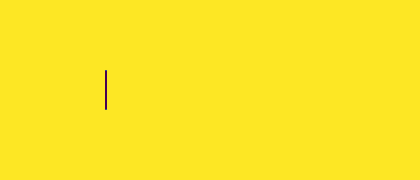
\includegraphics[width=0.3\textwidth]{../figures/von_karman_vortex_shedding/all_png_parallel/0.png}}
    \subfigure[Step 2000]{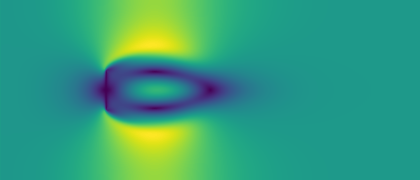
\includegraphics[width=0.3\textwidth]{../figures/von_karman_vortex_shedding/all_png_parallel/2000.png}}
        \subfigure[Step 6400]{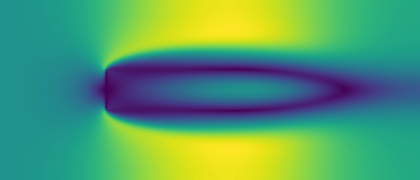
\includegraphics[width=0.3\textwidth]{../figures/von_karman_vortex_shedding/all_png_parallel/6400.png}}
            \subfigure[Step 13500]{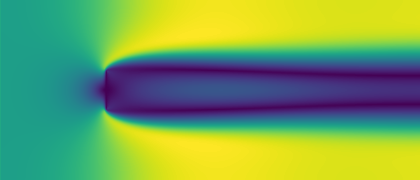
\includegraphics[width=0.3\textwidth]{../figures/von_karman_vortex_shedding/all_png_parallel/13500.png}}
            \subfigure[Step 20000]{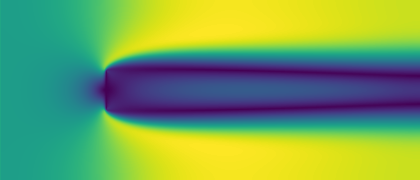
\includegraphics[width=0.3\textwidth]{../figures/von_karman_vortex_shedding/all_png_parallel/20000.png}}
            \subfigure[Step 30000]{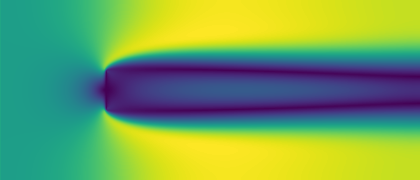
\includegraphics[width=0.3\textwidth]{../figures/von_karman_vortex_shedding/all_png_parallel/30000.png}}
                        \subfigure[Step 40000]{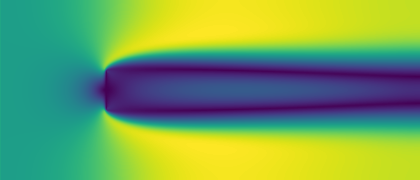
\includegraphics[width=0.3\textwidth]{../figures/von_karman_vortex_shedding/all_png_parallel/40000.png}}
            \subfigure[Step 45000]{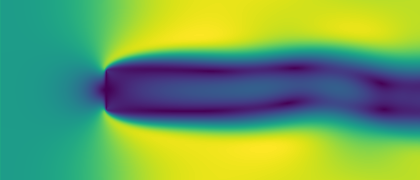
\includegraphics[width=0.3\textwidth]{../figures/von_karman_vortex_shedding/all_png_parallel/46500.png}}
            \subfigure[Step 30000]{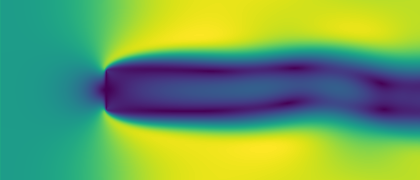
\includegraphics[width=0.3\textwidth]{../figures/von_karman_vortex_shedding/all_png_parallel/46500.png}}            
             \subfigure[Step 48000]{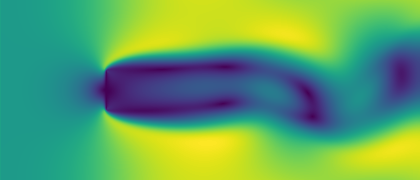
\includegraphics[width=0.3\textwidth]{../figures/von_karman_vortex_shedding/all_png_parallel/48000.png}}
            \subfigure[Step 50000]{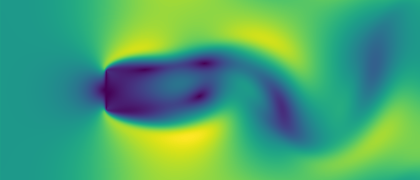
\includegraphics[width=0.3\textwidth]{../figures/von_karman_vortex_shedding/all_png_parallel/50000.png}}
            \subfigure[Step 54000]{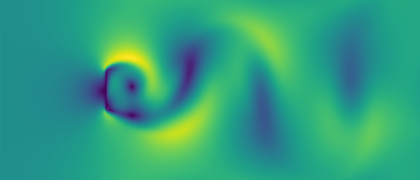
\includegraphics[width=0.3\textwidth]{../figures/von_karman_vortex_shedding/all_png_parallel/54000.png}}
                         \subfigure[Step 56000]{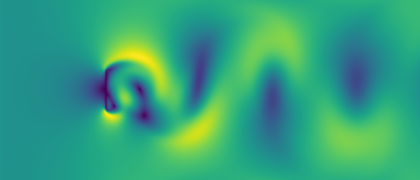
\includegraphics[width=0.3\textwidth]{../figures/von_karman_vortex_shedding/all_png_parallel/56000.png}}
            \subfigure[Step 60000]{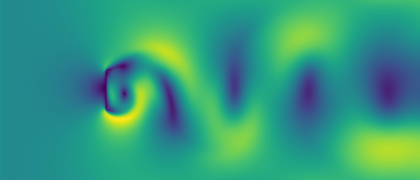
\includegraphics[width=0.3\textwidth]{../figures/von_karman_vortex_shedding/all_png_parallel/60000.png}}
            \subfigure[Step 70000]{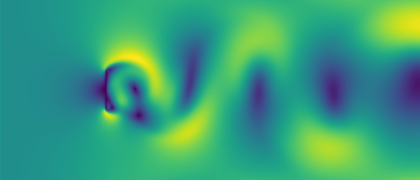
\includegraphics[width=0.3\textwidth]{../figures/von_karman_vortex_shedding/all_png_parallel/70000.png}}
            
   \caption{Qualitative results of von K\'{a}rm\'{a}n's vortex street using the parallel implemenation. Qualitative results are chosen arbitrarily. In the aforementioned repository is a gif file showing a more continuous evolution.}
  \label{fig:vonKarmanQualitative}
  \end{center}
\end{figure}

In further experiments we study the relationship between different quantities, i.e. \textit{Reynolds number}, length of the domain as well as \textit{blockage ratio}, and the \textit{Strouhal number}.
The Reynolds number is a measure of inertial to viscous forces in the flow of a fluid around a body. It is defined as follows:
\begin{equation}
\label{eq-reynold}
Re=\frac{lU}{\nu},
\end{equation}
where $l$ is the characteristic length parameter of the body, $U$ is the free stream flow velocity and $\nu$ is the free stream kinematic viscosity. One key property of the Reynolds number is that two incompressible flow systems are dynamically similar, if they have the same Reynolds number and same geometry. Note, that the Reynolds number is non-dimensional, which follows directly from eq. \ref{eq-reynold}, i.e. the physical quantities cancel themselves out.

The Strouhal number is another non-dimensional number, which defines the oscillatory behavior of flows. It is defined as follows
\begin{equation}
\label{eq-strouhal}
St=\frac{fl}{U},
\end{equation}
where $f$ is the dominant flow frequency, $l$ is the characteristic length parameter of the body and $U$ is the free stream flow velocity.

\begin{figure}
  \begin{center}
    \subfigure[Strouhal number as function of the Reynolds number]{	\scalebox{0.4}{%% Creator: Matplotlib, PGF backend
%%
%% To include the figure in your LaTeX document, write
%%   \input{<filename>.pgf}
%%
%% Make sure the required packages are loaded in your preamble
%%   \usepackage{pgf}
%%
%% and, on pdftex
%%   \usepackage[utf8]{inputenc}\DeclareUnicodeCharacter{2212}{-}
%%
%% or, on luatex and xetex
%%   \usepackage{unicode-math}
%%
%% Figures using additional raster images can only be included by \input if
%% they are in the same directory as the main LaTeX file. For loading figures
%% from other directories you can use the `import` package
%%   \usepackage{import}
%%
%% and then include the figures with
%%   \import{<path to file>}{<filename>.pgf}
%%
%% Matplotlib used the following preamble
%%   \usepackage[utf8x]{inputenc}
%%   \usepackage{amsmath}
%%
\begingroup%
\makeatletter%
\begin{pgfpicture}%
\pgfpathrectangle{\pgfpointorigin}{\pgfqpoint{5.683149in}{4.295691in}}%
\pgfusepath{use as bounding box, clip}%
\begin{pgfscope}%
\pgfsetbuttcap%
\pgfsetmiterjoin%
\definecolor{currentfill}{rgb}{1.000000,1.000000,1.000000}%
\pgfsetfillcolor{currentfill}%
\pgfsetlinewidth{0.000000pt}%
\definecolor{currentstroke}{rgb}{1.000000,1.000000,1.000000}%
\pgfsetstrokecolor{currentstroke}%
\pgfsetdash{}{0pt}%
\pgfpathmoveto{\pgfqpoint{0.000000in}{0.000000in}}%
\pgfpathlineto{\pgfqpoint{5.683149in}{0.000000in}}%
\pgfpathlineto{\pgfqpoint{5.683149in}{4.295691in}}%
\pgfpathlineto{\pgfqpoint{0.000000in}{4.295691in}}%
\pgfpathclose%
\pgfusepath{fill}%
\end{pgfscope}%
\begin{pgfscope}%
\pgfsetbuttcap%
\pgfsetmiterjoin%
\definecolor{currentfill}{rgb}{1.000000,1.000000,1.000000}%
\pgfsetfillcolor{currentfill}%
\pgfsetlinewidth{0.000000pt}%
\definecolor{currentstroke}{rgb}{0.000000,0.000000,0.000000}%
\pgfsetstrokecolor{currentstroke}%
\pgfsetstrokeopacity{0.000000}%
\pgfsetdash{}{0pt}%
\pgfpathmoveto{\pgfqpoint{0.623149in}{0.499691in}}%
\pgfpathlineto{\pgfqpoint{5.583149in}{0.499691in}}%
\pgfpathlineto{\pgfqpoint{5.583149in}{4.195691in}}%
\pgfpathlineto{\pgfqpoint{0.623149in}{4.195691in}}%
\pgfpathclose%
\pgfusepath{fill}%
\end{pgfscope}%
\begin{pgfscope}%
\pgfsetbuttcap%
\pgfsetroundjoin%
\definecolor{currentfill}{rgb}{0.000000,0.000000,0.000000}%
\pgfsetfillcolor{currentfill}%
\pgfsetlinewidth{0.803000pt}%
\definecolor{currentstroke}{rgb}{0.000000,0.000000,0.000000}%
\pgfsetstrokecolor{currentstroke}%
\pgfsetdash{}{0pt}%
\pgfsys@defobject{currentmarker}{\pgfqpoint{0.000000in}{-0.048611in}}{\pgfqpoint{0.000000in}{0.000000in}}{%
\pgfpathmoveto{\pgfqpoint{0.000000in}{0.000000in}}%
\pgfpathlineto{\pgfqpoint{0.000000in}{-0.048611in}}%
\pgfusepath{stroke,fill}%
}%
\begin{pgfscope}%
\pgfsys@transformshift{0.848603in}{0.499691in}%
\pgfsys@useobject{currentmarker}{}%
\end{pgfscope}%
\end{pgfscope}%
\begin{pgfscope}%
\definecolor{textcolor}{rgb}{0.000000,0.000000,0.000000}%
\pgfsetstrokecolor{textcolor}%
\pgfsetfillcolor{textcolor}%
\pgftext[x=0.848603in,y=0.402469in,,top]{\color{textcolor}\rmfamily\fontsize{10.000000}{12.000000}\selectfont \(\displaystyle {40}\)}%
\end{pgfscope}%
\begin{pgfscope}%
\pgfsetbuttcap%
\pgfsetroundjoin%
\definecolor{currentfill}{rgb}{0.000000,0.000000,0.000000}%
\pgfsetfillcolor{currentfill}%
\pgfsetlinewidth{0.803000pt}%
\definecolor{currentstroke}{rgb}{0.000000,0.000000,0.000000}%
\pgfsetstrokecolor{currentstroke}%
\pgfsetdash{}{0pt}%
\pgfsys@defobject{currentmarker}{\pgfqpoint{0.000000in}{-0.048611in}}{\pgfqpoint{0.000000in}{0.000000in}}{%
\pgfpathmoveto{\pgfqpoint{0.000000in}{0.000000in}}%
\pgfpathlineto{\pgfqpoint{0.000000in}{-0.048611in}}%
\pgfusepath{stroke,fill}%
}%
\begin{pgfscope}%
\pgfsys@transformshift{1.412240in}{0.499691in}%
\pgfsys@useobject{currentmarker}{}%
\end{pgfscope}%
\end{pgfscope}%
\begin{pgfscope}%
\definecolor{textcolor}{rgb}{0.000000,0.000000,0.000000}%
\pgfsetstrokecolor{textcolor}%
\pgfsetfillcolor{textcolor}%
\pgftext[x=1.412240in,y=0.402469in,,top]{\color{textcolor}\rmfamily\fontsize{10.000000}{12.000000}\selectfont \(\displaystyle {60}\)}%
\end{pgfscope}%
\begin{pgfscope}%
\pgfsetbuttcap%
\pgfsetroundjoin%
\definecolor{currentfill}{rgb}{0.000000,0.000000,0.000000}%
\pgfsetfillcolor{currentfill}%
\pgfsetlinewidth{0.803000pt}%
\definecolor{currentstroke}{rgb}{0.000000,0.000000,0.000000}%
\pgfsetstrokecolor{currentstroke}%
\pgfsetdash{}{0pt}%
\pgfsys@defobject{currentmarker}{\pgfqpoint{0.000000in}{-0.048611in}}{\pgfqpoint{0.000000in}{0.000000in}}{%
\pgfpathmoveto{\pgfqpoint{0.000000in}{0.000000in}}%
\pgfpathlineto{\pgfqpoint{0.000000in}{-0.048611in}}%
\pgfusepath{stroke,fill}%
}%
\begin{pgfscope}%
\pgfsys@transformshift{1.975876in}{0.499691in}%
\pgfsys@useobject{currentmarker}{}%
\end{pgfscope}%
\end{pgfscope}%
\begin{pgfscope}%
\definecolor{textcolor}{rgb}{0.000000,0.000000,0.000000}%
\pgfsetstrokecolor{textcolor}%
\pgfsetfillcolor{textcolor}%
\pgftext[x=1.975876in,y=0.402469in,,top]{\color{textcolor}\rmfamily\fontsize{10.000000}{12.000000}\selectfont \(\displaystyle {80}\)}%
\end{pgfscope}%
\begin{pgfscope}%
\pgfsetbuttcap%
\pgfsetroundjoin%
\definecolor{currentfill}{rgb}{0.000000,0.000000,0.000000}%
\pgfsetfillcolor{currentfill}%
\pgfsetlinewidth{0.803000pt}%
\definecolor{currentstroke}{rgb}{0.000000,0.000000,0.000000}%
\pgfsetstrokecolor{currentstroke}%
\pgfsetdash{}{0pt}%
\pgfsys@defobject{currentmarker}{\pgfqpoint{0.000000in}{-0.048611in}}{\pgfqpoint{0.000000in}{0.000000in}}{%
\pgfpathmoveto{\pgfqpoint{0.000000in}{0.000000in}}%
\pgfpathlineto{\pgfqpoint{0.000000in}{-0.048611in}}%
\pgfusepath{stroke,fill}%
}%
\begin{pgfscope}%
\pgfsys@transformshift{2.539512in}{0.499691in}%
\pgfsys@useobject{currentmarker}{}%
\end{pgfscope}%
\end{pgfscope}%
\begin{pgfscope}%
\definecolor{textcolor}{rgb}{0.000000,0.000000,0.000000}%
\pgfsetstrokecolor{textcolor}%
\pgfsetfillcolor{textcolor}%
\pgftext[x=2.539512in,y=0.402469in,,top]{\color{textcolor}\rmfamily\fontsize{10.000000}{12.000000}\selectfont \(\displaystyle {100}\)}%
\end{pgfscope}%
\begin{pgfscope}%
\pgfsetbuttcap%
\pgfsetroundjoin%
\definecolor{currentfill}{rgb}{0.000000,0.000000,0.000000}%
\pgfsetfillcolor{currentfill}%
\pgfsetlinewidth{0.803000pt}%
\definecolor{currentstroke}{rgb}{0.000000,0.000000,0.000000}%
\pgfsetstrokecolor{currentstroke}%
\pgfsetdash{}{0pt}%
\pgfsys@defobject{currentmarker}{\pgfqpoint{0.000000in}{-0.048611in}}{\pgfqpoint{0.000000in}{0.000000in}}{%
\pgfpathmoveto{\pgfqpoint{0.000000in}{0.000000in}}%
\pgfpathlineto{\pgfqpoint{0.000000in}{-0.048611in}}%
\pgfusepath{stroke,fill}%
}%
\begin{pgfscope}%
\pgfsys@transformshift{3.103149in}{0.499691in}%
\pgfsys@useobject{currentmarker}{}%
\end{pgfscope}%
\end{pgfscope}%
\begin{pgfscope}%
\definecolor{textcolor}{rgb}{0.000000,0.000000,0.000000}%
\pgfsetstrokecolor{textcolor}%
\pgfsetfillcolor{textcolor}%
\pgftext[x=3.103149in,y=0.402469in,,top]{\color{textcolor}\rmfamily\fontsize{10.000000}{12.000000}\selectfont \(\displaystyle {120}\)}%
\end{pgfscope}%
\begin{pgfscope}%
\pgfsetbuttcap%
\pgfsetroundjoin%
\definecolor{currentfill}{rgb}{0.000000,0.000000,0.000000}%
\pgfsetfillcolor{currentfill}%
\pgfsetlinewidth{0.803000pt}%
\definecolor{currentstroke}{rgb}{0.000000,0.000000,0.000000}%
\pgfsetstrokecolor{currentstroke}%
\pgfsetdash{}{0pt}%
\pgfsys@defobject{currentmarker}{\pgfqpoint{0.000000in}{-0.048611in}}{\pgfqpoint{0.000000in}{0.000000in}}{%
\pgfpathmoveto{\pgfqpoint{0.000000in}{0.000000in}}%
\pgfpathlineto{\pgfqpoint{0.000000in}{-0.048611in}}%
\pgfusepath{stroke,fill}%
}%
\begin{pgfscope}%
\pgfsys@transformshift{3.666785in}{0.499691in}%
\pgfsys@useobject{currentmarker}{}%
\end{pgfscope}%
\end{pgfscope}%
\begin{pgfscope}%
\definecolor{textcolor}{rgb}{0.000000,0.000000,0.000000}%
\pgfsetstrokecolor{textcolor}%
\pgfsetfillcolor{textcolor}%
\pgftext[x=3.666785in,y=0.402469in,,top]{\color{textcolor}\rmfamily\fontsize{10.000000}{12.000000}\selectfont \(\displaystyle {140}\)}%
\end{pgfscope}%
\begin{pgfscope}%
\pgfsetbuttcap%
\pgfsetroundjoin%
\definecolor{currentfill}{rgb}{0.000000,0.000000,0.000000}%
\pgfsetfillcolor{currentfill}%
\pgfsetlinewidth{0.803000pt}%
\definecolor{currentstroke}{rgb}{0.000000,0.000000,0.000000}%
\pgfsetstrokecolor{currentstroke}%
\pgfsetdash{}{0pt}%
\pgfsys@defobject{currentmarker}{\pgfqpoint{0.000000in}{-0.048611in}}{\pgfqpoint{0.000000in}{0.000000in}}{%
\pgfpathmoveto{\pgfqpoint{0.000000in}{0.000000in}}%
\pgfpathlineto{\pgfqpoint{0.000000in}{-0.048611in}}%
\pgfusepath{stroke,fill}%
}%
\begin{pgfscope}%
\pgfsys@transformshift{4.230421in}{0.499691in}%
\pgfsys@useobject{currentmarker}{}%
\end{pgfscope}%
\end{pgfscope}%
\begin{pgfscope}%
\definecolor{textcolor}{rgb}{0.000000,0.000000,0.000000}%
\pgfsetstrokecolor{textcolor}%
\pgfsetfillcolor{textcolor}%
\pgftext[x=4.230421in,y=0.402469in,,top]{\color{textcolor}\rmfamily\fontsize{10.000000}{12.000000}\selectfont \(\displaystyle {160}\)}%
\end{pgfscope}%
\begin{pgfscope}%
\pgfsetbuttcap%
\pgfsetroundjoin%
\definecolor{currentfill}{rgb}{0.000000,0.000000,0.000000}%
\pgfsetfillcolor{currentfill}%
\pgfsetlinewidth{0.803000pt}%
\definecolor{currentstroke}{rgb}{0.000000,0.000000,0.000000}%
\pgfsetstrokecolor{currentstroke}%
\pgfsetdash{}{0pt}%
\pgfsys@defobject{currentmarker}{\pgfqpoint{0.000000in}{-0.048611in}}{\pgfqpoint{0.000000in}{0.000000in}}{%
\pgfpathmoveto{\pgfqpoint{0.000000in}{0.000000in}}%
\pgfpathlineto{\pgfqpoint{0.000000in}{-0.048611in}}%
\pgfusepath{stroke,fill}%
}%
\begin{pgfscope}%
\pgfsys@transformshift{4.794058in}{0.499691in}%
\pgfsys@useobject{currentmarker}{}%
\end{pgfscope}%
\end{pgfscope}%
\begin{pgfscope}%
\definecolor{textcolor}{rgb}{0.000000,0.000000,0.000000}%
\pgfsetstrokecolor{textcolor}%
\pgfsetfillcolor{textcolor}%
\pgftext[x=4.794058in,y=0.402469in,,top]{\color{textcolor}\rmfamily\fontsize{10.000000}{12.000000}\selectfont \(\displaystyle {180}\)}%
\end{pgfscope}%
\begin{pgfscope}%
\pgfsetbuttcap%
\pgfsetroundjoin%
\definecolor{currentfill}{rgb}{0.000000,0.000000,0.000000}%
\pgfsetfillcolor{currentfill}%
\pgfsetlinewidth{0.803000pt}%
\definecolor{currentstroke}{rgb}{0.000000,0.000000,0.000000}%
\pgfsetstrokecolor{currentstroke}%
\pgfsetdash{}{0pt}%
\pgfsys@defobject{currentmarker}{\pgfqpoint{0.000000in}{-0.048611in}}{\pgfqpoint{0.000000in}{0.000000in}}{%
\pgfpathmoveto{\pgfqpoint{0.000000in}{0.000000in}}%
\pgfpathlineto{\pgfqpoint{0.000000in}{-0.048611in}}%
\pgfusepath{stroke,fill}%
}%
\begin{pgfscope}%
\pgfsys@transformshift{5.357694in}{0.499691in}%
\pgfsys@useobject{currentmarker}{}%
\end{pgfscope}%
\end{pgfscope}%
\begin{pgfscope}%
\definecolor{textcolor}{rgb}{0.000000,0.000000,0.000000}%
\pgfsetstrokecolor{textcolor}%
\pgfsetfillcolor{textcolor}%
\pgftext[x=5.357694in,y=0.402469in,,top]{\color{textcolor}\rmfamily\fontsize{10.000000}{12.000000}\selectfont \(\displaystyle {200}\)}%
\end{pgfscope}%
\begin{pgfscope}%
\definecolor{textcolor}{rgb}{0.000000,0.000000,0.000000}%
\pgfsetstrokecolor{textcolor}%
\pgfsetfillcolor{textcolor}%
\pgftext[x=3.103149in,y=0.223457in,,top]{\color{textcolor}\rmfamily\fontsize{10.000000}{12.000000}\selectfont Reynolds number}%
\end{pgfscope}%
\begin{pgfscope}%
\pgfsetbuttcap%
\pgfsetroundjoin%
\definecolor{currentfill}{rgb}{0.000000,0.000000,0.000000}%
\pgfsetfillcolor{currentfill}%
\pgfsetlinewidth{0.803000pt}%
\definecolor{currentstroke}{rgb}{0.000000,0.000000,0.000000}%
\pgfsetstrokecolor{currentstroke}%
\pgfsetdash{}{0pt}%
\pgfsys@defobject{currentmarker}{\pgfqpoint{-0.048611in}{0.000000in}}{\pgfqpoint{0.000000in}{0.000000in}}{%
\pgfpathmoveto{\pgfqpoint{-0.000000in}{0.000000in}}%
\pgfpathlineto{\pgfqpoint{-0.048611in}{0.000000in}}%
\pgfusepath{stroke,fill}%
}%
\begin{pgfscope}%
\pgfsys@transformshift{0.623149in}{0.940937in}%
\pgfsys@useobject{currentmarker}{}%
\end{pgfscope}%
\end{pgfscope}%
\begin{pgfscope}%
\definecolor{textcolor}{rgb}{0.000000,0.000000,0.000000}%
\pgfsetstrokecolor{textcolor}%
\pgfsetfillcolor{textcolor}%
\pgftext[x=0.279012in, y=0.892712in, left, base]{\color{textcolor}\rmfamily\fontsize{10.000000}{12.000000}\selectfont \(\displaystyle {0.38}\)}%
\end{pgfscope}%
\begin{pgfscope}%
\pgfsetbuttcap%
\pgfsetroundjoin%
\definecolor{currentfill}{rgb}{0.000000,0.000000,0.000000}%
\pgfsetfillcolor{currentfill}%
\pgfsetlinewidth{0.803000pt}%
\definecolor{currentstroke}{rgb}{0.000000,0.000000,0.000000}%
\pgfsetstrokecolor{currentstroke}%
\pgfsetdash{}{0pt}%
\pgfsys@defobject{currentmarker}{\pgfqpoint{-0.048611in}{0.000000in}}{\pgfqpoint{0.000000in}{0.000000in}}{%
\pgfpathmoveto{\pgfqpoint{-0.000000in}{0.000000in}}%
\pgfpathlineto{\pgfqpoint{-0.048611in}{0.000000in}}%
\pgfusepath{stroke,fill}%
}%
\begin{pgfscope}%
\pgfsys@transformshift{0.623149in}{1.759910in}%
\pgfsys@useobject{currentmarker}{}%
\end{pgfscope}%
\end{pgfscope}%
\begin{pgfscope}%
\definecolor{textcolor}{rgb}{0.000000,0.000000,0.000000}%
\pgfsetstrokecolor{textcolor}%
\pgfsetfillcolor{textcolor}%
\pgftext[x=0.279012in, y=1.711684in, left, base]{\color{textcolor}\rmfamily\fontsize{10.000000}{12.000000}\selectfont \(\displaystyle {0.40}\)}%
\end{pgfscope}%
\begin{pgfscope}%
\pgfsetbuttcap%
\pgfsetroundjoin%
\definecolor{currentfill}{rgb}{0.000000,0.000000,0.000000}%
\pgfsetfillcolor{currentfill}%
\pgfsetlinewidth{0.803000pt}%
\definecolor{currentstroke}{rgb}{0.000000,0.000000,0.000000}%
\pgfsetstrokecolor{currentstroke}%
\pgfsetdash{}{0pt}%
\pgfsys@defobject{currentmarker}{\pgfqpoint{-0.048611in}{0.000000in}}{\pgfqpoint{0.000000in}{0.000000in}}{%
\pgfpathmoveto{\pgfqpoint{-0.000000in}{0.000000in}}%
\pgfpathlineto{\pgfqpoint{-0.048611in}{0.000000in}}%
\pgfusepath{stroke,fill}%
}%
\begin{pgfscope}%
\pgfsys@transformshift{0.623149in}{2.578883in}%
\pgfsys@useobject{currentmarker}{}%
\end{pgfscope}%
\end{pgfscope}%
\begin{pgfscope}%
\definecolor{textcolor}{rgb}{0.000000,0.000000,0.000000}%
\pgfsetstrokecolor{textcolor}%
\pgfsetfillcolor{textcolor}%
\pgftext[x=0.279012in, y=2.530657in, left, base]{\color{textcolor}\rmfamily\fontsize{10.000000}{12.000000}\selectfont \(\displaystyle {0.42}\)}%
\end{pgfscope}%
\begin{pgfscope}%
\pgfsetbuttcap%
\pgfsetroundjoin%
\definecolor{currentfill}{rgb}{0.000000,0.000000,0.000000}%
\pgfsetfillcolor{currentfill}%
\pgfsetlinewidth{0.803000pt}%
\definecolor{currentstroke}{rgb}{0.000000,0.000000,0.000000}%
\pgfsetstrokecolor{currentstroke}%
\pgfsetdash{}{0pt}%
\pgfsys@defobject{currentmarker}{\pgfqpoint{-0.048611in}{0.000000in}}{\pgfqpoint{0.000000in}{0.000000in}}{%
\pgfpathmoveto{\pgfqpoint{-0.000000in}{0.000000in}}%
\pgfpathlineto{\pgfqpoint{-0.048611in}{0.000000in}}%
\pgfusepath{stroke,fill}%
}%
\begin{pgfscope}%
\pgfsys@transformshift{0.623149in}{3.397855in}%
\pgfsys@useobject{currentmarker}{}%
\end{pgfscope}%
\end{pgfscope}%
\begin{pgfscope}%
\definecolor{textcolor}{rgb}{0.000000,0.000000,0.000000}%
\pgfsetstrokecolor{textcolor}%
\pgfsetfillcolor{textcolor}%
\pgftext[x=0.279012in, y=3.349630in, left, base]{\color{textcolor}\rmfamily\fontsize{10.000000}{12.000000}\selectfont \(\displaystyle {0.44}\)}%
\end{pgfscope}%
\begin{pgfscope}%
\definecolor{textcolor}{rgb}{0.000000,0.000000,0.000000}%
\pgfsetstrokecolor{textcolor}%
\pgfsetfillcolor{textcolor}%
\pgftext[x=0.223457in,y=2.347691in,,bottom,rotate=90.000000]{\color{textcolor}\rmfamily\fontsize{10.000000}{12.000000}\selectfont Strouhal number}%
\end{pgfscope}%
\begin{pgfscope}%
\pgfpathrectangle{\pgfqpoint{0.623149in}{0.499691in}}{\pgfqpoint{4.960000in}{3.696000in}}%
\pgfusepath{clip}%
\pgfsetrectcap%
\pgfsetroundjoin%
\pgfsetlinewidth{1.505625pt}%
\definecolor{currentstroke}{rgb}{0.121569,0.466667,0.705882}%
\pgfsetstrokecolor{currentstroke}%
\pgfsetdash{}{0pt}%
\pgfpathmoveto{\pgfqpoint{0.848603in}{0.667691in}}%
\pgfpathlineto{\pgfqpoint{1.694058in}{3.019732in}}%
\pgfpathlineto{\pgfqpoint{2.539512in}{3.901696in}}%
\pgfpathlineto{\pgfqpoint{3.666785in}{4.027691in}}%
\pgfpathlineto{\pgfqpoint{4.512240in}{3.775701in}}%
\pgfpathlineto{\pgfqpoint{5.357694in}{3.523712in}}%
\pgfusepath{stroke}%
\end{pgfscope}%
\begin{pgfscope}%
\pgfsetrectcap%
\pgfsetmiterjoin%
\pgfsetlinewidth{0.803000pt}%
\definecolor{currentstroke}{rgb}{0.000000,0.000000,0.000000}%
\pgfsetstrokecolor{currentstroke}%
\pgfsetdash{}{0pt}%
\pgfpathmoveto{\pgfqpoint{0.623149in}{0.499691in}}%
\pgfpathlineto{\pgfqpoint{0.623149in}{4.195691in}}%
\pgfusepath{stroke}%
\end{pgfscope}%
\begin{pgfscope}%
\pgfsetrectcap%
\pgfsetmiterjoin%
\pgfsetlinewidth{0.803000pt}%
\definecolor{currentstroke}{rgb}{0.000000,0.000000,0.000000}%
\pgfsetstrokecolor{currentstroke}%
\pgfsetdash{}{0pt}%
\pgfpathmoveto{\pgfqpoint{5.583149in}{0.499691in}}%
\pgfpathlineto{\pgfqpoint{5.583149in}{4.195691in}}%
\pgfusepath{stroke}%
\end{pgfscope}%
\begin{pgfscope}%
\pgfsetrectcap%
\pgfsetmiterjoin%
\pgfsetlinewidth{0.803000pt}%
\definecolor{currentstroke}{rgb}{0.000000,0.000000,0.000000}%
\pgfsetstrokecolor{currentstroke}%
\pgfsetdash{}{0pt}%
\pgfpathmoveto{\pgfqpoint{0.623149in}{0.499691in}}%
\pgfpathlineto{\pgfqpoint{5.583149in}{0.499691in}}%
\pgfusepath{stroke}%
\end{pgfscope}%
\begin{pgfscope}%
\pgfsetrectcap%
\pgfsetmiterjoin%
\pgfsetlinewidth{0.803000pt}%
\definecolor{currentstroke}{rgb}{0.000000,0.000000,0.000000}%
\pgfsetstrokecolor{currentstroke}%
\pgfsetdash{}{0pt}%
\pgfpathmoveto{\pgfqpoint{0.623149in}{4.195691in}}%
\pgfpathlineto{\pgfqpoint{5.583149in}{4.195691in}}%
\pgfusepath{stroke}%
\end{pgfscope}%
\end{pgfpicture}%
\makeatother%
\endgroup%
}}
        \subfigure[Strouhal number as function of the width of the simulation domain]{	\scalebox{0.4}{%% Creator: Matplotlib, PGF backend
%%
%% To include the figure in your LaTeX document, write
%%   \input{<filename>.pgf}
%%
%% Make sure the required packages are loaded in your preamble
%%   \usepackage{pgf}
%%
%% and, on pdftex
%%   \usepackage[utf8]{inputenc}\DeclareUnicodeCharacter{2212}{-}
%%
%% or, on luatex and xetex
%%   \usepackage{unicode-math}
%%
%% Figures using additional raster images can only be included by \input if
%% they are in the same directory as the main LaTeX file. For loading figures
%% from other directories you can use the `import` package
%%   \usepackage{import}
%%
%% and then include the figures with
%%   \import{<path to file>}{<filename>.pgf}
%%
%% Matplotlib used the following preamble
%%   \usepackage[utf8x]{inputenc}
%%   \usepackage{amsmath}
%%
\begingroup%
\makeatletter%
\begin{pgfpicture}%
\pgfpathrectangle{\pgfpointorigin}{\pgfqpoint{5.752593in}{4.311123in}}%
\pgfusepath{use as bounding box, clip}%
\begin{pgfscope}%
\pgfsetbuttcap%
\pgfsetmiterjoin%
\definecolor{currentfill}{rgb}{1.000000,1.000000,1.000000}%
\pgfsetfillcolor{currentfill}%
\pgfsetlinewidth{0.000000pt}%
\definecolor{currentstroke}{rgb}{1.000000,1.000000,1.000000}%
\pgfsetstrokecolor{currentstroke}%
\pgfsetdash{}{0pt}%
\pgfpathmoveto{\pgfqpoint{0.000000in}{0.000000in}}%
\pgfpathlineto{\pgfqpoint{5.752593in}{0.000000in}}%
\pgfpathlineto{\pgfqpoint{5.752593in}{4.311123in}}%
\pgfpathlineto{\pgfqpoint{0.000000in}{4.311123in}}%
\pgfpathclose%
\pgfusepath{fill}%
\end{pgfscope}%
\begin{pgfscope}%
\pgfsetbuttcap%
\pgfsetmiterjoin%
\definecolor{currentfill}{rgb}{1.000000,1.000000,1.000000}%
\pgfsetfillcolor{currentfill}%
\pgfsetlinewidth{0.000000pt}%
\definecolor{currentstroke}{rgb}{0.000000,0.000000,0.000000}%
\pgfsetstrokecolor{currentstroke}%
\pgfsetstrokeopacity{0.000000}%
\pgfsetdash{}{0pt}%
\pgfpathmoveto{\pgfqpoint{0.692593in}{0.515123in}}%
\pgfpathlineto{\pgfqpoint{5.652593in}{0.515123in}}%
\pgfpathlineto{\pgfqpoint{5.652593in}{4.211123in}}%
\pgfpathlineto{\pgfqpoint{0.692593in}{4.211123in}}%
\pgfpathclose%
\pgfusepath{fill}%
\end{pgfscope}%
\begin{pgfscope}%
\pgfsetbuttcap%
\pgfsetroundjoin%
\definecolor{currentfill}{rgb}{0.000000,0.000000,0.000000}%
\pgfsetfillcolor{currentfill}%
\pgfsetlinewidth{0.803000pt}%
\definecolor{currentstroke}{rgb}{0.000000,0.000000,0.000000}%
\pgfsetstrokecolor{currentstroke}%
\pgfsetdash{}{0pt}%
\pgfsys@defobject{currentmarker}{\pgfqpoint{0.000000in}{-0.048611in}}{\pgfqpoint{0.000000in}{0.000000in}}{%
\pgfpathmoveto{\pgfqpoint{0.000000in}{0.000000in}}%
\pgfpathlineto{\pgfqpoint{0.000000in}{-0.048611in}}%
\pgfusepath{stroke,fill}%
}%
\begin{pgfscope}%
\pgfsys@transformshift{1.310143in}{0.515123in}%
\pgfsys@useobject{currentmarker}{}%
\end{pgfscope}%
\end{pgfscope}%
\begin{pgfscope}%
\definecolor{textcolor}{rgb}{0.000000,0.000000,0.000000}%
\pgfsetstrokecolor{textcolor}%
\pgfsetfillcolor{textcolor}%
\pgftext[x=1.310143in,y=0.417901in,,top]{\color{textcolor}\rmfamily\fontsize{10.000000}{12.000000}\selectfont \(\displaystyle {200}\)}%
\end{pgfscope}%
\begin{pgfscope}%
\pgfsetbuttcap%
\pgfsetroundjoin%
\definecolor{currentfill}{rgb}{0.000000,0.000000,0.000000}%
\pgfsetfillcolor{currentfill}%
\pgfsetlinewidth{0.803000pt}%
\definecolor{currentstroke}{rgb}{0.000000,0.000000,0.000000}%
\pgfsetstrokecolor{currentstroke}%
\pgfsetdash{}{0pt}%
\pgfsys@defobject{currentmarker}{\pgfqpoint{0.000000in}{-0.048611in}}{\pgfqpoint{0.000000in}{0.000000in}}{%
\pgfpathmoveto{\pgfqpoint{0.000000in}{0.000000in}}%
\pgfpathlineto{\pgfqpoint{0.000000in}{-0.048611in}}%
\pgfusepath{stroke,fill}%
}%
\begin{pgfscope}%
\pgfsys@transformshift{2.094333in}{0.515123in}%
\pgfsys@useobject{currentmarker}{}%
\end{pgfscope}%
\end{pgfscope}%
\begin{pgfscope}%
\definecolor{textcolor}{rgb}{0.000000,0.000000,0.000000}%
\pgfsetstrokecolor{textcolor}%
\pgfsetfillcolor{textcolor}%
\pgftext[x=2.094333in,y=0.417901in,,top]{\color{textcolor}\rmfamily\fontsize{10.000000}{12.000000}\selectfont \(\displaystyle {400}\)}%
\end{pgfscope}%
\begin{pgfscope}%
\pgfsetbuttcap%
\pgfsetroundjoin%
\definecolor{currentfill}{rgb}{0.000000,0.000000,0.000000}%
\pgfsetfillcolor{currentfill}%
\pgfsetlinewidth{0.803000pt}%
\definecolor{currentstroke}{rgb}{0.000000,0.000000,0.000000}%
\pgfsetstrokecolor{currentstroke}%
\pgfsetdash{}{0pt}%
\pgfsys@defobject{currentmarker}{\pgfqpoint{0.000000in}{-0.048611in}}{\pgfqpoint{0.000000in}{0.000000in}}{%
\pgfpathmoveto{\pgfqpoint{0.000000in}{0.000000in}}%
\pgfpathlineto{\pgfqpoint{0.000000in}{-0.048611in}}%
\pgfusepath{stroke,fill}%
}%
\begin{pgfscope}%
\pgfsys@transformshift{2.878522in}{0.515123in}%
\pgfsys@useobject{currentmarker}{}%
\end{pgfscope}%
\end{pgfscope}%
\begin{pgfscope}%
\definecolor{textcolor}{rgb}{0.000000,0.000000,0.000000}%
\pgfsetstrokecolor{textcolor}%
\pgfsetfillcolor{textcolor}%
\pgftext[x=2.878522in,y=0.417901in,,top]{\color{textcolor}\rmfamily\fontsize{10.000000}{12.000000}\selectfont \(\displaystyle {600}\)}%
\end{pgfscope}%
\begin{pgfscope}%
\pgfsetbuttcap%
\pgfsetroundjoin%
\definecolor{currentfill}{rgb}{0.000000,0.000000,0.000000}%
\pgfsetfillcolor{currentfill}%
\pgfsetlinewidth{0.803000pt}%
\definecolor{currentstroke}{rgb}{0.000000,0.000000,0.000000}%
\pgfsetstrokecolor{currentstroke}%
\pgfsetdash{}{0pt}%
\pgfsys@defobject{currentmarker}{\pgfqpoint{0.000000in}{-0.048611in}}{\pgfqpoint{0.000000in}{0.000000in}}{%
\pgfpathmoveto{\pgfqpoint{0.000000in}{0.000000in}}%
\pgfpathlineto{\pgfqpoint{0.000000in}{-0.048611in}}%
\pgfusepath{stroke,fill}%
}%
\begin{pgfscope}%
\pgfsys@transformshift{3.662712in}{0.515123in}%
\pgfsys@useobject{currentmarker}{}%
\end{pgfscope}%
\end{pgfscope}%
\begin{pgfscope}%
\definecolor{textcolor}{rgb}{0.000000,0.000000,0.000000}%
\pgfsetstrokecolor{textcolor}%
\pgfsetfillcolor{textcolor}%
\pgftext[x=3.662712in,y=0.417901in,,top]{\color{textcolor}\rmfamily\fontsize{10.000000}{12.000000}\selectfont \(\displaystyle {800}\)}%
\end{pgfscope}%
\begin{pgfscope}%
\pgfsetbuttcap%
\pgfsetroundjoin%
\definecolor{currentfill}{rgb}{0.000000,0.000000,0.000000}%
\pgfsetfillcolor{currentfill}%
\pgfsetlinewidth{0.803000pt}%
\definecolor{currentstroke}{rgb}{0.000000,0.000000,0.000000}%
\pgfsetstrokecolor{currentstroke}%
\pgfsetdash{}{0pt}%
\pgfsys@defobject{currentmarker}{\pgfqpoint{0.000000in}{-0.048611in}}{\pgfqpoint{0.000000in}{0.000000in}}{%
\pgfpathmoveto{\pgfqpoint{0.000000in}{0.000000in}}%
\pgfpathlineto{\pgfqpoint{0.000000in}{-0.048611in}}%
\pgfusepath{stroke,fill}%
}%
\begin{pgfscope}%
\pgfsys@transformshift{4.446902in}{0.515123in}%
\pgfsys@useobject{currentmarker}{}%
\end{pgfscope}%
\end{pgfscope}%
\begin{pgfscope}%
\definecolor{textcolor}{rgb}{0.000000,0.000000,0.000000}%
\pgfsetstrokecolor{textcolor}%
\pgfsetfillcolor{textcolor}%
\pgftext[x=4.446902in,y=0.417901in,,top]{\color{textcolor}\rmfamily\fontsize{10.000000}{12.000000}\selectfont \(\displaystyle {1000}\)}%
\end{pgfscope}%
\begin{pgfscope}%
\pgfsetbuttcap%
\pgfsetroundjoin%
\definecolor{currentfill}{rgb}{0.000000,0.000000,0.000000}%
\pgfsetfillcolor{currentfill}%
\pgfsetlinewidth{0.803000pt}%
\definecolor{currentstroke}{rgb}{0.000000,0.000000,0.000000}%
\pgfsetstrokecolor{currentstroke}%
\pgfsetdash{}{0pt}%
\pgfsys@defobject{currentmarker}{\pgfqpoint{0.000000in}{-0.048611in}}{\pgfqpoint{0.000000in}{0.000000in}}{%
\pgfpathmoveto{\pgfqpoint{0.000000in}{0.000000in}}%
\pgfpathlineto{\pgfqpoint{0.000000in}{-0.048611in}}%
\pgfusepath{stroke,fill}%
}%
\begin{pgfscope}%
\pgfsys@transformshift{5.231091in}{0.515123in}%
\pgfsys@useobject{currentmarker}{}%
\end{pgfscope}%
\end{pgfscope}%
\begin{pgfscope}%
\definecolor{textcolor}{rgb}{0.000000,0.000000,0.000000}%
\pgfsetstrokecolor{textcolor}%
\pgfsetfillcolor{textcolor}%
\pgftext[x=5.231091in,y=0.417901in,,top]{\color{textcolor}\rmfamily\fontsize{10.000000}{12.000000}\selectfont \(\displaystyle {1200}\)}%
\end{pgfscope}%
\begin{pgfscope}%
\definecolor{textcolor}{rgb}{0.000000,0.000000,0.000000}%
\pgfsetstrokecolor{textcolor}%
\pgfsetfillcolor{textcolor}%
\pgftext[x=3.172593in,y=0.238889in,,top]{\color{textcolor}\rmfamily\fontsize{10.000000}{12.000000}\selectfont lx [lu]}%
\end{pgfscope}%
\begin{pgfscope}%
\pgfsetbuttcap%
\pgfsetroundjoin%
\definecolor{currentfill}{rgb}{0.000000,0.000000,0.000000}%
\pgfsetfillcolor{currentfill}%
\pgfsetlinewidth{0.803000pt}%
\definecolor{currentstroke}{rgb}{0.000000,0.000000,0.000000}%
\pgfsetstrokecolor{currentstroke}%
\pgfsetdash{}{0pt}%
\pgfsys@defobject{currentmarker}{\pgfqpoint{-0.048611in}{0.000000in}}{\pgfqpoint{0.000000in}{0.000000in}}{%
\pgfpathmoveto{\pgfqpoint{-0.000000in}{0.000000in}}%
\pgfpathlineto{\pgfqpoint{-0.048611in}{0.000000in}}%
\pgfusepath{stroke,fill}%
}%
\begin{pgfscope}%
\pgfsys@transformshift{0.692593in}{0.998216in}%
\pgfsys@useobject{currentmarker}{}%
\end{pgfscope}%
\end{pgfscope}%
\begin{pgfscope}%
\definecolor{textcolor}{rgb}{0.000000,0.000000,0.000000}%
\pgfsetstrokecolor{textcolor}%
\pgfsetfillcolor{textcolor}%
\pgftext[x=0.279012in, y=0.949990in, left, base]{\color{textcolor}\rmfamily\fontsize{10.000000}{12.000000}\selectfont \(\displaystyle {0.450}\)}%
\end{pgfscope}%
\begin{pgfscope}%
\pgfsetbuttcap%
\pgfsetroundjoin%
\definecolor{currentfill}{rgb}{0.000000,0.000000,0.000000}%
\pgfsetfillcolor{currentfill}%
\pgfsetlinewidth{0.803000pt}%
\definecolor{currentstroke}{rgb}{0.000000,0.000000,0.000000}%
\pgfsetstrokecolor{currentstroke}%
\pgfsetdash{}{0pt}%
\pgfsys@defobject{currentmarker}{\pgfqpoint{-0.048611in}{0.000000in}}{\pgfqpoint{0.000000in}{0.000000in}}{%
\pgfpathmoveto{\pgfqpoint{-0.000000in}{0.000000in}}%
\pgfpathlineto{\pgfqpoint{-0.048611in}{0.000000in}}%
\pgfusepath{stroke,fill}%
}%
\begin{pgfscope}%
\pgfsys@transformshift{0.692593in}{1.785947in}%
\pgfsys@useobject{currentmarker}{}%
\end{pgfscope}%
\end{pgfscope}%
\begin{pgfscope}%
\definecolor{textcolor}{rgb}{0.000000,0.000000,0.000000}%
\pgfsetstrokecolor{textcolor}%
\pgfsetfillcolor{textcolor}%
\pgftext[x=0.279012in, y=1.737722in, left, base]{\color{textcolor}\rmfamily\fontsize{10.000000}{12.000000}\selectfont \(\displaystyle {0.455}\)}%
\end{pgfscope}%
\begin{pgfscope}%
\pgfsetbuttcap%
\pgfsetroundjoin%
\definecolor{currentfill}{rgb}{0.000000,0.000000,0.000000}%
\pgfsetfillcolor{currentfill}%
\pgfsetlinewidth{0.803000pt}%
\definecolor{currentstroke}{rgb}{0.000000,0.000000,0.000000}%
\pgfsetstrokecolor{currentstroke}%
\pgfsetdash{}{0pt}%
\pgfsys@defobject{currentmarker}{\pgfqpoint{-0.048611in}{0.000000in}}{\pgfqpoint{0.000000in}{0.000000in}}{%
\pgfpathmoveto{\pgfqpoint{-0.000000in}{0.000000in}}%
\pgfpathlineto{\pgfqpoint{-0.048611in}{0.000000in}}%
\pgfusepath{stroke,fill}%
}%
\begin{pgfscope}%
\pgfsys@transformshift{0.692593in}{2.573678in}%
\pgfsys@useobject{currentmarker}{}%
\end{pgfscope}%
\end{pgfscope}%
\begin{pgfscope}%
\definecolor{textcolor}{rgb}{0.000000,0.000000,0.000000}%
\pgfsetstrokecolor{textcolor}%
\pgfsetfillcolor{textcolor}%
\pgftext[x=0.279012in, y=2.525453in, left, base]{\color{textcolor}\rmfamily\fontsize{10.000000}{12.000000}\selectfont \(\displaystyle {0.460}\)}%
\end{pgfscope}%
\begin{pgfscope}%
\pgfsetbuttcap%
\pgfsetroundjoin%
\definecolor{currentfill}{rgb}{0.000000,0.000000,0.000000}%
\pgfsetfillcolor{currentfill}%
\pgfsetlinewidth{0.803000pt}%
\definecolor{currentstroke}{rgb}{0.000000,0.000000,0.000000}%
\pgfsetstrokecolor{currentstroke}%
\pgfsetdash{}{0pt}%
\pgfsys@defobject{currentmarker}{\pgfqpoint{-0.048611in}{0.000000in}}{\pgfqpoint{0.000000in}{0.000000in}}{%
\pgfpathmoveto{\pgfqpoint{-0.000000in}{0.000000in}}%
\pgfpathlineto{\pgfqpoint{-0.048611in}{0.000000in}}%
\pgfusepath{stroke,fill}%
}%
\begin{pgfscope}%
\pgfsys@transformshift{0.692593in}{3.361409in}%
\pgfsys@useobject{currentmarker}{}%
\end{pgfscope}%
\end{pgfscope}%
\begin{pgfscope}%
\definecolor{textcolor}{rgb}{0.000000,0.000000,0.000000}%
\pgfsetstrokecolor{textcolor}%
\pgfsetfillcolor{textcolor}%
\pgftext[x=0.279012in, y=3.313184in, left, base]{\color{textcolor}\rmfamily\fontsize{10.000000}{12.000000}\selectfont \(\displaystyle {0.465}\)}%
\end{pgfscope}%
\begin{pgfscope}%
\pgfsetbuttcap%
\pgfsetroundjoin%
\definecolor{currentfill}{rgb}{0.000000,0.000000,0.000000}%
\pgfsetfillcolor{currentfill}%
\pgfsetlinewidth{0.803000pt}%
\definecolor{currentstroke}{rgb}{0.000000,0.000000,0.000000}%
\pgfsetstrokecolor{currentstroke}%
\pgfsetdash{}{0pt}%
\pgfsys@defobject{currentmarker}{\pgfqpoint{-0.048611in}{0.000000in}}{\pgfqpoint{0.000000in}{0.000000in}}{%
\pgfpathmoveto{\pgfqpoint{-0.000000in}{0.000000in}}%
\pgfpathlineto{\pgfqpoint{-0.048611in}{0.000000in}}%
\pgfusepath{stroke,fill}%
}%
\begin{pgfscope}%
\pgfsys@transformshift{0.692593in}{4.149140in}%
\pgfsys@useobject{currentmarker}{}%
\end{pgfscope}%
\end{pgfscope}%
\begin{pgfscope}%
\definecolor{textcolor}{rgb}{0.000000,0.000000,0.000000}%
\pgfsetstrokecolor{textcolor}%
\pgfsetfillcolor{textcolor}%
\pgftext[x=0.279012in, y=4.100915in, left, base]{\color{textcolor}\rmfamily\fontsize{10.000000}{12.000000}\selectfont \(\displaystyle {0.470}\)}%
\end{pgfscope}%
\begin{pgfscope}%
\definecolor{textcolor}{rgb}{0.000000,0.000000,0.000000}%
\pgfsetstrokecolor{textcolor}%
\pgfsetfillcolor{textcolor}%
\pgftext[x=0.223457in,y=2.363123in,,bottom,rotate=90.000000]{\color{textcolor}\rmfamily\fontsize{10.000000}{12.000000}\selectfont Strouhal number}%
\end{pgfscope}%
\begin{pgfscope}%
\pgfpathrectangle{\pgfqpoint{0.692593in}{0.515123in}}{\pgfqpoint{4.960000in}{3.696000in}}%
\pgfusepath{clip}%
\pgfsetrectcap%
\pgfsetroundjoin%
\pgfsetlinewidth{1.505625pt}%
\definecolor{currentstroke}{rgb}{0.121569,0.466667,0.705882}%
\pgfsetstrokecolor{currentstroke}%
\pgfsetdash{}{0pt}%
\pgfpathmoveto{\pgfqpoint{0.918048in}{0.683123in}}%
\pgfpathlineto{\pgfqpoint{1.231724in}{0.683123in}}%
\pgfpathlineto{\pgfqpoint{1.545400in}{4.043123in}}%
\pgfpathlineto{\pgfqpoint{1.702238in}{2.859464in}}%
\pgfpathlineto{\pgfqpoint{2.486427in}{0.683123in}}%
\pgfpathlineto{\pgfqpoint{3.466665in}{0.683123in}}%
\pgfpathlineto{\pgfqpoint{4.446902in}{0.683123in}}%
\pgfpathlineto{\pgfqpoint{5.427139in}{0.683123in}}%
\pgfusepath{stroke}%
\end{pgfscope}%
\begin{pgfscope}%
\pgfsetrectcap%
\pgfsetmiterjoin%
\pgfsetlinewidth{0.803000pt}%
\definecolor{currentstroke}{rgb}{0.000000,0.000000,0.000000}%
\pgfsetstrokecolor{currentstroke}%
\pgfsetdash{}{0pt}%
\pgfpathmoveto{\pgfqpoint{0.692593in}{0.515123in}}%
\pgfpathlineto{\pgfqpoint{0.692593in}{4.211123in}}%
\pgfusepath{stroke}%
\end{pgfscope}%
\begin{pgfscope}%
\pgfsetrectcap%
\pgfsetmiterjoin%
\pgfsetlinewidth{0.803000pt}%
\definecolor{currentstroke}{rgb}{0.000000,0.000000,0.000000}%
\pgfsetstrokecolor{currentstroke}%
\pgfsetdash{}{0pt}%
\pgfpathmoveto{\pgfqpoint{5.652593in}{0.515123in}}%
\pgfpathlineto{\pgfqpoint{5.652593in}{4.211123in}}%
\pgfusepath{stroke}%
\end{pgfscope}%
\begin{pgfscope}%
\pgfsetrectcap%
\pgfsetmiterjoin%
\pgfsetlinewidth{0.803000pt}%
\definecolor{currentstroke}{rgb}{0.000000,0.000000,0.000000}%
\pgfsetstrokecolor{currentstroke}%
\pgfsetdash{}{0pt}%
\pgfpathmoveto{\pgfqpoint{0.692593in}{0.515123in}}%
\pgfpathlineto{\pgfqpoint{5.652593in}{0.515123in}}%
\pgfusepath{stroke}%
\end{pgfscope}%
\begin{pgfscope}%
\pgfsetrectcap%
\pgfsetmiterjoin%
\pgfsetlinewidth{0.803000pt}%
\definecolor{currentstroke}{rgb}{0.000000,0.000000,0.000000}%
\pgfsetstrokecolor{currentstroke}%
\pgfsetdash{}{0pt}%
\pgfpathmoveto{\pgfqpoint{0.692593in}{4.211123in}}%
\pgfpathlineto{\pgfqpoint{5.652593in}{4.211123in}}%
\pgfusepath{stroke}%
\end{pgfscope}%
\end{pgfpicture}%
\makeatother%
\endgroup%
}}
            \subfigure[Strouhal number as function of the blockage ratio]{	\scalebox{0.4}{%% Creator: Matplotlib, PGF backend
%%
%% To include the figure in your LaTeX document, write
%%   \input{<filename>.pgf}
%%
%% Make sure the required packages are loaded in your preamble
%%   \usepackage{pgf}
%%
%% and, on pdftex
%%   \usepackage[utf8]{inputenc}\DeclareUnicodeCharacter{2212}{-}
%%
%% or, on luatex and xetex
%%   \usepackage{unicode-math}
%%
%% Figures using additional raster images can only be included by \input if
%% they are in the same directory as the main LaTeX file. For loading figures
%% from other directories you can use the `import` package
%%   \usepackage{import}
%%
%% and then include the figures with
%%   \import{<path to file>}{<filename>.pgf}
%%
%% Matplotlib used the following preamble
%%   \usepackage[utf8x]{inputenc}
%%   \usepackage{amsmath}
%%
\begingroup%
\makeatletter%
\begin{pgfpicture}%
\pgfpathrectangle{\pgfpointorigin}{\pgfqpoint{5.613704in}{4.311123in}}%
\pgfusepath{use as bounding box, clip}%
\begin{pgfscope}%
\pgfsetbuttcap%
\pgfsetmiterjoin%
\definecolor{currentfill}{rgb}{1.000000,1.000000,1.000000}%
\pgfsetfillcolor{currentfill}%
\pgfsetlinewidth{0.000000pt}%
\definecolor{currentstroke}{rgb}{1.000000,1.000000,1.000000}%
\pgfsetstrokecolor{currentstroke}%
\pgfsetdash{}{0pt}%
\pgfpathmoveto{\pgfqpoint{0.000000in}{0.000000in}}%
\pgfpathlineto{\pgfqpoint{5.613704in}{0.000000in}}%
\pgfpathlineto{\pgfqpoint{5.613704in}{4.311123in}}%
\pgfpathlineto{\pgfqpoint{0.000000in}{4.311123in}}%
\pgfpathclose%
\pgfusepath{fill}%
\end{pgfscope}%
\begin{pgfscope}%
\pgfsetbuttcap%
\pgfsetmiterjoin%
\definecolor{currentfill}{rgb}{1.000000,1.000000,1.000000}%
\pgfsetfillcolor{currentfill}%
\pgfsetlinewidth{0.000000pt}%
\definecolor{currentstroke}{rgb}{0.000000,0.000000,0.000000}%
\pgfsetstrokecolor{currentstroke}%
\pgfsetstrokeopacity{0.000000}%
\pgfsetdash{}{0pt}%
\pgfpathmoveto{\pgfqpoint{0.553704in}{0.515123in}}%
\pgfpathlineto{\pgfqpoint{5.513704in}{0.515123in}}%
\pgfpathlineto{\pgfqpoint{5.513704in}{4.211123in}}%
\pgfpathlineto{\pgfqpoint{0.553704in}{4.211123in}}%
\pgfpathclose%
\pgfusepath{fill}%
\end{pgfscope}%
\begin{pgfscope}%
\pgfsetbuttcap%
\pgfsetroundjoin%
\definecolor{currentfill}{rgb}{0.000000,0.000000,0.000000}%
\pgfsetfillcolor{currentfill}%
\pgfsetlinewidth{0.803000pt}%
\definecolor{currentstroke}{rgb}{0.000000,0.000000,0.000000}%
\pgfsetstrokecolor{currentstroke}%
\pgfsetdash{}{0pt}%
\pgfsys@defobject{currentmarker}{\pgfqpoint{0.000000in}{-0.048611in}}{\pgfqpoint{0.000000in}{0.000000in}}{%
\pgfpathmoveto{\pgfqpoint{0.000000in}{0.000000in}}%
\pgfpathlineto{\pgfqpoint{0.000000in}{-0.048611in}}%
\pgfusepath{stroke,fill}%
}%
\begin{pgfscope}%
\pgfsys@transformshift{1.184977in}{0.515123in}%
\pgfsys@useobject{currentmarker}{}%
\end{pgfscope}%
\end{pgfscope}%
\begin{pgfscope}%
\definecolor{textcolor}{rgb}{0.000000,0.000000,0.000000}%
\pgfsetstrokecolor{textcolor}%
\pgfsetfillcolor{textcolor}%
\pgftext[x=1.184977in,y=0.417901in,,top]{\color{textcolor}\rmfamily\fontsize{10.000000}{12.000000}\selectfont \(\displaystyle {0.2}\)}%
\end{pgfscope}%
\begin{pgfscope}%
\pgfsetbuttcap%
\pgfsetroundjoin%
\definecolor{currentfill}{rgb}{0.000000,0.000000,0.000000}%
\pgfsetfillcolor{currentfill}%
\pgfsetlinewidth{0.803000pt}%
\definecolor{currentstroke}{rgb}{0.000000,0.000000,0.000000}%
\pgfsetstrokecolor{currentstroke}%
\pgfsetdash{}{0pt}%
\pgfsys@defobject{currentmarker}{\pgfqpoint{0.000000in}{-0.048611in}}{\pgfqpoint{0.000000in}{0.000000in}}{%
\pgfpathmoveto{\pgfqpoint{0.000000in}{0.000000in}}%
\pgfpathlineto{\pgfqpoint{0.000000in}{-0.048611in}}%
\pgfusepath{stroke,fill}%
}%
\begin{pgfscope}%
\pgfsys@transformshift{2.064250in}{0.515123in}%
\pgfsys@useobject{currentmarker}{}%
\end{pgfscope}%
\end{pgfscope}%
\begin{pgfscope}%
\definecolor{textcolor}{rgb}{0.000000,0.000000,0.000000}%
\pgfsetstrokecolor{textcolor}%
\pgfsetfillcolor{textcolor}%
\pgftext[x=2.064250in,y=0.417901in,,top]{\color{textcolor}\rmfamily\fontsize{10.000000}{12.000000}\selectfont \(\displaystyle {0.3}\)}%
\end{pgfscope}%
\begin{pgfscope}%
\pgfsetbuttcap%
\pgfsetroundjoin%
\definecolor{currentfill}{rgb}{0.000000,0.000000,0.000000}%
\pgfsetfillcolor{currentfill}%
\pgfsetlinewidth{0.803000pt}%
\definecolor{currentstroke}{rgb}{0.000000,0.000000,0.000000}%
\pgfsetstrokecolor{currentstroke}%
\pgfsetdash{}{0pt}%
\pgfsys@defobject{currentmarker}{\pgfqpoint{0.000000in}{-0.048611in}}{\pgfqpoint{0.000000in}{0.000000in}}{%
\pgfpathmoveto{\pgfqpoint{0.000000in}{0.000000in}}%
\pgfpathlineto{\pgfqpoint{0.000000in}{-0.048611in}}%
\pgfusepath{stroke,fill}%
}%
\begin{pgfscope}%
\pgfsys@transformshift{2.943522in}{0.515123in}%
\pgfsys@useobject{currentmarker}{}%
\end{pgfscope}%
\end{pgfscope}%
\begin{pgfscope}%
\definecolor{textcolor}{rgb}{0.000000,0.000000,0.000000}%
\pgfsetstrokecolor{textcolor}%
\pgfsetfillcolor{textcolor}%
\pgftext[x=2.943522in,y=0.417901in,,top]{\color{textcolor}\rmfamily\fontsize{10.000000}{12.000000}\selectfont \(\displaystyle {0.4}\)}%
\end{pgfscope}%
\begin{pgfscope}%
\pgfsetbuttcap%
\pgfsetroundjoin%
\definecolor{currentfill}{rgb}{0.000000,0.000000,0.000000}%
\pgfsetfillcolor{currentfill}%
\pgfsetlinewidth{0.803000pt}%
\definecolor{currentstroke}{rgb}{0.000000,0.000000,0.000000}%
\pgfsetstrokecolor{currentstroke}%
\pgfsetdash{}{0pt}%
\pgfsys@defobject{currentmarker}{\pgfqpoint{0.000000in}{-0.048611in}}{\pgfqpoint{0.000000in}{0.000000in}}{%
\pgfpathmoveto{\pgfqpoint{0.000000in}{0.000000in}}%
\pgfpathlineto{\pgfqpoint{0.000000in}{-0.048611in}}%
\pgfusepath{stroke,fill}%
}%
\begin{pgfscope}%
\pgfsys@transformshift{3.822795in}{0.515123in}%
\pgfsys@useobject{currentmarker}{}%
\end{pgfscope}%
\end{pgfscope}%
\begin{pgfscope}%
\definecolor{textcolor}{rgb}{0.000000,0.000000,0.000000}%
\pgfsetstrokecolor{textcolor}%
\pgfsetfillcolor{textcolor}%
\pgftext[x=3.822795in,y=0.417901in,,top]{\color{textcolor}\rmfamily\fontsize{10.000000}{12.000000}\selectfont \(\displaystyle {0.5}\)}%
\end{pgfscope}%
\begin{pgfscope}%
\pgfsetbuttcap%
\pgfsetroundjoin%
\definecolor{currentfill}{rgb}{0.000000,0.000000,0.000000}%
\pgfsetfillcolor{currentfill}%
\pgfsetlinewidth{0.803000pt}%
\definecolor{currentstroke}{rgb}{0.000000,0.000000,0.000000}%
\pgfsetstrokecolor{currentstroke}%
\pgfsetdash{}{0pt}%
\pgfsys@defobject{currentmarker}{\pgfqpoint{0.000000in}{-0.048611in}}{\pgfqpoint{0.000000in}{0.000000in}}{%
\pgfpathmoveto{\pgfqpoint{0.000000in}{0.000000in}}%
\pgfpathlineto{\pgfqpoint{0.000000in}{-0.048611in}}%
\pgfusepath{stroke,fill}%
}%
\begin{pgfscope}%
\pgfsys@transformshift{4.702068in}{0.515123in}%
\pgfsys@useobject{currentmarker}{}%
\end{pgfscope}%
\end{pgfscope}%
\begin{pgfscope}%
\definecolor{textcolor}{rgb}{0.000000,0.000000,0.000000}%
\pgfsetstrokecolor{textcolor}%
\pgfsetfillcolor{textcolor}%
\pgftext[x=4.702068in,y=0.417901in,,top]{\color{textcolor}\rmfamily\fontsize{10.000000}{12.000000}\selectfont \(\displaystyle {0.6}\)}%
\end{pgfscope}%
\begin{pgfscope}%
\definecolor{textcolor}{rgb}{0.000000,0.000000,0.000000}%
\pgfsetstrokecolor{textcolor}%
\pgfsetfillcolor{textcolor}%
\pgftext[x=3.033704in,y=0.238889in,,top]{\color{textcolor}\rmfamily\fontsize{10.000000}{12.000000}\selectfont blockage ratio [\%]}%
\end{pgfscope}%
\begin{pgfscope}%
\pgfsetbuttcap%
\pgfsetroundjoin%
\definecolor{currentfill}{rgb}{0.000000,0.000000,0.000000}%
\pgfsetfillcolor{currentfill}%
\pgfsetlinewidth{0.803000pt}%
\definecolor{currentstroke}{rgb}{0.000000,0.000000,0.000000}%
\pgfsetstrokecolor{currentstroke}%
\pgfsetdash{}{0pt}%
\pgfsys@defobject{currentmarker}{\pgfqpoint{-0.048611in}{0.000000in}}{\pgfqpoint{0.000000in}{0.000000in}}{%
\pgfpathmoveto{\pgfqpoint{-0.000000in}{0.000000in}}%
\pgfpathlineto{\pgfqpoint{-0.048611in}{0.000000in}}%
\pgfusepath{stroke,fill}%
}%
\begin{pgfscope}%
\pgfsys@transformshift{0.553704in}{0.683429in}%
\pgfsys@useobject{currentmarker}{}%
\end{pgfscope}%
\end{pgfscope}%
\begin{pgfscope}%
\definecolor{textcolor}{rgb}{0.000000,0.000000,0.000000}%
\pgfsetstrokecolor{textcolor}%
\pgfsetfillcolor{textcolor}%
\pgftext[x=0.279012in, y=0.635204in, left, base]{\color{textcolor}\rmfamily\fontsize{10.000000}{12.000000}\selectfont \(\displaystyle {0.4}\)}%
\end{pgfscope}%
\begin{pgfscope}%
\pgfsetbuttcap%
\pgfsetroundjoin%
\definecolor{currentfill}{rgb}{0.000000,0.000000,0.000000}%
\pgfsetfillcolor{currentfill}%
\pgfsetlinewidth{0.803000pt}%
\definecolor{currentstroke}{rgb}{0.000000,0.000000,0.000000}%
\pgfsetstrokecolor{currentstroke}%
\pgfsetdash{}{0pt}%
\pgfsys@defobject{currentmarker}{\pgfqpoint{-0.048611in}{0.000000in}}{\pgfqpoint{0.000000in}{0.000000in}}{%
\pgfpathmoveto{\pgfqpoint{-0.000000in}{0.000000in}}%
\pgfpathlineto{\pgfqpoint{-0.048611in}{0.000000in}}%
\pgfusepath{stroke,fill}%
}%
\begin{pgfscope}%
\pgfsys@transformshift{0.553704in}{1.447142in}%
\pgfsys@useobject{currentmarker}{}%
\end{pgfscope}%
\end{pgfscope}%
\begin{pgfscope}%
\definecolor{textcolor}{rgb}{0.000000,0.000000,0.000000}%
\pgfsetstrokecolor{textcolor}%
\pgfsetfillcolor{textcolor}%
\pgftext[x=0.279012in, y=1.398916in, left, base]{\color{textcolor}\rmfamily\fontsize{10.000000}{12.000000}\selectfont \(\displaystyle {0.5}\)}%
\end{pgfscope}%
\begin{pgfscope}%
\pgfsetbuttcap%
\pgfsetroundjoin%
\definecolor{currentfill}{rgb}{0.000000,0.000000,0.000000}%
\pgfsetfillcolor{currentfill}%
\pgfsetlinewidth{0.803000pt}%
\definecolor{currentstroke}{rgb}{0.000000,0.000000,0.000000}%
\pgfsetstrokecolor{currentstroke}%
\pgfsetdash{}{0pt}%
\pgfsys@defobject{currentmarker}{\pgfqpoint{-0.048611in}{0.000000in}}{\pgfqpoint{0.000000in}{0.000000in}}{%
\pgfpathmoveto{\pgfqpoint{-0.000000in}{0.000000in}}%
\pgfpathlineto{\pgfqpoint{-0.048611in}{0.000000in}}%
\pgfusepath{stroke,fill}%
}%
\begin{pgfscope}%
\pgfsys@transformshift{0.553704in}{2.210854in}%
\pgfsys@useobject{currentmarker}{}%
\end{pgfscope}%
\end{pgfscope}%
\begin{pgfscope}%
\definecolor{textcolor}{rgb}{0.000000,0.000000,0.000000}%
\pgfsetstrokecolor{textcolor}%
\pgfsetfillcolor{textcolor}%
\pgftext[x=0.279012in, y=2.162629in, left, base]{\color{textcolor}\rmfamily\fontsize{10.000000}{12.000000}\selectfont \(\displaystyle {0.6}\)}%
\end{pgfscope}%
\begin{pgfscope}%
\pgfsetbuttcap%
\pgfsetroundjoin%
\definecolor{currentfill}{rgb}{0.000000,0.000000,0.000000}%
\pgfsetfillcolor{currentfill}%
\pgfsetlinewidth{0.803000pt}%
\definecolor{currentstroke}{rgb}{0.000000,0.000000,0.000000}%
\pgfsetstrokecolor{currentstroke}%
\pgfsetdash{}{0pt}%
\pgfsys@defobject{currentmarker}{\pgfqpoint{-0.048611in}{0.000000in}}{\pgfqpoint{0.000000in}{0.000000in}}{%
\pgfpathmoveto{\pgfqpoint{-0.000000in}{0.000000in}}%
\pgfpathlineto{\pgfqpoint{-0.048611in}{0.000000in}}%
\pgfusepath{stroke,fill}%
}%
\begin{pgfscope}%
\pgfsys@transformshift{0.553704in}{2.974567in}%
\pgfsys@useobject{currentmarker}{}%
\end{pgfscope}%
\end{pgfscope}%
\begin{pgfscope}%
\definecolor{textcolor}{rgb}{0.000000,0.000000,0.000000}%
\pgfsetstrokecolor{textcolor}%
\pgfsetfillcolor{textcolor}%
\pgftext[x=0.279012in, y=2.926342in, left, base]{\color{textcolor}\rmfamily\fontsize{10.000000}{12.000000}\selectfont \(\displaystyle {0.7}\)}%
\end{pgfscope}%
\begin{pgfscope}%
\pgfsetbuttcap%
\pgfsetroundjoin%
\definecolor{currentfill}{rgb}{0.000000,0.000000,0.000000}%
\pgfsetfillcolor{currentfill}%
\pgfsetlinewidth{0.803000pt}%
\definecolor{currentstroke}{rgb}{0.000000,0.000000,0.000000}%
\pgfsetstrokecolor{currentstroke}%
\pgfsetdash{}{0pt}%
\pgfsys@defobject{currentmarker}{\pgfqpoint{-0.048611in}{0.000000in}}{\pgfqpoint{0.000000in}{0.000000in}}{%
\pgfpathmoveto{\pgfqpoint{-0.000000in}{0.000000in}}%
\pgfpathlineto{\pgfqpoint{-0.048611in}{0.000000in}}%
\pgfusepath{stroke,fill}%
}%
\begin{pgfscope}%
\pgfsys@transformshift{0.553704in}{3.738280in}%
\pgfsys@useobject{currentmarker}{}%
\end{pgfscope}%
\end{pgfscope}%
\begin{pgfscope}%
\definecolor{textcolor}{rgb}{0.000000,0.000000,0.000000}%
\pgfsetstrokecolor{textcolor}%
\pgfsetfillcolor{textcolor}%
\pgftext[x=0.279012in, y=3.690054in, left, base]{\color{textcolor}\rmfamily\fontsize{10.000000}{12.000000}\selectfont \(\displaystyle {0.8}\)}%
\end{pgfscope}%
\begin{pgfscope}%
\definecolor{textcolor}{rgb}{0.000000,0.000000,0.000000}%
\pgfsetstrokecolor{textcolor}%
\pgfsetfillcolor{textcolor}%
\pgftext[x=0.223457in,y=2.363123in,,bottom,rotate=90.000000]{\color{textcolor}\rmfamily\fontsize{10.000000}{12.000000}\selectfont Strouhal number}%
\end{pgfscope}%
\begin{pgfscope}%
\pgfpathrectangle{\pgfqpoint{0.553704in}{0.515123in}}{\pgfqpoint{4.960000in}{3.696000in}}%
\pgfusepath{clip}%
\pgfsetrectcap%
\pgfsetroundjoin%
\pgfsetlinewidth{1.505625pt}%
\definecolor{currentstroke}{rgb}{0.121569,0.466667,0.705882}%
\pgfsetstrokecolor{currentstroke}%
\pgfsetdash{}{0pt}%
\pgfpathmoveto{\pgfqpoint{0.779159in}{0.683123in}}%
\pgfpathlineto{\pgfqpoint{1.380371in}{0.988578in}}%
\pgfpathlineto{\pgfqpoint{1.938639in}{1.294032in}}%
\pgfpathlineto{\pgfqpoint{2.943522in}{2.210396in}}%
\pgfpathlineto{\pgfqpoint{5.288250in}{4.043123in}}%
\pgfusepath{stroke}%
\end{pgfscope}%
\begin{pgfscope}%
\pgfsetrectcap%
\pgfsetmiterjoin%
\pgfsetlinewidth{0.803000pt}%
\definecolor{currentstroke}{rgb}{0.000000,0.000000,0.000000}%
\pgfsetstrokecolor{currentstroke}%
\pgfsetdash{}{0pt}%
\pgfpathmoveto{\pgfqpoint{0.553704in}{0.515123in}}%
\pgfpathlineto{\pgfqpoint{0.553704in}{4.211123in}}%
\pgfusepath{stroke}%
\end{pgfscope}%
\begin{pgfscope}%
\pgfsetrectcap%
\pgfsetmiterjoin%
\pgfsetlinewidth{0.803000pt}%
\definecolor{currentstroke}{rgb}{0.000000,0.000000,0.000000}%
\pgfsetstrokecolor{currentstroke}%
\pgfsetdash{}{0pt}%
\pgfpathmoveto{\pgfqpoint{5.513704in}{0.515123in}}%
\pgfpathlineto{\pgfqpoint{5.513704in}{4.211123in}}%
\pgfusepath{stroke}%
\end{pgfscope}%
\begin{pgfscope}%
\pgfsetrectcap%
\pgfsetmiterjoin%
\pgfsetlinewidth{0.803000pt}%
\definecolor{currentstroke}{rgb}{0.000000,0.000000,0.000000}%
\pgfsetstrokecolor{currentstroke}%
\pgfsetdash{}{0pt}%
\pgfpathmoveto{\pgfqpoint{0.553704in}{0.515123in}}%
\pgfpathlineto{\pgfqpoint{5.513704in}{0.515123in}}%
\pgfusepath{stroke}%
\end{pgfscope}%
\begin{pgfscope}%
\pgfsetrectcap%
\pgfsetmiterjoin%
\pgfsetlinewidth{0.803000pt}%
\definecolor{currentstroke}{rgb}{0.000000,0.000000,0.000000}%
\pgfsetstrokecolor{currentstroke}%
\pgfsetdash{}{0pt}%
\pgfpathmoveto{\pgfqpoint{0.553704in}{4.211123in}}%
\pgfpathlineto{\pgfqpoint{5.513704in}{4.211123in}}%
\pgfusepath{stroke}%
\end{pgfscope}%
\end{pgfpicture}%
\makeatother%
\endgroup%
}}
   \caption{Results of our experiments about the relationship between the Reynolds number, width of the simulation domain as well as blockage ration and Strouhal number.}
  \label{fig:vonKarmanExperiments}
  \end{center}
\end{figure}

For our experiment in fig. \ref{fig:vonKarmanExperiments}(a) we vary the kinematic viscosity $\nu$ for $Re\leq 100$ and the free stream flow velocity $U$ for $Re>100$, while all other parameters stay the same as described in the list above. We found that for $Re=200$ it works best to additionally reduce the kinematic viscosity $\nu=0.035$, since otherwise the systems becomes unstable.
In fig. \ref{fig:vonKarmanExperiments}(a) we can observe that there is a non-linear relationship between the Reynolds number and Strouhal number.

For our experiment in fig. \ref{fig:vonKarmanExperiments}(b) we vary for different widths of the simulation domain while all other parameters stay the same as described in the list above. We can observe that the Strouhal number stays constant for different width of the  simulation domain except for values between $200$ and $500$.

For our experiment we vary the blockage ration. The blockage ratio specifies the aspect ratio between the size of the plate $d$ and the height of the simulation domain $l_y$. It is defined as follows:
\begin{equation}
\label{eq-strouhal}
B=\frac{d}{l_y}.
\end{equation}
We vary the blockage ration by changing the height of the simulation domain $l_y$. Note that we could also change the size of the plate $d$. However, this would change the Reynolds number and thus we would have to change the kinematic viscosity $\nu$ or free stream flow velocity $U$, accordingly.
In fig. \ref{fig:vonKarmanExperiments}(c) we can observe that there is a linear relationship between the blockage ratio and Strouhal number. Thus if we change the size of the plate when we for example change the Reynolds number of we change the height of the simulation domain we have to proportionally change the height of the simulation domain or size of the plate, respectively.
\section{Scaling tests}\label{sec-scaling}
One key advantage of the parallelization is its likely speedup. However, according to Amdahl's law \cite{Amdahl.1967} the speedup $S$ is described as follows
\begin{equation}
S=\frac{p}{f_{p}+f_{s}p},
\end{equation}
where p is the number of available processors or cores and fractions $f_{s}$ and $f_{p}$ which specify whether a certain part of the code has to executed on a single core or can be executed on multiple cores, respectively. Note that $f_{s}+f_{p}=1$. Note that as the number of processors increases, the speedup is more influenced by the serial part of the code. One could quickly argue that we just have to avoid the serial part in some cases. However, in most cases we have to communicate between processes or synchronize processes. In our parallel \ac{lbm} implementation the serial part corresponds to the communication step right before the streaming step.
\chapter{Conclusions}\label{ch-conclusion}
In this report we described the \ac{lbm} and its implementation in Python. We also show several applications of the \ac{lbm} to specific problems and compare the simulation results to analytical solutions if possible. We extend the serial implementation by using spatial domain decomposition to reduce computational costs by means of parallelization.

In chapter \ref{ch-method} we describe the theoretical foundations of the \ac{lbm}. Starting from the continuous \ac{bte} we show how to discretize the \ac{bte} to obtain the \ac{lbm}.

In chapter \ref{ch-implementation} we discussed the implementation and more specifically the parallelization of the \ac{lbm}. We demonstrate by using the high-level language Python that implementations of the discrete equations are straightforward. We show how to reduce the computational burden by decompose the domain spatially into subdomains. Note, that the collision step is embarrassingly parallel. For the streaming step we use ghost cells to communicate adjacent lattice nodes to neighboring process. For the boundary conditions we transform global indices into local indicies in order to apply boundary conditions on the correct boundary nodes.

In chapter \ref{ch-results} we demonstrate in several applications the correctness of our \ac{lbm} implementation by comparing the simulation results to analytical solutions from the literature. In addition, we demonstrate the speedup that we can obtain from the spatial domain decomposition parallelization strategy of the \ac{lbm} for the von K\'{a}rm\'{a}n's vortex street.

\newpage

\bibliographystyle{unsrt}
\bibliography{biblio}

\end{document}
